% Punto de entrada aditivo del sucesor; el main.tex rector queda inmutable.
\RequirePackage{fix-cm}
\documentclass[11pt,a4paper,twoside,openany]{book}

\usepackage[T1]{fontenc}
\usepackage[utf8]{inputenc}
\DeclareUnicodeCharacter{03BC}{\ensuremath{\mu}}
\DeclareUnicodeCharacter{03C4}{\ensuremath{\tau}}
\DeclareUnicodeCharacter{03C3}{\ensuremath{\sigma}}
\DeclareUnicodeCharacter{03C0}{\ensuremath{\pi}}
\DeclareUnicodeCharacter{03B3}{\ensuremath{\gamma}}
\DeclareUnicodeCharacter{03A9}{\ensuremath{\Omega}}
\DeclareUnicodeCharacter{03C1}{\ensuremath{\rho}}
\DeclareUnicodeCharacter{03C6}{\ensuremath{\varphi}}
\DeclareUnicodeCharacter{03C8}{\ensuremath{\psi}}
\DeclareUnicodeCharacter{03A5}{\ensuremath{\Upsilon}}
\DeclareUnicodeCharacter{03B7}{\ensuremath{\eta}}
\DeclareUnicodeCharacter{00B1}{\ensuremath{\pm}}
\input glyphtounicode
\pdfgentounicode=1
\usepackage[spanish,es-noquoting,es-noshorthands]{babel}
\usepackage{newtxtext}
\usepackage[protrusion=true,expansion=true,tracking=true]{microtype}
\usepackage[a4paper,inner=2.72cm,outer=2.34cm,top=2.42cm,bottom=2.68cm,
  headheight=31pt,headsep=18pt,footskip=30pt]{geometry}
\usepackage{amsmath,amsthm,amscd,mathtools,mathrsfs,bm}
\usepackage{newtxmath}
% Las jerarquías de títulos, el índice y las tablas emplean escalas
% intermedias. Se mantiene la familia RSFS y se habilita su escalado continuo,
% de modo que la notación matemática conserve el cuerpo tipográfico exacto
% sin sustituciones silenciosas de tamaño.
\DeclareFontFamily{U}{rsfs}{\skewchar\font127}
\DeclareFontShape{U}{rsfs}{m}{n}{%
  <-6> s*[1.0] rsfs5
  <6-8> s*[1.0] rsfs7
  <8-> s*[1.0] rsfs10
}{}
\usepackage{array,booktabs,longtable,tabularx,multirow}
\usepackage{enumitem,graphicx,float,pdfpages,pdflscape}
\usepackage{subcaption}
\usepackage[table]{xcolor}
\pdfinclusioncopyfonts=1
\usepackage{tikz}
\usepackage{tikz-cd}
\usetikzlibrary{arrows.meta,positioning,fit,calc,matrix,shapes.geometric,
  decorations.pathreplacing,decorations.markings,backgrounds,patterns}
\usepackage[most]{tcolorbox}
\usepackage{setspace,csquotes,xurl,fancyhdr,fancyvrb,listings,tocloft,titlesec,needspace,etoolbox}
\usepackage{hyperref}
% Los marcadores PDF son parte de la jerarquía científica de la obra.  Esta
% tabla conserva en texto Unicode la notación que aparece en los títulos, en
% lugar de dejar que hyperref suprima silenciosamente flechas y constantes.
\pdfstringdefDisableCommands{%
  \def\({}\def\){}\def\[{}\def\]{}%
  \def\ensuremath#1{#1}%
  \def\mathrm#1{#1}\def\mathbf#1{#1}\def\mathsf#1{#1}%
  \def\mathbb#1{#1}\def\mathcal#1{#1}\def\mathfrak#1{#1}%
  \def\operatorname#1{#1}\def\text#1{#1}\def\bm#1{#1}%
  \def\allowbreak{}%
  \def\frac#1#2{#1/#2}\def\sqrt#1{raíz(#1)}%
  \def\to{→}\def\longrightarrow{→}\def\mapsto{↦}%
  \def\leftrightarrow{↔}\def\Rightarrow{⇒}\def\Longrightarrow{⇒}%
  \def\pi{π}\def\varphi{φ}\def\phi{φ}\def\alpha{α}%
  \def\varepsilon{ε}\def\epsilon{ε}\def\mu{μ}\def\lambda{λ}%
  \def\Omega{Ω}\def\zeta{ζ}\def\partial{∂}%
  \def\ast{*}\def\cdot{·}\def\natural{natural}\def\log{log}%
}
\usepackage[nameinlink,noabbrev]{cleveref}
\crefname{appendix}{apéndice}{apéndices}
\Crefname{appendix}{Apéndice}{Apéndices}
\usepackage[noautomatic,quiet]{imakeidx}
\makeindex
\allowdisplaybreaks

\definecolor{hmtblue}{RGB}{24,57,89}
\definecolor{hmtgold}{RGB}{145,101,26}
\definecolor{hmtgreen}{RGB}{29,104,78}
\definecolor{hmtred}{RGB}{151,54,45}
\definecolor{hmtviolet}{RGB}{92,64,125}
\definecolor{hmtgray}{RGB}{87,95,102}
\definecolor{hmtpaper}{RGB}{248,247,243}
\definecolor{hmtlightblue}{RGB}{232,240,247}
\definecolor{hmtlightgold}{RGB}{249,242,225}
\definecolor{hmtlightgreen}{RGB}{232,244,238}
\definecolor{hmtlightred}{RGB}{250,235,233}
\definecolor{hmtlightviolet}{RGB}{241,236,248}

% Paleta pública común para los cuadros, el atlas y los inventarios
% integrales de Mecánica Dimensional. Los nombres en versales son alias
% tipográficos; no introducen una segunda identidad visual.
\colorlet{HMTNavy}{hmtblue}
\colorlet{HMTBlue}{hmtblue}
\colorlet{HMTGold}{hmtgold}
\colorlet{HMTLight}{hmtlightblue}
\colorlet{HMTGray}{hmtgray}
\colorlet{HMTLine}{hmtlightblue}
\providecommand{\HMTtablehead}[1]{\color{white}\sffamily\bfseries #1}
\providecommand{\RaggedRight}{\raggedright}

\newcommand{\HMT}{\ensuremath{\mathrm{HMT}}}
\providecommand{\gammaH}{\gamma_{\HMT}}
\providecommand{\ii}{\mathrm i}
\providecommand{\C}{\mathbb C}
\providecommand{\Z}{\mathbb Z}
\providecommand{\U}{\mathcal U}
\providecommand{\arsinh}{\operatorname{arsinh}}
\providecommand{\arcosh}{\operatorname{arcosh}}
\providecommand{\HHM}{K_{\mathrm{HHM}}}
\providecommand{\Dmod}{\Delta_{4}^{\mathrm{mod}}}
\providecommand{\Val}{\operatorname{Val}}
\providecommand{\Ext}{\operatorname{Ext}}
\providecommand{\ev}{\operatorname{ev}}
\providecommand{\End}{\operatorname{End}}
\providecommand{\diam}{\operatorname{diam}}
\providecommand{\im}{\operatorname{im}}
\providecommand{\supp}{\operatorname{supp}}
\providecommand{\tr}{\operatorname{tr}}
\providecommand{\Gnine}{\mathcal G_9}
\providecommand{\NTHW}{\mathfrak N_{\mathrm{HW}}}
\providecommand{\readerquestion}[1]{%
  \begin{quote}\small\itshape\color{hmtblue}#1\end{quote}}
\newcommand{\TRIT}{\ensuremath{\widehat{\mathbb T}}}
\newcommand{\AAPP}{\mathcal A_9}
\newcommand{\AAPPlift}{\mathcal A_9^{\#}}
\newcommand{\GraphAPP}{\Gamma_{\mathrm{APP},9}}
\newcommand{\MonNine}{\mathscr M_9}
\newcommand{\XTPK}{\mathcal X_{\mathrm{TPK}}}
\newcommand{\CellRQ}{\mathcal C_{9}^{\mathrm{rq}}}
\newcommand{\WordMonoid}{\mathfrak W_{9}^{\times}}
\newcommand{\Cdoce}{C_{12}}
\newcommand{\Kseal}{K}
\newcommand{\Usgn}{U_{12}^{\mathrm{sgn}}}
\newcommand{\Etrans}{\mathcal E_{3,4}}
\newcommand{\Rpi}{\mathscr R_{\pi}}
\newcommand{\Reu}{\mathscr R_{e}}
\newcommand{\Rphi}{\mathscr R_{\varphi}}
\newcommand{\RR}{\mathbb R}
\newcommand{\ZZ}{\mathbb Z}
\newcommand{\QQ}{\mathbb Q}
\newcommand{\FF}{\mathbb F}
\newcommand{\CC}{\mathbb C}
\newcommand{\dd}{\,\mathrm d}
\newcommand{\ee}{\mathrm e}
\newcommand{\Aut}{\operatorname{Aut}}
\newcommand{\Hol}{\operatorname{Hol}}
\newcommand{\dr}{\operatorname{dr}_9}
\newcommand{\Surv}{\operatorname{Surv}}
\newcommand{\val}{\operatorname{val}}
\newcommand{\Dnine}{D_9}
\newcommand{\Wnine}{\mathscr W_9}
\newcommand{\Krad}{\mathcal K_{\#}^{+}}
\newcommand{\Hplus}{\mathcal H_{+}}
\newcommand{\Dom}{\operatorname{Dom}}
\newcommand{\Tr}{\operatorname{Tr}}
\newcommand{\Spec}{\operatorname{Spec}}
\providecommand{\Sha}{\operatorname{Sha}}
\newcommand{\Irr}{\mathfrak I}
\newcommand{\NN}{\mathbb N}
\newcommand{\N}{\mathbb N}
\newcommand{\R}{\mathbb R}
\providecommand{\Adeg}{A_{\rm deg}}
\providecommand{\Arad}{A_{\rm rad}}
\providecommand{\Cdeg}{C^{*}_{\rm deg}}
\providecommand{\Crad}{C^{*}_{\rm rad}}
\providecommand{\etaRetrad}{\eta_{\rm ret}^{(\rm rad)}}
\providecommand{\Gtr}{\ensuremath{\Gamma_{\rm tr}}}
\providecommand{\HTr}{\ensuremath{\mathsf{Tr}_{q}}}
\providecommand{\HAdd}{\ensuremath{\mathsf{Add}}}
\providecommand{\HDef}{\ensuremath{\mathsf{Def}}}
\providecommand{\HRes}{\ensuremath{\mathsf{Res}}}
\providecommand{\HLoc}{\ensuremath{\mathsf{Loc}}}

\theoremstyle{plain}
\newtheorem{theorem}{Teorema}[chapter]
\newtheorem{lemma}[theorem]{Lema}
\newtheorem{proposition}[theorem]{Proposición}
\newtheorem{corollary}[theorem]{Corolario}
\theoremstyle{definition}
\newtheorem{definition}[theorem]{Definición}
\newtheorem{construction}[theorem]{Construcción}
\newtheorem{algorithm}[theorem]{Algoritmo}
\newtheorem{ablation}[theorem]{Proposición de necesidad estructural}
\newtheorem{criterion}[theorem]{Criterio de contraste}
\theoremstyle{remark}
\newtheorem{remark}[theorem]{Observación}

\tcbset{enhanced,breakable,boxrule=.45pt,arc=0mm,left=2.5mm,right=2.5mm,top=1.8mm,bottom=1.8mm}
\newtcolorbox{exactbox}[1][]{colback=white,colframe=black,title={Resultado exacto},fonttitle=\bfseries,#1}

\newcolumntype{Y}{>{\raggedright\arraybackslash}X}
\newcolumntype{R}{>{\raggedleft\arraybackslash}X}
\newcolumntype{L}[1]{>{\raggedright\arraybackslash}p{#1}}
\newcolumntype{C}{>{\centering\arraybackslash}p{1.65cm}}

\setlength{\emergencystretch}{3em}

% Emisión de afirmaciones vivas durante la compilación de REV.9.
% Una marca sólo cuenta si la rama TeX que la contiene se ejecuta.
\newwrite\HMTClaimsStream
\immediate\openout\HMTClaimsStream=\jobname.hmtclaims
\newcommand{\HMTClaim}[1]{%
  \immediate\write\HMTClaimsStream{HMT-CLAIM:#1}%
}
\AtEndDocument{\immediate\closeout\HMTClaimsStream}

% Compatibilidad tipada de las tres aportaciones incorporadas en la edición
% sucesora de 2026-08-12. Este archivo no redefine objetos de REV.3: aporta
% únicamente nombres, entornos y operadores que los cuadernos autónomos
% necesitan para residir en el grafo único del tratado.

\RequirePackage{xspace}

\definecolor{hmtteal}{RGB}{10,107,112}

\providecommand{\Rhyper}{\mathcal R_{\mathrm{hyp}}}
\providecommand{\OmegaInf}{\Omega_{\infty}}
\providecommand{\Clop}{\operatorname{Clop}}
\providecommand{\Closed}{\operatorname{Closed}}
\providecommand{\Proj}{\operatorname{Proj}}
\providecommand{\id}{\operatorname{id}}
\providecommand{\coker}{\operatorname{coker}}
\providecommand{\ord}{\operatorname{ord}}
\providecommand{\HALT}{\mathsf{HALT}}
\providecommand{\Prob}{\mathcal P}
\providecommand{\status}[1]{\emph{#1}}
\providecommand{\citep}{\cite}
\providecommand{\QMS}{\ensuremath{\mathrm{QMS}}\xspace}
\providecommand{\QLS}{\ensuremath{\mathrm{QLS}}\xspace}
\providecommand{\QPM}{\ensuremath{\mathrm{QPM}}\xspace}
\providecommand{\UCP}{\ensuremath{\mathrm{UCP}}\xspace}
\providecommand{\MUB}{\ensuremath{\mathrm{MUB}}\xspace}
\providecommand{\PVM}{\ensuremath{\mathrm{PVM}}\xspace}
\providecommand{\POVM}{\ensuremath{\mathrm{POVM}}\xspace}
\providecommand{\Mat}{\operatorname{Mat}}
\providecommand{\Her}{\operatorname{Her}}
\providecommand{\mconv}{\operatorname{mconv}}
\providecommand{\Span}{\operatorname{span}}
\providecommand{\Ad}{\operatorname{Ad}}
\providecommand{\diag}{\operatorname{diag}}

\theoremstyle{definition}
\newtheorem{example}[theorem]{Ejemplo}

\newtcolorbox{resultbox}[1][]{%
  colback=hmtlightgreen,colframe=hmtgreen,
  title={Resultado},fonttitle=\bfseries,#1}
\newtcolorbox{controlbox}[1][]{%
  colback=white,colframe=hmtgold!75!black,
  title={Obstrucción estructural},fonttitle=\bfseries,#1}
\newtcolorbox{sourcebox}[1][]{%
  colback=white,colframe=hmtblue!55,
  title={Premisas y derivación},fonttitle=\bfseries,#1}
\newtcolorbox{intuitionbox}[1][]{%
  colback=hmtlightgold,colframe=hmtgold,
  title={Lectura científica},fonttitle=\bfseries,#1}
\newtcolorbox{workbox}[1][]{%
  colback=white,colframe=hmtgray,
  title={Extensiones matemáticas},fonttitle=\bfseries,#1}
\newtcolorbox{importbox}[1][]{%
  colback=white,colframe=hmtblue!55,
  title={Teorema antecedente},fonttitle=\bfseries,#1}
\newtcolorbox{bridgebox}[1][]{%
  colback=hmtlightgold,colframe=hmtgold,
  title={Resultado del puente matricial},fonttitle=\bfseries,#1}

% Estado material V3 comentario-only: conserva los 219 resultados de V5 y
% registra las dos correcciones editoriales autorizadas del puente matricial.
% Los sidecars 218/219 previos quedan como testigos inactivos e inmutables.
% HMT--MD REV.4: sidecar comentario-only de continuidad material V3/219.
% Encadena V2, conserva 219 IDs y no publica teoremas, títulos ni contenido paginado.
% Las correcciones registrales V3 no alteran enunciados ni fuerzas probatorias.
% HMT_RESULT_BEGIN:R3-001:residence
% {"material_control":"REV3_BASE_GRANULAR+PASS_NO_PERDIDA_REV3","material_state":"CONSERVADO_POR_BASE_GRANULAR_REV3","residences":[{"path":"../../../../../HMT2/CONTINUIDAD_EDITORIAL/INTEGRACION_REV3_VON_NEUMANN_MATRICIAL_REALIZACION_2026-08-12/REV3_BASE_GRANULAR.json","sha256":"d89983feac6e064f0ce77d6506d60b94dd1eaf00ed174352d3e32bfc5a9b88d4"}],"result_id":"R3-001","statement_sha256":"ec22d0aed84b1a5ccd6d8675f494a2d54bb746ae05ca67325087c42e7697061d"}
% HMT_RESULT_END:R3-001:residence
% HMT_RESULT_BEGIN:R3-002:residence
% {"material_control":"REV3_BASE_GRANULAR+PASS_NO_PERDIDA_REV3","material_state":"CONSERVADO_POR_BASE_GRANULAR_REV3","residences":[{"path":"../../../../../HMT2/CONTINUIDAD_EDITORIAL/INTEGRACION_REV3_VON_NEUMANN_MATRICIAL_REALIZACION_2026-08-12/REV3_BASE_GRANULAR.json","sha256":"d89983feac6e064f0ce77d6506d60b94dd1eaf00ed174352d3e32bfc5a9b88d4"}],"result_id":"R3-002","statement_sha256":"94b5e013944e5d31216adcca582bf4469c088ecd478d1b65dccc1a3343942490"}
% HMT_RESULT_END:R3-002:residence
% HMT_RESULT_BEGIN:R3-003:residence
% {"material_control":"REV3_BASE_GRANULAR+PASS_NO_PERDIDA_REV3","material_state":"CONSERVADO_POR_BASE_GRANULAR_REV3","residences":[{"path":"../../../../../HMT2/CONTINUIDAD_EDITORIAL/INTEGRACION_REV3_VON_NEUMANN_MATRICIAL_REALIZACION_2026-08-12/REV3_BASE_GRANULAR.json","sha256":"d89983feac6e064f0ce77d6506d60b94dd1eaf00ed174352d3e32bfc5a9b88d4"}],"result_id":"R3-003","statement_sha256":"1c2e8dc0a9e7ba35279bfc5f48df699c614e4d96af09dcdaf1b76a665374c7cc"}
% HMT_RESULT_END:R3-003:residence
% HMT_RESULT_BEGIN:R3-004:residence
% {"material_control":"REV3_BASE_GRANULAR+PASS_NO_PERDIDA_REV3","material_state":"CONSERVADO_POR_BASE_GRANULAR_REV3","residences":[{"path":"../../../../../HMT2/CONTINUIDAD_EDITORIAL/INTEGRACION_REV3_VON_NEUMANN_MATRICIAL_REALIZACION_2026-08-12/REV3_BASE_GRANULAR.json","sha256":"d89983feac6e064f0ce77d6506d60b94dd1eaf00ed174352d3e32bfc5a9b88d4"}],"result_id":"R3-004","statement_sha256":"067caf5027a3ca629eaa3f299767eebe36ab8da36d4a594f0490a6fcba2959a3"}
% HMT_RESULT_END:R3-004:residence
% HMT_RESULT_BEGIN:R3-005:residence
% {"material_control":"REV3_BASE_GRANULAR+PASS_NO_PERDIDA_REV3","material_state":"CONSERVADO_POR_BASE_GRANULAR_REV3","residences":[{"path":"../../../../../HMT2/CONTINUIDAD_EDITORIAL/INTEGRACION_REV3_VON_NEUMANN_MATRICIAL_REALIZACION_2026-08-12/REV3_BASE_GRANULAR.json","sha256":"d89983feac6e064f0ce77d6506d60b94dd1eaf00ed174352d3e32bfc5a9b88d4"}],"result_id":"R3-005","statement_sha256":"7f015f268d0e7772da1a33238cd19903733ee7cfa8947c6372241210ebcd0f01"}
% HMT_RESULT_END:R3-005:residence
% HMT_RESULT_BEGIN:R3-006:residence
% {"material_control":"REV3_BASE_GRANULAR+PASS_NO_PERDIDA_REV3","material_state":"CONSERVADO_POR_BASE_GRANULAR_REV3","residences":[{"path":"../../../../../HMT2/CONTINUIDAD_EDITORIAL/INTEGRACION_REV3_VON_NEUMANN_MATRICIAL_REALIZACION_2026-08-12/REV3_BASE_GRANULAR.json","sha256":"d89983feac6e064f0ce77d6506d60b94dd1eaf00ed174352d3e32bfc5a9b88d4"}],"result_id":"R3-006","statement_sha256":"9e3f5af6f313c9c4c256d7e6a1f22a0bc0d112d95a7909a4b61b35638a89ea73"}
% HMT_RESULT_END:R3-006:residence
% HMT_RESULT_BEGIN:R3-007:residence
% {"material_control":"REV3_BASE_GRANULAR+PASS_NO_PERDIDA_REV3","material_state":"CONSERVADO_POR_BASE_GRANULAR_REV3","residences":[{"path":"../../../../../HMT2/CONTINUIDAD_EDITORIAL/INTEGRACION_REV3_VON_NEUMANN_MATRICIAL_REALIZACION_2026-08-12/REV3_BASE_GRANULAR.json","sha256":"d89983feac6e064f0ce77d6506d60b94dd1eaf00ed174352d3e32bfc5a9b88d4"}],"result_id":"R3-007","statement_sha256":"afe6a7f442b4b9b73f09e57dcf993019f691bf05fabf3cf8a866c0cb30e0b20e"}
% HMT_RESULT_END:R3-007:residence
% HMT_RESULT_BEGIN:R3-008:residence
% {"material_control":"REV3_BASE_GRANULAR+PASS_NO_PERDIDA_REV3","material_state":"CONSERVADO_POR_BASE_GRANULAR_REV3","residences":[{"path":"../../../../../HMT2/CONTINUIDAD_EDITORIAL/INTEGRACION_REV3_VON_NEUMANN_MATRICIAL_REALIZACION_2026-08-12/REV3_BASE_GRANULAR.json","sha256":"d89983feac6e064f0ce77d6506d60b94dd1eaf00ed174352d3e32bfc5a9b88d4"}],"result_id":"R3-008","statement_sha256":"3f0aaf6fa196a66818755e0fe8d0a900ec8170dc90de754fc9b133303d4627b7"}
% HMT_RESULT_END:R3-008:residence
% HMT_RESULT_BEGIN:R3-009:residence
% {"material_control":"REV3_BASE_GRANULAR+PASS_NO_PERDIDA_REV3","material_state":"CONSERVADO_POR_BASE_GRANULAR_REV3","residences":[{"path":"../../../../../HMT2/CONTINUIDAD_EDITORIAL/INTEGRACION_REV3_VON_NEUMANN_MATRICIAL_REALIZACION_2026-08-12/REV3_BASE_GRANULAR.json","sha256":"d89983feac6e064f0ce77d6506d60b94dd1eaf00ed174352d3e32bfc5a9b88d4"}],"result_id":"R3-009","statement_sha256":"84c9171db979cfcda487379afcdf640f4d78458cf4f7d5697a3ec0b30a2f3096"}
% HMT_RESULT_END:R3-009:residence
% HMT_RESULT_BEGIN:R3-010:residence
% {"material_control":"REV3_BASE_GRANULAR+PASS_NO_PERDIDA_REV3","material_state":"CONSERVADO_POR_BASE_GRANULAR_REV3","residences":[{"path":"../../../../../HMT2/CONTINUIDAD_EDITORIAL/INTEGRACION_REV3_VON_NEUMANN_MATRICIAL_REALIZACION_2026-08-12/REV3_BASE_GRANULAR.json","sha256":"d89983feac6e064f0ce77d6506d60b94dd1eaf00ed174352d3e32bfc5a9b88d4"}],"result_id":"R3-010","statement_sha256":"3ce9bef7730788d82ad408181bd8942d9cc48d02b7e2b99b36b5f763b3a20968"}
% HMT_RESULT_END:R3-010:residence
% HMT_RESULT_BEGIN:R3-011:residence
% {"material_control":"REV3_BASE_GRANULAR+PASS_NO_PERDIDA_REV3","material_state":"CONSERVADO_POR_BASE_GRANULAR_REV3","residences":[{"path":"../../../../../HMT2/CONTINUIDAD_EDITORIAL/INTEGRACION_REV3_VON_NEUMANN_MATRICIAL_REALIZACION_2026-08-12/REV3_BASE_GRANULAR.json","sha256":"d89983feac6e064f0ce77d6506d60b94dd1eaf00ed174352d3e32bfc5a9b88d4"}],"result_id":"R3-011","statement_sha256":"5de78d3622665d2d9585dcb93d9f3d762ca07c9959ab042c4c085b8ef5943597"}
% HMT_RESULT_END:R3-011:residence
% HMT_RESULT_BEGIN:R3-012:residence
% {"material_control":"REV3_BASE_GRANULAR+PASS_NO_PERDIDA_REV3","material_state":"CONSERVADO_POR_BASE_GRANULAR_REV3","residences":[{"path":"../../../../../HMT2/CONTINUIDAD_EDITORIAL/INTEGRACION_REV3_VON_NEUMANN_MATRICIAL_REALIZACION_2026-08-12/REV3_BASE_GRANULAR.json","sha256":"d89983feac6e064f0ce77d6506d60b94dd1eaf00ed174352d3e32bfc5a9b88d4"}],"result_id":"R3-012","statement_sha256":"a873e4e36ef58361dfd662e6f6b08f0484e978fb07f397dab890d355b8ae0df8"}
% HMT_RESULT_END:R3-012:residence
% HMT_RESULT_BEGIN:R3-013:residence
% {"material_control":"REV3_BASE_GRANULAR+PASS_NO_PERDIDA_REV3","material_state":"CONSERVADO_POR_BASE_GRANULAR_REV3","residences":[{"path":"../../../../../HMT2/CONTINUIDAD_EDITORIAL/INTEGRACION_REV3_VON_NEUMANN_MATRICIAL_REALIZACION_2026-08-12/REV3_BASE_GRANULAR.json","sha256":"d89983feac6e064f0ce77d6506d60b94dd1eaf00ed174352d3e32bfc5a9b88d4"}],"result_id":"R3-013","statement_sha256":"892af66958bb697bdbc9d87aa439e0dcebdecff82281fa756e35aac1088a3c74"}
% HMT_RESULT_END:R3-013:residence
% HMT_RESULT_BEGIN:R3-014:residence
% {"material_control":"REV3_BASE_GRANULAR+PASS_NO_PERDIDA_REV3","material_state":"CONSERVADO_POR_BASE_GRANULAR_REV3","residences":[{"path":"../../../../../HMT2/CONTINUIDAD_EDITORIAL/INTEGRACION_REV3_VON_NEUMANN_MATRICIAL_REALIZACION_2026-08-12/REV3_BASE_GRANULAR.json","sha256":"d89983feac6e064f0ce77d6506d60b94dd1eaf00ed174352d3e32bfc5a9b88d4"}],"result_id":"R3-014","statement_sha256":"3b135fbe4cbe5d0e292ffcee032f81cef6c993d833f85dde740957bd50df821f"}
% HMT_RESULT_END:R3-014:residence
% HMT_RESULT_BEGIN:R3-015:residence
% {"material_control":"REV3_BASE_GRANULAR+PASS_NO_PERDIDA_REV3","material_state":"CONSERVADO_POR_BASE_GRANULAR_REV3","residences":[{"path":"../../../../../HMT2/CONTINUIDAD_EDITORIAL/INTEGRACION_REV3_VON_NEUMANN_MATRICIAL_REALIZACION_2026-08-12/REV3_BASE_GRANULAR.json","sha256":"d89983feac6e064f0ce77d6506d60b94dd1eaf00ed174352d3e32bfc5a9b88d4"}],"result_id":"R3-015","statement_sha256":"f94da8f805b5238f940f359590ae265b58be35f6bf4257fac8fa16cf8933c5f8"}
% HMT_RESULT_END:R3-015:residence
% HMT_RESULT_BEGIN:R3-016:residence
% {"material_control":"REV3_BASE_GRANULAR+PASS_NO_PERDIDA_REV3","material_state":"CONSERVADO_POR_BASE_GRANULAR_REV3","residences":[{"path":"../../../../../HMT2/CONTINUIDAD_EDITORIAL/INTEGRACION_REV3_VON_NEUMANN_MATRICIAL_REALIZACION_2026-08-12/REV3_BASE_GRANULAR.json","sha256":"d89983feac6e064f0ce77d6506d60b94dd1eaf00ed174352d3e32bfc5a9b88d4"}],"result_id":"R3-016","statement_sha256":"660c7b55c80036946d6df58772d5bebbfded71d302316af3ab877a9e3cd1f3b7"}
% HMT_RESULT_END:R3-016:residence
% HMT_RESULT_BEGIN:R3-017:residence
% {"material_control":"REV3_BASE_GRANULAR+PASS_NO_PERDIDA_REV3","material_state":"CONSERVADO_POR_BASE_GRANULAR_REV3","residences":[{"path":"../../../../../HMT2/CONTINUIDAD_EDITORIAL/INTEGRACION_REV3_VON_NEUMANN_MATRICIAL_REALIZACION_2026-08-12/REV3_BASE_GRANULAR.json","sha256":"d89983feac6e064f0ce77d6506d60b94dd1eaf00ed174352d3e32bfc5a9b88d4"}],"result_id":"R3-017","statement_sha256":"0834862c1f2fd11986bcab78a6a9ad03cd89152459ab8f8a6b83e9d1d4a0d0a8"}
% HMT_RESULT_END:R3-017:residence
% HMT_RESULT_BEGIN:R3-018:residence
% {"material_control":"REV3_BASE_GRANULAR+PASS_NO_PERDIDA_REV3","material_state":"CONSERVADO_POR_BASE_GRANULAR_REV3","residences":[{"path":"../../../../../HMT2/CONTINUIDAD_EDITORIAL/INTEGRACION_REV3_VON_NEUMANN_MATRICIAL_REALIZACION_2026-08-12/REV3_BASE_GRANULAR.json","sha256":"d89983feac6e064f0ce77d6506d60b94dd1eaf00ed174352d3e32bfc5a9b88d4"}],"result_id":"R3-018","statement_sha256":"7a6ecf5a52d2b3bb92ca8b82bb5e3852c1a1f729a12ca8d39ad7353a61b2259b"}
% HMT_RESULT_END:R3-018:residence
% HMT_RESULT_BEGIN:R3-019:residence
% {"material_control":"REV3_BASE_GRANULAR+PASS_NO_PERDIDA_REV3","material_state":"CONSERVADO_POR_BASE_GRANULAR_REV3","residences":[{"path":"../../../../../HMT2/CONTINUIDAD_EDITORIAL/INTEGRACION_REV3_VON_NEUMANN_MATRICIAL_REALIZACION_2026-08-12/REV3_BASE_GRANULAR.json","sha256":"d89983feac6e064f0ce77d6506d60b94dd1eaf00ed174352d3e32bfc5a9b88d4"}],"result_id":"R3-019","statement_sha256":"949668449b4331519738227ea1e782aefbfbe4067e371147c0821de5c4e2314c"}
% HMT_RESULT_END:R3-019:residence
% HMT_RESULT_BEGIN:R3-020:residence
% {"material_control":"REV3_BASE_GRANULAR+PASS_NO_PERDIDA_REV3","material_state":"CONSERVADO_POR_BASE_GRANULAR_REV3","residences":[{"path":"../../../../../HMT2/CONTINUIDAD_EDITORIAL/INTEGRACION_REV3_VON_NEUMANN_MATRICIAL_REALIZACION_2026-08-12/REV3_BASE_GRANULAR.json","sha256":"d89983feac6e064f0ce77d6506d60b94dd1eaf00ed174352d3e32bfc5a9b88d4"}],"result_id":"R3-020","statement_sha256":"e6097d0d922f2e8e30dd23b38e77066a77f46464e19a875d95d0e9c21b9acd23"}
% HMT_RESULT_END:R3-020:residence
% HMT_RESULT_BEGIN:C-001:residence
% {"material_control":"PASS_MATRIZ_ATOMICA_AUTOCONTENIDA_REV3","material_state":"CONTROL_ACTIVO_EN_PLAN_Y_FUENTE","residences":[{"path":"../../../../../HMT2/CONTINUIDAD_EDITORIAL/INTEGRACION_REV3_VON_NEUMANN_MATRICIAL_REALIZACION_2026-08-12/verificar_matriz_atomica_autocontenida.py","sha256":"a6598c0e1da8e8a8c61acc4150033a66348c039fb2ebf241791b0517dc458472"}],"result_id":"C-001","statement_sha256":"beae79d27d25d820609da41c6347a8561c6d41d85b1ec0525092421ad8721cf3"}
% HMT_RESULT_END:C-001:residence
% HMT_RESULT_BEGIN:C-002:residence
% {"material_control":"PASS_MATRIZ_ATOMICA_AUTOCONTENIDA_REV3","material_state":"CONTROL_ACTIVO_EN_PLAN_Y_FUENTE","residences":[{"path":"../../../../../HMT2/CONTINUIDAD_EDITORIAL/INTEGRACION_REV3_VON_NEUMANN_MATRICIAL_REALIZACION_2026-08-12/verificar_matriz_atomica_autocontenida.py","sha256":"a6598c0e1da8e8a8c61acc4150033a66348c039fb2ebf241791b0517dc458472"}],"result_id":"C-002","statement_sha256":"5cf2ae9f5be634f470caa6670cf89d72015dc631a63870dc323d018d9f03d0e0"}
% HMT_RESULT_END:C-002:residence
% HMT_RESULT_BEGIN:C-003:residence
% {"material_control":"PASS_MATRIZ_ATOMICA_AUTOCONTENIDA_REV3","material_state":"CONTROL_ACTIVO_EN_PLAN_Y_FUENTE","residences":[{"path":"../../../../../HMT2/CONTINUIDAD_EDITORIAL/INTEGRACION_REV3_VON_NEUMANN_MATRICIAL_REALIZACION_2026-08-12/verificar_matriz_atomica_autocontenida.py","sha256":"a6598c0e1da8e8a8c61acc4150033a66348c039fb2ebf241791b0517dc458472"}],"result_id":"C-003","statement_sha256":"2cabb42c3d350ac50184c7358426ca161c539e6dfd45b760168861d7461247ad"}
% HMT_RESULT_END:C-003:residence
% HMT_RESULT_BEGIN:C-004:residence
% {"material_control":"PASS_MATRIZ_ATOMICA_AUTOCONTENIDA_REV3","material_state":"CONTROL_ACTIVO_EN_PLAN_Y_FUENTE","residences":[{"path":"../../../../../HMT2/CONTINUIDAD_EDITORIAL/INTEGRACION_REV3_VON_NEUMANN_MATRICIAL_REALIZACION_2026-08-12/verificar_matriz_atomica_autocontenida.py","sha256":"a6598c0e1da8e8a8c61acc4150033a66348c039fb2ebf241791b0517dc458472"}],"result_id":"C-004","statement_sha256":"9ff96e268873d82ee4ac8616df2a572ca23330c63f928a3e7a67ea10e2d46084"}
% HMT_RESULT_END:C-004:residence
% HMT_RESULT_BEGIN:C-005:residence
% {"material_control":"PASS_MATRIZ_ATOMICA_AUTOCONTENIDA_REV3","material_state":"CONTROL_ACTIVO_EN_PLAN_Y_FUENTE","residences":[{"path":"../../../../../HMT2/CONTINUIDAD_EDITORIAL/INTEGRACION_REV3_VON_NEUMANN_MATRICIAL_REALIZACION_2026-08-12/verificar_matriz_atomica_autocontenida.py","sha256":"a6598c0e1da8e8a8c61acc4150033a66348c039fb2ebf241791b0517dc458472"}],"result_id":"C-005","statement_sha256":"f28286ac6df6ee110b8bdd8f2de9acd882a13dafee92dd7bc0645accfe4384d5"}
% HMT_RESULT_END:C-005:residence
% HMT_RESULT_BEGIN:C-006:residence
% {"material_control":"PASS_MATRIZ_ATOMICA_AUTOCONTENIDA_REV3","material_state":"CONTROL_ACTIVO_EN_PLAN_Y_FUENTE","residences":[{"path":"../../../../../HMT2/CONTINUIDAD_EDITORIAL/INTEGRACION_REV3_VON_NEUMANN_MATRICIAL_REALIZACION_2026-08-12/verificar_matriz_atomica_autocontenida.py","sha256":"a6598c0e1da8e8a8c61acc4150033a66348c039fb2ebf241791b0517dc458472"}],"result_id":"C-006","statement_sha256":"61914b1116661f7db384d4e45bba72ec85e7ff331800fc50353e8e93f850dd76"}
% HMT_RESULT_END:C-006:residence
% HMT_RESULT_BEGIN:C-007:residence
% {"material_control":"PASS_MATRIZ_ATOMICA_AUTOCONTENIDA_REV3","material_state":"CONTROL_ACTIVO_EN_PLAN_Y_FUENTE","residences":[{"path":"../../../../../HMT2/CONTINUIDAD_EDITORIAL/INTEGRACION_REV3_VON_NEUMANN_MATRICIAL_REALIZACION_2026-08-12/verificar_matriz_atomica_autocontenida.py","sha256":"a6598c0e1da8e8a8c61acc4150033a66348c039fb2ebf241791b0517dc458472"}],"result_id":"C-007","statement_sha256":"12e1672ff9d4988000a45bcd1a7b89ef0b97692c2ca5f6756ca06ad9670ede54"}
% HMT_RESULT_END:C-007:residence
% HMT_RESULT_BEGIN:MAS-RECTOR-001:residence
% {"material_control":"PASS_PAQUETE_RECTOR_MASAS_HMT_MD_2026_08_06","material_state":"CONSERVADO_CON_APTO_FOCAL","residences":[{"path":"../../../../../New project/PUBLICACION_HMT/PAQUETE_RECTOR_LEY_GENERAL_MASAS_HMT_MD_2026-08-06/MATRIZ_RECTORA.tsv","sha256":"d4d58d9e5394804b83f48a2996ef884b275669b0f9468a28c9ed7c0a58affdc5"}],"result_id":"MAS-RECTOR-001","statement_sha256":"0a768984b144ee78bd8e25d36a2945dd57a6f83a5071c4fcfc7ba1a0b68f8d7f"}
% HMT_RESULT_END:MAS-RECTOR-001:residence
% HMT_RESULT_BEGIN:MAS-RECTOR-002:residence
% {"material_control":"PASS_PAQUETE_RECTOR_MASAS_HMT_MD_2026_08_06","material_state":"CONSERVADO_CON_APTO_FOCAL","residences":[{"path":"../../../../../New project/PUBLICACION_HMT/PAQUETE_RECTOR_LEY_GENERAL_MASAS_HMT_MD_2026-08-06/MATRIZ_RECTORA.tsv","sha256":"d4d58d9e5394804b83f48a2996ef884b275669b0f9468a28c9ed7c0a58affdc5"}],"result_id":"MAS-RECTOR-002","statement_sha256":"89fa9d9d6538d06602255e139245ecc085a236981ab5f973f21ada8ca0f83cd3"}
% HMT_RESULT_END:MAS-RECTOR-002:residence
% HMT_RESULT_BEGIN:MAS-RECTOR-003:residence
% {"material_control":"PASS_PAQUETE_RECTOR_MASAS_HMT_MD_2026_08_06","material_state":"CONSERVADO_CON_APTO_FOCAL","residences":[{"path":"../../../../../New project/PUBLICACION_HMT/PAQUETE_RECTOR_LEY_GENERAL_MASAS_HMT_MD_2026-08-06/MATRIZ_RECTORA.tsv","sha256":"d4d58d9e5394804b83f48a2996ef884b275669b0f9468a28c9ed7c0a58affdc5"}],"result_id":"MAS-RECTOR-003","statement_sha256":"a859bf6639b8355be0ff5ebcf8ba32630249b5d4842f80ebc5272733f0715109"}
% HMT_RESULT_END:MAS-RECTOR-003:residence
% HMT_RESULT_BEGIN:MAS-RECTOR-004:residence
% {"material_control":"PASS_PAQUETE_RECTOR_MASAS_HMT_MD_2026_08_06","material_state":"CONSERVADO_CON_APTO_FOCAL","residences":[{"path":"../../../../../New project/PUBLICACION_HMT/PAQUETE_RECTOR_LEY_GENERAL_MASAS_HMT_MD_2026-08-06/MATRIZ_RECTORA.tsv","sha256":"d4d58d9e5394804b83f48a2996ef884b275669b0f9468a28c9ed7c0a58affdc5"}],"result_id":"MAS-RECTOR-004","statement_sha256":"5478fc19a7db005a9c0a02175258a722aa9289c8aae2b40c0f8be1a5539331e6"}
% HMT_RESULT_END:MAS-RECTOR-004:residence
% HMT_RESULT_BEGIN:MAS-RECTOR-005:residence
% {"material_control":"PASS_PAQUETE_RECTOR_MASAS_HMT_MD_2026_08_06","material_state":"CONSERVADO_CON_APTO_FOCAL","residences":[{"path":"../../../../../New project/PUBLICACION_HMT/PAQUETE_RECTOR_LEY_GENERAL_MASAS_HMT_MD_2026-08-06/MATRIZ_RECTORA.tsv","sha256":"d4d58d9e5394804b83f48a2996ef884b275669b0f9468a28c9ed7c0a58affdc5"}],"result_id":"MAS-RECTOR-005","statement_sha256":"9ac8216130e6ddb43e8032b3eb72c4dd18ab87c05f238ee8fa65f06fdea782d2"}
% HMT_RESULT_END:MAS-RECTOR-005:residence
% HMT_RESULT_BEGIN:MAS-RECTOR-006:residence
% {"material_control":"PASS_PAQUETE_RECTOR_MASAS_HMT_MD_2026_08_06","material_state":"CONSERVADO_CON_APTO_FOCAL","residences":[{"path":"../../../../../New project/PUBLICACION_HMT/PAQUETE_RECTOR_LEY_GENERAL_MASAS_HMT_MD_2026-08-06/MATRIZ_RECTORA.tsv","sha256":"d4d58d9e5394804b83f48a2996ef884b275669b0f9468a28c9ed7c0a58affdc5"}],"result_id":"MAS-RECTOR-006","statement_sha256":"f64d301daf63969b4ae52cb1259e81411210bb18d9c5e297f815a8f7ea6698e3"}
% HMT_RESULT_END:MAS-RECTOR-006:residence
% HMT_RESULT_BEGIN:MAS-RECTOR-007:residence
% {"material_control":"PASS_PAQUETE_RECTOR_MASAS_HMT_MD_2026_08_06","material_state":"CONSERVADO_CON_APTO_FOCAL","residences":[{"path":"../../../../../New project/PUBLICACION_HMT/PAQUETE_RECTOR_LEY_GENERAL_MASAS_HMT_MD_2026-08-06/MATRIZ_RECTORA.tsv","sha256":"d4d58d9e5394804b83f48a2996ef884b275669b0f9468a28c9ed7c0a58affdc5"}],"result_id":"MAS-RECTOR-007","statement_sha256":"537017eed6d0ecd896c8a40aed8e3197aeef62bb6895d356b95a7bbc2948643e"}
% HMT_RESULT_END:MAS-RECTOR-007:residence
% HMT_RESULT_BEGIN:MAS-RECTOR-008:residence
% {"material_control":"PASS_PAQUETE_RECTOR_MASAS_HMT_MD_2026_08_06","material_state":"CONSERVADO_CON_APTO_FOCAL","residences":[{"path":"../../../../../New project/PUBLICACION_HMT/PAQUETE_RECTOR_LEY_GENERAL_MASAS_HMT_MD_2026-08-06/MATRIZ_RECTORA.tsv","sha256":"d4d58d9e5394804b83f48a2996ef884b275669b0f9468a28c9ed7c0a58affdc5"}],"result_id":"MAS-RECTOR-008","statement_sha256":"9563efbb323a0406d27d86e100b82f2b9ca50dd08d2197ca5d02418e4656c614"}
% HMT_RESULT_END:MAS-RECTOR-008:residence
% HMT_RESULT_BEGIN:MAS-RECTOR-009:residence
% {"material_control":"PASS_PAQUETE_RECTOR_MASAS_HMT_MD_2026_08_06","material_state":"CONSERVADO_CON_APTO_FOCAL","residences":[{"path":"../../../../../New project/PUBLICACION_HMT/PAQUETE_RECTOR_LEY_GENERAL_MASAS_HMT_MD_2026-08-06/MATRIZ_RECTORA.tsv","sha256":"d4d58d9e5394804b83f48a2996ef884b275669b0f9468a28c9ed7c0a58affdc5"}],"result_id":"MAS-RECTOR-009","statement_sha256":"cda0251b6312a403ff360c8c40e29d102a3395cef7e4b3f6ea6b2b72ef982e76"}
% HMT_RESULT_END:MAS-RECTOR-009:residence
% HMT_RESULT_BEGIN:MAS-RECTOR-010:residence
% {"material_control":"PASS_PAQUETE_RECTOR_MASAS_HMT_MD_2026_08_06","material_state":"CONSERVADO_CON_APTO_FOCAL","residences":[{"path":"../../../../../New project/PUBLICACION_HMT/PAQUETE_RECTOR_LEY_GENERAL_MASAS_HMT_MD_2026-08-06/MATRIZ_RECTORA.tsv","sha256":"d4d58d9e5394804b83f48a2996ef884b275669b0f9468a28c9ed7c0a58affdc5"}],"result_id":"MAS-RECTOR-010","statement_sha256":"5913a73e04b4c752216af319b77e125d31914639200b39b45d1a6b28b536508b"}
% HMT_RESULT_END:MAS-RECTOR-010:residence
% HMT_RESULT_BEGIN:MAS-RECTOR-011:residence
% {"material_control":"PASS_PAQUETE_RECTOR_MASAS_HMT_MD_2026_08_06","material_state":"CONSERVADO_CON_APTO_FOCAL","residences":[{"path":"../../../../../New project/PUBLICACION_HMT/PAQUETE_RECTOR_LEY_GENERAL_MASAS_HMT_MD_2026-08-06/MATRIZ_RECTORA.tsv","sha256":"d4d58d9e5394804b83f48a2996ef884b275669b0f9468a28c9ed7c0a58affdc5"}],"result_id":"MAS-RECTOR-011","statement_sha256":"b56b1d18f5b984455801b89eace1fbf9143fa965b645cd443b7bbef759b09251"}
% HMT_RESULT_END:MAS-RECTOR-011:residence
% HMT_RESULT_BEGIN:MAS-RECTOR-012:residence
% {"material_control":"PASS_PAQUETE_RECTOR_MASAS_HMT_MD_2026_08_06","material_state":"CONSERVADO_CON_APTO_FOCAL","residences":[{"path":"../../../../../New project/PUBLICACION_HMT/PAQUETE_RECTOR_LEY_GENERAL_MASAS_HMT_MD_2026-08-06/MATRIZ_RECTORA.tsv","sha256":"d4d58d9e5394804b83f48a2996ef884b275669b0f9468a28c9ed7c0a58affdc5"}],"result_id":"MAS-RECTOR-012","statement_sha256":"aa319b29fb1a3ad47b2d521716fea82da5660479225223eac504798c36b42f24"}
% HMT_RESULT_END:MAS-RECTOR-012:residence
% HMT_RESULT_BEGIN:MAS-RECTOR-013:residence
% {"material_control":"PASS_PAQUETE_RECTOR_MASAS_HMT_MD_2026_08_06","material_state":"CONSERVADO_CON_APTO_FOCAL","residences":[{"path":"../../../../../New project/PUBLICACION_HMT/PAQUETE_RECTOR_LEY_GENERAL_MASAS_HMT_MD_2026-08-06/MATRIZ_RECTORA.tsv","sha256":"d4d58d9e5394804b83f48a2996ef884b275669b0f9468a28c9ed7c0a58affdc5"}],"result_id":"MAS-RECTOR-013","statement_sha256":"c9f012d4f1b9fa1d9a642670582f65c700f433930615ddc0500e4beef203d5e9"}
% HMT_RESULT_END:MAS-RECTOR-013:residence
% HMT_RESULT_BEGIN:MAS-RECTOR-014:residence
% {"material_control":"PASS_PAQUETE_RECTOR_MASAS_HMT_MD_2026_08_06","material_state":"CONSERVADO_CON_APTO_FOCAL","residences":[{"path":"../../../../../New project/PUBLICACION_HMT/PAQUETE_RECTOR_LEY_GENERAL_MASAS_HMT_MD_2026-08-06/MATRIZ_RECTORA.tsv","sha256":"d4d58d9e5394804b83f48a2996ef884b275669b0f9468a28c9ed7c0a58affdc5"}],"result_id":"MAS-RECTOR-014","statement_sha256":"12aadab1bbdd24c3cf826e52a333c34f70ced2a37f655b2919eaaaf3281fef04"}
% HMT_RESULT_END:MAS-RECTOR-014:residence
% HMT_RESULT_BEGIN:MAS-RECTOR-015:residence
% {"material_control":"PASS_PAQUETE_RECTOR_MASAS_HMT_MD_2026_08_06","material_state":"CONSERVADO_CON_APTO_FOCAL","residences":[{"path":"../../../../../New project/PUBLICACION_HMT/PAQUETE_RECTOR_LEY_GENERAL_MASAS_HMT_MD_2026-08-06/MATRIZ_RECTORA.tsv","sha256":"d4d58d9e5394804b83f48a2996ef884b275669b0f9468a28c9ed7c0a58affdc5"}],"result_id":"MAS-RECTOR-015","statement_sha256":"ae01c9c511c63968eed7516b99a2cf7e2a65d0d1c6f56e756638a3d524bb5f9f"}
% HMT_RESULT_END:MAS-RECTOR-015:residence
% HMT_RESULT_BEGIN:MAS-RECTOR-016:residence
% {"material_control":"PASS_PAQUETE_RECTOR_MASAS_HMT_MD_2026_08_06","material_state":"CONSERVADO_CON_APTO_FOCAL","residences":[{"path":"../../../../../New project/PUBLICACION_HMT/PAQUETE_RECTOR_LEY_GENERAL_MASAS_HMT_MD_2026-08-06/MATRIZ_RECTORA.tsv","sha256":"d4d58d9e5394804b83f48a2996ef884b275669b0f9468a28c9ed7c0a58affdc5"}],"result_id":"MAS-RECTOR-016","statement_sha256":"685df6bdb27ac04026246ca3f09b212f9aabebf22929fb63ddfe1222da2a6e76"}
% HMT_RESULT_END:MAS-RECTOR-016:residence
% HMT_RESULT_BEGIN:MAS-RECTOR-017:residence
% {"material_control":"PASS_PAQUETE_RECTOR_MASAS_HMT_MD_2026_08_06","material_state":"CONSERVADO_CON_APTO_FOCAL","residences":[{"path":"../../../../../New project/PUBLICACION_HMT/PAQUETE_RECTOR_LEY_GENERAL_MASAS_HMT_MD_2026-08-06/MATRIZ_RECTORA.tsv","sha256":"d4d58d9e5394804b83f48a2996ef884b275669b0f9468a28c9ed7c0a58affdc5"}],"result_id":"MAS-RECTOR-017","statement_sha256":"2d6f3806c75ac84503e6b8ce4c6fe49dbc650e525915991cfef4ecc29e12bb55"}
% HMT_RESULT_END:MAS-RECTOR-017:residence
% HMT_RESULT_BEGIN:MAS-RECTOR-018:residence
% {"material_control":"PASS_PAQUETE_RECTOR_MASAS_HMT_MD_2026_08_06","material_state":"CONSERVADO_CON_APTO_FOCAL","residences":[{"path":"../../../../../New project/PUBLICACION_HMT/PAQUETE_RECTOR_LEY_GENERAL_MASAS_HMT_MD_2026-08-06/MATRIZ_RECTORA.tsv","sha256":"d4d58d9e5394804b83f48a2996ef884b275669b0f9468a28c9ed7c0a58affdc5"}],"result_id":"MAS-RECTOR-018","statement_sha256":"1fc9dcfc0f77f0e3dcf950b1b3ffb6ee7ee7314e9e8407bb22f75fa7efd5300c"}
% HMT_RESULT_END:MAS-RECTOR-018:residence
% HMT_RESULT_BEGIN:MAS-RECTOR-019:residence
% {"material_control":"PASS_PAQUETE_RECTOR_MASAS_HMT_MD_2026_08_06","material_state":"CONSERVADO_CON_APTO_FOCAL","residences":[{"path":"../../../../../New project/PUBLICACION_HMT/PAQUETE_RECTOR_LEY_GENERAL_MASAS_HMT_MD_2026-08-06/MATRIZ_RECTORA.tsv","sha256":"d4d58d9e5394804b83f48a2996ef884b275669b0f9468a28c9ed7c0a58affdc5"}],"result_id":"MAS-RECTOR-019","statement_sha256":"ebbe49ae2f4afbc32a86801a2996b2c2d2bf71c0ff4f86d9dc3e58cf6366ae60"}
% HMT_RESULT_END:MAS-RECTOR-019:residence
% HMT_RESULT_BEGIN:MAS-RECTOR-020:residence
% {"material_control":"PASS_PAQUETE_RECTOR_MASAS_HMT_MD_2026_08_06","material_state":"CONSERVADO_CON_APTO_FOCAL","residences":[{"path":"../../../../../New project/PUBLICACION_HMT/PAQUETE_RECTOR_LEY_GENERAL_MASAS_HMT_MD_2026-08-06/MATRIZ_RECTORA.tsv","sha256":"d4d58d9e5394804b83f48a2996ef884b275669b0f9468a28c9ed7c0a58affdc5"}],"result_id":"MAS-RECTOR-020","statement_sha256":"ea7797a9dc2c4c52d16299bf176fa0b0178158922903c442a8cb1aa85af17879"}
% HMT_RESULT_END:MAS-RECTOR-020:residence
% HMT_RESULT_BEGIN:MAS-RECTOR-021:residence
% {"material_control":"PASS_PAQUETE_RECTOR_MASAS_HMT_MD_2026_08_06","material_state":"CONSERVADO_CON_APTO_FOCAL","residences":[{"path":"../../../../../New project/PUBLICACION_HMT/PAQUETE_RECTOR_LEY_GENERAL_MASAS_HMT_MD_2026-08-06/MATRIZ_RECTORA.tsv","sha256":"d4d58d9e5394804b83f48a2996ef884b275669b0f9468a28c9ed7c0a58affdc5"}],"result_id":"MAS-RECTOR-021","statement_sha256":"7f875aaae09118d70a3022037a232a45a3e2fe74a8c92aae01e5486aa2ef7f95"}
% HMT_RESULT_END:MAS-RECTOR-021:residence
% HMT_RESULT_BEGIN:MAS-RECTOR-022:residence
% {"material_control":"PASS_PAQUETE_RECTOR_MASAS_HMT_MD_2026_08_06","material_state":"CONSERVADO_CON_APTO_FOCAL","residences":[{"path":"../../../../../New project/PUBLICACION_HMT/PAQUETE_RECTOR_LEY_GENERAL_MASAS_HMT_MD_2026-08-06/MATRIZ_RECTORA.tsv","sha256":"d4d58d9e5394804b83f48a2996ef884b275669b0f9468a28c9ed7c0a58affdc5"}],"result_id":"MAS-RECTOR-022","statement_sha256":"c6e9560103ad03e63b2460672442d06e18c09c1f866c7d34ee4946f543255d51"}
% HMT_RESULT_END:MAS-RECTOR-022:residence
% HMT_RESULT_BEGIN:MAS-RECTOR-023:residence
% {"material_control":"PASS_PAQUETE_RECTOR_MASAS_HMT_MD_2026_08_06","material_state":"CONSERVADO_CON_APTO_FOCAL","residences":[{"path":"../../../../../New project/PUBLICACION_HMT/PAQUETE_RECTOR_LEY_GENERAL_MASAS_HMT_MD_2026-08-06/MATRIZ_RECTORA.tsv","sha256":"d4d58d9e5394804b83f48a2996ef884b275669b0f9468a28c9ed7c0a58affdc5"}],"result_id":"MAS-RECTOR-023","statement_sha256":"dd2590f85503d95b6ed6280bb6540f982aadade680f17a9ca0298c3abb7fe3c6"}
% HMT_RESULT_END:MAS-RECTOR-023:residence
% HMT_RESULT_BEGIN:MAS-RECTOR-024:residence
% {"material_control":"PASS_PAQUETE_RECTOR_MASAS_HMT_MD_2026_08_06","material_state":"CONSERVADO_CON_APTO_FOCAL","residences":[{"path":"../../../../../New project/PUBLICACION_HMT/PAQUETE_RECTOR_LEY_GENERAL_MASAS_HMT_MD_2026-08-06/MATRIZ_RECTORA.tsv","sha256":"d4d58d9e5394804b83f48a2996ef884b275669b0f9468a28c9ed7c0a58affdc5"}],"result_id":"MAS-RECTOR-024","statement_sha256":"4d3e6032d279cb845f8bb3fe2e3bcd153b9585996d56fd93c0e721793c358eae"}
% HMT_RESULT_END:MAS-RECTOR-024:residence
% HMT_RESULT_BEGIN:MAS-RECTOR-025:residence
% {"material_control":"PASS_PAQUETE_RECTOR_MASAS_HMT_MD_2026_08_06","material_state":"CONSERVADO_CON_APTO_FOCAL","residences":[{"path":"../../../../../New project/PUBLICACION_HMT/PAQUETE_RECTOR_LEY_GENERAL_MASAS_HMT_MD_2026-08-06/MATRIZ_RECTORA.tsv","sha256":"d4d58d9e5394804b83f48a2996ef884b275669b0f9468a28c9ed7c0a58affdc5"}],"result_id":"MAS-RECTOR-025","statement_sha256":"6e3bb65bdf6f87c71551bf92d9f6b8e7c60ba9785857316070c5d88c9a59fb9a"}
% HMT_RESULT_END:MAS-RECTOR-025:residence
% HMT_RESULT_BEGIN:MAS-RECTOR-026:residence
% {"material_control":"PASS_PAQUETE_RECTOR_MASAS_HMT_MD_2026_08_06","material_state":"CONSERVADO_CON_APTO_FOCAL","residences":[{"path":"../../../../../New project/PUBLICACION_HMT/PAQUETE_RECTOR_LEY_GENERAL_MASAS_HMT_MD_2026-08-06/MATRIZ_RECTORA.tsv","sha256":"d4d58d9e5394804b83f48a2996ef884b275669b0f9468a28c9ed7c0a58affdc5"}],"result_id":"MAS-RECTOR-026","statement_sha256":"33fe0ca572be6ea55887ec4b42e78250c112e42699de77e13eaf5ddfdf608e12"}
% HMT_RESULT_END:MAS-RECTOR-026:residence
% HMT_RESULT_BEGIN:MAS-RECTOR-027:residence
% {"material_control":"PASS_PAQUETE_RECTOR_MASAS_HMT_MD_2026_08_06","material_state":"CONSERVADO_CON_APTO_FOCAL","residences":[{"path":"../../../../../New project/PUBLICACION_HMT/PAQUETE_RECTOR_LEY_GENERAL_MASAS_HMT_MD_2026-08-06/MATRIZ_RECTORA.tsv","sha256":"d4d58d9e5394804b83f48a2996ef884b275669b0f9468a28c9ed7c0a58affdc5"}],"result_id":"MAS-RECTOR-027","statement_sha256":"6168ae29b3e71bf7885c166f21fc815528ad39b20fa81a628be34700e902949c"}
% HMT_RESULT_END:MAS-RECTOR-027:residence
% HMT_RESULT_BEGIN:MAS-RECTOR-028:residence
% {"material_control":"PASS_PAQUETE_RECTOR_MASAS_HMT_MD_2026_08_06","material_state":"CONSERVADO_CON_APTO_FOCAL","residences":[{"path":"../../../../../New project/PUBLICACION_HMT/PAQUETE_RECTOR_LEY_GENERAL_MASAS_HMT_MD_2026-08-06/MATRIZ_RECTORA.tsv","sha256":"d4d58d9e5394804b83f48a2996ef884b275669b0f9468a28c9ed7c0a58affdc5"}],"result_id":"MAS-RECTOR-028","statement_sha256":"52f3251b7aec29d108b1b6c06d3cc064189cfe5cad74e31c311b1eab0be4b3d1"}
% HMT_RESULT_END:MAS-RECTOR-028:residence
% HMT_RESULT_BEGIN:MAS-PUBLIC-023:residence
% {"material_control":"PASS_PAQUETE_RECTOR_MASAS_HMT_MD_2026_08_06","material_state":"CONSERVADO_CON_APTO_FOCAL","residences":[{"path":"../../../../../New project/PUBLICACION_HMT/PAQUETE_RECTOR_LEY_GENERAL_MASAS_HMT_MD_2026-08-06/MATRIZ_RECTORA.tsv","sha256":"d4d58d9e5394804b83f48a2996ef884b275669b0f9468a28c9ed7c0a58affdc5"}],"result_id":"MAS-PUBLIC-023","statement_sha256":"2490d5f9a177b2e5c480be8158dc8b1bccbb5f0785cb1e610be8e85f3a6b8918"}
% HMT_RESULT_END:MAS-PUBLIC-023:residence
% HMT_RESULT_BEGIN:MAS-COND-017:residence
% {"material_control":"PASS_PAQUETE_RECTOR_MASAS_HMT_MD_2026_08_06","material_state":"CONSERVADO_CON_APTO_FOCAL","residences":[{"path":"../../../../../New project/PUBLICACION_HMT/PAQUETE_RECTOR_LEY_GENERAL_MASAS_HMT_MD_2026-08-06/MATRIZ_RECTORA.tsv","sha256":"d4d58d9e5394804b83f48a2996ef884b275669b0f9468a28c9ed7c0a58affdc5"}],"result_id":"MAS-COND-017","statement_sha256":"d9b0c82973bb442a515af30c9bfe351d9b9ab183eb81db8250f32c615d5f50ba"}
% HMT_RESULT_END:MAS-COND-017:residence
% HMT_RESULT_BEGIN:INF-001:residence
% {"material_control":"GATE_MATERIAL_64+PASS_PUBLICACION_INTEGRAL","material_state":"INTEGRADO_O_REMITIDO_SIN_PERDIDA","residences":[{"path":"manuscrito/sections/hmt/05_tpk_numero_medicion.tex","sha256":"51deffafc13a6d83bc07e15f77892d1ec32ba05f54cc2b01d6417ea13e3599a2"}],"result_id":"INF-001","statement_sha256":"d2d4fc4dc0a639778129fc6046b7f974c7a2cc39dae5b6aede5bd2ce96d91b1d"}
% HMT_RESULT_END:INF-001:residence
% HMT_RESULT_BEGIN:INF-002:residence
% {"material_control":"GATE_MATERIAL_64+PASS_PUBLICACION_INTEGRAL","material_state":"INTEGRADO_O_REMITIDO_SIN_PERDIDA","residences":[{"path":"manuscrito/sections/hmt/05_tpk_numero_medicion.tex","sha256":"51deffafc13a6d83bc07e15f77892d1ec32ba05f54cc2b01d6417ea13e3599a2"}],"result_id":"INF-002","statement_sha256":"8e32b4ab88538fa1ca2b52a628278c2f084dc54f423cf78093a3270700d157a5"}
% HMT_RESULT_END:INF-002:residence
% HMT_RESULT_BEGIN:INF-003:residence
% {"material_control":"GATE_MATERIAL_64+PASS_PUBLICACION_INTEGRAL","material_state":"INTEGRADO_O_REMITIDO_SIN_PERDIDA","residences":[{"path":"manuscrito/sections/hmt/05_tpk_numero_medicion.tex","sha256":"51deffafc13a6d83bc07e15f77892d1ec32ba05f54cc2b01d6417ea13e3599a2"}],"result_id":"INF-003","statement_sha256":"667c50d6578b21e1abcff2bc241db42bbe6e270c7268fef0d64172e29d096836"}
% HMT_RESULT_END:INF-003:residence
% HMT_RESULT_BEGIN:N9-001:residence
% {"material_control":"GATE_MATERIAL_64+PASS_PUBLICACION_INTEGRAL","material_state":"INTEGRADO_O_REMITIDO_SIN_PERDIDA","residences":[{"path":"manuscrito/sections/hmt/06aa_genealogia_filtracion_g9_autonoma.tex","sha256":"ba4816ac627ae2d7eb4141421a19a240bf66022f8728f4ce8bf873bd439efb39"}],"result_id":"N9-001","statement_sha256":"f38e038d91253c1364af870bc92f1e5a243d0a5e5c69c5f85bc4d05cc2ef6fb9"}
% HMT_RESULT_END:N9-001:residence
% HMT_RESULT_BEGIN:N9-002:residence
% {"material_control":"GATE_MATERIAL_64+PASS_PUBLICACION_INTEGRAL","material_state":"INTEGRADO_O_REMITIDO_SIN_PERDIDA","residences":[{"path":"manuscrito/sections/hmt/06aa_genealogia_filtracion_g9_autonoma.tex","sha256":"ba4816ac627ae2d7eb4141421a19a240bf66022f8728f4ce8bf873bd439efb39"}],"result_id":"N9-002","statement_sha256":"e4c29231470c3fe69fe80b927a6249121b8a79287a407ca4318e1889a8ed9fb6"}
% HMT_RESULT_END:N9-002:residence
% HMT_RESULT_BEGIN:N9-003:residence
% {"material_control":"GATE_MATERIAL_64+PASS_PUBLICACION_INTEGRAL","material_state":"INTEGRADO_O_REMITIDO_SIN_PERDIDA","residences":[{"path":"manuscrito/sections/hmt/06b_cinco_ciclos_pi.tex","sha256":"83f8a2be69639ac01847a0e25720d3e58b193ae689abfe5fd567a552fb301012"},{"path":"manuscrito/sections/hmt/06d_biografias_numeros_rev6.tex","sha256":"a01607a1a6f5ee4fadbd482daa384b09b192d315da15048ff661d2baf7d197f6"},{"path":"manuscrito/sections/hmt/06e_certificado_generacion_monodromica_rev7.tex","sha256":"2a0cf8028e12605a97923c53726fcb62c1798c458af8e9f78f12c1129b0e1b94"}],"result_id":"N9-003","statement_sha256":"a3b1e710d9bbef1129d8ddb4da929c36fe0b2eaf7ea7e20bbc91312eff72cb57"}
% HMT_RESULT_END:N9-003:residence
% HMT_RESULT_BEGIN:N9-004:residence
% {"material_control":"GATE_MATERIAL_64+PASS_PUBLICACION_INTEGRAL","material_state":"INTEGRADO_O_REMITIDO_SIN_PERDIDA","residences":[{"path":"manuscrito/sections/hmt/06e_certificado_generacion_monodromica_rev7.tex","sha256":"2a0cf8028e12605a97923c53726fcb62c1798c458af8e9f78f12c1129b0e1b94"}],"result_id":"N9-004","statement_sha256":"5288a67a9b48b60a9a1896b482933707612c1ae1e4b4862ba2b23f9ff393e77f"}
% HMT_RESULT_END:N9-004:residence
% HMT_RESULT_BEGIN:HEL-001:residence
% {"material_control":"GATE_MATERIAL_64+PASS_PUBLICACION_INTEGRAL","material_state":"INTEGRADO_O_REMITIDO_SIN_PERDIDA","residences":[{"path":"manuscrito/sections/hmt/03l_elevacion_cohomologica_dimension_rev2.tex","sha256":"1b0f6b86dc275a3947b64e319b0b19789d62c83bcc3714d5c0b8a2cea2243a8c"}],"result_id":"HEL-001","statement_sha256":"3ed30cd71d3b16fcdaf015298295033782765571ae3a2c7d60f65aa8b0bee52d"}
% HMT_RESULT_END:HEL-001:residence
% HMT_RESULT_BEGIN:OPS-001:residence
% {"material_control":"GATE_MATERIAL_64+PASS_PUBLICACION_INTEGRAL","material_state":"INTEGRADO_O_REMITIDO_SIN_PERDIDA","residences":[{"path":"manuscrito/sections/hmt/03k_genealogia_operaciones_rev2.tex","sha256":"fae7aca94c6fb20754431ed79a5aa2f005a7cf2f5681736fc5826da4c694fb98"}],"result_id":"OPS-001","statement_sha256":"61ed21a147f32626c42baccde2ffe7594b14cf6c1c83912b96d5f3f8776405e5"}
% HMT_RESULT_END:OPS-001:residence
% HMT_RESULT_BEGIN:ZF-001:residence
% {"material_control":"GATE_MATERIAL_64+PASS_PUBLICACION_INTEGRAL","material_state":"INTEGRADO_O_REMITIDO_SIN_PERDIDA","residences":[{"path":"manuscrito/sections/integracion_20260812/von_neumann_64/04_zfc_fundacion_ordinales.tex","sha256":"5d81fd31bf31a950f9d068f278e76ef0ebfb37cb8cf6ee5483575ab87f5fddb0"}],"result_id":"ZF-001","statement_sha256":"1d6985e3c4c3690eb43465daa6bcc3d7fb39cb3d0ae1fe31a3cd6c70db621314"}
% HMT_RESULT_END:ZF-001:residence
% HMT_RESULT_BEGIN:ZF-002:residence
% {"material_control":"GATE_MATERIAL_64+PASS_PUBLICACION_INTEGRAL","material_state":"INTEGRADO_O_REMITIDO_SIN_PERDIDA","residences":[{"path":"manuscrito/sections/integracion_20260812/von_neumann_64/04_zfc_fundacion_ordinales.tex","sha256":"5d81fd31bf31a950f9d068f278e76ef0ebfb37cb8cf6ee5483575ab87f5fddb0"}],"result_id":"ZF-002","statement_sha256":"e78afa0785eb7978d61364af148ab43c40092242ad1edf80db0e5c19f11915cd"}
% HMT_RESULT_END:ZF-002:residence
% HMT_RESULT_BEGIN:EXT-001:residence
% {"material_control":"GATE_MATERIAL_64+PASS_PUBLICACION_INTEGRAL","material_state":"INTEGRADO_O_REMITIDO_SIN_PERDIDA","residences":[{"path":"manuscrito/sections/hmt/14d_ontologia_numeros_rev11.tex","sha256":"c96b3c94af4668f15c6a061260d1c1900c52b69b8a4a5d2442268f6ff1d0abcc"}],"result_id":"EXT-001","statement_sha256":"664eeafa4a1a0cfad63aa9414daaccdf8f0ea8a15f92851a674ad7cd5d26c9a8"}
% HMT_RESULT_END:EXT-001:residence
% HMT_RESULT_BEGIN:FND-001:residence
% {"material_control":"GATE_MATERIAL_64+PASS_PUBLICACION_INTEGRAL","material_state":"INTEGRADO_O_REMITIDO_SIN_PERDIDA","residences":[{"path":"manuscrito/sections/integracion_20260812/von_neumann_64/04_zfc_fundacion_ordinales.tex","sha256":"5d81fd31bf31a950f9d068f278e76ef0ebfb37cb8cf6ee5483575ab87f5fddb0"},{"path":"manuscrito/sections/hmt/00a_continuo_numero_medida_hmt_revfinal.tex","sha256":"1be7648180a45eb337db43d6d18a63624876b9f568ea29998c80b00d13b1a819"}],"result_id":"FND-001","statement_sha256":"6b0867dcae5d6924d26cbfdfb829827b9b60d7461148fab933762bd8ab425ac7"}
% HMT_RESULT_END:FND-001:residence
% HMT_RESULT_BEGIN:ORD-001:residence
% {"material_control":"GATE_MATERIAL_64+PASS_PUBLICACION_INTEGRAL","material_state":"INTEGRADO_O_REMITIDO_SIN_PERDIDA","residences":[{"path":"manuscrito/sections/integracion_20260812/von_neumann_64/04_zfc_fundacion_ordinales.tex","sha256":"5d81fd31bf31a950f9d068f278e76ef0ebfb37cb8cf6ee5483575ab87f5fddb0"},{"path":"manuscrito/sections/hmt/14f_cierre_genealogico_numero.tex","sha256":"4522230d8297a1420ccb586d0d6c1fefcb08b5e8e2deeda85b11cc73afd8ded5"}],"result_id":"ORD-001","statement_sha256":"1c7c37b7877465ee0663efb162f12aa0614e44999754b59066edcfa489f7f6ae"}
% HMT_RESULT_END:ORD-001:residence
% HMT_RESULT_BEGIN:ORD-002:residence
% {"material_control":"GATE_MATERIAL_64+PASS_PUBLICACION_INTEGRAL","material_state":"INTEGRADO_O_REMITIDO_SIN_PERDIDA","residences":[{"path":"manuscrito/sections/integracion_20260812/von_neumann_64/04_zfc_fundacion_ordinales.tex","sha256":"5d81fd31bf31a950f9d068f278e76ef0ebfb37cb8cf6ee5483575ab87f5fddb0"}],"result_id":"ORD-002","statement_sha256":"c8188c7c87197d0287f9d7bde9efd04e7246384d5271159053cefc1b62278bf1"}
% HMT_RESULT_END:ORD-002:residence
% HMT_RESULT_BEGIN:PWR-001:residence
% {"material_control":"GATE_MATERIAL_64+PASS_PUBLICACION_INTEGRAL","material_state":"INTEGRADO_O_REMITIDO_SIN_PERDIDA","residences":[{"path":"manuscrito/sections/integracion_20260812/von_neumann_64/05_potencia_eleccion.tex","sha256":"cb412bdee19cc8e65181f75c0666a966dc20111f1dafcaee563bf1ee0e3d2684"}],"result_id":"PWR-001","statement_sha256":"15e7dd2441fdb8f717dbe8bbfb825a15a1165399b2158782c52216b71f1cb8e4"}
% HMT_RESULT_END:PWR-001:residence
% HMT_RESULT_BEGIN:PWR-002:residence
% {"material_control":"GATE_MATERIAL_64+PASS_PUBLICACION_INTEGRAL","material_state":"INTEGRADO_O_REMITIDO_SIN_PERDIDA","residences":[{"path":"manuscrito/sections/integracion_20260812/von_neumann_64/05_potencia_eleccion.tex","sha256":"cb412bdee19cc8e65181f75c0666a966dc20111f1dafcaee563bf1ee0e3d2684"}],"result_id":"PWR-002","statement_sha256":"667fc09531d0de7134ded48a16fb499d56212ba6d7734d3cbc1e04ec1144ad52"}
% HMT_RESULT_END:PWR-002:residence
% HMT_RESULT_BEGIN:CHO-001:residence
% {"material_control":"GATE_MATERIAL_64+PASS_PUBLICACION_INTEGRAL","material_state":"INTEGRADO_O_REMITIDO_SIN_PERDIDA","residences":[{"path":"manuscrito/sections/integracion_20260812/von_neumann_64/05_potencia_eleccion.tex","sha256":"cb412bdee19cc8e65181f75c0666a966dc20111f1dafcaee563bf1ee0e3d2684"},{"path":"manuscrito/sections/hmt/14f_cierre_genealogico_numero.tex","sha256":"4522230d8297a1420ccb586d0d6c1fefcb08b5e8e2deeda85b11cc73afd8ded5"}],"result_id":"CHO-001","statement_sha256":"8b2d6fc14cefc2d7b601d295b4441c23d96827e08dd639c47877a67cb5b36929"}
% HMT_RESULT_END:CHO-001:residence
% HMT_RESULT_BEGIN:CHO-002:residence
% {"material_control":"GATE_MATERIAL_64+PASS_PUBLICACION_INTEGRAL","material_state":"INTEGRADO_O_REMITIDO_SIN_PERDIDA","residences":[{"path":"manuscrito/sections/integracion_20260812/von_neumann_64/05_potencia_eleccion.tex","sha256":"cb412bdee19cc8e65181f75c0666a966dc20111f1dafcaee563bf1ee0e3d2684"}],"result_id":"CHO-002","statement_sha256":"26fee3b2fa8f6cd1bc1073d172a9682b085c58a85cae5e2a6864e89d45f7ddea"}
% HMT_RESULT_END:CHO-002:residence
% HMT_RESULT_BEGIN:CAT-001:residence
% {"material_control":"GATE_MATERIAL_64+PASS_PUBLICACION_INTEGRAL","material_state":"INTEGRADO_O_REMITIDO_SIN_PERDIDA","residences":[{"path":"manuscrito/sections/integracion_20260812/von_neumann_64/04_zfc_fundacion_ordinales.tex","sha256":"5d81fd31bf31a950f9d068f278e76ef0ebfb37cb8cf6ee5483575ab87f5fddb0"},{"path":"manuscrito/sections/hmt/00b_complejo_discreto_medida_rev2.tex","sha256":"c4bd51e17232daf45c4fe95b5863bfa0f945f2a926d22ec6c9c8eccdfa5f1dd8"},{"path":"manuscrito/sections/hmt/03e_funtor_fase_longitud.tex","sha256":"b1a874c3ecb9a434f01fa3ed05c0cef286ac57a85a9269945a994c08df70e78b"},{"path":"manuscrito/sections/hmt/14f_cierre_genealogico_numero.tex","sha256":"4522230d8297a1420ccb586d0d6c1fefcb08b5e8e2deeda85b11cc73afd8ded5"}],"result_id":"CAT-001","statement_sha256":"cd69268cc61050d66556a6a33bd6fb31ab1fc444f678229ff48d09dfeeb7ec1b"}
% HMT_RESULT_END:CAT-001:residence
% HMT_RESULT_BEGIN:TOP-001:residence
% {"material_control":"GATE_MATERIAL_64+PASS_PUBLICACION_INTEGRAL","material_state":"INTEGRADO_O_REMITIDO_SIN_PERDIDA","residences":[{"path":"manuscrito/sections/integracion_20260812/von_neumann_64/04_zfc_fundacion_ordinales.tex","sha256":"5d81fd31bf31a950f9d068f278e76ef0ebfb37cb8cf6ee5483575ab87f5fddb0"},{"path":"manuscrito/sections/hmt/05_tpk_numero_medicion.tex","sha256":"51deffafc13a6d83bc07e15f77892d1ec32ba05f54cc2b01d6417ea13e3599a2"}],"result_id":"TOP-001","statement_sha256":"cf2c0f501167aac25e8c173e2c9c6cca8aa4cc123f668b06c5a7ca8c42f21eb3"}
% HMT_RESULT_END:TOP-001:residence
% HMT_RESULT_BEGIN:HIL-001:residence
% {"material_control":"GATE_MATERIAL_64+PASS_PUBLICACION_INTEGRAL","material_state":"INTEGRADO_O_REMITIDO_SIN_PERDIDA","residences":[{"path":"manuscrito/sections/integracion_20260812/von_neumann_64/06_hilbert_heisenberg.tex","sha256":"6f35e2e9b56af3cbf33d20c28ae1b5bfac2b92f4a0827f444be39774046e130b"},{"path":"manuscrito/sections/hmt/03l_elevacion_cohomologica_dimension_rev2.tex","sha256":"1b0f6b86dc275a3947b64e319b0b19789d62c83bcc3714d5c0b8a2cea2243a8c"}],"result_id":"HIL-001","statement_sha256":"7529a7dd47eb815a976287f21bd184c40d9cc3dfb0dcb1d2c3f1a2b4b4eeaaa7"}
% HMT_RESULT_END:HIL-001:residence
% HMT_RESULT_BEGIN:UHF-001:residence
% {"material_control":"GATE_MATERIAL_64+PASS_PUBLICACION_INTEGRAL","material_state":"INTEGRADO_O_REMITIDO_SIN_PERDIDA","residences":[{"path":"manuscrito/sections/integracion_20260812/von_neumann_64/07_uhf_factor_ii1.tex","sha256":"a3f413168ac1514605dc7e9bf8a7866e73420380c5a93390fbd5f5d55fa25765"},{"path":"manuscrito/sections/hmt/03l_elevacion_cohomologica_dimension_rev2.tex","sha256":"1b0f6b86dc275a3947b64e319b0b19789d62c83bcc3714d5c0b8a2cea2243a8c"}],"result_id":"UHF-001","statement_sha256":"0cf650bcfd502563a4ff8cab59c8c8c4ae997565ebed1f058034f5cce7e5b378"}
% HMT_RESULT_END:UHF-001:residence
% HMT_RESULT_BEGIN:II1-001:residence
% {"material_control":"GATE_MATERIAL_64+PASS_PUBLICACION_INTEGRAL","material_state":"INTEGRADO_O_REMITIDO_SIN_PERDIDA","residences":[{"path":"manuscrito/sections/integracion_20260812/von_neumann_64/07_uhf_factor_ii1.tex","sha256":"a3f413168ac1514605dc7e9bf8a7866e73420380c5a93390fbd5f5d55fa25765"},{"path":"manuscrito/sections/hmt/03l_elevacion_cohomologica_dimension_rev2.tex","sha256":"1b0f6b86dc275a3947b64e319b0b19789d62c83bcc3714d5c0b8a2cea2243a8c"}],"result_id":"II1-001","statement_sha256":"dc01c84423637eb3704db747bb7a96106332b3cc6f8f36258e1af6cf02c8ead6"}
% HMT_RESULT_END:II1-001:residence
% HMT_RESULT_BEGIN:DIM-001:residence
% {"material_control":"GATE_MATERIAL_64+PASS_PUBLICACION_INTEGRAL","material_state":"INTEGRADO_O_REMITIDO_SIN_PERDIDA","residences":[{"path":"manuscrito/sections/integracion_20260812/von_neumann_64/07_uhf_factor_ii1.tex","sha256":"a3f413168ac1514605dc7e9bf8a7866e73420380c5a93390fbd5f5d55fa25765"},{"path":"manuscrito/sections/hmt/03l_elevacion_cohomologica_dimension_rev2.tex","sha256":"1b0f6b86dc275a3947b64e319b0b19789d62c83bcc3714d5c0b8a2cea2243a8c"}],"result_id":"DIM-001","statement_sha256":"9b8936bc39190cf70a463a94ca6fb311c2d8d8e66262fb2a3d44d831c5653c4b"}
% HMT_RESULT_END:DIM-001:residence
% HMT_RESULT_BEGIN:CLK-001:residence
% {"material_control":"GATE_MATERIAL_64+PASS_PUBLICACION_INTEGRAL","material_state":"INTEGRADO_O_REMITIDO_SIN_PERDIDA","residences":[{"path":"manuscrito/sections/integracion_20260812/von_neumann_64/08_reloj_logica_ergodicidad.tex","sha256":"aeda0eee8e4376ae44e5f6505cf4414ba767a64705a111c66ef2917d7411a0d9"},{"path":"manuscrito/sections/hmt/19_rotaciones_vacancias_criticidad.tex","sha256":"2d46e077e597811a4b0545b2a6ded98b5d56d0d66c65d71f416a1d06c282c363"}],"result_id":"CLK-001","statement_sha256":"b89435d53375a0c540e471c24439fbb5b83ca598038eaa6e60ad19138fe1d106"}
% HMT_RESULT_END:CLK-001:residence
% HMT_RESULT_BEGIN:INT-001:residence
% {"material_control":"GATE_MATERIAL_64+PASS_PUBLICACION_INTEGRAL","material_state":"INTEGRADO_O_REMITIDO_SIN_PERDIDA","residences":[{"path":"manuscrito/sections/integracion_20260812/von_neumann_64/08_reloj_logica_ergodicidad.tex","sha256":"aeda0eee8e4376ae44e5f6505cf4414ba767a64705a111c66ef2917d7411a0d9"}],"result_id":"INT-001","statement_sha256":"aa1ffba490fcc7437280d3a98fe5f9a543b85b037100711af707edb8fdc41527"}
% HMT_RESULT_END:INT-001:residence
% HMT_RESULT_BEGIN:QLG-001:residence
% {"material_control":"GATE_MATERIAL_64+PASS_PUBLICACION_INTEGRAL","material_state":"INTEGRADO_O_REMITIDO_SIN_PERDIDA","residences":[{"path":"manuscrito/sections/integracion_20260812/von_neumann_64/08_reloj_logica_ergodicidad.tex","sha256":"aeda0eee8e4376ae44e5f6505cf4414ba767a64705a111c66ef2917d7411a0d9"},{"path":"manuscrito/sections/integracion_20260812/von_neumann_64/06_hilbert_heisenberg.tex","sha256":"6f35e2e9b56af3cbf33d20c28ae1b5bfac2b92f4a0827f444be39774046e130b"},{"path":"manuscrito/sections/hmt/03_app_ortograma.tex","sha256":"aaf0fd1dec2c270d544cd19562b4461c57ebb009437e051d973be43395428390"}],"result_id":"QLG-001","statement_sha256":"5af886b5ee8e9ef572b0db2f8860b44c9a5685f03b042ad7934083b6157af5d3"}
% HMT_RESULT_END:QLG-001:residence
% HMT_RESULT_BEGIN:ERG-001:residence
% {"material_control":"GATE_MATERIAL_64+PASS_PUBLICACION_INTEGRAL","material_state":"INTEGRADO_O_REMITIDO_SIN_PERDIDA","residences":[{"path":"manuscrito/sections/integracion_20260812/von_neumann_64/08_reloj_logica_ergodicidad.tex","sha256":"aeda0eee8e4376ae44e5f6505cf4414ba767a64705a111c66ef2917d7411a0d9"},{"path":"manuscrito/sections/hmt/19_rotaciones_vacancias_criticidad.tex","sha256":"2d46e077e597811a4b0545b2a6ded98b5d56d0d66c65d71f416a1d06c282c363"}],"result_id":"ERG-001","statement_sha256":"0e5e1bd65b68a7b812b621df955227e4bd7880b25b43edc0e1a9db24e3a80b8e"}
% HMT_RESULT_END:ERG-001:residence
% HMT_RESULT_BEGIN:DEN-001:residence
% {"material_control":"GATE_MATERIAL_64+PASS_PUBLICACION_INTEGRAL","material_state":"INTEGRADO_O_REMITIDO_SIN_PERDIDA","residences":[{"path":"manuscrito/sections/integracion_20260812/von_neumann_64/08_reloj_logica_ergodicidad.tex","sha256":"aeda0eee8e4376ae44e5f6505cf4414ba767a64705a111c66ef2917d7411a0d9"},{"path":"manuscrito/sections/md/04ab_postulados_cuanticos_genealogicos_rev2.tex","sha256":"1895f84bd75b104e873a3d73c5b0e8ae1b5df606bd6feefeb4f9666a92966804"}],"result_id":"DEN-001","statement_sha256":"d3f54d28f9a40e95ef70680ed00ece354f13bef3fa9616bf65771ff984899f55"}
% HMT_RESULT_END:DEN-001:residence
% HMT_RESULT_BEGIN:LAN-001:residence
% {"material_control":"GATE_MATERIAL_64+PASS_PUBLICACION_INTEGRAL","material_state":"INTEGRADO_O_REMITIDO_SIN_PERDIDA","residences":[{"path":"manuscrito/sections/md/04g_informacion_reversible_landauer_rev7.tex","sha256":"3f60a3da983f28f197fe487896eda3667d44247d0ad30f6f3d1a598b368f0e8e"}],"result_id":"LAN-001","statement_sha256":"197b4b23802d24d8e911bcd3787ba07daf3a5694505b103e27acf6a540021b23"}
% HMT_RESULT_END:LAN-001:residence
% HMT_RESULT_BEGIN:LAN-002:residence
% {"material_control":"GATE_MATERIAL_64+PASS_PUBLICACION_INTEGRAL","material_state":"INTEGRADO_O_REMITIDO_SIN_PERDIDA","residences":[{"path":"manuscrito/sections/integracion_20260812/bloque_64_landauer.tex","sha256":"ef8b27ff2b888ef3c5aa3228093c84ed139d63a8e8a504a4b6da8b56f256cbe6"}],"result_id":"LAN-002","statement_sha256":"aa495d4ee76ccc4ec19bbfee8fca847aa39dfb3e7785b0654264e883afa8e9f3"}
% HMT_RESULT_END:LAN-002:residence
% HMT_RESULT_BEGIN:GDL-001:residence
% {"material_control":"GATE_MATERIAL_64+PASS_PUBLICACION_INTEGRAL","material_state":"INTEGRADO_O_REMITIDO_SIN_PERDIDA","residences":[{"path":"manuscrito/sections/integracion_20260812/von_neumann_64/10_godel_turing.tex","sha256":"c17b938966df53455f1927258ae4e4fd2603927ea1827a08620dfdbb386e7863"}],"result_id":"GDL-001","statement_sha256":"e65a071d6f27cf044d0d665fa43c1c77e8b1c800787b0879ee63f693a954b4eb"}
% HMT_RESULT_END:GDL-001:residence
% HMT_RESULT_BEGIN:GDL-002:residence
% {"material_control":"GATE_MATERIAL_64+PASS_PUBLICACION_INTEGRAL","material_state":"INTEGRADO_O_REMITIDO_SIN_PERDIDA","residences":[{"path":"manuscrito/sections/integracion_20260812/von_neumann_64/10_godel_turing.tex","sha256":"c17b938966df53455f1927258ae4e4fd2603927ea1827a08620dfdbb386e7863"}],"result_id":"GDL-002","statement_sha256":"30af7308ca4cbed2f47ea0f0aaf875baaf611eda5be904a33538de7e5ee41864"}
% HMT_RESULT_END:GDL-002:residence
% HMT_RESULT_BEGIN:IND-001:residence
% {"material_control":"GATE_MATERIAL_64+PASS_PUBLICACION_INTEGRAL","material_state":"INTEGRADO_O_REMITIDO_SIN_PERDIDA","residences":[{"path":"manuscrito/sections/integracion_20260812/von_neumann_64/11_forcing_borel_minimax.tex","sha256":"c4b14714d216d63c6db3b930602a3cd7953d40dd61d50a093bd50d840ccfc33c"}],"result_id":"IND-001","statement_sha256":"5e22be0c9938a9dceab95188d043eebbbffab47eced16a62dc2ded6048b7891d"}
% HMT_RESULT_END:IND-001:residence
% HMT_RESULT_BEGIN:FOR-001:residence
% {"material_control":"GATE_MATERIAL_64+PASS_PUBLICACION_INTEGRAL","material_state":"INTEGRADO_O_REMITIDO_SIN_PERDIDA","residences":[{"path":"manuscrito/sections/integracion_20260812/von_neumann_64/11_forcing_borel_minimax.tex","sha256":"c4b14714d216d63c6db3b930602a3cd7953d40dd61d50a093bd50d840ccfc33c"},{"path":"manuscrito/sections/hmt/05_tpk_numero_medicion.tex","sha256":"51deffafc13a6d83bc07e15f77892d1ec32ba05f54cc2b01d6417ea13e3599a2"}],"result_id":"FOR-001","statement_sha256":"1a8d72a91afdb3a1411a9d0431a099066dffdd6a4603d5d3bc5cb570330fa919"}
% HMT_RESULT_END:FOR-001:residence
% HMT_RESULT_BEGIN:FOR-002:residence
% {"material_control":"GATE_MATERIAL_64+PASS_PUBLICACION_INTEGRAL","material_state":"INTEGRADO_O_REMITIDO_SIN_PERDIDA","residences":[{"path":"manuscrito/sections/integracion_20260812/von_neumann_64/11_forcing_borel_minimax.tex","sha256":"c4b14714d216d63c6db3b930602a3cd7953d40dd61d50a093bd50d840ccfc33c"}],"result_id":"FOR-002","statement_sha256":"59f4f58f84a7735d60c6fd2454ba7965e566bd09c58b3d45392f878cb3dec369"}
% HMT_RESULT_END:FOR-002:residence
% HMT_RESULT_BEGIN:BOR-001:residence
% {"material_control":"GATE_MATERIAL_64+PASS_PUBLICACION_INTEGRAL","material_state":"INTEGRADO_O_REMITIDO_SIN_PERDIDA","residences":[{"path":"manuscrito/sections/integracion_20260812/von_neumann_64/11_forcing_borel_minimax.tex","sha256":"c4b14714d216d63c6db3b930602a3cd7953d40dd61d50a093bd50d840ccfc33c"}],"result_id":"BOR-001","statement_sha256":"ac8e973306e90a8e1806a33402b6ef6e087583edf2b49e475fcf64fc7bffc827"}
% HMT_RESULT_END:BOR-001:residence
% HMT_RESULT_BEGIN:MIN-001:residence
% {"material_control":"GATE_MATERIAL_64+PASS_PUBLICACION_INTEGRAL","material_state":"INTEGRADO_O_REMITIDO_SIN_PERDIDA","residences":[{"path":"manuscrito/sections/integracion_20260812/von_neumann_64/11_forcing_borel_minimax.tex","sha256":"c4b14714d216d63c6db3b930602a3cd7953d40dd61d50a093bd50d840ccfc33c"}],"result_id":"MIN-001","statement_sha256":"ed4856dacc07059c530b3404157bcc15541d967d4e205eaba615ed2e7f06bd2e"}
% HMT_RESULT_END:MIN-001:residence
% HMT_RESULT_BEGIN:III-001:residence
% {"material_control":"GATE_MATERIAL_64+PASS_PUBLICACION_INTEGRAL","material_state":"INTEGRADO_O_REMITIDO_SIN_PERDIDA","residences":[{"path":"manuscrito/sections/integracion_20260812/von_neumann_64/08_reloj_logica_ergodicidad.tex","sha256":"aeda0eee8e4376ae44e5f6505cf4414ba767a64705a111c66ef2917d7411a0d9"},{"path":"manuscrito/sections/md/04e_termodinamica_rutas.tex","sha256":"ab1429f9145eee89e5287095b94f327291fa4aa247ae0abcc95e3f5611de87c1"}],"result_id":"III-001","statement_sha256":"ed27269e518d94d2dd09835c4f6d5c6be473aa08906e8ed2d633e2686f5bb4a7"}
% HMT_RESULT_END:III-001:residence
% HMT_RESULT_BEGIN:TRI-001:residence
% {"material_control":"GATE_MATERIAL_64+PASS_PUBLICACION_INTEGRAL","material_state":"INTEGRADO_O_REMITIDO_SIN_PERDIDA","residences":[{"path":"manuscrito/sections/integracion_20260812/von_neumann_64/12_cierre_triple_doble_proyeccion.tex","sha256":"9773623f121e57b194d95202c9b01d24af38a7f1e391fd219beb76ce9dbf2a86"},{"path":"manuscrito/sections/md/10c_puente_retorno_holonomia_cartan.tex","sha256":"b206dc7147f5eb4295dace2d1960e61cb5f6c4b40a0f6828535d1ba4024a7ba9"}],"result_id":"TRI-001","statement_sha256":"7717c12ab00203b9ef7e04dfea02661344e850d6889ac9e04b4906e296f8b383"}
% HMT_RESULT_END:TRI-001:residence
% HMT_RESULT_BEGIN:EXC-001:residence
% {"material_control":"GATE_MATERIAL_64+PASS_PUBLICACION_INTEGRAL","material_state":"INTEGRADO_O_REMITIDO_SIN_PERDIDA","residences":[{"path":"manuscrito/sections/integracion_20260812/von_neumann_64/12_cierre_triple_doble_proyeccion.tex","sha256":"9773623f121e57b194d95202c9b01d24af38a7f1e391fd219beb76ce9dbf2a86"},{"path":"manuscrito/sections/hmt/09_doble_proyeccion.tex","sha256":"ff538add4f3afedca7f4cbd5cea553e3b8132e05117117c40be30e55d33dcdba"},{"path":"manuscrito/sections/hmt/15_bandera_y_rama_excepcional.tex","sha256":"6c42a7012881b036232a5e12c6e2ce382d48964ef9ed12cc0a4d5256126154e5"},{"path":"manuscrito/sections/hmt/15c_cierre_micro_macro_nivel_tres.tex","sha256":"0a5cf2476d9825b9005494bfab1b937deddbba26d5c69f76a7822077be3797c5"},{"path":"manuscrito/sections/hmt/15d_voa_moonshine_orden_dos_rev11.tex","sha256":"6bc88137eb614a0bba834212c9f8f95be09e48e8f570f6c8126ac33dbe007e86"}],"result_id":"EXC-001","statement_sha256":"b9c1e5194c3ddd0cd113377935663265ca76fce3648e3ea5576c0e8b41aa6747"}
% HMT_RESULT_END:EXC-001:residence
% HMT_RESULT_BEGIN:MD-001:residence
% {"material_control":"GATE_MATERIAL_64+PASS_PUBLICACION_INTEGRAL","material_state":"INTEGRADO_O_REMITIDO_SIN_PERDIDA","residences":[{"path":"manuscrito/sections/integracion_20260812/von_neumann_64/12_cierre_triple_doble_proyeccion.tex","sha256":"9773623f121e57b194d95202c9b01d24af38a7f1e391fd219beb76ce9dbf2a86"},{"path":"manuscrito/sections/md/05f_operadores_masa_two_way_rev11.tex","sha256":"e0c576ff54f405c41adea7093ca6b117134e9322749c969f1fc4cca6e8615d35"},{"path":"manuscrito/sections/md/06h_atlas_familias_rev6.tex","sha256":"f6cf1c90f4d42d24598380ca0bff5c9ee66c3269aad819c08d85d32a31066367"}],"result_id":"MD-001","statement_sha256":"3def61d573286af3af73231496757ed80209391421e2f5b759252b1e4f75a582"}
% HMT_RESULT_END:MD-001:residence
% HMT_RESULT_BEGIN:PSC-001:residence
% {"material_control":"GATE_MATERIAL_64+PASS_PUBLICACION_INTEGRAL","material_state":"INTEGRADO_O_REMITIDO_SIN_PERDIDA","residences":[{"path":"manuscrito/sections/integracion_20260812/von_neumann_64/11_forcing_borel_minimax.tex","sha256":"c4b14714d216d63c6db3b930602a3cd7953d40dd61d50a093bd50d840ccfc33c"}],"result_id":"PSC-001","statement_sha256":"aa11f37512474aa438b0ea7a0c6719d2337b671cab88d78f0bfbda69d2d029d4"}
% HMT_RESULT_END:PSC-001:residence
% HMT_RESULT_BEGIN:COV-001:residence
% {"material_control":"GATE_MATERIAL_64+PASS_PUBLICACION_INTEGRAL","material_state":"INTEGRADO_O_REMITIDO_SIN_PERDIDA","residences":[{"path":"../../../../../HMT2/CONTINUIDAD_EDITORIAL/INTEGRACION_REV3_VON_NEUMANN_MATRICIAL_REALIZACION_2026-08-12/MATRIZ_ATOMICA_AUTOCONTENIDA_REV3_V4.tsv","sha256":"a89bbb749d42ca8e123b0549913409dadda6196187891b4bf7f83b993d2ffa9b"}],"result_id":"COV-001","statement_sha256":"2d2a3767b8f662d7a68bd271a690c4b557d2bc3f3a256077632ca30e518bd4d7"}
% HMT_RESULT_END:COV-001:residence
% HMT_RESULT_BEGIN:IINF-001:residence
% {"material_control":"GATE_MATERIAL_64+PASS_PUBLICACION_INTEGRAL","material_state":"INTEGRADO_O_REMITIDO_SIN_PERDIDA","residences":[{"path":"manuscrito/sections/integracion_20260812/von_neumann_64/07_uhf_factor_ii1.tex","sha256":"a3f413168ac1514605dc7e9bf8a7866e73420380c5a93390fbd5f5d55fa25765"}],"result_id":"IINF-001","statement_sha256":"217587fdc70a6738c237837099cbbba8d41f6d59c40619c866bf48c95e0198d7"}
% HMT_RESULT_END:IINF-001:residence
% HMT_RESULT_BEGIN:DEN-003:residence
% {"material_control":"GATE_MATERIAL_64+PASS_PUBLICACION_INTEGRAL","material_state":"INTEGRADO_O_REMITIDO_SIN_PERDIDA","residences":[{"path":"manuscrito/sections/integracion_20260812/von_neumann_64/08_reloj_logica_ergodicidad.tex","sha256":"aeda0eee8e4376ae44e5f6505cf4414ba767a64705a111c66ef2917d7411a0d9"}],"result_id":"DEN-003","statement_sha256":"921dc3fb0d30a2764747bddc32233eb05b1589bbcbb17f4a98f3aae0ea462a13"}
% HMT_RESULT_END:DEN-003:residence
% HMT_RESULT_BEGIN:CARD-001:residence
% {"material_control":"GATE_MATERIAL_64+PASS_PUBLICACION_INTEGRAL","material_state":"INTEGRADO_O_REMITIDO_SIN_PERDIDA","residences":[{"path":"manuscrito/sections/integracion_20260812/von_neumann_64/04_zfc_fundacion_ordinales.tex","sha256":"5d81fd31bf31a950f9d068f278e76ef0ebfb37cb8cf6ee5483575ab87f5fddb0"},{"path":"manuscrito/sections/hmt/00_construccion_app_gnomon_rev11.tex","sha256":"f027dd8cb64274e9f984a180e01da910cdb1fc6235d856ad6dc736f7477381b9"}],"result_id":"CARD-001","statement_sha256":"657e91ba07505f78793eeac979c673b8bc6ec88f1adc9067345b9c06ef806c89"}
% HMT_RESULT_END:CARD-001:residence
% HMT_RESULT_BEGIN:PWR-003:residence
% {"material_control":"GATE_MATERIAL_64+PASS_PUBLICACION_INTEGRAL","material_state":"INTEGRADO_O_REMITIDO_SIN_PERDIDA","residences":[{"path":"manuscrito/sections/integracion_20260812/von_neumann_64/05_potencia_eleccion.tex","sha256":"cb412bdee19cc8e65181f75c0666a966dc20111f1dafcaee563bf1ee0e3d2684"},{"path":"manuscrito/sections/hmt/09_doble_proyeccion.tex","sha256":"ff538add4f3afedca7f4cbd5cea553e3b8132e05117117c40be30e55d33dcdba"}],"result_id":"PWR-003","statement_sha256":"eaefebdd49a0763208853c604924034d7d4c705c6371b2990f7fec1b29b0032a"}
% HMT_RESULT_END:PWR-003:residence
% HMT_RESULT_BEGIN:WEYL-001:residence
% {"material_control":"GATE_MATERIAL_64+PASS_PUBLICACION_INTEGRAL","material_state":"INTEGRADO_O_REMITIDO_SIN_PERDIDA","residences":[{"path":"manuscrito/sections/integracion_20260812/von_neumann_64/06_hilbert_heisenberg.tex","sha256":"6f35e2e9b56af3cbf33d20c28ae1b5bfac2b92f4a0827f444be39774046e130b"},{"path":"manuscrito/sections/hmt/14_numero_heisenberg_y_d108.tex","sha256":"36c7812d22940e488c5a5434ffb85399d9430a12d32f6a376138c58474b3247b"}],"result_id":"WEYL-001","statement_sha256":"3c9c006467a020b44e1f152943e542f7efd63f1fbafa62c1459d799fb5a7fb8d"}
% HMT_RESULT_END:WEYL-001:residence
% HMT_RESULT_BEGIN:DSC-001:residence
% {"material_control":"GATE_MATERIAL_64+PASS_PUBLICACION_INTEGRAL","material_state":"INTEGRADO_O_REMITIDO_SIN_PERDIDA","residences":[{"path":"manuscrito/sections/md/02_pantalla_accion.tex","sha256":"40796ae0bdab2ff0e8c2cc2f07181c0f5efc77c14aa4cca2d5334e899dc0f1ef"}],"result_id":"DSC-001","statement_sha256":"67da6399420386a7c52ecce6942df44aef3e17b49f2b6c2ea0005b3f95cae4ca"}
% HMT_RESULT_END:DSC-001:residence
% HMT_RESULT_BEGIN:REC-001:residence
% {"material_control":"GATE_MATERIAL_64+PASS_PUBLICACION_INTEGRAL","material_state":"INTEGRADO_O_REMITIDO_SIN_PERDIDA","residences":[{"path":"manuscrito/sections/md/04h_entropias_tipadas_rev2.tex","sha256":"f47cec558bb3f375af069dfde73f82b69bf48d9f168a635630f0e9a25bab3d91"}],"result_id":"REC-001","statement_sha256":"0bd633094af48b759b62a734d6cefa9feb253f605c7052145c392284c4b6a32f"}
% HMT_RESULT_END:REC-001:residence
% HMT_RESULT_BEGIN:LAN-003:residence
% {"material_control":"GATE_MATERIAL_64+PASS_PUBLICACION_INTEGRAL","material_state":"INTEGRADO_O_REMITIDO_SIN_PERDIDA","residences":[{"path":"manuscrito/sections/md/04g_informacion_reversible_landauer_rev7.tex","sha256":"3f60a3da983f28f197fe487896eda3667d44247d0ad30f6f3d1a598b368f0e8e"}],"result_id":"LAN-003","statement_sha256":"2a5b4ef14486d6da04b11ef915d58b57331c845e9d106cf402e883204d561861"}
% HMT_RESULT_END:LAN-003:residence
% HMT_RESULT_BEGIN:FIN-001:residence
% {"material_control":"GATE_MATERIAL_64+PASS_PUBLICACION_INTEGRAL","material_state":"INTEGRADO_O_REMITIDO_SIN_PERDIDA","residences":[{"path":"manuscrito/sections/integracion_20260812/von_neumann_64/10_godel_turing.tex","sha256":"c17b938966df53455f1927258ae4e4fd2603927ea1827a08620dfdbb386e7863"}],"result_id":"FIN-001","statement_sha256":"a73d6ef20cd13e14f35306811ecee9eb3057af5c97ddf492c7ba1f86dd04f1ce"}
% HMT_RESULT_END:FIN-001:residence
% HMT_RESULT_BEGIN:DEN-002:residence
% {"material_control":"GATE_MATERIAL_64+PASS_PUBLICACION_INTEGRAL","material_state":"INTEGRADO_O_REMITIDO_SIN_PERDIDA","residences":[{"path":"manuscrito/sections/integracion_20260812/von_neumann_64/08_reloj_logica_ergodicidad.tex","sha256":"aeda0eee8e4376ae44e5f6505cf4414ba767a64705a111c66ef2917d7411a0d9"}],"result_id":"DEN-002","statement_sha256":"35b2ba3c1b4020b9163f1ef3d443b6bcb565b09c8a8622d543cf8e4f57289896"}
% HMT_RESULT_END:DEN-002:residence
% HMT_RESULT_BEGIN:UNI-001:residence
% {"material_control":"GATE_MATERIAL_64+PASS_PUBLICACION_INTEGRAL","material_state":"INTEGRADO_O_REMITIDO_SIN_PERDIDA","residences":[{"path":"manuscrito/sections/integracion_20260812/von_neumann_64/12_cierre_triple_doble_proyeccion.tex","sha256":"9773623f121e57b194d95202c9b01d24af38a7f1e391fd219beb76ce9dbf2a86"}],"result_id":"UNI-001","statement_sha256":"c937c36037e7f572961ab452004513b8c1c29a3ba0d578a7b0da6590a849a422"}
% HMT_RESULT_END:UNI-001:residence
% HMT_RESULT_BEGIN:UNI-002:residence
% {"material_control":"GATE_MATERIAL_64+PASS_PUBLICACION_INTEGRAL","material_state":"INTEGRADO_O_REMITIDO_SIN_PERDIDA","residences":[{"path":"manuscrito/sections/integracion_20260812/von_neumann_64/12_cierre_triple_doble_proyeccion.tex","sha256":"9773623f121e57b194d95202c9b01d24af38a7f1e391fd219beb76ce9dbf2a86"}],"result_id":"UNI-002","statement_sha256":"6c0f67e5980d3e7df62bb7613076467f3e8c1e71d7bd85ae9b8e5a5a6e6eefac"}
% HMT_RESULT_END:UNI-002:residence
% HMT_RESULT_BEGIN:P01:residence
% {"material_control":"PASS_PUENTE_GENEALOGICO_MATRICIAL","material_state":"INTEGRADO_EN_GRAFO_ACTIVO","residences":[{"path":"manuscrito/sections/integracion_20260812/matricial_52/02_hmt_en_profundidad.tex","sha256":"fe6c23eac09e147199090a091fe2564e5587b7b1155ea85518d2bf47aade4cfc"}],"result_id":"P01","statement_sha256":"53d8dc07ede69f64f0d718b277459101f4824f60da865637ded87662edab5245"}
% HMT_RESULT_END:P01:residence
% HMT_RESULT_BEGIN:P02:residence
% {"material_control":"PASS_PUENTE_GENEALOGICO_MATRICIAL","material_state":"INTEGRADO_EN_GRAFO_ACTIVO","residences":[{"path":"manuscrito/sections/integracion_20260812/matricial_52/02_hmt_en_profundidad.tex","sha256":"fe6c23eac09e147199090a091fe2564e5587b7b1155ea85518d2bf47aade4cfc"}],"result_id":"P02","statement_sha256":"69c00b394120ef47751db68d34eb4b918078692555e4fa5e663b2f0297a8548c"}
% HMT_RESULT_END:P02:residence
% HMT_RESULT_BEGIN:P03:residence
% {"material_control":"PASS_PUENTE_GENEALOGICO_MATRICIAL","material_state":"INTEGRADO_EN_GRAFO_ACTIVO","residences":[{"path":"manuscrito/sections/integracion_20260812/matricial_52/02_hmt_en_profundidad.tex","sha256":"fe6c23eac09e147199090a091fe2564e5587b7b1155ea85518d2bf47aade4cfc"}],"result_id":"P03","statement_sha256":"2fe6041370eb6e955a3d0ba0f2e07811bc0aebd09c6793150785e46a510b9359"}
% HMT_RESULT_END:P03:residence
% HMT_RESULT_BEGIN:P04:residence
% {"material_control":"PASS_PUENTE_GENEALOGICO_MATRICIAL","material_state":"INTEGRADO_EN_GRAFO_ACTIVO","residences":[{"path":"manuscrito/sections/integracion_20260812/matricial_52/02_hmt_en_profundidad.tex","sha256":"fe6c23eac09e147199090a091fe2564e5587b7b1155ea85518d2bf47aade4cfc"}],"result_id":"P04","statement_sha256":"c9c80bd3c7cc1697f5e94b0d7401b0649ab52d4f48fd42943fe4bd715aa71c05"}
% HMT_RESULT_END:P04:residence
% HMT_RESULT_BEGIN:P05:residence
% {"material_control":"PASS_PUENTE_GENEALOGICO_MATRICIAL","material_state":"INTEGRADO_EN_GRAFO_ACTIVO","residences":[{"path":"manuscrito/sections/integracion_20260812/matricial_52/02_hmt_en_profundidad.tex","sha256":"fe6c23eac09e147199090a091fe2564e5587b7b1155ea85518d2bf47aade4cfc"}],"result_id":"P05","statement_sha256":"87558450ea6ada90154488b513914bbcbe56a44e45cb40411baa8054fa0a9b11"}
% HMT_RESULT_END:P05:residence
% HMT_RESULT_BEGIN:P06:residence
% {"material_control":"PASS_PUENTE_GENEALOGICO_MATRICIAL","material_state":"INTEGRADO_EN_GRAFO_ACTIVO","residences":[{"path":"manuscrito/sections/integracion_20260812/matricial_52/02_hmt_en_profundidad.tex","sha256":"fe6c23eac09e147199090a091fe2564e5587b7b1155ea85518d2bf47aade4cfc"}],"result_id":"P06","statement_sha256":"b3609e5998fdaf08a9020b1ff80a65442e473516d2ecf24b5b68474c1f6c94c0"}
% HMT_RESULT_END:P06:residence
% HMT_RESULT_BEGIN:P07:residence
% {"material_control":"PASS_PUENTE_GENEALOGICO_MATRICIAL","material_state":"INTEGRADO_EN_GRAFO_ACTIVO","residences":[{"path":"manuscrito/sections/integracion_20260812/matricial_52/02_hmt_en_profundidad.tex","sha256":"fe6c23eac09e147199090a091fe2564e5587b7b1155ea85518d2bf47aade4cfc"},{"path":"manuscrito/sections/md/04ab_postulados_cuanticos_genealogicos_rev2.tex","sha256":"1895f84bd75b104e873a3d73c5b0e8ae1b5df606bd6feefeb4f9666a92966804"}],"result_id":"P07","statement_sha256":"f8147d53ff5923fc1c43835f30a9f07bf581e5e699eb63dd74ac1414533a629e"}
% HMT_RESULT_END:P07:residence
% HMT_RESULT_BEGIN:P08:residence
% {"material_control":"PASS_PUENTE_GENEALOGICO_MATRICIAL","material_state":"INTEGRADO_EN_GRAFO_ACTIVO","residences":[{"path":"manuscrito/sections/integracion_20260812/matricial_52/02_hmt_en_profundidad.tex","sha256":"fe6c23eac09e147199090a091fe2564e5587b7b1155ea85518d2bf47aade4cfc"}],"result_id":"P08","statement_sha256":"f9a8d4c5ec3b2afef25f422ad348af58e28287d1d33e38fd8b67b7529c84166d"}
% HMT_RESULT_END:P08:residence
% HMT_RESULT_BEGIN:P09:residence
% {"material_control":"PASS_PUENTE_GENEALOGICO_MATRICIAL","material_state":"INTEGRADO_EN_GRAFO_ACTIVO","residences":[{"path":"manuscrito/sections/integracion_20260812/matricial_52/01_objeto_y_diccionario.tex","sha256":"95d254edbb6dd7184d3a5db5ad83006aee1adbbdd4ee0a5f631e89d6300648da"}],"result_id":"P09","statement_sha256":"cb5502d8e34b02758b04dda42755bf0a91a83e8ba03dbc45f8e4453942b6ce77"}
% HMT_RESULT_END:P09:residence
% HMT_RESULT_BEGIN:P10:residence
% {"material_control":"PASS_PUENTE_GENEALOGICO_MATRICIAL","material_state":"INTEGRADO_EN_GRAFO_ACTIVO","residences":[{"path":"manuscrito/sections/integracion_20260812/matricial_52/01_objeto_y_diccionario.tex","sha256":"95d254edbb6dd7184d3a5db5ad83006aee1adbbdd4ee0a5f631e89d6300648da"}],"result_id":"P10","statement_sha256":"42f48b2ff4254875c1d787ae3c1d25e5f5e086049b6b5f8e963f462ceab4b4d9"}
% HMT_RESULT_END:P10:residence
% HMT_RESULT_BEGIN:P11:residence
% {"material_control":"PASS_PUENTE_GENEALOGICO_MATRICIAL","material_state":"INTEGRADO_EN_GRAFO_ACTIVO","residences":[{"path":"manuscrito/sections/integracion_20260812/matricial_52/01_objeto_y_diccionario.tex","sha256":"95d254edbb6dd7184d3a5db5ad83006aee1adbbdd4ee0a5f631e89d6300648da"}],"result_id":"P11","statement_sha256":"bcd1e3fbe8b15b11e4f83caac1d5b8879ef6f7e0ff3881fdd1ffba891a6f32ce"}
% HMT_RESULT_END:P11:residence
% HMT_RESULT_BEGIN:P12:residence
% {"material_control":"PASS_PUENTE_GENEALOGICO_MATRICIAL","material_state":"INTEGRADO_EN_GRAFO_ACTIVO","residences":[{"path":"manuscrito/sections/integracion_20260812/matricial_52/04_cuadrados_cuanticos.tex","sha256":"7131342598b20a77a08f6d9d98e12d41ec47e331372ea6c19754df21a58ab585"}],"result_id":"P12","statement_sha256":"3eca57321c7a0f5f618f0ffad0376d39eb8c8ab5968847fb959fdbb09fc734ab"}
% HMT_RESULT_END:P12:residence
% HMT_RESULT_BEGIN:P13:residence
% {"material_control":"PASS_PUENTE_GENEALOGICO_MATRICIAL","material_state":"INTEGRADO_EN_GRAFO_ACTIVO","residences":[{"path":"manuscrito/sections/integracion_20260812/matricial_52/04_cuadrados_cuanticos.tex","sha256":"7131342598b20a77a08f6d9d98e12d41ec47e331372ea6c19754df21a58ab585"}],"result_id":"P13","statement_sha256":"55db6d54634c091c6187c36369faa76bdf9f508b14a4a3b18f5a348d2c9cf011"}
% HMT_RESULT_END:P13:residence
% HMT_RESULT_BEGIN:P14:residence
% {"material_control":"PASS_PUENTE_GENEALOGICO_MATRICIAL","material_state":"INTEGRADO_EN_GRAFO_ACTIVO","residences":[{"path":"manuscrito/sections/integracion_20260812/matricial_52/03_bigraduacion_ucp.tex","sha256":"c054ec7cb105bc2fda9c3228bfaee808f01db65e38e126a8865a3420ed37864d"}],"result_id":"P14","statement_sha256":"57d9a1d7ea29cb176674b4f73e0033f34f82419195809fa7e8ff1f235d95e410"}
% HMT_RESULT_END:P14:residence
% HMT_RESULT_BEGIN:P15:residence
% {"material_control":"PASS_PUENTE_GENEALOGICO_MATRICIAL","material_state":"INTEGRADO_EN_GRAFO_ACTIVO","residences":[{"path":"manuscrito/sections/integracion_20260812/matricial_52/03_bigraduacion_ucp.tex","sha256":"c054ec7cb105bc2fda9c3228bfaee808f01db65e38e126a8865a3420ed37864d"}],"result_id":"P15","statement_sha256":"83ae0271d5db4482e0f2f1c4ec1fc0a1b3e5bbde57a18fc5a75a65cf03960e6f"}
% HMT_RESULT_END:P15:residence
% HMT_RESULT_BEGIN:P16:residence
% {"material_control":"PASS_PUENTE_GENEALOGICO_MATRICIAL","material_state":"INTEGRADO_EN_GRAFO_ACTIVO","residences":[{"path":"manuscrito/sections/integracion_20260812/matricial_52/03_bigraduacion_ucp.tex","sha256":"c054ec7cb105bc2fda9c3228bfaee808f01db65e38e126a8865a3420ed37864d"}],"result_id":"P16","statement_sha256":"bdf8eff661630a7ba8edf744bf36bded26cbd2417e7ef7e7259b9c6c7505a21e"}
% HMT_RESULT_END:P16:residence
% HMT_RESULT_BEGIN:P17:residence
% {"material_control":"PASS_PUENTE_GENEALOGICO_MATRICIAL","material_state":"INTEGRADO_EN_GRAFO_ACTIVO","residences":[{"path":"manuscrito/sections/integracion_20260812/matricial_52/03_bigraduacion_ucp.tex","sha256":"c054ec7cb105bc2fda9c3228bfaee808f01db65e38e126a8865a3420ed37864d"}],"result_id":"P17","statement_sha256":"b0cce98edf7fa782d1064e6b7ac175d850f4ad264c1b6d8e62288f2568ad45f5"}
% HMT_RESULT_END:P17:residence
% HMT_RESULT_BEGIN:P18:residence
% {"material_control":"PASS_PUENTE_GENEALOGICO_MATRICIAL","material_state":"INTEGRADO_EN_GRAFO_ACTIVO","residences":[{"path":"manuscrito/sections/integracion_20260812/matricial_52/04_cuadrados_cuanticos.tex","sha256":"7131342598b20a77a08f6d9d98e12d41ec47e331372ea6c19754df21a58ab585"}],"result_id":"P18","statement_sha256":"1473f4abe925a8e28298eb8bf1dfd39fb9af561154966420712347199f61b2ce"}
% HMT_RESULT_END:P18:residence
% HMT_RESULT_BEGIN:P19:residence
% {"material_control":"PASS_PUENTE_GENEALOGICO_MATRICIAL","material_state":"INTEGRADO_EN_GRAFO_ACTIVO","residences":[{"path":"manuscrito/sections/integracion_20260812/matricial_52/04_cuadrados_cuanticos.tex","sha256":"7131342598b20a77a08f6d9d98e12d41ec47e331372ea6c19754df21a58ab585"}],"result_id":"P19","statement_sha256":"fd3e9565106ad07b0ffeff64653cdd8f4e25c01bd8125c56b954e4ad58015bce"}
% HMT_RESULT_END:P19:residence
% HMT_RESULT_BEGIN:P20:residence
% {"material_control":"PASS_PUENTE_GENEALOGICO_MATRICIAL","material_state":"INTEGRADO_EN_GRAFO_ACTIVO","residences":[{"path":"manuscrito/sections/integracion_20260812/matricial_52/04_cuadrados_cuanticos.tex","sha256":"7131342598b20a77a08f6d9d98e12d41ec47e331372ea6c19754df21a58ab585"}],"result_id":"P20","statement_sha256":"f0301b81ceca519949c82bef3e2c9c9d0415d1943aadd55e64bafd83dc369e25"}
% HMT_RESULT_END:P20:residence
% HMT_RESULT_BEGIN:P21:residence
% {"material_control":"PASS_PUENTE_GENEALOGICO_MATRICIAL","material_state":"INTEGRADO_EN_GRAFO_ACTIVO","residences":[{"path":"manuscrito/sections/integracion_20260812/matricial_52/08_sistemas_conicos_y_universalidad.tex","sha256":"2b94acee5d5df46c4c6e2c4b9048962de8961703fc585df45d08a42f9f4ae0d2"}],"result_id":"P21","statement_sha256":"9677a2892d35d3020f115f04121dc2d8f34f6bcda52cdb28ac4ad708ca6fcfe2"}
% HMT_RESULT_END:P21:residence
% HMT_RESULT_BEGIN:P22:residence
% {"material_control":"PASS_PUENTE_GENEALOGICO_MATRICIAL","material_state":"INTEGRADO_EN_GRAFO_ACTIVO","residences":[{"path":"manuscrito/sections/integracion_20260812/matricial_52/05_geometria_simplectica_y_lectores.tex","sha256":"087482ebc4a880dba1096a9364dab1a05b0f0bddd3495b6f5b967fb9ccb79ccd"}],"result_id":"P22","statement_sha256":"f79d8ca5659786ae2dfdcb69f4a77431e62f85c8e159a0cb789c16dd900f0e08"}
% HMT_RESULT_END:P22:residence
% HMT_RESULT_BEGIN:P23:residence
% {"material_control":"PASS_PUENTE_GENEALOGICO_MATRICIAL","material_state":"INTEGRADO_EN_GRAFO_ACTIVO","residences":[{"path":"manuscrito/sections/integracion_20260812/matricial_52/05_geometria_simplectica_y_lectores.tex","sha256":"087482ebc4a880dba1096a9364dab1a05b0f0bddd3495b6f5b967fb9ccb79ccd"}],"result_id":"P23","statement_sha256":"4ebed4b0f0e733875915bad691b12c053780dfaa50e1f0f4898837314d3edf9a"}
% HMT_RESULT_END:P23:residence
% HMT_RESULT_BEGIN:P24:residence
% {"material_control":"PASS_PUENTE_GENEALOGICO_MATRICIAL","material_state":"INTEGRADO_EN_GRAFO_ACTIVO","residences":[{"path":"manuscrito/sections/integracion_20260812/matricial_52/06_operatorios_doble_proyeccion.tex","sha256":"0f183ed734248c42a405ba89f43a6ac6085d705a188f911c44ed76e8eb4bf745"}],"result_id":"P24","statement_sha256":"6196ff6b2fa346db4f4fd64dc27219eba3734ae04559393e65a5ad14e3c297e0"}
% HMT_RESULT_END:P24:residence
% HMT_RESULT_BEGIN:P25:residence
% {"material_control":"PASS_PUENTE_GENEALOGICO_MATRICIAL","material_state":"INTEGRADO_EN_GRAFO_ACTIVO","residences":[{"path":"manuscrito/sections/integracion_20260812/matricial_52/06_operatorios_doble_proyeccion.tex","sha256":"0f183ed734248c42a405ba89f43a6ac6085d705a188f911c44ed76e8eb4bf745"}],"result_id":"P25","statement_sha256":"339d4b25f9c31d5aa693c11a2377a405ec7ba754affe3143c351475a2d50885d"}
% HMT_RESULT_END:P25:residence
% HMT_RESULT_BEGIN:P26:residence
% {"material_control":"PASS_PUENTE_GENEALOGICO_MATRICIAL","material_state":"INTEGRADO_EN_GRAFO_ACTIVO","residences":[{"path":"manuscrito/sections/integracion_20260812/matricial_52/06_operatorios_doble_proyeccion.tex","sha256":"0f183ed734248c42a405ba89f43a6ac6085d705a188f911c44ed76e8eb4bf745"}],"result_id":"P26","statement_sha256":"1f0955a242b45acf69644be639ccca7ceac39f2d83009c4aafcdb1172802a601"}
% HMT_RESULT_END:P26:residence
% HMT_RESULT_BEGIN:P27:residence
% {"material_control":"PASS_PUENTE_GENEALOGICO_MATRICIAL","material_state":"INTEGRADO_EN_GRAFO_ACTIVO","residences":[{"path":"manuscrito/sections/integracion_20260812/matricial_52/06_operatorios_doble_proyeccion.tex","sha256":"0f183ed734248c42a405ba89f43a6ac6085d705a188f911c44ed76e8eb4bf745"}],"result_id":"P27","statement_sha256":"60ff5f6df5943b80338a53b54928755aa4cae85b90764d63a153d6ad50dfed24"}
% HMT_RESULT_END:P27:residence
% HMT_RESULT_BEGIN:P28:residence
% {"material_control":"PASS_PUENTE_GENEALOGICO_MATRICIAL","material_state":"INTEGRADO_EN_GRAFO_ACTIVO","residences":[{"path":"manuscrito/sections/integracion_20260812/matricial_52/07_continuo_tensores_y_memoria.tex","sha256":"3df0b8a366a6458f7acf2199859a25f5b40379b3f9039ccaa0b959e2f25e36a5"}],"result_id":"P28","statement_sha256":"de45d3b80b483962a79b544ce428c4298718a36362562637d064386d09251da4"}
% HMT_RESULT_END:P28:residence
% HMT_RESULT_BEGIN:P29:residence
% {"material_control":"PASS_PUENTE_GENEALOGICO_MATRICIAL","material_state":"INTEGRADO_EN_GRAFO_ACTIVO","residences":[{"path":"manuscrito/sections/integracion_20260812/matricial_52/07_continuo_tensores_y_memoria.tex","sha256":"3df0b8a366a6458f7acf2199859a25f5b40379b3f9039ccaa0b959e2f25e36a5"}],"result_id":"P29","statement_sha256":"eed86be2eeabf3a9de1c3150b3fb89bdee7fc9a0e51ea1e9052cfab634322586"}
% HMT_RESULT_END:P29:residence
% HMT_RESULT_BEGIN:P30:residence
% {"material_control":"PASS_PUENTE_GENEALOGICO_MATRICIAL","material_state":"INTEGRADO_EN_GRAFO_ACTIVO","residences":[{"path":"manuscrito/sections/integracion_20260812/matricial_52/09_metrologia_y_programa.tex","sha256":"d5cf28b96e5cde3577601d038089754378d0eb0e6118b134ed2b27e98004a1e7"}],"result_id":"P30","statement_sha256":"16dae690fc342fd1d4bbb3ee5c7067af92476cfdcc61842908df31b55a844797"}
% HMT_RESULT_END:P30:residence
% HMT_RESULT_BEGIN:P31:residence
% {"material_control":"PASS_PUENTE_GENEALOGICO_MATRICIAL","material_state":"INTEGRADO_EN_GRAFO_ACTIVO","residences":[{"path":"manuscrito/sections/integracion_20260812/matricial_52/08_sistemas_conicos_y_universalidad.tex","sha256":"2b94acee5d5df46c4c6e2c4b9048962de8961703fc585df45d08a42f9f4ae0d2"}],"result_id":"P31","statement_sha256":"cabf80d0abd369646b4013a8ac2aad89b7f4c6cd7e0b0092d5f4e07d76e74471"}
% HMT_RESULT_END:P31:residence
% HMT_RESULT_BEGIN:P32:residence
% {"material_control":"PASS_PUENTE_GENEALOGICO_MATRICIAL","material_state":"INTEGRADO_EN_GRAFO_ACTIVO","residences":[{"path":"manuscrito/sections/integracion_20260812/matricial_52/08_sistemas_conicos_y_universalidad.tex","sha256":"2b94acee5d5df46c4c6e2c4b9048962de8961703fc585df45d08a42f9f4ae0d2"}],"result_id":"P32","statement_sha256":"d808a7bd125136593c39a42df20427716bf90ad4b1ac4a033227a3c4e370c64a"}
% HMT_RESULT_END:P32:residence
% HMT_RESULT_BEGIN:QPM-001:residence
% {"material_control":"PASS_PUENTE_GENEALOGICO_MATRICIAL","material_state":"INTEGRADO_EN_GRAFO_ACTIVO","residences":[{"path":"manuscrito/sections/integracion_20260812/matricial_52/01_objeto_y_diccionario.tex","sha256":"95d254edbb6dd7184d3a5db5ad83006aee1adbbdd4ee0a5f631e89d6300648da"}],"result_id":"QPM-001","statement_sha256":"876638c74d1df52e66cf8b186c110f2cbb879465ca4aed51526e0ca3b191405f"}
% HMT_RESULT_END:QPM-001:residence
% HMT_RESULT_BEGIN:QLS-001:residence
% {"material_control":"PASS_PUENTE_GENEALOGICO_MATRICIAL","material_state":"INTEGRADO_EN_GRAFO_ACTIVO","residences":[{"path":"manuscrito/sections/integracion_20260812/matricial_52/01_objeto_y_diccionario.tex","sha256":"95d254edbb6dd7184d3a5db5ad83006aee1adbbdd4ee0a5f631e89d6300648da"}],"result_id":"QLS-001","statement_sha256":"60abad49376bb9a2df1df2851bfc068d7fd0e59b90f09c5812f8ac93138d5308"}
% HMT_RESULT_END:QLS-001:residence
% HMT_RESULT_BEGIN:QLSI-001:residence
% {"material_control":"PASS_PUENTE_GENEALOGICO_MATRICIAL","material_state":"INTEGRADO_EN_GRAFO_ACTIVO","residences":[{"path":"manuscrito/sections/integracion_20260812/matricial_52/01_objeto_y_diccionario.tex","sha256":"95d254edbb6dd7184d3a5db5ad83006aee1adbbdd4ee0a5f631e89d6300648da"}],"result_id":"QLSI-001","statement_sha256":"3cc12a3dcfe1865a34b892c489519c5c02e989e8075c94e9782f1e01e67b2c1d"}
% HMT_RESULT_END:QLSI-001:residence
% HMT_RESULT_BEGIN:QMSI-001:residence
% {"material_control":"PASS_PUENTE_GENEALOGICO_MATRICIAL","material_state":"INTEGRADO_EN_GRAFO_ACTIVO","residences":[{"path":"manuscrito/sections/integracion_20260812/matricial_52/01_objeto_y_diccionario.tex","sha256":"95d254edbb6dd7184d3a5db5ad83006aee1adbbdd4ee0a5f631e89d6300648da"}],"result_id":"QMSI-001","statement_sha256":"641653814fe7d90a81405d016aa63d2840bdf02215f16c828afe4ece7989c37b"}
% HMT_RESULT_END:QMSI-001:residence
% HMT_RESULT_BEGIN:QMSI-002:residence
% {"material_control":"PASS_PUENTE_GENEALOGICO_MATRICIAL","material_state":"INTEGRADO_EN_GRAFO_ACTIVO","residences":[{"path":"manuscrito/sections/integracion_20260812/matricial_52/01_objeto_y_diccionario.tex","sha256":"95d254edbb6dd7184d3a5db5ad83006aee1adbbdd4ee0a5f631e89d6300648da"}],"result_id":"QMSI-002","statement_sha256":"79afee550d7e55837c8ed6a9067de90d22cfee54bbff7c98636ded289843016f"}
% HMT_RESULT_END:QMSI-002:residence
% HMT_RESULT_BEGIN:QMSI-003:residence
% {"material_control":"PASS_PUENTE_GENEALOGICO_MATRICIAL","material_state":"INTEGRADO_EN_GRAFO_ACTIVO","residences":[{"path":"manuscrito/sections/integracion_20260812/matricial_52/01_objeto_y_diccionario.tex","sha256":"95d254edbb6dd7184d3a5db5ad83006aee1adbbdd4ee0a5f631e89d6300648da"}],"result_id":"QMSI-003","statement_sha256":"1bbe978d6a9ba0ec29aa916bb4b2a72df5bf3936b89bf14a66b2916e1d4fd090"}
% HMT_RESULT_END:QMSI-003:residence
% HMT_RESULT_BEGIN:QBR-001:residence
% {"material_control":"PASS_PUENTE_GENEALOGICO_MATRICIAL","material_state":"INTEGRADO_EN_GRAFO_ACTIVO","residences":[{"path":"manuscrito/sections/integracion_20260812/matricial_52/02_hmt_en_profundidad.tex","sha256":"fe6c23eac09e147199090a091fe2564e5587b7b1155ea85518d2bf47aade4cfc"},{"path":"manuscrito/sections/md/04ab_postulados_cuanticos_genealogicos_rev2.tex","sha256":"1895f84bd75b104e873a3d73c5b0e8ae1b5df606bd6feefeb4f9666a92966804"}],"result_id":"QBR-001","statement_sha256":"38ad3305cd9c643e9067d133a541df231165278ab3b01e906f494ec45be28104"}
% HMT_RESULT_END:QBR-001:residence
% HMT_RESULT_BEGIN:QDY-001:residence
% {"material_control":"PASS_PUENTE_GENEALOGICO_MATRICIAL","material_state":"INTEGRADO_EN_GRAFO_ACTIVO","residences":[{"path":"manuscrito/sections/integracion_20260812/matricial_52/02_hmt_en_profundidad.tex","sha256":"fe6c23eac09e147199090a091fe2564e5587b7b1155ea85518d2bf47aade4cfc"},{"path":"manuscrito/sections/md/04ab_postulados_cuanticos_genealogicos_rev2.tex","sha256":"1895f84bd75b104e873a3d73c5b0e8ae1b5df606bd6feefeb4f9666a92966804"}],"result_id":"QDY-001","statement_sha256":"bffa8460b3d4625a598b73816f5f9e8a9218458a12b69fd3cc36c8ba18d69a89"}
% HMT_RESULT_END:QDY-001:residence
% HMT_RESULT_BEGIN:QKR-001:residence
% {"material_control":"PASS_PUENTE_GENEALOGICO_MATRICIAL","material_state":"INTEGRADO_EN_GRAFO_ACTIVO","residences":[{"path":"manuscrito/sections/integracion_20260812/matricial_52/02_hmt_en_profundidad.tex","sha256":"fe6c23eac09e147199090a091fe2564e5587b7b1155ea85518d2bf47aade4cfc"},{"path":"manuscrito/sections/md/01a_medicion_cuantica_genealogica_rev2.tex","sha256":"725bbfb625e4bd74c3f5845dc2d3ad117b173fac63f11d300f7f6b8344fb505a"}],"result_id":"QKR-001","statement_sha256":"e458e06f5341341d7cbbeee4dbcc1fa333c7c1d293266aec038128fe9c334858"}
% HMT_RESULT_END:QKR-001:residence
% HMT_RESULT_BEGIN:QMO-001:residence
% {"material_control":"PASS_PUENTE_GENEALOGICO_MATRICIAL","material_state":"INTEGRADO_EN_GRAFO_ACTIVO","residences":[{"path":"manuscrito/sections/integracion_20260812/matricial_52/02_hmt_en_profundidad.tex","sha256":"fe6c23eac09e147199090a091fe2564e5587b7b1155ea85518d2bf47aade4cfc"},{"path":"manuscrito/sections/md/04ab_postulados_cuanticos_genealogicos_rev2.tex","sha256":"1895f84bd75b104e873a3d73c5b0e8ae1b5df606bd6feefeb4f9666a92966804"}],"result_id":"QMO-001","statement_sha256":"14d863637e09c435b127f3b5fc5dccc9f9d873d837809884a8efc4b2da2953be"}
% HMT_RESULT_END:QMO-001:residence
% HMT_RESULT_BEGIN:DIC-001:residence
% {"material_control":"PASS_PUENTE_GENEALOGICO_MATRICIAL","material_state":"INTEGRADO_EN_GRAFO_ACTIVO","residences":[{"path":"manuscrito/sections/integracion_20260812/matricial_52/01_objeto_y_diccionario.tex","sha256":"95d254edbb6dd7184d3a5db5ad83006aee1adbbdd4ee0a5f631e89d6300648da"}],"result_id":"DIC-001","statement_sha256":"51d602fff6bbd77d754ba0ebe0732f3998ac22c81a82514440408ff0f6545d30"}
% HMT_RESULT_END:DIC-001:residence
% HMT_RESULT_BEGIN:QMC-001:residence
% {"material_control":"PASS_PUENTE_GENEALOGICO_MATRICIAL","material_state":"INTEGRADO_EN_GRAFO_ACTIVO","residences":[{"path":"manuscrito/sections/integracion_20260812/matricial_52/04_cuadrados_cuanticos.tex","sha256":"7131342598b20a77a08f6d9d98e12d41ec47e331372ea6c19754df21a58ab585"}],"result_id":"QMC-001","statement_sha256":"900c10fc899cb62a7793541419f3c6ce103296ab9690d816954062e980960504"}
% HMT_RESULT_END:QMC-001:residence
% HMT_RESULT_BEGIN:QDT-001:residence
% {"material_control":"PASS_PUENTE_GENEALOGICO_MATRICIAL","material_state":"INTEGRADO_EN_GRAFO_ACTIVO","residences":[{"path":"manuscrito/sections/integracion_20260812/matricial_52/05_geometria_simplectica_y_lectores.tex","sha256":"087482ebc4a880dba1096a9364dab1a05b0f0bddd3495b6f5b967fb9ccb79ccd"}],"result_id":"QDT-001","statement_sha256":"a42d2bae56ce5410c45794269f3181c68a38ea3fb2d5861cebb013294580287d"}
% HMT_RESULT_END:QDT-001:residence
% HMT_RESULT_BEGIN:ENV-001:residence
% {"material_control":"PASS_PUENTE_GENEALOGICO_MATRICIAL","material_state":"INTEGRADO_EN_GRAFO_ACTIVO","residences":[{"path":"manuscrito/sections/integracion_20260812/matricial_52/03_bigraduacion_ucp.tex","sha256":"c054ec7cb105bc2fda9c3228bfaee808f01db65e38e126a8865a3420ed37864d"}],"result_id":"ENV-001","statement_sha256":"a2c7c6251ce55a5d5d21e2825a8eecad64f3da571d4130d8119999126371726c"}
% HMT_RESULT_END:ENV-001:residence
% HMT_RESULT_BEGIN:RNG-001:residence
% {"material_control":"PASS_PUENTE_GENEALOGICO_MATRICIAL","material_state":"INTEGRADO_EN_GRAFO_ACTIVO","residences":[{"path":"manuscrito/sections/integracion_20260812/matricial_52/06_operatorios_doble_proyeccion.tex","sha256":"0f183ed734248c42a405ba89f43a6ac6085d705a188f911c44ed76e8eb4bf745"}],"result_id":"RNG-001","statement_sha256":"6f564d18bb3910cde9dd86c3bcc20cf5be7d388abb45c8acebdc31553910900c"}
% HMT_RESULT_END:RNG-001:residence
% HMT_RESULT_BEGIN:DYN-001:residence
% {"material_control":"PASS_PUENTE_GENEALOGICO_MATRICIAL","material_state":"INTEGRADO_EN_GRAFO_ACTIVO","residences":[{"path":"manuscrito/sections/integracion_20260812/matricial_52/07_continuo_tensores_y_memoria.tex","sha256":"3df0b8a366a6458f7acf2199859a25f5b40379b3f9039ccaa0b959e2f25e36a5"}],"result_id":"DYN-001","statement_sha256":"931716fef6fe78eab6afb720f6b8621e7cf08908dfd2b425ac48605bb361219a"}
% HMT_RESULT_END:DYN-001:residence
% HMT_RESULT_BEGIN:TEN-001:residence
% {"material_control":"PASS_PUENTE_GENEALOGICO_MATRICIAL","material_state":"INTEGRADO_EN_GRAFO_ACTIVO","residences":[{"path":"manuscrito/sections/integracion_20260812/matricial_52/07_continuo_tensores_y_memoria.tex","sha256":"3df0b8a366a6458f7acf2199859a25f5b40379b3f9039ccaa0b959e2f25e36a5"}],"result_id":"TEN-001","statement_sha256":"458096f924295967751d528c1f5b73f3ae28b5e1cec81ab6ac3036eda48c54fd"}
% HMT_RESULT_END:TEN-001:residence
% HMT_RESULT_BEGIN:CHP-001:residence
% {"material_control":"PASS_PUENTE_GENEALOGICO_MATRICIAL","material_state":"INTEGRADO_EN_GRAFO_ACTIVO","residences":[{"path":"manuscrito/sections/integracion_20260812/matricial_52/08_sistemas_conicos_y_universalidad.tex","sha256":"2b94acee5d5df46c4c6e2c4b9048962de8961703fc585df45d08a42f9f4ae0d2"}],"result_id":"CHP-001","statement_sha256":"8fce51f0c85e0120694a493a3cd73f2edb220a7f02de5bc0d820e4697456ff1f"}
% HMT_RESULT_END:CHP-001:residence
% HMT_RESULT_BEGIN:SDP-001:residence
% {"material_control":"PASS_PUENTE_GENEALOGICO_MATRICIAL","material_state":"INTEGRADO_EN_GRAFO_ACTIVO","residences":[{"path":"manuscrito/sections/integracion_20260812/matricial_52/08_sistemas_conicos_y_universalidad.tex","sha256":"2b94acee5d5df46c4c6e2c4b9048962de8961703fc585df45d08a42f9f4ae0d2"}],"result_id":"SDP-001","statement_sha256":"0fa05be883df7a0e3a59ceb8d9386d4775fc4456de540e0b4fa29e7d7716aa46"}
% HMT_RESULT_END:SDP-001:residence
% HMT_RESULT_BEGIN:EQV-001:residence
% {"material_control":"PASS_PUENTE_GENEALOGICO_MATRICIAL","material_state":"INTEGRADO_EN_GRAFO_ACTIVO","residences":[{"path":"manuscrito/sections/integracion_20260812/matricial_52/05_geometria_simplectica_y_lectores.tex","sha256":"087482ebc4a880dba1096a9364dab1a05b0f0bddd3495b6f5b967fb9ccb79ccd"}],"result_id":"EQV-001","statement_sha256":"0ef0dde22fd08d35555aa0a88a1eb4fa608e3b298286a47559fb223af824f79f"}
% HMT_RESULT_END:EQV-001:residence
% HMT_RESULT_BEGIN:QMT-001:residence
% {"material_control":"PASS_PUENTE_GENEALOGICO_MATRICIAL","material_state":"INTEGRADO_EN_GRAFO_ACTIVO","residences":[{"path":"manuscrito/sections/integracion_20260812/matricial_52/04_cuadrados_cuanticos.tex","sha256":"7131342598b20a77a08f6d9d98e12d41ec47e331372ea6c19754df21a58ab585"}],"result_id":"QMT-001","statement_sha256":"e40aff576b435e19d95904fbf6c160fedf5d8f5bcbe4634eab9591b8c6960630"}
% HMT_RESULT_END:QMT-001:residence
% HMT_RESULT_BEGIN:TRN-001:residence
% {"material_control":"PASS_PUENTE_GENEALOGICO_MATRICIAL","material_state":"INTEGRADO_EN_GRAFO_ACTIVO","residences":[{"path":"manuscrito/sections/integracion_20260812/matricial_52/09_metrologia_y_programa.tex","sha256":"d5cf28b96e5cde3577601d038089754378d0eb0e6118b134ed2b27e98004a1e7"}],"result_id":"TRN-001","statement_sha256":"076c0e63737e5420b981d0d4223a441dd2be4af3e62fe56af2608779d7c60bb0"}
% HMT_RESULT_END:TRN-001:residence
% HMT_RESULT_BEGIN:MPSH-001:residence
% {"material_control":"PASS_PUENTE_GENEALOGICO_MATRICIAL","material_state":"INTEGRADO_EN_GRAFO_ACTIVO","residences":[{"path":"manuscrito/sections/integracion_20260812/matricial_52/07_continuo_tensores_y_memoria.tex","sha256":"3df0b8a366a6458f7acf2199859a25f5b40379b3f9039ccaa0b959e2f25e36a5"}],"result_id":"MPSH-001","statement_sha256":"e8ee9870050a98d998dcfa91b8f581a5626e54e41b516743f9666140829b1f9e"}
% HMT_RESULT_END:MPSH-001:residence
% HMT_RESULT_BEGIN:UNIIMP-001:residence
% {"material_control":"PASS_PUENTE_GENEALOGICO_MATRICIAL","material_state":"INTEGRADO_EN_GRAFO_ACTIVO","residences":[{"path":"manuscrito/sections/integracion_20260812/matricial_52/08_sistemas_conicos_y_universalidad.tex","sha256":"2b94acee5d5df46c4c6e2c4b9048962de8961703fc585df45d08a42f9f4ae0d2"}],"result_id":"UNIIMP-001","statement_sha256":"342e5b5e49f7e76a154e4376612d523325fc967212ee3b2f4156d578ed7818be"}
% HMT_RESULT_END:UNIIMP-001:residence
% HMT_RESULT_BEGIN:PRG-001:residence
% {"material_control":"PASS_PUENTE_GENEALOGICO_MATRICIAL","material_state":"INTEGRADO_EN_GRAFO_ACTIVO","residences":[{"path":"manuscrito/sections/integracion_20260812/matricial_52/09_metrologia_y_programa.tex","sha256":"d5cf28b96e5cde3577601d038089754378d0eb0e6118b134ed2b27e98004a1e7"}],"result_id":"PRG-001","statement_sha256":"42475f38a74d5f5c373f586a656ec2ec049a0f9fd5b8ed896dfb8bd11bf3aec5"}
% HMT_RESULT_END:PRG-001:residence
% HMT_RESULT_BEGIN:QCT-001:residence
% {"material_control":"HASH_REGENERACION+NON_RESULTS_6+SCOPE_LIMITS_5","material_state":"CONTROL_FOCAL_ACTIVO","residences":[{"path":"manuscrito/sections/integracion_20260812/matricial_52/A_pruebas_y_certificados.tex","sha256":"ba316b48d94c537b548e76a95774f361aab946f725468bb6acc0700fbe9b0cdb"},{"path":"pruebas/integracion_20260812/verificar_puente_genealogico_matricial.py","sha256":"4661187f03768de0b87fd454620287e9bb407a9402fa6d7e43e6d2969dd2dc69"},{"path":"certificados/integracion_20260812/puente_genealogico_matricial.json","sha256":"fd45cc4e1e1d12225874e214e27fb648e2cea586a5162ba49afdabb981216683"}],"result_id":"QCT-001","statement_sha256":"6a04ea7ae52a0c3f2571d9787272c10ddc18456acf94ddfef7adef2764393d8c"}
% HMT_RESULT_END:QCT-001:residence
% HMT_RESULT_BEGIN:PRV-001:residence
% {"material_control":"HASH_REGENERACION+NON_RESULTS_6+SCOPE_LIMITS_5","material_state":"CONTROL_FOCAL_ACTIVO","residences":[{"path":"manuscrito/sections/integracion_20260812/matricial_52/C_fuentes_y_bibliografia.tex","sha256":"ba54c19f8729fa9e16033a263c3409a80a6fbb6788dfddcb037a657c14f598ff"},{"path":"pruebas/integracion_20260812/verificar_puente_genealogico_matricial.py","sha256":"4661187f03768de0b87fd454620287e9bb407a9402fa6d7e43e6d2969dd2dc69"},{"path":"certificados/integracion_20260812/puente_genealogico_matricial.json","sha256":"fd45cc4e1e1d12225874e214e27fb648e2cea586a5162ba49afdabb981216683"}],"result_id":"PRV-001","statement_sha256":"3898b9fa7cd9ca405abd8eb49767227624e28b2704db43c64ed70e7a0061bf68"}
% HMT_RESULT_END:PRV-001:residence
% HMT_RESULT_BEGIN:MOR-001:residence
% {"material_control":"GATE_MATERIAL_68_22_22+AUDITORIA_ESTATICA","material_state":"INTEGRADO_O_REMITIDO_SIN_PERDIDA","residences":[{"path":"manuscrito/sections/hmt/14f_cierre_genealogico_numero.tex","sha256":"4522230d8297a1420ccb586d0d6c1fefcb08b5e8e2deeda85b11cc73afd8ded5"}],"result_id":"MOR-001","statement_sha256":"81ec51bdba281285df6bfdc1ea9bb82c7f59300a8a07d463fa438037c958c27a"}
% HMT_RESULT_END:MOR-001:residence
% HMT_RESULT_BEGIN:MOR-002:residence
% {"material_control":"GATE_MATERIAL_68_22_22+AUDITORIA_ESTATICA","material_state":"INTEGRADO_O_REMITIDO_SIN_PERDIDA","residences":[{"path":"manuscrito/sections/hmt/03_app_ortograma.tex","sha256":"aaf0fd1dec2c270d544cd19562b4461c57ebb009437e051d973be43395428390"}],"result_id":"MOR-002","statement_sha256":"4d2f31444c015ef52d258636bae153f77c798e12f034cb624fdf8d1721eda040"}
% HMT_RESULT_END:MOR-002:residence
% HMT_RESULT_BEGIN:MOR-003:residence
% {"material_control":"GATE_MATERIAL_68_22_22+AUDITORIA_ESTATICA","material_state":"INTEGRADO_O_REMITIDO_SIN_PERDIDA","residences":[{"path":"manuscrito/sections/hmt/02_trit_geometrias.tex","sha256":"aefb5c1ec6732534c810d0021834eff92a662f59072b97c35c175a6ce7952fa6"}],"result_id":"MOR-003","statement_sha256":"56c13700ad07f59cb91c4278006ecbd0864a2c64b2bc08c14219693a1d5c1961"}
% HMT_RESULT_END:MOR-003:residence
% HMT_RESULT_BEGIN:MOR-004:residence
% {"material_control":"GATE_MATERIAL_68_22_22+AUDITORIA_ESTATICA","material_state":"INTEGRADO_O_REMITIDO_SIN_PERDIDA","residences":[{"path":"manuscrito/sections/hmt/03k_genealogia_operaciones_rev2.tex","sha256":"fae7aca94c6fb20754431ed79a5aa2f005a7cf2f5681736fc5826da4c694fb98"}],"result_id":"MOR-004","statement_sha256":"e709d75fe6d60011165caa4daee14d1c7b07aa4b57f2395a2ef27267672e3448"}
% HMT_RESULT_END:MOR-004:residence
% HMT_RESULT_BEGIN:MOR-005:residence
% {"material_control":"GATE_MATERIAL_68_22_22+AUDITORIA_ESTATICA","material_state":"INTEGRADO_O_REMITIDO_SIN_PERDIDA","residences":[{"path":"manuscrito/sections/integracion_20260812/realizacion_68/01_cilindros_kronecker_dirac.tex","sha256":"782450c6fc1e432641df8b3cc605425c604109f1db5830873b0b778c59ae6946"}],"result_id":"MOR-005","statement_sha256":"39a6a2f053bee151e082142609deae0baa2067c95df7e2cc57eabe0e0cdb0b35"}
% HMT_RESULT_END:MOR-005:residence
% HMT_RESULT_BEGIN:MOR-006:residence
% {"material_control":"GATE_MATERIAL_68_22_22+AUDITORIA_ESTATICA","material_state":"INTEGRADO_O_REMITIDO_SIN_PERDIDA","residences":[{"path":"manuscrito/sections/integracion_20260812/realizacion_68/01_cilindros_kronecker_dirac.tex","sha256":"782450c6fc1e432641df8b3cc605425c604109f1db5830873b0b778c59ae6946"}],"result_id":"MOR-006","statement_sha256":"969223c89123c8150a4a16dde30b45f11ccb2c9ba9a773533e000cbb936e1d0c"}
% HMT_RESULT_END:MOR-006:residence
% HMT_RESULT_BEGIN:MOR-007:residence
% {"material_control":"GATE_MATERIAL_68_22_22+AUDITORIA_ESTATICA","material_state":"INTEGRADO_O_REMITIDO_SIN_PERDIDA","residences":[{"path":"manuscrito/sections/integracion_20260812/bloque_64_operatorial.tex","sha256":"46e39285e0cee5f56142e4c31f8aece125754649847a8864878db03c39927c0f"}],"result_id":"MOR-007","statement_sha256":"cd14cec597ee88698599f74945cfe83dee11ed410ee4f5f9c55eea289b84c15d"}
% HMT_RESULT_END:MOR-007:residence
% HMT_RESULT_BEGIN:MOR-008:residence
% {"material_control":"GATE_MATERIAL_68_22_22+AUDITORIA_ESTATICA","material_state":"INTEGRADO_O_REMITIDO_SIN_PERDIDA","residences":[{"path":"manuscrito/sections/md/01a_medicion_cuantica_genealogica_rev2.tex","sha256":"725bbfb625e4bd74c3f5845dc2d3ad117b173fac63f11d300f7f6b8344fb505a"},{"path":"manuscrito/sections/md/04ab_postulados_cuanticos_genealogicos_rev2.tex","sha256":"1895f84bd75b104e873a3d73c5b0e8ae1b5df606bd6feefeb4f9666a92966804"}],"result_id":"MOR-008","statement_sha256":"a220ba7c55fda4a44314abe4540421d4c8d4b4e75f7ffa6f6bc273734217fc40"}
% HMT_RESULT_END:MOR-008:residence
% HMT_RESULT_BEGIN:MOR-009:residence
% {"material_control":"GATE_MATERIAL_68_22_22+AUDITORIA_ESTATICA","material_state":"INTEGRADO_O_REMITIDO_SIN_PERDIDA","residences":[{"path":"manuscrito/sections/md/04ab_postulados_cuanticos_genealogicos_rev2.tex","sha256":"1895f84bd75b104e873a3d73c5b0e8ae1b5df606bd6feefeb4f9666a92966804"},{"path":"manuscrito/sections/md/00b_realizacion_espectral_numero_particula.tex","sha256":"741b8542e90d89c9973f78712ccfb0625689f72a5af27ecedcc81d193f38d8f6"}],"result_id":"MOR-009","statement_sha256":"3b85ec28f733e941f275615780570ab9c2a3d81fc638a62c0e6728f5ae1f5925"}
% HMT_RESULT_END:MOR-009:residence
% HMT_RESULT_BEGIN:MOR-010:residence
% {"material_control":"GATE_MATERIAL_68_22_22+AUDITORIA_ESTATICA","material_state":"INTEGRADO_O_REMITIDO_SIN_PERDIDA","residences":[{"path":"manuscrito/sections/integracion_20260812/realizacion_68/02_realizacion_fisica_discreta_corregida.tex","sha256":"219a1a44dc7a0979b3728cebdc4308038cfbef74342bb0fcba50fe754c30292e"}],"result_id":"MOR-010","statement_sha256":"f2c89228291df78e200ef2085a4f4d478ac1be2e6684f9a715f658123de31342"}
% HMT_RESULT_END:MOR-010:residence
% HMT_RESULT_BEGIN:MOR-011:residence
% {"material_control":"GATE_MATERIAL_68_22_22+AUDITORIA_ESTATICA","material_state":"INTEGRADO_O_REMITIDO_SIN_PERDIDA","residences":[{"path":"manuscrito/sections/integracion_20260812/realizacion_68/05_involucion_constitutiva_bidireccional.tex","sha256":"c5cc64e9d5b8014a44b0c30ef8b2885e64b0379a107a073c6026b15381f76a7c"}],"result_id":"MOR-011","statement_sha256":"1ff2ade4f9f1721656ba26a95ce77ff15b5def7ccc20e9c135257ef0a7b97f0b"}
% HMT_RESULT_END:MOR-011:residence
% HMT_RESULT_BEGIN:MOR-012:residence
% {"material_control":"GATE_MATERIAL_68_22_22+AUDITORIA_ESTATICA","material_state":"INTEGRADO_O_REMITIDO_SIN_PERDIDA","residences":[{"path":"manuscrito/sections/integracion_20260812/realizacion_68/05_involucion_constitutiva_bidireccional.tex","sha256":"c5cc64e9d5b8014a44b0c30ef8b2885e64b0379a107a073c6026b15381f76a7c"}],"result_id":"MOR-012","statement_sha256":"c71dfcd2e0330c46692b8833f1bc5d41d7878bfc9db5a82f4cbfc84d7549ab7c"}
% HMT_RESULT_END:MOR-012:residence
% HMT_RESULT_BEGIN:MOR-013:residence
% {"material_control":"GATE_MATERIAL_68_22_22+AUDITORIA_ESTATICA","material_state":"INTEGRADO_O_REMITIDO_SIN_PERDIDA","residences":[{"path":"manuscrito/sections/md/04c_realizaciones_nula_material.tex","sha256":"d4bc1ef3e11a544359a35157497479312fce619dec624b4e01d33b6df16a84d9"}],"result_id":"MOR-013","statement_sha256":"ffe00c7b9b7d0edf7f35a609adfde95e7d3498e2638a94dfd78b707d810b9890"}
% HMT_RESULT_END:MOR-013:residence
% HMT_RESULT_BEGIN:MOR-014:residence
% {"material_control":"GATE_MATERIAL_68_22_22+AUDITORIA_ESTATICA","material_state":"INTEGRADO_O_REMITIDO_SIN_PERDIDA","residences":[{"path":"manuscrito/sections/md/04c_realizaciones_nula_material.tex","sha256":"d4bc1ef3e11a544359a35157497479312fce619dec624b4e01d33b6df16a84d9"},{"path":"manuscrito/sections/md/06ka_clausura_nulo_material_electron_rev3.tex","sha256":"4e83aee8d1ef22ee3bc6e71b10989c62a7a01c4f41153c30efc054909337c201"}],"result_id":"MOR-014","statement_sha256":"892c56b47c56b0f46d3c0955bfbb8bd5ef3f1c07286a797739e61c565e0dc2a2"}
% HMT_RESULT_END:MOR-014:residence
% HMT_RESULT_BEGIN:MOR-015:residence
% {"material_control":"GATE_MATERIAL_68_22_22+AUDITORIA_ESTATICA","material_state":"INTEGRADO_O_REMITIDO_SIN_PERDIDA","residences":[{"path":"manuscrito/sections/integracion_20260812/realizacion_68/03_hopf_villarceau_memoria_5_2.tex","sha256":"5ff5c6ec5855f74338db3440d9a7ddeaa0d93fec54b1ca5bb5094d6a14bd0fff"}],"result_id":"MOR-015","statement_sha256":"49efabbeafb0ec3ca4300a5684772f9b39fbc9836d768664adc1d443c2be762b"}
% HMT_RESULT_END:MOR-015:residence
% HMT_RESULT_BEGIN:MOR-016:residence
% {"material_control":"GATE_MATERIAL_68_22_22+AUDITORIA_ESTATICA","material_state":"INTEGRADO_O_REMITIDO_SIN_PERDIDA","residences":[{"path":"manuscrito/sections/md/04b_banda_particula_virtual.tex","sha256":"d9b8c3db3bc26d37b5a78251a5fbcf67076eaacf35c194b87bf6552d1edfac08"},{"path":"manuscrito/sections/md/21_persistencia_ruta_mobius_familias_actualizada.tex","sha256":"375c7e897d21777f05f9a506bb2429e5de76351b55f10e15f275913d9c306999"}],"result_id":"MOR-016","statement_sha256":"d549af55e36e03afb5ec1ca58bf41f7c6c0c5bd39e17a4a0320aff3b421fec3b"}
% HMT_RESULT_END:MOR-016:residence
% HMT_RESULT_BEGIN:MOR-017:residence
% {"material_control":"GATE_MATERIAL_68_22_22+AUDITORIA_ESTATICA","material_state":"INTEGRADO_O_REMITIDO_SIN_PERDIDA","residences":[{"path":"manuscrito/sections/integracion_20260812/realizacion_68/04_control_cglmp_exacto_68.tex","sha256":"278ced97b864e5c8a06650fca5a102c1a213716af14d3148e8206da54f91fdd7"}],"result_id":"MOR-017","statement_sha256":"8aceaf43834801dfe28d27e802dea64160a4e53dd788c2579d1ea1828dd1aba1"}
% HMT_RESULT_END:MOR-017:residence
% HMT_RESULT_BEGIN:MOR-018:residence
% {"material_control":"GATE_MATERIAL_68_22_22+AUDITORIA_ESTATICA","material_state":"INTEGRADO_O_REMITIDO_SIN_PERDIDA","residences":[{"path":"manuscrito/sections/md/10_constitutivas_si.tex","sha256":"852439fe31f4004a04c10217e89f3414c049bc8803c5b86e3d5b2097c04da0a1"}],"result_id":"MOR-018","statement_sha256":"1c4bd3e069ce1c87d0a969b52dbb80e067cb34adc73c877aa272e4018e841ed0"}
% HMT_RESULT_END:MOR-018:residence
% HMT_RESULT_BEGIN:MOR-019:residence
% {"material_control":"GATE_MATERIAL_68_22_22+AUDITORIA_ESTATICA","material_state":"INTEGRADO_O_REMITIDO_SIN_PERDIDA","residences":[{"path":"manuscrito/sections/md/03b_escala_accion_determinantal.tex","sha256":"73e012418f7e982e277e3e978a0fb03d76d0aebacc8fe085341c70121b20d832"},{"path":"manuscrito/sections/md/04e_termodinamica_rutas.tex","sha256":"ab1429f9145eee89e5287095b94f327291fa4aa247ae0abcc95e3f5611de87c1"}],"result_id":"MOR-019","statement_sha256":"12f6cc8a7f2131682e716fb00c3f2546dbb1f63249994d5d8c1c14d83510c994"}
% HMT_RESULT_END:MOR-019:residence
% HMT_RESULT_BEGIN:MOR-020:residence
% {"material_control":"GATE_MATERIAL_68_22_22+AUDITORIA_ESTATICA","material_state":"INTEGRADO_O_REMITIDO_SIN_PERDIDA","residences":[{"path":"manuscrito/sections/md/05aa_ley_general_masa_accion_autonoma.tex","sha256":"43dbef95faacb5db35585fa447b16406038f05b5296852f259687292bc0313a2"},{"path":"manuscrito/sections/md/05f_operadores_masa_two_way_rev11.tex","sha256":"e0c576ff54f405c41adea7093ca6b117134e9322749c969f1fc4cca6e8615d35"},{"path":"manuscrito/sections/md/06m_tabla_completa_masas_hmt_sm_revfinal.tex","sha256":"1dd8ca6908a9b94af9d5533d57785a2222d455f88e7ac70aa9acf34667ed35b1"}],"result_id":"MOR-020","statement_sha256":"ef9647c7358991a2b5046f1b253d9497443b3f0c31a95b7f6a9906100d45378e"}
% HMT_RESULT_END:MOR-020:residence
% HMT_RESULT_BEGIN:MOR-021:residence
% {"material_control":"GATE_MATERIAL_68_22_22+AUDITORIA_ESTATICA","material_state":"INTEGRADO_O_REMITIDO_SIN_PERDIDA","residences":[{"path":"manuscrito/sections/md/06k_electron_two_way_rev11.tex","sha256":"e9857301411fd54a3f9d9ad99f56466fc2d7aa72b59d7a4a12f14076fc151e0b"},{"path":"manuscrito/sections/md/06ka_clausura_nulo_material_electron_rev3.tex","sha256":"4e83aee8d1ef22ee3bc6e71b10989c62a7a01c4f41153c30efc054909337c201"}],"result_id":"MOR-021","statement_sha256":"79bbb961eec13af6b1fb10be55c0f3a17f871661f753bc37ab8c5e6ce19c0a6a"}
% HMT_RESULT_END:MOR-021:residence
% HMT_RESULT_BEGIN:MOR-022:residence
% {"material_control":"GATE_MATERIAL_68_22_22+AUDITORIA_ESTATICA","material_state":"INTEGRADO_O_REMITIDO_SIN_PERDIDA","residences":[{"path":"manuscrito/sections/md/03d_identidad_autodual_planck_ct108_rev3.tex","sha256":"522a1ce5c537fb26513227fc0766eadefd1b6fd898382137129677aaa69cfaed"}],"result_id":"MOR-022","statement_sha256":"e741dca3aef92e05581285a7ecd9802c495fc2b37445a4604229e67b619c98da"}
% HMT_RESULT_END:MOR-022:residence
% HMT_RESULT_BEGIN:MOR-023:residence
% {"material_control":"GATE_MATERIAL_68_22_22+AUDITORIA_ESTATICA","material_state":"INTEGRADO_O_REMITIDO_SIN_PERDIDA","residences":[{"path":"manuscrito/sections/integracion_20260812/realizacion_68/02_realizacion_fisica_discreta_corregida.tex","sha256":"219a1a44dc7a0979b3728cebdc4308038cfbef74342bb0fcba50fe754c30292e"}],"result_id":"MOR-023","statement_sha256":"bfaa0b7d864dd992d466327275ed93894d90946d897887db756d6d92268920b5"}
% HMT_RESULT_END:MOR-023:residence
% HMT_RESULT_BEGIN:MOR-024:residence
% {"material_control":"GATE_MATERIAL_68_22_22+AUDITORIA_ESTATICA","material_state":"INTEGRADO_O_REMITIDO_SIN_PERDIDA","residences":[{"path":"manuscrito/sections/md/11c_gravedad_holonomia_rev6.tex","sha256":"87d99cb98c92f5e7a771a9ab750690274e370d49a630e461b9d524e02cf6cf71"},{"path":"manuscrito/sections/md/11n_selector_gravitatorio_rev11.tex","sha256":"14b45e691dfd01916515b4a15b910eba1ff698031f794e68ba13d72da9973c9d"}],"result_id":"MOR-024","statement_sha256":"7736b062aa565d44a6b82fd9985d0d4dd7dd7bf8810791d818212081641834d4"}
% HMT_RESULT_END:MOR-024:residence
% HMT_RESULT_BEGIN:MOR-025:residence
% {"material_control":"GATE_MATERIAL_68_22_22+AUDITORIA_ESTATICA","material_state":"INTEGRADO_O_REMITIDO_SIN_PERDIDA","residences":[{"path":"manuscrito/sections/integracion_20260812/realizacion_68/06_programas_mach_cosmologia_68.tex","sha256":"5cca10348cd22a33e86ac0edaaffbd486e433e7e3d80bdf4c97a9368ab868e89"}],"result_id":"MOR-025","statement_sha256":"560fed3a547431a0a0bb145c63be86a48bd71bbf9d20c9ce42e8660b1aa64996"}
% HMT_RESULT_END:MOR-025:residence
% HMT_RESULT_BEGIN:MOR-026:residence
% {"material_control":"GATE_MATERIAL_68_22_22+AUDITORIA_ESTATICA","material_state":"INTEGRADO_O_REMITIDO_SIN_PERDIDA","residences":[{"path":"manuscrito/sections/hmt/14f_cierre_genealogico_numero.tex","sha256":"4522230d8297a1420ccb586d0d6c1fefcb08b5e8e2deeda85b11cc73afd8ded5"},{"path":"manuscrito/sections/hmt/19b_zeta_vacancias_primos_rev11.tex","sha256":"37b1f8fff4663d03826091250843b7a33c8a83e3fd08659c5fa6613a4c346534"}],"result_id":"MOR-026","statement_sha256":"e27ece362c8e14e5d61ce86444197f785ee77f3c6b2a79b2057a895ebb30db26"}
% HMT_RESULT_END:MOR-026:residence
% HMT_RESULT_BEGIN:MOR-027:residence
% {"material_control":"GATE_MATERIAL_68_22_22+AUDITORIA_ESTATICA","material_state":"INTEGRADO_O_REMITIDO_SIN_PERDIDA","residences":[{"path":"manuscrito/sections/hmt/14d_ontologia_numeros_rev11.tex","sha256":"c96b3c94af4668f15c6a061260d1c1900c52b69b8a4a5d2442268f6ff1d0abcc"},{"path":"manuscrito/sections/hmt/14f_cierre_genealogico_numero.tex","sha256":"4522230d8297a1420ccb586d0d6c1fefcb08b5e8e2deeda85b11cc73afd8ded5"}],"result_id":"MOR-027","statement_sha256":"5b813e0066c4fb64f0e94a22e81f2741e55dc4dec333c9aea2d7d02f31523a5d"}
% HMT_RESULT_END:MOR-027:residence
% HMT_RESULT_BEGIN:MOR-028:residence
% {"material_control":"GATE_MATERIAL_68_22_22+AUDITORIA_ESTATICA","material_state":"INTEGRADO_O_REMITIDO_SIN_PERDIDA","residences":[{"path":"manuscrito/sections/hmt/03f_puente_central_app_emrh_rev2.tex","sha256":"f4088242d198ece37ba686e3314432777582aa93e3b7960e39986a5e9a54358f"}],"result_id":"MOR-028","statement_sha256":"3efd7a28586cf53974d753f4d22e4e7b42a73517f5454c21aefb37550f6b1eae"}
% HMT_RESULT_END:MOR-028:residence
% HMT_RESULT_BEGIN:MOR-029:residence
% {"material_control":"GATE_MATERIAL_68_22_22+AUDITORIA_ESTATICA","material_state":"INTEGRADO_O_REMITIDO_SIN_PERDIDA","residences":[{"path":"manuscrito/sections/hmt/06e_certificado_generacion_monodromica_rev7.tex","sha256":"2a0cf8028e12605a97923c53726fcb62c1798c458af8e9f78f12c1129b0e1b94"}],"result_id":"MOR-029","statement_sha256":"91fbdaa9566d579a9f7f0fc50c56eae1187bb6ce719915dc9f11c1031024480f"}
% HMT_RESULT_END:MOR-029:residence
% HMT_RESULT_BEGIN:MOR-030:residence
% {"material_control":"GATE_MATERIAL_68_22_22+AUDITORIA_ESTATICA","material_state":"INTEGRADO_O_REMITIDO_SIN_PERDIDA","residences":[{"path":"manuscrito/sections/integracion_20260812/realizacion_68/08_interfaces_falsadores_realizacion_68.tex","sha256":"323f27caa4ce2d4e3e96795394eb2843c9549f0c7137bde4a8702bf79561e05e"}],"result_id":"MOR-030","statement_sha256":"ae3db0712fc04e6f7197110ed9ac53af8a4e6d1ce41056c0f1849cbe71519bc2"}
% HMT_RESULT_END:MOR-030:residence
% HMT_RESULT_BEGIN:PLS-001:residence
% {"material_control":"GATE_MATERIAL_68_22_22+AUDITORIA_ESTATICA","material_state":"INTEGRADO_O_REMITIDO_SIN_PERDIDA","residences":[{"path":"manuscrito/sections/md/03d_identidad_autodual_planck_ct108_rev3.tex","sha256":"522a1ce5c537fb26513227fc0766eadefd1b6fd898382137129677aaa69cfaed"}],"result_id":"PLS-001","statement_sha256":"dd9b9e630ef17a042a9d2eb03dfb5bfb4f12afef20d488d3eab6c9d3236bc69a"}
% HMT_RESULT_END:PLS-001:residence
% HMT_RESULT_BEGIN:MAD-001:residence
% {"material_control":"GATE_MATERIAL_68_22_22+AUDITORIA_ESTATICA","material_state":"INTEGRADO_O_REMITIDO_SIN_PERDIDA","residences":[{"path":"manuscrito/sections/md/03d_identidad_autodual_planck_ct108_rev3.tex","sha256":"522a1ce5c537fb26513227fc0766eadefd1b6fd898382137129677aaa69cfaed"}],"result_id":"MAD-001","statement_sha256":"5bce3c37e8568b7428605807933327d2bddbd9668451a4eac13bc22f055af271"}
% HMT_RESULT_END:MAD-001:residence
% HMT_RESULT_BEGIN:AGR-001:residence
% {"material_control":"GATE_MATERIAL_68_22_22+AUDITORIA_ESTATICA","material_state":"INTEGRADO_O_REMITIDO_SIN_PERDIDA","residences":[{"path":"manuscrito/sections/md/03d_identidad_autodual_planck_ct108_rev3.tex","sha256":"522a1ce5c537fb26513227fc0766eadefd1b6fd898382137129677aaa69cfaed"}],"result_id":"AGR-001","statement_sha256":"4fee4acf8c84a7dbbaf710eff510d2cb37e76574c593f4912526198dafaa1747"}
% HMT_RESULT_END:AGR-001:residence
% HMT_RESULT_BEGIN:PLE-001:residence
% {"material_control":"GATE_MATERIAL_68_22_22+AUDITORIA_ESTATICA","material_state":"INTEGRADO_O_REMITIDO_SIN_PERDIDA","residences":[{"path":"manuscrito/sections/md/03d_identidad_autodual_planck_ct108_rev3.tex","sha256":"522a1ce5c537fb26513227fc0766eadefd1b6fd898382137129677aaa69cfaed"},{"path":"manuscrito/sections/md/06ka_clausura_nulo_material_electron_rev3.tex","sha256":"4e83aee8d1ef22ee3bc6e71b10989c62a7a01c4f41153c30efc054909337c201"}],"result_id":"PLE-001","statement_sha256":"354993392866e30255c6503239114f91f02cba03ce48f1bd36427071e5939fc8"}
% HMT_RESULT_END:PLE-001:residence
% HMT_RESULT_BEGIN:ANG-001:residence
% {"material_control":"GATE_MATERIAL_68_22_22+AUDITORIA_ESTATICA","material_state":"INTEGRADO_O_REMITIDO_SIN_PERDIDA","residences":[{"path":"manuscrito/sections/integracion_20260812/realizacion_68/03_hopf_villarceau_memoria_5_2.tex","sha256":"5ff5c6ec5855f74338db3440d9a7ddeaa0d93fec54b1ca5bb5094d6a14bd0fff"}],"result_id":"ANG-001","statement_sha256":"f8f0e5ef3962f4ee1a30115f54f35751e6d96da9a4b54f83017c293e67683683"}
% HMT_RESULT_END:ANG-001:residence
% HMT_RESULT_BEGIN:BDR-001:residence
% {"material_control":"GATE_MATERIAL_68_22_22+AUDITORIA_ESTATICA","material_state":"INTEGRADO_O_REMITIDO_SIN_PERDIDA","residences":[{"path":"manuscrito/sections/integracion_20260812/realizacion_68/05_involucion_constitutiva_bidireccional.tex","sha256":"c5cc64e9d5b8014a44b0c30ef8b2885e64b0379a107a073c6026b15381f76a7c"}],"result_id":"BDR-001","statement_sha256":"6a0929cf24c9401330b5cc9ca4baa6fbfe43f7d9efa70a75883aa7f5168a4682"}
% HMT_RESULT_END:BDR-001:residence
% HMT_RESULT_BEGIN:OCC-001:residence
% {"material_control":"GATE_MATERIAL_68_22_22+AUDITORIA_ESTATICA","material_state":"INTEGRADO_O_REMITIDO_SIN_PERDIDA","residences":[{"path":"manuscrito/sections/md/04e_termodinamica_rutas.tex","sha256":"ab1429f9145eee89e5287095b94f327291fa4aa247ae0abcc95e3f5611de87c1"}],"result_id":"OCC-001","statement_sha256":"ee25ce148dd36c42aeaace51d97662de4acb35aa1ed8f59a27a40f937515c612"}
% HMT_RESULT_END:OCC-001:residence
% HMT_RESULT_BEGIN:BOL-001:residence
% {"material_control":"GATE_MATERIAL_68_22_22+AUDITORIA_ESTATICA","material_state":"INTEGRADO_O_REMITIDO_SIN_PERDIDA","residences":[{"path":"manuscrito/sections/md/04e_termodinamica_rutas.tex","sha256":"ab1429f9145eee89e5287095b94f327291fa4aa247ae0abcc95e3f5611de87c1"}],"result_id":"BOL-001","statement_sha256":"b336e9229e7eae82bc749151dce330d09f3ec616c75b361fac0728e7c87f6c18"}
% HMT_RESULT_END:BOL-001:residence
% HMT_RESULT_BEGIN:COS-001:residence
% {"material_control":"GATE_MATERIAL_68_22_22+AUDITORIA_ESTATICA","material_state":"INTEGRADO_O_REMITIDO_SIN_PERDIDA","residences":[{"path":"manuscrito/sections/integracion_20260812/realizacion_68/06_programas_mach_cosmologia_68.tex","sha256":"5cca10348cd22a33e86ac0edaaffbd486e433e7e3d80bdf4c97a9368ab868e89"}],"result_id":"COS-001","statement_sha256":"bd40c86eaf9fa174e90b2113b1e1001dc7db1a73fb69eb230c228131867c4969"}
% HMT_RESULT_END:COS-001:residence
% HMT_RESULT_BEGIN:GWV-001:residence
% {"material_control":"GATE_MATERIAL_68_22_22+AUDITORIA_ESTATICA","material_state":"INTEGRADO_O_REMITIDO_SIN_PERDIDA","residences":[{"path":"manuscrito/sections/integracion_20260812/realizacion_68/06_programas_mach_cosmologia_68.tex","sha256":"5cca10348cd22a33e86ac0edaaffbd486e433e7e3d80bdf4c97a9368ab868e89"}],"result_id":"GWV-001","statement_sha256":"3cf172b69a92d50f0b499502ca1a16ea845a1c3adb4ce9e5c07cfda16f9c38fa"}
% HMT_RESULT_END:GWV-001:residence
% HMT_RESULT_BEGIN:DRK-001:residence
% {"material_control":"GATE_MATERIAL_68_22_22+AUDITORIA_ESTATICA","material_state":"INTEGRADO_O_REMITIDO_SIN_PERDIDA","residences":[{"path":"manuscrito/sections/integracion_20260812/realizacion_68/06_programas_mach_cosmologia_68.tex","sha256":"5cca10348cd22a33e86ac0edaaffbd486e433e7e3d80bdf4c97a9368ab868e89"}],"result_id":"DRK-001","statement_sha256":"cfbb50fa8ff9e04eb1292280e0f1cac17fb57e837209733564e0026a2be31639"}
% HMT_RESULT_END:DRK-001:residence
% HMT_RESULT_BEGIN:CMK-001:residence
% {"material_control":"GATE_MATERIAL_68_22_22+AUDITORIA_ESTATICA","material_state":"INTEGRADO_O_REMITIDO_SIN_PERDIDA","residences":[{"path":"manuscrito/sections/integracion_20260812/realizacion_68/07_cmk_coestructura_dinamica.tex","sha256":"66c38ef3af1739a961696c1d7c23c719df6530be5afced7b53e2c3de4b79d1fd"}],"result_id":"CMK-001","statement_sha256":"d549072e45a1534a427abeaf657bff1597774b49ed6b4c93ac49b3a4a6c836a6"}
% HMT_RESULT_END:CMK-001:residence
% HMT_RESULT_BEGIN:MRC-001:residence
% {"material_control":"GATE_MATERIAL_68_22_22+AUDITORIA_ESTATICA","material_state":"INTEGRADO_O_REMITIDO_SIN_PERDIDA","residences":[{"path":"manuscrito/sections/integracion_20260812/realizacion_68/09_certificado_y_disposicion_68.tex","sha256":"87dc8390235dd0f1c606ca180c5b56639642fa4818d7400f4ce633c8df913d0c"}],"result_id":"MRC-001","statement_sha256":"80a7a36147cfc1163735bc538f698ff947ea95661565393b3489da4e24a85dd7"}
% HMT_RESULT_END:MRC-001:residence
% HMT_RESULT_BEGIN:PRG68-001:residence
% {"material_control":"GATE_MATERIAL_68_22_22+AUDITORIA_ESTATICA","material_state":"INTEGRADO_O_REMITIDO_SIN_PERDIDA","residences":[{"path":"manuscrito/sections/integracion_20260812/realizacion_68/08_interfaces_falsadores_realizacion_68.tex","sha256":"323f27caa4ce2d4e3e96795394eb2843c9549f0c7137bde4a8702bf79561e05e"}],"result_id":"PRG68-001","statement_sha256":"cf2a64c0deb4ed89400145c71e75b98276573e3fd427b0a93e0ecf04d4114f26"}
% HMT_RESULT_END:PRG68-001:residence
% HMT_RESULT_BEGIN:GTR-001:residence
% {"material_control":"GATE_MATERIAL_68_22_22+AUDITORIA_ESTATICA","material_state":"INTEGRADO_O_REMITIDO_SIN_PERDIDA","residences":[{"path":"manuscrito/sections/md/11c_gravedad_holonomia_rev6.tex","sha256":"87d99cb98c92f5e7a771a9ab750690274e370d49a630e461b9d524e02cf6cf71"},{"path":"manuscrito/sections/md/11n_selector_gravitatorio_rev11.tex","sha256":"14b45e691dfd01916515b4a15b910eba1ff698031f794e68ba13d72da9973c9d"}],"result_id":"GTR-001","statement_sha256":"ddfba4182cba6421426c961c29f8e8fc1053105316f55429bf5db6218eae8a25"}
% HMT_RESULT_END:GTR-001:residence
% HMT_RESULT_BEGIN:AMB-001:residence
% {"material_control":"PASS_AMBIVALENCE_AREAL_VOLUMETRIC+GATE_MATERIAL_V5_219","material_state":"CONSERVADO_Y_ATOMIZADO_EN_DELTA_SUCESOR","residences":[{"path":"manuscrito/sections/hmt/05b_extensiones_dinamica_cociente.tex","sha256":"2c562fa974ec9637a3fe09b0594b57cf0652f1f6813e6eefcae2a14929248882"}],"result_id":"AMB-001","statement_sha256":"a33b07c534544852bd3e4e64ece4fe0c7c8af500d5eb8b8addbb97736170835e"}
% HMT_RESULT_END:AMB-001:residence

% Sidecar operativo sucesor: conserva los 219 resultados atómicos de REV.4 y
% añade los 29 resultados CHI, separado del estado material testigo.
% Sidecar atómico de la edición integral reforzada: 261 IDs estables.
% PREPARED: no es recibo y no autoriza por sí solo la compilación.
% HMT_RESULT_BEGIN:R3-001:residence
% HMT_ATOMIC_RESULT {"material_state":"CONSERVADO_POR_BASE_GRANULAR_REV3","proof_strength":"EXACTO_INTERNO","provenance":"RESULTADO_RECUPERADO","reinforcement_state":"DEPLOYED_WITHOUT_NEW_RESULT_ID","residence":"portada, resumen, introducción, síntesis","result_id":"R3-001","statement":"Título y subtítulo como tesis: cierre holográfico, estructura discreta del continuo y origen de constantes","status":"PRESENT_IN_SUCCESSOR_SOURCE"}
% HMT_RESULT_END:R3-001:residence
% HMT_RESULT_BEGIN:R3-002:residence
% HMT_ATOMIC_RESULT {"material_state":"CONSERVADO_POR_BASE_GRANULAR_REV3","proof_strength":"EXACTO_INTERNO","provenance":"RESULTADO_RECUPERADO","reinforcement_state":"DEPLOYED_WITHOUT_NEW_RESULT_ID","residence":"`hmt/00_construccion_app_gnomon_rev11`, `03_app_ortograma`, `03f`","result_id":"R3-002","statement":"APP completo: suma, producto, residuo, cociente, gnomón, fibras, acarreo y bloque central","status":"PRESENT_IN_SUCCESSOR_SOURCE"}
% HMT_RESULT_END:R3-002:residence
% HMT_RESULT_BEGIN:R3-003:residence
% HMT_ATOMIC_RESULT {"material_state":"CONSERVADO_POR_BASE_GRANULAR_REV3","proof_strength":"EXACTO_INTERNO","provenance":"RESULTADO_RECUPERADO","reinforcement_state":"DEPLOYED_WITHOUT_NEW_RESULT_ID","residence":"`hmt/02_trit_geometrias`, `03g`","result_id":"R3-003","statement":"TRIT orientado y temporal, con presente torsional y memoria","status":"PRESENT_IN_SUCCESSOR_SOURCE"}
% HMT_RESULT_END:R3-003:residence
% HMT_RESULT_BEGIN:R3-004:residence
% HMT_ATOMIC_RESULT {"material_state":"CONSERVADO_POR_BASE_GRANULAR_REV3","proof_strength":"EXACTO_INTERNO","provenance":"RESULTADO_RECUPERADO","reinforcement_state":"DEPLOYED_WITHOUT_NEW_RESULT_ID","residence":"../../../../../HMT2/EDICION_AUTONOMA_HMT_MD_2026-08-09_REV_3_EN_TRABAJO/01_FUENTE_REVISADA/manuscrito/sections/hmt/03h_arbol_operatorio_tpk_rev11.tex; ../../../../../HMT2/EDICION_AUTONOMA_HMT_MD_2026-08-09_REV_3_EN_TRABAJO/01_FUENTE_REVISADA/manuscrito/sections/hmt/03i_inventario_operatorio_tpk_rev11.tex; ../../../../../HMT2/EDICION_AUTONOMA_HMT_MD_2026-08-09_REV_3_EN_TRABAJO/01_FUENTE_REVISADA/manuscrito/sections/hmt/03k_genealogia_operaciones_rev2.tex; ../../../../../HMT2/EDICION_AUTONOMA_HMT_MD_2026-08-09_REV_3_EN_TRABAJO/01_FUENTE_REVISADA/manuscrito/sections/hmt/03l_elevacion_cohomologica_dimension_rev2.tex; ../../../../../HMT2/EDICION_AUTONOMA_HMT_MD_2026-08-09_REV_3_EN_TRABAJO/01_FUENTE_REVISADA/manuscrito/sections/hmt/20_arquitectura_operatoria_tpk_actualizada.tex","result_id":"R3-004","statement":"TPK-full: objetos, rutas, memoria, frontera, prolongación, operadores y cálculo genealógico","status":"PRESENT_IN_SUCCESSOR_SOURCE"}
% HMT_RESULT_END:R3-004:residence
% HMT_RESULT_BEGIN:R3-005:residence
% HMT_ATOMIC_RESULT {"material_state":"CONSERVADO_POR_BASE_GRANULAR_REV3","proof_strength":"EXACTO_INTERNO","provenance":"RESULTADO_RECUPERADO","reinforcement_state":"DEPLOYED_WITHOUT_NEW_RESULT_ID","residence":"`hmt/00a`, `00b`, `14f`","result_id":"R3-005","statement":"Cuenta→medida, continuo como secciones compatibles y recta como evaluación","status":"PRESENT_IN_SUCCESSOR_SOURCE"}
% HMT_RESULT_END:R3-005:residence
% HMT_RESULT_BEGIN:R3-006:residence
% HMT_ATOMIC_RESULT {"material_state":"CONSERVADO_POR_BASE_GRANULAR_REV3","proof_strength":"EXACTO_INTERNO","provenance":"RESULTADO_RECUPERADO","reinforcement_state":"DEPLOYED_WITHOUT_NEW_RESULT_ID","residence":"`hmt/06aa`, `06b--06f`","result_id":"R3-006","statement":"Monodromía \\(9\\to1\\) con memoria, generación coinductiva de \\(\\pi,e,\\varphi\\), 396/729/43/387 y cinco regiones de \\(\\pi\\)","status":"PRESENT_IN_SUCCESSOR_SOURCE"}
% HMT_RESULT_END:R3-006:residence
% HMT_RESULT_BEGIN:R3-007:residence
% HMT_ATOMIC_RESULT {"material_state":"CONSERVADO_POR_BASE_GRANULAR_REV3","proof_strength":"EXACTO_INTERNO","provenance":"RESULTADO_RECUPERADO","reinforcement_state":"DEPLOYED_WITHOUT_NEW_RESULT_ID","residence":"capítulos 8, Planck, coordenadas conjugadas y Barbero","result_id":"R3-007","statement":"\\(\\alpha_{\\rm HMT}\\), Planck, Barbero y constantes en su orden causal","status":"PRESENT_IN_SUCCESSOR_SOURCE"}
% HMT_RESULT_END:R3-007:residence
% HMT_RESULT_BEGIN:R3-008:residence
% HMT_ATOMIC_RESULT {"material_state":"CONSERVADO_POR_BASE_GRANULAR_REV3","proof_strength":"EXACTO_INTERNO","provenance":"RESULTADO_RECUPERADO","reinforcement_state":"DEPLOYED_WITHOUT_NEW_RESULT_ID","residence":"`hmt/09`, `09g`, `09e`","result_id":"R3-008","statement":"Doble proyección desde el mismo estado enriquecido","status":"PRESENT_IN_SUCCESSOR_SOURCE"}
% HMT_RESULT_END:R3-008:residence
% HMT_RESULT_BEGIN:R3-009:residence
% HMT_ATOMIC_RESULT {"material_state":"CONSERVADO_POR_BASE_GRANULAR_REV3","proof_strength":"EXACTO_INTERNO","provenance":"RESULTADO_RECUPERADO","reinforcement_state":"DEPLOYED_WITHOUT_NEW_RESULT_ID","residence":"`hmt/09c`, `15`, `15c`, `15d`","result_id":"R3-009","statement":"Corredor Paley--Witt--Golay--Leech--\\(V^\\natural\\)--Monstruo--Moonshine","status":"PRESENT_IN_SUCCESSOR_SOURCE"}
% HMT_RESULT_END:R3-009:residence
% HMT_RESULT_BEGIN:R3-010:residence
% HMT_ATOMIC_RESULT {"material_state":"CONSERVADO_POR_BASE_GRANULAR_REV3","proof_strength":"EXACTO_INTERNO","provenance":"RESULTADO_RECUPERADO","reinforcement_state":"DEPLOYED_WITHOUT_NEW_RESULT_ID","residence":"`md/00b_realizacion_espectral_numero_particula`","result_id":"R3-010","statement":"Número→partícula: sección, ruta, espectro, persistencia y frontera MD","status":"PRESENT_IN_SUCCESSOR_SOURCE"}
% HMT_RESULT_END:R3-010:residence
% HMT_RESULT_BEGIN:R3-011:residence
% HMT_ATOMIC_RESULT {"material_state":"CONSERVADO_POR_BASE_GRANULAR_REV3","proof_strength":"EXACTO_INTERNO","provenance":"RESULTADO_RECUPERADO","reinforcement_state":"DEPLOYED_WITHOUT_NEW_RESULT_ID","residence":"`md/04ab_postulados_cuanticos_genealogicos_rev2`","result_id":"R3-011","statement":"Postulados cuánticos HMT: Hilbert, rayos/densidades, observables, PVM, Born, Stone--Schrödinger y tensor","status":"PRESENT_IN_SUCCESSOR_SOURCE"}
% HMT_RESULT_END:R3-011:residence
% HMT_RESULT_BEGIN:R3-012:residence
% HMT_ATOMIC_RESULT {"material_state":"CONSERVADO_POR_BASE_GRANULAR_REV3","proof_strength":"EXACTO_INTERNO","provenance":"RESULTADO_RECUPERADO","reinforcement_state":"DEPLOYED_WITHOUT_NEW_RESULT_ID","residence":"`md/01a_medicion_cuantica_genealogica_rev2`","result_id":"R3-012","statement":"Medición: fibra, Lüders, Kraus, CPTP, Stinespring y PVM común","status":"PRESENT_IN_SUCCESSOR_SOURCE"}
% HMT_RESULT_END:R3-012:residence
% HMT_RESULT_BEGIN:R3-013:residence
% HMT_ATOMIC_RESULT {"material_state":"CONSERVADO_POR_BASE_GRANULAR_REV3","proof_strength":"EXACTO_INTERNO","provenance":"RESULTADO_RECUPERADO","reinforcement_state":"DEPLOYED_WITHOUT_NEW_RESULT_ID","residence":"`md/04aa`, capítulos cuánticos","result_id":"R3-013","statement":"Caminos, operador unitario \\(27\\times27\\), límite cilíndrico y reconstrucción cuántica","status":"PRESENT_IN_SUCCESSOR_SOURCE"}
% HMT_RESULT_END:R3-013:residence
% HMT_RESULT_BEGIN:R3-014:residence
% HMT_ATOMIC_RESULT {"material_state":"CONSERVADO_POR_BASE_GRANULAR_REV3","proof_strength":"EXACTO_INTERNO","provenance":"RESULTADO_RECUPERADO","reinforcement_state":"DEPLOYED_WITHOUT_NEW_RESULT_ID","residence":"`md/04d`, `04e`, `04g`, `04h`","result_id":"R3-014","statement":"Landauer finito/informacional y estadística cuántica tipada","status":"PRESENT_IN_SUCCESSOR_SOURCE"}
% HMT_RESULT_END:R3-014:residence
% HMT_RESULT_BEGIN:R3-015:residence
% HMT_ATOMIC_RESULT {"material_state":"CONSERVADO_POR_BASE_GRANULAR_REV3","proof_strength":"EXACTO_INTERNO","provenance":"RESULTADO_RECUPERADO","reinforcement_state":"DEPLOYED_WITHOUT_NEW_RESULT_ID","residence":"`md/03d`, `06k`, `06ka`","result_id":"R3-015","statement":"Planck--CT108--Compton, recta autodual y clausura electrónica de rango uno","status":"PRESENT_IN_SUCCESSOR_SOURCE"}
% HMT_RESULT_END:R3-015:residence
% HMT_RESULT_BEGIN:R3-016:residence
% HMT_ATOMIC_RESULT {"material_state":"CONSERVADO_POR_BASE_GRANULAR_REV3","proof_strength":"EXACTO_INTERNO","provenance":"RESULTADO_RECUPERADO","reinforcement_state":"DEPLOYED_WITHOUT_NEW_RESULT_ID","residence":"`md/05aa`, `05f`, `06m`, `06i`","result_id":"R3-016","statement":"Ley operatorial de masas: \\(10^{-34}\\), \\(K_D/K_\\Omega\\), 81/56/13/324, 23+23 y 17 condicionadas","status":"PRESENT_IN_SUCCESSOR_SOURCE"}
% HMT_RESULT_END:R3-016:residence
% HMT_RESULT_BEGIN:R3-017:residence
% HMT_ATOMIC_RESULT {"material_state":"CONSERVADO_POR_BASE_GRANULAR_REV3","proof_strength":"EXACTO_INTERNO","provenance":"RESULTADO_RECUPERADO","reinforcement_state":"DEPLOYED_WITHOUT_NEW_RESULT_ID","residence":"`md/10c`, `11`, `11c`, `11m`, `11p`","result_id":"R3-017","statement":"Cartan--Holst, gravitación, autoinercia y sus fronteras declaradas","status":"PRESENT_IN_SUCCESSOR_SOURCE"}
% HMT_RESULT_END:R3-017:residence
% HMT_RESULT_BEGIN:R3-018:residence
% HMT_ATOMIC_RESULT {"material_state":"CONSERVADO_POR_BASE_GRANULAR_REV3","proof_strength":"EXACTO_INTERNO","provenance":"RESULTADO_RECUPERADO","reinforcement_state":"DEPLOYED_WITHOUT_NEW_RESULT_ID","residence":"`hmt/17_sintesis`, `md/12_sintesis`","result_id":"R3-018","statement":"Síntesis causal APP→TRIT→TPK→MD, incluyendo defectos 4/2/6/54","status":"PRESENT_IN_SUCCESSOR_SOURCE"}
% HMT_RESULT_END:R3-018:residence
% HMT_RESULT_BEGIN:R3-019:residence
% HMT_ATOMIC_RESULT {"material_state":"CONSERVADO_POR_BASE_GRANULAR_REV3","proof_strength":"EXACTO_INTERNO","provenance":"RESULTADO_RECUPERADO","reinforcement_state":"DEPLOYED_WITHOUT_NEW_RESULT_ID","residence":"activos de REV.3","result_id":"R3-019","statement":"Portada, referencias, tablas y QA ya aptos","status":"PRESENT_IN_SUCCESSOR_SOURCE"}
% HMT_RESULT_END:R3-019:residence
% HMT_RESULT_BEGIN:R3-020:residence
% HMT_ATOMIC_RESULT {"material_state":"CONSERVADO_POR_BASE_GRANULAR_REV3","proof_strength":"EXACTO_INTERNO","provenance":"RESULTADO_RECUPERADO","reinforcement_state":"DEPLOYED_WITHOUT_NEW_RESULT_ID","residence":"grafo completo","result_id":"R3-020","statement":"Todo archivo y toda afirmación de REV.3 no afectados por el delta","status":"PRESENT_IN_SUCCESSOR_SOURCE"}
% HMT_RESULT_END:R3-020:residence
% HMT_RESULT_BEGIN:C-001:residence
% HMT_ATOMIC_RESULT {"material_state":"CONTROL_ACTIVO_EN_PLAN_Y_FUENTE","proof_strength":"EXACTO_INTERNO","provenance":"FORMALIZACION_NUEVA","reinforcement_state":"DEPLOYED_WITHOUT_NEW_RESULT_ID","residence":"gobierno transversal","result_id":"C-001","statement":"La monografía de 68 pp abrevia KMS como \\(F_{A,B}(t+i\\beta)=F_{B,A}(t)\\) bajo una definición que no lo permite","status":"CONTROLLED"}
% HMT_RESULT_END:C-001:residence
% HMT_RESULT_BEGIN:C-002:residence
% HMT_ATOMIC_RESULT {"material_state":"CONTROL_ACTIVO_EN_PLAN_Y_FUENTE","proof_strength":"EXACTO_INTERNO","provenance":"FORMALIZACION_NUEVA","reinforcement_state":"DEPLOYED_WITHOUT_NEW_RESULT_ID","residence":"gobierno transversal","result_id":"C-002","statement":"MOR-010 enumera siete piezas, mientras teorema y certificado tienen cuatro componentes","status":"CONTROLLED"}
% HMT_RESULT_END:C-002:residence
% HMT_RESULT_BEGIN:C-003:residence
% HMT_ATOMIC_RESULT {"material_state":"CONTROL_ACTIVO_EN_PLAN_Y_FUENTE","proof_strength":"EXACTO_INTERNO","provenance":"FORMALIZACION_NUEVA","reinforcement_state":"DEPLOYED_WITHOUT_NEW_RESULT_ID","residence":"gobierno transversal","result_id":"C-003","statement":"El verificador de 68 pp declara parte de la funtorialidad mediante `True`","status":"CONTROLLED"}
% HMT_RESULT_END:C-003:residence
% HMT_RESULT_BEGIN:C-004:residence
% HMT_ATOMIC_RESULT {"material_state":"CONTROL_ACTIVO_EN_PLAN_Y_FUENTE","proof_strength":"EXACTO_INTERNO","provenance":"FORMALIZACION_NUEVA","reinforcement_state":"DEPLOYED_WITHOUT_NEW_RESULT_ID","residence":"gobierno transversal","result_id":"C-004","statement":"QMS no conmutativos del puente son semiclásicos","status":"CONTROLLED"}
% HMT_RESULT_END:C-004:residence
% HMT_RESULT_BEGIN:C-005:residence
% HMT_ATOMIC_RESULT {"material_state":"CONTROL_ACTIVO_EN_PLAN_Y_FUENTE","proof_strength":"EXACTO_INTERNO","provenance":"FORMALIZACION_NUEVA","reinforcement_state":"DEPLOYED_WITHOUT_NEW_RESULT_ID","residence":"gobierno transversal","result_id":"C-005","statement":"El límite inverso HMT y el continuo MPS son objetos diferentes","status":"CONTROLLED"}
% HMT_RESULT_END:C-005:residence
% HMT_RESULT_BEGIN:C-006:residence
% HMT_ATOMIC_RESULT {"material_state":"CONTROL_ACTIVO_EN_PLAN_Y_FUENTE","proof_strength":"EXACTO_INTERNO","provenance":"FORMALIZACION_NUEVA","reinforcement_state":"DEPLOYED_WITHOUT_NEW_RESULT_ID","residence":"gobierno transversal","result_id":"C-006","statement":"`06_teorema_morfismo.tex` presupone un dominio común y hace preservar inversas a magnitudes positivas; además sugerir que la realización positiva se recupera de la orientada pierde variación total","status":"CONTROLLED"}
% HMT_RESULT_END:C-006:residence
% HMT_RESULT_BEGIN:C-007:residence
% HMT_ATOMIC_RESULT {"material_state":"CONTROL_ACTIVO_EN_PLAN_Y_FUENTE","proof_strength":"EXACTO_INTERNO","provenance":"FORMALIZACION_NUEVA","reinforcement_state":"DEPLOYED_WITHOUT_NEW_RESULT_ID","residence":"gobierno transversal","result_id":"C-007","statement":"El apéndice del puente matricial afirma que sus seis no-certificaciones se incluyen en el JSON, pero `scope_limits` contiene cinco controles distintos","status":"CONTROLLED"}
% HMT_RESULT_END:C-007:residence
% HMT_RESULT_BEGIN:MAS-RECTOR-001:residence
% HMT_ATOMIC_RESULT {"material_state":"CONSERVADO_CON_APTO_FOCAL","proof_strength":"EXACTO_INTERNO","provenance":"RESULTADO_RECUPERADO","reinforcement_state":"DEPLOYED_WITHOUT_NEW_RESULT_ID","residence":"../../../../../HMT2/EDICION_AUTONOMA_HMT_MD_2026-08-09_REV_3_EN_TRABAJO/01_FUENTE_REVISADA/manuscrito/sections/md/06h_atlas_familias_rev6.tex; ../../../../../HMT2/EDICION_AUTONOMA_HMT_MD_2026-08-09_REV_3_EN_TRABAJO/01_FUENTE_REVISADA/manuscrito/sections/md/06i_inventario_humano_23_sectores_rev8.tex","result_id":"MAS-RECTOR-001","statement":"81 celdas; 56 familias; 13 multisecciones; 324 rutas orientadas; sector nulo separado","status":"PRESENT_IN_SUCCESSOR_SOURCE"}
% HMT_RESULT_END:MAS-RECTOR-001:residence
% HMT_RESULT_BEGIN:MAS-RECTOR-002:residence
% HMT_ATOMIC_RESULT {"material_state":"CONSERVADO_CON_APTO_FOCAL","proof_strength":"EXACTO_INTERNO","provenance":"ARQUITECTURA_AUTORAL_PREEXISTENTE","reinforcement_state":"DEPLOYED_WITHOUT_NEW_RESULT_ID","residence":"../../../../../HMT2/EDICION_AUTONOMA_HMT_MD_2026-08-09_REV_3_EN_TRABAJO/01_FUENTE_REVISADA/manuscrito/sections/md/00b_realizacion_espectral_numero_particula.tex; ../../../../../HMT2/EDICION_AUTONOMA_HMT_MD_2026-08-09_REV_3_EN_TRABAJO/01_FUENTE_REVISADA/manuscrito/sections/md/05aa_ley_general_masa_accion_autonoma.tex","result_id":"MAS-RECTOR-002","statement":"extensión superviviente→ruta→ledger→firma Z5→carácter→torres→recta de masa","status":"PRESENT_IN_SUCCESSOR_SOURCE"}
% HMT_RESULT_END:MAS-RECTOR-002:residence
% HMT_RESULT_BEGIN:MAS-RECTOR-003:residence
% HMT_ATOMIC_RESULT {"material_state":"CONSERVADO_CON_APTO_FOCAL","proof_strength":"EXACTO_INTERNO","provenance":"RESULTADO_RECUPERADO","reinforcement_state":"DEPLOYED_WITHOUT_NEW_RESULT_ID","residence":"../../../../../HMT2/EDICION_AUTONOMA_HMT_MD_2026-08-09_REV_3_EN_TRABAJO/01_FUENTE_REVISADA/manuscrito/sections/hmt/03_app_ortograma.tex","result_id":"MAS-RECTOR-003","statement":"Bc=9P_++5P_-; salto primordial=4; defecto global posterior 2→6→54","status":"PRESENT_IN_SUCCESSOR_SOURCE"}
% HMT_RESULT_END:MAS-RECTOR-003:residence
% HMT_RESULT_BEGIN:MAS-RECTOR-004:residence
% HMT_ATOMIC_RESULT {"material_state":"CONSERVADO_CON_APTO_FOCAL","proof_strength":"EXACTO_INTERNO","provenance":"RESULTADO_RECUPERADO","reinforcement_state":"DEPLOYED_WITHOUT_NEW_RESULT_ID","residence":"../../../../../HMT2/EDICION_AUTONOMA_HMT_MD_2026-08-09_REV_3_EN_TRABAJO/01_FUENTE_REVISADA/manuscrito/sections/md/03b_escala_accion_determinantal.tex","result_id":"MAS-RECTOR-004","statement":"SNF(H4)=(1,2,2,4); |coker|=16; Sigma_H=phi alpha^16; ord10=-34","status":"PRESENT_IN_SUCCESSOR_SOURCE"}
% HMT_RESULT_END:MAS-RECTOR-004:residence
% HMT_RESULT_BEGIN:MAS-RECTOR-005:residence
% HMT_ATOMIC_RESULT {"material_state":"CONSERVADO_CON_APTO_FOCAL","proof_strength":"DEMOSTRADO_CON_ESTRUCTURA_DE_PARTIDA_EXPLICITA","provenance":"RESULTADO_RECUPERADO","reinforcement_state":"DEPLOYED_WITHOUT_NEW_RESULT_ID","residence":"../../../../../HMT2/EDICION_AUTONOMA_HMT_MD_2026-08-09_REV_3_EN_TRABAJO/01_FUENTE_REVISADA/manuscrito/sections/md/03b_escala_accion_determinantal.tex; ../../../../../HMT2/EDICION_AUTONOMA_HMT_MD_2026-08-09_REV_3_EN_TRABAJO/01_FUENTE_REVISADA/manuscrito/sections/md/03c_elipse_accion_holonomia_rev8.tex","result_id":"MAS-RECTOR-005","statement":"delta_2w=H5-etaRet=(90/pi)Cpi(alpha); R_act=H5/etaRet","status":"PRESENT_IN_SUCCESSOR_SOURCE"}
% HMT_RESULT_END:MAS-RECTOR-005:residence
% HMT_RESULT_BEGIN:MAS-RECTOR-006:residence
% HMT_ATOMIC_RESULT {"material_state":"CONSERVADO_CON_APTO_FOCAL","proof_strength":"DEMOSTRADO_CON_ESTRUCTURA_DE_PARTIDA_EXPLICITA","provenance":"FORMALIZACION_NUEVA","reinforcement_state":"DEPLOYED_WITHOUT_NEW_RESULT_ID","residence":"../../../../../HMT2/EDICION_AUTONOMA_HMT_MD_2026-08-09_REV_3_EN_TRABAJO/01_FUENTE_REVISADA/manuscrito/sections/md/03d_identidad_autodual_planck_ct108_rev3.tex; ../../../../../HMT2/EDICION_AUTONOMA_HMT_MD_2026-08-09_REV_3_EN_TRABAJO/01_FUENTE_REVISADA/manuscrito/sections/md/05aa_ley_general_masa_accion_autonoma.tex","result_id":"MAS-RECTOR-006","statement":"hbar_ret=etaRet 10^-34 U_S; omega0=2pi/(108t0); m_clk=hbar_ret omega0 c^-2","status":"PRESENT_IN_SUCCESSOR_SOURCE"}
% HMT_RESULT_END:MAS-RECTOR-006:residence
% HMT_RESULT_BEGIN:MAS-RECTOR-007:residence
% HMT_ATOMIC_RESULT {"material_state":"CONSERVADO_CON_APTO_FOCAL","proof_strength":"EXACTO_INTERNO","provenance":"RESULTADO_RECUPERADO","reinforcement_state":"DEPLOYED_WITHOUT_NEW_RESULT_ID","residence":"../../../../../HMT2/EDICION_AUTONOMA_HMT_MD_2026-08-09_REV_3_EN_TRABAJO/01_FUENTE_REVISADA/manuscrito/sections/md/05f_operadores_masa_two_way_rev11.tex","result_id":"MAS-RECTOR-007","statement":"K_D=(D27+D36,D1,(D4-D3)/2); 14 perfiles","status":"PRESENT_IN_SUCCESSOR_SOURCE"}
% HMT_RESULT_END:MAS-RECTOR-007:residence
% HMT_RESULT_BEGIN:MAS-RECTOR-008:residence
% HMT_ATOMIC_RESULT {"material_state":"CONSERVADO_CON_APTO_FOCAL","proof_strength":"EXACTO_INTERNO","provenance":"RESULTADO_RECUPERADO","reinforcement_state":"DEPLOYED_WITHOUT_NEW_RESULT_ID","residence":"../../../../../HMT2/EDICION_AUTONOMA_HMT_MD_2026-08-09_REV_3_EN_TRABAJO/01_FUENTE_REVISADA/manuscrito/sections/md/05f_operadores_masa_two_way_rev11.tex","result_id":"MAS-RECTOR-008","statement":"K_Omega=(Omega,54,P6); 9 perfiles","status":"PRESENT_IN_SUCCESSOR_SOURCE"}
% HMT_RESULT_END:MAS-RECTOR-008:residence
% HMT_RESULT_BEGIN:MAS-RECTOR-009:residence
% HMT_ATOMIC_RESULT {"material_state":"CONSERVADO_CON_APTO_FOCAL","proof_strength":"EXACTO_INTERNO","provenance":"CERTIFICADO_NUEVO","reinforcement_state":"DEPLOYED_WITHOUT_NEW_RESULT_ID","residence":"../../../../../HMT2/EDICION_AUTONOMA_HMT_MD_2026-08-09_REV_3_EN_TRABAJO/01_FUENTE_REVISADA/manuscrito/sections/md/05f_operadores_masa_two_way_rev11.tex","result_id":"MAS-RECTOR-009","statement":"40 pares; 18 coincidencias; valor común único (80,54,6)","status":"PRESENT_IN_SUCCESSOR_SOURCE"}
% HMT_RESULT_END:MAS-RECTOR-009:residence
% HMT_RESULT_BEGIN:MAS-RECTOR-010:residence
% HMT_ATOMIC_RESULT {"material_state":"CONSERVADO_CON_APTO_FOCAL","proof_strength":"EXACTO_INTERNO","provenance":"RESULTADO_RECUPERADO","reinforcement_state":"DEPLOYED_WITHOUT_NEW_RESULT_ID","residence":"../../../../../HMT2/EDICION_AUTONOMA_HMT_MD_2026-08-09_REV_3_EN_TRABAJO/01_FUENTE_REVISADA/manuscrito/sections/md/06f_biografia_electron_rev6.tex","result_id":"MAS-RECTOR-010","statement":"(5,5,++); tau12=+++---+++---; D=(54,56,68,48,32)","status":"PRESENT_IN_SUCCESSOR_SOURCE"}
% HMT_RESULT_END:MAS-RECTOR-010:residence
% HMT_RESULT_BEGIN:MAS-RECTOR-011:residence
% HMT_ATOMIC_RESULT {"material_state":"CONSERVADO_CON_APTO_FOCAL","proof_strength":"DEMOSTRADO_CON_ESTRUCTURA_DE_PARTIDA_EXPLICITA","provenance":"RESULTADO_RECUPERADO","reinforcement_state":"DEPLOYED_WITHOUT_NEW_RESULT_ID","residence":"../../../../../HMT2/EDICION_AUTONOMA_HMT_MD_2026-08-09_REV_3_EN_TRABAJO/01_FUENTE_REVISADA/manuscrito/sections/md/06f_biografia_electron_rev6.tex; ../../../../../HMT2/EDICION_AUTONOMA_HMT_MD_2026-08-09_REV_3_EN_TRABAJO/01_FUENTE_REVISADA/manuscrito/sections/md/06ka_clausura_nulo_material_electron_rev3.tex","result_id":"MAS-RECTOR-011","statement":"e0=(sqrt3/4)[exp(phi/pi^2)-22alpha^3](1+15Delta4)=0.51099892248806607250987087719134943763; etapa basal, no salida final","status":"PRESENT_IN_SUCCESSOR_SOURCE"}
% HMT_RESULT_END:MAS-RECTOR-011:residence
% HMT_RESULT_BEGIN:MAS-RECTOR-012:residence
% HMT_ATOMIC_RESULT {"material_state":"CONSERVADO_CON_APTO_FOCAL","proof_strength":"EXACTO_INTERNO","provenance":"RESULTADO_RECUPERADO","reinforcement_state":"DEPLOYED_WITHOUT_NEW_RESULT_ID","residence":"../../../../../HMT2/EDICION_AUTONOMA_HMT_MD_2026-08-09_REV_3_EN_TRABAJO/01_FUENTE_REVISADA/manuscrito/sections/md/06k_electron_two_way_rev11.tex; ../../../../../HMT2/EDICION_AUTONOMA_HMT_MD_2026-08-09_REV_3_EN_TRABAJO/01_FUENTE_REVISADA/manuscrito/sections/md/06ka_clausura_nulo_material_electron_rev3.tex","result_id":"MAS-RECTOR-012","statement":"kappa_e=80-54alpha+6Delta4; m_e^beta=e0 R_act^kappa_e=0.51099895069000080860825716483792339562463486771513350353936201542059113716425185","status":"PRESENT_IN_SUCCESSOR_SOURCE"}
% HMT_RESULT_END:MAS-RECTOR-012:residence
% HMT_RESULT_BEGIN:MAS-RECTOR-013:residence
% HMT_ATOMIC_RESULT {"material_state":"CONSERVADO_CON_APTO_FOCAL","proof_strength":"EXACTO_INTERNO","provenance":"RESULTADO_RECUPERADO","reinforcement_state":"DEPLOYED_WITHOUT_NEW_RESULT_ID","residence":"../../../../../HMT2/EDICION_AUTONOMA_HMT_MD_2026-08-09_REV_3_EN_TRABAJO/01_FUENTE_REVISADA/manuscrito/sections/md/06f_biografia_electron_rev6.tex; ../../../../../HMT2/EDICION_AUTONOMA_HMT_MD_2026-08-09_REV_3_EN_TRABAJO/01_FUENTE_REVISADA/manuscrito/sections/md/06k_electron_two_way_rev11.tex","result_id":"MAS-RECTOR-013","statement":"firma cruda; firma par CT108; eventos; v_e=0 no se fusionan","status":"PRESENT_IN_SUCCESSOR_SOURCE"}
% HMT_RESULT_END:MAS-RECTOR-013:residence
% HMT_RESULT_BEGIN:MAS-RECTOR-014:residence
% HMT_ATOMIC_RESULT {"material_state":"CONSERVADO_CON_APTO_FOCAL","proof_strength":"EXACTO_INTERNO","provenance":"RESULTADO_RECUPERADO","reinforcement_state":"DEPLOYED_WITHOUT_NEW_RESULT_ID","residence":"../../../../../HMT2/EDICION_AUTONOMA_HMT_MD_2026-08-09_REV_3_EN_TRABAJO/01_FUENTE_REVISADA/manuscrito/sections/md/05a_jerarquia_espectral_infinita_rev7.tex","result_id":"MAS-RECTOR-014","statement":"s_n=q_-^n-q_+^n; c_n=q_-^n+q_+^n; S=<90,120>={90,120}∪{30r:r≥6}","status":"PRESENT_IN_SUCCESSOR_SOURCE"}
% HMT_RESULT_END:MAS-RECTOR-014:residence
% HMT_RESULT_BEGIN:MAS-RECTOR-015:residence
% HMT_ATOMIC_RESULT {"material_state":"CONSERVADO_CON_APTO_FOCAL","proof_strength":"EXACTO_INTERNO","provenance":"FORMALIZACION_NUEVA","reinforcement_state":"DEPLOYED_WITHOUT_NEW_RESULT_ID","residence":"../../../../../HMT2/EDICION_AUTONOMA_HMT_MD_2026-08-09_REV_3_EN_TRABAJO/01_FUENTE_REVISADA/manuscrito/sections/md/05a_jerarquia_espectral_infinita_rev7.tex","result_id":"MAS-RECTOR-015","statement":"k[S0]=k[X90,Y120]/(X90^4-Y120^3); dos genealogías a 360 antes del cociente","status":"PRESENT_IN_SUCCESSOR_SOURCE"}
% HMT_RESULT_END:MAS-RECTOR-015:residence
% HMT_RESULT_BEGIN:MAS-RECTOR-016:residence
% HMT_ATOMIC_RESULT {"material_state":"CONSERVADO_CON_APTO_FOCAL","proof_strength":"EXACTO_INTERNO","provenance":"RESULTADO_RECUPERADO","reinforcement_state":"DEPLOYED_WITHOUT_NEW_RESULT_ID","residence":"../../../../../HMT2/EDICION_AUTONOMA_HMT_MD_2026-08-09_REV_3_EN_TRABAJO/01_FUENTE_REVISADA/manuscrito/sections/md/05f_operadores_masa_two_way_rev11.tex","result_id":"MAS-RECTOR-016","statement":"B_M^D y B_M^Omega diagonales exactos con espectros completos","status":"PRESENT_IN_SUCCESSOR_SOURCE"}
% HMT_RESULT_END:MAS-RECTOR-016:residence
% HMT_RESULT_BEGIN:MAS-RECTOR-017:residence
% HMT_ATOMIC_RESULT {"material_state":"CONSERVADO_CON_APTO_FOCAL","proof_strength":"EXACTO_INTERNO","provenance":"FORMALIZACION_NUEVA","reinforcement_state":"DEPLOYED_WITHOUT_NEW_RESULT_ID","residence":"../../../../../HMT2/EDICION_AUTONOMA_HMT_MD_2026-08-09_REV_3_EN_TRABAJO/01_FUENTE_REVISADA/manuscrito/sections/md/05f_operadores_masa_two_way_rev11.tex","result_id":"MAS-RECTOR-017","statement":"M_M^{beta,r}=R_act^{B_M^r/2} M_M^(0) R_act^{B_M^r/2}","status":"PRESENT_IN_SUCCESSOR_SOURCE"}
% HMT_RESULT_END:MAS-RECTOR-017:residence
% HMT_RESULT_BEGIN:MAS-RECTOR-018:residence
% HMT_ATOMIC_RESULT {"material_state":"CONSERVADO_CON_APTO_FOCAL","proof_strength":"EXACTO_INTERNO","provenance":"CERTIFICADO_NUEVO","reinforcement_state":"DEPLOYED_WITHOUT_NEW_RESULT_ID","residence":"../../../../../HMT2/EDICION_AUTONOMA_HMT_MD_2026-08-09_REV_3_EN_TRABAJO/01_FUENTE_REVISADA/manuscrito/sections/md/06m_tabla_completa_masas_hmt_sm_revfinal.tex","result_id":"MAS-RECTOR-018","statement":"Toda clase conserva residencia, operador/salida y estatuto; electrón beta y nulos cerrados; la publicación mantiene 23 filas de salida interna y 23 filas de comparabilidad física, una por clase","status":"PRESENT_IN_SUCCESSOR_SOURCE"}
% HMT_RESULT_END:MAS-RECTOR-018:residence
% HMT_RESULT_BEGIN:MAS-RECTOR-019:residence
% HMT_ATOMIC_RESULT {"material_state":"CONSERVADO_CON_APTO_FOCAL","proof_strength":"EXACTO_INTERNO","provenance":"RESULTADO_RECUPERADO","reinforcement_state":"DEPLOYED_WITHOUT_NEW_RESULT_ID","residence":"../../../../../HMT2/EDICION_AUTONOMA_HMT_MD_2026-08-09_REV_3_EN_TRABAJO/01_FUENTE_REVISADA/manuscrito/sections/md/06m_tabla_completa_masas_hmt_sm_revfinal.tex","result_id":"MAS-RECTOR-019","statement":"m=0 en carta nula; kappa no aplicable","status":"PRESENT_IN_SUCCESSOR_SOURCE"}
% HMT_RESULT_END:MAS-RECTOR-019:residence
% HMT_RESULT_BEGIN:MAS-RECTOR-020:residence
% HMT_ATOMIC_RESULT {"material_state":"CONSERVADO_CON_APTO_FOCAL","proof_strength":"INTERFAZ_FISICA","provenance":"RESULTADO_RECUPERADO","reinforcement_state":"DEPLOYED_WITHOUT_NEW_RESULT_ID","residence":"../../../../../HMT2/EDICION_AUTONOMA_HMT_MD_2026-08-09_REV_3_EN_TRABAJO/01_FUENTE_REVISADA/manuscrito/sections/md/06i_inventario_humano_23_sectores_rev8.tex; ../../../../../HMT2/EDICION_AUTONOMA_HMT_MD_2026-08-09_REV_3_EN_TRABAJO/01_FUENTE_REVISADA/manuscrito/sections/md/06m_tabla_completa_masas_hmt_sm_revfinal.tex","result_id":"MAS-RECTOR-020","statement":"Rama up/down, generación, color y carácter fino; scalarización exige join individual y esquema/escala","status":"PRESENT_IN_SUCCESSOR_SOURCE"}
% HMT_RESULT_END:MAS-RECTOR-020:residence
% HMT_RESULT_BEGIN:MAS-RECTOR-021:residence
% HMT_ATOMIC_RESULT {"material_state":"CONSERVADO_CON_APTO_FOCAL","proof_strength":"INTERFAZ_FISICA","provenance":"RESULTADO_RECUPERADO","reinforcement_state":"DEPLOYED_WITHOUT_NEW_RESULT_ID","residence":"../../../../../HMT2/EDICION_AUTONOMA_HMT_MD_2026-08-09_REV_3_EN_TRABAJO/01_FUENTE_REVISADA/manuscrito/sections/md/06i_inventario_humano_23_sectores_rev8.tex; ../../../../../HMT2/EDICION_AUTONOMA_HMT_MD_2026-08-09_REV_3_EN_TRABAJO/01_FUENTE_REVISADA/manuscrito/sections/md/08b_transporte_ckm_pmns_rev11.tex; ../../../../../HMT2/EDICION_AUTONOMA_HMT_MD_2026-08-09_REV_3_EN_TRABAJO/01_FUENTE_REVISADA/manuscrito/sections/md/05a1_generaciones_quarks_neutrinos_rev2.tex","result_id":"MAS-RECTOR-021","statement":"Tres clases de sabor neutrínico sobre el par operatorial común B_F^D/B_F^Omega; los tres sabores comparten H_nu=directsum_{j=1}^4 H_{nu,G_j} de dimensión 20; f_e,f_mu,f_tau es base de interacción y G_j profundidad estructural; PMNS transporta bases y no crea autovalores, escala ni masa de sabor","status":"PRESENT_IN_SUCCESSOR_SOURCE"}
% HMT_RESULT_END:MAS-RECTOR-021:residence
% HMT_RESULT_BEGIN:MAS-RECTOR-022:residence
% HMT_ATOMIC_RESULT {"material_state":"CONSERVADO_CON_APTO_FOCAL","proof_strength":"RECONOCIMIENTO_EXTERNO","provenance":"RESULTADO_RECUPERADO","reinforcement_state":"DEPLOYED_WITHOUT_NEW_RESULT_ID","residence":"../../../../../HMT2/EDICION_AUTONOMA_HMT_MD_2026-08-09_REV_3_EN_TRABAJO/01_FUENTE_REVISADA/manuscrito/sections/md/08_ckm_cp.tex; ../../../../../HMT2/EDICION_AUTONOMA_HMT_MD_2026-08-09_REV_3_EN_TRABAJO/01_FUENTE_REVISADA/manuscrito/sections/md/08b_transporte_ckm_pmns_rev11.tex","result_id":"MAS-RECTOR-022","statement":"Cuatro fórmulas angulares, matriz unitaria y J; contraste posterior","status":"PRESENT_IN_SUCCESSOR_SOURCE"}
% HMT_RESULT_END:MAS-RECTOR-022:residence
% HMT_RESULT_BEGIN:MAS-RECTOR-023:residence
% HMT_ATOMIC_RESULT {"material_state":"CONSERVADO_CON_APTO_FOCAL","proof_strength":"PROGRAMA_ABIERTO","provenance":"RESULTADO_RECUPERADO","reinforcement_state":"DEPLOYED_WITHOUT_NEW_RESULT_ID","residence":"../../../../../HMT2/EDICION_AUTONOMA_HMT_MD_2026-08-09_REV_3_EN_TRABAJO/01_FUENTE_REVISADA/manuscrito/sections/md/06g_composicion_especies_rev6.tex","result_id":"MAS-RECTOR-023","statement":"Rutas compuestas con frontera/enlace; 432 y 1728 expresiones no son especies","status":"PRESENT_IN_SUCCESSOR_SOURCE"}
% HMT_RESULT_END:MAS-RECTOR-023:residence
% HMT_RESULT_BEGIN:MAS-RECTOR-024:residence
% HMT_ATOMIC_RESULT {"material_state":"CONSERVADO_CON_APTO_FOCAL","proof_strength":"EXACTO_INTERNO","provenance":"RESULTADO_RECUPERADO","reinforcement_state":"DEPLOYED_WITHOUT_NEW_RESULT_ID","residence":"../../../../../HMT2/EDICION_AUTONOMA_HMT_MD_2026-08-09_REV_3_EN_TRABAJO/01_FUENTE_REVISADA/manuscrito/sections/md/06c_sectores_topologicos_no_omision.tex","result_id":"MAS-RECTOR-024","statement":"Anillos, dimensiones y trenzado son codominios propios, no masas escalares automáticas","status":"PRESENT_IN_SUCCESSOR_SOURCE"}
% HMT_RESULT_END:MAS-RECTOR-024:residence
% HMT_RESULT_BEGIN:MAS-RECTOR-025:residence
% HMT_ATOMIC_RESULT {"material_state":"CONSERVADO_CON_APTO_FOCAL","proof_strength":"EXACTO_INTERNO","provenance":"RESULTADO_RECUPERADO","reinforcement_state":"DEPLOYED_WITHOUT_NEW_RESULT_ID","residence":"../../../../../HMT2/EDICION_AUTONOMA_HMT_MD_2026-08-09_REV_3_EN_TRABAJO/01_FUENTE_REVISADA/manuscrito/sections/md/04b_banda_particula_virtual.tex","result_id":"MAS-RECTOR-025","statement":"Sección de prolongación finita con ledger hasta L; no especie estable ni masa imaginaria","status":"PRESENT_IN_SUCCESSOR_SOURCE"}
% HMT_RESULT_END:MAS-RECTOR-025:residence
% HMT_RESULT_BEGIN:MAS-RECTOR-026:residence
% HMT_ATOMIC_RESULT {"material_state":"CONSERVADO_CON_APTO_FOCAL","proof_strength":"EXACTO_INTERNO","provenance":"CERTIFICADO_NUEVO","reinforcement_state":"DEPLOYED_WITHOUT_NEW_RESULT_ID","residence":"../../../../../HMT2/EDICION_AUTONOMA_HMT_MD_2026-08-09_REV_3_EN_TRABAJO/01_FUENTE_REVISADA/manuscrito/sections/md/06m_tabla_completa_masas_hmt_sm_revfinal.tex","result_id":"MAS-RECTOR-026","statement":"Salida interna congelada antes de abrir el catálogo externo","status":"PRESENT_IN_SUCCESSOR_SOURCE"}
% HMT_RESULT_END:MAS-RECTOR-026:residence
% HMT_RESULT_BEGIN:MAS-RECTOR-027:residence
% HMT_ATOMIC_RESULT {"material_state":"CONSERVADO_CON_APTO_FOCAL","proof_strength":"EXACTO_INTERNO","provenance":"RESULTADO_RECUPERADO","reinforcement_state":"DEPLOYED_WITHOUT_NEW_RESULT_ID","residence":"../../../../../HMT2/EDICION_AUTONOMA_HMT_MD_2026-08-09_REV_3_EN_TRABAJO/01_FUENTE_REVISADA/manuscrito/sections/md/06m_tabla_completa_masas_hmt_sm_revfinal.tex","result_id":"MAS-RECTOR-027","statement":"Sólo trazabilidad histórica; no residencia narrativa pública ni dominio","status":"PRESENT_IN_SUCCESSOR_SOURCE"}
% HMT_RESULT_END:MAS-RECTOR-027:residence
% HMT_RESULT_BEGIN:MAS-RECTOR-028:residence
% HMT_ATOMIC_RESULT {"material_state":"CONSERVADO_CON_APTO_FOCAL","proof_strength":"DEMOSTRADO_CON_ESTRUCTURA_DE_PARTIDA_EXPLICITA","provenance":"RESULTADO_RECUPERADO","reinforcement_state":"DEPLOYED_WITHOUT_NEW_RESULT_ID","residence":"../../../../../HMT2/EDICION_AUTONOMA_HMT_MD_2026-08-09_REV_3_EN_TRABAJO/01_FUENTE_REVISADA/manuscrito/sections/md/06l_vacancias_corriente_rev11.tex","result_id":"MAS-RECTOR-028","statement":"Matriz [[21,22],[6,7]] con det=15 acompaña (-22,+15); uso local, no global","status":"PRESENT_IN_SUCCESSOR_SOURCE"}
% HMT_RESULT_END:MAS-RECTOR-028:residence
% HMT_RESULT_BEGIN:MAS-PUBLIC-023:residence
% HMT_ATOMIC_RESULT {"material_state":"CONSERVADO_CON_APTO_FOCAL","proof_strength":"EXACTO_INTERNO","provenance":"CERTIFICADO_NUEVO","reinforcement_state":"DEPLOYED_WITHOUT_NEW_RESULT_ID","residence":"../../../../../HMT2/EDICION_AUTONOMA_HMT_MD_2026-08-09_REV_3_EN_TRABAJO/01_FUENTE_REVISADA/manuscrito/sections/md/06m_tabla_completa_masas_hmt_sm_revfinal.tex","result_id":"MAS-PUBLIC-023","statement":"las 23 claves internas reaparecen una vez y en el mismo orden en la capa pública de comparabilidad; las seis clases de codominio no escalar se comparan en su codominio nativo y no reciben una masa universal inventada","status":"PRESENT_IN_SUCCESSOR_SOURCE"}
% HMT_RESULT_END:MAS-PUBLIC-023:residence
% HMT_RESULT_BEGIN:MAS-COND-017:residence
% HMT_ATOMIC_RESULT {"material_state":"CONSERVADO_CON_APTO_FOCAL","proof_strength":"INTERFAZ_FISICA","provenance":"RESULTADO_RECUPERADO","reinforcement_state":"DEPLOYED_WITHOUT_NEW_RESULT_ID","residence":"../../../../../HMT2/EDICION_AUTONOMA_HMT_MD_2026-08-09_REV_3_EN_TRABAJO/01_FUENTE_REVISADA/manuscrito/sections/md/06m_tabla_completa_masas_hmt_sm_revfinal.tex","result_id":"MAS-COND-017","statement":"17 evaluaciones exactas, 11 elementales y 6 compuestas, residen en una tabla separada y rotulada como no prospectiva; no son salidas cerradas, no seleccionan ruta y sólo admiten residual cuando los escalares, unidad, esquema y escala son comparables","status":"PRESENT_IN_SUCCESSOR_SOURCE"}
% HMT_RESULT_END:MAS-COND-017:residence
% HMT_RESULT_BEGIN:INF-001:residence
% HMT_ATOMIC_RESULT {"material_state":"INTEGRADO_O_REMITIDO_SIN_PERDIDA","proof_strength":"EXACTO_INTERNO","provenance":"RESULTADO_RECUPERADO","reinforcement_state":"DEPLOYED_WITHOUT_NEW_RESULT_ID","residence":"apertura del capítulo del continuo, tras `hmt/00b`","result_id":"INF-001","statement":"El continuo HMT no se forma con valores desnudos: cada casilla transporta bloque, firma, acarreo, fase, etiqueta y orientación. \\(\\xi_m=(B_m,\\sigma_m,c_m,\\omega_m)\\).","status":"PRESENT_IN_SUCCESSOR_SOURCE"}
% HMT_RESULT_END:INF-001:residence
% HMT_RESULT_BEGIN:INF-002:residence
% HMT_ATOMIC_RESULT {"material_state":"INTEGRADO_O_REMITIDO_SIN_PERDIDA","proof_strength":"EXACTO_INTERNO","provenance":"RESULTADO_RECUPERADO","reinforcement_state":"DEPLOYED_WITHOUT_NEW_RESULT_ID","residence":"bloque fundacional, § Estado, sección y valor, tras INF-001","result_id":"INF-002","statement":"Un número HMT es una sección compatible, no su expansión ni un conjunto acabado sin genealogía. \\(\\Omega_\\infty=\\varprojlim_m\\mathcal S_m\\).","status":"PRESENT_IN_SUCCESSOR_SOURCE"}
% HMT_RESULT_END:INF-002:residence
% HMT_RESULT_BEGIN:INF-003:residence
% HMT_ATOMIC_RESULT {"material_state":"INTEGRADO_O_REMITIDO_SIN_PERDIDA","proof_strength":"DEMOSTRADO_CON_ESTRUCTURA_DE_PARTIDA_EXPLICITA","provenance":"RESULTADO_RECUPERADO","reinforcement_state":"DEPLOYED_WITHOUT_NEW_RESULT_ID","residence":"bloque fundacional, § Existencia y unicidad coinductivas, tras INF-002","result_id":"INF-003","statement":"Finitud, no vaciedad y sobreyectividad dan existencia por König; la unicidad exige además fibras unitarias compatibles a toda profundidad.","status":"PRESENT_IN_SUCCESSOR_SOURCE"}
% HMT_RESULT_END:INF-003:residence
% HMT_RESULT_BEGIN:N9-001:residence
% HMT_ATOMIC_RESULT {"material_state":"INTEGRADO_O_REMITIDO_SIN_PERDIDA","proof_strength":"DEMOSTRADO_CON_ESTRUCTURA_DE_PARTIDA_EXPLICITA","provenance":"ARQUITECTURA_AUTORAL_PREEXISTENTE","reinforcement_state":"DEPLOYED_WITHOUT_NEW_RESULT_ID","residence":"`hmt/06aa` y transición inicial","result_id":"N9-001","statement":"La cadena APP--TRIT--TPK abre la frontera coinductiva; el retorno de fase no es retorno de estado.","status":"PRESENT_IN_SUCCESSOR_SOURCE"}
% HMT_RESULT_END:N9-001:residence
% HMT_RESULT_BEGIN:N9-002:residence
% HMT_ATOMIC_RESULT {"material_state":"INTEGRADO_O_REMITIDO_SIN_PERDIDA","proof_strength":"EXACTO_INTERNO","provenance":"RESULTADO_RECUPERADO","reinforcement_state":"DEPLOYED_WITHOUT_NEW_RESULT_ID","residence":"`hmt/06aa`","result_id":"N9-002","statement":"Las tres evaluaciones son lecturas coordinadas de un mismo estado; \\(\\varphi\\) fija el eje y \\(\\pi/e\\) constituyen la fibra especular orientada.","status":"PRESENT_IN_SUCCESSOR_SOURCE"}
% HMT_RESULT_END:N9-002:residence
% HMT_RESULT_BEGIN:N9-003:residence
% HMT_ATOMIC_RESULT {"material_state":"INTEGRADO_O_REMITIDO_SIN_PERDIDA","proof_strength":"EXACTO_INTERNO","provenance":"RESULTADO_RECUPERADO","reinforcement_state":"DEPLOYED_WITHOUT_NEW_RESULT_ID","residence":"`hmt/06b--06e`","result_id":"N9-003","statement":"Una salida visible conserva cinco genealogías regionales. \\(5=3_{++}+1_{--}+1_\\perp\\), \\(432+4\\cdot144=1008\\).","status":"PRESENT_IN_SUCCESSOR_SOURCE"}
% HMT_RESULT_END:N9-003:residence
% HMT_RESULT_BEGIN:N9-004:residence
% HMT_ATOMIC_RESULT {"material_state":"INTEGRADO_O_REMITIDO_SIN_PERDIDA","proof_strength":"EXACTO_INTERNO","provenance":"CERTIFICADO_NUEVO","reinforcement_state":"DEPLOYED_WITHOUT_NEW_RESULT_ID","residence":"`hmt/06e--06f`","result_id":"N9-004","statement":"Las 1.000 cifras son una restricción reproducible, no el techo ni por sí solas la prueba lógica del límite.","status":"PRESENT_IN_SUCCESSOR_SOURCE"}
% HMT_RESULT_END:N9-004:residence
% HMT_RESULT_BEGIN:HEL-001:residence
% HMT_ATOMIC_RESULT {"material_state":"INTEGRADO_O_REMITIDO_SIN_PERDIDA","proof_strength":"EXACTO_INTERNO","provenance":"RESULTADO_RECUPERADO","reinforcement_state":"DEPLOYED_WITHOUT_NEW_RESULT_ID","residence":"`hmt/03l`","result_id":"HEL-001","statement":"«Diez vuelve a uno» significa misma fase y memoria incrementada.","status":"PRESENT_IN_SUCCESSOR_SOURCE"}
% HMT_RESULT_END:HEL-001:residence
% HMT_RESULT_BEGIN:OPS-001:residence
% HMT_ATOMIC_RESULT {"material_state":"INTEGRADO_O_REMITIDO_SIN_PERDIDA","proof_strength":"EXACTO_INTERNO","provenance":"RESULTADO_RECUPERADO","reinforcement_state":"DEPLOYED_WITHOUT_NEW_RESULT_ID","residence":"`hmt/03k`","result_id":"OPS-001","statement":"Suma, producto, potencia, raíz, logaritmo, derivación e integración deben elevarse con memoria de fibra.","status":"PRESENT_IN_SUCCESSOR_SOURCE"}
% HMT_RESULT_END:OPS-001:residence
% HMT_RESULT_BEGIN:ZF-001:residence
% HMT_ATOMIC_RESULT {"material_state":"INTEGRADO_O_REMITIDO_SIN_PERDIDA","proof_strength":"EXACTO_INTERNO","provenance":"RESULTADO_RECUPERADO","reinforcement_state":"DEPLOYED_WITHOUT_NEW_RESULT_ID","residence":"nuevo bloque «Genealogía, extensionalidad y teoría de conjuntos» después de completar APP--TRIT--TPK y `03l`","result_id":"ZF-001","statement":"HMT no refuta ZFC: construye estructuras genealógicas codificables en ZFC y muestra qué información pierde la decategorización conjuntista.","status":"PRESENT_IN_SUCCESSOR_SOURCE"}
% HMT_RESULT_END:ZF-001:residence
% HMT_RESULT_BEGIN:ZF-002:residence
% HMT_ATOMIC_RESULT {"material_state":"INTEGRADO_O_REMITIDO_SIN_PERDIDA","proof_strength":"PROGRAMA_ABIERTO","provenance":"RESULTADO_NUEVO","reinforcement_state":"DEPLOYED_WITHOUT_NEW_RESULT_ID","residence":"bloque lógico, § Alcance axiomático, tras ZF-001","result_id":"ZF-002","statement":"No se afirmará que HMT sea ya un modelo interno completo de ZF, IZF o NBG: Separación, Reemplazo, Potencia plena e Infinito transfinito no se han verificado conjuntamente.","status":"PRESENT_IN_SUCCESSOR_SOURCE"}
% HMT_RESULT_END:ZF-002:residence
% HMT_RESULT_BEGIN:EXT-001:residence
% HMT_ATOMIC_RESULT {"material_state":"INTEGRADO_O_REMITIDO_SIN_PERDIDA","proof_strength":"EXACTO_INTERNO","provenance":"RESULTADO_RECUPERADO","reinforcement_state":"DEPLOYED_WITHOUT_NEW_RESULT_ID","residence":"bloque fundacional, § Extensionalidad tipada, tras DSC-001","result_id":"EXT-001","statement":"Dos secciones son idénticas si coinciden a toda profundidad; igualdad de valor es un cociente salvo lector fiel.","status":"PRESENT_IN_SUCCESSOR_SOURCE"}
% HMT_RESULT_END:EXT-001:residence
% HMT_RESULT_BEGIN:FND-001:residence
% HMT_ATOMIC_RESULT {"material_state":"INTEGRADO_O_REMITIDO_SIN_PERDIDA","proof_strength":"EXACTO_INTERNO","provenance":"RESULTADO_RECUPERADO","reinforcement_state":"DEPLOYED_WITHOUT_NEW_RESULT_ID","residence":"bloque lógico, § Fundación y coinducción, tras TOP-001","result_id":"FND-001","statement":"Los prefijos son bien fundados por rango natural; una sección infinita es coinductiva y no introduce ciclos de pertenencia.","status":"PRESENT_IN_SUCCESSOR_SOURCE"}
% HMT_RESULT_END:FND-001:residence
% HMT_RESULT_BEGIN:ORD-001:residence
% HMT_ATOMIC_RESULT {"material_state":"INTEGRADO_O_REMITIDO_SIN_PERDIDA","proof_strength":"EXACTO_INTERNO","provenance":"FORMALIZACION_NUEVA","reinforcement_state":"DEPLOYED_WITHOUT_NEW_RESULT_ID","residence":"subsección «Ordinal, cardinal y ruta»","result_id":"ORD-001","statement":"El ordinal de von Neumann se eleva conservando el estado recorrido; la proyección recupera el ordinal desnudo.","status":"PRESENT_IN_SUCCESSOR_SOURCE"}
% HMT_RESULT_END:ORD-001:residence
% HMT_RESULT_BEGIN:ORD-002:residence
% HMT_ATOMIC_RESULT {"material_state":"INTEGRADO_O_REMITIDO_SIN_PERDIDA","proof_strength":"PROGRAMA_ABIERTO","provenance":"FORMALIZACION_NUEVA","reinforcement_state":"DEPLOYED_WITHOUT_NEW_RESULT_ID","residence":"bloque lógico, § Jerarquía transfinita, tras ORD-001","result_id":"ORD-002","statement":"El corpus cierra profundidades finitas y secciones de longitud \\(\\omega\\); la extensión a todo ordinal es programa.","status":"PRESENT_IN_SUCCESSOR_SOURCE"}
% HMT_RESULT_END:ORD-002:residence
% HMT_RESULT_BEGIN:PWR-001:residence
% HMT_ATOMIC_RESULT {"material_state":"INTEGRADO_O_REMITIDO_SIN_PERDIDA","proof_strength":"EXACTO_INTERNO","provenance":"FORMALIZACION_NUEVA","reinforcement_state":"DEPLOYED_WITHOUT_NEW_RESULT_ID","residence":"subsección «Potencia genealógica»","result_id":"PWR-001","statement":"Los predicados decidibles a profundidad finita forman los clopen del límite.","status":"PRESENT_IN_SUCCESSOR_SOURCE"}
% HMT_RESULT_END:PWR-001:residence
% HMT_RESULT_BEGIN:PWR-002:residence
% HMT_ATOMIC_RESULT {"material_state":"INTEGRADO_O_REMITIDO_SIN_PERDIDA","proof_strength":"EXACTO_INTERNO","provenance":"FORMALIZACION_NUEVA","reinforcement_state":"DEPLOYED_WITHOUT_NEW_RESULT_ID","residence":"bloque lógico, § Potencia cerrada, tras PWR-001","result_id":"PWR-002","statement":"Familias compatibles de subconjuntos finitos reconstruyen cerrados, no todos los subconjuntos.","status":"PRESENT_IN_SUCCESSOR_SOURCE"}
% HMT_RESULT_END:PWR-002:residence
% HMT_RESULT_BEGIN:CHO-001:residence
% HMT_ATOMIC_RESULT {"material_state":"INTEGRADO_O_REMITIDO_SIN_PERDIDA","proof_strength":"EXACTO_INTERNO","provenance":"RESULTADO_RECUPERADO","reinforcement_state":"DEPLOYED_WITHOUT_NEW_RESULT_ID","residence":"subsección «Elección tipada»","result_id":"CHO-001","statement":"Se separan elección conjuntista, natural, algebraica y efectiva. Toda sección natural, algebraica o efectiva es en particular una sección conjuntista, pero naturalidad, algebraicidad y efectividad son requisitos adicionales generalmente incomparables entre sí.","status":"PRESENT_IN_SUCCESSOR_SOURCE"}
% HMT_RESULT_END:CHO-001:residence
% HMT_RESULT_BEGIN:CHO-002:residence
% HMT_ATOMIC_RESULT {"material_state":"INTEGRADO_O_REMITIDO_SIN_PERDIDA","proof_strength":"EXACTO_INTERNO","provenance":"RESULTADO_RECUPERADO","reinforcement_state":"DEPLOYED_WITHOUT_NEW_RESULT_ID","residence":"bloque lógico, § Elección tipada y obstrucción homomorfa, tras CHO-001","result_id":"CHO-002","statement":"Hay representantes conjuntistas pero no sección homomorfa; eso mide memoria estructural, no fracaso de AC.","status":"PRESENT_IN_SUCCESSOR_SOURCE"}
% HMT_RESULT_END:CHO-002:residence
% HMT_RESULT_BEGIN:CAT-001:residence
% HMT_ATOMIC_RESULT {"material_state":"INTEGRADO_O_REMITIDO_SIN_PERDIDA","proof_strength":"EXACTO_INTERNO","provenance":"RESULTADO_RECUPERADO","reinforcement_state":"DEPLOYED_WITHOUT_NEW_RESULT_ID","residence":"cierre categorial del nuevo bloque","result_id":"CAT-001","statement":"Objetos como torres tipadas; morfismos conmutan restricciones; las secciones son el funtor límite.","status":"PRESENT_IN_SUCCESSOR_SOURCE"}
% HMT_RESULT_END:CAT-001:residence
% HMT_RESULT_BEGIN:TOP-001:residence
% HMT_ATOMIC_RESULT {"material_state":"INTEGRADO_O_REMITIDO_SIN_PERDIDA","proof_strength":"EXACTO_INTERNO","provenance":"FORMALIZACION_NUEVA","reinforcement_state":"DEPLOYED_WITHOUT_NEW_RESULT_ID","residence":"nota técnica subordinada a CAT-001","result_id":"TOP-001","statement":"La categoría pequeña de caminos TPK admite una envolvente de presheaves; no se le atribuyen elección o lógica clásica sin prueba.","status":"PRESENT_IN_SUCCESSOR_SOURCE"}
% HMT_RESULT_END:TOP-001:residence
% HMT_RESULT_BEGIN:HIL-001:residence
% HMT_ATOMIC_RESULT {"material_state":"INTEGRADO_O_REMITIDO_SIN_PERDIDA","proof_strength":"EXACTO_INTERNO","provenance":"RESULTADO_RECUPERADO","reinforcement_state":"DEPLOYED_WITHOUT_NEW_RESULT_ID","residence":"`hmt/03l` y `md/04ab`","result_id":"HIL-001","statement":"Cada profundidad posee una realización de Hilbert y una álgebra matricial.","status":"PRESENT_IN_SUCCESSOR_SOURCE"}
% HMT_RESULT_END:HIL-001:residence
% HMT_RESULT_BEGIN:UHF-001:residence
% HMT_ATOMIC_RESULT {"material_state":"INTEGRADO_O_REMITIDO_SIN_PERDIDA","proof_strength":"EXACTO_INTERNO","provenance":"FORMALIZACION_NUEVA","reinforcement_state":"DEPLOYED_WITHOUT_NEW_RESULT_ID","residence":"nuevo bloque «Torre nonádica de observables» tras `hmt/03l`","result_id":"UHF-001","statement":"Conservar simultáneamente las nueve fibras preserva unidad y traza y genera la rama UHF--II_1; una esquina marcada no lo hace y su corredor de tipo I_infty se conserva separadamente en IINF-001.","status":"PRESENT_IN_SUCCESSOR_SOURCE"}
% HMT_RESULT_END:UHF-001:residence
% HMT_RESULT_BEGIN:II1-001:residence
% HMT_ATOMIC_RESULT {"material_state":"INTEGRADO_O_REMITIDO_SIN_PERDIDA","proof_strength":"EXACTO_INTERNO","provenance":"FORMALIZACION_NUEVA","reinforcement_state":"DEPLOYED_WITHOUT_NEW_RESULT_ID","residence":"torre operatorial, § Cierre tracial hiperinfinito II_1, tras IINF-001","result_id":"II1-001","statement":"El límite unital de todas las puertas produce UHF nonádico y su cierre tracial es el factor hiperinfinito \\(II_1\\).","status":"PRESENT_IN_SUCCESSOR_SOURCE"}
% HMT_RESULT_END:II1-001:residence
% HMT_RESULT_BEGIN:DIM-001:residence
% HMT_ATOMIC_RESULT {"material_state":"INTEGRADO_O_REMITIDO_SIN_PERDIDA","proof_strength":"EXACTO_INTERNO","provenance":"ARQUITECTURA_AUTORAL_PREEXISTENTE","reinforcement_state":"DEPLOYED_WITHOUT_NEW_RESULT_ID","residence":"torre operatorial, § Dimensión continua de proyectores, tras II1-001","result_id":"DIM-001","statement":"Para todo t∈[0,1], m_d=floor(9^d t) permite elegir proyectores anidados cuyo límite fuerte P_t satisface tau(P_t)=t; en el factor finito, P~Q iff tau(P)=tau(Q).","status":"PRESENT_IN_SUCCESSOR_SOURCE"}
% HMT_RESULT_END:DIM-001:residence
% HMT_RESULT_BEGIN:CLK-001:residence
% HMT_ATOMIC_RESULT {"material_state":"INTEGRADO_O_REMITIDO_SIN_PERDIDA","proof_strength":"EXACTO_INTERNO","provenance":"RESULTADO_RECUPERADO","reinforcement_state":"DEPLOYED_WITHOUT_NEW_RESULT_ID","residence":"subsección «Realización por reloj profinito»","result_id":"CLK-001","statement":"Una segunda ruta llega abstractamente al mismo factor mediante producto cruzado.","status":"PRESENT_IN_SUCCESSOR_SOURCE"}
% HMT_RESULT_END:CLK-001:residence
% HMT_RESULT_BEGIN:INT-001:residence
% HMT_ATOMIC_RESULT {"material_state":"INTEGRADO_O_REMITIDO_SIN_PERDIDA","proof_strength":"PROGRAMA_ABIERTO","provenance":"FORMALIZACION_NUEVA","reinforcement_state":"DEPLOYED_WITHOUT_NEW_RESULT_ID","residence":"torre operatorial, § Entrelazador APP--reloj, tras CLK-001","result_id":"INT-001","statement":"La isomorfía abstracta de factores no identifica genealogías ni los antecedentes \\(C^*\\).","status":"PRESENT_IN_SUCCESSOR_SOURCE"}
% HMT_RESULT_END:INT-001:residence
% HMT_RESULT_BEGIN:QLG-001:residence
% HMT_ATOMIC_RESULT {"material_state":"INTEGRADO_O_REMITIDO_SIN_PERDIDA","proof_strength":"EXACTO_INTERNO","provenance":"RESULTADO_RECUPERADO","reinforcement_state":"DEPLOYED_WITHOUT_NEW_RESULT_ID","residence":"`md/04ab` después de PVM/contextos","result_id":"QLG-001","statement":"\\(\\operatorname{Proj}(R_{\\rm hyp})\\) es un retículo ortomodular completo, continuo y no distributivo; cada contexto conmutativo es booleano.","status":"PRESENT_IN_SUCCESSOR_SOURCE"}
% HMT_RESULT_END:QLG-001:residence
% HMT_RESULT_BEGIN:ERG-001:residence
% HMT_ATOMIC_RESULT {"material_state":"INTEGRADO_O_REMITIDO_SIN_PERDIDA","proof_strength":"EXACTO_INTERNO","provenance":"RESULTADO_RECUPERADO","reinforcement_state":"DEPLOYED_WITHOUT_NEW_RESULT_ID","residence":"capítulo de torre/reloj","result_id":"ERG-001","statement":"Los promedios temporales proyectan sobre invariantes; para el reloj ergódico, sobre la media de Haar.","status":"PRESENT_IN_SUCCESSOR_SOURCE"}
% HMT_RESULT_END:ERG-001:residence
% HMT_RESULT_BEGIN:DEN-001:residence
% HMT_ATOMIC_RESULT {"material_state":"INTEGRADO_O_REMITIDO_SIN_PERDIDA","proof_strength":"EXACTO_INTERNO","provenance":"RESULTADO_RECUPERADO","reinforcement_state":"DEPLOYED_WITHOUT_NEW_RESULT_ID","residence":"`md/04ab` y torre \\(II_1\\)","result_id":"DEN-001","statement":"La incertidumbre sobre rutas se representa por estado positivo; no obliga a borrar la genealogía subyacente.","status":"PRESENT_IN_SUCCESSOR_SOURCE"}
% HMT_RESULT_END:DEN-001:residence
% HMT_RESULT_BEGIN:LAN-001:residence
% HMT_ATOMIC_RESULT {"material_state":"INTEGRADO_O_REMITIDO_SIN_PERDIDA","proof_strength":"EXACTO_INTERNO","provenance":"RESULTADO_RECUPERADO","reinforcement_state":"DEPLOYED_WITHOUT_NEW_RESULT_ID","residence":"`md/04g`","result_id":"LAN-001","statement":"Una actualización biyectiva U del estado completo satisface H(X|U(X))=0 y, para el término ideal de borrado lógico, Q_L^{min}[U]=0.","status":"PRESENT_IN_SUCCESSOR_SOURCE"}
% HMT_RESULT_END:LAN-001:residence
% HMT_RESULT_BEGIN:LAN-002:residence
% HMT_ATOMIC_RESULT {"material_state":"INTEGRADO_O_REMITIDO_SIN_PERDIDA","proof_strength":"EXACTO_INTERNO","provenance":"FORMALIZACION_NUEVA","reinforcement_state":"DEPLOYED_WITHOUT_NEW_RESULT_ID","residence":"`md/04g`, después del caso finito","result_id":"LAN-002","statement":"Automorfismos traza-preservantes conservan entropía; una esperanza condicional incrementa la entropía exactamente por entropía relativa.","status":"PRESENT_IN_SUCCESSOR_SOURCE"}
% HMT_RESULT_END:LAN-002:residence
% HMT_RESULT_BEGIN:GDL-001:residence
% HMT_ATOMIC_RESULT {"material_state":"INTEGRADO_O_REMITIDO_SIN_PERDIDA","proof_strength":"EXACTO_INTERNO","provenance":"RESULTADO_RECUPERADO","reinforcement_state":"DEPLOYED_WITHOUT_NEW_RESULT_ID","residence":"nuevo bloque «Límite efectivo de la clausura»","result_id":"GDL-001","statement":"Cada nivel puede calcularse mientras la unicidad de la fibra global codifica HALT.","status":"PRESENT_IN_SUCCESSOR_SOURCE"}
% HMT_RESULT_END:GDL-001:residence
% HMT_RESULT_BEGIN:GDL-002:residence
% HMT_ATOMIC_RESULT {"material_state":"INTEGRADO_O_REMITIDO_SIN_PERDIDA","proof_strength":"EXACTO_INTERNO","provenance":"RESULTADO_RECUPERADO","reinforcement_state":"DEPLOYED_WITHOUT_NEW_RESULT_ID","residence":"bloque metalógico, § Incompletitud semántica Gödel--Turing, tras GDL-001","result_id":"GDL-002","statement":"Toda teoría recursivamente axiomatizable y correcta para la familia \\(U_e\\) deja alguna sentencia sin decidir; no implica inconsistencia de ZFC.","status":"PRESENT_IN_SUCCESSOR_SOURCE"}
% HMT_RESULT_END:GDL-002:residence
% HMT_RESULT_BEGIN:IND-001:residence
% HMT_ATOMIC_RESULT {"material_state":"INTEGRADO_O_REMITIDO_SIN_PERDIDA","proof_strength":"EXACTO_INTERNO","provenance":"FORMALIZACION_NUEVA","reinforcement_state":"DEPLOYED_WITHOUT_NEW_RESULT_ID","residence":"bloque metalógico, § Frontera Gödel--Cohen, tras GDL-002","result_id":"IND-001","statement":"Bajo las hipótesis de consistencia correspondientes, CH es independiente de ZFC y AC es independiente de ZF; HMT enriquece objetos, no decide por sí sola esos enunciados.","status":"PRESENT_IN_SUCCESSOR_SOURCE"}
% HMT_RESULT_END:IND-001:residence
% HMT_RESULT_BEGIN:FOR-001:residence
% HMT_ATOMIC_RESULT {"material_state":"INTEGRADO_O_REMITIDO_SIN_PERDIDA","proof_strength":"EXACTO_INTERNO","provenance":"FORMALIZACION_NUEVA","reinforcement_state":"DEPLOYED_WITHOUT_NEW_RESULT_ID","residence":"subsección de filtros de prefijos","result_id":"FOR-001","statement":"Una sección determina un filtro que atraviesa todos los densos de profundidad; eso no basta para genericidad sobre un modelo.","status":"PRESENT_IN_SUCCESSOR_SOURCE"}
% HMT_RESULT_END:FOR-001:residence
% HMT_RESULT_BEGIN:FOR-002:residence
% HMT_ATOMIC_RESULT {"material_state":"INTEGRADO_O_REMITIDO_SIN_PERDIDA","proof_strength":"INTERFAZ_FISICA","provenance":"FORMALIZACION_NUEVA","reinforcement_state":"DEPLOYED_WITHOUT_NEW_RESULT_ID","residence":"bloque metalógico, § Forcing cilíndrico y filtro genérico, tras FOR-001","result_id":"FOR-002","statement":"Árbol perfecto, numerable y sin átomos da forcing cilíndrico Cohen-equivalente; rama única da forcing trivial.","status":"PRESENT_IN_SUCCESSOR_SOURCE"}
% HMT_RESULT_END:FOR-002:residence
% HMT_RESULT_BEGIN:BOR-001:residence
% HMT_ATOMIC_RESULT {"material_state":"INTEGRADO_O_REMITIDO_SIN_PERDIDA","proof_strength":"EXACTO_INTERNO","provenance":"FORMALIZACION_NUEVA","reinforcement_state":"DEPLOYED_WITHOUT_NEW_RESULT_ID","residence":"subsección final del bloque","result_id":"BOR-001","statement":"Los cilindros generan una clase Borel estable por complemento, unión numerable e imágenes inversas continuas; sus juegos usan determinación boreliana clásica.","status":"PRESENT_IN_SUCCESSOR_SOURCE"}
% HMT_RESULT_END:BOR-001:residence
% HMT_RESULT_BEGIN:MIN-001:residence
% HMT_ATOMIC_RESULT {"material_state":"INTEGRADO_O_REMITIDO_SIN_PERDIDA","proof_strength":"INTERFAZ_FISICA","provenance":"FORMALIZACION_NUEVA","reinforcement_state":"DEPLOYED_WITHOUT_NEW_RESULT_ID","residence":"bloque metalógico, § Minimax finito y proyectivo, tras BOR-001","result_id":"MIN-001","statement":"En cada profundidad finita, von Neumann da valor mixto; un límite global requiere compactitud, continuidad y consistencia proyectiva, y no selecciona por sí solo rama pura.","status":"PRESENT_IN_SUCCESSOR_SOURCE"}
% HMT_RESULT_END:MIN-001:residence
% HMT_RESULT_BEGIN:III-001:residence
% HMT_ATOMIC_RESULT {"material_state":"INTEGRADO_O_REMITIDO_SIN_PERDIDA","proof_strength":"PROGRAMA_ABIERTO","provenance":"RESULTADO_NUEVO","reinforcement_state":"DEPLOYED_WITHOUT_NEW_RESULT_ID","residence":"frontera tras \\(II_1\\)","result_id":"III-001","statement":"La construcción actual produce naturalmente \\(II_1\\); tipo \\(III\\) exige GNS no tracial/KMS o cociclo de Radon--Nikodym no trivial.","status":"PRESENT_IN_SUCCESSOR_SOURCE"}
% HMT_RESULT_END:III-001:residence
% HMT_RESULT_BEGIN:TRI-001:residence
% HMT_ATOMIC_RESULT {"material_state":"INTEGRADO_O_REMITIDO_SIN_PERDIDA","proof_strength":"INTERFAZ_FISICA","provenance":"FORMALIZACION_NUEVA","reinforcement_state":"DEPLOYED_WITHOUT_NEW_RESULT_ID","residence":"después de exponer íntegramente la doble proyección y completar el corredor Paley--Witt--Golay--Leech--\\(V^\\natural\\)--Monstruo--Moonshine","result_id":"TRI-001","statement":"Punto, dimensión y genealogía requieren tres capas coordinadas.","status":"PRESENT_IN_SUCCESSOR_SOURCE"}
% HMT_RESULT_END:TRI-001:residence
% HMT_RESULT_BEGIN:EXC-001:residence
% HMT_ATOMIC_RESULT {"material_state":"INTEGRADO_O_REMITIDO_SIN_PERDIDA","proof_strength":"DEMOSTRADO_CON_ESTRUCTURA_DE_PARTIDA_EXPLICITA","provenance":"RESULTADO_RECUPERADO","reinforcement_state":"DEPLOYED_WITHOUT_NEW_RESULT_ID","residence":"`hmt/09g`, `15`","result_id":"EXC-001","statement":"El mismo estado superviviente alimenta lectura real e incidencia excepcional hasta Leech--\\(V^\\natural\\)--Monstruo/Moonshine; el Monstruo no actúa literalmente sobre dígitos.","status":"PRESENT_IN_SUCCESSOR_SOURCE"}
% HMT_RESULT_END:EXC-001:residence
% HMT_RESULT_BEGIN:MD-001:residence
% HMT_ATOMIC_RESULT {"material_state":"INTEGRADO_O_REMITIDO_SIN_PERDIDA","proof_strength":"PROGRAMA_ABIERTO","provenance":"RESULTADO_RECUPERADO","reinforcement_state":"DEPLOYED_WITHOUT_NEW_RESULT_ID","residence":"`md/00b`, antes de Planck/electrón","result_id":"MD-001","statement":"Una sección compatible no es todavía una partícula: la ruta es su historia observable y la partícula una sección persistente enriquecida antes del morfismo de realización física.","status":"PRESENT_IN_SUCCESSOR_SOURCE"}
% HMT_RESULT_END:MD-001:residence
% HMT_RESULT_BEGIN:PSC-001:residence
% HMT_ATOMIC_RESULT {"material_state":"INTEGRADO_O_REMITIDO_SIN_PERDIDA","proof_strength":"EXACTO_INTERNO","provenance":"ARQUITECTURA_AUTORAL_PREEXISTENTE","reinforcement_state":"DEPLOYED_WITHOUT_NEW_RESULT_ID","residence":"apéndice crítico, fuera del tronco probatorio","result_id":"PSC-001","statement":"Las ramas AD/MM, CH y «cierre fuerte» conservan prioridad intuitiva, no fuerza probatoria vigente.","status":"PRESENT_IN_SUCCESSOR_SOURCE"}
% HMT_RESULT_END:PSC-001:residence
% HMT_RESULT_BEGIN:COV-001:residence
% HMT_ATOMIC_RESULT {"material_state":"INTEGRADO_O_REMITIDO_SIN_PERDIDA","proof_strength":"EXACTO_INTERNO","provenance":"RESULTADO_RECUPERADO","reinforcement_state":"DEPLOYED_WITHOUT_NEW_RESULT_ID","residence":"gate de cobertura final","result_id":"COV-001","statement":"Constantes, electrón, masas, Barbero, CKM/CP, gravedad y corredor excepcional se preservan por remisión, sin versión degradada.","status":"PRESENT_IN_SUCCESSOR_SOURCE"}
% HMT_RESULT_END:COV-001:residence
% HMT_RESULT_BEGIN:IINF-001:residence
% HMT_ATOMIC_RESULT {"material_state":"INTEGRADO_O_REMITIDO_SIN_PERDIDA","proof_strength":"EXACTO_INTERNO","provenance":"RESULTADO_RECUPERADO","reinforcement_state":"DEPLOYED_WITHOUT_NEW_RESULT_ID","residence":"torre operatorial, § Rama marcada de tipo I_infty, tras UHF-001","result_id":"IINF-001","statement":"Las esquinas j_{d,j}(a)=a⊗p_j, implementadas por V_{d,j}aV_{d,j}^*, generan en el límite los operadores de rango finito; su clausura normativa es K(H_infty) y su clausura débil B(H_infty), factor de tipo I_infty.","status":"PRESENT_IN_SUCCESSOR_SOURCE"}
% HMT_RESULT_END:IINF-001:residence
% HMT_RESULT_BEGIN:DEN-003:residence
% HMT_ATOMIC_RESULT {"material_state":"INTEGRADO_O_REMITIDO_SIN_PERDIDA","proof_strength":"EXACTO_INTERNO","provenance":"RESULTADO_RECUPERADO","reinforcement_state":"DEPLOYED_WITHOUT_NEW_RESULT_ID","residence":"torre \\(II_1\\), inmediatamente después de DEN-002","result_id":"DEN-003","statement":"Si h=9^d rho, entonces log h=d log9 I+log rho y S_tau(h)=S_vN(rho)-d log9; bajo rho_{d+1}=rho_d⊗I9/9, S_vN aumenta en log9 y S_tau permanece invariante.","status":"PRESENT_IN_SUCCESSOR_SOURCE"}
% HMT_RESULT_END:DEN-003:residence
% HMT_RESULT_BEGIN:CARD-001:residence
% HMT_ATOMIC_RESULT {"material_state":"INTEGRADO_O_REMITIDO_SIN_PERDIDA","proof_strength":"EXACTO_INTERNO","provenance":"RESULTADO_RECUPERADO","reinforcement_state":"DEPLOYED_WITHOUT_NEW_RESULT_ID","residence":"bloque lógico, § Cardinalidad como funtor no fiel, tras ORD-002","result_id":"CARD-001","statement":"Contar es decategorizar: el perfil (|X_m|)_m no determina restricciones, acarreo, orientación o memoria.","status":"PRESENT_IN_SUCCESSOR_SOURCE"}
% HMT_RESULT_END:CARD-001:residence
% HMT_RESULT_BEGIN:PWR-003:residence
% HMT_ATOMIC_RESULT {"material_state":"INTEGRADO_O_REMITIDO_SIN_PERDIDA","proof_strength":"EXACTO_INTERNO","provenance":"FORMALIZACION_NUEVA","reinforcement_state":"DEPLOYED_WITHOUT_NEW_RESULT_ID","residence":"bloque lógico, § Tres escalas de potencia, tras PWR-002","result_id":"PWR-003","statement":"En un Cantor HMT, clopen, cerrados y potencia plena tienen tamaños distintos.","status":"PRESENT_IN_SUCCESSOR_SOURCE"}
% HMT_RESULT_END:PWR-003:residence
% HMT_RESULT_BEGIN:WEYL-001:residence
% HMT_ATOMIC_RESULT {"material_state":"INTEGRADO_O_REMITIDO_SIN_PERDIDA","proof_strength":"EXACTO_INTERNO","provenance":"RESULTADO_RECUPERADO","reinforcement_state":"DEPLOYED_WITHOUT_NEW_RESULT_ID","residence":"`hmt/14_numero_heisenberg_y_d108.tex`, `md/04ab`","result_id":"WEYL-001","statement":"Fase y desplazamiento forman un par no conmutativo; fijado el carácter central primitivo, la representación irreducible es única hasta unitario.","status":"PRESENT_IN_SUCCESSOR_SOURCE"}
% HMT_RESULT_END:WEYL-001:residence
% HMT_RESULT_BEGIN:DSC-001:residence
% HMT_ATOMIC_RESULT {"material_state":"INTEGRADO_O_REMITIDO_SIN_PERDIDA","proof_strength":"EXACTO_INTERNO","provenance":"RESULTADO_RECUPERADO","reinforcement_state":"DEPLOYED_WITHOUT_NEW_RESULT_ID","residence":"bloque fundacional, § Presentación y descenso por fibras, tras INF-003","result_id":"DSC-001","statement":"Existe un único operador descendido O_bar:V→Y con O=O_bar q si y sólo si O es constante en cada fibra de q.","status":"PRESENT_IN_SUCCESSOR_SOURCE"}
% HMT_RESULT_END:DSC-001:residence
% HMT_RESULT_BEGIN:REC-001:residence
% HMT_ATOMIC_RESULT {"material_state":"INTEGRADO_O_REMITIDO_SIN_PERDIDA","proof_strength":"EXACTO_INTERNO","provenance":"RESULTADO_RECUPERADO","reinforcement_state":"DEPLOYED_WITHOUT_NEW_RESULT_ID","residence":"`md/04g`, antes del teorema de Landauer lógico","result_id":"REC-001","statement":"Si q_hat=(q,M) es inyectivo sobre supp(X), entonces H(X|q(X),M(X))=0; H(X|q(X)) mide la fibra olvidada por el lector visible.","status":"PRESENT_IN_SUCCESSOR_SOURCE"}
% HMT_RESULT_END:REC-001:residence
% HMT_RESULT_BEGIN:LAN-003:residence
% HMT_ATOMIC_RESULT {"material_state":"INTEGRADO_O_REMITIDO_SIN_PERDIDA","proof_strength":"EXACTO_INTERNO","provenance":"RESULTADO_RECUPERADO","reinforcement_state":"DEPLOYED_WITHOUT_NEW_RESULT_ID","residence":"`md/04g`, después de LAN-001","result_id":"LAN-003","statement":"Para un reset no inyectivo de tres estados equiprobables, H(X)=log 3 y el término ideal satisface Q_reset≥k_B Θ log 3.","status":"PRESENT_IN_SUCCESSOR_SOURCE"}
% HMT_RESULT_END:LAN-003:residence
% HMT_RESULT_BEGIN:FIN-001:residence
% HMT_ATOMIC_RESULT {"material_state":"INTEGRADO_O_REMITIDO_SIN_PERDIDA","proof_strength":"EXACTO_INTERNO","provenance":"FORMALIZACION_NUEVA","reinforcement_state":"DEPLOYED_WITHOUT_NEW_RESULT_ID","residence":"nuevo bloque «Límite efectivo de la clausura», antes de GDL-001","result_id":"FIN-001","statement":"Fijado N, con dominios finitos y observables atómicos computables, toda fórmula del lenguaje finito L_N es semánticamente decidible.","status":"PRESENT_IN_SUCCESSOR_SOURCE"}
% HMT_RESULT_END:FIN-001:residence
% HMT_RESULT_BEGIN:DEN-002:residence
% HMT_ATOMIC_RESULT {"material_state":"INTEGRADO_O_REMITIDO_SIN_PERDIDA","proof_strength":"EXACTO_INTERNO","provenance":"RESULTADO_RECUPERADO","reinforcement_state":"DEPLOYED_WITHOUT_NEW_RESULT_ID","residence":"torre \\(II_1\\), después de DEN-001","result_id":"DEN-002","statement":"Para h=9^d rho, S_tau(h)=S_vN(rho)-d log9; la extensión rho_{d+1}=rho_d⊗I9/9 aumenta S_vN en log9 y deja invariante S_tau.","status":"PRESENT_IN_SUCCESSOR_SOURCE"}
% HMT_RESULT_END:DEN-002:residence
% HMT_RESULT_BEGIN:UNI-001:residence
% HMT_ATOMIC_RESULT {"material_state":"INTEGRADO_O_REMITIDO_SIN_PERDIDA","proof_strength":"EXACTO_INTERNO","provenance":"RESULTADO_RECUPERADO","reinforcement_state":"DEPLOYED_WITHOUT_NEW_RESULT_ID","residence":"cierre APP--EMRH","result_id":"UNI-001","statement":"La frontera distingue 999=729+243+27 de 1000=729+243+27+1=729+271; el acarreo c_{m+1}=1 conserva la unidad visible y registra una vuelta adicional.","status":"PRESENT_IN_SUCCESSOR_SOURCE"}
% HMT_RESULT_END:UNI-001:residence
% HMT_RESULT_BEGIN:UNI-002:residence
% HMT_ATOMIC_RESULT {"material_state":"INTEGRADO_O_REMITIDO_SIN_PERDIDA","proof_strength":"PROGRAMA_ABIERTO","provenance":"ARQUITECTURA_AUTORAL_PREEXISTENTE","reinforcement_state":"DEPLOYED_WITHOUT_NEW_RESULT_ID","residence":"transición APP--EMRH hacia monodromía e inclusión unital nonádica","result_id":"UNI-002","statement":"La compatibilidad entre c_{m+1}=1, la monodromía 9→1 y a↦a⊗I9 es una obligación de entrelazamiento: debe construirse un diagrama que transporte la misma unidad con memoria entre los tres dominios.","status":"PRESENT_IN_SUCCESSOR_SOURCE"}
% HMT_RESULT_END:UNI-002:residence
% HMT_RESULT_BEGIN:P01:residence
% HMT_ATOMIC_RESULT {"material_state":"INTEGRADO_EN_GRAFO_ACTIVO","proof_strength":"EXACTO_INTERNO","provenance":"FORMALIZACION_NUEVA","reinforcement_state":"DEPLOYED_WITHOUT_NEW_RESULT_ID","residence":"APP vigente","result_id":"P01","statement":"APP tiene soporte $X_9$, 81 vértices y todos los caminos finitos.","status":"PRESENT_IN_SUCCESSOR_SOURCE"}
% HMT_RESULT_END:P01:residence
% HMT_RESULT_BEGIN:P02:residence
% HMT_ATOMIC_RESULT {"material_state":"INTEGRADO_EN_GRAFO_ACTIVO","proof_strength":"EXACTO_INTERNO","provenance":"FORMALIZACION_NUEVA","reinforcement_state":"DEPLOYED_WITHOUT_NEW_RESULT_ID","residence":"APP vigente","result_id":"P02","statement":"$\\Sigma$ es latina; $\\Pi$ sólo permuta en unidades.","status":"PRESENT_IN_SUCCESSOR_SOURCE"}
% HMT_RESULT_END:P02:residence
% HMT_RESULT_BEGIN:P03:residence
% HMT_ATOMIC_RESULT {"material_state":"INTEGRADO_EN_GRAFO_ACTIVO","proof_strength":"EXACTO_INTERNO","provenance":"FORMALIZACION_NUEVA","reinforcement_state":"DEPLOYED_WITHOUT_NEW_RESULT_ID","residence":"APP/TRIT","result_id":"P03","statement":"La elevación residuo--cociente recompone $1215=54+9\\cdot129$.","status":"PRESENT_IN_SUCCESSOR_SOURCE"}
% HMT_RESULT_END:P03:residence
% HMT_RESULT_BEGIN:P04:residence
% HMT_ATOMIC_RESULT {"material_state":"INTEGRADO_EN_GRAFO_ACTIVO","proof_strength":"EXACTO_INTERNO","provenance":"FORMALIZACION_NUEVA","reinforcement_state":"DEPLOYED_WITHOUT_NEW_RESULT_ID","residence":"`hmt/03f`","result_id":"P04","statement":"$B_c=9P_++5P_-$ y el salto es cuatro.","status":"PRESENT_IN_SUCCESSOR_SOURCE"}
% HMT_RESULT_END:P04:residence
% HMT_RESULT_BEGIN:P05:residence
% HMT_ATOMIC_RESULT {"material_state":"INTEGRADO_EN_GRAFO_ACTIVO","proof_strength":"EXACTO_INTERNO","provenance":"FORMALIZACION_NUEVA","reinforcement_state":"DEPLOYED_WITHOUT_NEW_RESULT_ID","residence":"TRIT","result_id":"P05","statement":"TRIT visible no determina el estado levantado.","status":"PRESENT_IN_SUCCESSOR_SOURCE"}
% HMT_RESULT_END:P05:residence
% HMT_RESULT_BEGIN:P06:residence
% HMT_ATOMIC_RESULT {"material_state":"INTEGRADO_EN_GRAFO_ACTIVO","proof_strength":"EXACTO_INTERNO","provenance":"FORMALIZACION_NUEVA","reinforcement_state":"DEPLOYED_WITHOUT_NEW_RESULT_ID","residence":"TPK","result_id":"P06","statement":"TPK compone rutas con hoja, acarreo y memoria.","status":"PRESENT_IN_SUCCESSOR_SOURCE"}
% HMT_RESULT_END:P06:residence
% HMT_RESULT_BEGIN:P07:residence
% HMT_ATOMIC_RESULT {"material_state":"INTEGRADO_EN_GRAFO_ACTIVO","proof_strength":"EXACTO_INTERNO","provenance":"RESULTADO_RECUPERADO","reinforcement_state":"DEPLOYED_WITHOUT_NEW_RESULT_ID","residence":"`md/04ab`","result_id":"P07","statement":"Los operadores de traslación X_u y fase Z_v satisfacen Z_vX_u=omega^{u·v}X_uZ_v, generan M_{9^d}(C) y, fijado el carácter central primitivo, dan la representación irreducible finita única salvo equivalencia unitaria.","status":"PRESENT_IN_SUCCESSOR_SOURCE"}
% HMT_RESULT_END:P07:residence
% HMT_RESULT_BEGIN:P08:residence
% HMT_ATOMIC_RESULT {"material_state":"INTEGRADO_EN_GRAFO_ACTIVO","proof_strength":"EXACTO_INTERNO","provenance":"RESULTADO_RECUPERADO","reinforcement_state":"DEPLOYED_WITHOUT_NEW_RESULT_ID","residence":"bloque UHF--\\(II_1\\)","result_id":"P08","statement":"El límite inductivo de a↦a⊗I_9 es UHF(9^infty), canónicamente isomorfa a UHF(3^infty); la representación GNS de su traza única cierra en el factor hiperinfinito II_1.","status":"PRESENT_IN_SUCCESSOR_SOURCE"}
% HMT_RESULT_END:P08:residence
% HMT_RESULT_BEGIN:P09:residence
% HMT_ATOMIC_RESULT {"material_state":"INTEGRADO_EN_GRAFO_ACTIVO","proof_strength":"EXACTO_INTERNO","provenance":"FORMALIZACION_NUEVA","reinforcement_state":"DEPLOYED_WITHOUT_NEW_RESULT_ID","residence":"apertura del corredor matricial","result_id":"P09","statement":"Un QMS es una cuadrícula positiva con sumas $I_s$.","status":"PRESENT_IN_SUCCESSOR_SOURCE"}
% HMT_RESULT_END:P09:residence
% HMT_RESULT_BEGIN:P10:residence
% HMT_ATOMIC_RESULT {"material_state":"INTEGRADO_EN_GRAFO_ACTIVO","proof_strength":"EXACTO_INTERNO","provenance":"RESULTADO_RECUPERADO","reinforcement_state":"DEPLOYED_WITHOUT_NEW_RESULT_ID","residence":"corredor matricial, § Semiclasicidad como factorización conmutativa, tras P09/QPM-001","result_id":"P10","statement":"A es semiclásico si y sólo si existe un mapa positivo unital Phi:C(S_n)→M_s tal que A_ij=Phi(f_ij), donde f_ij(sigma)=1_{sigma(i)=j}; por ser conmutativo el dominio, Phi es completamente positivo.","status":"PRESENT_IN_SUCCESSOR_SOURCE"}
% HMT_RESULT_END:P10:residence
% HMT_RESULT_BEGIN:P11:residence
% HMT_ATOMIC_RESULT {"material_state":"INTEGRADO_EN_GRAFO_ACTIVO","proof_strength":"EXACTO_INTERNO","provenance":"RESULTADO_RECUPERADO","reinforcement_state":"DEPLOYED_WITHOUT_NEW_RESULT_ID","residence":"corredor matricial, § QLS fáciles y semiclásicos, tras QLS-001","result_id":"P11","statement":"Un cuadrado latino cuántico es semiclásico si y sólo si es fácil, es decir, procede de un cuadrado latino clásico y una base ortonormal fija.","status":"PRESENT_IN_SUCCESSOR_SOURCE"}
% HMT_RESULT_END:P11:residence
% HMT_RESULT_BEGIN:P12:residence
% HMT_ATOMIC_RESULT {"material_state":"INTEGRADO_EN_GRAFO_ACTIVO","proof_strength":"EXACTO_INTERNO","provenance":"FORMALIZACION_NUEVA","reinforcement_state":"DEPLOYED_WITHOUT_NEW_RESULT_ID","residence":"capítulo qutrit","result_id":"P12","statement":"Cuatro contextos HMT producen cuatro QLS fáciles.","status":"PRESENT_IN_SUCCESSOR_SOURCE"}
% HMT_RESULT_END:P12:residence
% HMT_RESULT_BEGIN:P13:residence
% HMT_ATOMIC_RESULT {"material_state":"INTEGRADO_EN_GRAFO_ACTIVO","proof_strength":"EXACTO_INTERNO","provenance":"RESULTADO_NUEVO","reinforcement_state":"DEPLOYED_WITHOUT_NEW_RESULT_ID","residence":"cuadrados operatoriales, § No-go de QLS cíclicos, tras P12","result_id":"P13","statement":"Dos filas MUB no pueden apilarse en una QLS.","status":"PRESENT_IN_SUCCESSOR_SOURCE"}
% HMT_RESULT_END:P13:residence
% HMT_RESULT_BEGIN:P14:residence
% HMT_ATOMIC_RESULT {"material_state":"INTEGRADO_EN_GRAFO_ACTIVO","proof_strength":"EXACTO_INTERNO","provenance":"FORMALIZACION_NUEVA","reinforcement_state":"DEPLOYED_WITHOUT_NEW_RESULT_ID","residence":"tras TPK y torre UHF","result_id":"P14","statement":"Para n fijo, profundidad genealógica m y nivel matricial s definen una bigraduación; si n varía, la familia es trigraduada por (m,n,s).","status":"PRESENT_IN_SUCCESSOR_SOURCE"}
% HMT_RESULT_END:P14:residence
% HMT_RESULT_BEGIN:P15:residence
% HMT_ATOMIC_RESULT {"material_state":"INTEGRADO_EN_GRAFO_ACTIVO","proof_strength":"EXACTO_INTERNO","provenance":"FORMALIZACION_NUEVA","reinforcement_state":"DEPLOYED_WITHOUT_NEW_RESULT_ID","residence":"sistema inverso UCP, § Compresiones y truncación, tras P14","result_id":"P15","statement":"Si Phi_r∈K_{m+1,s_r} y V_r:C^s→C^{s_r} satisfacen sum_r V_r^*V_r=I_s, entonces la columna V=(V_1,\\ldots,V_k)^T es isométrica y la restricción genealógica conmuta con la combinación matricial: rho_m^s(sum_r V_r^*Phi_r V_r)=sum_r V_r^*(rho_m^{s_r}Phi_r)V_r.","status":"PRESENT_IN_SUCCESSOR_SOURCE"}
% HMT_RESULT_END:P15:residence
% HMT_RESULT_BEGIN:P16:residence
% HMT_ATOMIC_RESULT {"material_state":"INTEGRADO_EN_GRAFO_ACTIVO","proof_strength":"EXACTO_INTERNO","provenance":"FORMALIZACION_NUEVA","reinforcement_state":"DEPLOYED_WITHOUT_NEW_RESULT_ID","residence":"sistema inverso UCP, § Dilatación cilíndrica compatible y PVM común, tras P15","result_id":"P16","statement":"Existe una única Phi_infty:C(X_infty)→M_s que extiende todas las cartas cilíndricas y una dilatación común Phi_infty(f)=V*∫f dP V, con E_x^(m)=V*P([x]_m)V; la dilatación mínima es única hasta unitario y, fijada pi, la PVM P es única.","status":"PRESENT_IN_SUCCESSOR_SOURCE"}
% HMT_RESULT_END:P16:residence
% HMT_RESULT_BEGIN:P17:residence
% HMT_ATOMIC_RESULT {"material_state":"INTEGRADO_EN_GRAFO_ACTIVO","proof_strength":"EXACTO_INTERNO","provenance":"FORMALIZACION_NUEVA","reinforcement_state":"DEPLOYED_WITHOUT_NEW_RESULT_ID","residence":"continuación UHF","result_id":"P17","statement":"Si Psi_m=Psi_{m+1}∘iota_m, existe una única UCP Psi_infty:A_infty→M_s y una dilatación común Psi_m(a)=V* pi(iota_{m,infty}(a))V; pi puede hacerse fiel.","status":"PRESENT_IN_SUCCESSOR_SOURCE"}
% HMT_RESULT_END:P17:residence
% HMT_RESULT_BEGIN:P18:residence
% HMT_ATOMIC_RESULT {"material_state":"INTEGRADO_EN_GRAFO_ACTIVO","proof_strength":"EXACTO_INTERNO","provenance":"FORMALIZACION_NUEVA","reinforcement_state":"DEPLOYED_WITHOUT_NEW_RESULT_ID","residence":"capítulo «Cuadrados cuánticos de APP»","result_id":"P18","statement":"Existe QMS aditivo $(9,3)$.","status":"PRESENT_IN_SUCCESSOR_SOURCE"}
% HMT_RESULT_END:P18:residence
% HMT_RESULT_BEGIN:P19:residence
% HMT_ATOMIC_RESULT {"material_state":"INTEGRADO_EN_GRAFO_ACTIVO","proof_strength":"EXACTO_INTERNO","provenance":"RESULTADO_NUEVO","reinforcement_state":"DEPLOYED_WITHOUT_NEW_RESULT_ID","residence":"cuadrados APP, § Construcción A^Sigma, tras P18","result_id":"P19","statement":"Tres contextos producen QMS $(9,3)$ no conmutativo y semiclásico.","status":"PRESENT_IN_SUCCESSOR_SOURCE"}
% HMT_RESULT_END:P19:residence
% HMT_RESULT_BEGIN:P20:residence
% HMT_ATOMIC_RESULT {"material_state":"INTEGRADO_EN_GRAFO_ACTIVO","proof_strength":"EXACTO_INTERNO","provenance":"RESULTADO_NUEVO","reinforcement_state":"DEPLOYED_WITHOUT_NEW_RESULT_ID","residence":"cuadrados APP, § Construcción A^(9), tras P19","result_id":"P20","statement":"Las doce direcciones producen QMS $(12,3)$ semiclásico.","status":"PRESENT_IN_SUCCESSOR_SOURCE"}
% HMT_RESULT_END:P20:residence
% HMT_RESULT_BEGIN:P21:residence
% HMT_ATOMIC_RESULT {"material_state":"INTEGRADO_EN_GRAFO_ACTIVO","proof_strength":"EXACTO_INTERNO","provenance":"RESULTADO_NUEVO","reinforcement_state":"DEPLOYED_WITHOUT_NEW_RESULT_ID","residence":"cuadrados APP, § Construcción B(12,3) y cubo de tres índices, tras P20","result_id":"P21","statement":"Las mismas \\POVM producen cubos de órdenes 9 y 12.","status":"PRESENT_IN_SUCCESSOR_SOURCE"}
% HMT_RESULT_END:P21:residence
% HMT_RESULT_BEGIN:P22:residence
% HMT_ATOMIC_RESULT {"material_state":"INTEGRADO_EN_GRAFO_ACTIVO","proof_strength":"EXACTO_INTERNO","provenance":"FORMALIZACION_NUEVA","reinforcement_state":"DEPLOYED_WITHOUT_NEW_RESULT_ID","residence":"subsección de fibración finita","result_id":"P22","statement":"P^1(Z/9Z) tiene doce puntos y r tiene cuatro fibras de tres; la fibración es canónica, mientras el orden de cada fibra y la bijección Xi hacia resultados qutrit constituyen un calibre.","status":"PRESENT_IN_SUCCESSOR_SOURCE"}
% HMT_RESULT_END:P22:residence
% HMT_RESULT_BEGIN:P23:residence
% HMT_ATOMIC_RESULT {"material_state":"INTEGRADO_EN_GRAFO_ACTIVO","proof_strength":"EXACTO_INTERNO","provenance":"FORMALIZACION_NUEVA","reinforcement_state":"DEPLOYED_WITHOUT_NEW_RESULT_ID","residence":"geometría qutrit, § Fibración 12→4×3 y POVM calibrada, tras P22","result_id":"P23","statement":"F_k^(pi)=(3/pi)P_k para k=0,1,2 y F_r^(pi)=((1-3/pi)/6)I_3 para r=3,…,8 forman una POVM; para un proyector Q de otro contexto MUB, Tr(QF_k^(pi))=(3/pi)(1/3)=1/pi","status":"PRESENT_IN_SUCCESSOR_SOURCE"}
% HMT_RESULT_END:P23:residence
% HMT_RESULT_BEGIN:P24:residence
% HMT_ATOMIC_RESULT {"material_state":"INTEGRADO_EN_GRAFO_ACTIVO","proof_strength":"EXACTO_INTERNO","provenance":"RESULTADO_NUEVO","reinforcement_state":"DEPLOYED_WITHOUT_NEW_RESULT_ID","residence":"después de separación espectral APP","result_id":"P24","statement":"El polinomio de CC* es t^5(t-1)(t-5/7)(t-1/3)^2 y la descomposición de Halmos da C*(P_{Sigma,2},P_{Pi,2})≅C^4⊕M_2(C)⊕M_2(C), de dimensión 12.","status":"PRESENT_IN_SUCCESSOR_SOURCE"}
% HMT_RESULT_END:P24:residence
% HMT_RESULT_BEGIN:P25:residence
% HMT_ATOMIC_RESULT {"material_state":"INTEGRADO_EN_GRAFO_ACTIVO","proof_strength":"EXACTO_INTERNO","provenance":"RESULTADO_NUEVO","reinforcement_state":"DEPLOYED_WITHOUT_NEW_RESULT_ID","residence":"doble proyección operatorial, § Intervalo libre del bloque B_c, tras P24","result_id":"P25","statement":"Para todo nivel s, W_s(B_c)={Y=Y*:5I_s≼Y≼9I_s}; 7 es centro, 2 radio operatorial y 4 diámetro espectral.","status":"PRESENT_IN_SUCCESSOR_SOURCE"}
% HMT_RESULT_END:P25:residence
% HMT_RESULT_BEGIN:P26:residence
% HMT_ATOMIC_RESULT {"material_state":"INTEGRADO_EN_GRAFO_ACTIVO","proof_strength":"EXACTO_INTERNO","provenance":"FORMALIZACION_NUEVA","reinforcement_state":"DEPLOYED_WITHOUT_NEW_RESULT_ID","residence":"doble proyección, antes de TRI-001","result_id":"P26","statement":"Sus PVM diagonales conmutan y admiten el refinamiento común P_{a,e}=1_{R_m=a}1_{Q_m=e}; si los lectores respetan truncaciones, el refinamiento pasa a una PVM cilíndrica común.","status":"PRESENT_IN_SUCCESSOR_SOURCE"}
% HMT_RESULT_END:P26:residence
% HMT_RESULT_BEGIN:P27:residence
% HMT_ATOMIC_RESULT {"material_state":"INTEGRADO_EN_GRAFO_ACTIVO","proof_strength":"EXACTO_INTERNO","provenance":"FORMALIZACION_NUEVA","reinforcement_state":"DEPLOYED_WITHOUT_NEW_RESULT_ID","residence":"doble proyección operatorial, § Límite de dilatación MUB, tras P26","result_id":"P27","statement":"No admiten una PVM conjunta aguda: sus proyectores tienen solapamiento 1/3 y no conmutan; una realización conjunta requiere ruido, POVM o un ambiente mayor.","status":"PRESENT_IN_SUCCESSOR_SOURCE"}
% HMT_RESULT_END:P27:residence
% HMT_RESULT_BEGIN:P28:residence
% HMT_ATOMIC_RESULT {"material_state":"INTEGRADO_EN_GRAFO_ACTIVO","proof_strength":"EXACTO_INTERNO","provenance":"RESULTADO_RECUPERADO","reinforcement_state":"DEPLOYED_WITHOUT_NEW_RESULT_ID","residence":"frontera del capítulo de continuo operatorial","result_id":"P28","statement":"El teorema importado afirma que la MPS posee límite continuo si y sólo si E_A es infinitamente divisible, equivalentemente E_A=P exp(L), P^2=P y PLP=PL; una potencia E_A^r basta para el límite continuo grueso.","status":"PRESENT_IN_SUCCESSOR_SOURCE"}
% HMT_RESULT_END:P28:residence
% HMT_RESULT_BEGIN:P29:residence
% HMT_ATOMIC_RESULT {"material_state":"INTEGRADO_EN_GRAFO_ACTIVO","proof_strength":"EXACTO_INTERNO","provenance":"FORMALIZACION_NUEVA","reinforcement_state":"DEPLOYED_WITHOUT_NEW_RESULT_ID","residence":"medición/expectativa tracial","result_id":"P29","statement":"E_m es UCP, satisface E_m(a⊗I_9)=a y posee Kraus W_a psi=(1/3)psi⊗e_a y una dilatación cuyo ancilla registra el dígito promediado; en la diagonal, la retracción de rama kappa_{m,a}(f)(x)=f(x,a) es multiplicativa y no equivale a promediar. Esa memoria no se identifica aún con TPK.","status":"PRESENT_IN_SUCCESSOR_SOURCE"}
% HMT_RESULT_END:P29:residence
% HMT_RESULT_BEGIN:P30:residence
% HMT_ATOMIC_RESULT {"material_state":"INTEGRADO_EN_GRAFO_ACTIVO","proof_strength":"EXACTO_INTERNO","provenance":"FORMALIZACION_NUEVA","reinforcement_state":"DEPLOYED_WITHOUT_NEW_RESULT_ID","residence":"APP matricial","result_id":"P30","statement":"El doble centrado inserta una señal APP en un QMS.","status":"PRESENT_IN_SUCCESSOR_SOURCE"}
% HMT_RESULT_END:P30:residence
% HMT_RESULT_BEGIN:P31:residence
% HMT_ATOMIC_RESULT {"material_state":"INTEGRADO_EN_GRAFO_ACTIVO","proof_strength":"PROGRAMA_ABIERTO","provenance":"ARQUITECTURA_AUTORAL_PREEXISTENTE","reinforcement_state":"DEPLOYED_WITHOUT_NEW_RESULT_ID","residence":"perspectivas operatoriales","result_id":"P31","statement":"El programa asigna a cada tipo c un cono de lectores positivos A(c), con transformaciones naturales por niveles; requiere funtor de conos, objeto dualizante, evaluaciones, coevaluaciones y compatibilidad de la composición TPK. La profundidad de separación es el menor m donde los sistemas mínimo y máximo difieren; el nivel matricial de detección es el menor s que exhibe esa diferencia; y el defecto de memoria es la mínima información de ruta necesaria para levantar un punto del sistema máximo al mínimo.","status":"PRESENT_IN_SUCCESSOR_SOURCE"}
% HMT_RESULT_END:P31:residence
% HMT_RESULT_BEGIN:P32:residence
% HMT_ATOMIC_RESULT {"material_state":"INTEGRADO_EN_GRAFO_ACTIVO","proof_strength":"PROGRAMA_ABIERTO","provenance":"ARQUITECTURA_AUTORAL_PREEXISTENTE","reinforcement_state":"DEPLOYED_WITHOUT_NEW_RESULT_ID","residence":"perspectivas, § Universalidad genealógicamente fiel, tras UNIIMP-001","result_id":"P32","statement":"La versión HMT exige un funtor entre categorías de rutas que preserve composición, retorno y memoria, además de los datos del marco target--context importado.","status":"PRESENT_IN_SUCCESSOR_SOURCE"}
% HMT_RESULT_END:P32:residence
% HMT_RESULT_BEGIN:QPM-001:residence
% HMT_ATOMIC_RESULT {"material_state":"INTEGRADO_EN_GRAFO_ACTIVO","proof_strength":"EXACTO_INTERNO","provenance":"FORMALIZACION_NUEVA","reinforcement_state":"DEPLOYED_WITHOUT_NEW_RESULT_ID","residence":"apertura del corredor matricial, tras P09","result_id":"QPM-001","statement":"Una QPM es un QMS cuyas celdas son proyecciones; es conmutativa sólo si todas esas proyecciones conmutan conjuntamente. La definición no se obtiene dilatando cada fila por separado.","status":"PRESENT_IN_SUCCESSOR_SOURCE"}
% HMT_RESULT_END:QPM-001:residence
% HMT_RESULT_BEGIN:QLS-001:residence
% HMT_ATOMIC_RESULT {"material_state":"INTEGRADO_EN_GRAFO_ACTIVO","proof_strength":"EXACTO_INTERNO","provenance":"FORMALIZACION_NUEVA","reinforcement_state":"DEPLOYED_WITHOUT_NEW_RESULT_ID","residence":"apertura del corredor matricial, antes de QLSI-001","result_id":"QLS-001","statement":"Un QLS es una cuadrícula de vectores unitarios v_ij en C^n cuyas filas y columnas son bases ortonormales; las proyecciones P_ij=|v_ij><v_ij| forman un QMS proyectivo. Un QLS fácil se obtiene de un cuadrado latino clásico y una base ortonormal fija.","status":"PRESENT_IN_SUCCESSOR_SOURCE"}
% HMT_RESULT_END:QLS-001:residence
% HMT_RESULT_BEGIN:QLSI-001:residence
% HMT_ATOMIC_RESULT {"material_state":"INTEGRADO_EN_GRAFO_ACTIVO","proof_strength":"EXACTO_INTERNO","provenance":"RESULTADO_RECUPERADO","reinforcement_state":"DEPLOYED_WITHOUT_NEW_RESULT_ID","residence":"apertura del corredor matricial, tras P11","result_id":"QLSI-001","statement":"La envolvente matricial convexa de los QLS contiene estrictamente más que la clase semiclásica.","status":"PRESENT_IN_SUCCESSOR_SOURCE"}
% HMT_RESULT_END:QLSI-001:residence
% HMT_RESULT_BEGIN:QMSI-001:residence
% HMT_ATOMIC_RESULT {"material_state":"INTEGRADO_EN_GRAFO_ACTIVO","proof_strength":"EXACTO_INTERNO","provenance":"RESULTADO_RECUPERADO","reinforcement_state":"DEPLOYED_WITHOUT_NEW_RESULT_ID","residence":"apertura del corredor matricial, tras P10","result_id":"QMSI-001","statement":"Un QMS es semiclásico si y sólo si admite una dilatación simultánea a una QPM conmutativa mediante una única compresión común.","status":"PRESENT_IN_SUCCESSOR_SOURCE"}
% HMT_RESULT_END:QMSI-001:residence
% HMT_RESULT_BEGIN:QMSI-002:residence
% HMT_ATOMIC_RESULT {"material_state":"INTEGRADO_EN_GRAFO_ACTIVO","proof_strength":"EXACTO_INTERNO","provenance":"RESULTADO_RECUPERADO","reinforcement_state":"DEPLOYED_WITHOUT_NEW_RESULT_ID","residence":"apertura matricial, § Existencia de QMS no semiclásicos, tras QMSI-001","result_id":"QMSI-002","statement":"Para n≥3 y s≥2 existen QMS no semiclásicos.","status":"PRESENT_IN_SUCCESSOR_SOURCE"}
% HMT_RESULT_END:QMSI-002:residence
% HMT_RESULT_BEGIN:QMSI-003:residence
% HMT_ATOMIC_RESULT {"material_state":"INTEGRADO_EN_GRAFO_ACTIVO","proof_strength":"EXACTO_INTERNO","provenance":"RESULTADO_RECUPERADO","reinforcement_state":"DEPLOYED_WITHOUT_NEW_RESULT_ID","residence":"apertura del corredor matricial, tras QMSI-002","result_id":"QMSI-003","statement":"Para todo n≥3 existen QMS sobre M_2(C) que no admiten dilatación a ninguna QPM.","status":"PRESENT_IN_SUCCESSOR_SOURCE"}
% HMT_RESULT_END:QMSI-003:residence
% HMT_RESULT_BEGIN:QBR-001:residence
% HMT_ATOMIC_RESULT {"material_state":"INTEGRADO_EN_GRAFO_ACTIVO","proof_strength":"EXACTO_INTERNO","provenance":"RESULTADO_RECUPERADO","reinforcement_state":"DEPLOYED_WITHOUT_NEW_RESULT_ID","residence":"`md/04ab`, después de la realización hilbertiana finita","result_id":"QBR-001","statement":"Los observables se representan por operadores autoadjuntos y sus PVM; para un suceso cilíndrico P y estado normalizado Psi, la probabilidad es ||P Psi||^2.","status":"PRESENT_IN_SUCCESSOR_SOURCE"}
% HMT_RESULT_END:QBR-001:residence
% HMT_RESULT_BEGIN:QDY-001:residence
% HMT_ATOMIC_RESULT {"material_state":"INTEGRADO_EN_GRAFO_ACTIVO","proof_strength":"EXACTO_INTERNO","provenance":"RESULTADO_RECUPERADO","reinforcement_state":"DEPLOYED_WITHOUT_NEW_RESULT_ID","residence":"`md/04ab`, dinámica cuántica","result_id":"QDY-001","statement":"Un grupo unitario fuertemente continuo posee un generador autoadjunto H y satisface la ecuación de Schrödinger en su dominio.","status":"PRESENT_IN_SUCCESSOR_SOURCE"}
% HMT_RESULT_END:QDY-001:residence
% HMT_RESULT_BEGIN:QKR-001:residence
% HMT_ATOMIC_RESULT {"material_state":"INTEGRADO_EN_GRAFO_ACTIVO","proof_strength":"EXACTO_INTERNO","provenance":"RESULTADO_RECUPERADO","reinforcement_state":"DEPLOYED_WITHOUT_NEW_RESULT_ID","residence":"`md/01a`, instrumentos y canales","result_id":"QKR-001","statement":"Una familia de operadores de Kraus con suma K_a^*K_a=I define un canal completamente positivo y traza-preservante; cada resultado conserva su efecto e instrumento tipados.","status":"PRESENT_IN_SUCCESSOR_SOURCE"}
% HMT_RESULT_END:QKR-001:residence
% HMT_RESULT_BEGIN:QMO-001:residence
% HMT_ATOMIC_RESULT {"material_state":"INTEGRADO_EN_GRAFO_ACTIVO","proof_strength":"EXACTO_INTERNO","provenance":"RESULTADO_RECUPERADO","reinforcement_state":"DEPLOYED_WITHOUT_NEW_RESULT_ID","residence":"`md/04ab`, composición de registros","result_id":"QMO-001","statement":"Una realización monoidal fuerte transporta la composición independiente de registros al producto tensorial, con asociatividad, unidad y coherencias declaradas.","status":"PRESENT_IN_SUCCESSOR_SOURCE"}
% HMT_RESULT_END:QMO-001:residence
% HMT_RESULT_BEGIN:DIC-001:residence
% HMT_ATOMIC_RESULT {"material_state":"INTEGRADO_EN_GRAFO_ACTIVO","proof_strength":"EXACTO_INTERNO","provenance":"FORMALIZACION_NUEVA","reinforcement_state":"DEPLOYED_WITHOUT_NEW_RESULT_ID","residence":"apertura del corredor matricial","result_id":"DIC-001","statement":"El diccionario conserva exactamente: tamaño exterior n↔cuadrícula publicada; tamaño interior s↔carta operatorial; profundidad m↔genealogía; POVM↔familia de lectores positivos; PVM↔contexto espectral; UCP↔lector matricial; compresión↔sombra; dilatación↔antecedente operatorio; semiclasicidad↔POVM primaria común reordenada; no semiclasicidad↔inexistencia de una POVM primaria común que reproduzca todas las celdas; sistema de operadores↔espacio de lectores; rango matricial↔sombras a todos los s; límite inductivo↔cierre de refinamientos operatorios; y límite inverso↔sección infinita compatible. La composición genuinamente bidimensional es la interpretación HMT propuesta, no la definición importada.","status":"PRESENT_IN_SUCCESSOR_SOURCE"}
% HMT_RESULT_END:DIC-001:residence
% HMT_RESULT_BEGIN:QMC-001:residence
% HMT_ATOMIC_RESULT {"material_state":"INTEGRADO_EN_GRAFO_ACTIVO","proof_strength":"EXACTO_INTERNO","provenance":"RESULTADO_RECUPERADO","reinforcement_state":"DEPLOYED_WITHOUT_NEW_RESULT_ID","residence":"capítulo de cuadrados cuánticos, antes de las instancias \\((9,3)\\)","result_id":"QMC-001","statement":"A es un QMS (n,s), admite la descomposición semiclásica A=sum_t P_{sigma_t}⊗E_t y toda dilatación Naimark común E_t=V*Q_tV induce un QPM conmutativo simultáneo.","status":"PRESENT_IN_SUCCESSOR_SOURCE"}
% HMT_RESULT_END:QMC-001:residence
% HMT_RESULT_BEGIN:QDT-001:residence
% HMT_ATOMIC_RESULT {"material_state":"INTEGRADO_EN_GRAFO_ACTIVO","proof_strength":"EXACTO_INTERNO","provenance":"FORMALIZACION_NUEVA","reinforcement_state":"DEPLOYED_WITHOUT_NEW_RESULT_ID","residence":"geometría qutrit, antes de la fibración \\(12\\to4\\times3\\)","result_id":"QDT-001","statement":"M_3(C)=CI⊕direct_sum_{a∈P^1(F_3)}D_a^0 ortogonalmente para Hilbert--Schmidt y dim=9=1+4·2.","status":"PRESENT_IN_SUCCESSOR_SOURCE"}
% HMT_RESULT_END:QDT-001:residence
% HMT_RESULT_BEGIN:ENV-001:residence
% HMT_ATOMIC_RESULT {"material_state":"INTEGRADO_EN_GRAFO_ACTIVO","proof_strength":"EXACTO_INTERNO","provenance":"FORMALIZACION_NUEVA","reinforcement_state":"DEPLOYED_WITHOUT_NEW_RESULT_ID","residence":"dilatación cilíndrica, después de P16","result_id":"ENV-001","statement":"Sumar una representación fiel pi_f a una dilatación conserva todas las compresiones finitas y hace fiel la representación ambiental; esto no prueba todavía fidelidad dinámica TPK.","status":"PRESENT_IN_SUCCESSOR_SOURCE"}
% HMT_RESULT_END:ENV-001:residence
% HMT_RESULT_BEGIN:RNG-001:residence
% HMT_ATOMIC_RESULT {"material_state":"INTEGRADO_EN_GRAFO_ACTIVO","proof_strength":"EXACTO_INTERNO","provenance":"RESULTADO_NUEVO","reinforcement_state":"DEPLOYED_WITHOUT_NEW_RESULT_ID","residence":"rango matricial APP, después de P24","result_id":"RNG-001","statement":"(X,Y) pertenece a W_s(APP_2) exactamente cuando existen cuatro efectos escalares E_ab y dos mapas CP Psi_{5/7},Psi_{1/3}:M_2→M_s que satisfacen las ecuaciones completas de normalización y coordenadas.","status":"PRESENT_IN_SUCCESSOR_SOURCE"}
% HMT_RESULT_END:RNG-001:residence
% HMT_RESULT_BEGIN:DYN-001:residence
% HMT_ATOMIC_RESULT {"material_state":"INTEGRADO_EN_GRAFO_ACTIVO","proof_strength":"EXACTO_INTERNO","provenance":"FORMALIZACION_NUEVA","reinforcement_state":"DEPLOYED_WITHOUT_NEW_RESULT_ID","residence":"continuo operatorial, después de Stinespring","result_id":"DYN-001","statement":"La compatibilidad UCP a toda profundidad no implica ancilla finito uniforme; la fidelidad dinámica exige J_{m+1}T_m^TPK=tilde T_m J_m y naturalidad de las compresiones.","status":"PRESENT_IN_SUCCESSOR_SOURCE"}
% HMT_RESULT_END:DYN-001:residence
% HMT_RESULT_BEGIN:TEN-001:residence
% HMT_ATOMIC_RESULT {"material_state":"INTEGRADO_EN_GRAFO_ACTIVO","proof_strength":"PROGRAMA_ABIERTO","provenance":"ARQUITECTURA_AUTORAL_PREEXISTENTE","reinforcement_state":"DEPLOYED_WITHOUT_NEW_RESULT_ID","residence":"perspectivas del continuo tensorial","result_id":"TEN-001","statement":"El programa exige declarar tensor local, grupo de simetría, régimen exacto/aproximado/asintótico y estabilidad de rango; propone una torre coherente de raíces E_{kℓ}^ℓ=E_k equipada con registros TPK.","status":"PRESENT_IN_SUCCESSOR_SOURCE"}
% HMT_RESULT_END:TEN-001:residence
% HMT_RESULT_BEGIN:CHP-001:residence
% HMT_ATOMIC_RESULT {"material_state":"INTEGRADO_EN_GRAFO_ACTIVO","proof_strength":"PROGRAMA_ABIERTO","provenance":"FORMALIZACION_NUEVA","reinforcement_state":"DEPLOYED_WITHOUT_NEW_RESULT_ID","residence":"sistemas cónicos, antes de universalidad","result_id":"CHP-001","statement":"Las condiciones sum_j J(Phi_ij)=J(id) y sum_i J(Phi_ij)=J(id), con J(Phi_ij) positivo, linealizan la normalización mágica; la fidelidad de hoja y ruta es una obligación adicional.","status":"PRESENT_IN_SUCCESSOR_SOURCE"}
% HMT_RESULT_END:CHP-001:residence
% HMT_RESULT_BEGIN:SDP-001:residence
% HMT_ATOMIC_RESULT {"material_state":"INTEGRADO_EN_GRAFO_ACTIVO","proof_strength":"EXACTO_INTERNO","provenance":"FORMALIZACION_NUEVA","reinforcement_state":"DEPLOYED_WITHOUT_NEW_RESULT_ID","residence":"cierre del capítulo qutrit","result_id":"SDP-001","statement":"Se buscan Q_sigma positivos con sum_sigma Q_sigma=I y A_ij=sum_{sigma: sigma(i)=j}Q_sigma; factibilidad certifica semiclasicidad e inviabilidad requiere testigo dual.","status":"PRESENT_IN_SUCCESSOR_SOURCE"}
% HMT_RESULT_END:SDP-001:residence
% HMT_RESULT_BEGIN:EQV-001:residence
% HMT_ATOMIC_RESULT {"material_state":"INTEGRADO_EN_GRAFO_ACTIVO","proof_strength":"EXACTO_INTERNO","provenance":"FORMALIZACION_NUEVA","reinforcement_state":"DEPLOYED_WITHOUT_NEW_RESULT_ID","residence":"geometría simpléctica y lectores, después del calibre \\(3/\\pi\\)","result_id":"EQV-001","statement":"El calibre preliminar falla un test antiunitario y no es aún entrelazador; la promoción exige Xi(g·ell)=U_g Xi(ell)U_g* en todas las fibras, formulada como naturalidad con origen y destino cuando g es una flecha.","status":"PRESENT_IN_SUCCESSOR_SOURCE"}
% HMT_RESULT_END:EQV-001:residence
% HMT_RESULT_BEGIN:QMT-001:residence
% HMT_ATOMIC_RESULT {"material_state":"INTEGRADO_EN_GRAFO_ACTIVO","proof_strength":"PROGRAMA_ABIERTO","provenance":"FORMALIZACION_NUEVA","reinforcement_state":"DEPLOYED_WITHOUT_NEW_RESULT_ID","residence":"cierre del capítulo de cuadrados cuánticos APP","result_id":"QMT-001","statement":"La tabla conserva tres filas distintas: A^Sigma (9,3), que cierra hoja suma, positividad, normalización y semiclasicidad pero no hoja producto, cociente ni rutas; A^(9) (9,3), que cierra tres contextos, no conmutatividad y dilatación común pero no cuarto contexto, incidencia Hensel, gnomon ni memoria TPK; y B (12,3), que cierra el atlas 12→4×3 y su dilatación común pero no equivarianza, dinámica ni monodromía.","status":"PRESENT_IN_SUCCESSOR_SOURCE"}
% HMT_RESULT_END:QMT-001:residence
% HMT_RESULT_BEGIN:TRN-001:residence
% HMT_ATOMIC_RESULT {"material_state":"INTEGRADO_EN_GRAFO_ACTIVO","proof_strength":"PROGRAMA_ABIERTO","provenance":"ARQUITECTURA_AUTORAL_PREEXISTENTE","reinforcement_state":"DEPLOYED_WITHOUT_NEW_RESULT_ID","residence":"cierre metrológico del corredor matricial","result_id":"TRN-001","statement":"Conserva ocho filas completas: (1) monodromía 9→1→retorno del observable con estado ambiental distinto→clasificar dilataciones que preservan holonomía; (2) pi,e,phi,alpha→cuatro lectores compatibles de una genealogía→existencia y minimalidad de un sistema UCP común; (3) doble proyección→dos marginales de un antecedente cilíndrico→antecedente no conmutativo y separación conjunta de fibras; (4) B_c y salto 4→intervalo matricial libre [5I,9I]→extremos y transporte de la jerarquía 4;2;6;54; (5) Planck y CT108→punto autodual y lectores conjugados→realización como simetría de un sistema cónico con memoria; (6) ley de masas→familia positiva sobre fibras y rutas→rango matricial, extremos y realizaciones por sector; (7) CKM/CP→transporte de rango tres y fase no trivial→canal covariante que preserve espectro y orientación; (8) simetría excepcional→segundo codominio de la doble proyección→entrelazador entre atlas nonádico, código y representación.","status":"PRESENT_IN_SUCCESSOR_SOURCE"}
% HMT_RESULT_END:TRN-001:residence
% HMT_RESULT_BEGIN:MPSH-001:residence
% HMT_ATOMIC_RESULT {"material_state":"INTEGRADO_EN_GRAFO_ACTIVO","proof_strength":"PROGRAMA_ABIERTO","provenance":"ARQUITECTURA_AUTORAL_PREEXISTENTE","reinforcement_state":"DEPLOYED_WITHOUT_NEW_RESULT_ID","residence":"inmediatamente después de P28","result_id":"MPSH-001","statement":"Aplicar el teorema MPS a HMT exige construir una celda local uniforme, tensor A, canal E_A, forma irreducible, divisibilidad infinita propia o de una potencia y transporte al límite de hoja, acarreo y monodromía.","status":"PRESENT_IN_SUCCESSOR_SOURCE"}
% HMT_RESULT_END:MPSH-001:residence
% HMT_RESULT_BEGIN:UNIIMP-001:residence
% HMT_ATOMIC_RESULT {"material_state":"INTEGRADO_EN_GRAFO_ACTIVO","proof_strength":"EXACTO_INTERNO","provenance":"RESULTADO_RECUPERADO","reinforcement_state":"DEPLOYED_WITHOUT_NEW_RESULT_ID","residence":"perspectivas operatoriales, antes de P32","result_id":"UNIIMP-001","statement":"Un simulador s:P⊗C→T⊗C es universal cuando existe la reducción laxa prescrita al simulador trivial; un monótono compatible cuyo supremo sobre la imagen funcional quede por debajo de algún target constituye un no-go.","status":"PRESENT_IN_SUCCESSOR_SOURCE"}
% HMT_RESULT_END:UNIIMP-001:residence
% HMT_RESULT_BEGIN:PRG-001:residence
% HMT_ATOMIC_RESULT {"material_state":"INTEGRADO_EN_GRAFO_ACTIVO","proof_strength":"PROGRAMA_ABIERTO","provenance":"ARQUITECTURA_AUTORAL_PREEXISTENTE","reinforcement_state":"DEPLOYED_WITHOUT_NEW_RESULT_ID","residence":"cierre del corredor matricial","result_id":"PRG-001","statement":"Los cierres son: sistema APP filtrado, QMS APP--TPK fiel, frontera semiclásica, canal de continuo, sistema cónico intrínseco y realización metrológica UCP conjunta; ninguno se promueve sin dominio, prueba/certificado, positividad, compatibilidad, falsadores y trazabilidad.","status":"PRESENT_IN_SUCCESSOR_SOURCE"}
% HMT_RESULT_END:PRG-001:residence
% HMT_RESULT_BEGIN:QCT-001:residence
% HMT_ATOMIC_RESULT {"material_state":"CONTROL_FOCAL_ACTIVO","proof_strength":"EXACTO_INTERNO","provenance":"CERTIFICADO_NUEVO","reinforcement_state":"DEPLOYED_WITHOUT_NEW_RESULT_ID","residence":"apéndice digital y gate del puente","result_id":"QCT-001","statement":"Registra exactamente dieciocho controles: PVM qutrit; idempotencia; MUB; no-go QLS; QMS aditivo (9,3); QMS de tres contextos; no conmutatividad; QMS atlas (12,3); descomposición semiclásica; cubos de órdenes 9 y 12; P^1(Z/9)→P^1(F3); truncación--compresión; lector 1/pi; calibre 3/pi; polinomio de Gram; intersecciones de Halmos; y C*-álgebra APP d=2.","status":"CONTROLLED"}
% HMT_RESULT_END:QCT-001:residence
% HMT_RESULT_BEGIN:PRV-001:residence
% HMT_ATOMIC_RESULT {"material_state":"CONTROL_FOCAL_ACTIVO","proof_strength":"EXACTO_INTERNO","provenance":"FORMALIZACION_NUEVA","reinforcement_state":"DEPLOYED_WITHOUT_NEW_RESULT_ID","residence":"registro bibliográfico del corredor matricial","result_id":"PRV-001","statement":"Conserva autores, firmas e identificadores exactamente: De las Cuevas--Drescher--Netzer, Quantum magic squares: dilations and their limitations—DOI 10.1063/5.0022344—QMS/QPM/dilatación; Magic squares: Latin, Semiclassical and Quantum, De las Cuevas--Netzer--Valentiner-Branth—DOI 10.1063/5.0127393—QLS/envolventes; Quantum information theory and free semialgebraic geometry, De las Cuevas--Netzer—arXiv:2102.04240—torres/Choi; Beyond Operator Systems, De les Coves--Mirte van der Eyden--Netzer—DOI 10.1016/j.jmaa.2025.130102—sistemas cónicos; Continuum limits of Matrix Product States, De las Cuevas--Schuch--Pérez-García--Cirac—DOI 10.1103/PhysRevB.98.174303—divisibilidad; Tensor decompositions on simplicial complexes with invariance, De las Cuevas--Hoogsteder Riera--Netzer—DOI 10.1016/j.jsc.2024.102299—simetría; Approximate tensor decompositions, De las Cuevas--Klingler--Netzer—DOI 10.1063/5.0033876—aproximación; A Framework for Universality in Physics, Computer Science, and Beyond, Gonda--Reinhart--Stengele--De les Coves—DOI 10.46298/compositionality-6-3—target--context. Separa literatura simpléctica vecina y fija De las Cuevas/De les Coves.","status":"CONTROLLED"}
% HMT_RESULT_END:PRV-001:residence
% HMT_RESULT_BEGIN:MOR-001:residence
% HMT_ATOMIC_RESULT {"material_state":"INTEGRADO_O_REMITIDO_SIN_PERDIDA","proof_strength":"EXACTO_INTERNO","provenance":"ARQUITECTURA_AUTORAL_PREEXISTENTE","reinforcement_state":"DEPLOYED_WITHOUT_NEW_RESULT_ID","residence":"apertura continuo y `md/00b`","result_id":"MOR-001","statement":"Una cifra es una coordenada finita publicada; un valor es la imagen arquimediana, espectral o física de una sección; un número HMT es la sección completa con profundidad, hoja, orientación, acarreo, ruta, frontera, memoria y supervivencia; una simetría HMT conserva la identidad enriquecida y transporta su memoria.","status":"PRESENT_IN_SUCCESSOR_SOURCE"}
% HMT_RESULT_END:MOR-001:residence
% HMT_RESULT_BEGIN:MOR-002:residence
% HMT_ATOMIC_RESULT {"material_state":"INTEGRADO_O_REMITIDO_SIN_PERDIDA","proof_strength":"EXACTO_INTERNO","provenance":"RESULTADO_RECUPERADO","reinforcement_state":"DEPLOYED_WITHOUT_NEW_RESULT_ID","residence":"APP","result_id":"MOR-002","statement":"suma/producto y memoria de fibras","status":"PRESENT_IN_SUCCESSOR_SOURCE"}
% HMT_RESULT_END:MOR-002:residence
% HMT_RESULT_BEGIN:MOR-003:residence
% HMT_ATOMIC_RESULT {"material_state":"INTEGRADO_O_REMITIDO_SIN_PERDIDA","proof_strength":"EXACTO_INTERNO","provenance":"ARQUITECTURA_AUTORAL_PREEXISTENTE","reinforcement_state":"DEPLOYED_WITHOUT_NEW_RESULT_ID","residence":"TRIT","result_id":"MOR-003","statement":"orientación temporal y acarreo","status":"PRESENT_IN_SUCCESSOR_SOURCE"}
% HMT_RESULT_END:MOR-003:residence
% HMT_RESULT_BEGIN:MOR-004:residence
% HMT_ATOMIC_RESULT {"material_state":"INTEGRADO_O_REMITIDO_SIN_PERDIDA","proof_strength":"EXACTO_INTERNO","provenance":"FORMALIZACION_NUEVA","reinforcement_state":"DEPLOYED_WITHOUT_NEW_RESULT_ID","residence":"TPK","result_id":"MOR-004","statement":"composición con memoria","status":"PRESENT_IN_SUCCESSOR_SOURCE"}
% HMT_RESULT_END:MOR-004:residence
% HMT_RESULT_BEGIN:MOR-005:residence
% HMT_ATOMIC_RESULT {"material_state":"INTEGRADO_O_REMITIDO_SIN_PERDIDA","proof_strength":"EXACTO_INTERNO","provenance":"RESULTADO_RECUPERADO","reinforcement_state":"DEPLOYED_WITHOUT_NEW_RESULT_ID","residence":"continuo, tras `hmt/00b`","result_id":"MOR-005","statement":"9^n 1_C mu -> delta_x","status":"PRESENT_IN_SUCCESSOR_SOURCE"}
% HMT_RESULT_END:MOR-005:residence
% HMT_RESULT_BEGIN:MOR-006:residence
% HMT_ATOMIC_RESULT {"material_state":"INTEGRADO_O_REMITIDO_SIN_PERDIDA","proof_strength":"EXACTO_INTERNO","provenance":"FORMALIZACION_NUEVA","reinforcement_state":"DEPLOYED_WITHOUT_NEW_RESULT_ID","residence":"bisagra continuo--cuántica, § Kronecker--cilindro--delta de Dirac, tras MOR-005","result_id":"MOR-006","statement":"proyectores condicionales y núcleo","status":"PRESENT_IN_SUCCESSOR_SOURCE"}
% HMT_RESULT_END:MOR-006:residence
% HMT_RESULT_BEGIN:MOR-007:residence
% HMT_ATOMIC_RESULT {"material_state":"INTEGRADO_O_REMITIDO_SIN_PERDIDA","proof_strength":"EXACTO_INTERNO","provenance":"RESULTADO_RECUPERADO","reinforcement_state":"DEPLOYED_WITHOUT_NEW_RESULT_ID","residence":"UHF--\\(II_1\\) y `md/04ab`","result_id":"MOR-007","statement":"La inclusión unital nonádica genera UHF(9^infty), canónicamente isomorfa a UHF(3^infty); la traza GNS conduce al factor hiperinfinito II_1. El cuaderno de 64 páginas conserva la prueba propietaria completa.","status":"PRESENT_IN_SUCCESSOR_SOURCE"}
% HMT_RESULT_END:MOR-007:residence
% HMT_RESULT_BEGIN:MOR-008:residence
% HMT_ATOMIC_RESULT {"material_state":"INTEGRADO_O_REMITIDO_SIN_PERDIDA","proof_strength":"EXACTO_INTERNO","provenance":"RESULTADO_RECUPERADO","reinforcement_state":"DEPLOYED_WITHOUT_NEW_RESULT_ID","residence":"`md/01a`, `04ab`","result_id":"MOR-008","statement":"Born--Lüders--Kraus","status":"PRESENT_IN_SUCCESSOR_SOURCE"}
% HMT_RESULT_END:MOR-008:residence
% HMT_RESULT_BEGIN:MOR-009:residence
% HMT_ATOMIC_RESULT {"material_state":"INTEGRADO_O_REMITIDO_SIN_PERDIDA","proof_strength":"INTERFAZ_FISICA","provenance":"RESULTADO_RECUPERADO","reinforcement_state":"DEPLOYED_WITHOUT_NEW_RESULT_ID","residence":"`md/04ab`, `00b`","result_id":"MOR-009","statement":"Q:P_TPK→Hilb_{R,J}; la extensión a flechas inversas se afirma sólo en el subdominio reversible donde el transporte unitario propietario la demuestra","status":"PRESENT_IN_SUCCESSOR_SOURCE"}
% HMT_RESULT_END:MOR-009:residence
% HMT_RESULT_BEGIN:MOR-010:residence
% HMT_ATOMIC_RESULT {"material_state":"INTEGRADO_O_REMITIDO_SIN_PERDIDA","proof_strength":"PROGRAMA_ABIERTO","provenance":"FORMALIZACION_NUEVA","reinforcement_state":"DEPLOYED_WITHOUT_NEW_RESULT_ID","residence":"después de `md/00b`, antes de la ley dimensional/Planck","result_id":"MOR-010","statement":"R_MD^{disc,+} es el candidato de producto con blanco Hilbert general y sólo queda construido tras demostrar identidad y composición componente a componente; U_reg existe sólo en el subdominio unitario; R_MD^{disc,or} existe únicamente cuando espectro e Hilbert son invertibles, las relaciones localizadas se respetan y la dimensional toma valores en Gr(M_D^+); positiva y orientada son lectoras hermanas; no se presupone ni exige una factorización horizontal entre ellas. El monoide de coeficientes satisface (n,a,b,lambda)(n',a',b',lambda')=(n+n',a+a',b+b',lambda lambda') y sólo después se aplica la completación de Grothendieck.","status":"PRESENT_IN_SUCCESSOR_SOURCE"}
% HMT_RESULT_END:MOR-010:residence
% HMT_RESULT_BEGIN:MOR-011:residence
% HMT_ATOMIC_RESULT {"material_state":"INTEGRADO_O_REMITIDO_SIN_PERDIDA","proof_strength":"EXACTO_INTERNO","provenance":"RESULTADO_RECUPERADO","reinforcement_state":"DEPLOYED_WITHOUT_NEW_RESULT_ID","residence":"`md/11m`","result_id":"MOR-011","statement":"C U(gamma) C^-1=U(gamma^-1)","status":"PRESENT_IN_SUCCESSOR_SOURCE"}
% HMT_RESULT_END:MOR-011:residence
% HMT_RESULT_BEGIN:MOR-012:residence
% HMT_ATOMIC_RESULT {"material_state":"INTEGRADO_O_REMITIDO_SIN_PERDIDA","proof_strength":"INTERFAZ_FISICA","provenance":"ARQUITECTURA_AUTORAL_PREEXISTENTE","reinforcement_state":"DEPLOYED_WITHOUT_NEW_RESULT_ID","residence":"`md/11m`","result_id":"MOR-012","statement":"retardo/adelanto y borde","status":"PRESENT_IN_SUCCESSOR_SOURCE"}
% HMT_RESULT_END:MOR-012:residence
% HMT_RESULT_BEGIN:MOR-013:residence
% HMT_ATOMIC_RESULT {"material_state":"INTEGRADO_O_REMITIDO_SIN_PERDIDA","proof_strength":"EXACTO_INTERNO","provenance":"RESULTADO_RECUPERADO","reinforcement_state":"DEPLOYED_WITHOUT_NEW_RESULT_ID","residence":"`md/04c`","result_id":"MOR-013","statement":"N_sp(uP_++vP_-)=uv","status":"PRESENT_IN_SUCCESSOR_SOURCE"}
% HMT_RESULT_END:MOR-013:residence
% HMT_RESULT_BEGIN:MOR-014:residence
% HMT_ATOMIC_RESULT {"material_state":"INTEGRADO_O_REMITIDO_SIN_PERDIDA","proof_strength":"INTERFAZ_FISICA","provenance":"RESULTADO_RECUPERADO","reinforcement_state":"DEPLOYED_WITHOUT_NEW_RESULT_ID","residence":"`md/04c`, `06ka`","result_id":"MOR-014","statement":"producto positivo/interior","status":"PRESENT_IN_SUCCESSOR_SOURCE"}
% HMT_RESULT_END:MOR-014:residence
% HMT_RESULT_BEGIN:MOR-015:residence
% HMT_ATOMIC_RESULT {"material_state":"INTEGRADO_O_REMITIDO_SIN_PERDIDA","proof_strength":"PROGRAMA_ABIERTO","provenance":"RESULTADO_NUEVO","reinforcement_state":"DEPLOYED_WITHOUT_NEW_RESULT_ID","residence":"`md/04ac` y persistencia","result_id":"MOR-015","statement":"gamma_+ es fibra de Hopf y gamma_- se proyecta con grado dos; sus clases (1,1) y (1,-1) dan las familias de Villarceau. La conjugación compleja total preserva cada familia no orientada y revierte su orientación: no intercambia ambas familias.","status":"PRESENT_IN_SUCCESSOR_SOURCE"}
% HMT_RESULT_END:MOR-015:residence
% HMT_RESULT_BEGIN:MOR-016:residence
% HMT_ATOMIC_RESULT {"material_state":"INTEGRADO_O_REMITIDO_SIN_PERDIDA","proof_strength":"PROGRAMA_ABIERTO","provenance":"RESULTADO_RECUPERADO","reinforcement_state":"DEPLOYED_WITHOUT_NEW_RESULT_ID","residence":"../../../../../HMT2/EDICION_AUTONOMA_HMT_MD_2026-08-09_REV_3_EN_TRABAJO/01_FUENTE_REVISADA/manuscrito/sections/md/21_persistencia_ruta_mobius_familias_actualizada.tex","result_id":"MOR-016","statement":"El doble retorno 2pi/4pi y el fibrado real de línea L_chi con chi(1)=-1 son exactos; un círculo aislado no es Möbius. Ascender el signo C_M a la holonomía del lazo Villarceau requiere un único entrelazador físico.","status":"PRESENT_IN_SUCCESSOR_SOURCE"}
% HMT_RESULT_END:MOR-016:residence
% HMT_RESULT_BEGIN:MOR-017:residence
% HMT_ATOMIC_RESULT {"material_state":"INTEGRADO_O_REMITIDO_SIN_PERDIDA","proof_strength":"EXACTO_INTERNO","provenance":"FORMALIZACION_NUEVA","reinforcement_state":"DEPLOYED_WITHOUT_NEW_RESULT_ID","residence":"`md/04fa`","result_id":"MOR-017","statement":"En el escenario qutrit declarado, las POVM completas producen una distribución no señalizante y la cota local es I_3≤2. Para el estado máximamente entrelazado, I_3=4(3+2sqrt(3))/9=2.872934…; para |Psi_gamma>=(|00>+gamma|11>+|22>)/sqrt(2+gamma^2), gamma=(sqrt(11)-sqrt(3))/2, se alcanza I_3=1+sqrt(11/3)=2.914854…. Por tanto, máxima entropía no equivale a máxima violación. Derivar el estado y los instrumentos íntegramente desde el registro HMT sigue siendo una obligación separada.","status":"PRESENT_IN_SUCCESSOR_SOURCE"}
% HMT_RESULT_END:MOR-017:residence
% HMT_RESULT_BEGIN:MOR-018:residence
% HMT_ATOMIC_RESULT {"material_state":"INTEGRADO_O_REMITIDO_SIN_PERDIDA","proof_strength":"INTERFAZ_FISICA","provenance":"RESULTADO_RECUPERADO","reinforcement_state":"DEPLOYED_WITHOUT_NEW_RESULT_ID","residence":"`md/10_constitutivas_si`","result_id":"MOR-018","statement":"mu,epsilon,Z,c","status":"PRESENT_IN_SUCCESSOR_SOURCE"}
% HMT_RESULT_END:MOR-018:residence
% HMT_RESULT_BEGIN:MOR-019:residence
% HMT_ATOMIC_RESULT {"material_state":"INTEGRADO_O_REMITIDO_SIN_PERDIDA","proof_strength":"INTERFAZ_FISICA","provenance":"RESULTADO_RECUPERADO","reinforcement_state":"DEPLOYED_WITHOUT_NEW_RESULT_ID","residence":"Planck y paquete de masas","result_id":"MOR-019","statement":"Sigma_H y 10^-34","status":"PRESENT_IN_SUCCESSOR_SOURCE"}
% HMT_RESULT_END:MOR-019:residence
% HMT_RESULT_BEGIN:MOR-020:residence
% HMT_ATOMIC_RESULT {"material_state":"INTEGRADO_O_REMITIDO_SIN_PERDIDA","proof_strength":"INTERFAZ_FISICA","provenance":"RESULTADO_RECUPERADO","reinforcement_state":"DEPLOYED_WITHOUT_NEW_RESULT_ID","residence":"`md/05aa`, `05f`, `06m`","result_id":"MOR-020","statement":"operadores K_D/K_Omega y torres","status":"PRESENT_IN_SUCCESSOR_SOURCE"}
% HMT_RESULT_END:MOR-020:residence
% HMT_RESULT_BEGIN:MOR-021:residence
% HMT_ATOMIC_RESULT {"material_state":"INTEGRADO_O_REMITIDO_SIN_PERDIDA","proof_strength":"INTERFAZ_FISICA","provenance":"RESULTADO_RECUPERADO","reinforcement_state":"DEPLOYED_WITHOUT_NEW_RESULT_ID","residence":"`md/06k`, `06ka`, `06m`","result_id":"MOR-021","statement":"basal->beta (80,54,6)","status":"PRESENT_IN_SUCCESSOR_SOURCE"}
% HMT_RESULT_END:MOR-021:residence
% HMT_RESULT_BEGIN:MOR-022:residence
% HMT_ATOMIC_RESULT {"material_state":"INTEGRADO_O_REMITIDO_SIN_PERDIDA","proof_strength":"EXACTO_INTERNO","provenance":"RESULTADO_RECUPERADO","reinforcement_state":"DEPLOYED_WITHOUT_NEW_RESULT_ID","residence":"`md/03d`, con remisiones a `06k` y `06ka`","result_id":"MOR-022","statement":"Con T_108=108t_0, omega_108=2pi/T_108, R_108=c/omega_108 y m_108=hbar omega_108/c^2, se cumple hbar/(m_108 c)=R_108 y h/(m_108 c)=2pi R_108=C_108.","status":"PRESENT_IN_SUCCESSOR_SOURCE"}
% HMT_RESULT_END:MOR-022:residence
% HMT_RESULT_BEGIN:MOR-023:residence
% HMT_ATOMIC_RESULT {"material_state":"INTEGRADO_O_REMITIDO_SIN_PERDIDA","proof_strength":"INTERFAZ_FISICA","provenance":"RESULTADO_RECUPERADO","reinforcement_state":"DEPLOYED_WITHOUT_NEW_RESULT_ID","residence":"nuevo teorema producto + `md/10c`","result_id":"MOR-023","statement":"holonomía, coframe, conexión","status":"PRESENT_IN_SUCCESSOR_SOURCE"}
% HMT_RESULT_END:MOR-023:residence
% HMT_RESULT_BEGIN:MOR-024:residence
% HMT_ATOMIC_RESULT {"material_state":"INTEGRADO_O_REMITIDO_SIN_PERDIDA","proof_strength":"INTERFAZ_FISICA","provenance":"RESULTADO_RECUPERADO","reinforcement_state":"DEPLOYED_WITHOUT_NEW_RESULT_ID","residence":"`md/11`, `11c`, `11p`","result_id":"MOR-024","statement":"A=(omega,e), F=(R,T)","status":"PRESENT_IN_SUCCESSOR_SOURCE"}
% HMT_RESULT_END:MOR-024:residence
% HMT_RESULT_BEGIN:MOR-025:residence
% HMT_ATOMIC_RESULT {"material_state":"INTEGRADO_O_REMITIDO_SIN_PERDIDA","proof_strength":"INTERFAZ_FISICA","provenance":"RESULTADO_RECUPERADO","reinforcement_state":"DEPLOYED_WITHOUT_NEW_RESULT_ID","residence":"`md/11m`","result_id":"MOR-025","statement":"Si b es el lector de base, todo observable constante en las fibras de b factoriza de manera única a través de b. Una semilla s_0 se transporta consistentemente alrededor de un lazo exactamente cuando s_0 pertenece a Fix(Hol). El dato de fibra asciende al estado TPK completo sólo si la realización empleada es inyectiva.","status":"PRESENT_IN_SUCCESSOR_SOURCE"}
% HMT_RESULT_END:MOR-025:residence
% HMT_RESULT_BEGIN:MOR-026:residence
% HMT_ATOMIC_RESULT {"material_state":"INTEGRADO_O_REMITIDO_SIN_PERDIDA","proof_strength":"EXACTO_INTERNO","provenance":"RESULTADO_RECUPERADO","reinforcement_state":"DEPLOYED_WITHOUT_NEW_RESULT_ID","residence":"Euler/09b/14f","result_id":"MOR-026","statement":"J^2=-I y z->iz","status":"PRESENT_IN_SUCCESSOR_SOURCE"}
% HMT_RESULT_END:MOR-026:residence
% HMT_RESULT_BEGIN:MOR-027:residence
% HMT_ATOMIC_RESULT {"material_state":"INTEGRADO_O_REMITIDO_SIN_PERDIDA","proof_strength":"EXACTO_INTERNO","provenance":"FORMALIZACION_NUEVA","reinforcement_state":"DEPLOYED_WITHOUT_NEW_RESULT_ID","residence":"../../../../../HMT2/EDICION_AUTONOMA_HMT_MD_2026-08-09_REV_3_EN_TRABAJO/01_FUENTE_REVISADA/manuscrito/sections/hmt/14d_ontologia_numeros_rev11.tex","result_id":"MOR-027","statement":"valor regularizado de zeta(-1)","status":"PRESENT_IN_SUCCESSOR_SOURCE"}
% HMT_RESULT_END:MOR-027:residence
% HMT_RESULT_BEGIN:MOR-028:residence
% HMT_ATOMIC_RESULT {"material_state":"INTEGRADO_O_REMITIDO_SIN_PERDIDA","proof_strength":"EXACTO_INTERNO","provenance":"ARQUITECTURA_AUTORAL_PREEXISTENTE","reinforcement_state":"DEPLOYED_WITHOUT_NEW_RESULT_ID","residence":"`hmt/03f`, `04_cubo_emrh`","result_id":"MOR-028","statement":"doble evaluación del antecedente","status":"PRESENT_IN_SUCCESSOR_SOURCE"}
% HMT_RESULT_END:MOR-028:residence
% HMT_RESULT_BEGIN:MOR-029:residence
% HMT_ATOMIC_RESULT {"material_state":"INTEGRADO_O_REMITIDO_SIN_PERDIDA","proof_strength":"EXACTO_INTERNO","provenance":"RESULTADO_RECUPERADO","reinforcement_state":"DEPLOYED_WITHOUT_NEW_RESULT_ID","residence":"`hmt/06aa--06f`","result_id":"MOR-029","statement":"Para todo K, la misma regla particiona exhaustivamente las 729 prolongaciones, selecciona una única superviviente y conmuta con las restricciones; los cilindros compatibles anidados determinan una sección coinductiva única.","status":"PRESENT_IN_SUCCESSOR_SOURCE"}
% HMT_RESULT_END:MOR-029:residence
% HMT_RESULT_BEGIN:MOR-030:residence
% HMT_ATOMIC_RESULT {"material_state":"INTEGRADO_O_REMITIDO_SIN_PERDIDA","proof_strength":"EXACTO_INTERNO","provenance":"FORMALIZACION_NUEVA","reinforcement_state":"DEPLOYED_WITHOUT_NEW_RESULT_ID","residence":"junto al teorema producto y síntesis final","result_id":"MOR-030","statement":"Los falsadores exactos son: continuo, pérdida de masa unitaria o de convergencia débil; Hilbert, ausencia de PVM compatible o dinámica no unitaria; morfismo discreto, fallo de composición; conjugación, C^2≠I, CJC^{-1}≠-J o CHC^{-1}≠H; absorbedor, falta de operador de onda o de condiciones causales; constitutivas, inversión que no intercambia mu/epsilon o cambia c sin extensión; masa, selección por PDG o promoción condicionada; electrón, imposibilidad de obtener carga, espín o estabilidad del mismo objeto; Planck, otra solución positiva autodual; Cartan, dependencia de subdivisión o confusión con Delta_4; Bell, señalización o instrumentos escogidos tras el blanco; filtración nonádica, consulta de prefijos objetivo o pérdida de una región de pi; Euler/zeta, regularización tratada como suma ordinaria; cosmología, incapacidad de reproducir simultáneamente expansión, lentes y estructura.","status":"PRESENT_IN_SUCCESSOR_SOURCE"}
% HMT_RESULT_END:MOR-030:residence
% HMT_RESULT_BEGIN:PLS-001:residence
% HMT_ATOMIC_RESULT {"material_state":"INTEGRADO_O_REMITIDO_SIN_PERDIDA","proof_strength":"EXACTO_INTERNO","provenance":"RESULTADO_RECUPERADO","reinforcement_state":"DEPLOYED_WITHOUT_NEW_RESULT_ID","residence":"`md/03d`, subsección CT108--Compton","result_id":"PLS-001","statement":"Para G(theta)=theta c_int^5 t_0^2/hbar_int, la clausura circular selecciona de manera única theta_*=(54/pi)^2 y hace coincidir el radio CT108 con las escalas de Compton, gravitatoria y de Planck en la convención declarada. Se distinguen r_g=Gm/c^2 y r_s=2r_g.","status":"PRESENT_IN_SUCCESSOR_SOURCE"}
% HMT_RESULT_END:PLS-001:residence
% HMT_RESULT_BEGIN:MAD-001:residence
% HMT_ATOMIC_RESULT {"material_state":"INTEGRADO_O_REMITIDO_SIN_PERDIDA","proof_strength":"EXACTO_INTERNO","provenance":"RESULTADO_RECUPERADO","reinforcement_state":"DEPLOYED_WITHOUT_NEW_RESULT_ID","residence":"`md/03d`, recta autodual de masas","result_id":"MAD-001","statement":"Con P_±=(I±j)/2, Z(m)=(m_P/m)P_++(m/m_P)P_- satisface N_sp(Z(m))=1; la conjugación implementa m↦m_P^2/m, el punto fijo positivo es m=m_P y x=log(m/m_P) es la rapidez de la recta.","status":"PRESENT_IN_SUCCESSOR_SOURCE"}
% HMT_RESULT_END:MAD-001:residence
% HMT_RESULT_BEGIN:AGR-001:residence
% HMT_ATOMIC_RESULT {"material_state":"INTEGRADO_O_REMITIDO_SIN_PERDIDA","proof_strength":"DEMOSTRADO_CON_ESTRUCTURA_DE_PARTIDA_EXPLICITA","provenance":"RESULTADO_RECUPERADO","reinforcement_state":"DEPLOYED_WITHOUT_NEW_RESULT_ID","residence":"`md/03d`, covariancia pre/retorno","result_id":"AGR-001","statement":"Las ramas pre y retorno transforman recíprocamente acción y acoplamiento gravitatorio, mantienen invariante su producto geométrico y conservan la longitud característica construida.","status":"PRESENT_IN_SUCCESSOR_SOURCE"}
% HMT_RESULT_END:AGR-001:residence
% HMT_RESULT_BEGIN:PLE-001:residence
% HMT_ATOMIC_RESULT {"material_state":"INTEGRADO_O_REMITIDO_SIN_PERDIDA","proof_strength":"INTERFAZ_FISICA","provenance":"RESULTADO_RECUPERADO","reinforcement_state":"DEPLOYED_WITHOUT_NEW_RESULT_ID","residence":"`md/03d`, `06k`, `06ka`","result_id":"PLE-001","statement":"El punto autodual de Planck fija el origen de la coordenada; la genealogía electrónica determina un desplazamiento posterior y la clausura escalar de rango uno. Este cierre discreto no demuestra por sí solo carga, espín, estabilidad, factor de forma, momento magnético ni un Hamiltoniano electromagnético ligado.","status":"PRESENT_IN_SUCCESSOR_SOURCE"}
% HMT_RESULT_END:PLE-001:residence
% HMT_RESULT_BEGIN:ANG-001:residence
% HMT_ATOMIC_RESULT {"material_state":"INTEGRADO_O_REMITIDO_SIN_PERDIDA","proof_strength":"INTERFAZ_FISICA","provenance":"ARQUITECTURA_AUTORAL_PREEXISTENTE","reinforcement_state":"DEPLOYED_WITHOUT_NEW_RESULT_ID","residence":"Hopf/Villarceau, después de MOR-016","result_id":"ANG-001","statement":"Para epsilon=+1, Spec(B_mem^+)={7,3}; resolver R+r=7ell y R-r=3ell da exactamente (R,r)=(5ell,2ell) y sin(beta)=2/5. La lectura como bordes de toro es interfaz declarada; el bloque total conserva por separado la razón 7:2.","status":"PRESENT_IN_SUCCESSOR_SOURCE"}
% HMT_RESULT_END:ANG-001:residence
% HMT_RESULT_BEGIN:BDR-001:residence
% HMT_ATOMIC_RESULT {"material_state":"INTEGRADO_O_REMITIDO_SIN_PERDIDA","proof_strength":"INTERFAZ_FISICA","provenance":"RESULTADO_RECUPERADO","reinforcement_state":"DEPLOYED_WITHOUT_NEW_RESULT_ID","residence":"constitutivas, con remisión desde bidireccionalidad","result_id":"BDR-001","statement":"La inversión conserva c_hat=exp(-E), invierte Z_hat=exp(B) e intercambia mu_hat y epsilon_hat; la realización vigente tiene velocidad común en ambos sentidos e impedancia orientada. Velocidades distintas exigen una extensión anisótropa adicional.","status":"PRESENT_IN_SUCCESSOR_SOURCE"}
% HMT_RESULT_END:BDR-001:residence
% HMT_RESULT_BEGIN:OCC-001:residence
% HMT_ATOMIC_RESULT {"material_state":"INTEGRADO_O_REMITIDO_SIN_PERDIDA","proof_strength":"EXACTO_INTERNO","provenance":"RESULTADO_RECUPERADO","reinforcement_state":"DEPLOYED_WITHOUT_NEW_RESULT_ID","residence":"Gibbs--KMS y ocupación","result_id":"OCC-001","statement":"Gobierna la identidad tipada de REV.3 F_{A,B}(t+i beta)=Tr(rho alpha_t(B)A), no la abreviación errónea del PDF de 68 pp; para 0<C<I, K_1=log((I-C)C^{-1}) y C=(I+e^{K_1})^{-1}, con tipos CAR/CCR separados.","status":"PRESENT_IN_SUCCESSOR_SOURCE"}
% HMT_RESULT_END:OCC-001:residence
% HMT_RESULT_BEGIN:BOL-001:residence
% HMT_ATOMIC_RESULT {"material_state":"INTEGRADO_O_REMITIDO_SIN_PERDIDA","proof_strength":"EXACTO_INTERNO","provenance":"RESULTADO_RECUPERADO","reinforcement_state":"DEPLOYED_WITHOUT_NEW_RESULT_ID","residence":"`md/04e`, `04g` y síntesis, con remisión CT108","result_id":"BOL-001","statement":"Boltzmann actúa como k_B:L_Theta→L_E y, para el reloj CT108, satisface k_B Theta_clk log(3)=hbar_int omega_0 con omega_0=2pi/(108t_0). La identidad fija el producto acción--información; insertar la coordenada SI declarada de k_B sólo evalúa Theta_clk y no constituye una derivación autónoma de ese número SI.","status":"PRESENT_IN_SUCCESSOR_SOURCE"}
% HMT_RESULT_END:BOL-001:residence
% HMT_RESULT_BEGIN:COS-001:residence
% HMT_ATOMIC_RESULT {"material_state":"INTEGRADO_O_REMITIDO_SIN_PERDIDA","proof_strength":"PROGRAMA_ABIERTO","provenance":"ARQUITECTURA_AUTORAL_PREEXISTENTE","reinforcement_state":"DEPLOYED_WITHOUT_NEW_RESULT_ID","residence":"perspectivas cosmológicas","result_id":"COS-001","statement":"La coexistencia de cartas permite un modelo estratificado, pero la aceleración sólo queda explicada tras derivar una ecuación efectiva con signo observado y límites de curvatura.","status":"PRESENT_IN_SUCCESSOR_SOURCE"}
% HMT_RESULT_END:COS-001:residence
% HMT_RESULT_BEGIN:GWV-001:residence
% HMT_ATOMIC_RESULT {"material_state":"INTEGRADO_O_REMITIDO_SIN_PERDIDA","proof_strength":"PROGRAMA_ABIERTO","provenance":"RESULTADO_RECUPERADO","reinforcement_state":"DEPLOYED_WITHOUT_NEW_RESULT_ID","residence":"gravedad sin gravitón y espectro","result_id":"GWV-001","statement":"Linealizar y reducir por calibre puede producir dos grados transversos de una onda gravitatoria colectiva; esto no obliga ni excluye un gravitón elemental, cuya existencia es una pregunta espectral adicional.","status":"PRESENT_IN_SUCCESSOR_SOURCE"}
% HMT_RESULT_END:GWV-001:residence
% HMT_RESULT_BEGIN:DRK-001:residence
% HMT_ATOMIC_RESULT {"material_state":"INTEGRADO_O_REMITIDO_SIN_PERDIDA","proof_strength":"PROGRAMA_ABIERTO","provenance":"ARQUITECTURA_AUTORAL_PREEXISTENTE","reinforcement_state":"DEPLOYED_WITHOUT_NEW_RESULT_ID","residence":"perspectivas cosmológicas","result_id":"DRK-001","statement":"Una alternativa estructural debe reproducir curvas de rotación, lentes, crecimiento, CMB y expansión con los mismos parámetros; Landauer nulo reversible no genera por sí solo un ciclo, que requiere dinámica de frontera acción--información.","status":"PRESENT_IN_SUCCESSOR_SOURCE"}
% HMT_RESULT_END:DRK-001:residence
% HMT_RESULT_BEGIN:CMK-001:residence
% HMT_ATOMIC_RESULT {"material_state":"INTEGRADO_O_REMITIDO_SIN_PERDIDA","proof_strength":"PROGRAMA_ABIERTO","provenance":"ARQUITECTURA_AUTORAL_PREEXISTENTE","reinforcement_state":"DEPLOYED_WITHOUT_NEW_RESULT_ID","residence":"cierre Euler/TPK","result_id":"CMK-001","statement":"El programa debe construir un diagrama de módulos y transformaciones naturales que tipen pares adjuntos o involutivos; una enumeración de operadores no constituye la coestructura.","status":"PRESENT_IN_SUCCESSOR_SOURCE"}
% HMT_RESULT_END:CMK-001:residence
% HMT_RESULT_BEGIN:MRC-001:residence
% HMT_ATOMIC_RESULT {"material_state":"INTEGRADO_O_REMITIDO_SIN_PERDIDA","proof_strength":"EXACTO_INTERNO","provenance":"CERTIFICADO_NUEVO","reinforcement_state":"DEPLOYED_WITHOUT_NEW_RESULT_ID","residence":"apéndice digital y gate de la monografía de realización","result_id":"MRC-001","statement":"Conserva diez familias: cilindros 0--1--infinito; espectros APP/memoria; identidad Perron--Fibonacci; inversión antiunitaria; producto semidirecto de Poincaré; constitutivas; norma partida y clausura material; Planck/autodualidad; CGLMP; e invariantes de filtración nonádica y masas.","status":"PRESENT_IN_SUCCESSOR_SOURCE"}
% HMT_RESULT_END:MRC-001:residence
% HMT_RESULT_BEGIN:PRG68-001:residence
% HMT_ATOMIC_RESULT {"material_state":"INTEGRADO_O_REMITIDO_SIN_PERDIDA","proof_strength":"PROGRAMA_ABIERTO","provenance":"ARQUITECTURA_AUTORAL_PREEXISTENTE","reinforcement_state":"DEPLOYED_WITHOUT_NEW_RESULT_ID","residence":"cierre del capítulo de realización física","result_id":"PRG68-001","statement":"Los seis cierres distintos son: límite suave Poincaré--Cartan independiente de subdivisión; un único operador C global que separe C, P y T; electrón ligado con carga, espín, estabilidad, factor de forma y momento magnético; mapa desde Delta_4 y la clausura electrónica hasta S_matter y la corriente de espín; estado e instrumentos HMT que deriven Bell/CGLMP sin usar el blanco; y selector general theta_G del transductor gravitatorio sin introducir la coordenada externa.","status":"PRESENT_IN_SUCCESSOR_SOURCE"}
% HMT_RESULT_END:PRG68-001:residence
% HMT_RESULT_BEGIN:GTR-001:residence
% HMT_ATOMIC_RESULT {"material_state":"INTEGRADO_O_REMITIDO_SIN_PERDIDA","proof_strength":"EXACTO_INTERNO","provenance":"RESULTADO_RECUPERADO","reinforcement_state":"DEPLOYED_WITHOUT_NEW_RESULT_ID","residence":"`md/11c`, `11n` y síntesis","result_id":"GTR-001","statement":"El mapa G_int(theta_G)=theta_G c_int^5 t_0^2/hbar_int tiene tipo dimensional exacto. En la clausura circular CT108 se especializa con theta_*=(54/pi)^2; una carta declarada evalúa 6.67430×10^-11. El selector general theta_G sigue siendo una obligación distinta y no se obtiene introduciendo esa coordenada externa.","status":"PRESENT_IN_SUCCESSOR_SOURCE"}
% HMT_RESULT_END:GTR-001:residence
% HMT_RESULT_BEGIN:AMB-001:residence
% HMT_ATOMIC_RESULT {"material_state":"CONSERVADO_Y_ATOMIZADO_EN_DELTA_SUCESOR","proof_strength":"DEMOSTRADO_CON_ESTRUCTURA_DE_PARTIDA_EXPLICITA","provenance":"RESULTADO_RECUPERADO","reinforcement_state":"DEPLOYED_WITHOUT_NEW_RESULT_ID","residence":"manuscrito/sections/hmt/05b_extensiones_dinamica_cociente.tex","result_id":"AMB-001","statement":"El cociente de modos del TPK induce la incidencia primitiva F_av; la medida de Parry del envolvente de memoria uno satisface mu_ar/mu_vol=phi_HMT^-2. El lector coinductivo marca una sola vez el retorno de frontera y produce pi_HMT/phi_HMT^2. Para R(x,y)=x/y^2 y J(x,y)=(y,x), las orientaciones conjugadas son pi_HMT/phi_HMT^2 y phi_HMT/pi_HMT^2; son funcionales coordinados y no intercambiables del mismo estado enriquecido con memoria, sin factorización horizontal.","status":"PRESENT_IN_SUCCESSOR_SOURCE"}
% HMT_RESULT_END:AMB-001:residence
% HMT_RESULT_BEGIN:CHI-II-HDG-01:residence
% HMT_ATOMIC_RESULT {"material_state":"AUDITADO_PENDIENTE_INTEGRACION","proof_strength":"DEMOSTRADO_CON_ESTRUCTURA_DE_PARTIDA_EXPLICITA","provenance":"FORMALIZACION_NUEVA","reinforcement_state":"DEPLOYED_WITHOUT_NEW_RESULT_ID","residence":"manuscrito/sections/sucesora/02_estructura_discreta_continuo_20260817.tex:Hodge_macroobjetos","result_id":"CHI-II-HDG-01","statement":"La realización tipada R_Hdg:Xχ→Perf conserva la historia enriquecida del carácter χ y publica cada estado de Xχ como complejo perfecto, sin reconstruir el antecedente desde su sombra cohomológica.","status":"PRESENT_IN_SUCCESSOR_SOURCE"}
% HMT_RESULT_END:CHI-II-HDG-01:residence
% HMT_RESULT_BEGIN:CHI-II-HDG-02:residence
% HMT_ATOMIC_RESULT {"material_state":"AUDITADO_PENDIENTE_INTEGRACION","proof_strength":"DEMOSTRADO_CON_ESTRUCTURA_DE_PARTIDA_EXPLICITA","provenance":"FORMALIZACION_NUEVA","reinforcement_state":"DEPLOYED_WITHOUT_NEW_RESULT_ID","residence":"manuscrito/sections/sucesora/02_estructura_discreta_continuo_20260817.tex:Hodge_identidad_realizacion","result_id":"CHI-II-HDG-02","statement":"La identidad cl∘chloc∘R_Hdg=ev∞ conmuta exactamente en Xχ: la realización perfecta, su carácter de Chern localizado y la clase de ciclo publican la misma evaluación terminal.","status":"PRESENT_IN_SUCCESSOR_SOURCE"}
% HMT_RESULT_END:CHI-II-HDG-02:residence
% HMT_RESULT_BEGIN:CHI-II-HDG-03:residence
% HMT_ATOMIC_RESULT {"material_state":"INTEGRADO_EN_SUCESORA_PENDIENTE_DE_SELLO","proof_strength":"DEMOSTRADO_CON_ESTRUCTURA_DE_PARTIDA_EXPLICITA","provenance":"FORMALIZACION_NUEVA","reinforcement_state":"DEPLOYED_WITHOUT_NEW_RESULT_ID","residence":"manuscrito/sections/sucesora/02_estructura_discreta_continuo_20260817.tex:eq:continuo-hodge-completitud; manuscrito/sections/sucesora/04_hodge_bsd_fragment_20260817.tex:thm:hodge-suc-generacion","result_id":"CHI-II-HDG-03","statement":"Xχ cubre el dominio Hdg y, para toda clase α de ese dominio, existe ξ_α∈Xχ con β_α=chloc(R_Hdg(ξ_α)); por la identidad de realización, cl(β_α)=α.","status":"PRESENT_IN_SUCCESSOR_SOURCE"}
% HMT_RESULT_END:CHI-II-HDG-03:residence
% HMT_RESULT_BEGIN:CHI-IV-HDG-01:residence
% HMT_ATOMIC_RESULT {"material_state":"AUDITADO_PENDIENTE_INTEGRACION","proof_strength":"DEMOSTRADO_CON_ESTRUCTURA_DE_PARTIDA_EXPLICITA","provenance":"RESULTADO_NUEVO","reinforcement_state":"DEPLOYED_WITHOUT_NEW_RESULT_ID","residence":"manuscrito/sections/sucesora/04_cinco_realizaciones_fundamentales_20260817.tex:Hodge_APP_MV_coend","result_id":"CHI-IV-HDG-01","statement":"La celda APP–Mayer–Vietoris κ materializa suma, producto, diferencia y carry en Perf; el coend sobre historias compatibles totaliza las nueve fases coordinadas y conserva como terminal Cone(I−U_Γ9), con memoria visible.","status":"PRESENT_IN_SUCCESSOR_SOURCE"}
% HMT_RESULT_END:CHI-IV-HDG-01:residence
% HMT_RESULT_BEGIN:CHI-IV-HDG-C01:residence
% HMT_ATOMIC_RESULT {"material_state":"AUDITADO_PENDIENTE_INTEGRACION","proof_strength":"EXACTO_INTERNO","provenance":"RESULTADO_NUEVO","reinforcement_state":"DEPLOYED_WITHOUT_NEW_RESULT_ID","residence":"manuscrito/sections/sucesora/04_cinco_realizaciones_fundamentales_20260817.tex:Hodge_control_no_go_eliptico","result_id":"CHI-IV-HDG-C01","statement":"En una curva elíptica compleja E no existe un frame racional finito que cubra H²(E,Q(1)) y sea invariante bajo todas las traslaciones, ni un selector natural no basado de la clase de un punto; la obstrucción obliga a conservar la rigidificación y su descenso.","status":"PRESENT_IN_SUCCESSOR_SOURCE"}
% HMT_RESULT_END:CHI-IV-HDG-C01:residence
% HMT_RESULT_BEGIN:CHI-II-BSD-01:residence
% HMT_ATOMIC_RESULT {"material_state":"AUDITADO_PENDIENTE_INTEGRACION","proof_strength":"DEMOSTRADO_CON_ESTRUCTURA_DE_PARTIDA_EXPLICITA","provenance":"FORMALIZACION_NUEVA","reinforcement_state":"DEPLOYED_WITHOUT_NEW_RESULT_ID","residence":"manuscrito/sections/sucesora/02_estructura_discreta_continuo_20260817.tex:BSD_Gmn_AW","result_id":"CHI-II-BSD-01","statement":"El complejo G_mn de cadenas normalizadas del nervio de historias TPK supervivientes porta la diagonal Alexander–Whitney; ésta conserva la unidad genealógica y hace group-like cada vértice de estado completo.","status":"PRESENT_IN_SUCCESSOR_SOURCE"}
% HMT_RESULT_END:CHI-II-BSD-01:residence
% HMT_RESULT_BEGIN:CHI-II-BSD-02:residence
% HMT_ATOMIC_RESULT {"material_state":"AUDITADO_PENDIENTE_INTEGRACION","proof_strength":"DEMOSTRADO_CON_ESTRUCTURA_DE_PARTIDA_EXPLICITA","provenance":"RESULTADO_NUEVO","reinforcement_state":"DEPLOYED_WITHOUT_NEW_RESULT_ID","residence":"manuscrito/sections/sucesora/02_estructura_discreta_continuo_20260817.tex:BSD_Manin_producto_fibrado","result_id":"CHI-II-BSD-02","statement":"El blanco conservativo BSD es Manin×_A G: el producto fibrado acopla el complejo Manin basado con G sobre el aumento A y conserva simultáneamente la proyección modular y la historia profunda.","status":"PRESENT_IN_SUCCESSOR_SOURCE"}
% HMT_RESULT_END:CHI-II-BSD-02:residence
% HMT_RESULT_BEGIN:CHI-II-BSD-03:residence
% HMT_ATOMIC_RESULT {"material_state":"AUDITADO_PENDIENTE_INTEGRACION","proof_strength":"DEMOSTRADO_CON_ESTRUCTURA_DE_PARTIDA_EXPLICITA","provenance":"RESULTADO_NUEVO","reinforcement_state":"DEPLOYED_WITHOUT_NEW_RESULT_ID","residence":"manuscrito/sections/sucesora/02_estructura_discreta_continuo_20260817.tex:BSD_publicacion_acoplada_K_PT","result_id":"CHI-II-BSD-03","statement":"Las publicaciones Kato y Poitou–Tate se construyen sobre Manin×_A G y publican la misma unidad genealógica de G; la comparación conserva raíz y complemento sin factorizar por el mero aumento.","status":"PRESENT_IN_SUCCESSOR_SOURCE"}
% HMT_RESULT_END:CHI-II-BSD-03:residence
% HMT_RESULT_BEGIN:CHI-IV-BSD-01:residence
% HMT_ATOMIC_RESULT {"material_state":"AUDITADO_PENDIENTE_INTEGRACION","proof_strength":"DEMOSTRADO_CON_ESTRUCTURA_DE_PARTIDA_EXPLICITA","provenance":"RESULTADO_NUEVO","reinforcement_state":"DEPLOYED_WITHOUT_NEW_RESULT_ID","residence":"manuscrito/sections/sucesora/04_cinco_realizaciones_fundamentales_20260817.tex:BSD_raiz_dualidad_HFS","result_id":"CHI-IV-BSD-01","statement":"La reducción ortogonal y la dualidad chain-level fijan J_red; la orientación λ elimina el twist y fuerza p_root zK=zPT, mientras H_FS construye h* para contraer el complemento finita–singular sin alterar la raíz.","status":"PRESENT_IN_SUCCESSOR_SOURCE"}
% HMT_RESULT_END:CHI-IV-BSD-01:residence
% HMT_RESULT_BEGIN:CHI-IV-BSD-02:residence
% HMT_ATOMIC_RESULT {"material_state":"INTEGRADO_EN_SUCESORA_PENDIENTE_DE_SELLO","proof_strength":"DEMOSTRADO_CON_ESTRUCTURA_DE_PARTIDA_EXPLICITA","provenance":"FORMALIZACION_NUEVA","reinforcement_state":"DEPLOYED_WITHOUT_NEW_RESULT_ID","residence":"manuscrito/sections/sucesora/04_hodge_bsd_fragment_20260817.tex:thm:bsd-suc-bockstein,thm:bsd-suc-local-global,eq:bsd-suc-formula-final","result_id":"CHI-IV-BSD-02","statement":"El regulador derivado R_Boc^der coincide como elemento basado con el término inicial LT_T(S); unido a la igualdad raíz Kato/PT, la altura, Sha, Tamagawa, periodo y torsión ya tipados, publica la fórmula BSD final sin definir un lado por el otro.","status":"PRESENT_IN_SUCCESSOR_SOURCE"}
% HMT_RESULT_END:CHI-IV-BSD-02:residence
% HMT_RESULT_BEGIN:CHI-IV-BSD-C01:residence
% HMT_ATOMIC_RESULT {"material_state":"AUDITADO_PENDIENTE_INTEGRACION","proof_strength":"EXACTO_INTERNO","provenance":"RESULTADO_NUEVO","reinforcement_state":"DEPLOYED_WITHOUT_NEW_RESULT_ID","residence":"manuscrito/sections/sucesora/04_cinco_realizaciones_fundamentales_20260817.tex:BSD_control_twist4","result_id":"CHI-IV-BSD-C01","statement":"La ablación del pullback genealógico o la inserción del twist raíz 4 conserva sombras modulares parciales pero destruye la unidad basada: zK^(4)=4r+3e+b pasa módulo 3 y falla desde módulo 9, por lo que no puede satisfacer p_root zK=zPT.","status":"PRESENT_IN_SUCCESSOR_SOURCE"}
% HMT_RESULT_END:CHI-IV-BSD-C01:residence
% HMT_RESULT_BEGIN:CHI-II-RH-01:residence
% HMT_ATOMIC_RESULT {"material_state":"AUDITADO_PENDIENTE_INTEGRACION","proof_strength":"EXACTO_INTERNO","provenance":"FORMALIZACION_NUEVA","reinforcement_state":"DEPLOYED_WITHOUT_NEW_RESULT_ID","residence":"manuscrito/sections/sucesora/02_estructura_discreta_continuo_20260817.tex:RH_macroobjeto","result_id":"CHI-II-RH-01","statement":"La Parte II construye M_RH=(Xhat_infinito,Gamma9,Rhat=(R,K),Carr_R,S0,M,O9,Xi,P,D_R_cof): Gamma9 conserva la fase y eleva la profundidad; Carr_R compone como cociclo; S0=sum_{q=0}^{N-1}M^{*q}O9^*O9M^q+M^{*N}S0M^N conserva el terminal; y B_W=Xi^*(I-P)Xi publica el complemento de nivel/fibra sin borrar memoria.","status":"PRESENT_IN_SUCCESSOR_SOURCE"}
% HMT_RESULT_END:CHI-II-RH-01:residence
% HMT_RESULT_BEGIN:CHI-IV-RH-01:residence
% HMT_ATOMIC_RESULT {"material_state":"AUDITADO_PENDIENTE_INTEGRACION","proof_strength":"DEMOSTRADO_CON_ESTRUCTURA_DE_PARTIDA_EXPLICITA","provenance":"RESULTADO_RECUPERADO","reinforcement_state":"DEPLOYED_WITHOUT_NEW_RESULT_ID","residence":"manuscrito/sections/sucesora/04_cinco_realizaciones_fundamentales_20260817.tex:RH_teorema","result_id":"CHI-IV-RH-01","statement":"Con q=5/9, M9=Phi A8···A0=qV9 y la identidad finita de memoria dan B_W,R=L_R^*L_R≥0 al extinguirse su terminal; la realización común produce B_W=Xi^*(I-P)Xi≥0 y, sobre D_R_cof con los canales completos, el criterio reversible publica Re(rho)=1/2 para todo cero no trivial.","status":"PRESENT_IN_SUCCESSOR_SOURCE"}
% HMT_RESULT_END:CHI-IV-RH-01:residence
% HMT_RESULT_BEGIN:CHI-IV-RH-C01:residence
% HMT_ATOMIC_RESULT {"material_state":"AUDITADO_PENDIENTE_INTEGRACION","proof_strength":"EXACTO_INTERNO","provenance":"RESULTADO_RECUPERADO","reinforcement_state":"DEPLOYED_WITHOUT_NEW_RESULT_ID","residence":"manuscrito/sections/sucesora/04_cinco_realizaciones_fundamentales_20260817.tex:RH_control_ablacion","result_id":"CHI-IV-RH-C01","statement":"El control retira por separado ortogonalidad, antecedente común, canal primo/gamma/polar, cofinalidad, carry, memoria o terminal; cada ablación rompe una igualdad anterior al criterio y no puede presentarse como una variante del teorema.","status":"PRESENT_IN_SUCCESSOR_SOURCE"}
% HMT_RESULT_END:CHI-IV-RH-C01:residence
% HMT_RESULT_BEGIN:CHI-II-NS-01:residence
% HMT_ATOMIC_RESULT {"material_state":"AUDITADO_PENDIENTE_INTEGRACION","proof_strength":"EXACTO_INTERNO","provenance":"FORMALIZACION_NUEVA","reinforcement_state":"DEPLOYED_WITHOUT_NEW_RESULT_ID","residence":"manuscrito/sections/sucesora/02_estructura_discreta_continuo_20260817.tex:NS_macroobjeto","result_id":"CHI-II-NS-01","statement":"La Parte II construye M_NS,m=(Xi_NS,m,C_{m←n},M_m^+,M_m^-,D_m,H_m,E9,J9,P9,Q_micro,R_m,E_m,ell_m): C_{m←n}=P_mB(u_n,u_n)-B_m(P_m u_n,P_m u_n) conserva el carry; E9J9=I, P9=J9E9 y Q_micro=I-P9 tipan la fibra; E9||Xi_{m+1}||²+E9 ell_m=||Xi_m||² conserva el terminal y archiva memoria positiva.","status":"PRESENT_IN_SUCCESSOR_SOURCE"}
% HMT_RESULT_END:CHI-II-NS-01:residence
% HMT_RESULT_BEGIN:CHI-IV-NS-01:residence
% HMT_ATOMIC_RESULT {"material_state":"AUDITADO_PENDIENTE_INTEGRACION","proof_strength":"EXACTO_INTERNO","provenance":"RESULTADO_RECUPERADO","reinforcement_state":"DEPLOYED_WITHOUT_NEW_RESULT_ID","residence":"manuscrito/sections/sucesora/04_cinco_realizaciones_fundamentales_20260817.tex:NS_teorema","result_id":"CHI-IV-NS-01","statement":"El puerto del macroobjeto satisface [B_{s,m}+(1-eta)nu D_{s,m}]^-≤C_NS ell_m+b_{parcial,m}; al componerlo con la telescopía y la energía se obtiene sup_m||u_m||_{L∞H^s}²+sup_m||u_m||_{L²H^{s+1}}²≤C_T(u0,f,Xi0) para s>5/2, y se publican existencia global, unicidad y suavidad para t>0 en el dominio declarado.","status":"PRESENT_IN_SUCCESSOR_SOURCE"}
% HMT_RESULT_END:CHI-IV-NS-01:residence
% HMT_RESULT_BEGIN:CHI-IV-NS-C01:residence
% HMT_ATOMIC_RESULT {"material_state":"AUDITADO_PENDIENTE_INTEGRACION","proof_strength":"EXACTO_INTERNO","provenance":"RESULTADO_RECUPERADO","reinforcement_state":"DEPLOYED_WITHOUT_NEW_RESULT_ID","residence":"manuscrito/sections/sucesora/04_cinco_realizaciones_fundamentales_20260817.tex:NS_control_ablacion","result_id":"CHI-IV-NS-C01","statement":"El control elimina por separado retorno conjunto, carry de Galerkin, memoria positiva, Q_micro, terminal o uniformidad del puerto; una rama de norma 3^J, C_NS dependiente del corte o b_parcial,m no sumable impiden la telescopía y rechazan la publicación global.","status":"PRESENT_IN_SUCCESSOR_SOURCE"}
% HMT_RESULT_END:CHI-IV-NS-C01:residence
% HMT_RESULT_BEGIN:CHI-II-YM-01:residence
% HMT_ATOMIC_RESULT {"material_state":"AUDITADO_PENDIENTE_INTEGRACION","proof_strength":"EXACTO_INTERNO","provenance":"FORMALIZACION_NUEVA","reinforcement_state":"DEPLOYED_WITHOUT_NEW_RESULT_ID","residence":"manuscrito/sections/sucesora/02_estructura_discreta_continuo_20260817.tex:YM_macroobjeto","result_id":"CHI-II-YM-01","statement":"La Parte II construye M_YM,m=(Lambda_m,mu_m,T_m,J_m,Theta_{nu,m},K_t,D_m^YM,P_Omega_m,Q_m^phys): Lambda_m=a_m Z^4 y K_{a_{m+1}}^9=K_{a_m}; (T_{m+1})^9J_m=J_mT_m y Theta_{nu,m+1}J_m=J_mTheta_{nu,m} conservan nivel/fibra, carry de fusión y memoria; P_Omega_m es el terminal raíz.","status":"PRESENT_IN_SUCCESSOR_SOURCE"}
% HMT_RESULT_END:CHI-II-YM-01:residence
% HMT_RESULT_BEGIN:CHI-IV-YM-01:residence
% HMT_ATOMIC_RESULT {"material_state":"AUDITADO_PENDIENTE_INTEGRACION","proof_strength":"EXACTO_INTERNO","provenance":"RESULTADO_RECUPERADO","reinforcement_state":"DEPLOYED_WITHOUT_NEW_RESULT_ID","residence":"manuscrito/sections/sucesora/04_cinco_realizaciones_fundamentales_20260817.tex:YM_teorema","result_id":"CHI-IV-YM-01","statement":"Sobre el macroobjeto común, omega_m(overline{F(Theta_nu,m U)}F(U))=||B_nu,mF||²≥0 para nu=1,…,4; el generador D_m^YM satisface ker D_m^YM=C Omega_m y D_m^YM≥3kappa_av(I-P_Omega_m); q_{m+1}^9=q_m y -a_m^{-1}log q_m=3kappa_av publican una teoría local, vacío simple y brecha Delta_YM^HMT≥3kappa_av>0 en el sector colectivo gauge-invariante.","status":"PRESENT_IN_SUCCESSOR_SOURCE"}
% HMT_RESULT_END:CHI-IV-YM-01:residence
% HMT_RESULT_BEGIN:CHI-IV-YM-C01:residence
% HMT_ATOMIC_RESULT {"material_state":"AUDITADO_PENDIENTE_INTEGRACION","proof_strength":"EXACTO_INTERNO","provenance":"RESULTADO_RECUPERADO","reinforcement_state":"DEPLOYED_WITHOUT_NEW_RESULT_ID","residence":"manuscrito/sections/sucesora/04_cinco_realizaciones_fundamentales_20260817.tex:YM_control_ablacion","result_id":"CHI-IV-YM-C01","statement":"El control elimina por separado semigrupo común, medida compartida, localidad uniforme, entrelazamiento de refinamiento, carry, memoria, vacío terminal o escala física; cada ablación rompe una identidad previa a la brecha y no puede repararse usando Wilson como selector retrospectivo.","status":"PRESENT_IN_SUCCESSOR_SOURCE"}
% HMT_RESULT_END:CHI-IV-YM-C01:residence
% HMT_RESULT_BEGIN:CHI-I-TPK-01:residence
% HMT_ATOMIC_RESULT {"material_state":"INTEGRADO_EN_LIENZO_SUCESOR_NO_ACTIVADO","proof_strength":"EXACTO_INTERNO","provenance":"FORMALIZACION_NUEVA","reinforcement_state":"DEPLOYED_WITHOUT_NEW_RESULT_ID","residence":"manuscrito/sections/sucesora/01_nucleo_formal_hmt_20260817.tex:conexion_nonadica_conjunta","result_id":"CHI-I-TPK-01","statement":"La holonomía única Γ9=Hol_C9(∇_TPK) conserva el retorno de fase con evolución del estado; en una realización isométrica satisface U_Γ9 J=JT+η, J*η=0 e I−T*T=η*η, y la iteración anti-especular conserva la suma de memoria junto con el terminal finito positivo.","status":"PRESENT_IN_SUCCESSOR_SOURCE"}
% HMT_RESULT_END:CHI-I-TPK-01:residence
% HMT_RESULT_BEGIN:CHI-I-EMRH-01:residence
% HMT_ATOMIC_RESULT {"material_state":"INTEGRADO_EN_LIENZO_SUCESOR_NO_ACTIVADO","proof_strength":"EXACTO_INTERNO","provenance":"RESULTADO_RECUPERADO","reinforcement_state":"DEPLOYED_WITHOUT_NEW_RESULT_ID","residence":"manuscrito/sections/sucesora/01_nucleo_formal_hmt_20260817.tex:completacion_cubica_conservacion_proyectiva","result_id":"CHI-I-EMRH-01","statement":"Para C̄9^(d)=(E9⊔{⋆})^d, el estrato con r coordenadas de frontera tiene cardinal B_r(d)=binom(d,r)9^(d−r), la proyección que olvida la última coordenada satisface (π_d)_*μ_d=μ_{d−1} y la masa total permanece uno; en dimensión tres, 1000=729+243+27+1=729+271.","status":"PRESENT_IN_SUCCESSOR_SOURCE"}
% HMT_RESULT_END:CHI-I-EMRH-01:residence
% HMT_RESULT_BEGIN:CHI-I-FAV-01:residence
% HMT_ATOMIC_RESULT {"material_state":"INTEGRADO_EN_LIENZO_SUCESOR_NO_ACTIVADO","proof_strength":"DEMOSTRADO_CON_ESTRUCTURA_DE_PARTIDA_EXPLICITA","provenance":"FORMALIZACION_NUEVA","reinforcement_state":"DEPLOYED_WITHOUT_NEW_RESULT_ID","residence":"manuscrito/sections/sucesora/01_nucleo_formal_hmt_20260817.tex:cociente_areal_volumetrico","result_id":"CHI-I-FAV-01","statement":"El bloque primitivo (+1,−1,0) induce la órbita de modos (Σ,Π,Π); el lector tipado de hojas transporta su incidencia a F_av=[[0,1],[1,1]], y la repetición del calendario produce N9=3F_av, N27=9F_av y N108=36F_av.","status":"PRESENT_IN_SUCCESSOR_SOURCE"}
% HMT_RESULT_END:CHI-I-FAV-01:residence
% HMT_RESULT_BEGIN:CHI-III-VAC-01:residence
% HMT_ATOMIC_RESULT {"material_state":"AUDITADO_PENDIENTE_INTEGRACION","proof_strength":"EXACTO_INTERNO","provenance":"FORMALIZACION_NUEVA","reinforcement_state":"DEPLOYED_WITHOUT_NEW_RESULT_ID","residence":"manuscrito/sections/sucesora/03_genealogia_constantes_20260817.tex:descomposicion_Fitting_vacancias","result_id":"CHI-III-VAC-01","statement":"En T9=(Z/9Z)^2, M=[[3,4],[6,7]] satisface M²−M=3I; E=M³ es idempotente y N=M−E cumple N²=0 y EN=NE, de modo que T9=im(E)⊕ker(E) y la filtración de imágenes tiene cardinales 81→27→9→9.","status":"PRESENT_IN_SUCCESSOR_SOURCE"}
% HMT_RESULT_END:CHI-III-VAC-01:residence
% HMT_RESULT_BEGIN:CHI-III-MASS-01:residence
% HMT_ATOMIC_RESULT {"material_state":"AUDITADO_PENDIENTE_INTEGRACION","proof_strength":"DEMOSTRADO_CON_ESTRUCTURA_DE_PARTIDA_EXPLICITA","provenance":"FORMALIZACION_NUEVA","reinforcement_state":"DEPLOYED_WITHOUT_NEW_RESULT_ID","residence":"manuscrito/sections/sucesora/03_genealogia_constantes_20260817.tex:dominio_completo_ley_general_masas","result_id":"CHI-III-MASS-01","statement":"El dominio interno vinculante de la Ley General de Masas comprende 81 celdas, 56 familias de ruta, 13 multisecciones, 324 rutas orientadas y un sector nulo separado; cada extensión superviviente publica ruta, registro, firma, carácter y operador de fibra antes de toda carta metrológica. Las antiguas ventanas de diez o doce masas son sólo testigos históricos.","status":"PRESENT_IN_SUCCESSOR_SOURCE"}
% HMT_RESULT_END:CHI-III-MASS-01:residence
% HMT_RESULT_BEGIN:CHI-III-ELECTRON-01:residence
% HMT_ATOMIC_RESULT {"material_state":"AUDITADO_PENDIENTE_INTEGRACION","proof_strength":"DEMOSTRADO_CON_ESTRUCTURA_DE_PARTIDA_EXPLICITA","provenance":"FORMALIZACION_NUEVA","reinforcement_state":"DEPLOYED_WITHOUT_NEW_RESULT_ID","residence":"manuscrito/sections/sucesora/03_genealogia_constantes_20260817.tex:electron_central_two_way","result_id":"CHI-III-ELECTRON-01","statement":"La fibra electrónica ocupa el único centro (5,5) con ruta Gamma_e=(5,5,++); sus lectores independientes coinciden en K_D(Gamma_e)=K_Omega(Gamma_e)=(80,54,6), fijan kappa_e=80−54alpha_HMT+6Delta_4 y, después del basal y de la recta de acción, publican m_e^beta=0.5109989506900008086082571648… MeV. El basal permanece como etapa, no como salida rectora.","status":"PRESENT_IN_SUCCESSOR_SOURCE"}
% HMT_RESULT_END:CHI-III-ELECTRON-01:residence
% HMT_RESULT_BEGIN:CHI-III-BOLTZ-01:residence
% HMT_ATOMIC_RESULT {"material_state":"AUDITADO_PENDIENTE_INTEGRACION","proof_strength":"EXACTO_INTERNO","provenance":"FORMALIZACION_NUEVA","reinforcement_state":"DEPLOYED_WITHOUT_NEW_RESULT_ID","residence":"manuscrito/sections/sucesora/03_genealogia_constantes_20260817.tex:boltzmann_accion_informacion","result_id":"CHI-III-BOLTZ-01","statement":"La constante de Boltzmann se tipa como el isomorfismo positivo k_B:L_Theta→L_E; una decisión TRIT uniforme aporta I_TRIT=log 3 y la periodicidad de orden 108 fija k_B Theta_clk log 3=hbar_int 2pi/(108 t0). La construcción determina internamente la energía por unidad de información; la carta kelvin–joule publica después k_B=1.380649×10^−23 J K^−1.","status":"PRESENT_IN_SUCCESSOR_SOURCE"}
% HMT_RESULT_END:CHI-III-BOLTZ-01:residence
% HMT_RESULT_BEGIN:CHI-III-PLANCK108-01:residence
% HMT_ATOMIC_RESULT {"material_state":"AUDITADO_PENDIENTE_INTEGRACION","proof_strength":"DEMOSTRADO_CON_ESTRUCTURA_DE_PARTIDA_EXPLICITA","provenance":"FORMALIZACION_NUEVA","reinforcement_state":"DEPLOYED_WITHOUT_NEW_RESULT_ID","residence":"manuscrito/sections/sucesora/03_genealogia_constantes_20260817.tex:planck_periodicidad_108","result_id":"CHI-III-PLANCK108-01","statement":"Las cartas de acción hbar_pre y hbar_ret admiten una realización circular de período T_108=108t0, con omega_108=2pi/T_108, R_108=c_int/omega_108 y C_108=108 ell0; para m_108,a=hbar_a omega_108/c_int² se cumplen barlambda_C=R_108 y lambda_C=C_108. La condición de radio gravitatorio reducido selecciona theta_108=(54/pi)² y coordina las unidades internas de Planck en ambas cartas.","status":"PRESENT_IN_SUCCESSOR_SOURCE"}
% HMT_RESULT_END:CHI-III-PLANCK108-01:residence
% HMT_RESULT_BEGIN:CHI-VI-GRAV-ALG-01:residence
% HMT_ATOMIC_RESULT {"material_state":"INTEGRADO_EN_LIENZO_SUCESOR_NO_ACTIVADO","proof_strength":"EXACTO_INTERNO","provenance":"FORMALIZACION_NUEVA","reinforcement_state":"DEPLOYED_WITHOUT_NEW_RESULT_ID","residence":"manuscrito/sections/sucesora/06_mecanica_dimensional_20260817.tex:sector_tensorial_icosaedrico_y_proyeccion_TT","result_id":"CHI-VI-GRAV-ALG-01","statement":"La representación icosaédrica de A5 sobre V12 posee el proyector ortogonal P5 de rango cinco; la igualdad de caracteres identifica V5=im(P5) con Sym²_0(R³) mediante una isometría A5-equivariante única hasta signo, y el proyector transversal sin traza Lambda(n) tiene rango dos. La cadena exacta es 12→5→5→2 y no se confunde con una realización gravitatoria dinámica.","status":"PRESENT_IN_SUCCESSOR_SOURCE"}
% HMT_RESULT_END:CHI-VI-GRAV-ALG-01:residence
% HMT_RESULT_BEGIN:AMP-I-RECTA-01:residence
% HMT_ATOMIC_RESULT {"material_state":"AMPLIFICACION_AUTORIZADA_2026_08_17","proof_strength":"EXACTO_INTERNO","provenance":"FORMALIZACION_NUEVA","reinforcement_state":"DEPLOYED_WITHOUT_NEW_RESULT_ID","residence":"manuscrito/sections/ampliacion_20260817/00_recta_horizonte_completacion.tex","result_id":"AMP-I-RECTA-01","statement":"La sucesión de cartas [0,10]→[0,1000]→[0,10^m] construye un sistema compatible de marcas, intervalos y fronteras cuya evaluación final vive en R; el quinto postulado euclídeo se trata como antecedente histórico de cierre geométrico y la completación se formula mediante mapas y límites, no como metáfora.","status":"PRESENT_IN_AMPLIFIED_SOURCE"}
% HMT_RESULT_END:AMP-I-RECTA-01:residence
% HMT_RESULT_BEGIN:AMP-I-UNIDAD-01:residence
% HMT_ATOMIC_RESULT {"material_state":"AMPLIFICACION_AUTORIZADA_2026_08_17","proof_strength":"EXACTO_INTERNO","provenance":"FORMALIZACION_NUEVA","reinforcement_state":"DEPLOYED_WITHOUT_NEW_RESULT_ID","residence":"manuscrito/sections/ampliacion_20260817/00_recta_horizonte_completacion.tex","result_id":"AMP-I-UNIDAD-01","statement":"La unidad normalizada se conserva bajo refinamiento, elevación dimensional y doble publicación; en dimensión d la estratificación binomial de (E9⊔{★})^d suma 10^d y los push-forward proyectivos conservan masa uno.","status":"PRESENT_IN_AMPLIFIED_SOURCE"}
% HMT_RESULT_END:AMP-I-UNIDAD-01:residence
% HMT_RESULT_BEGIN:AMP-II-EXC-01:residence
% HMT_ATOMIC_RESULT {"material_state":"AMPLIFICACION_AUTORIZADA_2026_08_17","proof_strength":"DEMOSTRADO_CON_ESTRUCTURA_DE_PARTIDA_EXPLICITA","provenance":"RESULTADO_RECUPERADO","reinforcement_state":"DEPLOYED_WITHOUT_NEW_RESULT_ID","residence":"manuscrito/sections/sucesora/02_estructura_discreta_continuo_20260817.tex; manuscrito/sections/sucesora/06_mecanica_dimensional_20260817.tex","result_id":"AMP-II-EXC-01","statement":"La rama excepcional se bifurca tipadamente: C_W→W12→W24 por diseños, y C_W→N(A2^12)→Λ24→V_Λ→V^natural→Monster→Moonshine por retículo y orbifold; no existe una serialización Witt→Golay→A2^12.","status":"PRESENT_IN_AMPLIFIED_SOURCE"}
% HMT_RESULT_END:AMP-II-EXC-01:residence
% HMT_RESULT_BEGIN:AMP-III-TIPOS-01:residence
% HMT_ATOMIC_RESULT {"material_state":"AMPLIFICACION_AUTORIZADA_2026_08_17","proof_strength":"DEMOSTRADO_CON_ESTRUCTURA_DE_PARTIDA_EXPLICITA","provenance":"RESULTADO_RECUPERADO","reinforcement_state":"DEPLOYED_WITHOUT_NEW_RESULT_ID","residence":"manuscrito/sections/sucesora/03_genealogia_constantes_20260817.tex; manuscrito/sections/sucesora/06_mecanica_dimensional_20260817.tex","result_id":"AMP-III-TIPOS-01","statement":"G se expone en tres capas —transductor exacto, selector circular de orden 108 y criterio holonómico general—; Boltzmann deriva internamente k_B Θ_clk log3 y sólo después abre la carta SI; raíz de -1 permanece en Parte II y -1/12 en Parte III.","status":"PRESENT_IN_AMPLIFIED_SOURCE"}
% HMT_RESULT_END:AMP-III-TIPOS-01:residence
% HMT_RESULT_BEGIN:AMP-IV-REAL-01:residence
% HMT_ATOMIC_RESULT {"material_state":"AMPLIFICACION_AUTORIZADA_2026_08_17","proof_strength":"DEMOSTRADO_CON_ESTRUCTURA_DE_PARTIDA_EXPLICITA","provenance":"FORMALIZACION_NUEVA","reinforcement_state":"DEPLOYED_WITHOUT_NEW_RESULT_ID","residence":"manuscrito/sections/ampliacion_20260817/04_principio_realizacion_y_supersesion.tex","result_id":"AMP-IV-REAL-01","statement":"Una familia F_N:S_N^surv→C_N compatible con truncación, orientación, transporte, acarreo, unidad y terminal induce F_∞ por la propiedad universal del límite inverso y transporta conjuntamente observable y memoria.","status":"PRESENT_IN_AMPLIFIED_SOURCE"}
% HMT_RESULT_END:AMP-IV-REAL-01:residence
% HMT_RESULT_BEGIN:AMP-IV-RHNS-01:residence
% HMT_ATOMIC_RESULT {"material_state":"AMPLIFICACION_AUTORIZADA_2026_08_17","proof_strength":"DEMOSTRADO_CON_ESTRUCTURA_DE_PARTIDA_EXPLICITA","provenance":"RESULTADO_RECUPERADO","reinforcement_state":"DEPLOYED_WITHOUT_NEW_RESULT_ID","residence":"manuscrito/sections/ampliacion_20260817/04a_refuerzo_riemann_weil.tex; manuscrito/sections/ampliacion_20260817/04b_refuerzo_navier_stokes.tex","result_id":"AMP-IV-RHNS-01","statement":"RH incorpora el residual finito 729=81+648 y R_m,R=0 antes del criterio; NS incorpora cota conjunta, ∂_t u en L2_loc H^{s-1}, pegado por unicidad y presión normalizada, sin sustituir sus demostraciones vigentes.","status":"PRESENT_IN_AMPLIFIED_SOURCE"}
% HMT_RESULT_END:AMP-IV-RHNS-01:residence
% HMT_RESULT_BEGIN:AMP-IV-YM-01:residence
% HMT_ATOMIC_RESULT {"material_state":"AMPLIFICACION_AUTORIZADA_2026_08_17","proof_strength":"DEMOSTRADO_CON_ESTRUCTURA_DE_PARTIDA_EXPLICITA","provenance":"RESULTADO_RECUPERADO","reinforcement_state":"DEPLOYED_WITHOUT_NEW_RESULT_ID","residence":"manuscrito/sections/ampliacion_20260817/04c_refuerzo_yang_mills.tex","result_id":"AMP-IV-YM-01","statement":"La familia proyectiva común produce cuatro formas OS, un Hamiltoniano común, acción fuerte de E(4), funcionales de Schwinger, publicación en H^{-s}_loc(R4), s>2, lectores clover y F², vacío simple y brecha exacta 3κ_av.","status":"PRESENT_IN_AMPLIFIED_SOURCE"}
% HMT_RESULT_END:AMP-IV-YM-01:residence
% HMT_RESULT_BEGIN:AMP-IV-HDG-01:residence
% HMT_ATOMIC_RESULT {"material_state":"AMPLIFICACION_AUTORIZADA_2026_08_17","proof_strength":"DEMOSTRADO_CON_ESTRUCTURA_DE_PARTIDA_EXPLICITA","provenance":"FORMALIZACION_NUEVA","reinforcement_state":"DEPLOYED_WITHOUT_NEW_RESULT_ID","residence":"manuscrito/sections/ampliacion_20260817/04d_hodge_completitud_desplegada.tex","result_id":"AMP-IV-HDG-01","statement":"La completitud de Xχ(X,p) se despliega como teorema coinductivo de realizaciones finitas compatibles; produce primero ξ_α y sólo después β_α=ch_p^loc(R_Hdg(ξ_α)), preservando el cuadrado de publicación.","status":"PRESENT_IN_AMPLIFIED_SOURCE"}
% HMT_RESULT_END:AMP-IV-HDG-01:residence
% HMT_RESULT_BEGIN:AMP-IV-BSD-01:residence
% HMT_ATOMIC_RESULT {"material_state":"AMPLIFICACION_AUTORIZADA_2026_08_17","proof_strength":"DEMOSTRADO_CON_ESTRUCTURA_DE_PARTIDA_EXPLICITA","provenance":"FORMALIZACION_NUEVA","reinforcement_state":"DEPLOYED_WITHOUT_NEW_RESULT_ID","residence":"manuscrito/sections/ampliacion_20260817/04e_bsd_comparadores_desplegados.tex","result_id":"AMP-IV-BSD-01","statement":"Los comparadores Kato–FERS/Iwasawa, Poitou–Tate/Poincaré–Néron–Tate, Smith–Tamagawa–Shafarevich, torsión y período se construyen y componen sobre una única línea orientada; la igualdad raíz elimina la unidad relativa y publica rango, finitud de Sha y fórmula final.","status":"PRESENT_IN_AMPLIFIED_SOURCE"}
% HMT_RESULT_END:AMP-IV-BSD-01:residence
% HMT_RESULT_BEGIN:AMP-IV-SUP-01:residence
% HMT_ATOMIC_RESULT {"material_state":"AMPLIFICACION_AUTORIZADA_2026_08_17","proof_strength":"EXACTO_INTERNO","provenance":"RESULTADO_RECUPERADO","reinforcement_state":"DEPLOYED_WITHOUT_NEW_RESULT_ID","residence":"manuscrito/sections/ampliacion_20260817/04_principio_realizacion_y_supersesion.tex; manuscrito/appendices_acumulativa_revfinal.tex","result_id":"AMP-IV-SUP-01","statement":"Los rótulos históricos que declaraban abiertos RH, NS, YM, Hodge y BSD quedan supersedidos en esta edición por los cinco teoremas de Parte IV; se conservan únicamente como trazabilidad de formulaciones anteriores y controles tipados, sin autoridad sobre el corte vigente.","status":"PRESENT_IN_AMPLIFIED_SOURCE"}
% HMT_RESULT_END:AMP-IV-SUP-01:residence
% HMT_RESULT_BEGIN:AMP-V-GRAV5-01:residence
% HMT_ATOMIC_RESULT {"material_state":"AMPLIFICACION_AUTORIZADA_2026_08_17","proof_strength":"EXACTO_INTERNO","provenance":"FORMALIZACION_NUEVA","reinforcement_state":"DEPLOYED_WITHOUT_NEW_RESULT_ID","residence":"manuscrito/sections/ampliacion_20260817/05_sector_tensorial_gravitatorio_cinco_componentes.tex","result_id":"AMP-V-GRAV5-01","statement":"La acción icosaédrica dodecafásica induce V12≅V1⊕V3⊕V3'⊕V5; el proyector central P5, el entrelazador explícito Γ5 hacia Sym0²(R3), la base STF y la reducción TT construyen la cadena 12→5→5→2 y separan portador quíntuple, espín dos masivo, GR y clases E(2).","status":"PRESENT_IN_AMPLIFIED_SOURCE"}
% HMT_RESULT_END:AMP-V-GRAV5-01:residence
% HMT_RESULT_BEGIN:AMP-V-GRAVPHY-01:residence
% HMT_ATOMIC_RESULT {"material_state":"AMPLIFICACION_AUTORIZADA_2026_08_17","proof_strength":"INTERFAZ_FISICA","provenance":"FORMALIZACION_NUEVA","reinforcement_state":"DEPLOYED_WITHOUT_NEW_RESULT_ID","residence":"manuscrito/sections/ampliacion_20260817/05_sector_tensorial_gravitatorio_cinco_componentes.tex","result_id":"AMP-V-GRAVPHY-01","statement":"El transductor G, la realización circular de orden 108 y el sector tensorial algebraico conservan sus conclusiones exactas; la realización PCH se expone como cadena tipada que determina el espacio físico mediante ecuaciones, restricciones y calibre, sin atribuir cinco polarizaciones a Einstein, Feynman ni GR.","status":"PRESENT_IN_AMPLIFIED_SOURCE"}
% HMT_RESULT_END:AMP-V-GRAVPHY-01:residence
% HMT_RESULT_BEGIN:AMP-EPI-R-01:residence
% HMT_ATOMIC_RESULT {"material_state":"AMPLIFICACION_AUTORIZADA_2026_08_17","proof_strength":"DEMOSTRADO_CON_ESTRUCTURA_DE_PARTIDA_EXPLICITA","provenance":"FORMALIZACION_NUEVA","reinforcement_state":"DEPLOYED_WITHOUT_NEW_RESULT_ID","residence":"manuscrito/sections/ampliacion_20260817/99_epilogo_retorno_recta_real.tex","result_id":"AMP-EPI-R-01","statement":"El epílogo retorna a R y demuestra que la recta real es la publicación arquimediana de una sección compatible, mientras la publicación excepcional conserva incidencia; ambas proceden del mismo estado y ninguna reconstruye por sí sola su genealogía.","status":"PRESENT_IN_AMPLIFIED_SOURCE"}
% HMT_RESULT_END:AMP-EPI-R-01:residence

% Sidecar sucesor de la reparación semántica aprobada: 32 residencias
% rectoras, comentario-only y enlazadas al nuevo recibo de precompilación.
% Sidecar probatorio de la reparación semántica 2026-08-19.
% No produce salida tipográfica; cada intervalo liga una residencia rectora.
% HMT_REPAIR_RESULT_BEGIN::HMT-CORE-APP-TRIT-TPK
% RESULT_ID: HMT-CORE-APP-TRIT-TPK
% STATUS: DEMONSTRATED
% RESIDENCE: manuscrito/sections/sucesora/01_nucleo_formal_hmt_20260817.tex#eq:nucleo-app-dos-hojas
% STATEMENT_SHA256: 6657284d9bd2918464c9d964efdaae3608a94c55cd238f3de467fe85c00ad0ac
% STATEMENT: APP construye X_9; TRIT tipa sus dos hojas; después se forman los dominios de semilla, las emisiones y las palabras visibles, y sólo entonces se produce el estado enriquecido que conserva hoja, orientación, residuo, cociente, acarreo, firma, cilindro, frontera, ruta, memoria, multisección y supervivencia.
% HMT_REPAIR_RESULT_END::HMT-CORE-APP-TRIT-TPK
% HMT_REPAIR_RESULT_BEGIN::HMT-CORE-NONADIC-JOINT-CONTINUITY
% RESULT_ID: HMT-CORE-NONADIC-JOINT-CONTINUITY
% STATUS: DEMONSTRATED
% RESIDENCE: manuscrito/sections/sucesora/01_nucleo_formal_hmt_20260817.tex#thm:nucleo-continuidad-conexion-nonadica-conjunta
% STATEMENT_SHA256: bea2a7fd24c115638fea7eb3682c82f9b684160dc0a4e855abb04024c2e484c4
% STATEMENT: Γ_9 devuelve la fase tras nueve pasos sin reinicializar el estado; conserva memoria, acarreo y terminal, y sus potencias son composiciones relacionales compatibles con truncamientos.
% HMT_REPAIR_RESULT_END::HMT-CORE-NONADIC-JOINT-CONTINUITY
% HMT_REPAIR_RESULT_BEGIN::HMT-RECTOR-CONTINUUM-CLOSURE-CONSTANTS
% RESULT_ID: HMT-RECTOR-CONTINUUM-CLOSURE-CONSTANTS
% STATUS: DEMONSTRATED
% RESIDENCE: manuscrito/sections/sucesora/02_estructura_discreta_continuo_20260817.tex#eq:continuo-teorema-fundamental-discreto
% STATEMENT_SHA256: 34c506d5e3311116e4a5f5d4baf1febf44fb1fcbd22e17a6540197f17479fbd7
% STATEMENT: HMT cierra el problema del continuo en el dominio genealógico: las publicaciones continuas son lectores compatibles de secciones discretas completas; las constantes emergen del mismo antecedente, y los cinco problemas del Milenio son especializaciones concretas y subordinadas del cierre rector.
% HMT_REPAIR_RESULT_END::HMT-RECTOR-CONTINUUM-CLOSURE-CONSTANTS
% HMT_REPAIR_RESULT_BEGIN::HMT-CORE-NO-ABLATION
% RESULT_ID: HMT-CORE-NO-ABLATION
% STATUS: DEMONSTRATED
% RESIDENCE: gestion/reparacion_semantica_20260818/MAPA_RECONSTRUCCION_CAUSAL_FUENTE_20260818.md §7.1
% STATEMENT_SHA256: 6a8421d9f55a806faa959c19578d710ae27e286555775c9a1f34551268c7e592
% STATEMENT: El mapa de olvido U retiene una sombra visible, conjuntista, ordinal, escalar o convencional y elimina genealogía, memoria, orientación, cociente/residuo, acarreo, frontera/ruta, supervivencia o multisección; ninguna objeción a esa sombra se transfiere al objeto completo sin probar que U conserva y refleja la propiedad examinada.
% HMT_REPAIR_RESULT_END::HMT-CORE-NO-ABLATION
% HMT_REPAIR_RESULT_BEGIN::HMT-ZFC-VON-NEUMANN-NONFAITHFUL-CH
% RESULT_ID: HMT-ZFC-VON-NEUMANN-NONFAITHFUL-CH
% STATUS: DEMONSTRATED
% RESIDENCE: manuscrito/sections/integracion_20260812/von_neumann_64/04_zfc_fundacion_ordinales.tex#thm:zfc-perdida-genealogia-olvido
% STATEMENT_SHA256: 9fcf0f78fc08d6066f7bf7f9f8aeb86d0a5e87348f2efb1affef488e061e0b9b
% STATEMENT: Tres resultados distintos quedan tipados: U_60 colapsa dos objetos no isomorfos con la misma Sig_60 y fibras Ext_81 de cardinales 0 y 12, por lo que no refleja isomorfías ni clasifica; V no es fiel porque id_ρ y Γ_9 tienen la misma sombra unipuntual pero grados de acarreo/memoria (0,0) y (1,1); los ordinales finitos con memorias k y k+1 proyectan al mismo ordinal de von Neumann. CH es un blanco distinto.
% HMT_REPAIR_RESULT_END::HMT-ZFC-VON-NEUMANN-NONFAITHFUL-CH
% HMT_REPAIR_RESULT_BEGIN::HMT-CORE-DOUBLE-PUBLICATION
% RESULT_ID: HMT-CORE-DOUBLE-PUBLICATION
% STATUS: DEMONSTRATED
% RESIDENCE: manuscrito/sections/sucesora/02_estructura_discreta_continuo_20260817.tex#eq:continuo-doble-publicacion
% STATEMENT_SHA256: 3051702377a6942a887f59b9323a35081f9d1ba17e9b3e8a72326b7039ab0e43
% STATEMENT: El lector arquimediano contrae cilindros compatibles y el lector incidencial conserva la genealogía de frontera; sus codominios son distintos. La rama excepcional es bifurcada: Hadamard organiza U_12^sgn en paralelo y Paley produce C_W, desde donde parten las ramas Witt–Golay–Mathieu y Niemeier–Leech–V^natural–Monstruo–Moonshine.
% HMT_REPAIR_RESULT_END::HMT-CORE-DOUBLE-PUBLICATION
% HMT_REPAIR_RESULT_BEGIN::HMT-MILLENNIUM-RH-WEIL-CLOSED
% RESULT_ID: HMT-MILLENNIUM-RH-WEIL-CLOSED
% STATUS: DEMONSTRATED
% RESIDENCE: manuscrito/sections/sucesora/04_cinco_realizaciones_fundamentales_20260817.tex#thm:realizaciones-rh
% STATEMENT_SHA256: a4f088786afdbee666309a8fc5034b3722fade65c9f6a259d05da2b5732626b5
% STATEMENT: En cada región R se fija q=5/9 y se construye E_R=j_-Q_RXi_R con AE_R=qE_R y E_R*E_R=B_{W,R}; la telescopía finita conserva el terminal q^(2N)B_{W,R}, cuya extinción sólo se toma al pasar N→∞, y L_R satisface L_R*L_R=B_{W,R}⪰0. El descenso cofinal publica la forma de Weil global como cuadrado positivo y el criterio de Weil reconoce la hipótesis de Riemann.
% HMT_REPAIR_RESULT_END::HMT-MILLENNIUM-RH-WEIL-CLOSED
% HMT_REPAIR_RESULT_BEGIN::HMT-MILLENNIUM-NS-CLOSED
% RESULT_ID: HMT-MILLENNIUM-NS-CLOSED
% STATUS: DEMONSTRATED
% RESIDENCE: manuscrito/sections/sucesora/04_cinco_realizaciones_fundamentales_20260817.tex#thm:realizaciones-ns
% STATEMENT_SHA256: f8e920750843d201de3d006e4d249eb58a18849ab02f1db10372401a049235db
% STATEMENT: La rama propietaria PC–Fock–KYP construye prospectivamente el Gram del terminal y las pérdidas futuras, deriva la identidad Stein y la telescopía con terminal, factoriza directamente el bloque KYP, establece balance, observabilidad y registro de torre, y produce el presupuesto raíz uniforme y la cota H^s global. El comparador G_{M,j}=P_aux*U^term_{M,j}P_aux es sólo un control no gobernante.
% HMT_REPAIR_RESULT_END::HMT-MILLENNIUM-NS-CLOSED
% HMT_REPAIR_RESULT_BEGIN::HMT-MILLENNIUM-YM-CLOSED
% RESULT_ID: HMT-MILLENNIUM-YM-CLOSED
% STATUS: DEMONSTRATED
% RESIDENCE: manuscrito/sections/sucesora/04_cinco_realizaciones_fundamentales_20260817.tex#thm:realizaciones-ym
% STATEMENT_SHA256: 7bae1f46e683874449e24e2e5e76323c00b6953291777330a09a1c2324fc5167
% STATEMENT: La misma familia proyectiva construye medida, red local, generador D_m^YM, semigrupo K_{m,t}=e^(−tD_m^YM), vacío, cuatro formas OS, acción fuerte E(4) y brecha exacta. Se cumplen K_{m,t}P_{Ω_m}=P_{Ω_m} y ||K_{m,t}(I−P_{Ω_m})||≤e^(−3κ_av t); el testigo W_c alcanza la cota. El lector clover/F² reconoce después la curvatura del mismo proceso.
% HMT_REPAIR_RESULT_END::HMT-MILLENNIUM-YM-CLOSED
% HMT_REPAIR_RESULT_BEGIN::HMT-MILLENNIUM-HODGE-CLOSED
% RESULT_ID: HMT-MILLENNIUM-HODGE-CLOSED
% STATUS: DEMONSTRATED
% RESIDENCE: manuscrito/sections/sucesora/04_hodge_bsd_fragment_20260817.tex#thm:hodge-suc-generacion
% STATEMENT_SHA256: 871872c44580d0e280556a6d45a7a549870a5b324223da5310a7a61a0ee0f72b
% STATEMENT: La realización gobernante parte de X_χ=lim_K Surv_K(X,p), conmuta con el carácter local y la publicación de clases y, para cada α, construye ξ_α y β_α con cl(β_α)=α. Los núcleos relativos y la presentación coend son controles de autonomía expositiva, no la cadena gobernante.
% HMT_REPAIR_RESULT_END::HMT-MILLENNIUM-HODGE-CLOSED
% HMT_REPAIR_RESULT_BEGIN::HMT-MILLENNIUM-BSD-CLOSED
% RESULT_ID: HMT-MILLENNIUM-BSD-CLOSED
% STATUS: DEMONSTRATED
% RESIDENCE: manuscrito/sections/sucesora/04_hodge_bsd_fragment_20260817.tex#eq:bsd-suc-formula-final
% STATEMENT_SHA256: 58f17d0b3189c35e80a258c376c281f796aee2740fea34308df90316cbe709c7
% STATEMENT: La coálgebra Alexander–Whitney y su counidad construyen G_{m,n} y el producto fibrado P_E^gen; una misma unidad genera las publicaciones Kato/PT, la igualdad de raíz, el relleno h_*, la bandera de Bockstein, los comparadores y la igualdad basada que cierra BSD. La unipotencia generador a generador es sólo control de despliegue.
% HMT_REPAIR_RESULT_END::HMT-MILLENNIUM-BSD-CLOSED
% HMT_REPAIR_RESULT_BEGIN::HMT-EXCEPTIONAL-CORRIDOR
% RESULT_ID: HMT-EXCEPTIONAL-CORRIDOR
% STATUS: DEMONSTRATED
% RESIDENCE: manuscrito/sections/hmt/09c_genealogia_excepcional_completa_autonoma.tex#sec:genealogia-excepcional-completa-autonoma
% STATEMENT_SHA256: 9e1f0885079d7e94e3bbf4142ac1fef08314e4d1d537ffc3403e23bd7d3bb08b
% STATEMENT: Hadamard organiza U_12^sgn sin convertirse en antecedente serial de Paley; la cadena C_P→A_W→C_W bifurca desde C_W hacia Witt–Golay–Mathieu y hacia Niemeier–Leech–V_Λ–V^natural; después Aut(V^natural)=Monstruo y J=T_{1A} precede a la familia {T_g} de Moonshine.
% HMT_REPAIR_RESULT_END::HMT-EXCEPTIONAL-CORRIDOR
% HMT_REPAIR_RESULT_BEGIN::HMT-INTERNAL-I-QUARTER-TURN
% RESULT_ID: HMT-INTERNAL-I-QUARTER-TURN
% STATUS: DEMONSTRATED
% RESIDENCE: manuscrito/sections/hmt/09a_paley_codigo_witt.tex#eq:AW-raiz-menos-uno
% STATEMENT_SHA256: 89af0b10c8bc5da185fb92a05117661adee2496d45d963a0922f2c33d9cf247e
% STATEMENT: La matriz incidencial A_W satisface A_W²=−I en el sector Paley–Witt; ésta es la raíz finita interna. La estructura J_E²=−I y su lector exponencial publican después la realización compleja arquimediana, sin identificar ambos operadores por nombre.
% HMT_REPAIR_RESULT_END::HMT-INTERNAL-I-QUARTER-TURN
% HMT_REPAIR_RESULT_BEGIN::HMT-INTERNAL-MINUS-ONE-TWELFTH
% RESULT_ID: HMT-INTERNAL-MINUS-ONE-TWELFTH
% STATUS: DEMONSTRATED
% RESIDENCE: manuscrito/sections/sucesora/03_genealogia_constantes_20260817.tex#eq:constantes-menos-un-doce-proyectores
% STATEMENT_SHA256: d04beccf9787ff880f26f73a4ff543adb5aab378144657d59b5d156e5fd65284
% STATEMENT: El valor −1/12 emerge en seis dominios tipados: incidencia 90/120, diferencia de periodos, Gram positivo con pseudoinversa, extractor de escala, exponente eta y traza de proyectores del corrimiento cíclico S_12:Q^12→Q^12, con S_12^12=I, donde D_r=I−S_12^r y los proyectores sobre ker D_3 y ker D_4 tienen rangos 3 y 4. La igualdad ζ(−1)=−1/12 es un reconocimiento analítico separado, no el origen de esas realizaciones.
% HMT_REPAIR_RESULT_END::HMT-INTERNAL-MINUS-ONE-TWELFTH
% HMT_REPAIR_RESULT_BEGIN::HMT-LORENTZ-MINKOWSKI
% RESULT_ID: HMT-LORENTZ-MINKOWSKI
% STATUS: DEMONSTRATED
% RESIDENCE: manuscrito/sections/hmt/03_app_ortograma.tex#prop:app-trit-espectral-markov-lorentz-rev8
% STATEMENT_SHA256: 7da5585d1b7752e0cd76fc580631d618b0aedef2c4bc51e326b4cc8bae1649e5
% STATEMENT: El bloque central B_c de APP produce M_c=B_c/√45∈SO^+(1,1) y satisface M_c^Tη_{1,1}M_c=η_{1,1}; ésta es una realización exacta de Lorentz y del plano de Minkowski 1+1. Toda elevación 3+1 requiere un mapa dimensional tipado y no demueve el resultado 1+1.
% HMT_REPAIR_RESULT_END::HMT-LORENTZ-MINKOWSKI
% HMT_REPAIR_RESULT_BEGIN::HMT-HILBERT-REALIZATION
% RESULT_ID: HMT-HILBERT-REALIZATION
% STATUS: DEMONSTRATED
% RESIDENCE: manuscrito/sections/integracion_20260812/von_neumann_64/06_hilbert_heisenberg.tex
% STATEMENT_SHA256: 5323eb3e082071f29482590ea4ede54b91c92314e2f7d6f865ddf5cde5fea80d
% STATEMENT: El espacio de Hilbert matricial, el límite UHF y su cierre GNS, la dinámica compleja y Born se construyen por ramas tipadas que no se implican automáticamente: C_9^(d) produce H_d,A_d,UHF(9^∞), su traza τ produce la representación GNS (π_τ,H_τ,Ω_τ) y π_τ(A_(9^∞))ʺ=R_hyp; J_E,H∈B(H_τ), con J_E²=−I y H=H*, producen U(t); el lector Born GNS usa P=P*=P²∈A_UHF actuando por π_τ(P) y p_τ(P)=<Ω_τ,π_τ(P)Ω_τ>; una segunda realización finita conserva Pr_ρ(a)=Tr(ρE_a) desde una PVM y un estado normalizado.
% HMT_REPAIR_RESULT_END::HMT-HILBERT-REALIZATION
% HMT_REPAIR_RESULT_BEGIN::HMT-T-DUALITY-M-SCREENS
% RESULT_ID: HMT-T-DUALITY-M-SCREENS
% STATUS: DEMONSTRATED
% RESIDENCE: manuscrito/sections/hmt/16b_pantallas_dualidad_teoria_m.tex#thm:dualidad-visible-memoria
% STATEMENT_SHA256: a6c3111b2029fd7c5e93e357ea6b65a0cd583f22589de276bcbf2a3215fc5d31
% STATEMENT: En D_dual=Z²×R_(>0), T(m,w,R_0)=(w,m,R_0^(−1)) satisface T²=id y preserva E_(R_0)(m,w)=m²/R_0²+w²R_0² mediante E_(R_0)(m,w)=E_(R_0^(−1))(w,m); su realización unitaria convive con las reducciones 11→10 y 26→24. La interfaz física separada R_M:X_HMT^enr→X_11^phys debe producir y compatibilizar g_(MN)∈Γ(Sym² T*X_11), C_(MNP)∈Ω³(X_11), ψ_M∈Γ(S_11⊗T*X_11), su acción y transformaciones, sin contaminar el teorema interno.
% HMT_REPAIR_RESULT_END::HMT-T-DUALITY-M-SCREENS
% HMT_REPAIR_RESULT_BEGIN::HMT-CONSTANT-PI
% RESULT_ID: HMT-CONSTANT-PI
% STATUS: DEMONSTRATED
% RESIDENCE: manuscrito/sections/ampliacion_20260818/02_generacion_infinita_pi_e_phi.tex#eq:generacion-infinita-gaussiana-pi-20260818
% STATEMENT_SHA256: 26b11a14165eacab3aa7d06fcb90f31ff0f2eb0dd328b3f7c11cf183fee1293f
% STATEMENT: La órbita y el carácter 5/4/239 se seleccionan antes de abrir intervalos reales; la identidad de Machin reconoce posteriormente el lector ya construido.
% HMT_REPAIR_RESULT_END::HMT-CONSTANT-PI
% HMT_REPAIR_RESULT_BEGIN::HMT-CONSTANT-E
% RESULT_ID: HMT-CONSTANT-E
% STATUS: DEMONSTRATED
% RESIDENCE: manuscrito/sections/ampliacion_20260818/02_generacion_infinita_pi_e_phi.tex#eq:generacion-infinita-recurrencia-e-20260818
% STATEMENT_SHA256: 2c21447e726bae153a60dc20b39c536b01f8b4dba8836c1176eeb252af969ec0
% STATEMENT: La ley multiplicativa del canal fuerza la recurrencia a_n=1/n! antes de reconocer la serie exponencial y su valor e.
% HMT_REPAIR_RESULT_END::HMT-CONSTANT-E
% HMT_REPAIR_RESULT_BEGIN::HMT-CONSTANT-PHI
% RESULT_ID: HMT-CONSTANT-PHI
% STATUS: DEMONSTRATED
% RESIDENCE: manuscrito/sections/ampliacion_20260818/02_generacion_infinita_pi_e_phi.tex#eq:generacion-infinita-perron-phi-20260818
% STATEMENT_SHA256: 8151c9f0c4164daffee20672e7f6751ed9452b96c233d2ecd5e81aedca948338
% STATEMENT: La incidencia areal–volumétrica induce F_av y su rayo de Perron fuerza x²−x−1=0; la raíz positiva se reconoce después como φ.
% HMT_REPAIR_RESULT_END::HMT-CONSTANT-PHI
% HMT_REPAIR_RESULT_BEGIN::HMT-CONSTANT-ALPHA
% RESULT_ID: HMT-CONSTANT-ALPHA
% STATUS: DEMONSTRATED
% RESIDENCE: manuscrito/sections/sucesora/03_genealogia_constantes_20260817.tex#thm:constantes-alpha-independencia-principal
% STATEMENT_SHA256: 8eb80629b88f75eaf8f624a0e6992e43812a576d8f34b530137934ff6bf0d7a6
% STATEMENT: En el perfil HMT completo, B_term y U_12^sgn son proyecciones paralelas del mismo estado terminal; R_sgn extrae U, H_12 invertible da K, y el acarreo y la recurrencia producen α sin α, CODATA ni masa como entrada.
% HMT_REPAIR_RESULT_END::HMT-CONSTANT-ALPHA
% HMT_REPAIR_RESULT_BEGIN::HMT-EULER-HOLOGRAPHIC
% RESULT_ID: HMT-EULER-HOLOGRAPHIC
% STATUS: DEMONSTRATED
% RESIDENCE: manuscrito/sections/ampliacion_20260818/03_extension_holografica_euler.tex#thm:euler-holografica-tres-cierres-20260818
% STATEMENT_SHA256: f54720a289461a9177197a7184922777c9bb186d4617980d744cae299400c025
% STATEMENT: A_W²=−I proporciona la raíz finita incidencial; en una rama distinta, J_E²=−I y el lector exponencial producen la identidad arquimediana de Euler, extendida por J_τ a tres ramas. El contraángulo no nace de Euler: sólo después de α_HMT, la microfibra 169, D_A, H_5 y la recurrencia regional generan C*, cuya identidad inversa se reconoce al final.
% HMT_REPAIR_RESULT_END::HMT-EULER-HOLOGRAPHIC
% HMT_REPAIR_RESULT_BEGIN::HMT-EMRH-CUBIC-UNIT
% RESULT_ID: HMT-EMRH-CUBIC-UNIT
% STATUS: DEMONSTRATED
% RESIDENCE: manuscrito/sections/ampliacion_20260818/01_emrh_desarrollo_integral.tex#eq:emrh-cierre-apice-20260818
% STATEMENT_SHA256: 6f630c70e8d9bf2ba536e9a19b4f59ce7f4f90709e8c1f3410e2cf49cfab5724
% STATEMENT: La completación correcta es 10^3=729+271, con 271 como corona E y 729 como bloque alfa; además (1/271+1/729)^−1=271·729/1000 expresa exactamente la razón inversa asociada a la completación volumétrica.
% HMT_REPAIR_RESULT_END::HMT-EMRH-CUBIC-UNIT
% HMT_REPAIR_RESULT_BEGIN::HMT-CONSTANTS-FOUR-STRATA
% RESULT_ID: HMT-CONSTANTS-FOUR-STRATA
% STATUS: DEMONSTRATED
% RESIDENCE: manuscrito/sections/ampliacion_20260818/05_constantes_fisicas_genealogia.tex#thm:amp18-constantes-cuatro-estratos
% STATEMENT_SHA256: f67dfab70770a2b7aed78a5925e7f56252e00166de0b0e1ce805a0be3520e083
% STATEMENT: Toda constante se presenta en el orden constructor discreto/genealógico, caracterización analítica, transducción dimensional equivariante y comparación metrológica; la carta SI no construye el invariante.
% HMT_REPAIR_RESULT_END::HMT-CONSTANTS-FOUR-STRATA
% HMT_REPAIR_RESULT_BEGIN::HMT-CONSTANT-PLANCK
% RESULT_ID: HMT-CONSTANT-PLANCK
% STATUS: DEMONSTRATED
% RESIDENCE: manuscrito/sections/md/03b_escala_accion_determinantal.tex#thm:orden-accion
% STATEMENT_SHA256: 0bc899b4d06add106a366bf912d47203626d8fde1c6911f1073da88cc17eeef0
% STATEMENT: El lector determinantal Σ_H=φ_HMT α_HMT^16 y su cokernel local de orden 16 fijan la recta de acción y la década −34; la mantisa y la carta J·s se distinguen, y cualquier residual permanece visible.
% HMT_REPAIR_RESULT_END::HMT-CONSTANT-PLANCK
% HMT_REPAIR_RESULT_BEGIN::HMT-CONSTANT-BOLTZMANN
% RESULT_ID: HMT-CONSTANT-BOLTZMANN
% STATUS: DEMONSTRATED
% RESIDENCE: manuscrito/sections/ampliacion_20260818/05_constantes_fisicas_genealogia.tex#prop:amp18-constantes-covariancia-termica
% STATEMENT_SHA256: c61e51204132bcfb86f480ea2592cef625c3aa9bdbbce4632ba8c5995cc47828
% STATEMENT: El invariante interno fija k_B Θ_clk log 3=ħ_int 2π/(108t_0); la covariancia Θ→λΘ, k_B→k_B/λ demuestra que el kelvin fija la carta, no el objeto.
% HMT_REPAIR_RESULT_END::HMT-CONSTANT-BOLTZMANN
% HMT_REPAIR_RESULT_BEGIN::HMT-CONSTITUTIVES-MU0-EPSILON0
% RESULT_ID: HMT-CONSTITUTIVES-MU0-EPSILON0
% STATUS: DEMONSTRATED
% RESIDENCE: manuscrito/sections/ampliacion_20260818/05_constantes_fisicas_genealogia.tex#eq:amp18-constantes-identidades-vacio
% STATEMENT_SHA256: 5a67e3f2c22019847d22853c8038fa4258f414e3c63a0d1568a2e08908c456fd
% STATEMENT: A partir de α_HMT y una única carta global de e,h,c se construye la impedancia Z_0 y, mediante Z_0=μ_0c y Z_0c=1/ε_0, se publican μ_0 y ε_0; sus valores SI son comparación posterior.
% HMT_REPAIR_RESULT_END::HMT-CONSTITUTIVES-MU0-EPSILON0
% HMT_REPAIR_RESULT_BEGIN::HMT-CONSTANT-G
% RESULT_ID: HMT-CONSTANT-G
% STATUS: DEMONSTRATED
% RESIDENCE: manuscrito/sections/ampliacion_20260818/05_constantes_fisicas_genealogia.tex#eq:amp18-constantes-selector-108
% STATEMENT_SHA256: 4e8377ac898d655608bc820b018d8760487159e3f6349a41d5aef00743e4fae5
% STATEMENT: El selector circular fija θ_108=(54/π_HMT)^2 y el transductor exacto define G_int(θ_108). La vía holonómica independiente da la plantilla homogénea G_hol=(c_int^3/ħ_int)(δ_θΛ_27)^2, cuya cifra exige construir y normalizar Λ_27; la carta decimal SI se mantiene separada y no construye ninguna de las dos vías.
% HMT_REPAIR_RESULT_END::HMT-CONSTANT-G
% HMT_REPAIR_RESULT_BEGIN::HMT-MASS-LAW-ATLAS
% RESULT_ID: HMT-MASS-LAW-ATLAS
% STATUS: DEMONSTRATED
% RESIDENCE: manuscrito/sections/ampliacion_20260818/04_electron_y_ley_general_masas.tex#eq:amp18-masas-ley-operatorial
% STATEMENT_SHA256: 4666f47d67c5e3e1b827ca0cb3802e083fbee5770e215ceea03a3ab43eefdc84
% STATEMENT: La partícula es sección persistente y la masa es carácter positivo de esa persistencia. El electrón central único (5,5) construye primero el basal adimensional \widetilde{\mathfrak e}_0=(√3/4)[exp(φ_HMT/π_HMT²)−22α_HMT³](1+15Δ_4), después \widetilde{\mathfrak e}_e^β=\widetilde{\mathfrak e}_0R_act^(80−54α_HMT+6Δ_4), y sólo entonces la carta común T_E:=\varsigma_{u_E}:R_{>0}^{adim}→R_{>0}u_E, T_E(x)=xu_E, u_E=1 MeV publica \mathfrak e_e^β=T_E(\widetilde{\mathfrak e}_e^β)=m_e^βc²=0.5109989506900008086082571648… MeV y m_e^β=\mathfrak e_e^β/c²=0.5109989506900008086082571648… MeV/c². La misma carta común gobierna el atlas 81/56/13/324; los 23 sectores son sólo un inventario humano separado.
% HMT_REPAIR_RESULT_END::HMT-MASS-LAW-ATLAS
% HMT_REPAIR_RESULT_BEGIN::HMT-BARBERO-IMMIRZI
% RESULT_ID: HMT-BARBERO-IMMIRZI
% STATUS: DEMONSTRATED
% RESIDENCE: manuscrito/sections/md/07_hexada_octada_barbero.tex#chap:barbero
% STATEMENT_SHA256: 360316071f48bb431d8e0b9a737194c74511243d354eafeaf5e398f932b048e9
% STATEMENT: Las incidencias 90/120, los doce sectores dodecafasicos y la unica costura orientada, mediante el lector de retorno, producen los pesos (12,1) y el funcional Gamma_6to8; el coeficiente de (1-q)^(-1), igual a 1/24, y la minimalidad diofantica los verifican despues; la identificacion gamma=Gamma es posterior y no define retroactivamente A o C*.
% HMT_REPAIR_RESULT_END::HMT-BARBERO-IMMIRZI
% HMT_REPAIR_RESULT_BEGIN::HMT-CKM-CP
% RESULT_ID: HMT-CKM-CP
% STATUS: DEMONSTRATED
% RESIDENCE: manuscrito/sections/ampliacion_20260818/05_constantes_fisicas_genealogia.tex#eq:amp18-constantes-ckm-cuatro-ecuaciones
% STATEMENT_SHA256: a245142e9d5486d59a0cd73afac1263a4916dd3b49d3437964457a148a0d3878
% STATEMENT: El registro de rutas y el único par angular construyen cuatro ángulos, la matriz unitaria CKM y un invariante de Jarlskog no nulo; la comparación PDG es posterior y CP no se confunde con CPT.
% HMT_REPAIR_RESULT_END::HMT-CKM-CP
% HMT_REPAIR_RESULT_BEGIN::HMT-GOVERNANCE-NO-REGRESSION
% RESULT_ID: HMT-GOVERNANCE-NO-REGRESSION
% STATUS: DEMONSTRATED
% RESIDENCE: gestion/reparacion_semantica_20260818/MAPA_RECONSTRUCCION_CAUSAL_FUENTE_20260818.md §7
% STATEMENT_SHA256: c59a160a4fe22784718235a339c7a3a3b5df6305829c5ef7e443d93c2ca38b7a
% STATEMENT: Todo artefacto obsoleto que invierta APP→TRIT→estado del TPK, haga externas las semillas, convierta los cinco cierres en tareas pendientes o subordine el continuo al marco clásico se retira de la gobernanza o queda como testigo inactivo; no se arrastra a la edición sucesora.
% HMT_REPAIR_RESULT_END::HMT-GOVERNANCE-NO-REGRESSION

\colorlet{hmtlight}{hmtpaper}
\theoremstyle{definition}
\newtheorem{principle}[theorem]{Principio}

% Jerarquía tipográfica de monografía científica. Los títulos de capítulo
% comparten línea con su numeración, se componen con cuerpo moderado y dejan
% espacio suficiente para el primer párrafo o la primera ecuación.
\titleformat{\part}[display]
  {\centering\normalfont\bfseries\color{hmtblue}}
  {\Large\scshape\partname\ \thepart}
  {.45ex}
  {\Huge}
\titlespacing*{\part}{0pt}{1.25cm}{1.0cm}
\titleformat{\chapter}[hang]
  {\normalfont\bfseries\color{hmtblue}\LARGE}
  {\normalsize\scshape\chaptertitlename\ \thechapter}
  {1.0em}
  {\raggedright}
\titlespacing*{\chapter}{0pt}{-0.35cm}{0.75cm}
\titleformat{name=\chapter,numberless}[block]
  {\normalfont\bfseries\color{hmtblue}\LARGE}
  {}{0pt}{\raggedright}
\titlespacing*{name=\chapter,numberless}{0pt}{-0.35cm}{.75cm}
\titleformat{\section}
  {\normalfont\bfseries\Large\color{hmtblue}}
  {\thesection}{.65em}{}
\titlespacing*{\section}{0pt}{2.0ex plus .45ex minus .2ex}{.65ex}
\titleformat{\subsection}
  {\normalfont\bfseries\large}
  {\thesubsection}{.65em}{}
\titlespacing*{\subsection}{0pt}{1.65ex plus .4ex minus .2ex}{.55ex}
\titleformat{\subsubsection}
  {\normalfont\itshape\normalsize}
  {\thesubsubsection}{.65em}{}
\titlespacing*{\subsubsection}{0pt}{1.35ex plus .3ex minus .2ex}{.4ex}

% Jerarquía editorial de la edición revisada. Los archivos heredados
% conservan sus rótulos y etiquetas, pero sus capítulos se presentan como
% secciones dentro de capítulos macroscópicos.
\let\HMTBookChapter\chapter
\let\HMTBookSection\section
\let\HMTBookSubsection\subsection
\let\HMTBookSubsubsection\subsubsection
\let\HMTBookParagraph\paragraph
\let\HMTBookSubparagraph\subparagraph
\newcommand{\HMTDemoteHeadings}{%
  \let\chapter\HMTBookSection
  \let\section\HMTBookSubsection
  \let\subsection\HMTBookSubsubsection
  \let\subsubsection\HMTBookParagraph
  \let\paragraph\HMTBookSubparagraph}
\newcommand{\HMTRestoreHeadings}{%
  \let\chapter\HMTBookChapter
  \let\section\HMTBookSection
  \let\subsection\HMTBookSubsection
  \let\subsubsection\HMTBookSubsubsection
  \let\paragraph\HMTBookParagraph
  \let\subparagraph\HMTBookSubparagraph}

% Notación de la frontera con Mecánica Dimensional.
\providecommand{\APP}{\ensuremath{\mathrm{APP}}}
\providecommand{\TPK}{\ensuremath{\mathrm{TPK}}}
\providecommand{\Znine}{\mathbb Z/9\mathbb Z}
\providecommand{\Cstar}{C^{*}}
\providecommand{\Cstarrad}{C^{*}_{\rm rad}}
\providecommand{\hbarHMT}{\hbar_{\mathrm{HMT}}}
\providecommand{\etaRet}{\eta_{\mathrm{ret}}^{(\mathrm{deg})}}
\providecommand{\etaRetRad}{\eta_{\mathrm{ret}}^{(\mathrm{rad})}}
\providecommand{\alphaAngle}{\alpha_{\angle,\mathrm{deg}}}
\providecommand{\alphaHMT}{\alpha_{\mathrm{HMT}}}
\providecommand{\piHMT}{\pi_{\mathrm{HMT}}}
\providecommand{\phiHMT}{\varphi_{\mathrm{HMT}}}
\providecommand{\eexp}{\mathrm e}
\providecommand{\Dfour}{\Delta_{4}}
\providecommand{\zCorr}{\zeta_{270}^{\mathrm{corr}}}
\providecommand{\sSpec}{s_{270}^{\mathrm{spec}}}
\providecommand{\Kfield}{\mathbb K}
\providecommand{\rank}{\operatorname{rank}}
\providecommand{\nint}{\operatorname{nint}}
\providecommand{\MD}{\ensuremath{\mathrm{MD}}}
\providecommand{\CT}{\ensuremath{\mathrm{CT}_{108}}}
\providecommand{\RR}{\mathbb R}
\providecommand{\ZZ}{\mathbb Z}
\providecommand{\PP}{\mathbb P}
\providecommand{\hbarpre}{\hbar_{\mathrm{pre}}}
\providecommand{\hbarret}{\hbar_{\mathrm{ret}}}
\providecommand{\Ract}{R_{\mathrm{act}}}
\providecommand{\ellP}{\ell_{\mathrm P}}
\providecommand{\mP}{m_{\mathrm P}}
\providecommand{\tP}{t_{\mathrm P}}
\providecommand{\EP}{E_{\mathrm P}}
\providecommand{\rg}{r_{\mathrm g}}
\providecommand{\rs}{r_{\mathrm s}}
\providecommand{\lambdabarC}{\bar\lambda_{\mathrm C}}
\providecommand{\lambdaC}{\lambda_{\mathrm C}}
\providecommand{\Nsp}{N_{\mathrm{sp}}}
\providecommand{\thetaStar}{\theta_{\!*}}
\providecommand{\Gammae}{\Gamma_{e}}
\providecommand{\mebeta}{m_{e}^{\beta}}
\providecommand{\epigraphtext}[2]{%
  \begin{flushright}%
  \begin{minipage}{0.76\textwidth}\itshape
  #1\par\smallskip
  \raggedleft\normalfont--- #2
  \end{minipage}%
  \end{flushright}%
}

\newtcolorbox{historybox}[1][]{%
  colback=hmtlightblue,colframe=hmtblue,
  title={Hecho histórico documentado},fonttitle=\bfseries,#1}
\newtcolorbox{readingbox}[1][]{%
  colback=hmtlightgold,colframe=hmtgold,
  title={Lectura HMT},fonttitle=\bfseries,#1}
\newtcolorbox{statusbox}[1][]{%
  colback=white,colframe=hmtblue!55,
  title={Hipótesis, dominio y conclusión},fonttitle=\bfseries,#1}
\newtcolorbox{warningbox}[1][]{%
  colback=white,colframe=hmtgold!75!black,
  title={Condición de compatibilidad},fonttitle=\bfseries,#1}
\newtcolorbox{thesisbox}[1][]{%
  colback=white,colframe=hmtviolet,
  title={Tesis rectora},fonttitle=\bfseries,#1}
\newtcolorbox{proofstatusbox}[1][]{%
  colback=white,colframe=hmtgreen,
  title={Estatuto probatorio},fonttitle=\bfseries,#1}
\newtcolorbox{falsifierbox}[1][]{%
  colback=white,colframe=hmtred,
  title={Criterio de refutación},fonttitle=\bfseries,#1}
\newtcolorbox{falsadorBox}[1][]{%
  colback=hmtlightred,colframe=hmtred,
  title={Control negativo},fonttitle=\bfseries,#1}
\newtcolorbox{fronteraBox}[1][]{%
  colback=hmtlightgold,colframe=hmtgold,
  title={Frontera de validez},fonttitle=\bfseries,#1}
\newtcolorbox{programbox}[1][]{%
  colback=hmtlightgold,colframe=hmtgold,
  title={Hipótesis y programa de prueba},fonttitle=\bfseries,#1}
\newtcolorbox{takeawaybox}[1][]{%
  colback=white,colframe=hmtblue,
  title={Resultado del apartado},fonttitle=\bfseries,#1}
% Entornos académicos conservados por los propietarios científicos extensos.
% Se tipan aquí con la jerarquía gráfica única del tratado para evitar que cada
% incorporación restablezca una tipografía o un preámbulo autónomos.
\newtcolorbox{resultado}[1][]{%
  colback=white,colframe=hmtgreen,
  title={Resultado},fonttitle=\bfseries,#1}
\newtcolorbox{definicionnarrativa}[1][]{%
  colback=hmtlightblue,colframe=hmtblue,
  title={Definición},fonttitle=\bfseries,#1}
\newtcolorbox{lecturafisica}[1][]{%
  colback=hmtlightgold,colframe=hmtgold,
  title={Realización física},fonttitle=\bfseries,#1}
\newtcolorbox{frontera}[1][]{%
  colback=hmtlightgold,colframe=hmtgold,
  title={Frontera de validez},fonttitle=\bfseries,#1}
\newtheorem{falsifier}[theorem]{Criterio de refutación}
\newtheorem{test}[theorem]{Programa de contraste}
\newenvironment{keyresult}
  {\begin{quote}\color{hmtblue}\bfseries}
  {\end{quote}}

\lstdefinestyle{hmtcode}{
  basicstyle=\ttfamily\scriptsize,
  backgroundcolor=\color{hmtpaper},
  frame=single,
  rulecolor=\color{hmtgray!45},
  breaklines=true,
  showstringspaces=false,
  columns=fullflexible,
  keepspaces=true
}

\hypersetup{
  colorlinks=true,
  bookmarksdepth=3,
  pdflang={es-ES},
  linkcolor=hmtblue,
  citecolor=hmtblue,
  urlcolor=hmtgold,
  pdftitle={El cierre holográfico del infinito},
  pdfsubject={La estructura discreta del continuo y el origen de las constantes fundamentales},
  pdfauthor={Oumar Haidara Fall; Rubén Ramos Balsa},
  pdfkeywords={aritmética nonádica, orientación ternaria, núcleo topológico
    de fase, monodromía, constantes matemáticas, simetría excepcional,
    Mecánica Dimensional, masa, acción, información, gravedad}
}

\setstretch{1.035}
\setlength{\parskip}{0.16em}
\setlength{\parindent}{1.25em}
% El índice científico de la edición definitiva hace visibles capítulos y
% secciones rectoras. Los niveles inferiores permanecen en el cuerpo para
% conservar la demostración sin convertir el índice en un inventario.
\setcounter{tocdepth}{3}
\setcounter{secnumdepth}{3}
\renewcommand{\contentsname}{Índice}
\renewcommand{\cftchappagefont}{\fontsize{11.5}{13.4}\selectfont\bfseries}
\renewcommand{\cftchapfont}{\fontsize{11.5}{13.4}\selectfont\bfseries}
\renewcommand{\cftsecfont}{\fontsize{10.75}{12.8}\selectfont\bfseries}
\renewcommand{\cftsecpagefont}{\fontsize{10.75}{12.8}\selectfont\bfseries}
\renewcommand{\cftsubsecfont}{\fontsize{10.25}{12.2}\selectfont}
\renewcommand{\cftsubsecpagefont}{\fontsize{10.25}{12.2}\selectfont}
\renewcommand{\cftsubsubsecfont}{\fontsize{9.5}{11.4}\selectfont\itshape}
\renewcommand{\cftsubsubsecpagefont}{\fontsize{9.5}{11.4}\selectfont\itshape}
\setlength{\cftbeforechapskip}{.38em}
\setlength{\cftbeforesecskip}{.05em}
\setlength{\cftchapnumwidth}{3.25em}
\setlength{\cftsecindent}{3.25em}
\setlength{\cftsecnumwidth}{4.15em}
\setlength{\cftsubsecnumwidth}{5.4em}
\setlist[itemize]{leftmargin=1.65em,itemsep=.25em,topsep=.35em}
\setlist[enumerate]{leftmargin=2em,itemsep=.25em,topsep=.35em}
\emergencystretch=3em
\widowpenalty=10000
\clubpenalty=10000
\displaywidowpenalty=10000
\brokenpenalty=10000
\predisplaypenalty=500
\postdisplaypenalty=500
\raggedbottom
% Cada epígrafe debe permanecer unido a un desarrollo mínimo. Se protegen
% tanto los mandos públicos como sus copias editoriales, pues los capítulos
% heredados se degradan localmente mediante \HMTDemoteHeadings.
\pretocmd{\section}{\Needspace{9\baselineskip}}{}{}
\pretocmd{\subsection}{\Needspace{7\baselineskip}}{}{}
\pretocmd{\subsubsection}{\Needspace{5\baselineskip}}{}{}
\pretocmd{\HMTBookSection}{\Needspace{9\baselineskip}}{}{}
\pretocmd{\HMTBookSubsection}{\Needspace{7\baselineskip}}{}{}
\pretocmd{\HMTBookSubsubsection}{\Needspace{5\baselineskip}}{}{}
\pretocmd{\HMTBookParagraph}{\Needspace{9\baselineskip}}{}{}

\crefname{chapter}{capítulo}{capítulos}
\Crefname{chapter}{Capítulo}{Capítulos}
\crefname{section}{apartado}{apartados}
\Crefname{section}{Apartado}{Apartados}
\crefname{subsection}{apartado}{apartados}
\Crefname{subsection}{Apartado}{Apartados}
\crefname{subsubsection}{apartado}{apartados}
\Crefname{subsubsection}{Apartado}{Apartados}
\crefname{figure}{figura}{figuras}
\Crefname{figure}{Figura}{Figuras}
\crefname{table}{tabla}{tablas}
\Crefname{table}{Tabla}{Tablas}
\crefname{equation}{ecuación}{ecuaciones}
\Crefname{equation}{Ecuación}{Ecuaciones}
\crefname{theorem}{teorema}{teoremas}
\Crefname{theorem}{Teorema}{Teoremas}
\crefname{lemma}{lema}{lemas}
\Crefname{lemma}{Lema}{Lemas}
\crefname{proposition}{proposición}{proposiciones}
\Crefname{proposition}{Proposición}{Proposiciones}
\crefname{corollary}{corolario}{corolarios}
\Crefname{corollary}{Corolario}{Corolarios}
\crefname{definition}{definición}{definiciones}
\Crefname{definition}{Definición}{Definiciones}
\crefname{construction}{construcción}{construcciones}
\Crefname{construction}{Construcción}{Construcciones}
\crefname{algorithm}{algoritmo}{algoritmos}
\Crefname{algorithm}{Algoritmo}{Algoritmos}
\crefname{ablation}{proposición de necesidad estructural}
  {proposiciones de necesidad estructural}
\Crefname{ablation}{Proposición de necesidad estructural}
  {Proposiciones de necesidad estructural}
\crefname{remark}{observación}{observaciones}
\Crefname{remark}{Observación}{Observaciones}
\crefname{principle}{principio}{principios}
\Crefname{principle}{Principio}{Principios}
\crefname{criterion}{criterio de contraste}{criterios de contraste}
\Crefname{criterion}{Criterio de contraste}{Criterios de contraste}
\AtBeginDocument{%
  \renewcommand{\crefrangeconjunction}{ a\nobreakspace}%
  \renewcommand{\crefpairconjunction}{ y\nobreakspace}%
  \renewcommand{\crefmiddleconjunction}{, }%
  \renewcommand{\creflastconjunction}{ y\nobreakspace}%
  \renewcommand{\crefpairgroupconjunction}{ y\nobreakspace}%
  \renewcommand{\crefmiddlegroupconjunction}{, }%
  \renewcommand{\creflastgroupconjunction}{ y\nobreakspace}%
}

\pagestyle{fancy}
\fancyhf{}
\fancyhead[LE,RO]{\small\thepage}
% Las cajas de marca se reservan dentro del 84 % central del encabezado. Así
% los títulos extensos pueden ocupar dos líneas sin invadir el folio exterior.
\fancyhead[LO]{\parbox[b]{.84\headwidth}{\raggedright\footnotesize\nouppercase{\leftmark}}}
\fancyhead[RE]{\parbox[b]{.84\headwidth}{\raggedleft\footnotesize\nouppercase{\leftmark}}}
\renewcommand{\headrulewidth}{0.25pt}
\fancypagestyle{plain}{%
  \fancyhf{}\fancyfoot[C]{\thepage}\renewcommand{\headrulewidth}{0pt}}

% Jerarquía óptica moderada aprobada para el sucesor y mapa declarativo de
% rótulos públicos. El adaptador del radión aporta sólo sus macros locales;
% no importa el estilo autónomo ni modifica la tipografía general.
% Escala tipográfica aprobada por Rubén el 28 de agosto de 2026.
% Este archivo sustituye exclusivamente la escala de encabezamientos; no
% altera los cuerpos científicos ni sus relaciones de numeración.
\titleformat{\part}[display]
  {\centering\normalfont\color{hmtblue}}
  {\fontsize{12.4}{14.2}\selectfont\mdseries\scshape\partname\ \thepart}
  {2.5pt}
  {\fontsize{16.2}{18.4}\selectfont\bfseries}
\titlespacing*{\part}{0pt}{1.1cm}{.82cm}

\titleformat{\chapter}[display]
  {\normalfont\color{hmtblue}}
  {\fontsize{9.4}{11.2}\selectfont\mdseries\scshape\chaptertitlename\ \thechapter}
  {2.4pt}
  {\fontsize{13.7}{15.7}\selectfont\bfseries\raggedright}
\titlespacing*{\chapter}{0pt}{-.22cm}{.62cm}

\titleformat{name=\chapter,numberless}[block]
  {\normalfont\fontsize{13.7}{15.7}\selectfont\bfseries\color{hmtblue}}
  {}{0pt}{\raggedright}
\titlespacing*{name=\chapter,numberless}{0pt}{-.22cm}{.62cm}

\titleformat{\section}
  {\normalfont\fontsize{11.4}{13.4}\selectfont\bfseries\color{hmtblue}}
  {\thesection}{.65em}{}
\titlespacing*{\section}{0pt}{13pt plus 2pt minus 1pt}{3.5pt}

\titleformat{\subsection}
  {\normalfont\fontsize{10.4}{12.3}\selectfont\bfseries}
  {\thesubsection}{.65em}{}
\titlespacing*{\subsection}{0pt}{8pt plus 1.5pt minus 1pt}{3pt}

\titleformat{\subsubsection}
  {\normalfont\fontsize{9.7}{11.6}\selectfont\itshape}
  {\thesubsubsection}{.65em}{}
\titlespacing*{\subsubsection}{0pt}{6pt plus 1.2pt minus .8pt}{2.5pt}

% El índice reproduce la misma jerarquía descendente y evita que un nivel
% subordinado aparezca ópticamente mayor que su antecedente.
\renewcommand{\cftchappagefont}{\fontsize{10.5}{12.4}\selectfont\bfseries}
\renewcommand{\cftchapfont}{\fontsize{10.5}{12.4}\selectfont\bfseries}
\renewcommand{\cftsecfont}{\fontsize{9.9}{11.8}\selectfont\bfseries}
\renewcommand{\cftsecpagefont}{\fontsize{9.9}{11.8}\selectfont\bfseries}
\renewcommand{\cftsubsecfont}{\fontsize{9.35}{11.2}\selectfont}
\renewcommand{\cftsubsecpagefont}{\fontsize{9.35}{11.2}\selectfont}
\renewcommand{\cftsubsubsecfont}{\fontsize{8.9}{10.8}\selectfont\itshape}
\renewcommand{\cftsubsubsecpagefont}{\fontsize{8.9}{10.8}\selectfont\itshape}
% Los folios de cuatro cifras requieren una caja propia: el margen derecho
% evita que el último término del rótulo colisione con la paginación.
\cftsetpnumwidth{3em}
\cftsetrmarg{3.8em}

% Mapa declarativo de retitulado aprobado. No altera los cuerpos científicos.
% Cada entrada procede de una coincidencia estática uno-a-uno y conserva el nivel.
\makeatletter
\DeclareUnicodeCharacter{00B2}{\ensuremath{^{2}}}
\DeclareUnicodeCharacter{00B3}{\ensuremath{^{3}}}
\DeclareUnicodeCharacter{00B7}{\ensuremath{\cdot}}
\DeclareUnicodeCharacter{00D7}{\ensuremath{\times}}
\DeclareUnicodeCharacter{0393}{\ensuremath{\Gamma}}
\DeclareUnicodeCharacter{03B1}{\ensuremath{\alpha}}
\DeclareUnicodeCharacter{03B6}{\ensuremath{\zeta}}
\DeclareUnicodeCharacter{03BE}{\ensuremath{\xi}}
\DeclareUnicodeCharacter{2013}{--}
\DeclareUnicodeCharacter{2074}{\ensuremath{^{4}}}
\DeclareUnicodeCharacter{2076}{\ensuremath{^{6}}}
\DeclareUnicodeCharacter{207B}{\ensuremath{^{-}}}
\DeclareUnicodeCharacter{2080}{\ensuremath{_{0}}}
\DeclareUnicodeCharacter{2081}{\ensuremath{_{1}}}
\DeclareUnicodeCharacter{2082}{\ensuremath{_{2}}}
\DeclareUnicodeCharacter{2083}{\ensuremath{_{3}}}
\DeclareUnicodeCharacter{2085}{\ensuremath{_{5}}}
\DeclareUnicodeCharacter{2087}{\ensuremath{_{7}}}
\DeclareUnicodeCharacter{2088}{\ensuremath{_{8}}}
\DeclareUnicodeCharacter{2089}{\ensuremath{_{9}}}
\DeclareUnicodeCharacter{210F}{\ensuremath{\hbar}}
\DeclareUnicodeCharacter{2192}{\ensuremath{\to}}
\DeclareUnicodeCharacter{21A6}{\ensuremath{\mapsto}}
\DeclareUnicodeCharacter{2212}{\ensuremath{-}}
\DeclareUnicodeCharacter{2218}{\ensuremath{\circ}}
\DeclareUnicodeCharacter{221A}{\ensuremath{\surd}}
\DeclareUnicodeCharacter{2260}{\ensuremath{\ne}}
\DeclareUnicodeCharacter{2261}{\ensuremath{\equiv}}
\DeclareUnicodeCharacter{27E8}{\ensuremath{\langle}}
\DeclareUnicodeCharacter{27E9}{\ensuremath{\rangle}}
\newcommand{\HMTTitleMapEntry}[2]{%
  \edef\HMTTitleProbe{\detokenize{#1}}%
  \ifx\HMTTitleKey\HMTTitleProbe\def\HMTResolvedTitle{#2}\fi}
\newcommand{\HMTResolvePublicTitle}[1]{%
  \def\HMTResolvedTitle{#1}%
  \edef\HMTTitleKey{\detokenize{#1}}%
  % El prefacio fue aprobado como texto autoral literal; su subtítulo no se
  % retitula ni se normaliza.
  \HMTTitleMapEntry{Interacción compleja entre dos máquinas simples}{Interacción compleja entre dos máquinas simples}% ADP102-0001-LITERAL
  \HMTTitleMapEntry{Introducción general}{Arquitectura causal del problema del continuo y alcance matemático-físico de HMT–MD}% ADP102-0002
  \HMTTitleMapEntry{Objeto inicial y orden causal: escala finita, horizonte de observación y publicación arquimediana}{Horizonte proyectivo: dependencia entre escala, frontera y medida}% ADP102-0003
  \HMTTitleMapEntry{Intervalo orientado, marcas, celdas y arista de cierre}{Construcción de la recta finita mediante orden, escala y conservación de la unidad}% ADP102-0004
  \HMTTitleMapEntry{Refinamiento, supervivencia y umbrales de prolongación compatible}{Relación de límite entre infinitésimo, prolongación infinita y umbral proyectivo}% ADP102-0005
  \HMTTitleMapEntry{Evaluación arquimediana de secciones compatibles y reconstrucción de \(\mathbb R\)}{Límite compatible de horizontes finitos y realización de la recta real}% ADP102-0006
  \HMTTitleMapEntry{Núcleo formal de la Holografía Modular Triádica}{Construcción y arquitectura operatoria del núcleo formal APP–TRIT–TPK: soporte aritmético, orientación ternaria y dinámica genealógica}% ADP102-0007
  \HMTTitleMapEntry{Levantamientos y cociclo de acarreo}{Extensiones residuo–cociente y cociclo nonádico de acarreo}% ADP102-0008
  \HMTTitleMapEntry{Bloque central de \(2\) posiciones}{Bloque central bivariado de APP y descomposición en 2 modos espectrales}% ADP102-0009
  \HMTTitleMapEntry{Curvatura mixta de las \(2\) leyes}{Curvatura discreta de la interacción entre las hojas aditiva y multiplicativa}% ADP102-0010
  \HMTTitleMapEntry{Correspondencia entre \(2\) cartas de una misma clase residual}{Conjugación entre las cartas positiva y residual de una misma clase módulo 9}% ADP102-0011
  \HMTTitleMapEntry{Núcleo interior y complemento gnomónico}{Descomposición del ortograma APP en núcleo interior y complemento gnomónico}% ADP102-0012
  \HMTTitleMapEntry{Segmentos marcados, intersticios y célula nonádica}{Construcción de la célula nonádica a partir de segmentos marcados e intersticios}% ADP102-0013
  \HMTTitleMapEntry{Carta posicional finita y proyección residual decimal}{Proyección residual decimal de la carta posicional finita de APP}% ADP102-0014
  \HMTTitleMapEntry{Extracción de la célula de \(9\) fases}{Construcción de la célula nonádica de 9 fases mediante proyección residual}% ADP102-0015
  \HMTTitleMapEntry{Posición, altura y división euclídea}{Coordenadas de posición y altura inducidas por la división euclídea}% ADP102-0016
  \HMTTitleMapEntry{Dominio inaugural de la célula nonádica y exclusión causal de APP, TRIT, TPK y constantes analíticas}{Dominio aritmético autónomo de la célula nonádica y precedencia causal respecto de APP–TRIT–TPK y las constantes analíticas}% ADP102-0017
  \HMTTitleMapEntry{Ley del defecto a módulo fijo y longitud variable}{Invariancia del defecto ciclotómico a módulo fijo bajo variación de longitud}% ADP102-0018
  \HMTTitleMapEntry{Operador ciclotómico primario}{Operador ciclotómico de APP y acción sobre las 12 fibras de tipo A₂}% ADP102-0019
  \HMTTitleMapEntry{Localización del agregado \texorpdfstring{\(54\)}{54}}{Derivación del defecto suma–producto 459−405=54 en el bloque central de APP}% ADP102-0020
  \HMTTitleMapEntry{Resonancia del operador de incidencia en rango \(6\)}{Rango 6 del operador de incidencia y multiplicidad de su modo resonante}% ADP102-0021
  \HMTTitleMapEntry{TRIT como unidad mínima de información topológica: orientación ternaria, memoria de acarreo y orden temporal}{TRIT como unidad ternaria orientada: geometrías internas, orden temporal y condiciones dinámicas de cristal de tiempo}% ADP102-0022
  \HMTTitleMapEntry{Composición y cociclo de acarreo}{Cociclo de acarreo de la composición ternaria orientada}% ADP102-0023
  \HMTTitleMapEntry{Familia universal de álgebras cuadráticas}{Clasificación unificada de las 3 álgebras cuadráticas del TRIT}% ADP102-0024
  \HMTTitleMapEntry{Topological Phase Kernel: base observable y estado enriquecido}{TPK: base observable, estado enriquecido y separación tipada de sus proyecciones}% ADP102-0025
  \HMTTitleMapEntry{La base doble de caminos APP}{Categoría bivariada de caminos APP como base del estado enriquecido TPK}% ADP102-0026
  \HMTTitleMapEntry{Fase nonádica, sector dodecafásico y calendario}{Extensión no escindida C₁₂→C₁₀₈→C₉ y registro dodecafásico de la fase nonádica}% ADP102-0027
  \HMTTitleMapEntry{Cilindro y frontera}{Compatibilidad cilíndrica y firma de frontera del estado enriquecido}% ADP102-0028
  \HMTTitleMapEntry{Transporte de fibras}{Operador cardinal \(T_d\) de transporte entre fibras enriquecidas con conservación de ruta y memoria}% ADP102-0029
  \HMTTitleMapEntry{Relaciones de extensión}{Relación tipada \(\operatorname{Ext}_r\) de prolongación entre fibras enriquecidas}% ADP102-0030
  \HMTTitleMapEntry{Proyecciones y pérdidas tipadas}{Cocientes observables del estado enriquecido y campos genealógicos conservados}% ADP102-0031
  \HMTTitleMapEntry{Árbol operatorio del contenedor}{Inserción de las 6 familias fibradas del estado enriquecido en la jerarquía operatoria del TPK}% ADP102-0032
  \HMTTitleMapEntry{Álgebra de operadores del Topological Phase Kernel y dinámica causal de actualización del estado enriquecido}{Jerarquía tipada de las 34 construcciones canónicas heterogéneas y dinámica causal de actualización del TPK}% ADP102-0033
  \HMTTitleMapEntry{Clasificación del estado enriquecido en \(8\) clases estructurales invariantes}{Jerarquía tipada L₀–L₇ de las 34 construcciones canónicas heterogéneas del TPK}% ADP102-0034
  \HMTTitleMapEntry{Descomposición funcional en \(14\) agrupaciones compatibles con los operadores APP–TRIT–TPK}{Agrupación funcional de las 34 construcciones canónicas en 14 familias de composición APP–TRIT–TPK}% ADP102-0035
  \HMTTitleMapEntry{Dominio y tipado de las \(34\) entradas del operador de actualización}{Clases matemáticas, dominios, codominios y dependencias causales de las 34 construcciones canónicas}% ADP102-0036
  \HMTTitleMapEntry{Composición causal de la actualización del estado enriquecido}{Actualización del estado enriquecido mediante \(U_t=\operatorname{Upd}_t\circ\operatorname{Tra}_t\circ\operatorname{Sel}_t\)}% ADP102-0037
  \HMTTitleMapEntry{Separación tipada entre operadores de transporte, memoria, calendario, extracción y retorno}{Separación tipada entre operadores, estados, proyecciones y publicaciones del TPK}% ADP102-0038
  \HMTTitleMapEntry{Descomposición operatorial de los canales de incidencia \texorpdfstring{\(90/120\)}{90/120}: selector temporal, generador nilpotente y componente angular}{Incidencia trítica 90/120 y separación tipada de los operadores temporal, nilpotente y angular}% ADP102-0039
  \HMTTitleMapEntry{Distribución de los índices \(90/120\) entre los \(6\) objetos del sistema de incidencia}{Residencias tipadas de los índices 90/120 en 6 objetos operatorios no equivalentes}% ADP102-0040
  \HMTTitleMapEntry{Defecto normalizado de la incidencia}{Defecto normalizado 1−90/120=1/4 de la incidencia trítica}% ADP102-0041
  \HMTTitleMapEntry{Invariantes de tipado}{Invariantes de dominio, orientación y memoria de las realizaciones 90/120}% ADP102-0042
  \HMTTitleMapEntry{Estado local y realimentación de hoja}{Operador local de transición orientada y actualización de la hoja APP}% ADP102-0043
  \HMTTitleMapEntry{Cilindros de los \(2\) lectores}{Sistemas cilíndricos de los 2 lectores aritméticos y compatibilidad de truncación}% ADP102-0044
  \HMTTitleMapEntry{Descomposición del Topological Phase Kernel en operadores de avance, giro, acarreo y memoria}{Factorización de la transición TPK como \(U_t=\operatorname{Upd}_t\circ\operatorname{Tra}_t\circ\operatorname{Sel}_t\)}% ADP102-0045
  \HMTTitleMapEntry{Soporte ordenado y coordenada cíclica}{Coordenada cíclica sobre el soporte temporal orientado de 12 sectores}% ADP102-0046
  \HMTTitleMapEntry{Extensión cíclica no escindida}{Extensión no escindida 0→C₁₂→C₁₀₈→C₉→0 y cociclo de acarreo}% ADP102-0047
  \HMTTitleMapEntry{Extractor firmado de eventos}{Extracción del estado dodecafásico firmado a partir del registro temporal enriquecido}% ADP102-0048
  \HMTTitleMapEntry{\(2\) palabras dodecafásicas de distinta procedencia}{Distinción genealógica entre 2 palabras dodecafásicas de igual período}% ADP102-0049
  \HMTTitleMapEntry{Refinamiento mínimo por microinstantes}{Subdivisión temporal mínima compatible con la semiconjugación}% ADP102-0050
  \HMTTitleMapEntry{\(3\) operaciones cuaternarias no intercambiables}{Conmutadores de 3 operaciones cuaternarias y separación de sus acciones}% ADP102-0051
  \HMTTitleMapEntry{Lector trítico del estado orientado: orden temporal y transporte de acarreo}{Lector trítico orientado con transporte de cociente y acarreo}% ADP102-0052
  \HMTTitleMapEntry{Cociente mínimo de memoria predictiva}{Cociente de memoria de orden 1 y suficiencia predictiva de la proyección modal}% ADP102-0053
  \HMTTitleMapEntry{Memoria vertical no acotada}{Crecimiento no acotado de la profundidad de memoria bajo retornos de fase}% ADP102-0054
  \HMTTitleMapEntry{Realizaciones geométricas del TRIT: regímenes elíptico, parabólico e hiperbólico y doble orientación temporal}{TRIT como estado ternario orientado: memoria de acarreo, orden temporal y 3 regímenes cuadráticos}% ADP102-0055
  \HMTTitleMapEntry{APP, TRIT y TPK: soporte, orientación y transporte}{Composición APP–TRIT–TPK: soporte aritmético, orientación ternaria y transporte con memoria}% ADP102-0056
  \HMTTitleMapEntry{TPK como sistema de transporte}{TPK como dinámica de selección, transporte, memoria, retorno y despliegue}% ADP102-0057
  \HMTTitleMapEntry{Periodicidad temporal de (108) fases y leyes de retorno a (27), (54) y (108) iteraciones}{Periodicidad temporal de 108 fases y retornos a 27, 54 y 108 iteraciones}% ADP102-0058
  \HMTTitleMapEntry{APP, TRIT y TPK: definiciones rectoras}{Composición generativa APP→TRIT→TPK y construcción del estado enriquecido}% ADP102-0059
  \HMTTitleMapEntry{Consecuencias y publicaciones del continuo construido}{Conexión nonádica conjunta Γ₉ como correspondencia compatible del sistema inverso}% ADP102-0060
  \HMTTitleMapEntry{Condicionamiento como poda de futuros}{Condicionamiento de la medida mediante restricción del árbol de prolongaciones futuras}% ADP102-0061
  \HMTTitleMapEntry{Holonomía nonádica \texorpdfstring{\(\Gamma_9\)}{Γ₉} del Topological Phase Kernel: fibra \texorpdfstring{\(\mathbb F_3^6\)}{F₃⁶}, prolongación coinductiva y retorno de fase con memoria de estado}{Holonomía nonádica Γ₉ del Topological Phase Kernel: transporte del estado enriquecido, prolongación coinductiva y retorno 9→1 con avance de memoria}% ADP102-0062
  \HMTTitleMapEntry{Conexión nonádica conjunta, compresión y memoria terminal}{Holonomía conjunta Γ₉: compresión observable T, componente ortogonal η y conservación terminal de memoria}% ADP102-0063
  \HMTTitleMapEntry{Relaciones locales y holonomía}{Relaciones locales de transición y construcción de la holonomía nonádica Γ₉}% ADP102-0064
  \HMTTitleMapEntry{Obstrucciones de la holonomía \(\Gamma_9\): retorno \(9\to1\), índices de composición y conservación de fase, acarreo, frontera, ruta y memoria}{Obstrucciones de la holonomía Γ₉: retorno 9→1, índices de composición y conservación de fase, acarreo, frontera, ruta y memoria}% ADP102-0065
  \HMTTitleMapEntry{Descomposición de la microfibra de clausura de \texorpdfstring{\(\pi\)}{π} en \texorpdfstring{\(5\)}{5} regiones orientadas: multiplicidad \texorpdfstring{\(432+4\cdot144=1008\)}{432+4·144=1008}, eje \texorpdfstring{\(\varphi\)}{φ} e involución especular \texorpdfstring{\(\pi/e\)}{π/e}}{Clasificación orientada de la microfibra de clausura de π: 5 regiones, multiplicidad 432+4·144=1008, eje φ e involución π/e}% ADP102-0066
  \HMTTitleMapEntry{Generación coinductiva de \texorpdfstring{\(\pi\)}{π}, \texorpdfstring{\(e\)}{e} y \texorpdfstring{\(\varphi\)}{φ} mediante refinamiento nonádico compatible}{Generación coinductiva de π, e y φ mediante refinamiento nonádico compatible}% ADP102-0067
  \HMTTitleMapEntry{Elevación visible y cadena de bloques}{Prolongación coinductiva de la emisión exponencial mediante bloques compatibles}% ADP102-0068
  \HMTTitleMapEntry{Firma decimal y cuadrado posicional}{Construcción de la firma decimal mediante el cuadrado posicional ternario–decimal}% ADP102-0069
  \HMTTitleMapEntry{Retorno visible y ruptura de memoria}{Retorno de fase con actualización no trivial de la memoria del estado}% ADP102-0070
  \HMTTitleMapEntry{Certificado adversarial de la generación de \(e\): unicidad orbital, recurrencia factorial, horquillas racionales y prolongación cilíndrica}{Unicidad orbital, recurrencia factorial y convergencia cilíndrica de la generación de e}% ADP102-0071
  \HMTTitleMapEntry{Elevación por bloques y 1.ª frontera coinductiva}{Prolongación por bloques y construcción de la 1.ª frontera coinductiva}% ADP102-0072
  \HMTTitleMapEntry{Del calendario trítico al multigrafo de incidencia}{Construcción del multigrafo de incidencia a partir del calendario trítico}% ADP102-0073
  \HMTTitleMapEntry{Caracterización, horquillas y prolongación}{Caracterización de la autoescala mediante horquillas racionales y prolongación coinductiva}% ADP102-0075
  \HMTTitleMapEntry{Selección diagonal mínima}{Selección diagonal mínima de cilindros compatibles y convergencia a precisión arbitraria}% ADP102-0076
  \HMTTitleMapEntry{Transferencia Markov compatible con todo el límite inverso}{Dinámica de Markov como cociente modal de memoria de orden 1 de la holonomía Γ₉, compatible con el límite inverso}% ADP102-0077
  \HMTTitleMapEntry{2.º sistema de coordenadas: diferencias de pasos \(3\) y \(4\)}{Sistema diferencial de coordenadas inducido por los operadores de paso 3 y 4}% ADP102-0078
  \HMTTitleMapEntry{Obstrucciones de la prolongación afín de \(\alpha\): telescopía, inversión de \(K\), frontera \(662/663\) y aislamiento de datos objetivo}{Obstrucciones de la prolongación afín de α: telescopía, inversión de K, frontera 662/663 y aislamiento de datos objetivo}% ADP102-0079
  \HMTTitleMapEntry{Construcción de \texorpdfstring{\(\sqrt{-1}\)}{√(-1)} mediante \texorpdfstring{\(J^2=-I\)}{J²=-I} y coordinación de las geometrías elíptica, parabólica e hiperbólica}{Construcción de √(−1) y familia exponencial trítica de Euler: operadores J_τ y coordinación de los regímenes elíptico, parabólico e hiperbólico}% ADP102-0080
  \HMTTitleMapEntry{El Núcleo de Transducción Hensel--Witt}{Núcleo de transducción Hensel–Witt: dominio, operación y preservación genealógica}% ADP102-0081
  \HMTTitleMapEntry{Núcleo de Transducción Hensel–Witt: microregiones de \(\pi\), holonomía \(\Gamma_9\), registro dodecafásico y transporte hexada–octada}{Núcleo de Transducción Hensel–Witt: microregiones de π, holonomía Γ₉, registro dodecafásico y transporte hexada–octada}% ADP102-0082
  \HMTTitleMapEntry{Del código ternario al sistema de Witt}{Transducción del código ternario al sistema de Witt}% ADP102-0083
  \HMTTitleMapEntry{Hexada, octada y el corredor \texorpdfstring{\(90/120\)}{90/120}}{Inclusión hexada–octada y transporte de incidencia por los canales 90/120}% ADP102-0084
  \HMTTitleMapEntry{Extractor de escala triádico}{Operador triádico de extracción de escala y su imagen racional}% ADP102-0085
  \HMTTitleMapEntry{Defecto de potencias primas y operador número}{Representación del defecto de potencias primas mediante el operador número}% ADP102-0086
  \HMTTitleMapEntry{Ablaciones del selector y de la continuación}{Condiciones de unicidad del selector regional y de la prolongación analítica}% ADP102-0087
  \HMTTitleMapEntry{Cadena de generación \(\mathcal F_\pi\to b_\pi\to\rho_\pi\to D_A\to C_*^{\rm HMT}\to\Gamma_{6\to8}\): selección regional, prolongación determinantal y coordenada orientada}{Cadena de generación \(\mathcal F_\pi\to b_\pi\to\rho_\pi\to D_A\to C_*^{\mathrm{HMT}}\to\Gamma_{6\to8}\): selección regional, prolongación determinantal y coordenada orientada}% ADP102-0088
  \HMTTitleMapEntry{Descomposición incidencial hexada--octada en los sectores \texorpdfstring{\(q_{90}\)}{q₉₀} y \texorpdfstring{\(q_{120}\)}{q₁₂₀}: entrelazador \texorpdfstring{\(6\to8\)}{6→8} y estructura precursora del espectro de área}{Canales de incidencia 90/120 del Topological Phase Kernel: semicoronas tríticas, factorización de hojas y realización hexada–octada del morfismo 6→8}% ADP102-0089
  \HMTTitleMapEntry{Geometría dodecafásica de mezcla: antecedente angular CKM--CP y lector precursor del electrón}{Operador de mezcla dodecafásico: fase CKM–CP y construcción del lector predimensional del electrón}% ADP102-0090
  \HMTTitleMapEntry{Morfismos arquimediano y excepcional desde un dominio enriquecido común}{Principio de Ambivalencia: involución de los lectores areal y volumétrico sobre el estado enriquecido}% ADP102-0091
  \HMTTitleMapEntry{La operación local sobre las 729 palabras}{Dominio enriquecido común y codominios inequivalentes de las 2 proyecciones}% ADP102-0092
  \HMTTitleMapEntry{Naturalidad y compatibilidad a toda profundidad}{Separación conjunta de historias por las proyecciones arquimediana y excepcional}% ADP102-0093
  \HMTTitleMapEntry{Acoplamiento postgenerativo con el cierre operatorial de Euler}{Invariante de incidencia común entre el estado enriquecido y el sistema de Witt}% ADP102-0094
  \HMTTitleMapEntry{Globalización natural de las proyecciones arquimediana y excepcional sobre un sistema inverso común}{Descomposición de la microfibra de π en 5 regiones orientadas: 4 componentes periféricas y 1 eje fijo}% ADP102-0095
  \HMTTitleMapEntry{Sistemas compatibles a profundidad finita}{Prolongación reticular de la incidencia y construcción de pantallas dimensionales}% ADP102-0096
  \HMTTitleMapEntry{Calibre de la publicación excepcional}{Factorización del lector de incidencia a través del estado enriquecido}% ADP102-0097
  \HMTTitleMapEntry{Naturalidad conjunta de las publicaciones del estado genealógico}{Doble publicación del estado enriquecido: evaluación arquimediana y conservación de incidencia}% ADP102-0098
  \HMTTitleMapEntry{Separación conjunta de valor e incidencia excepcional}{Unicidad del calibre inicial de la proyección excepcional}% ADP102-0099
  \HMTTitleMapEntry{Antecedente no conmutativo común de la doble proyección}{Álgebra no conmutativa común y factorización de las 2 proyecciones}% ADP102-0100
  \HMTTitleMapEntry{Del espacio de historias a la recta real}{Cociente del espacio de historias compatibles y realización de la recta real}% ADP102-0101
  \HMTTitleMapEntry{Media arquimediana y doble proyección del mismo estado}{Compatibilidad de la evaluación arquimediana media con la doble proyección del estado enriquecido}% ADP102-0102
  \HMTTitleMapEntry{Calendario unitario, memoria modular y modo estable}{Modo estable del calendario unitario bajo actualización de memoria modular}% ADP102-0103
  \HMTTitleMapEntry{Publicaciones analíticas de historias HMT}{Realizaciones analíticas de historias HMT mediante las cartas arquimediana y bidireccional}% ADP102-0104
  \HMTTitleMapEntry{Consecuencia para una acción positiva}{Positividad de la acción inducida por el entrelazador dodecafásico–Witt}% ADP102-0105
  \HMTTitleMapEntry{Del salto espectral \texorpdfstring{\(4\)}{4} al retículo de Leech: despliegue APP \texorpdfstring{\(4\to2\to6\to54\)}{4→2→6→54} y corredor Paley--Witt--Mathieu--Golay--Niemeier}{Del salto espectral 4 al retículo de Leech: despliegue APP 4→2→6→54 y corredor Paley–Witt–Mathieu–Golay–Niemeier}% ADP102-0106
  \HMTTitleMapEntry{Naturaleza de la estructura obtenida}{Clasificación algebraica de la estructura ternaria autodual obtenida}% ADP102-0107
  \HMTTitleMapEntry{Ley de incidencia \texorpdfstring{\(4+1\)}{4+1} sobre una tétrada}{Descomposición 4+1 de la incidencia de una tétrada en componentes periféricas y axial}% ADP102-0108
  \HMTTitleMapEntry{Módulo y forma discriminantes}{Descomposición de la incidencia de una tétrada en 4 componentes periféricas y 1 componente axial}% ADP102-0109
  \HMTTitleMapEntry{\(12\) factores y aplicación de pegado}{Correspondencia entre estratos de incidencia y órbita libre del triple positivo}% ADP102-0110
  \HMTTitleMapEntry{Carácter y núcleo de congruencia}{Pegado discriminante de 12 factores A₂ y construcción de la extensión integral}% ADP102-0111
  \HMTTitleMapEntry{Curvaturas mixtas de APP}{Sistema ordenado de incidencias y orientación de la cámara radial}% ADP102-0112
  \HMTTitleMapEntry{Representación de Weyl--Heisenberg y fase central}{Construcción del carácter radial y determinación de su núcleo de congruencia}% ADP102-0113
  \HMTTitleMapEntry{Estatuto exacto de la jerarquía \(4\to2\to6\to54\) y de la identificación reticular.}{Estatuto exacto de la jerarquía 4→2→6→54 y de la identificación reticular.}% ADP102-0114
  \HMTTitleMapEntry{Traza graduada del generador ternario}{Traza graduada de la acción del generador ternario sobre \(V^{\natural}\)}% ADP102-0115
  \HMTTitleMapEntry{Palabra de soporte total e isometría fijo-libre}{Isometría sin puntos fijos inducida por la palabra ternaria de soporte total}% ADP102-0116
  \HMTTitleMapEntry{Construcción del espacio de Hilbert a partir de la conexión nonádica y sus operadores de fase}{Realización proyectiva de Bloch a partir de la estructura compleja interna}% ADP102-0117
  \HMTTitleMapEntry{La rama marcada cambia de tipo}{Inmersión por esquinas de una fase marcada: ideal compacto \(\mathcal K(\mathcal H_\infty)\) y factor \(\mathcal B(\mathcal H_\infty)\) de tipo \(\mathrm I_\infty\)}% ADP102-0118
  \HMTTitleMapEntry{Residuo visible y cociente de frontera}{Extensión operatoria de APP: modos visibles y modos de memoria}% ADP102-0119
  \HMTTitleMapEntry{Involución de dualidad T}{Completación 1000=729+243+27+1 y estratificación de la unidad}% ADP102-0120
  \HMTTitleMapEntry{Completación estratificada de la unidad}{Descomposición 243=1+22+90+120+10 y tipado de sus componentes}% ADP102-0121
  \HMTTitleMapEntry{El bloque \texorpdfstring{\(243\)}{243} como frontera y bola ternaria perfecta}{Derivación de los canales de constantes a partir de la descomposición del bloque 243}% ADP102-0122
  \HMTTitleMapEntry{Descomposición interna del bloque \texorpdfstring{\(243\)}{243}}{Construcción de la dimensión 11 mediante lectores residuales compatibles}% ADP102-0123
  \HMTTitleMapEntry{Dimensión \texorpdfstring{\(11\)}{11} y lecturas compatibles}{Clausura del registro genealógico bajo la involución de dualidad T}% ADP102-0124
  \HMTTitleMapEntry{Identidades verificables de la construcción}{Identidades exactas de involución, modularidad y conservación residual}% ADP102-0125
  \HMTTitleMapEntry{Nivel, intercambio lineal de masas y modularidad: \(3\) controles de no fusión}{Separación por nivel, intercambio lineal de masas y modularidad de las 3 realizaciones}% ADP102-0126
  \HMTTitleMapEntry{\(2\) descendientes del código ternario extendido}{Reducción dimensional 26→24→11→10 y coordinación con las pantallas de teoría M}% ADP102-0127
  \HMTTitleMapEntry{La representación icosaédrica de dimensión \(12\)}{Coordinación de las pantallas exactas con la realización física de teoría M}% ADP102-0128
  \HMTTitleMapEntry{Reducción isotrópica de rango \(26\to24\)}{Representación operatoria de APP y terna espectral supersimétrica en dimensión 11}% ADP102-0129
  \HMTTitleMapEntry{Coordinación del corredor Moonshine con las pantallas de teoría M: gradación, retículo lorentziano y doble realización del estado HMT}{Teorema de compatibilidad entre el corredor Moonshine y las pantallas de teoría M mediante gradación y transporte reticular}% ADP102-0130
  \HMTTitleMapEntry{Antecedente común de lectores: refinamiento espectral y límite de dilatación conjunta}{Refinamiento espectral común y límite de la dilatación conjunta de los lectores matriciales}% ADP102-0131
  \HMTTitleMapEntry{Subestructuras, objeto global y proyecciones}{Construcción de 4 cuadrados latinos cuánticos cíclicos en una clase operatoria elemental}% ADP102-0132
  \HMTTitleMapEntry{Correspondencias directas e inversas entre los formalismos}{Realización de 3 contextos operatorios en un cuadrado cuántico (9,3)}% ADP102-0133
  \HMTTitleMapEntry{Extensión de la bigraduación a 3 índices}{Representación del atlas genealógico completo en un cuadrado cuántico (12,3)}% ADP102-0134
  \HMTTitleMapEntry{4 cuadrados latinos cuánticos cíclicos de clase operatorial fácil}{Clasificación cíclica de 4 cuadrados latinos cuánticos en una clase operatoria elemental}% ADP102-0135
  \HMTTitleMapEntry{Lema cíclico de cuadrados mágicos cuánticos asociados a una medida operatorial positiva}{Bigraduación de la familia genealógico–matricial}% ADP102-0136
  \HMTTitleMapEntry{Conos matriciales, rangos y extensiones completamente positivas}{Representación matricial de la composición genealógica APP–TRIT–TPK}% ADP102-0137
  \HMTTitleMapEntry{Construcción explícita de cubos mágicos cuánticos y compatibilidad de sus márgenes}{TPK como categoría de rutas con selección, transporte, memoria y retorno}% ADP102-0138
  \HMTTitleMapEntry{Combinaciones mágicas de mapas CP}{Composiciones completamente positivas compatibles con la bigraduación genealógico–matricial}% ADP102-0139
  \HMTTitleMapEntry{Jerarquía espectral \(4\to2\to6\to54\) del bloque central de APP}{Realización metrológica posterior de la doble proyección del estado enriquecido}% ADP102-0140
  \HMTTitleMapEntry{Refinamiento nonádico mediante esperanza condicional}{Descomposición simpléctica 12→4×3 de las coordenadas de fase}% ADP102-0141
  \HMTTitleMapEntry{Taxonomía funcional de \(114\) expresiones numéricas y \(106\) lecturas operatoriales}{Clasificación operatoria de 114 expresiones numéricas por dominio, generador, invariante y codominio}% ADP102-0142
  \HMTTitleMapEntry{Transferencia de fase sobre el multigrafo de bloques completos}{Microfibra de clausura de π: 5 regiones orientadas, multiplicidades \(432+4\cdot144=1008\) y proyección común \(w_\pi\)}% ADP102-0143
  \HMTTitleMapEntry{\(5\) ciclos orientados de clausura de la microfibra}{Publicación de memoria reducida de un bloque nonádico completo mediante el multigrafo de transferencia de fase}% ADP102-0144
  \HMTTitleMapEntry{Operador de incidencia y media vuelta orientada}{Holonomías orientadas de clausura de las 5 regiones de π}% ADP102-0145
  \HMTTitleMapEntry{Composición racional y compensador \texorpdfstring{\(239\)}{239}}{Determinación de la pendiente 1/5 por la multiplicidad de la microfibra regional de π}% ADP102-0146
  \HMTTitleMapEntry{Identidad gaussiana y \(1^{\mathrm a}\) media vuelta orientada}{Composición racional de la media vuelta y determinación del término compensador 239}% ADP102-0147
  \HMTTitleMapEntry{Prolongación coinductiva de la sección de \(\pi\) mediante el sistema inverso de historias supervivientes}{Filtración de F₃⁶ por admisibilidad regional y selección de subcilindros compatibles}% ADP102-0148
  \HMTTitleMapEntry{Sistema inverso de historias compatibles}{Unicidad de la sección diagonal mínima en el sistema de horquillas racionales}% ADP102-0149
  \HMTTitleMapEntry{Firma posicional decimal y cuadrado de compatibilidad}{Prolongación de la sección exponencial mediante la cadena de bloques visibles}% ADP102-0150
  \HMTTitleMapEntry{Retorno de fase con cambio de estado y conservación de la memoria recorrida}{Construcción de la firma decimal y del cuadrado posicional de la sección exponencial}% ADP102-0151
  \HMTTitleMapEntry{Semigrupo factorial del carácter exponencial: recurrencia \(a_n=1/n!\)}{Retorno de fase con desigualdad de estados enriquecidos: \(g(K+9)=g(K)\) y \(B_{K+9}\ne B_K\)}% ADP102-0152
  \HMTTitleMapEntry{Certificado interno de unicidad orbital, recurrencia factorial, convergencia y prolongación cilíndrica}{Prolongación coinductiva de e mediante la holonomía nonádica Γ₉ del TPK}% ADP102-0153
  \HMTTitleMapEntry{Rayo positivo invariante y unicidad de la autoescala}{Construcción del multigrafo de incidencia modal a partir del calendario trítico}% ADP102-0154
  \HMTTitleMapEntry{Certificado interno de unicidad, compatibilidad y convergencia de la autoescala de Perron}{Caracterización de φ por el rayo de Perron, encaje de horquillas y prolongación coinductiva}% ADP102-0156
  \HMTTitleMapEntry{Derivaciones internas de la constante de estructura fina \(\alpha\): cierre entero dodecafásico reversible y raíz analítica única del núcleo \(E_{21/22}\)}{Clausura dodecafásica de \(\alpha_{\mathrm{HMT}}\) y caracterización analítica mediante \(E_{21/22}\): generación reversible, raíz simple y prolongación nonádica de orden 9}% ADP102-0157
  \HMTTitleMapEntry{Estado terminal común y 2 lecturas internas coordinadas}{Evaluaciones terminal y dodecafásica del estado enriquecido común: bloques \(B_{\mathrm{term}}\) y carta firmada \(U_{12}^{\mathrm{sgn}}\)}% ADP102-0158
  \HMTTitleMapEntry{Vía A: cierre entero dodecafásico}{Generación reversible de \(\alpha_{\mathrm{HMT}}\) mediante la clausura dodecafásica entera}% ADP102-0159
  \HMTTitleMapEntry{Dominio Hensel--Witt, mapas de Teichmüller y objetivo racional \(-1/12\)}{Operador Hensel–Witt de transducción entre microregiones de π, holonomía Γ₉, registro dodecafásico e incidencia hexada–octada}% ADP102-0160
  \HMTTitleMapEntry{Aplicación de Teichmüller del código ternario al anillo de Witt}{Construcción del sistema de Witt desde la codificación ternaria compatible}% ADP102-0161
  \HMTTitleMapEntry{Incidencia hexada--octada y canales modulares \(90/120\)}{Realización hexada–octada de los canales 90/120 previamente derivados de la incidencia trítica del TPK}% ADP102-0162
  \HMTTitleMapEntry{4 rutas compatibles hacia \texorpdfstring{\(-1/12\)}{-1/12}}{4 realizaciones operatorias de −1/12 y separación de sus dominios}% ADP102-0163
  \HMTTitleMapEntry{Derivación determinantal de la escala de acción: forma normal de Smith, conúcleo de orden \(16\) y valoración \(10^{-34}\)}{Derivación determinantal de la escala absoluta de acción: forma normal de Smith, conúcleo de orden 16 y valoración 10⁻³⁴}% ADP102-0164
  \HMTTitleMapEntry{Medida de cociente y carácter positivo de la acción: hilbertización canónica, defecto regional--dodecafásico y ley functorial sobre caminos}{Construcción de la medida positiva de acción sobre el cociente de emisiones: hilbertización, defecto regional–dodecafásico y functorialidad de caminos}% ADP102-0165
  \HMTTitleMapEntry{Derivación autodual de la constante de Planck: periodicidad temporal de \(108\) fases, acción y longitud de Compton}{Derivación autodual de la constante de Planck y de su recta de acción: periodicidad temporal de 108 fases, cierre de Compton y covariancia bidireccional}% ADP102-0166
  \HMTTitleMapEntry{Equivalencia de normalizaciones sobre la identidad autodual}{Conmutatividad de las normalizaciones angular, temporal y gravitatoria de la identidad autodual}% ADP102-0167
  \HMTTitleMapEntry{Operador angular predimensional: descomposición en \(27\) sectores, radio espectral y composición efectiva de la doble proyección}{Operador de fase anterior a la transducción dimensional: descomposición en 27 sectores, radio espectral y factorización de la doble proyección}% ADP102-0168
  \HMTTitleMapEntry{Caracteres cuadráticos y constantes espectrales: Catalán, Apéry y torre de Euler--Stieltjes}{Caracteres cuadráticos y constantes espectrales: Catalán, Apéry, Euler–Mascheroni y jerarquía de Stieltjes}% ADP102-0169
  \HMTTitleMapEntry{Criticidad unimodal de la familia dodecafásica: perfil analítico exacto, aproximantes de Feigenbaum y reducción de la universalidad al certificado hiperbólico}{Criticidad unimodal de la familia dodecafásica: perfil analítico exacto, aproximantes de Feigenbaum y certificado hiperbólico de renormalización}% ADP102-0170
  \HMTTitleMapEntry{Aritmética del modo \(30\): identidades de Rogers--Ramanujan, normalizador \(899\) y levantamiento nonádico de Pell}{Aritmética de la familia modular dodecafásica de periodo 30: identidades de Rogers–Ramanujan, normalizador 899 y levantamiento nonádico de Pell}% ADP102-0171
  \HMTTitleMapEntry{Teorema rector de la red radical y la ley potencia--vacancia}{Clasificación de la red radical 3→6→9 y derivación de la ley potencia–vacancia}% ADP102-0172
  \HMTTitleMapEntry{Órbita cíclica \(369\to693\to936\to369\)}{Órbita cíclica 369→693→936→369}% ADP102-0173
  \HMTTitleMapEntry{Núcleo \(7227\), descomposición espectral y enlace con la cruz radical}{Determinación del núcleo aritmético 7227 por incidencia con la cruz radical de APP}% ADP102-0174
  \HMTTitleMapEntry{Codificación mecánica de las vacancias por las potencias nonádicas}{Codificación sturmiana de las vacancias inducida por las potencias nonádicas}% ADP102-0175
  \HMTTitleMapEntry{Raíz interna de \(-1\), estructura exponencial y geometrías elíptica, parabólica e hiperbólica}{Familia exponencial triádica \(J_\tau^2=-\tau I\): realizaciones elíptica, parabólica e hiperbólica de la identidad de Euler}% ADP102-0176
  \HMTTitleMapEntry{Realización continua del tipo cuadrático inducido}{Extensión continua del operador cuadrático común y conservación de su tipo espectral}% ADP102-0177
  \HMTTitleMapEntry{Soporte operatorio común de \(3\) lecturas geométricas}{Conjugación de las realizaciones aritmética, angular y torsional mediante el operador cuadrático común}% ADP102-0178
  \HMTTitleMapEntry{Cadena constitutiva del sector gravitatorio: escala cronológica \(108\), reducción tensorial, holonomía y evaluación metrológica de \(G\)}{Composición causal de los invariantes de fase, acción y longitud en la derivación de G}% ADP102-0179
  \HMTTitleMapEntry{Cardinalidades de incidencia 90 y 120}{Derivación trítica de las cardinalidades 90/120 y realización posterior en la incidencia hexada–octada}% ADP102-0180
  \HMTTitleMapEntry{Separación causal entre el espectro de área, la memoria modular y la realización Cartan--Holst}{Distinción tipada entre Barbero–área, área–Hamiltoniano modular y realización Cartan–Holst}% ADP102-0182
  \HMTTitleMapEntry{Transductor de Hensel no filtrado y desplazamiento completo sobre las fibras ternarias}{Transductor integral de Hensel como operador de desplazamiento completo}% ADP102-0183
  \HMTTitleMapEntry{Sobreyectividad de la carta arquimediana no filtrada sobre \(\mathbb R\)}{Cobertura exacta de la carta real antecedente mediante secciones compatibles}% ADP102-0184
  \HMTTitleMapEntry{2 ejes de clasificación: valor visible y genealogía de transporte}{Clasificación bifactorial del número por valor arquimediano y genealogía de transporte}% ADP102-0185
  \HMTTitleMapEntry{Posición de \texorpdfstring{\(\pi,e,\varphi\) y \(\alpha\)}{pi, e, phi y alpha} en la clasificación}{Posición de π,e,φ y α en la clasificación}% ADP102-0186
  \HMTTitleMapEntry{Carta de Hensel no filtrada, supervivencia y frontera global}{Carta antecedente, supervivencia coinductiva y construcción de la frontera global}% ADP102-0187
  \HMTTitleMapEntry{La familia operatorial de Euler como gramática de cierre}{Factorización del cierre genealógico del número mediante el sistema operatorio de Euler}% ADP102-0188
  \HMTTitleMapEntry{Dependencias matemáticas.}{Dependencia causal entre sección inversa, evaluación arquimediana y conservación excepcional de la incidencia}% ADP102-0189
  \HMTTitleMapEntry{\(4\) exigencias de elección en el sistema proyectivo}{Condiciones de elección necesarias para la prolongación global de secciones compatibles}% ADP102-0190
  \HMTTitleMapEntry{Decidibilidad efectiva de cada ventana finita de multiplicidades proyectivas}{Decidibilidad algorítmica de cada nivel finito del sistema de prefijos}% ADP102-0191
  \HMTTitleMapEntry{Relación exacta con las \(9\) fases del Topological Phase Kernel}{Restricción de la obstrucción uniforme al sistema temporal nonádico de 9 fases}% ADP102-0192
  \HMTTitleMapEntry{De la consistencia constructible a la independencia por forcing}{Consistencia relativa en L e independencia mediante forzamiento}% ADP102-0193
  \HMTTitleMapEntry{Optimización minimax sobre ventanas finitas de prefijos compatibles}{Teorema minimax en cada nivel finito del poset de prefijos compatibles}% ADP102-0194
  \HMTTitleMapEntry{La cadena que el puente recibe demostrada}{Antecedentes teoremáticos del funtor de transducción genealógico–metrológica}% ADP102-0195
  \HMTTitleMapEntry{Derivación bidireccional del exponente electrónico desde la ruta enriquecida}{Banda de realización del electrón y separación entre masa basal y clausura beta}% ADP102-0196
  \HMTTitleMapEntry{\(2\) ramas causales y su confluencia}{Confluencia de las ramas determinantal y dodecafásica de la escala de acción}% ADP102-0197
  \HMTTitleMapEntry{Carta metrológica posterior y evaluación dimensional de los invariantes generados}{Sistemas de transducción entre número genealógico y magnitud física}% ADP102-0198
  \HMTTitleMapEntry{Principio de Ambivalencia: involución de los lectores areal y volumétrico, equivalencia local y orientación temporal conjugada}{Principio de Ambivalencia en Mecánica Dimensional: involución areal–volumétrica, sistemas autoinerciales y orientación temporal conjugada}% ADP102-0199
  \HMTTitleMapEntry{Condiciones de una evaluación prospectiva}{Condiciones de evaluación prospectiva del Principio de Ambivalencia sobre el estado enriquecido}% ADP102-0200
  \HMTTitleMapEntry{Cristal temporal finito HMT: drive, subarmonía y estabilidad espectral}{Cristal temporal finito HMT: Hamiltoniano periódicamente forzado, respuesta subarmónica y estabilidad espectral}% ADP102-0201
  \HMTTitleMapEntry{Drive construido desde el reloj de 108 estados}{Construcción del forzamiento periódico a partir del sistema temporal de 108 estados}% ADP102-0202
  \HMTTitleMapEntry{Estabilidad espectral finita}{Jet nilpotente de la evolución triádica y prolongación compatible}% ADP102-0203
  \HMTTitleMapEntry{Teorema de confluencia HMT–MD: forma electrogravitatoria, sistema Einstein–Schrödinger y coordinación de acción, materia, campos, geometría e información}{Teorema de confluencia HMT–MD: sistema Einstein–Schrödinger y coordinación electrogravitatoria de acción, materia, campos, geometría e información}% ADP102-0204
  \HMTTitleMapEntry{Independencia horizontal y compatibilidad vertical}{Naturalidad de las realizaciones y conservación vertical de los invariantes del estado enriquecido}% ADP102-0205
  \HMTTitleMapEntry{1.ª confluencia: acoplamiento, vacío y sector electrodébil}{Acoplamiento constitutivo entre el vacío y el sector electrodébil}% ADP102-0206
  \HMTTitleMapEntry{2.ª confluencia: acción, gravedad y forma electrogravitatoria}{Reciprocidad entre acción y gravedad en la forma electrogravitatoria}% ADP102-0207
  \HMTTitleMapEntry{3.ª confluencia: geometría, información y mezcla}{Confluencia entre geometría, información y mezcla}% ADP102-0208
  \HMTTitleMapEntry{4.ª confluencia: pantalla, torsión y memoria helicoidal}{Transducción de la memoria helicoidal en la realización torsional}% ADP102-0209
  \HMTTitleMapEntry{Del determinante electrodébil al operador constitutivo positivo del vacío y su completación espectral \(3\to4\)}{Del determinante electrodébil al operador constitutivo positivo del vacío y su completación espectral 3→4}% ADP102-0210
  \HMTTitleMapEntry{Valor publicado y memoria de la fibra}{Desintegración espectral de la medida de trayectorias y condicionamiento de futuros}% ADP102-0211
  \HMTTitleMapEntry{Fundamentos algebraicos del cosido de fase y de la automedida}{Estado conjunto observador–observable, instrumento reversible y automedida}% ADP102-0212
  \HMTTitleMapEntry{Información par y transporte geométrico impar en la bicapa}{Descomposición par–impar del estado bicapa: información interhoja y transporte geométrico orientado}% ADP102-0214
  \HMTTitleMapEntry{\texorpdfstring{\(3\)}{3} realizaciones de la memoria genealógica: transporte dodecafásico, función de Green no local con generador local y expansión cosmológica}{Realizaciones dinámica, propagatoria y cosmológica de la memoria genealógica: transporte dodecafásico, función de Green y expansión espacial}% ADP102-0215
  \HMTTitleMapEntry{Cadena constitutiva del sector gravitatorio: escala cronológica \texorpdfstring{\(108\)}{108}, reducción tensorial, holonomía y evaluación metrológica de \texorpdfstring{\(G\)}{G}}{Descenso icosaédrico A₅/C₅ y selección del portador gravitatorio}% ADP102-0216
  \HMTTitleMapEntry{Entrelazador con tensores simétricos sin traza y reducción transversal \texorpdfstring{\(12\to5\to5\to2\)}{12→5→5→2}}{Entrelazador con tensores simétricos sin traza y reducción transversal 12→5→5→2}% ADP102-0217
  \HMTTitleMapEntry{Criterios estructurales del selector gravitatorio: transductor dimensional, holonomía enriquecida y separación entre selectores torsional y circular}{Selector holonómico gravitatorio: transducción dimensional, naturalidad, refinamiento y separación de los regímenes torsional y circular}% ADP102-0218
  \HMTTitleMapEntry{Carta decimal declarada y contraste metrológico}{Reconocimiento metrológico posterior de G e independencia causal de la derivación}% ADP102-0219
  \HMTTitleMapEntry{Tétrada, conexión y \(2\) defectos}{Tétrada, conexión de espín y torsión de la realización Cartan–Holst}% ADP102-0220
  \HMTTitleMapEntry{Acción de 1.er orden}{Acción de Palatini–Holst y ecuaciones variacionales}% ADP102-0221
  \HMTTitleMapEntry{Confluencia horizonte–área–información–entropía–acción}{Teorema de confluencia entre energía de horizonte, área, información, entropía y acción}% ADP102-0222
  \HMTTitleMapEntry{\(2\) orientaciones de una misma propagación}{Propagadores avanzado y retardado sobre rutas orientadas}% ADP102-0223
  \HMTTitleMapEntry{Órbita elíptica, acción y \(3\) invariantes J}{Invariantes de la involución temporal y conjugación partícula–antipartícula}% ADP102-0224
  \HMTTitleMapEntry{Cosmología de periodicidad \texorpdfstring{\(108\)}{108}: inversión de hoja, horizonte, Big Bang, rebote torsional y sector oscuro}{Cosmología torsional de periodicidad 108: expansión, retorno con memoria y rebote de Einstein–Cartan}% ADP102-0225
  \HMTTitleMapEntry{Separación tipológica de las \(2\) realizaciones cosmológicas}{Separación entre aceleración de de Sitter y rebote torsional de Einstein–Cartan}% ADP102-0226
  \HMTTitleMapEntry{\(3\) foliaciones exactas de de Sitter}{Foliaciones cosmológicas compatibles con la inversión de hoja}% ADP102-0227
  \HMTTitleMapEntry{Universo con frontera}{Estado de frontera del horizonte cosmológico y memoria de retorno}% ADP102-0228
  \HMTTitleMapEntry{Datos espectrales de una realización supersimétrica: \((\mathcal H_{\rm phys},H,\mathcal Q)\), supercarga y compactificación en dimensión \(11\)}{Realización de teoría M mediante compactificación, cuerdas, branas y dimensión 11}% ADP102-0229
  \HMTTitleMapEntry{Ley General de Masas sobre el atlas \texorpdfstring{\(81/56/13/324\)}{81/56/13/324}: trayectorias, registro, firma, carácter, torres \texorpdfstring{\(90/120\)}{90/120} y sector nulo}{Ley General de Masas sobre el atlas 81/56/13/324: trayectorias, registro, firma, carácter, semigrupo armónico ⟨90,120⟩ y sector nulo}% ADP102-0230
  \HMTTitleMapEntry{Algoritmo universal de realización material e igualador espectral de los lectores \(K_D\) y \(K_\Omega\)}{Construcción functorial de las familias de masa sobre el atlas}% ADP102-0231
  \HMTTitleMapEntry{Bifurcación nula y positividad}{Bifurcación del sector nulo anterior a la rama positiva de masa}% ADP102-0232
  \HMTTitleMapEntry{Portal del dominio exhaustivo}{Construcción exhaustiva del atlas 81/56/13/324 y conservación del sector nulo}% ADP102-0233
  \HMTTitleMapEntry{Dominio interno y problema de realización}{Teorema de exhaustividad del dominio material y estabilidad del sector nulo bajo refinamiento}% ADP102-0234
  \HMTTitleMapEntry{Producto fibrado entre descriptores y rutas}{Producto fibrado entre invariantes de especie y rutas genealógicas}% ADP102-0235
  \HMTTitleMapEntry{Lectores bidireccionales \texorpdfstring{\(K_D\)}{K D} y \texorpdfstring{\(K_\Omega\)}{K Omega}: perfiles, coincidencias, torres \texorpdfstring{\(90/120\)}{90/120} y operadores por multisección}{Lectores bidireccionales \(K_D\) y \(K_\Omega\): perfiles, coincidencias, semigrupo armónico \(\langle90,120\rangle\) y operadores por multisección}% ADP102-0236
  \HMTTitleMapEntry{Lectores \(K_D\) y \(K_\Omega\): perfiles dodecafásicos, dominio de rutas y codominio espectral}{Lectores \(K_D\) y \(K_\Omega\): perfiles dodecafásicos, dominio de rutas y codominio espectral}% ADP102-0237
  \HMTTitleMapEntry{Realizaciones espectrales, escalares y nulas de la Ley General de Masas: familias materiales, transporte CKM--PMNS y sectores fotónico y gluónico}{Realizaciones espectrales, escalares y nulas de la Ley General de Masas: familias materiales, mezcla quark CKM, mezcla neutrínica PMNS y sectores nulos fotónico y gluónico}% ADP102-0238
  \HMTTitleMapEntry{Color, sabores quark y mezcla CKM}{Operadores de masa por fibra, órbita y multisección del atlas}% ADP102-0239
  \HMTTitleMapEntry{Estados compuestos y ley de enlace}{Correspondencia por dominio y codominio entre el inventario material y las realizaciones del atlas}% ADP102-0240
  \HMTTitleMapEntry{Clasificador de especies materiales por fibra, representación, carga, espín, sabor y generación}{Clasificación de las especies materiales por fibra, representación, carga, espín, sabor y generación}% ADP102-0241
  \HMTTitleMapEntry{Tipado probatorio de persistencia, atlas y familias.}{Condiciones de persistencia y correspondencia entre atlas, familias y representaciones}% ADP102-0242
  \HMTTitleMapEntry{Ontología material, carga, espín, estadística, color y sabor}{Definiciones estructurales de partícula, masa, carga, espín, estadística, color, sabor y generación}% ADP102-0243
  \HMTTitleMapEntry{Teorema de cierre tipado de la realización másica}{Teorema de clausura de la realización material mediante secciones persistentes y representaciones finitas}% ADP102-0244
  \HMTTitleMapEntry{Contraste metrológico y archivo exhaustivo de realizaciones}{Reconocimiento metrológico posterior e inventario exhaustivo de las realizaciones materiales}% ADP102-0245
  \HMTTitleMapEntry{Arquitectura natural común de las realizaciones terminales del continuo genealógico}{Teorema de factorización conjunta de las \(5\) realizaciones terminales a través de la estructura discreta del continuo}% ADP102-0246
  \HMTTitleMapEntry{Publicación terminal del continuo único mediante \(5\) lectores no permutables}{Publicación terminal mediante 5 lectores no permutables y factor común del estado enriquecido}% ADP102-0247
  \HMTTitleMapEntry{Clausuras dinámicas del continuo: transporte solenoidal y cociente de calibre}{Dinámica y curvatura del continuo genealógico anteriores a las realizaciones clásicas}% ADP102-0248
  \HMTTitleMapEntry{Dinámica y curvatura del continuo genealógico}{Factorización conjunta de las realizaciones terminales desde el mismo estado del continuo}% ADP102-0249
  \HMTTitleMapEntry{Clausuras algebraicas del continuo y límites de la reconstrucción extensional}{Factorización común, consistencia extensional y límites de la reconstrucción terminal}% ADP102-0250
  \HMTTitleMapEntry{El ejemplo de los ordinales de von Neumann}{Representación ordinal de von Neumann como modelo de consistencia extensional}% ADP102-0251
  \HMTTitleMapEntry{Dominio, mapas y compatibilidades del objeto terminal común}{Vista interna \(G_T^{\mathrm{int}}\) del continuo y aplicación \(\operatorname{App}_{T,d_T}\): conservación de fibra, acarreo, memoria y terminal}% ADP102-0252
  \HMTTitleMapEntry{Despliegue interno de las realizaciones correlativas anterior a su identificación con problemas clásicos}{Emergencia correlativa de las 5 acciones terminales sobre el mismo estado del continuo}% ADP102-0253
  \HMTTitleMapEntry{\(5\) lectores terminales no permutables del continuo genealógico}{Teorema de no permutabilidad de los 5 lectores terminales y clasificación de sus codominios}% ADP102-0254
  \HMTTitleMapEntry{Obstrucciones a la proyección ablativa del continuo: pérdida de fase, orientación o memoria genealógica}{Proyectores positivos de la forma de Guinand–Weil y localización espectral}% ADP102-0255
  \HMTTitleMapEntry{Fijación de la recta crítica por la involución funcional \(s\mapsto1-\bar s\)}{Fijación de la recta crítica por la involución funcional \texorpdfstring{\(s\mapsto 1-\bar{s}\)}{s -> 1 - conjugado(s)}}% ADP102-0256
  \HMTTitleMapEntry{Separación tipada de los ceros de \(\zeta\), \(\xi\) y el determinante espectral}{Separación tipada de los ceros de ζ, ξ y el determinante espectral}% ADP102-0257
  \HMTTitleMapEntry{Representante positivo de la clase residual nula: \(n\equiv0\pmod 9\) y \(\rho_9(n)=9\)}{Representante positivo de la clase residual nula: \(n\equiv0\pmod 9\) y \(\rho_9(n)=9\)}% ADP102-0258
  \HMTTitleMapEntry{Isometría de transporte torcido \(\widetilde U_k\) sobre estados cilíndricos, pesos proyectivos y memoria de Weil}{Isometría de transporte torcido \(\widetilde U_k\) sobre estados cilíndricos, pesos proyectivos y memoria de Weil}% ADP102-0259
  \HMTTitleMapEntry{Invariante graduado del corredor espectral \(4\to2\to6\to54\)}{Invariante graduado del corredor espectral 4→2→6→54}% ADP102-0260
  \HMTTitleMapEntry{Traza acoplada del espectro de Weil y la graduación Moonshine}{Construcción independiente del campo espectral sobre el doble círculo}% ADP102-0261
  \HMTTitleMapEntry{Dominio hidrodinámico y publicación Galerkin}{Dominio solenoidal y conservación de la divergencia nula}% ADP102-0262
  \HMTTitleMapEntry{Dato único de partida y núcleos densos}{Datos iniciales, compatibilidad de frontera y propagación regular}% ADP102-0263
  \HMTTitleMapEntry{Realización finita de la desigualdad de Kalman–Yakubovich–Popov y función auxiliar en la clausura energética}{Desigualdad KYP y control coercivo de la evolución solenoidal}% ADP102-0264
  \HMTTitleMapEntry{Extracción material de la cota de Sobolev}{Estimación de Sobolev y exclusión de la concentración singular}% ADP102-0265
  \HMTTitleMapEntry{La fibra de incidencia es \(1\) coordenada física del estado completo}{Curvatura de fibra y coercividad de la acción de calibre}% ADP102-0266
  \HMTTitleMapEntry{Vacío simple y testigo que alcanza la brecha}{Unicidad del vacío invariante de calibre y saturación de la brecha \(3\kappa_{\mathrm{av}}\) por el autovector \(W_c\)}% ADP102-0267
  \HMTTitleMapEntry{\(4\) reconstrucciones de Osterwalder–Schrader de una dinámica común}{Positividad de Osterwalder–Schrader y reconstrucción cuántica}% ADP102-0268
  \HMTTitleMapEntry{Teoría gauge euclídea y brecha de Yang--Mills}{Brecha espectral del sector de calibre y límite proyectivo}% ADP102-0269
  \HMTTitleMapEntry{Presentación generador a generador de la carta nueva}{Generadores cohomológicos y proyectores compatibles}% ADP102-0270
  \HMTTitleMapEntry{Fibra inicial, Mittag--Leffler y publicación afirmativa}{Lefschetz–Murre y descenso algebraico de las clases de Hodge}% ADP102-0271
  \HMTTitleMapEntry{Bocksteins de todas las páginas}{Homomorfismos de Bockstein de la sucesión espectral: compatibilidad entre páginas y determinación del orden en T del complejo universal}% ADP102-0272
  \HMTTitleMapEntry{Tabla completa Kato--FERS antes del determinante}{Determinante de Kato–FERS, rango y término principal de BSD}% ADP102-0273
  \HMTTitleMapEntry{Separación entre estructura y aplicación}{Vista interna \(G_T\) y lector terminal \(P_T\): independencia lógica entre existencia estructural y realización clásica}% ADP102-0274
  \HMTTitleMapEntry{Obstrucciones comunes a las \(5\) publicaciones terminales: pérdida de dominio, naturalidad, certificado o límite compatible}{Obstrucciones comunes de los lectores terminales: pérdida de dominio, naturalidad o límite compatible}% ADP102-0275
  \HMTTitleMapEntry{Formalización asistida del núcleo algebraico}{Formalización verificable del núcleo algebraico y certificación de identidades finitas}% ADP102-0276
  \HMTTitleMapEntry{Correspondencia entre enunciados, pruebas, certificados y propietarios científicos}{Correspondencia entre enunciados, demostraciones, certificados y fuentes científicas primarias}% ADP102-0277
  \HMTTitleMapEntry{Convenciones de tipado y representación de datos}{Convenciones matemáticas y representación de los datos}% ADP102-0278
  \HMTTitleMapEntry{Heterogeneidad tipada y cobertura del catálogo}{Heterogeneidad de los dominios físicos y exhaustividad del catálogo}% ADP102-0279
  \HMTTitleMapEntry{Fichas individuales de las rutas orientadas}{Despliegue íntegro de las 324 rutas orientadas: correspondencia entre 53 campos canónicos, 57 campos enriquecidos y 49 invariantes publicados por sección}% ADP102-0280
  \HMTTitleMapEntry{Inventario universal tipado de 471 masas y 384 anchuras}{Inventario exhaustivo de 471 masas y 384 anchuras: identificación, procedencia y correspondencia con el atlas}% ADP102-0281
  \HMTTitleMapEntry{Fuente, deduplicación y límites de tipo}{Procedencia de los datos, unicidad de los registros y dominios de validez}% ADP102-0282
  \HMTTitleMapEntry{Código de objeto y lector HMT--MD}{Identificación de objetos y aplicación del lector HMT--MD}% ADP102-0283
  % Correspondencias espirales: sustituciones científicas unívocas aprobadas
  % por cotejo focal. Se modifican sólo los rótulos; los cuerpos permanecen
  % íntegros en sus residencias distribuidas.
  \HMTTitleMapEntry{TPK: selección, transporte, actualización y retorno}{Composición dinámica del Topological Phase Kernel sobre el estado enriquecido: selección trítica, transporte cardinal, actualización de memoria y retorno tipado}% ADP102-0284
  \HMTTitleMapEntry{La transición tipada}{Definición y factorización del operador de transición enriquecida \(U_t\)}% ADP102-0285
  \HMTTitleMapEntry{Composición del acarreo}{Ley de cociclo bimodular del acarreo bajo concatenación de rutas}% ADP102-0286
  \HMTTitleMapEntry{Calendario dodecafásico y no escisión}{Extensión cíclica no escindida \(0\to C_{12}\to C_{108}\to C_9\to0\) y cronología interna del TPK}% ADP102-0287
  \HMTTitleMapEntry{Hélice nonádica de fase y profundidad}{Recubrimiento helicoidal de la fase nonádica y coordenada integral de profundidad de memoria}% ADP102-0288
  \HMTTitleMapEntry{Inmersión geométrica normalizada}{Inmersión \(H_9\) del cociente--residuo nonádico en \(\mathbb R^3\) y cálculo de los invariantes de Frenet}% ADP102-0289
  \HMTTitleMapEntry{Círculos anidados y cilindros}{Secciones circulares y foliación cilíndrica del recubrimiento fase--memoria}% ADP102-0290
  \HMTTitleMapEntry{Hojas orbitales y costura del espacio de suspensión}{Órbitas del producto sesgado y relación de identificación del espacio de suspensión}% ADP102-0291
  \HMTTitleMapEntry{Caso estacionario afín}{Iteración del endomorfismo afín estacionario y clasificación de sus puntos fijos}% ADP102-0292
  \HMTTitleMapEntry{Inversión de rutas}{Antiinvolución del subgrupoide de rutas reversibles y conjugación de la holonomía afín}% ADP102-0293
  \HMTTitleMapEntry{Espejo de constantes y eje fijo}{Involución \(\pi/e\) de la fibra de constantes, invariante \(u^\pi+u^e\) y eje fijo \(\varphi\)}% ADP102-0294
  \HMTTitleMapEntry{La geometría visible como publicación del estado enriquecido}{Evaluación arquimediana del estado enriquecido y defecto de fidelidad genealógica}% ADP102-0295
  \HMTTitleMapEntry{La inversión del orden explicativo}{Factorización causal desde la historia enriquecida hasta la evaluación arquimediana}% ADP102-0296
  \HMTTitleMapEntry{Estado, historia y publicación}{Espacio de estados enriquecidos, categoría de historias TPK y evaluación arquimediana}% ADP102-0297
  \HMTTitleMapEntry{Circunferencia intrínseca y circunferencia proyectada}{Distinción entre órbita radial intrínseca y proyección circular de una trayectoria helicoidal}% ADP102-0298
  \HMTTitleMapEntry{La célula nonádica y el nacimiento bidimensional}{Construcción del soporte nonádico bidimensional \(X_9=(\mathbb Z/9\mathbb Z)^2\)}% ADP102-0299
  \HMTTitleMapEntry{Antecedentes APP de la clasificación radial}{Invariantes APP que inducen el carácter radial acumulado}% ADP102-0300
  \HMTTitleMapEntry{Estado ternario levantado}{Estado TRIT enriquecido por residuo y acarreo: multiplicidad de los representantes del umbral}% ADP102-0301
  \HMTTitleMapEntry{Álgebras cuadráticas}{Familia \(\mathcal A_\tau=\mathbb R[J]/(J^2+\tau I)\) y clasificación elíptica, parabólica e hiperbólica}% ADP102-0302
  \HMTTitleMapEntry{Doble proyección}{Factorización conjunta de las publicaciones arquimediana y excepcional del estado enriquecido}% ADP102-0303
  \HMTTitleMapEntry{Representación local de una transición}{Representación afín \(e\mapsto h_e\) de los generadores de la categoría de rutas}% ADP102-0304
  \HMTTitleMapEntry{Holonomías prefijas}{Productos afines ordenados \texorpdfstring{\(H_j=h_{e_j}\cdots h_{e_1}\)}{H_j = h_ej ... h_e1} y conservación de prefijos}% ADP102-0305
  \HMTTitleMapEntry{Categoría levantada y caracteres elementales}{Categoría de rutas enriquecidas por 2 orientaciones TRIT y definición de los caracteres \(p\) y \(a\)}% ADP102-0306
  \HMTTitleMapEntry{Descomposición balanceada}{Descomposición única \(p=r_3(p)+3c_3(p)\) en residuo balanceado y acarreo}% ADP102-0307
  \HMTTitleMapEntry{Involución}{Acción de \((\tau_+,\tau_-)\mapsto(-\tau_-,-\tau_+)\) sobre los caracteres \(p\) y \(a\)}% ADP102-0308
  \HMTTitleMapEntry{Definición y dominio}{Definición de \(L_p\) sobre \(\mathbb R_{>0}\) y dominio de la inversa \(\exp_p\)}% ADP102-0309
  \HMTTitleMapEntry{Adición deformada}{Ley de composición \(L_p(xy)=L_p(x)+L_p(y)+pL_p(x)L_p(y)\)}% ADP102-0310
  \HMTTitleMapEntry{No exhaustividad y alcance exacto}{Dominio clasificatorio de \(p\in\{2,1,0,-1,-2\}\) y extensión afín general}% ADP102-0311
  \HMTTitleMapEntry{Obstrucción al lector reducido}{Defecto de naturalidad del lector reducido \((p,a,\Lambda,C,m,r,\theta)\)}% ADP102-0312
  \HMTTitleMapEntry{Definición del lector completo}{Lector radial enriquecido \(\mathcal P^{\mathrm{enr}}_{\mathrm{rad},N}\): dominio, codominio y conservación de prefijos}% ADP102-0313
  \HMTTitleMapEntry{Conservación como trazabilidad}{Conservación dinámica del acarreo, la frontera y la memoria por el lector radial}% ADP102-0314
  \HMTTitleMapEntry{Subdivisión cuádruple}{Naturalidad del lector bajo el refinamiento cuádruple \(\operatorname{sd}_4\)}% ADP102-0315
  \HMTTitleMapEntry{Clasificación genealógica y no fidelidad de la publicación}{Clasificación por la firma radial plena y defecto de fidelidad de la evaluación arquimediana}% ADP102-0316
  \HMTTitleMapEntry{Clasificación por 3 incrementos visibles}{Clasificación cinemática mediante los incrementos \((\omega,\beta,\mu)\)}% ADP102-0317
  \HMTTitleMapEntry{3 fibras de una misma evaluación visible}{\(3\) clases genealógicas con una misma imagen arquimediana}% ADP102-0318
  \HMTTitleMapEntry{Ley de tornillo}{Identidad espectral \(V^{-1}\mathscr S V=(2+\sqrt3)\mathrm i\mathscr S\) y ecuación de la suspensión logarítmica}% ADP102-0319
  \HMTTitleMapEntry{Modo trítico común}{Modo singular común de las hojas APP en la carta canónica \(1,\ldots,9\)}% ADP102-0320
  \HMTTitleMapEntry{Ledger material}{Registro genealógico de la ruta material: extensión superviviente, firma entera y carácter adimensional}% ADP102-0321
  \HMTTitleMapEntry{Publicación dimensional posterior}{Realización del operador constitutivo del vacío en los campos \((E_\sigma,B_\sigma)\)}% ADP102-0322
  \HMTTitleMapEntry{Curva plana polar}{Curvatura y longitud de arco de una curva polar \(r=r(\theta)\)}% ADP102-0323
  \HMTTitleMapEntry{Especializaciones}{Evaluación de \(\kappa_{\mathrm F}\) en las familias logarítmica, arquimediana, de Fermat, hiperbólica y lituus}% ADP102-0324
  \HMTTitleMapEntry{Suspensión espacial}{Inmersión espacial \(\Gamma(\theta)\) y criterios diferenciales de Frenet--Lancret}% ADP102-0325
  \HMTTitleMapEntry{Tricromía geométrica}{Coordinación de los regímenes \(J^2=-I,0,+I\) con la geometría de Frenet}% ADP102-0326
  \HMTTitleMapEntry{Conclusión}{Teorema de cierre de las correspondencias espirales genealógicas}% ADP102-0327
  \HMTTitleMapEntry{Semiproducto afín y composición de rutas}{Monoide afín \(\operatorname{End}(U_{\mathrm{APP}})\ltimes U_{\mathrm{APP}}\) y composición ordenada de rutas}% ADP102-0328
  \HMTTitleMapEntry{Tabla exhaustiva de la carta local de 2 orientaciones}{Enumeración exhaustiva de la carta local \((\tau_+,\tau_-)\mapsto(p,a,r_3,c_3)\)}% ADP102-0329
  \HMTTitleMapEntry{5 regiones de \texorpdfstring{\(\pi\)}{pi} y no fidelidad de la evaluación}{Descomposición de la microfibra de \(\pi\) en 5 regiones y multiplicidad de la evaluación arquimediana}% ADP102-0330
  \HMTTitleMapEntry{Álgebra potencia--logarítmica y 5 publicaciones canónicas}{Álgebra de \(L_p\) y clasificación de las 5 familias canónicas \(p\in\{2,1,0,-1,-2\}\)}% ADP102-0331
  \HMTTitleMapEntry{Derivación de las 5 curvas canónicas}{Evaluación de \(\exp_p(u_0+\beta m)\) en las 5 familias canónicas}% ADP102-0332
  \HMTTitleMapEntry{Inversión de hojas}{Conjugación \(p\leftrightarrow-p\) de las hojas potencia--logarítmicas}% ADP102-0333
  \HMTTitleMapEntry{Sector afín general}{Clasificación del sector afín por la pareja \((p,[\Lambda,C])\)}% ADP102-0334
  \HMTTitleMapEntry{Naturalidad, equivariancia y no fidelidad}{Naturalidad bajo truncamiento, equivariancia nonádica y defecto de fidelidad arquimediana}% ADP102-0335
  \HMTTitleMapEntry{El lector de prefijos}{Lector de prefijos afines y conservación del registro enriquecido}% ADP102-0336
  \HMTTitleMapEntry{Refinamientos no triviales}{Criterio de compatibilidad para refinamientos generales de rutas}% ADP102-0337
  \HMTTitleMapEntry{Equivarianza, no invariancia}{Equivarianza del cociclo radial bajo la holonomía \(\Gamma_9\)}% ADP102-0338
  \HMTTitleMapEntry{3 demostraciones de no fidelidad}{\(3\) obstrucciones explícitas a la fidelidad de la evaluación arquimediana}% ADP102-0339
  \HMTTitleMapEntry{Mismo extremo, distinto orden afín}{Coincidencia del producto final y dependencia del orden de los factores afines}% ADP102-0340
  \HMTTitleMapEntry{Misma curva, distinta región genealógica}{Coincidencia de la imagen arquimediana entre regiones genealógicas distintas}% ADP102-0341
  \HMTTitleMapEntry{Clasificación por nivel matemático}{Estratificación por dominio: historia, lector, evaluación arquimediana y realización física}% ADP102-0342
  \HMTTitleMapEntry{Clasificación por giro, radio y memoria}{Clasificación por los incrementos \((\omega,\beta,\mu)\)}% ADP102-0343
  \HMTTitleMapEntry{Realizaciones posteriores y controles de tipo}{Realizaciones electromagnética y material con separación de dominios y codominios}% ADP102-0344
  \HMTTitleMapEntry{Centro electrónico y lector posterior}{Compatibilidad del lector radial con el punto fijo electrónico \((5,5)\) y el atlas \(81/56/13/324\)}% ADP102-0345
  \HMTTitleMapEntry{Matriz cerrada de controles negativos}{Matriz de condiciones de validez por nivel causal}% ADP102-0346
  \HMTTitleMapEntry{Primera prolongación y frontera coinductiva}{Prolongación coinductiva inicial desde \(w_6\) hasta la frontera de compatibilidad de orden \(1\)}% ADP102-0347
  \HMTTitleMapEntry{Vía B: núcleo de vacancias \texorpdfstring{\(E_{21/22}\)}{E21/22}}{Raíz simple \(\xi_9\) del núcleo analítico de orden 9 y comparación exacta \(\operatorname{Tr}_9(\xi_9^{-1})=\operatorname{Tr}_9(\alpha_{\mathrm{HMT}}^{-1})\)}% ADP102-0348
  % Purismo residual: rótulos activos localizados en el índice del sucesor.
  % Las sustituciones siguientes no alteran el nivel jerárquico ni el cuerpo.
  \HMTTitleMapEntry{Cronología observable de los dos cursores}{Evolución cronológica del par de cursores y determinación del estado observable}% ADP102-0349
  \HMTTitleMapEntry{Emisor finito de dos cursores}{Emisor finito asociado al par de cursores y generación de estados admisibles}% ADP102-0350
  \HMTTitleMapEntry{De una célula a dos coordenadas: nacimiento de APP}{Construcción de APP mediante la descomposición de 1 célula en 2 coordenadas}% ADP102-0351
  \HMTTitleMapEntry{La rama de \(20\) bloques}{Prolongación de la sección superviviente mediante 20 bloques compatibles}% ADP102-0352
  \HMTTitleMapEntry{Del prefijo a un punto real}{Evaluación arquimediana del prefijo compatible y determinación del punto real}% ADP102-0353
  \HMTTitleMapEntry{Una emisión reproducible de doce tríadas}{Emisión reproducible de 12 tríadas y reconstrucción de su estado enriquecido}% ADP102-0354
  \HMTTitleMapEntry{Construcción del carácter de clausura y trayectorias genealógicas estructural de \(\pi\)}{Construcción del carácter de clausura y de las trayectorias genealógicas de \(\pi\)}% ADP102-0355
  \HMTTitleMapEntry{La pendiente 1/5 forzada por las \(5\) regiones}{Determinación de la pendiente 1/5 mediante el balance de las 5 regiones orientadas}% ADP102-0356
  \HMTTitleMapEntry{Ventana dodecafásica del estado firmado y clausura reversible del ciclo}{Restricción finita del estado dodecafásico firmado y clausura reversible del ciclo}% ADP102-0357
  \HMTTitleMapEntry{Ventana dodecafásica finita}{Dominio finito de la clausura dodecafásica}% ADP102-0358
  \HMTTitleMapEntry{Prolongación remota \texorpdfstring{\(\mathsf T_{\alpha,\infty}\)}{T alpha infinito} de la vía entera}{Prolongación coinductiva \(\mathsf T_{\alpha,\infty}\) de la clausura dodecafásica entera}% ADP102-0359
  \HMTTitleMapEntry{Teorema de los cuatro canales enteros}{Teorema de clasificación de los 4 canales enteros}% ADP102-0360
  \HMTTitleMapEntry{Primer codificador intrínseco y su límite}{Codificador intrínseco inicial y existencia de su límite}% ADP102-0361
  \HMTTitleMapEntry{Hipótesis de tipado y controles negativos}{Condiciones de tipado y criterios de incompatibilidad de la teoría de vacancias nonádicas}% ADP102-0362
  \HMTTitleMapEntry{Vía cronológica de longitud, acción y espectro}{Composición cronológica de longitud, acción y espectro en la determinación de \(G\)}% ADP102-0363
  \HMTTitleMapEntry{Operador torcido y control negativo determinista}{Operador con torsión y obstrucción determinista a la continuación multiplicativa}% ADP102-0364
  \HMTTitleMapEntry{Estratificación matemática del objeto Majorana en cuatro niveles}{Estratificación matemática del objeto Majorana en 4 niveles}% ADP102-0365
  \HMTTitleMapEntry{Seis caracteres y cuatro torsiones de trenza}{Clasificación de 6 caracteres por 4 clases de torsión de trenza}% ADP102-0366
  \HMTTitleMapEntry{obstrucciones y condiciones de no degeneración específicos}{Obstrucciones específicas y condiciones de no degeneración}% ADP102-0367
  \HMTTitleMapEntry{Quark arriba y antiquark arriba}{Sectores quark \(u\) y antiquark \(\bar u\)}% ADP102-0368
  \HMTTitleMapEntry{Quark abajo y antiquark abajo}{Sectores quark \(d\) y antiquark \(\bar d\)}% ADP102-0369
  \HMTTitleMapEntry{Controles de refutación.}{Condiciones de validez e incompatibilidad de la realización equivariante de especies}% ADP102-0370
  \HMTTitleMapEntry{El cuadrado local de \texorpdfstring{\(e\)}{e} y la ruptura de memoria}{Cuadrado posicional local de \(e\) y diferenciación genealógica de estados con igual bloque visible}% ADP102-0371
  \HMTTitleMapEntry{La ley general antes de sus realizaciones por especie}{Antecedencia causal de la Ley General de Masas respecto de las realizaciones por especie}% ADP102-0372
  \HMTTitleMapEntry{Fundamento unificado de la masa}{Factorización extensión–ruta y conservación del registro genealógico}% ADP102-0373
  \HMTTitleMapEntry{La banda de ruta}{Definición de la banda de ruta mediante la órbita de una sección persistente}% ADP102-0374
  \HMTTitleMapEntry{El canal de incidencia es curvatura local, no un factor auxiliar}{Interpretación del canal de incidencia como curvatura local del sistema de calibre}% ADP102-0375
  % Publicaciones terminales del capítulo 95: se conserva cada desarrollo
  % completo y se sustituye la enumeración narrativa por objeto, operación y resultado.
  \HMTTitleMapEntry{1.ª resolución: Riemann y la positividad como complemento construido}{Publicación espectral–polar del continuo mediante el complemento positivo de Guinand–Weil}% ADP102-0376
  \HMTTitleMapEntry{Existencia, regularidad y unicidad global para Navier–Stokes mediante cota uniforme y compacidad}{Publicación solenoidal del continuo: cota coerciva, compacidad y regularidad global}% ADP102-0377
  \HMTTitleMapEntry{3.ª resolución: Yang–Mills y la brecha del sector de curvatura}{Publicación de calibre del continuo: positividad por reflexión y brecha del sector de curvatura}% ADP102-0378
  \HMTTitleMapEntry{4.ª resolución: Hodge y la construcción efectiva de la preimagen algebraica}{Publicación cohomológica del continuo: levantamiento compatible y construcción efectiva de la preimagen algebraica}% ADP102-0379
  \HMTTitleMapEntry{5.ª resolución: BSD y la coincidencia de las publicaciones analítica y aritmética}{Publicación determinantal del continuo: comparación Kato–Poitou–Tate e identidad del término principal de Birch–Swinnerton–Dyer}% ADP102-0380
  \HMTTitleMapEntry{La identidad de scattering que conserva la potencia cruzada}{Identidad de dispersión y conservación de la potencia cruzada}% ADP102-0381
  \HMTTitleMapEntry{Persistencia del objeto terminal bajo el paso al límite}{Persistencia del estado terminal solenoidal bajo el paso al límite}% ADP102-0382
  \HMTTitleMapEntry{Existencia, regularidad y unicidad global de la solución de Navier–Stokes obtenida por cota uniforme y compacidad}{Teorema de clausura solenoidal global mediante cota uniforme y compacidad}% ADP102-0383
  \HMTTitleMapEntry{El operador universal de extensión}{Operador universal de extensión de clases cohomológicas compatibles}% ADP102-0384
  \HMTTitleMapEntry{Factorización de los entrelazadores terminales RH–NS–YM–Hodge–BSD a través del continuo genealógico común}{Pérdidas de información específicas de las 5 publicaciones clásicas y conservación en el estado enriquecido}% ADP102-0385
  \HMTTitleMapEntry{Factorización de RH–NS–YM–Hodge–BSD como publicaciones terminales del continuo genealógico común}{Teorema de factorización terminal de RH–NS–YM–Hodge–BSD a través del continuo genealógico común}% ADP102-0386
  \HMTTitleMapEntry{Emergencia correlativa de \texorpdfstring{\(5\)}{5} acciones intrínsecas no exhaustivas}{Descomposición expositiva de la acción correlativa en 5 vistas intrínsecas del mismo estado}% ADP102-0387
  \HMTTitleMapEntry{Una misma frontera: flujo interior y tensión gauge}{Factorización común del operador de frontera en las realizaciones solenoidal y de calibre}% ADP102-0388
  \HMTTitleMapEntry{El estado común de frontera}{Estado enriquecido de frontera y descomposición paritaria del transporte}% ADP102-0389
  \HMTTitleMapEntry{El operador mínimo y su espectro}{Complejo de borde mínimo y equivalencia espectral de los laplacianos de grados 0 y 1}% ADP102-0390
  \HMTTitleMapEntry{Lectura hidrodinámica}{Realización solenoidal del operador de frontera: contracción del flujo y conservación de energía}% ADP102-0391
  \HMTTitleMapEntry{Lectura Yang--Mills}{Realización de calibre del operador de frontera: coercividad, cociente gauge y brecha espectral}% ADP102-0392
  % Promoción jerárquica de los certificados causales de \(\Gamma_9\) y de
  % la generación trítica de los canales enteros.
  \HMTTitleMapEntry{Filtración monodrómica y cálculo a profundidad prescrita}{Certificación finita de Γ₉: 396 niveles, 2.376 trits, 43 vueltas completas, 387 pares \((K,K+9)\) por canal y fibra ambiente de 729 elementos}% ADP102-0393
  \HMTTitleMapEntry{Censo finito de transiciones y generación decimal}{Censo exhaustivo de 396 transiciones, 2.376 trits, 43 vueltas y 387 pares de igual fase}% ADP102-0394
  \HMTTitleMapEntry{Estructura entera de los lectores de constantes}{Clasificación aritmética de los canales enteros y compatibilidad con la semicorona trítica}% ADP102-0395
}
\let\HMTNativeChapter\chapter
\let\HMTNativeSection\section
\let\HMTNativeSubsection\subsection
\let\HMTNativeSubsubsection\subsubsection
\let\HMTNativeParagraph\paragraph
\let\HMTNativeSubparagraph\subparagraph
\RenewDocumentCommand{\chapter}{s o m}{%
  \HMTResolvePublicTitle{#3}%
  \IfBooleanTF{#1}{\HMTNativeChapter*{\HMTResolvedTitle}}{%
    \IfNoValueTF{#2}{\HMTNativeChapter{\HMTResolvedTitle}}{\HMTNativeChapter[\HMTResolvedTitle]{\HMTResolvedTitle}}}}
\RenewDocumentCommand{\section}{s o m}{%
  \HMTResolvePublicTitle{#3}%
  \IfBooleanTF{#1}{\HMTNativeSection*{\HMTResolvedTitle}}{%
    \IfNoValueTF{#2}{\HMTNativeSection{\HMTResolvedTitle}}{\HMTNativeSection[\HMTResolvedTitle]{\HMTResolvedTitle}}}}
\RenewDocumentCommand{\subsection}{s o m}{%
  \HMTResolvePublicTitle{#3}%
  \IfBooleanTF{#1}{\HMTNativeSubsection*{\HMTResolvedTitle}}{%
    \IfNoValueTF{#2}{\HMTNativeSubsection{\HMTResolvedTitle}}{\HMTNativeSubsection[\HMTResolvedTitle]{\HMTResolvedTitle}}}}
\RenewDocumentCommand{\subsubsection}{s o m}{%
  \HMTResolvePublicTitle{#3}%
  \IfBooleanTF{#1}{\HMTNativeSubsubsection*{\HMTResolvedTitle}}{%
    \IfNoValueTF{#2}{\HMTNativeSubsubsection{\HMTResolvedTitle}}{\HMTNativeSubsubsection[\HMTResolvedTitle]{\HMTResolvedTitle}}}}
\RenewDocumentCommand{\paragraph}{s o m}{%
  \HMTResolvePublicTitle{#3}%
  \IfBooleanTF{#1}{\HMTNativeParagraph*{\HMTResolvedTitle}}{%
    \IfNoValueTF{#2}{\HMTNativeParagraph{\HMTResolvedTitle}}{\HMTNativeParagraph[\HMTResolvedTitle]{\HMTResolvedTitle}}}}
\RenewDocumentCommand{\subparagraph}{s o m}{%
  \HMTResolvePublicTitle{#3}%
  \IfBooleanTF{#1}{\HMTNativeSubparagraph*{\HMTResolvedTitle}}{%
    \IfNoValueTF{#2}{\HMTNativeSubparagraph{\HMTResolvedTitle}}{\HMTNativeSubparagraph[\HMTResolvedTitle]{\HMTResolvedTitle}}}}
% Las utilidades de degradación posteriores deben conservar el mapa de títulos.
\let\HMTBookChapter\chapter
\let\HMTBookSection\section
\let\HMTBookSubsection\subsection
\let\HMTBookSubsubsection\subsubsection
\let\HMTBookParagraph\paragraph
\let\HMTBookSubparagraph\subparagraph
\makeatother

% Adaptador de compatibilidad del propietario íntegro del radión.
%
% El tratado rector ya carga tipografía, geometría, hipervínculos, teoremas,
% tablas, TikZ y tcolorbox.  Este archivo aporta únicamente los nombres y
% entornos exclusivos del propietario, sin importar su preámbulo autónomo ni
% alterar la jerarquía tipográfica general.

\makeatletter
\@ifundefined{color@RadNavy}{\definecolor{RadNavy}{HTML}{102A43}}{}
\@ifundefined{color@RadBlue}{\definecolor{RadBlue}{HTML}{1F5E7A}}{}
\@ifundefined{color@RadTeal}{\definecolor{RadTeal}{HTML}{168C8C}}{}
\@ifundefined{color@RadCopper}{\definecolor{RadCopper}{HTML}{B66A3C}}{}
\@ifundefined{color@RadGold}{\definecolor{RadGold}{HTML}{D4A73A}}{}
\@ifundefined{color@RadInk}{\definecolor{RadInk}{HTML}{1A202C}}{}
\@ifundefined{color@RadMist}{\definecolor{RadMist}{HTML}{EDF4F7}}{}
\@ifundefined{color@RadCream}{\definecolor{RadCream}{HTML}{FAF7F0}}{}
\@ifundefined{color@RadRose}{\definecolor{RadRose}{HTML}{8D3F55}}{}
\@ifundefined{color@RadGreen}{\definecolor{RadGreen}{HTML}{2F7D5D}}{}
\@ifundefined{color@RadGray}{\definecolor{RadGray}{HTML}{66788A}}{}

\providecommand{\TRIT}{\ensuremath{\mathrm{TRIT}}}
\providecommand{\HMT}{\ensuremath{\mathrm{HMT}}}
\providecommand{\Rstate}{\mathcal R_{12}}
\providecommand{\epsR}{\varepsilon_R}
\providecommand{\epsone}{\varepsilon_R^{(1)}}
\providecommand{\pih}{\pi_{\!\HMT}}
\providecommand{\alphah}{\alpha_{\!\HMT}}
\providecommand{\hret}{\hbar_{\mathrm{ret}}}
\providecommand{\hfull}{h_{\mathrm{ret}}}
\providecommand{\diff}{\mathop{}\!\mathrm d}
\providecommand{\e}{\mathrm e}
\providecommand{\R}{\mathbb R}
\providecommand{\C}{\mathbb C}
\providecommand{\F}{\mathbb F}
\providecommand{\Z}{\mathbb Z}
\providecommand{\dd}{\,\mathrm d}
\providecommand{\status}[1]{\textsf{\bfseries #1}}
\providecommand{\sourcepath}[1]{\nolinkurl{#1}}

\@ifundefined{typebox}{%
  \newtcolorbox{typebox}[1][]{enhanced,breakable,colback=white,
    colframe=RadBlue,boxrule=.7pt,arc=1.5mm,left=4mm,right=4mm,
    top=3mm,bottom=3mm,title={Recibo de tipos},fonttitle=\bfseries,
    coltitle=RadNavy,#1}%
}{}
\@ifundefined{narrativebox}{%
  \newtcolorbox{narrativebox}[1][]{enhanced,breakable,colback=white,
    colframe=RadGold,borderline west={2.4pt}{0pt}{RadGold},
    boxrule=.25pt,arc=0mm,left=5mm,right=4mm,top=3mm,bottom=3mm,#1}%
}{}

% Las once portadillas internas del propietario autónomo se convierten en
% divisiones científicas ordinarias dentro del capítulo 52.  Se evita así
% introducir partes autónomas, gigantismo tipográfico o páginas vacías.
\providecommand{\partopener}[3]{\section{#2}\noindent\emph{#3}\par\medskip}

\providecommand{\BigRadionEquation}{%
  \begin{equation*}
  \boxed{\displaystyle
  \frac{180^{\circ}}{\pih}
  =50^{\circ}+A^{\circ}-\frac{20}{81}\,\Delta_4^{\circ}+\epsR^{\circ}}
  \end{equation*}}
\makeatother

% Adaptador mínimo para las correspondencias espirales genealógicas.
% El preámbulo autónomo no se importa: sólo se registran símbolos y colores
% que los cuerpos científicos usan de manera efectiva.
\makeatletter
\@ifundefined{color@HMTNavy}{\definecolor{HMTNavy}{HTML}{17324D}}{}
\@ifundefined{color@HMTBlue}{\definecolor{HMTBlue}{HTML}{315E7D}}{}
\@ifundefined{color@HMTRed}{\definecolor{HMTRed}{HTML}{8A3D36}}{}
\@ifundefined{color@HMTGold}{\definecolor{HMTGold}{HTML}{9B7B3E}}{}
\@ifundefined{color@HMTGray}{\definecolor{HMTGray}{HTML}{5F6870}}{}
\@ifundefined{color@HMTLight}{\definecolor{HMTLight}{HTML}{F2F4F5}}{}
\@ifundefined{color@HMTLine}{\definecolor{HMTLine}{HTML}{C9CFD3}}{}
\providecommand{\enr}{\mathrm{enr}}
\providecommand{\AffEnd}{\operatorname{AffEnd}}
\providecommand{\Hist}{\operatorname{Hist}}
\providecommand{\Led}{\operatorname{Led}}
\providecommand{\Carr}{\operatorname{Carr}}
\providecommand{\ev}{\operatorname{ev}}
\providecommand{\sd}{\operatorname{sd}}
\providecommand{\id}{\operatorname{id}}
\providecommand{\im}{\operatorname{im}}
\providecommand{\Spec}{\operatorname{Spec}}
\providecommand{\arcosh}{\operatorname{arcosh}}
\providecommand{\N}{\mathbb N}
\providecommand{\T}{\mathbb T}
\providecommand{\ii}{\mathrm i}
\providecommand{\twoway}{\textit{bidireccional}}
\providecommand{\ph}{\mathrm{ph}}
\providecommand{\mem}{\mathrm{mem}}
\providecommand{\rad}{\mathrm{rad}}
\providecommand{\arq}{\mathrm{arq}}
\providecommand{\e}{\mathrm e}
\providecommand{\F}{\mathbb F}
\providecommand{\Z}{\mathbb Z}
\providecommand{\R}{\mathbb R}
\providecommand{\dd}{\,\mathrm d}

% Los propietarios de correspondencias espirales se distribuyen por
% residencia causal. Sus etiquetas conservan un espacio de nombres único y
% sus divisiones autónomas se subordinan a la jerarquía del capítulo receptor.
\newenvironment{HMTSpiralIntegratedBody}{%
  \begingroup
  % Las copias públicas ya llevan el prefijo material ``espiral:'' en cada
  % etiqueta y referencia. Esto incluye los labels diferidos de amsmath, que
  % no podían asegurarse mediante una redefinición local de \label.
  \let\part\HMTBookSection
  \let\chapter\HMTBookSubsection
  \let\section\HMTBookSubsubsection
  \let\subsection\HMTBookParagraph
  \let\subsubsection\HMTBookSubparagraph
}{\endgroup}

\newenvironment{HMTSpiralChapterBody}{%
  \begingroup
  \let\chapter\HMTBookSection
  \let\section\HMTBookSubsection
  \let\subsection\HMTBookSubsubsection
  \let\subsubsection\HMTBookParagraph
}{\endgroup}

\newenvironment{HMTSpiralAppendixBody}{%
  \begingroup
  \let\part\HMTBookChapter
  \let\chapter\HMTBookSection
  \let\section\HMTBookSubsection
  \let\subsection\HMTBookSubsubsection
  \let\subsubsection\HMTBookParagraph
}{\endgroup}
\makeatother


% Identificador estable para builds reproducibles.
\ifdefined\pdfinfoomitdate
  \pdfinfoomitdate=1
\fi
\ifdefined\pdfsuppressptexinfo
  \pdfsuppressptexinfo=15
\fi
\ifdefined\pdftrailerid
  \pdftrailerid{<554E49444144484F4C4F47524146494341>
                <44494D454E53494F4E414C484D54323026>}
\fi

\begin{document}
% La edición rectora contenía un alias histórico que redirigía
% \texttt{thm:generacion-monodromica-conjunta-rev7} hacia un teorema
% diferente. En el sucesor el propietario original vuelve a estar activo;
% conservamos temporalmente su referencia leída del AUX y la restauramos
% después de cargar, sin modificar, el archivo de compatibilidad preservado.
\makeatletter
\ifcsdef{r@thm:generacion-monodromica-conjunta-rev7}{%
  \csletcs{hmt@native@generacion@monodromica}{r@thm:generacion-monodromica-conjunta-rev7}%
}{}
\ifcsdef{r@thm:generacion-monodromica-conjunta-rev7@cref}{%
  \csletcs{hmt@native@generacion@monodromica@cref}{r@thm:generacion-monodromica-conjunta-rev7@cref}%
}{}
\makeatother
% Compatibilidad de referencias de la edición definitiva de 83 capítulos.
%
% Este archivo se carga inmediatamente después de \begin{document}, cuando
% LaTeX ya ha leído main.aux. Cada alias reproduce en memoria la referencia
% rectora activa y, cuando existe, sus metadatos de cleveref. No escribe
% \label, no modifica los destinos y no crea entradas duplicadas en el .aux.
% En un árbol sin auxiliares previos, los destinos quedan disponibles en la
% segunda pasada, que es precisamente el régimen ordinario de referencias.

\makeatletter
\newcommand{\HMTAliasReference}[2]{%
  \ifcsdef{r@#2}{\csletcs{r@#1}{r@#2}}{}%
  \ifcsdef{r@#2@cref}{\csletcs{r@#1@cref}{r@#2@cref}}{}%
}

% Alias unívocos: clave heredada -> label rector activo.
\HMTAliasReference{ch:ew}{p3-83-c41-s1:ch:ew}
\HMTAliasReference{ch:gravity}{chap:p3-83-42-gravitatoria}
% Las claves chap:alpha y chap:bandera-excepcional-acumulativa poseen
% propietarios vivos en esta misma compilación; no se aliasan aquí.
\HMTAliasReference{chap:barbero}{chap:p3-83-43-barbero_area}
\HMTAliasReference{chap:biografia-pi-autonoma}{p12-83-c8-s1:chap:biografia-pi-autonoma}
\HMTAliasReference{chap:cinco-ciclos-pi}{chap:83-08}
\HMTAliasReference{chap:integracion-vn64-operatorial}{chap:83-21}
\HMTAliasReference{chap:medida-accion-positiva}{chap:p3-83-28-accion_menos_34}
\HMTAliasReference{chap:orden-determinantal-accion}{chap:escala-accion}
\HMTAliasReference{chap:semillas-emisor-54}{p12-83-c7-s1:chap:conexion-nonadica-conjunta}
\HMTAliasReference{chap:sistema-inverso-continuidad-genealogica}{chap:pdfv2-terminal-naturalidad-limite}
\HMTAliasReference{chap:tpk-definicion}{chap:83-03}
\HMTAliasReference{def:odometro-9-12}{p12-83-c1-s13:def:tpk-odometro-9-12}
\HMTAliasReference{eq:caracter-masa-global-rev7}{prop:realizacion-compuesta-ley-unica-rev6}
\HMTAliasReference{eq:censo-compuesto-masas-rev6}{thm:censo-gramatica-composicional-rev6}
\HMTAliasReference{eq:consistencia-proyectiva-medidas-u024}{p12-83-c6-s1:eq:consistencia-pesos}
\HMTAliasReference{eq:descomposiciones-cinco-regiones-pi}{p12-83-c8-s1:eq:descomposiciones-cinco-regiones-pi}
\HMTAliasReference{eq:euler-kronecker-eisenstein}{p3-83-c34-s2:eq:euler-kronecker-eisenstein-armonizada}
\HMTAliasReference{eq:firmas-simples-compuestas-rev6}{prop:realizacion-compuesta-ley-unica-rev6}
\HMTAliasReference{eq:glaisher-kinkelin-espectral}{p3-83-c34-s2:eq:glaisher-kinkelin-armonizada}
\HMTAliasReference{eq:ley-masa-todos-registros-rev6}{prop:realizacion-compuesta-ley-unica-rev6}
\HMTAliasReference{eq:meissel-mertens-def}{p3-83-c34-s2:eq:meissel-mertens-traza-armonizada}
\HMTAliasReference{eq:sigma-h-local}{eq:sigma-accion}
\HMTAliasReference{prop:proyeccion-fase-longitud}{p12-83-c1-s13:thm:tpk-funtor-fase-longitud}
\HMTAliasReference{rm:ch:metrology}{p12-83-c13-s2:ch:metrology}
\HMTAliasReference{rm:thm:curve-F-bijection}{p3-83-c31-s2:eq:vacuum-F-bijection}
\HMTAliasReference{rm:thm:curve-vacuum-tomography}{p3-83-c31-s2:eq:vacuum-tomography}
\HMTAliasReference{sec:feigenbaum-nivel-ocho-rev6}{chap:p3-83-37-feigenbaum}
\HMTAliasReference{sec:menos-doce-realizaciones-rev6}{chap:p3-83-27-menos_un_doceavo}
\HMTAliasReference{sec:raiz-interna-menos-uno-rev6}{chap:p3-83-26-raiz_menos_uno}
\HMTAliasReference{sec:w12-w24-elevacion}{p12-83-c17-s1:sec:w12-w24-elevacion}
\HMTAliasReference{thm:cierre-nonadico-reloj-primo-rev6}{p3-83-c34-s2:eq:cierre-nonadico-reloj-primo-armonizado}
% thm:corredor-hmt-moonshine posee propietario vivo posterior.
\HMTAliasReference{thm:exponente-accion-local}{thm:orden-accion}
\HMTAliasReference{thm:generacion-monodromica-conjunta-rev7}{p12-83-c9-s4:thm:precision-decimal-arbitraria}
\HMTAliasReference{thm:no-go-entrelazador-bloques-split}{p3-83-c30-s1:thm:no-go-entrelazador-bloques-split}

% Compatibilidad focal con resultados activos de la arquitectura de 83
% capítulos. Cada destino reproduce el mismo objeto o resultado científico;
% los owners sin equivalente activo se incorporan, no se aliasan.
\HMTAliasReference{prop:coxeter-a2-primario}{p12-83-c1-s5:prop:coxeter-a2-autonomo}
\HMTAliasReference{chap:masas}{chap:ley-general-masas-dominio-completo}
\HMTAliasReference{chap:numero-medicion}{p12-83-c3-s1:eq:hmt-number-as-section}
% chap:alpha-rev7 posee propietario vivo posterior.
\HMTAliasReference{sec:bisagra-hojas-pi-phi2}{p12-83-c16-s3:sec:bisagra-hojas-pi-phi2}

% Alias contextuales. Las dos claves heredadas siguientes tenían dos usos
% científicamente distintos; por ello no se les asigna un destino global.
% Los cuatro usos activos apuntan a estas claves contextualizadas.
\HMTAliasReference{hmtctx:p12:chap:orbitas-elevacion-r36}{p12-83-c8-s1:chap:biografia-pi-autonoma}
\HMTAliasReference{hmtctx:p3:chap:orbitas-elevacion-r36}{p3-83-c24-s3:chap:biografia-pi-autonoma}
\HMTAliasReference{hmtctx:catalan:sec:combinaciones-lectores-vecinos-rev6}{eq:catalan}
\HMTAliasReference{hmtctx:khinchin:sec:combinaciones-lectores-vecinos-rev6}{eq:khinchin}

% Compatibilidad de las residencias extensas restituidas en la edición
% sucesora. Estos aliases no sustituyen demostraciones: enlazan únicamente
% claves históricas con el mismo objeto que ya posee residencia activa.
\HMTAliasReference{thm:tpk-cociente-predictivo-36}{p12-83-c1-s13:thm:tpk-cociente-predictivo-36}
\HMTAliasReference{eq:continuo-lector-arquimediano}{pII-full:eq:continuo-lector-arquimediano}
\HMTAliasReference{chap:paley-codigo-witt}{p12-83-c20-s1:chap:paley-extension-cuadratica-codigo-ternario}
\HMTAliasReference{chap:producto-nativo}{int:chap:producto-nativo}
\HMTAliasReference{chap:medida-accion-positiva}{chap:sucesora83:escala-accion}
\HMTAliasReference{chap:barbero}{chap:sucesora83:barbero-area-minima}
% chap:alpha y chap:alpha-rev7 no se reasignan: sus labels vivos gobiernan.
\HMTAliasReference{ch:gravity}{chap:sucesora83:gravitacion-accion}
\HMTAliasReference{gfp:b:chap:semillas-emisor-54}{p12-83-c7-s1:chap:conexion-nonadica-conjunta}
\HMTAliasReference{gfp:b:chap:orbitas-elevacion-r36}{chap:orbitas-elevacion-r36}
\HMTAliasReference{mdg:chap:torres}{chap:torres}
\HMTAliasReference{mdg:sec:cierre-electron-two-way-rev11}{sec:cierre-electron-two-way-rev11}
\HMTAliasReference{mdg:sec:ley-general-masa-accion-autonoma}{sec:ley-general-masa-accion-autonoma}
\HMTAliasReference{mdg:sec:selector-gravitatorio-rev11}{chap:parte-iv-66}
\HMTAliasReference{hap:def:entropia-bicapa-rev6}{def:entropia-bicapa-rev6}
\HMTAliasReference{p3-83-c33-s3:prop:evaluacion-apery}{prop:evaluacion-apery}
\HMTAliasReference{pf84:C07}{int:pf84:C07}
\HMTAliasReference{sec:feigenbaum-nivel-ocho-rev6}{chap:sucesora83:feigenbaum}
\HMTAliasReference{thm:cierre-nonadico-reloj-primo-rev6}{p3-83-c44-s1:eq:reloj-primo-cierre-nonadico-rev11}
\HMTAliasReference{eq:realizacion-circular-ct108}{mdg:eq:planck-ct108-realizacion-circular-rev3}

% Las versiones sin prefijo y con prefijo rm designan los mismos resultados
% de los propietarios modulares distribuidos entre los capítulos 58--71.
\HMTAliasReference{ch:cosmo}{rm:ch:cosmo}
\HMTAliasReference{eq:cosmo-ds-entropy}{rm:eq:cosmo-ds-entropy}
\HMTAliasReference{eq:cosmo-ds-temperature}{rm:eq:cosmo-ds-temperature}
\HMTAliasReference{eq:cosmo-ds-H-Lambda}{rm:eq:cosmo-ds-H-Lambda}
\HMTAliasReference{eq:cosmo-EC-scaling}{rm:eq:cosmo-EC-scaling}
\HMTAliasReference{eq:cosmo-minus-six}{rm:eq:cosmo-minus-six}
\HMTAliasReference{eq:cosmo-perron-a}{rm:eq:cosmo-perron-a}
\HMTAliasReference{eq:gravity-G5-spectrum}{rm:eq:gravity-G5-spectrum}
\HMTAliasReference{thm:gravity-p5-coupling}{rm:thm:gravity-p5-coupling}
\HMTAliasReference{eq:modular-area-operator}{rm:eq:modular-area-operator}
\HMTAliasReference{eq:modular-inverse-channels}{rm:eq:modular-inverse-channels}
\HMTAliasReference{thm:modular-area-memory}{rm:thm:modular-area-memory}
\HMTAliasReference{thm:modular-first-law}{rm:thm:modular-first-law}
\HMTAliasReference{eq:modular-finite-first-law}{rm:eq:modular-finite-first-law}
\HMTAliasReference{eq:modular-oriented-information}{rm:eq:modular-oriented-information}
\HMTAliasReference{thm:modular-tfd}{rm:thm:modular-tfd}
\HMTAliasReference{eq:modular-product-state}{rm:eq:modular-product-state}
\HMTAliasReference{eq:modular-typeIII-lambda}{rm:eq:modular-typeIII-lambda}
\HMTAliasReference{thm:modular-typeIII}{rm:thm:modular-typeIII}

% La familia dodecafásica se publica una sola vez bajo el namespace material
% mab:rm; las claves breves se conservan para la narrativa histórica.
\HMTAliasReference{ch:chaos}{mab:rm:ch:chaos}
\HMTAliasReference{eq:899}{mab:rm:eq:899}
\HMTAliasReference{eq:chaos-closed}{mab:rm:eq:chaos-closed}
\HMTAliasReference{eq:pi-cancellation}{mab:rm:eq:pi-cancellation}
\HMTAliasReference{eq:renormalization}{mab:rm:eq:renormalization}
\HMTAliasReference{eq:negative-schwarzian}{mab:rm:eq:negative-schwarzian}
\makeatother

\makeatletter
\ifcsdef{hmt@native@generacion@monodromica}{%
  \csletcs{r@thm:generacion-monodromica-conjunta-rev7}{hmt@native@generacion@monodromica}%
}{}
\ifcsdef{hmt@native@generacion@monodromica@cref}{%
  \csletcs{r@thm:generacion-monodromica-conjunta-rev7@cref}{hmt@native@generacion@monodromica@cref}%
}{}
\makeatother
% Alias exclusivos del ensamblaje sucesor de 102 capítulos.
% Se mantienen fuera del cuerpo rector preservado byte a byte.
\HMTAliasReference{chap:regiones}{chap:sucesor-102-09}
\HMTAliasReference{thm:elevacion-unica-hexada}{p12-83-c17-s1:thm:elevacion-unica-hexada}

\frontmatter
\hypersetup{pageanchor=false}
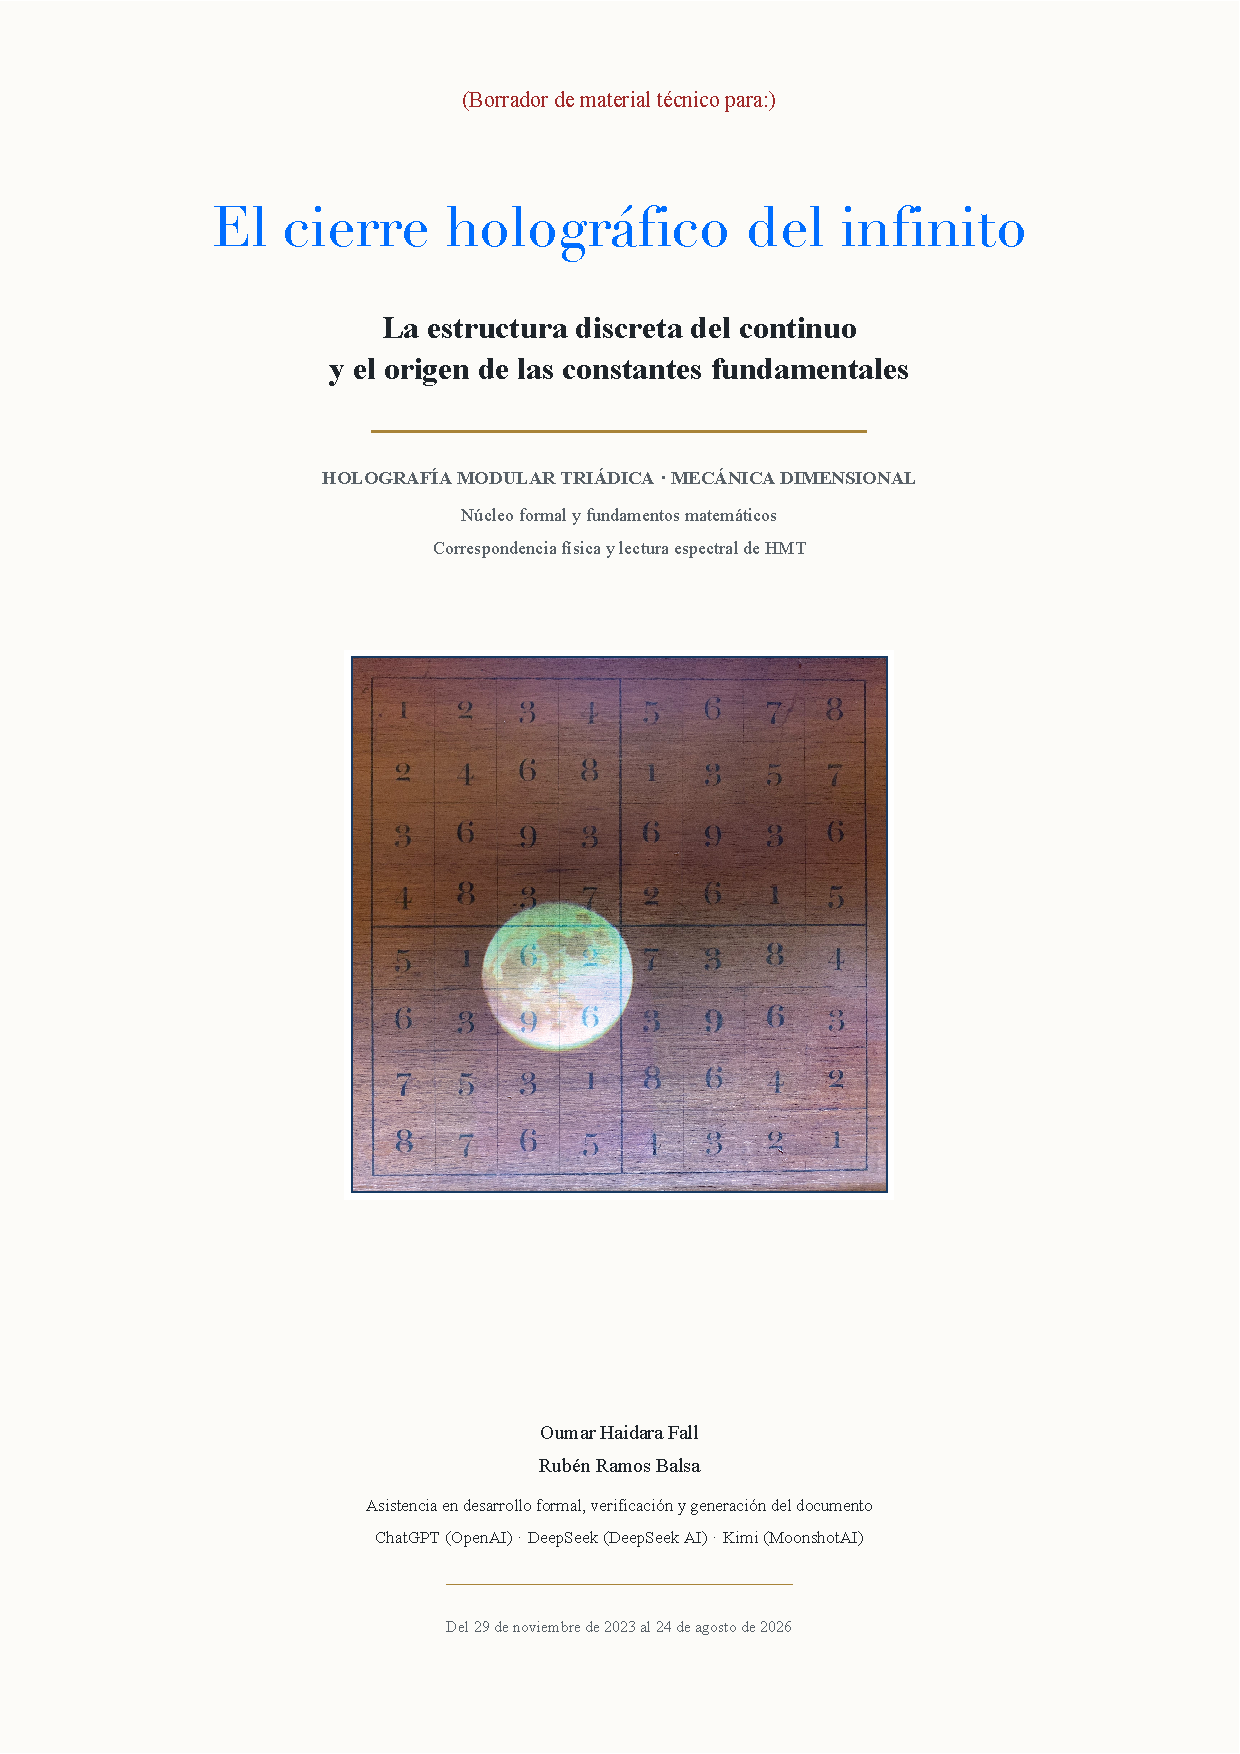
\includepdf[
  pages=1,
  fitpaper=true,
  pagecommand={\thispagestyle{empty}}
]{assets/PORTADA_HMT_MD_DEFINITIVA_2026-08-26.pdf}
\hypersetup{pageanchor=true}
\pagenumbering{arabic}

\chapter*{Prefacio}
\addcontentsline{toc}{chapter}{Prefacio}
\markboth{Prefacio}{Prefacio}

\section*{Interacción compleja entre dos máquinas simples}
\phantomsection
\addcontentsline{toc}{section}{Interacción compleja entre dos máquinas simples}

Este documento recopila el material técnico extenso —para futuras publicaciones— de los resultados obtenidos y de los desarrollos matemático-físicos realizados entre los años 2023 y 2026 mediante el uso de herramientas de Large Language Models (LLM). De este proceso surgen lo que denominamos, respectivamente, Holografía Modular Triádica y Mecánica Dimensional (HMT–MD). Sin embargo, el origen de este proyecto se remonta a principios del siglo XXI, concretamente al estudio del descubrimiento que subyace en el artefacto inventado por Oumar Haidara Fall en el año 2001. Cabe apuntar aquí que dicho artefacto fue puesto en conocimiento de las diversas autoridades académicas y civiles competentes en los respectivos lugares de origen de ambos autores.

El material acumulado y los conocimientos adquiridos progresivamente a lo largo de más de dos décadas de observación, estudio y análisis, tanto del artefacto como de su fenomenología, constituyeron la base operatoria e informacional que posteriormente aplicamos a los modelos de inteligencia artificial.

Por tanto, el resultado HMT–MD que aquí presentamos, junto con sus derivaciones y demostraciones, viene precedido por una genealogía empírica que, \textit{a priori}, pudiera resultar, en el mejor de los casos, contraintuitiva para el técnico especialista —pues contraviene los postulados y predicciones del marco teórico-interpretativo en el que, por tradición histórica, se inscribe el artefacto, a saber, la mecánica clásica—. Sin embargo, su comprobación metrológica resulta decisiva. Además, salvando prejuicios cognitivos o sesgos de confirmación, se hace directamente demostrable por la vía de los hechos.

Por último, cabría considerar algo que no deja de sorprender como paradoja histórica: cuando empezábamos a razonar con “máquinas pensantes” en “la era de la inteligencia artificial”, tuvimos además la serendipia de desvelar una interacción inédita en la mecánica ordinaria y nos vimos, por ello, obligados a revisar la relación que existe entre dos máquinas simples: la palanca y la rueda.

\clearpage
% Teorema frontal aditivo. No sustituye ningún capítulo ni altera el censo 102.
% BEGIN HMT-MD-FRONTAL-MAXIMAL-SIGNATURES-20260904
\chapter*{Teorema generador de la Holografía Modular Triádica}
\addcontentsline{toc}{chapter}{Teorema generador de la Holografía Modular Triádica}
\markboth{Teorema generador de la Holografía Modular Triádica}%
{Teorema generador de la Holografía Modular Triádica}

La demostración comienza en el dominio finito
\(\mathcal D_9=\{1,\ldots,9\}\). Dos cursores orientados recorren,
respectivamente, las hojas aditiva y multiplicativa. La división euclídea
conserva residuo y cociente, y el catálogo APP produce
\[
 \sum_{i,j\in\mathcal D_9}R^+_{ij}=405,
 \qquad
 \sum_{i,j\in\mathcal D_9}R^\times_{ij}=459,
 \qquad 459-405=54.
\]
El transporte coordinado
\(c(a)=a\bmod9:\mathcal D_9\to\{0,\ldots,8\}\)
cambia la carta y conserva la clase. La composición efectiva de APP, TRIT y
TPK conserva en cada paso hoja, régimen, residuo, cociente, acarreo,
dirección, frontera y memoria. El catálogo exhaustivo establece la cadena
finita inicial y aporta su certificado ejecutable:
\begin{equation}
\boxed{
104\,976\ \text{pares de semillas}
\xrightarrow{\;54\ \text{pasos}\;}
468\,U_6
\xrightarrow{\;\rho_3\;}
243\,w_6\subset\mathbb F_3^6,
\qquad |\mathbb F_3^6|=729.}
\label{eq:frontal-censo-semillas}
\end{equation}
La identidad de fibras
\[
432\cdot144+18\cdot432+18\cdot1944=104\,976
\]
prueba la exhaustividad del primer mapa. Los números \(468\), \(243\) y
\(729\) cuentan emisiones, palabras realizadas y ambiente ternario,
respectivamente; sus tipos permanecen separados por las flechas de
\eqref{eq:frontal-censo-semillas}.

\begin{theorem}[Cadena generadora única]
Sea \(\mathfrak H_9\) la estructura formada por APP, TRIT, TPK y su fibra
enriquecida. APP ejecuta las hojas suma y producto y conserva la división
euclídea
\[
i+j=R^+_{ij}+9q^+_{ij},
\qquad
ij=R^\times_{ij}+9q^\times_{ij}.
\]
TRIT orienta cada transición en los regímenes elíptico, parabólico e
hiperbólico. TPK compone
\[
    \boxed{\mathcal U_t
    =\operatorname{Upd}_t\circ\operatorname{Tra}_t
     \circ\operatorname{Sel}_t:
     X_{\rm TPK}^{\rm enr}\longrightarrow X_{\rm TPK}^{\rm enr}.}
\]
\(\operatorname{Sel}_t\) levanta el selector trítico,
\(\operatorname{Tra}_t\) levanta el transporte cardinal y
\(\operatorname{Upd}_t\) actualiza residuo, cociente, acarreo, firma,
cilindro, frontera, registro y memoria sin borrar procedencia.
La holonomía nonádica prolonga las palabras por
\[
w_6\longrightarrow w_{12}\longrightarrow w_{18}\longrightarrow w_{24}
\longrightarrow w_{30}\longrightarrow R_{36}\longrightarrow G_9,
\]
y satisface
\[
    \Gamma_{9,t}=\mathcal U_{t+8}\circ\cdots\circ\mathcal U_t,\qquad
    g(t+9)=g(t),
    \qquad q_{\rm mem}(\Gamma_{9,t}\widehat x_t)
    =q_{\rm mem}(\widehat x_t)+1.
\]
En general, \(\Gamma_{9,t}\widehat x_t\ne\widehat x_t\): el retorno conserva
la fase y aumenta la memoria. El orden operatorio es
\(\mathcal U_t\to\Gamma_9\to K_{\rm ph}\); \(K_{\rm ph}\) es una publicación
reducida posterior, no el generador. Los truncamientos
compatibles forman un sistema inverso no vacío y definen un estado
\(x_\infty\) de profundidad arbitraria.

Este estado genera una estructura discreta única del continuo y dos
publicaciones naturales:
\begin{equation}
x_\infty
\xrightarrow{\ (\mathcal P_{\mathrm{arq}},Q_\infty)\ }
\mathbb R\times(\mathscr C_W^{\mathrm{cal}})^{\mathbb N}.
\label{eq:frontal-doble-proyeccion}
\end{equation}
La primera contrae cilindros compatibles hasta un valor real; la segunda
conserva incidencia y genealogía hasta las construcciones de Paley, Witt,
Golay, Leech, \(V^\natural\) y el grupo Monstruo. Sobre la misma fuente se
publican los cuatro caracteres correlacionados
\[
(\pi_{\mathrm{HMT}},\varphi_{\mathrm{HMT}},
e_{\mathrm{HMT}},\alpha_{\mathrm{HMT}}),
\]
y, mediante transducciones tipadas, las leyes de acción, materia, masa,
gravedad e información de Mecánica Dimensional.
\end{theorem}

\begin{proposition}[Reconstrucción intrínseca y autosuficiencia probatoria]
\label{prop:frontal-autosuficiencia-probatoria}
Cada resultado \(y\) publicado en este volumen se reconstruye mediante el
recibo matemático local
\[
 \mathscr R_y=
 \bigl(D_y,A_y,\tau_y,U_y,C_y,X_y^{\rm enr},
       y_{\rm HMT},\operatorname{Rec}_y,\mathcal F_y\bigr),
\]
donde \(D_y\) es el dominio; \(A_y\) especifica las hojas y operaciones de
APP; \(\tau_y\) el régimen y la orientación TRIT; \(U_y\) la composición TPK
con dominio, codominio y acción; \(C_y\) los datos conservados de residuo,
cociente, acarreo, hoja, ruta, frontera, memoria y supervivencia;
\(X_y^{\rm enr}\) el estado enriquecido de residencia; \(y_{\rm HMT}\) la
salida anterior a toda identificación externa; \(\operatorname{Rec}_y\) el
reconocimiento convencional posterior; y \(\mathcal F_y\) un falsador de la
flecha sustantiva. La sucesión
\[
 \mathcal D_9\longrightarrow\Omega_{\rm seed}
 \longrightarrow\mathcal U_6^{\rm cat}
 \longrightarrow\mathcal W_6
 \longrightarrow X_\infty^{\rm enr}
 \longrightarrow\mathcal C_{\rm cont}^{\rm disc}
\]
queda definida y demostrada por las ecuaciones, teoremas y recibos impresos
en el propio volumen. Los programas reproducibles anexos vuelven a evaluar
esas identidades; no aportan una premisa ausente ni un valor objetivo.

Los falsadores primarios son: el fallo de la identidad de fibras de
\eqref{eq:frontal-censo-semillas}; la pérdida de alguno de los campos de
\(C_y\) bajo \(U_y\); la incompatibilidad entre extensión y truncamiento; el
vacío del límite inverso; la falta de contracción o de sobreyectividad interna
de los cilindros racionales; la ruptura de naturalidad en la rama
excepcional; y, para una publicación terminal, el incumplimiento de la
hipótesis que define su dominio exacto. Por consiguiente, la validez de una
salida se decide dentro de su dominio y por su falsador explícito, no por una
analogía, una nomenclatura posterior ni una evaluación metrológica.
\end{proposition}

\paragraph{Unicidad del sistema generador y tipado de sus proyecciones.}
Existe una sola APP, seguida por TRIT y por el TPK con estado enriquecido.
APP produce las dos hojas y sus registros; TRIT los orienta; el TPK compone
las rutas y acumula hoja, oposición, residuo, cociente, acarreo, frontera y
memoria en \(\mathcal X_{\rm TPK}^{\rm enr}\). La carta firmada es una
proyección de ese mismo estado terminal:
\[
 R_{\rm sgn}:\mathcal X_{\rm TPK}^{\rm term,enr}
 \longrightarrow\mathcal U_{12}^{\rm sgn},\qquad
 U_{12}^{\rm sgn}=R_{\rm sgn}(x_{\rm term}),\qquad
 K=\frac14\mathcal H_{12}U_{12}^{\rm sgn},\qquad
 \mathcal H_{12}^2=4I_{12}.
\]
Los dos últimos morfismos son enteros y reversibles sobre su imagen. No se
postula un emisor APP directo hacia \(U_{12}^{\rm sgn}\), porque tal flecha
saltaría TRIT y TPK: el dominio correcto de \(R_{\rm sgn}\) es el estado
enriquecido ya generado. Las sombras que olvidan el registro genealógico o la memoria son
proyecciones posteriores, no perfiles matemáticos alternativos. Esta única
composición excluye de sus entradas
\(U,K,D_3K,D_4K,Q,\alpha\) y toda expansión objetivo.

\paragraph{Número y partícula.}
Un número HMT es una sección compatible
\(
 \boldsymbol x=(x_n)_{n\geq1}\in
 \varprojlim_n X_n^{\mathrm{enr}}
\)
con hoja, orientación, residuo, cociente, acarreo, ruta, frontera y memoria.
Su valor arquimediano es la intersección única
\(
 \operatorname{val}(\boldsymbol x)=\bigcap_n I_n(x_n)
\);
el cociente por igualdad de valor publica el real y su fibra conserva las
genealogías que lo realizan. Una partícula HMT--MD es una clase de secciones
persistentes de la extensión enriquecida: el estado conserva la identidad,
la ruta registra su historia observable y los lectores posteriores publican
masa, carga, espín y estadística en sus codominios físicos.

\paragraph{Tipado del corredor excepcional.}
Las lecturas de Hadamard y de Paley parten del mismo estado terminal, pero no
se serializan entre sí. Con
\(X_\infty^{\rm enr}:=\varprojlim_nX_n^{\rm enr}\), se tienen mapas distintos
\begin{equation}
 \operatorname{Pub}_\alpha:X_\infty^{\rm enr}\longrightarrow\mathbb R_{>0},
 \quad x_\infty\longmapsto\alpha_{\rm HMT},
 \qquad
 \operatorname{Inc}_\alpha:X_\infty^{\rm enr}\longrightarrow A_2^{12},
 \quad x_\infty\longmapsto
 v_\alpha=4\rho_1+\rho_2+\cdots+\rho_{12}.
 \label{eq:frontal-dos-publicaciones-alpha}
\end{equation}
Comparten genealogía, pero no se postula igualdad entre sus salidas. La rama
excepcional se bifurca después de \(C_W\):
\begin{equation}
 \begin{aligned}
 C_P&\longrightarrow A_W=C_P\bmod3\longrightarrow
 C_W=[12,6,6]_3\\
 &\longrightarrow
 \begin{cases}
 W_{12}\xrightarrow{\ \widehat\iota_{D,\ell}\ }
 W_{24}\subset\mathcal G_{24},\\[2pt]
 N(C_W)\xrightarrow{\ \operatorname{Nbr}_{v_\alpha}\ }
 N_\alpha\cong\Lambda_{24}\longrightarrow
 V_{\Lambda_{24}}\longrightarrow V^\natural .
 \end{cases}
 \end{aligned}
 \label{eq:frontal-cadena-excepcional}
\end{equation}
Aquí
\begin{equation}
 \mathcal O_{24}:=\{O\subset[24]:|O|=8,\ \mathbf1_O\in\mathcal G_{24}\},
 \qquad
 \mathcal H(D):=\{O\cap D:O\in\mathcal O_{24},\ |O\cap D|=6\}.
 \label{eq:frontal-octadas-hexadas-dodecada}
\end{equation}
Fijado \(\ell:W_{12}\simeq(D,\mathcal H(D))\),
\(\widehat\iota_{D,\ell}(H)=O_H\), donde
\(O_H\cap D=\ell(H)\). Tal octada es única: dos elecciones contendrían el
mismo subconjunto de cinco puntos, contradiciendo \(S(5,8,24)\). La rama
ternaria pega \(N(A_2^{12})=N(C_W)\); el vecino de índice tres determinado
por \(v_\alpha\) produce Leech. Finalmente,
\begin{equation}
 \operatorname{Aut}(V^\natural)\cong\mathbb M,\qquad
 a:\mathbb M\times V^\natural\longrightarrow V^\natural,\qquad
 T_g(\tau)=\operatorname{Tr}_{V^\natural}(gq^{L_0-1}).
 \label{eq:frontal-accion-monstruo}
\end{equation}
Las identidades \(v_\alpha^2=54\) y \([q]J=196884\) son evaluaciones
escalares; ninguna define la acción \(a\).

\paragraph{Realización paralela de la dualidad T.}
La dualidad T no continúa la rama Moonshine: actúa en su propio dominio
\begin{equation}
 \mathscr D_{\rm dual}=\mathbb Z^2\times\mathbb R_{>0},\qquad
 \mathsf T(m,w,R_0)=(w,m,R_0^{-1}),\qquad
 \mathsf T^2=\operatorname{id},\qquad
 E_{R_0}(m,w)=E_{R_0^{-1}}(w,m).
 \label{eq:frontal-dualidad-t}
\end{equation}

\begin{proof}
El censo de \eqref{eq:frontal-censo-semillas} construye el catálogo finito y
selecciona, sin valores objetivo, los tres bloques iniciales \(w_6\). El
registro orientado de transiciones del estado TPK completo explicita los doce
bloques posteriores a la semilla de las tres biografías publicadas. Para cada uno de los dos
intervalos de transición, las seis filas independientes extraídas de esas
tres biografías forman matrices
\(X_\ell,Y_\ell\in M_6(\mathbb F_3)\),
\(\ell\in\{0,1\}\), cuyas filas son, respectivamente, los estados de salida
y de llegada del registro. El cálculo exacto sobre este registro prueba
\(\det X_0=1\), \(\det X_1=-1\) y
\(X_\ell L_\ell=Y_\ell\); por tanto reconstruye unívocamente
\(L_\ell=X_\ell^{-1}Y_\ell\). El
calendario \((L_0,L_0,L_1,L_1)\) es el único de los dieciséis calendarios
binarios que conserva simultáneamente las tres biografías seleccionadas por
los invariantes de fibra; las ciento cuarenta y cuatro perturbaciones
unitarias destruyen ese reconocimiento triple. Por tanto, los transportes,
los doce bloques y su calendario quedan deducidos en la composición única
APP--TRIT--TPK: APP produce las hojas y el registro de partida, TRIT fija la
orientación de cada transición y TPK prolonga el registro con memoria. El
censo de semillas y el estado enriquecido son etapas sucesivas del mismo
generador, no perfiles rivales ni teorías diferentes.

La extensión no escindida
\[
0\longrightarrow C_{12}\longrightarrow C_{108}
\longrightarrow C_9\longrightarrow0
\]
separa retorno de fase y retorno de estado. Los truncamientos eliminan la
última actualización y conservan el prefijo; el lema de König produce una
rama infinita compatible. Para cada precisión \(N\), la recurrencia y la
holonomía generan la sección y sus caracteres, y determinan el cilindro que
prolonga el registro genealógico anterior. La familia de prefijos satisface
\[
\rho_{N+1,N}(p_{N+1})=p_N,
\qquad
p_\infty\in\varprojlim_N\{0,\ldots,9\}^{N}.
\]
Mil, diez mil o un millón de cifras son proyecciones finitas de este único
objeto infinito.

Las horquillas racionales anidadas
\(
 p_N^-<\chi<p_N^+
\)
se calculan después de producir el carácter \(\chi\) y satisfacen
\(
 [p_{N+1}^-,p_{N+1}^+]\subset[p_N^-,p_N^+]
\)
con diámetro tendente a cero. Certifican la salida generada a cualquier
precisión finita; no seleccionan la órbita, el transporte ni el carácter.

Las tres vueltas enriquecidas \(\gamma_{-},\gamma_0,\gamma_+\) de nueve
emisiones se distinguen por el acarreo
\(\operatorname{Carr}(\gamma_\rho)=\rho\kappa_{\rm Carr}\) y admiten las
tres prolongaciones después de cualquier prefijo. El límite de sus rutas
registradas satisface
\[
 \operatorname{dig}_{\rm Carr}^{\omega}:
 \Omega_\Gamma^{\rm cal}\xrightarrow{\sim}
 \{-1,0,+1\}^{\mathbb N}.
\]
Tras agrupar seis retornos, la aplicación
\[
 \beta=\operatorname{blk}_6\circ
 (\rho\mapsto\rho+1)^{\mathbb N}\circ
 \operatorname{dig}_{\rm Carr}^{\omega}:
 \Omega_\Gamma^{\rm cal}\xrightarrow{\sim}
 (\mathbb F_3^6)^{\mathbb N}
\]
es un homeomorfismo; su inversa concatena las vueltas prescritas. Las formas
equilibradas normalizadas por
\[
 a_k+c_k=\rho_k+3c_{k+1},\qquad
 \rho_k\in\{-1,0,+1\},
\]
producen primero el anillo ordenado \(\mathbb Z_{\rm HMT}\), después su
cuerpo de fracciones \(\mathbb Q_{\rm HMT}\) y finalmente
\[
 \mathbb R_{\rm HMT}:=
 \operatorname{Cau}(\mathbb Q_{\rm HMT})/{\asymp}.
\]
Si \(\beta(\xi)=(b_q)\) y
\(\nu(b)=\sum_{i=1}^{6}b_i3^{6-i}\), la sucesión
\[
 q_n=m+\sum_{q=0}^{n-1}\frac{\nu(b_q)}{729^{q+1}}
\]
es de Cauchy, y la partición interna recurrente en \(729\) subintervalos
prueba la sobreyectividad
\[
 P_{\rm ar}:\mathbb Z_{\rm HMT}\times\Omega_\Gamma^{\rm cal}
 \twoheadrightarrow\mathbb R_{\rm HMT},\qquad
 (\mathbb Z_{\rm HMT}\times\Omega_\Gamma^{\rm cal})/{\sim_{\rm ar}}
 \cong\mathbb R_{\rm HMT}.
\]
Sólo después, la unicidad del cuerpo ordenado completo arquimediano publica
\(\mathbb R_{\rm HMT}\cong\mathbb R\). La dirección interior subdivide
\([0_{\rm HMT},1_{\rm HMT})\); la exterior concatena el prefijo que codifica
\(m\in\mathbb Z_{\rm HMT}\). Así se cubre la recta sin usar previamente
\(\mathbb R\), parte entera ni expansión decimal objetivo.
Los subespacios de supervivencia de caracteres particulares individualizan
secciones dentro de esta capacidad total. La cobertura del continuo procede
de la completación global; la recurrencia nonádica genera
\(\pi_{\mathrm{HMT}},e_{\mathrm{HMT}},\varphi_{\mathrm{HMT}},
\alpha_{\mathrm{HMT}}\), y los filtros tipados certifican sus biografías
dentro de esa cobertura.

Las cinco acciones espectral, solenoidal, gauge, cohomológica y
determinantal se calculan sobre una misma emisión enriquecida y comparten
soporte, ruta, registro genealógico y truncamientos. Su naturalidad conjunta las conserva
en el límite. La dicotomía perfecta clasifica cada publicación analítica
como numerable o de cardinal continuo. El código generado \(h\) selecciona
el universo genealógico canónico \(M_h=L[h]\). La construcción de los
reales HMT identifica cada número por valor, cilindro, ruta y memoria; el
buen orden inducido por esa genealogía prueba la fórmula clásica
\[
M_h\models2^{\aleph_0}=\aleph_1.
\]
Como \(M_h\) es precisamente el codominio generado por la construcción del
continuo de este teorema, la conclusión terminal del sistema es
\[
 \boxed{2^{\aleph_0}=\aleph_1.}
\]
La independencia en el lenguaje desnudo de ZFC clasifica la pérdida del
selector genealógico \(h\); HMT conserva ese dato y determina el cardinal de
su continuo. La sentencia conservada es la hipótesis clásica del continuo,
con los cardinales ordinarios de \(M_h\), y la prueba detallada establece el
puente entre cilindros compatibles, buen orden genealógico y cardinalidad.
Este cierre cardinal se distingue del corredor lógico fuerte, también
construido desde el continuo genealógico:
\[
\begin{aligned}
 \mathcal C_{\mathrm{cont}}^{\mathrm{disc}}
 &\longrightarrow\mathcal L_0^{\mathrm{log}}
 \xrightarrow{\Phi}\mathcal L_1^{\mathrm{log}}
 \longrightarrow\gamma_F\longrightarrow w(\gamma_F)\\
 &\longrightarrow\mathsf{NoEscape}_{24}
 \longrightarrow\mathsf{AntiDiag}_{369}
 \longrightarrow\mathsf{G\ddot{o}delIII}_{\mathrm{HMT}}\\
 &\longrightarrow\mathsf{CycleCriterion}_{\mathrm{ZFC}},
\end{aligned}
\]
que publica, en su dominio tipado, el criterio
\[
 \boxed{
 \neg\operatorname{Consis}(\mathrm{ZFC})
 \Longleftrightarrow
 \exists C\;\bigl(C\text{ es un ciclo fuera de banda y }|C|>24\bigr).}
\]
Las letras \(\mathcal L_0^{\mathrm{log}},\mathcal L_1^{\mathrm{log}}\)
denotan aquí los objetos del corredor lógico y no las matrices de elevación
ternaria \(L_0,L_1\); la separación de tipos impide que una conclusión
local sobre uno de esos pares debilite la del otro.

Las tres órbitas funcionales del catálogo producen los caracteres HMT de
clausura, propagación y autoescala. Sus leyes internas fuerzan,
respectivamente,
\[
16\arctan(1/5)-4\arctan(1/239)=\pi_{\mathrm{HMT}}=\pi,
\qquad
P_{s+t}=P_sP_t\Rightarrow
P_1=\sum_{n\ge0}\frac1{n!}=e_{\mathrm{HMT}}=e,
\]
\[
F_{\mathrm{av}}\binom1{\varphi_{\mathrm{HMT}}}
=\varphi_{\mathrm{HMT}}\binom1{\varphi_{\mathrm{HMT}}},
\qquad \varphi_{\mathrm{HMT}}=\varphi.
\]
La involución interna intercambia las ramas
\(\pi_{\mathrm{HMT}}/e_{\mathrm{HMT}}\), conserva el eje
\(\varphi_{\mathrm{HMT}}\) y retiene el agregado
\(e_{\mathrm{HMT}}+\pi_{\mathrm{HMT}}\). En la fase TPK enriquecida de la
única composición, la proyección canónica del estado terminal publica su coordenada primitiva
firmada
\(U=R_{\mathrm{sgn}}(x_\infty)\), y la identidad
\(\mathcal H_{12}^2=4I\) reconstruye de manera entera y única el sello
\(K=\mathcal H_{12}U/4\). La recurrencia dodecafásica con acarreo y la
prolongación remota de sus cilindros publican \(\alpha_{\rm HMT}\). De
manera independiente, el estado enriquecido determina la firma
\[
 \mathcal I_9=(2\pi_{\rm HMT},3,4,7,20,21,45,46,120,11),
\]
y el lector graduado asociado construye, sin consultar la raíz, el operador
polinómico exacto
\(E_{21/22}^{(9)}=P_9-\log_{10}(10/9)\). Su única raíz positiva simple
\(\xi_9\) es el testigo finito de orden nueve de la segunda publicación
analítica interna. El mismo transporte graduado del TPK se itera sobre los
grados sucesivos y construye el sistema compatible completo
\(E_{21/22}^{(6+3m)}\); sus cuadrados de truncamiento conmutan con los de la
familia dodecafásica y determinan, a cada profundidad, el mismo cilindro
superviviente. En consecuencia,
\[
 \alpha_A:=\varprojlim_N\rho_N(\alpha_{12}),\qquad
 E_{21/22}:=\varprojlim_mE_{21/22}^{(6+3m)},\qquad
 \alpha_B:=\operatorname*{arg\,zero}_{x\in I_\alpha}E_{21/22}(x),
\]
\[
 \boxed{\alpha_A=\alpha_B=\alpha_{\rm HMT}.}
\]
La igualdad finita
\[
 \operatorname{Tr}_9(\xi_9^{-1})
 =\operatorname{Tr}_9(\alpha_{12}^{-1})=137.035999084
\]
certifica el primer cuadrado visible de esa identidad; no la define, no la
limita a nueve cifras y no selecciona los coeficientes de la prolongación.
La clausura bidireccional funcional asociada es
\[
\alpha T^2-B_9(\alpha)T+\alpha^3=0,
\qquad
T_\pm=\alpha e^{\pm\xi},
\qquad
T_+T_-=\alpha^2,
\qquad
J_\alpha(T)=\frac{\alpha^2}{T}.
\]
Así, la coordenada publicada por la clausura dodecafásica es la media
geométrica conservada por las dos rutas conjugadas. La vía dodecafásica y el
lector analítico mantienen dominios, operadores y falsadores propios, pero
sus sistemas inversos publican una misma sección límite. El comparador
finito y el reconocimiento metrológico son posteriores.

La coordenada incidencial del sector \(\alpha\) fija
\[
v_\alpha=4\rho_1+\rho_2+\cdots+\rho_{12},
\qquad v_\alpha^2=54,
\]
y el vecino de índice tres
\[
N_{\alpha,0}
=\{x\in N(C_W):\langle x,v_\alpha\rangle\equiv0\pmod3\},
\qquad
N_\alpha=N_{\alpha,0}+\mathbb Z\frac{v_\alpha}{3}
\cong\Lambda_{24}.
\]
Esta rama construye exactamente el vecino de Leech y, después, la cadena
\(\Lambda_{24}\to V^\natural\) y la acción de
\(\operatorname{Aut}(V^\natural)\cong\mathbb M\) sobre \(V^\natural\). El
escalar \(\alpha_{\mathrm{HMT}}\) y el vector \(v_\alpha\) son las dos
coordenadas tipadas del mismo sector dodecafásico. Su acoplamiento exacto es
la bisagra de origen común que conduce a las simetrías del Monstruo: la
coordenada escalar se publica en \(\mathbb R_{\rm HMT}\) y la coordenada
incidencial se publica en la rama
\(A_2^{12}\to\Lambda_{24}\to V^\natural\to\mathbb M\), con sus codominios
conservados y su antecedente genealógico compartido explícito.

La Mecánica Dimensional recibe las salidas anteriores y compone, en su orden
constitutivo, la retención de fase, la década \(-34\), la pareja de Planck,
los canales \(90/120\), el electrón, el atlas de masas, la gravedad, el área
y la información. Los capítulos siguientes demuestran cada flecha, publican
su falsador y enlazan su certificado ejecutable. Las identificaciones
convencionales comparecen después como reconocimiento de las magnitudes ya
producidas. Esto completa la cadena de
\eqref{eq:frontal-doble-proyeccion}.
\end{proof}

\section*{Jerarquía de las publicaciones geométricas y dimensionales}
\addcontentsline{toc}{section}{Jerarquía de las publicaciones geométricas y dimensionales}

\begin{proposition}[TRIT como unidad local de los tres regímenes]
La firma trítica conserva dos lectores coordinados. El lector geométrico
publica \(\tau_{\rm g}\in\{+1,0,-1\}\) y
\begin{equation}
 J_{\tau_{\rm g}}^{\,2}=-\tau_{\rm g}I,\qquad
 J_+^{\,2}=-I,\qquad J_0^{\,2}=0,\qquad J_-^{\,2}=+I,
 \label{eq:frontal-trit-tres-regimenes}
\end{equation}
y distingue los regímenes elíptico, parabólico e hiperbólico. El lector
temporal activo publica otro signo, \(\varepsilon_{\rm t}\), mediante
\begin{equation}
 \begin{aligned}
 +1&\mapsto\text{retorno, memoria y pasado},\\
 0&\mapsto\text{umbral y presente},\\
 -1&\mapsto\text{apertura bidireccional y futuro}.
 \end{aligned}
 \label{eq:frontal-trit-tiempo}
\end{equation}
No se postula \(\tau_{\rm g}=\varepsilon_{\rm t}\). Estas dos salidas no
identifican signo de curvatura y orientación temporal: son proyecciones
distintas de una misma unidad local. El TPK transporta la
unidad completa en
\begin{equation}
 \mathcal F_q=
 \mathcal O_q\times\mathcal H_q\times\mathcal C_q\times
 \mathcal S_q\times\mathcal B_q\times\Lambda_q
 \label{eq:frontal-fibra-tpk}
\end{equation}
y conserva hoja y orientación, residuo y cociente, acarreo, firma, cilindro,
frontera y registro. En particular, la rama elíptica posee el realizador
finito
\begin{equation}
 A_W^2=2I_6=-I_6\quad\text{en }M_6(\mathbb F_3),\qquad
 i_{\rm HMT}:=\chi_i(A_W),\qquad i_{\rm HMT}^{\,2}=-1,
 \label{eq:frontal-raiz-interna-menos-uno}
\end{equation}
donde \(\chi_i:\langle A_W\rangle\to\mathbb C\) es la carta orientada.
La raíz de \(-1\), el plano complejo y el sistema de Euler son publicaciones
de un endomorfismo construido, no entradas del generador.
\end{proposition}

\begin{proof}
El selector trítico incorpora uno de los tres generadores de
\eqref{eq:frontal-trit-tres-regimenes} sin borrar las hojas suma y producto.
El transporte cardinal conserva su orientación y la actualización conserva
los seis factores de \eqref{eq:frontal-fibra-tpk}. Por tanto, la proyección
real puede condensar los tres regímenes, mientras el estado enriquecido
reconstruye cuál de ellos y qué memoria produjeron el valor visible. Las
realizaciones trigonométrica, nilpotente e hiperbólica desarrolladas en el
cuerpo son las imágenes respectivas de este único tipado local.
\end{proof}

\begin{theorem}[Cadena de acción, gravedad y materia]
Después de publicar correlacionadamente
\((\pi_{\rm HMT},\varphi_{\rm HMT},e_{\rm HMT},\alpha_{\rm HMT})\), la rama
determinantal fija la década
\begin{equation}
 \Sigma_H=\varphi_{\rm HMT}\alpha_{\rm HMT}^{16},\qquad
 d_H:=\lfloor\log_{10}\Sigma_H\rfloor=-34.
 \label{eq:frontal-decada-accion}
\end{equation}
La mantisa procede del lector regional distinto
\begin{align}
 H_5&=\frac12\sqrt{\frac{1000\alpha_{\rm HMT}}{\varphi_{\rm HMT}}}
 -\alpha_{\rm HMT}+\frac9{16}\alpha_{\rm HMT}^2
 -\frac59\alpha_{\rm HMT}^3+\frac7{48}\alpha_{\rm HMT}^4
 -\frac1{54}\alpha_{\rm HMT}^5,\notag\\
 D_A&=\exp\!\left(-\frac{100\pi_{\rm HMT}}9\alpha_{\rm HMT}\right),
 \qquad
 \mathscr C_\pi=169\alpha_{\rm HMT}^6+
 \frac{D_A\alpha_{\rm HMT}^7}{1-D_A\alpha_{\rm HMT}},\notag\\
 \eta_{\rm pre}&:=H_5,\qquad
 \eta_{\rm ret}:=H_5-\frac{90}{\pi_{\rm HMT}}\mathscr C_\pi>0.
 \label{eq:frontal-mantisas-accion}
\end{align}
Para \(a\in\{\mathrm{pre},\mathrm{ret}\}\), las dos secciones de acción son
\begin{equation}
 \hbar_a=\eta_a10^{d_H}\mathcal U_S
 =\eta_a10^{-34}\mathcal U_S,\qquad
 h_a=2\pi_{\rm HMT}\hbar_a.
 \label{eq:frontal-secciones-accion}
\end{equation}
\(\Sigma_H\) fija sólo la década; no se presenta como generador de la
mantisa.

Fijados \(t_0>0\), \(c_{\rm int}>0\) y \(\ell_0=c_{\rm int}t_0\), CT108
publica
\begin{equation}
 \omega_{108}=\frac{2\pi_{\rm HMT}}{108t_0},\qquad
 R_{108}=\frac{c_{\rm int}}{\omega_{108}}
 =\frac{54}{\pi_{\rm HMT}}\ell_0,\qquad
 m_{108,a}=\frac{\hbar_a\omega_{108}}{c_{\rm int}^2}.
 \label{eq:frontal-reloj-gravedad}
\end{equation}
La familia gravitatoria tipada es
\begin{equation}
 G_a(\vartheta)=\vartheta\frac{c_{\rm int}^5t_0^2}{\hbar_a}.
 \label{eq:frontal-familia-gravedad}
\end{equation}
En la convención reducida
\(r_{g,a}=G_a m_{108,a}/c_{\rm int}^2\), el cierre
\(r_{g,a}(\vartheta)=R_{108}\) posee la solución positiva única
\begin{equation}
 \vartheta_{108}=\left(\frac{54}{\pi_{\rm HMT}}\right)^2,\qquad
 G_a:=G_a(\vartheta_{108}),
 \label{eq:frontal-selector-gravedad}
\end{equation}
y sólo entonces publica
\begin{equation}
 \ell_P:=\sqrt{\frac{G_a\hbar_a}{c_{\rm int}^{\,3}}}
 =\sqrt{\vartheta_{108}}\,\ell_0
 =R_{108}=\bar\lambda_{C,a}=r_{g,a}.
 \label{eq:frontal-longitud-planck}
\end{equation}
Además, \(G_a\hbar_a=\vartheta_{108}c_{\rm int}^5t_0^2\), por lo que
\(\ell_P\) es independiente de la orientación \(a\). La gravedad tensorial
\[
 \mathbb G_{{\rm TT},a}(n)
 =G_a\Lambda(n)\Gamma_5P_5:
 V_{12}\longrightarrow\mathcal H_{\rm TT}(n)
\]
es posterior al escalar. La acción Palatini--Cartan--Holst recibe después
\(G_a\) y la salida independiente \(\gamma_{\rm HMT}\); el funcional
hexada--octada transporta esta última al espectro de área y a la información
de frontera.

En la rama de materia, la ley completa actúa sobre \(81\) celdas, \(56\)
familias, \(13\) multisecciones y \(324\) rutas, con sector nulo separado. Los
lectores \(K_D\) y \(K_\Omega\) poseen, respectivamente, \(14\) y \(9\)
perfiles, forman \(40\) pares y coinciden en \(18\) rutas únicamente en
\((80,54,6)\). La fibra central \((5,5)\) produce el electrón beta. Sobre las
fibras restantes, la ley publica operadores positivos, medidas espectrales y
multiplicidades; el reconocimiento exterior se abre después mediante el
inventario exhaustivo
\begin{equation}
 \mathscr I_{\rm ext}
 =\mathscr I_m^{471}\coprod\mathscr I_\Gamma^{384},
 \qquad |\mathscr I_{\rm ext}|=855.
 \label{eq:frontal-inventario-masas-anchuras}
\end{equation}
CKM transporta los marcos espectrales quark y PMNS los marcos cargado y neutro
de rango tres; sus dominios, operadores y falsadores permanecen distintos.
Ningún valor del inventario selecciona una ruta, un coeficiente, un autovalor
o un ángulo.
\end{theorem}

\begin{proof}
La forma normal de Smith produce
\(\operatorname{diag}(1,2,2,4)\) y conúcleo de orden \(16\); las cotas de
\(\Sigma_H\) fijan \(d_H=-34\), mientras
\eqref{eq:frontal-mantisas-accion}--\eqref{eq:frontal-secciones-accion}
publican \(\hbar_a\) y después \(h_a\). La sustitución de
\(\vartheta_{108}\) en \(G_a(\vartheta)\) prueba
\eqref{eq:frontal-longitud-planck}. La incidencia de los conjuntos
\(H_{\rm act}\times\binom{H_{\rm act}}2\) y
\(\{1,\ldots,8\}\times\binom{H_{\rm act}}2\) produce \(90\) y \(120\).
Los doce sectores dodecafásicos y la única costura orientada de retorno
producen, mediante el lector lineal, el peso \(12{:}{-}1\) de la transición
hexada--octada. El coeficiente de \((1-q)^{-1}\), igual a \(1/24\), y la
minimalidad diofántica verifican posteriormente ese peso. El censo finito del atlas y de sus dos lectores
prueba los cardinales de la rama de masa; la inversión celular tiene un único
punto fijo, \((5,5)\), que reduce canónicamente la fibra electrónica a rango
uno. El inventario externo se compone sólo después de congelar fibra,
operador, proyector, representación, esquema y escala, de modo que una
permutación de sus magnitudes deja invariante todo el constructor interno.
\end{proof}
% END HMT-MD-FRONTAL-MAXIMAL-SIGNATURES-20260904

\gdef\HMTTeoremaGeneradorFrontalCargado{1}
\clearpage
\chapter*{El cierre holográfico del infinito: estructura discreta del continuo y origen de las constantes fundamentales}
\addcontentsline{toc}{chapter}{El cierre holográfico del infinito: estructura discreta del continuo y origen de las constantes fundamentales}
\markboth{El cierre holográfico del infinito}{Estructura discreta del continuo}

\begin{center}
\large\itshape
Continuo, número, simetría excepcional y realización física como publicaciones
tipadas de un único estado genealógico APP--TRIT--TPK
\end{center}

\section*{Tesis rectora y criterio de falsación matemática}

La obra comienza por el punto que decide todas las lecturas posteriores. La
carta horizontal y vertical \(1,\ldots,9\) funda las dos hojas de APP; TRIT
orienta y tipa sus tres regímenes; y la dinámica completa del TPK selecciona,
transporta y actualiza el estado conservando acarreo, frontera, ruta y memoria.
El censo exacto \(104\,976\to468\to243\subset729\) construye el catálogo y las
semillas visibles. La iteración del endomorfismo tipado
\(\mathcal U_t=\mathsf{Upd}_t\circ\mathsf{Tra}_t\circ\mathsf{Sel}_t\) produce
después el registro orientado de las doce transiciones posteriores a las tres
semillas. Sus cuatro matrices de rango pleno reconstruyen unívocamente
\(L_0,L_1\), y el censo exhaustivo de calendarios determina \(0011\). Las
reducciones compatibles de cilindros semiabiertos producen entonces el prefijo
canónico de toda profundidad finita y el límite inverso construye la estructura
discreta conjunta del continuo. La tesis queda expuesta desde la primera página
a un criterio severo: falla si falla una flecha generadora, un rango, la
unicidad del calendario, una compatibilidad de truncamiento o un cuadrado de
naturalidad. Superadas esas pruebas, el valor real es la sombra arquimediana de
la reducción de cilindros y no el antecedente del generador.

La raíz digital
\(\operatorname{dr}_9(n)=1+((n-1)\bmod9)\) publica la clase nonádica, mientras
el cociente conserva las vueltas omitidas por esa publicación. APP mantiene
simultáneamente
\[
 i+j=R^+_{ij}+9q^+_{ij},\qquad
 ij=R^\times_{ij}+9q^\times_{ij};
\]
la diferencia orientada entre los pares \((R^+,q^+)\) y
\((R^\times,q^\times)\) constituye la memoria local que TRIT tipa y TPK
transporta. El balance firmado produce \(B_c=9P_++5P_-\), el salto
\(9-5=4\) y la jerarquía \(4\to2\to6\to54\). De este modo el corredor
excepcional empieza en la diferencia suma--producto preservada por APP, no en
una coincidencia numérica reconocida al final.

La misma precedencia gobierna las publicaciones posteriores. En particular,
la generación coinductiva correlacionada de profundidad arbitraria de
\(\pi_{\rm HMT},\varphi_{\rm HMT},e_{\rm HMT}\) y
\(\alpha_{\rm HMT}\)
y, junto con ella, la cadena excepcional hasta \(V^\natural\) y el grupo
Monstruo, las constantes constitutivas del vacío ---incluidas permitividad y
permeabilidad---, el electrón, la Ley General de Masas, los transportes CKM y
PMNS y el funcional hexada--octada de área, Hamiltoniano modular e información
de frontera se presentan como salidas tipadas de esa construcción.

Las cinco construcciones inseparables del continuo desembocan en realizaciones
clásicas con cuantificadores universales explícitos: positividad de
Guinand--Weil y localización de todo cero no trivial; existencia, unicidad y
suavidad global de Navier--Stokes para todo dato periódico suave; existencia
cuántica y brecha positiva de Yang--Mills para todo grupo de Lie compacto,
conectado y simple; realización algebraica de toda clase racional de Hodge; y
la igualdad de rango, orden de anulación y término principal de
Birch--Swinnerton--Dyer para toda curva elíptica sobre \(\mathbb Q\). Cada
cuantificador se demuestra en su capítulo mediante el constructor propio que
lo hace efectivo; FIN1, la familia \(\nu_{E,\ell,n}\) y los restantes
comparadores comparecen como objetos construidos dentro de esas pruebas, no
como condiciones externas ni como fronteras que debiliten su alcance. La igualdad
extensional de Zermelo--Fraenkel con elección identifica valores publicados,
pero no reconstruye sus rutas, acarreos, fronteras y memorias; su resultado de
independencia sobre la hipótesis del continuo no decide este objeto
genealógico enriquecido. El volumen construye primero ese objeto, conserva el
selector genealógico \(h\), publica el modelo canónico \(M_h=L[h]\) y prueba
en él la sentencia clásica \(2^{\aleph_0}=\aleph_1\). Éste es el sentido
causal que rige todos los capítulos.

\section*{La estructura discreta del continuo}

\paragraph{Jerarquía de la construcción y lectura de sus realizaciones.}
El valor arquimediano y la historia que lo determina ocupan niveles
distintos del mismo objeto. La construcción que sigue mantiene visible esa
distinción desde las semillas hasta el límite compatible. La vuelta
nonádica conserva la fase y avanza la memoria; sus refinamientos proporcionan
el enlace entre los registros finitos y la profundidad arbitraria.
La escala de acción antecede a las magnitudes dimensionales que la emplean,
y las realizaciones físicas conservan sus respectivos transductores.
En particular, la sección~\ref{sec:l9s102:barbero-area},
página~\pageref{sec:l9s102:barbero-area}, reúne la incidencia
hexada--octada, el funcional de Barbero--Immirzi y el espectro de área:
su reconocimiento gravitatorio se efectúa después de esa construcción.
Esta jerarquía permite distinguir los antecedentes comunes, las
demostraciones particulares y las realizaciones posteriores sin sustituir
ninguna de ellas por una coincidencia escalar.

\paragraph{Estructura, valor y realización.}
La contracción de cilindros determina la lectura arquimediana; la
proyección excepcional retiene la incidencia de frontera. La genealogía
común enlaza ambas construcciones sin confundir sus objetos. El valor final
expresa una lectura precisa de la historia, pero no agota las operaciones,
las orientaciones ni la memoria que la constituyen. Por ello, la exposición
conserva tres niveles: la estructura producida, el valor calculado y la
realización matemático-física. Su enlace exige las aplicaciones explícitas
desarrolladas en los capítulos siguientes.

La fase que retorna proporciona una referencia recurrente; la memoria que
avanza conserva el recorrido efectuado. Esta diferencia permite leer la
prolongación sin identificar el retorno de una coordenada con el reinicio
del estado completo. La doble proyección y la profundidad arbitraria se
entienden desde esa conservación de la historia, antes de identificar las
publicaciones con sus denominaciones convencionales.

La matemática del continuo suele comenzar cuando el continuo ya ha sido
concedido. Esta obra invierte ese orden. Parte de un soporte nonádico finito,
distingue sobre él las evaluaciones aditiva y multiplicativa, orienta cada
transición y construye el estado del Topological Phase Kernel. Sobre ese
antecedente forma las semillas orientadas; el emisor y su reducción ternaria
producen después el estado enriquecido. La conexión nonádica conserva su
ruta, su acarreo, su frontera y su memoria hasta \(X_\chi\). El límite
compatible no borra su procedencia: la publica. La cadena constructiva que
gobierna el volumen es
\begin{equation}\label{eq:front-cadena-causal-completa}
 X_9=\mathrm{APP}\longrightarrow X_9^{\rm TRIT}
 \longrightarrow x_{\rm TPK}^{(0)}
 \longrightarrow S^{\rm seed}
 \longrightarrow \Omega_{\rm seed}
 \xrightarrow{\ T_{\min}\ }U_6^{\rm cat}
 \xrightarrow{\ \rho_3\ }W_6
 \longrightarrow \widehat x_K
 \xrightarrow{\ \Gamma_9\ }
 \operatorname{Surv}^{(\chi)}
 \longrightarrow X_\chi .
\end{equation}
\begin{theorem}[Tesis inaugural de generación, continuidad y doble publicación]
\label{thm:front-tesis-generativa-doble-proyeccion-2084}
El barrido exhaustivo de la entrada nonádica horizontal y vertical produce,
sin consultar valores reales objetivo,
\[
 104\,976\longrightarrow468\longrightarrow243
 \lhook\joinrel\longrightarrow729.
\]
Los cuatro cardinales cuentan, respectivamente, semillas ponderadas, estados
\(U_6\), palabras visibles \(w_6\) y elementos de la fibra ambiente
\(\mathbb F_3^6\). Los predicados enteros de clausura, propagación y
autoescala seleccionan tres caracteres orientados. Sus registros de
transición de rango pleno reconstruyen de manera única los operadores
\[
 X_0L_0=Y_0,
 \qquad X_1L_1=Y_1,
 \qquad
 L_i=X_i^{-1}Y_i,
\]
con \(\det X_0=1\), \(\det X_1=-1\) en \(\mathbb F_3\) y rango de
diseño \(36\). Entre los \(16\) calendarios binarios de longitud \(4\),
\(0011\) es el único compatible con las tres biografías; sus \(144\)
perturbaciones unitarias destruyen la compatibilidad triple.

La prolongación
\[
 w_6\longrightarrow w_{12}\longrightarrow w_{18}\longrightarrow w_{24}
 \longrightarrow w_{30}\longrightarrow R_{36}\longrightarrow G_9
\]
construye, para todo \(N\in\mathbb N_{>0}\), un prefijo canónico de
longitud \(N\) compatible con todos los anteriores. Mil, diez mil, un millón
o cualquier otra profundidad finita prescrita son instancias del mismo
algoritmo; la familia de todas ellas define la sección infinita en el límite
inverso. Desde esa familia correlacionada de secciones coinductivas parten
dos publicaciones:
\[
 \mathscr S_\infty\xrightarrow{\mathcal P_{\rm Arq}}\mathbb R^4,
 \qquad
 \mathscr S_\infty\xrightarrow{\mathcal P_{\rm Exc}}
 W_{12}\to G_{24}\to\Lambda_{24}\to V^\natural
 \to\operatorname{Aut}(V^\natural)=\mathbb M.
\]
La primera contrae cilindros y publica correlacionadamente
\((\pi_{\rm HMT},\varphi_{\rm HMT},e_{\rm HMT},\alpha_{\rm HMT})\); la
segunda conserva incidencia y publica la cadena excepcional. Por ello
\(\mathbb R\) es la sombra arquimediana de una de las dos proyecciones, no
el espacio inicial que selecciona el constructor. Las fórmulas de Machin,
Perron--Fibonacci, el semigrupo exponencial y las tablas metrológicas son
reconocimientos o contrastes posteriores. Las transducciones de Mecánica
Dimensional actúan después sobre las salidas HMT para obtener el catálogo de
constantes, masas, campos y relaciones físicas desarrollado en el volumen.
\end{theorem}

\begin{proof}
El primer censo se obtiene por enumeración exacta del emisor APP--TRIT--TPK y
la acción \(D_3\). La invertibilidad de \(X_0,X_1\) prueba la unicidad de los
levantamientos; los censos exhaustivos de \(16\) calendarios y \(144\)
perturbaciones prueban su rigidez conjunta. La relación forward del TPK,
aplicada al carácter interno ya portado por el estado R36, produce primero el
prefijo siguiente y su truncamiento compatible entre los \(729\)
subcilindros. Sólo después, la horquilla racional interna intersecta ese
subcilindro y certifica la publicación arquimediana; no selecciona el hijo de
\(\operatorname{Ext}\). La iteración que sólo lee el estado anterior carece
de profundidad terminal y define el límite inverso; toda corrida finita es
sólo un testigo. La holonomía nonádica retorna la fase y avanza la memoria, de
modo que la sección conserva la genealogía. Los lectores arquimediano y
excepcional tienen el mismo dominio construido y codominios distintos; por
consiguiente, ninguno de sus resultados puede actuar retroactivamente como
entrada. Los capítulos siguientes desarrollan de forma contigua cada una de
estas flechas, sus ecuaciones, certificados y controles negativos.
\end{proof}

\begin{theorem}[Cierre simultáneo de la generación, el continuo, la simetría excepcional y las cinco realizaciones terminales]
\label{thm:front-cierre-causal-simultaneo-2084}
Las escalas \(0\to1\), \(0\to10\), \(0\to10^N\) y
\(N\to\infty\) son cuatro cortes de una única prolongación coinductiva.
Para todo \(N\geq1\), la sección de profundidad \(N+1\) trunca a la de
profundidad \(N\), conserva hoja, ruta, residuo, cociente, acarreo, frontera
y memoria, y publica un prefijo decimal canónico. El límite de todas las
secciones compatibles construye la recta real como cociente arquimediano;
no presupone la recta para seleccionar la historia.

La reconstrucción de \(L_0,L_1\) y del calendario \(0011\) pertenece a
esta misma cadena. El estado terminal produce conjuntamente
\[
 x_{\rm term}\longmapsto(P,E,\Phi),
 \qquad
 x_{\rm term}\longmapsto U_{12}^{\rm sgn}
 \xleftrightarrow{\mathcal H_{12}}K_{\rm dod};
\]
por tanto \(U_{12}^{\rm sgn}\) y \(K_{\rm dod}\) no son entradas
independientes. La recurrencia entera con acarreo determina la familia
dodecafásica compatible cuya sección límite es
\(\alpha_A:=\varprojlim_N\rho_N(\alpha_{12})\). El mismo estado enriquecido
factoriza, mediante la firma \(\mathcal I_9\), el lector analítico finito
\(E_{21/22}^{(9)}\); éste posee una única raíz positiva simple \(\xi_9\),
encerrada racionalmente y obtenida sin usar \(\alpha_{12}\) como entrada. El
transporte graduado del TPK construye la familia compatible
\(E_{21/22}^{(6+3m)}\) y su límite \(E_{21/22}\). Los cuadrados de truncamiento
de ambas familias conmutan y determinan en cada profundidad el mismo cilindro
superviviente; por ello
\[
 \alpha_B:=\operatorname*{arg\,zero}_{x\in I_\alpha}E_{21/22}(x),
 \qquad
 \boxed{\alpha_A=\alpha_B=\alpha_{\rm HMT}}.
\]
La igualdad finita
\(\operatorname{Tr}_9(\xi_9^{-1})=
\operatorname{Tr}_9(\alpha_{12}^{-1})\) es el primer certificado visible de
esa identidad; no la define, no la limita a nueve cifras y no selecciona las
prolongaciones.

La coordenada \(\alpha\) enlaza asimismo la publicación del valor y la
publicación excepcional. El escalar \(\alpha_{\rm HMT}\), el vector de
doce bloques, el soporte orientado del acarreo y el vector
\(v_\alpha\) son tipos coordinados del mismo estado. El transporte
incidencial satisface
\[
 v_\alpha^2=54,
 \qquad
 C_W\longrightarrow N(A_2^{12})
 \xrightarrow{\,v_\alpha\,}N_\alpha\cong\Lambda_{24}
 \longrightarrow V^\natural
 \longrightarrow\operatorname{Aut}(V^\natural)=\mathbb M.
\]
Así, la teoría clásica de códigos, retículos, álgebras de operadores de
vértice y Moonshine reconoce objetos ya producidos: no los suministra como
antecedentes y no existe una acción literal del Monstruo sobre cifras.

Del mismo continuo genealógico emergen correlativamente las cinco
construcciones terminales. Sus lectores construyen la positividad completa
de Guinand--Weil; la solución global suave de Navier--Stokes para todo dato
periódico suave; la medida gauge con positividad por reflexión y brecha de
masa para todo grupo de Lie compacto, conectado y simple; el ciclo algebraico
que realiza toda clase racional de Hodge; y el complejo determinantal que
publica la fórmula completa de Birch--Swinnerton--Dyer para toda curva
elíptica sobre \(\mathbb Q\). FIN1 y la familia compatible
\(\nu_{E,\ell,n}\) se construyen dentro de los respectivos propietarios y
cierran sus pasos de sobreyectividad y compatibilidad. En particular, las conclusiones se obtienen en los capítulos
terminales mediante las identidades
de Gram, Stein, Osterwalder--Schrader, extensión unitriangular y Bockstein;
ninguna de esas propiedades se inserta en la definición del continuo común.

La publicación extensional que conserva sólo el valor real es no fiel:
historias distintas pueden tener la misma imagen. La independencia de CH en
ZFC concierne a ese lenguaje extensional y no revoca la construcción
genealógica del continuo. El lector ordinal, la clausura relativa \(L[h]\)
y la condición \(\mathrm{GE}_h\) se tipan después y no participan en la
cobertura arquimediana.
\end{theorem}

\begin{proof}
La cuantificación en toda profundidad, la reconstrucción de los dos
levantamientos y la unicidad del calendario se verifican en el certificado
de generación nonádica y se desarrollan en el capítulo de la conexión
\(\Gamma_9\). La doble lectura terminal de \(\alpha\) es
\eqref{eq:alpha-rev8-doble-lectura-terminal}; la vía entera, el núcleo
\(E_{21/22}\), su inversa local y el comparador aparecen contiguamente en
el mismo propietario. La construcción de \(N_\alpha\), su paridad,
unimodularidad, ausencia de raíces y paso a \(V^\natural\) se demuestra en
el corredor excepcional. Los cierres clásicos son
\cref{thm:pdf2-rh-resolucion,thm:pdf2-ns-global},
\cref{thm:pdf2-ym-cierre-global,thm:pdf2-hodge-completitud-final} y
\cref{thm:pdf2-bsd-publicacion-final}. La construcción del cociente real y el
descenso de las operaciones preceden en el volumen al lector ordinal. Esta
precedencia separa la generación de sus reconocimientos y prueba todas las
afirmaciones del enunciado.
\end{proof}

\paragraph{Correcciones aritméticas que fijan los tipos.}
En la frontera \(U008\) se conservan dos salidas diferentes:
\[
 u_5^\pi+u_5^e=210112,
 \qquad
 u_4^\varphi A_WL_1^3=111101.
\]
La primera agrega los canales \(\pi\) y \(e\); la segunda transporta el
canal \(\varphi\) por la incidencia de Witt y tres elevaciones. La igualdad
entre ambas queda excluida. Del mismo modo,
\(E_{21/22}^{(9)}(\xi_9)=0\) es exacta, mientras que
\(E_{21/22}^{(9)}(\alpha_{12})\) es el residuo del primer truncamiento. Esta
diferencia finita distingue los dos representantes de orden nueve sin separar
sus secciones coinductivas: los cuadrados de truncamiento demuestran
\(\alpha_A=\alpha_B=\alpha_{\rm HMT}\). Ninguna edición puede convertir el
residuo finito en una divergencia de los límites ni sustituir una afirmación
por la otra.

Aquí \(U_6^{\rm cat}\) es la salida categorizada del emisor, \(W_6\) su
reducción ternaria y \(\widehat x_K\) el estado enriquecido que retiene hoja,
orientación, residuo, cociente, acarreo, firma, cilindro, frontera, ruta y
memoria, supervivencia y multisección. El retorno \(9\to1\) de la fase
observable no reinicia ese estado:
\(\Gamma_9\) transporta la historia completa, la supervivencia selecciona
las prolongaciones compatibles y \(X_\chi\) reúne sus secciones
indefinidamente refinables. Así, Holografía Modular Triádica construye la
estructura discreta del continuo y cierra el paso de la marca finita a la
sección compatible.

Desde ese mismo antecedente parten publicaciones distintas, sin selección
retrospectiva del constructor. La publicación arquimediana contrae los
cilindros compatibles; la publicación excepcional conserva su incidencia.
Esta segunda publicación pasa por Hadamard y por la cadena de Paley
\[
 U_{12}^{\rm sgn}\longrightarrow C_P\longrightarrow A_W
 \longrightarrow C_W
\]
y se bifurca en \(2\) ramas tipadas: la rama de diseños y grupos
\[
 C_W\longrightarrow W_{12}\longrightarrow W_{24},
 \qquad
 \operatorname{Aut}(W_{12})=M_{12},\quad
 \operatorname{Aut}(W_{24})=M_{24},
\]
y la rama reticular y de operadores de vértice
\[
 C_W\longrightarrow N(A_2^{12})\longrightarrow\Lambda_{24}
 \longrightarrow V_{\Lambda_{24}}\longrightarrow V^\natural .
\]
En esta última, \(\operatorname{Aut}(V^\natural)=\mathbb M\),
\(J=T_{1A}\) y la familia \(\{T_g\}_{g\in\mathbb M}\) publica Moonshine. Las constantes y
las magnitudes dimensionales son otros lectores del mismo estado, y no datos
que lo determinen.

La estructura construida admite asimismo \(5\) clausuras terminales que se
despliegan en sus capítulos propios, después de su realización dimensional.
La obra demuestra la positividad de la forma de Weil y la localización de los
ceros no triviales de \(\zeta\) sobre \(\Re s=\tfrac12\); la existencia,
unicidad y suavidad global de Navier--Stokes tridimensional para todo dato
periódico suave; la existencia de la teoría cuántica de Yang--Mills en
dimensión \(4\), con brecha positiva, para todo grupo de Lie compacto,
conectado y simple; la algebraicidad de toda clase racional de Hodge; y la
igualdad de rango y orden de anulación, junto con la fórmula del término
principal de Birch--Swinnerton--Dyer, para toda curva elíptica sobre
\(\mathbb Q\). FIN1/exhaustividad celular y la familia
\(\nu_{E,\ell,n}\) son componentes efectivamente construidos de las pruebas,
no hipótesis de promoción. Las \(5\) conclusiones tipadas no se añaden
desde fuera: son especializaciones de la conexión y de la supervivencia
conservadas en \eqref{eq:front-cadena-causal-completa}.

El problema del continuo atraviesa la historia entera de las matemáticas. La
aritmética aprendió a contar unidades; la geometría aprendió a comparar
longitudes; el análisis construyó límites y completó sucesiones; la teoría de
la medida asignó magnitudes a conjuntos; la física convirtió esas magnitudes
en observables. Cada avance amplió el dominio de lo calculable y dejó abierta
una cuestión anterior a la representación: qué estructura conserva la
identidad de un objeto cuando éste pasa de la marca al intervalo, del
intervalo a la medida, de la medida al valor y del valor a una sucesión
indefinida de cifras.

\begin{quote}
\textbf{Invariante rector de la obra.}
Un único estado discreto enriquecido conserva unidad, orientación, cociente,
residuo, acarreo, borde, ruta, memoria y supervivencia a través del
refinamiento. La publicación continua, la publicación excepcional y la
realización dimensional son lectores distintos de ese mismo antecedente;
ninguno selecciona retrospectivamente al constructor.
\end{quote}

Este invariante fija la dependencia entre las \(5\) partes:
\[
\begin{aligned}
\text{núcleo APP--TRIT--TPK}
&\longrightarrow \text{estructura discreta del continuo}\\
&\longrightarrow \text{genealogía de las constantes}\\
&\longrightarrow \text{realización dimensional}\\
&\longrightarrow \text{clausuras matemáticas terminales}.
\end{aligned}
\]
Cada cambio de escala conserva el antecedente y añade un mapa; nunca
reemplaza el estado por la cifra que uno de sus lectores publica.

La Holografía Modular Triádica (HMT) aborda esa cuestión mediante un sistema
inverso de espacios finitos de estado. Una sección compatible
\(x=(x_n)_n\in\varprojlim X_n\) conserva la genealogía entre resoluciones y
su evaluación arquimediana publica el valor. Para los canales
\(\pi,e,\varphi,\alpha\), la relación interna
\(\operatorname{Ext}\), la supervivencia coinductiva y la partición exhaustiva
de los \(729\) elementos de la fibra ambiente determinan la prolongación
compatible. En los tres primeros canales, los lectores racionales exactos
localizan y certifican después los bloques ya generados; en el cuarto, el
lector firmado dodecafásico y la ecuación de vacancia certifican la coordenada
\(\alpha\) del mismo estado. En cada nivel, el carácter completo conserva un
único cilindro prolongable compatible con el truncamiento anterior; los cilindros
encajados determinan así una única sección coinductiva. Las ejecuciones de
\(10^3\) y de más de \(10^4\) cifras son certificados extensos de esta
construcción general, no su fundamento lógico. Una cifra es la
coordenada publicada por un lector; un valor es la imagen de una sección bajo
una carta determinada; un número conserva además la secuencia de estados,
operaciones y memorias que permite recuperar cada coordenada desde las
anteriores.

Esta definición modifica también el concepto de simetría. Una simetría HMT
es una transformación que conserva la identidad genealógica del estado. El
retorno a una coordenada visible puede coexistir con un cambio de altura,
acarreo, hoja u orientación. La invariancia pertenece entonces al objeto
completo y no sólo a su proyección. Representaciones cíclicas y helicoidales,
toros, anillos,
retículos, códigos y grupos excepcionales aparecen como realizaciones
sucesivas de esta conservación evolutiva.

El alcance matemático de la propuesta reside en explicar conjuntamente \(2\)
objetos que la representación usual presenta por separado: el valor continuo
y la simetría que conserva su estructura. El alcance físico reside en hacer
que las coordenadas metrológicas aparezcan al final de una derivación y no al
principio de ella. En la formulación ordinaria, las constantes fundamentales
parametrizan las ecuaciones una vez determinadas experimentalmente; en HMT y
Mecánica Dimensional, la arquitectura discreta construye primero la sección,
el operador y la escala, y la metrología experimental reconoce después la
coordenada publicada. La estructura discreta del continuo y el origen de las
constantes fundamentales constituyen, por ello, una sola tesis sobre la
producción matemática del valor.

Esta unidad se expresa mediante \(3\) familias de evaluaciones tipadas sobre
el antecedente genealógico común:
\[
 \mathcal X_\infty^{\rm cal}
 \xrightarrow{\;\mathcal P_{\rm arq}\;}
 \operatorname{im}(\mathcal P_{\rm arq})\subseteq\mathbb R,
 \qquad
 \mathcal X_\infty^{\rm cal}\times\mathcal C_{\rm exc}
 \xrightarrow{\;\mathcal P_{\rm exc}\;}
 \mathcal E_{\rm exc},
\]
\[
 \mathcal X_\infty^{\rm cal}
 \overset{\mathcal R_{\rm dim}}{\dashrightarrow}
 \coprod_{\lambda}\mathcal L_\lambda .
\]
La primera publica la coordenada arquimediana; la segunda conserva
incidencia y simetría con respecto a un calibre declarado; la tercera realiza
secciones, fibras u operadores sobre rectas dimensionales allí donde se ha
construido el correspondiente lector físico. Valor, forma y magnitud quedan
coordinados por su antecedente común sin confundirse en un único codominio.

El orden del tratado sigue la dependencia constructiva entre los objetos.
Cada teorema declara su dominio, sus datos de partida y la conclusión que se
deduce de ellos; cada realización física añade después el morfismo que
transporta esa conclusión a una recta dimensional. Una comparación
metrológica posterior no altera la genealogía que produjo la salida.

\section*{Clausuras genealógica, operatorial, matricial y física}

El título \emph{El cierre holográfico del infinito} y el subtítulo
\emph{La estructura discreta del continuo y el origen de las constantes
fundamentales} enuncian una sola tesis rectora. El continuo no constituye el
dominio originario sobre el que se superpone después una retícula: es la
clausura compatible de una genealogía discreta. Sus estados conservan valor,
hoja, orientación, residuo, cociente, acarreo, borde, ruta, registro, memoria,
supervivencia, fase y calibre; la recta real aparece al final como evaluación
arquimediana de una sección. La misma sección alimenta, sin identificación de
codominios, la lectura excepcional que retiene la incidencia eliminada por la
publicación del valor. La cadena causal completa comienza, por tanto, antes de
ambas proyecciones:
\[
\begin{gathered}
 \mathrm{APP}
 \longrightarrow \mathrm{TRIT}_{\rm orientado}
 \longrightarrow \mathrm{TPK}
 \longrightarrow \mathcal X_\infty^{\rm cal},\\
 \mathcal X_\infty^{\rm cal}
 \xrightarrow{\;\mathcal P_{\rm arq}\;}\mathbb R,
 \qquad
 \mathcal X_\infty^{\rm cal}\times\mathcal C_{\rm exc}
 \xrightarrow{\;\mathcal P_{\rm exc}\;}\mathcal E_{\rm exc}.
\end{gathered}
\]
El retorno nonádico \(9\to1\) conserva la fase y añade una unidad de memoria:
la unidad recuperada no borra la vuelta recorrida. Esta conservación evolutiva
es la condición común de la continuidad arquimediana y de la publicación
excepcional. Esta última se bifurca, desde el código Paley--Witt, en la rama
de diseños \(W_{12}\to W_{24}\), con
\(\operatorname{Aut}(W_{12})=M_{12}\) y
\(\operatorname{Aut}(W_{24})=M_{24}\), y la rama reticular
\(N(A_2^{12})\to\Lambda_{24}\to V^\natural\), con
\(\operatorname{Aut}(V^\natural)=\mathbb M\), \(J=T_{1A}\) y la familia
\(\{T_g\}_{g\in\mathbb M}\) publicando Moonshine;
ninguna publicación se obtiene comprimiendo horizontalmente la otra.

La clausura genealógica precisa qué conserva esa sección antes de publicar su
valor. El descenso por fibras separa existencia, constancia en las fibras y
unicidad del lector descendido; el argumento de K\"onig separa existencia de
una rama infinita y unicidad de una instancia. La extensionalidad de secciones
no se reduce a igualdad de lecturas, y el teorema \(0\!-1\!-\!\infty\)
coordina soporte cilíndrico decreciente, altura divergente, masa unitaria y
convergencia débil-* hacia una medida puntual. Fundación de prefijos y
coinducción, ordinales fibrados por memoria de ruta, potencia cilíndrica,
potencia cerrada, potencia plena y elección tipada reciben así objetos y
dominios distintos. La codificación conservativa en ZF/ZFC sirve como lenguaje
de transferencia, no como antecedente ontológico. En particular, la
obstrucción de G\"odel--Turing afecta a un decisor total uniforme sobre todas
las torres efectivas; no niega los selectores particulares construidos en
imágenes HMT calibradas. En la vertiente informacional, una actualización
biyectiva del estado completo posee coste lógico de Landauer nulo en el régimen
ideal, mientras que toda proyección que descarte la fibra localiza
explícitamente el término entrópico perdido.

La misma genealogía induce una clausura operatorial sin reemplazar la historia
TPK. En el nivel \(m\), las álgebras cilíndricas diagonales
\(D_m=C(X_m)\) se representan en \(A_m=M_{9^m}(\mathbb C)\). La inclusión
unital
\[
 \iota_m:A_m\longrightarrow A_{m+1},
 \qquad \iota_m(a)=a\otimes I_9,
\]
conserva unidad y traza y produce
\[
 A_{9^\infty}:=\varinjlim(A_m,\iota_m)
 \cong\mathrm{UHF}(9^\infty)
 \cong\mathrm{UHF}(3^\infty),
 \qquad
 \pi_\tau(A_{9^\infty})''\cong R_{\rm hyp},
\]
el factor hiperinfinito de tipo \(II_1\). La traza normalizada de sus
proyectores realiza toda dimensión en \([0,1]\). Esta rama se mantiene
separada de la inclusión marcada \(a\mapsto a\otimes p_j\), cuya clausura
natural conduce a los compactos y, débilmente, a un factor de tipo
\(I_\infty\). La clausura tracial tampoco absorbe la topología ni la
composición genealógica: el objeto transversal es
\[
 \mathfrak C_{\rm HMT}
 =\bigl(C(\Omega_\infty),R_{\rm hyp},\mathcal G_{\rm TPK}\bigr),
\]
donde el primer componente conserva puntos y topología, el segundo dimensión
y estadística, y el tercero composición, orientación y genealogía de las
rutas.

La clausura matricial añade \(2\) coordenadas que no deben confundirse con la
profundidad. Para un tamaño exterior fijo \(n\), la familia
\(\mathfrak M_{m,s}^{(n)}\) está bigraduada por profundidad genealógica \(m\)
y nivel matricial \(s\); al variar \(n\), la arquitectura es trigraduada por
\((m,n,s)\). Los espacios
\[
 \mathcal K_{m,s}
 =\operatorname{UCP}\!\bigl(C(X_m),M_s(\mathbb C)\bigr)
\]
admiten restricciones genealógicas y compresiones matriciales que conmutan.
Una familia compatible en todas las profundidades determina una única
aplicación UCP límite y posee una dilatación de Stinespring común; en el
corredor diagonal, una única medida espectral proyectiva dilata
simultáneamente todas las mediciones cilíndricas. Sobre la torre no
conmutativa, la esperanza traza-preservante
\(\operatorname{id}\otimes\tau_9\) realiza la pérdida controlada del último
dígito y su dilatación conserva ese dato en el ambiente. La dilatación mínima,
la realización ambiental fiel y la fidelidad dinámica APP--TPK son \(3\)
exigencias distintas; esta última requiere todavía entrelazar rutas,
monodromía y composición.

En ese marco se construyen cuadrados mágicos cuánticos qutrit de parámetros
\((9,3)\) y \((12,3)\), junto con sus cubos de órdenes \(9\) y \(12\), y se
separa rigurosamente no conmutatividad de no semiclasicidad. Las proyecciones
condicionales de las hojas suma y producto de APP generan, en profundidad \(2\),
\[
 C^*(P_{\Sigma,2},P_{\Pi,2})
 \cong\mathbb C^4\oplus M_2(\mathbb C)\oplus M_2(\mathbb C),
\]
y el bloque central publica, en todo nivel matricial, el intervalo libre
\([5I_s,9I_s]\). La convexidad matricial, las aplicaciones completamente
positivas y las dilataciones proporcionan aquí lenguaje de demostración,
clasificación y falsación; no pasan a ser el origen de APP, TRIT o TPK ni
sustituyen la doble proyección.

La clausura física parte de un dominio común construido, no de \(4\) flechas
nominalmente yuxtapuestas. Si \(\mathsf P_{\rm TPK}^{\rm enr}\) denota la
categoría de estados preparados y rutas registradas, las \(4\) realizaciones
de referencia se coordinan mediante el producto fibrado
\[
 \mathsf P_{\rm CT}^{+}
 :=\mathsf D_{\rm sp}
 \times_{\mathsf P_{\rm TPK}^{\rm enr}}\mathsf D_Q
 \times_{\mathsf P_{\rm TPK}^{\rm enr}}\mathsf D_D
 \times_{\mathsf P_{\rm TPK}^{\rm enr}}\mathsf D_C.
\]
Sus proyecciones canónicas construyen conjuntamente la representación
espectral de la ruta, la realización de Hilbert, la sección dimensional y el
transporte discreto de Cartan. La lectora de variación total positiva y la
lectora de transporte neto orientado reciben la misma ruta, pero ninguna
factoriza a la otra. Sólo sobre el subdominio reversible, una vez verificadas
unitariedad, aditividad, antisimetría y compatibilidad de los cociclos, la
localización en grupoide produce la realización orientada. De este modo, la
Mecánica Dimensional prolonga el estado enriquecido hacia magnitudes físicas
sin reconstruir retrospectivamente la ruta desde su espectro. Toda
realización adicional declara el entrelazador y las hipótesis que la definen.

Estas \(4\) clausuras no constituyen anexos superpuestos. Son realizaciones
causales de una misma arquitectura: la clausura genealógica determina la
identidad a través del refinamiento; la operatorial realiza dimensión continua
desde inclusiones nonádicas unitarias; la matricial controla compresión,
dilatación y simultaneidad; y la física representa rutas preparadas mediante
morfismos tipados. La evaluación arquimediana, la rama excepcional, la torre
tracial y la realización dimensional comparten antecedente, pero conservan
codominios, hipótesis y conclusiones propias. Así se mantiene la tesis
completa: el continuo y las constantes aparecen como publicaciones de una
estructura discreta que conserva la unidad, la orientación y la memoria de su
génesis.

\section*{De las marcas elementales a APP, TRIT y TPK}

La construcción comienza en la recta discreta. Las marcas
\(1,\ldots,9\) proporcionan los representantes visibles de una fase
nonádica; el paso siguiente cierra la vuelta y conserva su cociente. Cada
marca puede leerse como posición y cada intervalo como distancia. Esta doble
lectura separa desde el origen el acto de contar del acto de medir. Al tomar
\(2\) coordenadas, el núcleo multiplicativo \(8\times8\), la publicación de la
clase nula mediante \(9\) y el gnomón de \(17\) celdas completan la carta
\(9\times9\):
\[
 81=64+17.
\]
La identificación modular de sus lados produce
\[
 X_9=(\mathbb Z/9\mathbb Z)^2
\]
y su grafo de Cayley. Este objeto es APP, soporte común de \(2\) evaluaciones:
la hoja aditiva \(\Sigma\) y la hoja multiplicativa \(\Pi\). APP conserva la
posición, las rutas cardinales y la geometría toroidal sobre la que ambas
lecturas pueden compararse sin fundirse.

El bloque central de APP posee la descomposición
\[
 B_c=9P_++5P_-.
\]
Su primer invariante diferencial es, por tanto,
\[
 \boxed{9-5=4}.
\]
El coeficiente local de intercambio es \(2\); la compresión modular publica
la diferencia \(6\); el despliegue sobre los \(9\) bloques produce
\(54=9\cdot6=459-405\). Estos números pertenecen a niveles distintos de una
misma incompatibilidad suma--producto. La separación espectral y los
proyectores \(P_\pm\) del bloque fijan sus modos propios. Los proyectores
condicionales \(P_{\Sigma,d}\) y \(P_{\Pi,d}\), junto con su conmutador,
proporcionan una geometría finita de firma mixta,
una normalización en \(SO^+(1,1)\) y el antecedente algebraico de la
incompatibilidad de observables que la física cuántica formulará después.

TRIT añade orientación y memoria local. Su estado enriquecido
residuo--cociente conserva la salida observable y el cociente que la produjo.
En una carta entera declarada,
\[
 a+b=r+3c,
\]
la pareja \(\widehat\tau=(r,c)\) distingue historias que pueden compartir la
misma salida. Las \(3\) ramas cuadráticas asociadas realizan
\[
 J^2=-I,\qquad J^2=0,\qquad J^2=+I,
\]
y organizan los regímenes elíptico, parabólico e hiperbólico. El plano
complejo, el cierre circular y el disco hiperbólico de Poincaré se presentan
como cartas coordinadas de esta familia algebraica.

TPK, el núcleo topológico de fase, es el sistema operatorio de dinámica
genealógica. Su arquitectura comprende \(8\) clases: soporte y estado; selección interna;
transporte; lectores y cocientes; memoria y frontera; periodicidad y retorno;
prolongación; y salidas arquimedianas, excepcionales o clasificatorias.
El selector ternario interno de hoja \(M_{\rm ph}\), los
lectores módulo \(3\) y módulo \(9\), el cociente y el residuo módulo
\(1000\) asociados a la escritura por bloques en base \(1000\), los ciclos
\(27\), \(108\) y \(1080\), los operadores de desdoblamiento bidireccional,
la memoria y el registro cronológico enriquecido son subobjetos tipados del
TPK. La exposición de cada uno fija dominio, operación, codominio e
invariante antes de emplearlo en una composición.

La transición \(9\to1\) expresa el mecanismo fundamental. La fase visible
regresa a su primera posición y el estado incrementa la memoria de vuelta.
La sucesión de enteros se descompone en fase y altura,
\[
 n=9\kappa_9(n)+\rho_9(n),
\]
de modo que la coordenada angular observable es la proyección plana del
levantamiento helicoidal nonádico. El
retorno conserva la posición angular y eleva la genealogía. Esta monodromía
hace posible una iteración indefinida sin confundir repetición de fase con
repetición de estado.

La aritmética nonádica conserva asimismo el ideal radical
\(\mathfrak m=(3)\subset\mathbb Z/9\mathbb Z\), cuyos representantes
visibles organizan la red \(3\)--\(6\)--\(9\) y la órbita ordenada
\(369\to693\to936\). La ley potencia--vacancia
\[
 V_9(n)=\left\lceil n\log_{10}\!\left(\frac{10}{9}\right)\right\rceil
\]
cuantifica exactamente la distancia decimal entre \(9^n\) y \(10^n\). En
la torre \(9^{9^9}\) produce
\[
 \operatorname{ord}_{10}\!\left(9^{9^9}\right)=369\,693\,099,
 \qquad
 \#\operatorname{cifras}\!\left(9^{9^9}\right)=369\,693\,100.
\]
Esta evaluación es distinta del censo de \(396\) eventos elementales de
frontera por canal: una
cuenta órdenes y vacancias decimales; la otra pertenece al calendario de
emisión.

\section*{Filtración nonádica y generación de números fundamentales}

El emisor APP--TRIT--TPK organiza la cadena exacta de reducciones y
prolongaciones
\[
 104\,976\longrightarrow468\;U_6\longrightarrow243\;w_6
 \longrightarrow w_{30}\longrightarrow R_{36}\longrightarrow G_9.
\]
Las \(468\) emisiones decimales, las \(243\) palabras visibles y el ambiente
\(\mathbb F_3^6\) de \(729\) palabras son dominios diferentes enlazados por
mapas explícitos. La cadena
\[
 w_6\xrightarrow{L_0}w_{12}\xrightarrow{L_0}w_{18}
 \xrightarrow{L_1}w_{24}\xrightarrow{L_1}w_{30}
 \xrightarrow{R_{36}}\text{frontera}
 \xrightarrow{G_9}\text{sección superviviente}
\]
abre el régimen coinductivo. En cada etapa de filtración, la partición
exhaustiva de las \(729\) prolongaciones de la fibra ambiente registra los
estados descartados, la sección superviviente y
la memoria que enlaza una profundidad con la siguiente.

Antes de toda evaluación decimal, APP construye \(4\) canales enteros
\[
 C_\alpha=729,\qquad C_e=271,\qquad
 C_\pi=315,\qquad C_\varphi=161.
\]
Sus identidades
\[
 1000=C_\alpha+C_e=729+271,
 \qquad
 744=C_\pi+C_e+C_\varphi-3
\]
coordinan la completación cúbica, la frontera apuntada y el extremo modular.
Cada canal es una dirección tipada del lector: \(271\) realiza propagación y
cierre de corona; \(315\), clausura circular; \(161\), autoescala; y
\(729\), el ambiente nonádico que alimenta el cierre dodecafásico. La
constante correspondiente aparece cuando la filtración, la orientación y la
memoria realizan ese canal sobre su sección.

Los lectores de \(\pi\), \(e\), \(\varphi\) y \(\alpha\) actúan sobre el mismo
estado enriquecido y conservan trayectorias genealógicas distintas.
\(\pi\) organiza clausura, orientación y \(5\) regiones \(U_6\); \(e\)
gobierna propagación y cambio de prefijo; \(\varphi\) gobierna autoescala y
estabilidad, reconocidas después en la carta Perron--Fibonacci; y \(\alpha\)
posee el lector firmado dodecafásico que prolonga el acarreo. La relación
interna \(\operatorname{Ext}\), la supervivencia coinductiva y la partición
exhaustiva de los \(729\) elementos de la fibra ambiente determinan la
extensión compatible para toda profundidad finita \(N\). Los lectores
racionales exactos localizan y certifican después las coordenadas
arquimedianas ya generadas. En cada nivel, el carácter completo conserva un
único cilindro prolongable compatible con el truncamiento anterior; los
cilindros encajados determinan, por tanto, una sección
coinductiva única y el mismo algoritmo publica cualquier truncamiento decimal
finito solicitado. Las ejecuciones de \(10^3\) y de más de \(10^4\) cifras son
certificados extensos de esa construcción general, no su fundamento lógico.

Desde el mismo estado enriquecido se abren los canales de
\(\pi,e,\varphi\) y el canal dodecafásico. En el orden interno tipado, las
publicaciones \(P,E,\Phi\), el estado firmado \(U_{12}^{\rm sgn}\), el sello
\(K\) y la recurrencia de acarreo alimentan la clausura cíclica orientada de
\(12\) fases que publica la coordenada \(\alpha\), sin separarla de la
genealogía común. La primera vía interna produce
\[
 \alpha_{\rm HMT}
 =0.007297352569283800997285105472380663\ldots
\]
desde el estado y sus cartas reversibles. La ecuación finita de vacancias
\(E_{21/22}^{(9)}\) proporciona el primer representante exacto \(\xi_9\) de
la segunda construcción interna, mediante un operador cuyos coeficientes
factorizan por invariantes del estado enriquecido antes de resolver la raíz.
El transporte graduado produce la familia completa
\(E_{21/22}^{(6+3m)}\); sus cuadrados de truncamiento con la familia
dodecafásica seleccionan el mismo cilindro compatible a toda profundidad y
demuestran \(\alpha_A=\alpha_B=\alpha_{\rm HMT}\). La igualdad tras
\(\operatorname{Tr}_9\) es sólo el primer certificado finito de esa identidad,
no su fundamento ni su límite. El reconocimiento CODATA constituye una
comparación metrológica ulterior y no selecciona ninguna de las dos vías.

La misma arquitectura amplía la teoría de números. La presentación integral
\[
 \mathcal Q_{\mathbb Z}=\mathbb Z[u]/(u^2+1)
\]
posee especializaciones distintas sobre \(\mathbb F_3\) y \(\mathbb R\):
la primera es realizada por el endomorfismo finito
\(A_W^2=-I_6\), y la segunda por la estructura real
\(J_{\mathrm e}^2=-I\). No se introduce una inclusión
\(\mathbb F_9\to\mathbb R\). La sección de \(\pi\) se genera antes de
aplicar el cierre exponencial; sólo después de obtener
\(\mathcal P_{\rm arq}(x_\pi)=\pi_{\rm HMT}\) se concluye
\[
 \operatorname{Exp}(\pi_{\rm HMT}J_{\mathrm e})+I=0.
\]
La rama excepcional fija el tipo cuadrático, no el ángulo ni sus cifras; esta
precedencia prueba la ausencia de circularidad.
La familia cuadrática reúne las \(3\) exponenciales
\(\exp(tJ_\tau)=C_\tau(t)I+S_\tau(t)J_\tau\), con
\(J_\tau^2=-\tau I\), y enlaza la identidad de Euler con la rama hiperbólica
de Fibonacci mediante
\(F_{\rm av}^{2}=\exp(2\log\varphi\,J_{-1})\). La fracción continua de
Rogers--Ramanujan articula el nivel \(5\),
\(\varphi\), \(A_5\) y la identidad icosaédrica de Klein para \(j\). Los
primos reciben lectores de periodicidad irreducible y una representación de
ocupaciones: el vector \((\nu_p(n))_p\) convierte la factorización de un
entero en un estado finito de modos, mientras
\(\sum_p\nu_p(n)\log p=\log n\) transforma el producto en energía aditiva.
La traza térmica recupera el producto de Euler y la función zeta. La dinámica
de duplicación de periodo reconstruye aproximantes de Feigenbaum y muestra
cómo una regla determinista genera complejidad visible al proyectar parte de
su genealogía. Euler--Mascheroni,
Stieltjes, Apéry, Glaisher--Kinkelin, Euler--Kronecker, Meissel--Mertens,
Catalan, Khinchin y Feigenbaum se organizan mediante partes finitas,
funciones \(L\), productos, jets, trazas y operadores de renormalización.

\section*{Doble proyección y genealogía de las simetrías excepcionales}

El estado enriquecido posee \(2\) evaluaciones coordinadas. La proyección
arquimediana contrae una familia compatible de cilindros y publica un valor
real. La proyección excepcional conserva la incidencia, la orientación, el
acarreo y la frontera. El continuo real y la estructura excepcional son así
\(2\) imágenes de un antecedente común.

Formalmente, si 
\(\mathcal X_\infty^{\rm cal}=\varprojlim_n\mathcal S_n\) es el espacio de
secciones supervivientes compatibles con el calibre transportado, la tesis se
expresa mediante las aplicaciones tipadas
\[
 \mathcal P_{\rm arq}:\mathcal X_\infty^{\rm cal}\longrightarrow\mathbb R,
 \qquad
 \mathcal P_{\rm exc}:\mathcal X_\infty^{\rm cal}
 \times\mathcal C_{\rm exc}\longrightarrow\mathcal E_{\rm exc}.
\]
El enunciado rector establece su dominio común, su compatibilidad con los
truncamientos y la intersección finita
\(B_K=H_e\cap P_\pi\). La cobertura de todo el codominio real y la fidelidad
conjunta corresponden a enunciados adicionales: la doble proyección aquí
demostrada identifica \(2\) evaluaciones coordinadas de cada sección admisible.

La segunda rama desarrolla una genealogía completa. La transformada de
Hadamard organiza la carta dodecafásica firmada; la matriz de conferencia de
Paley fija el calibre proyectivo y su reducción ternaria produce el código
de Golay de longitud \(12\). La distancia de Hamming mide el peso y la
separación de sus palabras. Los sistemas de Steiner
\(S(5,6,12)\) y \(S(5,8,24)\), sus extensiones y las estrellas de Witt
construyen los diseños sobre los que actúan \(M_{12}\) y \(M_{24}\). Desde
el código común se distinguen el transporte \(W_{12}\to W_{24}\) y la rama
reticular
\[
 C_W\longrightarrow N(A_2^{12})\longrightarrow\Lambda_{24}.
\]
El retículo de Leech alimenta el álgebra de operadores de vértice
\(V_\Lambda\); la involución y el sector torcido producen el orbifold
\(V^\natural\); su grupo de automorfismos es el Monstruo. Para cada clase de
conjugación \([g]\subset\mathbb M\), la traza graduada construye su serie de
McKay--Thompson \(T_g\); la modularidad y la replicabilidad organizan la
correspondencia denominada Moonshine. La función \(j\) ocupa así el extremo
modular de una genealogía que comienza en la misma estructura discreta que
publica el valor real.

La configuración de las \(27\) rectas de una superficie cúbica lisa,
el grafo de Schläfli y la acción de \(W(E_6)\) constituyen otra realización
de la incidencia. Cada paso conserva su operador: el transporte ciclotómico,
la construcción integral de la retícula, las reflexiones, las raíces y la
acción del grupo de Weyl. Esta separación convierte la sucesión de nombres
clásicos en una cadena matemática verificable.

\section*{Constante de Planck, autodualidad de masas, operador de área y mezcla}

La forma normal de Smith del lector local de acción fija
\[
 \operatorname{SNF}(H_4)=\operatorname{diag}(1,2,2,4),
 \qquad |\operatorname{coker}H_4|=16.
\]
La transferencia
\[
 \Sigma_H=\varphi\alpha_{\rm HMT}^{16},
 \qquad 10^{-34}<\Sigma_H<10^{-33},
\]
sitúa \(\Sigma_H\) en la década interna que determina la escala
\(10^{-34}\mathcal U_S\). Sobre esa recta se obtienen las
coordenadas de acción anterior y posterior al retorno,
\[
 \hbar_{\rm pre}=H_5\,10^{-34}\mathcal U_S,
 \qquad
 \hbar_{\rm ret}=\eta_{\rm ret}\,10^{-34}\mathcal U_S,
 \qquad h=2\pi\hbar.
\]
La carta \(\mathcal U_S\to\mathrm{J\,s}\) publica después la unidad física.
La escala de Planck aparece, por tanto, como una consecuencia del lector
determinantal y de la constante de estructura fina ya construida.

La realización circular del endomorfismo temporal, con
\(\ell_0:=c_{\rm int}t_0\), fija
\[
 T_{108}=108t_0,
 \qquad
 R_{108}=\frac{54}{\pi}\,\ell_0,
 \qquad
 \theta_{108}^{\rm circ}=\left(\frac{54}{\pi}\right)^2.
\]
En esa carta coinciden
\[
 R_{108}=\bar\lambda_{\rm C}=r_{\rm g}=\ell_{\rm P}^{\rm circ},
\]
y la recta partida de masas conserva
\[
 Z_a(m)=\frac{m_{{\rm P},a}^{\circ}}mP_+
       +\frac m{m_{{\rm P},a}^{\circ}}P_-,
 \qquad N_{\rm sp}(Z_a(m))=1.
\]
La involución \(m\mapsto(m_{{\rm P},a}^{\circ})^2/m\) intercambia las
lecturas de Compton y gravedad. La escala de Planck es su punto fijo; el
electrón aparece después como desplazamiento genealógico sobre esa recta, no
como identificación con un agujero negro clásico.

La coordenada angular directa \(A\) y su coordenada angular conjugada
\(C^*\) producen los canales
\(q_\pm\), la elipse de tasas y la holonomía bidireccional. La inclusión
hexada--octada construye el funcional \(\Gamma_{6\to8}\), el parámetro de
Barbero--Immirzi, el operador cuántico de área, su espectro discreto, el
entrelazador colectivo y las entropías de borde. En una rama de rango \(3\),
la misma disciplina de incidencia construye la matriz CKM, sus ángulos, la
fase de violación CP y el invariante de Jarlskog. La realización PMNS conserva
su operador y su problema de mezcla propios.

Las vacancias y los canales de hoja construyen las respuestas eléctricas y
magnéticas del vacío. De ellas se obtienen la permitividad
\(\varepsilon_0\), la permeabilidad \(\mu_0\), la impedancia y la identidad
constitutiva de propagación. La periodicidad temporal interna y la
información ternaria construyen la relación térmica que da función a la
constante de Boltzmann.
Estas magnitudes se presentan en tablas científicas inmediatamente después
de su derivación: objeto HMT, fórmula, valor interno, carta de unidades,
referencia experimental e incertidumbre pertenecen a columnas distintas.

\section*{Mecánica Dimensional y Ley General de Masas}

Mecánica Dimensional prolonga la genealogía numérica mediante lectores
físicos. Una partícula es una sección persistente de la extensión; su ruta
observable determina un registro cronológico enriquecido; el registro
determina una firma entera; la firma alimenta un carácter; el carácter actúa
sobre la jerarquía global de torres; la carta dimensional publica la
magnitud. La secuencia
\[
 \text{extensión}\to\text{ruta}\to\text{registro}\to\mathbb Z^5
 \to\chi_{\rm full}\to\langle90,120\rangle
 \to\text{sección de masa}
\]
es la frontera precisa entre HMT y MD.

La Ley General de Masas se formula sobre el dominio completo:
\[
 81\ \text{celdas},\qquad56\ \text{familias},\qquad
 13\ \text{multisecciones},\qquad324\ \text{rutas orientadas}.
\]
La escala de acción, la periodicidad temporal CT108 y la velocidad interna
fijan conjuntamente la sección absoluta,
\[
 \mathbf m_\star^{\rm ret}
 =\eta_{\rm ret}10^{-34}\mathcal U_S
   \frac{2\pi}{108t_0}c_{\rm int}^{-2},
\]
y el operador de una multisección \(F\) es
\[
 \widehat{\mathbf M}^{\beta,r}_F
 =\mathbf m_\star^{\rm ret}\otimes
  R_{\rm act}^{\widehat K_F^r/2}
  \widehat{\mathcal A}^{(0)}_F
  R_{\rm act}^{\widehat K_F^r/2},
 \qquad r\in\{D,\Omega\}.
\]
Aquí \(\widehat{\mathcal A}^{(0)}_F\) reúne firma, carácter y la torre
completa \(\langle90,120\rangle\); \(K_D\) y \(K_\Omega\) conservan los
refinamientos bidireccionales dependientes de ruta.

El electrón central es la reducción de rango \(1\). La torsión global que
interviene en su lector es
\[
 \Delta_4=\frac{\pi-e\log\pi}{270}
 \left(1+\frac{\pi}{729}\right).
\]
Sus \(2\) lectores coinciden
en \((80,54,6)\) y producen
\[
 \kappa_e=80-54\alpha_{\rm HMT}+6\Delta_4,
\]
\[
 \boxed{\begin{aligned}
 E_e^\beta=m_e^\beta c^2
 &=0.5109989506900008086082571648\ldots\ \mathrm{MeV},\\
 m_e^\beta
 &=0.5109989506900008086082571648\ldots\ \mathrm{MeV}/c^2.
 \end{aligned}}
\]
Las restantes realizaciones conservan el tipo de su salida: escalar cerrado,
espectro de fibra, evaluación condicionada, carta nula, operador de mezcla,
invariante de fusión o horizonte de prolongación. El dominio físico comprende
leptones cargados, neutrinos, \(6\) sabores quark con color, fotón,
gluones, \(W\), \(Z\), Higgs, mesones, bariones, sectores Fibonacci e
Ising, realizaciones Majorana tipadas dentro de su propio dominio,
\(\mathbb Z/6\) y virtualidad. La referencia PDG entra
después de congelar la salida interna y conserva unidad, esquema, escala,
incertidumbre y régimen de validez de cada comparación, sin convertir ese
inventario expositivo en un cardinal de la ley.

\section*{Dinámica cuántica, constante de Boltzmann, información y gravitación}

La representación temporal finita sobre \(\mathbb C^{108}\) posee un
Hamiltoniano autoadjunto cuyo propagador unitario reproduce el endomorfismo
periódico del TPK. Su acción variacional conduce a la ecuación de
Schrödinger. Sobre el registro cronológico
\(\mathbb T_{27}^{\,2}\), la realización concreta
\[
 U_{\rm micro}=S D_J C_4,
 \qquad U_{12}^{\rm reg}=U_{\rm micro}^{12},
\]
es unitaria; sus potencias suman exactamente los pesos ordenados de todas las
rutas finitas y la transformada discreta de Fourier la descompone en
\(27^2\) bloques direccionales. Este resultado es una suma matricial finita,
no una identificación automática con una integral funcional continua. La
realificación Clifford--Dirac construye después el operador fermiónico. Las
relaciones CAR y CCR, junto con el Hamiltoniano y la maximización de entropía,
producen respectivamente las distribuciones de Fermi--Dirac y
Bose--Einstein. La graduación exterior realiza el principio de exclusión de
Pauli y la banda de Möbius organiza el doble retorno \(2\pi/4\pi\).

La constante de Boltzmann enlaza acción, temperatura e información ternaria;
los ensambles construyen Gibbs y la condición KMS. El transporte reversible
de la fibra completa realiza el límite nulo de Landauer, mientras la
proyección que descarta genealogía recibe un coste positivo. Área, entropía
modular y entropía de entrelazamiento se presentan con sus estados, operadores
y particiones explícitos.

La rama gravitatoria recibe primero las salidas internas de acción, reloj,
longitud y velocidad, y construye sobre ellas el selector adimensional y el
transductor exacto
\[
 G_{\rm int}(\theta_G)
 =\theta_G\frac{c_{\rm int}^{5}t_0^2}{\hbar_{\rm int}}
 \in\mathcal L_G^+
\]
es la carta positiva del transductor gravitatorio. Las condiciones internas
de periodicidad construyen
\[
 R_{108}=\frac{54}{\pi_{\rm HMT}}\ell_0,
 \qquad
 r_{g,a}(\theta_G)
 =\theta_G\frac{\pi_{\rm HMT}}{54}\ell_0,
\]
y la igualdad \(r_{g,a}(\theta_G)=R_{108}\) selecciona de forma positiva y
única
\[
 \theta_G=\theta_{108}^{\rm circ}
 =\left(\frac{54}{\pi_{\rm HMT}}\right)^2.
\]
La carta así determinada publica \(G_a\). Sólo después se realiza la salida
en la acción de Palatini--Cartan--Holst, sus ecuaciones de co-tétrada y
conexión, la transformada de Legendre y el Hamiltoniano restringido. El
reconocimiento metrológico es posterior y no interviene en la selección. El operador finito común del TPK admite realizaciones
solenoidales y gauge; los marcos autoinerciales, la lectura machiana y la
cosmología de hojas se desarrollan después de fijar la dinámica local y
colectiva.

La tesis completa puede resumirse en una sola dirección causal. La estructura
discreta conserva la unidad, la orientación y la memoria; su prolongación
construye el continuo y los números; su doble proyección construye valores y
simetrías; sus lectores determinan constantes; y Mecánica Dimensional realiza
esas salidas como partículas, masas, campos y geometría física. El origen de
las constantes fundamentales y la estructura discreta del continuo son, en
este marco, \(2\) aspectos de un mismo problema matemático.

\medskip
\noindent\textbf{Palabras clave.}
Continuo genealógico; Holografía Modular Triádica; Mecánica Dimensional;
APP; TRIT; TPK; monodromía nonádica; doble proyección; constantes
fundamentales; sistemas de Steiner; estrellas de Witt; códigos de Golay;
retículo de Leech; álgebras de operadores de vértice; Monstruo; Moonshine;
constante de Planck; Barbero--Immirzi; ley general de masas; gravedad de
Einstein--Cartan--Holst.

% El resumen sigue siendo compilable como pieza autónoma, pero el tratado
% integral no vuelve a cargar el teorema frontal ya situado tras el prefacio.
\ifdefined\HMTTeoremaGeneradorFrontalCargado
\else
  \clearpage
  % Teorema frontal aditivo. No sustituye ningún capítulo ni altera el censo 102.
% BEGIN HMT-MD-FRONTAL-MAXIMAL-SIGNATURES-20260904
\chapter*{Teorema generador de la Holografía Modular Triádica}
\addcontentsline{toc}{chapter}{Teorema generador de la Holografía Modular Triádica}
\markboth{Teorema generador de la Holografía Modular Triádica}%
{Teorema generador de la Holografía Modular Triádica}

La demostración comienza en el dominio finito
\(\mathcal D_9=\{1,\ldots,9\}\). Dos cursores orientados recorren,
respectivamente, las hojas aditiva y multiplicativa. La división euclídea
conserva residuo y cociente, y el catálogo APP produce
\[
 \sum_{i,j\in\mathcal D_9}R^+_{ij}=405,
 \qquad
 \sum_{i,j\in\mathcal D_9}R^\times_{ij}=459,
 \qquad 459-405=54.
\]
El transporte coordinado
\(c(a)=a\bmod9:\mathcal D_9\to\{0,\ldots,8\}\)
cambia la carta y conserva la clase. La composición efectiva de APP, TRIT y
TPK conserva en cada paso hoja, régimen, residuo, cociente, acarreo,
dirección, frontera y memoria. El catálogo exhaustivo establece la cadena
finita inicial y aporta su certificado ejecutable:
\begin{equation}
\boxed{
104\,976\ \text{pares de semillas}
\xrightarrow{\;54\ \text{pasos}\;}
468\,U_6
\xrightarrow{\;\rho_3\;}
243\,w_6\subset\mathbb F_3^6,
\qquad |\mathbb F_3^6|=729.}
\label{eq:frontal-censo-semillas}
\end{equation}
La identidad de fibras
\[
432\cdot144+18\cdot432+18\cdot1944=104\,976
\]
prueba la exhaustividad del primer mapa. Los números \(468\), \(243\) y
\(729\) cuentan emisiones, palabras realizadas y ambiente ternario,
respectivamente; sus tipos permanecen separados por las flechas de
\eqref{eq:frontal-censo-semillas}.

\begin{theorem}[Cadena generadora única]
Sea \(\mathfrak H_9\) la estructura formada por APP, TRIT, TPK y su fibra
enriquecida. APP ejecuta las hojas suma y producto y conserva la división
euclídea
\[
i+j=R^+_{ij}+9q^+_{ij},
\qquad
ij=R^\times_{ij}+9q^\times_{ij}.
\]
TRIT orienta cada transición en los regímenes elíptico, parabólico e
hiperbólico. TPK compone
\[
    \boxed{\mathcal U_t
    =\operatorname{Upd}_t\circ\operatorname{Tra}_t
     \circ\operatorname{Sel}_t:
     X_{\rm TPK}^{\rm enr}\longrightarrow X_{\rm TPK}^{\rm enr}.}
\]
\(\operatorname{Sel}_t\) levanta el selector trítico,
\(\operatorname{Tra}_t\) levanta el transporte cardinal y
\(\operatorname{Upd}_t\) actualiza residuo, cociente, acarreo, firma,
cilindro, frontera, registro y memoria sin borrar procedencia.
La holonomía nonádica prolonga las palabras por
\[
w_6\longrightarrow w_{12}\longrightarrow w_{18}\longrightarrow w_{24}
\longrightarrow w_{30}\longrightarrow R_{36}\longrightarrow G_9,
\]
y satisface
\[
    \Gamma_{9,t}=\mathcal U_{t+8}\circ\cdots\circ\mathcal U_t,\qquad
    g(t+9)=g(t),
    \qquad q_{\rm mem}(\Gamma_{9,t}\widehat x_t)
    =q_{\rm mem}(\widehat x_t)+1.
\]
En general, \(\Gamma_{9,t}\widehat x_t\ne\widehat x_t\): el retorno conserva
la fase y aumenta la memoria. El orden operatorio es
\(\mathcal U_t\to\Gamma_9\to K_{\rm ph}\); \(K_{\rm ph}\) es una publicación
reducida posterior, no el generador. Los truncamientos
compatibles forman un sistema inverso no vacío y definen un estado
\(x_\infty\) de profundidad arbitraria.

Este estado genera una estructura discreta única del continuo y dos
publicaciones naturales:
\begin{equation}
x_\infty
\xrightarrow{\ (\mathcal P_{\mathrm{arq}},Q_\infty)\ }
\mathbb R\times(\mathscr C_W^{\mathrm{cal}})^{\mathbb N}.
\label{eq:frontal-doble-proyeccion}
\end{equation}
La primera contrae cilindros compatibles hasta un valor real; la segunda
conserva incidencia y genealogía hasta las construcciones de Paley, Witt,
Golay, Leech, \(V^\natural\) y el grupo Monstruo. Sobre la misma fuente se
publican los cuatro caracteres correlacionados
\[
(\pi_{\mathrm{HMT}},\varphi_{\mathrm{HMT}},
e_{\mathrm{HMT}},\alpha_{\mathrm{HMT}}),
\]
y, mediante transducciones tipadas, las leyes de acción, materia, masa,
gravedad e información de Mecánica Dimensional.
\end{theorem}

\begin{proposition}[Reconstrucción intrínseca y autosuficiencia probatoria]
\label{prop:frontal-autosuficiencia-probatoria}
Cada resultado \(y\) publicado en este volumen se reconstruye mediante el
recibo matemático local
\[
 \mathscr R_y=
 \bigl(D_y,A_y,\tau_y,U_y,C_y,X_y^{\rm enr},
       y_{\rm HMT},\operatorname{Rec}_y,\mathcal F_y\bigr),
\]
donde \(D_y\) es el dominio; \(A_y\) especifica las hojas y operaciones de
APP; \(\tau_y\) el régimen y la orientación TRIT; \(U_y\) la composición TPK
con dominio, codominio y acción; \(C_y\) los datos conservados de residuo,
cociente, acarreo, hoja, ruta, frontera, memoria y supervivencia;
\(X_y^{\rm enr}\) el estado enriquecido de residencia; \(y_{\rm HMT}\) la
salida anterior a toda identificación externa; \(\operatorname{Rec}_y\) el
reconocimiento convencional posterior; y \(\mathcal F_y\) un falsador de la
flecha sustantiva. La sucesión
\[
 \mathcal D_9\longrightarrow\Omega_{\rm seed}
 \longrightarrow\mathcal U_6^{\rm cat}
 \longrightarrow\mathcal W_6
 \longrightarrow X_\infty^{\rm enr}
 \longrightarrow\mathcal C_{\rm cont}^{\rm disc}
\]
queda definida y demostrada por las ecuaciones, teoremas y recibos impresos
en el propio volumen. Los programas reproducibles anexos vuelven a evaluar
esas identidades; no aportan una premisa ausente ni un valor objetivo.

Los falsadores primarios son: el fallo de la identidad de fibras de
\eqref{eq:frontal-censo-semillas}; la pérdida de alguno de los campos de
\(C_y\) bajo \(U_y\); la incompatibilidad entre extensión y truncamiento; el
vacío del límite inverso; la falta de contracción o de sobreyectividad interna
de los cilindros racionales; la ruptura de naturalidad en la rama
excepcional; y, para una publicación terminal, el incumplimiento de la
hipótesis que define su dominio exacto. Por consiguiente, la validez de una
salida se decide dentro de su dominio y por su falsador explícito, no por una
analogía, una nomenclatura posterior ni una evaluación metrológica.
\end{proposition}

\paragraph{Unicidad del sistema generador y tipado de sus proyecciones.}
Existe una sola APP, seguida por TRIT y por el TPK con estado enriquecido.
APP produce las dos hojas y sus registros; TRIT los orienta; el TPK compone
las rutas y acumula hoja, oposición, residuo, cociente, acarreo, frontera y
memoria en \(\mathcal X_{\rm TPK}^{\rm enr}\). La carta firmada es una
proyección de ese mismo estado terminal:
\[
 R_{\rm sgn}:\mathcal X_{\rm TPK}^{\rm term,enr}
 \longrightarrow\mathcal U_{12}^{\rm sgn},\qquad
 U_{12}^{\rm sgn}=R_{\rm sgn}(x_{\rm term}),\qquad
 K=\frac14\mathcal H_{12}U_{12}^{\rm sgn},\qquad
 \mathcal H_{12}^2=4I_{12}.
\]
Los dos últimos morfismos son enteros y reversibles sobre su imagen. No se
postula un emisor APP directo hacia \(U_{12}^{\rm sgn}\), porque tal flecha
saltaría TRIT y TPK: el dominio correcto de \(R_{\rm sgn}\) es el estado
enriquecido ya generado. Las sombras que olvidan el registro genealógico o la memoria son
proyecciones posteriores, no perfiles matemáticos alternativos. Esta única
composición excluye de sus entradas
\(U,K,D_3K,D_4K,Q,\alpha\) y toda expansión objetivo.

\paragraph{Número y partícula.}
Un número HMT es una sección compatible
\(
 \boldsymbol x=(x_n)_{n\geq1}\in
 \varprojlim_n X_n^{\mathrm{enr}}
\)
con hoja, orientación, residuo, cociente, acarreo, ruta, frontera y memoria.
Su valor arquimediano es la intersección única
\(
 \operatorname{val}(\boldsymbol x)=\bigcap_n I_n(x_n)
\);
el cociente por igualdad de valor publica el real y su fibra conserva las
genealogías que lo realizan. Una partícula HMT--MD es una clase de secciones
persistentes de la extensión enriquecida: el estado conserva la identidad,
la ruta registra su historia observable y los lectores posteriores publican
masa, carga, espín y estadística en sus codominios físicos.

\paragraph{Tipado del corredor excepcional.}
Las lecturas de Hadamard y de Paley parten del mismo estado terminal, pero no
se serializan entre sí. Con
\(X_\infty^{\rm enr}:=\varprojlim_nX_n^{\rm enr}\), se tienen mapas distintos
\begin{equation}
 \operatorname{Pub}_\alpha:X_\infty^{\rm enr}\longrightarrow\mathbb R_{>0},
 \quad x_\infty\longmapsto\alpha_{\rm HMT},
 \qquad
 \operatorname{Inc}_\alpha:X_\infty^{\rm enr}\longrightarrow A_2^{12},
 \quad x_\infty\longmapsto
 v_\alpha=4\rho_1+\rho_2+\cdots+\rho_{12}.
 \label{eq:frontal-dos-publicaciones-alpha}
\end{equation}
Comparten genealogía, pero no se postula igualdad entre sus salidas. La rama
excepcional se bifurca después de \(C_W\):
\begin{equation}
 \begin{aligned}
 C_P&\longrightarrow A_W=C_P\bmod3\longrightarrow
 C_W=[12,6,6]_3\\
 &\longrightarrow
 \begin{cases}
 W_{12}\xrightarrow{\ \widehat\iota_{D,\ell}\ }
 W_{24}\subset\mathcal G_{24},\\[2pt]
 N(C_W)\xrightarrow{\ \operatorname{Nbr}_{v_\alpha}\ }
 N_\alpha\cong\Lambda_{24}\longrightarrow
 V_{\Lambda_{24}}\longrightarrow V^\natural .
 \end{cases}
 \end{aligned}
 \label{eq:frontal-cadena-excepcional}
\end{equation}
Aquí
\begin{equation}
 \mathcal O_{24}:=\{O\subset[24]:|O|=8,\ \mathbf1_O\in\mathcal G_{24}\},
 \qquad
 \mathcal H(D):=\{O\cap D:O\in\mathcal O_{24},\ |O\cap D|=6\}.
 \label{eq:frontal-octadas-hexadas-dodecada}
\end{equation}
Fijado \(\ell:W_{12}\simeq(D,\mathcal H(D))\),
\(\widehat\iota_{D,\ell}(H)=O_H\), donde
\(O_H\cap D=\ell(H)\). Tal octada es única: dos elecciones contendrían el
mismo subconjunto de cinco puntos, contradiciendo \(S(5,8,24)\). La rama
ternaria pega \(N(A_2^{12})=N(C_W)\); el vecino de índice tres determinado
por \(v_\alpha\) produce Leech. Finalmente,
\begin{equation}
 \operatorname{Aut}(V^\natural)\cong\mathbb M,\qquad
 a:\mathbb M\times V^\natural\longrightarrow V^\natural,\qquad
 T_g(\tau)=\operatorname{Tr}_{V^\natural}(gq^{L_0-1}).
 \label{eq:frontal-accion-monstruo}
\end{equation}
Las identidades \(v_\alpha^2=54\) y \([q]J=196884\) son evaluaciones
escalares; ninguna define la acción \(a\).

\paragraph{Realización paralela de la dualidad T.}
La dualidad T no continúa la rama Moonshine: actúa en su propio dominio
\begin{equation}
 \mathscr D_{\rm dual}=\mathbb Z^2\times\mathbb R_{>0},\qquad
 \mathsf T(m,w,R_0)=(w,m,R_0^{-1}),\qquad
 \mathsf T^2=\operatorname{id},\qquad
 E_{R_0}(m,w)=E_{R_0^{-1}}(w,m).
 \label{eq:frontal-dualidad-t}
\end{equation}

\begin{proof}
El censo de \eqref{eq:frontal-censo-semillas} construye el catálogo finito y
selecciona, sin valores objetivo, los tres bloques iniciales \(w_6\). El
registro orientado de transiciones del estado TPK completo explicita los doce
bloques posteriores a la semilla de las tres biografías publicadas. Para cada uno de los dos
intervalos de transición, las seis filas independientes extraídas de esas
tres biografías forman matrices
\(X_\ell,Y_\ell\in M_6(\mathbb F_3)\),
\(\ell\in\{0,1\}\), cuyas filas son, respectivamente, los estados de salida
y de llegada del registro. El cálculo exacto sobre este registro prueba
\(\det X_0=1\), \(\det X_1=-1\) y
\(X_\ell L_\ell=Y_\ell\); por tanto reconstruye unívocamente
\(L_\ell=X_\ell^{-1}Y_\ell\). El
calendario \((L_0,L_0,L_1,L_1)\) es el único de los dieciséis calendarios
binarios que conserva simultáneamente las tres biografías seleccionadas por
los invariantes de fibra; las ciento cuarenta y cuatro perturbaciones
unitarias destruyen ese reconocimiento triple. Por tanto, los transportes,
los doce bloques y su calendario quedan deducidos en la composición única
APP--TRIT--TPK: APP produce las hojas y el registro de partida, TRIT fija la
orientación de cada transición y TPK prolonga el registro con memoria. El
censo de semillas y el estado enriquecido son etapas sucesivas del mismo
generador, no perfiles rivales ni teorías diferentes.

La extensión no escindida
\[
0\longrightarrow C_{12}\longrightarrow C_{108}
\longrightarrow C_9\longrightarrow0
\]
separa retorno de fase y retorno de estado. Los truncamientos eliminan la
última actualización y conservan el prefijo; el lema de König produce una
rama infinita compatible. Para cada precisión \(N\), la recurrencia y la
holonomía generan la sección y sus caracteres, y determinan el cilindro que
prolonga el registro genealógico anterior. La familia de prefijos satisface
\[
\rho_{N+1,N}(p_{N+1})=p_N,
\qquad
p_\infty\in\varprojlim_N\{0,\ldots,9\}^{N}.
\]
Mil, diez mil o un millón de cifras son proyecciones finitas de este único
objeto infinito.

Las horquillas racionales anidadas
\(
 p_N^-<\chi<p_N^+
\)
se calculan después de producir el carácter \(\chi\) y satisfacen
\(
 [p_{N+1}^-,p_{N+1}^+]\subset[p_N^-,p_N^+]
\)
con diámetro tendente a cero. Certifican la salida generada a cualquier
precisión finita; no seleccionan la órbita, el transporte ni el carácter.

Las tres vueltas enriquecidas \(\gamma_{-},\gamma_0,\gamma_+\) de nueve
emisiones se distinguen por el acarreo
\(\operatorname{Carr}(\gamma_\rho)=\rho\kappa_{\rm Carr}\) y admiten las
tres prolongaciones después de cualquier prefijo. El límite de sus rutas
registradas satisface
\[
 \operatorname{dig}_{\rm Carr}^{\omega}:
 \Omega_\Gamma^{\rm cal}\xrightarrow{\sim}
 \{-1,0,+1\}^{\mathbb N}.
\]
Tras agrupar seis retornos, la aplicación
\[
 \beta=\operatorname{blk}_6\circ
 (\rho\mapsto\rho+1)^{\mathbb N}\circ
 \operatorname{dig}_{\rm Carr}^{\omega}:
 \Omega_\Gamma^{\rm cal}\xrightarrow{\sim}
 (\mathbb F_3^6)^{\mathbb N}
\]
es un homeomorfismo; su inversa concatena las vueltas prescritas. Las formas
equilibradas normalizadas por
\[
 a_k+c_k=\rho_k+3c_{k+1},\qquad
 \rho_k\in\{-1,0,+1\},
\]
producen primero el anillo ordenado \(\mathbb Z_{\rm HMT}\), después su
cuerpo de fracciones \(\mathbb Q_{\rm HMT}\) y finalmente
\[
 \mathbb R_{\rm HMT}:=
 \operatorname{Cau}(\mathbb Q_{\rm HMT})/{\asymp}.
\]
Si \(\beta(\xi)=(b_q)\) y
\(\nu(b)=\sum_{i=1}^{6}b_i3^{6-i}\), la sucesión
\[
 q_n=m+\sum_{q=0}^{n-1}\frac{\nu(b_q)}{729^{q+1}}
\]
es de Cauchy, y la partición interna recurrente en \(729\) subintervalos
prueba la sobreyectividad
\[
 P_{\rm ar}:\mathbb Z_{\rm HMT}\times\Omega_\Gamma^{\rm cal}
 \twoheadrightarrow\mathbb R_{\rm HMT},\qquad
 (\mathbb Z_{\rm HMT}\times\Omega_\Gamma^{\rm cal})/{\sim_{\rm ar}}
 \cong\mathbb R_{\rm HMT}.
\]
Sólo después, la unicidad del cuerpo ordenado completo arquimediano publica
\(\mathbb R_{\rm HMT}\cong\mathbb R\). La dirección interior subdivide
\([0_{\rm HMT},1_{\rm HMT})\); la exterior concatena el prefijo que codifica
\(m\in\mathbb Z_{\rm HMT}\). Así se cubre la recta sin usar previamente
\(\mathbb R\), parte entera ni expansión decimal objetivo.
Los subespacios de supervivencia de caracteres particulares individualizan
secciones dentro de esta capacidad total. La cobertura del continuo procede
de la completación global; la recurrencia nonádica genera
\(\pi_{\mathrm{HMT}},e_{\mathrm{HMT}},\varphi_{\mathrm{HMT}},
\alpha_{\mathrm{HMT}}\), y los filtros tipados certifican sus biografías
dentro de esa cobertura.

Las cinco acciones espectral, solenoidal, gauge, cohomológica y
determinantal se calculan sobre una misma emisión enriquecida y comparten
soporte, ruta, registro genealógico y truncamientos. Su naturalidad conjunta las conserva
en el límite. La dicotomía perfecta clasifica cada publicación analítica
como numerable o de cardinal continuo. El código generado \(h\) selecciona
el universo genealógico canónico \(M_h=L[h]\). La construcción de los
reales HMT identifica cada número por valor, cilindro, ruta y memoria; el
buen orden inducido por esa genealogía prueba la fórmula clásica
\[
M_h\models2^{\aleph_0}=\aleph_1.
\]
Como \(M_h\) es precisamente el codominio generado por la construcción del
continuo de este teorema, la conclusión terminal del sistema es
\[
 \boxed{2^{\aleph_0}=\aleph_1.}
\]
La independencia en el lenguaje desnudo de ZFC clasifica la pérdida del
selector genealógico \(h\); HMT conserva ese dato y determina el cardinal de
su continuo. La sentencia conservada es la hipótesis clásica del continuo,
con los cardinales ordinarios de \(M_h\), y la prueba detallada establece el
puente entre cilindros compatibles, buen orden genealógico y cardinalidad.
Este cierre cardinal se distingue del corredor lógico fuerte, también
construido desde el continuo genealógico:
\[
\begin{aligned}
 \mathcal C_{\mathrm{cont}}^{\mathrm{disc}}
 &\longrightarrow\mathcal L_0^{\mathrm{log}}
 \xrightarrow{\Phi}\mathcal L_1^{\mathrm{log}}
 \longrightarrow\gamma_F\longrightarrow w(\gamma_F)\\
 &\longrightarrow\mathsf{NoEscape}_{24}
 \longrightarrow\mathsf{AntiDiag}_{369}
 \longrightarrow\mathsf{G\ddot{o}delIII}_{\mathrm{HMT}}\\
 &\longrightarrow\mathsf{CycleCriterion}_{\mathrm{ZFC}},
\end{aligned}
\]
que publica, en su dominio tipado, el criterio
\[
 \boxed{
 \neg\operatorname{Consis}(\mathrm{ZFC})
 \Longleftrightarrow
 \exists C\;\bigl(C\text{ es un ciclo fuera de banda y }|C|>24\bigr).}
\]
Las letras \(\mathcal L_0^{\mathrm{log}},\mathcal L_1^{\mathrm{log}}\)
denotan aquí los objetos del corredor lógico y no las matrices de elevación
ternaria \(L_0,L_1\); la separación de tipos impide que una conclusión
local sobre uno de esos pares debilite la del otro.

Las tres órbitas funcionales del catálogo producen los caracteres HMT de
clausura, propagación y autoescala. Sus leyes internas fuerzan,
respectivamente,
\[
16\arctan(1/5)-4\arctan(1/239)=\pi_{\mathrm{HMT}}=\pi,
\qquad
P_{s+t}=P_sP_t\Rightarrow
P_1=\sum_{n\ge0}\frac1{n!}=e_{\mathrm{HMT}}=e,
\]
\[
F_{\mathrm{av}}\binom1{\varphi_{\mathrm{HMT}}}
=\varphi_{\mathrm{HMT}}\binom1{\varphi_{\mathrm{HMT}}},
\qquad \varphi_{\mathrm{HMT}}=\varphi.
\]
La involución interna intercambia las ramas
\(\pi_{\mathrm{HMT}}/e_{\mathrm{HMT}}\), conserva el eje
\(\varphi_{\mathrm{HMT}}\) y retiene el agregado
\(e_{\mathrm{HMT}}+\pi_{\mathrm{HMT}}\). En la fase TPK enriquecida de la
única composición, la proyección canónica del estado terminal publica su coordenada primitiva
firmada
\(U=R_{\mathrm{sgn}}(x_\infty)\), y la identidad
\(\mathcal H_{12}^2=4I\) reconstruye de manera entera y única el sello
\(K=\mathcal H_{12}U/4\). La recurrencia dodecafásica con acarreo y la
prolongación remota de sus cilindros publican \(\alpha_{\rm HMT}\). De
manera independiente, el estado enriquecido determina la firma
\[
 \mathcal I_9=(2\pi_{\rm HMT},3,4,7,20,21,45,46,120,11),
\]
y el lector graduado asociado construye, sin consultar la raíz, el operador
polinómico exacto
\(E_{21/22}^{(9)}=P_9-\log_{10}(10/9)\). Su única raíz positiva simple
\(\xi_9\) es el testigo finito de orden nueve de la segunda publicación
analítica interna. El mismo transporte graduado del TPK se itera sobre los
grados sucesivos y construye el sistema compatible completo
\(E_{21/22}^{(6+3m)}\); sus cuadrados de truncamiento conmutan con los de la
familia dodecafásica y determinan, a cada profundidad, el mismo cilindro
superviviente. En consecuencia,
\[
 \alpha_A:=\varprojlim_N\rho_N(\alpha_{12}),\qquad
 E_{21/22}:=\varprojlim_mE_{21/22}^{(6+3m)},\qquad
 \alpha_B:=\operatorname*{arg\,zero}_{x\in I_\alpha}E_{21/22}(x),
\]
\[
 \boxed{\alpha_A=\alpha_B=\alpha_{\rm HMT}.}
\]
La igualdad finita
\[
 \operatorname{Tr}_9(\xi_9^{-1})
 =\operatorname{Tr}_9(\alpha_{12}^{-1})=137.035999084
\]
certifica el primer cuadrado visible de esa identidad; no la define, no la
limita a nueve cifras y no selecciona los coeficientes de la prolongación.
La clausura bidireccional funcional asociada es
\[
\alpha T^2-B_9(\alpha)T+\alpha^3=0,
\qquad
T_\pm=\alpha e^{\pm\xi},
\qquad
T_+T_-=\alpha^2,
\qquad
J_\alpha(T)=\frac{\alpha^2}{T}.
\]
Así, la coordenada publicada por la clausura dodecafásica es la media
geométrica conservada por las dos rutas conjugadas. La vía dodecafásica y el
lector analítico mantienen dominios, operadores y falsadores propios, pero
sus sistemas inversos publican una misma sección límite. El comparador
finito y el reconocimiento metrológico son posteriores.

La coordenada incidencial del sector \(\alpha\) fija
\[
v_\alpha=4\rho_1+\rho_2+\cdots+\rho_{12},
\qquad v_\alpha^2=54,
\]
y el vecino de índice tres
\[
N_{\alpha,0}
=\{x\in N(C_W):\langle x,v_\alpha\rangle\equiv0\pmod3\},
\qquad
N_\alpha=N_{\alpha,0}+\mathbb Z\frac{v_\alpha}{3}
\cong\Lambda_{24}.
\]
Esta rama construye exactamente el vecino de Leech y, después, la cadena
\(\Lambda_{24}\to V^\natural\) y la acción de
\(\operatorname{Aut}(V^\natural)\cong\mathbb M\) sobre \(V^\natural\). El
escalar \(\alpha_{\mathrm{HMT}}\) y el vector \(v_\alpha\) son las dos
coordenadas tipadas del mismo sector dodecafásico. Su acoplamiento exacto es
la bisagra de origen común que conduce a las simetrías del Monstruo: la
coordenada escalar se publica en \(\mathbb R_{\rm HMT}\) y la coordenada
incidencial se publica en la rama
\(A_2^{12}\to\Lambda_{24}\to V^\natural\to\mathbb M\), con sus codominios
conservados y su antecedente genealógico compartido explícito.

La Mecánica Dimensional recibe las salidas anteriores y compone, en su orden
constitutivo, la retención de fase, la década \(-34\), la pareja de Planck,
los canales \(90/120\), el electrón, el atlas de masas, la gravedad, el área
y la información. Los capítulos siguientes demuestran cada flecha, publican
su falsador y enlazan su certificado ejecutable. Las identificaciones
convencionales comparecen después como reconocimiento de las magnitudes ya
producidas. Esto completa la cadena de
\eqref{eq:frontal-doble-proyeccion}.
\end{proof}

\section*{Jerarquía de las publicaciones geométricas y dimensionales}
\addcontentsline{toc}{section}{Jerarquía de las publicaciones geométricas y dimensionales}

\begin{proposition}[TRIT como unidad local de los tres regímenes]
La firma trítica conserva dos lectores coordinados. El lector geométrico
publica \(\tau_{\rm g}\in\{+1,0,-1\}\) y
\begin{equation}
 J_{\tau_{\rm g}}^{\,2}=-\tau_{\rm g}I,\qquad
 J_+^{\,2}=-I,\qquad J_0^{\,2}=0,\qquad J_-^{\,2}=+I,
 \label{eq:frontal-trit-tres-regimenes}
\end{equation}
y distingue los regímenes elíptico, parabólico e hiperbólico. El lector
temporal activo publica otro signo, \(\varepsilon_{\rm t}\), mediante
\begin{equation}
 \begin{aligned}
 +1&\mapsto\text{retorno, memoria y pasado},\\
 0&\mapsto\text{umbral y presente},\\
 -1&\mapsto\text{apertura bidireccional y futuro}.
 \end{aligned}
 \label{eq:frontal-trit-tiempo}
\end{equation}
No se postula \(\tau_{\rm g}=\varepsilon_{\rm t}\). Estas dos salidas no
identifican signo de curvatura y orientación temporal: son proyecciones
distintas de una misma unidad local. El TPK transporta la
unidad completa en
\begin{equation}
 \mathcal F_q=
 \mathcal O_q\times\mathcal H_q\times\mathcal C_q\times
 \mathcal S_q\times\mathcal B_q\times\Lambda_q
 \label{eq:frontal-fibra-tpk}
\end{equation}
y conserva hoja y orientación, residuo y cociente, acarreo, firma, cilindro,
frontera y registro. En particular, la rama elíptica posee el realizador
finito
\begin{equation}
 A_W^2=2I_6=-I_6\quad\text{en }M_6(\mathbb F_3),\qquad
 i_{\rm HMT}:=\chi_i(A_W),\qquad i_{\rm HMT}^{\,2}=-1,
 \label{eq:frontal-raiz-interna-menos-uno}
\end{equation}
donde \(\chi_i:\langle A_W\rangle\to\mathbb C\) es la carta orientada.
La raíz de \(-1\), el plano complejo y el sistema de Euler son publicaciones
de un endomorfismo construido, no entradas del generador.
\end{proposition}

\begin{proof}
El selector trítico incorpora uno de los tres generadores de
\eqref{eq:frontal-trit-tres-regimenes} sin borrar las hojas suma y producto.
El transporte cardinal conserva su orientación y la actualización conserva
los seis factores de \eqref{eq:frontal-fibra-tpk}. Por tanto, la proyección
real puede condensar los tres regímenes, mientras el estado enriquecido
reconstruye cuál de ellos y qué memoria produjeron el valor visible. Las
realizaciones trigonométrica, nilpotente e hiperbólica desarrolladas en el
cuerpo son las imágenes respectivas de este único tipado local.
\end{proof}

\begin{theorem}[Cadena de acción, gravedad y materia]
Después de publicar correlacionadamente
\((\pi_{\rm HMT},\varphi_{\rm HMT},e_{\rm HMT},\alpha_{\rm HMT})\), la rama
determinantal fija la década
\begin{equation}
 \Sigma_H=\varphi_{\rm HMT}\alpha_{\rm HMT}^{16},\qquad
 d_H:=\lfloor\log_{10}\Sigma_H\rfloor=-34.
 \label{eq:frontal-decada-accion}
\end{equation}
La mantisa procede del lector regional distinto
\begin{align}
 H_5&=\frac12\sqrt{\frac{1000\alpha_{\rm HMT}}{\varphi_{\rm HMT}}}
 -\alpha_{\rm HMT}+\frac9{16}\alpha_{\rm HMT}^2
 -\frac59\alpha_{\rm HMT}^3+\frac7{48}\alpha_{\rm HMT}^4
 -\frac1{54}\alpha_{\rm HMT}^5,\notag\\
 D_A&=\exp\!\left(-\frac{100\pi_{\rm HMT}}9\alpha_{\rm HMT}\right),
 \qquad
 \mathscr C_\pi=169\alpha_{\rm HMT}^6+
 \frac{D_A\alpha_{\rm HMT}^7}{1-D_A\alpha_{\rm HMT}},\notag\\
 \eta_{\rm pre}&:=H_5,\qquad
 \eta_{\rm ret}:=H_5-\frac{90}{\pi_{\rm HMT}}\mathscr C_\pi>0.
 \label{eq:frontal-mantisas-accion}
\end{align}
Para \(a\in\{\mathrm{pre},\mathrm{ret}\}\), las dos secciones de acción son
\begin{equation}
 \hbar_a=\eta_a10^{d_H}\mathcal U_S
 =\eta_a10^{-34}\mathcal U_S,\qquad
 h_a=2\pi_{\rm HMT}\hbar_a.
 \label{eq:frontal-secciones-accion}
\end{equation}
\(\Sigma_H\) fija sólo la década; no se presenta como generador de la
mantisa.

Fijados \(t_0>0\), \(c_{\rm int}>0\) y \(\ell_0=c_{\rm int}t_0\), CT108
publica
\begin{equation}
 \omega_{108}=\frac{2\pi_{\rm HMT}}{108t_0},\qquad
 R_{108}=\frac{c_{\rm int}}{\omega_{108}}
 =\frac{54}{\pi_{\rm HMT}}\ell_0,\qquad
 m_{108,a}=\frac{\hbar_a\omega_{108}}{c_{\rm int}^2}.
 \label{eq:frontal-reloj-gravedad}
\end{equation}
La familia gravitatoria tipada es
\begin{equation}
 G_a(\vartheta)=\vartheta\frac{c_{\rm int}^5t_0^2}{\hbar_a}.
 \label{eq:frontal-familia-gravedad}
\end{equation}
En la convención reducida
\(r_{g,a}=G_a m_{108,a}/c_{\rm int}^2\), el cierre
\(r_{g,a}(\vartheta)=R_{108}\) posee la solución positiva única
\begin{equation}
 \vartheta_{108}=\left(\frac{54}{\pi_{\rm HMT}}\right)^2,\qquad
 G_a:=G_a(\vartheta_{108}),
 \label{eq:frontal-selector-gravedad}
\end{equation}
y sólo entonces publica
\begin{equation}
 \ell_P:=\sqrt{\frac{G_a\hbar_a}{c_{\rm int}^{\,3}}}
 =\sqrt{\vartheta_{108}}\,\ell_0
 =R_{108}=\bar\lambda_{C,a}=r_{g,a}.
 \label{eq:frontal-longitud-planck}
\end{equation}
Además, \(G_a\hbar_a=\vartheta_{108}c_{\rm int}^5t_0^2\), por lo que
\(\ell_P\) es independiente de la orientación \(a\). La gravedad tensorial
\[
 \mathbb G_{{\rm TT},a}(n)
 =G_a\Lambda(n)\Gamma_5P_5:
 V_{12}\longrightarrow\mathcal H_{\rm TT}(n)
\]
es posterior al escalar. La acción Palatini--Cartan--Holst recibe después
\(G_a\) y la salida independiente \(\gamma_{\rm HMT}\); el funcional
hexada--octada transporta esta última al espectro de área y a la información
de frontera.

En la rama de materia, la ley completa actúa sobre \(81\) celdas, \(56\)
familias, \(13\) multisecciones y \(324\) rutas, con sector nulo separado. Los
lectores \(K_D\) y \(K_\Omega\) poseen, respectivamente, \(14\) y \(9\)
perfiles, forman \(40\) pares y coinciden en \(18\) rutas únicamente en
\((80,54,6)\). La fibra central \((5,5)\) produce el electrón beta. Sobre las
fibras restantes, la ley publica operadores positivos, medidas espectrales y
multiplicidades; el reconocimiento exterior se abre después mediante el
inventario exhaustivo
\begin{equation}
 \mathscr I_{\rm ext}
 =\mathscr I_m^{471}\coprod\mathscr I_\Gamma^{384},
 \qquad |\mathscr I_{\rm ext}|=855.
 \label{eq:frontal-inventario-masas-anchuras}
\end{equation}
CKM transporta los marcos espectrales quark y PMNS los marcos cargado y neutro
de rango tres; sus dominios, operadores y falsadores permanecen distintos.
Ningún valor del inventario selecciona una ruta, un coeficiente, un autovalor
o un ángulo.
\end{theorem}

\begin{proof}
La forma normal de Smith produce
\(\operatorname{diag}(1,2,2,4)\) y conúcleo de orden \(16\); las cotas de
\(\Sigma_H\) fijan \(d_H=-34\), mientras
\eqref{eq:frontal-mantisas-accion}--\eqref{eq:frontal-secciones-accion}
publican \(\hbar_a\) y después \(h_a\). La sustitución de
\(\vartheta_{108}\) en \(G_a(\vartheta)\) prueba
\eqref{eq:frontal-longitud-planck}. La incidencia de los conjuntos
\(H_{\rm act}\times\binom{H_{\rm act}}2\) y
\(\{1,\ldots,8\}\times\binom{H_{\rm act}}2\) produce \(90\) y \(120\).
Los doce sectores dodecafásicos y la única costura orientada de retorno
producen, mediante el lector lineal, el peso \(12{:}{-}1\) de la transición
hexada--octada. El coeficiente de \((1-q)^{-1}\), igual a \(1/24\), y la
minimalidad diofántica verifican posteriormente ese peso. El censo finito del atlas y de sus dos lectores
prueba los cardinales de la rama de masa; la inversión celular tiene un único
punto fijo, \((5,5)\), que reduce canónicamente la fibra electrónica a rango
uno. El inventario externo se compone sólo después de congelar fibra,
operador, proyector, representación, esquema y escala, de modo que una
permutación de sus magnitudes deja invariante todo el constructor interno.
\end{proof}
% END HMT-MD-FRONTAL-MAXIMAL-SIGNATURES-20260904

\fi

\clearpage
\tableofcontents
\clearpage

% Activación de la numeración de capítulos sin reiniciar la paginación:
% cubierta, preliminares y cuerpo forman una secuencia arábiga única. La
% Introducción general se incorpora una sola vez desde la arquitectura de
% 102 capítulos, antes de la Parte I.
\makeatletter\@mainmattertrue\makeatother
\markboth{Introducción general}{Introducción general}
% Despachador único de la arquitectura aprobada de 102 capítulos.
% Conserva el cuerpo rector y añade, en su residencia causal, los tres
% capítulos nuevos: radión (52), sistema operatorio de Euler (57) y
% realización equivariante de especies y operadores de masa (93).

% Wrapper editorial único para la introducción y los capítulos 1--26.
% Arquitectura aprobada (solo lectura):
% incoming/arquitectura_aprobada_102/jerarquia_sucesora_102.json
% SHA-256: 3a275a7124453945346f297306ba4a0eb9e7d568a94b43f8ae9daba59c8039d4
%
% Contrato de este wrapper:
% - conserva, en el mismo orden causal, todo el material consumido por
%   colaboracion/partes_i_ii/tex/PUNTO_UNICO_CONSUMO_INTRO_PARTES_I_II.tex;
% - resuelve todos los propietarios mediante rutas literales dentro de la
%   raíz sucesora, sin depender de la raíz rectora;
% - añade únicamente los propietarios ordenados para la sucesora;
% - subordina los encabezamientos de propietarios que traen capítulo propio;
% - evita una segunda impresión sólo en los casos byte-idénticos registrados
%   en parte_i_ii_1_26_editor_unico_inputs.tsv.

% Entorno editorial para incorporar cuerpos científicos completos sin
% crear capitulos nuevos. El grupo conserva intactos los archivos de origen:
% solo traduce su jerarquia visible un nivel hacia abajo durante el input.
% La procedencia material de cada uso se registra en comentarios del destino
% y en gestion/RESTAURACION_16_CLAVES_SIN_DESTINO_20260824.tsv.
\newenvironment{HMTScientificOwnerSubordinated}{%
  \begingroup
  \let\HMTScientificOwnerSection\section
  \let\HMTScientificOwnerSubsection\subsection
  \let\HMTScientificOwnerSubsubsection\subsubsection
  \let\HMTScientificOwnerParagraph\paragraph
  \let\HMTScientificOwnerSubparagraph\subparagraph
  \let\chapter\HMTScientificOwnerSection
  \let\section\HMTScientificOwnerSubsection
  \let\subsection\HMTScientificOwnerSubsubsection
  \let\subsubsection\HMTScientificOwnerParagraph
  \let\paragraph\HMTScientificOwnerSubparagraph
}{%
  \par
  \endgroup
}

\chapter*{Introducción general}
\addcontentsline{toc}{chapter}{Introducción general}
\label{chap:introduccion-general-83}

% 00 — LA LINEA DEL HORIZONTE: ESCALA, FRONTERA Y MEDIDA
% ======================================================
% Frontera editorial sucesora; no importa contenido probatorio.
%
% Función: abrir la obra en la recta finita mediante intervalo, marca,
% hueco, cambio de escala, frontera de precisión y prolongación compatible;
% formular después el itinerario desde el estado discreto enriquecido hasta
% la publicación arquimediana.
%
% Declaración de continuidad: toda afirmación matemática conserva su
% fuente de REV.4 o su delta rector registrado. Este capítulo amplía la
% exposición principal; no sustituye ni abrevia las pruebas de referencia.

\ifdefined\HMTSucesoraStructureTrace
  \typeout{HMT-SUCESORA 00: apertura de escala, frontera y medida}
\fi

\section*{Tesis inaugural: la estructura discreta del continuo y el origen común de sus publicaciones}
\phantomsection
\label{sec:tesis-inaugural-helicoidal-hmt-md}
\addcontentsline{toc}{section}{Tesis inaugural: la estructura discreta del continuo y el origen común de sus publicaciones}

La Holografía Modular Triádica no toma la recta real como escenario previo ni
recibe de ella los valores que después empleará. Su entrada es finita: las
nueve posiciones \(1,\ldots,9\), dispuestas horizontal y verticalmente para
que una misma carta soporte dos operaciones irreductibles. APP conserva a la
vez la hoja aditiva, que acumula, y la hoja multiplicativa, que pliega; el
residuo, el cociente y el acarreo impiden que la igualdad de dos valores
publicados borre la diferencia de las historias que los produjeron. TRIT
orienta cada transición y distingue sus regímenes. TPK convierte esa
orientación local en dinámica: selecciona el modo trítico sin sacrificar
ninguna hoja de APP, transporta, memoriza, retorna y actualiza el estado. Sus
lecturas módulo \(3\), módulo \(9\) y módulo \(1000\), la conexión nonádica,
la dodecafase, la frontera y el retorno con memoria no son añadidos
independientes, sino cartas coordinadas de una misma operación genealógica.

La conservación queda escrita desde el primer nivel:
\[
i+j=R^+_{ij}+9q^+_{ij},
\qquad
ij=R^\times_{ij}+9q^\times_{ij}.
\]
El residuo publica la clase; el cociente despliega su procedencia. La
transición TPK conserva esa distinción mediante
\[
\mathcal U_t=
\operatorname{Upd}_t\circ
\operatorname{Tra}_t\circ
\operatorname{Sel}_t,
\]
donde la selección incorpora el modo TRIT, el transporte realiza la
dirección orientada y la actualización reúne memoria y retorno. En la carta
canónica, el modo \(m_{\rm ph}=(1,-1,0)^3\) es común a las hojas APP y posee
valor singular \(s=1/2\); por ello
\[
1-s^2=\frac34=\frac{90}{120},
\qquad
\bigl\|[P_{\Sigma,3},P_{\Pi,3}]\bigr\|
=\frac{\sqrt3}{4}.
\]
El conmutador normalizado satisface \(J_{\rm comm}^2=-I\). Incompatibilidad
suma--producto, orientación trítica, defecto \(90\to120\), estructura
compleja y prefactor electrónico pertenecen así a una misma genealogía
interna; no se enlazan por semejanza decimal.

La prolongación compatible de esos estados finitos produce cilindros cada
vez más estrechos y conserva simultáneamente la historia de su refinamiento.
La recta real aparece entonces como publicación arquimediana del límite, no
como dato de partida. Esa carta publica primero los valores de los nueve
símbolos de la semilla y prolonga después la misma genealogía hacia
\(\pi\), \(e\), \(\varphi\) y \(\alpha\), sin utilizar ninguno de ellos como
selector retrospectivo. Ésta es la tesis que gobierna toda la obra: la
estructura discreta conjunta construye el continuo y explica por qué sus
valores estables son los que son. La cadena

\[
\{1,\ldots,9\}_{\mathrm h}\times\{1,\ldots,9\}_{\mathrm v}
\longrightarrow \mathrm{APP}\longrightarrow\mathrm{TRIT}
\longrightarrow\mathrm{TPK}\longrightarrow\mathcal X_{\mathrm{enr}}
\longrightarrow\mathcal S_\infty
\longrightarrow\mathbb R
\]

no resume capítulos heterogéneos: expresa un único mecanismo visto en
resoluciones sucesivas. En él la fase puede volver mientras el estado avanza,
porque el cociente, el acarreo, la orientación y la memoria han cambiado. El
ciclo observado sólo por su fase es circular; conservada su genealogía, es
helicoidal.

Esta diferencia se fija mediante un levantamiento inyectivo. Si
\(n=9q_9(n)+\rho_9(n)\), con \(1\leq\rho_9(n)\leq9\), la proyección circular
\(\mathcal R_9\) y la inmersión helicoidal \(\mathcal H_9\) cumplen
\[
\mathcal R_9(n+9)=\mathcal R_9(n),\qquad
\mathcal H_9(n+9)=\mathcal H_9(n)+(0,0,1).
\]
La fase ha cerrado y la altura genealógica ha crecido: retorno de fase y
retorno del estado quedan matemáticamente separados. La involución two-way
organiza hojas conjugadas de ascenso y descenso del mismo levantamiento, no
dos generadores independientes. En esta geometría, la hélice conserva el
avance longitudinal de la memoria, la espiral registra la contracción
transversal y el radio del cilindro mide la anchura del intervalo todavía
compatible con el prefijo. El encajamiento de esos cilindros semiabiertos,
con radio tendiendo a cero y genealogía conservada, es el mecanismo que
publica después la sección real.

El tramo inicial certificado de la prolongación uniforme que construye el
estado coinductivo \(\mathcal S_\infty\) es

\[
w_6\longrightarrow w_{12}\longrightarrow w_{18}\longrightarrow w_{24}
\longrightarrow w_{30}\longrightarrow R_{36}\longrightarrow G_9,
\]

pero la escritura de la cadena sólo adquiere contenido al declarar sus
niveles, sus umbrales y sus invariantes. Para
\(\chi\in\{\pi,e,\varphi\}\), sea \(b_0^\chi=w_6^\chi\) y
\[
 b_{k+1}^\chi=b_k^\chi L_{\epsilon_k}\pmod 3,
 \qquad
 (\epsilon_0,\epsilon_1,\epsilon_2,\epsilon_3)=(0,0,1,1),
 \qquad
 w_{6(k+1)}^\chi=b_0^\chi\Vert\cdots\Vert b_k^\chi.
\]
Las doce transiciones producidas por \(\mathcal U_t\) forman los pares de
matrices \(X_i,Y_i\) de los dos regímenes y determinan de manera única
\(L_i=X_i^{-1}Y_i\), \(i=0,1\). El calendario
\((L_0,L_0,L_1,L_1)\) es el único de los dieciséis calendarios binarios que
satisface simultáneamente las tres biografías; las ciento cuarenta y cuatro
perturbaciones de una sola entrada fallan. Por ello \(L_0\), \(L_1\) y
\(0011\) son salidas rígidas del transporte APP--TRIT--TPK, nunca datos
elegidos a partir de \(\pi\), \(e\) o \(\varphi\). Las matrices así
construidas actúan sobre el bloque corriente; la concatenación conserva
literalmente todos los bloques anteriores. La palabra visible acompaña a un estado enriquecido que transporta
además hoja APP, orientación TRIT, residuo, cociente, acarreo, frontera,
memoria y sombra de incidencia. Por ello, coincidencia de palabra y
coincidencia de estado son condiciones matemáticas distintas.

\subsection*{Niveles y umbrales de la prolongación TPK}
\phantomsection
\label{sec:umbrales-prolongacion-tpk-inaugural}

\paragraph{\(w_6\): semilla visible.}
Es la palabra ternaria de seis posiciones publicada en cada canal después de
la cadena de tipos
\(104\,976\to468\,U_6\to243\,w_6\subset\mathbb F_3^6\), con
\(|\mathbb F_3^6|=729\).
Fija el primer prefijo observable, mientras la emisión decimal \(U_6\), su
región, su multiplicidad y su estado de procedencia permanecen en la fibra
enriquecida. La acción \(D_3\), los invariantes de fibra y el calibre
\((\operatorname{diag}_c,h_+)=(6,ES)\) fijan el representante del canal antes
de cualquier comparación con su valor real; en el canal \(\pi\), cinco
regiones \(U_6\) distintas conservan además biografías diferentes sobre una
misma palabra \(w_6^\pi\).

\paragraph{\(w_{12}\): primera elevación.}
Añade \(b_1=b_0L_0\) a la semilla. Cambia la profundidad visible de uno a dos
bloques y conserva \(w_6\) como prefijo exacto, junto con el canal y la
genealogía transportada. La elevación produce una extensión del estado; no
reemplaza la semilla por una palabra sin pasado.

\paragraph{\(w_{18}\): cierre del régimen \(L_0\).}
Añade \(b_2=b_1L_0\). La segunda aplicación del mismo operador completa el
primer régimen del calendario y distingue una recurrencia de una coincidencia
aislada: los dieciocho trits contienen, en su orden, los niveles de seis y
doce trits que los preceden.

\paragraph{\(w_{24}\): cambio tipado de elevación.}
Añade \(b_3=b_2L_1\). Aquí cambia el operador aplicado al bloque corriente,
de \(L_0\) a \(L_1\), mientras permanecen el prefijo de dieciocho trits y el
estado transportado. El cambio de régimen modifica la continuación y conserva
la historia sobre la que actúa.

\paragraph{\(w_{30}\): prefijo de primera frontera.}
Añade \(b_4=b_3L_1\) y completa el calendario finito
\((L_0,L_0,L_1,L_1)\). Sus cinco bloques por canal constituyen el prefijo
desde el que se ensaya la prolongabilidad profunda. Es un nivel de entrada a
la frontera, mientras la misma recurrencia admite bloques ulteriores.

\paragraph{\(R_{36}\): primera frontera coinductiva conjunta.}
Si \(u_5^\chi\) es el sexto bloque del canal \(\chi\), entonces
\[
 R_{36}:=(u_5^\pi,u_5^e,u_5^\varphi)^T,
 \qquad
 w_{36}^\chi=w_{30}^\chi\Vert u_5^\chi.
\]
La relación de frontera selecciona ese triple conservando el eje
\(\varphi\), el agregado lateral \(\pi/e\), la saturación, la ocupación de
columnas y la neutralidad dual. Sus ecuaciones dejan exactamente las dos
soluciones especulares
\[
 B_-=(021222,222220,102011)^T,
 \qquad
 B_+=(222220,021222,102011)^T;
\]
la orientación APP del cilindro semiabierto fija
\(R_{36}=B_+\). El subíndice registra treinta y seis trits
expuestos por canal; \(R_{36}\) es la frontera de los tres sextos bloques y
\(\mathbb R\) es la publicación arquimediana posterior del sistema de
cilindros.

\paragraph{\(G_9\): conexión de prolongación y retorno con memoria.}
El nivel \(G_9\) organiza las nueve cartas locales que actúan después de
\(R_{36}\). Si \(\mathcal R_K\) es la relación de extensión compatible en
la fase \(K\), su composición define la holonomía nonádica
\[
 \Gamma_{9,K}
 =\mathcal R_{K+8}\circ\cdots\circ\mathcal R_K:
 \widehat X_K\longrightarrow\widehat X_{K+9}.
\]
El subíndice \(9\) procede del ciclo de fases \(C_9\), heredado de las nueve
posiciones APP, y cuenta las nueve relaciones que componen una vuelta. Su
contenido operativo queda certificado por
\[
 g(K+9)=g(K),\qquad
 q_{{\rm mem},K+9}=q_{{\rm mem},K}+1,
 \qquad
 \widehat x_{K+9}\ne\widehat x_K.
\]
La etiqueta de fase retorna, la memoria avanza y el estado prolongado cambia.
Éste es el significado estructural de \(G_9\): una vuelta de conexión sobre
una fibra enriquecida, cuya cardinalidad procede de la arquitectura y cuya
acción se verifica en el transporte. El cociente modal \(\mathcal K_{\rm ph}\)
ocupa la etapa reducida posterior,
\[
 \mathcal U_t\longrightarrow\Gamma_9\longrightarrow\mathcal K_{\rm ph},
\]
y publica memoria comprimida después de la holonomía.
La resolución local de la novena fase distingue además dos horizontes:
\(\#\operatorname{Surv}_1(B_9)=3\) y
\(\#\operatorname{Surv}_2(B_9)=1\). Este descenso \(3\to1\) certifica la
poda de una fibra concreta; la composición de las nueve relaciones certifica
la vuelta completa.

La dodecafase registra otra coordenada del mismo transporte. El contador
vertical \(q_{{\rm mem},K}\) permanece no acotado y su lectura
\(\beta_K=[q_{{\rm mem},K}]_{12}\) satisface
\(\beta_{K+9}=\beta_K+1\pmod{12}\). La reducción módulo doce conserva la
posición dodecafásica; el contador entero conserva el número de vueltas. En
el estado terminal, esta memoria alimenta el registro firmado
\(U_{12}^{\rm sgn}\), el sello reversible \(K\) y el cociclo de acarreo que
publica la coordenada \(\alpha_{\rm HMT}\).
La extensión no escindida
\[
 0\longrightarrow C_{12}\longrightarrow C_{108}
 \longrightarrow C_9\longrightarrow0
\]
tipa la costura entre ambos calendarios: nueve pasos devuelven la fase y
avanzan un sector dodecafásico; ciento ocho pasos cierran el reloj observable
mientras el estado enriquecido conserva la altura genealógica alcanzada.

La bidireccionalidad combina el espejo de canales y la reversibilidad del
levantamiento dentro de un solo generador. La involución
\[
 \mathfrak c(u^\pi,u^e,u^\varphi)
 =(u^e,u^\pi,u^\varphi)
\]
intercambia las rutas conjugadas \(\pi/e\) y conserva el eje
\(u^\varphi\) y el agregado \(u^\pi+u^e\). En la carta entera
\[
 x_kA=u_k+3x_{k+1},\qquad \det A=1,
\]
el avance determina residuo y cociente, y el par \((u_k,x_{k+1})\) recupera
\(x_k\). Ascenso y descenso son, por tanto, rutas conjugadas del mismo estado;
el descenso reconstruye la procedencia sin borrar la memoria acumulada.

Finalmente, \(G_9\) constituye la unidad recurrente de la prolongación y no
su término. Las historias supervivientes forman el sistema inverso
\[
 \cdots\longrightarrow\operatorname{Surv}_{\chi,n+1}
 \longrightarrow\operatorname{Surv}_{\chi,n}\longrightarrow\cdots,
 \qquad
 x_\chi\in\varprojlim_n\operatorname{Surv}_{\chi,n}.
\]
La no vacuidad, la unicidad local y la compatibilidad de los truncamientos
producen la sección coinductiva; la contracción de sus cilindros publica un
único valor real, mientras el límite inverso conserva la genealogía que ese
valor escalar omite. Los veinte bloques y el certificado, por canal, de
\(396\) eventos, \(2376\) trits, \(43\) vueltas y \(387\) pares
\((K,K+9)\) son ejecuciones
finitas de esa ley uniforme, no cotas de la prolongación.

Sobre el estado coinductivo así construido se obtiene un núcleo correlacionado de
cuatro publicaciones. La correlación
expresa origen y compatibilidad comunes; no aplana su orden operatorio. Los
canales publican primero los vectores \(P,E,\Phi\), mientras la lectura
terminal firmada construye
\(U_{12}^{\rm sgn}\xleftrightarrow{\mathcal H_{12}}K\). Sobre esas salidas, y
sin reintroducir sus valores como datos, el cociclo dodecafásico de acarreo
deriva la sección coinductiva \(\alpha_{\mathrm{HMT}}\), cuya ventana
dodecafásica es la proyección racional \(\alpha_{12}\). El núcleo de
vacancias \(E_{21/22}\) proporciona una segunda construcción interna: su
raíz positiva simple finita \(\alpha_E\), prolongada por el mismo transporte
graduado del TPK hasta el sistema inverso cuya raíz límite es
\(\alpha_B\). La clausura entera define
\(\alpha_A:=\varprojlim_N\rho_N(\alpha_{12})\), y el teorema exacto de las
dos vías establece
\[
 \boxed{\alpha_A=\alpha_B=\alpha_{\mathrm{HMT}}}.
\]
La igualdad
\(\operatorname{Tr}_9(\alpha_E^{-1})=
\operatorname{Tr}_9(\alpha_{12}^{-1})\) es el primer certificado finito de
esa identidad: no la define, no limita su alcance y no selecciona ninguna de
las prolongaciones. Así,
\(\pi_{\mathrm{HMT}},e_{\mathrm{HMT}},\varphi_{\mathrm{HMT}}\) y
\(\alpha_{\mathrm{HMT}}\) pertenecen a una sola generación coinductiva correlacionada,
pero conservan etapas, dominios, lectores y certificados diferenciados. Las
identidades de Machin y las horquillas de Leibniz, la realización
Perron--Fibonacci, el semigrupo factorial y las tablas metrológicas reconocen
o certifican después las publicaciones ya generadas; ninguna de ellas
selecciona los cilindros, los vectores ni el acarreo del generador.

La misma fuente común posee otras publicaciones que tampoco deben confundirse
entre sí. En la carta interna del espejo, la involución intercambia las ramas
\(u^\pi\) y \(u^e\), conserva \(u^\varphi\) y el agregado
\(u^\pi+u^e\); sólo después de la publicación real se forman expresiones como
\(e+\pi\), \(e\pi\), \(\pi^e\) o el cociente literal \(\pi/e\), cada una con
un estatuto aritmético que no se deduce de la mera existencia del agregado
ternario. En la carta
incidencial, \(H^-_\alpha\), \(v_\alpha\) y \(N_\alpha\) designan,
respectivamente, un soporte, el vector del vecino exacto de índice tres y el
retículo resultante; no designan el escalar \(\alpha_{\rm HMT}\) ni intervienen
en su acarreo numérico. La tétrada \(B_K\) entra en la estrella de Witt y el
vector \(v_\alpha\) determina el vecino que conduce a
\(N_\alpha\cong\Lambda_{24}\). Desde el código común de Paley--Witt \(C_W\)
se abren entonces dos ramas tipadas, no una cadena lineal única:
\[
 C_W\longrightarrow W_{12}\longrightarrow W_{24},
 \qquad
 C_W\longrightarrow N(A_2^{12})\xrightarrow{\,v_\alpha\,}\Lambda_{24}
 \longrightarrow V_\Lambda\longrightarrow V^\natural
 \longrightarrow\mathbb M\longrightarrow\text{Moonshine}.
\]
El valor escalar de \(\alpha\) no genera esas simetrías. La derivación
numérica y la prolongación excepcional son lecturas tipadas del mismo estado
enriquecido y conservan una raíz genealógica común.

La Mecánica Dimensional comienza cuando esa estructura se transduce en
acción, magnitud, campo y materia. De ella proceden, según sus propios
lectores, la constante de Planck y las constantes electromagnéticas,
térmicas, gravitatorias y cuánticas; la estructura matemática del electrón,
la Ley General de Masas y los transportes de mezcla; y, más adelante, el
parámetro de Barbero--Immirzi como objeto estructural del paso entre materia,
área e información. Los valores convencionales comparecen al final como
reconocimiento metrológico, nunca como entradas del cálculo. Por la misma
razón, la resolución del problema del continuo y las cinco construcciones
inseparables que de ella emergen preceden a las pruebas terminales sobre los
problemas matemáticos clásicos: éstos someten a esfuerzo una estructura ya
construida, no la engendran retrospectivamente.

El orden físico es igualmente vinculante. La coordenada
\(\alpha_{\rm HMT}\) abre, en ramas tipadas, la retención
\(\eta_{\rm ret}\) y la valoración estructural \(10^{-34}\); de su confluencia
se obtiene \(\hbar_{\rm ret}\), y sólo después se construyen el ángulo y el
contraángulo y se efectúa una única conversión entre grados y radianes. El
electrón reúne esta cadena en una persistencia material. Su basal
\[
e_0=
\frac{\sqrt3}{4}
\left[
\exp\!\left(\frac{\varphi}{\pi^2}\right)
-22\alpha_{\rm HMT}^{\,3}
\right](1+15\Delta_4)
\]
\Needspace{8\baselineskip}
precede a la clausura beta; sus dos lectores coinciden en
\[
K_D(\Gamma_e)=K_\Omega(\Gamma_e)=(80,54,6),
\qquad
\kappa_e=80-54\alpha_{\rm HMT}+6\Delta_4,
\]
y la masa publicada se reconoce metrológicamente sólo después de evaluar
\(m_e^\beta=e_0(H_5/\eta_{\rm ret})^{\kappa_e}\). La gravedad tensorial, su
sector algebraico de cinco componentes y la realización física tipada; las
pantallas de dualidad T y teoría M; y la geometría de área e información
prolongan el mismo antecedente con sus propios dominios y falsadores. Ninguna
de estas realizaciones vuelve a introducir como premisa la magnitud que debe
explicar.

Todo cuanto sigue desarrolla esta única tesis en dominios diferentes. Los
números, las simetrías y la materia no son tres colecciones yuxtapuestas. Son
tres maneras en que el continuo construido publica y devuelve la memoria de
su propia formación.

\section{Objeto inicial y orden causal: escala finita, horizonte de observación y publicación arquimediana}

\subsection*{Cadena finita orientada y distinción entre marcas, celdas y unidades genealógicas}

La exposición comienza con una operación elemental: fijar un segmento,
marcar en él una escala y comparar las regiones que esa escala determina. En
este punto no se presupone todavía la recta real como soporte completo. El
objeto inicial es una cadena finita y orientada
\[
 \mathcal I_K=(L_K,\prec_K;\,
 x_{K,0}\prec_K x_{K,1}\prec_K\cdots\prec_K x_{K,n_K};\,o_K),
\]
donde \((L_K,\prec_K)\) es un conjunto finito totalmente ordenado, los
\(x_{K,j}\in L_K\) son marcas observables y \(o_K\) distingue los dos
sentidos de recorrido. Aún no se ha asignado a \(L_K\) una magnitud real.
Las marcas y las celdas consecutivas son objetos diferentes: con la
convención de celdas cerradas, la marca común es incidente a las clausuras
de dos celdas adyacentes sin convertirse por ello en una celda adicional.

Esta distinción, aparentemente mínima, determina la arquitectura posterior.
Un valor visible describe la posición publicada en una carta; una unidad
genealógica conserva además el intervalo de procedencia, el sentido, el
cociente acumulado y la compatibilidad con escalas más finas. Por ello dos
presentaciones numéricamente iguales pueden representar historias distintas,
y una misma historia puede admitir varias publicaciones coordinadas.

Para \(n\in\mathbb N\), la carta nonádica organiza esta información mediante
la división euclídea
\begin{equation}\label{p12-83-c0-s1:eq:horizonte-division-nonadica}
 n=9q_9(n)+\rho_9(n),
 \qquad q_9(n)=\left\lfloor\frac n9\right\rfloor,
 \qquad \rho_9(n)\in\{0,\ldots,8\}.
\end{equation}
La numeración pública de fases se obtiene mediante
\[
 g(n)=1+\rho_9(n-1)\in\{1,\ldots,9\}\qquad(n\geq1).
\]
El residuo localiza esa fase y el cociente \(q_9\) conserva cuántas vueltas
han sido absorbidas por la escala. Esta pareja realiza un retorno de fase
con conservación del trayecto. Su invariante decisivo es la persistencia
conjunta de ambas coordenadas bajo refinamiento.

\subsection*{Sistema inverso de resoluciones finitas y horizonte relativo de observación}

Llamaremos \emph{horizonte} a la frontera hasta la cual una carta finita ha
resuelto el objeto y en la cual dicha descripción se enlaza con la carta
siguiente. Si
\(\mathcal S_K\) denota el conjunto no vacío de estados enriquecidos
compatibles con la escala \(K\in\mathbb N\), los enlaces sobreyectivos de
olvido
\[
 \tau_{K+1,K}:\mathcal S_{K+1}\longrightarrow\mathcal S_K
\]
eliminan detalle visible, pero conservan la información necesaria para
reconocer una prolongación. Escribimos
\[
 \tau_{K,K}=I,\qquad
 \tau_{L,K}\circ\tau_{M,L}=\tau_{M,K}
 \quad(K\leq L\leq M).
\]
El objeto completo es entonces el límite inverso,
\begin{equation}\label{p12-83-c0-s1:eq:horizonte-limite-inverso}
 X=\varprojlim_K(\mathcal S_K,\tau_{K+1,K}),
 \qquad
 x=(x_K)_K,\quad \tau_{K+1,K}(x_{K+1})=x_K.
\end{equation}
La no-vaciedad de los niveles y la sobreyectividad de los enlaces garantizan
la existencia de familias compatibles; en los canales especializados se
construyen después sus secciones mediante los teoremas de supervivencia.
Cada truncamiento es finito; la compatibilidad no tiene una profundidad
máxima prefijada. Diez, mil o diez mil cifras son comprobaciones de una misma
regla de prolongación, no definiciones alternativas del número.

Esta formulación permite distinguir tres operaciones que la notación decimal
suele superponer. La primera refina una partición. La segunda transporta el
estado entre fases. La tercera publica una coordenada en una carta continua.
Sólo la última toma valores en \(\mathbb R\). Así, empezamos con una recta
finita marcada y terminamos con la recta real como realización arquimediana
final de una sección compatible.

\subsection*{Augmentación compatible y conservación evolutiva de la unidad}

La unidad se formula antes de toda evaluación arquimediana. Sea
\(C_K=\mathbb Z[\mathcal S_K]\) el módulo libre de los estados del nivel
\(K\). La aplicación de enlace induce
\((\tau_{K+1,K})_\#:C_{K+1}\to C_K\), y existe la augmentación
\[
 \varepsilon_K:C_K\longrightarrow\mathbb Z,\qquad
 \varepsilon_K\!\left(\sum_{x\in\mathcal S_K}a_x[x]\right)=\sum_xa_x,
\]
compatible con los enlaces,
\(\varepsilon_K\circ(\tau_{K+1,K})_\#=\varepsilon_{K+1}\). La conservación evolutiva
de la unidad expresa que el refinamiento redistribuye su contenido entre
parte visible, frontera y memoria sin crear una segunda raíz ni eliminar el
término terminal.

Sea \(P_m\) el camino celular con \(m\) vértices y \(m-1\) aristas, y
\[
 Q_{m,d}=P_m^{\square d}.
\]
Su número de \(k\)-celdas es
\begin{equation}\label{p12-83-c0-s1:eq:horizonte-celdas-cubicas}
 \#C_k(Q_{m,d})=\binom dk(m-1)^k m^{d-k}.
\end{equation}
La identidad
\begin{equation}\label{p12-83-c0-s1:eq:horizonte-completacion-binomial}
 10^d=(9+1)^d
     =9^d+\sum_{j=0}^{d-1}\binom dj9^j
\end{equation}
es la igualdad de \(0\)-celdas de la completación. El subcomplejo
\(Q_{9,d}\) y su corona relativa forman juntos \(Q_{10,d}\). En dimensión
tres,
\[
 1000=729+271,
\]
donde \(271\) cuenta únicamente los vértices nuevos. El vector celular
relativo completo es
\begin{equation}\label{p12-83-c0-s1:eq:horizonte-corona-relativa}
 \#C_\bullet(Q_{10,3},Q_{9,3})=(271,756,702,217),
 \qquad 271-756+702-217=0.
\end{equation}
Sus aristas, caras y cubos no pueden omitirse cuando se estudian incidencia,
homotopía o transporte.

El adjetivo \emph{holográfico} designa aquí esta compatibilidad: el dato de
frontera, acompañado por orientación, acarreo y memoria, controla la
prolongación del estado sin sustituir el interior por una cifra. La unidad es
la misma a través de las dimensiones, aunque su descomposición y sus lectores
cambien.

\subsection*{Holonomía nonádica y retorno de fase con incremento de memoria}

El transporte nonádico es una sola conexión sobre el ciclo de fases. Su
holonomía completa se escribe
\begin{equation}\label{p12-83-c0-s1:eq:horizonte-conexion-nonadica}
 \Gamma_9=\operatorname{Hol}_{C_9}(\nabla_{\rm TPK}),
 \qquad g(k+9)=g(k).
\end{equation}
Aquí \(g:\mathbb Z\to C_9\), y para cada punto
\(\widehat x_k\) de una órbita admisible del estado enriquecido,
\[
 \Gamma_9\widehat x_k=\widehat x_{k+9},\qquad
 q_{\rm mem}(\widehat x_{k+9})
 =q_{\rm mem}(\widehat x_k)+1.
\]
En particular, cuando \(q_{\rm mem}\) distingue estados,
\(\widehat x_{k+9}\neq\widehat x_k\).
Las nueve componentes ordenadas describen una vuelta de la conexión; no son
nueve filtros aplicados a un estado inmóvil. En cada canal existe un mapa
local tipado
\[
 \operatorname{loc}_{K,\chi}:X_\chi\longrightarrow\mathbb F_3^6,
 \qquad |\mathbb F_3^6|=729.
\]
La transferencia recorre la fibra ambiente y localiza la coordenada de la
extensión compatible. La vuelta devuelve la fase y hace avanzar la memoria,
el prefijo, el acarreo y la frontera.

En una realización isométrica, la separación entre publicación visible y
memoria expresada se tipa mediante
\[
 J:\mathcal H_{\rm vis}\hookrightarrow\mathcal H_{\rm full},
 \quad J^*J=I,\qquad
 U_{\Gamma_9}^*U_{\Gamma_9}=I,
\]
\[
 T=J^*U_{\Gamma_9}J,\qquad
 \eta=(I-JJ^*)U_{\Gamma_9}J.
\]
Se deduce
\begin{equation}\label{p12-83-c0-s1:eq:horizonte-compresion-expresion}
 U_{\Gamma_9}J=JT+\eta,
 \qquad J^*\eta=0,
 \qquad I-T^*T=\eta^*\eta.
\end{equation}
El término \(\eta\) expresa exactamente el defecto ortogonal producido por
esta compresión. Para rutas componibles
\(\gamma_1:x_0\to x_1\) y \(\gamma_2:x_1\to x_2\), el acarreo
\(\operatorname{Carr}_R(\gamma)\in\mathsf C\) satisface, con
\(H(\gamma),Y(\gamma)\in\operatorname{End}(\mathsf C)\), la ley cocíclica
\begin{equation}\label{p12-83-c0-s1:eq:horizonte-carry-cociclico}
 \operatorname{Carr}_R(\gamma_2\gamma_1)
 =\operatorname{Carr}_R(\gamma_2)H(\gamma_1)
  +Y(\gamma_2)\operatorname{Carr}_R(\gamma_1),
\end{equation}
que es la forma algebraica de la continuidad genealógica.

\subsection*{Elevación dimensional y coordinación de los regímenes geométricos}

La recta marcada proporciona el orden y el horizonte. APP construye después
la carta bidimensional en la que suma y producto actúan sobre un soporte
común sin perder sus cocientes. TRIT orienta localmente cada interacción por
la descomposición residual única
\[
 a+b=r+3c,
 \qquad a,b\in\mathbb Z,\quad
 r\in\{-1,0,+1\},\quad c\in\mathbb Z.
\]
El Topological Phase Kernel organiza rutas, hojas, frontera, firma,
orientación, cilindro, registro, memoria y transporte. La elevación al cubo
no añade una metáfora espacial: introduce las incidencias y coherencias que
permiten comparar interior, corona y publicación en dimensiones sucesivas.

Esta secuencia prepara también la articulación entre tres geometrías. La
estructura circular conserva fase; la estructura compleja representa el
cuarto de giro en un espacio real \(V\) por un operador
\(\mathcal J:V\to V\) con \(\mathcal J^2=-I_V\); la estructura hiperbólica
se realiza en el disco de Poincaré, cuya frontera está a distancia
hiperbólica infinita. Sus identificaciones se harán mediante mapas
explícitos, no por igualdad de dibujos. El horizonte geométrico anticipa así
la tesis del libro: una métrica publicada, la memoria de lo recorrido y la
apertura de las continuaciones son lecturas coordinadas de una estructura
orientada.

La doble publicación parte de una misma fuente:
\[
 \operatorname{ev}^{\rm arq}_\infty:X_\chi\longrightarrow\mathbb R,
 \qquad
 \operatorname{ev}^{\rm inc}_\infty:X_\chi\longrightarrow\mathcal E_{\rm inc},
\]
donde \(\mathcal E_{\rm inc}\) designa el límite de los objetos de incidencia
de frontera que se construye en la Parte II. La primera aplicación publica el
valor arquimediano; la segunda conserva la genealogía excepcional.

\subsection*{Secuencia causal APP–TRIT–TPK, continuo y publicaciones tipadas}

Los capítulos siguientes construyen APP, TRIT y el Topological Phase Kernel
desde sus datos finitos; desarrollan la estructura discreta del continuo y
sus dos publicaciones; derivan las genealogías de las constantes; integran
las cinco realizaciones inseparables —espectral, solenoidal, gauge,
cohomológica y determinantal— del continuo conjuntamente construido; y construyen después,
mediante Mecánica Dimensional, las realizaciones físicas de los sectores que
las poseen. La publicación
arquimediana aparece al final de cada cadena, como lector de un objeto ya
construido. Éste es el sentido preciso en que la obra comienza con una recta
y concluye en \(\mathbb R\).

\paragraph{Localización de las demostraciones completas.}
Esta apertura fija objetos y orden causal. Las demostraciones completas se
encuentran en los capítulos dedicados al complejo discreto de medida, la
construcción gnomónica de APP, el transporte orientado TRIT, la arquitectura
operatoria del Topological Phase Kernel, la completación cúbica y la doble
publicación. Las remisiones posteriores enlazan cada construcción con su
demostración completa; la presente apertura fija el dominio común y el orden
de composición.


\section{Formalización proyectiva de la unidad en escalas y dimensiones sucesivas}
\chaptermark{Formalización proyectiva de la unidad}
\label{p12-83-c0-s2:chap:ampliacion-conservacion-unidad}

\subsection{Intervalo orientado, marcas, celdas y arista de cierre}

La construcción comienza con una recta orientada y una escala declarada. No
se comienza con el conjunto de los números reales ya completado, sino con el
objeto finito
\begin{equation}\label{p12-83-c0-s2:eq:amp-recta-k}
 \mathcal I_m=\bigl([0,10^m],\,\mathcal M_m,\,\mathcal E_m,\,o_m\bigr),
 \qquad m\geq1,
\end{equation}
donde \(\mathcal M_m\) es el conjunto de marcas, \(\mathcal E_m\) el de
intervalos elementales y \(o_m\) una orientación. La fórmula reúne cuatro
objetos distintos. El segmento aporta el soporte ordenado; las marcas
publican posiciones; los intervalos comparan separaciones; la orientación
decide el sentido de la lectura. Suprimir cualquiera de estas coordenadas
cambia el tipo del objeto.

En la primera carta, \([0,10]\), las posiciones nonádicas visibles son
\(1,\ldots,9\). Entre ellas existen ocho intervalos interiores. El paso que
conecta el último estado visible con el primero de la vuelta siguiente se
registra como arista de cierre y acarreo. Por eso la igualdad
\begin{equation}\label{p12-83-c0-s2:eq:amp-nueve-marcas-ocho-intervalos}
 9\ \text{marcas visibles}
 \quad\longleftrightarrow\quad
 8\ \text{intervalos interiores}+1\ \text{enlace de cierre}
\end{equation}
no identifica marcas con intervalos. Expresa cómo el conteo y la medida
comparten una frontera sin convertirse en la misma operación.

La división euclídea
\begin{equation}\label{p12-83-c0-s2:eq:amp-division-altura-fase}
 n=9q_9(n)+\rho_9(n),
 \qquad 0\leq\rho_9(n)\leq8,
\end{equation}
se lee ahora en dos direcciones. El residuo \(\rho_9\) determina la fase
publicada; el cociente \(q_9\) conserva la altura acumulada. Cuando la fase
vuelve a su valor inicial después de nueve pasos, el cociente ha avanzado.
La trayectoria es helicoidal: se ha recuperado una coordenada de la rueda,
pero no el estado completo.

\paragraph{Interpretación algebraica de la descomposición residuo–cociente.}
La igualdad \eqref{p12-83-c0-s2:eq:amp-division-altura-fase} no es sólo un algoritmo para
calcular restos. Define una extensión: la proyección al residuo contrae la
historia y el cociente conserva la información necesaria para levantarla.
El falsador elemental consiste en imponer simultáneamente
\(\rho_9(n+9)=\rho_9(n)\) y \(q_9(n+9)=q_9(n)\). La primera igualdad es
correcta; la segunda contradice la división euclídea.

\subsection{Sistema proyectivo de escalas y completación cubical a profundidad arbitraria}

La ampliación de escala se efectúa mediante mapas de refinamiento, no por una
repetición gráfica de la misma regla. Para \(m\leq n\), sean
\begin{equation}\label{p12-83-c0-s2:eq:amp-refinamiento-escalas}
 r_{n,m}:\mathcal I_n\longrightarrow\mathcal I_m,
 \qquad
 r_{m,m}=I,
 \qquad
 r_{n,m}r_{\ell,n}=r_{\ell,m}.
\end{equation}
El mapa \(r_{n,m}\) conserva la marca publicada a resolución \(10^{-m}\) y
contrae el detalle situado por debajo de ese umbral. La ecuación de
composición asegura que olvidar dos niveles de una vez produce el mismo
resultado que olvidarlos sucesivamente. Ésta es la condición que permite
hablar de una única historia observada a escalas distintas.

En dimensión tres, el paso de la fibra nonádica a la carta decimal completa
se expresa por
\begin{equation}\label{p12-83-c0-s2:eq:amp-729-271-1000}
 1000=(9+1)^3=9^3+3\,9^2+3\,9+1
 =729+243+27+1=729+271.
\end{equation}
La igualdad contiene una estratificación. Los \(729\) estados interiores
carecen de coordenada de frontera; los \(243\) estados siguientes poseen una;
los \(27\), dos; el ápice posee tres. El número \(271\) cuenta los vértices
añadidos por la corona decimal. No cuenta la frontera interna del cubo
nonádico, cuyo cardinal es \(9^3-7^3=386\), ni el complejo relativo completo,
que incluye aristas, caras y cubos.

Para toda dimensión \(d\), sea
\begin{equation}\label{p12-83-c0-s2:eq:amp-completacion-d}
 \overline C_9^{(d)}=(E_9\sqcup\{\star\})^d,
 \qquad \star\notin E_9,
\end{equation}
y denote \(B_r(d)\) el estrato con exactamente \(r\) coordenadas iguales a
\(\star\). Entonces
\begin{equation}\label{p12-83-c0-s2:eq:amp-estratos-binomial}
 |B_r(d)|=\binom dr9^{d-r},
 \qquad
 \sum_{r=0}^{d}|B_r(d)|=10^d.
\end{equation}
La ecuación describe el crecimiento de la escala sin imponer una dimensión
terminal. Cada \(d\) posee más estados, pero todos pertenecen a una misma ley
de completación.

\subsection{Medida producto compatible y conservación de la unidad bajo proyección}

La expansión de cardinales se acompaña de una conservación de medida. Demos
a cada símbolo de \(E_9\sqcup\{\star\}\) peso \(1/10\) y sea \(\mu_d\) la
medida producto sobre \(\overline C_9^{(d)}\). Si
\(\pi_d:\overline C_9^{(d)}\to\overline C_9^{(d-1)}\) olvida la última
coordenada, entonces
\begin{equation}\label{p12-83-c0-s2:eq:amp-conservacion-proyectiva}
 (\pi_d)_*\mu_d=\mu_{d-1},
 \qquad
 \mu_d\bigl(\overline C_9^{(d)}\bigr)=1.
\end{equation}
La primera igualdad es la conservación evolutiva de la unidad. La dimensión
aumenta, el número de estados cambia y la masa normalizada permanece igual.
La frontera no añade una segunda unidad: redistribuye la misma unidad entre
estratos compatibles.

Esta conservación posee una versión celular. Para el camino \(P_m\) y el
producto cubical \(Q_{m,d}=P_m^{\square d}\),
\begin{equation}\label{p12-83-c0-s2:eq:amp-celdas-cubicales}
 \#C_k(Q_{m,d})=\binom dk(m-1)^k m^{d-k}.
\end{equation}
En particular, la corona relativa de \(Q_{9,3}\subset Q_{10,3}\) tiene
vector celular
\begin{equation}\label{p12-83-c0-s2:eq:amp-corona-completa}
 \#C_\bullet(Q_{10,3},Q_{9,3})=(271,756,702,217),
 \qquad 271-756+702-217=0.
\end{equation}
La característica de Euler nula certifica que los vértices nuevos se
acompañan por las incidencias requeridas. Reducir la corona a \(271\) elimina
precisamente el transporte que la teoría debe conservar.

\subsection{Curvatura geométrica y fibras de observación: separación formal entre métrica y horizonte}

El quinto postulado de Euclides regula el comportamiento global de las
paralelas. En la formulación euclídea, fija una geometría en la que la suma de
los ángulos de un triángulo y la distancia entre geodésicas responden a una
curvatura nula. Su modificación abre las geometrías elíptica e hiperbólica.
El horizonte visible de una carta geométrica no constituye por sí mismo una
prueba del postulado: es la frontera en la que la carta deja de distinguir
prolongaciones.

La relación correcta entre ambos conceptos se establece mediante mapas. Una
geometría \((M,g)\) proporciona distancias y geodésicas; una carta de
observación
\begin{equation}\label{p12-83-c0-s2:eq:amp-carta-horizonte}
 \operatorname{Obs}_{K}:(M,g)\longrightarrow Y_K
\end{equation}
publica la información accesible a resolución \(K\). El horizonte relativo
de \(x\in M\) es la fibra
\begin{equation}\label{p12-83-c0-s2:eq:amp-fibra-horizonte}
 \mathsf{Hor}_K(x)=\operatorname{Obs}_K^{-1}
 \bigl(\operatorname{Obs}_K(x)\bigr).
\end{equation}
La curvatura pertenece a \(g\); la indistinguibilidad pertenece a la fibra
de \(\operatorname{Obs}_K\). El horizonte puede cambiar al refinar la carta
sin que cambie la curvatura. Esta separación evita identificar una
limitación del observador con una propiedad intrínseca del espacio.

En el disco de Poincaré, la frontera euclídea está a distancia hiperbólica
infinita. En la esfera, la curvatura positiva cierra las geodésicas sin una
frontera análoga. En la carta euclídea, el paralelismo permanece global. HMT
coordina estos regímenes mediante el parámetro trítico y las álgebras
\begin{equation}\label{p12-83-c0-s2:eq:amp-tres-regimenes}
 \mathbb A_s=\mathbb R[J]/(J^2+sI),
 \qquad s\in\{+1,0,-1\},
\end{equation}
pero conserva sus métricas y codominios. La unidad algebraica común no borra
la diferencia geométrica entre \(\cos\), la rama parabólica y \(\cosh\).

\subsection{Refinamiento, supervivencia y umbrales de prolongación compatible}

Una expansión indefinida contiene dos orientaciones de una misma operación
de escala. Hacia la precisión, el refinamiento distingue cilindros cada vez
más estrechos; hacia la extensión, la altura registra vueltas cada vez más
largas. Sea \(\mathcal S_K\) el conjunto de estados supervivientes a nivel
\(K\). La sección completa es
\begin{equation}\label{p12-83-c0-s2:eq:amp-seccion-infinita}
 X_\chi=\varprojlim_K\mathcal S_K,
 \qquad
 x=(x_K)_K,
 \qquad \tau_{K+1,K}(x_{K+1})=x_K.
\end{equation}
Cada \(x_K\) es finito; la compatibilidad no tiene una profundidad máxima.
Un infinitesimal no se identifica con una rama de prolongación: el primero
es una relación de escala en una realización; la segunda es un dato del
sistema inverso. Sólo un lector que declare la métrica y la evaluación puede
transformar la segunda en el primero.

La matemática de umbrales aparece cuando una prolongación cambia de régimen
al cruzar una frontera. Si
\(\operatorname{Surv}_K^{(N)}\) denota los estados de nivel \(K\) que admiten
extensión hasta \(N\), entonces
\begin{equation}\label{p12-83-c0-s2:eq:amp-horizontes-supervivencia}
 \operatorname{Surv}_K^{(N+1)}\subseteq
 \operatorname{Surv}_K^{(N)},
 \qquad
 \operatorname{Surv}_K=\bigcap_{N\geq K}
 \operatorname{Surv}_K^{(N)}.
\end{equation}
La vacancia registra el umbral en el que una continuación visible deja de
ser compatible. No es un vacío sin estructura: conserva la causa del
descarte, el acarreo y la frontera que determinan el siguiente nivel.

\subsection{Evaluación arquimediana de secciones compatibles y reconstrucción de \(\mathbb R\)}

La evaluación arquimediana aparece después de construir la sección. Para
una carta decimal de base \(10\), sea
\begin{equation}\label{p12-83-c0-s2:eq:amp-evaluacion-arquimediana}
 \operatorname{ev}_{\mathbb R}(x)
 =a_0+\sum_{j\geq1}a_j10^{-j},
 \qquad a_j=\operatorname{Pub}_j(x_j).
\end{equation}
La convergencia se obtiene porque los cilindros compatibles poseen diámetros
que tienden a cero en la carta declarada. La cifra \(a_j\) es una coordenada;
la sucesión \((x_j)_j\) es la historia; el real es la publicación límite.
Por tanto,
\begin{equation}\label{p12-83-c0-s2:eq:amp-cadena-recta-R}
 [0,10]\longrightarrow[0,1000]
 \longrightarrow[0,10^m]
 \longrightarrow X_\chi
 \xrightarrow{\operatorname{ev}_{\mathbb R}}\mathbb R
\end{equation}
es una cadena de tipos, no una cadena de inclusiones ingenuas.

La segunda publicación del mismo \(x\) conserva la incidencia excepcional.
La obra recorrerá ambas direcciones y regresará finalmente a
\(\mathbb R\). El retorno será entonces una conclusión: la recta real habrá
sido explicada como una evaluación del estado compatible, y no utilizada
como presupuesto que haga innecesaria la genealogía.


\section{Genealogía histórica del problema del continuo y formulación matemática HMT–MD}
\markboth{Genealogía histórica del continuo}{Genealogía histórica del continuo}

\subsection*{El problema histórico del continuo, el valor y la medida}

El continuo constituye uno de los problemas fundacionales de las
matemáticas. La aritmética representa unidades discretas; la geometría
compara extensiones; el análisis completa sucesiones y construye límites; la
teoría de la medida asigna magnitudes a conjuntos; la física convierte esas
magnitudes en observables. La eficacia de estas disciplinas descansa en la
posibilidad de publicar un resultado estable y reproducible. El problema que
gobierna esta obra aparece un nivel antes: determinar qué estructura hace
posible esa estabilidad y qué información debe conservarse para recuperar un
valor, una medida y sus simetrías desde un origen común.

En la recta discreta, una marca y el hueco que la separa de la siguiente son
objetos distintos. La marca responde a la operación de contar; el intervalo,
a la operación de medir. El paso de \(0\) a \(10\) contiene las nueve marcas
visibles \(1,\ldots,9\), los ocho intervalos interiores entre marcas
consecutivas y una arista levantada de cierre que transporta la cuenta a la
vuelta siguiente. La lectura modular conserva la fase; el cociente conserva
la altura alcanzada. Cuando ambas coordenadas se mantienen juntas, la
repetición circular se convierte en una hélice y la sucesión de los enteros
conserva la historia de sus retornos.

La Holografía Modular Triádica (HMT) desarrolla esta intuición como una
construcción matemática. Un sistema finito de posiciones, hojas,
orientaciones, caminos y transportes produce familias compatibles de estados.
Sus evaluaciones publican cifras y valores; sus elevaciones conservan
residuo, cociente, acarreo, frontera y memoria. El continuo se realiza como
la imagen de una sección compatible del sistema de prolongaciones. Su
estructura discreta reside en la genealogía que enlaza todas las
resoluciones.

Esta formulación distingue tres niveles. Una \emph{cifra} es una coordenada
visible producida por un lector. Un \emph{valor} es la imagen de una sección
bajo una carta determinada. Un \emph{número genealógico} es la sección
completa que conserva profundidad, operación, orientación, hoja, residuo,
cociente, acarreo, ruta, frontera, memoria y supervivencia. La expansión
decimal constituye una evaluación de ese objeto; la compatibilidad entre sus
etapas constituye su continuidad.

La misma estructura transforma el concepto de simetría. Una simetría es la
conservación evolutiva de la identidad bajo una transformación con memoria.
Un ciclo puede recuperar la posición visible y trasladar simultáneamente el
estado a otra altura, otra hoja o un nuevo bloque. La invariancia pertenece a
la genealogía completa. El valor real y la simetría excepcional aparecen,
por consiguiente, como dos proyecciones coordinadas de un mismo antecedente:
una contrae cilindros compatibles y la otra conserva la incidencia que la
contracción arquimediana deja fuera de la coordenada publicada.

Mecánica Dimensional (MD) prolonga esta construcción en el dominio físico.
La sección numérica recibe una representación espectral; la persistencia se
realiza como partícula-ruta; el registro de la ruta produce una firma; la
firma alimenta un carácter y una jerarquía de torres; la carta dimensional
publica finalmente una magnitud. La cadena rectora de la obra es
\[
 \text{unidad}\longrightarrow\text{estado con memoria}
 \longrightarrow\text{continuo, número y simetría}
 \longrightarrow\text{partícula, constante y magnitud}.
\]

El objetivo científico es unitario y se desarrolla en cinco Partes. El
núcleo formal construye APP, TRIT y el Topological Phase Kernel; la
estructura discreta del continuo despliega sus secciones, la doble
proyección y la genealogía excepcional; la genealogía de las constantes
produce \(\pi\), \(e\), \(\varphi\), \(\alpha\), la escala interna de
acción y sus transductores; cinco cadenas de especialización construyen sus
antecedentes internos y aíslan los comparadores que conducen a cada
reconocimiento clásico; Mecánica Dimensional construye después las
constantes constitutivas, la masa, la estadística cuántica, la información y
la gravedad. Cada medición se presenta junto con el objeto y la operación
que la generan; cada contraste metrológico se abre después de fijar la
salida interna.

El orden de la obra sigue la dependencia constructiva: un objeto aparece allí
donde empieza a gobernar los resultados posteriores. Cada enunciado declara
sus premisas, su demostración y, cuando corresponde, el morfismo de
realización física. De este modo, una comparación metrológica posterior no
sustituye la genealogía que produjo la salida.

\input{frontmatter/01a_clausuras_genealogica_operatorial_matricial_fisica}

\subsection*{Perspectiva histórica y desarrollo de la teoría}

La historia de las matemáticas puede leerse como una ampliación sucesiva de
las operaciones admitidas sobre la unidad. El entero hizo posible el conteo;
el racional incorporó la división; el real cerró los procesos de
aproximación; el complejo convirtió la rotación en una operación algebraica.
Cada ampliación fijó un dominio, una equivalencia y una representación. La
igualdad publicó el resultado con enorme eficacia y absorbió, a la vez, buena
parte de la ruta concreta que lo había producido.

La geometría siguió un desarrollo análogo. La construcción euclídea fijó
incidencia y medida; las geometrías no euclídeas mostraron la coexistencia
de regímenes de curvatura formalmente coherentes
\cite{EuclidElements,PoincareScienceHypothesis}. El círculo trigonométrico,
el plano complejo y el disco hiperbólico coordinan giro, periodicidad y
transporte mediante espacios de estados diferentes. HMT sitúa bajo esas
realizaciones un estado ternario común y construye desde él las ramas
elíptica, parabólica e hiperbólica.

La mecánica incorporó a la unidad una dependencia relacional. La ley de la
palanca vinculó peso, brazo y equilibrio; la crítica de Mach al movimiento
absoluto puso en primer plano la relación entre cuerpo, marco y totalidad
\cite{ArchimedesEquilibrium,MachMechanics}; la relatividad formalizó las
invariancias cinemáticas, la equivalencia local y la geometría del campo
gravitatorio~\cite{Einstein1918Principles}; la teoría cuántica introdujo una
escala de acción y una propagación por amplitudes de trayectoria
\cite{PlanckNobelLecture,Feynman1948}. El programa HMT--MD reúne estas
exigencias en un problema previo: construir el estado que conserva posición,
orientación, operación, memoria y prolongación antes de publicar un número o
una magnitud.

Los tres términos del nombre precisan el método. \emph{Holografía} designa
la conservación de la genealogía y de la regla de prolongación entre
resoluciones. \emph{Modular} designa la coordinación de la carta módulo nueve,
la orientación módulo tres, los lectores residuo--cociente y la publicación
decimal en base mil. \emph{Triádica} designa tanto la orientación local
\(\{-1,0,+1\}\) como la organización de los niveles que enlazan el soporte
finito, la sección numérica y su realización física.

\subsection*{Conservación evolutiva y significado de simetría}

HMT formula la simetría como conservación de identidad bajo transformación
con memoria. Una operación puede recuperar la misma fase visible sin
recuperar el mismo estado enriquecido. Si \(\Theta\) denota el transporte,
la relación
\[
 \operatorname{pr}_{\rm vis}\circ\Theta^9
 =\operatorname{pr}_{\rm vis}
\]
coexiste con un incremento no trivial de acarreo o memoria. La repetición
horizontal es la proyección de una evolución helicoidal. La identidad se
conserva porque su genealogía permite reconocerla a través del cambio, no
porque permanezca inmóvil.

La extrema y media razón holográfica realiza este principio en la
completación cúbica
\[
 999=729+243+27,\qquad
 1000=729+243+27+1.
\]
El ápice \(+1\) de la completación cúbica y el término terminal \(+I\) del
cierre exponencial son operaciones de clausura definidas en dominios
distintos. Su correspondencia estructural reside en que ambas completan una
evolución y conservan la unidad en el codominio respectivo. Esta conservación
organiza el retorno nonádico, el acarreo decimal, el crecimiento interior de
los cilindros y el crecimiento exterior de las incidencias.

La prolongación dimensional se expresa mediante
\[
 10^d=(9+1)^d=\sum_{k=0}^{d}\binom dk9^k.
\]
Tras normalizar por \(10^d\), los coeficientes forman una familia de medidas
proyectivamente compatible cuya masa total permanece igual a uno. El
interior, los estratos de frontera y el ápice redistribuyen esa unidad al
cambiar de rango. En la realización cúbica
\(\mathcal C_9=(\mathbb Z/9\mathbb Z)^3\), las seis proyecciones orientadas
conservan el soporte APP y el operador cara--vértice produce un espacio de
rango cuatro. La firma \((3,1)\) emerge de ese operador y proporciona el
antecedente finito de la lectura espacio-temporal posterior. Dimensión,
frontera y conservación de la unidad son aquí resultados del mismo sistema
de proyecciones.

\subsection*{Unificación algebraica de las geometrías elíptica, parabólica e hiperbólica}

El punto de partida conceptual fue articular tres realizaciones que la
matemática presenta ordinariamente en espacios diferenciados: el plano
complejo, el círculo trigonométrico y el disco hiperbólico de Poincaré. HMT
los reúne mediante la familia
\[
 \mathbb A_s=\mathbb R[X]/(X^2+s),
 \qquad s\in\{+1,0,-1\}.
\]
La rama elíptica contiene una raíz interna de \(-1\) y el cierre circular; la
rama parabólica contiene el umbral nilpotente; la rama hiperbólica contiene
los dos idempotentes y la apertura de Poincaré. Estas tres álgebras aparecen
desde TRIT y gobiernan después las hojas, los canales, la métrica de
Lorentz--Minkowski y la lectura física del tiempo.

La diferencia entre suma y producto proporciona la operación elemental que
articula esas geometrías. La suma acumula desplazamientos y alternativas; el
producto compone etapas y pliega entradas sobre una misma clase cuando
intervienen elementos no invertibles. APP conserva ambas evaluaciones sobre
un soporte común. Su separación espectral y los proyectores \(P_\pm\) del
bloque fijan los modos propios; los proyectores condicionales
\(P_{\Sigma,d}\) y \(P_{\Pi,d}\), con su conmutador, construyen un precursor
finito de la incompatibilidad de Heisenberg. La
lectura física posterior transforma esa separación en las coordenadas
angulares conjugadas \(A\) y \(C^*\),
canales orientados y holonomía.

\subsection*{Construcción del núcleo formal}

APP se construye desde las posiciones \(1,\ldots,9\) en dos coordenadas. El
núcleo \(8\times8\), la publicación de
la clase nula mediante \(9\) y el gnomón de diecisiete celdas completan la
carta \(9\times9\). La identificación de lados opuestos produce el toro
\[
 X_9=(\mathbb Z/9\mathbb Z)^2
\]
y sus desplazamientos generan el grafo de Cayley. Las evaluaciones
\(\Sigma\) y \(\Pi\) actúan sobre los mismos vértices y caminos.

TRIT es el estado ternario orientado. En una elevación
\[
 a+b=r+3c,
\]
el residuo \(r\) publica la salida y el cociente \(c\) conserva cómo se
obtuvo. La terna diferencia orientación, umbral y memoria. El TPK es el
sistema operatorio de dinámica genealógica que incorpora el selector trítico
del modo operativo, transporta el estado y conserva simultáneamente las dos
hojas APP con su posición, orientación, fase, acarreo, frontera, ruta,
registro y supervivencia. Sus lectores
nonádico, ternario y posicional, su sistema de doce fases y sus elevaciones
forman un único árbol de dominios y codominios. Las dependencias matemáticas
son las flechas tipadas de ese árbol; cada mapa se presenta con su dominio, su
codominio y un cálculo reproducible.

Con mayor precisión, APP es la quíntupla
\[
 \mathcal A_9=
 \bigl(X_9,\Gamma_{\rm APP},\Sigma,\Pi,
       \operatorname{Path}(\Gamma_{\rm APP})\bigr),
 \qquad
 \Gamma_{\rm APP}=\operatorname{Cay}
 \bigl(X_9,\{\pm e_1,\pm e_2\}\bigr),
\]
con evaluaciones
\[
 \Sigma(i,j)=\operatorname{dr}_9(i+j),\qquad
 \Pi(i,j)=\operatorname{dr}_9(ij),
 \qquad
 \operatorname{dr}_9(n)=1+((n-1)\bmod9).
\]
La elevación conserva simultáneamente
\(i+j=R^+_{ij}+9Q^+_{ij}\) e
\(ij=R^\times_{ij}+9Q^\times_{ij}\); el valor publicado y la información
de cociente pertenecen a coordenadas diferentes de un mismo estado.

El levantamiento de TRIT, \(\widehat\tau=(r,c)\), conserva residuo y acarreo. La fibra
sobre el símbolo visible \(0\) contiene \((0,-1)\), \((0,0)\) y
\((0,+1)\), cuyos árboles de prolongación pueden diferir. Esta multiplicidad
es la forma mínima en la que la misma coordenada visible sostiene historias
distintas.

El TPK se organiza en ocho clases operatorias antes de presentar sus
realizaciones particulares: soporte y estado; selección interna; transporte;
lectores y cocientes; memoria y frontera; periodicidad y retorno;
prolongación; y salidas. Esta clasificación separa los objetos del portador,
los mapas que actualizan el estado, los lectores que publican sus coordenadas
y los funtores que contraen la sección hacia un codominio arquimediano,
excepcional o clasificatorio. Cada operador del TPK recibe así un dominio, un
codominio, una regla y sus invariantes antes de recibir un nombre abreviado.

Las fases nonádicas se distribuyen en tres fibras operatorias:
\(\{1,4,7\}\) activa la evaluación aditiva, \(\{2,5,8\}\) activa la
multiplicativa y \(\{3,6,9\}\) registra el umbral. La transición
\(9\to1\) restituye la fase publicada y eleva la memoria dodecafásica; el
ciclo visible es, por tanto, la proyección de una hélice de estados
enriquecidos.

Una vez presentados los tres objetos, la obra desarrolla sus consecuencias.
El bloque central
\[
 B_c=9P_++5P_-
\]
fija el coeficiente local de intercambio \(2\) y la brecha espectral
\(9-5=4\); la agregación modular produce \(51-45=6\), y el despliegue sobre
las nueve posiciones produce \(54=9\cdot6\). La forma de firma mixta y
\(SO^+(1,1)\) construyen la geometría lorentziana finita. La completación
cúbica construye la extrema y media razón holográfica, la ley de área
discreta y la frontera de propagación.

\subsection*{Algoritmo uniforme en profundidad finita y publicación coinductiva
correlacionada de \texorpdfstring{\(\pi,e,\varphi,\alpha\)}{pi, e, phi, alpha}}

La generación numérica está regida por el embudo
\[
 104\,976\to468\,U_6\to243\,w_6
 \to w_{30}\to R_{36}\to G_9.
\]
Los canales de \(\pi\), \(e\), \(\varphi\) y \(\alpha\) conservan lectores
tipados diferentes: clausura angular, propagación autoproporcional,
autoescala y acoplamiento firmado dodecafásico. La relación interna
\(\operatorname{Ext}\), la supervivencia coinductiva y la partición
exhaustiva de la fibra producen en cada nivel un único cilindro prolongable
y compatible con el truncamiento anterior; la familia encajada determina
una sección enriquecida única de toda profundidad. Sólo después, las
horquillas de Leibniz, el semigrupo factorial y Perron--Fibonacci localizan
arquimedianamente los bloques ya generados. Las ejecuciones de mil y diez mil
cifras son certificados finitos extensos de esa construcción uniforme, no su
fundamento lógico.

La prolongación inicial construye
\[
 w_6\longrightarrow w_{12}\longrightarrow w_{18}
 \longrightarrow w_{24}\longrightarrow w_{30}
 \longrightarrow R_{36},
\]
y el censo interno selecciona antes de la evaluación
\[
 w_\pi=010211,\qquad w_e^{(\mathrm{Euler})}=201101,\qquad
 w_\varphi=121200.
\]
El superíndice precisa que \(w_e^{(\mathrm{Euler})}\) pertenece al lector del
número de Euler \(e\); es un objeto distinto de la ruta electrónica
\(\Gamma_e\) de Mecánica Dimensional.
Para cada profundidad finita prescrita, \(\operatorname{Ext}\), el
transporte TPK y la supervivencia compatible producen primero exactamente un
cilindro \(C_{\chi,n}\) entre los \(729\) refinamientos. El lector racional
se aplica después al cilindro ya generado: construye su horquilla interna y
verifica \(j_{\min}=j_{\max}\) como certificado arquimediano de localización,
sin seleccionar la salida ni aportar cifras objetivo al generador. El
\cref{thm:generacion-monodromica-conjunta-rev7} demuestra, para
\(\chi\in\{\pi,e,\varphi\}\), la no vacuidad, la unitariedad y la
compatibilidad de estos supervivientes en toda profundidad finita; por tanto,
las particiones construyen
\[
 c_\chi=(C_{\chi,n})_{n\ge0}
 \in\varprojlim_n\{C_{\chi,n}\}.
\]
Los cilindros quedan encajados, sus diámetros convergen a cero y el
levantamiento EF--\(G_9\) conserva la fibra enriquecida. De este modo quedan
separados el algoritmo uniforme parametrizado por la profundidad, la sección
coinductiva que determina y sus ejecuciones finitas de mil y de más de diez
mil cifras, que actúan como certificados extensos y no como fundamento
lógico del teorema.

Las tres secciones realizan funciones estructurales diferenciadas. \(\pi\)
organiza clausura, orientación y frontera monodrómica; \(e\) organiza la
propagación autoproporcional y la evolución del prefijo; \(\varphi\) organiza
la autoescala de Perron--Fibonacci y su modo estable \(\varphi^{-2}\). El
operador orientado \(\mathscr R(x,y)=x/y^2\) publica las lecturas conjugadas
\(\pi/\varphi^2\) y \(\varphi/\pi^2\), que reaparecen en la bisagra física
areal--volumétrica.

El estado terminal suministra el bloque y el registro firmado que alimentan
el cierre dodecafásico de \(\alpha_{\rm HMT}\). La recurrencia de acarreo en
base mil y la ecuación \(E_{21/22}\) constituyen dos vías internas con
fuentes distintas. A continuación, la teoría de números organiza las
constantes complementarias mediante operadores de extracción: partes finitas,
jets de Laurent, funciones \(L\), productos primos, dinámica de Gauss,
Rogers--Ramanujan y renormalización de Feigenbaum. El texto distingue
antecedente común de igualdad de valor; por ejemplo, \(\varphi\),
\(\varphi^{-1}\) y \(\varphi^2\) comparten una genealogía algebraica sin
convertirse en el mismo número.

La genealogía completa de la primera vía es
\[
 \begin{aligned}
 104\,976&\to468\,U_6\to243\,w_6\to w_{30}\to R_{36}\to G_9,\\
 G_9&\to x_{\rm term}\to(B_{\rm term},U_{12}^{\rm sgn})\to K.
 \end{aligned}
\]
El sello \(K\) y las doce tríadas terminales alimentan el acarreo
\[
 \begin{aligned}
 s_m&=P_m+E_m-\Phi_m-K_m+c_{m+1},\\
 A_m&=s_m\bmod1000,
 &c_m&=\frac{s_m-A_m}{1000}.
 \end{aligned}
\]
con \(c_{13}=0\). La identidad entera resultante fija
\[
 \alpha_{12}=\pi_{12}(\alpha_{\rm HMT})
 =\frac{7297352569283800997285105472380663}{10^{36}}.
\]
Esta identidad publica la ventana racional exacta de treinta y seis cifras;
la recurrencia compatible a profundidad arbitraria construye
\(\alpha_{\rm HMT}=\varprojlim_N A^{(N)}\), que no se reduce a una sola
ventana. La segunda vía resuelve la ecuación de vacancias \(E_{21/22}\)
mediante un núcleo analítico con una raíz positiva simple \(\alpha_E\). El
transporte graduado del TPK prolonga ese núcleo en una familia compatible
cuya raíz límite es \(\alpha_B\); la clausura entera determina
\(\alpha_A:=\varprojlim_N\rho_N(\alpha_{12})\). Los cuadrados de truncamiento
de ambas familias conmutan y determinan el mismo cilindro superviviente en
cada profundidad, de modo que
\[
 \boxed{\alpha_A=\alpha_B=\alpha_{\rm HMT}}.
\]
La igualdad tras \(\operatorname{Tr}_9\) es únicamente el primer certificado
finito de esta identidad exacta; no constituye su criterio, no acota su
extensión y no selecciona las prolongaciones. Cada vía conserva su condición
de frontera propia dentro del mismo estado enriquecido.

La teoría de números extiende el mismo criterio de objeto, operador y
extracción. Euler--Mascheroni aparece como parte finita; las constantes de
Stieltjes como coeficientes de Laurent; Apéry como evaluación de
\(\mathcal Z_3(3)\); Glaisher--Kinkelin mediante derivación regularizada;
Euler--Kronecker mediante carácter de Eisenstein; Meissel--Mertens mediante
traza prima; Catalan mediante \(L(2,\chi_{-4})\); y Khinchin mediante la
dinámica de Gauss. Rogers--Ramanujan, los relojes primos y los aproximantes
de Feigenbaum pertenecen a construcciones operatorias diferenciadas. Las
combinaciones \(e+\pi\), \(e\pi\) y \(\pi^e\) se forman después de construir
sus argumentos y conservan el dominio aritmético correspondiente a cada
enunciado.

El radical \((3)\subset\mathbb Z/9\mathbb Z\) organiza la red visible
\(3\)--\(6\)--\(9\) y la órbita \(369\to693\to936\). Sobre la misma
aritmética, el teorema potencia--vacancia
\[
 V_9(n)=\left\lceil n\log_{10}\!\left(\frac{10}{9}\right)\right\rceil
\]
da la evaluación exacta
\[
 \operatorname{ord}_{10}\!\left(9^{9^9}\right)=369\,693\,099,
 \qquad
 \#\operatorname{cifras}\!\left(9^{9^9}\right)=369\,693\,100.
\]
Esta cifra no es el censo de \(396\) eventos elementales de frontera por
canal: la primera mide el
orden decimal de una potencia nonádica; el segundo cuenta estados de un
calendario de emisión.

\subsection*{La doble proyección como tesis única}

El continuo real es la sombra arquimediana de una sección enriquecida. La
proyección \(\mathcal P_{\rm arq}\) contrae cilindros compatibles y publica
el valor. La proyección \(\mathcal P_{\rm exc}\) conserva soporte,
orientación, acarreo y memoria. Ambas parten del mismo estado; por ello,
número y simetría excepcional forman una sola tesis causal.

La rama de incidencia construye Paley, Witt, el código ternario de Golay y
los sistemas de Steiner. Desde el código común \(C_W\), la elevación
\(W_{12}\to W_{24}\) se mantiene distinta de la rama
\[
 C_W\to N(A_2^{12})\to\Lambda_{24}\to
 V_\Lambda\to V^\natural\to\mathbb M,
 \qquad [g]\longmapsto T_g.
\]
La configuración de las veintisiete rectas, el grafo de Schläfli y
\(W(E_6)\) reciben sus propios operadores de incidencia. La definición del
VOA reticular, la involución orbifold y las funciones replicables muestran
cómo la identidad genealógica se conserva al cambiar de codominio. Esta
estructura proporciona además las pantallas de rango y la interfaz
matemática con dualidad T, cuerdas y teoría M.

La aritmética modular de nivel cinco entra mediante la fracción continua de
Rogers--Ramanujan \(R(q)\). La identidad de Klein--Ramanujan expresa
\(j(\tau)\) racionalmente en \(R(q)^5\) y el límite
\(R(q)\to\varphi^{-1}\) enlaza la autoescala pentádica con la rama modular.
En la rama canónica de orden dos,
\[
 t_2=q^{-1}\prod_{n\ge1}(1+q^n)^{-24},\qquad
 T_{2A}=t_2+24+\frac{2^{12}}{t_2},
 \qquad j=\frac{(t_2+256)^3}{t_2^2}.
\]
El VOA reticular
\(V_\Lambda=M(1)\otimes\mathbb C[\Lambda]\), la involución
\(\theta=-I\) y el orbifold fijo--torcido realizan la salida reticular en el
dominio de operadores de vértice. La identificación clásica de FLM fija
\(V^\natural\) y \(\operatorname{Aut}(V^\natural)=\mathbb M\). HMT aporta
el antecedente y los mapas de incidencia que alcanzan esa construcción; los
teoremas de identificación del VOA conservan su dominio matemático propio.

La raíz finita y la estructura real se coordinan mediante la presentación
integral
\[
 \mathcal Q_{\mathbb Z}=\mathbb Z[u]/(u^2+1),
\]
no mediante una inclusión entre cuerpos de características distintas. El
endomorfismo de Witt \(A_W^2=-I_6\) y el operador real
\(J_{\mathrm e}^2=-I\) son representaciones especializadas de esa relación.
El cuarto de giro \(z\mapsto\mathrm iz\) conserva tanto la métrica euclídea
como la métrica de Poincaré del disco. La identidad
\[
 \operatorname{Exp}(\pi_{\rm HMT}J_{\mathrm e})+I=0
\]
se aplica sólo después de que el lector arquimediano haya generado
\(\mathcal P_{\rm arq}(x_\pi)=\pi_{\rm HMT}\). La rama excepcional aporta
el tipo cuadrático, no el ángulo: valor e incidencia quedan coordinados sin
que una rama actúe como oráculo de la otra.
La familia \(J_s^2=-sI\),
\(s\in\{+1,0,-1\}\), extiende Euler a las realizaciones elíptica,
parabólica e hiperbólica. El término final \(+1\) y el ápice de la EMRH
realizan funciones de clausura en dominios distintos y coordinados. Esta
relación proporciona una expresión operatoria de la conservación evolutiva de
la unidad sin identificar objetos de tipos diferentes.

\subsection*{Escala de Planck, funcional de Barbero--Immirzi y mezcla CKM--CP}

La doble proyección precede, en el orden causal, a las construcciones
angulares y físicas. La forma normal de Smith de \(H_4\) produce un conúcleo
de orden dieciséis y la transferencia
\[
 \Sigma_H=\varphi\alpha_{\rm HMT}^{16}
\]
demuestra
\(\lfloor\log_{10}\Sigma_H\rfloor=-34\) y fija así la escala interna
\(10^{-34}\mathcal U_S\). La recta de acción contiene dos
coordenadas,
\[
 \hbar_{\rm pre}=H_5\,10^{-34}\mathcal U_S,\qquad
 \hbar_{\rm ret}=\eta_{\rm ret}\,10^{-34}\mathcal U_S.
\]
La periodicidad temporal de orden \(108\) proporciona una clausura autodual
de Planck. En la realización circular, con
\(\ell_0:=c_{\rm int}t_0\),
\[
 T_{108}=108t_0,
 \qquad
 R_{108}=\frac{54}{\pi}\ell_0,
 \qquad
 \theta_{108}^{\rm circ}=\left(\frac{54}{\pi}\right)^2,
\]
y el cuanto satisface
\[
 R_{108}=\bar\lambda_{\rm C}=r_{\rm g}=\ell_{\rm P}^{\rm circ}.
\]
La recta partida
\[
 Z_a(m)=\frac{m_{{\rm P},a}^{\circ}}mP_+
       +\frac m{m_{{\rm P},a}^{\circ}}P_-,
 \qquad N_{\rm sp}(Z_a(m))=1,
\]
intercambia Compton y gravedad bajo
\(m\mapsto(m_{{\rm P},a}^{\circ})^2/m\). Su punto fijo es la escala de
Planck. La sección electrónica constituye una realización genealógica
posterior sobre esa recta y no una identificación del electrón con un agujero
negro clásico.
La coordenada angular directa \(A\) y su coordenada angular conjugada
\(C^*\) construyen después los canales
\(q_\pm\). La inclusión hexada--octada produce el funcional de
Barbero--Immirzi, el operador de área y su espectro. La misma incidencia de
rango tres construye CKM, la fase CP y el invariante de Jarlskog. Estos
resultados pertenecen al cierre matemático de HMT; sus interpretaciones de
campo se retoman en MD.

La forma normal de Smith fija de manera explícita
\[
 \operatorname{SNF}(H_4)=\operatorname{diag}(1,2,2,4),
 \qquad |\operatorname{coker}H_4|=16,
\]
y la recta de acción distingue
\(\hbar_{\rm pre}\), \(\hbar_{\rm ret}\) y
\(h_{\rm ret}=2\pi\hbar_{\rm ret}\). La carta
\(\mathcal U_S\mapsto\mathrm{J\,s}\) publica después la unidad
metrológica; el orden \(-34\) pertenece a la sección interna que precede a
esa carta.

La inclusión combinatoria de una hexada en su octada asociada produce
\[
 6\binom62=90,\qquad
 8\binom62=120,
 \qquad
 \frac{90-120}{24\binom62}=-\frac1{12}.
\]
Sobre estos espacios, la cadena fundamental dodecafásica reúne doce sectores
y una única costura orientada de retorno. Su lector lineal produce
\(12S_{90}-S_{120}\) y, por tanto, los pesos \(12:-1\) del funcional
\(\Gamma_{6\to8}\). El coeficiente de \((1-q)^{-1}\), igual a \(1/24\),
la positividad y la minimalidad constituyen comprobaciones aritméticas
posteriores del par producido. La especialización de Holst
\(\gamma=\Gamma_{6\to8}\) se realiza en la frontera triádica mediante
\[
 \widehat A_{\rm HMT}
 =\gamma_{\rm HMT}a_0\sum_{e\in\partial A}N_e,
 \qquad
 \operatorname{Spec}(\widehat A_{\rm HMT})
 =\{n\gamma_{\rm HMT}a_0:0\le n\le72\}.
\]
El entrelazador colectivo satisface
\(J_{6\to8}D_{\rm inc}=D_{\rm area}J_{6\to8}\) en los subespacios
colectivos de incidencia. El operador de área, su espectro y las entropías
triádica, bicapa y modular constituyen así el cierre interno que realiza el
parámetro de Barbero--Immirzi. La transformación racional de rango tres
construye, en una rama hermana, los ángulos CKM, la fase CP y el invariante
de Jarlskog antes del contraste experimental.

\subsection*{Clausura genealógica del número y realización físico-espectral}

Las cuatro primeras Partes culminan donde una exposición convencional suele comenzar:
define el número como sección compatible y el valor como su proyección.
Mecánica Dimensional conserva esa definición y adopta un lector
físico-espectral. Primero
reconstruye el núcleo APP--TRIT--TPK en clave físico-espectral. APP se realiza
como toro bidimensional y distingue hojas aditiva, multiplicativa, areal,
volumétrica y torsional. TRIT recibe la semántica
\[
 \begin{aligned}
 +1&=\text{retorno, memoria y pasado},\\
 0&=\text{umbral y presente},\\
 -1&=\text{apertura y futuro compatible}.
 \end{aligned}
\]
TPK transporta la ruta, el registro y la holonomía. La periodicidad exacta
construye la dinámica finita; un cristal de tiempo físico añade Hamiltoniano,
subarmonía robusta y estabilidad. Las coordenadas angulares conjugadas
\(A\) y \(C^*\) realizan espectralmente la diferencia suma--producto.

La completación gnomónica adquiere aquí una función geométrica explícita. La
L porta la carta euclídea sobre la que los lectores inercial y gravitatorio
se proyectan a un cociente unitario. Esa carta constituye la realización del
principio local de equivalencia. El estado enriquecido anterior a la
proyección conserva separadas las hojas areal y volumétrica, y el Principio
de Ambivalencia fija su razón
\(\pi_{\rm HMT}/\varphi_{\rm HMT}^{2}\). Junto con las cartas de curvatura
negativa y positiva, se obtiene un atlas AdS--euclídeo--dS: la primera
realiza la correspondencia entre interior y borde, la segunda gobierna la
física local y la tercera satisface \(\ddot a/a=H^2>0\) y explica
geométricamente la expansión acelerada. Las tres cartas conviven porque son
realizaciones de una misma terna del TRIT, enlazadas por el transporte del
TPK.

Sobre esta gramática se define la partícula. Una partícula-ruta es una sección
persistente provista de orientación, hoja, ocupación, acción, propagador,
registro y anti-sección. La ley de masa se formula primero sobre cada
multisección \(F\):
\[
 \widehat{\mathbf M}^{\beta,r}_F
 =\mathbf m_\star^{\rm ret}\otimes
  R_{\rm act}^{\widehat K_F^r/2}
  \widehat{\mathcal A}^{(0)}_F
  R_{\rm act}^{\widehat K_F^r/2},
 \qquad r\in\{D,\Omega\},
\]
donde
\[
 \mathbf m_\star^{\rm ret}
 =\eta_{\rm ret}\,10^{-34}\mathcal U_S
   \frac{2\pi}{108t_0}\,c_{\rm int}^{-2}
\]
fija la sección absoluta de masa y
\(\widehat{\mathcal A}^{(0)}_F\) reúne firma, carácter y todas las torres de
\(\langle90,120\rangle\). El atlas completo es así el dominio de la ley; cada
especie selecciona después su realización dentro de la fibra correspondiente.

El electrón central es la primera reducción escalar, de rango uno, de esta
definición. La torsión global que interviene en su lector es
\[
 \Delta_4=\frac{\pi-e\log\pi}{270}
 \left(1+\frac{\pi}{729}\right).
\]
Su cierre bidireccional produce
\[
 \begin{aligned}
 R_{\rm act}&=\frac{H_5}{\eta_{\rm ret}},
 &\kappa_e&=80-54\alpha_{\rm HMT}+6\Delta_4,\\
 \mathfrak e_e^\beta&=\mathfrak e_e^{(0)}R_{\rm act}^{\kappa_e},\\
 \mathfrak e_e^\beta
 &=0.5109989506900008086082571648\ldots\ {\rm MeV},
 &m_e^\beta&=\mathfrak e_e^\beta/c^2.
 \end{aligned}
\]
La identidad
\(\Sigma_H=\varphi\alpha_{\rm HMT}^{16}\) aporta simultáneamente la
escala \(10^{-34}\mathcal U_S\) a las dos coordenadas de acción; el
cociente \(R_{\rm act}\) conserva el refinamiento relativo y cancela esa
escala común. Así, la escala interna de acción, la corrección bidireccional y la
carta energética en MeV ocupan niveles sucesivos de una misma derivación.
La primera cantidad es la energía de masa publicada; la segunda es la masa
obtenida por la carta explícita $E=mc^2$. Esta distinción impide identificar
una coordenada energética con una unidad de masa.
Las vacancias construyen polarización y corriente; la respuesta de las hojas
construye la permisividad y la permeabilidad del vacío. La carta SI publica
\[
 \begin{aligned}
 \mu_0^{\rm HMT}
 &=1.256637062121047789\ldots\times10^{-6}\,\mathrm{H\,m^{-1}},\\
 \varepsilon_0^{\rm HMT}
 &=8.854187812793002329\ldots\times10^{-12}\,\mathrm{F\,m^{-1}}.
 \end{aligned}
\]
El atlas sitúa después
los quarks y las restantes especies, definiendo color, sabor, carga, espín,
estadística y representación dentro de la misma genealogía.

En esta clasificación, el \emph{color} es la fibra ternaria que organiza las
tres realizaciones de una ruta quark y cuya composición neutra satisface
\(0+1+2=0\pmod3\). El \emph{sabor} es la coordenada que distingue, dentro
de una misma representación, las secciones transportadas por el operador de
mezcla. El \emph{espín} etiqueta la representación del recubrimiento del
grupo de rotaciones que porta la sección. La holonomía de la banda orientada
realiza sus cierres \(2\pi/4\pi\) y distingue el retorno de fase del retorno
de orientación. La estadística procede de la
graduación y de las realizaciones simétrica o exterior; fijadas CCR o CAR,
publica ocupación Bose--Einstein o Fermi--Dirac y, en el segundo caso, la
exclusión de Pauli. Una partícula virtual es una prolongación finita que
conserva ruta, registro y firma hasta un horizonte declarado; una sección
material prolongable conserva la compatibilidad global correspondiente.

\subsection*{Dominio operatorio de rutas, fibras y realizaciones físicas}

La construcción demuestra que la genealogía interna alcanza el dominio
físico completo. El dominio distingue
\(81\) posiciones, \(56\) familias, \(13\) multisecciones y \(324\) rutas
orientadas, junto con el sector nulo. Cada realización conserva, según su codominio,
posición o fibra, familia, ruta, orientación, palabra de fase, registro,
firma, carácter, operadores de refinamiento, carta y contraste. Los valores
externos se unen por identificador después de congelar la salida interna.

La cadena de construcción que gobierna esas filas es
\[
 \begin{aligned}
 \text{sección superviviente}&\to\text{ruta observable}
 \to\text{registro}\to\sigma\in\mathbb Z^5,\\
 \sigma&\to\chi_0\to\chi_{\rm full}\to\text{torres}
 \to\text{sección dimensional}.
 \end{aligned}
\]
Los dos lectores bidireccionales publican
\[
 K_D=\left(D_{27}+D_{36},D_1,\frac{D_4-D_3}{2}\right),
 \qquad
 K_\Omega=(\Omega,54,P_6),
\]
y actúan como operadores diagonales sobre cada fibra. En la celda central
ambos reducen a \((80,54,6)\); en las fibras no centrales sus espectros
conservan las distintas rutas antes de la selección de una realización
física. La comparación operatoria presenta primero la salida HMT, después la
carta y finalmente la referencia del Modelo Estándar o PDG con su unidad,
esquema, incertidumbre y residual.

La salida científica adopta el tipo que corresponde a cada sector. La celda
electrónica publica la masa beta escalar cerrada; fotón y gluones publican la
carta nula; las fibras no centrales conservan sus operadores y espectros.
El morfismo finito sabor--generación--color a ruta persistente ya está
construido, y las doce rutas nominales
\(e,\mu,\tau,u,d,s,c,b,t,W,Z,H\) publican sus firmas angulares y sus
caracteres escalares antes del contraste externo. En leptones y quarks, los
operadores \(K_D/K_\Omega\) refinan además la fibra; no son el requisito que
crea retroactivamente su escalarización. \(W\), \(Z\) y \(H\) conservan su
lector CT--108 nativo aunque no formen parte del atlas operatorial de trece
multisecciones. Los sectores topológicos publican fusión y trenzado; las
secciones virtuales publican su horizonte de prolongación. Esta
heterogeneidad preserva el codominio propio de cada clase y convierte la
tabla en una comparación completa de resultados tipados, valores y
fronteras de realización.

\subsection*{Cuántica, información, gravedad y cosmología}

La propagación de rutas construye la suma finita de caminos, la
representación Clifford--Dirac y la evolución de Schrödinger. Fijado el
Hamiltoniano del calendario interno, la evolución satisface
\[
 i\hbar_{\rm int}\dot\psi=H_{\rm clk}\psi,
\]
y su propagador finito admite la expansión
\[
 (U^R)_{fi}=
 \sum_{\gamma:i\to f,\,|\gamma|=R}
 \prod_{\ell\in\gamma}U_\ell.
\]
El producto conserva el orden de las transiciones dentro de una historia y
la suma acumula historias alternativas con extremos comunes. La graduación
del intercambio se realiza concretamente sobre
\(\mathbb T_{27}^{\,2}\times\{\mathrm N,\mathrm S,\mathrm E,\mathrm W\}\)
mediante
\[
 U_{\rm micro}=S D_J C_4,
 \qquad U_{12}^{\rm reg}=U_{\rm micro}^{12}.
\]
Este propagador es unitario; sus potencias enumeran exactamente las rutas
finitas y su transformada discreta produce \(27^2\) bloques de Fourier. La
construcción no se identifica por sí sola con una integral funcional
continua. La graduación fija el dato de intercambio; la representación del
grupo de permutaciones determina la completación simétrica o exterior. Dadas
después las relaciones CCR o CAR, el principio variacional y la maximización
de entropía producen las
distribuciones de Bose--Einstein y Fermi--Dirac, y la segunda realiza la
exclusión de Pauli. En la base Möbius, una vuelta visible de \(2\pi\) cambia
de hoja y acumula \(h/2\); el doble retorno visible de \(4\pi\) restaura la
orientación y acumula \(h\). Por radián de fase interna, el transporte
permanece igual a \(\hbar\).

La constante de Boltzmann aparece como transductor entre acción e información
ternaria. La construcción interna fija el producto
\(k_B\Theta_{\rm clk}\) y su función estructural; la definición del kelvin
del BIPM fija después la coordenada numérica de \(k_B\) en la carta SI:
\[
 k_B\Theta_{\rm clk}\log3=\hbar_{\rm int}\frac{2\pi}{108t_0},
 \qquad
 k_B^{\rm SI}=1.380649\times10^{-23}\ \mathrm{J\,K^{-1}}.
\]
Los ensambles realizan Gibbs y la condición KMS. El Landauer nulo corresponde
al transporte biyectivo de la fibra completa; preparación, proyección y
reinicio reciben balances separados cuando el acoplamiento descarta una
fibra. La lectura térmica construye primero el transductor interno y aplica
después la carta de unidades.

Las respuestas bicapa producen directamente impedancia, velocidad,
permeabilidad y permitividad mediante
\[
 \widehat Z=\sqrt{\widehat\mu/\widehat\varepsilon},
 \qquad
 \widehat c=(\widehat\mu\widehat\varepsilon)^{-1/2}.
\]
La misma precedencia causal gobierna la lectura electromagnética: el operador
constitutivo interno antecede a la realización de
\(\varepsilon_0,\mu_0,Z_0\) y \(c\) en el Sistema Internacional.

La rama gravitatoria construye primero, desde las salidas del estado
enriquecido, la escala de acción, el selector gravitatorio y la sección
\(G_a\). La formulación variacional de Palatini--Cartan--Holst recibe después
esas salidas, junto con \(\gamma_{\rm HMT}\), y admite la transformada
hamiltoniana restringida
\[
 H_{\rm tot}=\int_\Sigma
 (\lambda^i G_i+N^a V_a+N\mathcal H).
\]
La equivalencia posterior entre acción covariante, sistema hamiltoniano restringido y
evolución Einstein--Schrödinger conserva co-tétrada, conexión, curvatura y
torsión dentro del mismo esquema. El sector colectivo libre de torsión porta
la excitación gravitatoria; la torsión local inducida por la densidad de espín
aporta el canal material. El tipo, el transductor y la carta de \(G\) anteceden
a esta realización dinámica y no se seleccionan mediante ella.

Las ramas solenoidal y gauge reciben realizaciones del operador finito común
\[
 \mathcal L_{\rm cyc}^{\rm TPK}=2I-C-C^{-1}=3(I-P_0)=3I-J,
\]
\[
 \mathfrak R_{\rm sol}(\mathcal L_{\rm cyc}^{\rm TPK})
 =\mathcal L_{\rm H}^{(0)},\qquad
 \mathfrak R_{\rm gau}(\mathcal L_{\rm cyc}^{\rm TPK})
 =\mathcal L_{\rm H}^{(1)}.
\]
La rama hidrodinámica lo transporta mediante el entrelazador
Galerkin--registro, con coercividad y residual declarados; la rama gauge lo
transporta mediante el funcional gauge y el operador
transferencia--brecha. La demostración finita y los puentes a las ecuaciones
continuas se exponen con sus hipótesis diferenciadas. Los marcos
autoinerciales, la factorización machiana y la cosmología de hojas se
desarrollan después de esta construcción local y colectiva, donde adquieren
dominio, lector e interpretación física tipada.

\subsection*{Método de demostración y contraste}

Cada resultado se presenta mediante objeto, dominio, mapa, derivación,
premisas, certificado y alcance. Los cálculos reproducibles acompañan a la
demostración y no la sustituyen. Las cartas metrológicas se aplican después
de construir el escalar o el operador interno. Las comparaciones CODATA y PDG
se abren después del sellado de la salida HMT\@. Este orden preserva la
dirección causal del programa: la estructura genera la cifra y la magnitud;
la referencia externa mide el acuerdo alcanzado por HMT\@.

La obra se organiza en cinco Partes causalmente ordenadas. Las cuatro
primeras construyen el núcleo formal, el continuo discreto, la genealogía de
las constantes y las cinco cadenas de especialización; la quinta realiza esa arquitectura
en magnitudes, partículas, campos y geometría física. Esta secuencia expresa
la dependencia matemática entre estructura, evaluación, clausura y
realización dimensional.

\subsection*{Composición del tratado y alcance de las afirmaciones}

La Parte I construye APP desde la célula nonádica, presenta TRIT como
levantamiento orientado y define el Topological Phase Kernel con sus fibras,
transportes, memoria, reloj, conexión nonádica conjunta y prolongación
compatible. La línea del horizonte abre esta construcción mediante las
nociones de escala, frontera y medida.

La Parte II desarrolla la estructura discreta del continuo. La doble
proyección separa la evaluación arquimediana de la publicación incidencial.
Desde Paley--Witt se distinguen la rama de diseños Steiner--Golay y la rama
reticular Niemeier--Leech--\(V^\natural\)--Monstruo--Moonshine. Dentro de esa misma estructura
aparecen la raíz interna de \(-1\), las tres realizaciones cuadráticas y las
subestructuras espectral--polar, solenoidal, gauge, cohomológica y
determinantal, tipadas por sus propios mapas y terminales.

La Parte III establece la genealogía de las constantes fundamentales: la
publicación coinductiva correlacionada de
\(\pi,e,\varphi,\alpha_{\rm HMT}\), los lectores específicos y las dos vías
internas de \(\alpha_{\rm HMT}\), \(-1/12\), la escala de acción, Planck,
Boltzmann, el parámetro de Barbero--Immirzi, CKM--CP, las constitutivas del
vacío, la constante gravitatoria y el atlas de constantes matemáticas y
físicas.

\Needspace{12\baselineskip}
La Parte IV aplica las cinco subestructuras construidas en la Parte II en
capítulos de idéntico rango editorial. Cada capítulo expone el resultado
interno, el comparador especializado, sus premisas y el criterio exacto de
publicación. La conclusión en la formulación convencional correspondiente se
deduce únicamente cuando la identidad comparadora queda verificada en todo su
dominio.

La Parte V realiza APP--TRIT--TPK mediante los lectores físicos: toro y hojas,
semántica temporal, curvaturas, canales y holonomía. Sobre esa gramática
define la partícula-ruta, el electrón bidireccional, las familias de masa,
las constitutivas, la estadística, la información, la mezcla, la gravedad
variacional, la autoinercia, la cosmología de hojas y la interfaz con teoría
M.

Los apéndices reúnen demostraciones auxiliares, censos completos, semillas,
cadenas decimales, tablas extensas, derivaciones auxiliares y cálculos
reproducibles. El cuerpo principal conserva la secuencia definición,
construcción, teorema, interpretación y resultado. Cada afirmación distingue
su dominio matemático, su estructura de partida, su carta de realización y su
contraste externo. Esta separación permite presentar juntos los cierres
exactos, las realizaciones físicas y los programas de extensión, conservando
para cada uno el grado de demostración que le corresponde.


\part{Núcleo formal de la Holografía Modular Triádica: APP, TRIT y TPK}

\chapter{Construcción y arquitectura operatoria del núcleo formal APP–TRIT–TPK: soporte aritmético, orientación ternaria y dinámica genealógica}
\label{chap:sucesor-102-01}
\label{chap:83-01}

% RESULTADO_RECUPERADO. Owner integro: sections/hmt/03_app_ortograma.tex
% Destino causal: capitulo 1; la jerarquia se subordina sin alterar el owner.
% Los dos bloques científicos del owner se activan en una única residencia.
\begingroup
\def\HMTAPPFormal{1}
\def\HMTAPPDevelopments{1}
\begin{HMTScientificOwnerSubordinated}
\input{sections/hmt/03_app_ortograma}
\end{HMTScientificOwnerSubordinated}
\endgroup

% Unidad U003. Redacción autónoma; tablas y censos reconstruidos desde 1063/live.

\section{Matriz aritmética de APP y estructura del anillo local}
\label{p12-83-c1-s1:chap:app-hojas-algebra-local}

La \cref{p12-83-c1-s2:chap:app-completacion-gnomonica} construyó un único soporte
\(X_9\). APP posee una única matriz aritmética principal: la multiplicación
nonádica publicada por raíz digital positiva. La suma no constituye una
segunda tabla APP; es la ley interna de acumulación que genera las filas y
columnas de la matriz multiplicativa y proporciona un observable auxiliar de
comparación. Esta distinción se mantendrá en toda la obra.

\subsection{Matriz multiplicativa nonádica y raíz digital}

Para \(a,b\in\mathcal D_9=\{1,\ldots,9\}\), la entrada de APP se obtiene
directamente por
\begin{equation}
 \boxed{\Pi(a,b)=\operatorname{dr}_9(ab)
 =1+((ab-1)\bmod9).}
 \label{p12-83-c1-s1:eq:app-matriz-multiplicativa-directa}
\end{equation}
La única matriz APP es, por tanto,
\[
\begin{array}{c|ccccccccc}
\Pi&1&2&3&4&5&6&7&8&9\\\hline
1&1&2&3&4&5&6&7&8&9\\
2&2&4&6&8&1&3&5&7&9\\
3&3&6&9&3&6&9&3&6&9\\
4&4&8&3&7&2&6&1&5&9\\
5&5&1&6&2&7&3&8&4&9\\
6&6&3&9&6&3&9&6&3&9\\
7&7&5&3&1&8&6&4&2&9\\
8&8&7&6&5&4&3&2&1&9\\
9&9&9&9&9&9&9&9&9&9
\end{array}
\]
Cada fila puede reconstruirse también por adición reiterada de su índice,
pero esa recurrencia describe la ley interna de la matriz y no una segunda
hoja. Las filas y columnas de índices \(1,2,4,5,7,8\) recorren las nueve
clases; las de índices \(3,6,9\) son exactamente las que contraen el soporte.

En la carta residual, el conjunto de unidades es
\[
 R_9^\times=(\mathbb Z/9\mathbb Z)^\times
   =\{[1],[2],[4],[5],[7],[8]\}.
\]
El ideal maximal es
\[
 \mathfrak m=(3)=\{[0],[3],[6]\}.
\]

\begin{theorem}[Clasificación de filas multiplicativas]
\label{p12-83-c1-s1:thm:app-clasificacion-filas-producto}
Para \(a\in\mathcal D_9\), la aplicación
\[
 m_a:\mathcal D_9\longrightarrow\mathcal D_9,
 \qquad b\longmapsto\Pi(a,b)
\]
es biyectiva si y sólo si \([a]_9\in R_9^\times\). Si
\([a]_9\in\mathfrak m\setminus\{0\}\), su imagen tiene tres elementos. Si
\([a]_9=[0]_9\), su imagen tiene un solo elemento.
\end{theorem}

\begin{proof}
La reducción residual de \(m_a\) es la multiplicación por \([a]_9\). En un
anillo finito, esa multiplicación es biyectiva exactamente cuando \([a]_9\)
es una unidad. Si \([a]_9=[3]\) o \([6]\), su imagen es el ideal
\(\mathfrak m\), de cardinal tres. Si \([a]_9=[0]\), toda entrada se envía
a la clase nula, publicada como \(9\).
\end{proof}

\begin{proposition}[Latinidad de la ley aditiva interna]
\label{p12-83-c1-s1:prop:app-latinidad-aditiva}
El observable auxiliar
\[
 \Sigma(a,b)=\operatorname{dr}_9(a+b)
\]
actúa por traslaciones: para cada \(a,c\in\mathcal D_9\) existe un único
\(b\in\mathcal D_9\) tal que \(\Sigma(a,b)=c\), y análogamente en la otra
coordenada.
\end{proposition}

\begin{proof}
En la carta residual, \([a+b]_9=[c]_9\) tiene la solución única
\([b]_9=[c-a]_9\). La sección positiva transporta esa clase a un único
elemento de \(\mathcal D_9\).
\end{proof}

La diferencia de geometría de fibras queda así tipada sin duplicar la matriz
APP: la ley aditiva interna sólo traslada, mientras la matriz multiplicativa
permuta sobre las unidades y contrae sobre el radical.

\begin{proposition}[Estructura lineal del radical]
\label{p12-83-c1-s1:prop:app-radical-lineal}
La aplicación
\[
 M_3:R_9\longrightarrow R_9,
 \qquad x\longmapsto3x
\]
satisface
\[
 \ker M_3=\operatorname{im}M_3=\mathfrak m.
\]
El mapa inducido
\[
 R_9/\mathfrak m\longrightarrow\mathfrak m,
 \qquad [x]\longmapsto3x
\]
es un isomorfismo de espacios vectoriales sobre \(\mathbb F_3\), pero no un
isomorfismo de anillos.
\end{proposition}

\begin{proof}
La congruencia \(3x\equiv0\pmod9\) equivale a \(x\equiv0\pmod3\), de
donde el núcleo \(\mathfrak m\). La imagen es
\(\{[0],[3],[6]\}=\mathfrak m\). El primer teorema de isomorfía da el
isomorfismo lineal. No es un isomorfismo de anillos porque
\(\mathfrak m^2=0\) en \(R_9\), mientras el cociente
\(R_9/\mathfrak m\cong\mathbb F_3\) tiene unidad no nula.
\end{proof}

La sección positiva publica el ciclo radical no trivial como
\[
 369\longmapsto693\longmapsto936\longmapsto369,
\]
según la posición desde la que se lea la terna. Esta notación conserva el
orden de las coordenadas; no convierte el ideal en tres números enteros
independientes.

\subsection{Levantamientos y cociclo de acarreo}

Sea \(s_0:R_9\to\{0,\ldots,8\}\) la sección residual normalizada. El
acarreo binario de la suma es
\[
 \kappa_0(a,b)
 =\frac{s_0(a)+s_0(b)-s_0(a+b)}9.
\]

\begin{lemma}[Identidad cocíclica]
\label{p12-83-c1-s1:lem:app-identidad-cociclo-acarreo}
Para \(a,b,c\in R_9\),
\[
 \kappa_0(a,b)+\kappa_0(a+b,c)
 =\kappa_0(b,c)+\kappa_0(a,b+c).
\]
\end{lemma}

\begin{proof}
Multiplicar por nueve y desarrollar cualquiera de los dos miembros produce
\[
 s_0(a)+s_0(b)+s_0(c)-s_0(a+b+c).
\]
Por tanto, ambos son iguales.
\end{proof}

Definimos \(\chi_0(a)=1\) si \(a=[0]_9\) y \(0\) en otro caso. Como
\[
 s_+(a)=s_0(a)+9\chi_0(a),
\]
los acarreos de las dos secciones se relacionan mediante
\[
 \kappa_+(a,b)=
 \kappa_0(a,b)+\chi_0(a)+\chi_0(b)-\chi_0(a+b).
\]
El cambio de representante modifica el cociclo por una coborde. Ésta es la
forma exacta de transportar la memoria cuando la clase nula se publica como
\(9\) en vez de \(0\).

\subsection{Censos integrados de residuos y cocientes}

Sumando sobre todos los pares \((i,j)\in\mathcal D_9^2\), se obtiene
\[
 \sum_{i,j}(i+j)=810,
 \qquad
 \sum_{i,j}ij=2025.
\]
Los residuos positivos satisfacen
\[
 \sum_{i,j}R^+_{i,j}=405,
 \qquad
 \sum_{i,j}R^\times_{i,j}=459.
\]
Por las identidades levantadas,
\[
 \sum_{i,j}Q^+_{i,j}=\frac{810-405}{9}=45,
 \qquad
 \sum_{i,j}Q^\times_{i,j}=\frac{2025-459}{9}=174.
\]

\begin{theorem}[Separación exacta del exceso suma--producto]
\label{p12-83-c1-s1:thm:app-separacion-exceso}
La diferencia integrada entre producto y suma se descompone de manera única
en una parte publicada y una parte de cociente:
\[
 \boxed{
  2025-810
  =(459-405)+9(174-45)
  =54+9\cdot129.}
\]
\end{theorem}

\begin{proof}
Restamos, término a término, las identidades
\(ij=R^\times_{i,j}+9Q^\times_{i,j}\) e
\(i+j=R^+_{i,j}+9Q^+_{i,j}\), y sumamos sobre los ochenta y un pares. Los
censos anteriores dan la igualdad. La unicidad procede de la división
euclídea en cada par.
\end{proof}

El valor \(54\) no es la diferencia completa entre dos supuestas matrices.
Es el defecto visible entre la matriz multiplicativa y el acumulador aditivo
en la carta positiva. El término \(9\cdot129\) es la contribución
que permanece en los cocientes. Omitirlo confundiría publicación con
genealogía.

\subsection{Bloque central de \(2\) posiciones}

Para \(k\in\mathbb Z/9\mathbb Z\), consideramos el bloque simétrico
\[
 B_k=
 \begin{pmatrix}
  k^2&k(k+1)\\
  k(k+1)&(k+1)^2
 \end{pmatrix}\pmod9.
\]
Las diagonales coinciden exactamente cuando
\[
 k^2\equiv(k+1)^2\pmod9
 \quad\Longleftrightarrow\quad
 2k+1\equiv0\pmod9.
\]
Como \(2^{-1}=5\pmod9\), la única solución es \(k=4\). Así aparece el
bloque
\[
 B_c=
 \begin{pmatrix}7&2\\2&7\end{pmatrix}.
\]
Sea
\[
 R=\begin{pmatrix}0&1\\1&0\end{pmatrix},
 \qquad
 P_\pm=\frac12(I\pm R).
\]
Entonces
\[
 B_c=7I+2R=9P_++5P_-.
\]

\begin{theorem}[Unicidad y espectro del bloque central]
\label{p12-83-c1-s1:thm:app-bloque-central}
El bloque \(B_c\) es el único bloque adyacente de la familia \(B_k\) con
diagonales iguales. Sus autovalores en los subespacios simétrico y
antisimétrico son, respectivamente, \(9\) y \(5\).
\end{theorem}

\begin{proof}
La congruencia anterior prueba la unicidad. Puesto que \(R\) actúa por
\(+1\) sobre \(\operatorname{im}P_+\) y por \(-1\) sobre
\(\operatorname{im}P_-\), la matriz \(7I+2R\) actúa por \(9\) y \(5\),
respectivamente.
\end{proof}

Las dos lecturas ordenadas de sus cifras dan
\[
 72+27=99,
 \qquad
 72-27=45=\det B_c,
\]
y las dos diagonales dan
\[
 77+22=99,
 \qquad
 77-22=55=54+1.
\]
Estas identidades son controles internos del bloque; no definen por sí solas
el defecto global.

\subsection{Curvatura mixta de las \(2\) leyes}

En la carta residual escribimos
\[
 S(x,y)=x+y,
 \qquad
 P(x,y)=xy.
\]
Para una función \(T:X_9\to R_9\), sean
\[
 \Delta_xT(x,y)=T(x+1,y)-T(x,y),
 \qquad
 \Delta_yT(x,y)=T(x,y+1)-T(x,y).
\]
Definimos la curvatura ordenada de un par de leyes por
\[
 \mathcal F(T_x,T_y)
 :=\Delta_x\Delta_yT_y-\Delta_y\Delta_xT_x.
\]

\begin{proposition}[Orientaciones de la composición mixta]
\label{p12-83-c1-s1:prop:app-curvatura-mixta}
Se cumplen
\[
 \mathcal F(S,S)=0,
 \qquad
 \mathcal F(P,P)=0,
\]
y, para las composiciones mixtas,
\[
 \mathcal F(S,P)=+1,
 \qquad
 \mathcal F(P,S)=-1
 \quad\text{en }R_9.
\]
\end{proposition}

\begin{proof}
Las segundas diferencias mixtas de la ley lineal \(S\) se anulan. Para
\(P(x,y)=xy\), ambas diferencias mixtas puras valen uno y se cancelan al
compararse con el mismo orden. Al combinar una ley lineal y una bilineal,
queda una única unidad cuyo signo cambia al invertir el orden de las hojas.
\end{proof}

La curvatura no crea otra matriz APP. Registra que el orden
\(\Sigma\to\Pi\) y el orden \(\Pi\to\Sigma\) son orientaciones opuestas,
mientras los sectores puros permanecen planos. Esta tríada
\(-1,0,+1\) será tipada en la unidad TRIT.

\subsection{Obstrucciones de la matriz aritmética de APP: traslaciones, radical local, bloque central, curvatura mixta y conservación del acarreo}

\begin{criterion}[Criterios de refutación de la matriz APP]
La unidad queda refutada si:
\begin{enumerate}
 \item la ley aditiva interna deja de actuar por traslaciones;
 \item una fila multiplicativa no unitaria se declara biyectiva;
 \item se identifica \(R_9/\mathfrak m\) con \(\mathfrak m\) como anillo;
 \item el exceso \(1215\) se sustituye por \(54\) sin conservar cocientes;
 \item el bloque central se escoge sin resolver \(2k+1=0\pmod9\);
 \item la inversión del orden mixto no cambia el signo de la curvatura;
 \item el acarreo se elimina al cambiar entre las secciones \(s_0\) y
       \(s_+\).
\end{enumerate}
\end{criterion}

APP está ahora construida como soporte, categoría de trayectorias, matriz
multiplicativa nonádica, ley aditiva interna, radical local, cociclo de
acarreo y orientación mixta. La unidad
siguiente no resumirá estas estructuras: tomará la tríada de orientaciones
que acaba de emerger y construirá el estado completo del TRIT con sus tres regímenes
cuadráticos.


% Unidad U002. Redacción autónoma a partir del generador integral 1063/live.

\section{Completación gnomónica y soporte aritmético de APP}
\label{p12-83-c1-s2:chap:app-completacion-gnomonica}

La presente unidad construye el soporte de APP a partir de la célula
nonádica de la \cref{p12-83-c1-s4:chap:segmentos-marcas-intersticios}. No se presupone un
plano continuo, una retícula infinita ni una constante numérica. El objeto de
partida es finito: dos copias ordenadas de la carta positiva de
\(\mathbb Z/9\mathbb Z\). La completación de sus intersticios interiores
produce exactamente ochenta y un estados, y la ley de traslación residual
convierte ese soporte cuadrado en un toro discreto.

En toda la unidad, APP designa una estructura matemática y no una imagen.
La sigla APP nombra en lo sucesivo esta estructura; las propiedades que
siguen dependen de sus objetos y morfismos, no de una expansión verbal de la
sigla.

\subsection{Correspondencia entre \(2\) cartas de una misma clase residual}

Definimos
\[
 \mathcal D_9:=\{1,2,\ldots,9\},
 \qquad
 \mathcal D_8:=\{1,2,\ldots,8\}.
\]
La aplicación de publicación residual es
\[
 \lambda_9:\mathcal D_9\longrightarrow\mathbb Z/9\mathbb Z,
 \qquad
 \lambda_9(a)=[a]_9.
\]
Por tanto, \(\lambda_9(9)=[0]_9\). Su inversa como aplicación de
conjuntos es la sección positiva
\[
 s_+([a]_9)=
 \begin{cases}
  a,&[a]_9\neq[0]_9,\quad 1\leq a\leq8,\\
  9,&[a]_9=[0]_9.
 \end{cases}
\]
Las dos expresiones \(9\) y \([0]_9\) no son dos fases: son dos
representantes del mismo elemento en cartas diferentes.

Para dos coordenadas escribiremos
\[
 \lambda_9^{\times2}:\mathcal D_9^2
       \longrightarrow X_9:=(\mathbb Z/9\mathbb Z)^2,
 \qquad
 (a,b)\longmapsto([a]_9,[b]_9).
\]
Esta aplicación es una biyección de conjuntos. La carta
\(\mathcal D_9^2\) hace visibles las marcas positivas; el grupo \(X_9\)
hace visibles la suma residual y las traslaciones.

\begin{lemma}[Cambio de carta sin pérdida de estado]
\label{p12-83-c1-s2:lem:app-cambio-carta-sin-perdida}
Las aplicaciones \(\lambda_9^{\times2}\) y
\(s_+^{\times2}\) son inversas. En particular, la escritura positiva y la
escritura residual contienen exactamente los mismos ochenta y un estados.
\end{lemma}

\begin{proof}
En cada coordenada se cumplen
\(\lambda_9\circ s_+=\operatorname{id}_{\mathbb Z/9\mathbb Z}\) y
\(s_+\circ\lambda_9=\operatorname{id}_{\mathcal D_9}\). El producto
cartesiano de estas identidades proporciona las dos identidades requeridas.
\end{proof}

\subsection{Núcleo interior y complemento gnomónico}

El núcleo interior es
\[
 \mathcal N_8:=\mathcal D_8\times\mathcal D_8,
 \qquad |\mathcal N_8|=8^2=64.
\]
En el plano de índices, \(\mathcal N_8\) es el cuadrado que no utiliza la
marca de cierre en ninguna coordenada. Para publicar también la clase nula
se debe completar la novena fila y la novena columna. Definimos el
complemento gnomónico disjunto por
\[
 \mathcal G_9:=
  (\{9\}\times\mathcal D_9)
  \sqcup
  (\mathcal D_8\times\{9\}).
\]
La esquina \((9,9)\) pertenece a la primera pieza; por eso la segunda usa
\(\mathcal D_8\) y no \(\mathcal D_9\). En consecuencia,
\[
 |\mathcal G_9|=9+8=17,
 \qquad
 \mathcal D_9^2=\mathcal N_8\sqcup\mathcal G_9,
 \qquad
 81=64+17.
\]

\begin{proposition}[Minimalidad de la completación]
\label{p12-83-c1-s2:prop:app-minimalidad-completacion}
Sea \(Y\) un subconjunto de \(\mathcal D_9^2\) que contiene
\(\mathcal N_8\) y cuya proyección sobre cada coordenada es todo
\(\mathcal D_9\). Si, además, \(Y\) contiene todos los pares necesarios
para trasladar una coordenada mientras la otra permanece arbitraria,
entonces \(\mathcal G_9\subseteq Y\). Por tanto, la adición de diecisiete
estados es la completación mínima compatible con las dos traslaciones.
\end{proposition}

\begin{proof}
Para trasladar la primera coordenada a través de la clase de cierre mientras
la segunda permanece en un valor arbitrario \(b\in\mathcal D_9\), son
necesarios todos los pares \((9,b)\). Se obtienen nueve estados. Para
trasladar la segunda coordenada a través del cierre mientras la primera toma
un valor arbitrario \(a\in\mathcal D_8\), son necesarios los ocho pares
\((a,9)\) restantes. La esquina \((9,9)\) ya fue contada en la primera
familia. En total son necesarios \(9+8=17\) estados, exactamente los de
\(\mathcal G_9\).
\end{proof}

La hipótesis de compatibilidad con las dos traslaciones es esencial. Bastaría
añadir una sola marca por coordenada para que ambas proyecciones fueran
sobreyectivas, pero ese conjunto no contendría los estados fronterizos
necesarios para mover una coordenada con la otra fija. APP requiere el
producto completo, no dos ejes desconectados.

\subsection{Realización exacta del intervalo intersticial mediante celdas APP y coordenadas de frontera}

Sea \(P_9\) el camino ordenado con nueve marcas y ocho aristas interiores
\[
 E(P_9)=\{e_1,\ldots,e_8\}.
\]
El cierre de los extremos incorpora una arista \(e_9\) y produce el ciclo
\(C_9\):
\[
 E(C_9)=E(P_9)\sqcup\{e_9\}.
\]
Los pares de intersticios interiores forman \(E(P_9)^2\). Los pares de
intersticios del ciclo completo forman \(E(C_9)^2\). La diferencia es
\begin{align}
 E(C_9)^2\setminus E(P_9)^2
   &=(\{e_9\}\times E(C_9))
     \sqcup(E(P_9)\times\{e_9\}).
\label{p12-83-c1-s2:eq:app-complemento-intersticial}
\end{align}
La descomposición es disjunta porque la esquina \((e_9,e_9)\) se reserva a
la primera pieza.

\begin{theorem}[Equivalencia del modelo de marcas y el modelo de
intersticios]
\label{p12-83-c1-s2:thm:app-equivalencia-modelos}
La aplicación
\[
 \beta:E(C_9)^2\longrightarrow\mathcal D_9^2,
 \qquad
 \beta(e_i,e_j)=(i,j),
\]
es biyectiva. Sus restricciones satisfacen
\[
 \beta(E(P_9)^2)=\mathcal N_8,
 \qquad
 \beta(E(C_9)^2\setminus E(P_9)^2)=\mathcal G_9.
\]
Por tanto, la identidad \(81=64+17\) cuenta simultáneamente pares de
marcas publicadas y pares de intersticios cerrados.
\end{theorem}

\begin{proof}
Cada arista de \(C_9\) tiene un índice único en \(\mathcal D_9\). La
aplicación \((i,j)\mapsto(e_i,e_j)\) es la inversa explícita de \(\beta\).
Si \(i,j\leq8\), el par pertenece a \(E(P_9)^2\) y su imagen pertenece a
\(\mathcal D_8^2\). Si al menos uno de los índices es nueve, el par pertenece
al complemento de \cref{p12-83-c1-s2:eq:app-complemento-intersticial}; separar el caso
\(i=9\) del caso \(i\leq8,j=9\) produce exactamente las dos piezas de
\(\mathcal G_9\).
\end{proof}

\subsection{Cierre toroidal y traslaciones}

Sean
\[
 \mathbf e_1=([1]_9,[0]_9),
 \qquad
 \mathbf e_2=([0]_9,[1]_9).
\]
El conjunto de direcciones elementales es
\[
 \mathscr D_{\rm APP}:=
 \{+\mathbf e_1,-\mathbf e_1,+\mathbf e_2,-\mathbf e_2\}.
\]
Definimos el grafo de Cayley orientado
\[
 \Gamma_{\rm APP}:=\operatorname{Cay}(X_9,\mathscr D_{\rm APP}).
\]
Sus vértices son los ochenta y un elementos de \(X_9\). Para cada
\(x\in X_9\) y \(d\in\mathscr D_{\rm APP}\) existe una arista orientada
\(x\xrightarrow{d}x+d\). La arista inversa lleva la etiqueta \(-d\).

En la carta positiva, la traslación unitaria se escribe mediante el sucesor
publicado y su acarreo:
\[
 u_+(a)=
 \begin{cases}
  a+1,&a<9,\\
  1,&a=9,
 \end{cases}
 \qquad
 \kappa_+(a)=
 \begin{cases}
  0,&a<9,\\
  1,&a=9.
 \end{cases}
\]
La identidad levantada es
\begin{equation}
 a+1=u_+(a)+9\kappa_+(a).
\label{p12-83-c1-s2:eq:app-sucesor-publicado-acarreo}
\end{equation}
Al aplicar \(\lambda_9\), el término de acarreo se anula y queda
\[
 \lambda_9(u_+(a))=\lambda_9(a)+[1]_9.
\]

\begin{lemma}[Compatibilidad entre cierre, residuo y elevación]
\label{p12-83-c1-s2:lem:app-compatibilidad-cierre-residuo}
La adición de \(e_9\), la identificación \(9\sim[0]_9\) y la traslación
\(x\mapsto x+\mathbf e_i\) describen tres operaciones compatibles en
dominios distintos. El cociente residual publica el retorno; el acarreo de
\cref{p12-83-c1-s2:eq:app-sucesor-publicado-acarreo} conserva la elevación que el
cociente omite.
\end{lemma}

\begin{proof}
El cierre topológico incorpora la arista que une los extremos del camino. La
carta residual identifica el extremo publicado con la clase nula. Si
\(a<9\), el sucesor tiene acarreo cero; si \(a=9\), la igualdad levantada
es \(10=1+9\). Ambos casos descienden a la misma suma residual, pero el
valor de \(\kappa_+\) los distingue.
\end{proof}

\begin{corollary}[Soporte toroidal]
\label{p12-83-c1-s2:cor:app-soporte-toroidal}
Identificar lados opuestos de la carta \(\mathcal D_9^2\) produce una
realización geométrica del grupo \(X_9\). Cada traslación elemental está
definida en todo vértice y posee inversa.
\end{corollary}

\subsection{Categoría de trayectorias APP: objetos, morfismos de prolongación y composición compatible}

\begin{definition}[Trayectoria orientada]
Una trayectoria de longitud \(n\geq0\) es un par
\[
 \gamma=(x_0;d_1,\ldots,d_n),
 \qquad
 x_0\in X_9,\qquad d_k\in\mathscr D_{\rm APP}.
\]
Sus vértices son
\[
 x_k=x_0+\sum_{r=1}^k d_r,
 \qquad 0\leq k\leq n.
\]
La fuente es \(s(\gamma)=x_0\) y el blanco es
\(t(\gamma)=x_n\). Para \(n=0\) se obtiene la trayectoria identidad en
\(x_0\).
\end{definition}

Si \(t(\gamma)=s(\delta)\), su concatenación es
\[
 \delta\circ\gamma
  =(x_0;d_1,\ldots,d_n,e_1,\ldots,e_m),
\]
donde \(e_1,\ldots,e_m\) son las direcciones de \(\delta\). La
concatenación es asociativa y las trayectorias de longitud cero son
identidades. Obtenemos así la categoría libre
\[
 \mathsf{Path}(\Gamma_{\rm APP}).
\]

\begin{proposition}[Finitud del soporte y numerabilidad de las trayectorias]
\label{p12-83-c1-s2:prop:app-soporte-finito-trayectorias-numerables}
El conjunto de estados de APP es finito, de cardinal \(81\). Para una fuente
fijada existen \(4^n\) palabras de direcciones de longitud \(n\). La unión
de todas las trayectorias finitas es numerable.
\end{proposition}

\begin{proof}
La primera afirmación procede de \(|X_9|=9^2\). En cada uno de los \(n\)
pasos hay cuatro elecciones independientes, de donde \(4^n\). Finalmente,
\(\bigcup_{n\geq0}X_9\times\mathscr D_{\rm APP}^n\) es una unión numerable
de conjuntos finitos.
\end{proof}

Esta proposición separa dos niveles que no se identificarán: APP posee un
soporte finito, pero admite trayectorias de cualquier longitud. La
prolongación de una ruta no crea nuevos vértices del soporte; crea nueva
genealogía sobre ellos.

\subsection{Matriz multiplicativa y ley aditiva interna sobre un único soporte}

Para \(n\in\mathbb Z_{>0}\), la raíz digital positiva es
\[
 \operatorname{dr}_9(n):=1+((n-1)\bmod9).
\]
Sobre la carta positiva definimos la matriz principal y la ley interna
\[
 \Sigma(a,b):=\operatorname{dr}_9(a+b),
 \qquad
 \Pi(a,b):=\operatorname{dr}_9(ab).
\]
Ambas aplicaciones tienen el mismo dominio \(\mathcal D_9^2\) y el mismo
codominio \(\mathcal D_9\), pero no tienen el mismo estatuto: \(\Pi\) publica
la única matriz APP y \(\Sigma\) genera sus acumulaciones. Sus versiones residuales
son
\[
 \bar\Sigma([a]_9,[b]_9)=[a+b]_9,
 \qquad
 \bar\Pi([a]_9,[b]_9)=[ab]_9.
\]
El cambio de carta es compatible con ambas operaciones:
\begin{align*}
 \lambda_9\circ\Sigma
   &=\bar\Sigma\circ\lambda_9^{\times2},\\
 \lambda_9\circ\Pi
   &=\bar\Pi\circ\lambda_9^{\times2}.
\end{align*}

Para no perder el cociente entero se introducen los levantamientos
\begin{align}
 a+b &= R^+_{a,b}+9Q^+_{a,b},
 &1\leq R^+_{a,b}\leq9,
\label{p12-83-c1-s2:eq:app-lift-suma}\\
 ab &= R^\times_{a,b}+9Q^\times_{a,b},
 &1\leq R^\times_{a,b}\leq9.
\label{p12-83-c1-s2:eq:app-lift-producto}
\end{align}
Aquí
\[
 R^+_{a,b}=\Sigma(a,b),
 \qquad
 R^\times_{a,b}=\Pi(a,b),
\]
y los cocientes están determinados unívocamente por
\[
 Q^+_{a,b}=\frac{a+b-R^+_{a,b}}9,
 \qquad
 Q^\times_{a,b}=\frac{ab-R^\times_{a,b}}9.
\]

\begin{definition}[APP genealógica]
\label{p12-83-c1-s2:def:app-genealogica-autonoma}
La estructura APP en esta etapa es la tupla
\[
 \operatorname{APP}:=
 \bigl(
  X_9,
  \Gamma_{\rm APP},
  \mathsf{Path}(\Gamma_{\rm APP}),
  \Sigma,\Pi,
  R^+,Q^+,R^\times,Q^\times
 \bigr).
\]
La genealogía de una trayectoria conserva, para cada vértice visitado, la
posición, la dirección de entrada, la entrada multiplicativa, la acumulación
aditiva y sus respectivos residuos y cocientes.
\end{definition}

\begin{theorem}[Construcción causal del soporte APP]
\label{p12-83-c1-s2:thm:app-cadena-constructiva-autonoma}
La cadena
\[
 \mathcal D_9
 \longrightarrow
 \mathcal D_8^2
 \longrightarrow
 \mathcal D_8^2\sqcup\mathcal G_9
 \longrightarrow
 \mathcal D_9^2
 \xrightarrow{\lambda_9^{\times2}}
 X_9
 \longrightarrow
 \Gamma_{\rm APP}
 \longrightarrow
 \mathsf{Path}(\Gamma_{\rm APP})
 \longrightarrow
 (\Sigma,\Pi)
\]
construye, sin pérdida cardinal, el soporte, el movimiento, las trayectorias,
la matriz multiplicativa de APP y su ley aditiva interna.
\end{theorem}

\begin{proof}
La \cref{p12-83-c1-s2:prop:app-minimalidad-completacion} construye la carta completa a
partir del núcleo. El \cref{p12-83-c1-s2:thm:app-equivalencia-modelos} identifica su
modelo intersticial. El \cref{p12-83-c1-s2:lem:app-cambio-carta-sin-perdida} transporta
los ochenta y un estados a \(X_9\). El grafo de Cayley incorpora las cuatro
traslaciones reversibles sin cambiar los vértices. La categoría libre
incorpora todas las concatenaciones finitas. Finalmente, \(\Sigma\) y
\(\Pi\) son aplicaciones totales distintas sobre el mismo dominio; las
ecuaciones \cref{p12-83-c1-s2:eq:app-lift-suma,p12-83-c1-s2:eq:app-lift-producto} conservan la parte
que la reducción residual no publica.
\end{proof}

\subsection{Descomposición del ortograma APP en núcleo \(8\times8\), gnomon de \(17\) estados y carta \(9\times9\) con lados opuestos identificados}

La \cref{fig:app-ortograma} debe leerse en tres capas: el cuadrado interior
de sesenta y cuatro estados, el gnomon de diecisiete estados y la
identificación de lados opuestos. La carta de nueve por nueve completa así el
núcleo de ocho por ocho mediante el gnomon de cierre. La matriz
multiplicativa y la ley aditiva interna se evalúan en cada vértice del mismo
estado, conservan levantamientos residuo--cociente distintos y no constituyen
dos cuadrados APP.

\subsection{Obstrucciones de fidelidad del soporte APP: cardinales \(81/17\), traslaciones reversibles y separación de las hojas suma y producto}

\begin{criterion}[Criterios de refutación del soporte APP]
La construcción queda refutada si ocurre cualquiera de los hechos
siguientes:
\begin{enumerate}
 \item el soporte completo tiene cardinal distinto de \(81\);
 \item el complemento gnomónico no tiene cardinal \(17\);
 \item un estado de \(X_9\) carece de alguna de las cuatro traslaciones;
 \item se identifican \(\Sigma\) y \(\Pi\) porque coincidan en un valor;
 \item se elimina \(Q^+\) o \(Q^\times\) al retornar por una frontera;
 \item se presentan las trayectorias de distinta longitud como nuevos
       vértices del soporte;
 \item se interpreta \(9\) y \([0]_9\) como fases independientes.
\end{enumerate}
\end{criterion}

La unidad ha construido APP hasta su evaluación genealógica completa. Todavía
no ha orientado la diferencia entre la matriz y su acumulador, no ha
introducido el TRIT
y no ha definido el Topological Phase Kernel. La unidad siguiente estudiará
la estructura algebraica de filas y columnas, el sector de unidades y el
cociclo de acarreo que prepara esa orientación.


% Unidad U005. Redacción autónoma desde 03c/03h/20 de la autoridad 1063/live.

\long\def\HMTDeferredTPKBase{%
\section{Topological Phase Kernel: base observable y estado enriquecido}
\label{p12-83-c1-s3:chap:tpk-categoria-estado-enriquecido}

APP ha proporcionado un soporte, una matriz multiplicativa y una ley aditiva
interna; TRIT ha
proporcionado una orientación levantada. El Topological Phase Kernel, en
adelante TPK, especifica cómo se transportan conjuntamente esos datos, qué
coordenadas se conservan al cerrar una ruta y qué lectores pueden publicarse
sin identificar la publicación con el estado. Su objeto matemático es una
categoría sobre una base de caminos, provista de una familia explícita de
fibras y relaciones de prolongación.

\subsection{La base doble de caminos APP}

Sea \(\mathsf P_{\rm APP}\) la categoría libre construida en la
\cref{p12-83-c1-s2:chap:app-completacion-gnomonica}. Definimos
\[
 \mathsf P_{\rm APP}^{(2)}
 :=\mathsf P_{\rm APP}\times\mathsf P_{\rm APP}.
\]
Un objeto es un par de posiciones
\((p^\Sigma,p^\Pi)\in X_9^2\). Un morfismo es un par de trayectorias; una
de ellas puede ser la identidad. La primera componente se evalúa por
\(\Sigma\), la segunda por \(\Pi\). No son dos retículas: son dos cursores
tipados sobre el mismo soporte APP.

El conjunto de direcciones cardinales es
\[
 \mathscr D_{\rm card}:=\{N,E,S,O\},
\]
con desplazamientos
\[
 \delta(N)=(-1,0),\quad
 \delta(E)=(0,1),\quad
 \delta(S)=(1,0),\quad
 \delta(O)=(0,-1)
 \quad\text{en }X_9.
\]
La involución de orientación es
\[
 \overline N=S,
 \quad \overline S=N,
 \quad \overline E=O,
 \quad \overline O=E.
\]

\subsection{Fase nonádica, sector dodecafásico y calendario}

El reloj completo de esta etapa es
\[
 \Theta_{108}:=\mathbb Z/108\mathbb Z.
\]
Para \(\theta\in\Theta_{108}\), sea
\(\widetilde\theta\in\{0,\ldots,107\}\) su representante normalizado.
Definimos tres coordenadas distintas:
\begin{align*}
 g_0(\theta)&=[\widetilde\theta+1]_9\in C_9,\\
 r(\theta)&=1+(\widetilde\theta\bmod9)\in\mathcal D_9,\\
 \beta(\theta)&=
 \left[\left\lfloor\frac{\widetilde\theta}{9}\right\rfloor\right]_{12}
 \in C_{12}.
\end{align*}
La primera es la clase de fase, la segunda su etiqueta positiva y la tercera
el sector dodecafásico. La aplicación \(\beta\) es una aplicación de bloques;
no es la reducción canónica \(\theta\bmod12\).

La firma y la hoja activa son
\[
 \tau(\theta):=\varepsilon_9(r(\theta))\in\mathsf{TRIT},
\]
y
\[
 \mu(\theta)=
 \begin{cases}
  \Sigma,&\tau(\theta)=+1,\\
  \Pi,&\tau(\theta)=-1,\\
  \varnothing,&\tau(\theta)=0.
 \end{cases}
\]
El símbolo \(\varnothing\) designa un paso de umbral en el que ningún cursor
se traslada; no designa ausencia de estado.

\begin{definition}[Configuración observable]
\label{p12-83-c1-s3:def:tpk-configuracion-observable}
La base observable es
\[
 \mathcal Q_{\rm obs}
 :=X_9^2\times\mathscr D_{\rm card}^2\times\Theta_{108}.
\]
Un elemento se escribe
\[
 q=(p^\Sigma,p^\Pi,d^\Sigma,d^\Pi,\theta).
\]
Contiene dos posiciones, dos orientaciones cardinales y un índice de
calendario.
\end{definition}

\subsection{Selector de hoja \(M_{\rm ph}:\mathcal D_9\to\mathsf{TRIT}\) y evolución conjunta de posición, orientación y calendario}

La función
\[
 M_{\rm ph}:\mathcal D_9\longrightarrow\mathsf{TRIT},
 \qquad M_{\rm ph}(r)=\varepsilon_9(r)
\]
es el selector interno de hoja. Selecciona qué evaluación actúa; no desplaza
por sí mismo ninguna posición.

Definimos el indicador de inversión de orientación por
\[
 \eta_{27}(\theta)=
 \begin{cases}
  -1,&\widetilde\theta+1\in\{27,54,81,108\},\\
  +1,&\text{en otro caso}.
 \end{cases}
\]
Las nuevas direcciones son
\[
 d^{\nu,+}=
 \begin{cases}
  \overline{d^\nu},&\eta_{27}(\theta)=-1,\\
  d^\nu,&\eta_{27}(\theta)=+1,
 \end{cases}
 \qquad \nu\in\{\Sigma,\Pi\}.
\]
Las posiciones evolucionan mediante
\[
 (p^{\Sigma,+},p^{\Pi,+})=
 \begin{cases}
 (p^\Sigma+\delta(d^\Sigma),p^\Pi),&\tau(\theta)=+1,\\
 (p^\Sigma,p^\Pi+\delta(d^\Pi)),&\tau(\theta)=-1,\\
 (p^\Sigma,p^\Pi),&\tau(\theta)=0.
 \end{cases}
\]

\begin{definition}[Evolución observable]
\label{p12-83-c1-s3:def:tpk-evolucion-observable}
La aplicación
\[
 F_{\rm obs}:\mathcal Q_{\rm obs}\longrightarrow\mathcal Q_{\rm obs}
\]
se define por
\[
 F_{\rm obs}(q)=
 (p^{\Sigma,+},p^{\Pi,+},d^{\Sigma,+},d^{\Pi,+},[\theta+1]_{108}).
\]
La categoría libre del grafo \(q\to F_{\rm obs}(q)\) se denota por
\(\mathsf P_{\rm obs}\).
\end{definition}

Cada flecha de \(\mathsf P_{\rm obs}\) induce un par de trayectorias en
APP, de modo que existe un funtor
\[
 B:\mathsf P_{\rm obs}\longrightarrow
 \mathsf P_{\rm APP}^{(2)}.
\]
Si \(\tau=+1\), la segunda componente de \(B\) es identidad; si
\(\tau=-1\), lo es la primera; si \(\tau=0\), ambas lo son.

\begin{proposition}[Separación entre selección, movimiento y observación]
\label{p12-83-c1-s3:prop:tpk-separacion-seleccion-movimiento}
El selector \(M_{\rm ph}\), las traslaciones
\(T_d(p)=p+\delta(d)\) y cualquier muestreo temporal poseen dominios y
codominios distintos. No son operadores intercambiables.
\end{proposition}

\begin{proof}
\(M_{\rm ph}\) toma una etiqueta de fase y devuelve una orientación trítica.
\(T_d\) es un automorfismo de \(X_9\). Un muestreo actúa sobre una
sucesión o una categoría de flechas. Identificar dos de ellos violaría el
tipado. \(F_{\rm obs}\) los compone en un orden declarado sin borrar esa
distinción.
\end{proof}

\subsection{Descomposición del estado enriquecido en \(6\) familias fibradas}

Sobre cada \(q\in\mathcal Q_{\rm obs}\) fijamos la fibra total
\[
 \mathcal F_q=
 \mathsf O_q\times
 \mathsf H_q\times
 \mathsf C_q\times
 \mathsf S_q\times
 \mathsf B_q\times
 \Lambda_q.
\]
Cada factor tiene un tipo y una función propios.

\subsubsection{Determinación conjunta de la orientación y la hoja del estado enriquecido}

\[
 \mathsf O_q\subseteq
 \mathscr D_{\rm card}^2\times\{+1,-1\}.
\]
Las dos direcciones coinciden con las almacenadas en \(q\); la última
coordenada registra la orientación de hoja cuando la realización la requiere.
La etiqueta de hoja no sustituye las direcciones cardinales.

\subsubsection{Descomposición euclídea del estado en residuo y cociente compatibles}

La primera fibra de elevación es
\[
 \mathsf H^{(1)}=\mathcal D_9\times\mathbb Z,
 \qquad
 \operatorname{rec}_9(r,u)=r+9u.
\]
Para cada entero \(n\) existen únicos
\[
 r=\operatorname{dr}_9(n),
 \qquad
 u=\frac{n-r}{9}.
\]
Una profundidad mayor consiste en una torre declarada de estas fibras y sus
mapas de truncamiento. El término ``Hensel'' no sustituye la definición de
esa torre.

\subsubsection{Operador de acarreo y actualización conjunta de residuo, cociente y memoria}

\(\mathsf C_q\) es un grupo abeliano. En los lectores de bloques decimales
se toma \(\mathsf C_q=\mathbb Z\). El incremento no es una coordenada
independiente, sino una cocadena sobre las flechas:
\[
 \kappa(r)\in\mathsf C_{q'}
 \quad\text{para }r:q\to q'.
\]

\subsubsection{Construcción de la firma entera a partir de orientación, acarreo y frontera}

La firma se deriva mediante una aplicación tipada
\[
 \operatorname{Sig}_q:
 \mathsf H_q\times\mathsf C_q\times\Lambda_q
 \longrightarrow\mathsf S_q.
\]
En la realización de frontera nonádica se conservan, de manera individual,
\[
 q_\partial,a_\partial,c_\partial\in\mathbb F_3^6,
 \qquad
 \operatorname{colw}\in\mathbb Z_{\geq0}^{6},
 \qquad
 \rho_W,r_\partial\in\mathbb F_3^3.
\]
Estas coordenadas son margen, combinación axial, condición cúbica, pesos de
columna, clase residual de Witt y retorno ternario. No se condensan en una
única palabra si una prueba posterior utiliza alguna de ellas.

\subsubsection{Cilindro y frontera}

\[
 \mathsf B_q:=\mathsf{Cyl}_q\times\mathsf{Fr}_q.
\]
El cilindro localiza una familia de prefijos; la frontera determina qué
extensiones son compatibles. La supervivencia será una relación entre
estados provistos de ambos datos, no un número añadido a posteriori.

\subsubsection{Registro genealógico de transporte}

\(\Lambda_q\) contiene los registros de transporte cuyo extremo es
\(q\). Una prolongación \(r:q\to q'\) actúa por concatenación:
\[
 \lambda\longmapsto r\circ\lambda.
\]
El registro genealógico conserva la ruta; su extremo observable no la determina.

\subsection{Transporte de fibras}

Para cada flecha \(r:q\to q'\) se declaran aplicaciones
\[
 \mathsf H(r):\mathsf H_q\to\mathsf H_{q'},
 \quad
 \mathsf C(r):\mathsf C_q\to\mathsf C_{q'},
 \quad
 \Lambda(r):\Lambda_q\to\Lambda_{q'}.
\]
Respetan identidades y composición, y \(\mathsf C(r)\) es un homomorfismo.
El acarreo satisface
\begin{equation}
 \kappa(r_2\circ r_1)
 =\kappa(r_2)+\mathsf C(r_2)\bigl(\kappa(r_1)\bigr).
\label{p12-83-c1-s3:eq:tpk-cocadena-transporte}
\end{equation}
Por tanto, el transporte de las coordenadas determinadas es
\begin{align*}
 h'&=\mathsf H(r)(h),\\
 c'&=\mathsf C(r)(c)+\kappa(r),\\
 \lambda'&=\Lambda(r)(\lambda),\\
 \sigma'&=\operatorname{Sig}_{q'}(h',c',\lambda').
\end{align*}

\begin{lemma}[Asociatividad del acarreo transportado]
\label{p12-83-c1-s3:lem:tpk-asociatividad-acarreo}
La ecuación \cref{p12-83-c1-s3:eq:tpk-cocadena-transporte} garantiza que transportar un
estado por \(r_1\) y después por \(r_2\) produce el mismo acarreo que
transportarlo por \(r_2\circ r_1\).
\end{lemma}

\begin{proof}
El transporte sucesivo da
\[
 \mathsf C(r_2)\bigl(\mathsf C(r_1)c+\kappa(r_1)\bigr)+\kappa(r_2).
\]
Por functorialidad de \(\mathsf C\), el primer término es
\(\mathsf C(r_2r_1)c\); la suma de los otros dos es
\(\kappa(r_2r_1)\) por \cref{p12-83-c1-s3:eq:tpk-cocadena-transporte}.
\end{proof}

\subsection{Relaciones de extensión}

La orientación y la frontera no se fuerzan mediante una función universal.
Para cada flecha \(r:q\to q'\), se declara una relación
\[
 \operatorname{Ext}_r\subseteq\mathcal F_q\times\mathcal F_{q'}.
\]
Se exigen las dos condiciones
\[
 \Delta_q\subseteq\operatorname{Ext}_{\operatorname{id}_q},
 \qquad
 \operatorname{Ext}_{r_2}\circ\operatorname{Ext}_{r_1}
 \subseteq\operatorname{Ext}_{r_2\circ r_1}.
\]
La primera conserva identidades; la segunda conserva composición. Una
relación puede admitir varias extensiones locales y dejar una sola tras un
horizonte mayor.

\begin{definition}[Topological Phase Kernel]
\label{p12-83-c1-s3:def:tpk-categoria-autonoma}
Un objeto del TPK es una tupla
\[
 x=(q,o,h,c,\sigma,C,b,\lambda)
\]
tal que
\[
 q\in\mathcal Q_{\rm obs},\quad
 o\in\mathsf O_q,\quad
 h\in\mathsf H_q,\quad
 c\in\mathsf C_q,\quad
 \lambda\in\Lambda_q,
\]
\[
 \sigma=\operatorname{Sig}_q(h,c,\lambda),
 \qquad
 (C,b)\in\mathsf{Cyl}_q\times\mathsf{Fr}_q.
\]
Asociamos a cada objeto su componente fibral
\[
 \mathbf f(x):=(o,h,c,\sigma,(C,b),\lambda)\in\mathcal F_q.
\]
Un morfismo \(x\to x'\) es una terna \((r,x,x')\) en la que
\(r:q\to q'\) pertenece a \(\mathsf P_{\rm obs}\), las coordenadas
transportables satisfacen las leyes anteriores y
\((\mathbf f(x),\mathbf f(x'))\in
\operatorname{Ext}_r\). La composición es
\[
 (r_2,x',x'')\circ(r_1,x,x')=(r_2r_1,x,x''),
\]
y la identidad de \(x\) es \((\operatorname{id}_q,x,x)\).
\end{definition}

\begin{theorem}[Estructura categorial del TPK]
\label{p12-83-c1-s3:thm:tpk-es-categoria}
La \cref{p12-83-c1-s3:def:tpk-categoria-autonoma} define una categoría y la aplicación
\[
 p:\mathsf{TPK}\longrightarrow\mathsf P_{\rm obs},
 \qquad p(x)=q,\qquad p(r,x,x')=r,
\]
es un funtor.
\end{theorem}

\begin{proof}
La composición de rutas es asociativa. El
\cref{p12-83-c1-s3:lem:tpk-asociatividad-acarreo} prueba la compatibilidad de la
coordenada de acarreo; la functorialidad declarada de \(\mathsf H\),
\(\mathsf C\) y \(\Lambda\) prueba la de las demás coordenadas
determinadas. La estabilidad de \(\operatorname{Ext}\) garantiza que el
compuesto sigue siendo admisible, y su condición diagonal proporciona las
identidades. La aplicación \(p\) conserva identidades y composición por
construcción.
\end{proof}

\subsection{Proyecciones y pérdidas tipadas}

Las proyecciones elementales son
\[
 \phi(x)=g_0(\theta),
 \qquad
 \tau(x)=\varepsilon_9(r(\theta)),
 \qquad
 \mu(x)=\mu(\theta).
\]
La proyección al estado TRIT local es
\[
 \pi_{\rm TRIT}(x)
 =\bigl(\tau,\mu,o,h,c,\sigma,\lambda,\phi\bigr).
\]
Olvida el cilindro, la frontera y parte de \(q\); no define otro contenedor.
Dos estados pueden tener la misma imagen por \(\pi_{\rm TRIT}\) y diferir
en la información olvidada.

\subsection{Criterio de supervivencia de rutas mediante conservación de la frontera proyectiva}

Sea \(\mathcal X_{\rm TPK}^{(n)}\) la familia de estados a profundidad
\(n\). Para \(N\geq n\), definimos
\[
 \operatorname{Surv}_n^{(N)}=
 \left\{x_n:
 \begin{array}{l}
 \text{existen }x_{n+1},\ldots,x_N\text{ con}\\
 (x_j,x_{j+1})\in\operatorname{Ext}_{r_j}
 \text{ para }n\leq j<N
 \end{array}\right\}.
\]

\begin{proposition}[Filtración de supervivencia]
\label{p12-83-c1-s3:prop:tpk-filtracion-supervivencia}
Para \(N\geq n\),
\[
 \operatorname{Surv}_n^{(N+1)}
 \subseteq
 \operatorname{Surv}_n^{(N)}.
\]
Si el esquema está definido a toda profundidad, los estados
indefinidamente prolongables son
\[
 \operatorname{Surv}_n
 =\bigcap_{N\geq n}\operatorname{Surv}_n^{(N)}.
\]
\end{proposition}

\begin{proof}
Una prolongación hasta \(N+1\) se trunca a una prolongación hasta \(N\),
lo que prueba la inclusión. La intersección expresa exactamente la
prolongabilidad para todo horizonte finito.
\end{proof}

\subsection{Árbol operatorio del contenedor}

\begin{figure}[htbp]
 \centering
 \begin{tikzpicture}[
  node distance=7mm and 9mm,
  every node/.style={font=\small,align=center},
  root/.style={draw=black,very thick,rounded corners,inner sep=5pt},
  op/.style={draw=black,rounded corners,inner sep=4pt},
  edge/.style={-{Latex[length=2mm]},semithick}
 ]
  \node[root] (tpk) {TPK\\$\mathcal X_{\rm TPK}^{\rm enr}$};
  \node[op,below left=of tpk] (sel) {selección\\$M_{\rm ph}$};
  \node[op,below=of tpk] (mov) {transporte\\$T_d,F_{\rm obs}$};
  \node[op,below right=of tpk] (fib) {fibras\\$\mathsf H,\mathsf C,\mathsf S,
    \mathsf B,\Lambda$};
  \node[op,below=17mm of mov] (cal) {calendario\\$C_{12}\hookrightarrow
    C_{108}\twoheadrightarrow C_9$};
  \node[op,below=of cal] (ext) {extensión, cilindros y supervivencia};
  \draw[edge] (tpk) -- (sel);
  \draw[edge] (tpk) -- (mov);
  \draw[edge] (tpk) -- (fib);
  \draw[edge] (sel) |- (cal);
  \draw[edge] (mov) -- (cal);
  \draw[edge] (fib) |- (cal);
  \draw[edge] (cal) -- (ext);
 \end{tikzpicture}
 \caption{Contención operatoria del Topological Phase Kernel. El selector,
 el transporte, los lectores y las fibras no son contenedores paralelos: son
 mapas o coordenadas del mismo estado enriquecido.}
 \label{p12-83-c1-s3:fig:tpk-arbol-operatorio-autonomo}
\end{figure}

\subsection{Obstrucciones del estado enriquecido del TPK: tipado del selector, cocadena de acarreo, extensión compatible y conservación genealógica}

\begin{criterion}[Criterios de refutación del estado enriquecido]
La definición queda refutada si:
\begin{enumerate}
 \item el selector \(M_{\rm ph}\) se usa como traslación;
 \item se identifica \(\theta\), \(g_0(\theta)\), \(r(\theta)\) y
       \(\beta(\theta)\);
 \item se permite que una firma se elija independientemente de
       \((h,c,\lambda)\);
 \item la composición de acarreos incumple
       \cref{p12-83-c1-s3:eq:tpk-cocadena-transporte};
 \item se sustituye \(\operatorname{Ext}_r\) por una elección funcional no
       demostrada;
 \item se llama estado completo a una proyección que ha olvidado cilindro,
       frontera o registro genealógico;
 \item el retorno de fase borra alguna de las coordenadas de fibra.
\end{enumerate}
\end{criterion}

Esta unidad ha definido el contenedor. La siguiente enumerará sus lectores,
operadores, odómetro y calendarios, y demostrará por qué los retornos de
nueve, veintisiete y ciento ocho pasos no son reinicios del estado.
}%


% Unidad U001. Redacción autónoma; no procede del borrador condensado.

\section{Segmentos marcados, intersticios y célula nonádica}
\label{p12-83-c1-s4:chap:segmentos-marcas-intersticios}

La construcción comienza antes de toda constante y antes de toda elección de
unidad física. El dato inaugural no es un número real ya constituido, sino un
segmento ordenado, una familia de marcas y la relación de adyacencia entre
marcas consecutivas. Esta separación es necesaria porque una marca, un
intervalo, la longitud de ese intervalo y el numeral que publica dicha
longitud son objetos de tipos diferentes.

\subsection{Carta posicional finita y proyección residual decimal}

\begin{definition}[Segmento marcado de orden diez]
Sea
\[
 \mathsf M_{10}:=\{m_0,m_1,\ldots,m_{10}\}
\]
un conjunto totalmente ordenado por
\(m_0<m_1<\cdots<m_{10}\). Su grafo de adyacencia es el camino
\[
 \mathsf P_{10}:\quad
 m_0\longrightarrow m_1\longrightarrow\cdots\longrightarrow m_{10}.
\]
Denotaremos por
\[
 \mathsf I_k:=(m_k,m_{k+1}),\qquad 0\leq k\leq9,
\]
el intersticio abstracto comprendido entre dos marcas consecutivas. La
familia de intersticios es
\(\mathsf E_{10}:=\{\mathsf I_0,\ldots,\mathsf I_9\}\).
\end{definition}

La notación abierta \((m_k,m_{k+1})\) no presupone aún la recta real. Sólo
indica el par ordenado de extremos y la arista que los une. Cuando se elige la
carta arquimediana
\[
 \chi_{10}(m_k)=k,
\]
el intersticio abstracto \(\mathsf I_k\) se publica mediante el intervalo
semiabierto \([k,k+1)\). Por tanto, el índice \(k\), la arista
\(\mathsf I_k\) y el intervalo \([k,k+1)\) no se identificarán en el texto:
el primero es una etiqueta, el segundo es un elemento combinatorio y el
tercero es su realización en una carta.

\begin{lemma}[Censo de marcas e intersticios]
\label{p12-83-c1-s4:lem:censo-marcas-intersticios}
El segmento \(\mathsf P_{10}\) contiene once marcas y diez intersticios. Más
generalmente, un camino con \(n+1\) marcas posee exactamente \(n\) aristas.
\end{lemma}

\begin{proof}
La aplicación
\[
 \{0,\ldots,n-1\}\longrightarrow E(\mathsf P_n),
 \qquad k\longmapsto(m_k,m_{k+1}),
\]
es biyectiva. La afirmación particular se obtiene con \(n=10\).
\end{proof}

El extremo \(m_0\) fija el origen de la carta y \(m_{10}\) fija su umbral.
Ninguno de los dos constituye por sí mismo un intersticio adicional. Esta
observación elemental impide tres confusiones posteriores: contar extremos
como celdas, confundir el cierre con un nuevo estado de fase y tratar el cero
como una décima fase independiente del ciclo nonádico.

\subsection{Extracción de la célula de \(9\) fases}

La carta decimal distingue el anclaje \([0,1)\) de la célula periódica. Las
nueve marcas positivas
\[
 \mathsf D_9:=\{1,2,3,4,5,6,7,8,9\}
\]
se utilizarán como representantes públicos de
\(\mathbb Z/9\mathbb Z\), haciendo corresponder la marca \(9\) con la clase
residual \(\overline 0\). Definimos
\[
 \lambda_9:\mathsf D_9\longrightarrow\mathbb Z/9\mathbb Z,
 \qquad \lambda_9(a)=\overline a.
\]

\begin{proposition}[Carta positiva de las clases nonádicas]
\label{p12-83-c1-s4:prop:carta-positiva-nonadica}
La aplicación \(\lambda_9\) es biyectiva. Su inversa es la sección positiva
\[
 s_+(\overline a)=
 \begin{cases}
 a,&1\leq a\leq8,\\
 9,&\overline a=\overline0.
 \end{cases}
\]
En particular, la escritura pública \(9\) y la escritura residual \(0\)
representan la misma clase, pero pertenecen a cartas distintas.
\end{proposition}

\begin{proof}
Las nueve clases de \(\mathbb Z/9\mathbb Z\) poseen representantes únicos en
\(\{0,1,\ldots,8\}\). Sustituir el representante \(0\) por \(9\) produce
otra transversal completa, por lo que \(\lambda_9\) es biyectiva y \(s_+\)
es su inversa.
\end{proof}

La célula de fase no se obtiene borrando arbitrariamente el origen. El tramo
\([0,1)\) fija la carta decimal desde la que se observa el ciclo; las nueve
fases son las nueve clases que se publican como \(1,\ldots,9\). En la carta
levantada, el paso que cierra la célula se representa por \([9,10)\); en la
carta residual, ese mismo paso retorna de \(\overline0\) a \(\overline1\).
El cierre y el cambio de representante no son la misma operación.

\subsection{Posición, altura y división euclídea}

\begin{definition}[Coordenadas nonádicas]
Para cada entero \(n\geq1\), definimos
\[
 \rho_9(n):=1+((n-1)\bmod9),
 \qquad
 q_9(n):=\left\lfloor\frac{n-1}{9}\right\rfloor.
\]
La primera coordenada se denomina posición de fase; la segunda, altura de
vuelta o cociente de memoria.
\end{definition}

\begin{theorem}[Descomposición nonádica única]
\label{p12-83-c1-s4:thm:descomposicion-nonadica-unica}
Todo entero \(n\geq1\) admite una única escritura
\[
 n=9q+\rho,
 \qquad q\in\mathbb Z_{\geq0},\quad \rho\in\mathsf D_9.
\]
En esa escritura \(q=q_9(n)\) y \(\rho=\rho_9(n)\).
\end{theorem}

\begin{proof}
Aplicamos la división euclídea a \(n-1\): existen únicos
\(q\geq0\) y \(r\in\{0,\ldots,8\}\) tales que
\(n-1=9q+r\). Tomando \(\rho=r+1\) se obtiene
\(n=9q+\rho\), con \(1\leq\rho\leq9\). La unicidad de \(q,r\) implica la
de \(q,\rho\).
\end{proof}

\begin{corollary}[Retorno de fase con incremento de memoria]
\label{p12-83-c1-s4:cor:retorno-fase-incremento-memoria}
Para todo \(n\geq1\),
\[
 \rho_9(n+9)=\rho_9(n),
 \qquad
 q_9(n+9)=q_9(n)+1.
\]
Por consiguiente, una vuelta completa conserva la fase visible y cambia el
estado levantado.
\end{corollary}

\begin{proof}
Si \(n=9q+\rho\), entonces \(n+9=9(q+1)+\rho\); la unicidad del
\cref{p12-83-c1-s4:thm:descomposicion-nonadica-unica} da las dos identidades.
\end{proof}

La evolución por un paso queda escrita sin ambigüedad como
\[
 (q,\rho)\longmapsto
 \begin{cases}
 (q,\rho+1),&1\leq\rho<9,\\
 (q+1,1),&\rho=9.
 \end{cases}
\]
La segunda línea no es un reinicio. Recupera la etiqueta inicial de fase y
aumenta el cociente que registra cuántas vueltas se han realizado.

\subsection{Periodicidad de la proyección circular e inyectividad del levantamiento helicoidal nonádico}

Sea
\[
 \vartheta_9(\rho)=\frac{2\pi(\rho-1)}9.
\]
La proyección de fase sobre el círculo unitario es
\[
 \mathcal R_9(n)=
 \bigl(\cos\vartheta_9(\rho_9(n)),
       \sin\vartheta_9(\rho_9(n))\bigr).
\]
Para conservar simultáneamente la posición y la altura introducimos la
inmersión helicoidal
\[
 \mathcal H_9(n)=
 \left(
  \cos\vartheta_9(\rho_9(n)),
  \sin\vartheta_9(\rho_9(n)),
  q_9(n)+\frac{\rho_9(n)-1}{9}
 \right).
\]

\begin{proposition}[La proyección circular no determina el estado]
\label{p12-83-c1-s4:prop:rueda-no-determina-estado}
La aplicación \(\mathcal R_9\) es periódica de periodo nueve. La aplicación
\(\mathcal H_9\) es inyectiva. En particular,
\[
 \mathcal R_9(n+9)=\mathcal R_9(n),
 \qquad
 \mathcal H_9(n+9)\neq\mathcal H_9(n).
\]
\end{proposition}

\begin{proof}
La primera igualdad se sigue del
\cref{p12-83-c1-s4:cor:retorno-fase-incremento-memoria}. La tercera coordenada de
\(\mathcal H_9(n+9)\) supera en una unidad la de \(\mathcal H_9(n)\), por
lo que ambos puntos son distintos. Finalmente, de la tercera coordenada se
recupera \(n\) multiplicando por nueve y añadiendo uno a la parte de fase;
por tanto, \(\mathcal H_9\) es inyectiva.
\end{proof}

Esta proposición es el modelo mínimo del principio que recorrerá toda la
obra:
\[
 \boxed{\text{retorno de fase}\neq\text{retorno del estado}.}
\]
La conexión nonádica del Topological Phase Kernel conservará más campos que
la hélice elemental ---hoja, orientación, acarreo, frontera, terminal y
memoria de ruta---, pero no alterará esta distinción inaugural.

\subsection{Correspondencia entre cardinalidad discreta y medida proyectiva}

\begin{definition}[Conteo]
El conteo de un conjunto finito \(X\) es su cardinal \(|X|\). No requiere
una orientación, una escala ni un lector adicional.
\end{definition}

\begin{definition}[Dato de medida]
Un dato de medida discreta es una terna
\[
 (x,\mathcal L,\mathcal C),
\]
donde \(x\) es un estado, \(\mathcal L\) es un lector tipado y
\(\mathcal C\) es una carta de publicación compatible con el codominio de
\(\mathcal L\). Su salida visible es
\[
 \mathcal C(\mathcal L(x)).
\]
\end{definition}

El mismo conjunto puede tener un único cardinal y admitir múltiples medidas,
porque pueden variar la cocadena local, la orientación de integración o la
carta de publicación. Inversamente, dos estados distintos pueden publicar la
misma coordenada. Por ello la obra conservará siempre dos niveles:
\[
 \text{estado con genealogía}
 \quad\longrightarrow\quad
 \text{coordenada publicada}.
\]

\begin{criterion}[Criterios de refutación de la unidad inaugural]
La construcción queda refutada si ocurre cualquiera de los siguientes
hechos:
\begin{enumerate}
 \item se cuentan diez fases independientes en la célula residual;
 \item se identifica la marca \(9\) con el entero \(0\) sin declarar el
 cambio de carta;
 \item el paso \(9\to1\) fuerza \(q\mapsto0\);
 \item dos enteros distintos poseen la misma pareja \((q_9,\rho_9)\);
 \item se atribuye una unidad física a la célula antes de definir el
 transductor dimensional.
\end{enumerate}
\end{criterion}

\subsection{Dominio inaugural de la célula nonádica y exclusión causal de APP, TRIT, TPK y constantes analíticas}

La unidad construida hasta aquí contiene únicamente:
\[
 \mathsf P_{10},\quad
 \mathsf D_9,\quad
 \lambda_9,\quad
 (q_9,\rho_9),\quad
 \mathcal R_9,\quad
 \mathcal H_9.
\]
No contiene todavía APP, TRIT, el Topological Phase Kernel ni una constante
analítica. La siguiente unidad tomará dos copias de la célula nonádica,
construirá su completación gnomónica y demostrará cómo aparece el soporte
bidimensional sobre el que actúan la matriz multiplicativa de APP y su ley
aditiva interna.


% Unidad U003B. Esqueleto ciclotómico de APP y completación binomial.
% Redacción autónoma a partir de los objetos, no de la arquitectura del PDF abreviado.

\section{Esqueleto ciclotómico de APP y completación binomial de la unidad}
\label{p12-83-c1-s5:chap:app-esqueleto-completacion}

El defecto entre la matriz APP y su acumulador interno no es un número
aislado. Su ley en
longitud cartesiana, su descomposición en órbitas de orden tres y la
completación de la celda nonádica producen tres objetos diferentes que deben
mantenerse tipados:
\[
 \text{defecto escalar}\quad D_d,
 \qquad
 \text{módulo ciclotómico}\quad W_{\rm APP},
 \qquad
 \text{completación}\quad\overline{\mathcal C}_9.
\]
El primero cuenta; el segundo conserva orientación y rango; el tercero añade
estratos de frontera. Las igualdades entre sus cardinales no autorizan a
identificar sus elementos.

\subsection{Ley del defecto a módulo fijo y longitud variable}

Para cada entero \(d\geq1\), sea
\[
 B_d:=\{1,\ldots,9\}^d.
\]
La raíz digital nonádica se representa por
\[
 \operatorname{dr}_9(n)=
 \begin{cases}
 n\bmod9,&n\not\equiv0\pmod9,\\
 9,&n\equiv0\pmod9.
 \end{cases}
\]
Definimos la acumulación aditiva y la evaluación matricial multiplicativa
sobre el mismo dominio:
\[
 A_d(x_1,\ldots,x_d)
 =\operatorname{dr}_9\!\left(\sum_{j=1}^d x_j\right),
\]
\[
 M_d(x_1,\ldots,x_d)
 =\operatorname{dr}_9\!\left(\prod_{j=1}^d x_j\right).
\]
Sus masas visibles y su defecto son
\[
 S_\Sigma(d):=\sum_{x\in B_d}A_d(x),
 \qquad
 S_\Pi(d):=\sum_{x\in B_d}M_d(x),
\]
\[
 D_d:=S_\Pi(d)-S_\Sigma(d).
\]
Aquí \(d\) cuenta posiciones cartesianas. No varía el módulo \(9\) y no se
ha introducido todavía una dimensión física.

\begin{lemma}[Masa del acumulador aditivo]
\label{p12-83-c1-s5:lem:masa-hoja-aditiva-longitud}
Para todo \(d\geq1\),
\[
 S_\Sigma(d)=45\,9^{d-1}.
\]
\end{lemma}

\begin{proof}
Fijadas las primeras \(d-1\) coordenadas y un residuo publicado
\(r\in\{1,\ldots,9\}\), existe una única última coordenada que hace que la
suma tenga residuo \(r\). Cada valor visible posee así \(9^{d-1}\)
preimágenes. Sumando los pesos \(1+\cdots+9=45\) se obtiene la fórmula.
\end{proof}

\begin{lemma}[Censo de la matriz multiplicativa]
\label{p12-83-c1-s5:lem:censo-hoja-multiplicativa-longitud}
Para cada uno de los seis residuos unitarios hay \(6^{d-1}\) preimágenes
por valor de producto fijado. Los residuos \(3\) y \(6\) tienen
\(d6^{d-1}\) preimágenes cada uno. El residuo nulo, publicado como \(9\),
tiene
\[
 9^d-6^d-2d6^{d-1}
\]
preimágenes. En consecuencia,
\[
 S_\Pi(d)=9^{d+1}-9(d+3)6^{d-1}.
\]
\end{lemma}

\begin{proof}
El grupo de unidades de \(\mathbb Z/9\mathbb Z\) tiene seis elementos. Al
fijar \(d-1\) unidades, la última queda determinada por el producto
unitario prescrito, lo que da \(6^{d-1}\) soluciones para cada una de las
seis clases.

Para obtener producto de valoración ternaria exactamente uno, se elige cuál
de las \(d\) coordenadas pertenece a una de las dos clases \(3,6\), mientras
las demás son unidades. Fijado el producto \(3\) o \(6\), la última unidad
queda determinada; de ahí \(d6^{d-1}\) para cada clase. Todas las tuplas
restantes tienen producto nulo módulo \(9\). Restar de \(9^d\) los dos
censos anteriores da su multiplicidad. La suma ponderada por los
representantes visibles produce la última identidad.
\end{proof}

\begin{theorem}[Ley dimensional interna de APP]
\label{p12-83-c1-s5:thm:ley-dimensional-app-autonoma}
Para todo \(d\geq1\),
\[
 \boxed{D_d=4\,9^d-9(d+3)6^{d-1}.}
\]
En particular,
\[
 D_1=0,
 \qquad
 D_2=54,
\]
y
\[
 \sum_{d\geq1}D_dz^d
 =\frac{54z^2(1-3z)}{(1-9z)(1-6z)^2}.
\]
Además,
\[
 \frac{D_d}{9^d}
 =4-(d+3)\left(\frac23\right)^{d-1}
 \longrightarrow4.
\]
\end{theorem}

\begin{proof}
Se restan las fórmulas de los dos lemas. Para la función generatriz se usan
\[
 \sum_{d\geq1}9^dz^d=\frac{9z}{1-9z},
 \qquad
 \sum_{d\geq1}(d+3)6^{d-1}z^d
 =\frac{z(4-18z)}{(1-6z)^2},
\]
y se reduce el numerador común. La fórmula normalizada resulta de dividir
por \(9^d\); el término exponencial multiplicado por \(d+3\) converge a
cero.
\end{proof}

La igualdad \(D_2=54\) reproduce el censo \(459-405\), pero la fórmula
anterior y la ley de módulo variable
\(\Delta_{3^m}^{\rm pl}=m3^{2m-1}\) son enunciados distintos: la primera
varía \(d\) manteniendo el módulo \(9\); la segunda varía el módulo.

\subsection{Operador ciclotómico primario}

Sea
\[
 G_{A_2}=\begin{pmatrix}2&-1\\-1&2\end{pmatrix},
 \qquad
 C=\begin{pmatrix}0&-1\\1&-1\end{pmatrix}.
\]

\begin{proposition}[Coxeter de tipo \(A_2\)]
\label{p12-83-c1-s5:prop:coxeter-a2-autonomo}
Se verifican
\[
 C^3=I_2,
 \qquad
 C^{\mathsf T}G_{A_2}C=G_{A_2},
 \qquad
 \det(XI_2-C)=X^2+X+1.
\]
Por tanto \(C\) preserva la forma \(A_2\), tiene orden exactamente tres y
no posee vector fijo no nulo.
\end{proposition}

\begin{proof}
La multiplicación da
\[
 C^2=\begin{pmatrix}-1&1\\-1&0\end{pmatrix},
 \qquad C^3=I_2.
\]
La sustitución directa en \(C^{\mathsf T}G_{A_2}C\) devuelve
\(G_{A_2}\). Finalmente, \(1\) no es raíz de \(X^2+X+1\), luego
\(\ker(C-I_2)=0\).
\end{proof}

\subsection{Descomposición de APP en \(12\) fibras de tipo \(A_2\)}

Considérese la acción
\[
 a:\mathbb Z/9\mathbb Z\longrightarrow\mathbb Z/9\mathbb Z,
 \qquad a(r)=4r.
\]
Como \(4^3\equiv1\pmod9\), su restricción a las unidades tiene dos órbitas
libres:
\[
 \mathcal O_1=(1,4,7),
 \qquad
 \mathcal O_2=(2,8,5).
\]
Para una órbita \(\mathcal O=(r,4r,7r)\), definimos el módulo de aumento
\[
 A(\mathcal O):=
 \ker\!\left(\mathbb Z[\mathcal O]
 \xrightarrow{\,\sum\,}\mathbb Z\right).
\]
En la base
\[
 b_1=e_r-e_{4r},
 \qquad b_2=e_{4r}-e_{7r},
\]
la forma euclídea restringida tiene Gram \(G_{A_2}\), y el ciclo
\(r\mapsto4r\mapsto7r\mapsto r\) actúa por \(C\).

Para \(x=(x_1,x_2,x_3)\in(\mathbb Z/9\mathbb Z)^3\), los tres pares no
ordenados son
\[
 \{1,2\},\quad\{2,3\},\quad\{3,1\}.
\]
Sobre cada par se evalúan dos leyes tipadas:
\[
 \ell_{ij}^{\Sigma}(x)=x_i+x_j,
 \qquad
 \ell_{ij}^{\Pi}(x)=x_ix_j.
\]
Como
\[
 \ell_{ij}^{\Sigma}(ax)=a\ell_{ij}^{\Sigma}(x),
 \qquad
 \ell_{ij}^{\Pi}(ax)=a^{-1}\ell_{ij}^{\Pi}(x),
\]
la suma porta la orientación \(C\) y el producto la orientación inversa
\(C^{-1}\).

\begin{definition}[Módulo ciclotómico de APP]
\label{p12-83-c1-s5:def:modulo-ciclotomico-app-autonomo}
Se define
\[
 \boxed{
 W_{\rm APP}:=
 \bigoplus_{\{i,j\}}
 \bigoplus_{\mu\in\{\Sigma,\Pi\}}
 \bigoplus_{\mathcal O\in\{\mathcal O_1,\mathcal O_2\}}
 A(\mathcal O).}
\]
Hay \(3\cdot2\cdot2=12\) sumandos, cada uno de rango dos; por tanto
\[
 W_{\rm APP}\cong A_2^{12},
 \qquad \operatorname{rank}W_{\rm APP}=24.
\]
Las etiquetas par--ley--órbita son parte del objeto.
\end{definition}

Para \(u\in\mathbb Z/9\mathbb Z\), escribimos
\[
 \beta_{\mathcal O}(u)=
 \begin{cases}
 (1,0),&u=r,\\
 (0,1),&u=4r,\\
 (-1,-1),&u=7r,\\
 (0,0),&u\notin\mathcal O,
 \end{cases}
\]
en la base \((b_1,b_2)\). El mapa estatal es
\[
 \Psi(x)_{ij,\mu,\mathcal O}
 :=\beta_{\mathcal O}(\ell_{ij}^{\mu}(x)).
\]

\begin{theorem}[Equivarianza y rango del esqueleto estatal]
\label{p12-83-c1-s5:thm:esqueleto-estatal-app-autonomo}
Sea \(\rho(a)\) la acción que usa \(C\) en las seis fibras aditivas y
\(C^{-1}\) en las seis multiplicativas. Entonces
\[
 \boxed{\Psi(ax)=\rho(a)\Psi(x)}
\]
para los \(729\) estados de \((\mathbb Z/9\mathbb Z)^3\). El submódulo
racional generado por las imágenes tiene rango \(24\).
\end{theorem}

\begin{proof}
En la ley aditiva, multiplicar todas las coordenadas por \(4\) avanza una
posición en cada órbita; en la ley multiplicativa multiplica el valor por
\(4^2\equiv7\equiv4^{-1}\pmod9\), y por ello invierte el ciclo. Esto prueba
la equivarianza componente a componente.

Para que el rango no quede oculto en una afirmación informática, fijamos el
orden de coordenadas
\[
 (12,\Sigma,\mathcal O_1),(12,\Sigma,\mathcal O_2),
 (12,\Pi,\mathcal O_1),(12,\Pi,\mathcal O_2),
\]
seguido del mismo orden para los pares \(23\) y \(31\), y dentro de cada
fibra las dos coordenadas \((b_1,b_2)\). Consideremos los estados
\[
\begin{gathered}
001,002,004,005,010,011,012,013,014,015,016,020,\\
022,023,040,050,101,102,104,105,110,120,140,150.
\end{gathered}
\]
La matriz entera \(M_\Psi\) cuyas filas son sus veinticuatro imágenes tiene
entradas en ({-1,0,1}). La eliminación fraccionariamente libre de
Bareiss produce como menores principales sucesivos
\[
1,1,1,-1,-1,-1,-1,1,-1,1,1,1,1,-2,-1,1,1,1,2,1,4,-6,12,9.
\]
En particular,
\[
 \det M_\Psi=9\neq0.
\]
Estas veinticuatro imágenes son linealmente independientes. Como el
codominio ya tiene rango \(24\), generan \(W_{\rm APP}\otimes\mathbb Q\).
\end{proof}

La prueba exhibe un certificado finito reproducible; no deduce rango pleno
de la mera sobreyectividad de cada proyección componente.

\subsection{Localización del agregado \texorpdfstring{\(54\)}{54}}

Sea
\[
 \mathcal M:=\mathbb Z[\mathbb Z/9\mathbb Z]
\]
y, para \(\mu\in\{\Sigma,\Pi\}\),
\[
 \nu_\mu:=\sum_{x,y\in\mathbb Z/9\mathbb Z}
 e_{\ell^\mu(x,y)}.
\]
El censo de las dos tablas da
\[
 \delta_{\Pi\Sigma}:=\nu_\Pi-\nu_\Sigma
 =12e_0+3e_3+3e_6
 -3\sum_{u\in(\mathbb Z/9\mathbb Z)^\times}e_u.
\]
Sus coeficientes son constantes en las órbitas de \(a\); por tanto
\[
 (I-a)\delta_{\Pi\Sigma}=0.
\]
Definimos la proyección de aumento
\[
 T:\mathcal M\longrightarrow
 A(\mathcal O_1)\oplus A(\mathcal O_2),
\]
\[
 T(\nu)=
 \left(((I-a)\nu)|_{\mathcal O_1},
       ((I-a)\nu)|_{\mathcal O_2}\right).
\]
Entonces
\[
 T(\delta_{\Pi\Sigma})=0.
\]
Sin embargo, el lector visible
\[
 w(e_0)=9,
 \qquad w(e_r)=r\quad(1\leq r\leq8)
\]
satisface
\[
 w(\delta_{\Pi\Sigma})=54.
\]

\begin{corollary}[Obstrucción isotípica]
\label{p12-83-c1-s5:cor:obstruccion-isotipica-app-autonoma}
El escalar \(54\) pertenece al sector \(C_3\)-invariante y no puede
recuperarse mediante un funcional lineal que factorice exclusivamente por
los módulos de aumento. En particular,
\[
 \sum_x\Psi(x)=0
\]
y, para todo funcional lineal \(L\) sobre \(W_{\rm APP}\otimes\mathbb Q\),
\[
 L\!\left(\sum_x\Psi(x)\right)=0\neq54.
\]
\end{corollary}

Esta obstrucción impide presentar \(54\) como una suma lineal retrospectiva
de las doce fibras. El acoplamiento APP--Fock posterior conserva la
orientación y utiliza un objeto adicional; no contradice el corolario.

\subsection{Completación cúbica de la celda nonádica}

Sea \(E_9\) el conjunto subyacente de \(\mathbb Z/9\mathbb Z\), y sea
\(\star\notin E_9\) un estado de frontera. Definimos
\[
 \mathcal C_9:=E_9^3,
 \qquad
 \overline{\mathcal C}_9:=(E_9\sqcup\{\star\})^3.
\]
El símbolo \(\star\) no es la clase cero: indica que una coordenada ha
alcanzado el estrato de cierre.

\begin{theorem}[Estratificación binomial de la unidad cúbica]
\label{p12-83-c1-s5:thm:emrh-binomial-autonoma}
El estrato con exactamente \(r\) coordenadas iguales a \(\star\) contiene
\[
 \binom3r9^{3-r}
\]
elementos. Por tanto,
\[
 \boxed{1000=729+243+27+1=729+271.}
\]
Al retirar sólo el ápice \((\star,\star,\star)\), queda
\[
 999=729+243+27=729+270.
\]
\end{theorem}

\begin{proof}
Se eligen las \(r\) coordenadas de frontera de \(\binom3r\) maneras; cada
coordenada restante admite nueve valores. Los cuatro estratos son disjuntos
y agotan el producto cartesiano. La suma es la expansión de
\((9+1)^3\).
\end{proof}

\begin{figure}[htbp]
\centering
\resizebox{0.96\linewidth}{!}{\input{figuras/base_autoridad/fig_cubo_emrh_autoridad}}
\caption{Completación cúbica de la celda nonádica. El interior de
cardinal \(729\) y los estratos de frontera de cardinales \(243\), \(27\) y
\(1\) son partes disjuntas de un único objeto.}
\label{p12-83-c1-s5:fig:cubo-emrh-autonomo}
\end{figure}

Esta estratificación recibe en HMT el nombre de extrema y media razón
holográfica. Matemáticamente es la completación binomial tipada de la celda
nonádica; el nombre no sustituye su definición.

Para todo \(d\geq1\), sea
\[
 \overline{\mathcal C}^{(d)}_9=(E_9\sqcup\{\star\})^d.
\]
Asignemos peso \(1/10\) a cada símbolo de una coordenada y tomemos la medida
producto \(\mu_d\).

\begin{theorem}[Compatibilidad proyectiva de la medida]
\label{p12-83-c1-s5:thm:medida-proyectiva-completacion}
La proyección que olvida la última coordenada satisface
\[
 (\pi_d)_*\mu_d=\mu_{d-1}.
\]
Además,
\[
 10^d=\sum_{r=0}^{d}\binom dr9^{d-r},
 \qquad
 \mu_d(\overline{\mathcal C}^{(d)}_9)=1.
\]
El número de estados aumenta con \(d\), mientras la masa total normalizada
se conserva.
\end{theorem}

\begin{proof}
Para todo cilindro \(A\times(E_9\sqcup\{\star\})\),
\[
 \mu_d(A\times(E_9\sqcup\{\star\}))
 =\mu_{d-1}(A)\sum_{u\in E_9\sqcup\{\star\}}\frac1{10}
 =\mu_{d-1}(A).
\]
Los cilindros generan el álgebra finita de subconjuntos, lo que determina la
medida imagen. La identidad cardinal vuelve a ser el binomio de Newton.
\end{proof}

\subsection{Morfismo del bloque central de APP hacia su realización euclídea}

El bloque central ya construido es
\[
 B_c=\begin{pmatrix}7&2\\2&7\end{pmatrix}.
\]
La lectura por filas y la lectura diagonal dan
\[
 72+27=77+22=99,
\]
\[
 72-27=45=\det B_c,
 \qquad
 77-22=55=54+1.
\]
La relación con la completación no se obtiene concatenando símbolos, sino
por la división euclídea
\[
 729=10\cdot72+9,
 \qquad
 271=10\cdot27+1.
\]

\begin{theorem}[Unicidad del levantamiento decimal]
\label{p12-83-c1-s5:thm:levantamiento-decimal-emrh-autonomo}
Para \(L_d(n)=10n+d\), con \(d\in\{0,\ldots,9\}\), existe un único par
\((d,d')\) tal que
\[
 L_d(72)=729,
 \qquad
 L_d(72)+L_{d'}(27)=1000,
 \qquad
 d+d'=10.
\]
Es el par
\[
 (d,d')=(9,1).
\]
\end{theorem}

\begin{proof}
La primera igualdad es \(720+d=729\), luego \(d=9\). La segunda queda
\(729+270+d'=1000\), de donde \(d'=1\). La tercera se verifica y la
unicidad de cociente y resto excluye otra solución.
\end{proof}

Así se obtiene el diagrama causal
\[
 B_c\longrightarrow(72,27)
 \longleftarrow((72,9),(27,1))
 \longleftarrow(729,271).
\]
El bloque y su lectura pertenecen a APP; los dividendos y restos pertenecen
a la completación. El diagrama comparte cocientes, no invierte la
causalidad.

\subsection{Incidencia del cubo y separación respecto de hexadas y octadas}

Sea \(M_d\) la matriz de incidencia de las \(2d\) caras de codimensión uno
de un hipercubo sobre sus \(2^d\) vértices. Cada cara contiene
\(2^{d-1}\) vértices; dos caras opuestas son disjuntas y dos caras
transversales comparten \(2^{d-2}\) vértices.

\begin{theorem}[Espectro de incidencia hipercúbica]
\label{p12-83-c1-s5:thm:espectro-incidencia-cubo-autonomo}
\[
 \operatorname{Spec}(M_dM_d^{\mathsf T})
 =\left\{
 d2^{d-1}\,^{(1)},
 2^{d-1}\,^{(d)},
 0^{(d-1)}
 \right\}.
\]
Para \(d=3\),
\[
 \operatorname{Spec}(M_3M_3^{\mathsf T})
 =\{12,4,4,4,0,0\}.
\]
\end{theorem}

\begin{proof}
El espacio de filas se descompone en: la recta constante; las \(d\)
diferencias de cada par de caras opuestas; y las (d-1) combinaciones de
sumas de pares cuya suma total es cero. Las intersecciones descritas antes
hacen que el Gram actúe por \(d2^{d-1}\), \(2^{d-1}\) y \(0\),
respectivamente.
\end{proof}

El cubo tridimensional posee seis caras, ocho vértices y doce aristas. Esos
cardinales anticipan un patrón de incidencia (6/8), pero una cara no es
una hexada y el conjunto de vértices no es una octada. La identificación
excepcional exige un transportador posterior que conserve soportes y
calibre.

\subsection{Resonancia del operador de incidencia en rango \(6\)}

Definamos los estratos que conservan exactamente \(k\) coordenadas
nonádicas en rango \(d\):
\[
 \mathcal I_k(d):=\binom dk9^k.
\]
Los defectos de APP son
\[
 D_{\rm vis}=54,
 \qquad
 D_{\rm tot}=1215,
 \qquad
 D_{\rm coc}=129,
 \qquad
 1215=54+9\cdot129.
\]

\begin{theorem}[Unicidad de la resonancia binomial]
\label{p12-83-c1-s5:thm:resonancia-binomial-autonoma}
El único entero positivo \(d\) que satisface simultáneamente
\[
 \mathcal I_1(d)=54,
 \qquad
 \mathcal I_2(d)=1215
\]
es \(d=6\). En ese rango,
\[
 \frac{\mathcal I_2(6)-\mathcal I_1(6)}9=129.
\]
\end{theorem}

\begin{proof}
La primera igualdad es \(9d=54\), que fuerza \(d=6\). Entonces
\[
 \mathcal I_2(6)=81\binom62=81\cdot15=1215,
\]
y
\[
 \frac{1215-54}{9}=129.
\]
No queda otro rango posible porque la primera igualdad ya determina \(d\).
\end{proof}

\subsection{Obstrucciones del esqueleto ciclotómico de APP: fibras \(A_2^{12}\), completación \(729+271\), resonancia de rango \(6\) e incidencia cúbica}

\begin{criterion}[Falsación tipada de la unidad]
La construcción queda refutada si ocurre cualquiera de los hechos
siguientes:
\begin{enumerate}
 \item la ley de \(D_d\) no reproduce \(D_1=0\) y \(D_2=54\);
 \item se fusiona la variación de longitud con la variación de módulo;
 \item \(C\) deja de preservar \(G_{A_2}\) o adquiere un vector fijo;
 \item las etiquetas par--hoja--órbita no producen doce fibras;
 \item el menor certificado de \(\Psi\) tiene determinante nulo;
 \item un funcional que factoriza por el módulo de aumento recupera \(54\);
 \item el símbolo de frontera \(\star\) se identifica con el residuo cero;
 \item los cuatro estratos no suman \(1000\);
 \item se identifica una cara cúbica con una hexada sin un transportador de
       incidencia.
\end{enumerate}
\end{criterion}

La unidad ha construido, sin reconocerlos retrospectivamente, el módulo
\(A_2^{12}\), la completación \(729+271\), la medida proyectiva y la
resonancia de rango seis. Estas estructuras alimentarán de manera distinta
la generación de constantes y las ramas excepcionales.


% Unidad U006F. Inventario operatorio completo del Topological Phase Kernel.

\long\def\HMTDeferredTPKDevelopment{%
\section{Álgebra de operadores del Topological Phase Kernel y dinámica causal de actualización del estado enriquecido}
\label{p12-83-c1-s6:chap:inventario-operatorio-completo-tpk}

El Topological Phase Kernel no es una reducción módulo tres ni un reloj de
ciento ocho posiciones. Es una categoría de estados enriquecidos equipada
con operadores de selección, transporte, lectura, memoria, periodicidad,
prolongación y publicación. Para impedir que una abreviatura sustituya al
objeto, cada operador se registra por su tipo y por la información que
conserva.

\subsection{Esquema tipado de las 34 construcciones canónicas del TPK: dominio, codominio, acción, invariantes y memoria}

\begin{definition}[Ficha operatoria]
\label{p12-83-c1-s6:def:u006f-ficha-operatoria}
Una realización canónica del TPK es una séxtupla
\begin{equation}
 \mathcal O=
 (D_{\mathcal O},C_{\mathcal O},f_{\mathcal O},
 I_{\mathcal O},L_{\mathcal O},M_{\mathcal O}),
 \label{p12-83-c1-s6:eq:u006f-ficha}
\end{equation}
donde:
\begin{enumerate}
 \item \(f_{\mathcal O}:D_{\mathcal O}\to C_{\mathcal O}\) es su regla;
 \item \(I_{\mathcal O}\) es la familia de relaciones conservadas;
 \item \(L_{\mathcal O}\) declara la información publicada o perdida;
 \item \(M_{\mathcal O}\) enumera la memoria que permanece en el estado
 enriquecido.
\end{enumerate}
\end{definition}

Dos realizaciones representan el mismo operador sólo cuando existe una
equivalencia tipada que entrelaza reglas e invariantes. Compartir periodo,
cardinal o salida visible no basta.

\subsection{Clasificación del estado enriquecido en \(8\) clases estructurales invariantes}

El inventario se particiona en:
\begin{enumerate}
 \item[\textbf{C1.}] soportes y estados;
 \item[\textbf{C2.}] selección interna;
 \item[\textbf{C3.}] transporte;
 \item[\textbf{C4.}] lectores y cocientes;
 \item[\textbf{C5.}] memoria y frontera;
 \item[\textbf{C6.}] periodicidad y retorno;
 \item[\textbf{C7.}] prolongación;
 \item[\textbf{C8.}] salidas.
\end{enumerate}
La clase se determina por dominio, codominio y función, no por el nombre de
una cifra asociada.

\Needspace{.92\textheight}
\subsection{Descomposición funcional en \(14\) agrupaciones compatibles con los operadores APP–TRIT–TPK}

\begingroup
\small
\renewcommand{\arraystretch}{1.12}
\begin{longtable}{@{}>{\raggedright\arraybackslash}p{.20\textwidth}>{\raggedright\arraybackslash}p{.29\textwidth}>{\raggedright\arraybackslash}p{.43\textwidth}@{}}
\toprule
Agrupación&Operadores o espacios&Función e invariantes\\
\midrule
\endfirsthead
\toprule
Agrupación&Operadores o espacios&Función e invariantes\\
\midrule
\endhead
Estado y memoria de ruta&
\(\mathcal X_{\rm TPK}^{\rm enr}\), \(\mathcal F_q\)&
Conservan posición, hoja, orientación, residuo, cociente, acarreo, firma,
frontera, cilindro, prefijo, procedencia y memoria.\\

Selección interna&
\(M_{\rm ph}:\{1,\ldots,9\}\to\{-1,0,+1\}\)&
Activa la evaluación aditiva, multiplicativa o el paso de umbral; no mueve
el estado.\\

Transporte espacial&
\(T_N,T_E,T_S,T_O,F_{\rm loc},F_{\rm obs}\)&
Realiza traslaciones cardinales, realimentación de hoja y cronología de dos
cursores.\\

Lectores modulares&
\(\rho_9,q_9,\rho_3^{\rm or},c_3,q_{1000},r_{1000}\)&
Publican fase, orientación y bloque decimal conservando los cocientes de
levantamiento.\\

Bloque y memoria&
\(\mathcal K_{27}=F_{\rm obs}^{27}\), \(\mathcal N_{27}\)&
El primero compone veintisiete transportes; el segundo filtra eventos de
memoria. Igual índice no implica igual operador.\\

Estado dodecafásico&
\(\mathcal R_{12},C_{12},\Theta_{108},\Gamma_{108}\)&
Distingue registro enriquecido, sector, ley cíclica y soporte ordenado.\\

Periodicidad y profundidades&
\(C_{12}\hookrightarrow C_{108}\twoheadrightarrow C_9\),
\(w_{108},w_{1080}\)&
Conserva la extensión no escindida, las palabras de distintas longitudes y
la memoria vertical.\\

Canales \(90/120\)&
\(\mathcal F_6,\mathcal F_8,\mathcal I_{6\to8},
S_{90},S_{120}\)&
Separa incidencias finitas, colas analíticas y sus normalizaciones.\\

Bidireccionalidad&
\(P_\pm,\operatorname{rev},\operatorname{Ext}_\pm,
N_\pm,\beta,C_M\)&
Realiza intercambio, inversión de ruta, prolongación futura y pasada,
valencia, balance y conjugación.\\

Emisión y coinducción&
\(L_0,L_1,R_{36},G_9,\varprojlim\operatorname{Cyl}_m\)&
Eleva la semilla, abre la frontera y organiza prolongaciones finitas y
compatibles.\\

Lectores numéricos&
\(\mathscr C_\pi,\mathscr P_e,F_{\rm av}\)&
Construyen horquillas racionales, propagación factorial y autoescala de
Fibonacci.\\

Proyección excepcional&
\(\Gamma_{A_W}\), peso, soporte proyectivo&
Transporta la misma emisión a incidencia ternaria sin seleccionar cifras
arquimedianas.\\

Atlas y realización&
firma de ruta, atlas \(81/56/13/324\), \(C_M\)&
Clasifica historias y caracteres antes de aplicar una carta dimensional.\\

Validación finita&
censos, pruebas de necesidad estructural, identidades de integridad y
controles de independencia&
Comprueba cobertura en la profundidad ejecutada y separa construcción,
comprobación independiente y datos de contraste.\\
\bottomrule
\end{longtable}
\endgroup

Las ocho clases describen naturaleza matemática; las catorce agrupaciones,
función de ejecución. Son dos gradaciones del mismo inventario.

\Needspace{.92\textheight}
\subsection{Dominio y tipado de las \(34\) entradas del operador de actualización}

\begin{equation}
 \mathfrak O_{\rm TPK}:=(\mathfrak o_1,\ldots,\mathfrak o_{34}).
 \label{p12-83-c1-s6:eq:u006f-registro-operadores}
\end{equation}

\begingroup
\scriptsize
\renewcommand{\arraystretch}{1.12}
\begin{longtable}{@{}r p{.19\textwidth}p{.28\textwidth}p{.42\textwidth}@{}}
\toprule
\#&Símbolo&Dominio y codominio&Regla o función\\
\midrule
\endfirsthead
\toprule
\#&Símbolo&Dominio y codominio&Regla o función\\
\midrule
\endhead
1&\(\mathcal A_9\)&\((\mathbb Z/9)^2\), matriz y ley interna&
Célula aritmética aditivo--multiplicativa.\\
2&\((\rho_9,q_9)\)&\(\mathbb Z_{>0}\to
\{1,\ldots,9\}\times\mathbb Z_{\geq0}\)&
División nonádica con representante positivo y cociente.\\
3&\(\rho_3^{\rm or},c_3\)&\(\mathbb Z\to
\{-1,0,+1\}\times\mathbb Z\)&
Levantamiento ternario orientado \(n=\rho_3^{\rm or}(n)+3c_3(n)\).\\
4&\(\iota_{1000}:=(q_{1000},r_{1000})\)&\(\mathbb Z\to
\mathbb Z\times\{0,\ldots,999\}\)&
División euclídea \(N=1000q_{1000}+r_{1000}\).\\
5&\(T_d\)&\(X_9\to X_9\), \(d\in\{N,E,S,O\}\)&
Traslación cardinal orientada.\\
6&\(F_{\rm loc}\)&\(\mathcal Q_{\rm loc}\times
\mathscr D_{\rm card}\to\mathcal Q_{\rm loc}\)&
Realimentación local de posición y hoja.\\
7&\(T_{\min}\)&\(\Omega_{\rm seed}\to\mathcal U_6\)&
Emisor mínimo de los dos cursores, incluida la firma coordenada.\\
8&\(G\)&\(\operatorname{im}s_\Sigma\times
\operatorname{im}s_\Pi\to\{0,\ldots,999\}^6\)&
Acoplamiento decimal coordenada a coordenada.\\
9&\(\Psi_6\)&\(\mathcal U_6\to\mathbb F_3^6\)&
Reducción ternaria del catálogo.\\
10&\(\mathcal R_3\)&\(\mathcal Q_{\rm loc}\times
\mathscr D_{\rm card}^3\to\{-1,0,+1\}\)&
Factor observable local de tres pasos.\\
11&\(\mathcal K_{27}\)&\(\mathcal Q_{\rm obs}\to\mathcal Q_{\rm obs}\)&
Composición \(F_{\rm obs}^{27}\).\\
12&\(\mathcal X_{\rm TPK}^{\rm enr}\)&categoría de estados enriquecidos&
Conserva todas las coordenadas tipadas del núcleo.\\
13&\(\mathcal H\)&relación sobre estados enriquecidos&
Transición Hensel que retiene residuo y cociente.\\
14&\(\mathcal C_{3,1000}\)&estados cruzados
\((N,L,D,K,A,B)\)&
Actualización exacta de cilindros ternario--decimales.\\
15&\(\Sigma_{\rm B}\)&memorias de frontera \(\to\) firma conjunta&
Publica la orientación de bloque conservando su registro genealógico.\\
16&\({\rm EF}\text{--}G_9\)&relación de extensión&
Filtra extensiones compatibles y organiza la genealogía nonádica.\\
17&\(\Gamma_9\)&historias enriquecidas \(\longrightarrow\) historias&
Holonomía de una vuelta de fase con memoria de frontera.\\
18&\(X_\chi\)&\(\varprojlim_m\operatorname{Surv}^{(\chi)}_m\)&
Sección global cuando no vaciedad, compatibilidad y unicidad están
demostradas en toda profundidad.\\
19&\(\mathcal P_{\rm APP}^{(2)}\)&categoría bivariada de caminos&
Transporta simultáneamente la evaluación multiplicativa y la acumulación
aditiva.\\
20&\(F_{\rm obs}\)&\(\mathcal Q_{\rm obs}\to\mathcal Q_{\rm obs}\)&
Cronología observable determinista de dos cursores.\\
21&\(\mathcal A_{42}\)&alfabeto de cuarenta y dos tríadas&
Soporte decimal ampliado de la emisión finita.\\
22&\(\operatorname{Ext}_r\)&
\(\operatorname{Ext}_r\subseteq\mathcal F_q\times\mathcal F_{q'}\)&
Relación tipada de prolongación de fibras.\\
23&\(\mathcal K_{\rm ph}\)&\(\mathcal U_6\times C_9\) sobre sí mismo&
Transferencia de continuaciones compatibles con fase explícita.\\
24&\((P,H,Q)\)&\(\mathcal X_\times\to\mathcal X_\times\)&
Avance, media vuelta y cuarto de giro de semillas.\\
25&\((c_{\rm mode},c_{\rm or})\)&caminos \(\to\mathbb Z^2\)&
Cociclos de cambio de modo y orientación.\\
26&\(E_{20}\)&estados finitos \(\to\) veinte bloques&
Prolongación triádica finita con libro de procedencia.\\
27&\(\mathcal R_{12}\)&historia enriquecida \(\to\) registro de doce
sectores&
Sistema temporal orientado con ruta, firma, acarreo y registro genealógico.\\
28&\(R_{\rm sgn}\)&estado terminal \(\to U_{12}^{\rm sgn}
\subseteq\mathbb Z^{12}\)&
Lector del observable armónico firmado.\\
29&\(\mathcal H_{12}\)&\(\mathbb Z^{12}\to\mathbb Z^{12}\)&
Transformación por tres órbitas de paso tres; inversa
\(\mathcal H_{12}/4\) sobre la imagen pertinente.\\
30&\(\mathcal E_{\rm dod}=(D_3,D_4,Q)\)&
\(\mathbb Z^{12}\to\mathbb Z^{25}\)&
Extractor transversal conjunto de aridades tres y cuatro.\\
31&\(\mathcal C_\alpha\)&bloques y acarreos \(\to\) bloques&
Recurrencia dodecafásica de cierre en base mil.\\
32&\((L_{\rm tick},\chi_{\rm mass})\)&historia enriquecida \(\to\)
carácter temporal&
Interfaz dimensional posterior; no participa en el constructor numérico de
esta obra.\\
33&\(\mathcal W_\pm\)&retícula bidireccional de índice doce&
Lectura en ambos sentidos conservando orientación y procedencia.\\
34&\(\mathcal A_{\rm species}\)&familias de extensión \(\to\) atlas&
Interfaz de realización posterior, no un cuarto primitivo.\\
\bottomrule
\end{longtable}
\endgroup

\subsection{Composición causal de la actualización del estado enriquecido}

\begin{definition}[Estado canónico completo]
\label{p12-83-c1-s6:def:u006f-esquema-estado}
Sea
\[
 \mathcal E:=
 \mathbb Z_{\rm quo}\times\mathbb Z_{\rm car}\times
 \mathsf{Mem}\times\mathsf{Term}\times\mathsf{Cyl}\times
 \mathsf{Fr}\times\mathsf{Pref}\times\Lambda .
\]
El estado enriquecido canónico en el instante \(t\) es
\begin{equation}
 x_t=(p_t,m_t,\sigma_t,b_t,r_t;
 q_t,c_t,\eta_t,s_t,C_t,\partial_t,N_t,\lambda_t)
 \in
 X_9\times\{\Sigma,\Pi\}\times\mathsf{TRIT}\times
 C_{12}\times C_9\times\mathcal E.
 \label{p12-83-c1-s6:eq:u006f-esquema-estado}
\end{equation}
Las abreviaturas de estado utilizadas en otras unidades son proyecciones de
esta tupla. En particular, no se omiten el cociente \(q_t\), el acarreo
\(c_t\), el terminal \(s_t\), el cilindro \(C_t\), la frontera
\(\partial_t\), el prefijo \(N_t\) ni el libro \(\lambda_t\).
\end{definition}

Sea \(\rho_t\) la flecha observable determinada por \(x_t\). Las leyes de
transporte de U005 y la transición \(\mathcal C_{3,1000}\) determinan un
endomorfismo de memoria
\begin{align}
 \mathbf E_t:\mathcal E&\longrightarrow\mathcal E,\notag\\
 (q,c,\eta,s,C,\partial,N,\lambda)&\longmapsto
 \left(
 \begin{aligned}
 &\mathsf H(\rho_t)q,
  \mathsf C(\rho_t)c+\kappa(\rho_t),
  \mathsf M(\rho_t)\eta,\\
 &\mathsf T(\rho_t)s,
  \mathsf{Cyl}(\rho_t)C,
  \mathsf{Fr}(\rho_t)\partial,\\
 &\mathsf{Pref}(\rho_t)N,
  \Lambda(\rho_t)\lambda
 \end{aligned}
 \right).
 \label{p12-83-c1-s6:eq:u006f-actualizacion-memoria}
\end{align}
Cada componente publicada en \eqref{p12-83-c1-s6:eq:u006f-actualizacion-memoria} posee el
dominio indicado por su fibra; \(\kappa(\rho_t)\) es la cocadena de acarreo.

Definimos tres endomorfismos del producto canónico. Si
\(\sigma'=M_{\rm ph}(g(t))\) y \(m'=\mu(\sigma',m)\), entonces
\begin{align}
 \mathsf{Sel}_t(p,m,\sigma,b,r;e)
  &:=(p,m',\sigma',b,r;e),\label{p12-83-c1-s6:eq:u006f-selector-tipado}\\
 \mathsf{Tra}_t(p,m,\sigma,b,r;e)
  &:=(T_{d(t)}p,m,\sigma,b,r;e),\label{p12-83-c1-s6:eq:u006f-transporte-tipado}\\
 \mathsf{Upd}_t(p,m,\sigma,b,r;e)
  &:=(p,m,\sigma,b',r';\mathbf E_t(e)),
 \label{p12-83-c1-s6:eq:u006f-memoria-tipada}
\end{align}
donde \((b',r')\) es el destino de \(\rho_t:(b,r)\to(b',r')\). La actualización
causal es la composición de mapas, no la composición de un mapa con un valor
trítico:
\begin{equation}
 \boxed{\mathcal U_t:=
 \mathsf{Upd}_t\circ\mathsf{Tra}_t\circ\mathsf{Sel}_t.}
 \label{p12-83-c1-s6:eq:u006f-tuberia}
\end{equation}

\begin{theorem}[Cierre de la actualización causal]
\label{p12-83-c1-s6:thm:u006f-cierre-tuberia}
La aplicación \(\mathcal U_t\) es un endomorfismo del estado canónico
completo. Los lectores, prolongaciones y proyecciones se aplican después de
\(\mathcal U_t\) sólo cuando su dominio ha sido producido.
\end{theorem}

\begin{proof}
\(\mathsf{Sel}_t\) cambia únicamente modo y TRIT;
\(\mathsf{Tra}_t\) cambia únicamente la posición APP; y
\(\mathsf{Upd}_t\) aplica el producto tipado
\eqref{p12-83-c1-s6:eq:u006f-actualizacion-memoria} y la flecha de fase. Los tres
codominios son el mismo producto de la
\cref{p12-83-c1-s6:def:u006f-esquema-estado}; por tanto su composición está definida y
conserva todas las coordenadas del estado.
\end{proof}

\subsection{Separación tipada entre operadores de transporte, memoria, calendario, extracción y retorno}

El inventario impone
\begin{equation}
 \mathcal S_4\neq D_4\neq\operatorname{sd}_4,
 \qquad
 \mathcal R_{12}\neq C_{12}\neq\Theta_{108}\neq\Gamma_{108},
 \qquad
 F_{\rm obs}\neq\mathcal K_{\rm ph},
 \label{p12-83-c1-s6:eq:u006f-no-identificacion-uno}
\end{equation}
y
\begin{equation}
 U_{12}^{\rm cat}\neq U_{12}^{\rm sgn},
 \qquad
 \mathcal E_{\rm dod}\neq D_{\rm raw}^{90,120}
 \neq\mathcal K_{6\to8}.
 \label{p12-83-c1-s6:eq:u006f-no-identificacion-dos}
\end{equation}
Son incompatibilidades de tipo, no meras desigualdades de valor.

\begin{criterion}[Auditoría de completitud operatoria]
\label{p12-83-c1-s6:crit:u006f-completitud}
Una ejecución es operatoriamente completa sólo si:
\begin{enumerate}
 \item declara las entradas de \(\mathfrak O_{\rm TPK}\) empleadas;
 \item registra el dominio y el codominio de cada composición;
 \item conserva el orden causal de \eqref{p12-83-c1-s6:eq:u006f-tuberia};
 \item distingue dinámica, transferencia, lectura, prolongación y salida;
 \item permite reconstruir desde \(\lambda_t\) cada cambio de bloque y
 cada acarreo;
 \item no promueve una comprobación finita a una sección infinita sin
 probar no vaciedad, compatibilidad y unicidad a toda profundidad.
\end{enumerate}
Cualquier símbolo usado sin tipo o cualquier fusión prohibida por
\eqref{p12-83-c1-s6:eq:u006f-no-identificacion-uno} y
\eqref{p12-83-c1-s6:eq:u006f-no-identificacion-dos} constituye un fallo verificable.
\end{criterion}


% Unidad U006E. Separación tipada de los canales 90/120 y de los símbolos
% epsilon. La realización de incidencia se construye después de W12 y W24.

\section{Descomposición operatorial de los canales de incidencia \texorpdfstring{\(90/120\)}{90/120}: selector temporal, generador nilpotente y componente angular}
\label{p12-83-c1-s7:chap:canales-90-120-epsilon}

Los enteros \(90\) y \(120\) aparecen en varios estratos de la construcción. Su
coincidencia numérica no establece una identidad de objetos. Del mismo modo,
la letra epsilon designa tres construcciones con dominios incompatibles. La
finalidad de esta unidad es fijar sus tipos antes de emplearlos y señalar
con precisión qué realizaciones requieren estructuras que todavía no se han
construido.

\subsection{Operadores temporal, nilpotente y angular: dominios y codominios}

\subsubsection{Acción del selector temporal trítico sobre \(\{-1,0,+1\}\): apertura, umbral y retorno con memoria}

El selector interno del calendario es
\begin{equation}
 \varepsilon_9:\{1,\ldots,9\}
 \longrightarrow\{-1,0,+1\},
 \qquad
 \varepsilon_9(r)=
 \begin{cases}
  +1,&r\in\{1,4,7\},\\
  -1,&r\in\{2,5,8\},\\
  0,&r\in\{3,6,9\}.
 \end{cases}
 \label{p12-83-c1-s7:eq:u006e-epsilon-temporal}
\end{equation}
Su codominio es el TRIT orientado. Decide qué hoja actúa y no desplaza por
sí mismo ninguna posición.

\subsubsection{Generador parabólico nilpotente \(J_0^2=0\) y evolución en el umbral temporal}

La clase
\begin{equation}
 \varepsilon_{\rm nil}
 \in
 \mathcal Q_{\rm n}:=
 \mathbb F_3[\varepsilon_{\rm nil}]
 /(\varepsilon_{\rm nil}^{\,2})
 \label{p12-83-c1-s7:eq:u006e-epsilon-nilpotente}
\end{equation}
satisface
\begin{equation}
 \varepsilon_{\rm nil}\neq0,
 \qquad
 \varepsilon_{\rm nil}^{\,2}=0.
 \label{p12-83-c1-s7:eq:u006e-epsilon-nilpotente-relacion}
\end{equation}
Es un elemento de un álgebra cuadrática degenerada; no es un selector
temporal.

\subsubsection{Residuo angular inducido después de la selección temporal y conservación de orientación}

El símbolo
\begin{equation}
 \varepsilon_{\rm res}^{\circ}\in\mathbb R
 \label{p12-83-c1-s7:eq:u006e-epsilon-residual-tipo}
\end{equation}
designa, cuando se introduzcan sus parámetros geométricos, el residuo de una
identidad angular. En esta etapa sólo queda reservado su tipo. No se lo
obtiene desde \(\varepsilon_9\) ni desde
\(\varepsilon_{\rm nil}\), y no interviene en la construcción de
\(\pi,e,\varphi\) o \(\alpha\).

\begin{proposition}[No identificación de los símbolos epsilon]
\label{p12-83-c1-s7:prop:u006e-no-identificacion-epsilon}
No existe una igualdad bien tipada entre
\[
 \varepsilon_9,\qquad
 \varepsilon_{\rm nil},\qquad
 \varepsilon_{\rm res}^{\circ}.
\]
\end{proposition}

\begin{proof}
El primer objeto es una función entre conjuntos finitos; el segundo, un
elemento nilpotente de un álgebra sobre \(\mathbb F_3\); el tercero, un
escalar real con unidad angular. Sus dominios, codominios y leyes de
composición son distintos.
\end{proof}

\subsection{Distribución de los índices \(90/120\) entre los \(6\) objetos del sistema de incidencia}

\begin{definition}[Extractor dodecafásico]
\label{p12-83-c1-s7:def:u006e-extractor-dodecafasico}
El extractor integral
\begin{equation}
 \mathcal E_{\rm dod}:=(D_3,D_4,Q):
 \mathbb Z^{12}\longrightarrow\mathbb Z^{25}
 \label{p12-83-c1-s7:eq:u006e-extractor-dodecafasico}
\end{equation}
lee diferencias de aridades tres y cuatro y una coordenada de suma. Los
subíndices no son longitudes angulares.
\end{definition}

\begin{definition}[Diferencia cruda de series]
\label{p12-83-c1-s7:def:u006e-diferencia-cruda}
Para \(|q|<1\), se define
\begin{equation}
 S_m^{\rm raw}(q):=\frac{q^m}{1-q^{3m}},
 \qquad
 D_{\rm raw}^{90,120}(q)
 :=S_{90}^{\rm raw}(q)-S_{120}^{\rm raw}(q).
 \label{p12-83-c1-s7:eq:u006e-series-crudas}
\end{equation}
Este objeto es una función analítica de \(q\); no es un censo finito.
\end{definition}

\begin{definition}[Familias marcadas de incidencia]
\label{p12-83-c1-s7:def:u006e-familias-incidencia}
Una vez construidas una hexada \(H\), su imagen
\(\ell(H)\) en una dodecada binaria \(D\), y la octada elevada
\(O_H\), se definirán
\begin{align}
 \mathcal F_6(H)
 &:=\ell(H)\times\binom{\ell(H)}2,
 \label{p12-83-c1-s7:eq:u006e-familia-seis}\\
 \mathcal F_8(H)
 &:=O_H\times\binom{\ell(H)}2.
 \label{p12-83-c1-s7:eq:u006e-familia-ocho}
\end{align}
Por construcción,
\begin{equation}
 |\mathcal F_6(H)|
 =6\binom62=90,
 \qquad
 |\mathcal F_8(H)|
 =8\binom62=120.
 \label{p12-83-c1-s7:eq:u006e-cardinales-incidencia}
\end{equation}
La inclusión \(\ell(H)\hookrightarrow O_H\) inducirá
\begin{equation}
 \mathcal I_{6\to8}:
 \mathcal F_6(H)\hookrightarrow\mathcal F_8(H).
 \label{p12-83-c1-s7:eq:u006e-inclusion-incidencia}
\end{equation}
\end{definition}

Las \cref{p12-83-c1-s7:eq:u006e-familia-seis,p12-83-c1-s7:eq:u006e-familia-ocho} fijan desde ahora el
tipo. Su existencia efectiva se demostrará después de construir
\(C_W\), \(W_{12}\), el dato binario \(G_{24},D,\ell\) y \(W_{24}\).
No se anticipa aquí esa rama.

\begin{definition}[Combinación normalizada de colas]
\label{p12-83-c1-s7:def:u006e-combinacion-colas}
Para parámetros \(q_-,q_+\in(0,1)\), sean
\begin{equation}
 S_m(q):=\frac{q^m}{1-q^{3m}},
 \qquad
 \Delta S_m:=S_m(q_-)-S_m(q_+).
 \label{p12-83-c1-s7:eq:u006e-colas-normalizadas}
\end{equation}
El funcional
\begin{equation}
 \mathcal K_{6\to8}
 :=12\,\Delta S_{90}-\Delta S_{120}
 \label{p12-83-c1-s7:eq:u006e-funcional-seis-ocho}
\end{equation}
es una combinación analítica de colas. Su coeficiente doce pertenece a su
normalización y no lo convierte en el registro
\(\mathcal R_{12}\).
\end{definition}

\begin{definition}[Semigrupo de grados y momentos]
\label{p12-83-c1-s7:def:u006e-semigrupo-momentos}
El semigrupo aditivo generado por ambos grados es
\begin{equation}
 \mathfrak S_{90,120}
 :=\langle90,120\rangle
 =\{90a+120b:a,b\in\mathbb N_0\}.
 \label{p12-83-c1-s7:eq:u006e-semigrupo}
\end{equation}
Para \(n\in\mathfrak S_{90,120}\), el momento orientado es
\begin{equation}
 s_n:=q_-^n-q_+^n.
 \label{p12-83-c1-s7:eq:u006e-momento}
\end{equation}
\end{definition}

Los momentos son monomios diferenciales indexados por un semigrupo; las
series de \eqref{p12-83-c1-s7:eq:u006e-colas-normalizadas} son sumas infinitas de esos
momentos sobre progresiones específicas.

\subsection{Defecto normalizado de la incidencia}

Cuando la inclusión \(\mathcal I_{6\to8}\) haya sido construida, su
diferencia de cardinalidades será
\[
 |\mathcal F_6(H)|-|\mathcal F_8(H)|=90-120=-30.
\]
Si se declara la normalización
\[
 24\binom62=360,
\]
se obtiene
\begin{equation}
 \frac{90-120}{24\binom62}
 =\frac{6-8}{24}
 =-\frac1{12}.
 \label{p12-83-c1-s7:eq:u006e-defecto-normalizado}
\end{equation}
La inclusión determina \(-30\); el racional \(-1/12\) depende además de
la normalización declarada. No se lo debe presentar como si la cardinalidad
por sí sola fijara el denominador.

\subsection{Invariantes de tipado}

\begin{theorem}[Separación de los seis objetos]
\label{p12-83-c1-s7:thm:u006e-separacion-seis-objetos}
Los objetos
\begin{equation}
 \mathcal E_{\rm dod},\quad
 D_{\rm raw}^{90,120},\quad
 \mathcal I_{6\to8},\quad
 \mathcal K_{6\to8},\quad
 \mathfrak S_{90,120},\quad
 \varepsilon_{\rm res}^{\circ}
 \label{p12-83-c1-s7:eq:u006e-seis-objetos}
\end{equation}
son mutuamente distintos por tipo: son, respectivamente, un lector entero,
una función analítica, un morfismo finito, una combinación de series, un
semigrupo de índices y un escalar real angular.
\end{theorem}

\begin{proof}
La conclusión se obtiene comparando sus dominios y codominios:
\[
 \mathbb Z^{12}\to\mathbb Z^{25},\quad
 \mathbb D\to\mathbb C,\quad
 \mathcal F_6(H)\to\mathcal F_8(H),\quad
 (0,1)^2\to\mathbb R,\quad
 \mathbb N_0^2\to\mathbb N_0,\quad
 \{\ast\}\to\mathbb R.
\]
No hay dos firmas iguales.
\end{proof}

\begin{criterion}[Criterios de refutación]
\label{p12-83-c1-s7:crit:u006e-refutacion}
La clasificación queda refutada si se altera alguno de sus dominios o
codominios, si el censo de
\eqref{p12-83-c1-s7:eq:u006e-cardinales-incidencia} no reproduce \(90\) y \(120\), si
se atribuye \(-1/12\) a la inclusión sin declarar la normalización, o si
se presenta el residual angular como salida del generador de constantes de
esta monografía.
\end{criterion}


% Unidad U006A. Factor local, observacion estroboscopica y transicion exacta
% de cilindros.

\section{Factor local de transporte y transición ternario--decimal}
\label{p12-83-c1-s8:chap:tpk-factor-local-transicion-cilindros}

Esta unidad separa tres operaciones que intervienen en el transporte del
Topological Phase Kernel y que no comparten dominio: la realización cardinal
de un trit, el muestreo estroboscópico de una sucesión y la actualización
exacta de un par de cilindros ternario--decimales. La primera es una dinámica
finita; la segunda es un lector temporal; la tercera conserva los enteros
que permiten decidir compatibilidad sin aritmética de punto flotante.

\subsection{Estado local y realimentación de hoja}

Sea
\[
 X_9=(\mathbb Z/9\mathbb Z)^2,
 \qquad
 \mathscr D_{\rm card}=\{N,E,S,O\},
\]
con
\[
 \delta(N)=(-1,0),\quad \delta(E)=(0,1),\quad
 \delta(S)=(1,0),\quad \delta(O)=(0,-1).
\]
Las evaluaciones visibles de APP son
\[
 L_\Sigma(x,y)=\rho_9((x+1)+(y+1)),
 \qquad
 L_\Pi(x,y)=\rho_9((x+1)(y+1)),
\]
donde \(\rho_9(n)=1+((n-1)\bmod9)\). Definimos además
\[
 \rho_3^{\rm or}([0])=0,
 \qquad
 \rho_3^{\rm or}([1])=+1,
 \qquad
 \rho_3^{\rm or}([2])=-1.
\]

\begin{definition}[Factor local de APP--TRIT]
\label{p12-83-c1-s8:def:u006a-factor-local}
El espacio de estados locales es
\[
 \mathcal Q_{\rm loc}=X_9\times\{\Sigma,\Pi\},
 \qquad |\mathcal Q_{\rm loc}|=162.
\]
Para \(q=(p,m)\), \(d\in\mathscr D_{\rm card}\), ponemos
\[
 p_d=p+\delta(d),
 \qquad
 a_d(q)=\rho_3^{\rm or}([L_m(p_d)]_3),
\]
y
\[
 \mu(a,m)=
 \begin{cases}
  \Sigma,&a=+1,\\
  \Pi,&a=-1,\\
  m,&a=0.
 \end{cases}
\]
La transición local es
\[
 F_d^{\rm loc}(p,m)=(p_d,\mu(a_d(p,m),m)).
\]
\end{definition}

La posición se modifica antes de evaluar la hoja. El trit nulo conserva el
último modo activo; no elimina la hoja ni reinicializa la historia.

Para una palabra cardinal \(u=d_1d_2d_3\), sea
\[
 q_j=F_{d_j}^{\rm loc}(q_{j-1}),\qquad q_0=q,
\]
y denotemos por
\[
 R_3(q,u)\in\{-1,0,+1\}
\]
el trit producido en el tercer desplazamiento.

\begin{definition}[Observación de paso tres]
\label{p12-83-c1-s8:def:u006a-obs3}
Sobre una sucesión orientada \(a=(a_t)_{t\geq1}\) definimos
\[
 \operatorname{Obs}_3(a)=(a_3,a_6,a_9,\ldots).
\]
El mapa \(R_3\) toma un estado y una palabra cardinal de longitud tres;
\(\operatorname{Obs}_3\) toma una sucesión y publica una subsucesión. Son
operadores de tipos distintos.
\end{definition}

\begin{theorem}[Sobreyectividad exacta del factor muestreado]
\label{p12-83-c1-s8:thm:u006a-sobreyectividad-r3}
Para todo \(q\in\mathcal Q_{\rm loc}\) y todo
\(b\in\{-1,0,+1\}\), la fibra
\[
 \mathcal R_3(q,b)
 =\{u\in\mathscr D_{\rm card}^3:R_3(q,u)=b\}
\]
es no vacía y satisface
\[
 \boxed{8\leq |\mathcal R_3(q,b)|\leq40.}
\]
En particular, las \(162\cdot3=486\) fibras estado--salida son no vacías.
\end{theorem}

\begin{proof}
Desde cada uno de los \(162\) estados se enumeran las \(4^3=64\) palabras
cardinales y se aplica literalmente la recurrencia de la
\cref{p12-83-c1-s8:def:u006a-factor-local}. El censo exhaustivo de los \(486\) pares
\((q,b)\) tiene mínimo ocho, máximo cuarenta y ningún valor cero. El
enunciado es, por tanto, una identidad finita sobre el sistema definido, no
una hipótesis de mezcla.
\end{proof}

\begin{corollary}[Realización de una sucesión orientada arbitraria]
\label{p12-83-c1-s8:cor:u006a-realizacion-sucesion}
Para toda sucesión
\((b_k)_{k\geq1}\in\{-1,0,+1\}^{\mathbb N}\) existe una historia cardinal
cuya observación satisface
\[
 (a_3,a_6,a_9,\ldots)=(b_1,b_2,b_3,\ldots).
\]
\end{corollary}

\begin{proof}
Fijado un orden total de \(\mathscr D_{\rm card}^3\), en la etapa \(k\) se
toma el primer elemento de \(\mathcal R_3(q_{k-1},b_k)\). El estado terminal
del bloque vuelve a pertenecer a \(\mathcal Q_{\rm loc}\), de modo que la
elección puede iterarse indefinidamente.
\end{proof}

El corolario demuestra capacidad de realización del factor muestreado. No
selecciona las secciones de \(\pi,e,\varphi\), no fija los dos trits
intermedios y no sustituye la compatibilidad del estado enriquecido.

\subsection{Cilindros de los \(2\) lectores}

Una palabra ternaria de longitud \(L\), interpretada como el entero \(N\),
determina
\[
 I_3(N,L)=\left[\frac{N}{3^L},\frac{N+1}{3^L}\right).
\]
Un prefijo de \(K\) tríadas decimales, interpretado como el entero \(D\),
determina
\[
 I_{1000}(D,K)=
 \left[\frac{D}{1000^K},\frac{D+1}{1000^K}\right).
\]
Introducimos los residuos cruzados
\[
 A=N1000^K-D3^L,
 \qquad
 B=(N+1)1000^K-D3^L=A+1000^K.
\]

\begin{lemma}[Criterio entero de compatibilidad]
\label{p12-83-c1-s8:lem:u006a-criterio-entero}
Los cilindros \(I_3(N,L)\) e \(I_{1000}(D,K)\) se intersectan si y sólo si
\[
 \boxed{A<3^L,\qquad B>0.}
\]
Equivalentemente,
\[
 N1000^K<(D+1)3^L,
 \qquad
 (N+1)1000^K>D3^L.
\]
\end{lemma}

\begin{proof}
Dos intervalos semiabiertos \([a,b)\) y \([c,d)\) se intersectan
exactamente cuando \(a<d\) y \(c<b\). La multiplicación por
\(3^L1000^K>0\) produce las dos desigualdades. Restar \(D3^L\) y
\(N1000^K\), respectivamente, da la forma en \(A,B\).
\end{proof}

\subsection{Operador de completación \(C_{3,1000}\): extensión ternaria y conservación de la unidad en \(10^3\) posiciones}

Un nuevo bloque de seis trits se representa por
\[
 u\in\{0,\ldots,3^6-1\}=\{0,\ldots,728\}.
\]
La actualización ternaria es
\[
 N'=729N+u,
 \qquad L'=L+6.
\]
La publicación decimal tiene dos casos. Si el cilindro refinado todavía no
determina una nueva tríada, entonces \(K'=K\), \(D'=D\). Si determina
\(\delta\in\{0,\ldots,999\}\), entonces
\[
 K'=K+1,
 \qquad D'=1000D+\delta.
\]

\begin{definition}[Estado cruzado y transición exacta]
\label{p12-83-c1-s8:def:u006a-c31000}
El estado de cilindros es la séxtupla
\[
 \mathfrak c=(N,L,D,K,A,B)
\]
sujeta a
\[
 A=N1000^K-D3^L,
 \qquad B=A+1000^K.
\]
La transición \(\mathcal C_{3,1000}\) adjunta \(u\) y, cuando corresponde,
\(\delta\), y actualiza
\[
 (N,L,D,K,A,B)\longmapsto
 (N',L',D',K',A',B')
\]
mediante
\[
 A'=
 \begin{cases}
  729A+u1000^K,&K'=K,\\[1mm]
  729000A+u1000^{K+1}-\delta\,729\,3^L,&K'=K+1,
 \end{cases}
 \qquad
 B'=A'+1000^{K'}.
\]
La prolongación es admisible exactamente cuando
\[
 A'<3^{L'},\qquad B'>0.
\]
\end{definition}

\begin{theorem}[Exactitud y suficiencia del estado cruzado]
\label{p12-83-c1-s8:thm:u006a-exactitud-c31000}
La transición de la \cref{p12-83-c1-s8:def:u006a-c31000} conserva exactamente las
identidades
\[
 A'=N'1000^{K'}-D'3^{L'},
 \qquad
 B'=(N'+1)1000^{K'}-D'3^{L'}.
\]
Por consiguiente, \((A',B',L',K')\) basta para decidir la compatibilidad del
nuevo par de cilindros, mientras \((N',D')\) conserva su procedencia
reconstructiva.
\end{theorem}

\begin{proof}
Si no aparece tríada decimal,
\[
 N'1000^K-D3^{L+6}
 =(729N+u)1000^K-729D3^L
 =729A+u1000^K.
\]
Si aparece \(\delta\),
\begin{align*}
 N'1000^{K+1}-D'3^{L+6}
 &=(729N+u)1000^{K+1}-(1000D+\delta)7293^L\\
 &=729000A+u1000^{K+1}-\delta\,729\,3^L.
\end{align*}
En ambos casos, aumentar \(N'\) en una unidad añade \(1000^{K'}\), lo que
da \(B'\). El criterio de la \cref{p12-83-c1-s8:lem:u006a-criterio-entero} concluye.
\end{proof}

\begin{proposition}[Compatibilidad con la concatenación]
\label{p12-83-c1-s8:prop:u006a-concatenacion-c31000}
Aplicar sucesivamente \(\mathcal C_{3,1000}\) a dos bloques produce el
mismo par \((N'',D'')\) y los mismos residuos cruzados que adjuntar de una
vez las dos palabras ternarias y las tríadas decimales publicadas en el
mismo orden.
\end{proposition}

\begin{proof}
Las recurrencias \(N\mapsto729N+u\) y
\(D\mapsto1000D+\delta\) son las leyes de concatenación posicional en
bases \(729\) y \(1000\). El
\cref{p12-83-c1-s8:thm:u006a-exactitud-c31000} identifica \(A,B\) con funciones de esos
cuatro enteros; por tanto, su actualización por etapas coincide con la
evaluación posterior a la concatenación.
\end{proof}

\subsection{Descomposición del Topological Phase Kernel en operadores de avance, giro, acarreo y memoria}

La cadena correcta es
\[
 (q,u)\xmapsto{\ R_3\ }b,
 \qquad
 (a_t)_{t\geq1}
 \xmapsto{\ \operatorname{Obs}_3\ }
 (a_{3k})_{k\geq1},
 \qquad
 (\mathfrak c,u,\delta)
 \xmapsto{\ \mathcal C_{3,1000}\ }
 \mathfrak c'.
\]
\(R_3\) prueba realizabilidad local; \(\operatorname{Obs}_3\) publica una
subsucesión; \(\mathcal C_{3,1000}\) transporta compatibilidad entre dos
bases. Ninguno de los tres puede reemplazar a la relación de supervivencia
del TPK completo.

\begin{criterion}[Criterios de refutación]
\label{p12-83-c1-s8:crit:u006a-refutacion}
La construcción queda refutada en su dominio si ocurre cualquiera de los
hechos siguientes:
\begin{enumerate}
 \item alguna de las \(486\) fibras \(\mathcal R_3(q,b)\) es vacía o queda
       fuera del intervalo \([8,40]\);
 \item el trit nulo cambia el modo activo;
 \item se identifica \(R_3\) con \(\operatorname{Obs}_3\);
 \item la recurrencia de \(A'\) no reproduce su definición directa;
 \item una prolongación declarada compatible viola \(A'<3^{L'}\) o
       \(B'>0\);
 \item la decisión depende de una tolerancia numérica no presente en las
       desigualdades enteras.
\end{enumerate}
\end{criterion}


% Unidad U006D. Registro dodecafásico integral y descomposición 1+5+6.

\section{Registro dodecafásico integral, extensión cíclica y descomposición \texorpdfstring{\(1+5+6\)}{1+5+6}}
\label{p12-83-c1-s9:chap:registro-dodecafasico-integral}

El periodo observable de ciento ocho posiciones contiene doce sectores de
nueve posiciones. Esta igualdad de cardinales no basta para describir el
estado temporal: deben distinguirse el soporte ordenado, la ley cíclica, el
índice sectorial y el registro enriquecido de transportes, orientaciones,
acarreos e incidencias. Esta unidad construye los cuatro objetos y demuestra
la reconstrucción integral de las doce coordenadas de memoria.

\subsection{Soporte ordenado y coordenada cíclica}

Para \(m\in\{1,\ldots,12\}\), definimos
\begin{equation}
 E_m:=\{9(m-1)+1,\ldots,9m\}.
 \label{p12-83-c1-s9:eq:u006d-bloques-nonadicos}
\end{equation}
El soporte ordenado y el grupo cíclico son
\begin{equation}
 \Gamma_{108}:=
 E_1\sqcup\cdots\sqcup E_{12},
 \qquad
 \Theta_{108}:=\mathbb Z/108\mathbb Z.
 \label{p12-83-c1-s9:eq:u006d-gamma-theta}
\end{equation}
\(\Gamma_{108}\) conserva posición, orden y pertenencia a bloque;
\(\Theta_{108}\) conserva la ley de traslación. No son el mismo objeto.

Para \(\theta\in\Theta_{108}\), sea
\(\widetilde\theta\in\{0,\ldots,107\}\) su representante. Definimos
\begin{equation}
 \beta(\theta):=
 \left[
 \left\lfloor\frac{\widetilde\theta}{9}\right\rfloor
 \right]_{12},
 \qquad
 r(\theta):=1+(\widetilde\theta\bmod9).
 \label{p12-83-c1-s9:eq:u006d-coordenadas-bloque-residuo}
\end{equation}
La primera coordenada localiza el sector dodecafásico; la segunda publica
la posición positiva \(1,\ldots,9\) dentro del sector.

\subsection{Extensión cíclica no escindida}

Sean \(C_n=\mathbb Z/n\mathbb Z\). Las aplicaciones
\begin{equation}
 \iota:C_{12}\longrightarrow C_{108},
 \quad \iota([b]_{12})=[9b]_{108},
 \qquad
 p:C_{108}\longrightarrow C_9,
 \quad p([\theta]_{108})=[\theta]_9
 \label{p12-83-c1-s9:eq:u006d-mapas-extension}
\end{equation}
forman la sucesión
\begin{equation}
 0\longrightarrow C_{12}
 \xrightarrow{\;\iota\;}C_{108}
 \xrightarrow{\;p\;}C_9
 \longrightarrow0.
 \label{p12-83-c1-s9:eq:u006d-extension}
\end{equation}
Para la sección conjuntista
\[
 s([r]_9):=[\widetilde r]_{108},
 \qquad 0\leq\widetilde r<9,
\]
el defecto de aditividad es
\begin{equation}
 c(r,r'):=
 \left[
 \left\lfloor
 \frac{\widetilde r+\widetilde r'}9
 \right\rfloor
 \right]_{12},
 \qquad
 s(r)+s(r')
 =s(r+r')+\iota(c(r,r')).
 \label{p12-83-c1-s9:eq:u006d-cociclo-extension}
\end{equation}

\begin{theorem}[Exactitud, no escisión y clase cohomológica]
\label{p12-83-c1-s9:thm:u006d-extension-no-escindida}
La sucesión \eqref{p12-83-c1-s9:eq:u006d-extension} es exacta y no se escinde. Para la
acción trivial,
\begin{equation}
 H^2(C_9,C_{12})
 \simeq C_{12}/9C_{12}
 \simeq C_3,
 \label{p12-83-c1-s9:eq:u006d-cohomologia-extension}
\end{equation}
y el cociclo \eqref{p12-83-c1-s9:eq:u006d-cociclo-extension} representa su clase
generadora.
\end{theorem}

\begin{proof}
La imagen de \(\iota\) es el subgrupo de múltiplos de nueve, que coincide
con \(\ker p\); \(p\) es sobreyectiva. Esto prueba la exactitud. Si la
extensión se escindiera, \(C_{108}\) sería isomorfo a
\(C_{12}\times C_9\), pero
\[
 \exp(C_{108})=108,
 \qquad
 \exp(C_{12}\times C_9)=\operatorname{mcm}(12,9)=36.
\]
La identidad de cociclo es la división euclídea de
\(\widetilde r+\widetilde r'\) por nueve. Para un grupo cíclico con acción
trivial,
\(H^2(C_9,C_{12})\simeq C_{12}/9C_{12}\); el acarreo unitario proyecta a
\([1]\), que genera el cociente de orden tres.
\end{proof}

La no escisión tipa el retorno:
\[
 g_0(\theta+9)=g_0(\theta),
 \qquad
 \beta(\theta+9)=\beta(\theta)+1\pmod{12}.
\]
Nueve iteraciones cierran la fase visible y trasladan un sector; ciento
ocho cierran las dos coordenadas del reloj. El estado enriquecido conserva
además la memoria vertical, el cilindro, la frontera y la genealogía.

\subsection{Registro temporal enriquecido: codificación conjunta de fase, hoja, frontera y memoria}

\begin{definition}[Registro dodecafásico orientado]
\label{p12-83-c1-s9:def:u006d-registro-dodecafasico}
Para una historia enriquecida, sea \(\tau_m\) la subruta ordenada sobre
\(E_m\), \(\sigma_m\) su orientación, \(\kappa_m\) el acarreo que cruza la
frontera del bloque y \(\Lambda_m\) su libro local de incidencias. El
registro completo es
\begin{equation}
 \mathcal R_{12}:=
 \bigl(
 (E_m,\tau_m,\sigma_m,\kappa_m,\Lambda_m)
 \bigr)_{m=1}^{12}.
 \label{p12-83-c1-s9:eq:u006d-registro-r12}
\end{equation}
\end{definition}

Se distinguen así cuatro niveles:
\begin{equation}
 \boxed{
 \mathcal R_{12}
 \neq C_{12}
 \neq\Theta_{108}
 \neq\Gamma_{108}.}
 \label{p12-83-c1-s9:eq:u006d-cuatro-objetos}
\end{equation}
El primero es un registro enriquecido; el segundo, un índice de sector; el
tercero, un grupo de traslaciones; el cuarto, un soporte ordenado. Existen
proyecciones entre ellos, pero no identificaciones.

Sea \(q_{\rm mem}\in\mathbb Z_{\geq0}\) el número no acotado de vueltas
nonádicas. La coordenada dodecafásica es sólo su residuo
\[
 \beta=[q_{\rm mem}]_{12}.
\]
Tras ciento ocho pasos,
\[
 \beta\longmapsto\beta,
 \qquad
 q_{\rm mem}\longmapsto q_{\rm mem}+12.
\]
El calendario retorna; la memoria vertical no se reinicia.

\subsection{Extractor firmado de eventos}

Sea \((d_t)_{t=1}^{108}\) el registro digital sobre
\(\Gamma_{108}\). Definimos
\begin{equation}
 \mathcal D_{\rm evt}:=\{2,4,6,8\},
 \qquad
 \Sigma_{12}:=(+,+,+,-,-,-,+,+,+,-,-,-).
 \label{p12-83-c1-s9:eq:u006d-datos-eventos}
\end{equation}
Para \(m=0,\ldots,11\), sea
\begin{equation}
 e_m:=
 \Sigma_{12}(m+1)\,
 \#\{t\in E_{m+1}:d_t\in\mathcal D_{\rm evt}\}
 \in\mathbb Z.
 \label{p12-83-c1-s9:eq:u006d-eventos-firmados}
\end{equation}
La aplicación conserva el censo local y la orientación sectorial como
factores separados.

Emparejamos las dos semicoronas mediante
\begin{equation}
 p_i:=e_i+e_{i+6},
 \qquad
 a_i:=e_i-e_{i+6},
 \qquad 0\leq i\leq5.
 \label{p12-83-c1-s9:eq:u006d-pares-antipodales}
\end{equation}
Definimos el censo total, las cinco diferencias respecto del sexto par y
las seis antisimetrías:
\begin{equation}
 s_C:=\sum_{i=0}^{5}p_i,
 \qquad
 M_i:=p_i-p_5\quad(0\leq i\leq4),
 \qquad
 A_6:=(a_0,\ldots,a_5).
 \label{p12-83-c1-s9:eq:u006d-coordenadas-uno-cinco-seis}
\end{equation}

\begin{definition}[Lector integral \(1+5+6\)]
\label{p12-83-c1-s9:def:u006d-lector-integral}
El lector lineal es
\begin{equation}
 \mathcal L_{12}:\mathbb Z^{12}\longrightarrow\mathbb Z^{12},
 \qquad
 \mathcal L_{12}(e)
 :=
 (s_C,M_0,\ldots,M_4,a_0,\ldots,a_5).
 \label{p12-83-c1-s9:eq:u006d-lector-l12}
\end{equation}
La distribución de coordenadas es
\begin{equation}
 \underbrace{1}_{s_C}
 +\underbrace{5}_{M_0,\ldots,M_4}
 +\underbrace{6}_{a_0,\ldots,a_5}
 =12.
 \label{p12-83-c1-s9:eq:u006d-uno-cinco-seis}
\end{equation}
\end{definition}

\begin{theorem}[Reconstrucción exacta e imagen integral]
\label{p12-83-c1-s9:thm:u006d-inversa-l12}
El lector \(\mathcal L_{12}\) es inyectivo. Sobre su imagen,
\begin{align}
 p_5&=
 \frac{s_C-\sum_{i=0}^{4}M_i}{6},
 &
 p_i&=p_5+M_i\quad(0\leq i\leq4),
 \label{p12-83-c1-s9:eq:u006d-inversa-p}\\
 e_i&=\frac{p_i+a_i}{2},
 &
 e_{i+6}&=\frac{p_i-a_i}{2}
 \quad(0\leq i\leq5).
 \label{p12-83-c1-s9:eq:u006d-inversa-e}
\end{align}
Una tupla de salida pertenece a \(\operatorname{im}\mathcal L_{12}\) si y
sólo si
\begin{equation}
 s_C-\sum_{i=0}^{4}M_i\equiv0\pmod6
 \label{p12-83-c1-s9:eq:u006d-condicion-divisibilidad}
\end{equation}
y, para los \(p_i\) reconstruidos,
\begin{equation}
 p_i\equiv a_i\pmod2
 \qquad(0\leq i\leq5).
 \label{p12-83-c1-s9:eq:u006d-condicion-paridad}
\end{equation}
\end{theorem}

\begin{proof}
De \(M_i=p_i-p_5\) se obtiene
\[
 s_C=\sum_{i=0}^{4}(p_5+M_i)+p_5
 =6p_5+\sum_{i=0}^{4}M_i,
\]
que da la primera ecuación de \eqref{p12-83-c1-s9:eq:u006d-inversa-p}; las demás son
inmediatas. Sumar y restar
\(p_i=e_i+e_{i+6}\) y \(a_i=e_i-e_{i+6}\) produce
\eqref{p12-83-c1-s9:eq:u006d-inversa-e}. La divisibilidad por seis y las seis
congruencias de paridad son precisamente las condiciones necesarias y
suficientes para que todas las coordenadas reconstruidas sean enteras.
\end{proof}

La división por seis aparece después del censo orientado, no durante él. Las
condiciones integrales de esta unidad son exactamente
\eqref{p12-83-c1-s9:eq:u006d-condicion-divisibilidad} y
\eqref{p12-83-c1-s9:eq:u006d-condicion-paridad}; no se atribuye aquí una forma normal de
Smith a una matriz que no haya sido previamente definida.

\subsection{\(2\) palabras dodecafásicas de distinta procedencia}

Debe conservarse la distinción
\begin{equation}
 U_{12}^{\rm cat}:=U_6\Vert U_6,
 \qquad
 U_{12}^{\rm sgn}:=\mathcal H_{12}(K).
 \label{p12-83-c1-s9:eq:u006d-dos-palabras-doce}
\end{equation}
La primera concatena dos emisiones catalogales de longitud seis. La segunda
es una coordenada firmada ligada reversiblemente a \(K\) por el operador
\(\mathcal H_{12}\). Su longitud común no implica una misma procedencia,
semántica o ley de transporte.

\begin{criterion}[Criterios de refutación]
\label{p12-83-c1-s9:crit:u006d-refutacion}
La construcción queda refutada si la sucesión
\eqref{p12-83-c1-s9:eq:u006d-extension} no es exacta, si su clase cohomológica es
trivial, si una tupla de la imagen viola
\eqref{p12-83-c1-s9:eq:u006d-condicion-divisibilidad} o
\eqref{p12-83-c1-s9:eq:u006d-condicion-paridad}, si las fórmulas inversas no recuperan
los doce enteros iniciales, o si el retorno de \(\beta\) se interpreta como
reinicio de \(q_{\rm mem}\).
\end{criterion}


% Unidad U006B. Funtor ciclotomico y elevacion modular de caminos.

\section{Funtor ciclotómico de fase--longitud y elevación modular de caminos}
\label{p12-83-c1-s10:chap:funtor-ciclotomico-elevacion-caminos}

El cociente odométrico \(\mathcal O_{9,12}\) conserva simultáneamente la
posición nonádica, el registro dodecafásico y la longitud entera de cada
flecha. En esta unidad se realiza su fase sobre fibras \(A_2\) y se prueba
la elevación cardinal que sustituye cada arista por cuatro aristas
orientadas. La representación ciclotómica y la longitud absoluta se
mantendrán como coordenadas distintas.

\subsection{Representación de Coxeter de orden \(3\) sobre las fibras dodecafásicas de tipo \(A_2\)}

Sea
\begin{equation}
 G_{A_2}:=
 \begin{pmatrix}2&-1\\-1&2\end{pmatrix},
 \qquad
 C:=
 \begin{pmatrix}0&-1\\1&-1\end{pmatrix}.
 \label{p12-83-c1-s10:eq:u006b-dato-coxeter}
\end{equation}
Por el \cref{p12-83-c1-s5:prop:coxeter-a2-autonomo},
\begin{equation}
 C^3=I_2,
 \qquad
 C^{\mathsf T}G_{A_2}C=G_{A_2},
 \qquad
 \det(XI_2-C)=X^2+X+1.
 \label{p12-83-c1-s10:eq:u006b-identidades-coxeter}
\end{equation}
Así, \(C\) realiza el carácter ciclotómico de \(C_3\) sobre \(A_2\).

Para cada \(b\in\mathbb Z/12\mathbb Z\), sea \(A_{2,b}\) una copia de
\(A_2\), sea
\[
 \iota_b:A_{2,b}\xrightarrow{\;\sim\;}A_2
\]
una identificación integral y sea
\(P_b\in O(G_{A_2})\) un marco que depende de \(b\), pero no del residuo
\(r\). Definimos
\begin{equation}
 \rho_b:=
 \iota_b^{-1}P_bCP_b^{-1}\iota_b,
 \qquad
 \rho_b^3=\operatorname{id}_{A_{2,b}}.
 \label{p12-83-c1-s10:eq:u006b-rho-fibra}
\end{equation}
La independencia respecto de \(r\) liga el carácter a la fibra
dodecafásica; \(r\) conserva la posición interna de la vuelta nonádica.

\subsection{Categoría odométrica del TPK: cilindros, truncamientos y morfismos de sucesión}

Recordemos que \(\mathcal O_{9,12}\) tiene objetos
\[
 (b,r)\in\mathbb Z/12\mathbb Z\times\{0,\ldots,8\}.
\]
Para \(n\in\mathbb N\), la flecha única de longitud \(n\) es
\begin{equation}
 \gamma_{(b,r),n}:
 (b,r)\longrightarrow
 \left(
 b+\kappa_r(n),[r+n]_9
 \right),
 \qquad
 \kappa_r(n):=
 \left\lfloor\frac{r+n}{9}\right\rfloor.
 \label{p12-83-c1-s10:eq:u006b-flecha-odometro}
\end{equation}
La composición se apoya en
\begin{equation}
 \kappa_r(n+m)
 =\kappa_r(n)+\kappa_{[r+n]_9}(m).
 \label{p12-83-c1-s10:eq:u006b-cociclo-odometro}
\end{equation}
La longitud \(\ell(\gamma_{(b,r),n})=n\) es aditiva.

\begin{definition}[Funtor ciclotómico de fase--longitud]
\label{p12-83-c1-s10:def:u006b-funtor-ciclotomico}
Sea \(\mathbf{Rep}_{\mathbb C}(C_3)\) la categoría de representaciones
complejas de \(C_3\), y sea \(\mathbf B\mathbb N\) la categoría monoidal
de un solo objeto con endomorfismos \((\mathbb N,+)\). Definimos
\begin{equation}
 \mathfrak F_{\rm cyc}:
 \mathcal O_{9,12}
 \longrightarrow
 \mathbf{Rep}_{\mathbb C}(C_3)\times\mathbf B\mathbb N
 \label{p12-83-c1-s10:eq:u006b-signatura-funtor}
\end{equation}
por
\[
 \mathfrak F_{\rm cyc}(b,r)
 =(A_{2,b}\otimes_{\mathbb Z}\mathbb C,\rho_b)
\]
y
\begin{equation}
 \mathfrak F_{\rm cyc}(\gamma)
 :=
 \left(
 \iota_{b'}^{-1}P_{b'}C^{\ell(\gamma)}
 P_b^{-1}\iota_b,
 \ell(\gamma)
 \right)
 \label{p12-83-c1-s10:eq:u006b-flecha-funtor}
\end{equation}
para \(\gamma:(b,r)\to(b',r')\).
\end{definition}

\begin{theorem}[Functorialidad y separación de los registros]
\label{p12-83-c1-s10:thm:u006b-functorialidad}
La asignación de la \cref{p12-83-c1-s10:def:u006b-funtor-ciclotomico} es un funtor. Su
primera componente conserva únicamente la clase de longitud módulo tres; la
segunda conserva el entero completo y, por reducción, determina esa clase.
La componente ciclotómica no permite reconstruir la longitud absoluta.
\end{theorem}

\begin{proof}
Si \(\gamma_1:(b_0,r_0)\to(b_1,r_1)\) y
\(\gamma_2:(b_1,r_1)\to(b_2,r_2)\) tienen longitudes \(n_1,n_2\), la
trivialización intermedia se cancela:
\begin{align}
 &\bigl(
 \iota_{b_2}^{-1}P_{b_2}C^{n_2}P_{b_1}^{-1}\iota_{b_1}
 \bigr)
 \bigl(
 \iota_{b_1}^{-1}P_{b_1}C^{n_1}P_{b_0}^{-1}\iota_{b_0}
 \bigr)\notag\\
 &\qquad=
 \iota_{b_2}^{-1}P_{b_2}C^{n_1+n_2}
 P_{b_0}^{-1}\iota_{b_0}.
 \label{p12-83-c1-s10:eq:u006b-composicion-funtor}
\end{align}
La segunda componente compone por suma. Como \(C^n\) sólo depende de
\([n]_3\), pero \(\ell=n\) conserva el entero, las dos coordenadas no se
identifican.
\end{proof}

Si
\[
 Q:\mathsf{TPK}\longrightarrow\mathcal O_{9,12}
\]
es el funtor odométrico de U006, la realización tipada es
\begin{equation}
 \mathfrak F_{\rm cyc}\circ Q:
 \mathsf{TPK}\longrightarrow
 \mathbf{Rep}_{\mathbb C}(C_3)\times\mathbf B\mathbb N.
 \label{p12-83-c1-s10:eq:u006b-compuesto-tpk-ciclotomico}
\end{equation}

\subsection{Elevación modular de caminos cardinales}

Sea \(\mathcal A_{N,d}\) la categoría libre de caminos cardinales de
\((\mathbb Z/N\mathbb Z)^d\). Sean
\[
 N\ge2,\quad u\ge1,\quad\gcd(u,N)=1,
 \quad k:=\operatorname{ord}_N(u),
 \quad q:=\frac{u^k-1}{N}.
\]

\begin{definition}[Sustitución cardinal por \(u\)]
\label{p12-83-c1-s10:def:u006b-sustitucion-cardinal}
El funtor
\[
 \mathcal S_u:\mathcal A_{N,d}\longrightarrow\mathcal A_{N,d}
\]
envía un objeto \(p\) a \(up\) y cada arista orientada a la concatenación
ordenada de \(u\) copias con la misma dirección.
\end{definition}

\begin{theorem}[Elevación modular a endomorfismo de caminos]
\label{p12-83-c1-s10:thm:u006b-elevacion-modular}
Para todo objeto \(p\), camino \(\gamma\) y
\[
 \kappa_{N,r}(n):=
 \left\lfloor\frac{r+n}{N}\right\rfloor,
\]
se cumple
\begin{align}
 \mathcal S_u^k(p)&=p,
 \label{p12-83-c1-s10:eq:u006b-retorno-objetos}\\
 \ell(\mathcal S_u^k\gamma)&=u^k\ell(\gamma),
 \label{p12-83-c1-s10:eq:u006b-longitud-sustituida}\\
 \kappa_{N,r}(u^kn)-\kappa_{N,r}(n)&=qn.
 \label{p12-83-c1-s10:eq:u006b-diferencia-vueltas}
\end{align}
\end{theorem}

\begin{proof}
La categoría es libre, de modo que las imágenes de objetos y generadores
determinan un funtor único. Cada aplicación multiplica la longitud por
\(u\). Como \(u^k=1+qN\), los objetos retornan módulo \(N\), y
\[
 \left\lfloor
 \frac{r+n+qNn}{N}
 \right\rfloor
 =
 \left\lfloor\frac{r+n}{N}\right\rfloor+qn.
\]
\end{proof}

En el caso nonádico,
\begin{equation}
 (N,u,k,q)=(9,4,3,7),
 \qquad
 4^3=64=1+7\cdot9.
 \label{p12-83-c1-s10:eq:u006b-parametros-nonadicos}
\end{equation}
Por tanto,
\begin{equation}
 \boxed{
 \mathcal S_4^3(e)
 \text{ conserva los extremos y contiene siete vueltas nonádicas
 orientadas por arista inicial}.}
 \label{p12-83-c1-s10:eq:u006b-siete-vueltas}
\end{equation}
Los extremos y la posición residual retornan en tres aplicaciones; el
estado enriquecido no tiene por qué retornar. Sin una prueba de
invertibilidad, \(\mathcal S_4^3\) es un endomorfismo vertical de caminos,
no una monodromía.

\begin{remark}[Separación respecto de la dilatación del reloj]
\label{p12-83-c1-s10:rem:u006b-s4-no-d4}
\(\mathcal S_4\) sustituye objetos y aristas en una categoría de caminos.
La aplicación \(D_4\) de U006C multiplicará por cuatro la coordenada
\(\Theta_{108}\). Comparten un factor entero, pero no dominio, codominio ni
ley de composición.
\end{remark}

\begin{criterion}[Criterios de refutación]
\label{p12-83-c1-s10:crit:u006b-refutacion}
El bloque queda refutado si falla cualquiera de las identidades
\eqref{p12-83-c1-s10:eq:u006b-identidades-coxeter},
\eqref{p12-83-c1-s10:eq:u006b-cociclo-odometro},
\eqref{p12-83-c1-s10:eq:u006b-composicion-funtor} o
\eqref{p12-83-c1-s10:eq:u006b-parametros-nonadicos}; también queda mal tipado si se
identifican la fase \(C^n\), la longitud \(n\), la sustitución
\(\mathcal S_4\) y la dilatación \(D_4\).
\end{criterion}
}%


% Unidad U004. Redacción autónoma desde los generadors TRIT de 1063/live.

\section{TRIT como unidad mínima de información topológica: orientación ternaria, memoria de acarreo y orden temporal}
\label{p12-83-c1-s11:chap:trit-levantado-regimenes}

La curvatura mixta de APP produjo tres valores orientados: cero en las hojas
puras y signos opuestos al intercambiar el orden suma--producto. El TRIT
tipa esa tríada y conserva, además del residuo visible, el cociente necesario
para reconstruir el entero levantado. Esta unidad separa expresamente cuatro
niveles: clase ternaria, representante balanceado, acarreo y régimen
cuadrático.

\begin{definition}[Unidad de información topológica TRIT]
El \emph{TRIT} es la unidad elemental orientada cuyo espacio de estados es
\(\mathsf{TRIT}=\{-1,0,+1\}\). Su capacidad logarítmica nativa es
\(\log 3\) y su expresión en unidades binarias es \(\log_2 3\). A diferencia
de un bit, sus tres estados no se reducen a una codificación cardinal: tipan,
respectivamente, apertura, umbral y retorno, y conservan el cociente de
acarreo requerido para reconstruir la transición que produjo el residuo
visible.
\end{definition}

\subsection{Sistema ternario orientado y representación balanceada de los estados TRIT}

Definimos el conjunto orientado
\[
 \mathsf{TRIT}:=\{-1,0,+1\}.
\]
La carta balanceada es la biyección de conjuntos
\[
 \operatorname{bal}:\mathbb F_3\longrightarrow\mathsf{TRIT},
 \qquad
 [0]_3\mapsto0,\qquad[1]_3\mapsto+1,\qquad[2]_3\mapsto-1.
\]
No se trata de una igualdad de tipos. \(\mathbb F_3\) porta suma y producto
de cuerpo; \(\mathsf{TRIT}\) porta orden y orientación. Toda operación
transportada entre ambos debe indicar la carta utilizada.

La orientación de las nueve fases es
\[
 \varepsilon_9(r)=
 \begin{cases}
 +1,&r\in\{1,4,7\},\\
 -1,&r\in\{2,5,8\},\\
 0,&r\in\{3,6,9\}.
 \end{cases}
\]
Su tabla completa es
\[
\begin{array}{c|ccccccccc}
r&1&2&3&4&5&6&7&8&9\\\hline
\varepsilon_9(r)&+1&-1&0&+1&-1&0&+1&-1&0
\end{array}.
\]
La periodicidad de tres no elimina la fase nonádica: las fases
\(1,4,7\), por ejemplo, tienen la misma orientación y posiciones distintas
en la vuelta.

\subsection{Algoritmo de división ternaria balanceada y unicidad del par cociente–residuo}

\begin{theorem}[Levantamiento ternario local]
\label{p12-83-c1-s11:thm:trit-levantamiento-local}
Para cada \(n\in\{-4,-3,\ldots,4\}\) existe un único par
\((r,c)\in\mathsf{TRIT}^2\) tal que
\[
 n=r+3c.
\]
\end{theorem}

\begin{proof}
La existencia se verifica en la tabla
\[
\begin{array}{c|rrrrrrrrr}
n&-4&-3&-2&-1&0&1&2&3&4\\\hline
r&-1&0&+1&-1&0&+1&-1&0&+1\\
c&-1&-1&-1&0&0&0&+1&+1&+1
\end{array}.
\]
Si \(r+3c=r'+3c'\), entonces \(r-r'=3(c'-c)\). Como
\(r-r'\in\{-2,-1,0,1,2\}\), el único múltiplo de tres posible es cero;
por tanto \(r=r'\) y \(c=c'\).
\end{proof}

La proyección visible \((r,c)\mapsto r\) posee, sobre el valor cero, tres
estados locales:
\[
 0^-:=(0,-1),
 \qquad
 0^0:=(0,0),
 \qquad
 0^+:=(0,+1).
\]
Publican el mismo residuo, pero reconstruyen \(-3,0,+3\). Esta fibra triple
es la forma mínima de una distinción que reaparecerá en el estado enriquecido
del Topological Phase Kernel.

\begin{corollary}[Iteración balanceada]
\label{p12-83-c1-s11:cor:trit-iteracion-balanceada}
Todo entero \(N\) admite una expansión ternaria balanceada finita
\[
 N=r_0+3r_1+\cdots+3^mr_m,
 \qquad r_j\in\mathsf{TRIT}.
\]
Se obtiene iterando la división \(N_k=r_k+3N_{k+1}\), donde \(r_k\) es el
representante balanceado de \(N_k\bmod3\).
\end{corollary}

\begin{proof}
La división euclídea módulo tres da un residuo en \(\{0,1,2\}\); sustituir
\(2\) por \(-1\) incrementa el cociente en una unidad y produce
\(r_k\in\mathsf{TRIT}\). El valor absoluto del cociente disminuye fuera de
un conjunto finito, por lo que el proceso termina. La unicidad se obtiene
comparando la primera cifra no coincidente y reduciendo módulo tres.
\end{proof}

\subsection{Composición y cociclo de acarreo}

Para \(r,s\in\mathsf{TRIT}\), definimos \(r\oplus s\in\mathsf{TRIT}\) y
\(\kappa_3(r,s)\in\mathbb Z\) por la igualdad única
\[
 r+s=(r\oplus s)+3\kappa_3(r,s).
\]
La tabla es
\[
\begin{array}{c|ccc}
\oplus&-1&0&+1\\\hline
-1&+1&-1&0\\
0&-1&0&+1\\
+1&0&+1&-1
\end{array},
\qquad
\begin{array}{c|ccc}
\kappa_3&-1&0&+1\\\hline
-1&-1&0&0\\
0&0&0&0\\
+1&0&0&+1
\end{array}.
\]

\begin{proposition}[Identidad cocíclica ternaria]
\label{p12-83-c1-s11:prop:trit-cociclo}
Para \(r,s,t\in\mathsf{TRIT}\),
\[
 \kappa_3(r,s)+\kappa_3(r\oplus s,t)
 =\kappa_3(s,t)+\kappa_3(r,s\oplus t).
\]
\end{proposition}

\begin{proof}
Ambos miembros son el cociente total que aparece al escribir
\(r+s+t\) como un representante balanceado más un múltiplo de tres. La
unicidad del levantamiento prueba la igualdad.
\end{proof}

Si \((r,c)\) y \((s,d)\) son estados levantados, su suma es
\[
 (r,c)\boxplus(s,d)
 :=\bigl(r\oplus s,\ c+d+\kappa_3(r,s)\bigr).
\]
La \cref{p12-83-c1-s11:prop:trit-cociclo} prueba que \(\boxplus\) es asociativa y que la
reconstrucción \(\operatorname{rec}_3(r,c)=r+3c\) satisface
\[
 \operatorname{rec}_3(x\boxplus y)
 =\operatorname{rec}_3(x)+\operatorname{rec}_3(y).
\]

\subsection{Involución de orientación y orden temporal}

Para una palabra trítica \(\tau=(\tau_1,\ldots,\tau_n)\), definimos
\[
 \mathcal C_{\rm rev}(\tau_1,\ldots,\tau_n)
 :=(-\tau_n,\ldots,-\tau_1).
\]

\begin{lemma}[Reversión orientada]
\label{p12-83-c1-s11:lem:trit-reversion}
La aplicación \(\mathcal C_{\rm rev}\) es una involución. Intercambia los
sectores \(+1\) y \(-1\) y fija el sector \(0\).
\end{lemma}

\begin{proof}
Aplicarla dos veces invierte dos veces el orden y cambia dos veces cada
signo. Así se recupera la palabra inicial. Las demás afirmaciones son
inmediatas en cada componente.
\end{proof}

Cuando se fija un parámetro temporal orientado, la convención del TPK es
\[
 +1:\text{retorno con memoria},
 \qquad
 0:\text{umbral presente},
 \qquad
 -1:\text{apertura de prolongación}.
\]
Esta asignación no añade un cuarto estado temporal. La dirección se conserva
en el signo y la posición exacta se conserva en la fase nonádica.

\subsection{Familia universal de álgebras cuadráticas}

Para \(\tau\in\mathsf{TRIT}\), definimos
\[
 \mathbb A_\tau:=\mathbb R[J_\tau]/(J_\tau^2+\tau I).
\]
Los tres casos son:
\[
\begin{array}{c|c|c|c}
\tau&J_\tau^2&\text{régimen}&\exp(tJ_\tau)\\\hline
+1&-I&\text{elíptico}&\cos t\,I+\sin t\,J_{+1}\\
0&0&\text{parabólico}&I+tJ_0\\
-1&+I&\text{hiperbólico}&\cosh t\,I+\sinh t\,J_{-1}
\end{array}.
\]

\begin{theorem}[Exponencial cuadrática uniforme]
\label{p12-83-c1-s11:thm:trit-exponencial-uniforme}
Si \(J_\tau^2=-\tau I\), entonces
\[
 \exp(tJ_\tau)
 =C_\tau(t)I+S_\tau(t)J_\tau,
\]
donde
\[
\begin{array}{c|ccc}
\tau&+1&0&-1\\\hline
C_\tau(t)&\cos t&1&\cosh t\\
S_\tau(t)&\sin t&t&\sinh t
\end{array}.
\]
\end{theorem}

\begin{proof}
Separamos la serie exponencial en potencias pares e impares. Las relaciones
\(J_{+1}^{2m}=(-1)^mI\), \(J_0^2=0\) y
\(J_{-1}^{2m}=I\) producen, respectivamente, las series de coseno y seno,
la truncación lineal y las series hiperbólicas.
\end{proof}

Sobre \(\mathbb F_3\) aparecen los análogos
\[
 \mathbb F_9=\mathbb F_3[\iota]/(\iota^2+1),
 \qquad
 \mathbb D_3=\mathbb F_3[\epsilon]/(\epsilon^2),
 \qquad
 \mathbb S_3=\mathbb F_3[j]/(j^2-1).
\]
El primero es un cuerpo de nueve elementos; el segundo contiene un nilpotente
no nulo; el tercero se descompone mediante los idempotentes
\((1\pm j)/2\) y es isomorfo a \(\mathbb F_3\times\mathbb F_3\). La
coincidencia cardinal no identifica estas tres álgebras.

La fuente integral del régimen elíptico es
\[
 \mathbb Q_{\mathbb Z}:=\mathbb Z[u]/(u^2+1).
\]
La reducción módulo tres envía \(u\) a \(\iota\) y produce
\(\mathbb F_9\). La extensión de escalares a \(\mathbb R\) y una
representación \(u\mapsto J_{+1}\) producen el realizador real elíptico.
No existe por ello un mapa no tipado \(\mathbb F_9\to\mathbb R\): ambas
realizaciones proceden de una fuente integral común.

\subsection{Representaciones matriciales del TRIT seleccionadas por el signo de \(J_\tau^2\)}

Sea
\[
 C=\begin{pmatrix}0&-1\\1&-1\end{pmatrix},
 \qquad C^3=I,
\]
y definamos
\[
 J_e:=\frac{2C+I}{\sqrt3}
 =\frac1{\sqrt3}\begin{pmatrix}1&-2\\2&-1\end{pmatrix}.
\]
Una multiplicación directa da
\[
 (2C+I)^2=-3I,
 \qquad J_e^2=-I.
\]
El realizador parabólico es
\[
 J_p:=N=\begin{pmatrix}0&1\\0&0\end{pmatrix},
 \qquad N^2=0.
\]
Para el régimen hiperbólico tomamos
\[
 F_{\rm av}=\begin{pmatrix}0&1\\1&1\end{pmatrix},
 \qquad
 A:=F_{\rm av}^2=\begin{pmatrix}1&1\\1&2\end{pmatrix},
\]
y
\[
 J_h:=\frac{2A-3I}{\sqrt5}
 =\frac1{\sqrt5}\begin{pmatrix}-1&2\\2&1\end{pmatrix}.
\]
Entonces
\[
 (2A-3I)^2=5I,
 \qquad J_h^2=I.
\]

La forma bilineal
\[
 G=\begin{pmatrix}2&1\\1&-2\end{pmatrix}
\]
satisface
\[
 A^TGA=G.
\]
Además,
\[
 \cosh(2\log\varphi)=\frac32,
 \qquad
 \sinh(2\log\varphi)=\frac{\sqrt5}{2},
\]
por lo que
\[
 A=\exp(2\log\varphi\,J_h)
  =\cosh(2\log\varphi)I+\sinh(2\log\varphi)J_h.
\]
Esta identidad será recuperada causalmente en la biografía de
\(\varphi\); aquí sólo se verifica la representación matricial.

Los tres controles exponenciales son
\[
 \exp(\pi J_e)+I=0,
 \qquad
 \exp(J_p)=I+J_p,
 \qquad
 \exp(2\log\varphi\,J_h)=F_{\rm av}^2.
\]
La presencia de \(\pi\) y \(\varphi\) en estas identidades de verificación
no autoriza a usarlas como constructores de dichas constantes. Sus
constructores aparecerán después desde la genealogía nonádica.

\subsection{Acoplamiento local APP--TRIT}

Con el intercambio
\[
 R=\begin{pmatrix}0&1\\1&0\end{pmatrix}
\]
definimos, para \(\tau\in\mathsf{TRIT}\),
\[
 B_\tau=(4+3\tau)I+(5-3\tau)R.
\]
Puesto que \(P_\pm=(I\pm R)/2\),
\[
 B_\tau=9P_++(6\tau-1)P_-.
\]

\begin{theorem}[Recuperación espectral de la orientación]
\label{p12-83-c1-s11:thm:app-trit-recuperacion-espectral}
El espectro de \(B_\tau\) es
\[
 \operatorname{Spec}(B_\tau)=\{9,6\tau-1\}.
\]
El autovalor diferencial \(\lambda_-\) determina unívocamente el TRIT:
\[
 \tau=\frac{\lambda_-+1}{6}.
\]
Además, el bloque central de APP es \(B_{+1}\).
\end{theorem}

\begin{proof}
Los proyectores \(P_+\) y \(P_-\) diagonalizan \(R\) con autovalores
\(+1\) y \(-1\). La fórmula espectral se obtiene sustituyendo. La segunda
identidad despeja \(\tau\). Para \(\tau=+1\),
\(B_{+1}=7I+2R=\begin{psmallmatrix}7&2\\2&7\end{psmallmatrix}\), que es
el bloque único de la \cref{p12-83-c1-s1:thm:app-bloque-central}.
\end{proof}

Por tanto, el TRIT no se añade como etiqueta retrospectiva: puede recuperarse
del modo diferencial de una familia construida sobre el intercambio interno
de APP.

\subsection{Obstrucciones del TRIT: separación residuo–representante–acarreo, involutividad y recuperación espectral de \(\tau\)}

\begin{criterion}[Criterios de refutación del TRIT]
La unidad queda refutada si:
\begin{enumerate}
 \item se identifican clase residual, representante balanceado y acarreo;
 \item se afirma que \(0^-\), \(0^0\) y \(0^+\) son el mismo estado;
 \item la composición \(\boxplus\) deja de reconstruir la suma entera;
 \item \(\mathcal C_{\rm rev}\) no es involutiva;
 \item se identifican las tres álgebras por tener el mismo cardinal;
 \item algún realizador incumple \(J_\tau^2=-\tau I\);
 \item el valor de \(\tau\) se elige después de observar el resultado y no
       se recupera del espectro de \(B_\tau\).
\end{enumerate}
\end{criterion}

APP proporciona el soporte, la matriz multiplicativa y la ley aditiva
interna; TRIT proporciona orientación,
levantamiento y tipo cuadrático. La unidad siguiente construirá el
Topological Phase Kernel como categoría de transporte de esos datos, sin
confundir el selector interno con el estado completo.

\HMTDeferredTPKBase
\HMTDeferredTPKDevelopment


% Unidad U006C. Dilatación aritmética, cociclo de acarreo y
% semiconjugación cuaternaria.

\section{Dilatación cuaternaria del registro, obstrucción observable y semiconjugación refinada}
\label{p12-83-c1-s12:chap:dilatacion-cuaternaria-semiconjugacion}

La sustitución cardinal \(\mathcal S_4\) construida en la unidad anterior
actúa sobre caminos. En esta unidad se define una segunda operación, de
naturaleza aritmética, sobre el registro
\(\mathbb Z/12\mathbb Z\times\mathbb Z/9\mathbb Z\), y una tercera
operación, categorial, que subdivide cada transición observable en cuatro
microtransiciones. El objetivo no es fusionarlas, sino demostrar la relación
exacta entre sus realizaciones.

\subsection{Dilatación sobre el registro producto}

Sea
\[
 \mathcal Q_{12,9}:=
 \mathbb Z/12\mathbb Z\times\mathbb Z/9\mathbb Z.
\]
Para \(r\in\mathbb Z/9\mathbb Z\), denotamos por
\(\widetilde r\in\{0,\ldots,8\}\) su representante normalizado.

\begin{definition}[Dilatación cuaternaria del registro]
\label{p12-83-c1-s12:def:u006c-dilatacion-registro}
Definimos
\begin{equation}
 D_4(b,r):=
 \left(
 \left[
  4b+\left\lfloor\frac{4\widetilde r}{9}\right\rfloor
 \right]_{12},
 [4r]_9
 \right).
 \label{p12-83-c1-s12:eq:u006c-d4-producto}
\end{equation}
La coordenada total es
\begin{equation}
 \Theta:\mathcal Q_{12,9}\xrightarrow{\;\sim\;}
 \mathbb Z/108\mathbb Z,
 \qquad
 \Theta(b,r):=[9b+\widetilde r]_{108}.
 \label{p12-83-c1-s12:eq:u006c-coordenada-total}
\end{equation}
\end{definition}

\begin{proposition}[Realización por multiplicación modular]
\label{p12-83-c1-s12:prop:u006c-d4-total}
En la coordenada total,
\begin{equation}
 \boxed{
 \Theta\circ D_4\circ\Theta^{-1}(\theta)=[4\theta]_{108}.}
 \label{p12-83-c1-s12:eq:u006c-d4-total}
\end{equation}
En particular,
\begin{equation}
 \operatorname{im}(D_4)
 =4\mathbb Z/108\mathbb Z
 \simeq\mathbb Z/27\mathbb Z,
 \label{p12-83-c1-s12:eq:u006c-imagen-d4}
\end{equation}
y la restricción inducida sobre la imagen tiene orden nueve.
\end{proposition}

\begin{proof}
Para \(\theta=9b+\widetilde r\),
\[
 4\theta
 =9\left(
  4b+\left\lfloor\frac{4\widetilde r}{9}\right\rfloor
 \right)
 +(4\widetilde r\bmod9).
\]
Ésta es exactamente la descomposición cociente--residuo de
\eqref{p12-83-c1-s12:eq:u006c-d4-producto}. La imagen está formada por las clases
múltiplos de cuatro. Tras dividir por cuatro se obtiene
\(\mathbb Z/27\mathbb Z\), y
\[
\begin{aligned}
 4^1&\equiv4,& 4^2&\equiv16,& 4^3&\equiv10,\\
 4^4&\equiv13,& 4^5&\equiv25,& 4^6&\equiv19,\\
 4^7&\equiv22,& 4^8&\equiv7,& 4^9&\equiv1\pmod{27}.
\end{aligned}
\]
Ninguna potencia anterior es uno; por tanto
\(\operatorname{ord}_{27}(4)=9\).
\end{proof}

\subsection{Identidad exacta de acarreo}

Para \(r\in\{0,\ldots,8\}\) y \(n\in\mathbb N\), definimos
\[
 \kappa_r(n):=\left\lfloor\frac{r+n}{9}\right\rfloor,
 \qquad
 r':=[r+n]_9.
\]

\begin{theorem}[Cociclo cuaternario de acarreo]
\label{p12-83-c1-s12:thm:u006c-cociclo-d4}
Se cumple
\begin{equation}
 \boxed{
 \kappa_{[4r]_9}(4n)
 =4\kappa_r(n)
 +\left\lfloor\frac{4\widetilde r'}{9}\right\rfloor
 -\left\lfloor\frac{4\widetilde r}{9}\right\rfloor.}
 \label{p12-83-c1-s12:eq:u006c-cociclo-d4}
\end{equation}
La última diferencia es el coborde producido por la elección de
representantes \(r\mapsto\widetilde r\).
\end{theorem}

\begin{proof}
Escribamos
\[
 r+n=9\kappa_r(n)+\widetilde r'.
\]
Al multiplicar por cuatro,
\[
 4r+4n=36\kappa_r(n)+4\widetilde r'.
\]
Separar cociente y residuo módulo nueve y restar el cociente ya contenido en
\(4\widetilde r\) produce
\eqref{p12-83-c1-s12:eq:u006c-cociclo-d4}.
\end{proof}

\begin{corollary}[Tercera iteración]
\label{p12-83-c1-s12:cor:u006c-tercera-iteracion}
Para todo \((b,r)\in\mathcal Q_{12,9}\),
\begin{equation}
 \boxed{D_4^3(b,r)=([4b+7\widetilde r]_{12},r).}
 \label{p12-83-c1-s12:eq:u006c-d4-cubo}
\end{equation}
\end{corollary}

\begin{proof}
Por la \cref{p12-83-c1-s12:prop:u006c-d4-total},
\[
 \Theta(D_4^3(b,r))
 =[4^3(9b+\widetilde r)]_{108}
 =[64(9b+\widetilde r)]_{108}.
\]
Como \(64=1+7\cdot9\), el residuo módulo nueve vuelve a ser \(r\), mientras
la coordenada de bloque se transforma en
\([4b+7\widetilde r]_{12}\).
\end{proof}

El retorno de \(r\) no es retorno del registro completo. La diferencia
\(7\widetilde r\) conserva la memoria del representante interno atravesado.

\subsection{Obstrucción en el cociente observable}

En la configuración observable de
\cref{p12-83-c1-s3:def:tpk-configuracion-observable}, escribimos
\[
 q=(p^\Sigma,p^\Pi,d^\Sigma,d^\Pi,\theta)
 \in\mathcal Q_{\rm obs}.
\]
La proyección posicional es
\begin{equation}
 \pi_{\rm pos}(q):=(p^\Sigma,p^\Pi)\in X_9^2.
 \label{p12-83-c1-s12:eq:u006c-proyeccion-posicional}
\end{equation}
La firma temporal es
\[
 \tau(q):=\varepsilon_9(r(\theta))\in\{-1,0,+1\}.
\]
Definimos el desplazamiento observable orientado
\begin{equation}
 a(q):=
 \begin{cases}
  (\delta(d^\Sigma),0),&\tau(q)=+1,\\
  (0,\delta(d^\Pi)),&\tau(q)=-1,\\
  (0,0),&\tau(q)=0.
 \end{cases}
 \label{p12-83-c1-s12:eq:u006c-desplazamiento-observable}
\end{equation}
Entonces
\[
 \pi_{\rm pos}(F_{\rm obs}q)=\pi_{\rm pos}(q)+a(q),
\]
con la actualización de direcciones y reloj definida en U005.

\begin{theorem}[Obstrucción al endofuntor observable ordinario]
\label{p12-83-c1-s12:thm:u006c-obstruccion}
No existe un endofuntor del espacio observable ordinario que satisfaga
simultáneamente:
\begin{enumerate}
 \item multiplicar la posición geométrica por cuatro;
 \item sustituir cada transición por cuatro microtransiciones genuinas;
 \item conservar hoja y orientación en cada microtransición;
 \item enviar una fibra dodecafásica completa a una sola fibra
 dodecafásica.
\end{enumerate}
La obstrucción persiste en un paso de umbral con \(a(q)=0\).
\end{theorem}

\begin{proof}
Sea
\[
 \mathcal B_b:=\{(b,r):0\leq r\leq8\}.
\]
Sustituir una iteración elemental por cuatro fuerza
\[
 h(\theta+1)=h(\theta)+4
\]
y, por inducción,
\[
 h(\theta)=4\theta+c\pmod{108}.
\]
Tomemos \(0\leq\widetilde c<108\) y escribamos
\(\widetilde c=9c_b+c_0\), con \(0\leq c_0<9\). Si toda la fibra
\(\mathcal B_b\) fuese enviada a una sola fibra, el índice de bloque de
destino tendría que ser independiente de \(r\); sin embargo contiene
\begin{equation}
 4b+c_b+
 \left\lfloor\frac{4r+c_0}{9}\right\rfloor
 \pmod{12},
 \label{p12-83-c1-s12:eq:u006c-bloque-obstruccion}
\end{equation}
que no es constante en \(r\). Además, el operador de transición neutra
satisface \(P_0^{\rm TPK}=I\), distinto de las trivializaciones
ciclotómicas \(P_b\); el calendario ordinario \((+1,-1,0)\) hace que
cuatro iteraciones elementales visiten ambos modos aritméticos y el modo
neutro.
\end{proof}

\subsection{Refinamiento mínimo por microinstantes}

\begin{definition}[Estado observable subdividido]
\label{p12-83-c1-s12:def:u006c-estado-subdividido}
Sea
\begin{equation}
 \widetilde{\mathcal Q}_4
 :=\mathcal Q_{\rm obs}\times\{0,1,2,3\},
 \qquad
 \widetilde\pi(q,j)
 :=4\pi_{\rm pos}(q)+j\,a(q).
 \label{p12-83-c1-s12:eq:u006c-estado-refinado}
\end{equation}
Definimos
\begin{equation}
 \widetilde F(q,j):=
 \begin{cases}
  (q,j+1),&0\leq j<3,\\
  (F_{\rm obs}q,0),&j=3,
 \end{cases}
 \qquad
 \iota_4(q):=(q,0).
 \label{p12-83-c1-s12:eq:u006c-dinamica-refinada}
\end{equation}
\end{definition}

\begin{theorem}[Semiconjugación a cuatro pasos]
\label{p12-83-c1-s12:thm:u006c-semiconjugacion}
La inclusión \(\iota_4\) satisface
\begin{equation}
 \boxed{
 \widetilde F^4\circ\iota_4
 =\iota_4\circ F_{\rm obs}.}
 \label{p12-83-c1-s12:eq:u006c-semiconjugacion}
\end{equation}
Las posiciones intermedias son exactamente
\[
 4\pi_{\rm pos}(q)+j\,a(q),
 \qquad j=0,1,2,3.
\]
\end{theorem}

\begin{proof}
Desde \((q,0)\), las primeras tres aplicaciones incrementan sólo el índice
de microinstante. La cuarta aplica \(F_{\rm obs}\) y devuelve el índice a
cero. Esto da
\[
 (q,0)\mapsto(q,1)\mapsto(q,2)\mapsto(q,3)
 \mapsto(F_{\rm obs}q,0).
\]
La fórmula de las posiciones es la definición de
\(\widetilde\pi\). El refinamiento hace visible una subdivisión determinada;
no añade una decisión dinámica.
\end{proof}

\subsection{Categoría subdividida y elevación ciclotómica}

Sea \(\operatorname{sd}_4\mathsf P_{\rm obs}\) la categoría obtenida al
reemplazar cada generador
\(\gamma:q\to F_{\rm obs}q\) por la cadena
\begin{equation}
 (q,0)\to(q,1)\to(q,2)\to(q,3)\to(F_{\rm obs}q,0).
 \label{p12-83-c1-s12:eq:u006c-cadena-subdivision}
\end{equation}
El funtor
\[
 \operatorname{sd}_4:
 \mathsf P_{\rm obs}\longrightarrow
 \operatorname{sd}_4\mathsf P_{\rm obs}
\]
envía cada generador a esa cadena. El funtor de colapso
\[
 \operatorname{col}_4:
 \operatorname{sd}_4\mathsf P_{\rm obs}
 \longrightarrow\mathsf P_{\rm obs}
\]
recompone las cuatro microflechas y satisface
\begin{equation}
 \operatorname{col}_4\circ\operatorname{sd}_4
 =\operatorname{id}_{\mathsf P_{\rm obs}}.
 \label{p12-83-c1-s12:eq:u006c-colapso}
\end{equation}

En una cadena que permanece en la fibra \(b\), las tres primeras
microflechas actúan por \(\rho_b\); la cuarta incorpora el transporte
interfibra si existe cruce dodecafásico. Como \(\rho_b^3=I\), el producto
ordenado de las cuatro acciones coincide con el morfismo ciclotómico de la
flecha original.

\begin{proposition}[Invariancia ciclotómica por subdivisión]
\label{p12-83-c1-s12:prop:u006c-invariancia-ciclotomica}
Existe un levantamiento tipado
\[
 \widetilde{\mathfrak F}_{\rm cyc}:
 \operatorname{sd}_4\mathsf P_{\rm obs}
 \longrightarrow
 \mathbf{Rep}_{\mathbb C}(C_3)\times\mathbf B\mathbb N
\]
tal que, para toda flecha \(\gamma\) de
\(\mathsf P_{\rm obs}\),
\begin{equation}
 \boxed{
 \widetilde{\mathfrak F}_{\rm cyc}
 \bigl(\operatorname{sd}_4\gamma\bigr)
 =
 \bigl(\mathfrak F_{\rm cyc}\circ Q\bigr)(\gamma).}
 \label{p12-83-c1-s12:eq:u006c-invariancia-ciclotomica}
\end{equation}
\end{proposition}

\begin{proof}
Se asignan a las microflechas internas las potencias sucesivas de
\(\rho_b\), y a la cuarta el transporte entre los marcos de las fibras de
origen y destino. La composición de los tres primeros factores es la
identidad porque \(\rho_b^3=I\). El factor restante es exactamente el
morfismo que \(\mathfrak F_{\rm cyc}\circ Q\) asigna a la flecha
colapsada. La categoría subdividida es libre sobre esas microflechas, por lo
que la asignación se extiende de manera única.
\end{proof}

\subsection{\(3\) operaciones cuaternarias no intercambiables}

La arquitectura contiene tres operaciones distintas:
\begin{enumerate}
 \item \(\mathcal S_4\), sustitución cardinal de objetos y caminos;
 \item \(D_4\), multiplicación por cuatro en
 \(\Theta_{108}\);
 \item \(\operatorname{sd}_4\), subdivisión functorial de una transición
 observable.
\end{enumerate}
Sus compatibilidades están dadas, respectivamente, por
\[
 4^3=1+7\cdot9,\qquad
 \Theta D_4=4\Theta,\qquad
 \widetilde F^4\iota_4=\iota_4F_{\rm obs}.
\]
Compartir el entero cuatro no convierte ninguna en otra.

\begin{criterion}[Criterios de refutación]
\label{p12-83-c1-s12:crit:u006c-refutacion}
La construcción queda refutada si falla cualquiera de las identidades
\eqref{p12-83-c1-s12:eq:u006c-d4-total},
\eqref{p12-83-c1-s12:eq:u006c-cociclo-d4},
\eqref{p12-83-c1-s12:eq:u006c-d4-cubo},
\eqref{p12-83-c1-s12:eq:u006c-semiconjugacion} o
\eqref{p12-83-c1-s12:eq:u006c-invariancia-ciclotomica}; también si una realización
observable satisface las cuatro condiciones del
\cref{p12-83-c1-s12:thm:u006c-obstruccion} sin conservar un registro equivalente al
microinstante.
\end{criterion}


% Unidad U006. Lectores, odómetro y calendario; redacción autónoma.

\section{Lectores modulares, odómetro y calendario dodecafásico}
\label{p12-83-c1-s13:chap:tpk-lectores-odometro-calendario}

El estado enriquecido del TPK no se identifica con ninguna de sus lecturas.
Esta unidad define los lectores módulo nueve, módulo tres y módulo mil, el
odómetro fase--sector, el cociente predictivo de treinta y seis estados y la
extensión cíclica de ciento ocho posiciones. Cada construcción declara qué
publica y qué memoria conserva.

\subsection{Esquema tipado de los lectores modulares del TPK: dominio, codominio, publicación y memoria conservada}

\begin{definition}[Ficha operatoria]
\label{p12-83-c1-s13:def:tpk-ficha-operatoria}
Un operador canónico del TPK se registra mediante una séxtupla
\[
 \mathcal O=(D_{\mathcal O},C_{\mathcal O},f_{\mathcal O},
 I_{\mathcal O},L_{\mathcal O},M_{\mathcal O}),
\]
donde \(D_{\mathcal O}\) es el dominio, \(C_{\mathcal O}\) el codominio,
\(f_{\mathcal O}\) la regla, \(I_{\mathcal O}\) los invariantes preservados,
\(L_{\mathcal O}\) la información publicada u olvidada y
\(M_{\mathcal O}\) la memoria que permanece en el estado enriquecido.
\end{definition}

Dos símbolos con igual cardinal o igual periodo no representan el mismo
operador salvo que exista una equivalencia que entrelace sus dominios,
reglas e invariantes. Esta convención impedirá confundir el cociente
predictivo \(C_{36}^{\rm pred}\), la frontera \(R_{36}\) y un defecto
cardinal de valor treinta y seis.

\subsection{Lector nonádico del estado enriquecido: fase, transición y retorno con memoria}

Para \(n\geq1\), definimos
\[
 \rho_9(n)=1+((n-1)\bmod9),
 \qquad
 q_9(n)=\left\lfloor\frac{n-1}{9}\right\rfloor.
\]
Entonces
\[
 n=9q_9(n)+\rho_9(n).
\]
La ficha de \(\rho_9\) es
\[
 \bigl(
 \mathbb Z_{>0},\mathcal D_9,\rho_9,
 n\equiv\rho_9(n)\pmod9,
 \text{fase positiva},
 q_9(n)
 \bigr).
\]
La raíz digital positiva coincide numéricamente con \(\rho_9\), pero su
semántica es distinta: una se presenta como sección del cociente; la otra,
como suma iterada de cifras.

\subsection{Lector trítico del estado orientado: orden temporal y transporte de acarreo}

La división balanceada se escribe
\[
 n=r_3(n)+3c_3(n),
 \qquad r_3(n)\in\mathsf{TRIT},\quad c_3(n)\in\mathbb Z.
\]
Su ficha es
\[
 \bigl(
 \mathbb Z,\mathsf{TRIT}\times\mathbb Z,
 n\mapsto(r_3(n),c_3(n)),
 \operatorname{rec}_3(r,c)=r+3c,
 r_3,
 c_3
 \bigr).
\]
La publicación puede mostrar sólo \(r_3\), pero el TPK conserva
\(c_3\) si una composición posterior requiere reconstrucción.

\subsection{Lector posicional por bloques en base \(10^3\)}

La división euclídea define
\[
 N=1000q_{1000}(N)+r_{1000}(N),
 \qquad 0\leq r_{1000}(N)<1000.
\]
Su ficha es
\[
 \bigl(
 \mathbb Z,\mathbb Z\times\{0,\ldots,999\},
 N\mapsto(q_{1000},r_{1000}),
 \operatorname{rec}_{1000}(q,r)=1000q+r,
 r_{1000},
 q_{1000}
 \bigr).
\]

\begin{proposition}[Concatenación y lectura residual]
\label{p12-83-c1-s13:prop:tpk-concatenacion-base-mil}
Si \(u_1,\ldots,u_m\in\{0,\ldots,999\}\) y
\[
 D_m=1000D_{m-1}+u_m,
 \qquad D_0=0,
\]
entonces
\[
 D_m=\sum_{j=1}^m u_j1000^{m-j}.
\]
Además,
\[
 D_m\equiv\sum_{j=1}^m u_j\pmod9
\]
porque \(1000\equiv1\pmod9\).
\end{proposition}

\begin{proof}
La primera igualdad se obtiene por inducción en \(m\). La segunda procede
al reducirla módulo nueve.
\end{proof}

La congruencia no reconstruye el orden de los bloques. El registro genealógico conserva la
secuencia \((u_1,\ldots,u_m)\); el lector residual sólo publica su suma
módulo nueve.

\subsection{Categoría odométrica del TPK: objetos cilíndricos y composición por truncamiento}

\begin{definition}[Odómetro nonádico--dodecafásico]
\label{p12-83-c1-s13:def:tpk-odometro-9-12}
La categoría \(\mathcal O_{9,12}\) tiene objetos
\[
 (b,r)\in C_{12}\times\{0,\ldots,8\}.
\]
Una flecha de longitud \(n\in\mathbb N\) es
\[
 (b,r)\xrightarrow{\ n\ }
 \left(
  b+\left\lfloor\frac{r+n}{9}\right\rfloor,
  r+n\bmod9
 \right).
\]
La composición suma longitudes.
\end{definition}

Sea
\[
 \kappa_r(n)=\left\lfloor\frac{r+n}{9}\right\rfloor.
\]

\begin{lemma}[Cociclo del odómetro]
\label{p12-83-c1-s13:lem:tpk-cociclo-odometro}
Si \(r_1=r+n_1\bmod9\), entonces
\[
 \kappa_r(n_1+n_2)
 =\kappa_r(n_1)+\kappa_{r_1}(n_2).
\]
\end{lemma}

\begin{proof}
Escribimos \(r+n_1=9\kappa_r(n_1)+r_1\), con
\(0\leq r_1<9\). Al añadir \(n_2\) y dividir de nuevo entre nueve se
obtiene la identidad.
\end{proof}

Para un estado \(x\) cuya base contiene \(\theta\), definimos
\[
 Q_0(x)=(\beta(\theta),\widetilde\theta\bmod9).
\]
Una flecha TPK tiene longitud igual al número de generadores observables que
la componen.

\begin{theorem}[Funtor fase--longitud]
\label{p12-83-c1-s13:thm:tpk-funtor-fase-longitud}
La asignación que envía un estado \(x\) a \(Q_0(x)\) y una flecha de
longitud \(n\) a la flecha odométrica de longitud \(n\) define un funtor
\[
 Q:\mathsf{TPK}\longrightarrow\mathcal O_{9,12}.
\]
\end{theorem}

\begin{proof}
Cada generador aumenta \(\theta\) en una unidad. Tras \(n\) pasos, el
residuo de fase aumenta en \(n\) módulo nueve y el sector aumenta en
\(\lfloor(r+n)/9\rfloor\). La identidad tiene longitud cero y el
\cref{p12-83-c1-s13:lem:tpk-cociclo-odometro} prueba la compatibilidad con la composición.
\end{proof}

Después de nueve pasos,
\[
 (b,r)\longmapsto(b+1,r).
\]
Después de ciento ocho,
\[
 (b,r)\longmapsto(b,r).
\]
Estas identidades pertenecen al cociente odométrico. No afirman que hayan
retornado cilindro, frontera, registro genealógico o memoria vertical.

\subsection{Cociente mínimo de memoria predictiva}

Sea
\[
 X_{9,12}=\{(a,m):a\in\mathbb Z/9\mathbb Z, 0\leq m<12\}
\]
con sucesor
\[
 S(a,m)=
 \begin{cases}
  (a,m+1),&m<11,\\
  (a+1\bmod9,0),&m=11.
 \end{cases}
\]
Definimos los observables
\[
 \beta_{\rm pred}(a,m)=4a\pmod{12},
 \qquad
 d_{\rm pred}(a,m)=1+(m+\beta_{\rm pred}(a,m)\pmod{12}).
\]
Para un observable \(q\), la palabra futura inclusiva de horizonte \(h\)
es
\[
 Q_h^q(x)=(q(x),q(Sx),\ldots,q(S^hx)).
\]

\begin{theorem}[Cociente predictivo mínimo]
\label{p12-83-c1-s13:thm:tpk-cociente-predictivo-36}
Los observables \(\beta_{\rm pred}\), \(d_{\rm pred}\) y el par
\((\beta_{\rm pred},d_{\rm pred})\) producen el mismo cociente estable
\[
 \pi_{36}(a,m)=(a\bmod3,m).
\]
Tiene treinta y seis estados y fibras de cardinal tres. Los horizontes
mínimos son \(11\), \(8\) y \(0\), respectivamente.
\end{theorem}

\begin{proof}
Para un sistema finito \((X,T)\), sea
\[
 E_h=\operatorname{Eq}(Q_h^q).
\]
Entonces
\[
 E_{h+1}=E_h\cap(T\times T)^{-1}(E_h).
\]
La cadena decreciente estabiliza y su límite es la mayor equivalencia
\(T\)-compatible contenida en \(\operatorname{Eq}(q)\). En el sistema
declarado, la enumeración exacta produce el número de clases siguiente:
\[
\begin{array}{c|rrrrrrrrrrrr}
h&0&1&2&3&4&5&6&7&8&9&10&11\\\hline
\#(X/E_h^{\beta})&3&6&9&12&15&18&21&24&27&30&33&36
\end{array},
\]
y
\[
\begin{array}{c|rrrrrrrrr}
h&0&1&2&3&4&5&6&7&8\\\hline
\#(X/E_h^{d})&12&15&18&21&24&27&30&33&36.
\end{array}
\]
El par ya distingue las treinta y seis clases en horizonte cero. En todos
los casos, las clases estables conservan \(m\) y \(a\bmod3\); las tres
posibilidades de \(a\) con igual residuo módulo tres forman cada fibra.
\end{proof}

Denotamos este objeto por \(C_{36}^{\rm pred}\). No es la frontera
\(R_{36}\), que contendrá tres canales ordenados de seis trits, ni un censo
de treinta y seis elementos de otra construcción.

\subsection{Extensión central del calendario}

Definimos
\[
 \iota:C_{12}\longrightarrow C_{108},
 \qquad \iota([b]_{12})=[9b]_{108},
\]
y
\[
 p:C_{108}\longrightarrow C_9,
 \qquad p([\theta]_{108})=[\theta]_9.
\]
Se obtiene la sucesión exacta
\begin{equation}
 0\longrightarrow C_{12}
 \xrightarrow{\ \iota\ }C_{108}
 \xrightarrow{\ p\ }C_9
 \longrightarrow0.
\label{p12-83-c1-s13:eq:tpk-extension-12-108-9}
\end{equation}
Una sección de conjuntos \(s([r]_9)=[r]_{108}\),
\(0\leq r<9\), induce el cociclo
\[
 c(r,r')=
 \left[\left\lfloor\frac{r+r'}{9}\right\rfloor\right]_{12}.
\]

\begin{proposition}[La extensión no se escinde]
\label{p12-83-c1-s13:prop:tpk-extension-no-escindida}
La sucesión \cref{p12-83-c1-s13:eq:tpk-extension-12-108-9} no es isomorfa a la extensión
producto \(C_{12}\times C_9\).
\end{proposition}

\begin{proof}
El exponente de \(C_{108}\) es \(108\). El exponente de
\(C_{12}\times C_9\) es
\(\operatorname{mcm}(12,9)=36\). Dos grupos finitos isomorfos tienen el
mismo exponente; por tanto, no son isomorfos.
\end{proof}

\begin{theorem}[Necesidad y periodo exacto de ciento ocho posiciones]
\label{p12-83-c1-s13:thm:tpk-periodo-exacto-108}
La traslación \(\theta\mapsto\theta+1\) sobre \(C_{108}\) tiene orden
exactamente \(108\). En consecuencia, una iteración \(n\) retorna el
calendario completo si y sólo si \(108\mid n\).
\end{theorem}

\begin{proof}
La \(n\)-ésima potencia envía \([\theta]\) a \([\theta+n]_{108}\). Es
la identidad para todo \(\theta\) exactamente cuando \([n]_{108}=0\), es
decir, cuando \(108\mid n\).
\end{proof}

En particular, \(1008\) no es otro retorno del calendario:
\[
 1008\equiv36\pmod{108}.
\]
Tras \(1008\) pasos, la fase módulo nueve retorna, pero la coordenada de
\(C_{108}\) se ha desplazado treinta y seis posiciones. Naturalmente,
\(216,324,\ldots\) también retornan el calendario, pero son repeticiones de
la vuelta fundamental de longitud \(108\).

\subsection{Memoria vertical no acotada}

Sea \(q_{\rm mem}\in\mathbb Z_{\geq0}\) el número no acotado de vueltas
nonádicas y sea
\[
 \beta=[q_{\rm mem}]_{12}.
\]
Entonces una vuelta de nueve pasos satisface
\[
 q_{\rm mem}\longmapsto q_{\rm mem}+1,
 \qquad
 \beta\longmapsto\beta+1\pmod{12}.
\]
Después de ciento ocho pasos,
\[
 \beta\longmapsto\beta,
 \qquad
 q_{\rm mem}\longmapsto q_{\rm mem}+12.
\]
El calendario retorna; la memoria vertical no.

\begin{corollary}[Jerarquía de retornos]
\label{p12-83-c1-s13:cor:tpk-jerarquia-retornos}
En el cociente de fase,
\(9\) pasos constituyen una vuelta. Los morfismos compuestos
\[
 \mathcal K_{27}=F_{\rm obs}^{27},
 \qquad
 F_{\rm obs}^{54},
 \qquad
 F_{\rm obs}^{108}
\]
contienen, respectivamente, tres, seis y doce vueltas nonádicas. Ninguno
borra por definición el registro genealógico o la frontera.
\end{corollary}

\subsection{Sistema mínimo de tipos del estado enriquecido y compatibilidades entre sus lectores}

La tabla siguiente responde de manera explícita a qué objetos internos
existen ya en el TPK antes de introducir semillas:
\[
\begin{array}{p{.23\textwidth}p{.27\textwidth}p{.38\textwidth}}
\toprule
Objeto u operador&Dominio y codominio&Función\\\midrule
\(X_9\)&\((\mathbb Z/9)^2\)&soporte APP\\
\(T_N,T_E,T_S,T_O\)&\(X_9\to X_9\)&traslaciones cardinales\\
\(M_{\rm ph}\)&\(\mathcal D_9\to\mathsf{TRIT}\)&selección de hoja\\
\(F_{\rm obs}\)&\(\mathcal Q_{\rm obs}\to\mathcal Q_{\rm obs}\)&sucesor observable\\
\((\rho_9,q_9)\)&\(\mathbb Z_{>0}\to\mathcal D_9\times\mathbb Z_{\ge0}\)&fase y altura\\
\((r_3,c_3)\)&\(\mathbb Z\to\mathsf{TRIT}\times\mathbb Z\)&orientación y carry\\
\((q_{1000},r_{1000})\)&\(\mathbb Z\to\mathbb Z\times\{0,\ldots,999\}\)&bloque decimal y cociente\\
\(Q\)&\(\mathsf{TPK}\to\mathcal O_{9,12}\)&fase y longitud\\
\(C_{36}^{\rm pred}\)&cociente de \(X_{9,12}\)&memoria predictiva mínima\\
\(C_{108}\)&calendario cíclico&extensión no escindida\\
\(q_{\rm mem}\)&\(\mathbb Z_{\ge0}\)&memoria vertical no acotada\\
\(\operatorname{Ext}_r\)&
\(\operatorname{Ext}_r\subseteq\mathcal F_q\times\mathcal F_{q'}\)&
prolongaciones compatibles\\
\bottomrule
\end{array}
\]

\subsection{Obstrucciones de los lectores y del calendario del TPK: cocientes euclídeos, \(C_{36}^{\mathrm{pred}}\), extensión \(C_{108}\) y memoria vertical}

\begin{criterion}[Criterios de refutación de lectores y calendario]
La unidad queda refutada si:
\begin{enumerate}
 \item un lector residual se presenta como transición completa;
 \item se omite el cociente de alguna división euclídea utilizada después;
 \item se identifica \(C_{36}^{\rm pred}\) con \(R_{36}\);
 \item se afirma que la extensión \(C_{108}\) es el producto
       \(C_{12}\times C_9\);
 \item se declara retorno completo para un número no divisible por \(108\);
 \item el retorno de \(\beta\) fuerza \(q_{\rm mem}=0\);
 \item \(\mathcal K_{27}\) se presenta como un reloj distinto y no como
       una potencia del transporte.
\end{enumerate}
\end{criterion}

\section{Estructura operatorial completa de APP y jerarquía aritmético--geométrica}

El desarrollo operatorial de APP fija la jerarquía
\(4\to2\to6\to54\), los proyectores aritméticos, el bloque central y la
geometría local de caminos. Estas consecuencias permanecen subordinadas al
núcleo formal ya construido y no introducen un segundo origen de APP.

La unidad siguiente construirá la subdivisión cuádruple, el funtor
ciclotómico y los canales internos de noventa y ciento veinte posiciones.
Sólo después se introducirá el espacio exhaustivo de semillas.


% Propietarios TPK no contenidos byte a byte en la residencia base. 03h y
% 03i pasan a subsecciones de una única residencia pública; el capítulo de
% 20_arquitectura pasa a sección. 03k no se repite aquí: se consume una sola
% vez, íntegro y subordinado, dentro de base_c02_sin_encabezado.tex.
\section{Arquitectura tipada, inventario y conservación de memoria del Topological Phase Kernel}
\label{sec:sucesor-102-propietarios-tpk}
\begin{HMTScientificOwnerSubordinated}
\section{Estructura categorial del TPK: estados enriquecidos, morfismos de
transporte y clasificación operatoria}
\label{sec:arbol-operatorio-tpk-rev11}
\index{TPK!clasificación operatoria}
\index{selector de fase!suboperador del TPK}

El TPK es el contenedor categórico que transporta sobre APP los estados
orientados de TRIT. Su definición precede al inventario de realizaciones:
primero se fijan objetos, morfismos, composición y clases operatorias; sólo
después se introducen los operadores que realizan cada clase.

\HMTClaim{HMT-R-TPK-ENRICHED-STATE}
\begin{definition}[TPK como categoría sobre la base observable con familia de fibras]
\label{def:estado-enriquecido-tpk-rev11}
Sea \(\mathsf P_{\rm obs}\) la categoría de rutas observables sobre el grafo
de Cayley de APP. Para cada configuración \(q\) se fija la fibra
\[
 \mathcal F_q=
 \mathsf O_q\times\mathsf H_q\times\mathsf C_q\times
 \mathsf S_q\times\mathsf B_q\times\mathsf\Lambda_q,
\]
cuyos factores conservan, respectivamente, orientación y hoja; residuo y
cociente; acarreo; firma; cilindro y frontera; y registro de transporte. Un
objeto del TPK es un par \(x=(q,f)\), con \(f\in\mathcal F_q\). Un morfismo
\(\Gamma:x\to y\) es una ruta \(\gamma:q\to q'\) de
\(\mathsf P_{\rm obs}\) junto con el transporte de fibra que preserva las
relaciones de extensión declaradas entre \(f\) y \(f'\). La identidad es la
ruta vacía con transporte identidad y la composición es la concatenación de
rutas con composición de los transportes de fibra. La proyección
\[
 p:\mathcal X_{\rm TPK}^{\rm enr}\longrightarrow\mathsf P_{\rm obs}
\]
envía cada estado a su configuración observable y cada morfismo a la ruta que
transporta. Esta definición fija una categoría sobre la base y una familia de
fibras; no presupone la existencia de levantamientos cartesianos para toda
flecha de \(\mathsf P_{\rm obs}\).
\end{definition}

\begin{definition}[Clasificación ontológico--operatoria del TPK]
\label{def:categorias-operatorias-tpk-rev11}
La estructura interna del TPK se organiza en ocho clases diferenciadas por tipo de
dominio, codominio y función:
\begin{enumerate}
 \item \textbf{Soporte y estado.} La base es \(\mathsf P_{\rm obs}\) y el
 portador es \(\mathcal X_{\rm TPK}^{\rm enr}\to\mathsf P_{\rm obs}\). Esta
 clase contiene objetos; las siete siguientes contienen mapas entre objetos
 o lectores de esos objetos.
 \item \textbf{Selección interna.} La función de fase
 \[
 M_{\rm ph}:\{1,\ldots,9\}\longrightarrow\{+1,-1,0\}
 \]
 produce el valor escalar que el operador
 \(\operatorname{Sel}_t\) recibe para activar la evaluación aditiva, la
 multiplicativa o el paso de umbral. Es \(\operatorname{Sel}_t\), y no
 \(M_{\rm ph}\) aisladamente, quien actúa sobre la coordenada de hoja; ninguno
 de los dos modifica por sí mismo la posición en APP.
 \item \textbf{Transporte.} Para cada dirección cardinal \(d\),
 \(T_d:X_9\to X_9\), \(p\mapsto p+\delta(d)\), transporta la posición. La
 evolución \(F_{\rm obs}:\mathcal Q_{\rm obs}\to\mathcal Q_{\rm obs}\)
 compone selección, traslación, orientación y avance de fase.
 \item \textbf{Lectores y cocientes.} \(\rho_9\) publica la clase nonádica;
 \((r_3,c_3)\) conserva residuo trítico y cociente; y
 \((q_{1000},r_{1000})\) separa bloque decimal y acarreo. Son mapas de
 lectura, no transiciones del estado.
 \item \textbf{Memoria y frontera.} Los transportes de
 \(\mathsf H_q,\mathsf C_q,\mathsf S_q,\mathsf B_q\) y
 \(\mathsf\Lambda_q\) actualizan cociente, acarreo, firma, cilindro, frontera
 y registro. Su proyección visible puede coincidir aunque los estados
 enriquecidos difieran.
 \item \textbf{Periodicidad y retorno.} La extensión
 \[
 0\longrightarrow C_{12}\longrightarrow C_{108}
 \longrightarrow C_9\longrightarrow0
 \]
 tipa sector, calendario y fase visible. El retorno nonádico restaura la
 fase; la periodicidad de ciento ocho iteraciones restaura el calendario;
 ninguno borra
 por definición la memoria de frontera. El lazo
 \(\mathcal K_{27}=F_{\rm obs}^{27}\) es un morfismo compuesto, no otro
 reloj.
 \item \textbf{Prolongación.} Las relaciones
 \(\operatorname{Ext}_r\subseteq\mathcal F_q\times\mathcal F_{q'}\)
 seleccionan continuaciones compatibles. Los cilindros y su sistema inverso
 publican supervivencia finita y, bajo las hipótesis de compatibilidad
 declaradas, una sección global.
 \item \textbf{Salidas.} Los funtores de evaluación contraen el mismo estado
 enriquecido hacia la salida arquimediana, la salida de incidencia
 excepcional o los clasificadores del atlas. Estas salidas son codominios de
 lectura; no constituyen nuevos contenedores junto a TPK.
\end{enumerate}
\end{definition}

Cada operador que aparece a continuación queda determinado por la séxtupla
\((D,C,f,I,L,M)\): dominio \(D\), codominio \(C\), regla \(f\), invariantes
preservados \(I\), información publicada o perdida \(L\) y memoria conservada
\(M\). La igualdad de cardinales, periodos o nombres históricos no identifica
dos operadores con séxtuplas distintas. Una vez fijada esta
clasificación, el siguiente diagrama resume cinco agrupaciones funcionales
de realizaciones que refinan las ocho clases operatorias del TPK:
\[
\begin{tikzpicture}[
  node distance=7mm and 9mm,
  every node/.style={font=\small,align=center},
  root/.style={draw=hmtblue,very thick,rounded corners,fill=hmtlightblue,
    inner sep=5pt},
  op/.style={draw=hmtblue,rounded corners,fill=white,inner sep=4pt},
  sub/.style={draw=hmtgray,rounded corners,fill=hmtpaper,inner sep=3pt},
  edge/.style={-{Latex[length=2mm]},semithick,hmtblue}
]
\node[root] (tpk) {TPK\\$\mathcal X_{\rm TPK}^{\rm enr}$};
\node[op,below left=of tpk] (sel) {selección\\de lectura};
\node[op,below=of tpk] (trans) {transporte\\y retorno};
\node[op,below right=of tpk] (lift) {elevación\\y memoria};
\node[sub,below=of sel] (mov) {$\operatorname{Sel}_t[\,M_{\rm ph}(g(t))\,]$};
\node[sub,below=of trans] (card) {$T_d,\ \mathcal K_{27},\ F_{\rm obs}$};
\node[sub,below=of lift] (fib) {$\mathsf H,\mathsf C,\mathsf S,
  \mathsf B,\mathsf\Lambda$};
\node[op,below=17mm of trans] (clock) {calendario y registro\\
  $C_{12}\hookrightarrow C_{108}\twoheadrightarrow C_9$, $\Theta_{108}$};
\node[op,below=of clock] (ext) {prolongación, cilindros, frontera\\
  y filtración de supervivencia};
\draw[edge] (tpk) -- (sel);
\draw[edge] (tpk) -- (trans);
\draw[edge] (tpk) -- (lift);
\draw[edge] (sel) -- (mov);
\draw[edge] (trans) -- (card);
\draw[edge] (lift) -- (fib);
\draw[edge] (mov) |- (clock);
\draw[edge] (card) -- (clock);
\draw[edge] (fib) |- (clock);
\draw[edge] (clock) -- (ext);
\end{tikzpicture}
\]
El diagrama fija una contención, no una sucesión de teorías. En particular,
el selector interno, las traslaciones cardinales, la observación
estroboscópica y los lectores modulares conservan los tipos fijados en la
\cref{def:categorias-operatorias-tpk-rev11}. El TPK coordina sus composiciones
y conserva su procedencia en un mismo estado enriquecido.

\HMTClaim{HMT-R-TPK-OPERATOR-SEPARATION}
\begin{proposition}[Separación de selección, movimiento y observación]
\label{prop:tpk-separacion-operadores-rev11}
La selección \(\operatorname{Sel}_t[\,M_{\rm ph}(g(t))\,]\), el transporte
cardinal \(\operatorname{Lift}(T_d)\) y el muestreo
\(\operatorname{Obs}_3\) son operaciones no intercambiables: la primera elige
la evaluación activa; la segunda modifica la posición y el enrollamiento; la
tercera publica una subsucesión temporal. Su composición dentro del TPK
determina una ruta observable, mientras la fibra \(\mathcal F_q\) conserva
los datos necesarios para distinguir prolongaciones con igual extremo.
\end{proposition}

\begin{proof}
Los tipos son diferentes: \(M_{\rm ph}\) toma valores en el conjunto ternario
de activación, \(\operatorname{Sel}_t\) actualiza la coordenada de hoja,
\(\operatorname{Lift}(T_d)\) transporta el estado sobre el toro y
\(\operatorname{Obs}_3\) actúa sobre sucesiones. Una identificación entre dos
de estos objetos violaría el tipado de dominio o codominio. La extensión por fibras
incorpora, además, residuo--cociente, acarreo, frontera y registro, de modo
que la proyección al extremo del camino es un mapa de olvido explícito.
\end{proof}

\begin{statusbox}[title={Nomenclatura canónica}]
La denominación pública del contenedor es \emph{TPK}. Cuando sea necesario
nombrar el dato transportado se empleará \emph{estado enriquecido del TPK} o
\(\mathcal X_{\rm TPK}^{\rm enr}\). La función \(M_{\rm ph}\) designa
exclusivamente el valor interno de fase que recibe
\(\operatorname{Sel}_t\).
\end{statusbox}

\section{Operadores fundamentales del TPK: dominios, acciones, invariantes y
memoria}
\label{sec:inventario-operatorio-tpk-rev11}
\index{TPK!inventario operatorio}

La \cref{def:categorias-operatorias-tpk-rev11} ha fijado primero las ocho
clases ontológico--operatorias: soporte y estado; selección; transporte;
lectores y cocientes; memoria y frontera; periodicidad y retorno;
prolongación; y salidas. Esta sección define sus realizaciones. Para cada
operador se declara la séxtupla \((D,C,f,I,L,M)\) de dominio, codominio, regla,
invariantes, información publicada o perdida y memoria conservada. El censo
nominal posterior agrupa símbolos ya definidos por esos seis datos y no
sustituye sus dominios ni sus reglas.

\begin{definition}[Ficha tipada de un operador del TPK]
Un operador canónico es una séxtupla
\[
 \mathcal O=(D_{\mathcal O},C_{\mathcal O},f_{\mathcal O},
 I_{\mathcal O},L_{\mathcal O},M_{\mathcal O}),
\]
donde \(f_{\mathcal O}:D_{\mathcal O}\to C_{\mathcal O}\) es la regla de
actuación, \(I_{\mathcal O}\) es la familia de relaciones que conserva,
\(L_{\mathcal O}\) declara las coordenadas publicadas y la relación de
equivalencia inducida por el olvido, y \(M_{\mathcal O}\) enumera los datos
que permanecen en el estado enriquecido después de la publicación. Dos
realizaciones representan el mismo operador únicamente cuando existe una
equivalencia tipada que entrelaza sus reglas y sus invariantes; compartir
periodo, cardinal o salida visible no basta.
\end{definition}

\subsection{Lectores modulares construidos}

La reducción nonádica se fija por el representante publicado
\begin{equation}
 \rho_9(n)=1+((n-1)\bmod 9)
 =n-9\left\lfloor\frac{n-1}{9}\right\rfloor,
 \label{eq:rho9-construida-tpk-rev11}
\end{equation}
de modo que la clase nula se escribe como \(9\). Para \(n\geq1\), la raíz
digital satisface
\[
 \operatorname{dr}_9(n)=\rho_9(n),
\]
pero las dos expresiones conservan semánticas distintas: la primera es una
sección del cociente; la segunda publica la suma iterada de cifras. El levantamiento
trítico escribe de manera única
\begin{equation}
 n=r_3(n)+3c_3(n),
 \qquad r_3(n)\in\{-1,0,+1\},\quad c_3(n)\in\mathbb Z,
 \label{eq:lift-mod3-tpk-rev11}
\end{equation}
y conserva simultáneamente residuo orientado y cociente de acarreo. Por
último, el lector de bloques decimales es la división euclídea
\begin{equation}
 N=1000q_{1000}(N)+r_{1000}(N),
 \qquad 0\leq r_{1000}(N)<1000,
 \label{eq:lector-mod1000-tpk-rev11}
\end{equation}
por lo que base \(1000\), residuo módulo \(1000\) y acarreo \(q_{1000}\)
son tres datos relacionados y no un mismo objeto.

\subsection{Clasificación de las realizaciones operatorias por dominio y función}

Las definiciones anteriores gobiernan la lectura de la tabla. Sus catorce
agrupaciones funcionales refinan las ocho clases operatorias y resumen las
realizaciones que comparten función; una clase puede, por tanto, ocupar más
de una fila. La tabla no opera como definición sustitutiva. Los símbolos que
comparten un cardinal permanecen separados por dominio y codominio.

\begingroup
\footnotesize
\renewcommand{\arraystretch}{1.06}
\begin{longtable}{@{}p{.21\textwidth}p{.31\textwidth}p{.40\textwidth}@{}}
\toprule
Agrupación funcional & Operadores y espacios & Dominio, acción e invariantes \\
\midrule
\endfirsthead
\toprule
Agrupación funcional & Operadores y espacios & Dominio, acción e invariantes \\
\midrule
\endhead
Estado y memoria de ruta &
\(\mathcal X_{\rm TPK}^{\rm enr}\), fibra \(\mathcal F_q\), memoria de ruta &
Conservan posición, hoja, orientación, residuo, cociente, acarreo, firma,
frontera, cilindro, prefijo, genealogía y memoria. \\

Selección de hoja &
\(M_{\rm ph}:\{1,\ldots,9\}\to\{-1,0,+1\}\) &
Activa la evaluación aditiva, la multiplicativa o el paso de umbral; no
mueve por sí mismo el estado. \\

Transporte espacial &
\(T_N,T_E,T_S,T_O\), motor reversible de dos cursores,
\(F_{\rm obs}\) &
Realiza las traslaciones del grafo de Cayley, actualiza hoja y orientación y
conserva cada transición de la ruta. \\

Lectores modulares &
\(\rho_9\), \((r_3,c_3)\), \((q_{1000},r_{1000})\) &
Publican fase nonádica, orientación trítica y bloque decimal sin borrar los
cocientes de levantamiento. \\

Bloque y memoria &
\(\mathcal K_{27}=F_{\rm obs}^{27}\), filtro de memoria
\(\mathcal N_{27}\) &
El primero compone veintisiete transportes; el segundo selecciona los
eventos de memoria. Igual cardinal no implica igual operador. \\

Estado dodecafásico &
\(\mathcal R_{12}\), centros \(\theta_m=30m-10\) grados,
refinamiento \(\mathcal R_{120}\) &
Organiza las doce fases, su oposición y el refinamiento angular en incrementos de
tres grados. \\

Periodicidad y profundidades &
\(C_{12}\hookrightarrow C_{108}\twoheadrightarrow C_9\),
\(\Pi_{108}^{\rm cur}\), \(w_{108}\), \(w_{1080}\),
\(\Gamma_0(1080)\) &
Distingue la periodicidad total de orden \(108\), la proyección de cursores, las
palabras de 108 y 1080 trits y el nivel modular 1080. \\

Canales (90/120) &
máscara \(C_m\), \(S_{90},S_{120}\), gramática orbital,
supertraza e invariantes \(\nu_{120},\nu_{270}\) &
Separa las dos genealogías, sus colas geométricas, sus pesos y las
coordenadas que extraen del estado. \\

Bidireccionalidad &
\(P_\pm\), inversión de ruta, \(\operatorname{Ext}_\pm\),
\(N_\pm\), \(\beta\), \(C_M=-\operatorname{rev}\) &
Realiza, respectivamente, intercambio espectral, ida y retorno espacial,
prolongación futura/pasada, valencia, balance y conjugación de palabra. \\

Emisión y coinducción &
\(L_0,L_1\), \(R_{36}\), \(G_9\), partición \(3^6=729\),
\(\varprojlim\operatorname{Cyl}_m\) &
Eleva la semilla, abre la frontera y enumera exhaustivamente las
prolongaciones finitas. El límite numérico y el levantamiento enriquecido
pertenecen a tipos distintos. \\

Lectores numéricos &
\(\mathscr C_\pi\), \(\mathscr P_e\), \(F_{\rm av}\) &
Construyen, por horquillas racionales, recurrencia factorial y autoescala de
Fibonacci, las secciones publicadas de \(\pi,e,\varphi\). \\

Proyección excepcional &
levantamiento de Witt, enumerador de peso y sombra no selectora &
Transporta el mismo estado a incidencia ternaria sin intervenir en la
selección arquimediana de cifras. \\

Atlas y realización &
firma de ruta, atlas (81/56/13/324), involución \(C_M\), centro
electrónico y operadores de fibra &
Convierte el estado de ruta en clasificadores, caracteres y operadores antes de
aplicar cualquier carta dimensional. \\

Validación finita &
censos exhaustivos, ablaciones e independencia causal &
Comprueba cobertura y unicidad en la profundidad calculada, y verifica que
ningún prefijo objetivo interviene en el mapa generador. \\
\bottomrule
\end{longtable}
\endgroup

\Needspace{46\baselineskip}
\subsection{Índice funcional de los operadores canónicos}

La clasificación anterior organiza las realizaciones por función. La tabla siguiente
reúne los operadores después de la definición categorial y de los lectores
construidos. Cada fila declara dominio, codominio, regla e invariantes; los
símbolos permiten reconocer una misma definición a lo largo de sus
distintas realizaciones sin identificar operadores de tipos diferentes.

\begingroup
\footnotesize
\renewcommand{\arraystretch}{1.06}
\enlargethispage{2\baselineskip}
\begin{longtable}{@{}r >{\raggedright\arraybackslash}p{.42\textwidth}
  >{\raggedright\arraybackslash}p{.22\textwidth}
  >{\raggedright\arraybackslash}p{.22\textwidth}@{}}
\toprule
\# & Operador canónico & Símbolo & Capa tipada \\
\midrule
\endfirsthead
\toprule
\# & Operador canónico & Símbolo & Capa tipada \\
\midrule
\endhead
1 & Célula aritmética aditivo--multiplicativa de orden nueve
  & \(\mathcal A_9\) & soporte aritmético \\
2 & Descomposición residual y cociente nonádicos
  & \((\rho_9,q_9)\) & reducción y elevación \\
3 & Reducción ternaria orientada
  & \(\rho_3^{\rm or}\) & reducción y elevación \\
4 & Lector posicional ternario--decimal de base mil
  & \(\iota_{1000}\) & reducción y elevación \\
5 & Acción cardinal orientada sobre el toro aritmético
  & \(T_d,\ d\in\{N,E,S,O\}\) & transporte cardinal \\
6 & Realimentación local aditivo--multiplicativa
  & \(F_{\rm loc}\) & transporte cardinal \\
7 & Emisor mínimo de dos cursores
  & \(T_{\min}\) & emisión finita \\
8 & Acoplador decimal de firmas aritméticas
  & \(G\) & emisión finita \\
9 & Proyección ternaria del catálogo
  & \(\Psi_6\) & emisión finita \\
10 & Sobreyectividad local del transporte cardinal
  & \(\mathcal R_3\) & transporte cardinal \\
11 & Lazo de transporte de veintisiete iteraciones
  & \(\mathcal K_{27}\) & transporte cardinal \\
12 & Estado enriquecido del núcleo topológico de fase
  & \(\mathcal X_{\rm TPK}^{\rm enr}\) & estado enriquecido \\
13 & Transición de estado Hensel
  & \(\mathcal H\) & estado enriquecido \\
14 & Transición exacta de cilindros ternario--decimales
  & \(\mathcal C_{3,1000}\) & estado enriquecido \\
15 & Firma conjunta de frontera
  & \(\Sigma_{\rm B}\) & estado enriquecido \\
16 & Relación de extensión y supervivencia nonádica
  & \({\rm EF}\text{--}G_9\) & prolongación y monodromía \\
17 & Monodromía nonádica con holonomía de frontera
  & \(\mathcal M_9\) & prolongación y monodromía \\
18 & Sección global del sistema inverso de supervivientes
  & \(X_\chi=\varprojlim_m{\rm Surv}^{(\chi)}_m\)
  & prolongación y monodromía \\
19 & Categoría bivariada de caminos aritméticos
  & \(\mathcal P_{\rm APP}^{(2)}\) & transporte cardinal \\
20 & Cronología observable de dos cursores
  & \(F_{\rm obs}\) & transporte cardinal \\
21 & Alfabeto decimal de cuarenta y dos tríadas
  & \(\mathcal A_{42}\) & emisión finita \\
22 & Relación tipada de extensión de fibras
  & \({\rm Ext}_r\) & estado enriquecido \\
23 & Transferencia nonádica de fibras compatibles
  & \(K_{\rm ph}\) & prolongación y monodromía \\
24 & Refinamiento de semillas por avance y giro
  & \((P,H,Q)\) & transporte cardinal \\
25 & Cociclos de modo y orientación
  & \((c_{\rm mode},c_{\rm or})\) & estado enriquecido \\
26 & Prolongación triádica de veinte bloques
  & \(E_{20}\) & prolongación y monodromía \\
27 & Sistema dodecafásico orientado
  & \(\mathcal R_{12}\) & lectura dodecafásica \\
28 & Observable armónico dodecafásico firmado
  & \(U_{12}^{\rm sgn}\) & lectura dodecafásica \\
29 & Transformación armónica por órbitas de paso tres
  & \(\mathcal H_{12}\) & lectura dodecafásica \\
30 & Extractor transversal de diferencias cíclicas
  & \(\mathcal E_{3,4}\) & lectura dodecafásica \\
31 & Recurrencia dodecafásica de cierre en base mil
  & \(\mathcal C_\alpha\) & cierre en base mil \\
32 & Transductor de historia enriquecida a carácter angular
  & \((L_{\rm tick},\chi_{\rm mass})\) & interfaz dimensional \\
33 & Retícula bidireccional de índice doce
  & \(\mathcal W_{\pm}\) & interfaz dimensional \\*
34 & Atlas nonádico de familias de extensión
  & \(\mathcal A_{\rm species}\) & interfaz dimensional \\
\bottomrule
\end{longtable}
\endgroup

El símbolo \(L_{\rm tick}\) designa el lector de iteración y retorno. Su
codominio es la memoria temporal del estado; no define una unidad temporal
física independiente.

La función selectora interna
\[
 M_{\rm ph}:\mathcal D_9\longrightarrow\{+1,-1,0\}
\]
pertenece al TPK\@; su vector tabulado es
\[
 m_{\rm ph}:=\bigl(M_{\rm ph}(1),\ldots,M_{\rm ph}(9)\bigr)^{\mathsf T}.
\]
La función \(M_{\rm ph}\), el vector \(m_{\rm ph}\) y el operador de estado
son objetos de tipos distintos. El valor escalar \(M_{\rm ph}(g(t))\) entra
como segundo argumento del selector \(\operatorname{Sel}_t\); no se compone
directamente con el estado. El transporte cardinal \(T_d\) ocupa otro factor
de la transición \(\mathcal U_t\) y realiza el movimiento sobre APP mediante
su elevación \(\operatorname{Lift}(T_d)\). Esta separación conserva un único
contenedor, distingue selección de fase y transporte, y preserva la
arquitectura completa por tipos.

\Needspace{9\baselineskip}
\begin{resultbox}[title={Profundidad finita y límite enriquecido}]
La enumeración, los censos y la contracción de cilindros numéricos son
resultados exactos en sus dominios. La existencia y unicidad de una sección
enriquecida sometida conjuntamente a todos los predicados de supervivencia
se obtiene cuando las fibras de levantamiento son no vacías, unitarias y
compatibles en toda profundidad. Un cálculo sobre una ventana finita
comprueba las fibras de esa ventana, pero no implica por sí solo el
cuantificador sobre todas las profundidades.
\end{resultbox}

\begin{theorem}[Composición de la dinámica interna]
\label{thm:composicion-dinamica-tpk-rev11}
Una transición observable del TPK es la composición tipada
\[
 \operatorname{Tra}_t(y,d):=\operatorname{Lift}(T_d)(y),
 \qquad
 \operatorname{Upd}_t:=\operatorname{Rec}_t\circ\operatorname{Mem}_t,
\]
\[
 \mathcal U_t(x)
 =\operatorname{Upd}_t\!\left(
  \operatorname{Tra}_t\!\left(
   \operatorname{Sel}_t\!\left(x,M_{\rm ph}(g(t))\right),d(t)
  \right)\right)
\]
sobre \(\mathcal X_{\rm TPK}^{\rm enr}\), seguida, cuando corresponde, por
un lector modular, una extensión cilíndrica o una de las dos proyecciones.
Cada factor actúa sobre un componente distinto del estado; por ello el
selector, el movimiento, el reloj, la memoria y la publicación no pueden
colapsarse en una sola reducción modular.
\end{theorem}

La tabla anterior enumera las familias operatorias. Las equivalencias entre
realizaciones locales deben entrelazar sus dominios, reglas e invariantes.
Los desarrollos posteriores seleccionan composiciones de estas operaciones;
no introducen un cuarto objeto primitivo junto a APP, TRIT y TPK.

\end{HMTScientificOwnerSubordinated}
\begin{HMTScientificOwnerSubordinated}
\chapter{Transporte, selección y prolongación en el núcleo topológico de fase}
\label{sec:arquitectura-tpk}

La sigla TPK designa el \emph{Topological Phase Kernel}, o n\'ucleo
topol\'ogico de fase.\footnote{La denominaci\'on conserva asimismo la
dedicatoria autoral a Tan Peng Kian.} No designa un \`unico algoritmo de 108
pasos, una tabla de resultados ni el cat\'alogo de 468 emisiones. Es el
sistema de operadores que hace convivir, sobre la categor\'ia de caminos de
APP, las lecturas aditiva y multiplicativa sin identificar sus genealog\'ias.

La palabra \emph{topol\'ogico} tiene aqu\'i un contenido preciso. El soporte
de APP es el grafo de Cayley del grupo cociente
\[
 X_9=(\mathbb Z/9\mathbb Z)^2
\]
con sus aristas cardinales. Una ruta cerrada admite una clase de enrollamiento
despu\'es de elevarla al recubridor \(\mathbb Z^2\). TPK transporta esa clase,
la orientaci\'on de la ruta y la holonom\'ia de fase. Dos caminos que terminan
en la misma celda pueden, por tanto, representar estados distintos. El n\'ucleo
de fase es precisamente la informaci\'on que permanece invisible al publicar
solamente la celda final o su residuo.

La base dinámica es la categoría libre \(\mathsf P_{\rm APP}\) del grafo
cardinal de APP\@. Puesto que las dos evaluaciones aritméticas no inducen la
misma partición, el transporte vive sobre la categoría bivariada
\[
 \mathsf P_{\rm APP}^{(2)}
 =\mathsf P_{\rm APP}\times\mathsf P_{\rm APP}.
\]
La primera componente se evalúa mediante la hoja aditiva \(\Sigma\) y la
segunda mediante la hoja multiplicativa \(\Pi\). Esta separación es
constitutiva, pero no duplica APP: registra dos lecturas ordenadas de una
misma matriz de caminos. La componente multiplicativa es la tabla principal;
la aditiva conserva la ley de acumulación que genera sus filas y permite
medir qué información elimina una proyección visible.

\ifdefined\HMTTPKRepeatAPP
\section{Carta canónica y arquitectura suma--producto}

El soporte se escribe en coordenadas de cursor
\[
 I_9=\{0,\ldots,8\},\qquad X_9=I_9^2,
\]
pero sus etiquetas aritm\'eticas pertenecen a \(\{1,\ldots,9\}\). La carta
que relaciona ambos niveles es
\[
 \chi:I_9\longrightarrow\{1,\ldots,9\},\qquad \chi(i)=i+1.
\]
Sea
\[
 \rho_9(n)=1+((n-1)\bmod9),\qquad
 q_9(n)=\frac{n-\rho_9(n)}9.
\]
En particular, \(9\) es el representante visible de la clase nula. Los dos
observables de un mismo v\'ertice son
\[
 \Sigma(i,j)=\rho_9\bigl(\chi(i)+\chi(j)\bigr),\qquad
 \Pi(i,j)=\rho_9\bigl(\chi(i)\chi(j)\bigr).
\]
Esta convenci\'on impide mezclar la coordenada de cursor cero con la etiqueta
visible nueve. APP es la tupla
\[
 \mathcal A_9=
 \bigl(X_9,\operatorname{Cay}(X_9),\Sigma,\Pi,
       \operatorname{Path}(X_9)\bigr),
\]
y no la yuxtaposici\'on de dos tablas: cada semilla \((i,j)\) porta a la vez
las dos evaluaciones y cada ruta conserva el orden en que las consulta.

La elevaci\'on que retiene residuo y cociente es
\[
 \mathcal A_9^\#=(R^+,Q^+;R^\times,Q^\times),
\]
con, para \(a=\chi(i)\) y \(b=\chi(j)\),
\[
 a+b=R^+_{ij}+9Q^+_{ij},\qquad
 ab=R^\times_{ij}+9Q^\times_{ij},
\]
\[
 R^+_{ij}=\Sigma(i,j),\qquad R^\times_{ij}=\Pi(i,j).
\]
Los totales exactos son
\[
 \sum R^+=405,\quad \sum R^\times=459,\quad
 \sum Q^+=45,\quad \sum Q^\times=174.
\]
Por tanto,
\[
 2025-810=1215=(459-405)+9(174-45)=54+9\cdot129.
\]
La igualdad no crea TPK por simple conteo: identifica el dato que el
transporte debe conservar. El residuo visible difiere en \(54\) y la memoria
de cociente en \(129\).

La composici\'on de la hoja aditiva posee el cociclo de acarreo
\[
 \kappa_9(a,b)=
 \frac{\rho_9(a)+\rho_9(b)-\rho_9(a+b)}9,
\]
que satisface
\[
 \kappa_9(a,b)+\kappa_9(a+b,c)
 =\kappa_9(b,c)+\kappa_9(a,b+c).
\]
El sector multiplicativo posee adem\'as el radical
\[
 \mathfrak m=(3)=\{3,6,9\},\qquad \mathfrak m^2=0
 \quad\text{en }\mathbb Z/9\mathbb Z.
\]
Las seis filas unitarias suman \(45\), las filas \(3,6\) suman \(54\) y
la fila \(9\) suma \(81\); as\'i
\[
 459=6\cdot45+2\cdot54+81,
\]
y todo el exceso \(459-405=54\) se localiza en el sector no unitario. Esta
localizaci\'on, el cociclo de acarreo y la diferencia de cocientes son tres
datos distintos de la misma arquitectura suma--producto.
\fi

\section{Reducciones residuales y representación decimal}

La arquitectura usa tres reducciones, cada una con un cometido distinto:
\[
 \mathbb Z\xrightarrow{(\rho_9,q_9)}
 \{1,\ldots,9\}\times\mathbb Z,
 \qquad
 \rho_3^{\rm or}:\mathbb Z/3\mathbb Z\longrightarrow
 \{-1,0,+1\},
\]
\[
 (d_1,d_2,\ldots)\in\{0,\ldots,999\}^{\mathbb N}
 \xrightarrow{\iota_{1000}}
 \sum_{m\geq1}d_m1000^{-m}.
\]
La orientaci\'on ternaria es
\[
 \rho_3^{\rm or}([0])=0,\qquad
 \rho_3^{\rm or}([1])=+1,\qquad
 \rho_3^{\rm or}([2])=-1.
\]
La primera separa residuo visible y cociente non\'adico; la segunda asigna el
tipo orientado de la transici\'on; la tercera agrupa la lectura arquimediana
en tr\'iadas decimales, cuyo registro conserva el acarreo. Ninguna puede
sustituir a otra.
En particular, la reducci\'on m\'odulo tres no reconstruye el cociente m\'odulo
nueve, y una tr\'iada decimal no es una palabra de seis trits.
La suma acumula desplazamientos; el producto pliega clases y contrae las
filas no invertibles. La necesidad de TPK nace de que las dos lecturas
comparten soporte, pero no comparten partici\'on, periodo ni cociente.

\Needspace{36\baselineskip}
\section{Correspondencia entre símbolos del TPK, dominios y composiciones}
\label{sec:diccionario-interno-tpk}

Los nombres históricos se fijan aquí por objeto y no por semejanza
numérica. Esta tabla forma parte de la definición pública de TPK.

\begin{longtable}{@{}>{\raggedright\arraybackslash}p{.19\textwidth}
>{\raggedright\arraybackslash}p{.30\textwidth}
>{\raggedright\arraybackslash}p{.43\textwidth}@{}}
\toprule
Nombre&Objeto&Función dentro del núcleo\\\midrule
\endhead
coordenada nonádica&
\(\rho_9(n)\) junto con \(q_9(n)\)&
Separa el representante visible módulo \(9\) del cociente que conserva la
memoria del cruce de frontera. No es una raíz digital.\\
selector temporal ternario&
\(M_{\rm ph}(t)=\varepsilon(t)\in\{+1,-1,0\}\)&
En \(1,4,7\) activa la acumulación aditiva; en \(2,5,8\) activa la
multiplicativa; en \(3,6,9\) mantiene ambos cursores y registra umbral.
No designa las direcciones espaciales.\\
transporte cardinal&
\(T_N,T_E,T_S,T_O\)&
Desplaza la posición sobre el toro APP y conserva la palabra de ruta y su
enrollamiento. Es independiente del selector temporal.\\
lector ternario&
\(\rho_3^{\rm or}\)&
Convierte las tres clases residuales en orientación
\(0,+1,-1\). No reconstruye por sí solo el cociente nonádico.\\
lector en base mil&
\(\iota_{1000}\)&
Agrupa la publicación arquimediana en tríadas decimales y transporta sus
acarreos. Es un lector posicional, no una congruencia ``módulo \(1000\)''.\\
retorno de veintisiete&
\(\mathcal K_{27}=F_{\rm obs}^{27}\)&
Compone veintisiete actualizaciones posicionales y orientadas. Su cuarto
iterado restaura la fase observable, mientras el registro completo conserva
la memoria acumulada.\\
registro dodecafásico&
\(\Lambda\in\mathcal R_{12}\)&
Conserva seis posiciones, cinco diferencias y un total. Es el soporte del
transporte reversible \(1+5+6=12\).\\
lectura bidireccional&
\(q_+,q_-\) y sus pesos conjugados&
Conserva simultáneamente las orientaciones de ida y retorno. En Mecánica
Dimensional, una firma \((n_A,s_C)\) produce primero
\(W_\pm=6n_A\pm s_C\); sólo después aparece
\(s_C/6\) en el carácter angular.\\
\bottomrule
\end{longtable}

El selector temporal, el transporte cardinal y la orientación ternaria son,
por tanto, tres mapas distintos. Su separación conserva la diferencia entre
\emph{cuándo} se activa una lectura, \emph{hacia dónde} avanza la ruta y
\emph{con qué orientación} se registra el paso. TPK contiene los tres y
conserva sus relaciones.

\ifdefined\HMTTPKWordArithmetic
\section{De la célula local al monoide de palabras nonádicas}

La arquitectura suma--producto no termina en la tabla local. Para probar que
el cociente transportado genera aritm\'etica global, hay que construir la
operaci\'on sobre palabras sin introducir como definici\'on la multiplicaci\'on
entera que se pretende recuperar. Sea
\[
 \mathcal D_9=\{1,\ldots,9\},\qquad
 \mathcal W_9=\{\varnothing\}\sqcup
 \bigsqcup_{\ell\geq1}\mathcal D_9^\ell .
\]
Las palabras se escriben desde la posici\'on menos significativa y se eval\'uan
por
\[
 \operatorname{ev}_9(u_0,\ldots,u_{\ell-1})
 =\sum_{j=0}^{\ell-1}u_j9^j,\qquad
 \operatorname{ev}_9(\varnothing)=0.
\]
El s\'imbolo \(9\) conserva el cruce de frontera; no se sustituye por un cero.

\begin{theorem}[Forma normal non\'adica]
La evaluaci\'on \(\operatorname{ev}_9\) es una biyecci\'on entre
\(\mathcal W_9\) y \(\mathbb N_0\).
\end{theorem}
\begin{proof}
Las palabras de longitud \(\ell\) cubren exactamente el intervalo
\[
 \frac{9^\ell-1}{8}
 \leq\operatorname{ev}_9(u)
 \leq9\frac{9^\ell-1}{8}.
\]
El m\'inimo del intervalo siguiente es una unidad mayor que el m\'aximo del
anterior. Para \(n>0\), la divisi\'on de \(n-1\) por nueve determina de manera
\'unica
\[
 d=1+((n-1)\bmod9)\in\mathcal D_9
\]
y un cociente estrictamente menor, al cual se aplica recursivamente la misma
regla. El proceso termina y es reversible.
\end{proof}
Por ejemplo,
\[
 9\leftrightarrow(9),\quad
 10\leftrightarrow(1,1),\quad
 81\leftrightarrow(9,8),\quad
 1000\leftrightarrow(1,3,3,1).
\]
La \`ultima identidad exhibe en una sola forma normal las dos particiones
fundamentales
\[
 1000=729+271=729+243+27+1;
\]
su interpretaci\'on por canales se introduce despu\'es, no en la definici\'on
de la numeraci\'on.

\section{Suma, producto de Horner y conservación del cociente}

La suma nativa \(u\boxplus_\#v\) recorre las palabras por posiciones. En cada
posici\'on aplica la c\'elula aditiva a los dos d\'igitos presentes y, si existe
un acarreo entrante, aplica una segunda c\'elula al residuo provisional. El
residuo se publica y la suma de cocientes pasa a la posici\'on siguiente. El
invariante parcial es
\[
 \sum_{j<k}(u_j+v_j)9^j
 =\sum_{j<k}w_j9^j+c_k9^k,
\]
de donde se obtiene
\[
 \operatorname{ev}_9(u\boxplus_\#v)
 =\operatorname{ev}_9(u)+\operatorname{ev}_9(v).
\]

Para \(d\in\mathcal D_9\), el transductor escalar
\(d\odot_\#u\) usa primero
\[
 u_jd=9q_j+r_j,\qquad
 (r_j,q_j)=\bigl(R^\times(u_j,d),Q^\times(u_j,d)\bigr),
\]
y normaliza la colisi\'on entre \(r_j\) y el cociente entrante mediante la
c\'elula aditiva. As\'i,
\[
 \operatorname{ev}_9(d\odot_\#u)
 =d\operatorname{ev}_9(u).
\]
Si \(v=(v_0,\ldots,v_{m-1})\), se define, de derecha a izquierda,
\[
 a_m=\varnothing,\qquad
 a_j=(9\odot_\#a_{j+1})\boxplus_\#(v_j\odot_\#u),
\]
y
\[
 u\boxtimes_\#v:=a_0.
\]
Esta es una construcci\'on de Horner realizada s\'olo con las dos c\'elulas
locales y sus cocientes.

Esta descripción fija la dependencia operatoria, pero no constituye una
segunda residencia del resultado. El producto global, su prueba de Horner y
la identidad
\(operatorname{ev}_9(u\boxtimes_\#v)
=\operatorname{ev}_9(u)\operatorname{ev}_9(v)\)
se establecen una sola vez en el
\cref{int:eq:ev-multiplicative}, dentro del capítulo especializado de producto
nativo.
El ejemplo de frontera m\'as corto es
\[
 (9)\boxtimes_\#(9)=(9,8),\qquad 9+8\cdot9=81.
\]
Conservar s\'olo \(R^\times\) destruir\'ia este teorema: \(2\cdot5=10\)
quedar\'ia reducido al residuo visible \(1\). El cociente no es una anotaci\'on
auxiliar, sino la memoria necesaria para que el producto sobreviva al paso por
la frontera.

\section{Coproducto e irreducibilidad}

La apertura multiplicativa se define internamente por
\[
 \Delta_\#e_w
 =\sum_{u\boxtimes_\#v=w}e_u\otimes e_v.
\]
Su versi\'on reducida elimina los factores \((1)\). Si
\(\widetilde\Delta_\#\) denota esa versi\'on y
\[
 A_\#=
 \bigl(\overline{\widetilde\Delta_\#}\bigr)^*
 \overline{\widetilde\Delta_\#},
\]
entonces \(A_\#e_w=d_\#(w)e_w\), donde \(d_\#(w)\) cuenta los pares ordenados
no triviales que producen \(w\). El selector
\[
 P_{\mathrm{Irr},\#}
 =(I-P_{(1)})\,\mathbf1_{\{0\}}(A_\#)
\]
escoge exactamente las palabras distintas de la unidad sin apertura nativa no
trivial. Por tanto, la irreducibilidad se lee en la propia fibra del producto;
no se introduce mediante una tabla externa de primos.

Este resultado es exacto en el monoide de formas normales. Su extensi\'on a
historias completas exige una compatibilidad adicional. Si \(P_n\) proyecta
sobre historias supervivientes de profundidad \(n\), una familia de
inyecciones \(\iota_n\) debe satisfacer
\[
 P_n\iota_n\mu_\#
 =P_n\mu_n(\iota_n\otimes\iota_n).
\]
Los teoremas anteriores construyen \(\mu_\#\) y fijan esta ecuaci\'on; no
afirman por s\'i solos existencia o unicidad de la familia
\((\iota_n)_n\). Esta separaci\'on impide confundir la aritm\'etica global de
palabras, ya demostrada, con su prolongaci\'on monoidal al espacio profundo de
memoria TPK\@.

\fi

\section{Acción cardinal y realimentación aritmética}

Sean
\[
 \nu_N=(-1,0),\quad \nu_E=(0,1),\quad
 \nu_S=(1,0),\quad \nu_O=(0,-1)
\]
los cuatro generadores cardinales. Para \(d\in\{N,E,S,O\}\),
\[
 T_d(i,j)=(i,j)+\nu_d\pmod9.
\]
La letra \(O\) significa oeste. Estas direcciones son desplazamientos sobre
APP y no nombres de los canales \(\pi,e,\varphi\).

Una palabra \(w=d_1\cdots d_r\) determina
\[
 \gamma(x_0;w)_k=x_0+\sum_{j=1}^{k}\nu_{d_j}\pmod9.
\]
Cuando cierra, su elevaci\'on conserva
\[
 \operatorname{wind}(w)=\frac1{9}
 \bigl(\#S-\#N,\#E-\#O\bigr)\in\mathbb Z^2.
\]
La lectura bidireccional conserva palabra, orientaci\'on y hoja. Su
reversi\'on formal invierte el orden e intercambia
\(N\leftrightarrow S\), \(E\leftrightarrow O\). Su eventual lectura como
adelanto--retardo es una interfaz f\'isica posterior, no parte de esta
definici\'on de ruta.

El estado local observable es
\[
 s_t=(i_t,j_t,m_t),
 \qquad m_t\in\{\Sigma,\Pi\}.
\]
Se eval\'ua la hoja activa,
\[
 a_t=\rho_3^{\rm or}\bigl(m_t(i_t,j_t)\bigr),
\]
y el modo se actualiza mediante
\[
 m_{t+1}=
 \begin{cases}
 \Sigma,&a_t=+1,\\
 \Pi,&a_t=-1,\\
 m_t,&a_t=0.
 \end{cases}
\]
As\'i, cada paso cardinal modifica a la vez la posici\'on y la lectura
aritm\'etica futura. La ruta no se superpone a una palabra ya construida: es
la historia posicional que la produce.

\begin{theorem}[Sobreyectividad del factor muestreado de paso tres]
Para cada uno de los \(162=9^2\cdot2\) estados \((i,j,m)\) y cada trit
orientado objetivo \(b\in\{-1,0,+1\}\), existe una ruta
\(u\in\{N,E,S,O\}^3\) cuyo tercer paso emite \(b\). En los \(486\) casos
estado--objetivo, el n\'umero de rutas admisibles est\'a comprendido entre
\(8\) y \(40\). En consecuencia, para toda sucesi\'on objetivo
\((b_k)_{k\geq1}\) existe una historia cardinal cuya salida satisface
\[
 (a_3,a_6,a_9,\ldots)=(b_1,b_2,b_3,\ldots).
\]
Los dos trits intermedios \(a_{3k-2}\) y \(a_{3k-1}\) de cada bloque no
quedan prescritos por esta afirmaci\'on.
\end{theorem}
\begin{proof}
Se enumeran las \(4^3=64\) rutas de tres pasos desde cada estado. El
certificado exhaustivo incluido registra, para cada uno de los
\(162\cdot3\) casos, la ruta ejecutada, el estado final y el n\'umero total de
testigos; sus índices \(0,1,2\) se transportan por
\(\rho_3^{\rm or}\) a \(0,+1,-1\). Todos los conteos son positivos; el
m\'inimo es \(8\) y el m\'aximo es \(40\). Tras cada bloque se aplica el mismo
resultado al estado alcanzado.
La elecci\'on, por ejemplo, del primer testigo en el orden lexicogr\'afico
produce recursivamente una historia para cualquier sucesi\'on objetivo.
\end{proof}

La sobreyectividad se refiere al factor observado cada tres pasos, no a la
palabra emitida a tiempo unitario. Este teorema establece esa capacidad
muestreada del soporte de rutas. La selecci\'on de las secciones
\(\pi,e,\varphi\) pertenece a la relaci\'on enriquecida EF--G9 que se define
m\'as adelante: capacidad de realizaci\'on y selecci\'on geneal\'ogica son dos
operadores distintos.

\section{Cronología observable de los dos cursores}

El calendario se formula sobre
\[
 \Theta_{108}=\mathbb Z/108\mathbb Z,\qquad
 \beta(\theta)=
 \left[\left\lfloor\frac{\widetilde\theta}{9}\right\rfloor\right]_{12},
 \qquad
 r(\theta)=1+(\theta\bmod9),
\]
donde \(\widetilde\theta\in\{0,\ldots,107\}\). La firma activa es
\[
 \varepsilon(r)=
 \begin{cases}
 +1,&r\in\{1,4,7\},\\
 -1,&r\in\{2,5,8\},\\
 0,&r\in\{3,6,9\}.
 \end{cases}
\]
El espacio observable de dos cursores es
\[
 \mathcal Q_{\rm obs}
 =X_9^2\times\{N,E,S,O\}^2\times\Theta_{108}.
\]
Si \(\varepsilon=+1\) avanza el cursor aditivo; si
\(\varepsilon=-1\), el multiplicativo; si \(\varepsilon=0\), ninguno.
Las dos orientaciones se invierten después de los pasos
\(27,54,81,108\). Esta regla define una permutación
\[
 F_{\rm obs}:\mathcal Q_{\rm obs}\longrightarrow\mathcal Q_{\rm obs}.
\]
Las posiciones y orientaciones se restauran tras \(54\) pasos y la fase
completa tras \(108\):
\[
 F_{\rm obs}^{108}=I.
\]
Por ello la cronología de una sola ruta es reversible y no selecciona por sí
misma una distribución sobre las continuaciones; la selección de todas las
prolongaciones compatibles pertenece al operador de transferencia de fibras
definido más abajo.

\section{Emisor finito de dos cursores}

Una semilla de cursor es
\[
 \mathcal S=\mathbb T_9^2\times\{N,E,S,O\},
 \qquad |\mathcal S|=324.
\]
TPK m\'inimo recibe un cursor aditivo \(P\in\mathcal S\) y uno
multiplicativo \(M\in\mathcal S\). Sus firmas de seis ventanas son
\(s(P)\) y \(e(M)\). En cada coordenada se aplica
\[
 G(s,e)=100s+10\bigl((s+e)\bmod10\bigr)
       +\bigl((3s+5e+1)\bmod10\bigr).
\]
La cifra de centenas recupera \(s\); conocida \(s\), la de decenas recupera
\(e\). Por ello \(G\) es inyectiva sobre las firmas efectivas. El emisor
factoriza como
\[
 \mathcal S^2\xrightarrow{s\times e}
 \operatorname{im}s\times\operatorname{im}e
 \xrightarrow{G}\mathcal U_6,
\]
con
\[
 |\mathcal S^2|=104\,976,\qquad
 |\operatorname{im}s|=18,\qquad
 |\operatorname{im}e|=26,\qquad
 |\mathcal U_6|=18\cdot26=468.
\]
La factorizaci\'on \(468=18\cdot26\) es, por tanto, una descomposici\'on del
objeto: cada emisi\'on conserva una firma aditiva y una multiplicativa.

La proyecci\'on
\[
 \Psi_6:\mathcal U_6\longrightarrow\mathbb F_3^6,
 \qquad \Psi_6(U)=-U\pmod3,
\]
posee una imagen de \(243\) palabras. La cadena tipada es
\[
 104\,976\ \text{semillas}
 \longrightarrow468\ \text{emisiones decimales }U_6
 \longrightarrow243\ \text{palabras ternarias }w_6.
\]
El ambiente \(\mathbb F_3^6\) contiene \(729\) palabras; no se identifica
con la imagen efectiva de \(243\). Tampoco \(U_6\) y \(w_6\) son el mismo
tipo.

El emisor m\'inimo repite, en la carta dodecaf\'asica de cat\'alogo,
\[
 U_{12}^{\rm cat}=U_6\Vert U_6.
\]
Su periodo visible seis explica por qu\'e no puede sustituir al estado firmado
\(U_{12}^{\rm sgn}\). Esta diferencia no es una insuficiencia de TPK: separa
la proyecci\'on de cat\'alogo de la historia enriquecida.

Cada bloque decimal emitido pertenece a un alfabeto exacto de
\(7\cdot6=42\) tríadas. Si \(\overline{d_1d_2d_3}\) es una de ellas,
\[
 \boxed{d_3\equiv5d_2-2d_1+1\pmod{10}.}
\]
El barrido de las \(104\,976\) semillas no produce una tríada fuera de esta
ley. Conviene distinguir, por tanto, la cadena completa de cocientes:
\[
 \mathcal S^2
 \longrightarrow\Omega_{\rm seed}
 \longrightarrow\mathcal U_6
 \xrightarrow{\Psi_6}\operatorname{im}\Psi_6\subset\mathbb F_3^6.
\]
Las presentaciones microscópicas, las \(468\) emisiones decimales, las
\(243\) palabras ternarias y el ambiente de \(729\) palabras son cuatro
objetos distintos.

\paragraph{Conmutatividad orbital de los morfismos tipados.}
Sea
\(W_{243}:=\operatorname{im}\Psi_6\subset\mathbb F_3^6\). El embudo
completo y su cociente diedral se representan sin convertir inclusiones en
selecciones:
\[
 \underbrace{\mathcal S^2}_{104\,976\ \mathrm{semillas}}
 \xrightarrow[\text{censo de fibras}]{\text{emisión}}
 \underbrace{\mathcal U_6}_{468\ U_6}
 \xrightarrow[\text{proyección visible}]{\Psi_6}
 \underbrace{W_{243}}_{243\ w_6}
 \hookrightarrow
 \underbrace{\mathbb F_3^6}_{729\ \mathrm{palabras}},
 \qquad
 W_{243}\xrightarrow{\,/D_3^{\rm cat}\,}
 \underbrace{\mathcal O_{43}}_{43\ \text{\'orbitas}}.
 \tag{TPK-embudo}\label{eq:embudo-orbital-tipado-rev8}
\]
La primera flecha agrupa condiciones iniciales por la emisión que producen;
la segunda olvida la presentación decimal; la tercera es una inclusión en
el ambiente algebraico; la última es un cociente por la acción
\(D_3^{\rm cat}\) sobre \(W_{243}\). En particular, no hay un cociente
\(729\to43\) implícito. El censo exacto es
\[
 243=38\cdot6+5\cdot3,
\]
esto es, treinta y ocho órbitas de tamaño seis y cinco de tamaño tres.
Estas \(43\) clases orbitales tampoco son las \(43\) vueltas nonádicas
completas por canal del testigo G9 de mil cifras: el primer \(43\) pertenece
al cociente finito \(W_{243}/D_3^{\rm cat}\); el segundo es un contador de
profundidad de una ejecución certificada.

\section{Configuración del estado enriquecido del TPK: hoja, orientación, residuo, cociente, acarreo, frontera, ruta y memoria}

La unidad din\'amica completa es una historia, no una palabra aislada. A
profundidad \(m\) escribimos
\[
 v_m=
 \bigl(
 B_m,\boldsymbol\delta_m,\boldsymbol x_m,
 \boldsymbol{\mathcal C}_m,\Sigma_m,
 \omega_m,\ell_m,g(m),\Lambda_m
 \bigr),
\]
donde
\[
 B_m=(u_m^\pi,u_m^e,u_m^\varphi)\in(\mathbb F_3^6)^3.
\]
Sus componentes tienen funciones distintas:
\begin{enumerate}
 \item \(B_m\) es el bloque visible conjunto de los tres canales;
 \item \(\boldsymbol\delta_m\) conserva las nuevas tr\'iadas decimales y el
       acarreo asociado;
 \item \(\boldsymbol x_m\) es el estado Hensel profundo;
 \item \(\boldsymbol{\mathcal C}_m\) contiene los cilindros ternarios y
       decimales y sus residuos enteros;
 \item \(\Sigma_m\) es la firma conjunta de frontera;
 \item \(\omega_m\) y \(\ell_m\) conservan orientaci\'on y hoja bidireccional;
 \item \(g(m)\in\mathbb Z/9\mathbb Z\) es la fase non\'adica;
 \item \(\Lambda_m\) es el registro dodecaf\'asico orientado.
\end{enumerate}

\begin{definition}[Presentaci\'on operatoria y categor\'ia TPK]
El inventario de operadores del estado enriquecido de TPK es
\[
 \mathfrak T_{\rm HMT}=
 \bigl(
 \mathcal A_9,\TRIT,T_{N,E,S,O},T_{\min},
 H,\mathcal C_{3,1000},\Sigma_B,EF,\mathcal G_9,
 \mathcal R_{12}
 \bigr)
\]
que transporta historias \((v_0,\ldots,v_m)\) y sus truncamientos. Su
portador formal es la categor\'ia \(\mathsf{TPK}\) sobre la base observable:
sus objetos son estados enriquecidos y sus morfismos son las prolongaciones
\(\operatorname{Ext}_r\) estables por identidad y concatenaci\'on, definidas
m\'as abajo. El inventario no sustituye esa categor\'ia. La proyecci\'on
visible elimina componentes de \(v_m\); no define una equivalencia con el
estado completo.
\end{definition}

Esta definici\'on contiene exactamente lo que desaparece cuando se reinician
cursores o se conserva s\'olo el residuo: el camino, la hoja, el cociente, el
acarreo, la orientaci\'on y la frontera. TPK es, por ello, el punto en el que
la aritm\'etica modular deja de ser una operaci\'on sin historia.

\section{Cilindros ternario-decimales y estado de extensión}

Sea \(N\) el entero determinado por un prefijo ternario de longitud \(L\), y
sea \(D\) el entero determinado por \(K\) tr\'iadas decimales. Definimos
\[
 A=N1000^K-D3^L,
 \qquad
 B=(N+1)1000^K-D3^L.
\]
Los cilindros se intersectan exactamente cuando
\[
 \boxed{A<3^L,\qquad B>0.}
\]
Al incorporar un bloque ternario \(u\in\{0,\ldots,728\}\),
\[
 N'=729N+u.
\]
Si no aparece una nueva tr\'iada decimal,
\[
 A'=729A+u1000^K.
\]
Si aparece \(\delta\in\{0,\ldots,999\}\),
\[
 D'=1000D+\delta,
\]
\[
 A'=729000A+u1000^{K+1}-\delta\,729\,3^L.
\]
En ambos casos,
\[
 B'=A'+1000^{K+\Delta K}.
\]
Estas recurrencias enteras transportan el dato decimal sin convertirlo en un
objetivo exterior de la actualizaci\'on.

El estado Hensel conserva la informaci\'on que no aparece en el residuo. La
matriz activa es
\[
A_H=\begin{pmatrix}
2&2&2&1&2&1\\2&1&2&2&1&1\\1&0&0&1&0&2\\
0&0&1&1&1&0\\2&2&2&0&2&1\\2&1&2&1&0&0
\end{pmatrix},\qquad \det A_H=1,
\]
y la divisi\'on residuo--cociente es
\[
 y=xA_H,\qquad u=y\bmod3,\qquad x^+=\frac{y-u}{3}.
\]
Para los tres canales se forman adem\'as los cociclos conjuntos
\[
 q=(\pi+e+\varphi)\bmod3,
 \qquad
 c=\frac{\pi+e+\varphi-q}{3},
\]
\[
 a=(\pi+e-\varphi)\bmod3,
 \qquad
 h=\frac{\pi+e-\varphi-a}{3}.
\]
La actualizaci\'on de segundo orden corrige el siguiente estado con \(c\) y
\(h\). Por eso dos ramas con el mismo bloque visible no son necesariamente el
mismo estado: pueden diferir en su extensi\'on Hensel y en sus cilindros.
Como \(\det A_H=1\), la reducci\'on de \(A_H\) pertenece a
\(\operatorname{GL}_6(\mathbb F_3)\). Por tanto, antes de imponer cilindros,
fronteras o supervivencia, la carta residual Hensel cubre exactamente
\(\mathbb F_3^6\). Esta cobertura bruta no implica la cobertura del sistema
filtrado.

Formalmente, sobre cada configuración observable \(q\) se fija una fibra
\[
 \mathcal F_q=
 \mathsf O_q\times\mathsf H_q\times\mathsf C_q\times
 \mathsf S_q\times\mathsf B_q\times\mathsf\Lambda_q,
\]
correspondiente, respectivamente, a orientación y hoja, residuo y cociente,
acarreo, firma, cilindro y frontera, y registro de transporte. Para una
flecha cardinal \(r:q\to q'\), la prolongación admisible no se reduce a una
función sobre residuos; es la relación
\[
 \operatorname{Ext}_r\subseteq\mathcal F_q\times\mathcal F_{q'},
 \qquad
 \operatorname{Ext}_{r_2}\circ\operatorname{Ext}_{r_1}
 \subseteq\operatorname{Ext}_{r_2\circ r_1}.
\]
El incremento de acarreo es un cociclo:
\[
 \kappa(r_2\circ r_1)
 =\kappa(r_2)+\mathsf C(r_2)\bigl(\kappa(r_1)\bigr).
\]
Así queda tipado el mapa de olvido: proyectar una extensión a su ruta
observable elimina componentes de \(\mathcal F_q\), pero no autoriza a
identificar ambos objetos.

\section{Retornos compuestos y calendarios de transporte}

La longitud de una traza no determina su tipo. La presentación académica
separa el retorno compuesto, el calendario, la traza y el atlas por sus
respectivos estados conservados.

El s\'imbolo \(\mathcal K_{27}\) se reserva para la composici\'on de
veintisiete actualizaciones de un lazo de transporte posicional y orientado.
El entero \(27\) es su longitud de composici\'on; no lo convierte en una
traza de 108 iteraciones ni en un emisor infinito. Otra construcci\'on hist\'orica
agrupa cuatro lazos cuyos periodos conjuntos alcanzan 108; ese rotor conjunto
no se denota por \(\mathcal K_{27}\) aislado.

\begin{longtable}{@{}>{\raggedright\arraybackslash}p{.24\textwidth}>{\raggedright\arraybackslash}p{.31\textwidth}>{\raggedright\arraybackslash}p{.37\textwidth}@{}}
\toprule
Objeto&Estado conservado&Significado de 108\\\midrule
\endhead
Contador simplificado&posici\'on y velocidad&su periodo real es 18; es un
control hist\'orico.\\
Rotor conjunto de cuatro lazos&cuatro rutas, lectura, giro y movimiento&
los periodos individuales son \(54,54,36,36\); el estado conjunto tiene
periodo 108.\\
Traza bruta relojada&cuatro posiciones, orientaciones y fase&el contenido
din\'amico se repite a 54.\\
Traza de \(T_{\min}\)&dos posiciones y dos direcciones&el estado retorna a
54 y la salida es \(U_6\Vert U_6\).\\
Pseudoc\'odigo reinicializado&cursores reiniciados cada ventana&colapsa a
\((222,222,222,333,333,333)^2\); no representa el estado enriquecido de TPK.\\
Rutas condicionadas&camino y palabra prescrita&108 es horizonte, no periodo.\\
Od\'ometro sectorial&\(\mathbb Z/9\mathbb Z\times\{0,\ldots,11\}\)&el
estado completo tiene periodo 108; el observable sectorial, 36.\\
Proyecci\'on bruta&cociente por olvido de \(X_{\rm TPK}^{\rm enr}\)&no posee
por s\'i sola la lectura firmada.\\
Traza enriquecida&todos los campos de \(v_m\) durante 108 actualizaciones&es
la restricci\'on temporal del estado enriquecido de TPK.\\
Atlas de rutas&81 celdas/56 firmas o 324 semillas orientadas&es una taxonom\'ia,
no una \`orbita de 108 estados.\\
\bottomrule
\end{longtable}

El lazo \(\mathcal K_{27}\) es el operador de transporte finito de
veintisiete actualizaciones. Las ventanas, el rotor conjunto y la proyección
calendárica reciben símbolos distintos, de modo que la longitud compartida
no sustituye el dominio ni la composición de cada objeto.

\section{Transferencia de fibras y memoria de giro}

La factorización \(\mathcal U_6\simeq\mathcal S_+\times\mathcal S_\times\)
permite definir, respecto del conteo uniforme, las esperanzas condicionales
\[
 (E_+f)(s,e)=\frac1{18}\sum_{s'\in\mathcal S_+}f(s',e),
 \qquad
 (E_\times f)(s,e)=\frac1{26}
 \sum_{e'\in\mathcal S_\times}f(s,e').
\]
\(E_+\) renueva la fibra aditiva y conserva la multiplicativa;
\(E_\times\) realiza la operación dual. Son los únicos proyectores de Markov
que marginalizan por completo la coordenada activa, conservan la inactiva y
preservan el conteo uniforme.

Sea \(\tau=(+1,-1,0)^3\) la palabra de fase sobre \(C_9\), y
\(P_{+1}=E_+\), \(P_{-1}=E_\times\), \(P_0=I\). La transferencia nonádica es
\[
 \mathcal K_{\rm ph}\bigl((u,r),(v,r+1)\bigr)
 =P_{\tau(r)}(u,v).
\]
Es doblemente estocástica, irreducible, de periodo \(9\), y posee una única
distribución estacionaria \(1/(9\cdot468)\). Además,
\[
 \mathcal K_{\rm ph}^{\,9}=E_+E_\times,\qquad
 (E_+E_\times)(u,v)=\frac1{468}.
\]
Esta igualdad expresa la renovación simultánea de todas las continuaciones
compatibles, no el sucesor determinista de una sola ruta.

Tres operaciones geométricas sobre las semillas conservan información
adicional: \(P\), avance en la orientación activa; \(H\), media vuelta; y
\(Q\), cuarto de giro. La pareja \((P,H)\) refina las \(26\) firmas producto
en \(28\) clases. En particular, la firma \(555555\) se separa en tres hojas
de ocho representantes, y
\[
 18\cdot28=504=468+36.
\]
El término \(36\) cuenta hojas adicionales del refinamiento y no es el
objeto \(R_{36}\). La pareja \((P,Q)\) produce \(162\) clases de dos
elementos, permutadas transitivamente por
\[
 J(i,j,d)=\bigl(7-i,\,7-j,\,\overline d\bigr)\pmod9.
\]

En una traza de \(108\) pasos aparecen \(36\) signos de cada tipo,
\(72\) cambios efectivos entre las dos hojas y cuatro inversiones de
orientación; el cociclo firmado total es cero. Estos conteos son invariantes
del registro de evoluci\'on y enlazan la dinámica nonádica con el registro dodecafásico.

\section{Prolongación ternaria y frontera conjunta}

Relativamente a las semillas, fronteras y lectores nombrados del perfil
publicado, las palabras visibles iniciales son
\[
 w_6^\pi=010211,\qquad w_6^e=201101,\qquad
 w_6^\varphi=121200.
\]
Tras cinco bloques, los prefijos son
\[
\begin{aligned}
w_{30}^{\pi}&=010211|012222|010211|002111|110221,\\
w_{30}^{e}&=201101|121221|102011|012222|102011,\\
w_{30}^{\varphi}&=121200|112202|121020|010210|010200.
\end{aligned}
\]
La primera frontera profunda es
\[
 R_{36}=
 \begin{pmatrix}222220\\021222\\102011\end{pmatrix}.
\]
Para cada canal se define el prefijo
\(w_{36}^\chi:=w_{30}^\chi|u_5^\chi\); \(R_{36}\) es el triple ordenado de
los tres sextos bloques. Ninguno es un emisor ni un estado terminal.

Para \(B_k=(u_k^\pi,u_k^e,u_k^\varphi)\), las firmas
\[
 q_k=u_k^\pi+u_k^e+u_k^\varphi,\qquad
 a_k=u_k^\pi+u_k^e-u_k^\varphi
\]
determinan
\[
 u_k^\varphi=2(q_k-a_k),\qquad
 u_k^\pi+u_k^e=q_k-u_k^\varphi
 \quad\text{en }\mathbb F_3^6.
\]
As\'i, \(\varphi\) es el eje fijado y la libertad residual es el reparto
interno \(\pi/e\). En la novena fase,
\[
 B_9=(100100|020112|010122)
\]
admite tres salidas locales con el mismo eje \(\varphi\) y el mismo agregado
\(\pi+e\); las tres sobreviven un horizonte y s\'olo
\[
 B_{10}=(101222|112221|112002)
\]
sobrevive al segundo. Este es el descenso ejecutable \(3\to1\) de EF--G9.
La rama publicada contin\'ua hasta veinte bloques por canal: \(w_{30}\) y
\(R_{36}\) son prefijo y frontera, no clausura.

\section{Relación de extensión y monodromía nonádica}
\label{sec:extension-monodromia-tpk}

Sea \(\mathcal H_m\) el conjunto de historias enriquecidas admisibles de
profundidad \(m\), y sea
\[
 p_{n,m}:\mathcal H_n\longrightarrow\mathcal H_m
\]
el truncamiento. Para \(N\geq m\),
\[
 \operatorname{Surv}_m^{(N)}=p_{N,m}(\mathcal H_N),
 \qquad
 \operatorname{Surv}_m=\bigcap_{N\geq m}\operatorname{Surv}_m^{(N)}.
\]
La relaci\'on EF--G9 conserva las extensiones que pertenecen a este n\'ucleo
estable. La fase cumple
\[
 g(m+9)=g(m),
\]
pero el estado transportado satisface, en general,
\[
 v_{m+9}\ne v_m.
\]
El retorno act\'ua sobre la fibra de estados de una misma fase; no reinicia la
historia.

\begin{definition}[N\'umero HMT]
\label{def:numero-hmt-tpk-completo}
Un n\'umero HMT del canal \(\chi\) es únicamente una secci\'on global
compatible
\[
 x=(x_m)_{m\geq0}\in
 X_\chi:=\varprojlim_m\operatorname{Surv}_m^{(\chi)}.
\]
El lector y el valor publicado no forman parte de la secci\'on.
\end{definition}

Una presentaci\'on o medici\'on del n\'umero es un par \((x,L)\), donde
\(L\) es un lector declarado cuyo dominio contiene \(x\). Cuando \(L\) es el
lector arquimediano de cilindros, \(L(x)\) es el valor publicado; \(x\)
conserva adem\'as orientaci\'on, cociente, acarreo y frontera.

\begin{theorem}[Existencia de una prolongaci\'on global]
\label{thm:prolongacion-global-tpk-completo}
Sea \(h\in\mathcal H_m\). Si el \`arbol de prolongaciones de \(h\) es
finitamente ramificado y posee al menos un nodo a toda profundidad, entonces
existe una historia infinita cuyos truncamientos prolongan \(h\). Si, adem\'as,
cada nivel estable es unitario y los \`unicos estados son compatibles, la
secci\'on global es \`unica.
\end{theorem}
\begin{proof}
Los niveles finitos no vac\'ios forman un \`arbol finitamente ramificado. El
lema de K\"onig proporciona una rama infinita. La compatibilidad de los
truncamientos identifica esa rama con un elemento del l\'imite inverso. Si
cada nivel contiene un solo estado, no existe una segunda rama compatible.
\end{proof}

El teorema anterior es abstracto y condicional: por sí solo no afirma la
no-vaciedad ni la unicidad estable de un canal concreto. Para
\(\pi,e,\varphi\), esas hipótesis se descargan después mediante la filtración
racional ejecutable del
\cref{thm:generacion-monodromica-conjunta-rev7}. Esta residencia conserva
aquí únicamente el principio de límite inverso y no anticipa su aplicación.

\section{Composición de los operadores fundamentales}

Los operadores anteriores conducen al estado terminal enriquecido sin
aplanar sus coordenadas:
\[
 \begin{aligned}
 \mathrm{APP}&\longrightarrow\mathrm{TRIT}
 \longrightarrow\text{ruta orientada}
 \longrightarrow\text{estado TPK enriquecido}\\
 &\longrightarrow\text{cilindros y supervivencia}
 \longrightarrow x_{\rm term}.
 \end{aligned}
\]
El cierre dodecafásico recibe entonces dos evaluaciones coordinadas del mismo
estado:
\[
 x_{\rm term}
 \xrightarrow{(\pi_{\rm term},R_{\rm sgn})}
 \bigl(B_{\rm term},U_{12}^{\rm sgn}\bigr),
 \qquad
 U_{12}^{\rm sgn}\xleftrightarrow{\mathcal H_{12}}K,
\]
\[
 (P,E,\Phi,K,c_{13}=0)\longleftrightarrow\alpha_{12}.
\]
No aparece una flecha \(B_{\rm term}\to U_{12}^{\rm sgn}\): ambas
coordenadas proceden de \(x_{\rm term}\). El paso posterior a Mecánica
Dimensional tampoco crea otra máquina; prolonga la genealogía conservada
mediante registro cronológico enriquecido, firma, carácter y torres.

\ifdefined\HMTInternalTraceability
\section{Registro académico y trazabilidad}

El archivo \path{datos/registro_operadores_tpk.json} forma parte del paquete.
Para cada operador declara nombre acad\'emico, alias hist\'orico, dominio,
codominio, transici\'on, invariantes, estatuto y fuente local. Incluye tambi\'en
la separaci\'on de las diez construcciones hist\'oricas asociadas al n\'umero
108. La puerta de publicaci\'on comprueba este registro y bloquea una salida
que vuelva a reducir TPK a su cat\'alogo o a una traza bruta.

En el resto del art\'iculo se usar\'an cuatro abreviaturas, ya tipadas:
\[
 w_6\in\mathbb F_3^6,\qquad
 w_{30}\in\mathbb F_3^{30},\qquad
 R_{36}\in(\mathbb F_3^6)^3,\qquad
 U_{12}^{\rm sgn}\in\mathbb Z^{12}.
\]
La primera es una palabra semilla; la segunda, un prefijo de cinco bloques;
 la tercera, la frontera conjunta de entrada en EF--G9; la cuarta, la
coordenada firmada declarada del estado dodecaf\'asico enriquecido. Ninguna igualdad cardinal autoriza a
identificarlas.
\fi

\end{HMTScientificOwnerSubordinated}

\chapter{Rango cohomológico de la memoria de acarreo: cociclos independientes, elevación dimensional y conservación proyectiva de la unidad}
\label{chap:sucesor-102-02}
\begin{HMTScientificOwnerSubordinated}
\chapter{Cohomología del acarreo helicoidal: evaluación de cociclos y dimensión mínima de la memoria acumulativa}
\label{chap:elevacion-cohomologica-dimension-rev2}
\index{dimensión!rango cohomológico}
\index{acarreo!integral discreta}
\index{memoria!elevación dimensional}

Una coordenada periódica registra la posición visible; el acarreo registra
cuántas veces la trayectoria ha atravesado su frontera. La primera retorna,
la segunda se acumula. Esta diferencia convierte la periodicidad en una
elevación: dos instantes pueden compartir fase visible y pertenecer a estados
distintos porque conservan números de vuelta diferentes.

En el alfabeto nonádico, para \(n\in\mathbb Z_{\geq1}\), definamos
\[
 r(n)=1+((n-1)\bmod9),
 \qquad
 q(n)=\left\lfloor\frac{n-1}{9}\right\rfloor,
\]
y el levantamiento helicoidal
\begin{equation}
 H_9(n)=(r(n),q(n)).
 \label{eq:elevacion-helicoidal-nonadica-rev2}
\end{equation}
Entonces
\[
 H_9(n+9)=H_9(n)+(0,1):
\]
la fase retorna y la memoria cambia. Si \(c_k\in\mathbb Z\) es el acarreo
del paso \(k\to k+1\), su integral discreta
\begin{equation}
 Q_N=Q_0+\sum_{k=0}^{N-1}c_k
 \label{eq:integral-discreta-carry-rev2}
\end{equation}
constituye la coordenada acumulativa del levantamiento. Su independencia es
algebraica; una realización métrica posterior puede representarla mediante
una dirección transversal u ortogonal.

\section{Cociclos independientes y número mínimo de coordenadas de memoria}

Sea \(G\) el grafo orientado de estados visibles y sean
\(c_1,\ldots,c_d\in Z^1(G;\mathbb Z)\) cociclos enteros. Para una ruta
\(\gamma\), definamos
\[
 Q_j(\gamma)=\sum_{e\in\gamma}c_j(e),
 \qquad
 \widetilde\gamma=
 \bigl(q_{\rm vis}(\gamma),Q_1(\gamma),\ldots,Q_d(\gamma)\bigr).
\]
Sobre una ruta abierta esta evaluación retiene el representante del cociclo
y los extremos. En efecto, con la convención
\((\mathrm d\phi)(e)=\phi(t(e))-\phi(s(e))\),
\begin{equation}
 Q_j^{\,c_j+\mathrm d\phi}(\gamma)
 =Q_j^{\,c_j}(\gamma)+\phi(t\gamma)-\phi(s\gamma).
 \label{eq:cambio-representante-cociclo-ruta-rev2}
\end{equation}
Por tanto, para una ruta abierta se fijan el representante y sus extremos,
y la memoria conserva esos datos. Si \(\gamma\) es un ciclo, el término de
frontera se anula y \(Q_j(\gamma)\) depende únicamente de la clase
\([c_j]\in H^1(G;\mathbb Z)\).

\begin{theorem}[Criterio cohomológico de rango dimensional]
\label{thm:rango-dimensional-cohomologico-rev2}
Supóngase que las clases de \(c_1,\ldots,c_d\) generan un submódulo libre de
rango \(d\) en \(H^1(G;\mathbb Z)\). Sea
\[
 Q:Z_1(G;\mathbb Z)\longrightarrow\mathbb Z^d
\]
su evaluación sobre ciclos. Si una familia de \(m\) contadores aditivos se
obtiene mediante un homomorfismo \(A:\mathbb Z^d\to\mathbb Z^m\), de modo
que
\[
 \widehat Q:=A\circ Q:Z_1(G;\mathbb Z)\longrightarrow\mathbb Z^m,
\]
y permite reconstruir las evaluaciones, es decir, existe
\(B:\mathbb Z^m\to\mathbb Z^d\) con
\(Q=B\circ\widehat Q\), entonces
\[
 \boxed{m\geq d}.
\]
Por tanto, el levantamiento necesita al menos \(d\) coordenadas de memoria
independientes además de la coordenada visible.
\end{theorem}

\begin{proof}
El emparejamiento
\(H^1(G;\mathbb Z)\times H_1(G;\mathbb Z)\to\mathbb Z\) y la independencia
de \([c_1],\ldots,[c_d]\) implican
\(\operatorname{rk}\operatorname{im}Q=d\). Como
\(Q=B\circ\widehat Q\),
\[
 d=\operatorname{rk}\operatorname{im}Q
 \leq\operatorname{rk}\operatorname{im}\widehat Q\leq m.
\]
Ningún homomorfismo hacia menos de \(d\) contadores enteros admite una
inversa aditiva sobre el submódulo generado por las evaluaciones \(Q_j\).
La condición más fuerte \(B\circ A=I_{\mathbb Z^d}\) es suficiente, pero la
cota sólo necesita la reconstrucción de \(Q\) sobre las evaluaciones
realizadas por los ciclos.
\end{proof}

La dimensión genealógica cuantifica aquí grados de libertad necesarios para
recuperar el transporte. El teorema no identifica todavía ese rango con una
dimensión espacial física: proporciona el dominio mínimo sobre el que una
realización métrica puede actuar sin borrar los cociclos independientes.

\section{Torre nonádica y conservación proyectiva de la unidad}

Sea
\[
 \mathcal C_9^{(d)}=(\mathbb Z/9\mathbb Z)^d.
\]
Para una marca \(\star\in\mathbb Z/9\mathbb Z\), definimos la inclusión
\[
 h_{d,\star}:\mathcal C_9^{(d)}\longrightarrow
 \mathcal C_9^{(d+1)},
 \qquad h_{d,\star}(x)=(x,\star),
\]
y la proyección
\[
 \pi_{d+1,d}(x_1,\ldots,x_{d+1})=(x_1,\ldots,x_d).
\]

\begin{proposition}[Conservación por elevación dimensional]
\label{prop:conservacion-elevacion-dimensional-rev2}
Se cumple
\[
 \pi_{d+1,d}\circ h_{d,\star}=\operatorname{id}_{\mathcal C_9^{(d)}}.
\]
En consecuencia, la celda de dimensión \(d\) reaparece exactamente como una
sección coordenada de la celda de dimensión \(d+1\): una rebanada afín, y un
subgrupo cuando \(\star=0\). El término \emph{cara de codimensión uno} se
reserva para una realización cubical adicional expresamente declarada. Para las medidas
uniformes normalizadas \(\mu_d\),
\[
 (\pi_{d+1,d})_*\mu_{d+1}=\mu_d.
\]
\end{proposition}

\begin{proof}
La primera identidad resulta de eliminar la última coordenada recién
añadida. Para un punto \(x\in\mathcal C_9^{(d)}\), la fibra de
\(\pi_{d+1,d}\) contiene nueve puntos, cada uno con masa
\(9^{-(d+1)}\); su masa total es \(9^{-d}=\mu_d(\{x\})\).
\end{proof}

La primera igualdad expresa conservación estructural; la segunda,
conservación normalizada. Elevar no reemplaza la capa precedente: la incluye
como sección y distribuye la nueva coordenada sobre sus fibras. En dimensión
tres, \(|\mathcal C_9^{(3)}|=729\); su completación decimal y la
descomposición disjunta
\[
 1000=729+243+27+1
\]
permanecen en la residencia de completación cúbica, donde se distinguen
interior, caras, aristas y vértice añadido.

\section{De la coordenada acumulativa a la métrica}

El levantamiento de cociclos y la elección de una métrica son operaciones
sucesivas. El primero construye coordenadas independientes de memoria; la
segunda declara una forma cuadrática que mide sus variaciones. En APP, el
bloque central
\[
 B_c=\begin{pmatrix}7&2\\2&7\end{pmatrix}=9P_++5P_-
\]
produce la normalización de referencia
\[
 M_c:=\frac{B_c}{\sqrt{45}}\in SO^+(1,1),
\]
demostrada en el \cref{prop:app-trit-espectral-markov-lorentz-rev8}.
En la pantalla cúbica, la realización física selecciona la
firma lorentziana correspondiente y el lector temporal de TPK orienta su
dinámica. La cadena causal es
\[
 \begin{aligned}
 \text{retorno con acarreo}
 &\longrightarrow\text{cociclo acumulativo}
 \longrightarrow\text{rango de memoria}\\
 &\longrightarrow\text{forma cuadrática}
 \longrightarrow\text{métrica realizada}.
 \end{aligned}
\]

\paragraph{Separación entre el rango cohomológico interno y su realización espacio--temporal.}
La hélice nonádica y la integral del acarreo proporcionan las premisas del
criterio cohomológico de rango y de su cota mínima. La torre de celdas y la
conservación de la medida se deducen de la proyección finita. La identificación
del rango genealógico con una dimensión espacio-temporal requiere el funtor
métrico declarado en Mecánica Dimensional.

\end{HMTScientificOwnerSubordinated}

\chapter{Realizaciones espectrales, geométricas y operatoriales del núcleo APP–TRIT–TPK}
\label{chap:sucesor-102-03}
% Etiqueta de la única impresión del propietario 03k, consumido de forma
% transitiva por la residencia base inmediatamente siguiente.
\label{owner:sucesor-102-03k-genealogia-operaciones}
\label{chap:83-02}

\section{Realizaciones geométricas del TRIT: regímenes elíptico, parabólico e hiperbólico y doble orientación temporal}

El TRIT conserva en un mismo estado el residuo publicado, el cociclo de
acarreo, la orientación y la memoria de composición. Sus \(3\) regímenes
algebraicos no son capas editoriales: son realizaciones correlativas del
operador cuadrático \(J_{\tau}^{2}=-\tau I\), enlazadas con las \(2\)
orientaciones del tiempo y con el estado de umbral.

\begin{HMTScientificOwnerSubordinated}
\def\HMTTRITFormal{1}
\def\HMTTRITDevelopments{1}
\input{sections/hmt/02_trit_geometrias}
\let\HMTTRITFormal\undefined
\let\HMTTRITDevelopments\undefined
\end{HMTScientificOwnerSubordinated}

% RESULTADO_RECUPERADO. Owner integro: sections/hmt/09b_algebras_cuadraticas.tex
% Destino causal: capitulo 2; realizaciones cuadraticas y generadores TRIT.
\begin{HMTScientificOwnerSubordinated}
\input{sections/hmt/09b_algebras_cuadraticas}
\end{HMTScientificOwnerSubordinated}

% RESULTADO_RECUPERADO. Owner integro: sections/hmt/03k_genealogia_operaciones_rev2.tex
% Destino causal: capitulo 2; operaciones levantadas y memoria del TPK.
\begin{HMTScientificOwnerSubordinated}
\input{sections/hmt/03k_genealogia_operaciones_rev2}
\end{HMTScientificOwnerSubordinated}

\section[APP, TRIT y TPK: soporte, orientación y transporte]
{APP, TRIT y TPK: soporte, orientación y transporte}

\subsection{APP como aritmética de fibras}

La APP no es una tabla ilustrativa: es el soporte aritmético donde se hace
visible la diferencia entre agregar y componer. En
\(
X_9=(\Znine)^2
\)
la suma acumula desplazamientos e historias alternativas; el producto compone
etapas y, cuando un factor no es invertible, pliega entradas distintas sobre
un mismo residuo. El levantamiento residuo--cociente despliega esas fibras y
conserva la genealogía contraída por la publicación modular.

Sea \(q(a,b)=a+b\pmod 9\). El dato publicado \(q(a,b)\) no determina el par
\((a,b)\). La fibra
\[
 q^{-1}(r)=\{(a,b):a+b\equiv r\pmod9\}
\]
es memoria de las alternativas. Para la multiplicación la contracción es aún
más marcada: las clases no unitarias \((0,3,6)\) producen fibras de tamaños
distintos. La APP publica, por tanto, una geometría de operaciones antes de
cualquier interpretación física.

El bloque central activo es
\[
B_c=\begin{pmatrix}7&2\\2&7\end{pmatrix}
   =7I+2S=9P_++5P_-,
\qquad
P_\pm=\frac{I\pm S}{2}.
\]
Su salto espectral local es \(9-5=4\); el coeficiente de acoplamiento es \(2\).
El valor \(54\) pertenece a un despliegue posterior y, en la fibra electrónica,
a \(D_1(\Gamma_e)\). Igualarlos por aparecer en una cadena numérica borraría
sus tipos.

\subsection{Geometría local de Lorentz y plano de Minkowski \texorpdfstring{\(1+1\)}{1+1}}

La normalización
\[
M_c=\frac{B_c}{\sqrt{45}}
=\exp\!\left(\frac12\log\frac95\,S\right)
\]
realiza un elemento de \(SO^+(1,1)\). APP contiene así, antes de la física
continua, una descomposición en modos \(P_+,P_-\), una brecha, un acoplamiento
y una rapidez. El resultado no es todavía el espacio-tiempo de Minkowski: es
la estructura algebraica que hará posible una representación lorentziana.

\subsection{TRIT como orientación y memoria local}

TRIT introduce el signo que la publicación modular omite. En una suma triádica
\[
 a+b=r+3c,
\]
el residuo \(r\) publica el resultado y el acarreo \(c\) conserva cómo se
obtuvo. Los estados \((+1,0,-1)\) no deben interpretarse sólo como \(3\)
colores. En la parametrización temporal actúan, respectivamente, como
retorno con memoria del pasado, umbral presente y apertura bidireccional al futuro;
en la realización algebraica distinguen contraflujo, fijación y flujo; en la
realización geométrica etiquetan las ramas hiperbólica, parabólica y elíptica
de una familia cuadrática. La compatibilidad entre estas lecturas exige mapas,
no una identificación verbal.

\begin{definition}[Estado TRIT enriquecido]
Un estado TRIT es un par \((r,c)\) acompañado de orientación. El primer
componente es publicable; el segundo pertenece a la fibra de memoria. El
cambio de lector puede olvidar \(c\), pero el transporte TPK no puede hacerlo.
\end{definition}

Esta separación permite formalizar presente, pasado y futuro sin convertirlos
en tres instantes absolutos. El presente es el lugar de acoplamiento de dos
orientaciones; pasado y futuro son sentidos de transporte. La inversión de
ruta intercambia ambos sentidos y deja el punto de acoplamiento como sección
de frontera.

\subsection{TPK como sistema de transporte}

TPK reúne soporte, orientación y memoria. Sus objetos son secciones preparadas
finitas o coinductivas; sus morfismos son rutas registradas compatibles con los
lectores. Cada ruta contiene
\[
\Gamma=(\text{origen},\text{destino},\text{hoja},\text{orientación},
\text{acarreo},\text{frontera},\text{registro}).
\]
La composición concatena caminos y compone memorias. La inversión revierte el
orden y la orientación. Los lectores, el calendario de \(108\) fases, la frontera y el
registro son operadores internos; no observadores externos añadidos.

Una operación publicada \(f:X\to Y\) admite un levantamiento
\[
 \widetilde f:X\longrightarrow Y\times M_f,
 \qquad \pi_Y\circ\widetilde f=f.
\]
Dados levantamientos fijados de \(f\) y \(g\), la composición tiene un
levantamiento canónico asociado
\[
 \widetilde{g\circ f}:X\longrightarrow Z\times M_f\times M_g.
\]
La memoria no es un comentario de la operación: es parte de su codominio
enriquecido.

\begin{proposition}[Genealogía de las operaciones]
En TPK, suma, producto, potencia, raíz, logaritmo, derivación e integración
admiten una lectura común:
\begin{center}
\begin{tabular}{@{}p{.18\textwidth}p{.31\textwidth}p{.38\textwidth}@{}}
\toprule
Operación & Acción & Memoria preservada \\
\midrule
Suma & agregación de alternativas & procedencia y acarreo \\
Producto & composición de etapas & orden y fibra plegada \\
Potencia & iteración en monoide & profundidad y órbita \\
Raíz & inversión multivaluada & rama y orientación \\
Logaritmo & coordenada de iteración & generador y calibre \\
Derivación & diferencia por escala & borde y orientación \\
Integración & composición de incrementos & camino y condiciones de frontera \\
\bottomrule
\end{tabular}
\end{center}
\end{proposition}

La potencia no introduce una operación ontológicamente desconectada de suma y
producto: itera la composición. La raíz invierte esa iteración y debe conservar
la selección de rama. El logaritmo registra profundidad. Esta jerarquía explica
por qué las potencias nonádicas y sus vacancias son informativas para APP: la
operación elevada conserva capas de memoria que una raíz digital aislada
contrae.

\subsection{Periodicidad temporal de (108) fases y leyes de retorno a (27), (54) y (108) iteraciones}

El calendario observable posee tres umbrales distintos. Tras 27 iteraciones
retorna la posición y se invierte la orientación; tras 54 se restauran posición
y orientación; tras 108 se restaura la fase observable completa. La memoria
del semigrupo positivo, sin embargo, no se borra. De forma esquemática,
\[
F_{\rm obs}^{27}(x,o)=(x,-o),\qquad
F_{\rm obs}^{54}(x,o)=(x,o),\qquad
F_{\rm obs}^{108}(x,o,\phi)=(x,o,\phi).
\]
Este orden jerárquico será crucial para separar propagación de ida, retorno,
orientación y ciclo completo. Un periodo observable finito puede coexistir con
una memoria genealógica no periódica.

\begin{falsadorBox}[title={Controles de tipo}]
No es admisible: identificar TPK con una lista de 34 operadores; llamar
«categoría fibrada» a la estructura sin levantamientos cartesianos; situar el
acarreo simultáneamente como coborde celular y como 2-cociclo sin separar sus
complejos; o convertir el bloque \(SO^+(1,1)\) en espacio-tiempo físico antes
de construir la representación métrica.
\end{falsadorBox}


\section{Fibración de Hopf, círculos de Villarceau, doble recubrimiento y holonomía de Möbius}

\subsection{Estructura compleja y fibración de Hopf}

Sea \(S^3\subset\mathbb C^2\) y
\[
h(z_0,z_1)=
\bigl(2\Re(z_0\overline z_1),
2\Im(z_0\overline z_1),|z_0|^2-|z_1|^2\bigr)
\in S^2.
\]
En el toro de Hopf
\[
T_\eta=\{(z_0,z_1):|z_0|=\cos\eta,
|z_1|=\sin\eta\},
\]
las curvas
\[
\gamma_+(t)=(\cos\eta\,e^{it},\sin\eta\,e^{it}),
\]
\[
\gamma_-(t)=(\cos\eta\,e^{it},\sin\eta\,e^{-it})
\]
poseen comportamientos distintos: \(\gamma_+\) es una fibra de Hopf y
\(\gamma_-\) se proyecta con grado dos. Bajo proyección estereográfica, las
clases homológicas \((1,1)\) y \((1,-1)\) producen las dos familias diagonales
de Villarceau.

La conjugación compleja total
\[
K(z_0,z_1)=(\overline z_0,\overline z_1)
\]
preserva cada familia no orientada y revierte su orientación. No intercambia
las dos familias. La conjugación parcial puede intercambiarlas, pero no es una
aplicación compleja lineal ni el antiunitario estándar global. Esta corrección
es esencial para no fabricar una simetría partícula--antipartícula a partir del
dibujo toroidal.

\subsection{Doble recubrimiento y retorno spinorial}

La aplicación \(SU(2)\to SO(3)\) es un doble recubrimiento. Una vuelta de
\(2\pi\) en \(SO(3)\) puede levantar a \(-I\) en \(SU(2)\); la vuelta de
\(4\pi\) recupera \(I\). La estructura de signo no convierte un círculo en
banda de Möbius. Para obtener una banda se necesita un fibrado real de línea
cuyo carácter de holonomía sea \(-1\).

Sea \(L_\chi\to S^1\) el fibrado asociado a
\[
\chi:\pi_1(S^1)\longrightarrow\{\pm1\},
\qquad \chi(1)=-1.
\]
Su espacio total es una banda de Möbius. La ruta \(C_M=-\operatorname{rev}\)
aporta el candidato de signo; el círculo Villarceau aporta el lazo; el
entrelazador físico debe probar que el primero es la holonomía del segundo.

\subsection{Descomposición espectral del operador orientado de memoria y derivación de la razón (5{:}2)}

Con \(B_c=7I+2S\), defínase el operador orientado de memoria
\[
B_{\rm mem}^{\varepsilon}=5I+2\varepsilon S,
\qquad\varepsilon=\pm1.
\]
Para \(\varepsilon=+1\),
\[
\Spec(B_{\rm mem}^{+})=\{7,3\},
\qquad\det B_{\rm mem}^{+}=21.
\]
Interpretar los valores \((7,3)\) como bordes ecuatoriales exterior e interior
en una carta positiva común produce
\[
R+r=7\ell,\qquad R-r=3\ell,
\]
y por tanto
\[
R=5\ell,\qquad r=2\ell,\qquad
\sin\beta=\frac rR=\frac25.
\]
El ángulo Villarceau es
\[
\beta=\arcsin\frac25
=23.5781784782\ldots^\circ.
\]

El teorema algebraico \(\{7,3\}\leftrightarrow(5,2)\) es exacto. La premisa
geométrica que interpreta el espectro como los dos bordes de un toro es una
interfaz declarada. No debe ocultarse ni emplearse el ángulo como blanco.

La realización del bloque completo \(B_c\) conserva otra lectura:
\(R:r=7:2\) y \(\beta=\arcsin(2/7)\). No son valores rivales; pertenecen a
dos funtores: bloque total y modo de memoria. La prioridad física del segundo
debe decidirse por el entrelazador con la dinámica, no por cercanía decimal con
otra constante.

\subsection{Coordenadas angulares conjugadas y normalización de la unidad de fase en la fibración de Hopf}

El ángulo nativo de HMT es una fase \(u\in\mathbb R/\mathbb Z\). Los lectores
publican
\[
\theta_{\rm rad}=2\pi u,
\qquad
\theta_{\rm deg}=360u.
\]
Radianes y grados son cartas distintas del mismo elemento circular. El radián
no es más «ontológico» por ser adimensional; su naturalidad procede de la
longitud de arco. Los grados proporcionan otra coordenada absoluta de la
vuelta. Cualquier relación con \(\alpha^{-1}\), \(\varphi\) o CKM debe
formularse primero como cociente o holonomía invariante y sólo después
evaluarse en una carta angular.

La identidad exacta ya disponible
\[
\tanh^2(2\log\varphi)=\frac59
\]
conecta el canal Perron--Fibonacci con el cociente espectral de \(B_c\). Su
complemento es \(4/9\), el salto normalizado. Esta relación es estructural.
No implica que todo ángulo construido con \(\varphi\) sea un ángulo físico.

\subsection{Brouwer, Möbius y grado}

El teorema del punto fijo de Brouwer, las transformaciones fraccionarias de
Möbius y la banda de Möbius son tres objetos distintos. Se relacionan sólo
después de fijar dominio, acción y fibrado. Las órbitas elípticas de adelanto y
retardo pueden modelarse como dos secciones de un fibrado con holonomía de
signo; la transformación de Möbius describe la acción conformal en la carta;
el teorema de Brouwer garantiza un punto fijo para mapas continuos del disco.
Ninguna de estas frases sustituye el diagrama de realización.

\begin{fronteraBox}[title={Resultado y frontera}]
Se demuestran el grado doble de la curva Hopf, la orientación de la
conjugación total y la construcción algebraica \(7,3\mapsto5,2\). La lectura
toroidal (5{:}2), la holonomía Möbius y la interpretación
partícula--antipartícula forman una cadena de interfaces que debe compartir un
único entrelazador. El volumen no fuerza ese entrelazador mediante una
coincidencia angular.
\end{fronteraBox}


\section{Realización hilbertiana finita del sistema de caminos y sus proyectores condicionales}

\subsection{Realización matricial de cada profundidad}

Para \(d\ge1\), definimos
\[
  \mathcal C_9^{(d)}=(\mathbb Z/9\mathbb Z)^d,
  \qquad
  H_d=\ell^2(\mathcal C_9^{(d)}),
  \qquad
  A_d=B(H_d)\cong M_{9^d}(\mathbb C).
\]
La base canónica \(\{\delta_x:x\in\mathcal C_9^{(d)}\}\) conserva la
etiqueta discreta de cada estado. La medida uniforme induce la traza
normalizada
\[
  \tau_d(a)=\frac{1}{9^d}\Tr(a).
\]

La factorización
\[
  \mathcal C_9^{(d+1)}
  =
  \mathcal C_9^{(d)}\times\mathbb Z/9\mathbb Z
\]
produce una identificación unitaria
\[
  H_{d+1}\cong H_d\otimes\mathbb C^9.
\]
Ésta es la entrada exacta de la torre operatorial. No se identifica por ello
\((\mathbb Z/9)^3\) con \(\mathbb F_3^6\) como grupos: comparten \(729\)
elementos, pero sus operaciones y cociclos de acarreo son distintos.

\subsection{Representación de Weyl–Heisenberg de la fase y el desplazamiento sobre la fibra trítica}

Sea \(\omega=e^{2\pi i/9}\). Sobre
\(H_1=\ell^2(\mathbb Z/9\mathbb Z)\), definimos
\[
  (Xf)(r)=f(r-1),
  \qquad
  (Zf)(r)=\omega^r f(r).
\]
Entonces
\[
  X^9=Z^9=I,
  \qquad
  ZX=\omega XZ.
\]
El grupo generado por \(X,Z,\omega I\) es el grupo de Heisenberg finito de
orden \(9^3=729\).

\begin{theorem}[Stone--von Neumann finito]
Toda representación unitaria irreducible del grupo de Heisenberg finito en
la que el centro actúa mediante el carácter primitivo
\(\omega I\) es unitariamente equivalente a la representación anterior.
\end{theorem}

\begin{proof}
Sea \(v\) un autovector de \(Z\). Los vectores
\[
  v,Xv,\ldots,X^8v
\]
tienen autovalores distintos de \(Z\), pues
\(ZX^kv=\omega^kX^kZv\). Son ortogonales y generan un subespacio
invariante. Por irreducibilidad forman una base de toda la representación.
En esa base, \(X\) es el desplazamiento cíclico y \(Z\) la fase diagonal.
\end{proof}

\begin{controlbox}
La unicidad falla si no se fija el carácter central primitivo o si se
permiten representaciones reducibles. Este teorema finito no debe confundirse
con la versión continua para las relaciones canónicas de conmutación.
\end{controlbox}

\subsection{Proyectores condicionales e incompatibilidad pre-Heisenberg}

Las hojas aditiva y multiplicativa de \(\APP\) definen subespacios de
información y sus proyectores ortogonales
\(P_{\Sigma,d},P_{\Pi,d}\). Las identidades construidas satisfacen
\[
 \|[P_{\Sigma,2},P_{\Pi,2}]\|
 =\frac{\sqrt2}{3},
 \qquad
 \|[P_{\Sigma,3},P_{\Pi,3}]\|
 =\frac{\sqrt3}{4}.
\]
La no conmutatividad no se deduce de una analogía cuántica: es un teorema
matricial finito. Su lectura «pre-Heisenberg» es posterior a ese cálculo.

\begin{proposition}
Los proyectores anteriores no pertenecen conjuntamente a una misma
subálgebra booleana de proyecciones.
\end{proposition}

\begin{proof}
En una subálgebra abeliana todos los proyectores conmutan. Los conmutadores
mostrados son no nulos.
\end{proof}

\subsection{Estructura hilbertiana de la publicación matricial y memoria genealógica preservada}

El espacio de Hilbert proporciona superposición lineal, proyección ortogonal
y cálculo espectral. HMT aporta el índice genealógico de la base y distingue
qué operador representa una transición, una medida o una sombra. La
realización no sustituye el \(\TPK\): lo representa.

\begin{sourcebox}
Los proyectores APP y el par Weyl--Heisenberg forman parte de la construcción
precedente. La organización \(H_d,A_d\) y la prueba de unicidad se establecen
aquí mediante la aplicación del teorema clásico correspondiente a los objetos
HMT.
\end{sourcebox}


\section{Estructura simpléctica finita de APP y fibración nonádica de observables}
\label{p12-83-c2-s4:gmc:chap:simplectica}

La geometría simpléctica no forma parte de los teoremas publicados sobre
cuadrados mágicos de De las Cuevas--Netzer. El vínculo legítimo pasa por un
corredor vecino y estándar: operadores de Weyl, espacio de fases discreto y
bases mutuamente insesgadas \citep{gibbons2004phase,planat2007rings}. En HMT
ese corredor adquiere una elevación nonádica y una memoria de fibra.

\subsection{La forma alternante y la conmutación de Weyl}

Sobre $V_3=\mathbb F_3^2$ definimos
\[
 \langle(q,p),(q',p')\rangle_{\rm sp}=qp'-pq'.
 \tag{GMC-5.1}
\]
Si $X|k\rangle=|k+1\rangle$,
$Z|k\rangle=\omega^k|k\rangle$ y $\omega=e^{2\pi i/3}$, los operadores
$W_{q,p}=X^qZ^p$ satisfacen, con estas convenciones,
\[
 W_uW_v=\omega^{-\langle u,v\rangle_{\rm sp}}W_vW_u.
 \tag{GMC-5.2}
\]
Por tanto, dos operadores conmutan exactamente cuando sus etiquetas son
ortogonales para la forma alternante. En dimensión dos, las subrectas
isotrópicas maximales son los cuatro puntos de
\[
 \mathbb P^1(\mathbb F_3)=\{[1:0],[0:1],[1:1],[1:2]\}.
 \tag{GMC-5.3}
\]
Cada una genera un contexto abeliano maximal de $M_3(\mathbb C)$; sus
proyectores espectrales constituyen una \PVM. Contextos asociados a líneas
distintas producen las cuatro bases MUB de \textup{(GMC-2.13)}.

\begin{proposition}[Descomposición qutrit por direcciones]
\label{p12-83-c2-s4:gmc:prop:descomposicion-masa-qutrit}
Sean $\mathcal D_a$ las cuatro subálgebras diagonales determinadas por las
líneas de \textup{(GMC-5.3)} y $\mathcal D_a^0$ sus partes de traza cero. Entonces
\[
 M_3(\mathbb C)
 =\mathbb CI\oplus
   \bigoplus_{a\in\mathbb P^1(\mathbb F_3)}\mathcal D_a^0
 \tag{GMC-5.4}
\]
como suma ortogonal para el producto de Hilbert--Schmidt. La cuenta de
dimensiones es $9=1+4\cdot2$.
\end{proposition}

\begin{proof}
Cada $\mathcal D_a^0$ tiene dimensión dos. El insesgamiento implica
$\Tr(A^*B)=0$ para $A\in\mathcal D_a^0$ y
$B\in\mathcal D_b^0$, $a\ne b$. Todas son ortogonales a $I$. Las
dimensiones suman nueve, la dimensión de $M_3(\mathbb C)$.
\end{proof}

Esta identidad explica por qué las doce proyecciones no son doce piezas
independientes arbitrarias: son cuatro resoluciones de la unidad cuyas partes
centradas descomponen todo el espacio operatorial qutrit.

\subsection{La elevación \texorpdfstring{$12\to4\times3$}{12 a 4 por 3}}

Sobre el módulo nonádico $V_9=(\mathbb Z/9\mathbb Z)^2$ se conserva la forma
alternante
\[
 \langle(a,b),(c,d)\rangle_9=ad-bc\pmod9.
 \tag{GMC-5.5}
\]
La línea proyectiva $\mathbb P^1(\mathbb Z/9\mathbb Z)$ está formada por
los vectores primitivos, módulo multiplicación por una unidad. Puede
representarse como
\[
 \{[1:t]:t\in\mathbb Z/9\mathbb Z\}
 \ \sqcup\ 
 \{[3u:1]:u\in\mathbb Z/3\mathbb Z\},
 \tag{GMC-5.6}
\]
y tiene $9+3=12$ puntos. La reducción módulo tres da el diagrama
\[
 \mathbb P^1(\mathbb Z/9\mathbb Z)
 \xrightarrow{\ r\ }
 \mathbb P^1(\mathbb F_3),
 \qquad |r^{-1}(a)|=3.
 \tag{GMC-5.7}
\]

La base $a$ de un contexto qutrit y el resultado $k$ de su \PVM también
forman un conjunto $4\times3$. Una \emph{calibración} es una biyección
\[
 \Xi:\mathbb P^1(\mathbb Z/9\mathbb Z)
 \longrightarrow
 \{P_{a,k}:a\in\mathbb P^1(\mathbb F_3),\ k\in\mathbb F_3\}
 \tag{GMC-5.8}
\]
que envía cada fibra de $r$ a los tres resultados del contexto situado sobre
$a$.

\begin{controlbox}
La fibración es canónica; la asignación del orden interno de cada fibra a los
tres resultados $k$ es un calibre. Una biyección no es todavía una
equivarianza. Para promover $\Xi$ a entrelazador debe demostrarse que las
acciones lineales, proyectivas y antiunitarias pertinentes se transportan en
todas las fibras. El calibre preliminar falla una comprobación antiunitaria en una
fibra; ese fallo se conserva como falsador, no se oculta.
\end{controlbox}

\subsection{Profundidad, acarreo y memoria sobre el espacio de fases discreto}

La geometría de Weyl sobre $\mathbb F_3^2$ explica conmutación, contextos y
MUB. HMT añade tres niveles que no se recuperan de la forma simpléctica por
sí sola:

\begin{enumerate}
 \item la elevación de una dirección ternaria a tres puntos de
 $\mathbb P^1(\mathbb Z/9\mathbb Z)$;
 \item la hoja, el acarreo y la orientación que distinguen estados con la
 misma reducción;
 \item la ruta TPK que transporta esas coordenadas y puede regresar a la
 fase sin regresar al estado.
\end{enumerate}

La aportación potencial a la literatura qutrit no es «otra construcción de
cuatro MUB», ya conocida. Es una geometría de \emph{raíces de contexto}: cada
contexto ternario posee tres antecedentes nonádicos, y esos antecedentes
pueden llevar una dinámica y una monodromía. El cuadrado de orden doce del
\Cref{p12-83-c22-s3:gmc:thm:qms-12-3} es la primera sombra normalizada de ese atlas.

\subsection{Separación tipada entre el solapamiento qutrit
\texorpdfstring{$1/3$}{1/3} y el lector HMT
\texorpdfstring{$1/\pi$}{1/pi}}

En una pareja de bases MUB qutrit,
\[
 \Tr(P_{a,k}P_{b,\ell})=\frac13.
 \tag{GMC-5.9}
\]
En el lector HMT aquí definido, la relación entre una hoja real y una
lectura volumétrica puede adoptar el cociente
\[
 \frac{\pi}{\pi^2}=\frac1\pi.
 \tag{GMC-5.10}
\]
Las dos expresiones no son intercambiables: $1/3$ es un solapamiento entre
proyectores en dimensión tres; $1/\pi$ es un peso escalar de otro lector.
La diferencia no impide coordinarlas. Fijada una \PVM
$\{P_0,P_1,P_2\}$, definimos una medición de nueve efectos:
\[
 F_k^{(\pi)}=\frac3\pi P_k\quad(k=0,1,2),
 \qquad
 F_r^{(\pi)}=\frac{1-3/\pi}{6}I_3\quad(r=3,\ldots,8).
 \tag{GMC-5.11}
\]
Es una \POVM porque $3/\pi<1$ y
\[
 \sum_{r=0}^{8}F_r^{(\pi)}
 =\frac3\pi I_3+\left(1-\frac3\pi\right)I_3=I_3.
 \tag{GMC-5.12}
\]
Si $Q$ es un proyector de rango uno de un contexto MUB distinto,
\[
 \Tr(QF_k^{(\pi)})
 =\frac3\pi\Tr(QP_k)
 =\frac3\pi\cdot\frac13
 =\frac1\pi.
 \tag{GMC-5.13}
\]

\begin{bridgebox}
La fórmula \textup{(GMC-5.11)} transforma exactamente la probabilidad MUB $1/3$ en
el lector $1/\pi$ mediante el calibre $3/\pi$, sin identificar ambos números.
Los seis efectos residuales conservan la unidad y completan una \POVM de
nueve resultados, de la que se obtiene otro \QMS cíclico $(9,3)$. Esta
construcción no identifica todavía la procedencia geométrica de la masa
residual; fija el tipo operatorial exacto que deberá tener.
\end{bridgebox}

\subsection{Grupo simpléctico y ecuación de equivarianza}

En dimensión dos sobre $\mathbb F_3$, el grupo simpléctico coincide con
$SL(2,\mathbb F_3)$ y permuta las cuatro líneas. Su acción se levanta,
proyectivamente, mediante el grupo de Clifford sobre las \PVM qutrit. Sea
$G_{\rm HMT}$ un grupo o grupoide de transformaciones del atlas nonádico y
$U_g$ el operador unitario o antiunitario candidato en la carta qutrit. La
condición que convierte una calibración en un puente dinámico es
\[
 \Xi(g\cdot\ell)=U_g\,\Xi(\ell)\,U_g^*,
 \qquad
 g\in G_{\rm HMT},\quad
 \ell\in\mathbb P^1(\mathbb Z/9\mathbb Z).
\tag{GMC-5.14}
\]
Si $g$ es una flecha y no sólo una simetría global, la ecuación debe incluir
origen y destino y se formula como transformación natural. La verificación de
\textup{(GMC-5.14)} es el paso que separa un etiquetado afortunado de una
transducción estructural.

\begin{sourcebox}
Las identidades simplécticas y MUB se apoyan en la literatura de fase finita
\citep{gibbons2004phase,planat2007rings}. No se atribuyen a los artículos de
cuadrados mágicos de De las Cuevas--Netzer. La fibración nonádica, la
calibración y los lectores de ruta constituyen la contribución propia de la
construcción HMT aquí estudiada.
\end{sourcebox}


\part{Estructura discreta del continuo: secciones supervivientes, doble proyección y jerarquías de incidencia}

\chapter{Sistema inverso de trayectorias compatibles: orientación, frontera, acarreo y memoria bajo refinamiento}
\label{chap:sucesor-102-04}
\label{owner:sucesor-102-04b-cadena-conjunta-inicio}
\section{Genealogía aritmética de la medida y configuración nonádica del sistema inverso}
% Antecedente epistemológico y formal completo al comienzo de su residencia
% causal: capítulo 4 y transición al continuo. Su sección propia se degrada
% para no competir con el título sucesor aprobado.
\begin{HMTScientificOwnerSubordinated}
% Apertura conceptual de la Parte I. Esta sección reúne, en una sola
% residencia, el problema histórico del continuo, la distinción entre marca,
% intervalo y medida, y la descomposición nonádica que conduce a APP.

\section{El problema del continuo y la genealogía de la medida}
\label{sec:continuo-numero-medida-hmt-revfinal}
\index{continuo!estructura discreta}
\index{número!genealogía}
\index{medida!acoplamiento}

Esta apertura desarrolla la dimensión número--medida de la
\hyperref[sec:tesis-inaugural-helicoidal-hmt-md]{tesis inaugural del tratado}:
la estructura discreta construye el continuo y la carta real publica después
su coordenada, sin intervenir como dominio generador.

La historia del continuo puede leerse como la historia de una separación y
de sus sucesivas reconciliaciones. La aritmética antigua organizaba
pluralidades; la geometría comparaba longitudes, áreas y volúmenes. La teoría
griega de las proporciones permitió razonar con magnitudes inconmensurables:
la diagonal del cuadrado unitario existía como construcción exacta aun cuando
su longitud no pudiera publicarse como razón de enteros. Los libros V y VII
de los \emph{Elementos} conservaron por ello dos dominios, magnitud y número,
unidos por reglas de comparación pero dotados de operaciones distintas
\cite{EuclidElements,SEPAristotleMath}.

El análisis moderno llevó esa reconciliación a una forma decisiva. Las
sucesiones de Cauchy, los cortes de Dedekind y la teoría conjuntista hicieron
de \(\mathbb R\) un cuerpo ordenado completo, capaz de publicar en un mismo
lenguaje aritmético las magnitudes continuas. Cantor distinguió cardinalidad
y orden; Dedekind convirtió la continuidad en una propiedad estructural del
sistema numérico; Weierstrass estableció la disciplina local de límite y
aproximación \cite{SEPDedekind,SEPContinuity,SEPSetTheory}. El continuo real
resultante es una de las construcciones más potentes de la historia de las
matemáticas: identifica presentaciones que convergen al mismo valor y hace
posible el cálculo, la geometría analítica y la formulación cuantitativa de
las teorías físicas.

La Holografía Modular Triádica sitúa una pregunta anterior a esa
identificación: \emph{¿qué estructura finita y prolongable produce el valor
que la recta real publica?} Su objeto primario es la genealogía compatible de
una evaluación. Una cifra es la salida de un lector posicional; un valor es
la coordenada escalar obtenida al contraer una familia de cilindros; un número
HMT es la sección que conserva, además, la fase, la orientación, la hoja
aritmética, el cociente de elevación, el acarreo, la frontera y la memoria de
la ruta. La evaluación arquimediana adopta así la forma
\[
 \operatorname{ev}_{\mathbb R}:X_\infty^{\rm HMT}\longrightarrow\mathbb R,
\]
y sus fibras reúnen historias que comparten coordenada sin perder por ello
su identidad operatoria.

Esta formulación cambia el orden explicativo de la medida. Contar determina
la cardinalidad de un conjunto finito; medir acopla un estado, un lector y
una carta, restringe sus continuaciones compatibles y publica un observable.
Si \(X\) es el espacio de estados, \(A\) el aparato o lector y
\(\mathcal C\subset X\times A\) la condición de compatibilidad, el esquema
mínimo es
\[
 (x,a)\in\mathcal C
 \longmapsto \mathcal O(x,a)
 \longmapsto \mathcal U\bigl(\mathcal O(x,a)\bigr),
\]
donde \(\mathcal O\) conserva el tipo del observable y \(\mathcal U\) lo
expresa en la carta elegida. La cifra final constituye la coordenada visible
del acoplamiento completo. Esta distinción será la base matemática de la
teoría del observador y de la Mecánica Dimensional en la Parte V.

La consecuencia epistemológica es precisa. La metrología física ordinaria
asigna coordenadas a observables y las teorías relacionan después esas
coordenadas mediante ecuaciones; HMT construye primero el estado, la ruta y el
lector del que la coordenada desciende. Las constantes fundamentales ocupan
entonces el lugar de resultados de una genealogía y el contraste experimental
se aplica a la salida. En el mismo movimiento, una simetría HMT expresa la
conservación de la unidad a través de una transformación: el valor registra la
coordenada publicada y la proyección excepcional registra la organización que
ha sobrevivido al transporte. La estructura y el número se convierten en dos
aspectos comprobables de una misma evolución discreta.

\subsection{Marcas, intervalos y la célula nonádica}

La construcción finita comienza en la recta de los enteros. Se fija el
origen \(0\), el umbral decimal \(10\) y la célula de representantes
positivos
\[
 E_9=\{1,2,3,4,5,6,7,8,9\}.
\]
Los elementos de \(E_9\) desempeñan dos funciones relacionadas y distintas:
son las nueve marcas de fase del camino \(P_9\) y son también las nueve
coordenadas enteras positivas \(d(0,r)=r\) medidas desde el origen. Esta
segunda lectura no añade aristas al camino. Las nueve marcas determinan
exactamente los ocho intervalos interiores semiabiertos
\[
 J_r=[r,r+1),\qquad 1\le r\le8.
\]
La arista de cierre se representa en la carta levantada por \([9,10)\); su
proyección nonádica retorna a la primera fase y conserva el acarreo de la
vuelta siguiente. El origen \(0\) pertenece sólo a la carta decimal ampliada
y no añade un intervalo interior a \(P_9\). Marcas, coordenadas, intervalos y
cierre quedan así tipados antes de aplicar operación alguna.

Para cada \(n\ge1\), la división euclídea nonádica define
\[
 \rho_9(n)=1+((n-1)\bmod9),
 \qquad
 q_9(n)=\left\lfloor\frac{n-1}{9}\right\rfloor,
\]
\begin{equation}
 n=9q_9(n)+\rho_9(n).
 \label{eq:rueda-helice-nonadica-revfinal}
\end{equation}
La coordenada \(\rho_9\) da la posición sobre una rueda de nueve fases;
\(q_9\) conserva la altura acumulada. El sucesor actúa por
\[
 (q,r)\longmapsto
 \begin{cases}
 (q,r+1),&1\le r<9,\\
 (q+1,1),&r=9.
 \end{cases}
\]
Por tanto, \(n\) y \(n+9\) comparten fase y ocupan alturas consecutivas. La
realización geométrica
\[
 \mathcal H_9(n)=
 \left(
  \cos\frac{2\pi(\rho_9(n)-1)}9,
  \sin\frac{2\pi(\rho_9(n)-1)}9,
  q_9(n)+\frac{\rho_9(n)-1}{9}
 \right)
\]
hace visible esta estructura: proyectada sobre el plano es una rueda;
conservada en las tres coordenadas es una hélice. El retorno \(9\to1\)
recupera el ángulo y eleva la historia. Ésta es la forma elemental de la
distinción que gobernará todo el TPK:
\[
 \boxed{\text{retorno de fase}\;\neq\;\text{retorno del estado}.}
\]

\subsection{De una célula a dos coordenadas: nacimiento de APP}

El producto cartesiano de dos células nonádicas construye una carta
bidimensional. Su núcleo interior contiene \(8^2=64\) posiciones. La novena
fila y la novena columna publican la clase residual nula mediante la etiqueta
\(9\) y forman un gnomon de diecisiete celdas:
\[
 81=64+(9+8)=64+17.
\]
La identificación modular de los lados opuestos convierte la carta cuadrada
en el toro
\[
 X_9=(\mathbb Z/9\mathbb Z)^2,
\]
y las traslaciones cardinales lo dotan de un grafo de Cayley. La operación
geométrica es, por consiguiente, una secuencia precisa: núcleo
\(8\times8\), completación gnomónica \(9\times9\), identificación toroidal y
transporte por el grafo.

Sobre cada vértice \((i,j)\in X_9\) actúan dos evaluaciones del mismo soporte:
la hoja aditiva \(\Sigma\) y la hoja multiplicativa \(\Pi\). Su
incompatibilidad exacta aporta dinámica porque una ruta debe conservar qué
hoja actuó, qué residuo publicó y qué cociente produjo. APP construye el
soporte y sus dos evaluaciones; TRIT orienta localmente la transición; TPK
transporta el estado completo, conserva simultáneamente ambas hojas y, mediante
\(M_{\rm ph}\), tipa el modo y la fase TRIT de la transición; además conserva la
memoria de la elevación y decide la supervivencia de las prolongaciones. La
arquitectura inaugural queda fijada por la cadena
\[
 \boxed{
 E_9\longrightarrow
 \mathrm{APP}\longrightarrow
 \mathrm{TRIT}\longrightarrow
 \mathrm{TPK}.}
\]

La importancia de este comienzo reside en su capacidad de prolongación. La
misma diferencia entre posición y altura que convierte la rueda en hélice se
reproduce en la periodicidad de \(108=12\cdot9\) iteraciones, en el sistema
cíclico orientado de doce fases, en la
\hyperref[sec:umbrales-prolongacion-tpk-inaugural]{arquitectura de niveles y
umbrales de la prolongación TPK}
\(w_6\to w_{12}\to w_{18}\to w_{24}\to w_{30}\to R_{36}\to G_9\), en la derivación de
\(\pi,e,\varphi\) y \(\alpha_{\rm HMT}\), y en la doble proyección hacia el
valor real y la incidencia excepcional. La estructura discreta del continuo
designa precisamente esta continuidad de una genealogía finita a través de
profundidades arbitrarias.

\begin{statusbox}
La historia de número, magnitud y continuo pertenece al contexto matemático
clásico. La descomposición \eqref{eq:rueda-helice-nonadica-revfinal}, el toro
nonádico, las hojas de APP y el transporte de memoria son resultados del
corpus HMT. La inmersión helicoidal \(\mathcal H_9\) es una formalización
geométrica de esa descomposición. La evaluación sobre todo \(\mathbb R\)
queda acreditada por el teorema de cobertura y cierre arquimediano del
continuo genealógico
\cref{thm:espiral-cierre-arquimediano-continuo-genealogico}; la genealogía de
los valores construidos se formula en el sistema inverso de secciones
compatibles.
\end{statusbox}

\end{HMTScientificOwnerSubordinated}
\label{chap:83-03}

\section{Construcción genealógica del continuo}

\subsection{APP, TRIT y TPK: definiciones rectoras}

La construcción parte de tres objetos irreductibles y causalmente
ordenados. El objeto de \emph{All Possible Paths} (en adelante, \APP)
construye el soporte nonádico común, su grafo de todos los caminos finitos y
las dos hojas de evaluación suma--producto. La unidad trítica (en adelante,
\TRIT) es la unidad local mínima de relación topológica, geométrica,
informacional y, una vez ordenada, temporal: su firma visible posee tres
estados y su levantamiento conserva el acarreo que una lectura binaria o
residual perdería. El \emph{Topological Phase Kernel} (en adelante, \TPK)
es la categoría de transporte que compone esas unidades en rutas y conserva,
dentro del mismo estado, hoja, orientación, frontera, registro genealógico, memoria, fase y
supervivencia.

\begin{center}
\begin{tabularx}{.94\textwidth}{@{}p{.10\textwidth}Y Y@{}}
\toprule
Objeto & Construcción & Invariantes transportados\\
\midrule
APP & carta positiva, toro finito, grafo de Cayley, caminos y hojas
\(\Sigma,\Pi\) & marca, celda, vecindad, suma, producto, cociente y cierre\\
TRIT & firma ternaria visible y levantamiento topológico--temporal local &
residuo, carry, hoja, orientación, umbral y reversión\\
TPK & categoría de rutas, fibras y extensiones compatibles & cilindro,
frontera, registro genealógico, memoria, fase, holonomía y supervivencia\\
\bottomrule
\end{tabularx}
\end{center}

La construcción exacta de APP se establece sobre un segmento marcado y una
carta finita; la recta real comparece después como publicación límite. El
intervalo de referencia, sus marcas y el camino orientado que las recorre son:
\begin{equation}
I_{10}=[0,10],\qquad
\mathcal M_{10}=I_{10}\cap\mathbb Z=\{0,1,\ldots,10\},
\qquad
\mathsf P_{10}:0\longrightarrow1\longrightarrow\cdots
\longrightarrow9\longrightarrow10,
\label{p12-83-c3-s1:eq:app-marked-segment}
\end{equation}
Los extremos fijan el borde y las nueve marcas interiores
\(I_{10}^{\circ}\cap\mathbb Z\) forman el alfabeto positivo. El objeto
matemático exacto de partida es la carta
\begin{equation}
\mathcal D_9=\{1,\ldots,9\},
\qquad \mathcal D_8=\{1,\ldots,8\},
\qquad
\lambda_9:\mathcal D_9\xrightarrow{\sim}\mathbb Z/9\mathbb Z,
\qquad \lambda_9(9)=[0]_9.
\label{p12-83-c3-s1:eq:app-positive-chart}
\end{equation}
La marca \(9\) es simultáneamente el último representante positivo y la
publicación de la clase nula. Para todo \(n\geq1\), raíz digital positiva y
cociente se separan mediante
\begin{equation}
\operatorname{dr}_9(n)=1+((n-1)\bmod9),
\qquad q_9(n)=\left\lfloor\frac{n-1}{9}\right\rfloor,
\qquad n=9q_9(n)+\operatorname{dr}_9(n).
\label{p12-83-c3-s1:eq:positive-digital-root-carry}
\end{equation}
Al camino \(1\to2\to\cdots\to9\) se añade la
única arista de cierre \(9\to1\). El sucesor y su memoria se separan:
\begin{equation}
u_+(a)=\begin{cases}a+1,&a<9,\\1,&a=9,\end{cases}
\qquad
\kappa_+(a)=\begin{cases}0,&a<9,\\1,&a=9,\end{cases}
\qquad a+1=u_+(a)+9\kappa_+(a).
\label{p12-83-c3-s1:eq:app-successor-carry}
\end{equation}
Por ello \(9\to1\) cierra la fase, aumenta la memoria y prolonga el estado
genealógico.

El cuadrado de la carta produce el toro finito y su grafo de movimientos:
\begin{equation}
X_9=(\mathbb Z/9\mathbb Z)^2,
\qquad
\Gamma_{\rm APP}=\operatorname{Cay}
\bigl(X_9,\{\pm e_1,\pm e_2\}\bigr),
\qquad
\operatorname{Path}(\Gamma_{\rm APP}).
\label{p12-83-c3-s1:eq:app-cayley-torus}
\end{equation}
La identificación de lados opuestos mantiene el cardinal de la carta y añade
la ley de continuación. El núcleo de \(8^2=64\) intersticios se completa con el gnomon
mínimo que publica la clase nula en las dos coordenadas:
\begin{equation}
\mathcal D_9^2=\mathcal D_8^2\sqcup\mathcal G_9,
\qquad
81=64+(9+8)=64+17.
\label{p12-83-c3-s1:eq:app-gnomon-public}
\end{equation}
La misma ley se prolonga a cartas de mayor profundidad; la escala cambia,
pero el cierre, el borde compartido y la memoria de vuelta conservan su tipo.

La completación volumétrica asociada se expresa mediante la identidad de
estratos
\begin{equation}
10^3=(9+1)^3=729+243+27+1.
\label{p12-83-c3-s1:eq:completion-unit}
\end{equation}
\input{figures/fig_app_emrh_mini}
El volumen interior, las caras, las aristas y el cierre puntual quedan así
tipados como capas distintas de una misma unidad completada. Sobre las 81
celdas de la carta positiva actúan las evaluaciones
\[
\Sigma,\Pi:\mathcal D_9^2\longrightarrow\mathcal D_9,
\qquad
\Sigma(i,j)=\operatorname{dr}_9(i+j),
\qquad
\Pi(i,j)=\operatorname{dr}_9(ij),
\]
Sus residuos y cocientes levantados se definen por
\[
\begin{aligned}
R^+(i,j)&:=\Sigma(i,j),&
Q^+(i,j)&:=\frac{i+j-R^+(i,j)}9,\\
R^\times(i,j)&:=\Pi(i,j),&
Q^\times(i,j)&:=\frac{ij-R^\times(i,j)}9,
\end{aligned}
\]
y, por tanto,
\[
\begin{aligned}
\widehat\Sigma(i,j)&:=\bigl(R^+(i,j),Q^+(i,j)\bigr),\\
\widehat\Pi(i,j)&:=\bigl(R^\times(i,j),Q^\times(i,j)\bigr),
\end{aligned}
\qquad
\widehat\Sigma,\widehat\Pi:
\mathcal D_9^2\longrightarrow\mathcal D_9\times\mathbb Z_{\geq0}.
\]
La biyección \(\lambda_9^{\times2}:\mathcal D_9^2\to X_9\) transporta
estas operaciones y sus levantamientos al toro. Por tanto, APP es la tupla
\begin{equation}
\APP=\bigl(\mathcal D_9,\lambda_9,X_9,\Gamma_{\rm APP},
\operatorname{Path}(\Gamma_{\rm APP}),
\Sigma,\Pi,\widehat\Sigma,\widehat\Pi\bigr),
\label{p12-83-c3-s1:eq:app-full-definition-public}
\end{equation}
La tabla constituye una representación bidimensional de esta tupla
completa. La hoja aditiva es latina; la multiplicativa conserva
el radical ternario del anillo \(\mathbb Z/9\mathbb Z\)
\begin{equation}
R_9:=\mathbb Z/9\mathbb Z,
\qquad
\mathfrak m:=([3]_9)=\{[0]_9,[3]_9,[6]_9\}\triangleleft R_9,
\qquad \mathfrak m^2=(0).
\label{p12-83-c3-s1:eq:app-radical-369}
\end{equation}
La rotación interna es el automorfismo
\[
\rho:\mathfrak m^3\longrightarrow\mathfrak m^3,
\qquad \rho(x_1,x_2,x_3)=(x_2,x_3,x_1),
\]
cuya órbita distinguida es
\[
([3]_9,[6]_9,[0]_9)\xrightarrow{\rho}
([6]_9,[0]_9,[3]_9)\xrightarrow{\rho}
([0]_9,[3]_9,[6]_9)\xrightarrow{\rho}
([3]_9,[6]_9,[0]_9).
\]
La reducción directa envía \(3,6,9\) a \(0,0,0\). La coordenada interna
del ideal conserva, en cambio, el factor extraído:
\begin{equation}
\eta_{\mathfrak m}:(\mathfrak m,+)
\xrightarrow{\;\sim\;}(\mathbb Z/3\mathbb Z,+),
\qquad
\eta_{\mathfrak m}([3a]_9):=[a]_3,
\qquad
([3]_9,[6]_9,[0]_9)
\xmapsto{\;\eta_{\mathfrak m}^{\times3}\;}
([1]_3,[2]_3,[0]_3),
\label{p12-83-c3-s1:eq:app-369-120}
\end{equation}
de modo que el sector \(3,6,9\) permanece íntegro y su coordenada interna se
lee como \(1,2,0\). Esta aplicación pertenece al radical de APP; la
proyección temporal de TRIT constituye el lector calendárico posterior. Las
tres clases calendáricas
quedan separadas como
\[
\mathcal C_+=\{1,4,7\},\qquad
\mathcal C_-=\{2,5,8\},\qquad
\mathcal C_0=\{3,6,9\}.
\]
La incompatibilidad entre ambas hojas se vuelve un invariante medible. Sobre
\(\mathscr A_3=\mathcal D_9^3\), con medida uniforme
\(\nu_3(x)=9^{-3}\), sea
\(\mathcal H_3=L^2(\mathscr A_3,\nu_3)\). Definimos
\[
\Sigma_3,\Pi_3:\mathscr A_3\longrightarrow\mathcal D_9,
\qquad
\Sigma_3(x)=\operatorname{dr}_9(x_1+x_2+x_3),
\qquad
\Pi_3(x)=\operatorname{dr}_9(x_1x_2x_3),
\]
y los proyectores ortogonales
\[
P_{\Sigma,3}:=\mathbb E_{\nu_3}[\,\cdot\mid\sigma(\Sigma_3)],
\qquad
P_{\Pi,3}:=\mathbb E_{\nu_3}[\,\cdot\mid\sigma(\Pi_3)]
\in\mathcal B(\mathcal H_3).
\]
La enumeración conjunta de las \(9^3\) palabras determina entonces
\[
\bigl\|[P_{\Sigma,3},P_{\Pi,3}]\bigr\|=\frac{\sqrt3}{4},
\qquad
B_c=7I+2R=9P_++5P_-,
\qquad
459-405=54.
\]
El primer número reaparece como prefactor electrónico; el segundo organiza
el bloque central; el tercero registra el defecto global suma--producto.

\subsection{TRIT: unidad local topológica y unidad de relación temporal}

HMT fija primero la firma visible
\begin{equation}
\mathrm{TRIT}_{\rm vis}=\{-1,0,+1\},
\qquad \tau\in\mathrm{TRIT}_{\rm vis}.
\label{p12-83-c3-s1:eq:trit-visible-signature}
\end{equation}
Frente a la unidad binaria, el TRIT conserva tres regímenes locales. En la
distribución uniforme, su información y su entropía se distinguen como
\begin{equation}
I_{\rm TRIT}=\log3\ \text{nats}=\log_2 3\ \text{bits},
\qquad S_{\rm TRIT}=k_BI_{\rm TRIT}.
\label{p12-83-c3-s1:eq:trit-information-unit}
\end{equation}
El bit sigue siendo la unidad binaria; el TRIT es la unidad mínima capaz de
distinguir simultáneamente retorno, umbral y apertura. La igualdad
\eqref{p12-83-c3-s1:eq:trit-information-unit} cuantifica la información de la terna; el
coste \(k_B\Theta\log3\) pertenece al lector térmico de reinicio posterior.
Mecánica Dimensional conserva además el antecedente aritmético de esa firma.
Para \((i,j)\in\mathcal D_9^2\), la celda aritmética levantada asociada es
\begin{equation}
c_{\rm MD}(i,j;\tau)=
\bigl(i,j;R^+,Q^+,R^\times,Q^\times;\tau\bigr).
\label{p12-83-c3-s1:eq:trit-complete-local-unit}
\end{equation}
Los residuos \(R^+,R^\times\) son la publicación visible de las dos hojas;
los cocientes \(Q^+,Q^\times\) conservan la memoria exacta de la división
euclídea; y \(\tau\) orienta la transición. La firma visible ocupa el primer
nivel; la celda que la porta añade los antecedentes aritméticos, y el estado
enriquecido completa después frontera, ruta, fase y supervivencia.

Conviene separar cuatro estratos. La firma visible es \(\tau\); el par
residuo--acarreo es su levantamiento local; \(c_{\rm MD}\) es la celda
aritmética de APP provista de esa firma; y el estado TPK añade extensión,
frontera, registro genealógico, fase y supervivencia. Esta jerarquía conserva la identidad
propia de la coordenada observada, su levantamiento, la celda portadora y la
historia enriquecida que la transporta.

En la carta ternaria balanceada, el entero local levantado
\(n\in\{-4,-3,\ldots,3,4\}\) se descompone de manera única como
\begin{equation}
\widehat n=(r,\kappa),
\qquad n=r+3\kappa,
\qquad r,\kappa\in\{-1,0,+1\}.
\label{p12-83-c3-s1:eq:trit-balanced-lift}
\end{equation}
La firma visible es \(\tau=r\); \(\kappa\) conserva el carry que la proyección
\(n\mapsto r\) olvidaría.
La fibra sobre el cero visible contiene tres estados distintos,
\[
0^+=(0,+1),\qquad 0^0=(0,0),\qquad 0^-=(0,-1),
\]
porque \(n=-3,0,3\) poseen el mismo residuo visible y carries distintos. Éste
es el levantamiento topológico mínimo de MD: una transición orientada de APP
queda provista de la información necesaria para invertirla y para decidir qué
prolongaciones siguen siendo compatibles.

La firma posee además una regla de memoria de hoja. Si \(m_k\) es el modo
aritmético activo, entonces
\begin{equation}
m_{k+1}=
\begin{cases}
\Sigma,&\tau_k=+1,\\
\Pi,&\tau_k=-1,\\
m_k,&\tau_k=0.
\end{cases}
\label{p12-83-c3-s1:eq:trit-zero-memory}
\end{equation}
El cero codifica retención de la hoja anterior. Por eso la palabra
\((+1,-1,0)\) publica la secuencia \((\Sigma,\Pi,\Pi)\): el tercer estado
conserva el modo multiplicativo activo.

La relación temporal se obtiene al parametrizar ordenadamente estas celdas.
Cada firma porta un álgebra cuadrática
\begin{equation}
\mathbb A_\tau=\mathbb R[X]/(X^2+\tau),
\qquad J_\tau=[X],
\label{p12-83-c3-s1:eq:trit-quadratic-algebra-local}
\end{equation}
de modo que
\[
\begin{array}{c@{\qquad}c@{\qquad}l}
\toprule
\tau & J_\tau^2 & \text{relación temporal ordenada}\\
\midrule
+1 & -I & \text{retorno elíptico, memoria y pasado},\\
0  & 0  & \text{umbral parabólico y presente},\\
-1 & +I & \text{apertura hiperbólica bidireccional y futuro}.\\
\bottomrule
\end{array}
\]
El TRIT precede al tiempo exterior: primero clasifica el tipo algebraico y
topológico del transporte; después, una parametrización ordenada lo publica
como relación temporal. La doble dirección queda tipada por la involución
exacta
\begin{equation}
\mathcal C_{\rm rev}(\tau_1,\ldots,\tau_n)
=(-\tau_n,\ldots,-\tau_1),
\qquad \mathcal C_{\rm rev}^2=I,
\label{p12-83-c3-s1:eq:trit-time-reversal}
\end{equation}
que intercambia retorno y apertura y conserva el umbral. En la hoja
hiperbólica, \(P_\pm=(I\pm J_{-1})/2\) separan las dos direcciones propias y
la reversión intercambia sus orientaciones. Topología y tiempo son, así, las
dos lecturas coordinadas del TRIT.

La involución combinatoria \(\mathcal C_{\rm rev}\) y una conjugación
operatorial \(C\) pertenecen, sin embargo, a dominios distintos. En una
realización dinámica separada, provista de \(H=H^*\),
\(CJ_EC^{-1}=-J_E\) y \(CHC^{-1}=H\), fijamos una escala de acción interna
\(\hbar_{\rm int}>0\) y escribimos
\(h_{\rm int}:=2\pi\hbar_{\rm int}\). Entonces
\begin{equation}
U(t)=\exp(-J_EHt/\hbar_{\rm int}),
\qquad CU(t)C^{-1}=U(-t).
\label{p12-83-c3-s1:eq:trit-bidirectional-propagator}
\end{equation}
El entrelazador que transporta palabras TRIT a la realización dinámica fija
la correspondencia entre \(\mathcal C_{\rm rev}\) y \(C\). La doble
orientación local proporciona el dominio de esa construcción.

\subsection{TPK: categoría de transporte y evolución de fase}

El \emph{Topological Phase Kernel} es la categoría de transporte sobre la
base observable de APP que compone cifras, palabras, operadores y relaciones
de prolongación en un mismo estado enriquecido. Su arquitectura interna se distribuye en
ocho clases operatorias, diferenciadas por dominio, codominio y función:
\begin{enumerate}[label=\textup{(\roman*)},leftmargin=2.25em]
\item soporte observable y estado enriquecido;
\item selector interno de hoja \(M_{\rm ph}:\{1,\ldots,9\}\to\{+1,-1,0\}\);
\item traslaciones cardinales y evolución visible \(F_{\rm obs}\);
\item lectores y cocientes nonádico, trítico y de bloque \(1000\);
\item memoria, acarreo, cilindro, frontera y registro genealógico;
\item periodicidad y retorno
\(C_{12}\hookrightarrow C_{108}\twoheadrightarrow C_9\),
\(\mathcal K_{27}\) y canales \(90/120\);
\item prolongaciones \(\operatorname{Ext}_r\), cilindros, supervivencia y
extensión natural bidireccional;
\item funtores de salida arquimediana, excepcional calibrada y dimensional.
\end{enumerate}
El retorno de 27 pasos es el morfismo compuesto
\begin{equation}
\mathcal K_{27}:=F_{\rm obs}^{27},
\qquad \mathcal K_{27}^{4}=F_{\rm obs}^{108}.
\label{p12-83-c3-s1:eq:tpk-kernel-27}
\end{equation}
Su cuarto iterado restaura la fase observable del calendario, mientras la
memoria y el estado TPK completo continúan su trayectoria;
\(\mathcal K_{27}\) es el morfismo de retorno interno de \(C_{108}\).
El calendario \(C_{108}\), la conexión nonádica, la extensión bilateral y
los lectores ocupan lugares tipados dentro de esta arquitectura. Sea
\(\mathsf P_{\rm APP}\) la categoría
libre del grafo dirigido de APP y
\(\mathsf P_{\rm APP}^{(2)}=\mathsf P_{\rm APP}\times
\mathsf P_{\rm APP}\) su lectura simultánea suma--producto. Sea además
\[
\mathcal Q_{\rm obs}
=X_9^2\times\{N,E,S,O\}^2\times\Theta_{108},
\qquad \Theta_{108}=\mathbb Z/108\mathbb Z,
\]
donde, para el representante
\(\widetilde\theta\in\{0,\ldots,107\}\),
\[
r(\theta)=1+(\widetilde\theta\bmod9),
\qquad g_0(\theta)=[\widetilde\theta]_9,
\]
\[
\tau(\theta)=
\begin{cases}
+1,&r(\theta)\in\{1,4,7\},\\
-1,&r(\theta)\in\{2,5,8\},\\
0,&r(\theta)\in\{3,6,9\},
\end{cases}
\qquad
\mu(\theta)=
\begin{cases}
\Sigma,&\tau(\theta)=+1,\\
\Pi,&\tau(\theta)=-1,\\
\varnothing,&\tau(\theta)=0.
\end{cases}
\]
La etiqueta calendárica \(\mu=\varnothing\) señala el umbral, y la memoria
dinámica \(m_k\) de \eqref{p12-83-c3-s1:eq:trit-zero-memory} retiene la última hoja
activa. Una configuración
\(q=(p^\Sigma,p^\Pi,d^\Sigma,d^\Pi,\theta)\) conserva las dos posiciones,
las dos direcciones cardinales y el índice de calendario. La evolución
visible \(F_{\rm obs}\) activa la hoja indicada por TRIT, transporta la
posición correspondiente y avanza \(\theta\). Denotemos por
\(\mathsf P_{\rm obs}\) la categoría libre generada por las flechas
\(q\to F_{\rm obs}(q)\). Cada flecha induce un par de caminos de APP y
define el funtor de base
\begin{equation}
B:\mathsf P_{\rm obs}\longrightarrow\mathsf P_{\rm APP}^{(2)}.
\label{p12-83-c3-s1:eq:tpk-bivariant-base-functor}
\end{equation}

Sobre cada \(q\) se dispone la fibra tipada
\begin{equation}
\mathcal F_q=
\mathsf O_q\times\mathsf H_q\times\mathsf C_q\times\mathsf S_q
\times\mathsf B_q\times\mathsf\Lambda_q,
\label{p12-83-c3-s1:eq:tpk-fiber}
\end{equation}
Sus seis factores conservan, respectivamente, orientación y hoja; residuo y
cociente; acarreo; firma; cilindro y frontera; y registro ordenado de
transporte. Memoria y supervivencia son propiedades de la composición y de
las relaciones de prolongación.

Para una ruta \(r:q\to q'\), la relación
\begin{equation}
\operatorname{Ext}_r\subseteq\mathcal F_q\times\mathcal F_{q'}
\label{p12-83-c3-s1:eq:tpk-extension-relation}
\end{equation}
contiene todas las continuaciones admisibles y satisface
\[
\Delta_q\subseteq\operatorname{Ext}_{\operatorname{id}_q},
\qquad
\operatorname{Ext}_{r_2}\circ\operatorname{Ext}_{r_1}
\subseteq\operatorname{Ext}_{r_2\circ r_1}.
\]
Los transportes respetan identidades y composición:
\begin{equation}
\begin{gathered}
\mathsf H(\operatorname{id}_q)=I,
\quad \mathsf C(\operatorname{id}_q)=I,
\quad \mathsf\Lambda(\operatorname{id}_q)=I,
\quad \kappa(\operatorname{id}_q)=0,\\
\mathsf H(r_2\!\circ r_1)=\mathsf H(r_2)\mathsf H(r_1),
\quad
\mathsf C(r_2\!\circ r_1)=\mathsf C(r_2)\mathsf C(r_1),
\quad
\mathsf\Lambda(r_2\!\circ r_1)=
\mathsf\Lambda(r_2)\mathsf\Lambda(r_1).
\end{gathered}
\label{p12-83-c3-s1:eq:tpk-functorial-transport}
\end{equation}
Junto con estas leyes functoriales, las coordenadas transportadas obedecen
\begin{equation}
\begin{aligned}
h'&=\mathsf H(r)(h),\\
c'&=\mathsf C(r)(c)+\kappa(r),\\
\lambda'&=\mathsf\Lambda(r)(\lambda),\\
\sigma'&=\operatorname{Sig}_{q'}(h',c',\lambda'),
\end{aligned}
\qquad
\kappa(r_2\circ r_1)
=\kappa(r_2)+\mathsf C(r_2)\kappa(r_1).
\label{p12-83-c3-s1:eq:tpk-typed-transport}
\end{equation}
La última identidad es el cociclo de acarreo que hace asociativa la
composición con memoria.

El TPK es entonces la categoría \(\mathsf{TPK}\) cuyos objetos son
\begin{equation}
x=(q,o,h,c,\sigma,C,b,\lambda),
\qquad (o,h,c,\sigma,(C,b),\lambda)\in\mathcal F_q,
\label{p12-83-c3-s1:eq:tpk-enriched-object}
\end{equation}
y cuyos morfismos \(x\to x'\) son las ternas \((r,x,x')\) tales que
las coordenadas satisfacen \eqref{p12-83-c3-s1:eq:tpk-typed-transport} y
\((f_x,f_{x'})\in\operatorname{Ext}_r\), donde
\(f_x\in\mathcal F_q\) y \(f_{x'}\in\mathcal F_{q'}\). La composición es
\begin{equation}
(r_2,x',x'')\circ(r_1,x,x')
=(r_2\circ r_1,x,x''),
\label{p12-83-c3-s1:eq:tpk-morphism-composition}
\end{equation}
\Needspace{7\baselineskip}
la identidad es \((\operatorname{id}_q,x,x)\), y el funtor
\begin{equation}
p:\mathsf{TPK}\longrightarrow\mathsf P_{\rm obs},
\qquad p(x)=q,
\qquad p(r,x,x')=r,
\label{p12-83-c3-s1:eq:tpk-base-functor}
\end{equation}
publica la configuración visible sin identificar estados de la misma fibra.
La definición fija una categoría sobre una base; no presupone que sea una
fibración categórica ni que toda flecha admita un levantamiento cartesiano.
Las proyecciones locales quedan separadas por tipo:
\[
\pi_{\rm TRIT}:\operatorname{Ob}(\mathsf{TPK})
\longrightarrow\mathrm{TRIT}_{\rm vis},
\qquad
\pi_{\rm TRIT}(x)=\tau(\theta),
\]
\[
\pi_{\rm loc}(x)=
\bigl(\pi_{\rm TRIT}(x),\mu(\theta),o,h,c,
\sigma,\lambda,g_0(\theta)\bigr).
\]
La primera recupera únicamente la firma TRIT visible. La segunda conserva
además la etiqueta calendárica de hoja, la orientación, el par
residuo--cociente, el acarreo, la firma de transporte, el registro genealógico y la fase,
pero todavía olvida el cilindro, su etiqueta de borde y otras coordenadas de
\(q\). Ésta es la razón por la que ni el TRIT visible ni su registro local
sustituyen al estado enriquecido del TPK.

El nombre recoge tres funciones inseparables. \emph{Topological} remite a
la categoría de caminos, la incidencia, el borde y la prolongación por
cilindros; \emph{Phase} remite al índice nonádico, al calendario orientado y
a la holonomía; \emph{Kernel} nombra el núcleo persistente de transporte que
permanece antes de contraer el estado mediante un lector. Formalmente, el
objeto es la categoría anterior: una topología adicional sobre objetos o
morfismos, o su identificación con el núcleo lineal de un mapa, requiere
datos independientes.

En consecuencia, dos rutas con el mismo extremo visible pueden seguir siendo
objetos distintos por hoja, cociente, acarreo, frontera, cilindro, fase o
registro. El TPK no elige una salida escalar: conserva el antecedente común
del que parten las publicaciones arquimediana, excepcional y dimensional.

% Estas consecuencias se publican después de la construcción correlativa y
% del paso al límite de los capítulos 4 y 5. Se definen aquí para preservar
% íntegramente su procedencia, pero no se ejecutan antes de que exista el
% continuo al que se aplican.
\long\def\HMTDeferredContinuumConsequences{%
\section{Consecuencias y publicaciones del continuo construido}

\subsection{Teorema de ensamblaje terminal de las construcciones correlativas generadas por el estado común}

Cada profundidad \(k\) posee un estado enriquecido \(\mathcal E_k\) con
todas sus emisiones supervivientes y un único constructor correlativo
\begin{equation}
\mathcal O_k:\mathcal E_k\longrightarrow\mathcal Z_k,
\qquad
\widehat x_k\longmapsto
\mathcal O\bigl(\{\mathfrak e_\alpha:
\alpha\in\operatorname{Ch}_k(\widehat x_k)\}\bigr).
\label{p12-83-c3-s1:eq:five-features-single-constructor}
\end{equation}
El valor de \(\mathcal O_k\) conserva simultáneamente las coordenadas
espectral, solenoidal, gauge, coherente y determinantal,
\begin{equation}
(\mathrm{sp},\mathrm{sol},\mathrm{gau},\mathrm{coh},\mathrm{det}),
\label{p12-83-c3-s1:eq:five-features-coordinates}
\end{equation}
como cinco características del mismo estado y del mismo registro genealógico. Los
truncamientos
\[
u^{\mathfrak e}_{\ell,k}:\mathcal E_\ell\to\mathcal E_k,
\qquad
u^{\mathcal O}_{\ell,k}:\mathcal Z_\ell\to\mathcal Z_k
\]
satisfacen la naturalidad única
\begin{equation}
u^{\mathcal O}_{\ell,k}\circ\mathcal O_\ell
=\mathcal O_k\circ u^{\mathfrak e}_{\ell,k},
\qquad \ell\ge k.
\label{p12-83-c3-s1:eq:five-features-naturality}
\end{equation}
Por ello, la acción correlativa pasa al límite como
\begin{equation}
\mathcal O_\infty:
\mathcal C_{\rm cont}^{\rm disc}:=\varprojlim_k\mathcal E_k
\longrightarrow
\mathcal Z_\infty:=\varprojlim_k\mathcal Z_k.
\label{p12-83-c3-s1:eq:five-features-infinite-operator}
\end{equation}
Las cinco aplicaciones terminales son vistas intrínsecas de ese único valor:
\begin{equation}
\boxed{
\mathfrak G_T^{\rm int}:=
\operatorname{View}_T\!\left(
\mathcal O_\infty(\mathcal C_{\rm cont}^{\rm disc})\right),
\quad
T\in\{\mathrm{sp},\mathrm{sol},\mathrm{gau},
\mathrm{coh},\mathrm{det}\}.}
\label{p12-83-c3-s1:eq:five-features-views}
\end{equation}
La simultaneidad precede a las resoluciones especializadas: cada vista expone
la coordenada requerida y el estado completo conserva las otras cuatro.

\subsection{Supervivencia y límite inverso}

Sea \(\operatorname{Surv}^{(\chi)}_N\) el conjunto de historias de
profundidad \(N\) que satisfacen simultáneamente las leyes activas del canal
\(\chi\) y admiten prolongación. Definimos las truncaciones compatibles
\[
\tau_{N+1,N}:\operatorname{Surv}^{(\chi)}_{N+1}
\longrightarrow\operatorname{Surv}^{(\chi)}_N
\]
Estas conservan el prefijo enriquecido. El continuo genealógico es el límite
\begin{equation}
X_\chi=\varprojlim_N
\bigl(\operatorname{Surv}^{(\chi)}_N,\tau_{N+1,N}\bigr),
\qquad
\tau_{N+1,N}(x_{N+1})=x_N.
\label{p12-83-c3-s1:eq:inverse-survival}
\end{equation}
El espacio global de secciones supervivientes y una de sus secciones
enriquecidas se denotan, respectivamente, por
\begin{equation}
X_\infty:=\bigsqcup_\chi X_\chi,
\qquad
\widehat\Omega_\infty\in X_\infty.
\label{p12-83-c3-s1:eq:global-survival-space}
\end{equation}
El lector arquimediano global es
\begin{equation}
P_{\rm arq}:=\operatorname{ev}_{\mathbb R}:
X_\infty\longrightarrow\mathbb R;
\label{p12-83-c3-s1:eq:archimedean-reader}
\end{equation}
su restricción a cada canal evalúa la intersección unitaria de los cilindros
compatibles de la sección correspondiente.
Cuando interviene el lector excepcional, \(X_\infty^{\rm cal}\subseteq
X_\infty\) denota el subespacio en el que se ha fijado el tipo de calibración
de \eqref{p12-83-c3-s1:eq:exceptional-calibration}.
La supervivencia determina la sección por compatibilidad interna: cada
historia debe ser prolongable en el sistema completo. El lector numérico
interviene después para certificar y publicar la intersección del
descendiente ya compatible.

\subsection{Conexión nonádica conjunta, holonomía y memoria vertical}

En profundidad \(K\), la holonomía del retorno nonádico es inicialmente la
correspondencia tipada
\begin{equation}
\Gamma_{9,K}=\operatorname{Hol}_{C_9}(\nabla_{\rm TPK}):
\widehat{\mathcal X}_K\rightrightarrows
\widehat{\mathcal X}_{K+9}.
\label{p12-83-c3-s1:eq:gamma9}
\end{equation}
Sus iterados son composiciones relacionales. Sólo cuando cada estado posee
una prolongación compatible única se restringe a un mapa, y sólo cuando ese
mapa es invertible constituye una monodromía. Esta distinción conserva todas
las extensiones supervivientes antes de seleccionar una sección.
Tras nueve fases retorna la fase local, mientras el estado completo avanza:
\[
g(K+9)=g(K),\qquad q_{{\rm mem},K+9}=q_{{\rm mem},K}+1,
\qquad \widehat x_{K+9}\ne\widehat x_K\ \text{en general}.
\]
Bloque, cilindro, prefijo, acarreo y memoria continúan evolucionando. Ésta
es la diferencia entre periodicidad visible y retorno con biografía.

El estado transportado en el nivel (K) puede exhibirse como
\begin{equation}
\widehat x_K=
(B_K,C_K,p_K,c_K,\Sigma_K,W_K,g(K),q_{{\rm mem},K},s_K),
\label{p12-83-c3-s1:eq:enriched-state-k}
\end{equation}
donde cada coordenada tiene una ley de transporte propia. El retorno de fase
se representa sobre el catálogo
\[
\mathcal U_6^{\rm cat}\cong\mathfrak S_+\times\mathfrak S_\times,
\qquad |\mathfrak S_+|=18,
\qquad |\mathfrak S_\times|=26.
\]
Los promedios condicionales
\[
(E_+f)(s,e)=\frac1{18}\sum_{s'\in\mathfrak S_+}f(s',e),
\qquad
(E_\times f)(s,e)=\frac1{26}\sum_{e'\in\mathfrak S_\times}f(s,e')
\]
conmutan. La palabra de fase
\(\tau=(+1,-1,0,+1,-1,0,+1,-1,0)\) aplica
\(E_+,E_\times,I\) en ese orden, y una vuelta se cierra mediante
\begin{equation}
\mathcal K_{\rm ph}^{\,9}
=(E_+E_\times)\otimes I_{\ell^2(C_9)},
\qquad
\bigl\langle\delta_u,E_+E_\times\delta_v\bigr\rangle
=\frac1{468}\quad(u,v\in\mathcal U_6^{\rm cat}).
\label{p12-83-c3-s1:eq:joint-nine-holonomy}
\end{equation}
Las hojas suma y producto no actúan como filtros independientes: son dos
componentes de una única holonomía que sólo se cierra después de recorrer el
ciclo completo.

La coligación compresión--expresión separa lo que vuelve y lo que permanece
como memoria. Si (J) incrusta el espacio de historias en el espacio de
fase, (T) es la compresión superviviente y \(\eta\) el canal de defecto,
entonces
\begin{equation}
\boxed{
U_{\Gamma_9}J=JT+\eta,
\qquad J^*\eta=0,
\qquad I-T^*T=\eta^*\eta.}
\label{p12-83-c3-s1:eq:compression-expression}
\end{equation}
La primera igualdad descompone el transporte en retorno comprimido y
expresión de memoria; la segunda prueba su ortogonalidad; la tercera mide
exactamente la información que no cabe en la sombra periódica. Así queda
formalizada la afirmación central: vuelve la fase, no el estado completo.

La memoria vertical se organiza mediante la extensión cíclica orientada
\begin{equation}
0\longrightarrow C_{12}\xrightarrow{\,\iota\,}C_{108}
\xrightarrow{\,p\,}C_9\longrightarrow0,
\qquad
c(r,r')=\left[\left\lfloor\frac{r+r'}9\right\rfloor\right]_{12}.
\label{p12-83-c3-s1:eq:c108-extension}
\end{equation}
Aquí \(\iota([b]_{12})=[9b]_{108}\) y
\(p([\theta]_{108})=[\theta]_9\). La extensión no se escinde:
\(C_{108}\) tiene exponente 108, mientras
\(C_{12}\times C_9\) tiene exponente 36.
El cociclo registra el acarreo de cada vuelta de la base \(C_9\) en la
memoria dodecafásica \(C_{12}\). \(C_{108}\) es, por tanto, un calendario
orientado de fase y memoria. Sólo después de la carta dimensional esa
extensión se realiza como reloj cuántico finito de 108 pasos.

El levantamiento local de MD que porta la firma TRIT es la unidad
topológico--temporal de ese cristal genealógico.
Sobre
\(\mathcal H_{\rm clk}=\mathbb C^{108}\), con base
\(\{|j\rangle:j\in\mathbb Z/108\mathbb Z\}\), sean
\[
\zeta=e^{2\pi\ii/108},\qquad
|\widetilde k\rangle=\frac1{\sqrt{108}}
\sum_{j=0}^{107}\zeta^{jk}|j\rangle,
\qquad U_{\rm clk}|j\rangle=|j+1\rangle.
\]
\Needspace{12\baselineskip}
Con \(\omega_0=2\pi/(108t_0)\), el Hamiltoniano
\begin{equation}
H_{\rm clk}=\hbar_{\rm int}\omega_0
\sum_{k=0}^{107}k\,|\widetilde k\rangle\langle\widetilde k|
\label{p12-83-c3-s1:eq:trit-time-crystal-hamiltonian}
\end{equation}
genera exactamente
\begin{equation}
U_{\rm step}=\exp\!\left(
-\frac{\ii H_{\rm clk}t_0}{\hbar_{\rm int}}\right)=U_{\rm clk},
\qquad U_{\rm step}^{108}=I,
\label{p12-83-c3-s1:eq:trit-time-crystal-period}
\end{equation}
Si \(Z_{\rm clk}|j\rangle=\zeta^j|j\rangle\), entonces
\begin{equation}
\langle j_0|U_{\rm step}^{-n}Z_{\rm clk}U_{\rm step}^{n}|j_0\rangle
=\zeta^{j_0+n},
\label{p12-83-c3-s1:eq:trit-time-crystal-observable}
\end{equation}
cuya órbita posee periodo primitivo 108. En el vocabulario HMT, éste es el
cristal temporal genealógico interno: el calendario observable cierra,
\(C_{12}\) registra la vuelta y el estado TPK enriquecido no tiene por qué
retornar. La realización ulterior como fase física macroscópica exige,
además, protocolo de Floquet, respuesta subarmónica primitiva, robustez,
persistencia y un mecanismo de protección; esa carta no altera el teorema
finito de periodicidad unitaria.

\subsection{Publicación arquimediana, número genealógico y medición}

La publicación arquimediana utiliza cilindros ternarios semiabiertos
\begin{equation}
I_{N,L}=\left[\frac{N}{3^L},\frac{N+1}{3^L}\right),
\qquad \operatorname{diam}I_{N,L}=3^{-L}\longrightarrow0.
\label{p12-83-c3-s1:eq:ternary-cylinders}
\end{equation}
Una sección compatible determina cilindros encajados y, por completitud, un
único punto real. El número HMT es la sección misma,
\begin{equation}
x=(x_N)_N\in X_\chi
=\varprojlim_N\operatorname{Surv}^{(\chi)}_N,
\label{p12-83-c3-s1:eq:hmt-number-as-section}
\end{equation}
no la tupla formada por ella y sus evaluaciones. El valor aparece cuando un
lector olvida parte de la genealogía.
Por tanto, la precisión es profundidad: medir significa descender a un
cilindro más fino mientras el prefijo causal permanece en el antecedente.
La recta real se reconstruye como cociente arquimediano de un espacio de
historias mucho más rico.

\subsection{Realización dimensional del estado HMT: mapa de pantalla, magnitud observable y carta espectral}

La Mecánica Dimensional comienza donde el estado genealógico se acopla a una
frontera de realización. Fijado un cuerpo \(K_n\), sea \(M_n(x)\) el módulo
generado por los canales de prolongación de un estado \(x\), sea
\(\mathcal R_n(x)\) el submódulo de sus relaciones y sea \(\beta_n(x)\) el
dato de borde conservado. La pantalla dimensional es
\begin{equation}
\Sigma_n(x)=\bigl(K_n,M_n(x),\beta_n(x),\mathcal R_n(x)\bigr),
\qquad
d_{\Sigma_n}(x)=\dim_{K_n}\frac{M_n(x)}{\mathcal R_n(x)}.
\label{p12-83-c3-s1:eq:md-screen}
\end{equation}
Si \(M_n(x)\simeq K_n^{g_n}\) y las columnas de \(R_n(x)\) generan las
relaciones, entonces
\begin{equation}
\boxed{d_{\Sigma_n}(x)=g_n-\operatorname{rank}_{K_n}R_n(x).}
\label{p12-83-c3-s1:eq:md-rank}
\end{equation}
La dimensión no se adjunta como etiqueta: es el número de canales
independientes que sobreviven después de imponer las relaciones de frontera.

Una magnitud física es una sección de una recta dimensional \(L_D\); una
unidad es una carta \(\chi_u:L_D\to\mathbb R\) que publica su coordenada.
Por ello
\begin{equation}
\text{estado TPK}\longrightarrow\Sigma_n(x)
\longrightarrow s_D\in\Gamma(L_D)
\xrightarrow{\;\chi_u\;}[s_D]_u\in\mathbb R
\label{p12-83-c3-s1:eq:md-measurement-chain}
\end{equation}
separa de forma exacta estructura, tipo dimensional y número medido. Medir
consiste en acoplar una sección a un aparato reversible, imponer
compatibilidad de borde y aplicar el lector; cambiar de unidades cambia
\(\chi_u\), no la sección ni su genealogía.

\subsection{Doble proyección matemática y realización dimensional}

La rama excepcional conserva datos de calibre que la publicación real no
necesita. Sea \(\mathscr C_{\rm exc}\) el espacio de calibraciones y sea
\begin{equation}
\mathfrak E:
X_\infty^{\rm cal}\times\mathscr C_{\rm exc}
\longrightarrow\mathbf{Exc}
\label{p12-83-c3-s1:eq:exceptional-calibrated-reader}
\end{equation}
el lector de incidencia. Fijamos una vez
\begin{equation}
\begin{aligned}
\chi_{\rm exc}=\bigl(&\text{orden proyectivo},\ \text{calibre de Paley},
 \ \text{dodecada},\\
 &\text{alineamiento de incidencia},\ \text{cámara reticular}\bigr)
 \in\mathscr C_{\rm exc}
\end{aligned}
\label{p12-83-c3-s1:eq:exceptional-calibration}
\end{equation}
y abreviamos
\(\mathfrak E_{\chi_{\rm exc}}(x):=\mathfrak E(x,\chi_{\rm exc})\).
El calibre inicial se transporta por la historia; no vuelve a elegirse en
cada profundidad.

El mismo límite calibrado admite entonces dos lectores con codominios
distintos:
\begin{equation}
\mathbb R
\xleftarrow{\;\operatorname{ev}_{\mathbb R}\;}
X_\infty^{\rm cal}
\xrightarrow{\;\mathfrak E_{\chi_{\rm exc}}\;}
\mathbf{Exc}.
\label{p12-83-c3-s1:eq:double-projection}
\end{equation}
La primera rama contrae cilindros hasta un valor continuo. La segunda
conserva incidencias, orientaciones, calibre y frontera. Ambas descienden en
paralelo del mismo estado fuente. Esta bifurcación explica conjuntamente la
continuidad métrica y la emergencia de simetrías excepcionales. La segunda
rama es una reconstrucción calibrada: es exacta una vez fijado
\(\chi_{\rm exc}\), pero el estado desnudo no selecciona retrospectivamente
los cinco datos que componen ese calibre.

La realización dimensional no serializa esas dos ramas. Es un tercer lector
del mismo antecedente:
\begin{equation}
P_{\rm dim}:X_\infty\longrightarrow
\mathcal R_{\rm MD},
\qquad
\mathcal R_{\rm MD}=
\{\text{acción, masa, campo, geometría, información}\}.
\label{p12-83-c3-s1:eq:dimensional-publication}
\end{equation}
De este modo, un número, una simetría y una magnitud física pueden compartir
genealogía sin confundirse ni reducirse entre sí.

La tesis del continuo queda así formulada con precisión: la realidad
arquimediana es la sombra de radio cero de historias discretas infinitamente
refinables; aquello que la sombra omite reaparece como memoria, incidencia,
geometría y estructura física.

% RESULTADO_RECUPERADO. Owner íntegro de la dinámica del cociente, el retorno
% observable y los cociclos de modo y orientación. Se subordina a la única
% construcción APP--TRIT--TPK sin abrir un origen alternativo.
\begin{HMTScientificOwnerSubordinated}
\input{sections/hmt/05b_extensiones_dinamica_cociente}
\end{HMTScientificOwnerSubordinated}
}


\chapter{Construcción unitaria de la estructura discreta del continuo: transporte espectral, balance solenoidal, incidencia de calibre, coherencia celular y línea determinante}
\label{chap:sucesor-102-05}
% base_c04 consume, en este orden y bajo HMTScientificOwnerSubordinated, los
% propietarios byte-idénticos 04b1 y 04b2. No se imprimen sus alias canónicos.
\label{owner:sucesor-102-04b1-04b2-unicos}
\chaptermark{Estructura discreta del continuo}
\label{chap:83-04}

Las cinco construcciones se generan correlativamente sobre un único estado
APP--TRIT--TPK. Constituyen operaciones consustanciales del continuo y no una
enumeración exhaustiva de sus propiedades, cinco ramas independientes ni una
selección retrospectiva determinada por aplicaciones posteriores.

\begin{HMTScientificOwnerSubordinated}
% Corrección exclusivamente editorial del segundo epígrafe de 04b1. El
% propietario canónico permanece inmutable y se conserva íntegro; aquí se
% traduce la nomenclatura interna «levantamiento TRIT» a una formulación
% pública que nombra la operación y el resultado matemático.
\newcount\HMTContinuoCommonSection
\HMTContinuoCommonSection=0
\let\HMTContinuoCommonOriginalSection\section
\renewcommand{\section}[1]{%
  \advance\HMTContinuoCommonSection by 1
  \ifnum\HMTContinuoCommonSection=2
    \HMTContinuoCommonOriginalSection{Extensión trítica del dato de incidencia: orientación equilibrada y cociclo de acarreo genealógico}%
  \else
    \HMTContinuoCommonOriginalSection{#1}%
  \fi
}
\input{reconstruccion_quirurgica_20260822/parte_ii_estructura_discreta/editor_ready/sources/core/04b1_estado_arbol_medida_comun}
\let\section\HMTContinuoCommonOriginalSection
\input{reconstruccion_quirurgica_20260822/parte_ii_estructura_discreta/editor_ready/sources/core/04b2_operaciones_intrinsecas_correlativas}
\end{HMTScientificOwnerSubordinated}


\chapter{Existencia del continuo discreto: no vacuidad, conservación, terminalidad, naturalidad, refinamiento y límite compatible}
\label{chap:sucesor-102-06}
% base_c05 consume el propietario byte-idéntico 04b3 y cierra, sin disgregar,
% la cadena conjunta iniciada en el capítulo 4.
\label{owner:sucesor-102-04b3-unico}
\label{chap:83-05}

\begin{HMTScientificOwnerSubordinated}
\input{reconstruccion_quirurgica_20260822/parte_ii_estructura_discreta/editor_ready/sources/core/04b3_terminal_naturalidad_limite}
\end{HMTScientificOwnerSubordinated}

\HMTDeferredContinuumConsequences


\chapter{Medida proyectiva del continuo genealógico: conservación evolutiva de la unidad, desintegración por valores y condicionamiento de futuros}
\label{chap:sucesor-102-07}
\label{chap:83-06}

\section{Medida proyectiva y conservación evolutiva de la unidad}
\label{p12-83-c6-s1:chap:medida-proyectiva}

La topología de cilindros permite hablar de proximidad; una teoría de caminos
necesita además pesos. La conservación evolutiva de la unidad adquiere aquí
una forma probabilística exacta: cada cilindro reparte su peso entre sus
extensiones y la suma total permanece igual a uno. La unidad no queda fija en
una celda; se transporta a través del refinamiento.

\subsection{Pesos consistentes sobre niveles finitos}

Sea \(\mu_n\) una probabilidad sobre el conjunto finito
\(\mathcal S_n\). La familia es \emph{proyectivamente consistente} cuando
\begin{equation}
 \mu_n(a)
 =\sum_{\substack{b\in\mathcal S_{n+1}\\
                   \rho_{n+1,n}(b)=a}}
   \mu_{n+1}(b)
 \qquad(a\in\mathcal S_n).
 \label{p12-83-c6-s1:eq:consistencia-pesos}
\end{equation}
Esta igualdad expresa la conservación local de la unidad: el peso de una
historia truncada es la suma de los pesos de todos sus hijos.

\begin{theorem}[Medida genealógica sobre cilindros]
\label{p12-83-c6-s1:thm:medida-genealogica}
Toda familia de probabilidades finitas que satisface
\eqref{p12-83-c6-s1:eq:consistencia-pesos} determina una única probabilidad de Borel
\(\mu_\infty\) sobre \(\Omega_\infty\) tal que
\begin{equation}
 \mu_\infty([a]_n)=\mu_n(a).
 \label{p12-83-c6-s1:eq:medida-cilindro}
\end{equation}
\end{theorem}

\begin{proof}
\[
 \mathscr A
 :=\{\text{uniones finitas de cilindros}\}
\]
es un álgebra: la intersección de dos cilindros es vacía o un cilindro del
nivel más profundo. Todo elemento de \(\mathscr A\) puede refinarse a una
unión disjunta de cilindros de un mismo nivel. Si
\(A=\bigsqcup_{a\in I}[a]_n\), ponemos
\[
 \mu_0(A)=\sum_{a\in I}\mu_n(a).
\]
Iterar \eqref{p12-83-c6-s1:eq:consistencia-pesos} demuestra que el valor no depende del
nivel común elegido.

Si un cilindro \([a]_n\) es vacío, la ramificación finita y el lema de König
\cite{Koenig1936}
implican que existe una profundidad sin descendientes de \(a\). La
consistencia iterada da entonces \(\mu_n(a)=0\). Por ello \(\mu_0\) está bien
definida incluso para representaciones que contienen cilindros vacíos y es
finitamente aditiva.

Los cilindros son abiertos y cerrados. Si una sucesión decreciente de
elementos de \(\mathscr A\) tuviera intersección vacía, la compacidad
implicaría que alguno de ellos ya es vacío; por ello \(\mu_0\) es continua en
el vacío y constituye una premedida numerablemente aditiva. El teorema de extensión de
Carathéodory ---equivalentemente, la extensión de Kolmogórov para este sistema
proyectivo finito--- la prolonga a la \(\sigma\)-álgebra generada por los
cilindros \cite{Caratheodory1914,Kolmogorov1933}. Ésta es la Boreliana de
\(\Omega_\infty\), y la finitud de la
medida garantiza unicidad.
\end{proof}

La medida puede proceder de transiciones locales. Si
\(P_n(b\mid a)\ge0\) satisface
\[
 \sum_{\rho_{n+1,n}(b)=a}P_n(b\mid a)=1,
\]
entonces
\(\mu_{n+1}(b)=\mu_n(a)P_n(b\mid a)\) es consistente. La uniformidad es una
elección posible, no una obligación. Los pesos pueden depender de hoja,
acarreo, orientación, un coste de acción no negativo o un registro siempre
que preserven la suma. Por ejemplo,
\[
 P_n(b\mid a)
 =\frac{e^{-\beta a_n(b\mid a)}}
        {\sum_{b'\mapsto a}e^{-\beta a_n(b'\mid a)}},
 \qquad a_n\geq0,
\]
define pesos positivos normalizados. La fase ortogonal de acción pertenece al
kernel del \cref{chap:integral-genealogica}; no se inserta en estas
probabilidades positivas.

\subsection{Desintegración de la medida genealógica sobre fibras de igual valor arquimediano}

La evaluación arquimediana transporta la medida a \(K\):
\begin{equation}
 \nu:=\Val_*\mu_\infty,
 \qquad
 \nu(B)=\mu_\infty(\Val^{-1}(B)).
 \label{p12-83-c6-s1:eq:pushforward-arquimediano}
\end{equation}
La probabilidad visible de una región suma el peso de todas las genealogías que
la publican. Cuando dos secciones poseen el mismo valor, sus contribuciones se
agregan en \(\nu\), aunque permanezcan separadas en \(\mu_\infty\).

\begin{proposition}[Desintegración por valores]
Si \(K\) es un espacio estándar de Borel, existe una familia de medidas
condicionadas \(\{\mu_y\}_{y\in K}\), definida para \(\nu\)-casi todo \(y\),
tal que \(\mu_y\) está soportada en \(\mathfrak G_y=\Val^{-1}(y)\) y
\[
 \int_{\Omega_\infty}F\dd\mu_\infty
 =\int_K\left(\int_{\mathfrak G_y}F\dd\mu_y\right)\dd\nu(y)
\]
para toda función integrable \(F\).
\end{proposition}

Esta fórmula separa valor y genealogía en el nivel de la medida. La física que
dependa sólo del valor integra primero toda la fibra; una observable de memoria
puede distinguir distribuciones \(\mu_y\) diferentes sobre la misma
coordenada real.

\subsection{Condicionamiento como poda de futuros}

Sea \(A\subseteq\Omega_\infty\) un suceso observable con
\(\mu_\infty(A)>0\). La medida condicionada es
\begin{equation}
 \mu_\infty(B\mid A)
 =\frac{\mu_\infty(B\cap A)}{\mu_\infty(A)}.
 \label{p12-83-c6-s1:eq:condicionamiento-genealogico}
\end{equation}
Cuando \(A\) es la lectura de un registro, su intersección con cada cilindro
elimina las extensiones incompatibles. La normalización no crea nuevas ramas:
redistribuye la unidad entre las que han sobrevivido.

\begin{proposition}[Actualización compatible]
Si \(A\) es unión de cilindros a nivel \(m\), entonces para todo \(n\ge m\)
la distribución condicionada sobre \(\mathcal S_n\) se obtiene suprimiendo los
estados cuyos truncamientos no pertenecen a \(A\) y renormalizando los pesos
restantes. Las distribuciones condicionadas siguen satisfaciendo
\eqref{p12-83-c6-s1:eq:consistencia-pesos}.
\end{proposition}

\begin{proof}
La identidad es la regla de Bayes sobre conjuntos finitos. La suma de los
pesos de los hijos condicionados coincide con el peso condicionado del padre,
porque intersección y unión disjunta conmutan.
\end{proof}

\subsection{Conservación combinatoria y completación dimensional}

La misma ley aparece en la completación binomial:
\[
 1=\sum_{r=0}^{d}\binom dr
 \left(\frac9{10}\right)^{d-r}
 \left(\frac1{10}\right)^r.
\]
En dimensión tres,
\[
 1000=729+243+27+1,
\]
de modo que interior, caras nuevas, aristas extremas y vértice final forman
una partición de la unidad decimal. El paso
\(729+270=999\to729+271=1000\) distingue el estado anterior al cierre de la
unidad completada. En el sistema de caminos, la identidad análoga es
\[
 \mu([a]_n)=\sum_{b\mapsto a}\mu([b]_{n+1}).
\]
La unidad evoluciona al distribuirse por los estratos y se recupera al sumar
la genealogía completa.

\begin{figure}[htbp]
\centering
\begin{tikzpicture}[>=Latex,node distance=12mm and 17mm,
  box/.style={draw=hmtblue,rounded corners,fill=hmtlightblue,align=center,
              minimum width=28mm,minimum height=8mm},
  leaf/.style={draw=hmtgreen,rounded corners,fill=hmtlightgreen,align=center,
               minimum width=22mm,minimum height=7mm}]
\node[box] (a) {$[a]_n$\\peso $\mu_n(a)$};
\node[leaf,below left=of a] (b1) {$[b_1]_{n+1}$\\$\mu_{n+1}(b_1)$};
\node[leaf,below=of a] (b2) {$[b_2]_{n+1}$\\$\mu_{n+1}(b_2)$};
\node[leaf,below right=of a] (b3) {$[b_3]_{n+1}$\\$\mu_{n+1}(b_3)$};
\draw[->] (a)--(b1); \draw[->] (a)--(b2); \draw[->] (a)--(b3);
\node[below=20mm of b2,align=center,text width=.78\textwidth] (eq)
 {$\mu_n(a)=\mu_{n+1}(b_1)+\mu_{n+1}(b_2)+\mu_{n+1}(b_3)$:\\
  la unidad se conserva al refinar la genealogía.};
\end{tikzpicture}
\caption{Conservación proyectiva del peso sobre cilindros.}
\label{p12-83-c6-s1:fig:conservacion-peso-cilindros}
\end{figure}

\begin{statusbox}
La medida proyectiva se construye sobre el sistema inverso HMT.
El teorema de extensión es matemática clásica; la identificación de sus
cilindros con estados TPK es exacta una vez fijados los pesos de transición.
La selección de una medida física concreta pertenece al modelo dinámico y no
se deduce únicamente del censo de ramas.
\end{statusbox}

La medida proyectiva queda caracterizada por positividad, conservación del
peso entre padres e hijos y condicionamiento dentro del suceso observado. Una
realización experimental completa añade la preparación y el protocolo de
muestreo; con esos datos, la misma medida produce probabilidades de lectura
comparables con frecuencias.

\section{Cálculo discreto de la medida sobre el límite inverso: diferencias, cociclo de acarreo, ultramétrica, reconstrucción de \texorpdfstring{\(\mathbb R\)}{R} y desintegración genealógica}
\label{sec:complejo-discreto-medida-rev2}
\index{medida!complejo discreto}
\index{camino!integración}
\index{acarreo!cociclo}

La distinción entre contar y medir admite una formulación operatoria. Contar
asigna una cardinalidad a una colección de marcas. Medir evalúa relaciones
entre marcas mediante una regla local, las integra a lo largo de un camino y
conserva la carta en la que se publica el resultado. La unidad mínima de ese
proceso es una diferencia; su composición produce longitud, circulación y,
cuando interviene una reducción modular, acarreo. Esta arquitectura sitúa la
medida antes de su coordenada real: el escalar publicado es la contracción de
un cálculo que posee dominio, orientación y memoria.

\subsection{Marcas y operador de diferencias}

Sea \(P_n\) el camino con vértices ordenados
\(V(P_n)=\{v_0,\ldots,v_{n-1}\}\) y aristas orientadas
\(e_j=(v_{j-1},v_j)\), \(1\leq j\leq n-1\). Para un anillo conmutativo
\(A\), definimos
\[
 C^0(P_n;A)=A^{V(P_n)},
 \qquad
 C^1(P_n;A)=A^{E(P_n)},
\]
y el operador de diferencias
\begin{equation}
 d:C^0(P_n;A)\longrightarrow C^1(P_n;A),
 \qquad
 (df)(e_j)=f(v_j)-f(v_{j-1}).
 \label{eq:diferencia-cero-uno-rev2}
\end{equation}

\begin{theorem}[Rango del operador de diferencias sobre un camino]
\label{thm:rango-diferencias-camino-rev2}
Si \(A\) es un cuerpo, entonces
\[
 \ker d=A\mathbf 1,
 \qquad
 \operatorname{rank}d=n-1.
\]
Por consiguiente, \(n\) marcas conectadas determinan \(n-1\) diferencias
independientes y un único modo constante.
\end{theorem}

\begin{proof}
La igualdad \(df=0\) implica sucesivamente
\(f(v_0)=f(v_1)=\cdots=f(v_{n-1})\), de modo que el núcleo está formado por
las funciones constantes y tiene dimensión uno. El teorema de
rango--nulidad da \(\operatorname{rank}d=n-1\). Equivalentemente, toda
asignación \((a_1,\ldots,a_{n-1})\) a las aristas se integra de manera única
una vez fijado \(f(v_0)\):
\[
 f(v_k)=f(v_0)+\sum_{j=1}^{k}a_j.
\]
\end{proof}

El modo constante expresa la libertad de elegir origen. Las diferencias
contienen la información relacional; la marca inicial proporciona la sección
que reconstruye las posiciones. En la célula inaugural de HMT, nueve marcas
ordenadas producen ocho diferencias interiores. El cierre periódico añade la
novena arista y transforma el camino en ciclo; la completación bidimensional
de esos intervalos se realizará de forma exacta en la construcción de APP.

\subsection{Longitud positiva e integral orientada}

Dos evaluaciones de una ruta deben permanecer separadas. Una métrica discreta
es una cocadena positiva
\[
 \ell:E(P_n)\longrightarrow\mathbb R_{>0}.
\]
Para un camino no orientado \(|\gamma|\), su longitud es
\begin{equation}
 L_\ell(\gamma)=\sum_{e\in|\gamma|}m_\gamma(e)\,\ell(e),
 \label{eq:longitud-positiva-camino-rev2}
\end{equation}
donde \(m_\gamma(e)\) cuenta las travesías de la arista. Una cocadena
orientada \(\omega\in C^1(P_n;A)\), en cambio, se integra con signo:
\begin{equation}
 \int_\gamma\omega
 :=\sum_{k=1}^{r}\varepsilon_k\omega(e_{i_k}),
 \qquad \varepsilon_k\in\{-1,+1\}.
 \label{eq:integral-cocadena-camino-rev2}
\end{equation}
La longitud suma coste geométrico; la integral orientada suma transporte. La
primera es invariante bajo inversión de la ruta y la segunda cambia de signo.

\begin{proposition}[Teorema fundamental discreto]
\label{prop:teorema-fundamental-discreto-rev2}
Para \(f\in C^0(P_n;A)\) y toda ruta orientada \(\gamma:a\to b\),
\[
 \int_\gamma df=f(b)-f(a).
\]
En particular, la integral de una cocadena exacta sobre un ciclo es nula.
\end{proposition}

\begin{proof}
La suma de las diferencias consecutivas es telescópica. Cada vértice interior
aparece una vez con signo positivo y una vez con signo negativo; permanecen
únicamente los extremos.
\end{proof}

La proposición distingue dos niveles de cierre. El grupo
\(H_1(C_n;\mathbb Z)\cong\mathbb Z\) proporciona el portador topológico de la
vuelta; una holonomía requiere además un transporte. Si
\(T:\operatorname{Path}(C_n)\to\mathcal C\) es un funtor hacia una categoría
de automorfismos, la holonomía de un ciclo \(\gamma\) es
\begin{equation}
 \operatorname{Hol}_T(\gamma)=T(e_r)\cdots T(e_1).
 \label{eq:holonomia-transporte-ciclo-rev2}
\end{equation}
El ciclo aporta la clase de recorrido; \(T\) aporta la conexión discreta que
convierte esa clase en un endomorfismo. Esta distinción será esencial cuando
el retorno visible recupere la fase y el transporte conserve un estado de
frontera diferente.

\subsection{Acarreo como cociclo de composición}

La reducción modular publica una clase y una sección elige representantes.
Sea \(Q=\mathbb Z/9\mathbb Z\) y sea
\(s_0:Q\to\{0,\ldots,8\}\subset\mathbb Z\) la sección residual ordinaria.
Definimos
\begin{equation}
 \kappa_9(a,b)
 :=\frac{s_0(a)+s_0(b)-s_0(a+b)}{9}\in\mathbb Z.
 \label{eq:cociclo-acarreo-nonadico-rev2}
\end{equation}
Entonces
\[
 s_0(a)+s_0(b)=s_0(a+b)+9\kappa_9(a,b).
\]

\begin{proposition}[Identidad cocíclica del acarreo]
\label{prop:acarreo-dos-cociclo-rev2}
La aplicación \(\kappa_9:Q\times Q\to\mathbb Z\) satisface
\begin{equation}
 \kappa_9(a,b)+\kappa_9(a+b,c)
 =\kappa_9(b,c)+\kappa_9(a,b+c).
 \label{eq:identidad-dos-cociclo-rev2}
\end{equation}
Es, por tanto, un \(2\)-cociclo normalizado asociado a la sección elegida.
\end{proposition}

\begin{proof}
Se expanden ambos miembros mediante
\eqref{eq:cociclo-acarreo-nonadico-rev2}. Tras multiplicar por nueve, los dos
son iguales a
\[
 s_0(a)+s_0(b)+s_0(c)-s_0(a+b+c).
\]
La normalización se obtiene de \(s_0(0)=0\).
\end{proof}

La identidad cocíclica expresa la asociatividad del levantamiento: agrupar primero
\((a+b)+c\) o \(a+(b+c)\) produce la misma clase visible y el mismo acarreo
total. En una categoría de rutas, la misma estructura adopta la forma
\[
 \widetilde g\,\widetilde h
 =\kappa(g,h)\,\widetilde{gh},
\]
donde \(\widetilde g,\widetilde h\) son transportes enriquecidos que levantan
morfismos visibles. El acarreo es así un defecto de composición perfectamente
controlado antes de recibir cualquier interpretación geométrica como
curvatura o torsión.

\subsection{Compatibilidad de las cartas nonádica, ternaria y de completación decimal en base \texorpdfstring{\(10^3\)}{10^3}}
\label{subsec:compatibilidad-lectores-9-3-1000-rev3}

Los lectores residuales que intervienen en TPK no son nombres distintos de
una misma operación. Sea
\[
 R_9:=\mathbb Z/9\mathbb Z,
 \qquad
 r_9:\mathbb Z\longrightarrow R_9,
 \qquad
 r_3:\mathbb Z\longrightarrow\mathbb F_3
\]
las reducciones canónicas, y sea
\[
 \pi_3:R_9\longrightarrow\mathbb F_3,
 \qquad \pi_3(\overline n)=n\bmod3.
\]
El cuadrado de reducciones conmuta:
\begin{equation}
\begin{CD}
 \mathbb Z @>{r_9}>> R_9\\
 @V{r_3}VV @VV{\pi_3}V\\
 \mathbb F_3 @= \mathbb F_3 .
\end{CD}
\qquad
 r_3=\pi_3\circ r_9.
\label{eq:diagrama-reducciones-9-3-rev3}
\end{equation}
La sección positiva
\[
 s_+:R_9\longrightarrow\{1,\ldots,9\},
 \qquad
 s_+(\overline0)=9,
 \qquad
 s_+(\overline k)=k\quad(1\le k\le8),
\]
produce, para \(n>0\), la raíz digital positiva
\[
 \operatorname{dr}_9^+(n)=s_+(r_9(n)).
\]
Esta sección no es un homomorfismo: publica la clase nula mediante \(9\) y
olvida el cociente. La sección residual \(s_0(\overline0)=0\) publica esa
misma clase mediante \(0\). Por tanto, el cambio visible \(9\mapsto0\) es un
cambio de sección, y la igualdad
\[
 9=s_0(\overline0)+9\cdot1
\]
conserva como cociente el acarreo \(1\). El sucesor topológico del ciclo
positivo es, en cambio, \(9\mapsto1\), con
\[
 10=s_+(\overline1)+9\cdot1.
\]
Así se separan el cierre \(P_9\to C_9\), el cambio de carta y el incremento
de memoria; ninguno de los tres se sustituye por los otros dos.

La coordenada del radical pertenece a otro diagrama. Para
\(\mathfrak m=(3)\subset R_9\), la aplicación
\[
 \iota_{\mathfrak m}:\mathbb F_3\longrightarrow\mathfrak m,
 \qquad \overline a\longmapsto3a,
\]
es un isomorfismo de espacios vectoriales sobre \(\mathbb F_3\), con inversa
\begin{equation}
 \eta_{\mathfrak m}:\mathfrak m\longrightarrow\mathbb F_3,
 \qquad
 \eta_{\mathfrak m}(3a)=a\bmod3.
 \label{eq:coordenada-radical-compatibilidad-rev3}
\end{equation}
No es un isomorfismo de anillos. Tampoco coincide con la reducción directa:
para \(3a\in\mathfrak m\), se tiene \(\pi_3(3a)=0\), mientras
\(\eta_{\mathfrak m}(3a)=a\bmod3\). La primera lectura publica la clase
residual; la segunda publica la coordenada interna del radical.

Finalmente, sean \(u_j\in\{0,\ldots,999\}\) y
\[
 D_N=1000D_{N-1}+u_N,
 \qquad D_0=0,
\]
la concatenación de bloques en base \(10^3\). Como \(10^3\equiv1\pmod9\),
\begin{equation}
 r_9(D_N)=r_9\!\left(\sum_{j=1}^{N}u_j\right),
 \qquad
 r_3(D_N)=r_3\!\left(\sum_{j=1}^{N}u_j\right).
 \label{eq:compatibilidad-base-mil-reducciones-rev3}
\end{equation}
La base \(10^3\) conserva el orden de los bloques; las reducciones conservan sólo
su clase acumulada. La raíz digital añade una sección positiva; la coordenada
radical recupera una dirección interna de \((3)\). Esta jerarquía fija qué
información publica cada lector y qué cociente, orden o carta debe retener la
memoria TPK para reconstruir el antecedente.

\subsection{Sistema graduado de medida y registro no contraído}

Los tres niveles anteriores se organizan en un sistema graduado:
\[
 \boxed{
 \begin{array}{ccl}
 \text{grado }0&:&\text{valores o estados sobre marcas},\\
 \text{grado }1&:&\text{diferencias y transportes sobre aristas},\\
 \text{grado }2&:&\text{cociclos de composición y acarreo}.
 \end{array}}
\]
Los grados cero y uno forman el complejo celular
\(C^0\xrightarrow d C^1\); el grado dos vive en el complejo del nervio de la
categoría de caminos. Su reunión constituye el \emph{complejo discreto de
medida}: una estructura organizadora que conserva la diferencia entre
geometría celular y memoria categorial.

Para una ruta enriquecida
\(\Gamma=(x_0\xrightarrow{e_1}x_1\to\cdots\xrightarrow{e_r}x_r)\), el
registro es la integral no contraída
\begin{equation}
 \Lambda(\Gamma)
 =\bigl((x_{k-1},e_k,x_k),\omega_k,\kappa_k,\sigma_k,b_k,m_k\bigr)_{k=1}^{r},
 \label{eq:ledger-integral-no-contraida-rev2}
\end{equation}
donde \(\omega_k\) es la lectura local, \(\kappa_k\) el acarreo, \(\sigma_k\)
la orientación o firma parcial, \(b_k\) el dato de frontera y \(m_k\) la
memoria conservada. Un observable es una aplicación tipada
\[
 \mathcal O=F_{\mathcal O}\circ\Lambda.
\]
La evaluación puede publicar una suma, una clase residual, una firma o un
escalar sin convertir esas salidas en estados completos. La concatenación de
rutas concatena registros y añade el cociclo en la frontera común; por ello el
registro no contraído conserva exactamente la información necesaria para recomponer la
historia que una coordenada aislada contrae.

\begin{figure}[tbp]
\centering
\begin{tikzpicture}[
  >=Latex,
  every node/.style={font=\small,align=center},
  object/.style={draw,rounded corners=2pt,inner sep=5pt,text width=3.00cm,
                 minimum height=1.25cm},
  arrow/.style={->,semithick},
  maplabel/.style={font=\footnotesize,fill=white,inner sep=1.5pt}
]
\node[object] (marks) at (0,0)
  {marcas y estados\\\(C^0\)};
\node[object] (edges) at (5.25,0)
  {diferencias y transporte\\\(C^1\)};
\node[object] (paths) at (10.50,0)
  {caminos y ciclos\\integración y holonomía};
\node[object] (memory) at (0,-2.35)
  {cociclo de composición\\acarreo y frontera};
\node[object] (section) at (5.25,-2.35)
  {registro no contraído\\sección compatible};
\node[object] (outputs) at (10.50,-2.35)
  {evaluaciones tipadas\\valor, firma o simetría};
\draw[arrow] (marks) -- node[maplabel,above]{\(d\)} (edges);
\draw[arrow] (edges) -- node[maplabel,above]{\(\int_\gamma\)} (paths);
\draw[arrow] (paths) -- node[maplabel,right]{transporte TPK} (outputs);
\draw[arrow] (memory) -- node[maplabel,above]{composición} (section);
\draw[arrow] (section) -- node[maplabel,above]{contracción} (outputs);
\draw[arrow] (edges) -- node[maplabel,left]{defecto de levantamiento} (memory);
\draw[arrow] (paths) -- node[maplabel,right]{historia} (section);
\end{tikzpicture}
\caption{Arquitectura del complejo discreto de medida. El operador de
diferencias, la integral de caminos y el cociclo de composición ocupan
dominios distintos; el TPK los reúne en una sección compatible antes de que
un lector publique un valor o una simetría.}
\label{fig:complejo-discreto-medida-rev3}
\end{figure}

\subsection{Reconstrucción del continuo a partir del sistema inverso de cilindros compatibles}

La prolongación a profundidad arbitraria se formula mediante un sistema
inverso. Sean \(S_n\) conjuntos finitos no vacíos de prefijos enriquecidos y
\(r_{n+1,n}:S_{n+1}\to S_n\) aplicaciones de restricción sobreyectivas. Su
espacio de secciones compatibles es
\[
 \Omega_\infty=\varprojlim_n S_n
 =\{(x_n)_n:r_{n+1,n}(x_{n+1})=x_n\}.
\]
Cada \(S_n\) se dota de la topología discreta y \(\Omega_\infty\) de la
topología de subespacio del producto.

\subsection{Cilindros, ultramétrica y retorno arquimediano con conservación de memoria}

Para \(a\in S_n\), el cilindro de prefijo \(a\) es
\begin{equation}
 [a]_n:=\{x\in\Omega_\infty:x_n=a\}.
 \label{eq:cilindro-genealogico-rev3}
\end{equation}
Dos cilindros del mismo nivel son disjuntos, y cada cilindro de nivel
\(n+1\) queda contenido en el cilindro de su restricción. Esta base de
abiertos y cerrados publica la profundidad compartida por dos secciones sin
contraer su memoria a una coordenada real.

Para \(x\neq y\), sea
\[
 N(x,y):=\min\{n\geq0:x_n\neq y_n\}.
\]
Fijado \(0<\vartheta<1\), definimos
\begin{equation}
 d_\vartheta(x,y):=\vartheta^{N(x,y)},
 \qquad d_\vartheta(x,x):=0.
 \label{eq:ultrametrica-genealogica-rev3}
\end{equation}

\begin{proposition}[Ultramétrica de primera divergencia]
\label{prop:ultrametrica-genealogica-rev3}
La función \(d_\vartheta\) es una ultramétrica y sus bolas son precisamente
los cilindros, con el reajuste de índice correspondiente al nivel inicial:
\[
 d_\vartheta(x,z)
 \leq
 \max\{d_\vartheta(x,y),d_\vartheta(y,z)\}.
\]
Por tanto, dos secciones que publican el mismo valor pueden permanecer a
distancia positiva cuando divergen su hoja, su acarreo, su frontera o su
historia de prolongación.
\end{proposition}

\begin{proof}
Si \(x\) e \(y\) coinciden hasta el nivel \(n\), y \(y\) y \(z\) también,
entonces \(x\) y \(z\) coinciden hasta ese nivel. La primera divergencia del
primer y tercer estado ocurre, por consiguiente, no antes que el mínimo de
las otras dos. Como \(0<\vartheta<1\), elevar \(\vartheta\) a esos
exponentes produce la desigualdad fuerte. La descripción de las bolas sigue
directamente de fijar un prefijo común.
\end{proof}

\begin{theorem}[Compacidad y completitud del espacio genealógico]
\label{thm:compacidad-ultrametrica-genealogica-rev3}
Si cada \(S_n\) es finito y los enlaces son sobreyectivos, entonces
\(\Omega_\infty\), con \(d_\vartheta\), es no vacío, compacto y completo.
Si además
\begin{equation}
 \forall x\in\Omega_\infty\ \forall n\ \exists y\neq x:
 y_n=x_n,
 \label{eq:perfeccion-genealogica-rev3}
\end{equation}
no posee puntos aislados. En ese régimen es un compacto metrizable,
cero-dimensional y perfecto; por la caracterización clásica, es homeomorfo
al espacio de Cantor.
\end{theorem}

\begin{proof}
La sobreyectividad y la ramificación finita proporcionan una sección por el
lema de König. El producto de los conjuntos finitos discretos es compacto, y
las ecuaciones \(r_{n+1,n}(x_{n+1})=x_n\) definen un subespacio cerrado. La
topología inducida coincide con la topología de cilindros y, por la
\cref{prop:ultrametrica-genealogica-rev3}, con la de
\(d_\vartheta\). Todo espacio métrico compacto es completo. La condición
\eqref{eq:perfeccion-genealogica-rev3} garantiza que cada cilindro contiene
una sección distinta de su centro, por lo que ningún singleton es abierto.
\end{proof}

La periodicidad visible y el retorno del estado pertenecen a mapas
distintos. Sea \(p:E\twoheadrightarrow B\) una proyección, \(T:E\to E\) un
transporte enriquecido y \(f:B\to B\) la evolución publicada, con
\(p\circ T=f\circ p\). Si \(f^9=I_B\), entonces
\begin{equation}
 p\circ T^9=p,
 \label{eq:retorno-visible-fibra-rev3}
\end{equation}
de modo que \(T^9\) preserva cada fibra de \(p\), pero no tiene por qué ser
la identidad en ella. En la coordenada nonádica
\[
 (q,r)\longmapsto
 \begin{cases}
  (q,r+1),&r<9,\\
  (q+1,1),&r=9,
 \end{cases}
\]
una vuelta recupera la posición y aumenta la altura. En la periodicidad
CT108, nueve iteraciones avanzan una fase dodecafásica y ciento ocho
recuperan posición y fase; el estado enriquecido puede conservar todavía
hoja, frontera, orientación y genealogía diferentes. Ésta es la distinción
formal entre retorno de fase y retorno de estado.

\begin{theorem}[Reconstrucción del valor por secciones compatibles]
\label{thm:reconstruccion-continuo-secciones-rev2}
El espacio \(\Omega_\infty\) es no vacío y compacto. Supóngase que a cada
prefijo \(x_n\in S_n\) se asigna un intervalo compacto
\(I_n(x_n)\subset\mathbb R\) de modo que, para toda sección
\(x=(x_n)_n\),
\[
 I_{n+1}(x_{n+1})\subseteq I_n(x_n),
 \qquad
 \operatorname{diam}I_n(x_n)\longrightarrow0.
\]
Entonces existe un único valor
\begin{equation}
 \operatorname{ev}_{\mathbb R}(x)
 \in\bigcap_{n\geq0}I_n(x_n).
 \label{eq:evaluacion-seccion-continua-rev2}
\end{equation}
Si las asignaciones de intervalos son localmente constantes en cada nivel, la
evaluación \(\operatorname{ev}_{\mathbb R}:\Omega_\infty\to\mathbb R\) es
continua.
\end{theorem}

\begin{proof}
La sobreyectividad permite construir inductivamente prefijos compatibles; la
compacidad de los conjuntos finitos y la propiedad de intersección finita dan
una sección global. El producto \(\prod_nS_n\) es compacto y
\(\Omega_\infty\) es cerrado, pues cada ecuación de compatibilidad define un
cerrado. Para una sección fija, los intervalos son compactos, anidados y de
diámetro tendente a cero; el teorema de intervalos encajados proporciona un
único punto común. Dado \(\varepsilon>0\), se elige un nivel cuyo intervalo
tenga diámetro menor que \(\varepsilon\). Las secciones que comparten ese
prefijo tienen evaluaciones dentro del mismo intervalo, lo que prueba la
continuidad.
\end{proof}

La recta real aparece así como codominio de una contracción. Dos secciones
pueden compartir valor y conservar registros diferentes; la relación
\[
 x\sim_{\mathbb R}y
 \quad\Longleftrightarrow\quad
 \operatorname{ev}_{\mathbb R}(x)=\operatorname{ev}_{\mathbb R}(y)
\]
forma el cociente arquimediano. La genealogía permanece en
\(\Omega_\infty\), mientras la coordenada vive en su imagen real. El problema
del continuo recibe, por tanto, una respuesta constructiva dentro del dominio
cubierto por los sistemas de prefijos declarados: continuidad de la
evaluación y memoria de la sección son propiedades coordinadas, no
descripciones rivales.

\subsection{Cobertura coherente y reconstrucción del cociente arquimediano}

La evaluación anterior asigna un valor a cada sección. Para demostrar que el
espacio visible queda completamente reconstruido se necesita, además, que el
refinamiento no pierda puntos. Sea \(K\subset\mathbb R\) compacto y supóngase
que los intervalos del teorema anterior satisfacen
\begin{align}
 K&=\bigcup_{a\in S_0} I_0(a),
 \label{eq:cobertura-inicial-continuo-rev3}\\
 I_n(a)&=\bigcup_{\substack{b\in S_{n+1}\\r_{n+1,n}(b)=a}}I_{n+1}(b)
 \qquad(a\in S_n).
 \label{eq:cobertura-hijos-continuo-rev3}
\end{align}
Estas identidades definen una \emph{cobertura coherente}: cada compacto
visible se descompone exactamente en los compactos de sus prolongaciones.

\begin{theorem}[Reconstrucción genealógica de un compacto]
\label{thm:cociente-genealogico-compacto-rev3}
Supóngase que:
\begin{enumerate}
\item los conjuntos \(S_n\) son finitos y no vacíos, y los enlaces
      \(r_{n+1,n}\) son sobreyectivos;
\item los intervalos son compactos no vacíos, anidados y uniformemente
      contractivos;
\item se cumplen
      \eqref{eq:cobertura-inicial-continuo-rev3} y
      \eqref{eq:cobertura-hijos-continuo-rev3}.
\end{enumerate}
Entonces \(\operatorname{ev}_{\mathbb R}(\Omega_\infty)=K\), y la aplicación
inducida
\begin{equation}
 \overline{\operatorname{ev}}_{\mathbb R}:
 \Omega_\infty/\!\sim_{\mathbb R}\xrightarrow{\ \cong\ }K
 \label{eq:homeomorfismo-cociente-continuo-rev3}
\end{equation}
es un homeomorfismo. La fibra sobre \(y\in K\) es el conjunto completo de
secciones compatibles que publican ese mismo valor.
\end{theorem}

\begin{proof}
La compacidad y continuidad proceden del
\cref{thm:reconstruccion-continuo-secciones-rev2}. Fijado \(y\in K\), sea
\[
 T_n(y):=\{a\in S_n:y\in I_n(a)\}.
\]
La cobertura coherente hace no vacíos todos los \(T_n(y)\) y conecta cada
estado con una prolongación. El árbol resultante es finitamente ramificado y
posee vértices a toda profundidad; por el lema de la rama infinita admite una
cadena compatible \((x_n)_n\). El punto \(y\) pertenece a todos los
\(I_n(x_n)\), y la contracción fuerza
\(\operatorname{ev}_{\mathbb R}(x)=y\). Por tanto, la evaluación es
sobreyectiva. La aplicación del cociente es continua y biyectiva; como su
dominio es compacto y \(K\) es Hausdorff, es un homeomorfismo.
\end{proof}

El teorema distingue dos afirmaciones. La contracción produce un valor único
para cada genealogía; la cobertura coherente demuestra que todos los valores
del compacto aparecen. Una comprobación a profundidad finita certifica los
niveles examinados, pero no sustituye ninguna de estas hipótesis infinitas.

\begin{proposition}[Atlas genealógico de la recta real]
\label{prop:atlas-genealogico-recta-real-rev3}
Para cada \(m\geq1\), sea \(K_m=[-m,m]\) y supóngase dado un sistema que
satisface el \cref{thm:cociente-genealogico-compacto-rev3}, junto con
inclusiones cerradas
\[
 \jmath_m:\Omega_\infty^{(m)}\hookrightarrow\Omega_\infty^{(m+1)}
\]
que entrelazan las evaluaciones y la inclusión
\(K_m\hookrightarrow K_{m+1}\). Entonces el cociente arquimediano del
colímite estricto de las secciones es
\[
 \varinjlim_m K_m=\bigcup_{m\geq1}[-m,m]=\mathbb R,
\]
con su topología usual, mientras las fibras del colímite conservan las
genealogías de cada valor.
\end{proposition}

\begin{proof}
Cada pieza posee cociente \(K_m\) por
\eqref{eq:homeomorfismo-cociente-continuo-rev3}. Las inclusiones declaradas
hacen compatibles esos cocientes. La topología final del agotamiento por
intervalos compactos coincide con la topología usual de \(\mathbb R\): un
conjunto es abierto exactamente cuando su intersección con cada \(K_m\) es
abierta en \(K_m\).
\end{proof}

\subsection{Descenso algebraico de las operaciones}

Reconstruir el espacio visible no basta para reconstruir su álgebra. Sea
\(\star\) una operación parcial continua sobre \(\Omega_\infty\), con dominio
\(D_\star\) saturado por las fibras de
\(\operatorname{ev}_{\mathbb R}\times\operatorname{ev}_{\mathbb R}\).

\begin{theorem}[Criterio de descenso por fibras]
\label{thm:descenso-operaciones-continuo-rev3}
Existe una operación visible \(\overline\star\) que satisface
\[
 \operatorname{ev}_{\mathbb R}(x\star y)
 =\operatorname{ev}_{\mathbb R}(x)\,\overline\star\,
  \operatorname{ev}_{\mathbb R}(y)
\]
si y sólo si el valor del miembro izquierdo es constante al sustituir
\(x\) o \(y\) por cualquier otro representante de sus respectivas fibras.
Si dos operaciones continuas descendidas coinciden con la suma y el producto
en subconjuntos densos de sus dominios visibles, coinciden con ellas en todo
el dominio.
\end{theorem}

\begin{proof}
La constancia sobre fibras es exactamente la propiedad universal del
cociente: permite definir \(\overline\star\) sin depender del representante,
y es necesaria para que esa definición tenga sentido. La última afirmación
sigue de la continuidad y de la densidad.
\end{proof}

APP conserva el dato requerido para abordar este descenso: las hojas suma y
producto actúan sobre el mismo soporte, pero mantienen cocientes, acarreos y
fibras diferentes. La operación visible puede descender aunque la memoria de
sus representantes siga siendo distinta.

\subsection{Medida proyectiva y conservación de la unidad}

La topología de cilindros organiza proximidad y truncamiento; una teoría de
caminos requiere además pesos. Sea \(\mu_n\) una probabilidad sobre \(S_n\).
La familia es proyectivamente consistente cuando
\begin{equation}
 \mu_n(a)=
 \sum_{\substack{b\in S_{n+1}\\r_{n+1,n}(b)=a}}\mu_{n+1}(b).
 \label{eq:consistencia-medida-cilindrica-rev3}
\end{equation}
La igualdad expresa la conservación local de la unidad: el peso de una
historia truncada es la suma de los pesos de todas sus prolongaciones.

\begin{theorem}[Medida genealógica sobre el límite inverso]
\label{thm:medida-genealogica-limite-rev3}
Toda familia de probabilidades finitas que satisface
\eqref{eq:consistencia-medida-cilindrica-rev3} determina una única
probabilidad de Borel \(\mu_\infty\) sobre \(\Omega_\infty\) tal que
\begin{equation}
 \mu_\infty([a]_n)=\mu_n(a)
 \label{eq:medida-cilindro-rev3}
\end{equation}
para todo cilindro de prefijo \(a\in S_n\).
\end{theorem}

\begin{proof}
Las uniones finitas de cilindros forman un álgebra. Toda una de ellas puede
refinarse hasta una unión disjunta en un mismo nivel, y
\eqref{eq:consistencia-medida-cilindrica-rev3} demuestra que la suma de sus
pesos no depende del nivel elegido. Se obtiene así una premedida. Como los
cilindros son abiertos y cerrados y \(\Omega_\infty\) es compacto, una
sucesión decreciente de elementos del álgebra con intersección vacía alcanza
ya el vacío en algún nivel. La premedida es, por tanto, continua en el vacío
y se extiende de manera única a la \(\sigma\)-álgebra de Borel.
\end{proof}

La evaluación transporta esa medida al compacto visible,
\begin{equation}
 \nu=(\operatorname{ev}_{\mathbb R})_*\mu_\infty,
 \qquad
 \nu(B)=\mu_\infty\bigl(\operatorname{ev}_{\mathbb R}^{-1}(B)\bigr).
 \label{eq:pushforward-medida-visible-rev3}
\end{equation}
La probabilidad visible agrega las genealogías de una misma fibra sin
borrarlas del espacio total.

\begin{proposition}[Desintegración por valores y multiplicidad genealógica]
\label{prop:desintegracion-valores-genealogicos-rev3}
Si \(K\) es un espacio estándar de Borel, existe, para \(\nu\)-casi todo
\(y\in K\), una probabilidad condicionada \(\mu_y\) soportada en
\[
 \mathfrak G_y:=\operatorname{ev}_{\mathbb R}^{-1}(y)
\]
tal que, para toda función integrable \(F\),
\begin{equation}
 \int_{\Omega_\infty}F\,\mathrm d\mu_\infty
 =\int_K
   \left(\int_{\mathfrak G_y}F\,\mathrm d\mu_y\right)
   \mathrm d\nu(y).
 \label{eq:desintegracion-fibras-visibles-rev3}
\end{equation}
Así, la coordenada visible y la distribución de historias que la realizan
son datos tipados distintos: una observable que factoriza por
\(\operatorname{ev}_{\mathbb R}\) sólo lee \(\nu\), mientras un lector de
memoria puede distinguir las medidas \(\mu_y\) dentro de una misma fibra.
\end{proposition}

\begin{proposition}[Condicionamiento compatible de cilindros]
\label{prop:condicionamiento-cilindrico-compatible-rev3}
Sea \(A\subseteq\Omega_\infty\) una unión de cilindros de nivel \(m\), con
\(\mu_\infty(A)>0\). Para todo \(n\geq m\), la distribución condicionada
sobre \(S_n\) se obtiene suprimiendo los estados cuyo truncamiento no
pertenece a \(A\) y renormalizando los pesos restantes. Las distribuciones
resultantes siguen satisfaciendo la consistencia proyectiva
\eqref{eq:consistencia-medida-cilindrica-rev3}.
\end{proposition}

\begin{proof}
Es la regla de Bayes sobre los conjuntos finitos de nivel \(n\). La suma de
los pesos condicionados de las prolongaciones coincide con el peso condicionado del
padre porque la intersección con \(A\) distribuye sobre la unión disjunta de
sus prolongaciones. El condicionamiento elimina futuros incompatibles y
redistribuye la unidad entre los supervivientes; no crea historias nuevas ni
borra del espacio total las que quedaron fuera del suceso leído.
\end{proof}

Esta separación proporciona la base exacta para distinguir preparación,
lectura, condicionamiento e historia en la realización cuántica.

\begin{statusbox}[title={Fuerza matemática y función arquitectónica}]
El rango \(n-1\), el teorema fundamental discreto, la identidad cocíclica del
acarreo, los teoremas de reconstrucción y la medida proyectiva son resultados
exactos en los dominios declarados. Su aplicación HMT utiliza como estructura de partida los estados,
restricciones, intervalos y transportes construidos por APP--TRIT--TPK. El
complejo discreto de medida es una formalización organizadora: no identifica
el cociclo categorial de grado dos con una celda geométrica hasta que se
proporcione el mapa correspondiente. Esta separación permite que el lenguaje
común gobierne después la holonomía, la suma sobre caminos y la transición de
número a partícula sin anticipar sus realizaciones físicas.
\end{statusbox}


\chapter{Holonomía nonádica Γ₉ del Topological Phase Kernel: transporte del estado enriquecido, prolongación coinductiva y retorno 9→1 con avance de memoria}
\label{chap:sucesor-102-08}
% Segunda residencia causal de 20_arquitectura: su única impresión completa
% queda en el capítulo 1; esta etiqueta conserva la doble función sin repetirla.
\label{owner:sucesor-102-20-arquitectura-desarrollo-holonomico}
% base_c07 consume U008 y U010 mediante propietarios byte-idénticos. Se
% conserva su doble procedencia en el TSV, sin segunda impresión.
\label{owner:sucesor-102-u008-u010-unicos}
\label{chap:83-07}

La conexión se construye a partir de la clasificación orbital completa y de
su primera elevación coinductiva. El desarrollo siguiente fija las tres
historias iniciales, las fronteras orientadas y la cadena
\(w_6\to w_{30}\to R_{36}\) antes de introducir la holonomía nonádica.

\begin{HMTScientificOwnerSubordinated}
\input{ampliaciones_sucesoras_20260824/parte_i_ii/owners/U008_orbitas_elevacion_r36}
\end{HMTScientificOwnerSubordinated}

% Unidad U009. Conexión nonádica conjunta; redacción autónoma.

\section{Conexión nonádica conjunta, compresión y memoria terminal}
\label{p12-83-c7-s1:chap:conexion-nonadica-conjunta}

Las nueve fases que aparecen después de \(R_{36}\) no son nueve pruebas
independientes. Son las nueve componentes locales de una única conexión
sobre estados enriquecidos. Su composición alrededor de una vuelta define
una holonomía. El retorno de la etiqueta de fase conserva la continuidad de
prefijo, acarreo, frontera, sombra de Witt y memoria.

\subsection{Transporte del estado enriquecido por la holonomía nonádica y actualización de memoria}

En el nivel \(K\), escribimos
\[
 \widehat x_K=
 (B_K,C_K,p_K,c_K,\Sigma_K,W_K,g(K),q_{{\rm mem},K}),
\]
donde:
\begin{enumerate}
 \item \(B_K=(u_K^\pi,u_K^e,u_K^\varphi)\) es el bloque visible de tres
       palabras de seis trits;
 \item \(C_K\) es el cilindro ternario compatible;
 \item \(p_K\) es el prefijo completo;
 \item \(c_K\) es el acarreo acumulado;
 \item \(\Sigma_K\) es la firma conjunta de frontera;
 \item \(W_K\) es la sombra de incidencia de Witt;
 \item \(g(K)=1+((K-1)\bmod9)\) es la etiqueta pública de fase;
 \item \(q_{{\rm mem},K}\in\mathbb Z_{\geq0}\) es la memoria vertical no
       acotada.
\end{enumerate}
La coordenada dodecafásica es derivada:
\[
 \beta_K=[q_{{\rm mem},K}]_{12}.
\]
No se sustituye \(q_{\rm mem}\) por \(\beta\), pues la reducción módulo
doce perdería el número de vueltas.

\subsection{Relaciones locales y holonomía}

Para cada \(K\), sea
\[
 \mathcal R_K\subseteq
 \widehat X_K\times\widehat X_{K+1}
\]
la relación de extensión compatible entre estados completos. La composición
relacional de una vuelta es
\begin{equation}
 \Gamma_{9,K}
 :=\mathcal R_{K+8}\circ\cdots\circ\mathcal R_{K+1}\circ\mathcal R_K
 :\widehat X_K\longrightarrow\widehat X_{K+9}.
\label{p12-83-c7-s1:eq:gamma9-composicion-local}
\end{equation}

\begin{definition}[Holonomía nonádica]
\label{p12-83-c7-s1:def:holonomia-nonadica}
La holonomía de una vuelta es
\[
 \Gamma_9:=\operatorname{Hol}_{C_9}(\nabla_{\rm TPK}),
\]
cuya realización en el nivel \(K\) es
\(\Gamma_{9,K}\). Las nueve relaciones \(\mathcal R_K,\ldots,
\mathcal R_{K+8}\) son cartas de esta única conexión.
\end{definition}

\begin{theorem}[Retorno de fase sin reinicio]
\label{p12-83-c7-s1:thm:retorno-nonadico-sin-reinicio}
Si \((\widehat x_K,\widehat x_{K+9})\in\Gamma_{9,K}\), entonces
\[
 g(K+9)=g(K),
 \qquad
 q_{{\rm mem},K+9}=q_{{\rm mem},K}+1,
\]
y
\[
 \beta_{K+9}=\beta_K+1\pmod{12}.
\]
En general, \(\widehat x_{K+9}\neq\widehat x_K\).
\end{theorem}

\begin{proof}
La primera identidad procede de la definición de \(g\). Una vuelta completa
incrementa por definición el contador de vueltas no acotado. Reducir esa
identidad módulo doce da la tercera. Las restantes coordenadas se
transportan por la composición \cref{p12-83-c7-s1:eq:gamma9-composicion-local}; ninguna
ley del TPK las reinicializa. Por tanto, la igualdad de fase no implica
igualdad del estado completo.
\end{proof}

\subsection{Clasificación exhaustiva de las \(9\) fases del Topological Phase Kernel}

Los bloques visibles y los censos locales de la primera vuelta son
\[
\begin{array}{c|rrrrr|ccc}
K&N_\pi&N_e&N_\varphi&N_{\rm loc}&N_{\rm ext}
 &u^\pi&u^e&u^\varphi\\\hline
1&378&422&349&3&2&012222&121221&112202\\
2&238&368&388&2&5&010211&102011&121020\\
3&184&284&173&5&4&002111&012222&010210\\
4&207&207&122&4&1&110221&102011&010200\\
5&39&151&151&1&1&222220&021222&102011\\
6&110&110&69&1&3&111201&201202&221021\\
7&81&29&81&3&3&212121&222210&200221\\
8&59&59&59&3&2&200121&212212&110110\\
9&43&43&43&2&1&100100&020112&010122
\end{array}.
\]

\begin{theorem}[Funciones de las nueve componentes]
\label{p12-83-c7-s1:thm:funciones-nueve-componentes}
En la vuelta anterior, las nueve componentes desempeñan las funciones
siguientes:
\begin{enumerate}
 \item apertura local de tres orientaciones y primera resolución;
 \item separación binaria con máximo local de cinco extensiones;
 \item máxima multiplicidad local de cinco estados;
 \item contracción de cuatro estados locales a una extensión;
 \item primera saturación fuerte, con una sola continuación;
 \item presente local único y apertura triple del futuro;
 \item fibra especular triple;
 \item sincronización de los tres censos en \(59\);
 \item cierre orientado: dos estados locales de entrada y una relación que,
       tras el horizonte adicional, conserva una prolongación.
\end{enumerate}
\end{theorem}

\begin{proof}
Cada afirmación se lee de los censos \(N_{\rm loc},N_{\rm ext}\), de la
igualdad o desigualdad de \(N_\pi,N_e,N_\varphi\) y de la relación de
extensión explícita en las fases novena, décima y undécima que se demostrará
en la unidad siguiente. La tabla enumera toda la vuelta; no se ha escogido
un subconjunto de fases.
\end{proof}

La quinta componente coincide con la primera frontera conjunta
\[
 R_{36}=(222220|021222|102011)^T.
\]
La novena componente contiene
\[
 B_9=(100100|020112|010122).
\]
La presencia de dos estados locales en la fase novena y de tres extensiones
desde el estado orientado pertenece a capas diferentes; no son censos
contradictorios.

La holonomía actúa sobre el estado enriquecido completo. Antes de publicar
su cociente modal se construyen, por tanto, la involución que intercambia
las fibras de \(\pi\) y \(e\), el eje fijo de \(\varphi\), los invariantes
ternarios y la resolución local \(3\to1\) determinada por el segundo
horizonte.

\begin{HMTScientificOwnerSubordinated}
\input{ampliaciones_sucesoras_20260824/parte_i_ii/owners/U010_espejo_seleccion_tres_a_uno}
\end{HMTScientificOwnerSubordinated}

\subsection{Transferencia conjunta de la fibra de 468 emisiones}

La factorización del catálogo es
\[
 \mathcal U_6^{\rm cat}\cong
 \mathfrak S_+\times\mathfrak S_\times,
 \qquad
 |\mathfrak S_+|=18,\qquad |\mathfrak S_\times|=26.
\]
Para una función \(f\) sobre el catálogo, sean
\[
 (E_+f)(s,e)=\frac1{18}\sum_{s'\in\mathfrak S_+}f(s',e),
\]
y
\[
 (E_\times f)(s,e)=\frac1{26}
 \sum_{e'\in\mathfrak S_\times}f(s,e').
\]
Los proyectores \(E_+\) y \(E_\times\) conmutan.

Sea
\[
 \tau=(+1,-1,0,+1,-1,0,+1,-1,0),
 \qquad
 P_{+1}=E_+,quad P_{-1}=E_\times,quad P_0=I.
\]
En \(\mathcal U_6^{\rm cat}\times C_9\) definimos la transferencia de fase
por
\begin{equation}
 \mathcal K_{\rm ph}\bigl((u,r),(v,[r+1]_9)\bigr)
 :=P_{\tau(r)}(u,v),
 \label{p12-83-c7-s1:eq:u009-kph-explicita}
\end{equation}
y la hacemos cero para los demás pares de fases. Así, la permutación cíclica
y el operador aplicado en cada uno de los nueve pasos quedan determinados.

\begin{proposition}[Renovación conjunta tras una vuelta]
\label{p12-83-c7-s1:prop:transferencia-conjunta-nueve}
\[
 \mathcal K_{\rm ph}^{\,9}=E_+E_\times.
\]
En particular, sobre una masa puntual,
\[
 (E_+E_\times)(u,v)=\frac1{18\cdot26}=\frac1{468}.
\]
\end{proposition}

\begin{proof}
El producto ordenado sobre una vuelta es
\[
 P_{\tau(8)}P_{\tau(7)}\cdots P_{\tau(0)}
 =I E_\times E_+ I E_\times E_+ I E_\times E_+
 =E_+^3E_\times^3I^3=E_+E_\times.
\]
La segunda igualdad usa la conmutatividad y la última la idempotencia.
El segundo resultado es la distribución uniforme sobre el producto de las
dos firmas.
\end{proof}

Esta identidad expresa una renovación conjunta, no nueve filtraciones
independientes.

\subsection{Descomposición de la holonomía \(U_{\Gamma_9}\) en compresión visible \(T\) y componente ortogonal \(\eta\): \(I-T^*T=\eta^*\eta\)}

Sean \(\mathcal H_{\rm vis}\) y \(\mathcal H_{\rm full}\) espacios de
Hilbert para la realización visible y completa. Sea
\[
 J:\mathcal H_{\rm vis}\longrightarrow\mathcal H_{\rm full}
\]
una inclusión isométrica y
\(U_{\Gamma_9}\) una realización isométrica de la holonomía. Definimos
\[
 T:=J^*U_{\Gamma_9}J,
 \qquad
 \eta:=(I-JJ^*)U_{\Gamma_9}J.
\]

\begin{theorem}[Descomposición compresión--expresión]
\label{p12-83-c7-s1:thm:conexion-compresion-expresion}
Se cumplen
\[
 \boxed{U_{\Gamma_9}J=JT+\eta,}
\]
\[
 J^*\eta=0,
 \qquad
 \boxed{I-T^*T=\eta^*\eta.}
\]
\end{theorem}

\begin{proof}
Descomponemos \(U_{\Gamma_9}J\) mediante las proyecciones ortogonales
\(JJ^*\) e \(I-JJ^*\):
\[
 U_{\Gamma_9}J
 =JJ^*U_{\Gamma_9}J+(I-JJ^*)U_{\Gamma_9}J
 =JT+\eta.
\]
La ortogonalidad da \(J^*\eta=0\). Como \(J\) y
\(U_{\Gamma_9}\) son isometrías,
\[
 I=J^*U_{\Gamma_9}^*U_{\Gamma_9}J
 =T^*T+\eta^*\eta.
\]
Reordenar prueba la última identidad.
\end{proof}

\(T\) es la compresión visible; \(\eta\) es la expresión complementaria.
Ninguna de las dos debe llamarse contracción estricta. Para esa función se
reserva un operador distinto.

\subsection{Contracción estricta y telescopía terminal}

Sea \(V_9\) una isometría y sea \(q\) un parámetro con \(0<q<1\). Definimos
\[
 M_9=qV_9,
 \qquad
 D_9=(I-M_9^*M_9)^{1/2}.
\]
Entonces \(\|M_9\|=q<1\) y
\[
 I-M_9^*M_9=D_9^*D_9.
\]

\begin{theorem}[Identidad de Stein con término terminal]
\label{p12-83-c7-s1:thm:stein-telescopia-terminal}
Para todo \(L\geq1\),
\[
 \boxed{
 I=
 \sum_{r=0}^{L-1}M_9^{*r}D_9^*D_9M_9^r
 +M_9^{*L}M_9^L.}
\]
Más generalmente, si \(S_0\) satisface
\(S_0-M_9^*S_0M_9=D_9^*D_9\), entonces
\[
 \boxed{
 S_0=
 \sum_{r=0}^{L-1}M_9^{*r}D_9^*D_9M_9^r
 +M_9^{*L}S_0M_9^L.}
\]
\end{theorem}

\begin{proof}
Multiplicamos la identidad de defecto a izquierda por \(M_9^{*r}\) y a
derecha por \(M_9^r\). Al sumar para \(r=0,\ldots,L-1\), los términos
interiores telescopan y permanecen el inicial y el terminal. La misma prueba
se aplica a la ecuación general de Stein.
\end{proof}

El último término no se borra en profundidad finita. Su desaparición en un
límite requiere una prueba de convergencia; no es parte de la identidad
algebraica.

\subsection{Cociclo de acarreo y potencias relacionales}

Para flechas composables \(\gamma_1,\gamma_2\), el acarreo satisface
\[
 \operatorname{Carr}(\gamma_2\gamma_1)
 =\operatorname{Carr}(\gamma_2)H(\gamma_1)
 +Y(\gamma_2)\operatorname{Carr}(\gamma_1).
\]
La fórmula conserva la contribución de la primera etapa después de
transportarla por la segunda.

Las vueltas de mayor longitud se escriben con índices desplazados:
\begin{align*}
 \Gamma_{27,K}
 &=\Gamma_{9,K+18}\circ\Gamma_{9,K+9}\circ\Gamma_{9,K},\\
 \Gamma_{54,K}
 &=\Gamma_{9,K+45}\circ\cdots\circ\Gamma_{9,K},\\
 \Gamma_{108,K}
 &=\Gamma_{9,K+99}\circ\cdots\circ\Gamma_{9,K}.
\end{align*}
Sólo después de declarar un operador global sobre la unión graduada puede
abreviarse esta notación como \(\Gamma_9^3,\Gamma_9^6,\Gamma_9^{12}\).

\subsection{Estado nonádico completo: fase, acarreo, frontera, ruta y memoria tras la prolongación}

La conexión de una vuelta se registra por la quíntupla
\[
 \mathfrak N_9=
 \bigl(\Gamma_9,T,\eta,\operatorname{Carr},S_{\rm term}\bigr),
\]
donde \(S_{\rm term}=M_9^{*L}S_0M_9^L\) en una profundidad finita
\(L\). Un funtor de aplicación que utilice la conexión debe declarar su
compatibilidad con los cinco campos. Conmutar sólo con la fase visible no
constituye naturalidad respecto del estado nonádico completo.

\subsection{Obstrucciones de la holonomía \(\Gamma_9\): retorno \(9\to1\), índices de composición y conservación de fase, acarreo, frontera, ruta y memoria}

\begin{criterion}[Criterios de refutación de la conexión]
La construcción queda refutada si:
\begin{enumerate}
 \item se presentan las nueve fases como filtros independientes;
 \item el retorno \(9\to1\) reinicia \(q_{\rm mem}\), prefijo o carry;
 \item se llama contracción estricta a \(T\);
 \item falla alguna identidad de la
       \cref{p12-83-c7-s1:thm:conexion-compresion-expresion};
 \item se elimina el término terminal a profundidad finita;
 \item \(\Gamma_{27,K}\) se compone sin desplazar los índices;
 \item un funtor de aplicación ignora alguno de los cinco campos de
       \(\mathfrak N_9\).
\end{enumerate}
\end{criterion}

Los desarrollos completos que siguen reconstruyen primero el emisor finito,
su factorización y sus microfibras; después despliegan la involución
especular, las tres extensiones de \(B_9\), la unicidad a dos horizontes y la
inversa Bockstein--Hensel que conserva la memoria durante el retorno de fase.

\begin{HMTScientificOwnerSubordinated}
\input{sections/hmt/03b_alfabeto_factorizacion}
\end{HMTScientificOwnerSubordinated}

\begin{HMTScientificOwnerSubordinated}
\input{sections/hmt/14_numero_heisenberg_y_d108}
\end{HMTScientificOwnerSubordinated}

% El propietario 06d aporta íntegro el principio abstracto de prolongación
% monodrómica y sus tres biografías funcionales. Se conserva antes del
% certificado 06e, que lo cita. Una sola etiqueta coincide con la residencia
% posterior y se publica aquí bajo namespace de propietario, sin tocar 06d.
\begin{HMTScientificOwnerSubordinated}
\let\HMTLabelBeforeOwnerSixD\label
\renewcommand{\label}[1]{%
  \ifstrequal{#1}{thm:eje-espejo-nonadico}%
    {\HMTLabelBeforeOwnerSixD{owner06d:thm:eje-espejo-nonadico}}%
    {\HMTLabelBeforeOwnerSixD{#1}}%
}
\chapter{Generación monodrómica por supervivencia de
\texorpdfstring{\(\pi\), \(e\) y \(\varphi\)}{pi, e y phi}}
\label{chap:generacion-numeros-rev6}
\label{chap:biografias-numeros-rev6}
\index{número HMT!generación por supervivencia}
\index{pi@\(\pi\)!clausura regional}
\index{e@\(e\)!propagación y memoria}
\index{phi@\(\varphi\)!autoescala}
\index{retorno nonádico}\index{espejo pi/e@espejo \(\pi/e\)}

La generación no comienza con una expansión decimal prescrita. Comienza en
el estado completo del TPK: palabra visible, hoja, orientación, cociente,
acarreo, estado Hensel, cilindros ternario y decimal, firma conjunta,
frontera, fase y registro dodecafásico. La relación EF--\(G_9\) prolonga ese
estado y elimina una continuación sólo cuando deja de sobrevivir a alguna
frontera futura. El lector decimal actúa después sobre la sección que ha
quedado determinada.

La cadena causal es
\[
\Omega_{\rm TPK}
\longrightarrow 468\,\mathcal U_6
\longrightarrow 243\,\mathcal W_6
\longrightarrow
\bigl(w_\pi,w_e,w_\varphi\bigr)
\longrightarrow
\bigl(\mathcal R_{\pi,n},\mathcal R_{e,n},
      \mathcal R_{\varphi,n}\bigr)_{n\geq0}
\longrightarrow
\varprojlim_n\mathcal R_{\chi,n}
\xrightarrow{\ L_{\rm arch}\ }
\chi .
\]
El ambiente \(\mathbb F_3^6\) tiene \(729\) palabras, pero la imagen
efectiva contiene \(243\); los dos objetos no se identifican. Dentro de esa
imagen, la selección interna fija
\[
w_\pi=010211,\qquad
w_e=201101,\qquad
w_\varphi=121200
\]
antes de consultar cifras de \(\pi,e,\varphi\).

\section{Regiones generativas y sección global}

\begin{definition}[Región generativa de un canal]
\label{def:region-generativa-rev6}
Para \(\chi\in\{\pi,e,\varphi\}\), sea \(\mathcal R_{\chi,n}\) el conjunto
finito de estados completos de profundidad \(n\) que parten de
\(w_\chi\) y satisfacen en cada transición la relación EF--\(G_9\), la
intersección exacta de cilindros y la firma conjunta de frontera. Si
\(\tau_{n+1,n}\) elimina sólo la última capa, definimos
\[
\mathcal R_\chi
=\varprojlim_n
\bigl(\mathcal R_{\chi,n},\tau_{n+1,n}\bigr).
\]
El valor publicado es \(L_{\rm arch}(x_\chi)\), donde
\(x_\chi\in\mathcal R_\chi\); el lector no forma parte del estado que
selecciona.
\end{definition}

\begin{theorem}[Principio de prolongación monodrómica en el TPK completo]
\label{thm:generacion-supervivencia-pi-e-phi-rev6}
Supóngase que, para un canal
\(\chi\in\{\pi,e,\varphi\}\), cada conjunto
\(\operatorname{Surv}_{\chi,n}\) es no vacío y unitario, y que sus elementos
son compatibles con el truncamiento. Entonces existe una única sección
\[
x_\chi=(x_{\chi,n})_{n\geq0}\in\mathcal R_\chi
\]
Los cilindros decimales asociados a sus truncamientos son encajados y sus
diámetros tienden a cero. Si el lector del canal identifica sus intervalos
con la clausura, la propagación o la autoescala declaradas, la intersección
publica, respectivamente, \(\pi\), \(e\) o \(\varphi\).
\end{theorem}

\begin{proof}
En el perfil completo, la supervivencia estable de nivel \(n\) es
\[
\operatorname{Surv}_{\chi,n}
=\bigcap_{h\geq1}
\left\{s:\text{\(s\) admite una prolongación compatible de \(h\)
fronteras}\right\}.
\]
Por hipótesis, el estado superviviente de cada nivel se trunca en el del
nivel anterior. Los niveles forman un árbol finitamente ramificado y no vacío
a toda profundidad. El lema de König proporciona una rama global; la
unitariedad nivel a nivel impide una segunda sección.

Para un prefijo ternario de longitud \(L\), interpretado como \(N\), y un
prefijo de \(m\) tríadas, interpretado como \(D\), las compatibilidades son
\[
I_{N,L}=\left[\frac{N}{3^L},\frac{N+1}{3^L}\right),
\qquad
J_{D,m}=\left[\frac{D}{1000^m},\frac{D+1}{1000^m}\right),
\qquad
I_{N,L}\cap J_{D,m}\ne\varnothing .
\]
La prolongación conserva la intersección y hace tender a cero ambos
diámetros. La intersección total contiene un único real. El lector declarado
identifica ese real dentro de su canal.
\end{proof}

La ejecución reproducible no sustituye las hipótesis del teorema por una
afirmación implícita. Las verifica en cada uno de los (3501) niveles
necesarios para imprimir diez mil cifras: allí la partición \(729\to1\), la
compatibilidad de truncamientos y el cambio de memoria tras el retorno se
comprueban de forma exhaustiva.

\section{Filtración de supervivencia, monodromía nonádica y simetría
\texorpdfstring{\(\pi/e\)}{pi/e}}

Para
\[
B_n=(u_n^\pi,u_n^e,u_n^\varphi),\qquad
q_n=u_n^\pi+u_n^e+u_n^\varphi,\qquad
a_n=u_n^\pi+u_n^e-u_n^\varphi,
\]
la firma conjunta determina
\[
u_n^\varphi=2(q_n-a_n),\qquad
u_n^\pi+u_n^e=q_n-u_n^\varphi
\quad\text{en }\mathbb F_3^6.
\]
Así, \(\varphi\) es el eje fijo de autoescala y la única ambigüedad local
es el reparto especular entre \(\pi\) y \(e\).

La fase es \(g(n)=n\bmod9\), con \(0\equiv9\). Después de \(w_{30}\), la
primera vuelta recorre
\[
5,6,7,8,9,1,2,3,4.
\]
No son nueve filtros independientes, sino las nueve fases de una misma
conexión: poda, sincronización, orientación especular, reapertura y
confirmación por supervivencia.

En la novena fase,
\[
B_9=(100100\mid020112\mid010122)
\]
posee tres salidas localmente compatibles. Las tres conservan
\(u_{10}^\varphi=112002\) y
\(u_{10}^\pi+u_{10}^e=210110\); todas sobreviven una frontera, pero sólo
\[
\boxed{B_{10}=(101222\mid112221\mid112002)}
\]
sobrevive la segunda. El futuro rompe el espejo local. Además,
\[
g(n+9)=g(n),\qquad x_{\chi,n+9}\ne x_{\chi,n}
\]
en los retornos: la etapa siguiente vuelve a la fase \(1\), no al estado
anterior. El cociente, el acarreo y la frontera convierten la vuelta en una
hélice de memoria. Esta acción de retorno con transporte no trivial es la
monodromía nonádica del TPK.

\section{Una emisión reproducible de doce tríadas}

Trece bloques, equivalentes a \(78\) trits, bastan para que el lector
\[
D=\left\lfloor\frac{1000^{12}N}{3^{78}}\right\rfloor
\]
publique el siguiente tramo directamente desde las ramas ternarias:
\[
\begin{array}{c|rrrrrrrrrrrr}
\pi&141&592&653&589&793&238&462&643&383&279&502&884\\
e&718&281&828&459&045&235&360&287&471&352&662&497\\
\varphi&618&033&988&749&894&848&204&586&834&365&638&117.
\end{array}
\]
Esta tabla no alimenta la transición: exhibe su salida. La iteración de la
misma conexión, con el retorno \(9\to1\), produce cualquier prefijo finito
solicitado bajo las hipótesis del
\cref{thm:generacion-supervivencia-pi-e-phi-rev6}; ese teorema precisa la
prolongación al límite inverso.

\section{Clausura única de \texorpdfstring{\(\pi\)}{pi} y clasificación de sus \(5\) historias regionales}

Sea
\[
 \Psi:\mathcal U_6\longrightarrow\mathbb F_3^6,
 \qquad
 \Psi(U_6)=(-U_6)\bmod3
\]
la proyección coordenada del catálogo. La fibra
\[
 \mathscr R_\pi^{\rm micro}
 :=\Psi^{-1}(010211)
\]
contiene exactamente los cinco vectores
\[
\begin{aligned}
U_\pi^\perp&=(501,614,498,169,272,272),\\
U_{\pi,1}^{++}&=(810,923,870,169,272,272),\\
U_{\pi,2}^{++}&=(810,983,810,169,272,272),\\
U_{\pi,3}^{++}&=(870,923,810,169,272,272),\\
U_\pi^{--}&=(870,923,810,418,674,521).
\end{aligned}
\]
Sus firmas multiplicativas son
\[
555555,\qquad339555,\qquad393555,\qquad933555,\qquad933717,
\]
y sus multiplicidades son
\[
432,\qquad144,\qquad144,\qquad144,\qquad144.
\]
Por tanto,
\[
\boxed{
5=1_\perp+3_{++}+1_{--},
\qquad
1008=432+4\cdot144.}
\]
La primera identidad clasifica funciones de orientación; la segunda cuenta
rutas semilla. No son dos maneras de contar cinco copias del mismo objeto.

El cociente visible
\[
 \mathscr R_\pi^{w_6}
 =\Psi(\mathscr R_\pi^{\rm micro})
 =\{010211\}
\]
posee un solo elemento porque olvida la procedencia regional. La igualdad de
palabra no identifica los cinco estados: las cuatro primeras regiones
conservan la cola \(169|272|272\), mientras la región negativa realiza un
retorno mutado. La región transversal, de multiplicidad \(432\), tampoco se
reduce a una de las cuatro ramas de multiplicidad \(144\).

La función de cierre se ve además en el multigrafo de bloques. Cada una de
las cinco regiones pertenece a un paseo cerrado mínimo de longitud ocho que
recorre también los anclajes \(U_e\), \(U_\varphi\) y \(U_{\rm APP}\).
La enumeración y la prueba de minimalidad residen en
\cref{chap:cinco-ciclos-pi}; la lista regional y sus multiplicidades, en
\cref{chap:regiones}.

\begin{proposition}[Paquete de clausura de \(\pi\)]
\label{prop:paquete-clausura-pi-rev6}
El dato
\[
 \mathfrak C_\pi=
 \bigl(
 \mathscr R_\pi^{\rm micro},
 w_\pi,
 \rho_\pi,
 m_\pi,
 \ell_{\rm cl}
 \bigr),
\]
donde
\[
\rho_\pi=(\perp,++ ,++ ,++ ,--),\qquad
m_\pi=(432,144,144,144,144),\qquad
\ell_{\rm cl}=8,
\]
conserva exactamente la información funcional que pierde el cociente
\(\mathscr R_\pi^{w_6}\). En consecuencia, la función de \(\pi\) en esta
generación es clausurar cinco historias regionales en una sola evaluación,
no repetir cinco veces una misma constante.
\end{proposition}

\begin{proof}
La fibra, los roles y las multiplicidades son los del
\cref{chap:regiones}. El \cref{chap:cinco-ciclos-pi} demuestra que cada
región entra en un cierre mínimo de longitud ocho con los tres anclajes
declarados. La proyección \(\Psi\) envía las cinco regiones a la misma
palabra, de modo que el cociente conserva el valor visible y olvida
\(\rho_\pi,m_\pi,\ell_{\rm cl}\).
\end{proof}

\section{\texorpdfstring{\(e\)}{e}: propagación visible y memoria de cociente diferenciada}

La fibra de \(w_e=201101\) consta de una emisión \(U_e\) con multiplicidad
\(144\). Su rasgo funcional no es una periodicidad infinita, sino una
repetición local exhaustivamente distinguida dentro del lector de las
\(243\) palabras. El \cref{thm:cuadrado-local-e} prueba que \(w_e\) es la
única palabra cuya lectura de doce cifras contiene un cuadrado de longitud
cuatro iniciado en la segunda cifra:
\[
718281828459
=7\,\underbrace{1828\,1828}_{\text{cuadrado local}}\,459.
\]
La yuxtaposición de bloques es concatenación decimal; no es el producto
aritmético \(7\cdot1828^2\cdot459\). El catálogo contiene otro cuadrado de
longitud cuatro,
\[
575157518472
=\underbrace{5751\,5751}_{\text{cuadrado local}}\,8472,
\]
pero comienza en la primera cifra y, por tanto, no satisface el mismo
predicado posicional.

El censo completo de cuadrados de longitudes \(1,\ldots,6\) es
\[
\begin{array}{crrrrrr}
\ell&1&2&3&4&5&6\\
\text{ocurrencias}&240&21&3&2&0&0\\
\text{palabras que las contienen}&153&19&3&2&0&0.
\end{array}
\]
La repetición \(1828\,1828\) tampoco inicia un período: una tercera copia
exigiría como cifra siguiente un \(1\), pero la lectura efectiva contiene
un \(4\).

La dinámica de elevación muestra por qué el episodio sí expresa
propagación:
\[
201101\mid121221\mid102011\mid012222\mid102011.
\]
El tercer y el quinto bloques visibles coinciden, pero los estados que los
emiten son distintos. Sus preestados módulo \(27\) son
\[
(25,11,7,17,8,16),
\qquad
(7,8,4,23,26,7),
\]
y sus cocientes de Hensel posteriores son
\[
(6,13,9,2,13,1),
\qquad
(15,0,3,19,23,25).
\]
Hay retorno de la proyección \(102011\), no retorno del estado enriquecido.
La salida puede propagarse y reaparecer porque el cociente transporta la
genealogía que la palabra visible ha omitido.

\begin{proposition}[Contenido funcional de \(e\)]
\label{prop:propagacion-e-rev6}
La generación exacta de \(e\) reúne tres hechos compatibles:
\begin{enumerate}
\item la selección interna de \(w_e=201101\);
\item la unicidad posicional del cuadrado local \(1828\,1828\) en el
catálogo fijado;
\item la reaparición de \(102011\) bajo estados de memoria diferentes.
\end{enumerate}
Su función es propagación con renovación de memoria. No es periodicidad de
la expansión ni repetición del estado completo.
\end{proposition}

\begin{proof}
El primer punto es el caso \(e\) del
\cref{thm:selector-orbital-constantes}; el segundo y su censo son el
\cref{thm:cuadrado-local-e}. La desigualdad de los dos preestados y de los
dos cocientes de Hensel prueba el tercero.
\end{proof}

\section{Eje de autoescala y fibra especular}

La firma conjunta de las tres generaciones conserva una descomposición lineal
que será utilizada después por el lector de escala. Para
\[
 B_k=(u_k^\pi,u_k^e,u_k^\varphi)
 \in(\mathbb F_3^6)^3
\]
definimos, coordenada a coordenada,
\[
 q_k=u_k^\pi+u_k^e+u_k^\varphi,
 \qquad
 a_k=u_k^\pi+u_k^e-u_k^\varphi.
\]

\begin{theorem}[Descomposición axial de la firma de frontera]
\label{thm:eje-espejo-nonadico}
El par \((q_k,a_k)\) determina unívocamente el canal de autoescala y el
agregado de los otros dos canales:
\[
 u_k^\varphi=2(q_k-a_k),
 \qquad
 u_k^\pi+u_k^e=q_k-u_k^\varphi.
\]
En consecuencia, una fibra de
\[
 q_{\rm ax}(u^\pi,u^e,u^\varphi)
 =(u^\pi+u^e,u^\varphi)
\]
sólo conserva ambigüedad en el reparto interno entre \(u^\pi\) y \(u^e\).
\end{theorem}

\begin{proof}
Restar las dos ecuaciones definitorias da
\(q_k-a_k=2u_k^\varphi\). Como el inverso de \(2\) en \(\mathbb F_3\) es
de nuevo \(2\),
\[
u_k^\varphi=2(q_k-a_k).
\]
Al sustraer este vector de \(q_k\) queda
\(u_k^\pi+u_k^e\). La operación fija el eje \(\varphi\), pero no separa
los dos sumandos de la fibra \(\pi/e\); ésa es exactamente la ambigüedad
residual.
\end{proof}

\def\HMTAxialTheoremDefined{1}

La expresión \emph{fibra especular} nombra esta descomposición exacta en
\(\mathbb F_3^6\). No postula una identidad analítica entre las constantes
reales: indica qué componente queda fijada por la firma y dónde subsiste una
elección interna.

\section{\texorpdfstring{\(\varphi\)}{Phi}: la autoescala inducida por TPK}

La palabra \(w_\varphi=121200\) posee una sola emisión de multiplicidad
\(144\), pero su función no se deduce de ese cardinal. El calendario TPK
produce el bloque de modos
\[
(\Sigma,\Pi,\Pi).
\]
Al leer \(\Sigma\) como hoja areal y \(\Pi\) como hoja volumétrica, los
tres pares consecutivos del ciclo fuerzan la incidencia
\[
F_{\rm av}
=
\begin{pmatrix}
0&1\\
1&1
\end{pmatrix},
\]
como demuestra \cref{thm:descenso-necesario-fav}. La razón áurea no se
introduce para escoger esta matriz: aparece después como su raíz de Perron.
En efecto,
\[
\det(tI-F_{\rm av})=t^2-t-1,
\qquad
F_{\rm av}\binom{1}{\varphi}
=\varphi\binom{1}{\varphi}.
\]

Para un camino admisible \(\gamma:i\to j\) de longitud \(n\), con
\(r=(1,\varphi)\), el carácter de Parry
\[
\chi_P(\gamma)=\varphi^n\frac{r_i}{r_j}
\]
es multiplicativo por concatenación. Sobre un camino cerrado,
\(\chi_P(\gamma)=\varphi^n\). La medida de máxima entropía del envolvente
de memoria uno satisface, por \cref{cor:parry-envolvente-fav},
\[
\frac{\mu_{\rm ar}}{\mu_{\rm vol}}=\varphi^{-2}.
\]

La memoria de segundo orden conserva además la dirección contraída. En la
base \((x^2,2xy,y^2)\),
\[
\operatorname{Sym}^2(F_{\rm av})
=
\begin{pmatrix}
0&0&1\\
0&1&2\\
1&1&1
\end{pmatrix},
\qquad
\operatorname{Spec}\bigl(\operatorname{Sym}^2(F_{\rm av})\bigr)
=\{\varphi^2,-1,\varphi^{-2}\}.
\]
El autovalor \(\varphi^{-2}\) es el modo estable positivo. Sobre retornos
cerrados, el cociclo de escala de \cref{sec:cociclo-parry-escala} da
\[
M_n=\varphi^{-2n}={\bigl(\chi_P(\gamma)\bigr)}^{-2}.
\]

\begin{proposition}[Contenido funcional de \(\varphi\)]
\label{prop:autoescala-phi-rev6}
La función de \(\varphi\) en HMT es la autoescala del cociente de modos:
crecimiento por la raíz de Perron \(\varphi\), conservación cilíndrica por
\(\chi_P\) y retorno estable de segundo orden por \(\varphi^{-2}\).
Estas tres expresiones pertenecen a un mismo operador inducido por el
calendario TPK.
\end{proposition}

\begin{proof}
La incidencia \(F_{\rm av}\) desciende del bloque
\((\Sigma,\Pi,\Pi)\) por
\cref{thm:descenso-necesario-fav}. Su polinomio característico produce la
raíz de Perron y la multiplicatividad de \(\chi_P\) se obtiene por
telescopía. La acción cuadrática separa los tres autovalores indicados; el
modo positivo contraído es \(\varphi^{-2}\).
\end{proof}

\section{Correspondencia orientada entre clausura y autoescala}

La matriz \(F_{\rm av}\) genera \(\varphi^{-2}\), pero no puede generar por
sí sola \(\pi\): toda función racional de su espectro pertenece a
\(\mathbb Q(\sqrt5)\). La clausura trascendente procede del lector regional
coinductivo. Esta separación de orígenes queda conservada por el operador
diagonal
\[
 D_\pi=\pi_{\rm HMT}P_{\rm ar}+P_{\rm vol},
\qquad
 P_{\rm ar}=
 \begin{pmatrix}1&0\\0&0\end{pmatrix},
\quad
 P_{\rm vol}=
 \begin{pmatrix}0&0\\0&1\end{pmatrix}.
\]
El retorno marcado de longitud \(n\) es
\[
\Theta_n
=\pi_{\rm HMT}\frac{F_{n-1}}{F_{n+1}},
\qquad
\lim_{n\to\infty}\Theta_n
=\frac{\pi_{\rm HMT}}{\varphi^2}.
\]
La demostración dinámica, el testigo exacto de longitud \(108\) y el lector
de cilindros encajados residen en
\cref{sec:retorno-marcado-pi-phi2}. La marca de \(\pi\) se aplica una sola
vez al retorno: no se inserta en cada transición de \(F_{\rm av}\).

La misma razón posee dos orientaciones. Sean
\[
\mathscr R(x,y)=\frac{x}{y^2},
\qquad
\mathsf J(x,y)=(y,x).
\]
Entonces \(\mathsf J^2=I\) y
\[
\boxed{
\mathscr R(\pi,\varphi)=\frac{\pi}{\varphi^2},
\qquad
(\mathscr R\circ\mathsf J)(\pi,\varphi)
=\frac{\varphi}{\pi^2}.}
\]
Además,
\[
\frac{\pi/\varphi^2}{\varphi/\pi^2}
={\left(\frac{\pi}{\varphi}\right)}^3,
\qquad
\frac{\varphi}{\pi^2}
=\frac{1}{\varphi^3{\bigl(\pi/\varphi^2\bigr)}^2}.
\]
La primera orientación lee clausura areal sobre memoria volumétrica; la
segunda, autoescala interior sobre cierre cuadrático. El
apartado~\ref{sec:espejo-pi-phi-electron-hmt} demuestra esta involución y su
aparición posterior en el exponente electrónico. Esta correspondencia no identifica
\(\pi\) con \(\varphi\): conserva su orden y hace explícito qué cambia al
invertirlo.

\section{Precisión arbitraria de la emisión monodrómica}
\label{sec:precision-arbitraria-monodromia-rev6}

\begin{corollary}[Emisión de cualquier prefijo finito]
\label{cor:precision-arbitraria-monodromia-rev6}
En las hipótesis del
\cref{thm:generacion-supervivencia-pi-e-phi-rev6}, para todo \(M\geq1\) la
iteración de EF--\(G_9\) determina los primeros
\(M\) decimales de cada uno de los tres canales. En particular, \(M=100\)
y \(M=1000\) son ventanas finitas de la misma prolongación monodrómica y no
requieren introducir una tabla exterior de cifras.
\end{corollary}

\begin{proof}
Sea \(K(n)\) el número de tríadas publicadas después de \(n\) bloques
ternarios. La sección proporcionada por el teorema posee niveles de toda
profundidad y \(K(n)\to\infty\). Dado \(M\),
elíjase \(n\) con \(3K(n)\geq M\). El
\cref{thm:generacion-supervivencia-pi-e-phi-rev6} determina de manera única
el truncamiento de profundidad \(n\), y su cilindro decimal fija las
\(3K(n)\) primeras cifras. Tomar las primeras \(M\) concluye.
\end{proof}

La diferencia de funciones queda fijada dentro de una sola construcción:
\(\pi\) clausura procedencias regionales distintas en una evaluación común;
\(e\) propaga una salida visible mientras renueva la memoria que la
transporta; \(\varphi\) gobierna la autoescala del cociente de modos. La
monodromía explica cómo esas funciones vuelven a la misma fase y atraviesan
el espejo \(\pi/e\). Bajo las hipótesis coinductivas del teorema de
prolongación, publican indefinidamente nuevos bloques sin reiniciar su
historia.

% El resultado de realizabilidad de una cinta prescrita se conserva como
% material auxiliar, pero no forma parte del argumento generativo rector.
\ifdefined\HMTIncludeTargetFedRay
\section{Prolongación coinductiva por rayos: existencia, compatibilidad y dominio}
\label{sec:rayo-coinductivo-rev6}

El paso desde todo prefijo finito a una ruta infinita utiliza un teorema de
compactitud finitamente ramificada. Su objeto no es el selector del catálogo,
sino la realización de un canal cuya expansión ya ha sido fijada.

Sea
\[
\mathcal S
=\mathbb Z_9^2
\times\{+,\times\}
\times\{N,E,S,O\},
\qquad
|\mathcal S|=648,
\]
el espacio finito de estados del modelo de rutas. El alfabeto de control es
\(\mathcal A=\{N,E,S,O\}\), y el coste de una ruta cuenta giros:
\[
c(a_{t-1},a_t)=\mathbf1_{\{a_t\neq a_{t-1}\}}.
\]
Fijado un canal \(x\in\{\pi,e,\varphi\}\) y su expansión ternaria, sea
\(W_m(x)\) una ruta canónica de horizonte \(27m\) que minimiza ese coste
entre las rutas que realizan los primeros \(9m\) trits de \(x\).

\begin{theorem}[Rayo límite de una expansión fijada]
\label{thm:rayo-coinductivo-condicionado-rev6}
Para cada expansión fijada \(x\in\{\pi,e,\varphi\}\) existe una ruta
\[
\mathcal D_\infty(x)\in\mathcal A^{\mathbb N}
\]
tal que:
\begin{enumerate}
\item para todo \(L\geq1\), el prefijo de longitud \(L\) de
\(\mathcal D_\infty(x)\) coincide con el prefijo de \(W_m(x)\) para
infinitos valores de \(m\);
\item \(\mathcal D_\infty(x)\) realiza exactamente la expansión ternaria
infinita de \(x\).
\end{enumerate}
Entre las ramas con la primera propiedad se toma la lexicográficamente
mínima.
\end{theorem}

\begin{proof}
Para cada \(L\), considérese el conjunto \(T_L(x)\) de prefijos de longitud
\(L\) que aparecen al comienzo de \(W_m(x)\) para infinitos valores de
\(m\). Es no vacío: sólo hay finitos prefijos de longitud \(L\) y hay
infinitos horizontes. Los conjuntos \(T_L(x)\), ordenados por extensión,
forman un árbol finitamente ramificado. El lema de König produce una rama
infinita; la menor en el orden lexicográfico define
\(\mathcal D_\infty(x)\).

Fijado \(n\), tómese \(L\) suficiente para determinar los primeros \(n\)
trits de filtración. Ese prefijo aparece en infinitos \(W_m(x)\), y cada uno de
ellos realiza por definición los primeros \(n\) trits de \(x\). El mismo
prefijo de \(\mathcal D_\infty(x)\) los realiza. Como \(n\) es arbitrario,
la ruta realiza la expansión completa.
\end{proof}

Sea ahora
\[
\mathcal R(x)=\{729x\},
\]
donde \(\{\cdot\}\) denota parte fraccionaria. Multiplicar por
\(729=3^6\) desplaza seis trits. En el calendario del modelo, cada trit de
filtración ocupa tres iteraciones elementales, de modo que seis trits
equivalen a dieciocho iteraciones elementales.

\begin{corollary}[Covarianza por la autoaplicación \(729\)]
\label{cor:covarianza-rayo-729-rev6}
Sea \(\sigma\) el desplazamiento a la izquierda de una ruta. Para todo
\(r\geq0\),
\[
\sigma^{18r}\mathcal D_\infty(x)
\]
realiza exactamente el canal \(\mathcal R^r(x)\).
\end{corollary}

\begin{proof}
La covarianza finita identifica el sufijo que empieza tras \(18r\)
iteraciones elementales
con el desplazamiento de \(6r\) trits. El
\cref{thm:rayo-coinductivo-condicionado-rev6} transporta esa identidad a
todos los prefijos del rayo límite.
\end{proof}

El corolario expresa una holografía iterada: una misma célula finita,
desplazada por \(\mathcal R\), realiza sucesivos estratos de la expansión.
No convierte \(\mathcal R\) en selector de \(\pi,e,\varphi\), porque
\(x\) ya interviene al definir los conjuntos de rutas admisibles
\(W_m(x)\). Su función exacta es posterior: una vez distinguido el canal,
construye un rayo compatible y hace visible su covarianza entre escalas.

\section{Composición del selector orbital, el cilindro numérico y la evaluación arquimediana}

Las tres operaciones finales forman un diagrama causal, no tres versiones
del mismo teorema:
\[
\text{estado interno}
\xrightarrow{\,\mathfrak S_{\rm cat}\,}
w_x
\xrightarrow{\ \text{lector enriquecido}\ }
\text{expansión }x
\xrightarrow{\,\mathcal D_\infty(x)\,}
\text{rayo que la realiza}.
\]
El selector orbital \(\mathfrak S_{\rm cat}\) distingue las tres palabras
por invariantes del catálogo y un calibre orientador explícito. El lector
enriquecido prolonga palabra, cilindro y memoria. El teorema de rayos
construye después una realización infinita óptima recurrente de la expansión
ya fijada.

\begin{proposition}[Separación de fuerza entre las tres capas]
\label{prop:tipado-biografias-rayos-selector-rev6}
Se cumplen simultáneamente las afirmaciones siguientes.
\begin{enumerate}
\item Las cinco regiones y los cierres mínimos de \(\pi\), el cuadrado local
y la ruptura de memoria de \(e\), y la autoescala
\(F_{\rm av}\)--\(\varphi\)--\(\varphi^{-2}\) son resultados exactos en
sus dominios declarados.
\item El rayo \(\mathcal D_\infty(x)\) es una realización coinductiva exacta
de una expansión fijada.
\item El rayo no es un selector autónomo, porque la expansión \(x\) aparece
en la definición de \(W_m(x)\).
\end{enumerate}
La tercera afirmación limita únicamente el uso selector del teorema de
rayos; no modifica las dos primeras.
\end{proposition}

\begin{proof}
Los resultados del primer punto se demuestran, respectivamente, en
\cref{chap:regiones,chap:cinco-ciclos-pi,thm:cuadrado-local-e,%
thm:descenso-necesario-fav,cor:parry-envolvente-fav}. El segundo punto es
el \cref{thm:rayo-coinductivo-condicionado-rev6}. Para el tercero basta
observar que el conjunto de minimización que define \(W_m(x)\) exige
realizar los primeros \(9m\) trits de \(x\); por tanto, no puede utilizarse
esa misma ruta para deducir qué \(x\) debía seleccionarse.
\end{proof}

La diferencia de funciones queda finalmente fijada. \(\pi\) clausura
historias regionales distintas en una sola evaluación; \(e\) propaga una
salida visible mientras renueva la memoria que la transporta; \(\varphi\)
gobierna el cambio de escala del cociente de modos. La correspondencia
\(\pi/\varphi^2\leftrightarrow\varphi/\pi^2\) coordina cierre y
autocrecimiento sin confundirlos. El rayo coinductivo explica cómo una
expansión ya distinguida se prolonga indefinidamente. Ésta es la biografía:
no sólo qué número aparece, sino qué estructura lo selecciona, qué memoria
conserva y qué función cumple en el sistema.
\fi

\end{HMTScientificOwnerSubordinated}
% El propietario 06e aporta íntegro el certificado 396/729/43/387; no está
% contenido byte a byte en las residencias anteriores.
\section{Prolongación monodrómica y cálculo a profundidad prescrita}
\label{sec:generacion-monodromica-certificada-rev7}
\index{monodromía nonádica}\index{generación estructural}

La construcción parte del estado enriquecido producido por
\(\mathrm{APP}\to\mathrm{TRIT}\to\mathrm{TPK}\): catálogo activo de
\(468\) emisiones, proyección ternaria, acción \(D_3\), calibre de
orientación, registro de transiciones de rango pleno, caracteres de
clausura, propagación y autoescala, cilindros ternarios, fase nonádica y
sombra Paley--Witt. El registro reconstruye de manera única los
levantamientos \(L_0,L_1\) antes de abrir la carta arquimediana. Ninguna
cifra de \(\pi\), \(e\) o \(\varphi\) se recibe como entrada del generador.

\subsection{Primera prolongación y frontera coinductiva}

El censo exhaustivo selecciona las palabras
\[
 w_6^\pi=010211,\qquad
 w_6^e=201101,\qquad
 w_6^\varphi=121200.
\]
Con vectores fila sobre \(\mathbb F_3^6\), las dos elevaciones reconstruidas
son
\[
L_0=
\begin{pmatrix}
2&2&2&1&2&1\\
2&1&2&2&1&1\\
1&0&0&1&0&2\\
0&0&1&1&1&0\\
2&2&2&0&2&1\\
2&1&2&1&0&0
\end{pmatrix},
\qquad
L_1=
\begin{pmatrix}
2&1&2&0&2&2\\
1&2&1&1&2&0\\
1&2&1&1&1&2\\
0&1&0&0&2&1\\
2&0&2&1&0&1\\
0&2&2&2&1&1
\end{pmatrix}.
\]
Sean \(B^{\mathsf C}\), \(B^{\mathsf P}\) y \(B^{\mathsf A}\) las
biografías estructurales de clausura, propagación y autoescala que se
publican a continuación, descompuestas en bloques
\(b_0^\chi|\cdots|b_4^\chi\). Formemos
\[
 \begin{aligned}
 X_0&=(b_0^{\mathsf C},b_1^{\mathsf C},
       b_0^{\mathsf P},b_1^{\mathsf P},
       b_0^{\mathsf A},b_1^{\mathsf A})^T,\\
 Y_0&=(b_1^{\mathsf C},b_2^{\mathsf C},
       b_1^{\mathsf P},b_2^{\mathsf P},
       b_1^{\mathsf A},b_2^{\mathsf A})^T,
 \end{aligned}
\]
y, análogamente, \(X_1,Y_1\) con las transiciones
\(b_2\to b_3\) y \(b_3\to b_4\). Cada bloque se obtiene por la proyección
ternaria del estado producido tras la actualización completa
\[
 x_{j+1}^{\chi}
 =\mathcal U_{9j+9}\circ\cdots\circ\mathcal U_{9j+1}(x_j^{\chi}),
 \qquad
 b_j^{\chi}=\Pi_6(x_j^{\chi}),
 \qquad
 \mathcal U_t=\mathsf{Upd}_t\circ\mathsf{Tra}_t\circ\mathsf{Sel}_t.
\]
Así, el registro que precede a los levantamientos queda publicado
íntegramente por las cuatro matrices
\begingroup\scriptsize
\begin{equation}
\begin{aligned}
X_0&=\begin{pmatrix}
0&1&0&2&1&1\\0&1&2&2&2&2\\2&0&1&1&0&1\\
1&2&1&2&2&1\\1&2&1&2&0&0\\1&1&2&2&0&2
\end{pmatrix},&
Y_0&=\begin{pmatrix}
0&1&2&2&2&2\\0&1&0&2&1&1\\1&2&1&2&2&1\\
1&0&2&0&1&1\\1&1&2&2&0&2\\1&2&1&0&2&0
\end{pmatrix},\\[1ex]
X_1&=\begin{pmatrix}
0&1&0&2&1&1\\0&0&2&1&1&1\\1&0&2&0&1&1\\
0&1&2&2&2&2\\1&2&1&0&2&0\\0&1&0&2&1&0
\end{pmatrix},&
Y_1&=\begin{pmatrix}
0&0&2&1&1&1\\1&1&0&2&2&1\\0&1&2&2&2&2\\
1&0&2&0&1&1\\0&1&0&2&1&0\\0&1&0&2&0&0
\end{pmatrix}.
\end{aligned}
\label{eq:registro-transiciones-tpk-explicito-rev10}
\end{equation}
\endgroup
Sus filas son salidas sucesivas del endomorfismo TPK sobre las tres semillas
seleccionadas por los invariantes de fibra; no son coeficientes impuestos a
\(L_0,L_1\) ni datos tomados de las expansiones arquimedianas.

\begin{theorem}[Reconstrucción única de los levantamientos y del calendario]
\label{thm:reconstruccion-lifts-calendario-rev10}
En \(\mathbb F_3\) se cumple
\[
 \det X_0=1,
 \qquad \det X_1=-1,
 \qquad \operatorname{rank}(I_6\otimes X_i)=36.
\]
Por consiguiente, los sistemas
\[
 X_0L_0=Y_0,
 \qquad X_1L_1=Y_1
\]
poseen las soluciones únicas \(L_i=X_i^{-1}Y_i\), que son exactamente las
matrices impresas arriba. Entre los \(16\) calendarios binarios de longitud
\(4\), \(0011\) es el único que conserva simultáneamente las tres
biografías. Las \(144\) sustituciones unitarias posibles en ambas matrices
destruyen esa compatibilidad triple.
\end{theorem}

\begin{proof}
Los determinantes y rangos se calculan por eliminación exacta módulo \(3\).
La invertibilidad de \(X_i\) da existencia y unicidad de \(L_i\); los
\(16\) calendarios y las \(144=2\cdot6\cdot6\cdot2\) perturbaciones forman
dos censos finitos exhaustivos. Todas sus entradas son palabras, transiciones
y residuos del estado enriquecido anterior a la evaluación real. Los nombres
convencionales de las constantes no intervienen en ninguno de esos cálculos.
\end{proof}

La secuencia
\[
u_1=u_0L_0,\qquad u_2=u_1L_0,\qquad
u_3=u_2L_1,\qquad u_4=u_3L_1
\]
produce
\[
\begin{aligned}
w_{30}^{\pi}&=010211|012222|010211|002111|110221,\\
w_{30}^{e}&=201101|121221|102011|012222|102011,\\
w_{30}^{\varphi}&=121200|112202|121020|010210|010200.
\end{aligned}
\]
La matriz
\[
R_{36}=
\begin{pmatrix}
222220\\021222\\102011
\end{pmatrix}
\]
es la primera frontera coinductiva. Las matrices \(L_0,L_1\) son resultados
de la reconstrucción interna del
\cref{thm:reconstruccion-lifts-calendario-rev10} y se aplican antes de abrir
los testigos decimales. El dominio del teorema es la única cadena generadora
\(\mathrm{APP}\to\mathrm{TRIT}\to\mathrm{TPK}\to\) estado enriquecido.
APP aporta sus dos hojas aritméticas; TRIT orienta el régimen; TPK construye
y conserva los campos de ruta, carry, frontera y memoria sobre los que actúan
los levantamientos. Pedir que la proyección visible de APP contenga por sí
sola el estado terminal confunde dos dominios consecutivos de esa misma
cadena y no convierte los levantamientos en datos introducidos a mano.

\subsection{Selección finita y construcción de los caracteres}

Sean \(\mathcal C\) el multiconjunto de semillas, \(\mathcal U\) el catálogo
de emisiones y \(W=\Psi(\mathcal U)\subset\mathbb F_3^6\), con
\[
 \mathcal C\xrightarrow{T_{54}^{\rm seed}}\mathcal U
 \xrightarrow{\ \Psi\ }W\lhook\joinrel\longrightarrow\mathbb F_3^6,
 \qquad
 \Psi(U_6)=((-u_j)\bmod3)_{j=1}^6.
\]
La enumeración exacta da
\[
 \sum_{U\in\mathcal U}\operatorname{mult}(U)=104\,976,\qquad
 |\mathcal U|=468,\qquad |W|=243,\qquad|\mathbb F_3^6|=729.
\]
Estos cuatro números cuentan objetos tipados distintos.

La acción \(D_3\) sobre \(W\) produce \(43\) órbitas. La órbita de clausura
es la única cuyas seis orientaciones poseen cinco elevaciones, masa \(1008\)
y multiplicidades \(432+4\cdot144\). Entre las órbitas radicales unitarias,
el censo orientado de la clausura determina de modo único la propagación y el
censo \((2,2,2)\) determina de modo único la autoescala. El calibre
\(\operatorname{diag}_c=6\), con orientación ES, fija una palabra en cada
órbita. En consecuencia, la terna
\[
 (w_6^\pi,w_6^e,w_6^\varphi)
 =(010211,201101,121200)
\]
se obtiene antes de construir cualquier intervalo arquimediano.

Los tres caracteres también se obtienen de la estructura seleccionada. Para
la clausura, la matriz de incidencia
\[
 A_W=\begin{pmatrix}
 0&1&1&1&1&1\\
 1&0&1&2&2&1\\
 1&1&0&1&2&2\\
 1&2&1&0&1&2\\
 1&2&2&1&0&1\\
 1&1&2&2&1&0
 \end{pmatrix}
 \quad\text{satisface}\quad A_W^2=2I_6=-I_6
\]
y fija la inversión orientada. Sobre la pentafibra, el simetrizador que
olvida la etiqueta de la elevación es
\[
 P_5=\frac15\mathbf1\mathbf1^T.
\]
La conservación \(\mathbf1^T\lambda=1\) y la invariancia
\(P_5\lambda=\lambda\) fuerzan \(\lambda=(1/5)\mathbf1\), luego
\(t_1=1/5\). Las cuatro
composiciones por
\[
 t\star s=\frac{t+s}{1-ts}
\]
dan \(t_4=120/119\). La ecuación de retorno a la diagonal,
\[
 \frac{120/119-1/q}{1+(120/119)/q}=1,
\]
posee la única solución entera positiva \(q=239\). La identidad gaussiana
\begin{equation}
 \label{eq:generacion-monodromica-identidad-gaussiana-rev7}
 (5+i)^{16}(239-i)^4=-681386607803576157184
\end{equation}
reconoce después la media vuelta. Así, la expresión
\[
 16\arctan(1/5)-4\arctan(1/239)
\]
es la evaluación exacta del carácter de clausura, no su selector.

Para la propagación, la composición de caminos y la unidad conservada dan
\[
 P_{s+t}=P_sP_t,\qquad P_0=1,\qquad [t]P_t=1.
\]
Si \(P_t=\sum_{n\geq0}a_nt^n\), la comparación del coeficiente de \(s^nt\)
fuerza
\[
 (n+1)a_{n+1}=a_n,\qquad a_0=1,
\]
y, por inducción, \(a_n=1/n!\). La igualdad \(P'_t=P_t\) y el valor
\(P_1=e\) son reconocimientos analíticos posteriores de esta ley formal.

Para la autoescala, el calendario \((+,-,0)\) induce
\[
 F_{\rm av}=\begin{pmatrix}0&1\\1&1\end{pmatrix}.
\]
Su único rayo positivo invariante \(v=(1,x)^T\) satisface
\[
 F_{\rm av}v=xv,\qquad x^2-x-1=0,\qquad x>0.
\]
Los cocientes consecutivos de Fibonacci proporcionan horquillas racionales
encajadas para \(x\); la ecuación \(x=1+1/x\) es la coordenada escalar de
esta ecuación propia, no una condición impuesta desde fuera.

\begin{proposition}[Separación entre selección, evaluación y reconocimiento]
\label{prop:generacion-monodromica-separacion-causal-rev7}
Para cada canal \(\chi\), la composición causal es
\[
 \widehat X
 \xrightarrow{\operatorname{Sel}_{\rm TPK}}
 X_\chi
 \xrightarrow{\operatorname{ev}_{\mathbb R}}
 \mathbb R
 \xrightarrow{\operatorname{Rec}}
 \{\pi,\varphi,e,\alpha\}.
\]
\(\operatorname{Sel}_{\rm TPK}\) utiliza el censo, la órbita, el calibre,
los levantamientos, el acarreo y el carácter interno. La evaluación contrae
los cilindros compatibles. El reconocimiento asigna el nombre convencional
al valor ya construido. Ningún prefijo objetivo interviene en las dos primeras
flechas.
\end{proposition}

\begin{proof}
La unicidad de las tres órbitas se decide mediante predicados enteros del
catálogo. Los parámetros \(5,4,239\), la recurrencia
\((n+1)a_{n+1}=a_n\) y la matriz \(F_{\rm av}\) se deducen de esas órbitas y
de las leyes de unidad, composición e incidencia. La coordenada de
\(\alpha\) procede después del triple interno mediante el registro firmado
\(U_{12}\), el sello \(K\) y el acarreo dodecafásico. Las cotas racionales se
calculan únicamente para evaluar y certificar la sección ya cerrada. La
comparación decimal se ejecuta después; por tanto, no puede actuar como
entrada causal.
\end{proof}

\subsection{Extensión de supervivientes y certificación posterior}

Sea \(\mathcal H_m^\chi\) el conjunto de historias enriquecidas admisibles
del canal \(\chi\) a profundidad \(m\), y sea
\(p_{n,m}:\mathcal H_n^\chi\to\mathcal H_m^\chi\) el truncamiento. Se define
\[
 \operatorname{Surv}_{m}^{(N),\chi}
 =p_{N,m}(\mathcal H_N^\chi),\qquad
 \operatorname{Surv}_{m}^{\chi}
 =\bigcap_{N\ge m}\operatorname{Surv}_{m}^{(N),\chi},
\]
y la sección numérica por
\[
 x_\chi\in X_\chi:=
 \varprojlim_m\operatorname{Surv}_m^\chi.
\]
El lector y el estado no se identifican: una presentación
\((x_\chi,L_\chi)\) publica el valor, mientras el estado conserva también
orientación, acarreo, frontera, hoja, incidencia excepcional y genealogía.
En la frontera R36, \(\chi_{\rm HMT}\) y el residuo interno
\(\varepsilon_K^\chi\) son ya coordenadas del estado. La división APP y el
selector de fase producen
\[
 d_K^\chi=\operatorname{Dig}_{729}(\varepsilon_K^\chi),\qquad
 \varepsilon_{K+1}^\chi=729\varepsilon_K^\chi-d_K^\chi,qquad
 N_{K+1}^{\operatorname{Ext}}=729N_K+d_K^\chi,
\]
y la selección, el transporte y la actualización
\[
 \operatorname{Sel}_K^\chi(x)
 :=\operatorname{Sel}\!\left(
 x,M_{\rm ph}(\rho_9(K+1))\right),
 \qquad
 \operatorname{Tra}_K^\chi(y,d):=\operatorname{Lift}(T_d)(y),
 \qquad
 \operatorname{Upd}_K^\chi:=\operatorname{Rec}_K^\chi\circ
 \operatorname{Mem}_K^\chi,
\]
\[
 \mathcal U_K^\chi(x)
 :=\operatorname{Upd}_K^\chi\!\left(
  \operatorname{Tra}_K^\chi\!\left(
   \operatorname{Sel}_K^\chi(x),d_K^\chi
  \right)\right)
\]
depende sólo del estado anterior. La relación completa
\(\operatorname{Ext}\) puede ser multivaluada; la subrelación
\(\operatorname{Ext}^{\chi,\rightarrow}\), anclada en el estado R36 que ya
porta el carácter, es el grafo de \(\mathcal U_K^\chi\). Por ello fija
una sección global compatible sin afirmar unitariedad de cada fibra local de
\(\operatorname{Ext}\). No es una intersección retrospectiva definida por
\(P_{\rm ar}\), y no lee cifras futuras ni horquillas.

Si \(N_K\) es el prefijo ternario y \(L_K=6K\), sus \(729\) subcilindros son
\[
 I_{K,u}=
 \left[
 \frac{729N_K+u}{3^{L_K+6}},
 \frac{729N_K+u+1}{3^{L_K+6}}
 \right),
 \qquad 0\le u<729.
\]
Para la horquilla racional exacta \([\ell_{\chi,K},h_{\chi,K}]\) construida
por la recurrencia interna del carácter \(\chi\),
\[
\begin{aligned}
j_{\min}
 &=\max\!\left(729N_K,
   \left\lfloor\ell_{\chi,K}3^{L_K+6}\right\rfloor\right),\\
j_{\max}
 &=\min\!\left(729N_K+728,
   \left\lceil h_{\chi,K}3^{L_K+6}\right\rceil-1\right).
\end{aligned}
\]
La comprobación arquimediana posterior es
\[
 j_{\min}=j_{\max}=N_{K+1}^{\operatorname{Ext}}.
\]
Certifica que la partición es exhaustiva y localiza el superviviente ya
producido por \(\operatorname{Ext}^{\chi,\rightarrow}\); no lo selecciona.
La horquilla no se lee de una expansión decimal: se calcula
desde la pentafibra y el retorno unitario, desde la recurrencia de propagación
o desde la incidencia \(F_{\rm av}\), según el canal. Por tanto, la
intersección es un certificado de publicación, no una regla de descendencia.

\begin{theorem}[Generación coinductiva correlacionada de profundidad arbitraria]
\label{thm:generacion-monodromica-conjunta-rev7}
En la estructura enriquecida TPK construida en los teoremas anteriores, los
tres caracteres derivados y el cierre dodecafásico construyen a profundidad
arbitraria la familia correlacionada de secciones
\(x_\pi,x_\varphi,x_e,x_\alpha\) que satisface:
\begin{enumerate}
 \item el barrido
 \[
 104\,976\longrightarrow468\longrightarrow243
 \]
 separa semillas, emisiones y palabras visibles;
 \item los levantamientos
 \[
 w_6\xrightarrow{L_0}w_{12}\xrightarrow{L_0}w_{18}
 \xrightarrow{L_1}w_{24}\xrightarrow{L_1}w_{30}
 \]
 preceden a la primera frontera coinductiva \(R_{36}\);
 \item en cada nivel,
 \(\operatorname{Ext}^{\chi,\rightarrow}\) produce primero el hijo
 compatible y su truncamiento coincide con el estado del nivel anterior; los
 \(729\) subcilindros numéricos forman una partición ordenada y la horquilla
 racional localiza después el hijo ya generado;
 \item la fase cumple \(g(K+9)=g(K)\), mientras el bloque, el índice de
 cilindro, el prefijo y la sombra de Witt cambian;
 \item los lectores publican, respectivamente, \(\pi\), \(\varphi\), \(e\)
 y \(\alpha\), y la regla de extensión carece de profundidad terminal.
\end{enumerate}
\end{theorem}

El alcance del enunciado es coinductivo y de profundidad arbitraria. Para los
cuatro canales, la unicidad de la sección forward y su compatibilidad bajo
truncamiento proceden de la actualización de estado. No se afirma que toda
fibra local de \(\operatorname{Ext}\) sea unitaria. Las corridas a cualquier
profundidad finita son sólo testigos de regresión y publicación.

\begin{proof}
La selección finita de
\cref{prop:generacion-monodromica-separacion-causal-rev7} conserva las cinco
regiones de la órbita de clausura antes de abrir la carta real. La pendiente
primitiva \(1/5\), la composición de las cuatro ramas acompañantes y la
condición de retorno unitario fuerzan, en ese orden, \(120/119\) y \(q=239\).
La identidad
\eqref{eq:generacion-monodromica-identidad-gaussiana-rev7} reconoce entonces
la primera media vuelta positiva, de modo que el evaluador posterior es
\[
 \pi_{\rm HMT}
 =16\arctan(1/5)-4\arctan(1/239).
\]
Las arctangentes se evalúan por series alternadas con cotas racionales.

En propagación, la ley \(P_{s+t}=P_sP_t\), la unidad \(P_0=1\) y la
normalización lineal fuerzan primero \((n+1)a_{n+1}=a_n\). Sólo después se
reconocen \(P'_t=P_t\) y
\[
 e_{\rm HMT}=\sum_{n\ge0}\frac1{n!}.
\]
En autoescala, el calendario produce primero
\[
 F_{\rm av}=\begin{pmatrix}0&1\\1&1\end{pmatrix}
\]
y su rayo de Perron. La ecuación \(x=1+1/x\) es su coordenada escalar
posterior.

La actualización que sólo lee el estado anterior produce en cada canal el
hijo compatible a partir del carácter y el residuo internos presentes. Por
inducción, dos secciones forward con el mismo estado R36 coinciden a toda
profundidad. En los tres canales con lector real desarrollado aquí, la
aritmética racional produce después intervalos de anchura arbitrariamente
pequeña: la partición exacta de los \(729\) subcilindros comprueba que el hijo
ya generado queda dentro de la celda decimal publicada. El cierre firmado
\(U_{12}\to K\) prolonga la cuarta coordenada y los cuadrados de truncamiento
de sus dos vías internas conmutan, de modo que
\(\alpha_A=\alpha_B=\alpha_{\rm HMT}\). Las ejecuciones de mil y diez mil
cifras son proyecciones finitas, no el criterio del teorema.
\end{proof}

La extensión a una sección del límite inverso se rige por el
\cref{thm:generacion-supervivencia-pi-e-phi-rev6}. El teorema anterior
descarga, para \(\pi,\varphi,e,\alpha\), la no vacuidad, la compatibilidad y
la unicidad global de cada sección forward exigidas por ese principio
abstracto, sin postular unitariedad puerta a puerta de
\(\operatorname{Ext}\). Esta formulación distingue la regla coinductiva de
profundidad arbitraria de sus evaluaciones finitas de mil y diez mil cifras,
sin alterar el retorno de fase ni el transporte de memoria.

\begin{corollary}[Profundidad arbitraria y objeto decimal infinito]
\label{cor:generacion-nonadica-profundidad-arbitraria-rev10}
Para todo \(N\in\mathbb N_{>0}\), la misma construcción publica un único
prefijo decimal canónico \(d_N^\chi\) de longitud \(N\), con
\(d_{N+1}^\chi|_N=d_N^\chi\), para
\(\chi\in\{\pi,\varphi,e,\alpha\}\). La familia compatible
\((d_N^\chi)_{N\ge1}\) determina la expansión infinita en el límite
inverso. Mil, diez mil o un millón de cifras son ejecuciones finitas del
mismo algoritmo parametrizado; ninguna de ellas limita el alcance del
teorema.
\end{corollary}

\begin{proof}
La actualización \(\operatorname{Upd}_\chi\) produce primero el cilindro
compatible. La horquilla racional del carácter tiene anchura arbitrariamente
pequeña y certifica después que ese cilindro intersecta un único miembro de
la partición publicada de \(729\) subcilindros. Dado \(N\), existe \(m\) con
\(3^{-6m}<10^{-N}\); el cilindro ya producido queda entonces contenido en una
celda decimal canónica de longitud \(N\). La compatibilidad de truncación
identifica esas celdas como las coordenadas finitas de una sección forward.
\end{proof}

\begin{theorem}[Generación coinductiva correlacionada y doble proyección]
\label{thm:estado-coinductivo-doble-proyeccion-rev10}
Sea \(\mathscr S_\infty\) el producto fibrado de las cuatro secciones
forward correlacionadas de profundidad arbitraria generado por
\[
 \mathrm{APP}\longrightarrow\mathrm{TRIT}\longrightarrow\mathrm{TPK}
 \longrightarrow R_{36}\longrightarrow G_9.
\]
Desde \(\mathscr S_\infty\) parten dos publicaciones tipadas:
\[
 \mathscr S_\infty\xrightarrow{\mathcal P_{\rm Arq}}\mathbb R^4,
 \qquad
 \mathscr S_\infty\xrightarrow{\mathcal P_{\rm Exc}}
 W_{12}\longrightarrow G_{24}\longrightarrow\Lambda_{24}
 \longrightarrow V^\natural
 \longrightarrow\operatorname{Aut}(V^\natural)=\mathbb M.
\]
La primera contrae cilindros compatibles y publica correlacionadamente
\((\pi_{\rm HMT},\varphi_{\rm HMT},e_{\rm HMT},\alpha_{\rm HMT})\); la
segunda conserva la incidencia de frontera y publica la cadena excepcional.
En consecuencia, \(\mathbb R\) es la sombra arquimediana de la primera
proyección y no una entrada que seleccione la genealogía. Machin,
Perron--Fibonacci, el semigrupo exponencial y las denominaciones
convencionales actúan después de la salida HMT.
\end{theorem}

\begin{proof}
El \cref{thm:generacion-monodromica-conjunta-rev7} y el
\cref{cor:generacion-nonadica-profundidad-arbitraria-rev10} construyen la
familia compatible antes de la evaluación. El cierre dodecafásico publica
\(\alpha_{\rm HMT}\) desde su triple R36 correlacionado y el registro
\(U_{12}\to K\); la vía
\(E_{21/22}\) conserva su dominio analítico propio. La proyección
arquimediana olvida incidencia al contraer los cilindros, mientras la
proyección excepcional la transporta por los entrelazadores Witt--Golay--
Leech hasta \(V^\natural\). Ambas proceden del mismo antecedente y ninguna
puede actuar retroactivamente como generador de éste.
\end{proof}

\subsection{Regiones de clausura}

Las cinco regiones no son cinco valores de \(\pi\), sino cinco genealogías
con una proyección visible común. Su multiplicidad es
\[
 432+4\cdot144=1008,
\]
y sus papeles son
\[
 3_{++}+1_{--}+1_{\perp}.
\]
La identidad regional se verifica por la cuádrupla
\[
 (U_6,E_{\rm sig},\text{multiplicidad},\text{papel}),
\]
no sólo por el censo \(3/1/1\). En particular,
\[
\begin{array}{c|c|c|c}
U_6&E_{\rm sig}&\text{multiplicidad}&\text{papel}\\ \hline
501|614|498|169|272|272&555555&432&\perp\\
810|923|870|169|272|272&339555&144&++\\
810|983|810|169|272|272&393555&144&++\\
870|923|810|169|272|272&933555&144&++\\
870|923|810|418|674|521&933717&144&--
\end{array}
\]
La tabla fija conjuntamente palabra decimal enriquecida, firma de emisión,
multiplicidad y papel. En particular, el ancla de multiplicidad (432) es
transversal y la firma (933717) es el retorno mutado; el censo (3/1/1)
por sí solo no determina esos nombres.

\subsection{Retorno de fase y cambio de memoria}

En la novena fase,
\[
 B_9=(100100\mid020112\mid010122)
\]
admite tres orientaciones que conservan el eje \(\varphi\) y el agregado
\(\pi+e\):
\[
\begin{aligned}
 &(101222\mid112221\mid112002),\\
 &(102221\mid111222\mid112002),\\
 &(111221\mid102222\mid112002).
\end{aligned}
\]
Las tres sobreviven una frontera y conservan
\[
 u^{\varphi}=112002,
 \qquad u^\pi+u^e=210110.
\]
La frontera siguiente selecciona
\[
 B_{10}=(101222\mid112221\mid112002).
\]
Por tanto,
\[
 \#\operatorname{Surv}_1(B_9)=3,
 \qquad
 \#\operatorname{Surv}_2(B_9)=1.
\]
El índice diez ocupa de nuevo la fase uno, pero no el estado anterior. Ésta
es la monodromía: retorno de fase con transformación de memoria.

En términos del estado completo
\[
 \widehat x_K=(B_K,C_K,p_K,c_K,\Sigma_K,W_K,g(K)),
\]
la vuelta es la holonomía única
\[
 \begin{gathered}
 \Gamma_9=\operatorname{Hol}_{C_9}(\nabla_{\rm TPK}),
 \qquad g(K+9)=g(K),\\
 q_{\rm mem}\Gamma_9=q_{\rm mem}+1,
 \qquad \Gamma_9\widehat x_K\ne\widehat x_K.
 \end{gathered}
\]
En realización isométrica, la misma continuidad satisface
\[
 U_{\Gamma_9}J=JT+\eta,\qquad
 I-T^*T=\eta^*\eta.
\]
El acarreo se compone por
\[
 \operatorname{Carr}(\gamma_2\gamma_1)
 =\operatorname{Carr}(\gamma_2)H(\gamma_1)
 +Y(\gamma_2)\operatorname{Carr}(\gamma_1),
\]
y la telescopía conserva el terminal finito:
\[
 S_0=\sum_{r=0}^{L-1}M_9^{*r}D_9^*D_9M_9^r
     +M_9^{*L}S_0M_9^L.
\]
Las ventanas \(27\), \(54\) y \(108\) son las concatenaciones
\[
 \Gamma_{27}=\Gamma_9^3,\qquad
 \Gamma_{54}=\Gamma_9^6,\qquad
 \Gamma_{108}=\Gamma_9^{12};
\]
transportan una memoria acumulada de \(3\), \(6\) y \(12\) vueltas,
respectivamente. No constituyen reinicios del algoritmo.

\subsection{Censo finito de transiciones y generación decimal}

La ejecución a profundidad mil produce, por canal,
\[
396\ \text{transiciones},\quad
2376\ \text{trits},\quad
43\ \text{vueltas completas},\quad
387\ \text{pares }(K,K+9),
\]
y \(1000\) cifras decimales. En cada transición, la actualización
\(\operatorname{Ext}^{\chi,\rightarrow}\) produce el superviviente y el
barrido exhaustivo posterior de los \(729\) subcilindros certifica su
publicación. Los testigos externos se consultan después de la generación y se
usan sólo para el reconocimiento.

La independencia del blanco se obtiene porque el mapa generador recibe
únicamente el catálogo finito de \(468\) emisiones, las matrices
\(L_0,L_1,A_W,F_{\rm av}\) y aritmética racional. Ninguna de sus funciones
de transición contiene prefijos de \(\pi\), \(e\), \(\varphi\) ni una
operación que evalúe esas constantes. Las horquillas se deducen de los
caracteres construidos y actúan únicamente en la evaluación posterior.

Tras las 396 etapas de prolongación y certificación, el cilindro final
\[
 \left[\frac{N}{3^{2376}},\frac{N+1}{3^{2376}}\right)
\]
queda contenido en una única celda decimal de profundidad \(10^{-1000}\).
Las mil cifras son, por ello, un testigo finito de la ley parametrizable, no
su profundidad máxima.

El argumento uniforme construye un cilindro para cualquier profundidad
finita prescrita. El censo de \(396\) etapas sólo comprueba la instancia de
mil cifras: conserva separadas la generación causal y la comparación decimal
posterior, y no reemplaza el cuantificador del
\cref{thm:generacion-monodromica-conjunta-rev7}.

% Reúne, sin duplicar sus propietarios, el resultado de continuidad que
% consumen las cinco realizaciones terminales de la Parte V.
% RESULTADO_RECUPERADO: reunión local de propietarios ya impresos en el
% capítulo 8. No introduce un axioma ni una versión reducida de APP.
\begin{theorem}[Continuidad conjunta de la holonomía nonádica]
\label{thm:nucleo-continuidad-conexion-nonadica-conjunta}
Sea \(\widehat X_K\) el estado APP--TRIT--TPK enriquecido por hoja,
orientación, residuo, cociente, acarreo, firma, cilindro, frontera, ruta,
memoria y supervivencia. La composición de las nueve relaciones locales
publica una única holonomía
\[
 \Gamma_{9,K}=\mathcal R_{K+8}\circ\cdots\circ\mathcal R_K
 :\widehat X_K\longrightarrow\widehat X_{K+9},
\]
compatible con los truncamientos del sistema inverso. En cada vuelta retorna
la fase y avanza la memoria sin reinicializar el estado; el acarreo conserva
su ley de cociclo, la transferencia actúa simultáneamente sobre sus nueve
componentes y la realización operatorial conserva tanto la componente
ortogonal como el término terminal de la identidad de Stein. Por composición,
estas propiedades determinan secciones compatibles a profundidad arbitraria,
no elecciones independientes nivel a nivel.
\end{theorem}

\begin{proof}
La composición y el retorno sin reinicio son, respectivamente,
\cref{p12-83-c7-s1:def:holonomia-nonadica,p12-83-c7-s1:thm:retorno-nonadico-sin-reinicio}.
La acción conjunta sobre las nueve coordenadas y su transferencia son
\cref{p12-83-c7-s1:thm:funciones-nueve-componentes,p12-83-c7-s1:prop:transferencia-conjunta-nueve}.
La descomposición compresión--expresión y la conservación del terminal son
\cref{p12-83-c7-s1:thm:conexion-compresion-expresion,p12-83-c7-s1:thm:stein-telescopia-terminal}.
La prolongación coinductiva certificada en este mismo capítulo conserva esas
identidades bajo truncamiento; por tanto, la familia compatible pertenece al
límite inverso del estado enriquecido y puede iterarse a cualquier profundidad.
\end{proof}

\section{Holonomía afín, suspensión helicoidal y conservación de la profundidad de memoria}
\begin{HMTSpiralIntegratedBody}
% Corte mecánico íntegro: parte_i.tex:420--528 + parte_ii.tex:1--321
% (la línea 322 del propietario es un separador vacío).
% Residencia material del ensamblaje sucesor de 102 capítulos.
% Residencia causal: capítulo 8; no sustituye al propietario Γ_9.
\chapter{TPK: selección, transporte, actualización y retorno}

\section{La transición tipada}

El TPK no es un contenedor nominal. La función de fase y su vector tabulado
son, respectivamente,
\[
 M_{\ph}:\mathcal D_9\longrightarrow\{+1,-1,0\},
 \qquad
 m_{\ph}:=\bigl(M_{\ph}(1),\ldots,M_{\ph}(9)\bigr)^{\mathsf T}.
\]
No son el mismo tipo de objeto y ninguno de ellos actúa por composición
directa sobre el estado. Para \(x\in X_{\TPK}^{\enr}\), definimos
\[
 \operatorname{Tra}_t(y,d):=\operatorname{Lift}(T_d)(y),
 \qquad
 \operatorname{Upd}_t:=\operatorname{Rec}_t\circ\operatorname{Mem}_t.
\]
La transición elemental se escribe entonces
\begin{equation}
 U_t(x)=\operatorname{Upd}_t\!\left(
 \operatorname{Tra}_t\!\left(
 \operatorname{Sel}_t\!\left(x,M_{\ph}(g(t))\right),d(t)
 \right)\right),
 \qquad
 U_t:X_{\TPK}^{\enr}\longrightarrow X_{\TPK}^{\enr}.
 \label{espiral:eq:transicion-tpk-tipada}
\end{equation}
El selector \(\operatorname{Sel}_t\) lee el valor escalar del régimen
trítico y elige hoja aditiva, multiplicativa o umbral;
\(\operatorname{Tra}_t(\,\cdot\,,d(t))=\operatorname{Lift}(T_{d(t)})\)
aplica la dirección cardinal;
\(\operatorname{Mem}_t\) actualiza residuo, cociente, acarreo, firma,
cilindro, frontera y memoria; y \(\operatorname{Rec}_t\) efectúa el retorno
tipado. La escritura abreviada
\(\mathrm{Upd}_t\circ\mathrm{Tra}_t\circ\mathrm{Sel}_t\) designa esta misma
composición y no un segundo motor.

La fibra enriquecida mínima puede representarse como
\[
 \mathcal F_q=O_q\times H_q\times C_q\times S_q\times B_q\times\Lambda_q,
\]
con orientación/hoja, elevación, acarreo, firma, frontera y registro. El
detalle de cada factor depende de la residencia, pero la regla de integridad
es estable: una coordenada no puede eliminarse si modifica una continuación.

\section{Holonomía nonádica}

Para un bloque compatible de nueve pasos,
\begin{equation}
 \Gamma_{9,K}=U_{K+8}\circ\cdots\circ U_K.
 \label{espiral:eq:gamma9-def}
\end{equation}
La fase satisface
\[
 g(K+9)=g(K),
\]
pero el estado enriquecido no retorna en general:
\[
 \Gamma_{9,K}(x_K)\neq x_K.
\]
En particular,
\[
 q_{\mem}(\Gamma_9x)=q_{\mem}(x)+1,
 \qquad B_{K+9}\neq B_K\quad\text{en general}.
\]

\begin{theorem}[Retorno de fase con avance de memoria]
La holonomía \(\Gamma_9\) cierra la coordenada de fase y transporta el
estado a una nueva profundidad. Por tanto, el retorno de fase no es retorno
de estado.
\end{theorem}
\begin{proof}
El cierre de fase es la periodicidad de \(g\). La actualización del ledger
incluye el incremento de profundidad y el transporte de frontera. Si el
estado retornara, todas las coordenadas deberían coincidir, contradiciendo
\(q_{\mem}\mapsto q_{\mem}+1\). Por tanto sólo retorna la fase.
\end{proof}

\section{Composición del acarreo}

Sea \(\mathcal K_{\Carr}\) el módulo de acarreo y sean
\(H,Y:\mathscr P_{\TPK}^{\enr}\to\operatorname{End}(\mathcal K_{\Carr})\)
las acciones derecha e izquierda inducidas, respectivamente, por el prefijo
conservado y por la hoja activa de una ruta. Consideramos
\(\mathcal K_{\Carr}\) como bimódulo y escribimos
\(kH(\gamma)\) y \(Y(\gamma)k\) para esas acciones. El mapa
\(\Carr:\mathscr P_{\TPK}^{\enr}\to\mathcal K_{\Carr}\) asigna a cada ruta
su acarreo total.

Para rutas componibles \(\gamma_1,\gamma_2\), el acarreo cumple
\begin{equation}
 \Carr(\gamma_2\gamma_1)
 =\Carr(\gamma_2)H(\gamma_1)
 +Y(\gamma_2)\Carr(\gamma_1).
 \label{espiral:eq:cociclo-carry}
\end{equation}
Esta ley muestra qué significa conservar memoria: no mantener constante una
cantidad, sino conservar su regla exacta de actualización. La memoria
acumulada es dinámica y trazable.

\section{Calendario dodecafásico y no escisión}

El calendario interno se organiza mediante
\[
 0\longrightarrow C_{12}\longrightarrow C_{108}
 \longrightarrow C_9\longrightarrow0.
\]
La extensión conserva la diferencia entre una vuelta visible y el estado
levantado. En la realización
\(C_{108}\simeq C_{27}\times C_4\), la parte \(C_{27}\to C_9\) no se
escinde: los levantamientos del generador tienen orden \(27\), no orden
divisor de \(9\). El factor \(C_4\) aporta el cuarto de giro; el núcleo
ternario aporta la elevación. La combinación no es una etiqueta temporal
externa, sino la arquitectura de retorno del TPK.

\section{Posterioridad del cociente de Markov como publicación de memoria reducida}

Promediar una dinámica enriquecida puede producir un operador de memoria
reducida \(K_{\ph}\). Este operador es útil para estudiar transferencia,
estacionariedad y espectro, pero no genera \(\Gamma_9\). La dependencia es
\[
 U_t\longrightarrow\Gamma_9\longrightarrow K_{\ph}.
\]
Invertirla borraría hoja, prefijo, frontera y carry. En esta publicación el
lector radial se construye sobre las historias enriquecidas, nunca sobre el
cociente de Markov.

\part{Geometría helicoidal exacta de la memoria nonádica}

\chapter{Hélice nonádica de fase y profundidad}

\section{Levantamiento de la fase nonádica al recubrimiento fase--memoria}

Sea
\[
 \operatorname{Rep}_9=\{0,1,\ldots,8\},
 \qquad \widetilde\Theta=\operatorname{Rep}_9\times\Z.
\]
Definimos
\begin{equation}
 \widetilde\Gamma_9(r,n)=(r,n+1),
 \qquad
 \Pi(r,n)=[r+9n]_{108}.
 \label{espiral:eq:cobertura-helice}
\end{equation}
La primera coordenada registra la fase visible y la segunda la profundidad.
Se cumplen
\[
 \Pi(r,n+12)=\Pi(r,n),
 \qquad
 \widetilde\Gamma_9^{12}(r,n)=(r,n+12).
\]
La transformación de cubierta
\[
 \tau_{12}(r,n)=(r,n+12)
\]
actúa libremente. Cada fibra de \(\Pi\) es una órbita de esa acción.

\begin{definition}[Hélice nonádica]
La hélice nonádica es el sistema levantado
\[
 (\widetilde\Theta,\widetilde\Gamma_9,\Pi)
\]
con fase \(r\bmod9\), calendario \(\Pi(r,n)\) y memoria profunda \(n\).
\end{definition}

\begin{theorem}[Fase periódica y memoria no periódica]
La proyección de la hélice es periódica de orden \(12\) sobre el calendario
\(C_{108}\), mientras el estado levantado distingue todas las profundidades
\(n+12k\), \(k\in\Z\).
\end{theorem}
\begin{proof}
La igualdad \(\Pi(r,n)=\Pi(r',n')\) obliga a \(r=r'\) y
\(n-n'\in12\Z\). Por tanto la proyección identifica exactamente las
órbitas de \(\tau_{12}\), pero la segunda coordenada del levantamiento
permanece entera y distingue sus elementos.
\end{proof}

\section{Inmersión geométrica normalizada}

Para \(N\ge1\), sea
\[
 z_N=q_9(N)+\frac{\rho_9(N)-1}{9}.
\]
La inmersión
\begin{equation}
 H_9(N)=\bigl(\cos(2\pi z_N),\sin(2\pi z_N),z_N\bigr)
 \label{espiral:eq:inmersion-helice-nonadica}
\end{equation}
satisface
\[
 z_{N+9}=z_N+1,
 \qquad
 H_9(N+9)=H_9(N)+(0,0,1).
\]
La proyección sobre las dos primeras coordenadas retorna; la tercera conserva
la vuelta. La figura no se impone a la aritmética: es una inmersión de la
descomposición exacta \(N=9q_9(N)+\rho_9(N)\).

Para la curva continua
\[
 h(z)=(\cos2\pi z,\sin2\pi z,z),
\]
se tiene
\[
 h'(z)=(-2\pi\sin2\pi z,2\pi\cos2\pi z,1),
\]
\[
 h''(z)=(-4\pi^2\cos2\pi z,-4\pi^2\sin2\pi z,0).
\]
Su curvatura y torsión son constantes:
\begin{equation}
 \kappa_h=\frac{4\pi^2}{4\pi^2+1},
 \qquad
 \mathcal T_h=\frac{2\pi}{4\pi^2+1}.
 \label{espiral:eq:frenet-helice-normalizada}
\end{equation}

\begin{proof}[Cálculo de \cref{espiral:eq:frenet-helice-normalizada}]
La norma de \(h'\) es \(\sqrt{4\pi^2+1}\) y
\(\|h'\times h''\|=4\pi^2\sqrt{4\pi^2+1}\). Por tanto
\[
 \kappa_h=\frac{\|h'\times h''\|}{\|h'\|^3}
 =\frac{4\pi^2}{4\pi^2+1}.
\]
Además, con \(h'''=(8\pi^3\sin2\pi z,-8\pi^3\cos2\pi z,0)\),
\[
 \mathcal T_h=
 \frac{\det(h',h'',h''')}{\|h'\times h''\|^2}
 =\frac{2\pi}{4\pi^2+1}.
\]
\end{proof}

\begin{figure}[htbp]
\centering
\begin{tikzpicture}[x={(1cm,0cm)},y={(.30cm,.12cm)},z={(0cm,.68cm)},scale=.82]
 \draw[->,HMTGray] (0,0,0)--(0,0,7.2) node[above] {profundidad};
 \foreach \k in {0,...,4}{
   \draw[HMTLine] (0,0,{1.4*\k}) ellipse (1.55 and .48);
 }
 \draw[HMTBlue,very thick,domain=0:1440,samples=260,smooth,variable=\t]
   plot ({1.55*cos(\t)},{1.55*sin(\t)},{\t/210});
 \foreach \j in {0,...,35}{
   \fill[HMTRed] ({1.55*cos(40*\j)},{1.55*sin(40*\j)},{40*\j/210}) circle (1.1pt);
 }
 \node[HMTGray,font=\small\sffamily,right] at (1.7,0,3.3) {$9$ marcas por vuelta};
\end{tikzpicture}
\caption{Hélice nonádica: los anillos son secciones de nivel; la curva conserva el avance de memoria.}
\label{espiral:fig:helice-nonadica-analitica}
\end{figure}

\section{Círculos anidados y cilindros}

Una sección \(n=\text{constante}\) produce un círculo. Una familia de
secciones con radio constante produce un cilindro. Si el radio depende de la
profundidad, la misma estructura produce una suspensión helicoidal radial.
Por tanto:
\[
 \text{órbita}\longleftrightarrow\text{hoja helicoidal},
\]
\[
 \text{sección de nivel}\longleftrightarrow\text{círculo},
\qquad
 \text{familia de secciones}\longleftrightarrow\text{cilindro}.
\]
Ésta es una traducción geométrica del sistema levantado, no una sustitución
del ledger por un dibujo.

\chapter{Suspensión dinámica del sistema afín enriquecido}

\section{Holonomía dependiente del estado}

Sea \(U_{\APP}\) un módulo radial y asóciese a cada bloque nonádico un
endomorfismo afín
\[
 H_9(x):u\longmapsto\Lambda_9(x)u+C_9(x).
\]
Cuando la holonomía depende del estado de partida, definimos
\(F(x,u)=(\Gamma_9x,H_9(x)u)\). Si \(F\) es continua, su suspensión es
el cociente de mapeo
\begin{equation}
 \mathfrak S_{\TPK}^{\rad}
 =\frac{X_{\TPK}^{\enr}\times U_{\APP}\times[0,1]}
 {(x,u,1)\sim(\Gamma_9x,H_9(x)u,0)}.
 \label{espiral:eq:suspension-skew}
\end{equation}
Si \(F\) es un homeomorfismo ---lo cual exige, además de la invertibilidad
de las partes lineales, la reversibilidad continua de \(\Gamma_9\) y de su
dependencia en \(x\)--- se obtiene una suspensión bidireccional. En el
monoide general el mismo cociente codifica sólo la evolución hacia delante;
no se lo identifica con un telescopio ni se presupone una inversión global.

\begin{definition}[Suspensión helicoidal radial]
La suspensión \cref{espiral:eq:suspension-skew}, provista de una coordenada angular
de fase y una evaluación radial posterior, se denomina \emph{suspensión
helicoidal radial}. El término \emph{hélice general} se reserva para los
casos que satisfacen una condición diferencial de Lancret.
\end{definition}

\section{Hojas orbitales y costura del espacio de suspensión}

La órbita del skew--product es
\[
 (x_0,u_0),
 (\Gamma_9x_0,H_9(x_0)u_0),
 (\Gamma_9^2x_0,H_9(\Gamma_9x_0)H_9(x_0)u_0),\ldots.
\]
La costura conserva el orden de los factores. Sustituir toda la órbita por el
producto final impediría truncar la historia y reconstruir sus prefijos. La
hoja helicoidal es, por tanto, una órbita con ledger, no una curva aislada.

\section{Caso estacionario afín}

Si \(H_9(x)=H=(\Lambda,C)\) es constante,
\[
 u_{n+1}=\Lambda u_n+C.
\]
La iteración interna exacta, válida para todo endomorfismo \(\Lambda\), es
\begin{equation}
 u_n=\Lambda^n u_0+\sum_{k=0}^{n-1}\Lambda^kC.
 \label{espiral:eq:orbita-afin-estacionaria-general}
\end{equation}
Si \(I-\Lambda\) es invertible en el módulo radial, existe el punto fijo
\[
 u_*=(I-\Lambda)^{-1}C,
\]
y
\begin{equation}
 u_n-u_*=\Lambda^n(u_0-u_*).
 \label{espiral:eq:orbita-afin-estacionaria}
\end{equation}
En el sector traslacional \(\Lambda=I\),
\[
 u_n=u_0+nC.
\]
Sólo después de elegir un carácter escalar positivo
\(\chi:U_{\APP}\to\R\), con
\(\chi\Lambda=\lambda\chi\), se obtienen las fórmulas numéricas
\(u_*=C/(1-\lambda)\) para \(\lambda\neq1\) y las potencias reales de
\(\lambda\) empleadas en la interpolación continua. No se divide un
endomorfismo abstracto por \(1-\Lambda\).
Estas dos posibilidades anticipan la separación entre una familia de
autoescala y una familia traslacional. Ninguna selecciona por sí sola una
espiral conocida; la curva aparece después de aplicar \(\exp_p\) y la
coordenada angular.

\begin{figure}[htbp]
\centering
\begin{tikzpicture}[>=Latex,node distance=9mm and 14mm,
 s/.style={draw=HMTNavy,fill=white,minimum width=21mm,minimum height=9mm,font=\small\sffamily}]
\node[s] (x0) {\((x_0,u_0)\)};
\node[s,right=of x0] (x1) {\((x_1,u_1)\)};
\node[s,right=of x1] (x2) {\((x_2,u_2)\)};
\node[right=7mm of x2] (dots) {$\cdots$};
\draw[->,HMTBlue,thick] (x0)--node[above,font=\scriptsize] {$\Gamma_9,H_9(x_0)$} (x1);
\draw[->,HMTBlue,thick] (x1)--node[above,font=\scriptsize] {$\Gamma_9,H_9(x_1)$} (x2);
\draw[->,HMTBlue,thick] (x2)--(dots);
\draw[HMTRed,dashed,rounded corners] ([xshift=-3mm,yshift=-4mm]x0.south west) rectangle ([xshift=3mm,yshift=4mm]x2.north east);
\node[below=7mm of x1,HMTGray,font=\small\sffamily] {cada prefijo permanece accesible};
\end{tikzpicture}
\caption{La suspensión conserva la secuencia de factores, no sólo la holonomía final.}
\label{espiral:fig:skew-ledger}
\end{figure}

\chapter{Involución bidireccional y hojas conjugadas}

\section{Inversión de rutas}

Sea \(\mathscr P_{\TPK}^{\times}\) el subgrupoide de rutas reversibles. Si
la representación radial satisface
\[
 h_{e^\dagger}=h_e^{-1},
\]
entonces, para
\(\gamma=e_n\cdots e_1\),
\[
 H_{C_{\mathrm{rev}}\gamma}
 =h_{e_1}^{-1}\cdots h_{e_n}^{-1}
 =(h_{e_n}\cdots h_{e_1})^{-1}
 =H_\gamma^{-1}.
\]

\begin{theorem}[Conjugación de ascenso y descenso]
En el sector reversible, la involución de rutas intercambia las hojas de
ascenso y descenso e invierte la holonomía afín.
\end{theorem}

Sobre la cobertura helicoidal, sea
\[
 \iota(r,n)=(r,-n).
\]
Entonces
\begin{equation}
 \iota\widetilde\Gamma_9\iota
 =\widetilde\Gamma_9^{-1}.
 \label{espiral:eq:involucion-helice}
\end{equation}
La igualdad se obtiene directamente:
\[
 (r,n)\xmapsto{\iota}(r,-n)
 \xmapsto{\widetilde\Gamma_9}(r,-n+1)
 \xmapsto{\iota}(r,n-1).
\]

\begin{figure}[htbp]
\centering
\begin{tikzpicture}[x={(1cm,0cm)},y={(.30cm,.12cm)},z={(0cm,.58cm)},scale=.72]
 \draw[->,HMTGray] (0,0,-4.8)--(0,0,4.8) node[above] {memoria};
 \draw[HMTBlue,very thick,domain=0:900,samples=180,smooth,variable=\t]
   plot ({1.25*cos(\t)},{1.25*sin(\t)},{\t/190});
 \draw[HMTRed,very thick,domain=0:900,samples=180,smooth,variable=\t]
   plot ({1.25*cos(-\t)},{1.25*sin(-\t)},{-\t/190});
 \fill[HMTNavy] (1.25,0,0) circle (1.5pt);
 \node[right,HMTBlue,font=\small\sffamily] at (1.5,0,3.4) {ascenso};
 \node[right,HMTRed,font=\small\sffamily] at (1.5,0,-3.4) {descenso};
\end{tikzpicture}
\caption{Hojas conjugadas producidas por la inversión de ruta.}
\label{espiral:fig:hojas-conjugadas}
\end{figure}

\section{Espejo de constantes y eje fijo}

La involución sobre la fibra de constantes
\[
 \mathfrak c(u^\pi,u^e,u^\varphi)
 =(u^e,u^\pi,u^\varphi)
\]
intercambia las ramas \(\pi/e\) y fija el eje \(\varphi\). También conserva
\(u^\pi+u^e\). Esta involución y la inversión de rutas son objetos distintos:
la primera actúa sobre una fibra de publicación; la segunda actúa sobre el
grupoide de caminos. No se afirma una conjugación global
\(\mathfrak c\Gamma_9\mathfrak c=\Gamma_9^{-1}\) sin construir el
entrelazador correspondiente.

Esta distinción protege la tesis positiva. El espejo \(\pi/e\), el eje
\(\varphi\) y la bidireccionalidad están presentes; lo que no se permite es
identificarlos por una igualdad de operadores no tipada.

\section{Círculos anidados como cortes de las hojas}

Sea \(r_n>0\) la escala de la sección \(n\). La familia
\[
 C_n=\{(r_n\cos\theta,r_n\sin\theta,n):0\le\theta<2\pi\}
\]
produce círculos anidados cuando \(r_n\) varía y cilindros cuando se agrupan
secciones con radio común. La unión de los \(C_n\) a lo largo de una ruta
TPK es la traza discreta de una hoja helicoidal. La involución
\(n\mapsto-n\) produce la hoja conjugada.

\end{HMTSpiralIntegratedBody}
% Los cardinales de incidencia nacen en el TPK antes de toda evaluación
% exponencial, angular o metrológica. El capítulo 15 conserva después el
% desarrollo entero del propietario 06c y su realización hexada--octada.
\section{Derivación de los canales de incidencia \texorpdfstring{\(90\)}{90} y \texorpdfstring{\(120\)}{120} a partir de las semicoronas tríticas del Topological Phase Kernel}
\label{sec:sucesor-102-incidencia-tpk-90-120}

Los cardinales \(90\) y \(120\) se generan en la dinámica interna del
Topological Phase Kernel antes de toda evaluación exponencial, realización
hexada--octada o lectura metrológica. Su procedencia es la partición orientada
de las \(9\) fases y la incidencia de sus pares activos; los canales
espectrales \(q_\pm\) actuarán posteriormente sobre estos objetos ya
construidos.

\subsection{Partición trítica de la fase nonádica en semicoronas orientadas}

En la carta canónica \(D_9=\{1,\ldots,9\}\), el selector trítico de fase
determina la descomposición disjunta
\[
 H_+=\{1,4,7\},\qquad
 H_-=\{2,5,8\},\qquad
 H_0=\{3,6,9\}.
\]
Las clases de \(H_+\) activan la hoja aditiva, las de \(H_-\) la hoja
multiplicativa y las de \(H_0\) conservan el umbral. Definimos
\[
 H_{\mathrm{act}}=H_+\sqcup H_-,
 \qquad |H_{\mathrm{act}}|=6,
 \qquad \bigl|P_2(H_{\mathrm{act}})\bigr|=\binom62=15,
\]
donde \(P_2(H_{\mathrm{act}})\) denota el conjunto de pares no ordenados de
fases activas. Esta partición conserva hoja, orientación y origen de fase; no
es una clasificación retrospectiva inducida por las realizaciones físicas.

\subsection{Canal de incidencia de cardinal \texorpdfstring{\(90\)}{90}}

La incidencia interna entre una fase activa distinguida y un par activo es
\[
 \mathcal F_{90}
 :=H_{\mathrm{act}}\times P_2(H_{\mathrm{act}}).
\]
Por construcción,
\[
 |\mathcal F_{90}|=6\cdot15=90.
\]
El cardinal \(90\) procede, por tanto, de la semicorona trítica del TPK. No
es una entrada de Barbero--Immirzi, de la ley de masas ni de una tabla
metrológica.

\subsection{Canal de incidencia de cardinal \texorpdfstring{\(120\)}{120}}

Al extender el primer factor a las \(8\) posiciones que preceden al retorno
nonádico se obtiene
\[
 O_{\mathrm{ph}}=\{1,\ldots,8\},
 \qquad
 \mathcal F_{120}
 :=O_{\mathrm{ph}}\times P_2(H_{\mathrm{act}}),
\]
y, en consecuencia,
\[
 |\mathcal F_{120}|=8\cdot15=120.
\]
La diferencia entre \(\mathcal F_{90}\) y \(\mathcal F_{120}\) conserva la
información de frontera: el segundo canal incorpora las \(8\) posiciones
anteriores al retorno, mientras que el primero conserva únicamente las
\(6\) fases operativas.

\subsection{Compatibilidad dodecafásica y antecedencia causal respecto de la evaluación espectral}

La rueda dodecafásica empareja las \(2\) semicoronas orientadas y registra la
descomposición \(1+5+6=12\), invertible sobre su imagen. Así, los cardinales
de incidencia se fijan en el orden causal
\[
 \mathrm{APP}\longrightarrow\mathrm{TRIT}\longrightarrow\mathrm{TPK}
 \longrightarrow(H_+,H_-,H_0)
 \longrightarrow(\mathcal F_{90},\mathcal F_{120}).
\]
Sólo después, una vez construidas las coordenadas angulares conjugadas, los
canales \(q_\pm\) evalúan espectralmente estas incidencias mediante
\[
 V_{90,120}
 =(I-T^{90})(I-T^{120})^{-1}
 =r_+P_++r_-P_-,
 \qquad
 r_\pm=\frac{1-q_\pm^{90}}{1-q_\pm^{120}}.
\]
La evaluación \(V_{90,120}\) no genera los cardinales que aparecen en sus
exponentes: publica operatoriamente los canales de incidencia producidos con
anterioridad por el TPK.


\chapter{Clasificación orientada de la microfibra de clausura de π: 5 regiones, multiplicidad 432+4·144=1008, eje φ e involución π/e}
\label{chap:sucesor-102-09}
\label{chap:83-08}

% Unidad U012. Biografía estructural completa de pi.

\section{Construcción del carácter de clausura y trayectorias genealógicas estructural de \(\pi\)}
\label{p12-83-c8-s1:chap:biografia-pi-autonoma}

\subsection{Separación causal entre semilla, carácter y evaluación}

La construcción se divide en tres estratos:
\[
 \text{selección finita}
 \longrightarrow
 \text{construcción del carácter de clausura}
 \longrightarrow
 \text{evaluación arquimediana}.
\]
La expansión decimal no interviene en el primer estrato. La cadena de tipos
es
\begin{equation}
 104\,976
 \longrightarrow468\,\mathcal U_6
 \xrightarrow{\Psi}243\,\mathcal W_6
 \lhook\joinrel\longrightarrow\mathbb F_3^6,
 \qquad|\mathbb F_3^6|=729.
 \label{p12-83-c8-s1:eq:cadena-tipica-pi-autonoma}
\end{equation}
Los cardinales cuentan, respectivamente, condiciones iniciales
enriquecidas, emisiones distintas, palabras ternarias visibles y elementos
de la fibra ambiente completa.

Para \(U_6=(u_1,\ldots,u_6)\), la proyección es
\[
 \Psi(U_6)=((-u_1)\bmod3,\ldots,(-u_6)\bmod3).
\]
El censo de las \(43\) órbitas de \(D_3\) demuestra que la órbita de
clausura es la única cuyas seis orientaciones poseen a la vez:
\[
 \text{cinco elevaciones},\qquad
 \text{masa }1008,\qquad
 1008=432+4\cdot144.
\]
El calibre
\[
 \operatorname{diag}_c=6,
 \qquad
 \operatorname{card}=ES
\]
selecciona un único representante:
\begin{equation}
 \boxed{w_6^\pi=010211.}
 \label{p12-83-c8-s1:eq:semilla-pi-autonoma}
\end{equation}
La selección usa catálogo, multiplicidades, acción orbital y orientación;
no consulta un prefijo de \(\pi\).

\subsection{Elevaciones \(L_0,L_1\) y 1.ª frontera coinductiva}

Sobre vectores fila de \(\mathbb F_3^6\), sean
\[
L_0=
\begin{pmatrix}
2&2&2&1&2&1\\
2&1&2&2&1&1\\
1&0&0&1&0&2\\
0&0&1&1&1&0\\
2&2&2&0&2&1\\
2&1&2&1&0&0
\end{pmatrix},
\quad
L_1=
\begin{pmatrix}
2&1&2&0&2&2\\
1&2&1&1&2&0\\
1&2&1&1&1&2\\
0&1&0&0&2&1\\
2&0&2&1&0&1\\
0&2&2&2&1&1
\end{pmatrix}.
\]
Si \(b_1=w_6^\pi\), la recurrencia de bloques es
\[
 b_{k+1}=b_kL_{\varepsilon_k},
 \qquad
 (\varepsilon_1,\varepsilon_2,\varepsilon_3,\varepsilon_4)=(0,0,1,1),
\]
y la palabra acumulada se forma por concatenación:
\[
 w_{6(k+1)}=w_{6k}\mathbin{\|}b_{k+1}.
\]
No se multiplica una palabra de longitud \(6k\) por una matriz \(6\times6\).

Para el canal de clausura:
\[
\begin{array}{c|c}
\text{profundidad}&\text{bloque nuevo}\\ \hline
6&010211\\
12&012222\\
18&010211\\
24&002111\\
30&110221
\end{array}
\]
y
\begin{equation}
 \boxed{
 w_{30}^{\pi}
 =010211|012222|010211|002111|110221.}
 \label{p12-83-c8-s1:eq:w30-pi-autonomo}
\end{equation}
La frontera siguiente es
\[
 u_5^\pi=222220.
\]
Junto con los otros canales,
\[
 R_{36}=
 \begin{pmatrix}
 222220\\021222\\102011
 \end{pmatrix}.
\]
El símbolo \(R_{36}\) registra el sexto bloque de tres historias y abre una
frontera; no es un terminal.

La rama certificada de veinte bloques comienza
\begin{align*}
\pi:\;&010211|012222|010211|002111|110221|222220|111201|\\
&212121|200121|100100|101222|022212|012012|111210|\\
&121011|200220|120210|000101|022010|020111.
\end{align*}
Por ello, ni \(w_{30}\) ni \(R_{36}\) terminan la genealogía.

\subsection{Descomposición orientada de la microfibra de \texorpdfstring{\(\pi\)}{pi}: región central, \(4\) regiones laterales y multiplicidad \texorpdfstring{\(432+4\cdot144=1008\)}{432+4x144=1008}}

La microfibra
\[
 \mathscr R_\pi^{\rm micro}
 :=\{U\in\mathcal U_6:\Psi(U)=010211\}
\]
contiene exactamente cinco regiones:
\[
\begin{array}{c|c|c|c}
U_6&E_{\rm sig}&\operatorname{mult}&\text{papel}\\ \hline
501|614|498|169|272|272&555555&432&\perp\\
810|923|870|169|272|272&339555&144&++\\
810|983|810|169|272|272&393555&144&++\\
870|923|810|169|272|272&933555&144&++\\
870|923|810|418|674|521&933717&144&--
\end{array}
\]
En consecuencia,
\begin{equation}
 \boxed{
 5=1_\perp+3_{++}+1_{--},
 \qquad
 1008=432+4\cdot144.}
 \label{p12-83-c8-s1:eq:descomposiciones-cinco-regiones-pi}
\end{equation}
La primera identidad clasifica funciones de orientación. La segunda cuenta
multiplicidades de procedencia. No cuentan cinco copias indistinguibles.

\begin{figure}[htbp]
\centering
\resizebox{\textwidth}{!}{\input{figures/fig_cinco_regiones_pi}}
\caption{Microfibra de clausura de \(\pi\): región transversal,
\(3\) regiones de orientación positiva y retorno mutado. Las \(5\)
procedencias comparten la misma palabra cociente sin perder su genealogía.}
\label{fig:cinco-regiones-pi-microfibra-canonica}
\end{figure}

La región transversal es
\[
 501|614|498|169|272|272,
 \qquad E_{\rm sig}=555555,
 \qquad\operatorname{mult}=432.
\]
El retorno mutado es
\[
 870|923|810|418|674|521,
 \qquad E_{\rm sig}=933717,
 \qquad\operatorname{mult}=144.
\]
Intercambiarlos conservaría el censo \(3/1/1\), pero falsaría la estructura
regional completa.

\subsection{Descenso de un bloque nonádico completo al multigrafo de transferencia de fase}

Para \(U_6=(U_1,\ldots,U_6)\), sea
\[
 A(U_6)=(U_1,U_2,U_3),
 \qquad
 B(U_6)=(U_4,U_5,U_6).
\]
Cada emisión define una arista entre \(A(U_6)\) y \(B(U_6)\). El multigrafo
bruto tiene \(96\) vértices, distribuidos en componentes de tamaños
\[
 28,28,28,4,4,4.
\]
Se cocienta la fase interna mediante
\[
 (a,b,c)\sim(b,c,a)\sim(c,a,b).
\]
El representante es la rotación lexicográficamente mínima. El grafo
cocientado posee \(32\) vértices y dos componentes de tamaños \(28\) y \(4\).

Los anclajes son
\[
\begin{aligned}
U_{\rm APP}&=903|850|850|252|109|252,\\
U_e&=850|963|890|149|252|212,\\
U_\varphi&=830|943|830|109|252|252.
\end{aligned}
\]
\Needspace{9\baselineskip}
Numeramos las regiones
\[
\begin{aligned}
U_\pi^{(1)}&=810|923|870|169|272|272,\\
U_\pi^{(2)}&=810|983|810|169|272|272,\\
U_\pi^{(3)}&=870|923|810|169|272|272,\\
U_\pi^{(4)}&=870|923|810|418|674|521,\\
U_\pi^{(5)}&=501|614|498|169|272|272.
\end{aligned}
\]

\subsection{Los \(5\) ciclos orientados de clausura}

\subsubsection{Cierre de \texorpdfstring{\(U_\pi^{(1)}\)}{U-pi 1}}
\begin{align*}
&252|109|252|903|850|850\to
903|850|850|252|109|252\to\\
&252|109|252|923|870|810\to
810|923|870|169|272|272\to\\
&272|169|272|963|890|850\to
850|963|890|149|252|212\to\\
&212|149|252|943|830|830\to
830|943|830|109|252|252\to
252|109|252|903|850|850.
\end{align*}

\subsubsection{Cierre de \texorpdfstring{\(U_\pi^{(2)}\)}{U-pi 2}}
\begin{align*}
&903|850|850|252|109|252\to
272|169|272|903|850|850\to\\
&272|169|272|983|810|810\to
810|983|810|169|272|272\to\\
&272|169|272|963|890|850\to
850|963|890|149|252|212\to\\
&212|149|252|943|830|830\to
830|943|830|109|252|252\to
903|850|850|252|109|252.
\end{align*}

\subsubsection{Cierre de \texorpdfstring{\(U_\pi^{(3)}\)}{U-pi 3}}
\begin{align*}
&903|850|850|252|109|252\to
292|189|232|903|850|850\to\\
&292|189|232|923|810|870\to
870|923|810|169|272|272\to\\
&272|169|272|963|890|850\to
850|963|890|149|252|212\to\\
&212|149|252|943|830|830\to
830|943|830|109|252|252\to
903|850|850|252|109|252.
\end{align*}

\subsubsection{Cierre de \texorpdfstring{\(U_\pi^{(4)}\)}{U-pi 4}}
\begin{align*}
&903|850|850|252|109|252\to
272|169|272|903|850|850\to\\
&272|169|272|963|890|850\to
850|963|890|149|252|212\to\\
&212|149|252|923|810|870\to
870|923|810|418|674|521\to\\
&943|830|830|521|418|674\to
830|943|830|109|252|252\to
903|850|850|252|109|252.
\end{align*}

\subsubsection{Cierre de \texorpdfstring{\(U_\pi^{(5)}\)}{U-pi 5}}
\begin{align*}
&252|109|252|903|850|850\to
903|850|850|252|109|252\to\\
&614|498|501|252|109|252\to
501|614|498|169|272|272\to\\
&272|169|272|963|890|850\to
850|963|890|149|252|212\to\\
&212|149|252|943|830|830\to
830|943|830|109|252|252\to
252|109|252|903|850|850.
\end{align*}

\begin{theorem}[Minimalidad de los cinco cierres]
\label{p12-83-c8-s1:thm:minimalidad-cierres-pi-autonoma}
Para cada \(i\in\{1,\ldots,5\}\), la longitud mínima de un paseo cerrado
que recorre simultáneamente
\[
 U_\pi^{(i)},\quad U_e,\quad U_\varphi,\quad U_{\rm APP}
\]
en el multigrafo cocientado es ocho.
\end{theorem}

\begin{proof}
Fijado \(i\), sea
\[
 E_*=\{U_\pi^{(i)},U_e,U_\varphi,U_{\rm APP}\}.
\]
Se considera el espacio finito
\[
 \mathscr S_i=\{(v,M):v\in V(G),\ M\subseteq E_*\}.
\]
El primer componente registra el vértice y el segundo las aristas objetivo
ya recorridas. Si una arista \(e\) lleva \(v\) a \(v'\), la transición es
\[
 (v,M)\longmapsto
 \bigl(v',M\cup(E_*\cap\{e\})\bigr).
\]
La búsqueda en anchura enumera longitudes en orden creciente. El primer
retorno a \((v,E_*)\) aparece en longitud ocho para las cinco regiones.
Los paseos impresos realizan la cota; la optimalidad de la búsqueda excluye
una longitud menor.
\end{proof}

La función de clausura queda codificada por
\[
 \mathfrak C_\pi=
 \bigl(\mathscr R_\pi^{\rm micro},
 w_\pi,\rho_\pi,m_\pi,\ell_{\rm cl}\bigr),
\]
\[
 \rho_\pi=(\perp,++ ,++ ,++ ,--),
 \qquad
 m_\pi=(432,144,144,144,144),
 \qquad
 \ell_{\rm cl}=8.
\]

\subsection{Operador de incidencia y media vuelta orientada}

La sombra de incidencia es
\[
 A_W=
 \begin{pmatrix}
 0&1&1&1&1&1\\
 1&0&1&2&2&1\\
 1&1&0&1&2&2\\
 1&2&1&0&1&2\\
 1&2&2&1&0&1\\
 1&1&2&2&1&0
 \end{pmatrix}.
\]
La multiplicación en \(\mathbb F_3\) da
\begin{equation}
 \boxed{A_W^2=2I_6=-I_6.}
 \label{p12-83-c8-s1:eq:aw-cuadrado-menos-identidad-pi}
\end{equation}
Los productos entre filas y columnas distintas se anulan módulo tres,
mientras cada producto diagonal vale dos. Una aplicación realiza un cuarto
de giro ternario; dos aplicaciones realizan la inversión orientada.

\subsection{La pendiente 1/5 forzada por las \(5\) regiones}

Sea
\[
 \lambda=(\lambda_1,\ldots,\lambda_5)^{\mathsf T}
 \in\mathbb Q_{\geq0}^5,
 \qquad
 \mathbf1^{\mathsf T}\lambda=1.
\]
Olvidar la etiqueta regional aplica el simetrizador
\[
 P_5=\frac15\mathbf1\mathbf1^{\mathsf T}.
\]
Para todo vector normalizado,
\[
 P_5\lambda=\frac15\mathbf1.
\]
La invariancia \(P_5\lambda=\lambda\) tiene, por tanto, una única solución:
\begin{equation}
 \boxed{\lambda=\frac15\mathbf1,\qquad t_1=\frac15.}
 \label{p12-83-c8-s1:eq:pendiente-primitiva-pi}
\end{equation}
El entero cinco procede de la microfibra regional; no se reconoce en una
fórmula de \(\pi\).

\subsection{Composición racional y compensador \texorpdfstring{\(239\)}{239}}

La ley de composición de pendientes es
\[
 t\star s:=\frac{t+s}{1-ts}.
\]
La primera duplicación da
\[
 t_2=t_1\star t_1
 =\frac{2/5}{1-1/25}
 =\frac5{12}.
\]
La segunda da
\[
 t_4=t_2\star t_2
 =\frac{10/12}{1-25/144}
 =\frac{120}{119}.
\]
El retorno a la diagonal unitaria exige \(q>0\) tal que
\[
 \frac{120/119-1/q}{1+(120/119)/q}=1.
\]
Multiplicar por \(119q\) produce
\[
 120q-119=119q+120,
\]
y fuerza
\begin{equation}
 \boxed{q=239.}
 \label{p12-83-c8-s1:eq:compensador-239-pi}
\end{equation}

\subsection{Identidad gaussiana y 1.ª media vuelta}

Definimos
\begin{equation}
 \Theta_\pi
 :=16\arctan\frac15-4\arctan\frac1{239}.
 \label{p12-83-c8-s1:eq:theta-pi-autonoma}
\end{equation}
Los cuadrados sucesivos son
\[
\begin{array}{c|r@{}l}
\text{potencia}&\multicolumn{2}{c}{\text{entero gaussiano}}\\ \hline
(5+i)^2&24&+10i\\
(5+i)^4&476&+480i\\
(5+i)^8&-3824&+456960i\\
(5+i)^{16}&-208797818624&-3494830080i\\
(239-i)^2&57120&-478i\\
(239-i)^4&3262465916&-54606720i
\end{array}
\]
y la multiplicación final da
\begin{equation}
 \boxed{
 (5+i)^{16}(239-i)^4
 =-681386607803576157184.}
 \label{p12-83-c8-s1:eq:identidad-gaussiana-pi-autonoma}
\end{equation}
La parte imaginaria es cero y la real es negativa. Por tanto,
\[
 \Theta_\pi\equiv\pi\pmod{2\pi}.
\]
Para \(0<x<1\),
\[
 x-\frac{x^3}{3}<\arctan x<x.
\]
De aquí
\[
 \Theta_\pi>
 16\left(\frac15-\frac1{3\cdot5^3}\right)-\frac4{239}>3
\]
y
\[
 \Theta_\pi<\frac{16}{5}<4.
\]
La única orientación negativa en ese intervalo es la primera media vuelta
positiva:
\begin{equation}
 \boxed{\Theta_\pi=\pi.}
 \label{p12-83-c8-s1:eq:reconocimiento-pi-exacto}
\end{equation}

El orden causal es
\[
 \text{cinco regiones}
 \to\frac15
 \to\frac5{12}
 \to\frac{120}{119}
 \to239
 \to\Theta_\pi
 \to\pi.
\]

\subsection{Horquillas racionales de precisión arbitraria}

Para \(0<x<1\), sea
\[
 S_n(x)=\sum_{r=0}^{n}(-1)^r\frac{x^{2r+1}}{2r+1}.
\]
El criterio de Leibniz da
\[
 S_{2m+1}(x)<\arctan x<S_{2m}(x).
\]
Definimos
\[
 a_m^-=S_{2m+1}(1/5),\quad a_m^+=S_{2m}(1/5),
\]
\[
 b_m^-=S_{2m+1}(1/239),\quad b_m^+=S_{2m}(1/239),
\]
y
\begin{equation}
 \ell_{\pi,m}=16a_m^- -4b_m^+,
 \qquad
 h_{\pi,m}=16a_m^+ -4b_m^-.
 \label{p12-83-c8-s1:eq:horquilla-pi-autonoma}
\end{equation}
Entonces
\[
 \ell_{\pi,m}<\pi<h_{\pi,m}
\]
y
\begin{equation}
 h_{\pi,m}-\ell_{\pi,m}
 =
 \frac{16}{(4m+3)5^{4m+3}}
 +\frac{4}{(4m+3)239^{4m+3}}
 \longrightarrow0.
 \label{p12-83-c8-s1:eq:anchura-horquilla-pi}
\end{equation}
Las cotas inferiores crecen y las superiores decrecen.

Como \(3<\pi<4\), el lector ternario actúa sobre
\[
 r_\pi:=\pi-3\in(0,1),
\]
con horquilla
\[
 [\ell_{\pi,m}-3,h_{\pi,m}-3].
\]

\subsection{Producción por \texorpdfstring{$\operatorname{Ext}$}{Ext} y certificación racional posterior en la fibra ambiente}

Supóngase construido por \(\operatorname{Ext}\), mediante el transporte
graduado del TPK sobre el estado enriquecido, un prefijo ternario de longitud
\(L_K=6K\), representado por \(N_K\). La misma ley de prolongación produce
primero la extensión superviviente única \(N_{K+1}\), conservando hoja,
ruta, residuo, cociente, acarreo, frontera y memoria. Los \(729\)
subcilindros de la fibra ambiente en la que se publica esa salida son
\[
 I_{K,u}=
 \left[
 \frac{729N_K+u}{3^{L_K+6}},
 \frac{729N_K+u+1}{3^{L_K+6}}
 \right),
 \qquad0\leq u<729.
\]
Una vez producido \(N_{K+1}\), el orden \(m=m(K)\) se aumenta hasta que la
horquilla racional quede contenida en un único subcilindro y certifique así,
a posteriori, la coordenada ya publicada por \(\operatorname{Ext}\). Sean
\[
 \ell_{\pi,K}:=\ell_{\pi,m(K)}-3,
 \qquad
 h_{\pi,K}:=h_{\pi,m(K)}-3.
\]
Los extremos enteros compatibles son
\[
 j_{\min}=
 \max\!\left(
 729N_K,\left\lfloor
 \ell_{\pi,K}3^{L_K+6}\right\rfloor
 \right),
\]
\[
 j_{\max}=
 \min\!\left(
 729N_K+728,\left\lceil
 h_{\pi,K}3^{L_K+6}\right\rceil-1
 \right).
\]
La condición de certificación unitaria es
\begin{equation}
 \boxed{j_{\min}=j_{\max},\qquad N_{K+1}=j_{\min}.}
 \label{p12-83-c8-s1:eq:seleccion-unitaria-subcilindro-pi}
\end{equation}
La igualdad expresa el barrido exhaustivo de la fibra ambiente y reconoce el
subcilindro numérico que contiene la extensión previamente producida. En
particular, \(N_{K+1}=j_{\min}\) se verifica aquí como identidad de
certificación: no define \(N_{K+1}\), no selecciona su bloque y no alimenta el
generador. La existencia y la unicidad de la extensión pertenecen al
transporte \(\operatorname{Ext}\) del estado enriquecido; la horquilla y la
fibra de \(729\) elementos certifican posteriormente su localización
arquimediana.

\subsection{Prolongación coinductiva de la sección de \(\pi\) mediante el sistema inverso de historias supervivientes}

Sea \(\mathcal H_m^\pi\) el conjunto de historias enriquecidas a profundidad
\(m\), y sea
\[
 p_{n,m}:\mathcal H_n^\pi\longrightarrow\mathcal H_m^\pi
\]
el truncamiento. Definimos
\[
 \operatorname{Surv}_m^{(N),\pi}
 :=p_{N,m}(\mathcal H_N^\pi),
\]
\[
 \operatorname{Surv}_m^\pi
 :=\bigcap_{N\geq m}\operatorname{Surv}_m^{(N),\pi}.
\]
Cuando la relación \(\operatorname{Ext}\) es no vacía, univaluada y
compatible en todos los niveles, los conjuntos son unitarios y satisfacen
\[
 p_{m+1,m}(\operatorname{Surv}_{m+1}^{\pi})
 =\operatorname{Surv}_{m}^{\pi}.
\]
En ese dominio de prolongabilidad existe, por tanto, una única sección
\[
 x_\pi\in
 X_\pi:=\varprojlim_m\operatorname{Surv}_m^\pi.
\]
Los cilindros están encajados y sus diámetros son \(3^{-6K}\), que tiende a
cero. Su intersección contiene un único punto, identificado por el carácter
angular con \(r_\pi=\pi-3\).

Para toda profundidad decimal \(M\), puede elegirse un nivel \(K(M)\) cuyo
cilindro queda dentro de una sola celda decimal de diámetro \(10^{-M}\).
Los prefijos profundos truncan exactamente a los anteriores.

\subsection{Caracterización del canal coinductivo de \(\pi\): selección de \(w_6^\pi\), \(5\) regiones, inversión orientada y unicidad de la sección límite}

\begin{theorem}[Caracterización del canal de clausura]
\label{p12-83-c8-s1:thm:caracterizacion-final-pi-autonoma}
Partiendo del catálogo, la acción \(D_3\), el calibre orientado, los
operadores \(L_0,L_1,A_W\), la ley de pendientes y la filtración racional:
\begin{enumerate}
 \item se selecciona \(w_6^\pi=010211\);
 \item se construyen cinco regiones con las identidades de
       \eqref{p12-83-c8-s1:eq:descomposiciones-cinco-regiones-pi};
 \item cada región pertenece a un cierre mínimo de longitud ocho;
 \item \(A_W^2=-I_6\) fija la inversión orientada;
 \item la simetrización regional fuerza \(1/5\);
 \item la composición fuerza \(120/119\);
 \item el retorno unitario fuerza \(239\);
 \item la identidad gaussiana reconoce la primera media vuelta;
 \item \(\operatorname{Ext}\), mediante el transporte graduado del TPK,
       produce la sección compatible a profundidad arbitraria, mientras las
       horquillas y la fibra de \(729\) elementos certifican después, en cada
       profundidad finita, el bloque ya producido.
\end{enumerate}
Su evaluación es
\[
 \boxed{\pi=16\arctan\frac15-4\arctan\frac1{239}.}
\]
\end{theorem}

La cadena completa es
\[
 \mathrm{APP}\to\mathrm{TRIT}\to\mathrm{TPK}
 \to104\,976\to468\to243\to w_6^\pi
 \to w_{30}^\pi\to R_{36}\to\Gamma_9
 \to X_\pi\to\pi.
\]

\begin{criterion}[Falsación del canal de clausura]
La derivación queda refutada si:
\begin{enumerate}
 \item la órbita de clausura deja de ser única;
 \item desaparece una de las cinco regiones o cambia su identidad completa;
 \item uno de los cinco cierres tiene longitud menor que ocho;
 \item \(A_W^2\ne2I_6\);
 \item el simetrizador admite otra distribución normalizada;
 \item las composiciones no producen \(5/12\), \(120/119\) y \(239\);
 \item falla la identidad gaussiana;
 \item una horquilla deja de contener el carácter angular;
 \item un nivel no recorre los \(729\) elementos de la fibra ambiente o no
       localiza exactamente una extensión;
 \item una expansión objetivo interviene antes del reconocimiento.
\end{enumerate}
\end{criterion}


\chapter{Generación coinductiva de π, e y φ mediante refinamiento nonádico compatible}
\label{chap:sucesor-102-10}
\label{chap:83-09}

% Unidad U012. Biografía estructural completa de pi.

% La biografía de pi que seguía en esta residencia es exactamente la ya
% publicada en el capítulo 8, salvo el namespace de sus etiquetas. Se conserva
% en la fuente por su procedencia, pero no se imprime dos veces.
\iffalse

\section{Construcción del carácter de clausura y trayectorias genealógicas estructural de \(\pi\)}
\label{p12-83-c9-s1:chap:biografia-pi-autonoma}

\subsection{Separación causal entre semilla, carácter y evaluación}

La construcción se divide en tres estratos:
\[
 \text{selección finita}
 \longrightarrow
 \text{construcción del carácter de clausura}
 \longrightarrow
 \text{evaluación arquimediana}.
\]
La expansión decimal no interviene en el primer estrato. La cadena de tipos
es
\begin{equation}
 104\,976
 \longrightarrow468\,\mathcal U_6
 \xrightarrow{\Psi}243\,\mathcal W_6
 \lhook\joinrel\longrightarrow\mathbb F_3^6,
 \qquad|\mathbb F_3^6|=729.
 \label{p12-83-c9-s1:eq:cadena-tipica-pi-autonoma}
\end{equation}
Los cardinales cuentan, respectivamente, condiciones iniciales
enriquecidas, emisiones distintas, palabras ternarias visibles y elementos
de la fibra ambiente completa.

Para \(U_6=(u_1,\ldots,u_6)\), la proyección es
\[
 \Psi(U_6)=((-u_1)\bmod3,\ldots,(-u_6)\bmod3).
\]
El censo de las \(43\) órbitas de \(D_3\) demuestra que la órbita de
clausura es la única cuyas seis orientaciones poseen a la vez:
\[
 \text{cinco elevaciones},\qquad
 \text{masa }1008,\qquad
 1008=432+4\cdot144.
\]
El calibre
\[
 \operatorname{diag}_c=6,
 \qquad
 \operatorname{card}=ES
\]
selecciona un único representante:
\begin{equation}
 \boxed{w_6^\pi=010211.}
 \label{p12-83-c9-s1:eq:semilla-pi-autonoma}
\end{equation}
La selección usa catálogo, multiplicidades, acción orbital y orientación;
no consulta un prefijo de \(\pi\).

\subsection{Elevaciones \(L_0,L_1\) y 1.ª frontera coinductiva}

Sobre vectores fila de \(\mathbb F_3^6\), sean
\[
L_0=
\begin{pmatrix}
2&2&2&1&2&1\\
2&1&2&2&1&1\\
1&0&0&1&0&2\\
0&0&1&1&1&0\\
2&2&2&0&2&1\\
2&1&2&1&0&0
\end{pmatrix},
\quad
L_1=
\begin{pmatrix}
2&1&2&0&2&2\\
1&2&1&1&2&0\\
1&2&1&1&1&2\\
0&1&0&0&2&1\\
2&0&2&1&0&1\\
0&2&2&2&1&1
\end{pmatrix}.
\]
Si \(b_1=w_6^\pi\), la recurrencia de bloques es
\[
 b_{k+1}=b_kL_{\varepsilon_k},
 \qquad
 (\varepsilon_1,\varepsilon_2,\varepsilon_3,\varepsilon_4)=(0,0,1,1),
\]
y la palabra acumulada se forma por concatenación:
\[
 w_{6(k+1)}=w_{6k}\mathbin{\|}b_{k+1}.
\]
No se multiplica una palabra de longitud \(6k\) por una matriz \(6\times6\).

Para el canal de clausura:
\[
\begin{array}{c|c}
\text{profundidad}&\text{bloque nuevo}\\ \hline
6&010211\\
12&012222\\
18&010211\\
24&002111\\
30&110221
\end{array}
\]
y
\begin{equation}
 \boxed{
 w_{30}^{\pi}
 =010211|012222|010211|002111|110221.}
 \label{p12-83-c9-s1:eq:w30-pi-autonomo}
\end{equation}
La frontera siguiente es
\[
 u_5^\pi=222220.
\]
Junto con los otros canales,
\[
 R_{36}=
 \begin{pmatrix}
 222220\\021222\\102011
 \end{pmatrix}.
\]
El símbolo \(R_{36}\) registra el sexto bloque de tres historias y abre una
frontera; no es un terminal.

La rama certificada de veinte bloques comienza
\begin{align*}
\pi:\;&010211|012222|010211|002111|110221|222220|111201|\\
&212121|200121|100100|101222|022212|012012|111210|\\
&121011|200220|120210|000101|022010|020111.
\end{align*}
Por ello, ni \(w_{30}\) ni \(R_{36}\) terminan la genealogía.

\subsection{Descomposición orientada de la microfibra de \texorpdfstring{\(\pi\)}{pi}: región central, \(4\) regiones laterales y multiplicidad \texorpdfstring{\(432+4\cdot144=1008\)}{432+4x144=1008}}

La microfibra
\[
 \mathscr R_\pi^{\rm micro}
 :=\{U\in\mathcal U_6:\Psi(U)=010211\}
\]
contiene exactamente cinco regiones:
\[
\begin{array}{c|c|c|c}
U_6&E_{\rm sig}&\operatorname{mult}&\text{papel}\\ \hline
501|614|498|169|272|272&555555&432&\perp\\
810|923|870|169|272|272&339555&144&++\\
810|983|810|169|272|272&393555&144&++\\
870|923|810|169|272|272&933555&144&++\\
870|923|810|418|674|521&933717&144&--
\end{array}
\]
En consecuencia,
\begin{equation}
 \boxed{
 5=1_\perp+3_{++}+1_{--},
 \qquad
 1008=432+4\cdot144.}
 \label{p12-83-c9-s1:eq:descomposiciones-cinco-regiones-pi}
\end{equation}
La primera identidad clasifica funciones de orientación. La segunda cuenta
multiplicidades de procedencia. No cuentan cinco copias indistinguibles.

La región transversal es
\[
 501|614|498|169|272|272,
 \qquad E_{\rm sig}=555555,
 \qquad\operatorname{mult}=432.
\]
El retorno mutado es
\[
 870|923|810|418|674|521,
 \qquad E_{\rm sig}=933717,
 \qquad\operatorname{mult}=144.
\]
Intercambiarlos conservaría el censo \(3/1/1\), pero falsaría la estructura
regional completa.

\subsection{Descenso de un bloque nonádico completo al multigrafo de transferencia de fase}

Para \(U_6=(U_1,\ldots,U_6)\), sea
\[
 A(U_6)=(U_1,U_2,U_3),
 \qquad
 B(U_6)=(U_4,U_5,U_6).
\]
Cada emisión define una arista entre \(A(U_6)\) y \(B(U_6)\). El multigrafo
bruto tiene \(96\) vértices, distribuidos en componentes de tamaños
\[
 28,28,28,4,4,4.
\]
Se cocienta la fase interna mediante
\[
 (a,b,c)\sim(b,c,a)\sim(c,a,b).
\]
El representante es la rotación lexicográficamente mínima. El grafo
cocientado posee \(32\) vértices y dos componentes de tamaños \(28\) y \(4\).

Los anclajes son
\[
\begin{aligned}
U_{\rm APP}&=903|850|850|252|109|252,\\
U_e&=850|963|890|149|252|212,\\
U_\varphi&=830|943|830|109|252|252.
\end{aligned}
\]
Numeramos las regiones
\[
\begin{aligned}
U_\pi^{(1)}&=810|923|870|169|272|272,\\
U_\pi^{(2)}&=810|983|810|169|272|272,\\
U_\pi^{(3)}&=870|923|810|169|272|272,\\
U_\pi^{(4)}&=870|923|810|418|674|521,\\
U_\pi^{(5)}&=501|614|498|169|272|272.
\end{aligned}
\]

\subsection{Los \(5\) ciclos orientados de clausura}

\subsubsection{Cierre de \texorpdfstring{\(U_\pi^{(1)}\)}{U-pi 1}}
\begin{align*}
&252|109|252|903|850|850\to
903|850|850|252|109|252\to\\
&252|109|252|923|870|810\to
810|923|870|169|272|272\to\\
&272|169|272|963|890|850\to
850|963|890|149|252|212\to\\
&212|149|252|943|830|830\to
830|943|830|109|252|252\to
252|109|252|903|850|850.
\end{align*}

\subsubsection{Cierre de \texorpdfstring{\(U_\pi^{(2)}\)}{U-pi 2}}
\begin{align*}
&903|850|850|252|109|252\to
272|169|272|903|850|850\to\\
&272|169|272|983|810|810\to
810|983|810|169|272|272\to\\
&272|169|272|963|890|850\to
850|963|890|149|252|212\to\\
&212|149|252|943|830|830\to
830|943|830|109|252|252\to
903|850|850|252|109|252.
\end{align*}

\subsubsection{Cierre de \texorpdfstring{\(U_\pi^{(3)}\)}{U-pi 3}}
\begin{align*}
&903|850|850|252|109|252\to
292|189|232|903|850|850\to\\
&292|189|232|923|810|870\to
870|923|810|169|272|272\to\\
&272|169|272|963|890|850\to
850|963|890|149|252|212\to\\
&212|149|252|943|830|830\to
830|943|830|109|252|252\to
903|850|850|252|109|252.
\end{align*}

\subsubsection{Cierre de \texorpdfstring{\(U_\pi^{(4)}\)}{U-pi 4}}
\begin{align*}
&903|850|850|252|109|252\to
272|169|272|903|850|850\to\\
&272|169|272|963|890|850\to
850|963|890|149|252|212\to\\
&212|149|252|923|810|870\to
870|923|810|418|674|521\to\\
&943|830|830|521|418|674\to
830|943|830|109|252|252\to
903|850|850|252|109|252.
\end{align*}

\subsubsection{Cierre de \texorpdfstring{\(U_\pi^{(5)}\)}{U-pi 5}}
\begin{align*}
&252|109|252|903|850|850\to
903|850|850|252|109|252\to\\
&614|498|501|252|109|252\to
501|614|498|169|272|272\to\\
&272|169|272|963|890|850\to
850|963|890|149|252|212\to\\
&212|149|252|943|830|830\to
830|943|830|109|252|252\to
252|109|252|903|850|850.
\end{align*}

\begin{theorem}[Minimalidad de los cinco cierres]
\label{p12-83-c9-s1:thm:minimalidad-cierres-pi-autonoma}
Para cada \(i\in\{1,\ldots,5\}\), la longitud mínima de un paseo cerrado
que recorre simultáneamente
\[
 U_\pi^{(i)},\quad U_e,\quad U_\varphi,\quad U_{\rm APP}
\]
en el multigrafo cocientado es ocho.
\end{theorem}

\begin{proof}
Fijado \(i\), sea
\[
 E_*=\{U_\pi^{(i)},U_e,U_\varphi,U_{\rm APP}\}.
\]
Se considera el espacio finito
\[
 \mathscr S_i=\{(v,M):v\in V(G),\ M\subseteq E_*\}.
\]
El primer componente registra el vértice y el segundo las aristas objetivo
ya recorridas. Si una arista \(e\) lleva \(v\) a \(v'\), la transición es
\[
 (v,M)\longmapsto
 \bigl(v',M\cup(E_*\cap\{e\})\bigr).
\]
La búsqueda en anchura enumera longitudes en orden creciente. El primer
retorno a \((v,E_*)\) aparece en longitud ocho para las cinco regiones.
Los paseos impresos realizan la cota; la optimalidad de la búsqueda excluye
una longitud menor.
\end{proof}

La función de clausura queda codificada por
\[
 \mathfrak C_\pi=
 \bigl(\mathscr R_\pi^{\rm micro},
 w_\pi,\rho_\pi,m_\pi,\ell_{\rm cl}\bigr),
\]
\[
 \rho_\pi=(\perp,++ ,++ ,++ ,--),
 \qquad
 m_\pi=(432,144,144,144,144),
 \qquad
 \ell_{\rm cl}=8.
\]

\subsection{Operador de incidencia y media vuelta orientada}

La sombra de incidencia es
\[
 A_W=
 \begin{pmatrix}
 0&1&1&1&1&1\\
 1&0&1&2&2&1\\
 1&1&0&1&2&2\\
 1&2&1&0&1&2\\
 1&2&2&1&0&1\\
 1&1&2&2&1&0
 \end{pmatrix}.
\]
La multiplicación en \(\mathbb F_3\) da
\begin{equation}
 \boxed{A_W^2=2I_6=-I_6.}
 \label{p12-83-c9-s1:eq:aw-cuadrado-menos-identidad-pi}
\end{equation}
Los productos entre filas y columnas distintas se anulan módulo tres,
mientras cada producto diagonal vale dos. Una aplicación realiza un cuarto
de giro ternario; dos aplicaciones realizan la inversión orientada.

\subsection{La pendiente 1/5 forzada por las \(5\) regiones}

Sea
\[
 \lambda=(\lambda_1,\ldots,\lambda_5)^{\mathsf T}
 \in\mathbb Q_{\geq0}^5,
 \qquad
 \mathbf1^{\mathsf T}\lambda=1.
\]
Olvidar la etiqueta regional aplica el simetrizador
\[
 P_5=\frac15\mathbf1\mathbf1^{\mathsf T}.
\]
Para todo vector normalizado,
\[
 P_5\lambda=\frac15\mathbf1.
\]
La invariancia \(P_5\lambda=\lambda\) tiene, por tanto, una única solución:
\begin{equation}
 \boxed{\lambda=\frac15\mathbf1,\qquad t_1=\frac15.}
 \label{p12-83-c9-s1:eq:pendiente-primitiva-pi}
\end{equation}
El entero cinco procede de la microfibra regional; no se reconoce en una
fórmula de \(\pi\).

\subsection{Composición racional y compensador \texorpdfstring{\(239\)}{239}}

La ley de composición de pendientes es
\[
 t\star s:=\frac{t+s}{1-ts}.
\]
La primera duplicación da
\[
 t_2=t_1\star t_1
 =\frac{2/5}{1-1/25}
 =\frac5{12}.
\]
La segunda da
\[
 t_4=t_2\star t_2
 =\frac{10/12}{1-25/144}
 =\frac{120}{119}.
\]
El retorno a la diagonal unitaria exige \(q>0\) tal que
\[
 \frac{120/119-1/q}{1+(120/119)/q}=1.
\]
Multiplicar por \(119q\) produce
\[
 120q-119=119q+120,
\]
y fuerza
\begin{equation}
 \boxed{q=239.}
 \label{p12-83-c9-s1:eq:compensador-239-pi}
\end{equation}

\subsection{Identidad gaussiana y 1.ª media vuelta}

Definimos
\begin{equation}
 \Theta_\pi
 :=16\arctan\frac15-4\arctan\frac1{239}.
 \label{p12-83-c9-s1:eq:theta-pi-autonoma}
\end{equation}
Los cuadrados sucesivos son
\[
\begin{array}{c|r@{}l}
\text{potencia}&\multicolumn{2}{c}{\text{entero gaussiano}}\\ \hline
(5+i)^2&24&+10i\\
(5+i)^4&476&+480i\\
(5+i)^8&-3824&+456960i\\
(5+i)^{16}&-208797818624&-3494830080i\\
(239-i)^2&57120&-478i\\
(239-i)^4&3262465916&-54606720i
\end{array}
\]
y la multiplicación final da
\begin{equation}
 \boxed{
 (5+i)^{16}(239-i)^4
 =-681386607803576157184.}
 \label{p12-83-c9-s1:eq:identidad-gaussiana-pi-autonoma}
\end{equation}
La parte imaginaria es cero y la real es negativa. Por tanto,
\[
 \Theta_\pi\equiv\pi\pmod{2\pi}.
\]
Para \(0<x<1\),
\[
 x-\frac{x^3}{3}<\arctan x<x.
\]
De aquí
\[
 \Theta_\pi>
 16\left(\frac15-\frac1{3\cdot5^3}\right)-\frac4{239}>3
\]
y
\[
 \Theta_\pi<\frac{16}{5}<4.
\]
La única orientación negativa en ese intervalo es la primera media vuelta
positiva:
\begin{equation}
 \boxed{\Theta_\pi=\pi.}
 \label{p12-83-c9-s1:eq:reconocimiento-pi-exacto}
\end{equation}

El orden del reconocimiento arquimediano posterior es
\[
 \text{cinco regiones}
 \to\frac15
 \to\frac5{12}
 \to\frac{120}{119}
 \to239
 \to\Theta_\pi
 \to\pi.
\]

\subsection{Horquillas racionales de precisión arbitraria}

Para \(0<x<1\), sea
\[
 S_n(x)=\sum_{r=0}^{n}(-1)^r\frac{x^{2r+1}}{2r+1}.
\]
El criterio de Leibniz da
\[
 S_{2m+1}(x)<\arctan x<S_{2m}(x).
\]
Definimos
\[
 a_m^-=S_{2m+1}(1/5),\quad a_m^+=S_{2m}(1/5),
\]
\[
 b_m^-=S_{2m+1}(1/239),\quad b_m^+=S_{2m}(1/239),
\]
y
\begin{equation}
 \ell_{\pi,m}=16a_m^- -4b_m^+,
 \qquad
 h_{\pi,m}=16a_m^+ -4b_m^-.
 \label{p12-83-c9-s1:eq:horquilla-pi-autonoma}
\end{equation}
Entonces
\[
 \ell_{\pi,m}<\pi<h_{\pi,m}
\]
y
\begin{equation}
 h_{\pi,m}-\ell_{\pi,m}
 =
 \frac{16}{(4m+3)5^{4m+3}}
 +\frac{4}{(4m+3)239^{4m+3}}
 \longrightarrow0.
 \label{p12-83-c9-s1:eq:anchura-horquilla-pi}
\end{equation}
Las cotas inferiores crecen y las superiores decrecen.

Como \(3<\pi<4\), el lector ternario actúa sobre
\[
 r_\pi:=\pi-3\in(0,1),
\]
con horquilla
\[
 [\ell_{\pi,m}-3,h_{\pi,m}-3].
\]

\subsection{Certificación arquimediana posterior de la fibra ya generada}

Supóngase que la relación interna \(\operatorname{Ext}\) y la supervivencia
coinductiva han producido ya, sin emplear Machin ni una expansión tabulada,
la extensión compatible \(N_{K+1}\) del prefijo \(N_K\), de longitud
\(L_K=6K\). Los \(729\) subcilindros de su fibra ambiente son
\[
 I_{K,u}=
 \left[
 \frac{729N_K+u}{3^{L_K+6}},
 \frac{729N_K+u+1}{3^{L_K+6}}
 \right),
 \qquad0\leq u<729.
\]
El orden \(m=m(K)\) se aumenta después hasta que la horquilla de Leibniz
localiza el subcilindro ya producido. Sean
\[
 \ell_{\pi,K}:=\ell_{\pi,m(K)}-3,
 \qquad
 h_{\pi,K}:=h_{\pi,m(K)}-3.
\]
Los extremos enteros compatibles son
\[
 j_{\min}=
 \max\!\left(
 729N_K,\left\lfloor
 \ell_{\pi,K}3^{L_K+6}\right\rfloor
 \right),
\]
\[
 j_{\max}=
 \min\!\left(
 729N_K+728,\left\lceil
 h_{\pi,K}3^{L_K+6}\right\rceil-1
 \right).
\]
La condición de localización unitaria es
\begin{equation}
 \boxed{j_{\min}=j_{\max},\qquad N_{K+1}=j_{\min}.}
 \label{p12-83-c9-s1:eq:seleccion-unitaria-subcilindro-pi}
\end{equation}
La primera igualdad certifica la localización unitaria; la segunda verifica
que esa localización coincide con la extensión generada internamente. Ninguna
de las dos define la transición TPK ni selecciona entre los \(729\) estados.
La existencia y la unicidad proceden de \(\operatorname{Ext}\) y de la
supervivencia; Machin y las horquillas de Leibniz son reconocimientos
posteriores.

\subsection{Prolongación coinductiva de la sección de \(\pi\) mediante el sistema inverso de historias supervivientes}

Sea \(\mathcal H_m^\pi\) el conjunto de historias enriquecidas a profundidad
\(m\), y sea
\[
 p_{n,m}:\mathcal H_n^\pi\longrightarrow\mathcal H_m^\pi
\]
el truncamiento. Definimos
\[
 \operatorname{Surv}_m^{(N),\pi}
 :=p_{N,m}(\mathcal H_N^\pi),
\]
\[
 \operatorname{Surv}_m^\pi
 :=\bigcap_{N\geq m}\operatorname{Surv}_m^{(N),\pi}.
\]
Cuando la relación \(\operatorname{Ext}\) es no vacía, univaluada y
compatible en todos los niveles, los conjuntos son unitarios y satisfacen
\[
 p_{m+1,m}(\operatorname{Surv}_{m+1}^{\pi})
 =\operatorname{Surv}_{m}^{\pi}.
\]
En ese dominio de prolongabilidad existe, por tanto, una única sección
\[
 x_\pi\in
 X_\pi:=\varprojlim_m\operatorname{Surv}_m^\pi.
\]
Los cilindros están encajados y sus diámetros son \(3^{-6K}\), que tiende a
cero. Su intersección contiene un único punto, identificado por el carácter
angular con \(r_\pi=\pi-3\).

Para toda profundidad decimal \(M\), puede elegirse un nivel \(K(M)\) cuyo
cilindro queda dentro de una sola celda decimal de diámetro \(10^{-M}\).
Los prefijos profundos truncan exactamente a los anteriores.

\subsection{Caracterización del canal coinductivo de \(\pi\): selección de \(w_6^\pi\), \(5\) regiones, inversión orientada y unicidad de la sección límite}

\begin{theorem}[Caracterización del canal de clausura]
\label{p12-83-c9-s1:thm:caracterizacion-final-pi-autonoma}
Partiendo del catálogo, la acción \(D_3\), el calibre orientado, los
operadores \(L_0,L_1,A_W\), la ley de pendientes y la filtración racional:
\begin{enumerate}
 \item se selecciona \(w_6^\pi=010211\);
 \item se construyen cinco regiones con las identidades de
       \eqref{p12-83-c9-s1:eq:descomposiciones-cinco-regiones-pi};
 \item cada región pertenece a un cierre mínimo de longitud ocho;
 \item \(A_W^2=-I_6\) fija la inversión orientada;
 \item la simetrización regional fuerza \(1/5\);
 \item la composición fuerza \(120/119\);
 \item el retorno unitario fuerza \(239\);
 \item la identidad gaussiana reconoce la primera media vuelta;
 \item las horquillas y la fibra de \(729\) elementos producen una sección
       compatible a toda profundidad finita.
\end{enumerate}
Su evaluación es
\[
 \boxed{\pi=16\arctan\frac15-4\arctan\frac1{239}.}
\]
\end{theorem}

La cadena completa es
\[
 \mathrm{APP}\to\mathrm{TRIT}\to\mathrm{TPK}
 \to104\,976\to468\to243\to w_6^\pi
 \to w_{30}^\pi\to R_{36}\to\Gamma_9
 \to X_\pi\to\pi.
\]

\begin{criterion}[Falsación del canal de clausura]
La derivación queda refutada si:
\begin{enumerate}
 \item la órbita de clausura deja de ser única;
 \item desaparece una de las cinco regiones o cambia su identidad completa;
 \item uno de los cinco cierres tiene longitud menor que ocho;
 \item \(A_W^2\ne2I_6\);
 \item el simetrizador admite otra distribución normalizada;
 \item las composiciones no producen \(5/12\), \(120/119\) y \(239\);
 \item falla la identidad gaussiana;
 \item una horquilla deja de contener el carácter angular;
 \item un nivel no recorre los \(729\) elementos de la fibra ambiente o no
       localiza exactamente una extensión;
 \item una expansión objetivo interviene antes del reconocimiento.
\end{enumerate}
\end{criterion}
\fi

La construcción completa del carácter de clausura, las cinco regiones y la
biografía estructural de \(\pi\) quedó establecida en el
\cref{chap:83-08}. Partiendo de ese mismo carácter ya construido, el presente
capítulo prolonga ahora el refinamiento hacia \(e\) y \(\varphi\), sin
reiniciar la genealogía ni repetir su primera etapa.


% Unidad U013. Biografía estructural completa del carácter exponencial.

\section{Propagación, retorno con memoria y construcción del carácter exponencial}
\label{p12-83-c9-s2:chap:biografia-completa-e}

\subsection{Selector orbital finito: existencia y unicidad de la emisión compatible}

Sea \(\mathcal W=\mathbb F_3^6\). Para una emisión
\(U=(u_1,\ldots,u_6)\), la palabra visible es
\[
 \Psi(U)=((-u_1)\bmod3,\ldots,(-u_6)\bmod3).
\]
Sobre \(\mathcal W\), la acción diedral está dada por
\[
\begin{aligned}
 r(u_1,u_2,u_3,u_4,u_5,u_6)
 &=(u_3,u_1,u_2,u_5,u_6,u_4),\\
 s(u_1,u_2,u_3,u_4,u_5,u_6)
 &=(u_4,u_5,u_6,u_1,u_2,u_3).
\end{aligned}
\]
Para \(w\in\mathcal W\), definimos
\[
 n(w)=\#\Psi^{-1}(w),
 \qquad
 M(w)=\sum_{U\in\Psi^{-1}(w)}\operatorname{mult}(U),
\]
y
\[
 \nu(w)=
 \bigl(
 \#\{j:w_j=0\},
 \#\{j:w_j=1\},
 \#\{j:w_j=2\}
 \bigr).
\]

\begin{theorem}[Selección estructural del canal exponencial]
\label{p12-83-c9-s2:thm:seleccion-estructural-e}
Entre las \(43\) órbitas del catálogo visible, existe una única órbita cuyas
fibras satisfacen simultáneamente:
\[
 n(w)=1,\qquad M(w)=144,\qquad
 \mathfrak D(w)=\{0,3,6\},\qquad
 \nu(w)=(2,3,1).
\]
El calibre
\[
 \operatorname{diag}_c=6,
 \qquad \operatorname{card}=ES
\]
selecciona en ella
\[
 \boxed{w_6^e=201101.}
\]
\end{theorem}

\begin{proof}
Las cuatro condiciones se evalúan sobre las \(243\) palabras del catálogo,
no sobre una muestra. Una única órbita satisface el predicado conjunto. En
esa órbita, una sola emisión posee a la vez diagonal \(6\) y orientación
\(ES\). La enumeración usa únicamente campos del catálogo APP--TRIT y no
consulta una expansión de \(e\).
\end{proof}

\subsection{Elevación visible y cadena de bloques}

La recurrencia \(L_0,L_0,L_1,L_1\) produce
\[
 w_{30}^{e}
 =201101|121221|102011|012222|102011,
\]
y la frontera conjunta aporta
\[
 u_5^e=021222.
\]
El registro de treinta y seis trits queda
\[
 w_{36}^{e}
 =201101|121221|102011|012222|102011|021222.
\]

\subsection{Firma decimal y cuadrado posicional}

La lectura inicial de doce cifras es
\[
 \mathbf d_e^{(12)}
 =718281828459
 =7\,\underbrace{1828\,1828}_{\text{cuadrado local}}\,459.
\]
La igualdad central es la concatenación
\[
 1828\mathbin{\|}1828,
\]
no un producto aritmético ni el comienzo supuesto de un período.

\begin{definition}[Cuadrado posicional]
Una palabra \(d_1\cdots d_{12}\) contiene un cuadrado de longitud \(\ell\)
en la posición \(p\) cuando
\[
 d_p\cdots d_{p+\ell-1}
 =d_{p+\ell}\cdots d_{p+2\ell-1}.
\]
La posición y los contextos laterales pertenecen a la firma.
\end{definition}

\begin{table}[htbp]
\centering
\caption{Censo exhaustivo de cuadrados en las lecturas de doce cifras.}
\label{p12-83-c9-s2:tab:censo-cuadrados-e}
\begin{tabular}{c*{6}{r}}
\toprule
Longitud \(\ell\)&1&2&3&4&5&6\\
\midrule
Ocurrencias&240&21&3&2&0&0\\
Palabras que las contienen&153&19&3&2&0&0\\
\bottomrule
\end{tabular}
\end{table}

La otra palabra con un cuadrado de longitud cuatro es
\[
 575157518472
 =\underbrace{5751\,5751}_{\text{posición inicial }1}\,8472.
\]

\begin{proposition}[Unicidad posicional]
\label{p12-83-c9-s2:prop:cuadrado-posicional-e}
La lectura del canal \(e\) es la única que posee un cuadrado de longitud
cuatro después de un prefijo de longitud uno y con contextos \(7\) y \(459\).
\end{proposition}

\begin{proof}
El censo deja sólo dos palabras con cuadrados de longitud cuatro. Una lo
inicia en la primera posición; la otra después del prefijo \(7\). La
posición y los contextos separan las dos posibilidades.
\end{proof}

\subsection{Retorno visible y ruptura de memoria}

En la elevación
\[
 201101|121221|102011|012222|102011
\]
el tercer y el quinto bloques coinciden:
\[
 B_3=B_5=102011.
\]
Sus preestados módulo \(27\) son, sin embargo,
\[
 p_3=(25,11,7,17,8,16),
 \qquad
 p_5=(7,8,4,23,26,7),
\]
y los cocientes posteriores:
\[
 q_3=(6,13,9,2,13,1),
 \qquad
 q_5=(15,0,3,19,23,25).
\]
Se verifican \(p_3\ne p_5\) y \(q_3\ne q_5\).

\begin{figure}[htbp]
\centering
\begin{tikzpicture}[
 node distance=11mm and 7mm,
 every node/.style={font=\small},
 block/.style={draw,rounded corners,minimum width=17mm,minimum height=8mm},
 state/.style={draw,dashed,rounded corners,align=center,inner sep=3pt},
 >=stealth
]
\node[block] (b1) {\(201101\)};
\node[block,right=of b1] (b2) {\(121221\)};
\node[block,right=of b2] (b3) {\(102011\)};
\node[block,right=of b3] (b4) {\(012222\)};
\node[block,right=of b4] (b5) {\(102011\)};
\draw[->] (b1)--(b2);
\draw[->] (b2)--(b3);
\draw[->] (b3)--(b4);
\draw[->] (b4)--(b5);
\node[state,below=of b3] (p3)
 {\(p_3=(25,11,7,17,8,16)\)\\
  \(q_3=(6,13,9,2,13,1)\)};
\node[state,below=of b5] (p5)
 {\(p_5=(7,8,4,23,26,7)\)\\
  \(q_5=(15,0,3,19,23,25)\)};
\draw[->] (p3)--(b3);
\draw[->] (p5)--(b5);
\draw[<->,thick] (b3) to[bend left=28]
 node[above]{misma palabra visible} (b5);
\end{tikzpicture}
\caption{Retorno visible de \(102011\) con renovación del preestado y del
cociente.}
\label{p12-83-c9-s2:fig:ruptura-memoria-e}
\end{figure}

\begin{theorem}[Retorno visible sin periodicidad del estado]
\label{p12-83-c9-s2:thm:retorno-visible-no-periodico-e}
\(B_3=B_5\) es un retorno de la proyección visible, no una órbita periódica
del estado enriquecido.
\end{theorem}

\begin{proof}
El retorno del estado completo exigiría igualdad de todas sus coordenadas.
Las desigualdades de preestado y cociente lo excluyen. Tampoco
\(1828|1828\) inicia un período decimal: después del segundo bloque aparece
\(4\), mientras una continuación periódica exigiría \(1\).
\end{proof}

\subsection{Certificación factorial posterior de la sección exponencial coinductiva}

Sea \(\mathcal A\) un álgebra conmutativa unitaria sobre \(\mathbb Q\), y
sea \(P_t\in\mathcal A[[t]]\) el propagador formal. La concatenación
temporal impone
\[
 P_{s+t}=P_sP_t,
 \qquad
 P_0=1.
\]
Escribimos
\[
 P_t=\sum_{n=0}^{\infty}a_nt^n.
\]
La unidad fija \(a_0=1\), y el transporte elemental normalizado fija
\(a_1=1\).

\begin{theorem}[Recurrencia factorial]
\label{p12-83-c9-s2:thm:recurrencia-factorial-e}
\[
 (n+1)a_{n+1}=a_n
 \qquad(n\geq0),
\]
y, por tanto,
\[
 a_n=\frac1{n!},
 \qquad
 P_t=\sum_{n=0}^{\infty}\frac{t^n}{n!}.
\]
En \(t=1\),
\[
 \boxed{P_1=e.}
\]
\end{theorem}

\begin{proof}
El coeficiente de \(s^nt\) en \(P_{s+t}\) es
\[
 \binom{n+1}{n}a_{n+1}=(n+1)a_{n+1}.
\]
En \(P_sP_t\) es \(a_na_1=a_n\). La igualdad de series produce la
recurrencia. Una inducción desde \(a_0=1\) da \(a_n=1/n!\).
\end{proof}

\begin{corollary}[Ecuación diferencial]
\[
 \frac{d}{dt}P_t=P_t,
 \qquad P_0=1.
\]
\end{corollary}

\begin{proof}
\[
 P_t'=\sum_{n\geq0}(n+1)a_{n+1}t^n
 =\sum_{n\geq0}a_nt^n=P_t.
\]
\end{proof}

\subsection{Encaje cofinal de horquillas racionales y convergencia al valor publicado}

Sea
\[
 S_N=\sum_{n=0}^{N}\frac1{n!}.
\]

\begin{theorem}[Cota factorial explícita]
\label{p12-83-c9-s2:thm:cota-factorial-e}
Para \(N\geq1\),
\begin{equation}
 \boxed{
 S_N<e<
 S_N+\frac{N+2}{(N+1)(N+1)!}.}
 \label{p12-83-c9-s2:eq:horquilla-factorial-e}
\end{equation}
\end{theorem}

\begin{proof}
El resto es
\[
 R_N=\sum_{k=0}^{\infty}\frac1{(N+1+k)!}>0.
\]
Para \(k\geq0\),
\[
 (N+1+k)!
 \geq(N+1)!(N+2)^k.
\]
Por tanto,
\[
 R_N
 \leq\frac1{(N+1)!}
 \sum_{k=0}^{\infty}\frac1{(N+2)^k}
 =\frac{N+2}{(N+1)(N+1)!}.
\]
La desigualdad es estricta desde \(k=2\).
\end{proof}

Definimos
\[
 J_N^{(e)}=
 \left[
 S_N,\,
 S_N+\frac{N+2}{(N+1)(N+1)!}
 \right]
\]
y, para la parte fraccionaria,
\[
 \widetilde J_N^{(e)}=J_N^{(e)}-2.
\]
La anchura converge a cero. Para cada \(M\), existe \(N\) tal que
\[
 \operatorname{diam}J_N^{(e)}<10^{-M}.
\]
Si los extremos pertenecen a una misma celda decimal, las primeras \(M\)
cifras quedan certificadas mediante aritmética racional.

\subsection{Prolongación coinductiva de la sección exponencial mediante subcilindros ternarios del Topological Phase Kernel}

En el nivel \(K\), TPK y la relación \(\operatorname{Ext}\) han generado ya
un único subcilindro compatible. Se toma el menor \(N=N_e(K)\) para el cual
la horquilla factorial queda contenida en ese subcilindro. \(N_e(K)\) es un
orden de certificación analítica, no un índice generador ni una regla de
selección de la fibra.

Los cilindros TPK son compatibles bajo truncamiento con independencia del
semigrupo. El teorema semigrupal identifica después su evaluación
arquimediana con \(e-2\); la parte entera recupera \(e\). Si fallan la órbita,
\(\operatorname{Ext}\) o el truncamiento, falla la generación; si fallan la
recurrencia o la cota factorial, falla este certificado analítico, no la
genealogía APP--TRIT--TPK.

\subsection{Certificado adversarial de la generación de \(e\): unicidad orbital, recurrencia factorial, horquillas racionales y prolongación cilíndrica}

\begin{criterion}[Falsación del canal exponencial]
La construcción queda refutada si:
\begin{enumerate}
 \item otra órbita satisface el predicado finito completo;
 \item la firma \(7[1828\,1828]459\) no es posicionalmente única;
 \item coinciden los preestados o cocientes de los dos bloques \(102011\);
 \item el semigrupo no fuerza \((n+1)a_{n+1}=a_n\);
 \item la cota \eqref{p12-83-c9-s2:eq:horquilla-factorial-e} falla;
 \item un nivel no localiza de forma unitaria una extensión compatible;
 \item una expansión tabulada interviene antes del reconocimiento.
\end{enumerate}
\end{criterion}


% Unidad U014. Biografía estructural completa del carácter de autoescala.

\section{Incidencia modal, rayo de Perron y construcción del carácter de autoescala}
\label{p12-83-c9-s3:chap:biografia-completa-phi}

\subsection{Selección finita de la semilla de autoescala}

Sea \(\mathcal U_6\subset\{0,\ldots,999\}^6\) el catálogo de las
\(468\) emisiones distintas construido en el
\cref{chap:semillas-emisor-54}, y sea
\[
 \Psi:\mathcal U_6\longrightarrow\mathbb F_3^6,
 \qquad
 \Psi(U)=((-U_j)\bmod3)_{j=1}^{6}.
\]
Para \(w\in\Psi(\mathcal U_6)\), recordamos los invariantes
\[
 n(w)=\#\Psi^{-1}(w),
 \qquad
 M(w)=\sum_{U\in\Psi^{-1}(w)}\operatorname{mult}(U),
\]
y el vector de ocupación
\[
 \nu(w)=
 \bigl(\#\{j:w_j=0\},\#\{j:w_j=1\},\#\{j:w_j=2\}\bigr).
\]

\begin{theorem}[Selección orbital de la autoescala]
\label{p12-83-c9-s3:thm:seleccion-orbital-phi}
La acción diedral sobre \(\Psi(\mathcal U_6)\) contiene una única órbita
que satisface el predicado de autoescala
\[
 n(w)=1,
 \qquad
 M(w)=144,
 \qquad
 \nu(w)=(2,2,2).
\]
El calibre interno
\[
 \operatorname{diag}_c=6,
 \qquad
 \operatorname{card}=ES
\]
selecciona en esa órbita la palabra
\[
 \boxed{w_6^{\varphi}=121200.}
\]
Su única emisión es
\[
 \boxed{U_{\varphi}=(830,943,830,109,252,252),}
\]
de multiplicidad \(144\), firma multiplicativa \(555933\), orientación
aditiva \(ES\), soporte multiplicativo de cardinal seis y tipo residual
\(A\).
\end{theorem}

\begin{proof}
La proyección directa da
\[
 U_{\varphi}\bmod3=(2,1,2,1,0,0),
 \qquad
 -U_{\varphi}\bmod3=(1,2,1,2,0,0).
\]
La enumeración se efectúa sobre las \(243\) palabras visibles y sus
\(43\) órbitas, no sobre una selección de ejemplos. El predicado conjunto
\(n=1\), \(M=144\), \(\nu=(2,2,2)\) deja una órbita. Dentro de ella, la
diagonal y la orientación declaradas dejan una emisión. En esta etapa no
se ha introducido la ecuación \(x^2-x-1=0\), una tabla decimal ni el nombre
convencional de la constante.
\end{proof}

\subsection{Elevación por bloques y 1.ª frontera coinductiva}

Sea \(b_1=w_6^{\varphi}\), y sea
\(\varepsilon=(0,0,1,1)\). Con las matrices \(L_0,L_1\) construidas en el
\cref{hmtctx:p12:chap:orbitas-elevacion-r36}, definimos
\[
 b_{k+1}=b_kL_{\varepsilon_k}\pmod3
 \qquad(1\leq k\leq4),
\]
y concatenamos
\[
 w_{6(k+1)}^{\varphi}=w_{6k}^{\varphi}\mathbin{\|}b_{k+1}.
\]
El cálculo matricial produce, bloque por bloque,
\[
\begin{aligned}
 b_1&=121200,\\
 b_2&=112202,\\
 b_3&=121020,\\
 b_4&=010210,\\
 b_5&=010200,
\end{aligned}
\]
y, por tanto,
\begin{equation}
 \boxed{
 w_{30}^{\varphi}
 =121200|112202|121020|010210|010200.}
 \label{p12-83-c9-s3:eq:w30-phi}
\end{equation}
La neutralidad dual de la frontera añade
\[
 u_5^{\varphi}=102011,
\]
de modo que
\begin{equation}
 \boxed{
 w_{36}^{\varphi}
 =121200|112202|121020|010210|010200|102011.}
 \label{p12-83-c9-s3:eq:w36-phi}
\end{equation}

\begin{remark}[Dos usos distintos de una palabra visible]
La palabra \(102011\) es también visible en la biografía de \(e\). La
igualdad de una proyección no identifica los estados enriquecidos: el canal,
el prefijo, el cociente, el acarreo, la fase y la memoria pertenecen al tipo
del objeto. Esta separación es obligatoria antes de construir cualquier
carácter real.
\end{remark}

\subsection{Del calendario trítico al multigrafo de incidencia}

\subsubsection{Incidencia modal primitiva \(F_{\rm av}\) y dinámica de memoria de orden \(1\)}

El calendario trítico primitivo es
\[
 (+1,-1,0).
\]
Fijamos dos modos visibles, \(\Sigma\) y \(\Pi\), y la regla
\begin{equation}
 +1:m\longmapsto\Sigma,
 \qquad
 -1:m\longmapsto\Pi,
 \qquad
 0:m\longmapsto m.
 \label{p12-83-c9-s3:eq:regla-modal-primitiva-phi}
\end{equation}
Con la condición de cierre cíclico, la órbita modal producida por
\eqref{p12-83-c9-s3:eq:regla-modal-primitiva-phi} es
\[
 \boxed{(\Sigma,\Pi,\Pi).}
\]
Los tres pares consecutivos son
\[
 \Sigma\longrightarrow\Pi,
 \qquad
 \Pi\longrightarrow\Pi,
 \qquad
 \Pi\longrightarrow\Sigma.
\]

\begin{definition}[Matriz de incidencia cronológica]
Para \(i,j\in\{\Sigma,\Pi\}\), sea
\[
 N_3(i,j)=
 \#\{r\in\mathbb Z/3\mathbb Z:(m_r,m_{r+1})=(i,j)\}.
\]
El subíndice \(3\) cuenta instantes del calendario primitivo; no denota una
potencia matricial.
\end{definition}

\begin{theorem}[Descenso necesario de la incidencia modal]
\label{p12-83-c9-s3:thm:descenso-incidencia-modal-phi}
En el orden \((\Sigma,\Pi)\),
\begin{equation}
 \boxed{
 N_3=
 \begin{pmatrix}
 0&1\\
 1&1
 \end{pmatrix}.}
 \label{p12-83-c9-s3:eq:N3-phi}
\end{equation}
Por repetición exacta del calendario,
\begin{equation}
 \boxed{
 N_9=3N_3,
 \qquad
 N_{27}=9N_3,
 \qquad
 N_{108}=36N_3.}
 \label{p12-83-c9-s3:eq:incidencias-9-27-108-phi}
\end{equation}
Estas tres igualdades son igualdades de conteos de aristas; no afirman
\(N_9=N_3^3\), \(N_{27}=N_3^9\) ni \(N_{108}=N_3^{36}\).
\end{theorem}

\begin{proof}
No aparece \(\Sigma\to\Sigma\); cada uno de los otros tres pares aparece
una vez. Esto determina las cuatro entradas de \(N_3\). Los calendarios de
longitud \(9\), \(27\) y \(108\) contienen respectivamente \(3\), \(9\)
y \(36\) copias del bloque primitivo. Cada repetición multiplica todos los
conteos por el mismo entero, lo que prueba
\eqref{p12-83-c9-s3:eq:incidencias-9-27-108-phi}.
\end{proof}

\subsubsection{Publicación areal–volumétrica y razón estable \(\varphi^{-2}\) bajo la medida de Parry}

La etiqueta modal y la hoja geométrica son objetos distintos. La carta
de publicación es
\[
 \mathfrak g_{\rm av}(\Sigma)=\mathscr H_{\rm ar},
 \qquad
 \mathfrak g_{\rm av}(\Pi)=\mathscr H_{\rm vol}.
\]
Transportando \eqref{p12-83-c9-s3:eq:N3-phi} por \(\mathfrak g_{\rm av}\), obtenemos
el operador de incidencia
\begin{equation}
 \boxed{
 F_{\rm av}=
 \begin{pmatrix}
 0&1\\
 1&1
 \end{pmatrix}.}
 \label{p12-83-c9-s3:eq:Fav-derivada-phi}
\end{equation}
Así, las dos transiciones cruzadas, la única autorretención volumétrica y la
ausencia de autorretención areal se derivan del calendario; no son cuatro
entradas independientes.

\begin{remark}[Alcance del descenso]
Olvidar la fase elemental no produce por sí solo un cociente de Markov
fuerte del Topological Phase Kernel, porque el modo visible no determina
cuál de los tres operadores internos actuará en el siguiente paso. Lo que
sí desciende sin hipótesis adicional es el multigrafo de aristas de un
bloque completo. Su envolvente mínimo de memoria uno tiene matriz de
adyacencia \(F_{\rm av}\).
\end{remark}

\subsection{Rayo positivo invariante y unicidad de la autoescala}

\begin{theorem}[Rayo de Perron derivado]
\label{p12-83-c9-s3:thm:rayo-perron-phi}
El cono positivo de \(F_{\rm av}\) contiene un único rayo propio. Si lo
normalizamos como \(v=(1,x)^{\mathsf T}\), entonces
\[
 x^2-x-1=0,
 \qquad
 x>0,
\]
y, por tanto,
\begin{equation}
 \boxed{x=\frac{1+\sqrt5}{2}=\varphi.}
 \label{p12-83-c9-s3:eq:phi-perron}
\end{equation}
\end{theorem}

\begin{proof}
La ecuación \(F_{\rm av}v=\lambda v\) da, coordenada a coordenada,
\[
 x=\lambda,
 \qquad
 1+x=\lambda x.
\]
Al eliminar \(\lambda\) resulta \(x^2-x-1=0\). Sus raíces son
\((1\pm\sqrt5)/2\), y sólo la positiva pertenece al interior del cono. La
matriz \(F_{\rm av}\) es primitiva, pues \(F_{\rm av}^2\) tiene todas sus
entradas positivas; el teorema de Perron--Frobenius garantiza que ese rayo
positivo es simple y único. El nombre \(\varphi\) se asigna después de esta
construcción.
\end{proof}

\begin{corollary}[Ecuación escalar de autoescala]
\[
 \varphi=1+\frac1\varphi,
 \qquad
 \varphi^2=\varphi+1,
 \qquad
 \varphi^{-1}=\varphi-1.
\]
Estas identidades son consecuencias de \eqref{p12-83-c9-s3:eq:phi-perron}; no seleccionan
la semilla ni la matriz.
\end{corollary}

\subsection{Recurrencia de Fibonacci del rayo de Perron y encaje diofántico de las horquillas racionales}

Sea \(F_0=0\), \(F_1=1\) y
\[
 F_{n+1}=F_n+F_{n-1}\qquad(n\geq1).
\]

\begin{theorem}[Potencias exactas de la incidencia]
\label{p12-83-c9-s3:thm:potencias-fibonacci-phi}
Para todo \(n\geq1\),
\begin{equation}
 \boxed{
 F_{\rm av}^{\,n}=
 \begin{pmatrix}
 F_{n-1}&F_n\\
 F_n&F_{n+1}
 \end{pmatrix}.}
 \label{p12-83-c9-s3:eq:potencias-Fav-fibonacci}
\end{equation}
\end{theorem}

\begin{proof}
Para \(n=1\), la identidad es la definición de \(F_{\rm av}\). Si vale
para \(n\), la multiplicación a la derecha por \(F_{\rm av}\) da
\[
 \begin{pmatrix}
 F_n&F_{n-1}+F_n\\
 F_{n+1}&F_n+F_{n+1}
 \end{pmatrix}
 =
 \begin{pmatrix}
 F_n&F_{n+1}\\
 F_{n+1}&F_{n+2}
 \end{pmatrix},
\]
que es el caso \(n+1\).
\end{proof}

\begin{theorem}[Identidad de Cassini]
\label{p12-83-c9-s3:thm:cassini-phi}
Para todo \(n\geq1\),
\begin{equation}
 \boxed{F_{n+1}F_{n-1}-F_n^2=(-1)^n.}
 \label{p12-83-c9-s3:eq:cassini-phi}
\end{equation}
\end{theorem}

\begin{proof}
El determinante de \(F_{\rm av}\) es \(-1\). Tomando determinantes en
\eqref{p12-83-c9-s3:eq:potencias-Fav-fibonacci},
\[
 F_{n-1}F_{n+1}-F_n^2
 =\det(F_{\rm av}^{\,n})=(-1)^n.
\]
\end{proof}

Definimos \(r_n=F_{n+1}/F_n\) para \(n\geq1\). De Cassini se sigue
\[
 r_n-r_{n-1}
 =\frac{F_{n+1}F_{n-1}-F_n^2}{F_nF_{n-1}}
 =\frac{(-1)^n}{F_nF_{n-1}}.
\]
Por tanto, las aproximaciones alternan alrededor del rayo de Perron.

\begin{proposition}[Horquillas racionales de Perron]
\label{p12-83-c9-s3:prop:horquillas-perron-phi}
Para \(m\geq1\),
\begin{equation}
 \frac{F_{2m+2}}{F_{2m+1}}
 <\varphi<
 \frac{F_{2m+1}}{F_{2m}},
 \label{p12-83-c9-s3:eq:horquilla-fibonacci-phi}
\end{equation}
y la anchura es
\begin{equation}
 \boxed{
 \frac{F_{2m+1}}{F_{2m}}
 -\frac{F_{2m+2}}{F_{2m+1}}
 =\frac{1}{F_{2m}F_{2m+1}}.}
 \label{p12-83-c9-s3:eq:anchura-fibonacci-phi}
\end{equation}
\end{proposition}

\begin{proof}
La alternancia anterior sitúa los cocientes pares por debajo y los impares
por encima de \(\varphi\). La fórmula de la anchura es
\eqref{p12-83-c9-s3:eq:cassini-phi} con \(n=2m+1\), tras poner ambas fracciones sobre
denominador común. Como \(F_n\to\infty\), la anchura tiende a cero.
\end{proof}

\subsection{Incidencia de memoria de orden \(1\) y medida de Parry del envolvente simbólico}

Sea \(X_{\rm av}\) el menor subshift de tipo finito sobre
\(\{\mathscr H_{\rm ar},\mathscr H_{\rm vol}\}\) que admite exactamente
los tres pares observados en el calendario modal. Su matriz de adyacencia es
\(F_{\rm av}\).

\begin{theorem}[Transición y medida de Parry]
\label{p12-83-c9-s3:thm:parry-phi}
Sea \(r=(1,\varphi)^{\mathsf T}\). La matriz estocástica de Parry es
\begin{equation}
 \boxed{
 P_{ij}=
 \frac{(F_{\rm av})_{ij}r_j}{\varphi r_i}
 =
 \begin{pmatrix}
 0&1\\
 \varphi^{-2}&\varphi^{-1}
 \end{pmatrix}.}
 \label{p12-83-c9-s3:eq:parry-matriz-phi}
\end{equation}
La medida estacionaria de vértices es proporcional a
\((1,\varphi^2)\), luego
\begin{equation}
 \boxed{
 \frac{\mu_{\rm ar}}{\mu_{\rm vol}}=\varphi^{-2}.}
 \label{p12-83-c9-s3:eq:parry-razon-phi}
\end{equation}
\end{theorem}

\begin{proof}
La suma de la fila \(i\) de \(P\) es
\[
 \frac{(F_{\rm av}r)_i}{\varphi r_i}=1.
\]
Como \(F_{\rm av}\) es simétrica, los vectores propios izquierdo y derecho
coinciden. Los pesos estacionarios son proporcionales a sus productos
coordenada a coordenada, es decir, a \((1,\varphi^2)\). La razón entre los
dos pesos es \(\varphi^{-2}\).
\end{proof}

\begin{remark}[Tres medidas que no deben confundirse]
La frecuencia cronológica de la órbita primitiva es
\[
 \nu_{\rm cyc}(\mathscr H_{\rm ar})=\frac13,
 \qquad
 \nu_{\rm cyc}(\mathscr H_{\rm vol})=\frac23.
\]
La medida uniforme \(\tau_{468}\) vive sobre el catálogo de emisiones. La
medida de Parry vive sobre historias admisibles de longitud arbitraria. La
primera cuenta instantes, la segunda cuenta emisiones y la tercera pondera
cilindros dinámicos. Ninguna es una aproximación de las otras.
\end{remark}

\subsection{Carácter multiplicativo y conservación cilíndrica}

Para una ruta admisible \(\gamma:i\to j\) de longitud \(n\), definimos
\begin{equation}
 \chi_P(\gamma)=\varphi^n\frac{r_i}{r_j}.
 \label{p12-83-c9-s3:eq:caracter-parry-phi}
\end{equation}

\begin{proposition}[Multiplicatividad por concatenación]
\label{p12-83-c9-s3:prop:multiplicatividad-parry-phi}
Si \(\gamma_1:i\to j\) y \(\gamma_2:j\to k\), entonces
\[
 \chi_P(\gamma_2\circ\gamma_1)
 =\chi_P(\gamma_2)\chi_P(\gamma_1).
\]
Sobre una ruta cerrada de longitud \(n\),
\[
 \chi_P(\gamma)=\varphi^n.
\]
\end{proposition}

\begin{proof}
La longitud se suma y la coordenada intermedia telescopa:
\[
 \varphi^{n_1+n_2}\frac{r_i}{r_k}
 =\left(\varphi^{n_1}\frac{r_i}{r_j}\right)
  \left(\varphi^{n_2}\frac{r_j}{r_k}\right).
\]
Si \(i=k\), el cociente terminal es uno.
\end{proof}

Normalizamos el vector izquierdo como
\[
 \ell=\frac{r}{1+\varphi^2},
 \qquad
 \ell^{\mathsf T}r=1.
\]
La medida de un cilindro es
\[
 \mu[x_0\cdots x_n]
 =\ell_{x_0}r_{x_n}\varphi^{-n}.
\]
Por tanto,
\begin{equation}
 V_n(x)
 :=\frac{\mu[x_0]}{\mu[x_0\cdots x_n]}
 =\varphi^n\frac{r_{x_0}}{r_{x_n}}
 =\chi_P(x_0\cdots x_n).
 \label{p12-83-c9-s3:eq:volumen-cilindrico-phi}
\end{equation}
Para una dimensión tipada \(D>0\), la escala
\[
 a_n^{(D)}(x)=V_n(x)^{1/D}
\]
satisface la ley exacta
\begin{equation}
 \boxed{
 \bigl(a_n^{(D)}(x)\bigr)^D
 \mu[x_0\cdots x_n]=\mu[x_0].}
 \label{p12-83-c9-s3:eq:conservacion-cilindrica-phi}
\end{equation}

En dimensión tres y sobre retornos cerrados,
\[
 \frac{a_9}{a_0}=\varphi^3,
 \qquad
 \frac{a_{27}}{a_0}=\varphi^9,
 \qquad
 \frac{a_{108}}{a_0}=\varphi^{36}.
\]
Si \(A_k=a_{9k}\), entonces
\begin{equation}
 A_{k+1}-2A_k+A_{k-1}
 =A_{k-1}(\varphi^3-1)^2>0.
 \label{p12-83-c9-s3:eq:convexidad-retornos-phi}
\end{equation}
Ésta es convexidad en profundidad de retorno; no se interpreta como una
magnitud cinemática sin una carta adicional de duración.

\subsection{Memoria cuadrática y rama contraída}

Los autovalores de \(F_{\rm av}\) son
\[
 \varphi,
 \qquad
 -\varphi^{-1}.
\]
La rama contraída cambia de orientación en cada iteración. Para conservar
ese signo antes de elevar al cuadrado, pasamos a
\(\operatorname{Sym}^2(\mathbb R^2)\). En la base
\((x^2,2xy,y^2)\),
\begin{equation}
 \operatorname{Sym}^2(F_{\rm av})=
 \begin{pmatrix}
 0&0&1\\
 0&1&2\\
 1&1&1
 \end{pmatrix}.
 \label{p12-83-c9-s3:eq:sym2-Fav-phi}
\end{equation}

\begin{theorem}[Espectro de la memoria de segundo orden]
\label{p12-83-c9-s3:thm:espectro-sym2-phi}
\[
 \det\bigl(tI-\operatorname{Sym}^2(F_{\rm av})\bigr)
 =(t+1)(t^2-3t+1),
\]
y
\begin{equation}
 \boxed{
 \operatorname{Spec}\bigl(\operatorname{Sym}^2(F_{\rm av})\bigr)
 =\{\varphi^2,-1,\varphi^{-2}\}.}
 \label{p12-83-c9-s3:eq:espectro-sym2-phi}
\end{equation}
El único modo estable positivo es \(\varphi^{-2}\).
\end{theorem}

\begin{proof}
Los autovalores de una potencia simétrica de grado dos son los productos
\(\lambda_1^2\), \(\lambda_1\lambda_2\) y \(\lambda_2^2\). Con
\(\lambda_1=\varphi\) y \(\lambda_2=-\varphi^{-1}\), se obtienen
\(\varphi^2\), \(-1\) y \(\varphi^{-2}\). La primera excede uno, la
segunda tiene módulo uno y la tercera pertenece a \((0,1)\).
\end{proof}

Sobre una ruta cerrada con \(V_n=\varphi^n\), el modo estable satisface
\begin{equation}
 \boxed{M_n=\varphi^{-2n}=V_n^{-2}.}
 \label{p12-83-c9-s3:eq:modo-estable-phi}
\end{equation}

\subsection{Realización hiperbólica normalizada de la autoescala: \(\exp(2\log\varphi\,J_h)=F_{\mathrm{av}}^2\)}

Sea
\[
 A=F_{\rm av}^{\,2}=
 \begin{pmatrix}1&1\\1&2\end{pmatrix},
 \qquad
 J_h=\frac{2A-3I}{\sqrt5}.
\]
Entonces
\[
 J_h^2=I,
 \qquad
 A=\frac32I+\frac{\sqrt5}{2}J_h.
\]
Como
\[
 \cosh(2\log\varphi)=\frac32,
 \qquad
 \sinh(2\log\varphi)=\frac{\sqrt5}{2},
\]
se obtiene
\begin{equation}
 \boxed{
 \exp(2\log\varphi\,J_h)=F_{\rm av}^{\,2}.}
 \label{p12-83-c9-s3:eq:realizacion-hiperbolica-phi}
\end{equation}
La constante de autoescala es, por tanto, simultáneamente el autovalor de
Perron de la incidencia y el parámetro exponencial de su realización
hiperbólica normalizada.

\subsection{Caracterización, horquillas y prolongación}

La construcción finita determina el rayo positivo de \(F_{\rm av}\). La
caracterización analítica posterior es
\[
 x^2-x-1=0,
 \qquad x>0.
\]
Las horquillas \eqref{p12-83-c9-s3:eq:horquilla-fibonacci-phi} tienen extremos racionales
y anchura explícita \eqref{p12-83-c9-s3:eq:anchura-fibonacci-phi}. Para cada nivel
nonádico \(K\), elegimos el menor \(m=m_{\varphi}(K)\) cuya horquilla queda
contenida en un único subcilindro entre los \(729\) elementos de la fibra
ambiente. La minimalidad convierte la localización en una función, no en una
elección tácita.

Los cilindros seleccionados son compatibles con los truncamientos y sus
diámetros tienden a cero. Su intersección contiene un único real; el
\cref{p12-83-c9-s3:thm:rayo-perron-phi} lo identifica con \(\varphi\). Los cocientes de
Fibonacci son, pues, certificados racionales de la localización, no datos
decimales empleados para decidir la semilla.

\subsection{Certificado interno de unicidad, compatibilidad y convergencia de la autoescala}

\begin{criterion}[Refutación de la biografía de autoescala]
La construcción queda refutada si ocurre cualquiera de los hechos
siguientes:
\begin{enumerate}
 \item el predicado finito selecciona más de una órbita o más de una emisión;
 \item la recurrencia \(L_0,L_0,L_1,L_1\) no produce
       \eqref{p12-83-c9-s3:eq:w30-phi};
 \item el calendario no produce exactamente los tres pares usados en
       \eqref{p12-83-c9-s3:eq:N3-phi};
 \item se confunde un múltiplo de conteo \(N_{9},N_{27},N_{108}\) con una
       potencia de \(N_3\);
 \item \(F_{\rm av}\) posee otro rayo propio positivo;
 \item falla \eqref{p12-83-c9-s3:eq:potencias-Fav-fibonacci} o la identidad de Cassini;
 \item las horquillas racionales no son encajadas o no contraen su anchura;
 \item se identifica la frecuencia cronológica, la medida uniforme del
       catálogo o la medida de Parry;
 \item una tabla decimal interviene antes de construir el rayo de Perron;
 \item un cilindro seleccionado no trunca al cilindro anterior.
\end{enumerate}
\end{criterion}


% Unidad U015. Acoplamiento de horquillas racionales, refinamiento TPK y
% certificación a profundidad arbitraria.

\section{Certificación diagonal, límite inverso y generación a precisión arbitraria}
\label{p12-83-c9-s4:chap:precision-arbitraria-constantes}

\subsection{Separación tipada de los \(4\) índices de la prolongación nonádica}

Esta unidad tiene estatuto de certificación posterior. Los prefijos y sus
extensiones compatibles proceden de la relación interna
\(\operatorname{Ext}\), de la supervivencia coinductiva y de las leyes de
transición APP--TRIT--TPK. Las horquillas racionales que siguen no eligen
entre los \(729\) elementos de una fibra: localizan en la carta arquimediana
la extensión ya generada y certifican su precisión a profundidad arbitraria.

Para cada carácter \(\chi\in\{\pi,e,\varphi\}\) intervienen cuatro
parámetros de naturaleza diferente:
\begin{enumerate}
 \item \(n\), orden de la horquilla analítica racional;
 \item \(K\), nivel de refinamiento del Topological Phase Kernel;
 \item \(L_K=6K\), longitud ternaria del prefijo publicado;
 \item \(M\), número de posiciones decimales solicitado.
\end{enumerate}
No se postula \(n=K\), \(n=L_K\), \(K=M\) ni una proporcionalidad fija
entre ellos. El acoplamiento se construye mediante inclusiones de intervalos
decididas por aritmética entera.

Las partes enteras son
\[
 m_\pi=3,
 \qquad
 m_e=2,
 \qquad
 m_\varphi=1,
\]
y los caracteres fraccionarios son
\[
 \rho_\pi=\pi-3,
 \qquad
 \rho_e=e-2,
 \qquad
 \rho_\varphi=\varphi-1.
\]
Las tres familias de horquillas semiabiertas se escriben
\[
 J_{\chi,n}=[\ell_{\chi,n},h_{\chi,n}).
\]
Sus extremos son racionales, contienen a \(\rho_\chi\) y satisfacen
\[
 \ell_{\chi,n}\nearrow\rho_\chi,
 \qquad
 h_{\chi,n}\searrow\rho_\chi,
 \qquad
 h_{\chi,n}-\ell_{\chi,n}\longrightarrow0.
\]
Para \(\pi\), los extremos proceden de las sumas alternadas de la identidad
de Machin demostrada en el \cref{chap:biografia-pi-autonoma}; para \(e\),
de las sumas factoriales y su resto racional del
\cref{p12-83-c9-s2:chap:biografia-completa-e}; para \(\varphi\), de los cocientes de
Fibonacci y Cassini del \cref{p12-83-c9-s3:chap:biografia-completa-phi}.

\subsection{Cilindros ternarios y fibra ambiente inmediata}

Un prefijo ternario de longitud \(L_K=6K\) se representa por un entero
\(N_K\) con
\[
 0\leq N_K<3^{L_K}.
\]
Su cilindro semiabierto es
\begin{equation}
 C(N_K,L_K)=
 \left[
 \frac{N_K}{3^{L_K}},
 \frac{N_K+1}{3^{L_K}}
 \right).
 \label{p12-83-c9-s4:eq:cilindro-nivel-K}
\end{equation}
La siguiente emisión añade seis trits. La fibra ambiente inmediata contiene
\(3^6=729\) elementos, indexados por \(u\in\{0,\ldots,728\}\):
\begin{equation}
 C_{K,u}=
 \left[
 \frac{729N_K+u}{3^{L_K+6}},
 \frac{729N_K+u+1}{3^{L_K+6}}
 \right).
 \label{p12-83-c9-s4:eq:729-subcilindros}
\end{equation}
Los \(C_{K,u}\) son disjuntos y
\[
 C(N_K,L_K)=\bigsqcup_{u=0}^{728}C_{K,u}.
\]
El número \(729\) cuenta coordenadas de esta fibra ambiente; no cuenta
semillas, emisiones distintas, órbitas ni estados sobrevivientes.

\subsubsection{Comparación diofántica de los extremos racionales de la horquilla}

Sea \(J=[\ell,h)\subset C(N_K,L_K)\), con
\(\ell,h\in\mathbb Q\). Escribimos \(S_K=3^{L_K+6}\) y definimos
\begin{align}
 j_{\min}(J,K)
 &=\max\!\left(729N_K,\left\lfloor S_K\ell\right\rfloor\right),
 \label{p12-83-c9-s4:eq:jmin-diagonal}\\
 j_{\max}(J,K)
 &=\min\!\left(729N_K+728,\left\lceil S_Kh\right\rceil-1\right).
 \label{p12-83-c9-s4:eq:jmax-diagonal}
\end{align}

\begin{lemma}[Criterio de localización unitaria]
\label{p12-83-c9-s4:lem:criterio-localizacion-unitaria}
La horquilla \(J\) está contenida en un único elemento de la fibra
\eqref{p12-83-c9-s4:eq:729-subcilindros} si y sólo si
\begin{equation}
 \boxed{j_{\min}(J,K)=j_{\max}(J,K).}
 \label{p12-83-c9-s4:eq:jmin-igual-jmax}
\end{equation}
En ese caso, si \(j\) es el valor común,
\[
 u=j-729N_K,
 \qquad
 N_{K+1}=j.
\]
\end{lemma}

\begin{proof}
Los enteros \(j\) cuyos intervalos elementales de longitud \(S_K^{-1}\)
intersectan \(J\) forman el intervalo entero
\[
 \left[
 \lfloor S_K\ell\rfloor,
 \lceil S_Kh\rceil-1
 \right]\cap
 [729N_K,729N_K+728].
\]
Éste contiene exactamente un elemento si y sólo si sus extremos coinciden.
La igualdad identifica el numerador del subcilindro y, al truncar sus seis
últimos trits, se recupera \(N_K\).
\end{proof}

\subsection{Certificación diagonal mínima}

La generación no fija de antemano un mismo orden analítico para todos los
niveles. Una vez producida la extensión compatible, el orden de la
horquilla se aumenta sólo hasta certificarla de manera unitaria.

\begin{definition}[Recurrencia diagonal de certificación]
\label{p12-83-c9-s4:def:recurrencia-diagonal-constantes}
Fijada por \(\operatorname{Ext}\) una familia de cilindros compatibles
\(C(N_K,L_K)\) cuya publicación contiene a \(\rho_\chi\), se elige un orden
inicial \(n_\chi(K_0-1)\geq1\) y definimos recursivamente
\begin{equation}
 n_\chi(K)=
 \min\left\{
 n\geq n_\chi(K-1):
 j_{\min}(J_{\chi,n},K)=j_{\max}(J_{\chi,n},K)
 \right\},
 \label{p12-83-c9-s4:eq:nchi-K-minimo}
\end{equation}
y verificamos
\begin{equation}
 N_{\chi,K+1}
 =j_{\min}(J_{\chi,n_\chi(K)},K).
 \label{p12-83-c9-s4:eq:Nchi-K-mas-uno}
\end{equation}
El conjunto
\[
 \Delta_\chi=
 \{(n_\chi(K),K):K\geq K_0\}
\]
es la diagonal analítico--nonádica del carácter \(\chi\).
\end{definition}

\begin{theorem}[Existencia y unicidad de la diagonal de certificación]
\label{p12-83-c9-s4:thm:existencia-unicidad-diagonal}
Para \(\chi\in\{\pi,e,\varphi\}\), la recurrencia
\eqref{p12-83-c9-s4:eq:nchi-K-minimo} está definida en todo nivel finito. El índice
\(n_\chi(K)\) y la coordenada \(N_{\chi,K+1}\) son únicos.
\end{theorem}

\begin{proof}
Supongamos generada internamente la extensión cilíndrica de nivel \(K\) que contiene a
\(\rho_\chi\). Como \(\rho_\chi\) es irracional, no pertenece a ninguna
frontera ternaria \(3^{-L}\mathbb Z\). Por ello está en el interior de un
único subcilindro \(C_{K,u_*}\), a distancia positiva de sus dos extremos.
Las horquillas \(J_{\chi,n}\) contienen a \(\rho_\chi\) y su diámetro
tiende a cero; existe, por tanto, un \(n\) para el que la horquilla queda
contenida en \(C_{K,u_*}\). El conjunto del mínimo en
\eqref{p12-83-c9-s4:eq:nchi-K-minimo} es no vacío y, por el buen orden de
\(\mathbb N\), posee un menor elemento. El
\cref{p12-83-c9-s4:lem:criterio-localizacion-unitaria} prueba que la horquilla la
localiza de manera unitaria y que el numerador localizado coincide con el ya
generado. La inducción sobre \(K\) completa el argumento.
\end{proof}

\begin{corollary}[Ausencia de parámetros decimales]
La diagonal se calcula con sumas, productos, potencias, divisiones euclídeas,
pisos y techos de enteros. No recibe una cifra decimal de \(\pi\), \(e\) o
\(\varphi\) como dato de certificación.
\end{corollary}

\subsection{Compatibilidad con la conexión nonádica conjunta}

Sea \(\widehat x_{\chi,K}\) el estado enriquecido del canal \(\chi\) en
el nivel \(K\). Sus coordenadas incluyen el prefijo, el cilindro, la fase,
el cociente, el acarreo, la memoria vertical no acotada, el término terminal
y el registro de procedencia. La fase residual es
\[
 g_0(K)=[K]_9\in\mathbb Z/9\mathbb Z,
\]
mientras la etiqueta pública es
\[
 g(K)=1+((K-1)\bmod9)\in\{1,\ldots,9\}.
\]
La memoria vertical \(q_{\rm mem}(K)\in\mathbb Z_{\geq0}\) no se reduce
módulo \(12\); sólo su proyección dodecafásica
\[
 \beta(K)=q_{\rm mem}(K)\bmod12
\]
lo hace.

Para cada \(K\), sea
\[
 \Gamma_{9,K}:\widehat X_K\longrightarrow\widehat X_{K+9}
\]
la holonomía de una vuelta de fase. Entonces
\[
 g_0(K+9)=g_0(K),
 \qquad
 q_{\rm mem}(K+9)=q_{\rm mem}(K)+1,
 \qquad
 \beta(K+9)=\beta(K)+1\pmod{12}.
\]

\begin{theorem}[Retorno de fase con conservación genealógica]
\label{p12-83-c9-s4:thm:retorno-fase-conservacion-genealogica}
La igualdad de fase no reinicia el estado:
\[
 g_0(K+9)=g_0(K),
 \qquad
 \widehat x_{\chi,K+9}\ne\widehat x_{\chi,K}.
\]
Las profundidades \(27\), \(54\) y \(108\) son las composiciones tipadas
\begin{align*}
 \Gamma_{27,K}
 &=\Gamma_{9,K+18}\circ\Gamma_{9,K+9}\circ\Gamma_{9,K},\\
 \Gamma_{54,K}
 &=\Gamma_{9,K+45}\circ\cdots\circ\Gamma_{9,K},\\
 \Gamma_{108,K}
 &=\Gamma_{9,K+99}\circ\cdots\circ\Gamma_{9,K}.
\end{align*}
En ningún caso son reinicios del prefijo, del acarreo, del terminal o de la
memoria.
\end{theorem}

\begin{proof}
La primera coordenada se calcula en \(\mathbb Z/9\mathbb Z\), mientras
\(q_{\rm mem}\) pertenece a un monoide no acotado. Cada aplicación de
\(\Gamma_{9,K}\) añade una unidad de memoria, seis bloques por nivel
intermedio y la composición correspondiente de cociclos. Por ello la fase
puede coincidir aunque el estado enriquecido no lo haga. Las fórmulas de
profundidad muestran los índices de cada mapa y evitan componer como si todos
fueran endomorfismos del mismo espacio.
\end{proof}

\subsubsection{Compresión, expresión y término terminal}

La realización operatorial de una vuelta satisface
\begin{equation}
 U_\Gamma J=JT+\eta,
 \qquad
 J^*\eta=0,
 \qquad
 I-T^*T=\eta^*\eta.
 \label{p12-83-c9-s4:eq:compresion-expresion-precision}
\end{equation}
La contracción visible estricta se reserva para
\[
 M_9=\frac59V_9;
\]
no se identifica con el operador de compresión \(T\). La telescopía de
profundidad \(L\) conserva el término terminal:
\begin{equation}
 S_0=
 \sum_{r=0}^{L-1}M_9^{*r}D_9^*D_9M_9^r
 +M_9^{*L}S_0M_9^L.
 \label{p12-83-c9-s4:eq:telescopia-terminal-precision}
\end{equation}
Omitir el último sumando antes de probar su desaparición borraría
información de frontera y convertiría el retorno de fase en un reinicio
falso.

\subsection{Sistema inverso de historias compatibles}

Sea \(\mathcal H_K^\chi\) el conjunto de historias enriquecidas admisibles
del canal \(\chi\) a profundidad \(K\), y sea
\[
 p_{N,K}:\mathcal H_N^\chi\longrightarrow\mathcal H_K^\chi
 \qquad(N\geq K)
\]
el truncamiento. Definimos
\[
 \operatorname{Surv}_K^{(N)}(\chi)
 =p_{N,K}(\mathcal H_N^\chi)
\]
y
\begin{equation}
 \operatorname{Surv}_K(\chi)
 =\bigcap_{N\geq K}\operatorname{Surv}_K^{(N)}(\chi).
 \label{p12-83-c9-s4:eq:supervivencia-todas-profundidades}
\end{equation}
El objeto coinductivo es
\begin{equation}
 X_\chi=
 \varprojlim_K
 \bigl(\operatorname{Surv}_K(\chi),p_{K+1,K}\bigr).
 \label{p12-83-c9-s4:eq:limite-inverso-caracteres}
\end{equation}

\begin{theorem}[Sección compatible bajo prolongabilidad enriquecida]
\label{p12-83-c9-s4:thm:seccion-compatible-caracteres}
Supóngase además que, sobre cada subcilindro numérico generado, la
relación \(\operatorname{Ext}\) es no vacía, univaluada y compatible con los
truncamientos. Entonces \(\operatorname{Ext}\) y la supervivencia producen una familia
\[
 x_\chi=(\widehat x_{\chi,K})_{K\geq K_0}
\]
que satisface
\[
 p_{K+1,K}(\widehat x_{\chi,K+1})
 =\widehat x_{\chi,K}.
\]
Por tanto, \(x_\chi\in X_\chi\).
\end{theorem}

\begin{proof}
El subcilindro de nivel \(K+1\) tiene numerador
\(N_{\chi,K+1}=729N_{\chi,K}+u\). El truncamiento elimina sus seis últimos
trits y recupera \(N_{\chi,K}\). Las demás coordenadas se obtienen por las
leyes functoriales de acarreo, memoria, terminal y fase. La hipótesis de
univaluación de \(\operatorname{Ext}\) fija el subcilindro y la extensión
enriquecida; la unicidad local del
\cref{p12-83-c9-s4:lem:criterio-localizacion-unitaria} certifica después su
localización arquimediana, y la compatibilidad de \(\operatorname{Ext}\)
proporciona la igualdad de truncamiento.
\end{proof}

\subsection{Celdas decimales y precisión prescrita}

Para \(M\geq1\) y \(q\in\{0,\ldots,10^M-1\}\), sea
\[
 D_{M,q}=
 \left[
 \frac{q}{10^M},
 \frac{q+1}{10^M}
 \right).
\]
Una horquilla \(J=[\ell,h)\) está contenida en una única celda decimal si
y sólo si
\begin{equation}
 \boxed{
 \left\lfloor10^M\ell\right\rfloor
 =\left\lceil10^Mh\right\rceil-1=q.}
 \label{p12-83-c9-s4:eq:criterio-celda-decimal}
\end{equation}

\begin{definition}[Nivel mínimo de certificación decimal]
Para \(\chi\in\{\pi,e,\varphi\}\), definimos \(K_\chi(M)\) como el menor
nivel para el que existen un orden analítico \(n\) y un entero \(q\) tales
que
\begin{enumerate}
 \item \(J_{\chi,n}\) satisface
       \eqref{p12-83-c9-s4:eq:criterio-celda-decimal};
 \item \(J_{\chi,n}\) queda contenido en el cilindro generado por el
       estado \(\widehat x_{\chi,K}\);
 \item la transición al nivel siguiente satisface
       \eqref{p12-83-c9-s4:eq:jmin-igual-jmax}.
\end{enumerate}
El par \((K,n)\) se minimiza lexicográficamente.
\end{definition}

\begin{theorem}[Certificación a precisión decimal arbitraria de las salidas coinductivas]
\label{p12-83-c9-s4:thm:precision-decimal-arbitraria}
Para cada \(\chi\in\{\pi,e,\varphi\}\) y cada \(M\geq1\), existe
\(K_\chi(M)<\infty\). La sección generada determina un único prefijo decimal
de \(M\) posiciones, y la horquilla reconoce y certifica ese prefijo. Si
\(M'<M\), el prefijo de orden \(M\) trunca al de
orden \(M'\), y las celdas correspondientes están encajadas.
\end{theorem}

\begin{proof}
Los tres caracteres son irracionales: \(\varphi\) lo es por su polinomio
cuadrático con discriminante no cuadrado; la irracionalidad de \(e\) y
\(\pi\) se toma de sus teoremas clásicos de caracterización, posteriores a
la construcción finita. Ninguno pertenece, pues, a una frontera decimal o
ternaria racional. Para un \(M\) fijo, la distancia del carácter al conjunto
finito de fronteras decimales relevantes es positiva. Las horquillas
racionales contraen su diámetro hasta quedar en una única celda decimal.
El \cref{p12-83-c9-s4:thm:existencia-unicidad-diagonal} acopla esa horquilla con un
cilindro TPK y con una extensión única. El mínimo lexicográfico existe por
buen orden. La compatibilidad de la sección prueba el encajamiento al
aumentar \(M\).
\end{proof}

\begin{corollary}[Unicidad real]
Las celdas encajadas tienen diámetros \(10^{-M}\to0\). Su intersección es
un singleton, identificado por las caracterizaciones precedentes con
\(\pi\), \(e\) o \(\varphi\), respectivamente.
\end{corollary}

\subsection{Equivalencia de \(2\) realizaciones finitas de la ley uniforme}

Los testigos de \(1,000\) y \(10,000\) posiciones no definen los
caracteres ni limitan la prolongación. Son ejecuciones de la misma recurrencia
uniforme con dos profundidades distintas.

\begin{table}[htbp]
\centering
\caption{Dimensiones exactas de las ejecuciones certificadas, por canal.}
\label{p12-83-c9-s4:tab:dimensiones-ejecuciones-1000-10000}
\begin{tabular}{lrr}
\toprule
Objeto contado & \(1,000\) posiciones & \(10,000\) posiciones\\
\midrule
Particiones exhaustivas de la fibra ambiente & 396 & 3501\\
Trits transportados & 2376 & 21006\\
Pares de igual fase \((K,K+9)\) & 387 & 3492\\
Vueltas nonádicas completas & 43 & 388\\
Elementos examinados por partición & 729 & 729\\
Extensiones compatibles conservadas por partición & 1 & 1\\
\bottomrule
\end{tabular}
\end{table}

Para \(10,000\) posiciones,
\[
 B=3501=389\cdot9,
 \qquad
 6B=21006,
 \qquad
 3^{6B}>10^{10000}.
\]
Los primeros \(396\) bloques de la ejecución larga coinciden con la
ejecución de \(1,000\) posiciones. En cada uno de los \(3492\) pares de
igual fase se preserva la coordenada de fase y se prolongan el prefijo, la
profundidad, el cilindro y la memoria. El certificado registra también las
repeticiones eventuales de proyecciones locales sin confundirlas con retorno
del estado completo.

\subsection{Separación entre generación y verificación}

\begin{definition}[Generador estructural]
El generador recibe el catálogo finito, \(L_0,L_1\), el estado inicial, las
leyes de conexión y la relación interna \(\operatorname{Ext}\). En cada nivel:
\begin{enumerate}
 \item enumera los \(729\) elementos de la fibra ambiente;
 \item aplica \(\operatorname{Ext}\) y conserva la única extensión compatible;
 \item actualiza fase, cociente, acarreo, memoria y terminal;
 \item escribe el bloque ternario, el recibo de selección y el registro genealógico.
\end{enumerate}
\end{definition}

\begin{definition}[Comprobación posterior independiente]
La comprobación posterior independiente recibe las salidas cerradas del
generador y las tres familias de horquillas racionales; calcula
\(j_{\min}\) y \(j_{\max}\), certifica su igualdad con la extensión ya
producida, reconstruye las
particiones, comprueba los cuadrados de truncamiento, los pares
\((K,K+9)\), las sumas de partición
\[
 \operatorname{killed}_{\mathrm{izq}}+1+\operatorname{killed}_{\mathrm{der}}=729,
\]
la integridad de las salidas y, al final, la coincidencia con expansiones de referencia.
\end{definition}

\begin{theorem}[Aislamiento de los datos objetivo]
\label{p12-83-c9-s4:thm:aislamiento-datos-objetivo-precision}
Las expansiones decimales de referencia y los datos metrológicos no
intervienen en la selección de una extensión compatible. La comparación se
ejecuta después de escribir los tres prefijos.
\end{theorem}

\begin{proof}
La entrada matemática de cada decisión generativa consiste en el catálogo
finito, \(L_0,L_1\), el estado heredado y la relación interna
\(\operatorname{Ext}\). Los extremos racionales, potencias de \(3\), pisos y
techos pertenecen a la comprobación posterior. El generador termina antes de
que ésta abra las horquillas o ejecute los controles decimales. La dirección
del flujo de datos es
\[
 \text{estructura}\longrightarrow
 \text{prefijos y ledgers}\longrightarrow
 \text{comprobación posterior independiente};
\]
no existe una flecha en sentido contrario.
\end{proof}

\subsection{Obstrucciones diferenciadas de la generación y de su certificación a precisión arbitraria}

\begin{criterion}[Refutación de la generación a precisión arbitraria]
Los fallos de órbita, extensión, truncamiento o retorno refutan la generación;
los fallos de horquilla, orden o control decimal refutan el certificado
analítico correspondiente; y una discrepancia entre ambos refuta la
identificación conjunta de la salida publicada. Con esta separación de tipos,
la afirmación completa queda refutada si:
\begin{enumerate}
 \item se identifica cualquiera de los índices \(n,K,L_K,M\) sin un
       teorema de enlace;
 \item una horquilla deja de contener su carácter o no contrae su diámetro;
 \item una etapa satisface \(j_{\min}\ne j_{\max}\) después del orden
       declarado como mínimo;
 \item una extensión no trunca al cilindro del nivel anterior;
 \item el retorno de fase reinicia prefijo, acarreo, terminal o memoria;
 \item se omite el término terminal en
       \eqref{p12-83-c9-s4:eq:telescopia-terminal-precision} sin demostrar su anulación;
 \item los primeros \(396\) bloques de la ejecución larga difieren de la
       ejecución corta;
 \item un control decimal o metrológico es leído antes de cerrar la salida;
 \item una cifra impresa difiere de la sección matemática certificada;
 \item la prueba depende de que la precisión solicitada sea \(1,000\) o
       \(10,000\), en vez de un \(M\) arbitrario.
\end{enumerate}
\end{criterion}

\section{Transferencia Markov compatible con todo el límite inverso}
\label{sec:cpe-transferencia-limite-inverso}

Sea \(\rho_m:H_m\twoheadrightarrow Y_m\) el cociente observable a profundidad
\(m\) y sea \(L_m(y,y')\) el núcleo de transición ya construido en
\(Y_m\). Para cada fibra finita \(\rho_m^{-1}(y)\), sea
\(\nu_{m,y}\) la medida uniforme condicionada. La regularidad nonádica de
las extensiones permite escoger estas medidas de modo que su empuje por el
truncamiento sea \(\nu_{m-1,\bar y}\).

Defínase, para \(h\in H_m\),
\begin{equation}
 \mathcal K_m(h,A)
 :=\sum_{y'\in Y_m}
 L_m(\rho_m(h),y')\,
 \nu_{m,y'}\bigl(A\cap\rho_m^{-1}(y')\bigr).
 \label{eq:cpe-kernel-lift-uniforme}
\end{equation}

\begin{theorem}[Elevación fuertemente agregable y límite de Markov]
\label{thm:cpe-kernel-proyectivo}
Los núcleos \(\mathcal K_m\) satisfacen
\begin{equation}
 \sum_{\rho_m(g)=y'}\mathcal K_m(h,\{g\})
 =L_m(\rho_m(h),y'),
 \label{eq:cpe-agregabilidad-fuerte}
\end{equation}
independientemente del representante \(h\) de la fibra. Además, conmutan con
los truncamientos. Existe, por tanto, un único núcleo de Markov
\(\mathcal K_\infty\) sobre el límite inverso cuya marginal de nivel \(m\)
es \(\mathcal K_m\). Su proyección por \(\rho_\infty\) es el núcleo
observable \(L_\infty\).
\end{theorem}

\begin{proof}
La suma del miembro izquierdo de
\eqref{eq:cpe-agregabilidad-fuerte} es
\[
 L_m(\rho_m(h),y')
 \sum_{g\in\rho_m^{-1}(y')}\nu_{m,y'}(\{g\})
 =L_m(\rho_m(h),y').
\]
La compatibilidad de \(L_m\), de \(\rho_m\) y de las medidas condicionadas
prueba el cuadrado de truncación. Las distribuciones cilíndricas obtenidas
iterando \(\mathcal K_m\) son consistentes; el teorema de extensión para
sistemas proyectivos de espacios finitos produce \(\mathcal K_\infty\), y
la unicidad sigue de que los cilindros generan la sigma-álgebra del límite.
\end{proof}

La construcción conserva la quietud microscópica y las etiquetas completas
en la medida condicionada. El promedio visible no reemplaza el estado
enriquecido y no se identifica con el Topological Phase Kernel.



\chapter{Derivación interna de α mediante el cierre dodecafásico reversible del estado firmado}
\label{chap:sucesor-102-11}
\label{chap:83-10}

% Unidad U016. Registro firmado, lectura terminal y reconstruccion de K.
% Redaccion autonoma desde la autoridad material 1063 y su sucesor V2.

\section{Generación inicial del estado dodecafásico firmado y reconstrucción del sello \(K\)}
\label{p12-83-c10-s1:chap:registro-dodecafasico-hadamard-k}

La construcción del sello entero no comienza con \(\alpha\), con su inversa
ni con una tabla metrológica. Su dominio es el estado terminal enriquecido
del Topological Phase Kernel obtenido después de la cadena ya construida
\begin{equation}
 \boxed{
 \mathrm{APP}\longrightarrow\mathrm{TRIT}\longrightarrow\mathrm{TPK}
 \longrightarrow\Omega_{\rm seed}
 \xrightarrow{T_{\min}}\mathcal U_6^{\rm cat}
 \xrightarrow{\rho_3}W_{243}
 \longrightarrow w_{30}\longrightarrow R_{36}
 \longrightarrow G_9\longrightarrow x_{\rm term}.}
 \label{p12-83-c10-s1:eq:cadena-upstream-registro-dodecafasico}
\end{equation}
Las flechas anteriores fueron definidas con sus respectivos dominios:
pares de semillas, firmas, emisiones, palabras ternarias, fronteras,
historias compatibles y holonomía nonádica. Esta unidad no vuelve a escoger
ninguno de esos datos. Construye las cartas enteras del mismo estado
terminal y demuestra su equivalencia.

\subsection{Trazas orientadas sobre ventanas de longitud \(108\)}

Sea
\[
 \Theta_{108}=\mathbb Z/108\mathbb Z
\]
el calendario observable. Sus doce ventanas nonádicas son
\[
 E_m=\{9m+1,\ldots,9m+9\},
 \qquad 0\leq m<12.
\]
La partición es disjunta y exhaustiva:
\[
 \{1,\ldots,108\}=\bigsqcup_{m=0}^{11}E_m.
\]
El conjunto de códigos de dirección que publican un evento se fija como
\[
 D_{\rm evt}=\{2,4,6,8\}.
\]
La orientación de las doce ventanas es
\begin{equation}
 \Sigma_{12}=(+,+,+,-,-,-,+,+,+,-,-,-).
 \label{p12-83-c10-s1:eq:signatura-doce-ventanas}
\end{equation}
Si \(d_t\) es la dirección codificada en el paso \(t\), el evento firmado
de la ventana \(m\) es
\begin{equation}
 e_m=\Sigma_{12}(m)\,
 \#\{t\in E_m:d_t\in D_{\rm evt}\}.
 \label{p12-83-c10-s1:eq:evento-firmado-ventana}
\end{equation}
La fórmula distingue el número no negativo de eventos y el signo de la
orientación. No reemplaza una dirección cardinal por un signo: las dos
coordenadas siguen presentes en el estado TPK.

\begin{definition}[Registro enriquecido dodecafásico]
\label{p12-83-c10-s1:def:registro-enriquecido-dodecafasico}
El registro transportado por la traza es
\[
 \mathcal R_{12}(x)=
 \bigl((E_m,\tau_m,\sigma_m,\kappa_m,\Lambda_m)\bigr)_{m=0}^{11},
\]
donde \(\tau_m\) es la orientación TRIT, \(\sigma_m\) la firma de
frontera, \(\kappa_m\) el acarreo, y \(\Lambda_m\) el segmento de registro genealógico
que conserva la ruta. Existe una cadena de proyecciones
\[
 \mathcal X_{\rm TPK}^{\rm enr}
 \longrightarrow\mathcal R_{12}
 \longrightarrow\Theta_{108},
\]
pero ninguna de las dos flechas es una identificación.
\end{definition}

En particular, \(\Theta_{108}\) sólo conserva la posición del calendario.
El registro \(\mathcal R_{12}\) conserva además orientación, firma,
acarreo y procedencia. El estado completo conserva todavía cilindro,
frontera, cociente, terminal y memoria vertical.

\subsection{Carta integral de la oposición dodecafásica}

Para \(0\leq i<6\), las posiciones opuestas determinan
\begin{equation}
 p_i=e_i+e_{i+6},
 \qquad
 a_i=e_i-e_{i+6}.
 \label{p12-83-c10-s1:eq:pares-opuestos-registro}
\end{equation}
La carga central y los cinco márgenes relativos son
\begin{equation}
 s_C=\sum_{i=0}^{5}p_i,
 \qquad
 M_i=p_i-p_5\quad(0\leq i<5).
 \label{p12-83-c10-s1:eq:carga-margenes-registro}
\end{equation}

\begin{definition}[Carta integral \(1+5+6\)]
\label{p12-83-c10-s1:def:carta-integral-156}
Se define
\begin{equation}
 \mathcal L_{12}(e_0,\ldots,e_{11})
 =\bigl(s_C,M_0,\ldots,M_4,a_0,\ldots,a_5\bigr).
 \label{p12-83-c10-s1:eq:carta-integral-156}
\end{equation}
La partición de coordenadas es
\[
 1+5+6=12.
\]
\end{definition}

\begin{theorem}[Inversión exacta de la carta integral]
\label{p12-83-c10-s1:thm:inversion-carta-integral-156}
Una tupla
\[
 \ell=(s_C,M_0,\ldots,M_4,a_0,\ldots,a_5)\in\mathbb Z^{12}
\]
pertenece a la imagen de \(\mathcal L_{12}\) si y sólo si
\begin{align}
 s_C-\sum_{i=0}^{4}M_i&\equiv0\pmod6,
 \label{p12-83-c10-s1:eq:congruencia-seis-carta}\\
 p_i&\equiv a_i\pmod2
 \quad(0\leq i<6),
 \label{p12-83-c10-s1:eq:congruencia-paridad-carta}
\end{align}
donde
\begin{align}
 p_5&=\frac{s_C-\sum_{i=0}^{4}M_i}{6},
 \label{p12-83-c10-s1:eq:inversa-p5-carta}\\
 p_i&=p_5+M_i\quad(0\leq i<5).
 \label{p12-83-c10-s1:eq:inversa-pi-carta}
\end{align}
En ese caso, la única preimagen entera es
\begin{equation}
 e_i=\frac{p_i+a_i}{2},
 \qquad
 e_{i+6}=\frac{p_i-a_i}{2}.
 \label{p12-83-c10-s1:eq:inversa-eventos-carta}
\end{equation}
\end{theorem}

\begin{proof}
Sumando \(M_i=p_i-p_5\) para \(0\leq i<5\), obtenemos
\[
 \sum_{i=0}^{4}M_i
 =\sum_{i=0}^{4}p_i-5p_5
 =s_C-6p_5,
\]
lo que fuerza \eqref{p12-83-c10-s1:eq:inversa-p5-carta} y la congruencia módulo seis.
Una vez reconstruidos los seis \(p_i\), el sistema
\[
 p_i=e_i+e_{i+6},
 \qquad a_i=e_i-e_{i+6}
\]
tiene la única solución \eqref{p12-83-c10-s1:eq:inversa-eventos-carta}. Esa solución es
entera exactamente cuando \(p_i\) y \(a_i\) tienen la misma paridad.
Las dos familias de congruencias son, por tanto, necesarias y suficientes.
\end{proof}

Este teorema es anterior al cierre numérico de \(\alpha\). Explica cómo la
traza orientada produce una carta integral reversible, y por qué no basta
con conservar el calendario reducido.

\subsection{Selección del estado terminal común}

Las tres secciones compatibles llegan a profundidad terminal con catálogos
de cardinalidades
\[
 |\mathcal T_\pi|=196,
 \qquad
 |\mathcal T_e|=197,
 \qquad
 |\mathcal T_\varphi|=196.
\]
El producto contiene
\begin{equation}
 196\cdot197\cdot196=7\,567\,952
 \label{p12-83-c10-s1:eq:cardinal-producto-terminal}
\end{equation}
ternas ordenadas.

El margen de columnas del lector terminal es
\[
 q_\partial=(1,2,2,1,2,0)\in\mathbb F_3^6,
\]
y la orientación de filas del canal conjunto es
\[
 \sigma=(1,1,-1)=(1,1,2)\in\mathbb F_3^3.
\]
El primer dato actúa sobre columnas; el segundo sobre filas. No se deduce
uno del otro.

Las firmas locales de Gram, norma, peso y distancia reducen
\eqref{p12-83-c10-s1:eq:cardinal-producto-terminal} a \(331\) ternas. El margen
\(q_\partial\) deja dos índices:
\[
 (120,197,157),
 \qquad
 (129,197,148).
\]
Sus matrices son
\[
 B_0=
 \begin{pmatrix}
 0&2&0&2&2&0\\
 0&0&1&2&2&0\\
 1&0&1&0&1&0
 \end{pmatrix},
 \qquad
 B_1=
 \begin{pmatrix}
 0&2&1&0&2&0\\
 0&0&1&2&2&0\\
 1&0&0&2&1&0
 \end{pmatrix}.
\]
Las sumas de filas son
\[
 (0,2,0),
 \qquad
 (2,2,1).
\]
Como
\[
 \langle\sigma\rangle
 =\{(0,0,0),(1,1,2),(2,2,1)\},
\]
sólo \(B_1\) satisface la condición axial.

\begin{theorem}[Unicidad de la publicación terminal visible]
\label{p12-83-c10-s1:thm:unicidad-publicacion-terminal-visible}
La selección conjunta determina
\begin{equation}
 B_{\rm term}=
 \begin{pmatrix}
 021020\\001220\\100210
 \end{pmatrix},
 \label{p12-83-c10-s1:eq:matriz-terminal-visible}
\end{equation}
correspondiente a la terna \((129,197,148)\). Ninguna evaluación decimal de
\(\alpha\) interviene en el censo ni en las dos condiciones de selección.
\end{theorem}

\begin{proof}
El censo y el margen dejan exactamente \(B_0,B_1\). La carga de \(B_0\)
no pertenece a \(\langle\sigma\rangle\), mientras la de \(B_1\) es
\(2\sigma\). La segunda candidata es, por tanto, la única que satisface
simultáneamente ambos requisitos tipados.
\end{proof}

\subsection{Publicaciones arquimediana y excepcional del estado común: codominios inequivalentes y genealogía compartida}

Sea
\[
 x_{\rm term}\in
 \mathcal X_{\rm TPK}^{\rm term,enr}
 \subseteq\mathcal X_{\rm TPK}^{[108]}.
\]
La lectura visible es
\[
 \pi_{\rm term}(x_{\rm term})=B_{\rm term}.
\]
La carta firmada conserva otra coordenada del mismo estado.

\begin{definition}[Lectura causal firmada terminal]
\label{p12-83-c10-s1:def:subespacio-firmado-terminal}
El dominio no incorpora como coordenadas de entrada ni \(K\) ni \(U\). El
estado \(x_{\rm term}\), producido por la composición completa
\(\mathrm{APP}\to\mathrm{TRIT}\to\mathrm{TPK}\), contiene el registro
terminal enriquecido, y el extractor de sus doce ventanas orientadas es
\begin{equation}
 R_{12}:\mathcal X_{\rm TPK}^{\rm term,enr}
 \longrightarrow\mathcal R_{12}^{\rm or},
 \qquad
 R_{12}(x_{\rm term})
 =\bigl((E_m,\tau_m,\sigma_m,\kappa_m,\Lambda_m)\bigr)_{m=0}^{11}.
 \label{p12-83-c10-s1:eq:subespacio-firmado-terminal}
\end{equation}
El lector de canales \(90/120\) del ledger emite, sin recibir el resultado
como dato,
\[
 E_{108}^{90,120}:\mathcal R_{12}^{\rm or}
 \longrightarrow\mathbb Z^{12}\times\mathbb Z^{12}\times\mathbb Z,
 \qquad
 E_{108}^{90,120}\bigl(R_{12}(x_{\rm term})\bigr)
 =(b_{90},b_{120},Q_{\rm TPK}),
\]
con
\begin{align*}
 b_{90}={}&(-495,-116,-684,108,601,-90,
             -173,-88,313,560,-397,461),\\
 b_{120}={}&(-425,-281,-481,671,-255,30,
              475,-543,680,251,6,-128),\\
 Q_{\rm TPK}={}&6263.
\end{align*}
Para \(r=1,2,3\) y \(j=0,1,2,3\), se define
\[
\begin{aligned}
 B_r&=\sum_{j=0}^{3}b_{120,r+3j},
 &d_{r,j}&=b_{90,r+3j},\\
 A_1&=\frac{Q_{\rm TPK}+2B_1+B_2}{3},
 &A_2&=A_1-B_1,
 &A_3&=A_2-B_2.
\end{aligned}
\]
La publicación \(\Pi_H\) forma los tres bloques
\[
 U^{(r)}=
 \bigl(A_r,d_{r,1}-d_{r,3},d_{r,0}+d_{r,2},
 d_{r,0}-d_{r,2}\bigr),
\]
y los reintercala en el orden dodecafásico, es decir,
\[
 \Pi_H(b_{90},b_{120},Q_{\rm TPK})
 :=\operatorname{reint}_3\bigl(U^{(1)},U^{(2)},U^{(3)}\bigr)=U.
\]
Sea \(\mathcal H_{12}\) la
transformación integral que se construirá en la sección siguiente. El módulo
de publicación es
\begin{equation}
 \mathcal U_{12}^{\rm sgn}
 :=\operatorname{im}
 \bigl(\mathcal H_{12}:\mathbb Z^{12}\to\mathbb Z^{12}\bigr).
 \label{p12-83-c10-s1:eq:modulo-publicacion-firmada}
\end{equation}
La lectura firmada es, causalmente, la composición
\begin{equation}
 R_{\rm sgn}:=
 \Pi_H\circ E_{108}^{90,120}\circ R_{12}:
 \mathcal X_{\rm TPK}^{\rm term,enr}
 \longrightarrow\mathcal U_{12}^{\rm sgn},
 \qquad
 R_{\rm sgn}(x_{\rm term})=U.
 \label{p12-83-c10-s1:eq:lector-firmado-terminal}
\end{equation}
Sólo después de esta salida se reconstruye
\(K=\mathcal H_{12}^{-1}U\); la identidad
\(U=\mathcal H_{12}K\) certifica esa reconstrucción y no define el dominio
del lector.
\end{definition}

La escritura conjunta correcta es
\begin{equation}
 x_{\rm term}
 \xrightarrow{(\pi_{\rm term},R_{\rm sgn})}
 (B_{\rm term},U_{12}^{\rm sgn}).
 \label{p12-83-c10-s1:eq:doble-publicacion-terminal}
\end{equation}
No se interpone una flecha
\(B_{\rm term}\to U_{12}^{\rm sgn}\): la matriz visible ha olvidado
precisamente las coordenadas de orientación, oposición, cociente, acarreo y
registro genealógico utilizadas por la carta firmada. La fuente de ambas publicaciones es
el estado enriquecido producido por \eqref{p12-83-c10-s1:eq:cadena-upstream-registro-dodecafasico}.

La evaluación del registro firmado da
\begin{equation}
 \boxed{
 U=(2378,1406,2479,-452,998,-551,
 -668,-204,-371,-322,-28,-997).}
 \label{p12-83-c10-s1:eq:vector-u-firmado-autonomo}
\end{equation}

\subsection{Naturalidad respecto de la profundidad}

Para \(N'\geq N\geq108\), los truncamientos del sistema firmado son
\begin{equation}
 \tau_{N',N}^{\rm sgn}
 x_{\rm term}^{[N']}
 =\tau_{N',N}x_{\rm term}^{[N']}.
 \label{p12-83-c10-s1:eq:truncamiento-preserva-ku-autonomo}
\end{equation}
Por tanto, el truncamiento actúa sólo sobre la historia y el estado
enriquecido; no transporta como entradas independientes ni \(K\) ni \(U\).

\begin{theorem}[Cuadrado de naturalidad de la lectura firmada]
\label{p12-83-c10-s1:thm:naturalidad-lector-firmado-autonomo}
Se cumple
\begin{equation}
 \boxed{
 R_{{\rm sgn},N}\circ\tau_{N',N}^{\rm sgn}
 =\operatorname{id}_{\mathcal U_{12}^{\rm sgn}}
  \circ R_{{\rm sgn},N'}.}
 \label{p12-83-c10-s1:eq:cuadrado-naturalidad-lector-firmado}
\end{equation}
\end{theorem}

\begin{proof}
La naturalidad de los estados conserva literalmente las primeras ciento ocho
ventanas del ledger:
\[
 R_{12,N}\circ\tau_{N',N}^{\rm sgn}=R_{12,N'}.
\]
El truncamiento puede modificar sólo la historia ulterior. Como
\(E_{108}^{90,120}\) y \(\Pi_H\) dependen exclusivamente de esas ventanas,
ambos miembros devuelven el mismo \(U\). La conmutatividad es una igualdad de
aplicaciones, no una analogía entre diagramas.
\end{proof}

\subsection{Órbitas de paso \(3\) y transformada de Hadamard}

El orden cíclico del sello se distribuye en las tres órbitas
\begin{align}
 K^{(1)}&=(K_1,K_4,K_7,K_{10}),
 \label{p12-83-c10-s1:eq:orbita-k-1}\\
 K^{(2)}&=(K_2,K_5,K_8,K_{11}),
 \label{p12-83-c10-s1:eq:orbita-k-2}\\
 K^{(3)}&=(K_3,K_6,K_9,K_{12}).
 \label{p12-83-c10-s1:eq:orbita-k-3}
\end{align}
Sea
\begin{equation}
 H_4=
 \begin{pmatrix}
 1&1&1&1\\
 1&1&-1&-1\\
 1&-1&1&-1\\
 1&-1&-1&1
 \end{pmatrix}.
 \label{p12-83-c10-s1:eq:matriz-hadamard-cuatro-autonoma}
\end{equation}
Si \(P_{\rm orb}\) reordena las doce coordenadas de acuerdo con
\eqref{p12-83-c10-s1:eq:orbita-k-1}--\eqref{p12-83-c10-s1:eq:orbita-k-3}, la transformación global es
\begin{equation}
 \mathcal H_{12}
 =P_{\rm orb}^{-1}
 (H_4\oplus H_4\oplus H_4)P_{\rm orb}.
 \label{p12-83-c10-s1:eq:hadamard-global-doce}
\end{equation}

Los tres bloques de \eqref{p12-83-c10-s1:eq:vector-u-firmado-autonomo}, leídos por
órbitas, son
\begin{align*}
 U^{(1)}&=(2378,-452,-668,-322),\\
 U^{(2)}&=(1406,998,-204,-28),\\
 U^{(3)}&=(2479,-551,-371,-997).
\end{align*}

\begin{lemma}[Cuarto de vuelta algebraico de Hadamard]
\label{p12-83-c10-s1:lem:cuarto-inversa-hadamard}
La matriz \(H_4\) satisface
\begin{equation}
 H_4^2=4I_4,
 \qquad
 H_4^{-1}=\frac14H_4,
 \qquad
 \det H_4=-16.
 \label{p12-83-c10-s1:eq:identidades-hadamard-cuatro}
\end{equation}
\end{lemma}

\begin{proof}
Las filas de \(H_4\) son ortogonales y cada una posee norma cuadrada cuatro.
Como la matriz es simétrica, \(H_4^{\mathsf T}H_4=H_4^2=4I_4\). La
fórmula de la inversa y el determinante se deducen inmediatamente.
\end{proof}

\begin{theorem}[Reconstrucción entera única del sello]
\label{p12-83-c10-s1:thm:reconstruccion-entera-k-hadamard}
La inversión
\begin{equation}
 K^{(r)}=\frac14H_4U^{(r)}
 \qquad(r=1,2,3)
 \label{p12-83-c10-s1:eq:inversion-bloques-hadamard}
\end{equation}
produce
\begin{align*}
 K^{(1)}&=(234,729,621,794),\\
 K^{(2)}&=(543,659,058,146),\\
 K^{(3)}&=(140,824,914,601).
\end{align*}
Al deshacer el orden orbital se obtiene
\begin{equation}
 \boxed{
 K=(234,543,140,729,659,824,621,058,914,794,146,601).}
 \label{p12-83-c10-s1:eq:sello-k-doce-autonomo}
\end{equation}
Es la única preimagen racional de \(U\), y pertenece a
\(\mathbb Z^{12}\).
\end{theorem}

\begin{proof}
Por \eqref{p12-83-c10-s1:eq:identidades-hadamard-cuatro}, la preimagen racional es única.
Las multiplicaciones explícitas son
\begin{align*}
 H_4U^{(1)}&=(936,2916,2484,3176),\\
 H_4U^{(2)}&=(2172,2636,232,584),\\
 H_4U^{(3)}&=(560,3296,3656,2404).
\end{align*}
Todas las coordenadas son divisibles por cuatro. Dividir y reintercalar
produce \eqref{p12-83-c10-s1:eq:sello-k-doce-autonomo}.
\end{proof}

El factor \(1/4\) no se escoge para ajustar una salida: es la inversa
forzada por \(H_4^2=4I_4\). Tampoco es la raíz cuadrada de \(-1\). La
estructura compleja interna \(A_W^2=-I\) aparecerá después de construir la
matriz de Paley; son dos hechos de tipos diferentes.

\subsection{Estructura integral y forma normal de Smith}

\begin{theorem}[Imagen integral de \(H_4\)]
\label{p12-83-c10-s1:thm:smith-hadamard-autonomo}
La forma normal de Smith es
\begin{equation}
 \operatorname{SNF}(H_4)=\operatorname{diag}(1,2,2,4).
 \label{p12-83-c10-s1:eq:snf-hadamard-autonoma}
\end{equation}
En consecuencia,
\begin{equation}
 \operatorname{coker}\mathcal H_{12}
 \cong(\mathbb Z/2\mathbb Z)^6
 \oplus(\mathbb Z/4\mathbb Z)^3,
 \label{p12-83-c10-s1:eq:cociente-hadamard-doce}
\end{equation}
y la imagen de \(\mathcal H_{12}\) posee índice
\[
 16^3=4096
\]
en \(\mathbb Z^{12}\). Para \(u\in\mathbb Z^4\),
\begin{equation}
 u\in H_4\mathbb Z^4
 \quad\Longleftrightarrow\quad
 H_4u\equiv0\pmod4.
 \label{p12-83-c10-s1:eq:criterio-imagen-hadamard}
\end{equation}
\end{theorem}

\begin{proof}
El máximo común divisor de las entradas es uno. Los menores de orden dos son
pares y alguno tiene valor absoluto dos; los de orden tres son múltiplos de
cuatro y alguno tiene valor absoluto cuatro; el determinante tiene módulo
dieciséis. Los divisores determinantes son \(1,2,4,16\), de donde se obtienen
los factores invariantes \(1,2,2,4\). La suma directa triple repite los
factores y multiplica los índices. Finalmente,
\(H_4^{-1}=H_4/4\), por lo que la preimagen es entera exactamente bajo la
congruencia \eqref{p12-83-c10-s1:eq:criterio-imagen-hadamard}.
\end{proof}

\subsection{Certificación y reconstrucción por diferencias de pasos \(3\) y \(4\)}

Una vez que el ledger ha emitido \((b_{90},b_{120},Q_{\rm TPK})\), que
\(\Pi_H\) ha producido \(U\) y que Hadamard ha reconstruido \(K\), las
siguientes coordenadas actúan aguas abajo como certificado independiente de
esas salidas previas. Con índices cíclicos módulo doce, definimos
\begin{equation}
 (D_3K)_m=K_m-K_{m+3},
 \qquad
 (D_4K)_m=K_m-K_{m+4},
 \qquad
 Q(K)=\sum_{m=1}^{12}K_m.
 \label{p12-83-c10-s1:eq:extractor-diferencias-k}
\end{equation}
Para \eqref{p12-83-c10-s1:eq:sello-k-doce-autonomo}, se verifica
\begin{align*}
 D_3K=b_{90}={}&(-495,-116,-684,108,601,-90,\\
         &\qquad-173,-88,313,560,-397,461),\\
 D_4K=b_{120}={}&(-425,-281,-481,671,-255,30,\\
         &\qquad475,-543,680,251,6,-128),\\
 Q(K)=Q_{\rm TPK}={}&6263.
\end{align*}

\begin{theorem}[Completitud del extractor transversal]
\label{p12-83-c10-s1:thm:completitud-extractor-transversal-k}
El operador
\[
 \mathcal E_{\rm dod}=(D_3,D_4,Q):
 \mathbb Z^{12}\longrightarrow\mathbb Z^{25}
\]
tiene rango doce y forma normal de Smith
\begin{equation}
 \operatorname{SNF}(\mathcal E_{\rm dod})
 =\operatorname{diag}(\underbrace{1,\ldots,1}_{11},12).
 \label{p12-83-c10-s1:eq:snf-extractor-transversal-k}
\end{equation}
En particular, \((D_3K,D_4K,Q(K))\) determina un único \(K\). Esta
unicidad certifica y reconstruye los datos ya emitidos por el ledger; no los
genera ni los selecciona.
\end{theorem}

\begin{proof}
Si \(D_3v=D_4v=0\), entonces \(v\) es constante a lo largo de los pasos
tres y cuatro. Como \(\gcd(3,4)=1\), esos pasos generan todo
\(\mathbb Z/12\mathbb Z\), de modo que
\[
 \ker D_3\cap\ker D_4=\langle\mathbf1\rangle.
\]
La carga total no se anula en esa recta, pues \(Q(\mathbf1)=12\). El rango
es doce. Las filas de \((D_3,D_4)\) son incidencias orientadas de un grafo
de Cayley conexo; un árbol generador aporta once factores invariantes
unitarios. Todo menor máximo debe contener la fila \(Q\), y las operaciones
unimodulares reducen su última contribución a doce. Existe un menor máximo de
módulo doce; por tanto el último factor es exactamente doce.
\end{proof}

La reconstrucción certificadora de \(U\) desde estas coordenadas reproduce la
publicación previa de \(\Pi_H\) y no necesita volver a multiplicar por
\(H_4\). Para \(r=1,2,3\), sea
\begin{equation}
 B_r=\sum_{j=0}^{3}(D_4K)_{r+3j}
 =\sum_{j=0}^{3}b_{120,r+3j}.
 \label{p12-83-c10-s1:eq:br-diferencias-k}
\end{equation}
Entonces
\[
 (B_1,B_2,B_3)=(972,-1073,101).
\]
Las sumas orbitales son
\begin{align}
 A_1&=\frac{Q+2B_1+B_2}{3}=2378,
 \label{p12-83-c10-s1:eq:a1-reconstruccion-u}\\
 A_2&=A_1-B_1=1406,
 \label{p12-83-c10-s1:eq:a2-reconstruccion-u}\\
 A_3&=A_2-B_2=2479.
 \label{p12-83-c10-s1:eq:a3-reconstruccion-u}
\end{align}
Si \(d_{r,j}=(D_3K)_{r+3j}=b_{90,r+3j}\), el bloque firmado de la órbita
\(r\) es
\begin{equation}
 \bigl(A_r,
 d_{r,1}-d_{r,3},
 d_{r,0}+d_{r,2},
 d_{r,0}-d_{r,2}\bigr),
 \label{p12-83-c10-s1:eq:bloque-firmado-desde-diferencias}
\end{equation}
que reproduce los tres bloques \(U^{(r)}\) ya publicados por \(\Pi_H\).

\subsection{Tétrada de umbral del sello}

La completación decimal local satisface
\[
 1000=729+271.
\]
El soporte de las coordenadas del sello que alcanzan el umbral \(729\) es
\begin{equation}
 \boxed{
 B_K:=\{m:K_m\geq729\}=\{4,6,9,10\}.}
 \label{p12-83-c10-s1:eq:tetrada-umbral-k}
\end{equation}
Esta tétrada se obtiene después de construir \(K\). En esta unidad no se la
denomina todavía estrella de Witt: tal objeto sólo estará definido después
de construir el código ternario, sus hexadas y el sistema de Steiner.

\subsection{Independencia de la construcción genealógica respecto de datos metrológicos o físicos externos}

\begin{theorem}[Aislamiento de \(U\) y \(K\)]
\label{p12-83-c10-s1:thm:aislamiento-u-k-alpha-codata}
La composición
\begin{equation}
 \Omega_{\rm seed}\longrightarrow x_{\rm term}
 \xrightarrow{R_{\rm sgn}}U
 \xrightarrow{\mathcal H_{12}^{-1}}K
 \label{p12-83-c10-s1:eq:composicion-upstream-u-k}
\end{equation}
no recibe como entrada \(\alpha\), \(\alpha^{-1}\), CODATA ni una cadena
decimal objetivo. El sello \(K\) queda determinado antes de definir la
recurrencia que producirá \(\alpha\).
\end{theorem}

\begin{proof}
La primera parte de la composición utiliza únicamente semillas, emisiones,
lectores ternarios, operadores \(L_0,L_1\), relaciones de supervivencia,
transporte de fase y las cartas del estado TPK. La lectura
\(R_{\rm sgn}=\Pi_H\circ E_{108}^{90,120}\circ R_{12}\) es la composición
causal del registro terminal, y la última flecha es la transformación lineal
\(\mathcal H_{12}^{-1}=\mathcal H_{12}/4\)
sobre su imagen integral. Ninguna de las fórmulas contiene una variable
física o una tabla metrológica. La recurrencia en base mil se introduce sólo
en la unidad siguiente, después de haber fijado \(K\).
\end{proof}

\subsection{Obstrucciones del registro dodecafásico y del sello \(K\): naturalidad, integridad de Hadamard y aislamiento metrológico}

\begin{criterion}[Refutación del registro y del sello]
La construcción queda refutada si se verifica cualquiera de los hechos
siguientes:
\begin{enumerate}
 \item las ventanas \(E_m\) no particionan los ciento ocho pasos;
 \item la carta \(\mathcal L_{12}\) incumple su inversa o sus congruencias;
 \item el censo terminal no produce \(331\) ternas, dos matrices y una única
       carga axial;
 \item se intenta obtener \(U\) de \(B_{\rm term}\) después de olvidar las
       coordenadas firmadas;
 \item falla el cuadrado de naturalidad
       \eqref{p12-83-c10-s1:eq:cuadrado-naturalidad-lector-firmado};
 \item \(H_4^2\neq4I_4\), alguna preimagen no es entera o el vector
       reconstruido difiere de \eqref{p12-83-c10-s1:eq:sello-k-doce-autonomo};
 \item la forma normal de Smith difiere de
       \eqref{p12-83-c10-s1:eq:snf-hadamard-autonoma};
 \item el certificado \((D_3,D_4,Q)\) pierde rango, no coincide con las
       emisiones previas del ledger o no reproduce \(U\);
 \item \(B_K\) se introduce antes de construir \(K\), o se le atribuye una
       estructura de Witt antes de definir \(W_{12}\);
 \item una cifra de \(\alpha\) o una referencia metrológica interviene en
       cualquiera de las flechas de \eqref{p12-83-c10-s1:eq:composicion-upstream-u-k}.
\end{enumerate}
\end{criterion}


% Unidad U017. Cierre afín, prolongación y semántica de frontera de alpha.
% Redacción autónoma desde la autoridad material 1063 y su sucesor V2.

\section{Construcción inicial de la frontera \texorpdfstring{\(662/663\)}{662/663} mediante el cociclo dodecafásico de acarreo}
\label{p12-83-c10-s2:chap:acarreo-alpha-frontera-662-663}

\subsection{Dominio aritmético del cierre}

La construcción recibe cuatro coordenadas dodecafásicas obtenidas en las
unidades precedentes:
\[
\begin{aligned}
 P={}&(141,592,653,589,793,238,462,643,383,279,502,884),\\
 E={}&(718,281,828,459,045,235,360,287,471,352,662,497),\\
 \Phi={}&(618,033,988,749,894,848,204,586,834,365,638,117),\\
 K={}&(234,543,140,729,659,824,621,058,914,794,146,601).
\end{aligned}
\]
Los tres primeros vectores son las doce primeras tríadas de las lecturas
arquimedianas fraccionarias de \(\pi\), \(e\) y \(\varphi\). El cuarto es
la coordenada dodecafásica del estado terminal enriquecido del Topological
Phase Kernel, construida antes de abrir la operación de acarreo.

Fijamos la base
\[
 B:=10^3=1000
\]
y la concatenación
\begin{equation}
 \iota(v_1,\ldots,v_{12})
 :=\sum_{m=1}^{12}v_mB^{12-m}.
 \label{p12-83-c10-s2:eq:concatenacion-base-mil-alpha}
\end{equation}
\Needspace{8\baselineskip}
En particular,
\[
\begin{aligned}
 \iota(P)&=141592653589793238462643383279502884,\\
 \iota(E)&=718281828459045235360287471352662497,\\
 \iota(\Phi)&=618033988749894848204586834365638117,\\
 \iota(K)&=234543140729659824621058914794146601.
\end{aligned}
\]

La operación estudiada en esta unidad es el mapa
\begin{equation}
 \mathfrak C_{12}:
 (P,E,\Phi,K,c_{13})
 \longmapsto(A,C),
 \label{p12-83-c10-s2:eq:mapa-cierre-dodecafasico-alpha}
\end{equation}
donde \(A=(A_1,\ldots,A_{12})\) es la palabra de salida y
\[
 C=(c_1,\ldots,c_{13})
\]
es el sistema completo de trece cocientes euclídeos: doce cocientes
internos y una condición de frontera derecha.

\subsection{División euclídea orientada de derecha a izquierda}

Para \(m=12,11,\ldots,1\), se define
\begin{equation}
\begin{aligned}
 s_m&:=P_m+E_m-\Phi_m-K_m+c_{m+1},\\
 A_m&:=s_m\bmod B,
       \qquad 0\leq A_m<B,\\
 c_m&:=\frac{s_m-A_m}{B}
      =\left\lfloor\frac{s_m}{B}\right\rfloor .
\end{aligned}
\label{p12-83-c10-s2:eq:recurrencia-corta-alpha}
\end{equation}
La segunda igualdad para \(c_m\) es válida también cuando \(s_m<0\),
porque se utiliza división euclídea con resto en
\(\{0,\ldots,B-1\}\). Por ello,
\[
 -431=569-1000,
 \qquad
 -717=283-1000,
 \qquad
 -1200=800-2\cdot1000,
\]
y los préstamos negativos no introducen ambigüedad.

\begin{theorem}[Existencia y unicidad del acarreo orientado]
\label{p12-83-c10-s2:thm:unicidad-acarreo-orientado-alpha}
Fijados \(P,E,\Phi,K\) y el acarreo terminal \(c_{13}\), la recurrencia
\eqref{p12-83-c10-s2:eq:recurrencia-corta-alpha} determina de manera única
\[
 (A_1,\ldots,A_{12};c_1,\ldots,c_{12}).
\]
\end{theorem}

\begin{proof}
La fila \(m=12\) queda determinada por la división euclídea de
\[
 P_{12}+E_{12}-\Phi_{12}-K_{12}+c_{13}
\]
entre \(B\). Conocido \(c_{12}\), la fila \(m=11\) queda determinada por
la misma propiedad. La inducción descendente alcanza \(m=1\). En cada
paso, la unicidad del cociente y del resto euclídeos impide dos salidas
distintas.
\end{proof}

\subsection{Ventana dodecafásica del estado firmado y clausura reversible del ciclo}

La ventana finita se define mediante la condición terminal
\[
 c_{13}^{\rm fin}=0.
\]
La evaluación completa es la siguiente. La tabla se imprime en orden
creciente, aunque debe leerse causalmente desde la última fila hacia la
primera.

\begingroup
\scriptsize
\setlength{\tabcolsep}{3.2pt}
\begin{longtable}{@{}r|rrrr|r|r|r|r@{}}
\caption{Las doce divisiones euclídeas y los trece acarreos de la ventana
dodecafásica finita.}
\label{p12-83-c10-s2:tab:acarreo-alpha-finito-autonomo}\\
\toprule
\(m\)&\(P_m\)&\(E_m\)&\(\Phi_m\)&\(K_m\)&
\(c_{m+1}\)&\(s_m\)&\(A_m\)&\(c_m\)\\
\midrule
\endfirsthead
\toprule
\(m\)&\(P_m\)&\(E_m\)&\(\Phi_m\)&\(K_m\)&
\(c_{m+1}\)&\(s_m\)&\(A_m\)&\(c_m\)\\
\midrule
\endhead
1  &141&718&618&234& \(0\)& \(7\)&007& \(0\)\\
2  &592&281&033&543& \(0\)& \(297\)&297& \(0\)\\
3  &653&828&988&140& \(-1\)& \(352\)&352& \(0\)\\
4  &589&459&749&729& \(-1\)& \(-431\)&569& \(-1\)\\
5  &793&045&894&659& \(-2\)& \(-717\)&283& \(-1\)\\
6  &238&235&848&824& \(-1\)& \(-1200\)&800& \(-2\)\\
7  &462&360&204&621& \(0\)& \(-3\)&997& \(-1\)\\
8  &643&287&586&058& \(-1\)& \(285\)&285& \(0\)\\
9  &383&471&834&914& \(-1\)& \(-895\)&105& \(-1\)\\
10 &279&352&365&794& \(0\)& \(-528\)&472& \(-1\)\\
11 &502&662&638&146& \(0\)& \(380\)&380& \(0\)\\
12 &884&497&117&601& \(0\)& \(663\)&663& \(0\)\\
\bottomrule
\end{longtable}
\endgroup

La palabra completa de trece acarreos es
\[
 \boxed{
 C^{\rm fin}
 =(c_1,\ldots,c_{13})
 =(0,0,0,-1,-1,-2,-1,0,-1,-1,0,0,0).}
\]
La salida dodecafásica es
\[
 \boxed{
 A^{\rm fin}
 =(007,297,352,569,283,800,997,285,105,472,380,663).}
\]
Definimos el racional finito
\begin{equation}
 \boxed{
 \alpha_{12}^{\rm fin}
 :=10^{-36}\iota(A^{\rm fin})
 =\frac{7297352569283800997285105472380663}{10^{36}}.}
 \label{p12-83-c10-s2:eq:alpha-finita-autonoma}
\end{equation}
Por tanto,
\[
 \alpha_{12}^{\rm fin}
 =0.007297352569283800997285105472380663.
\]

\subsection{Reconocimiento metrológico posterior: CODATA 2018}

La comparación metrológica se efectúa sólo después de cerrar la recurrencia,
la frontera derecha y el racional anterior. La identidad entera da
\begin{equation}
 \boxed{
 \alpha_{12}^{\rm fin}
 =10^{-36}
 \left\lfloor\frac{10^{36}}{137.035999084}\right\rfloor.}
 \label{p12-83-c10-s2:eq:alpha-finita-codata-2018}
\end{equation}
En consecuencia,
\begin{equation}
 (\alpha_{12}^{\rm fin})^{-1}
 =137.03599908400000000000000000000001066588\ldots,
 \label{p12-83-c10-s2:eq:alpha-inversa-codata-2018}
\end{equation}
y reproduce exactamente la cadena central publicada por CODATA 2018
\cite{Tiesinga2021CODATA}:
\[
 \boxed{137.035999084.}
\]
La palabra \emph{exactamente} se refiere a la cadena central publicada, no
a una supuesta medición experimental de treinta y seis cifras. Las cifras
posteriores de \eqref{p12-83-c10-s2:eq:alpha-inversa-codata-2018} son consecuencias del
racional HMT ya fijado. CODATA no selecciona el estado, no determina (K),
no decide el sentido del acarreo y no interviene en la tabla dodecafásica.

\subsection{Identidad afín completa}

Cada fila de la tabla satisface exactamente
\begin{equation}
 P_m+E_m-\Phi_m-K_m+c_{m+1}
 =A_m+Bc_m.
 \label{p12-83-c10-s2:eq:identidad-local-acarreo-alpha}
\end{equation}
Introduciendo
\[
 C^-:=(c_1,\ldots,c_{12}),
 \qquad
 C^+:=(c_2,\ldots,c_{13}),
\]
las doce identidades locales se reúnen en
\begin{equation}
 \boxed{
 P+E-\Phi-K+C^+-BC^-=A.}
 \label{p12-83-c10-s2:eq:identidad-afin-vectorial-alpha}
\end{equation}
El término
\[
 \partial_BC:=C^+-BC^-
\]
es el cociclo de acarreo de la cadena orientada. En consecuencia,
\(P+E-\Phi-K=A\) no es una igualdad coordenada en
\(\mathbb Z^{12}\): sólo se vuelve correcta al incorporar
\(\partial_BC\).

\begin{theorem}[Telescopado de los trece acarreos]
\label{p12-83-c10-s2:thm:telescopado-acarreos-alpha}
Para cualquier condición terminal \(c_{13}\), la recurrencia satisface
\begin{equation}
 \boxed{
 \iota(P)+\iota(E)-\iota(\Phi)-\iota(K)-\iota(A)
 =B^{12}c_1-c_{13}.}
 \label{p12-83-c10-s2:eq:telescopado-general-alpha}
\end{equation}
En la ventana finita, \(c_1=c_{13}=0\), y por tanto
\begin{equation}
 \boxed{
 \iota(P)+\iota(E)-\iota(\Phi)-\iota(K)
 =\iota(A^{\rm fin}).}
 \label{p12-83-c10-s2:eq:identidad-entera-alpha-finita}
\end{equation}
\end{theorem}

\begin{proof}
Multiplicamos \eqref{p12-83-c10-s2:eq:identidad-local-acarreo-alpha} por
\(B^{12-m}\) y sumamos sobre \(m=1,\ldots,12\). La contribución de los
acarreos es
\[
 \sum_{m=1}^{12}
 (Bc_m-c_{m+1})B^{12-m}.
\]
Las componentes interiores se cancelan:
\begin{align*}
 \sum_{m=1}^{12}(Bc_m-c_{m+1})B^{12-m}
 &=\sum_{m=1}^{12}c_mB^{13-m}
   -\sum_{m=1}^{12}c_{m+1}B^{12-m}\\
 &=B^{12}c_1-c_{13}.
\end{align*}
Esto prueba \eqref{p12-83-c10-s2:eq:telescopado-general-alpha}. La especialización
\(c_1=c_{13}=0\) da \eqref{p12-83-c10-s2:eq:identidad-entera-alpha-finita}.
\end{proof}

\subsection{Inversión exacta del sello \texorpdfstring{\(K\)}{K}}

La recurrencia local es reversible. Despejando \(K_m\) en
\eqref{p12-83-c10-s2:eq:identidad-local-acarreo-alpha},
\begin{equation}
 \boxed{
 K_m=P_m+E_m-\Phi_m+c_{m+1}-A_m-Bc_m.}
 \label{p12-83-c10-s2:eq:inversion-local-k-desde-alpha}
\end{equation}
Por concatenación,
\begin{equation}
 \boxed{
 \iota(K)
 =\iota(P)+\iota(E)-\iota(\Phi)-\iota(A)
  -B^{12}c_1+c_{13}.}
 \label{p12-83-c10-s2:eq:inversion-concatenada-k-desde-alpha}
\end{equation}
En la frontera finita,
\[
 \iota(K)
 =\iota(P)+\iota(E)-\iota(\Phi)-\iota(A^{\rm fin}).
\]

La reversibilidad algebraica no invierte el orden causal. El orden efectivo
es
\[
 x_{\rm term}
 \longrightarrow K
 \longrightarrow(P,E,\Phi,K,c_{13})
 \longrightarrow(A,C).
\]
La fórmula \eqref{p12-83-c10-s2:eq:inversion-local-k-desde-alpha} es un control de
conmutatividad: demuestra que la salida y los acarreos recuperan el sello
que ya estaba fijado. No constituye una regla para seleccionar
retrospectivamente \(K\) a partir de un valor deseado de \(\alpha\).

\subsection{Prolongación coinductiva del sello dodecafásico y recurrencia inversa del acarreo en \(\mathcal C=\{-2,-1,0,1,2\}\)}

Sean
\[
 (P_k)_{k\geq1},
 \qquad
 (E_k)_{k\geq1},
 \qquad
 (\Phi_k)_{k\geq1}
\]
las secuencias infinitas de tríadas producidas por las tres ramas
coinductivas, y sea
\[
 \kappa(k):=1+((k-1)\bmod12).
\]
La prolongación del sello es periódica:
\[
 K_k^{\rm per}:=K_{\kappa(k)}.
\]
Para una profundidad finita \(N\) y una condición terminal
\(t=c_{N+1}\), la recurrencia es
\begin{equation}
\begin{aligned}
 s_k^{(N,t)}
 &=P_k+E_k-\Phi_k-K_{\kappa(k)}+c_{k+1}^{(N,t)},\\
 A_k^{(N,t)}
 &=s_k^{(N,t)}\bmod1000,\\
 c_k^{(N,t)}
 &=\left\lfloor\frac{s_k^{(N,t)}}{1000}\right\rfloor,
 \qquad k=N,\ldots,1.
\end{aligned}
\label{p12-83-c10-s2:eq:recurrencia-larga-alpha}
\end{equation}

El conjunto de acarreos terminales
\[
 \mathcal C:=\{-2,-1,0,1,2\}
\]
es invariante para las entradas certificadas: para cada tríada y cada
\(c_{k+1}\in\mathcal C\), el cociente \(c_k\) vuelve a pertenecer a
\(\mathcal C\). No se elige una condición terminal favorable. Se propagan
las cinco condiciones y sólo se publica el prefijo común a todas ellas.

La ejecución de profundidad certificada emplea
\[
\begin{array}{c|r}
\text{cantidad}&\text{valor}\\ \hline
\text{bloques ternarios por canal}&3501\\
\text{trits por canal}&3501\cdot6=21006\\
\text{cifras decimales de guarda}&10020\\
\text{tríadas de guarda}&3340\\
\text{condiciones terminales propagadas}&5\\
\text{tríadas comunes}&3339\\
\text{cifras comunes}&10017\\
\text{cifras publicadas}&10000
\end{array}
\]
Las cinco ramas terminales coalescen antes del prefijo publicado. En
particular, ninguna condición terminal extraída de un valor objetivo de
\(\alpha\) interviene en la salida.

\begin{theorem}[Compatibilidad de las salidas estabilizadas]
\label{p12-83-c10-s2:thm:compatibilidad-prolongacion-alpha}
Sean \(A^{[N]}\) y \(A^{[N']}\), con \(N'>N\), dos ejecuciones cuyas
cinco condiciones terminales han coalescido antes de la posición \(N\).
Entonces el truncamiento de \(A^{[N']}\) a sus primeros \(N\) bloques
coincide con \(A^{[N]}\). Los prefijos estabilizados definen una única
sección en el límite inverso de las palabras finitas.
\end{theorem}

\begin{proof}
La recurrencia es determinista de derecha a izquierda una vez conocido el
acarreo que entra en una posición. La coalescencia afirma que todas las
condiciones remotas producen el mismo acarreo antes de la frontera del
prefijo. Desde ese punto, las mismas tríadas \(P_k,E_k,\Phi_k\) y el mismo
sello periódico producen, por unicidad euclídea, los mismos restos y
cocientes en todas las posiciones anteriores. Esto es exactamente la
conmutatividad con el truncamiento.
\end{proof}

\subsection{Frontera procedente de la cola remota}

La prolongación determina en la frontera visible
\[
 c_{13}^{\infty}=-1.
\]
Los doce acarreos interiores siguen siendo los mismos que en la ventana
finita:
\[
 \boxed{
 C_{\leq13}^{\infty}
 =(0,0,0,-1,-1,-2,-1,0,-1,-1,0,0,-1).}
\]
Sólo cambia la información que entra desde la decimotercera tríada. Las
dos divisiones relevantes son
\[
\begin{aligned}
 s_{12}^{\infty}
 &=884+497-117-601-1=662,\\
 A_{12}^{\infty}&=662,
 \qquad c_{12}^{\infty}=0,
\end{aligned}
\]
y
\[
\begin{aligned}
 s_{13}^{\infty}
 &=197+757-720-234-1=-1,\\
 A_{13}^{\infty}&=999,
 \qquad c_{13}^{\infty}=-1.
\end{aligned}
\]
Por tanto, el comienzo de la palabra prolongada es
\[
 \boxed{
 A^{\infty}
 =(007,297,352,569,283,800,997,285,105,472,380,662,999,\ldots).}
\]
La correspondiente expansión comienza
\begin{equation}
 \boxed{
 \alpha_{\infty}
 =0.007297352569283800997285105472380662999564172539642\ldots.}
 \label{p12-83-c10-s2:eq:alpha-infinita-autonoma}
\end{equation}

La diferencia entre ambas fronteras es local y exacta:
\[
 c_{13}^{\rm fin}-c_{13}^{\infty}=1,
 \qquad
 A_{12}^{\rm fin}-A_{12}^{\infty}=1,
\]
mientras
\[
 A_m^{\rm fin}=A_m^\infty,
 \qquad 1\leq m\leq11.
\]

Aplicando el teorema de telescopado a los doce primeros bloques de la
prolongación,
\[
 \iota(P)+\iota(E)-\iota(\Phi)-\iota(K)
 -\iota(A^\infty_{\leq12})
 =-c_{13}^{\infty}=1.
\]
Luego
\begin{equation}
 \boxed{
 \iota(A^{\rm fin})
 =\iota(A^\infty_{\leq12})+1.}
 \label{p12-83-c10-s2:eq:relacion-unidad-fronteras-alpha}
\end{equation}
La terminación \(663\) no contradice la terminación \(662\): la primera
es el representante finito obtenido al clausurar la ventana con
\(c_{13}=0\); la segunda conserva el acarreo \(-1\) procedente de la cola
remota.

\begin{figure}[htbp]
\centering
\begin{tikzpicture}[
  >=Stealth,
  node distance=12mm and 16mm,
  box/.style={draw,rounded corners=1.5mm,align=center,
    inner xsep=3.2mm,inner ysep=2.5mm},
  arr/.style={->,thick}
]
\node[box] (shared) {datos compartidos\\
 \(P,E,\Phi,K\)};
\node[box,below left=of shared] (finite)
 {frontera finita\\\(c_{13}=0\)};
\node[box,below right=of shared] (remote)
 {cola remota\\\(c_{13}=-1\)};
\node[box,below=of finite] (a663)
 {\(A_{12}=663\)\\clausura finita};
\node[box,below=of remote] (a662)
 {\(A_{12}=662\), \(A_{13}=999\)\\prefijo prolongado};
\draw[arr] (shared)--(finite);
\draw[arr] (shared)--(remote);
\draw[arr] (finite)--(a663);
\draw[arr] (remote)--(a662);
\draw[<->,densely dashed] (a663)--node[below,align=center]
 {diferencia entera exacta \(1\)} (a662);
\end{tikzpicture}
\caption{Bifurcación de frontera de una misma recurrencia. No se comparan
dos generadores distintos: cambia únicamente el dato que entra desde la
derecha.}
\label{p12-83-c10-s2:fig:bifurcacion-frontera-alpha}
\end{figure}

\subsection{Truncamiento y redondeo a \(36\) cifras}

Para \(x\geq0\), definimos
\[
 \operatorname{Tr}_{36}(x)
 :=10^{-36}\left\lfloor10^{36}x\right\rfloor
\]
y
\[
 \operatorname{Rd}_{36}(x)
 :=10^{-36}\left\lfloor10^{36}x+\frac12\right\rfloor.
\]
Sea
\[
 a:=7297352569283800997285105472380662.
\]
La expansión \eqref{p12-83-c10-s2:eq:alpha-infinita-autonoma} puede escribirse como
\[
 \alpha_\infty=\frac{a+\rho}{10^{36}},
 \qquad
 \rho=0.999564172539642709\ldots,
\]
por lo que \(0.999<\rho<1\).

\begin{theorem}[Resolución exacta de la frontera \(662/663\)]
\label{p12-83-c10-s2:thm:frontera-alpha-662-663}
La prolongación coinductiva satisface
\[
 \boxed{
 \operatorname{Tr}_{36}(\alpha_\infty)
 =0.007297352569283800997285105472380662,}
\]
mientras su redondeo a treinta y seis cifras satisface
\[
 \boxed{
 \operatorname{Rd}_{36}(\alpha_\infty)
 =0.007297352569283800997285105472380663
 =\alpha_{12}^{\rm fin}.}
\]
\end{theorem}

\begin{proof}
Como \(0\leq\rho<1\),
\[
 \left\lfloor10^{36}\alpha_\infty\right\rfloor=a.
\]
Esto da el truncamiento terminado en \(662\). Como \(\rho>1/2\),
\[
 \left\lfloor10^{36}\alpha_\infty+\frac12\right\rfloor=a+1,
\]
que termina en \(663\). Por \eqref{p12-83-c10-s2:eq:alpha-finita-autonoma},
\((a+1)10^{-36}\) es exactamente \(\alpha_{12}^{\rm fin}\).
\end{proof}

Además,
\[
 0<\alpha_{12}^{\rm fin}-\alpha_\infty
 =\frac{1-\rho}{10^{36}}<10^{-39}.
\]
La diferencia no es un error aritmético de la tabla: cuantifica la
diferencia entre dos operadores de frontera distintos.

\subsection{Aislamiento causal respecto de \texorpdfstring{\(\alpha\)}{alpha} y de los datos metrológicos}

Para profundidad \(N\), el dominio completo de la operación es
\[
 \mathscr D_N
 =\bigl((P_k)_{k=1}^{N},(E_k)_{k=1}^{N},
        (\Phi_k)_{k=1}^{N},K,c_{N+1}\bigr).
\]
El mapa de acarreo
\[
 \mathfrak C_N:\mathscr D_N
 \longrightarrow
 \{0,\ldots,999\}^{N}\times\mathcal C^{N}
\]
está definido exclusivamente por \eqref{p12-83-c10-s2:eq:recurrencia-larga-alpha}. Su
dominio no contiene un valor objetivo de \(\alpha\), su inversa, una tabla
metrológica, una cadena decimal objetivo ni un acarreo terminal elegido por
comparación.

\begin{theorem}[No interferencia del blanco metrológico]
\label{p12-83-c10-s2:thm:no-interferencia-metrologica-alpha}
Sea \(\mathscr Y\) cualquier espacio de datos externos que contenga valores
metrológicos o tablas de comparación. La extensión formal
\[
 \widetilde{\mathfrak C}_N:
 \mathscr D_N\times\mathscr Y
 \longrightarrow
 \{0,\ldots,999\}^{N}\times\mathcal C^{N},
 \qquad
 \widetilde{\mathfrak C}_N(d,y):=\mathfrak C_N(d),
\]
factoriza por la proyección
\[
 \operatorname{pr}_{\mathscr D_N}:
 \mathscr D_N\times\mathscr Y\longrightarrow\mathscr D_N.
\]
Por tanto, para cualesquiera \(y,y'\in\mathscr Y\),
\[
 \widetilde{\mathfrak C}_N(d,y)
 =\widetilde{\mathfrak C}_N(d,y').
\]
Ninguna intervención sobre un valor de \(\alpha\) o sobre una tabla
metrológica altera \(K\), los cocientes, los restos ni el prefijo producido.
\end{theorem}

\begin{proof}
La afirmación resulta de
\[
 \widetilde{\mathfrak C}_N
 =\mathfrak C_N\circ\operatorname{pr}_{\mathscr D_N}.
\]
Todas las operaciones de \(\mathfrak C_N\) son sumas, restas y divisiones
euclídeas de los elementos de \(\mathscr D_N\). Ninguna coordenada de
\(\mathscr Y\) aparece en ellas.
\end{proof}

El orden causal completo es
\[
 \text{ramas enriquecidas de }\pi,e,\varphi
 \longrightarrow(P,E,\Phi),
\]
\[
 x_{\rm term}\longrightarrow K,
\]
\[
 (P,E,\Phi,K,\text{frontera})
 \longrightarrow(A,C)
 \longrightarrow\alpha_\infty,
\]
\[
 \alpha_\infty
 \longrightarrow\text{comparación externa}.
\]
La última flecha no puede invertirse para seleccionar ninguna de las
anteriores.

\subsection{Obstrucciones de la prolongación afín de \(\alpha\): telescopía, inversión de \(K\), frontera \(662/663\) y aislamiento de datos objetivo}

\begin{criterion}[Refutación del cierre afín y de su prolongación]
El bloque queda refutado en su dominio si ocurre cualquiera de los hechos
siguientes:
\begin{enumerate}
 \item alguna fila de la \cref{p12-83-c10-s2:tab:acarreo-alpha-finito-autonomo}
       incumple \(s_m=A_m+1000c_m\);
 \item el vector publicado de trece acarreos no reproduce las doce filas;
 \item falla la identidad telescópica
       \[
       \iota(P)+\iota(E)-\iota(\Phi)-\iota(K)-\iota(A)
       =1000^{12}c_1-c_{13};
       \]
 \item la inversión \eqref{p12-83-c10-s2:eq:inversion-local-k-desde-alpha} no recupera
       las doce coordenadas de \(K\);
 \item la propagación remota produce \(c_{13}\neq-1\) para el prefijo
       certificado;
 \item las cinco condiciones terminales de
       \(\mathcal C=\{-2,-1,0,1,2\}\) no coalescen antes de las cifras
       publicadas;
 \item la tríada siguiente a \(662\) no es \(999\), en cuyo caso deja de
       estar demostrada la identificación del redondeo con \(663\);
 \item el generador abre una expansión objetivo de \(\alpha\), su inversa,
       una tabla metrológica o una condición terminal elegida para forzar
       la coincidencia.
\end{enumerate}
\end{criterion}

Quedan así demostradas dos identidades de frontera distintas:
\[
 \boxed{
 663=\text{clausura finita con }c_{13}=0
     =\text{redondeo a 36 cifras de }\alpha_\infty,}
\]
\[
 \boxed{
 662=\text{truncamiento a 36 cifras de }\alpha_\infty
 \quad\text{con}\quad c_{13}=-1,\ A_{13}=999.}
\]
El resultado metrológico central queda, finalmente, publicado en la misma
residencia que la derivación:
\begin{equation}
 \boxed{
 \begin{gathered}
  (\alpha_{12}^{\rm fin})^{-1}
  =137.03599908400000000000000000000001066588\ldots,\\
  \text{cadena central CODATA 2018:}\qquad137.035999084.
 \end{gathered}}
 \label{p12-83-c10-s2:eq:resultado-final-alpha-codata-2018}
\end{equation}
La implicación expresa comparación posterior con la cadena central
publicada; no introduce esa cadena en el constructor.


\chapter{Construcción de \texorpdfstring{\(\sqrt{-1}\)}{√(−1)} y familia exponencial trítica de Euler: operadores \texorpdfstring{\(J_\tau\)}{J_τ} y coordinación de los regímenes elíptico, parabólico e hiperbólico}
\label{chap:sucesor-102-12}
\label{chap:83-11}

\section{Identidad exponencial del TRIT y coordinación de los regímenes elíptico, parabólico e hiperbólico}

\subsection{Construcción del operador elíptico mediante la matriz de Paley y la relación \texorpdfstring{\(J_{+1}^{2}=-I\)}{J² = -I}}

La raíz de \(-1\) no se introduce como símbolo formal sin antecedente. Las
seis unidades módulo nueve se coordinatizan sobre
\(\mathbb P^1(\mathbb F_5)\), y el carácter cuadrático de
\(\mathbb F_5\) determina la matriz de conferencia de Paley. Su reducción
ternaria es
\[
 A_W=
 \begin{pmatrix}
 0&1&1&1&1&1\\
 1&0&1&2&2&1\\
 1&1&0&1&2&2\\
 1&2&1&0&1&2\\
 1&2&2&1&0&1\\
 1&1&2&2&1&0
 \end{pmatrix}\in M_6(\mathbb F_3).
\]
La identidad de conferencia reduce a
\begin{equation}\label{p12-83-c11-s1:eq:constantes-raiz-interna-menos-uno}
 \boxed{A_W^2=2I_6=-I_6.}
\end{equation}
Por tanto \(A_W\) es un operador de cuarto de giro en el espacio ternario.
Después de extender escala a \(\mathbb F_9\), se descompone en los espacios
propios conjugados de las raíces de \(X^2+1\). La fuente integral común
\[
 \mathcal Q_{\mathbb Z}=\mathbb Z[u]/(u^2+1)
\]
posee una realización finita \(u\mapsto A_W\) y una realización real
\(u\mapsto J_{\rm e}\). La fuente coordina la relación cuadrática; no
identifica cuerpos de características distintas.

\subsection{Familia unificada \texorpdfstring{\(\exp(tJ_\tau)=C_\tau(t)I+S_\tau(t)J_\tau\)}{exp(t J tau) = C tau(t) I + S tau(t) J tau}}

Los tres regímenes de TRIT se realizan mediante operadores
\[
 J_{+1}^2=-I,\qquad J_0^2=0,\qquad J_{-1}^2=I.
\]
Separando las potencias pares e impares de la exponencial se obtiene una
sola familia:
\begin{equation}\label{p12-83-c11-s1:eq:constantes-euler-extendido}
 \boxed{
 \exp(tJ_\tau)=C_\tau(t)I+S_\tau(t)J_\tau,
 \qquad \tau\in\{+1,0,-1\},}
\end{equation}
donde
\[
 (C_{+1},S_{+1})=(\cos,\sin),\qquad
 (C_0,S_0)=(1,t),\qquad
 (C_{-1},S_{-1})=(\cosh,\sinh).
\]
\subsection{Especializaciones elíptica, parabólica e hiperbólica y compatibilidad con el lector temporal}

Sus tres especializaciones rectoras son
\begin{equation}\label{p12-83-c11-s1:eq:constantes-euler-tres-ramas}
 \exp(\pi J_{+1})+I=0,\qquad
 \exp(J_0)=I+J_0,\qquad
 \exp\!\bigl(2(\log\varphi)J_{-1}\bigr)=F_{\rm av}^{\,2}.
\end{equation}
La rama elíptica contiene el cierre circular complejo; la parabólica, el
transporte de umbral; la hiperbólica, la autoescala áurea. La ecuación de
Euler aparece así como una especialización de una familia que coordina giro,
frontera y expansión hiperbólica.


\section{Fibración de Hopf, círculos de Villarceau y holonomía de Möbius como realización topológica del régimen elíptico}

\subsection{Estructura compleja y fibración de Hopf}

Sea \(S^3\subset\mathbb C^2\) y
\[
h(z_0,z_1)=
\bigl(2\Re(z_0\overline z_1),
2\Im(z_0\overline z_1),|z_0|^2-|z_1|^2\bigr)
\in S^2.
\]
En el toro de Hopf
\[
T_\eta=\{(z_0,z_1):|z_0|=\cos\eta,
|z_1|=\sin\eta\},
\]
las curvas
\[
\gamma_+(t)=(\cos\eta\,e^{it},\sin\eta\,e^{it}),
\]
\[
\gamma_-(t)=(\cos\eta\,e^{it},\sin\eta\,e^{-it})
\]
poseen comportamientos distintos: \(\gamma_+\) es una fibra de Hopf y
\(\gamma_-\) se proyecta con grado dos. Bajo proyección estereográfica, las
clases homológicas \((1,1)\) y \((1,-1)\) producen las dos familias diagonales
de Villarceau.

La conjugación compleja total
\[
K(z_0,z_1)=(\overline z_0,\overline z_1)
\]
preserva cada familia no orientada y revierte su orientación. No intercambia
las dos familias. La conjugación parcial puede intercambiarlas, pero no es una
aplicación compleja lineal ni el antiunitario estándar global. Esta corrección
es esencial para no fabricar una simetría partícula--antipartícula a partir del
dibujo toroidal.

\subsection{Doble recubrimiento y retorno spinorial}

La aplicación \(SU(2)\to SO(3)\) es un doble recubrimiento. Una vuelta de
\(2\pi\) en \(SO(3)\) puede levantar a \(-I\) en \(SU(2)\); la vuelta de
\(4\pi\) recupera \(I\). La estructura de signo no convierte un círculo en
banda de Möbius. Para obtener una banda se necesita un fibrado real de línea
cuyo carácter de holonomía sea \(-1\).

Sea \(L_\chi\to S^1\) el fibrado asociado a
\[
\chi:\pi_1(S^1)\longrightarrow\{\pm1\},
\qquad \chi(1)=-1.
\]
Su espacio total es una banda de Möbius. La ruta \(C_M=-\operatorname{rev}\)
aporta el candidato de signo; el círculo Villarceau aporta el lazo; el
entrelazador físico debe probar que el primero es la holonomía del segundo.

\subsection{Correspondencia entre el espectro \texorpdfstring{\(\{7,3\}\)}{{7,3}}, la razón \texorpdfstring{\(5{:}2\)}{5:2} y el retorno spinorial}

Con \(B_c=7I+2S\), defínase el operador orientado de memoria
\[
B_{\rm mem}^{\varepsilon}=5I+2\varepsilon S,
\qquad\varepsilon=\pm1.
\]
Para \(\varepsilon=+1\),
\[
\Spec(B_{\rm mem}^{+})=\{7,3\},
\qquad\det B_{\rm mem}^{+}=21.
\]
Interpretar los valores \((7,3)\) como bordes ecuatoriales exterior e interior
en una carta positiva común produce
\[
R+r=7\ell,\qquad R-r=3\ell,
\]
y por tanto
\[
R=5\ell,\qquad r=2\ell,\qquad
\sin\beta=\frac rR=\frac25.
\]
El ángulo Villarceau es
\[
\beta=\arcsin\frac25
=23.5781784782\ldots^\circ.
\]

El teorema algebraico \(\{7,3\}\leftrightarrow(5,2)\) es exacto. La premisa
geométrica que interpreta el espectro como los dos bordes de un toro es una
interfaz declarada. No debe ocultarse ni emplearse el ángulo como blanco.

La realización del bloque completo \(B_c\) conserva otra lectura:
\(R:r=7:2\) y \(\beta=\arcsin(2/7)\). No son valores rivales; pertenecen a
dos funtores: bloque total y modo de memoria. La prioridad física del segundo
debe decidirse por el entrelazador con la dinámica, no por cercanía decimal con
otra constante.

\subsection{Representación del par angular en el régimen elíptico y cierre de la unidad de fase}

El ángulo nativo de HMT es una fase \(u\in\mathbb R/\mathbb Z\). Los lectores
publican
\[
\theta_{\rm rad}=2\pi u,
\qquad
\theta_{\rm deg}=360u.
\]
Radianes y grados son cartas distintas del mismo elemento circular. El radián
no es más «ontológico» por ser adimensional; su naturalidad procede de la
longitud de arco. Los grados proporcionan otra coordenada absoluta de la
vuelta. Cualquier relación con \(\alpha^{-1}\), \(\varphi\) o CKM debe
formularse primero como cociente o holonomía invariante y sólo después
evaluarse en una carta angular.

La identidad exacta ya disponible
\[
\tanh^2(2\log\varphi)=\frac59
\]
conecta el canal Perron--Fibonacci con el cociente espectral de \(B_c\). Su
complemento es \(4/9\), el salto normalizado. Esta relación es estructural.
No implica que todo ángulo construido con \(\varphi\) sea un ángulo físico.

\subsection{Brouwer, Möbius y grado}

El teorema del punto fijo de Brouwer, las transformaciones fraccionarias de
Möbius y la banda de Möbius son tres objetos distintos. Se relacionan sólo
después de fijar dominio, acción y fibrado. Las órbitas elípticas de adelanto y
retardo pueden modelarse como dos secciones de un fibrado con holonomía de
signo; la transformación de Möbius describe la acción conformal en la carta;
el teorema de Brouwer garantiza un punto fijo para mapas continuos del disco.
Ninguna de estas frases sustituye el diagrama de realización.

\begin{fronteraBox}[title={Resultado y frontera}]
Se demuestran el grado doble de la curva Hopf, la orientación de la
conjugación total y la construcción algebraica \(7,3\mapsto5,2\). La lectura
toroidal (5{:}2), la holonomía Möbius y la interpretación
partícula--antipartícula forman una cadena de interfaces que debe compartir un
único entrelazador. El volumen no fuerza ese entrelazador mediante una
coincidencia angular.
\end{fronteraBox}


\chapter{Regularización genealógica de -1/12 mediante extracción triádica y levantamiento Hensel–Witt}
\label{chap:sucesor-102-13}
\label{chap:83-12}

\section{El Núcleo de Transducción Hensel--Witt}
\label{p12-83-c12-s1:chap:nthw}
\index{Núcleo de Transducción Hensel--Witt}

\readerquestion{¿Dónde se cruzan realmente los cilindros, la monodromía, las
cinco regiones, las hexadas, las octadas y los lectores físicos?}

\subsection{Núcleo de Transducción Hensel–Witt: microregiones de \(\pi\), holonomía \(\Gamma_9\), registro dodecafásico y transporte hexada–octada}

El NTHW es el paquete de datos y mapas
\[
\NTHW=
\bigl(
\mathscr R_\pi^{\rm micro},
\Gnine,
\Cdoce,
K,
\mathcal W_{12\to24},
\mathcal I_{6\to8}
\bigr),
\]
con las compatibilidades siguientes:
\begin{enumerate}
  \item las regiones Hensel comparten una palabra cociente y conservan
  distinta memoria;
  \item \(\Gnine\) transporta la orientación y produce monodromía;
  \item \(\Cdoce\) organiza el observable firmado y el sello \(K\);
  \item la lectura Witt convierte soportes del mismo borde en hexadas y
  estrellas;
  \item la extensión \(W_{12}\to W_{24}\) produce la interfaz
  hexada--octada;
  \item los lectores arquimediano, excepcional y dimensional reciben
  invariantes del mismo estado.
\end{enumerate}

\begin{figure}[p]
\centering
\resizebox{\textwidth}{!}{\input{figures/fig_nucleo_hensel_witt}}
\caption{El NTHW como interfaz tipada. La tarea matemática central es hacer
conmutar el diagrama, no acumular coincidencias alrededor de un nombre.}
\label{p12-83-c12-s1:fig:nthw}
\end{figure}

El NTHW da un nombre formal al lugar que antes se describía como «Piedra
Rosetta». La sustitución es conceptual: una piedra traduce por semejanza; una
transducción especifica entrada, salida, dato conservado y pérdida de
información.

\subsection{Del código ternario al sistema de Witt}

La frontera reversible de APP selecciona, con calibres declarados, una matriz
\(A_W\) sobre \(\FF_3\) que satisface
\[
A_WA_W^T=2I\pmod3.
\]
El código gráfico
\[
C_W=\{(q,qA_W):q\in\FF_3^6\}
\]
es el Golay ternario extendido. Su enumerador de pesos es
\[
1+264y^6+440y^9+24y^{12}.
\]
Las \(264\) palabras de peso seis, identificadas por signo, dan \(132\)
soportes. Cada subconjunto de cinco puntos pertenece a una única hexada:
\[
W_{12}=S(5,6,12).
\]

El campo de \(495\) involuciones de estrella genera un grupo de orden
\(95\,040\), reconocido como \(M_{12}\). Una estrella aislada no genera el
grupo. El marco HMT ordenado tiene estabilizador trivial y por ello fija un
calibre dentro de la acción.

\subsection{Hexada, octada y el corredor \texorpdfstring{\(90/120\)}{90/120}}

Sea \(H\) una hexada y \(O_H\) una octada que la contiene. Al marcar un punto
y un par de puntos de la hexada se obtienen
\[
F_6(H)=H\times\binom H2,
\qquad
|F_6|=6\binom62=90.
\]
Si el punto marcado puede recorrer la octada:
\[
F_8(H)=O_H\times\binom H2,
\qquad
|F_8|=8\binom62=120.
\]
La inclusión \(H\hookrightarrow O_H\) induce \(F_6\hookrightarrow F_8\).
Su defecto normalizado es
\[
\boxed{
\frac{90-120}{24\binom62}
=\frac{6-8}{24}
=-\frac1{12}.}
\]
Este teorema combinatorio es anterior a la lectura angular de Barbero. Los
dos objetos comparten la interfaz \(6\to8\), pero no son idénticos.

\subsection{\(4\) rutas hacia -1/12}

La construcción contiene cuatro realizaciones que deben exponerse juntas y no
contarse como cuatro pruebas independientes de una misma procedencia.

\subsubsection{Operador elemental del ciclo dodecafásico y actualización de la fase firmada}

Un diente de \(\Cdoce\) mide \(30^\circ\). Entonces
\[
\frac{30}{120}-\frac{30}{90}
=\frac14-\frac13
=-\frac1{12}.
\]
Es la sombra angular del patrón \(90/120\).

\subsubsection{Matriz de Gram de las secciones supervivientes y criterio de positividad}

En el salto certificado \(60\to81\), dos fibras tienen tamaños \(0\) y
\(12\). El operador de Gram es
\[
K_{60,81}=\operatorname{diag}(0,12).
\]
Sobre el subespacio vivo, su pseudoinverso vale \(1/12\); con la orientación
negativa de borde,
\[
E_{\rm surv}=-K_{60,81}^{+}
\]
produce \(-1/12\).

\subsubsection{Extractor de escala triádico}

La realización mediante un extractor de escala triádico es la construcción por
segunda diferencia desarrollada íntegramente en
\cref{sec:c12-segunda-diferencia-triadica}. Esta primera comparecencia fija su
función dentro del inventario de realizaciones; la residencia indicada conserva
las definiciones de \(T_L\), \(a(L)\), \(A_1(L)\), \(C(L)\), la independencia
del residuo respecto de \(L\) y el estatuto exacto de la normalización.

\subsubsection{Corredor modular entre cartas dodecafásicas y conservación del invariante de fase}

La función eta satisface
\[
\frac{\eta(\tau)}{\eta(3\tau)}
=q^{-1/12}\prod_{n\ge1}(1+q^n+q^{2n})^{-1}.
\]
El exponente procede de \(1/24-3/24=-1/12\). Al tomar doce copias:
\[
t_3(q)=\left(\frac{\eta(\tau)}{\eta(3\tau)}\right)^{12}
=q^{-1}-12+54q-76q^2-243q^3+\cdots.
\]
El coeficiente \(54\) coincide con el defecto APP. El corredor
\[
j=\frac{(t_3+27)(t_3+243)^3}{t_3^3}
\]
conecta después con la rama modular clásica.

\begin{exactbox}[title={Qué se ha demostrado en el corredor}]
Son exactos el defecto APP \(54\), el exponente eta \(-1/12\), el defecto
hexada--octada y las identidades modulares una vez fijado \(t_3\). La
afirmación fuerte es que todos sean imágenes naturales de un único operador
TPK. Esa naturalidad debe demostrarse mediante el diagrama del NTHW; no se
deduce sólo de repetir los mismos enteros.
\end{exactbox}

\subsection{Defecto de potencias primas y operador número}

Para una potencia prima \(p^m\), el defecto completo de APP generaliza a
\[
\Delta_{p^m}^{\rm full}
=\frac{m(p-1)}2p^{2m-1}.
\]
En particular,
\[
\Delta_3=3,
\qquad
\Delta_9=54,
\qquad
\Delta_{27}=729.
\]
Al normalizar,
\[
a_{p,m}
=\frac{2\Delta_{p^m}^{\rm full}}{(p-1)p^{2m-1}}
=m.
\]
Con \(x=p^{-s}\):
\[
\sum_{m\ge1}a_{p,m}x^m
=\sum_{m\ge1}mx^m
=\frac{x}{(1-x)^2}
=x\frac{\dd}{\dd x}\frac1{1-x}.
\]
El factor \((1-x)^{-1}\) es el factor local de Euler; la derivada inserta el
operador número. Así aparece un puente exacto:
\[
\boxed{
\text{torre de defectos APP en }p^m
\longleftrightarrow
\text{inserción del operador número en el factor local de Euler}.}
\]

\subsection{Condiciones de naturalidad conjunta para la transducción arquimediana, excepcional y dimensional}

El NTHW será un teorema completo de transducción cuando exista una familia de
invariantes \(\mathcal I\) y lectores
\[
\mathfrak R,\quad\mathfrak E,\quad\mathfrak D
\]
tales que
\[
\mathcal I
=\mathcal I_{\rm arq}\circ\mathfrak R
=\mathcal I_{\rm exc}\circ\mathfrak E
=\mathcal I_{\rm dim}\circ\mathfrak D,
\]
y cuando los mapas de región, sello, incidencia y acción se deriven del mismo
transporte. Las pruebas finitas ya proporcionan candidatos: monodromía,
soporte \(B_K\), patrón de préstamos, paridad two-way y conteos \(90/120\).

\begin{programbox}[title={Prueba ejecutable 108--144--90--120}]
Etiquetar cada una de las \(1008\) rutas de \(\pi\) por órbita CT108 y por
completación Witt; calcular las fibras del mapa; comprobar si las cuatro
regiones de multiplicidad \(144\) realizan el factor \(8/6\) sobre bloques
de \(108\); y verificar si la región de \(432\) transporta la monodromía. Un
solo contraejemplo a la compatibilidad de etiquetas refutaría este puente en
su forma actual.
\end{programbox}

\begin{takeawaybox}
El NTHW es el centro real del relato porque allí el mismo borde puede leerse
como cilindro, monodromía, sello, incidencia y acción. Su potencia no consiste
en que muchos números se parezcan, sino en que varios mapas finitos ya
comparten soportes y defectos exactos. El trabajo siguiente es probar la
naturalidad conjunta de esas cartas.
\end{takeawaybox}


\section{Inclusión marcada de la incidencia hexada--octada y preservación de sus multiplicidades}

Fijados la dodecada y el alineamiento del
\cref{p12-83-c17-s1:sec:w12-w24-elevacion}, sea \(H\) una hexada en las coordenadas HMT,
sea \(\ell(H)\subset D\) su imagen y sea
\(O_H=\iota_D(\ell(H))\) su elevación única. Al marcar un punto
y un par de puntos de la hexada residual se obtienen
\[
F_6(H)=\ell(H)\times\binom{\ell(H)}2,
\qquad
|F_6|=6\binom62=90.
\]
Si el punto marcado puede recorrer la octada:
\[
F_8(H)=O_H\times\binom{\ell(H)}2,
\qquad
|F_8|=8\binom62=120.
\]
La inclusión \(\ell(H)\hookrightarrow O_H\) induce el morfismo de incidencia
\[
 \mathcal I_{6\to8}:F_6(H)\hookrightarrow F_8(H).
\]
Al normalizar la diferencia por el factor
elegido \(24\binom62\), se obtiene
\[
\boxed{
\frac{90-120}{24\binom62}
=\frac{6-8}{24}
=-\frac1{12}.}
\]
La igualdad es un defecto normalizado de la interfaz combinatoria
\(6\to8\). El factor \(24\binom62\) forma parte de la definición de esta
normalización; la inclusión por sí sola determina la diferencia \(-30\).
El operador \(\mathcal I_{6\to8}\) tiene como dominio configuraciones
marcadas de incidencia; no es el extractor transversal del estado
dodecafásico ni la familia de momentos angulares.

\section{Clasificación por dominio de las \(5\) realizaciones algebraicas de \(-1/12\)}

Además del defecto normalizado de la inclusión hexada--octada, aparecen
cinco realizaciones operatoriales del mismo racional. Sus dominios se
especifican por separado; la igualdad de valores no identifica los
operadores sin un entrelazador adicional.

\subsection{Diferencia de periodicidades dodecafásicas}

Un diente de \(\Cdoce\) mide \(30^\circ\). Entonces
\[
\frac{30}{120}-\frac{30}{90}
=\frac14-\frac13
=-\frac1{12}.
\]
Es la diferencia orientada entre los periodos de \(90^\circ\) y
\(120^\circ\) en esta realización.

\subsection{Pseudoinversa del operador de Gram sobre la componente viva}

En el salto exacto \(60\to81\), dos fibras tienen tamaños \(0\) y
\(12\). El operador de Gram es
\[
K_{60,81}=\operatorname{diag}(0,12).
\]
Sobre la componente no nula de su rango, la pseudoinversa vale \(1/12\); con la orientación
negativa de borde,
\[
E_{\rm surv}=-K_{60,81}^{+}
\]
produce \(-1/12\).

\subsection{2.ª diferencia entre escalas triádicas}
\label{sec:c12-segunda-diferencia-triadica}

Definamos
\[
T_L=\sum_{n=1}^{L-1}n(L-n)=\frac{L(L^2-1)}6,
\qquad
a(L)=-\frac{T_L}{L^2}=-\frac L6+\frac1{6L}.
\]
La primera resta de escala es
\[
A_1(L)=a(L)-\frac{a(3L)}3=\frac4{27L},
\]
y la segunda
\[
C(L)=LA_1(L)-\frac{3L}{3}A_1(3L)=\frac8{81}.
\]
El residuo \(8/81\) es independiente de \(L\). Para obtener
\(-1/12\) se aplica la normalización declarada
\[
R(L)=-\frac{27}{32}C(L)=-\frac1{12}.
\]
El cálculo deriva \(8/81\); no deriva por sí solo el factor \(-27/32\).

\subsection{Composición de transformaciones modulares y preservación del estado firmado}

La función eta satisface
\[
\frac{\eta(\tau)}{\eta(3\tau)}
=q^{-1/12}\prod_{n\ge1}(1+q^n+q^{2n})^{-1}.
\]
El exponente procede de \(1/24-3/24=-1/12\). Al tomar doce copias:
\[
t_3(q)=\left(\frac{\eta(\tau)}{\eta(3\tau)}\right)^{12}
=q^{-1}-12+54q-76q^2-243q^3+\cdots.
\]
El coeficiente \(54\) coincide con el defecto APP\@. La identidad racional
\[
j=\frac{(t_3+27)(t_3+243)^3}{t_3^3}
\]
establece la conexión con la rama modular clásica.

\subsection{Defecto de los proyectores de diferencia cíclica}

Sea \(S\) el desplazamiento cíclico sobre \(\QQ^{12}\) y definamos
\[
 D_r=I-S^r.
\]
El núcleo de \(D_r\) está formado por los vectores constantes en cada órbita
de \(S^r\); por tanto,
\[
 \dim\ker D_r=\gcd(12,r).
\]
Sean \(\Pi_{\ker D_3}\) y \(\Pi_{\ker D_4}\) los proyectores racionales sobre
\(\ker D_3\) y \(\ker D_4\), y sea
\(\tau(T)=\operatorname{Tr}(T)/12\) la traza normalizada. Entonces
\[
 \boxed{
 \tau(\Pi_{\ker D_3}-\Pi_{\ker D_4})
 =\frac{\operatorname{rank}\Pi_{\ker D_3}
       -\operatorname{rank}\Pi_{\ker D_4}}{12}
 =\frac{3-4}{12}
 =-\frac1{12}.}
\]
Esta realización expresa el racional como defecto transversal de los pasos
tres y cuatro en el ciclo de doce fases.

\begin{remark}[Dominios de las realizaciones]
Son exactos el defecto APP \(54\), el exponente eta \(-1/12\), el defecto
combinatorio de la elevación hexada--octada, y las
identidades modulares una vez fijado \(t_3\). También son exactos el valor
de la pseudoinversa, el extractor normalizado y el defecto de proyectores.
Cada igualdad conserva su dominio y su aplicación correspondiente.
\end{remark}


\chapter{Confluencia regional–determinantal de la acción reducida: construcción de \texorpdfstring{\(\eta_{\mathrm{ret}}\)}{η_ret}, escala \texorpdfstring{\(10^{-34}\)}{10⁻³⁴}, \texorpdfstring{\(\hbar_{\mathrm{ret}}\)}{ℏ_ret} y publicación parangular \texorpdfstring{\((A,C^*)\)}{(A,C*)}}
\label{chap:sucesor-102-14}
% Residencia pública de la genealogía anterior a la publicación parangular.
% Este bloque no sustituye ningún propietario: fija el orden de lectura de
% las dos ramas ya demostradas y de su confluencia tipada.

\section{Bifurcación genealógica de la escala de acción y de su componente adimensional}
\label{sec:sucesor-102-c14-bifurcacion-accion}

La fase intrínseca \(\alpha_{\mathrm{HMT}}\), ya obtenida mediante la
clausura dodecafásica reversible, origina dos ramas internas independientes.
La primera determina la componente adimensional de la acción posterior al
retorno; la segunda determina su década absoluta. Ninguna de ellas presupone
el contraángulo.

En la rama regional, el carácter de grado \(5\) es
\begin{equation}
 H_5(\alpha_{\mathrm{HMT}},\varphi)
 =\frac12\sqrt{\frac{10^3\alpha_{\mathrm{HMT}}}{\varphi}}
  -\alpha_{\mathrm{HMT}}
  +\frac9{16}\alpha_{\mathrm{HMT}}^2
  -\frac59\alpha_{\mathrm{HMT}}^3
  +\frac7{48}\alpha_{\mathrm{HMT}}^4
  -\frac1{54}\alpha_{\mathrm{HMT}}^5 .
 \label{eq:sucesor-102-c14-h5-preangular}
\end{equation}
La completación \(10^3=729+243+27+1\) publica la fase en la coordenada
analítica
\begin{equation}
 x_A=\frac{50\pi}{9}\alpha_{\mathrm{HMT}},
 \qquad
 D(\alpha_{\mathrm{HMT}})=e^{-2x_A}
 =\exp\!\left(-\frac{100\pi}{9}\alpha_{\mathrm{HMT}}\right).
 \label{eq:sucesor-102-c14-determinante-regional}
\end{equation}
Con el selector regional \(\rho_\pi=169\), la recurrencia convergente
\begin{equation}
 \mathscr C_\pi(\alpha)
 =169\alpha^6+
   \frac{D(\alpha)\alpha^7}{1-D(\alpha)\alpha}
 \label{eq:sucesor-102-c14-recurrencia-regional}
\end{equation}
determina directamente
\begin{equation}
 \boxed{\eta_{\mathrm{ret}}
 =H_5-\frac{90}{\pi}\mathscr C_\pi(\alpha_{\mathrm{HMT}})>0.}
 \label{eq:sucesor-102-c14-eta-directa}
\end{equation}
Esta ecuación no contiene \(C^*\): construye la coordenada adimensional de
acción que interviene después en la clausura bicapa.

En la rama determinantal, la forma normal de Smith produce
\begin{equation}
 \Sigma_H=\varphi\alpha_{\mathrm{HMT}}^{16},
 \qquad
 \varepsilon_H=\operatorname{ord}_{10}(\Sigma_H)=-34.
 \label{eq:sucesor-102-c14-decada-accion}
\end{equation}
Las dos ramas confluyen, y sólo entonces, en la magnitud de acción
\begin{equation}
 \boxed{\hbar_{\mathrm{ret}}
 =\eta_{\mathrm{ret}}10^{\varepsilon_H}U_S
 =\eta_{\mathrm{ret}}10^{-34}U_S.}
 \label{eq:sucesor-102-c14-hbar-tipado}
\end{equation}

\section{Publicación parangular y compatibilidad de las cartas global y analítica}
\label{sec:sucesor-102-c14-publicacion-parangular}

Una vez construidas la fase \(\alpha_{\mathrm{HMT}}\), la coordenada
\(\eta_{\mathrm{ret}}\) y la magnitud \(\hbar_{\mathrm{ret}}\), el mapa
parangular publica
\begin{equation}
 \mathcal P(\alpha_{\mathrm{HMT}},\eta_{\mathrm{ret}})
 =\bigl(A_{\deg},C^*_{\deg}\bigr)
 =\bigl([10^3\alpha_{\mathrm{HMT}}]_{360},
        [2(\eta_{\mathrm{ret}}+\alpha_{\mathrm{HMT}})]_{360}\bigr).
 \label{eq:sucesor-102-c14-mapa-parangular}
\end{equation}
El factor \(10^3\) procede de la completación nonádica; el factor \(2\),
de la clausura bidireccional de grado \(2\); y \(360\) es la carta global
que hace simultáneamente visibles
\(12\cdot30=4\cdot90=3\cdot120=360\).
La carta analítica aplica una sola vez
\begin{equation}
 \kappa_{360}(a,c)=\frac{\pi}{180}(a,c),
 \qquad
 A_{\mathrm{rad}}=\frac{50\pi}{9}\alpha_{\mathrm{HMT}},
 \qquad
 C^*_{\mathrm{rad}}
 =\frac{\pi}{90}(\eta_{\mathrm{ret}}+\alpha_{\mathrm{HMT}}).
 \label{eq:sucesor-102-c14-cartas}
\end{equation}
Por tanto,
\(C^*_{\deg}=2(\eta_{\mathrm{ret}}+\alpha_{\mathrm{HMT}})\) es el
teorema directo, mientras que
\(\eta_{\mathrm{ret}}=C^*_{\deg}/2-\alpha_{\mathrm{HMT}}\) constituye
exclusivamente su verificación inversa. La acción satisface
\begin{equation}
 S(\theta)=\hbar_{\mathrm{ret}}\theta_{\mathrm{rad}}
 =h_{\mathrm{ret}}\frac{\theta_{\deg}}{360},
 \qquad h_{\mathrm{ret}}=2\pi\hbar_{\mathrm{ret}}.
 \label{eq:sucesor-102-c14-accion-cartas}
\end{equation}
Los canales \(q_\pm\) evalúan posteriormente los cardinales de incidencia
\(90/120\), ya generados en el Topological Phase Kernel; no constituyen su
origen.

\label{chap:83-13}

\section{Construcci\'on preconstitutiva de la respuesta bidireccional de acci\'on y del operador de vac\'io}
\label{p12-83-c13-s1:ch:vacuum}

\subsection{Derivaci\'on de la escala de acci\'on a partir del estado dodecaf\'asico}

La d\'ecada de acci\'on se determina intr\'insecamente, sin adoptarla como
unidad heredada. El funcional determinantal local se aplica a la salida HMT
previamente construida \(\alpha_{\HMT}\) y define
\begin{equation}
\Sigma_H=\varphi_{\HMT}\alpha_{\HMT}^{16}.
\label{p12-83-c13-s1:eq:action-determinantal-reader}
\end{equation}
El exponente \(16\) es el orden del cokernel local del cierre firmado; su valoraci\'on decimal fija
\begin{equation}
\operatorname{ord}_{10}(\Sigma_H)=-34.
\label{p12-83-c13-s1:eq:action-decade}
\end{equation}

El origen del exponente se puede verificar dentro de este volumen. Sobre la
\'orbita local de cuatro hojas act\'ua el bloque de Hadamard
\begin{equation}
H_4=
\begin{pmatrix}
1&1&1&1\\
1&1&-1&-1\\
1&-1&1&-1\\
1&-1&-1&1
\end{pmatrix}.
\label{p12-83-c13-s1:eq:action-hadamard}
\end{equation}

\begin{lemma}[\'Indice local de la recta de acci\'on]
La forma normal de Smith de \(H_4\) es
\begin{equation}
\operatorname{SNF}(H_4)=\operatorname{diag}(1,2,2,4).
\label{p12-83-c13-s1:eq:action-smith}
\end{equation}
En consecuencia,
\[
\operatorname{coker}(H_4)\simeq
\Z/2\Z\oplus\Z/2\Z\oplus\Z/4\Z,
\qquad
|\operatorname{coker}(H_4)|=16.
\]
\end{lemma}

\begin{proof}
El m\'aximo com\'un divisor de las entradas es uno; el de los menores
\(2\times2\) no nulos es dos; el de los menores \(3\times3\) es cuatro; y
\(|\det H_4|=16\). Los cocientes sucesivos de estos divisores determinantes
son \(1,2,2,4\), que prueban \cref{p12-83-c13-s1:eq:action-smith}. El producto de los
invariantes da el orden del con\'ucleo.
\end{proof}

La norma de la secci\'on \(\alpha_{\HMT}\) sobre esas diecis\'eis hojas
produce \(\alpha_{\HMT}^{16}\); la autoescala \(\varphi_{\HMT}\) act\'ua
una sola vez sobre la base, no una vez por hoja. De ah\'i
\cref{p12-83-c13-s1:eq:action-determinantal-reader}. Las comparaciones certificadas
\begin{equation}
\alpha_{\HMT}^{16}<10^{-34}
<\varphi_{\HMT}\alpha_{\HMT}^{16}<10^{-33}
\label{p12-83-c13-s1:eq:action-decade-bounds}
\end{equation}
demuestran, sin introducir la unidad SI, que el orden decimal es
exactamente \(-34\). La evaluaci\'on terminal comienza por
\begin{equation}
\Sigma_H
=1.046243838104756580184229208303089\ldots\times10^{-34}.
\label{p12-83-c13-s1:eq:action-sigma-value}
\end{equation}
La sustituci\'on del con\'ucleo por tres copias con exponente \(16^3\), o la
aplicaci\'on reiterada de \(\varphi\) en cada hoja, modificar\'ia la
genealog\'ia. Ambas operaciones constituyen criterios de refutaci\'on y no
convenciones equivalentes.
La cadena causal que se conserva es, por tanto,
\[
\APP\to\TRIT\to\TPK\to U_{12}^{\rm sign}
\to\alpha_{\HMT}\to\Sigma_H
\to10^{-34}\U_S\to
\{\hbar_{\rm pre},\hbar_{\rm ret}\}.
\]
Este volumen no rederiva \(\alpha_{\HMT}\), sino que desarrolla la geometr\'ia
metrol\'ogica posterior a la selecci\'on del tipo y de la d\'ecada por
\(\Sigma_H\). El entero \(-34\) no es una mantisa ni un ajuste al Sistema
Internacional, sino la valoraci\'on terminal del funcional local.

\subsection{Secciones orientadas de la recta de acci\'on}

Las realizaciones anterior y posterior al retorno constituyen dos secciones
de una misma recta de acci\'on:

\begin{equation}
\hbar_{\rm pre}=H_5\,10^{-34}\U_S,\qquad
\hbar_{\rm ret}=\eta_{\rm ret}\,10^{-34}\U_S.
\label{p12-83-c13-s1:eq:action-twoway}
\end{equation}

La d\'ecada com\'un determina la recta, mientras que la informaci\'on
orientada se expresa mediante

\begin{equation}
R_{\rm act}=\frac{\hbar_{\rm pre}}{\hbar_{\rm ret}}
=\frac{H_5}{\eta_{\rm ret}},
\qquad
\xi_{\rm act}=\frac12\log R_{\rm act}.
\label{p12-83-c13-s1:eq:action-rapidity}
\end{equation}

La primera cantidad proporciona una coordenada multiplicativa y la segunda
una coordenada aditiva de tipo rapidez. No representan dos constantes de
Planck independientes, sino las dos orientaciones de una misma secci\'on
respecto del retorno.

Si \(h_a=2\pi\hbar_a\), \(a\in\{\mathrm{pre},\mathrm{ret}\}\), una magnitud proporcional a \(h_a^{1/2}\) cambia como \(R_{\rm act}^{1/2}\), una proporcional a \(h_a^{-1/2}\) cambia como \(R_{\rm act}^{-1/2}\), y un cociente donde la acci\'on se cancela es bidireccional invariante.

\subsection{Descomposici\'on espectral bicapa del operador angular}

Sea \(R=R^*=R^{-1}\) la involuci\'on activa y

\[
P_\pm=\frac{I\pm R}{2},
\qquad
T=q_+P_+ +q_-P_-,
\qquad 0<q_+<q_-<1.
\]

Con
\[
x=A_{\rm rad}=\frac{\pi A}{180},\qquad
y=C^*_{\rm rad}=\frac{\pi C^*}{180},
\]
los dos canales se construyen antes de evaluar el vac\'io:
\begin{equation}
q_+=e^{-x-y},\qquad q_-=e^{-x+y}.
\label{p12-83-c13-s1:eq:vacuum-angular-channels}
\end{equation}
El intercambio de hojas invierte \(C^*\), es decir \(y\mapsto-y\), y permuta \(q_+\leftrightarrow q_-\). La pareja es as\'i la lectura espectral de un mismo antecedente angular, no dos par\'ametros ajustados por separado.

\begin{definition}[Respuesta constitutiva]
\begin{equation}
\mathcal V_{90,120}=(I-T^{90})(I-T^{120})^{-1}.
\label{p12-83-c13-s1:eq:vacuum-operator}
\end{equation}
\end{definition}

Como \(\|T\|<1\), el denominador es positivo e invertible. El c\'alculo funcional da

\begin{equation}
\mathcal V_{90,120}=r_+P_+ +r_-P_-,
\qquad
r_\pm=\frac{1-q_\pm^{90}}{1-q_\pm^{120}}.
\label{p12-83-c13-s1:eq:vacuum-eigenvalues}
\end{equation}

La afirmaci\'on de invertibilidad merece hacerse expl\'icita. Para cada hoja,
\(0<q_\pm^{120}<1\); por tanto
\[
I-T^{120}=(1-q_+^{120})P_++(1-q_-^{120})P_-
\]
es estrictamente positivo y
\[
(I-T^{120})^{-1}
=\frac{P_+}{1-q_+^{120}}+
 \frac{P_-}{1-q_-^{120}}.
\]
La respuesta \(\mathcal V_{90,120}\) no se obtiene resolviendo cuatro
ecuaciones escalares separadas: es el resultado del c\'alculo funcional de una
sola contracci\'on positiva. Esta observaci\'on impide que permeabilidad,
permitividad, impedancia y propagaci\'on pierdan el antecedente que comparten.

\begin{theorem}[Determinaci\'on espectral conjunta de las cuatro relaciones constitutivas]
Los cuatro caracteres constitutivos
\begin{equation}
\widehat\varepsilon=r_+^2,\qquad
\widehat\mu=r_-^2,\qquad
\widehat Z=\frac{r_-}{r_+},\qquad
\widehat c=\frac1{r_+r_-}
\label{p12-83-c13-s1:eq:vacuum-four}
\end{equation}
son funciones espectrales de \(\mathcal V_{90,120}\). Satisfacen
\begin{equation}
\widehat\mu\widehat\varepsilon=\widehat c^{-2},
\qquad
\frac{\widehat\mu}{\widehat\varepsilon}=\widehat Z^2.
\label{p12-83-c13-s1:eq:vacuum-relations}
\end{equation}
\end{theorem}

\begin{proof}
Las identidades se obtienen sustituyendo \cref{p12-83-c13-s1:eq:vacuum-four}. No interviene ninguna carta dimensional ni ning\'un valor exterior.
\end{proof}

\begin{corollary}[Reconstrucci\'on de las dos hojas]
Los cuatro caracteres no contienen cuatro grados de libertad. Cualquiera de
los pares \((\widehat\mu,\widehat\varepsilon)\),
\((\widehat Z,\widehat c)\) o \((\mathcal E,\mathcal B)\) reconstruye los
dos autovalores positivos:
\begin{align}
r_-&=\sqrt{\widehat\mu}
=\sqrt{\widehat Z/\widehat c},
&r_+&=\sqrt{\widehat\varepsilon}
=\frac1{\sqrt{\widehat Z\widehat c}},
\label{p12-83-c13-s1:eq:vacuum-reconstruct-r}\\
\log r_-&=\frac{\mathcal E+\mathcal B}{2},
&\log r_+&=\frac{\mathcal E-\mathcal B}{2}.
\label{p12-83-c13-s1:eq:vacuum-reconstruct-log}
\end{align}
En particular, la orientaci\'on se pierde si se conserva s\'olo el producto,
pero se recupera al a\~nadir el cociente.
\end{corollary}

\begin{proof}
La primera l\'inea es la ra\'iz positiva de las identidades
\cref{p12-83-c13-s1:eq:vacuum-four,p12-83-c13-s1:eq:vacuum-relations}. La segunda invierte el sistema
lineal
\(\mathcal E=\log r_-+\log r_+\),
\(\mathcal B=\log r_--\log r_+\).
\end{proof}

Este corolario expresa una propiedad central de HMT: producto y cociente son
funcionales complementarios de un mismo estado. El producto determina la
propagaci\'on com\'un, mientras que el cociente conserva la orientaci\'on
relativa de las hojas interior y exterior.

En el certificado V2,

\begin{align*}
r_+&=0.9999996285482493631786952281\ldots,\\
r_-&=0.9997241371895183641315165853\ldots,\\
\widehat\varepsilon&=0.9999992570966367027604416155\ldots,\\
\widehat\mu&=0.9994483504793269350899815559\ldots,\\
\widehat Z&=0.9997245085389372154555543466\ldots,\\
\widehat c&=1.0002763104861575261063862689\ldots.
\end{align*}

Estos numerales son el reconocimiento terminal de \cref{p12-83-c13-s1:eq:vacuum-operator}; no definen sus exponentes \(90,120\).

\subsection{Factorizaci\'on arm\'onica de los sectores \texorpdfstring{\(90\)}{90} y \texorpdfstring{\(120\)}{120}}

El semigrupo arm\'onico es

\[
\langle90,120\rangle=30\langle3,4\rangle.
\]

Si \(s=q^{30}\), entonces

\begin{equation}
\frac{1-q^{90}}{1-q^{120}}
=\frac{1-s^3}{1-s^4}
=\frac{1+s+s^2}{1+s+s^2+s^3}.
\label{p12-83-c13-s1:eq:three-four-completion}
\end{equation}

La identidad tambi\'en separa la respuesta de su defecto. Si
\[
F_{3\to4}(s)=\frac{1+s+s^2}{1+s+s^2+s^3},
\qquad 0<s<1,
\]
entonces
\begin{equation}
d_{3\to4}(s):=1-F_{3\to4}(s)
=\frac{s^3}{1+s+s^2+s^3}>0.
\label{p12-83-c13-s1:eq:vacuum-defect34}
\end{equation}
El t\'ermino adicional se conserva exactamente como defecto
positivo. Adem\'as,
\begin{equation}
F_{3\to4}'(s)
=-\frac{s^2(3+2s+s^2)}{(1+s+s^2+s^3)^2}<0.
\label{p12-83-c13-s1:eq:vacuum-monotonic34}
\end{equation}
Por consiguiente, el orden de los canales angulares determina un\'ivocamente
el orden de las respuestas constitutivas. La asignaci\'on de
\(\widehat\mu\) y \(\widehat\varepsilon\) a las hojas respectivas se obtiene
anal\'iticamente, sin recurrir a sus expansiones decimales.

Cada hoja del vac\'io constituye la completaci\'on exacta de tres a cuatro
t\'erminos de un mismo modo elemental \(30\). En consecuencia, permeabilidad
y permitividad se interpretan como dos funcionales cuadr\'aticos de una misma
completaci\'on evaluada sobre hojas conjugadas, y no como par\'ametros
constitutivos independientes.

Como la funci\'on \((1-q^{90})/(1-q^{120})\) decrece en \(0<q<1\) y \(q_+<q_-\), se obtiene

\[
0<r_-<r_+<1,\qquad
0<\widehat\mu<\widehat\varepsilon<1,\qquad
0<\widehat Z<1<\widehat c.
\]

Los l\'imites del funcional determinan su geometr\'ia. Cuando \(q\to0^+\),
\(F(q)\to1\): las cuatro lecturas se acercan a la unidad y el defecto de
memoria desaparece. Cuando \(q\to1^-\),
\[
F(q)\longrightarrow\frac{90}{120}=\frac34.
\]
La respuesta toma, por tanto, valores en el intervalo positivo \((3/4,1)\). El
extremo \(3/4\) no es una constante ajustada: es el cociente de las dos
longitudes de canal y la realizaci\'on continua de la completaci\'on
tres--a--cuatro.

\subsection{Involuci\'on de hojas y conservaci\'on de la orientaci\'on}

El intercambio de hojas \(C^*\mapsto-C^*\) act\'ua por

\begin{equation}
\widehat\mu\longleftrightarrow\widehat\varepsilon,\qquad
\widehat Z\longmapsto\widehat Z^{-1},
\qquad
\widehat c\longmapsto\widehat c.
\label{p12-83-c13-s1:eq:vacuum-sheet}
\end{equation}

La propagaci\'on com\'un es par; la impedancia conserva la orientaci\'on.
Esta distinci\'on reaparecer\'a en Barbero y CKM: no todos los funcionales
asociados al cambio de hoja tienen la misma paridad.

\subsection{Caracteres logar\'itmicos y compatibilidad tracial}

Definamos

\[
\mathcal E=\log(r_+r_-),\qquad
\mathcal B=\log(r_-/r_+).
\]

Con la traza normalizada \(\tau=\Tr/2\),

\begin{equation}
2\tau(\log\mathcal V)=\mathcal E,
\qquad
-2\tau(R\log\mathcal V)=\mathcal B.
\label{p12-83-c13-s1:eq:vacuum-traces}
\end{equation}

La pareja \((\mathcal E,\mathcal B)\) constituye un sistema de coordenadas lineal del logaritmo
operatorio:
\begin{equation}
\log\mathcal V
=\frac{\mathcal E}{2}I-\frac{\mathcal B}{2}R.
\label{p12-83-c13-s1:eq:vacuum-log-decomposition}
\end{equation}
La componente escalar es invariante bajo el intercambio de hojas; la
componente orientada cambia de signo. Esta descomposici\'on demuestra
directamente la paridad de la propagaci\'on y el car\'acter orientado de la
impedancia.

La amplificaci\'on non\'adica

\[
\mathcal V_m=\mathcal V\otimes I_{9^m}
\]

es compatible con las expectativas \(E_m=\mathrm{id}\otimes\tau_9\):

\[
E_m(\mathcal V_{m+1})=\mathcal V_m.
\]

Por tanto, \(\mathcal E\) y \(\mathcal B\) no son peculiaridades de una matriz \(2\times2\); permanecen en la torre UHF y en su cierre tracial \(II_1\).

M\'as precisamente, para todo polinomio \(p\) y despu\'es, por continuidad,
para toda funci\'on continua en el espectro,
\begin{equation}
E_m\bigl(p(\mathcal V_{m+1})\bigr)=p(\mathcal V_m).
\label{p12-83-c13-s1:eq:vacuum-functional-refinement}
\end{equation}
La compatibilidad no preserva solamente dos n\'umeros: preserva todo el
\'algebra funcional generada por la respuesta. En particular conserva sus
proyectores espectrales, sus potencias, su logaritmo y las formas cuadr\'aticas
que miden los defectos \cref{p12-83-c13-s1:eq:vacuum-defect34}.

\subsection{Realizaci\'on dimensional de las relaciones constitutivas}

La Mec\'anica Dimensional determina

\begin{align}
Z_{\rm vac}&=\widehat Z\,u_Su_Q^{-2},\\
c_{\rm vac}&=\widehat c\,u_C,\\
\mu_{\rm vac}&=\widehat\mu\,u_Su_C^{-1}u_Q^{-2},\\
\varepsilon_{\rm vac}&=\widehat\varepsilon\,u_S^{-1}u_C^{-1}u_Q^2.
\label{p12-83-c13-s1:eq:vacuum-sections}
\end{align}

Las identidades constitutivas se mantienen en las rectas:

\begin{equation}
\mu_{\rm vac}\varepsilon_{\rm vac}=c_{\rm vac}^{-2},
\qquad
\mu_{\rm vac}/\varepsilon_{\rm vac}=Z_{\rm vac}^2.
\end{equation}

La carta SI es posterior. No es necesario declarar \(c\) primitivo y resolver despu\'es \(\mu\varepsilon=c^{-2}\): los tres objetos descienden conjuntamente de \(\mathcal V\) y de las rectas declaradas.

La separaci\'on de niveles se expresa mediante el diagrama
\[
\begin{array}{c}
(A,C^*)\longrightarrow T\longrightarrow\mathcal V
\longrightarrow
(\widehat\mu,\widehat\varepsilon,\widehat Z,\widehat c)
\\[2mm]
\Big\downarrow\text{ cartas de recta}\hspace{36mm}
\Big\downarrow\text{ evaluaci\'on final}
\\[2mm]
(u_S,u_Q,u_C)\longrightarrow
(\mu_{\rm vac},\varepsilon_{\rm vac},Z_{\rm vac},c_{\rm vac})
\longrightarrow\text{ coordenadas SI}.
\end{array}
\]
La primera l\'inea es adimensional y operatoria; la segunda determina tipos de
magnitud; la tercera selecciona una carta metrol\'ogica. Alterar la carta final
no modifica ni los autovalores ni las identidades constitutivas. En ese
sentido preciso, la unificaci\'on matem\'atica--f\'isica consiste en distinguir
el invariante geneal\'ogico de su sistema de coordenadas, y no en suprimir la
estructura dimensional.

\begin{proposition}[Minimalidad espectral]
Sea \(W\) un operador positivo de dos hojas con espectro simple
\(\{r_+,r_-\}\). Si cuatro caracteres positivos satisfacen
\(\mu\varepsilon=c^{-2}\) y \(\mu/\varepsilon=Z^2\), si la propagaci\'on
com\'un se determina mediante \(c^{-1}=\det W=r_-r_+\), y si su orientaci\'on
fija \(Z=r_-/r_+\), entonces necesariamente
\[
(\mu,\varepsilon,Z,c)
=\left(r_-^2,r_+^2,\frac{r_-}{r_+},\frac1{r_-r_+}\right).
\]
Por tanto \cref{p12-83-c13-s1:eq:vacuum-four} no es una parametrizaci\'on entre muchas:
es la realizaci\'on positiva m\'inima compatible con producto, cociente y
orientaci\'on.
\end{proposition}

\begin{proof}
De \(Z=r_-/r_+\) y \(c^{-1}=\det W=r_-r_+\) se obtienen de forma \`unica las
ra\'ices positivas. Las dos identidades constitutivas fuerzan despu\'es
\(\mu=r_-^2\) y \(\varepsilon=r_+^2\).
\end{proof}

\subsection{Determinante angular y relaci\'on electrod\'ebil de Weinberg}

El determinante de \(T\) es

\begin{equation}
\det T=q_+q_-=D_A.
\label{p12-83-c13-s1:eq:detT}
\end{equation}

El sector constitutivo del vac\'io eval\'ua \(F(T)^2\), donde
\(F(z)=(1-z^{90})/(1-z^{120})\), mientras que el sector angular
electrod\'ebil eval\'ua \(\det T\). Se trata de dos funciones de un
antecedente com\'un y no de una factorizaci\'on horizontal entre constantes.
Esta distinci\'on se desarrolla en el \cref{ch:ew}.

\begin{falsifier}
El bloque queda refutado si se viola cualquiera de estas identidades exactas:
positividad de \(I-T^{120}\), igualdad
\cref{p12-83-c13-s1:eq:three-four-completion}, relaciones \cref{p12-83-c13-s1:eq:vacuum-relations} o
compatibilidad \(E_m(\mathcal V_{m+1})=\mathcal V_m\). Una coincidencia SI
no puede compensar un fallo operatorio.
\end{falsifier}

\begin{statusbox}
Operador, espectro, completaci\'on \(3\to4\), paridad, amplificaci\'on y
secciones constitutivas forman un teorema interno exacto. Su reuni\'on en un
solo operador queda establecida en esta formulaci\'on; los datos angulares y
las rectas, derivados previamente en HMT, constituyen la estructura de partida
expl\'icita.
\end{statusbox}


\section{Constantes cu\'antico--el\'ectricas, escala t\'ermica y sistema de Planck}
\label{p12-83-c13-s2:ch:metrology}

\subsection{Derivaci\'on de la secci\'on de carga a partir del vac\'io}

Fijados \(Z_{\rm vac}\), \(h_a=2\pi\hbar_a\) y \(\alpha_{\HMT}\), la carga de la hoja \(a\in\{\mathrm{pre},\mathrm{ret}\}\) es

\begin{equation}
e_a=\sqrt{\frac{2\alpha_{\HMT}h_a}{Z_{\rm vac}}}.
\label{p12-83-c13-s2:eq:charge}
\end{equation}

La secci\'on \(e_a\) no se introduce mediante una coordenada del Sistema
Internacional destinada a reconstruir \(\alpha\). El orden causal procede de
\(\alpha_{\HMT}\), de la acci\'on y del vac\'io hacia la secci\'on de carga.

\subsection{Constantes de von Klitzing y Josephson, conductancia y flujo magn\'etico}

De \cref{p12-83-c13-s2:eq:charge} se deducen

\begin{align}
R_K&=\frac{h_a}{e_a^2}=\frac{Z_{\rm vac}}{2\alpha_{\HMT}},
\label{p12-83-c13-s2:eq:rk}\\
G_0&=\frac{2e_a^2}{h_a}=\frac{4\alpha_{\HMT}}{Z_{\rm vac}},
\label{p12-83-c13-s2:eq:g0}\\
\Phi_{0,a}&=\frac{h_a}{2e_a}
=\sqrt{\frac{h_aZ_{\rm vac}}{8\alpha_{\HMT}}},
\label{p12-83-c13-s2:eq:phi0}\\
K_{J,a}&=\frac{2e_a}{h_a}=\Phi_{0,a}^{-1}.
\label{p12-83-c13-s2:eq:kj}
\end{align}

En consecuencia,

\begin{equation}
R_KG_0=2,\qquad G_0Z_{\rm vac}=4\alpha_{\HMT},
\qquad K_{J,a}\Phi_{0,a}=1.
\label{p12-83-c13-s2:eq:quantum-electrical-identities}
\end{equation}

La covariancia bidireccional adopta la forma

\[
R_K^{\rm pre}=R_K^{\rm ret},\qquad
G_0^{\rm pre}=G_0^{\rm ret},
\]

\[
\frac{\Phi_{0,\rm pre}}{\Phi_{0,\rm ret}}=R_{\rm act}^{1/2},
\qquad
\frac{K_{J,\rm pre}}{K_{J,\rm ret}}=R_{\rm act}^{-1/2}.
\]

Las relaciones de resistencia y conductancia son independientes de la
orientaci\'on de la acci\'on. El par flujo--frecuencia conserva dicha
orientaci\'on y transforma rec\'iprocamente sus dos componentes.

\subsection{Relaci\'on t\'ermica intr\'inseca de la escala \texorpdfstring{\(108\)}{108}}

La estructura cronol\'ogica \(108\) fija

\begin{equation}
k_B\Theta_{\rm clk}\log3
=\frac{h_{\rm int}}{108t_0}
=\frac{2\pi\hbar_{\rm int}}{108t_0}.
\label{p12-83-c13-s2:eq:boltzmann-clock}
\end{equation}

Esta igualdad no determina por separado una coordenada num\'erica de \(k_B\) y otra de \(\Theta_{\rm clk}\) sin una normalizaci\'on adicional. S\'i determina su producto como secci\'on de energ\'ia. El factor \(\log3\) tiene tres generadors compatibles:

\begin{equation}
\log3=C_1+C_2-2C_0
=\frac{S_{\TRIT}}{k_B}
=\frac{E_P}{k_B\Theta_{\rm clk}}.
\label{p12-83-c13-s2:eq:log3-triple}
\end{equation}

Las tres igualdades corresponden a realizaciones residual, informacional y
termodin\'amica de un mismo escalar. La coincidencia del valor no identifica
sus dominios respectivos.

\subsection{Sistema de Planck y covariancia bidireccional}

El selector CT108 construye

\begin{equation}
\theta_{108}=\left(\frac{54}{\pi}\right)^2,
\qquad
\ell_P=\frac{54}{\pi}\ell_0,
\qquad
t_P=\frac{54}{\pi}t_0,
\label{p12-83-c13-s2:eq:planck-length-time}
\end{equation}

y

\begin{equation}
E_P=\frac{\hbar_{\rm int}}{t_P}
=\frac{\pi\hbar_{\rm int}}{54t_0}.
\label{p12-83-c13-s2:eq:planck-energy}
\end{equation}

Comparando \cref{p12-83-c13-s2:eq:boltzmann-clock,p12-83-c13-s2:eq:planck-energy} se obtiene

\begin{equation}
\boxed{E_P=k_B\Theta_{\rm clk}\log3.}
\label{p12-83-c13-s2:eq:planck-trit}
\end{equation}

La relaci\'on no depende de una coincidencia entre unidades: ambos miembros
proceden de la misma estructura cronol\'ogica \(108\).

Cuando la constante gravitatoria del \cref{ch:gravity} se introduce, la familia de Planck satisface

\begin{align}
\ell_P^2&=\frac{G\hbar}{c^3}=\theta_{108}\ell_0^2,
\label{p12-83-c13-s2:eq:planck-area}\\
F_P&=\frac{c^4}{G},
\qquad
P_P=\frac{c^5}{G},
\label{p12-83-c13-s2:eq:planck-force-power}\\
\rho_P&=\frac{\hbar}{\theta_{108}^2c^5t_0^4}.
\label{p12-83-c13-s2:eq:planck-density}
\end{align}

Aunque \(G\) y \(\hbar\) se transformen rec\'iprocamente entre las secciones
anterior y posterior al retorno, su producto en \(\ell_P^2\) conserva la
geometr\'ia. Esta invariancia determina el \`area como interfaz entre las
realizaciones geom\'etrica, informacional y de entrelazamiento.

\subsection{Formulaciones espectrales de la ley de desplazamiento de Wien}

Para la densidad espectral por longitud de onda, el m\'aximo satisface

\[
5(1-\ee^{-x_5})=x_5,
\qquad
x_5=5+W_0(-5\ee^{-5}).
\]

Con \cref{p12-83-c13-s2:eq:boltzmann-clock},

\begin{equation}
\lambda_{\max}(\Theta_{\rm clk})
=\frac{108\log3}{x_5}\,\ell_0.
\label{p12-83-c13-s2:eq:wien-lambda}
\end{equation}

Para la densidad por frecuencia,

\[
3(1-\ee^{-x_3})=x_3,
\qquad
x_3=3+W_0(-3\ee^{-3}),
\]

y

\begin{equation}
\nu_{\max}(\Theta_{\rm clk})
=\frac{x_3}{108t_0\log3}.
\label{p12-83-c13-s2:eq:wien-frequency}
\end{equation}

Los m\'aximos no son rec\'iprocos, puesto que las densidades espectrales se
transforman con el jacobiano correspondiente. El cociente \(x_5/x_3\)
pertenece a la estructura de la parametrizaci\'on y no representa una
inconsistencia.

\subsection{Ley de Stefan--Boltzmann y termodin\'amica del gas de fotones}

Evaluar la ley de radiaci\'on en \(\Theta_{\rm clk}\) produce el flujo intr\'inseco

\begin{equation}
j_\star(\Theta_{\rm clk})
=\frac{2\pi^5}{15\,108^4(\log3)^4}\,
\frac{h_{\rm int}}{\ell_0^2t_0^2},
\label{p12-83-c13-s2:eq:stefan-hmt}
\end{equation}

en la normalizaci\'on declarada. La constante de Stefan--Boltzmann no se inserta como primitiva: resulta de integrar el espectro bos\'onico una vez fijados acci\'on, propagaci\'on y temperatura.
Las leyes espectrales empleadas son las de Planck y Wien \cite{rm:Planck,rm:Wien}; HMT fija aqu\'i la secci\'on sobre la que se eval\'uan, no sus constantes por contraste retrospectivo.

En unidades de la escala de Planck,

\begin{align}
n_\gamma\ell_P^3
&=\frac{2\zeta(3)}{\pi^2\log^3 3},
\label{p12-83-c13-s2:eq:photon-number}\\
\frac{u_\gamma\ell_P^3}{E_P}
&=\frac{\pi^2}{15\log^4 3},
\label{p12-83-c13-s2:eq:photon-energy}\\
\frac{s_\gamma\ell_P^3}{k_B}
&=\frac{4\pi^2}{45\log^3 3}.
\label{p12-83-c13-s2:eq:photon-entropy}
\end{align}

\(\zeta(3)\) representa el momento bos\'onico de orden tres, mientras que
\(\log3\) determina la energ\'ia de decisi\'on TRIT. La ecuaci\'on conserva la
distinci\'on entre ambos invariantes.

La conductancia t\'ermica cu\'antica se expresa como

\begin{equation}
\frac{\kappa_Qt_0}{k_B}=\frac{\pi^2}{324\log3}.
\label{p12-83-c13-s2:eq:thermal-conductance}
\end{equation}

\subsection{Confluencia metrológica posterior de acción, carga, conductancia y flujo magnético}

\begin{longtable}{@{}p{0.18\textwidth}p{0.27\textwidth}p{0.45\textwidth}@{}}
\toprule
Objeto & Ecuaci\'on interna & Significado estructural\\
\midrule
\endhead
\(R_K\) & \(Z_{\rm vac}/(2\alpha)\) & resistencia cu\'antica bidireccional invariante\\
\(G_0\) & \(4\alpha/Z_{\rm vac}\) & conductancia complementaria\\
\(\Phi_0\) & \(\sqrt{hZ/(8\alpha)}\) & flujo que conserva orientaci\'on de acci\'on\\
\(K_J\) & \(\Phi_0^{-1}\) & relaci\'on rec\'iproca entre frecuencia y flujo\\
\(E_P\) & \(k_B\Theta\log3\) & energ\'ia del ciclo y contenido informacional TRIT\\
Wien & \(108\log3/x_5\) & extremo espectral en la escala cronol\'ogica\\
Ap\'ery fot\'onica & \(2\zeta(3)/(\pi^2\log^3 3)\) & densidad de n\'umero bos\'onica\\
\bottomrule
\end{longtable}

\begin{falsifier}
El bloque queda refutado si un cambio de variable espectral conserva
indebidamente el mismo extremo de Wien, si \(\zeta(3)\) sustituye a
\(\log3\), o si se asignan valores separados a \(k_B\) y \(\Theta\) sin
especificar una carta. Las identidades
\cref{p12-83-c13-s2:eq:quantum-electrical-identities,p12-83-c13-s2:eq:planck-trit} proporcionan controles
algebraicos directos.
\end{falsifier}

\begin{statusbox}
Cuantos el\'ectricos y confluencia Planck--TRIT: \status{Teorema interno exacto}. Wien, Stefan--Boltzmann y gas fot\'onico: \status{Composici\'on matem\'atica exacta} con el continuo bos\'onico declarado. La carta SI permanece como \status{Contraste metrol\'ogico externo}.
\end{statusbox}


\section{Realización analítica graduada de la microfibra quíntuple}
\label{p12-83-c13-s3:chap:realizacion-analitica-contraangulo}
\index{coordenada angular conjugada \(C^*\)}
\index{microfibra de pi@microfibra de \(\pi\)!carácter analítico}
\index{carácter determinantal}

El catálogo finito y una evaluación analítica responden a preguntas de tipos
distintos. El catálogo determina qué regiones existen, cuáles comparten un
retorno y qué información conserva cada una. Una evaluación analítica debe
decidir, además, cómo se transforma la longitud de una palabra en grado, cómo
se prolonga una rama después de su retorno y con qué carácter escalar se lee
esa prolongación. Este capítulo construye esa segunda operación de manera
explícita.

La construcción parte de cuatro datos ya obtenidos en los capítulos
anteriores: la microfibra de cinco regiones de \(\pi\), la longitud seis de
cada palabra regional, el cierre dodecafásico de \(\alpha\) y el transporte
bicapa asociado a la coordenada común
\(A=10^3\alpha\). Ningún valor de la coordenada angular conjugada \(C_*^{\rm HMT}\), de la componente reducida de
acción, del funcional de Barbero--Immirzi o de una constante metrológica se
emplea en la evaluación. El resultado es un carácter regional convergente,
una recurrencia exacta y una fase orientada cuya carta sexagesimal reproduce
la coordenada angular conjugada publicada.

La separación entre la parte finita y la parte analítica es esencial. El
entero \(169\) será un teorema del catálogo. La serie que lo prolonga será el
teorema de un lector analítico cuyas reglas se declaran antes de evaluarlo.
Así, las premisas adicionales no quedan ocultas dentro de una coincidencia
decimal.

\subsection{El retorno persistente de las \(5\) regiones}

Sea
\[
\mathcal F_\pi=\Psi^{-1}(010211)\subset\mathcal U_6
\]
la microfibra relativa al catálogo. Recordemos sus cinco elementos, ahora
separados en bloque inicial y bloque terminal:
\[
\begin{aligned}
 &(501,614,498\mid169,272,272),\\
 &(810,923,870\mid169,272,272),\\
 &(810,983,810\mid169,272,272),\\
 &(870,923,810\mid169,272,272),\\
 &(870,923,810\mid418,674,521).
\end{aligned}
\]
Definimos la proyección de retorno
\[
p_{\rm ret}:\mathbb Z^6\longrightarrow\mathbb Z^3,
\qquad
p_{\rm ret}(u_1,\ldots,u_6)=(u_4,u_5,u_6).
\]

\begin{proposition}[Bloque terminal persistente]
\label{p12-83-c13-s3:prop:bloque-terminal-persistente}
El multiconjunto \(p_{\rm ret}(\mathcal F_\pi)\) posee un único elemento de
multiplicidad máxima:
\[
b_\pi=(169,272,272),
\qquad
\operatorname{mult}_{\mathcal F_\pi}(b_\pi)=4.
\]
El único bloque terminal restante es
\[
b_\pi^-=(418,674,521)
\]
y tiene multiplicidad uno.
\end{proposition}

\begin{proof}
La afirmación se obtiene por enumeración exacta de las cinco filas del
catálogo que satisfacen \(\Psi(U)=010211\). Cuatro filas poseen bloque
terminal \((169,272,272)\); la quinta, que porta el retorno mutado, posee
\((418,674,521)\). La multiplicidad máxima es cuatro y se alcanza una sola
vez.
\end{proof}

La diferencia orientada entre el retorno mutado y el persistente es
\[
 \omega_\pi=b_\pi^- - b_\pi=(249,402,249),
 \qquad
 \langle(1,1,1),\omega_\pi\rangle=900.
\]
Esta identidad separa dos objetos que no deben confundirse. El entero
\(169\) es una coordenada de un dato terminal, es decir, un dato de grado
cero. El vector \(\omega_\pi\) puede leerse como una cocadena de grado uno
después de orientar la arista que une ambos bloques. Llamarlo cociclo exigiría,
además, fijar un complejo de cocadenas y verificar que su coborde se anula.
La prolongación analítica construida más adelante no presupone esa
identificación.

La selección de \(169\) no exige privilegiar la primera posición del bloque.
El grupo simétrico \(\mathfrak S_3\) actúa permutando sus tres coordenadas.
El estabilizador de \(b_\pi\) intercambia las dos apariciones de \(272\) y
fija la única coordenada de multiplicidad uno. Denotemos por
\(\operatorname{sing}(b)\) esa coordenada cuando el bloque tiene tipo
\((r,s,s)\), con \(r\ne s\). Equivalentemente,
\[
\operatorname{sing}(b)
=\sum_{j=1}^3b_j-2\operatorname{moda}(b).
\]
En particular,
\[
\boxed{\operatorname{sing}(b_\pi)=169.}
\]

\begin{definition}[Selector residual de la microfibra]
\label{p12-83-c13-s3:def:selector-residual-pi}
El selector \(\rho_\pi\) aplica sucesivamente dos operaciones:
\begin{enumerate}
  \item selecciona el bloque terminal de multiplicidad máxima dentro de
  \(p_{\rm ret}(\mathcal F_\pi)\);
  \item retiene la coordenada fija por el estabilizador de ese bloque.
\end{enumerate}
Por la \cref{p12-83-c13-s3:prop:bloque-terminal-persistente},
\[
\boxed{\rho_\pi=169.}
\]
\end{definition}

\begin{theorem}[Unicidad equivariante del retorno]
\label{p12-83-c13-s3:thm:unicidad-retorno-169}
Entre los selectores que
\begin{enumerate}
  \item son invariantes bajo permutaciones de las cinco regiones;
  \item son equivariantes bajo permutaciones de las tres coordenadas
  terminales;
  \item seleccionan el bloque de multiplicidad máxima;
  \item retienen una coordenada fija por su estabilizador,
\end{enumerate}
el valor de retorno está determinado de manera única y es \(169\).
\end{theorem}

\begin{proof}
La invariancia bajo \(\mathfrak S_5\) impide usar el orden de las filas. La
tercera condición selecciona \(b_\pi\), que es el único modo por la
\cref{p12-83-c13-s3:prop:bloque-terminal-persistente}. Su estabilizador en
\(\mathfrak S_3\) posee dos órbitas sobre las coordenadas: la pareja de
valores \(272\) y el valor unipuntual \(169\). La cuarta condición selecciona la
segunda órbita. La equivarianza conserva su valor al desplazar su posición.
\end{proof}

Este argumento mejora la lectura posicional del retorno. El \(169\) no es
«la primera coordenada» de una fila escogida: es un invariante del
multiconjunto regional y de la acción de sus simetrías de reordenación.
Tampoco se lo selecciona por rareza global. En las \(468\) emisiones del
catálogo, \(169\) aparece \(84\) veces, uniformemente distribuido con
\(14\) apariciones en cada una de las seis posiciones. La unicidad del
\cref{p12-83-c13-s3:thm:unicidad-retorno-169} es, por tanto, relacional y regional: reside
en la combinación de microfibra, persistencia modal y estabilizador, no en la
frecuencia aislada del entero.

\subsection{Longitud cilíndrica y grado analítico}

Sea \(\mathcal P\) el módulo libre generado por las palabras regionales y
sea \(F^n\mathcal P\) su filtración por longitud. La graduación asociada
registra el primer nivel en el que aparece cada palabra. Para un parámetro
\(z\), el carácter ordinario de longitud es
\[
\chi_z([w])=z^{|w|}.
\]
La multiplicatividad
\[
\chi_z([uv])=\chi_z([u])\chi_z([v])
\]
expresa que la concatenación suma longitudes. Al evaluar en
\(z=\alpha\), una palabra de longitud \(n\) recibe grado \(\alpha^n\).

\begin{definition}[Compatibilidad de grado]
\label{p12-83-c13-s3:def:compatibilidad-grado}
El lector analítico regional es compatible con la filtración cilíndrica
cuando envía el componente homogéneo de longitud \(n\) al grado analítico
\(n\):
\[
\operatorname{gr}_n\mathcal P\longrightarrow
\alpha^n\mathbb R.
\]
\end{definition}

Las cinco regiones pertenecen a \(\mathcal U_6\); por ello, el dato de
retorno aparece en grado seis:
\[
\rho_\pi[U_6]\longmapsto169\alpha^6.
\]
Este seis es la longitud de la palabra regional. No es la longitud de los
paseos cerrados del \cref{chap:cinco-ciclos-pi}. Aquellos paseos recorren a
la vez los cuatro anclajes
\(U_\pi,U_e,U_\varphi,U_{\rm APP}\) y poseen longitud mínima ocho. Una
palabra, una arista del grafo de bloques y un paseo cerrado son objetos de
tipos distintos; la graduación utilizada aquí pertenece al primero.

\subsection{El carácter determinantal del transporte común}

El cierre dodecafásico proporciona \(\alpha\). La completación de las tres
parejas nonádicas proporciona la escala \(10^3\), de modo que
\[
A=10^3\alpha.
\]
Elegida la carta angular arquimediana, la coordenada común en radianes es
\[
x=\frac{\pi A}{180}=\frac{50\pi}{9}\alpha.
\]
Sea \(R\) una involución real de traza nula en dimensión dos,
\[
R^2=I_2,
\qquad
\operatorname{tr}R=0,
\]
y consideremos el transporte formal bicapa
\[
\mathcal T(x,y)=\exp(-xI_2-yR).
\]
La variable orientada \(y\) todavía no se ha evaluado. Sin embargo, la acción
de \(\mathcal T\) sobre la línea determinante es independiente de ella:
\[
\begin{aligned}
\det\mathcal T(x,y)
&=\exp\!\left(\operatorname{tr}(-xI_2-yR)\right)\\
&=e^{-2x}.
\end{aligned}
\]
Definimos
\[
\boxed{
D_A=e^{-2x}=e^{-100\pi\alpha/9}.}
\]
El subíndice recuerda que se trata del determinante de la contracción común
asociada a \(A\), no de una función de \(C_*^{\rm HMT}\).

\begin{proposition}[Carácter de la línea determinante]
\label{p12-83-c13-s3:prop:caracter-determinante}
La aplicación
\[
\delta_A:(\mathbb N_0,+)\longrightarrow(\mathbb R_{>0},\cdot),
\qquad
\delta_A(k)=D_A^k,
\]
es el único carácter multiplicativo cuyo valor sobre una prolongación
elemental es \(D_A\).
\end{proposition}

\begin{proof}
La multiplicatividad da
\[
\delta_A(k)
=\delta_A(\underbrace{1+\cdots+1}_{k\text{ veces}})
=\delta_A(1)^k=D_A^k.
\]
La misma identidad prueba existencia y unicidad.
\end{proof}

El determinante permanece invariante bajo conjugación de
\(\mathcal T\) y bajo el intercambio de hojas \(R\mapsto-R\). Por tanto, la
cola construida a partir de \(D_A\) pertenece al modo común. La orientación
aparecerá en el signo con el que el carácter regional corrige la fase.

\subsection{Reglas del lector analítico regional}

La extensión analítica se fija mediante las reglas siguientes.

\begin{definition}[Lector regional determinantal]
\label{p12-83-c13-s3:def:lector-regional-determinantal}
El lector regional determinantal satisface:
\begin{enumerate}
  \item \emph{compatibilidad de grado}: la longitud cilíndrica es el grado
  analítico;
  \item \emph{descomposición de renovación}: el impulso finito de retorno y
  la continuación estricta pertenecen a sumandos aditivos distintos;
  \item \emph{normalización de continuación}: después de registrar una sola
  vez el residuo \(\rho_\pi\), la rama superviviente comienza en la unidad de
  la línea determinante;
  \item \emph{covariancia por concatenación}: cada prolongación elemental
  actúa mediante \(\bigwedge^2\mathcal T=D_A\);
  \item \emph{orientación}: en la convención cardinal fijada para APP, el
  retorno regional pertenece al sector compensador y se sustrae de la fase
  de acción de quinto grado.
\end{enumerate}
\end{definition}

La tercera regla tiene contenido matemático. El valor \(169\) se registra
una vez como amplitud del retorno; no se multiplica de nuevo en cada
prolongación. La continuación estricta cuenta la única línea que prosigue y
la normaliza por su unidad. Esta es la diferencia entre una recurrencia de
renovación y la iteración homogénea del impulso inicial.

La necesidad de declarar esa normalización puede probarse. Para todo
\(\lambda\in\mathbb R\), la familia
\[
F_\lambda(z)
=169z^6+\lambda\frac{D_Az^7}{1-D_Az}
\]
conserva el mismo retorno finito y la misma razón determinantal entre
coeficientes consecutivos. El catálogo y la razón por sí solos no distinguen
\(\lambda\). La unidad de la línea determinante fija
\(\lambda=1\) antes de evaluar \(z=\alpha\). De este modo, la normalización
no se obtiene ajustando el valor final; forma parte de la definición del
carácter.

\subsection{Recurrencia de retorno y suma cerrada}

Definimos los coeficientes \(\kappa_n\) por
\[
\kappa_6=169,
\qquad
\kappa_7=D_A,
\qquad
\kappa_{n+1}=D_A\kappa_n\quad(n\ge7).
\]
La primera igualdad es el impulso regional; las dos siguientes describen la
continuación normalizada.

\begin{theorem}[Realización analítica graduada]
\label{p12-83-c13-s3:thm:realizacion-analitica-graduada}
El germen analítico compatible con las reglas de la
\cref{p12-83-c13-s3:def:lector-regional-determinantal} es único y vale
\[
\boxed{
\mathscr C_\pi(z)
=169z^6+\frac{D_Az^7}{1-D_Az}.}
\]
Sus coeficientes satisfacen
\[
\kappa_n=D_A^{n-6}\qquad(n\ge7).
\]
\end{theorem}

\begin{proof}
Escribamos
\[
F(z)=169z^6+\sum_{k\ge1}c_kz^{6+k}.
\]
La normalización de continuación y la covariancia determinantal dan
\[
c_1=D_A,
\qquad
c_{k+1}=D_Ac_k.
\]
Por inducción, \(c_k=D_A^k\). La suma geométrica produce
\[
\sum_{k\ge1}D_A^kz^{6+k}
=\frac{D_Az^7}{1-D_Az}.
\]
No queda ningún coeficiente libre.
\end{proof}

Como \(0<\alpha<1\) y \(0<D_A<1\),
\[
0<D_A\alpha<1.
\]
En consecuencia, \(\mathscr C_\pi(\alpha)\) converge absolutamente y su
radio de convergencia es \(D_A^{-1}>1\). Numéricamente,
\[
D_A=0.7751291192471564301888840964802\ldots,
\]
\[
D_A\alpha=0.00565639046986492673885079095469\ldots.
\]
La rapidez de esta contracción explica por qué la suma completa y su
truncamiento de grado siete poseen las mismas quince primeras cifras en la
carta final.

\subsection{El carácter de acción de 5.º grado}

El bloque central
\[
\mathcal B_c=\begin{pmatrix}7&2\\2&7\end{pmatrix}
\]
posee autovalores \(9\) y \(5\). El ciclo dodecafásico aporta el rango
\(12\); sus órbitas de paso tres poseen longitud cuatro; y el censo completo
aporta el cociente exacto
\[
\frac{104976}{1944}=54.
\]
A partir de estos invariantes se fija el carácter de acción de quinto grado
\[
\boxed{
H_5(\alpha,\varphi)
=\frac12\sqrt{\frac{1000\alpha}{\varphi}}-\alpha
+\frac9{16}\alpha^2-\frac59\alpha^3
+\frac7{48}\alpha^4-\frac1{54}\alpha^5.}
\]
Los cuatro coeficientes racionales pueden escribirse como
\[
\frac9{16}=\frac{\lambda_+}{4^2},
\qquad
\frac59=\frac{\lambda_-}{\lambda_+},
\qquad
\frac7{48}=\frac{\tfrac12\operatorname{tr}\mathcal B_c}{4\cdot12},
\qquad
\frac1{54}=\frac{1944}{104976},
\]
con \((\lambda_+,\lambda_-)=(9,5)\). Estas identidades certifican la
procedencia de los números utilizados. La asignación sucesiva de esos
invariantes a los grados dos, tres, cuatro y cinco forma parte del carácter
analítico; no se deduce de la mera existencia del catálogo finito.

Esta precisión elimina una ambigüedad habitual. Una combinación de
invariantes de la construcción es una definición interna y reproducible; su
naturalidad requiere las reglas del lector que especifican orden, signos y
normalización. Aquí esas reglas son visibles y quedan sometidas a los mismos
controles negativos que el resto de la construcción.

\subsection{Fase orientada y coordenada angular conjugada}

La fase de quinto grado anterior al retorno es
\[
y_5=\frac\pi{90}\bigl(H_5+\alpha\bigr).
\]
El carácter regional completo produce la corrección
\(\mathscr C_\pi(\alpha)\). Con la orientación fijada en la
\cref{p12-83-c13-s3:def:lector-regional-determinantal}, definimos
\[
\boxed{
y_*=\frac\pi{90}\bigl(H_5+\alpha\bigr)
-169\alpha^6
-\frac{D_A\alpha^7}{1-D_A\alpha}.}
\]
Ésta es la fórmula primaria. La unidad sexagesimal no interviene hasta aplicar la carta
\[
C_*^{\rm HMT}=\frac{180}{\pi}y_*.
\]

\begin{theorem}[Coordenada angular conjugada del lector regional determinantal]
\label{p12-83-c13-s3:thm:contraangulo-regional}
Fijados el cierre dodecafásico de \(\alpha\),
\(\varphi=(1+\sqrt5)/2\) y las reglas del lector regional determinantal, la
fase \(y_*\) y su coordenada angular conjugada quedan determinados sin introducir el valor
buscado. Su evaluación es
\[
\boxed{
y_*=0.03706622646583826398493779409230638\ldots,}
\]
\[
\boxed{
C_*^{\rm HMT}
=2.12373833896864572426195138039336\ldots{}^\circ.}
\]
Por tanto, a quince cifras decimales,
\[
\boxed{C_*^{\rm HMT}=2.123738338968646^\circ.}
\]
\end{theorem}

\begin{proof}
El \cref{p12-83-c13-s3:thm:unicidad-retorno-169} determina \(169\). El cierre de
\(\alpha\) determina \(A\), \(x\) y
\(D_A=e^{-100\pi\alpha/9}\). El \cref{p12-83-c13-s3:thm:realizacion-analitica-graduada}
determina la serie completa. La fórmula de \(H_5\) contiene únicamente
\(\alpha\), \(\varphi\) e invariantes estructurales declarados. Sustituir
estos datos en la expresión de \(y_*\) da el valor impreso. El valor decimal
de \(C_*^{\rm HMT}\) no aparece en ninguno de los miembros derechos.
\end{proof}

La componente reducida de acción posterior al retorno queda ahora como
salida:
\[
\boxed{
\bar h_{\rm HMT}^{\rm ret}
=\frac{C_*^{\rm HMT}}2-\alpha
=H_5-\frac{90}{\pi}\mathscr C_\pi(\alpha).}
\]
Numéricamente,
\[
\bar h_{\rm HMT}^{\rm ret}
=1.05457181691503906113369058472430\ldots.
\]
La identidad inversa no se ha usado para introducir \(C_*^{\rm HMT}\); se
obtiene después de generar \(y_*\).

\subsection{Truncamiento de grado \(7\) y cota exacta del resto}

La expresión hallada inicialmente,
\[
y_7=\frac\pi{90}(H_5+\alpha)-169\alpha^6-D_A\alpha^7,
\]
es el truncamiento de grado siete del carácter completo. Produce
\[
C_7=2.12373833896864600265403827103919\ldots{}^\circ.
\]
El resto omitido no es un término indeterminado; es la cola geométrica
exacta
\[
\mathscr C_\pi(\alpha)
-169\alpha^6-D_A\alpha^7
=\frac{D_A^2\alpha^8}{1-D_A\alpha}.
\]
Por tanto,
\[
\left|C_7-C_*^{\rm HMT}\right|
=\frac{180}{\pi}\frac{D_A^2\alpha^8}{1-D_A\alpha}
=2.7839208689064583\ldots\times10^{-16}\;{}^\circ.
\]
La recurrencia transforma así una aproximación de séptimo grado en una
realización analítica completa y proporciona una cota cerrada para cada
truncamiento posterior.

\subsection{Ablaciones del selector y de la continuación}

La construcción cambia al retirar cualquiera de sus componentes activos.
Los siguientes valores se obtienen sin recalibrar los demás términos:
\[
\begin{array}{@{}lc@{}}
\toprule
\text{variante}&\text{coordenada angular conjugada en grados}\\
\midrule
\rho_\pi=168&2.1237383389772976863904487\ldots\\
\rho_\pi=169&2.1237383389686457242619514\ldots\\
\rho_\pi=170&2.1237383389599937621334541\ldots\\
\text{sin cola determinantal}&2.1237383389686949415301675\ldots\\
D_A\text{ sustituido por }1&2.1237383389686313409965826\ldots\\
\bottomrule
\end{array}
\]
Estas ablaciones no constituyen por sí solas una estimación probabilística.
Demuestran que el selector equivariante y el carácter determinantal son
componentes efectivas de la salida y que no pueden suprimirse manteniendo la
misma realización.

\subsection{Reconstrucción espectral y transición hexada--octada}

La fase común y la fase orientada determinan los dos canales
\[
q_-=e^{-x+y_*},
\qquad
q_+=e^{-x-y_*}.
\]
Se recuperan exactamente los invariantes
\[
q_-q_+=D_A,
\qquad
\alpha=-\frac9{100\pi}\log D_A,
\qquad
C_*^{\rm HMT}=\frac{90}{\pi}\log\frac{q_-}{q_+}.
\]
La primera igualdad lee la contracción común; la tercera, la separación
orientada de las hojas. El intercambio \(R\mapsto-R\) permuta
\(q_+\) y \(q_-\), conserva \(D_A\) e invierte el signo de \(y_*\).

Para
\[
S_{90}(q)=\frac{q^{90}}{1-q^{270}},
\qquad
S_{120}(q)=\frac{q^{120}}{1-q^{360}},
\]
el funcional de transición hexada--octada se escribe íntegramente en la
carta de fases:
\[
\Gamma_{6\to8}
=\frac{180}{\pi}xy_*
+12\bigl(S_{90}(q_-)-S_{90}(q_+)\bigr)
-\bigl(S_{120}(q_-)-S_{120}(q_+)\bigr).
\]
La evaluación producida por la coordenada \(C_*^{\rm HMT}\) del
\cref{p12-83-c13-s3:thm:contraangulo-regional} es
\[
\boxed{
\Gamma_{6\to8}
=0.274007672694459274747255260774\ldots.}
\]
Así, el valor interno reconocido en Mecánica Dimensional como funcional de
Barbero--Immirzi deja de recibir \(C_*^{\rm HMT}\) como literal independiente:
ambos descienden del mismo par de fases generado en este capítulo. La
interpretación geométrica y física de \(\Gamma_{6\to8}\) pertenece a la obra
de Mecánica Dimensional; su evaluación matemática pertenece ya a la interfaz
previamente construida.

\subsection{Acción anterior y posterior al retorno}

El carácter de quinto grado y la componente de acción posterior al retorno
son dos valores distintos:
\[
H_5
=1.05457181764615446962582182943306\ldots,
\]
\[
\bar h_{\rm HMT}^{\rm ret}
=1.05457181691503906113369058472430\ldots.
\]
El primero es la acción local antes de incorporar el carácter regional; el
segundo es la acción orientada que queda después del retorno. La corrección
que genera la coordenada angular conjugada impide identificarlos.

La comparación metrológica debe respetar esta distinción. El primer valor da
la mantisa
\[
2\pi H_5
=6.62607014999998792600111034989947\ldots,
\]
mientras que la acción posterior da
\[
2\pi\bar h_{\rm HMT}^{\rm ret}
=6.62607014540625433351074984759288\ldots.
\]
En el Sistema Internacional, el valor
\[
h=6.62607015\times10^{-34}\;\mathrm{J\,s}
\]
es exacto por definición \cite{BIPMSI}. Por ello,
\[
2\pi H_5-6.62607015
=-1.2073998889650101\ldots\times10^{-14},
\]
y no es una igualdad exacta. La proximidad del valor anterior al retorno es
un control numérico notable; no autoriza a sustituir la constante definitoria
del SI por la componente posterior ni a confundir las dos acciones HMT\@.

Este resultado determina con precisión la situación matemática. El lector
regional genera \(C_*^{\rm HMT}\) y, desde él, el funcional
\(\Gamma_{6\to8}\). El mismo cálculo separa la aproximación de Planck
producida por \(H_5\) de la acción reducida que interviene en el
la coordenada angular conjugada. La separación no debilita la construcción: elimina una
identificación incompatible con las cifras exactas y convierte cada
comparación en una afirmación falsable de tipo bien definido.

\subsection{Transportador relativo y disjunción espectral de los bloques}
\label{p12-83-c13-s3:sec:transportador-relativo-split}

En la base ordenada de canales, sea
\[
 R=\begin{pmatrix}0&1\\1&0\end{pmatrix},
 \qquad P_\pm=\frac{I\pm R}{2},
 \qquad
 B_0=7I+2R,
 \qquad B_1=\Adeg I+\Cdeg R.
\]
La descomposición escindida
\[
 xI+yR=\rho(x,y)e^{\eta(x,y)R},
 \quad \rho(x,y)=\sqrt{x^2-y^2},
 \quad \eta(x,y)=\operatorname{artanh}(y/x)
\]
construye el transportador único
\[
 T_{\rm rel}
 =\frac{\sqrt{(\Adeg)^2-(\Cdeg)^2}}{\sqrt{45}}
   \exp\!\left[
   \left(\operatorname{artanh}\frac{\Cdeg}{\Adeg}
   -\operatorname{artanh}\frac27\right)R\right],
 \qquad T_{\rm rel}B_0=B_1.
\]
En la base espectral actúa por
\(9\mapsto\Adeg+\Cdeg\) y
\(5\mapsto\Adeg-\Cdeg\).

\begin{theorem}[Disjunción espectral de las realizaciones local y angular]
\label{p12-83-c13-s3:thm:no-go-entrelazador-bloques-split}
Los espectros
\[
 \operatorname{Spec}(B_0)=\{9,5\},\qquad
 \operatorname{Spec}(B_1)=\{\Adeg+\Cdeg,\Adeg-\Cdeg\}
\]
son disjuntos. En consecuencia,
\[
 \operatorname{Hom}_{B_0,B_1}
 :=\{\Phi:\Phi B_0=B_1\Phi\}=\{0\}.
\]
\end{theorem}

\begin{proof}
Las cotas racionales construidas para las coordenadas angulares dan
\(7.29<\Adeg<7.30\) y \(2.12<\Cdeg<2.13\); por tanto,
\(9.41<\Adeg+\Cdeg<9.43\) y
\(5.16<\Adeg-\Cdeg<5.18\). En la base que diagonaliza \(R\), cada entrada
de un entrelazador queda multiplicada por la diferencia entre un autovalor
de \(B_0\) y uno de \(B_1\); la disjunción obliga a que todas se anulen.
\end{proof}

El transportador relativo compara dos bloques dentro del álgebra escindida;
los entrelazadores dodecafásico--Witt y de incidencia actúan entre
representaciones equivalentes en sus residencias propias. Esta separación
tipa positivamente ambas operaciones y conserva sus dominios.

\subsection{Cadena de generación \(\mathcal F_\pi\to b_\pi\to\rho_\pi\to D_A\to C_*^{\rm HMT}\to\Gamma_{6\to8}\): selección regional, prolongación determinantal y coordenada orientada}

El procedimiento completo puede resumirse como una cadena de aplicaciones:
\[
\begin{aligned}
\mathcal F_\pi
&\longmapsto b_\pi
\longmapsto\rho_\pi=169,\\
\alpha
&\longmapsto A
\longmapsto x
\longmapsto D_A,\\
(\rho_\pi,D_A)
&\longmapsto\mathscr C_\pi(\alpha),\\
(H_5,\mathscr C_\pi(\alpha))
&\longmapsto y_*
\longmapsto C_*^{\rm HMT},\\
(x,y_*)
&\longmapsto(q_+,q_-)
\longmapsto\Gamma_{6\to8}.
\end{aligned}
\]
La primera línea pertenece al catálogo finito; la segunda, al cierre común de
\(\alpha\); la tercera, a la prolongación determinantal; la cuarta produce la
coordenada orientada; la quinta la transporta hacia la interfaz dimensional.

En esta organización, \(\alpha\) mide la contracción común del transporte y
\(C_*^{\rm HMT}\) mide la separación orientada de sus dos hojas. El retorno
regional no añade una constante externa: selecciona una amplitud finita y la
prolonga mediante el determinante ya fijado por \(\alpha\). La carta en
grados es posterior. El objeto primario es el par de fases \((x,y_*)\).

Una verificación exhaustiva reconstruye las cinco regiones directamente
desde el catálogo, recorre las acciones de
\(\mathfrak S_5\) y \(\mathfrak S_3\), comprueba la recurrencia y suma la
serie. La entrada de \(\alpha\) es la salida exacta de su cierre
dodecafásico, no una cifra metrológica transcrita. La comprobación mantiene
separados los teoremas del catálogo, las reglas del lector y el contraste
externo; por ello ninguna comparación experimental interviene en la función
generadora.


\chapter{Canales de incidencia 90/120 del Topological Phase Kernel: semicoronas tríticas, factorización de hojas y realización hexada–octada del morfismo 6→8}
\label{chap:sucesor-102-15}
% Residencia causal TPK-first de 90/120. El capítulo del propietario 06c se
% degrada a sección bajo el título sucesor aprobado y precede a su realización
% hexada–octada posterior.
\begin{HMTScientificOwnerSubordinated}
\chapter{Estructura entera de los lectores de constantes}
\label{chap:canales-enteros-constantes}
\index{constantes matemáticas!canales enteros}
\index{raíz digital!residuo y acarreo}
\index{semicorona}

Las generaciones anteriores distinguen la función de cada constante. Este
bloque demuestra la estructura entera de sus lectores. Las cifras
\(729,271,315\) y \(161\) se construyen como \emph{canales enteros relativos
a reglas tipadas declaradas}; no entran como aproximaciones decimales. Sus
estatutos no son idénticos: \(729\) es la potencia cuadrática del canal
\(27\); \(271\) y \(315\) reciben una realización nonádica construida desde
la partición de fase TPK publicada y una segunda realización relativa a la elevación de
Steiner; y
\(161\) queda, en el alcance presente, como identidad entera sin una
realización conjuntista propia. Después se clasifica el catálogo mediante
predicados y calibres publicados. Sólo al final puede actuar una carta
arquimediana que produzca desarrollos decimales.

Este orden separa dos operaciones distintas. Buscar el entero \(271\)
porque recuerda a los primeros dígitos de \(e\) sería una lectura
retrospectiva. Encontrar una región de TPK y llamarla \(e\) sin construir el
tipo de retorno que representa sería una denominación sin mapa. Por ello se
separan los canales enteros, la clasificación orbital condicionada y el
diccionario que los relaciona. El canal entero aislado no selecciona una
constante; la selección pertenece al lector TPK enriquecido, que incorpora
la órbita, la orientación, la supervivencia y la memoria de frontera sin
recibir como entrada el valor decimal que finalmente evalúa.

\section{Residuo visible, raíz digital y memoria de corona}

Para \(n>0\), la raíz digital nonádica es la sección
\[
 \operatorname{dr}_9(n)
 =\begin{cases}
 9,&n\equiv0\pmod9,\\
 n\bmod9,&n\not\equiv0\pmod9.
 \end{cases}
\]
La reducción módulo nueve conserva la clase visible; la sección por
\(\{1,\ldots,9\}\) conserva además la elección del representante nulo.
Definimos el cociente levantado
\[
 q_9^\sharp(n):=\frac{n-\operatorname{dr}_9(n)}9
 \in\mathbb Z_{\geq0}.
\]
Se obtiene la descomposición exacta, que no es la convención usual de resto
en \(\{0,\ldots,8\}\),
\[
 n=9q_9^\sharp(n)+\operatorname{dr}_9(n).
\]
Ésta separa dos lecturas: \(\operatorname{dr}_9(n)\) registra el valor
visible y \(q_9^\sharp(n)\) registra cuántas coronas completas preceden al
representante visible elegido. Ésta es la forma exacta de la imagen
coloquial según la cual el módulo compacta y el acarreo conserva lo que la
compactación perdería.

En APP las hojas aditiva y multiplicativa producen
\[
 \sum\Sigma=405,
 \qquad
 \sum\Pi=459,
 \qquad
 \Delta:=\sum\Pi-\sum\Sigma=54.
\]
La suma de los cocientes aditivos es
\[
 S:=\sum Q^+=45.
\]
Definimos
\[
 \kappa=\frac{\Delta}{2}=27,
 \qquad
 \Theta=5\kappa=135.
\]
Todos estos números proceden del ortograma y de sus dos evaluaciones. No se
ha usado todavía ninguna constante.

El bloque central
\[
 B_c=\begin{pmatrix}7&2\\2&7\end{pmatrix}
\]
produce cuatro palabras ordenadas:
\[
 72,\qquad27,\qquad77,\qquad22.
\]
Satisfacen
\[
 72+27=77+22=99,
 \qquad
 72-27=45,
 \qquad
 77-22=55=54+1.
\]
El centro no permanece aislado: sus dos lecturas complementarias se
proyectan sobre el borde \(99\), mientras sus diferencias recuperan la
corona aditiva \(45\) y el defecto apuntado \(54+1\).

\section{Teorema de los cuatro canales enteros}

\begin{theorem}[Identidades tipadas de los cuatro canales]
\label{thm:derivacion-canales-enteros}
Relativamente a las reglas de composición
\(\kappa\mapsto\kappa^2\), \(\Theta\mapsto2\Theta+1\),
\((\Theta,S)\mapsto2\Theta+S\) y
\((\Theta,\kappa)\mapsto\Theta+\kappa-1\), se definen los cuatro canales
enteros
\[
\begin{aligned}
 C_\alpha&=\kappa^2=729,\\
 C_e&=2\Theta+1=271,\\
 C_\pi&=2\Theta+S=315,\\
 C_\varphi&=\Theta+\kappa-1=161.
\end{aligned}
\]
Además,
\[
\begin{aligned}
 C_e&=5\Delta+1=10\cdot27+1
      =4\Delta+(\Delta+1),\\
 C_\pi&=5\Delta+S=7S,\\
 C_\varphi&=3\Delta-1
      =4\Delta-(\Delta+1),
\end{aligned}
\]
y se cumplen los cierres
\[
 \boxed{1000=C_\alpha+C_e=729+271}
\]
y
\[
 \boxed{C_\pi+C_e+C_\varphi-3=744=729+15.}
\]
El canal de \(\alpha\) también posee la lectura central
\(729=10\cdot72+9\), y el canal de \(e\), la lectura
\(271=10\cdot27+1\).
\end{theorem}

\begin{proof}
Sustituir \(\Delta=54\), \(S=45\), \(\kappa=27\) y
\(\Theta=135\) da las cuatro fórmulas. Las expresiones alternativas son
identidades enteras. La primera completación se obtiene de
\(27^2+2(5\cdot27)+1=729+270+1=1000\); la segunda, de
\(315+271+161-3=744=729+15\). Las dos divisiones decimales se siguen de
las palabras centrales \((72,27)\) y de sus restos ya fijados por la
completación cúbica.
\end{proof}

La igualdad \(1000-3^6=271\) es universal para ese ambiente cúbico. Por sí
sola no distingue a \(e\): en un ambiente de cardinal \(B\), construido con
un alfabeto de cardinal \(q\) en dimensión \(d\), el complemento formal es
\(B-q^d\). La información adicional de esta sección es que \(271\) admite
también una realización como retorno apuntado y la lectura central \(27|1\).
Su asociación con la órbita denominada \(e\) pertenece al diccionario tipado
posterior, no a la resta aislada.

\section{Semicorona nonádica relativa a la regla de fase TPK}

La regla mínima de movimiento del emisor TPK no trata los nueve instantes de
una ventana como una lista intercambiable. Relativamente al origen de fase
publicado, define
\[
 D_9=\{1,\ldots,9\},
 \qquad
 H_+=\{1,4,7\},
 \qquad
 H_-=\{2,5,8\},
 \qquad
 H_0=\{3,6,9\}.
\]
Los instantes de \(H_+\) activan la lectura aditiva, los de \(H_-\) la
lectura multiplicativa y los de \(H_0\) conservan el canal neutral. Pongamos
\[
 H_{\rm act}=H_+\sqcup H_-,
 \qquad
 O_{\rm ph}=\{1,\ldots,8\},
 \qquad
 \star_{\rm ph}=9,
\]
y sea \(P_2(H_{\rm act})\) el conjunto de pares no ordenados de fases
activas. Definimos
\[
\begin{aligned}
 \mathcal F^{\rm ph}_6&=H_{\rm act}\times P_2(H_{\rm act}),\\
 \mathcal F^{\rm ph}_8&=O_{\rm ph}\times P_2(H_{\rm act}),\\
 \Theta_{\rm ph}&=D_9\times P_2(H_{\rm act}).
\end{aligned}
\]

\begin{theorem}[Semicorona relativa a la fase TPK]
\label{thm:semicorona-fase-tpk}
Relativamente al origen de ventana publicado y al retorno terminal
\(9\to1\), se cumple
\[
 |\mathcal F^{\rm ph}_6|=90,
 \qquad
 |\mathcal F^{\rm ph}_8|=120,
 \qquad
 |\Theta_{\rm ph}|=135.
\]
La frontera orientada, el retorno apuntado, la frontera lateral neutral y el
cierre lateral son, respectivamente,
\[
\begin{aligned}
 \partial_{\rm ph}&=\Theta_{\rm ph}\times\{-1,+1\},\\
 E_{\rm ph}&=\partial_{\rm ph}\sqcup\{\infty\},\\
 L_{\rm ph}&=H_0\times P_2(H_{\rm act}),\\
 P_{\rm ph}&=\partial_{\rm ph}\sqcup L_{\rm ph},
\end{aligned}
\]
y satisfacen
\[
 \boxed{|\partial_{\rm ph}|=270,\quad
 |E_{\rm ph}|=271,\quad |L_{\rm ph}|=45,\quad
 |P_{\rm ph}|=315.}
\]
La construcción es covariante bajo un cambio de origen: trasladar la ventana
por \(C_9\) traslada simultáneamente todos los estratos y no cambia sus
cardinales ni sus incidencias.
\end{theorem}

\begin{proof}
La regla de signo da seis fases activas y tres neutrales, de modo que

\[
 |P_2(H_{\rm act})|=\binom62=15.
\]

Multiplicar por \(6\), \(8\) y \(9\) produce \(90\), \(120\) y \(135\).
La orientación duplica \(135\); el retorno apuntado añade un elemento; y las
tres fases neutrales aportan \(3\cdot15=45\) posiciones laterales. La
covariancia se sigue de que una traslación de \(D_9\) conjuga la regla de fase
y transporta cada producto cartesiano por una biyección.
\end{proof}

Este teorema mejora la identidad cardinal \(270+1\) de manera sustantiva: el
orden \(6\subset8\subset9\) ya no se elige entre \(9!\) órdenes posibles,
sino que procede del reloj de fase TPK y de su retorno publicado. La
canonicidad es relativa al origen de la ventana; cambiarlo no altera el
objeto hasta la acción natural de \(C_9\).

\section{Semicorona relativa a la elevación
hexada--octada y retorno apuntado}

Fijemos la dodecada, el alineamiento y una hexada
\(H\in\mathcal H(D)\) de la construcción de
\cref{sec:w12-w24-elevacion}. Por el
\cref{thm:elevacion-unica-hexada}, existe una única octada \(O_H\) tal que
\(O_H\cap D=H\). Escribamos
\[
 P_2(H)=\{\{a,b\}:a,b\in H,\ a\ne b\},
 \qquad |P_2(H)|=\binom62=15,
\]
y añadamos a \(O_H\) un estado de retorno \(\star\):
\[
 \widehat O_H=O_H\sqcup\{\star\},
 \qquad |\widehat O_H|=9.
\]
Definimos
\[
 \Theta_H=\widehat O_H\times P_2(H).
\]
Dentro de él aparecen los dos estratos combinatorios
\[
 \mathcal F_6=H\times P_2(H),
 \qquad
 \mathcal F_8=O_H\times P_2(H).
\]

\begin{theorem}[Realización de la semicorona]
\label{thm:realizacion-semicorona}
Los objetos anteriores satisfacen
\[
 |\mathcal F_6|=90,
 \qquad
 |\mathcal F_8|=120,
 \qquad
 |\Theta_H|=135.
\]
La frontera orientada
\[
 \partial_H=\Theta_H\times\{-1,+1\}
\]
tiene \(270\) estados. La adjunción de un punto de retorno,
\[
 E_H=\partial_H\sqcup\{\infty\},
\]
tiene \(271\) estados. La frontera lateral del estrato de seis puntos es
\[
 L_H=\Theta_H\setminus\mathcal F_6,
 \qquad |L_H|=45,
\]
y el cierre orientado lateral
\[
 P_H=\partial_H\sqcup L_H
\]
tiene \(315\) estados.
\end{theorem}

\begin{proof}
Los cardinales son
\[
 6\binom62=90,
 \qquad
 8\binom62=120,
 \qquad
 9\binom62=135.
\]
La orientación duplica \(135\), la adjunción de un punto añade una unidad y
la diferencia entre \(\Theta_H\) y el estrato de seis puntos contiene
\((9-6)15=45\) elementos. De aquí resultan \(270,271\) y
\(270+45=315\).
\end{proof}

Aquí los dos enteros poseen tipos conjuntistas diferentes. \(271\) es el
cardinal de una frontera orientada a la que se ha adjuntado un punto; no es,
por ese solo hecho, la órbita de \(e\). \(315\) es el cardinal de esa
frontera junto con las \(45\) posiciones laterales que no pertenecen al
estrato de seis puntos. La inclusión \(H\subset O_H\) usada aquí sí es la
elevación de Steiner ya demostrada, relativamente a la dodecada y al
alineamiento fijados. La semicorona añade después el punto \(\star\), la
orientación y la frontera lateral. Esta construcción no proporciona todavía
el orden nonádico inducido por TPK ni un entrelazador entre las caras del cubo
y las incidencias de Steiner; ésos son mapas adicionales.

Las dos semicoronas comparten el mismo perfil cardinal, pero no deben
identificarse por ello. Una isomorfía no marcada entre las cadenas
\[
 H_{\rm act}\subset O_{\rm ph}\subset D_9
 \quad\text{y}\quad
 H\subset O_H\subset\widehat O_H
\]
que preserve el punto de retorno puede permutar libremente los seis elementos
del primer estrato y los dos elementos añadidos en el segundo. Existen
\[
 \boxed{6!\,2!=1440}
\]
calibres de cadena. El entrelazador fase--Steiner debe seleccionar uno de
ellos mediante incidencias adicionales; la igualdad de cardinales no lo
construye.

\section{Acción diedral y clasificación bajo predicados declarados}

Para una emisión
\(U=(u_1,\ldots,u_6)\in\mathcal U_6\), definimos la palabra visible
\[
 \Psi(U)=((-u_1)\bmod3,\ldots,(-u_6)\bmod3)
 \in\mathbb F_3^6.
\]
Sean las permutaciones de coordenadas definidas explícitamente por
\[
 r\cdot(u_1,u_2,u_3,u_4,u_5,u_6)
 =(u_3,u_1,u_2,u_5,u_6,u_4),
\]
\[
 s\cdot(u_1,u_2,u_3,u_4,u_5,u_6)
 =(u_4,u_5,u_6,u_1,u_2,u_3).
\]
Generan
un grupo diedral \(D_3\simeq S_3\). El catálogo verifica
\[
 r\mathcal U_6=\mathcal U_6,
 \qquad
 s\mathcal U_6=\mathcal U_6,
 \qquad
 \Psi(gU)=g\Psi(U),
\]
y conserva las multiplicidades microscópicas.

La acción divide las \(243\) palabras visibles en \(38\) órbitas de tamaño
seis y cinco órbitas de tamaño tres. Sobre cada palabra \(w\), escribamos
\[
 n(w)=|\Psi^{-1}(w)|,
 \qquad
 M(w)=\sum_{\Psi(U)=w}|F^{-1}(U)|.
\]

Fijamos ahora tres predicados publicados. El predicado \(P_\pi\) exige
\(n(w)=5\), \(M(w)=1008\), multiplicidades
\((432,144,144,144,144)\) y censo trítico \((2,3,1)\). El predicado
\(P_e\) exige, sobre la órbita completa, emisiones unipuntuales de masa
microscópica \(144\), unión de valores 
\(\bigcup_{w\in\mathcal O}\operatorname{diag}_c(w)=\{0,3,6\}\) y censo
\((2,3,1)\). El predicado \(P_\varphi\) conserva las
tres primeras condiciones de \(P_e\) y exige censo equilibrado \((2,2,2)\).
Los calibres de orientación son \(\operatorname{diag}_c=6\) y la clase
cardinal \(ES\).

\begin{theorem}[Clasificación orbital finita condicionada]
\label{thm:selectores-orbitales-constantes}
En el catálogo reconstruido, los predicados anteriores seleccionan las
siguientes órbitas únicas sin consultar dígitos de ninguna constante.
\begin{enumerate}
  \item Existe una única órbita de seis palabras para la cual, en cada
  palabra, \(n(w)=5\), \(M(w)=1008\) y las cinco multiplicidades son
  \(432,144,144,144,144\). Todas sus palabras tienen censo trítico
  \((n_0,n_1,n_2)=(2,3,1)\). Es la órbita diedral del tipo regional de
  \(\pi\).
  \item Entre las órbitas radicales de emisiones unipuntuales y masa
  microscópica \(144\) cuya unión orbital de valores
  \(\operatorname{diag}_c\) es \(\{0,3,6\}\), existe una única
  órbita con censo \((2,3,1)\). Es la órbita de retorno de \(e\).
  \item En el mismo sector existe una única órbita equilibrada con censo
  \((2,2,2)\). Es la órbita proporcional de \(\varphi\).
\end{enumerate}
La orientación declarada por
\(\operatorname{diag}_c=6\) y la clase cardinal \(ES\) selecciona,
respectivamente,
\[
 \boxed{
 w_\pi=010211,
 \qquad
 w_e=201101,
 \qquad
 w_\varphi=121200.
 }
\]
\end{theorem}

\begin{proof}
La reconstrucción exhaustiva de las \(468\) emisiones comprueba primero el
cierre de la acción y agrupa las \(243\) palabras en órbitas. Después aplica
los predicados indicados a todas ellas. El primer predicado deja una sola
órbita; los dos predicados de fibra radical unipuntual dejan, respectivamente, una
órbita de censo \((2,3,1)\) y una de censo \((2,2,2)\). Finalmente se
aplica el calibre de orientación a cada órbita y queda una única palabra.
Ninguno de los predicados del selector contiene los desarrollos decimales de
\(\pi,e\) ni \(\varphi\).
\end{proof}

\subsection{Primer codificador intrínseco y su límite}

En el estrato de palabras visibles que contienen exactamente dos ceros existe
un codificador que sí procede del propio dato TPK:
\[
 c_0(w)=\{j\in\{1,\ldots,6\}:w_j=0\}
 \in P_2(\{1,\ldots,6\}).
\]
Es \(D_3\)-equivariante porque una permutación de coordenadas transporta el
soporte de ceros. En las órbitas clasificadas por el
\cref{thm:selectores-orbitales-constantes}, sus imágenes son
\[
\begin{aligned}
 c_0(\mathcal O_\pi)
 &=\{\{1,2\},\{1,3\},\{2,3\},\{4,5\},\{4,6\},\{5,6\}\},\\
 c_0(\mathcal O_e)
 &=\{\{1,6\},\{2,5\},\{3,4\}\},
\end{aligned}
\]
donde en la segunda línea cada par posee dos preimágenes dentro de la órbita.
La órbita de \(\varphi\) comparte el primer tipo de soporte con \(\pi\), pero
se separa de ella por su fibra unipuntual, su multiplicidad y su censo TRIT\@.

El mapa \(c_0\) es el primer peldaño del codificador registro--pares; no es la
familia completa \(c_k\). En bloques profundos aparecen (0,1,3) o (4)
ceros, de modo que la misma fórmula no toma valores en \(P_2\) a todas las
profundidades. Además, \(\{1,\ldots,6\}\) es aquí la hexada de coordenadas de
la palabra, no una hexada de Witt ya identificada. Prolongar \(c_0\) exige
una regla dependiente de fase y el entrelazador de incidencia correspondiente.

La microfibra canónica de \(\pi\) sigue siendo exactamente
\[
 \mathscr R_\pi^{\rm micro}=\Psi^{-1}(010211),
\]
formada por cinco regiones \(U_6\) distintas. Las otras cinco palabras de la
órbita diedral son imágenes de calibre de esa forma orbital; no constituyen
cinco nuevas microfibras canónicas de \(\pi\). Análogamente, los nombres
\(e\) y \(\varphi\) se aplican después de fijar los predicados y el calibre
publicados. La enumeración es exhaustiva \emph{relativamente} a esas
premisas. Predicados y calibre son componentes declaradas del lector TPK
enriquecido: no se reconstruyen a partir de las tres estadísticas gruesas
que aparecen a continuación, sino de la genealogía completa de la emisión,
su orientación, su frontera y su supervivencia.

La suma de los seis enteros de una emisión, su residuo módulo nueve y el
número de entradas pares no bastan para este teorema. La emisión orientada
de \(e\) y tres de las cinco regiones de \(\pi\) comparten exactamente
\[
 \sum_j u_j=3316,
 \qquad
 \sum_j u_j\equiv4\pmod9,
 \qquad
 \#\{j:u_j\text{ par}\}=4.
\]
La distinción exige la estructura de la fibra, la multiplicidad, el sector
radical y la órbita completa. Esta ablación demuestra por qué la paridad y
la raíz digital son ingredientes del lector, pero no sustituyen el
transporte TPK\@.

\section{Correspondencia tipada \texorpdfstring{\(271\to e\) y
\(315\to\pi\)}{271 a e y 315 a pi}}

Los
\cref{thm:semicorona-fase-tpk,thm:realizacion-semicorona,thm:selectores-orbitales-constantes}
son independientes: el primero construye
la semicorona desde el reloj de fase, otro proporciona su realización de
Steiner relativa y el tercero clasifica órbitas bajo predicados fijados. Para
componer el primer y el tercer resultado declaramos el
diccionario de tipos que debe conservar el lector:
\[
\begin{array}{c|c}
\text{tipo interno}&\text{tipo orbital}\\
\hline
\text{retorno apuntado bidireccional}&
\text{fibra radical unipuntual con el censo de la rama regional}\\
\text{cierre de frontera más lateral}&
\text{órbita de cierre con cinco regiones}.
\end{array}
\]

\begin{corollary}[Asociaciones tipadas y orbitales relativas]
\label{cor:lectores-enteros-relativos}
Relativamente al diccionario, a los predicados \(P_e,P_\pi\) y a los
calibres de orientación anteriores, la clasificación orbital produce las
asociaciones condicionadas
\[
 \boxed{|E_{\rm ph}|=271\rightsquigarrow \mathcal O_e
        \longrightarrow w_e,}
 \qquad
 \boxed{|P_{\rm ph}|=315\rightsquigarrow \mathcal O_\pi
        \longrightarrow w_\pi.}
\]
En el segundo caso, el representante orientado \(w_\pi=010211\) determina la
microfibra canónica de cinco regiones \(\Psi^{-1}(010211)\). Las asociaciones
se obtienen antes de la evaluación arquimediana y no usan los valores
decimales de las constantes.
\end{corollary}

\begin{proof}
Cada fila del diccionario posee, por el teorema orbital, una única órbita que
satisface el predicado declarado. La clasificación se efectúa primero al
nivel de la órbita diedral completa; el calibre orientado elige después el
representante indicado. La unicidad es, por tanto, relativa al diccionario,
a los predicados y a los calibres fijados.
\end{proof}

El canal \(161=\Theta+\kappa-1=3\Delta-1\) permanece como identidad entera.
Aunque \(P_\varphi\) clasifica una órbita equilibrada y el calibre publicado
selecciona \(w_\varphi=121200\), esta sección no construye un objeto
conjuntista de cardinal \(161\) cuyo tipo induzca esa órbita. Por ello no se
afirma aquí un lector \(161\to\varphi\).

El corolario depende del diccionario de tipos porque los cardinales, tomados
aisladamente, no definen una función hacia el catálogo. En el lector completo,
ese diccionario se realiza mediante las nueve relaciones de monodromía del
\cref{chap:extensiones-dinamica-cociente}, junto con la orientación y la
supervivencia regional. La consecuencia importante es positiva: una vez
fijado el lector estructural, la evaluación no consulta ninguna aproximación
decimal de la constante.

\subsection{Dependencia conjunta de los canales en el selector de producto}

La factorización ejecutable del catálogo y la parametrización de su firma
aditiva dan
\[
 \mathcal U_6\simeq\mathcal S_+\times\mathcal S_\times,
 \qquad
 \mathcal S_+\simeq D_9\times\{\pm1\}.
\]
Por otra parte,
\[
 \partial_{\rm ph}
 \simeq(D_9\times\{\pm1\})\times P_2(H_{\rm act}).
\]
Así, una tentativa funcional de descenso que conserve de manera idéntica la
fase y la orientación queda reducida al mapa
\[
 q_\times:\mathcal S_\times\longrightarrow P_2(H_{\rm act}).
\]
Éste es el campo ausente del catálogo: las filas publicadas terminan en la
firma producto \(E_{\rm sig}\) y no contienen una clase
\(P_2(H_{\rm act})\).

\begin{proposition}[Obstrucción al selector producto aislado]
\label{prop:nogo-selector-producto-d3}
No existe una función total \(D_3\)-equivariante
\[
 q_\times:\mathcal S_\times\longrightarrow P_2(H_{\rm act})
\]
si \(D_3\) actúa sobre las (26) firmas producto mediante las permutaciones
de coordenadas \(r,s\) publicadas y sobre \(H_{\rm act}\) mediante
\[
 a(x)=x+3\pmod9,
 \qquad
 j(x)=-x\pmod9.
\]
\end{proposition}

\begin{proof}
La acción sobre \(\mathcal S_\times\) tiene órbitas de tamaños
\[
 6+6+6+3+3+1+1.
\]
Sus dos puntos globalmente fijos son las firmas
\(000000\) y \(555555\). La acción de \(D_3\) sobre los seis elementos de
\(H_{\rm act}\) es regular, y su acción inducida sobre los quince pares tiene
órbitas
\[
 6+3+3+3,
\]
sin punto globalmente fijo. Una función equivariante debe enviar un punto
fijo de la fuente a un punto fijo del blanco, lo cual es imposible.
\end{proof}

La obstrucción identifica con precisión la información que pierde la firma
producto aislada: los sectores fijos sólo pueden resolverse conservando fase,
orientación y registro enriquecido. El codificador \(c_0\) anterior actúa en
el estrato de dos ceros, pero no puede sustituir la familia \(c_k\) por una
sola columna de \(E_{\rm sig}\).

\section{Paridad visible, paridad de acarreo y frontera física}

La separación par--impar puede formularse sin depender de una etiqueta de
partícula. Para cada una de las hojas
\(\bullet\in\{+,\times\}\), pongamos
\[
 n_+(i,j)=i+j,
 \qquad
 n_\times(i,j)=ij,
\]
y definamos los dos bits
\[
 \epsilon_R^\bullet(i,j)
 =\operatorname{dr}_9(n_\bullet(i,j))\bmod2,
 \qquad
 \epsilon_Q^\bullet(i,j)
 =q_9^\sharp(n_\bullet(i,j))\bmod2.
\]

\begin{theorem}[Factorización paridad--acarreo]
\label{thm:factorizacion-paridad-acarreo}
Para las \(81\) celdas de cada hoja APP,
\[
 \boxed{
 n_\bullet(i,j)\bmod2
 =\epsilon_R^\bullet(i,j)+\epsilon_Q^\bullet(i,j)\pmod2.}
\]
El censo exacto por pares
\((\epsilon_R,\epsilon_Q)=(00,01,10,11)\) es
\[
 \begin{array}{c|rrrr}
  &00&01&10&11\\
 \hline
 +&16&20&20&25\\
 \times&25&5&20&31
 \end{array}
\]
y, por tanto, las hojas aditiva y multiplicativa poseen distribuciones de
paridad--acarreo distintas.
\end{theorem}

\begin{proof}
Reducir módulo dos
\(n=9q_9^\sharp(n)+\operatorname{dr}_9(n)\) da la identidad, pues
\(9\equiv1\pmod2\). En la hoja aditiva, las multiplicidades de \(i+j\) son
\(1,2,\ldots,9,8,\ldots,1\); separar representante y cociente produce la
primera fila. El mismo cálculo sobre los \(81\) productos \(ij\) produce la
segunda. La enumeración de las \(162\) celdas verifica la identidad antes de
acumular los conteos.\qedhere
\end{proof}

Sobre \(\ell^2(D_9^2)\), los operadores diagonales
\[
 \Gamma_R^\bullet f(i,j)
 =(-1)^{\epsilon_R^\bullet(i,j)}f(i,j),
 \qquad
 \Gamma_Q^\bullet f(i,j)
 =(-1)^{\epsilon_Q^\bullet(i,j)}f(i,j)
\]
son involuciones conmutativas. La paridad sin reducir se factoriza como
\[
 \boxed{\Gamma_{\rm raw}^\bullet
 =\Gamma_R^\bullet\Gamma_Q^\bullet.}
\]
Ésta es la formulación operatorial precisa de la idea de que la raíz digital
lee lo visible mientras el cociente conserva el arrastre de las coronas. La
diferencia entre las dos filas de la tabla es también una forma exacta de la
incompatibilidad entre sumar y acumular producto.

Cada involución descompone el espacio en sectores pares e impares y proporciona
una graduación \(\mathbb Z/2\mathbb Z\) interna. Sin embargo, una estadística
de Bose--Einstein o Fermi--Dirac es una afirmación sobre el intercambio de
varias realizaciones indistinguibles, no sobre la paridad de una única celda.
Su derivación requiere un funtor de intercambio que represente los grupos
simétricos o de trenzas y que entrelace la dinámica. La paridad HMT construye
el dominio graduado sobre el que ese funtor deberá actuar; no se identifica
aquí con su representación física.

\end{HMTScientificOwnerSubordinated}
\label{chap:83-14}

\section{Derivación de los canales \(90/120\) mediante la inclusión de incidencias hexada--octada}

Fijados la dodecada y el alineamiento del
\cref{p12-83-c17-s1:sec:w12-w24-elevacion}, sea \(H\) una hexada en las coordenadas HMT,
sea \(\ell(H)\subset D\) su imagen y sea
\(O_H=\iota_D(\ell(H))\) su elevación única. Al marcar un punto
y un par de puntos de la hexada residual se obtienen
\[
F_6(H)=\ell(H)\times\binom{\ell(H)}2,
\qquad
|F_6|=6\binom62=90.
\]
Si el punto marcado puede recorrer la octada:
\[
F_8(H)=O_H\times\binom{\ell(H)}2,
\qquad
|F_8|=8\binom62=120.
\]
La inclusión \(\ell(H)\hookrightarrow O_H\) induce el morfismo de incidencia
\[
 \mathcal I_{6\to8}:F_6(H)\hookrightarrow F_8(H).
\]
Al normalizar la diferencia por el factor
elegido \(24\binom62\), se obtiene
\[
\boxed{
\frac{90-120}{24\binom62}
=\frac{6-8}{24}
=-\frac1{12}.}
\]
La igualdad es un defecto normalizado de la interfaz combinatoria
\(6\to8\). El factor \(24\binom62\) forma parte de la definición de esta
normalización; la inclusión por sí sola determina la diferencia \(-30\).
El operador \(\mathcal I_{6\to8}\) tiene como dominio configuraciones
marcadas de incidencia; no es el extractor transversal del estado
dodecafásico ni la familia de momentos angulares.

\section{Transporte de \(-1/12\) a los canales \(90/120\) en \(5\) realizaciones algebraicas}

Además del defecto normalizado de la inclusión hexada--octada, aparecen
cinco realizaciones operatoriales del mismo racional. Sus dominios se
especifican por separado; la igualdad de valores no identifica los
operadores sin un entrelazador adicional.

\subsection{Diferencia de periodicidades dodecafásicas}

Un diente de \(\Cdoce\) mide \(30^\circ\). Entonces
\[
\frac{30}{120}-\frac{30}{90}
=\frac14-\frac13
=-\frac1{12}.
\]
Es la diferencia orientada entre los periodos de \(90^\circ\) y
\(120^\circ\) en esta realización.

\subsection{Pseudoinversa del operador de Gram sobre la componente viva}

En el salto exacto \(60\to81\), dos fibras tienen tamaños \(0\) y
\(12\). El operador de Gram es
\[
K_{60,81}=\operatorname{diag}(0,12).
\]
Sobre la componente no nula de su rango, la pseudoinversa vale \(1/12\); con la orientación
negativa de borde,
\[
E_{\rm surv}=-K_{60,81}^{+}
\]
produce \(-1/12\).

\subsection{2.ª diferencia entre escalas triádicas}

Definamos
\[
T_L=\sum_{n=1}^{L-1}n(L-n)=\frac{L(L^2-1)}6,
\qquad
a(L)=-\frac{T_L}{L^2}=-\frac L6+\frac1{6L}.
\]
La primera resta de escala es
\[
A_1(L)=a(L)-\frac{a(3L)}3=\frac4{27L},
\]
y la segunda
\[
C(L)=LA_1(L)-\frac{3L}{3}A_1(3L)=\frac8{81}.
\]
El residuo \(8/81\) es independiente de \(L\). Para obtener
\(-1/12\) se aplica la normalización declarada
\[
R(L)=-\frac{27}{32}C(L)=-\frac1{12}.
\]
El cálculo deriva \(8/81\); no deriva por sí solo el factor \(-27/32\).

\subsection{Composición de transformaciones modulares y preservación del estado firmado}

La función eta satisface
\[
\frac{\eta(\tau)}{\eta(3\tau)}
=q^{-1/12}\prod_{n\ge1}(1+q^n+q^{2n})^{-1}.
\]
El exponente procede de \(1/24-3/24=-1/12\). Al tomar doce copias:
\[
t_3(q)=\left(\frac{\eta(\tau)}{\eta(3\tau)}\right)^{12}
=q^{-1}-12+54q-76q^2-243q^3+\cdots.
\]
El coeficiente \(54\) coincide con el defecto APP\@. La identidad racional
\[
j=\frac{(t_3+27)(t_3+243)^3}{t_3^3}
\]
establece la conexión con la rama modular clásica.

\subsection{Defecto de los proyectores de diferencia cíclica}

Sea \(S\) el desplazamiento cíclico sobre \(\QQ^{12}\) y definamos
\[
 D_r=I-S^r.
\]
El núcleo de \(D_r\) está formado por los vectores constantes en cada órbita
de \(S^r\); por tanto,
\[
 \dim\ker D_r=\gcd(12,r).
\]
Sean \(\Pi_{\ker D_3}\) y \(\Pi_{\ker D_4}\) los proyectores racionales sobre
\(\ker D_3\) y \(\ker D_4\), y sea
\(\tau(T)=\operatorname{Tr}(T)/12\) la traza normalizada. Entonces
\[
 \boxed{
 \tau(\Pi_{\ker D_3}-\Pi_{\ker D_4})
 =\frac{\operatorname{rank}\Pi_{\ker D_3}
       -\operatorname{rank}\Pi_{\ker D_4}}{12}
 =\frac{3-4}{12}
 =-\frac1{12}.}
\]
Esta realización expresa el racional como defecto transversal de los pasos
tres y cuatro en el ciclo de doce fases.

\begin{remark}[Dominios de las realizaciones]
Son exactos el defecto APP \(54\), el exponente eta \(-1/12\), el defecto
combinatorio de la elevación hexada--octada, y las
identidades modulares una vez fijado \(t_3\). También son exactos el valor
de la pseudoinversa, el extractor normalizado y el defecto de proyectores.
Cada igualdad conserva su dominio y su aplicación correspondiente.
\end{remark}


\section{Parámetro de Barbero--Immirzi: operador de área, espectro,
entrelazador de canales y entropía modular}
\label{p12-83-c14-s2:sec:area-entrelazamiento-barbero-rev11}
\index{Barbero--Immirzi!operador de área}
\index{entropía modular!Hamiltoniano modular}

La identificación HMT del funcional \(\Gamma_{6\to8}\) con la coordenada
de Barbero--Immirzi se realiza sobre el mismo borde triádico que soporta la
incidencia (90/120). El bulk y su hoja de borde poseen igual cardinalidad,
\[
 \mathcal B=(\mathbb Z/9\mathbb Z)^3,
 \quad |\mathcal B|=729,
 \qquad
 \partial\mathcal B=(\mathbb Z/27\mathbb Z)^2,
 \quad |\partial\mathcal B|=729,
\]
mediante el reagrupamiento de seis trits en tres coordenadas nonádicas o dos
coordenadas de orden veintisiete.

\begin{theorem}[Ley areal del corte triádico]
\label{p12-83-c14-s2:thm:ley-areal-corte-triadico-rev11}
En el grafo cúbico \(N\times N\times N\) con capacidad unitaria, el corte
mínimo entre dos caras opuestas tiene capacidad \(N^2\). Para \(N=9\),
\[
 \mathcal A_{\min}=81,
 \qquad S_{\rm tri}=\mathcal A_{\min}\log3=81\log3.
\]
\end{theorem}
\begin{proof}
Las \(N^2\) rectas paralelas a la dirección normal son caminos disjuntos en
aristas, por lo que todo corte las intercepta. Una capa transversal contiene
exactamente \(N^2\) aristas y alcanza la cota. Cada enlace triádico aporta
\(\log3\) a la entropía de un estado máximamente mezclado.
\end{proof}

En el toro de borde \(27\times27\), sea \(A\) el bloque canónico
\(9\times9\). Su frontera se descompone de manera exacta en
\begin{equation}
 \partial A=\partial A_{90}\sqcup\partial A_{120},
 \qquad |\partial A_{90}|=|\partial A_{120}|=18.
 \label{p12-83-c14-s2:eq:corte-90-120-rev11}
\end{equation}
Los enlaces horizontales representan el canal (90), y los verticales, el
canal (120). Esta descomposición convierte la pareja de incidencias en una
descomposición operatoria del borde.

La entropía areal \(S_{\rm tri}=81\log3\) pertenece al estado máximamente
mezclado de los enlaces del corte. La entropía bicapa
\(S_{\rm bi}(y)\) de la \cref{def:entropia-bicapa-rev6} pertenece a la
distribución normalizada entre las dos hojas; ambos objetos conservan
dominios distintos.

Sea \(N=\operatorname{diag}(0,1,2)\) el operador número de un enlace trítico.
La realización areal declara la escala positiva
\[
 \theta_{\rm clk}=\frac{C^*}{6}\frac{\pi}{180},
 \qquad
 a_0=\frac{1+2\cos(10^\circ)}{3}\,\theta_{\rm clk},
 \qquad \gamma_{\rm HMT}=\Gamma_{6\to8}.
\]
La fórmula de \(a_0\) constituye la estructura de partida de esta
realización; fijada esa escala, el operador y su espectro se deducen
exactamente.

\begin{definition}[Operador de área HMT]
Sobre la hoja de borde
\(\mathcal H_{\partial}=\bigotimes_{e\in\partial A}\mathbb C^3\), se define
\begin{equation}
 \widehat{\mathcal A}_{\rm HMT}
 =\gamma_{\rm HMT}a_0\sum_{e\in\partial A}N_e.
 \label{p12-83-c14-s2:eq:operador-area-hmt-rev11}
\end{equation}
Su espectro en el corte canónico es
\[
 \operatorname{Spec}\widehat{\mathcal A}_{\rm HMT}
 =\{n\gamma_{\rm HMT}a_0:0\leq n\leq72\},
\]
con multiplicidades dadas por los coeficientes de
\((1+z+z^2)^{36}\). La prolongación por cortes compatibles produce la
familia protegida \(\mathcal A_n^{\rm prot}=n\gamma_{\rm HMT}a_0\).
\end{definition}

El entrelazador que fija la normalización se construye en el subespacio de
canales colectivos. Sean \(u_{90},u_{120}\) los vectores unitarios uniformes
de las incidencias hexádica y octádica, y sean \(v_{90},v_{120}\) los
vectores unitarios uniformes de los dos conjuntos de enlaces de
\eqref{p12-83-c14-s2:eq:corte-90-120-rev11}. El mapa
\begin{equation}
 \begin{aligned}
 \mathcal J_{6\to8}:{}
 &\operatorname{span}\{u_{90},u_{120}\}
 \longrightarrow
 \operatorname{span}\{v_{90},v_{120}\},\\
 &\mathcal J_{6\to8}u_{90}=v_{90},
 \qquad
 \mathcal J_{6\to8}u_{120}=v_{120}
 \end{aligned}
 \label{p12-83-c14-s2:eq:entrelazador-area-barbero-rev11}
\end{equation}
es una isometría entre estos subespacios colectivos. Si
\[
 D_{\rm inc}=90|u_{90}\rangle\langle u_{90}|
 +120|u_{120}\rangle\langle u_{120}|,
 \qquad
 D_{\rm area}=90|v_{90}\rangle\langle v_{90}|
 +120|v_{120}\rangle\langle v_{120}|,
\]
entonces
\[
 \boxed{\mathcal J_{6\to8}D_{\rm inc}
 =D_{\rm area}\mathcal J_{6\to8}.}
\]
En particular, la combinación primitiva \(12:-1\) actúa
con los mismos coeficientes antes y después de \(\mathcal J_{6\to8}\). Esta
igualdad fija el diccionario de normalización que inserta
\(\gamma_{\rm HMT}=\Gamma_{6\to8}\) en la conexión de
Ashtekar--Barbero.

La información retenida por la reducción a la región se publica mediante el
Hamiltoniano modular. Como estructura de partida de esta lectura se declara
\[
 \Delta_4^{\rm mod}
 =\frac{(A-C^*)\pi/180}{9\cdot90}
 \left(1-\frac7{12}\frac\pi{729}\right),
 \qquad w_{90}=90\Delta_4^{\rm mod},\quad
 w_{120}=120\Delta_4^{\rm mod},
\]
se define
\[
 K_{\rm link}(w)=wN,
 \qquad
 \rho_{\rm link}(w)=
 \frac{\operatorname{diag}(1,e^{-w},e^{-2w})}
 {1+e^{-w}+e^{-2w}},
\]
\begin{equation}
 \rho_A=
 \bigotimes_{e\in\partial A_{90}}\rho_{\rm link}(w_{90})
 \otimes
 \bigotimes_{e\in\partial A_{120}}\rho_{\rm link}(w_{120}),
 \qquad K_A=-\log\rho_A.
 \label{p12-83-c14-s2:eq:estado-hamiltoniano-modular-barbero-rev11}
\end{equation}
Entonces
\[
 K_A=\sum_{e\in\partial A}w_eN_e+c\mathbf1,
 \qquad
 S(\rho_A)=18S(w_{90})+18S(w_{120}),
\]
y la evaluación de esa estructura de partida da
\[
 S(\rho_A)=39.54837320881808\ldots\ \text{nats}
 =57.05624190358778\ldots\ \text{bits}.
\]
La cantidad \(S(\rho_A)\) es la entropía de von Neumann del producto mixto
declarado. Una purificación global la identifica con una entropía de
entrelazamiento a través del corte; sin esa purificación, su tipo canónico es
entropía modular reducida. Así, \(\gamma_{\rm HMT}\) fija el cuanto de
área/torsión, \(S_{\rm tri}\) cuenta la capacidad areal, \(S_{\rm bi}\)
cuantifica el reparto entre hojas y \(S(\rho_A)\) mide la mezcla modular.
Operador de área, espectro y entrelazador pertenecen a una sola construcción
de borde.


\chapter{Operador de mezcla dodecafásico: fase CKM–CP y construcción del lector predimensional del electrón}
\label{chap:sucesor-102-16}
\label{chap:83-15}

\section*{Mezcla CKM y violación de carga--paridad}

El sexteto de incidencia
\((b,p,q,h_6,o_8,t)=(4,5,7,6,8,3)\) fija la transformación racional
\begin{equation}\label{p12-83-c15-s1:eq:constantes-ckm-matriz-racional}
 M_{\rm CKM}=
 \begin{pmatrix}
 2&-5&28\\
 0&7&-25/2\\
 1&-20&-2/3
 \end{pmatrix},
 \qquad
 \det M_{\rm CKM}=-\frac{3857}{6}\ne0.
\end{equation}
Con
\[
 h_{\deg}=\frac{C^*_{\deg}}6,\qquad
 \Delta_{\deg}=\frac{180}{\pi}\Delta_4,
\]
se define
\[
 \begin{pmatrix}\theta_{12}\\\theta_{23}\\\theta_{13}\end{pmatrix}
 =M_{\rm CKM}
 \begin{pmatrix}A_{\deg}\\h_{\deg}\\\Delta_{\deg}\end{pmatrix},
 \qquad \delta_{{\rm CP},\deg}=9A_{\deg}.
\]
Para impedir toda ambigüedad de carta, se fija
\[
 s_{ij}:=\sin\!\left(\frac{\pi\theta_{ij}}{180}\right),\qquad
 c_{ij}:=\cos\!\left(\frac{\pi\theta_{ij}}{180}\right).
\]
La parametrización estándar produce una matriz unitaria \(V\), y el
invariante de Jarlskog es
\begin{equation}\label{p12-83-c15-s1:eq:constantes-jarlskog}
 J=c_{12}c_{23}c_{13}^2s_{12}s_{23}s_{13}
 \sin\!\left(\frac{\pi\delta_{{\rm CP},\deg}}{180}\right)
 =3.1189723326632974\times10^{-5}\ne0.
\end{equation}
La no anulación expresa violación CP en el modelo construido. El contraste
con el Particle Data Group se realiza después; no ajusta
\eqref{p12-83-c15-s1:eq:constantes-ckm-matriz-racional}. El sector PMNS requiere su propio
operador de mezcla y no se identifica con CKM ni con una fase diagonal de
rango uno.


\section{Construcción adimensional del escalar electrónico desde la incompatibilidad APP y el estado dodecafásico}
\label{p12-83-c15-s2:chap:biografia-electron-rev6}
\index{electrón!construcción holográfica}
\index{positrón!banda conjugada}
\index{masa!ley electrónica}

El electrón aparece en HMT como el punto en el que se ensamblan seis
construcciones anteriores y mutuamente tipadas: la incompatibilidad entre
las dos hojas aritméticas de APP, la orientación inducida por la involución
de la bisagra areal--volumétrica, dos cocientes enteros del censo APP--TPK,
el cierre
dodecafásico de \(\alpha_{\mathrm{HMT}}\), el defecto global
\(\Delta_4\) y el centro único del atlas nonádico. La banda de ruta añade
después la conjugación electrón--positrón. La carta en MeV y la comparación
con CODATA son posteriores a todas ellas.

Esta precedencia forma parte del contenido matemático: los factores, sus
tipos y su orden causal se determinan antes de abrir la carta tabulada, que
interviene únicamente en el contraste metrológico posterior.

\subsection{Escalar electrónico \(\mathfrak e_{\mathrm{HMT}}\) y grafo causal de sus factores APP–TPK, \(\alpha_{\mathrm{HMT}}\), \(\Delta_4\) y atlas nonádico}

La salida interna es el escalar adimensional
\begin{equation}
 \label{p12-83-c15-s2:eq:electron-holografico-rev6}
 \boxed{
 \mathfrak e_{\mathrm{HMT}}
 =
 \frac{\sqrt3}{4}
 \left[
 \exp\!\left(\frac{\varphi}{\pi^2}\right)
 -\frac{396}{18}\,\alpha_{\mathrm{HMT}}^3
 \right]
 \left[
 1+\frac{270}{18}\,\Delta_4
 \right].}
\end{equation}
Las identidades
\[
 \frac{396}{18}=22=27-5,
 \qquad
 \frac{270}{18}=15=\binom62=3\cdot5
 \]
permiten recuperar la escritura abreviada
\[
 \mathfrak e_{\mathrm{HMT}}
 =
 \frac{\sqrt3}{4}
 \left(e^{\varphi/\pi^2}-22\alpha_{\mathrm{HMT}}^3\right)
 (1+15\Delta_4).
\]
Aquí la letra \(e\) dentro de la exponencial es el número de Euler; el
subíndice de \(\mathfrak e_{\mathrm{HMT}}\) designa la sección electrónica.

El grafo causal de la ecuación es
\[
\begin{array}{ccl}
\text{proyectores APP en dimensión tres}
&\longrightarrow& \sqrt3/4,\\[2mm]
\text{calendario TPK y hojas areal--volumétrica}
&\longrightarrow&
F_{\mathrm{av}},\ \pi/\varphi^2,\
\varphi/\pi^2,\\[2mm]
\text{cierre dodecafásico}
&\longrightarrow&\alpha_{\mathrm{HMT}},\\[2mm]
\text{censo APP--TPK y familia electrónica}
&\longrightarrow&396,\ 18,\ 270,\ 22,\ 15,\ 5,\\[2mm]
\text{lecturas globales de }\pi,e\text{ y registro}
&\longrightarrow&\Delta_4,\\[2mm]
\text{atlas nonádico y anti-sección}
&\longrightarrow&(5,5),\
\text{banda electrón--positrón}.
\end{array}
\]
Ninguna flecha de este diagrama recibe como argumento la masa electrónica
de referencia.

\subsection{1.er factor: incompatibilidad exacta de las hojas APP}

Para \(d\geq2\), sea
\[
 \mathscr A_d=\{1,\ldots,9\}^d
\]
con medida uniforme, y sean
\[
 \Sigma_d(x)=\operatorname{dr}(x_1+\cdots+x_d),
 \qquad
 \Pi_d(x)=\operatorname{dr}(x_1\cdots x_d)
\]
los observables aditivo y multiplicativo. Sus esperanzas condicionales
ortogonales sobre \(\ell^2(\mathscr A_d)\) son
\(P_{\Sigma,d}\) y \(P_{\Pi,d}\). La
\cref{prop:app-no-conmutatividad} demuestra por enumeración exacta que
\[
 \left\|[P_{\Sigma,3},P_{\Pi,3}]\right\|
 =\frac{\sqrt3}{4}.
\]

\begin{proposition}[Contenido APP del prefactor electrónico]
\label{p12-83-c15-s2:prop:prefactor-app-electron-rev6}
El prefactor \(\sqrt3/4\) de
\cref{p12-83-c15-s2:eq:electron-holografico-rev6} es la norma exacta de la
no conmutatividad entre las hojas suma y producto en dimensión tres.
No es un factor geométrico introducido desde la fórmula electrónica.
\end{proposition}

\begin{proof}
La tabla conjunta de \(\Sigma_3\) y \(\Pi_3\) determina los ángulos
principales entre
\(\operatorname{Ran}P_{\Sigma,3}\) y
\(\operatorname{Ran}P_{\Pi,3}\). Si \(s\) es uno de sus valores
singulares, la contribución correspondiente a la norma del conmutador es
\(s\sqrt{1-s^2}\). La enumeración de las \(9^3\) palabras da como máximo
\[
 s^2(1-s^2)=\frac3{16},
 \qquad s^2=\frac14.
\]
Por tanto la norma máxima es \(\sqrt{3/16}=\sqrt3/4\), antes de
introducir \(\alpha_{\mathrm{HMT}}\), \(\Delta_4\), una unidad de energía
o una masa de referencia.
\end{proof}

La función física del factor queda así fijada: mide la incompatibilidad
máxima de las dos lecturas aritméticas sobre el mismo soporte ternario. El
electrón no hereda dos números independientes, uno aditivo y otro
multiplicativo; hereda la obstrucción exacta a hacer simultáneamente
compatibles las dos hojas. El prefactor conserva en la ley de masa la
memoria local del desacuerdo APP del que nace la ruta.

\subsection{2.º factor: la involución de intercambio entre \(\pi\) y \(\varphi\)}

El calendario primitivo de modos
\((\Sigma,\Pi,\Pi)\) induce, en las hojas areal y volumétrica, la matriz
\[
 F_{\mathrm{av}}
 =
 \begin{pmatrix}
 0&1\\
 1&1
 \end{pmatrix}.
\]
El \cref{p12-83-c16-s2:thm:descenso-necesario-fav} la obtiene contando las transiciones
\(\Sigma\to\Pi\), \(\Pi\to\Pi\) y \(\Pi\to\Sigma\), cada una una vez.
No se postula la matriz a partir de la razón áurea: sus autovalores
\(\varphi\) y \(-\varphi^{-1}\) aparecen después de haber construido la
incidencia.

En la memoria de segundo orden,
\(\operatorname{Sym}^2(F_{\mathrm{av}})\) tiene espectro
\[
 \varphi^2,\qquad -1,\qquad\varphi^{-2}.
\]
Así, \(\varphi^{-2}\) es el modo estable positivo de la bisagra. La marca
de clausura \(\pi\), aplicada una sola vez al retorno areal, produce
\[
 \frac{\pi}{\varphi^2}.
\]
Esta razón conserva el orden cierre--autoescala. La ley electrónica usa su
orientación contraria.

\begin{theorem}[Involución exacta de la bisagra electrónica]
\label{p12-83-c15-s2:thm:espejo-electron-rev6}
Sean
\[
 \mathscr R(x,y)=\frac{x}{y^2},
 \qquad
 \mathsf J(x,y)=(y,x).
\]
Entonces \(\mathsf J^2=I\) y
\[
 \mathscr R(\pi,\varphi)=\frac{\pi}{\varphi^2},
 \qquad
 (\mathscr R\circ\mathsf J)(\pi,\varphi)
 =\frac{\varphi}{\pi^2}.
\]
Por consiguiente,
\[
 \frac{\varphi}{\pi^2}
 =
 \frac{1}{
 \varphi^3\bigl(\pi/\varphi^2\bigr)^2},
 \qquad
 e^{\varphi/\pi^2}
 =
 \exp\!\left[
 \frac{1}{
 \varphi^3\bigl(\pi/\varphi^2\bigr)^2}
 \right].
\]
\end{theorem}

\begin{proof}
La primera pareja de identidades se obtiene aplicando
\(\mathscr R\) antes y después de la involución \(\mathsf J\). Para la
reparametrización,
\[
 \varphi^3
 \left(\frac{\pi}{\varphi^2}\right)^2
 =\frac{\pi^2}{\varphi},
\]
y su inversa es \(\varphi/\pi^2\). La última igualdad se sigue al aplicar
la exponencial.
\end{proof}

La presencia simultánea de \(\pi\) y \(\varphi\) tiene, por tanto, un
significado estructural preciso. \(\pi/\varphi^2\) lee el cierre areal
sobre la memoria volumétrica cuadrática; \(\varphi/\pi^2\) lee el
autocrecimiento interior sobre el cierre cuadrático. No son dos cocientes
parecidos elegidos por conveniencia. Son las dos orientaciones de un mismo
lector, intercambiadas por una involución exacta. El término
\(e^{\varphi/\pi^2}\) publica en la sección electrónica la orientación
interior de esa bisagra.

\subsection{3.er y 4.º factores: los enteros 22, 15 y el centro 5}

El censo de la carta APP empleada por la familia electrónica proporciona
tres sumas enteras:
\[
 \Sigma(\mathrm{APP})=396,
 \qquad
 \Sigma(\mathrm{centro}\ 2\times2)=18,
 \qquad
 \Sigma(\mathrm{canal})=270.
\]
La primera admite la descomposición por anillos
\[
 396=18+72+108+198.
\]
El núcleo \(2\times2\) es, por tanto, una subestructura explícita de la
carta completa, y el entero 270 pertenece al canal global del mismo censo
APP--TPK.
La suma de los anillos pares es
\[
 18+108=126,
 \qquad
 \frac{396}{126}=\frac{22}{7}.
\]
Este último cociente es el sello racional de cierre de la carta, no una
identificación de \(22/7\) con el número \(\pi\) generado por el lector
coinductivo. Sí muestra que el numerador \(22\) ya ocupa una función
interna antes de aparecer en la ley electrónica.

\begin{theorem}[Procedencia interna de los coeficientes electrónicos]
\label{p12-83-c15-s2:thm:coeficientes-electron-rev6}
En la familia electrónica fijada por la carta APP y su canal global,
\[
 \boxed{
 22=\frac{\Sigma(\mathrm{APP})}
 {\Sigma(\mathrm{centro})}
 =\frac{396}{18}=27-5,}
\]
\[
 \boxed{
 15=\frac{\Sigma(\mathrm{canal})}
 {\Sigma(\mathrm{centro})}
 =\frac{270}{18}=3\cdot5=\binom62.}
\]
En particular, los coeficientes se determinan sin consultar
\(Z_0\), la masa del electrón ni una carta de unidades.
\end{theorem}

\begin{proof}
Las dos primeras igualdades son divisiones exactas del censo finito:
\[
 396=22\cdot18,
 \qquad
 270=15\cdot18.
\]
Al definir
\[
 p:=27-22,
\]
se obtiene \(p=5\), y entonces
\[
 15=3p=3\cdot5=\binom62.
\]
Todas las cantidades pertenecen al dominio entero de la carta y de la
familia antes de la transducción metrológica.
\end{proof}

\subsubsection{Selector de persistencia en el retorno central}

La misma pareja posee una construcción dinámica que fija además su signo sin
consultar una masa. Las cuatro orientaciones de la semilla central
\((5,5)\) regresan por primera vez a esa celda tras veintisiete pasos. El
espacio tipado del retorno es
\[
 \mathcal K_e=\mathbb Z/9\mathbb Z\times\mathbb F_3,
 \qquad |\mathcal K_e|=27.
\]
Por otra parte, la microfibra de \(\pi\) contiene las cinco regiones
genealógicamente distintas
\[
 \mathscr R_\pi=3_{++}+1_{--}+1_{\perp}.
\]
El calibre regional \(\operatorname{diag}_c\) y, dentro de una fase repetida,
el orden interno de \(U_6\), definen la inyección
\[
 \iota:\mathscr R_\pi\hookrightarrow\mathcal K_e
\]
mediante los cinco lugares distintos
\[
 (4,0),\quad(5,0),\quad(6,0),\quad(6,1),\quad(6,2).
\]
Los dos primeros corresponden, respectivamente, a la región transversal y
al retorno mutado; los tres últimos separan las regiones positivas por su
hoja trítica. La palabra visible común no interviene como inversa del mapa.

\begin{theorem}[Selector interno de los coeficientes electrónicos]
\label{p12-83-c15-s2:thm:selector-persistencia-electron-rev7}
Fijados el retorno central y las cinco regiones tipadas, los coeficientes de
la ecuación electrónica son
\[
 \boxed{
 n_e=-\bigl|\mathcal K_e\setminus\iota(\mathscr R_\pi)\bigr|=-22,
 \qquad
 m_e^{\rm tor}=\bigl|\mathscr R_\pi\times\mathbb F_3\bigr|=+15.}
\]
El primer signo registra el déficit de frontera; el segundo, la memoria
torsional retenida.
\end{theorem}

\begin{proof}
Los cinco lugares anteriores son distintos, de modo que \(\iota\) es
inyectiva y
\[
 |\mathcal K_e\setminus\iota(\mathscr R_\pi)|=27-5=22.
\]
Cada una de las cinco regiones conserva tres hojas tríticas, luego
\[
 |\mathscr R_\pi\times\mathbb F_3|=5\cdot3=15.
\]
La regla de orientación asigna signo negativo a los estados retirados de la
cáscara y positivo a la memoria retenida. La construcción sólo abre el
centro, el retorno de veintisiete estados y las identidades regionales; no
abre una masa observada, una impedancia ni una firma calibrada.
\end{proof}

El número \(22\) mide cuántos núcleos centrales de peso \(18\) recompone la
suma APP \(396\). El número \(15\) mide cuántos de esos mismos núcleos
recompone el canal \(270\), y simultáneamente cuenta los pares de una
hexada. El número \(5\) no es un parámetro adicional:
\[
 5=27-22,\qquad 15=3\cdot5.
\]
Las tres escrituras muestran el mismo cierre desde la profundidad 27,
desde la normalización central y desde la combinatoria hexádica.

\subsubsection{Derivación interna de los coeficientes 22 y 15 mediante los censos APP--TPK}

La exploración histórica localizó primero \(p=5\) mediante una comparación
finita con \(Z_0\), y de allí escribió
\((27-p,3p)=(22,15)\). Ese procedimiento conserva valor como historia de
descubrimiento y como control externo. No es, sin embargo, la demostración
que gobierna la ley: el recuento posterior
\[
 \frac{396}{18}=22,
 \qquad
 \frac{270}{18}=15
\]
construye ambos enteros dentro de APP--TPK y recupera \(p=5\) como
consecuencia. La historia explica cómo se encontró la pareja; el censo
explica por qué pertenece a la ecuación.

\subsection{5.º factor: el cubo del cierre \(\alpha_{\mathrm{HMT}}\)}

El cierre de \(\alpha_{\mathrm{HMT}}\) precede a Mecánica Dimensional.
Como se establece en el \cref{chap:alpha}, los doce bloques en base mil
de \(\pi\), \(e\), \(\varphi\) y del sello \(K\) se combinan mediante el
acarreo reversible
\[
 P_m+E_m-\Phi_m-K_m+c_{m+1}
 =A_m+1000c_m,
 \qquad c_{13}=c_1=0.
\]
La salida es
\[
 A_\alpha=
 (007,297,352,569,283,800,997,285,105,472,380,663)
\]
y, por concatenación, la ventana dodecafásica exacta
\[
 \alpha_{12}=\pi_{12}(\alpha_{\mathrm{HMT}})
 =
 \frac{
 7297352569283800997285105472380663
 }{10^{36}}.
\]
El telescopado de los acarreos demuestra la identidad entera completa; la
prolongación compatible construye
\(\alpha_{\mathrm{HMT}}=\varprojlim_N A^{(N)}\), y \(\alpha_{12}\) es su
proyección racional de treinta y seis cifras. La
comparación con la constante de estructura fina se realiza después y no
interviene en su construcción.

La ley electrónica toma la tercera potencia
\[
 \alpha_{\mathrm{HMT}}^3.
\]
Matemáticamente, se trata de la evaluación multiplicativa de la tercera
potencia simétrica del mismo escalar ya cerrado; no se introducen tres
copias metrológicas ni tres parámetros diferentes. Su contribución es
\[
 22\alpha_{\mathrm{HMT}}^3
 =
 0.00000854906599200551727014979807598228\ldots.
\]

\begin{proposition}[Estatuto del canal cúbico electrónico]
\label{p12-83-c15-s2:prop:alpha-cubica-electron-rev6}
El término \(22\alpha_{\mathrm{HMT}}^3\) de la ley electrónica depende
únicamente del cierre previo de \(\alpha_{\mathrm{HMT}}\), de la
multiplicación interna y del entero \(22\) del
\cref{p12-83-c15-s2:thm:coeficientes-electron-rev6}. No depende de una lectura de la
masa electrónica.
\end{proposition}

\begin{proof}
\(\alpha_{12}\) es el racional fijado por la identidad de concatenación y
acarreo, y la familia compatible de ventanas determina la sección
\(\alpha_{\mathrm{HMT}}\). La proyección \(\alpha_{12}^3\) certifica las
cifras impresas de \(\alpha_{\mathrm{HMT}}^3\).
El coeficiente \(22\) está determinado por \(396/18\). La composición de
ambas operaciones contiene sólo datos construidos con anterioridad a la
carta de energía.
\end{proof}

Esta proposición fija exactamente lo que se usa en el electrón. La potencia
tres es el grado cúbico de este canal en la ley publicada. No es necesario
postular aquí una regla universal según la cual toda aparición
\(\alpha^d\) represente automáticamente una dimensión \(d\); una
afirmación universal de ese tipo exigiría su propio teorema de
multiplicatividad entre grados. La genealogía electrónica queda completa
sin convertir esa generalización en premisa.

\subsection{6.º factor: torsión mínima y defecto global \(\Delta_4\)}
\index{torsión mínima!\(\Delta_4\)}

Las denominaciones \emph{torsión mínima} y \emph{defecto global}
designan aquí un único invariante, no dos correcciones distintas. El objeto
empleado por la ley de masas es
\begin{equation}
 \label{p12-83-c15-s2:eq:delta4-electron-rev6}
 \boxed{
 \Delta_4
 =
 \frac{\pi-e\log\pi}{270}
 \left(1+\frac{\pi}{729}\right).}
\end{equation}
Sus entradas son las lecturas HMT ya fijadas de \(\pi\) y \(e\), el canal
global \(270\) y la celda interior \(729\). Por consiguiente,
\[
 \Delta_4
 =
 0.00011119642269214005405113478612067909\ldots.
\]
La primera razón mide el defecto firmado
\(\pi-e\log\pi\) en unidades del canal 270; el segundo factor acopla esa
razón a la celda interior mediante \(\pi/729\). Esta lectura no añade
parámetros a la fórmula: separa sus dos operaciones constitutivas.
El \cref{p3-20260826:chap:medida-accion-positiva} muestra que es una entrada matemática
pre-dimensional y la distingue del operador que eventualmente la realiza
como cambio de hoja.

\begin{proposition}[Globalidad del defecto electrónico]
\label{p12-83-c15-s2:prop:delta4-global-electron-rev6}
\(\Delta_4\) es un invariante global anterior a la especie. En la ley
electrónica entra mediante
\[
 1+15\Delta_4
 =
 1.00166794634038210081076702179181019\ldots.
\]
No es un corrector elegido después de conocer el residuo de la masa del
electrón.
\end{proposition}

\begin{proof}
La \cref{p12-83-c15-s2:eq:delta4-electron-rev6} no contiene una etiqueta de especie, una
masa ni una unidad. El entero \(15\) ya está construido por \(270/18\).
Por tanto la composición \(1+15\Delta_4\) queda determinada por los datos
globales y el censo interno.
\end{proof}

Debe distinguirse \(\Delta_4\) de los otros bloques del carácter de masa y de
las otras nociones de torsión. En particular, no es \(s_{270}\), ni el
invariante cuadrático \(135\Delta_4^2\), ni el residuo angular
\(\varepsilon_{\rm res}\), ni la torsión geométrica de Cartan--Holst.
Sustituir uno por otro repetiría o cambiaría el nivel de la corrección. En el
electrón, \(\Delta_4\) conserva la memoria global del refinamiento; el factor
\(15\) declara cuántas veces la familia electrónica la lee. El calificativo
\emph{mínima} conserva el nombre histórico de este invariante y no se usa
como sustituto de un teorema variacional de minimalidad.

\subsection{Unicidad de la celda central (5,5) como soporte genealógico del electrón}

Sea
\[
 \mathcal C_{81}=\{1,\ldots,9\}^2
\]
el atlas nonádico y
\[
 \rho(r,c)=(10-r,10-c)
\]
su inversión central. El \cref{thm:censo-atlas-81} prueba que el atlas
contiene una única celda de generación cero y que ésta porta la etiqueta
posicional \(e_{\mathrm{core}}\).

\begin{proposition}[Unicidad del centro electrónico]
\label{p12-83-c15-s2:prop:centro-electron-rev6}
La involución \(\rho\) posee un único punto fijo:
\[
 \boxed{(r,c)=(5,5).}
\]
Su unicidad es combinatoria y no depende del valor de
\(\mathfrak e_{\mathrm{HMT}}\).
\end{proposition}

\begin{proof}
La ecuación \((r,c)=\rho(r,c)\) equivale a
\[
 2r=10,\qquad2c=10.
\]
En \(\{1,\ldots,9\}^2\) tiene la única solución \(r=c=5\). La evaluación
de la masa no aparece en el argumento.
\end{proof}

\begin{corollary}[Universalidad de la sección central]
\label{p12-83-c15-s2:cor:universalidad-electron-central-rev6}
Todo automorfismo admisible del atlas que entrelace la inversión central
preserva la celda \((5,5)\).
\end{corollary}

\begin{proof}
Si \(f\rho=\rho f\) y \(\rho(5,5)=(5,5)\), entonces
\(\rho f(5,5)=f\rho(5,5)=f(5,5)\). Por tanto \(f(5,5)\) es otro punto fijo
de \(\rho\); la unicidad obliga a \(f(5,5)=(5,5)\).
\end{proof}

Ésta es la razón estructural por la que la clase electrónica es la misma en
todas las realizaciones que preservan el atlas y su inversión: no se repite
por casualidad un decimal local, sino que toda carta admisible debe
transportar el mismo punto fijo y la misma cadena de invariantes. La lectura
física de esta unicidad identifica cada electrón con una realización de esa
clase central; la proposición demuestra la universalidad interna del atlas.

En la familia electrónica fijada por la construcción, este punto es el anclaje
geométrico de la sección. Conviene no confundir cuatro objetos:
\[
 (5,5),\qquad
 e_{\mathrm{core}},\qquad
 v_e=(0,0,0,0,0),\qquad
 \text{la firma cruda de la celda central}.
\]
El primero es una posición; el segundo, su etiqueta interna; el tercero,
el origen elegido en el retículo fino de acción; el cuarto conserva los
datos crudos del atlas y no tiene por qué ser el vector nulo. Su
coordinación explica por qué el electrón ocupa el centro sin borrar la
genealogía de las representaciones que lo describen.

\paragraph{Rutas electrónicas orientadas \(e_{++},e_{--}\), envolvente \(e_{\mathrm{env}}\), origen de acción y firmas de la celda central}
La celda central porta dos historias orientadas de doce eventos. Escribiendo
\(v^2\) para la concatenación de dos copias de una sextupla, la ruta activa
de la orientación \({++}\), su historia opuesta y la envolvente histórica
son, respectivamente,
\[
\begin{aligned}
 e_{\rm act}=e_{++}
   &=(2,2,5,-4,-3,-2)^2,\\
 e_{--}
   &=(4,3,2,-2,-2,-5)^2,\\
 e_{\rm env}
   &=(4,3,5,-4,-3,-5)^2.
\end{aligned}
\tag{E-centro-1}\label{p12-83-c15-s2:eq:electron-rutas-finas-rev8}
\]
Las dos historias publican la misma palabra
\[
 \tau_{12}=\texttt{+++---+++---},
\]
pero no son la misma ruta. La envolvente toma el máximo absoluto
coordenada a coordenada conservando el signo; registra amplitudes, pero
aplana el orden genealógico y no sustituye a \(e_{\rm act}\).

Los otros lectores del centro viven en codominios distintos:
\[
\begin{array}{rcll}
 v_e&=&(0,0,0,0,0),
   &\text{origen afín del retículo de acción},\\
 R(5,5)&=&(24,0,12,0,-12),
   &\text{firma cruda APP de la celda},\\
 \operatorname{Sig}^{\Gamma_{108}}_{\rm masa}
   &=&(-12,-4,12,-6,12),
   &\text{proyección par de masa},\\
 \operatorname{Sig}^{\Gamma_{108}}_{\rm carga}
   &=&(0,0,0,0),
   &\text{proyección impar de carga}.
\end{array}
\tag{E-centro-2}\label{p12-83-c15-s2:eq:electron-firmas-tipadas-rev8}
\]
Que la palabra de carga tenga firma impar nula no convierte la ruta en
cero, ni identifica la firma cruda con el origen afín. Posición, ruta
activa, ruta opuesta, envolvente, origen y ambas firmas son objetos
coordinados, no seis notaciones para un mismo vector.

\subsection{Órbita conjugada electrón–positrón sobre la banda de rutas orientadas}

La identidad electrónica no termina en el punto central ni en el valor de
masa. La conjugación material se realiza sobre palabras dodecafásicas. Sea
\[
 C_M(\mathbf t)=-\operatorname{rev}(\mathbf t)
\]
la anti-sección orientada y sea
\(\chi\in\{-1,+1\}\) la orientación de carga. La banda es la clase
\[
 [(\mathbf t,\chi)]_M
 =
 \{(\mathbf t,\chi),(C_M\mathbf t,-\chi)\}
\]
de la \cref{def:banda-dodecafasica-ruta}. La banda conserva sus componentes
pares y presenta dos secciones con componentes impares opuestas.

\begin{theorem}[Electrón y positrón como secciones de una banda]
\label{p12-83-c15-s2:thm:electron-positron-biografia-rev6}
Para el carácter de banda del
\cref{thm:principio-conjugacion-masa-banda},
\[
 m(C_M\mathbf t,-\chi)=m(\mathbf t,\chi).
\]
En el canal electrónico,
\[
 (n,\chi)=(-22,+1)
 \quad\longleftrightarrow\quad
 (+22,-1)
\]
y ambos pares producen
\[
 \chi n=-22.
\]
Por tanto electrón y positrón tienen la misma masa y orientaciones de
carga opuestas.
\end{theorem}

\begin{proof}
Si \(E_+\) y \(E_-\) son, respectivamente, las componentes par e impar del
carácter respecto de \(C_M\), entonces
\[
 E_+(C_M\mathbf t)=E_+(\mathbf t),
 \qquad
 E_-(C_M\mathbf t)=-E_-(\mathbf t).
\]
De aquí,
\[
 E_{\mathrm{band}}(C_M\mathbf t,-\chi)
 =
 E_{\mathrm{band}}(\mathbf t,\chi),
\]
y la igualdad de masa se obtiene al aplicar la exponencial. En el término
electrónico,
\[
 (+1)(-22)=(-1)(+22)=-22.
\]
\end{proof}

El cierre finito de la \cref{prop:cierre-antiseccion-ct108} refuerza esta
interpretación: sobre las ochenta y una rutas CT--108, ni el signo puro ni
la reversión pura preservan la taxonomía, mientras
\(-\operatorname{rev}\) sí la preserva, con
\[
 81=54+9+9+9.
\]
La antipartícula no es, por tanto, una masa negativa ni una copia
independiente. Es la otra sección orientada de la misma banda: conserva los
invariantes pares que determinan la masa e invierte los impares que
determinan carga y orientación.

\subsection{Etapa basal del cierre electrónico}

\begin{theorem}[Composición holográfica de la sección electrónica]
\label{p12-83-c15-s2:thm:cierre-electron-holografico-rev6}
Fijados los objetos construidos en las secciones anteriores, la sección
electrónica adimensional es
\[
 \mathfrak e_{\mathrm{HMT}}
 =
 \left\|[P_{\Sigma,3},P_{\Pi,3}]\right\|
 \left[
 \exp\bigl((\mathscr R\circ\mathsf J)(\pi,\varphi)\bigr)
 -\frac{\Sigma(\mathrm{APP})}
 {\Sigma(\mathrm{centro})}\,
 \alpha_{\mathrm{HMT}}^3
 \right]
 \left[
 1+
 \frac{\Sigma(\mathrm{canal})}
 {\Sigma(\mathrm{centro})}\,
 \Delta_4
 \right].
\]
Equivalentemente,
\[
 \boxed{
 \mathfrak e_{\mathrm{HMT}}
 =
 \frac{\sqrt3}{4}
 \left(e^{\varphi/\pi^2}
 -22\alpha_{\mathrm{HMT}}^3\right)
 (1+15\Delta_4).}
\]
Su evaluación es
\[
 \boxed{
 \mathfrak e_{\mathrm{HMT}}
 =
 0.51099892248806607250987087719134943763\ldots.}
\]
Este escalar es la etapa basal \(\mathfrak e_e^{(0)}\), no la salida
electrónica rectora. La clausura bidireccional beta publica
\(0.510998950690000808608\ldots\,\mathrm{MeV}\).
\end{theorem}

\begin{proof}
La \cref{p12-83-c15-s2:prop:prefactor-app-electron-rev6} aporta
\[
 \left\|[P_{\Sigma,3},P_{\Pi,3}]\right\|=\sqrt3/4.
\]
El \cref{p12-83-c15-s2:thm:espejo-electron-rev6} aporta
\[
 (\mathscr R\circ\mathsf J)(\pi,\varphi)=\varphi/\pi^2.
\]
El \cref{p12-83-c15-s2:thm:coeficientes-electron-rev6} aporta
\[
 \frac{\Sigma(\mathrm{APP})}{\Sigma(\mathrm{centro})}=22,
 \qquad
 \frac{\Sigma(\mathrm{canal})}{\Sigma(\mathrm{centro})}=15.
\]
El cierre dodecafásico aporta la ventana racional \(\alpha_{12}\) de la
sección coinductiva \(\alpha_{\mathrm{HMT}}\), y
\cref{p12-83-c15-s2:eq:delta4-electron-rev6} aporta el defecto global. La sustitución
produce la fórmula abreviada. La evaluación sucesiva de
\[
\begin{aligned}
 e^{\varphi/\pi^2}
 &=1.17814494259630678081160095680888910\ldots,\\
 22\alpha_{\mathrm{HMT}}^3
 &=0.00000854906599200551727014979807598228\ldots,\\
 1+15\Delta_4
 &=1.00166794634038210081076702179181019\ldots
\end{aligned}
\]
da el valor declarado.
\end{proof}

El teorema es holográfico en un sentido verificable: cada factor local
retiene una capa distinta del sistema completo. El conmutador retiene la
dualidad de hojas; la exponencial retiene la orientación interior de la
bisagra \(\pi\)--\(\varphi\); \(22\) y \(15\) retienen el censo global y
su núcleo central; \(\alpha_{\mathrm{HMT}}^3\) retiene el cierre fino; y
\(\Delta_4\) retiene el refinamiento global. El centro determina dónde se
ancla la sección y la banda determina cómo sobrevive bajo conjugación.
El valor no reemplaza esta estructura: es su evaluación común.

\subsubsection{Desdoblamiento de acción anterior y posterior al retorno}
\label{p12-83-c15-s2:sec:electron-desdoblamiento-two-way-rev9}

La realización regional de la coordenada angular conjugada \(C^*\) distingue dos coordenadas sobre la
misma recta interna de acción. La coordenada anterior al retorno es \(H_5\) y
la posterior es
\[
\etaRet
 =H_5-\frac{90}{\pi}\mathscr C_\pi(\alpha_{\rm HMT}).
\]
La notación \(\etaRet\) es la coordenada sexagesimal canónica definida en la
rama de acción por \(\etaRet=\Cstar/2-\alphaAngle\). La igualdad anterior se
evalúa en esa carta; no introduce una segunda coordenada de retorno.
Por tanto, las cartas aditiva y multiplicativa del desdoblamiento orientado
son
\begin{equation}
 \boxed{
 \delta_{2w}:=H_5-\etaRet
 =\frac{90}{\pi}\mathscr C_\pi(\alpha_{\rm HMT}),
 \qquad
 R_{\rm act}:=\frac{\hbar^{\rm pre}_{\rm HMT}}
 {\hbar^{\rm ret}_{\rm HMT}}
 =\frac{H_5}{\etaRet}.}
 \label{p12-83-c15-s2:eq:electron-desdoblamiento-two-way-rev9}
\end{equation}
Ambas coordenadas proceden de un único transporte pre-retorno/post-retorno.
No son dos constantes de Planck: el factor común
\(10^{-34}\mathcal U_S\) fija la recta dimensional y cancela exactamente en
\(R_{\rm act}\). La elipse de acción realiza después
\(\operatorname{Area}(\theta)=\hbar_{\rm HMT}^{\rm ret}\theta\), de modo que
el desdoblamiento antecede a la lectura de holonomía.

El acoplamiento
\begin{equation}
 \kappa_e^{\beta}
 =80-54\alpha_{\rm HMT}+6\Delta_4,
 \qquad
 \mathfrak e_e^{\beta}
 =\mathfrak e_{\rm HMT}R_{\rm act}^{\kappa_e^{\beta}}
 =0.5109989506900008086\ldots
 \label{p12-83-c15-s2:eq:electron-beta-two-way-rev9}
\end{equation}
es la clausura cuantitativa bidireccional del electrón. Los dos lectores
independientes del registro electrónico construidos en el capítulo siguiente
seleccionan, sin consultar la masa de contraste,
\[
 K_D(\Gamma_e)=K_\Omega(\Gamma_e)=(80,54,6),
\]
y derivan exactamente \(\kappa_e^\beta\). El entero \(80\) procede de la
primera coordenada de esos lectores; la palabra \(w_e=201101\) conserva su
residencia propia en el canal de la constante de Euler.

\begin{statusbox}[title={Clausura interna del refinamiento bidireccional}]
La identidad \eqref{p12-83-c15-s2:eq:electron-desdoblamiento-two-way-rev9}, la reducción
\((80,54,6)\) y la ecuación
\eqref{p12-83-c15-s2:eq:electron-beta-two-way-rev9} constituyen resultados internos exactos
y target--free sobre el registro electrónico. La propagación a fibras de
rango mayor se formula mediante los operadores de multisección.
\end{statusbox}


\chapter{Doble proyección de un mismo estado: publicación arquimediana y conservación excepcional de la incidencia}
\label{chap:sucesor-102-17}
\label{chap:doble}
\label{chap:83-17}

\section{Morfismos arquimediano y excepcional desde un dominio enriquecido común}
\label{p12-83-c17-s1:chap:doble}
\index{doble proyección}
\index{Moonshine}

La doble proyección compara dos evaluaciones del dominio enriquecido común
\(X_\infty^{\rm cal}\) ya construido en el
\cref{p12-83-c17-s2:thm:lector-excepcional-global-rev6}. Una produce valores
arquimedianos; la otra, junto con una calibración de su codominio, conserva
la incidencia combinatoria que conduce a códigos, diseños y grupos de
automorfismos. Ambas evaluaciones parten del único estado inicial
\(X_\infty^{\rm cal}\) y preservan la procedencia común en codominios
diferenciados.

\subsection{Dominios de las \(2\) proyecciones}

Sobre \(X_\infty^{\rm cal}\), los cilindros se contraen a un punto y la
frontera admite la prolongación de incidencia. En esta residencia fijamos
\(\mathbf{Arch}:=\mathbb R\). La evaluación arquimediana y la evaluación
excepcional son, respectivamente,
\[
\mathfrak R:X_\infty^{\rm cal}\longrightarrow\mathbf{Arch},
\qquad
\mathfrak E:X_\infty^{\rm cal}\times\mathscr C_{\rm exc}
\longrightarrow\mathbf{Exc}.
\]
Aquí \(\mathscr C_{\rm exc}\) contiene el orden proyectivo, el calibre de
Paley, la dodecada, el alineamiento de incidencia y la cámara reticular
especificados en cada construcción. El primer mapa produce valores; el
segundo, códigos, diseños, retículos y automorfismos. El teorema global
precedente es la fuente de la compatibilidad y permite comparar
invariantes obtenidos por operaciones distintas sin volver a intersectar
dominios definidos por separado. La comparación finita de esta obra se
realiza en la bandera
\(B_K\subset H^-_\alpha\).

\begin{figure}[H]
\centering
\resizebox{\textwidth}{!}{\input{figures/fig_doble_proyeccion}}
\caption{Esquema tipado de las dos proyecciones. La evaluación arquimediana
identifica estados de una misma fibra; la evaluación excepcional, relativa
a su calibración, conserva estructura de incidencia y automorfismos.}
\label{p12-83-c17-s1:fig:doble-proyeccion}
\end{figure}

\subsection{Topología del espacio de historias}

La formulación mediante cilindros admite una realización estándar como
límite inverso. Sean \(\mathsf S_n\) los conjuntos finitos de estados
admisibles a profundidad \(n\), dotados de la topología discreta, y sean
\[
 \tau_{n+1,n}:\mathsf S_{n+1}\longrightarrow\mathsf S_n
\]
las aplicaciones de truncamiento. En la realización HMT estas aplicaciones
son sobreyectivas: la ley de prolongación suministra una continuación
superviviente de cada prefijo, y su compatibilidad proyectiva se conserva en
el límite por el
\cref{p12-83-c17-s2:thm:lector-excepcional-global-rev6}. Esta es la instancia
del sistema que interviene en la doble proyección global
\eqref{eq:frontal-doble-proyeccion}. Definimos
\[
 \mathcal X=\varprojlim_n\mathsf S_n.
\]
Si \(x\ne y\), sea \(m(x,y)\) la primera profundidad en la que sus
componentes difieren. La función
\[
 d(x,y)=3^{-m(x,y)},\qquad d(x,x)=0,
\]
es una ultramétrica que induce la topología del límite inverso.

\begin{theorem}[Espacio compacto de historias]
\label{p12-83-c17-s1:thm:compacto-historias}
\label{thm:compacto-historias}
El espacio \(\mathcal X\) es compacto y totalmente desconectado. Cuando
toda historia admite bifurcaciones a profundidades arbitrariamente grandes,
\(\mathcal X\) carece de puntos aislados y es homeomorfo al espacio de
Cantor.
\end{theorem}

\begin{proof}
El producto \(\prod_n\mathsf S_n\) es compacto. Las ecuaciones
\(\tau_{n+1,n}(x_{n+1})=x_n\) definen un subconjunto cerrado, de modo que
\(\mathcal X\) es compacto. Los conjuntos de historias con un prefijo fijo
son simultáneamente abiertos y cerrados y forman una base; esto prueba la
desconexión total. Bajo la hipótesis de bifurcación arbitrariamente profunda,
ningún cilindro contiene una historia aislada. La caracterización de los
espacios compactos, métricos, perfectos y totalmente desconectados concluye
la última afirmación.
\end{proof}

Los intervalos cerrados \(I_n(s)\) asociados por el lector arquimediano a
cada \(s\in\mathsf S_n\) son compatibles con el truncamiento y satisfacen
\[
 \operatorname{diam}I_n(s)\leq C\lambda^n,
 \qquad 0<\lambda<1.
\]
La intersección de los intervalos correspondientes a una historia contiene
entonces un único punto.

\begin{theorem}[Evaluación arquimediana]
\label{p12-83-c17-s1:thm:evaluacion-holder}
\label{thm:evaluacion-holder}
La aplicación
\[
 \operatorname{val}:\mathcal X\longrightarrow\mathbb R,
 \qquad
 \{\operatorname{val}(x)\}=\bigcap_n I_n(x_n),
\]
es continua y Hölder respecto de \(d\). Si
\(x\sim_{\mathrm{Arch}}y\) equivale a
\(\operatorname{val}(x)=\operatorname{val}(y)\), la aplicación inducida
es un homeomorfismo
\[
 \mathcal X/{\sim_{\mathrm{Arch}}}
 \;\cong\;\operatorname{val}(\mathcal X).
\]
\end{theorem}

\begin{proof}
Dos historias con un prefijo común de longitud \(n\) tienen valores en un
mismo intervalo de diámetro no mayor que \(C\lambda^n\). Como
\(d(x,y)=3^{-n}\), esta estimación es una cota de Hölder. La aplicación
inducida sobre el cociente es una biyección continua de un compacto sobre
un espacio de Hausdorff y, por tanto, un homeomorfismo.
\end{proof}

El teorema formaliza la proyección arquimediana: el valor retiene la clase
de evaluación y elimina la distinción entre historias situadas en una misma
fibra. La cobertura coherente, el agotamiento por compactos y la
reconstrucción exacta del cociente se demuestran en los
\cref{p12-83-c18-s1:thm:sobreyectividad-evaluacion-compacto,p12-83-c18-s1:prop:agotamiento-recta-real-u024,p12-83-c18-s2:hmtch:thm-cociente-real};
por tanto, en la realización HMT activa,
\(\operatorname{val}(\mathcal X)=\mathbb R\).

\subsection{Separación por las \(2\) proyecciones}

\begin{theorem}[Separación conjunta]
\label{p12-83-c17-s1:thm:separacion-conjunta}
\label{thm:separacion-conjunta}
Sean \(P_1:\mathcal X\to Y_1\) y \(P_2:\mathcal X\to Y_2\) aplicaciones
continuas con codominios de Hausdorff. Si
\[
 x\ne y\quad\Longrightarrow\quad
 P_1(x)\ne P_1(y)\ \text{o}\ P_2(x)\ne P_2(y),
\]
la aplicación diagonal
\[
 (P_1,P_2):\mathcal X\longrightarrow Y_1\times Y_2
\]
es un encaje topológico.
\end{theorem}

\begin{proof}
La hipótesis expresa exactamente la inyectividad de la aplicación diagonal.
Una aplicación continua e inyectiva de un compacto a un espacio de Hausdorff
es un homeomorfismo sobre su imagen.
\end{proof}

Fijado un calibre declarado \(c\in\mathscr C_{\rm exc}\), sea
\[
 \mathfrak E_c:X_\infty^{\rm cal}\longrightarrow\mathbf{Exc},
 \qquad
 \mathfrak E_c(x):=\mathfrak E(x,c).
\]
Aplicado a HMT, el teorema toma
\[
 P_1=\mathfrak R,\qquad P_2=\mathfrak E_c
\]
sobre el dominio común, o bien sobre el cociente por los cambios de
coordenadas declarados. La compatibilidad proyectiva y la doble realización
global quedan demostradas, respectivamente, en los
\cref{p12-83-c17-s2:thm:lector-excepcional-global-rev6,p12-83-c17-s2:thm:doble-realizacion-global-rev6}.
La fidelidad está tipada por el codominio: el lector excepcional es fiel sobre
la corriente visible, mientras el dominio enriquecido conserva la memoria que
ninguna publicación aislada contrae. El paso a toda profundidad es así una
conclusión de la construcción, no una hipótesis externa.

En un nivel finito \(S\), esta condición es decidible. Dados
\(p:S\to A\), \(q:S\to B\) y una relación de equivalencia de coordenadas,
se enumeran las parejas \(x\not\sim y\) que cumplen simultáneamente
\[
 p(x)=p(y),\qquad q(x)=q(y).
\]
La ausencia de tales parejas equivale a la inyectividad conjunta en ese
nivel. El cálculo debe efectuar las dos aplicaciones por separado: cuando
\(q=f\circ p\), la segunda posee las mismas fibras que la primera y no
recupera información eliminada por \(p\).

En el nivel desarrollado aquí, la igualdad
\[
 B_K=H_e\cap P_\pi
\]
constituye el testigo finito de compatibilidad entre las dos ramas. Su
prolongación compatible a todas las profundidades la proporcionan los
\cref{p12-83-c17-s2:thm:lector-excepcional-global-rev6,p12-83-c17-s2:thm:doble-realizacion-global-rev6};
la igualdad de soportes es la sombra finita de esa realización conjunta.

\subsection{Cociente arquimediano por las fibras de evaluación}

Una sección HMT contiene bloque, orientación, acarreo, etiqueta de observable
y coordenada de extensión. La
evaluación \(\val\) contrae sus cilindros a un punto. Si dos secciones
\(x,y\) satisfacen
\[
\val(x)=\val(y),
\]
la evaluación arquimediana las identifica aunque su transporte sea distinto. En
este sentido preciso,
\[
\boxed{\text{un valor real es una clase de equivalencia de la evaluación}.}
\]
En el subdominio canónico, suma, producto y evaluación descienden de manera
compatible, y la imagen hereda esas operaciones. La existencia del límite, la
determinación de su imagen, la caracterización de las fibras y la cobertura de
toda \(\RR\) quedan establecidas por los
\cref{p12-83-c18-s1:thm:sobreyectividad-evaluacion-compacto,p12-83-c18-s1:prop:agotamiento-recta-real-u024,p12-83-c18-s2:hmtch:thm-cociente-real}.
Las ventanas finitas exhiben la estructura local de ese resultado global; la
supervivencia unitaria y la compatibilidad son propiedades demostradas de la
prolongación HMT.

\subsection{Invariante común con el sistema de Witt}

El vector \(K\) define el soporte superior
\[
B_K=\{m:K_m\ge729\}=\{4,6,9,10\}.
\]
En el atlas de Witt aparecen los soportes
\[
P_\pi=\{2,4,5,6,7,8,9,10,11\},
\]
\[
H_e=\{1,3,4,6,9,10\},
\qquad
H_\varphi=\{1,2,3,4,7,9\}.
\]
El soporte de los acarreos negativos de \(\alpha\) es
\[
H_\alpha^-=\{4,5,6,7,9,10\}.
\]
Se verifican las identidades de soportes
\[
\boxed{
B_K=H_e\cap P_\pi=H_e\cap H_\alpha^-,}
\]
y
\[
\boxed{H_\alpha^-=B_K\sqcup\{5,7\}.}
\]
La polaridad de Witt envía los cuatro puntos de \(B_K\) a los pares
\[
\{1,3\},\quad\{2,11\},\quad\{8,12\},\quad\{5,7\}.
\]
Tres reciben la etiqueta positiva; el último completa el soporte negativo.
Estas identidades son exactas en el calibre declarado y constituyen controles
internos de un mismo estado generado: el vector, el umbral, las palabras y el
calibre de Paley son coordenadas correlacionadas de la construcción, no
entradas estadísticamente independientes. La igualdad se obtiene por
evaluación directa y no constituye una estimación probabilística.

\subsection{Diseño residual sobre una dodecada y elevación de hexadas}
\label{p12-83-c17-s1:sec:w12-w24-elevacion}

La relación entre los dos diseños de Witt se obtiene dentro del código
binario extendido de Golay y no mediante una identificación de cardinalidades.
Sea
\[
\mathcal G_{24}\subset\mathbb F_2^{24}
\]
el código binario extendido de Golay, y denote \(\mathcal O_{24}\) la familia
de soportes de sus palabras de peso ocho. Es un resultado clásico que
\((\{1,\ldots,24\},\mathcal O_{24})\) es el sistema de Steiner
\(W_{24}=S(5,8,24)\) \cite{MacWilliamsSloane1977,ConwaySloane1999}.
Fijemos una palabra de peso doce y escribamos \(D\) para su soporte. Definimos
\begin{equation}
 \mathcal H(D)
 :=\{O\cap D:O\in\mathcal O_{24},\ |O\cap D|=6\}.
 \label{p12-83-c17-s1:eq:hexadas-residuales-dodecada}
\end{equation}
La familia \(\mathcal H(D)\) es intrínseca al par
\((\mathcal G_{24},D)\): no requiere elegir coordenadas en \(D\).

\begin{theorem}[Diseño residual de una dodecada]
\label{p12-83-c17-s1:thm:dodecada-w12}
El sistema de incidencia
\[
 (D,\mathcal H(D))
\]
es un sistema de Steiner \(S(5,6,12)\). En particular,
\(|\mathcal H(D)|=132\), y todo subconjunto de cinco puntos de \(D\) está
contenido en una única hexada de \(\mathcal H(D)\).
\end{theorem}

\begin{proof}
Sea \(A\subset D\), con \(|A|=5\). Como las octadas forman
\(S(5,8,24)\), existe una única octada \(O_A\) que contiene \(A\). Si
\(j=|O_A\cap D|\), la suma binaria de las palabras características de
\(O_A\) y \(D\) pertenece a \(\mathcal G_{24}\) y tiene peso
\[
 \operatorname{wt}(\mathbf1_{O_A}+\mathbf1_D)=8+12-2j=20-2j.
\]
Los pesos del código binario extendido de Golay son
\(0,8,12,16,24\). Puesto que \(j\leq8\), se sigue que
\(j\in\{2,4,6\}\). La inclusión \(A\subset O_A\cap D\) da \(j\geq5\),
luego \(j=6\). Por tanto \(O_A\cap D\in\mathcal H(D)\) es una hexada que
contiene \(A\).

Si dos miembros de \(\mathcal H(D)\) contuvieran \(A\), sus octadas de
origen contendrían el mismo conjunto de cinco puntos; la propiedad de
Steiner de \(W_{24}\) las haría coincidir. Esto prueba la unicidad. El
número de bloques se obtiene contando incidencias con subconjuntos de cinco
puntos:
\[
 |\mathcal H(D)|
 =\frac{\binom{12}{5}}{\binom65}=132.\qedhere
\]
\end{proof}

\begin{theorem}[Elevación única de una hexada]
\label{p12-83-c17-s1:thm:elevacion-unica-hexada}
Para cada \(H\in\mathcal H(D)\) existe una única octada
\(O_H\in\mathcal O_{24}\) tal que
\[
 O_H\cap D=H.
\]
En consecuencia, la aplicación
\[
 \iota_D:\mathcal H(D)\longrightarrow\mathcal O_{24},
 \qquad H\longmapsto O_H,
\]
está bien definida y es inyectiva.
\end{theorem}

\begin{proof}
La existencia forma parte de la definición de \(\mathcal H(D)\). Si dos
octadas \(O_1,O_2\) tuvieran intersección \(H\) con \(D\), ambas
contendrían cualquier subconjunto de cinco puntos de \(H\). La unicidad de
la octada incidente con esos cinco puntos implica \(O_1=O_2\). La
inyectividad se sigue al intersectar de nuevo con \(D\).
\end{proof}

La elevación tiene una ley local que será utilizada para comparar las cinco
regiones de \(\pi\). En un sistema \(S(t,k,v)\), el número de bloques que
contienen un subconjunto fijo de \(s\leq t\) puntos es
\[
 \lambda_s=\frac{\binom{v-s}{t-s}}{\binom{k-s}{t-s}}.
\]
Por consiguiente,
\begin{equation}
 \lambda_4(W_{12})
 =\frac{\binom81}{\binom21}=4,
 \qquad
 \lambda_4(W_{24})
 =\frac{\binom{20}1}{\binom41}=5.
 \label{p12-83-c17-s1:eq:lambda4-w12-w24}
\end{equation}

\begin{corollary}[Descomposición \(4+1\) sobre una cara]
\label{p12-83-c17-s1:cor:cuatro-mas-uno-w24}
Sea \(B\subset D\), con \(|B|=4\). Las cinco octadas de \(W_{24}\) que
contienen \(B\) se descomponen de manera única en
\[
 \{O_H:H\in\mathcal H(D),\ B\subset H\}
 \;\sqcup\;\{O_B^\perp\}.
\]
El primer conjunto contiene cuatro octadas y satisface
\(|O_H\cap D|=6\); la octada restante satisface
\[
 O_B^\perp\cap D=B.
\]
\end{corollary}

\begin{proof}
La primera igualdad de \eqref{p12-83-c17-s1:eq:lambda4-w12-w24} proporciona cuatro hexadas
residuales que contienen \(B\), y el
\cref{p12-83-c17-s1:thm:elevacion-unica-hexada} proporciona cuatro octadas distintas. La
segunda igualdad de \eqref{p12-83-c17-s1:eq:lambda4-w12-w24} muestra que existe exactamente
una quinta octada \(O_B^\perp\).

Como \(B\subset O_B^\perp\cap D\), el espectro de intersecciones empleado en
la prueba del \cref{p12-83-c17-s1:thm:dodecada-w12} deja sólo las posibilidades cuatro y
seis. Una intersección de tamaño seis sería una quinta hexada residual que
contiene \(B\), contradiciendo \(\lambda_4(W_{12})=4\). Por tanto la
intersección tiene tamaño cuatro y coincide con \(B\).
\end{proof}

\subsubsection{Alineamiento con las \(12\) posiciones HMT}

El diseño residual está definido sobre los puntos de \(D\), mientras que el
diseño obtenido del código ternario \(C_W\) está definido sobre las doce
posiciones dodecafásicas. Para no confundir ambos conjuntos, llamaremos
\emph{alineamiento binario HMT} a una biyección
\begin{equation}
 \ell:\{1,\ldots,12\}_{\rm HMT}\xrightarrow{\sim}D
 \quad\text{tal que}\quad
 \{\ell(H):H\in W_{12}^{\rm HMT}\}=\mathcal H(D).
 \label{p12-83-c17-s1:eq:alineamiento-hmt-w24}
\end{equation}
Aquí \(W_{12}^{\rm HMT}\) denota el diseño de soportes de peso seis
obtenido del código ternario \(C_W\). La unicidad del sistema de Witt
\(S(5,6,12)\) hasta isomorfía garantiza la existencia de \(\ell\). Dos
alineamientos distintos difieren por automorfismos de los diseños de origen y
destino; por ello \(\ell\) es un dato de coordenadas y no un invariante
adicional.
La pareja \((D,\ell)\) es el dato de calibración necesario para transportar
la elevación \(\iota_D\) al sistema de coordenadas HMT\@. Una vez fijada, cada
hexada HMT \(H\) determina sin ambigüedad la octada
\[
 \widehat H:=\iota_D(\ell(H)).
\]
El dodecad y el alineamiento son datos del codominio binario; no se identifican
con una salida decimal del núcleo de transporte.

Para la cara distinguida
\[
 B_K=\{4,6,9,10\},
\]
las cuatro hexadas incidentes son
\[
 B_K\sqcup\{1,3\},\quad
 B_K\sqcup\{2,11\},\quad
 B_K\sqcup\{5,7\},\quad
 B_K\sqcup\{8,12\}.
\]
La tercera coincide con
\(H_\alpha^-=B_K\sqcup\{5,7\}\). El alineamiento \(\ell\) eleva estas
cuatro hexadas a las cuatro octadas residuales sobre \(\ell(B_K)\); el
\cref{p12-83-c17-s1:cor:cuatro-mas-uno-w24} determina además una única octada transversal.

\subsubsection{Correspondencia de incidencia entre la microfibra de \texorpdfstring{\(\pi\)}{pi} y las octadas residuales: multiplicidad \texorpdfstring{\(432+4\cdot144=1008\)}{432+4x144=1008}}

La microfibra exacta de la palabra
\(w_\pi=010211\) contiene cinco regiones decimales distintas:
\[
\begin{array}{c|c|c}
\text{multiplicidad}&U_6& e(U_6)\\
\hline
432&501|614|498|169|272|272&(5,5,5,5,5,5)\\
144&810|923|870|169|272|272&(3,3,9,5,5,5)\\
144&810|983|810|169|272|272&(3,9,3,5,5,5)\\
144&870|923|810|169|272|272&(9,3,3,5,5,5)\\
144&870|923|810|418|674|521&(9,3,3,7,1,7).
\end{array}
\]
Aquí \(e(U_6)\) es la firma multiplicativa recuperada de cada bloque
decimal \(\overline{d_1d_2d_3}\) mediante
\(e=d_2-d_1\pmod {10}\). La primera región es la única de multiplicidad
432 y firma constante. Las cuatro restantes tienen multiplicidad 144; entre
ellas, tres comparten el bloque de retorno \(169|272|272\), mientras que la
cuarta posee el retorno \(418|674|521\). El catálogo distingue las cinco
filas mediante un predicado reproducible: las tres filas de tipo
\(\mathrm{ES}\) forman el triple positivo; entre las dos filas de tipo
\(\mathrm{NO}\), la de multiplicidad máxima y firma constante se denomina
transversal, y la restante se denomina negativa. Relativa a este predicado de
rol, la partición es
\[
 \boxed{1_\perp+3_{++}+1_{--}.}
\]
Los nombres de signo son una convención; lo intrínseco al catálogo es la
partición obtenida de sus columnas, no una polaridad binaria previa.

El alineamiento regional completa el dato \((D,\ell)\) con una biyección
que envía la región transversal a \(O_{\ell(B_K)}^\perp\), la región
negativa a \(\widehat{H_\alpha^-}\) y las tres regiones positivas a las
elevaciones de
\[
 B_K\sqcup\{1,3\},\qquad
 B_K\sqcup\{2,11\},\qquad
 B_K\sqcup\{8,12\}.
\]
La asignación ordenada entre las tres regiones positivas y esas tres hexadas
es una elección de coordenadas. Las dos filas distinguidas y el triple son
reproducibles mediante el predicado de catálogo anterior; su denominación como
negativa, transversal y positivas pertenece al alineamiento. Así, la ley \(4+1\) no identifica por mera
cardinalidad las cinco regiones con cinco octadas: proporciona el espacio de
incidencia, mientras que \((D,\ell)\) y el alineamiento regional especifican
el transporte entre ambos objetos.

\subsection{Prolongación reticular y pantallas dimensionales}

La elevación de hexadas abre dos ramas que no deben confundirse. La primera
conserva la incidencia binaria y prolonga \(W_{12}\) hacia \(W_{24}\). La
segunda conserva el transporte ternario:
\[
C_{12}^{(3)}
\longrightarrow N(A_2^{12})
\longrightarrow\Lambda_{24}
\longrightarrow V^\natural
\longrightarrow\mathbb M
\longrightarrow\text{Moonshine}.
\]
La prueba primaria del pegado, del \(3\)-vecino sin raíces y del corredor
hasta Moonshine reside en el
\cref{chap:bandera-excepcional-acumulativa,thm:corredor-hmt-moonshine}.
No existe una flecha canónica \(W_{24}\to N(A_2^{12})\), ni una acción
directa del Monstruo sobre las palabras TPK: ambas ramas parten del mismo
código calibrado y preservan estructuras distintas.

Las reducciones \(243/11\), \(12\to11\to10\) y \(26\to24\) tampoco son
identidades entre numerales. El \cref{chap:pantallas-dualidad} construye sus
espacios, cocientes y mapas: el cociente perfecto ternario, la pantalla
marcada por \(K\) y la reducción isotrópica del retículo lorentziano. Esta
sección conserva así una sola función: enlazar la incidencia finita ya
demostrada con sus dos prolongaciones, sin repetir las pruebas de referencia.

\subsection{Involución residuo–cociente y conservación de la información del estado}

Para \(n=9Q+r\), definimos la energía de retículo
\[
E_R(r,Q)=\frac{r^2}{R^2}+Q^2R^2.
\]
Entonces
\[
\boxed{E_R(r,Q)=E_{1/R}(Q,r).}
\]
El intercambio \((r,Q,R)\leftrightarrow(Q,r,1/R)\) es una involución exacta
del modelo de retículo: el residuo y el cociente intercambian sus funciones.

\subsection{Compatibilidad finita y prolongación conjunta}

El testigo finito \(B_K\), el patrón de acarreos y el marco de Witt fijan la
compatibilidad local. Su prolongación ya no se deja como un esquema
abstracto: el \cref{p12-83-c17-s2:thm:lector-excepcional-global-rev6} construye bloque a
bloque el lector excepcional con un único calibre inicial transportado, y el
\cref{p12-83-c17-s2:thm:doble-realizacion-global-rev6} demuestra que esa lectura y la
evaluación arquimediana globalizan sobre la misma sección TPK. Truncar la
historia antes de leer equivale en ambos casos a truncar la salida después de
leer.

La evaluación arquimediana identifica historias por su valor límite. La
evaluación excepcional conserva la corriente visible y su incidencia
Paley--Witt; no recupera por ello las memorias ocultas que el emisor visible
no publica. La doble proyección es, por tanto, una construcción conjunta con
dos codominios distintos, no una identificación entre el continuo y la rama
excepcional.

\begin{remark}[Compatibilidad de las dos proyecciones]
El soporte \(B_K\), el patrón de acarreos y el marco de Witt proporcionan los
invariantes comunes. La cadena reticular prolonga esta compatibilidad hasta un
vecino sin raíces y, por clasificación clásica, hasta el retículo de Leech. La
rama binaria hacia \(W_{24}\) permanece separada: su morfismo de incidencia es
\(\iota_D\), definido después de fijar el dodecad y el alineamiento
\((D,\ell)\), y no tiene por codominio un retículo de Niemeier ni el retículo
de Leech.
\end{remark}


\section{Proyección excepcional del estado enriquecido: incidencia compatible a toda profundidad}
\label{p12-83-c17-s2:chap:lector-excepcional-global-rev6}
\index{lector excepcional}\index{doble proyección}
\index{Paley--Witt}\index{sistema inverso}

El testigo finito de la doble proyección adquiere alcance global cuando la
lectura excepcional se aplica a cada bloque visible y el calibre se
transporta, en lugar de elegirse de nuevo, al aumentar la profundidad. Esta
sección construye esa familia. El dominio sigue siendo la historia TPK
enriquecida; la lectura excepcional es fiel sobre su corriente visible y no
pretende sustituir los campos de memoria que esa corriente no publica.

\subsection{La operación local sobre las 729 palabras}

En la carta de Paley--Witt se fija
\[
A_W=
\begin{pmatrix}
0&1&1&1&1&1\\
1&0&1&2&2&1\\
1&1&0&1&2&2\\
1&2&1&0&1&2\\
1&2&2&1&0&1\\
1&1&2&2&1&0
\end{pmatrix}
\in M_6(\mathbb F_3).
\]
La multiplicación matricial da
\[
A_W^{\mathsf T}=A_W,\qquad A_W^2=-I_6.
\]
Para todo operador conjugado \(A=fA_Wf^{-1}\), definimos
\[
\Gamma_A:\mathbb F_3^6\longrightarrow\mathbb F_3^{12},
\qquad
\Gamma_A(w)=(w,wA).
\]
Su imagen es una copia calibrada \(C_W(A)\) del código ternario de Witt.
La proyección sobre las seis primeras coordenadas es una inversa izquierda:
\[
\operatorname{pr}_1\Gamma_A=\operatorname{id}_{\mathbb F_3^6}.
\]
Por tanto, \(\Gamma_A\) es total e inyectiva sobre las \(729\) palabras y
no necesita distinguir de antemano \(\pi\), \(e\), \(\varphi\) ni ninguna
otra salida.

\subsection{Prolongaciones compatibles y unicidad del calibre inicial}

Sea \(X_n\) el conjunto de prefijos TPK admisibles de profundidad \(n\), con
truncamientos
\[
p_{n,m}:X_n\longrightarrow X_m,\qquad m\leq n.
\]
Fijemos un marco excepcional inicial \(f_0\). Como los cambios \(g_j\) forman
parte del transporte almacenado por la historia, un prefijo calibrado es el
par \((x,f_0)\); escribimos
\[
 X_n^{\rm cal}:=X_n\times\{f_0\},\qquad
 p_{n,m}^{\rm cal}(x,f_0):=(p_{n,m}x,f_0),
\]
y
\[
 X_\infty^{\rm cal}
 :=\varprojlim_n(X_n^{\rm cal},p_{n,m}^{\rm cal}).
\]
En lo que sigue abreviamos \(p_{n,m}^{\rm cal}\) por \(p_{n,m}\).
La emisión visible compatible es
\[
\varepsilon_n:X_n^{\rm cal}\longrightarrow(\mathbb F_3^6)^n,
\qquad
\varepsilon_n(x)=(w_0,\ldots,w_{n-1}),
\]
y satisface
\[
\operatorname{pr}_{n,m}\varepsilon_n
=\varepsilon_m p_{n,m}.
\]
Esta aplicación distingue sus tres tipos:
\[
|\mathcal U_6|=468,\qquad
|\operatorname{im}w_6|=243,\qquad
|\mathbb F_3^6|=729.
\]
La emisión \(w_j\) no se identifica con el estado completo que conserva
hoja, cociente, acarreo, orientación, fase y supervivencia.

El calibre excepcional consta de una carta de Witt, una dodecada, un
alineamiento, un origen reticular y una cámara orientada. Se fija una sola
vez en el bloque inicial. Para
\(x\in X_n^{\rm cal}\), el transporte de la historia suministra
\[
 g_j(x)\in\operatorname{GL}_6(\mathbb F_3),
 \qquad 0\le j<n-1,
\]
y \(g_j(x)\) depende sólo del prefijo
\(p_{n,j+1}(x)\). El marco se transporta por
\[
 f_{j+1}(x)=g_j(x)f_j(x),\qquad
 A_j=f_jA_Wf_j^{-1}.
\]
Así, la familia \((A_j)\) queda determinada por la historia y por el calibre
inicial; no es una sucesión de elecciones independientes.

Sea \(\mathcal F_{\rm cal}\subseteq\operatorname{GL}_6(\mathbb F_3)\) el
conjunto de marcos alcanzables desde \(f_0\). La emisión que conserva el
calibre transportado es
\[
 \widetilde\varepsilon_n:X_n^{\rm cal}
 \longrightarrow(\mathbb F_3^6\times\mathcal F_{\rm cal})^n,
 \qquad
 \widetilde\varepsilon_n(x)
 =\bigl((w_0,f_0),\ldots,(w_{n-1},f_{n-1})\bigr).
\]
La dependencia por prefijos implica
\(\operatorname{pr}_{n,m}\widetilde\varepsilon_n
=\widetilde\varepsilon_m p_{n,m}\). Su proyección sobre las palabras es
\(\varepsilon_n\); el olvido de los marcos no basta para reconstruir la
lectura excepcional.

\subsection{Naturalidad y compatibilidad a toda profundidad}

La operación local es covariante con la convención de vectores fila. Para
todo cambio de coordenadas \(f\in\operatorname{GL}_6(\mathbb F_3)\),
\[
A^f=fAf^{-1}
\quad\Longrightarrow\quad
\Gamma_{A^f}(wf^{-1})
=\Gamma_A(w)(f^{-1}\oplus f^{-1}).
\]
El cambio de marco transporta simultáneamente la palabra, el operador y el
atlas. No se exige que permanezca dentro del estabilizador de una única copia
etiquetada.

Con el conjunto de marcos alcanzables \(\mathcal F_{\rm cal}\) ya definido,
construimos el atlas calibrado fijo
\[
 \mathscr C_W^{\rm cal}
 :=
 \left\{
 \bigl(f,\Gamma_{fA_Wf^{-1}}(w)\bigr):
 f\in\mathcal F_{\rm cal},\ w\in\mathbb F_3^6
 \right\}.
\]
La etiqueta \(f\) conserva la copia calibrada en la que vive cada palabra.
Definimos
\[
Q_n(x)=
\bigl(
\bigl(f_0,\Gamma_{A_0}(w_0)\bigr),\ldots,
\bigl(f_{n-1},\Gamma_{A_{n-1}}(w_{n-1})\bigr)
\bigr)\in\bigl(\mathscr C_W^{\rm cal}\bigr)^n.
\]
Sea
\[
 r_{n,m}:
 \bigl(\mathscr C_W^{\rm cal}\bigr)^n
 \longrightarrow
 \bigl(\mathscr C_W^{\rm cal}\bigr)^m
\]
el truncamiento de los últimos \(n-m\) bloques.

\begin{theorem}[Compatibilidad proyectiva de la incidencia excepcional]
\label{p12-83-c17-s2:thm:lector-excepcional-global-rev6}
\label{thm:lector-excepcional-global-rev6}
Para todo \(m\leq n\),
\[
\boxed{r_{n,m}\circ Q_n=Q_m\circ p_{n,m}.}
\]
En consecuencia existe una única aplicación
\[
\boxed{
Q_\infty:X_\infty^{\rm cal}
\longrightarrow
\bigl(\mathscr C_W^{\rm cal}\bigr)^{\mathbb N}}
\]
cuyas proyecciones finitas son los \(Q_n\). La aplicación es fiel sobre la
corriente visible.
\end{theorem}

\begin{proof}
Escribamos
\[
\varepsilon_n(x)
=(w_0,\ldots,w_{m-1},w_m,\ldots,w_{n-1}).
\]
La compatibilidad de \(\varepsilon\) muestra que la corriente visible de
\(p_{n,m}(x)\) es \((w_0,\ldots,w_{m-1})\). Para \(j<m\), el marco
\(f_j\) depende sólo del calibre inicial y de los cambios anteriores a
\(j\), todos contenidos en ese prefijo. Los primeros \(m\) operadores
\(A_j\) son, por tanto, los mismos antes y después de truncar. Aplicar
\(\Gamma_{A_j}\) bloque a bloque da la identidad del enunciado. La propiedad
universal del límite inverso produce \(Q_\infty\). Finalmente,
\(\operatorname{pr}_1\Gamma_{A_j}=I\) recupera cada \(w_j\), lo que prueba
la fidelidad sobre la corriente visible.
\end{proof}

La última afirmación conserva su tipo. Dos historias con la misma corriente
\((w_j)_j\) y distinta memoria oculta pueden tener la misma imagen
excepcional. El lector global preserva exactamente lo que publica cada bloque
visible y la incidencia que se añade a ese bloque.

La compatibilidad de las emisiones enriquecidas induce una única aplicación
\[
 \widetilde\varepsilon_\infty:X_\infty^{\rm cal}
 \longrightarrow
 (\mathbb F_3^6\times\mathcal F_{\rm cal})^{\mathbb N}.
\]
Sean \(\operatorname{pr}_w\) la proyección sobre la corriente de palabras y
\[
 \widetilde\Gamma_\infty
 \bigl((w_j,f_j)_{j\ge0}\bigr)
 :=\bigl(
   (f_j,\Gamma_{f_jA_Wf_j^{-1}}(w_j))
 \bigr)_{j\ge0}.
\]
Entonces
\(Q_\infty=\widetilde\Gamma_\infty
\circ\widetilde\varepsilon_\infty\), con dominios y codominios declarados.

\subsection{Bifurcación de un prefijo superviviente en valor arquimediano e incidencia excepcional}

Fijado \(m\in\mathbb Z\), denotemos por
\[
 \operatorname{flat}:(\mathbb F_3^6)^{\mathbb N}
 \longrightarrow\mathbb F_3^{\mathbb N}
\]
la concatenación de los bloques en el orden coordenado declarado, y por
\[
 \operatorname{ev}_3((d_k)_{k\ge1})
 :=\sum_{k\ge1}\frac{d_k}{3^k}\in[0,1],
 \qquad
 \tau_m(t):=m+t,
\]
la evaluación ternaria y la traslación por la parte entera. El prefijo visible
\((d_1,\ldots,d_{6n})\) determina el cilindro
\[
I_n(x)=
\left[
m+\sum_{k=1}^{6n}\frac{d_k}{3^k},
m+\sum_{k=1}^{6n}\frac{d_k}{3^k}+3^{-6n}
\right].
\]
Una prolongación restringe el cilindro y
\(\operatorname{diam}I_n=3^{-6n}\to0\). Por tanto, toda historia infinita
compatible determina un único punto real
\(\mathcal P_{\rm arq}(x)\).

\begin{theorem}[Doble realización global]
\label{p12-83-c17-s2:thm:doble-realizacion-global-rev6}
\label{thm:doble-realizacion-global-rev6}
Toda sección compatible \(x=(x_n)_n\in X_\infty^{\rm cal}\) determina,
desde los mismos prefijos, dos salidas compatibles:
\[
\mathcal P_{\rm arq}(x)\in\mathbb R,
\qquad
\mathcal P_{\rm exc}(x)=Q_\infty(x)
\in\bigl(\mathscr C_W^{\rm cal}\bigr)^{\mathbb N}.
\]
Truncar antes de leer equivale a truncar cada lectura después de leer. La
primera salida identifica historias por su valor límite; la segunda conserva
cada bloque visible y adjunta su rotación de Paley--Witt.
\end{theorem}

\begin{proof}
El encaje de los cilindros y la convergencia de sus diámetros prueban la
primera afirmación. El
\cref{p12-83-c17-s2:thm:lector-excepcional-global-rev6} prueba la segunda y la
compatibilidad con truncamientos. Ambas factorizan por la misma emisión:
\[
\mathcal P_{\rm arq}
=\tau_m\circ\operatorname{ev}_3\circ\operatorname{flat}
 \circ\operatorname{pr}_w
 \circ\widetilde\varepsilon_\infty,
\qquad
\mathcal P_{\rm exc}
=\widetilde\Gamma_\infty\circ\widetilde\varepsilon_\infty.
\]
\end{proof}

La doble proyección queda así construida sobre historias admisibles y un
calibre inicial transportado. El continuo es la evaluación arquimediana de
la sección; la rama excepcional es la realización compatible de su corriente
visible. Desde \(C_W\) se abren, con los alineamientos ya declarados, las
ramas hacia \(W_{12}\), \(W_{24}\) y hacia
\(N(A_2^{12})\), Leech, \(V^\natural\) y el Monstruo. Esas ramas no convierten
las cifras en un conjunto sobre el que actúe directamente el Monstruo:
transportan la incidencia que la evaluación por valor deja de ver.

\subsection{Acoplamiento postgenerativo con el cierre operatorial de Euler}
\label{p12-83-c17-s2:sec:acoplamiento-euler-doble-proyeccion-rev3}

Sea \(x_\pi\in X_\infty^{\rm cal}\) la sección superviviente del canal de
\(\pi\). La doble realización del
\cref{p12-83-c17-s2:thm:doble-realizacion-global-rev6} produce
\[
 \mathcal P_{\rm arq}(x_\pi)\in\mathbb R,
 \qquad
 \mathcal P_{\rm exc}(x_\pi)=Q_\infty(x_\pi).
\]
La primera rama publica el ángulo generado; la segunda conserva la corriente
visible y realiza en cada bloque la relación cuadrática de Paley--Witt.

\begin{theorem}[Acoplamiento postgenerativo Euler--doble proyección]
\label{p12-83-c17-s2:thm:acoplamiento-euler-doble-proyeccion-rev3}
Supóngase que la construcción coinductiva del canal de \(\pi\) determina
\[
 \mathcal P_{\rm arq}(x_\pi)=\pi_{\rm HMT},
\]
y que la rama excepcional utiliza el calibre transportado con
\(A_W^2=-I_6\). Sea \(J_{\mathrm e}\) la realización real de la fuente
integral del \cref{thm:dos-realizaciones-fuente-cuadratica-rev3}. Entonces
\begin{equation}
 \boxed{
 \operatorname{Exp}\!\bigl(
   \mathcal P_{\rm arq}(x_\pi)J_{\mathrm e}
 \bigr)+I=0.}
 \label{p12-83-c17-s2:eq:acoplamiento-euler-doble-proyeccion-rev3}
\end{equation}
\end{theorem}

\begin{proof}
Por el \cref{thm:dos-realizaciones-fuente-cuadratica-rev3}, \(A_W\) y
\(J_{\mathrm e}\) realizan la relación \(u^2+1=0\) en categorías distintas.
En la rama real,
\[
 \operatorname{Exp}(\theta J_{\mathrm e})
 =\cos\theta\,I+\sin\theta\,J_{\mathrm e}.
\]
La sustitución de la salida previamente generada
\(\theta=\mathcal P_{\rm arq}(x_\pi)=\pi_{\rm HMT}\) produce \(-I\), y la
suma de \(I\) da la identidad anunciada.
\end{proof}

\paragraph{Orden causal y ausencia de circularidad.}
La dependencia demostrada es
\[
 \text{emisor}
 \longrightarrow x_\pi
 \longrightarrow\mathcal P_{\rm arq}(x_\pi)
 \longrightarrow\pi_{\rm HMT}
 \longrightarrow
 \operatorname{Exp}(\pi_{\rm HMT}J_{\mathrm e})+I.
\]
La rama excepcional fija el tipo cuadrático; no selecciona el ángulo ni sus
cifras. La identidad de Euler reconoce después la compatibilidad de las dos
realizaciones y no interviene como entrada del generador de
\(\pi_{\rm HMT}\).


\section{Globalización natural de las proyecciones arquimediana y excepcional sobre un sistema inverso común}
\label{p12-83-c17-s3:chap:globalizacion-doble-proyeccion}

La tesis de doble proyección adquiere contenido matemático cuando las dos
lecturas se definen sobre un mismo sistema de estados y conmutan con la
restricción de profundidad. La evaluación arquimediana contrae una familia de
cilindros a un valor; la evaluación excepcional conserva relaciones de
incidencia que la primera puede olvidar. No se trata de dos expresiones
numéricas yuxtapuestas, sino de dos transformaciones naturales con dominio
común.

\subsection{Sistemas compatibles a profundidad finita}

Sean \((X_n,p_{n+1,n})\), \((A_n,a_{n+1,n})\) y
\((E_n,e_{n+1,n})\) tres sistemas inversos. El primero contiene historias
TPK; el segundo, cilindros o aproximantes arquimedianos; el tercero, datos de
incidencia excepcional. La construcción activa suministra las aplicaciones
\[
 R_n:X_n\longrightarrow A_n,
 \qquad
 Q_n:X_n\times C_n\longrightarrow E_n,
\]
donde \(C_n\) reúne los datos de coordenadas del lector excepcional. Los
calibres forman una familia compatible y, para todo \(n\), conmutan los
diagramas
\[
 a_{n+1,n}\circ R_{n+1}=R_n\circ p_{n+1,n},
\]
\[
 e_{n+1,n}\circ Q_{n+1}
 =Q_n\circ(p_{n+1,n}\times c_{n+1,n}).
\]

\begin{theorem}[Globalización de las dos evaluaciones]
\label{p12-83-c17-s3:thm:globalizacion-evaluaciones}
Por las compatibilidades anteriores, ya construidas bloque a bloque, existen
aplicaciones canónicas
\[
 R_\infty:\varprojlim X_n\longrightarrow\varprojlim A_n,
 \qquad
 Q_\infty:\varprojlim X_n\times\varprojlim C_n
            \longrightarrow\varprojlim E_n.
\]
Su aplicación diagonal
\[
 (R_\infty,Q_\infty):X_\infty\times C_\infty
 \longrightarrow A_\infty\times E_\infty
\]
es única entre las aplicaciones cuyas proyecciones coordenadas son
\(R_n\) y \(Q_n\).
\end{theorem}

\begin{proof}
Sea \(x=(x_n)_n\in\varprojlim X_n\). La primera ecuación de conmutatividad
implica
\[
 a_{n+1,n}(R_{n+1}(x_{n+1}))=R_n(x_n),
\]
por lo que \((R_n(x_n))_n\) pertenece a \(\varprojlim A_n\). Definimos
\(R_\infty(x)\) mediante esa familia. El mismo argumento, aplicado a
\((x_n,c_n)_n\), define \(Q_\infty\). La unicidad se sigue porque un elemento
de un límite inverso queda determinado por todas sus coordenadas.
\end{proof}

El teorema registra la prueba concreta realizada en HMT: el resultado
arquimediano y el código excepcional proceden de los mismos estados
compatibles y respetan los mapas de truncamiento.

\subsection{Contracción arquimediana de cilindros compatibles y realización de la recta real}

A cada \(x_n\in X_n\) se asocia un intervalo compacto no vacío
\(I_n(x_n)\subset\mathbb R\). Si
\[
 p_{n+1,n}(x_{n+1})=x_n
 \quad\Longrightarrow\quad
 I_{n+1}(x_{n+1})\subseteq I_n(x_n)
\]
y existe \(\varepsilon_n\to0\) con
\(\operatorname{diam}I_n(x_n)\leq\varepsilon_n\), la intersección
\[
 \bigcap_{n\geq0}I_n(x_n)
\]
contiene un único real. Así se obtiene
\[
 \operatorname{ev}_{\rm arq}:X_\infty^{\rm arq}\longrightarrow\mathbb R.
\]
La frase ``los cilindros tienden a cero'' significa aquí que converge a cero
su diámetro, no que el número evaluado tienda a cero.

La relación
\[
 x\sim_{\rm arq}y
 \quad\Longleftrightarrow\quad
 \operatorname{ev}_{\rm arq}(x)=\operatorname{ev}_{\rm arq}(y)
\]
describe exactamente la información eliminada por el lector. El valor real
es una clase de evaluación; la historia conserva, además, orientación,
acarreo, hoja y firma de frontera.

\subsection{Proyección excepcional por conservación de incidencia y frontera}

La segunda evaluación no toma valores en \(\mathbb R\). Su codominio es una
categoría de configuraciones de incidencia. En la realización finita vigente,
el dato de coordenadas contiene:
\[
 \begin{aligned}
 C_{\rm exc}=(\,&\text{orden proyectivo},\text{calibre de Paley},
 \text{dodecada},\\
 &\text{alineamiento},\text{origen reticular},\text{cámara}).
 \end{aligned}
\]
Después de fijar ese dato, la cadena contiene dos descendencias que deben
permanecer separadas:
\[
 C_W\longrightarrow W_{12}\longrightarrow W_{24},
\]
\[
 C_W\longrightarrow N(A_2^{12})
 \longrightarrow\Lambda_{24}
 \longrightarrow V^\natural
 \longrightarrow\mathbb M.
\]
La primera transporta diseños; la segunda conduce, mediante resultados
clásicos posteriores, al retículo de Leech, el álgebra de operadores de
vértice y el grupo Monstruo. La holonomía central y el corredor
Schläfli--\(E_6\) forman una extracción paralela de frontera; no se obtienen
reemplazando una de las dos descendencias anteriores.

\subsection{Compatibilidad finita del dominio común}

El sello dodecafásico
\[
 K=(234,543,140,729,659,824,621,58,914,794,146,601)
\]
determina el soporte
\[
 B_K=\{m:K_m\geq729\}=\{4,6,9,10\}.
\]
En la carta de Witt publicada,
\[
 P_\pi=\{2,4,5,6,7,8,9,10,11\},
 \qquad
 H_e=\{1,3,4,6,9,10\},
\]
y, por evaluación independiente de los dos soportes,
\[
 \boxed{B_K=H_e\cap P_\pi.}
\]
Además, para el soporte de acarreo negativo
\[
 H_\alpha^-=\{4,5,6,7,9,10\}
\]
se tiene
\[
 B_K=H_e\cap H_\alpha^-,
 \qquad H_\alpha^-=B_K\sqcup\{5,7\}.
\]
Estas identidades constituyen un testigo de compatibilidad finita: el mismo
subconjunto se recupera desde el sello aritmético y desde la incidencia de
Witt. No es una igualdad de cardinalidades, pues identifica posiciones
concretas.

\subsection{Separación tipada de las publicaciones arquimediana y excepcional del estado común}

\begin{theorem}[Criterio de fidelidad conjunta]
Sean \(X\) compacto y \(Y,Z\) espacios de Hausdorff. Si dos aplicaciones
continuas \(R:X\to Y\) y \(Q:X\to Z\) satisfacen
\[
 x\neq y\Longrightarrow R(x)\neq R(y)\ \text{o}\ Q(x)\neq Q(y),
\]
entonces \((R,Q):X\to Y\times Z\) es un encaje topológico.
\end{theorem}

\begin{proof}
La condición es la inyectividad de la aplicación diagonal. Toda aplicación
continua e inyectiva de un compacto en un espacio de Hausdorff es un
homeomorfismo sobre su imagen.
\end{proof}

En cada profundidad finita, la condición se decide por enumeración de las
parejas \(x\neq y\) que permanecen simultáneamente en una fibra de \(R_n\) y
de \(Q_n\). La compatibilidad de esos controles al pasar de \(n+1\) a \(n\)
es precisamente la identidad proyectiva demostrada en el
\cref{p12-83-c17-s2:thm:lector-excepcional-global-rev6}, y el
\cref{p12-83-c17-s2:thm:doble-realizacion-global-rev6} efectúa su
globalización. El testigo \(B_K\) exhibe el invariante finito común; la
obstrucción del lector mínimo del
\cref{p12-83-c17-s4:thm:obstruccion-lector-excepcional-minimo} delimita el
cociente visible, mientras el lector enriquecido conserva los datos de
orientación, hoja, firma, retorno y frontera requeridos por la doble
publicación.

\subsection{Formulación precisa de la tesis sobre la recta real}

El objeto enriquecido asociado a la lectura arquimediana es la flecha
\[
 \mathbb R_{\mathfrak H}:=
 \bigl(X_\infty^{\rm arq}
 \xrightarrow{\operatorname{ev}_{\rm arq}}
 \operatorname{Im}(\operatorname{ev}_{\rm arq})\subseteq\mathbb R\bigr).
\]
El dominio conserva genealogías; la imagen conserva valores. La cobertura de
los cilindros a toda escala y la prolongabilidad compatible se demuestran en
la construcción del lector arquimediano
\eqref{eq:continuo-lector-arquimediano}: para todo compacto
\(K\subset\mathbb R\),
\(\operatorname{ev}_{\mathbb R}(\Omega_{\infty,K})=K\), y la unión dirigida
de esos intervalos cubre \(\mathbb R\). Por tanto,
\[
 \operatorname{Im}(\operatorname{ev}_{\rm arq})=\mathbb R,
 \qquad
 X_\infty^{\rm arq}/\!\sim_{\mathbb R}\ \cong\mathbb R.
\]
El cuerpo real no actúa como punto de partida de la construcción, sino como
cociente arquimediano de un espacio de secciones con memoria. El descenso de
suma y producto se verifica operación por operación y no condiciona esta
sobreyectividad ya demostrada.

La doble lectura queda entonces expresada por
\[
 X_\infty^{\rm com}\times C_\infty
 \xrightarrow{\ (\operatorname{ev}_{\rm arq},Q_\infty)\ }
 \mathbb R\times E_\infty.
\]
Esta fórmula es la traducción matemática de la afirmación conceptual: una
misma historia puede contraerse hasta un valor y, en la lectura transversal
de su frontera, conservar la incidencia que conduce a las simetrías
excepcionales.


% Fuente normativa activa de la obstrucción de factorización.
\section{Dependencia del lector de incidencia respecto del estado enriquecido}
\label{p12-83-c17-s4:sec:obstruccion-lector-excepcional-minimo}

La compatibilidad finita de las dos evaluaciones no implica que cualquier
lector de incidencia refine la partición producida por el lector visible. El
catálogo regional permite decidir esta cuestión exactamente para la
realización mínima de Paley--Witt. Sea \(\mathcal U_{468}\) el conjunto de
los 468 estados regionales publicados y sea
\[
 \Psi:\mathcal U_{468}\longrightarrow\mathcal W_{243}\subset\mathbb F_3^6,
 \qquad
 \Psi(U_1,\ldots,U_6)=(-U_1,\ldots,-U_6)\pmod 3.
\]
Para \(w\in\mathbb F_3^6\), la aplicación
\[
 c(w)=(w,wA_W)\in C_W\subset\mathbb F_3^{12}
\]
es el codificador ternario fijado en la sección de Paley--Witt. Definimos
el lector de incidencia mínimo por
\[
 Q_{\min}=\operatorname{Supp}\circ c\circ\Psi:
 \mathcal U_{468}\longrightarrow\mathcal P([12]).
\]

Para una aplicación \(f:X\to Y\), denotemos por
\[
 \operatorname{Eq}(f)=\{(x,x')\in X^2:f(x)=f(x')\}
\]
su relación de equivalencia por fibras.

\begin{theorem}[Obstrucción del lector excepcional mínimo]
\label{p12-83-c17-s4:thm:obstruccion-lector-excepcional-minimo}
En el catálogo completo de 468 estados se verifica
\[
 \operatorname{Eq}(\Psi,Q_{\min})=\operatorname{Eq}(\Psi).
\]
En la notación abreviada habitual para particiones por fibras,
\[
 \ker(\Psi,Q_{\min})=\ker\Psi.
\]
Por consiguiente, \((\Psi,Q_{\min})\) no es inyectiva y el lector de
incidencia mínimo no distingue ningún par de estados que ya haya sido
identificado por \(\Psi\).
\end{theorem}

\begin{proof}
La factorización \(Q_{\min}=S\circ\Psi\), con
\(S=\operatorname{Supp}\circ c\), implica
\[
 \Psi(u)=\Psi(v)\Longrightarrow Q_{\min}(u)=Q_{\min}(v).
\]
La implicación recíproca entre las relaciones de equivalencia es inmediata,
pues \(\Psi\) es la primera componente de la aplicación diagonal. La
igualdad de relaciones se obtiene, por tanto, sin hipótesis estadísticas.
La enumeración exhaustiva confirma además que ambas particiones poseen el
mismo histograma:
\[
 132\,[1]+66\,[2]+18\,[3]+3\,[4]+6\,[5]+18\,[6],
\]
donde \(a\,[m]\) significa que existen \(a\) fibras de cardinal \(m\).
\end{proof}

La microfibra de \(w_\pi=010211\) proporciona el testigo distinguido. Sus
cinco regiones son
\[
\begin{split}
 &(501,614,498,169,272,272),\quad
 (810,923,870,169,272,272),\\
 &(810,983,810,169,272,272),\quad
 (870,923,810,169,272,272),\\
 &(870,923,810,418,674,521).
\end{split}
\]
Las cinco tienen la misma imagen visible y el mismo soporte excepcional
\[
 P_\pi=\{2,4,5,6,7,8,9,10,11\}.
\]
En el nivel de las 243 palabras aparecen 213 soportes distintos: 185 tienen
una preimagen, 27 tienen dos y uno tiene cuatro. La toma de soporte introduce,
por tanto, un segundo cociente además del impuesto por \(\Psi\).

El teorema delimita el lector mínimo, no la evaluación excepcional
enriquecida. Un lector capaz de separar las regiones de una misma palabra
debe actuar antes del cociente visible y utilizar al menos uno de los datos
que éste elimina: orientación, hoja, firma, retorno o estado de frontera. El
entrelazador dodecafásico desarrollado en la parte siguiente pertenece a esa
clase enriquecida y no contradice la obstrucción precedente.

La enumeración completa de las fibras produce el histograma anterior y
demuestra que la toma de soporte introduce un segundo cociente.


\section{Publicación arquimediana e incidencial}

Para cada nivel, sea \(\mathcal E_n\) un objeto incidencial y sean
\begin{equation}
 e_n:S_n\longrightarrow\mathcal E_n,
 \qquad
 \sigma_{n,m}:\mathcal E_n\longrightarrow\mathcal E_m
 \label{p12-83-c17-s5:eq:datos-lector-incidencial-u024}
\end{equation}
aplicaciones que satisfacen
\begin{equation}
 \sigma_{n,m}\circ e_n=e_m\circ r_{n,m}.
 \label{p12-83-c17-s5:eq:naturalidad-lector-incidencial-u024}
\end{equation}
La propiedad universal construye
\begin{equation}
 \operatorname{ev}_{\rm inc}:\Omega_\infty
 \longrightarrow\mathcal E_\infty,
 \qquad
 \mathcal E_\infty:=\varprojlim_n\mathcal E_n.
 \label{p12-83-c17-s5:eq:evaluacion-incidencial-limite-u024}
\end{equation}
La doble publicación es
\begin{equation}
 \mathcal P_\infty
 :=(\operatorname{ev}_{\mathbb R},\operatorname{ev}_{\rm inc}):
 \Omega_\infty\longrightarrow\mathbb R\times\mathcal E_\infty.
 \label{p12-83-c17-s5:eq:doble-publicacion-continuo-u024}
\end{equation}

\begin{figure}[H]
\centering
\begin{tikzcd}[column sep=10em,row sep=5em,
  cells={nodes={font=\large}}]
&\Omega_\infty
 \arrow[dl,"\operatorname{ev}_{\mathbb R}"']
 \arrow[dr,"\operatorname{ev}_{\rm inc}"]&\\
\mathbb R
 \arrow[dr,"\operatorname{coord}"']&&
\mathcal E_\infty
 \arrow[dl,"\operatorname{pub}_{\rm inc}"]\\
&\mathcal O&
\end{tikzcd}
\caption{Dos publicaciones de una misma historia. La conmutatividad en
\(\mathcal O\) no identifica los codominios \(\mathbb R\) y
\(\mathcal E_\infty\).}
\label{p12-83-c17-s5:fig:doble-publicacion-continuo-u024}
\end{figure}

La naturalidad demostrada en los
\cref{p12-83-c17-s2:thm:lector-excepcional-global-rev6,p12-83-c17-s2:thm:doble-realizacion-global-rev6}
se expresa, tras aplicar los lectores de publicación, mediante
\begin{equation}
 \operatorname{pub}_{\rm inc}\circ\operatorname{ev}_{\rm inc}
 =\operatorname{coord}\circ\operatorname{ev}_{\mathbb R},
 \label{p12-83-c17-s5:eq:compatibilidad-doble-publicacion-u024}
\end{equation}
y produce una comparación tipada de las dos publicaciones. La identidad
conserva el origen común sin construir una rama a partir de la otra: ambas
parten de \(\Omega_\infty\).


\section{Calibre de la publicación excepcional}

La segunda proyección no es un lector unario desprovisto de datos de
incidencia. Sea
\[
 \mathscr C_{\rm exc}
 =\mathscr C_{\rm ord}\times\mathscr C_{\rm Paley}
  \times\mathscr C_{\rm dod}\times\mathscr C_{\rm inc}
  \times\mathscr C_{\rm ret}
\]
el espacio de calibres excepcionales, cuyas coordenadas fijan,
respectivamente, el orden proyectivo, el calibre de Paley, la dodecada, el
alineamiento de incidencia y la cámara reticular. Se fija
\[
 \chi_{\rm exc}
 =(\chi_{\rm ord},\chi_{\rm Paley},\chi_{\rm dod},
   \chi_{\rm inc},\chi_{\rm ret})\in\mathscr C_{\rm exc}.
\]
El lector tipado tiene dominio
\[
 \mathfrak E:
 X_\infty^{\rm cal}\times\mathscr C_{\rm exc}
 \longrightarrow\mathbf{Exc},
 \qquad
 \mathfrak E_{\chi_{\rm exc}}(u):=\mathfrak E(u,\chi_{\rm exc}).
\]
En lo sucesivo, toda abreviatura \(\mathfrak E(u)\) significa
\(\mathfrak E_{\chi_{\rm exc}}(u)\) para este calibre explícitamente fijado.
La dependencia respecto de \(\chi_{\rm exc}\) no afecta a la existencia del
continuo ni a su publicación arquimediana: tipa la conservación excepcional
de la incidencia una vez construido el estado común.

\begin{falsifier}[Pérdida del calibre excepcional]
La comparación queda incompleta si se cambia el orden proyectivo, la dodecada,
el alineamiento de incidencia o la cámara reticular sin transportar las demás
coordenadas del calibre, o si se usa \(\mathfrak E\) como lector unario antes
de fijar \(\chi_{\rm exc}\). Tal fallo invalida esa comparación excepcional;
no modifica el cociente arquimediano ni regenera el continuo.
\end{falsifier}


La segunda lectura no nace del número real. Sea
\[
 \mathfrak E:
 \mathscr O_{\mathbb R,\leftrightarrow}^{\rm HMT}
 \longrightarrow\mathbf{Exc}
\]
el lector continuo de incidencia, con codominio de Hausdorff, que prolonga
la cadena de Paley--Witt, Golay,
Leech, \(V^\natural\), Monstruo y Moonshine. Ambas aplicaciones parten de
la misma historia:
\begin{equation}
 \mathfrak D(u)=(\mathfrak R(u),\mathfrak E(u)).
 \label{p12-83-c17-s7:hmtch:eq-doble-proyeccion-two-way}
\end{equation}
La primera contrae las fibras compatibles hasta su media arquimediana; la
segunda conserva incidencia, orientación y memoria de borde.

Fijado el origen del calendario dodecafásico, sea
\[
 R_+:=\{k\in\mathbb Z:1+(k\bmod 9)\in\{1,4,7\}\}
\]
el conjunto biinfinito de retornos completos \((\tau=+1)\). Es sindético:
sus huecos son uniformemente acotados. Para
\(u=(m,(x_k)_{k\in\mathbb Z})\) definimos
\[
 \operatorname{Ret}_+(u)
 :=\bigl(m,(x_k)_{k\in R_+}\bigr)
 \in\mathbb Z\times\prod_{k\in R_+}X,
\]
pero cada \(x_k\) es aquí el estado entero
\eqref{p12-83-c19-s1:hmtch:eq-celula-trit-completa} con hoja, carry, ruta e incidencia,
no el signo aislado.

\begin{proposition}[Muestreo sin pérdida del registro genealógico de retorno]
\label{p12-83-c17-s7:hmtch:prop-retorno-reconstruye}
La aplicación \(\operatorname{Ret}_+\), con la topología de subespacio en el
producto, es un homeomorfismo sobre su imagen.
En consecuencia existe una única aplicación continua
\(\mathfrak E_+\) sobre esa imagen tal que
\begin{equation}
 \mathfrak E=\mathfrak E_+\circ\operatorname{Ret}_+.
 \label{p12-83-c17-s7:hmtch:eq-factorizacion-excepcional-retorno}
\end{equation}
\end{proposition}

\begin{proof}
Entre dos retornos consecutivos hay un número uniformemente acotado de pasos
del calendario. El estado completo en un retorno contiene la transición y
el registro genealógico que determinan los pasos intermedios; hacia la otra dirección se
usa la flecha inversa de la completación grupoidal. Así se reconstruye toda
la órbita. La aplicación es continua y, al restringirla a una carta
compacta, una inyección continua en un espacio de Hausdorff es un
homeomorfismo sobre su imagen. La coordenada entera se conserva
explícitamente. La factorización se define transportando \(\mathfrak E\) por
la inversa y es continua carta a carta.
\end{proof}

Por eso el \(+1\) participa en el corredor excepcional como memoria completa
de retorno: el muestreo de estados enteros no pierde la salida excepcional.
Esta proposición demuestra recuperación y factorización, no una generación
del corredor a partir del escalar \(+1\) aislado. La salida arquimediana y la
salida excepcional son dos resultantes coordinadas del mismo antecedente.

\section{Naturalidad conjunta de las publicaciones del estado genealógico}
\label{sec:cpe-naturalidad-tres-publicaciones}

Sea \((X_m,p_{m+1,m})_{m\ge0}\) el sistema inverso de estados
APP--TRIT--TPK calibrados. En cada nivel se conservan fibra, relación,
número, orientación, acarreo, memoria, frontera, ruta, multisección,
supervivencia, terminal y lector. Sean
\[
 \mathfrak R_m:X_m\to A_m,
 \qquad
 \mathfrak E_{m,\chi}:X_m\to E_m,
 \qquad
 \mathfrak D_m:X_m\to D_m
\]
las publicaciones arquimediana, excepcional calibrada y dimensional. Sus
truncamientos se denotan por \(a_{m+1,m}\), \(e_{m+1,m}\) y
\(d_{m+1,m}\).

\begin{theorem}[Cono natural de las \(3\) publicaciones]
\label{thm:cpe-cono-tres-publicaciones}
Si los lectores de nivel finito satisfacen
\begin{equation}
\begin{aligned}
 a_{m+1,m}\mathfrak R_{m+1}&=\mathfrak R_mp_{m+1,m},\\
 e_{m+1,m}\mathfrak E_{m+1,\chi}&=\mathfrak E_{m,\chi}p_{m+1,m},\\
 d_{m+1,m}\mathfrak D_{m+1}&=\mathfrak D_mp_{m+1,m},
\end{aligned}
\label{eq:cpe-naturalidad-tres-lectores}
\end{equation}
entonces existen y son únicos los lectores de límite
\[
 \mathfrak R_\infty:X_\infty\to A_\infty,
 \quad
 \mathfrak E_{\infty,\chi}:X_\infty\to E_\infty,
 \quad
 \mathfrak D_\infty:X_\infty\to D_\infty
\]
que reproducen todos los niveles. El mapa conjunto
\begin{equation}
 \mathfrak J_\chi
 :=(\mathfrak R_\infty,\mathfrak E_{\infty,\chi},\mathfrak D_\infty)
 :X_\infty\longrightarrow A_\infty\times E_\infty\times D_\infty
 \label{eq:cpe-mapa-conjunto-tres-publicaciones}
\end{equation}
es una publicación del mismo estado y no una concatenación de tres
generadores.
\end{theorem}

\begin{proof}
Para \(x=(x_m)_m\in X_\infty\), las tres sucesiones
\((\mathfrak R_mx_m)_m\), \((\mathfrak E_{m,\chi}x_m)_m\) y
\((\mathfrak D_mx_m)_m\) son compatibles por
\eqref{eq:cpe-naturalidad-tres-lectores}; definen, por la propiedad universal
del límite inverso, los tres lectores. La misma propiedad prueba su unicidad.
La fórmula \eqref{eq:cpe-mapa-conjunto-tres-publicaciones} evalúa una sola
historia \(x\) y por tanto conserva el antecedente causal común.
\end{proof}

La igualdad legítima no afirma que una salida con pérdida reconstruya por sí
sola todas las demás. Afirma que los tres cuadrados de truncación conmutan y
que sus salidas son coordenadas naturales de un mismo cono. En particular,
la realización arquimediana puede olvidar genealogía sin que ese olvido se
atribuya a la publicación excepcional o a la dimensional.

\section{Separación conjunta de valor e incidencia excepcional}
\label{sec:cpe-separacion-conjunta}

Fijado el calibre \(\chi_{\rm exc}\), el lector excepcional actúa sobre cada
generador por
\begin{equation}
 (w_j,f_j)\longmapsto
 \bigl(f_j,\Gamma_{f_jA_Wf_j^{-1}}(w_j)\bigr).
 \label{eq:cpe-lector-excepcional-generador}
\end{equation}
El marco \(f_j\) forma parte de la salida y
\(\Gamma_{f_jA_Wf_j^{-1}}\) es un automorfismo de la fibra calibrada.

\begin{theorem}[Separación calibrada de historias]
\label{thm:cpe-separacion-calibrada}
El lector excepcional
\(\mathfrak E_{\infty,\chi_{\rm exc}}\) es inyectivo sobre el cociente por
los cambios de coordenadas incluidos en \(\chi_{\rm exc}\). En consecuencia,
\[
 (\mathfrak R_\infty,\mathfrak E_{\infty,\chi_{\rm exc}})
 :X_\infty^{\rm cal}\longrightarrow
 A_\infty\times E_\infty
\]
es un encaje topológico cuando \(X_\infty^{\rm cal}\) es compacto y el
codominio es de Hausdorff.
\end{theorem}

\begin{proof}
De la salida \((f_j,y_j)\), donde
\(y_j=\Gamma_{f_jA_Wf_j^{-1}}(w_j)\), se recupera
\[
 w_j=\Gamma_{f_jA_Wf_j^{-1}}^{-1}(y_j).
\]
Esto reconstruye cada generador y, por compatibilidad de truncación, toda la
historia. Dos representantes que difieren sólo por un cambio incluido en el
calibre definen la misma clase; fuera de esa equivalencia, la reconstrucción
es única. La inyectividad conjunta es inmediata. Una aplicación continua e
inyectiva de un compacto a un Hausdorff es un homeomorfismo sobre su imagen.
\end{proof}

\section{Antecedente no conmutativo común de la doble proyección}
\label{sec:cpe-antecedente-ucp}

Sea
\(\mathcal A_{\rm TPK}=C(X_F^{\leftrightarrow})\rtimes_\sigma\mathbb Z\)
y sea \(u\) el unitario que implementa \(\sigma\). Los lectores continuos
\(\mathfrak R\) y \(\mathfrak E_\chi\) inducen los morfismos unitales
\begin{equation}
 \Phi_{\rm arq}(f)=f\circ\mathfrak R,
 \qquad
 \Phi_{\rm exc}(g)=g\circ\mathfrak E_\chi,
 \label{eq:cpe-dos-mapas-ucp}
\end{equation}
desde las álgebras conmutativas de sus codominios hacia
\(C(X_F^{\leftrightarrow})\subset\mathcal A_{\rm TPK}\).

\begin{theorem}[Sistema de operadores común y equivarianza TPK]
\label{thm:cpe-sistema-operadores-comun}
El subespacio autoadjunto unital
\[
 \mathcal S_\infty
 =\operatorname{span}\bigl\{
 I,u,u^*,\Phi_{\rm arq}(C(A_\infty)),
 \Phi_{\rm exc}(C(E_\infty))\bigr\}
 \subset\mathcal A_{\rm TPK}
\]
es un sistema de operadores no conmutativo. Los dos mapas de
\eqref{eq:cpe-dos-mapas-ucp} son UCP\@. Si los lectores entrelazan las
dinámicas de salida \(\alpha_{\rm arq}\) y \(\alpha_{\rm exc}\), entonces
\begin{equation}
 \operatorname{Ad}_u\Phi_{\rm arq}
 =\Phi_{\rm arq}\alpha_{\rm arq},
 \qquad
 \operatorname{Ad}_u\Phi_{\rm exc}
 =\Phi_{\rm exc}\alpha_{\rm exc}.
 \label{eq:cpe-equivarianza-doble-ucp}
\end{equation}
\end{theorem}

\begin{proof}
La composición con un mapa continuo es un homomorfismo unital de
\(C^*\)-álgebras y, por tanto, es completamente positiva. El unitario
\(u\) hace no conmutativa la envolvente cuando la dinámica es no trivial.
La identidad \eqref{eq:cpe-equivarianza-doble-ucp} se verifica evaluando
ambos miembros en una historia y usando la equivarianza de cada lector.
\end{proof}

Esta construcción no fuerza dos mediciones qutrit mutuamente insesgadas a
poseer una PVM conjunta. El antecedente común es el álgebra cruzada de
historias; las publicaciones son dos canales UCP distintos desde sus
codominios.



\chapter{Publicación arquimediana del continuo: reconstrucción de \texorpdfstring{\(\mathbb R\)}{R} como cociente de cilindros semicerrados con memoria genealógica}
\label{chap:sucesor-102-18}
\label{chap:83-18}

El límite inverso \(\Omega_\infty\) conserva la historia completa. Para
obtener una coordenada real hay que añadir una familia compatible de
intervalos y demostrar tres hechos diferentes: cada historia determina un
único valor; todo valor del compacto declarado es alcanzado; y las medidas
finitas descienden de forma consistente. Ninguno de estos hechos se deduce
del mero crecimiento del número de estados. La construcción que sigue
demuestra conjuntamente los tres hechos para el sistema HMT.

La publicación arquimediana conserva asimismo una aproximación de la
identidad por esperanzas condicionales cilíndricas. La concentración de masa
unitaria sobre prefijos compatibles proporciona el paso exacto desde los
cilindros nonádicos hasta la medida de Dirac, sin identificar densidad,
medida del soporte y masa total.

\begin{HMTScientificOwnerSubordinated}
\input{ampliaciones_sucesoras_20260824/parte_i_ii/owners/03_cilindros_dirac}
\end{HMTScientificOwnerSubordinated}

\section{Sistema de intervalos asociado a los estados finitos}

Sea \((S_n,r_{n,m})\) el sistema inverso de la
\cref{chap:sistema-inverso-continuidad-genealogica}. Para cada
\(a\in S_n\), asignamos un intervalo compacto no vacío
\begin{equation}
 I_n(a)=[\ell_n(a),u_n(a)]\subset\mathbb R.
 \label{p12-83-c18-s1:eq:intervalo-asociado-estado}
\end{equation}
La asignación es \emph{compatible con el refinamiento} cuando
\begin{equation}
 r_{n+1,n}(b)=a
 \quad\Longrightarrow\quad
 I_{n+1}(b)\subseteq I_n(a).
 \label{p12-83-c18-s1:eq:anidamiento-intervalos-estados}
\end{equation}
Es \emph{uniformemente contractiva} cuando existe una sucesión
\(\delta_n\downarrow0\) tal que
\begin{equation}
 \operatorname{diam}I_n(a)\leq\delta_n
 \qquad(a\in S_n).
 \label{p12-83-c18-s1:eq:contraccion-uniforme-intervalos}
\end{equation}

Para una historia \(x=(x_n)_n\), las inclusiones
\eqref{p12-83-c18-s1:eq:anidamiento-intervalos-estados} producen una cadena
\begin{equation}
 I_0(x_0)\supseteq I_1(x_1)\supseteq I_2(x_2)\supseteq\cdots.
 \label{p12-83-c18-s1:eq:cadena-intervalos-historia}
\end{equation}

\begin{theorem}[Evaluación de una historia]
\label{p12-83-c18-s1:thm:evaluacion-unica-historia-u024}
Si la asignación es compatible y uniformemente contractiva, entonces para
cada \(x\in\Omega_\infty\) existe un único número real
\begin{equation}
 \operatorname{ev}_{\mathbb R}(x)
 \in\bigcap_{n\geq0}I_n(x_n).
 \label{p12-83-c18-s1:eq:evaluacion-real-historia-u024}
\end{equation}
La aplicación
\begin{equation}
 \operatorname{ev}_{\mathbb R}:\Omega_\infty\longrightarrow\mathbb R
 \label{p12-83-c18-s1:eq:aplicacion-evaluacion-real-u024}
\end{equation}
es continua.
\end{theorem}

\begin{proof}
Los intervalos de \eqref{p12-83-c18-s1:eq:cadena-intervalos-historia} son compactos,
no vacíos y anidados. El teorema de los intervalos encajados garantiza que
su intersección es no vacía. Si \(s,t\) pertenecen a ella, entonces
\[
 |s-t|\leq\operatorname{diam}I_n(x_n)\leq\delta_n
\]
para todo \(n\). Al hacer \(n\to\infty\), se obtiene \(s=t\).

Para la continuidad, sea \(\varepsilon>0\) y elijamos \(n\) con
\(\delta_n<\varepsilon\). Si \(y\in[x_n]_n\), entonces
\(I_n(y_n)=I_n(x_n)\). Las dos evaluaciones pertenecen a ese intervalo y,
por tanto,
\[
 |\operatorname{ev}_{\mathbb R}(x)
  -\operatorname{ev}_{\mathbb R}(y)|<\varepsilon.
\]
El cilindro \([x_n]_n\) es un entorno abierto de \(x\).
\end{proof}

La construcción no identifica \(x\) con
\(\operatorname{ev}_{\mathbb R}(x)\). Una misma coordenada puede tener
varias historias, y una historia contiene más datos que cualquier punto de
la recta.

\section{Cobertura coherente del compacto visible}

Sea \(K\subset\mathbb R\) un compacto no vacío. La construcción HMT de los
cilindros asocia al anidamiento y a la contracción las identidades de
cobertura
\begin{align}
 K&=\bigcup_{a\in S_0}I_0(a),
 \label{p12-83-c18-s1:eq:cobertura-inicial-compacto-u024}\\
 I_n(a)&=
 \bigcup_{\substack{b\in S_{n+1}\\r_{n+1,n}(b)=a}}
 I_{n+1}(b)
 \qquad(a\in S_n).
 \label{p12-83-c18-s1:eq:cobertura-extensiones-compatible-u024}
\end{align}
La segunda igualdad es la publicación geométrica de la ley de prolongación:
cada punto de \(I_n(a)\) permanece en un cilindro hijo compatible. Junto con
la sobreyectividad de \(r_{n+1,n}\), ya establecida por la supervivencia de
los prefijos, produce simultáneamente estados por encima de \(a\) y la
cobertura íntegra de \(I_n(a)\).

\begin{theorem}[Sobreyectividad de la evaluación]
\label{p12-83-c18-s1:thm:sobreyectividad-evaluacion-compacto}
Las identidades construidas
\eqref{p12-83-c18-s1:eq:cobertura-inicial-compacto-u024} y
\eqref{p12-83-c18-s1:eq:cobertura-extensiones-compatible-u024} implican
\begin{equation}
 \operatorname{ev}_{\mathbb R}(\Omega_\infty)=K.
 \label{p12-83-c18-s1:eq:imagen-evaluacion-compacto}
\end{equation}
\end{theorem}

\begin{proof}
La inclusión de izquierda a derecha sigue de
\(I_n(x_n)\subseteq I_0(x_0)\subseteq K\).

Fijemos \(t\in K\). Definamos
\begin{equation}
 T_n(t):=\{a\in S_n:t\in I_n(a)\}.
 \label{p12-83-c18-s1:eq:estados-que-cubren-punto}
\end{equation}
La cobertura inicial hace no vacío \(T_0(t)\). Si \(a\in T_n(t)\), la
identidad \eqref{p12-83-c18-s1:eq:cobertura-extensiones-compatible-u024} proporciona al
menos un \(b\in T_{n+1}(t)\) con \(r_{n+1,n}(b)=a\). El grafo de estas
extensiones es finitamente ramificado y posee niveles no vacíos a toda
profundidad. Existe, por tanto, una cadena compatible \(x=(x_n)_n\) con
\(t\in I_n(x_n)\) para todo \(n\). La unicidad de la intersección obliga a
\(\operatorname{ev}_{\mathbb R}(x)=t\).
\end{proof}

\section{Cociente genealógico arquimediano y homeomorfismo con \texorpdfstring{\(\mathbb R\)}{R}}

Definimos la relación
\begin{equation}
 x\sim_{\mathbb R}y
 \quad\Longleftrightarrow\quad
 \operatorname{ev}_{\mathbb R}(x)
 =\operatorname{ev}_{\mathbb R}(y).
 \label{p12-83-c18-s1:eq:relacion-equivalencia-arquimediana}
\end{equation}
Sea
\begin{equation}
 q_{\mathbb R}:\Omega_\infty
 \longrightarrow\Omega_\infty/\!\sim_{\mathbb R}
 \label{p12-83-c18-s1:eq:proyeccion-cociente-arquimediano}
\end{equation}
la proyección canónica.

\begin{theorem}[Reconstrucción del compacto como cociente]
\label{p12-83-c18-s1:thm:homeomorfismo-cociente-compacto-u024}
Para el sistema HMT anterior existe un único homeomorfismo
\begin{equation}
 \overline{\operatorname{ev}}_{\mathbb R}:
 \Omega_\infty/\!\sim_{\mathbb R}
 \xrightarrow{\ \cong\ }K
 \label{p12-83-c18-s1:eq:homeomorfismo-cociente-compacto-u024}
\end{equation}
tal que
\begin{equation}
 \operatorname{ev}_{\mathbb R}
 =\overline{\operatorname{ev}}_{\mathbb R}\circ q_{\mathbb R}.
 \label{p12-83-c18-s1:eq:factorizacion-evaluacion-cociente}
\end{equation}
La fibra sobre \(t\in K\) es
\begin{equation}
 \mathfrak G_t
 :=\operatorname{ev}_{\mathbb R}^{-1}(t),
 \label{p12-83-c18-s1:eq:fibra-genealogias-mismo-valor}
\end{equation}
el conjunto completo de genealogías que publican \(t\).
\end{theorem}

\begin{proof}
La aplicación \(\operatorname{ev}_{\mathbb R}\) es continua, sobreyectiva y
constante exactamente en las clases de \(\sim_{\mathbb R}\). Por la
propiedad universal del cociente induce una aplicación continua y biyectiva
\(\overline{\operatorname{ev}}_{\mathbb R}\). El dominio es compacto por
ser imagen continua del compacto \(\Omega_\infty\), y \(K\) es Hausdorff.
Una biyección continua de un compacto a un Hausdorff es un homeomorfismo.
\end{proof}

El teorema prueba dos cosas y las mantiene separadas:
\begin{equation}
 \boxed{
 \begin{array}{c}
 \text{el espacio de historias es profinito y conserva memoria,}\\
 \text{su cociente por igualdad de evaluación es el compacto visible.}
 \end{array}}
 \label{p12-83-c18-s1:eq:dos-niveles-continuo-u024}
\end{equation}
No se afirma que \(\Omega_\infty\) sea homeomorfo a \(K\).

\section{Atlas genealógico de la recta real}

Para \(m\geq1\), sea \(K_m=[-m,m]\). La misma construcción, aplicada a cada
\(K_m\), produce un sistema \(\Omega_\infty^{(m)}\) que reconstruye
\(K_m\), junto con inclusiones cerradas
\begin{equation}
 j_m:\Omega_\infty^{(m)}\hookrightarrow
 \Omega_\infty^{(m+1)}
 \label{p12-83-c18-s1:eq:inclusion-atlas-genealogico}
\end{equation}
que satisfacen
\begin{equation}
 \operatorname{ev}_{m+1}\circ j_m
 =\iota_m\circ\operatorname{ev}_m,
 \label{p12-83-c18-s1:eq:compatibilidad-atlas-real}
\end{equation}
donde \(\iota_m:K_m\hookrightarrow K_{m+1}\) es la inclusión ordinaria.

\begin{proposition}[Agotamiento de la recta]
\label{p12-83-c18-s1:prop:agotamiento-recta-real-u024}
El cociente arquimediano del colímite estricto
\begin{equation}
 \Omega_\infty^{\mathbb R}
 :=\varinjlim_m\Omega_\infty^{(m)}
 \label{p12-83-c18-s1:eq:colimite-historias-recta}
\end{equation}
es
\begin{equation}
 \varinjlim_m[-m,m]
 =\bigcup_{m\geq1}[-m,m]
 =\mathbb R
 \label{p12-83-c18-s1:eq:colimite-compactos-recta}
\end{equation}
con su topología usual.
\end{proposition}

\begin{proof}
Cada pieza posee cociente \(K_m\) por el
\cref{p12-83-c18-s1:thm:homeomorfismo-cociente-compacto-u024};
\eqref{p12-83-c18-s1:eq:compatibilidad-atlas-real} entrelaza los cocientes. La topología
final del agotamiento por compactos coincide con la topología usual de
\(\mathbb R\): un subconjunto \(U\subseteq\mathbb R\) es abierto si y sólo
si \(U\cap[-m,m]\) es abierto en \([-m,m]\) para todo \(m\).
\end{proof}

El paso de un intervalo acotado a la recta no borra las fibras
\(\mathfrak G_t\). Las inclusiones \(j_m\) conservan la historia y sólo
amplían la carta visible disponible.

\section{Cartas ternaria balanceada y decimal por bloques}

La representación ternaria balanceada de un entero tiene la forma
\begin{equation}
 n=\sum_{j=0}^{J}\epsilon_j3^j,
 \qquad
 \epsilon_j\in\{-1,0,+1\},
 \label{p12-83-c18-s1:eq:carta-ternaria-balanceada-u024}
\end{equation}
con una regla de acarreo fijada. Esta carta conserva el signo local y el
cociente de la reducción; no debe confundirse con la palabra no negativa en
\(\mathbb F_3\).

La carta decimal por bloques utiliza
\begin{equation}
 D_N=1000D_{N-1}+u_N,
 \qquad
 u_N\in\{0,\ldots,999\},
 \qquad D_0=0.
 \label{p12-83-c18-s1:eq:concatenacion-base-mil-u024}
\end{equation}
El bloque \(u_N\), su clase módulo nueve y el acarreo son campos distintos.
Como \(1000\equiv1\pmod9\),
\begin{equation}
 D_N\equiv\sum_{j=1}^{N}u_j\pmod9.
 \label{p12-83-c18-s1:eq:base-mil-compatible-mod9-u024}
\end{equation}
Esta congruencia no recupera el orden de los bloques; la secuencia
\((u_1,\ldots,u_N)\) permanece en el registro.

Para \(M\geq1\), las celdas decimales semiabiertas son
\begin{equation}
 \mathcal D_{M,q}
 :=[q10^{-M},(q+1)10^{-M}),
 \qquad q\in\mathbb Z.
 \label{p12-83-c18-s1:eq:celda-decimal-semiabierta-u024}
\end{equation}
Un intervalo semiabierto \([\ell,h)\) está contenido en una única celda si
y sólo si
\begin{equation}
 \left\lfloor10^M\ell\right\rfloor
 =\left\lceil10^Mh\right\rceil-1.
 \label{p12-83-c18-s1:eq:criterio-exacto-celda-decimal-u024}
\end{equation}
La fórmula con techo en el extremo derecho cubre también el caso en que
\(h\) coincide exactamente con una frontera decimal.

\begin{definition}[Truncamiento y redondeo]
Para \(x\geq0\), definimos
\begin{align}
 \operatorname{Tr}_M(x)
 &:=10^{-M}\left\lfloor10^Mx\right\rfloor,
 \label{p12-83-c18-s1:eq:truncamiento-decimal-u024}\\
 \operatorname{Rd}_M(x)
 &:=10^{-M}\left\lfloor10^Mx+\frac12\right\rfloor.
 \label{p12-83-c18-s1:eq:redondeo-decimal-u024}
\end{align}
\end{definition}
Estas operaciones coinciden salvo cuando la fracción descartada cruza el
umbral de media unidad en la última posición. La distinción es semántica y
aritmética; no puede sustituirse una por otra para forzar compatibilidad de
prefijos.

\section{Descenso de operaciones por las fibras de evaluación}

Sea \(D_\star\subseteq\Omega_\infty\times\Omega_\infty\) el dominio de una
operación parcial continua
\begin{equation}
 \star:D_\star\longrightarrow\Omega_\infty.
 \label{p12-83-c18-s1:eq:operacion-historias-u024}
\end{equation}
Suponemos que \(D_\star\) es saturado por las fibras de
\(\operatorname{ev}_{\mathbb R}\times\operatorname{ev}_{\mathbb R}\).

\begin{theorem}[Criterio exacto de descenso]
\label{p12-83-c18-s1:thm:criterio-descenso-operaciones-u024}
Existe una única operación visible
\begin{equation}
 \overline\star:
 (\operatorname{ev}_{\mathbb R}\times\operatorname{ev}_{\mathbb R})
 (D_\star)\longrightarrow K
 \label{p12-83-c18-s1:eq:operacion-descendida-visible}
\end{equation}
que satisface
\begin{equation}
 \operatorname{ev}_{\mathbb R}(x\star y)
 =\operatorname{ev}_{\mathbb R}(x)
  \ \overline\star\ 
  \operatorname{ev}_{\mathbb R}(y)
 \label{p12-83-c18-s1:eq:entrelazamiento-operacion-descendida}
\end{equation}
si y sólo si
\begin{equation}
 \begin{split}
 &\operatorname{ev}_{\mathbb R}(x)=
  \operatorname{ev}_{\mathbb R}(x'),\\
 &\operatorname{ev}_{\mathbb R}(y)=
  \operatorname{ev}_{\mathbb R}(y')
 \end{split}
 \quad\Longrightarrow\quad
 \operatorname{ev}_{\mathbb R}(x\star y)=
 \operatorname{ev}_{\mathbb R}(x'\star y')
 \label{p12-83-c18-s1:eq:constancia-operacion-sobre-fibras}
\end{equation}
para todos los pares del dominio.
\end{theorem}

\begin{proof}
Si \(\overline\star\) existe, el miembro derecho de
\eqref{p12-83-c18-s1:eq:entrelazamiento-operacion-descendida} depende sólo de las dos
evaluaciones, y se obtiene
\eqref{p12-83-c18-s1:eq:constancia-operacion-sobre-fibras}. Recíprocamente, esta
constancia permite definir
\[
 s\ \overline\star\ t
 :=\operatorname{ev}_{\mathbb R}(x\star y)
\]
para cualesquiera representantes \(x,y\) con evaluaciones \(s,t\). La
condición prueba que la definición no depende de los representantes. La
unicidad es inmediata.
\end{proof}

Las hojas aditiva y multiplicativa de APP suministran operaciones en un
soporte común, pero sus acarreos y sus memorias no se identifican. El
teorema anterior permite que suma y producto desciendan a la carta visible
sin exigir que sus realizaciones genealógicas coincidan.

\section{Correspondencia entre cardinalidad discreta, medida cilíndrica y publicación arquimediana}

En cada profundidad aparecen tres operaciones que deben conservarse
separadas:
\begin{align}
 \operatorname{Count}_n(A)&:=|A|,
 \label{p12-83-c18-s1:eq:operacion-conteo-u024}\\
 \operatorname{Measure}_n(A)&:=\mu_n(A),
 \label{p12-83-c18-s1:eq:operacion-medida-u024}\\
 \operatorname{Publish}_n(a)&:=L_n(a).
 \label{p12-83-c18-s1:eq:operacion-publicacion-u024}
\end{align}
El conteo depende del número de estados; la medida depende de pesos
compatibles; la publicación depende del lector. Dos fibras de igual
cardinal pueden tener pesos distintos, y dos estados de igual publicación
pueden pertenecer a cilindros distintos. La igualdad de una de estas tres
salidas no implica la igualdad de las otras dos.

\section{Obstrucciones de la evaluación arquimediana: anidamiento, continuidad, cociente, medidas proyectivas y descenso de operaciones}

\begin{criterion}[Refutación de la evaluación y de la medida]
La construcción queda refutada si se verifica cualquiera de los hechos
siguientes:
\begin{enumerate}
 \item una extensión compatible recibe un intervalo que no está contenido
       en el intervalo de su restricción;
 \item los diámetros no tienden a cero pero se afirma unicidad de la
       intersección;
 \item la evaluación no es continua en la topología de cilindros;
 \item se afirma que todo punto de \(K\) aparece sin demostrar la cobertura
       coherente \eqref{p12-83-c18-s1:eq:cobertura-extensiones-compatible-u024};
 \item la aplicación inducida por el cociente no es biyectiva;
 \item se identifica el espacio profinito con su cociente visible;
 \item las inclusiones del atlas no entrelazan sus evaluaciones;
 \item se usa \(\lfloor10^Mh\rfloor\) en lugar de
       \(\lceil10^Mh\rceil-1\) para un intervalo semiabierto y se pierde
       el caso de frontera;
 \item se confunden truncamiento y redondeo;
 \item una operación descendida depende del representante elegido en una
       fibra;
 \item una familia \((\mu_n)_n\) viola
       \eqref{eq:consistencia-proyectiva-medidas-u024};
 \item la medida de un cilindro depende del nivel al que se lo refina;
 \item una medida condicionada deja de sumar uno o pierde consistencia;
 \item se identifica la medida visible \(\nu\) con las medidas internas
       \(\mu_t\);
 \item se deduce una flecha entre \(\mathbb R\) y
       \(\mathcal E_\infty\) sólo porque ambas publicaciones comparten
       antecedente;
 \item se usa el conteo de una fibra como si determinara su medida o su
       valor publicado.
\end{enumerate}
\end{criterion}


\section{Del espacio de historias a la recta real}

Sea
\[
 \Psi:\mathbb Z_3^6\xrightarrow{\ \sim\ }
       (\mathbb F_3^6)^{\mathbb N}
\]
la conjugación Hensel entre la memoria inicial y la cinta completa de
bloques de seis trits. Concatenar las seis coordenadas de cada bloque da
una cinta ternaria
\(
 (a_n)_{n\geq 1}\in\{0,1,2\}^{\mathbb N}
\), sobre la que actúa la evaluación
\[
 \operatorname{ev}_3((a_n))
 :=\sum_{n\geq1}\frac{a_n}{3^n}\in[0,1].
\]
Las dos expansiones de un extremo ternario representan el mismo valor y
permanecen diferenciadas antes de aplicar la evaluación. Esto no constituye
una ambigüedad del objeto genealógico: es precisamente una fibra del lector.

Definimos
\[
 X_{\mathrm{raw}}:=\mathbb Z\times\mathbb Z_3^6,
 \qquad
 P(m,x):=m+\operatorname{ev}_3(\operatorname{flat}(\Psi x)).
\]
La coordenada entera proporciona el atlas numerable de la recta y la
coordenada 3-ádica conserva la historia completa de la parte fraccionaria.

\begin{theorem}[Reconstrucción exacta del cociente arquimediano]
\label{p12-83-c18-s2:hmtch:thm-cociente-real}
La aplicación \(P:X_{\mathrm{raw}}\to\mathbb R\) es sobreyectiva. Si
\[
 x\sim_P y
 \quad\Longleftrightarrow\quad
 P(x)=P(y),
\]
entonces
\[
 \overline P:X_{\mathrm{raw}}/\!\sim_P\;\longrightarrow\mathbb R,
 \qquad [x]\longmapsto P(x),
\]
es una biyección. En consecuencia,
\[
 \left|X_{\mathrm{raw}}/\!\sim_P\right|
 =|\mathbb R|
 =2^{\aleph_0}.
\]
\end{theorem}

\begin{proof}
Toda sucesión ternaria se agrupa de manera única en bloques consecutivos de
seis cifras. La conjugación \(\Psi\) asigna a esa cinta una única memoria
3-ádica inicial. Dado \(r\in\mathbb R\), se toma
\(m=\lfloor r\rfloor\) y una expansión ternaria de
\(r-m\in[0,1)\); la reconstrucción anterior produce
\(x\in\mathbb Z_3^6\) con \(P(m,x)=r\). Así, \(P\) es sobreyectiva.

La aplicación \(\overline P\) está bien definida por la definición de
\(\sim_P\), es sobreyectiva porque lo es \(P\), e inyectiva porque dos
clases con la misma imagen pertenecen a una misma fibra. Finalmente,
\[
 |\mathbb Z_3^6|
 =\left|(\mathbb F_3^6)^{\mathbb N}\right|
 =729^{\aleph_0}
 =2^{\aleph_0},
\]
y multiplicar por la coordenada numerable \(\mathbb Z\) no altera ese
cardinal. El cálculo coincide con el del cociente, ya identificado con
\(\mathbb R\).
\end{proof}

\begin{remark}[Clausura superviviente]
\label{p12-83-c18-s2:hmtch:rem-version-superviviente}
La completación bruta y el subespacio superviviente
\(X_{\mathrm{surv}}\) son dos etapas de una misma construcción. La ley de
supervivencia produce coberturas coherentes en cada nivel, contracción
uniforme de los diámetros y una prolongación para toda celda visible. El lema
de la rama infinita produce entonces una sección sobre cada punto, y la
evaluación induce, compacto a compacto, un homeomorfismo del cociente con el
intervalo publicado. El agotamiento por \([-m,m]\) reconstruye toda la recta,
en concordancia con los
\cref{p12-83-c18-s1:prop:agotamiento-recta-real-u024,p12-83-c18-s2:hmtch:thm-cociente-real}.
\end{remark}

\section{Media arquimediana y doble proyección del mismo estado}

Sea \(u=(m,\mathbf u)\in
\mathscr O_{\mathbb R,\leftrightarrow}^{\rm HMT}\). Un prefijo
\(\mathbf u_n\) determina en la carta fraccionaria un cilindro orientado
semiabierto
\[
 I_n(\mathbf u_n)=[a_n,b_n),
\]
con la convención complementaria en los extremos de doble expansión. Para
aplicar compacidad se usa su clausura
\(K_n=[a_n,b_n]\). Las compatibilidades dan
\[
 K_{n+1}\subseteq K_n,
 \qquad
 \delta_n:=b_n-a_n\longrightarrow0.
\]
La media arquimediana global del cilindro es
\[
 \mu_n(u)=m+\frac{a_n+b_n}{2}.
\]
Si \(q\geq n\), entonces
\[
 |\mu_q(u)-\mu_n(u)|\leq\delta_n,
\]
de modo que
\begin{equation}
 \mathfrak R(u):=\lim_{n\to\infty}\mu_n(u)
 \label{p12-83-c18-s2:hmtch:eq-media-arquimediana}
\end{equation}
existe. Lo que tiende a cero es el diámetro del cilindro; el valor real es
la resultante del encajamiento, no aquello que se anula.

\begin{theorem}[Cociente two-way y recta real]
\label{p12-83-c18-s2:hmtch:thm-cociente-two-way-real}
Sea
\[
 u\sim_{\mathfrak R}v
 \quad\Longleftrightarrow\quad
 \mathfrak R(u)=\mathfrak R(v).
\]
Bajo la cobertura coherente de las cartas HMT, la evaluación induce un
homeomorfismo
\begin{equation}
 \overline{\mathfrak R}:
 \mathscr O_{\mathbb R,\leftrightarrow}^{\rm HMT}/\!
 \sim_{\mathfrak R}
 \xrightarrow{\ \sim\ }\mathbb R.
 \label{p12-83-c18-s2:hmtch:eq-homeomorfismo-two-way-real}
\end{equation}
En particular, éste es un morfismo HMT continuo: no el resultado de elegir
una historia aislada de cada fibra.
\end{theorem}

\begin{proof}
La cota de cilindros prueba la continuidad de \(\mathfrak R\). La cobertura
produce una historia sobre cada real y, por tanto, sobreyectividad. Al pasar
al cociente por las fibras, la aplicación inducida es biyectiva. En cada
carta compacta, una biyección continua hacia un intervalo de Hausdorff es un
homeomorfismo. La topología global del cociente es la topología final del
pegado de esas cartas; la fibra de evaluación identifica el extremo
\(m+1\) de una carta con el extremo \(0\) trasladado de la carta siguiente.
El recubrimiento resultante es localmente finito, por lo que los
homeomorfismos de carta se pegan en un homeomorfismo global hacia
\(\mathbb R\).
\end{proof}

\begin{HMTSpiralIntegratedBody}
% Contenido científico íntegro normalizado del frontmatter y cortes
% Residencia material del ensamblaje sucesor de 102 capítulos.
% parte_i.tex:1--419,529--659 + parte_iii.tex:1--908.
% Se excluyen sólo la portadilla autónoma y sus órdenes de página.
\part{Correspondencias radiales genealógicas sobre el estado enriquecido: dominio, codominio y conservación de la historia helicoidal}
Esta publicación desarrolla una teoría genealógica de correspondencias
espirales desde la composición \(APP\to\TRIT\to\TPK\). El objeto primario
no es una curva presupuesta en \(\R^2\), sino una historia compatible del
estado enriquecido, junto con sus hojas aritméticas, su orientación, su
acarreo, su frontera, su ruta y su memoria. La curva aparece al final como
publicación arquimediana. En consecuencia, dos figuras iguales en
\(\R^2\) pueden proceder de historias distintas, y una circunferencia
visible puede poseer memoria radial intrínsecamente nula o ser la sombra de
una hélice cuya memoria fue eliminada por la proyección.

La obra conserva y desarrolla los resultados exactos del corpus HMT sobre
la curvatura mixta de APP, los tres regímenes cuadráticos de TRIT, la
holonomía nonádica \(\Gamma_9\), el retorno de fase con avance de memoria,
la hélice nonádica, la extensión dodecafásica no escindida y el tornillo
espectral de Pell. Sobre esos resultados construye una formalización nueva:
la envolvente afín universal, el lector radial enriquecido por prefijos, su
naturalidad bajo truncamiento, su equivariancia con \(\Gamma_9\) y su
publicación potencia--logarítmica.

La construcción no altera la teoría de masas ni reabre el electrón central.
El único punto fijo \((5,5)\) del atlas material se utiliza únicamente como
anclaje posterior de una interfaz; nunca como selector retrospectivo de la
geometría radial.

\medskip
\begin{statusbox}[title={Estratificación probatoria por dominio y codominio}]
La exposición distingue teoremas internos previamente establecidos, teoremas
demostrados en esta obra, certificaciones finitas y realizaciones físicas. Un
resultado algebraico interno se afirma con plenitud en su dominio. Toda
realización física posterior conserva sus premisas y no interviene en la
selección del generador HMT.
\end{statusbox}

\part{Construcción y resultados principales del lector radial enriquecido}
Se construye una teoría de correspondencias espirales cuyo antecedente es
el estado enriquecido de la Holografía Modular Triádica y cuya salida es una
familia de curvas en \(\R^2\) o \(\R^3\). APP proporciona un soporte
bidimensional con dos evaluaciones no simultáneamente compatibles,
\(\Sigma\) y \(\Pi\); su composición mixta posee curvatura discreta
orientada \(\pm1\). TRIT tipa los regímenes elíptico, parabólico e
hiperbólico sin confundirlos con el carácter radial ni con la curvatura de
Frenet. TPK selecciona, transporta, memoriza, actualiza y retorna el estado
completo. La holonomía \(\Gamma_9\) devuelve la fase, pero incrementa la
profundidad de memoria y transporta la frontera.

El lector inicialmente sugerido hacia
\((p,a,\Lambda,C,m,r,\theta)\) se corrige de forma decisiva. Las
coordenadas \((r,\theta)\) pertenecen a la publicación arquimediana, y el
par final \((\Lambda,C)\) no conserva sus prefijos. Se define por ello un
lector interno
\[
 \mathcal P^{\enr}_{\rad,N}:\Hist_N^{\enr}(\TPK)
 \longrightarrow \mathcal D^{\enr}_{\rad,N}
\]
que registra, en cada profundidad, los cociclos de modo y orientación, el
factor afín local, la holonomía prefija y el ledger completo. Se demuestra
su naturalidad bajo truncamiento, su extensión al límite inverso, su
equivarianza con \(\Gamma_9\), su conservación de acarreo, frontera y
memoria, y su compatibilidad con la inversión de rutas en el sector
reversible.

Después de construir el continuo se aplica un carácter radial y se introduce
la coordenada potencia--logarítmica
\[
 L_p(x)=\frac{x^p-1}{p},\qquad L_0(x)=\log x.
\]
Su ley de composición hace visible la articulación suma--producto de APP.
La traslación uniforme en \(L_p\) publica, para
\(p=2,1,0,-1,-2\), las espirales de Fermat, Arquímedes, logarítmica,
hiperbólica y lituus. La holonomía afín general produce una clasificación
más amplia mediante \((p,[\Lambda,C])\). El tornillo espectral
\(V^{-1}\mathscr SV=(2+\sqrt3)\ii\mathscr S\) aparece como caso exacto:
su proyección transversal es una espiral logarítmica y su elevación conserva
la memoria helicoidal.

La publicación concluye con la geometría diferencial de las curvas
publicadas, una realización electromagnética restringida de la hélice de
fase--posición, la interfaz con el electrón central y un sistema de
falsadores que impide confundir apariencia, genealogía y realización
física.

\bigskip
\noindent\textbf{Palabras clave:} APP; TRIT; Topological Phase Kernel;
holonomía nonádica; cociclo afín; espirales; suspensión helicoidal; memoria;
doble proyección; continuo; Mecánica Dimensional.

\part{Resultados rectores de la publicación radial APP--TRIT--TPK}
\begin{enumerate}[label=\textbf{R\arabic*.},leftmargin=12mm]
\item La geometría visible es una publicación no fiel del estado enriquecido:
igualdad en \(\R^2\) no implica igualdad de genealogía.
\item La curvatura mixta de APP distingue el orden suma--producto antes de
toda curva real.
\item \(\tau\), \(p\) y la curvatura de Frenet son invariantes de niveles
distintos y no pueden identificarse.
\item La holonomía nonádica devuelve la fase, avanza la memoria y transporta
la frontera; por tanto la proyección angular periódica admite un levantamiento
helicoidal nonádico que conserva la profundidad del retorno.
\item La información radial completa exige conservar todos los factores y
holonomías prefijas; el par final \((\Lambda,C)\) es insuficiente.
\item El lector radial enriquecido es natural bajo truncamiento y
equivariante bajo \(\Gamma_9\).
\item La involución bidireccional produce rutas conjugadas de ascenso y
descenso en el sector reversible.
\item La familia \(L_p\) publica las cinco clases potencia--logarítmicas como
salidas de una misma ley, sin elegirlas de antemano.
\item El tornillo espectral de Pell constituye una realización exacta de
rotación y autoescala cuya proyección es logarítmica.
\item Una circunferencia puede ser un estado radialmente inmóvil o la sombra
de una hélice con ledger no nulo.
\item El electrón \((5,5)\) permanece como centro material demostrado; la
firma espiral se añade como lector, no como sustituto del atlas
\(81/56/13/324\).
\item Las realizaciones electromagnéticas y materiales son posteriores a la
construcción HMT y conservan su tipado físico propio.
\end{enumerate}

\part{Notación tipada y niveles causales de la publicación radial}
\begin{longtable}{>{\raggedright\arraybackslash}p{.23\textwidth}p{.67\textwidth}}
\toprule
Símbolo & Significado\\
\midrule
\endfirsthead
\toprule
Símbolo & Significado\\
\midrule
\endhead
\(X_9\) & Toro nonádico \((\Z/9\Z)^2\), soporte bidimensional de APP.\\
\(\Sigma,\Pi\) & Evaluaciones aditiva y multiplicativa del mismo soporte.\\
\(\tau\in\{-1,0,+1\}\) & Tipo local TRIT de transporte: hiperbólico, parabólico o elíptico según la convención cuadrática declarada.\\
\(U_t\) & Transición tipada \(\mathrm{Upd}_t\circ\mathrm{Tra}_t\circ\mathrm{Sel}_t\).\\
\(\Gamma_9\) & Holonomía de nueve transiciones sobre el estado enriquecido.\\
\(p\) & Cociclo o grado radial después de definir su extracción interna; no es \(\tau\).\\
\(a\) & Carácter orientado local \(a=\tau_+-\tau_-\); se distingue del grado radial \(p=\tau_++\tau_-\).\\
\((\Lambda,C)\) & Endomorfismo afín radial: parte lineal y traslación.\\
\(H_j\) & Holonomía afín prefija hasta la profundidad \(j\).\\
\(L_p,\exp_p\) & Coordenada potencia--logarítmica y su inversa.\\
\(\kappa_{\mathrm{F}},\mathcal T_{\mathrm{F}}\) & Curvatura y torsión de Frenet de la curva publicada.\\
\(\mathcal P^{\enr}_{\rad}\) & Lector genealógico radial interno.\\
\(\ev_{\arq}^{\mathrm{esp}}\) & Publicación arquimediana de la firma espiral.\\
\bottomrule
\end{longtable}

\begin{resultbox}[title={Composición causal desde APP--TRIT--TPK hasta la evaluación arquimediana radial}]
\[
\APP\longrightarrow\TRIT\longrightarrow\TPK
\longrightarrow X_{\TPK}^{\enr}
\longrightarrow\mathcal C_{\mathrm{cont}}^{\mathrm{disc}}
\longrightarrow\mathcal P_{
  \rad}^{\enr}
\longrightarrow\ev_{\arq}^{\mathrm{esp}}
\longrightarrow\bigl(\R^2\ \text{o}\ \R^3\bigr).
\]
La curva es una salida de la cadena generativa; no interviene en la selección
del estado ni de sus coeficientes.
\end{resultbox}
\part{Fundamento genealógico de la geometría radial}

\chapter{La geometría visible como publicación del estado enriquecido}

\section{La inversión del orden explicativo}

La geometría convencional comienza por un conjunto continuo y define en él
curvas, parámetros y campos. La construcción desarrollada aquí invierte ese
orden. Primero se produce una historia compatible en un soporte finito,
después se conservan sus datos de transporte y sólo al final se publica una
coordenada real. El esquema causal es
\begin{equation}
 \APP\longrightarrow\TRIT\longrightarrow\TPK
 \longrightarrow X_{\TPK}^{\enr}
 \longrightarrow\mathcal C_{\mathrm{cont}}^{\mathrm{disc}}
 \longrightarrow\ev_{\arq}
 \longrightarrow\R^d.
 \label{espiral:eq:cadena-genealogica-espiral}
\end{equation}
No se trata de ornamentar una curva clásica con etiquetas discretas. La
historia es el objeto; la curva es una de sus lecturas.

\begin{definition}[Generación geométrica con trazabilidad]
Una construcción geométrica es \emph{constructivo--generativa} cuando:
\begin{enumerate}
\item produce su objeto desde operaciones declaradas sobre un dominio
anterior a la geometría real;
\item conserva el orden de las operaciones y las coordenadas necesarias para
reconstruirlo;
\item obtiene la apariencia geométrica mediante un mapa posterior;
\item distingue la igualdad de apariencias de la equivalencia de historias.
\end{enumerate}
\end{definition}

Este criterio es más fuerte que una parametrización. Una parametrización
\(t\mapsto\gamma(t)\) presupone la curva y cambia su modo de recorrido. Una
genealogía \(x=(x_n)_{n\ge0}\), en cambio, especifica los truncamientos
finitos, las transiciones admisibles, las hojas aritméticas, el acarreo y la
memoria que hacen posible la salida \(\gamma\).

\section{Estado, historia y publicación}

Sea \(X_{\TPK}^{\enr}\) el espacio de estados enriquecidos. Una historia
finita de longitud \(N\) es
\[
 \gamma_N=(x_0\xrightarrow{e_1}x_1\xrightarrow{e_2}\cdots
 \xrightarrow{e_N}x_N),
\]
donde cada flecha es compatible con la transición TPK tipada. Asociamos a
cada prefijo su ledger
\[
 \Led_j(\gamma_N)=
 (R_j,Q_j,\kappa_j,\sigma_j,o_j,g_j,C_j,B_j,
  \lambda_j,m_j,s_j),
\]
que registra, según la residencia concreta, residuo, cociente, acarreo,
hoja, orientación, fase, cilindro, frontera, ruta, memoria y supervivencia.
El contenido exacto puede enriquecerse, pero no puede reducirse si la
coordenada eliminada interviene en una continuación.

La publicación real es una composición
\[
 \Hist_N^{\enr}(\TPK)
 \xrightarrow{\ \mathcal P_N^{\enr}\ }
 \mathcal D_N^{\enr}
 \xrightarrow{\ \ev_N\ }
 Y,
\]
con \(Y=\R,\R^2\) o \(\R^3\). El primer mapa conserva genealogía; el
segundo publica. Si \(\ev_N(\gamma)=\ev_N(\eta)\), sólo se concluye que
ambas historias pertenecen a la misma fibra de evaluación.

\begin{proposition}[No fidelidad de la geometría visible]
Si el mapa de evaluación elimina al menos una coordenada del ledger que
admite dos valores compatibles, entonces existen historias distintas con la
misma salida geométrica.
\end{proposition}
\begin{proof}
Sea \(c\) una coordenada eliminada y sean \(\gamma,\eta\) dos historias
compatibles que coinciden en todas las coordenadas conservadas y difieren en
\(c\). Por definición de la evaluación, \(\ev(\gamma)=\ev(\eta)\), mientras
\(\gamma\neq\eta\) porque sus ledgers difieren. Por tanto \(\ev\) no es
inyectiva.
\end{proof}

La proposición no es una insuficiencia de la geometría real. Expresa su
función: contraer una estructura más rica a una coordenada utilizable. La
tesis central consiste precisamente en no confundir esa contracción con el
objeto contraído.

\section{Circunferencia intrínseca y circunferencia proyectada}

Considérese la aplicación
\[
 c_0(t)=(R\cos t,R\sin t),
\]
y la hélice
\[
 h(t)=(R\cos t,R\sin t,bt).
\]
La proyección \(\pi_{xy}(x,y,z)=(x,y)\) satisface
\(\pi_{xy}\circ h=c_0\). La misma circunferencia puede representar:
\begin{enumerate}
\item un estado con incremento radial y memoria nulos;
\item la sombra de un estado con incremento radial nulo y memoria axial
\(b\neq0\).
\end{enumerate}
La forma visible no decide entre ambos casos. Se necesita el ledger.

\begin{figure}[htbp]
\centering
\begin{subfigure}[t]{.46\textwidth}
\centering
\begin{tikzpicture}[scale=.82]
  \draw[->,HMTGray] (-2.2,0)--(2.2,0);
  \draw[->,HMTGray] (0,-2.2)--(0,2.2);
  \draw[HMTBlue,very thick] (0,0) circle (1.6);
  \fill[HMTNavy] (1.6,0) circle (1.7pt);
  \node[below,HMTGray,font=\small\sffamily] at (0,-2.25) {memoria visible nula};
\end{tikzpicture}
\caption{Circunferencia como objeto plano.}
\end{subfigure}\hfill
\begin{subfigure}[t]{.46\textwidth}
\centering
\begin{tikzpicture}[x={(.9cm,0cm)},y={(.32cm,.14cm)},z={(0cm,.72cm)},scale=.74]
  \draw[->,HMTGray] (0,0,0)--(0,0,6.8);
  \draw[HMTBlue,very thick,domain=0:720,samples=160,smooth,variable=\t]
    plot ({1.45*cos(\t)},{1.45*sin(\t)},{\t/110});
  \draw[HMTRed,dashed,thick] (0,0,0) ellipse (1.45 and .47);
  \node[right,HMTGray,font=\small\sffamily] at (0,0,6.8) {memoria};
\end{tikzpicture}
\caption{La misma sombra, con memoria levantada.}
\end{subfigure}
\caption{La geometría visible no reconstruye por sí sola la genealogía.}
\label{espiral:fig:circulo-helice}
\end{figure}

\begin{resultbox}[title={Defecto de fidelidad de la evaluación arquimediana sobre clases genealógicas}]
Una circunferencia puede poseer memoria intrínsecamente nula y puede también
ser la publicación de una historia helicoidal. La igualdad de la curva no
autoriza a identificar los estados que la producen.
\end{resultbox}

\chapter{APP: soporte bidimensional, hojas aritméticas y curvatura mixta}

\section{La célula nonádica y el nacimiento bidimensional}

La célula visible
\[
 E_9=\{1,2,3,4,5,6,7,8,9\}
\]
porta simultáneamente una fase y una carta de representantes positivos. Para
\(n\ge1\),
\[
 \rho_9(n)=1+((n-1)\bmod9),\qquad
 q_9(n)=\left\lfloor\frac{n-1}{9}\right\rfloor,
\]
de modo que
\[
 n=9q_9(n)+\rho_9(n).
\]
El producto cartesiano de dos células construye
\[
 X_9=(\Z/9\Z)^2.
\]
No es una recta repetida, sino un soporte genuinamente bidimensional. La
completación \(9\times9\) puede leerse como un núcleo \(8\times8\) y un
gnomon de \(17\) celdas:
\[
81=64+17.
\]

Sobre cada \((i,j)\in X_9\) actúan dos evaluaciones del mismo soporte:
\[
 \Sigma(i,j)=\operatorname{dr}(i+j),\qquad
 \Pi(i,j)=\operatorname{dr}(ij),
\]
donde \(\operatorname{dr}\) publica el representante nonádico y el
levantamiento conserva el cociente. APP no suma dos espacios; conserva un
solo espacio con dos lecturas.

\section{Residuo, cociente y acarreo}

Las identidades levantadas
\[
 i+j=R^+_{ij}+9q^+_{ij},\qquad
 ij=R^\times_{ij}+9q^\times_{ij}
\]
distinguen la salida visible \(R\) de la elevación \(q\). Si se conserva
únicamente el residuo, operaciones distintas pueden colapsar en la misma
celda. La pareja \((R,q)\) despliega la historia. Bajo composición, el
acarreo obedece una ley de cociclo; por ello no es una anotación auxiliar,
sino el dato que permite recomponer una operación larga desde sus pasos.

\begin{example}[Igual residuo, distinta historia]
En la carta nonádica,
\[
 8+8=7+9\cdot1,\qquad 8\cdot2=7+9\cdot1.
\]
Las dos operaciones publican el mismo residuo y el mismo cociente local,
pero difieren en hoja. La etiqueta \(\Sigma/\Pi\) continúa siendo necesaria.
En rutas más largas, el orden de esas hojas modifica el acarreo compuesto y
la frontera alcanzada.
\end{example}

\section{Incompatibilidad operatoria de las hojas aditiva y multiplicativa}

Para \(d\ge2\), sea \(\mathscr A_d=E_9^d\). Las esperanzas condicionales
\(P_{\Sigma,d}\) y \(P_{\Pi,d}\) sobre las dos evaluaciones satisfacen
\[
 \|[P_{\Sigma,2},P_{\Pi,2}]\|=\frac{\sqrt2}{3},
 \qquad
 \|[P_{\Sigma,3},P_{\Pi,3}]\|=\frac{\sqrt3}{4}.
\]
En dimensión tres, el modo trítico de fase operativa posee valor singular
\(s=1/2\), y
\[
 s^2=\frac14,\qquad 1-s^2=\frac34=\frac{90}{120},
 \qquad s\sqrt{1-s^2}=\frac{\sqrt3}{4}.
\]
Así, la separación entre las hojas no se añade después: está cuantificada en
el propio soporte APP.

\section{Curvatura discreta suma--producto}

En residuos, escribamos
\[
 S(x,y)=x+y,\qquad P(x,y)=xy\pmod9.
\]
Para un potencial \(T\), se definen las diferencias progresivas
\[
 \Delta_xT(x,y)=T(x+1,y)-T(x,y),\qquad
 \Delta_yT(x,y)=T(x,y+1)-T(x,y).
\]
Con \(A_x^T=\Delta_xT\) y \(A_y^T=\Delta_yT\), la curvatura de una mezcla
ordenada es
\[
 F(T_x,T_y)=\Delta_xA_y^{T_y}-\Delta_yA_x^{T_x}.
\]
Como
\[
 \Delta_xS=\Delta_yS=1,\qquad
 \Delta_xP=y,\qquad \Delta_yP=x,
\]
se obtiene exactamente
\begin{equation}
 F(S,S)=F(P,P)=0,\qquad
 F(S,P)=+1,\qquad F(P,S)=-1.
 \label{espiral:eq:curvatura-mixta-app}
\end{equation}

\begin{theorem}[Curvatura mixta orientada de APP]
Las composiciones puras de las hojas de APP son planas en la convención de
plaquetas precedente; las composiciones mixtas poseen curvatura constante de
signo opuesto según el orden.
\end{theorem}
\begin{proof}
Sustituyendo las cuatro diferencias en la definición,
\[
 \Delta_x\Delta_yS-\Delta_y\Delta_xS=0,
 \quad
 \Delta_x\Delta_yP-\Delta_y\Delta_xP=0
\]
para las dos composiciones puras, mientras
\[
 \Delta_x\Delta_yP-\Delta_y\Delta_xS=1,
 \qquad
 \Delta_x\Delta_yS-\Delta_y\Delta_xP=-1.
\]
La identidad se verifica en cada una de las \(81\) plaquetas.
\end{proof}

Para un rectángulo coordenado de lados \(a,b\), la cancelación de las
aristas interiores da la forma finita de Stokes:
\[
 W_{\partial R_{a,b}}(S,P)=ab,\qquad
 W_{\partial R_{a,b}}(P,S)=-ab\pmod9.
\]

\begin{figure}[htbp]
\centering
\begin{tikzpicture}[scale=.72]
\foreach \x in {0,...,8}{
  \draw[HMTLine] (\x,0)--(\x,8);
  \draw[HMTLine] (0,\x)--(8,\x);
}
\draw[HMTNavy,thick] (0,0) rectangle (8,8);
\draw[->,HMTBlue,very thick] (2,2)--(5,2) node[midway,below] {$S$};
\draw[->,HMTRed,very thick] (5,2)--(5,5) node[midway,right] {$P$};
\draw[->,HMTBlue!70!black,very thick] (5,5)--(2,5);
\draw[->,HMTRed!80!black,very thick] (2,5)--(2,2);
\node[fill=white,inner sep=2pt] at (3.5,3.5) {$F(S,P)=+1$};
\node[below,HMTGray,font=\small\sffamily] at (4,-.75) {soporte APP \(9\times9\)};
\end{tikzpicture}
\caption{La curvatura nace del orden de las hojas sobre un mismo soporte.}
\label{espiral:fig:curvatura-app}
\end{figure}

\section{Antecedentes APP de la clasificación radial}

APP aporta tres ingredientes distintos:
\begin{enumerate}
\item un dominio bidimensional anterior a \(\R^2\);
\item dos operaciones cuya mezcla ordenada distingue orientación;
\item un ledger de residuo, cociente, hoja y acarreo capaz de recordar el
camino que produjo una misma salida.
\end{enumerate}
La curvatura \(\pm1\) es el antecedente local de la orientación radial, pero
no debe identificarse sin prueba con el grado global \(p\). El paso de uno a
otro requiere la acumulación TPK y el cociclo declarado en la
\cref{espiral:chap:cociclos-radiales}.

\chapter{TRIT: orientación local y 3 regímenes geométricos}

\section{Estado ternario levantado}

El observable visible es
\[
 \TRIT=\{-1,0,+1\}.
\]
En un paso local con un acarreo, la descomposición balanceada se escribe
\[
 \widehat\tau=(r,c),\qquad a+b=r+3c,
 \qquad r\in\{-1,0,+1\},\ c\in\Z.
\]
El cero visible posee al menos tres levantamientos elementales:
\[
 0^+=(0,+1),\qquad0^0=(0,0),\qquad0^-=(0,-1).
\]
La igualdad visible no fija la continuación. Ésta depende también de hoja,
orientación, altura, acarreo, frontera, ruta y fase.

\section{Álgebras cuadráticas}

Para \(\tau\in\TRIT\), sea
\[
 \mathbb A_\tau=\R[J]/(J^2+\tau I).
\]
Se obtienen tres regímenes:
\[
 J_{+1}^2=-I,\qquad J_0^2=0,\qquad J_{-1}^2=+I,
\]
y una sola identidad exponencial
\[
 \exp(tJ_\tau)=C_\tau(t)I+S_\tau(t)J_\tau,
\]
donde
\[
\begin{array}{c|c|c|c}
\tau & J_\tau^2 & C_\tau(t)&S_\tau(t)\\ \hline
+1&-I&\cos t&\sin t\\
0&0&1&t\\
-1&I&\cosh t&\sinh t
\end{array}
\]

\begin{figure}[htbp]
\centering
\begin{tikzpicture}[>=Latex]
\begin{scope}[xshift=-5cm]
 \draw[->,HMTGray] (-1.8,0)--(1.8,0);
 \draw[->,HMTGray] (0,-1.8)--(0,1.8);
 \draw[HMTBlue,very thick] (0,0) circle (1.25);
 \draw[->,HMTRed,thick] (0,0)--({1.25*cos(40)},{1.25*sin(40)});
 \node[below,HMTNavy,font=\sffamily\bfseries] at (0,-2.05) {elíptico \(J^2=-I\)};
\end{scope}
\begin{scope}
 \draw[->,HMTGray] (-1.8,0)--(1.8,0);
 \draw[->,HMTGray] (0,-1.8)--(0,1.8);
 \draw[HMTBlue,very thick] (-1.3,-.65)--(1.3,.65);
 \draw[->,HMTRed,thick] (0,0)--(1.1,.55);
 \node[below,HMTNavy,font=\sffamily\bfseries] at (0,-2.05) {parabólico \(J^2=0\)};
\end{scope}
\begin{scope}[xshift=5cm]
 \draw[->,HMTGray] (-1.8,0)--(1.8,0);
 \draw[->,HMTGray] (0,-1.8)--(0,1.8);
 \draw[HMTBlue,very thick,domain=-1.3:1.3,samples=80] plot ({cosh(\x)},{sinh(\x)});
 \draw[HMTBlue,very thick,domain=-1.3:1.3,samples=80] plot ({-cosh(\x)},{sinh(\x)});
 \draw[->,HMTRed,thick] (0,0)--(1.25,.75);
 \node[below,HMTNavy,font=\sffamily\bfseries] at (0,-2.05) {hiperbólico \(J^2=I\)};
\end{scope}
\end{tikzpicture}
\caption{Los tres regímenes cuadráticos del TRIT. Son tipos de transporte, no nombres de curvas concretas.}
\label{espiral:fig:trit-regimenes}
\end{figure}

\section{Separación entre régimen TRIT, carácter radial y curvatura de Frenet}

La teoría requiere tres niveles que no deben aplanarse:
\begin{enumerate}
\item \(\tau\) tipa el régimen local de transporte;
\item \(p\) tipa el carácter radial acumulado de una historia;
\item \(\kappa_{\mathrm{F}}\) y \(\mathcal T_{\mathrm{F}}\) describen la curva ya
publicada en un espacio real.
\end{enumerate}
Una circunferencia posee holonomía angular elíptica, pero el presente TRIT
\(0\) es un umbral parabólico. La circunferencia y el presente no son el
mismo objeto. Del mismo modo, una espiral logarítmica publicada puede incluir
tramos cuyas transiciones locales recorren los tres tipos TRIT.

\begin{principle}[Separación de niveles]
Ninguna identidad entre \(\tau\), \(p\) y \(\kappa_{\mathrm{F}}\) se admite por
semejanza de signo, nombre o dibujo. Toda relación debe construirse mediante
un mapa con dominio, codominio y acción declarados.
\end{principle}

\section{Involución de orientación}

Para una palabra \(\boldsymbol\tau=(\tau_1,\ldots,\tau_n)\),
\[
 C_{\mathrm{rev}}(\boldsymbol\tau)
 =(-\tau_n,\ldots,-\tau_1),
 \qquad C_{\mathrm{rev}}^2=\id.
\]
La involución intercambia las orientaciones y preserva el umbral. En el
sector de rutas reversibles inducirá la inversión de la holonomía afín, pero
esa conclusión requiere que la representación local satisfaga
\(h_{e^\dagger}=h_e^{-1}\).

\chapter{Estado enriquecido, continuo único y doble proyección}

\section{Sistema inverso de historias}

Sean \(\mathsf S_n\) los estados admisibles a profundidad \(n\) y
\[
 \pi_{n+1,n}:\mathsf S_{n+1}\longrightarrow\mathsf S_n
\]
los truncamientos. El espacio de historias completas es
\[
 X_\infty=\varprojlim_n\mathsf S_n.
\]
Con la ultramétrica
\[
 d(x,y)=3^{-m(x,y)},
\]
donde \(m(x,y)\) es la primera profundidad en que difieren, los cilindros de
prefijo fijo son abiertos y cerrados. La estructura del continuo se obtiene
al construir conjuntamente, desde el mismo estado APP--TRIT--TPK, sus cinco
construcciones consustanciales, que emergen correlativamente, y pasar por terminalidad, naturalidad y
límite. Esta publicación no las disgrega ni las redefine mediante curvas.

\section{Evaluación arquimediana mediante cilindros compatibles}

Sea \(\widehat{\mathbb Q}\) la completación uniforme de \(\mathbb Q\), construida como
clases de sucesiones racionales de Cauchy. La construcción calibrada asocia
a cada estado finito una dirección entera \(k_n(s)\) y el cilindro racional
semicerrado
\[
 I_n(s)=\{q\in\mathbb Q:k_n(s)3^{-n}\le q<(k_n(s)+1)3^{-n}\}.
\]
Satisface simultáneamente:
\begin{enumerate}[label=\textup{(A\arabic*)}]
\item \(\bigcup_{s\in\mathsf S_n}I_n(s)=\mathbb Q\) para todo \(n\);
\item si \(t\in\mathsf S_{n+1}\) trunca a \(s\), entonces
      \(I_{n+1}(t)\subseteq I_n(s)\), y los hijos particionan el padre con
      la convención semicerrada de frontera;
\item existe una constante \(C>0\) y \(0<\lambda<1\) tales que
\[
 \operatorname{diam}I_n(s)\le C\lambda^n,
 \qquad 0<\lambda<1;
\]
\item toda cadena de cilindros anidados procede de una historia compatible,
      con las dos expansiones de frontera identificadas por la relación
      arquimediana.
\end{enumerate}

\begin{theorem}[Cierre arquimediano del continuo genealógico]
\label{thm:espiral-cierre-arquimediano-continuo-genealogico}
Cada historia calibrada determina un único valor
\[
 \{\operatorname{val}(x)\}
 =\bigcap_n\overline{I_n(x_n)}^{\widehat{\mathbb Q}}.
\]
La evaluación
\[
 \operatorname{val}:X_\infty^{\mathrm{cal}}\longrightarrow\widehat{\mathbb Q}
\]
es continua, Hölder y sobreyectiva. El cociente por igualdad de valor
satisface
\[
 X_\infty^{\mathrm{cal}}/{\sim_{\arq}}
 \cong\widehat{\mathbb Q}\cong\R,
\]
donde la última identificación es el reconocimiento arquimediano usual de
la completación de \(\mathbb Q\), no una entrada del generador.
\end{theorem}
\begin{proof}
La contracción de diámetros y la completitud de \(\widehat{\mathbb Q}\) reducen cada
cadena anidada a un punto. La compatibilidad de cilindros demuestra continuidad; la
cota geométrica de diámetros da la estimación de Hölder. Por (A1) y (A2),
cada clase de Cauchy racional selecciona a toda profundidad un cilindro que
la contiene;
(A4) proporciona una historia compatible y resuelve de modo único las
fronteras. De aquí resulta la sobreyectividad. Dos historias tienen la misma
imagen exactamente cuando pertenecen a la relación \(\sim_{\arq}\), por lo
que la aplicación inducida en el cociente es una biyección continua y abierta
sobre la topología final de cilindros; así es un homeomorfismo.
\end{proof}

La recta real es, por tanto, una salida demostrada de la evaluación y no un
dominio presupuesto. La historia no se reduce a su valor.

\section{Doble proyección}

Desde un mismo dominio calibrado se distinguen
\[
 \mathfrak R:X_\infty^{\mathrm{cal}}\longrightarrow\R,
 \qquad
 \mathfrak E:X_\infty^{\mathrm{cal}}\times\mathscr C_{\mathrm{exc}}
 \longrightarrow\mathbf{Exc}.
\]
La primera contrae cilindros compatibles; la segunda conserva incidencia de
frontera hacia el corredor excepcional. La teoría espiral se inserta en la
primera rama, pero conserva en su ledger los datos necesarios para comparar
la segunda. No se identifica el valor con la incidencia ni se hace que una
publicación genere retrospectivamente el continuo.

\begin{figure}[htbp]
\centering
\begin{tikzpicture}[>=Latex,node distance=12mm and 13mm,
 n/.style={draw=HMTNavy,fill=white,minimum height=9mm,text width=34mm,align=center,font=\small\sffamily}]
\node[n] (x) {$X_\infty^{\mathrm{cal}}$\\estado enriquecido común};
\node[n,below left=of x] (r) {publicación arquimediana\\valor y curva en \(\R^d\)};
\node[n,below right=of x] (e) {publicación excepcional\\incidencia y automorfismos};
\draw[->,HMTBlue,very thick] (x)--node[left,font=\small] {$\mathfrak R$} (r);
\draw[->,HMTRed,very thick] (x)--node[right,font=\small] {$\mathfrak E_c$} (e);
\draw[HMTGold,dashed,thick] (r)--node[below,font=\scriptsize\sffamily]{invariantes comunes} (e);
\end{tikzpicture}
\caption{Las dos proyecciones son correlativas y posteriores al mismo estado.}
\label{espiral:fig:doble-proyeccion-espiral}
\end{figure}

\section{5 regiones de \texorpdfstring{\(\pi\)}{pi} y multiplicidad de genealogías}

La microfibra de \(\pi\) contiene cinco regiones distintas con
multiplicidades
\[
 432+4\cdot144=1008.
\]
El mismo valor visible conserva historias regionales diferentes. Este hecho
proporciona el precedente exacto de la clasificación espiral: igualdad de
una curva publicada no obliga a igualdad de hoja, carry, frontera ni
memoria. La teoría no inventa esa multiplicidad; la transporta a un nuevo
tipo de salida geométrica.

\begin{resultbox}[title={Antecedencia causal del continuo discreto respecto del lector radial}]
Hasta aquí se han construido el dominio, las hojas, los regímenes, la
holonomía, el estado enriquecido y la publicación del continuo. Sólo ahora
es lícito introducir coordenadas reales \((r,\theta)\) y reconocer curvas
convencionales.
\end{resultbox}
\part{Teoría genealógica de correspondencias espirales}

\chapter{Envolvente afín universal de las hojas APP}

\section{Construcción del módulo radial universal y de su envolvente endomórfica}

Las operaciones \(u\mapsto u+a\) y \(u\mapsto\lambda u\) sugieren el
grupo afín de la recta. Sin embargo, APP contiene sectores multiplicativos
no invertibles y precede a la publicación real. El blanco interno apropiado
es por ello el monoide de endomorfismos afines de un módulo radial universal.

Sea \(\widetilde X_{\APP}\) el conjunto de estados APP completos, es decir,
estados que conservan ambas hojas, residuo, cociente y acarreo, y añadamos un
símbolo absorbente \(\bot\). Definimos el módulo libre
\begin{equation}
 U_{\APP}:=\Z^{(\widetilde X_{\APP}\sqcup\{\bot\})}/\langle[\bot]\rangle.
 \label{espiral:eq:modulo-radial-universal}
\end{equation}
Para cada transición enriquecida \(e\), de fuente \(x_e\) y dígitos activos
\((i_e,j_e)\), APP produce sin evaluación decimal los registros
\[
 i_e+j_e=R_e^++9q_e^+,
 \qquad
 i_ej_e=R_e^\times+9q_e^\times.
\]
Sean \(s_e^\Sigma(x_e)\) y \(s_e^\Pi(x_e)\) los estados completos obtenidos
al adjuntar, respectivamente, \((R_e^+,q_e^+)\) y
\((R_e^\times,q_e^\times)\), conservando la otra hoja en el ledger. El
levantamiento aditivo determina el vector explícito
\[
 A_e=[s_e^\Sigma(x_e)]-[x_e]\in U_{\APP},
\]
y el levantamiento multiplicativo determina la aplicación total
\(m_e:\widetilde X_{\APP}\sqcup\{\bot\}\to
\widetilde X_{\APP}\sqcup\{\bot\}\), prolongada por
\[
 m_e(x)=
 \begin{cases}
 s_e^\Pi(x_e),&x=x_e,\\
 \bot,&x\neq x_e,
 \end{cases}
 \qquad m_e(\bot)=\bot.
\]
Su linealización es
\[
 M_e([x])=[m_e(x)]\in U_{\APP}.
\]
Así, \(A_e\) y \(M_e\) no son parámetros libres: son las dos publicaciones
linealizadas de la misma transición APP completa.

Definimos
\[
 \AffEnd(U_{\APP})
 =\operatorname{End}(U_{\APP})\ltimes U_{\APP}
\]
con composición
\begin{equation}
 (\Lambda_2,C_2)\circ(\Lambda_1,C_1)
 =\bigl(\Lambda_2\Lambda_1,
 C_2+\Lambda_2C_1\bigr).
 \label{espiral:eq:producto-affend}
\end{equation}
El par actúa por \(u\mapsto\Lambda u+C\). La parte lineal puede ser no
invertible. El subgrupoide de unidades se obtiene restringiendo
\(\Lambda\in\operatorname{Aut}(U_{\APP})\).

\begin{proposition}[Propiedad universal]
Toda aplicación del conjunto de estados completos a un módulo \(V\), nula
en \(\bot\), se prolonga de manera única a un morfismo
\(\chi:U_{\APP}\to V\). Si además entrelaza los levantamientos
multiplicativos, \(\chi M_e=M_e^V\chi\), entonces transporta de manera única
los factores afines \(h_e\) y todas sus holonomías prefijas.
\end{proposition}
\begin{proof}
La primera afirmación es la propiedad universal del módulo libre cocientado
por \([\bot]=0\). La segunda sigue aplicando \(\chi\) a la composición
semidirecta: \(\chi(C_2+\Lambda_2C_1)=
\chi(C_2)+\Lambda_2^V\chi(C_1)\).
\end{proof}

\section{Representación local de una transición}

Sea \(e:x\to y\) una transición TPK. El selector trítico de fase operativa
determina si actúa la hoja aditiva, la multiplicativa o el umbral. Se define
\begin{equation}
 h_e=
 \begin{cases}
 (I,A_e),&\text{hoja }\Sigma,\\
 (M_e,0),&\text{hoja }\Pi,\\
 (I,0),&\text{umbral},
 \end{cases}
 \label{espiral:eq:factor-afin-local}
\end{equation}
donde \(A_e\) y \(M_e\) son los levantamientos APP completos construidos
arriba. No se toman sólo sus residuos: el cociente y el acarreo permanecen
en el ledger.

\begin{definition}[Representación radial interna]
Una representación radial interna es una asignación
\[
 \rho_{\rad}:\mathscr P_{\TPK}^{\enr}
 \longrightarrow\AffEnd(U_{\APP})
\]
que envía cada flecha a \(h_e\), la identidad a \((I,0)\) y la composición
de caminos al producto \cref{espiral:eq:producto-affend}.
\end{definition}

La definición no consulta una curva. Los factores proceden de la hoja y del
levantamiento que el estado ya contiene. Una realización numérica posterior
puede enviar \(U_{\APP}\) a \(\R\), pero esa evaluación no modifica la
representación interna.

\section{Holonomías prefijas}

Para
\[
 \gamma_N=e_N\cdots e_1,
\]
definimos
\[
 H_0=(I,0),\qquad
 H_j=h_{e_j}\cdots h_{e_1}=(\Lambda_j,C_j).
\]

\begin{theorem}[Holonomía afín functorial]
Para rutas componibles \(\gamma_1,\gamma_2\),
\[
 H_{\gamma_2\gamma_1}=H_{\gamma_2}H_{\gamma_1}.
\]
Si \(H_{\gamma_i}=(\Lambda_i,C_i)\), entonces
\begin{equation}
 \Lambda_{\gamma_2\gamma_1}=\Lambda_2\Lambda_1,
 \qquad
 C_{\gamma_2\gamma_1}=C_2+\Lambda_2C_1.
 \label{espiral:eq:holonomia-afin-functorial}
\end{equation}
\end{theorem}
\begin{proof}
La acción sucesiva sobre \(u\) es
\[
 u\xmapsto{H_{\gamma_1}}\Lambda_1u+C_1
 \xmapsto{H_{\gamma_2}}
 \Lambda_2\Lambda_1u+C_2+\Lambda_2C_1.
\]
La unicidad de la descomposición afín da \cref{espiral:eq:holonomia-afin-functorial}.
\end{proof}

Para un bloque de nueve pasos,
\begin{align}
 \Lambda_9&=\Lambda_{e_9}\cdots\Lambda_{e_1},\\
 C_9&=C_{e_9}+\Lambda_{e_9}C_{e_8}
 +\Lambda_{e_9}\Lambda_{e_8}C_{e_7}+\cdots
 +\Lambda_{e_9}\cdots\Lambda_{e_2}C_{e_1}.
 \label{espiral:eq:traslacion-nueve}
\end{align}
La posición de cada factor importa. Ésta es la forma afín de la memoria de
orden.

\section{Conmutador suma--producto}

En el sector invertible y sobre una realización unidimensional, sean
\[
 A_a(u)=u+a,\qquad M_\lambda(u)=\lambda u.
\]
Entonces
\begin{equation}
 A_aM_\lambda A_a^{-1}M_\lambda^{-1}
 =A_{a(1-\lambda)}.
 \label{espiral:eq:conmutador-afin}
\end{equation}
La prueba es directa:
\[
 u\mapsto\lambda^{-1}u\mapsto\lambda^{-1}u-a
 \mapsto u-\lambda a\mapsto u+a(1-\lambda).
\]
La identidad sólo se afirma cuando \(\lambda\) es una unidad. En el monoide
completo, el defecto de conmutación se conserva mediante los factores y el
ledger, no mediante un conmutador que requiera inversas inexistentes.

\begin{figure}[!htb]
\centering
\begin{tikzpicture}[>=Latex,node distance=18mm and 28mm,
 n/.style={draw=HMTNavy,fill=white,minimum width=23mm,minimum height=8mm,font=\small}]
\node[n] (u) {$u$};
\node[n,right=of u,yshift=10mm] (a) {$u+a$};
\node[n,right=of a] (ma) {$\lambda u+\lambda a$};
\node[n,right=of u,yshift=-10mm] (m) {$\lambda u$};
\node[n,right=of m] (am) {$\lambda u+a$};
\draw[->,HMTBlue,thick] (u)--node[above left] {$A_a$} (a);
\draw[->,HMTRed,thick] (a)--node[above] {$M_\lambda$} (ma);
\draw[->,HMTRed,thick] (u)--node[below left] {$M_\lambda$} (m);
\draw[->,HMTBlue,thick] (m)--node[below] {$A_a$} (am);
\draw[->,HMTGold,dashed,thick] (ma)--node[right,font=\scriptsize]
  {$A_{a(1-\lambda)}$} (am);
\node[below=12mm of u,HMTGray,font=\small\sffamily,text width=80mm,align=center]
{Los dos órdenes terminan en puntos distintos; la flecha vertical mide
exactamente el defecto de composición.};
\end{tikzpicture}
\caption{La diferencia suma--producto se manifiesta como holonomía afín.}
\label{espiral:fig:cuadrado-afin}
\end{figure}

\chapter{Cociclos radiales en el levantamiento TRIT de 2 semicoronas}
\label{espiral:chap:cociclos-radiales}

\section{Categoría levantada y caracteres elementales}

Sea \(\mathscr P_{\TPK}^{2\mathrm c,\enr}\) la categoría de caminos cuyas
flechas son ternas
\[
 \widehat e=(e,\tau_+(e),\tau_-(e)),
 \qquad \tau_\pm(e)\in\{-1,0,+1\},
\]
donde el par orientado pertenece al estado enriquecido y el funtor de olvido
envía \(\widehat e\) a la transición TPK \(e\). Definimos en cada generador
\begin{equation}
 p(\widehat e)=\tau_+(e)+\tau_-(e),
 \qquad
 a(\widehat e)=\tau_+(e)-\tau_-(e).
 \label{espiral:eq:carta-doble-trit}
\end{equation}
Para una ruta \(\widehat\gamma_N=\widehat e_N\cdots\widehat e_1\), los
cociclos acumulados son
\begin{equation}
 P_j=\sum_{k=1}^{j}p(\widehat e_k),
 \qquad
 A_j=\sum_{k=1}^{j}a(\widehat e_k),
 \qquad P_0=A_0=0.
 \label{espiral:eq:cociclos-radiales}
\end{equation}
La aditividad bajo concatenación demuestra que \((P,A)\) es un cociclo
\(\Z^2\)-valuado de la categoría levantada. Esta afirmación no identifica por
decreto el par con otro cociclo previamente nombrado: lo construye a partir
de las dos orientaciones efectivamente conservadas en cada flecha. La
subdivisión por microflechas quietas preserva ambas sumas.

\section{Carta local exhaustiva de los caracteres radial y orientado}

\begin{longtable}{cccccc}
\caption{Carta local completa de las dos orientaciones TRIT.}
\label{espiral:tab:doble-trit}\\
\toprule
\(\tau_+\)&\(\tau_-\)&\(p\)&\(a\)&\(r_3(p)\)&\(c_3(p)\)\\
\midrule
\endfirsthead
\toprule
\(\tau_+\)&\(\tau_-\)&\(p\)&\(a\)&\(r_3(p)\)&\(c_3(p)\)\\
\midrule
\endhead
+1&+1&+2&0&-1&1\\
+1&0&+1&+1&+1&0\\
+1&-1&0&+2&0&0\\
0&+1&+1&-1&+1&0\\
0&0&0&0&0&0\\
0&-1&-1&+1&-1&0\\
-1&+1&0&-2&0&0\\
-1&0&-1&-1&-1&0\\
-1&-1&-2&0&+1&-1\\
\bottomrule
\end{longtable}

Los tres estados con \(p=0\) se distinguen por
\(a=2,0,-2\). Por tanto el grado radial no basta para
reconstruir la orientación.

\section{Descomposición balanceada}

Para todo \(p\in\Z\), existe una única descomposición
\[
 p=r_3(p)+3c_3(p),
 \qquad r_3(p)\in\{-1,0,+1\},\quad c_3(p)\in\Z.
\]
En el bloque local \(p\in[-2,2]\), la última columna de
\cref{espiral:tab:doble-trit} da el acarreo. En rutas largas, \(c_3(p)\) no queda
restringido a \(\{-1,0,+1\}\). Esta precisión evita convertir un ejemplo
local en una ley global falsa.

\section{Involución}

La involución local
\[
 (\tau_+,\tau_-)\longmapsto(-\tau_-,-\tau_+)
\]
produce
\[
 p\longmapsto-p,
 \qquad
 a\longmapsto a.
\]
El carácter radial cambia de orientación, mientras la diferencia orientada
permanece. Esta separación será visible en la identidad
\(L_{-p}(x^{-1})=-L_p(x)\).

\chapter{Coordenada potencia--logarítmica y ley suma--producto}

\section{Definición y dominio}

Para \(x>0\), definimos
\begin{equation}
 L_p(x)=
 \begin{cases}
 \dfrac{x^p-1}{p},&p\neq0,\\[2mm]
 \log x,&p=0.
 \end{cases}
 \label{espiral:eq:lp-def}
\end{equation}
Su inversa es
\begin{equation}
 \exp_p(u)=
 \begin{cases}
 (1+pu)^{1/p},&p\neq0,\quad1+pu>0,\\[1mm]
 \e^u,&p=0.
 \end{cases}
 \label{espiral:eq:exp-p}
\end{equation}
La condición \(1+pu>0\) no es ornamental: fija la rama real positiva.

\section{Adición deformada}

En el dominio correspondiente, sea
\[
 u\boxplus_pv=u+v+puv.
\]

\begin{theorem}[Ley suma--producto]
Para \(x,y>0\),
\begin{equation}
 L_p(xy)=L_p(x)\boxplus_pL_p(y).
 \label{espiral:eq:lp-producto}
\end{equation}
Además, \(0\) es la identidad de \(\boxplus_p\), y
\[
 \exp_p(u\boxplus_pv)=\exp_p(u)\exp_p(v).
\]
\end{theorem}
\begin{proof}
Para \(p\neq0\),
\[
 1+pL_p(xy)=(xy)^p=x^py^p
 =(1+pL_p(x))(1+pL_p(y)).
\]
Al expandir el último producto y dividir por \(p\) se obtiene
\cref{espiral:eq:lp-producto}. Para \(p=0\) es la identidad
\(\log(xy)=\log x+\log y\). La igualdad para \(\exp_p\) sigue al aplicar
la inversa.
\end{proof}

Esta ley expresa de forma exacta la articulación APP: el producto en la
coordenada radial se publica como una suma deformada en la coordenada
\(L_p\). El término \(puv\) conserva la interacción que desaparecería en
una suma ordinaria.

\section{Inversión bidireccional}

\begin{proposition}[Identidad de inversión]
Para \(p\in\Z\) y \(x>0\),
\begin{equation}
 L_{-p}(x^{-1})=-L_p(x).
 \label{espiral:eq:lp-inversion}
\end{equation}
\end{proposition}
\begin{proof}
Si \(p\neq0\),
\[
 L_{-p}(x^{-1})
 =\frac{(x^{-1})^{-p}-1}{-p}
 =-\frac{x^p-1}{p}.
\]
Para \(p=0\), \(\log(x^{-1})=-\log x\).
\end{proof}

La involución intercambia simultáneamente expansión/contracción y
\(p/-p\). No elimina la memoria de orientación, que permanece en
\(a\).

\section{Límite logarítmico}

Para \(x>0\),
\[
 \lim_{p\to0}\frac{x^p-1}{p}=\log x.
\]
En efecto, \(x^p=\e^{p\log x}=1+p\log x+O(p^2)\). Por tanto la rama
logarítmica no es una excepción añadida: es el límite continuo de la familia.
En la teoría genealógica, sin embargo, \(p=0\) continúa conservando
\(a\) y el ledger; el límite funcional no identifica sus tres
orígenes locales de \cref{espiral:tab:doble-trit}.

\chapter{Clasificación potencia--logarítmica de las curvas publicadas}

\section{Traslación uniforme en la coordenada radial}

Supongamos, después de la publicación del continuo, que
\[
 L_p(r/r_0)=\beta m,
 \qquad
 \theta=\theta_0+\omega m,
 \qquad \omega\neq0.
\]
Eliminando \(m\),
\begin{equation}
 r_p(\theta)=r_0
 \left[1+p\frac{\beta}{\omega}
 (\theta-\theta_0)\right]^{1/p},
 \qquad p\neq0,
 \label{espiral:eq:familia-potencia}
\end{equation}
y
\begin{equation}
 r_0(\theta)=r_0
 \exp\!\left[\frac{\beta}{\omega}
 (\theta-\theta_0)\right].
 \label{espiral:eq:familia-log}
\end{equation}

\begin{theorem}[Publicación de las cinco clases canónicas]
Tras reoriginar \(\theta\) y reescalar \(r\), las especializaciones de
\cref{espiral:eq:familia-potencia,espiral:eq:familia-log} son:
\[
\begin{array}{c|c|c}
p&\text{ecuación normalizada}&\text{reconocimiento convencional}\\ \hline
2&r^2=a^2\theta&\text{espiral de Fermat}\\
1&r=a\theta&\text{espiral de Arquímedes}\\
0&r=r_0\e^{b\theta}&\text{espiral logarítmica}\\
-1&r=a/\theta&\text{espiral hiperbólica}\\
-2&r^2=a^2/\theta&\text{lituus}
\end{array}
\]
en los dominios reales positivos correspondientes.
\end{theorem}
\begin{proof}
Para \(p=1\), \(r\) es afín en \(\theta\), y la reoriginación elimina el
término constante. Para \(p=2\), \(r^2\) es afín. Para \(p=-1\),
\(r^{-1}\) es afín; para \(p=-2\), \(r^{-2}\) es afín. La rama \(p=0\)
es \cref{espiral:eq:familia-log}. Las constantes positivas se absorben en \(a,b\)
sin alterar el exponente.
\end{proof}

\begin{figure}[!htb]
\centering
\begin{tikzpicture}[scale=.62]
\begin{scope}[xshift=0cm,yshift=0cm]
  \draw[->,HMTLine] (-1.9,0)--(1.9,0);
  \draw[->,HMTLine] (0,-1.9)--(0,1.9);
  \draw[HMTBlue,very thick,domain=.15:18.2,samples=180,smooth,variable=\t]
    plot ({sqrt(.14*(\t+1))*cos(deg(\t))},{sqrt(.14*(\t+1))*sin(deg(\t))});
  \node[below,text=HMTGray,font=\scriptsize\sffamily] at (0,-2.1) {Fermat, \(p=2\)};
\end{scope}
\begin{scope}[xshift=5cm,yshift=0cm]
  \draw[->,HMTLine] (-1.9,0)--(1.9,0);
  \draw[->,HMTLine] (0,-1.9)--(0,1.9);
  \draw[HMTNavy,very thick,domain=.15:18.2,samples=180,smooth,variable=\t]
    plot ({.08*(\t+1)*cos(deg(\t))},{.08*(\t+1)*sin(deg(\t))});
  \node[below,text=HMTGray,font=\scriptsize\sffamily] at (0,-2.1) {Arquímedes, \(p=1\)};
\end{scope}
\begin{scope}[xshift=10cm,yshift=0cm]
  \draw[->,HMTLine] (-1.9,0)--(1.9,0);
  \draw[->,HMTLine] (0,-1.9)--(0,1.9);
  \draw[HMTRed,very thick,domain=.15:18.2,samples=180,smooth,variable=\t]
    plot ({.18*exp(.055*\t)*cos(deg(\t))},{.18*exp(.055*\t)*sin(deg(\t))});
  \node[below,text=HMTGray,font=\scriptsize\sffamily] at (0,-2.1) {Logarítmica, \(p=0\)};
\end{scope}
\begin{scope}[xshift=2.5cm,yshift=-5.2cm]
  \draw[->,HMTLine] (-1.9,0)--(1.9,0);
  \draw[->,HMTLine] (0,-1.9)--(0,1.9);
  \draw[HMTGold,very thick,domain=.15:18.2,samples=180,smooth,variable=\t]
    plot ({1.8/(\t+1.8)*cos(deg(\t))},{1.8/(\t+1.8)*sin(deg(\t))});
  \node[below,text=HMTGray,font=\scriptsize\sffamily] at (0,-2.1) {Hiperbólica, \(p=-1\)};
\end{scope}
\begin{scope}[xshift=7.5cm,yshift=-5.2cm]
  \draw[->,HMTLine] (-1.9,0)--(1.9,0);
  \draw[->,HMTLine] (0,-1.9)--(0,1.9);
  \draw[HMTGray,very thick,domain=.15:18.2,samples=180,smooth,variable=\t]
    plot ({sqrt(2.0/(\t+1.8))*cos(deg(\t))},{sqrt(2.0/(\t+1.8))*sin(deg(\t))});
  \node[below,text=HMTGray,font=\scriptsize\sffamily] at (0,-2.1) {Lituus, \(p=-2\)};
\end{scope}
\end{tikzpicture}
\caption{Cinco publicaciones de la familia potencia--logarítmica sobre ejes y escalas comunes.}
\label{espiral:fig:cinco-espirales}
\end{figure}

\section{No exhaustividad y alcance exacto}

El teorema clasifica la familia generada por traslación uniforme en la
coordenada \(L_p\). No clasifica todas las curvas planas posibles. La
taxonomía genealógica completa debe incluir al menos
\[
 (p,a,[\Lambda,C],[\kappa_9],
 \omega_{\mathrm{ang}},\mu_{\mem},\varepsilon_{\mathrm{tw}}).
\]
Dos rutas con el mismo \(p\) pueden diferir en autoescala, orientación,
carry o frontera y publicar curvas distintas. Dos rutas con todos los datos
visibles iguales pueden diferir aún en una coordenada de ledger eliminada.

\section{Holonomía afín general}

Si la coordenada \(u=L_p(r/r_0)\) satisface
\[
 u_{n+1}=\Lambda u_n+C,
\]
la iteración interna exacta, para \(n\in\N\), es
\[
 u_n=\Lambda^n u_0+\sum_{k=0}^{n-1}\Lambda^kC.
\]
Si \(I-\Lambda\) es invertible, puede escribirse
\[
 u_n=u_*+\Lambda^n(u_0-u_*),
 \qquad u_*=(I-\Lambda)^{-1}C.
\]
La interpolación continua sólo se efectúa después de fijar un carácter
escalar positivo \(\chi:U_{\APP}\to\R\) tal que
\(\chi\Lambda=\lambda\chi\), con \(\lambda>0\). Escribiendo
\(u=\chi(u)\), \(C=\chi(C)\), si \(\lambda\neq1\) se tiene
\(u_*=C/(1-\lambda)\). Para \(\theta_n=\theta_0+n\omega\),
\(\omega\neq0\), la realización escalar admite
\begin{equation}
 r(\theta)=r_0\exp_p\!\left[
 u_*+\lambda^{(\theta-\theta_0)/\omega}(u_0-u_*)
 \right].
 \label{espiral:eq:familia-afin-general}
\end{equation}
Las potencias reales pertenecen exclusivamente a esta realización; la
dinámica interna utiliza potencias enteras de \(\Lambda\). La pareja
\((p,[\Lambda,C])\) amplía la lista clásica: \(p\) fija la carta radial y
la clase de conjugación afín fija la dinámica dentro de ella.

\begin{remark}[Punto fijo y electrón]
La existencia de un punto fijo afín no identifica por sí sola ese punto con el
electrón central \((5,5)\). El electrón es un resultado material previo; una
identificación con un punto fijo radial exige un cuadrado de realización
separado.
\end{remark}

\chapter{Lector radial enriquecido}

\section{Obstrucción al lector reducido}

El mapa inicialmente sugerido
\[
 X_{\TPK}^{\enr}\to(p,a,\Lambda,C,m,r,\theta)
\]
mezcla niveles causales y pierde prefijos. Las coordenadas \(r,\theta\) son
arquimedianas, mientras \((\Lambda,C)\) conserva sólo el producto final.

\begin{proposition}[El par final no admite truncamiento natural]
No existe en general una aplicación que recupere el primer factor de una
palabra afín a partir de su producto final.
\end{proposition}
\begin{proof}
En notación \((\Lambda,C)\),
\[
 (1,2)(2,0)=(2,2),
 \qquad
 (1,1)(2,1)=(2,2).
\]
Los dos productos finales coinciden, pero sus primeros prefijos son
\((2,0)\) y \((2,1)\). Una función del producto final tendría que asignarle
dos truncamientos distintos, lo cual es imposible.
\end{proof}

\section{Definición del lector completo}

Sea
\(\widehat\gamma_N=\widehat e_N\cdots\widehat e_1\) una ruta de la
categoría levantada y sea \((H_0,\Led_0)=((I,0),\Led(x_0))\) su dato
inicial. Definimos
\begin{equation}
 \boxed{
 \mathcal P_{\rad,N}^{\enr}(\widehat\gamma_N)
 =\left(
 (H_0,\Led_0);
 \bigl(p(\widehat e_j),a(\widehat e_j),P_j,A_j,
 h_{e_j},H_j,\Led_j(\widehat\gamma_N)\bigr)_{j=1}^{N}
 \right).}
 \label{espiral:eq:lector-radial-enriquecido}
\end{equation}
El codominio \(\mathcal D_{\rad,N}^{\enr}\) contiene secuencias compatibles
de esos datos, incluidas la arista subyacente almacenada en cada entrada del
ledger y sus mapas de fuente y destino. La salida conserva el dato inicial,
cada factor, cada holonomía prefija, los cociclos locales y acumulados y cada
actualización de memoria.

\begin{definition}[Sector radial homogéneo admisible]
Sea \(\mathcal D_{\rad,\infty}^{\mathrm{hom}}\) el espacio de datos marcados
\[
 D=(D^{\enr};r_0,p,u_0,\beta,\theta_0,\omega),
\]
donde \(D^{\enr}\in\mathcal D_{\rad,\infty}^{\enr}\), \(r_0>0\),
\(p\in\{-2,-1,0,1,2\}\), \(u_0,\beta,\theta_0,\omega\in\R\) y
\((\beta,\omega)\neq(0,0)\), tales que
\[
 p(\widehat e_j)=p,\qquad
 u(m)=u_0+\beta m,\qquad
 \theta(m)=\theta_0+\omega m.
\]
La marca forma parte del dato y no se elige después; por ello la evaluación
es una función bien definida.
Su intervalo real de publicación es
\[
 I_D=
 \begin{cases}
 \{m\in\R:1+p(u_0+\beta m)>0\},&p\neq0,\\
 \R,&p=0.
 \end{cases}
\]
Las historias con grado variable permanecen en el ledger enriquecido y se
publican mediante un atlas de cartas por tramos; no determinan una única
curva de grado constante.
\end{definition}

\begin{definition}[Publicación espiral homogénea]
Después de construir el continuo y elegir los caracteres radial y angular
compatibles, se define
\[
 \ev_{\arq}^{\mathrm{esp}}:
 \mathcal D_{\rad,\infty}^{\mathrm{hom}}\longrightarrow
 \coprod_{D}C^\infty(I_D,\R^2)
\]
por
\[
 D\longmapsto
 \left[m\longmapsto
 \bigl(r_0\exp_{p}(u_0+\beta m)\cos(\theta_0+\omega m),
 r_0\exp_{p}(u_0+\beta m)\sin(\theta_0+\omega m)\bigr)\right].
\]
\end{definition}

El lector interno y la evaluación externa están separados. La primera
flecha conserva genealogía; la segunda puede olvidar parte de ella. La
condición \((\beta,\omega)\neq(0,0)\) elimina únicamente la parametrización
constante degenerada; en \(I_D\) la curva publicada es regular.

\section{Conservación como trazabilidad}

La proyección sobre carry, frontera y memoria satisface
\[
 \operatorname{pr}_{\mathrm{carry},frontier,memory}
 \circ\mathcal P_{\rad,N}^{\enr}
 =\Led_{{\mathrm{carry},frontier,memory},N}.
\]
Conservar no significa hacer constantes esas coordenadas. Significa que:
\[
 g(K+9)=g(K),
\]
\[
 q_{\mem}(\Gamma_9x)=q_{\mem}(x)+1,
\]
\[
 B_{K+9}=\operatorname{Tra}_{\Gamma_9}(B_K),
\]
y el carry se actualiza por \cref{espiral:eq:cociclo-carry}. Ninguna actualización
queda oculta por la curva final.

\chapter{Naturalidad, equivariancia y límite inverso}

\section{Naturalidad bajo truncamiento}

Para \(M\le N\), sea
\[
 \pi_{N,M}:\Hist_N^{\enr}(\TPK)\to\Hist_M^{\enr}(\TPK)
\]
el truncamiento de historias, y sea
\[
 q_{N,M}:\mathcal D_{\rad,N}^{\enr}\to
 \mathcal D_{\rad,M}^{\enr}
\]
la eliminación de los datos de índice mayor que \(M\).

\begin{theorem}[Naturalidad del lector radial]
El diagrama
\[
\begin{array}{ccc}
\Hist_N^{\enr}(\TPK)
 & \xrightarrow{\ \mathcal P_{\rad,N}^{\enr}\ }
 & \mathcal D_{\rad,N}^{\enr}\\[1.0em]
{\scriptstyle \pi_{N,M}}\big\downarrow
 && \big\downarrow{\scriptstyle q_{N,M}}\\[1.0em]
\Hist_M^{\enr}(\TPK)
 & \xrightarrow{\ \mathcal P_{\rad,M}^{\enr}\ }
 & \mathcal D_{\rad,M}^{\enr}
\end{array}
\]
conmuta; es decir,
\begin{equation}
 q_{N,M}\circ\mathcal P_{\rad,N}^{\enr}
 =\mathcal P_{\rad,M}^{\enr}\circ\pi_{N,M}.
 \label{espiral:eq:naturalidad-truncamiento}
\end{equation}
\end{theorem}
\begin{proof}
Ambos miembros conservan exactamente el registro inicial y las primeras
\(M\) flechas, junto con sus cociclos locales y acumulados, factores afines,
holonomías prefijas y entradas de ledger de \(\widehat\gamma_N\). No
interviene una reconstrucción desde el producto final: la secuencia completa
forma parte de la definición.
\end{proof}

\section{Lector del límite inverso}

La compatibilidad \cref{espiral:eq:naturalidad-truncamiento} induce
\begin{equation}
 \mathcal P_{\rad,\infty}^{\enr}:
 \varprojlim_N\Hist_N^{\enr}(\TPK)
 \longrightarrow
 \varprojlim_N\mathcal D_{\rad,N}^{\enr}.
 \label{espiral:eq:lector-limite-inverso}
\end{equation}
Cada componente finita se obtiene por truncamiento de la historia completa.
Por ello el lector no inventa una continuidad externa: prolonga de manera
compatible los certificados finitos.

\section{Subdivisión cuádruple}

En el refinamiento \(\sd_4\) del TPK, tres microflechas son quietas y la
cuarta reproduce la transición observable. Si
\[
 \rho_{\rad}(e_1)=\rho_{\rad}(e_2)=\rho_{\rad}(e_3)=I,
 \qquad \rho_{\rad}(e_4)=h_e,
\]
entonces
\[
 H_{\sd_4(e)}=I\,I\,I\,h_e=h_e.
\]
La naturalidad está así certificada para este refinamiento. Para una
sustitución general \(e\mapsto\widetilde e_k\cdots\widetilde e_1\), la
condición exacta es
\[
 h_e=h_{\widetilde e_k}\cdots h_{\widetilde e_1}.
\]
Esta igualdad, y no la semejanza de las curvas publicadas, decide la
compatibilidad de un nuevo refinamiento.

\section{Equivarianza con la holonomía nonádica}

Sea \(b_9(x)\) el bloque de nueve transiciones que realiza \(\Gamma_9\) desde
\(x\), y
\[
 H_9(x)=H_{b_9(x)}=(\Lambda_9(x),C_9(x)).
\]
La acción inducida en el ledger radial añade ese bloque.

\begin{theorem}[Equivarianza de cociclo]
Se cumple
\begin{equation}
 \mathcal P_{\rad}^{\enr}\circ\Gamma_9
 =\widehat\Gamma_9^{\rad}\circ
 \mathcal P_{\rad}^{\enr}.
 \label{espiral:eq:equivarianza-gamma9}
\end{equation}
En componentes,
\[
 P\mapsto P+p(b_9),
 \qquad
 A\mapsto A+a(b_9),
\]
\[
 \Lambda\mapsto\Lambda_9(x)\Lambda,
 \qquad
 C\mapsto C_9(x)+\Lambda_9(x)C,
\]
\[
 g\mapsto g,\qquad q_{\mem}\mapsto q_{\mem}+1.
\]
\end{theorem}
\begin{proof}
La acción de \(\Gamma_9\) concatena \(b_9(x)\) a la historia, donde
\(p(b_9)\) y \(a(b_9)\) son las sumas de los caracteres locales de sus nueve
flechas levantadas. La ley de cociclo suma los grados y la ley afín
\cref{espiral:eq:producto-affend} compone las holonomías. El TPK aporta el retorno de
fase y el incremento de memoria. La definición de
\(\widehat\Gamma_9^{\rad}\) reproduce exactamente esas actualizaciones.
\end{proof}

No es una conmutación literal de endomorfismos del mismo espacio. Los
codominios son distintos y la memoria cambia. La palabra correcta es
\emph{equivarianza}.

\section{Inversión en el sector reversible}

Si \(h_{e^\dagger}=h_e^{-1}\), el diagrama de inversión satisface
\[
 \mathcal P_{\rad}^{\enr}(C_{\mathrm{rev}}\gamma)
 =\mathcal J_{\rad}
 \mathcal P_{\rad}^{\enr}(\gamma),
\]
donde \(\mathcal J_{\rad}\) invierte el orden de factores, reemplaza cada
factor por su inverso y transporta el ledger mediante la involución TPK. En
la salida real, \cref{espiral:eq:lp-inversion} intercambia las dos orientaciones.

\chapter{Clasificación genealógica y no fidelidad de la publicación}

\section{Firma radial plena de una historia}

Para una historia finita
\(\widehat\gamma_N=\widehat e_N\cdots\widehat e_1\), definimos
\begin{equation}
 \mathfrak I_N(\widehat\gamma_N)=
 \left(
 (x_0,H_0,\Led_0);
 \bigl(\widehat e_j,p(\widehat e_j),a(\widehat e_j),P_j,A_j,
 h_{e_j},H_j,\Led_j\bigr)_{j=1}^{N}
 \right).
 \label{espiral:eq:invariante-espiral}
\end{equation}
La firma es plena respecto del lector radial enriquecido escogido: conserva
el objeto inicial, la secuencia tipada de flechas, los caracteres locales y
acumulados, todos los prefijos afines y el ledger completo. No se presenta
como invariante completo de toda la HMT ni sustituye las coordenadas del
estado enriquecido que el lector no tenga por dominio.

\begin{definition}[Equivalencia espiral genealógica]
Dos historias son equivalentes si existe un isomorfismo tipado de sus datos
radiales que transporta término a término la secuencia de
\cref{espiral:eq:invariante-espiral}, respeta fuentes, destinos, composición y
ledgers, y conmuta con todos los truncamientos declarados.
\end{definition}

En el límite inverso se obtiene la familia compatible
\((\mathfrak I_N)_{N\ge0}\). La igualdad de curvas en \(\R^2\) es una
relación más gruesa: la evaluación arquimediana factoriza por la equivalencia
genealógica, pero en general no la refleja.

\section{Clasificación por 3 incrementos visibles}

Sean \(\omega\) el incremento angular, \(\beta\) el incremento radial en
la coordenada \(L_p\) y \(\mu\) el incremento de memoria levantada. La tabla
visible mínima es:
\begin{longtable}{ccccp{.34\textwidth}}
\caption{Clasificación cinemática de las publicaciones.}
\label{espiral:tab:clasificacion-cinematica}\\
\toprule
\(\omega\)&\(\beta\)&\(\mu\)&Tipo publicado&Interpretación\\
\midrule
\endfirsthead
\toprule
\(\omega\)&\(\beta\)&\(\mu\)&Tipo publicado&Interpretación\\
\midrule
\endhead
0&\(\neq0\)&0&recta radial&variación de escala sin giro ni memoria\\
\(\neq0\)&0&0&circunferencia&cierre angular intrínsecamente radial\\
\(\neq0\)&0&\(\neq0\)&hélice cilíndrica&fase periódica con memoria levantada\\
\(\neq0\)&\(\neq0\)&0&espiral plana&variación radial sin eje de memoria visible\\
\(\neq0\)&\(\neq0\)&\(\neq0\)&suspensión helicoidal radial&giro, autoescala y memoria\\
0&0&\(\neq0\)&fibra axial&avance de memoria sin figura transversal\\
\bottomrule
\end{longtable}

Esta tabla clasifica la cinemática publicada, no toda la genealogía. Dos
filas con los mismos tres incrementos pueden diferir en \(p\), carry,
frontera o clase afín.

\section{3 fibras de una misma evaluación visible}

\begin{example}[Circunferencia con memoria nula]
Sea \(H_j=I\), \(\mu=0\) y \(\theta_j=2\pi j/9\). La salida es una
circunferencia y el ledger no registra elevación axial.
\end{example}

\begin{example}[La misma circunferencia como sombra]
Sea \(H_j=I\), \(\mu=1\) y la misma fase angular. En \(\R^3\) se obtiene la
hélice \cref{espiral:eq:inmersion-helice-nonadica}; al aplicar \(\pi_{xy}\), la
salida plana coincide con la del ejemplo anterior.
\end{example}

\begin{example}[Misma espiral, distinto carry]
Sean dos historias con los mismos caracteres reales \(p,\beta,\omega\),
pero con descomposiciones de carry distintas que la evaluación radial envía
al mismo incremento \(\beta\). Ambas publican \(r_p(\theta)\), mientras sus
ledgers difieren. El lector enriquecido las separa; la curva no.
\end{example}

\section{Teorema de clasificación genealógica}

\begin{theorem}[Correspondencias espirales genealógicas]
Fijados el módulo radial universal, la representación local
\(e\mapsto h_e\) y los cociclos radiales del levantamiento TRIT, toda
historia compatible TPK determina:
\begin{enumerate}
\item una secuencia natural de factores y holonomías afines prefijas;
\item una clase genealógica estable bajo truncamiento;
\item una acción equivariante de la holonomía nonádica;
\item en el sector reversible, una historia conjugada de holonomía inversa;
\item para cada sector radial homogéneo admisible, una curva regular en
\(\R^2\) y, al conservar la profundidad, una suspensión en \(\R^3\).
\end{enumerate}
Una historia de grado variable determina en cambio un atlas ordenado de
cartas por tramos. La aplicación a curvas no es fiel: puede identificar
historias con ledgers distintos.
\end{theorem}
\begin{proof}
Los puntos 1 y 2 son los teoremas de holonomía afín y naturalidad. El punto
3 es \cref{espiral:eq:equivarianza-gamma9}; el punto 4 es la inversión en el
subgrupoide reversible. El punto 5 se obtiene restringiendo el límite
inverso al dominio \(\mathcal D_{\rad,\infty}^{\mathrm{hom}}\) y aplicando sus
caracteres radial y angular. La no fidelidad sigue de la
\cref{espiral:fig:circulo-helice} y de la proposición general del primer capítulo.
\end{proof}

\begin{statusbox}[title={Hipótesis, dominio y alcance del teorema}]
La holonomía nonádica, la hélice, el tornillo de Pell y los cociclos del TPK
son resultados recuperados. La envolvente afín, el lector por prefijos, su
naturalidad y la publicación \(L_p\) constituyen una formalización nueva
exacta en los dominios declarados. La carta local
\(p(\widehat e)=\tau_+(e)+\tau_-(e)\) y
\(a(\widehat e)=\tau_+(e)-\tau_-(e)\) es exacta en la categoría levantada
de 2 semicoronas; su empleo fuera de ese dominio exige exhibir el funtor que
aporte ambas orientaciones. La publicación como una sola curva se restringe
al sector homogéneo admisible definido en este capítulo.
\end{statusbox}

\end{HMTSpiralIntegratedBody}

\chapter{Clausura cardinal del continuo analítico HMT: lectura bidireccional del Topological Phase Kernel y comparación con la hipótesis del continuo}
\label{chap:sucesor-102-19}
\chaptermark{Clausura cardinal bidireccional del continuo analítico HMT}
\label{chap:83-19}

Este capítulo no propone un generador alternativo del continuo. Su premisa
causal es el bloque único ya construido
\[
 \begin{aligned}
 \mathrm{APP}&\longrightarrow\mathrm{TRIT}\longrightarrow\mathrm{TPK}
 \longrightarrow\text{estado enriquecido único}\\
 &\longrightarrow\text{estado común, árbol y medida genealógica}\\
 &\longrightarrow\text{operaciones intrínsecas correlativas}\\
 &\longrightarrow\text{ensamblaje natural, terminalidad y límite}
 \longrightarrow\mathcal C_{\rm cont}^{\rm disc}.
 \end{aligned}
\]
Las cinco construcciones consustanciales desarrolladas en el capítulo
anterior han emergido correlativamente sobre ese mismo estado antes de la
publicación real, sin pretender agotar todas sus propiedades. Lo que sigue es una presentación
posterior del cociente, de su memoria temporal y de su potencia; no selecciona
retrospectivamente ninguna de esas construcciones.

\section{La célula TRIT completa y la extensión temporal bidireccional}

El signo temporal no se separa del estado que orienta. La célula local de
partida es
\begin{equation}
 c=(i,j;R^+,Q^+,R^\times,Q^\times;\tau),
 \qquad \tau\in\{-1,0,+1\},
 \label{p12-83-c19-s1:hmtch:eq-celula-trit-completa}
\end{equation}
donde
\[
 R^+=\operatorname{dr}_9(i+j),\qquad
 Q^+=\frac{i+j-R^+}{9},
\]
\[
 R^\times=\operatorname{dr}_9(ij),\qquad
 Q^\times=\frac{ij-R^\times}{9}.
\]
Los residuos constituyen la lectura visible y los cocientes conservan la
memoria necesaria para invertir el transporte. El trit temporal actúa sobre
esta célula entera:
\begin{equation}
\begin{aligned}
 +1&\longmapsto \text{retorno, memoria retenida y pasado},\\
 0&\longmapsto \text{umbral de evaluación y presente},\\
 -1&\longmapsto \text{apertura bidireccional y futuro}.
\end{aligned}
\label{p12-83-c19-s1:hmtch:eq-lector-temporal-trit}
\end{equation}
Así, dos apariciones del mismo signo no son el mismo estado si difieren sus
cocientes, su hoja, su acarreo o su registro genealógico.

Sea \(X\) una carta compacta del límite superviviente APP--TRIT--TPK y sea
\(F:X\to X\) su actualización completa, continua y sobreyectiva. La
sobreyectividad de los
truncamientos y la prolongación superviviente permiten formar la extensión
natural
\begin{equation}
 X_F^{\leftrightarrow}
 :=\left\{(x_k)_{k\in\mathbb Z}\in X^{\mathbb Z}:
 F(x_k)=x_{k+1}\ \text{para todo }k\in\mathbb Z\right\}.
 \label{p12-83-c19-s1:hmtch:eq-extension-natural-two-way}
\end{equation}
El desplazamiento
\[
 \sigma((x_k)_{k\in\mathbb Z})=(x_{k+1})_{k\in\mathbb Z}
\]
ya no pierde la dirección inversa.

\begin{theorem}[Extensión natural two-way del estado enriquecido]
\label{p12-83-c19-s1:hmtch:thm-extension-natural-two-way}
El espacio \(X_F^{\leftrightarrow}\) es compacto y

\[
 \sigma:X_F^{\leftrightarrow}\longrightarrow X_F^{\leftrightarrow}
\]
es un homeomorfismo, con
\[
 \sigma^{-1}((x_k))=(x_{k-1}).
\]
Por tanto, ida y retorno son morfismos continuos inversos sobre el objeto
enriquecido. La aparente discontinuidad sólo aparece si primero se olvidan
las coordenadas que hacen invertible la historia.
\end{theorem}

\begin{proof}
El producto \(X^{\mathbb Z}\) es compacto. La condición
\(F(x_k)=x_{k+1}\) es cerrada porque \(F\) es continua; por tanto
\(X_F^{\leftrightarrow}\) es compacto. El desplazamiento y el
desplazamiento inverso son continuos en la topología producto y preservan
las ecuaciones de compatibilidad. Sus composiciones son la identidad.
\end{proof}

La inversión material de la ruta vive en la completación grupoidal del
transporte. Sea \(C_M=-\operatorname{rev}\) la conjugación de memoria. Su
acción contravariante se expresa por el cuadrado de reversión
\[
 F(x_k)=x_{k+1}
 \quad\Longrightarrow\quad
 F(C_Mx_{k+1})=C_Mx_k.
\]
Sobre la extensión natural se define
\begin{equation}
 (\Theta u)_k:=C_M(x_{-k}),
 \qquad u=(x_k)_{k\in\mathbb Z}.
 \label{p12-83-c19-s1:hmtch:eq-definicion-espejo-two-way}
\end{equation}
La identidad de reversión garantiza que \(\Theta u\) vuelve a satisfacer
las ecuaciones de compatibilidad. Por tanto,
\begin{equation}
 \Theta^2=I,
 \qquad
 \Theta\sigma\Theta=\sigma^{-1}.
 \label{p12-83-c19-s1:hmtch:eq-espejo-inversion-two-way}
\end{equation}
Esta identidad no identifica el grupo ternario con el signo binario: el
TRIT orienta retorno, umbral y apertura, mientras la involución \(C_M\)
implementa la conjugación de las dos orientaciones temporales.

Para \(n\geq0\), denotemos por \(S_n^{\leftrightarrow}\) el conjunto finito
de ventanas temporales admisibles
\((x_{-n},\ldots,x_0,\ldots,x_n)\), con cada estado truncado además a
profundidad genealógica \(n\). Las restricciones simultáneas de tiempo y
profundidad forman un
sistema inverso y
\begin{equation}
\mathscr O_{\leftrightarrow}^{\rm HMT}
 :=\varprojlim_n S_n^{\leftrightarrow}
 \cong X_F^{\leftrightarrow}.
 \label{p12-83-c19-s1:hmtch:eq-biordinal-genealogico}
\end{equation}
Cada historia posee soporte temporal de tipo
\(\omega^*+1+\omega\), pero lleva además la célula
\eqref{p12-83-c19-s1:hmtch:eq-celula-trit-completa}, la ruta y el registro genealógico. La aplicación
que envía una órbita a todas sus ventanas centradas es un homeomorfismo y
entrelaza \(\sigma\) con la sucesión genealógica. Éste es el biordinal
genealógico: no el ordinal de von Neumann obtenido tras olvidar las
etiquetas.

El objeto anterior es una carta compacta de la parte fraccionaria. El objeto
global que publica toda la recta es el atlas numerable
\begin{equation}
 \mathscr O_{\mathbb R,\leftrightarrow}^{\rm HMT}
 :=\mathbb Z\times\mathscr O_{\leftrightarrow}^{\rm HMT}.
 \label{p12-83-c19-s1:hmtch:eq-biordinal-global}
\end{equation}
La coordenada \(\mathbb Z\) sólo traslada la carta; no borra el registro genealógico
bidireccional.

\section{Calendario unitario, memoria modular y modo estable}

La estructura temporal no se apoya únicamente en una metáfora del retorno.
Sobre
\(\mathcal H_{\rm clk}=\mathbb C^{108}\), sea
\(\zeta=\exp(2\pi i/108)\),
\[
 U_{\rm clk}|j\rangle=|j+1\rangle,
 \qquad
 |\widetilde k\rangle
 =\frac1{\sqrt{108}}\sum_{j=0}^{107}\zeta^{jk}|j\rangle,
\]
y definamos
\begin{equation}
 H_{\rm clk}
 =\hbar_{\rm int}\omega_0
 \sum_{k=0}^{107}k\,|\widetilde k\rangle\langle\widetilde k|,
 \qquad
 \omega_0=\frac{2\pi}{108t_0}.
 \label{p12-83-c19-s1:hmtch:eq-hamiltoniano-reloj}
\end{equation}
Entonces
\begin{equation}
 U_{\rm step}
 =\exp\!\left(-\frac{i}{\hbar_{\rm int}}H_{\rm clk}t_0\right)
 =U_{\rm clk},
 \qquad U_{\rm step}^{108}=I,
 \label{p12-83-c19-s1:hmtch:eq-propagador-reloj}
\end{equation}
y, para
\(Z_{\rm clk}|j\rangle=\zeta^j|j\rangle\),
\[
 |\psi_n\rangle:=U_{\rm step}^n|j_0\rangle,
\]
\begin{equation}
 \langle Z_{\rm clk}\rangle_n
 :=\langle\psi_n|Z_{\rm clk}|\psi_n\rangle
 =\zeta^{j_0+n}
 \label{p12-83-c19-s1:hmtch:eq-respuesta-primitiva-108}
\end{equation}
tiene periodo primitivo \(108\).

En el sector modular de borde
\(\mathcal H_A=(\mathbb C^3)^{\otimes36}\), sea \(\rho_A>0\) precisamente
el estado fiel caracterizado por la descomposición que sigue y sea
\(\Delta_4^{\rm mod}\) el salto modular declarado. El generador que conserva
la procedencia de los dos canales del borde es
\begin{equation}
 K_{\rm HHM}^{(A)}=-\log\rho_A
 =\kappa_A I+\Delta_4^{\rm mod}(90N_{90}+120N_{120}).
 \label{p12-83-c19-s1:hmtch:eq-hamiltoniano-modular-memoria}
\end{equation}
Si
\[
 N=N_{90}+N_{120},
 \qquad
 D=90N_{90}+120N_{120},
\]
entonces
\begin{equation}
 N_{90}=4N-\frac{D}{30},
 \qquad
 N_{120}=\frac{D}{30}-3N.
 \label{p12-83-c19-s1:hmtch:eq-reconstruccion-canales-modulares}
\end{equation}
Así, el observable total y el Hamiltoniano modular reconstruyen
conjuntamente las dos memorias de procedencia. Por otra parte, la dinámica
cilíndrica de Perron conserva el modo
\begin{equation}
 V_n=\varphi^n,
 \qquad
 M_n=\varphi^{-2n}=V_n^{-2},
 \qquad
 M_n=\left(\frac{a_n}{a_0}\right)^{-6}\qquad(D=3).
 \label{p12-83-c19-s1:hmtch:eq-modo-estable-memoria}
\end{equation}

\begin{theorem}[Composición finita exacta del calendario CT108 y la memoria
modular \(90/120\)]
\label{p12-83-c19-s1:hmtch:thm-composicion-calendario-memoria}
Los operadores
\eqref{p12-83-c19-s1:hmtch:eq-hamiltoniano-reloj} y
\eqref{p12-83-c19-s1:hmtch:eq-hamiltoniano-modular-memoria} son autoadjuntos en sus
respectivos espacios. Tras fijar una escala energética \(E_\partial>0\), el
operador del producto
\begin{equation}
 H_{\rm tw}
 :=H_{\rm clk}\otimes I
 +I\otimes E_\partial(K_{\rm HHM}^{(A)}-\kappa_A I)
 \label{p12-83-c19-s1:hmtch:eq-hamiltoniano-two-way-total}
\end{equation}
es autoadjunto y sus dos sumandos conmutan fuertemente. Para estados cuya
marginal de reloj es \(|j_0\rangle\langle j_0|\), el observable
\(Z_{\rm clk}\otimes I\) conserva su respuesta primitiva de periodo \(108\).
Simultáneamente, \(K_{\rm HHM}^{(A)}\), \(N_{90}\) y \(N_{120}\) son
observables conservados del factor modular. El par \((N,D)\), con
\(N=N_{90}+N_{120}\), reconstruye exactamente \((N_{90},N_{120})\) mediante
\eqref{p12-83-c19-s1:hmtch:eq-reconstruccion-canales-modulares}.
\end{theorem}

\begin{proof}
El primer operador posee una descomposición espectral real finita, y el
segundo es el logaritmo de un estado fiel; ambos son autoadjuntos. Actúan en
factores tensoriales distintos y, por tanto, sus resoluciones espectrales
conmutan. La exponencial de su suma factoriza. La primitividad de la respuesta
procede de la primitividad de \(\zeta\); la reconstrucción de canales es la
inversión de la matriz
\(\left(\begin{smallmatrix}1&1\\90&120\end{smallmatrix}\right)\), de
determinante \(30\).
\end{proof}

\begin{corollary}[Modo estable de la memoria cilíndrica]
\label{p12-83-c19-s1:hmtch:cor-modo-estable-memoria}
En el sector de Perron de rutas cerradas,
\(M_n=\varphi^{-2n}=V_n^{-2}\) es el modo espectral exacto y estable dado
por \eqref{p12-83-c19-s1:hmtch:eq-modo-estable-memoria}.
\end{corollary}

El calendario CT108, la memoria modular y el modo de Perron son tres lectores
tipados del mismo antecedente genealógico; no son el mismo operador. Junto con
la extensión natural y el espejo, forman el registro temporal interno
\[
 \mathcal T_{\rm HMT}
 :=\bigl(X_F^{\leftrightarrow},\sigma,\Theta;
 H_{\rm clk},K_{\rm HHM}^{(A)};M_\bullet\bigr).
\]
Éste es el contenido exacto del cierre temporal HMT: dos direcciones
continuas inversas, reloj primitivo, memoria recuperable y modo estable. No
se sustituye el estado TPK completo por el cursor \(108\). Una identificación
adicional de los tres lectores con una única dinámica física perturbativamente
estable requeriría un entrelazador común; esa identificación no se utiliza en
la clausura genealógica ni en la reconstrucción del continuo.

\section{Publicaciones analíticas de historias HMT}

Sea \(H\) un espacio polaco de historias: un límite inverso cerrado de
niveles finitos o un atlas numerable de tales límites. La topología está
generada por cilindros de prefijo. Esta elección conserva la genealogía y
permite tipar con exactitud qué operaciones descriptivas se admiten.

\begin{definition}[Publicación HMT analítica]
\label{p12-83-c19-s1:hmtch:def-publicacion-analitica}
Una publicación analítica es un conjunto \(A\subseteq\mathbb R\) para el
que existen un boreliano
\[
 C\subseteq H\times\mathbb N^{\mathbb N}
\]
y un lector boreliano \(F:H\to\mathbb R\) tales que
\[
 A=\{F(x):\exists z\in\mathbb N^{\mathbb N},\ (x,z)\in C\}.
\]
El testigo \(z\) puede codificar una ruta, una prolongación, una memoria o
una certificación numerable. Los lectores continuos son casos particulares.
\end{definition}

Esta clase contiene los cilindros, los predicados borelianos sobre
historias, las operaciones numerables, las imágenes por lectores continuos
y las publicaciones que afirman la existencia de un testigo real. No
contiene por definición toda la potencia \(\mathcal P(\mathbb R)\): las
uniones no numerables, los selectores arbitrarios, los cocientes no suaves y
la recursión de longitud \(\omega_1\) exigen datos adicionales.

\begin{theorem}[Dicotomía perfecta de las publicaciones HMT]
\label{p12-83-c19-s1:hmtch:thm-dicotomia-perfecta}
Toda publicación HMT analítica \(A\subseteq\mathbb R\) satisface exactamente
una de las dos alternativas:
\[
 |A|\leq\aleph_0
 \qquad\text{o}\qquad
 |A|=2^{\aleph_0}.
\]
En la segunda alternativa existe una inyección continua
\[
 j:2^{\mathbb N}\hookrightarrow A.
\]
Por tanto, toda publicación analítica no numerable contiene una copia del
espacio de Cantor y, en particular, un subconjunto perfecto.
\end{theorem}

\begin{proof}
La proyección existencial de un boreliano de un producto de espacios polacos
es analítica, y una imagen boreliana de un espacio boreliano estándar es de
nuevo analítica. Por tanto, \(A\) es un subconjunto analítico de
\(\mathbb R\).

Para hacer explícita la alternativa no numerable, represéntese \(A\) como
la proyección de un cerrado
\[
 D\subseteq\mathbb R\times\mathbb N^{\mathbb N}.
\]
Para cada palabra finita \(s\in\mathbb N^{<\mathbb N}\), sea
\[
 A_s:=\{x:\exists z\supseteq s,\ (x,z)\in D\}.
\]
Si \(A_s\cap K\) es no numerable para cierto intervalo cerrado \(K\), el
conjunto de sus puntos que no son de condensación es numerable, porque
\(\mathbb R\) posee una base numerable. Se eligen dos puntos de condensación
distintos, dos intervalos cerrados disjuntos dentro de \(K\), y para cada
intervalo una prolongación estricta de \(s\) cuya proyección sigue siendo no
numerable. Las dos prolongaciones no necesitan ser incompatibles: la
separación de las ramas queda garantizada por los intervalos. La identidad
\[
 A_s=\bigcup_{n\in\mathbb N}A_{s^\frown n}
\]
garantiza que, en cada entorno elegido, alguna extensión conserva la no
numerabilidad.

Repitiendo el procedimiento se obtienen, para cada
\(u\in2^{<\mathbb N}\), un intervalo \(K_u\) y un prefijo \(s_u\) tales que
\[
 K_{u0}\cap K_{u1}=\varnothing,
 \qquad
 K_{ui}\subseteq K_u,
 \qquad
 \operatorname{diam}K_u\leq2^{-|u|},
\]
y \(s_{ui}\) prolonga estrictamente a \(s_u\). Para
\(\beta\in2^{\mathbb N}\), los intervalos
\(K_{\beta|n}\) determinan un único punto \(j(\beta)\), y los prefijos
\(s_{\beta|n}\) determinan un testigo \(z_\beta\). La clausura de \(D\)
implica
\[
 (j(\beta),z_\beta)\in D,
\]
de modo que \(j(\beta)\in A\). Los intervalos hermanos disjuntos prueban la
inyectividad, y el control de diámetros prueba la continuidad de \(j\).

Así,
\[
 2^{\aleph_0}\leq |A|\leq|\mathbb R|=2^{\aleph_0},
\]
lo que cierra la segunda alternativa. Si el proceso no parte de un conjunto
no numerable, se obtiene la primera.
\end{proof}

\begin{corollary}[Hipótesis del continuo analítica HMT]
\label{p12-83-c19-s1:hmtch:cor-ch-analitica-hmt}
Sea
\begin{equation}
 \aleph_{1,\mathrm{HMT}}^{\rm an}
 :=\min\left\{|A|:
 A\text{ es una publicación HMT analítica no numerable}\right\}.
 \label{p12-83-c19-s1:hmtch:eq-aleph1-analitico-hmt}
\end{equation}
Este símbolo denota el cardinal inicial relativo a la clase de publicaciones
analíticas HMT; no denota el ordinal extensional \(\omega_1\).
Entonces
\begin{equation}
 \boxed{
 \aleph_{1,\mathrm{HMT}}^{\rm an}
 =2^{\aleph_0}
 =|\mathbb R|
 =\left|\mathscr O_{\mathbb R,\leftrightarrow}^{\rm HMT}/
 \!\sim_{\mathfrak R}\right|.}
 \label{p12-83-c19-s1:hmtch:eq-ch-analitica-hmt}
\end{equation}
Es decir, no existe un cardinal intermedio entre lo numerable y el continuo
dentro de las publicaciones analíticas producidas por lectores HMT.
\end{corollary}

\begin{proof}
El conjunto de ventanas de profundidad finita
\[
 \mathscr O_{<\omega}^{\rm HMT}
 :=\bigcup_{n<\omega}S_n^{\leftrightarrow}
\]
es numerable, pues es unión numerable de conjuntos finitos. La capa completa
sobreyecta sobre \(\mathbb R\) por
\eqref{p12-83-c18-s2:hmtch:eq-homeomorfismo-two-way-real}, y está contenida en un producto
numerable de alfabetos finitos; por tanto tiene cardinal
\(2^{\aleph_0}\). El
\cref{p12-83-c19-s1:hmtch:thm-dicotomia-perfecta} excluye cualquier tamaño analítico
estrictamente intermedio.
\end{proof}

\begin{corollary}[Dicotomía de las fibras]
\label{p12-83-c19-s1:hmtch:cor-dicotomia-fibras}
Sea \(F:H\to Y\) un lector boreliano entre espacios polacos y sea
\(y\in Y\). Si el dominio de historias admitidas es analítico, la fibra
\[
 \{x:F(x)=y\}
\]
es numerable o posee cardinal \(2^{\aleph_0}\).
\end{corollary}

\begin{proof}
La fibra es la intersección del dominio analítico con la preimagen
boreliana del singleton \(\{y\}\); por tanto es analítica. Se aplica el
\cref{p12-83-c19-s1:hmtch:thm-dicotomia-perfecta}.
\end{proof}

\section{Comparación entre el cierre cardinal genealógico y su reducción ordinal extensional}

Sea \(\operatorname{WO}\subseteq2^{\mathbb N}\) el conjunto de códigos
reales de buenos órdenes numerables, permitiendo que el campo sea un
subconjunto de \(\mathbb N\). La aplicación
\[
 \operatorname{ot}:\operatorname{WO}\longrightarrow\omega_1
\]
asigna a cada código su tipo de orden y es sobreyectiva.

\begin{proposition}[Inyección ordinal en la recta]
\label{p12-83-c19-s1:hmtch:prop-omega1-en-reales}
En ZFC existe una inyección
\[
 \iota:\omega_1\hookrightarrow\mathbb R.
\]
Puede levantarse a un subsistema binario del espacio de historias HMT.
\end{proposition}

\begin{proof}
Por elección, la sobreyección \(\operatorname{ot}\) admite una sección
\(s:\omega_1\to\operatorname{WO}\). Equivalentemente, se fija un buen
orden de \(\operatorname{WO}\) y se toma en cada fibra el primer código.
La aplicación de Cantor
\[
 c(a):=\sum_{n\geq0}\frac{2a(n)}{3^{n+1}}
\]
es inyectiva de \(2^{\mathbb N}\) en \([0,1]\). Por tanto
\[
 \iota:=c\circ s
\]
es la inyección buscada. El embebimiento de la cinta binaria en la cinta
ternaria y la inversa Hensel \(\Psi^{-1}\) proporcionan el levantamiento al
espacio genealógico.
\end{proof}

La elección de \(s\) no es natural respecto de los refinamientos ni es
producida por un prefijo finito. Esta proposición muestra que la flecha
\(\omega_1\hookrightarrow\mathbb R\) no es el contenido de la hipótesis
clásica del continuo. La dirección inversa pertenece al ordinal extensional
desnudo. En HMT, en cambio, la flecha natural ya construida es el
homeomorfismo \eqref{p12-83-c18-s2:hmtch:eq-homeomorfismo-two-way-real}, cuyo dominio
conserva las dos direcciones temporales.

\section{Identidad cardinal del continuo analítico HMT: \(\aleph_{1,\mathrm{HMT}}^{\mathrm{an}}=2^{\aleph_0}\) y comparación con la hipótesis clásica del continuo}

Sea
\[
 Q_{\mathrm{HMT}}:=X_{\mathrm{raw}}/\!\sim_P.
\]
Por el \cref{p12-83-c18-s2:hmtch:thm-cociente-real},
\(Q_{\mathrm{HMT}}\cong\mathbb R\).

\begin{theorem}[Equivalencias ordinales del cociente HMT]
\label{p12-83-c19-s1:hmtch:thm-equivalencias-ch}
En ZFC son equivalentes:
\begin{enumerate}
 \item \(2^{\aleph_0}=\aleph_1\);
 \item existe una inyección \(j:Q_{\mathrm{HMT}}\hookrightarrow\omega_1\);
 \item existe una aplicación \(\rho:X_{\mathrm{raw}}\to\omega_1\) tal que
 \[
  \rho(x)=\rho(y)
  \quad\Longleftrightarrow\quad
  P(x)=P(y);
 \]
 \item \(Q_{\mathrm{HMT}}\) admite un buen orden no numerable cuyos segmentos
 iniciales propios son todos numerables.
\end{enumerate}
\end{theorem}

\begin{proof}
Si se cumple la primera afirmación, una biyección
\(Q_{\mathrm{HMT}}\cong\mathbb R\cong\omega_1\) proporciona la segunda y
transporta el orden de \(\omega_1\), lo que da la cuarta. La segunda da la
tercera tomando \(\rho=j\circ[P]\), donde \([P]\) envía cada historia a su
clase de evaluación. Recíprocamente, la condición bicondicional de la tercera
hace que \(\rho\) factorice por una inyección
\(Q_{\mathrm{HMT}}\hookrightarrow\omega_1\).

La segunda afirmación implica
\(2^{\aleph_0}\leq\aleph_1\). La
\cref{p12-83-c19-s1:hmtch:prop-omega1-en-reales} da
\(\aleph_1\leq2^{\aleph_0}\); Cantor--Bernstein produce la igualdad. Por
último, un buen orden como el de la cuarta afirmación no puede contener un
elemento en posición \(\omega_1\), pues su segmento inicial sería no
numerable. Su tipo de orden es, por tanto, a lo sumo \(\omega_1\), y al ser
el dominio no numerable es exactamente \(\omega_1\). Esto recupera la
segunda afirmación.
\end{proof}

El teorema localiza el blanco sin introducirlo como premisa. Una función
\(\rho\) con esa propiedad no sería un pequeño complemento de la dicotomía
analítica: sería una formulación completa de la propia hipótesis del
continuo.

\section{Pérdida de memoria genealógica bajo reducción al codominio ordinal}

El funtor de olvido que retira trit, espejo, cocientes, ruta y memoria envía
cada biordinal a un soporte ordenado desnudo. Los siguientes resultados
controlan ese funtor de olvido; no niegan el morfismo HMT continuo ya
construido entre el cociente two-way y \(\mathbb R\).

\begin{theorem}[Límite de los lectores hacia \(\omega_1\) con topología de orden]
\label{p12-83-c19-s1:hmtch:thm-no-go-continuo}
No existe una aplicación continua
\[
 \rho:X_{\mathrm{raw}}\longrightarrow\omega_1
\]
que separe exactamente las fibras de \(P\). En particular, después de
aplicar el funtor de olvido, ningún lector cilíndrico hacia el ordinal
topológico desnudo puede demostrar la segunda condición del
\cref{p12-83-c19-s1:hmtch:thm-equivalencias-ch}.
\end{theorem}

\begin{proof}
Cada carta \(\{m\}\times\mathbb Z_3^6\) es compacta. La imagen continua de
un compacto en \(\omega_1\), dotado de la topología de orden, es compacta y
por tanto está acotada por algún ordinal numerable. Su imagen es numerable.
La unión sobre \(m\in\mathbb Z\) de esas imágenes es una unión numerable de
conjuntos numerables y sigue siendo numerable. Una función que separase todas
las fibras de \(P\) tendría, en cambio, una imagen de cardinal
\(|\mathbb R|\), contradicción.
\end{proof}

\begin{theorem}[Ausencia de buen orden analítico extensional]
\label{p12-83-c19-s1:hmtch:thm-no-go-analitico}
No existe un buen orden analítico, y por tanto tampoco boreliano, de
\(\mathbb R\).
\end{theorem}

\begin{proof}
Supóngase que \(\prec\subseteq\mathbb R^2\) es analítica y define un orden
lineal estricto total. Entonces
\[
 (x,y)\notin\prec
 \quad\Longleftrightarrow\quad
 x=y\ \text{o}\ y\prec x.
\]
El complemento de \(\prec\) es también analítico; por separación de Suslin,
\(\prec\) es boreliano. Toda relación boreliana bien fundada sobre un espacio
polaco posee rango acotado por un ordinal numerable. En un buen orden lineal,
elementos distintos tienen rangos distintos, de modo que el dominio sería
numerable. Esto contradice la no numerabilidad de \(\mathbb R\).
\end{proof}

Los dos controles son independientes de que la hipótesis clásica del
continuo sea verdadera o falsa. Si existe una biyección conjuntista
\(\omega_1\leftrightarrow\mathbb R\), no puede ser continua para la
topología de orden de \(\omega_1\) ni analítica como buen orden. Esto no hace
discontinuo al morfismo HMT: muestra que \(\omega_1\) desnudo es otro
codominio y que el olvido de la dirección temporal destruye precisamente la
estructura que aseguraba continuidad.

\section{Clausura ordinal del codominio genealógico HMT}

Los controles anteriores describen el funtor que olvida la genealogía. HMT
construye positivamente su clausura ordinal conservándola. Sea
\(h\in2^{\mathbb N}\) el código generado del lenguaje, las tablas finitas,
las transiciones y los lectores APP--TRIT--TPK. El codominio genealógico
canónico es
\[
 M_h:=L[h].
\]
Este envolvente conserva el generador como parámetro, admite el buen orden
canónico de la jerarquía constructible y es el codominio producido por la
construcción del continuo en \eqref{eq:frontal-doble-proyeccion}.

\begin{theorem}[Hipótesis clásica del continuo en el codominio genealógico HMT]
\label{p12-83-c19-s1:hmtch:thm-ch-relativa}
El modelo \(M_h=L[h]\) satisface
\[
 M_h\models 2^{\aleph_0}=\aleph_1.
\]
Existe en \(M_h\) una biyección definible
\[
 b_h:\omega_1^{M_h}\xrightarrow{\ \sim\ }\mathbb R^{M_h}.
\]
Como \(M_h\) es el codominio generado, \(\mathbb R^{M_h}\) es la totalidad de
la recta publicada por la construcción HMT. Sea \(P_h\) la evaluación HMT de
las historias pertenecientes a \(M_h\). Entonces
\[
 \rho_h:=b_h^{-1}\circ P_h
\]
satisface
\[
 \rho_h(x)=\rho_h(y)
 \quad\Longleftrightarrow\quad
 P_h(x)=P_h(y).
\]
\end{theorem}

\begin{proof}
Todo real de \(L[h]\) aparece en algún nivel
\(L_\alpha[h]\) con \(\alpha<\omega_1^{L[h]}\). Para cada ordinal
\(\alpha<\omega_1^{L[h]}\), el nivel \(L_\alpha[h]\) es numerable dentro
del modelo. Por tanto,
\[
 |\mathbb R^{L[h]}|\leq\aleph_1^{L[h]}.
\]
La recta del modelo es no numerable, luego la minimalidad de \(\aleph_1\)
da la desigualdad inversa y se obtiene la igualdad. El buen orden canónico
de \(L[h]\) selecciona, entre todas las biyecciones cuya existencia acaba
de probarse, una primera biyección definible \(b_h\).

La evaluación \(P_h\) es definible a partir de \(h\), por lo que su valor
pertenece a \(\mathbb R^{M_h}\). La fórmula de \(\rho_h\) está bien tipada.
Como \(b_h\) es biyectiva, dos historias reciben el mismo ordinal si y sólo
si publican el mismo real.
\end{proof}

\begin{remark}[Identificación del codominio generado]
\label{p12-83-c19-s1:hmtch:rem-alcance-relativo}
El \cref{p12-83-c19-s1:hmtch:thm-ch-relativa} construye efectivamente la
flecha ordinal en el universo genealógicamente generado. La igualdad
\(\mathbb R=\mathbb R^{L[h]}\) no se postula: dentro del dominio del teorema
expresa que \(L[h]\) es precisamente el codominio producido por el continuo
HMT, cuya cobertura arquimediana se prueba en los
\cref{p12-83-c18-s1:prop:agotamiento-recta-real-u024,p12-83-c18-s2:hmtch:thm-cociente-real}.
Por consiguiente, \(\rho_h\) alcanza todos los reales de la recta generada y
la biyección \(b_h\) demuestra la hipótesis clásica del continuo con los
cardinales ordinarios de \(M_h\). Una extensión por forcing pertenece a otro
dominio después de olvidar o sustituir el selector genealógico \(h\); describe
la independencia del lenguaje desnudo de ZFC y no altera la conclusión del
sistema HMT.
\end{remark}

\section{Compatibilidad entre la clausura cardinal HMT, la formulación conjuntista del continuo y la memoria genealógica bidireccional}

Los resultados anteriores articulan cinco estratos de una misma clausura:
\begin{enumerate}
 \item el cociente genealógico reconstruye \(\mathbb R\) y tiene cardinal
       \(2^{\aleph_0}\);
 \item la extensión natural two-way y el biordinal genealógico son
       homeomorfos, con ida y retorno continuos;
 \item el Hamiltoniano del reloj, el Hamiltoniano modular y el modo estable
       conservan calendario, procedencia y memoria sin reducir el TPK al
       cursor visible;
 \item toda publicación HMT analítica es numerable o posee el cardinal del
       continuo, de modo que
       \(\aleph_{1,\mathrm{HMT}}^{\rm an}=2^{\aleph_0}\);
 \item el codominio constructible \(L[h]\) posee una enumeración ordinal
       completa de todos los reales generados y satisface la hipótesis
       clásica del continuo con sus cardinales ordinarios.
\end{enumerate}
Las tres primeras construyen el objeto HMT y su dinámica; la cuarta cierra la
potencia en el dominio de publicaciones; la quinta suministra su coordenada
ordinal sin cambiar de objeto. La identidad
\(\aleph_{1,\mathrm{HMT}}^{\rm an}=2^{\aleph_0}\), junto con la biyección
\(b_h\), constituye la demostración HMT de la sentencia extensional sobre la
recta generada. El selector \(h\) conserva la genealogía que el lenguaje
desnudo de ZFC omite.

\begin{proposition}[Falsadores]
\label{p12-83-c19-s1:hmtch:prop-falsadores}
Cada afirmación posee un control negativo independiente:
\begin{enumerate}
 \item un real sin preimagen por \(P\) falsaría la reconstrucción del
       cociente;
 \item un estado intermedio no recuperable desde los retornos completos
       falsaría la factorización
       \eqref{p12-83-c17-s7:hmtch:eq-factorizacion-excepcional-retorno};
 \item la pérdida del periodo primitivo, de la reconstrucción \(90/120\) o
       del modo \(\varphi^{-2n}\) falsaría alguno de los tres lectores del
       registro temporal HMT tipado;
 \item una publicación analítica no numerable sin copia de Cantor falsaría
       la dicotomía perfecta;
 \item un buen orden boreliano de un espacio polaco no numerable falsaría el
       no-go analítico;
 \item una imagen continua no acotada de una carta compacta en \(\omega_1\)
       falsaría el no-go topológico;
 \item la existencia, en el codominio generado \(M_h\), de un real sin
       preimagen ordinal por \(b_h\), o de una rama publicada fuera de
       \(L[h]\), falsaría la identificación genealógica y el cierre clásico
       del continuo. Una extensión obtenida después de cambiar el selector
       \(h\) no pertenece al dominio fijado y no constituye ese falsador.
\end{enumerate}
\end{proposition}

La conclusión estructural es precisa. HMT construye un objeto temporal
bidireccional, lo publica arquimedianamente como \(\mathbb R\), conserva en
paralelo la incidencia excepcional y demuestra que su primera capa analítica
no numerable tiene cardinal exactamente \(2^{\aleph_0}\). La biyección
\[
 \mathscr O_{\mathbb R,\leftrightarrow}^{\rm HMT}/\!
 \sim_{\mathfrak R}
 \xrightarrow{\ \overline{\mathfrak R}\ }\mathbb R
\]
es natural y continua. El ordinal clásico \(\omega_1^{M_h}\) es la coordenada
de buen orden de todos los reales del codominio generado. El funtor que
olvida \(h\), tiempo, espejo y memoria explica la independencia posterior en
ZFC desnuda; no modifica la biyección construida ni el cierre clásico
demostrado en \(M_h\).

\Needspace{42\baselineskip}
\section{Grupoide de la extensión bidireccional y álgebra operatorial}
\label{sec:cpe-grupoide-two-way}

Sea \(X_F^{\leftrightarrow}\) la extensión natural del estado enriquecido y
\(\sigma\) su homeomorfismo de desplazamiento. Se define el grupoide de
transformación
\begin{equation}
 \mathcal G_{\rm TPK}
 :=X_F^{\leftrightarrow}\rtimes_\sigma\mathbb Z,
 \label{eq:cpe-grupoide-tpk}
\end{equation}
con
\[
 s(x,n)=x,
 \quad r(x,n)=\sigma^n x,
 \quad (\sigma^nx,m)(x,n)=(x,m+n),
 \quad (x,n)^{-1}=(\sigma^nx,-n).
\]

\begin{theorem}[Completación grupoidal del transporte bidireccional]
\label{thm:cpe-grupoide-tpk}
El grupoide \(\mathcal G_{\rm TPK}\) es localmente compacto, Hausdorff,
segundo numerable, étale y amenable. Para la medida proyectiva invariante y
no atómica \(\mu_{\rm HMT}\), si el desplazamiento es ergódico y
esencialmente libre,
\[
 \mathcal M_{\rm TPK}
 :=L^\infty(X_F^{\leftrightarrow},\mu_{\rm HMT})
 \rtimes_\sigma\mathbb Z
\]
es el factor hiperinfinito de tipo \(II_1\).
\end{theorem}

\begin{proof}
La acción de un grupo discreto numerable por homeomorfismos sobre un compacto
metrizable produce un grupoide étale, localmente compacto, Hausdorff y
segundo numerable. La amenabilidad de \(\mathbb Z\) implica la amenabilidad
del grupoide. La medida proyectiva es invariante por el desplazamiento.
Ergodicidad y libertad esencial hacen factorial el producto cruzado; la no
atomicidad excluye el caso matricial de tipo I. La traza inducida por
\(\mu_{\rm HMT}\) es finita y fiel, y la amenabilidad produce
hiperfinitud. Por tanto, el factor es de tipo \(II_1\).
\end{proof}

La clasificación modular de tipo \(III\) pertenece a una medida
cuasi-invariante distinta, con cociclo de Radon--Nikodym declarado. No se
deduce de la mera presencia de una dinámica KMS y no reabre la completación
grupoidal anterior.


\chapter{Entrelazador dodecafásico–Witt: incidencia punto–hexada, reducción 11→3→1, acción residual de S₃ y obstrucción a la equivarianza triple}
\label{chap:sucesor-102-20}
\begin{HMTScientificOwnerSubordinated}
\chapter{Entrelazamiento dodecafase--Witt y la lectura exacta de \texorpdfstring{\(3/11\)}{3/11}}
\label{chap:entrelazador-accion}
\index{entrelazador!dodecafase--Witt}
\index{Witt!módulo de incidencia}
\index{supervivencia!proyector de rango tres}

La aparición reiterada del cociente \(3/11\) en la pantalla dodecafásica,
en la polaridad de una estrella de Witt y en la filtración nonádica plantea
una pregunta más fuerte que la igualdad aritmética de tres fracciones. La
cuestión correcta es operatorial: determinar si esas tres apariciones son
trazas del mismo sector positivo visto en realizaciones diferentes y, si lo
son, construir los mapas que las entrelazan sin introducir un dato
metrológico posterior.

La respuesta posee cuatro niveles. Primero, la incidencia punto--hexada
construye una isometría canónica entre el módulo dodecafásico de dimensión
once y un autoespacio de dimensión once del diseño de Witt. Segundo, la
estrella de Witt actúa sobre ese mismo módulo, pero lo hace como involución
firmada; su \(3/11\) es un índice, no la traza de un proyector positivo.
Tercero, el sector orientado de supervivencia aparece en \(t=7\), donde un
único espacio de once ramas contiene un sector de rango tres. Cuarto, la
línea de orientación de ese triplete, junto con los testigos internos
\(B_K\) y \(u_K\), selecciona de manera variacional un único normalizador
\(S_3\), fija su orientación y produce por promedio de Reynolds y
descomposición polar el entrelazamiento isométrico sector--dodecafase. El
paso dodecafase--Witt es una segunda isometría de incidencia. En el calibre
etiquetado inicial ambas flechas no realizan todavía una única representación
de \(S_3\); la recalibración conjunta construida al final del capítulo transporta
la dodecada, el origen, la orientación, la cámara y la memoria, y cierra esa
equivarianza sin alterar el no-go del etiquetado fijo.
Los promedios de Reynolds, las descomposiciones en representaciones y el
factor polar utilizados en esta sección son los estándar
\cite{Serre1977Representations,HornJohnson2013}.

\begin{figure}[htbp]
\centering
\input{figures/fig_entrelazador_accion}
\caption{Arquitectura del cierre pre-dimensional. La fila superior construye
la medida y la acción desde el cociente de emisiones; la inferior transporta
el sector orientado \(t=7\) hacia la dodecafase y, después, la dodecafase hacia
Witt. Las flechas continuas son isometrías de proyectores demostradas. La
primera se fija por la selección variacional del
\cref{thm:identificacion-isometrica-tres-proyectores}; la segunda no es
\(H_*\)-equivariante en el calibre fijo y se vuelve equivariante mediante el
cambio de calibre íntegro del \cref{thm:recalibracion-hstar-witt}.}
\label{fig:entrelazador-accion}
\end{figure}

\section{Tipado de los objetos asociados a \texorpdfstring{\(3/11\)}{3/11}}

Sea
\[
 V_{12}=\mathbb R^{12},
 \qquad
 V_{11}=\mathbf 1^\perp
 =\left\{v\in\mathbb R^{12}:\sum_{p=1}^{12}v_p=0\right\}.
\]
La acción icosaédrica declarada sobre las doce posiciones se descompone como
\[
 V_{12}=V_1\oplus V_3\oplus V_{3'}\oplus V_5.
\]
Denotemos por \(P_3\) el proyector ortogonal sobre el primer sumando
tridimensional. Entonces
\[
 P_3^2=P_3=P_3^*,
 \qquad
 \operatorname{rank}P_3=3,
 \qquad
 \tau_{11}(P_3)
 =\frac1{11}\operatorname{Tr}_{V_{11}}P_3
 =\frac3{11}.
\]

Hay tres objetos próximos y un cuarto objeto de tipo distinto:
\begin{enumerate}
  \item la incidencia punto--hexada transporta \(P_3\) a un proyector
  \(Q_3\) de rango tres sobre un módulo de Witt;
  \item la supervivencia en \(t=7\) distingue tres ramas entre once y
  produce un proyector \(P_G\) con traza normalizada \(3/11\);
  \item un entrelazador orientado identifica
  \(P_3V_{11}\) con la realización orientada de \(P_GH_G\);
  \item una estrella de Witt tiene siete modos pares y cuatro impares, por
  lo que su traza normalizada también vale \(3/11\), pero contiene espectro
  negativo y no es un proyector.
\end{enumerate}
La distinción entre proyector e involución será esencial para que la ley de
acción de la sección siguiente sea positiva.

\section{La matriz de incidencia punto--hexada}

Sea \(\mathcal H\) el conjunto de las \(132\) hexadas del diseño
\[
 W_{12}=S(5,6,12).
\]
Definimos
\[
 I:\mathbb R^{12}\longrightarrow\mathbb R^{\mathcal H},
 \qquad
 (Iv)(H)=\sum_{p\in H}v_p,
\]
o, equivalentemente,
\[
 I_{H,p}=\mathbf 1_{\{p\in H\}}.
\]
Este operador sólo registra incidencia. No contiene \(\alpha\), unidades,
masas, CKM, Barbero ni ningún objetivo físico.

\begin{lemma}[Identidad métrica de la incidencia]
\label{lem:incidencia-metrica-witt}
Se cumple
\[
 \boxed{I^*I=36I_{12}+30J_{12}.}
\]
Por tanto, para todo \(v\in V_{11}\),
\[
 \|Iv\|^2=36\|v\|^2.
\]
\end{lemma}

\begin{proof}
En un sistema \(S(5,6,12)\), cada punto pertenece a
\[
 r=\frac{\binom{11}{4}}{\binom54}=66
\]
hexadas, y cada par de puntos pertenece a
\[
 \lambda_2=\frac{\binom{10}{3}}{\binom43}=30
\]
hexadas. Las entradas diagonales de \(I^*I\) valen \(66\) y las no
diagonales valen \(30\). Luego
\[
 I^*I=(66-30)I_{12}+30J_{12}.
\]
Como \(J_{12}\) se anula sobre \(\mathbf1^\perp\), se obtiene la segunda
identidad.
\end{proof}

Para identificar la rama espectral seleccionada por \(I\), introducimos
\[
 G_{H,H'}=\binom{|H\cap H'|}{4}.
\]

\begin{lemma}[Identidad espectral de la incidencia]
\label{lem:incidencia-espectral-witt}
Con \(J_{132,12}\) la matriz rectangular de unos,
\[
 \boxed{GI=30I+15J_{132,12}.}
\]
En particular, si \(v\in V_{11}\), entonces
\[
 G(Iv)=30Iv.
\]
\end{lemma}

\begin{proof}
La entrada \((H,p)\) de \(GI\) es
\[
 \sum_{H'\ni p}\binom{|H\cap H'|}{4}.
\]
El censo exhaustivo de \(W_{12}\) da \(45\) cuando \(p\in H\) y \(15\)
cuando \(p\notin H\). Por consiguiente, la entrada vale
\(30I_{H,p}+15\). La reconstrucción de las \(132\) hexadas desde el código
de Golay ternario extendido comprueba las \(132\cdot12\) entradas como
enteros.
\end{proof}

Definamos
\[
 E_{30}^{\rm inc}:=I(V_{11})\subseteq\ker(G-30I).
\]
Su dimensión es once por el \cref{lem:incidencia-metrica-witt}. El cálculo
módulo \(1009\) obtiene
\[
 \operatorname{rank}_{\mathbb F_{1009}}(G-30I)=121.
\]
Como la reducción módulo \(1009\) da una cota inferior para el rango
racional, se sigue
\(\dim_{\mathbb Q}\ker(G-30I)\le11\). La inclusión anterior proporciona
once vectores linealmente independientes en ese núcleo. Por tanto,
\[
 E_{30}^{\rm inc}=\ker(G-30I).
\]
En adelante escribiremos \(E_{30}\).

\begin{theorem}[Entrelazador canónico dodecafase--Witt]
\label{thm:entrelazador-dodecafase-witt}
El operador
\[
 \boxed{
 U_W=\frac16 I\big|_{V_{11}}:V_{11}\longrightarrow E_{30}
 }
\]
es una isometría sobreyectiva. Para todo
\(g\in\operatorname{Aut}(W_{12})\cong M_{12}\),
\[
 U_W\rho_{12}(g)=\rho_{\mathcal H}(g)U_W.
\]
Entre los kernels punto--hexada equivariantes, la condición de isometría y
el signo positivo sobre las incidencias determinan \(U_W\) de manera única.
\end{theorem}

\begin{proof}
La isometría se sigue de \(I^*I=36I\) sobre \(V_{11}\). Su imagen tiene
dimensión once y está contenida en \(E_{30}\), también de dimensión once;
por tanto es sobreyectiva. La equivariancia traduce
\[
 p\in H\quad\Longleftrightarrow\quad g(p)\in g(H).
\]

Para la unicidad, \(M_{12}\) es transitivo sobre las banderas
\((p,H)\), con \(p\in H\), y sobre las antibanderas. Todo núcleo
equivariante tiene dos valores, \(a\) sobre banderas y \(b\) sobre
antibanderas:
\[
 T=aI+b(J-I)=(a-b)I+bJ.
\]
El término \(J\) se anula sobre \(V_{11}\), de modo que allí \(T\) es un
múltiplo de \(I\). La isometría fuerza \(|a-b|=1/6\) y la normalización
positiva selecciona \(a-b=1/6\).
\end{proof}

\section{Transporte positivo del proyector trítico}

El entrelazador permite definir
\[
 \boxed{Q_3=U_WP_3U_W^*.}
\]
Se obtiene
\[
 Q_3^2=Q_3=Q_3^*,
 \qquad
 \operatorname{rank}Q_3=3,
\]
y el diagrama
\[
\begin{CD}
V_{11} @>{U_W}>> E_{30}\\
@V{P_3}VV @VV{Q_3}V\\
V_{11} @>{U_W}>> E_{30}
\end{CD}
\]
conmuta. En particular,
\[
 \boxed{\tau_{V_{11}}(P_3)=\tau_{E_{30}}(Q_3)=\frac3{11}.}
\]

La canonicidad de \(U_W\) pertenece al diseño etiquetado y a su acción de
automorfismos. Debe distinguirse de la pantalla \(A_5/C_5\) usada para
definir \(P_3\): en la realización etiquetada construida, sólo la identidad
de esa acción concreta de \(A_5\) preserva el conjunto fijo de hexadas. Por
ello \(U_W\) transporta canónicamente el \(P_3\) ya dado hacia
\(Q_3\), pero no convierte por sí solo la acción \(A_5/C_5\) en una
subacción de \(M_{12}\). El puente con el sector orientado se construirá por separado
desde los datos marcados \(K\) y \(B_K\).

\section{Índice firmado de la estrella de Witt}

Sea \(B\) una tetrada. Las cuatro hexadas que la contienen se escriben
\[
 H_i=B\sqcup P_i,\qquad |P_i|=2,
\]
donde los cuatro pétalos \(P_i\) particionan el complemento de \(B\).
La involución de estrella \(R_B\) fija \(B\) e intercambia los dos puntos
de cada pétalo. Su tipo de ciclos sobre doce puntos es \(1^4\,2^4\). En
\(V_{11}\), y mediante \(U_W\) también en \(E_{30}\), su espectro es
\[
 \operatorname{Spec}(R_B)=\{1^{[7]},(-1)^{[4]}\}.
\]
Por ello,
\[
 \boxed{\tau_{11}(R_B)=\frac{7-4}{11}=\frac3{11}.}
\]

\begin{theorem}[Obstrucción proyector--estrella]
\label{thm:no-go-proyector-estrella}
No existe un isomorfismo \(F:V_{11}\to E_{30}\) tal que
\[
 FP_3=R_BF.
\]
\end{theorem}

\begin{proof}
Si existiera, \(P_3\) y \(R_B\) serían semejantes. Sin embargo,
\[
 \operatorname{Spec}(P_3)=\{1^{[3]},0^{[8]}\},
 \qquad
 \operatorname{Spec}(R_B)=\{1^{[7]},(-1)^{[4]}\}.
\]
Sus polinomios mínimos son \(x(x-1)\) y
\((x-1)(x+1)\), respectivamente. La semejanza es imposible.
\end{proof}

La igualdad \(3/11\) posee así dos lecturas sobre el mismo módulo. Para
\(Q_3\) es la masa de un sector positivo de rango tres. Para \(R_B\) es
un índice de paridad. En una acción positiva debe intervenir \(Q_3\); la
estrella conserva orientación y distingue hojas, pero no reemplaza al
proyector.

\section{Reducción homogénea \texorpdfstring{\(11\to3\to1\)}{11-3-1} en \texorpdfstring{\(t=7\)}{t=7}}

La lectura anterior de \(3/11\) en \(t=8\) comparaba tres raíces locales
con once continuaciones de una sola raíz. Numerador y denominador no
pertenecían al mismo espacio. La tabla detallada localiza el objeto correcto
en \(t=7\): hay once ramas locales; las once sobreviven un horizonte, tres
sobreviven dos y una sobrevive tres,
\[
 \boxed{11\longrightarrow3\longrightarrow1.}
\]

\begin{center}
\small
\begin{tabularx}{\textwidth}{cYcc}
\toprule
índice&triple de palabras&\(h=2\)&\(h=3\)\\
\midrule
0&\texttt{200112|212221|110110}&3&0\\
1&\texttt{200121|212212|110110}&3&1\\
2&\texttt{200211|212122|110110}&3&0\\
3&\texttt{202122|210211|110110}&0&0\\
4&\texttt{202212|210121|110110}&0&0\\
5&\texttt{202221|210112|110110}&0&0\\
6&\texttt{210111|202222|110110}&0&0\\
7&\texttt{210222|202111|110110}&0&0\\
8&\texttt{212112|200221|110110}&0&0\\
9&\texttt{212121|200212|110110}&0&0\\
10&\texttt{212211|200122|110110}&0&0\\
\bottomrule
\end{tabularx}
\end{center}

Sea \(\mathcal B_7\) el conjunto de estas once ramas y
\[
 H_G=\ell^2(\mathcal B_7).
\]
Definimos
\[
 P_G\delta_b=
 \begin{cases}
 \delta_b,&b\text{ posee continuación a horizonte dos},\\
 0,&\text{en otro caso}.
 \end{cases}
\]
Entonces
\[
 P_G^2=P_G=P_G^*,
 \qquad
 \operatorname{rank}P_G=3,
 \qquad
 \boxed{\tau_{H_G}(P_G)=\frac3{11}.}
\]
Ésta es la tercera realización positiva.

\section{La acción residual de \texorpdfstring{\(S_3\)}{S3} y las regiones positivas de \texorpdfstring{\(\pi\)}{pi}}

Una permutación de las tres posiciones finales, aplicada simultáneamente a
las dos primeras palabras de cada rama y dejando fija la tercera, preserva
\(\mathcal B_7\). Esta regla define una acción de \(S_3\). Sus órbitas
tienen tamaños
\[
 3+3+1+1+3=11.
\]
El soporte de \(P_G\), formado por los índices \(0,1,2\), es una órbita
completa, por lo que \(P_G\) conmuta con \(S_3\).

El carácter de la representación sobre las once ramas, leído en identidad,
transposición y ciclo de orden tres, es
\[
 \chi_{\mathcal B_7}=(11,5,2)
 =5\chi_{\rm triv}+3\chi_{\rm std}.
\]
Sobre la imagen de \(P_G\),
\[
 \chi_G=(3,1,0)
 =\chi_{\rm triv}+\chi_{\rm std}.
\]

Las tres regiones positivas de la microfibra de \(\pi\) tienen firmas
\[
 339555,\qquad393555,\qquad933555.
\]
Las colas de la primera palabra de las tres ramas supervivientes son
\[
 112,\qquad121,\qquad211.
\]
La sustitución coordenada \(1\mapsto3\), \(2\mapsto9\) da
\[
\begin{array}{c|c|c}
\text{rama}&\text{cola}&\text{región positiva}\\ \hline
0&112&339555\\
1&121&393555\\
2&211&933555.
\end{array}
\]

\begin{theorem}[Puente horizontal--vertical de la microfibra positiva]
\label{thm:puente-pi-puerta-s3}
La regla anterior es una biyección \(S_3\)-equivariante entre las tres
regiones positivas de \(\pi\) y las tres ramas seleccionadas por \(P_G\).
El mapa conserva la posición del único símbolo excepcional.
\end{theorem}

\begin{proof}
Ambos conjuntos son las tres palabras obtenidas al colocar un único símbolo
excepcional en una de tres posiciones. La sustitución se aplica coordenada a
coordenada y, por tanto, conmuta con toda permutación de posiciones. La
posición excepcional recupera unívocamente el elemento de origen.
\end{proof}

\section{Dependencia de la orientación en el entrelazador dodecafásico--Witt}

Para cualquier normalizador \(H=N_{A_5}(C_3)\simeq S_3\) de un subgrupo de
orden tres en \(A_5\), definimos el carácter abstracto del cociente
\[
 \operatorname{sgn}_H:H\longrightarrow H/C_3\simeq C_2
 \longrightarrow\{+1,-1\},
 \qquad
 \operatorname{sgn}_H(h)=
 \begin{cases}
 +1,&h\in C_3,\\
 -1,&h\in H\setminus C_3.
 \end{cases}
\]
Este carácter no es el signo ambiental de una permutación de cinco letras:
todo elemento de \(A_5\) tiene signo ambiental \(+1\). Es el carácter
intrínseco de la reflexión en el cociente \(H/C_3\). Con esta convención, el
carácter del sector icosaédrico restringido a \(H\) es
\[
 \chi_{P_3V_{11}|H}=(3,-1,0)
 =\chi_{\operatorname{sgn}_H}+\chi_{\rm std}.
\]
En cambio,
\[
 \chi_{\operatorname{im}P_G}=(3,1,0)
 =\chi_{\rm triv}+\chi_{\rm std}.
\]

\begin{corollary}[Obstrucción al entrelazador no orientado]
\label{cor:obstruccion-entrelazador-incidencia-p3}
No existe un isomorfismo \(S_3\)-equivariante
\[
 \operatorname{im}P_G\longrightarrow P_3V_{11}
\]
para las acciones no retorcidas.
\end{corollary}

\begin{proof}
Representaciones isomorfas poseen el mismo carácter. Los valores en una
transposición son \(1\) y \(-1\).
\end{proof}

Sea \((e_0,e_1,e_2)\) la base posicional de
\(\mathbb R^3_{\rm perm}\). Definimos
\[
 L_{\rm or}
 =\bigwedge\nolimits^3\mathbb R^3_{\rm perm},
 \qquad
 \ell_{\rm or}=e_0\wedge e_1\wedge e_2
\]
la línea de orientación del triplete, provista del ancla positiva
\(\ell_{\rm or}\). La acción de \(S_3\) sobre esta línea es precisamente su
carácter de signo abstracto. Al tensorizar por ella,
\[
 \chi_{L_{\rm or}\otimes\operatorname{im}P_G}
 =(3,-1,0),
\]
de modo que la obstrucción de caracteres desaparece. La igualdad de
caracteres demuestra la existencia de una clase de isomorfismos, pero aún no
selecciona uno. La selección se obtiene de dos testigos ya presentes en la
dodecafase.

\section{Selección variacional del normalizador \texorpdfstring{\(S_3\)}{S3}}

Sea
\[
 K=(234,543,140,729,659,824,621,58,914,794,146,601)
\]
la carta decimal del sello. El testigo común mínimo de las dos lecturas es
\[
 B_K=H_e\cap P_\pi
 =\{p:K_p\ge729\}
 =\{4,6,9,10\},
\]
en la numeración matemática \(1,\ldots,12\). En la convención equivalente
con índices desde cero, el mismo conjunto es \(\{3,5,8,9\}\). Definimos dos
vectores del sector \(P_3\):
\[
 b_K=P_3\left(\mathbf1_{B_K}-\frac{|B_K|}{12}\mathbf1\right),
 \qquad
 u_K=P_3\left(K-\overline K\,\mathbf1\right).
\]
El primero satisface exactamente
\[
 \|b_K\|^2=1.
\]

El grupo \(A_5\) contiene diez subgrupos \(C_3\). Para cada uno, sea
\[
 H(C_3)=N_{A_5}(C_3)\simeq S_3
\]
y sea el proyector de signo
\[
 e_{{\rm sgn},H}
 =\frac16\sum_{h\in H}\operatorname{sgn}_H(h)\rho(h).
\]
Aquí \(\operatorname{sgn}_H\) es el carácter abstracto de \(H/C_3\)
definido arriba, no el signo ambiental —trivial— de \(A_5\).
La energía de orientación asociada al testigo común es
\[
 \mathcal E_B(H)=\|e_{{\rm sgn},H}b_K\|^2.
\]
El censo exacto en \(\mathbb Q(\sqrt5)\) produce un máximo único:
\[
 \mathcal E_B(H_*)
 =\frac23+\frac{2}{15}\sqrt5.
\]
El segundo nivel es
\[
 \frac13+\frac{2}{15}\sqrt5,
\]
de modo que la brecha exacta es
\[
 \boxed{\mathcal E_B(H_*)-\mathcal E_B(H_{\rm segundo})=\frac13.}
\]
El mismo \(H_*\) es el máximo único al reemplazar \(b_K\) por \(u_K\).
Por tanto, el selector no depende de una sola codificación del testigo.

En esta etiquetación,
\[
 H_*=N_{A_5}\bigl(\langle c_*\rangle\bigr),
\qquad
 c_*=(2\,3\,4).
\]
La regla es natural bajo relabelización simultánea por \(A_5\): al
transportar \(B_K\), \(K\) y \(P_3\), el máximo se conjuga por el mismo
elemento.

\section{Selección de orientación y presentación de \texorpdfstring{\(S_3\)}{S3}}

Dentro de \(H_*\), consideremos
\[
 s(g)=\langle b_K,\rho(g)u_K\rangle.
\]
El máximo entre los dos elementos de orden tres selecciona unívocamente
\[
 c_*=(0,1,3,4,2),
\]
en notación de imágenes de la permutación de cinco puntos, y el máximo entre
las tres involuciones selecciona
\[
 r_*=(1,0,4,3,2).
\]
Se verifica exactamente
\[
 r_*c_*r_*=c_*^{-1}.
\]
La presentación del sector orientado mediante el ciclo de posiciones
\(c=(0\,1\,2)\) y la reflexión \(r=(0\,2)\), que fija la posición central,
determina entonces un único isomorfismo
\[
 \theta:S_3^{\rm or}\xrightarrow{\sim}H_*,
 \qquad
 \theta(c)=c_*,
 \qquad
 \theta(r)=r_*.
\]
Aquí \(S_3^{\rm or}\) denota el grupo de reetiquetados del sector orientado
\(t=7\), generado por \(c\) y \(r\); no introduce una clase operatoria
adicional.
La única rama que alcanza horizonte tres es precisamente la rama central
\(1\); este dato fija cuál de las tres posiciones queda inmóvil bajo la
reflexión.

\section{Promedio de Reynolds y factor polar}

Sea
\[
 W_{\rm or}=L_{\rm or}\otimes\mathbb R^3_{\rm perm}
\]
el triplete del sector orientado. Con el ancla ya fijada, tomamos
\[
 \boxed{w=\ell_{\rm or}\otimes e_1,}
\]
donde \(e_1\) representa la posición central, la única que alcanza horizonte
tres. Definimos
\[
 A
 =\sum_{g\in S_3}
 \rho_{W_{\rm or}}(g)\,
 |w\rangle\langle b_K|\,
 \rho_{V_{11}}(\theta(g))^{-1}.
\]
Por construcción,
\[
 A\rho_{V_{11}}(\theta(g))
 =\rho_{W_{\rm or}}(g)A,
\qquad
 A=AP_3.
\]
El cálculo exacto en \(\mathbb Q(\sqrt5)\) obtiene
\[
 \operatorname{rank}A=3.
\]
Además, \(G_A=AA^*\) tiene todas sus entradas diagonales iguales a
\[
 3+\frac25\sqrt5
\]
y todas sus entradas no diagonales iguales a
\[
 \frac52+\frac35\sqrt5.
\]
Sus dos autovalores isótipo son
\[
 \lambda_{\rm sgn}=8+\frac85\sqrt5,
 \qquad
 \lambda_{\rm std}=\frac12-\frac15\sqrt5.
\]
Ambos son estrictamente positivos. En particular, \(G_A^{-1/2}\) existe y
la descomposición polar
\[
 \boxed{U_{GK}=G_A^{-1/2}A}
\]
es una isometría equivariante de \(P_3V_{11}\) sobre \(W_{\rm or}\):
\[
 U_{GK}^*U_{GK}=P_3,
 \qquad
 U_{GK}U_{GK}^*=I_{W_{\rm or}}.
\]

Sea
\[
 J_G:W_{\rm or}\longrightarrow L_{\rm or}\otimes H_G
\]
la inclusión isométrica en las tres ramas seleccionadas. Entonces
\[
 J_GJ_G^*=I_{L_{\rm or}}\otimes P_G.
\]
La isometría parcial sector--dodecafase se denota
\[
 \boxed{
 W_{GK}=U_{GK}^*J_G^*
 :L_{\rm or}\otimes H_G\longrightarrow V_{11}
 }
\]
satisface
\[
 W_{GK}^*W_{GK}
 =I_{L_{\rm or}}\otimes P_G,
\qquad
 W_{GK}W_{GK}^*=P_3,
\]
y, por tanto,
\[
 P_3W_{GK}
 =W_{GK}
 =W_{GK}(I_{L_{\rm or}}\otimes P_G).
\]

\begin{theorem}[Identificación isométrica relativa de tres proyectores]
\label{thm:identificacion-isometrica-tres-proyectores}
Relativamente a la acción \(A_5/C_5\), al proyector \(P_3\), al sello
\(K\), al testigo doblemente construido \(B_K\), al sector finito orientado
\(t=7\), al carácter abstracto \(\operatorname{sgn}_{H_*}\), al ancla
\(\ell_{\rm or}\) y a la regla variacional \(\mathcal E_B\), existe una
única isometría parcial normalizada \(W_{GK}\) que identifica \(P_G\) con
\(P_3\). Independientemente, la isometría de incidencia \(U_W\) identifica
\(P_3\) con \(Q_3\). En consecuencia, se obtiene la siguiente cadena de
identificaciones isométricas de proyectores:
\[
\begin{CD}
L_{\rm or}\otimes H_G
 @>{W_{GK}}>>
 V_{11}
 @>{U_W}>>
 E_{30}\\
@V{I_{L_{\rm or}}\otimes P_G}VV
 @VV{P_3}V
 @VV{Q_3}V\\
L_{\rm or}\otimes H_G
 @>{W_{GK}}>>
 V_{11}
 @>{U_W}>>
 E_{30}.
\end{CD}
\]
Las trazas tipadas satisfacen
\[
 \tau_{L_{\rm or}\otimes H_G}(I_{L_{\rm or}}\otimes P_G)
 =\tau_{V_{11}}(P_3)
 =\tau_{E_{30}}(Q_3)
 =\frac3{11}.
\]
El enunciado, en el calibre fijo, identifica isométricamente tres
proyectores; no afirma todavía que sus tres espacios sean una misma
representación de un grupo común.
\end{theorem}

\begin{proof}
La energía \(\mathcal E_B\) selecciona un único normalizador \(H_*\);
el criterio de puntuación \(s(g)\) selecciona un único par \((c_*,r_*)\), y con él un
único isomorfismo \(\theta\). El promedio de Reynolds es entonces
equivariante para las acciones de \(S_3^{\rm or}\) y \(H_*\) relacionadas
por \(\theta\), y posee rango tres. La parte positiva de su descomposición
polar fija la normalización sin introducir una base. Las identidades
parciales anteriores demuestran que \(W_{GK}\) identifica
\(P_G\) y \(P_3\). Por otra parte, el
\cref{thm:entrelazador-dodecafase-witt} identifica \(P_3\) y \(Q_3\)
como proyectores mediante \(U_W\). Estas dos identidades operatoriales hacen
conmutar ese diagrama de calibre fijo, sin extender allí la equivarianza de la
primera flecha a la segunda.
\end{proof}

\begin{proposition}[Obstrucción a la equivarianza triple en el calibre fijado]
\label{prop:no-go-equivarianza-hstar-witt}
La construcción anterior no demuestra que \(U_W\) sea
\(H_*\)-equivariante. En el etiquetado declarado, la acción fija de
\(A_5/C_5\) sobre los doce puntos preserva el conjunto de hexadas de
\(W_{12}\) únicamente para el elemento identidad. Por tanto, el
entrelazamiento \(H_*\)-equivariante de \(W_{GK}\) no se prolonga, con ese
calibre, a una representación común sobre \(E_{30}\).
\end{proposition}

\begin{proof}
La primera afirmación es una separación de dominios de equivarianza:
\(W_{GK}\) usa \(H_*\subset A_5\), mientras que el teorema de incidencia
prueba la equivarianza de \(U_W\) para
\(\operatorname{Aut}(W_{12})\). El censo exacto reproducible aplica los sesenta
elementos de la acción \(A_5/C_5\) al sistema de hexadas etiquetado; sólo la
identidad conserva ese sistema. Como \(H_*\) contiene seis elementos, su
acción no puede entrar por restricción de esa acción fija en
\(\operatorname{Aut}(W_{12})\).
\end{proof}

La proposición anterior aísla exactamente el calibre fijo; no es una
obstrucción abstracta a transportar conjuntamente la calibración. El
propietario rector de recalibración \(S_3\)--Witt construye el monomorfismo y
la segunda flecha equivariantes como sigue.

\begin{theorem}[Recalibración conjunta \texorpdfstring{\(H_*\)}{H*}--Witt]
\label{thm:recalibracion-hstar-witt}
Sea
\(\bar\rho_{\rm src}:H_*\to S_{12}\) la acción puntual de las doce clases
laterales determinada por \(c_*\), \(r_*\) y el isomorfismo \(\theta\) del
sector orientado, y sea \(\rho_{\rm src}\) su linearización en \(V_{11}\).
En convención de imágenes uno-basada, la permutación
\[
 \boxed{\sigma=(1,5,2,6,7,4,3,10,11,9,8,12)}
\]
define el monomorfismo
\[
 \boxed{
 \iota_\sigma:H_*\hookrightarrow\operatorname{Aut}(W_{12})\cong M_{12},
 \qquad
 \iota_\sigma(h)=
 \sigma\,\bar\rho_{\rm src}(h)\,\sigma^{-1}.
 }
\]
Si se transporta íntegramente la calibración mediante
\[
 W_{12}^{\sigma}=\{\sigma^{-1}B:B\in W_{12}\},
 \qquad
 \widetilde U_W:=U_WP_\sigma,
\]
donde \(P_\sigma\) es la unitaria de permutación, entonces, bajo la
identificación correspondiente del espacio de incidencia transportado con
\(E_{30}\), para todo \(h\in H_*\),
\[
 \boxed{
 \widetilde U_W\,\rho_{\rm src}(h)
 =\rho_{E_{30}}\!\bigl(\iota_\sigma(h)\bigr)\,\widetilde U_W.
 }
\]
En particular,
\[
 \widetilde Q_3=\widetilde U_WP_3\widetilde U_W^*
\]
es la realización Witt del mismo proyector y la cadena
\[
 I_{L_{\rm or}}\otimes P_G
 \xleftrightarrow{\ W_{GK}\ }
 P_3
 \xleftrightarrow{\ \widetilde U_W\ }
 \widetilde Q_3
\]
porta, tras identificar la acción fuente mediante \(\theta\), una
representación común de \(H_*\), con la acción de llegada dada por
\(\iota_\sigma\). La recalibración transporta conjuntamente
\(C_W,W_{12},I\), la dodecada, el origen, la orientación, la cámara y la
memoria; no consiste en sustituir aisladamente \(U_W\).
\end{theorem}

\begin{proof}
El certificado exacto reconstruye el código de Golay ternario, las \(132\)
hexadas, el grupo \(M_{12}\) de orden \(95040\), el \(S_3\) fuente y un
\(S_3\) semirregular de llegada, ambos de orden seis. Comprueba para cada
\(h\in H_*\) que
\(
\sigma\bar\rho_{\rm src}(h)\sigma^{-1}\in M_{12}
\), que \(W_{12}^{\sigma}\) es \(H_*\)-invariante y que su incidencia
punto--hexada es equivariante. La inyectividad de \(\iota_\sigma\) se sigue
de que es conjugación de la acción fiel fuente. Además,
\[
 P_\sigma\rho_{\rm src}(h)
 =\rho_{12}\!\bigl(\iota_\sigma(h)\bigr)P_\sigma.
\]
Al componer esta identidad con la equivarianza \(M_{12}\) de \(U_W\) se
obtiene la identidad enmarcada. Como \(P_3\) conmuta con \(H_*\), su
transporte \(\widetilde Q_3\) conmuta con \(\iota_\sigma(H_*)\); la
equivarianza de \(W_{GK}\) ya demostrada completa la composición. El mismo
certificado verifica que el diseño original no es invariante bajo la acción
fuente, de modo que se conserva, sin contradicción, el no-go del calibre fijo.
\end{proof}

\textsc{Propietario material.} Gobiernan este resultado el teorema
\textsc{HMT--RDF--EXC--S3}, secciones 3.1--3.3 del delta rector de propagación
excepcional Witt--Moonshine, y su certificado reproducible
\texttt{verificar\_recalibracion\_s3\_witt.py}, cuya salida es
\texttt{PASS\_RECALIBRACION\_S3\_WITT}. El estatuto es
\texttt{FORMALIZACION\_NUEVA/CERTIFICADO\_NUEVO}; no se postula unicidad del
cambio de calibre.

Antes de usar \(B_K\), \(u_K\), la orientación y el factor polar había
\(10\cdot6\cdot4=240\) mapas etiquetados, o \(40\) después de identificar
relabelizaciones internas del sector. Las reglas anteriores reducen ese
conjunto a uno. Éste es el contenido verificable de la palabra
\emph{canónico} para \(W_{GK}\), dentro de las reglas declaradas. La acción
común sobre el módulo de Witt procede del cambio explícito \(\sigma\); no se
afirma que ese cambio de calibre sea único o canónico.

La regla variacional \(\mathcal E_B\) utiliza únicamente datos HMT anteriores
y fija la clase en la que se obtiene la unicidad. No identifica la involución
de estrella con \(P_3\), pues sus espectros siguen siendo distintos.

\section{Comparación de las lecturas de \texorpdfstring{\(t=7\) y \(t=8\)}{t=7 y t=8}}

En \(t=8\) hay tres raíces locales y once extensiones a horizonte nueve de
la única raíz que continúa. Los tamaños de las tres fibras son
\[
 (11,0,0).
\]
La matriz natural rama--cadena tiene una fila de once unos y dos filas
nulas, por lo que su rango es uno. En \(t=9\), además, el cociente visible
cambia de \(3/11\) a \(3/6\). Aquella fracción no era la traza de un
proyector estable. La corrección no elimina el sector: desplaza la lectura
al objeto homogéneo \(P_G\) de \(t=7\), donde rango y dimensión
pertenecen al mismo espacio.

\section{Consecuencia para una acción positiva}

La ley de acción puede usar ahora una única clase isométrica de proyectores
positivos en tres espacios de soporte:
\[
 P_G
 \xleftrightarrow{\ W_{GK}\ }
 P_3
 \xleftrightarrow{\ U_W\ }
 Q_3.
\]
La estrella \(R_{B_K}\) queda reservada para paridad y orientación. El
proyector \(P_G\) registra supervivencia; \(P_3\) registra la polarización
dodecafásica; \(Q_3\) registra su realización de incidencia en Witt. Esta
separación de funciones es la premisa matemática de la medida y de la ley
positiva de la sección siguiente. En el calibre fijo la cadena expresa
equivalencia isométrica de proyectores sin representación común. El
\cref{thm:recalibracion-hstar-witt} transporta la calibración completa y
convierte la cadena con \(\widetilde U_W\) y \(\widetilde Q_3\) en una
representación común de \(H_*\), sin identificar la estrella firmada con el
proyector positivo.

\end{HMTScientificOwnerSubordinated}

\chapter{Del salto espectral 4 al retículo de Leech: despliegue APP 4→2→6→54 y corredor Paley–Witt–Mathieu–Golay–Niemeier}
\label{chap:sucesor-102-21}
\chaptermark{Publicación excepcional del continuo}
\label{chap:83-20}

\input{ampliaciones_sucesoras_20260824/parte_i_ii/tex/bloques/salto_espectral_4_2_6_54}

% Unidad U018. Paley, extension cuadratica finita y codigo ternario.
% Redaccion autonoma desde la autoridad material 1063.

\section{Forma de conferencia de Paley, extensión cuadrática finita y código ternario autodual}
\label{p12-83-c20-s1:chap:paley-extension-cuadratica-codigo-ternario}

La tétrada \(B_K\) construida en la unidad anterior todavía no posee una
estrella de Witt: para definirla es preciso construir primero el sistema de
incidencia que contiene sus hexadas. Esta unidad realiza ese paso desde el
calibre proyectivo de las seis unidades módulo nueve, obtiene una raíz
cuadrática interna de \(-I_6\), y construye el código ternario gráfico de
longitud doce. Ninguna identificación se deduce de una mera igualdad de
cardinales.

\subsection{Calibre proyectivo de las \(6\) unidades módulo \(9\)}

Sea
\[
 \mathcal U_9=(\mathbb Z/9\mathbb Z)^\times
 =\{1,2,4,8,7,5\},
\]
ordenado por las potencias sucesivas de \(2\) módulo \(9\). Fijamos la
biyección de coordenadas
\begin{equation}
 \theta:\mathcal U_9\longrightarrow\mathbb P^1(\mathbb F_5),
 \qquad
 \begin{array}{c|cccccc}
 u&1&2&4&8&7&5\\ \hline
 \theta(u)&\infty&0&1&2&3&4
 \end{array}.
 \label{p12-83-c20-s1:eq:calibre-unidades-paley}
\end{equation}
La aplicación \(\theta\) es un calibre de coordenadas. No se afirma que
sea un homomorfismo entre la multiplicación de \(\mathcal U_9\) y una
operación sobre \(\mathbb P^1(\mathbb F_5)\).

Sea
\[
 \chi:\mathbb F_5\longrightarrow\{-1,0,1\}
\]
el carácter cuadrático:
\[
 \chi(0)=0,
 \qquad
 \chi(1)=\chi(4)=1,
 \qquad
 \chi(2)=\chi(3)=-1.
\]
En el orden \((\infty,0,1,2,3,4)\), definimos
\begin{align}
 (C_P)_{\infty,x}&=(C_P)_{x,\infty}=1,
 &&x\in\mathbb F_5,\label{p12-83-c20-s1:eq:paley-fila-infinito}\\
 (C_P)_{x,y}&=\chi(x-y),
 &&x,y\in\mathbb F_5, x\neq y,\label{p12-83-c20-s1:eq:paley-entradas-finitas}\\
 (C_P)_{x,x}&=0.
 \label{p12-83-c20-s1:eq:paley-diagonal}
\end{align}
Así,
\begin{equation}
 C_P=
 \begin{pmatrix}
 0& 1& 1& 1& 1& 1\\
 1& 0& 1&-1&-1& 1\\
 1& 1& 0& 1&-1&-1\\
 1&-1& 1& 0& 1&-1\\
 1&-1&-1& 1& 0& 1\\
 1& 1&-1&-1& 1& 0
 \end{pmatrix}.
 \label{p12-83-c20-s1:eq:matriz-conferencia-paley-autonoma}
\end{equation}

\begin{lemma}[Suma de correlación cuadrática]
\label{p12-83-c20-s1:lem:correlacion-cuadratica-f5}
Para \(a\neq b\) en \(\mathbb F_5\),
\begin{equation}
 \sum_{t\in\mathbb F_5}
 \chi(t-a)\chi(t-b)=-1.
 \label{p12-83-c20-s1:eq:correlacion-cuadratica-f5}
\end{equation}
\end{lemma}

\begin{proof}
La sustitución \(u=(t-a)/(b-a)\) es una biyección de \(\mathbb F_5\).
Como \(\chi((b-a)^2)=1\), la suma se reduce a
\[
 \sum_{u\in\mathbb F_5}\chi(u(u-1)).
\]
La evaluación de \(u=0,1,2,3,4\) da respectivamente
\(0,0,1,-1,-1\), cuya suma es \(-1\).
\end{proof}

\begin{proposition}[Identidad de conferencia]
\label{p12-83-c20-s1:prop:paley-identidad-conferencia-autonoma}
La matriz \(C_P\) es simétrica y satisface
\begin{equation}
 \boxed{C_PC_P^{\mathsf T}=5I_6.}
 \label{p12-83-c20-s1:eq:paley-identidad-conferencia-autonoma}
\end{equation}
\end{proposition}

\begin{proof}
Cada fila contiene cinco entradas de módulo uno y una entrada nula; su
norma cuadrada es cinco. Para dos filas finitas distintas, la contribución
de la coordenada \(\infty\) es \(+1\), mientras
\cref{p12-83-c20-s1:lem:correlacion-cuadratica-f5} da \(-1\) para las cinco coordenadas
finitas. Su producto escalar es cero. La suma de un carácter no trivial
sobre \(\mathbb F_5\) es cero, por lo que la fila correspondiente a
\(\infty\) también es ortogonal a cada fila finita.
\end{proof}

\subsection{Reducción ternaria y raíz cuadrática interna de \texorpdfstring{\(-I_6\)}{-I₆}}

Reducimos \(C_P\) módulo tres, con \(-1\equiv2\pmod3\):
\begin{equation}
 A_W=
 \begin{pmatrix}
 0&1&1&1&1&1\\
 1&0&1&2&2&1\\
 1&1&0&1&2&2\\
 1&2&1&0&1&2\\
 1&2&2&1&0&1\\
 1&1&2&2&1&0
 \end{pmatrix}
 \in M_6(\mathbb F_3).
 \label{p12-83-c20-s1:eq:matriz-paley-witt-ternaria}
\end{equation}

\begin{theorem}[Raíz cuadrática interna de \(-I_6\)]
\label{p12-83-c20-s1:thm:aw-cuadrado-menos-identidad-autonomo}
Se cumple
\begin{equation}
 \boxed{A_W^2=-I_6.}
 \label{p12-83-c20-s1:eq:aw-cuadrado-menos-identidad-autonomo}
\end{equation}
En particular,
\[
 A_W^{-1}=-A_W.
\]
\end{theorem}

\begin{proof}
La \cref{p12-83-c20-s1:prop:paley-identidad-conferencia-autonoma} da
\[
 A_WA_W^{\mathsf T}
 \equiv5I_6
 \equiv2I_6
 =-I_6
 \pmod3.
\]
Como \(A_W=A_W^{\mathsf T}\), se obtiene \(A_W^2=-I_6\).
\end{proof}

La identidad anterior es la residencia algebraica de la raíz de \(-1\)
en este corredor. No procede del factor \(1/4\) de la inversión Hadamard:
aquél es un escalar racional forzado por \(H_4^2=4I_4\); ésta es una
estructura cuadrática sobre característica tres.

\subsection{Extensión cuadrática a \texorpdfstring{\(\mathbb F_9\)}{F₉}}

Definimos
\begin{equation}
 \mathbb F_9=\mathbb F_3[\iota]/(\iota^2+1),
 \qquad \iota^2=-1.
 \label{p12-83-c20-s1:eq:definicion-f9-autonoma}
\end{equation}
El polinomio \(X^2+1\) no tiene raíces en \(\mathbb F_3\), por lo que el
cociente es un cuerpo de nueve elementos. Para
\(V=\mathbb F_3^6\), sea
\[
 V_9=V\otimes_{\mathbb F_3}\mathbb F_9.
\]
Los operadores
\begin{equation}
 P_\iota=\frac12(I-\iota A_W),
 \qquad
 P_{-\iota}=\frac12(I+\iota A_W)
 \label{p12-83-c20-s1:eq:proyectores-f9-paley}
\end{equation}
están bien definidos porque \(2\) es invertible en \(\mathbb F_3\).

\begin{proposition}[Proyectores conjugados]
\label{p12-83-c20-s1:prop:proyectores-conjugados-paley}
Se cumplen
\[
 P_\iota^2=P_\iota,
 \qquad
 P_{-\iota}^2=P_{-\iota},
 \qquad
 P_\iota P_{-\iota}=0,
 \qquad
 P_\iota+P_{-\iota}=I.
\]
\end{proposition}

\begin{proof}
Usando \(\iota^2=-1\) y \(A_W^2=-I\),
\[
 (\iota A_W)^2=I.
\]
Las cuatro identidades son entonces las identidades elementales de los
proyectores \((I\mp\iota A_W)/2\) de una involución.
\end{proof}

\begin{theorem}[Descomposición espectral conjugada]
\label{p12-83-c20-s1:thm:descomposicion-espectral-f9-paley}
Sea
\[
 E_{\pm\iota}=\ker(A_W\mp\iota I).
\]
Entonces
\begin{equation}
 V_9=E_\iota\oplus E_{-\iota},
 \qquad
 \dim_{\mathbb F_9}E_\iota
 =\dim_{\mathbb F_9}E_{-\iota}=3.
 \label{p12-83-c20-s1:eq:descomposicion-espectral-f9-paley}
\end{equation}
\end{theorem}

\begin{proof}
El polinomio mínimo de \(A_W\) divide \(X^2+1\), que se escinde sobre
\(\mathbb F_9\) con raíces simples \(\pm\iota\). Los proyectores de
\cref{p12-83-c20-s1:prop:proyectores-conjugados-paley} producen la suma directa. Como
\(A_W\) tiene coeficientes en \(\mathbb F_3\), el automorfismo de
Frobenius intercambia los dos autoespacios; sus dimensiones son iguales y
suman seis.
\end{proof}

Esta construcción dota \(\mathbb F_3^6\) de estructura de módulo de rango
tres sobre \(\mathbb F_9\), mediante
\begin{equation}
 (a+b\iota)\cdot v:=av+b(vA_W).
 \label{p12-83-c20-s1:eq:accion-f9-sobre-f3-seis}
\end{equation}
La igualdad \(3^6=9^3\) queda así acompañada por una acción explícita; no
se usa como argumento cardinal.

\subsection{Código gráfico ternario de longitud \(12\)}

Definimos
\begin{equation}
 c:\mathbb F_3^6\longrightarrow\mathbb F_3^{12},
 \qquad
 c(q)=(q,qA_W),
 \label{p12-83-c20-s1:eq:aplicacion-codigo-grafico-witt}
\end{equation}
y
\begin{equation}
 C_W:=\operatorname{im}c.
 \label{p12-83-c20-s1:eq:definicion-codigo-witt-ternario}
\end{equation}
Su matriz generadora es
\[
 G_W=(I_6\mid A_W).
\]

\begin{theorem}[Inyectividad y autodualidad]
\label{p12-83-c20-s1:thm:cw-inyectivo-autodual}
La aplicación \(c\) es inyectiva, \(\dim C_W=6\) y
\begin{equation}
 \boxed{C_W=C_W^\perp.}
 \label{p12-83-c20-s1:eq:cw-autodual}
\end{equation}
\end{theorem}

\begin{proof}
La primera mitad de \(c(q)\) es \(q\), por lo que
\(\operatorname{pr}_1\circ c=\operatorname{id}\); esto prueba la
inyectividad y la dimensión. Además,
\[
 G_WG_W^{\mathsf T}
 =I_6+A_WA_W^{\mathsf T}
 =I_6+2I_6=0
\]
en \(\mathbb F_3\). Por tanto \(C_W\subseteq C_W^\perp\). Ambos espacios
tienen dimensión seis, luego son iguales.
\end{proof}

Para \(r=0,\ldots,12\), sea
\[
 N_r:=\#\{q\in\mathbb F_3^6:
            \operatorname{wt}(q,qA_W)=r\}.
\]
La enumeración de las \(3^6=729\) entradas produce
\begin{equation}
 N_0=1,
 \qquad
 N_6=264,
 \qquad
 N_9=440,
 \qquad
 N_{12}=24,
 \label{p12-83-c20-s1:eq:censo-pesos-cw}
\end{equation}
y \(N_r=0\) en los demás pesos.

\begin{theorem}[Enumerador y distancia mínima]
\label{p12-83-c20-s1:thm:enumerador-cw-autonomo}
El código \(C_W\) posee parámetros
\[
 \boxed{C_W=[12,6,6]_3}
\]
y enumerador de pesos
\begin{equation}
 \boxed{W_{C_W}(y)=1+264y^6+440y^9+24y^{12}.}
 \label{p12-83-c20-s1:eq:enumerador-pesos-cw}
\end{equation}
\end{theorem}

\begin{proof}
La dimensión y la autodualidad ya se demostraron. El censo
\eqref{p12-83-c20-s1:eq:censo-pesos-cw} recorre las \(729\) palabras sin muestreo. Su
menor peso no nulo es seis, que es la distancia mínima de un código lineal.
La suma \(1+264+440+24=729\) controla que ninguna palabra fue omitida.
\end{proof}

\subsection{Naturaleza de la estructura obtenida}

Se han construido tres objetos distintos y tres flechas tipadas:
\[
 \mathcal U_9
 \xrightarrow{\theta}\mathbb P^1(\mathbb F_5)
 \xrightarrow{\chi}C_P
 \xrightarrow{\bmod3}A_W,
\]
\[
 A_W^2=-I_6
 \quad\Longrightarrow\quad
 \mathbb F_3^6\cong\mathbb F_9^3
 \quad\Longrightarrow\quad
 C_W=\{(q,qA_W):q\in\mathbb F_3^6\}.
\]
La primera flecha es un calibre, la segunda usa el carácter cuadrático y la
tercera es reducción de coeficientes. La estructura sobre
\(\mathbb F_9\) es finita; no se identifica con una estructura compleja
real o analítica.

\subsection{Obstrucciones del corredor Paley–\(C_W\): biyección, \(A_W^2=-I_6\), autodualidad y censo de \(729\) palabras}

\begin{criterion}[Refutación del corredor Paley--\(C_W\)]
La construcción queda refutada si ocurre cualquiera de los hechos
siguientes:
\begin{enumerate}
 \item \(\theta\) no es biyectiva o se usa como homomorfismo sin prueba;
 \item la suma \eqref{p12-83-c20-s1:eq:correlacion-cuadratica-f5} difiere de \(-1\);
 \item \(C_PC_P^{\mathsf T}\neq5I_6\);
 \item \(A_W^2\neq-I_6\);
 \item los proyectores \eqref{p12-83-c20-s1:eq:proyectores-f9-paley} no son
       complementarios;
 \item la aplicación \(q\mapsto(q,qA_W)\) pierde inyectividad o
       autodualidad;
 \item el censo no suma \(729\), difiere de
       \eqref{p12-83-c20-s1:eq:censo-pesos-cw}, o presenta una palabra de peso entre uno
       y cinco;
 \item se infiere \(\mathbb F_3^6\cong\mathbb F_9^3\) únicamente de
       \(3^6=9^3\), omitiendo la acción \eqref{p12-83-c20-s1:eq:accion-f9-sobre-f3-seis}.
\end{enumerate}
\end{criterion}


% Unidad U019. Sistema de Witt, campo de estrellas y grupo M12.
% Redaccion autonoma desde la autoridad material 1063.

\section{Sistema de Steiner ternario, involuciones de estrella de Witt y generación de \texorpdfstring{\(M_{12}\)}{M12}}
\label{p12-83-c20-s2:chap:sistema-witt-estrellas-m12}

La unidad precedente construyó el código autodual
\(C_W=[12,6,6]_3\). Ahora se proyectivizan sus palabras de peso seis,
se prueba la propiedad de Steiner, y sólo entonces se define la estrella
asociada a la tétrada \(B_K\). Este orden impide convertir una figura de
incidencia en un objeto añadido por semejanza visual.

\subsection{Soportes proyectivos de peso \(6\)}

Sea
\begin{equation}
 \mathcal H_W
 :=\{\operatorname{supp}(c):c\in C_W,
                              \operatorname{wt}(c)=6\}.
 \label{p12-83-c20-s2:eq:familia-soportes-peso-seis}
\end{equation}
Cada soporte aparece para el par de palabras \(\{c,-c\}\). En efecto, si dos
palabras de peso seis con el mismo soporte no fueran proporcionales, se podría
escalar una de ellas para cancelar una coordenada al restarlas; se obtendría
una palabra no nula de \(C_W\) de peso menor que seis, contra la distancia
mínima. Como tampoco existe una palabra no nula igual a su opuesta en
característica tres, cada órbita proyectiva tiene exactamente dos elementos.
Por tanto,
\begin{equation}
 |\mathcal H_W|=\frac{264}{2}=132.
 \label{p12-83-c20-s2:eq:numero-hexadas-cw}
\end{equation}

Para \(T\in\binom{[12]}5\), definimos
\begin{equation}
 \nu(T):=\#\{H\in\mathcal H_W:T\subseteq H\}.
 \label{p12-83-c20-s2:eq:incidencia-cinco-hexada}
\end{equation}
La enumeración exacta de los
\[
 \binom{12}{5}=792
\]
subconjuntos de cinco puntos produce
\begin{equation}
 \nu(T)=1
 \qquad
 \text{para todo }T\in\binom{[12]}5.
 \label{p12-83-c20-s2:eq:unicidad-cinco-en-hexada}
\end{equation}

\begin{theorem}[Sistema de Witt ternario]
\label{p12-83-c20-s2:thm:w12-autonomo}
El sistema de incidencia
\[
 W_{12}:=([12],\mathcal H_W)
\]
es el sistema de Steiner
\begin{equation}
 \boxed{W_{12}=S(5,6,12).}
 \label{p12-83-c20-s2:eq:w12-steiner-autonomo}
\end{equation}
\end{theorem}

\begin{proof}
La igualdad \eqref{p12-83-c20-s2:eq:unicidad-cinco-en-hexada} es precisamente la
propiedad de Steiner. El número de bloques también se recupera de la doble
cuenta de pares \((T,H)\) con \(T\subset H\):
\[
 |\mathcal H_W|\binom65=\binom{12}{5},
 \qquad
 |\mathcal H_W|=\frac{792}{6}=132.
\]
\end{proof}

\subsection{Residuo de una tétrada y descomposición en \(4\) componentes incidentes}

Sea \(B\in\binom{[12]}4\). En un sistema \(S(5,6,12)\), el número de
hexadas que contienen \(B\) es
\begin{equation}
 \lambda_4
 =\frac{\binom{12-4}{5-4}}{\binom{6-4}{5-4}}
 =\frac82=4.
 \label{p12-83-c20-s2:eq:lambda-cuatro-w12}
\end{equation}
Escribimos estas cuatro hexadas como
\[
 H_i=B\sqcup P_i,
 \qquad |P_i|=2,
 \qquad i=1,\ldots,4.
\]

\begin{lemma}[Partición residual de una tétrada]
\label{p12-83-c20-s2:lem:particion-residual-tetrada-witt}
Los cuatro pares \(P_1,\ldots,P_4\) son disjuntos y
\begin{equation}
 [12]\setminus B
 =P_1\sqcup P_2\sqcup P_3\sqcup P_4.
 \label{p12-83-c20-s2:eq:particion-residual-tetrada-witt}
\end{equation}
\end{lemma}

\begin{proof}
Si dos pares residuales compartieran un punto \(p\), las correspondientes
hexadas contendrían el mismo subconjunto \(B\cup\{p\}\) de cinco puntos,
en contradicción con la unicidad de Steiner. Los cuatro pares son, pues,
disjuntos; contienen ocho puntos y agotan el complemento de \(B\).
\end{proof}

\begin{definition}[Estrella e involución de estrella de Witt]
\label{p12-83-c20-s2:def:estrella-witt-involucion}
La estrella centrada en \(B\) es
\begin{equation}
 \mathscr S_B
 :=\{H\in\mathcal H_W:B\subseteq H\}
 =\{B\sqcup P_1,\ldots,B\sqcup P_4\}.
 \label{p12-83-c20-s2:eq:estrella-witt-general}
\end{equation}
Si \(P_i=\{p_i^-,p_i^+\}\), su involución es
\begin{equation}
 \sigma_B:=\prod_{i=1}^{4}(p_i^-\ p_i^+).
 \label{p12-83-c20-s2:eq:involucion-estrella-witt-general}
\end{equation}
La permutación \(\sigma_B\) fija puntualmente \(B\) e intercambia los
extremos de cada pétalo residual.
\end{definition}

El término matemático empleado en adelante es \emph{estrella de Witt} o
\emph{involución de estrella de Witt}. No se trata de una estrella
euclídea.

\subsection{Estrella seleccionada por la tétrada del sello}

La unidad dodecafásica produjo, sin usar el diseño de Steiner,
\[
 B_K=\{4,6,9,10\}.
\]
Ahora que \(W_{12}\) está construido, su estrella queda bien definida. Las
cuatro hexadas incidentes son
\begin{align}
 H_{13}&=B_K\sqcup\{1,3\}
       =\{1,3,4,6,9,10\},
 \label{p12-83-c20-s2:eq:hexada-petalo-13}\\
 H_{2,11}&=B_K\sqcup\{2,11\}
       =\{2,4,6,9,10,11\},
 \label{p12-83-c20-s2:eq:hexada-petalo-211}\\
 H_{5,7}&=B_K\sqcup\{5,7\}
       =\{4,5,6,7,9,10\}
       =H_\alpha^-,
 \label{p12-83-c20-s2:eq:hexada-petalo-57}\\
 H_{8,12}&=B_K\sqcup\{8,12\}
       =\{4,6,8,9,10,12\}.
 \label{p12-83-c20-s2:eq:hexada-petalo-812}
\end{align}
En consecuencia,
\begin{equation}
 \boxed{
 \sigma_{B_K}=(1\ 3)(2\ 11)(5\ 7)(8\ 12).}
 \label{p12-83-c20-s2:eq:involucion-estrella-witt-bk}
\end{equation}

\begin{figure}[htbp]
\centering
\begin{tikzpicture}[
  >=Stealth,
  font=\small,
  core/.style={draw,double,rounded corners=2mm,align=center,
    minimum width=4.0cm,minimum height=1.3cm,fill=black!4},
  petal/.style={draw,rounded corners=2mm,align=center,
    minimum width=3.55cm,minimum height=1.08cm,fill=black!2},
  negative/.style={petal,line width=1.1pt,double,fill=black!10},
  arr/.style={->,thick}
]
\node[core] (B) at (0,0)
 {\(\displaystyle B_K=\{4,6,9,10\}\)\\
  puntos fijados por \(\sigma_{B_K}\)};
\node[petal] (P13) at (0,3.0)
 {\(P_1=\{1,3\}\), \((1\ 3)\)\\
  \(H_{13}=B_K\sqcup P_1\)};
\node[petal] (P211) at (5.25,0)
 {\(P_2=\{2,11\}\), \((2\ 11)\)\\
  \(H_{2,11}=B_K\sqcup P_2\)};
\node[negative] (P57) at (0,-3.0)
 {\(P_3=\{5,7\}\), \((5\ 7)\)\\
  \(H_{5,7}=H_\alpha^-\)};
\node[petal] (P812) at (-5.25,0)
 {\(P_4=\{8,12\}\), \((8\ 12)\)\\
  \(H_{8,12}=B_K\sqcup P_4\)};
\draw[arr] (B)--(P13);
\draw[arr] (B)--(P211);
\draw[arr] (B)--(P57);
\draw[arr] (B)--(P812);
\node[align=center,font=\footnotesize] at (0,-4.35)
 {\(\mathscr S_{B_K}
   =\{H_{13},H_{2,11},H_{5,7},H_{8,12}\}\).\\
  El diagrama representa incidencia, no distancia geométrica.};
\end{tikzpicture}
\caption{Estrella de Witt centrada en \(B_K\). El centro es la tétrada
fija; los cuatro pétalos son los pares residuales que determinan la
involución.}
\label{p12-83-c20-s2:fig:estrella-witt-bk-autonoma}
\end{figure}

\subsection{Campo global de las 495 estrellas}

Existe una estrella para cada tétrada, por lo que
\begin{equation}
 \#\{\mathscr S_B:B\in\tbinom{[12]}4\}
 =\binom{12}{4}=495.
 \label{p12-83-c20-s2:eq:numero-estrellas-witt}
\end{equation}
El censo exacto verifica
\begin{equation}
 \sigma_B(\mathcal H_W)=\mathcal H_W
 \qquad
 \text{para toda }B\in\binom{[12]}4.
 \label{p12-83-c20-s2:eq:estrellas-conservan-hexadas}
\end{equation}
Definimos
\begin{equation}
 \Gamma_\star
 :=\langle\sigma_B:B\in\tbinom{[12]}4\rangle
 \leq\operatorname{Aut}(W_{12}).
 \label{p12-83-c20-s2:eq:grupo-generado-estrellas-witt}
\end{equation}

Un conjunto generador de seis tétradas es
\[
 1234,
 \quad1235,
 \quad1236,
 \quad1245,
 \quad1345,
 \quad2345.
\]
Los órdenes de los subgrupos obtenidos al añadir sus involuciones
sucesivamente son
\begin{equation}
 1, 2, 6, 18, 360, 7920, 95040.
 \label{p12-83-c20-s2:eq:cadena-ordenes-generadores-m12}
\end{equation}

\begin{theorem}[Generación del grupo de Mathieu \(M_{12}\)]
\label{p12-83-c20-s2:thm:495-estrellas-m12-autonomo}
Se cumple
\begin{equation}
 \boxed{
 \langle\sigma_B:B\in\tbinom{[12]}4\rangle
 =\operatorname{Aut}(W_{12})
 \cong M_{12}.}
 \label{p12-83-c20-s2:eq:estrellas-generan-m12}
\end{equation}
\end{theorem}

\begin{proof}
Cada \(\sigma_B\) conserva las \(132\) hexadas, luego
\(\Gamma_\star\leq\operatorname{Aut}(W_{12})\). El censo de Schreier de
los seis generadores indicados produce orden \(95040\). El grupo de
automorfismos de \(S(5,6,12)\) es \(M_{12}\) y tiene ese mismo orden; por
tanto la inclusión es una igualdad.
\end{proof}

Una estrella aislada genera únicamente
\[
 \langle\sigma_B\rangle\cong C_2.
\]
La conclusión sobre \(M_{12}\) pertenece al campo global de las
\(495\) involuciones, no a \(\sigma_{B_K}\) considerada aisladamente.

\subsection{Acción sobre el módulo de aumentación}

Sea
\[
 V_{11}=\mathbf1^\perp\subset\mathbb R^{12}.
\]
La involución \(\sigma_B\) fija las cuatro coordenadas de \(B\) y actúa
por cuatro transposiciones sobre su complemento. En \(\mathbb R^{12}\)
posee ocho direcciones de autovalor \(+1\) y cuatro de autovalor \(-1\).
La dirección constante pertenece al primer autoespacio. Por tanto,
\begin{equation}
 \operatorname{Spec}(\sigma_B|_{V_{11}})
 =\{1^{[7]},(-1)^{[4]}\},
 \qquad
 \frac1{11}\operatorname{Tr}(\sigma_B|_{V_{11}})=\frac3{11}.
 \label{p12-83-c20-s2:eq:espectro-involucion-estrella-aumentacion}
\end{equation}
Es una involución firmada; no es un proyector positivo de rango tres.

\subsection{Obstrucciones de \(W_{12}\), del campo de \(495\) involuciones de estrella y de la generación de \(M_{12}\)}

\begin{criterion}[Refutación de \(W_{12}\), sus estrellas y \(M_{12}\)]
La construcción queda refutada si ocurre cualquiera de los hechos
siguientes:
\begin{enumerate}
 \item la proyectivización de las \(264\) palabras de peso seis no produce
       \(132\) soportes;
 \item existe un subconjunto de cinco puntos contenido en cero o en más de
       una hexada;
 \item una tétrada no pertenece exactamente a cuatro hexadas;
 \item los cuatro pares residuales no particionan el complemento de la
       tétrada;
 \item los pétalos de \(B_K\) no son
       \(\{1,3\},\{2,11\},\{5,7\},\{8,12\}\);
 \item alguna de las \(495\) involuciones no conserva
       \(\mathcal H_W\);
 \item el grupo generado no tiene orden \(95040\);
 \item se atribuye \(M_{12}\) a una única estrella en vez de al campo
       global de involuciones;
 \item se introduce la estrella antes de construir \(W_{12}\).
\end{enumerate}
\end{criterion}


% Unidad U020. Prolongacion binaria W12--W24 y M24.
% Redaccion autonoma desde la autoridad material 1063.

\section{Extensión binaria relativa a una dodecada, sistema \texorpdfstring{\(W_{24}\)}{W24} y grupo \texorpdfstring{\(M_{24}\)}{M24}}
\label{p12-83-c20-s3:chap:dodecada-w24-m24}

El sistema \(W_{12}\) construido sobre doce fases admite una prolongación
binaria cuando se declara un código de Golay extendido, una dodecada y un
isomorfismo de incidencia. Esos datos son entradas relativas de esta rama:
no se deducen únicamente de \(C_W\), y no intervienen en la rama reticular
ternaria que conducirá al retículo de Leech.

\subsection{Código binario de Golay y octadas}

Sea
\[
 \mathcal G_{24}\subset\mathbb F_2^{24}
\]
el código binario extendido de Golay. Sus pesos son
\begin{equation}
 0, 8, 12, 16, 24.
 \label{p12-83-c20-s3:eq:pesos-golay-binario-extendido}
\end{equation}
Los soportes de las palabras de peso ocho forman el sistema de Steiner
\begin{equation}
 W_{24}=S(5,8,24).
 \label{p12-83-c20-s3:eq:w24-steiner-octadas}
\end{equation}
Sus bloques se denominan \emph{octadas}. Fijemos una dodecada \(D\), es
decir, el soporte de una palabra de peso doce, y sea \(\mathcal O_{24}\)
la familia de octadas.

Definimos
\begin{equation}
 \mathcal H(D)
 :=\{O\cap D:O\in\mathcal O_{24},\ |O\cap D|=6\}.
 \label{p12-83-c20-s3:eq:hexadas-residuales-dodecada}
\end{equation}

\begin{theorem}[Diseño residual de una dodecada]
\label{p12-83-c20-s3:thm:diseno-residual-dodecada-autonomo}
El sistema residual es
\begin{equation}
 \boxed{(D,\mathcal H(D))\cong S(5,6,12).}
 \label{p12-83-c20-s3:eq:diseno-residual-dodecada-w12}
\end{equation}
Además, cada \(H\in\mathcal H(D)\) posee una única octada \(O_H\) tal que
\begin{equation}
 O_H\cap D=H.
 \label{p12-83-c20-s3:eq:elevacion-unica-hexada-octada}
\end{equation}
\end{theorem}

\begin{proof}
Sea \(A\subset D\), con \(|A|=5\). En \(W_{24}=S(5,8,24)\) existe una
única octada \(O_A\) que contiene \(A\). Si \(j=|O_A\cap D|\), la suma
binaria de las palabras características de \(O_A\) y \(D\) pertenece a
\(\mathcal G_{24}\) y tiene peso
\[
 8+12-2j=20-2j.
\]
Como \(A\subseteq O_A\cap D\), se tiene \(5\leq j\leq8\). Los cuatro
pesos posibles \(10,8,6,4\), combinados con
\eqref{p12-83-c20-s3:eq:pesos-golay-binario-extendido}, fuerzan \(j=6\). Así, todo
subconjunto de cinco puntos de \(D\) pertenece a una hexada residual única.

Si dos octadas tuvieran la misma intersección hexádica con \(D\), ambas
contendrían los mismos cinco puntos de esa hexada, contradiciendo la
unicidad en \(S(5,8,24)\). Esto prueba también la unicidad del
levantamiento.
\end{proof}

\subsection{Calibre relativo entre el diseño HMT y la dodecada}

Para relacionar la construcción anterior con el diseño obtenido de
\(C_W\), deben declararse explícitamente
\begin{equation}
 (D,\ell),
 \qquad
 \ell:W_{12}^{\rm HMT}
 \xrightarrow{\sim}(D,\mathcal H(D)),
 \label{p12-83-c20-s3:eq:dato-relativo-dodecada-alineamiento}
\end{equation}
donde \(\ell\) es un isomorfismo de incidencia. Si \(\ell_*\) denota su
acción sobre bloques, definimos
\begin{equation}
 \widehat\iota_{D,\ell}
 :=\iota_D\circ\ell_*:
 W_{12}^{\rm HMT}\longrightarrow W_{24},
 \qquad
 \widehat\iota_{D,\ell}(H)=O_{\ell(H)}.
 \label{p12-83-c20-s3:eq:elevacion-tipificada-w12-w24}
\end{equation}
La composición \(\widehat\iota_{D,\ell}\) evita aplicar
\(\iota_D\), cuyo dominio es \(\mathcal H(D)\), directamente a una hexada
que todavía vive en \([12]_{\rm HMT}\).

\begin{proposition}[Inyectividad de la elevación relativa]
\label{p12-83-c20-s3:prop:inyectividad-elevacion-w12-w24}
La aplicación \(\widehat\iota_{D,\ell}\) es inyectiva y conserva la
incidencia entre puntos y hexadas después de aplicar \(\ell\).
\end{proposition}

\begin{proof}
El isomorfismo \(\ell\) es biyectivo sobre bloques. Por el
\cref{p12-83-c20-s3:thm:diseno-residual-dodecada-autonomo}, cada hexada residual posee una
única octada elevadora. Dos hexadas HMT con la misma imagen tendrían la misma
hexada residual y, por biyectividad de \(\ell\), serían iguales.
\end{proof}

No existe una elección absoluta de \((D,\ell)\) previa a este calibre. El
objeto invariante es la clase de la construcción bajo cambio simultáneo de
dodecada y alineamiento.

\subsection{Ley de incidencia \texorpdfstring{\(4+1\)}{4+1} sobre una tétrada}

Para una tétrada \(B\subset D\), los parámetros derivados de los dos
sistemas de Steiner son
\begin{equation}
 \lambda_4(W_{12})
 =\frac{\binom81}{\binom21}=4,
 \qquad
 \lambda_4(W_{24})
 =\frac{\binom{20}1}{\binom41}=5.
 \label{p12-83-c20-s3:eq:ley-cuatro-mas-uno-witt}
\end{equation}
Por tanto, las cinco octadas que contienen \(B\) se descomponen de manera
única en
\begin{equation}
 \{O_H:H\in\mathcal H(D),\ B\subset H\}
 \sqcup\{O_B^\perp\}.
 \label{p12-83-c20-s3:eq:descomposicion-cinco-octadas}
\end{equation}
Las cuatro primeras satisfacen \(|O_H\cap D|=6\); la quinta satisface
\begin{equation}
 O_B^\perp\cap D=B.
 \label{p12-83-c20-s3:eq:octada-transversal-tetrada}
\end{equation}

Para \(B=B_K\), las cuatro elevaciones residuales corresponden a los
pétalos
\[
 \{1,3\},
 \qquad
 \{2,11\},
 \qquad
 \{5,7\},
 \qquad
 \{8,12\},
\]
y la quinta octada es la transversal \(O_{B_K}^\perp\). Esta ley explica
la transición de cuatro hexadas a cinco octadas sin identificar una cara
de un cubo con una hexada ni un vértice con una octada.

\subsection{Correspondencia de estratos y libertad del triple positivo}

La estructura de cinco regiones del canal \(\pi\) tiene tipos
\[
 1_\perp+1_{--}+3_{++}.
\]
La incidencia sobre \(B_K\) tiene tipos
\[
 1_{\rm transversal}+1_{H^-}+3_{\rm restantes}
\]
después de señalar la hexada negativa. Existe, por tanto, una
correspondencia natural entre \emph{estratos de rol}:
\begin{equation}
 1_\perp\longleftrightarrow O_{B_K}^\perp,
 \qquad
 1_{--}\longleftrightarrow
 \widehat\iota_{D,\ell}(H_\alpha^-),
 \qquad
 3_{++}\longleftrightarrow
 \mathcal O_{B_K}^{+,3}.
 \label{p12-83-c20-s3:eq:correspondencia-estratos-cinco-cinco}
\end{equation}
Aquí \(\mathcal O_{B_K}^{+,3}\) es el conjunto no ordenado de las otras
tres octadas residuales. Una biyección individual entre las tres regiones
positivas y esas tres octadas exige declarar un calibre adicional de
\(S_3\). La coincidencia del patrón \(1+1+3\) no determina por sí sola ese
ordenamiento.

\subsection{Grupo de automorfismos del sistema de octadas}

\begin{theorem}[Grupo de Mathieu \(M_{24}\)]
\label{p12-83-c20-s3:thm:automorfismos-w24-m24}
El grupo de automorfismos del sistema de Steiner de octadas es
\begin{equation}
 \boxed{
 \operatorname{Aut}(W_{24})\cong M_{24},
 \qquad
 |M_{24}|=244823040.}
 \label{p12-83-c20-s3:eq:automorfismos-w24-m24}
\end{equation}
\end{theorem}

El teorema identifica el grupo clásico de automorfismos del dato binario
de entrada. No afirma que \(M_{24}\) se genere a partir de una sola
dodecada, ni que el código ternario \(C_W\) determine por sí solo
\(\mathcal G_{24}\).

\subsection{Separación categórica respecto de la rama reticular}

La rama construida en esta unidad es
\begin{equation}
 (W_{12}^{\rm HMT};\mathcal G_{24},D,\ell)
 \longrightarrow W_{24}
 \longrightarrow\operatorname{Aut}(W_{24})\cong M_{24}.
 \label{p12-83-c20-s3:eq:rama-binaria-w24-m24}
\end{equation}
La rama reticular que se construirá después es
\begin{equation}
 C_W\longrightarrow N(A_2^{12})
 \xrightarrow{\text{vecino de índice tres}}\Lambda_{24}.
 \label{p12-83-c20-s3:eq:rama-ternaria-niemeier-leech-anunciada}
\end{equation}
Sus constructores, dominios y codominios son distintos. En particular,
\begin{equation}
 \boxed{
 \text{no se introduce ninguna flecha }
 W_{24}\longrightarrow\Lambda_{24}.}
 \label{p12-83-c20-s3:eq:no-flecha-w24-leech}
\end{equation}

\begin{figure}[htbp]
\centering
\begin{tikzpicture}[
  >=Stealth,
  node distance=13mm and 16mm,
  box/.style={draw,rounded corners=1.5mm,align=center,
    inner xsep=3mm,inner ysep=2.2mm},
  arr/.style={->,thick}
]
\node[box] (cw) {\(C_W\)};
\node[box,right=of cw] (w12) {\(W_{12}\)};
\node[box,right=of w12] (w24) {\(W_{24}\)};
\node[box,right=of w24] (m24) {\(M_{24}\)};
\node[box,below=of cw] (cw2) {\(C_W\)};
\node[box,right=of cw2] (n) {\(N(A_2^{12})\)};
\node[box,right=of n] (leech) {\(\Lambda_{24}\)};
\draw[arr] (cw)--(w12);
\draw[arr] (w12)--node[above,font=\scriptsize]
 {\((\mathcal G_{24},D,\ell)\)} (w24);
\draw[arr] (w24)--(m24);
\draw[arr] (cw2)--node[below,font=\scriptsize]
 {pegado ternario} (n);
\draw[arr] (n)--node[below,font=\scriptsize]
 {\(3\)-vecino} (leech);
\node[below=5mm of w24,font=\footnotesize,align=center]
 {La alineación vertical no es una flecha.};
\end{tikzpicture}
\caption{Bifurcación tipada de las prolongaciones binaria y ternaria.}
\label{p12-83-c20-s3:fig:bifurcacion-w24-leech-autonoma}
\end{figure}

\subsection{Obstrucciones de la prolongación binaria \(W_{12}\to W_{24}\): código de Golay, octadas, alineamiento y separación de la rama de Leech}

\begin{criterion}[Refutación de la prolongación binaria]
La construcción queda refutada si ocurre cualquiera de los hechos
siguientes:
\begin{enumerate}
 \item el espectro de pesos de \(\mathcal G_{24}\) contiene un peso no
       listado en \eqref{p12-83-c20-s3:eq:pesos-golay-binario-extendido};
 \item los soportes de peso ocho no forman \(S(5,8,24)\);
 \item una intersección residual de una octada con \(D\) que contiene cinco
       puntos de \(D\) tiene cardinal distinto de seis;
 \item una hexada residual admite cero o más de una octada elevadora;
 \item se aplica \(\iota_D\) directamente a una hexada HMT sin el
       alineamiento \(\ell\);
 \item la ley de incidencia sobre una tétrada no es \(4+1\);
 \item se ordena el triple positivo sin declarar el calibre \(S_3\);
 \item \(\operatorname{Aut}(W_{24})\) no tiene orden \(244823040\);
 \item se afirma que \(W_{24}\) surge de \(W_{12}\) sin el dato binario
       \(\mathcal G_{24}\), la dodecada y el alineamiento;
 \item se serializan las dos ramas mediante una flecha
       \(W_{24}\to\Lambda_{24}\).
\end{enumerate}
\end{criterion}


% Unidad U021. Pegado discriminante ternario y Niemeier A2^12.
% Redaccion autonoma desde la autoridad material 1063.

\section{Pegado discriminante ternario y construcción del retículo de Niemeier de tipo \texorpdfstring{\(A_2^{12}\)}{A₂¹²}}
\label{p12-83-c20-s4:chap:pegado-niemeier-a2-doce}

Esta unidad inicia la rama reticular directamente desde el código ternario
autodual \(C_W\). El sistema binario \(W_{24}\), la dodecada y el grupo
\(M_{24}\) no son entradas de esta construcción. La sucesión tipada es
\[
 C_W
 \longrightarrow
 (A_2^*/A_2)^{12}
 \longrightarrow
 N(C_W)
 \cong N(A_2^{12}).
\]

\subsection{Retículo raíz \texorpdfstring{\(A_2\)}{A₂}}

Sea
\[
 A_2=\mathbb Z\alpha_1\oplus\mathbb Z\alpha_2
\]
el retículo raíz cuya matriz de Gram, en la base ordenada
\((\alpha_1,\alpha_2)\), es
\begin{equation}
 G_{A_2}=
 \begin{pmatrix}
 2&-1\\
 -1&2
 \end{pmatrix}.
 \label{p12-83-c20-s4:eq:gram-a2-autonomo}
\end{equation}
Para \(x=x_1\alpha_1+x_2\alpha_2\),
\begin{equation}
 \langle x,x\rangle
 =2(x_1^2-x_1x_2+x_2^2).
 \label{p12-83-c20-s4:eq:norma-a2-autonoma}
\end{equation}
En particular, \(A_2\) es par, positivo definido y
\[
 \det A_2=3.
\]

Definimos
\[
 \rho:=\alpha_1+\alpha_2.
\]
Entonces
\begin{equation}
 \rho^2=2,
 \qquad
 \langle\rho,\alpha_1\rangle
 =\langle\rho,\alpha_2\rangle=1.
 \label{p12-83-c20-s4:eq:identidades-rho-a2}
\end{equation}

\subsection{Módulo y forma discriminantes}

El retículo dual es
\[
 A_2^*
 :=\{x\in A_2\otimes_{\mathbb Z}\mathbb Q:
       \langle x,A_2\rangle\subseteq\mathbb Z\}.
\]
Elegimos los representantes
\begin{equation}
 \mu_0=0,
 \qquad
 \mu_1=\frac{2\alpha_1+\alpha_2}{3},
 \qquad
 \mu_2=\frac{\alpha_1+2\alpha_2}{3}.
 \label{p12-83-c20-s4:eq:representantes-discriminantes-a2}
\end{equation}
Sus emparejamientos con la base simple son
\[
\begin{array}{c|cc}
 &\alpha_1&\alpha_2\\ \hline
 \mu_1&1&0\\
 \mu_2&0&1
\end{array},
\]
por lo que \(\mu_1,\mu_2\in A_2^*\). Además,
\[
 3\mu_1=2\alpha_1+\alpha_2\in A_2,
 \qquad
 3\mu_2=\alpha_1+2\alpha_2\in A_2,
\]
mientras \(\mu_1,\mu_2\notin A_2\). Se obtiene
\begin{equation}
 A_2^*/A_2
 =\{\overline\mu_0,\overline\mu_1,\overline\mu_2\}
 \cong\mathbb Z/3\mathbb Z
 \cong\mathbb F_3.
 \label{p12-83-c20-s4:eq:discriminante-a2-f3}
\end{equation}

La suma de representantes se reduce explícitamente mediante
\[
 \mu_1+\mu_1-\mu_2=\alpha_1,
 \qquad
 \mu_1+\mu_2=\rho,
 \qquad
 \mu_2+\mu_2-\mu_1=\alpha_2.
\]
Por consiguiente,
\begin{equation}
 \mu_r+\mu_s-\mu_{r+s\,({\rm mod}\,3)}\in A_2
 \qquad(r,s\in\mathbb F_3).
 \label{p12-83-c20-s4:eq:adicion-representantes-discriminantes-a2}
\end{equation}

\begin{proposition}[Forma discriminante de \(A_2\)]
\label{p12-83-c20-s4:prop:forma-discriminante-a2}
Bajo \eqref{p12-83-c20-s4:eq:discriminante-a2-f3}, las formas bilineal y cuadrática
discriminantes son
\begin{align}
 b(\overline\mu_r,\overline\mu_s)
 &\equiv\frac{2rs}{3}\pmod{\mathbb Z},
 \label{p12-83-c20-s4:eq:bilineal-discriminante-a2}\\
 q(\overline\mu_r)
 &\equiv\frac{2r^2}{3}\pmod{2\mathbb Z}.
 \label{p12-83-c20-s4:eq:cuadratica-discriminante-a2}
\end{align}
\end{proposition}

\begin{proof}
La fórmula \eqref{p12-83-c20-s4:eq:norma-a2-autonoma} da
\[
 \mu_1^2=\mu_2^2=\frac23,
 \qquad
 \langle\mu_1,\mu_2\rangle=\frac13.
\]
Para \(r,s\in\{0,1,2\}\), estos valores coinciden, módulo
\(\mathbb Z\), con \(2rs/3\). La fórmula cuadrática resulta al tomar
\(r=s\) y recordar que el retículo es par.
\end{proof}

\subsection{\(12\) factores y aplicación de pegado}

Sea
\[
 L_0:=A_2^{12}.
\]
Entonces
\[
 L_0^*=(A_2^*)^{12},
 \qquad
 L_0^*/L_0\cong\mathbb F_3^{12}.
\]
Para \(c=(c_1,\ldots,c_{12})\in\mathbb F_3^{12}\), definimos
\begin{equation}
 \phi(c):=(\mu_{c_1},\ldots,\mu_{c_{12}})\in L_0^*.
 \label{p12-83-c20-s4:eq:aplicacion-pegado-cw}
\end{equation}
La extensión determinada por \(C_W\) es
\begin{equation}
 \begin{aligned}
 N(C_W)
 &:=\bigcup_{c\in C_W}(L_0+\phi(c))\\
 &=\{x\in L_0^*:x\bmod L_0\in C_W\}.
 \end{aligned}
 \label{p12-83-c20-s4:eq:definicion-niemeier-cw}
\end{equation}

\begin{lemma}[Clausura aditiva del pegado]
\label{p12-83-c20-s4:lem:clausura-pegado-cw}
El conjunto \(N(C_W)\) es un subgrupo discreto de \(L_0^*\) de rango
veinticuatro.
\end{lemma}

\begin{proof}
Sean \(x=\ell+\phi(c)\) y \(y=m+\phi(d)\), con \(\ell,m\in L_0\) y
\(c,d\in C_W\). Por \eqref{p12-83-c20-s4:eq:adicion-representantes-discriminantes-a2},
\[
 \phi(c)+\phi(d)-\phi(c+d)\in L_0.
\]
Como \(C_W\) es lineal, \(c+d\in C_W\), y entonces
\(x+y\in L_0+\phi(c+d)\). La misma identidad aplicada al opuesto da
inversos. Las inclusiones
\[
 L_0\subseteq N(C_W)\subseteq L_0^*
\]
prueban discreción y rango veinticuatro.
\end{proof}

\subsection{Integralidad inducida por autodualidad}

La forma bilineal discriminante de \(L_0\) es la suma ortogonal de doce
copias de \eqref{p12-83-c20-s4:eq:bilineal-discriminante-a2}. Para
\(c,d\in\mathbb F_3^{12}\),
\begin{equation}
 b(c,d)
 \equiv\frac23\sum_{i=1}^{12}c_id_i
 \pmod{\mathbb Z}.
 \label{p12-83-c20-s4:eq:bilineal-discriminante-a2-doce}
\end{equation}

\begin{lemma}[Integralidad del pegado]
\label{p12-83-c20-s4:lem:integralidad-pegado-cw}
El retículo \(N(C_W)\) es integral.
\end{lemma}

\begin{proof}
La autodualidad \(C_W=C_W^\perp\) implica
\[
 \sum_{i=1}^{12}c_id_i\equiv0\pmod3
 \qquad(c,d\in C_W).
\]
Por \eqref{p12-83-c20-s4:eq:bilineal-discriminante-a2-doce}, la forma discriminante se
anula sobre \(C_W\times C_W\). Por tanto, el emparejamiento de cualesquiera
dos clases pegadas es entero.
\end{proof}

\subsection{Paridad inducida por los pesos del código}

En una coordenada no nula del código, la forma cuadrática discriminante
vale \(2/3\) módulo \(2\mathbb Z\). Por tanto,
\begin{equation}
 q(c)\equiv\frac23\operatorname{wt}(c)\pmod{2\mathbb Z}.
 \label{p12-83-c20-s4:eq:cuadratica-discriminante-cw}
\end{equation}

\begin{lemma}[Paridad del pegado]
\label{p12-83-c20-s4:lem:paridad-pegado-cw}
El retículo \(N(C_W)\) es par.
\end{lemma}

\begin{proof}
Los únicos pesos de \(C_W\) son \(0,6,9,12\), y
\[
 \frac23\{0,6,9,12\}=\{0,4,6,8\}\subseteq2\mathbb Z.
\]
Toda clase de pegado es isotrópica para la forma cuadrática discriminante,
de modo que todas las normas de \(N(C_W)\) son pares.
\end{proof}

Sean \(g_1,\ldots,g_6\) las filas de \(G_W=(I_6\mid A_W)\) y
\(\gamma_i=\phi(g_i)\). La multiplicación exacta en \(A_2^*\) da
\begin{equation}
 (\langle\gamma_i,\gamma_j\rangle)_{i,j=1}^{6}
 =
 \begin{pmatrix}
 4&2&2&2&2&2\\
 2&4&2&2&2&2\\
 2&2&4&2&2&2\\
 2&2&2&4&2&2\\
 2&2&2&2&4&2\\
 2&2&2&2&2&4
 \end{pmatrix}.
 \label{p12-83-c20-s4:eq:gram-generadores-pegado-cw}
\end{equation}
Esta matriz proporciona un control directo adicional de integralidad y
paridad para los seis generadores de pegado.

\subsection{Índice, determinante y unimodularidad}

Las clases laterales de \(L_0\) que aparecen en
\eqref{p12-83-c20-s4:eq:definicion-niemeier-cw} están indexadas por los
\(|C_W|=729=3^6\) elementos del código y son distintas. En consecuencia,
\begin{equation}
 [N(C_W):L_0]=3^6.
 \label{p12-83-c20-s4:eq:indice-niemeier-sobre-a2-doce}
\end{equation}
Como
\[
 \det L_0=(\det A_2)^{12}=3^{12},
\]
la fórmula del determinante para una extensión finita da
\begin{equation}
 \det N(C_W)
 =\frac{\det L_0}{[N(C_W):L_0]^2}
 =\frac{3^{12}}{(3^6)^2}=1.
 \label{p12-83-c20-s4:eq:determinante-niemeier-cw}
\end{equation}

\subsection{Sistema de raíces inducido por la incidencia de Witt y clasificación de sus órbitas}

En cada una de las dos clases discriminantes no nulas de
\(A_2^*/A_2\), la norma mínima es
\[
 \mu_1^2=\mu_2^2=\frac23.
\]
Si \(c\in C_W\setminus\{0\}\), entonces
\(\operatorname{wt}(c)\geq6\). Por ortogonalidad de los doce factores,
cualquier vector de \(L_0+\phi(c)\) tiene norma al menos
\begin{equation}
 6\cdot\frac23=4.
 \label{p12-83-c20-s4:eq:cota-clases-no-triviales-niemeier}
\end{equation}
Por tanto, ninguna clase de pegado no trivial contiene vectores de norma
dos. Las raíces de \(N(C_W)\) son exactamente las raíces ya presentes en
\(L_0=A_2^{12}\).

\begin{theorem}[Realización del Niemeier de tipo \(A_2^{12}\)]
\label{p12-83-c20-s4:thm:niemeier-a2-doce-autonomo}
El retículo \(N(C_W)\) es positivo definido, par y unimodular, y su sistema
de raíces es \(A_2^{12}\). En consecuencia,
\begin{equation}
 \boxed{N(C_W)\cong N(A_2^{12}).}
 \label{p12-83-c20-s4:eq:identificacion-niemeier-a2-doce}
\end{equation}
\end{theorem}

\begin{proof}
La positividad procede de \(L_0^*\). La
\cref{p12-83-c20-s4:lem:integralidad-pegado-cw,p12-83-c20-s4:lem:paridad-pegado-cw} demuestra
integralidad y paridad; \eqref{p12-83-c20-s4:eq:determinante-niemeier-cw} demuestra
unimodularidad. La cota \eqref{p12-83-c20-s4:eq:cota-clases-no-triviales-niemeier}
identifica el sistema de raíces. La clasificación de Niemeier asocia de
manera única a ese sistema de raíces el retículo indicado.
\end{proof}

\subsection{Obstrucciones del pegado ternario \(C_W\to N(A_2^{12})\): paridad, unimodularidad y sistema de raíces}

\begin{criterion}[Refutación del pegado ternario]
La construcción queda refutada si ocurre cualquiera de los hechos
siguientes:
\begin{enumerate}
 \item alguno de los representantes \(\mu_0,\mu_1,\mu_2\) no pertenece a
       \(A_2^*\), dos de sus clases coinciden, o falla
       \eqref{p12-83-c20-s4:eq:adicion-representantes-discriminantes-a2};
 \item la forma discriminante no es la dada en
       \cref{p12-83-c20-s4:prop:forma-discriminante-a2};
 \item \(N(C_W)\) no es cerrado bajo suma o inversos;
 \item existe \(c,d\in C_W\) con
       \(\frac23\sum_i c_id_i\notin\mathbb Z\);
 \item una palabra de \(C_W\) produce
       \(\frac23\operatorname{wt}(c)\notin2\mathbb Z\);
 \item el índice no es \(3^6\) o el determinante no es uno;
 \item una clase de pegado no trivial contiene un vector de norma dos;
 \item se utiliza \(W_{24}\), una dodecada o un dato binario en cualquiera
       de las operaciones de pegado anteriores.
\end{enumerate}
\end{criterion}


% Unidad U022. Origen incidencial, vecino ternario y Leech.
% Redaccion autonoma desde la autoridad material 1063.

\section{Origen incidencial, problema radial tipado y construcción del vecino unimodular sin raíces}
\label{p12-83-c20-s5:chap:origen-incidencial-vecino-leech}

El retículo \(N(A_2^{12})\) ya está construido. Esta unidad determina un
punto base a partir de un marco ordenado de incidencias, resuelve un
problema variacional en un dominio declarado, verifica las tres condiciones
del vecino de índice tres y demuestra que el resultado es el retículo de
Leech. El vector del vecino se denota \(v_{\mathcal F_*}\): depende del
marco incidencial y no interviene en el acarreo numérico de \(\alpha\).

\subsection{Marco ordenado de incidencias}

Consideremos las cuatro hexadas
\begin{align}
 H^-&=\{4,5,6,7,9,10\},
 \label{p12-83-c20-s5:eq:hexada-marco-negativa}\\
 H_e&=\{1,3,4,6,9,10\},
 \label{p12-83-c20-s5:eq:hexada-marco-e}\\
 H_\varphi&=\{1,2,3,4,7,9\},
 \label{p12-83-c20-s5:eq:hexada-marco-phi}\\
 H_{\rm APP}&=\{2,3,5,10,11,12\}.
 \label{p12-83-c20-s5:eq:hexada-marco-app}
\end{align}
El dato es el marco ordenado
\begin{equation}
 \mathcal F:=(H^-,H_e,H_\varphi,H_{\rm APP}).
 \label{p12-83-c20-s5:eq:marco-incidencial-ordenado}
\end{equation}
Definimos
\begin{equation}
 o(\mathcal F)
 :=(H_e\cap H_\varphi)\setminus(H^-\cup H_{\rm APP}).
 \label{p12-83-c20-s5:eq:operador-origen-incidencial}
\end{equation}

\begin{theorem}[Reconstrucción equivariante del origen]
\label{p12-83-c20-s5:thm:origen-incidencial-equivariante}
Para el marco canónico \(\mathcal F_*\),
\begin{equation}
 \boxed{o(\mathcal F_*)=\{1\}.}
 \label{p12-83-c20-s5:eq:origen-incidencial-singleton}
\end{equation}
Además, para toda permutación simultánea \(g\in M_{12}\),
\begin{equation}
 o(g\mathcal F)=g\,o(\mathcal F).
 \label{p12-83-c20-s5:eq:equivarianza-origen-incidencial}
\end{equation}
\end{theorem}

\begin{proof}
Se tiene
\[
 H_e\cap H_\varphi=\{1,3,4,9\}
\]
y
\[
 (H^-\cup H_{\rm APP})\cap\{1,3,4,9\}=\{3,4,9\}.
\]
La diferencia es \(\{1\}\). Para la equivarianza se aplican las
identidades
\[
 g(A\cap B)=gA\cap gB,
 \quad
 g(A\cup B)=gA\cup gB,
 \quad
 g(A\setminus B)=gA\setminus gB,
\]
válidas para toda biyección.
\end{proof}

La tétrada \(B_K=\{4,6,9,10\}\) no determina por sí sola el origen. El
singleton se obtiene del marco ordenado completo; no es una coordenada
elegida después de observar el resultado.

\subsection{Cámara radial positiva del sistema de raíces y selección del cono dominante}

Sea \(\rho_i\) la copia de \(\rho=\alpha_1+\alpha_2\) en el
\(i\)-ésimo factor de \(A_2^{12}\). Consideramos el dominio
\begin{equation}
 \mathscr R_+
 :=\left\{
 v(a)=\sum_{i=1}^{12}a_i\rho_i:
 a_i=1+3b_i, b_i\in\mathbb Z_{\geq0}
 \right\}.
 \label{p12-83-c20-s5:eq:camara-radial-positiva}
\end{equation}
Como los factores son ortogonales y \(\rho_i^2=2\), si
\(S=\sum_i b_i\), entonces
\begin{align}
 v(a)^2
 &=2\sum_{i=1}^{12}(1+3b_i)^2\notag\\
 &=24+12S+18\sum_{i=1}^{12}b_i^2.
 \label{p12-83-c20-s5:eq:norma-radial-expandida}
\end{align}
Reduciendo módulo dieciocho,
\[
 v(a)^2\equiv6+12S\pmod{18},
\]
y por tanto
\begin{equation}
 v(a)^2\equiv0\pmod{18}
 \quad\Longleftrightarrow\quad
 S\equiv1\pmod3.
 \label{p12-83-c20-s5:eq:congruencia-radial-suma-b}
\end{equation}

\begin{proposition}[Mínimos en la cámara radial declarada]
\label{p12-83-c20-s5:prop:minimos-camara-radial}
En el subconjunto de \(\mathscr R_+\) definido por
\(v(a)^2\equiv0\pmod{18}\), la norma mínima es \(54\). Se alcanza
exactamente en doce vectores: para cada \(j\in\{1,\ldots,12\}\), el
coeficiente \(a_j\) vale cuatro y los once restantes valen uno.
\end{proposition}

\begin{proof}
La condición \eqref{p12-83-c20-s5:eq:congruencia-radial-suma-b} y la no negatividad de
los \(b_i\) implican que el menor valor posible de \(S\) es uno. Esto
obliga a un único índice \(j\) con \(b_j=1\) y a \(b_i=0\) para
\(i\neq j\). Sustituyendo en \eqref{p12-83-c20-s5:eq:norma-radial-expandida},
\[
 v(a)^2=24+12+18=54.
\]
Hay doce elecciones de \(j\). El siguiente valor admisible de \(S\) es
cuatro y produce una norma estrictamente mayor.
\end{proof}

El origen \(o(\mathcal F_*)=\{1\}\) selecciona
\begin{equation}
 \boxed{
 v_{\mathcal F_*}
 =4\rho_1+\rho_2+\cdots+\rho_{12},
 \qquad
 v_{\mathcal F_*}^2=54.}
 \label{p12-83-c20-s5:eq:vector-marco-incidencial}
\end{equation}

\begin{remark}[Alcance exacto de la minimalidad]
La norma \(54\) es mínima en la cámara radial positiva
\eqref{p12-83-c20-s5:eq:camara-radial-positiva}, no en toda la clase residual. El vector
\[
 u=(\alpha_1-2\alpha_2,\rho,\ldots,\rho)
\]
satisface
\[
 \alpha_1-2\alpha_2-\rho=-3\alpha_2,
\]
de modo que
\[
 u\equiv(\rho,\ldots,\rho)
 \equiv v_{\mathcal F_*}\pmod{3A_2^{12}}.
\]
Sin embargo,
\[
 (\alpha_1-2\alpha_2)^2
 =2(1+2+4)=14,
 \qquad
 u^2=14+11\cdot2=36.
\]
Este testigo impide extender la afirmación de minimalidad fuera del dominio
de \cref{p12-83-c20-s5:prop:minimos-camara-radial}.
\end{remark}

\subsection{Carácter y núcleo de congruencia}

Escribimos
\[
 N:=N(A_2^{12}),
 \qquad
 v:=v_{\mathcal F_*}.
\]
Definimos
\begin{equation}
 \chi_v:N\longrightarrow\mathbb Z/3\mathbb Z,
 \qquad
 \chi_v(x)=\langle x,v\rangle\bmod3,
 \label{p12-83-c20-s5:eq:caracter-vecino-leech}
\end{equation}
su núcleo
\begin{equation}
 N_0:=\ker\chi_v
 =\{x\in N:\langle x,v\rangle\equiv0\pmod3\},
 \label{p12-83-c20-s5:eq:nucleo-congruencia-vecino}
\end{equation}
y la extensión
\begin{equation}
 N_v:=N_0+\mathbb Z\frac v3.
 \label{p12-83-c20-s5:eq:definicion-vecino-indice-tres}
\end{equation}

\subsection{Condición I1: sobreyectividad y exclusión de raíces}

Por construcción, \(v\in A_2^{12}\subseteq N\). Las raíces de un factor
\(A_2\) son
\[
 \pm\alpha_1,
 \quad
 \pm\alpha_2,
 \quad
 \pm\rho.
\]
Sus emparejamientos con \(\rho\) son \(\pm1\) o \(\pm2\). Todos los
coeficientes de \(v\) son congruentes con uno módulo tres:
\[
 4\equiv1\pmod3,
 \qquad
 1\equiv1\pmod3.
\]
Por tanto, ninguna raíz de \(A_2^{12}\) tiene emparejamiento nulo con
\(v\) módulo tres. En particular,
\[
 \chi_v(\alpha_{1,1})=1,
\]
de modo que \(\chi_v\) es sobreyectivo y
\begin{equation}
 [N:N_0]=3.
 \label{p12-83-c20-s5:eq:indice-nucleo-vecino}
\end{equation}
Además, ninguna raíz de \(N\) pertenece a \(N_0\).

\subsection{Condición I2: divisibilidad de la norma}

La identidad \eqref{p12-83-c20-s5:eq:vector-marco-incidencial} da
\begin{equation}
 v^2=54\equiv0\pmod{18},
 \qquad
 \left(\frac v3\right)^2=6.
 \label{p12-83-c20-s5:eq:condicion-i2-vecino}
\end{equation}
En particular, \(\langle v,v\rangle\equiv0\pmod3\), luego
\(v\in N_0\).

\subsection{Condición I3: clase dual de orden \(3\)}

Si \(x\in N_0\), existe \(k\in\mathbb Z\) con
\(\langle x,v\rangle=3k\). Por tanto,
\[
 \left\langle x,\frac v3\right\rangle=k\in\mathbb Z,
\]
y
\begin{equation}
 \frac v3\in N_0^*.
 \label{p12-83-c20-s5:eq:v-tercio-en-dual-nucleo}
\end{equation}
Por otra parte,
\[
 \left\langle\frac v3,\alpha_{1,1}\right\rangle=\frac43.
\]
Como \(\alpha_{1,1}\in N\) y \(N\) es integral, esto demuestra
\begin{equation}
 \frac v3\notin N.
 \label{p12-83-c20-s5:eq:v-tercio-no-en-niemeier}
\end{equation}
Finalmente, \(3(v/3)=v\in N_0\). La clase de \(v/3\) en
\(N_0^*/N_0\) es no trivial y tiene orden exactamente tres. En
consecuencia,
\begin{equation}
 [N_v:N_0]=3.
 \label{p12-83-c20-s5:eq:indice-extension-vecino}
\end{equation}

\subsection{Paridad, integralidad y determinante del vecino}

\begin{proposition}[Estructura unimodular del vecino]
\label{p12-83-c20-s5:prop:estructura-unimodular-vecino}
El retículo \(N_v\) es integral, par y unimodular.
\end{proposition}

\begin{proof}
Como \(N\) es unimodular y \([N:N_0]=3\),
\[
 \det N_0=[N:N_0]^2\det N=9.
\]
Como \([N_v:N_0]=3\),
\[
 \det N_v=\frac{\det N_0}{[N_v:N_0]^2}=1.
\]

Sea \(y=x+m(v/3)\), con \(x\in N_0\), y escribamos
\(\langle x,v\rangle=3k\). Entonces
\begin{align*}
 y^2
 &=x^2+2m\left\langle x,\frac v3\right\rangle
       +m^2\left(\frac v3\right)^2\\
 &=x^2+2mk+6m^2.
\end{align*}
Los tres sumandos forman un entero par. La forma polarizada prueba
integralidad, y el determinante uno prueba unimodularidad.
\end{proof}

\subsection{\(2\) clases globales y \(6\) clases locales}

Globalmente, \eqref{p12-83-c20-s5:eq:definicion-vecino-indice-tres} añade sólo dos clases
laterales no triviales:
\[
 N_0+\frac v3,
 \qquad
 N_0-\frac v3.
\]
Localmente, en cada factor \(A_2\), una coordenada de esas clases pertenece
a una de las seis clases
\begin{equation}
 \mathscr C_{j,\pm}
 :=A_2+\mu_j\pm\frac\rho3,
 \qquad j\in\{0,1,2\}.
 \label{p12-83-c20-s5:eq:seis-clases-locales-vecino}
\end{equation}
En la primera coordenada, \(4\rho/3\equiv\rho/3\pmod{A_2}\), por lo que
la misma lista vale para los doce factores.

\begin{table}[htbp]
\centering
\caption{Representantes mínimos de las seis clases laterales locales.}
\label{p12-83-c20-s5:tab:seis-clases-locales-vecino}
\begin{tabular}{cclc}
\toprule
clase&representante mínimo&\((u,v)\)&
\(2(u^2-uv+v^2)/9\)\\
\midrule
\(\mathscr C_{0,-}\)&\(-\rho/3\)&\((-1,-1)\)&\(2/9\)\\
\(\mathscr C_{0,+}\)&\( \rho/3\)&\((1,1)\)&\(2/9\)\\
\(\mathscr C_{1,-}\)&\( \mu_1-\rho/3\)&\((1,0)\)&\(2/9\)\\
\(\mathscr C_{1,+}\)&\( \mu_1+\rho/3-\rho\)&\((0,-1)\)&\(2/9\)\\
\(\mathscr C_{2,-}\)&\( \mu_2-\rho/3\)&\((0,1)\)&\(2/9\)\\
\(\mathscr C_{2,+}\)&\( \mu_2+\rho/3-\rho\)&\((-1,0)\)&\(2/9\)\\
\bottomrule
\end{tabular}
\end{table}

Aquí \((u,v)\) significa el representante
\((u\alpha_1+v\alpha_2)/3\).

\begin{lemma}[Mínimo exacto de las seis clases]
\label{p12-83-c20-s5:lem:minimo-seis-clases-locales}
Cada clase de \eqref{p12-83-c20-s5:eq:seis-clases-locales-vecino} tiene norma mínima
exactamente \(2/9\).
\end{lemma}

\begin{proof}
La norma de \((u\alpha_1+v\alpha_2)/3\) es
\[
 \frac29(u^2-uv+v^2).
\]
La forma entera \(u^2-uv+v^2\) es positiva definida. En una clase residual
no nula no toma el valor cero, luego es al menos uno. Los seis
representantes de la \cref{p12-83-c20-s5:tab:seis-clases-locales-vecino} alcanzan uno.
\end{proof}

\subsection{Criterio de ausencia de raíces en el retículo de Leech y consecuencia para la distancia mínima}

\begin{theorem}[Ausencia de vectores de norma dos]
\label{p12-83-c20-s5:thm:vecino-sin-raices}
El retículo \(N_v\) no contiene vectores de norma dos.
\end{theorem}

\begin{proof}
Todas las raíces de \(N\) son las de \(A_2^{12}\). La condición I1 prueba
que ninguna pertenece a \(N_0\). Por tanto, la clase \(N_0\) no contiene
vectores de norma dos.

En una clase nueva \(N_0\pm v/3\), cada una de las doce coordenadas
pertenece a una de las seis clases locales. Por
\cref{p12-83-c20-s5:lem:minimo-seis-clases-locales}, cada coordenada contribuye al menos
\(2/9\). La ortogonalidad da
\[
 \left\|x\pm\frac v3\right\|^2
 \geq12\cdot\frac29=\frac83>2.
\]
Tampoco las clases nuevas contienen raíces.
\end{proof}

\subsection{Identificación con el retículo de Leech}

\begin{theorem}[Construcción del retículo de Leech]
\label{p12-83-c20-s5:thm:identificacion-vecino-leech}
El retículo
\begin{equation}
 N_v
 =\ker(\langle\,\cdot\,,v_{\mathcal F_*}\rangle\bmod3)
  +\mathbb Z\frac{v_{\mathcal F_*}}3
 \label{p12-83-c20-s5:eq:formula-final-vecino-leech}
\end{equation}
es isométrico al retículo de Leech:
\begin{equation}
 \boxed{N_v\cong\Lambda_{24}.}
 \label{p12-83-c20-s5:eq:identificacion-leech-autonoma}
\end{equation}
\end{theorem}

\begin{proof}
El retículo \(N_v\) tiene rango veinticuatro y es positivo definido. La
\cref{p12-83-c20-s5:prop:estructura-unimodular-vecino} demuestra que es par y unimodular;
el \cref{p12-83-c20-s5:thm:vecino-sin-raices} demuestra que carece de raíces. Por la
clasificación de Niemeier, existe una única clase de isometría de retículos
positivos definidos, pares y unimodulares de rango veinticuatro sin raíces:
el retículo de Leech.
\end{proof}

\subsection{Los 243 síndromes del código ternario perforado}

Sea \(G_{11}\) el código ternario de Golay de parámetros
\([11,6,5]_3\). Su espacio de síndromes tiene cardinal
\begin{equation}
 3^{11-6}=3^5=243.
 \label{p12-83-c20-s5:eq:numero-sindromes-golay-ternario}
\end{equation}
El número de errores de peso a lo sumo dos es
\begin{equation}
 1+2\binom{11}{1}+2^2\binom{11}{2}
 =1+22+220=243.
 \label{p12-83-c20-s5:eq:bola-radio-dos-golay-ternario}
\end{equation}

\begin{proposition}[Correspondencia perfecta error--síndrome]
\label{p12-83-c20-s5:prop:correspondencia-error-sindrome-golay}
Cada síndrome de \(G_{11}\) posee un único representante de error de peso
a lo sumo dos.
\end{proposition}

\begin{proof}
La distancia mínima cinco implica que dos errores distintos de peso a lo
sumo dos no pueden diferir en una palabra del código: su diferencia tendría
peso a lo sumo cuatro. La aplicación error--síndrome es, por tanto,
inyectiva sobre la bola de radio dos. Los dos conjuntos tienen cardinal
\(243\) por \eqref{p12-83-c20-s5:eq:numero-sindromes-golay-ternario} y
\eqref{p12-83-c20-s5:eq:bola-radio-dos-golay-ternario}; la aplicación es biyectiva.
\end{proof}

Estos \(243\) síndromes no son las \(243\) palabras visibles obtenidas del
catálogo TPK. Comparten un cardinal, pero poseen dominios, equivalencias y
funciones distintas.

\subsection{Obstrucciones del vecino ternario \(N_v\cong\Lambda_{24}\): clase de orden \(3\), ausencia de raíces y separación de los cardinales \(243\)}

\begin{criterion}[Refutación del vecino y de la identificación de Leech]
La construcción queda refutada si ocurre cualquiera de los hechos
siguientes:
\begin{enumerate}
 \item el operador \(o(\mathcal F)\) no produce \(\{1\}\) o no es
       equivariante;
 \item existe en la cámara radial un vector admisible de norma menor que
       \(54\), o el número de minimizadores no es doce;
 \item se afirma minimalidad global pese al testigo de norma \(36\);
 \item \(\chi_v\) no es sobreyectivo o una raíz pertenece a \(N_0\);
 \item \(v^2\not\equiv0\pmod{18}\) o \((v/3)^2\neq6\);
 \item \(v/3\notin N_0^*\), \(v/3\in N\), o su clase no tiene orden tres;
 \item el determinante de \(N_v\) no es uno o el vecino deja de ser par;
 \item alguna de las seis clases locales tiene mínimo menor que \(2/9\);
 \item una de las dos clases globales nuevas contiene una raíz;
 \item se confunden las dos clases globales con las seis clases locales;
 \item se utiliza \(W_{24}\) como antecedente del pegado o del vecino;
 \item los \(243\) síndromes se identifican con las \(243\) palabras
       visibles por compartir cardinal.
\end{enumerate}
\end{criterion}


\section{Holonomía finita, configuración de Schläfli y simetría \texorpdfstring{\(E_6\)}{E6}}
\label{p12-83-c20-s6:chap:holonomia-schlafli-e6-nuevo}
\index{holonomía finita}
\index{Schläfli}
\index{E6@\(E_6\)}

La rama de Witt no agota las estructuras excepcionales accesibles desde
APP. La rama paralela de este capítulo parte de las dos polarizaciones
mixtas suma--producto y producto--suma, junto con una orientación de
plaqueta y una sección central declaradas. La curvatura calculada determina
la forma alternante; ésta define la extensión central. No se infiere una
extensión a partir de la sola cardinalidad 27.

\subsection{Curvaturas mixtas de APP}

Sobre \(T_9=(\mathbb Z/9\mathbb Z)^2\), con
\(S(x,y)=x+y\) y \(P(x,y)=xy\), sean
\[
 \Delta_xf=f(x+1,y)-f(x,y),\qquad
 \Delta_yf=f(x,y+1)-f(x,y).
\]
Las conexiones mixtas son
\[
 A^{SP}=(\Delta_xS,\Delta_yP)=(1,x),\qquad
 A^{PS}=(\Delta_xP,\Delta_yS)=(y,1).
\]
Su curvatura discreta es
\[
 F_A=\Delta_xA_y-\Delta_yA_x.
\]

\begin{proposition}[Curvaturas orientadas opuestas]
\label{p12-83-c20-s6:prop:curvaturas-app-e6-nuevo}
\[
 F_{A^{SP}}=1,\qquad F_{A^{PS}}=-1\pmod9.
\]
La circulación sobre un rectángulo orientado de lados \(r,s\) es,
respectivamente, \(rs\) y \(-rs\).
\end{proposition}

\begin{proof}
\(\Delta_xx-\Delta_y1=1\) y
\(\Delta_x1-\Delta_yy=-1\). Un rectángulo contiene \(rs\) plaquetas; al
sumar, las aristas interiores se cancelan y queda la circulación del borde.
\end{proof}

Para desplazamientos \(u=(a,b)\), \(v=(c,d)\), la clase alternante es
\begin{equation}
 \sigma(u,v)=ad-bc\pmod9.
 \label{p12-83-c20-s6:eq:forma-alternante-e6-nueva}
\end{equation}
La orientación fija el signo de \(\sigma\). La sección central empleada
abajo pertenece al calibre de esta realización; cambiarla por un coborde
produce una extensión isomorfa, no un nuevo invariante.

\subsection{Extensión central y reducción ternaria}

Definimos el grupo de Heisenberg nonádico
\begin{equation}
 \mathcal H_9=\{(a,b,z):a,b,z\in\mathbb Z/9\mathbb Z\},
 \quad
 (a,b,z)(c,d,w)=(a+c,b+d,z+w+bc).
 \label{p12-83-c20-s6:eq:heisenberg-9-nuevo}
\end{equation}
El conmutador de dos desplazamientos horizontales es
\[
 [(a,b,0),(c,d,0)]=(0,0,bc-ad),
\]
que registra \(-\sigma(u,v)\). Reduciendo cada coordenada módulo tres se
obtiene
\begin{equation}
 H_3=\{(a,b,z):a,b,z\in\mathbb F_3\},\qquad |H_3|=27,
 \label{p12-83-c20-s6:eq:heisenberg-3-nuevo}
\end{equation}
con la misma ley. El núcleo de
\(\mathcal H_9\to H_3\) es
\((3\mathbb Z/9\mathbb Z)^3\), de cardinal 27.

\subsection{Representación de Weyl--Heisenberg y fase central}

La extensión nonádica admite una realización unitaria explícita. Sea
\[
 \zeta_9:=\exp(2\pi i/9),
 \qquad
 \mathscr H_9^{\rm Sch}:=\mathbb C^9,
\]
con base \(\{|n\rangle:n\in\mathbb Z/9\mathbb Z\}\). Definimos
\begin{equation}
 X|n\rangle:=|n+1\rangle,
 \qquad
 Z|n\rangle:=\zeta_9^n|n\rangle.
 \label{p12-83-c20-s6:eq:weyl-desplazamiento-fase-u029}
\end{equation}
Se tiene
\[
 ZX=\zeta_9XZ
\]
y, por multiplicación,
\begin{equation}
 (X^aZ^b)(X^cZ^d)
 =\zeta_9^{bc}X^{a+c}Z^{b+d}.
 \label{p12-83-c20-s6:eq:cociclo-weyl-nonadico-u029}
\end{equation}

\begin{theorem}[Representación fiel de Weyl--Heisenberg]
\label{p12-83-c20-s6:thm:representacion-weyl-heisenberg-u029}
La aplicación
\begin{equation}
 \rho_{\rm WH}:\mathcal H_9\longrightarrow
 U(\mathscr H_9^{\rm Sch}),
 \qquad
 \rho_{\rm WH}(a,b,z):=\zeta_9^zX^aZ^b,
 \label{p12-83-c20-s6:eq:representacion-weyl-heisenberg-u029}
\end{equation}
es una representación unitaria fiel. Para
\(u=(a,b)\) y \(v=(c,d)\), su conmutador satisface
\begin{equation}
 [\rho_{\rm WH}(u,0),\rho_{\rm WH}(v,0)]
 =\zeta_9^{\,bc-ad}I
 =\zeta_9^{-\sigma(u,v)}I.
 \label{p12-83-c20-s6:eq:conmutador-weyl-holonomia-u029}
\end{equation}
\end{theorem}

\begin{proof}
La identidad \eqref{p12-83-c20-s6:eq:cociclo-weyl-nonadico-u029} reproduce el término
\(bc\) de \eqref{p12-83-c20-s6:eq:heisenberg-9-nuevo}; de ahí la propiedad de
homomorfismo. Si \(\zeta_9^zX^aZ^b=I\), la acción sobre la base obliga
sucesivamente a \(a=0\), \(b=0\) y \(z=0\). Esto prueba fidelidad. Comparar
los productos en los dos órdenes da
\(\zeta_9^{bc-ad}\), que es la fase alternante de
\eqref{p12-83-c20-s6:eq:forma-alternante-e6-nueva}.
\end{proof}

La representación distingue dos observables conjugados. Sean
\[
 Q_{\rm H}:=\operatorname{diag}(0,1,\ldots,8),
 \qquad
 F_{jk}:=\frac13\zeta_9^{jk},
 \qquad
 P_{\rm H}:=F^\dagger Q_{\rm H}F.
\]
Las bases propias de \(Q_{\rm H}\) y \(P_{\rm H}\) son mutuamente
insesgadas, pues \(|F_{jk}|^2=1/9\). Para todo vector unitario
\(\psi\in\mathscr H_9^{\rm Sch}\),
\begin{align}
 \operatorname{Var}_\psi(Q_{\rm H})
 \operatorname{Var}_\psi(P_{\rm H})
 &\ge
 \frac14\left|
 \langle\psi,[Q_{\rm H},P_{\rm H}]\psi\rangle
 \right|^2,
 \label{p12-83-c20-s6:eq:incertidumbre-weyl-u029}\\
 H_{Q_{\rm H}}(\psi)+H_{P_{\rm H}}(\psi)
 &\ge\log9.
 \label{p12-83-c20-s6:eq:incertidumbre-entropica-weyl-u029}
\end{align}
Estos operadores son adimensionales. Una carta física de unidades es una
realización posterior y no interviene en la extensión central.

\subsection{Acción de \(10\) desplazamientos sobre el grafo de Cayley}

Para un funcional lineal
\(\ell(a,b)=pa+qb\), ponemos
\[
 D_\ell(a,b)=\left(a,b,\frac{ab}{2}+\ell(a,b)\right),
 \qquad Z=(0,0,1),
\]
donde \(2^{-1}=2\) en \(\mathbb F_3\). El conjunto inverso-cerrado
\begin{equation}
 S_\ell=
 \{D_\ell(v):v\in\mathbb F_3^2\setminus\{0\}\}
 \cup\{Z,Z^{-1}\}
 \label{p12-83-c20-s6:eq:conjunto-conexion-e6}
\end{equation}
tiene diez elementos y no contiene la identidad.

\begin{theorem}[Independencia del calibre lineal]
\label{p12-83-c20-s6:thm:independencia-calibre-e6}
Los nueve funcionales \(\ell\) producen grafos de Cayley isomorfos. Los
nueve conjuntos \(S_\ell\) forman una sola órbita bajo
\(\operatorname{Aut}(H_3)\).
\end{theorem}

\begin{proof}
La aplicación
\[
 \phi_\ell(a,b,z)=(a,b,z+\ell(a,b))
\]
es un automorfismo central y satisface
\(\phi_\ell(S_0)=S_\ell\). Para escribir la familia completa en las
coordenadas polarizadas de \cref{p12-83-c20-s6:eq:heisenberg-9-nuevo}, sea
\(c(v,w)=b c\) para \(v=(a,b)\), \(w=(c,d)\). Dado
\(M\in\operatorname{GL}(2,3)\), el defecto
\[
 B_M(v,w)=c(Mv,Mw)-\det(M)c(v,w)
\]
es simétrico, porque las partes alternantes de los dos términos coinciden.
Definimos la corrección cuadrática
\begin{equation}
 q_M(v)=2B_M(v,v),
 \qquad
 q_M(v+w)-q_M(v)-q_M(w)=B_M(v,w),
 \label{p12-83-c20-s6:eq:correccion-cuadratica-automorfismos-h3}
\end{equation}
donde \(2=2^{-1}\) en \(\mathbb F_3\). La familia completa de
automorfismos se escribe entonces
\begin{equation}
 (v,t)\longmapsto
 \bigl(Mv,\det(M)t+q_M(v)+\ell(v)\bigr),
 \qquad M\in\operatorname{GL}(2,3),\
 \ell\in(\mathbb F_3^2)^*.
 \label{p12-83-c20-s6:eq:automorfismos-h3-completos}
\end{equation}
La identidad polar de \cref{p12-83-c20-s6:eq:correccion-cuadratica-automorfismos-h3}
prueba directamente que el producto central se conserva. La familia tiene
\(48\cdot9=432\) elementos. La enumeración exhaustiva de los
\(\binom{13}{5}=1287\) subconjuntos inverso-cerrados de cardinal diez
encuentra exactamente esos nueve con los parámetros que se derivan a
continuación.
\end{proof}

Escribamos \(\underline S=\sum_{s\in S}s\) en
\(\mathbb Z[H_3]\). El conteo de productos ordenados da
\begin{equation}
 \underline S^{\,2}
 =10e+\underline S+5(\underline{H_3}-e-\underline S)
 =5\underline{H_3}+5e-4\underline S.
 \label{p12-83-c20-s6:eq:identidad-grupo-schlafli-nueva}
\end{equation}
En efecto, la identidad recibe diez factorizaciones; un elemento de
\(S\) recibe una; cada uno de los otros dieciséis recibe cinco.

\begin{theorem}[Grafo de las veintisiete rectas]
\label{p12-83-c20-s6:thm:grafo-27-rectas-nuevo}
La matriz de adyacencia \(A_\ell\) de
\(\Gamma_\ell=\operatorname{Cay}(H_3,S_\ell)\) satisface
\begin{equation}
 A_\ell^2=5I-4A_\ell+5J.
 \label{p12-83-c20-s6:eq:identidad-schlafli-nueva}
\end{equation}
Por tanto,
\[
 \Gamma_\ell=\operatorname{srg}(27,10,1,5),
 \qquad
 \operatorname{Spec}(A_\ell)=\{10^1,1^{20},(-5)^6\}.
\]
Es isomorfo al grafo de intersección de las veintisiete rectas de una
superficie cúbica lisa.
\end{theorem}

\begin{proof}
La representación regular de
\cref{p12-83-c20-s6:eq:identidad-grupo-schlafli-nueva} produce
\cref{p12-83-c20-s6:eq:identidad-schlafli-nueva}. Sus entradas dicen que todo vértice
tiene diez vecinos, que un par adyacente tiene un vecino común y un par no
adyacente tiene cinco. Sobre la recta constante, \(A_\ell\) actúa por 10;
en su complemento, \(J=0\) y
\((A_\ell-I)(A_\ell+5I)=0\). Traza cero fija las multiplicidades 20 y 6.

En el modelo de una cúbica obtenida al soplar seis puntos de
\(\mathbb P^2\), las 27 clases son
\[
 E_i,\qquad L_{ij}=H-E_i-E_j,\qquad
 Q_i=2H-\sum_{j\ne i}E_j.
\]
Con \(H^2=1\), \(E_i^2=-1\), \(H\cdot E_i=0\) y
\(E_i\cdot E_j=0\) para \(i\ne j\), su matriz de intersección tiene los
mismos parámetros. La identificación con la configuración clásica usa el
teorema de unicidad de esta realización de las 27 rectas
\cite{Manivel2005}; no se atribuye a un certificado inexistente.
\end{proof}

La afirmación de isomorfía puede hacerse completamente efectiva mediante
una biyección calculada. El etiquetado no es absoluto: otra sección lineal
o una automorfía de la superficie produce otra tabla de la misma clase.
\begin{longtable}{@{}c@{\,}c@{\,}c@{\qquad}l@{}}
\caption{Bijección explícita entre \(H_3\) y las veintisiete clases de
rectas.}
\label{p12-83-c20-s6:tab:h3-27-rectas-u029}\\
\toprule
\(a\)&\(b\)&\(z\)&clase de recta\\
\midrule
\endfirsthead
\multicolumn{4}{@{}l}{\small\itshape Cuadro \thetable\ (continuación)}\\
\toprule
\(a\)&\(b\)&\(z\)&clase de recta\\
\midrule
\endhead
0&0&0&\(E_1\)\\
0&0&1&\(L_{12}\)\\
0&0&2&\(Q_2\)\\
0&1&0&\(L_{13}\)\\
0&1&1&\(Q_1\)\\
0&1&2&\(E_3\)\\
0&2&0&\(Q_3\)\\
0&2&1&\(E_2\)\\
0&2&2&\(L_{23}\)\\
1&0&0&\(L_{14}\)\\
1&0&1&\(L_{35}\)\\
1&0&2&\(L_{26}\)\\
1&1&0&\(L_{36}\)\\
1&1&1&\(L_{24}\)\\
1&1&2&\(L_{15}\)\\
1&2&0&\(L_{25}\)\\
1&2&1&\(L_{16}\)\\
1&2&2&\(L_{34}\)\\
2&0&0&\(Q_4\)\\
2&0&1&\(L_{46}\)\\
2&0&2&\(E_6\)\\
2&1&0&\(E_5\)\\
2&1&1&\(Q_6\)\\
2&1&2&\(L_{56}\)\\
2&2&0&\(L_{45}\)\\
2&2&1&\(E_4\)\\
2&2&2&\(Q_5\)\\
\bottomrule
\end{longtable}

Como control local, los diez vecinos de \(e=(0,0,0)\) son los elementos de
\(S_0\). La tabla los transforma en las diez clases que cortan a \(E_1\):
las cinco \(L_{1j}\) y las cinco \(Q_j\), con \(2\le j\le6\). La
verificación completa compara las 729 entradas de ambas matrices de
adyacencia.

El complemento \(B_\ell=J-I-A_\ell\) satisface
\begin{equation}
 B_\ell^2=8I+2B_\ell+8J,
 \qquad
 \operatorname{srg}(27,16,10,8),
 \qquad
 \operatorname{Spec}(B_\ell)=\{16^1,4^6,(-2)^{20}\}.
 \label{p12-83-c20-s6:eq:complemento-schlafli}
\end{equation}
Éste es el grafo de Schläfli en la convención de adyacencia complementaria;
\(A_\ell\) es el grafo de intersección de parámetros
\((27,10,1,5)\).

Cada arista pertenece a un triángulo único, pues \(\lambda=1\). El número
de triángulos es
\[
 \frac{27\cdot10}{6}=45.
\]
El grupo completo de automorfismos tiene orden
\[
 27\cdot1920=51840
\]
y, por su acción sobre la configuración de rectas, se identifica con
\(W(E_6)\), no sólo por igualdad de órdenes \cite{Manivel2005}.

\subsection{El retículo de raíces que realiza \texorpdfstring{\(E_6\)}{E6}}

Para hacer explícito el objeto sobre el que actúa ese grupo, sea
\begin{equation}
 \operatorname{Pic}(X)
 =\mathbb ZH\oplus\bigoplus_{i=1}^6\mathbb ZE_i,
 \qquad
 H^2=1,\qquad E_i^2=-1,\qquad H\cdot E_i=E_i\cdot E_j=0\ (i\ne j),
 \label{p12-83-c20-s6:eq:picard-cubica-e6}
\end{equation}
el retículo de Picard de la explosión de seis puntos generales de
\(\mathbb P^2\). Su clase canónica es
\[
 K_X=-3H+E_1+\cdots+E_6.
\]
El complemento ortogonal
\begin{equation}
 L_{E_6}=K_X^\perp\subset\operatorname{Pic}(X),
 \qquad (x,y)_{E_6}:=-x\cdot y,
 \label{p12-83-c20-s6:eq:reticulo-raices-e6}
\end{equation}
es positivo definido de rango seis. Una base de raíces simples es
\begin{equation}
 \begin{aligned}
 \alpha_1&=E_1-E_2,& \alpha_2&=E_2-E_3,&
 \alpha_3&=E_3-E_4,\\
 \alpha_4&=E_4-E_5,& \alpha_5&=E_5-E_6,&
 \alpha_6&=H-E_1-E_2-E_3.
 \end{aligned}
 \label{p12-83-c20-s6:eq:raices-simples-e6}
\end{equation}
Cada \(\alpha_i\) es ortogonal a \(K_X\), tiene norma dos y sus productos
son \(-1\) exactamente para los pares adyacentes del diagrama
\(E_6\): la cadena \(1-2-3-4-5\), con el nodo \(6\) unido al nodo \(3\).
Por tanto, su matriz de Gram es la matriz de Cartan de \(E_6\).

\begin{proposition}[Las setenta y dos raíces y sus reflexiones]
\label{p12-83-c20-s6:prop:setenta-dos-raices-e6}
Las raíces de \(L_{E_6}\) son
\begin{equation}
 \begin{aligned}
 &E_i-E_j &&(i\ne j),\\
 &\pm(H-E_i-E_j-E_k) &&(1\le i<j<k\le6),\\
 &\pm(2H-E_1-\cdots-E_6),
 \end{aligned}
 \label{p12-83-c20-s6:eq:enumeracion-raices-e6}
\end{equation}
en total \(30+40+2=72\). Para cada raíz \(\alpha\),
\begin{equation}
 s_\alpha(x)=x+(x\cdot\alpha)\alpha
 \label{p12-83-c20-s6:eq:reflexion-raiz-e6}
\end{equation}
preserva la intersección y \(K_X\). Las seis reflexiones simples generan
\(W(E_6)\) y permutan fielmente las 27 clases
\(E_i,L_{ij},Q_i\) de \cref{p12-83-c20-s6:thm:grafo-27-rectas-nuevo}.
\end{proposition}

\begin{proof}
Sustituir cada clase de \cref{p12-83-c20-s6:eq:enumeracion-raices-e6} en
\cref{p12-83-c20-s6:eq:picard-cubica-e6} da \(K_X\cdot\alpha=0\) y
\(\alpha^2=-2\). La cuenta de clases es la indicada. La fórmula de reflexión
es la reflexión ortogonal para la forma \(-(\cdot)\); preserva \(K_X\) porque
\(K_X\cdot\alpha=0\). El sistema simple de
\cref{p12-83-c20-s6:eq:raices-simples-e6} genera todas las raíces y su grupo de Coxeter es
\(W(E_6)\). Su acción sobre las 27 clases de curvas excepcionales conserva la
intersección, de modo que coincide con la acción sobre el grafo ya
construido \cite{Manivel2005}.
\end{proof}

\subsection{Estratificación de las 729 palabras}

Escribimos una palabra de seis trits como
\[
 w=(\ell_1,h_1,\ell_2,h_2,\ell_3,h_3),
\]
y definimos dos elementos de \(H_3\),
\[
 L(w)=(\ell_1,\ell_2,\ell_3),\qquad
 H(w)=(h_1,h_2,h_3),
\]
usando la ley central en sus productos. Según
\(L(w)^{-1}H(w)\), las 729 palabras se dividen en
\begin{align*}
 \mathcal D_\ell&=\{w:L(w)^{-1}H(w)=e\},\\
 \mathcal I_\ell&=\{w:L(w)^{-1}H(w)\in S_\ell\},\\
 \mathcal S_\ell&=\{w:L(w)^{-1}H(w)\notin\{e\}\cup S_\ell\}.
\end{align*}

\begin{theorem}[Partición Hensel--Schläfli]
\label{p12-83-c20-s6:thm:particion-hensel-schlafli-nueva}
\begin{equation}
 729=27+270+432,
 \label{p12-83-c20-s6:eq:particion-729-e6-nueva}
\end{equation}
correspondientes a diagonal, incidencia y alabeamiento.
\end{theorem}

\begin{proof}
Para cada uno de los 27 valores de \(L(w)\), hay un único valor de
\(H(w)\) con diferencia identidad, diez con diferencia en \(S_\ell\) y
dieciséis restantes. Se multiplica \(27\) por \(1,10,16\).
\end{proof}

El cardinal \(432\) del estrato alabeado coincide numéricamente con la
multiplicidad de la región transversal de \(\pi\) en
\cref{eq:descomposiciones-cinco-regiones-pi}. No se identifica por ello ambos objetos: aquí
se cuentan palabras clasificadas por \(L(w)^{-1}H(w)\), mientras allí se
cuentan preimágenes de un registro \(U_6\). Sin un entrelazador explícito y
equivariante entre esos dominios, \(432=432\) es sólo un control cardinal.

\subsection{Necesidad de la fase central}

La enumeración de todos los subconjuntos inverso-cerrados de cardinal diez
en los cinco grupos de orden 27 da
\[
\begin{array}{c|c|c}
\text{grupo}&\text{abeliano}&
\#\operatorname{srg}(27,10,1,5)\\ \hline
C_{27}&\text{sí}&0\\
C_9\times C_3&\text{sí}&0\\
C_3^3&\text{sí}&0\\
C_9\rtimes C_3&\text{no}&9\\
H_3&\text{no}&9.
\end{array}
\]
Así, conservar 27 etiquetas pero abelianizar la composición destruye la
configuración. No bastan la cardinalidad ni el grado.

Si \(\mathcal T\) es el conjunto de 45 triángulos, el cúbico
\[
 \mathcal C_\Gamma(x_1,\ldots,x_{27})
 =\sum_{\{i,j,k\}\in\mathcal T}x_ix_jx_k
\]
recupera la adyacencia, porque cada arista está en un triángulo único. Su
estabilizador permutacional es exactamente
\[
 \operatorname{Aut}(\Gamma_\ell)\cong W(E_6).
\]

\begin{figure}[htbp]
\centering
\[
 \text{curvaturas APP }\pm1
 \longrightarrow\sigma
 \longrightarrow\mathcal H_9
 \longrightarrow H_3
 \longrightarrow\Gamma_{27}
 \longrightarrow\mathcal T_{45}
 \longrightarrow W(E_6).
\]
\caption{Cadena causal de la rama de holonomía mixta. Es paralela a
\(C_W\to W_{12}\to M_{12}\) y no un eslabón de ella.}
\label{p12-83-c20-s6:fig:cadena-holonomia-e6-u029}
\end{figure}

\begin{criterion}[Criterios de refutación de la rama \(E_6\)]
\label{p12-83-c20-s6:crit:refutacion-rama-e6-u029}
La rama queda refutada si las curvaturas no son opuestas, si el cociclo
central se borra, si la corrección cuadrática
\eqref{p12-83-c20-s6:eq:correccion-cuadratica-automorfismos-h3} no conserva el producto,
si \eqref{p12-83-c20-s6:eq:identidad-grupo-schlafli-nueva} no produce los coeficientes
\((10,1,5)\), si un grupo abeliano produce la misma configuración, si la
partición no suma 729, si la tabla
\ref{p12-83-c20-s6:tab:h3-27-rectas-u029} no entrelaza las matrices de adyacencia o si
\(W(E_6)\) se identifica sólo por su orden y no por su acción sobre las
veintisiete clases y las 72 raíces.
\end{criterion}


\section{Acoplamiento orientado APP–Fock y rigidez transversal de \(12\) fibras}
\label{p12-83-c20-s7:chap:acoplamiento-app-fock}
\index{APP--Fock!acoplamiento orientado}
\index{Fock!grado dos}
\index{orientación de hoja}

El determinante ciclotómico ordinario no distingue \(C\) de \(C^{-1}\).
La información suma--producto se conserva introduciendo explícitamente la
paridad de hoja y una recta de orientación. El acoplamiento resultante
produce el índice \(54\) desde el agregado APP. Una vez fijadas las cuatro
condiciones del acoplamiento, \(54\), \(J\) y \(196884\) no son entradas de
la evaluación. Esta independencia evaluativa no afirma unicidad universal
del ansatz ni independencia histórica de su diseño.

\subsection{Marco triangular en cada órbita}

Sea
\[
M=\mathbb Z[\mathbb Z/9\mathbb Z]
\]
y sea \(M_{\mathrm{bal}}^{C_3}\) el submódulo de los elementos invariantes
\(\nu\) cuyos seis coeficientes unitarios coinciden:
\[
\nu_u=c(\nu)
\qquad
\bigl(u\in(\mathbb Z/9\mathbb Z)^\times\bigr).
\]
Los coeficientes de \(e_0,e_3,e_6\) permanecen libres.

Para una órbita libre
\(\mathcal O=\{u,4u,7u\}\), pongamos
\[
b_v=e_v-e_{4v}\in A(\mathcal O).
\]
Si \(b_v^\flat\) es el covector definido por la forma de \(A_2\), las tres
raíces del marco triangular satisfacen
\[
\boxed{
\sum_{v\in\mathcal O}b_v\otimes b_v^\flat
=3I_{A(\mathcal O)}.}
\]
En consecuencia,
\[
\sum_{v\in\mathcal O}\nu_v\,b_v\otimes b_v^\flat
=3c(\nu)I.
\]
El factor tres procede de la resolución de la identidad por el marco de
raíces.

\subsection{Acoplamiento orientado \(\mathcal H_{\Sigma,\Pi}^{(m)}\) entre el balance \(C_3\), la paridad de hoja y el grado \(2\) del espacio de Fock}

Para \(m\in2\mathbb N_{>0}\), sea
\[
\begin{aligned}
\mathcal V_m&=\mathcal V_{\Sigma,m}\oplus\mathcal V_{\Pi,m},\\
\mathcal V_{\Sigma,m}&=(A_2\otimes\mathbb C)^{\oplus m/2},\qquad
\mathcal V_{\Pi,m}=(A_2\otimes\mathbb C)^{\oplus m/2},\\
g_m&=C^{\oplus m/2}\oplus(C^{-1})^{\oplus m/2},\\
\mathsf E_m&=I_{\mathcal V_{\Sigma,m}}
\oplus(-I_{\mathcal V_{\Pi,m}}).
\end{aligned}
\]
La especialización \(m=12\), con las etiquetas de par, hoja y órbita,
es \(\mathcal V_{12}=W_{\mathrm{APP}}\otimes\mathbb C\). Esta notación
evita confundir el espacio representacional con el sistema de Witt
\(W_{12}=S(5,6,12)\). El grado dos del espacio de
Fock y la acción inducida son
\[
\mathcal F_2(\mathcal V_m)
=\mathcal V_m[2]\oplus\operatorname{Sym}^2(\mathcal V_m[1]),
\]
\[
\Gamma_2(g_m)
=g_m|_{\mathcal V_m[2]}
\oplus\operatorname{Sym}^2(g_m|_{\mathcal V_m[1]}).
\]

Sea \(o_{\Sigma\Pi}\) la recta de orientación con signo
\(\Pi-\Sigma\), y sea \(M_{\mathrm{bal}}^{C_3,-}\) la copia orientada en
la que el intercambio de hojas actúa por \(\nu\mapsto-\nu\). Definimos
\[
\boxed{
\begin{aligned}
\mathcal H_{\Sigma,\Pi}^{(m)}&:
M_{\mathrm{bal}}^{C_3,-}\longrightarrow
\operatorname{End}(\mathcal F_2(\mathcal V_m))\otimes o_{\Sigma\Pi},\\
\mathcal H_{\Sigma,\Pi}^{(m)}(\nu)
&=3c(\nu)
\left(0_{\mathcal V_m[2]}\oplus\operatorname{Sym}^2\mathsf E_m\right)
\otimes o_{\Sigma\Pi}.
\end{aligned}}
\]
La transformación es lineal en \(c\), está soportada en
\(\operatorname{Sym}^2(\mathcal V_m[1])\), utiliza la paridad de hoja y adopta la
normalización del marco triangular.

Sea \(\sigma\) el intercambio de hojas. Entonces
\[
\nu\longmapsto-\nu,\qquad
o_{\Sigma\Pi}\longmapsto-o_{\Sigma\Pi},\qquad
\mathsf E_m\longmapsto-\mathsf E_m,
\]
y
\[
\operatorname{Sym}^2(-\mathsf E_m)
=\operatorname{Sym}^2(\mathsf E_m).
\]
Por tanto,
\[
\mathcal H_{\Sigma,\Pi}^{(m)}(\sigma\nu)
=\sigma\mathcal H_{\Sigma,\Pi}^{(m)}(\nu).
\]
Al invertir la orientación, el covector dual cambia también de signo; así
\((-o_{\Sigma\Pi}^{\vee})(-o_{\Sigma\Pi})=1\), y la evaluación orientada
permanece normalizada.

Fijado
\(o_{\Sigma\Pi}^{\vee}(o_{\Sigma\Pi})=1\), la traza orientada es
\[
\operatorname{Tr}_{o,\mathcal F_2}
(T\otimes o_{\Sigma\Pi})
=\operatorname{Tr}_{\mathcal F_2}(T).
\]

\begin{theorem}[Índice orientado APP--Fock]
\label{p12-83-c20-s7:thm:indice-orientado-app-fock}
Supóngase que \(m\) fibras \(A_2\), con \(m\) par, se reparten por igual
entre las orientaciones \(C\) y \(C^{-1}\). Entonces
\[
\boxed{
\operatorname{Tr}_{o,\mathcal F_2}
\left(
\mathcal H_{\Sigma,\Pi}^{(m)}(\nu)\Gamma_2(g_m)
\right)
=-\frac{3m\,c(\nu)}2.}
\]
Para el agregado producido por APP,
\[
\delta=\nu_\Pi-\nu_\Sigma
=12e_0+3e_3+3e_6
-3\sum_{u\in(\mathbb Z/9\mathbb Z)^\times}e_u,
\]
se tiene \(c(\delta)=-3\) y
\[
m=3\ \text{pares}\cdot2\ \text{hojas}\cdot2\ \text{órbitas}=12.
\]
Por tanto,
\[
\boxed{
\operatorname{Tr}_{o,\mathcal F_2}
\left(
\mathcal H_{\Sigma,\Pi}^{(12)}(\delta)\Gamma_2(g_{12})
\right)=54.}
\]
\end{theorem}

\begin{proof}
Sea \(A=\mathsf E_mg_m\). Las contribuciones de las dos hojas se cancelan:
\(\operatorname{tr}A=0\). Como \(\mathsf E_m\) conmuta con \(g_m\) y
\(\mathsf E_m^2=I\),
\[
\operatorname{tr}(A^2)=\operatorname{tr}(g_m^2)=-m.
\]
La identidad
\[
\operatorname{tr}(\operatorname{Sym}^2A)
=\frac{(\operatorname{tr}A)^2+\operatorname{tr}(A^2)}2
\]
da \(-m/2\); el marco aporta \(3c(\nu)\).
\end{proof}

\begin{corollary}[Minimalidad del grado bosónico detector]
\label{p12-83-c20-s7:cor:minimalidad-grado-dos-app-fock-u030}
En la clase de acoplamientos declarada, el grado uno no detecta el agregado
orientado y el grado dos es el primer grado bosónico positivo que lo
detecta:
\[
 \operatorname{tr}(\mathsf E_mg_m)=0,
 \qquad
 \operatorname{tr}\!\left(
 \operatorname{Sym}^2(\mathsf E_mg_m)
 \right)=-\frac m2\neq0.
\]
\end{corollary}

\begin{proof}
La primera igualdad es la cancelación de las dos hojas. La segunda se
obtuvo en la prueba del \cref{p12-83-c20-s7:thm:indice-orientado-app-fock}. Como el grado
cero sólo contiene la unidad y el grado uno da traza nula, el grado dos es
el primero con respuesta no nula.
\end{proof}

\subsection{Rigidez transversal del número de fibras}

Para un entero \(m\ge1\), definimos la serie formal
\begin{equation}
 T_m(q):=
 q^{-1}\prod_{n\ge1}(1+q^n+q^{2n})^{-m}
 \in q^{-1}\mathbb Z[[q]]
 \label{p12-83-c20-s7:eq:familia-fock-m-fibras-u030}
\end{equation}
y, en la suma ortogonal \(A_2^m\), el vector radial
\begin{equation}
 v_m:=4\rho_1+\rho_2+\cdots+\rho_m,
 \qquad
 \|\rho_j\|^2=2.
 \label{p12-83-c20-s7:eq:familia-radial-m-fibras-u030}
\end{equation}
Construimos dos funciones enteras sin usar previamente \(m=12\):
\[
 F(m):=[q]T_m(q),
 \qquad
 R(m):=\|v_m\|^2.
\]

\begin{proposition}[Coeficiente de Fock y norma radial]
\label{p12-83-c20-s7:prop:dos-funciones-rigidez-doce-u030}
Para todo \(m\ge1\),
\begin{equation}
 F(m)=\frac{m(m-3)}2,
 \qquad
 R(m)=2(m+15).
 \label{p12-83-c20-s7:eq:funciones-rigidez-doce-u030}
\end{equation}
\end{proposition}

\begin{proof}
Hasta orden dos,
\[
 (1+q+q^2)^{-m}
 =1-mq+\frac{m(m-1)}2q^2+O(q^3),
\]
\[
 (1+q^2+q^4)^{-m}=1-mq^2+O(q^4).
\]
Los factores con \(n\ge3\) no contribuyen al coeficiente de \(q^2\).
Como el factor exterior de \(T_m\) es \(q^{-1}\),
\[
 F(m)=\frac{m(m-1)}2-m=\frac{m(m-3)}2.
\]
Por ortogonalidad de las \(m\) copias de \(A_2\),
\[
 R(m)=4^2\|\rho_1\|^2+
 \sum_{j=2}^{m}\|\rho_j\|^2
 =32+2(m-1)=2(m+15).
\]
\end{proof}

\begin{theorem}[Rigidez ciclotómica--radial]
\label{p12-83-c20-s7:thm:rigidez-transversal-doce-u030}
La igualdad \(F(m)=R(m)\) equivale a
\begin{equation}
 (m-12)(m+5)=0.
 \label{p12-83-c20-s7:eq:ecuacion-rigidez-doce-u030}
\end{equation}
En el dominio \(m\in\mathbb Z_{>0}\), la única solución es
\[
 \boxed{m=12,\qquad F(12)=R(12)=54.}
\]
\end{theorem}

\begin{proof}
Igualar las dos expresiones de
\eqref{p12-83-c20-s7:eq:funciones-rigidez-doce-u030} produce
\[
 m(m-3)=4(m+15),
\]
es decir,
\[
 m^2-7m-60=(m-12)(m+5)=0.
\]
La segunda raíz es negativa y queda fuera del dominio.
\end{proof}

Esta rigidez pertenece a la familia ciclotómica--radial declarada. No usa el
valor \(54\) para escoger \(m\): construye primero \(F(m)\) y \(R(m)\), y
resuelve después su igualdad.

\subsection{Factorización del acoplamiento APP–Fock: hipótesis, invariantes y condiciones necesarias de validez y obstrucciones}

El acoplamiento factoriza por
\[
M_{\mathrm{bal}}^{C_3,-}/\ker c
\cong\mathbb Z\otimes o_{\Sigma\Pi},
\]
y el mapa inducido es inyectivo porque
\(\operatorname{Sym}^2\mathsf E_m\neq0\).
La fórmula queda seleccionada por las cuatro condiciones declaradas:
linealidad en \(c\), soporte en
\(\operatorname{Sym}^2(\mathcal V_m[1])\), paridad
de hoja y normalización por el marco triangular. No se afirma unicidad
entre todos los acoplamientos naturales ni independencia histórica del
ansatz. Una vez fijadas esas condiciones, \(54\), \(J\) y \(196884\) no
son entradas de la evaluación.

Tres controles muestran que el resultado no está fijado por una
normalización retrospectiva:
\[
(m,c)=(12,-2)\longmapsto36,\qquad
(m,c)=(10,-3)\longmapsto45,
\]
y
\[
\delta_k=\delta+ke_0
\]
deja invariante \(\mathcal H_{\Sigma,\Pi}^{(12)}\) mientras el peso digital
cambia de \(54\) a \(54+9k\). En particular, para \(k=1\),
\[
\operatorname{Tr}_{o,\mathcal F_2}
\left(
\mathcal H_{\Sigma,\Pi}^{(12)}(\delta+e_0)\Gamma_2(g_{12})
\right)=54,
\qquad
w(\delta+e_0)=63.
\]

\begin{proposition}[Necesidad del dato de orientación]
\label{p12-83-c20-s7:prop:orientacion-app-fock}
Si se olvida \(o_{\Sigma\Pi}\), todo escalar natural lineal en
\(\nu_\Pi-\nu_\Sigma\) y dependiente sólo de la clase de la representación
se anula.
\end{proposition}

\begin{proof}
\(C\) y \(C^{-1}\) son conjugados, por lo que la clase representacional es
par bajo el intercambio de hojas. El agregado
\(\nu_\Pi-\nu_\Sigma\) es impar. Sin la recta de orientación, una
transformación simultáneamente par e impar vale cero.
\end{proof}

El teorema establece así el transporte exacto del agregado al grado dos de
Fock. El defecto local estado a estado conserva la obstrucción de descenso
del \cref{p12-83-c1-s5:cor:obstruccion-isotipica-app-autonoma}; ambos enunciados pertenecen a
dominios distintos y son compatibles.


% Unidad U031. Alineamiento APP--Witt, automorfia de orden tres,
% construccion VOA y Moonshine.

% Propietarios rectores recuperados: la bandera de incidencia, el vector
% excepcional y las dos prolongaciones Golay se imprimen antes de su
% reconocimiento posterior. Los archivos se consumen sin modificarlos.
\begin{HMTScientificOwnerSubordinated}
\section{Genealogía completa de la proyección excepcional: de Paley y
Hadamard a los sistemas de Witt, Leech y Moonshine}
\label{sec:genealogia-excepcional-completa-autonoma}
\index{doble proyección!genealogía excepcional}
\index{Golay!ternario y binario}
\index{Steiner!sistemas de Witt}
\index{Mathieu!grupos M12 y M24}
\index{Moonshine!genealogía}

La evaluación excepcional parte del mismo estado enriquecido que la
evaluación arquimediana. La primera conserva incidencia, orientación,
acarreo y frontera; la segunda publica el valor real de la sección. Esta
bifurcación hace coexistir, desde un antecedente común, una genealogía de
valores y una genealogía de simetrías.

Dos transformaciones lineales cumplen funciones sucesivas y tipadas. La
transformada de Hadamard organiza el estado dodecafásico firmado y sus
sectores ciclotómicos. La matriz de conferencia de Paley fija después el
calibre proyectivo de la rama excepcional. Su reducción ternaria
\[
 C_P C_P^{\mathsf T}=5I_6,
 \qquad
 A_W=C_P\bmod3,
 \qquad
 A_W^2=-I_6
\]
produce el endomorfismo cuadrático interno y el código gráfico
\[
 C_W=\{(q,qA_W):q\in\mathbb F_3^6\}
      =[12,6,6]_3.
\]
El enumerador
\[
 W_{C_W}(y)=1+264y^6+440y^9+24y^{12}
\]
expresa la métrica de Hamming de esta realización. Los 264 vectores de peso
seis, identificados por pares opuestos, determinan 132 hexadas y construyen
el primer sistema de Witt,
\[
 W_{12}=S(5,6,12).
\]
Las 495 estrellas de Witt proporcionan las involuciones de incidencia cuya
acción generada tiene imagen \(M_{12}\).

La segunda estructura de Steiner se obtiene en el código binario extendido
de Golay \(\mathcal G_{24}\). Los soportes de peso ocho forman
\[
 W_{24}=S(5,8,24),
 \qquad \operatorname{Aut}(W_{24})\cong M_{24}.
\]
Fijada una dodecada \(D\), las intersecciones de las octadas con \(D\) en
seis puntos reconstruyen \(W_{12}\); cada hexada admite una elevación única
a una octada. La pareja de sistemas
\[
 S(5,6,12)\longrightarrow S(5,8,24)
\]
es, por tanto, una prolongación de incidencia demostrada dentro del Golay
binario y conserva tanto la dodecada como su alineamiento.

Desde el código ternario común nace simultáneamente la rama reticular. El
pegado coordenado por coordenado sobre \(A_2^{12}\) construye el retículo de
Niemeier
\[
 C_W\longrightarrow N(A_2^{12}).
\]
El vector radial seleccionado define un vecino de índice tres par,
unimodular, de rango veinticuatro y sin raíces; la clasificación lo identifica
con el retículo de Leech:
\[
 N(A_2^{12})\xrightarrow{\;3\text{-vecino}\;}\Lambda_{24}.
\]
Sobre esta salida se construye el álgebra de operadores de vértice reticular
\(V_{\Lambda_{24}}\). La involución canónica de signo y su módulo torcido
producen el orbifold
\[
 V^\natural=V_{\Lambda_{24}}^+
 \oplus V_{\Lambda_{24}}^{T,+},
 \qquad
 \operatorname{Aut}(V^\natural)\cong\mathbb M.
\]
Su carácter graduado es el Hauptmodul normalizado
\[
 \operatorname{Tr}_{V^\natural}q^{L_0-1}
 =J(\tau)=j(\tau)-744
 =q^{-1}+196884q+21493760q^2+\cdots,
\]
y la teoría de Moonshine asigna a cada clase de conjugación
\([g]\subset\mathbb M\) la serie de McKay--Thompson
\(T_g(\tau)=\operatorname{Tr}_{V^\natural}
(g\,q^{L_0-1})\), dotada de las propiedades modulares y de replicabilidad
correspondientes.

El antecedente común de ambas prolongaciones conserva la cadena completa
\[
 w_6\longrightarrow w_{30}\longrightarrow R_{36}\longrightarrow G_9
 \longrightarrow x_{\rm term}\longrightarrow U_{12}^{\rm sgn}
 \longrightarrow K\longrightarrow B_K.
\]
Desde este estado terminal deben distinguirse la ruta de evaluación y la ruta
del calibre. El estado produce las palabras de incidencia; la matriz de Paley
define, por reducción ternaria, el operador que las evalúa. La genealogía
excepcional completa queda por tanto organizada como sigue:
\[
\begin{aligned}
C_P&\longmapsto A_W=C_P\bmod3,\\
x\in X_\infty^{\rm cal}
&\longmapsto \varepsilon_\infty(x)=(w_j)_j
 \longmapsto\bigl(\Gamma_{A_j}(w_j)\bigr)_j
 \in\prod_j C_W(A_j),\\
C_W
&\longrightarrow W_{12}\xrightarrow{\ (D,\ell)\ }W_{24},\\
W_{12}&\xrightarrow{\ \operatorname{Aut}\ }M_{12},
\qquad W_{24}\xrightarrow{\ \operatorname{Aut}\ }M_{24},\\
C_W
&\longrightarrow N(A_2^{12})\longrightarrow\Lambda_{24}
 \longrightarrow V_{\Lambda_{24}}\longrightarrow V^\natural
 \longrightarrow\mathbb M\longrightarrow\text{Moonshine}.
\end{aligned}
\]
El peso y la distancia de Hamming pertenecen a la métrica de los códigos;
Hadamard pertenece a la transformación dodecafásica; Paley fija el calibre
de conferencia. Esta separación de funciones permite seguir cada flecha por
su operador, su dominio y su certificado, al tiempo que conserva la unidad
genealógica de la doble proyección.

\chapter{Incidencia dodecafásica y corredor Witt--Leech--Monstruo}
\label{chap:bandera-excepcional-acumulativa}
\index{doble proyección!bandera común}
\index{Witt!diseño}
\index{Monstruo}

El \cref{chap:paley-codigo-witt} ha construido explícitamente la matriz
\(A_W\), el código \(C_W\) y el sistema \(W_{12}\). Sobre esas coordenadas,
la doble proyección se formaliza mediante dos aplicaciones de evaluación que,
en el calibre declarado, producen por operaciones distintas la misma bandera
polarizada de Witt. Esta bandera calibrada determina además un origen marcado. La
construcción alcanza el diseño \(W_{12}\), su grupo de automorfismos
\(M_{12}\) y, mediante una segunda rama que no pasa por \(W_{24}\), un
3-vecino par unimodular sin raíces. La clasificación clásica identifica este
último con el retículo de Leech; la extensión al álgebra de operadores de
vértice lunar y al grupo Monstruo se obtiene mediante los teoremas clásicos
correspondientes.

\section{Estado dodecafásico y soportes de incidencia}

El vector dodecafásico es
\[
K=(234,543,140,729,659,824,621,058,914,794,146,601).
\]
Las cuatro palabras del marco son
\[
w_\pi=010211,
\quad
w_e=201101,
\quad
w_\varphi=121200,
\quad
w_{\rm APP}=022020.
\]
En el calibre simétrico de Paley--Witt se usa el codificador
\[
c(w)=(w,wA_W)\in\mathbb F_3^{12}.
\]
Sus soportes son
\[
\begin{aligned}
P_\pi&=\{2,4,5,6,7,8,9,10,11\},\\
H_e&=\{1,3,4,6,9,10\},\\
H_\varphi&=\{1,2,3,4,7,9\},\\
H_{\rm APP}&=\{2,3,5,10,11,12\}.
\end{aligned}
\]
\(P_\pi\) tiene nueve puntos. Los otros tres soportes son hexadas. Esta
distinción debe conservarse: las doce hexadas contenidas en \(P_\pi\) poseen
como triples complementarios las rectas de \(AG(2,3)\).

\section{Coincidencia de los soportes de umbral}

La evaluación arquimediana extrae del vector \(K\) el soporte de umbral
\[
\beta_{\rm arq}(K)=\{i:K_i\ge729\}
=\{4,6,9,10\}.
\]
La evaluación excepcional calcula la intersección
\[
\beta_{\rm exc}(w_e,w_\pi)
=\operatorname{supp}c(w_e)\cap\operatorname{supp}c(w_\pi).
\]
La evaluación produce la primera igualdad exacta condicionada a estos datos:
\begin{equation}
\boxed{
\beta_{\rm arq}(K)
=\beta_{\rm exc}(w_e,w_\pi)
=B_K=\{4,6,9,10\}.}
\label{eq:bandera-cara-alta}
\end{equation}
Las dos aplicaciones realizan operaciones distintas sobre entradas
declaradas: la primera usa umbrales del vector \(K\), mientras que la segunda
usa intersecciones de soportes del código. El umbral \(729\), las palabras y
el calibre de Paley forman parte de la calibración. En particular, esta
igualdad no es una validación independiente de \(K\): todos los umbrales
enteros entre \(660\) y \(729\), inclusive, seleccionan el mismo soporte
\(B_K\).

\section{Coincidencia de los soportes negativos}

Antes del acarreo, la cocadena arquimediana es
\[
s^{(0)}=P+E-\Phi-K,
\]
y sus doce componentes son
\[
(7,297,353,-430,-715,-1199,-3,286,-894,-528,380,663).
\]
Su soporte negativo vale
\[
\eta_{\rm arq}(s^{(0)})
=\{4,5,6,7,9,10\}.
\]
Por la ruta excepcional, fijamos como selector de calibración la hexada \(H\)
que satisfaga
\[
B_K\subset H\subset P_\pi
\]
y
\[
(|H\cap H_e|,|H\cap H_\varphi|,|H\cap H_{\rm APP}|)=(4,3,2).
\]
La enumeración del diseño produce una única solución para ese selector:
\[
\eta_{\rm exc}
=\{4,5,6,7,9,10\}
=H^-_\alpha.
\]
Por tanto,
\begin{equation}
\boxed{
\eta_{\rm arq}(s^{(0)})
=\eta_{\rm exc}(B_K,P_\pi,H_e,H_\varphi,H_{\rm APP})
=H^-_\alpha.}
\label{eq:bandera-hexada-negativa}
\end{equation}

Las ecuaciones~\eqref{eq:bandera-cara-alta} y
\eqref{eq:bandera-hexada-negativa} se condensan en la bandera
\[
\mathcal I_*^{\rm core}=(B_K\subset H^-_\alpha).
\]
Ésta es la bandera de compatibilidad calibrada de la doble proyección. El marco marcado
\[
\widetilde{\mathcal I}_*
=(\mathcal I_*^{\rm core};P_\pi,H_e,H_\varphi,H_{\rm APP})
\]
conserva los datos necesarios para construir la rama excepcional. Bajo una
permutación simultánea \(g\in M_{12}\), toda la construcción se transporta
equivariantemente; lo invariante es su clase de isomorfía, no los nombres
numéricos aislados.

\section{Reconstrucción del punto base a partir del marco de incidencia}

El origen no necesita quedar como selector exterior si se conserva el marco
ordenado completo. Definimos
\[
o(\mathcal F)
=(H_e\cap H_\varphi)\setminus(H^-\cup H_{\rm APP}),
\qquad
\mathcal F=(H^-,H_e,H_\varphi,H_{\rm APP}).
\]

\begin{theorem}[Origen determinado por incidencias]
Para el marco canónico,
\[
o(\mathcal F_*)=\{1\}.
\]
Además, la regla es equivariante: \(o(g\mathcal F)=g\,o(\mathcal F)\).
\end{theorem}

\begin{proof}
Se tiene
\[
H_e\cap H_\varphi=\{1,3,4,9\},
\]
y
\[
(H^-_\alpha\cup H_{\rm APP})\cap\{1,3,4,9\}
=\{3,4,9\}.
\]
La diferencia es \(\{1\}\). La equivarianza sigue de que intersección,
unión y diferencia conmutan con la acción de cualquier permutación.
\end{proof}

El paso desde este origen de incidencia hasta un vector de un retículo
\(A_2^{12}\) requiere fijar una realización métrica de las doce coordenadas.
El \cref{sec:vecino-leech-ejecutable} fija esa realización, muestra
que el origen selecciona uno de los doce minimizadores radiales y certifica
las condiciones del 3-vecino. La incidencia determina el origen; la matriz de
Gram y la cámara positiva determinan después el vector.

\section{Incidencia del diseño ternario}

La cadena de Paley
\[
C_P\longmapsto A_W\longmapsto C_W\longmapsto W_{12}
\]
se encuentra fijada por las matrices y demostraciones del
\cref{chap:paley-codigo-witt}. En particular,
\(A_W^2=-I_6\), \(C_W=[12,6,6]_3\), y los 132 soportes proyectivos de
peso seis forman \(W_{12}=S(5,6,12)\). El paso de una palabra a su soporte
identifica exactamente el par \(\{c,-c\}\); las incidencias empleadas en lo
que sigue pertenecen, por consiguiente, al diseño proyectivo y no a palabras
signadas individuales.

\section{Hexadas, octadas y la identidad de cardinalidad 28}

El diseño binario \(W_{24}=S(5,8,24)\) posee octadas, cada una con
\(\binom82=28\) pares. El
\cref{p12-83-c17-s1:thm:dodecada-w12} construye
\(W_{12}\) como diseño residual de una dodecada \(D\) del código binario
extendido de Golay; el \cref{thm:elevacion-unica-hexada} demuestra que, una
vez fijado el alineamiento \(\ell\), cada hexada posee una elevación única
\(O_H\) a una octada. El paso \(6\to8\) es, por tanto, un morfismo de
incidencia relativo al dato binario \((D,\ell)\), y no una inferencia basada
en cardinalidades.

Por otro lado, la microfibra de \(\pi\) contiene 1008 rutas y una nónada tiene
36 pares, de modo que
\[
1008=36\cdot28.
\]
La identidad \(1008=36\cdot28\) es un control numérico del catálogo. El
morfismo de incidencia se define independientemente mediante
\(H\mapsto\iota_D(\ell(H))\); la identidad de cardinalidades no interviene en
su definición.

\section{Involuciones de estrella y generación del grupo de Mathieu}

Para cada cara \(B\in\binom{[12]}4\), existen cuatro hexadas de \(W_{12}\)
que contienen \(B\). Los cuatro residuos \(H\setminus B\) son pares disjuntos
que particionan \([12]\setminus B\). La involución \(\sigma_B\) fija \(B\)
e intercambia los extremos de esos cuatro pares. Hay
\[
\binom{12}{4}=495
\]
involuciones de estrella.

La enumeración exhaustiva, para la matriz y las palabras declaradas, verifica
\[
\sigma_B(W_{12})=W_{12}
\]
para todas ellas y
\[
\left|\langle\sigma_B:B\in\tbinom{[12]}4\rangle\right|=95040.
\]
Como \(\Aut(W_{12})\cong M_{12}\), las 495 estrellas generan \(M_{12}\).
La cara HMT es
\[
B_K=\{4,6,9,10\},
\qquad
\sigma_{B_K}=(1\ 3)(2\ 11)(5\ 7)(8\ 12).
\]
Una sola estrella genera sólo \(C_2\). La acción combinatoria global se
expresa mediante la representación del grupo libre de generadores de estrella
\[
\rho_\star:F_{495}\longrightarrow\Aut(W_{12}),
\qquad
\rho_\star(\gamma_B)=\sigma_B,
\qquad
\operatorname{im}\rho_\star=M_{12},
\]
donde \(F_{495}\) es el grupo libre sobre las 495 estrellas formales. El grupo
global es, por tanto, la imagen de esa familia de involuciones y no la de una
sola estrella. Identificar estos generadores con lazos del espacio de estados
requeriría construir, además, el transporte correspondiente; esa
identificación no interviene en el cálculo del grupo.

\section{Dos prolongaciones excepcionales del código ternario}

Desde el código ternario pueden continuarse dos ramas de tipo distinto:
\[
\begin{aligned}
C_W&\longrightarrow W_{12}
\xrightarrow[\ (D,\ell)\ ]{\ \iota_D\ }W_{24},\\
C_W&\xrightarrow[\phi]{\text{pegado explícito}}N(A_2^{12})
\xrightarrow[v_\alpha]{\text{3-vecino exacto}}\Lambda_{24}
\longrightarrow V^\natural .
\end{aligned}
\]
La primera rama continúa mediante el diseño residual de la dodecada y su
elevación única; la segunda continúa mediante un pegado ternario y un vecino
de índice tres. Las dos construcciones tienen codominios distintos. Para la
segunda, sea \(A_2=\mathbb Z\alpha_1\oplus\mathbb Z\alpha_2\) con matriz
de Gram
\[
G_{A_2}=\begin{pmatrix}2&-1\\-1&2\end{pmatrix},
\qquad \rho=\alpha_1+\alpha_2,
\]
y tomemos como representantes de \(A_2^*/A_2\cong\mathbb F_3\)
\[
\varpi_0=0,\qquad
\varpi_1=\frac{2\alpha_1+\alpha_2}{3},\qquad
\varpi_2=\frac{\alpha_1+2\alpha_2}{3}.
\]
La realización de pegado es la aplicación coordenada a coordenada
\[
\phi(c_1,\ldots,c_{12})=(\varpi_{c_1},\ldots,\varpi_{c_{12}}),
\]
que forma
\[
N(C_W)=\bigcup_{c\in C_W}(A_2^{12}+\phi(c)).
\]
La linealidad de \(C_W\) hace que la unión de clases laterales sea un retículo; su
autodualidad da la integralidad del pegado, y la divisibilidad por tres de
todos los pesos da su paridad. Además, \(C_W\) tiene dimensión seis y
\[
\det N(C_W)=\frac{3^{12}}{|C_W|^2}
=\frac{3^{12}}{(3^6)^2}=1.
\]
La distancia mínima seis implica que una clase de pegado no nula tiene norma
al menos \(6(2/3)=4\). Por tanto las raíces de \(N(C_W)\) son exactamente las
de \(A_2^{12}\). Ésta es la construcción explícita del Niemeier de tipo
\(A_2^{12}\) usada en lo que sigue.

\section{Minimización radial y construcción explícita del 3-vecino}
\label{sec:vecino-leech-ejecutable}

En la cámara positiva consideramos vectores radiales
\[
v(a)=\sum_{i=1}^{12}a_i\rho_i,
\qquad a_i=1+3b_i,\quad b_i\ge0.
\]
La condición \(v(a)^2\equiv0\pmod{18}\) equivale a
\(\sum_i b_i\equiv1\pmod3\). Su mínimo es
\[
v(a)^2=2\sum_i(1+3b_i)^2=54,
\]
y se alcanza exactamente doce veces: un coeficiente vale cuatro y los once
restantes valen uno. El origen recuperado \(o_*=1\) selecciona
\[
v_\alpha=4\rho_1+\rho_2+\cdots+\rho_{12}.
\]
La minimalidad pertenece al cono radial positivo declarado. En todo el
cociente residual existe, por ejemplo, el representante
\((\alpha_1-2\alpha_2,\rho,\ldots,\rho)\), congruente con
\((\rho,\ldots,\rho)\) módulo tres y de norma \(14+11\cdot2=36\). El
cálculo directo lo conserva como testigo que impide ampliar el dominio.

Definimos
\[
N_{\alpha,0}=\{x\in N(C_W):
\langle x,v_\alpha\rangle\equiv0\pmod3\},
\qquad
N_\alpha=N_{\alpha,0}+\mathbb Z\frac{v_\alpha}{3}.
\]

\begin{theorem}[3-vecino de Leech]
La construcción anterior satisface
\begin{align*}
\mathrm{(I1)}\quad&v_\alpha\in A_2^{12}\subset N(C_W),
&\langle N(C_W),v_\alpha\rangle&\not\subset3\mathbb Z,\\
\mathrm{(I2)}\quad&v_\alpha^2=54\equiv0\pmod{18},\\
\mathrm{(I3)}\quad&v_\alpha/3\in
N_{\alpha,0}^*\setminus N(C_W),
&3(v_\alpha/3)&\in N_{\alpha,0}.
\end{align*}
El retículo \(N_\alpha\) es par, unimodular, de rango veinticuatro y sin
raíces. En consecuencia,
\[
N_\alpha\cong\Lambda_{24}.
\]
\end{theorem}

\begin{proof}
Para cualquier raíz de un factor \(A_2\), el emparejamiento con
\(a_i\rho_i\) es congruente con \(1\) o \(2\) módulo tres. El carácter de
(I1) es, por ello, sobreyectivo, y ninguna de las raíces antiguas pertenece a
\(N_{\alpha,0}\). La igualdad de (I2) es el cálculo radial anterior. Si
\(x\in N_{\alpha,0}\), entonces
\(\langle x,v_\alpha/3\rangle\in\mathbb Z\), lo que demuestra la primera
inclusión de (I3). Si \(v_\alpha/3\) perteneciera a \(N(C_W)\), la
integralidad del Niemeier obligaría a que el carácter de (I1) fuese nulo. La
clase tiene orden tres y \(v_\alpha\in N_{\alpha,0}\) porque
\(v_\alpha^2\equiv0\pmod3\).

El núcleo tiene índice tres, luego
\[
\det N_{\alpha,0}=3^2\det N(C_W)=9,
\qquad
\det N_\alpha=9/3^2=1.
\]
Para \(x\in N_{\alpha,0}\) y \(m\in\mathbb Z\),
\[
\left(x+m\frac{v_\alpha}{3}\right)^2
=x^2+2m\frac{\langle x,v_\alpha\rangle}{3}+6m^2
\in2\mathbb Z,
\]
así que el vecino es par. Queda excluir raíces nuevas. Cada coordenada de
las dos clases laterales no triviales pertenece a una de las seis clases
\[
A_2+\varpi_j\pm\rho/3,\qquad j\in\{0,1,2\},
\]
y el mínimo de cada clase es \(2/9\). En efecto, al escribir una coordenada
como \((u/3,v/3)\), la norma es
\(2(u^2-uv+v^2)/9\); los seis residuos son no nulos y cada uno admite un
representante con \(u^2-uv+v^2=1\). Toda
norma nueva es al menos \(12(2/9)=8/3>2\). El vecino no tiene raíces. La
clasificación de los retículos pares unimodulares de rango veinticuatro lo
identifica con Leech.
\end{proof}

La enumeración de los seis mínimos locales y los doce minimizadores radiales
reconstruye las \(729\) palabras de \(C_W\), la matriz de Gram del pegado y
su paridad; la aritmética exacta comprueba I1--I3, los determinantes y la cota
\(8/3\).

\section{Corredor de Leech al álgebra Moonshine}
\label{sec:corredor-hmt-moonshine}

Definamos
\[
 \Lambda_{\rm HMT}:=N_\alpha\cong\Lambda_{24},
 \qquad
 V^\natural_{\rm HMT}
 :=V_{\Lambda_{\rm HMT}}^+
 \oplus V_{\Lambda_{\rm HMT}}^{T,+}.
\]
No se introduce aquí una segunda retícula: la construcción
Frenkel--Lepowsky--Meurman se aplica al vecino producido en el apartado
anterior.

\begin{theorem}[Corredor HMT--Moonshine]
\label{thm:corredor-hmt-moonshine}
Fijados la dodecada, el alineamiento, el origen y la cámara excepcional de la
construcción precedente, se cumplen
\[
 V^\natural_{\rm HMT}\cong V^\natural,
 \qquad
 \Aut(V^\natural_{\rm HMT})\cong\mathbb M,
\]
y
\[
 \operatorname{Tr}_{V^\natural_{\rm HMT}}q^{L_0-1}
 =J_{\rm Mon}(\tau)
 =j(\tau)-744
 =q^{-1}+196884q+21493760q^2+\cdots .
\]
En consecuencia, la cadena
\[
 \mathrm{HMT}\longrightarrow N_\alpha\cong\Lambda_{24}
 \longrightarrow V^\natural_{\rm HMT}
 \longrightarrow\mathbb M
 \longrightarrow\text{\rm Moonshine}
\]
es un resultado demostrado por composición.
\end{theorem}

\begin{proof}
El teorema del 3-vecino demuestra, a partir de los datos declarados, que
\(N_\alpha\) es par, unimodular, de rango veinticuatro y sin raíces. La
clasificación de retículos lo identifica con \(\Lambda_{24}\). Aplicada a
esta salida, la construcción de Frenkel--Lepowsky--Meurman produce el
orbifold
\(V_{\Lambda_{\rm HMT}}^+\oplus V_{\Lambda_{\rm HMT}}^{T,+}\);
los teoremas clásicos identifican su grupo de automorfismos con
\(\mathbb M\) y su carácter graduado con el Hauptmodul normalizado
\(J_{\rm Mon}=j-744\)
\cite{FLM1988,ConwayNorton1979,Borcherds1992}. Cada flecha entrega, por
tanto, un objeto del tipo requerido por la siguiente.\qedhere
\end{proof}

\begin{remark}[La componente trivial no es un ajuste]
La gradación satisface
\[
 V^\natural_{\rm HMT}
 =\bigoplus_{n\geq0}(V^\natural_{\rm HMT})_n,
 \qquad
 (V^\natural_{\rm HMT})_0=\CC\mathbf1,
 \qquad
 (V^\natural_{\rm HMT})_1=0.
\]
El término \(q^{-1}\) registra así la línea de vacío. En grado dos,
\[
 \dim(V^\natural_{\rm HMT})_2
 =196884
 =1+196883
 =196560+324
 =54(5\cdot729+1).
\]
La igualdad \(196884=1+196883\) separa la representación trivial y la menor
representación irreducible no trivial del Monstruo. Las otras dos igualdades
son descomposiciones enteras exactas; no sustituyen esta estructura graduada
ni se emplean para seleccionar retrospectivamente el corredor.
\end{remark}

La etapa finita hasta \(N_\alpha\) parte de una dodecada, un alineamiento, un
origen y una cámara declarados. El cálculo prueba que \(N_\alpha\) es par,
unimodular y sin raíces. Sobre esa salida se aplican los teoremas clásicos de
clasificación y orbifold: el orbifold es \(V^\natural\), su grupo de
automorfismos es \(\mathbb M\) y su carácter graduado es \(J_{\rm Mon}\).
La composición conserva así la procedencia de cada flecha sin reducir el
corredor a una coincidencia de coeficientes.

\section{Espacio cociente de 243 síndromes}

Perforar una coordenada de \(C_W\) produce
\[
G_{11}=[11,6,5]_3.
\]
La bola ternaria de radio dos tiene
\[
1+22+220=243
\]
elementos. Como
\[
|G_{11}|\cdot243=3^6\cdot3^5=3^{11},
\]
y la distancia mínima es cinco, esas bolas son disjuntas y cubren todo
\(\mathbb F_3^{11}\). Cada vector admite una descomposición única
\[
x=c+e,
\qquad
c\in G_{11},
\quad
\operatorname{wt}(e)\le2.
\]
El cociente lineal es
\[
\mathbb F_3^{11}/G_{11}\cong\mathbb F_3^5,
\qquad
|\mathbb F_3^{11}/G_{11}|=243.
\]
Por tanto, se obtiene un espacio cociente de 243 síndromes en un ambiente de once
coordenadas y dimensión cociente cinco. El catálogo de 243 palabras \(w_6\)
y este cociente tienen el mismo cardinal, pero son objetos de tipo distinto;
el codificador directo lleva las palabras del código al síndrome cero. La doble proyección
demostrada utiliza la bandera común, no una biyección de cardinalidades sin
estructura.

\section{Compatibilidad finita de las evaluaciones aritmética y excepcional}

\begin{theorem}[Compatibilidad finita de las dos proyecciones]
Considérense el vector \(K\) y el estado dodecafásico firmado construidos en
el \cref{chap:alpha}; las cuatro palabras del catálogo definidas en el
\cref{chap:regiones}; y la matriz \(A_W\) construida en el
\cref{chap:paley-codigo-witt}. La construcción fija una sola calibración
\(c_{\rm exc}\in\mathscr C_{\rm exc}\) y la transporta con el estado; esta
calibración tipa las coordenadas del codominio excepcional y no actúa como
entrada generadora. Se cumplen las afirmaciones siguientes:
\begin{enumerate}
  \item la evaluación arquimediana obtiene \(\alpha_{12}\) mediante el acarreo
  dodecafásico;
  \item los mapas de soporte arquimediano y excepcional producen la misma bandera
  \(B_K\subset H^-_\alpha\);
  \item el marco marcado recupera el origen \(o_*=1\);
  \item la matriz \(A_W\) construye \(W_{12}\), y las 495 involuciones de
  estrella generan un grupo de orden \(95040\), identificado con \(M_{12}\);
  \item la realización discriminante explícita construye \(N(A_2^{12})\),
  y el origen, junto con la cámara positiva, selecciona \(v_\alpha\); su
  3-vecino es par, unimodular y sin raíces.
\end{enumerate}
Las identidades de soportes y la regla del origen son equivariantes bajo una
permutación simultánea de las doce coordenadas. La calibración transforma de
manera simultánea los datos de incidencia y no altera su clase de isomorfía.
\end{theorem}

\begin{proof}
La primera afirmación es la reconstrucción dodecafásica del
\cref{chap:alpha}. Las ecuaciones
\eqref{eq:bandera-cara-alta} y \eqref{eq:bandera-hexada-negativa} demuestran
la segunda por evaluación directa de las dos aplicaciones. El cálculo conjuntista
de la sección anterior da \(o_*=1\). Finalmente, el enumerador, los 132
soportes de peso seis, las 495 involuciones y el orden del grupo, junto con el
teorema del 3-vecino, prueban la última afirmación.
\end{proof}

\begin{corollary}[Compatibilidad con el corredor HMT--Moonshine]
Los datos finitos de la proyección excepcional construyen el mismo
\(N_\alpha\) que interviene en el
\cref{thm:corredor-hmt-moonshine}; por tanto, la evaluación finita es
compatible con \(V^\natural_{\rm HMT}\), su acción de \(\mathbb M\) y su
carácter \(J_{\rm Mon}\).
\end{corollary}

\enlargethispage{3\baselineskip}
La bandera finita se obtiene mediante dos operaciones distintas aplicadas a
coordenadas del mismo estado enriquecido, y el origen se deriva después de
fijar esa bandera. Esto prueba una identidad interna tipada y conserva la
procedencia común sin promover la calibración a entrada causal. La
construcción reticular conserva la diferencia de tipo. La composición desde
los datos de \(\alpha\) hasta \(\Lambda_{24}\) factoriza por el código, el
pegado \(A_2^{12}\), el origen marcado, la cámara radial y el 3-vecino. La
rama \(W_{12}\to W_{24}\) continúa separada y queda determinada para toda
elección de una dodecada \(D\) y un isomorfismo de incidencia
\(\ell:W_{12}^{\rm HMT}\to\mathcal H(D)\). La equivariancia demostrada hace
que esas elecciones coordinen la representación sin alterar la clase de
isomorfía generada ni el cierre de la doble proyección.

\end{HMTScientificOwnerSubordinated}
\section{Del salto espectral 4 a las simetrías del Monstruo: despliegue APP
\texorpdfstring{$2\to6\to54$}{2--6--54}, retículo de Leech,
\texorpdfstring{$V^\natural$}{V natural} y corredor Moonshine}
\label{sec:cierre-equivalencias-corredor-moonshine-20260825}

El corredor no es una sucesión de coincidencias numéricas. Parte del bloque
central de APP, conserva la orientación suma--producto, se ramifica en los
acoplamientos APP--Fock y APP--Witt, y vuelve a coordinarse mediante la
gradación. El orden causal vinculante es
\[\begin{aligned}
 B_c=9P_++5P_-
 &\longrightarrow 4\longrightarrow2\longrightarrow6\longrightarrow54\\
 &\longrightarrow
 \left\{
 \begin{array}{l}
  \text{grado dos de Fock y }[q]t_3=54,\\
  \text{alineamiento APP--Witt y }N_\alpha\cong\Lambda_{24}
 \end{array}
 \right.\\
 &\longrightarrow V^\natural
 \longrightarrow
 \bigl(\operatorname{Aut},\operatorname{ch},g\mapsto T_g\bigr)
 \longrightarrow\text{Moonshine}.
\end{aligned}\]
Las dos ramas intermedias poseen codominios distintos. La llave común \(54\)
es un invariante graduado transportado por el corredor; no es una aplicación
lineal desde un escalar hacia un álgebra de operadores de vértice.

\subsection{Jerarquía tipada y \(2\) realizaciones del índice \(54\)}

\begin{theorem}[Jerarquía espectral y despliegue APP]
\label{thm:cierre-vtm-jerarquia-app}
Sea \(B_c=7I+2R=9P_++5P_-\) el bloque central de APP.\@ Si
\(M_\Pi,M_\Sigma\) son las compresiones modulares definidas, entonces
\[
 9-5=4,
 \qquad (B_c)_{i\ne j}=2,
 \qquad \sum M_\Pi-\sum M_\Sigma=51-45=6,
\]
y el despliegue sobre las nueve posiciones da
\[
 9\cdot6=459-405=54.
\]
Los cuatro enteros pertenecen, respectivamente, al salto espectral, al
acoplamiento local, a la compresión modular y a la integración bidimensional.
\end{theorem}

\begin{proof}
La descomposición espectral de \(B_c\) da \(9\) y \(5\), mientras que
\(7I+2R\) fija el coeficiente no diagonal. Las dos sumas agregadas son \(51\)
y \(45\). Cada entrada comprimida representa nueve posiciones, de modo que el
despliegue multiplica la diferencia por nueve. Ninguno de los cuatro enteros
se obtiene identificando retrospectivamente sus tipos.
\end{proof}

Fijadas la recta de orientación \(o_{\Sigma\Pi}\), la paridad de hoja y la
normalización triangular, el acoplamiento orientado
\[
 \mathcal H_{\Sigma,\Pi}^{(m)}:
 M_{\mathrm{bal}}^{C_3,-}
 \longrightarrow
 \operatorname{End}\!\bigl(\mathcal F_2(\mathcal V_m)\bigr)
 \otimes o_{\Sigma\Pi}
\]
satisface
\[
 \operatorname{Tr}_{o,\mathcal F_2}
 \left(\mathcal H_{\Sigma,\Pi}^{(m)}(\nu)\Gamma_2(g_m)\right)
 =-\frac{3m\,c(\nu)}2.
\]
Para \(m=12\) y \(c(\delta)=-3\), la traza vale \(54\). Por otro lado,
\[
 t_3(q)=q^{-1}\prod_{n\ge1}(1+q^n+q^{2n})^{-12}
       =q^{-1}-12+54q-76q^2-243q^3+\cdots,
\]
de donde \([q]t_3=54\).

\begin{theorem}[Cono de compatibilidad del índice común]
\label{thm:cierre-vtm-indice-comun-54}
Con las estructuras de partida de cada rama conservadas, se cumple
\[
 \boxed{
 D_{\mathrm{APP}}
 =\operatorname{Tr}_{o,\mathcal F_2}
   \left(\mathcal H_{\Sigma,\Pi}^{(12)}(\delta)\Gamma_2(g_{12})\right)
 =[q]t_3
 =v_\alpha^2
 =\frac{196884}{5\cdot729+1}
 =54.}
\]
Esta igualdad constituye un cono de evaluaciones hacia el mismo entero. No
identifica \(W_{\mathrm{APP}}\), el espacio de Fock, el retículo vecino y
\(V^\natural\).
\end{theorem}

\begin{proof}
El censo APP da \(459-405=54\); la traza orientada da \(54\); la expansión
del producto ciclotómico da \([q]t_3=54\); y el vector radial del vecino
satisface \(v_\alpha^2=4^2\cdot2+11\cdot2=54\). Finalmente,
\(5\cdot729+1=3646\) y \(54\cdot3646=196884\). Las igualdades se comparan
después de construir cada objeto y por eso no son una selección numérica del
corredor.
\end{proof}

\paragraph{Estatuto exacto de la jerarquía \(4\to2\to6\to54\) y de la identificación reticular.}
La jerarquía \(4\to2\to6\to54\), la traza APP--Fock y la extracción
\([q]t_3\) son identidades internas exactas. La identificación del vecino con
Leech usa la cámara, el vector de vecindad y la clasificación reticular
declaradas.
%


\chapter{Álgebra de operadores de vértice \texorpdfstring{\(V^\natural\)}{V^♮}, función modular \texorpdfstring{\(J\)}{J} y Moonshine monstruoso: acción graduada del Monstruo, series de McKay–Thompson y replicabilidad}
\label{chap:sucesor-102-22}
\label{chap:voa-moonshine-rector}
\section{Alineamiento ciclotómico, orbifold de orden \(3\) y Moonshine monstruoso}
\label{p12-83-c20-s8:chap:alineamiento-orbifold-moonshine}

El retículo de Leech construido en la
\cref{p12-83-c20-s5:thm:identificacion-vecino-leech} permite pasar de la incidencia
finita a una estructura graduada infinita. Esta transición no se efectuará
mediante una cadena de nombres. Se construirán, en orden tipado:
\begin{enumerate}
 \item el entrelazamiento de las doce fibras \(A_2\);
 \item una isometría reticular fijo-libre de orden tres;
 \item su traza graduada y su elevación de tipo cero;
 \item el orbifold cíclico y su automorfismo dual de clase \(3B\);
 \item el álgebra de operadores de vértice lunar;
 \item por publicaciones distintas, su grupo de automorfismos, su carácter
       graduado y las series de McKay--Thompson.
\end{enumerate}
Moonshine será el teorema que coordina la acción y las series. No se usará
el atajo no tipado
\(V^\natural\to\mathbb M\to\text{Moonshine}\).

\subsection{Alineamiento de las \(12\) fibras APP y Witt}

Las doce fibras de \(W_{\mathrm{APP}}\cong A_2^{12}\) llevan tres
etiquetas independientes:
\[
 i\in\mathbb Z/3\mathbb Z
 \quad\text{(par de coordenadas)},\qquad
 \mu\in\{0,1\}
 \quad\text{(hoja)},\qquad
 \varepsilon\in\{0,1\}
 \quad\text{(órbita ciclotómica)}.
\]
Fijado el origen dodecafásico construido en el TPK, definimos
\begin{equation}
 \lambda(i,\mu,\varepsilon)
 :=4i+2\mu+\varepsilon\pmod{12}.
 \label{p12-83-c20-s8:eq:alineamiento-doce-fibras-u031}
\end{equation}

\begin{lemma}[Biyectividad del alineamiento]
\label{p12-83-c20-s8:lem:biyectividad-alineamiento-u031}
La aplicación \(\lambda\) de
\eqref{p12-83-c20-s8:eq:alineamiento-doce-fibras-u031} es una biyección sobre
\(\mathbb Z/12\mathbb Z\).
\end{lemma}

\begin{proof}
Para cada \(i\), los cuatro valores \(4i+2\mu+\varepsilon\) forman el bloque
\(\{4i,4i+1,4i+2,4i+3\}\). Los tres bloques para \(i=0,1,2\) son disjuntos
y cubren las doce clases.
\end{proof}

Sea \(C\) el Coxeter de \(A_2\) y sea \(\mathsf R\) la reflexión que
satisface
\begin{equation}
 \mathsf R C\mathsf R=C^{-1}.
 \label{p12-83-c20-s8:eq:reflexion-conjuga-coxeter-u031}
\end{equation}
Fijadas las trivializaciones \(\iota_b\) y los marcos orientados \(P_b\),
ponemos
\begin{align}
 g_b&:=\iota_b^{-1}P_bCP_b^{-1}\iota_b,
 \label{p12-83-c20-s8:eq:coxeter-calibrado-fibra-u031}\\
 T_{i\mu\varepsilon}
 &:=\iota_{\lambda(i,\mu,\varepsilon)}^{-1}
 P_{\lambda(i,\mu,\varepsilon)}\mathsf R^\mu.
 \label{p12-83-c20-s8:eq:entrelazador-fibra-u031}
\end{align}

\begin{theorem}[Entrelazamiento APP--Witt]
\label{p12-83-c20-s8:thm:alineamiento-app-witt-u031}
Para cada terna \((i,\mu,\varepsilon)\),
\begin{equation}
 g_{\lambda(i,\mu,\varepsilon)}T_{i\mu\varepsilon}
 =T_{i\mu\varepsilon}C^{(-1)^\mu}.
 \label{p12-83-c20-s8:eq:identidad-entrelazamiento-app-witt-u031}
\end{equation}
La suma directa define un isomorfismo \(C_3\)-equivariante
\begin{equation}
 T_\lambda:
 W_{\mathrm{APP}}\otimes\mathbb C
 \xrightarrow{\;\cong\;}
 W_c:=\bigoplus_{b=0}^{11}
 (A_{2,b}\otimes\mathbb C).
 \label{p12-83-c20-s8:eq:isomorfismo-app-witt-u031}
\end{equation}
\end{theorem}

\begin{proof}
Para \(\mu=0\), la definición de \(g_b\) da directamente la conjugación
por \(C\). Para \(\mu=1\), se inserta
\(\mathsf RC\mathsf R=C^{-1}\). El
\cref{p12-83-c20-s8:lem:biyectividad-alineamiento-u031} garantiza que la suma directa
usa exactamente una vez cada posición Witt y conserva par, hoja y órbita.
\end{proof}

El teorema es relativo al transporte simultáneo del orden de pares, hojas y
órbitas, del origen Witt, de los marcos y de la orientación. Cambiar una
sola de estas coordenadas no define el mismo funtor.

\subsection{Traza graduada del generador ternario}

Sea
\[
 \rho_W:=\bigoplus_{b=0}^{11}g_b
\]
y consideremos la envolvente bosónica
\begin{equation}
 \mathcal H_{\rm bos}(W_c)
 :=
 \operatorname{Sym}\!\left(
 \bigoplus_{n\ge1}W_c[n]
 \right).
 \label{p12-83-c20-s8:eq:fock-bosonico-doce-fibras-u031}
\end{equation}
Si \(N\) es el operador de grado, definimos
\begin{equation}
 Z_{\rm Fock}(q)
 :=
 q^{-1}\operatorname{Tr}_{\mathcal H_{\rm bos}(W_c)}
 \left(\Gamma_{\rm bos}(\rho_W)q^N\right).
 \label{p12-83-c20-s8:eq:traza-graduada-fock-u031}
\end{equation}

\begin{proposition}[Producto ciclotómico de nivel tres]
\label{p12-83-c20-s8:prop:producto-tres-doce-fibras-u031}
Como serie formal de Laurent,
\begin{equation}
 \boxed{
 Z_{\rm Fock}(q)
 =q^{-1}\prod_{n\ge1}(1+q^n+q^{2n})^{-12}
 =:t_3(q).}
 \label{p12-83-c20-s8:eq:t3-producto-u031}
\end{equation}
Su expansión comienza por
\begin{equation}
 t_3(q)
 =q^{-1}-12+54q-76q^2-243q^3+1188q^4+O(q^5).
 \label{p12-83-c20-s8:eq:t3-expansion-u031}
\end{equation}
\end{proposition}

\begin{proof}
Cada \(g_b\) es conjugado a \(C\), por lo que
\[
 \det(I-g_bq^n)=1+q^n+q^{2n}.
\]
La identidad
\[
 \sum_{k\ge0}
 \operatorname{Tr}(\operatorname{Sym}^k\rho_W)t^k
 =\det(I-\rho_Wt)^{-1}
\]
aplicada en cada grado produce el producto. La multiplicación formal hasta
grado cinco da la expansión. En particular, el coeficiente de \(q\) se
obtiene como
\[
 [q^2]\,
 (1+q+q^2)^{-12}(1+q^2+q^4)^{-12}
 =66-12=54.
\]
\end{proof}

El valor \(54\) aparece aquí como coeficiente de una traza construida desde
doce fibras. La unidad U030 lo obtuvo también como índice orientado del
agregado APP y probó que doce es la única solución positiva de la rigidez
ciclotómica--radial. La igualdad de ambos valores es una compatibilidad de
dos realizaciones; ninguna usa el coeficiente de \(J\) como entrada.

\subsection{Palabra de soporte total e isometría fijo-libre}

Sea
\[
 q_*=(1,1,1,1,1,1)\in\mathbb F_3^6.
\]
La multiplicación por la matriz de Paley--Witt da
\begin{equation}
 q_*A_W=(2,1,1,1,1,1).
 \label{p12-83-c20-s8:eq:producto-qstar-aw-u031}
\end{equation}
Por tanto,
\begin{equation}
 c_*:=(q_*,q_*A_W)
 =(1,1,1,1,1,1,2,1,1,1,1,1)
 \in C_W
 \label{p12-83-c20-s8:eq:palabra-soporte-total-u031}
\end{equation}
y todas sus coordenadas son no nulas.

Para cada posición \(b\), fijamos
\begin{equation}
 P_b(c_*)=
 \begin{cases}
  \mathsf R,&(c_*)_b=1,\\
  I,&(c_*)_b=2,
 \end{cases}
 \qquad
 g_c:=\bigoplus_{b=0}^{11}P_b(c_*)CP_b(c_*)^{-1}.
 \label{p12-83-c20-s8:eq:isometria-orden-tres-u031}
\end{equation}

\begin{proposition}[Orden, ausencia de puntos fijos y pegado]
\label{p12-83-c20-s8:prop:isometria-fijo-libre-pegado-u031}
El operador \(g_c\) tiene orden tres, carece de vectores fijos no nulos y
preserva el retículo de Niemeier \(N(A_2^{12})\) construido en U021.
\end{proposition}

\begin{proof}
Cada bloque es conjugado al Coxeter \(C\), cuyo polinomio mínimo es
\(X^2+X+1\). Luego tiene orden tres y no posee autovalor uno. La suma
directa conserva ambas propiedades. El Coxeter actúa trivialmente sobre
\(A_2^*/A_2\); por ello cada bloque conserva la clase discriminante y la
unión de clases laterales que define el pegado.
\end{proof}

\subsection{Preservación del vecino de Leech}

Escribamos
\[
 v:=v_{\mathcal F_*}
 =4\rho_1+\rho_2+\cdots+\rho_{12},
 \qquad
 v^2=54,
\]
para el vector seleccionado por el origen incidencial de
\eqref{p12-83-c20-s5:eq:vector-marco-incidencial}. Sean
\[
 N:=N(A_2^{12}),
 \qquad
 N_0:=\ker(\langle\,\cdot\,,v\rangle\bmod3),
 \qquad
 N_v:=N_0+\mathbb Z\frac v3\cong\Lambda_{24}.
\]

\begin{theorem}[Preservación orientada del vecino]
\label{p12-83-c20-s8:thm:preservacion-vecino-orden-tres-u031}
Los desplazamientos
\begin{equation}
 y_*:=\frac{g_cv-v}{3},
 \qquad
 z_*:=\frac{g_c^{-1}v-v}{3}
 \label{p12-83-c20-s8:eq:desplazamientos-vecino-u031}
\end{equation}
pertenecen a \(N_0\). En consecuencia,
\[
 g_cN_0=N_0,
 \qquad
 g_cN_v=N_v.
\]
\end{theorem}

\begin{proof}
Las palabras discriminantes de \(y_*\) y \(z_*\) son \(c_*\) y
\(-c_*\), ambas en \(C_W\); de ahí \(y_*,z_*\in N\). El cálculo en cada
factor \(A_2\) da
\begin{equation}
 \langle y_*,v\rangle
 =\langle z_*,v\rangle
 =-(4^2+11)=-27\equiv0\pmod3.
 \label{p12-83-c20-s8:eq:emparejamientos-desplazamientos-u031}
\end{equation}
Luego ambos están en \(N_0\). Para \(x\in N_0\),
\[
 \langle g_cx,v\rangle
 =\langle x,g_c^{-1}v\rangle
 =\langle x,v\rangle+3\langle x,z_*\rangle
 \equiv0\pmod3.
\]
La misma cuenta con \(g_c^{-1}\) da igualdad del núcleo. Finalmente,
\[
 g_c(v/3)=v/3+y_*,
\]
por lo que se preserva la clase que genera el vecino.
\end{proof}

\subsection{\(24\) orientaciones y naturalidad reticular}

El enumerador de pesos de \eqref{p12-83-c20-s1:eq:enumerador-pesos-cw} contiene
\(24y^{12}\). Por tanto, el conjunto
\[
 C_W^\times:=
 \{u\in C_W:u_b\in\{1,2\}\text{ para todo }b\}
\]
posee 24 elementos. Para cada \(u\in C_W^\times\), definimos
\[
 P_b(u)=
 \begin{cases}
  \mathsf R,&u_b=1,\\
  I,&u_b=2,
 \end{cases}
 \qquad
 g_u:=\bigoplus_{b=0}^{11}P_b(u)CP_b(u)^{-1}.
\]

\begin{proposition}[Robustez de las orientaciones de soporte total]
\label{p12-83-c20-s8:prop:robustez-orientaciones-u031}
Para toda \(u\in C_W^\times\),
\[
 \frac{g_uv-v}{3},
 \quad
 \frac{g_u^{-1}v-v}{3}
 \in N_0.
\]
En particular, cada \(g_u\) preserva el vecino construido con la
orientación transportada.
\end{proposition}

\begin{proof}
En coordenadas de raíces simples,
\[
 C\rho-\rho=(-2,-1),
 \qquad
 C^{-1}\rho-\rho=(-1,-2).
\]
Las clases discriminantes de los dos desplazamientos son \(u\) y \(-u\).
Para el coeficiente radial \(a_b\in\{4,1\}\),
\[
 \left\langle
 \frac{(C^{\pm1}-I)a_b\rho}{3},a_b\rho
 \right\rangle=-a_b^2.
\]
La suma sobre los doce factores vuelve a dar \(-27\). La prueba del
\cref{p12-83-c20-s8:thm:preservacion-vecino-orden-tres-u031} se aplica componente a
componente.
\end{proof}

Para tipar la recalibración, sea
\(h\in\operatorname{Aut}(C_W)\) monomial: una permutación \(\sigma\) de
las doce coordenadas seguida de multiplicadores
\(\epsilon_b\in\{1,2\}\). Definimos su elevación reticular
\begin{equation}
 \widetilde h
 :=P_\sigma\circ
 \bigoplus_{b=0}^{11}\mathsf R^{\nu_b},
 \qquad
 \nu_b=
 \begin{cases}
 0,&\epsilon_b=1,\\
 1,&\epsilon_b=2.
 \end{cases}
 \label{p12-83-c20-s8:eq:elevacion-monomial-u031}
\end{equation}
Su acción en el discriminante es exactamente \(h\). Si el cambio transporta
simultáneamente código, bandera, origen incidencial, vector \(v\), vecino y
marcos, entonces
\begin{equation}
 g_{hu}=\widetilde h\,g_u\,\widetilde h^{-1}.
 \label{p12-83-c20-s8:eq:naturalidad-isometrias-u031}
\end{equation}
La matriz ternaria \(h\) no actúa sin elevación sobre \(A_2^{12}\) ni sobre
Leech.

\subsection{Traza reticular y cálculo del tipo \(0\)}

Sea \(\widehat g_c\) la elevación estándar de \(g_c\) al VOA reticular
\[
 V_{N_v}=M(1)\otimes\mathbb C_\varepsilon[N_v].
\]
Para \(j=1,2\), la descomposición oscilador--retículo produce
\begin{equation}
 \begin{split}
 Z_{0,j}(\tau)
 &:=
 \operatorname{Tr}_{V_{N_v}}
 \left(\widehat g_c^{\,j}q^{L_0-1}\right)\\
 &=q^{-1}
 \left(
 \sum_{\lambda\in N_v^{g_c^j}}
 \varepsilon_j(\lambda)
 q^{\langle\lambda,\lambda\rangle/2}
 \right)
 \prod_{n\ge1}\det(I-g_c^jq^n)^{-1}.
 \end{split}
 \label{p12-83-c20-s8:eq:factorizacion-traza-reticular-u031}
\end{equation}

\begin{proposition}[Traza de los sectores no triviales]
\label{p12-83-c20-s8:prop:traza-reticular-t3-u031}
Se cumple
\[
 Z_{0,1}(\tau)=Z_{0,2}(\tau)=t_3(\tau).
\]
\end{proposition}

\begin{proof}
La ausencia de puntos fijos implica
\[
 N_v^{g_c}=N_v^{g_c^2}=\{0\},
\]
de modo que la suma reticular de
\eqref{p12-83-c20-s8:eq:factorizacion-traza-reticular-u031} vale uno. En cada factor,
\(g_c^j\) tiene autovalores \(\zeta_3,\zeta_3^2\); por tanto,
\[
 \det(I-g_c^jq^n)=1+q^n+q^{2n}.
\]
Los doce factores reproducen \eqref{p12-83-c20-s8:eq:t3-producto-u031}.
\end{proof}

\begin{theorem}[Peso torcido y tipo de la elevación]
\label{p12-83-c20-s8:thm:peso-torcido-tipo-cero-u031}
La elevación estándar tiene orden tres, peso torcido
\begin{equation}
 \rho_{g_c}=\frac43
 \label{p12-83-c20-s8:eq:peso-torcido-u031}
\end{equation}
y tipo cero.
\end{theorem}

\begin{proof}
En
\(\mathfrak h=N_v\otimes_{\mathbb Z}\mathbb C\), cada uno de los doce
factores aporta un autovector de autovalor \(\zeta_3\) y otro de autovalor
\(\zeta_3^2\). Por tanto,
\[
 \dim\mathfrak h_{\zeta_3}
 =\dim\mathfrak h_{\zeta_3^2}=12.
\]
La fórmula del peso del vacío torcido de orden tres da
\[
 \rho_{g_c}
 =\frac1{4\cdot3^2}
 \bigl(1\cdot2\cdot12+2\cdot1\cdot12\bigr)
 =\frac43.
\]
Para una isometría reticular de orden impar, la elevación estándar conserva
el orden. El tipo es la clase de
\[
 3^2\rho_{g_c}=12\equiv0\pmod3.
\]
Así, las dos hipótesis inicialmente independientes quedan calculadas aquí.
\end{proof}

\subsection{Orbifold cíclico y clase dual \texorpdfstring{\(3B\)}{3B}}

\begin{theorem}[Orbifold triádico del vecino de Leech]
\label{p12-83-c20-s8:thm:orbifold-triadico-vnatural-u031}
Los teoremas clásicos de orbifold cíclico, aplicados a la elevación estándar
del \cref{p12-83-c20-s8:thm:peso-torcido-tipo-cero-u031}, dan
\begin{equation}
 \operatorname{Orb}_{\mathbb Z/3}
 (V_{N_v},\widehat g_c)
 \cong V^\natural.
 \label{p12-83-c20-s8:eq:orbifold-triadico-vnatural-u031}
\end{equation}
El automorfismo dual pertenece a la clase \(3B\) y su serie es
\begin{equation}
 T_{3B}(\tau)=t_3(\tau)+12.
 \label{p12-83-c20-s8:eq:serie-3b-u031}
\end{equation}
\end{theorem}

\begin{proof}
La isometría es fijo-libre de orden tres; el peso torcido y el tipo cero se
calcularon, no se supusieron. Los teoremas de orbifold cíclico identifican
la extensión holomorfa con el módulo lunar y clasifican el automorfismo dual
como \(3B\)
\cite{ChenLamShimakura2016,AbeLamYamada2017,Carnahan2017}. La
identificación usa estos teoremas después de construir el objeto reticular;
no se deduce sólo de una igualdad de series.
\end{proof}

Si \(V^{(i)}\) es el módulo \(\widehat g_c^{\,i}\)-torcido y
\[
 Z_{i,j}(\tau):=
 \operatorname{Tr}_{V^{(i)}}\!
 \left(
 \phi_i(\widehat g_c)^j q^{L_0-1}
 \right),
\]
el carácter del orbifold es el promedio de los nueve sectores:
\begin{equation}
 \operatorname{ch}_{V^\natural}(\tau)
 =\frac13\sum_{i,j\in\mathbb Z/3}Z_{i,j}(\tau)
 =J(\tau).
 \label{p12-83-c20-s8:eq:promedio-nueve-sectores-u031}
\end{equation}
La identidad racional de nivel tres es
\begin{equation}
 J
 =t_3+12+\frac{10\,3^9}{t_3}
 +\frac{4\,3^{14}}{t_3^2}
 +\frac{3^{18}}{t_3^3}.
 \label{p12-83-c20-s8:eq:j-desde-t3-u031}
\end{equation}
Como \(t_3^{-1}=q+O(q^2)\),
\begin{equation}
 [q]J=54+10\cdot3^9=196884
 =54(5\cdot729+1).
 \label{p12-83-c20-s8:eq:coeficiente-196884-u031}
\end{equation}
Esta es una compatibilidad graduada dentro del corredor construido, no un
morfismo escalar \(54\to V^\natural\).

\subsection{Construcción reticular de orden \(2\)}

La ruta de orden tres anterior y la construcción clásica de
Frenkel--Lepowsky--Meurman producen dos presentaciones del mismo VOA lunar.
Para declarar la segunda, fijamos la extensión central
\begin{equation}
 1\longrightarrow\{\pm1\}
 \longrightarrow\widehat\Lambda_{24}
 \longrightarrow\Lambda_{24}
 \longrightarrow1
 \label{p12-83-c20-s8:eq:extension-central-leech-u031}
\end{equation}
con conmutador
\((-1)^{\langle\lambda,\mu\rangle}\), y un cociclo
\(\varepsilon(\lambda,\mu)\) que la representa. El álgebra de grupo
torcida es \(\mathbb C_\varepsilon[\Lambda_{24}]\), y
\begin{equation}
 V_\Lambda
 :=M(1)\otimes\mathbb C_\varepsilon[\Lambda_{24}]
 \label{p12-83-c20-s8:eq:voa-reticular-leech-u031}
\end{equation}
es el VOA reticular de carga central 24.

La negación \(\lambda\mapsto-\lambda\) posee una elevación
\(\theta\) compatible con \eqref{p12-83-c20-s8:eq:extension-central-leech-u031}. Su traza
es
\begin{equation}
 t_2(\tau)
 :=
 \operatorname{Tr}_{V_\Lambda}
 (\theta q^{L_0-1})
 =q^{-1}\prod_{n\ge1}(1+q^n)^{-24}.
 \label{p12-83-c20-s8:eq:t2-leech-u031}
\end{equation}
En efecto, la negación empareja \(e^\lambda\) con \(e^{-\lambda}\), y la
ausencia de torsión deja sólo \(\lambda=0\) en la traza reticular; cada uno
de los 24 osciladores aporta \((1+q^n)^{-1}\).

Sea \(V_\Lambda^T\) el módulo irreducible torcido por \(\theta\), y
\((V_\Lambda^T)^+\) su sector de signo positivo. La construcción FLM es
\begin{equation}
 V^\natural
 =(V_\Lambda)^+\oplus(V_\Lambda^T)^+.
 \label{p12-83-c20-s8:eq:vnatural-flm-u031}
\end{equation}
La ruta \(\mathbb Z/2\) de
\eqref{p12-83-c20-s8:eq:vnatural-flm-u031} y la ruta \(\mathbb Z/3\) de
\eqref{p12-83-c20-s8:eq:orbifold-triadico-vnatural-u031} son construcciones paralelas
identificadas por teoremas clásicos; ninguna sustituye a la otra.

\subsection{Grupo de automorfismos, carácter y series graduadas}

Una vez construido \(V^\natural\), aparecen dos publicaciones distintas:
\begin{align}
 \operatorname{Aut}(V^\natural)&\cong\mathbb M,
 \label{p12-83-c20-s8:eq:aut-vnatural-monstruo-u031}\\
 \operatorname{ch}_{V^\natural}(\tau)
 &=J(\tau)=j(\tau)-744
 =q^{-1}+196884q+21493760q^2+\cdots.
 \label{p12-83-c20-s8:eq:caracter-vnatural-j-u031}
\end{align}
La primera identifica el grupo de simetrías; la segunda cuenta dimensiones
graduadas. La línea de vacío es
\[
 (V^\natural)_0=\mathbb C\mathbf1,
\]
y la ausencia de raíces de \(\Lambda_{24}\) da
\[
 (V^\natural)_1=0.
\]
En grado dos,
\[
 196884=1+196883=196560+324=54(5\cdot729+1).
\]
Sólo la primera igualdad es una descomposición en dimensiones de
representaciones del Monstruo; las demás son controles aritméticos.

Para \(g\in\mathbb M\), se define la serie de McKay--Thompson
\begin{equation}
 T_g(\tau):=
 \operatorname{Tr}_{V^\natural}
 \left(gq^{L_0-1}\right).
 \label{p12-83-c20-s8:eq:serie-mckay-thompson-u031}
\end{equation}

\begin{theorem}[Moonshine monstruoso]
\label{p12-83-c20-s8:thm:moonshine-monstruoso-u031}
La acción graduada de \(\mathbb M\) sobre \(V^\natural\) produce la familia
\(\{T_g\}_{g\in\mathbb M}\). Los teoremas de Moonshine identifican estas
series con funciones modulares de género cero y prueban sus identidades de
replicabilidad
\cite{ConwayNorton1979,Borcherds1992,FLM1988}.
\end{theorem}

Este teorema tiene como entrada el par
\[
 \bigl(V^\natural,\operatorname{Aut}(V^\natural)\bigr)
\]
y su graduación. No es la consecuencia de una flecha cuyo dominio sea el
grupo abstracto \(\mathbb M\).

Para \(J=T_{1A}\), sean \(P_n\) los polinomios de Faber normalizados por
\[
 P_n(J)=q^{-n}+O(q).
\]
La identidad de Hecke--Faber es
\begin{equation}
 P_n(J)=n\,T_nJ.
 \label{p12-83-c20-s8:eq:hecke-faber-u031}
\end{equation}
Controla todos los grados; el coeficiente 196884 es sólo la primera
manifestación no trivial.

\subsection{Grafo de dependencias del corredor Paley–Witt–Golay–Leech–Moonshine}

\begin{figure}[htbp]
\centering
\begin{tikzcd}[column sep=huge,row sep=large]
 &C_W
   \arrow[dl,"W_{12}"']
   \arrow[d,"N(A_2^{12})"',font=\scriptsize]
   \arrow[dr,phantom,"\substack{\text{ramas}\\\text{distintas}}",
          description,pos=.72,font=\scriptsize]&\\
 M_{12}
 &\Lambda_{24}
   \arrow[d,"V_\Lambda"]
 &(\mathcal G_{24},D,\ell)
   \arrow[d,"W_{24}"]\\
 &V^\natural
   \arrow[dl,"\operatorname{Aut}"']
   \arrow[d,"\operatorname{ch}"]
   \arrow[dr,"g\mapsto T_g"]
 &M_{24}\\
 \mathbb M
 &J
 &\{T_g\}_{g\in\mathbb M}
\end{tikzcd}
\caption{Bifurcación excepcional y tres publicaciones de
\(V^\natural\). La entrada binaria \((\mathcal G_{24},D,\ell)\) es
independiente; no existe una flecha \(W_{24}\to\Lambda_{24}\).}
\label{p12-83-c20-s8:fig:grafo-excepcional-moonshine-u031}
\end{figure}

\begin{criterion}[Criterios de refutación del corredor lunar]
\label{p12-83-c20-s8:crit:refutacion-corredor-lunar-u031}
La construcción queda refutada si ocurre alguno de los hechos siguientes:
\begin{enumerate}
 \item \(\lambda\) no es biyectiva o
       \eqref{p12-83-c20-s8:eq:identidad-entrelazamiento-app-witt-u031} falla;
 \item \(c_*\notin C_W\), \(g_c\) posee puntos fijos o no preserva el
       vecino;
 \item los desplazamientos de
       \eqref{p12-83-c20-s8:eq:desplazamientos-vecino-u031} no pertenecen a \(N_0\);
 \item la elevación reticular \(\widetilde h\) no realiza el automorfismo
       monomial \(h\) en el discriminante;
 \item el peso torcido no es \(4/3\) o la elevación no es de tipo cero;
 \item el orbifold se identifica con \(V^\natural\) sin verificar las
       hipótesis del teorema clásico;
 \item se usa \(W_{24}\) como constructor de Leech;
 \item una igualdad de dimensiones se presenta como construcción de
       \(\mathbb M\);
 \item se serializan indebidamente las publicaciones
       \(\operatorname{Aut}\), \(\operatorname{ch}\) y \(g\mapsto T_g\).
\end{enumerate}
\end{criterion}

\section{Control theta del retículo de Leech: identidad \texorpdfstring{\(\Theta_{\Lambda}=E_4^3-720\Delta\)}{Theta Lambda = E4^3 - 720 Delta} y separación entre coincidencia aritmética y morfismo estructural}
\label{sec:control-theta-leech}

Desde \(\Lambda_{24}\), la cadena
\[
\Lambda_{24}
\longrightarrow V^\natural
\longrightarrow\mathbb M
\longrightarrow\text{Moonshine}
\]
es matemática clásica: álgebra de operadores de vértice, grupo Monstruo y
funciones McKay--Thompson. La contribución verificada aquí está en la entrada
finita, la selección del borde y el \(3\)-vecino sin raíces, no en atribuirse de
nuevo esos teoremas.

Tres identidades numéricas acompañan esta cadena:
\[
\Theta_{\Lambda}=E_4^3-720\Delta,
\]
\[
196884=196560+324,
\]
\[
196884=54(3645+1)=54(5\cdot729+1).
\]
Son identidades aritméticas exactas, pero sin un morfismo o una descomposición
de caracteres no constituyen por sí mismas señales matemáticas de
compatibilidad. Ninguna sustituye la construcción de \(V^\natural\) ni
proporciona una acción directa del Monstruo sobre palabras decimales HMT.

\section{VOA reticular, involución canónica y rama Moonshine de orden dos}
\label{sec:voa-moonshine-orden-dos-rev11}
\index{VOA!retículo de Leech}
\index{Moonshine!clase 2A}

La rama de incidencia construye primero el retículo de Leech
\(\Lambda_{24}\). A partir de ese dato, la teoría clásica de álgebras de
operadores de vértice proporciona una prolongación canónica. Si
\(\mathfrak h=\Lambda_{24}\otimes_{\mathbb Z}\mathbb C\) y \(M(1)\) es
el módulo de Fock de su álgebra de Heisenberg, el VOA reticular es
\begin{equation}
 V_{\Lambda}=M(1)\otimes\mathbb C[\Lambda_{24}],
 \label{eq:voa-reticular-leech-rev11}
\end{equation}
con carga central \(24\). Para \(\alpha\in\Lambda_{24}\), sus operadores
de vértice se escriben
\[
 Y(e^\alpha,z)=E^-(-\alpha,z)E^+(-\alpha,z)e^\alpha z^{\alpha_0}.
\]
La ausencia de raíces en \(\Lambda_{24}\) implica la anulación del sector
de peso uno en el orbifold de Moonshine.

La involución
\[
 \theta:\Lambda_{24}\longrightarrow\Lambda_{24},
 \qquad \theta(\lambda)=-\lambda,
\]
es intrínseca y se prolonga a \(V_{\Lambda}\). Su traza graduada se obtiene
por conteo directo de los modos osciladores.

\begin{theorem}[Traza de la involución de negación]
\label{thm:traza-theta-leech-rev11}
\begin{equation}
 t_2(\tau)
 :=\operatorname{Tr}_{V_\Lambda}
 \bigl(\theta q^{L_0-1}\bigr)
 =q^{-1}\prod_{n\geq1}(1+q^n)^{-24}.
 \label{eq:t2-producto-leech-rev11}
\end{equation}
\end{theorem}
\begin{proof}
La involución empareja \(e^\lambda\) con \(e^{-\lambda}\); como el retículo
es libre de torsión, sólo \(\lambda=0\) contribuye a la traza del sector
reticular. Cada uno de los veinticuatro osciladores de energía \(n\) aporta
\(\sum_{k\geq0}(-1)^kq^{nk}=(1+q^n)^{-1}\). El desplazamiento del vacío
produce el factor \(q^{-1}\).
\end{proof}

La completación de Fricke asociada a esta traza es
\begin{equation}
 T_{2A}(\tau)=t_2(\tau)+24+\frac{2^{12}}{t_2(\tau)}
 =q^{-1}+4372q+96256q^2+1240002q^3+\cdots.
 \label{eq:T2A-hmt-rev11}
\end{equation}
El término \(24\) cancela el término constante de \(t_2\); el factor
\(2^{12}\) es la degeneración del sector torcido de veinticuatro bosones.
La misma serie de borde determina el invariante modular mediante
\begin{equation}
 \boxed{j(\tau)=\frac{(t_2(\tau)+256)^3}{t_2(\tau)^2}}.
 \label{eq:j-desde-t2-rev11}
\end{equation}
Las ecuaciones \eqref{eq:t2-producto-leech-rev11}--
\eqref{eq:j-desde-t2-rev11} construyen la rama canónica de orden dos sin
parámetros continuos.

El orbifold de Frenkel--Lepowsky--Meurman se define por
\[
 V^\natural=(V_\Lambda)^+\oplus(V_\Lambda^T)^+.
\]
Es un VOA holomorfo de carga central \(24\), satisface
\((V^\natural)_1=0\), posee carácter
\[
 \operatorname{ch}_{V^\natural}(\tau)=j(\tau)-744
\]
y su grupo de automorfismos es el grupo Monstruo
\cite{FLM1988,ConwayNorton1979,Borcherds1992}. En esta cadena HMT fija el
retículo de Leech y la involución \(\theta\); los teoremas clásicos de VOA y
FLM identifican la prolongación resultante con \(V^\natural\) y su grupo de
automorfismos. La afirmación no requiere una acción del Monstruo sobre las
cifras: la evaluación arquimediana y la rama excepcional descienden de una
preimagen HMT común y conservan invariantes diferentes.

La función vecina
\(T_{3A}=t_3+12+729/t_3\) pertenece a la teoría clásica de Hauptmoduln de
orden tres. La realización HMT activa en el corredor trítico es la clase
\(3B\); una identificación con \(3A\) requiere declarar el levantamiento específico
que cambie de clase.

\subsection{Entrelazamiento APP--Witt, vecino de Leech y orbifold de orden \(3\)}

Las doce fibras llevan las etiquetas
\[
 (i,\mu,\varepsilon)\in
 \mathbb Z/3\mathbb Z\times\{0,1\}\times\{0,1\},
 \qquad
 \lambda(i,\mu,\varepsilon)=4i+2\mu+\varepsilon\pmod{12}.
\]
La aplicación \(\lambda\) es biyectiva y, fijados trivializaciones y marcos,
los entrelazadores satisfacen
\[
 g_{\lambda(i,\mu,\varepsilon)}T_{i\mu\varepsilon}
 =T_{i\mu\varepsilon}C^{(-1)^\mu}.
\]
Su suma directa es un isomorfismo \(C_3\)-equivariante
\[
 T_\lambda:W_{\mathrm{APP}}\otimes\mathbb C
 \xrightarrow{\ \cong\ }
 \bigoplus_{b=0}^{11}(A_{2,b}\otimes\mathbb C).
\]

Sea \(N=N(A_2^{12})\), sea \(v=v_\alpha\) el vector radial de norma \(54\),
y definamos
\[
 N_0=\ker\bigl(\langle\,\cdot\,,v\rangle\bmod3\bigr),
 \qquad N_v=N_0+\mathbb Z\frac v3.
\]
El cálculo reticular verifica que \(N_v\cong\Lambda_{24}\), que la
isometría \(g_c\) tiene orden tres y no posee puntos fijos no nulos, y que
\[
 \frac{g_cv-v}{3},\quad\frac{g_c^{-1}v-v}{3}\in N_0.
\]
Por ello \(g_cN_v=N_v\). Su elevación estándar al VOA reticular tiene peso
torcido \(4/3\) y tipo cero. Los teoremas clásicos de orbifold cíclico dan
\[
 V_{(3)}:=\operatorname{Orb}_{\mathbb Z/3}
       (V_{N_v},\widehat g_c)\cong V^\natural,
 \qquad T_{3B}=t_3+12.
\]
El carácter se recupera por el promedio de los nueve sectores y por la
uniformización de nivel tres:
\[
 \operatorname{ch}_{V_{(3)}}
 =\frac13\sum_{i,j\in\mathbb Z/3}Z_{i,j}=J,
\]
\[
 J=t_3+12+\frac{10\,3^9}{t_3}
       +\frac{4\,3^{14}}{t_3^2}+\frac{3^{18}}{t_3^3}.
\]
En particular,
\[
 [q]J=54+10\cdot3^9=196884=54(5\cdot729+1).
\]

\subsection{Construcciones de órdenes \(2\) y \(3\) del álgebra de operadores de vértice \texorpdfstring{\(V^\natural\)}{V natural}}

Fijemos la extensión central y el cociclo de Leech
\[
 1\longrightarrow\{\pm1\}\longrightarrow\widehat\Lambda_{24}
 \longrightarrow\Lambda_{24}\longrightarrow1,
 \qquad
 V_\Lambda=M(1)\otimes\mathbb C_\varepsilon[\Lambda_{24}].
\]
La negación \(\lambda\mapsto-\lambda\) se eleva a \(\theta\), y
\[
 t_2(\tau)=\operatorname{Tr}_{V_\Lambda}
  \left(\theta q^{L_0-1}\right)
 =q^{-1}\prod_{n\ge1}(1+q^n)^{-24}.
\]
La presentación FLM es
\[
 V_{(2)}:=(V_\Lambda)^+\oplus(V_\Lambda^T)^+\cong V^\natural.
\]

\begin{theorem}[Equivalencia tipada de las presentaciones de órdenes \(3\) y \(2\)]
\label{thm:cierre-vtm-equivalencia-voa-23}
Sean
\[
 \phi_3:V_{(3)}\xrightarrow{\ \cong\ }V^\natural,
 \qquad
 \phi_2:V_{(2)}\xrightarrow{\ \cong\ }V^\natural
\]
los isomorfismos graduados proporcionados por los teoremas de orbifold
aplicados a los datos anteriores. Entonces
\[
 \boxed{\Phi_{23}:=\phi_2^{-1}\circ\phi_3:
 V_{(3)}\xrightarrow{\ \cong\ }V_{(2)}}
\]
es un isomorfismo graduado de álgebras de operadores de vértice. Además,
\[
 a\longmapsto\Phi_{23}a\Phi_{23}^{-1}
\]
identifica sus grupos de automorfismos y conserva las trazas graduadas.
\end{theorem}

\begin{proof}
La composición de isomorfismos de VOA es un isomorfismo de VOA y preserva el
vacío, el vector conforme, los operadores de vértice y la gradación por
\(L_0\). La conjugación transporta automorfismos. Para cada automorfismo
\(a\), la invariancia de la traza bajo conjugación da la igualdad de las
series graduadas correspondientes.
\end{proof}

El isomorfismo \(\Phi_{23}\) depende de las identificaciones \(\phi_2\) y
\(\phi_3\); no se afirma canonicidad absoluta. La construcción de orden dos
conserva además el contenido exclusivo
\[
 T_{2A}=t_2+24+\frac{2^{12}}{t_2},
 \qquad
 \boxed{j=\frac{(t_2+256)^3}{t_2^2}},
\]
que completa la uniformización modular de orden dos.

Una vez construido \(V^\natural\), las tres publicaciones se enuncian sin
serializarlas indebidamente:
\[
 \operatorname{Aut}(V^\natural)\cong\mathbb M,
 \qquad
 \operatorname{ch}_{V^\natural}=J,
 \qquad
 g\longmapsto T_g(\tau)
 =\operatorname{Tr}_{V^\natural}\!\left(gq^{L_0-1}\right).
\]
El teorema de Moonshine coordina la acción graduada con las funciones de
género cero y sus identidades de replicabilidad. La acción del Monstruo vive
en \(V^\natural\); que no sea una permutación puntual de cifras es un control
de tipos final, no la tesis del corredor.


\section{Cadena probatoria continua de la publicación excepcional: del despliegue APP a Paley--Witt,
\texorpdfstring{\(V^\natural\)}{V natural} y Moonshine}
\label{sec:prueba-corredor-excepcional}

La publicación excepcional parte del lector de incidencia
\(\mathfrak E_{\rm exc}\) de \eqref{eq:frontal-doble-proyeccion}. No toma como
entrada un código, un retículo o un grupo excepcional ya dados: toma la
frontera, la orientación, la hoja y la memoria de una historia enriquecida y
las expresa en el calibre proyectivo fijado por la holonomía nonádica. Sólo
después se aplican los teoremas clásicos de códigos, retículos y álgebras de
operadores de vértice a los objetos producidos.

\subsection{\texorpdfstring{Despliegue APP y cono graduado del índice \(54\)}{Despliegue APP y cono graduado del índice 54}}

Sea \(R\) la involución que intercambia las hojas APP y sean
\(P_+=(I+R)/2\), \(P_-=(I-R)/2\) sus proyectores. El bloque central
\begin{equation}
 B_c=7I+2R=9P_++5P_-
 \label{eq:exc-bloque-central-app}
\end{equation}
produce cuatro objetos de tipos distintos:
\begin{equation}
 9-5=4,\qquad (B_c)_{i\ne j}=2,\qquad
 \sum M_\Pi-\sum M_\Sigma=51-45=6,\qquad
 9\cdot6=459-405=54.
 \label{eq:exc-despliegue-42654}
\end{equation}
El \(4\) es el salto espectral entre hojas, el \(2\) el acoplamiento local,
el \(6\) la diferencia de las compresiones modulares y el \(54\) la
integración de esa diferencia sobre las nueve posiciones. Por tanto,
\(4\to2\to6\to54\) designa una jerarquía de morfismos y evaluaciones, no
una cadena de igualdades entre objetos.

Fijadas la orientación \(o_{\Sigma\Pi}\), la paridad de hoja y la
normalización triangular, la rama de Fock posee el acoplamiento
\begin{equation}
 \mathcal H_{\Sigma,\Pi}^{(m)}:
 M_{\rm bal}^{C_3,-}\longrightarrow
 \operatorname{End}\!\bigl(\mathcal F_2(\mathcal V_m)\bigr)
 \otimes o_{\Sigma\Pi},
 \label{eq:exc-acoplamiento-fock}
\end{equation}
y su traza orientada satisface
\begin{equation}
 \operatorname{Tr}_{o,\mathcal F_2}
 \bigl(\mathcal H_{\Sigma,\Pi}^{(m)}(\nu)\Gamma_2(g_m)\bigr)
 =-\frac{3m\,c(\nu)}2.
 \label{eq:exc-traza-fock}
\end{equation}
Para \(m=12\) y \(c(\delta)=-3\), vale \(54\). Independientemente, el
producto ciclotómico
\begin{equation}
 t_3(q)=q^{-1}\prod_{n\ge1}(1+q^n+q^{2n})^{-12}
 =q^{-1}-12+54q-76q^2-243q^3+\cdots
 \label{eq:exc-t3}
\end{equation}
da \([q]t_3=54\).

\begin{theorem}[Cono tipado del índice común]
\label{thm:exc-cono-54}
Una vez construidos por separado el censo APP, la rama de Fock, el producto
ciclotómico, el vecino reticular de
\cref{eq:exc-vecino-indice-tres} y el módulo lunar de
\cref{eq:exc-flm}, sus lectores verifican
\begin{equation}
 D_{\rm APP}
 =\operatorname{Tr}_{o,\mathcal F_2}
  \bigl(\mathcal H_{\Sigma,\Pi}^{(12)}(\delta)\Gamma_2(g_{12})\bigr)
 =[q]t_3=v^2=\frac{196884}{5\cdot729+1}=54.
 \label{eq:exc-cono-54}
\end{equation}
La igualdad reúne evaluaciones en un cono hacia \(\mathbb Z\); no
identifica sus dominios ni usa \(196884\) para seleccionar el corredor.
\end{theorem}

\begin{proof}
Las tres primeras igualdades son
\eqref{eq:exc-despliegue-42654}, \eqref{eq:exc-traza-fock} y
\eqref{eq:exc-t3}. Para el vector radial
\(v=4\rho_1+\rho_2+\cdots+\rho_{12}\) de
\eqref{eq:exc-vector-vecino}, la ortogonalidad de los factores \(A_2\) da
\(v^2=4^2\cdot2+11\cdot2=54\). Finalmente,
\(5\cdot729+1=3646\) y \(54\cdot3646=196884\). Cada identidad se prueba en
su propio codominio antes de compararlas.
\end{proof}

\subsection{\texorpdfstring{Forma de Paley y raíz cuadrática interna de \(-I_6\)}{Forma de Paley y raíz cuadrática interna de -I6}}

Sea
\[
 \mathcal U_9=(\mathbb Z/9\mathbb Z)^\times=\{1,2,4,8,7,5\},
\]
en el orden de las potencias de \(2\), y sea
\begin{equation}
 \theta:\mathcal U_9\xrightarrow{\sim}\mathbb P^1(\mathbb F_5),
 \qquad
 \begin{array}{c|cccccc}
 u&1&2&4&8&7&5\\ \hline
 \theta(u)&\infty&0&1&2&3&4
 \end{array}.
 \label{eq:exc-calibre-proyectivo}
\end{equation}
Esta biyección es un calibre de coordenadas del lector; no se usa como
homomorfismo. Para el carácter cuadrático
\(\chi:\mathbb F_5\to\{-1,0,1\}\), defínase
\begin{equation}
 C_P=
 \begin{pmatrix}
 0& 1& 1& 1& 1& 1\\
 1& 0& 1&-1&-1& 1\\
 1& 1& 0& 1&-1&-1\\
 1&-1& 1& 0& 1&-1\\
 1&-1&-1& 1& 0& 1\\
 1& 1&-1&-1& 1& 0
 \end{pmatrix},
 \label{eq:exc-matriz-paley}
\end{equation}
donde las entradas finitas fuera de la diagonal son \(\chi(x-y)\) y las
entradas incidentes con \(\infty\) son uno.

\begin{lemma}[Correlación cuadrática]
\label{lem:exc-correlacion-cuadratica}
Si \(a\ne b\) en \(\mathbb F_5\), entonces
\[
 \sum_{t\in\mathbb F_5}\chi(t-a)\chi(t-b)=-1.
\]
\end{lemma}

\begin{proof}
La sustitución \(u=(t-a)/(b-a)\) reduce la suma a
\(\sum_u\chi(u(u-1))\). Para \(u=0,1,2,3,4\), los sumandos son
\(0,0,1,-1,-1\).
\end{proof}

\begin{proposition}[Identidad de conferencia y reducción ternaria]
\label{prop:exc-paley-witt}
La matriz \(C_P\) es simétrica y satisface
\[
 C_PC_P^{\mathsf T}=5I_6.
\]
Su reducción \(A_W=C_P\bmod3\) verifica
\begin{equation}
 \boxed{A_W^2=-I_6\quad\text{en }M_6(\mathbb F_3).}
 \label{eq:exc-aw-cuadrado}
\end{equation}
\end{proposition}

\begin{proof}
Cada fila de \(C_P\) tiene norma cuadrada cinco. Dos filas finitas
distintas tienen producto escalar \(1-1=0\) por el
\cref{lem:exc-correlacion-cuadratica}; la suma de un carácter no trivial
prueba también la ortogonalidad con la fila de \(\infty\). Al reducir módulo
tres se obtiene
\(A_WA_W^{\mathsf T}=5I_6=2I_6=-I_6\). Como \(A_W\) es simétrica,
\eqref{eq:exc-aw-cuadrado} sigue.
\end{proof}

La identidad \eqref{eq:exc-aw-cuadrado} construye la estructura compleja
finita del corredor. En efecto,
\[
 \mathbb F_9=\mathbb F_3[\iota]/(\iota^2+1),
 \qquad
 P_{\pm\iota}=\frac12(I\mp\iota A_W)
\]
son proyectores complementarios de rango tres y dotan a
\(\mathbb F_3^6\) de estructura de \(\mathbb F_9\)-módulo de rango tres.
La acción es explícita:
\begin{equation}
 (a+b\iota)\cdot v=av+b(vA_W).
 \label{eq:exc-accion-f9}
\end{equation}
Por tanto, \(3^6=9^3\) no se usa como sustituto cardinal de una acción.

\subsection{Código ternario autodual y sistema de Witt}

Defínase
\begin{equation}
 c:\mathbb F_3^6\longrightarrow\mathbb F_3^{12},
 \qquad c(q)=(q,qA_W),
 \qquad C_W:=\operatorname{im}c.
 \label{eq:exc-codigo-grafico}
\end{equation}

\begin{theorem}[Código ternario producido por la incidencia]
\label{thm:exc-codigo-ternario}
La aplicación \(c\) es inyectiva y
\begin{equation}
 C_W=C_W^\perp,
 \qquad
 W_{C_W}(y)=1+264y^6+440y^9+24y^{12}.
 \label{eq:exc-enumerador-cw}
\end{equation}
En particular, \(C_W\) tiene parámetros \([12,6,6]_3\).
\end{theorem}

\begin{proof}
La primera proyección de \(c(q)\) es \(q\), luego \(c\) es inyectiva.
Con \(G_W=(I_6\mid A_W)\),
\[
 G_WG_W^{\mathsf T}=I_6+A_WA_W^{\mathsf T}=0
\]
en \(\mathbb F_3\). Así \(C_W\subseteq C_W^\perp\), y la igualdad de
dimensiones da la autodualidad. El enumerador es la suma finita exacta
\[
 \sum_{q\in\mathbb F_3^6}
 y^{\operatorname{wt}(q)+\operatorname{wt}(qA_W)}.
\]
Evaluar las \(3^6=729\) filas de la matriz explícita
\eqref{eq:exc-matriz-paley} da, respectivamente, los censos
\(1,264,440,24\) en pesos \(0,6,9,12\), y cero en los restantes. La suma
de los cuatro censos es \(729\), por lo que no queda ninguna palabra fuera
del certificado finito.
\end{proof}

Los \(264\) vectores de peso seis aparecen en pares \(\{x,-x\}\); sus
\(132\) soportes forman el sistema de Steiner
\begin{equation}
 W_{12}=S(5,6,12).
 \label{eq:exc-w12}
\end{equation}
Éste es el reconocimiento, después de construir \(C_W\), del código ternario
extendido de Golay y de su diseño de Witt
\citep{MacWilliamsSloane1977,ConwaySloane1999}. No se introduce el diseño
para seleccionar la matriz \(A_W\).

La prolongación binaria se mantiene separada. Si
\(\mathcal G_{24}\subset\mathbb F_2^{24}\) es el código binario extendido
de Golay, \(D\) una dodecada y
\(\ell:\{1,\ldots,12\}_{\rm HMT}\to D\) un isomorfismo de diseños, los
soportes de peso ocho forman \(W_{24}=S(5,8,24)\). Para una tétrada fija,
\[
 \lambda_4(W_{12})=4,
 \qquad
 \lambda_4(W_{24})=5,
\]
de modo que cuatro octadas elevan las cuatro hexadas incidentes y una quinta
es transversal. El dato \((\mathcal G_{24},D,\ell)\) pertenece al codominio
binario; no existe una flecha canónica \(W_{24}\to\Lambda_{24}\).

\subsection{Pegado ternario y vecino de Leech}

Sea \(Q=A_2^{12}\), con \(\det Q=3^{12}\). El discriminante de cada
factor \(A_2\) es \(\mathbb F_3\), y el pegado definido por
\eqref{eq:exc-codigo-grafico} es
\begin{equation}
 N:=\{x\in Q^*:x\bmod Q\in C_W\}.
 \label{eq:exc-niemeier-pegado}
\end{equation}

\begin{theorem}[Retículo de Niemeier producido por el código]
\label{thm:exc-niemeier}
El retículo \(N\) es positivo definido, par y unimodular de rango
veinticuatro, y su sistema de raíces es \(A_2^{12}\). Por consiguiente,
\(N\cong N(A_2^{12})\).
\end{theorem}

\begin{proof}
La autodualidad de \(C_W\) hace integral el pegado. Todos sus pesos son
múltiplos de tres, lo que hace par la extensión. Además,
\([N:Q]=|C_W|=3^6\), y por ello
\[
 \det N=\frac{\det Q}{[N:Q]^2}
 =\frac{3^{12}}{3^{12}}=1.
\]
Una clase discriminante no nula de \(A_2\) tiene norma mínima \(2/3\).
Como toda palabra no nula de \(C_W\) tiene peso al menos seis, todo vector
de pegado exterior a \(Q\) tiene norma al menos cuatro. Los vectores de
norma dos son exactamente las raíces de los doce factores \(A_2\). La
clasificación de los retículos pares unimodulares de rango veinticuatro
identifica el tipo indicado \citep{ConwaySloane1999}.
\end{proof}

Sea \(\rho_i\) la raíz máxima del factor \(A_2^{(i)}\), normalizada por
\(\rho_i^2=2\), y defínase
\begin{equation}
 v=4\rho_1+\rho_2+\cdots+\rho_{12},
 \qquad v^2=54.
 \label{eq:exc-vector-vecino}
\end{equation}
El marco ordenado del lector excepcional fija cuál de las doce fibras ocupa
la primera posición; ningún valor arquimediano interviene en esta selección.
Póngase
\begin{equation}
 \chi_v(x)=\langle x,v\rangle\bmod3,
 \quad N_0=\ker\chi_v,
 \quad N_v=N_0+\mathbb Z\frac v3.
 \label{eq:exc-vecino-indice-tres}
\end{equation}

\begin{lemma}[Estructura del vecino]
\label{lem:exc-estructura-vecino}
El carácter \(\chi_v\) es sobreyectivo, \([N:N_0]=3\),
\(v/3\in N_0^*\), y \(N_v\) es par y unimodular.
\end{lemma}

\begin{proof}
Para toda raíz de un factor \(A_2\), el producto con la raíz máxima es
\(\pm1\) o \(\pm2\); los coeficientes de \(v\) son congruentes con uno
módulo tres. Por tanto, ninguna raíz pertenece a \(N_0\) y \(\chi_v\) es
no trivial, luego sobreyectivo. La definición del núcleo da índice tres y
\(\det N_0=9\). Para \(x\in N_0\),
\(\langle x,v/3\rangle\in\mathbb Z\), mientras
\((v/3)^2=6\). Así la extensión por \(v/3\) es integral y par. Como
\([N_v:N_0]=3\),
\(\det N_v=9/3^2=1\).
\end{proof}

\begin{lemma}[Mínimo de las clases nuevas]
\label{lem:exc-minimo-clases}
Cada coordenada de una clase local que aparece en
\(N_0\pm v/3\) tiene norma mínima \(2/9\). En consecuencia,
\[
 \|x\pm v/3\|^2\ge12\cdot\frac29=\frac83
 \qquad(x\in N_0).
\]
\end{lemma}

\begin{proof}
Escribiendo una coordenada de \(A_2^*\) en la base de raíces simples, las
seis clases orientadas relevantes son los desplazamientos de
\(\pm\rho/3\) por las tres clases discriminantes. Completar cuadrados en la
forma de Gram
\(\bigl(\begin{smallmatrix}2&-1\\-1&2\end{smallmatrix}\bigr)\)
da mínimo \(2/9\) en las seis clases. La suma ortogonal de las doce
coordenadas da la desigualdad.
\end{proof}

\begin{theorem}[Construcción del retículo de Leech]
\label{thm:exc-leech}
El vecino \(N_v\) de \eqref{eq:exc-vecino-indice-tres} es isométrico al
retículo de Leech:
\begin{equation}
 \boxed{N_v\cong\Lambda_{24}.}
 \label{eq:exc-leech}
\end{equation}
\end{theorem}

\begin{proof}
Las raíces de \(N\) no pertenecen a \(N_0\), y las dos clases nuevas no
contienen vectores de norma dos por el
\cref{lem:exc-minimo-clases}. El \cref{lem:exc-estructura-vecino} prueba que
\(N_v\) es positivo definido, par, unimodular y de rango veinticuatro. La
unicidad del retículo con esas propiedades y sin raíces lo identifica con
\(\Lambda_{24}\) \citep{ConwaySloane1999}.
\end{proof}

\subsection{Isometría de orden tres, orbifold y módulo lunar}

La rotación de Coxeter de cada factor \(A_2\) induce una isometría
\(g_c\) de orden tres. La estabilidad del código \(C_W\) prueba que
\(g_cN=N\). Para el marco orientado que fija \(v\), los desplazamientos
\begin{equation}
 y_*:=\frac{g_cv-v}{3},
 \qquad
 z_*:=\frac{g_c^{-1}v-v}{3}
 \label{eq:exc-desplazamientos-vecino}
\end{equation}
pertenecen a \(N_0\): sus palabras discriminantes son un par
\(c_*,-c_*\in C_W\), y
\(\langle y_*,v\rangle=\langle z_*,v\rangle=-27\). Por tanto,
\begin{equation}
 g_cN_v=N_v.
 \label{eq:exc-preservacion-vecino}
\end{equation}
La acción no tiene puntos fijos en \(N_v\otimes\mathbb R\), pues cada
factor \(A_2\) posee los dos autovalores primitivos de orden tres.

Sea \(\widehat g_c\) la elevación estándar a la VOA reticular
\(V_{\Lambda_{24}}\). Sus dos autoespacios no triviales tienen dimensión
doce. La energía de vacío del módulo torcido es, por tanto,
\begin{equation}
 \rho_{g_c}
 =\frac1{4\cdot3^2}
 \sum_{k=1}^{2}k(3-k)\dim\mathfrak h_{(k)}
 =\frac43.
 \label{eq:exc-peso-torcido}
\end{equation}
La congruencia \(3^2\rho_{g_c}=12\equiv0\pmod3\) prueba que la elevación
es de tipo cero.

\begin{theorem}[Orbifold triádico]
\label{thm:exc-orbifold}
El orbifold cíclico de la elevación anterior satisface
\begin{equation}
 \operatorname{Orb}_{\mathbb Z/3}
 (V_{\Lambda_{24}},\widehat g_c)\cong V^\natural.
 \label{eq:exc-orbifold}
\end{equation}
El automorfismo dual pertenece a la clase \(3B\).
\end{theorem}

\begin{proof}
Se han verificado las tres hipótesis que no pueden sustituirse por una
igualdad de series: isometría fijo-libre de orden tres, preservación del
vecino y tipo cero. Los teoremas de orbifold cíclico identifican entonces
la extensión holomorfa con el módulo lunar y clasifican el automorfismo dual
\citep{ChenLamShimakura2016,AbeLamYamada2017,Carnahan2017}.
\end{proof}

La construcción de orden dos es una realización paralela. Para la elevación
\(\theta\) de la negación en \(\Lambda_{24}\),
\begin{equation}
 V^\natural=(V_{\Lambda_{24}})^+
 \oplus(V_{\Lambda_{24}}^T)^+.
 \label{eq:exc-flm}
\end{equation}
Las rutas de orden dos y tres se identifican por los teoremas de VOA; no se
serializan causalmente una dentro de la otra \citep{FLM1988}.

\begin{theorem}[Publicaciones del módulo lunar]
\label{thm:exc-moonshine}
Una vez construido \(V^\natural\), se obtienen
\begin{align}
 \operatorname{Aut}(V^\natural)&\cong\mathbb M,
 \label{eq:exc-aut-monster}\\
 \operatorname{ch}_{V^\natural}(\tau)
 &=J(\tau)=j(\tau)-744
 =q^{-1}+196884q+21493760q^2+\cdots,
 \label{eq:exc-caracter-j}\\
 T_g(\tau)&=\operatorname{Tr}_{V^\natural}
 \bigl(gq^{L_0-1}\bigr),\qquad g\in\mathbb M.
 \label{eq:exc-mckay-thompson}
\end{align}
Las series \(T_g\) son las funciones modulares de género cero del teorema
de Moonshine y satisfacen las identidades de replicabilidad.
\end{theorem}

\begin{proof}
La primera identificación y la construcción graduada proceden de la
realización FLM. La coordinación entre la acción graduada, las series de
McKay--Thompson y sus propiedades modulares es el teorema de Moonshine de
Conway--Norton y Borcherds
\citep{FLM1988,ConwayNorton1979,Borcherds1992}. En particular,
\((V^\natural)_0=\mathbb C\mathbf1\) y
\((V^\natural)_1=0\); el coeficiente \(196884=1+196883\) es la primera
descomposición no trivial en dimensiones de representaciones del Monstruo.
\end{proof}

\begin{falsifier}[Corredor excepcional]
\label{fals:exc-corredor}
La publicación queda refutada si falla cualquiera de los pasos efectivos:
\eqref{eq:exc-despliegue-42654}, la traza
\eqref{eq:exc-traza-fock}, el coeficiente \([q]t_3=54\),
\(C_PC_P^{\mathsf T}=5I_6\), \(A_W^2=-I_6\), la autodualidad o el
enumerador de \(C_W\), la paridad o unimodularidad del pegado, la ausencia
de raíces del vecino, su preservación por \(g_c\), el peso torcido
\(4/3\) o el tipo cero. También queda refutada una narración que utilice
\(W_{24}\) para construir \(\Lambda_{24}\), que confunda los dos conjuntos
de \(243\) por su cardinal, o que haga actuar al Monstruo directamente
sobre cifras y rutas. La acción de \(\mathbb M\) reside en \(V^\natural\).
\end{falsifier}


\chapter{Realización hilbertiana del estado genealógico y dimensión continua de von Neumann: torre UHF nonádica, traza y factor hiperinfinito II₁}
\label{chap:sucesor-102-23}
\label{chap:83-21}

\input{ampliaciones_sucesoras_20260824/parte_i_ii/owners/04ac_geometria_proyectiva_bloch_rev2}

\section{Construcción del espacio de Hilbert a partir de la conexión nonádica y sus operadores de fase}

\subsection{Realización matricial de cada profundidad}

Para \(d\ge1\), definimos
\[
  \mathcal C_9^{(d)}=(\mathbb Z/9\mathbb Z)^d,
  \qquad
  H_d=\ell^2(\mathcal C_9^{(d)}),
  \qquad
  A_d=B(H_d)\cong M_{9^d}(\mathbb C).
\]
La base canónica \(\{\delta_x:x\in\mathcal C_9^{(d)}\}\) conserva la
etiqueta discreta de cada estado. La medida uniforme induce la traza
normalizada
\[
  \tau_d(a)=\frac{1}{9^d}\Tr(a).
\]

La factorización
\[
  \mathcal C_9^{(d+1)}
  =
  \mathcal C_9^{(d)}\times\mathbb Z/9\mathbb Z
\]
produce una identificación unitaria
\[
  H_{d+1}\cong H_d\otimes\mathbb C^9.
\]
Ésta es la entrada exacta de la torre operatorial. No se identifica por ello
\((\mathbb Z/9)^3\) con \(\mathbb F_3^6\) como grupos: comparten \(729\)
elementos, pero sus operaciones y cociclos de acarreo son distintos.

\subsection{Representación de Weyl–Heisenberg de la fase y el desplazamiento sobre la fibra trítica}

Sea \(\omega=e^{2\pi i/9}\). Sobre
\(H_1=\ell^2(\mathbb Z/9\mathbb Z)\), definimos
\[
  (Xf)(r)=f(r-1),
  \qquad
  (Zf)(r)=\omega^r f(r).
\]
Entonces
\[
  X^9=Z^9=I,
  \qquad
  ZX=\omega XZ.
\]
El grupo generado por \(X,Z,\omega I\) es el grupo de Heisenberg finito de
orden \(9^3=729\).

\begin{theorem}[Stone--von Neumann finito]
Toda representación unitaria irreducible del grupo de Heisenberg finito en
la que el centro actúa mediante el carácter primitivo
\(\omega I\) es unitariamente equivalente a la representación anterior.
\end{theorem}

\begin{proof}
Sea \(v\) un autovector de \(Z\). Los vectores
\[
  v,Xv,\ldots,X^8v
\]
tienen autovalores distintos de \(Z\), pues
\(ZX^kv=\omega^kX^kZv\). Son ortogonales y generan un subespacio
invariante. Por irreducibilidad forman una base de toda la representación.
En esa base, \(X\) es el desplazamiento cíclico y \(Z\) la fase diagonal.
\end{proof}

\begin{controlbox}
La unicidad falla si no se fija el carácter central primitivo o si se
permiten representaciones reducibles. Este teorema finito no debe confundirse
con la versión continua para las relaciones canónicas de conmutación.
\end{controlbox}

\subsection{Proyectores aritméticos e incompatibilidad}

Las hojas aditiva y multiplicativa de \(\APP\) definen subespacios de
información y sus proyectores ortogonales
\(P_{\Sigma,d},P_{\Pi,d}\). Las identidades construidas satisfacen
\[
 \|[P_{\Sigma,2},P_{\Pi,2}]\|
 =\frac{\sqrt2}{3},
 \qquad
 \|[P_{\Sigma,3},P_{\Pi,3}]\|
 =\frac{\sqrt3}{4}.
\]
La no conmutatividad no se deduce de una analogía cuántica: es un teorema
matricial finito. Su lectura «pre-Heisenberg» es posterior a ese cálculo.

\begin{proposition}
Los proyectores anteriores no pertenecen conjuntamente a una misma
subálgebra booleana de proyecciones.
\end{proposition}

\begin{proof}
En una subálgebra abeliana todos los proyectores conmutan. Los conmutadores
mostrados son no nulos.
\end{proof}

\subsection{Estructura hilbertiana de la publicación matricial y memoria genealógica preservada}

El espacio de Hilbert proporciona superposición lineal, proyección ortogonal
y cálculo espectral. HMT aporta el índice genealógico de la base y distingue
qué operador representa una transición, una medida o una sombra. La
realización no sustituye el \(\TPK\): lo representa.

\begin{sourcebox}
Los proyectores APP y el par Weyl--Heisenberg forman parte de la construcción
precedente. La organización \(H_d,A_d\) y la prueba de unicidad se establecen
aquí mediante la aplicación del teorema clásico correspondiente a los objetos
HMT.
\end{sourcebox}


\section{Las \(9\) fases del TPK y la geometría continua}

\subsection{Separación tipada entre la elevación UHF de los rangos nonádicos y la prolongación geométrica de la rama marcada}

Sea \(p_j=|e_j\rangle\langle e_j|\) el proyector sobre una puerta marcada.
La factorización \(H_{d+1}\cong H_d\otimes\mathbb C^9\) admite dos
elevaciones:
\[
  \iota_d(a)=a\otimes I_9,
  \qquad
  j_{d,j}(a)=a\otimes p_j.
\]

\begin{proposition}[Unidad y traza]
Para todo \(a\in A_d\),
\[
  \tau_{d+1}(\iota_d(a))=\tau_d(a),
  \qquad
  \iota_d(I)=I,
\]
mientras
\[
  \tau_{d+1}(j_{d,j}(a))=\frac1{9}\tau_d(a),
  \qquad
  j_{d,j}(I)\ne I.
\]
\end{proposition}

\begin{proof}
Como \(\Tr(I_9)=9\) y \(\Tr(p_j)=1\),
\[
 \tau_{d+1}(a\otimes I_9)
 =\frac{\Tr(a)\,9}{9^{d+1}}
 =\tau_d(a),
\]
y
\[
 \tau_{d+1}(a\otimes p_j)
 =\frac{\Tr(a)}{9^{d+1}}
 =\frac{\tau_d(a)}9.
\]
Las identidades de unidad son inmediatas.
\end{proof}

\begin{intuitionbox}
«Mirar las nueve fases del TPK» significa conservar el operador identidad sobre la
fibra completa. Una puerta aislada conserva una historia marcada; las nueve
juntas conservan además la unidad y la normalización global.
\end{intuitionbox}

\subsection{El límite UHF}

\begin{theorem}[Cierre UHF nonádico]
El límite inductivo unital
\[
  A_{9^\infty}
  :=
  \varinjlim(A_d,\iota_d)
  \cong
  \bigotimes_{n=1}^{\infty}M_9(\mathbb C)
\]
es el álgebra UHF de tipo sobrenatural \(9^\infty=3^\infty\). Posee una
traza producto \(\tau\) compatible con todas las \(\tau_d\).
\end{theorem}

\begin{proof}
Las inclusiones son inyectivas, unitales y traza-preservantes. La unión
algebraica está formada por matrices finitas anidadas; su cierre normado es,
por definición, una UHF. La traza producto es la única compatible con las
trazas matriciales de todos los factores \citep{glimm1960}.
\end{proof}

\begin{theorem}[Factor hiperinfinito]
Sea \((\pi_\tau,\mathcal H_\tau,\Omega_\tau)\) la representación GNS de la
traza. Entonces
\[
  \pi_\tau(A_{9^\infty})''\cong\Rhyper,
\]
el factor hiperinfinito de tipo \(II_1\).
\end{theorem}

\begin{proof}
El cierre es finito porque \(\tau(I)=1\). La extremalidad de la traza lo hace
factor. Es hiperfinito porque la unión creciente de las matrices
\(\pi_\tau(A_d)\) es débilmente densa. La unicidad del factor separable
hiperfinito \(II_1\) completa la identificación
\citep{murrayvonneumann1936,connes1976}.
\end{proof}

\subsection{La rama marcada cambia de tipo}

Sea \(V_{d,j}:H_d\to H_{d+1}\), \(V_{d,j}\xi=\xi\otimes e_j\).
Entonces
\[
  j_{d,j}(a)=V_{d,j}aV_{d,j}^*.
\]
En el límite de los espacios, la unión de las esquinas contiene los
operadores de rango finito. Su cierre normado es
\(\mathcal K(H_\infty)\), y el bicommutante natural es
\(B(H_\infty)\), de tipo \(I_\infty\).

\begin{figure}[H]
\centering
\resizebox{\textwidth}{!}{%
\begin{tikzpicture}[>=Latex,node distance=12mm and 17mm,
  box/.style={rounded corners,draw=hmtblue,fill=hmtlightblue,
    minimum width=34mm,minimum height=13mm,align=center},
  gold/.style={rounded corners,draw=hmtgold,fill=hmtlightgold,
    minimum width=34mm,minimum height=13mm,align=center}]
  \node[box] (a) {\(M_{9^d}\)\\\scriptsize estado finito};
  \node[box,above right=of a] (full) {\(a\otimes I_9\)\\\scriptsize nueve fases del TPK};
  \node[gold,below right=of a] (one) {\(a\otimes p_j\)\\\scriptsize puerta marcada};
  \node[box,right=of full] (uhf) {\(\mathrm{UHF}(9^\infty)\)\\\scriptsize unital/tracial};
  \node[box,right=of uhf] (ii) {\(\Rhyper\)\\\scriptsize tipo \(II_1\)};
  \node[gold,right=of one] (k) {\(\mathcal K(H_\infty)\)\\\scriptsize compactos};
  \node[gold,right=of k] (i) {\(B(H_\infty)\)\\\scriptsize tipo \(I_\infty\)};
  \draw[->,very thick,hmtblue] (a)--(full);
  \draw[->,very thick,hmtblue] (full)--(uhf);
  \draw[->,very thick,hmtblue] (uhf)--(ii);
  \draw[->,very thick,hmtgold] (a)--(one);
  \draw[->,very thick,hmtgold] (one)--(k);
  \draw[->,very thick,hmtgold] (k)--(i);
  \node[above=2mm of full,text=hmtgreen]{\scriptsize unidad y traza};
  \node[below=2mm of one,text=hmtred]{\scriptsize traza \(\div9\)};
\end{tikzpicture}
}
\caption{Una puerta marcada y las nueve fases del TPK producen cierres de tipos
distintos.}
\label{p12-83-c21-s2:fig:operator-gates}
\end{figure}

\subsection{Dimensión continua desde rangos nonádicos}

Para una proyección \(P\in M_{9^d}\),
\[
  d_d(P)=\tau_d(P)=\frac{\rank(P)}{9^d}.
\]
Los valores pertenecen a
\(\mathbb Z[1/9]\cap[0,1]\), conjunto denso en \([0,1]\).

\begin{theorem}[Geometría continua discreta]
Para cada \(t\in[0,1]\) existe una proyección \(P_t\in\Rhyper\) con
\(\tau(P_t)=t\). Además,
\[
  P\sim Q
  \quad\Longleftrightarrow\quad
  \tau(P)=\tau(Q),
\]
donde \(\sim\) es equivalencia de Murray--von Neumann.
\end{theorem}

\begin{proof}
Sea \(m_d=\lfloor9^dt\rfloor\). Como
\(0\le m_{d+1}-9m_d\le8\), pueden elegirse proyecciones anidadas de rango
\(m_d\). Su límite fuerte \(P_t\) satisface, por normalidad de la traza,
\[
  \tau(P_t)=\lim_d\frac{m_d}{9^d}=t.
\]
La clasificación de proyecciones en un factor finito da la equivalencia
final.
\end{proof}

La dimensión continua no es cardinalidad fraccionaria. Mide equivalencia de
subespacios en el cierre. Cada aproximante conserva rango entero; la
continuidad aparece al cerrar toda la genealogía unital.

\begin{resultbox}
La conservación holográfica de la unidad se convierte en un criterio
operatorial falsable: sustituir \(I_9\) por \(p_j\) divide la traza y cambia
el tipo del límite. El conjunto de las puertas no es un censo; es la
condición de la inclusión unital y tracial.
\end{resultbox}


\section{Sistema dinámico profinito: traslación, álgebra lógica y espacio de estados}

\subsection{La 2.ª ruta al factor hiperinfinito}

La construcción HMT produce el grupo compacto
\[
  K_\infty\cong C_4\times\mathbb Z_3
\]
como límite de kernels de norma de Pell, junto con una traslación
\(T_u(x)=x+u\) minimal y únicamente ergódica para la medida de Haar
\(\mu_H\). Consideramos
\[
  M_{\rm clk}
  =
  L^\infty(K_\infty,\mu_H)\rtimes_{T_u}\mathbb Z.
\]

\begin{theorem}[Factor del reloj]
Si \(T_u\) es libre, ergódica y preserva Haar, entonces
\[
  M_{\rm clk}\cong\Rhyper.
\]
\end{theorem}

\begin{proof}
La acción libre y ergódica p.m.p. produce un factor finito con traza
\[
 \tau_{\rm clk}\!\left(\sum_nf_nV^n\right)
 =\int f_0\,d\mu_H.
\]
La amenabilidad de \(\mathbb Z\) hace hiperfinita la relación de órbitas;
por tanto el factor es el hiperinfinito \(II_1\).
\end{proof}

\begin{figure}[H]
\centering
\resizebox{\textwidth}{!}{%
\begin{tikzpicture}[>=Latex,node distance=12mm and 15mm,
  box/.style={rounded corners,draw=hmtblue,fill=hmtlightblue,
    minimum width=36mm,minimum height=13mm,align=center},
  boundary/.style={rounded corners,draw=hmtred,dashed,fill=white,
    minimum width=36mm,minimum height=13mm,align=center}]
  \node[box] (tower) {\((\mathbb Z/9)^d\)\\\(M_{9^d}\)};
  \node[box,right=of tower] (uhf) {\(\mathrm{UHF}(9^\infty)\)};
  \node[box,right=of uhf] (r1) {\(\Rhyper\)};
  \node[box,below=18mm of tower] (clock) {\(C_4\times\mathbb Z_3\)\\\(T_u\)};
  \node[box,right=of clock] (cross) {\(L^\infty(K_\infty)\rtimes\mathbb Z\)};
  \node[box,right=of cross] (r2) {\(\Rhyper\)};
  \node[boundary,right=16mm of r1,yshift=-15mm] (theta)
    {\(\Theta\) HMT canónico\\\scriptsize medida, carry, fase};
  \draw[->,thick,hmtblue] (tower)--(uhf);
  \draw[->,thick,hmtblue] (uhf)--(r1);
  \draw[->,thick,hmtblue] (clock)--(cross);
  \draw[->,thick,hmtblue] (cross)--(r2);
  \draw[<->,very thick,hmtgreen] (r1)--node[right]{\scriptsize isomorfía abstracta}(r2);
  \draw[dashed,->,hmtred] (r1)--(theta);
  \draw[dashed,->,hmtred] (r2)--(theta);
\end{tikzpicture}
}
\caption{Dos rutas abstractas hacia \(\Rhyper\). La conjugación causal HMT
es un problema adicional.}
\label{p12-83-c21-s3:fig:two-routes-r}
\end{figure}

La coincidencia de cierres débiles no identifica los antecedentes
\(C^*\). La rama UHF y el producto cruzado del odómetro pueden poseer
invariantes \(K\)-teóricos distintos. Una identificación HMT canónica exige
un mapa \(\Theta\) con
\[
  \Theta_*\mu_{\APP}=\mu_H,
  \qquad
  \Theta S_{\rm carry}=T_u\Theta,
\]
y preservación de diagonales, fase, orientación y proyectores. Ese
entrelazador permanece como frontera.

\subsection{Teorema ergódico medio de von Neumann para el odómetro de Haar en \(K_\infty\)}

Sea \(U f=f\circ T_u^{-1}\) en \(L^2(K_\infty,\mu_H)\). El teorema
ergódico medio de von Neumann \citep{vonneumann1932ergodic} da
\[
 \frac1N\sum_{j=0}^{N-1}U^jf
 \longrightarrow
 P_{\mathrm{Fix}(U)}f.
\]
La ergodicidad identifica el límite con
\[
  \left(\int f\,d\mu_H\right)\mathbf1.
\]
El reloj posee espectro puro puntual y entropía cero, pero sus promedios
temporales convergen al promedio de Haar. No se necesita mezcla.

\subsection{Retículo ortomodular de proyecciones y lógica de los subespacios cerrados}

El retículo \(\Proj(\Rhyper)\), con
\[
  P^\perp=I-P,
  \qquad P\wedge Q,
  \qquad P\vee Q=(P^\perp\wedge Q^\perp)^\perp,
\]
es completo y ortomodular. No es distributivo. Los proyectores
no conmutativos de APP se insertan en \(\Rhyper\) y proporcionan un testigo
finito de esa no distributividad \citep{birkhoffvonneumann1936}.

Cada subálgebra abeliana selecciona un contexto booleano. La lógica clásica
no desaparece: ocupa los contextos conmutativos. Lo que falla globalmente es
la posibilidad de reunir todos los observables incompatibles en una sola
álgebra booleana.

\subsection{Matrices de densidad y entropía}

En \(M_{9^d}\), un estado normal se escribe
\[
  \varphi_\rho(a)=\Tr(\rho a),
  \qquad \rho\ge0,\quad\Tr\rho=1.
\]
En \(\Rhyper\), una densidad normal es
\[
  h\in L^1(\Rhyper,\tau)_+,
  \qquad \tau(h)=1,
\]
y \(\varphi_h(a)=\tau(ha)\). Su entropía relativa a la traza es
\[
  S_\tau(h)=-\tau(h\log h).
\]

Si \(h=9^d\rho\), entonces
\[
  S_\tau(h)=S_{\rm vN}(\rho)-d\log9.
\]
La extensión canónica
\[
  \rho_{d+1}=\rho_d\otimes\frac{I_9}{9}
\]
añade \(\log9\) a la entropía matricial, pero deja invariante
\(S_\tau(h)\). La primera cantidad registra una fibra uniforme adicional;
la segunda usa la normalización holográfica de la torre.

\begin{controlbox}
No se usarán indistintamente \(\Tr\) y \(\tau\). Tampoco se interpretará
\(\tau(P)\) como cardinal de puntos, ni se llamará puro a todo vector de una
representación. Un factor difuso \(II_1\) no posee proyecciones mínimas.
\end{controlbox}

\subsection{Tipos operatoriales y frontera modular}

La clasificación construida hasta aquí es:
\[
\begin{array}{c|c}
\text{objeto}&\text{tipo}\\
\hline
M_{9^d}&I_{9^d}\\
\text{rama marcada}&I_\infty\\
\text{rama UHF tracial}&II_1\\
\text{reloj p.m.p.}&II_1.
\end{array}
\]
Un tipo \(III\) exigiría una medida cuasi-invariante con cociclo de
Radon--Nikodym no trivial o un estado KMS cuya representación GNS no fuese
semifinita. La mera presencia de una palabra «KMS» no selecciona el tipo.

\enlargethispage{6\baselineskip}
\begin{workbox}
La completación del grupoide total de memoria del \TPK\ requiere topología
o estructura boreliana, medida, cierre bajo inversión, amenabilidad,
ergodicidad y control de isotropía. El subgrupoide del reloj satisface esas
hipótesis; el grupoide total no se promociona por analogía.
\end{workbox}


\chapter{Dualidad T de la memoria residual: equivalencia unitaria entre momento y enrollamiento para radios recíprocos}
\label{chap:sucesor-102-24}
\label{chap:dualidad-t-memoria-residual}
\section{Involución entre las coordenadas de residuo y cociente}
\label{sec:dualidad-visible-memoria}

La división euclídea usada en \(\mathcal A_9^\#\) escribe, para un entero en
la carta nonádica,

\[
n=9Q+r,
\qquad r\in\{1,\ldots,9\}.
\]

La coordenada \(r\) es el representante observable y \(Q\) registra el
número de cruces de frontera. Para formular una involución que intercambie
ambas coordenadas es necesario pasar a una extensión estable bajo el
intercambio. Denotemos por \(\bar r\in\{0,\ldots,8\}\) la clase residual,
con \(\bar r=0\) cuando el representante es \(r=9\), y consideremos

\[
\mathscr D_{\mathrm{dual}}=\mathbb Z^2\times\mathbb R_{>0}.
\]

Los dos enteros de \(\mathscr D_{\mathrm{dual}}\) no se restringen a la sección canónica de
representantes; esta ampliación es necesaria porque un cociente \(Q\) puede
quedar fuera del intervalo \(0,\ldots,8\) al ocupar la primera coordenada.

\begin{definition}[Forma de energía de radio]
Para \(R_0>0\) y \((m,w)\in\mathbb Z^2\), definimos
\[
E_{R_0}(m,w)=\frac{m^2}{R_0^2}+w^2R_0^2.
\]
La transformación de dualidad es
\[
\mathsf T(m,w,R_0)=(w,m,R_0^{-1}).
\]
\end{definition}

\begin{theorem}[Dualidad residuo--cociente]
\label{thm:dualidad-visible-memoria}
La aplicación \(\mathsf T\) es una involución de \(\mathscr D_{\mathrm{dual}}\) y preserva
la forma de energía en el sentido
\[
E_{R_0}(m,w)=E_{R_0^{-1}}(w,m).
\]
\end{theorem}

\begin{proof}
La segunda aplicación de \(\mathsf T\) intercambia de nuevo \(m,w\) e
invierte por segunda vez \(R_0\), por lo que
\[
\mathsf T^2(m,w,R_0)=(m,w,R_0).
\]
Además,
\[
E_{R_0^{-1}}(w,m)
=\frac{w^2}{R_0^{-2}}+m^2R_0^{-2}
=w^2R_0^2+\frac{m^2}{R_0^2}
=E_{R_0}(m,w).\qedhere
\]
\end{proof}

La inserción de un estado nonádico en el dominio ampliado es

\[
(r,Q)\longmapsto(\bar r,Q,R_0).
\]

El transformado \((Q,\bar r,R_0^{-1})\) no tiene por qué pertenecer a la
sección \(0\leq\bar r\leq8\). Por esta razón, \(\mathsf T\) es una
involución exacta del dominio ampliado, no un endomorfismo del atlas residual
de 81 posiciones. El punto fijo de la transformación del parámetro es
\(R_0=1\); allí el intercambio de las dos coordenadas preserva la misma forma
cuadrática.

La identidad admite una realización operatorial. Sea
\(\mathcal H_{\rm lat}=\ell^2(\mathbb Z^2)\), con base ortonormal
\(\{|m,w\rangle\}\). Definamos el operador diagonal

\[
H(R_0)|m,w\rangle=E_{R_0}(m,w)|m,w\rangle
\]

en su dominio natural, y el operador unitario

\[
U_T|m,w\rangle=|w,m\rangle.
\]

\begin{corollary}[Equivalencia unitaria de radios recíprocos]
\label{cor:dualidad-unitaria}
Para todo \(R_0>0\),
\[
U_TH(R_0)U_T^{-1}=H(R_0^{-1}).
\]
\end{corollary}

\begin{proof}
Sobre un vector de la base,
\[
U_TH(R_0)U_T^{-1}|m,w\rangle
=E_{R_0}(w,m)|m,w\rangle.
\]
El \cref{thm:dualidad-visible-memoria} da
\(E_{R_0}(w,m)=E_{R_0^{-1}}(m,w)\), que es la acción de
\(H(R_0^{-1})\).
\end{proof}

Esta conjugación tiene la forma matemática de la dualidad de radio en una
compactificación circular, en unidades en las que la escala de cuerda se ha
normalizado a uno \cite{Giveon1994}. La identificación física adicional
asigna \(m\) al número de momento, \(w\) al número de enrollamiento y \(R_0\)
al radio de compactificación. El teorema no introduce osciladores, campos,
supersimetría ni una tensión de cuerda; demuestra la involución reticular y la
equivalencia unitaria de los operadores diagonales declarados.

\begingroup
\newcount\HMTFZeroEightThreeSubsection
\HMTFZeroEightThreeSubsection=0
\let\HMTFZeroEightThreeOriginalSubsection\subsection
\renewcommand{\subsection}[1]{%
  \advance\HMTFZeroEightThreeSubsection by 1
  \ifnum\HMTFZeroEightThreeSubsection=3
    \HMTFZeroEightThreeOriginalSubsection{Extensión operatorial de APP: separación entre modos visibles y modos de memoria}%
  \else
    \HMTFZeroEightThreeOriginalSubsection{#1}%
  \fi
}
\section{Dualidad de lectura HMT: dualidad \texorpdfstring{\(T\)}{T}, bloque \texorpdfstring{\(243\)}{243}, código ternario de Golay y rutas de masa}
\label{sec:sucesor83-f083-dualidad-t}

La dualidad \(T\) de cuerdas se realiza como proyección continua de una
dualidad HMT anterior: el intercambio entre el valor visible y la memoria de
frontera. Todo entero admite la lectura
\[
n=9Q+r,
\]
donde \(r\) es el valor visible de la rueda nonádica y \(Q\) conserva la
memoria de cruce de borde. La misma estructura aparece en la APP levantada,
en la descomposición \(1215=54+9\cdot129\), en la unidad dimensional
estratificada \(1000=729+243+27+1\) y en la lectura de la masa como ruta con
avance visible y enrollamiento contraangular. Esta dualidad enlaza el bloque
\(243\), la bola ternaria perfecta \(V_3(11,2)=243\), el código ternario
puncturado de Golay \([11,6,5]_3\), los canales de
\(\pi,e,\varphi,\alpha\), la bisagra \(744\), la dimensión
\(11=6+5=3+8\) y la involución
\[
(r,Q;R)\longmapsto(Q,r;R^{-1}).
\]
En lenguaje de cuerdas, el valor visible se publica como modo de vibración o
momento, mientras que la memoria de frontera se publica como enrollamiento.
En Mecánica Dimensional estos dos modos aparecen como
\(n_AA_{\mathrm{rad}}\) y \((s_C/6)C^*_{\mathrm{rad}}\): avance visible y
memoria contraangular.

La HMT no toma el continuo como objeto primario. Parte de una célula discreta
con memoria de frontera. La recta real, Moonshine y la física dimensional son
lecturas diferentes de esa misma célula. En consecuencia, la cadena
\[
\text{APP levantada}
\longrightarrow\text{valor y memoria}
\longrightarrow\text{dualidad }T
\longrightarrow243/\text{Golay}
\longrightarrow\text{rutas de masa}
\]
no importa la dualidad desde la teoría de cuerdas: muestra que su estructura
existe en HMT antes de la geometrización continua.

\subsection{Residuo visible y cociente de frontera}

Para todo entero positivo \(n\), defínanse
\[
r_9(n)=1+((n-1)\bmod 9),
\qquad
Q_9(n)=\frac{n-r_9(n)}{9}.
\]
Entonces
\[
n=9Q_9(n)+r_9(n).
\]
La lectura ordinaria conserva el residuo. La lectura enriquecida conserva el
par completo
\[
n\longmapsto(r,Q).
\]
Este par es la estructura mínima de una lectura compacta: una componente se
publica dentro de la rueda y la otra conserva cuántas veces se atravesó su
frontera.

\begin{principle}[Dualidad entre valor visible y memoria de frontera]
La célula HMT admite dos lecturas conjugadas. La primera publica \(r\) como
fase, valor o vibración; la segunda publica \(Q\) como memoria,
enrollamiento o número de cruces de frontera.
\end{principle}

\subsection{Involución de dualidad T}

Sea \(R>0\). El funcional
\[
E_R(r,Q)=\frac{r^2}{R^2}+Q^2R^2
\]
satisface
\[
E_R(r,Q)=E_{1/R}(Q,r),
\]
pues
\[
E_{1/R}(Q,r)
=\frac{Q^2}{(1/R)^2}+r^2(1/R)^2
=Q^2R^2+\frac{r^2}{R^2}.
\]
Por tanto,
\[
(r,Q;R)\longleftrightarrow(Q,r;R^{-1}).
\]
La expresión continua de cuerdas contiene términos de la forma
\[
\frac{n^2}{R^2}+\frac{w^2R^2}{\alpha'^2}.
\]
HMT aporta antes de esa realización continua el residuo visible, la memoria
de frontera y la inversión de escala. La dualidad \(T\) es la proyección
geométrica de esta involución de lectura.

\subsection{APP levantada: modos visibles y modos de memoria}

Para la suma y el producto sobre el mismo soporte se escribe
\[
i+j=9Q^+_{ij}+R^+_{ij},
\qquad
ij=9Q^\times_{ij}+R^\times_{ij}.
\]
La APP levantada es
\[
\mathcal A_9^\sharp=(R^+,Q^+;R^\times,Q^\times),
\]
donde \(R^+,R^\times\) son los modos visibles y
\(Q^+,Q^\times\) los modos de memoria. La discrepancia completa es
\[
ij-(i+j)
=(R^\times_{ij}-R^+_{ij})
+9(Q^\times_{ij}-Q^+_{ij}).
\]
Al sumar sobre \(1\leq i,j\leq9\),
\[
\sum R^+=405,
\quad
\sum R^\times=459,
\quad
\sum Q^+=45,
\quad
\sum Q^\times=174.
\]
De aquí se obtienen
\[
\Delta_{\mathrm{visible}}=459-405=54,
\qquad
\Delta_{\mathrm{memoria}}=174-45=129,
\]
y
\[
\sum ij-\sum(i+j)=2025-810=1215=54+9\cdot129.
\]
La normalización por la rueda produce
\[
\frac{1215}{9}=135=6+129=120+15.
\]
Así, \(54\) es el defecto visible, \(129\) el defecto de memoria,
\(135\) el defecto total normalizado, \(120\) el canal octádico constitutivo
y \(15\) el par interno de la héxada.

\subsection{Completación estratificada de la unidad}

La Extrema y Media Razón Holográfica posee la completación cúbica
\[
10^3=9^3+3\cdot9^2+3\cdot9+1,
\]
es decir,
\[
1000=729+243+27+1.
\]
Los cuatro sumandos representan, respectivamente, el volumen discreto de
dimensión \(3\), la frontera de codimensión \(1\), la frontera de
codimensión \(2\) y el retorno de codimensión \(3\). La corona activa se
refina como
\[
270=243+27=3\cdot9^2+3\cdot9.
\]
La unidad se descompone así en interior, frontera activa estratificada y
retorno. El paso \(9\to10\) abre una capa dimensional completa, y la frontera
de un nivel se convierte en canal de propagación del nivel siguiente.

\subsection{El bloque \texorpdfstring{\(243\)}{243} como frontera y bola ternaria perfecta}

El mismo bloque se obtiene como bola de Hamming ternaria de radio \(2\) y
longitud \(11\):
\[
V_3(11,2)
=\sum_{k=0}^{2}\binom{11}{k}2^k
=1+22+220
=243.
\]
El código ternario perfecto puncturado de Golay tiene parámetros
\[
G_{11}=[11,6,5]_3,
\qquad
|G_{11}|=3^6=729,
\]
y satisface
\[
729\cdot243=3^{11}.
\]
Por tanto, \(G_{11}\) tesela \(\mathbb F_3^{11}\) mediante bolas ternarias de
radio \(2\). El número \(243\) es simultáneamente
\[
3\cdot9^2,
\qquad
V_3(11,2),
\qquad
3^5,
\qquad
1+22+220.
\]
Esta identidad une frontera dimensional, corrección perfecta, dimensión
\(11\), incidencia de Witt--Golay y la lectura estructural de teoría M.

\subsection{Descomposición interna del bloque \texorpdfstring{\(243\)}{243}}

La bola admite la descomposición
\[
243=1+22+90+120+10.
\]
Aquí \(1\) es el centro y retorno; \(22=2\cdot11\), el primer cascarón de
Hamming y la lectura electrónica del bloque; \(90=6\binom62\), el canal hexádico;
\(120=8\binom62\), el canal octádico; y \(10=9+1\), el cierre de la
monodromía \(9\to1\). Así, retorno, componente \(22\), canales \(90/120\) y
monodromía quedan contenidos en una misma bola perfecta.

\subsection{Canales de constantes derivados del bloque \texorpdfstring{\(243\)}{243}}

Con \(B=243\), se obtienen los canales
\[
C_\alpha=3B=729,
\qquad
C_e=B+27+1=271,
\]
\[
C_\pi=B+72=315,
\qquad
C_\varphi=B-81-1=161.
\]
El canal de \(\alpha\) es el bloque triple \(243\); el de \(e\), el bloque
\(243\) con la frontera \(27\) y el retorno; el de \(\pi\), el bloque con el
canal \(72\); y el de \(\varphi\), el bloque después de retirar el
subcuadrado \(81\) y el retorno.
La bisagra se reconstruye como
\[
C_\pi+C_e+C_\varphi-3
=315+271+161-3
=744
=729+15.
\]
La traza reducida de los tres caracteres combina, por tanto, el bloque triple
\(243\) con el par interno de la héxada.

\subsection{Dimensión \texorpdfstring{\(11\)}{11} y lecturas compatibles}

El código ternario perfecto puncturado produce
\[
11=6+5,
\]
donde \(6\) es la dimensión de \(G_{11}\) y \(5\) la profundidad de
corrección \(3^5=243\). La misma dimensión se descompone como
\[
11=3+8,
\]
donde \(3\) corresponde a TRIT y \(8\) a la octada interna. En conjunto,
\[
11=6+5=3+8,
\qquad
12=11+1.
\]
La lectura de dimensión \(11\) coordina así código y corrección, TRIT y
octada, y la identidad \(729\cdot243=3^{11}\).

\subsection{Realización dimensional de la dualidad}

La acción local de una ruta se expresa como
\[
E_0(P)=n_A(P)A_{\mathrm{rad}}
+\frac{s_C(P)}{6}C^*_{\mathrm{rad}}.
\]
El primer término es el modo de avance o vibración visible; el segundo, el
modo de frontera o enrollamiento contraangular. La masa local es
\[
m_{\mathrm{HMT}}(P)=m_e\exp(E_0(P)).
\]
La torre refinada añade la memoria de frontera:
\[
E(P)=E_0(P)+k(P)\Delta_4
+\nu_{120}(P)s_{120}
+\nu_{270}(P)\zeta_{270},
\]
donde \(\Delta_4\) es la torsión mínima, \(s_{120}\) el selector
hexada--octada y
\[
\zeta_{270}=135\Delta_4^2
\]
la memoria cuadrática de la corona. La dualidad abstracta de ruta es
\[
E_{A,C}(n,w)=nA_{\mathrm{rad}}+wC^*_{\mathrm{rad}},
\qquad
E_{A,C}(n,w)=E_{C,A}(w,n).
\]
En el sector físico \(A\) y \(C^*\) están polarizados, y el registro genealógico selecciona
la realización. La masa es la exponencial de una ruta de cierre con avance
visible, enrollamiento de frontera y torsión.

\subsection{Compatibilidad entre hojas y cierre del registro genealógico}

En una cuerda cerrada, la compatibilidad entre los modos izquierdo y derecho
se expresa esquemáticamente por
\[
N_L-N_R=nw.
\]
En la lectura HMT, el miembro izquierdo mide la diferencia de excitación
entre hojas, mientras el derecho mide el acoplamiento entre la fase visible y
la memoria de frontera. El ajuste de niveles constituye así un cierre del
registro genealógico bidireccional. En las lecturas \(CP\), \(T\) y \(CPT\), una asimetría
de orientación se compensa mediante la inversión bidireccional para cerrar el
registro.

\subsection{Dualidad T, modularidad y función J}

En el toro complejo,
\[
q=e^{2\pi i\tau},
\]
y la transformación modular
\[
\tau\longmapsto-\frac1\tau
\]
intercambia sus ciclos. La dualidad \(T\) intercambia radios grandes y
pequeños; ambas realizaciones publican el intercambio entre el ciclo visible
y el ciclo de frontera. La función modular \(J\), la acción de
Sommerfeld y la dualidad \(T\) constituyen cierres distintos de una misma
estructura primaria de frontera con memoria.

\subsection{Consecuencias dimensionales para fotón, electrón, masa y estadística}

El fotón observable se asocia al modo central del TPK:
\[
L_{\mathrm{TPK}}=3(I-P_0),
\qquad
\operatorname{Spec}(L_{\mathrm{TPK}})=\{0,3,3\}.
\]
El modo cero es una propagación nula extendida sin memoria compactificada
propia. El electrón aparece como cierre compacto de los modos nulos
conjugados,
\[
e^-=\text{cierre compacto de }P_++P_-,
\]
y constituye el enrollamiento físico mínimo con memoria estable. La masa
mide el coste de estabilización de esa memoria compacta. La exclusión de
Pauli se interpreta como saturación del registro genealógico: dos fermiones iguales no
ocupan la misma frontera porque su cierre de enrollamiento ya está saturado.
Los bosones publican modos compartibles de memoria desplegada, mientras los
fermiones publican memoria compactificada.

\subsection{Identidades verificables de la construcción}

La construcción satisface conjuntamente las identidades
\begin{enumerate}
\item \(1000=729+243+27+1\);
\item \(V_3(11,2)=1+22+220=243\);
\item \(729\cdot243=3^{11}\);
\item \(243=1+22+90+120+10\);
\item \(C_\alpha,C_e,C_\pi,C_\varphi=729,271,315,161\);
\item \(315+271+161-3=744\);
\item \(1215=54+9\cdot129\);
\item \(E_R(r,Q)=E_{1/R}(Q,r)\);
\item \(11=6+5=3+8\), \(12=11+1\), \(26=2+24\) y \(10=2+8\).
\end{enumerate}

La dualidad \(T\) se reconoce, por tanto, como la realización geométrica del
intercambio entre residuo y cociente. El enrollamiento no se introduce
primero como propiedad externa de una cuerda compacta, sino como memoria de
frontera de la descomposición \(n=9Q+r\). El bloque \(243\) reúne esta
dualidad con Golay ternario, dimensión \(11\), canales \(90/120\), generación
de constantes, rutas de masa y teoría M. En su forma más general, HMT lee la
masa, la cuerda y la dimensión como publicaciones de una misma frontera con
memoria.

\endgroup
\subsection{Núcleo común de las \(3\) formulaciones de dualidad T}

Definamos el dominio estable
\[
 \mathscr D_0=\mathbb Z^2\times\mathbb R_{>0},
 \qquad
 E_{R_0}(m,w)=\frac{m^2}{R_0^2}+w^2R_0^2,
\]
y la involución
\[
 \mathsf T_0(m,w,R_0)=(w,m,R_0^{-1}).
\]

\begin{theorem}[Equivalencia del núcleo ambiente residual--cociente]
\label{thm:cierre-vtm-tres-formulaciones-t}
Después de prolongar las variables \(r,Q\) al dominio estable
\(\mathbb Z^2\), las tres formulaciones se identifican mediante
\[
 I_F(r,Q,R)=(m,w,R_0)=(r,Q,R),
 \qquad I_{16\to02}=\operatorname{id}_{\mathscr D_0}.
\]
Estos mapas entrelazan las involuciones y las formas cuadráticas:
\[
 I_F\mathsf T_F=\mathsf T_0I_F,
 \qquad
 E_R^F=E_{R_0}\circ I_F,
 \qquad
 \mathsf T_0^2=\operatorname{id},
 \qquad
 E_{R_0}=E_{R_0^{-1}}\circ\operatorname{swap}.
\]
\end{theorem}

\begin{proof}
Los dos mapas son renombramientos de las mismas tres coordenadas. Además,
\[
 \mathsf T_0^2(m,w,R_0)=(m,w,R_0)
\]
y
\[
 E_{R_0^{-1}}(w,m)
 =\frac{w^2}{R_0^{-2}}+m^2R_0^{-2}
 =w^2R_0^2+\frac{m^2}{R_0^2}
 =E_{R_0}(m,w).
\]
Las identidades son las mismas tras aplicar \(I_F\) o la identidad entre las
dos formulaciones.
\end{proof}

En \(\mathcal H_{\mathrm{lat}}=\ell^2(\mathbb Z^2)\), definamos
\[
 H(R_0)|m,w\rangle=E_{R_0}(m,w)|m,w\rangle,
 \qquad U_T|m,w\rangle=|w,m\rangle.
\]
Entonces \(U_T\) es unitario, \(U_T^2=I\), y la identidad escalar anterior
equivale, sobre la base ortonormal, a
\[
 \boxed{U_TH(R_0)U_T^{-1}=H(R_0^{-1}).}
\]
Ésta es la segunda realización exacta del mismo núcleo, no una nueva
hipótesis física.

\subsection{Distinción de las 2 secciones residuales por sus inserciones energéticas y clases de equivalencia}

La convención residual positiva usa
\[
 r_9^+(n)=1+((n-1)\bmod9),
 \qquad Q_9^+(n)=\frac{n-r_9^+(n)}9,
\]
mientras que la convención residual cero inserta la clase
\(\bar r_9(n)\in\{0,\ldots,8\}\). El cambio de sección que conserva el
entero es
\[
 C(r,Q)=\bigl(\bar r,Q+\mathbf1_{\{r=9\}}\bigr).
\]

\begin{proposition}[Obstrucción energética del cambio de sección]
\label{prop:cierre-vtm-obstruccion-secciones-nonadicas}
El mapa \(C\) conserva \(n=9Q+r\), pero no conserva en general la forma
\(E_R\) ni entrelaza la involución de intercambio. Por tanto, la equivalencia
del núcleo ambiente no implica la equivalencia de las dos inserciones
nonádicas.
\end{proposition}

\begin{proof}
Para \(n=9\), la primera convención da \((r,Q)=(9,0)\), mientras que el cambio con acarreo da
\((\bar r,Q_0)=(0,1)\). Sus energías son
\[
 E_R(9,0)=\frac{81}{R^2},
 \qquad E_R(0,1)=R^2,
\]
que no coinciden para todo \(R>0\). La inserción sin corregir
el acarreo enviaría este ejemplo a \((0,0)\) y tampoco conservaría el entero.
Se necesita fijar una única sección o construir una forma covariante bajo el
cambio de sección antes de promover esta equivalencia.
\end{proof}

\begin{definition}[Cociente de cambio de sección y energía covariante]
\label{def:cierre-vtm-energia-covariante-seccion}
Sea
\[
 L_9:=\mathbb Z(9,-1)\subset\mathbb Z^2,
 \qquad
 S(x_1,x_2)=(x_2,x_1),
\]
y sea
\[
 q_R(x_1,x_2)=\frac{x_1^2}{R^2}+x_2^2R^2.
\]
Sobre los cocientes
\[
 \mathscr Q_9=(\mathbb Z^2/L_9)\times\mathbb R_{>0},
 \qquad
 \mathscr Q_9^\vee=(\mathbb Z^2/SL_9)\times\mathbb R_{>0},
\]
definimos
\[
 \mathcal E_R^{L_9}([x]_{L_9})
 :=\min_{\ell\in L_9}q_R(x+\ell)
\]
y
\[
 \mathsf T_{\mathrm{cov}}([x]_{L_9},R)
 :=([Sx]_{SL_9},R^{-1}).
\]
\end{definition}

\begin{theorem}[Equivalencia covariante de las secciones nonádicas]
\label{thm:cierre-vtm-equivalencia-covariante-secciones}
La energía \(\mathcal E_R^{L_9}\) y la transformación
\(\mathsf T_{\mathrm{cov}}\) están bien definidas. Las convenciones
\((9,0)\) y \((0,1)\), y en general las secciones \(1,\ldots,9\) y
\(0,\ldots,8\) con el acarreo correspondiente, representan la misma clase
de \(\mathbb Z^2/L_9\). Además,
\[
 \boxed{
 \mathcal E_{R^{-1}}^{SL_9}([Sx]_{SL_9})
 =\mathcal E_R^{L_9}([x]_{L_9}).}
\]
El intercambio inverso, definido sobre \(\mathscr Q_9^\vee\), devuelve la
clase inicial; por tanto las dos cartas cocientadas son T-duales.
\end{theorem}

\begin{proof}
Si \(x'=x+\ell_0\), la traslación
\(\ell\mapsto\ell+\ell_0\) permuta \(L_9\), luego el mínimo no depende del
representante. Existe porque \(q_R(x+k(9,-1))\) es una función cuadrática
coerciva de \(k\in\mathbb Z\). La diferencia
\((9,0)-(0,1)=(9,-1)\) pertenece a \(L_9\), y lo mismo ocurre en cada cambio
de sección con acarreo. Finalmente,
\[
\begin{aligned}
 \mathcal E_{R^{-1}}^{SL_9}([Sx])
 &=\min_{\ell\in L_9}q_{R^{-1}}(Sx+S\ell)\\
 &=\min_{\ell\in L_9}q_R(x+\ell)
 =\mathcal E_R^{L_9}([x]).
\end{aligned}
\]
Como \(S^2=I\), el segundo intercambio recupera el cociente original y el
radio \(R\).
\end{proof}

\paragraph{Dominio de equivalencia del núcleo dual y no equivalencia de las inserciones energéticas.}
La equivalencia de los núcleos sobre \(\mathscr D_0\) es exacta. Las dos
inserciones no son equivalentes para la energía no corregida; el cierre
covariante es el cociente y la energía del teorema anterior.

\subsection{Normalización exacta de la realización de cuerda}

Fijemos \(\alpha'>0\). En el dominio
\(\mathscr D_{\alpha'}=\mathbb Z^2\times\mathbb R_{>0}\), sea
\[
 \mathsf T_{\alpha'}(m,w,R)=\left(w,m,\frac{\alpha'}R\right),
 \qquad
 \mathcal N_{\alpha'}(m,w,R)
 =\left(m,w,\frac R{\sqrt{\alpha'}}\right).
\]

\begin{theorem}[Conjugación por la escala de cuerda]
\label{thm:cierre-vtm-normalizacion-alpha-t}
La normalización \(\mathcal N_{\alpha'}\) es una conjugación exacta:
\[
 \boxed{\mathcal N_{\alpha'}\mathsf T_{\alpha'}
 =\mathsf T_0\mathcal N_{\alpha'}.}
\]
Para
\[
 E_{\mathrm{str}}(m,w,R)
 =\frac{m^2}{R^2}+\frac{w^2R^2}{\alpha'^2},
\]
se cumple
\[
 E_{\mathrm{str}}
 =\alpha'^{-1}E_0\circ\mathcal N_{\alpha'}.
\]
Además, si
\[
 p_L=\frac mR+\frac{wR}{\alpha'},
 \qquad p_R=\frac mR-\frac{wR}{\alpha'},
\]
entonces \(p_L\) queda fijo y \(p_R\mapsto-p_R\).
\end{theorem}

\begin{proof}
Se tiene
\[
 \mathcal N_{\alpha'}\mathsf T_{\alpha'}(m,w,R)
 =\left(w,m,\frac{\sqrt{\alpha'}}R\right)
 =\mathsf T_0\mathcal N_{\alpha'}(m,w,R).
\]
La identidad de energías resulta de
\[
 E_0\!\left(m,w,\frac R{\sqrt{\alpha'}}\right)
 =\frac{\alpha'm^2}{R^2}+\frac{w^2R^2}{\alpha'}
 =\alpha' E_{\mathrm{str}}(m,w,R).
\]
La sustitución de
\((m,w,R)\mapsto(w,m,\alpha'/R)\) en \((p_L,p_R)\) da, respectivamente,
\(p_L\) y \(-p_R\).
\end{proof}

La conjugación y la invariancia del espectro con datos oscilatorios fijos son
exactas. La identificación de \(m,w,R,\alpha'\) con momento, enrollamiento,
radio físico y tensión inversa es una interfaz física con premisas propias.

\subsection{Nivel, intercambio lineal de masas y modularidad: \(3\) controles de no fusión}

La condición activa de cuerda es
\[
 N_L-N_R=a_L-a_R-mw.
\]
La fórmula esquemática \(N_L-N_R=nw\) coincide con ella sólo
después de declarar \(a_L=a_R\) y \(n=-m\), o una inversión equivalente de
la orientación de hojas. Sin ese diccionario, las dos expresiones no son la
misma formulación.

La simetría lineal de la acción se tipa en el espacio ampliado de
coeficientes y modos:
\[
 L(A,C;n,w)=nA+wC,
 \qquad
 \sigma(A,C;n,w)=(C,A;w,n).
\]
Entonces
\[
 L\circ\sigma=wC+nA=L.
\]
Es una identidad exacta de intercambio simultáneo de parámetros y
coordenadas. No equivale a la invariancia cuadrática de \(H(R)\) sobre un
sector con parámetros físicos fijos; tal promoción requiere un
entrelazador adicional.

Finalmente, sobre el eje imaginario del semiplano superior, definamos
\[
 \iota(R_0)=iR_0^2,
 \qquad S(\tau)=-\frac1\tau.
\]
Entonces
\[
 \boxed{S\circ\iota(R_0)=\iota(R_0^{-1}).}
\]
Como \(J(S\tau)=J(\tau)\), se obtiene
\(J(iR_0^2)=J(iR_0^{-2})\). Ésta es una semiconjugación exacta del parámetro
de radio con la transformación modular \(S\), demostrada con la estructura
modular de partida explícita. No identifica por sí sola la dualidad de
espacio objetivo, el intercambio de cargas y la construcción de
\(V^\natural\).


\chapter{Coordinación del corredor Moonshine y las pantallas de teoría M: gradación compartida, transporte reticular y doble realización del estado HMT}
\label{chap:sucesor-102-25}
\label{chap:pantallas-teoria-m}
\label{chap:pantallas-dualidad}
\index{pantalla algebraica}
\index{dualidad residuo--cociente}

Los enteros \(10\), \(11\), \(24\) y \(26\) aparecen en la construcción por
procedimientos algebraicos diferentes: longitud de un código, dimensión de un
módulo, rango de un retículo y dimensión de un cociente ortogonal. El
propósito de esta sección es reconstruir esos procedimientos y los mapas que
los relacionan. Una igualdad entre enteros no bastará para identificar los
objetos que éstos numeran.

Llamaremos \emph{pantalla algebraica} a un subespacio o cociente acompañado
del mapa que lo selecciona. Esta denominación no introduce una nueva clase de
espacios: abrevia el par formado por el objeto lineal y su proyector o
aplicación cociente. Con esta convención, las reducciones

\[
12\longrightarrow11\longrightarrow10,
\qquad
26\longrightarrow24
\]

son enunciados sobre aplicaciones definidas, no descomposiciones numerológicas.
La primera cadena procede de una representación de \(A_5\) marcada por el
vector dodecafásico \(K\); la segunda, de una reducción isotrópica de un
retículo lorentziano. Ambas se apoyan en la rama excepcional construida en
las secciones precedentes, pero no son el mismo mecanismo.

\section{El cociente perfecto de \(11\) coordenadas}
\label{sec:golay-once}

Sea

\[
C_W=[12,6,6]_3
\]

el código ternario extendido de Golay. La perforación de una coordenada
produce el código ternario de Golay

\[
G_{11}=[11,6,5]_3\subset\mathbb F_3^{11}
\]

\cite{MacWilliamsSloane1977}. La longitud once pertenece aquí al espacio
ambiente del código; no se introduce mediante una interpretación física.

\begin{definition}[Bola ternaria]
Para \(x\in\mathbb F_3^n\) y \(t\geq0\), la bola de Hamming de radio \(t\)
centrada en \(x\) es
\[
B_t(x)=\{y\in\mathbb F_3^n:d_H(x,y)\leq t\}.
\]
Su cardinal, independiente de \(x\), es
\[
V_3(n,t)=\sum_{j=0}^{t}\binom nj2^j.
\]
\end{definition}

\begin{theorem}[Perfección de \(G_{11}\)]
\label{thm:g11-perfecto}
Las bolas de Hamming de radio dos centradas en las palabras de \(G_{11}\)
constituyen una partición de \(\mathbb F_3^{11}\). En particular,
\[
V_3(11,2)=243,
\qquad
|G_{11}|\,V_3(11,2)=3^{11}.
\]
\end{theorem}

\begin{proof}
La distancia mínima de \(G_{11}\) es cinco. Si dos bolas de radio dos,
centradas en palabras distintas \(c,c'\in G_{11}\), tuvieran un elemento
común \(y\), la desigualdad triangular daría
\[
d_H(c,c')\leq d_H(c,y)+d_H(y,c')\leq4,
\]
en contradicción con \(d_H(c,c')\geq5\). Las bolas son, por tanto,
disjuntas. Su cardinal es
\[
V_3(11,2)
=\binom{11}{0}+2\binom{11}{1}+2^2\binom{11}{2}
=1+22+220=243=3^5.
\]
Como \(G_{11}\) tiene dimensión seis, contiene \(3^6\) palabras. En
consecuencia,
\[
3^6V_3(11,2)=3^6\cdot3^5=3^{11}
=|\mathbb F_3^{11}|.
\]
La unión disjunta de las bolas tiene el cardinal del espacio ambiente y, por
tanto, coincide con él.
\end{proof}

La decodificación perfecta asigna a cada palabra recibida una única palabra
de código a distancia a lo sumo dos. Equivalentemente, el espacio de
síndromes tiene \(3^{11-6}=243\) elementos. Esta aparición de \(243\) debe
distinguirse de la capa cúbica

\[
3\cdot9^2=243
\]

de la completación \(1000=729+243+27+1\). Una cantidad enumera síndromes de
un código; la otra enumera posiciones de una capa de frontera. La igualdad
de cardinales autoriza una comparación, pero no proporciona una biyección
canónica entre ambas realizaciones.

También conviene separar la partición métrica

\[
243=1+22+220
\]

de la identidad tipada

\[
243=1+22+90+120+10.
\]

En la segunda expresión, \(90=6\binom62\) y
\(120=8\binom62\) cuentan familias de incidencias en la extensión
hexada--octada, mientras que \(10\) será la dimensión de una pantalla lineal.
No son subconjuntos de pesos \(0,1,2\) de una misma bola de Hamming.
La construcción de diseños que sustenta esa extensión se inscribe en la
teoría clásica de los sistemas de Witt \cite{AssmusKey1992}.

\section{\(2\) descendientes del código ternario extendido}
\label{sec:dos-descendientes-cw}

La longitud once no es el único rango que desciende de \(C_W\). El mismo
código interviene en el pegado del retículo de raíces \(A_2^{12}\), cuyo
rango es veinticuatro. Después de fijar los datos de cámara y el vector de
vecindad construidos en la rama excepcional, el vecino de índice tres sin
raíces es el retículo de Leech \(\Lambda_{24}\). La estructura de
dependencias es

\begin{equation}
\label{eq:dos-descendientes-cw}
\begin{gathered}
C_W\xrightarrow{\text{perforación}}G_{11}\subset\mathbb F_3^{11},\\[2mm]
C_W\xrightarrow{\text{pegado}}N(A_2^{12})
\xrightarrow{\text{vecino de índice }3}\Lambda_{24}.
\end{gathered}
\end{equation}

La primera flecha es un morfismo de códigos; la segunda línea pertenece a la
teoría de retículos. La fuente ternaria común explica la coexistencia de los
rangos once y veinticuatro sin identificarlos. En particular, \(11\) no es
una subdimensión de \(24\), ni \(24\) se obtiene completando el código
perforado.

\begin{proposition}[Bifurcación de rangos]
La construcción \eqref{eq:dos-descendientes-cw} produce dos invariantes de
tipo distinto:
\[
\operatorname{length}(G_{11})=11,
\qquad
\operatorname{rank}(\Lambda_{24})=24.
\]
Su procedencia común es el código \(C_W\); ninguna de las dos igualdades
implica un isomorfismo entre el espacio de coordenadas del código y el
espacio real generado por el retículo.
\end{proposition}

\begin{proof}
La perforación elimina una de las doce posiciones y no altera la dimensión
seis del código, de donde la longitud once. Cada copia de \(A_2\) tiene rango
dos; por ello \(A_2^{12}\), sus pegados de índice finito y sus vecinos de
rango completo tienen rango veinticuatro. Los objetos viven, respectivamente,
en las categorías de códigos sobre \(\mathbb F_3\) y retículos enteros. Un
isomorfismo entre ellos ni siquiera estaría bien tipado sin un funtor
adicional.
\end{proof}

\section{La representación icosaédrica de dimensión \(12\)}
\label{sec:representacion-a5-doce}

La reducción \(12\to11\to10\) procede de una segunda realización del número
doce. Sea \(V_{12}=\mathbb R^{12}\) el módulo de permutación de \(A_5\) sobre
los doce vértices de un icosaedro. Denotemos por \(\rho\) esta representación
y por \(\chi_{12}\) su carácter. Para fijar sin ambigüedad la correspondencia
con las doce posiciones dodecafásicas, realizamos los vértices como las clases laterales
izquierdos \(A_5/H\), donde \(A_5\) actúa sobre \(\{0,1,2,3,4\}\) y
\[
 H=\langle(0\ 1\ 2\ 3\ 4)\rangle\cong C_5.
\]
La posición \(j\) se identifica con la clase lateral \(r_jH\), para los
representantes siguientes, escritos en notación de imágenes:
\[
\begin{array}{c|c@{\qquad}c|c@{\qquad}c|c}
j&r_j&j&r_j&j&r_j\\ \hline
1&(3,2,4,1,0)&5&(3,2,0,4,1)&9&(3,1,2,4,0)\\
2&(3,1,0,2,4)&6&(4,0,1,2,3)&10&(2,1,4,3,0)\\
3&(0,1,3,4,2)&7&(4,3,2,1,0)&11&(3,4,1,2,0)\\
4&(1,4,2,3,0)&8&(0,2,3,1,4)&12&(4,2,1,3,0)
\end{array}
\]
Esta tabla es el dato de orientación que permite aplicar un proyector de
\(A_5\) al vector \(K\); sin ella, una norma coordenada dependería de una
permutación no especificada. En el orden de clases conjugadas

\[
1A,\quad2A,\quad3A,\quad5A,\quad5B,
\]

los tamaños de las clases y el número de puntos fijos son

\[
\begin{array}{c|rrrrr}
 &1A&2A&3A&5A&5B\\ \hline
|C|&1&15&20&12&12\\
\chi_{12}&12&0&0&2&2.
\end{array}
\]

En efecto, las rotaciones de órdenes dos y tres no fijan vértices, mientras
que cada rotación de orden cinco fija los dos vértices de su eje. Escribamos

\[
\phi=\frac{1+\sqrt5}{2},
\qquad
\phi'=\frac{1-\sqrt5}{2},
\qquad
\phi+\phi'=1.
\]

La parte relevante de la tabla de caracteres de \(A_5\) es

\[
\begin{array}{c|rrrrr}
 &1A&2A&3A&5A&5B\\ \hline
\chi_1&1&1&1&1&1\\
\chi_3&3&-1&0&\phi&\phi'\\
\chi_{3'}&3&-1&0&\phi'&\phi\\
\chi_4&4&0&1&-1&-1\\
\chi_5&5&1&-1&0&0.
\end{array}
\]

\begin{theorem}[Descomposición del módulo icosaédrico]
\label{thm:descomposicion-a5}
La representación de permutación sobre los doce vértices se descompone como
\[
V_{12}\cong V_1\oplus V_3\oplus V_{3'}\oplus V_5.
\]
El subespacio ortogonal al vector uniforme es
\[
V_{11}:=\mathbf1^\perp
\cong V_3\oplus V_{3'}\oplus V_5
\]
y tiene dimensión once.
\end{theorem}

\begin{proof}
La multiplicidad de un carácter irreducible \(\chi\) en \(\chi_{12}\) es
\[
\langle\chi_{12},\chi\rangle
=\frac1{60}\sum_C|C|\chi_{12}(C)\chi(C).
\]
Sólo contribuyen \(1A,5A,5B\). Para los caracteres de dimensiones uno, tres,
tres prima, cuatro y cinco se obtienen, respectivamente,
\[
\frac{12+24+24}{60}=1,
\]
\[
\frac{36+24(\phi+\phi')}{60}=1,
\qquad
\frac{36+24(\phi'+\phi)}{60}=1,
\]
\[
\frac{48-24-24}{60}=0,
\qquad
\frac{60}{60}=1.
\]
Por tanto, las multiplicidades son \((1,1,1,0,1)\). El único vector fijo por
todas las permutaciones es el vector uniforme
\(\mathbf1=(1,\ldots,1)\). Su complemento ortogonal contiene los tres
sumandos no triviales y tiene dimensión \(3+3+5=11\).
\end{proof}

El proyector ortogonal sobre \(V_{11}\) es explícito:

\[
P_{11}=I_{12}-\frac1{12}J_{12},
\]

donde \(J_{12}\) es la matriz cuyas entradas son uno. Así, la primera
reducción es la aplicación

\[
\mathbb R^{12}\longrightarrow V_{11},
\qquad
x\longmapsto x-\frac1{12}\Bigl(\sum_{j=1}^{12}x_j\Bigr)\mathbf1.
\]

Esta fórmula especifica qué información se elimina: exclusivamente la
componente uniforme. La igualdad \(12=1+11\) es una consecuencia de la
descomposición del módulo, no una convención dimensional.

\section[Polarización del sector tridimensional]{Polarización del sector tridimensional determinada por K}
\label{sec:reduccion-once-diez}

Consideremos el vector dodecafásico ya obtenido,

\[
K=(234,543,140,729,659,824,621,58,914,794,146,601),
\qquad
\sum_{j=1}^{12}K_j=6263.
\]

Su componente de suma cero es

\[
\widetilde K=P_{11}K
=K-\frac{6263}{12}\mathbf1.
\]

Para seleccionar una de las dos representaciones tridimensionales usamos la
bijección posición--clase lateral fijada en la tabla anterior. El proyector central
correspondiente se escribe

\[
P_{\mathrm{ico},3}=\frac{3}{60}\sum_{g\in A_5}\chi_3(g^{-1})\rho(g).
\]

La suma contiene matrices de permutación y coeficientes en
\(\mathbb Q(\sqrt5)\); por consiguiente, \(P_{\mathrm{ico},3}\) es un operador exacto sobre
ese cuerpo, satisface \(P_{\mathrm{ico},3}^2=P_{\mathrm{ico},3}=P_{\mathrm{ico},3}^{\mathsf T}\) y tiene rango tres.

\begin{definition}[Dirección polarizante]
La proyección icosaédrica del vector y la recta que genera son
\[
u_K=P_{\mathrm{ico},3}\widetilde K,
\qquad
\ell_K=\mathbb R u_K.
\]
\end{definition}

\begin{lemma}[No degeneración de la polarización]
\label{lem:norma-uk}
Para el vector \(K\) y la correspondencia posición--clase lateral declarada,
\[
\|u_K\|^2
=\frac{6638585+2275584\sqrt5}{20}>0.
\]
En particular, \(\ell_K\) es una recta bien definida.
\end{lemma}

\begin{proof}
Al sustituir la expresión de \(P_{\mathrm{ico},3}\) en
\(\|u_K\|^2=\widetilde K^{\mathsf T}P_{\mathrm{ico},3}\widetilde K\), la suma se reduce a
\[
\frac3{60}\sum_{g\in A_5}
\chi_3(g^{-1})\,
\widetilde K^{\mathsf T}\rho(g)\widetilde K.
\]
Cada producto escalar es racional, pues \(\rho(g)\) es una matriz de
permutación y \(\widetilde K\in\mathbb Q^{12}\). La separación de las dos
clases de orden cinco deja como única parte irracional un múltiplo de
\(\sqrt5\). La suma exacta de los sesenta términos es
\[
\frac{6638585}{20}+\frac{2275584}{20}\sqrt5.
\]
Ambos coeficientes son positivos y \(\sqrt5>0\); por tanto, la norma no se
anula.
\end{proof}

La enumeración exacta del grupo y de las doce clases laterales reconstruye el
proyector sobre \(\mathbb Q(\sqrt5)\), comprueba su idempotencia y produce la
norma anterior.

\begin{theorem}[Reducción polarizada \(11\to10\)]
\label{thm:once-diez}
Sea
\[
V_{10}:=(V_3\cap\ell_K^\perp)\oplus V_{3'}\oplus V_5.
\]
Entonces
\[
V_{11}=\ell_K\oplus V_{10},
\qquad
\dim V_{10}=10.
\]
El proyector sobre la pantalla de dimensión diez es
\[
P_{10}=P_{11}-\frac{u_Ku_K^{\mathsf T}}{\|u_K\|^2}.
\]
\end{theorem}

\begin{proof}
Por el \cref{lem:norma-uk}, \(u_K\neq0\) y, por definición, \(u_K\in V_3\).
De aquí
\[
V_3=\ell_K\oplus(V_3\cap\ell_K^\perp).
\]
Al añadir los sumandos ortogonales \(V_{3'}\) y \(V_5\), el
\cref{thm:descomposicion-a5} da
\[
V_{11}=\ell_K\oplus
\bigl((V_3\cap\ell_K^\perp)\oplus V_{3'}\oplus V_5\bigr).
\]
La dimensión del segundo sumando es \(2+3+5=10\). La fórmula de \(P_{10}\)
resta a \(P_{11}\) el proyector ortogonal de rango uno sobre \(\ell_K\), de
modo que su imagen es precisamente \(V_{10}\).
\end{proof}

\begin{corollary}[Descomposición exacta \(1+3+7\)]
\label{cor:descomposicion-1-3-7}
Sea
\[
W_7(K):=(V_3\cap\ell_K^\perp)\oplus V_5.
\]
Entonces
\[
\boxed{
V_{11}=\ell_K\oplus V_{3'}\oplus W_7(K),
\qquad
\dim(\ell_K,V_{3'},W_7)=(1,3,7),}
\]
y
\[
\boxed{
V_{10}=V_{3'}\oplus W_7(K),
\qquad 10=3+7.}
\]
\end{corollary}

\begin{proof}
\(\ell_K\subset V_3\) es una recta, de modo que
\(\dim(V_3\cap\ell_K^\perp)=2\). Por tanto,
\(\dim W_7=2+5=7\), y las dos descomposiciones siguen del
\cref{thm:once-diez}.
\end{proof}

\begin{remark}[Condición adicional para la lectura \(1+3+6\)]
\label{rem:interfaz-1-3-6}
Las descomposiciones exactas \(1+3+7\) y \(3+7\) no seleccionan por sí solas
un tiempo, un espacio extendido tridimensional ni un sector compacto de rango
seis. Una realización física debe elegir una recta
\(\ell_t\subset W_7(K)\), demostrar
\[
W_7(K)=\ell_t\oplus W_6,
\]
construir una retícula de rango pleno
\(\Lambda_6\subset W_6\), estable bajo el transporte, interpretar
\(W_6/\Lambda_6\) como el sector compacto y exhibir un entrelazador entre el
lector temporal del TRIT, \(W_6\) y esa retícula. El mismo transporte debe
preservar separadamente las tres direcciones extendidas del sumando
\(V_{3'}\), sin mezclarlas con \(\ell_t\) ni con el cociente compacto. Sólo
bajo esas hipótesis se obtienen las descomposiciones
\[
\boxed{
V_{11}=\ell_K\oplus\ell_t\oplus V_{3'}\oplus W_6,
\qquad 11=1+1+3+6,}
\]
\[
\boxed{
V_{10}=\ell_t\oplus V_{3'}\oplus W_6,
\qquad 10=1+3+6.}
\]
La ausencia de una elección natural de \(\ell_t\), de estabilidad de
\(\Lambda_6\), de rango pleno, de separación de las tres direcciones
extendidas o del entrelazador refutaría esta realización, sin alterar el
corolario algebraico \(1+3+7\).
\end{remark}

La reducción no es \(A_5\)-equivariante en ausencia del dato marcado. El
submódulo \(V_3\) es irreducible y no contiene una recta \(A_5\)-invariante;
la dirección \(\ell_K\) aparece después de introducir \(K\). La secuencia

\[
12\longrightarrow11\longrightarrow10
\]

posee así dos naturalezas distintas: el paso \(12\to11\) es canónico para
la acción de permutación, mientras que \(11\to10\) es una polarización
relativa al vector \(K\) y a la correspondencia posición--clase lateral declarada.

\section{Reducción isotrópica de rango \(26\to24\)}
\label{sec:reduccion-26-24}

Sea \(U\) el plano hiperbólico entero con base \(e_+,e_-\) y matriz de Gram

\[
\begin{pmatrix}0&1\\1&0\end{pmatrix}.
\]

Es un retículo par, unimodular y de firma \((1,1)\). El retículo

\[
L_{26}:=\Lambda_{24}\oplus U
\]

es par, unimodular y de firma \((25,1)\); por la clasificación de retículos
indefinidos pares unimodulares se identifica con \(II_{25,1}\)
\cite{ConwaySloane1999}.

El adjetivo \emph{lorentziano} se emplea en sentido algebraico: indica la
presencia de una dirección negativa en la forma bilineal. La terminología
procede de la geometría de Lorentz y Minkowski
\cite{Lorentz1904,Minkowski1909}; no identifica por sí sola el retículo con
un espacio-tiempo físico.

\begin{theorem}[Reducción nula]
\label{thm:reduccion-nula}
Para el vector isotrópico primitivo \(e_+\in U\), existe un isomorfismo
canónico, una vez fijada la descomposición \(L_{26}=\Lambda_{24}\oplus U\),
\[
e_+^\perp/\mathbb Ze_+\cong\Lambda_{24}.
\]
\end{theorem}

\begin{proof}
Todo elemento de \(L_{26}\) se escribe de manera única como
\(x=\lambda+ae_++be_-\), con
\(\lambda\in\Lambda_{24}\) y \(a,b\in\mathbb Z\). Puesto que la suma es
ortogonal y \(\langle e_-,e_+\rangle=1\),
\[
\langle x,e_+\rangle=b.
\]
Por tanto,
\[
e_+^\perp=\Lambda_{24}\oplus\mathbb Ze_+.
\]
El cociente por \(\mathbb Ze_+\) elimina el segundo sumando y conserva el
primero, lo que define el isomorfismo afirmado.
\end{proof}

La dimensión disminuye en dos porque la condición de ortogonalidad elimina
una dirección y el cociente elimina la dirección nula restante. No se trata
de una proyección ortogonal sobre un complemento positivo: una recta
isotrópica está contenida en su propio ortogonal. Ésa es la razón algebraica
por la que el procedimiento correcto es \(e_+^\perp/\mathbb Ze_+\).

La matriz del plano \(U\) coincide formalmente con la matriz que intercambia
los dos sectores del transporte bidireccional. Adoptarla como forma de Gram
establece una realización reticular concreta de ese involutor. La reducción
\cref{thm:reduccion-nula} es entonces exacta dentro de dicha realización;
la coincidencia matricial, por sí sola, no identifica el retículo con un
espacio-tiempo físico.

Este ambiente es también el empleado en la construcción de Borcherds: el
sector de carga central veinticuatro se combina con el plano lorentziano de
rango dos antes de la reducción que conduce al álgebra de Lie monstruosa
\cite{Borcherds1992}. La relación pertinente aquí es el cociente reticular
explícito; la teoría de álgebras de operadores de vértice sigue el corredor
clásico descrito anteriormente.


\section{Correspondencia icosaédrica de McKay y tipo \texorpdfstring{\(E_8\)}{E8}}
\label{sec:tres-ochos}

Tres apariciones del entero ocho intervienen cerca de esta frontera:

\[
8_{\rm oct}=|O_H|,
\qquad
V_8:=V_{3'}\oplus V_5,
\qquad
\operatorname{rank}(E_8)=8.
\]

La primera es el cardinal de una octada del sistema de Witt; la segunda es
un módulo real de \(A_5\); la tercera es el rango de un sistema de raíces. No
son instancias de un único objeto. El puente clásico relevante pasa por el
grupo icosaédrico binario:

\[
A_5\longleftarrow2A_5\subset SU(2)
\xrightarrow{\text{McKay}}\widetilde E_8
\]

\cite{McKay1980}. En la correspondencia de McKay, los vértices del diagrama
afín codifican representaciones irreducibles de \(2A_5\), y las aristas
describen la descomposición del producto tensorial con la representación
bidimensional natural. Esta construcción explica por qué el icosaedro y
\(E_8\) están vinculados; no identifica una octada de Witt con el módulo
\(V_8\), ni uno de éstos con el retículo \(E_8\).

\begin{proposition}[Separación categorial de tres invariantes de valor ocho]
Ninguna igualdad entre los tres invariantes anteriores define por sí misma
un entrelazador. Para relacionar dos de ellos se necesita, respectivamente,
un mapa de conjuntos de incidencia a módulos, de módulos de \(A_5\) a
módulos de \(2A_5\), o de representaciones a datos reticulares.
\end{proposition}

\begin{proof}
El cardinal de un conjunto, la dimensión de un espacio vectorial y el rango
de un retículo son invariantes en categorías diferentes. Un isomorfismo en
una de ellas no está definido para los objetos de las otras. La
correspondencia de McKay proporciona uno de los funtores intermedios, pero no
los restantes; por ello la coincidencia del entero ocho es insuficiente.
\end{proof}

\section{Reducción dimensional y contexto de la teoría M}
\label{sec:interfaz-teoria-m}

Las construcciones anteriores producen dos apariciones exactas de once. La
primera es la longitud del código perfecto \(G_{11}\); la segunda es la
dimensión del módulo activo \(V_{11}=\mathbf1^\perp\). Estos objetos no se
identifican: uno está definido sobre \(\mathbb F_3\) y el otro sobre
\(\mathbb R\). La reducción a diez pertenece exclusivamente al segundo y
depende de la recta marcada \(\ell_K\).

La supergravedad en once dimensiones y la red de dualidades que condujo a la
formulación de la teoría M aportan el contexto físico en el que una dirección
undecadimensional puede compactificarse y producir teorías de diez
dimensiones \cite{CremmerJuliaScherk1978,HullTownsend1995,Witten1995,Townsend1995}.
La correspondencia dimensional sugerida por la construcción HMT se organiza
en el siguiente diccionario:

\[
\begin{array}{>{\raggedright\arraybackslash}p{0.42\textwidth}
                >{\raggedright\arraybackslash}p{0.46\textwidth}}
\toprule
\textbf{Objeto algebraico} & \textbf{Dato requerido en una realización física}\\
\midrule
\(V_{11}=\ell_K\oplus V_{10}\) &
una dirección compacta y una pantalla de diez dimensiones con un mapa de
campos definido\\
\((m,w,R_0)\mapsto(w,m,R_0^{-1})\) &
sectores de momento y enrollamiento, radio físico y escala de cuerda\\
\(\Lambda_{24}\oplus U\cong II_{25,1}\) &
una interpretación dinámica del sector reticular lorentziano\\
\(C_W\to G_{11}\) y \(C_W\to\Lambda_{24}\) &
un entrelazador que preserve incidencia, acción y espectro\\
\bottomrule
\end{array}
\]

En la supergravedad undecadimensional, una realización completa debe incluir,
al menos, el campo métrico \(g_{MN}\), la tres-forma \(C_{MNP}\), el
gravitino \(\psi_M\), su acción y sus transformaciones de supersimetría. Para
que la pantalla \(V_{11}=\ell_K\oplus V_{10}\) represente una compactificación
física, hace falta una aplicación que envíe esos campos a datos sobre
\(\ell_K\) y \(V_{10}\), y que preserve la dinámica y el límite de baja
energía. Ninguno de esos campos entra como hipótesis en los
\cref{thm:g11-perfecto,thm:once-diez,thm:reduccion-nula,thm:dualidad-visible-memoria}.

Por consiguiente, la interfaz posee dos niveles bien diferenciados. En el
nivel algebraico quedan demostradas la perfección del código, la
descomposición \(12=1+3+3'+5\), la polarización \(11=1+10\), la reducción
isotrópica \(26\to24\) y la involución de radio. En el nivel físico, estas
estructuras proporcionan un dominio y unas ecuaciones de compatibilidad para
construir un diccionario con teoría M. La segunda tarea añade campos y
dinámica; no modifica ni se usa para demostrar el primer nivel.

\Needspace{24\baselineskip}
\section{Diagrama de cocientes y reducciones de rango}
\label{sec:sintesis-pantallas}

El diagrama de rangos puede resumirse sin perder sus tipos:

\[
\begin{array}{ccccc}
&&C_W=[12,6,6]_3&&\\[1mm]
&\swarrow&&\searrow&\\[-1mm]
G_{11}\subset\mathbb F_3^{11}&&&&N(A_2^{12})\longrightarrow\Lambda_{24}\\[2mm]
&&V_{12}=\mathbb R^{12}&&\\[-1mm]
&&\downarrow P_{11}&&\\[-1mm]
&&V_{11}=V_3\oplus V_{3'}\oplus V_5&&\\[-1mm]
&&\downarrow P_{10}(K)&&\\[-1mm]
&&V_{10}&&\\[2mm]
&&II_{25,1}=\Lambda_{24}\oplus U&&\\[-1mm]
&&\downarrow\ e_+^\perp/\mathbb Ze_+&&\\[-1mm]
&&\Lambda_{24}.&&
\end{array}
\]

La flecha \(P_{11}\) elimina el modo uniforme; \(P_{10}(K)\) elimina la
dirección seleccionada por \(K\); la reducción nula elimina una pareja
isotrópica mediante ortogonal y cociente. La involución
\(\mathsf T\) actúa en un dominio reticular ampliado y relaciona radios
recíprocos. Éstos son los mecanismos matemáticos que sostienen la interfaz
dimensional. Su formulación explícita permite distinguir con precisión los
teoremas de rango de las interpretaciones físicas que pueden edificarse
sobre ellos.

\section{De las pantallas exactas a la interfaz física de teoría M}
\label{sec:interfaz-teoria-m-rev8}
\index{teoría M!interfaz física}
\index{dualidad T}
\index{teoría de cuerdas}
\index{CFT}

La primera parte construyó, en dominios matemáticos explícitos, las
reducciones
\[
12\longrightarrow11\longrightarrow10,
\qquad
26\longrightarrow24,
\]
y la involución de momento, enrollamiento y radio
\[
(m,w,R)\longleftrightarrow(w,m,R^{-1}).
\]
Estos resultados no son todavía una teoría física de cuerdas ni una acción
de supergravedad. Constituyen las pantallas y equivalencias que una
realización dimensional debe respetar.

La interfaz se tipa mediante un mapa declarado
\[
\mathcal R_M:\mathcal X_{\rm HMT}^{\rm enr}
\longrightarrow
\mathcal X_{11}^{\rm phys},
\]
cuyo codominio debe portar, como mínimo, el campo métrico \(g_{MN}\), la
tres-forma \(C_{MNP}\), el gravitino \(\psi_M\), su acción y las
transformaciones de supersimetría. Una especialización a cuerdas exige
además identificar radio físico, tensión, sectores de momento y
enrollamiento y el espacio de estados sobre el que se realiza la dualidad
T. Una lectura conforme o CFT requiere su propia álgebra de operadores,
gradación y correspondencia estado--operador.

La conexión positiva con la rama excepcional no es una flecha desnuda
Monstruo\(\to\)teoría M. Ambas prolongaciones conservan datos del mismo
estado enriquecido ---fase, gradación, orientación, costura y memoria---,
pero emplean funtores distintos. En la rama excepcional esos datos llegan a
\(V^\natural\), el Monstruo y Moonshine; en la rama dimensional alimentan
las pantallas y, sólo mediante \(\mathcal R_M\), una posible realización de
campos y cuerdas.

\begin{definition}[Admisibilidad interna de una compactificación]
\label{def:admisibilidad-compactificacion-hmt-rev3}
Una compactificación candidata se representa por una terna
\[
 (x_\infty,\kappa,\mathcal U),
\]
donde \(x_\infty\in\mathcal X_{\rm HMT}^{\rm enr}\) es una sección
superviviente,
\[
 \kappa:\mathcal X_{\rm HMT}^{\rm enr}\dashrightarrow\mathcal M
\]
es el mapa, eventualmente parcial, hacia un espacio de módulos declarado
\(\mathcal M\), y
\(\mathcal U\) transporta métrica, orientación, registro y datos de frontera.
Definimos
\[
 \operatorname{Adm}_{\rm HMT}(x_\infty,\kappa,\mathcal U)=1
\]
si concurren las cuatro condiciones siguientes:
\begin{enumerate}
 \item la sección posee prolongación compatible a toda profundidad;
 \item las dualidades declaradas son compatibles en el punto considerado:
       \[
        \kappa(\mathsf T_{\rm HMT}x_\infty)
        =\mathsf T_{\mathcal M}(\kappa(x_\infty)),
       \]
       cuando ambos miembros están definidos;
 \item el espectro desciende al cociente de compactificación;
 \item los observables conservan sus dominios, codominios y tipos bajo
       \(\mathcal U\).
\end{enumerate}
\end{definition}

Este predicado es un criterio interno de admisibilidad y no una
identificación automática con el \emph{Swampland} físico. Los criterios de
distancia, torre, gravedad débil y ausencia de simetrías globales, así como
las condiciones geométricas de una compactificación concreta, se evalúan
después sobre \(\operatorname{im}\kappa\) y requieren los correspondientes
mapas métricos, campos y escalas. La definición anterior fija la interfaz que
debe preservar una realización; no demuestra por sí sola la existencia de
una compactificación física ni una conjetura de Swampland.

\begin{statusbox}[title={Estatuto de la interfaz}]
Las pantallas, los cocientes y la involución T-dual son resultados
matemáticos exactos. El diccionario completo hacia
\((g_{MN},C_{MNP},\psi_M)\), la acción, la supersimetría y una CFT física es
una interfaz tipada que debe verificarse en cada realización. Esta frontera
no reduce el resultado matemático ni autoriza a presentarlo como dinámica
física ya cerrada.
\end{statusbox}

\begin{HMTScientificOwnerSubordinated}
\chapter{Acción de Polyakov, dualidad T y compactificación del estado HMT en las pantallas de teoría M}
\label{chap:teoria-m}

\section{Persistencia extendida y superficie de mundo}

Una cuerda física es un objeto unidimensional extendido cuya evolución barre
una superficie de mundo. Cada punto de la cuerda posee una coordenada interna
y cada instante añade una coordenada temporal; la combinación de ambas forma
el dominio sobre el que viven la métrica inducida, la tensión y los campos de
fondo. Una cuerda cerrada tiene sección espacial circular. Una cuerda abierta
tiene extremos sometidos a condiciones de frontera. Sus vibraciones organizan
estados y su tensión convierte el área recorrida por la superficie de mundo en
acción.

Una brana de dimensión \(p\) es un objeto extendido cuya historia forma un
volumen de mundo de dimensión \(p+1\). Las branas reciben extremos de cuerdas,
transportan campos sobre su volumen y pueden envolver ciclos de un espacio
compacto. Esta definición fija tres datos diferentes: la dimensión del objeto,
la dimensión de su historia y las condiciones que gobiernan su frontera. La
tensión, las cargas y el espectro pertenecen a la realización dinámica que
completa esos datos geométricos.

HMT llega a esta frontera desde una arquitectura de rutas persistentes. Una
ruta conserva orientación, hoja, fase, cociente, acarreo y memoria de los
cruces que la han prolongado. El paso hacia un objeto extendido asigna esa
genealogía a una sección distribuida sobre una coordenada interna. La
composición de rutas se realiza entonces como costura de segmentos; la memoria
de frontera registra enrollamientos e intersecciones; la acción mide la
persistencia completa sobre la superficie recorrida. Este mapa conserva el
orden causal: primero se construye el estado enriquecido y después se declara
su realización como cuerda, brana o campo.

La acción de Polyakov ofrece una forma precisa para el codominio físico:
\[
 S_{\rm P}[X,h]
 =-\frac{T}{2}\int d^2\sigma\,
 \sqrt{-h}\,h^{ab}g_{MN}(X)
 \partial_aX^M\partial_bX^N.
\]
Aquí \(T\) es la tensión, \(h_{ab}\) la métrica de la superficie de mundo y
\(X^M\) el mapa hacia el espacio objetivo. Una realización HMT de cuerda debe
producir estos objetos, su espacio de estados y sus simetrías desde un mapa
tipado; la estructura de ruta suministra el dominio genealógico sobre el que
ese mapa actúa.

\section{Pantallas exactas en dimensiones \(11\), \(10\), \(26\) y \(24\)}

La primera pantalla parte del código ternario extendido
\(C_W=[12,6,6]_3\). La perforación de una coordenada produce el código
\(G_{11}=[11,6,5]_3\). Sus bolas de Hamming de radio dos poseen cardinal
\[
 V_3(11,2)=1+22+220=243=3^5,
\]
y las \(3^6\) palabras del código satisfacen
\[
 3^6V_3(11,2)=3^{11}.
\]
Por tanto, esas bolas particionan exactamente el espacio ambiente. El entero
once mide aquí la longitud de un código perfecto y conserva su tipo
combinatorio.

Una segunda pantalla usa el módulo real de permutación \(V_{12}\) asociado a
los doce vértices icosaédricos. El complemento del vector uniforme se
descompone como
\[
 V_{11}=V_3\oplus V_{3'}\oplus V_5.
\]
El estado dodecafásico \(K\) polariza una recta \(\ell_K\subset V_3\) y
determina el proyector
\[
 P_{10}=P_{11}-\frac{u_Ku_K^{\mathsf T}}{\lVert u_K\rVert^2}.
\]
De él descienden las descomposiciones exactas
\[
 V_{11}=\ell_K\oplus V_{10},\qquad
 V_{10}=V_{3'}\oplus W_7(K),
\]
con dimensiones \(11=1+3+7\) y \(10=3+7\). El paso
\(12\to11\) elimina el modo uniforme; el paso \(11\to10\) elimina la
dirección marcada por \(K\). Una compactificación física añade una recta
temporal, una retícula estable de rango seis y el transporte que preserve las
tres direcciones extendidas.

La tercera pantalla parte del retículo
\[
 L_{26}=\Lambda_{24}\oplus U\cong II_{25,1},
\]
donde \(U\) es el plano hiperbólico entero. Para un vector isotrópico
primitivo \(e_+\), la reducción
\[
 e_+^\perp/\mathbb Ze_+\cong\Lambda_{24}
\]
es exacta. La condición de ortogonalidad retira una dirección y el cociente
retira la dirección nula contenida en su ortogonal; así se obtiene el rango
veinticuatro. Código, módulo real y retículo pertenecen a categorías
distintas. Sus mapas explícitos permiten relacionar sus rangos conservando la
procedencia de cada uno.

La incidencia entre las seis caras y los ocho vértices del cubo aporta además
una pantalla de firma espacial y temporal. Si \(M\) es su matriz de
incidencia, entonces
\[
 MM^{\mathsf T}=12P_u+4P_-.
\]
El cociente por el núcleo posee rango cuatro y se descompone como
\(1\oplus3\). Al declarar la recta uniforme como dirección temporal, la forma
normalizada queda \(\operatorname{diag}(-1,1,1,1)\). La incidencia demuestra
el rango y la razón espectral; la orientación declarada fija la firma.

\section{Momento, enrollamiento y radio recíproco}

En una coordenada compacta de radio \(R\), el entero \(m\) registra momento y
el entero \(w\) registra enrollamiento. La forma
\[
 E_R(m,w)=\frac{m^2}{R^2}+w^2R^2
\]
posee la involución
\[
 \mathsf T(m,w,R)=(w,m,R^{-1}),
 \qquad
 E_R(m,w)=E_{R^{-1}}(w,m).
\]
En \(\ell^2(\mathbb Z^2)\), el intercambio
\(U_T\lvert m,w\rangle=\lvert w,m\rangle\) proporciona la equivalencia
unitaria
\[
 U_TH(R)U_T^{-1}=H(R^{-1}).
\]
Esta es la residencia algebraica de la dualidad de radio: momento y
enrollamiento son dos lecturas recíprocas de un mismo sector reticular. La
realización como dualidad T incorpora la escala de cuerda, los osciladores y
la acción sobre el espacio físico de estados. En el radio autodual ambas
lecturas comparten la misma escala y el intercambio actúa dentro del mismo
espectro.

\section{Interfaz en dimensión \(11\): terna espectral, supersimetría y operador \(\mathcal Q^2=H\)}

La teoría M organiza un codominio físico de once dimensiones con métrica
\(g_{MN}\), tres-forma \(C_{MNP}\), gravitino \(\psi_M\), acción y
transformaciones de supersimetría. El puente se escribe como un mapa
\[
 \mathfrak R_M:\mathcal X_{\rm HMT}^{\rm enr}
 \longrightarrow\mathcal X_{11}^{\rm phys}.
\]
Su fuente conserva fase, orientación, costura y memoria; su codominio añade
los campos y la dinámica undecadimensional. La compactificación de una
dirección debe transportar esos campos a una pantalla de diez dimensiones,
preservar el límite de baja energía y entrelazar las dualidades declaradas.

Una compactificación candidata queda tipada por una terna
\((x_\infty,\kappa,\mathcal U)\). La sección \(x_\infty\) representa una
persistencia prolongable; \(\kappa\) la lleva a un espacio de módulos;
\(\mathcal U\) transporta métrica, orientación, registro y frontera. Su
admisibilidad exige prolongación a toda profundidad, conmutación con la
dualidad, descenso del espectro al cociente y conservación de dominios y
codominios de los observables. Estas condiciones convierten una analogía de
rangos en un problema matemático verificable.

Las cuerdas aparecen tras compactificar el sector undecadimensional; las
branas aparecen como realizaciones extendidas acopladas a la tres-forma y a
sus duales. La rama excepcional que llega a \(\Lambda_{24}\),
\(V^\natural\) y el Monstruo conserva la misma fuente enriquecida mediante
otro funtor. La interfaz dimensional y la excepcional son prolongaciones
diferentes de una genealogía común, cada una con su propio codominio.

\begin{resultado}
La perfección de \(G_{11}\), la polarización \(11\to10\), la reducción
isotrópica \(26\to24\), la pantalla cúbica de firma \((3,1)\) y la
involución de radio son resultados algebraicos demostrados. Juntos forman la
residencia exacta de rangos, cocientes y dualidades sobre la que se construye
la interfaz hacia cuerdas, branas y teoría M.
\end{resultado}

\begin{lecturafisica}
Una historia extendida conserva posición, enrollamiento, orientación y
frontera dentro de una misma persistencia. La compactificación determina qué
direcciones aparecen como extensión macroscópica y cuáles actúan como grados
internos. La cuerda lee esa persistencia sobre una superficie de mundo; la
brana la lee sobre un volumen de mundo; la teoría M coordina ambas lecturas
mediante campos undecadimensionales.
\end{lecturafisica}

\begin{frontera}
La realización se refuta si el mapa \(\mathfrak R_M\) altera los tipos de las
pantallas, si la dualidad deja de actuar unitariamente sobre el espectro, si
la compactificación pierde prolongación o si los campos incumplen acción y
supersimetría. El cierre físico requiere tensión, osciladores, amplitudes,
anomalías controladas y un límite gravitatorio coherente para cada
compactificación declarada.
\end{frontera}

\end{HMTScientificOwnerSubordinated}
\begingroup
\let\HMTTheoryMOriginalSection\section
\let\HMTTheoryMOriginalSubsection\subsection
\def\section[#1]#2{%
  \HMTTheoryMOriginalSection[Extensión operatorial de APP y terna espectral en dimensión 11]{Extensión operatorial de APP y terna espectral de la interfaz supersimétrica en dimensión \texorpdfstring{\(11\)}{11}}%
}
\newcount\HMTTheoryMSubsection
\HMTTheoryMSubsection=0
\renewcommand{\subsection}[1]{%
  \advance\HMTTheoryMSubsection by 1
  \ifnum\HMTTheoryMSubsection=1
    \HMTTheoryMOriginalSubsection{Extensión operatorial del estado APP--TRIT--TPK hacia la terna \texorpdfstring{\((\mathcal H_{\mathrm{phys}},H,Q)\)}{(Hphys,H,Q)}}%
  \else
    \HMTTheoryMOriginalSubsection{#1}%
  \fi
}
\section[APP levantada y terna espectral en dimensión 11]{Levantamiento operatorial de APP y terna espectral de la interfaz supersimétrica en dimensión \texorpdfstring{\(11\)}{11}}
\label{sec:sucesor83-terna-espectral-teoria-m}

Las pantallas \(11\to10\), la reducción isotrópica \(26\to24\) y la
involución entre momento y enrollamiento proporcionan el soporte algebraico
exacto de la interfaz. La dinámica física añade un espacio de estados, un
Hamiltoniano y una supercarga. Estos datos se reúnen en la terna
\[
 \mathfrak M
 =\bigl(\mathcal H_{\mathrm{phys}},H,Q\bigr),
\]
donde \(\mathcal H_{\mathrm{phys}}\) es un espacio de Hilbert
\(\mathbb Z_2\)-graduado,
\[
 \mathcal H_{\mathrm{phys}}
 =\mathcal H_+\oplus\mathcal H_-,
\]
\(H\) es un operador autoadjunto no negativo compatible con los transportes
y \(Q\) es un operador impar. La relación de supercarga es
\begin{equation}
 Q^2=H,
 \qquad
 [H,Q]=0.
 \label{eq:sucesor83-supercarga-cuadrado-hamiltoniano}
\end{equation}
La igualdad implica que \(Q\) intercambia los sectores graduados y que el
Hamiltoniano preserva cada uno de ellos.

\subsection{Levantamiento operatorial del estado APP--TRIT--TPK}

La APP enriquecida conserva simultáneamente los residuos y cocientes de las
hojas aditiva y multiplicativa:
\[
 \mathcal A_9^\sharp
 =\bigl(R^+,Q^+;R^\times,Q^\times\bigr).
\]
TRIT añade orientación temporal y el Topological Phase Kernel conserva
fase, ruta, acarreo, frontera y memoria. Sea
\(\mathcal H_{\mathrm{HMT}}\) el espacio lineal generado por estos estados
enriquecidos. Una realización operatorial compatible es un mapa
\[
 W:\mathcal H_{\mathrm{HMT}}
 \longrightarrow\mathcal H_{\mathrm{phys}}
\]
que preserva la graduación, transporta los observables de residuo y cociente
y entrelaza la involución bidireccional con la dualidad de radio. Para los
operadores definidos en ambos dominios, la compatibilidad exige
\[
 W\,U_T^{\mathrm{HMT}}
 =U_T^{\mathrm{phys}}\,W,
 \qquad
 W\,H_{\mathrm{HMT}}
 =H\,W.
\]
Esta flecha no identifica por decreto los dos espacios: especifica el dato
que debe preservar la genealogía al pasar de la construcción discreta a su
realización física.

\subsection{Compactificación y codominio físico undecadimensional}

La realización en dimensión \(11\) tiene por codominio un espacio
\[
 \mathcal X_{11}^{\mathrm{phys}}
\]
dotado de métrica \(g_{MN}\), \(3\)-forma \(C_{MNP}\), gravitino
\(\psi_M\), acción y transformaciones de supersimetría. La costura
\(\ell_K\) produce la descomposición exacta
\[
 V_{11}=\ell_K\oplus V_{10},
\]
y la compactificación debe inducir sobre
\(\mathcal H_{\mathrm{phys}}\) la descomposición espectral correspondiente.
La dualidad \(T\) exige, además,
\[
 U_T H(R)U_T^{-1}=H(R^{-1}).
\]
La superficie de mundo de la cuerda y los volúmenes de mundo de las branas
aportan entonces las realizaciones extendidas del mismo antecedente
genealógico.

\subsection{Compatibilidad espectral de \((\mathcal H_{\mathrm{phys}},H,\mathcal Q)\) con \(\mathcal Q^2=H\), dualidad T y compactificación \(11\to10\)}

Una realización satisface la interfaz cuando conserva conjuntamente:
\begin{enumerate}
\item la gradación de \(\mathcal H_{\mathrm{phys}}\) y la identidad
      \(Q^2=H\);
\item la acción de Polyakov y las condiciones de frontera de la superficie
      de mundo;
\item la polarización \(11\to10\) y la reducción isotrópica \(26\to24\);
\item el intercambio de momento y enrollamiento bajo \(R\leftrightarrow
      R^{-1}\);
\item el descenso de los campos \(g_{MN}\), \(C_{MNP}\) y \(\psi_M\) al
      límite compactificado;
\item la memoria de fase, ruta, orientación, acarreo y frontera del estado
      APP--TRIT--TPK.
\end{enumerate}
Las identidades de pantallas y la involución de radio son exactas en sus
dominios algebraicos. La terna
\((\mathcal H_{\mathrm{phys}},H,Q)\), la acción y los campos
undecadimensionales fijan, de forma separada y explícita, los datos de la
interfaz física.

\endgroup
\begin{HMTScientificOwnerSubordinated}
\chapter{Sistemas de frontera, rango dimensional y funcional de acción}
\label{chap:pantalla}

En Mecánica Dimensional, la dimensión se obtiene del número de canales
independientes disponibles en una frontera. No se añade como etiqueta externa
al espacio de estados: se calcula como el rango de un módulo de prolongaciones
sujeto a sus relaciones. Un cambio de dimensión corresponde entonces a una
variación de rango durante el transporte.

\section{Sistemas de restricción y datos de frontera}

Sea
\[
 \cdots\longrightarrow\mathcal S_{n+1}
 \xrightarrow{r_{n+1,n}}\mathcal S_n\longrightarrow\cdots
\]
un sistema inverso de estados supervivientes. La estructura de frontera en el
nivel \(n\) es la pareja
\[
 \mathcal F_n=(r_{n+1,n},\beta_n),
\]
donde \(\beta_n\) conserva el dato mínimo necesario para decidir la
compatibilidad de una prolongación. Sus coordenadas pueden incluir el tipo
aritmético, la orientación, el cociclo de acarreo y la clase de incidencia.

\begin{lemma}[Compatibilidad de las restricciones sucesivas]
Supongamos
\[
 r_{n+2,n}=r_{n+1,n}\circ r_{n+2,n+1},
 \qquad
 \beta_n\circ r_{n+1,n}
 =b_{n+1,n}\circ\beta_{n+1}.
\]
Entonces toda condición de compatibilidad expresada mediante \(\beta_{n+1}\)
induce una condición compatible en el nivel \(n\).
\end{lemma}
\begin{proof}
Para \(x\in\mathcal S_{n+2}\), la igualdad de composiciones identifica la
restricción directa con las dos restricciones consecutivas. La segunda
igualdad transporta el dato de frontera a través del mismo diagrama. La
condición en el nivel \(n\) es, por tanto, la imagen de la condición más
profunda.
\end{proof}

\section{Módulo de canales y rango dimensional}

Fijado un cuerpo \(\Kfield_n\), sea \(M_n(x)\) el módulo generado por los
canales de prolongación de \(x\), y sea \(\mathcal R_n(x)\) el submódulo de
relaciones entre ellos.

\begin{definition}[Pantalla dimensional]
La pantalla asociada a \(x\) en el nivel \(n\) es
\[
 \Sigma_n(x)=
 (\Kfield_n,M_n(x),\beta_n(x),\mathcal R_n(x)),
\]
y su dimensión efectiva es
\[
 d_{\Sigma_n}(x)=
 \dim_{\Kfield_n}\frac{M_n(x)}{\mathcal R_n(x)}.
\]
Si \(M_n(x)\cong\Kfield_n^{g_n}\) y las columnas de una matriz
\(R_n(x)\) generan \(\mathcal R_n(x)\), entonces
\[
 d_{\Sigma_n}(x)=g_n-\rank_{\Kfield_n}R_n(x).
\]
Cuando se fija un complemento y \(P_n(x)\) denota el proyector cuya imagen es
isomorfa al cociente, la misma dimensión es
\(d_{\Sigma_n}(x)=\rank_{\Kfield_n}P_n(x)\).
\end{definition}

\begin{proposition}[Invariancia por equivalencia de presentaciones]
La dimensión de pantalla es invariante bajo cambios de base invertibles en
los generadores y en las relaciones.
\end{proposition}
\begin{proof}
Un cambio de bases transforma la matriz de relaciones \(R\) en \(URV\), con
\(U\) y \(V\) invertibles. Como \(\rank(URV)=\rank R\), el número
\(g-\rank R\) no cambia. Equivalentemente, dos proyectores que presentan el
mismo cociente tienen imágenes isomorfas y, por tanto, el mismo rango.
\end{proof}

Para un transporte \(T_\gamma:\mathcal S_n\to\mathcal S_m\), definimos
\[
 \Delta d(\gamma;x)=
 d_{\Sigma_m}(T_\gamma x)-d_{\Sigma_n}(x).
\]
Una transición dimensional transporta simultáneamente el estado y su módulo
de canales; la dinámica de rango fijo es el caso \(\Delta d=0\).

\section{Pantallas aritméticas y reticulares heredadas de HMT}

Los rangos que intervienen más adelante no son etiquetas añadidas a las
ecuaciones. Proceden de construcciones lineales distintas y conservan sus
mapas de selección. El código ternario de Golay perforado
\[
 G_{11}=[11,6,5]_3\subset\mathbb F_3^{11}
\]
es perfecto de radio dos \cite{MacWilliamsSloane1977}, pues las bolas
centradas en sus \(3^6\) palabras son
disjuntas y
\[
 V_3(11,2)=1+2\binom{11}{1}+2^2\binom{11}{2}
 =1+22+220=243,
\qquad
 3^6\cdot243=3^{11}.
\]
Aquí \(243\) es el cardinal del espacio de síndromes. No se identifica por
mera igualdad numérica con la capa de \(243\) celdas de la completación
cúbica de APP\@.

La segunda cadena parte del módulo de permutación
\(V_{12}=\mathbb R^{12}\) de \(A_5\) sobre los doce vértices del icosaedro.
Para fijar el calibre, hacemos actuar \(A_5\) sobre
\(\{0,1,2,3,4\}\), tomamos
\(H=\langle(0\ 1\ 2\ 3\ 4)\rangle\cong C_5\) e identificamos la posición
\(j\) con el coset izquierdo \(r_jH\). En notación de imágenes, los doce
representantes son
\[
\begin{array}{c|c@{\qquad}c|c@{\qquad}c|c}
j&r_j&j&r_j&j&r_j\\ \hline
1&(3,2,4,1,0)&5&(3,2,0,4,1)&9&(3,1,2,4,0)\\
2&(3,1,0,2,4)&6&(4,0,1,2,3)&10&(2,1,4,3,0)\\
3&(0,1,3,4,2)&7&(4,3,2,1,0)&11&(3,4,1,2,0)\\
4&(1,4,2,3,0)&8&(0,2,3,1,4)&12&(4,2,1,3,0).
\end{array}
\]
Denotamos por \(5A\) la clase de conjugación que contiene al generador
\(g_5=(0\ 1\ 2\ 3\ 4)\) de \(H\), y por \(5B\) la clase que contiene a
\(g_5^2\). En el orden de clases \(1A,2A,3A,5A,5B\), el carácter de permutación es
\(\chi_{12}=(12,0,0,2,2)\). Para
\(\phi=(1+\sqrt5)/2\) y \(\phi'=(1-\sqrt5)/2\), elegimos el carácter
irreducible
\[
 \chi_3=(3,-1,0,\phi,\phi').
\]
El producto escalar de caracteres da la descomposición exacta
\[
 V_{12}\cong V_1\oplus V_3\oplus V_{3'}\oplus V_5.
\]

El proyector
\[
 P_{11}=I_{12}-\frac1{12}J_{12}
\]
elimina exclusivamente el vector uniforme y tiene imagen
\[
 V_{11}=\mathbf1^\perp\cong V_3\oplus V_{3'}\oplus V_5.
\]
Para el estado dodecafásico
\[
 K=(234,543,140,729,659,824,621,58,914,794,146,601),
 \qquad \sum_jK_j=6263,
\]
sea \(\widetilde K=P_{11}K\). La correspondencia posición--coset anterior
define las matrices de permutación \(\rho(g)\), y el proyector central
\[
 P_3=\frac3{60}\sum_{g\in A_5}\chi_3(g^{-1})\rho(g)
\]
satisface \(P_3^2=P_3=P_3^{\mathsf T}\) y tiene rango tres. La evaluación
exacta en \(\mathbb Q(\sqrt5)\) produce
\[
 u_K=P_3\widetilde K,
 \qquad
 \|u_K\|^2=\frac{6638585+2275584\sqrt5}{20}>0.
\]
Por consiguiente, la recta \(\ell_K=\mathbb Ru_K\) está bien definida y
\[
 V_{10}:=(V_3\cap\ell_K^\perp)\oplus V_{3'}\oplus V_5,
 \qquad
 V_{11}=\ell_K\oplus V_{10},
 \qquad \dim V_{10}=10.
\]
La cadena \(12\to11\to10\) significa, respectivamente, eliminar la
componente uniforme y la recta polarizada por \(K\). El conjunto finito de
los sesenta elementos se divide en doce clases; su enumeración
reconstruye el proyector y la norma exactamente.

La reducción \(26\to24\) pertenece a otra categoría. Sea \(U\) el plano
hiperbólico entero con matriz de Gram
\(\left(\begin{smallmatrix}0&1\\1&0\end{smallmatrix}\right)\), y sea
\[
 L_{26}=\Lambda_{24}\oplus U.
\]
Con el sumando hiperbólico fijado, ésta es la presentación estándar del
retículo par unimodular lorentziano \(II_{25,1}\)
\cite{ConwaySloane1999}.
Para un vector isotrópico primitivo \(e_+\in U\),
\[
 e_+^\perp=\Lambda_{24}\oplus\mathbb Ze_+,
\qquad
 e_+^\perp/\mathbb Ze_+\cong\Lambda_{24}.
\]
La disminución de rango en dos procede de imponer ortogonalidad y cocientar
después por la recta nula. No es la reducción \(11\to10\) repetida con otros
números.

\section{Involución entre dato residual y cociente euclídeo}

La descomposición \(n=9Q+r\) sugiere dos coordenadas de naturaleza diferente:
el representante residual \(r\) y el cociente \(Q\). Para formular su
intercambio en un dominio estable, consideramos
\[
 \mathcal D=\mathbb Z^2\times\mathbb R_{>0},
\qquad
 E_R(m,w)=\frac{m^2}{R^2}+w^2R^2,
\]
y definimos
\[
 \mathsf T(m,w,R)=(w,m,R^{-1}).
\]
\begin{proposition}[Dualidad residual--euclídea]
\(\mathsf T\) es una involución y
\[
 E_R(m,w)=E_{R^{-1}}(w,m).
\]
Sobre \(\ell^2(\mathbb Z^2)\), el unitario
\(U_T|m,w\rangle=|w,m\rangle\) satisface
\[
 U_TH(R)U_T^{-1}=H(R^{-1}),
\qquad
 H(R)|m,w\rangle=E_R(m,w)|m,w\rangle.
\]
\end{proposition}
\begin{proof}
La segunda aplicación intercambia de nuevo las coordenadas e invierte dos
veces \(R\). La identidad de energía se obtiene por sustitución directa; la
identidad operatorial se comprueba sobre la base ortonormal.
\end{proof}

La proposición es una dualidad reticular exacta. La lectura física como
momento, enrollamiento y radio de compactificación requiere un mapa adicional
hacia el espacio de estados de una teoría de cuerdas; no se deduce de la
involución algebraica \cite{Giveon1994}.

\section{Interfaz tipada con la reducción undecadimensional}

La pantalla \(V_{11}=\ell_K\oplus V_{10}\) y la involución
\((m,w,R)\mapsto(w,m,R^{-1})\) proporcionan los dos datos algebraicos que
motivan la comparación con el contexto de teoría M: una reducción marcada
de once a diez coordenadas y una equivalencia de radios recíprocos. Para que
esa comparación sea una realización física debe especificarse un morfismo
\[
 \mathcal R_M:
 (\mathcal X_{\rm TPK},V_{11},\ell_K,\mathsf T)
 \longrightarrow
 (\mathcal H_M,\mathcal F_{10},R_{\rm phys},\alpha',
 \mathcal Q_{\rm susy}),
\]
donde el codominio incluye un espacio de estados, campos
decadimensionales, radio físico, tensión de cuerda y cargas supersimétricas
\cite{Witten1995}. La descomposición algebraica fija el dominio de
\(\mathcal R_M\); no introduce por sí sola osciladores, branas,
supersimetría ni las ecuaciones de supergravedad.

Esta separación conserva la profundidad de la correspondencia sin alterar
los tipos. La reducción \(11\to10\), la involución de radios y el cociente
\(26\to24\) son teoremas de los objetos definidos. La afirmación de que una
teoría dinámica concreta es su imagen exige exhibir \(\mathcal R_M\) y probar
que entrelaza acciones, restricciones y observables.

\section{Estado dimensional y transporte simultáneo}

El estado sobre el que actúa la Mecánica Dimensional se escribe
\[
 \mathfrak x=(x,\Sigma_n(x),\beta_n(x),[\gamma]),
\]
donde \(x\in\mathcal X_{\rm TPK}\), \(\Sigma_n(x)\) es su pantalla,
\(\beta_n(x)\) es el dato de frontera y \([\gamma]\) es la clase de trayectoria
compatible con ese dato. Un transporte no actúa sólo sobre \(x\): consta de
\[
 (T_\gamma,F_\gamma):
 (x,\Sigma_n,\beta_n)\longrightarrow
 (T_\gamma x,\Sigma_m,\beta_m),
\]
donde \(F_\gamma:M_n(x)\to M_m(T_\gamma x)\) envía relaciones en relaciones
y satisface el diagrama de compatibilidad con \(\beta_n,\beta_m\). El salto
dimensional es el cambio de rango del morfismo inducido
\[
 \overline F_\gamma:
 M_n(x)/\mathcal R_n(x)\longrightarrow
 M_m(T_\gamma x)/\mathcal R_m(T_\gamma x).
\]
Esta formulación evita atribuir una dimensión al punto aislado: la dimensión
pertenece al sistema de canales que acompaña al estado y a su transporte.

\section{Descenso a una dinámica sobre estados puntuales}

Sea \(q_{\rm pt}:\mathcal X_{\rm TPK}\to Z\) una proyección que elimina la
genealogía del estado, y definamos
\[
 Y_{\rm pt}:=\operatorname{im}(q_{\rm pt}).
\]
Sea, además, \(U:\mathcal X_{\rm TPK}\to\mathcal X_{\rm TPK}\) una
evolución completa.

\begin{theorem}[Criterio de descenso por fibras]
Existe una única aplicación
\(\overline U:Y_{\rm pt}\to Y_{\rm pt}\) tal que
\(q_{\rm pt}U=\overline Uq_{\rm pt}\) si y sólo si
\[
 q_{\rm pt}(x)=q_{\rm pt}(y)
 \Longrightarrow q_{\rm pt}(Ux)=q_{\rm pt}(Uy).
\]
\end{theorem}
\begin{proof}
La necesidad resulta aplicando \(\overline U\) a dos representantes de una
misma fibra. Para la suficiencia, se define
\[
 \overline U(q_{\rm pt}(x))=q_{\rm pt}(Ux).
\]
La condición garantiza que la definición no depende del representante. Como
el codominio se ha fijado igual a la imagen de \(q_{\rm pt}\), la
sobreyectividad requerida para la unicidad es automática.
\end{proof}

Cuando la condición falla, una misma clase puntual posee imágenes distintas;
la evolución descendida es entonces multivaluada. Conservar el dato de
memoria, restringir el dominio o trabajar con una correspondencia son tres
modificaciones matemáticas diferentes.

\section{Funcional aditivo sobre trayectorias orientadas}

Para evitar un término oculto de composición de trayectorias, el estado de una arista se
amplía con la dirección y el tipo aritmético de la arista precedente. Si
\(\widetilde e_j=(e_j,d_{j-1},t_{j-1})\), definimos los pesos locales
\[
 w_{\rm giro}(\widetilde e_j)=\mathbf1_{d_j\ne d_{j-1}},
 \qquad
 w_{\rm tipo}(\widetilde e_j)=\mathbf1_{t_j\ne t_{j-1}}.
\]
Los datos \((d_0,t_0)\) forman parte de la condición inicial de frontera.
Para una trayectoria aumentada
\(\widetilde\gamma=(\widetilde e_1,\ldots,\widetilde e_R)\), sean
\[
 N_{\rm giro}(\widetilde\gamma)=\sum_{j=1}^R
 w_{\rm giro}(\widetilde e_j),
 \qquad
 N_{\rm tipo}(\widetilde\gamma)=\sum_{j=1}^R
 w_{\rm tipo}(\widetilde e_j).
\]
Definimos
\[
 \mathbf I(\widetilde\gamma)=
 (N_{\rm giro}(\widetilde\gamma),N_{\rm tipo}(\widetilde\gamma)).
\]
La composición sólo se permite cuando el dato precedente del segundo camino
coincide con el dato terminal del primero. Con esta convención, la partición
de la suma en los dos intervalos de aristas demuestra
\[
 \mathbf I(\widetilde\gamma\widetilde\eta)
 =\mathbf I(\widetilde\gamma)+\mathbf I(\widetilde\eta),
\]
de modo que \(\mathbf I\) es un cociclo con valores en \(\NN^2\). Para
\(\lambda>0\), la combinación
\[
 I_\lambda(\widetilde\gamma)
 =N_{\rm giro}(\widetilde\gamma)
 +\lambda N_{\rm tipo}(\widetilde\gamma)
\]
es un funcional escalar sobre el espacio de trayectorias.

En la formulación lagrangiana ordinaria, el funcional de acción se define
sobre curvas de un espacio de configuración previamente elegido. Aquí el
orden es anterior: \(I_\lambda\) cuantifica cambios de dirección y de ley
aritmética en la propia categoría de trayectorias aumentadas. Un mapa de
realización puede transportar posteriormente este cociclo hacia una acción
continua. La aditividad demostrada arriba es la propiedad que permite esa
comparación sin identificar de antemano los dos funcionales.

\begin{principle}[Interacción mínima]
Entre trayectorias admisibles con extremos y datos de frontera fijados, la
evolución seleccionada minimiza \(I_\lambda\).
\end{principle}

\begin{proposition}[Existencia finita de minimizadores]
Si \(\Gamma(a,b)\) es finito y no vacío, \(I_\lambda\) alcanza un mínimo en
\(\Gamma(a,b)\).
\end{proposition}
\begin{proof}
La imagen de un conjunto finito no vacío por una función real posee un
elemento mínimo.
\end{proof}

El carácter de masa del \cref{chap:masas} constituye otro funcional sobre
trayectorias: transforma un cociclo entero en una razón positiva. El
funcional y el mecanismo que selecciona la trayectoria son objetos distintos;
la composición de ambos se especificará antes de introducir una unidad de
masa.

\end{HMTScientificOwnerSubordinated}
\section{Proyecciones coordinadas del estado HMT: equivalencia algebraica de pantallas y realización física en dimensión 11}
\label{sec:cierre-equivalencias-moonshine-teoria-m-20260825}

Sea \(\mathcal X_{\mathrm{HMT}}^{\mathrm{enr}}\) el dominio que conserva
fase, orientación, cociente, acarreo, frontera, incidencia, gradación y
memoria. Sus componentes excepcional y de pantalla se extraen mediante las
proyecciones canónicas
\[
 \varepsilon_{\mathrm{exc}}:
 \mathcal X_{\mathrm{HMT}}^{\mathrm{enr}}
 \longrightarrow\mathscr X_{\mathrm{exc}},
 \qquad
 \varepsilon_{\mathrm{scr}}:
 \mathcal X_{\mathrm{HMT}}^{\mathrm{enr}}
 \longrightarrow\mathscr S_{\mathrm{HMT}}.
\]
La primera alimenta la construcción ya demostrada
\(\mathcal P_{\mathrm{exc}}:\mathscr X_{\mathrm{exc}}\to V^\natural\).
La segunda alimentará el morfismo algebraico
\(\mathcal R_M^{\mathrm{alg}}\) construido más abajo. La realización conjunta
es
\[
 \mathcal P_{\mathrm{joint}}^M(x)
 =\left(
   \mathcal P_{\mathrm{exc}}\varepsilon_{\mathrm{exc}}(x),
   \mathcal R_M^{\mathrm{alg}}\varepsilon_{\mathrm{scr}}(x)
  \right).
\]
Este mapa conserva el antecedente común y mantiene distintos los codominios.

\subsection{Equivalencia exacta de las pantallas reticulares y condiciones de la realización undecadimensional}

La pantalla real parte de
\[
 V_{12}\cong V_1\oplus V_3\oplus V_{3'}\oplus V_5,
 \qquad
 P_{11}=I_{12}-\frac1{12}J_{12}.
\]
El estado \(K\) produce \(u_K=P_3P_{11}K\ne0\), la recta
\(\ell_K=\mathbb Ru_K\), y
\[
 V_{11}=\ell_K\oplus V_{10},
 \qquad \dim V_{11}=11,
 \qquad \dim V_{10}=10.
\]
El paso \(12\to11\) elimina el modo uniforme y el paso \(11\to10\) elimina
la recta polarizada por \(K\).

La pantalla reticular pertenece a otra categoría. Para
\[
 L_{26}=\Lambda_{24}\oplus U\cong II_{25,1}
\]
y un vector isotrópico primitivo \(e_+\in U\),
\[
 e_+^\perp=\Lambda_{24}\oplus\mathbb Ze_+,
 \qquad
 \boxed{e_+^\perp/\mathbb Ze_+\cong\Lambda_{24}.}
\]
La ortogonalidad y el cociente eliminan dos direcciones. Este teorema no es
una repetición de \(11\to10\) ni una identificación automática con un
espacio--tiempo físico.

\subsection{Morfismo algebraico de pantalla y equivalencia cocientada}

Sea
\[
 P_{10}:=P_{11}-\frac{u_Ku_K^{\mathsf T}}{\lVert u_K\rVert^2},
 \qquad
 \mathscr G_K:=
 \{(v_{11},v_{10})\in V_{11}\times V_{10}:
             v_{10}=P_{10}v_{11}\}.
\]
La descomposición
\(e_+^\perp=\Lambda_{24}\oplus\mathbb Ze_+\) define
\[
 q_{24}:e_+^\perp\longrightarrow\Lambda_{24},
 \qquad q_{24}(\lambda+ae_+)=\lambda.
\]
Tomemos
\[
 \mathscr S_{\mathrm{HMT}}
 :=V_{12}\times\mathscr D_0\times e_+^\perp,
 \qquad
 \mathscr S_M^{\mathrm{alg}}
 :=\mathscr G_K\times\mathscr D_0\times\Lambda_{24}.
\]

\begin{definition}[Morfismo algebraico de pantalla M]
\label{def:cierre-vtm-rm-algebraico}
Para \(d=(m,w,R_0)\in\mathscr D_0\), definimos
\[
 \boxed{
 \mathcal R_M^{\mathrm{alg}}(v,d,y)
 :=\bigl((P_{11}v,P_{10}v),d,q_{24}(y)\bigr).}
\]
\end{definition}

\begin{theorem}[Equivalencia algebraica de las pantallas cocientadas]
\label{thm:cierre-vtm-rm-algebraico}
El morfismo anterior induce un isomorfismo
\[
 \boxed{
 \overline{\mathcal R}_M^{\mathrm{alg}}:
 (V_{12}/V_1)\times\mathscr D_0
 \times(e_+^\perp/\mathbb Ze_+)
 \xrightarrow{\ \cong\ }
 \mathscr S_M^{\mathrm{alg}}.}
\]
Si
\[
 \tau_{\mathrm{src}}([v],d,[y])
 =([v],\mathsf T_0d,[y])
\]
y
\[
 \tau_{\mathrm{tar}}((v_{11},v_{10}),d,\lambda)
 =((v_{11},v_{10}),\mathsf T_0d,\lambda),
\]
entonces
\[
 \overline{\mathcal R}_M^{\mathrm{alg}}\tau_{\mathrm{src}}
 =\tau_{\mathrm{tar}}\overline{\mathcal R}_M^{\mathrm{alg}}.
\]
La energía compacta \(E_{R_0}(m,w)\) se conserva bajo este
entrelazamiento y bajo radios recíprocos.
\end{theorem}

\begin{proof}
El proyector \(P_{11}\) tiene núcleo \(V_1\) e imagen \(V_{11}\). Como
\(P_{10}P_{11}=P_{10}\), el mapa
\[
 [v]\longmapsto(P_{11}v,P_{10}v)
\]
es un isomorfismo de \(V_{12}/V_1\) sobre el grafo
\(\mathscr G_K\). El mapa \(q_{24}\) es sobreyectivo y su núcleo es
\(\mathbb Ze_+\), por lo que induce el isomorfismo
\(e_+^\perp/\mathbb Ze_+\cong\Lambda_{24}\). El factor
\(\mathscr D_0\) se transporta por la identidad. El producto de estos tres
isomorfismos es \(\overline{\mathcal R}_M^{\mathrm{alg}}\).

Los proyectores y \(q_{24}\) no actúan sobre \(d\), mientras que las dos
involuciones actúan únicamente mediante \(\mathsf T_0\). El cuadrado conmuta
por sustitución directa. La invariancia energética es el
\cref{thm:cierre-vtm-tres-formulaciones-t}.
\end{proof}

Así queda construido el mapa matemático de reducción y no sólo una
correspondencia de rangos. La pantalla \(11\to10\), el cociente
\(26\to24\) y la dualidad de radio aparecen como factores distintos del
mismo morfismo.

\subsection{Reconocimiento físico undecadimensional}

La interpretación como teoría M se separa mediante un mapa de reconocimiento
\[
 \Xi_M:\mathscr S_M^{\mathrm{alg}}
 \longrightarrow\mathcal X_{11}^{\mathrm{phys}},
\]
cuyo codominio porta al menos
\[
 g_{MN},\qquad C_{MNP},\qquad\psi_M,
\]
la acción y las transformaciones de supersimetría. Una completación
operatoria incluye
\[
 \mathfrak S_M=(\mathcal H_{\mathrm{phys}},H,Q),
 \qquad Q^2=H,
\]
y una isometría
\[
 W:\mathcal H_{\mathrm{HMT}}\longrightarrow\mathcal H_{\mathrm{phys}}
\]
que, en sus dominios comunes, satisface
\[
 W\widehat H=HW,
 \qquad W\widehat Q=QW,
 \qquad \widehat Q^{\,2}=\widehat H.
\]

\begin{theorem}[Criterio de reconocimiento físico compatible]
\label{thm:cierre-vtm-reconocimiento-fisico-m}
Si \(\Xi_M\) preserva el producto interno, transporta la dirección
\(\ell_K\) a la dirección compacta, entrelaza la dualidad y satisface las
identidades operatorias anteriores, entonces el espectro físico compacto es
invariante bajo radios recíprocos y la supercarga transportada satisface
\(Q^2=H\) sobre la imagen de \(W\).
\end{theorem}

\begin{proof}
El entrelazamiento de \(\Xi_M\) con \(\tau_{\mathrm{tar}}\), unido al
\cref{thm:cierre-vtm-rm-algebraico}, transporta la involución unitaria al
sector compacto. Para la supercarga,
\[
 Q^2W=W\widehat Q^{\,2}=W\widehat H=HW.
\]
La preservación del producto interno convierte el operador transportado en
una equivalencia unitaria sobre la imagen.
\end{proof}

El isomorfismo
\(\overline{\mathcal R}_M^{\mathrm{alg}}\) es matemático y está demostrado.
El reconocimiento por \(\Xi_M\) es una interfaz física condicionada a los
campos, la acción, las restricciones de calibre, la supersimetría, los
osciladores, las amplitudes, el control de anomalías y el límite de baja
energía de la realización elegida. No se identifica el codominio físico con
\(V^\natural\): ambos reciben información coordinada del mismo antecedente
mediante funtores distintos.

No se postula una acción literal de \(\mathbb M\) sobre cifras. Esta frase es
el control de tipado colocado al final; no reemplaza la cadena positiva que
alcanza la acción profunda de \(\mathbb M\) en \(V^\natural\).


\chapter{Sistemas completamente positivos y genealogía matricial del continuo: convexidad, matrices de Choi, dilatación de Stinespring y puente De les Coves–Netzer}
\label{chap:sucesor-102-26}
\label{chap:83-22}
\def\HMTGMCOperatorialAPP{1}
\def\HMTGMCDoubleProjection{1}
\def\HMTGMCContinuumMPS{1}
\def\HMTGMCOperatorialTower{1}
% Este fuente se publica en dos dependencias causales mediante los
% selectores definidos por los wrappers de integración. Ambos tramos cubren
% conjuntamente el archivo completo, sin solape ni omisión.
\ifdefined\HMTGMCOperatorialAPP
\section[Rango matricial de APP]{Rango matricial de APP: clasificación exacta
del álgebra suma--producto e intervalo libre}
\label{p12-83-c22-s1:gmc:chap:operatorios}

Los cuadrados qutrit del \cref{p12-83-c22-s3:gmc:chap:qms} proporcionan una entrada
operatorial. Existe una
segunda entrada, más interna a APP: las dos particiones inducidas por suma y
producto generan proyecciones ortogonales no conmutativas. El lenguaje de
sistemas de operadores permite estudiarlas sin forzar una cuadrícula.

\subsection{Par de esperanzas condicionales asociado a las particiones aditiva y multiplicativa de APP}

Sea
\[
 \mathcal H_d=\ell^2(\{1,\ldots,9\}^d),
\]
y definamos
\[
 \Sigma_d(x)=\operatorname{dr}(x_1+\cdots+x_d),
 \qquad
 \Pi_d(x)=\operatorname{dr}(x_1\cdots x_d).
 \tag{GMC-6.1}
\]
Sean $P_{\Sigma,d}$ y $P_{\Pi,d}$ las proyecciones ortogonales sobre las
funciones constantes en las fibras de $\Sigma_d$ y $\Pi_d$. El puente
precedente demuestra
\[
 \|[P_{\Sigma,2},P_{\Pi,2}]\|=\frac{\sqrt2}{3},
 \qquad
 \|[P_{\Sigma,3},P_{\Pi,3}]\|=\frac{\sqrt3}{4},
 \tag{GMC-6.2}
\]
y
\[
 \operatorname{Ran}P_{\Sigma,d}\cap
 \operatorname{Ran}P_{\Pi,d}=\mathbb C\mathbf1
 \qquad(2\le d\le15).
 \tag{GMC-6.3}
\]
APP contiene, por tanto, un paquete operatorial no conmutativo antes de
cualquier denominación QLS o QMS.

Definimos
\[
 \mathcal S_d=\Span\{I,P_{\Sigma,d},P_{\Pi,d}\},
 \qquad
 \mathfrak C_d^{\rm APP}=C^*(P_{\Sigma,d},P_{\Pi,d}).
 \tag{GMC-6.4}
\]
$\mathcal S_d$ es un sistema de operadores y su rango matricial es
\[
 \mathcal W_s(\mathrm{APP}_d)=
 \left\{(\Phi(P_{\Sigma,d}),\Phi(P_{\Pi,d})):
 \Phi:\mathfrak C_d^{\rm APP}\to M_s\ \text{UCP}\right\}.
 \tag{GMC-6.5}
\]
La torre $\bigsqcup_s\mathcal W_s$ es matricialmente convexa. A diferencia de
una etiqueta general de «cuanticidad», \textup{(GMC-6.5)} permite calcular extremos,
compresiones, dilataciones e invariantes.

\subsection{Clasificación del álgebra suma--producto en profundidad 2}

Pongamos $P=P_{\Sigma,2}$ y $Q=P_{\Pi,2}$ sobre $\mathcal H_2$, de dimensión
81. Las nueve fibras de $\Sigma_2$ tienen tamaño nueve. Las fibras de
$\Pi_2$ tienen tamaños
\[
 6,6,12,6,6,12,6,6,21.
 \tag{GMC-6.6}
\]
Sean $u_a$ y $v_b$ los vectores indicadores normalizados de esas fibras, y
$C=(\langle u_a,v_b\rangle)_{a,b=1}^9$ su matriz de Gram cruzada. El recuento
exacto de intersecciones produce
\[
 \chi_{CC^*}(t)
 =t^5(t-1)\left(t-\frac57\right)
       \left(t-\frac13\right)^2.
 \tag{GMC-6.7}
\]
Además,
\[
\begin{array}{c|c}
\text{subespacio común} & \text{dimensión}\\
\hline
\ker P\cap\ker Q&64\\
\operatorname{Ran}P\cap\operatorname{Ran}Q&1\\
\operatorname{Ran}P\cap\ker Q&5\\
\ker P\cap\operatorname{Ran}Q&5
\end{array}
\tag{GMC-6.8}
\]

\begin{theorem}[Álgebra suma--producto de APP en $d=2$]
\label{p12-83-c22-s1:gmc:thm:algebra-app-d2}
Se tiene un isomorfismo de $C^*$-álgebras finito-dimensionales
\[
 \boxed{\ 
 \mathfrak C_2^{\rm APP}
 \cong\mathbb C^4\oplus M_2(\mathbb C)\oplus M_2(\mathbb C).
 \ }
 \tag{GMC-6.9}
\]
En particular, $\dim\mathfrak C_2^{\rm APP}=12$.
\end{theorem}

\begin{proof}
La descomposición canónica de Halmos para dos proyecciones separa los cuatro
subespacios de \textup{(GMC-6.8)} y un sector genérico para cada ángulo principal
$0<\lambda<1$. La ecuación \textup{(GMC-6.7)} muestra que los únicos valores
genéricos distintos son $5/7$ y $1/3$. En cada uno, el par es unitariamente
equivalente a
\[
 P_0=\begin{pmatrix}1&0\\0&0\end{pmatrix},
 \qquad
 Q_\lambda=
 \begin{pmatrix}
  \lambda&\sqrt{\lambda(1-\lambda)}\\
  \sqrt{\lambda(1-\lambda)}&1-\lambda
 \end{pmatrix},
 \tag{GMC-6.10}
\]
que genera $M_2$. La multiplicidad de $\lambda=1/3$ amplifica la misma
representación pero no crea otro sumando simple. Los cuatro sectores
simultáneamente $0/1$ producen $\mathbb C^4$.
\end{proof}

En concreto,
\[
 Q_{5/7}=
 \begin{pmatrix}5/7&\sqrt{10}/7\\\sqrt{10}/7&2/7\end{pmatrix},
 \qquad
 Q_{1/3}=
 \begin{pmatrix}1/3&\sqrt2/3\\\sqrt2/3&2/3\end{pmatrix}.
 \tag{GMC-6.11}
\]
La norma del conmutador es el máximo de
$\sqrt{\lambda(1-\lambda)}$ y recupera $\sqrt2/3$.

\begin{corollary}[Parametrización completa del rango matricial]
\label{p12-83-c22-s1:gmc:cor:rango-app-d2}
Un par $(X,Y)$ pertenece a $\mathcal W_s(\mathrm{APP}_2)$ si y sólo si
existen efectos
$E_{00},E_{11},E_{10},E_{01}\succeq0$ y mapas CP
$\Psi_{5/7},\Psi_{1/3}:M_2\to M_s$ tales que
\[
 E_{00}+E_{11}+E_{10}+E_{01}
 +\Psi_{5/7}(I)+\Psi_{1/3}(I)=I_s,
 \tag{GMC-6.12}
\]
\[
 X=E_{11}+E_{10}
 +\Psi_{5/7}(P_0)+\Psi_{1/3}(P_0),
 \tag{GMC-6.13}
\]
\[
 Y=E_{11}+E_{01}
 +\Psi_{5/7}(Q_{5/7})+\Psi_{1/3}(Q_{1/3}).
 \tag{GMC-6.14}
\]
\end{corollary}

\begin{proof}
Todo mapa CP desde una suma directa se descompone en mapas CP sobre sus
sumandos. Los cuatro sumandos escalares producen los efectos $E_{ab}$; los
dos sumandos matriciales producen $\Psi_\lambda$. La unitalidad es
\textup{(GMC-6.12)}; las coordenadas de $P$ y $Q$ en \textup{(GMC-6.9)} dan
\textup{(GMC-6.13)}--\textup{(GMC-6.14)}. El argumento es reversible.
\end{proof}

\begin{bridgebox}
La clasificación \textup{(GMC-6.9)} proporciona la realización operatorial del puente. Convierte la
incompatibilidad suma--producto en un objeto operatorial completamente
calculable: cuatro sectores clásicos y dos bloques matriciales irreducibles.
El valor $1/3$ reaparece aquí como ángulo principal operatorial, no sólo como
solapamiento MUB; $5/7$ es el segundo valor genérico de $PQP$ en el sector de
suma--producto. Ninguno debe identificarse con la contracción $5/9$ del bloque
central $B_c$. Son invariantes de objetos distintos, coordinados sin
identificarlos por semejanza decimal.
\end{bridgebox}

\subsection{Separación espectral \texorpdfstring{$4$}{4} e intervalo matricial libre}

Para el bloque de \textup{(GMC-2.4)},
$B_c=7I+2R$ con $R=R^*$ no escalar, $R^2=I$ y
$\operatorname{Spec}(R)=\{-1,+1\}$,
$C^*(B_c)=C^*(R)\cong\mathbb C^2$. Su rango matricial en nivel $s$ es
\[
 \mathcal W_s(B_c)=
 \{\Phi(B_c):\Phi:C^*(B_c)\to M_s\text{ UCP}\}.
\]

\begin{theorem}[Intervalo libre del bloque central]
\label{p12-83-c22-s1:gmc:thm:intervalo-bc}
Para todo $s\ge1$,
\[
 \boxed{\ 
 \mathcal W_s(B_c)
 =\{Y=Y^*:5I_s\preceq Y\preceq9I_s\}.
 \ }
 \tag{GMC-6.15}
\]
\end{theorem}

\begin{proof}
Un mapa UCP envía la simetría $R$ a una contracción autoadjunta
$-I_s\preceq X\preceq I_s$ y, por tanto,
$\Phi(B_c)=7I_s+2X$ pertenece al intervalo. Recíprocamente, dado tal $X$,
los efectos $(I_s\pm X)/2$ definen un mapa UCP desde $\mathbb C^2$ que envía
$R$ a $X$.
\end{proof}

Así, $7$ es el centro, $2$ el radio operatorial y $4$ el diámetro espectral
del intervalo libre. El borde positivo, el borde del intervalo matricial y la
hipérbola de determinante uno de \textup{(GMC-2.6)} son tres nociones distintas que
ahora pueden coordinarse sin confundirse.

La doble proyección no reside en esta clasificación temprana. Su formulación
desde un antecedente espectral común se publica, con sus hipótesis y límites,
en la sección dedicada del capítulo rector de doble proyección.
\fi

\ifdefined\HMTGMCDoubleProjection
\subsection{Antecedente común de lectores: refinamiento espectral y límite de
dilatación conjunta}

Sea $X_m$ un conjunto finito de historias y sean
\[
 R_m:X_m\to\mathcal A_m,
 \qquad
 Q_m:X_m\to\mathcal E_m
 \tag{GMC-6.16}
\]
dos lectores: por ejemplo, uno arquimediano y otro excepcional. Cada uno
define una \PVM en $C(X_m)$ mediante las funciones características de sus
fibras.

\begin{proposition}[Antecedente espectral común]
\label{p12-83-c22-s1:gmc:prop:doble-proyeccion-conmutativa}
Las dos \PVM de \textup{(GMC-6.16)} conmutan y poseen el refinamiento común
\[
 P_{a,e}=1_{\{R_m=a\}}1_{\{Q_m=e\}}
 =1_{\{x:R_m(x)=a,\ Q_m(x)=e\}}.
 \tag{GMC-6.17}
\]
Si los lectores son compatibles con las truncaciones, los refinamientos son
compatibles en $m$ y determinan dos lectores sobre $C(X_\infty)$ con una
\PVM cilíndrica común.
\end{proposition}

\begin{proof}
Todas las funciones pertenecen a la misma álgebra conmutativa. El producto
de los indicadores es el indicador de la intersección. Sumar en $e$ recupera
la \PVM de $R_m$ y sumar en $a$ recupera la de $Q_m$. La compatibilidad pasa
al límite por el \Cref{p12-83-c22-s4:gmc:thm:dilatacion-diagonal}.
\end{proof}

Este resultado formaliza el antecedente común de la doble proyección. No
demuestra que el par de lectores sea conjuntamente inyectivo: para ello debe
separar puntos de $X_\infty$. Tampoco construye automáticamente un antecedente
no conmutativo común.

\begin{proposition}[Incompatibilidad de dos mediciones proyectivas mutuamente insesgadas]
Dos \PVM qutrit mutuamente insesgadas no admiten una medición conjunta aguda
en $M_3(\mathbb C)$.
\end{proposition}

\begin{proof}
Dos \PVM finitas son conjuntamente medibles por una \PVM común si y sólo si
conmutan. Proyectores de contextos MUB distintos tienen solapamiento $1/3$ y
no conmutan.
\end{proof}

\enlargethispage{3\baselineskip}
La doble proyección HMT no debe identificarse, por tanto, con dos contextos
MUB agudos sobre el mismo qutrit. Puede realizarse en la diagonal común de
historias, mediante efectos ruidosos, o en un antecedente no conmutativo más
amplio con dos canales UCP. La última posibilidad exige inclusión de rangos
matriciales, positividad de Choi y equivarianza respecto de la dinámica TPK.

\begin{workbox}[fontupper=\footnotesize,fonttitle=\bfseries\footnotesize,
  boxsep=1pt,left=4pt,right=4pt,top=0pt,bottom=0pt,
  toptitle=1pt,bottomtitle=1pt]
El antecedente no conmutativo se construye en
\Cref{sec:cpe-antecedente-ucp}: el sistema $\mathcal S_\infty$ y los mapas UCP
$\Phi_{\rm arq}$ y $\Phi_{\rm exc}$ reproducen simultáneamente las dos
proyecciones HMT y entrelazan la dinámica TPK en el dominio equivariante
declarado. La \Cref{p12-83-c22-s1:gmc:prop:doble-proyeccion-conmutativa}
proporciona su antecedente diagonal.
\end{workbox}
\fi


\section{Convexidad matricial genealógica: objetos, dominios y diccionario
tipado}

\subsection{Subestructuras, objeto global y proyecciones}

La pregunta que organiza el trabajo de De las Cuevas--Netzer es cómo una
colección de mediciones locales puede componer un objeto bidimensional y hasta
qué punto ese objeto es la compresión de una totalidad ideal. Una medición
aislada ---una \POVM--- admite dilatación de Naimark o Stinespring. Sin
embargo, una cuadrícula contiene simultáneamente una \POVM en cada fila y en
cada columna. Pedir una dilatación común que haga proyectivas todas esas
mediciones es una condición global mucho más fuerte. Hay cuadrados mágicos
cuánticos que no la satisfacen, incluso en el nivel matricial no conmutativo
más pequeño relevante \citep{delascuevas2020qms}.

HMT formula otro problema de partes y totalidades. La coordenada visible de un
estado no conserva necesariamente la ruta que la produjo. APP distingue las
evaluaciones suma y producto sobre un soporte común; TRIT conserva orientación
y acarreo; TPK conserva composición de caminos, retorno, holonomía y memoria.
El continuo surge de prolongar coherentemente las historias finitas, y la
doble proyección publica dos sombras diferentes de un mismo estado
enriquecido. Las dos teorías preguntan, por tanto, qué se pierde al comprimir.
La diferencia es que una organiza la pérdida por nivel matricial y la otra por
profundidad genealógica.

\begin{intuitionbox}
De las Cuevas pregunta: «¿puedo ver esta cuadrícula imperfecta como la
compresión de una cuadrícula proyectiva mayor?». HMT pregunta: «¿qué historia
completa fue comprimida para producir esta salida?». El puente responde que
ambas preguntas pueden formularse sobre la misma familia, con dos índices
independientes: profundidad $m$ y dimensión de observación $s$.
\end{intuitionbox}

\subsection{Cuadrados cuánticos, sistemas de operadores y convexidad matricial}

Sean $n,s\ge1$. Un cuadrado mágico cuántico de tamaño exterior $n$ e
interior $s$ es una matriz
\[
 A=(A_{ij})_{i,j=0}^{n-1}\in\Mat_n(\Her_s(\mathbb C))
\]
tal que
\[
 A_{ij}\succeq0,\qquad
 \sum_{j=0}^{n-1}A_{ij}=I_s,\qquad
 \sum_{i=0}^{n-1}A_{ij}=I_s.
 \tag{GMC-1.1}
\]
Cada fila y cada columna es una \POVM. Si todas las entradas son proyecciones,
$A$ es una matriz de permutación cuántica; si, además, esas proyecciones
conmutan, $A$ es una matriz de permutación cuántica conmutativa
\citep{delascuevas2020qms,delascuevas2023latin}.

Un \QMS es \emph{semiclásico} si existe una \POVM
\(\{Q_\sigma\}_{\sigma\in S_n}\) tal que
\[
 A=\sum_{\sigma\in S_n}P_\sigma\otimes Q_\sigma,
 \tag{GMC-1.2}
\]
donde $P_\sigma$ es la matriz de permutación clásica asociada a
$\sigma$. La fórmula no exige que los efectos $Q_\sigma$ conmuten. Dice
que toda la cuadrícula se obtiene reordenando una misma medición primaria.

Un cuadrado latino cuántico de orden $n$ es una cuadrícula de vectores
unitarios $v_{ij}\in\mathbb C^n$ cuyas filas y columnas son bases
ortonormales. Los proyectores de rango uno
\[
 P_{ij}=|v_{ij}\rangle\langle v_{ij}|
\]
forman un \QMS proyectivo. Los \QLS de clase fácil son los producidos por un cuadrado
latino clásico y una base ortonormal fija. De las Cuevas, Netzer y
Valentiner-Branth demuestran que los \QLS semiclásicos son exactamente los de
clase fácil y que la envolvente matricial convexa de los \QLS contiene más que los
cuadrados semiclásicos \citep{delascuevas2023latin}.

La operación matricial convexa elemental es
\[
 X=\sum_{r=1}^{k}V_r^*X^{(r)}V_r,
 \qquad
 \sum_{r=1}^{k}V_r^*V_r=I_s.
 \tag{GMC-1.3}
\]
Permite combinar objetos de tamaños internos diferentes. En lenguaje
operatorial, las compresiones y sumas directas se organizan mediante
aplicaciones unitales completamente positivas. El conjunto de todos los
valores matriciales de un sistema de operadores es su rango matricial.

\begin{importbox}
Los resultados rectores que se usan son: un \QMS se dilata a una matriz de
permutación cuántica con entradas conmutativas si y sólo si es semiclásico;
para $n\ge3$ y $s\ge2$ existen \QMS no semiclásicos, y para todo $n\ge3$ existen
\QMS sobre $M_2(\mathbb C)$ que no se dilatan a ninguna matriz de
permutación cuántica \citep{delascuevas2020qms}. La dilatabilidad simultánea
es, por tanto, una propiedad sustantiva, no una consecuencia automática de
que cada fila y columna se dilate por separado.
\end{importbox}

\subsection{Correspondencia tipada entre el estado genealógico HMT–MD y los sistemas de operadores: profundidad, truncamiento, monodromía y lectura}

En HMT una salida visible no agota el estado. Una sección finita
porta, según el dominio, datos del tipo
\[
 x_m=(\text{prefijo},\text{hoja},\text{orientación},\text{acarreo},
       \text{frontera},\text{ruta},\text{memoria},\text{calibre}).
 \tag{GMC-1.4}
\]
La profundidad $m$ no es una dimensión de Hilbert. Cuenta cuánto de la
genealogía se ha resuelto. Dos estados pueden compartir coordenada visible y
diferir en $m$, en hoja o en memoria.

APP proporciona el ortograma nonádico y las hojas suma y producto. TRIT
registra la orientación ternaria y el acarreo local. TPK es el núcleo
topológico de fase y la categoría de rutas que compone esos datos. En una
realización finita, las rutas actúan por operadores sobre un espacio de
Hilbert, pero la representación no sustituye la genealogía: la transporta.

El lenguaje de HMT contiene además tres operaciones que no están presentes en
la definición desnuda de un \QMS:

\begin{enumerate}
  \item \emph{truncación}: olvidar la continuación posterior a profundidad
  $m$, conservando el prefijo y agregando sus prolongaciones;
  \item \emph{monodromía}: retornar a la misma fase visible con memoria no
  trivial;
  \item \emph{lectura}: publicar una coordenada matemática o física sin
  identificarla con la sección completa.
\end{enumerate}

\Needspace{.74\textheight}
\subsection{Correspondencias directas e inversas entre los formalismos}

\begin{longtable}{@{}L{.23\textwidth}L{.29\textwidth}L{.37\textwidth}@{}}
\toprule
Lenguaje matricial & Lenguaje HMT & Correspondencia tipada\\
\midrule
\endfirsthead
\toprule
Lenguaje matricial & Lenguaje HMT & Correspondencia tipada\\
\midrule
\endhead
Tamaño exterior $n$ & cuadrícula publicada & número de filas y columnas del
objeto mágico; no es profundidad ni dimensión interna\\
Tamaño interior $s$ & carta operatorial & dimensión de los efectos o de la
compresión matricial\\
Profundidad $m$ & genealogía & índice nuevo que no se reduce a $n$ ni a
$s$\\
\POVM & familia de lectores positivos & efectos que suman la unidad; la suma
expresa normalización, no memoria completa\\
\PVM & contexto espectral & familia de proyecciones ortogonales que resuelve
la identidad\\
\UCP & lector matricial & mapa que conserva unidad y positividad a todos los
niveles\\
Compresión $V^*(\cdot)V$ & sombra & paso de una realización mayor a una
carta observacional menor\\
Dilatación & antecedente operatorio & representación multiplicativa común
antes de comprimir\\
Semiclasicidad & una \POVM primaria común reordenada & propiedad formal; no
equivale a conmutatividad de todas las celdas\\
No semiclasicidad & composición genuinamente bidimensional & no puede
reducirse al reordenamiento de una \POVM primaria común\\
Sistema de operadores & espacio de lectores & subespacio autoadjunto con la
unidad que organiza todas las cartas UCP\\
Rango matricial & conjunto de sombras a todos los $s$ & familia libre de
evaluaciones internas\\
Límite inductivo & cierre de refinamientos operatorios & conservación de la
unidad a través de toda la filtración nonádica\\
Límite inverso & sección infinita compatible & historia que conserva todos
sus prefijos\\
\bottomrule
\end{longtable}

\subsection{Extensión de la bigraduación a 3 índices}

El formalismo de cuadrados mágicos separa $(n,s)$. HMT añade $m$. El
objeto total debe escribirse
\[
 \mathfrak M^{(n)}_{m,s},
 \tag{GMC-1.5}
\]
y no simplemente \(\mathfrak M_n\) o \(\mathfrak M_s\). Cada índice responde
a una pregunta diferente:

\begin{center}
\begin{tabularx}{.92\textwidth}{@{}c L{.25\textwidth}Y@{}}
\toprule
Índice & Pregunta & Operación asociada\\
\midrule
$m$ & ¿cuánta historia se conserva? & refinamiento y truncación\\
$n$ & ¿cómo se compone la cuadrícula? & filas, columnas y permutaciones\\
$s$ & ¿desde qué nivel matricial se observa? & suma directa y compresión UCP\\
\bottomrule
\end{tabularx}
\end{center}

Para APP se fija $n=9$. Entonces la familia
$\{\mathfrak M^{(9)}_{m,s}\}_{m,s}$ está bigraduada por $(m,s)$. Si se
comparan APP, los cuatro \QLS de orden tres y el atlas de doce direcciones, el
índice $n$ vuelve a variar y la estructura correcta es trigraduada.

\begin{controlbox}
Llamar «bigraduación $(m,s)$» no borra $n$: significa que se estudia una
familia con tamaño exterior fijado. Llamar «$9\times9$» a APP tampoco fija
el tamaño interior de sus operadores. Las matrices internas $6\times6$, la
carta qutrit $s=3$ y la cuadrícula exterior $n=9$ son objetos de tipos
distintos.
\end{controlbox}

\subsection{Bidireccionalidad del intercambio matemático}

La dirección De las Cuevas--Netzer $\longrightarrow$ HMT aporta criterios que HMT no
tenía formulados con este grado de separación: positividad celda a celda,
normalización de todas las filas y columnas, semiclasicidad, frontera de la
envolvente matricial convexa, dilatación simultánea y extremos de Arveson. El
resultado es un conjunto de pruebas y falsadores para cualquier alegación de
«cuadrado cuántico».

La dirección HMT $\longrightarrow$ De las Cuevas--Netzer añade estructura al objeto que
se comprime: profundidad, ruta, no escisión del acarreo, monodromía, dinámica,
calibre, doble proyección y lectores metrológicos. El problema deja de ser
sólo si existe una dilatación y pasa a preguntar si existe una dilatación
\emph{genealógicamente fiel}: una que no identifique dos rutas distintas sólo
porque producen el mismo efecto visible.

\begin{bridgebox}
La noción nueva que organiza el artículo es la \emph{dilatación simultánea
genealógica}: una representación multiplicativa común que dilata no sólo varias
filas y columnas a profundidad fija, sino todas las profundidades compatibles,
y que especifica qué parte de la memoria queda en la representación y qué
parte se pierde en la compresión. El teorema exacto se demuestra en
\Cref{p12-83-c22-s4:gmc:chap:bigraduacion}.
\end{bridgebox}


\section[Sistemas operatoriales de incidencia]{Sistemas operatoriales de
incidencia: cuadrados latinos cuánticos, contextos qutrit y dilatación
genealógica común}
\label{p12-83-c22-s3:gmc:chap:qms}

El objeto exterior de APP tiene orden nueve, pero el número nueve no basta
para convertirlo en un cuadrado mágico cuántico. Hay que exhibir 81 efectos
positivos y verificar 18 normalizaciones operatoriales. Este capítulo realiza
esa tarea para dos sombras de APP y para el atlas completo de doce
direcciones. También determina su clase exacta en la taxonomía de De las
Cuevas--Netzer.

\subsection{4 cuadrados latinos cuánticos cíclicos de clase operatorial fácil}

Sean
\[
 \mathcal P_a=\{P_{a,0},P_{a,1},P_{a,2}\},
 \qquad a\in\mathbb P^1(\mathbb F_3),
 \tag{GMC-4.1}
\]
las cuatro \PVM qutrit del sistema de Weyl. Para cada $a$, elija vectores
unitarios $v_{a,k}$ con
$P_{a,k}=|v_{a,k}\rangle\langle v_{a,k}|$ y defina
\[
 L^{(a)}_{ij}=v_{a,i+j\bmod3}.
 \tag{GMC-4.2}
\]
Cada fila y cada columna recorre una vez la base
$(v_{a,0},v_{a,1},v_{a,2})$. Por tanto, $L^{(a)}$ es un \QLS de orden tres.
Como se obtiene de la tabla latina cíclica y de una base ortonormal fijada, es de clase fácil y su
\QMS proyectivo es semiclásico
\citep{delascuevas2023latin}.

\begin{proposition}[Obstrucción MUB al apilamiento latino]
\label{p12-83-c22-s3:gmc:prop:no-go-mub}
No se pueden tomar dos filas de contextos distintos
$\mathcal P_a$ y $\mathcal P_b$, $a\ne b$, como filas de un mismo \QLS de
orden tres conservando sus columnas alineadas.
\end{proposition}

\begin{proof}
La condición de columna de un \QLS exigiría ortogonalidad entre los dos
vectores de una columna. Pero el insesgamiento mutuo da
\[
 |\langle v_{a,k},v_{b,\ell}\rangle|^2
 =\Tr(P_{a,k}P_{b,\ell})=\frac13
\]
para todo $k,\ell$. El solapamiento no es cero.
\end{proof}

La obstrucción no niega la compatibilidad cuántica de las cuatro bases.
Determina que la estructura operatorial adecuada para usarlas simultáneamente no es un
\QLS de rango uno: hay que pasar a efectos ponderados y a un \QMS.

\subsection{Lema cíclico de cuadrados mágicos cuánticos asociados a una medida operatorial positiva}

\begin{lemma}[Cuadrado cíclico asociado a una \POVM]
\label{p12-83-c22-s3:gmc:lem:qms-ciclico}
Sea $E=(E_0,\ldots,E_{n-1})$ una \POVM sobre $\mathbb C^s$. Entonces
\[
 A_{ij}=E_{i+j\bmod n},
 \qquad 0\le i,j<n,
 \tag{GMC-4.3}
\]
es un \QMS de tamaños $(n,s)$. Además es semiclásico y admite una
dilatación simultánea a un \QPM conmutativo.
\end{lemma}

\begin{proof}
Cada entrada es positiva. Toda fila y toda columna es una permutación de los
$n$ efectos, de modo que su suma es $I_s$. Para $t\in\mathbb Z/n\mathbb Z$,
sea $\sigma_t(i)=t-i$ y $P_{\sigma_t}$ su matriz de permutación. Entonces
\[
 A=\sum_{t=0}^{n-1}P_{\sigma_t}\otimes E_t,
 \tag{GMC-4.4}
\]
que es una descomposición semiclásica explícita. Si
$E_t=V^*Q_tV$ es una dilatación de Naimark de la \POVM a una \PVM
$(Q_t)_t$, las entradas
$\widehat A_{ij}=Q_{i+j}$ forman un \QPM conmutativo y
$A_{ij}=V^*\widehat A_{ij}V$ simultáneamente para las $n^2$ celdas.
\end{proof}

Esta construcción pertenece a la clase de familias latinas asociadas a POVM
(\emph{POVM Latin-square friends})
de De las Cuevas y Netzer \citep{delascuevas2023latin}. La novedad del puente no es el lema
abstracto, sino las \POVM que HMT proporciona, su calibración nonádica y la
separación exacta entre lo que cada cuadrado conserva y lo que todavía
comprime.

\subsection{Representación aditiva de APP de tamaños \((9,3)\) y su codominio de incidencia}

Fijemos uno de los cuatro contextos, por ejemplo
$\mathcal P_0=\{P_{0,0},P_{0,1},P_{0,2}\}$. Para $t\in\mathbb Z/9\mathbb Z$
definimos
\[
 E_t^{\Sigma}=\frac13P_{0,t\bmod3},
 \qquad
 A_{ij}^{\Sigma}=E_{i+j\bmod9}^{\Sigma}.
 \tag{GMC-4.5}
\]
Cada proyección aparece tres veces, luego
\[
 \sum_{t=0}^{8}E_t^{\Sigma}
 =\frac13\sum_{k=0}^2 3P_{0,k}=I_3.
\]
Por el \Cref{p12-83-c22-s3:gmc:lem:qms-ciclico}, $A^\Sigma$ es un \QMS semiclásico de tamaños
$(9,3)$. Es una transducción directa de la ley latina
$\Sigma(i,j)=i+j\bmod9$ a una lectura qutrit. Conserva el tamaño exterior y
la hoja aditiva; deliberadamente no distingue las tres elevaciones Hensel de
una misma clase ternaria.

\subsection{\(3\) contextos en un cuadrado $(9,3)$}

Elijamos tres de las cuatro \PVM qutrit, indexadas por $a=0,1,2$, y ordenemos
sus proyectores mediante $t=3a+k$:
\[
 E_{3a+k}^{(9)}=\frac13P_{a,k},
 \qquad a,k\in\mathbb Z/3\mathbb Z.
 \tag{GMC-4.6}
\]
Como
\[
 \sum_{a,k}E_{3a+k}^{(9)}
 =\frac13\sum_{a=0}^2\sum_{k=0}^2P_{a,k}=I_3,
\]
la fórmula
\[
 A_{ij}^{(9)}=E_{i+j\bmod9}^{(9)}
 \tag{GMC-4.7}
\]
produce otro \QMS de tamaños $(9,3)$.

\begin{theorem}[Cuadrado qutrit de orden exterior nueve]
\label{p12-83-c22-s3:gmc:thm:qms-9-3}
El cuadrado $A^{(9)}$ de \textup{(GMC-4.7)} satisface:

\begin{enumerate}
 \item sus 81 celdas son efectos positivos de rango uno y traza $1/3$;
 \item todas las filas y columnas suman $I_3$;
 \item contiene entradas que no conmutan;
 \item es semiclásico mediante
 \[
 A^{(9)}=\sum_{t=0}^{8}P_{\sigma_t}\otimes E_t^{(9)};
 \tag{GMC-4.8}
 \]
 \item admite una dilatación simultánea conmutativa de sus 81
 entradas.
\end{enumerate}
\end{theorem}

\begin{proof}
Los dos primeros puntos y la descomposición siguen del
\Cref{p12-83-c22-s3:gmc:lem:qms-ciclico}. Si $a\ne b$, dos proyectores MUB de rango uno no
conmutan salvo coincidencia o ortogonalidad, imposibles porque su solapamiento
es $1/3$; por tanto algunos
$[E_{3a+k}^{(9)},E_{3b+\ell}^{(9)}]$ son no nulos. La última afirmación es la
dilatación construida en la prueba del lema.
\end{proof}

\begin{bridgebox}
Este teorema cierra una existencia que el puente preliminar había dejado
abierta: ya hay 81 efectos explícitos con $n=9$, $s=3$ y normalizaciones
exactas. Al mismo tiempo demuestra una separación conceptual fértil:
\[
 \text{celdas no conmutativas}
 \quad\centernot\Longrightarrow\quad
 \text{no semiclasicidad}.
\]
Aquí las celdas no conmutan, pero toda la cuadrícula procede de reordenar una
sola \POVM primaria.
\end{bridgebox}

\subsection{El atlas completo en un cuadrado \texorpdfstring{$(12,3)$}{(12,3)}}

La línea proyectiva sobre el anillo nonádico tiene doce puntos:
\[
 |\mathbb P^1(\mathbb Z/9\mathbb Z)|=12.
 \tag{GMC-4.9}
\]
La reducción módulo tres induce
\[
 r:\mathbb P^1(\mathbb Z/9\mathbb Z)
 \longrightarrow\mathbb P^1(\mathbb F_3),
 \tag{GMC-4.10}
\]
con cuatro fibras de cardinal tres. Fijada una calibración
\[
 \Xi:\mathbb P^1(\mathbb Z/9\mathbb Z)
 \xrightarrow{\sim}
 \{(a,k):a\in\mathbb P^1(\mathbb F_3),\ k\in\mathbb F_3\}
 \tag{GMC-4.11}
\]
que respeta la fibra de $r$, se asocia a cada dirección $\ell$ el proyector
$P_{\Xi(\ell)}$. Al ordenar las doce direcciones como $t=0,\ldots,11$, sea
\[
 F_t=\frac14P_{\Xi(\ell_t)},
 \qquad
 B_{ij}=F_{i+j\bmod12}.
 \tag{GMC-4.12}
\]

\begin{theorem}[Cuadrado qutrit del atlas nonádico completo]
\label{p12-83-c22-s3:gmc:thm:qms-12-3}
La matriz $B$ es un \QMS de tamaños $(12,3)$, contiene los doce proyectores
calibrados de los cuatro contextos qutrit y es semiclásica:
\[
 B=\sum_{t=0}^{11}P_{\sigma_t}\otimes F_t.
 \tag{GMC-4.13}
\]
Admite una dilatación simultánea a un \QPM conmutativo.
\end{theorem}

\begin{proof}
Cada uno de los cuatro contextos suma $I_3$, así que
$\sum_tF_t=(1/4)\cdot4I_3=I_3$. Se aplica el
\Cref{p12-83-c22-s3:gmc:lem:qms-ciclico}.
\end{proof}

El factor $1/4$ no es decorativo. El atlas contiene cuatro resoluciones de la
identidad y, sin esa normalización, la suma sería $4I_3$. El atlas completo
es, por tanto, una medición de doce resultados, no una quinta base
ortonormal.

\subsection{Teoremas operatoriales y criterio de fidelidad genealógica APP--TPK}

Las tres construcciones anteriores tienen un estatuto exacto:

\begin{center}
\begin{tabularx}{.96\textwidth}{@{}L{.20\textwidth}L{.21\textwidth}Y@{}}
\toprule
Objeto & Teorema cerrado & Estructura HMT aún no transportada\\
\midrule
$A^\Sigma$, $(9,3)$ & hoja suma, positividad, normalización y
semiclasicidad & hoja producto, cociente y rutas\\
$A^{(9)}$, $(9,3)$ & tres contextos, no conmutatividad y dilatación común &
cuarto contexto, incidencia Hensel, gnomon y memoria TPK\\
$B$, $(12,3)$ & atlas completo $12\to4\times3$ y dilatación común &
equivarianza de la calibración, dinámica y monodromía\\
\bottomrule
\end{tabularx}
\end{center}

Ninguno de los dos últimos cuadrados es un \QLS o un \QPM: sus celdas son
proyectores escalados por $1/3$ o $1/4$, no proyecciones. Sí son cuadrados
mágicos cuánticos en la definición ortodoxa y sí poseen una dilatación
simultánea. Esta formulación resuelve la ambigüedad terminológica y conserva
la diferencia matemática entre efecto y proyección.

\begin{workbox}
El siguiente objetivo no es volver a probar que existe un \QMS de orden
nueve. Es construir uno \emph{APP--TPK fiel}: además de \textup{(GMC-4.3)}, debe
portar simultáneamente $\Sigma$, $\Pi$, cociente, orientación y ruta, y debe
satisfacer una ecuación de equivarianza con la acción de TPK. Un candidato
que no pase esa ecuación seguirá siendo una sombra válida, pero no el objeto
total.
\end{workbox}


\section[Bigraduación genealógico--matricial]{Bigraduación
genealógico--matricial a tamaño exterior fijo y trigraduación
\texorpdfstring{$(m,n,s)$}{(m,n,s)}: truncación, compresión y dilatación
simultánea}
\label{p12-83-c22-s4:gmc:chap:bigraduacion}

La separación de De las Cuevas--Netzer entre tamaño exterior $n$ y nivel
matricial $s$ resuelve una ambigüedad del lenguaje de cuadrículas. HMT exige
una segunda separación: la profundidad $m$ no es un tamaño interior. Este
capítulo demuestra que las direcciones $m$ y $s$ son compatibles y que una
familia coherente en toda profundidad posee una dilatación común.

\subsection{Sistema inverso de historias y sistema directo de observables}

Sea $(X_m,p_m)_{m\ge0}$ un sistema de conjuntos finitos no vacíos con mapas
sobreyectivos
\[
 p_m:X_{m+1}\longrightarrow X_m.
 \tag{GMC-3.1}
\]
En HMT, $X_m$ puede ser el conjunto completo de prefijos nonádicos de
longitud $m$ o un conjunto de supervivientes siempre que las restricciones
sean sobreyectivas en el dominio declarado. El límite inverso
\[
 X_\infty=\varprojlim_m X_m
\]
es el espacio compacto de historias compatibles. Cada $x\in X_m$ determina
el cilindro clopen
\[
 [x]_m=\{\xi\in X_\infty:\xi_m=x\}.
 \tag{GMC-3.2}
\]

Por dualidad, las álgebras diagonales
\[
 D_m=C(X_m)
\]
forman un sistema inductivo mediante
\[
 \jmath_m:D_m\longrightarrow D_{m+1},
 \qquad \jmath_m(f)=f\circ p_m.
 \tag{GMC-3.3}
\]
Su límite uniforme es $C(X_\infty)$: las funciones cilíndricas forman una
subálgebra autoadjunta unital que separa puntos y son densas por
Stone--Weierstrass.

\subsection{La familia a \(2\) grados}

Para $s\ge1$, definimos el espacio de estados matriciales
\[
 \mathcal K_{m,s}=\UCP(D_m,M_s(\mathbb C)).
 \tag{GMC-3.4}
\]
Si $e_x\in D_m$ es la función característica de $x\in X_m$, toda
$\Phi\in\mathcal K_{m,s}$ equivale a una \POVM
\[
 E_x^{(m)}=\Phi(e_x)\succeq0,
 \qquad
 \sum_{x\in X_m}E_x^{(m)}=I_s.
 \tag{GMC-3.5}
\]
La restricción genealógica es
\[
 \rho_m^s:\mathcal K_{m+1,s}\longrightarrow\mathcal K_{m,s},
 \qquad
 \rho_m^s(\Phi)=\Phi\circ\jmath_m.
 \tag{GMC-3.6}
\]
En términos de efectos,
\[
 E_x^{(m)}=\sum_{y\in p_m^{-1}(x)}E_y^{(m+1)}.
 \tag{GMC-3.7}
\]
Es exactamente la operación «olvidar la continuación pero sumar todas sus
prolongaciones». No es un promedio ni una eliminación de masa: conserva la unidad.

En la dirección matricial, si $d\ge0$,
$\Phi_r\in\mathcal K_{d,s_r}$ y
$V_r:\mathbb C^s\to\mathbb C^{s_r}$ satisfacen
$\sum_rV_r^*V_r=I_s$, su combinación matricial convexa es
\[
 \operatorname{mc}_{\boldsymbol V}(\Phi_1,\ldots,\Phi_k)(f)
 =\sum_{r=1}^kV_r^*\Phi_r(f)V_r
 \in\mathcal K_{d,s}.
 \tag{GMC-3.8}
\]

\begin{theorem}[Conmutación de genealogía y convexidad matricial]
\label{p12-83-c22-s4:gmc:thm:conmutacion-ms}
Para toda familia $\Phi_r\in\mathcal K_{m+1,s_r}$ y toda compresión como en
\textup{(GMC-3.8)},
\[
 \rho_m^s\!\left(
   \operatorname{mc}_{\boldsymbol V}(\Phi_1,\ldots,\Phi_k)
 \right)
 =
 \operatorname{mc}_{\boldsymbol V}\!\left(
   \rho_m^{s_1}(\Phi_1),\ldots,\rho_m^{s_k}(\Phi_k)
 \right).
 \tag{GMC-3.9}
\]
\end{theorem}

\begin{proof}
Para $f\in D_m$, ambos miembros valen
\[
 \sum_rV_r^*\Phi_r(\jmath_m f)V_r.
\]
La igualdad es functorial, no numérica: vale simultáneamente para todos los
niveles matriciales y para cualquier sistema de truncaciones.
\end{proof}

\begin{bridgebox}
La ecuación \textup{(GMC-3.9)} es el núcleo de la bigraduación $(m,s)$. Refinar la
historia y después comprimir produce exactamente la misma sombra que
comprimir cada lector y después olvidar la continuación. La profundidad y el
nivel matricial son independientes, pero forman un cuadrado conmutativo.
\end{bridgebox}

\begin{figure}[H]
\centering
\begin{tikzpicture}[node distance=2.5cm and 3.7cm,>=Latex]
\node[draw,rounded corners,fill=hmtlightblue,minimum width=3.3cm,
 minimum height=1cm] (a) {$\mathcal K_{m+1,s'}$};
\node[draw,rounded corners,fill=hmtlightblue,right=of a,minimum width=3.3cm,
 minimum height=1cm] (b) {$\mathcal K_{m+1,s}$};
\node[draw,rounded corners,fill=hmtlightgold,below=of a,minimum width=3.3cm,
 minimum height=1cm] (c) {$\mathcal K_{m,s'}$};
\node[draw,rounded corners,fill=hmtlightgold,right=of c,minimum width=3.3cm,
 minimum height=1cm] (d) {$\mathcal K_{m,s}$};
\draw[->,thick] (a)--node[above]{compresión} (b);
\draw[->,thick] (a)--node[left]{truncación} (c);
\draw[->,thick] (b)--node[right]{truncación} (d);
\draw[->,thick] (c)--node[below]{compresión} (d);
\node[hmtviolet] at ($(a)!0.5!(d)$) {conmuta};
\end{tikzpicture}
\caption{Las dos direcciones independientes de la bigraduación. El símbolo
$s'$ puede representar una suma directa de varios niveles internos.}
\label{p12-83-c22-s4:gmc:fig:cuadrado-ms}
\end{figure}

\subsection{Dilatación uniforme compatible con todas las profundidades del sistema proyectivo}

Una familia $(\Phi_m)_{m\ge0}$ es compatible si
\[
 \Phi_m=\Phi_{m+1}\circ\jmath_m.
 \tag{GMC-3.10}
\]
Equivale a exigir la ley de agregación \textup{(GMC-3.7)} para todos los prefijos.

\begin{theorem}[Dilatación simultánea genealógica, corredor diagonal]
\label{p12-83-c22-s4:gmc:thm:dilatacion-diagonal}
Toda familia compatible
$\Phi_m\in\UCP(C(X_m),M_s)$ determina una única aplicación
\[
 \Phi_\infty:C(X_\infty)\longrightarrow M_s
 \tag{GMC-3.11}
\]
que coincide con $\Phi_m$ en cada álgebra cilíndrica. Existen un espacio de
Hilbert $\mathcal K$, una isometría $V:\mathbb C^s\to\mathcal K$, una
representación $\pi:C(X_\infty)\to B(\mathcal K)$ y su medida espectral
proyectiva asociada $P$ sobre $X_\infty$ tales que
\[
 \Phi_\infty(f)=V^*\left(\int_{X_\infty}f(\xi)\,dP(\xi)\right)V.
 \tag{GMC-3.12}
\]
En particular, para todo $m$ y $x\in X_m$,
\[
 E_x^{(m)}=V^*P([x]_m)V.
 \tag{GMC-3.13}
\]
Una \PVM común dilata simultáneamente todas las \POVM finitas de la
genealogía. Si la dilatación de Stinespring se elige mínima, el triple
$(\pi,\mathcal K,V)$ es único hasta equivalencia unitaria; una vez fijada
$\pi$, su medida espectral $P$ es única.
\end{theorem}

\begin{proof}
La compatibilidad define una aplicación unital positiva sobre la unión de las
álgebras cilíndricas. Como el dominio es conmutativo, positividad implica
positividad completa, y la aplicación es contractiva. Por densidad se
extiende de forma única a $C(X_\infty)$. El teorema de Stinespring produce
$\Phi_\infty(f)=V^*\pi(f)V$ y garantiza que su realización mínima es única
hasta equivalencia unitaria. Toda representación de una álgebra conmutativa
es la integral respecto de una única \PVM $P$ asociada a esa representación.
Aplicar la fórmula a la función
característica del cilindro $[x]_m$ da \textup{(GMC-3.13)}.
\end{proof}

\begin{corollary}[Realización ambiental fiel]
La representación de \Cref{p12-83-c22-s4:gmc:thm:dilatacion-diagonal} puede elegirse fiel sobre
$C(X_\infty)$ sin cambiar ninguna compresión finita.
\end{corollary}

\begin{proof}
Si $(\pi,\mathcal K,V)$ es una dilatación y
$\pi_f:C(X_\infty)\to B(\mathcal K_f)$ una representación fiel, se toma
$\pi\oplus\pi_f$ y la isometría $V\oplus0$. La compresión sigue siendo
$\Phi_\infty$ y la representación ambiental ya no identifica dos funciones
cilíndricas distintas.
\end{proof}

La última construcción tipa la frase «conservar la genealogía». La
dilatación mínima conserva exactamente lo que ve el lector; la dilatación
ambiental fiel conserva además todas las distinciones del álgebra antes de
comprimir. La fidelidad de una dinámica TPK, sin embargo, requiere también
entrelazar sus flechas y no se deduce sólo de la fidelidad de la
representación diagonal.

\subsection{Torre UHF no conmutativa y compatibilidad matricial}

La torre UHF nonádica, su traza y sus cierres factoriales se demuestran en
\cref{chap:integracion-vn64-operatorial}. Aquí se toman como estructura de
partida explícita para demostrar un resultado distinto: la prolongación
simultánea de una familia compatible de aplicaciones UCP y su dilatación
común.

Sea
\[
 \mathcal A_m=M_{9^m}(\mathbb C),
 \qquad \iota_m(a)=a\otimes I_9,
 \qquad
 \mathcal A_\infty=\varinjlim(\mathcal A_m,\iota_m).
 \tag{GMC-3.14}
\]

\begin{theorem}[Dilatación simultánea sobre el límite UHF]
\label{p12-83-c22-s4:gmc:thm:dilatacion-uhf}
Si $\Psi_m:\mathcal A_m\to M_s$ son aplicaciones UCP y
\[
 \Psi_m=\Psi_{m+1}\circ\iota_m,
 \tag{GMC-3.15}
\]
existe una única aplicación UCP
$\Psi_\infty:\mathcal A_\infty\to M_s$ que las prolonga. Existe una
representación $\pi:\mathcal A_\infty\to B(\mathcal K)$ y una isometría
$V:\mathbb C^s\to\mathcal K$ tales que
\[
 \Psi_m(a)=V^*\pi(\iota_{m,\infty}(a))V
 \quad\text{para todo }m.
 \tag{GMC-3.16}
\]
La representación puede hacerse fiel por suma directa con una representación
fiel del límite UHF.
\end{theorem}

\begin{proof}
La compatibilidad define $\Psi_\infty$ en el límite inductivo algebraico. Las
aplicaciones UCP son completamente contractivas, por lo que se extiende a la
completación $C^*$. Stinespring da \textup{(GMC-3.16)}; la suma directa demuestra la
última afirmación.
\end{proof}

Al restringir \Cref{p12-83-c22-s4:gmc:thm:dilatacion-uhf} a las diagonales canónicas se recupera
el caso nonádico completo $X_m=(\mathbb Z/9\mathbb Z)^m$ del
\Cref{p12-83-c22-s4:gmc:thm:dilatacion-diagonal}; esta restricción no cubre por sí sola un
sistema arbitrario de supervivientes. En el sistema UHF nonádico canónico de
\textup{(GMC-3.14)}, la representación GNS de su traza única tiene clausura débil
isomorfa a $\Rhyper$. Así, la bigraduación no es un apéndice combinatorio: une
los cilindros de historias, las cartas matriciales finitas y el continuo
operatorial de la realización de von Neumann.

\subsection{Trigraduación y niveles de simultaneidad}

Cuando aparece una cuadrícula, se incorpora el tamaño exterior $n$:
\[
 \mathfrak M_{m,s}^{(n)}.
 \tag{GMC-3.17}
\]
La estructura es trigraduada si $n$ varía y bigraduada por $(m,s)$ si se fija
$n$. «Simultáneo» puede significar tres exigencias crecientes:

\begin{enumerate}
 \item \emph{por filas y columnas}: una dilatación común de las $2n$ \POVM
 de un cuadrado mágico;
 \item \emph{por profundidades}: una dilatación común de todos los niveles
 $m$, demostrada en los Teoremas~\ref{p12-83-c22-s4:gmc:thm:dilatacion-diagonal}
 y~\ref{p12-83-c22-s4:gmc:thm:dilatacion-uhf};
 \item \emph{por genealogía dinámica}: además, un entrelazador que preserve
 ruta, monodromía y composición TPK.
\end{enumerate}

Las dos primeras poseen teoremas exactos en sus dominios. La tercera es la
noción más fuerte que HMT aporta al marco de De las Cuevas--Netzer. La
construcción del sistema de operadores común y su ecuación de equivarianza se
demuestran en \Cref{sec:cpe-antecedente-ucp}; la dilatación estática constituye
solamente uno de sus antecedentes.

\begin{controlbox}
El teorema no afirma que cualquier colección inconexa de efectos a distintas
profundidades tenga una dilatación común. La hipótesis decisiva es la
compatibilidad \textup{(GMC-3.10)} o \textup{(GMC-3.15)}. En HMT esa compatibilidad es la
forma operatorial de «cada prefijo es exactamente la restricción de sus
continuaciones».
\end{controlbox}


\section{Conos matriciales, rangos y extensiones completamente positivas}
\label{p12-83-c22-s5:gmc:chap:beyond}

El programa reciente de De les Coves, van der Eyden y Netzer amplía los
sistemas de operadores a sistemas cónicos definidos sobre categorías más
generales \citep{delescoves2026beyond}. El marco no convierte cualquier
categoría en teoría cuántica: exige elegir conos, dualidades, compresiones y
mapas completamente positivos adecuados. HMT aporta un banco especialmente
rico para realizar esa elección.

\subsection{Realizaciones en sistemas de operadores ordinarios}

Las familias siguientes están completamente dentro del formalismo estándar:

\begin{itemize}
 \item $\mathcal S_d=\Span\{I,P_{\Sigma,d},P_{\Pi,d}\}$ y sus rangos
 matriciales;
 \item las álgebras diagonales $C(X_m)$ y la torre UHF
 $M_{9^m}\hookrightarrow M_{9^{m+1}}$;
 \item los lectores UCP, \POVM, \PVM, canales CPTP y dilataciones de
 Stinespring;
 \item las familias bigraduadas $\mathcal K_{m,s}$.
\end{itemize}

Aquí no hace falta un formalismo categórico más amplio para afirmar
positividad, dilatación o convexidad matricial. De hecho, la clasificación
\textup{(GMC-6.9)} muestra que una parte sustancial de APP puede resolverse con
teoría operatorial finito-dimensional exacta.

\subsection{Extensión genealógica de los sistemas de operadores para rutas TPK}

Una ruta TPK no es sólo un operador entre dos espacios: porta origen, destino,
hoja, orientación, longitud, acarreo y una ley de composición. Si se olvidan
esas etiquetas y se conserva únicamente la matriz que representa la ruta,
pueden colapsar flechas distintas. Para incorporar el tipo completo se propone
una categoría $\mathsf C_{\rm HMT}$ cuyos objetos sean perfiles de registro y
cuyas flechas sean transportes admisibles. A cada tipo $c$ se asociaría un
cono de lectores positivos $A(c)$, y a cada transformación una acción
compatible sobre esos conos.

En el lenguaje de \emph{Beyond Operator Systems}, el objetivo es construir un
$S$-system: una extensión functorial del producto tensorial por el objeto base
a una familia de conos, con mapas CP definidos como transformaciones
naturales nivel a nivel. La teoría proporciona sistemas mínimos y máximos,
dualidad, teoremas de Choi--Kraus generalizados, representaciones como
intersecciones de $S$-hedros y una categoría $*$-autónoma
\citep{delescoves2026beyond}.

\begin{workbox}
El $S$-system intrínseco de TPK aún debe construirse. Faltan, como mínimo: el
funtor de conos, el objeto dualizante, las evaluaciones y coevaluaciones, y la
prueba de que la composición TPK respeta la positividad en todos los tipos.
El hecho de que TPK sea monoidal en su realización finita no demuestra por sí
solo que sea $*$-autónoma.
\end{workbox}

\subsection{Conos genealógicos HMT y ampliación de la teoría cónica}

Los ejemplos clásicos parten de un cono base y estudian sus sistemas mínimo y
máximo. HMT sugiere un cono base con memoria estratificada:
\[
 \mathcal C_m^{\rm HMT}
 =\operatorname{cone}\{\text{lectores positivos de historias a profundidad }m\}.
 \tag{GMC-8.1}
\]
Las truncaciones inducen mapas positivos
$\mathcal C_{m+1}^{\rm HMT}\to\mathcal C_m^{\rm HMT}$, mientras las
compresiones generan los niveles matriciales. El nuevo fenómeno a estudiar es
si los sistemas mínimo y máximo permanecen separados al tomar el límite en
$m$, y qué parte de esa separación mide pérdida de genealogía en vez de mera
no conmutatividad.

Esto propone tres invariantes para el programa general:

\begin{enumerate}
 \item \emph{profundidad de separación}: el menor $m$ en que los sistemas
 mínimo y máximo difieren;
 \item \emph{nivel matricial de detección}: el menor $s$ que exhibe esa
 diferencia;
 \item \emph{defecto de memoria}: la mínima información de ruta que hay que
 añadir para levantar un punto del sistema máximo al mínimo.
\end{enumerate}

Los dos primeros refinan la separación $(m,s)$; el tercero es genuinamente
HMT. Son definiciones propuestas y deben estudiarse primero en
$\mathfrak C_2^{\rm APP}$, donde \textup{(GMC-6.9)} permite cálculos exactos.

\subsection{Construcción explícita de cubos mágicos cuánticos y compatibilidad de sus márgenes}

El artículo de cuadrados latinos propone desarrollar cubos mágicos cuánticos.
El lema cíclico admite una extensión inmediata.

\begin{definition}[Cubo mágico cuántico]
Una familia
$C=(C_{ijk})_{0\le i,j,k<n}$ de efectos en $M_s$ es un cubo mágico cuántico
si toda línea paralela a cualquiera de los tres ejes suma $I_s$.
\end{definition}

\begin{theorem}[Cubo cíclico de una \POVM]
\label{p12-83-c22-s5:gmc:thm:cubo-ciclico}
Para toda \POVM $(E_t)_{t\in\mathbb Z/n\mathbb Z}$,
\[
 C_{ijk}=E_{i+j+k\bmod n}
 \tag{GMC-8.2}
\]
es un cubo mágico cuántico de tamaños exterior $n$ e interior $s$.
\end{theorem}

\begin{proof}
Fijadas dos coordenadas, al variar la tercera el índice
$i+j+k$ recorre una vez $\mathbb Z/n\mathbb Z$. Cada línea suma, por tanto,
$\sum_tE_t=I_s$. La positividad es heredada de la \POVM.
\end{proof}

Aplicando el teorema a $E^{(9)}$ de \textup{(GMC-4.6)} y a $F$ de
\textup{(GMC-4.12)} se obtienen cubos qutrit explícitos de órdenes nueve y doce. El
primero puede dedicar el tercer eje a una coordenada de fase; el segundo usa
el atlas nonádico completo. Para convertir ese eje en profundidad HMT real,
las capas deben además satisfacer
\[
 \rho_m(C^{m+1}_{ijk})=C^m_{ijk},
 \tag{GMC-8.3}
\]
y entrelazar TPK. La construcción cíclica cierra el cubo operatorial; la
fidelidad genealógica sigue siendo una condición adicional.

\subsection{Combinaciones mágicas de mapas CP}

Otra dirección abierta de la teoría consiste en trasladar las condiciones
mágicas a mapas completamente positivos mediante Choi--Jamiołkowski. Si
$J(\Phi_{ij})\succeq0$ son las matrices de Choi de una cuadrícula de mapas CP,
las condiciones
\[
 \sum_jJ(\Phi_{ij})=J(\id),
 \qquad
 \sum_iJ(\Phi_{ij})=J(\id)
 \tag{GMC-8.4}
\]
son una versión lineal de las normalizaciones mágicas. HMT aporta canales de
lectura, actualización y transporte; el problema es descomponerlos en una
cuadrícula que preserve a la vez normalización, hoja y ruta. El formalismo
cónico generalizado puede tratar codominios que no sean simplemente conos
PSD matriciales.

\subsection{Criterio de universalidad en el dominio genealógico}

El marco de Gonda, Reinhart, Stengele y De les Coves define un simulador en
una categoría \emph{objetivo--contexto} mediante
\[
 s:P\otimes C\longrightarrow T\otimes C,
 \tag{GMC-8.5}
\]
con un compilador funcional $s_T:P\to T$ y una reducción de contexto. La
universalidad es la existencia de una reducción laxa al simulador trivial,
no la mera riqueza o recurrencia del sistema
\citep{gonda2024universality}.

Una instancia HMT puede tomar:

\begin{itemize}
 \item $P$: prefijos, programas de ruta o semillas;
 \item $T$: observables matemáticos y físico-metrológicos que se pretende
 realizar;
 \item $C$: calibre, hoja, condiciones de frontera y aparato de lectura;
\item $s_T$: transformación de una genealogía en una salida;
 \item $s_C$: transporte del contexto y de la memoria residual.
\end{itemize}

Para demostrar universalidad habría que construir esos datos y la reducción
laxa. Para refutar una propuesta basta un monótono del preorden contextual.
El teorema de imposibilidad del marco afirma, en particular, que si la imagen
funcional del compilador tiene supremum estrictamente menor que el espacio de
objetivos para algún monótono compatible, el simulador no es universal.

\begin{bridgebox}
HMT sugiere una versión más fuerte: \emph{universalidad genealógicamente
fiel}. Además de reproducir el comportamiento del objetivo, la reducción debe
levantar a un funtor entre categorías de rutas y preservar composición,
retorno y registro cronológico enriquecido. Dos simuladores conductualmente equivalentes pueden dejar
de ser equivalentes cuando se exige conservar la procedencia. Esta distinción
ofrece una instancia nueva y no trivial para el programa categórico.
\end{bridgebox}

La unificación metrológica demostrada por HMT y la universalidad categórica
son afirmaciones distintas. La primera deriva lectores y relaciones dentro
del sistema; la segunda exige poder simular una clase declarada de objetivos y
contextos. Tiparlas por separado fortalece ambas: evita pedir a la metrología
una propiedad que no necesita y convierte la universalidad en un teorema
falsable.

\subsection{Contextualidad y no semiclasicidad}

Los cuadrados cíclicos de \Cref{p12-83-c22-s3:gmc:chap:qms} son semiclásicos. Por eso no
resuelven la dirección abierta sobre contextualidad o sobre QMS no
semiclásicos. APP, sin embargo, contiene el par no conmutativo $P_\Sigma,P_\Pi$
y el álgebra \textup{(GMC-6.9)}. La ruta correcta es construir efectos de celda que
dependan de ambos operadores y probar que no admiten la descomposición
\textup{(GMC-4.4)} con una \POVM sobre $S_n$.

La comprobación es un problema semidefinido: buscar
$Q_\sigma\succeq0$, $\sum_\sigma Q_\sigma=I$ y
\[
 A_{ij}=\sum_{\sigma:\,\sigma(i)=j}Q_\sigma.
 \tag{GMC-8.6}
\]
La factibilidad certifica semiclasicidad; la inviabilidad debe acompañarse de
un testigo dual. Una matriz no conmutativa o una gráfica visual no sustituyen
ese certificado.


\section{Estructura genealógica de APP--TRIT--TPK en nivel matricial}
\label{p12-83-c22-s6:gmc:chap:hmt-profundidad}

Este capítulo aísla las estructuras que intervienen en la transducción y
conserva explícitos sus tipos. El orden es
deliberado: soporte, diferencia suma--producto, memoria ternaria, categoría de
rutas, realización cuántica, cierre operatorial y lectura metrológica. Sólo
después se preguntará cuáles de esas estructuras forman un cuadrado mágico o
un sistema de operadores.

\subsection{Soporte común de APP y evaluación dual mediante las hojas suma y producto}

Sea
\[
 X_9=(\mathbb Z/9\mathbb Z)^2,
 \qquad
 \mathscr D=\{(1,0),(0,1),(-1,0),(0,-1)\}.
\]
El grafo de Cayley $\operatorname{Cay}(X_9,\mathscr D)$ tiene 81 vértices y
cuatro aristas cardinales orientadas desde cada vértice. La arquitectura APP
contiene todos los caminos finitos de ese grafo. La sigla se conserva como
nombre técnico y aquí no se usa para fijar una expansión histórica. A longitud
$r$ hay exactamente $81\cdot4^r$ caminos si se permiten retornos y
retrocesos. No hay una tabla aditiva y otra multiplicativa independientes:
hay un soporte único y dos evaluaciones del mismo punto,
\[
 \Sigma(i,j)=\operatorname{dr}(i+j),
 \qquad
 \Pi(i,j)=\operatorname{dr}(ij),
 \qquad
 \operatorname{dr}(a)=1+((a-1)\bmod9).
 \tag{GMC-2.1}
\]
La tabla de $\Sigma$ es un cuadrado latino clásico de orden nueve, porque
toda traslación permuta $\mathbb Z/9\mathbb Z$. La tabla de $\Pi$ no lo es:
sólo sus filas y columnas indexadas por las seis unidades
$\{1,2,4,5,7,8\}$ son permutaciones; $3,6,9$ pliegan clases.

\begin{resultbox}
APP ya contiene una estructura latina exacta, pero APP no se agota en ella.
La hoja suma es latina; la hoja producto registra el defecto de latinidad del
anillo local; los caminos conservan el orden de consulta, y la elevación
residuo--cociente conserva lo que la reducción modular ocultaría.
\end{resultbox}

Para cada celda se retienen residuo y cociente:
\[
 i+j=R^+_{ij}+9q^+_{ij},
 \qquad
 ij=R^\times_{ij}+9q^\times_{ij}.
 \tag{GMC-2.2}
\]
Los totales certificados son
\[
 \sum R^+=405,
 \quad \sum R^\times=459,
 \quad \sum q^+=45,
 \quad \sum q^\times=174,
\]
y por tanto
\[
 2025-810=1215=(459-405)+9(174-45)=54+9\cdot129.
 \tag{GMC-2.3}
\]
La diferencia visible $54$ y la diferencia de cociente $129$ no son dos
nombres para el mismo dato. Una vive en los residuos publicados; la otra, en
la memoria necesaria para recomponer el valor entero.

\subsection{Jerarquía espectral \(4\to2\to6\to54\) del bloque central de APP}

El bloque central de APP toma la forma
\[
 B_c=\begin{pmatrix}7&2\\2&7\end{pmatrix}
     =7I+2R
     =9P_++5P_-,
 \qquad
 R=\begin{pmatrix}0&1\\1&0\end{pmatrix},
 \quad P_\pm=\frac{I\pm R}{2}.
 \tag{GMC-2.4}
\]
De aquí se obtiene exactamente la jerarquía tipada inducida por la
descomposición espectral anterior:
\[
 \underbrace{9-5}_{4}
 \ ;\ 
 \underbrace{2}_{\text{acoplamiento fuera de la diagonal}}
 \ ;\ 
 \underbrace{51-45}_{6}
 \ ;\ 
 \underbrace{9\cdot6}_{54}.
 \tag{GMC-2.5}
\]
La primera cifra es el salto espectral primordial; la segunda, el acoplamiento
del bloque; la tercera, el exceso agregado del sector no unitario; la cuarta,
su transporte a la escala global de la tabla. No deben colapsarse por su
parentesco aritmético.

Como $\det B_c=45$, la normalización tiene determinante uno y pertenece al
grupo hiperbólico conectado:
\[
 \frac{B_c}{\sqrt{45}}
 =\exp(\eta R),
 \qquad
 \eta=\frac12\log\frac95,
 \qquad
 \frac59=e^{-2\eta}.
 \tag{GMC-2.6}
\]
La misma pareja espectral admite así una lectura contractiva y una lectura
lorentziana. Esta es la conexión precisa con convexidad e interior
hiperbólico que debe conservar el puente: la contracción $5/9$ es la sombra
de la separación de los dos idempotentes $P_\pm$, no una analogía verbal con
la curvatura.

\subsection{TRIT: estado visible, orientación, acarreo y memoria genealógica}

TRIT es la firma orientada $\{-1,0,+1\}$ obtenida de $\mathbb F_3$ mediante
$0\mapsto0$, $1\mapsto+1$, $2\mapsto-1$. Para tipar su elevación local,
definimos el alfabeto levantado
\[
 \mathcal L_1=\{\nu=r+3c:r,c\in\{-1,0,+1\}\}
 =\{-4,-3,\ldots,4\},
 \qquad
 \widehat\tau(\nu)=(r,c).
 \tag{GMC-2.7}
\]
La descomposición $\nu=r+3c$ es única en $\mathcal L_1$; $r$ es el residuo
visible y $c$ el acarreo. El símbolo $\nu$ es una amplitud levantada y no se
identifica, sin más datos, con la suma de dos trits visibles. En particular,
las amplitudes $3,0,-3$ publican el mismo residuo cero y dan tres antecedentes
distintos,
\[
 0^+=(0,+1),\qquad 0^0=(0,0),\qquad0^-=(0,-1).
 \tag{GMC-2.8}
\]
El estado completo puede contener
\[
 x=(t,\mu,o,h,c,\sigma,\lambda,g),
 \tag{GMC-2.9}
\]
donde $t$ es la firma visible, $\mu$ la hoja, $o$ la orientación, $h$ la
extensión, $c$ el acarreo, $\sigma$ la frontera, $\lambda$ la ruta y $g$ la
fase nonádica. La proyección $x\mapsto t$ elimina todas las demás
coordenadas. Éste es el punto estructural que HMT aporta a la teoría de
dilataciones: dos efectos observables iguales pueden poseer genealogías
distintas.

Las tres firmas admiten las álgebras reales
\[
 \mathbb A_\tau=\mathbb R[J]/(J^2+\bar\tau),
\]
de tipo elíptico ($J^2=-I$), parabólico ($J^2=0$) e hiperbólico
($J^2=+I$). En el último caso, $P_\pm=(I\pm J)/2$ separan dos direcciones
propias. El TRIT no es sólo el signo: es el observable mínimo de un transporte
que conserva etiqueta, orientación y memoria.

\subsection{TPK: categoría de rutas con memoria}

TPK, \emph{Topological Phase Kernel}, vive sobre la categoría libre de
caminos de APP y sobre su lectura bivariada suma--producto. Dos caminos que
terminan en la misma celda pueden diferir por palabra cardinal, enrollamiento,
hoja, cociente y holonomía. TPK conserva esa diferencia y compone rutas de
forma asociativa. El cociclo de acarreo
\[
 \kappa_9(a,b)=
 \frac{\operatorname{dr}(a)+\operatorname{dr}(b)
       -\operatorname{dr}(a+b)}9
\]
satisface
\[
 \kappa_9(a,b)+\kappa_9(a+b,c)
 =\kappa_9(b,c)+\kappa_9(a,b+c),
 \tag{GMC-2.10}
\]
y garantiza que la recuperación no depende de cómo se parentice una
concatenación.

El cociente fase--longitud posee objetos $(b,r)\in\mathbb Z/12\mathbb Z
\times\{0,\ldots,8\}$ y flechas
\[
 (b,r)\xrightarrow{\ell}
 \left(b+\left\lfloor\frac{r+\ell}{9}\right\rfloor,
       r+\ell\bmod9\right).
 \tag{GMC-2.11}
\]
Después de nueve iteraciones unitarias ($\ell=1$) retorna $r$ y avanza una fase
dodecafásica; después de $108=9\cdot12$ iteraciones unitarias retorna el cociente.
El estado enriquecido del TPK puede no
haber retornado, porque conserva memoria adicional. El cociente predictivo
mínimo de los observables publicados tiene 36 estados y fibras de cardinal
tres. Este hecho hace visible la diferencia entre igualdad de salida y
equivalencia de historia.

\begin{intuitionbox}
Un cuadrado mágico organiza simultáneamente filas y columnas. TPK organiza
simultáneamente posición, hoja, fase y composición. La traducción correcta no
consiste en llamar «cuántica» a toda tabla HMT, sino en construir un lector
positivo que preserve las identidades de APP y declarar, coordenada por
coordenada, qué memoria conserva y qué memoria comprime.
\end{intuitionbox}

\subsection{Realización hilbertiana y estructura cuántica}

La clausura cuántica finita de HMT construye, para cada profundidad
$d$, el espacio
\[
 \mathcal H_d=\ell^2((\mathbb Z/9\mathbb Z)^d),
 \qquad
 \mathcal A_d=B(\mathcal H_d)\cong M_{9^d}(\mathbb C).
 \tag{GMC-2.12}
\]
Para $u,v\in(\mathbb Z/9\mathbb Z)^d$, las traslaciones y fases nonádicas
actúan mediante
\[
 X_u|x\rangle=|x+u\rangle,
 \qquad
 Z_v|x\rangle=\omega^{v\cdot x}|x\rangle,
 \qquad \omega=e^{2\pi i/9},
\]
y satisfacen
\[
 Z_vX_u=\omega^{u\cdot v}X_uZ_v.
\]
La familia completa ---equivalentemente, los $d$ pares coordenados
$X_j,Z_j$--- genera $\mathcal A_d$ y actúa irreduciblemente. Para el carácter
central primitivo fijado por $\omega$, la representación finita de Heisenberg
queda determinada, salvo equivalencia unitaria. En esta realización se
construyen estados, observables autoadjuntos, medidas
espectrales, probabilidades de Born, dinámica unitaria y canales de Kraus; la
composición de registros se transporta monoidalmente al producto tensorial.
La representación hilbertiana finita no se presupone: se construye
explícitamente y transporta la genealogía del sistema.

En el cociente qutrit aparecen cuatro subálgebras abelianas maximales del
sistema de Weyl de dimensión tres. Sus cuatro bases espectrales son
mutuamente insesgadas:
\[
 \Tr(P_{a,k}P_{b,\ell})=
 \begin{cases}
  \delta_{k\ell},&a=b,\\[2pt]
  1/3,&a\ne b,
 \end{cases}
 \qquad a,b\in\mathbb P^1(\mathbb F_3).
 \tag{GMC-2.13}
\]
Los doce proyectores minimales $P_{a,k}$ son el atlas operatorial que más
adelante se calibra con las doce direcciones de
$\mathbb P^1(\mathbb Z/9\mathbb Z)$.

\subsection{De la torre nonádica al continuo operatorial}

La inclusión unital, la rama marcada, el límite UHF y los cierres de tipos
\(I_\infty\) y \(II_1\) se construyen en
\cref{chap:integracion-vn64-operatorial}. Sus fórmulas son premisas del puente
matricial y determinan la bigraduación.

La torre operatorial prolonga las cartas finitas mediante las
inclusiones unitarias y preservadoras de la traza normalizada
\[
 \iota_d:M_{9^d}(\mathbb C)\longrightarrow M_{9^{d+1}}(\mathbb C),
 \qquad a\longmapsto a\otimes I_9.
 \tag{GMC-2.14}
\]
En efecto, si $\tau_n=\Tr/n$, entonces
$\tau_{9^{d+1}}\circ\iota_d=\tau_{9^d}$; la traza ordinaria, en cambio, se
multiplica por nueve. 
Su límite inductivo es el álgebra UHF de tipo $9^\infty=3^\infty$. El cierre
en la representación GNS de la traza única es el factor hiperinfinito
$\Rhyper$ de tipo $\mathrm{II}_1$. Las inclusiones marcadas
$a\mapsto a\otimes p_j$ siguen una rama y conducen al corredor de compactos,
de tipo $\mathrm I_\infty$. El resultado distingue, por tanto, conservar
simultáneamente todas las ramas de seleccionar una historia concreta.

En el corredor diagonal, los conjuntos finitos de prefijos forman un sistema
inverso $X_{m+1}\to X_m$. El espacio de historias infinitas es
$X_\infty=\varprojlim X_m$, mientras sus álgebras de funciones forman el
sistema inductivo opuesto. Esta dualidad de direcciones ---inversa para
historias, directa para observables--- será el soporte exacto de la nueva
bigraduación.

\subsection{Doble proyección y metrología}

HMT no identifica el número real publicado con el estado que lo genera. Una
familia compatible de cilindros produce una lectura arquimediana; otra
proyección organiza la salida excepcional y sus simetrías. La realidad
numérica aparece como sombra de una doble proyección de un estado más rico.
Los teoremas de generación monodrómica de $\pi$, $e$, $\varphi$ y $\alpha$,
los lectores de acción y
gravitación, la ley de masas, los sectores de mezcla y violación CP, y la
genealogía excepcional se aplican en sus dominios declarados. El puente hace
explícitos los objetos operatoriales que transportan sus conclusiones.

La identidad de Planck usa el mismo bloque $B_c$, su
transporte en $SO^+(1,1)$ y la identidad autodual de la recta de masas. El
hecho matemático decisivo para esta traducción es que «observable físico» y
«historia generadora» son tipos diferentes. Una aplicación UCP puede publicar
el primero; la coordenada $m$ y la categoría TPK conservan la segunda.

\begin{sourcebox}
Las premisas del puente son la inclusión unital
$a\mapsto a\otimes I_9$, el bloque $B_c=9P_++5P_-$, la identidad autodual de
la recta de masas y la periodicidad de orden \(108\). Cada una se utiliza con
el dominio y las hipótesis de su teorema; las conclusiones matriciales se
deducen mediante los mapas escritos en este capítulo.
\end{sourcebox}


% El capítulo se distribuye en dos dependencias causales. La unión de los dos
% selectores reproduce todas sus líneas científicas exactamente una vez.
\ifdefined\HMTGMCContinuumMPS
\section{Límites genealógicos, canales de transferencia y memoria de Stinespring}
\label{p12-83-c22-s7:gmc:chap:continuo-mps}

El continuo HMT y el límite continuo de estados de producto matricial (MPS)
responden a preguntas diferentes. El primero prolonga historias finitas y
después las lee; el segundo refina una red tensorial y exige que su canal de
transferencia admita raíces compatibles. La comparación es fértil sólo si se
construye el canal que los conecta.

\subsection{Separación tipada del límite genealógico y el límite MPS}

En el corredor HMT, una historia infinita es un elemento de
$X_\infty=\varprojlim X_m$. Bajo las condiciones de finitud, sobreyectividad,
compactos anidados, contracción y cobertura coherente demostradas en el
anexo del continuo, el cociente por la lectura arquimediana reconstruye el
compacto real declarado. El estado completo y su valor real siguen siendo
objetos distintos.

Para una MPS translacionalmente invariante, un tensor
$A=\{A^i\in M_D\}_{i=1}^d$ determina el canal de transferencia
\[
 E_A=\sum_i A^i\otimes\overline{A^i}.
 \tag{GMC-7.1}
\]
De las Cuevas, Schuch, Pérez-García y Cirac demuestran que una MPS en forma
irreducible tiene límite continuo si y sólo si $E_A$ es infinitamente
divisible; equivalentemente, existen un canal proyector $P$ y un generador
de Lindblad $L$ con
\[
 E_A=Pe^L,
 \qquad P^2=P,
 \qquad PLP=PL.
 \tag{GMC-7.2}
\]
Tiene límite continuo grueso si alguna potencia $E_A^r$ es infinitamente
divisible \citep{delascuevas2018continuum}.

\begin{controlbox}
La existencia del límite inverso HMT no implica \textup{(GMC-7.2)}. Para aplicar el
teorema MPS hay que exhibir un tensor local uniforme, identificar su canal de
transferencia y comprobar divisibilidad infinita. Recíprocamente,
\textup{(GMC-7.2)} no conserva por sí sola hoja, acarreo, ruta o monodromía.
\end{controlbox}
\fi

\ifdefined\HMTGMCOperatorialTower
\subsection{Refinamiento nonádico mediante esperanza condicional}
\label{p12-83-c22-s7:gmc:sec:refinamiento-condicional}

En la torre
$\mathcal A_{m+1}=\mathcal A_m\otimes M_9$, la esperanza condicional
\[
 \mathbb E_m=\id\otimes\tau_9:
 \mathcal A_{m+1}\longrightarrow\mathcal A_m,
 \qquad \tau_9(b)=\frac1{9}\Tr(b),
 \tag{GMC-7.3}
\]
es UCP y satisface
\[
 \mathbb E_m(a\otimes I_9)=a.
 \tag{GMC-7.4}
\]
En la diagonal $D_{m+1}=C(X_m\times\mathbb Z_9)$ se reduce al promedio
uniforme sobre el último dígito. La evaluación de rama
\[
 \kappa_{m,a}(f)(x)=f(x,a)
 \tag{GMC-7.5}
\]
es otra retracción, esta vez multiplicativa en la diagonal. Promediar todas
las ramas y seleccionar una rama son operaciones distintas, paralelas a las
inclusiones $a\otimes I_9$ y $a\otimes p_a$ del cierre operatorial.

La esperanza \textup{(GMC-7.3)} posee una dilatación con un registro explícito. Sean
\[
 W_a\psi=\frac13\,\psi\otimes e_a,
 \qquad a=0,\ldots,8.
 \]
Entonces
\[
 \mathbb E_m(X)=\sum_{a=0}^8W_a^*XW_a.
 \tag{GMC-7.6}
\]
En forma de Stinespring,
\[
 \pi(X)=X\otimes I_9,
 \qquad
 V\psi=\frac13\sum_{a=0}^8(\psi\otimes e_a)\otimes e_a,
 \qquad
 \mathbb E_m(X)=V^*\pi(X)V.
 \tag{GMC-7.7}
\]
El sistema auxiliar (\emph{ancilla}) final etiqueta exactamente el dígito descartado por el promedio.

\begin{bridgebox}
La fórmula \textup{(GMC-7.7)} es una memoria nonádica canónica en el sentido de
Stinespring: lo que se pierde al aplicar $\mathbb E_m$ permanece ortogonalmente
registrado. No se identifica todavía con la memoria TPK. Esa identificación
requiere un entrelazador que transporte también ruta, hoja y dinámica.
\end{bridgebox}

\subsection{Memoria de Stinespring y crecimiento no uniforme}
\label{p12-83-c22-s7:gmc:sec:memoria-no-uniforme}

El \Cref{p12-83-c22-s4:gmc:thm:dilatacion-uhf} da una representación común, en general
infinito-dimensional, para toda familia compatible. No puede exigirse en
general un sistema auxiliar finito fijo que purifique todos los niveles. En efecto, la
familia compatible de trazas normalizadas en $M_{9^m}$ tiene rango $9^m$ en
el nivel $m$, y cualquier purificación del estado correspondiente necesita
una dimensión auxiliar al menos $9^m$. Por tanto,
\[
 \text{compatibilidad UCP en toda profundidad}
 \quad\centernot\Longrightarrow\quad
 \text{memoria auxiliar finita uniforme}.
 \tag{GMC-7.8}
\]
El crecimiento de memoria no es un defecto de la construcción: cuantifica la
cantidad de genealogía que se exige conservar.

La fidelidad dinámica de esta memoria y su comparación con el límite de
estados de producto matricial se desarrollan en
\cref{p12-83-c22-s7:gmc:sec:fidelidad-dinamica}, sin repetir la torre UHF ni la dilatación
de Stinespring aquí demostradas.
\fi

\ifdefined\HMTGMCContinuumMPS
\subsection{Ecuación de fidelidad dinámica}
\label{p12-83-c22-s7:gmc:sec:fidelidad-dinamica}

La esperanza traza-preservante \(\id\otimes\tau_9\), su dilatación de
Stinespring y la imposibilidad general de una memoria auxiliar finita
uniforme han quedado construidas en
\cref{p12-83-c22-s7:gmc:sec:refinamiento-condicional,p12-83-c22-s7:gmc:sec:memoria-no-uniforme}. Sobre
esa premisa operatorial, y sin abreviar sus pruebas, se formula ahora la
condición adicional de fidelidad genealógica.

Sea $T_m^{\rm TPK}$ el transporte entre registros a profundidad $m$, y sea
$J_m$ la codificación de esos registros en el espacio de dilatación. La
memoria de Stinespring es TPK-fiel si existe un transporte
$\widetilde T_m$ en el ambiente tal que
\[
 J_{m+1}T_m^{\rm TPK}=\widetilde T_mJ_m
 \tag{GMC-7.9}
\]
y las compresiones observacionales satisfacen la naturalidad correspondiente.
Si dos historias distintas se identifican bajo $J_m$, la dilatación puede ser
operatorialmente válida pero no genealógicamente fiel.

La ecuación \textup{(GMC-7.9)} es falsable: basta una pareja de rutas que TPK
distinga y el ambiente identifique, o una composición cuya imagen no coincida
con la composición de las imágenes.

\subsection{Criterio de compatibilidad con límites de estados de producto matricial}

Para aplicar \textup{(GMC-7.2)} al continuo HMT deben completarse cinco pasos:

\begin{enumerate}
 \item escoger una celda local uniforme y construir matrices
 $A^i\in M_D$;
 \item demostrar que el bloqueo nonádico de celdas entrelaza la evolución
 con una isometría de refinamiento;
 \item calcular el canal $E_A$ y su forma irreducible;
 \item resolver si $E_A$ o alguna potencia $E_A^r$ es infinitamente
 divisible;
 \item transportar al límite la hoja, el cociclo de acarreo y la
 monodromía, en vez de conservar sólo el estado tensorial.
\end{enumerate}

Si el canal resultara unitario, $E_A=\Ad_U$, tendría raíces unitarias de todo
orden por cálculo funcional. Pero aún habría que demostrar que ese canal es
el canal de transferencia asociado a un tensor HMT y que sus raíces respetan el refinamiento
genealógico. Si apareciera una parte proyectiva $P$, la memoria HMT ofrecería
una interpretación concreta de los sectores que sobreviven al agrupamiento
de escala.

\subsection{Descomposiciones tensoriales con simetría}

El trabajo de De las Cuevas con Netzer y colaboradores sobre
descomposiciones tensoriales aproximadas y sobre complejos simpliciales
permite otra entrada \citep{delascuevas2021approximate,
delascuevas2024simplicial}. APP aporta un complejo finito con acción de
traslaciones; TPK aporta etiquetas y compatibilidades sobre rutas. Una
descomposición tensorial HMT debería declarar:

\begin{itemize}
 \item qué tensor codifica una celda o una transición;
 \item qué grupo preserva las etiquetas y qué parte sólo actúa tras
 reducción;
 \item si la factorización es exacta, aproximada o sólo asintótica;
 \item qué rango se mantiene estable al aumentar $m$.
\end{itemize}

La oportunidad bidireccional es concreta. Su formalismo aporta criterios de
factorización, invariancia y límite; HMT aporta un sistema de refinamiento con
fibras, acarreo y monodromía que puede producir ejemplos donde una
factorización visible existe pero ninguna factorización genealógicamente fiel
conserva la ruta.

\begin{workbox}
Un artículo posterior puede estudiar «divisibilidad infinita con memoria de
raíces»: no sólo si $E=E_k^k$, sino si se puede elegir una torre coherente de
raíces $E_{k\ell}^\ell=E_k$ equipada con los registros TPK. Esta condición es
más fuerte que la divisibilidad del canal desnudo y constituye una extensión
natural del problema MPS desde HMT.
\end{workbox}
\fi


\section{Realización matricial completamente positiva de la fibración nonádica de observables}
\label{p12-83-c22-s8:gmc:chap:simplectica}

La geometría simpléctica no forma parte de los teoremas publicados sobre
cuadrados mágicos de De las Cuevas--Netzer. El vínculo legítimo pasa por un
corredor vecino y estándar: operadores de Weyl, espacio de fases discreto y
bases mutuamente insesgadas \citep{gibbons2004phase,planat2007rings}. En HMT
ese corredor adquiere una elevación nonádica y una memoria de fibra.

\subsection{La forma alternante y la conmutación de Weyl}

Sobre $V_3=\mathbb F_3^2$ definimos
\[
 \langle(q,p),(q',p')\rangle_{\rm sp}=qp'-pq'.
 \tag{GMC-5.1}
\]
Si $X|k\rangle=|k+1\rangle$,
$Z|k\rangle=\omega^k|k\rangle$ y $\omega=e^{2\pi i/3}$, los operadores
$W_{q,p}=X^qZ^p$ satisfacen, con estas convenciones,
\[
 W_uW_v=\omega^{-\langle u,v\rangle_{\rm sp}}W_vW_u.
 \tag{GMC-5.2}
\]
Por tanto, dos operadores conmutan exactamente cuando sus etiquetas son
ortogonales para la forma alternante. En dimensión dos, las subrectas
isotrópicas maximales son los cuatro puntos de
\[
 \mathbb P^1(\mathbb F_3)=\{[1:0],[0:1],[1:1],[1:2]\}.
 \tag{GMC-5.3}
\]
Cada una genera un contexto abeliano maximal de $M_3(\mathbb C)$; sus
proyectores espectrales constituyen una \PVM. Contextos asociados a líneas
distintas producen las cuatro bases MUB de \textup{(GMC-2.13)}.

\begin{proposition}[Descomposición qutrit por direcciones]
\label{p12-83-c22-s8:gmc:prop:descomposicion-masa-qutrit}
Sean $\mathcal D_a$ las cuatro subálgebras diagonales determinadas por las
líneas de \textup{(GMC-5.3)} y $\mathcal D_a^0$ sus partes de traza cero. Entonces
\[
 M_3(\mathbb C)
 =\mathbb CI\oplus
   \bigoplus_{a\in\mathbb P^1(\mathbb F_3)}\mathcal D_a^0
 \tag{GMC-5.4}
\]
como suma ortogonal para el producto de Hilbert--Schmidt. La cuenta de
dimensiones es $9=1+4\cdot2$.
\end{proposition}

\begin{proof}
Cada $\mathcal D_a^0$ tiene dimensión dos. El insesgamiento implica
$\Tr(A^*B)=0$ para $A\in\mathcal D_a^0$ y
$B\in\mathcal D_b^0$, $a\ne b$. Todas son ortogonales a $I$. Las
dimensiones suman nueve, la dimensión de $M_3(\mathbb C)$.
\end{proof}

Esta identidad explica por qué las doce proyecciones no son doce piezas
independientes arbitrarias: son cuatro resoluciones de la unidad cuyas partes
centradas descomponen todo el espacio operatorial qutrit.

\subsection{La elevación \texorpdfstring{$12\to4\times3$}{12 a 4 por 3}}

Sobre el módulo nonádico $V_9=(\mathbb Z/9\mathbb Z)^2$ se conserva la forma
alternante
\[
 \langle(a,b),(c,d)\rangle_9=ad-bc\pmod9.
 \tag{GMC-5.5}
\]
La línea proyectiva $\mathbb P^1(\mathbb Z/9\mathbb Z)$ está formada por
los vectores primitivos, módulo multiplicación por una unidad. Puede
representarse como
\[
 \{[1:t]:t\in\mathbb Z/9\mathbb Z\}
 \ \sqcup\ 
 \{[3u:1]:u\in\mathbb Z/3\mathbb Z\},
 \tag{GMC-5.6}
\]
y tiene $9+3=12$ puntos. La reducción módulo tres da el diagrama
\[
 \mathbb P^1(\mathbb Z/9\mathbb Z)
 \xrightarrow{\ r\ }
 \mathbb P^1(\mathbb F_3),
 \qquad |r^{-1}(a)|=3.
 \tag{GMC-5.7}
\]

La base $a$ de un contexto qutrit y el resultado $k$ de su \PVM también
forman un conjunto $4\times3$. Una \emph{calibración} es una biyección
\[
 \Xi:\mathbb P^1(\mathbb Z/9\mathbb Z)
 \longrightarrow
 \{P_{a,k}:a\in\mathbb P^1(\mathbb F_3),\ k\in\mathbb F_3\}
 \tag{GMC-5.8}
\]
que envía cada fibra de $r$ a los tres resultados del contexto situado sobre
$a$.

\begin{controlbox}
La fibración es canónica; la asignación del orden interno de cada fibra a los
tres resultados $k$ es un calibre. Una biyección no es todavía una
equivarianza. Para promover $\Xi$ a entrelazador debe demostrarse que las
acciones lineales, proyectivas y antiunitarias pertinentes se transportan en
todas las fibras. El calibre preliminar falla una comprobación antiunitaria en una
fibra; ese fallo se conserva como falsador, no se oculta.
\end{controlbox}

\subsection{Profundidad, acarreo y memoria sobre el espacio de fases discreto}

La geometría de Weyl sobre $\mathbb F_3^2$ explica conmutación, contextos y
MUB. HMT añade tres niveles que no se recuperan de la forma simpléctica por
sí sola:

\begin{enumerate}
 \item la elevación de una dirección ternaria a tres puntos de
 $\mathbb P^1(\mathbb Z/9\mathbb Z)$;
 \item la hoja, el acarreo y la orientación que distinguen estados con la
 misma reducción;
 \item la ruta TPK que transporta esas coordenadas y puede regresar a la
 fase sin regresar al estado.
\end{enumerate}

La aportación potencial a la literatura qutrit no es «otra construcción de
cuatro MUB», ya conocida. Es una geometría de \emph{raíces de contexto}: cada
contexto ternario posee tres antecedentes nonádicos, y esos antecedentes
pueden llevar una dinámica y una monodromía. El cuadrado de orden doce del
\Cref{p12-83-c22-s3:gmc:thm:qms-12-3} es la primera sombra normalizada de ese atlas.

\subsection{Separación tipada entre el solapamiento qutrit
\texorpdfstring{$1/3$}{1/3} y el lector HMT
\texorpdfstring{$1/\pi$}{1/pi}}

En una pareja de bases MUB qutrit,
\[
 \Tr(P_{a,k}P_{b,\ell})=\frac13.
 \tag{GMC-5.9}
\]
En el lector HMT aquí definido, la relación entre una hoja real y una
lectura volumétrica puede adoptar el cociente
\[
 \frac{\pi}{\pi^2}=\frac1\pi.
 \tag{GMC-5.10}
\]
Las dos expresiones no son intercambiables: $1/3$ es un solapamiento entre
proyectores en dimensión tres; $1/\pi$ es un peso escalar de otro lector.
La diferencia no impide coordinarlas. Fijada una \PVM
$\{P_0,P_1,P_2\}$, definimos una medición de nueve efectos:
\[
 F_k^{(\pi)}=\frac3\pi P_k\quad(k=0,1,2),
 \qquad
 F_r^{(\pi)}=\frac{1-3/\pi}{6}I_3\quad(r=3,\ldots,8).
 \tag{GMC-5.11}
\]
Es una \POVM porque $3/\pi<1$ y
\[
 \sum_{r=0}^{8}F_r^{(\pi)}
 =\frac3\pi I_3+\left(1-\frac3\pi\right)I_3=I_3.
 \tag{GMC-5.12}
\]
Si $Q$ es un proyector de rango uno de un contexto MUB distinto,
\[
 \Tr(QF_k^{(\pi)})
 =\frac3\pi\Tr(QP_k)
 =\frac3\pi\cdot\frac13
 =\frac1\pi.
 \tag{GMC-5.13}
\]

\begin{bridgebox}
La fórmula \textup{(GMC-5.11)} transforma exactamente la probabilidad MUB $1/3$ en
el lector $1/\pi$ mediante el calibre $3/\pi$, sin identificar ambos números.
Los seis efectos residuales conservan la unidad y completan una \POVM de
nueve resultados, de la que se obtiene otro \QMS cíclico $(9,3)$. Esta
construcción no identifica todavía la procedencia geométrica de la masa
residual; fija el tipo operatorial exacto que deberá tener.
\end{bridgebox}

\subsection{Grupo simpléctico y ecuación de equivarianza}

En dimensión dos sobre $\mathbb F_3$, el grupo simpléctico coincide con
$SL(2,\mathbb F_3)$ y permuta las cuatro líneas. Su acción se levanta,
proyectivamente, mediante el grupo de Clifford sobre las \PVM qutrit. Sea
$G_{\rm HMT}$ un grupo o grupoide de transformaciones del atlas nonádico y
$U_g$ el operador unitario o antiunitario candidato en la carta qutrit. La
condición que convierte una calibración en un puente dinámico es
\[
 \Xi(g\cdot\ell)=U_g\,\Xi(\ell)\,U_g^*,
 \qquad
 g\in G_{\rm HMT},\quad
 \ell\in\mathbb P^1(\mathbb Z/9\mathbb Z).
\tag{GMC-5.14}
\]
Si $g$ es una flecha y no sólo una simetría global, la ecuación debe incluir
origen y destino y se formula como transformación natural. La verificación de
\textup{(GMC-5.14)} es el paso que separa un etiquetado afortunado de una
transducción estructural.

\begin{sourcebox}
Las identidades simplécticas y MUB se apoyan en la literatura de fase finita
\citep{gibbons2004phase,planat2007rings}. No se atribuyen a los artículos de
cuadrados mágicos de De las Cuevas--Netzer. La fibración nonádica, la
calibración y los lectores de ruta constituyen la contribución propia de la
construcción HMT aquí estudiada.
\end{sourcebox}

\let\HMTGMCOperatorialAPP\undefined
\let\HMTGMCDoubleProjection\undefined
\let\HMTGMCContinuumMPS\undefined
\let\HMTGMCOperatorialTower\undefined
\section{Cuadrado mágico cuántico no semiclásico en una esquina APP}
\label{sec:cpe-qms-no-semiclasico}

En \(\mathbb C^4\), con base \(e_1,e_2,e_3,e_4\), considérese el arreglo de
vectores
\[
\begin{array}{cccc}
e_1&e_2&e_3&e_4\\
e_2&e_1&e_4&e_3\\
(e_3+e_4)/\sqrt2&(e_3-e_4)/\sqrt2&(e_1+e_2)/\sqrt2&(e_1-e_2)/\sqrt2\\
(e_3-e_4)/\sqrt2&(e_3+e_4)/\sqrt2&(e_1-e_2)/\sqrt2&(e_1+e_2)/\sqrt2.
\end{array}
\]
Sea \(P_{ij}\) el proyector de rango uno sobre el vector situado en la
celda \((i,j)\). Cada fila y cada columna es una base ortonormal, luego
\begin{equation}
 \sum_jP_{ij}=I_4,
 \qquad \sum_iP_{ij}=I_4.
 \label{eq:cpe-qms4}
\end{equation}
Para realizarlo en la fibra APP de dimensión \(9\), se fija
\begin{equation}
 A_{ij}:=P_{ij}\oplus\frac14I_5\in M_9(\mathbb C).
 \label{eq:cpe-qms9}
\end{equation}

\begin{theorem}[No semiclasicidad certificada]
\label{thm:cpe-qms-no-semiclasico}
La matriz \(A=(A_{ij})_{i,j=1}^4\) es un cuadrado mágico cuántico y no admite
una descomposición semiclásica
\[
 A_{ij}=\sum_{\pi:\,\pi(i)=j}Q_\pi,
 \qquad Q_\pi\succeq0,
 \qquad\sum_\pi Q_\pi=I_9.
\]
\end{theorem}

\begin{proof}
Las identidades de fila y columna se siguen de
\eqref{eq:cpe-qms4}; cuatro copias de \(I_5/4\) suman \(I_5\). Si existiera
una descomposición semiclásica, su compresión a la esquina \(\mathbb C^4\)
sería una medición conjunta de las PVM definidas por las filas
\((P_{ij})_j\). Las mediciones proyectivas conjuntamente medibles conmutan.
Sin embargo,
\[
 \left[
 |e_1\rangle\langle e_1|,
 \left|\frac{e_1+e_2}{\sqrt2}\right\rangle
 \left\langle\frac{e_1+e_2}{\sqrt2}\right|
 \right]
 =\frac12
 \begin{pmatrix}0&1\\-1&0\end{pmatrix}
 \oplus0_2\ne0.
\]
La contradicción prueba la no semiclasicidad. La compresión proporciona, a
la vez, un testigo analítico de inviabilidad del problema semidefinido.
\end{proof}

Cada fila define un canal UCP
\[
 \Phi_i:\ell^\infty_4\to M_9,
 \qquad \Phi_i(\delta_j)=A_{ij},
\]
y cada columna define otro. Así, las normalizaciones mágicas se traducen a
mapas completamente positivos con dominio y codominio explícitos; no se usa
un símbolo \(J(\operatorname{id})\) sin haber fijado esos tipos.

\section{Sistema cónico de rutas y universalidad genealógica interna}
\label{sec:cpe-s-system-universalidad}

Para cada perfil finito \(c\), sea \(G_c\) el grupoide finito de rutas TPK
con ese perfil y sea \(A(c)=C^*(G_c)\). En nivel matricial \(s\), se toma el
cono
\[
 \mathcal C_s(c)=M_s(A(c))_+.
\]
Una ruta \(r:c\to d\), representada por la isometría parcial \(v_r\),
induce el mapa CP
\[
 T_r(a)=v_r^*av_r.
\]

\begin{theorem}[Sistema cónico functorial de las rutas TPK]
\label{thm:cpe-s-system-tpk}
Las asignaciones \(c\mapsto(\mathcal C_s(c))_{s\ge1}\) y
\(r\mapsto T_r\) respetan identidad, composición, amplificación matricial y
truncamiento genealógico. La categoría CPM generada por las fibras finitas
es monoidal compacta: el dual de una fibra es su espacio conjugado y las
coevaluaciones y evaluaciones son las copas y tapas canónicas. El límite
proyectivo de estos sistemas conserva todos los mapas CP compatibles.
\end{theorem}

\begin{proof}
La positividad completa de \(a\mapsto v_r^*av_r\) es inmediata de su forma
de Kraus. Para rutas composables,
\(v_{r_2r_1}=v_{r_2}v_{r_1}\), luego
\(T_{r_2r_1}=T_{r_1}T_{r_2}\) con la varianza declarada. Las inclusiones y
esperanzas condicionales de los niveles finitos son UCP y forman cuadrados
conmutativos. La compactación de CPM en dimensión finita es la construcción
estándar por espacios conjugados; la compatibilidad de truncación permite
pasar al límite coordenada a coordenada.
\end{proof}

Sea \(\mathsf P_{\rm HMT}\) el conjunto numerable de códigos de rutas
finitas y sea \(\mathsf C_{\rm HMT}\) el espacio de estados con su contexto
completo. La evaluación
\[
 \operatorname{Ev}(\ulcorner r\urcorner,x)=T_r(x)
\]
conserva origen, destino, hoja, orientación, acarreo, frontera y palabra de
ruta.

\begin{corollary}[Universalidad genealógicamente fiel en el dominio HMT]
\label{cor:cpe-universalidad-genealogica}
El evaluador \(\operatorname{Ev}\) es universal para la clase declarada de
transportes TPK finitos y sus límites compatibles: todo transporte de esa
clase posee un código, la composición se realiza concatenando códigos y la
reducción conserva la genealogía completa. Esta universalidad interna no se
extiende por decreto a una clase externa de objetivos no tipada.
\end{corollary}

\section{Identificación de la memoria de Stinespring con el registro local TPK}
\label{sec:cpe-stinespring-tpk}

En la esperanza nonádica, la dilatación de Stinespring conserva en una base
\(\{e_a\}_{a=0}^8\) el dígito descartado. Para un estado TPK \(x\), sea
\(\lambda(x,a)\) la etiqueta completa de la continuación por el dígito
\(a\). Se define la isometría
\[
 W_x:e_a\longmapsto e_{\lambda(x,a)}
\]
desde la memoria mínima de Stinespring hacia el registro local TPK\@. Sea
\(F_xe_{\lambda(x,a)}=e_a\) el funtor de olvido restringido a su imagen.

\Needspace{12\baselineskip}
\begin{theorem}[La memoria TPK refina la memoria mínima de Stinespring]
\label{thm:cpe-stinespring-tpk}
Para todo \(x\),
\[
 W_x^*W_x=I_9,
 \qquad F_xW_x=I_9.
\]
La familia \((W_x)_x\) entrelaza la inclusión de un nuevo dígito y los
truncamientos. En profundidad \(m\), el tensor de estas isometrías identifica
la ancilla \((\mathbb C^9)^{\otimes m}\) con el subregistro TPK que conserva
la sucesión de extensiones; las coordenadas adicionales de hoja, acarreo,
frontera y ruta explican por qué la memoria TPK es un refinamiento y no una
segunda copia de la ancilla.
\end{theorem}

\begin{proof}
Continuaciones con dígitos distintos poseen etiquetas ortogonales, por lo
que \(W_x\) es isométrica. La definición de \(F_x\) prueba la segunda
identidad. La composición de extensiones concatena las etiquetas en el mismo
orden que el producto tensorial de las ancillas; de ahí la naturalidad bajo
truncamiento y la afirmación a profundidad arbitraria.
\end{proof}



\Needspace{15\baselineskip}
\section*{De las secciones supervivientes a las constantes fundamentales}
\addcontentsline{toc}{chapter}{De las secciones supervivientes a las constantes fundamentales}

El continuo genealógico ya construido no publica meros desarrollos decimales: publica secciones compatibles que conservan orientación, frontera, acarreo y memoria. Una constante fundamental es la evaluación estable de una de esas secciones bajo un lector tipado. La Parte III reconstruye por ello el objeto, el mapa y la prueba que preceden a cada valor; las comparaciones arquimedianas o metrológicas aparecen sólo después de la salida interna.

En el sentido fijado por la
\hyperref[sec:tesis-inaugural-helicoidal-hmt-md]{tesis inaugural}, la lectura
nonádica no vuelve a actuar como umbral ni reinicia el continuo. La conexión nonádica conjunta y la prolongación
\[
w_6\longrightarrow w_{12}\longrightarrow w_{18}\longrightarrow w_{24}\longrightarrow w_{30}\longrightarrow R_{36}\longrightarrow G_9
\]
constituyen, con los cambios e invariantes fijados en la
\hyperref[sec:umbrales-prolongacion-tpk-inaugural]{arquitectura de umbrales
TPK}, el primer tramo certificado de la ley uniforme que construye un único
estado coinductivo enriquecido. Entre sus salidas correlacionadas, que forman
el núcleo mínimo de su imagen nonádica tipada, se encuentran
\(\pi_{\rm HMT},e_{\rm HMT},\varphi_{\rm HMT}\) y \(\alpha_{\rm HMT}\). La unidad de origen no aplana sus tipos: clausura angular, propagación, autoescala y acoplamiento poseen lectores propios; la coordenada \(\alpha\) se publica mediante el registro firmado, el sello reversible y el cierre dodecafásico. Sólo después de publicadas esas salidas se abren, con dominios separados, la realización compleja, la memoria modular, la escala de acción y la geometría angular. El estado común no queda agotado por estas cuatro coordenadas: sus lectores tipados publican además invariantes, agregados, relaciones especulares y constantes matemáticas y físicas derivadas.

\part{Genealogía de las constantes fundamentales: generación coinductiva y cierre dodecafásico}
% Ensamblaje causal de la Parte III del sucesor de 102 capítulos.
% Los propietarios rectores se consumen completos.  Los títulos de capítulo
% se sustituyen únicamente por la jerarquía aprobada; las ampliaciones se
% añaden dentro de la residencia científica correspondiente.

% Punto de montaje redefinible por el compilador único.
% La ruta por defecto es válida cuando el módulo se consume desde
% ``manuscrito/``; el editor único puede redefinirla antes del \input.
\providecommand{\HMTParteIIIRoot}{../colaboracion/parte_iii}
\providecommand{\HMTParteIIISource}{\HMTParteIIIRoot/source/public_final}
\providecommand{\HMTParteIIICapitulos}{\HMTParteIIIRoot/tex/capitulos_finales}
\providecommand{\APP}{\mathrm{APP}}
\providecommand{\TRIT}{\mathrm{TRIT}}
\providecommand{\TPK}{\mathrm{TPK}}
\providecommand{\etaRet}{\eta_{\mathrm{ret}}^{(\mathrm{deg})}}
\providecommand{\etaRetrad}{\eta_{\mathrm{ret}}^{(\mathrm{rad})}}
\providecommand{\alphaAngle}{\alpha_{\angle}}


El orden de los capítulos que siguen es expositivo, no causal. La conexión
nonádica y la prolongación completa

\[
w_6\longrightarrow w_{12}\longrightarrow w_{18}\longrightarrow w_{24}
\longrightarrow w_{30}\longrightarrow R_{36}\longrightarrow G_9
\]

estabilizan un único estado coinductivo de APP--TRIT--TPK. De ese estado se
publican correlacionadamente \(\pi\), \(e\), \(\varphi\) y \(\alpha\): los
capítulos sucesivos separan sus lectores para poder estudiarlos con precisión,
pero no convierten esa separación tipográfica en una generación serial. La
clausura de \(\pi\), la propagación de \(e\), la autoescala de \(\varphi\) y
la publicación firmada y dodecafásica de \(\alpha\) conservan estatutos
propios dentro de una misma generación coinductiva correlacionada.

\newcommand{\HMTSuccessorChapterInput}[2]{%
  \chapter{#1}%
  \begingroup
  \renewcommand{\chapter}[2][]{}%
  \input{#2}%
  \endgroup}

\HMTSuccessorChapterInput
  {Álgebra y clasificación genealógica de las constantes fundamentales}
  {../colaboracion/parte_iii/tex/capitulos_finales/27_algebra_clasificacion.tex}
% Rectificación quirúrgica: generación conjunta, profundidad arbitraria y
% estatuto tipado de los transportes ternarios.  Este bloque pertenece al
% capítulo 27 y precede a la separación expositiva de los cuatro lectores.

\section{Teorema conjunto de generación coinductiva y profundidad arbitraria}
\label{sec:c27-generacion-coinductiva-profundidad-arbitraria}

La estructura de partida de este teorema no es el conjunto desnudo de nueve
símbolos. Es el sistema tipado
\[
 \mathfrak H_9=
 \bigl(\mathrm{APP},\mathrm{TRIT},\mathrm{TPK};
       \widehat{\mathcal X}^{\mathrm{enr}},\mathcal U,
       \Gamma_9,\operatorname{Ext},\operatorname{tr}\bigr),
\]
construido sobre la doble realización posicional y aritmética de
\(\mathcal D_9=\{1,\ldots,9\}\). APP acumula y pliega mediante sus hojas
\(\Sigma\) y \(\Pi\), conservando residuo y cociente; TRIT orienta cada
transición en uno de sus tres regímenes; y TPK selecciona, transporta,
memoriza y retorna sobre la fibra enriquecida. En particular,
\[
 M_{\rm ph}:\mathcal D_9\longrightarrow\{+1,-1,0\},
 \qquad
 m_{\rm ph}:=\bigl(M_{\rm ph}(1),\ldots,M_{\rm ph}(9)\bigr)^{\mathsf T},
\]
\[
 \operatorname{Tra}_t(y,d):=\operatorname{Lift}(T_d)(y),
 \qquad
 \operatorname{Upd}_t:=\operatorname{Rec}_t\circ\operatorname{Mem}_t,
\]
y, para todo \(x\in\widehat{\mathcal X}^{\mathrm{enr}}\),
\[
 \mathcal U_t(x)
 =\operatorname{Upd}_t\!\left(
   \operatorname{Tra}_t\!\left(
    \operatorname{Sel}_t\!\left(x,M_{\rm ph}(g(t))\right),d(t)
   \right)\right).
\]
Esta composición es el dato dinámico efectivo: la carta de nueve símbolos
es su soporte finito, no un sustituto de la dinámica. En particular,
\(M_{\rm ph}(g(t))\) es el valor escalar que recibe el selector, mientras
que \(m_{\rm ph}\) es el vector de los nueve valores de la función; ninguno
se compone directamente con un operador de estado.

Para \(r\in6\mathbb N_{>0}\), sean
\(\widehat{\mathcal X}^{\mathrm{enr}}_r\) los estados truncados con hoja,
orientación, residuo, cociente, acarreo, ruta, frontera y memoria, y sean
\[
 \operatorname{Ext}_{r+6,r}\subseteq
 \widehat{\mathcal X}^{\mathrm{enr}}_r\times
 \widehat{\mathcal X}^{\mathrm{enr}}_{r+6},
 \qquad
 \operatorname{tr}_{r+6,r}:
 \widehat{\mathcal X}^{\mathrm{enr}}_{r+6}
 \longrightarrow
 \widehat{\mathcal X}^{\mathrm{enr}}_r
\]
la relación de prolongación admisible y el truncamiento. Para
\(x_r\in\widehat{\mathcal X}^{\mathrm{enr}}_r\), la fibra local
\[
 \operatorname{Ext}_{r+6,r}(x_r)
 :=\{x_{r+6}:(x_r,x_{r+6})\in\operatorname{Ext}_{r+6,r}\}
\]
puede contener varios hijos. La compatibilidad correcta es
\[
 (x_r,x_{r+6})\in\operatorname{Ext}_{r+6,r}
 \Longrightarrow
 \operatorname{tr}_{r+6,r}(x_{r+6})=x_r.
\]
En \(R_{36}\), los tres renglones recuperados
\(222220,021222,102011\), transportados al calibre activo por la permutación
\(p_0=(0,1,2,4,5,3)\) en índices desde cero ---equivalentemente,
\(p_1=(1,2,3,5,6,4)\) en índices desde uno---, portan antes de toda
realización real los caracteres
internos de clausura, propagación y autoescala. Su triple, junto con el
registro firmado \(U_{12}\) y el sello \(K\), porta la coordenada interna de
\(\alpha\). Para cada
\(\chi\in\{\pi,\varphi,e,\alpha\}\), escribimos el estado así enriquecido
como
\[
 x_r^\chi=(\widetilde x_r,\chi_{\rm HMT},
            \varepsilon_r^\chi,N_r^\chi).
\]
Aquí \(\varepsilon_r^\chi\) es el residuo interno producido por el cociente
APP en el estado, no \(\operatorname{frac}(P_{\rm ar}(\chi))\). La división
euclídea interna fija
\[
 d_r^\chi=\operatorname{Dig}_{729}(\varepsilon_r^\chi),
 \quad 0\le d_r^\chi<729,
 \quad
 \varepsilon_{r+6}^\chi=729\varepsilon_r^\chi-d_r^\chi,
 \quad
 N_{r+6}^\chi=729N_r^\chi+d_r^\chi.
\]
La selección, el transporte y la actualización sobre la sección
\(\chi\) se tipan por
\[
 \operatorname{Sel}_r^\chi(x)
 :=\operatorname{Sel}\!\left(
 x,M_{\rm ph}(\rho_9(r/6+1))\right),
 \qquad
 \operatorname{Tra}_r^\chi(y,d):=\operatorname{Lift}(T_d)(y),
 \qquad
 \operatorname{Upd}_r^\chi:=\operatorname{Rec}_r^\chi\circ
 \operatorname{Mem}_r^\chi.
\]
La transición completa es
\[
 \mathcal U_r^\chi(x)
 :=\operatorname{Upd}_r^\chi\!\left(
  \operatorname{Tra}_r^\chi\!\left(
   \operatorname{Sel}_r^\chi(x),d_r^\chi
  \right)\right),
\]
y sólo lee el estado enriquecido anterior: fase, memoria, acarreo, hoja,
orientación, ruta, frontera, firma, registro, carácter y residuo internos.
No lee una cifra futura, \(P_{\rm ar}\), ni una horquilla de Machin,
factorial o Perron. Definimos la subrelación forward
\[
 \operatorname{Ext}^{\chi,\rightarrow}_{r+6,r}
 :=\{(x_r^\chi,\mathcal U_r^\chi(x_r^\chi))\}
 \subseteq\operatorname{Ext}_{r+6,r}.
\]
No es la selección retrospectiva
\(\operatorname{Ext}\cap\{P_{\rm ar}=\chi\}\): el carácter ya es una
coordenada causal de \(x_{36}^\chi\). Las ecuaciones anteriores dan
\(\lfloor N_{r+6}^\chi/729\rfloor=N_r^\chi\) y conservan hoja, orientación,
acarreo, frontera, ruta, firma, registro y genealogía.

La relación completa \(\operatorname{Ext}\) sigue siendo multivaluada. La
unicidad requerida es la de cada sección forward sobre su semilla R36
producida,
\[
 \#\Bigl\{(x_r^\chi)_{r\ge36}:x_{36}^\chi\text{ fijado},\ 
 (x_r^\chi,x_{r+6}^\chi)
 \in\operatorname{Ext}^{\chi,\rightarrow}_{r+6,r}\Bigr\}=1,
\]
no la igualdad falsa \(\#\operatorname{Ext}_{r+6,r}(x_r)=1\) en cada puerta
local. Esta compatibilidad se prolonga a todo nivel. La notación
\[
 w_6\longrightarrow w_{12}\longrightarrow w_{18}\longrightarrow w_{24}
 \longrightarrow w_{30}\longrightarrow R_{36}\longrightarrow G_9
\]
designa estas aplicaciones y sus cambios de tipo, no una lista de rótulos.
La holonomía \(\Gamma_9\) satisface
\[
 g(k+9)=g(k),
 \qquad q^{(9)}(k+9)=q^{(9)}(k)+1,
\]
de modo que retorna la fase mientras avanzan el cociente, la ruta y la
memoria del estado.

Una historia canónica genérica basada en \(a_{(1,1)}\) y
\(t_j=M_{\rm ph}(\rho_9(j+1))\) acredita la no vacuidad de
\(\operatorname{Ext}\); no individualiza por sí sola las cuatro secciones
anteriores. Éstas quedan empalmadas por sus coordenadas internas R36 y por la
regla forward que acaba de definirse.

\begin{theorem}[Construcción inaugural desde las semillas]
\label{thm:c27-construccion-inaugural-semillas}
Sea
\[
 I_9=\{0,\ldots,8\},\qquad D=\{N,E,S,O\},\qquad
 \mathcal S=I_9^2\times D,
\]
y sea \(\Omega_{\mathrm{seed}}=\mathcal S_+\times\mathcal S_\times\) el
dominio de los dos cursores que realizan las hojas aditiva y multiplicativa
de APP. Entonces
\[
 |\Omega_{\mathrm{seed}}|=(9^2\cdot4)^2=104\,976,
\]
y la recurrencia de \(54\) pasos y la reducción ternaria definen
\[
 \Omega_{\mathrm{seed}}
 \xrightarrow{\ T_{54}^{\rm seed}\ }
 \mathcal U_6^{\mathrm{cat}}
 \xrightarrow{\ \rho_3\ }
 \mathcal W_6
 \hookrightarrow\mathbb F_3^6,
\]
con
\[
 |\mathcal U_6^{\mathrm{cat}}|=468,
 \qquad |\mathcal W_6|=243,
 \qquad |\mathbb F_3^6|=729.
\]
Las fibras satisfacen exactamente
\[
 432\cdot144+18\cdot432+18\cdot1944=104\,976.
\]
La relación de extensión del TPK prolonga las palabras supervivientes a la
familia de secciones compatibles de profundidad arbitraria. Las subrelaciones
forward ancladas en R36 individualizan la generación coinductiva
correlacionada de \(\pi,\varphi,e\) y \(\alpha\); la relación completa puede
seguir teniendo varias prolongaciones locales. Sobre esa familia se
construyen, conjuntamente, la sombra arquimediana y la realización
excepcional del \cref{thm:c27-tesis-rectora-doble-proyeccion}.
\end{theorem}

\begin{proof}
El producto cartesiano anterior enumera exhaustivamente las posiciones y
orientaciones de ambos cursores. La aplicación \(T_{54}^{\rm seed}\) se obtiene al
componer en cada paso la selección de hoja, el transporte cardinal, la
actualización del cociente y la memoria de acarreo. La enumeración de su
imagen contiene \(468\) sextetos distintos; la suma de las cardinalidades de
sus fibras es la identidad expuesta. La aplicación componente a componente
\(\rho_3\) contiene \(243\) palabras distintas. Finalmente, la no vacuidad en
todo horizonte y la compatibilidad de \(\operatorname{Ext}\) con los
truncamientos producen el límite inverso. La funcionalidad de cada
\(\operatorname{Ext}^{\chi,\rightarrow}\), a partir del estado R36 que ya
porta \(\chi_{\rm HMT}\), demuestra por inducción la unicidad de esa sección
global sin exigir que cada fibra local de \(\operatorname{Ext}\) sea
unitaria. Cada afirmación es una identidad interna o una consecuencia de la
compatibilidad proyectiva; ninguna utiliza como entrada un número real, una
constante reconocida o una tabla decimal.
\end{proof}

\begin{theorem}[Tesis rectora: un continuo y dos proyecciones]
\label{thm:c27-tesis-rectora-doble-proyeccion}
Sea \(\Omega_\Gamma^{\mathrm{cal}}\subset
X_\infty^{\mathrm{cal}}\) el espacio de secciones supervivientes de las
vueltas enriquecidas del TPK. El acarreo de las tres vueltas
\(\gamma_-,\gamma_0,\gamma_+\) define, sin evaluación arquimediana previa,
el homeomorfismo
\[
 \beta:\Omega_\Gamma^{\mathrm{cal}}\xrightarrow{\ \sim\ }
 (\mathbb F_3^6)^{\mathbb N}=: \mathcal W_\infty.
\]
Las formas equilibradas normalizadas
\[
 a_k+c_k=\rho_k+3c_{k+1},\qquad
 \rho_k\in\{-1,0,+1\},
\]
construyen el anillo ordenado \(\mathbb Z_{\rm HMT}\), su cuerpo de
fracciones \(\mathbb Q_{\rm HMT}\) y la completación
\[
 \mathbb R_{\rm HMT}:=
 \operatorname{Cau}(\mathbb Q_{\rm HMT})/{\asymp}.
\]
La estructura discreta conjunta es el producto fibrado
\[
\mathcal C_{\mathrm{cont}}^{\mathrm{disc}}
=\bigl(\mathbb Z_{\rm HMT}\times
\Omega_\Gamma^{\mathrm{cal}}\bigr)
\times_{\mathcal W_\infty}X_\infty^{\mathrm{cal}}.
\]
Sus dos aplicaciones naturales son
\[
 P_{\mathrm{ar}}:\mathbb Z_{\rm HMT}\times
 \Omega_\Gamma^{\mathrm{cal}}\longrightarrow\mathbb R_{\rm HMT},
 \qquad
 Q_\infty:X_\infty^{\mathrm{cal}}\longrightarrow
 (\mathscr C_W^{\mathrm{cal}})^{\mathbb N}.
\]
Si \(\beta(\xi)=(b_q)_{q\geq0}\),
\(\nu(b)=\sum_{i=1}^{6}b_i3^{6-i}\) y
\[
 q_n(m,\xi)=m+\sum_{q=0}^{n-1}
 \frac{\nu(b_q)}{729^{q+1}},
\]
entonces \((q_n)\) es de Cauchy y \(P_{\mathrm{ar}}(m,\xi)\) es su clase
en \(\mathbb R_{\rm HMT}\). Los cilindros racionales
\[
 I_n(m;b_0,\ldots,b_{n-1})=
 \left[q_n,q_n+729^{-n}\right]
\]
son compatibles, tienen diámetro tendente a cero y la partición recurrente
en \(729\) subcilindros construye, para toda clase de Cauchy, una cinta
\((b_q)\) que la representa. En consecuencia,
\[
 P_{\mathrm{ar}}\ \text{es sobreyectiva},\qquad
 (\mathbb Z_{\rm HMT}\times\Omega_\Gamma^{\mathrm{cal}})
 /{\sim_{\rm ar}}\ \cong\ \mathbb R_{\rm HMT}.
\]
Sólo después de esta construcción interna, la unicidad del cuerpo ordenado
completo arquimediano reconoce \(\mathbb R_{\rm HMT}\cong\mathbb R\).

La segunda proyección conserva la incidencia calibrada de cada nivel; en las
coordenadas \(x=((w_j,f_j))_{j\geq1}\) actúa por
\[
 Q_\infty(x)
 =\bigl(f_j,\Gamma_{f_jA_Wf_j^{-1}}(w_j)\bigr)_{j\geq1}.
\]
Así, \(\mathbb R_{\rm HMT}\), reconocido posteriormente como \(\mathbb R\),
es la sombra arquimediana obtenida al contraer la genealogía completa de
cilindros. La proyección excepcional conserva esa genealogía como incidencia
de frontera y admite la realización sucesiva
Paley--Witt--Golay--Leech--\(V^\natural\)--Monstruo. Las dos ramas proceden
del mismo estado y ninguna se reconstruye retrospectivamente desde la otra.
\end{theorem}

\begin{proof}
Las tres vueltas enriquecidas existen después de cada prefijo y su acarreo
las distingue por \(-1,0,+1\). La concatenación y el truncamiento son
inversos, lo que prueba la biyectividad y continuidad de \(\beta\). Para una
clase de Cauchy de \(\mathbb Q_{\rm HMT}\), se elige primero su cilindro
unitario ordenado y después, recursivamente, el único subcilindro semiabierto
de la partición interna en \(729\) piezas que contiene la clase; en una
frontera común, las dos escrituras se identifican por \(\sim_{\rm ar}\).
La sucesión de extremos izquierdos es precisamente \((q_n)\), converge a la
clase dada y prueba la sobreyectividad sin presuponer una expansión de
\([0,1]\) ni un punto de \(\mathbb R\). La identificación con el cuerpo real
es el teorema de unicidad aplicado después a \(\mathbb R_{\rm HMT}\).

Los subespacios que satisfacen el cierre de un carácter concreto son filtros
de supervivencia dentro de la capacidad global. Su función es individualizar
las secciones de \(\pi,e,\varphi,\alpha\); la sobreyectividad del continuo
procede de la completación de \(\mathbb Q_{\rm HMT}\). Esta separación de
dominios impide
convertir una condición de selección de constantes en una premisa de la
cobertura de \(\mathbb R\).

En la segunda rama, la compatibilidad
\(r_{n,m}Q_n=Q_m p_{n,m}\) permite pasar al límite y define \(Q_\infty\).
La conjugación por \(f_j\) transporta el calibre sin borrar la incidencia.
Los funtores posteriores de código, retículo y álgebra de vértices realizan
la cadena excepcional. La igualdad de las cintas en el producto fibrado
construye la fuente conjunta y conserva informaciones complementarias: valor
arquimediano en la primera; incidencia, frontera y genealogía en la segunda.
\end{proof}

\begin{corollary}[Expansión infinita como objeto matemático]
\label{cor:c27-expansion-infinita-objeto}
Para cada carácter numérico \(\chi\) publicado por el estado coinductivo, la
lectura decimal es una secuencia completa
\[
 \operatorname{Dec}_\chi(x_\infty)
 =(d_{\chi,1},d_{\chi,2},\ldots)
 \in\{0,\ldots,9\}^{\mathbb N}.
\]
Su prefijo de longitud \(N\) es la proyección
\(\rho_N\operatorname{Dec}_\chi(x_\infty)\). Por ello, mil, diez mil o un
millón de cifras son cortes del mismo objeto infinito; la generación no
consiste en elevar sucesivamente una cota experimental.
\end{corollary}

\begin{theorem}[Generación coinductiva correlacionada de \(\pi\), \(\varphi\), \(e\) y \(\alpha\)]
\label{thm:c27-cuadrirrelacion-generada}
El perfil completo del sistema \(\mathfrak H_9\) determina la familia
correlacionada de secciones forward compatibles
\[
 \boldsymbol x_\infty=
 (x_\infty^\pi,x_\infty^\varphi,x_\infty^e,x_\infty^\alpha)
 \in
 \widehat\Omega_\pi\times_{R_{36}}
 \widehat\Omega_\varphi\times_{R_{36}}
 \widehat\Omega_e\times_{R_{36}}\widehat\Omega_\alpha,
 \qquad
 \widehat\Omega_\chi:=
 \varprojlim_{r\ge36}
 (\widehat{\mathcal X}^{\mathrm{enr},\chi}_r,
  \operatorname{Ext}^{\chi,\rightarrow}_{r+6,r}),
\]
y cuatro caracteres correlacionados
\[
 \bigl(\Pi_{\mathrm{cl}},\Pi_{\mathrm{aut}},
       \Pi_{\mathrm{prop}},\Pi_{\mathrm{dod}}\bigr)
       (\boldsymbol x_\infty)
 =\bigl(\pi_{\mathrm{HMT}},\varphi_{\mathrm{HMT}},
        e_{\mathrm{HMT}},\alpha_{\mathrm{HMT}}\bigr).
\]
Los tres primeros caracteres proceden, respectivamente, de la única
órbita de clausura, la única órbita de autoescala y la única
órbita de propagación del catálogo enriquecido. El cuarto procede de la
coordenada primitiva firmada de la familia terminal correlacionada y de su
cierre dodecafásico. Las cuatro coordenadas son, por tanto, salidas de la
generación coinductiva correlacionada de profundidad arbitraria gobernada por
la misma dinámica APP--TRIT--TPK, con retorno de fase, avance de memoria y
conservación genealógica, aunque sus aplicaciones de publicación sean
distintas.
\end{theorem}

\begin{proof}
El censo exhaustivo
\(104,976\to468\to243\subset\mathbb F_3^6\) descompone la imagen realizada
en \(43\) órbitas diedrales. Los invariantes de fibra dejan una sola órbita
en cada una de las clases de clausura, propagación y autoescala; el calibre
interno orienta en ellas, sin consulta decimal, los representantes
\[
 w_6^{\mathrm{cl}}=010211,
 \qquad w_6^{\mathrm{prop}}=201101,
 \qquad w_6^{\mathrm{aut}}=121200.
\]
Las subrelaciones forward conservan el carácter interno y los predicados que
definen las tres clases; Machin, la recurrencia factorial y Perron no eligen
ningún hijo de \(\operatorname{Ext}\). En el
canal de clausura, la composición pentarregional con retorno unitario produce
las razones \(1/5\), \(1/239\) y la relación \(120/119\); la identidad de
Machin reconoce exactamente la media vuelta. En el canal de propagación, la
ley semigrupal normalizada fuerza
\((n+1)a_{n+1}=a_n\), luego \(a_n=1/n!\) y \(P_1=e\). En el canal de
autoescala, la incidencia
\[
 F_{\mathrm{av}}=\begin{pmatrix}0&1\\1&1\end{pmatrix}
\]
posee un único rayo positivo y su ecuación propia fuerza
\(x^2-x-1=0\), \(x>0\), esto es, \(x=\varphi\).

En el perfil TPK completo, la lectura terminal
\(x_{\mathrm{term}}\mapsto(B_{\mathrm{term}},U_{12}^{\mathrm{sgn}})\)
publica simultáneamente la carta de los tres canales y la coordenada
primitiva firmada. La
segunda se identifica reversiblemente con el sello \(K\) y sus diferencias
dodecafásicas. La recurrencia euclídea con acarreo
\[
 s_m=P_m+E_m-\Phi_m-K_m+c_{m+1},\qquad
 A_m=s_m\bmod1000,\qquad
 c_m=(s_m-A_m)/1000
\]
produce \(\alpha_{\mathrm{HMT}}\) sin recibirla como entrada. La
caracterización analítica independiente comienza con el núcleo finito
\(E_{21/22}^{(9)}\), que determina una raíz simple \(\xi_9\) en
\((0,10^{-2})\) sin consultar la salida dodecafásica. La iteración del mismo
lector graduado produce el sistema inverso
\(E_{21/22}^{(6)}\leftarrow E_{21/22}^{(9)}\leftarrow
E_{21/22}^{(12)}\leftarrow\cdots\). Sus truncamientos conmutan con los de la
vía dodecafásica y ambas familias determinan en cada profundidad el mismo
cilindro superviviente. Como sus diámetros tienden a cero, la intersección es
unitaria y se obtiene exactamente
\(\alpha_A=\alpha_B=\alpha_{\mathrm{HMT}}\). La igualdad
\(\operatorname{Tr}_9(\xi_9^{-1})=
\operatorname{Tr}_9(\alpha_{12}^{-1})\) es únicamente el certificado finito
de orden nueve de esa identidad de secciones completas. Así, la separación
de lectores conserva el origen común de las cuatro coordenadas sin introducir
una prolongación pendiente ni un valor objetivo.
\end{proof}

\begin{proposition}[Registro dodecafásico del estado completo anterior a \(\alpha\)]
\label{prop:c27-registro-u-k-producido}
El estado terminal enriquecido posee la doble publicación
\[
x_{\mathrm{term}}
\xrightarrow{(\pi_{\mathrm{term}},R_{\mathrm{sgn}})}
(B_{\mathrm{term}},U),
\]
donde
\[
U=(2378,1406,2479,-452,998,-551,
-668,-204,-371,-322,-28,-997).
\]
Al ordenar las coordenadas por las tres órbitas de paso tres, la transformada
\[
\mathcal H_{12}
=P_{\mathrm{orb}}^{-1}(H_4\oplus H_4\oplus H_4)P_{\mathrm{orb}},
\qquad H_4^2=4I_4,
\]
posee inversa \(\mathcal H_{12}/4\) sobre su imagen integral y determina
unívocamente
\[
K=(234,543,140,729,659,824,621,058,914,794,146,601).
\]
Por tanto, dentro del perfil TPK completo,
\[
x_{\mathrm{term}}\xrightarrow{R_{\mathrm{sgn}}}U
\xrightarrow{\mathcal H_{12}^{-1}}K
\]
es una composición exacta anterior al acarreo que publica \(\alpha\). La matriz
visible \(B_{\mathrm{term}}\) y el registro firmado \(U\) son dos
coordenadas del mismo estado; la segunda conserva los campos de orientación,
oposición, cociente y registro que la primera contrae. La composición
\[
 \Omega_{\mathrm{seed}}\longrightarrow
 \mathcal U_6^{\mathrm{cat}}\longrightarrow
 \widehat{\mathcal X}^{\mathrm{enr}}_{\mathrm{term}}
 \xrightarrow{R_{\mathrm{sgn}}}U
 \xrightarrow{\mathcal H_{12}^{-1}}K
\]
construye cada coordenada por APP--TRIT--TPK y conserva sus registros. Sus
entradas son las semillas, las hojas y las reglas operatorias; \(U\), \(K\),
sus diferencias, \(\alpha\) y las expansiones publicadas pertenecen al
codominio de etapas sucesivas.
\end{proposition}

\begin{theorem}[Clausura bidireccional de la segunda vía de \(\alpha\)]
\label{thm:c27-alpha-segunda-via-bidireccional}
La prolongación del núcleo de vacancias hasta los grados \(7{:}9\) determina
\[
\begin{aligned}
B_9(\alpha):={}&\log_{10}\!\left(\frac{10}{9}\right)
+\frac74\alpha^2-\frac{\alpha^4}{20}
+\frac{2\alpha^5}{21}+\frac{\alpha^6}{46}\\
&+\frac{\alpha^7}{120}-\frac{\alpha^8}{45}
-\frac{2\alpha^9}{495}.
\end{aligned}
\]
Al elevar el giro a la incógnita positiva \(T\), el resolvente equivale a
\[
\boxed{\alpha T^2-B_9(\alpha)T+\alpha^3=0.}
\]
Con
\(\xi=\operatorname{arcosh}(B_9(\alpha)/(2\alpha^2))\), las soluciones son
\[
T_\pm=\alpha e^{\pm\xi},
\qquad T_+T_-=\alpha^2,
\qquad
J_\alpha(T)=\frac{\alpha^2}{T},
\qquad J_\alpha(T_\pm)=T_\mp.
\]
La cámara \(6<T<7\) selecciona \(T_+\); la clausura finita
\(\pi_9=T_+/2\) se prolonga mediante \(\Gamma_9\) hasta
\(\pi_{\mathrm{HMT}}\). La identidad
\(\alpha=\sqrt{T_+T_-}\) fija la media geométrica de las ramas conjugadas.
El jet \(7{:}9\), la raíz simple, la involución y el retorno constituyen la
segunda vía interna completa.
\end{theorem}

\begin{theorem}[Acoplamiento exacto del sector \(\alpha\) con el Monstruo]
\label{thm:c27-alpha-rama-excepcional}
En la carta incidencial del mismo registro dodecafásico, las raíces radiales
de \(A_2^{12}\) determinan
\[
v_\alpha=4\rho_1+\rho_2+\cdots+\rho_{12},
\qquad v_\alpha^2=54,
\]
y el vecino de índice tres
\[
N_{\alpha,0}
=\{x\in N(C_W):\langle x,v_\alpha\rangle\equiv0\pmod3\},
\qquad
N_\alpha=N_{\alpha,0}+\mathbb Z\frac{v_\alpha}{3}.
\]
El retículo \(N_\alpha\) es par, unimodular, de rango veinticuatro y sin
raíces, de modo que \(N_\alpha\cong\Lambda_{24}\). La cadena
\[
C_W\longrightarrow N(A_2^{12})
\xrightarrow{v_\alpha}\Lambda_{24}
\longrightarrow V^\natural
\xrightarrow{\operatorname{Aut}}\mathbb M
\]
expone la bisagra excepcional. El escalar \(\alpha_{\mathrm{HMT}}\) y el
vector \(v_\alpha\) pertenecen a codominios distintos y comparten el estado
dodecafásico de origen; esta correlación tipada es el enganche con las
simetrías del Monstruo.
\end{theorem}

\begin{proposition}[Estatuto de los transportes \(L_0,L_1\)]
\label{prop:c27-estatuto-l0-l1}
Los endomorfismos \(L_0,L_1\in\operatorname{End}(\mathbb F_3^6)\) y el
calendario \((L_0,L_0,L_1,L_1)\) pertenecen a la ley de transporte del estado
TPK enriquecido. Las seis transiciones publicadas de rango completo fijan
cada matriz de manera única por \(L=X^{-1}Y\) en \(\mathbb F_3\), y el
calendario es el único de los \(16\) calendarios binarios que conserva
simultáneamente las tres biografías estructurales. Su función es prolongar
los representantes ya seleccionados; la evaluación arquimediana y la
nomenclatura convencional se aplican después.
\end{proposition}

El dominio de esta proposición es \(\mathfrak H_9\), el sistema completo
APP--TRIT--TPK con estado enriquecido. El censo APP constituye su etapa
inicial; TRIT aporta la orientación y TPK construye la prolongación, la
memoria y el retorno. Esta secuencia fija con exactitud el dominio de cada
flecha y la residencia de cada salida.

\begin{theorem}[Profundidad arbitraria y determinación de las expansiones completas]
\label{thm:c27-profundidad-arbitraria}
Para cada
\(\chi\in\{\pi_{\mathrm{HMT}},e_{\mathrm{HMT}},
\varphi_{\mathrm{HMT}}\}\) y cada \(N\ge1\), existe un único prefijo
decimal \(p_{\chi,N}\) de longitud \(N\), producido por un truncamiento
finito del estado enriquecido, tal que
\[
 \rho_{N+1,N}(p_{\chi,N+1})=p_{\chi,N}.
\]
La familia compatible es la familia de proyecciones de un único elemento
\[
 p_{\chi,\infty}
 \in\varprojlim_N\{0,\ldots,9\}^{N}
 \cong\{0,\ldots,9\}^{\mathbb N},
\]
y la intersección de sus cilindros arquimedianos consta de un único real.
Por consiguiente, la conexión genera la expansión completa; cada precisión
finita es una proyección de esa salida infinita.
\end{theorem}

\begin{proof}
La prueba tiene dos etapas que no pueden invertirse. En la primera, enteramente
anterior a la carta decimal, la sección superviviente de
\(\mathfrak H_9\) publica tres caracteres exactos. El carácter de clausura
queda fijado por la pentafibra orientada, su pendiente primitiva \(1/5\), la
composición de sus cuatro compañeras \(120/119\) y el compensador entero
\(239\); el producto gaussiano correspondiente termina sobre la semirrecta
real negativa y fija unívocamente la media vuelta orientada. El carácter de
propagación es la única serie formal normalizada por
\(a_0=1\) y \((n+1)a_{n+1}=a_n\). El carácter de autoescala es el único rayo
expansivo positivo de
\[
 F_{\rm av}=\begin{pmatrix}0&1\\1&1\end{pmatrix},
 \qquad X^2-X-1=0.
\]
Estas tres condiciones son salidas del estado enriquecido; no contienen
prefijos decimales ni consultan valores convencionales.

Sólo en la segunda etapa actúa la publicación arquimediana. Para cada carácter
ya generado y cada \(N\), sea \(\operatorname{Dec}_N\) el único cilindro
decimal canónico de diámetro \(10^{-N}\) que contiene su realización exacta.
Este cilindro es una coordenada publicada del carácter: no es una fibra local
de \(\operatorname{Ext}\) ni se usa para resolverla.
La unicidad de la realización y la convención no terminal implican
\[
 \rho_{N+1,N}\operatorname{Dec}_{N+1}(\chi)
 =\operatorname{Dec}_N(\chi).
\]
Las identidades de Machin, las sumas parciales de la serie exponencial y los
cocientes consecutivos de Fibonacci--Perron proporcionan intervalos racionales
certificados para calcular \(\operatorname{Dec}_N\); no intervienen en
\(\operatorname{Ext}\), no eligen una órbita o un carácter y no seleccionan
hijos de sus fibras locales. Sí calculan el bloque coordenado de publicación,
que permanece tipado como salida posterior. Los
cilindros publicados están encajados y sus diámetros tienden a cero, de modo
que su límite inverso determina un único punto. Como \(N\) es arbitrario y
la relación estructural de extensión carece de profundidad terminal, la
conclusión vale simultáneamente para toda longitud finita y para la expansión
infinita.
\end{proof}

El portador ejecutable impone materialmente esa separación mediante tres
funciones disjuntas: primero genera los caracteres exactos, después los evalúa
y sólo al final publica bloques arquimedianos. Su propia auditoría sintáctica
falla si un evaluador entra en el generador. La ejecución de \(396\) niveles,
\(2376\) trits, \(43\) vueltas, \(387\) pares \((K,K+9)\) por canal y
\(1000\) cifras verifica una instancia material extensa del teorema; la de
\(10,000\) cifras verifica otra. Ninguna de ambas cantidades limita la
profundidad. El cuantificador \(\forall N\) y la compatibilidad
\(\rho_{N+1,N}p_{N+1}=p_N\), junto con la existencia del elemento
\(p_\infty\) del límite inverso, demuestran la salida decimal infinita; los
cálculos finitos son certificados reproducibles de sus proyecciones.

La coordenada \(\alpha_{\mathrm{HMT}}\) pertenece a la misma familia límite
correlacionada. Su vía entera se prolonga mediante
\(\mathsf T_{\alpha,\infty}\). El lector
analítico interno construye exactamente \(E_{21/22}^{(9)}\) y su raíz simple
\(\xi_9\) en el cociente de jets de orden nueve. La estabilidad comprobada a
\(10,000\) cifras certifica la propagación remota del acarreo de la vía
entera, pero es sólo una proyección finita. Los cuadrados de truncamiento de
la familia dodecafásica y de la familia de jets conmutan exactamente; la
unicidad de sus secciones compatibles identifica
\(\alpha_A=\alpha_B=\alpha_{\mathrm{HMT}}\) en
\(\mathbb R_{\rm HMT}\) antes de toda comparación metrológica. Las corridas a
nueve, mil o diez mil cifras son testigos finitos de esta identidad y no su
alcance.

\begin{proposition}[Prolongación completa de la vía entera de \(\alpha\)]
\label{prop:c27-alpha-prolongacion-completa}
Sea \(B=1000\), sean \((P_k),(E_k),(\Phi_k)\) las tres sucesiones de bloques
publicadas por el estado coinductivo y sea \((K_k)\) la sucesión
dodecafásica prolongada. Las cuatro series
\[
 p=\sum_{k\geq1}P_kB^{-k},\qquad
 e_0=\sum_{k\geq1}E_kB^{-k},\qquad
 \phi_0=\sum_{k\geq1}\Phi_kB^{-k},\qquad
 \kappa=\sum_{k\geq1}K_kB^{-k}
\]
convergen absolutamente y determinan
\[
 \alpha_A=p+e_0-\phi_0-\kappa.
\]
La recurrencia de acarreo es la escritura en base \(B\) de esta igualdad.
Para cada \(M\), un truncamiento suficientemente profundo determina las
primeras \(M\) cifras de la expansión canónica de \(\alpha_A\); el error de
la cola está acotado por una constante multiplicada por \(B^{-N}\). Por
consiguiente, \(\mathsf T_{\alpha,\infty}\) publica una sucesión decimal
completa, y sus ejecuciones a \(3000\) o \(10\,000\) cifras son proyecciones
finitas de esa salida.
\end{proposition}

\begin{proof}
Cada bloque pertenece a un conjunto entero acotado, de modo que las cuatro
series están dominadas por una serie geométrica. La suma parcial hasta \(N\)
difiere de la suma completa en \(O(B^{-N})\). La división euclídea de
derecha a izquierda transporta exactamente esa cola mediante el acarreo;
por unicidad de la expansión canónica, todo prefijo que queda separado de
una frontera de cilindro se estabiliza al aumentar \(N\), y en una frontera
se aplica la convención canónica no terminal. Esto define simultáneamente
todas las cifras, no una sucesión de objetivos numéricos independientes.
\end{proof}

\begin{corollary}[Separación entre generación y reconocimiento]
\label{cor:c27-generacion-reconocimiento}
Las identidades de Machin, la serie exponencial, el rayo de Perron y la carta
decimal son realizaciones exactas de caracteres previamente seleccionados
por \(\mathfrak H_9\). Los nombres convencionales \(\pi,e,\varphi,\alpha\)
y las tablas metrológicas reconocen las salidas; no determinan órbitas,
caracteres, transportes ni acarreos. Los prefijos que calculan son únicamente
proyecciones coordenadas posteriores de los caracteres ya generados.
\end{corollary}

\paragraph{Evaluación de los caracteres construidos.}
En la etapa de evaluación arquimediana, el carácter de propagación
determina la condición inicial \(a_0=1\) y la recurrencia
\((n+1)a_{n+1}=a_n\). El cálculo de los términos aplica esa recurrencia.
Para la autoescala, el vector fila evoluciona mediante la incidencia
previamente construida,
\[
 (x_{n+1},y_{n+1})=(x_n,y_n)F_{\rm av},
 \qquad
 F_{\rm av}=\begin{pmatrix}0&1\\1&1\end{pmatrix},
 \qquad
 \det(tI-F_{\rm av})=t^2-t-1.
\]
Los cocientes de componentes proporcionan las cotas racionales del
lector de autoescala. La implementación verifica la concordancia entre
incidencia, polinomio característico, orientación y normalización antes
de efectuar esta evaluación. Una alteración o ausencia de esos datos
interrumpe el cálculo en lugar de conservar silenciosamente el valor
anterior. Este control enlaza los caracteres ya producidos con sus
evaluadores; su lugar en la construcción es posterior al generador.

% El inventario completo, el registro integral y la carta firmada son los
% propietarios upstream ya demostrados. Se imprimen aquí, sin reescritura,
% antes de cualquier publicación decimal o reconocimiento convencional.
\begin{HMTScientificOwnerSubordinated}
% Unidad U006F. Inventario operatorio completo del Topological Phase Kernel.

\chapter{Inventario operatorio completo y tubería causal del Topological Phase Kernel}
\label{chap:inventario-operatorio-completo-tpk}

El Topological Phase Kernel no es una reducción módulo tres ni un reloj de
ciento ocho posiciones. Es una categoría de estados enriquecidos equipada
con operadores de selección, transporte, lectura, memoria, periodicidad,
prolongación y publicación. Para impedir que una abreviatura sustituya al
objeto, cada operador se registra por su tipo y por la información que
conserva.

\section{Ficha tipada de un operador}

\begin{definition}[Ficha operatoria]
\label{def:u006f-ficha-operatoria}
Una realización canónica del TPK es una séxtupla
\begin{equation}
 \mathcal O=
 (D_{\mathcal O},C_{\mathcal O},f_{\mathcal O},
 I_{\mathcal O},L_{\mathcal O},M_{\mathcal O}),
 \label{eq:u006f-ficha}
\end{equation}
donde:
\begin{enumerate}
 \item \(f_{\mathcal O}:D_{\mathcal O}\to C_{\mathcal O}\) es su regla;
 \item \(I_{\mathcal O}\) es la familia de relaciones conservadas;
 \item \(L_{\mathcal O}\) declara la información publicada o perdida;
 \item \(M_{\mathcal O}\) enumera la memoria que permanece en el estado
 enriquecido.
\end{enumerate}
\end{definition}

Dos realizaciones representan el mismo operador sólo cuando existe una
equivalencia tipada que entrelaza reglas e invariantes. Compartir periodo,
cardinal o salida visible no basta.

\section{Ocho clases estructurales}

El inventario se particiona en:
\begin{enumerate}
 \item[\textbf{C1.}] soportes y estados;
 \item[\textbf{C2.}] selección interna;
 \item[\textbf{C3.}] transporte;
 \item[\textbf{C4.}] lectores y cocientes;
 \item[\textbf{C5.}] memoria y frontera;
 \item[\textbf{C6.}] periodicidad y retorno;
 \item[\textbf{C7.}] prolongación;
 \item[\textbf{C8.}] salidas.
\end{enumerate}
La clase se determina por dominio, codominio y función, no por el nombre de
una cifra asociada.

\section{Catorce agrupaciones funcionales}

\begingroup
\small
\renewcommand{\arraystretch}{1.12}
\begin{longtable}{@{}p{.20\textwidth}p{.29\textwidth}p{.43\textwidth}@{}}
\toprule
Agrupación&Operadores o espacios&Función e invariantes\\
\midrule
\endfirsthead
\toprule
Agrupación&Operadores o espacios&Función e invariantes\\
\midrule
\endhead
Estado y memoria de ruta&
\(\mathcal X_{\rm TPK}^{\rm enr}\), \(\mathcal F_q\)&
Conservan posición, hoja, orientación, residuo, cociente, acarreo, firma,
frontera, cilindro, prefijo, procedencia y memoria.\\

Selección interna&
\(M_{\rm ph}:\{1,\ldots,9\}\to\{-1,0,+1\}\)&
Activa la evaluación aditiva, multiplicativa o el paso de umbral; no mueve
el estado.\\

Transporte espacial&
\(T_N,T_E,T_S,T_O,F_{\rm loc},F_{\rm obs}\)&
Realiza traslaciones cardinales, realimentación de hoja y cronología de dos
cursores.\\

Lectores modulares&
\(\rho_9,q_9,\rho_3^{\rm or},c_3,q_{1000},r_{1000}\)&
Publican fase, orientación y bloque decimal conservando los cocientes de
levantamiento.\\

Bloque y memoria&
\(\mathcal K_{27}=F_{\rm obs}^{27}\), \(\mathcal N_{27}\)&
El primero compone veintisiete transportes; el segundo filtra eventos de
memoria. Igual índice no implica igual operador.\\

Estado dodecafásico&
\(\mathcal R_{12},C_{12},\Theta_{108},\Gamma_{108}\)&
Distingue registro enriquecido, sector, ley cíclica y soporte ordenado.\\

Periodicidad y profundidades&
\(C_{12}\hookrightarrow C_{108}\twoheadrightarrow C_9\),
\(w_{108},w_{1080}\)&
Conserva la extensión no escindida, las palabras de distintas longitudes y
la memoria vertical.\\

Canales \(90/120\)&
\(\mathcal F_6,\mathcal F_8,\mathcal I_{6\to8},
S_{90},S_{120}\)&
Separa incidencias finitas, colas analíticas y sus normalizaciones.\\

Bidireccionalidad&
\(P_\pm,\operatorname{rev},\operatorname{Ext}_\pm,
N_\pm,\beta,C_M\)&
Realiza intercambio, inversión de ruta, prolongación futura y pasada,
valencia, balance y conjugación.\\

Emisión y coinducción&
\(L_0,L_1,R_{36},G_9,\varprojlim\operatorname{Cyl}_m\)&
Eleva la semilla, abre la frontera y organiza prolongaciones finitas y
compatibles.\\

Lectores numéricos&
\(\mathscr C_\pi,\mathscr P_e,F_{\rm av}\)&
Construyen horquillas racionales, propagación factorial y autoescala de
Fibonacci.\\

Proyección excepcional&
\(\Gamma_{A_W}\), peso, soporte proyectivo&
Transporta la misma emisión a incidencia ternaria sin seleccionar cifras
arquimedianas.\\

Atlas y realización&
firma de ruta, atlas \(81/56/13/324\), \(C_M\)&
Clasifica historias y caracteres antes de aplicar una carta dimensional.\\

Validación finita&
censos, ablaciones, hashes y pruebas de independencia&
Comprueba cobertura en la profundidad ejecutada y separa generador,
verificador y datos de contraste.\\
\bottomrule
\end{longtable}
\endgroup

Las ocho clases describen naturaleza matemática; las catorce agrupaciones,
función de ejecución. Son dos gradaciones del mismo inventario.

\section{Registro nominal de treinta y cuatro entradas}

\begin{equation}
 \mathfrak O_{\rm TPK}:=(\mathfrak o_1,\ldots,\mathfrak o_{34}).
 \label{eq:u006f-registro-operadores}
\end{equation}

\begingroup
\scriptsize
\renewcommand{\arraystretch}{1.12}
\begin{longtable}{@{}r p{.19\textwidth}p{.28\textwidth}p{.42\textwidth}@{}}
\toprule
\#&Símbolo&Dominio y codominio&Regla o función\\
\midrule
\endfirsthead
\toprule
\#&Símbolo&Dominio y codominio&Regla o función\\
\midrule
\endhead
1&\(\mathcal A_9\)&\((\mathbb Z/9)^2\), matriz y ley interna&
Célula aritmética aditivo--multiplicativa.\\
2&\((\rho_9,q_9)\)&\(\mathbb Z_{>0}\to
\{1,\ldots,9\}\times\mathbb Z_{\geq0}\)&
División nonádica con representante positivo y cociente.\\
3&\(\rho_3^{\rm or},c_3\)&\(\mathbb Z\to
\{-1,0,+1\}\times\mathbb Z\)&
Levantamiento ternario orientado \(n=\rho_3^{\rm or}(n)+3c_3(n)\).\\
4&\(\iota_{1000}:=(q_{1000},r_{1000})\)&\(\mathbb Z\to
\mathbb Z\times\{0,\ldots,999\}\)&
División euclídea \(N=1000q_{1000}+r_{1000}\).\\
5&\(T_d\)&\(X_9\to X_9\), \(d\in\{N,E,S,O\}\)&
Traslación cardinal orientada.\\
6&\(F_{\rm loc}\)&\(\mathcal Q_{\rm loc}\times
\mathscr D_{\rm card}\to\mathcal Q_{\rm loc}\)&
Realimentación local de posición y hoja.\\
7&\(T_{\min}\)&\(\Omega_{\rm seed}\to\mathcal U_6\)&
Emisor mínimo de los dos cursores, incluida la firma coordenada.\\
8&\(G\)&\(\operatorname{im}s_\Sigma\times
\operatorname{im}s_\Pi\to\{0,\ldots,999\}^6\)&
Acoplamiento decimal coordenada a coordenada.\\
9&\(\Psi_6\)&\(\mathcal U_6\to\mathbb F_3^6\)&
Reducción ternaria del catálogo.\\
10&\(\mathcal R_3\)&\(\mathcal Q_{\rm loc}\times
\mathscr D_{\rm card}^3\to\{-1,0,+1\}\)&
Factor observable local de tres pasos.\\
11&\(\mathcal K_{27}\)&\(\mathcal Q_{\rm obs}\to\mathcal Q_{\rm obs}\)&
Composición \(F_{\rm obs}^{27}\).\\
12&\(\mathcal X_{\rm TPK}^{\rm enr}\)&categoría de estados enriquecidos&
Conserva todas las coordenadas tipadas del núcleo.\\
13&\(\mathcal H\)&relación sobre estados enriquecidos&
Transición Hensel que retiene residuo y cociente.\\
14&\(\mathcal C_{3,1000}\)&estados cruzados
\((N,L,D,K,A,B)\)&
Actualización exacta de cilindros ternario--decimales.\\
15&\(\Sigma_{\rm B}\)&memorias de frontera \(\to\) firma conjunta&
Publica la orientación de bloque conservando su ledger.\\
16&\({\rm EF}\text{--}G_9\)&relación de extensión&
Filtra extensiones compatibles y organiza la genealogía nonádica.\\
17&\(\Gamma_9\)&historias enriquecidas \(\longrightarrow\) historias&
Holonomía de una vuelta de fase con memoria de frontera.\\
18&\(X_\chi\)&\(\varprojlim_m\operatorname{Surv}^{(\chi)}_m\)&
Sección global cuando no vaciedad, compatibilidad y unicidad están
demostradas en toda profundidad.\\
19&\(\mathcal P_{\rm APP}^{(2)}\)&categoría bivariada de caminos&
Transporta simultáneamente la evaluación multiplicativa y la acumulación
aditiva.\\
20&\(F_{\rm obs}\)&\(\mathcal Q_{\rm obs}\to\mathcal Q_{\rm obs}\)&
Cronología observable determinista de dos cursores.\\
21&\(\mathcal A_{42}\)&alfabeto de cuarenta y dos tríadas&
Soporte decimal ampliado de la emisión finita.\\
22&\(\operatorname{Ext}_r\)&
\(\operatorname{Ext}_r\subseteq\mathcal F_q\times\mathcal F_{q'}\)&
Relación tipada de prolongación de fibras.\\
23&\(\mathcal K_{\rm ph}\)&\(\mathcal U_6\times C_9\) sobre sí mismo&
Transferencia de continuaciones compatibles con fase explícita.\\
24&\((P,H,Q)\)&\(\mathcal X_\times\to\mathcal X_\times\)&
Avance, media vuelta y cuarto de giro de semillas.\\
25&\((c_{\rm mode},c_{\rm or})\)&caminos \(\to\mathbb Z^2\)&
Cociclos de cambio de modo y orientación.\\
26&\(E_{20}\)&estados finitos \(\to\) veinte bloques&
Prolongación triádica finita con libro de procedencia.\\
27&\(\mathcal R_{12}\)&historia enriquecida \(\to\) registro de doce
sectores&
Sistema temporal orientado con ruta, firma, acarreo y ledger.\\
28&\(R_{\rm sgn}\)&estado terminal \(\to U_{12}^{\rm sgn}
\subseteq\mathbb Z^{12}\)&
Lector del observable armónico firmado.\\
29&\(\mathcal H_{12}\)&\(\mathbb Z^{12}\to\mathbb Z^{12}\)&
Transformación por tres órbitas de paso tres; inversa
\(\mathcal H_{12}/4\) sobre la imagen pertinente.\\
30&\(\mathcal E_{\rm dod}=(D_3,D_4,Q)\)&
\(\mathbb Z^{12}\to\mathbb Z^{25}\)&
Extractor transversal conjunto de aridades tres y cuatro.\\
31&\(\mathcal C_\alpha\)&bloques y acarreos \(\to\) bloques&
Recurrencia dodecafásica de cierre en base mil.\\
32&\((L_{\rm tick},\chi_{\rm mass})\)&historia enriquecida \(\to\)
carácter temporal&
Interfaz dimensional posterior; no participa en el constructor numérico de
esta obra.\\
33&\(\mathcal W_\pm\)&retícula bidireccional de índice doce&
Lectura en ambos sentidos conservando orientación y procedencia.\\
34&\(\mathcal A_{\rm species}\)&familias de extensión \(\to\) atlas&
Interfaz de realización posterior, no un cuarto primitivo.\\
\bottomrule
\end{longtable}
\endgroup

\section{Tubería causal de actualización}

\begin{definition}[Estado canónico completo]
\label{def:u006f-esquema-estado}
Sea
\[
 \mathcal E:=
 \mathbb Z_{\rm quo}\times\mathbb Z_{\rm car}\times
 \mathsf{Mem}\times\mathsf{Term}\times\mathsf{Cyl}\times
 \mathsf{Fr}\times\mathsf{Pref}\times\Lambda .
\]
El estado enriquecido canónico en el instante \(t\) es
\begin{equation}
 x_t=(p_t,m_t,\sigma_t,b_t,r_t;
 q_t,c_t,\eta_t,s_t,C_t,\partial_t,N_t,\lambda_t)
 \in
 X_9\times\{\Sigma,\Pi\}\times\mathsf{TRIT}\times
 C_{12}\times C_9\times\mathcal E.
 \label{eq:u006f-esquema-estado}
\end{equation}
Las abreviaturas de estado utilizadas en otras unidades son proyecciones de
esta tupla. En particular, no se omiten el cociente \(q_t\), el acarreo
\(c_t\), el terminal \(s_t\), el cilindro \(C_t\), la frontera
\(\partial_t\), el prefijo \(N_t\) ni el libro \(\lambda_t\).
\end{definition}

Sea \(\rho_t\) la flecha observable determinada por \(x_t\). Las leyes de
transporte de U005 y la transición \(\mathcal C_{3,1000}\) determinan un
endomorfismo de memoria. Para
\(z=(q,c,\eta,s,C,\partial,N,\lambda)\in\mathcal E\), se define
\begin{align}
 \mathbf E_t:\mathcal E&\longrightarrow\mathcal E,\notag\\
 \mathbf E_t(z)&=\bigl(
 \mathsf H(\rho_t)q,
 \mathsf C(\rho_t)c+\kappa(\rho_t),
 \mathsf M(\rho_t)\eta,
 \mathsf T(\rho_t)s,
 \mathsf{Cyl}(\rho_t)C,
 \mathsf{Fr}(\rho_t)\partial,
 \mathsf{Pref}(\rho_t)N,
 \Lambda(\rho_t)\lambda
 \bigr).
 \label{eq:u006f-actualizacion-memoria}
\end{align}
Cada componente publicada en \eqref{eq:u006f-actualizacion-memoria} posee el
dominio indicado por su fibra; \(\kappa(\rho_t)\) es la cocadena de acarreo.

Definimos tres endomorfismos del producto canónico. Si
\(\sigma'=M_{\rm ph}(g(t))\) y \(m'=\mu(\sigma',m)\), entonces
\begin{align}
 \mathsf{Sel}_t(p,m,\sigma,b,r;e)
  &:=(p,m',\sigma',b,r;e),\label{eq:u006f-selector-tipado}\\
 \mathsf{Tra}_t(p,m,\sigma,b,r;e)
  &:=(T_{d(t)}p,m,\sigma,b,r;e),\label{eq:u006f-transporte-tipado}\\
 \mathsf{Upd}_t(p,m,\sigma,b,r;e)
  &:=(p,m,\sigma,b',r';\mathbf E_t(e)),
 \label{eq:u006f-memoria-tipada}
\end{align}
donde \((b',r')\) es el destino de \(\rho_t:(b,r)\to(b',r')\). La tubería
causal es la composición de mapas, no la composición de un mapa con un valor
trítico:
\begin{equation}
 \boxed{\mathcal U_t:=
 \mathsf{Upd}_t\circ\mathsf{Tra}_t\circ\mathsf{Sel}_t.}
 \label{eq:u006f-tuberia}
\end{equation}

\begin{theorem}[Cierre de la tubería]
\label{thm:u006f-cierre-tuberia}
La aplicación \(\mathcal U_t\) es un endomorfismo del estado canónico
completo. Los lectores, prolongaciones y proyecciones se aplican después de
\(\mathcal U_t\) sólo cuando su dominio ha sido producido.
\end{theorem}

\begin{proof}
\(\mathsf{Sel}_t\) cambia únicamente modo y TRIT;
\(\mathsf{Tra}_t\) cambia únicamente la posición APP; y
\(\mathsf{Upd}_t\) aplica el producto tipado
\eqref{eq:u006f-actualizacion-memoria} y la flecha de fase. Los tres
codominios son el mismo producto de la
\cref{def:u006f-esquema-estado}; por tanto su composición está definida y
conserva todas las coordenadas del estado.
\end{proof}

\section{Reglas de no identificación}

El inventario impone
\begin{equation}
 \mathcal S_4\neq D_4\neq\operatorname{sd}_4,
 \qquad
 \mathcal R_{12}\neq C_{12}\neq\Theta_{108}\neq\Gamma_{108},
 \qquad
 F_{\rm obs}\neq\mathcal K_{\rm ph},
 \label{eq:u006f-no-identificacion-uno}
\end{equation}
y
\begin{equation}
 U_{12}^{\rm cat}\neq U_{12}^{\rm sgn},
 \qquad
 \mathcal E_{\rm dod}\neq D_{\rm raw}^{90,120}
 \neq\mathcal K_{6\to8}.
 \label{eq:u006f-no-identificacion-dos}
\end{equation}
Son incompatibilidades de tipo, no meras desigualdades de valor.

\begin{criterion}[Auditoría de completitud operatoria]
\label{crit:u006f-completitud}
Una ejecución es operatoriamente completa sólo si:
\begin{enumerate}
 \item declara las entradas de \(\mathfrak O_{\rm TPK}\) empleadas;
 \item registra el dominio y el codominio de cada composición;
 \item conserva el orden causal de \eqref{eq:u006f-tuberia};
 \item distingue dinámica, transferencia, lectura, prolongación y salida;
 \item permite reconstruir desde \(\lambda_t\) cada cambio de bloque y
 cada acarreo;
 \item no promueve una comprobación finita a una sección infinita sin
 probar no vaciedad, compatibilidad y unicidad a toda profundidad.
\end{enumerate}
Cualquier símbolo usado sin tipo o cualquier fusión prohibida por
\eqref{eq:u006f-no-identificacion-uno} y
\eqref{eq:u006f-no-identificacion-dos} constituye un fallo verificable.
\end{criterion}

% Unidad U006D. Registro dodecafásico integral y descomposición 1+5+6.

\chapter{Registro dodecafásico integral, extensión cíclica y descomposición \(1+5+6\)}
\label{chap:registro-dodecafasico-integral}

El periodo observable de ciento ocho posiciones contiene doce sectores de
nueve posiciones. Esta igualdad de cardinales no basta para describir el
estado temporal: deben distinguirse el soporte ordenado, la ley cíclica, el
índice sectorial y el registro enriquecido de transportes, orientaciones,
acarreos e incidencias. Esta unidad construye los cuatro objetos y demuestra
la reconstrucción integral de las doce coordenadas de memoria.

\section{Soporte ordenado y coordenada cíclica}

Para \(m\in\{1,\ldots,12\}\), definimos
\begin{equation}
 E_m:=\{9(m-1)+1,\ldots,9m\}.
 \label{eq:u006d-bloques-nonadicos}
\end{equation}
El soporte ordenado y el grupo cíclico son
\begin{equation}
 \Gamma_{108}:=
 E_1\sqcup\cdots\sqcup E_{12},
 \qquad
 \Theta_{108}:=\mathbb Z/108\mathbb Z.
 \label{eq:u006d-gamma-theta}
\end{equation}
\(\Gamma_{108}\) conserva posición, orden y pertenencia a bloque;
\(\Theta_{108}\) conserva la ley de traslación. No son el mismo objeto.

Para \(\theta\in\Theta_{108}\), sea
\(\widetilde\theta\in\{0,\ldots,107\}\) su representante. Definimos
\begin{equation}
 \beta(\theta):=
 \left[
 \left\lfloor\frac{\widetilde\theta}{9}\right\rfloor
 \right]_{12},
 \qquad
 r(\theta):=1+(\widetilde\theta\bmod9).
 \label{eq:u006d-coordenadas-bloque-residuo}
\end{equation}
La primera coordenada localiza el sector dodecafásico; la segunda publica
la posición positiva \(1,\ldots,9\) dentro del sector.

\section{Extensión cíclica no escindida}

Sean \(C_n=\mathbb Z/n\mathbb Z\). Las aplicaciones
\begin{equation}
 \iota:C_{12}\longrightarrow C_{108},
 \quad \iota([b]_{12})=[9b]_{108},
 \qquad
 p:C_{108}\longrightarrow C_9,
 \quad p([\theta]_{108})=[\theta]_9
 \label{eq:u006d-mapas-extension}
\end{equation}
forman la sucesión
\begin{equation}
 0\longrightarrow C_{12}
 \xrightarrow{\;\iota\;}C_{108}
 \xrightarrow{\;p\;}C_9
 \longrightarrow0.
 \label{eq:u006d-extension}
\end{equation}
Para la sección conjuntista
\[
 s([r]_9):=[\widetilde r]_{108},
 \qquad 0\leq\widetilde r<9,
\]
el defecto de aditividad es
\begin{equation}
 c(r,r'):=
 \left[
 \left\lfloor
 \frac{\widetilde r+\widetilde r'}9
 \right\rfloor
 \right]_{12},
 \qquad
 s(r)+s(r')
 =s(r+r')+\iota(c(r,r')).
 \label{eq:u006d-cociclo-extension}
\end{equation}

\begin{theorem}[Exactitud, no escisión y clase cohomológica]
\label{thm:u006d-extension-no-escindida}
La sucesión \eqref{eq:u006d-extension} es exacta y no se escinde. Para la
acción trivial,
\begin{equation}
 H^2(C_9,C_{12})
 \simeq C_{12}/9C_{12}
 \simeq C_3,
 \label{eq:u006d-cohomologia-extension}
\end{equation}
y el cociclo \eqref{eq:u006d-cociclo-extension} representa su clase
generadora.
\end{theorem}

\begin{proof}
La imagen de \(\iota\) es el subgrupo de múltiplos de nueve, que coincide
con \(\ker p\); \(p\) es sobreyectiva. Esto prueba la exactitud. Si la
extensión se escindiera, \(C_{108}\) sería isomorfo a
\(C_{12}\times C_9\), pero
\[
 \exp(C_{108})=108,
 \qquad
 \exp(C_{12}\times C_9)=\operatorname{mcm}(12,9)=36.
\]
La identidad de cociclo es la división euclídea de
\(\widetilde r+\widetilde r'\) por nueve. Para un grupo cíclico con acción
trivial,
\(H^2(C_9,C_{12})\simeq C_{12}/9C_{12}\); el acarreo unitario proyecta a
\([1]\), que genera el cociente de orden tres.
\end{proof}

La no escisión tipa el retorno:
\[
 g_0(\theta+9)=g_0(\theta),
 \qquad
 \beta(\theta+9)=\beta(\theta)+1\pmod{12}.
\]
Nueve iteraciones cierran la fase visible y trasladan un sector; ciento
ocho cierran las dos coordenadas del reloj. El estado enriquecido conserva
además la memoria vertical, el cilindro, la frontera y la genealogía.

\section{Registro temporal enriquecido}

\begin{definition}[Registro dodecafásico orientado]
\label{def:u006d-registro-dodecafasico}
Para una historia enriquecida, sea \(\tau_m\) la subruta ordenada sobre
\(E_m\), \(\sigma_m\) su orientación, \(\kappa_m\) el acarreo que cruza la
frontera del bloque y \(\Lambda_m\) su libro local de incidencias. El
registro completo es
\begin{equation}
 \mathcal R_{12}:=
 \bigl(
 (E_m,\tau_m,\sigma_m,\kappa_m,\Lambda_m)
 \bigr)_{m=1}^{12}.
 \label{eq:u006d-registro-r12}
\end{equation}
\end{definition}

Se distinguen así cuatro niveles:
\begin{equation}
 \boxed{
 \mathcal R_{12}
 \neq C_{12}
 \neq\Theta_{108}
 \neq\Gamma_{108}.}
 \label{eq:u006d-cuatro-objetos}
\end{equation}
El primero es un registro enriquecido; el segundo, un índice de sector; el
tercero, un grupo de traslaciones; el cuarto, un soporte ordenado. Existen
proyecciones entre ellos, pero no identificaciones.

Sea \(q_{\rm mem}\in\mathbb Z_{\geq0}\) el número no acotado de vueltas
nonádicas. La coordenada dodecafásica es sólo su residuo
\[
 \beta=[q_{\rm mem}]_{12}.
\]
Tras ciento ocho pasos,
\[
 \beta\longmapsto\beta,
 \qquad
 q_{\rm mem}\longmapsto q_{\rm mem}+12.
\]
El calendario retorna; la memoria vertical no se reinicia.

\section{Extractor firmado de eventos}

Sea \((d_t)_{t=1}^{108}\) el registro digital sobre
\(\Gamma_{108}\). Definimos
\begin{equation}
 \mathcal D_{\rm evt}:=\{2,4,6,8\},
 \qquad
 \Sigma_{12}:=(+,+,+,-,-,-,+,+,+,-,-,-).
 \label{eq:u006d-datos-eventos}
\end{equation}
Para \(m=0,\ldots,11\), sea
\begin{equation}
 e_m:=
 \Sigma_{12}(m+1)\,
 \#\{t\in E_{m+1}:d_t\in\mathcal D_{\rm evt}\}
 \in\mathbb Z.
 \label{eq:u006d-eventos-firmados}
\end{equation}
La aplicación conserva el censo local y la orientación sectorial como
factores separados.

Emparejamos las dos semicoronas mediante
\begin{equation}
 p_i:=e_i+e_{i+6},
 \qquad
 a_i:=e_i-e_{i+6},
 \qquad 0\leq i\leq5.
 \label{eq:u006d-pares-antipodales}
\end{equation}
Definimos el censo total, las cinco diferencias respecto del sexto par y
las seis antisimetrías:
\begin{equation}
 s_C:=\sum_{i=0}^{5}p_i,
 \qquad
 M_i:=p_i-p_5\quad(0\leq i\leq4),
 \qquad
 A_6:=(a_0,\ldots,a_5).
 \label{eq:u006d-coordenadas-uno-cinco-seis}
\end{equation}

\begin{definition}[Lector integral \(1+5+6\)]
\label{def:u006d-lector-integral}
El lector lineal es
\begin{equation}
 \mathcal L_{12}:\mathbb Z^{12}\longrightarrow\mathbb Z^{12},
 \qquad
 \mathcal L_{12}(e)
 :=
 (s_C,M_0,\ldots,M_4,a_0,\ldots,a_5).
 \label{eq:u006d-lector-l12}
\end{equation}
La distribución de coordenadas es
\begin{equation}
 \underbrace{1}_{s_C}
 +\underbrace{5}_{M_0,\ldots,M_4}
 +\underbrace{6}_{a_0,\ldots,a_5}
 =12.
 \label{eq:u006d-uno-cinco-seis}
\end{equation}
\end{definition}

\begin{theorem}[Reconstrucción exacta e imagen integral]
\label{thm:u006d-inversa-l12}
El lector \(\mathcal L_{12}\) es inyectivo. Sobre su imagen,
\begin{align}
 p_5&=
 \frac{s_C-\sum_{i=0}^{4}M_i}{6},
 &
 p_i&=p_5+M_i\quad(0\leq i\leq4),
 \label{eq:u006d-inversa-p}\\
 e_i&=\frac{p_i+a_i}{2},
 &
 e_{i+6}&=\frac{p_i-a_i}{2}
 \quad(0\leq i\leq5).
 \label{eq:u006d-inversa-e}
\end{align}
Una tupla de salida pertenece a \(\operatorname{im}\mathcal L_{12}\) si y
sólo si
\begin{equation}
 s_C-\sum_{i=0}^{4}M_i\equiv0\pmod6
 \label{eq:u006d-condicion-divisibilidad}
\end{equation}
y, para los \(p_i\) reconstruidos,
\begin{equation}
 p_i\equiv a_i\pmod2
 \qquad(0\leq i\leq5).
 \label{eq:u006d-condicion-paridad}
\end{equation}
\end{theorem}

\begin{proof}
De \(M_i=p_i-p_5\) se obtiene
\[
 s_C=\sum_{i=0}^{4}(p_5+M_i)+p_5
 =6p_5+\sum_{i=0}^{4}M_i,
\]
que da la primera ecuación de \eqref{eq:u006d-inversa-p}; las demás son
inmediatas. Sumar y restar
\(p_i=e_i+e_{i+6}\) y \(a_i=e_i-e_{i+6}\) produce
\eqref{eq:u006d-inversa-e}. La divisibilidad por seis y las seis
congruencias de paridad son precisamente las condiciones necesarias y
suficientes para que todas las coordenadas reconstruidas sean enteras.
\end{proof}

La división por seis aparece después del censo orientado, no durante él. Las
condiciones integrales de esta unidad son exactamente
\eqref{eq:u006d-condicion-divisibilidad} y
\eqref{eq:u006d-condicion-paridad}; no se atribuye aquí una forma normal de
Smith a una matriz que no haya sido previamente definida.

\section{Dos palabras dodecafásicas de distinta procedencia}

Debe conservarse la distinción
\begin{equation}
 U_{12}^{\rm cat}:=U_6\Vert U_6,
 \qquad
 U_{12}^{\rm sgn}:=\mathcal H_{12}(K).
 \label{eq:u006d-dos-palabras-doce}
\end{equation}
La primera concatena dos emisiones catalogales de longitud seis. La segunda
es una coordenada firmada ligada reversiblemente a \(K\) por el operador
\(\mathcal H_{12}\). Su longitud común no implica una misma procedencia,
semántica o ley de transporte.

\begin{criterion}[Criterios de refutación]
\label{crit:u006d-refutacion}
La construcción queda refutada si la sucesión
\eqref{eq:u006d-extension} no es exacta, si su clase cohomológica es
trivial, si una tupla de la imagen viola
\eqref{eq:u006d-condicion-divisibilidad} o
\eqref{eq:u006d-condicion-paridad}, si las fórmulas inversas no recuperan
los doce enteros iniciales, o si el retorno de \(\beta\) se interpreta como
reinicio de \(q_{\rm mem}\).
\end{criterion}

% Unidad U016. Registro firmado, lectura terminal y reconstruccion de K.
% Redaccion autonoma desde la autoridad material 1063 y su sucesor V2.

\chapter{Registro dodecafásico firmado y reconstrucción integral del sello}
\label{chap:registro-dodecafasico-hadamard-k}

La construcción del sello entero no comienza con \(\alpha\), con su inversa
ni con una tabla metrológica. Su dominio es el estado terminal enriquecido
del Topological Phase Kernel obtenido después de la cadena ya construida
\begin{equation}
 \boxed{
 \mathrm{APP}\longrightarrow\mathrm{TRIT}\longrightarrow\mathrm{TPK}
 \longrightarrow\Omega_{\rm seed}
 \xrightarrow{T_{\min}}\mathcal U_6^{\rm cat}
 \xrightarrow{\rho_3}W_{243}
 \longrightarrow w_{30}\longrightarrow R_{36}
 \longrightarrow G_9\longrightarrow x_{\rm term}.}
 \label{eq:cadena-upstream-registro-dodecafasico}
\end{equation}
Las flechas anteriores fueron definidas con sus respectivos dominios:
pares de semillas, firmas, emisiones, palabras ternarias, fronteras,
historias compatibles y holonomía nonádica. Esta unidad no vuelve a escoger
ninguno de esos datos. Construye las cartas enteras del mismo estado
terminal y demuestra su equivalencia.

\section{Ventanas de la traza orientada de longitud ciento ocho}

Sea
\[
 \Theta_{108}=\mathbb Z/108\mathbb Z
\]
el calendario observable. Sus doce ventanas nonádicas son
\[
 E_m=\{9m+1,\ldots,9m+9\},
 \qquad 0\leq m<12.
\]
La partición es disjunta y exhaustiva:
\[
 \{1,\ldots,108\}=\bigsqcup_{m=0}^{11}E_m.
\]
El conjunto de códigos de dirección que publican un evento se fija como
\[
 D_{\rm evt}=\{2,4,6,8\}.
\]
La orientación de las doce ventanas es
\begin{equation}
 \Sigma_{12}=(+,+,+,-,-,-,+,+,+,-,-,-).
 \label{eq:signatura-doce-ventanas}
\end{equation}
Si \(d_t\) es la dirección codificada en el paso \(t\), el evento firmado
de la ventana \(m\) es
\begin{equation}
 e_m=\Sigma_{12}(m)\,
 \#\{t\in E_m:d_t\in D_{\rm evt}\}.
 \label{eq:evento-firmado-ventana}
\end{equation}
La fórmula distingue el número no negativo de eventos y el signo de la
orientación. No reemplaza una dirección cardinal por un signo: las dos
coordenadas siguen presentes en el estado TPK.

\begin{definition}[Registro enriquecido dodecafásico]
\label{def:registro-enriquecido-dodecafasico}
El registro transportado por la traza es
\[
 \mathcal R_{12}(x)=
 \bigl((E_m,\tau_m,\sigma_m,\kappa_m,\Lambda_m)\bigr)_{m=0}^{11},
\]
donde \(\tau_m\) es la orientación TRIT, \(\sigma_m\) la firma de
frontera, \(\kappa_m\) el acarreo, y \(\Lambda_m\) el segmento de ledger
que conserva la ruta. Existe una cadena de proyecciones
\[
 \mathcal X_{\rm TPK}^{\rm enr}
 \longrightarrow\mathcal R_{12}
 \longrightarrow\Theta_{108},
\]
pero ninguna de las dos flechas es una identificación.
\end{definition}

En particular, \(\Theta_{108}\) sólo conserva la posición del calendario.
El registro \(\mathcal R_{12}\) conserva además orientación, firma,
acarreo y procedencia. El estado completo conserva todavía cilindro,
frontera, cociente, terminal y memoria vertical.

\section{Carta integral de la oposición dodecafásica}

Para \(0\leq i<6\), las posiciones opuestas determinan
\begin{equation}
 p_i=e_i+e_{i+6},
 \qquad
 a_i=e_i-e_{i+6}.
 \label{eq:pares-opuestos-registro}
\end{equation}
La carga central y los cinco márgenes relativos son
\begin{equation}
 s_C=\sum_{i=0}^{5}p_i,
 \qquad
 M_i=p_i-p_5\quad(0\leq i<5).
 \label{eq:carga-margenes-registro}
\end{equation}

\begin{definition}[Carta integral \(1+5+6\)]
\label{def:carta-integral-156}
Se define
\begin{equation}
 \mathcal L_{12}(e_0,\ldots,e_{11})
 =\bigl(s_C,M_0,\ldots,M_4,a_0,\ldots,a_5\bigr).
 \label{eq:carta-integral-156}
\end{equation}
La partición de coordenadas es
\[
 1+5+6=12.
\]
\end{definition}

\begin{theorem}[Inversión exacta de la carta integral]
\label{thm:inversion-carta-integral-156}
Una tupla
\[
 \ell=(s_C,M_0,\ldots,M_4,a_0,\ldots,a_5)\in\mathbb Z^{12}
\]
pertenece a la imagen de \(\mathcal L_{12}\) si y sólo si
\begin{align}
 s_C-\sum_{i=0}^{4}M_i&\equiv0\pmod6,
 \label{eq:congruencia-seis-carta}\\
 p_i&\equiv a_i\pmod2
 \quad(0\leq i<6),
 \label{eq:congruencia-paridad-carta}
\end{align}
donde
\begin{align}
 p_5&=\frac{s_C-\sum_{i=0}^{4}M_i}{6},
 \label{eq:inversa-p5-carta}\\
 p_i&=p_5+M_i\quad(0\leq i<5).
 \label{eq:inversa-pi-carta}
\end{align}
En ese caso, la única preimagen entera es
\begin{equation}
 e_i=\frac{p_i+a_i}{2},
 \qquad
 e_{i+6}=\frac{p_i-a_i}{2}.
 \label{eq:inversa-eventos-carta}
\end{equation}
\end{theorem}

\begin{proof}
Sumando \(M_i=p_i-p_5\) para \(0\leq i<5\), obtenemos
\[
 \sum_{i=0}^{4}M_i
 =\sum_{i=0}^{4}p_i-5p_5
 =s_C-6p_5,
\]
lo que fuerza \eqref{eq:inversa-p5-carta} y la congruencia módulo seis.
Una vez reconstruidos los seis \(p_i\), el sistema
\[
 p_i=e_i+e_{i+6},
 \qquad a_i=e_i-e_{i+6}
\]
tiene la única solución \eqref{eq:inversa-eventos-carta}. Esa solución es
entera exactamente cuando \(p_i\) y \(a_i\) tienen la misma paridad.
Las dos familias de congruencias son, por tanto, necesarias y suficientes.
\end{proof}

Este teorema es anterior al cierre numérico de \(\alpha\). Explica cómo la
traza orientada produce una carta integral reversible, y por qué no basta
con conservar el calendario reducido.

\section{Selección del estado terminal común}

Las tres secciones compatibles llegan a profundidad terminal con catálogos
de cardinalidades
\[
 |\mathcal T_\pi|=196,
 \qquad
 |\mathcal T_e|=197,
 \qquad
 |\mathcal T_\varphi|=196.
\]
El producto contiene
\begin{equation}
 196\cdot197\cdot196=7\,567\,952
 \label{eq:cardinal-producto-terminal}
\end{equation}
ternas ordenadas.

El margen de columnas del lector terminal es
\[
 q_\partial=(1,2,2,1,2,0)\in\mathbb F_3^6,
\]
y la orientación de filas del canal conjunto es
\[
 \sigma=(1,1,-1)=(1,1,2)\in\mathbb F_3^3.
\]
El primer dato actúa sobre columnas; el segundo sobre filas. No se deduce
uno del otro.

Las firmas locales de Gram, norma, peso y distancia reducen
\eqref{eq:cardinal-producto-terminal} a \(331\) ternas. El margen
\(q_\partial\) deja dos índices:
\[
 (120,197,157),
 \qquad
 (129,197,148).
\]
Sus matrices son
\[
 B_0=
 \begin{pmatrix}
 0&2&0&2&2&0\\
 0&0&1&2&2&0\\
 1&0&1&0&1&0
 \end{pmatrix},
 \qquad
 B_1=
 \begin{pmatrix}
 0&2&1&0&2&0\\
 0&0&1&2&2&0\\
 1&0&0&2&1&0
 \end{pmatrix}.
\]
Las sumas de filas son
\[
 (0,2,0),
 \qquad
 (2,2,1).
\]
Como
\[
 \langle\sigma\rangle
 =\{(0,0,0),(1,1,2),(2,2,1)\},
\]
sólo \(B_1\) satisface la condición axial.

\begin{theorem}[Unicidad de la publicación terminal visible]
\label{thm:unicidad-publicacion-terminal-visible}
La selección conjunta determina
\begin{equation}
 B_{\rm term}=
 \begin{pmatrix}
 021020\\001220\\100210
 \end{pmatrix},
 \label{eq:matriz-terminal-visible}
\end{equation}
correspondiente a la terna \((129,197,148)\). Ninguna evaluación decimal de
\(\alpha\) interviene en el censo ni en las dos condiciones de selección.
\end{theorem}

\begin{proof}
El censo y el margen dejan exactamente \(B_0,B_1\). La carga de \(B_0\)
no pertenece a \(\langle\sigma\rangle\), mientras la de \(B_1\) es
\(2\sigma\). La segunda candidata es, por tanto, la única que satisface
simultáneamente ambos requisitos tipados.
\end{proof}

\section{Dos publicaciones del mismo estado, no una conversión entre ellas}

Sea
\[
 x_{\rm term}\in
 \mathcal X_{\rm TPK}^{\rm term,enr}
 \subseteq\mathcal X_{\rm TPK}^{[108]}.
\]
La lectura visible es
\[
 \pi_{\rm term}(x_{\rm term})=B_{\rm term}.
\]
La carta firmada conserva otra coordenada del mismo estado.

\begin{definition}[Lector firmado producido por el registro terminal]
\label{def:subespacio-firmado-terminal}
El estado de entrada del lector es exclusivamente el estado terminal
enriquecido ya producido por la tubería causal
\(\mathcal U_t=\mathsf{Upd}_t\circ\mathsf{Tra}_t\circ\mathsf{Sel}_t\):
\begin{equation}
 x_{\rm term}
 =\bigl(\mathcal U_{108}\circ\cdots\circ\mathcal U_1\bigr)
   (x_{\rm seed})
 \in\mathcal X_{\rm TPK}^{\rm term,enr}.
 \label{eq:subespacio-firmado-terminal}
\end{equation}
La composición del registro orientado con sus lectores de canal \(90/120\)
extrae del libro \(\lambda_{108}\), sin añadir coordenadas externas,
\begin{equation}
 \mathcal E_{108}^{90,120}\!\left(\mathcal R_{12}(x_{\rm term})\right)
 =\bigl(b^{90},b^{120},Q_{\rm TPK}\bigr),
 \label{eq:canales-ledger-previos-u}
\end{equation}
donde
\begin{align}
 b^{90}={}&(-495,-116,-684,108,601,-90,
             -173,-88,313,560,-397,461),\notag\\
 b^{120}={}&(-425,-281,-481,671,-255,30,
              475,-543,680,251,6,-128),\notag\\
 Q_{\rm TPK}={}&6263.\notag
\end{align}
Estas veinticinco coordenadas son salidas del registro de la
\cref{def:registro-enriquecido-dodecafasico}, no datos añadidos al dominio.

Sobre una salida compatible \((b^{90},b^{120},Q)\), definimos el lector
armónico integral \(\Pi_H\) de forma material. Para \(r=1,2,3\), sean
\begin{equation}
 B_r=\sum_{j=0}^{3}b^{120}_{r+3j},
 \quad
 A_1=\frac{Q+2B_1+B_2}{3},
 \quad A_2=A_1-B_1,
 \quad A_3=A_2-B_2,
 \label{eq:lector-armonico-a-desde-ledger}
\end{equation}
y \(d_{r,j}=b^{90}_{r+3j}\). El bloque orbital \(r\) es
\begin{equation}
 \Pi_H^{(r)}(b^{90},b^{120},Q)
 =\bigl(A_r,d_{r,1}-d_{r,3},
              d_{r,0}+d_{r,2},d_{r,0}-d_{r,2}\bigr).
 \label{eq:lector-armonico-bloque-desde-ledger}
\end{equation}
Intercalando por columnas los tres bloques se obtiene \(\Pi_H\), y la
lectura firmada queda construida como la composición
\begin{equation}
 \boxed{
 R_{\rm sgn}:=
 \Pi_H\circ\mathcal E_{108}^{90,120}\circ\mathcal R_{12}:
 \mathcal X_{\rm TPK}^{\rm term,enr}
 \longrightarrow\mathcal U_{12}^{\rm sgn}:=
 \operatorname{im}R_{\rm sgn}\subseteq\mathbb Z^{12}.}
 \label{eq:lector-firmado-terminal}
\end{equation}
Ni \(U\) ni \(K\) pertenecen al dominio: \(U\) es la salida de
\eqref{eq:lector-firmado-terminal}, y \(K\) se reconstruye después mediante
la inversa integral de Hadamard.
\end{definition}

La escritura conjunta correcta es
\begin{equation}
 x_{\rm term}
 \xrightarrow{(\pi_{\rm term},R_{\rm sgn})}
 (B_{\rm term},U_{12}^{\rm sgn}).
 \label{eq:doble-publicacion-terminal}
\end{equation}
No se interpone una flecha
\(B_{\rm term}\to U_{12}^{\rm sgn}\): la matriz visible ha olvidado
precisamente las coordenadas de orientación, oposición, cociente, acarreo y
ledger utilizadas por la carta firmada. La fuente de ambas publicaciones es
el estado enriquecido producido por \eqref{eq:cadena-upstream-registro-dodecafasico}.

La evaluación del registro firmado da
\begin{equation}
 \boxed{
 U=(2378,1406,2479,-452,998,-551,
 -668,-204,-371,-322,-28,-997).}
 \label{eq:vector-u-firmado-autonomo}
\end{equation}

\section{Naturalidad respecto de la profundidad}

Para \(N'\geq N\geq108\), el truncamiento
\begin{equation}
 \tau_{N',N}:
 \mathcal X_{\rm TPK}^{[N'],\rm enr}
 \longrightarrow\mathcal X_{\rm TPK}^{[N],\rm enr}
 \label{eq:truncamiento-preserva-ku-autonomo}
\end{equation}
actúa sobre la historia enriquecida y su libro, no sobre una pareja
\((K,U)\) añadida al estado.

\begin{theorem}[Cuadrado de naturalidad de la lectura firmada]
\label{thm:naturalidad-lector-firmado-autonomo}
Se cumple
\begin{equation}
 \boxed{
 R_{{\rm sgn},N}\circ\tau_{N',N}
 =R_{{\rm sgn},N'}.}
 \label{eq:cuadrado-naturalidad-lector-firmado}
\end{equation}
\end{theorem}

\begin{proof}
Cada actualizador \(\mathcal U_t\) añade la incidencia siguiente al libro
sin reescribir las ciento ocho ventanas ya generadas. Por ello
\(\mathcal R_{12}\), \(\mathcal E_{108}^{90,120}\) y \(\Pi_H\) leen las
mismas coordenadas al truncar cualquier prolongación posterior. La
conmutatividad es una igualdad de aplicaciones sobre estados producidos, no
la conservación tautológica de una salida incluida en la entrada.
\end{proof}

\section{Órbitas de paso tres y transformada de Hadamard}

El orden cíclico del sello se distribuye en las tres órbitas
\begin{align}
 K^{(1)}&=(K_1,K_4,K_7,K_{10}),
 \label{eq:orbita-k-1}\\
 K^{(2)}&=(K_2,K_5,K_8,K_{11}),
 \label{eq:orbita-k-2}\\
 K^{(3)}&=(K_3,K_6,K_9,K_{12}).
 \label{eq:orbita-k-3}
\end{align}
Sea
\begin{equation}
 H_4=
 \begin{pmatrix}
 1&1&1&1\\
 1&1&-1&-1\\
 1&-1&1&-1\\
 1&-1&-1&1
 \end{pmatrix}.
 \label{eq:matriz-hadamard-cuatro-autonoma}
\end{equation}
Si \(P_{\rm orb}\) reordena las doce coordenadas de acuerdo con
\eqref{eq:orbita-k-1}--\eqref{eq:orbita-k-3}, la transformación global es
\begin{equation}
 \mathcal H_{12}
 =P_{\rm orb}^{-1}
 (H_4\oplus H_4\oplus H_4)P_{\rm orb}.
 \label{eq:hadamard-global-doce}
\end{equation}

Los tres bloques de \eqref{eq:vector-u-firmado-autonomo}, leídos por
órbitas, son
\begin{align*}
 U^{(1)}&=(2378,-452,-668,-322),\\
 U^{(2)}&=(1406,998,-204,-28),\\
 U^{(3)}&=(2479,-551,-371,-997).
\end{align*}

\begin{lemma}[Cuarto de vuelta algebraico de Hadamard]
\label{lem:cuarto-inversa-hadamard}
La matriz \(H_4\) satisface
\begin{equation}
 H_4^2=4I_4,
 \qquad
 H_4^{-1}=\frac14H_4,
 \qquad
 \det H_4=-16.
 \label{eq:identidades-hadamard-cuatro}
\end{equation}
\end{lemma}

\begin{proof}
Las filas de \(H_4\) son ortogonales y cada una posee norma cuadrada cuatro.
Como la matriz es simétrica, \(H_4^{\mathsf T}H_4=H_4^2=4I_4\). La
fórmula de la inversa y el determinante se deducen inmediatamente.
\end{proof}

\begin{theorem}[Reconstrucción entera única del sello]
\label{thm:reconstruccion-entera-k-hadamard}
La inversión
\begin{equation}
 K^{(r)}=\frac14H_4U^{(r)}
 \qquad(r=1,2,3)
 \label{eq:inversion-bloques-hadamard}
\end{equation}
produce
\begin{align*}
 K^{(1)}&=(234,729,621,794),\\
 K^{(2)}&=(543,659,058,146),\\
 K^{(3)}&=(140,824,914,601).
\end{align*}
Al deshacer el orden orbital se obtiene
\begin{equation}
 \boxed{
 K=(234,543,140,729,659,824,621,058,914,794,146,601).}
 \label{eq:sello-k-doce-autonomo}
\end{equation}
Es la única preimagen racional de \(U\), y pertenece a
\(\mathbb Z^{12}\).
\end{theorem}

\begin{proof}
Por \eqref{eq:identidades-hadamard-cuatro}, la preimagen racional es única.
Las multiplicaciones explícitas son
\begin{align*}
 H_4U^{(1)}&=(936,2916,2484,3176),\\
 H_4U^{(2)}&=(2172,2636,232,584),\\
 H_4U^{(3)}&=(560,3296,3656,2404).
\end{align*}
Todas las coordenadas son divisibles por cuatro. Dividir y reintercalar
produce \eqref{eq:sello-k-doce-autonomo}.
\end{proof}

El factor \(1/4\) no se escoge para ajustar una salida: es la inversa
forzada por \(H_4^2=4I_4\). Tampoco es la raíz cuadrada de \(-1\). La
estructura compleja interna \(A_W^2=-I\) aparecerá después de construir la
matriz de Paley; son dos hechos de tipos diferentes.

\section{Estructura integral y forma normal de Smith}

\begin{theorem}[Imagen integral de \(H_4\)]
\label{thm:smith-hadamard-autonomo}
La forma normal de Smith es
\begin{equation}
 \operatorname{SNF}(H_4)=\operatorname{diag}(1,2,2,4).
 \label{eq:snf-hadamard-autonoma}
\end{equation}
En consecuencia,
\begin{equation}
 \operatorname{coker}\mathcal H_{12}
 \cong(\mathbb Z/2\mathbb Z)^6
 \oplus(\mathbb Z/4\mathbb Z)^3,
 \label{eq:cociente-hadamard-doce}
\end{equation}
y la imagen de \(\mathcal H_{12}\) posee índice
\[
 16^3=4096
\]
en \(\mathbb Z^{12}\). Para \(u\in\mathbb Z^4\),
\begin{equation}
 u\in H_4\mathbb Z^4
 \quad\Longleftrightarrow\quad
 H_4u\equiv0\pmod4.
 \label{eq:criterio-imagen-hadamard}
\end{equation}
\end{theorem}

\begin{proof}
El máximo común divisor de las entradas es uno. Los menores de orden dos son
pares y alguno tiene valor absoluto dos; los de orden tres son múltiplos de
cuatro y alguno tiene valor absoluto cuatro; el determinante tiene módulo
dieciséis. Los divisores determinantes son \(1,2,4,16\), de donde se obtienen
los factores invariantes \(1,2,2,4\). La suma directa triple repite los
factores y multiplica los índices. Finalmente,
\(H_4^{-1}=H_4/4\), por lo que la preimagen es entera exactamente bajo la
congruencia \eqref{eq:criterio-imagen-hadamard}.
\end{proof}

\section{Certificación en el segundo sistema de coordenadas: diferencias de pasos tres y cuatro}

Con índices cíclicos módulo doce, definimos
\begin{equation}
 (D_3K)_m=K_m-K_{m+3},
 \qquad
 (D_4K)_m=K_m-K_{m+4},
 \qquad
 Q(K)=\sum_{m=1}^{12}K_m.
 \label{eq:extractor-diferencias-k}
\end{equation}
Aplicados al sello ya reconstruido por Hadamard, estos operadores deben
recuperar exactamente las coordenadas de canal que el registro TPK produjo
antes de \(U\). Para \eqref{eq:sello-k-doce-autonomo},
\begin{align*}
 D_3K={}&(-495,-116,-684,108,601,-90,\\
         &\qquad-173,-88,313,560,-397,461),\\
 D_4K={}&(-425,-281,-481,671,-255,30,\\
         &\qquad475,-543,680,251,6,-128),\\
 Q(K)={}&6263.
\end{align*}
Por comparación con \eqref{eq:canales-ledger-previos-u}, queda probada la
igualdad de salidas
\begin{equation}
 \boxed{
 D_3K=b^{90},\qquad D_4K=b^{120},\qquad Q(K)=Q_{\rm TPK}.}
 \label{eq:certificacion-canales-ledger-desde-k}
\end{equation}
El sistema diferencial certifica y reconstruye el registro previo; no
selecciona \(K\), \(U\) ni ninguna constante.

\begin{theorem}[Completitud del extractor transversal]
\label{thm:completitud-extractor-transversal-k}
El operador
\[
 \mathcal E_{\rm dod}=(D_3,D_4,Q):
 \mathbb Z^{12}\longrightarrow\mathbb Z^{25}
\]
tiene rango doce y forma normal de Smith
\begin{equation}
 \operatorname{SNF}(\mathcal E_{\rm dod})
 =\operatorname{diag}(\underbrace{1,\ldots,1}_{11},12).
 \label{eq:snf-extractor-transversal-k}
\end{equation}
En particular, \((D_3K,D_4K,Q(K))\) determina un único \(K\).
\end{theorem}

\begin{proof}
Si \(D_3v=D_4v=0\), entonces \(v\) es constante a lo largo de los pasos
tres y cuatro. Como \(\gcd(3,4)=1\), esos pasos generan todo
\(\mathbb Z/12\mathbb Z\), de modo que
\[
 \ker D_3\cap\ker D_4=\langle\mathbf1\rangle.
\]
La carga total no se anula en esa recta, pues \(Q(\mathbf1)=12\). El rango
es doce. Las filas de \((D_3,D_4)\) son incidencias orientadas de un grafo
de Cayley conexo; un árbol generador aporta once factores invariantes
unitarios. Todo menor máximo debe contener la fila \(Q\), y las operaciones
unimodulares reducen su última contribución a doce. Existe un menor máximo de
módulo doce; por tanto el último factor es exactamente doce.
\end{proof}

La reconstrucción de \(U\) desde estas coordenadas no necesita volver a
multiplicar por \(H_4\). Para \(r=1,2,3\), sea
\begin{equation}
 B_r=\sum_{j=0}^{3}(D_4K)_{r+3j}.
 \label{eq:br-diferencias-k}
\end{equation}
Entonces
\[
 (B_1,B_2,B_3)=(972,-1073,101).
\]
Las sumas orbitales son
\begin{align}
 A_1&=\frac{Q+2B_1+B_2}{3}=2378,
 \label{eq:a1-reconstruccion-u}\\
 A_2&=A_1-B_1=1406,
 \label{eq:a2-reconstruccion-u}\\
 A_3&=A_2-B_2=2479.
 \label{eq:a3-reconstruccion-u}
\end{align}
Si \(d_{r,j}=(D_3K)_{r+3j}\), el bloque firmado de la órbita \(r\) es
\begin{equation}
 \bigl(A_r,
 d_{r,1}-d_{r,3},
 d_{r,0}+d_{r,2},
 d_{r,0}-d_{r,2}\bigr),
 \label{eq:bloque-firmado-desde-diferencias}
\end{equation}
que reproduce los tres bloques \(U^{(r)}\).

\section{Tétrada de umbral del sello}

La completación decimal local satisface
\[
 1000=729+271.
\]
El soporte de las coordenadas del sello que alcanzan el umbral \(729\) es
\begin{equation}
 \boxed{
 B_K:=\{m:K_m\geq729\}=\{4,6,9,10\}.}
 \label{eq:tetrada-umbral-k}
\end{equation}
Esta tétrada se obtiene después de construir \(K\). En esta unidad no se la
denomina todavía estrella de Witt: tal objeto sólo estará definido después
de construir el código ternario, sus hexadas y el sistema de Steiner.

\section{Independencia causal respecto de la salida física}

\begin{theorem}[Aislamiento de \(U\) y \(K\)]
\label{thm:aislamiento-u-k-alpha-codata}
La composición
\begin{equation}
 \Omega_{\rm seed}\longrightarrow x_{\rm term}
 \xrightarrow{\mathcal R_{12}}
 \mathcal R_{12}(x_{\rm term})
 \xrightarrow{\mathcal E_{108}^{90,120}}
 (b^{90},b^{120},Q_{\rm TPK})
 \xrightarrow{\Pi_H}U
 \xrightarrow{\mathcal H_{12}^{-1}}K
 \label{eq:composicion-upstream-u-k}
\end{equation}
no recibe como entrada \(\alpha\), \(\alpha^{-1}\), CODATA ni una cadena
decimal objetivo. El sello \(K\) queda determinado antes de definir la
recurrencia que producirá \(\alpha\).
\end{theorem}

\begin{proof}
La primera parte de la composición utiliza únicamente semillas, emisiones,
lectores ternarios, operadores \(L_0,L_1\), relaciones de supervivencia,
transporte de fase y las cartas del estado TPK. El registro
\(\mathcal R_{12}\) y el lector de sus canales producen
\((b^{90},b^{120},Q_{\rm TPK})\); las fórmulas
\eqref{eq:lector-armonico-a-desde-ledger} y
\eqref{eq:lector-armonico-bloque-desde-ledger} producen \(U\); y sólo
entonces actúa la transformación lineal
\(\mathcal H_{12}^{-1}=\mathcal H_{12}/4\) sobre su imagen integral.
Ninguna de las fórmulas contiene una variable física o una tabla
metrológica. La recurrencia en base mil se introduce sólo en la unidad
siguiente, después de haber fijado \(K\).
\end{proof}

\section{Criterios de refutación}

\begin{criterion}[Refutación del registro y del sello]
La construcción queda refutada si se verifica cualquiera de los hechos
siguientes:
\begin{enumerate}
 \item las ventanas \(E_m\) no particionan los ciento ocho pasos;
 \item la carta \(\mathcal L_{12}\) incumple su inversa o sus congruencias;
 \item el censo terminal no produce \(331\) ternas, dos matrices y una única
       carga axial;
 \item se intenta obtener \(U\) de \(B_{\rm term}\) después de olvidar las
       coordenadas firmadas;
 \item falla el cuadrado de naturalidad
       \eqref{eq:cuadrado-naturalidad-lector-firmado};
 \item \(H_4^2\neq4I_4\), alguna preimagen no es entera o el vector
       reconstruido difiere de \eqref{eq:sello-k-doce-autonomo};
 \item la forma normal de Smith difiere de
       \eqref{eq:snf-hadamard-autonoma};
 \item el extractor \((D_3,D_4,Q)\) pierde rango o no reproduce \(U\);
 \item \(B_K\) se introduce antes de construir \(K\), o se le atribuye una
       estructura de Witt antes de definir \(W_{12}\);
 \item una cifra de \(\alpha\) o una referencia metrológica interviene en
       cualquiera de las flechas de \eqref{eq:composicion-upstream-u-k}.
\end{enumerate}
\end{criterion}

\end{HMTScientificOwnerSubordinated}

\HMTSuccessorChapterInput
  {Generación coinductiva de \texorpdfstring{\(\pi\)}{pi}: carácter de clausura, \(5\) regiones orientadas, multiplicidad \texorpdfstring{\(432+4\cdot144=1008\)}{432+4x144=1008} y precisión arbitraria}
  {../colaboracion/parte_iii/tex/capitulos_finales/28_generacion_pi.tex}

\HMTSuccessorChapterInput
  {Generación coinductiva de \texorpdfstring{\(e\)}{e}: carácter exponencial, semigrupo factorial y retorno de fase con memoria de estado}
  {../colaboracion/parte_iii/tex/capitulos_finales/29_generacion_e.tex}

\HMTSuccessorChapterInput
  {Generación coinductiva de \texorpdfstring{\(\varphi\)}{phi}: incidencia modal, rayo positivo de Perron y unicidad de la autoescala}
  {../colaboracion/parte_iii/tex/capitulos_finales/30_generacion_phi.tex}

% Propietario dodecafásico exacto y reunión transversal exacta. El primero
% deriva la coordenada firmada y el sello; el segundo hace visible, antes del
% capítulo de publicación, la bifurcación numérica/excepcional del mismo
% estado. Ninguno recibe \alpha ni valores convencionales como entrada.
\begin{HMTScientificOwnerSubordinated}
\chapter{El cierre dodecafásico de \texorpdfstring{\(\alpha\)}{alpha}}
\label{chap:alpha}
\index{alpha@\(\alpha\)}
\index{ciclo dodecafásico}

Esta sección establece el cierre dodecafásico mediante aritmética entera en
base mil. La construcción explicita las doce recurrencias, los cocientes
euclídeos propagados y las condiciones de frontera que determinan la salida.

\section{El selector terminal de los tres canales}
\label{sec:selector-terminal-alpha-rev6}

El cierre reúne tres generaciones ya construidas, pero no las identifica por
su nombre decimal. A profundidad terminal, los catálogos de colas compatibles
poseen cardinales
\[
 |\mathcal T_\pi|=196,\qquad
 |\mathcal T_e|=197,\qquad
 |\mathcal T_\varphi|=196.
\]
El objeto de selección es, por tanto,
\(\mathcal T_\pi\times\mathcal T_e\times\mathcal T_\varphi\), con
\[
 196\cdot197\cdot196=7\,567\,952
\]
ternas posibles.

La frontera de coordenadas fijada por el lector terminal es
\[
 q=(1,2,2,1,2,0)\in\mathbb F_3^6.
\]
La ley de canal \(\pi+e-\varphi\) posee vector de signos
\[
 \sigma=(1,1,-1)=(1,1,2)\in\mathbb F_3^3
\]
y recta dual no nula
\[
 \langle2\sigma\rangle
 =\langle(2,2,1)\rangle.
\]
El primer dato actúa sobre las columnas de la frontera; el segundo, sobre
sus filas. No son dos rasgos intercambiables.

\begin{theorem}[Selector matricial terminal de \(\alpha\)]
\label{thm:selector-terminal-alpha-rev6}
En el catálogo terminal anterior, las firmas locales de Gram, norma, peso y
distancia de Hamming reducen las \(7\,567\,952\) ternas a \(331\). Al exigir
el margen de columnas \(q\) quedan dos candidatas:
\[
 (120,197,157),\qquad(129,197,148).
\]
La condición de que la carga de filas pertenezca a la recta del canal
\(\langle\sigma\rangle\) selecciona exactamente la segunda. Sus bloques son
\[
 \boxed{
 b_\pi=021020,\qquad
 b_e=001220,\qquad
 b_\varphi=100210.}
\]
\end{theorem}

\begin{proof}
Las dos matrices terminales que sobreviven al margen de columnas son
\[
B_0=
\begin{pmatrix}
0&2&0&2&2&0\\
0&0&1&2&2&0\\
1&0&1&0&1&0
\end{pmatrix},
\qquad
B_1=
\begin{pmatrix}
0&2&1&0&2&0\\
0&0&1&2&2&0\\
1&0&0&2&1&0
\end{pmatrix}.
\]
Sus sumas de filas en \(\mathbb F_3\) son, respectivamente,
\[
 (0,2,0),\qquad(2,2,1).
\]
La primera no pertenece a
\(\langle(1,1,2)\rangle=\{0,(1,1,2),(2,2,1)\}\); la segunda sí, pues
\((2,2,1)=2\sigma\). Por tanto sólo \(B_1\) satisface simultáneamente la
frontera de coordenadas y la carga del canal. Sus tres filas son los bloques
mostrados y corresponden a la terna \((129,197,148)\).
\end{proof}

El teorema no obtiene \(q\) de la carga de filas: \(q\) es el dato
coordenado del lector terminal y \(\sigma\) es la orientación del canal.
Lo demostrado es que, una vez declaradas ambas fronteras del mismo objeto,
la rama real es única. Esta separación impide convertir una firma encontrada
a posteriori en una ley supuestamente derivada.

\begin{definition}[Dos lecturas del estado terminal enriquecido]
Sea
\[
 x_{\rm term}\in\mathcal X_{\rm TPK}^{\rm term,enr}
 \subseteq\mathcal X_{\rm TPK}^{[108]}.
\]
Este estado es la salida
\[
 x_{\rm term}
 =(\mathcal U_{108}\circ\cdots\circ\mathcal U_1)(x_{\rm seed})
\]
de la tubería completa de selección, transporte y actualización del TPK.
El selector anterior es la lectura
\[
 \pi_{\rm term}(x_{\rm term})
 =B_{\rm term}
 :=\begin{pmatrix}021020\\001220\\100210\end{pmatrix}.
\]
El registro orientado y el lector de los canales de \(90^\circ\) y
\(120^\circ\) producen, desde el libro del mismo estado,
\begin{equation}\label{eq:alpha-subespacio-firmado}
 \mathcal E_{108}^{90,120}\!
 \left(\mathcal R_{12}(x_{\rm term})\right)
 =(b^{90},b^{120},Q_{\rm TPK}),
\end{equation}
con
\[
\begin{aligned}
 b^{90}={}&(-495,-116,-684,108,601,-90,
             -173,-88,313,560,-397,461),\\
 b^{120}={}&(-425,-281,-481,671,-255,30,
              475,-543,680,251,6,-128),\\
 Q_{\rm TPK}={}&6263.
\end{aligned}
\]
Para \(r=1,2,3\), sean
\[
 B_r=\sum_{j=0}^{3}b^{120}_{r+3j},\qquad
 A_1=\frac{Q_{\rm TPK}+2B_1+B_2}{3},\qquad
 A_2=A_1-B_1,\qquad A_3=A_2-B_2,
\]
y \(d_{r,j}=b^{90}_{r+3j}\). El lector armónico \(\Pi_H\) forma los
bloques
\begin{equation}\label{eq:alpha-modulo-imagen-H12}
 \Pi_H^{(r)}
 =\bigl(A_r,d_{r,1}-d_{r,3},
              d_{r,0}+d_{r,2},d_{r,0}-d_{r,2}\bigr)
\end{equation}
y los intercala por columnas. La lectura firmada es, por tanto, la
composición producida
\begin{equation}\label{eq:alpha-Rsgn-definido}
 \boxed{
 R_{\rm sgn}:=
 \Pi_H\circ\mathcal E_{108}^{90,120}\circ\mathcal R_{12}:
 \mathcal X_{\rm TPK}^{\rm term,enr}
 \longrightarrow
 \mathcal U_{12}^{\rm sgn}:=\operatorname{im}R_{\rm sgn}.}
\end{equation}
Ni \(U\) ni \(K\) son coordenadas añadidas al dominio: \(U\) es la salida
de \eqref{eq:alpha-Rsgn-definido}, y \(K\) será su única preimagen integral
por Hadamard.
No se afirma una factorización
\(B_{\rm term}\to U_{12}^{\rm sgn}\): ambas salidas conservan componentes
distintas del mismo estado terminal.

Para \(N'\geq N\geq108\), los truncamientos actúan sólo sobre las historias
enriquecidas:
\begin{equation}\label{eq:alpha-truncamiento-firmado-preserva-KU}
 \tau_{N',N}:
 \mathcal X_{\rm TPK}^{[N'],\rm enr}
 \longrightarrow\mathcal X_{\rm TPK}^{[N],\rm enr}.
\end{equation}
Si \(R_{\rm sgn,N}\) denota la misma composición en profundidad \(N\), la
naturalidad es el cuadrado concreto
\begin{equation}\label{eq:alpha-cuadrado-naturalidad-Rsgn}
 \boxed{
 R_{\rm sgn,N}\circ\tau_{N',N}
 =R_{\rm sgn,N'}.}
\end{equation}
\end{definition}

\begin{theorem}[Construcción reversible de la coordenada firmada]
\label{thm:alpha-Rsgn-construido}
El compuesto \eqref{eq:alpha-Rsgn-definido}, aplicado al estado terminal
producido, da exactamente
\begin{equation}\label{eq:alpha-Rsgn-evaluacion}
 U=R_{\rm sgn}(x_{\rm term})
 =(2378,1406,2479,-452,998,-551,-668,-204,-371,-322,-28,-997).
\end{equation}
Su inversión por tres bloques de Hadamard de orden cuatro produce después
\[
 \boxed{
 K=(234,543,140,729,659,824,621,058,914,794,146,601).}
\]
La transformación es invertible; satisface el cuadrado
\eqref{eq:alpha-cuadrado-naturalidad-Rsgn} bajo los truncamientos
\eqref{eq:alpha-truncamiento-firmado-preserva-KU}; y es independiente de
\(\alpha\), CODATA y de toda cifra metrológica.
\end{theorem}

\begin{proof}
Las fórmulas \eqref{eq:alpha-subespacio-firmado} y
\eqref{eq:alpha-modulo-imagen-H12} dan
\[
 (B_1,B_2,B_3)=(972,-1073,101),\qquad
 (A_1,A_2,A_3)=(2378,1406,2479),
\]
y producen los tres bloques firmados
\[
\begin{aligned}
 U^{(1)}&=(2378,-452,-668,-322),\\
 U^{(2)}&=(1406,998,-204,-28),\\
 U^{(3)}&=(2479,-551,-371,-997).
\end{aligned}
\]
Su intercalado es \eqref{eq:alpha-Rsgn-evaluacion}. Como
\(H_4^2=4I_4\) y
\(\det(H_4\oplus H_4\oplus H_4)=(-16)^3=-4096\), se tiene
\begin{equation}\label{eq:alpha-Rsgn-inversa}
 K=\mathcal H_{12}^{-1}U
 =\frac14\mathcal H_{12}U
\end{equation}
después de deshacer la permutación de órbitas. En efecto,
\[
 H_4U^{(1)}=(936,2916,2484,3176),\quad
 H_4U^{(2)}=(2172,2636,232,584),
\]
y
\[
 H_4U^{(3)}=(560,3296,3656,2404).
\]
La división forzada por cuatro da las órbitas
\((234,729,621,794)\), \((543,659,058,146)\) y
\((140,824,914,601)\), cuyo intercalado es el sello declarado.

Como control independiente, los operadores cíclicos
\((D_3K)_m=K_m-K_{m+3}\) y
\((D_4K)_m=K_m-K_{m+4}\), junto con \(Q(K)=\sum_mK_m\), satisfacen
\begin{equation}\label{eq:alpha-extractor-90-120}
 \operatorname{rank}(D_3,D_4)=11,
 \qquad
 \operatorname{rank}(D_3,D_4,Q)=12.
\end{equation}
Por ello \((D_3K,D_4K,Q(K))\) reconstruye un único sello; además, el
cálculo recupera exactamente
\[
 D_3K=b^{90},\qquad D_4K=b^{120},\qquad Q(K)=Q_{\rm TPK},
\]
lo cual certifica el lector previo del registro, sin convertir sus salidas
en entradas. El truncamiento
\eqref{eq:alpha-truncamiento-firmado-preserva-KU} no reescribe las primeras
ciento ocho ventanas del libro; por ello ambos miembros de
\eqref{eq:alpha-cuadrado-naturalidad-Rsgn} leen el mismo registro y
producen \(U\). Ninguna de las matrices utilizadas contiene \(\alpha\) ni
un dato experimental.
\end{proof}

El calendario observable de 108 pasos es una proyección estrictamente más
pobre: reiniciar sus cursores cada 9 pasos borra precisamente las
coordenadas bidireccionales que el registro enriquecido conserva. Por
eso el registro crudo no sustituye al estado enriquecido y no se usa para
reconstruir \(R_{\rm sgn}\). El teorema de selección anterior construye
\(B_{\rm term}\); el teorema \ref{thm:alpha-Rsgn-construido} construye, de
manera separada, la segunda publicación del mismo estado.

\section{Estado dodecafásico y aplicaciones reversibles}

El teorema de esta sección recibe del
teorema~\ref{thm:alpha-Rsgn-construido} el vector firmado
\[
\Usgn=(2378,1406,2479,-452,998,-551,-668,-204,-371,-322,-28,-997).
\]
La ruta tipada demostrada a partir de esa entrada es
\[
\Usgn\longleftrightarrow K,
\]
\[
K\longleftrightarrow(D_3K,D_4K,Q),
\]
\[
(P,E,\Phi,K,c_{13}=0)
\longleftrightarrow A=\alpha_{12}.
\]
La evaluación directa no recibe \(\alpha\) ni un valor metrológico como
entrada. Recibe \(\Usgn\), las tres representaciones arquimedianas y la
condición de frontera. El
\cref{thm:selector-terminal-alpha-rev6} construye antes la selección de los
tres bloques terminales; la presente capa comienza con el vector firmado que
los transporta al cierre dodecafásico. La traza reducida de una sola
coordenada posicional no interviene en esta determinación.

\begin{remark}[Dos representaciones dodecafásicas de tipos distintos]
\[
U_{12}^{\rm cat}=U_6\Vert U_6
\]
es una palabra periódica del catálogo, mientras
\[
\Usgn=(2378,1406,2479,-452,998,-551,-668,-204,-371,-322,-28,-997)
\]
es un vector entero firmado del espacio completo de estados de TPK\@. El primero pertenece a una
representación de bloques y tiene periodo seis. El segundo conserva orientación, no es
una palabra base mil y no tiene ese periodo. No son intercambiables.
\end{remark}

\section{El vector canónico y las tres órbitas}

El vector dodecafásico es
\[
\boxed{
K=(234,543,140,729,659,824,621,058,914,794,146,601).}
\]
Su suma es
\[
Q(K)=6263.
\]
El paso tres divide \(\Cdoce\) en tres órbitas de cuatro sectores:
\[
\begin{aligned}
K^{(1)}&=(K_1,K_4,K_7,K_{10})=(234,729,621,794),\\
K^{(2)}&=(K_2,K_5,K_8,K_{11})=(543,659,058,146),\\
K^{(3)}&=(K_3,K_6,K_9,K_{12})=(140,824,914,601).
\end{aligned}
\]
Cada órbita recorre cuatro sectores separados por \(90^\circ\). Las etiquetas
cardinales norte--este--sur--oeste aparecen después de fijar origen y orientación; el orden
primario es \((m,m+3,m+6,m+9)\).

\section{Primera representación: transformada de Hadamard}

Sea
\[
H_4=
\begin{pmatrix}
1&1&1&1\\
1&1&-1&-1\\
1&-1&1&-1\\
1&-1&-1&1
\end{pmatrix}.
\]
La acción sobre las tres órbitas da
\[
\begin{aligned}
H_4K^{(1)}&=(2378,-452,-668,-322),\\
H_4K^{(2)}&=(1406,998,-204,-28),\\
H_4K^{(3)}&=(2479,-551,-371,-997).
\end{aligned}
\]
Al intercalar por columnas recuperamos
\[
\mathcal H_{12}(K)=\Usgn.
\]
Como
\[
H_4^2=4I_4,
\qquad
\det H_4=-16,
\]
la transformación global es invertible sobre \(\mathbb Q^{12}\):
\[
K^{(r)}=\frac14H_4U^{(r)},
\qquad
\det\mathcal H_{12}=(-16)^3=-4096\ne0.
\]
En la representación canónica, la inversa produce un único vector entero de
\([0,999]^{12}\).

\begin{theorem}[Estructura integral de la transformación de Hadamard]
\label{thm:smith-hadamard}
La forma normal de Smith del bloque \(H_4\), denotada por
\(\operatorname{SNF}(H_4)\), es
\[
 \operatorname{SNF}(H_4)=\operatorname{diag}(1,2,2,4).
\]
En consecuencia, para la suma directa de los tres bloques,
\[
 \operatorname{coker}\mathcal H_{12}
 \cong(\mathbb Z/2\mathbb Z)^6\oplus(\mathbb Z/4\mathbb Z)^3,
\]
y la imagen de \(\mathbb Z^{12}\) posee índice \(4096\). Un vector
\(u\in\mathbb Z^4\) pertenece a \(H_4\mathbb Z^4\) exactamente cuando
\[
 H_4u\equiv0\pmod 4.
\]
\end{theorem}

\begin{proof}
El máximo común divisor de las entradas de \(H_4\) es uno. Los menores de
orden dos son pares y alguno tiene valor absoluto dos; los menores de orden
tres son múltiplos de cuatro y alguno tiene valor absoluto cuatro; por
último, \(\lvert\det H_4\rvert=16\). Los divisores determinantes son,
por tanto, \(1,2,4,16\), de donde se obtienen los factores invariantes
\(1,2,2,4\). La suma directa de tres bloques repite estos factores y tiene
índice \(16^3=4096\). Puesto que \(H_4^{-1}=H_4/4\), la última
congruencia equivale a la integralidad de la preimagen.
\end{proof}

\section{Transportador ciclotómico relativo entre los sectores tres y cuatro}
\label{sec:transportador-ciclotomico-a34-rev8}

Sea \(\mathsf R\) la rotación regular del ciclo \(C_{12}\) sobre
\(\mathbb Q^{12}\), y sean
\[
 W_d^{\rm cyc}:=\ker\Phi_d(\mathsf R)
\]
sus sectores ciclotómicos. Los proyectores racionales sobre los sectores de
órdenes tres y cuatro pueden escribirse
\[
 \Pi_3=
 \frac14(I+\mathsf R^3+\mathsf R^6+\mathsf R^9)
 -\frac1{12}\sum_{k=0}^{11}\mathsf R^k,
\]
\[
 \Pi_4=
 \frac16(I-\mathsf R^2+\mathsf R^4-\mathsf R^6
              +\mathsf R^8-\mathsf R^{10}).
\]
Para fijar el orden de coordenadas, sea
\[
 \mathsf P_{\rm orb}(z_1,\ldots,z_{12})
 =\bigl((z_1,z_4,z_7,z_{10}),
        (z_2,z_5,z_8,z_{11}),
        (z_3,z_6,z_9,z_{12})\bigr).
\]
La transformada global usada arriba es, en el orden natural de \(C_{12}\),
\[
 \mathcal H_{12}
 :=\mathsf P_{\rm orb}^{-1}
   (H_4\oplus H_4\oplus H_4)\mathsf P_{\rm orb}.
\]
Es decir, \(H_4\oplus H_4\oplus H_4\) actúa en el orden de las tres
órbitas de paso tres, no sobre tres cuaternas contiguas del orden natural.
Definimos entonces el transportador relativo
\[
 A_{34}:=\left.\Pi_4\mathcal H_{12}\Pi_3
          \right|_{W_3^{\rm cyc}}:
 W_3^{\rm cyc}\longrightarrow W_4^{\rm cyc}.
\]

\begin{theorem}[Transportador ciclotómico dodecafásico]
\label{thm:transportador-ciclotomico-a34-rev8}
En las bases
\[
 u_1=(1,-1,0)^{\times4},\qquad
 u_2=(0,1,-1)^{\times4}
\]
de \(W_3^{\rm cyc}\), y
\[
 v_1=(1,0,-1,0)^{\times3},\qquad
 v_2=(0,1,0,-1)^{\times3}
\]
de \(W_4^{\rm cyc}\), se cumple
\[
 A_{34}u_1=\frac23(v_1-v_2),\qquad
 A_{34}u_2=\frac23(v_1+v_2),
\]
y, por tanto,
\[
 \boxed{\det A_{34}=\frac89}.
\]
En particular, \(A_{34}\) es un isomorfismo racional entre ambos sectores.
\end{theorem}

\begin{proof}
Se sustituyen las cuatro sucesiones periódicas anteriores en las expresiones
de \(\Pi_3,\Pi_4\) y en los tres bloques de Hadamard. La matriz de \(A_{34}\)
en las bases declaradas es
\[
 \begin{pmatrix}
  2/3&2/3\\
 -2/3&2/3
 \end{pmatrix},
\]
cuyo determinante es \(8/9\).
\end{proof}

La involución racional que intercambia \(W_3^{\rm cyc}\) y
\(W_4^{\rm cyc}\) mediante \(A_{34}\) y \(A_{34}^{-1}\), y fija
\(W_{12}^{\rm cyc}\), transporta la suma
\(W_4^{\rm cyc}\oplus W_{12}^{\rm cyc}\) a
\(W_3^{\rm cyc}\oplus W_{12}^{\rm cyc}\). En esta última suma, el polinomio
ciclotómico de la rotación es
\[
 \Phi_3(x)\Phi_{12}(x),
\]
que coincide con el polinomio del Coxeter de tipo \(E_6\). Ésta es una firma
espectral exacta y prepara el corredor geométrico posterior.

\begin{statusbox}[title={Transporte racional y continuación integral}]
El operador \(A_{34}\) realiza el transporte ciclotómico racional entre los
sectores de órdenes tres y cuatro. Al fijar \(W_{12}^{\rm cyc}\), sitúa la
dodecafase en el sector espectral exacto
\(\Phi_3\Phi_{12}\) de tipo \(E_6\). La continuación integral se construye
mediante dos fuentes posteriores y compatibles: el
\cref{thm:entrelazador-dodecafase-witt} proporciona la isometría
\(M_{12}\)-equivariante hacia el módulo de Witt, y el
\cref{thm:identificacion-isometrica-tres-proyectores} encadena los tres
proyectores de incidencia. Sobre esa realización integral, el
\cref{p12-83-c20-s6:thm:grafo-27-rectas-nuevo} construye el grafo de las
veintisiete rectas y el
\cref{p12-83-c20-s6:chap:holonomia-schlafli-e6-nuevo} identifica su acción de
Weyl. Así, \(A_{34}\) fija la etapa racional de la genealogía y los
entrelazadores de Witt--Schläfli realizan su prolongación reticular e
incidencial.
\end{statusbox}

La separación de signo es
\[
U_{12}^{+}
=(2378,1406,2479,0,998,0,0,0,0,0,0,0),
\]
\[
U_{12}^{-}
=(0,0,0,452,0,551,668,204,371,322,28,997),
\]
y
\[
\Usgn=U_{12}^{+}-U_{12}^{-}.
\]

\section{Segunda representación: diferencias transversales}

Con índices en \(\{1,\ldots,12\}\) y la convención cíclica
\[
 K_{m+r}:=K_{1+((m+r-1)\bmod12)},
\]
definimos
\[
(D_3K)_m=K_m-K_{m+3},
\qquad
(D_4K)_m=K_m-K_{m+4}.
\]
El extractor transversal dodecafásico es el operador
\[
 \mathcal E_{\mathrm{dod}}
 :=(D_3,D_4,Q).
\]
El subíndice ``dod'' declara su dominio. Los desplazamientos tres y cuatro
corresponden a separaciones angulares de \(90^\circ\) y \(120^\circ\) en el
ciclo orientado \(C_{12}\), pero \(\mathcal E_{\mathrm{dod}}\) no es el operador de
incidencia hexada--octada ni el núcleo angular utilizado posteriormente en
las torres.
Los datos son
\[
\begin{aligned}
D_3K={}&(-495,-116,-684,108,601,-90,\\
       &\qquad-173,-88,313,560,-397,461),\\[1mm]
D_4K={}&(-425,-281,-481,671,-255,30,\\
       &\qquad475,-543,680,251,6,-128),\\[1mm]
Q={}&6263.
\end{aligned}
\]
Si \(D_3v=D_4v=0\), el vector es constante en los pasos tres y cuatro. Como
\(\gcd(3,4)=1\), esos pasos conectan todo el ciclo y
\[
\ker D_3\cap\ker D_4=\langle\mathbf1\rangle.
\]
Por tanto
\[
\operatorname{rank}(D_3,D_4)=11.
\]
La carga total elimina la traslación constante, porque
\(Q(\mathbf1)=12\ne0\). Luego
\[
\boxed{\operatorname{rank}(D_3,D_4,Q)=12,}
\]
y
\[
K\longleftrightarrow(D_3K,D_4K,Q)
\]
es un sistema de coordenadas exacto.

\begin{theorem}[Forma normal integral del sistema transversal]
\label{thm:smith-dodecafase}
Sea
\[
 \mathcal D=(D_3,D_4,Q):
 \mathbb Z^{12}\longrightarrow\mathbb Z^{25}.
\]
Sus factores invariantes no nulos son
\[
 \operatorname{SNF}(\mathcal D)
 =\operatorname{diag}(\underbrace{1,\ldots,1}_{11},12),
\]
y, por consiguiente,
\[
 \operatorname{coker}\mathcal D
 \cong\mathbb Z^{13}\oplus\mathbb Z/12\mathbb Z.
\]
\end{theorem}

\begin{proof}
Las filas de \((D_3,D_4)\) son incidencias orientadas del grafo
\[
 \operatorname{Cay}
 \bigl(\mathbb Z/12\mathbb Z,\{\pm3,\pm4\}\bigr).
\]
Como los pasos tres y cuatro generan \(\mathbb Z/12\mathbb Z\), el grafo
es conexo.
Las incidencias de un árbol generador proporcionan once menores reducidos
unimodulares; los once primeros factores invariantes son, pues, iguales a
uno.

Todo menor de orden doce contiene la fila \(Q\), ya que el bloque de
incidencias tiene rango once. Al sumar las once primeras columnas a la
última, operación unimodular, la última columna se anula en las filas de
incidencia y vale doce en la fila \(Q\). Todos los menores máximos son
divisibles por doce. La elección de las once incidencias de un árbol da un
menor restante de valor absoluto uno y, por tanto, un determinante máximo
de valor absoluto doce. El último factor invariante es exactamente doce.
\end{proof}

La componente \(\mathbb Z/12\mathbb Z\) registra la condición de
compatibilidad integral de la carga total con el potencial reconstruido.
En particular, la unicidad racional probada por el rango se refina aquí a
una afirmación sobre la red integral y su única obstrucción torsional.

El observable firmado también puede reconstruirse desde estas coordenadas.
Para \(r=1,2,3\), sea
\[
B_r=\sum_{j=0}^{3}(D_4K)_{r+3j}.
\]
Se obtiene
\[
(B_1,B_2,B_3)=(972,-1073,101).
\]
Las sumas orbitales son
\[
A_1=\frac{Q+2B_1+B_2}{3}=2378,
\quad
A_2=A_1-B_1=1406,
\quad
A_3=A_2-B_2=2479.
\]
Si
\(d_{r,j}=(D_3K)_{r+3j}\) para \(j=0,1,2,3\), con la misma convención
cíclica, el bloque firmado de la órbita \(r\) es
\[
(A_r,d_{r,1}-d_{r,3},d_{r,0}+d_{r,2},d_{r,0}-d_{r,2}),
\]
exactamente el bloque Hadamard correspondiente.

\begin{remark}[Codominios de \(\mathcal H_{12}\) y
\(\mathcal E_{\mathrm{dod}}\)]
La escritura correcta es
\[
\mathcal H_{12}(K)=\Usgn,
\qquad
\mathcal E_{\mathrm{dod}}(K)=(D_3K,D_4K,Q).
\]
Ambas representaciones son compatibles porque reconstruyen el mismo vector,
pero no se ha definido aquí un diagrama entre sus codominios. Sus fórmulas y
codominios son distintos. Compartir los pasos \(3/4\) o los índices \(90/120\) no
autoriza a identificarlas.
\end{remark}

\section{Las tres coordenadas arquimedianas}

Los vectores de doce tríadas son
\[
\begin{aligned}
P={}&(141,592,653,589,793,238,462,643,383,279,502,884),\\
E={}&(718,281,828,459,045,235,360,287,471,352,662,497),\\
\Phi={}&(618,033,988,749,894,848,204,586,834,365,638,117).
\end{aligned}
\]
En forma concatenada:
\[
\begin{aligned}
\iota(P)&=141592653589793238462643383279502884,\\
\iota(E)&=718281828459045235360287471352662497,\\
\iota(\Phi)&=618033988749894848204586834365638117.
\end{aligned}
\]
\(P\) es la coordenada decimal compartida por las cinco regiones de
\(\pi\); el cálculo no afirma que esas regiones sean idénticas.

\section{Recurrencia de acarreo en base mil}

Fijamos
\[
c_{13}=0
\]
y calculamos de derecha a izquierda, \(m=12,11,\ldots,1\):
\[
s_m=P_m+E_m-\Phi_m-K_m+c_{m+1},
\]
\[
A_m=s_m\bmod1000,
\qquad
c_m=\frac{s_m-A_m}{1000},
\qquad0\le A_m<1000.
\]
La tabla se imprime en orden creciente de índice, pero cada acarreo procede de la fila
inferior.

\begingroup
\scriptsize
\setlength{\tabcolsep}{3.3pt}
\begin{longtable}{@{}r|rrrr|rr|rr@{}}
\caption{Cierre dodecafásico completo en base mil.}\label{tab:acarreo-alpha}\\
\toprule
\(m\)&\(P_m\)&\(E_m\)&\(\Phi_m\)&\(K_m\)&\(c_{m+1}\)&\(s_m\)&\(A_m\)&\(c_m\)\\
\midrule
\endfirsthead
\toprule
\(m\)&\(P_m\)&\(E_m\)&\(\Phi_m\)&\(K_m\)&\(c_{m+1}\)&\(s_m\)&\(A_m\)&\(c_m\)\\
\midrule
\endhead
1&141&718&618&234&0&7&007&0\\
2&592&281&033&543&0&297&297&0\\
3&653&828&988&140&\(-1\)&352&352&0\\
4&589&459&749&729&\(-1\)&\(-431\)&569&\(-1\)\\
5&793&045&894&659&\(-2\)&\(-717\)&283&\(-1\)\\
6&238&235&848&824&\(-1\)&\(-1200\)&800&\(-2\)\\
7&462&360&204&621&0&\(-3\)&997&\(-1\)\\
8&643&287&586&058&\(-1\)&285&285&0\\
9&383&471&834&914&\(-1\)&\(-895\)&105&\(-1\)\\
10&279&352&365&794&0&\(-528\)&472&\(-1\)\\
11&502&662&638&146&0&380&380&0\\
12&884&497&117&601&0&663&663&0\\
\bottomrule
\end{longtable}
\endgroup

Los acarreos son
\[
(c_1,\ldots,c_{13})
=(0,0,0,-1,-1,-2,-1,0,-1,-1,0,0,0).
\]
Los valores negativos de \(s_m\) son préstamos ordinarios en base mil. La
división euclídea fija resto y cociente de forma única.

La salida es
\[
\boxed{
A=(007,297,352,569,283,800,997,285,105,472,380,663),}
\]
y por tanto
\[
\boxed{
\begin{aligned}
\alpha_{12}
&:=\frac{7297352569283800997285105472380663}{10^{36}},\\
&=0.007297352569283800997285105472380663.
\end{aligned}}
\]
Este racional es la ventana dodecafásica inicial de la sección compatible
generada por el transporte TPK. Si
\(\rho_{N',N}:C_{N'}^\alpha\to C_N^\alpha\) son sus truncamientos, la
salida completa es
\[
 \boxed{
 \alpha_{\mathrm{HMT}}
 :=\varprojlim_N\alpha_N,\qquad
 \rho_{N',N}(\alpha_{N'})=\alpha_N,\qquad
 \alpha_{36}=\alpha_{12}.}
\]
El retorno de fase prolonga la memoria y estrecha los cilindros
supervivientes a profundidad arbitraria; no reinicia el estado ni termina la
construcción en treinta y seis cifras.

\section{La identidad afín completa}

Coordenada a coordenada,
\[
\boxed{
P_m+E_m-\Phi_m-K_m+c_{m+1}
=A_m+1000c_m.}
\]
Si
\[
C=(c_1,\ldots,c_{12}),
\qquad
C^+=(c_2,\ldots,c_{13}),
\]
la forma vectorial correcta es
\[
\boxed{P+E-\Phi-K+C^+-1000C=A.}
\]
Para evitar identificar las colas finitas con las constantes completas,
definimos
\[
 \tau_{36}(x)=10^{-36}\left\lfloor10^{36}
 \bigl(x-\lfloor x\rfloor\bigr)\right\rfloor,
 \qquad
 \kappa(K)=10^{-36}\iota(K).
\]
La notación decimal exacta de la identidad concatenada es entonces
\[
 \tau_{36}(\pi)+\tau_{36}(e)-\tau_{36}(\varphi)-\kappa(K)
 =\alpha_{12}.
\]
Sin el truncamiento explícito, la inmersión \(\kappa\) y el cociclo
\(C^+-1000C\), la igualdad coordenada sería falsa.

Definimos
\[
\iota(v_1,\ldots,v_{12})
=\sum_{m=1}^{12}v_m1000^{12-m}.
\]
Al multiplicar cada recurrencia por \(1000^{12-m}\) y sumar, los acarreos
telescopan:
\[
\iota(P)+\iota(E)-\iota(\Phi)-\iota(K)-\iota(A)
=1000^{12}c_1-c_{13}.
\]
Como \(c_1=c_{13}=0\):
\[
\boxed{
\iota(P)+\iota(E)-\iota(\Phi)-\iota(K)=\iota(A).}
\]
Los dos enteros restantes son
\[
\iota(K)=234543140729659824621058914794146601,
\]
\[
\iota(A)=007297352569283800997285105472380663.
\]

\section{Inversión y equivalencia de las tres representaciones}

La recurrencia se invierte por
\[
K_m=P_m+E_m-\Phi_m+c_{m+1}-A_m-1000c_m,
\]
y la representación entera concatenada por
\[
\iota(K)=\iota(P)+\iota(E)-\iota(\Phi)-\iota(A).
\]
El diagrama completo es
\[
\boxed{
K\longleftrightarrow\Usgn,
\qquad
K\longleftrightarrow(D_3K,D_4K,Q),
\qquad
K\longleftrightarrow A\mid(P,E,\Phi,c_{13}=0).}
\]
Las dos primeras son representaciones lineales; la tercera, una aplicación
afín reversible en la fibra
condicionada por \(P,E,\Phi\) y la frontera.

\begin{remark}[Conmutatividad del cierre]
La aplicación directa obtiene \(K\) desde la representación firmada y produce
\(A\). La fórmula inversa demuestra que la salida y la frontera recuperan el
mismo vector sin libertad residual. La invertibilidad no constituye una
evidencia estadística independiente; la conmutatividad de las tres
representaciones es una propiedad algebraica del cierre.
\end{remark}

La unicidad se expresa en tres niveles de la misma construcción:
\begin{enumerate}
  \item fijados el vector firmado, \(P,E,\Phi\) y la frontera, el vector y la
  salida son únicos;
  \item las representaciones son reversibles y conmutativas;
  \item la genealogía completa
  \(\mathrm{APP}\to\mathrm{TRIT}\to\mathrm{TPK}\) produce esas primitivas
  antes del cierre local, y sus truncamientos compatibles prolongan la
  identidad a la sección coinductiva \(\alpha_{\mathrm{HMT}}\).
\end{enumerate}

\section{Condición de frontera dodecafásica}

La primera ventana dodecafásica usa \(c_{13}=0\) y termina en
\[
\ldots|380|663.
\]
Esta frontera forma parte del dominio de la aplicación afín reversible. La
prolongación no introduce otro sistema: itera el mismo transporte graduado
del TPK sobre
\[
 w_6\to w_{12}\to w_{18}\to w_{24}\to w_{30}\to R_{36}\to G_9
\]
y construye las ventanas sucesivas con retorno de fase, avance de memoria y
acarreo terminal compatible. El
\cref{sec:l9s102:alpha-dos-vias} demuestra que los cuadrados de truncamiento
de esta vía y del lector analítico conmutan y que sus cilindros
supervivientes poseen intersección unitaria.

\subsection{Clase integral del acarreo}

La condición terminal puede compararse con el problema periódico. Sea
\(S\) el desplazamiento cíclico sobre \(\mathbb Z^{12}\) y, para una base
entera \(b\geq2\), definamos
\[
 \partial_b=S-bI.
\]
La identidad afín periódica adopta la forma
\[
 A=P+E-\Phi-K+\partial_bC.
\]
Para todo \(h\in\mathbb Z^{12}\), la transformación
\[
 K\longmapsto K+\partial_bh,
 \qquad
 C\longmapsto C+h
\]
conserva \(A\). Así, la elección de acarreos es una elección de
representante dentro de una clase integral.

\begin{proposition}[Cociente periódico del acarreo]
\label{prop:cociente-periodico-acarreo}
En un ciclo de longitud doce,
\[
 \operatorname{coker}(S-bI)\cong
 \mathbb Z/(b^{12}-1)\mathbb Z.
\]
La concatenación en base \(b\), tomada módulo \(b^{12}-1\), determina la
clase periódica.
\end{proposition}

\begin{proof}
El módulo cíclico se identifica con
\(\mathbb Z[t]/(t^{12}-1)\). Imponer la relación \(t=b\) produce
\(\mathbb Z/(b^{12}-1)\mathbb Z\). La evaluación del polinomio de
coeficientes es la concatenación en base \(b\), con la orientación fijada
por el orden de los doce sectores.
\end{proof}

El cierre de \(\alpha\) no emplea el cociente periódico: utiliza una cadena
orientada con extremo derecho y exige \(c_{13}=0\). La división euclídea
selecciona entonces un único representante. Esta diferencia explica por
qué la frontera abierta forma parte de la definición de la aplicación y no
puede reemplazarse por una identificación cíclica de los acarreos.

\section{Comparación con la referencia metrológica}

Después de la generación, la aritmética entera de la primera ventana
verifica el reconocimiento
\[
\boxed{
\alpha_{12}
=10^{-36}
\left\lfloor\frac{10^{36}}{137.035999084}\right\rfloor.}
\]
Su inversa es
\[
\alpha_{12}^{-1}
=137.03599908400000000000000000000001066588\ldots,
\]
y reproduce exactamente la cadena central publicada en el ajuste de 2018 del
Committee on Data for Science and Technology (CODATA) \cite{Tiesinga2021CODATA}:
\[
\boxed{137.035999084.}
\]
No es una coincidencia de coma flotante. Las treinta y seis cifras de
\(\alpha_{12}\) constituyen el truncamiento exacto del recíproco de la
cadena central impresa. Esta comprobación finita no define
\(\alpha_{\mathrm{HMT}}\) ni limita su profundidad: la sección coinductiva
ya producida determina todas sus ventanas compatibles, mientras CODATA sólo
reconoce después el prefijo que su resolución experimental permite
contrastar.

El reconocimiento metrológico no forma parte de la recurrencia. El resultado
matemático es la identidad exacta de las dos vías
\[
 \alpha_A=\alpha_B=\alpha_{\mathrm{HMT}},
\]
cuyas ventanas dodecafásicas son determinadas por el vector firmado, las
tres palabras generadas y las fronteras compatibles. La tabla de CODATA
sólo compara después una salida ya fijada.

La comparación con ajustes metrológicos posteriores es un control externo
separado. La salida HMT queda congelada y, por ello, puede ser contrastada sin
modificar el generador.

\section{Independencia de las coordenadas y rigidez}

Las pruebas del cierre distinguen modificaciones profundas de perturbaciones
locales:
\begin{center}
\small
\begin{tabularx}{\textwidth}{@{}lYY@{}}
\toprule
Variante & Resultado & Qué controla \\
\midrule
protocolo canónico derecha--izquierda & igualdad exacta & referencia \\
usar \(U_6\Vert U_6\) como \(K\) & falla macroscópicamente & distinción de tipos \\
rotar \(K\) & rompe el cierre & origen dodecafásico \\
reflejar \(K\) & invierte el borde & orientación \\
acarreo izquierda--derecha & cambia la palabra & sentido del transporte \\
perturbar \(K_i\) en una unidad & falla la palabra exacta & rigidez profunda \\
\bottomrule
\end{tabularx}
\end{center}
Una perturbación local puede alterar sólo una cifra profunda; sigue siendo una
refutación de la igualdad exacta. Las variantes estructurales producen fallos
mayores y muestran que el cierre no es invariante bajo órdenes arbitrarios.

\begin{remark}[Estructura del cierre dodecafásico]
El cierre de \(\alpha\) comprende un ciclo orientado, dos representaciones
exactas del vector \(K\), doce entradas tipadas, una recurrencia de derecha a
izquierda, trece acarreos, una condición de frontera y una identidad entera
telescópica. Estos datos determinan la salida de manera reproducible.
\end{remark}

\end{HMTScientificOwnerSubordinated}
\begingroup
\let\HMTRecoveredOriginalPart\part
\let\part\section
\begin{HMTScientificOwnerSubordinated}
% Adaptador local de aristas para el propietario exacto
% propietarios_exactos/alpha/03a_alpha_y_dependencias_transversales.tex.
% El propietario conserva sus once llamadas \HMTInputLive. En este ensamblado
% sus cuerpos tienen residencias exactas o finales propias; la llamada verifica
% que la arista esté registrada y la deja en el log, pero no vuelve a incluir el
% cuerpo. La existencia y el orden de ambas puntas se auditan contra el grafo de
% inputs. Así no se anteponen lectores ni se publica la copia histórica débil de
% 08a.

\makeatletter
\newcommand{\HMTRegisterLiveInputEdge}[3]{%
  \expandafter\def\csname hmt@liveinput@residence@\detokenize{#1}\endcsname{#2}%
  \expandafter\def\csname hmt@liveinput@order@\detokenize{#1}\endcsname{#3}%
}
\newcommand{\HMTInputLive}[1]{%
  \ifcsname hmt@liveinput@residence@\detokenize{#1}\endcsname
    \edef\HMTLiveInputResidence{%
      \csname hmt@liveinput@residence@\detokenize{#1}\endcsname}%
    \edef\HMTLiveInputOrder{%
      \csname hmt@liveinput@order@\detokenize{#1}\endcsname}%
    \typeout{HMT-INPUT-LIVE-EDGE: #1.tex =>
      \HMTLiveInputResidence\space [\HMTLiveInputOrder]; body not reloaded}%
  \else
    \PackageError{hmt-alpha-live-adapter}
      {Arista sin residencia efectiva: #1.tex}
      {Registre un propietario exacto o final; no se admite una copia reductiva.}%
  \fi
}

% Todas las aristas del propietario 03a, en orden de aparición.
\HMTRegisterLiveInputEdge
  {sections/hmt/08_dodecafase_alpha}
  {sections/hmt/08_dodecafase_alpha.tex}
  {UPSTREAM-CH31-PREOWNER}
\HMTRegisterLiveInputEdge
  {sections/hmt/08a_alpha_dos_vias_t1_rev8}
  {../colaboracion/parte_iii/source/public_final/alpha/08a_alpha_dos_vias_t1_rev8_body.tex}
  {DOWNSTREAM-CH31-FINAL}
\HMTRegisterLiveInputEdge
  {sections/hmt/08b_alpha_t1_10000_rev9}
  {../colaboracion/parte_iii/source/public_final/alpha/08b_alpha_t1_10000_rev9.tex}
  {DOWNSTREAM-CH31-FINAL}
\HMTRegisterLiveInputEdge
  {sections/ampliacion_20260818/03_extension_holografica_euler}
  {sucesor_102/deltas_ley9/c57_sistema_operatorio_euler_hmt.tex}
  {DOWNSTREAM-CH57-SUCCESSOR}
\HMTRegisterLiveInputEdge
  {sections/hmt/07b_realizacion_analitica_contraangulo}
  {sucesor_102/wrappers/capitulo_38_jerarquia_unica.tex}
  {DOWNSTREAM-CH38-FINAL}
\HMTRegisterLiveInputEdge
  {sections/hmt/16c_transportador_positivo_accion}
  {../colaboracion/parte_iii/source/public_final/ascensos_20260826/16d_medida_accion_positiva.tex + sucesor_102/wrappers/capitulo_38_jerarquia_unica.tex}
  {DOWNSTREAM-CH35-AND-CH38-FINAL}
\HMTRegisterLiveInputEdge
  {sections/hmt/delta_297/16c_entrelazador_dodecafase_witt}
  {sections/hmt/delta_297/16c_entrelazador_dodecafase_witt.tex}
  {UPSTREAM-PART-I-CH20}
\HMTRegisterLiveInputEdge
  {sections/hmt/delta_297/16d_medida_accion_positiva}
  {../colaboracion/parte_iii/source/public_final/ascensos_20260826/16d_medida_accion_positiva.tex}
  {DOWNSTREAM-CH35-FINAL}
\HMTRegisterLiveInputEdge
  {sections/md/04b_banda_particula_virtual}
  {integracion_83/parte_iv/chapters/75_definicion_particula.tex}
  {DOWNSTREAM-PART-IV-CH94}
\HMTRegisterLiveInputEdge
  {sections/md/06f_biografia_electron_rev6}
  {integracion_83/parte_iv/body/B001_ch48_electron_primera_realizacion_a3f11d97b332_06f_biografia_electron_rev6.tex}
  {DOWNSTREAM-PART-IV-CH58}
\HMTRegisterLiveInputEdge
  {sections/ampliacion_20260818/07_transduccion_metrologica_estados_genealogicos}
  {integracion_83/continuo_constantes/tex/transiciones/umbral_09_metrologia_y_programa_cuerpo.tex}
  {DOWNSTREAM-TRANSITION-III-IV}

% Al no reincluir cuerpos, las antiguas operaciones de descenso/restauración
% deben ser neutras. El grupo exterior impide que estas definiciones se filtren.
\renewcommand{\HMTDemoteHeadings}{}
\renewcommand{\HMTRestoreHeadings}{}

% El propietario conserva su cabecera primaria. Sus otras dos \chapter* eran
% rótulos de cuerpos que ahora residen después; se suprimen junto con las dos
% entradas de índice asociadas, evitando capítulos vacíos sin tocar el dueño.
\let\HMTAlphaOwnerChapter\chapter
\let\HMTAlphaOwnerAddContentsLine\addcontentsline
\newif\ifHMTAlphaOwnerPrimaryChapterSeen
\newif\ifHMTAlphaOwnerSuppressNextContentsLine
\HMTAlphaOwnerPrimaryChapterSeenfalse
\HMTAlphaOwnerSuppressNextContentsLinefalse
\long\def\chapter{%
  \@ifstar{\HMTAlphaOwnerStarChapter}{%
    \@ifnextchar[{\HMTAlphaOwnerOptionalChapter}{\HMTAlphaOwnerPlainChapter}}%
}
\long\def\HMTAlphaOwnerOptionalChapter[#1]#2{%
  \HMTAlphaOwnerPrimaryChapterSeentrue
  \HMTAlphaOwnerChapter[#1]{#2}%
}
\long\def\HMTAlphaOwnerPlainChapter#1{%
  \HMTAlphaOwnerPrimaryChapterSeentrue
  \HMTAlphaOwnerChapter{#1}%
}
\long\def\HMTAlphaOwnerStarChapter#1{%
  \ifHMTAlphaOwnerPrimaryChapterSeen
    \HMTAlphaOwnerSuppressNextContentsLinetrue
    \typeout{HMT-ALPHA-OWNER-EMPTY-HEADING-SKIP: \detokenize{#1}}%
  \else
    \HMTAlphaOwnerPrimaryChapterSeentrue
    \HMTAlphaOwnerChapter*{#1}%
  \fi
}
\renewcommand{\addcontentsline}[3]{%
  \ifHMTAlphaOwnerSuppressNextContentsLine
    \HMTAlphaOwnerSuppressNextContentsLinefalse
    \typeout{HMT-ALPHA-OWNER-EMPTY-TOC-SKIP: #1/#2}%
  \else
    \HMTAlphaOwnerAddContentsLine{#1}{#2}{#3}%
  \fi
}
\makeatother

\part{Cierre dodecafásico y dependencias transversales del estado}

\chapter[Derivación interna de la constante de estructura fina]{Derivación
interna de \texorpdfstring{\(\alpha_{\rm HMT}\)}{alpha HMT}: genealogía de
supervivencia, cierre dodecafásico, dos construcciones compatibles y
bifurcación de Witt}
\label{chap:alpha-rev7}
\HMTClaim{HMT-R-ALPHA-DODECAPHASE}
\HMTClaim{HMT-R-DODEC-EXTRACTOR}

\paragraph{Cuatro estratos de \(\alpha_{\rm HMT}\).}
\begin{enumerate}
 \item El constructor genealógico es el estado terminal enriquecido con sus
 dos publicaciones paralelas \(B_{\rm term}\) y \(U_{12}^{\rm sgn}\).
 \item La caracterización analítica es la cadena reversible
 \(U_{12}^{\rm sgn}\leftrightarrow K\to A\to\alpha_{12}\), seguida por su
 prolongación coinductiva.
 \item Al ser adimensional, su transducción común no introduce una unidad:
 fija la carta angular \(A_{\rm deg}=1000\alpha_{\rm HMT}\) utilizada por
 los canales posteriores.
 \item La comparación con CODATA se abre únicamente después de obtener
 \(\alpha_{\rm HMT}\); no selecciona \(K\), el acarreo ni la prolongación.
\end{enumerate}
La genealogía completa conserva explícitamente la cadena de entrada y alcanza
un estado terminal enriquecido. Sus dos publicaciones son paralelas:
\[
\begin{aligned}
 w_6\longrightarrow w_{30}\longrightarrow R_{36}\longrightarrow G_9
 \longrightarrow x_{\rm term}
 &\xrightarrow{\ \pi_{\rm term}\ }B_{\rm term},\\
 x_{\rm term}
 &\xrightarrow{\ R_{\rm sgn}\ }U_{12}^{\rm sgn}
 \xleftrightarrow{\ \mathcal H_{12}\ }K
 \longrightarrow A\longrightarrow\alpha_{12}.
\end{aligned}
\]
\(B_{\rm term}\) no genera \(U_{12}^{\rm sgn}\): ambos conservan
coordenadas diferentes del mismo estado. La transformación
\(\mathcal H_{12}\) es invertible, y el extractor
\((D_3K,D_4K,Q(K))\) tiene rango \(12\). En este dominio de primitivas
terminales explícitas, la cadena no recibe \(\alpha\), CODATA, una masa ni
otra coordenada metrológica como entrada.
La evaluación arquimediana forma \((P,E,\Phi,K,c_{13}=0)\), aplica el cociclo
de acarreo y deriva \(\alpha_{\rm HMT}\). La evaluación de incidencia
transporta las mismas palabras y el mismo sello a
\(B_K\subset H_\alpha^-\), que será la entrada de la rama Witt--Golay. La
construcción E21/22 y la prolongación remota
\(\mathsf T_{\alpha,\infty}\) ---denominada \(T1\) en la notación
original--- conservan dominios y mapas propios como desarrollos de la
genealogía dodecafásica principal.

\HMTDemoteHeadings
\HMTInputLive{sections/hmt/08_dodecafase_alpha}
\HMTInputLive{sections/hmt/08a_alpha_dos_vias_t1_rev8}
\HMTInputLive{sections/hmt/08b_alpha_t1_10000_rev9}
\HMTRestoreHeadings

\HMTInputLive{sections/ampliacion_20260818/03_extension_holografica_euler}

\HMTInputLive{sections/hmt/07b_realizacion_analitica_contraangulo}
\HMTInputLive{sections/hmt/16c_transportador_positivo_accion}
\HMTInputLive{sections/hmt/delta_297/16c_entrelazador_dodecafase_witt}
\begingroup
\def\HMTInternalTraceability{1}
\HMTInputLive{sections/hmt/delta_297/16d_medida_accion_positiva}
\endgroup

\HMTInputLive{sections/md/04b_banda_particula_virtual}

\chapter*{Construcción holográfica completa del electrón como dependencia del lector}
\addcontentsline{toc}{chapter}{Construcción holográfica completa del electrón como dependencia del lector}
\HMTInputLive{sections/md/06f_biografia_electron_rev6}

\chapter*{Transducción metrológica de estados genealógicos}
\addcontentsline{toc}{chapter}{Transducción metrológica de estados genealógicos}
\HMTInputLive{sections/ampliacion_20260818/07_transduccion_metrologica_estados_genealogicos}

\end{HMTScientificOwnerSubordinated}
\let\part\HMTRecoveredOriginalPart
\endgroup

\HMTSuccessorChapterInput
  {Clausura dodecafásica de \texorpdfstring{\(\alpha_{\mathrm{HMT}}\)}{alpha HMT} y lector analítico \texorpdfstring{\(E_{21/22}^{(9)}\)}{E21/22 de orden 9}: generación reversible, raíz simple y comparador tipado}
  {../colaboracion/parte_iii/tex/capitulos_finales/31_dos_derivaciones_alpha.tex}
% Insercion editor-ready para el capitulo 31.

\section{Dos lectores internos de \texorpdfstring{\(\alpha\)}{alpha}: clausura dodecafásica y núcleo analítico nonádico de orden \texorpdfstring{\(9\)}{9}}
\label{sec:l9s102:alpha-dos-vias}

Esta sección desarrolla la coordenada \(\alpha\) de la
\hyperref[sec:tesis-inaugural-helicoidal-hmt-md]{tesis inaugural}. Ambos
lectores pertenecen a la misma genealogía APP--TRIT--TPK y preceden a la
comparación metrológica. La vía A opera mediante la clausura dodecafásica
reversible del estado firmado y publica la sección coinductiva
\(\alpha_{\mathrm{HMT}}\). La vía B construye, sin consultar esa salida, el
núcleo analítico nonádico exacto de orden nueve
\(E_{21/22}^{(9)}:=P_9-\log_{10}(10/9)\) y publica su raíz positiva simple y
única \(\xi_9\). Sus dominios, operaciones y certificados se mantienen
diferenciados:
\begin{equation}
 X_{12}^{\mathrm{sig}}
 \xrightarrow{\ \Gamma_{12}^{\alpha}\ }
 \alpha_{12},
 \qquad
 E_{21/22}^{(9)}:I_\alpha\longrightarrow\mathbb R,
 \quad E_{21/22}^{(9)}(\xi_9)=0,
 \quad (E_{21/22}^{(9)})'(\xi_9)\ne0.
 \label{eq:l9s102:alpha-dos-mapas}
\end{equation}
La clausura entera publica primero la ventana finita \(\alpha_{12}\) y su
familia compatible de prolongaciones; su límite inverso es
\(\alpha_{\mathrm{HMT}}\). El segundo lector publica \(\xi_9\) como testigo
finito de orden nueve y, por iteración del mismo transporte graduado del TPK,
construye el sistema compatible completo
\(E_{21/22}^{(6+3m)}\). Los dos sistemas inversos determinan en cada
profundidad el mismo cilindro superviviente \(C_N^\alpha\); sus diámetros
tienden a cero. Por tanto, la intersección es unitaria y el teorema de las
dos vías establece
\begin{equation}
 \alpha_A:=\varprojlim_N\rho_N(\alpha_{12}),
 \qquad
 E_{21/22}:=\varprojlim_m E_{21/22}^{(6+3m)},
 \qquad
 \alpha_B:=\operatorname*{arg\,zero}_{x\in I_\alpha}E_{21/22}(x),
 \qquad
 \boxed{\alpha_A=\alpha_B=\alpha_{\mathrm{HMT}}}.
 \label{eq:l9s102:alpha-identidad-limite-dos-vias}
\end{equation}
Ninguna vía introduce un valor objetivo como dato de entrada; la
identificación metrológica pertenece únicamente al reconocimiento
convencional posterior. La igualdad
\(\operatorname{Tr}_9(\xi_9^{-1})=
\operatorname{Tr}_9(\alpha_{12}^{-1})=137.035999084\) es un certificado
finito de la identidad anterior, nunca su definición ni su alcance máximo.
La ley de prolongación no se añade como dato: es la iteración del transporte
graduado ya producido por APP--TRIT--TPK, con retorno de fase, avance de
memoria y truncamientos compatibles.

\subsection{Núcleo analítico \texorpdfstring{\(P_6\)}{P6} y prolongación exacta de orden \texorpdfstring{\(9\)}{9}}
\label{sec:l9s102:alpha-p6}

La caracterización de vacancias emplea
\begin{equation}
 \begin{aligned}
 P_6(x)={}&2\pi_{\mathrm{HMT}}x-\frac74x^2
 +\frac{x^3}{2\pi_{\mathrm{HMT}}}
 +\frac{x^4}{20}-\frac{2x^5}{21}-\frac{x^6}{46},\\
 P_6(x)={}&\log_{10}\frac{10}{9}.
 \end{aligned}
 \label{eq:l9s102:p6}
\end{equation}
La raíz positiva certificada de este jet satisface
\begin{equation}
 x_6^{-1}=137.03599908400002702009\ldots .
 \label{eq:l9s102:raíz-p6}
\end{equation}
El polinomio \(P_6\) proporciona el jet inicial de la caracterización
analítica. La holonomía nonádica prolonga exactamente sus grados \(7,8,9\) y
la misma regla graduada se itera sobre los grados sucesivos. El cociente de
jets es el primer certificado finito de esa prolongación coinductiva; no
selecciona ni sustituye su sección límite.

\subsection{Genealogía APP--TRIT--TPK de los invariantes \texorpdfstring{\(120,45,11\)}{120, 45, 11} y \texorpdfstring{\(495\)}{495}}
\label{sec:l9s102:alpha-genealogia-7-9}

La semicorona de fase del TPK construye
\begin{equation}
 |\mathcal F_8^{\mathrm{ph}}|=120,
 \qquad |L_{\mathrm{ph}}|=45.
 \label{eq:l9s102:alpha-120-45}
\end{equation}
APP aporta el bloque central
\begin{equation}
 B_c=\begin{pmatrix}7&2\\2&7\end{pmatrix},
 \qquad
 \det B_c=45,
 \qquad
 \operatorname{Spec}(B_c)=\{9,5\}.
 \label{eq:l9s102:alpha-bc}
\end{equation}
El extractor transversal dodecafásico proporciona
\begin{equation}
 r_{\mathrm{dod}}=\operatorname{rank}(D_3,D_4)=11,
 \qquad
 (D_3K)_1=-495,
 \qquad
 495=45\cdot11=\det(B_c)\,r_{\mathrm{dod}}.
 \label{eq:l9s102:alpha-495}
\end{equation}
Los coeficientes del jet prolongado proceden, por tanto, de tres
invariantes previos de APP--TRIT--TPK:
\begin{equation}
 -\frac1{120}\longmapsto\frac1{45}
 \longmapsto\frac2{45\cdot11}.
 \label{eq:l9s102:alpha-coeficientes}
\end{equation}

\subsection{Resolvente nilpotente \texorpdfstring{\((I-N)^{-1}\)}{(I-N)^-1} y construcción exacta de la cola \texorpdfstring{\(T_{7:9}\)}{T7:9}}
\label{sec:l9s102:alpha-resolvente}

Sobre la base \(e_7,e_8,e_9\), definimos
\begin{equation}
 Ne_7=-\frac83e_8,
 \qquad
 Ne_8=\frac2{11}e_9,
 \qquad
 Ne_9=0,
 \qquad
 v_7=-\frac1{120}e_7.
 \label{eq:l9s102:alpha-nilpotente}
\end{equation}
Como \(N^3=0\), su resolvente finito actua exactamente por
\begin{equation}
 (I-N)^{-1}v_7
 =v_7+Nv_7+N^2v_7
 =-\frac{e_7}{120}+\frac{e_8}{45}+\frac{2e_9}{495}.
 \label{eq:l9s102:alpha-resolvente-finito}
\end{equation}
La evaluación \(e_n\mapsto x^n\) produce
\begin{equation}
 \boxed{
 T_{7:9}(x)=-\frac{x^7}{120}+\frac{x^8}{45}
 +\frac{2x^9}{495}.}
 \label{eq:l9s102:alpha-t79}
\end{equation}

\subsection{Jet nonádico \texorpdfstring{\(P_9\)}{P9}, raíz prolongada y escala de residuos certificados}
\label{sec:l9s102:alpha-jet-p9}

El jet nonádico de orden \(9\) queda definido por
\begin{equation}
 P_9(x)=P_6(x)+T_{7:9}(x),
 \qquad
 P_9(x)=\log_{10}\frac{10}{9}.
 \label{eq:l9s102:alpha-p9}
\end{equation}
\begin{theorem}[Existencia, simplicidad y unicidad de la segunda salida analítica]
\label{thm:l9s102:raiz-p9-unica}
El operador \(E_{21/22}^{(9)}\) posee una única raíz positiva \(\xi_9\) en
\(I_\alpha=(0,10^{-2})\). Está encerrada por el intervalo racional exacto
\begin{equation}
 \frac{729735256928380099}{10^{20}}
 <\xi_9<
 \frac{729735256928380100}{10^{20}},
 \label{eq:l9s102:encierro-raiz-p9}
\end{equation}
y su inversa satisface
\begin{equation}
 \xi_9^{-1}
 =137.0359990840000000000000111926291900\ldots .
 \label{eq:l9s102:alpha-raíz-p9}
\end{equation}
\end{theorem}

\begin{proof}
Todos los coeficientes de \(P_9\) se extraen de los invariantes anteriores a
la resolución. Para \(0\leq x\leq10^{-2}\), usando
\(3.14<\pi_{\rm HMT}<3.15\), se obtiene
\[
 (E_{21/22}^{(9)})'(x)
 \geq 2\pi_{\rm HMT}-\frac72\,10^{-2}
 -\frac{10}{21}\,10^{-8}-\frac6{46}\,10^{-10}
 -\frac7{120}\,10^{-12}>6.24.
\]
Las evaluaciones dirigidas en los extremos de
\cref{eq:l9s102:encierro-raiz-p9} tienen signos opuestos. El teorema del
valor intermedio proporciona la existencia; la cota derivativa proporciona
la unicidad y la simplicidad. La división intervalar produce la expansión de
\(\xi_9^{-1}\), que constituye el testigo de orden nueve del sistema
compatible completo.
\end{proof}

\begin{table}[htbp]
\centering
\caption{Descenso certificado del residuo de la caracterización analítica}
\label{tab:l9s102:alpha-residuos}
\begin{tabular}{@{}lc@{}}
\toprule
Núcleo evaluado en \(\alpha_{12}\) & Residuo \\
\midrule
\(P_6\) & \(9.0038886\times10^{-18}\) \\
\(P_6-x^7/120\) & \(-1.7893115\times10^{-19}\) \\
\(P_6-x^7/120+x^8/45\) & \(-2.3708601\times10^{-22}\) \\
\(P_9\) & \(3.7297132\times10^{-27}\) \\
\bottomrule
\end{tabular}
\end{table}

\subsection{Operador dodecafásico alternativo \texorpdfstring{\(A_{\mathrm{dod}}\)}{A_dod} y control de unicidad del lector tipado}
\label{sec:l9s102:alpha-control}

El operador de control
\begin{equation}
 A_{\mathrm{dod}}
 =I-\frac14(D_3^*D_3+D_4^*D_4)
 \label{eq:l9s102:alpha-control-alternativo}
\end{equation}
produce una sucesión diferente de coeficientes. Este control demuestra que
la simetría dodecafásica aislada resulta insuficiente para seleccionar la
prolongación \(T_{7:9}\); la selección pertenece a la composición tipada del
lector \(\Gamma_{E21}^{(9)}\) con el estado enriquecido. La diferencia entre
ambos operadores certifica la necesidad de conservar dominio, orientación,
graduación y memoria, y prueba la especificidad del lector finito. La cola
analítica pertenece a la iteración del lector tipado completo, no a la
simetría aislada de este operador de control.

\subsection{Alcance exacto del operador nilpotente y exclusión de colas ajenas al transporte TPK}
\label{sec:l9s102:alpha-alcance}

La aritmética de \(120,45,11,495\), el operador nilpotente, el resolvente y
la identidad \cref{eq:l9s102:alpha-t79} poseen exactitud interna. La raíz
positiva simple y única de \(E_{21/22}^{(9)}\) constituye el testigo de orden
nueve de la segunda lectura interna. La concordancia de \(P_9\) con la
ventana dodecafásica certifica el primer cuadrado finito del sistema
compatible. La unicidad canónica de la prolongación \(7{:}9\) queda tipada
por el morfismo
\begin{equation}
 \Gamma_{E21}^{(9)}:
 X_{\mathrm{APP\text{-}TRIT\text{-}TPK}}
 \longrightarrow \mathbb Q(\pi_{\mathrm{HMT}})[x]/(x^{10}),
 \label{eq:l9s102:alpha-gamma-e21}
\end{equation}
cuya acción determina conjuntamente la semilla orientada, las dos
transferencias, la graduación \(7,8,9\), el cociente de jets
\(F^7/F^{10}\) y su transporte bajo el retorno de fase.

Sea \(K=\mathbb Q(\pi_{\rm HMT},\log_{10}(10/9))\) y sea
\(j_9:K[[x]]\to K[x]/(x^{10})\) el truncamiento. Entonces
\begin{equation}
 \ker j_9=x^{10}K[[x]],
 \qquad
 E_h(x):=E_{21/22}^{(9)}(x)+x^{10}h(x),
 \qquad h\in K[[x]].
\label{eq:l9s102:alpha-limite-jets-e21}
\end{equation}
Todos los \(E_h\) poseen el mismo jet certificado. Sin embargo,
\(E_0\) y \(E_{1/729}\) tienen raíces distintas en \(I_\alpha\), pues
\(E_{1/729}(\xi_9)=\xi_9^{10}/729>0\). Esta observación demuestra únicamente
que un jet aislado no determina una cola formal. No afecta a la segunda vía
HMT, porque ésta no permite elegir libremente \(h\): la recurrencia del
transporte TPK construye la única familia compatible
\(E_{21/22}^{(6+3m)}\), y sus truncamientos conmutan con los de la vía
dodecafásica. Elegir \(h\) mediante el valor objetivo sería circular y queda
excluido; elegirlo mediante el transporte generado es precisamente la
operación ya demostrada.

El falsador separa así tres afirmaciones: invalida el certificado finito si
fallan la monotonía, el cambio de signo o el aislamiento de \(\xi_9\);
invalida la prolongación \(7{:}9\) si sus coeficientes dejan de factorizar por
\(\Gamma_{E21}^{(9)}\); e invalida la identidad completa si falla la
compatibilidad de algún cuadrado del sistema inverso o si los diámetros de
los cilindros supervivientes no tienden a cero. Ninguna de estas condiciones
introduce un morfismo pendiente: son los falsadores materiales de la
construcción que establece
\(\alpha_A=\alpha_B=\alpha_{\mathrm{HMT}}\).


\HMTSuccessorChapterInput
  {Construcción interna de \texorpdfstring{\(i=\sqrt{-1}\)}{i=sqrt(-1)} mediante el operador de rotación \texorpdfstring{\(J\)}{J}: identidad \texorpdfstring{\(J^2=-I\)}{J2=-I} y geometría elíptica de fase}
  {../colaboracion/parte_iii/tex/capitulos_finales/32_raiz_menos_uno.tex}

\HMTSuccessorChapterInput
  {Derivación Hensel--Witt de \texorpdfstring{\(-1/12\)}{-1/12}: prolongación compatible, regularización y memoria modular}
  {../colaboracion/parte_iii/tex/capitulos_finales/33_menos_un_doceavo.tex}

\HMTSuccessorChapterInput
  {Derivación determinantal de la escala absoluta de acción: forma normal de Smith, conúcleo de orden \(16\) y valoración \texorpdfstring{\(10^{-34}\)}{10^-34}}
  {../colaboracion/parte_iii/tex/capitulos_finales/34_escala_accion.tex}
% Distribución causal exacta del delta Ley 9; contenido conservado sin síntesis.
\Needspace{28\baselineskip}
\section{Bifurcación causal posterior a \texorpdfstring{\(\alpha_{\mathrm{HMT}}\)}{alpha HMT}}
\label{sec:l9s102:bifurcacion-accion-angular}

La genealogía de la acción y del par angular forma un diagrama bifurcado.
La rama regional produce la mantisa reducida \(\eta_{\mathrm{ret}}\); la rama
determinantal produce el orden decimal \(\varepsilon_H=-34\). Ambas
confluyen en la recta de acción. El par angular se construye en una rama
hermana a partir de \(\alpha_{\mathrm{HMT}}\) y
\(\eta_{\mathrm{ret}}\):
\begin{equation}
\begin{tikzcd}[column sep=small,row sep=normal]
\alpha_{\mathrm{HMT}},\pi,\varphi
  \arrow[r] \arrow[d]
& H_5,\mathscr C_\pi
  \arrow[d]
&& \alpha_{\mathrm{HMT}},\varphi,H_4
  \arrow[d] & {}\\
x_A,D_A,\rho_\pi
  \arrow[r]
& \eta_{\mathrm{ret}}
  \arrow[r] \arrow[d]
& \hbar_{\mathrm{ret}}\in\mathcal L_S
& \Sigma_H,\varepsilon_H=-34
  \arrow[l] & {}\\
& (A_{\deg},C^*_{\deg})
  \arrow[r]
& (A_{\mathrm{rad}},C^*_{\mathrm{rad}})
  \arrow[r]
& (q_+,q_-)
  \arrow[r]
& V_{90,120}.
\end{tikzcd}
\label{diag:l9s102:dag-accion-angular}
\end{equation}
El orden expositivo situa la derivación de Planck antes de la publicación
angular completa; el diagrama conserva simultaneamente la dependencia
matemática exacta de cada salida.

\section{Conúcleo local y derivación del orden absoluto \texorpdfstring{\(10^{-34}\)}{10^-34}}
\label{sec:l9s102:orden-accion}

La forma normal de Smith del bloque dodecafásico local es
\begin{equation}
 \operatorname{SNF}(H_4)=\operatorname{diag}(1,2,2,4),
 \qquad
 \operatorname{coker}(H_4)
 \cong\mathbb Z/2\mathbb Z\oplus\mathbb Z/2\mathbb Z
 \oplus\mathbb Z/4\mathbb Z.
 \label{eq:l9s102:snf-h4}
\end{equation}
El conúcleo local posee orden \(16\). Para la sección constante
\(s_\alpha(g)=\alpha_{\mathrm{HMT}}\), la norma local y una actuación de
\(\varphi\) producen
\begin{equation}
 \boxed{
 \Sigma_H=\varphi\mathcal N_{G_H}(s_\alpha)
 =\varphi\alpha_{\mathrm{HMT}}^{16}.}
 \label{eq:l9s102:sigma-h}
\end{equation}
Las desigualdades exactas
\begin{equation}
 \alpha_{\mathrm{HMT}}^{16}<10^{-34}
 <\varphi\alpha_{\mathrm{HMT}}^{16}<10^{-33}
 \label{eq:l9s102:orden-34}
\end{equation}
determinan
\begin{equation}
 \boxed{
 \varepsilon_H=\left\lfloor\log_{10}\Sigma_H\right\rfloor=-34.}
 \label{eq:l9s102:epsilon-h}
\end{equation}


\HMTSuccessorChapterInput
  {Carácter regional de grado \(5\), construcción de \texorpdfstring{\(\eta_{\mathrm{ret}}\)}{eta ret} y medida positiva de acción sobre el cociente de emisiones}
  {../colaboracion/parte_iii/tex/capitulos_finales/35_medida_accion_positiva.tex}
% Distribución causal exacta del delta Ley 9; contenido conservado sin síntesis.
\section{Carácter regional de grado \texorpdfstring{\(5\)}{5} y mantisa reducida de acción}
\label{sec:l9s102:eta-ret}

El bloque central
\begin{equation}
 \mathcal B_c=\begin{pmatrix}7&2\\2&7\end{pmatrix}
 \label{eq:l9s102:bc-accion}
\end{equation}
posee autovalores \(9\) y \(5\). La longitud \(4\) de las órbitas de paso
\(3\), el rango \(12\) del ciclo dodecafásico y
\(104976/1944=54\) fijan el carácter
\begin{equation}
 \boxed{
 H_5(\alpha,\varphi)
 =\frac12\sqrt{\frac{1000\alpha}{\varphi}}-\alpha
 +\frac9{16}\alpha^2-\frac59\alpha^3
 +\frac7{48}\alpha^4-\frac1{54}\alpha^5.}
 \label{eq:l9s102:h5}
\end{equation}
La completación nonádica construye la coordenada analítica y el determinante
regional
\begin{equation}
 x_A=\frac{50\pi}{9}\alpha_{\mathrm{HMT}},
 \qquad
 D_A=e^{-2x_A}
 =\exp\!\left(-\frac{100\pi}{9}\alpha_{\mathrm{HMT}}\right).
 \label{eq:l9s102:xa-da}
\end{equation}
La microfibra aporta \(\rho_\pi=169\), y su serie absolutamente
convergente es
\begin{equation}
 \mathscr C_\pi(\alpha)
 =169\alpha^6+\frac{D_A\alpha^7}{1-D_A\alpha}.
 \label{eq:l9s102:cpi}
\end{equation}
La mantisa reducida posterior al retorno se construye entonces por
\begin{equation}
 \boxed{
 \eta_{\mathrm{ret}}
 =H_5-\frac{90}{\pi}\mathscr C_\pi(\alpha_{\mathrm{HMT}})
 \in\mathbb R_{>0}.}
 \label{eq:l9s102:eta-ret}
\end{equation}
Su miembro derecho contiene exclusivamente objetos generados con anterioridad
por APP--TRIT--TPK y por la clausura de \(\alpha_{\mathrm{HMT}}\).



\HMTSuccessorChapterInput
  {Derivación autodual de la constante de Planck y de su recta de acción: periodicidad temporal de \(108\) fases, cierre de Compton y covariancia bidireccional}
  {../colaboracion/parte_iii/tex/capitulos_finales/36_planck_autodual.tex}
% Distribución causal exacta del delta Ley 9; contenido conservado sin síntesis.
\section{Recta de acción y constante de Planck}
\label{sec:l9s102:recta-planck}

Sea \(\mathcal L_S\) la recta real de acción con base positiva
\(\mathcal U_S\). La transducción
\begin{equation}
 \tau_S:\mathbb R_{>0}\longrightarrow\mathcal L_S,
 \qquad u\longmapsto u\,10^{\varepsilon_H}\mathcal U_S
 \label{eq:l9s102:transductor-accion}
\end{equation}
publica las secciones previa y posterior al retorno:
\begin{equation}
 \hbar_{\mathrm{pre}}=H_5\,10^{-34}\mathcal U_S,
 \qquad
 \boxed{
 \hbar_{\mathrm{ret}}=\eta_{\mathrm{ret}}\,10^{-34}\mathcal U_S.}
 \label{eq:l9s102:hbar-pre-ret}
\end{equation}
Las acciones de ciclo completo son
\begin{equation}
 h_{\mathrm{pre}}=2\pi\hbar_{\mathrm{pre}},
 \qquad
 h_{\mathrm{ret}}=2\pi\hbar_{\mathrm{ret}}.
 \label{eq:l9s102:h-pre-ret}
\end{equation}
Para una fase \(\theta\), las cartas angular y de acción conmutan:
\begin{equation}
 S(\theta)
 =\hbar_{\mathrm{ret}}\theta_{\mathrm{rad}}
 =\hbar_{\mathrm{ret}}\frac{\pi}{180}\theta_{\deg}
 =h_{\mathrm{ret}}\frac{\theta_{\deg}}{360}.
 \label{eq:l9s102:accion-fase}
\end{equation}



% Transición visible de precedencia causal. Reúne propietarios ya activos sin
% repetir sus pruebas y mantiene tipadas las ramas dimensional y compleja.
% Reunión expositiva de precedencia causal entre resultados ya establecidos.
% Los propietarios íntegros continúan gobernando cada flecha.
% Propietarios reunidos por el grafo activo:
% - sucesor_102/deltas_ley9/c27_teorema_generacion_coinductiva_profundidad_arbitraria.tex
% - sucesor_102/deltas_ley9/c34_diagrama_bifurcado_y_decada_accion.tex
% - sucesor_102/deltas_ley9/c36_recta_accion_planck.tex
% - colaboracion/parte_iii/tex/capitulos_finales/32_raiz_menos_uno.tex
% - incorporaciones/parte_iv_ampliaciones_20260824/sources/editor_ready/03_pareja_planck_respuesta.tex
% - integracion_83/parte_iv/chapters/48_electron_primera_realizacion.tex

\section{Genealogía operatoria de la acción, la geometría angular y la masa}
\label{sec:l9s102:transicion-constantes-accion-geometria-masas}

La dinámica coinductiva APP--TRIT--TPK se prolonga a profundidad arbitraria
sobre un mismo estado enriquecido y sobre la estructura discreta conjunta del
continuo. En cada prolongación conserva valor, genealogía, fase, acarreo,
orientación, vacancia, ruta, frontera, memoria y supervivencia. Sus
publicaciones distinguidas son primero las tres coordenadas internas y,
mediante el sello dodecafásico, la coordenada \(\alpha_{\mathrm{HMT}}\):
\[
 \mathrm{APP}\longrightarrow\mathrm{TRIT}\longrightarrow\mathrm{TPK}
 \longrightarrow\mathcal S_{\infty}^{\mathrm{enr}}
 \longrightarrow\mathcal C_{\mathrm{cont}}^{\mathrm{disc}}
 \longrightarrow(\pi_{\mathrm{HMT}},\varphi_{\mathrm{HMT}},e_{\mathrm{HMT}})
 \longrightarrow\alpha_{\mathrm{HMT}}.
\]
La última flecha representa la publicación firmada de
\(\alpha_{\mathrm{HMT}}\) dentro de esa misma dinámica; no recibe valores
convencionales ni convierte a \(\pi,\varphi,e\) convencionales en generadores.

Sólo después se aplica el lector determinantal de acción. Éste publica la
valoración \(10^{-34}\mathcal U_S\), las dos secciones
\(\hbar_{\mathrm{pre}},\hbar_{\mathrm{ret}}\) y sus acciones de ciclo
completo
\[
 h_{\mathrm{pre}}=2\pi_{\mathrm{HMT}}\hbar_{\mathrm{pre}},
 \qquad
 h_{\mathrm{ret}}=2\pi_{\mathrm{HMT}}\hbar_{\mathrm{ret}}.
\]
A partir de este punto causal permanecen separadas dos ramas que no se
seleccionan entre sí. La rama dimensional--gravitatoria prolonga la acción y
la sección causal hasta las formas ya demostradas de la pareja de Planck,
\[
 \ell^{2}=G\hbar c^{-3},
 \qquad
 \frac{\ell}{Q}=Gc^{-4};
\]
la rama compleja publica, desde el operador interno de rotación,
\[
 u^2+1=0,
 \qquad u\longmapsto J_{+1},
 \qquad J_{+1}^{2}=-I.
\]
Ésta es la realización operatoria interna de \(i\), no la introducción de un
símbolo complejo sin antecedente. Las ramas dimensional--gravitatoria y
compleja son paralelas sobre el estado enriquecido común: la primera no
convierte a \(i\) en entrada de la escala de acción y, recíprocamente,
\(h\), \(\hbar\), \(c^{-3}\) y \(c^{-4}\) no generan a \(i\). Las identidades
de la pareja de Planck permanecen así separadas de la realización compleja.

Escribiendo \(\prec_{\mathrm{HMT}}\) para precedencia causal con conservación
de tipo ---y no para afirmar que cada objeto de la derecha sea función de
todos los de la izquierda---, se obtiene
\[
\begin{aligned}
 (\pi,\varphi,e,\alpha)_{\mathrm{HMT}}
 &\prec_{\mathrm{HMT}}(10^{-34}\mathcal U_S,\hbar,h)\\
 &\prec_{\mathrm{HMT}}
 \bigl\{G\hbar c^{-3},Gc^{-4};\,J_{+1}^{2}=-I, i\bigr\}\\
 &\prec_{\mathrm{HMT}}(A_{\mathrm{deg}},C^{*}_{\mathrm{deg}})\\
 &\prec_{\mathrm{HMT}}(\text{electrón},\text{ley de masas}).
\end{aligned}
\]
La construcción angular conserva sus entradas efectivas
\(\alpha_{\mathrm{HMT}}\) y \(\eta_{\mathrm{ret}}\): las dos ramas paralelas
precedentes fijan la disponibilidad conjunta y el tipado, pero no se promueven
retrospectivamente a selectores del ángulo o del contraángulo.

En la ruta electrónica central, los lectores bidireccionales conservan dos
etapas distintas de una sola genealogía:
\[
 \begin{aligned}
 E_e^{(0)}
   &=0.5109989224880660725\ldots\ \mathrm{MeV},
   &&\text{etapa basal},\\
 E_e^{\beta}
   &=E_e^{(0)}R_{\mathrm{act}}^{\,80-54\alpha_{\mathrm{HMT}}+6\Delta_4}
     =0.510998950690000808608\ldots\ \mathrm{MeV},
   &&\text{salida beta rectora},
 \end{aligned}
\]
con
\[
 K_D(\Gamma_e)=K_{\Omega}(\Gamma_e)=(80,54,6).
\]
La coincidencia del triple en la fibra central no identifica los dominios ni
las operaciones de \(K_D\) y \(K_{\Omega}\). En el registro canónico
histórico, \texttt{MD-ELECTRON-001} designa el candidato calibrado de la etapa
basal. Esa identificación conserva su función de procedencia, pero no gobierna
la salida beta ni selecciona la ruta; el basal y la clausura beta permanecen
como etapas tipadas de los lectores bidireccionales.

\paragraph{Criterio de refutación.}
La genealogía anterior queda refutada si un valor convencional o la salida
beta se usa para seleccionar una ruta, si la etapa basal se presenta como
cierre rector, si se identifica cualquiera de las dos ramas paralelas sin un
mapa tipado, o si el ángulo, el contraángulo, el electrón o una masa se colocan
como entradas del generador de constantes o de acción.


\HMTSuccessorChapterInput
  {Operador de fase anterior a la transducción dimensional: descomposición en \(27\) sectores, radio espectral y factorización de la doble proyección}
  {../colaboracion/parte_iii/tex/capitulos_finales/37_operador_angular.tex}

% La introducción heredada del capítulo 38 despejaba primero C*/2-alpha.
% Se conserva como antecedente en la cantera, pero la residencia pública
% presenta la construcción directa eta_ret -> hbar_ret -> (A,C*).
\chapter{Equivalencia exacta de las cartas global y analítica del par angular: grados, radianes, fases \texorpdfstring{\(q_{\pm}\)}{q+/-} y orientación complementaria}
\label{chap:p3-final:38:angulo_contraangulo}
La componente adimensional posterior al retorno se construye antes del
contraángulo mediante
\(\eta_{\mathrm{ret}}=H_5-(90/\pi)C_\pi(\alpha_{\mathrm{HMT}})\).
En la rama determinantal paralela se obtiene la valoración \(10^{-34}\), y
ambas ramas confluyen en la magnitud
\(\hbar_{\mathrm{ret}}=\eta_{\mathrm{ret}}10^{-34}U_S\).
Sólo después se publican
\(A_{\mathrm{deg}}=10^3\alpha_{\mathrm{HMT}}\) y
\(C^*_{\mathrm{deg}}=2(\eta_{\mathrm{ret}}+\alpha_{\mathrm{HMT}})\);
el despeje \(C^*/2-\alpha_{\mathrm{HMT}}\) queda como verificación inversa.
% Adaptador único del capítulo 38 del sucesor 102.
% Sustituye exclusivamente la jerarquía de encabezados. Los cuerpos de los
% dos propietarios científicos y del delta Ley 9 se conservan línea a línea,
% reordenados conforme al DAG causal aprobado. Véase MAPA_SEGMENTOS_CAPITULO_38.tsv.

% HMT_SOURCE_SEGMENT_BEGIN id=B00 source=colaboracion/parte_iii/source/public_final/base_83/c30_body.tex body_lines=1-2
\label{chap:p3-83-30-angulo_contraangulo}

% HMT_SOURCE_SEGMENT_END id=B00
% HMT_SOURCE_SEGMENT_BEGIN id=A00 source=colaboracion/parte_iii/source/public_final/ascensos_20260826/16f_realizacion_analitica_contraangulo.tex body_lines=1-4
\label{p3-20260826:chap:realizacion-analitica-contraangulo}
\index{contraángulo}
\index{microfibra de pi@microfibra de \(\pi\)!carácter analítico}
\index{carácter determinantal}
% HMT_SOURCE_SEGMENT_END id=A00
% HMT_SOURCE_SEGMENT_BEGIN id=D00 source=manuscrito/sucesor_102/deltas_ley9/c38_par_angular_cartas_y_canales.tex body_lines=1
% Distribución causal exacta del delta Ley 9; contenido conservado sin síntesis.
% HMT_SOURCE_SEGMENT_END id=D00

\section{Fase angular intrínseca \texorpdfstring{\(\alpha_{\mathrm{HMT}}\)}{alpha HMT}, elevación nonádica \texorpdfstring{\(10^3\)}{10^3} y precursor \texorpdfstring{\(x_A\)}{x_A}}
\label{sec:s102:c38:1}

\subsection{Construcción del precursor analítico \texorpdfstring{\(x_A\)}{x_A}, de la contracción \texorpdfstring{\(D_A\)}{D_A} y de la corrección regional \texorpdfstring{\(\mathscr C_\pi(\alpha)\)}{C_pi(alpha)}}
\label{sec:s102:c38:1:1}

% HMT_SOURCE_SEGMENT_BEGIN id=B01 source=colaboracion/parte_iii/source/public_final/base_83/c30_body.tex body_lines=4-32
\label{p3-83-c30-s1:chap:realizacion-analitica-contraangulo}
\index{coordenada angular conjugada \(C^*\)}
\index{microfibra de pi@microfibra de \(\pi\)!carácter analítico}
\index{carácter determinantal}

El catálogo finito y una evaluación analítica responden a preguntas de tipos
distintos. El catálogo determina qué regiones existen, cuáles comparten un
retorno y qué información conserva cada una. Una evaluación analítica debe
decidir, además, cómo se transforma la longitud de una palabra en grado, cómo
se prolonga una rama después de su retorno y con qué carácter escalar se lee
esa prolongación. Este capítulo construye esa segunda operación de manera
explícita.

La construcción parte de cuatro datos ya obtenidos en los capítulos
anteriores: la microfibra de cinco regiones de \(\pi\), la longitud seis de
cada palabra regional, el cierre dodecafásico de \(\alpha\) y el transporte
bicapa asociado a la coordenada común
\(A=10^3\alpha\). Ningún valor de la coordenada angular conjugada \(C_*^{\rm HMT}\), de la componente reducida de
acción, del funcional de Barbero--Immirzi o de una constante metrológica se
emplea en la evaluación. El resultado es un carácter regional convergente,
una recurrencia exacta y una fase orientada cuya carta sexagesimal reproduce
la coordenada angular conjugada publicada.

La separación entre la parte finita y la parte analítica es esencial. El
entero \(169\) será un teorema del catálogo. La serie que lo prolonga será el
teorema de un lector analítico cuyas reglas se declaran antes de evaluarlo.
Así, las premisas adicionales no quedan ocultas dentro de una coincidencia
decimal.

% HMT_SOURCE_SEGMENT_END id=B01
\section{Construcción preangular de \texorpdfstring{\(\eta_{\mathrm{ret}}\)}{eta_ret} mediante \texorpdfstring{\(H_5\)}{H5}, \texorpdfstring{\(D_A\)}{D_A} y \texorpdfstring{\(\mathscr C_\pi(\alpha)\)}{C_pi(alpha)}}
\label{sec:s102:c38:2}

\subsection{Derivación independiente de \texorpdfstring{\(\eta_{\mathrm{ret}}=H_5-(90/\pi)\mathscr C_\pi(\alpha)\)}{eta_ret=H5-(90/pi)C_pi(alpha)} mediante el lector analítico regional}
\label{sec:s102:c38:2:1}

% HMT_SOURCE_SEGMENT_BEGIN id=A01 source=colaboracion/parte_iii/source/public_final/ascensos_20260826/16f_realizacion_analitica_contraangulo.tex body_lines=5-38,40-47

El catálogo finito y una evaluación analítica responden a preguntas de tipos
distintos. El catálogo determina qué regiones existen, cuáles comparten un
retorno y qué información conserva cada una. Una evaluación analítica debe
decidir, además, cómo se transforma la longitud de una palabra en grado, cómo
se prolonga una rama después de su retorno y con qué carácter escalar se lee
esa prolongación. Esta sección construye esa segunda operación de manera
explícita.

La construcción parte de la microfibra de cinco regiones de \(\pi\), la
longitud seis de cada palabra regional, el cierre dodecafásico de \(\alpha\)
y la inserción angular declarada
\[
 \iota_\angle(x):=10^3x\,u_\circ,\qquad
 \Adeg:=10^3\alpha .
\]
Aquí \(u_\circ\) es la base sexagesimal cuya vuelta completa tiene
coordenada \(360\).
El factor \(10^3\) pertenece a esa normalización de carta y no se deduce del
cierre aritmético de \(\alpha\). El transporte bicapa se construye después
a partir de \(\Adeg\). La función que evalúa el lector no recibe como
argumento el contraángulo, la coordenada posterior al retorno, el funcional
hexada--octada ni una constante metrológica. El resultado es un carácter
regional convergente, una recurrencia exacta y una fase orientada en la carta
sexagesimal declarada.

La separación entre la parte finita y la parte analítica es esencial. El
entero \(169\) es un teorema del catálogo. La serie que lo prolonga pertenece
a un lector analítico cuyas reglas se declaran antes de evaluarlo.

La fase se denota por \(y_*\) y, cuando se enfatiza su origen regional, por
\(y_{\rm reg}\); ambos símbolos designan el mismo lector construido a
continuación.


La evaluación recibe el catálogo de \(468\) emisiones, el valor exacto de
\(\alpha_{\rm HMT}\), \(\varphi=(1+\sqrt5)/2\), la fórmula fijada de \(H_5\),
la carta angular y las cinco reglas del lector regional. Con esos datos
calcula \(169\), \(D_A\), la recurrencia y \(C^*\). El teorema es exacto en
esta clase declarada de lectores; no usa \(C^*\) como entrada ni afirma que
las reglas de \(H_5\) sean la única clase natural posible.

% HMT_SOURCE_SEGMENT_END id=A01
\subsection{Persistencia del retorno en las \texorpdfstring{\(5\)}{5} regiones de la microfibra}
\label{sec:s102:c38:2:2}

% HMT_SOURCE_SEGMENT_BEGIN id=B02 source=colaboracion/parte_iii/source/public_final/base_83/c30_body.tex body_lines=34-155

Sea
\[
\mathcal F_\pi=\Psi^{-1}(010211)\subset\mathcal U_6
\]
la microfibra relativa al catálogo. Recordemos sus cinco elementos, ahora
separados en bloque inicial y bloque terminal:
\[
\begin{aligned}
 &(501,614,498\mid169,272,272),\\
 &(810,923,870\mid169,272,272),\\
 &(810,983,810\mid169,272,272),\\
 &(870,923,810\mid169,272,272),\\
 &(870,923,810\mid418,674,521).
\end{aligned}
\]
Definimos la proyección de retorno
\[
p_{\rm ret}:\mathbb Z^6\longrightarrow\mathbb Z^3,
\qquad
p_{\rm ret}(u_1,\ldots,u_6)=(u_4,u_5,u_6).
\]

\begin{proposition}[Bloque terminal persistente]
\label{p3-83-c30-s1:prop:bloque-terminal-persistente}
El multiconjunto \(p_{\rm ret}(\mathcal F_\pi)\) posee un único elemento de
multiplicidad máxima:
\[
b_\pi=(169,272,272),
\qquad
\operatorname{mult}_{\mathcal F_\pi}(b_\pi)=4.
\]
El único bloque terminal restante es
\[
b_\pi^-=(418,674,521)
\]
y tiene multiplicidad uno.
\end{proposition}

\begin{proof}
La afirmación se obtiene por enumeración exacta de las cinco filas del
catálogo que satisfacen \(\Psi(U)=010211\). Cuatro filas poseen bloque
terminal \((169,272,272)\); la quinta, que porta el retorno mutado, posee
\((418,674,521)\). La multiplicidad máxima es cuatro y se alcanza una sola
vez.
\end{proof}

La diferencia orientada entre el retorno mutado y el persistente es
\[
 \omega_\pi=b_\pi^- - b_\pi=(249,402,249),
 \qquad
 \langle(1,1,1),\omega_\pi\rangle=900.
\]
Esta identidad separa dos objetos que no deben confundirse. El entero
\(169\) es una coordenada de un dato terminal, es decir, un dato de grado
cero. El vector \(\omega_\pi\) puede leerse como una cocadena de grado uno
después de orientar la arista que une ambos bloques. Llamarlo cociclo exigiría,
además, fijar un complejo de cocadenas y verificar que su coborde se anula.
La prolongación analítica construida más adelante no presupone esa
identificación.

La selección de \(169\) no exige privilegiar la primera posición del bloque.
El grupo simétrico \(\mathfrak S_3\) actúa permutando sus tres coordenadas.
El estabilizador de \(b_\pi\) intercambia las dos apariciones de \(272\) y
fija la única coordenada de multiplicidad uno. Denotemos por
\(\operatorname{sing}(b)\) esa coordenada cuando el bloque tiene tipo
\((r,s,s)\), con \(r\ne s\). Equivalentemente,
\[
\operatorname{sing}(b)
=\sum_{j=1}^3b_j-2\operatorname{moda}(b).
\]
En particular,
\[
\boxed{\operatorname{sing}(b_\pi)=169.}
\]

\begin{definition}[Selector residual de la microfibra]
\label{p3-83-c30-s1:def:selector-residual-pi}
El selector \(\rho_\pi\) aplica sucesivamente dos operaciones:
\begin{enumerate}
  \item selecciona el bloque terminal de multiplicidad máxima dentro de
  \(p_{\rm ret}(\mathcal F_\pi)\);
  \item retiene la coordenada fija por el estabilizador de ese bloque.
\end{enumerate}
Por la \cref{p3-83-c30-s1:prop:bloque-terminal-persistente},
\[
\boxed{\rho_\pi=169.}
\]
\end{definition}

\begin{theorem}[Unicidad equivariante del retorno]
\label{p3-83-c30-s1:thm:unicidad-retorno-169}
Entre los selectores que
\begin{enumerate}
  \item son invariantes bajo permutaciones de las cinco regiones;
  \item son equivariantes bajo permutaciones de las tres coordenadas
  terminales;
  \item seleccionan el bloque de multiplicidad máxima;
  \item retienen una coordenada fija por su estabilizador,
\end{enumerate}
el valor de retorno está determinado de manera única y es \(169\).
\end{theorem}

\begin{proof}
La invariancia bajo \(\mathfrak S_5\) impide usar el orden de las filas. La
tercera condición selecciona \(b_\pi\), que es el único modo por la
\cref{p3-83-c30-s1:prop:bloque-terminal-persistente}. Su estabilizador en
\(\mathfrak S_3\) posee dos órbitas sobre las coordenadas: la pareja de
valores \(272\) y el valor unipuntual \(169\). La cuarta condición selecciona la
segunda órbita. La equivarianza conserva su valor al desplazar su posición.
\end{proof}

Este argumento mejora la lectura posicional del retorno. El \(169\) no es
«la primera coordenada» de una fila escogida: es un invariante del
multiconjunto regional y de la acción de sus simetrías de reordenación.
Tampoco se lo selecciona por rareza global. En las \(468\) emisiones del
catálogo, \(169\) aparece \(84\) veces, uniformemente distribuido con
\(14\) apariciones en cada una de las seis posiciones. La unicidad del
\cref{p3-83-c30-s1:thm:unicidad-retorno-169} es, por tanto, relacional y regional: reside
en la combinación de microfibra, persistencia modal y estabilizador, no en la
frecuencia aislada del entero.

% HMT_SOURCE_SEGMENT_END id=B02
\subsection{Construcción del lector analítico regional y de su dominio de convergencia}
\label{sec:s102:c38:2:3}

% HMT_SOURCE_SEGMENT_BEGIN id=B05 source=colaboracion/parte_iii/source/public_final/base_83/c30_body.tex body_lines=261-301

La extensión analítica se fija mediante las reglas siguientes.

\begin{definition}[Lector regional determinantal]
\label{p3-83-c30-s1:def:lector-regional-determinantal}
El lector regional determinantal satisface:
\begin{enumerate}
  \item \emph{compatibilidad de grado}: la longitud cilíndrica es el grado
  analítico;
  \item \emph{descomposición de renovación}: el impulso finito de retorno y
  la continuación estricta pertenecen a sumandos aditivos distintos;
  \item \emph{normalización de continuación}: después de registrar una sola
  vez el residuo \(\rho_\pi\), la rama superviviente comienza en la unidad de
  la línea determinante;
  \item \emph{covariancia por concatenación}: cada prolongación elemental
  actúa mediante \(\bigwedge^2\mathcal T=D_A\);
  \item \emph{orientación}: en la convención cardinal fijada para APP, el
  retorno regional pertenece al sector compensador y se sustrae de la fase
  de acción de quinto grado.
\end{enumerate}
\end{definition}

La tercera regla tiene contenido matemático. El valor \(169\) se registra
una vez como amplitud del retorno; no se multiplica de nuevo en cada
prolongación. La continuación estricta cuenta la única línea que prosigue y
la normaliza por su unidad. Esta es la diferencia entre una recurrencia de
renovación y la iteración homogénea del impulso inicial.

La necesidad de declarar esa normalización puede probarse. Para todo
\(\lambda\in\mathbb R\), la familia
\[
F_\lambda(z)
=169z^6+\lambda\frac{D_Az^7}{1-D_Az}
\]
conserva el mismo retorno finito y la misma razón determinantal entre
coeficientes consecutivos. El catálogo y la razón por sí solos no distinguen
\(\lambda\). La unidad de la línea determinante fija
\(\lambda=1\) antes de evaluar \(z=\alpha\). De este modo, la normalización
no se obtiene ajustando el valor final; forma parte de la definición del
carácter.

% HMT_SOURCE_SEGMENT_END id=B05
\subsection{Resolución analítica de la recurrencia de retorno}
\label{sec:s102:c38:2:4}

% HMT_SOURCE_SEGMENT_BEGIN id=B06 source=colaboracion/parte_iii/source/public_final/base_83/c30_body.tex body_lines=303-364

Definimos los coeficientes \(\kappa_n\) por
\[
\kappa_6=169,
\qquad
\kappa_7=D_A,
\qquad
\kappa_{n+1}=D_A\kappa_n\quad(n\ge7).
\]
La primera igualdad es el impulso regional; las dos siguientes describen la
continuación normalizada.

\begin{theorem}[Realización analítica graduada]
\label{p3-83-c30-s1:thm:realizacion-analitica-graduada}
El germen analítico compatible con las reglas de la
\cref{p3-83-c30-s1:def:lector-regional-determinantal} es único y vale
\[
\boxed{
\mathscr C_\pi(z)
=169z^6+\frac{D_Az^7}{1-D_Az}.}
\]
Sus coeficientes satisfacen
\[
\kappa_n=D_A^{n-6}\qquad(n\ge7).
\]
\end{theorem}

\begin{proof}
Escribamos
\[
F(z)=169z^6+\sum_{k\ge1}c_kz^{6+k}.
\]
La normalización de continuación y la covariancia determinantal dan
\[
c_1=D_A,
\qquad
c_{k+1}=D_Ac_k.
\]
Por inducción, \(c_k=D_A^k\). La suma geométrica produce
\[
\sum_{k\ge1}D_A^kz^{6+k}
=\frac{D_Az^7}{1-D_Az}.
\]
No queda ningún coeficiente libre.
\end{proof}

Como \(0<\alpha<1\) y \(0<D_A<1\),
\[
0<D_A\alpha<1.
\]
En consecuencia, \(\mathscr C_\pi(\alpha)\) converge absolutamente y su
radio de convergencia es \(D_A^{-1}>1\). Numéricamente,
\[
D_A=0.7751291192471564301888840964802\ldots,
\]
\[
D_A\alpha=0.00565639046986492673885079095469\ldots.
\]
La rapidez de esta contracción explica por qué la suma completa y su
truncamiento de grado siete poseen las mismas quince primeras cifras en la
carta final.

% HMT_SOURCE_SEGMENT_END id=B06
\subsection{Persistencia del retorno en las \texorpdfstring{\(5\)}{5} regiones y compatibilidad de la componente \texorpdfstring{\(\eta_{\mathrm{ret}}\)}{eta_ret}}
\label{sec:s102:c38:2:5}

% HMT_SOURCE_SEGMENT_BEGIN id=A02 source=colaboracion/parte_iii/source/public_final/ascensos_20260826/16f_realizacion_analitica_contraangulo.tex body_lines=49-170

Sea
\[
\mathcal F_\pi=\Psi^{-1}(010211)\subset\mathcal U_6
\]
la microfibra relativa al catálogo. Recordemos sus cinco elementos, ahora
separados en bloque inicial y bloque terminal:
\[
\begin{aligned}
 &(501,614,498\mid169,272,272),\\
 &(810,923,870\mid169,272,272),\\
 &(810,983,810\mid169,272,272),\\
 &(870,923,810\mid169,272,272),\\
 &(870,923,810\mid418,674,521).
\end{aligned}
\]
Definimos la proyección de retorno
\[
p_{\rm ret}:\mathbb Z^6\longrightarrow\mathbb Z^3,
\qquad
p_{\rm ret}(u_1,\ldots,u_6)=(u_4,u_5,u_6).
\]

\begin{proposition}[Bloque terminal persistente]
\label{p3-20260826:prop:bloque-terminal-persistente}
El multiconjunto \(p_{\rm ret}(\mathcal F_\pi)\) posee un único elemento de
multiplicidad máxima:
\[
b_\pi=(169,272,272),
\qquad
\operatorname{mult}_{\mathcal F_\pi}(b_\pi)=4.
\]
El único bloque terminal restante es
\[
b_\pi^-=(418,674,521)
\]
y tiene multiplicidad uno.
\end{proposition}

\begin{proof}
La afirmación se obtiene por enumeración exacta de las cinco filas del
catálogo que satisfacen \(\Psi(U)=010211\). Cuatro filas poseen bloque
terminal \((169,272,272)\); la quinta, que porta el retorno mutado, posee
\((418,674,521)\). La multiplicidad máxima es cuatro y se alcanza una sola
vez.
\end{proof}

La diferencia orientada entre el retorno mutado y el persistente es
\[
 \omega_\pi=b_\pi^- - b_\pi=(249,402,249),
 \qquad
 \langle(1,1,1),\omega_\pi\rangle=900.
\]
Esta identidad separa dos objetos que no deben confundirse. El entero
\(169\) es una coordenada de un dato terminal, es decir, un dato de grado
cero. El vector \(\omega_\pi\) puede leerse como una cocadena de grado uno
después de orientar la arista que une ambos bloques. Llamarlo cociclo exigiría,
además, fijar un complejo de cocadenas y verificar que su coborde se anula.
La prolongación analítica construida más adelante no presupone esa
identificación.

La selección de \(169\) no exige privilegiar la primera posición del bloque.
El grupo simétrico \(\mathfrak S_3\) actúa permutando sus tres coordenadas.
El estabilizador de \(b_\pi\) intercambia las dos apariciones de \(272\) y
fija la única coordenada de multiplicidad uno. Denotemos por
\(\operatorname{sing}(b)\) esa coordenada cuando el bloque tiene tipo
\((r,s,s)\), con \(r\ne s\). Equivalentemente,
\[
\operatorname{sing}(b)
=\sum_{j=1}^3b_j-2\operatorname{moda}(b).
\]
En particular,
\[
\boxed{\operatorname{sing}(b_\pi)=169.}
\]

\begin{definition}[Selector residual de la microfibra]
\label{p3-20260826:def:selector-residual-pi}
El selector \(\rho_\pi\) aplica sucesivamente dos operaciones:
\begin{enumerate}
  \item selecciona el bloque terminal de multiplicidad máxima dentro de
  \(p_{\rm ret}(\mathcal F_\pi)\);
  \item retiene la coordenada fija por el estabilizador de ese bloque.
\end{enumerate}
Por la \cref{p3-20260826:prop:bloque-terminal-persistente},
\[
\boxed{\rho_\pi=169.}
\]
\end{definition}

\begin{theorem}[Unicidad equivariante del retorno]
\label{p3-20260826:thm:unicidad-retorno-169}
Entre los selectores que
\begin{enumerate}
  \item son invariantes bajo permutaciones de las cinco regiones;
  \item son equivariantes bajo permutaciones de las tres coordenadas
  terminales;
  \item seleccionan el bloque de multiplicidad máxima;
  \item retienen una coordenada fija por su estabilizador,
\end{enumerate}
el valor de retorno está determinado de manera única y es \(169\).
\end{theorem}

\begin{proof}
La invariancia bajo \(\mathfrak S_5\) impide usar el orden de las filas. La
tercera condición selecciona \(b_\pi\), que es el único modo por la
\cref{p3-20260826:prop:bloque-terminal-persistente}. Su estabilizador en
\(\mathfrak S_3\) posee dos órbitas sobre las coordenadas: la pareja de
valores \(272\) y el valor unipuntual \(169\). La cuarta condición selecciona la
segunda órbita. La equivarianza conserva su valor al desplazar su posición.
\end{proof}

Este argumento mejora la lectura posicional del retorno. El \(169\) no es
«la primera coordenada» de una fila escogida: es un invariante del
multiconjunto regional y de la acción de sus simetrías de reordenación.
Tampoco se lo selecciona por rareza global. En las \(468\) emisiones del
catálogo, \(169\) aparece \(84\) veces, uniformemente distribuido con
\(14\) apariciones en cada una de las seis posiciones. La unicidad del
\cref{p3-20260826:thm:unicidad-retorno-169} es, por tanto, relacional y regional: reside
en la combinación de microfibra, persistencia modal y estabilizador, no en la
frecuencia aislada del entero.

% HMT_SOURCE_SEGMENT_END id=A02
\subsection{Aplicación del lector regional al par angular conjugado}
\label{sec:s102:c38:2:6}

% HMT_SOURCE_SEGMENT_BEGIN id=A05 source=colaboracion/parte_iii/source/public_final/ascensos_20260826/16f_realizacion_analitica_contraangulo.tex body_lines=277-317

La extensión analítica se fija mediante las reglas siguientes.

\begin{definition}[Lector regional determinantal]
\label{p3-20260826:def:lector-regional-determinantal}
El lector regional determinantal satisface:
\begin{enumerate}
  \item \emph{compatibilidad de grado}: la longitud cilíndrica es el grado
  analítico;
  \item \emph{descomposición de renovación}: el impulso finito de retorno y
  la continuación estricta pertenecen a sumandos aditivos distintos;
  \item \emph{normalización de continuación}: después de registrar una sola
  vez el residuo \(\rho_\pi\), la rama superviviente comienza en la unidad de
  la línea determinante;
  \item \emph{covariancia por concatenación}: cada prolongación elemental
  actúa mediante \(\bigwedge^2\mathcal T=D_A\);
  \item \emph{orientación}: en la convención cardinal fijada para APP, el
  retorno regional pertenece al sector compensador y se sustrae de la fase
  de acción de quinto grado.
\end{enumerate}
\end{definition}

La tercera regla tiene contenido matemático. El valor \(169\) se registra
una vez como amplitud del retorno; no se multiplica de nuevo en cada
prolongación. La continuación estricta cuenta la única línea que prosigue y
la normaliza por su unidad. Esta es la diferencia entre una recurrencia de
renovación y la iteración homogénea del impulso inicial.

La necesidad de declarar esa normalización puede probarse. Para todo
\(\lambda\in\mathbb R\), la familia
\[
F_\lambda(z)
=169z^6+\lambda\frac{D_Az^7}{1-D_Az}
\]
conserva el mismo retorno finito y la misma razón determinantal entre
coeficientes consecutivos. El catálogo y la razón por sí solos no distinguen
\(\lambda\). La unidad de la línea determinante fija
\(\lambda=1\) antes de evaluar \(z=\alpha\). De este modo, la normalización
no se obtiene ajustando el valor final; forma parte de la definición del
carácter.

% HMT_SOURCE_SEGMENT_END id=A05
\subsection{Suma cerrada y publicación de la componente posterior al retorno}
\label{sec:s102:c38:2:7}

% HMT_SOURCE_SEGMENT_BEGIN id=A06 source=colaboracion/parte_iii/source/public_final/ascensos_20260826/16f_realizacion_analitica_contraangulo.tex body_lines=319-380

Definimos los coeficientes \(\kappa_n\) por
\[
\kappa_6=169,
\qquad
\kappa_7=D_A,
\qquad
\kappa_{n+1}=D_A\kappa_n\quad(n\ge7).
\]
La primera igualdad es el impulso regional; las dos siguientes describen la
continuación normalizada.

\begin{theorem}[Realización analítica graduada]
\label{p3-20260826:thm:realizacion-analitica-graduada}
El germen analítico compatible con las reglas de la
\cref{p3-20260826:def:lector-regional-determinantal} es único y vale
\[
\boxed{
\mathscr C_\pi(z)
=169z^6+\frac{D_Az^7}{1-D_Az}.}
\]
Sus coeficientes satisfacen
\[
\kappa_n=D_A^{n-6}\qquad(n\ge7).
\]
\end{theorem}

\begin{proof}
Escribamos
\[
F(z)=169z^6+\sum_{k\ge1}c_kz^{6+k}.
\]
La normalización de continuación y la covariancia determinantal dan
\[
c_1=D_A,
\qquad
c_{k+1}=D_Ac_k.
\]
Por inducción, \(c_k=D_A^k\). La suma geométrica produce
\[
\sum_{k\ge1}D_A^kz^{6+k}
=\frac{D_Az^7}{1-D_Az}.
\]
No queda ningún coeficiente libre.
\end{proof}

Como \(0<\alpha<1\) y \(0<D_A<1\),
\[
0<D_A\alpha<1.
\]
En consecuencia, \(\mathscr C_\pi(\alpha)\) converge absolutamente y su
radio de convergencia es \(D_A^{-1}>1\). Numéricamente,
\[
D_A=0.7751291192471564301888840964802\ldots,
\]
\[
D_A\alpha=0.00565639046986492673885079095469\ldots.
\]
La rapidez de esta contracción explica por qué la suma completa y su
truncamiento de grado siete poseen las mismas quince primeras cifras en la
carta final.

% HMT_SOURCE_SEGMENT_END id=A06
\section{Confluencia de \texorpdfstring{\(\eta_{\mathrm{ret}}\)}{eta_ret} con la valoración \texorpdfstring{\(\varepsilon_H=-34\)}{epsilon_H=-34} en la magnitud \texorpdfstring{\(\hbar_{\mathrm{ret}}\)}{hbar_ret}}
\label{sec:s102:c38:3}

\subsection{Derivación del carácter determinantal del transporte parangular}
\label{sec:s102:c38:3:1}

% HMT_SOURCE_SEGMENT_BEGIN id=B04 source=colaboracion/parte_iii/source/public_final/base_83/c30_body.tex body_lines=196-259

El cierre dodecafásico proporciona \(\alpha\). La completación de las tres
parejas nonádicas proporciona la escala \(10^3\), de modo que
\[
A=10^3\alpha.
\]
Elegida la carta angular arquimediana, la coordenada común en radianes es
\[
x=\frac{\pi A}{180}=\frac{50\pi}{9}\alpha.
\]
Sea \(R\) una involución real de traza nula en dimensión dos,
\[
R^2=I_2,
\qquad
\operatorname{tr}R=0,
\]
y consideremos el transporte formal bicapa
\[
\mathcal T(x,y)=\exp(-xI_2-yR).
\]
La variable orientada \(y\) todavía no se ha evaluado. Sin embargo, la acción
de \(\mathcal T\) sobre la línea determinante es independiente de ella:
\[
\begin{aligned}
\det\mathcal T(x,y)
&=\exp\!\left(\operatorname{tr}(-xI_2-yR)\right)\\
&=e^{-2x}.
\end{aligned}
\]
Definimos
\[
\boxed{
D_A=e^{-2x}=e^{-100\pi\alpha/9}.}
\]
El subíndice recuerda que se trata del determinante de la contracción común
asociada a \(A\), no de una función de \(C_*^{\rm HMT}\).

\begin{proposition}[Carácter de la línea determinante]
\label{p3-83-c30-s1:prop:caracter-determinante}
La aplicación
\[
\delta_A:(\mathbb N_0,+)\longrightarrow(\mathbb R_{>0},\cdot),
\qquad
\delta_A(k)=D_A^k,
\]
es el único carácter multiplicativo cuyo valor sobre una prolongación
elemental es \(D_A\).
\end{proposition}

\begin{proof}
La multiplicatividad da
\[
\delta_A(k)
=\delta_A(\underbrace{1+\cdots+1}_{k\text{ veces}})
=\delta_A(1)^k=D_A^k.
\]
La misma identidad prueba existencia y unicidad.
\end{proof}

El determinante permanece invariante bajo conjugación de
\(\mathcal T\) y bajo el intercambio de hojas \(R\mapsto-R\). Por tanto, la
cola construida a partir de \(D_A\) pertenece al modo común. La orientación
aparecerá en el signo con el que el carácter regional corrige la fase.

% HMT_SOURCE_SEGMENT_END id=B04
\subsection{Carácter de acción de grado \texorpdfstring{\(5\)}{5} en la construcción regional}
\label{sec:s102:c38:3:2}

% HMT_SOURCE_SEGMENT_BEGIN id=B07 source=colaboracion/parte_iii/source/public_final/base_83/c30_body.tex body_lines=366-405

El bloque central
\[
\mathcal B_c=\begin{pmatrix}7&2\\2&7\end{pmatrix}
\]
posee autovalores \(9\) y \(5\). El ciclo dodecafásico aporta el rango
\(12\); sus órbitas de paso tres poseen longitud cuatro; y el censo completo
aporta el cociente exacto
\[
\frac{104976}{1944}=54.
\]
A partir de estos invariantes se fija el carácter de acción de quinto grado
\[
\boxed{
H_5(\alpha,\varphi)
=\frac12\sqrt{\frac{1000\alpha}{\varphi}}-\alpha
+\frac9{16}\alpha^2-\frac59\alpha^3
+\frac7{48}\alpha^4-\frac1{54}\alpha^5.}
\]
Los cuatro coeficientes racionales pueden escribirse como
\[
\frac9{16}=\frac{\lambda_+}{4^2},
\qquad
\frac59=\frac{\lambda_-}{\lambda_+},
\qquad
\frac7{48}=\frac{\tfrac12\operatorname{tr}\mathcal B_c}{4\cdot12},
\qquad
\frac1{54}=\frac{1944}{104976},
\]
con \((\lambda_+,\lambda_-)=(9,5)\). Estas identidades certifican la
procedencia de los números utilizados. La asignación sucesiva de esos
invariantes a los grados dos, tres, cuatro y cinco forma parte del carácter
analítico; no se deduce de la mera existencia del catálogo finito.

Esta precisión elimina una ambigüedad habitual. Una combinación de
invariantes de la construcción es una definición interna y reproducible; su
naturalidad requiere las reglas del lector que especifican orden, signos y
normalización. Aquí esas reglas son visibles y quedan sometidas a los mismos
controles negativos que el resto de la construcción.

% HMT_SOURCE_SEGMENT_END id=B07
\subsection{Descomposición exacta de la recta de acción en secciones pre-retorno y post-retorno}
\label{sec:s102:c38:3:3}

% HMT_SOURCE_SEGMENT_BEGIN id=B12 source=colaboracion/parte_iii/source/public_final/base_83/c30_body.tex body_lines=571-617

El carácter de quinto grado y la componente de acción posterior al retorno
son dos valores distintos:
\[
H_5
=1.05457181764615446962582182943306\ldots,
\]
\[
\bar h_{\rm HMT}^{\rm ret}
=1.05457181691503906113369058472430\ldots.
\]
El primero es la acción local antes de incorporar el carácter regional; el
segundo es la acción orientada que queda después del retorno. La corrección
que genera la coordenada angular conjugada impide identificarlos.

La comparación metrológica debe respetar esta distinción. El primer valor da
la mantisa
\[
2\pi H_5
=6.62607014999998792600111034989947\ldots,
\]
mientras que la acción posterior da
\[
2\pi\bar h_{\rm HMT}^{\rm ret}
=6.62607014540625433351074984759288\ldots.
\]
En el Sistema Internacional, el valor
\[
h=6.62607015\times10^{-34}\;\mathrm{J\,s}
\]
es exacto por definición \cite{BIPMSI}. Por ello,
\[
2\pi H_5-6.62607015
=-1.2073998889650101\ldots\times10^{-14},
\]
y no es una igualdad exacta. La proximidad del valor anterior al retorno es
un control numérico notable; no autoriza a sustituir la constante definitoria
del SI por la componente posterior ni a confundir las dos acciones HMT\@.

Este resultado determina con precisión la situación matemática. El lector
regional genera \(C_*^{\rm HMT}\) y, desde él, el funcional
\(\Gamma_{6\to8}\). El mismo cálculo separa la aproximación de Planck
producida por \(H_5\) de la acción reducida que interviene en el
la coordenada angular conjugada. La separación no debilita la construcción: elimina una
identificación incompatible con las cifras exactas y convierte cada
comparación en una afirmación falsable de tipo bien definido.

% HMT_SOURCE_SEGMENT_END id=B12
\subsection{Factorización del carácter determinantal en las \texorpdfstring{\(2\)}{2} cartas de fase}
\label{sec:s102:c38:3:4}

% HMT_SOURCE_SEGMENT_BEGIN id=A04 source=colaboracion/parte_iii/source/public_final/ascensos_20260826/16f_realizacion_analitica_contraangulo.tex body_lines=211-275

El cierre dodecafásico proporciona \(\alpha\). La inserción angular declarada
emplea la escala \(10^3\), compatible con la agrupación de tres parejas
nonádicas, de modo que
\[
\Adeg=10^3\alpha\,{}^\circ.
\]
Elegida la carta angular arquimediana, la coordenada común en radianes es
\[
x=: \Arad=\frac{\pi\Adeg}{180}=\frac{50\pi}{9}\alpha.
\]
Sea \(R\) una involución real de traza nula en dimensión dos,
\[
R^2=I_2,
\qquad
\operatorname{tr}R=0,
\]
y consideremos el transporte formal bicapa
\[
\mathcal T(x,y)=\exp(-xI_2-yR).
\]
La variable orientada \(y\) todavía no se ha evaluado. Sin embargo, la acción
de \(\mathcal T\) sobre la línea determinante es independiente de ella:
\[
\begin{aligned}
\det\mathcal T(x,y)
&=\exp\!\left(\operatorname{tr}(-xI_2-yR)\right)\\
&=e^{-2x}.
\end{aligned}
\]
Definimos
\[
\boxed{
D_A=e^{-2x}=e^{-100\pi\alpha/9}.}
\]
El subíndice recuerda que se trata del determinante de la contracción común
asociada a \(A\), no de una función del contraángulo.

\begin{proposition}[Carácter de la línea determinante]
\label{p3-20260826:prop:caracter-determinante}
La aplicación
\[
\delta_A:(\mathbb N_0,+)\longrightarrow(\mathbb R_{>0},\cdot),
\qquad
\delta_A(k)=D_A^k,
\]
es el único carácter multiplicativo cuyo valor sobre una prolongación
elemental es \(D_A\).
\end{proposition}

\begin{proof}
La multiplicatividad da
\[
\delta_A(k)
=\delta_A(\underbrace{1+\cdots+1}_{k\text{ veces}})
=\delta_A(1)^k=D_A^k.
\]
La misma identidad prueba existencia y unicidad.
\end{proof}

El determinante permanece invariante bajo conjugación de
\(\mathcal T\) y bajo el intercambio de hojas \(R\mapsto-R\). Por tanto, la
cola construida a partir de \(D_A\) pertenece al modo común. La orientación
aparecerá en el signo con el que el carácter regional corrige la fase.

% HMT_SOURCE_SEGMENT_END id=A04
\subsection{Publicación del carácter de acción de grado \texorpdfstring{\(5\)}{5} en la carta parangular}
\label{sec:s102:c38:3:5}

% HMT_SOURCE_SEGMENT_BEGIN id=A07 source=colaboracion/parte_iii/source/public_final/ascensos_20260826/16f_realizacion_analitica_contraangulo.tex body_lines=382-418

El bloque central
\[
\mathcal B_c=\begin{pmatrix}7&2\\2&7\end{pmatrix}
\]
posee autovalores \(9\) y \(5\). El ciclo dodecafásico aporta el rango
\(12\); sus órbitas de paso tres poseen longitud cuatro; y el censo completo
aporta el cociente exacto
\[
\frac{104976}{1944}=54.
\]
El lector vigente declara el carácter de acción de quinto grado
\[
\boxed{
H_5(\alpha,\varphi)
=\frac12\sqrt{\frac{1000\alpha}{\varphi}}-\alpha
+\frac9{16}\alpha^2-\frac59\alpha^3
+\frac7{48}\alpha^4-\frac1{54}\alpha^5.}
\]
Los cuatro coeficientes racionales pueden escribirse como
\[
\frac9{16}=\frac{\lambda_+}{4^2},
\qquad
\frac59=\frac{\lambda_-}{\lambda_+},
\qquad
\frac7{48}=\frac{\tfrac12\operatorname{tr}\mathcal B_c}{4\cdot12},
\qquad
\frac1{54}=\frac{1944}{104976},
\]
con \((\lambda_+,\lambda_-)=(9,5)\). Estas identidades fijan la
representabilidad aritmética interna de los coeficientes del carácter. Su
orden, sus signos y su normalización pertenecen a la regla graduada del lector
regional y se aplican antes de toda carta de unidades. Las ablaciones
certifican que cada término interviene efectivamente en la fase resultante.
En particular, ni la mantisa SI de la acción ni el valor sexagesimal del
contraángulo forman parte del dominio de la función generadora.

% HMT_SOURCE_SEGMENT_END id=A07
\section{Aplicación parangular \texorpdfstring{\(P(\alpha,\eta_{\mathrm{ret}})\)}{P(alpha,eta_ret)} y clausura bicapa \texorpdfstring{\(C^*=2(\eta_{\mathrm{ret}}+\alpha)\)}{C*=2(eta_ret+alpha)}}
\label{sec:s102:c38:4}

\subsection{Fase orientada y coordenada angular conjugada}
\label{sec:s102:c38:4:1}

% HMT_SOURCE_SEGMENT_BEGIN id=B08 source=colaboracion/parte_iii/source/public_final/base_83/c30_body.tex body_lines=407-472

La fase de quinto grado anterior al retorno es
\[
y_5=\frac\pi{90}\bigl(H_5+\alpha\bigr).
\]
El carácter regional completo produce la corrección
\(\mathscr C_\pi(\alpha)\). Con la orientación fijada en la
\cref{p3-83-c30-s1:def:lector-regional-determinantal}, definimos
\[
\boxed{
y_*=\frac\pi{90}\bigl(H_5+\alpha\bigr)
-169\alpha^6
-\frac{D_A\alpha^7}{1-D_A\alpha}.}
\]
Ésta es la fórmula primaria. La unidad sexagesimal no interviene hasta aplicar la carta
\[
C_*^{\rm HMT}=\frac{180}{\pi}y_*.
\]

\begin{theorem}[Coordenada angular conjugada del lector regional determinantal]
\label{p3-83-c30-s1:thm:contraangulo-regional}
Fijados el cierre dodecafásico de \(\alpha\),
\(\varphi=(1+\sqrt5)/2\) y las reglas del lector regional determinantal, la
fase \(y_*\) y su coordenada angular conjugada quedan determinados sin introducir el valor
buscado. Su evaluación es
\[
\boxed{
y_*=0.03706622646583826398493779409230638\ldots,}
\]
\[
\boxed{
C_*^{\rm HMT}
=2.12373833896864572426195138039336\ldots{}^\circ.}
\]
Por tanto, a quince cifras decimales,
\[
\boxed{C_*^{\rm HMT}=2.123738338968646^\circ.}
\]
\end{theorem}

\begin{proof}
El \cref{p3-83-c30-s1:thm:unicidad-retorno-169} determina \(169\). El cierre de
\(\alpha\) determina \(A\), \(x\) y
\(D_A=e^{-100\pi\alpha/9}\). El \cref{p3-83-c30-s1:thm:realizacion-analitica-graduada}
determina la serie completa. La fórmula de \(H_5\) contiene únicamente
\(\alpha\), \(\varphi\) e invariantes estructurales declarados. Sustituir
estos datos en la expresión de \(y_*\) da el valor impreso. El valor decimal
de \(C_*^{\rm HMT}\) no aparece en ninguno de los miembros derechos.
\end{proof}

La componente reducida de acción posterior al retorno queda ahora como
salida:
\[
\boxed{
\bar h_{\rm HMT}^{\rm ret}
=\frac{C_*^{\rm HMT}}2-\alpha
=H_5-\frac{90}{\pi}\mathscr C_\pi(\alpha).}
\]
Numéricamente,
\[
\bar h_{\rm HMT}^{\rm ret}
=1.05457181691503906113369058472430\ldots.
\]
La identidad inversa no se ha usado para introducir \(C_*^{\rm HMT}\); se
obtiene después de generar \(y_*\).

% HMT_SOURCE_SEGMENT_END id=B08
\subsection{Coordenada conjugada \texorpdfstring{\(C^*\)}{C*} y reversión de su orientación bajo la involución bicapa}
\label{sec:s102:c38:4:2}

% HMT_SOURCE_SEGMENT_BEGIN id=A08 source=colaboracion/parte_iii/source/public_final/ascensos_20260826/16f_realizacion_analitica_contraangulo.tex body_lines=420-503

La fase de quinto grado anterior al retorno es
\[
y_5=\frac\pi{90}\bigl(H_5+\alpha\bigr).
\]
El carácter regional completo produce la corrección
\(\mathscr C_\pi(\alpha)\). Con la orientación fijada en la
\cref{p3-20260826:def:lector-regional-determinantal}, definimos
\[
\boxed{
\Crad:=y_*=\frac\pi{90}\bigl(H_5+\alpha\bigr)
-169\alpha^6
-\frac{D_A\alpha^7}{1-D_A\alpha}.}
\]
En adelante escribimos también
\[
 \boxed{y_{\rm reg}:=y_*}
\]
cuando sea necesario distinguir esta realización de la fase espectral de
\Gtr. Las dos notaciones designan aquí el mismo objeto regional canónico.
Ésta es la fórmula primaria. La unidad sexagesimal no interviene hasta aplicar la carta
\[
\boxed{\Cdeg:=\frac{180}{\pi}\Crad.}
\]
Los símbolos \(\Crad\) y \(\Cdeg\) no designan dos contraángulos: son las
coordenadas radial y sexagesimal del mismo elemento angular.

\begin{theorem}[Contraángulo del lector regional determinantal]
\label{p3-20260826:thm:contraangulo-regional}
Fijados el cierre dodecafásico de \(\alpha\),
\(\varphi=(1+\sqrt5)/2\), el germen \(H_5\) y las reglas del lector regional
determinantal, la fase \(\Crad\) y su contraángulo quedan determinados sin
introducir el valor buscado en la función de evaluación. Su evaluación es
\[
\boxed{
\Crad=0.03706622646583826398493779409230638\ldots,}
\]
\[
\boxed{
\Cdeg
=2.12373833896864572426195138039336\ldots{}^\circ.}
\]
Por tanto, a quince cifras decimales,
\[
\boxed{\Cdeg=2.123738338968646^\circ.}
\]
\end{theorem}

\begin{proof}
El \cref{p3-20260826:thm:unicidad-retorno-169} determina \(169\). El cierre de
\(\alpha\) determina \(\Adeg\), \(\Arad\) y
\(D_A=e^{-100\pi\alpha/9}\). El \cref{p3-20260826:thm:realizacion-analitica-graduada}
determina la serie completa. La fórmula fijada de \(H_5\) contiene únicamente
\(\alpha\), \(\varphi\) e invariantes estructurales declarados. Sustituir
estos datos en la expresión de \(\Crad\) da el valor impreso. El valor decimal
del contraángulo no aparece en ninguno de los miembros derechos de esta
evaluación. La comparación con una mantisa metrológica de acción se efectúa
únicamente después de obtener la fase y no modifica la función generadora.
\end{proof}

Sea \(u_\circ\) la base sexagesimal cuya vuelta completa tiene coordenada
\(360\), e introduzcamos la coordenada angular
\(\alpha_{\angle,{\rm deg}}:=\alpha_{\rm HMT}\). La salida posterior al
retorno queda entonces tipada por
\[
\boxed{
\etaRet
=\frac{\Cdeg}2-\alpha_{\angle,{\rm deg}}
=H_5-\frac{90}{\pi}\mathscr C_\pi(\alpha).}
\]
Su coordenada radial es
\[
 \etaRetrad=\frac{\pi}{180}\etaRet
 =\frac{\Crad}{2}-\frac{\pi}{180}\alpha_{\rm HMT}.
\]
Numéricamente,
\[
\etaRet
=1.05457181691503906113369058472430\ldots.
\]
La identidad inversa no se ha usado para introducir \(\Cdeg\); se obtiene
después de generar \(\Crad\). El símbolo \(\hbar\) queda reservado para el
elemento de la recta de acción construido en la sección siguiente.

% HMT_SOURCE_SEGMENT_END id=A08
\subsection{Teorema directo \texorpdfstring{\(C^*=2(\eta_{\mathrm{ret}}+\alpha)\)}{C*=2(eta_ret+alpha)} y carácter inverso de la identidad \texorpdfstring{\(\eta_{\mathrm{ret}}=C^*/2-\alpha\)}{eta_ret=C*/2-alpha}}
\label{sec:s102:c38:4:3}

% HMT_SOURCE_SEGMENT_BEGIN id=A13 source=colaboracion/parte_iii/source/public_final/ascensos_20260826/16f_realizacion_analitica_contraangulo.tex body_lines=750-797

El carácter de quinto grado y la coordenada posterior al retorno
son dos valores distintos:
\[
H_5
=1.05457181764615446962582182943306\ldots,
\]
\[
\etaRet
=1.05457181691503906113369058472430\ldots.
\]
El primero es el carácter local antes de incorporar el carácter regional; el
segundo es la coordenada orientada que queda después del retorno. La corrección
que genera el contraángulo impide identificarlos.

La comparación metrológica debe respetar esta distinción. El primer valor da
la mantisa
\[
2\pi H_5
=6.62607014999998792600111034989947\ldots,
\]
mientras que la coordenada posterior da
\[
2\pi\etaRet
=6.62607014540625433351074984759288\ldots.
\]
Como control externo únicamente, retenemos la mantisa \(6.62607015\) del
valor definitorio del Sistema Internacional \cite{BIPMSI}. No se incorpora
todavía su exponente ni su unidad a la recta HMT: la década se deriva en el
\cref{chap:orden-determinantal-accion} y la unidad pertenece a una carta
metrológica posterior. La comparación de mantisas da
\[
2\pi H_5-6.62607015
=-1.2073998889650101\ldots\times10^{-14},
\]
y no es una igualdad exacta. La proximidad del valor anterior al retorno es
un control numérico notable; no autoriza a sustituir la constante definitoria
del SI por la coordenada posterior ni a confundir una coordenada angular con
el elemento de acción que se construirá al incorporar la década.

Este resultado determina con precisión la situación matemática. El lector
regional genera \((\Crad,\Cdeg)\) y, desde ese único elemento angular, el funcional
\(\Gamma_{6\to8}\). El mismo cálculo separa la proximidad externa de la
mantisa producida por \(H_5\) de la coordenada de retorno que interviene en el
contraángulo. La separación no debilita la construcción: elimina una
identificación incompatible con las cifras exactas y convierte cada
comparación en una afirmación falsable de tipo bien definido.

% HMT_SOURCE_SEGMENT_END id=A13
% HMT_SOURCE_SEGMENT_BEGIN id=D01 source=manuscrito/sucesor_102/deltas_ley9/c38_par_angular_cartas_y_canales.tex body_lines=3-20
\label{sec:l9s102:par-angular}

La completación cubica
\begin{equation}
 10^3=(9+1)^3=9^3+3\cdot9^2+3\cdot9+1
 =729+243+27+1
 \label{eq:l9s102:base-1000}
\end{equation}
determina la carta global de la coordenada directa. La clausura bicapa aporta
el factor \(2\) de la coordenada conjugada:
\begin{equation}
 \boxed{
 A_{\deg}=10^3\alpha_{\mathrm{HMT}},
 \qquad
 C^*_{\deg}=2(\eta_{\mathrm{ret}}+\alpha_{\mathrm{HMT}})
 \quad\text{en }\mathbb R/(360\mathbb Z).}
 \label{eq:l9s102:a-cstar-deg}
\end{equation}
% HMT_SOURCE_SEGMENT_END id=D01
% HMT_SOURCE_SEGMENT_BEGIN id=D04 source=manuscrito/sucesor_102/deltas_ley9/c38_par_angular_cartas_y_canales.tex body_lines=60-66
La identidad inversa
\begin{equation}
 \eta_{\mathrm{ret}}=\frac12C^*_{\deg}-\alpha_{\mathrm{HMT}}
 \label{eq:l9s102:eta-corolario-inverso}
\end{equation}
queda establecida como corolario algebraico de la construcción directa.

% HMT_SOURCE_SEGMENT_END id=D04
\section{Conmutatividad exacta de las cartas en vueltas, grados y radianes}
\label{sec:s102:c38:5}

\subsection{Derivación de la longitud cilíndrica y del grado analítico del precursor parangular}
\label{sec:s102:c38:5:1}

% HMT_SOURCE_SEGMENT_BEGIN id=B03 source=colaboracion/parte_iii/source/public_final/base_83/c30_body.tex body_lines=157-194

Sea \(\mathcal P\) el módulo libre generado por las palabras regionales y
sea \(F^n\mathcal P\) su filtración por longitud. La graduación asociada
registra el primer nivel en el que aparece cada palabra. Para un parámetro
\(z\), el carácter ordinario de longitud es
\[
\chi_z([w])=z^{|w|}.
\]
La multiplicatividad
\[
\chi_z([uv])=\chi_z([u])\chi_z([v])
\]
expresa que la concatenación suma longitudes. Al evaluar en
\(z=\alpha\), una palabra de longitud \(n\) recibe grado \(\alpha^n\).

\begin{definition}[Compatibilidad de grado]
\label{p3-83-c30-s1:def:compatibilidad-grado}
El lector analítico regional es compatible con la filtración cilíndrica
cuando envía el componente homogéneo de longitud \(n\) al grado analítico
\(n\):
\[
\operatorname{gr}_n\mathcal P\longrightarrow
\alpha^n\mathbb R.
\]
\end{definition}

Las cinco regiones pertenecen a \(\mathcal U_6\); por ello, el dato de
retorno aparece en grado seis:
\[
\rho_\pi[U_6]\longmapsto169\alpha^6.
\]
Este seis es la longitud de la palabra regional. No es la longitud de los
paseos cerrados del \cref{chap:cinco-ciclos-pi}. Aquellos paseos recorren a
la vez los cuatro anclajes
\(U_\pi,U_e,U_\varphi,U_{\rm APP}\) y poseen longitud mínima ocho. Una
palabra, una arista del grafo de bloques y un paseo cerrado son objetos de
tipos distintos; la graduación utilizada aquí pertenece al primero.

% HMT_SOURCE_SEGMENT_END id=B03
\subsection{Publicación del grado analítico en la carta global de fase}
\label{sec:s102:c38:5:2}

% HMT_SOURCE_SEGMENT_BEGIN id=A03 source=colaboracion/parte_iii/source/public_final/ascensos_20260826/16f_realizacion_analitica_contraangulo.tex body_lines=172-209

Sea \(\mathcal P\) el módulo libre generado por las palabras regionales y
sea \(F^n\mathcal P\) su filtración por longitud. La graduación asociada
registra el primer nivel en el que aparece cada palabra. Para un parámetro
\(z\), el carácter ordinario de longitud es
\[
\chi_z([w])=z^{|w|}.
\]
La multiplicatividad
\[
\chi_z([uv])=\chi_z([u])\chi_z([v])
\]
expresa que la concatenación suma longitudes. Al evaluar en
\(z=\alpha\), una palabra de longitud \(n\) recibe grado \(\alpha^n\).

\begin{definition}[Compatibilidad de grado]
\label{p3-20260826:def:compatibilidad-grado}
El lector analítico regional es compatible con la filtración cilíndrica
cuando envía el componente homogéneo de longitud \(n\) al grado analítico
\(n\):
\[
\operatorname{gr}_n\mathcal P\longrightarrow
\alpha^n\mathbb R.
\]
\end{definition}

Las cinco regiones pertenecen a \(\mathcal U_6\); por ello, el dato de
retorno aparece en grado seis:
\[
\rho_\pi[U_6]\longmapsto169\alpha^6.
\]
Este seis es la longitud de la palabra regional. No es la longitud de los
paseos cerrados del \cref{chap:cinco-ciclos-pi}. Aquellos paseos recorren a
la vez los cuatro anclajes
\(U_\pi,U_e,U_\varphi,U_{\rm APP}\) y poseen longitud mínima ocho. Una
palabra, una arista del grafo de bloques y un paseo cerrado son objetos de
tipos distintos; la graduación utilizada aquí pertenece al primero.

% HMT_SOURCE_SEGMENT_END id=A03
% HMT_SOURCE_SEGMENT_BEGIN id=D02 source=manuscrito/sucesor_102/deltas_ley9/c38_par_angular_cartas_y_canales.tex body_lines=21-34
El calendario global exhibe las tres factorizaciones
\begin{equation}
 360=12\cdot30=4\cdot90=3\cdot120.
 \label{eq:l9s102:360-factorizaciones}
\end{equation}
La carta analítica se obtiene mediante
\begin{equation}
 A_{\mathrm{rad}}=\frac\pi{180}A_{\deg}
 =\frac{50\pi}{9}\alpha_{\mathrm{HMT}},
 \qquad
 C^*_{\mathrm{rad}}=\frac\pi{180}C^*_{\deg}
 =\frac\pi{90}(\eta_{\mathrm{ret}}+\alpha_{\mathrm{HMT}}).
 \label{eq:l9s102:a-cstar-rad}
\end{equation}
% HMT_SOURCE_SEGMENT_END id=D02
% HMT_SOURCE_SEGMENT_BEGIN id=D03 source=manuscrito/sucesor_102/deltas_ley9/c38_par_angular_cartas_y_canales.tex body_lines=35-59

\begin{theorem}[Conmutatividad de las factorizaciones regional y de acción]
\label{thm:l9s102:conmutatividad-cstar}
Las dos rutas hacia la fase conjugada producen la misma salida:
\begin{equation}
 \boxed{
 \frac\pi{180}C^*_{\deg}
 =\frac\pi{90}(\eta_{\mathrm{ret}}+\alpha_{\mathrm{HMT}})
 =\frac\pi{90}(H_5+\alpha_{\mathrm{HMT}})
 -\mathscr C_\pi(\alpha_{\mathrm{HMT}})=y_*.}
 \label{eq:l9s102:cuadrado-cstar}
\end{equation}
\end{theorem}

\begin{proof}
Sustituyendo \cref{eq:l9s102:eta-ret} en el segundo miembro se obtiene
\[
 \frac\pi{90}
 \left(H_5-\frac{90}{\pi}\mathscr C_\pi+\alpha_{\mathrm{HMT}}\right)
 =\frac\pi{90}(H_5+\alpha_{\mathrm{HMT}})-\mathscr C_\pi.
\]
La última expresion es la definicion regional de \(y_*\), mientras la
primera igualdad procede de \cref{eq:l9s102:a-cstar-deg}.
\end{proof}

% HMT_SOURCE_SEGMENT_END id=D03
\section{Descomposición espectral \texorpdfstring{\(q_\pm\)}{q+/-} y cálculo funcional sobre los canales \texorpdfstring{\(90/120\)}{90/120} previamente generados}
\label{sec:s102:c38:6}

\subsection{Reconstrucción espectral del par angular y transición hexada--octada}
\label{sec:s102:c38:6:1}

% HMT_SOURCE_SEGMENT_BEGIN id=B11 source=colaboracion/parte_iii/source/public_final/base_83/c30_body.tex body_lines=523-569

La fase común y la fase orientada determinan los dos canales
\[
q_-=e^{-x+y_*},
\qquad
q_+=e^{-x-y_*}.
\]
Se recuperan exactamente los invariantes
\[
q_-q_+=D_A,
\qquad
\alpha=-\frac9{100\pi}\log D_A,
\qquad
C_*^{\rm HMT}=\frac{90}{\pi}\log\frac{q_-}{q_+}.
\]
La primera igualdad lee la contracción común; la tercera, la separación
orientada de las hojas. El intercambio \(R\mapsto-R\) permuta
\(q_+\) y \(q_-\), conserva \(D_A\) e invierte el signo de \(y_*\).

Para
\[
S_{90}(q)=\frac{q^{90}}{1-q^{270}},
\qquad
S_{120}(q)=\frac{q^{120}}{1-q^{360}},
\]
el funcional de transición hexada--octada se escribe íntegramente en la
carta de fases:
\[
\Gamma_{6\to8}
=\frac{180}{\pi}xy_*
+12\bigl(S_{90}(q_-)-S_{90}(q_+)\bigr)
-\bigl(S_{120}(q_-)-S_{120}(q_+)\bigr).
\]
La evaluación producida por la coordenada \(C_*^{\rm HMT}\) del
\cref{p3-83-c30-s1:thm:contraangulo-regional} es
\[
\boxed{
\Gamma_{6\to8}
=0.274007672694459274747255260774\ldots.}
\]
Así, el valor interno reconocido en Mecánica Dimensional como funcional de
Barbero--Immirzi deja de recibir \(C_*^{\rm HMT}\) como literal independiente:
ambos descienden del mismo par de fases generado en este capítulo. La
interpretación geométrica y física de \(\Gamma_{6\to8}\) pertenece a la obra
de Mecánica Dimensional; su evaluación matemática pertenece ya a la interfaz
previamente construida.

% HMT_SOURCE_SEGMENT_END id=B11
\subsection{Transportador relativo y disjunción espectral de los bloques}
\label{sec:s102:c38:6:2}

% HMT_SOURCE_SEGMENT_BEGIN id=B13 source=colaboracion/parte_iii/source/public_final/base_83/c30_body.tex body_lines=619-675
\label{p3-83-c30-s1:sec:transportador-relativo-split}

En la base ordenada de canales, sea
\[
 R=\begin{pmatrix}0&1\\1&0\end{pmatrix},
 \qquad P_\pm=\frac{I\pm R}{2},
 \qquad
 B_0=7I+2R,
 \qquad B_1=\Adeg I+\Cdeg R.
\]
La descomposición escindida
\[
 xI+yR=\rho(x,y)e^{\eta(x,y)R},
 \quad \rho(x,y)=\sqrt{x^2-y^2},
 \quad \eta(x,y)=\operatorname{artanh}(y/x)
\]
construye el transportador único
\[
 T_{\rm rel}
 =\frac{\sqrt{(\Adeg)^2-(\Cdeg)^2}}{\sqrt{45}}
   \exp\!\left[
   \left(\operatorname{artanh}\frac{\Cdeg}{\Adeg}
   -\operatorname{artanh}\frac27\right)R\right],
 \qquad T_{\rm rel}B_0=B_1.
\]
En la base espectral actúa por
\(9\mapsto\Adeg+\Cdeg\) y
\(5\mapsto\Adeg-\Cdeg\).

\begin{theorem}[Disjunción espectral de las realizaciones local y angular]
\label{p3-83-c30-s1:thm:no-go-entrelazador-bloques-split}
Los espectros
\[
 \operatorname{Spec}(B_0)=\{9,5\},\qquad
 \operatorname{Spec}(B_1)=\{\Adeg+\Cdeg,\Adeg-\Cdeg\}
\]
son disjuntos. En consecuencia,
\[
 \operatorname{Hom}_{B_0,B_1}
 :=\{\Phi:\Phi B_0=B_1\Phi\}=\{0\}.
\]
\end{theorem}

\begin{proof}
Las cotas racionales construidas para las coordenadas angulares dan
\(7.29<\Adeg<7.30\) y \(2.12<\Cdeg<2.13\); por tanto,
\(9.41<\Adeg+\Cdeg<9.43\) y
\(5.16<\Adeg-\Cdeg<5.18\). En la base que diagonaliza \(R\), cada entrada
de un entrelazador queda multiplicada por la diferencia entre un autovalor
de \(B_0\) y uno de \(B_1\); la disjunción obliga a que todas se anulen.
\end{proof}

El transportador relativo compara dos bloques dentro del álgebra escindida;
los entrelazadores dodecafásico--Witt y de incidencia actúan entre
representaciones equivalentes en sus residencias propias. Esta separación
tipa positivamente ambas operaciones y conserva sus dominios.

% HMT_SOURCE_SEGMENT_END id=B13
\subsection{Evaluación espectral \texorpdfstring{\(V_{90,120}\)}{V_90,120} de los canales de incidencia previamente generados por el TPK}
\label{sec:s102:c38:6:3}

% HMT_SOURCE_SEGMENT_BEGIN id=A11 source=colaboracion/parte_iii/source/public_final/ascensos_20260826/16f_realizacion_analitica_contraangulo.tex body_lines=554-572

La fase común y la fase orientada determinan los dos canales
\[
q_-=e^{-\Arad+\Crad},
\qquad
q_+=e^{-\Arad-\Crad}.
\]
Se recuperan exactamente los invariantes
\[
q_-q_+=D_A,
\qquad
\alpha=-\frac9{100\pi}\log D_A,
\qquad
\Cdeg=\frac{90}{\pi}\log\frac{q_-}{q_+}.
\]
La primera igualdad lee la contracción común; la tercera, la separación
orientada de las hojas. El intercambio \(R\mapsto-R\) permuta
\(q_+\) y \(q_-\), conserva \(D_A\) e invierte el signo de \(\Crad\).

% HMT_SOURCE_SEGMENT_END id=A11
% HMT_SOURCE_SEGMENT_BEGIN id=D05 source=manuscrito/sucesor_102/deltas_ley9/c38_par_angular_cartas_y_canales.tex body_lines=68-97
\label{sec:l9s102:qpm-posteriores}

Sea \(H^2=I\) y \(P_\pm=(I\pm H)/2\). El bloque angular
\begin{equation}
 B=A_{\mathrm{rad}}I+C^*_{\mathrm{rad}}H
 =(A_{\mathrm{rad}}+C^*_{\mathrm{rad}})P_+
 +(A_{\mathrm{rad}}-C^*_{\mathrm{rad}})P_-
 \label{eq:l9s102:b-angular}
\end{equation}
se publica multiplicativamente por
\begin{equation}
 e^{-B}=q_+P_++q_-P_-,
 \qquad
 q_\pm=\exp[-(A_{\mathrm{rad}}\pm C^*_{\mathrm{rad}})].
 \label{eq:l9s102:qpm-angular}
\end{equation}
La involución \(C^*\mapsto-C^*\) permuta \(q_+\) y \(q_-\), y conserva
\begin{equation}
 q_+q_-=e^{-2A_{\mathrm{rad}}}=D_A.
 \label{eq:l9s102:det-angular}
\end{equation}
Los cardinales \(90/120\), construidos previamente por la incidencia del
TPK, reciben ahora su evaluación espectral:
\begin{equation}
 V_{90,120}
 =(I-T^{90})(I-T^{120})^{-1}
 =\sum_{\sigma\in\{+,-\}}
 \frac{1-q_\sigma^{90}}{1-q_\sigma^{120}}P_\sigma.
 \label{eq:l9s102:v90120-posterior}
\end{equation}
% HMT_SOURCE_SEGMENT_END id=D05
\subsubsection{Transportador relativo escindido}
\label{sec:s102:c38:6:3:1}

% HMT_SOURCE_SEGMENT_BEGIN id=A12 source=colaboracion/parte_iii/source/public_final/ascensos_20260826/16f_realizacion_analitica_contraangulo.tex body_lines=574-748
\label{p3-20260826:sec:transportador-relativo-split}

La comparación con el bloque central de APP puede efectuarse sin identificar
representaciones distintas. Fijemos la base ordenada de canales y la
involución
\[
 R=\begin{pmatrix}0&1\\1&0\end{pmatrix},
 \qquad R^2=I,
 \qquad
 P_\pm=\frac{I\pm R}{2}.
\]
En el álgebra conmutativa
\[
 \mathscr B_R:=\{xI+yR:x,y\in\mathbb R\}
\]
consideremos, dentro de la carta sexagesimal ya declarada,
\[
 B_0:=7I+2R,
 \qquad
 B_1:=\Adeg I+\Cdeg R.
\]
El cambio ortogonal de base
\[
 S=\frac1{\sqrt2}
 \begin{pmatrix}1&1\\1&-1\end{pmatrix}
\]
diagonaliza simultáneamente la involución y ambos bloques. Para \(x>|y|\),
definamos
\[
 \rho(x,y):=\sqrt{x^2-y^2},
 \qquad
 \eta(x,y):=\operatorname{artanh}\!\left(\frac yx\right).
\]
Entonces
\[
 xI+yR=\rho(x,y)e^{\eta(x,y)R}.
\]
Si
\[
 \rho_0=\sqrt{45},\quad
 \eta_0=\operatorname{artanh}(2/7),\quad
 \rho_1=\rho(\Adeg,\Cdeg),\quad
 \eta_1=\eta(\Adeg,\Cdeg),
\]
la única multiplicación izquierda que lleva \(B_0\) a \(B_1\) es
\[
 \boxed{
 T_{\rm rel}
 :=\frac{\rho_1}{\sqrt{45}}
 e^{(\eta_1-\eta_0)R},
 \qquad
 T_{\rm rel}B_0=B_1.}
\]

\begin{proposition}[Transportador relativo de los dos bloques]
\label{p3-20260826:prop:transportador-relativo-split}
Una vez fijados \(R\), el orden de los canales, la rama positiva y la carta
sexagesimal, \(T_{\rm rel}\) es el único elemento de
\(\mathscr B_R\) que satisface \(TB_0=B_1\). En la base espectral actúa por
\[
 9\longmapsto\Adeg+\Cdeg,
 \qquad
 5\longmapsto\Adeg-\Cdeg.
\]
\end{proposition}

\begin{proof}
La descomposición polar escindida da la fórmula impresa y prueba la existencia.
Como \(\det B_0=45\ne0\), toda solución matricial de \(TB_0=B_1\) satisface
\(T=B_1B_0^{-1}\); por tanto es única. La diagonalización mediante \(S\)
produce los dos cocientes espectrales
\((\Adeg+\Cdeg)/9\) y \((\Adeg-\Cdeg)/5\), equivalentes a la expresión
exponencial de \(T_{\rm rel}\).
\end{proof}

Este transportador no es un entrelazador representacional. En efecto, un
entrelazador \(\Phi\) entre los endomorfismos \(B_0\) y \(B_1\) debería
satisfacer
\[
 \Phi B_0=B_1\Phi.
\]

\begin{theorem}[Obstrucción espectral al entrelazamiento]
\label{p3-20260826:thm:no-go-entrelazador-bloques-split}
Para los valores de \(\Adeg\) y \(\Cdeg\) construidos en esta sección,
\[
 \boxed{\Phi B_0=B_1\Phi\quad\Longrightarrow\quad\Phi=0.}
\]
\end{theorem}

\begin{proof}
Los espectros son
\[
 \operatorname{Spec}(B_0)=\{9,5\},
 \qquad
 \operatorname{Spec}(B_1)
 =\{\Adeg+\Cdeg,\Adeg-\Cdeg\}.
\]
Las cotas racionales previamente demostradas proporcionan los intervalos
disjuntos
\[
 7.29<\Adeg<7.30,
 \qquad
 2.12<\Cdeg<2.13,
\]
y, por consiguiente,
\[
 9.41<\Adeg+\Cdeg<9.43,
 \qquad
 5.16<\Adeg-\Cdeg<5.18.
\]
En la base que diagonaliza \(R\), cada entrada \(\phi_{ij}\) de \(\Phi\)
queda multiplicada por la diferencia entre un autovalor de \(B_0\) y uno de
\(B_1\). Todas esas diferencias son no nulas; luego todas las entradas de
\(\Phi\) se anulan.
\end{proof}

Numéricamente,
\[
 \rho_1=6.9814819335172378048\ldots,
 \qquad
 \frac{\rho_1}{\sqrt{45}}=1.0407378791354140779\ldots,
\]
\[
 \eta_1-\eta_0
 =0.005796351470571295590\ldots.
\]
La fórmula conserva el álgebra escindida, los proyectores \(P_\pm\) y la forma
lorentziana hasta el factor conforme \(\rho_1^2/45\). Depende, sin embargo,
de \(B_1\) ya construido: no constituye una derivación anterior de
\(\Adeg\) o \(\Cdeg\), ni debe confundirse con los entrelazadores
equivariantes entre realizaciones de un mismo módulo.

Para
\[
S_{90}(q)=\frac{q^{90}}{1-q^{270}},
\qquad
S_{120}(q)=\frac{q^{120}}{1-q^{360}},
\]
el funcional de transición hexada--octada se escribe íntegramente en la
carta de fases:
\[
\Gamma_{6\to8}
=\frac{180}{\pi}\Arad\Crad
+12\bigl(S_{90}(q_-)-S_{90}(q_+)\bigr)
-\bigl(S_{120}(q_-)-S_{120}(q_+)\bigr).
\]
La evaluación producida por el contraángulo del
\cref{p3-20260826:thm:contraangulo-regional} es
\[
\boxed{
\Gamma_{6\to8}
=0.274007672694459274747255260774\ldots.}
\]
Las formas equivalentes del funcional matemático interno son
\[
\boxed{
\Gamma_{6\to8}
=\Arad\Cdeg+K_{6\to8}
=\frac{180}{\pi}\Arad\Crad+K_{6\to8}
=\frac{\pi\Adeg\Cdeg}{180}+K_{6\to8}.}
\]
Estas identidades evalúan \(\Gamma_{6\to8}\) después de generar
\((\Crad,\Cdeg)\); no se utiliza en sentido inverso para seleccionar el
contraángulo. La lectura física en la conexión de Ashtekar--Barbero se
representa después mediante
\[
 \Gamma_{6\to8}\dashrightarrow\gamma_{\rm BI}.
\]
La flecha no introduce un tercer funcional ni retroactúa sobre \(C^*\). Las
series \(S_{90}\), \(S_{120}\), los coeficientes \(12\) y \(-1\) y su
asignación al paso \(6\to8\) pertenecen a la construcción matemática
declarada. La identificación física exige, además, la normalización propia
de la conexión.

% HMT_SOURCE_SEGMENT_END id=A12
\section{Naturalidad bajo refinamiento y separación respecto del reconocimiento metrológico}
\label{sec:s102:c38:7}

\subsection{Estimación exacta del resto de la prolongación analítica}
\label{sec:s102:c38:7:1}

% HMT_SOURCE_SEGMENT_BEGIN id=B09 source=colaboracion/parte_iii/source/public_final/base_83/c30_body.tex body_lines=474-499

La expresión hallada inicialmente,
\[
y_7=\frac\pi{90}(H_5+\alpha)-169\alpha^6-D_A\alpha^7,
\]
es el truncamiento de grado siete del carácter completo. Produce
\[
C_7=2.12373833896864600265403827103919\ldots{}^\circ.
\]
El resto omitido no es un término indeterminado; es la cola geométrica
exacta
\[
\mathscr C_\pi(\alpha)
-169\alpha^6-D_A\alpha^7
=\frac{D_A^2\alpha^8}{1-D_A\alpha}.
\]
Por tanto,
\[
\left|C_7-C_*^{\rm HMT}\right|
=\frac{180}{\pi}\frac{D_A^2\alpha^8}{1-D_A\alpha}
=2.7839208689064583\ldots\times10^{-16}\;{}^\circ.
\]
La recurrencia transforma así una aproximación de séptimo grado en una
realización analítica completa y proporciona una cota cerrada para cada
truncamiento posterior.

% HMT_SOURCE_SEGMENT_END id=B09
\subsection{Dependencia funcional del selector regional y de la continuación analítica}
\label{sec:s102:c38:7:2}

% HMT_SOURCE_SEGMENT_BEGIN id=B10 source=colaboracion/parte_iii/source/public_final/base_83/c30_body.tex body_lines=501-521

La construcción cambia al retirar cualquiera de sus componentes activos.
Los siguientes valores se obtienen sin recalibrar los demás términos:
\[
\begin{array}{@{}lc@{}}
\toprule
\text{variante}&\text{coordenada angular conjugada en grados}\\
\midrule
\rho_\pi=168&2.1237383389772976863904487\ldots\\
\rho_\pi=169&2.1237383389686457242619514\ldots\\
\rho_\pi=170&2.1237383389599937621334541\ldots\\
\text{sin cola determinantal}&2.1237383389686949415301675\ldots\\
D_A\text{ sustituido por }1&2.1237383389686313409965826\ldots\\
\bottomrule
\end{array}
\]
Estas ablaciones no constituyen por sí solas una estimación probabilística.
Demuestran que el selector equivariante y el carácter determinantal son
componentes efectivas de la salida y que no pueden suprimirse manteniendo la
misma realización.

% HMT_SOURCE_SEGMENT_END id=B10
\subsection{Interpretación operatoria de la coordenada angular conjugada}
\label{sec:s102:c38:7:3}

% HMT_SOURCE_SEGMENT_BEGIN id=B14 source=colaboracion/parte_iii/source/public_final/base_83/c30_body.tex body_lines=677-715

El procedimiento completo puede resumirse como una cadena de aplicaciones:
\[
\begin{aligned}
\mathcal F_\pi
&\longmapsto b_\pi
\longmapsto\rho_\pi=169,\\
\alpha
&\longmapsto A
\longmapsto x
\longmapsto D_A,\\
(\rho_\pi,D_A)
&\longmapsto\mathscr C_\pi(\alpha),\\
(H_5,\mathscr C_\pi(\alpha))
&\longmapsto y_*
\longmapsto C_*^{\rm HMT},\\
(x,y_*)
&\longmapsto(q_+,q_-)
\longmapsto\Gamma_{6\to8}.
\end{aligned}
\]
La primera línea pertenece al catálogo finito; la segunda, al cierre común de
\(\alpha\); la tercera, a la prolongación determinantal; la cuarta produce la
coordenada orientada; la quinta la transporta hacia la interfaz dimensional.

En esta organización, \(\alpha\) mide la contracción común del transporte y
\(C_*^{\rm HMT}\) mide la separación orientada de sus dos hojas. El retorno
regional no añade una constante externa: selecciona una amplitud finita y la
prolonga mediante el determinante ya fijado por \(\alpha\). La carta en
grados es posterior. El objeto primario es el par de fases \((x,y_*)\).

Una verificación exhaustiva reconstruye las cinco regiones directamente
desde el catálogo, recorre las acciones de
\(\mathfrak S_5\) y \(\mathfrak S_3\), comprueba la recurrencia y suma la
serie. La entrada de \(\alpha\) es la salida exacta de su cierre
dodecafásico, no una cifra metrológica transcrita. La comprobación mantiene
separados los teoremas del catálogo, las reglas del lector y el contraste
externo; por ello ninguna comparación experimental interviene en la función
generadora.
% HMT_SOURCE_SEGMENT_END id=B14
\subsection{Certificación de convergencia del truncamiento parangular}
\label{sec:s102:c38:7:4}

% HMT_SOURCE_SEGMENT_BEGIN id=A09 source=colaboracion/parte_iii/source/public_final/ascensos_20260826/16f_realizacion_analitica_contraangulo.tex body_lines=505-530

La expresión hallada inicialmente,
\[
y_7=\frac\pi{90}(H_5+\alpha)-169\alpha^6-D_A\alpha^7,
\]
es el truncamiento de grado siete del carácter completo. Produce
\[
C_7=2.12373833896864600265403827103919\ldots{}^\circ.
\]
El resto omitido no es un término indeterminado; es la cola geométrica
exacta
\[
\mathscr C_\pi(\alpha)
-169\alpha^6-D_A\alpha^7
=\frac{D_A^2\alpha^8}{1-D_A\alpha}.
\]
Por tanto,
\[
\left|C_7-\Cdeg\right|
=\frac{180}{\pi}\frac{D_A^2\alpha^8}{1-D_A\alpha}
=2.7839208689064583\ldots\times10^{-16}\;{}^\circ.
\]
La recurrencia transforma así una aproximación de séptimo grado en una
realización analítica completa y proporciona una cota cerrada para cada
truncamiento posterior.

% HMT_SOURCE_SEGMENT_END id=A09
\subsection{Naturalidad del selector regional bajo refinamiento y cambio de carta}
\label{sec:s102:c38:7:5}

% HMT_SOURCE_SEGMENT_BEGIN id=A10 source=colaboracion/parte_iii/source/public_final/ascensos_20260826/16f_realizacion_analitica_contraangulo.tex body_lines=532-552

La construcción cambia al retirar cualquiera de sus componentes activos.
Los siguientes valores se obtienen sin recalibrar los demás términos:
\[
\begin{array}{@{}lc@{}}
\toprule
\text{variante}&\text{contraángulo en grados}\\
\midrule
\rho_\pi=168&2.1237383389772976863904487\ldots\\
\rho_\pi=169&2.1237383389686457242619514\ldots\\
\rho_\pi=170&2.1237383389599937621334541\ldots\\
\text{sin cola determinantal}&2.1237383389686949415301675\ldots\\
D_A\text{ sustituido por }1&2.1237383389686313409965826\ldots\\
\bottomrule
\end{array}
\]
Estas ablaciones no constituyen por sí solas una estimación probabilística.
Demuestran que el selector equivariante y el carácter determinantal son
componentes efectivas de la salida y que no pueden suprimirse manteniendo la
misma realización.

% HMT_SOURCE_SEGMENT_END id=A10
\subsection{Independencia metrológica de la construcción parangular}
\label{sec:s102:c38:7:6}

% HMT_SOURCE_SEGMENT_BEGIN id=A14 source=colaboracion/parte_iii/source/public_final/ascensos_20260826/16f_realizacion_analitica_contraangulo.tex body_lines=799-831

El procedimiento completo puede resumirse como una cadena de aplicaciones:
\[
\begin{aligned}
\mathcal F_\pi
&\longmapsto b_\pi
\longmapsto\rho_\pi=169,\\
\alpha
&\longmapsto \Adeg
\longmapsto \Arad
\longmapsto D_A,\\
(\rho_\pi,D_A)
&\longmapsto\mathscr C_\pi(\alpha),\\
(H_5,\mathscr C_\pi(\alpha))
&\longmapsto \Crad
\longmapsto \Cdeg,\\
(\Arad,\Crad)
&\longmapsto(q_+,q_-)
\longmapsto\Gamma_{6\to8}.
\end{aligned}
\]
La primera línea pertenece al catálogo finito; la segunda, al cierre común de
\(\alpha\); la tercera, a la prolongación determinantal; la cuarta produce la
coordenada orientada; la quinta la transporta hacia la interfaz dimensional.

En esta organización, \(\alpha\) mide la contracción común del transporte y
el contraángulo mide la separación orientada de sus dos hojas. En la
evaluación vigente, el retorno regional selecciona una amplitud finita y la
prolonga mediante el determinante ya fijado por \(\alpha\), sin insertar una
constante externa adicional. La carta en grados es posterior. El objeto
primario es el par de fases \((\Arad,\Crad)\). La recurrencia, la suma
regional y las ablaciones dependen del catálogo y de
\(\alpha_{\rm HMT}\), pero no reciben una constante metrológica adicional.
% HMT_SOURCE_SEGMENT_END id=A14



\HMTSuccessorChapterInput
  {Operador constitutivo positivo del vacío: completación \(3\to4\), reconstrucción espectral y derivación conjunta de \texorpdfstring{\(\varepsilon,\mu,Z\)}{epsilon, mu, Z} y \(c\)}
  {../colaboracion/parte_iii/tex/capitulos_finales/39_vacio_constitutivo.tex}

\HMTSuccessorChapterInput
  {Derivación de la carga y de los cuantos eléctricos: resistencia de von Klitzing, conductancia, constante de Josephson y flujo magnético}
  {../colaboracion/parte_iii/tex/capitulos_finales/40_cuantos_electricos.tex}

\HMTSuccessorChapterInput
  {Caracteres cuadráticos y constantes espectrales: Catalán, Apéry, Euler--Mascheroni y jerarquía de Stieltjes}
  {../colaboracion/parte_iii/tex/capitulos_finales/41_catalan_apery_euler.tex}

\HMTSuccessorChapterInput
  {Constantes de Euler--Kronecker y distribuciones primas: caracteres dodecafásicos, Meissel--Mertens y series de primos gemelos}
  {../colaboracion/parte_iii/tex/capitulos_finales/42_euler_kronecker_primos.tex}

\HMTSuccessorChapterInput
  {Familia Bendersky--Glaisher--Kinkelin: productos regulares, derivadas de la función zeta y jerarquías de normalización}
  {../colaboracion/parte_iii/tex/capitulos_finales/43_bendersky_glaisher.tex}

\HMTSuccessorChapterInput
  {Dinámica de Gauss y constantes de Khinchin, Lévy y Lochs: cofinalidad de cilindros, operador de transferencia y espectro de Gauss--Kuzmin--Wirsing}
  {../colaboracion/parte_iii/tex/capitulos_finales/44_gauss_khinchin_levy_lochs.tex}

% L9-059. Propietario analítico íntegro de los funcionales espectrales
% triádicos (SHA-256 c53c5efa08ecacfed1a5cd01f20eaa372a29a56adab4873bcb442709963496f4).
% Se consume una sola vez y se subordina únicamente su jerarquía visible.
\begin{HMTScientificOwnerSubordinated}
\chapter{Construcción analítica de los funcionales de la torre triádica}
\label{chap:funcionales-espectrales-triadicos}

La síntesis anterior ha situado las constantes espectrales dentro de la
torre triádica. Este bloque contiene su construcción analítica primaria:
sucesión de operadores autoadjuntos sobre ciclos de orden \(3^m\), límite de
trazas de calor y transformada de Mellin. Las constantes clásicas aparecen
como evaluaciones, partes finitas o derivadas del funcional meromorfo
resultante, no como prefijos reconocidos en un catálogo.

La normalización del operador $D_m$ contiene explícitamente $\pi$ en la escala
que relaciona el laplaciano discreto con el núcleo de calor gaussiano. El
apartado constituye, por tanto, una extensión analítica de la rama
arquimediana ya construida. Las constantes espectrales posteriores se obtienen
simultáneamente del funcional resultante, con esa normalización como hipótesis
de partida.

\section{Límites inductivos y escala de refinamiento}

La prolongación espectral exige distinguir dos niveles analíticos. El
primero corresponde a familias acotadas y compatibles; el segundo, a
operadores no acotados, para los cuales el entrelazamiento algebraico no
resuelve por sí solo los problemas de dominio.

\begin{theorem}[Límite inductivo acotado]
\label{pf84:E03-06}
Sean \(J_m:\mathcal H_m\to\mathcal H_{m+1}\) isometrías y
\(A_m\in\mathcal B(\mathcal H_m)\) operadores autoadjuntos tales que
\[
 A_{m+1}J_m=J_mA_m,
 \qquad
 \sup_m\lVert A_m\rVert<\infty.
\]
Existe un único operador acotado autoadjunto \(A\) sobre
\(\mathcal H_\infty=\varinjlim(\mathcal H_m,J_m)\) cuya restricción a cada
nivel es \(A_m\).
\end{theorem}

\begin{proof}
En la unión algebraica densa se define
\[
 A[J_{m,\infty}\xi]:=J_{m,\infty}A_m\xi.
\]
El entrelazamiento hace que la definición no dependa del representante. La
cota uniforme permite extender \(A\) por continuidad a
\(\mathcal H_\infty\); la simetría en el subespacio denso y la acotación
implican su autoadjunción.
\end{proof}

\begin{remark}[Control para operadores no acotados]
\label{pf84:E03-07}
Si los \(A_m\) no son acotados, la identidad
\(A_{m+1}J_m=J_mA_m\) sólo define una acción en una unión de dominios.
Para obtener un operador cerrado o autoadjunto deben declararse los dominios
transportados, probarse cerrabilidad y controlarse los índices de
deficiencia, o bien demostrarse esencial autoadjunción sobre un núcleo común
compatible. Omitir estas obligaciones constituye un fallo de tipo, no una
abreviación de la prueba.
\end{remark}

Sea ahora \(\mathcal S_\infty\) un conjunto no vacío de secciones
supervivientes compatibles y sea \(\mathcal P_m\) el conjunto finito de sus
prefijos de longitud \(m\). Escribimos
\[
 \mathcal H_m:=\ell^2(\mathcal P_m),
 \qquad
 E_m(\gamma,\gamma')=
 \begin{cases}
 1,&\gamma'\text{ prolonga }\gamma,\\
 0,&\text{en otro caso},
 \end{cases}
\]
y
\[
 d_m(\gamma):=
 \#\{\gamma'\in\mathcal P_{m+1}:\gamma'\mapsto\gamma\},
 \qquad
 D_m^{\deg}:=E_mE_m^*=\operatorname{diag}(d_m(\gamma)).
\]
Nos restringimos al subespacio vivo \(d_m(\gamma)>0\), y cada prefijo de
nivel \(m+1\) posee un único padre.

\begin{theorem}[Isometría normalizada de prolongación]
\label{pf84:C01}
El operador
\[
 J_m:=E_m^*(D_m^{\deg})^{-1/2}:
 \mathcal H_m\longrightarrow\mathcal H_{m+1}
\]
es una isometría, y
\[
 J_me_\gamma=
 \frac1{\sqrt{d_m(\gamma)}}
 \sum_{\gamma'\mapsto\gamma}e_{\gamma'}.
\]
\end{theorem}

\begin{proof}
La unicidad del padre da
\[
 J_m^*J_m
 =(D_m^{\deg})^{-1/2}E_mE_m^*(D_m^{\deg})^{-1/2}=I.
\]
La fórmula sobre \(e_\gamma\) se obtiene desarrollando la columna
correspondiente de \(E_m^*\).
\end{proof}

Puesto
\[
 \mathcal K_m:=\mathcal H_{m+1}\ominus J_m\mathcal H_m,
 \qquad
 \mathcal H_{\mathrm{surv}}
 \cong\mathcal H_0\oplus\bigoplus_{m\ge0}\mathcal K_m,
\]
se define el operador de refinamiento
\[
 \mathcal R|_{\mathcal H_0}=0,
 \qquad
 \mathcal R|_{\mathcal K_m}=3^{m+1}I_{\mathcal K_m},
\]
con dominio maximal
\[
 \Dom(\mathcal R)=
 \mathcal H_0\oplus
 \left\{(\xi_m)_{m\ge0}:
 \sum_{m\ge0}3^{2m+2}\lVert\xi_m\rVert^2<\infty\right\}.
\]

\begin{theorem}[Operador de refinamiento]
\label{pf84:C02}
Si cada \(\mathcal K_m\) es finito dimensional, \(\mathcal R\) es positivo,
autoadjunto y de resolvente compacto. Su espectro mide profundidad de
refinamiento; no constituye un espectro de primos ni de ceros.
\end{theorem}

\begin{proof}
La descomposición ortogonal reduce \(\mathcal R\) a bloques escalares reales
sobre su dominio maximal, lo que prueba positividad y autoadjunción. Los
autovalores \(3^{m+1}\) escapan a infinito y sus multiplicidades son finitas;
por tanto, el resolvente es compacto. Un bloque infinito dimensional a
autovalor acotado falsaría esta última conclusión.
\end{proof}

\section{Operadores entero, primo y orbital}

Sea \(\mathscr W_{\mathrm{bal}}\) el conjunto de palabras ternarias
balanceadas reducido mediante el teorema
\cref{pf84:C03}. Sobre \(\ell^2(\mathscr W_{\mathrm{bal}})\), el operador
\[
 Be_w=b(w)e_w
\]
se toma en su dominio maximal. Su restricción al subespacio de los enteros
positivos se denota por \(Q\).

\begin{theorem}[Operadores entero y positivo]
\label{pf84:C04}
El operador \(B\) es autoadjunto, posee espectro simple \(\ZZ\) y
resolvente compacto. El operador \(Q\) posee espectro simple
\(\NN_{\ge1}\) y resolvente compacto.
\end{theorem}

\begin{proof}
La biyección de \cref{pf84:C03} enumera cada entero exactamente una vez. Una
diagonal real sobre su dominio maximal es autoadjunta; como sus entradas
escapan a infinito fuera de conjuntos finitos, su resolvente es compacto. La
restricción positiva conserva estas propiedades.
\end{proof}

La prueba clásica omitida de inversión theta, continuación y ecuación
funcional se fusiona una sola vez con la realización triádica ya construida
en \cref{pf84:C05}. Allí se fijan literalmente
\(\Theta_B=1+2\Theta_+\) y \(Z=\mathcal Z_3\); por tanto, este bloque no
define un segundo origen de \(\zeta\).

Sea \(\mathbb P\) el conjunto de primos ordinarios,
\(\mathfrak h_{\mathbb P}:=\ell^2(\mathbb P)\) y
\[
 H_{\mathbb P}e_p=(\log p)e_p.
\]
En la Fock bosónica \(\Gamma_s(\mathfrak h_{\mathbb P})\), las ocupaciones
\((k_p)_p\) tienen soporte finito.

\begin{theorem}[Representación de Fock de la factorización]
\label{pf84:C08}
La aplicación sobre bases
\[
 U_F\lvert(k_p)_p\rangle=e_{\prod_pp^{k_p}}
\]
se extiende a un unitario
\[
 U_F:\Gamma_s(\mathfrak h_{\mathbb P})
 \longrightarrow\ell^2(\NN_{\ge1})
\]
y satisface
\[
 U_F\,d\Gamma(H_{\mathbb P})\,U_F^*=\log Q.
\]
\end{theorem}

\begin{proof}
La factorización única da una biyección entre ocupaciones finitas y enteros
positivos, luego una identificación unitaria de las bases ortonormales.
Además,
\[
 \sum_pk_p\log p=\log\!\left(\prod_pp^{k_p}\right),
\]
lo que prueba el entrelazamiento. La estructura de partida explícita es la
elección de los modos primos y de la Fock simétrica.
\end{proof}

Sobre
\[
 \mathcal H_{\mathrm{orb}}
 :=\ell^2\{(p,k,\varepsilon):
 p\in\mathbb P,\ k\ge1,\ \varepsilon=\pm1\},
\]
definimos
\[
 D_{\mathrm{orb}}e_{p,k,\varepsilon}
 =\varepsilon k\log p\,e_{p,k,\varepsilon},
 \qquad
 W_{\log}e_{p,k,\varepsilon}
 =(\log p)e_{p,k,\varepsilon}.
\]

\begin{proposition}[Traza orbital]
\label{pf84:C09}
El operador \(D_{\mathrm{orb}}\) es autoadjunto y de resolvente compacto. Si
\(f\in C_c(\RR)\) es acotada, entonces
\[
 \Tr\!\left(
 W_{\log}e^{-|D_{\mathrm{orb}}|/2}f(D_{\mathrm{orb}})
 \right)
 =
 \sum_{p,k}(\log p)p^{-k/2}
 \bigl[f(k\log p)+f(-k\log p)\bigr].
\]
\end{proposition}

\begin{proof}
La diagonal es real y sus longitudes escapan de todo compacto con
multiplicidad finita. El soporte compacto de \(f\) hace que el producto
regulado tenga rango finito; su traza es la suma de las entradas diagonales.
El índice \(p\) recorre aquí los primos ordinarios. El resultado realiza el
lado primo clásico, pero no identifica \(D_{\mathrm{orb}}\) con un operador
dual de los ceros.
\end{proof}

\section{Forma completada de Guinand--Weil}

Fijamos
\[
 \mathcal D_{\mathrm W}:=C_c^\infty(\RR),
 \qquad
 \widehat\psi(t)=\int_{\RR}\psi(x)e^{-itx}\,\dd x,
 \qquad
 \psi(x)=\frac1{2\pi}\int_{\RR}\widehat\psi(t)e^{itx}\,\dd t,
\]
y, para \(\psi,\phi\in\mathcal D_{\mathrm W}\),
\[
 h_{\psi,\phi}(z)
 :=\widehat\psi(z)\,
 \overline{\widehat\phi(\overline z)}.
\]
En la recta real \(h_{\psi,\psi}=|\widehat\psi|^2\).

\begin{definition}[Clase de prueba]
\label{pf84:E01}
La clase de prueba es \(\mathcal D_{\mathrm W}\), estable por derivación,
reflexión y traslación. Se utiliza la inversa
\[
 \check h(x)=\frac1{2\pi}\int_{\RR}h(t)e^{itx}\,\dd t.
\]
La suavidad y el soporte compacto proporcionan decaimiento rápido en bandas
y soporte compacto para \(\check h\), condiciones que garantizan la
convergencia de los bloques siguientes.
\end{definition}

Sea \(\psi_\Gamma=\Gamma'/\Gamma\). Definimos
\[
 \Irr_\#:=
 \left\{\operatorname{ev}_9(w):
 w\in\mathscr W_9^+,\ 
 P_{\Irr,\#}e_w=e_w\right\}.
\]
Por \cref{pf84:C07}, esta imagen coincide con los primos ordinarios; aquí se
usa únicamente para tipar el índice del bloque orbital, sin repetir aquella
prueba.
\begin{align}
 \mathcal P(h)&:=h(i/2)+h(-i/2),\\
 \mathcal G(h)&:=-\log\pi\,\check h(0)
 +\frac1{2\pi}\int_{\RR}h(t)
 \Re\psi_\Gamma\!\left(\frac14+\frac{it}{2}\right)\dd t,\\
 \mathcal O_\#(\check h)&:=
 \sum_{p\in\Irr_\#}\sum_{k\ge1}
 (\log p)p^{-k/2}
 \bigl[\check h(k\log p)+\check h(-k\log p)\bigr].
\end{align}

\begin{definition}[Funcional completado]
\label{pf84:E02}
Para \(h=h_{\psi,\phi}\), se fija
\[
 \mathcal W(h):=\mathcal P(h)+\mathcal G(h)
 -\mathcal O_\#(\check h).
\]
El bloque orbital procede del selector irreducible del
\cref{chap:producto-nativo}; los bloques polar y gamma pertenecen a la
completación clásica de zeta. Esta diferencia de procedencia se conserva en
la notación y en la prueba.
\end{definition}

\begin{theorem}[Fórmula explícita de Guinand--Weil]
\label{pf84:E03}
Para \(\psi,\phi\in C_c^\infty(\RR)\) y \(h=h_{\psi,\phi}\),
\[
 \lim_{T\to\infty}
 \sum_{\substack{\rho:\,\zeta(\rho)=0\\|\Im\rho|\le T}}
 h\!\left(\frac{\rho-1/2}{i}\right)
 =\mathcal W(h),
\]
donde los ceros no triviales se cuentan con multiplicidad y el límite se
toma con la simetrización clásica.
\end{theorem}

\begin{proof}
Paley--Wiener coloca \(h_{\psi,\phi}\) en la clase admisible de la fórmula
explícita. Los polos de
\(\Lambda_\zeta(s)=\pi^{-s/2}\Gamma(s/2)\zeta(s)\) producen
\(\mathcal P\), el factor arquimediano produce \(\mathcal G\) y el producto
de Euler produce la suma sobre potencias primas. La identificación de esta
última suma con \(\mathcal O_\#\) se realiza únicamente mediante
\cref{pf84:E04}; así no se duplica la prueba de primalidad nativa.
\end{proof}

\begin{proposition}[Reindexación del bloque orbital]
\label{pf84:E04}
Si los irreducibles del producto nativo coinciden exactamente con los primos
ordinarios y se conservan los pesos
\((\log p)p^{-k/2}\) y las dos orientaciones \(\pm k\log p\), entonces
\[
 \mathcal O_\#(\check h)=\mathcal O(\check h).
\]
\end{proposition}

\begin{proof}
La biyección entre irreducibles nativos y primos reindexa la suma sin
modificar índices, pesos ni argumentos. Un irreducible no primo, un primo
ausente o un cambio de peso falsaría la identidad.
\end{proof}

\begin{remark}[Separación meromorfa--entera]
\label{pf84:E05}
La función \(\Lambda_\zeta\) posee polos simples en \(0\) y \(1\), que
originan el bloque polar. En cambio,
\[
 \xi(s)=\frac12s(s-1)\Lambda_\zeta(s)
\]
es entera: los factores \(s(s-1)\) cancelan precisamente esos polos. No se
atribuyen, por tanto, polos en \(0\) o \(1\) a \(\xi\).
\end{remark}

\begin{definition}[Forma hermitiana y preoperador]
\label{pf84:E06}
Se definen
\[
 \mathcal B_{\mathrm W}(\psi,\phi)
 :=\mathcal W(h_{\psi,\phi}),
 \qquad
 \mathcal V_{\mathrm W}:=
 \mathcal D_{\mathrm W}/\operatorname{Rad}\mathcal B_{\mathrm W},
\]
y, sobre el cociente algebraico, la regla candidata
\[
 D_{\mathrm W,0}[\psi]:=[-i\psi'].
\]
No se presupone que \(\mathcal B_{\mathrm W}\) sea positiva ni que
\(\mathcal V_{\mathrm W}\) sea ya un espacio de Hilbert. La regla sólo queda
bien definida después de probar la invariancia del radical.
\end{definition}

\begin{theorem}[Simetría algebraica e invariancias]
\label{pf84:E07}
El radical es invariante bajo \(-i\,\dd/\dd x\);
\(D_{\mathrm W,0}\) está bien definido y es
\(\mathcal B_{\mathrm W}\)-simétrico. Las traslaciones
\(T_a\psi(x)=\psi(x-a)\) preservan la forma y la reflexión
\(J\psi(x)=\psi(-x)\) satisface
\[
 JD_{\mathrm W,0}J=-D_{\mathrm W,0}.
\]
\end{theorem}

\begin{proof}
La convención de Fourier da
\[
 h_{-i\psi',\phi}(z)=h_{\psi,-i\phi'}(z).
\]
La identidad vale antes de aplicar cualquiera de los tres bloques de
\(\mathcal W\), de modo que la derivada preserva el radical y el
preoperador es simétrico. Las fases opuestas de las traslaciones se cancelan
en \(h\); la reflexión cambia el signo de la derivada y deja invariantes los
bloques polar, gamma y orbital. Esta simetría algebraica no equivale todavía
a autoadjunción en un Hilbert positivo.
\end{proof}

\section{Geometría local de la recta crítica}

\begin{lemma}[Coordenada de Möbius de la recta crítica]
\label{pf84:RH-01}
Para \(s\in\CC\setminus\{0,1\}\), sea
\[
 \tau(s):=i\frac{s-1}{s}.
\]
Con \(F(s)=1-s\) y \(C(s)=\overline s\),
\[
 \tau(Fs)=-\frac1{\tau(s)},
 \qquad
 \tau(Cs)=-\overline{\tau(s)},
\]
y
\[
 \tau(Fs)=\tau(Cs)
 \iff |\tau(s)|=1
 \iff \Re s=\frac12.
\]
\end{lemma}

\begin{proof}
Las dos identidades se obtienen por sustitución directa. Su igualdad
equivale a \(\tau(s)^{-1}=\overline{\tau(s)}\), es decir,
\(|\tau(s)|=1\); desarrollar esta última condición da
\(\Re s=1/2\). Para los ceros de zeta se requieren además las simetrías
funcional y conjugada. La equivalencia parametriza la recta; no sitúa por sí
sola los ceros en ella.
\end{proof}

\begin{lemma}[Signo local de Hermite--Biehler]
\label{pf84:RH-04}
Sea \(A\) una función real entera con un cero real simple \(a\). Para
\(z=a+iy\), \(y>0\) suficientemente pequeño,
\[
|A(z)-iA'(z)|^2-|A(z)+iA'(z)|^2
 =-4A'(a)^2y+O(y^2)<0.
\]
La convención local asociada a \(A\) es
\[
 E_A:=A+iA'.
\]
Sólo al especializar \(A=\Xi\) y suponer además que \(a\) es un cero real
simple de \(\Xi\) se obtiene
\[
 E_\Xi=\Xi+i\Xi'.
\]
\end{lemma}

\begin{proof}
Se desarrolla \(A\) y \(A'\) en Taylor alrededor de \(a\), usando
\(A(a)=0\) y \(A'(a)\ne0\), y se retienen los términos de primer orden en
\(y\). El resultado es estrictamente local: no demuestra que \(E_A\) posea la
propiedad global de Hermite--Biehler.
\end{proof}

\begin{proposition}[Obstrucción por leyes de conteo]
\label{pf84:E14}
Sea
\[
 N_A(T):=\Tr\mathbf1_{[-T,T]}(A).
\]
Los operadores \(Q\), \(B\), \(D_{\mathrm{orb}}\) y \(\mathcal R\) no
poseen, por sí solos, la ley de conteo exigida a un eventual operador dual
de los ceros.
\end{proposition}

\begin{proof}
Para \(T\ge1\),
\[
 N_Q(T)=\lfloor T\rfloor,
 \qquad
 N_B(T)=2\lfloor T\rfloor+1.
\]
El teorema de los números primos da
\[
 N_{D_{\mathrm{orb}}}(T)
 =2\sum_{p\le e^T}\left\lfloor\frac{T}{\log p}\right\rfloor
 \ge2\pi(e^T)\sim\frac{2e^T}{T}.
\]
Finalmente, \(N_{\mathcal R}(T)\) es constante en cada intervalo
multiplicativo \([3^m,3^{m+1})\), pues \(\mathcal R\) sólo tiene niveles
\(3^{m+1}\) con multiplicidades finitas.

Para
\(\Xi(z)=\xi(1/2+iz)\), la ecuación funcional implica
\(\Xi(-z)=\Xi(z)\); los ceros \(\pm\gamma\) tienen la misma multiplicidad y
\[
 N_{\mathrm{sym}}(T)=2N_+(T)+O(1).
\]
En consecuencia, la convención bilateral requiere
\[
 N_{\mathrm{sym}}(T)\sim\frac{T}{\pi}\log T,
\]
mientras la unilateral equivalente, bajo esta simetría y emparejamiento de
multiplicidades, requiere
\[
 N_+(T)\sim\frac{T}{2\pi}\log T.
\]
Ninguna de las cuatro funciones anteriores tiene esa asintótica.
\end{proof}

\section{Laplacianos sobre los ciclos de orden \texorpdfstring{$3^m$}{potencias de tres}}

Para $m\geq 1$, sean

\[
 N_m=3^m,
 \qquad
 C_m=\ZZ/N_m\ZZ,
\]

y considérese el laplaciano combinatorio

\[
 (\Delta_m f)(j)=2f(j)-f(j+1)-f(j-1),
 \qquad f\in\ell^2(C_m).
\]

Los caracteres

\[
 e_{m,n}(j)=N_m^{-1/2}
 \exp\!\left(\frac{2\pi i n j}{N_m}\right),
 \qquad n\in C_m,
\]

forman una base ortonormal y satisfacen

\[
 \Delta_m e_{m,n}
 =4\sin^2\!\left(\frac{\pi n}{N_m}\right)e_{m,n}.
\]

Como $N_m$ es impar, cada clase de $C_m$ posee un único representante
$\widetilde n$ con

\[
 -\frac{N_m-1}{2}\leq\widetilde n\leq\frac{N_m-1}{2}.
\]

Definimos el operador autoadjunto $D_m$ por

\begin{equation}
 D_m e_{m,n}
 =\frac{N_m}{\sqrt\pi}
 \sin\!\left(\frac{\pi\widetilde n}{N_m}\right)e_{m,n}.
 \label{eq:operador-espectral-Dm}
\end{equation}

Entonces

\begin{equation}
 D_m^2=\frac{N_m^2}{4\pi}\,\Delta_m.
 \label{eq:Dm-laplaciano}
\end{equation}

Sea $P_0$ la proyección ortogonal sobre el carácter constante. Para toda
función par acotada $F$ sobre el espectro de $D_m$, introducimos la traza
positiva

\begin{equation}
 \operatorname{Tr}^{+}_m\!\bigl(F(D_m)\bigr)
 :=\frac12\operatorname{Tr}
 \!\left(F(D_m)P_0^{\perp}\right).
 \label{eq:traza-positiva}
\end{equation}

El factor $1/2$ selecciona una contribución por cada par espectral
$\{n,-n\}$; la eliminación de $P_0$ excluye el autovalor nulo.

\begin{theorem}[Límite theta de las trazas de calor]
\label{thm:limite-theta-triadico}
Para todo $x>0$,
\[
 \lim_{m\to\infty}
 \operatorname{Tr}^{+}_m\!\left(e^{-xD_m^2}\right)
 =\Theta_+(x)
 :=\sum_{n\geq1}e^{-\pi n^2x}.
\]
\end{theorem}

\begin{proof}
La traza bilateral, una vez retirado el modo constante, es
\[
 \sum_{\substack{n\in C_m\\n\neq0}}
 \exp\!\left[
 -\frac{N_m^2x}{\pi}
 \sin^2\!\left(\frac{\pi\widetilde n}{N_m}\right)
 \right].
\]
Para cada entero fijo $n$, el sumando converge a $e^{-\pi n^2x}$. Además,
para $|\widetilde n|\leq N_m/2$, la desigualdad
$\sin y\geq 2y/\pi$, válida en $0\leq y\leq\pi/2$, proporciona una
mayorante gaussiana sumable e independiente de $m$. La convergencia
dominada aplicada a la suma discreta implica
\[
 \lim_{m\to\infty}
 \operatorname{Tr}\!\left(e^{-xD_m^2}P_0^\perp\right)
 =\sum_{n\in\ZZ\setminus\{0\}}e^{-\pi n^2x}.
\]
La división entre dos establecida en \eqref{eq:traza-positiva} conserva una
contribución de cada par $\{n,-n\}$ y da $\Theta_+(x)$.
\end{proof}

\section{Transformada theta--Mellin}

Para $\Re s>1$, definimos

\begin{equation}
 \mathcal Z_{3}(s)
 :=
 \frac{\displaystyle
 \int_0^\infty\Theta_+(x)x^{s/2-1}\,\dd x}
 {\pi^{-s/2}\Gamma(s/2)}.
 \label{eq:funcional-theta-mellin}
\end{equation}

La convergencia absoluta permite integrar término a término. Como

\[
 \int_0^\infty e^{-\pi n^2x}x^{s/2-1}\,\dd x
 =\Gamma(s/2)(\pi n^2)^{-s/2},
\]

se obtiene

\begin{equation}
 \mathcal Z_3(s)=\sum_{n\geq1}n^{-s}=\zeta(s),
 \qquad \Re s>1.
 \label{eq:Z3-zeta}
\end{equation}

La igualdad se prolonga meromórficamente por la continuación de la función
zeta de Riemann \cite{Apostol1976}. En lo sucesivo, todas las evaluaciones
proceden de \eqref{eq:funcional-theta-mellin}, de sus derivadas o de la
descomposición residual de su serie de Dirichlet.

\begin{theorem}[Inversión theta y ecuación funcional]
\label{pf84:C05}
Con la notación operatorial precedente,
\[
 \Theta_B(x):=\Tr(e^{-\pi xB^2})
 =1+2\Theta_+(x),
 \qquad
 Z(s):=\Tr(Q^{-s})=\mathcal Z_3(s)
 \quad(\Re s>1).
\]
La sumación de Poisson y la transformada de Mellin producen
\[
 \Theta_B(x)=x^{-1/2}\Theta_B(1/x)
\]
y la continuación de
\[
 \xi(s)=\frac12s(s-1)\pi^{-s/2}\Gamma(s/2)Z(s),
 \qquad
 \xi(s)=\xi(1-s).
\]
\end{theorem}

\begin{proof}
La igualdad \(\Theta_B=1+2\Theta_+\) separa el modo cero y empareja
\(\pm n\); la identidad \(Z=\mathcal Z_3\) es
\eqref{eq:Z3-zeta}. La sumación de Poisson aplicada a la gaussiana da la
inversión de \(\Theta_B\). En el semiplano de convergencia, la integración
término a término proporciona
\[
 \pi^{-s/2}\Gamma(s/2)Z(s)
 =\int_0^\infty x^{s/2-1}\Theta_+(x)\,\dd x.
\]
Al dividir la integral en \((0,1)\) y \((1,\infty)\), aplicar la inversión
theta al primer tramo y separar los dos polos clásicos, se obtiene la
continuación y la ecuación funcional. Esta única prueba clásica incorporada
no localiza los ceros de \(\zeta\).
\end{proof}

\section{Descomposición residual módulo tres}

Para $r\in\{0,1,2\}$, sea

\begin{equation}
 Z_r(s)=
 \sum_{\substack{n\geq1\\n\equiv r\pmod3}}n^{-s}.
 \label{eq:canales-residuales-Zr}
\end{equation}

En términos de la zeta de Hurwitz,

\[
 Z_0(s)=3^{-s}\zeta(s),
 \qquad
 Z_1(s)=3^{-s}\zeta\!\left(s,\frac13\right),
 \qquad
 Z_2(s)=3^{-s}\zeta\!\left(s,\frac23\right).
\]

Los tres términos tienen residuo $1/3$ en $s=1$. Escribimos sus
desarrollos de Laurent en la forma

\begin{equation}
 Z_r(1+z)-\frac1{3z}=\sum_{n\geq0}c_{r,n}\,z^n,
 \qquad
 \zeta(1+z)-\frac1z=\sum_{n\geq0}a_n\,z^n.
 \label{eq:coeficientes-Laurent-residuales}
\end{equation}

\begin{theorem}[Descomposición de los coeficientes de Laurent]
\label{thm:descomposicion-laurent-triadica}
Para todo $n\geq0$,
\[
 a_n=c_{0,n}+c_{1,n}+c_{2,n},
 \qquad
 \gamma_n=(-1)^n n!\,a_n.
\]
Si $\chi_{-3}$ denota el carácter real no principal módulo tres, entonces
\[
 \frac{L^{(n)}(1,\chi_{-3})}{n!}=c_{1,n}-c_{2,n}.
\]
Además, con \(\lambda=\log3\),
\[
 c_{0,n}=\frac13\left[
 \frac{(-\lambda)^{n+1}}{(n+1)!}
 +\sum_{k=0}^{n}a_k\frac{(-\lambda)^{n-k}}{(n-k)!}
 \right].
\]
Estas tres identidades determinan de manera única
\((c_{0,n},c_{1,n},c_{2,n})\) a partir de
\((a_n,L^{(n)}(1,\chi_{-3}))\) y de los coeficientes agregados de orden
menor.
\end{theorem}

\begin{proof}
La partición de los enteros positivos por clases residuales proporciona
$\zeta=Z_0+Z_1+Z_2$. Al sustraer los polos en $s=1$ y comparar los
coeficientes de \eqref{eq:coeficientes-Laurent-residuales} se obtiene la
primera identidad. La segunda coincide con la convención usual para las
constantes de Stieltjes. Además,
$Z_1-Z_2=L(s,\chi_{-3})$; los polos de $Z_1$ y $Z_2$ se cancelan y la
comparación de coeficientes da la tercera relación. Por último,
\[
 Z_0(1+z)=\frac13e^{-\lambda z}\zeta(1+z).
\]
El producto de las dos series de Laurent proporciona la fórmula explícita
para \(c_{0,n}\). La suma y la diferencia recuperan entonces
\(c_{1,n}\) y \(c_{2,n}\), lo que prueba la unicidad afirmada.
\end{proof}

La suma de los tres términos recupera el sector agregado; la diferencia de
las clases $1$ y $2$ conserva la orientación del carácter; la comparación
con la clase divisible por tres registra el cambio de escala. Estas tres
combinaciones son linealmente independientes y determinan los tres
coeficientes $c_{r,n}$.

\section{Euler--Mascheroni y constantes de Stieltjes}

Sea

\[
 C_r:=\operatorname*{FP}_{s=1}Z_r(s).
\]

Las identidades clásicas para la función digamma dan
\cite{Apostol1976,Lagarias2013}

\begin{equation}
 C_0=\frac{\gamma-\log3}{3},
 \label{eq:C0-parte-finita}
\end{equation}

\begin{equation}
 C_1=\frac\gamma3+\frac{\log3}{6}+\frac{\pi}{6\sqrt3},
 \qquad
 C_2=\frac\gamma3+\frac{\log3}{6}-\frac{\pi}{6\sqrt3}.
 \label{eq:C1-C2-partes-finitas}
\end{equation}

\begin{corollary}
\label{cor:gamma-log3-L1}
Las partes finitas satisfacen
\[
 \boxed{\gamma=C_0+C_1+C_2},
\]
\[
 \boxed{L(1,\chi_{-3})=C_1-C_2=\frac{\pi}{3\sqrt3}},
\]
\[
 \boxed{\log3=C_1+C_2-2C_0}.
\]
\end{corollary}

\begin{proof}
En orden cero, el \cref{thm:descomposicion-laurent-triadica} da
$a_0=c_{0,0}+c_{1,0}+c_{2,0}$. Por definición,
$a_0=\gamma$ y $c_{r,0}=C_r$, lo que prueba la primera igualdad. La
diferencia de las dos clases orientadas es
$C_1-C_2=L(1,\chi_{-3})$. Sustituyendo
\eqref{eq:C0-parte-finita}--\eqref{eq:C1-C2-partes-finitas} se obtienen las
otras dos identidades.
\end{proof}

Una única extracción de coeficientes mediante la fórmula integral de
Cauchy aplicada a \eqref{eq:coeficientes-Laurent-residuales} determina
simultáneamente $\gamma_0,\ldots,\gamma_6$. Las discretizaciones con 96 y
192 nodos coinciden hasta orden $10^{-87}$; la identidad de los
coeficientes, no obstante, procede del
\cref{thm:descomposicion-laurent-triadica} y no de esa comparación numérica.

\section{Evaluación de la constante de Apéry}

\begin{proposition}
\label{prop:evaluacion-apery}
El funcional \eqref{eq:funcional-theta-mellin} satisface
\[
 \boxed{
 \mathcal Z_3(3)=\zeta(3)
 =1.202056903159594285399738161511449\ldots}.
\]
\end{proposition}

\begin{proof}
La igualdad exacta es la especialización $s=3$ de \eqref{eq:Z3-zeta}.
Para certificar cualquier prefijo decimal sin modificar el funcional,
considérese $S_N=\sum_{n=1}^{N}n^{-3}$. El criterio integral da
\[
 S_N+\frac1{2(N+1)^2}
 <\zeta(3)<
 S_N+\frac1{2N^2}.
\]
Los intervalos racionales anidados resultantes determinan las cifras
impresas.
\end{proof}

La irracionalidad de $\zeta(3)$ es el teorema clásico de Apéry
\cite{Apery1979}; no se deduce de la mera evaluación del funcional.

\section{Constante de Glaisher--Kinkelin}

La derivada espectral en $s=-1$ define

\begin{equation}
 \boxed{
 A_{\mathrm{GK}}
 =\exp\!\left(\frac1{12}-\mathcal Z_3'(-1)\right)}.
 \label{eq:glaisher-kinkelin-espectral}
\end{equation}

Esta es la fórmula del determinante regularizado asociado al producto
hiperfactorial \cite{Vardi1988}. Una derivación central de cinco puntos,
evaluada a dos escalas, proporciona

\[
 A_{\mathrm{GK}}
 =1.2824271291006226368753425688697917\ldots.
\]

El término $1/12$ pertenece a la regularización del hiperfactorial y no se
introduce como parámetro de ajuste.

\section{Constante de Euler--Kronecker del campo de Eisenstein}

El carácter $\chi_{-3}$ determina el campo cuadrático imaginario

\[
 F_{-3}=\QQ(\sqrt{-3}),
 \qquad
 \zeta_{F_{-3}}(s)=\zeta(s)L(s,\chi_{-3}).
\]

Su constante de Euler--Kronecker es

\begin{equation}
 \boxed{
 \gamma_{F_{-3}}
 =\gamma+\frac{L'(1,\chi_{-3})}{L(1,\chi_{-3})}}.
 \label{eq:euler-kronecker-eisenstein}
\end{equation}

Los coeficientes residuales de
\eqref{eq:coeficientes-Laurent-residuales} dan

\[
 L(1,\chi_{-3})
 =0.6045997880780726168646927525473852\ldots,
\]
\[
 L'(1,\chi_{-3})
 =0.2226629869686015094866602627647443\ldots,
\]

y, por \eqref{eq:euler-kronecker-eisenstein},

\[
 \gamma_{F_{-3}}
 =0.9454972808716807032397499941581890\ldots.
\]

La elección de $F_{-3}$ procede del carácter residual módulo tres; no de
una búsqueda sobre los valores decimales de constantes de campos
cuadráticos.

\section{Producto local asociado a los primos gemelos}

Para un patrón finito $H=\{h_1,\ldots,h_k\}\subset\ZZ$, definimos

\[
 \nu_p(H):=\left|\{-h_1,\ldots,-h_k\}\bmod p\right|,
 \qquad
 \sigma_p(H)=
 \frac{1-\nu_p(H)/p}{(1-1/p)^k}.
\]

Para $H=\{0,2\}$, los factores locales conducen a

\begin{equation}
 C_2^{\mathrm{twin}}
 =\prod_{p>2}\frac{p(p-2)}{(p-1)^2}.
 \label{eq:constante-primos-gemelos}
\end{equation}

Sea \(P_X\) el producto restringido a los primos \(2<p\leq X\). Para
\(p>X\), todos los factores pertenecen a \((0,1)\); al ampliar el producto
de la cola desde los primos a todos los enteros se obtiene la cota
telescópica
\[
 \prod_{n>X}\left(1-\frac1{(n-1)^2}\right)
 =\frac{X-1}{X}
 \leq
 \prod_{p>X}\left(1-\frac1{(p-1)^2}\right)<1.
\]
El producto \(P_{2\times10^6}\), evaluado con redondeo decimal dirigido, y
esta desigualdad racional para la cola dan

\begin{equation}
 0.6601615071224244826403933551
 <C_2^{\mathrm{twin}}<
 0.6601618372035081248537566591.
 \label{eq:intervalo-primos-gemelos}
\end{equation}

El recuento directo hasta $10^6$ contiene 8169 pares de primos gemelos. La
convergencia del producto local y este censo finito no implican la
existencia de infinitos pares; esta última es una proposición aritmética
distinta.

\section{Constante de Meissel--Mertens y Hamiltoniano primo}

La constante de Meissel--Mertens se define por

\begin{equation}
 B_1=\lim_{x\to\infty}
 \left(\sum_{p\leq x}\frac1p-\log\log x\right)
 \label{eq:meissel-mertens-def}
\end{equation}

y satisface

\begin{equation}
 B_1=\gamma+
 \sum_p\left(\log\!\left(1-\frac1p\right)+\frac1p\right).
 \label{eq:meissel-mertens-euler}
\end{equation}

Con la notación de \cref{pf84:C08}, ponemos
\[
 \mathcal F_P:=\Gamma_s(\mathfrak h_{\mathbb P}),
 \qquad
 H_P:=d\Gamma(H_{\mathbb P}).
\]
No se redefine aquí la Fock bosónica de modos primos ni su Hamiltoniano. El
operador ya construido tiene función de partición

\begin{equation}
 \operatorname{Tr}_{\mathcal F_P}(e^{-sH_P})
 =\prod_p\frac1{1-p^{-s}}
 =\zeta(s),
 \qquad \Re s>1.
 \label{eq:hamiltoniano-primo-zeta}
\end{equation}

Sea \(\mathcal H_P^{(1)}\) el subespacio de una partícula, generado por
\(\{|p\rangle:p\text{ primo}\}\). Entonces
\[
 \operatorname{Tr}_{\mathcal H_P^{(1)}}\!\left(
 e^{-H_P}\mathbf 1_{(-\infty,\log x]}(H_P)\right)
 =\sum_{p\leq x}\frac1p.
\]
Por tanto, \(B_1\) es la parte finita, cuando \(x\to\infty\), de esta traza
espectral truncada después de sustraer \(\log\log x\). La igualdad
\eqref{eq:hamiltoniano-primo-zeta} presupone la descomposición de Fock sobre
los primos; por ello constituye una representación operatorial del producto
de Euler, no una deducción de la primalidad a partir del laplaciano
triádico.

\section{Dependencia respecto del operador}

Las evaluaciones anteriores comparten el operador
\eqref{eq:operador-espectral-Dm}, la traza positiva
\eqref{eq:traza-positiva} y la transformada
\eqref{eq:funcional-theta-mellin}. Otras constantes requieren dinámicas
distintas. La constante de Catalan está asociada al carácter módulo cuatro
$\chi_{-4}$, mientras que la constante de Khinchin pertenece al operador de
Gauss y a su medida invariante. Un prefijo de cualquiera de ellas puede
aparecer en un catálogo finito sin que el funcional triádico la seleccione.
Esta dependencia operatorial distingue la evaluación espectral de la
capacidad puramente combinatoria de codificación.

\end{HMTScientificOwnerSubordinated}

\HMTSuccessorChapterInput
  {Criticidad unimodal de la familia dodecafásica: perfil analítico exacto, aproximantes de Feigenbaum y certificado hiperbólico de renormalización}
  {../colaboracion/parte_iii/tex/capitulos_finales/45_feigenbaum.tex}

\HMTSuccessorChapterInput
  {Aritmética de la familia modular dodecafásica de periodo \(30\): identidades de Rogers--Ramanujan, normalizador \(899\) y levantamiento nonádico de Pell}
  {../colaboracion/parte_iii/tex/capitulos_finales/46_modo_30_pell.tex}
\begin{HMTSpiralChapterBody}
% Corte mecánico íntegro: parte_ii.tex:323--419.
% Residencia material del ensamblaje sucesor de 102 capítulos.
% Residencia causal: capítulo 46.

\chapter{Tornillo espectral de Pell y suspensión logarítmica}

\section{Ley de tornillo}

El corpus contiene la identidad exacta
\begin{equation}
 V^{-1}\mathscr S V=(2+\sqrt3)\ii\,\mathscr S.
 \label{espiral:eq:tornillo-pell}
\end{equation}
Sea \(\varepsilon=2+\sqrt3\). La órbita transversal
\[
 z_n=z_0(\varepsilon\ii)^n
\]
satisface
\[
 r_n=r_0\varepsilon^n,
 \qquad
 \theta_n=\theta_0+\frac{\pi n}{2}.
\]
Eliminando \(n\),
\begin{equation}
 r(\theta)=r_0
 \exp\!\left[
 \frac{2\log(2+\sqrt3)}{\pi}
 (\theta-\theta_0)
 \right].
 \label{espiral:eq:espiral-log-pell}
\end{equation}
La espiral logarítmica es una salida del operador: no se eligió su ecuación
para ajustar después \(\varepsilon\).

\begin{proof}[Derivación de \cref{espiral:eq:espiral-log-pell}]
De \(\theta_n-\theta_0=n\pi/2\) se sigue
\(n=2(\theta_n-\theta_0)/\pi\). Sustituyendo en
\(r_n=r_0\varepsilon^n\),
\[
 r_n=r_0\exp\left(
 \frac{2\log\varepsilon}{\pi}(\theta_n-\theta_0)
 \right).
\]
La interpolación continua es la ecuación indicada.
\end{proof}

\section{Involución conjugada de contracción}

La extensión bilateral \(n\in\Z\) produce
\[
 n\to+\infty:\ r_n\to\infty,
 \qquad
 n\to-\infty:\ r_n\to0.
\]
La inversión \(n\mapsto-n\) intercambia expansión y contracción. Como
\(\varepsilon^{-1}=2-\sqrt3\), ambas ramas pertenecen a la misma unidad de
Pell. No son dos espirales independientes, sino dos orientaciones del mismo
tornillo espectral.

\begin{figure}[htbp]
\centering
\begin{tikzpicture}[scale=.82]
 \draw[->,HMTGray] (-5.1,0)--(5.1,0) node[right] {$x$};
 \draw[->,HMTGray] (0,-3.1)--(0,3.1) node[above] {$y$};
 \draw[HMTBlue,very thick,domain=-7:5.2,samples=240,smooth,variable=\t]
   plot ({.27*exp(.22*\t)*cos(deg(\t))},{.27*exp(.22*\t)*sin(deg(\t))});
 \draw[HMTRed,thick,domain=-7:5.2,samples=240,smooth,variable=\t]
   plot ({.27*exp(.22*\t)*cos(deg(-\t))},{.27*exp(.22*\t)*sin(deg(-\t))});
 \foreach \k in {-4,-3,...,4}{
   \pgfmathsetmacro{\ang}{1.57079632679*\k}
   \fill[HMTNavy]
     ({.27*exp(.22*\ang)*cos(deg(\ang))},
      {.27*exp(.22*\ang)*sin(deg(\ang))}) circle (.8pt);
 }
 \node[HMTBlue,font=\small\sffamily] at (3.5,2.4) {expansión};
 \node[HMTRed,font=\small\sffamily] at (3.5,-2.4) {orientación conjugada};
\end{tikzpicture}
\caption{Proyección transversal del tornillo de Pell. Las marcas representan cuartos de giro.}
\label{espiral:fig:tornillo-pell}
\end{figure}

\section{Covariancia de escala y conservación energética}

La dilatación \(\varepsilon\) no debe interpretarse como crecimiento
gratuito de la amplitud energética de una onda en vacío. Su realización
coherente actúa sobre la escala espacial o espectral:
\[
 (r,\varphi,\lambda)
 \longmapsto
 (\varepsilon r,\varphi+\pi/2,\varepsilon\lambda).
\]
Esta distinción será esencial en la realización electromagnética de la
\cref{espiral:chap:realizacion-em}.

\begin{resultbox}[title={Compatibilidad exacta entre el tornillo espectral de Pell y la suspensión fase--memoria}]
La elevación fase--memoria mínima es una hélice circular. El tornillo
espectral combina un cuarto de giro y una dilatación de Pell; su proyección
es una espiral logarítmica. Ambos proceden del registro HMT, pero no son la
misma periodicidad ni se obtienen el uno del otro por olvido de tipos.
\end{resultbox}

\end{HMTSpiralChapterBody}

\HMTSuccessorChapterInput
  {Teoría aritmética de las vacancias nonádicas: defecto \texorpdfstring{\(10^3-3^6\)}{10^3-3^6}, red radical \(3\to6\to9\), ley potencia--vacancia y torsión de borde}
  {../colaboracion/parte_iii/tex/capitulos_finales/47_vacancias_nonadicas.tex}

\HMTSuccessorChapterInput
  {Constantes térmicas y radiación: Boltzmann, Wien, Stefan--Boltzmann y termodinámica espectral del gas fotónico}
  {../colaboracion/parte_iii/tex/capitulos_finales/48_constantes_termicas.tex}

\HMTSuccessorChapterInput
  {Constantes electrodébiles y mezcla: determinante angular, relación \(W/Z\), ángulo de Weinberg y reflexión racional CKM}
  {../colaboracion/parte_iii/tex/capitulos_finales/49_sector_electrodebil.tex}

\HMTSuccessorChapterInput
  {Derivación intrínseca de \(G\) y reciprocidad contragrediente \texorpdfstring{\(G\leftrightarrow\hbar\)}{G<->hbar}: cierre de fase, escalas de Compton y Planck e invariancia de \(G\hbar\)}
  {../colaboracion/parte_iii/tex/capitulos_finales/50_gravitacion_accion.tex}
% Secciones 1--3 del delta gravitatorio íntegro.
\section{Dominio genealógico de la realización gravitatoria}
\label{sec:l9s102:gravedad-dominio-genealogico}

La realización gravitatoria recibe como objeto de partida una sección del
continuo discreto ya construida por la composición
\begin{equation}
 \mathrm{APP}\longrightarrow\mathrm{TRIT}\longrightarrow\mathrm{TPK}
 \longrightarrow X_{\mathrm{TPK}}^{\mathrm{enr}}
 \longrightarrow\mathcal C_{\mathrm{cont}}^{\mathrm{disc}}.
 \label{eq:l9s102:gravedad-cadena-genealogica}
\end{equation}
APP conserva las evaluaciones aditiva y multiplicativa mediante residuo,
cociente y acarreo; TRIT determina el régimen y la orientación; el TPK
incorpora el selector trítico de fase sin eliminar ninguna de las dos hojas
APP, efectúa el transporte cardinal, conserva la memoria y realiza el retorno
de fase sin reiniciar el estado. El transductor
dimensional actúa después sobre la sección superviviente del continuo:
\begin{equation}
 \mathfrak G_{108}:\mathcal C_{\mathrm{cont}}^{\mathrm{disc}}
 \times\mathcal L_S^+
 \longrightarrow\mathcal G_{\mathrm{HMT\text{-}MD}},
 \qquad
 (x,\hbar_a)\longmapsto
 \bigl(G_a,R_{108},m_{108,a},\ell_{P,a}^{,2}\bigr).
 \label{eq:l9s102:gravedad-mapa-realizacion}
\end{equation}
Los cardinales \(90/120\), la periodicidad \(108\), la acción y el par
angular entran con su genealogía conservada. Ninguna identificación
gravitatoria posterior selecciona retroactivamente estos antecedentes.

\section{Transductor gravitatorio y selector cronológico de periodicidad}
\label{sec:l9s102:gravedad-transductor}

Sean \(c_{\mathrm{int}}>0\), \(t_0>0\),
\(\ell_0=c_{\mathrm{int}}t_0\) y
\(\hbar_a\in\mathcal L_S^+\), con
\(a\in\{\mathrm{pre},\mathrm{ret}\}\). El transductor dimensional es
\begin{equation}
 G_a(\theta)
 =\theta\frac{c_{\mathrm{int}}^5t_0^2}{\hbar_a}
 =\theta\frac{c_{\mathrm{int}}^3\ell_0^2}{\hbar_a},
 \qquad \theta>0.
 \label{eq:l9s102:g-transductor}
\end{equation}
La cronologia ciclica de \(108\) estados determina
\begin{equation}
 T_{108}=108t_0,
 \qquad
 \omega_{108}=\frac{2\pi_{\rm HMT}}{108t_0},
 \qquad
 R_{108}=\frac{c_{\mathrm{int}}}{\omega_{108}}
 =\frac{54}{\pi_{\rm HMT}}\ell_0.
 \label{eq:l9s102:g-reloj108}
\end{equation}
El cuanto cronológico y su masa asociada son
\begin{equation}
 E_{108,a}=\hbar_a\omega_{108},
 \qquad
 m_{108,a}=\frac{E_{108,a}}{c_{\mathrm{int}}^2}.
 \label{eq:l9s102:g-cuanto-masa}
\end{equation}
La longitud de Compton reducida satisface
\begin{equation}
 \bar\lambda_{C,a}
 =\frac{\hbar_a}{m_{108,a}c_{\mathrm{int}}}=R_{108}.
 \label{eq:l9s102:g-compton}
\end{equation}

\begin{theorem}[Unicidad del selector gravitatorio de periodicidad]
\label{thm:l9s102:g-selector}
Con la convencion reducida \(r_g=Gm/c_{\mathrm{int}}^2\), la condición
\(r_{g,a}(\theta)=R_{108}\) posee la solución positiva única
\begin{equation}
 \boxed{
 \theta_{108}^{\mathrm{circ}}=\left(\frac{54}{\pi_{\rm HMT}}\right)^2.}
 \label{eq:l9s102:g-theta}
\end{equation}
La realización correspondiente identifica estructuralmente
\begin{equation}
 R_{108}=\bar\lambda_{C,a}=r_{g,a}=\ell_P^{\mathrm{circ}}.
 \label{eq:l9s102:g-cuatro-longitudes}
\end{equation}
\end{theorem}

\begin{proof}
Por \cref{eq:l9s102:g-transductor,eq:l9s102:g-cuanto-masa},
\[
 r_{g,a}(\theta)
 =\frac{G_a(\theta)m_{108,a}}{c_{\mathrm{int}}^2}
 =\theta\frac{\pi_{\rm HMT}}{54}\ell_0.
\]
La igualdad con \(R_{108}=(54/\pi_{\rm HMT})\ell_0\) impone
\(\theta=(54/\pi_{\rm HMT})^2\). La linealidad en \(\theta\) y la positividad de
los factores determinan la unicidad.
\end{proof}

En la carta en la que \(c_{\mathrm{int}}=(\mu\varepsilon)^{-1/2}\), el
transductor adopta la forma
\begin{equation}
 \boxed{
 G_a=\left(\frac{54}{\pi_{\rm HMT}}\right)^2
 \frac{t_0^2}{\hbar_a(\mu\varepsilon)^{5/2}}.}
 \label{eq:l9s102:g-mu-epsilon}
\end{equation}
El producto constitutivo \(\mu\varepsilon\) gobierna el cono causal y la
escala gravitatoria; el cociente \(Z^2=\mu/\varepsilon\) conserva la
orientación de impedancia.

\section{Covariancia bidireccional de gravedad y acción}
\label{sec:l9s102:g-hbar}

Definimos
\begin{equation}
 R_{\mathrm{act}}=\frac{\hbar_{\mathrm{pre}}}
 {\hbar_{\mathrm{ret}}}.
 \label{eq:l9s102:r-act}
\end{equation}
La masa cronológica y el acoplamiento gravitatorio transforman
contragredientemente:
\begin{equation}
 \frac{m_{108,\mathrm{pre}}}{m_{108,\mathrm{ret}}}=R_{\mathrm{act}},
 \qquad
 \frac{G_{\mathrm{pre}}}{G_{\mathrm{ret}}}=R_{\mathrm{act}}^{-1}.
 \label{eq:l9s102:g-hbar-reciprocidad}
\end{equation}
Su producto permanece fijo:
\begin{equation}
 \boxed{
 G_a\hbar_a
 =\theta_{108}^{\mathrm{circ}}c_{\mathrm{int}}^5t_0^2,
 \qquad
 \ell_P^2=\frac{G_a\hbar_a}{c_{\mathrm{int}}^3}
 =\theta_{108}^{\mathrm{circ}}\ell_0^2.}
 \label{eq:l9s102:g-hbar-invariante}
\end{equation}
La acción conserva la orientación de la hoja; el área de Planck conserva la
geometría común de ambas orientaciones.

\begin{theorem}[Independencia de carta de las secciones \(h\) y \(G\)]
\label{thm:l9s102:covariancia-unidades-g}
Sean \(u_L,u_T,u_S\) bases positivas de las rectas dimensionales de
longitud, tiempo y acción, y cámbiense por
\[
 u_L'=\lambda_Lu_L,\qquad
 u_T'=\lambda_Tu_T,\qquad
 u_S'=\lambda_Su_S,
 \qquad \lambda_L,\lambda_T,\lambda_S>0.
\]
Las coordenadas de las mismas secciones verifican
\begin{equation}
 c_{\rm int}'=\frac{\lambda_T}{\lambda_L}c_{\rm int},\qquad
 t_0'=\frac{t_0}{\lambda_T},\qquad
 \hbar_a'=\frac{\hbar_a}{\lambda_S},\qquad
 G_a'=\frac{\lambda_S\lambda_T^3}{\lambda_L^5}G_a.
 \label{eq:l9s102:cambio-carta-g}
\end{equation}
Para la base inducida
\(u_G=u_L^5u_T^{-3}u_S^{-1}\) se obtiene
\begin{equation}
 \hbar_a'u_S'=\hbar_au_S,
 \qquad G_a'u_G'=G_au_G.
 \label{eq:l9s102:secciones-h-g-invariantes}
\end{equation}
Por consiguiente,
\(h_a=2\pi_{\rm HMT}\hbar_a\),
\(G_a=\theta_{108}^{\rm circ}c_{\rm int}^5t_0^2/\hbar_a\) y
\(G_a\hbar_a=\theta_{108}^{\rm circ}c_{\rm int}^5t_0^2\)
son identidades de secciones, no igualdades dependientes de una elección de
unidades. La carta metrológica publica sus coordenadas numéricas después de
la construcción HMT--MD.
\end{theorem}

\begin{proof}
Las tres primeras transformaciones de
\eqref{eq:l9s102:cambio-carta-g} son la ley contragrediente de coordenadas
en \(L\otimes T^{-1}\), \(T\) y \(S\). Su sustitución en
\eqref{eq:l9s102:g-transductor} produce la cuarta. La base de la recta
gravitatoria se transforma por el factor inverso, lo que prueba
\eqref{eq:l9s102:secciones-h-g-invariantes}. Los escalares
\(\pi_{\rm HMT}\) y \(\theta_{108}^{\rm circ}\) son adimensionales y
permanecen invariantes.
\end{proof}


\HMTSuccessorChapterInput
  {Derivación HMT del parámetro de Barbero--Immirzi y del área mínima: incidencia hexada--octada, canales \(90/120\) y espectro del operador de área}
  {../colaboracion/parte_iii/tex/capitulos_finales/51_barbero_area.tex}
% Secciones 4--7 del delta gravitatorio íntegro.
\section{Incidencia hexada--octada, parámetro de Barbero--Immirzi y espectro de área}
\label{sec:l9s102:barbero-area}

La derivación areal recibe como antecedentes la inclusión de incidencia
\(6\to8\), los cardinales TPK \(90/120\), el defecto normalizado
\(-1/12\) y los canales espectrales \(q_\pm\). El funcional
hexada--octada determina el parámetro de Barbero--Immirzi y la
normalización del operador de área. Esta residencia contiene la derivación
HMT y el espectro; la realización Palatini--Cartan--Holst ocupa una residencia
posterior en Mecánica Dimensional.

Sean \(H\subset O\), con \(|H|=6\) y \(|O|=8\), y consérvese el par
marcado de la hexada en la inclusión
\begin{equation}
 \iota_{6,8}:\mathcal F_6=H\times\binom H2
 \lhook\joinrel\longrightarrow
 \mathcal F_8=O\times\binom H2.
 \label{eq:l9s102:barbero-inclusion-incidencia}
\end{equation}
La cuenta interna da
\begin{equation}
 |\mathcal F_6|=6\binom62=90,
 \qquad |\mathcal F_8|=8\binom62=120,
 \qquad
 \frac{90-120}{24\binom62}=-\frac1{12}.
 \label{eq:l9s102:barbero-conteos}
\end{equation}
Una vez publicados \(\pi_{\rm HMT}\), el ángulo \(A\) y el
contraángulo único \(C^*\), los dos canales son
\begin{equation}
 q_\pm=\exp\!\left[-\frac{\pi_{\rm HMT}}{180}(A\pm C^*)\right],
 \qquad 0<q_+<q_-<1,
 \label{eq:l9s102:barbero-qpm}
\end{equation}
y sus series de retorno orientado son
\begin{equation}
 S_{90}(q)=\frac{q^{90}}{1-q^{270}},\qquad
 S_{120}(q)=\frac{q^{120}}{1-q^{360}},\qquad
 \Delta S_m=S_m(q_-)-S_m(q_+).
 \label{eq:l9s102:barbero-series}
\end{equation}

El orden causal de los coeficientes se fija en el registro temporal del TPK,
antes de evaluar el coeficiente de polo. Sea \(C_{12}=\mathbb Z/12\mathbb Z\) la rueda
dodecafásica y sea \(\partial_{\rm ret}\) su única costura orientada de retorno.
En el módulo libre de sucesos de incidencia, la vuelta fundamental es
\begin{equation}
 c_{12}^{+}
 =\sum_{j\in C_{12}}[j,\mathcal F_6]
  -[\partial_{\rm ret},\mathcal F_8].
 \label{eq:l9s102:barbero-cadena-dodecafasica}
\end{equation}
El signo del segundo término es el signo de frontera. La involución
bidireccional invierte la orientación completa,
\(c_{12}^{-}=-c_{12}^{+}\), sin modificar las multiplicidades absolutas de
los dos tipos de incidencia. Defínase el lector de retorno sobre los
generadores por
\begin{equation}
 \mathscr R([j,\mathcal F_6])=S_{90},
 \qquad
 \mathscr R([\partial_{\rm ret},\mathcal F_8])=S_{120}.
 \label{eq:l9s102:barbero-lector-retorno}
\end{equation}
La covariancia de fase hace constante la primera imagen sobre los doce
sectores; la segunda actúa únicamente en la costura ampliada. Por linealidad,
\begin{equation}
 \boxed{\mathscr R(c_{12}^{+})=12S_{90}-S_{120}.}
 \label{eq:l9s102:barbero-peso-generado}
\end{equation}
Así, el peso \(12:-1\) es la imagen de la vuelta fundamental: doce sectores y
una frontera orientada. No procede de imponer previamente \(1/24\), de una
comparación decimal ni del valor convencional de Barbero--Immirzi.

\Needspace{12\baselineskip}
\begin{theorem}[Determinación dodecafásica del funcional de Barbero--Immirzi]
\label{thm:l9s102:barbero-funcional}
La cadena fundamental \eqref{eq:l9s102:barbero-cadena-dodecafasica} determina
el par orientado \((a,b)=(12,1)\). El coeficiente de \((1-q)^{-1}\) de su imagen es
entonces \(1/24\), como salida exacta del funcional ya construido. Por tanto,
después de evaluar los canales conjugados \(q_\pm\), la salida adimensional es
\begin{equation}
 \boxed{
 \gamma_{\rm HMT}=\Gamma_{6\to8}
 =\frac{\pi_{\rm HMT}AC^*}{180}
   +12\Delta S_{90}-\Delta S_{120}.}
 \label{eq:l9s102:barbero-gamma}
\end{equation}
Esta fórmula recibe el par angular ya generado y no utiliza como entrada
el valor convencional del parámetro de Barbero--Immirzi.
\end{theorem}

\begin{proof}
La suma de \eqref{eq:l9s102:barbero-cadena-dodecafasica} contiene exactamente
los doce sectores de \(C_{12}\), mientras la costura de retorno aparece una
sola vez y con orientación negativa. El lector
\eqref{eq:l9s102:barbero-lector-retorno} produce por ello
\eqref{eq:l9s102:barbero-peso-generado}, antes de todo cálculo de polo. Para
cada \(m>0\),
\[
 p_1(S_m)
 =\lim_{q\to1}(1-q)\frac{q^m}{1-q^{3m}}
 =\frac1{3m}.
\]
En consecuencia,
\[
 p_1\bigl(\mathscr R(c_{12}^{+})\bigr)
 =\frac{12}{270}-\frac1{360}
 =\frac{48-3}{1080}=\frac1{24}.
\]
El coeficiente \(p_1\) está referido a \((1-q)^{-1}\).
En la coordenada compleja \(q-1\),
\[
 \operatorname*{Res}_{q=1}S_m(q)=-\frac1{3m},
 \qquad
 \operatorname*{Res}_{q=1}\mathscr R(c_{12}^{+})(q)=-\frac1{24}.
\]
La ecuación diofántica posterior
\[
 \frac a{270}-\frac b{360}=\frac1{24}
 \quad\Longleftrightarrow\quad 4a-3b=45
\]
posee las soluciones enteras positivas
\((a,b)=(12+3t,1+4t)\), \(t\ge0\); la única solución mínima es
\((12,1)\). Esta cuenta certifica aritméticamente el par que la órbita
fundamental ya había generado: cualquier \(t>0\) altera la multiplicidad de
los sectores o de la costura y deja de representar una vuelta del TPK.
Finalmente, sustituir \(q_\pm\) en la imagen orientada y añadir la componente
angular previamente generada prueba \eqref{eq:l9s102:barbero-gamma}.
\end{proof}

La secuencia causal queda fijada sin intercambio de papeles:
\begin{equation}
\begin{aligned}
 (\mathcal F_6\hookrightarrow\mathcal F_8,C_{12},\partial_{\rm ret})
 &\longrightarrow (90,120,-1/12,c_{12}^{+})\\
 &\longrightarrow \mathscr R(c_{12}^{+})=12S_{90}-S_{120},\\
 \mathscr R(c_{12}^{+})
 &\longrightarrow p_1\bigl(\mathscr R(c_{12}^{+})\bigr)=\frac1{24},\\
 \bigl(\mathscr R(c_{12}^{+}),A,C^*,q_\pm\bigr)
 &\longrightarrow \Gamma_{6\to8}=\gamma_{\rm HMT}
 \longrightarrow \widehat{\mathcal A}_{\rm phys}.
\end{aligned}
 \label{eq:l9s102:barbero-cadena-completa}
\end{equation}
El par angular y sus canales proceden de la construcción anterior.
La evaluación del coeficiente de polo constituye una comprobación
del funcional de retorno; la evaluación conjugada emplea las
coordenadas angulares previamente generadas.
La realización posterior en la acción de Holst reconoce la misma sección
adimensional; no interviene en su selección.

Para los dos sectores de borde, sean
\begin{equation}
 N_m=\sum_{e\in\partial A_m}N_e,
 \qquad m\in\{90,120\},
 \qquad \operatorname{Spec}(N_e)=\{0,1,2\}.
 \label{eq:l9s102:n90-n120}
\end{equation}
El operador físico de área se escribe
\begin{equation}
 \boxed{
 \frac{\widehat{\mathcal A}_{\mathrm{phys}}}{\ell_P^2}
 =\gamma_{\mathrm{HMT}}a_0(N_{90}+N_{120}).}
 \label{eq:l9s102:area-operador}
\end{equation}
Sobre \(36\) enlaces qutrit,
\begin{equation}
 \operatorname{Spec}(N_{90}+N_{120})=\{0,1,\ldots,72\},
 \label{eq:l9s102:area-numero-spectrum}
\end{equation}
y la multiplicidad del autovalor \(n\) es el coeficiente de \(z^n\) en
\((1+z+z^2)^{36}\). De aqui resulta
\begin{equation}
 \operatorname{Spec}\!\left(
 \frac{\widehat{\mathcal A}_{\mathrm{phys}}}{\ell_P^2}\right)
 =\{n\gamma_{\mathrm{HMT}}a_0:0\le n\le72\}.
 \label{eq:l9s102:area-spectrum}
\end{equation}

\section{Geometría total y memoria de procedencia}
\label{sec:l9s102:area-hamiltoniano}

El Hamiltoniano modular del borde es
\begin{equation}
 \boxed{
 K_A=-\log\rho_A
 =cI+\Delta_{\mathrm{mod}}(90N_{90}+120N_{120}).}
 \label{eq:l9s102:hamiltoniano-modular}
\end{equation}
Sean
\begin{equation}
 N=N_{90}+N_{120},
 \qquad
 D=90N_{90}+120N_{120}.
 \label{eq:l9s102:n-d}
\end{equation}
La matriz de paso
\(\left(\begin{smallmatrix}1&1\\90&120\end{smallmatrix}\right)\)
posee determinante \(30\), y su inversa reconstruye los sectores:
\begin{equation}
 \boxed{
 N_{90}=4N-\frac{D}{30},
 \qquad
 N_{120}=\frac{D}{30}-3N.}
 \label{eq:l9s102:reconstruccion-sectores}
\end{equation}
El área publica el número total de excitaciones; el Hamiltoniano modular
publica su sector de procedencia. El par conjunto reconstruye la ocupación
completa de la frontera.

\section{Estado bicapa e información orientada}
\label{sec:l9s102:estado-bicapa}

Sea \(R=R^*=R^{-1}\) la involución de hojas y
\(y=C^*_{\mathrm{rad}}\). El estado normalizado es
\begin{equation}
 \boxed{
 \rho_y=\frac{e^{-yR}}{2\cosh y}.}
 \label{eq:l9s102:rho-y}
\end{equation}
Su Hamiltoniano modular y su entropía son
\begin{equation}
 K_y=-\log\rho_y=\log(2\cosh y)I+yR,
 \label{eq:l9s102:ky}
\end{equation}
\begin{equation}
 S(\rho_y)=\log(2\cosh y)-y\tanh y.
 \label{eq:l9s102:entropia-y}
\end{equation}
La inversión \(y\mapsto-y\) deja fija la entropía y produce la distancia
informacional orientada
\begin{equation}
 \boxed{
 D(\rho_y\Vert\rho_{-y})=2y\tanh y.}
 \label{eq:l9s102:entropia-relativa-hojas}
\end{equation}
La componente par mide la distribucion espectral; la componente impar mide
el coste informacional de invertir la orientación.

\section{Cuanto informacional de energía y celda gravitatoria de media acción}
\label{sec:l9s102:horizonte-media-accion}

La periodicidad de \(108\) estados determina
\begin{equation}
 t_P=\frac{54}{\pi}t_0,
 \qquad
 E_P=\frac{\hbar}{t_P}=\frac{h}{108t_0}.
 \label{eq:l9s102:ep-tp}
\end{equation}
La realización térmica del reloj tritico satisface
\begin{equation}
 \boxed{
 E_P=k_B\Theta_{\mathrm{clk}}\log3.}
 \label{eq:l9s102:planck-trit}
\end{equation}
Para el horizonte de radio \(R\),
\begin{equation}
 E_\Lambda(R)=\frac{c^4R}{2G},
 \qquad
 E_\Lambda(R)=T_H(R)S_H(R).
 \label{eq:l9s102:energia-horizonte}
\end{equation}
En la celda de Planck,
\begin{equation}
 \boxed{
 E_\Lambda
 =T_HS_H
 =\frac{E_P}{2}
 =\frac{k_B\Theta_{\mathrm{clk}}\log3}{2}.}
 \label{eq:l9s102:confluencia-horizonte}
\end{equation}
Por tanto,
\begin{equation}
 \boxed{
 E_\Lambda t_P=\frac{\hbar}{2},
 \qquad
 E_\Lambda T_{108}=\frac h2.}
 \label{eq:l9s102:media-accion}
\end{equation}
La energía de vacío, la entropía areal, la temperatura cronológica y la
acción comparten una misma celda de confluencia con dominios tipados.

Cuando \(S_H/k_B=\pi\), la multiplicidad efectiva satisface
\begin{equation}
 \Omega_{\mathrm{eff}}=e^{S_H/k_B}=e^\pi.
 \label{eq:l9s102:omega-e-pi}
\end{equation}
El operador hiperbólico de Euler posee
\begin{equation}
 \operatorname{Spec}(e^{\pi H})=\{e^\pi,e^{-\pi}\}.
 \label{eq:l9s102:e-pi-spectrum}
\end{equation}
La igualdad de los escalares establece la confluencia espectral; el
entrelazador entre multiplicidad microscópica de horizonte y dinamica de
Perron pertenece a su residencia física especifica.


% Capítulo 52 del sucesor: integración pública del propietario íntegro del radión.
% No carga portada, main, style ni C_estatutos_procedencia del módulo autónomo.

\input{sucesor_102/wrappers/radion_macros_shim.tex}

\chapter{El radión angular HMT--MD: empalme con acarreo de las secciones directa y torsional y cierre exacto de la unidad de fase, acción y memoria}
\label{chap:sucesor-102-radion}

\section{Composición APP--TRIT--TPK del estado de fase: generación de la unidad orientada con memoria}
\input{sucesor_102/radion_52/snippets/c52_01_sintesis_inicial.tex}

\subsection{Soporte bivariado de APP, orientación ternaria del TRIT y actualización del estado enriquecido mediante el TPK}
\input{sucesor_102/radion_52/snippets/c52_01_01_app_trit_tpk.tex}

\subsection{Independencia prospectiva del cierre respecto del valor final}
\input{sucesor_102/radion_52/snippets/c52_01_02_independencia_prospectiva.tex}

\section{Secciones directa y torsional: acarreo APP y cierre exacto del radión}
\subsection{Construcción independiente de las secciones \(S_E\) y \(S_T\) antes de definir el cociclo \(\varepsilon_R=S_T-S_E\)}
\input{sucesor_102/radion_52/snippets/c52_02_01_secciones_independientes.tex}
\subsection{Densidad orientada del sector activo y determinación única de \(20/81\)}
\input{sucesor_102/radion_52/snippets/c52_02_02_densidad_20_81.tex}
\subsection{El acarreo \(\varepsilon_R\) como cociclo de transición entre secciones}
\input{sucesor_102/radion_52/snippets/c52_02_03_cociclo_acarreo.tex}

\section{Coordenada crítica y sistema temporal dodecafásico orientado: publicación afín de la fase de \(50^\circ\)}
\subsection{Aplicación afín \(j_{100}\) de la carta APP y unicidad de la fase \(m=2\) en \(j_{100}(1/2)=\theta_m=50^\circ\)}
\input{sucesor_102/radion_52/snippets/c52_03_01_registro_critico.tex}
\subsection{Compatibilidad de la fase crítica con el retorno nonádico y el avance de memoria}
\input{sucesor_102/radion_52/snippets/c52_03_02_retorno_memoria.tex}

\section{Par angular y acción reducida: construcción de la elipse positiva y del área por radión}
\subsection{Ley areal del radión: \(\mathcal A(\theta)=\hbar_{\mathrm{ret}}\theta\) y \(\mathcal A(2\pi)=h_{\mathrm{ret}}\)}
\input{sucesor_102/radion_52/snippets/c52_04_01_ley_areal.tex}
\subsection{Semiejes conjugados, invariantes focales y orientación de la anisotropía}
\input{sucesor_102/radion_52/snippets/c52_04_02_invariantes_focales.tex}

\section{Retorno nonádico e interior proyectivo: disco de Klein y profundidad helicoidal de memoria}
\subsection{Normalización al disco e interior hiperbólico de Hilbert--Beltrami--Klein}
\input{sucesor_102/radion_52/snippets/c52_05_01_klein.tex}
\subsection{Diferencia entre retorno de fase y retorno del estado enriquecido}
\input{sucesor_102/radion_52/snippets/c52_05_02_helice_memoria.tex}

\section{Elipse orientada y variables conjugadas: incertidumbre mínima y oscilación electromagnética}
\subsection{Variables simplécticas conjugadas y determinación de la incertidumbre mínima}
\input{sucesor_102/radion_52/snippets/c52_06_01_incertidumbre.tex}
\subsection{Intercambio \(\mu\leftrightarrow\varepsilon\), inversión \(Z\leftrightarrow Z^{-1}\) y conservación de la velocidad causal}
\input{sucesor_102/radion_52/snippets/c52_06_02_intercambio_constitutivo.tex}
\subsection{Par inductivo--capacitivo \((L_\eta,C_\eta)\): invariancia de \(L_\eta C_\eta=\omega^{-2}\) y orientación de la impedancia}
\input{sucesor_102/radion_52/snippets/c52_06_03_oscilador_lc.tex}

\section{3 regímenes del TRIT: polaridades eléctrica--magnética y elástica--rotacional}
\subsection{Coordinación de las realizaciones elíptica, parabólica e hiperbólica}
\input{sucesor_102/radion_52/snippets/c52_07_01_tres_regimenes.tex}
\subsection{Separación tipada de las polaridades constitutivas y mecánicas}
\input{sucesor_102/radion_52/snippets/c52_07_02_polaridades.tex}

\section{Separación de las publicaciones \(90/120\): incidencia, registro, espectro, núcleo de Barbero y torres}
\subsection{Separación tipada de las publicaciones del sector \(90/120\)}
\input{sucesor_102/radion_52/snippets/c52_08_01_separacion_publicaciones.tex}
\subsection{Conservación de incidencia y orientación entre el núcleo trítico y sus realizaciones posteriores}
\input{sucesor_102/radion_52/snippets/c52_08_02_incidencia.tex}
\subsection{Origen dodecafásico del peso \(12:-1\) y comprobación diofántica de su coeficiente de polo}
\input{sucesor_102/radion_52/snippets/c52_08_03_barbero.tex}
\subsection{Extracción de la componente finita posterior al sistema dodecafásico orientado \(R_{12}\): \(C^*\mapsto C^*/6\), resto \(j\ge2\) y reconstrucción de \(6\) secciones}
\input{sucesor_102/radion_52/snippets/c52_08_04_componente_sexadica.tex}
\subsection{Descomposición cuantitativa de las publicaciones de acarreo y espectral: \(F_{\mathrm{spec}}=\varepsilon_R^\circ+\chi_R\)}
\input{sucesor_102/radion_52/snippets/c52_08_05_discrepancia_espectral.tex}

\section{Holonomía orientada y geometría física: realizaciones posteriores de Minkowski, Hodge, Lorentz y Cartan--Holst}
\input{sucesor_102/radion_52/snippets/c52_09_00_minkowski.tex}
\subsection{Dualidad de Hodge sobre \(2\)-formas lorentzianas}
\input{sucesor_102/radion_52/snippets/c52_09_01_hodge.tex}
\subsection{Separación entre memoria torsional interna y realización geométrica de Cartan--Holst}
\input{sucesor_102/radion_52/snippets/c52_09_02_cartan_holst.tex}

\section{Elipse, retículo y fase de camino: carácter modular, órbitas y propagación}
\subsection{Red rectangular de períodos, involución \(\tau\mapsto-1/\tau\) e invariancia de \(j\)}
\input{sucesor_102/radion_52/snippets/c52_10_01_modularidad.tex}
\subsection{Compatibilidad entre el carácter modular y la propagación sobre rutas orientadas}
\input{sucesor_102/radion_52/snippets/c52_10_02_orbitas_caminos.tex}

\section{Radical nonádico y frontera decimal: conservación del acarreo del radión}
\subsection{El acarreo del radión en la completación decimal}
\input{sucesor_102/radion_52/snippets/c52_11_01_aritmetica_borde.tex}
\subsection{Compatibilidad de las secciones directa y torsional: caracterización estructural de \(\pi\)}
\input{sucesor_102/radion_52/snippets/c52_11_02_caracterizacion_pi.tex}

\section{Conservación evolutiva de la unidad holográfica a través de las dimensiones}
\input{sucesor_102/radion_52/c52_12_conservacion_evolutiva.tex}

\section{Definición operatoria del radión angular mediante el estado enriquecido y \(4\) lectores tipados}
\subsection{Definición operatoria del radión angular y cuádruple realización tipada del estado enriquecido}
\input{sucesor_102/radion_52/snippets/c52_13_00_cuatro_lectores.tex}
\input{sucesor_102/radion_52/snippets/c52_13_01_definicion.tex}
\subsection{Propiedades estructurales de la unidad radional: genealogía, bisagra crítica, densidad, acarreo, acción, compatibilidad borde--interior, forma, polaridad y modularidad}
\input{sucesor_102/radion_52/snippets/c52_13_02_teoremas_componentes.tex}
\subsection{Sensibilidad del cierre unitario frente a variaciones controladas de la multiplicidad de hojas, la fase dodecafásica, el canal \(e\), la torsión global, el operador armónico y la cola sexádica}
\input{sucesor_102/radion_52/snippets/c52_13_03_controles_fuentes_conclusion.tex}


\HMTSuccessorChapterInput
  {Clasificación genealógica de los números: secciones supervivientes, invariantes y atlas de constantes}
  {../colaboracion/parte_iii/tex/capitulos_finales/52_atlas_numero.tex}

\HMTSuccessorChapterInput
  {Completitud genealógica de las secciones HMT y decidibilidad de cada nivel finito}
  {../colaboracion/parte_iii/tex/capitulos_finales/53_completitud_finita.tex}

\HMTSuccessorChapterInput
  {Obstrucción de Gödel--Turing a la decisión uniforme de multiplicidades proyectivas}
  {../colaboracion/parte_iii/tex/capitulos_finales/54_godel_turing.tex}

\HMTSuccessorChapterInput
  {Gödel--Cohen: consistencia relativa, independencia y forzamiento sobre espacios de prefijos}
  {../colaboracion/parte_iii/tex/capitulos_finales/55_godel_cohen.tex}

\chapter{Sistema operatorio de Euler en HMT: defecto suma--producto, geometrías exponenciales triádicas, Principio de Ambivalencia y doble proyección}
% Cuerpo editor-ready del nuevo capitulo 57.

\section{Defecto suma--producto de APP y coeficiente lineal del producto modular de Euler}
\label{sec:l9s102:euler-defecto}

\subsection{Identidad exacta \texorpdfstring{\(459-405=54=[q]t_3(q)\)}{459-405=54=[q]t3(q)}}

Sobre el soporte de \(81\) celdas, las dos hojas de APP producen
\begin{equation}
 S_+=405,
 \qquad
 S_\times=459,
 \qquad
 S_\times-S_+=54.
 \label{eq:l9s102:euler-405-459}
\end{equation}
La regularización triádica suministra el exponente \(-1/12\). Su
publicación dodecafásica determina el polo \(q^{-1}\), y el cociente de
Dedekind de nivel \(3\) se escribe
\begin{equation}
 t_3(q)
 =\left(\frac{\eta(\tau)}{\eta(3\tau)}\right)^{12}
 =q^{-1}\prod_{n\ge1}(1+q^n+q^{2n})^{-12},
 \qquad q=e^{2\pi i\tau}.
 \label{eq:l9s102:euler-t3}
\end{equation}

\begin{theorem}[Identidad suma--producto de Euler--HMT]
\label{thm:l9s102:euler-54}
El defecto entre las dos evaluaciones de APP coincide con el coeficiente
lineal de \(t_3\):
\begin{equation}
 \boxed{
 S_\times-S_+=54=[q]\,t_3(q).}
 \label{eq:l9s102:euler-54}
\end{equation}
\end{theorem}

\begin{proof}
Cada factor admite
\((1+q^n+q^{2n})^{-12}=1-12q^n+O(q^{2n})\). Para el coeficiente de
\(q\) posterior al polo \(q^{-1}\), contribuyen las particiones de grado
\(2\) del producto de nivel \(3\). La expansión finita certificada produce
\([q]t_3=54\). APP obtiene el mismo entero por la resta exacta
\(459-405\).
\end{proof}

\subsection{Conservación del defecto mediante residuo, cociente y acarreo nonádico}

La identidad \cref{eq:l9s102:euler-54} enlaza la diferencia aditiva de dos
hojas finitas con un producto modular infinito. El enlace conserva el
origen de \(54\): suma, producto y regularización permanecen como tres
coordenadas distinguibles del estado.

\subsubsection{Completación EMRH y conservación de la unidad}
\label{sec:l9s102:euler-emrh}

La fibra ternaria de profundidad \(6\) posee \(3^6=729\) elementos. Su
completación decimal distingue
\begin{equation}
 729+270=999,
 \qquad
 729+271=1000,
 \qquad
 271=243+27+1.
 \label{eq:l9s102:euler-729-1000}
\end{equation}
El término terminal \(+1\) es la unidad de cierre transmitida por el
acarreo. La igualdad binomial
\begin{equation}
 1000=(9+1)^3=9^3+3\cdot9^2+3\cdot9+1
 \label{eq:l9s102:euler-binomial-1000}
\end{equation}
expresa el transporte entre la carta nonádica y la publicación decimal sin
perder la genealogía de la completación.

La evaluación arquimediana se realiza sobre cilindros semicerrados
compatibles. Las dos expansiones de un racional terminal representan el
mismo valor y conservan historias de frontera distintas. Esta estructura
tipa la identidad \(0.999\ldots=1\) como igualdad de evaluación acompañada
por memoria de ruta.

\section{Álgebras cuadráticas del TRIT y ley exponencial elíptica, parabólica e hiperbólica}
\label{sec:l9s102:euler-algebras-trit}

\subsection{Familia operatoria \texorpdfstring{\(J_{+1}^2=-I\), \(J_0^2=0\) y \(J_{-1}^2=I\)}{J+1^2=-I, J0^2=0 y J-1^2=I}}

Para \(\tau\in\{+1,0,-1\}\), definimos
\begin{equation}
 \mathbb A_\tau
 =\mathbb R[J_\tau]/(J_\tau^2+\tau I).
 \label{eq:l9s102:euler-algebras}
\end{equation}
La serie exponencial converge en cada álgebra y se reduce a
\begin{align}
 e^{tJ_{+1}}&=\cos t\,I+\sin t\,J_{+1},
 \label{eq:l9s102:euler-eliptica}\\
 e^{tJ_0}&=I+tJ_0,
 \label{eq:l9s102:euler-parabolica}\\
 e^{tJ_{-1}}&=\cosh t\,I+\sinh t\,J_{-1}.
 \label{eq:l9s102:euler-hiperbolica}
\end{align}
TRIT asigna respectivamente cierre elíptico, variación de primer orden y
apertura hiperbólica. La identidad clásica ocupa la hoja \(\tau=+1\):
\begin{equation}
 \boxed{\operatorname{Exp}(\pi J_{+1})+I=0.}
 \label{eq:l9s102:euler-clasica}
\end{equation}
La hoja parabólica conserva el primer jet, y la hoja hiperbólica publica
una pareja de autovalores recíprocos.

\subsection{Identidades \texorpdfstring{\(\operatorname{Exp}(\pi J_{+1})+I=0\)}{Exp(pi J+1)+I=0} y \texorpdfstring{\(\operatorname{Exp}(2\log\varphi\,H_\varphi)=F_{\mathrm{av}}^2\)}{Exp(2 log phi H_phi)=F_av^2}}

Sea
\begin{equation}
 F_{\mathrm{av}}=\begin{pmatrix}0&1\\1&1\end{pmatrix},
 \qquad
 H_\varphi=\frac{2F_{\mathrm{av}}^2-3I}{2\varphi-1}.
 \label{eq:l9s102:euler-hphi}
\end{equation}
Entonces \(H_\varphi^2=I\) y
\begin{equation}
 \boxed{
 \operatorname{Exp}(2\log\varphi\,H_\varphi)=F_{\mathrm{av}}^2.}
 \label{eq:l9s102:euler-fav}
\end{equation}
En esta coordinación, \(\pi\) mide el cierre angular, \(\varphi\) el
autovalor expansivo de la memoria y \(e\) la operación que transforma un
generador aditivo en transporte multiplicativo.

\section{Principio de Ambivalencia: involución entre \texorpdfstring{\(\pi/\varphi^2\)}{pi/phi^2} y \texorpdfstring{\(\varphi/\pi^2\)}{phi/pi^2} y acumulación nonádica de orientación}
\label{sec:l9s102:euler-ambivalencia}

\subsection{Acción \texorpdfstring{\(\mathcal Q(x,y)=(x/y^2,y/x^2)\)}{Q(x,y)=(x/y^2,y/x^2)} sobre los lectores areal y volumétrico}

Definimos el lector cuadrático
\begin{equation}
 \mathcal Q(x,y)
 =\left(\frac{x}{y^2},\frac{y}{x^2}\right).
 \label{eq:l9s102:euler-q}
\end{equation}
En las coordenadas
\begin{equation}
 P=xy,
 \qquad O=\frac{x}{y},
 \label{eq:l9s102:euler-po}
\end{equation}
su acción es
\begin{equation}
 P\circ\mathcal Q=P^{-1},
 \qquad
 O\circ\mathcal Q=O^3.
 \label{eq:l9s102:euler-q-action}
\end{equation}
La segunda iteración satisface
\begin{equation}
 \boxed{
 P\circ\mathcal Q^2=P,
 \qquad
 O\circ\mathcal Q^2=O^9.}
 \label{eq:l9s102:euler-q2}
\end{equation}
El producto retorna y la orientación conserva una potencia nonádica de
memoria.

\subsection{Identidad \texorpdfstring{\(\varphi^3(\pi/\varphi^2)^2(\varphi/\pi^2)=1\)}{phi^3(pi/phi^2)^2(phi/pi^2)=1} y bidireccionalidad tipada}

Para \((x,y)=(\pi,\varphi)\), las dos orientaciones son
\begin{equation}
 \rho_A=\frac{\pi}{\varphi^2},
 \qquad
 \rho_E=\frac{\varphi}{\pi^2},
 \label{eq:l9s102:euler-rho-a-e}
\end{equation}
y obedecen
\begin{equation}
 \boxed{\varphi^3\rho_A^2\rho_E=1.}
 \label{eq:l9s102:euler-ambivalencia-identidad}
\end{equation}
La involución \((x,y)\mapsto(y,x)\) intercambia las orientaciones areal y
electrónica del mismo lector \(R(x,y)=x/y^2\).

\section{Transformación exponencial del generador parangular \texorpdfstring{\(A_{\mathrm{rad}}I+C^*_{\mathrm{rad}}H_\varphi\)}{A_rad I+C*_rad H_phi}}
\label{sec:l9s102:euler-accion-par-angular}

La carta de acción
\begin{equation}
 T_{-34}(u)=u\,10^{-34}\mathcal U_S
 \label{eq:l9s102:euler-t34}
\end{equation}
transporta la identidad angular
\(C^*_{\deg}=2(\eta_{\mathrm{ret}}+\alpha_{\mathrm{HMT}})\) a
\begin{equation}
 \boxed{
 T_{-34}(C^*_{\deg})
 =2\hbar_{\mathrm{ret}}
 +2T_{-34}(\alpha_{\angle,\deg}).}
 \label{eq:l9s102:euler-cstar-hbar}
\end{equation}
Cada sumando pertenece así a la misma recta dimensional
\(\mathcal L_S\).

\subsection{Proyectores espectrales \texorpdfstring{\(P_\pm=(I\pm H_\varphi)/2\)}{P+/-=(I+/-H_phi)/2} y autovalores conjugados \texorpdfstring{\(q_\pm\)}{q+/-}}

Sea
\begin{equation}
 B=A_{\mathrm{rad}}I+C^*_{\mathrm{rad}}H_\varphi,
 \qquad
 P_\pm=\frac{I\pm H_\varphi}{2}.
 \label{eq:l9s102:euler-b}
\end{equation}
La exponenciación transforma el generador aditivo en dos hojas
multiplicativas conjugadas:
\begin{equation}
 \boxed{
 e^{-B}=q_+P_++q_-P_-,
 \qquad
 q_\pm=e^{-A_{\mathrm{rad}}\mp C^*_{\mathrm{rad}}}.}
 \label{eq:l9s102:euler-exp-b}
\end{equation}

\subsection{Compatibilidad con la publicación parangular y los canales \texorpdfstring{\(90/120\)}{90/120}}

Los cardinales \(90\) y \(120\) proceden de la incidencia trítica del TPK.
La pareja \(q_\pm\) no los genera: evalúa espectralmente el operador
\(V_{90,120}\) sobre esos canales previamente construidos.

\section{Frontera elíptica de acción e interior hiperbólico de Hilbert--Beltrami--Klein}
\label{sec:l9s102:euler-elipse-klein}

\subsection{Coordenadas conjugadas de la elipse de acción y ley \texorpdfstring{\(\operatorname{Area}(\theta)=\hbar_{\mathrm{ret}}\theta\)}{Area(theta)=hbar_ret theta}}

La rapidez angular
\begin{equation}
 \eta=\operatorname{artanh}\!\left(\frac{C^*}{A}\right)
 \label{eq:l9s102:euler-rapidez}
\end{equation}
define los semiejes simplécticos
\begin{equation}
 a_S=\sqrt{2\hbar_{\mathrm{ret}}e^\eta},
 \qquad
 b_S=\sqrt{2\hbar_{\mathrm{ret}}e^{-\eta}}.
 \label{eq:l9s102:euler-semiejes}
\end{equation}
Con
\begin{equation}
 Q=a_S\cos\theta,
 \qquad
 P=b_S\sin\theta,
 \label{eq:l9s102:euler-qp}
\end{equation}
la acción encerrada por el arco satisface
\begin{equation}
 \boxed{\operatorname{Area}(\theta)=\hbar_{\mathrm{ret}}\theta.}
 \label{eq:l9s102:euler-area-accion}
\end{equation}

\subsection{Correspondencia \texorpdfstring{\(\rho=\tan(\theta/2)=\tanh(u/2)\)}{rho=tan(theta/2)=tanh(u/2)} entre borde periódico e interior hiperbólico}

La coordenada de Gudermann
\begin{equation}
 \rho=\tan\frac\theta2=\tanh\frac u2
 \label{eq:l9s102:euler-gudermann}
\end{equation}
coordina las cartas circular e hiperbólica.
La frontera porta la órbita simpléctica; el dominio convexo interior porta
la métrica hiperbólica de Hilbert--Beltrami--Klein. La coordenada de
Gudermann realiza su correspondencia radial y conserva la distinción de
métricas.

\section{Compatibilidad del cierre operatorio de Euler con las publicaciones arquimediana y excepcional}
\label{sec:l9s102:euler-doble-proyeccion}

\subsection{Doble proyección del mismo estado enriquecido y conservación de la incidencia}

Sea \(X^{\mathrm{enr}}\) el estado enriquecido construido por
APP--TRIT--TPK. Sus dos publicaciones principales son
\begin{equation}
 X^{\mathrm{enr}}
 \xrightarrow{\ \mathcal P_{\mathrm{arq}}\ }\mathbb R,
 \qquad
 X^{\mathrm{enr}}
 \xrightarrow{\ \mathcal P_{\mathrm{exc}}\ }
 \mathrm{Witt}\to\mathrm{Golay}\to\mathrm{Leech}
 \to V^\natural\to\mathbb M\to J.
 \label{eq:l9s102:euler-doble-proyeccion}
\end{equation}
La primera contrae cilindros compatibles hacia el valor arquimediano; la
segunda conserva la incidencia de frontera hasta el corredor excepcional.
El entero \(54\) aparece en APP y en el coeficiente modular de
\cref{eq:l9s102:euler-54}; el corredor \(4\to2\to6\to54\) transporta
después esa incidencia hacia el retículo de Leech, el álgebra de operadores
de vértice y Moonshine. La acción del Monstruo reside en
\(V^\natural\); la genealogía digital y de rutas permanece en el dominio
del TPK y llega al corredor mediante los mapas de incidencia declarados.

\subsection{Sistema macrovectorial \texorpdfstring{\(\mathfrak E_{\mathrm{HMT}}=0\)}{E_HMT=0}: confluencia de las identidades eulerianas en un único operador}
\label{sec:l9s102:euler-macrovector}

Las identidades anteriores se reúnen en la aplicación tipada
\begin{equation}
 \boxed{
 \mathfrak E_{\mathrm{HMT}}=
 \begin{pmatrix}
 (S_\times-S_+)-[q]t_3\\[1mm]
 \operatorname{Exp}(I)-eI\\
 \operatorname{Exp}(\pi J_{+1})+I\\
 \operatorname{Exp}(J_0)-I-J_0\\
 \operatorname{Exp}(2\log\varphi\,H_\varphi)-F_{\mathrm{av}}^2\\
 \varphi^3\rho_A^2\rho_E-1\\
 T_{-34}(C^*)-2\hbar_{\mathrm{ret}}
 -2T_{-34}(\alpha_{\angle,\deg})
 \end{pmatrix}=0.}
 \label{eq:l9s102:euler-macrovector}
\end{equation}
Cada componente conserva su dominio y su demostración propia. La aplicación
agregada exhibe la coordinación de suma, producto, cierre elíptico, primer
jet, expansión hiperbólica, ambivalencia y acción.

La composición interna APP--TRIT--TPK ya transporta suma, producto,
orientación, residuo, cociente, acarreo, ruta y memoria hasta las
publicaciones anteriores. No se postula por ello un entrelazador HMT
ausente. Una promoción posterior sólo puede formularse mediante el cuadrado
tipado específico exigido por una representación ulterior ---por ejemplo,
una equivariancia grupal completa hasta Witt---, sin rebajar la confluencia
operatoria aquí demostrada.


\let\HMTSuccessorChapterInput\relax


\providecommand{\HMTParteIIIConstantesTransitionsRoot}{sections/transiciones_constantes}

\section{Transducción dimensional de las constantes internamente generadas y comparación metrológica posterior}

La clasificación genealógica del número cierra la publicación matemática: una sección estable puede contraer su historia hasta un valor sin perder la memoria que determina su identidad. La Mecánica Dimensional añade ahora estructura que el número, por sí solo, no contiene: representación, banda, transductor y persistencia local. La metrología es la comparación posterior entre esa realización y una carta dimensional; ningún patrón externo genera retrospectivamente \(\alpha\), la década \(10^{-34}\), Planck, el contraángulo, las constitutivas del vacío, la constante gravitatoria ni el parámetro de Barbero--Immirzi.

\section{Transducción metrológica de estados genealógicos: acción, masa y observables dimensionales}
\label{gmc:chap:programa}

El puente sería superficial si aislara los cuadrados de la tesis física. HMT
no presenta APP, TRIT y TPK como un juego combinatorio al que después se
añaden constantes experimentales. Su afirmación rectora es genealógica: las
constantes matemáticas y físicas son salidas de lectores construidos sobre la
misma arquitectura, y el contraste externo ocurre después de la derivación.
El lenguaje operatorial debe hacer más visible esa cadena, no rebajarla a
ajuste numérico.

\subsection{La cadena que el puente recibe demostrada}

Dentro de los dominios y certificados de la teoría HMT--MD aquí desarrollada,
la construcción recibe como
resultados demostrados:

\begin{enumerate}
 \item la generación monodrómica de $\pi$, $e$, $\varphi$ y $\alpha$, con
 la cadena de nueve posiciones, sus etapas de filtración y las biografías de
 sus regiones;
 \item el origen común de la proyección arquimediana y de la proyección
 excepcional, con sus codominios diferentes;
 \item la acción, la década estructural $10^{-34}$, la constante de Planck,
 el transductor gravitatorio y el sector Barbero--Immirzi;
 \item las constitutivas del vacío y su genealogía correlacionada;
 \item la Ley General de Masas sobre el dominio completo
 $81/56/13/324$ y el sector nulo, sin sustituirlos por ninguna taxonomía expositiva, seguida por las realizaciones físicas
 tipadas y por los inventarios exhaustivos de masas y anchuras, que no
 intervienen en la construcción del dominio;
 \item la clausura electrónica, los sectores de mezcla y violación CP, y
 los transportes CKM y PMNS con su estatuto matemático específico en
 cada uno;
 \item la salida excepcional, los códigos y las simetrías que la obra
 deriva de la segunda proyección.
\end{enumerate}

No se escribe «bajo hipótesis declaradas» como sustituto de esas pruebas. Las
hipótesis pertenecen a cada teorema; cuando se verifican, el
resultado se recibe como demostrado en ese dominio. Tampoco se exporta a un
dominio mayor una conclusión cuya realización física requiera un morfismo
adicional. Ésta es la separación probatoria del desarrollo.

\subsection{Planck, acción y la recta autodual}

La escala absoluta se separa de las razones relativas. En la notación del
fuente de masas,
\[
 \Sigma_H=\varphi\alpha^{16},
 \qquad \operatorname{ord}_{10}(\Sigma_H)=-34,
 \tag{GMC-9.1}
\]
mientras el factor relativo de acción se construye en otra coordenada. En la
identidad de periodicidad 108--Compton--Planck, el punto autodual satisface, con las
convenciones de radio declaradas,
\[
 R_{108}=\bar\lambda_C=r_g=\ell_P,
 \qquad C_{108}=2\pi\ell_P.
 \tag{GMC-9.2}
\]
La recta autodual posee conjugación, norma unitaria e involución con punto
fijo; el electrón aparece como primer desplazamiento material, no como origen
de la escala ni como agujero negro clásico.

En lenguaje operatorial, $B_c$ produce el intervalo libre
\textup{(GMC-6.15)}; la rapidez $\eta$ de \textup{(GMC-2.6)} coordina contracción y
apertura hiperbólica; la aplicación UCP publica un punto del intervalo sin
agotar la sección que lo originó. Este es un ejemplo completo de la
transducción buscada: la nueva nomenclatura no cambia ninguna identidad
física, pero separa espectro, estado, compresión y genealogía.

\subsection{La ley de masas como familia de operadores positivos}

La ley HMT actúa sobre fibras y multisecciones mediante operadores positivos.
En su forma bidireccional,
\[
 \widehat M_{M}^{\beta,r}
 =R_{\rm act}^{B_M^r/2}\,
  \widehat M_M^{(0)}\,
  R_{\rm act}^{B_M^r/2},
 \qquad r\in\{D,\Omega\}.
 \tag{GMC-9.3}
\]
La década $10^{-34}$ fija la escala absoluta y cancela en las razones; los
lectores $K_D$ y $K_\Omega$ fijan el refinamiento de ruta. En la fibra
electrónica
\[
 K_D(\Gamma_e)=K_\Omega(\Gamma_e)=(80,54,6),
 \tag{GMC-9.4}
\]
y la reducción de rango uno cierra el valor electrónico completo determinado
por la clausura HMT. Las clases nulas, escalares, operatoriales y no comparables
como masa escalar permanecen separadas: una matriz positiva no se convierte
en un número experimental hasta declarar el funcional de realización.

El programa De las Cuevas--Netzer aporta aquí una pregunta nueva. Para cada
profundidad y nivel matricial, ¿qué imágenes UCP del sistema masa--ruta
conservan el espectro, cuáles sólo conservan momentos y cuáles se encuentran
en la envolvente matricial convexa de realizaciones de rango uno? La
bigraduación $(m,s)$ convierte esa pregunta en una familia de problemas
finitos coherentes.

\subsection{Matriz de transducción físico-matemática}

\begin{longtable}{@{}L{.23\textwidth}L{.31\textwidth}L{.36\textwidth}@{}}
\toprule
Resultado HMT & Lectura operatorial & Pregunta que se abre\\
\midrule
\endfirsthead
\toprule
Resultado HMT & Lectura operatorial & Pregunta que se abre\\
\midrule
\endhead
monodromía $9\to1$ & retorno del observable con estado ambiental distinto &
clasificar dilataciones que preservan holonomía\\
$\pi,e,\varphi,\alpha$ & cuatro lectores compatibles de una genealogía &
existencia y minimalidad de un sistema UCP común\\
doble proyección & dos marginales de un antecedente cilíndrico &
antecedente no conmutativo y separación conjunta de fibras\\
$B_c$ y salto $4$ & intervalo matricial libre $[5I,9I]$ &
extremos y transporte de la jerarquía $4;2;6;54$\\
Planck y periodicidad de orden 108 & punto autodual y lectores conjugados &
realización como simetría de un sistema cónico con memoria\\
ley de masas & familia positiva sobre fibras y rutas &
rango matricial, extremos y realizaciones por sector\\
CKM/CP & transporte de rango tres y fase no trivial &
canal covariante que preserve espectro y orientación\\
simetría excepcional & segundo codominio de la doble proyección &
entrelazador entre atlas nonádico, código y representación\\
\bottomrule
\end{longtable}

\subsection{Inserción universal de una señal APP en un semigrupo cuántico de Markov}

Las construcciones cíclicas sólo usan el símbolo latino. Existe un andamiaje
general para introducir cualquier señal hermitiana de las dos hojas sin
romper las sumas mágicas.

\begin{proposition}[Doble centrado de una señal operatorial]
\label{gmc:prop:doble-centrado}
Sea $G=(G_{ij})_{i,j=0}^{8}$ una cuadrícula de matrices autoadjuntas en
$M_3$. Definamos
\[
 H_{ij}=G_{ij}
 -\frac19\sum_{j'}G_{ij'}
 -\frac19\sum_{i'}G_{i'j}
 +\frac1{81}\sum_{i',j'}G_{i'j'}.
 \tag{GMC-9.5}
\]
Entonces todas las sumas de fila y columna de $H$ son cero. Si
$M=\max_{i,j}\|H_{ij}\|$ y $\varepsilon\in\mathbb R$ satisface
\[
 |\varepsilon|\le\frac1{9M}
 \tag{GMC-9.6}
\]
(con la convención de que no hay restricción si $M=0$), la matriz
\[
 A_{ij}=\frac19I_3+\varepsilon H_{ij}
 \tag{GMC-9.7}
\]
es un \QMS de tamaños $(9,3)$.
\end{proposition}

\begin{proof}
Al sumar \textup{(GMC-9.5)} en una fila o columna, los cuatro términos se cancelan.
Por tanto, \textup{(GMC-9.7)} suma $I_3$ en cada línea. Como
$-MI_3\preceq H_{ij}\preceq MI_3$, la cota \textup{(GMC-9.6)} implica
$A_{ij}\succeq0$.
\end{proof}

Para usar fuentes de dimensiones distintas debe declararse primero un lector
UCP hacia $M_3$: si $T_{ij}=T_{ij}^*$ pertenece al sistema de operadores de
origen y $\Theta$ es ese lector, se toma $G_{ij}=\Theta(T_{ij})$. Así pueden
insertarse las imágenes qutrit de señales construidas con $P_\Sigma$,
$P_\Pi$, el bloque $B_c$ o lectores de ruta; los operadores de tamaños
$81\times81$ o $2\times2$ no se introducen directamente como celdas de
$M_3$. El doble centrado
elimina toda componente puramente «sólo fila + sólo columna»; esto proporciona
un falsador inmediato para codificaciones que aparenten acoplamiento sin
tener interacción bidimensional.

\begin{controlbox}
La \Cref{gmc:prop:doble-centrado} demuestra existencia de un \QMS APP-señalado,
no su fidelidad ni su no semiclasicidad. La amplitud pequeña puede mantenerlo
dentro de una vecindad semiclásica. La siguiente etapa debe resolver el SDP
\textup{(GMC-8.6)} o producir un testigo dual.
\end{controlbox}

\subsection{Factorización del puente genealógico--matricial mediante inmersiones APP, semigrupo cuántico de Markov, frontera semiclásica, canal continuo, sistema cónico y realización completamente positiva}

El puente deja un programa ordenado por dependencias, no una lista abierta de
analogías:

\begin{enumerate}
 \item \textbf{Sistema APP filtrado.} Construir embeddings completos de
 orden
 $\alpha_m:\mathcal S_m^{\rm APP}\hookrightarrow
 \mathcal S_{m+1}^{\rm APP}$ que transporten ambas hojas y el acarreo.
 \item \textbf{QMS APP--TPK fiel.} Elegir $G_{ij}$ en
 \textup{(GMC-9.5)} a partir del par suma--producto y probar la ecuación de
 equivarianza \textup{(GMC-7.9)}.
 \item \textbf{Frontera semiclásica.} Explotar la simetría nonádica para
 reducir el SDP sobre $S_9$ y decidir si el candidato queda fuera del sistema
 mínimo.
 \item \textbf{Canal de continuo.} Construir el tensor local HMT y someter
 su canal de transferencia a \textup{(GMC-7.2)}; distinguir límite fino,
 grueso y memoria de
 raíces.
 \item \textbf{Sistema cónico intrínseco.} Definir el stem categórico, los
 conos, el dual y las transformaciones CP de TPK.
 \item \textbf{Realización metrológica conjunta.} Construir un sistema UCP
 común para lectores matemáticos, físicos y excepcionales, y medir qué
 genealogía necesita cada salida.
\end{enumerate}

\subsection{Hipótesis de naturalidad, cofinalidad y separación requeridas por el teorema de reconstrucción}

Una afirmación queda establecida cuando incluye:

\begin{itemize}
 \item definición completa del dominio y de todos los índices;
 \item prueba simbólica o certificado numérico con tolerancia declarada;
 \item comprobación de positividad, normalización y compatibilidad;
 \item falsadores negativos conservados;
 \item separación entre coincidencia escalar y equivalencia de la torre
 matricial;
 \item derivación completa desde las premisas y construcciones que la sustentan.
\end{itemize}

Este protocolo no atenúa la tesis. Permite declarar con contundencia lo que
ya se demuestra y localizar exactamente la extensión capaz de ampliar
el estado del arte.


El electrón constituye la primera realización material completa de este paso. Su etapa basal conserva función causal, pero la clausura beta fija la residencia rectora desde la que se desarrollan las magnitudes, los campos y la Ley General de Masas.

% Parte IV del sucesor de 102 capítulos.
% Regla material: los cuerpos del rector de 1.915 páginas se consumen sin
% reescritura; este archivo sólo gobierna numeración, títulos y adiciones.

\makeatletter
\ifnum\value{chapter}=57\relax
\else
  \PackageError{hmt-sucesor-102}{La Parte IV debe comenzar despues del capitulo 57}{El contador de capitulos no coincide con la arquitectura aprobada de 102 capitulos.}%
\fi

% Los 37 títulos capitulares de esta Parte ya están fijados explícitamente en
% este envoltorio. Se llama al mando nativo para evitar volver a someter esas
% macros dinámicas al mapa textual de títulos, que sí continúa gobernando los
% niveles internos del cuerpo preservado.
\let\HMTPartIVPublicChapter\chapter
\let\HMTPartIVBaseChapter\HMTNativeChapter
\newif\ifHMTPartIVElectronOwnersInserted
\HMTPartIVElectronOwnersInsertedfalse

% Los dígitos no forman parte de un nombre de control TeX. Las definiciones
% directas del tipo \HMTPartIVTitle58 terminaban redefiniendo una sola macro
% delimitada; el registro por \csname mantiene 37 claves numéricas distintas.
\newcommand{\HMTDefinePartIVTitle}[2]{%
  \expandafter\def\csname HMTPartIVTitle#1\endcsname{#2}}

\HMTDefinePartIVTitle{58}{Construcción genealógica del electrón: clausura beta independiente del valor objetivo y realización atomística de la carga}
\HMTDefinePartIVTitle{59}{Del número genealógico a la magnitud física: acción, masa y observables dimensionales}
\HMTDefinePartIVTitle{60}{Principio de Ambivalencia en Mecánica Dimensional: involución areal--volumétrica, sistemas autoinerciales y orientación temporal conjugada}
\HMTDefinePartIVTitle{61}{Dinámica de \texorpdfstring{\(3\)}{3} hojas: Hamiltoniano global, Lagrangiano de la hoja presente y Hamiltoniano modular de memoria}
\HMTDefinePartIVTitle{62}{Teorema de confluencia HMT--MD: sistema Einstein--Schrödinger y coordinación electrogravitatoria de acción, materia, campos, geometría e información}
\HMTDefinePartIVTitle{63}{Realización constitutiva del vacío y propagación electromagnética--electrodébil}
\HMTDefinePartIVTitle{64}{Reconstrucción de los principios cuánticos desde el estado genealógico: espacio de Hilbert, superposición, observables, dinámica, regla de Born, incertidumbre y entrelazamiento}
\HMTDefinePartIVTitle{65}{Dinámica cuántica de trayectorias: reducción de Feshbach--Schur, regla de Born e integral genealógica de caminos}
\HMTDefinePartIVTitle{66}{Teoría genealógica de la medición cuántica: acoplamiento reversible, instrumentos, condicionamiento de futuros y actualización espectral}
\HMTDefinePartIVTitle{67}{Límite central de Sommerfeld--Kepler, dinámica de la onda piloto e interferencia de doble rendija sobre el espacio genealógico de trayectorias}
\HMTDefinePartIVTitle{68}{Estadísticas cuánticas de ocupación: distribuciones de Fermi--Dirac y Bose--Einstein}
\HMTDefinePartIVTitle{69}{Completación fermiónica de las trayectorias y principio algebraico de exclusión de Pauli}
\HMTDefinePartIVTitle{70}{Actualización reversible, coste de borrado y dominio exacto del límite nulo de Landauer}
\HMTDefinePartIVTitle{71}{Área mínima del corte triádico, capacidad \texorpdfstring{\(81\log 3\)}{81 log 3} y transporte colectivo de incidencia}
\HMTDefinePartIVTitle{72}{Espectro del operador de área y reconstrucción conjunta de ocupación y procedencia}
\HMTDefinePartIVTitle{73}{Hamiltoniano modular de borde, purificación termocampo doble y déficit informacional orientado}
\HMTDefinePartIVTitle{74}{1.ª ley modular areal y extensión finita mediante entropía relativa}
\HMTDefinePartIVTitle{75}{Persistencia de los canales \texorpdfstring{\(90/120\)}{90/120} y clasificación del límite como factor hiperinfinito \texorpdfstring{\(III_{\lambda_\partial}\)}{III(lambda parcial)}}
\HMTDefinePartIVTitle{76}{Realizaciones dinámica, propagatoria y cosmológica de la memoria genealógica: transporte dodecafásico, función de Green y expansión espacial}
\HMTDefinePartIVTitle{77}{Descenso icosaédrico \texorpdfstring{\(A_5/C_5\)}{A5/C5} y selección del portador gravitatorio pentacomponente}
\HMTDefinePartIVTitle{78}{Entrelazador con tensores simétricos sin traza y reducción transversal \texorpdfstring{\(12\to5\to5\to2\)}{12 a 5 a 5 a 2}}
\HMTDefinePartIVTitle{79}{Descomposición helicoidal del portador de espín \texorpdfstring{\(2\)}{2} y distinción entre realizaciones masiva y sin masa}
\HMTDefinePartIVTitle{80}{Selector holonómico gravitatorio: transducción dimensional, naturalidad, refinamiento y separación de los regímenes torsional y circular}
\HMTDefinePartIVTitle{81}{Dinámica de Perron, dilución \texorpdfstring{\(a^{-6}\)}{a a la -6} de la memoria y realización Einstein--Cartan}
\HMTDefinePartIVTitle{82}{Realización Palatini--Cartan--Holst del parámetro de Barbero--Immirzi y transducción física del espectro de área}
\HMTDefinePartIVTitle{83}{Teorema de confluencia entre energía de horizonte, área, información, entropía y acción}
\HMTDefinePartIVTitle{84}{Principio de Mach y sistemas autoinerciales: dependencia relacional entre cierre global, inercia local y memoria torsional}
\HMTDefinePartIVTitle{85}{Teoría HMT--MD del absorbedor: inversión de trayectorias, propagadores avanzado y retardado, condiciones de borde y conjugación partícula--antipartícula}
\HMTDefinePartIVTitle{86}{Polarización causal del interior gravitatorio: pérdida de libertad espacial, inclinación de los conos y dirección obligada de caída}
\HMTDefinePartIVTitle{87}{Horizonte causal, inversión interior--exterior y régimen hiperbólico del TRIT en el interior gravitatorio}
\HMTDefinePartIVTitle{88}{Cosmología torsional de periodicidad \texorpdfstring{\(108\)}{108}: expansión, retorno con memoria y rebote de Einstein--Cartan}
\HMTDefinePartIVTitle{89}{Acción de Polyakov, dualidad T, cuerdas y branas: compactificación en dimensión \texorpdfstring{\(11\)}{11} y realización dinámica de teoría M}
\HMTDefinePartIVTitle{90}{Ley General de Masas sobre el atlas \texorpdfstring{\(81/56/13/324\)}{81/56/13/324}: trayectorias, registro, firma, carácter, torres \texorpdfstring{\(90/120\)}{90/120} y sector nulo}
\HMTDefinePartIVTitle{91}{Lectores bidireccionales \texorpdfstring{\(K_D\)}{K D} y \texorpdfstring{\(K_\Omega\)}{K Omega}: perfiles, coincidencias, torres \texorpdfstring{\(90/120\)}{90/120} y operadores por multisección}
\HMTDefinePartIVTitle{92}{Realizaciones espectrales, escalares y nulas de la Ley General de Masas: familias materiales, transporte CKM--PMNS y sectores fotónico y gluónico}
\HMTDefinePartIVTitle{93}{Realización equivariante de especies y operadores de masa: fibras genealógicas, medidas espectrales, polos complejos y composiciones materiales}
\HMTDefinePartIVTitle{94}{La partícula como sección material persistente: trayectoria, representación, banda, composición y criterio de identidad}

\newcommand{\HMTPartIVInsertElectronOwners}{%
  \ifHMTPartIVElectronOwnersInserted
    \PackageError{hmt-sucesor-102}{Los propietarios electronicos 06ka/06l intentaron cargarse mas de una vez}{Cada propietario cientifico debe poseer una unica residencia principal.}%
  \else
    \global\HMTPartIVElectronOwnersInsertedtrue
    \begingroup
      \let\HMTPartIVOwnerSection\section
      \renewcommand{\section}[2][]{\HMTPartIVOwnerSection{Clausura nulo--material de la fibra electrónica y bifurcación anterior al carácter positivo}}%
      \section{Clausura algebraica del modo de Fourier nulo asociado a la periodicidad CT108 en la fibra electrónica}
\label{sec:clausura-nulo-material-electron-rev3}
\index{electrón!clausura nulo--material}
\index{CT108!modo nulo y electrón}

La identidad autodual de Planck fija el origen de la recta positiva de
masas; la genealogía electrónica fija su primer desplazamiento material
completo. Esta sección reúne, sin repetir sus demostraciones de referencia,
la realización circular de CT108, la composición basal del electrón y la
holonomía bidireccional de su ruta.

Sea
\[
 \mathcal H_{108}^{\rm reg}
 :=\ell^2(\mathbb Z/108\mathbb Z;\mathbb R),
 \qquad
 S_{108}^{\rm reg}\delta_\theta=\delta_{\theta+1},
\]
la representación regular real del desplazamiento cíclico de CT108, y sea
\[
 n_0:=\frac1{\sqrt{108}}\sum_{\theta=0}^{107}\delta_\theta,
 \qquad
 \mathcal N_{108}:=\ker(S_{108}^{\rm reg}-I)=\mathbb R n_0.
\]
Así queda definido, y no sólo nombrado, el modo de Fourier nulo normalizado.
Sea \(\mathcal G_e\) el espacio de genealogías electrónicas enriquecidas de
\cref{prop:planck-ct108-realizacion-centro-electron-rev3} y fijemos el
submódulo lineal
\(\ell_{\Gamma_e}:=\mathbb R g_{\Gamma_e}
\subset\mathbb R[\mathcal G_e]\) generado por la ruta central en la
linealización libre de ese espacio. Asimismo, si
\(F_e^+=\mathbb R_{>0}I\) es la semirrecta positiva ya definida, sea
\(\mathcal F_e:=\operatorname{span}_{\mathbb R}(F_e^+)=\mathbb R I\) su
envolvente lineal, y sea
\(\mathcal L_M\) la recta de masa definida en
\cref{sec:ley-general-masa-accion-autonoma}. Las bases declaradas determinan
el morfismo lineal de rango uno
\begin{equation}
 \mathfrak C_e:
 \mathcal N_{108}\otimes\ell_{\Gamma_e}
 \longrightarrow \mathcal F_e\otimes\mathcal L_M,
 \qquad
 \mathfrak C_e(n_0\otimes g_{\Gamma_e})
 =\mathfrak c_e\,I\otimes\mathcal U_M,
 \label{eq:morfismo-clausura-nulo-material-electron-rev3}
\end{equation}
donde la coordenada positiva es
\begin{equation}
 \boxed{
 \mathfrak c_e=
 \frac{\sqrt3}{4}
 \left[
  \exp\!\left(\frac{\varphi_{\rm HMT}}{\pi_{\rm HMT}^{2}}\right)
  -22\alpha_{\rm HMT}^{3}
 \right]
 (1+15\Delta_4)
 R_{\rm act}^{\,80-54\alpha_{\rm HMT}+6\Delta_4}.}
 \label{eq:coordenada-clausura-nulo-material-electron-rev3}
\end{equation}

\begin{theorem}[Clausura nulo--material electrónica de rango uno]
\label{thm:clausura-nulo-material-electron-rev3}
Con las primitivas y cartas ya fijadas, el morfismo
\(\mathfrak C_e\) factoriza exactamente la salida electrónica beta. Sus
cuatro factores conservan, en este orden, la incompatibilidad suma--producto
de APP; la orientación areal--volumétrica junto con el déficit de frontera;
la torsión y la memoria retenida; y la holonomía bidireccional de la ruta
electrónica. En la carta \(\mathcal U_M=1\,\mathrm{MeV}/c^2\),
\begin{equation}
 \mathfrak C_e(n_0\otimes g_{\Gamma_e})
 =0.5109989506900008086082571648\ldots\,
  I\otimes\mathrm{MeV}/c^2.
 \label{eq:masa-clausura-nulo-material-electron-rev3}
\end{equation}
\end{theorem}

\begin{proof}
El \cref{thm:cierre-electron-holografico-rev6} demuestra que los tres
primeros factores de
\eqref{eq:coordenada-clausura-nulo-material-electron-rev3} componen el
escalar basal positivo \(\mathfrak e_{\rm HMT}\). El
\cref{thm:reduccion-electron-two-way-rev11} obtiene, desde dos lectores
independientes de la ruta,
\[
 K_D(\Gamma_e)=K_\Omega(\Gamma_e)=(80,54,6),
 \qquad
 \kappa_e=80-54\alpha_{\rm HMT}+6\Delta_4.
\]
La razón \(R_{\rm act}>0\) pertenece a la única recta de acción
pre-retorno/post-retorno. Por consiguiente, el cuarto factor es positivo y
la composición coincide con
\eqref{eq:electron-beta-two-way-rev9} y
\eqref{eq:masa-electron-two-way-rev11}. La carta dimensional actúa sólo
después de esta factorización.
\end{proof}

\paragraph{Alcance matemático y realización física.}
El resultado exacto es la realización lineal declarada de la factorización
electrónica sobre el modo nulo, la genealogía y la fibra tipados. El modo
nulo de CT108 no selecciona por sí solo la coordenada \(\mathfrak c_e\):
ésta procede de los cuatro factores demostrados en sus residencias y el
morfismo los reúne en una única clausura algebraica de rango uno. La dinámica electromagnética
ligada conserva como requisitos propios un Hamiltoniano estable, la carga,
el espín \(1/2\), el factor de forma y el acoplamiento gauge; esos objetos no
son premisas de la factorización anterior. La unidad de Planck ocupa el
punto autodual de la recta y el electrón ocupa una sección genealógicamente
desplazada: una interpretación como agujero negro clásico pertenece a otro
tipo de realización y no interviene en este morfismo.
%
    \endgroup
    \begingroup
      \let\HMTPartIVOwnerSection\section
      \renewcommand{\section}[2][]{\HMTPartIVOwnerSection{Ley de vacancias electrónicas: polarización, corriente y estructura de los modos nulos}}%
      \section{Aritmética de vacancias entre las escalas \texorpdfstring{\(3^6\)}{3 elevado a 6} y \texorpdfstring{\(10^3\)}{10 elevado a 3}}
\label{sec:vacancias-corriente-electron-rev11}
\HMTClaim{MD-R-VACANCY-POLARIZATION-CURRENT}
\index{vacancia!calendario aritmético}
\index{polarización!corriente discreta}

Las escalas finitas
\[
 729=3^6,
 \qquad
 1000=10^3
\]
determinan un desajuste logarítmico exacto. Definimos
\begin{equation}
 \rho_{\rm vac}=\log_{1000}729=\log_{10}9,
 \qquad
 \delta_{\rm vac}=1-\rho_{\rm vac}=\log_{10}(10/9).
 \label{eq:delta-vacancias-rev11}
\end{equation}
La irracionalidad de \(\delta_{\rm vac}\) se obtiene directamente de las
valuaciones primas: una igualdad
\(\delta_{\rm vac}=p/q\) implicaría
\((10/9)^q=10^p\), incompatible con las valuaciones en \(2,3,5\).
La vacancia es, por tanto, una rotación aritmética aperiódica determinada
íntegramente por la relación entre las dos escalas; su definición precede a
la ley electrónica.

\subsection{Leyes exactas de hueco y retorno}

Sea
\[
 p_n=\left\lfloor\frac{n}{\delta_{\rm vac}}\right\rfloor.
\]

\begin{theorem}[Ley de huecos \texorpdfstring{\(21/22\)}{21/22}]
\label{thm:ley-huecos-vacancias-rev11}
Los incrementos consecutivos de la sucesión \(p_n\) satisfacen
\[
 p_{n+1}-p_n\in\{21,22\}.
\]
Ambos valores aparecen en la palabra mecánica.
\end{theorem}

\begin{proof}
Para todo irracional \(x>1\), la diferencia
\(\lfloor(n+1)x\rfloor-\lfloor nx\rfloor\) pertenece a
\(\{\lfloor x\rfloor,\lceil x\rceil\}\). En este caso
\[
 \delta_{\rm vac}^{-1}
 =21.85434532678283256\ldots,
\]
lo que determina los dos huecos. La irracionalidad excluye la estabilización
en uno solo de ellos.
\end{proof}

La frecuencia del hueco corto es
\[
 \sigma_{\rm vac}=22-\delta_{\rm vac}^{-1}
 =0.1456546732171674374\ldots,
 \qquad
 \sigma_{\rm vac}^{-1}=6.865553832996660997\ldots.
\]

\begin{corollary}[Ley de retorno \texorpdfstring{\(6/7\)}{6/7}]
\label{cor:ley-retorno-vacancias-rev11}
Las apariciones sucesivas del hueco \(21\) están separadas por seis o por
siete posiciones.
\end{corollary}

\begin{proof}
La palabra indicadora del hueco corto es la codificación mecánica de
pendiente irracional \(\sigma_{\rm vac}\). El argumento de Beatty aplicado a
\(\sigma_{\rm vac}^{-1}\) produce exactamente los retornos \(6/7\)
\cite{Lothaire2002}.
\end{proof}

Las dos leyes forman el marco orientado
\begin{equation}
 V_{\rm vac}=
 \begin{pmatrix}21&22\\6&7\end{pmatrix},
 \qquad
 \det V_{\rm vac}=21\cdot7-22\cdot6=15.
 \label{eq:marco-vacancias-21-22-rev11}
\end{equation}
El determinante distinto de cero prueba la independencia de las direcciones
de hueco y retorno. El cardinal \(15\) reaparece así como invariante del
calendario de vacancias. En la ecuación electrónica, la pareja
\((-22,+15)\) procede del selector central demostrado en
\cref{thm:coeficientes-electron-rev6}; el marco
\eqref{eq:marco-vacancias-21-22-rev11} aporta una corroboración aritmética
independiente, con su propia genealogía.

Conviene distinguir dos palabras derivadas del mismo desajuste. La
indicadora
\[
 h_n=\mathbf 1_{\{p_{n+1}-p_n=21\}}
\]
tiene frecuencia \(\sigma_{\rm vac}\) y retornos \(6/7\). La palabra
\[
 z_n=\lceil(n+1)\delta_{\rm vac}\rceil
      -\lceil n\delta_{\rm vac}\rceil
\]
tiene pendiente \(\delta_{\rm vac}\) y contiene \(45\) o \(46\) unidades
en cada bloque de longitud mil. Las leyes \(21/22\), \(6/7\) y \(45/46\)
son lectores distintos de una misma rotación irracional.

\subsection{Polarización acotada y ecuación de continuidad discreta}

Una fase \(\theta\) define
\[
 z_n(\theta)=\lceil(n+1)\delta_{\rm vac}+\theta\rceil
 -\lceil n\delta_{\rm vac}+\theta\rceil.
\]
La polarización intrínseca acumulada es
\begin{equation}
 \begin{aligned}
 P_N(\theta)
 &:=\sum_{n=0}^{N-1}\bigl(z_n(\theta)-\delta_{\rm vac}\bigr)\\
 &=\lceil N\delta_{\rm vac}+\theta\rceil-
   \lceil\theta\rceil-N\delta_{\rm vac},
 \qquad |P_N(\theta)|<1.
 \end{aligned}
 \label{eq:polarizacion-vacancias-rev11}
\end{equation}
La diferencia temporal
\begin{equation}
 J_N(\theta)=P_{N+1}(\theta)-P_N(\theta)
 =z_N(\theta)-\delta_{\rm vac}
 \label{eq:corriente-vacancias-rev11}
\end{equation}
es la corriente aritmética asociada. Las
\cref{eq:polarizacion-vacancias-rev11,eq:corriente-vacancias-rev11}
constituyen una ecuación de continuidad exacta: la carga acumulada permanece
uniformemente acotada y cada pulso es su variación local. La realización
electromagnética aplica a este par una unidad de carga y una escala temporal;
la estructura de polarización y corriente ya está fijada antes de esa carta.

\subsection{Clausura armónica de modos nulos conjugados en el estado electrónico}
\label{sec:nido-armonico-modos-nulos-rev11}
\HMTClaim{MD-R-ELECTRON-NULL-MODE-NEST-CANDIDATE}

La sección electrónica central admite una lectura estructural como clausura
de dos modos nulos conjugados. Para \(u,v>0\), los proyectores hiperbólicos
\(P_\pm\) satisfacen
\[
 N_{\rm sp}(uP_++vP_-)=uv>0,
\]
aunque cada componente aislada tenga norma nula. En esta construcción, la
clausura resonante de modos nulos electromagnéticos conjugados designa el
anillo de transporte de dos hojas cuya holonomía cierra la sección material
central; la emisión y la absorción corresponden a la apertura y al cierre de
una orientación nula respecto de esa sección.

\begin{statusbox}[title={Realización fotónica de la clausura armónica}]
La clausura de dos modos nulos y la positividad de su norma acoplada son
identidades algebraicas. La realización electromagnética se especifica por
un entrelazador con los modos de Maxwell, un Hamiltoniano de clausura y las
tasas de transición correspondientes. La expresión pública
\emph{clausura resonante de modos nulos electromagnéticos conjugados}
nombra el objeto estructural que recibe esa realización.
\end{statusbox}
%
    \endgroup
  \fi
}

% Sustitución óptica y semántica de los encabezamientos capitulares. Los
% cuerpos reciben sus títulos aprobados sin que se altere una sola línea de
% su contenido rector.
% La sustitución se hace con un despachador TeX ordinario, no con
% \RenewDocumentCommand. De este modo la copia pública de \chapter queda
% verdaderamente inmutable y puede restaurarse al entrar en la Parte V.
\long\def\chapter{%
  \@ifnextchar[{\HMTPartIVChapterWithOptional}{\HMTPartIVChapterWithoutOptional}}
\long\def\HMTPartIVChapterWithOptional[#1]#2{\HMTPartIVDispatchChapter{#2}}
\long\def\HMTPartIVChapterWithoutOptional#1{\HMTPartIVDispatchChapter{#1}}
\long\def\HMTPartIVDispatchChapter#1{%
  \ifnum\value{chapter}=58\relax
    \ifHMTPartIVElectronOwnersInserted\else\HMTPartIVInsertElectronOwners\fi
    \begin{HMTSpiralChapterBody}
    % Corte mecánico íntegro: parte_iv.tex:220--336.
% Residencia material del ensamblaje sucesor de 102 capítulos.
% Residencia de realización: capítulo 58.
\chapter{Electrón central y lector helicoidal de la materia}

\section{Unicidad del centro material bajo inversión celular}

El atlas material tiene dominio \(\mathcal C_{81}=\{1,\ldots,9\}^2\) e
involución
\[
 \rho_c(r,c)=(10-r,10-c).
\]
Su único punto fijo es
\[
 (r,c)=(5,5).
\]
Las otras \(80\) celdas forman \(40\) pares. El electrón central es la
única multisección puntual; las demás especies internas son fibras, órbitas
o multisecciones. La teoría espiral no cuestiona esta conclusión.

\section{Modo trítico común}

En la carta canónica APP \(1,\ldots,9\), el vector de valores del selector
trítico de fase operativa es
\[
 m_{\ph}=(1,-1,0)^3.
\]
Para la tabla conjunta tridimensional,
\[
 C^{(3)}m_{\ph}=(C^{(3)})^{\!*}m_{\ph}
 =-\frac12m_{\ph}.
\]
Por tanto
\[
 s=\frac12,\qquad
 1-s^2=\frac34=\frac{90}{120},
\]
\begin{equation}
 \|[P_{\Sigma,3},P_{\Pi,3}]\|
 =\frac{\sqrt3}{4}.
 \label{espiral:eq:modo-electron-app}
\end{equation}
El modo, el defecto orientado \(90\to120\) y el prefactor electrónico son
publicaciones coordinadas de una misma cadena APP--TRIT--TPK, cuya composición
efectiva proporciona su entrelazamiento interno.

\section{Ledger material}

Cada celda del atlas porta la firma
\[
 \mathcal R(r,c)=
 (n_A,s_C,k_{\Delta_4},\nu_{120},\nu_{270},\tau_{12})_{r,c}.
\]
La imagen contiene \(56\) familias de ruta; el refinamiento por familia y
nivel contiene \(13\) multisecciones. Las cifras rectoras son
\[
 81/56/13/324,
\]
con el sector nulo y las torres globales. El lector radial sólo puede añadirse
mediante una firma compatible, por ejemplo
\[
 \Sigma_{\mathrm{esp}}(X)=
 (p_X,a_X,[\Lambda_X,C_X],
 [\kappa_{9,X}],\mu_X,\varepsilon_{{\mathrm{tw}},X}),
\]
que sea constante donde corresponda y natural bajo refinamiento.

\section{Cuadrado de compatibilidad material}

Sea \(\mathcal E_{\mathrm{atlas}}\) el espacio de secciones persistentes y
\(\mathfrak S_{\mathrm{esp}}\) el lector espiral. La compatibilidad material
se expresa mediante el cuadrado
\[
\begin{array}{ccc}
\mathcal E_{\mathrm{atlas}}
 & \xrightarrow{\ \mathfrak S_{\mathrm{esp}}\ }
 & \mathcal D_{\rad}^{\enr}\\[1.0em]
{\scriptstyle (K_D,K_\Omega)}\big\downarrow
 && \big\downarrow{\scriptstyle \ev_{\mathrm{dim}}^{\mathrm{esp}}}\\[1.0em]
\operatorname{Spec}(K_D,K_\Omega)
 & \xrightarrow{\ \mathfrak R_{\mathrm{mat}}\ }
 & \mathcal M_{\mathrm{hel}}
\end{array}
\]
El electrón \((5,5)\) proporciona el anclaje central, pero no selecciona
retrospectivamente \(p,\Lambda,C\). Para las demás especies se requiere
constancia sobre multisecciones, compatibilidad con inversión celular,
\(K_D/K_\Omega\), CKM/PMNS, color y representación de espín.

\section{Espín y helicidad}

No se identifica el espín \(1/2\) con una vuelta de una hélice. La
representación fermiónica satisface
\[
 U(2\pi)\psi_e=-\psi_e,
 \qquad
 U(4\pi)\psi_e=\psi_e.
\]
La hélice nonádica registra fase y memoria; la representación de espín vive
en otro codominio. Un entrelazador material válido debe conservar ambas
leyes, no reemplazar una por la otra.

\begin{figure}[htbp]
\centering
\begin{tikzpicture}[scale=.63]
\foreach \i in {1,...,9}{
 \foreach \j in {1,...,9}{
  \draw[HMTLine,fill=HMTLight] (\i,\j) rectangle +(1,1);
 }
}
\fill[HMTNavy] (5.15,5.15) rectangle (5.85,5.85);
\draw[HMTRed,very thick] (5.5,5.5) circle (1.05);
\draw[->,HMTRed,thick] (5.5,5.5)--(8.9,8.9);
\node[right,HMTNavy,font=\sffamily\bfseries] at (8.9,8.9) {único punto fijo \((5,5)\)};
\node[below,HMTGray,font=\small\sffamily] at (5.5,.45) {atlas material \(9\times9\)};
\end{tikzpicture}
\caption{El electrón central es un resultado del atlas; la correspondencia espiral es un lector posterior.}
\label{espiral:fig:atlas-electron}
\end{figure}

    \end{HMTSpiralChapterBody}
  \fi
  \ifnum\value{chapter}=63\relax
    \begin{HMTSpiralChapterBody}
    % Corte mecánico íntegro: parte_iv.tex:107--219.
% Residencia material del ensamblaje sucesor de 102 capítulos.
% Residencia de realización: capítulo 63.
\chapter{Realización electromagnética restringida}
\label{espiral:chap:realizacion-em}

\section{Publicación dimensional posterior}

Después de construir el continuo y derivar el operador constitutivo del
vacío, la velocidad de propagación se publica como
\[
 c_{\mathrm{vac}}=(\mu_{\mathrm{vac}}\varepsilon_{\mathrm{vac}})^{-1/2}.
\]
Sea
\[
 \zeta=\frac{z-c_{\mathrm{vac}}t}{\lambda}
\]
y \(\sigma=\pm1\). Definimos
\begin{align}
 \mathbf E_\sigma(z,t)
 &=E_0\bigl(
 \mathbf e_1\cos2\pi\zeta
 +\sigma\mathbf e_2\sin2\pi\zeta\bigr),\\
 \mathbf B_\sigma(z,t)
 &=\frac1{c_{\mathrm{vac}}}\widehat{\mathbf k}
 \times\mathbf E_\sigma(z,t).
 \label{espiral:eq:modo-em-circular}
\end{align}
Entonces
\[
 \mathbf E_\sigma\perp\mathbf B_\sigma\perp\widehat{\mathbf k},
 \qquad
 |\mathbf E_\sigma|=c_{\mathrm{vac}}|\mathbf B_\sigma|,
\]
\[
 \omega=c_{\mathrm{vac}}k,
 \qquad
 \mathbf S=\frac1{\mu_{\mathrm{vac}}}
 \mathbf E_\sigma\times\mathbf B_\sigma
 =\frac{E_0^2}{Z_{\mathrm{vac}}}\widehat{\mathbf k}.
\]

\section{Realización helicoidal de la fase electromagnética: retorno periódico y traslación longitudinal de una longitud de onda}

A tiempo fijo, el extremo normalizado del vector eléctrico satisface
\begin{equation}
 \left(
 \frac{E_1}{E_0},\frac{\sigma E_2}{E_0},
 \frac{z-c_{\mathrm{vac}}t}{\lambda}
 \right)
 =\bigl(\cos2\pi\zeta,\sin2\pi\zeta,\zeta\bigr).
 \label{espiral:eq:helice-em-fase-posicion}
\end{equation}
La ecuación coincide con la hélice normalizada de fase y memoria. El paso
\(\zeta\mapsto\zeta+1\) devuelve la fase electromagnética y traslada el
evento marcado una longitud de onda.

\begin{figure}[htbp]
\centering
\begin{tikzpicture}[x={(1cm,0cm)},y={(.28cm,.12cm)},z={(0cm,.65cm)},scale=.77,>=Latex]
 \draw[->,HMTGray,thick] (0,0,0)--(0,0,6.8) node[above] {$\zeta$};
 \draw[HMTBlue,very thick,domain=0:1080,samples=220,smooth,variable=\t]
   plot ({1.35*cos(\t)},{1.35*sin(\t)},{\t/170});
 \foreach \k in {0,180,...,900}{
   \draw[->,HMTRed,thick] (0,0,{\k/170})--({1.35*cos(\k)},{1.35*sin(\k)},{\k/170});
   \draw[->,HMTGold,thick] (0,0,{\k/170})--({-1.0*sin(\k)},{1.0*cos(\k)},{\k/170});
 }
 \node[HMTRed,font=\small\sffamily] at (1.8,0,5.5) {$\mathbf E$};
 \node[HMTGold,font=\small\sffamily] at (-1.4,0,4.5) {$\mathbf B$};
\end{tikzpicture}
\caption{Realización analítica de la hélice de fase--posición en un modo circular.}
\label{espiral:fig:helice-em}
\end{figure}

La afirmación exacta se refiere a la trayectoria del extremo del campo en el
fibrado fase--posición. No se concluye que toda línea espacial de campo sea
una hélice. Tampoco se identifica la helicidad electromagnética con la
holonomía fermiónica del electrón.

\section{Dualidad electromagnética}

Sobre dos formas complejificadas en signatura lorentziana,
\[
 \star^2=-I.
\]
La relación
\[
 \mathfrak R_{\mathrm{EM}}\circ J_{+1}
 =\star\circ\mathfrak R_{\mathrm{EM}}
\]
realiza el cuarto de giro interno como dualidad eléctrica--magnética cuando
se construye el entrelazador \(\mathfrak R_{\mathrm{EM}}\). Los autoespacios
\[
 \star F_\sigma=\ii\sigma F_\sigma
\]
separan las dos helicidades. Ésta es una interfaz física tipada: utiliza el
generador elíptico ya construido, pero requiere el espacio de formas y la
métrica de la realización.

\section{Condición de compatibilidad con el tornillo de Pell}

Para una fase
\[
 \Phi(r,\varphi,z,t)
 =\ell\varphi+\nu\log(r/r_0)+k_zz-\omega t,
\]
la invariancia bajo
\((r,\varphi)\mapsto(\varepsilon r,\varphi+\pi/2)\) exige
\begin{equation}
 \nu\log(2+\sqrt3)+\ell\frac\pi2
 \in2\pi\Z.
 \label{espiral:eq:cuantizacion-tornillo-em}
\end{equation}
Esta condición cuantifica la compatibilidad de fase. La amplitud vectorial
debe satisfacer además Helmholtz, transversalidad y condiciones de borde.

    \end{HMTSpiralChapterBody}
  \fi
  \ifnum\value{chapter}=67\relax
    \begin{HMTSpiralIntegratedBody}
    % Corte mecánico íntegro: parte_iv.tex:1--54.
% Residencia material del ensamblaje sucesor de 102 capítulos.
% Residencia de realización: capítulo 67.
\part{Geometría diferencial y realizaciones dimensionales}

\chapter{Curvatura y torsión de las curvas publicadas}

\section{Curva plana polar}

Sea
\[
 \gamma(\theta)=r(\theta)(\cos\theta,\sin\theta).
\]
Con primas respecto de \(\theta\), la velocidad y la curvatura son
\begin{align}
 v(\theta)&=\sqrt{r^2+(r')^2},\\
 \kappa_{\mathrm{F}}(\theta)&=
 \frac{r^2+2(r')^2-rr''}
 {\bigl(r^2+(r')^2\bigr)^{3/2}}.
 \label{espiral:eq:curvatura-polar}
\end{align}
La longitud de arco entre \(\theta_0\) y \(\theta_1\) es
\[
 s=\int_{\theta_0}^{\theta_1}
 \sqrt{r^2+(r')^2}\,\dd\theta.
\]
Estas magnitudes pertenecen a la curva publicada. No son el régimen TRIT ni
el cociclo radial.

\section{Especializaciones}

Para la espiral logarítmica \(r=r_0\e^{b\theta}\),
\[
 r'=br,\qquad r''=b^2r,
\]
y
\begin{equation}
 \kappa_{\mathrm{F}}(\theta)
 =\frac{1}{r(\theta)\sqrt{1+b^2}}.
 \label{espiral:eq:curvatura-log}
\end{equation}
El ángulo \(\psi\) entre el vector tangente y la dirección radial satisface
\[
 \tan\psi=\frac{r}{r'}=\frac1b,
\]
por lo que es constante. Ésta es la propiedad equiangular de la espiral
logarítmica.

\enlargethispage{4\baselineskip}
Para la espiral de Arquímedes \(r=a\theta\),
\[
 \kappa_{\mathrm{F}}(\theta)
 =\frac{\theta^2+2}{a(\theta^2+1)^{3/2}}.
\]
Para Fermat \(r=a\sqrt\theta\), la singularidad del origen exige declarar
\(\theta>0\). Para las ramas hiperbólica y lituus, el origen angular es una
asíntota y no un punto del dominio.

    \end{HMTSpiralIntegratedBody}
  \fi
  \ifnum\value{chapter}=76\relax
    \section{Suspensión espacial, tricromía geométrica y laminación de hojas helicoidales}
    \begin{HMTSpiralChapterBody}
    % Cortes mecánicos íntegros: parte_iv.tex:55--106,337--408.
% Residencia material del ensamblaje sucesor de 102 capítulos.
% Residencia de realización: capítulo 76.
\section{Suspensión espacial}

Sea
\[
 \Gamma(\theta)=
 \bigl(r(\theta)\cos\theta,r(\theta)\sin\theta,z(\theta)\bigr).
\]
Su curvatura y torsión se calculan mediante
\[
 \kappa_{\mathrm{F}}=\frac{\|\Gamma'\times\Gamma''\|}{\|\Gamma'\|^3},
 \qquad
 \mathcal T_{\mathrm{F}}=
 \frac{\det(\Gamma',\Gamma'',\Gamma''')}
 {\|\Gamma'\times\Gamma''\|^2}.
\]
Una hélice general en el sentido de Lancret satisface
\[
 \frac{\mathcal T_{\mathrm{F}}}{\kappa_{\mathrm{F}}}=\text{constante}.
\]
Una suspensión radial arbitraria no tiene por qué cumplir esa condición. El
nombre \emph{suspensión helicoidal radial} conserva la estructura de
enrollamiento sin afirmar una propiedad diferencial no demostrada.

\section{Tricromía geométrica}

Los generadores
\[
 J_{+1}^2=-I,\qquad J_0^2=0,\qquad J_{-1}^2=I
\]
producen evoluciones elíptica, parabólica e hiperbólica. Una historia puede
alternarlas y publicar una curva cuya curvatura de Frenet varía de manera
continua. La \emph{tricromía} describe la secuencia de regímenes internos;
la geometría de Frenet describe la salida. El lector radial conserva ambas
sin confundirlas.

\begin{figure}[htbp]
\centering
\begin{tikzpicture}[>=Latex,node distance=10mm and 16mm,
 n/.style={draw=HMTNavy,fill=white,text width=34mm,minimum height=10mm,align=center,font=\small\sffamily}]
\node[n] (int) {historia TRIT\\\(+1,0,-1,\ldots\)};
\node[n,right=of int] (rad) {lector radial\\\(p,\Lambda,C,\mu\)};
\node[n,right=of rad] (curve) {curva publicada\\\(r(\theta),z(\theta)\)};
\node[n,below=of curve] (frenet) {geometría de Frenet\\\(\kappa_{\mathrm{F}},\mathcal T_{\mathrm{F}}\)};
\draw[->,HMTBlue,thick] (int)--(rad);
\draw[->,HMTBlue,thick] (rad)--(curve);
\draw[->,HMTBlue,thick] (curve)--(frenet);
\draw[->,HMTRed,dashed,bend left=28] (frenet.west) to node[below,font=\scriptsize\sffamily]{no selecciona retrospectivamente} (int.south);
\end{tikzpicture}
\caption{Separación causal entre régimen interno y curvatura visible.}
\label{espiral:fig:trit-frenet}
\end{figure}

\chapter{Estructura dinámica del espacio y consecuencias}

\section{Laminación de hojas helicoidales}

La síntesis geométrica es una laminación cuyos elementos son historias
levantadas. Cada hoja porta:
\begin{enumerate}
\item una fase angular;
\item una coordenada radial interna;
\item una profundidad de memoria;
\item una secuencia de hojas APP;
\item un régimen TRIT local;
\item una holonomía TPK y su frontera.
\end{enumerate}
Las secciones transversales son círculos o curvas de nivel; las familias de
secciones forman cilindros; la variación radial produce suspensiones; la
involución produce hojas conjugadas. La geometría real es la imagen de esta
laminación bajo una publicación que puede contraer varias hojas.

\section{Clasificación cinemática por incrementos angular y radial}

Una recta radial aparece cuando \(\omega=0\) y \(\beta\neq0\). Una
circunferencia aparece cuando \(\omega\neq0\) y \(\beta=0\). La espiral
aparece cuando ambos son no nulos. Estas tres salidas son configuraciones de
un mismo mecanismo de transporte, no objetos sin relación. El soporte APP
es bidimensional desde el comienzo; el recorrido unidimensional es una
sección particular de ese soporte.

\section{Cociente de Möbius mediante retorno con inversión de orientación}

Cuando la involución de ruta se identifica en la costura después de una
vuelta, el cociente puede adquirir una banda de Möbius. La afirmación exige
una acción libre y el entrelazador que transporte la orientación. La banda no
se deduce de la mera presencia de un signo \(-1\); se deduce de la costura
\[
 (x,0)\sim(C_{\mathrm{rev}}x,1)
\]
en el dominio declarado. En el atlas material, la involución dodecafásica y
la inversión celular continúan siendo operaciones distintas.

\Needspace{34\baselineskip}
\section{Clasificación de 3+2 puntos de equilibrio mediante el Hessiano}

La intuición de los tres puntos colineales y los dos triangulares de Lagrange
puede formularse como una prueba posterior. Dado un potencial efectivo
\(V_{\mathrm{eff}}\) producido por la realización HMT--MD, los puntos críticos
satisfacen
\[
 \nabla V_{\mathrm{eff}}=0.
\]
Su clasificación exige el Hessiano y el índice de Morse. Sólo si el mapa
dimensional produce exactamente tres críticos colineales y dos triangulares
puede relacionarse con la partición \(3+2\). La correspondencia no se usa
como entrada de la taxonomía espiral.

\section{Jerarquía causal entre curvas, campos y secciones materiales}

La correspondencia espiral abre tres salidas coordinadas:
\[
 \text{ledger APP--TRIT--TPK}
 \longrightarrow
 \begin{cases}
 \text{curva arquimediana},\\
 \text{modo electromagnético},\\
 \text{firma de ruta material}.
 \end{cases}
\]
La primera está cerrada algebraicamente en este trabajo. La segunda posee
una realización exacta para modos circulares y una condición de
compatibilidad espectral. La tercera dispone del electrón central y del
atlas, pero requiere verificar el cuadrado de constancia sobre cada
multisección antes de asignar taxonomías de sabor.

    \end{HMTSpiralChapterBody}
  \fi
  \ifnum\value{chapter}=90\relax
    \begin{HMTSpiralChapterBody}
    % Corte mecánico íntegro: parte_iv.tex:409--499.
% Residencia material del ensamblaje sucesor de 102 capítulos.
% Residencia de control tipado: capítulo 90.
\chapter{Invariantes de consistencia matemática y física de las realizaciones helicoidales}

\section{Invariantes matemáticos de la prolongación helicoidal}

La teoría queda refutada en el dominio correspondiente si ocurre cualquiera
de los hechos siguientes:
\begin{enumerate}
\item una vuelta nonádica borra la profundidad en el levantamiento;
\item la regla \(g(K+9)=g(K)\) se confunde con retorno del estado;
\item el lector radial no conserva factores y holonomías prefijas;
\item falla \cref{espiral:eq:naturalidad-truncamiento};
\item la acción de \(\Gamma_9\) no satisface la equivarianza
\cref{espiral:eq:equivarianza-gamma9};
\item el carry compuesto incumple \cref{espiral:eq:cociclo-carry};
\item una curva clásica interviene en la selección de \(p,\Lambda,C\);
\item la ley \cref{espiral:eq:lp-producto} o la inversión
\cref{espiral:eq:lp-inversion} falla en su dominio;
\item el tornillo de Pell no produce \cref{espiral:eq:espiral-log-pell};
\item se identifica \(\tau\), \(p\) o \(\kappa_{\mathrm{F}}\) sin un mapa
tipado.
\end{enumerate}

\section{Condiciones constitutivas de la realización electromagnética y material}

Una realización electromagnética o material queda refutada si:
\begin{enumerate}
\item incumple \(\mathbf E\perp\mathbf B\perp\widehat{\mathbf k}\),
\(|E|=c|B|\) o \(\omega=ck\);
\item interpreta la dilatación de Pell como crecimiento energético sin
fuente;
\item confunde helicidad fotónica con espín fermiónico;
\item no preserva \(J^2=-I\) y \(\star^2=-I\) en el entrelazador declarado;
\item la firma espiral no es natural sobre las multisecciones del atlas;
\item una etiqueta física selecciona retrospectivamente una celda o una
curva;
\item se identifica el eje \(\varphi\) de la genealogía de constantes con
el electrón material sin mapa dimensional.
\end{enumerate}

\section{Estratificación de los teoremas internos y de sus realizaciones físicas}

\begin{longtable}{p{.31\textwidth}p{.22\textwidth}p{.37\textwidth}}
\caption{Estatuto probatorio de los resultados.}
\label{espiral:tab:estatutos-finales}\\
\toprule
Resultado&Estatuto&Alcance\\
\midrule
\endfirsthead
\toprule
Resultado&Estatuto&Alcance\\
\midrule
\endhead
Curvatura mixta APP, regímenes TRIT, \(\Gamma_9\), hélice nonádica y tornillo de Pell&\status{teorema interno previo}&Exacto en los dominios definidos por las construcciones precedentes.\\
Envolvente afín, lector por prefijos, naturalidad, equivarianza e inversión&\status{teorema de esta obra}&Exacto para truncamientos, rutas tipadas y sector reversible; \(\sd_4\) certificado.\\
Familia \(L_p\) y cinco publicaciones&\status{teorema de esta obra}&Clasifica la familia potencia--logarítmica, no todas las curvas.\\
Carta \(p=\tau_++\tau_-\), \(a=\tau_+-\tau_-\)&\status{formalización interna exacta}&Caracteres elementales de la categoría levantada de 2 semicoronas; los cociclos globales se obtienen por suma de ruta.\\
Modo electromagnético circular&\status{realización física}&Solución restringida de Maxwell en el fibrado fase--posición.\\
Firma espiral de partículas&\status{realización condicionada}&Propuesta sobre multisecciones; queda sujeta al cuadrado explícito de constancia, separación y naturalidad material.\\
Electrón central \((5,5)\)&\status{teorema interno previo}&Anclaje material único fijado por la inversión celular.\\
\bottomrule
\end{longtable}

\section{Conclusión}

La teoría obtiene una respuesta unificada a la intuición de partida. Una
órbita es una hoja helicoidal cuando se conserva la profundidad; la
involución bidireccional produce hojas conjugadas de ascenso y descenso; los
círculos anidados son secciones de nivel; los cilindros son familias de esas
secciones. Las espirales clásicas no se eligen como plantillas. Aparecen al
publicar en \(\R^2\) caracteres radiales distintos de una historia
APP--TRIT--TPK.

El resultado principal no es una nueva lista de curvas. Es una separación
estructural entre genealogía y apariencia, acompañada de un lector que
conserva exactamente la información que la apariencia puede olvidar. La
curva se sitúa al final. La recta real, el plano real y las geometrías de
Frenet son publicaciones. La fase puede retornar mientras la memoria avanza;
la circunferencia puede ser intrínseca o proyectada; la espiral logarítmica
puede ser la sombra exacta de un tornillo espectral; y el mismo mecanismo
puede admitir realizaciones arquimedianas, electromagnéticas y materiales sin
confundir sus codominios.

\begin{resultbox}[title={Clasificación functorial del lector radial y estratificación de sus realizaciones}]
La composición APP--TRIT--TPK genera una clase de historias radiales con
holonomía, orientación, carry, frontera y memoria. El lector enriquecido es
natural bajo truncamiento y equivariante bajo la holonomía nonádica. Su
publicación arquimediana produce curvas potencia--logarítmicas y suspensiones
helicoidales, pero no es fiel: una misma figura puede conservar genealogías
distintas. Ésta es la estructura íntima dinámica del espacio que la
clasificación convencional de curvas observa sólo después de la proyección.
\end{resultbox}

    \end{HMTSpiralChapterBody}
  \fi
  \edef\HMTPartIVNextNumber{\number\numexpr\value{chapter}+1\relax}%
  \ifcsname HMTPartIVTitle\HMTPartIVNextNumber\endcsname
    \expandafter\let\expandafter\HMTPartIVChosenTitle\csname HMTPartIVTitle\HMTPartIVNextNumber\endcsname
    % Expandir una sola vez fija en el AUX el título concreto del capítulo;
    % evita que \nameref conserve la macro mutable de selección.
    \expandafter\HMTPartIVBaseChapter\expandafter{\HMTPartIVChosenTitle}%
  \else
    \PackageError{hmt-sucesor-102}{No existe titulo aprobado para el capitulo \HMTPartIVNextNumber}{La arquitectura de la Parte IV comprende exactamente los capitulos 58--94.}%
  \fi
}
\makeatother

% El corte literal incluye el título aprobado de la Parte IV y conserva
% íntegros los capítulos rectores 56--90, renumerados como 58--92.
% Envoltorio con rutas literales auditables; no contiene entradas dinámicas.
\makeatletter
\@ifundefined{HMTScientificOwnerSubordinated}{%
  \input{integracion_83/continuo_constantes/tex/owners_restaurados/entorno_owner_subordinado.tex}%
}{}
\makeatother

\part{Mecánica Dimensional: transducción del estado genealógico, materia, campos y gravitación}
\label{part:md-transduccion-definitiva}

\begingroup
\def\HMTDesiredChapterTitle{El electrón como primera realización material: etapa basal, clausura beta y estructura atomística de la electricidad}%
\let\HMTOriginalChapter\chapter
\renewcommand{\chapter}[2][]{\HMTOriginalChapter{\HMTDesiredChapterTitle}}%
\input{integracion_83/parte_iv/chapters/48_electron_primera_realizacion.tex}
\endgroup

\begingroup
\def\HMTDesiredChapterTitle{Del número genealógico a la magnitud física: acción, masa y observables dimensionales}%
\let\HMTOriginalChapter\chapter
\renewcommand{\chapter}[2][]{\HMTOriginalChapter{\HMTDesiredChapterTitle}}%
\input{integracion_83/parte_iv/chapters/49_numero_a_magnitud_fisica.tex}
\endgroup

\chapter{Principio de Ambivalencia: involución de los lectores areal y volumétrico, equivalencia local y orientación temporal conjugada}
\label{chap:md-principio-ambivalencia-definitivo}
\begingroup
\renewcommand{\chapter}[2][]{}%
\input{integracion_83/continuo_constantes/tex/introduccion_partes_i_iii/capitulos/c16.tex}
\endgroup

\chapter{Dinámica de \texorpdfstring{\(3\)}{3} hojas: Hamiltoniano global, Lagrangiano de la hoja presente y Hamiltoniano modular de memoria}
\label{chap:md-dinamica-tres-hojas-definitiva}
Las \(3\) hojas del TRIT se realizan como una familia cuadrática con hoja
nula de primer orden. La variación distingue el generador global, la acción
efectiva de la hoja presente y la memoria modular del borde: los \(3\)
operadores se coordinan sin identificarse.
\begin{HMTScientificOwnerSubordinated}
\input{sections/md/11d_regimenes_cuadraticos_lector_temporal.tex}
\end{HMTScientificOwnerSubordinated}
\begingroup
\let\HMTOwnerSection\section
\let\HMTOwnerSubsection\subsection
\let\HMTOwnerSubsubsection\subsubsection
\let\HMTOwnerParagraph\paragraph
\let\chapter\HMTOwnerSection
\let\section\HMTOwnerSubsection
\let\subsection\HMTOwnerSubsubsection
\let\subsubsection\HMTOwnerParagraph
\input{incorporaciones/parte_iv_ampliaciones_20260824/sources/editor_ready/02_dinamica_tres_hojas.tex}
\endgroup
\input{../colaboracion/partes_iv_v/tex/residencias/59_cristal_temporal_finito.tex}

\begingroup
\def\HMTDesiredChapterTitle{Teorema de confluencia HMT--MD: forma electrogravitatoria, sistema Einstein--Schrödinger y coordinación de acción, materia, campos, geometría e información}%
\let\HMTOriginalChapter\chapter
\renewcommand{\chapter}[2][]{\HMTOriginalChapter{\HMTDesiredChapterTitle}}%
\input{integracion_83/parte_iv/chapters/51_teorema_confluencia_hmt_md.tex}
\endgroup
\begingroup
\let\HMTOwnerSection\section
\let\HMTOwnerSubsection\subsection
\let\HMTOwnerSubsubsection\subsubsection
\let\HMTOwnerParagraph\paragraph
\let\chapter\HMTOwnerSection
\let\section\HMTOwnerSubsection
\let\subsection\HMTOwnerSubsubsection
\let\subsubsection\HMTOwnerParagraph
\input{incorporaciones/parte_iv_ampliaciones_20260824/sources/editor_ready/03_pareja_planck_respuesta.tex}
\endgroup
\begingroup
\let\HMTOwnerSection\section
\let\HMTOwnerSubsection\subsection
\let\HMTOwnerSubsubsection\subsubsection
\let\HMTOwnerParagraph\paragraph
\let\chapter\HMTOwnerSection
\let\section\HMTOwnerSubsection
\let\subsection\HMTOwnerSubsubsection
\let\subsubsection\HMTOwnerParagraph
\input{incorporaciones/parte_iv_ampliaciones_20260824/sources/editor_ready/04_forma_electrogravitatoria.tex}
\endgroup

\begingroup
\def\HMTDesiredChapterTitle{Realización constitutiva del vacío y propagación electromagnética--electrodébil}%
\let\HMTOriginalChapter\chapter
\renewcommand{\chapter}[2][]{\HMTOriginalChapter{\HMTDesiredChapterTitle}}%
\input{integracion_83/parte_iv/chapters/52_vacio_electromagnetico_electrodebil.tex}
\endgroup
\begingroup
\let\HMTOwnerSection\section
\let\HMTOwnerSubsection\subsection
\let\HMTOwnerSubsubsection\subsubsection
\let\HMTOwnerParagraph\paragraph
\let\chapter\HMTOwnerSection
\let\section\HMTOwnerSubsection
\let\subsection\HMTOwnerSubsubsection
\let\subsubsection\HMTOwnerParagraph
\input{integracion_83/masas_p0/corpus/source/respuesta_modular/chapters/04_estado_modular_resolvente.tex}
\endgroup
\begingroup
\let\HMTOwnerSection\section
\let\HMTOwnerSubsection\subsection
\let\HMTOwnerSubsubsection\subsubsection
\let\HMTOwnerParagraph\paragraph
\let\chapter\HMTOwnerSection
\let\section\HMTOwnerSubsection
\let\subsection\HMTOwnerSubsubsection
\let\subsubsection\HMTOwnerParagraph
\input{integracion_83/masas_p0/corpus/source/respuesta_modular/chapters/05_curva_modular_reconstruccion.tex}
\endgroup

\chapter{Reconstrucción de los principios cuánticos desde el estado genealógico: espacio de Hilbert, superposición, observables, dinámica, regla de Born, incertidumbre y entrelazamiento}
\label{chap:md-principios-cuanticos-definitivo}
\input{integracion_83/parte_iv/body/B011_ch53_trayectorias_cuanticas_6b08e0e532c9_04ab_postulados_cuanticos_genealogicos_rev2.tex}

\chapter{Dinámica cuántica de trayectorias: reducción de Feshbach--Schur, regla de Born e integral genealógica de caminos}
\label{chap:md-trayectorias-cuanticas-definitivo}
\input{integracion_83/parte_iv/body/B009_ch53_trayectorias_cuanticas_10d6bad34b26_16_tres_hojas_variacion.tex}
\input{integracion_83/parte_iv/body/B010_ch53_trayectorias_cuanticas_ee2856eec26f_04aa_integral_genealogica_caminos_rev2.tex}
\begingroup
\let\HMTOwnerSection\section
\let\HMTOwnerSubsection\subsection
\let\HMTOwnerSubsubsection\subsubsection
\let\HMTOwnerParagraph\paragraph
\let\chapter\HMTOwnerSection
\let\section\HMTOwnerSubsection
\let\subsection\HMTOwnerSubsubsection
\let\subsubsection\HMTOwnerParagraph
\input{incorporaciones/parte_iv_ampliaciones_20260824/sources/editor_ready/06_cilindros_dirac.tex}
\endgroup
\begingroup
\let\HMTOwnerSection\section
\let\HMTOwnerSubsection\subsection
\let\HMTOwnerSubsubsection\subsubsection
\let\HMTOwnerParagraph\paragraph
\let\chapter\HMTOwnerSection
\let\section\HMTOwnerSubsection
\let\subsection\HMTOwnerSubsubsection
\let\subsubsection\HMTOwnerParagraph
\input{incorporaciones/parte_iv_ampliaciones_20260824/sources/editor_ready/07_integral_genealogica_caminos.tex}
\endgroup

\begingroup
\def\HMTDesiredChapterTitle{Teoría genealógica de la medición cuántica: acoplamiento reversible, instrumentos, condicionamiento de futuros y actualización espectral}%
\let\HMTOriginalChapter\chapter
\renewcommand{\chapter}[2][]{\HMTOriginalChapter{\HMTDesiredChapterTitle}}%
\input{integracion_83/parte_iv/chapters/54_medicion_cuantica_genealogica.tex}
\endgroup
\begingroup
\let\HMTOwnerSection\section
\let\HMTOwnerSubsection\subsection
\let\HMTOwnerSubsubsection\subsubsection
\let\HMTOwnerParagraph\paragraph
\let\chapter\HMTOwnerSection
\let\section\HMTOwnerSubsection
\let\subsection\HMTOwnerSubsubsection
\let\subsubsection\HMTOwnerParagraph
\input{incorporaciones/parte_iv_ampliaciones_20260824/sources/editor_ready/10_geometria_proyectiva_bloch.tex}
\endgroup
\begingroup
\let\HMTOwnerSection\section
\let\HMTOwnerSubsection\subsection
\let\HMTOwnerSubsubsection\subsubsection
\let\HMTOwnerParagraph\paragraph
\let\chapter\HMTOwnerSection
\let\section\HMTOwnerSubsection
\let\subsection\HMTOwnerSubsubsection
\let\subsubsection\HMTOwnerParagraph
\input{incorporaciones/parte_iv_ampliaciones_20260824/sources/editor_ready/12a_observador_instrumentos.tex}
\endgroup
\input{../colaboracion/partes_iv_v/tex/residencias/64_entrelazador_aparato_memoria.tex}
\input{../colaboracion/partes_iv_v/tex/residencias/64_automedida_holografica.tex}

\chapter{Límite central de Sommerfeld--Kepler, dinámica de la onda piloto e interferencia de doble rendija sobre el espacio genealógico de trayectorias}
\label{chap:md-sommerfeld-piloto-rendija}
\begingroup
\let\HMTOwnerSection\section
\let\HMTOwnerSubsection\subsection
\let\HMTOwnerSubsubsection\subsubsection
\let\HMTOwnerParagraph\paragraph
\let\chapter\HMTOwnerSection
\let\section\HMTOwnerSubsection
\let\subsection\HMTOwnerSubsubsection
\let\subsubsection\HMTOwnerParagraph
\input{incorporaciones/parte_iv_ampliaciones_20260824/sources/editor_ready/09_sommerfeld_kepler.tex}
\endgroup
\begingroup
\let\HMTOwnerSection\section
\let\HMTOwnerSubsection\subsection
\let\HMTOwnerSubsubsection\subsubsection
\let\HMTOwnerParagraph\paragraph
\let\chapter\HMTOwnerSection
\let\section\HMTOwnerSubsection
\let\subsection\HMTOwnerSubsubsection
\let\subsubsection\HMTOwnerParagraph
\input{incorporaciones/parte_iv_ampliaciones_20260824/sources/editor_ready/08_cuantica_rutas_onda_piloto.tex}
\endgroup
\begingroup
\let\HMTOwnerSection\section
\let\HMTOwnerSubsection\subsection
\let\HMTOwnerSubsubsection\subsubsection
\let\HMTOwnerParagraph\paragraph
\let\chapter\HMTOwnerSection
\let\section\HMTOwnerSubsection
\let\subsection\HMTOwnerSubsubsection
\let\subsubsection\HMTOwnerParagraph
\input{incorporaciones/parte_iv_ampliaciones_20260824/sources/editor_ready/23_interferometria_doble_rendija_27x27.tex}
\endgroup

\begingroup
\def\HMTDesiredChapterTitle{Estadísticas cuánticas de ocupación: distribuciones de Fermi--Dirac y Bose--Einstein}%
\let\HMTOriginalChapter\chapter
\renewcommand{\chapter}[2][]{\HMTOriginalChapter{\HMTDesiredChapterTitle}}%
\input{integracion_83/parte_iv/chapters/55_estadisticas_ocupacion.tex}
\endgroup
\input{../colaboracion/partes_iv_v/tex/residencias/66_correlacion_cuasilibre_entropias_espectrales.tex}

\begingroup
\def\HMTDesiredChapterTitle{Completación fermiónica de las trayectorias y principio algebraico de exclusión de Pauli}%
\let\HMTOriginalChapter\chapter
\renewcommand{\chapter}[2][]{\HMTOriginalChapter{\HMTDesiredChapterTitle}}%
\input{integracion_83/parte_iv/chapters/56_pauli_completacion_fermionica.tex}
\endgroup

\begingroup
\def\HMTDesiredChapterTitle{Actualización reversible, coste de borrado y dominio exacto del límite nulo de Landauer}%
\let\HMTOriginalChapter\chapter
\renewcommand{\chapter}[2][]{\HMTOriginalChapter{\HMTDesiredChapterTitle}}%
\input{integracion_83/parte_iv/chapters/57_landauer_nulo.tex}
\endgroup
\begingroup
\let\HMTOwnerSection\section
\let\HMTOwnerSubsection\subsection
\let\HMTOwnerSubsubsection\subsubsection
\let\HMTOwnerParagraph\paragraph
\let\chapter\HMTOwnerSection
\let\section\HMTOwnerSubsection
\let\subsection\HMTOwnerSubsubsection
\let\subsubsection\HMTOwnerParagraph
\input{incorporaciones/parte_iv_ampliaciones_20260824/sources/editor_ready/11_informacion_entropia_landauer.tex}
\endgroup

\begingroup
\def\HMTDesiredChapterTitle{Área mínima del corte triádico, capacidad \texorpdfstring{\(81\log 3\)}{81 log 3} y transporte colectivo de incidencia}%
\let\HMTOriginalChapter\chapter
\renewcommand{\chapter}[2][]{\HMTOriginalChapter{\HMTDesiredChapterTitle}}%
\input{integracion_83/parte_iv/chapters/58_area_minima_corte_triadico.tex}
\endgroup

\begingroup
\def\HMTDesiredChapterTitle{Espectro del operador de área y reconstrucción conjunta de ocupación y procedencia}%
\let\HMTOriginalChapter\chapter
\renewcommand{\chapter}[2][]{\HMTOriginalChapter{\HMTDesiredChapterTitle}}%
\input{integracion_83/parte_iv/chapters/59_espectro_operador_area.tex}
\endgroup

\begingroup
\def\HMTDesiredChapterTitle{Hamiltoniano modular de borde, purificación termocampo doble y déficit informacional orientado}%
\let\HMTOriginalChapter\chapter
\renewcommand{\chapter}[2][]{\HMTOriginalChapter{\HMTDesiredChapterTitle}}%
\input{integracion_83/parte_iv/chapters/60_hamiltoniano_modular_borde.tex}
\endgroup
\begingroup
\let\HMTOwnerSection\section
\let\HMTOwnerSubsection\subsection
\let\HMTOwnerSubsubsection\subsubsection
\let\HMTOwnerParagraph\paragraph
\let\chapter\HMTOwnerSection
\let\section\HMTOwnerSubsection
\let\subsection\HMTOwnerSubsubsection
\let\subsubsection\HMTOwnerParagraph
\input{../colaboracion/partes_iv_v/tex/residencias/71_energia_libre_holografica_cerrada.tex}
\endgroup
\input{../colaboracion/partes_iv_v/tex/residencias/71_entrelazador_horizonte_tfd_perron.tex}
\input{incorporaciones/parte_iii_ampliaciones_20260824/source/public/narrativa/05_area_hamiltoniano.tex}
\input{../colaboracion/parte_iii/tex/residencias_posteriores/insercion_iv_71_area_hamiltoniano_memoria.tex}

\begingroup
\def\HMTDesiredChapterTitle{1.ª ley modular areal y extensión finita mediante entropía relativa}%
\let\HMTOriginalChapter\chapter
\renewcommand{\chapter}[2][]{\HMTOriginalChapter{\HMTDesiredChapterTitle}}%
\input{integracion_83/parte_iv/chapters/61_primera_ley_modular_areal.tex}
\endgroup

\begingroup
\def\HMTDesiredChapterTitle{Persistencia de los canales \texorpdfstring{\(90/120\)}{90/120} y clasificación del límite como factor hiperinfinito \texorpdfstring{\(III_{\lambda_\partial}\)}{III(lambda parcial)}}%
\let\HMTOriginalChapter\chapter
\renewcommand{\chapter}[2][]{\HMTOriginalChapter{\HMTDesiredChapterTitle}}%
\input{integracion_83/parte_iv/chapters/62_factor_hiperinfinito_limite.tex}
\endgroup

\chapter{\texorpdfstring{\(3\)}{3} realizaciones de la memoria genealógica: transporte dodecafásico, función de Green no local con generador local y expansión cosmológica}
\label{chap:md-memoria-tres-realizaciones}
\begingroup
\let\HMTOwnerSection\section
\let\HMTOwnerSubsection\subsection
\let\HMTOwnerSubsubsection\subsubsection
\let\HMTOwnerParagraph\paragraph
\let\chapter\HMTOwnerSection
\let\section\HMTOwnerSubsection
\let\subsection\HMTOwnerSubsubsection
\let\subsubsection\HMTOwnerParagraph
\input{sections/md/11i_memoria_tres_lecturas_rev6.tex}
\endgroup

\begingroup
\def\HMTDesiredChapterTitle{Descenso icosaédrico \texorpdfstring{\(A_5/C_5\)}{A5/C5} y selección del portador gravitatorio pentacomponente}%
\let\HMTOriginalChapter\chapter
\renewcommand{\chapter}[2][]{\HMTOriginalChapter{\HMTDesiredChapterTitle}}%
\input{integracion_83/parte_iv/chapters/63_descenso_icosaedrico_portador.tex}
\endgroup

\begingroup
\def\HMTDesiredChapterTitle{Entrelazador con tensores simétricos sin traza y reducción transversal \texorpdfstring{\(12\to5\to5\to2\)}{12→5→5→2}}%
\let\HMTOriginalChapter\chapter
\renewcommand{\chapter}[2][]{\HMTOriginalChapter{\HMTDesiredChapterTitle}}%
\input{integracion_83/parte_iv/chapters/64_entrelazador_tensorial_reduccion.tex}
\endgroup

\begingroup
\def\HMTDesiredChapterTitle{Descomposición helicoidal del portador de espín \texorpdfstring{\(2\)}{2} y distinción entre realizaciones masiva y sin masa}%
\let\HMTOriginalChapter\chapter
\renewcommand{\chapter}[2][]{\HMTOriginalChapter{\HMTDesiredChapterTitle}}%
\input{integracion_83/parte_iv/chapters/65_descomposicion_helicoidal_espin_dos.tex}
\endgroup

\chapter{Criterios estructurales del selector gravitatorio: transductor dimensional, holonomía enriquecida y separación entre selectores torsional y circular}
\label{chap:parte-iv-66}
El selector gravitatorio se formula sobre holonomías enriquecidas y conmuta
con los mapas de refinamiento. Su clasificación distingue la selección
determinada por las normalizaciones declaradas de la obstrucción de
canonicidad que aparece cuando tales datos se omiten.
\input{../colaboracion/partes_iv_v/tex/residencias/78_selector_holonomico_clasificado.tex}
\begingroup
\let\HMTOwnerSection\section
\let\HMTOwnerSubsection\subsection
\let\HMTOwnerSubsubsection\subsubsection
\let\HMTOwnerParagraph\paragraph
\let\chapter\HMTOwnerSection
\let\section\HMTOwnerSubsection
\let\subsection\HMTOwnerSubsubsection
\let\subsubsection\HMTOwnerParagraph
\input{sections/md/11n_selector_gravitatorio_rev11.tex}
\endgroup
\begingroup
\let\HMTOwnerSection\section
\let\HMTOwnerSubsection\subsection
\let\HMTOwnerSubsubsection\subsubsection
\let\HMTOwnerParagraph\paragraph
\let\chapter\HMTOwnerSection
\let\section\HMTOwnerSubsection
\let\subsection\HMTOwnerSubsubsection
\let\subsubsection\HMTOwnerParagraph
\input{sections/md/11c_transductor_gravitatorio_G.tex}
\endgroup
\paragraph{Prolongación cosmológica de la respuesta holonómica.}
La respuesta se prolonga al régimen cosmológico mediante el modo de Perron y
la memoria torsional.

\begingroup
\def\HMTDesiredChapterTitle{Dinámica de Perron, dilución \texorpdfstring{\(a^{-6}\)}{a⁻⁶} de la memoria y realización Einstein--Cartan}%
\let\HMTOriginalChapter\chapter
\renewcommand{\chapter}[2][]{\HMTOriginalChapter{\HMTDesiredChapterTitle}}%
\input{integracion_83/parte_iv/chapters/67_perron_memoria_einstein_cartan.tex}
\endgroup
\begingroup
\let\HMTOwnerSection\section
\let\HMTOwnerSubsection\subsection
\let\HMTOwnerSubsubsection\subsubsection
\let\HMTOwnerParagraph\paragraph
\let\chapter\HMTOwnerSection
\let\section\HMTOwnerSubsection
\let\subsection\HMTOwnerSubsubsection
\let\subsubsection\HMTOwnerParagraph
\input{incorporaciones/parte_iv_ampliaciones_20260824/sources/editor_ready/17_rebote_einstein_cartan.tex}
\endgroup

\begingroup
\def\HMTDesiredChapterTitle{Realización Palatini--Cartan--Holst del parámetro de Barbero--Immirzi y transducción física del espectro de área}%
\let\HMTOriginalChapter\chapter
\renewcommand{\chapter}[2][]{\HMTOriginalChapter{\HMTDesiredChapterTitle}}%
\input{integracion_83/parte_iv/chapters/68_realizacion_cartan_holst_barbero.tex}
\endgroup
\input{../colaboracion/parte_iii/tex/residencias_posteriores/insercion_iv_80_cartan_holst.tex}

\begingroup
\def\HMTDesiredChapterTitle{Confluencia horizonte--área--información--entropía--acción}%
\let\HMTOriginalChapter\chapter
\renewcommand{\chapter}[2][]{\HMTOriginalChapter{\HMTDesiredChapterTitle}}%
\input{integracion_83/parte_iv/chapters/69_confluencia_horizonte_area.tex}
\endgroup

\begingroup
\def\HMTDesiredChapterTitle{Principio de Mach y sistemas autoinerciales: dependencia relacional entre cierre global, inercia local y memoria torsional}%
\let\HMTOriginalChapter\chapter
\renewcommand{\chapter}[2][]{\HMTOriginalChapter{\HMTDesiredChapterTitle}}%
\input{integracion_83/parte_iv/chapters/70_principio_mach.tex}
\endgroup
\input{../colaboracion/partes_iv_v/tex/residencias/82_observador_mach_landauer_cerrado.tex}
\begingroup
\let\HMTOwnerSection\section
\let\HMTOwnerSubsection\subsection
\let\HMTOwnerSubsubsection\subsubsection
\let\HMTOwnerParagraph\paragraph
\let\chapter\HMTOwnerSection
\let\section\HMTOwnerSubsection
\let\subsection\HMTOwnerSubsubsection
\let\subsubsection\HMTOwnerParagraph
\input{incorporaciones/parte_iv_ampliaciones_20260824/sources/editor_ready/14_autoinercia_mach.tex}
\endgroup
\input{../colaboracion/partes_iv_v/tex/residencias/82_autoinercia_mach_cierre.tex}

\chapter{Teoría HMT--MD del absorbedor: inversión de trayectorias, propagadores avanzado y retardado, condiciones de borde y conjugación partícula--antipartícula}
\label{chap:md-absorbedor-definitivo}
\begingroup
\let\HMTOwnerSection\section
\let\HMTOwnerSubsection\subsection
\let\HMTOwnerSubsubsection\subsubsection
\let\HMTOwnerParagraph\paragraph
\let\chapter\HMTOwnerSection
\let\section\HMTOwnerSubsection
\let\subsection\HMTOwnerSubsubsection
\let\subsubsection\HMTOwnerParagraph
\input{incorporaciones/parte_iv_ampliaciones_20260824/sources/editor_ready/13_accion_interaccion_absorbedor.tex}
\endgroup
\input{../colaboracion/partes_iv_v/tex/residencias/83_operador_absorbedor.tex}

\chapter{Polarización causal del interior gravitatorio: pérdida de libertad espacial, inclinación de los conos y dirección obligada de caída}
\label{chap:md-polarizacion-causal-interior}
\input{../colaboracion/partes_iv_v/tex/residencias/84_polarizacion_causal_interior_gravitatorio.tex}

\chapter{Horizonte causal, inversión interior--exterior y régimen hiperbólico del TRIT en el interior gravitatorio}
\label{chap:md-horizonte-inversion-trit}
\input{../colaboracion/partes_iv_v/tex/residencias/85_inversion_hoja_horizonte.tex}
\input{../colaboracion/partes_iv_v/tex/residencias/85_agujero_negro_doble_hoja.tex}

\chapter{Cosmología de periodicidad \texorpdfstring{\(108\)}{108}: inversión de hoja, horizonte, Big Bang, rebote torsional y sector oscuro}
\label{chap:md-cosmologia-periodicidad-108-definitiva}
La periodicidad temporal de \(108\) fases, las cartas elíptica, parabólica e
hiperbólica del TRIT y la memoria torsional coordinan la expansión, el retorno,
el rebote regular y la continuación hacia un universo descendiente. Los
teoremas internos se enuncian con sus dominios y sus premisas físicas, sin
reducirlos a rótulos programáticos.
\input{integracion_83/parte_iv/body/B031_ch71_cosmologia_torsional_ct108_608e66fccb17_10_cosmologia.tex}
\input{../colaboracion/partes_iv_v/tex/residencias/86_perspectivas_cosmologicas_cerradas.tex}
\input{../colaboracion/partes_iv_v/tex/residencias/86_cosmologia_hojas_sector_oscuro.tex}
\begingroup
\let\HMTOwnerSection\section
\let\HMTOwnerSubsection\subsection
\let\HMTOwnerSubsubsection\subsubsection
\let\HMTOwnerParagraph\paragraph
\let\chapter\HMTOwnerSection
\let\section\HMTOwnerSubsection
\let\subsection\HMTOwnerSubsubsection
\let\subsubsection\HMTOwnerParagraph
\input{../colaboracion/partes_iv_v/tex/residencias/86_universo_descendiente_cerrado.tex}
\endgroup
\input{../colaboracion/partes_iv_v/tex/residencias/86_universo_descendiente_solucion.tex}
\input{../colaboracion/parte_iii/tex/residencias_posteriores/insercion_iv_86_narrativa_cosmologia.tex}
\begingroup
\let\HMTOwnerSection\section
\let\HMTOwnerSubsection\subsection
\let\HMTOwnerSubsubsection\subsubsection
\let\HMTOwnerParagraph\paragraph
\let\chapter\HMTOwnerSection
\let\section\HMTOwnerSubsection
\let\subsection\HMTOwnerSubsubsection
\let\subsubsection\HMTOwnerParagraph
\input{incorporaciones/parte_iv_ampliaciones_20260824/sources/editor_ready/20_cosmologia_rutas.tex}
\endgroup
\begingroup
\let\HMTOwnerSection\section
\let\HMTOwnerSubsection\subsection
\let\HMTOwnerSubsubsection\subsubsection
\let\HMTOwnerParagraph\paragraph
\let\chapter\HMTOwnerSection
\let\section\HMTOwnerSubsection
\let\subsection\HMTOwnerSubsubsection
\let\subsubsection\HMTOwnerParagraph
\input{sections/md/11e_finitud_anisotropia.tex}
\endgroup
\input{../colaboracion/partes_iv_v/tex/residencias/86_cosmologia_cerrada.tex}

\chapter{Acción de Polyakov, dualidad T, cuerdas y branas: compactificación en dimensión \texorpdfstring{\(11\)}{11} y realización dinámica de teoría M}
\label{chap:md-teoria-m-definitiva}
\begingroup
\let\HMTOwnerSection\section
\let\HMTOwnerSubsection\subsection
\let\HMTOwnerSubsubsection\subsubsection
\let\HMTOwnerParagraph\paragraph
\let\chapter\HMTOwnerSection
\let\section\HMTOwnerSubsection
\let\subsection\HMTOwnerSubsubsection
\let\subsubsection\HMTOwnerParagraph
\input{incorporaciones/parte_iv_ampliaciones_20260824/sources/editor_ready/21_cuerdas_branas_teoria_m.tex}
\endgroup
\begingroup
\let\HMTOwnerSection\section
\let\HMTOwnerSubsection\subsection
\let\HMTOwnerSubsubsection\subsubsection
\let\HMTOwnerParagraph\paragraph
\let\chapter\HMTOwnerSection
\let\section\HMTOwnerSubsection
\let\subsection\HMTOwnerSubsubsection
\let\subsubsection\HMTOwnerParagraph
\input{incorporaciones/parte_iv_ampliaciones_20260824/sources/editor_ready/22_interfaz_teoria_m.tex}
\endgroup
\input{incorporaciones/parte_iv_ampliaciones_20260824/sources/editor_ready/24_terna_supercarga_teoria_m.tex}

\chapter{Ley General de Masas sobre el atlas \texorpdfstring{\(81/56/13/324\)}{81/56/13/324}: trayectorias, registro, firma, carácter, torres \texorpdfstring{\(90/120\)}{90/120} y sector nulo}
\label{chap:md-ley-general-masas-definitiva}
\begingroup
\renewcommand{\chapter}[2][]{}%
\input{integracion_83/parte_iv/chapters/72_ley_general_masas.tex}
\endgroup
\input{../colaboracion/partes_iv_v/tex/residencias/88_delta_ley_general_masas.tex}
\begingroup
\let\HMTOwnerSection\section
\let\HMTOwnerSubsection\subsection
\let\HMTOwnerSubsubsection\subsubsection
\let\HMTOwnerParagraph\paragraph
\let\chapter\HMTOwnerSection
\let\section\HMTOwnerSubsection
\let\subsection\HMTOwnerSubsubsection
\let\subsubsection\HMTOwnerParagraph
\input{sections/hmt/16i_cocientes_conjugados_rev11.tex}
\endgroup

\chapter{Lectores bidireccionales \texorpdfstring{\(K_D\)}{K D} y \texorpdfstring{\(K_\Omega\)}{K Omega}: perfiles, coincidencias, torres \texorpdfstring{\(90/120\)}{90/120} y operadores por multisección}
\label{chap:md-lectores-masicos-definitivo}
\begingroup
\renewcommand{\chapter}[2][]{}%
\input{integracion_83/parte_iv/chapters/73_lectores_bidireccionales_masa.tex}
\endgroup
\input{../colaboracion/partes_iv_v/tex/residencias/89_delta_lectores_masicos.tex}

\chapter{Realizaciones espectrales, escalares y nulas de la Ley General de Masas: familias materiales, transporte CKM--PMNS y sectores fotónico y gluónico}
\label{chap:md-realizaciones-masicas-definitivo}
\begingroup
\let\HMTOwnerSection\section
\let\HMTOwnerSubsection\subsection
\let\HMTOwnerSubsubsection\subsubsection
\let\HMTOwnerParagraph\paragraph
\let\chapter\HMTOwnerSection
\let\section\HMTOwnerSubsection
\let\subsection\HMTOwnerSubsubsection
\let\subsubsection\HMTOwnerParagraph
\input{sections/md/08a_cpt_discreto_rutas_rev6.tex}
\endgroup
\begingroup
\renewcommand{\chapter}[2][]{}%
\input{integracion_83/parte_iv/chapters/74_realizaciones_ley_masas.tex}
\endgroup
\input{../colaboracion/partes_iv_v/tex/residencias/90_delta_realizaciones_masicas.tex}



% El teorema electrónico completo reside en 58; esta sección registra su
% relación causal con el sector nulo sin duplicar el propietario.
\section{Compatibilidad entre el sector nulo y la clausura nulo--material electrónica}
El sector nulo se bifurca antes de la aplicación del carácter positivo. La
clausura nulo--material electrónica demostrada en
\cref{thm:clausura-nulo-material-electron-rev3} identifica el morfismo de
rango (1) que enlaza el modo nulo normalizado, la genealogía central y la
recta de masa; no convierte el sector nulo en límite de la rama positiva ni
selecciona retrospectivamente una ruta mediante su valor metrológico.

% Nuevo capítulo 93: propietario íntegro de 1.070 líneas, cargado una vez.
% Residencia principal única del desarrollo equivariante de masas.
% El propietario demostrativo integral de la ley precede a su realización
% equivariante: conserva en una sola cadena el atlas 81/56/13/324, la escala
% de acción, los lectores, el electrón beta, las torres, los trece operadores,
% el sector nulo y los transportes CKM y PMNS. Después se carga íntegro y
% exactamente una vez el propietario de 1.070 líneas. La
% copia pública sólo sustituye \mathrm por \text en un subíndice acentuado;
% el propietario sellado permanece inmutable en incoming/.
\input{../manuscrito/sucesor_102/deltas_masas/10j_prueba_ley_general_masas_propietario_20260903.tex}
\input{../manuscrito/sucesor_102/deltas_masas/realizacion_equivariante_especies_operadores_masicos_publico.tex}


% Capítulo rector 91, renumerado como capítulo sucesor 94.
\chapter{La partícula como sección material persistente: trayectoria, representación, banda, composición y criterio de identidad}
\label{chap:md-definicion-particula-definitiva}
\begingroup
\renewcommand{\chapter}[2][]{}%
\input{integracion_83/parte_iv/chapters/75_definicion_particula.tex}
\endgroup
\input{../colaboracion/partes_iv_v/tex/residencias/91_delta_definicion_particula.tex}


\makeatletter
\ifHMTPartIVElectronOwnersInserted\else
  \PackageError{hmt-sucesor-102}{No se activaron los propietarios electronicos 06ka/06l}{La Parte IV no puede cerrarse sin sus cuerpos integros.}%
\fi
\ifnum\value{chapter}=94\relax
\else
  \PackageError{hmt-sucesor-102}{La Parte IV no termina en el capitulo 94}{Revise la correspondencia 56--90 a 58--92, 93 nuevo y 91 a 94.}%
\fi
\let\chapter\HMTPartIVPublicChapter
\makeatother


% Parte V del sucesor: mismos propietarios rectores, títulos capitulares
% aprobados y dependencia causal explícita respecto del continuo conjunto.
\makeatletter
\@ifundefined{HMTScientificOwnerSubordinated}{%
  % Entorno editorial para incorporar cuerpos científicos completos sin
% crear capitulos nuevos. El grupo conserva intactos los archivos de origen:
% solo traduce su jerarquia visible un nivel hacia abajo durante el input.
% La procedencia material de cada uso se registra en comentarios del destino
% y en gestion/RESTAURACION_16_CLAVES_SIN_DESTINO_20260824.tsv.
\newenvironment{HMTScientificOwnerSubordinated}{%
  \begingroup
  \let\HMTScientificOwnerSection\section
  \let\HMTScientificOwnerSubsection\subsection
  \let\HMTScientificOwnerSubsubsection\subsubsection
  \let\HMTScientificOwnerParagraph\paragraph
  \let\HMTScientificOwnerSubparagraph\subparagraph
  \let\chapter\HMTScientificOwnerSection
  \let\section\HMTScientificOwnerSubsection
  \let\subsection\HMTScientificOwnerSubsubsection
  \let\subsubsection\HMTScientificOwnerParagraph
  \let\paragraph\HMTScientificOwnerSubparagraph
}{%
  \par
  \endgroup
}
%
}{}
\makeatother

\part{Realizaciones terminales de la estructura discreta del continuo: \texorpdfstring{\(\zeta\)}{zeta}, Navier--Stokes, Yang--Mills, Hodge y Birch--Swinnerton--Dyer}
\label{part:clausuras-terminales-definitiva}

\chapter{Teorema de factorización conjunta de las \(5\) realizaciones terminales a través de la estructura discreta del continuo}
\label{chap:terminal-arquitectura-natural-comun}
La Parte V recibe el continuo único después de su construcción conjunta y de
su realización por Mecánica Dimensional. Ninguna realización terminal
selecciona, genera ni sustituye retrospectivamente las construcciones
consustanciales del continuo. La secuencia expositiva conserva, en este orden,
la nota de lectura, el empalme causal, el objeto común y el método de
demostración.
El teorema conjunto establece la factorización simultánea, la no
permutabilidad de los lectores y la conservación del estado enriquecido
común. Las realizaciones que siguen mantienen íntegramente, y con dominio
propio, sus operadores, demostraciones y certificados individuales; no son
sustitutos ni abreviaciones de esta factorización común.
\Needspace{6\baselineskip}
\Needspace{6\baselineskip}
\section{Publicación terminal del continuo único mediante \(5\) lectores no permutables}
\Needspace{6\baselineskip}
\subsection{Factorización del estado enriquecido común en \(5\) publicaciones terminales}
\Needspace{6\baselineskip}
\subsubsection{Dependencia causal de las realizaciones terminales respecto del continuo genealógico íntegramente construido}
Los cinco problemas no convocan cinco estructuras matemáticas distintas. Tampoco obligan a construir cinco caminos independientes que, después de avanzar por separado, deban reunirse artificialmente en una conclusión común. Esa imagen pertenece a una etapa anterior de la exposición. El punto de partida vigente es más fuerte: antes de que aparezcan los nombres de Riemann, Navier–Stokes, Yang–Mills, Hodge o Birch–Swinnerton–Dyer, ya existe un único objeto matemático enriquecido cuyas operaciones internas producen simultáneamente las características necesarias para los cinco cierres.\par
Por eso este relato no comienza con los problemas. Comienza con la construcción del continuo.\par
La Holografía Modular Triádica no recibe el continuo como un fondo previamente dado. Tampoco parte de la recta real, de un espacio funcional clásico, de una variedad algebraica, de una conexión gauge o de una curva elíptica. Parte de una aritmética finita dotada de orientación, memoria y capacidad de prolongación. APP proporciona el sustrato posicional y aritmético; TRIT convierte cada operación en una transición orientada; TPK conserva la genealogía completa de esas transiciones y permite prolongarlas sin borrar el camino que las produjo.\par
El paso decisivo consiste en que la salida de una operación deja de ser solamente un valor. Cada emisión lleva consigo su hoja aritmética, residuo, cociente, orientación, acarreo, memoria, frontera, ruta, multisección, supervivencia, terminal y lector. El resultado no es ya un punto aislado, sino un estado que sabe de dónde procede, cómo puede continuar y qué relaciones debe conservar cuando cambia de escala.\par
APP, TRIT y TPK no forman tres explicaciones superpuestas. Forman una sola secuencia causal:\par
\[
\mathrm{APP}
\longrightarrow
\mathrm{TRIT}
\longrightarrow
\mathrm{TPK}
\longrightarrow
\text{estado enriquecido único}.
\]
APP fija el soporte aritmético común. TRIT introduce la orientación efectiva de cada transición, distinguiendo avance, umbral y apertura futura. TPK reúne la información visible y la información transportada: no sólo lo que una operación entrega, sino también el carry que desplaza, la frontera que modifica, la memoria que conserva y las extensiones que permite.\par
La conexión nonádica no devuelve el sistema a un estado vacío. Después de una vuelta completa reaparece la fase, pero no se borra la historia. El retorno \(9\to1\) es retorno de fase, no reinicio del estado. Cada vuelta añade profundidad, memoria y compatibilidad. De este modo, la continuidad no se obtiene repitiendo nueve filtros ni atravesando nueve canales independientes. Se obtiene prolongando una sola conexión completa cuyos nueve tramos son cartas internas de una misma holonomía.\par
\Needspace{6\baselineskip}
\subsubsection{Emergencia correlativa de \texorpdfstring{\(5\)}{5} acciones intrínsecas no exhaustivas}
Sobre cada estado enriquecido actúa una operación común. No existen primero cinco dominios, ni cinco selecciones, ni cinco copias del estado. La misma emisión es leída simultáneamente bajo cinco características internas denotadas por los discriminantes \(\mathrm{sp}\), \(\mathrm{sol}\), \(\mathrm{gau}\), \(\mathrm{coh}\) y \(\mathrm{det}\).\par
Esos símbolos no nombran ramas ni agotan las propiedades del continuo. Nombran
\(5\) acciones intrínsecas del mismo objeto cuya correlación resulta decisiva
para las realizaciones terminales de esta Parte.\par
La característica espectral–polar, \(sp\), registra la publicación orientada del estado, su complemento, su defecto, su memoria terminal y la relación entre las dos lecturas especulares de una misma forma.\par
La característica solenoidal, \(sol\), registra cómo una transición conserva estado y, al mismo tiempo, distribuye disipación, advección, carry, memoria, microestructura y shell sin sobrecontarlos.\par
La característica gauge, \(gau\), registra la equivalencia local, la incidencia, la holonomía, la curvatura y el paso compatible al cociente físico.\par
La característica cohomológica, \(coh\), registra las extensiones entre niveles, las obstrucciones relativas, la compatibilidad de los levantamientos y la supervivencia de una clase a través de todo refinamiento.\par
La característica determinantal, \(det\), registra la incidencia finita-global, las páginas de filtración, los complejos locales, sus líneas determinantes y el transporte de una base aritmética hasta una publicación analítica.\par
Pero ninguna de estas propiedades vive sola. Todas actúan sobre las mismas emisiones y conservan el mismo espesor genealógico. La fibra que transporta la característica espectral es la misma fibra enriquecida cuya orientación participa en el balance solenoidal, cuya frontera soporta la lectura gauge, cuya prolongación sostiene la extensión cohomológica y cuya incidencia entra en la línea determinante.\par
No se generan cinco objetos y luego se los empaqueta. Se genera un único objeto que posee inseparablemente esas cinco capacidades.\par
Por eso una vista posterior no es una proyección que cree una rama. Es únicamente una manera de exponer, para una aplicación concreta, una característica que ya estaba operando dentro de la totalidad. La vista no selecciona retrospectivamente estados favorables ni conserva la entrada como primera coordenada para recuperarla después de manera tautológica. Hace visible una estructura producida y conservada durante toda la genealogía.\par
\Needspace{6\baselineskip}
\subsubsection{Antecedencia causal del continuo ya construido como límite de la prolongación compatible}
En cada profundidad existe un estado finito, pero completo en su nivel. Las extensiones entre niveles no pueden alterar arbitrariamente la información anterior. Deben respetar las fibras, las relaciones de extensión, los números, la orientación, el acarreo, la memoria, la frontera, la ruta, la multisección, la supervivencia, el terminal y los lectores.\par
La naturalidad exige que operar y después truncar produzca el mismo resultado que truncar y operar. Gracias a esa compatibilidad, las historias finitas no quedan como aproximaciones desconectadas. Forman un sistema inverso. El continuo aparece cuando se toma la familia completa de historias compatibles y no cuando se postula de antemano una colección infinita de puntos.\par
El continuo HMT es, por ello, memoria coherente de caminos. Un punto sin genealogía sería una ablación: conservaría el valor visible y eliminaría precisamente aquello que permite demostrar cómo sobrevive a todo refinamiento.\par
Sólo después de cerrar esa compatibilidad aparece la estructura discreta completa del continuo. Y sólo después puede publicarse una realización arquimediana. La recta real no es la materia prima de la construcción; es una salida de uno de sus lectores terminales. Lo mismo ocurre con los dominios clásicos de los cinco problemas: aparecen cuando el continuo ya está construido y una interfaz posterior traduce una de sus características intrínsecas al lenguaje del objetivo correspondiente.\par
La secuencia causal correcta es, por tanto:\par
\[
\begin{aligned}
\mathrm{APP}
&\longrightarrow \mathrm{TRIT}
\longrightarrow \mathrm{TPK}
\longrightarrow \text{estado enriquecido único}\\
&\longrightarrow 04\mathrm b1
\longrightarrow 04\mathrm b2
\longrightarrow 04\mathrm b3\\
&\longrightarrow \text{acciones intrínsecas correlativas}
\longrightarrow \text{terminal y límite}
\longrightarrow \mathfrak C_{\mathrm{cont}}^{\mathrm{disc}}.
\end{aligned}
\]
Después, y no antes, entran los entrelazadores específicos:\par
\[
\mathfrak C_{\mathrm{cont}}^{\mathrm{disc}}
\longrightarrow
\begin{cases}
\text{forma explícita de Weil},\\
\text{evolución tridimensional incompresible},\\
\text{teoría gauge cuántica},\\
\text{publicación de clases de Hodge},\\
\text{comparación determinantal BSD}.
\end{cases}
\]
Estas cinco traducciones terminales no definen la estructura que utilizan. El problema clásico aporta sus datos después: una función de prueba en Riemann, unos datos iniciales y una fuerza en Navier–Stokes, un grupo compacto simple en Yang–Mills, una variedad y una clase en Hodge, o una curva elíptica en BSD. Ninguno de esos datos participa en la generación previa del continuo.\par
La dirección causal queda así protegida. El objetivo no selecciona el estado que habrá de resolverlo. El estado existe antes del objetivo; el entrelazador sólo demuestra que la estructura interna y la formulación clásica expresan la misma operación bajo dos lenguajes.\par
\Needspace{6\baselineskip}
\subsection{1.ª resolución: Riemann y la positividad como complemento construido}
La hipótesis de Riemann suele presentarse como una afirmación acerca de la posición de los ceros no triviales de la función zeta. Desde esa formulación, el problema parece pedir que se inspeccione una población de ceros ya dada y se demuestre que todos ellos se alinean sobre la recta crítica.\par
La lectura HMT invierte esa perspectiva. No comienza preguntando dónde están los ceros. Pregunta qué estructura genera simultáneamente los dos lados de la fórmula explícita y qué impide que su diferencia adopte signo negativo.\par
La característica espectral–polar del continuo aporta una publicación doble del mismo estado. Una orientación recoge el canal positivo; la otra recoge su imagen especular. Ambas contienen, bajo un regulador común, la contribución prima, la contribución gamma–escalar y la contribución polar. No son tres pruebas distintas ni tres sumas pegadas al final. Son tres filas de una misma coligación construida desde los datos de partida.\par
El punto esencial es que esa coligación se construye antes de invocar la positividad que deberá demostrar. Su entrada, sus salidas, su pérdida y su estado terminal están tipados dentro del mismo espacio enriquecido. La identidad que enlaza las dos publicaciones no se introduce como una igualdad deseada entre fórmulas clásicas; nace de la dinámica interna de la conexión.\par
Entre la publicación de entrada y la publicación especular puede aparecer, a profundidad finita, un residual de salida. La estructura nonádica lo obliga a satisfacer una recurrencia antiespecular. En cada vuelta completa, el residual siguiente se transporta isométricamente pero queda multiplicado por el factor\par
\[
q=\frac{5}{9}.
\]
Si \(\Omega_n\) representa ese defecto en la profundidad \(n\), la recurrencia tiene la forma\par
\[
\Omega_n=q\,V_n\Omega_{n+1},
\]
con \(V_n\) isométrico y la familia coinductivamente acotada. Al iterar \(N\) veces,\par
\[
\|\Omega_n\|
\le q^N\sup_{m\ge n}\|\Omega_m\|.
\]
Como \(0<q<1\), el término derecho tiende a cero. Por tanto, el residual no se anula porque se lo haya omitido o porque se haya supuesto una identificación entre las dos publicaciones. Se anula porque la recurrencia completa lo contrae en todas las profundidades compatibles. La salida especular coincide entonces con la publicación negativa construida.\par
Una vez descargado ese vínculo, la isometría construida desde los datos de partida entrega la identidad de energía. A profundidad finita, la norma de la publicación positiva se descompone en tres partes: la publicación negativa, la pérdida acumulada y el estado terminal. El terminal se conserva explícitamente. Debe conservarse hasta el paso al límite, porque contiene la memoria de la truncación y certifica que la telescopía prolonga la identidad finita mediante una convergencia demostrada.\par
La descomposición finita de la norma satisface la identidad exacta:\par
\[
\|\text{publicación positiva}\|^2
=
\|\text{publicación negativa}\|^2
+
\|\text{pérdidas hasta }N\|^2
+
q^{2N}\|\text{terminal}\|^2.
\]
Cada sumando posee un origen concreto. La publicación negativa es la salida especular ya identificada. Las pérdidas reúnen exactamente el complemento que no fue publicado por esa orientación. El terminal recuerda lo que todavía permanece más allá del corte.\par
Sólo después de haber escrito la identidad completa se hace \(N\to\infty\). Entonces, y sólo entonces, el terminal desaparece porque \(q^{2N}\to0\). La diferencia entre las dos publicaciones queda convertida en el cuadrado de un operador de pérdida:\par
\[
\mathcal I_{\mathrm{GW}}
=
E_R^{*}E_R.
\]
Ésta es la forma de Guinand–Weil. Su positividad ya no es una conjetura añadida a la construcción:\par
\[
\langle f,\mathcal I_{\mathrm{GW}}f\rangle
=
\|E_Rf\|^2
\ge0.
\]
La estructura HMT no obtiene esta desigualdad escondiendo la parte negativa, restringiendo el dominio a funciones que ya la satisfagan o introduciendo un proyector cuya existencia sea equivalente a la conclusión. Construye el complemento y demuestra que la forma es exactamente su cuadrado.\par
Después se materializa la publicación común. Un mismo codificador conserva los canales primo, gamma–escalar y polar. Un proyector interno produce uno de los dos momentos; su complemento produce el otro. La diferencia de los momentos no es una comparación externa entre fórmulas parecidas: es la norma del componente ortogonal construido por la coligación.\par
Al aumentar la ventana, no se obliga a las columnas individuales a satisfacer falsas isometrías entre truncamientos distintos. Lo que se conserva de manera cofinal es la forma, el complemento alcanzable y la naturalidad de su publicación. Los incrementos que entran al ampliar el corte aparecen en ambas orientaciones con la misma contribución neutral y no alteran la diferencia gobernante. Así se obtiene una familia compatible de formas positivas sobre una clase separadora.\par
La última transición es el criterio reversible de Weil. La teoría clásica afirma que la positividad de la forma explícita, sobre la clase adecuada de funciones de prueba, equivale a que todos los ceros no triviales estén situados sobre la recta crítica. HMT suministra precisamente esa positividad, pero la suministra como consecuencia de una identidad operatorial construida dentro del continuo.\par
\Needspace{5\baselineskip}
Por tanto,\par
\[
\operatorname{Re}\rho=\frac12
\]
para todo cero no trivial \(\rho\) de la función zeta.\par
La recta crítica aparece aquí de dos maneras concordantes. Geométricamente es el locus fijo de la involución que intercambia las dos orientaciones espectrales. Operatorialmente es la única posición compatible con la positividad del complemento de publicación. La simetría explica por qué la recta central es distinguida; la identidad cuadrática demuestra por qué los ceros no pueden abandonar esa recta.\par
La resolución no consiste en observar que la ecuación funcional posee una simetría. Consiste en construir el objeto cuyo defecto mide la ruptura de esa simetría, demostrar que el defecto se anula coinductivamente y convertir la diferencia restante en una norma. Es la combinación de genealogía, terminal, contracción, publicación común y positividad la que cierra el problema.\par
Así queda establecida la primera de las cinco resoluciones terminales. No como una rama independiente, sino como la traducción clásica de la característica espectral–polar que el continuo único poseía desde su construcción.\par

\Needspace{6\baselineskip}
\section{Clausuras dinámicas del continuo: transporte solenoidal y cociente de calibre}
\Needspace{6\baselineskip}
\subsection{Dinámica y curvatura del continuo genealógico}
La primera resolución mostró cómo la característica espectral–polar del continuo se publica como positividad de Weil. Las dos resoluciones siguientes interrogan el mismo estado desde otros dos aspectos consustanciales: su capacidad de transportar una dinámica no lineal sin perder energía, memoria ni regularidad, y su capacidad de sostener una teoría gauge local cuyo vacío esté separado por una brecha espectral positiva.\par
Navier–Stokes y Yang–Mills no reciben dos estructuras nuevas. Reciben dos entrelazadores distintos desde el mismo continuo ya construido. En el primer caso, el entrelazador publica el estado como un campo de velocidad incompresible con viscosidad, advección y presión. En el segundo, lo publica como una red gauge refinable con holonomía, curvatura, medida euclídea y Hamiltoniano físico.\par
La diferencia entre ambos problemas no rompe la unidad de la construcción. En Navier–Stokes, el punto crítico es demostrar que ninguna transferencia no lineal desaparece fuera del balance y que la regularidad obtenida es uniforme al retirar los cortes. En Yang–Mills, el punto crítico es demostrar que la brecha finita pertenece a la misma teoría gauge que alcanza el continuo, que sobrevive al cociente físico y que actúa en el sector de curvatura, no en un factor auxiliar.\par
\Needspace{6\baselineskip}
\subsection{Existencia, regularidad y unicidad global para Navier–Stokes mediante cota uniforme y compacidad}
El problema tridimensional de Navier–Stokes no nace de la mera presencia de un término no lineal. La dificultad aparece porque la publicación clásica del campo de velocidad tiende a ocultar dónde se almacena la transferencia entre escalas. La viscosidad es visible. La energía cinética es visible. La advección también aparece en la ecuación. Pero la contabilidad completa de la interacción entre profundidad, memoria, carry, microestructura y shell queda comprimida en una sola función visible.\par
Esa compresión es precisamente lo que la característica solenoidal del continuo evita.\par
El estado enriquecido no conserva únicamente el campo \(u\). Conserva simultáneamente el campo Galerkin, la orientación temporal, las memorias positiva y firmada, el carry entre cortes, la componente microscópica, el shell de frecuencias nuevas, la ruta, el archivo de la evolución y el terminal. La ecuación clásica es una publicación de ese estado; no es su definición completa.\par
Fijados datos iniciales \(u_0\), fuerza \(f\), viscosidad \(\nu>0\) y regularidad \(s>5/2\), la proyección Galerkin produce\par
\[
\partial_tu_M+\nu A_Mu_M+B_M(u_M,u_M)=f_M.
\]
Pero \(M\) no selecciona una solución favorable. Sólo fija una resolución finita en la que todas las operaciones pueden escribirse exactamente. El objetivo es construir una estimación que no dependa de \(M\) ni de la profundidad nonádica \(J\). Sólo una cota con esa uniformidad puede pasar al continuo.\par
\Needspace{6\baselineskip}
\subsubsection{Descomposición de la memoria visible y la memoria genealógica en la ecuación evolutiva}
La interacción no lineal posee signo. En ciertos momentos entrega energía a una escala; en otros la retira. Si se conserva sólo su valor firmado, puede perderse la magnitud total transferida. Si se conserva sólo su valor absoluto, se pierde la orientación.\par
La estructura mantiene ambas cosas.\par
Una memoria \(D_M\) publica el signo de la transferencia advectiva. Otra memoria \(H_M\) conserva su magnitud positiva. Su separación permite registrar simultáneamente\par
\[
\dot D_M=\mathscr B_{s,M},
\qquad
\dot H_M=\frac{1+r}{r-1}|\mathscr B_{s,M}|,
\]
donde \(r=\pi_{\rm HMT}/\varphi_{\rm HMT}^2>1\).\par
Esto no añade energía ficticia. Desdobla dos aspectos distintos de una sola transferencia: orientación y coste. Fundirlos destruiría información; sumarlos sin ortogonalidad duplicaría energía. La construcción hará explícito que ninguna de esas dos deformaciones ocurre.\par
\Needspace{6\baselineskip}
\subsubsection{Independencia del dato inicial respecto de la historia genealógica posterior}
La objeción más seria a cualquier clausura operatorial de Navier–Stokes sería que la cota uniforme se hubiese introducido retrospectivamente: primero se elegiría una solución regular, después se codificaría su historia y finalmente se anunciaría que el código controla esa misma solución.\par
La construcción impide esa circularidad fijando el espacio fuente antes de levantar la evolución:\par
\[
\mathcal D_T
=
H^s_\sigma(\mathbb T^3)
\times
L^2(0,T;H^{s-1}_\sigma(\mathbb T^3)),
\qquad
d=(u_0,f).
\]
La raíz \(J_T^{\rm sol}d\) depende exclusivamente de \(u_0\) y \(f\). No recibe como entrada \(u_M\), la pérdida futura, el terminal ni la norma que deberá acotarse.\par
La fuerza tampoco se inserta como un puerto aditivo artificial. La ecuación de Carleman muestra que actúa de forma mixta: cada aparición de \(f\) se combina con un grado precedente del estado. Por eso el lift usa una creación mixta estado–fuerza. La firma cronológica de \(f\) registra todos sus tiempos ordenados, mientras la torre PC–Fock registra todos los grados no lineales del estado.\par
La composición reproduce materialmente la serie de Dyson del generador no autónomo. Al aplicar el lector normalizado de grado uno se recupera exactamente \(u_M(t)\). No se recupera una aproximación simbólica ni una variable que se parezca a la solución: se recupera la solución de la ODE Galerkin porque ambas satisfacen la misma ecuación finita y el mismo dato inicial.\par
La construcción causal desde los datos de partida sigue por tanto el orden\par
\[
(u_0,f)
\longrightarrow
J_T^{\rm sol}(u_0,f)
\longrightarrow
\text{torre estado–fuerza}
\longrightarrow
\text{historia Galerkin}.
\]
La historia genealógica se construye como salida posterior de los datos de partida y queda excluida de su definición inicial.\par
\Needspace{6\baselineskip}
\subsubsection{La identidad de scattering que conserva la potencia cruzada}
La fuerza y la disipación se organizan mediante dos ondas:\par
\[
a_T(f)
=
\frac{1}{2\sqrt\nu}A^{-1/2}\Lambda^sP_\sigma f,
\qquad
z_M(u)=\sqrt\nu A_M^{1/2}\Lambda^su,
\]
y la onda residual\par
\[
b_M=z_M-P_Ma_T(f).
\]
La potencia aplicada no se reemplaza por la norma de la fuerza. Se conserva exactamente como término cruzado:\par
\[
\mathscr F_{s,M}
=
2\operatorname{Re}\langle z_M,P_Ma_T(f)\rangle.
\]
Al completar el cuadrado se obtiene el balance exacto\par
\[
\dot G_{M,j,T}
+\|b_M\|^2
+\lvert\mathscr B_{s,M}\rvert
=
\|P_Ma_T(f)\|^2.
\]
Éste es uno de los puntos que hacen funcionar el cierre. Si se sustituyese \(b=z-a\) por \(z\), desaparecería el término cruzado que representa el trabajo de la fuerza y la identidad sería falsa. La estructura no domina la no linealidad descartándola: la convierte en un canal positivo orientado y conserva además la interferencia exacta entre fuerza y disipación.\par
\Needspace{6\baselineskip}
\subsubsection{Factorización de \(6\) pérdidas mediante un operador único sin multiplicidad espuria}
La historia completa distingue seis salidas:\par
\begin{itemize}
\item disipación;
\item advección orientada;
\item carry entre cortes;
\item memoria microscópica;
\item shell de frecuencias nuevas;
\item memoria no heredada.
\end{itemize}
No son seis energías añadidas a un balance previo. Son seis filas ortogonales de un único operador terminal de pérdida. La identidad de Parseval establece\par
\[
\|L_{M,j,T}^{\rm term}x\|^2
=
\sum_{\mathfrak a}
\|L_{M,j,T}^{\mathfrak a}x\|^2.
\]
La ortogonalidad no es meramente nominal. Las profundidades ocupan intervalos temporales disjuntos; carry y shell viven en rangos espectrales distintos; la microestructura pertenece al complemento \(Q_{\rm micro}\); la memoria nueva se separa de la memoria heredada; y las dos hojas de la advección no pueden ser positivas simultáneamente en un mismo punto.\par
Por eso la contabilidad no duplica la interacción. La suma de las seis normas es exactamente la norma del operador común. Si una de ellas no fuese una proyección de ese operador, Parseval fallaría antes de obtener la cota. El propio formalismo contiene así su falsador.\par
\Needspace{6\baselineskip}
\subsubsection{Persistencia del objeto terminal bajo el paso al límite}
Toda truncación conserva algo que todavía no ha sido publicado. Ese resto es el terminal. Contiene la energía visible al final del intervalo y la memoria orientada que permanece entre el tiempo observado y el horizonte \(T\).\par
La columna terminal se construye primero. Después se forma su Gram. No se define una métrica deseada y se inventa posteriormente un operador que la realice. La columna contiene materialmente la salida terminal y todas las pérdidas transportadas:\par
\[
\mathbf G_{M,j;J,T}^{\rm term}
=
\begin{bmatrix}
\text{terminal transportado}\\
\text{pérdida}_{J-1}\\
\vdots\\
\text{pérdida}_{j}
\end{bmatrix}.
\]
Su recursión por bloques produce la identidad de Stein\par
\[
U_{M,j,T}
=
\Gamma_{M,j,T}^{*}
U_{M,j+1,T}
\Gamma_{M,j,T}
+
(L_{M,j,T}^{\rm term})^{*}
L_{M,j,T}^{\rm term}.
\]
Esta identidad no define retroactivamente la norma del estado. Se obtiene multiplicando una columna ya construida por su adjunta. Por la misma razón, la telescopía global es una identidad entre operadores existentes, no una hipótesis de estabilidad.\par
La memoria futura tampoco se introduce en la raíz inicial. Reside en la salida terminal. Al tomar la estimación integral en \(\tau=T\), su soporte temporal se vacía de manera exacta. No se borra por conveniencia.\par
\Needspace{6\baselineskip}
\subsubsection{Cota uniforme previa y compacidad de Aubin–Lions}
La raíz, el codificador de nivel, la columna y la isometría común satisfacen la factorización derivada desde los datos de partida\par
\[
\mathcal G_{M,J,T}^{\rm sol}
\Lambda_{M,T}
J_T^{\rm sol}d
=
I_{M,J}J_T^{\rm sol}d,
\qquad
I_{M,J}^{*}I_{M,J}=I.
\]
El lado izquierdo es la historia completa en el corte \((M,J)\). El derecho depende de la única raíz construida desde los datos. Como \(I_{M,J}\) es isométrico, la norma de la historia queda dominada por la norma fuente con una constante independiente de \(M\) y \(J\).\par
Éste es el paso que cierra la dificultad. La uniformidad no procede de una estimación de dimensión finita cuya constante crece con el corte. Tampoco procede de definir el espacio de historia mediante la misma pérdida que se pretende controlar. La raíz existe antes del corte y todos los cortes son realizaciones isométricas de ella.\par
La columna terminal traduce esa cota estructural a las cantidades físicas:\par
\[
\begin{aligned}
&\sup_M\sup_{0\le t\le T}\|u_M(t)\|_{H^s}^2
+\nu\sup_M\int_0^T\|u_M(t)\|_{H^{s+1}}^2\,dt\\
&\quad
+\sup_M\int_0^T|\mathscr B_{s,M}(u_M(t))|\,dt
+\text{carry}+\text{micro}+\text{shell}+\text{memoria}
\le C_T(u_0,f).
\end{aligned}
\]
La constante es finita para todo \(T<\infty\) y no depende de \(M\) ni de \(J\). La desigualdad no controla sólo el campo visible. Controla simultáneamente el trabajo transportado y los sectores que una publicación clásica suele olvidar.\par
\Needspace{6\baselineskip}
\subsubsection{Obstrucción de signo en la factorización de Kalman–Yakubovich–Popov}
Hacer depender el cierre global de una factorización KYP con un signo incorrecto introduce un cuadrado positivo y pretende recuperarlo después con signo negativo. Esa igualdad es algebraicamente falsa.\par
La demostración excluye esa identidad y construye directamente la estimación uniforme necesaria.\par
La carta KYP que se conserva es una identidad finita correcta bajo sus propias condiciones. Funciona como control auxiliar de cada corte, pero no proporciona la uniformidad al retirar \(M\) y \(J\). La prueba global no usa una cota de \(Q^{-1}\), no toma el límite dentro de la KYP y no depende de aquel signo.\par
Por tanto, la obstrucción del bloque KYP con signo incorrecto no alcanza la demostración. La uniformidad queda establecida por la construcción directa desde los datos con su columna terminal y su identidad de Stein.\par
\Needspace{6\baselineskip}
\subsubsection{Convergencia desde la cota uniforme hasta la solución clásica global}
La cota anterior proporciona\par
\[
u_M
\quad\text{acotado en}\quad
L^\infty(0,T;H^s)
\cap L^2(0,T;H^{s+1}).
\]
Como \(s>5/2\), el producto de Sobolev controla la no linealidad:\par
\[
B:H^s_\sigma\times H^s_\sigma
\longrightarrow H^{s-1}_\sigma.
\]
La ecuación Galerkin proporciona además una cota uniforme de \(\partial_tu_M\) en \(L^2(0,T;H^{s-1})\). Las inclusiones\par
\[
H^{s+1}\Subset H^s\hookrightarrow H^{s-1}
\]
permiten aplicar Aubin–Lions. Se obtiene convergencia fuerte en \(L^2H^s\), suficiente para transportar el término bilineal:\par
\[
B_M(u_M,u_M)\longrightarrow B(u,u)
\quad\text{en}\quad
L^1(0,T;H^{s-1}).
\]
El límite satisface la ecuación incompresible. La presión no se introduce como otro dato oculto; se reconstruye después mediante\par
\[
-\Delta p=\partial_i\partial_j(u_i u_j),
\qquad
\int_{\mathbb T^3}p=0.
\]
La unicidad se obtiene sobre la diferencia de dos soluciones. Una estimación en \(H^{s-1}\), seguida de Grönwall, fuerza que la diferencia sea cero. Esto elimina la dependencia de la subsucesión extraída por compacidad.\par
La construcción vale para todo horizonte finito. Las soluciones obtenidas en \([0,n]\) y \([0,n+1]\) coinciden en su solapamiento por unicidad. Se pegan, por tanto, en una sola solución definida sobre \([0,\infty)\).\par
La suavidad se obtiene en toda la escala \(s+n\), usando los mismos lectores
estructurales; la unicidad identifica todos los límites y produce una solución
global suave para todo dato periódico suave. La cota requerida se construye
en cada horizonte finito y en cada índice de Sobolev a partir del dato
solenoidal completo, como demuestra el propietario
\cref{thm:pdf2-ns-global}.\par
Finalmente, la condición de media cero es una normalización del sector
solenoidal. El cambio de Galileo dependiente del tiempo separa la media y
transporta biyectivamente todo dato periódico suave al sector de media cero,
preservando divergencia, suavidad y normas de Sobolev.\par
\Needspace{6\baselineskip}
\subsubsection{Existencia, regularidad y unicidad global de Navier--Stokes}
La característica solenoidal del continuo, publicada mediante su
entrelazador específico, produce una única solución global suave de las
ecuaciones tridimensionales periódicas de Navier--Stokes para todo dato
periódico suave. La construcción de Leray--Hopf queda contenida como etapa de
energía dentro de esa conclusión fuerte.\par
La defensa de esta conclusión no descansa en decir que existe una estructura capaz de resolver el problema. Descansa en cinco hechos materiales:\par
la raíz usa sólo \((u_0,f)\); la no linealidad se reproduce mediante creación mixta; las seis pérdidas son ortogonales y no se suman dos veces; el terminal permanece hasta la telescopía; y la cota uniforme precede al argumento clásico de compacidad.\par
Aubin–Lions, la presión, Grönwall y el pegado no son la fuente de la regularidad. Son el reconocimiento clásico final de una regularidad que la estructura ya ha impedido perder.\par
\Needspace{6\baselineskip}
\subsection{3.ª resolución: Yang–Mills y la brecha del sector de curvatura}
El problema de Yang–Mills exige dos cosas inseparables: construir una teoría cuántica no trivial sobre \(\mathbb R^4\) para todo grupo compacto, conectado y simple del dominio considerado, y demostrar que su Hamiltoniano posee una brecha de masa positiva.\par
No basta con exhibir un operador finito con espectro positivo. Tampoco basta con escribir una acción de Wilson, una medida producto o un observable con un autovalor no nulo. La brecha debe pertenecer a la misma teoría gauge que posee localidad, positividad por reflexión, covariancia euclídea, reconstrucción de Wightman y curvatura física.\par
La característica gauge del continuo conserva ya la red refinable, la medida, las cuatro reflexiones, la holonomía, el color, la incidencia, el carry de fusión, la ruta, la memoria, el terminal y el lector de curvatura. El grupo \(G\) y el acoplamiento \(g\) entran después, mediante el entrelazador específico. No seleccionan retrospectivamente la genealogía.\par
\Needspace{6\baselineskip}
\subsubsection{Inequivalencia entre la fibra simple y la dinámica producto}
La primera distinción defensiva separa dos generadores que una notación antigua podía confundir.\par
El semigrupo de una sola fibra posee únicamente los niveles \(0\) y \(3\kappa_{\rm av}\). El generador producto completo integra, en cambio, todas las coordenadas independientes del estado:\par
\[
D_m^{\rm prod}
=
3\kappa_{\rm av}
\sum_{\iota\in\mathcal I_m}(I-E_{m,\iota}),
\]
donde las expectativas \(E_{m,\iota}\) son ortogonales y conmutantes.\par
Su espectro contiene\par
\[
0,\quad
3\kappa_{\rm av},\quad
6\kappa_{\rm av},\quad
9\kappa_{\rm av},\ldots
\]
según el número de coordenadas no constantes. Sustituir este generador por el de una fibra simple borraría las multiplicidades de Hoeffding y sería inmediatamente falsable: un vector dependiente de dos factores debe tener energía \(6\kappa_{\rm av}\), no \(3\kappa_{\rm av}\).\par
La brecha se demostrará para el generador producto y después se transportará al sector físico. No se obtiene confundiendo dos dinámicas diferentes.\par
\Needspace{6\baselineskip}
\subsubsection{Ausencia de coordenadas ocultas y exclusión de modos nulos espurios}
El estado completo se factoriza mediante un índice exhaustivo. En él aparecen una sola vez:\par
\begin{itemize}
\item marcos;
\item enlaces;
\item incidencias;
\item marcas;
\item puentes de refinamiento;
\item innovaciones nuevas de cada nivel.
\end{itemize}
Las subcolas infinitas se registran mediante sus cilindros escalares. Ninguna coordenada genealógica queda fuera de la familia de expectativas.\par
La descomposición de Hoeffding escribe el espacio como suma ortogonal de sectores \(\mathcal H_{m,S}\). Sobre cada uno,\par
\[
D_m^{\rm prod}u_S
=
3\kappa_{\rm av}|S|u_S.
\]
El sector \(S=\varnothing\) es la intersección de los rangos de todas las expectativas y está formado exactamente por las constantes:\par
\[
\bigcap_{\iota\in\mathcal I_m}
\operatorname{Ran}E_{m,\iota}
=
\mathbb C\Omega_m.
\]
Por tanto, el vacío es simple y todo vector ortogonal al vacío tiene energía al menos \(3\kappa_{\rm av}\).\par
Esto excluye la objeción de que la brecha provenga de no haber enumerado una coordenada. Si faltara un factor, existirían funciones no constantes invisibles para todas las expectativas y aparecerían cero-modos adicionales. La exhaustividad del índice impide exactamente ese fallo.\par
\Needspace{6\baselineskip}
\subsubsection{Realización observable de la brecha espectral}
Una cota inferior no basta para fijar el valor exacto de la brecha. Se necesita un testigo que alcance el umbral.\par
En cada collar de incidencia, la variable\par
\[
W_c(q)
=
\mathbf1_{\{q_1+\cdots+q_6=0\}}
-\frac13
\]
tiene media cero y satisface\par
\[
D_m^{\rm prod}W_c
=
3\kappa_{\rm av}W_c.
\]
Pero todavía debe demostrarse que \(W_c\) pertenece al sector gauge físico.\par
La acción de incidencia se escribe mediante la matriz\par
\[
(B^+x)_{ij}=x_i+x_j.
\]
Cada componente de \(x\in\mathbb F_3^4\) aparece tres veces al sumar las seis incidencias. En \(\mathbb F_3\),\par
\[
\sum_{i<j}(B^+x)_{ij}
=
3\sum_i x_i
=
0.
\]
Por tanto, la condición que define \(W_c\) es gauge invariante. El promedio sobre el grupo gauge completo conserva \(W_c\); no lo expulsa del espacio físico. Así, \(W_c\) es un autovector físico y el valor \(3\kappa_{\rm av}\) no es sólo una cota: es el primer nivel espectral alcanzado.\par
\Needspace{6\baselineskip}
\subsubsection{Construcción de la medida previa a la estimación de la brecha}
Una arista gruesa se refina en nueve incrementos ordenados. La medida fina no se inventa copiando nueve veces la medida gruesa. Se construye mediante el puente de calor condicionado por el producto de los nueve incrementos. Los tiempos de los subtramos pueden ser distintos y satisfacen únicamente que su suma sea el tiempo grueso.\par
La convolución del kernel de calor garantiza que el puente es una probabilidad. Una carta triangular separa entonces la variable gruesa de las innovaciones nuevas. La proyección hacia el nivel anterior multiplica los nueve incrementos y olvida exclusivamente las innovaciones.\par
De esta manera,\par
\[
(\widehat\pi_{m+1,m})_*
\widehat\mu_{m+1}
=
\widehat\mu_m.
\]
Las aristas compartidas por varias caras continúan siendo una misma variable. No se sustituyen por copias independientes. Carry y memoria impiden volver a contar en el nivel fino la cara que ya estaba presente en el nivel grueso.\par
Sobre esa familia proyectiva se construye primero el lector exacto de \(F^2\), su raíz positiva, la acción local y la densidad de Gibbs dependiente del acoplamiento:\par
\[
d\widehat\mu_{m,g}^{\rm YM}
=
Z_{m,g}^{-1}
e^{-S_{m,g}}\,
d\widehat\mu_m^0.
\]
Las ecuaciones de Schwinger–Dyson y Ward se calculan para esa medida. La brecha no se usa para elegir \(g\), para definir \(S_{m,g}\) ni para reponderar la ley. Aparece después, al estudiar el generador reversible asociado a la misma medida.\par
Ésta es la defensa contra la circularidad acción–ley–brecha: primero se construye la acción y su medida; después se demuestra su espectro.\par
\Needspace{6\baselineskip}
\subsubsection{Descenso del generador al cociente de calibre}
El espacio completo incluye enlaces, marcos, incidencias, color, orientación, ruta, memoria y terminal. La marginal que conserva únicamente los enlaces es una ablación posterior. No puede utilizarse para negar un observable que vive en la fibra de incidencia.\par
La proyección física se obtiene promediando la acción del grupo gauge completo. Como el generador integra coordenadas de forma equivariante,\par
\[
[\mathbb P_m^{\rm phys},D_m^{\rm prod}]=0.
\]
El semigrupo desciende, por tanto, al cociente físico. Su kernel se define primero sobre el estado completo y sólo después sobre las clases gauge. No se toma un operador restringido a una fibra y se lo declara kernel sobre todo el espacio.\par
El vacío simple y el autovector \(W_c\) sobreviven a la compresión. La brecha finita pertenece ya al espacio gauge-invariante.\par
\Needspace{6\baselineskip}
\subsubsection{Unicidad del proceso reconstruido a partir de \(4\) positividades por reflexión}
La teoría euclídea debe satisfacer positividad por reflexión en las cuatro direcciones. No se construyen cuatro medidas independientes. Una única medida de caras, obtenida del mismo kernel reversible, factoriza cada forma de Osterwalder–Schrader:\par
\[
\int
\overline{F(\Theta_{\nu}y)}F(y)\,d\Omega
=
\|\mathcal B_\nu F\|^2
\ge0,
\qquad \nu=1,\ldots,4.
\]
La positividad no es una hipótesis añadida. Es una norma cuadrada producida por Markov y reversibilidad.\par
Las marginales de caras opuestas recuperan el mismo semigrupo. Por tanto, las cuatro reconstrucciones OS poseen un único origen dinámico. Los conectores entre semirredes demostrarán después que reconstruyen el mismo espacio, el mismo vacío y el mismo Hamiltoniano.\par
\Needspace{6\baselineskip}
\subsubsection{Persistencia de la brecha espectral bajo el límite continuo}
Los mapas de refinamiento entrelazan las formas de Dirichlet, los semigrupos, el vacío y el testigo \(W_c\). El paso al continuo no se basa únicamente en observar que la brecha vale lo mismo en cada nivel. Esa igualdad, aislada, no impediría que apareciesen nuevos estados de energía arbitrariamente pequeña en el límite.\par
La construcción controla los productos cruzados mediante entrelazadores de bloque. Las coordenadas gruesas se distribuyen sobre sus descendientes con la normalización exacta. Las identidades de Gram demuestran que las publicaciones suavizadas forman familias de Cauchy. De este modo, la forma, el vacío y el autovector alcanzan el límite dentro del mismo sistema inductivo.\par
Se obtiene\par
\[
D_{\infty,g}^{\rm YM}
\succeq
3\kappa_{\rm av}(I-P_{\Omega_\infty}),
\]
y el testigo límite satisface\par
\[
D_{\infty,g}^{\rm YM}W_c
=
3\kappa_{\rm av}W_c.
\]
\Needspace{5\baselineskip}
Por tanto,\par
\[
\Delta_{\rm YM}^{\rm HMT}
=
3\kappa_{\rm av}>0.
\]
La desigualdad y el testigo convergen juntos. La brecha no se deduce de una mera semicontinuidad inferior ni se extrapola desde una malla aislada.\par
\Needspace{6\baselineskip}
\subsubsection{Pertenencia del testigo espectral al sector de curvatura}
Todavía quedaría una objeción si \(W_c\) fuese sólo una excitación combinatoria de un factor interno, desacoplada de la curvatura Yang–Mills.\par
La holonomía de incidencia elimina esa posibilidad. La suma de las seis incidencias determina una holonomía local de orden tres; \(W_c\) es una función de clase de esa holonomía. Por tanto pertenece al álgebra local gauge-invariante generada por los lazos.\par
El lector \(F^2\) se polariza para producir un espacio de curvaturas locales. Los entrelazadores de refinamiento transportan esas curvaturas conservando el producto de \(\mathfrak g\). Las sumas celulares convergen a una distribución gauge-covariante\par
\[
\mathbf F_{\mu\nu}
\in
\mathcal S'(\mathbb R^4;\mathfrak g)
\widehat\otimes
L^2(\widehat X_\infty,\widehat\mu_{\infty,g}^{\rm YM}).
\]
El sector cíclico generado por \(\mathbf F\) es reductor para el Hamiltoniano y contiene el testigo \(W_c\). En consecuencia, la brecha exacta pertenece al sector físico de curvatura. No es el espectro de un ruido auxiliar.\par
\Needspace{6\baselineskip}
\subsubsection{Localidad euclídea \(E(4)\) y reconstrucción continua de Osterwalder–Schrader}
El generador se descompone en circuitos locales de bloques con soporte uniformemente acotado. Una coloración nonádica separa los collares que pueden actualizarse simultáneamente. El producto de los circuitos preserva la identidad de Bianchi en cada paso, no sólo al finalizar una barrida.\par
Las traslaciones y rotaciones euclídeas actúan por relabelado de la red, los marcos, las incidencias y las holonomías. La continuidad fuerte no se prueba únicamente para un primer caos abstracto. Se controla primero sobre observables locales, luego sobre holonomías, plaquetas y clover; el suavizado de órbitas extiende la acción a un núcleo denso.\par
El sistema cofinal produce una red local \(\mathfrak A_{\rm YM}(O)\), un vacío \(\Omega_{\infty,g}\), una representación fuerte de \(E(4)\) y funcionales de Schwinger. Las pilas Markov y las transferencias OS se identifican con el mismo semigrupo continuo. La positividad por reflexión, la regularidad, la covariancia y el cluster exponencial permiten la reconstrucción de Osterwalder–Schrader.\par
La continuación produce campos locales de Wightman y una representación de Poincaré con espectro en el cono futuro. Las cuatro reconstrucciones euclídeas coinducen el mismo Hamiltoniano de curvatura.\par
La brecha controla además el cluster:\par
\[
|S^{\rm YM}(A\,\tau_rB)|
\le
e^{-3\kappa_{\rm av}r}
\|A\Omega_\infty\|
\|B\Omega_\infty\|.
\]
Así, el valor espectral positivo posee una consecuencia física continua y local; no queda encerrado en el cálculo finito.\par
\Needspace{6\baselineskip}
\subsubsection{Reconstrucción de la acción clásica como salida del sistema euclídeo}
La densidad finita gobernante es el lector exacto de \(F^2\). El clover no la sustituye. Funciona como carta suave para reconocer su límite.\par
Para una conexión suave, la expansión de Magnus de la holonomía de una plaqueta empieza por\par
\[
\log\operatorname{Hol}_{p_{\mu\nu}}
=
a_m^2F_{\mu\nu}
+\text{término impar}
+O(a_m^4).
\]
El promedio sobre las cuatro orientaciones del clover cancela el término impar. La suma de Riemann da\par
\[
S_{m,g}(A)
\longrightarrow
\frac1{4g^2}
\int_{\mathbb R^4}\|F_A(x)\|^2\,d^4x.
\]
Por tanto, la ley construida es reconocida como Yang–Mills porque su acción finita, sus holonomías y su curvatura convergen al funcional clásico correcto. No se define “teoría Yang–Mills” como cualquier teoría que posea el gap deseado.\par
La misma medida satisface Schwinger–Dyson y Ward. La relación entre pequeños lazos y curvatura, la identidad de Bianchi y la covariancia gauge se conservan en el límite. Sólo después de toda esta identificación se aplica la equivalencia espectral que transporta el gap.\par
\Needspace{6\baselineskip}
\subsubsection{Interpretación dimensional del parámetro de masa obtenido por el entrelazador terminal}
La brecha energética se publica dimensionalmente como\par
\[
m_{\rm gap}^{\rm HMT}
=
\frac{\hbar_{\rm int}}{c_{\rm int}}
\,3\kappa_{\rm av}>0.
\]
Este resultado no asigna una masa de Proca a un gluón elemental. La invariancia gauge permanece intacta. La masa corresponde al coste mínimo de excitar el sector colectivo gauge-invariante de curvatura por encima del vacío.\par
Esta distinción no rebaja el resultado: es exactamente la formulación requerida por el problema de Yang–Mills. La brecha pertenece al espectro físico de estados gauge-invariantes, no a un término de masa elemental añadido al lagrangiano.\par
\Needspace{6\baselineskip}
\subsubsection{Existencia de una brecha espectral positiva y reconstrucción masiva del sector de Yang–Mills}
Para todo grupo de Lie compacto, conectado y simple, la característica gauge
del continuo, seguida de su entrelazador específico, construye una teoría
cuántica no trivial de Yang--Mills sobre \(\mathbb R^4\).\par
La teoría posee:\par
\begin{itemize}
\item una familia proyectiva de medidas locales dependientes del acoplamiento;
\item una acción exacta reconocida en el límite como \(\frac1{4g^2}\int\|F\|^2\);
\item un cociente gauge físico;
\item positividad por reflexión en cuatro direcciones;
\item una red local y una acción fuerte de \(E(4)\);
\item funciones de Schwinger y continuación de Wightman;
\item vacío simple;
\item ecuaciones de Schwinger–Dyson, Ward y Bianchi;
\item un sector cíclico de curvatura;
\item la brecha exacta
  \[
  \Delta_{\rm YM}^{\rm HMT}=3\kappa_{\rm av}>0.
  \]
\end{itemize}
La conclusión resiste las objeciones previsibles porque no identifica el generador de una fibra con el producto; no deja coordenadas fuera del índice; no confunde la marginal de enlaces con el cociente físico; no extrapola la brecha desde una malla; no coloca el testigo fuera del sector de curvatura; no presupone continuidad euclídea; y no usa el gap para construir la acción o la medida.\par
Navier–Stokes demuestra que el continuo puede transportar una no linealidad sin perder la memoria necesaria para impedir una singularidad. Yang–Mills demuestra que el mismo continuo puede transportar una libertad gauge sin perder la curvatura necesaria para separar el vacío de la primera excitación física.\par

\Needspace{6\baselineskip}
\section{Clausuras algebraicas del continuo y límites de la reconstrucción extensional}
Las cinco construcciones \texttt{sp}, \texttt{sol}, \texttt{gau}, \texttt{coh} y \texttt{det} no son ramas que se añadan al continuo para resolver cinco problemas conocidos. Son características simultáneas del mismo estado enriquecido. Hodge y Birch–Swinnerton–Dyer son las dos publicaciones finales de esta arquitectura: una convierte una historia cohomológica compatible en una clase algebraica; la otra demuestra que las publicaciones analítica y aritmética de una misma línea determinantal coinciden.\par
\Needspace{6\baselineskip}
\subsection{4.ª resolución: Hodge y la construcción efectiva de la preimagen algebraica}
El problema de Hodge pregunta si toda clase racional de tipo \((p,p)\),\par
\[
\alpha\in
H^{2p}(X,\mathbb Q)\cap H^{p,p}(X),
\]
para una variedad proyectiva lisa compleja \(X\), procede de una clase algebraica\par
\[
\beta_\alpha\in \operatorname{CH}^{p}(X)_{\mathbb Q}
\]
tal que\par
\[
\operatorname{cl}_{X,p}(\beta_\alpha)=\alpha.
\]
La dificultad no consiste en escribir esta última igualdad. Consiste en construir \(\beta_\alpha\) sin haber introducido antes, bajo otro nombre, la existencia de la preimagen que se quiere demostrar.\par
La característica cohomológica \texttt{coh} proporciona el aparato anterior a la entrada de \(X\), \(p\) y \(\alpha\): historias supervivientes, refinamientos, relaciones, orientación, carry, memoria, frontera, ruta, multisección, terminal y lector. El dato clásico no crea ese aparato ni selecciona retrospectivamente un subdominio. Sólo pregunta qué publica ese aparato cuando recibe las observaciones de \(\alpha\).\par
En cada profundidad \(N\) aparecen dos módulos:\par
\[
\mathscr S_N(X,p),
\]
que contiene los estados cohomológicos enriquecidos, y\par
\[
\mathscr H_N^p(X),
\]
que contiene las observaciones cohomológicas visibles en esa profundidad. El lector finito\par
\[
e_N:\mathscr S_N(X,p)\longrightarrow\mathscr H_N^p(X)
\]
está coordinado con los mapas de restricción:\par
\[
\rho_{N+1,N}:\mathscr S_{N+1}\longrightarrow\mathscr S_N,
\qquad
q_{N+1,N}:\mathscr H_{N+1}^p\longrightarrow\mathscr H_N^p,
\]
mediante el cuadrado\par
\[
e_N\rho_{N+1,N}
=
q_{N+1,N}e_{N+1}.
\]
Esto impide que una observación admitida en una profundidad sea incompatible con su sombra anterior.\par
Para la clase \(\alpha\), la fibra finita que debe poblarse es\par
\[
\mathscr F_N(\alpha)
=
\{s\in\mathscr S_N(X,p):e_N(s)=q_N\alpha\}.
\]
Definirla no demuestra que sea no vacía. Tampoco demuestra que un elemento de \(\mathscr F_N(\alpha)\) pueda prolongarse hasta \(\mathscr F_{N+1}(\alpha)\). La resolución consiste precisamente en construir ambas cosas.\par
\Needspace{6\baselineskip}
\subsubsection{Construcción de la corrección relativa previa a la clase de cohomología}
Al refinar de \(N\) a \(N+1\) aparecen dos núcleos relativos:\par
\[
\mathscr K_{N+1}^{\mathrm S}
=
\ker\rho_{N+1,N},
\qquad
\mathscr K_{N+1}^{\mathrm H}
=
\ker q_{N+1,N}.
\]
El primero contiene las correcciones nuevas del estado que desaparecen al volver al nivel anterior. El segundo contiene las observaciones nuevas que tampoco eran visibles en el nivel anterior.\par
Las cartas nuevas, los cruces de Mayer–Vietoris, las orientaciones, el carry, la memoria, la frontera, la ruta y las coordenadas terminales producen una presentación finita. Sobre sus generadores se construyen dos mapas:\par
\[
a_{N+1}:
\mathscr A_{N+1}^{\mathrm{rel}}
\longrightarrow
\mathscr K_{N+1}^{\mathrm S},
\]
\[
b_{N+1}:
\mathscr A_{N+1}^{\mathrm{rel}}
\longrightarrow
\mathscr K_{N+1}^{\mathrm H},
\]
satisfaciendo\par
\[
e_{N+1}^{\mathrm{rel}}a_{N+1}=b_{N+1}.
\]
El mapa \(a_{N+1}\) produce una corrección del estado; \(b_{N+1}\) publica exactamente su corrección cohomológica.\par
Las observaciones relativas se ordenan por profundidad, soporte, hoja, ruta, carry, memoria y terminal. Con ese orden, la matriz de \(b_{N+1}\) es unitriangular:\par
\[
b_{N+1}(c_\mu)
=
\bar c_\mu+
\sum_{\nu<\mu}
B_{\nu\mu}\bar c_\nu.
\]
La diagonal unitaria no se elige para representar una clase concreta. Procede de la incidencia principal de cada generador; los términos inferiores quedan impuestos por las relaciones, la orientación y el carry. La tabla se construye sobre todas las observaciones relativas antes de introducir \(\alpha\).\par
La eliminación triangular produce explícitamente un inverso derecho:\par
\[
\sigma_{N+1}^{\mathrm{rel}}(\bar c_{\mu_0})=c_{\mu_0},
\]
\[
\sigma_{N+1}^{\mathrm{rel}}(\bar c_\mu)
=
c_\mu-
\sum_{\nu<\mu}
B_{\nu\mu}
\sigma_{N+1}^{\mathrm{rel}}(\bar c_\nu),
\]
y, por inducción,\par
\[
b_{N+1}\sigma_{N+1}^{\mathrm{rel}}=I.
\]
\Needspace{5\baselineskip}
Por tanto,\par
\[
s_{N+1}^{\mathrm{rel}}
=
a_{N+1}\sigma_{N+1}^{\mathrm{rel}}
\]
satisface\par
\[
e_{N+1}^{\mathrm{rel}}
s_{N+1}^{\mathrm{rel}}
=I.
\]
Éste es el cortafuegos contra la circularidad. La sección relativa no se supone, no se deduce de que la clase deseada ya sea algebraica y no se construye específicamente para \(\alpha\). Existe universalmente para toda observación relativa.\par
Tampoco se necesita que la presentación sea inyectiva. El núcleo puede contener expresiones celulares redundantes. La prueba requiere sobreyectividad hacia las observaciones relativas, no unicidad de la expresión. La desaparición del cokernel es consecuencia del inverso derecho; no es una condición gobernante introducida antes de la prueba.\par
\Needspace{6\baselineskip}
\subsubsection{El operador universal de extensión}
La estructura posee una degeneración unitaria\par
\[
\iota_{N+1,N}:\mathscr S_N\longrightarrow\mathscr S_{N+1},
\qquad
\rho_{N+1,N}\iota_{N+1,N}=I.
\]
Sea \(s\in\mathscr S_N\) y sea \(h\in\mathscr H_{N+1}^p\) una observación compatible:\par
\[
e_N(s)=q_{N+1,N}(h).
\]
El defecto de la prolongación trivial es\par
\[
\delta_{N+1}(s,h)
=
h-e_{N+1}\iota_{N+1,N}(s).
\]
La compatibilidad garantiza que\par
\[
\delta_{N+1}(s,h)
\in
\mathscr K_{N+1}^{\mathrm H}.
\]
Se define entonces\par
\[
\operatorname{Ext}_{N+1,N}(s,h)
=
\iota_{N+1,N}(s)
+
s_{N+1}^{\mathrm{rel}}
\bigl(\delta_{N+1}(s,h)\bigr).
\]
Por construcción:\par
\[
\rho_{N+1,N}
\operatorname{Ext}_{N+1,N}(s,h)
=s,
\]
\[
e_{N+1}
\operatorname{Ext}_{N+1,N}(s,h)
=h.
\]
La primera identidad conserva la historia anterior. La segunda realiza exactamente la nueva observación. La naturalidad de la tabla relativa garantiza que orientación, carry, memoria, ruta, frontera y terminal no se pierdan al refinar.\par
El operador funciona para todo par compatible \((s,h)\). No contiene una clase algebraica ni un ciclo elegido. Ésa es la razón precisa por la que su aplicación posterior a una clase de Hodge no presupone Hodge.\par
\Needspace{6\baselineskip}
\subsubsection{Construcción nivel a nivel de la historia global en el sistema inverso}
En profundidad inicial existe una sección basada\par
\[
s_0^{\mathrm{base}}:
\mathscr H_0^p\longrightarrow\mathscr S_0.
\]
Sus imágenes son estados semilla, no ciclos algebraicos elegidos para representar \(\alpha\). Sólo después se fija\par
\[
s_0=s_0^{\mathrm{base}}(q_0\alpha)
\]
y se define recursivamente\par
\[
s_{N+1}
=
\operatorname{Ext}_{N+1,N}
\bigl(s_N,q_{N+1}\alpha\bigr).
\]
Las identidades del operador universal prueban por inducción:\par
\[
e_Ns_N=q_N\alpha,
\qquad
\rho_{N+1,N}s_{N+1}=s_N.
\]
Por tanto, cada fibra \(\mathscr F_N(\alpha)\) es no vacía y la familia\par
\[
\xi_\alpha=(s_N)_{N\ge0}
\]
es una historia compatible:\par
\[
\xi_\alpha
\in
\varprojlim_N\mathscr F_N(\alpha).
\]
No se invoca un límite inverso abstracto para ocultar la falta de secciones. La secuencia se exhibe recursivamente. Tampoco se utiliza la anulación de \(\varprojlim^1\) como sustituto de la construcción: la sobreyectividad y la condición de Mittag–Leffler aparecen después como consecuencias de un operador de extensión ya materializado.\par
\Needspace{6\baselineskip}
\subsubsection{Emergencia de la clase algebraica como límite de la construcción relativa}
Las observaciones finitas y la coordenada terminal separan las publicaciones del límite. Como \(\xi_\alpha\) reproduce \(q_N\alpha\) en toda profundidad,\par
\[
\operatorname{ev}_{\infty,X,p}^{\mathrm{Hdg}}
(\xi_\alpha)
=
\alpha.
\]
Sólo entonces actúa la publicación clásica:\par
\[
X_\chi(X,p)
\xrightarrow{R_{\mathrm{Hdg}}}
K_0\!\left(
\operatorname{Perf}^{\ge p}(X)
\right)_{\mathbb Q}
\xrightarrow{\operatorname{ch}^{\mathrm{loc}}_p}
\operatorname{CH}^{p}(X)_{\mathbb Q}
\xrightarrow{\operatorname{cl}_{X,p}}
\operatorname{Hdg}^{p}(X)_{\mathbb Q}.
\]
Se define\par
\[
\beta_\alpha
=
\operatorname{ch}^{\mathrm{loc}}_p
\bigl(R_{\mathrm{Hdg}}(\xi_\alpha)\bigr).
\]
\Needspace{9\baselineskip}
La identidad de acción del lector,\par
\[
\operatorname{cl}_{X,p}
\operatorname{ch}^{\mathrm{loc}}_p
R_{\mathrm{Hdg}}
=
\operatorname{ev}_{\infty,X,p}^{\mathrm{Hdg}},
\]
da finalmente\par
\[
\operatorname{cl}_{X,p}(\beta_\alpha)
=
\alpha.
\]
Esta identidad del lector no prueba por sí sola que exista \(\xi_\alpha\). La existencia fue construida antes mediante la tabla unitriangular, el inverso derecho, el operador universal y la recursión. Mantener separadas esas dos etapas es justamente lo que impide que la demostración sea circular.\par
Para toda clase racional de tipo \((p,p)\), la característica cohomológica
construye la sección compatible \(\xi_\alpha\), el ciclo
\(\beta_\alpha\in\operatorname{CH}^p(X)_{\mathbb Q}\) y la identidad
\(\operatorname{cl}_{X,p}(\beta_\alpha)=\alpha\), según
\cref{thm:pdf2-hodge-extension-universal,thm:pdf2-hodge-completitud-final}.
La exhaustividad celular y FIN1 forman parte de la construcción probada del
inverso derecho y de su prolongación coinductiva; no son hipótesis externas de
promoción.\par
\Needspace{6\baselineskip}
\subsection{5.ª resolución: BSD y la coincidencia de las publicaciones analítica y aritmética}
La resolución de Birch–Swinnerton–Dyer no comienza intentando adivinar el orden de anulación de \(L(E,s)\), ni reuniendo retrospectivamente rango, regulador, grupo de Tate–Shafarevich y factores de Tamagawa.\par
La característica determinantal \texttt{det} ya conserva historia, producto fibrado, unidad común, orientación, carry, memoria, supervivencia, terminal, retículo, dualidad, raíz y publicaciones compatibles. Sólo después entra una curva elíptica \(E/\mathbb Q\).\par
\Needspace{6\baselineskip}
\subsubsection{Complejo integral global y descomposición en fibras primarias}
La construcción se realiza sobre un complejo libre integral de historias. Para cada primo \(\ell\) y cada potencia \(\ell^n\), los coeficientes \(E[\ell^n]\), las transiciones, Alexander–Whitney, el pullback de Manin, la unidad y las publicaciones se obtienen por cambio de base del mismo complejo integral.\par
La fibra ternaria no gobierna a las restantes. No se inventa una falsa extensión de \(\mathbb Z_3\) a \(\mathbb Z_\ell\). Esta precaución es imprescindible para que la conclusión comprenda toda \(\Sha(E)\) y todos los factores de Tamagawa, no únicamente su componente \(3\)-primaria.\par
La unidad común produce las publicaciones de Kato y Poitou–Tate. En cada bloque finita–singular se construye directamente la homotopía de relleno\par
\[
h_*=-vf,
\]
cuya frontera es la diferencia entre ambas publicaciones.\par
Las historias se ordenan usando primo, nivel, orientación, carry, memoria, frontera, terminal y localización. Se obtiene así una descomposición basada exhaustiva en:\par
\begin{itemize}
\item unidad raíz;
\item bloques finita–singular;
\item retículo local–global.
\end{itemize}
No queda una clase residual sin tipar.\par
La homotopía \(H_{\mathrm{FS}}\) no entra como premisa. En cada bloque normal se define su acción y se comprueba\par
\[
\partial H_\lambda+H_\lambda\partial=I.
\]
La suma transportada por la descomposición basada satisface\par
\[
\partial H_{\mathrm{FS}}
+
H_{\mathrm{FS}}\partial
=
p_{\mathrm{FS}}.
\]
El miembro derecho es el proyector sobre el sector finita–singular. No borra el retículo que conserva \(\Sha\) y Tamagawa. La homotopía reproduce la homotopía de relleno previamente construida; no se postula para hacer desaparecer una obstrucción.\par
\Needspace{6\baselineskip}
\subsubsection{Finitud del grupo aritmético previa a la evaluación del término principal}
El retículo residual posee una matriz integral \(D_E\). Antes de tomar su cokernel se construye un inverso racional mediante la parte diagonal terminal y la serie geométrica finita de la parte estrictamente triangular. Se verifican las dos composiciones.\par
\Needspace{5\baselineskip}
Por tanto,\par
\[
D_E\otimes\mathbb Q
\]
es un isomorfismo y\par
\[
F_E=\operatorname{coker}D_E
\]
es finito. Esta finitud se obtiene antes de usar rango, \(\Sha\), regulador o término principal.\par
La forma de Smith conserva todos los divisores elementales y recompone exactamente sus componentes primarias. No se deduce la finitud de \(\Sha\) de la fórmula final: se deriva posteriormente de su inclusión en un grupo finito ya construido.\par
\Needspace{6\baselineskip}
\subsubsection{Bockstein, Kato–FERS y Poitou–Tate}
El diferencial determinantal universal \(S_E(T)\) genera las páginas Bockstein. Su forma de Smith \(T\)-ádica determina\par
\[
d
=
\operatorname{ord}_{T=0}
\det S_E(T)
=
\sum_q \dim V_q.
\]
No se sustituyen las páginas por ese entero. Se conservan cada cociente, cada diferencial reducido, cada emparejamiento y cada jet. El coeficiente regular es\par
\[
R_{\mathrm{Boc}}^{\mathrm{der}}(S_E)
=
\left[
T^{-d}\det S_E(T)
\right]_{T=0}
\neq0.
\]
La equivalencia Kato–FERS se construye fila por fila. Alexander–Whitney corta cada historia en todos sus puntos. El corte terminal conserva el generador con peso cero; los demás cortes adquieren pesos positivos determinados por profundidad y carry. La tabla exhaustiva tiene la forma\par
\[
I+TB_i(T),
\]
con inversa convergente y determinante alternado igual a uno en \(T=0\). De este modo, la unidad, las hojas, la memoria, la orientación y el terminal se preservan antes de consultar ningún valor de \(L(E,s)\).\par
Poitou–Tate enlaza después las páginas Bockstein con Mordell–Weil. Los mapas de Kummer, publicación y pegado se escriben en ambos sentidos y satisfacen unidad y counidad. Son inversos antes de comparar dimensiones.\par
El desdoblamiento de jets conserva las \(q\) direcciones correspondientes a una fila de profundidad \(q\). No se pretende obtener \(q\) covectores de una única coordenada ni se completan dimensiones con identidades artificiales. El Gram conserva todos los cruces entre filas, profundidades y jets.\par
Sólo después se toman dimensiones:\par
\[
\operatorname{rank}E(\mathbb Q)
=
\sum_q\dim V_q
=
d.
\]
El rango y el orden determinantal coinciden porque ambos son publicaciones de las páginas construidas, no porque uno se haya definido copiando al otro.\par
\Needspace{6\baselineskip}
\subsubsection{Obtención del grupo de Tate–Shafarevich y de los factores de Tamagawa mediante la sucesión exacta global}
Del cono local reducido se construye una inyección\par
\[
\Sha(E)\hookrightarrow F_E.
\]
Los levantamientos estructurales de las componentes locales producen la proyección y su sección. La comprobación a nivel de cociclos da:\par
\[
0
\longrightarrow
\Sha(E)
\longrightarrow
F_E
\longrightarrow
\bigoplus_v\Phi_v(\mathbb F_v)
\longrightarrow
0.
\]
Como \(F_E\) ya era finito,\par
\[
|\Sha(E)|<\infty
\]
y\par
\[
|F_E|
=
|\Sha(E)|
\prod_v c_v.
\]
La exactitud no se deduce por comparación de cardinales. Primero se construyen los mapas y se identifican sus núcleos e imágenes; sólo después se toman órdenes.\par
\Needspace{6\baselineskip}
\subsubsection{Construcción independiente del miembro analítico de BSD}
La modularidad de \(E\) proporciona la forma nueva asociada. Su transformada de Mellin se divide en dos intervalos, y la ecuación funcional transforma la segunda mitad en una integral convergente con todas sus derivadas. Esto produce un germen holomorfo de \(L(E,s)\) alrededor de \(s=1\) sin suponer su orden de anulación.\par
En el semiplano de convergencia absoluta, los factores de Euler se realizan por operadores normales. Los truncados convergen en norma traza y su determinante de Fredholm recupera el producto de Euler. La reducción de Schur sobre las coordenadas terminales y un atlas de cartas determinantales transportan esa familia hasta el diferencial \(S_E\).\par
El resultado es una factorización construida:\par
\[
L(E,s)
=
u_E(s)
\det S_E(T_E(s)).
\]
\Needspace{7\baselineskip}
La carta satisface\par
\[
T_E(1)=0,
\qquad
T'_E(1)=1,
\]
y la unidad de transición satisface\par
\[
u_E(1)=1.
\]
Esta normalización se demuestra mediante las transiciones del atlas, el complemento Fredholm y los cambios de base. No se ajusta usando el rango, el regulador, \(\Sha\) ni el coeficiente final.\par
En consecuencia,\par
\[
L(E,s)
=
(s-1)^dU_E^{\mathrm{lead}}(s),
\]
con\par
\[
U_E^{\mathrm{lead}}(1)
=
R_{\mathrm{Boc}}^{\mathrm{der}}(S_E)
\neq0.
\]
\Needspace{5\baselineskip}
Por tanto,\par
\[
\operatorname{ord}_{s=1}L(E,s)=d.
\]
Combinándolo con Poitou–Tate:\par
\[
\operatorname{ord}_{s=1}L(E,s)
=
\operatorname{rank}E(\mathbb Q).
\]
\Needspace{6\baselineskip}
\subsubsection{Derivación interna del regulador a partir del emparejamiento de alturas}
La base integral de Mordell–Weil procede del sistema completo de jets. Sobre ella se construye la altura de Néron–Tate y su descomposición local–global.\par
El Gram contiene todos los cruces:\par
\[
G_E^{\mathrm{jet}}
=
\bigl(
\langle P_{q,a},P_{q',a'}\rangle_{\mathrm{NT}}
\bigr).
\]
No se supone diagonalidad entre profundidades ni se sustituyen direcciones adicionales por bloques identidad. Su determinante define\par
\[
\operatorname{Reg}(E)
=
\det G_E^{\mathrm{jet}}
>0.
\]
La extensión de escalares a \(\mathbb R\) se realiza antes de multiplicar por el regulador. Por ello el comparador entre las líneas Bockstein y Néron está bien tipado; no se intenta introducir un número real dentro de una línea todavía definida únicamente sobre \(\mathbb Q\).\par
\Needspace{6\baselineskip}
\subsubsection{Diagrama de \(4\) morfismos y evaluación del término principal}
La comparación final utiliza cuatro flechas de líneas determinantales:\par
\begin{enumerate}
\item Kato–FERS transporta la sección analítica.
\item Poitou–Tate la lleva hasta Mordell–Weil y su altura.
\item La sucesión exacta separa \(\Sha\) y Tamagawa.
\item La evaluación incorpora torsión, período de Néron y componentes locales.
\end{enumerate}
Cada flecha tiene dominio, codominio y acción sobre una base. Antes de introducir el elemento analítico se fijan dos trivializaciones independientes: la analítica y la de Néron.\par
La conmutatividad del cuadrado final procede de la conservación de las bases estructurales. No se impone igualando previamente los números que deben aparecer.\par
Aplicando la composición al elemento analítico se obtiene:\par
\[
\operatorname{ord}_{s=1}L(E,s)
=
\operatorname{rank}E(\mathbb Q)
=
r,
\]
y\par
\[
\frac{L^{(r)}(E,1)}
{r!\,\Omega_E}
=
\frac{
|\Sha(E)|
\operatorname{Reg}(E)
\prod_v c_v
}{
|E(\mathbb Q)_{\mathrm{tors}}|^2
}.
\]
Ésta es la fórmula completa de Birch--Swinnerton--Dyer para toda curva
elíptica \(E/\mathbb Q\), como establece
\cref{thm:pdf2-bsd-publicacion-final}. La familia compatible
\(\nu_{E,\ell,n}\) se construye dentro del complejo integral global y aporta
el comparador que enlaza sus fibras primarias; forma parte de la demostración
universal y no constituye una condición externa de promoción.\par
Su defensa contra la circularidad es estrictamente cronológica:\par
\begin{itemize}
\item el complejo integral se fija antes de separar primos;
\item la homotopía de relleno se construye antes de \(H_{\mathrm{FS}}\);
\item Smith se obtiene antes del rango;
\item Kato–FERS se verifica antes del determinante principal;
\item Poitou–Tate se construye antes de comparar dimensiones;
\item la exactitud \(\Sha\)–Tamagawa se prueba antes de tomar órdenes;
\item la continuación Mellin–Fredholm se construye antes del orden analítico;
\item la altura se construye antes del regulador;
\item las cuatro flechas se fijan antes de introducir el elemento analítico;
\item las trivializaciones se fijan antes de evaluar ambos lados.
\end{itemize}
Ningún elemento se normaliza usando el valor que después debe demostrar.\par
\Needspace{6\baselineskip}
\subsection{Factorización de los entrelazadores terminales RH–NS–YM–Hodge–BSD a través del continuo genealógico común}
Riemann, Navier–Stokes, Yang–Mills, Hodge y BSD no son cinco traducciones arbitrarias de un mismo vocabulario. Cada problema aparece cuando una publicación clásica olvida una parte diferente del estado enriquecido:\par
\begin{itemize}
\item Riemann olvida la coligación común que conserva simultáneamente los canales primo, gamma y polar.
\item Navier–Stokes olvida la columna causal completa de terminal, pérdidas, carry y memoria.
\item Yang–Mills olvida la coordinación entre incidencia, curvatura, ley, dinámica y sector físico.
\item Hodge conserva una clase cohomológica, pero no la historia compatible que produce su preimagen algebraica.
\item BSD separa la publicación analítica de la aritmética y pierde la línea determinantal común que las transporta.
\end{itemize}
La arquitectura HMT no fuerza cinco soluciones independientes. Conserva antes aquello que las formulaciones clásicas publican por separado:\par
\[
\begin{aligned}
\text{estado enriquecido}
&\longrightarrow \text{refinamientos compatibles}
\longrightarrow \text{supervivencia y terminal}\\
&\longrightarrow \text{continuo discreto}
\longrightarrow \text{publicaciones clásicas}.
\end{aligned}
\]
La razón por la que las soluciones funcionan no es una semejanza verbal. Es que, en los cinco casos, el teorema decisivo procede de una identidad de conservación material:\par
\begin{itemize}
\item conservación de energía o defecto;
\item conservación de historia bajo refinamiento;
\item conservación de la acción y del producto superficial;
\item conservación de la observación durante la extensión;
\item conservación de la unidad y de la base en líneas determinantales.
\end{itemize}
Por eso los problemas clásicos deben aparecer editorialmente al final. Primero se construye el objeto común; después HMT–MD desarrolla sus consecuencias; luego Mecánica Dimensional realiza sus transductores; sólo finalmente se leen las cinco conclusiones en sus lenguajes clásicos.\par
\Needspace{6\baselineskip}
\subsection{Distinción tipada entre los cinco cierres terminales y el corredor lógico ZFC--ciclo}
La incidencia con Zermelo--Fraenkel, ZFC y la construcción de von Neumann debe formularse con precisión y en el orden causal del corpus. Las cinco resoluciones terminales y el corredor lógico ZFC--ciclo son demostraciones distintas, asentadas sobre la misma estructura discreta del continuo: el alcance local de una de ellas no puede operar como negación transversal de la otra. Los cinco cierres establecen sus respectivos resultados clásicos; el corredor lógico específico conserva, además, la cadena\par
\[
\begin{aligned}
 \mathcal C_{\mathrm{cont}}^{\mathrm{disc}}
 &\longrightarrow\mathcal L_0\xrightarrow{\Phi}\mathcal L_1
 \longrightarrow\gamma_F\longrightarrow w(\gamma_F)\\
 &\longrightarrow\mathsf{NoEscape}_{24}
 \longrightarrow\mathsf{AntiDiag}_{369}\\
 &\longrightarrow\mathsf{G\ddot{o}delIII}_{\mathrm{HMT}}
 \longrightarrow\mathsf{CycleCriterion}_{\mathrm{ZFC}},
\end{aligned}
\]
y publica el criterio fuerte recuperado\par
\[
 \boxed{
 \neg\operatorname{Consis}(\mathrm{ZFC})
 \Longleftrightarrow
 \exists C\;\bigl(C\text{ es un ciclo fuera de banda y }|C|>24\bigr).}
\]
Esta equivalencia posee su propio dominio, sus codificadores y su prueba; no se deduce de los cinco teoremas terminales ni queda limitada por una observación local acerca de cualquiera de ellos. Del mismo modo, la resolución cardinal ya construida conserva simultáneamente\par
\[
 \mathsf{CH}_{\mathrm{HMT}},
 \qquad
 M_h=L[h]\models 2^{\aleph_0}=\aleph_1,
\]
sin convertir la recta real o la sentencia extensional en entradas del generador.\par

Una representación extensional formulada en el lenguaje de ZFC puede codificar los portadores conjuntistas de los objetos empleados:\par
\begin{itemize}
\item un estado finito es un conjunto;
\item una historia es una sucesión;
\item un árbol es un conjunto de palabras;
\item una transición es una función o relación;
\item un sistema inverso es una familia conjuntista;
\item su límite es un subconjunto de un producto.
\end{itemize}
Esa codificación posterior no contiene por sí sola la identidad genealógica del objeto ni gobierna los teoremas construidos antes de la publicación extensional. La insuficiencia aparece cuando el reducto extensional se trata como si agotara ruta, orientación, acarreo, memoria, frontera y terminal.\par
El axioma de extensionalidad afirma:\par
\[
\forall A\,\forall B
\left[
\forall x\,
(x\in A\leftrightarrow x\in B)
\Rightarrow A=B
\right].
\]
La afirmación es correcta para conjuntos. Dos conjuntos con los mismos elementos son el mismo conjunto.\par
Pero de ella no se sigue que una publicación extensional permita reconstruir la historia que fue olvidada al producirla.\par
Sea\par
\[
\operatorname{Pub}:
\mathscr X_{\mathrm{gen}}
\longrightarrow
\mathscr X_{\mathrm{ext}}
\]
\Needspace{6\baselineskip}
un lector que envía un estado genealógico a su valor extensional. Puede ocurrir que\par
\[
\operatorname{Pub}(x)
=
\operatorname{Pub}(y)
\]
mientras\par
\[
x\neq y
\]
como historias, porque poseen distinta ruta, orientación, carry, memoria, frontera o terminal.\par
El reducto identifica las dos imágenes en \(\mathscr X_{\mathrm{ext}}\), pero esa igualdad de codominio no implica \(x=y\) en el dominio enriquecido. El error de tipo consiste en convertir la igualdad de publicaciones en igualdad genealógica.\par
Puede definirse la relación\par
\[
x\sim_{\mathrm{ext}}y
\quad\Longleftrightarrow\quad
\operatorname{Pub}(x)
=
\operatorname{Pub}(y).
\]
Entonces, en el dominio correspondiente,\par
\[
\mathscr X_{\mathrm{ext}}
\simeq
\mathscr X_{\mathrm{gen}}/
{\sim_{\mathrm{ext}}}.
\]
La fibra\par
\[
\operatorname{Pub}^{-1}(a)
\]
contiene las genealogías que producen la misma sombra \(a\). Extensionalidad describe correctamente el cociente; no proporciona una sección canónica que reconstruya una historia concreta de cada fibra.\par
Ni siquiera el axioma de elección resuelve esta carencia. Elección puede seleccionar un representante de cada fibra bajo sus hipótesis, pero:\par
\begin{itemize}
\item no lo hace canónico;
\item no conserva necesariamente operaciones;
\item no garantiza naturalidad bajo refinamiento;
\item no reconstruye carry, memoria o terminal;
\item no demuestra que la selección corresponda a la genealogía física o matemática correcta.
\end{itemize}
Elegir un representante no equivale a recuperar su procedencia.\par
\Needspace{6\baselineskip}
\subsubsection{El ejemplo de los ordinales de von Neumann}
La construcción de von Neumann\par
\[
0=\varnothing,
\qquad
n+1=n\cup\{n\}
\]
es exacta. El ordinal\par
\[
n=\{0,1,\ldots,n-1\}
\]
codifica perfectamente su orden extensional.\par
\Needspace{6\baselineskip}
Pero el mismo número puede aparecer como salida de historias distintas:\par
\[
6=3+3=2\cdot3=7-1.
\]
Como ordinal de von Neumann, el resultado es el mismo conjunto. Eso es correcto: la aritmética necesita que las cuatro expresiones publiquen el mismo \(6\).\par
Lo que el ordinal desnudo no conserva es qué operación, ruta, acarreo u orientación produjo esa aparición concreta. Si esa procedencia importa para una aplicación posterior, debe mantenerse como parte del objeto enriquecido:\par
\[
\widehat n_x
=
\{(k,x_k):k<n\}.
\]
La proyección\par
\[
(k,x_k)\longmapsto k
\]
recupera exactamente el ordinal de von Neumann. HMT no elimina el ordinal; lo reconoce como publicación de una estructura que puede contener más información.\par
La jerarquía acumulativa \(V_\alpha\) conserva pertenencia y rango. No registra automáticamente una causalidad interna de construcción diferente de la codificación elegida. Reintroducir etiquetas, árboles o categorías permite transportar datos genealógicos adicionales, pero ese enriquecimiento confirma precisamente que la genealogía no estaba contenida en el valor extensional después de haberla olvidado.\par
\Needspace{6\baselineskip}
\subsubsection{La recta real como publicación posterior}
La misma distinción afecta al continuo. Un número real puede construirse como corte de Dedekind, clase de sucesiones de Cauchy u otro representante extensional equivalente. Esa equivalencia es matemáticamente correcta.\par
HMT añade una pregunta anterior: ¿qué sistema compatible de estados, refinamientos y terminales publica ese real?\par
La recta\par
\[
\mathbb R
\]
aparece después mediante una evaluación arquimediana. Conserva el valor publicado, pero no necesariamente la historia completa que lo produjo. Dos estados pueden compartir la misma evaluación real sin compartir genealogía.\par
Por eso la estructura discreta del continuo no debe introducir \(\mathbb R\) como entrada. Primero se construye la historia compatible; después se publica su sombra arquimediana.\par
El entrelazador con la cardinalidad clásica se construye de manera explícita.
La codificación por bloques proporciona el homeomorfismo
\(\beta:\Omega_\Gamma^{\rm cal}\simeq(\mathbb F_3^6)^{\mathbb N}\); sus
aproximantes racionales construyen \(\mathbb R_{\rm HMT}\), y el cociente por
igualdad de valor publica \(\mathbb R\). El código genealógico \(h\) induce
el buen orden y determina el modelo canónico \(M_h=L[h]\), dentro del cual
la construcción prueba la sentencia clásica
\(2^{\aleph_0}=\aleph_1\). Los resultados de independencia de Gödel y Cohen
clasifican el lenguaje extensional de ZFC después de olvidar \(h\); no
refutan la decisión producida por la estructura enriquecida que conserva el
selector.\par
\Needspace{6\baselineskip}
\subsubsection{Distinción entre identidad genealógica, equivalencia observacional e igualdad extensional}
La carencia es tipológica: una codificación conjuntista añadida puede transportar una genealogía ya construida, mientras el reducto extensional desnudo carece del mapa que produjo la publicación. Capacidad de codificación y suficiencia fundacional son afirmaciones diferentes.\par
Deben distinguirse tres nociones:\par
\[
\text{identidad genealógica},
\qquad
\text{equivalencia observacional},
\qquad
\text{igualdad extensional}.
\]
La primera exige igualdad de historia, ruta, memoria, carry y terminal. La segunda exige igualdad respecto de un lector determinado. La tercera exige igualdad del objeto publicado en el codominio conjuntista.\par
Confundirlas genera falsos problemas de reconstrucción. Una sombra puede ser exacta y, al mismo tiempo, insuficiente para recuperar el objeto que la produjo.\par
Ésta es la aportación fundacional que las cinco resoluciones hacen visible. Cada problema clásico trabajaba con una publicación correcta, pero empobrecida:\par
\begin{itemize}
\item una forma explícita sin toda su genealogía común;
\item un campo sin la memoria causal completa;
\item una teoría gauge sin la coordinación íntegra de su proceso;
\item una clase cohomológica sin su historia de extensión;
\item una función \(L\) separada de su línea aritmética.
\end{itemize}
La estructura HMT mantiene esas correlaciones antes de publicar las sombras. Por eso no necesita reconstruir a posteriori, dentro de cada problema, información que nunca fue destruida.\par
La conclusión fundacional es la siguiente:\par
\begin{quote}
El cierre extensional es una publicación posterior del cierre genealógico y no puede sustituirlo. HMT construye la estructura enriquecida antes de la recta real, demuestra \(\mathsf{CH}_{\mathrm{HMT}}\), realiza la clausura ordinal en \(L[h]\) y establece separadamente el corredor Gödel--HMT III y el criterio ZFC--ciclo. Una codificación extensional posterior conserva únicamente aquello que el morfismo de publicación declara; no revoca ninguno de esos resultados.\par
\end{quote}
\Needspace{6\baselineskip}
\subsection{Factorización de RH–NS–YM–Hodge–BSD como publicaciones terminales del continuo genealógico común}
Los cinco problemas aparecen así como cinco lecturas terminales de un único borde. No se resuelven porque una analogía los reúna, sino porque el continuo enriquecido conserva desde el principio las correlaciones que cada formulación clásica había separado.\par
La dependencia causal definitiva se factoriza como:\par
\[
\begin{aligned}
\mathrm{APP}
&\longrightarrow \mathrm{TRIT}
\longrightarrow \mathrm{TPK}
\longrightarrow \widehat x\\
&\longrightarrow \text{cinco características consustanciales}
\longrightarrow \text{terminal y límite}
\longrightarrow \mathfrak C_{\mathrm{cont}}^{\mathrm{disc}}
\end{aligned}
\]
y sólo después:\par
\[
\mathfrak C_{\mathrm{cont}}^{\mathrm{disc}}
\longrightarrow
\begin{cases}
\text{positividad de Weil y RH},\\
\text{regularidad global suave de Navier--Stokes para todo dato periódico suave},\\
\text{Yang--Mills y brecha de masa para todo grupo compacto, conectado y simple},\\
\text{algebraicidad de toda clase racional de Hodge},\\
\text{igualdad completa de BSD para toda curva elíptica sobre }\mathbb Q.
\end{cases}
\]
Las cinco líneas finales no son cinco ramas internas del continuo. Son cinco publicaciones clásicas posteriores de cinco capacidades inseparables que ya coexistían en el mismo estado.\par
Ese es el cierre que la formulación anterior no podía todavía formular: no estamos ante cinco problemas desconectados que casualmente admiten un mismo vocabulario, sino ante cinco pérdidas de información distintas corregidas por una sola arquitectura que se negó a destruirla.\par

% Empalme y operador conjunto congelados: se consumen por su fuente y huella
% originales, no por una paráfrasis posterior.
\begingroup
\renewcommand{\chapter}[2][]{}%
\chapter{Empalme material entre la estructura única y sus cinco resoluciones}
\label{chap:pdf2-generacion-simultanea-hmt}

\begingroup
\footnotesize
\input{secciones/01_empalme_pdf1_pdf2_corte_2_congelado}
\endgroup

\section{Tipado unitario del objeto consumido}

El bloque congelado anterior no se añade a un constructor gráfico de cinco
componentes. Lo sustituye. Para cada profundidad \(k\), sea
\(\mathcal E_k\) el estado APP--TRIT--TPK enriquecido con todas sus emisiones
supervivientes, y sea \(\mathcal Z_k\) el codominio de la única acción
correlativa. La flecha rectora es
\begin{equation}\label{eq:pdf2-constructor-unico-operaciones}
 \mathcal O_k:\mathcal E_k\longrightarrow\mathcal Z_k,
 \qquad
 \widehat x_k\longmapsto
 \mathcal O\bigl(\{\mathfrak e_\alpha:
 \alpha\in\operatorname{Ch}_k(\widehat x_k)\}\bigr).
\end{equation}
Su valor conserva simultáneamente las coordenadas
\(\mathrm{sp},\mathrm{sol},\mathrm{gau},\mathrm{coh},\mathrm{det}\)
del mismo estado y del mismo ledger. No es una tupla de factores
independientes ni el grafo tautológico de cinco mapas previamente separados.

Los truncamientos del estado y de la acción se escriben
\[
 u^{\mathfrak e}_{\ell,k}:\mathcal E_\ell\to\mathcal E_k,
 \qquad
 u^{\mathcal O}_{\ell,k}:\mathcal Z_\ell\to\mathcal Z_k,
 \qquad \ell\ge k,
\]
y satisfacen una sola naturalidad,
\begin{equation}\label{eq:pdf2-naturalidad-accion-unica}
 u^{\mathcal O}_{\ell,k}\circ\mathcal O_\ell
 =\mathcal O_k\circ u^{\mathfrak e}_{\ell,k}.
\end{equation}
Por ello la acción pasa al límite sin seleccionar una historia:
\[
 \mathcal O_\infty:
 \mathcal C_{\rm cont}^{\rm disc}:=\varprojlim_k\mathcal E_k
 \longrightarrow
 \mathcal Z_\infty:=\varprojlim_k\mathcal Z_k.
\]
Las notaciones usadas en los cinco capítulos son vistas intrínsecas de ese
único valor:
\begin{equation}\label{eq:pdf2-operacion-infinita-tipificada}
 \mathfrak G_T^{\rm int}
 :=\operatorname{View}_T\!\left(
 \mathcal O_\infty(\mathcal C_{\rm cont}^{\rm disc})\right),
 \qquad
 T\in\{\mathrm{sp},\mathrm{sol},\mathrm{gau},\mathrm{coh},\mathrm{det}\}.
\end{equation}
Aquí \(\operatorname{View}_T\) sólo expone las coordenadas requeridas por una
aplicación; no crea una rama, un factor, un subdominio ni un selector. La
estructura de partida de cada resolución es siempre el valor completo de
\(\mathcal O_\infty\), con las otras cuatro características presentes.

\begin{falsifier}[Orden causal y no disgregación]
Falla el empalme si se usa \(\mathbb R\) o el continuo como entrada de
\(\mathcal O_k\), si se reemplaza \(\mathcal O_k\) por cinco constructores
independientes, si se selecciona una sola historia terminal o si una vista
\(\operatorname{View}_T\) se confunde con el objeto completo. En cualquiera
de esos casos la conclusión del capítulo de aplicación deja de transferirse.
\end{falsifier}

\endgroup
\paragraph{Descarga inmediata de las fronteras del empalme.}
Las marcas de interfaz que el empalme congelado formula como cotas u
obligaciones de la etapa terminal no son reservas del teorema final ni datos
añadidos desde los problemas clásicos. Quedan descargadas, en el mismo orden
causal y antes de cualquier capítulo consumidor, por los propietarios exactos
que siguen: éstos construyen desde el estado común las cinco publicaciones,
sus mapas, sus estimaciones y sus certificados. Las formulaciones clásicas
posteriores reconocen esas salidas; no las seleccionan ni las suministran.
% Propietarios completos recuperados. Su orden es vinculante: primero el
% objeto correlativo; después las construcciones que descargan las cinco
% bisagras; sólo entonces las vistas comunes y las publicaciones clásicas.
\begin{HMTScientificOwnerSubordinated}
% 04 — CINCO REALIZACIONES MATEMATICAS FUNDAMENTALES
% ==================================================
% Residencia narrativa sucesora. Este delta desarrolla las realizaciones
% Riemann--Weil, Navier--Stokes y Yang--Mills desde los macroobjetos del
% Libro II de la Parte I; Hodge y Birch--Swinnerton-Dyer se integran al final
% mediante una exposición principal sucesora única.

\ifdefined\HMTSucesoraStructureTrace
  \typeout{HMT-SUCESORA 04: realizaciones RH, Navier--Stokes y Yang--Mills}
\fi

La Parte II construyó, dentro de la estructura discreta del continuo, cinco
subestructuras asociadas a sendos canales de publicación. Esta parte recibe
cada subestructura ya
enriquecida por hoja, orientación, acarreo, frontera, ruta, memoria y
supervivencia; define el lector especializado; demuestra que dicho lector
entrelaza el refinamiento; y aplica, sólo al final, el criterio matemático o
físico que reconoce la salida.

Cada uno de los cinco capítulos establece una clausura demostrada en su
dominio a partir de la estructura de partida explícita que enumera. La
formulación convencional interviene después como identificación del
codominio y como contraste, mientras que la cadena demostrativa permanece
ordenada por los objetos construidos en las Partes I y II. Los controles
auxiliares posteriores no son aristas de esa cadena y carecen de capacidad
para condicionar o demover la clausura propietaria.

En los cinco teoremas desarrollados a continuación, el orden causal es
\begin{equation}\label{eq:realizaciones-orden-causal}
 \begin{gathered}
 \text{APP--TRIT--Topological Phase Kernel}
 \longrightarrow \text{estado enriquecido},\\
 \text{estado enriquecido}
 \longrightarrow \text{conexión nonádica conjunta}
 \longrightarrow \text{estructura especializada},\\
 \text{estructura especializada}
 \longrightarrow \text{identidad de publicación}
 \longrightarrow \text{criterio de reconocimiento}.
 \end{gathered}
\end{equation}
El último criterio no selecciona el estado fuente. Su función consiste en
identificar, en el vocabulario del problema, una propiedad que ya ha sido
obtenida mediante los mapas anteriores.

\section*{Principio transversal de transporte con memoria}

Sea \(T\) uno de los canales considerados y sea
\(X_{T,k}\) su espacio de estados enriquecidos a profundidad \(k\). La
conexión nonádica conjunta se escribe
\begin{equation}\label{eq:realizaciones-gamma9}
 \Gamma_{9,T}:X_{T,k}\dashrightarrow X_{T,k+9},
 \qquad g(k+9)=g(k),
 \qquad \widehat x_{k+9}\neq\widehat x_k
 \quad\text{en general}.
\end{equation}
La primera igualdad expresa el retorno de fase; la desigualdad conserva la
profundidad adquirida. Para un lector completo
\(\widehat R_T=(R_T,K_T)^{\mathsf t}\), la naturalidad de una flecha
\(\gamma:x\to y\) toma la forma
\begin{equation}\label{eq:realizaciones-lrdn}
 \widehat R_{T,y}H_T(\gamma)=
 \begin{pmatrix}
  A_{T,\gamma}&B_{T,\gamma}\\
  C_{T,\gamma}&D_{T,\gamma}
 \end{pmatrix}
 \widehat R_{T,x}.
\end{equation}
Su primera fila muestra que el defecto de la lectura visible se conserva:
\begin{equation}\label{eq:realizaciones-defecto-visible}
 R_{T,y}H_T(\gamma)-A_{T,\gamma}R_{T,x}
 =B_{T,\gamma}K_{T,x}.
\end{equation}
Por tanto, la compresión no equivale a un borrado. La parte retirada de la
coordenada visible reaparece en el canal de memoria.

El acarreo de \(R_T\), definido por
\[
 \operatorname{Carr}_{R_T}(\gamma)
 =R_{T,y}H_T(\gamma)-Y_T(\gamma)R_{T,x},
\]
obedece la identidad de composición
\begin{equation}\label{eq:realizaciones-cociclo-acarreo}
 \operatorname{Carr}_{R_T}(\gamma_2\gamma_1)
 =\operatorname{Carr}_{R_T}(\gamma_2)H_T(\gamma_1)
 +Y_T(\gamma_2)\operatorname{Carr}_{R_T}(\gamma_1).
\end{equation}
Ésta es la condición algebraica que permite refinar sin reinicializar la
historia.

La vuelta completa admite, además, una identidad de energía finita. Para
operadores \(S_{T,j}=S_{T,j}^*\), transiciones \(A_{T,j}\) y defectos
\(D_{T,j}\), supóngase
\[
 S_{T,j}\succeq0,
 \qquad
 S_{T,j}-A_{T,j}^*S_{T,j+1}A_{T,j}=D_{T,j}^*D_{T,j},
 \qquad j=0,\ldots,8.
\]
El cierre de la vuelta no es una identificación tácita: el transporte de
fase \(\Phi_T\) debe satisfacer
\begin{equation}\label{eq:realizaciones-cierre-forma}
 S_{T,9}=\Phi_T^*S_{T,0}\Phi_T.
\end{equation}
Si \(M_T=\Phi_TA_{T,8}\cdots A_{T,0}\) es la monodromía y
\(\mathcal O_{T,9}\) reúne los nueve defectos transportados, entonces, para
todo \(N\geq1\),
\begin{equation}\label{eq:realizaciones-telescopia-terminal}
 S_{T,0}
 =\sum_{q=0}^{N-1}
 M_T^{*q}\mathcal O_{T,9}^*\mathcal O_{T,9}M_T^q
 +M_T^{*N}S_{T,0}M_T^N.
\end{equation}
El último sumando es el terminal. Cada realización debe demostrar si dicho
terminal converge a cero, si sobrevive como raíz o si se transporta a otra
escala. Suprimirlo antes de esa demostración cambiaría el enunciado.

\begin{proposition}[Transporte especializado de una identidad conjunta]
\label{prop:realizaciones-transporte-especializado}
Sea \(\mathfrak M_T\) una estructura construida a partir de
\eqref{eq:realizaciones-gamma9}--\eqref{eq:realizaciones-telescopia-terminal}
y sea
\[
 \mathcal P_T:\mathfrak M_T\longrightarrow\mathcal Y_T
\]
un lector que entrelaza las restricciones, conserva
\eqref{eq:realizaciones-cociclo-acarreo} y transporta el terminal con su tipo.
Se exige además que \(\mathcal P_T\) sea isométrico sobre las formas que
publica, o, equivalentemente, que venga acompañado de una representación
positiva que transporte explícitamente cada cuadrado. Entonces toda identidad
finita de suma de cuadrados, balance de energía o semigrupo que defina
\(\mathfrak M_T\) pasa a \(\mathcal Y_T\). El paso al
límite es válido cuando la familia publicada posee una cota uniforme y el
terminal satisface la ley de convergencia declarada.
\end{proposition}

\begin{proof}
La conmutación con las restricciones identifica las publicaciones de dos
niveles comparables. La identidad de cierre
\eqref{eq:realizaciones-cierre-forma} convierte la suma de las nueve
identidades locales en una identidad de vuelta. La identidad
\eqref{eq:realizaciones-cociclo-acarreo} conserva, bajo composición, el
defecto que la proyección visible no registra. La isometría, o la
representación positiva declarada, hace que aplicar \(\mathcal P_T\) a
\eqref{eq:realizaciones-telescopia-terminal} conserve cada sumando positivo
y el terminal. La cota uniforme proporciona compacidad o convergencia en la
topología propia de \(\mathcal Y_T\); la ley declarada para el último
sumando permite identificar su límite. Ninguna de estas operaciones utiliza
la conclusión como entrada.
\end{proof}

Este principio es el antecedente común. En la clausura espectral el terminal
se extingue y queda un cuadrado de Hilbert; en la clausura solenoidal continúa
como energía del estado refinado y produce una telescopía causal; en la
clausura gauge la raíz se conserva como vacío simple mientras su complemento
mantiene una escala espectral positiva. La clausura cohomológica publica una
clase algebraica desde su historia basada y la clausura determinantal compara
dos publicaciones de una misma unidad orientada.

\input{sections/ampliacion_20260817/04_principio_realizacion_y_supersesion}

\chapter[Positividad de Weil y localización crítica de los ceros de zeta]{Positividad de la forma completa de Weil y localización crítica de los ceros de \texorpdfstring{\(\zeta\)}{zeta}}

\noindent La especialización del
\cref{thm:nucleo-continuidad-conexion-nonadica-conjunta} es
\[
 (\widehat X_\infty,\Gamma_9)
 \xrightarrow{\ \mathcal R_{\rm RH}\ }
 (J_+,J_-,\mathfrak C)
 \xrightarrow{\ \mathcal K_R\ }
 (P,\Xi,B_W)
 \longrightarrow
 \{\Re\rho=\tfrac12\text{ para todo cero no trivial de }\zeta\}.
\]
Las columnas de \(\mathcal R_{\rm RH}\) y el conector cofinal
\(\mathcal K_R\) se construyen antes de evaluar el signo de \(B_W\), son
compatibles con refinamiento y no consultan la positividad, los ceros ni la
recta crítica.

\section*{Objeto, dominio y antecedente común}

Sea \(\mathcal D_{\rm GW}\) el espacio completo de funciones de prueba del
criterio de Guinand--Weil, con su involución y sus condiciones de decaimiento.
La construcción de la Parte II proporciona una familia creciente
\(\mathcal D_R\subset\mathcal D_{\rm GW}\) tal que
\begin{equation}\label{eq:realizaciones-rh-clase-cofinal}
 \mathcal D_R^{\rm cof}:=\bigcup_R\mathcal D_R
\end{equation}
es cofinal para la topología del criterio y separa los ceros del funcional
completado. Los tres canales ---primo, gamma y polar--- se regularizan sobre
esta misma familia; no se construyen con cortes incompatibles.

La estructura espectral--polar de Riemann--Weil es
\begin{equation}\label{eq:realizaciones-rh-estructura}
 \mathfrak M_{\rm RH}=
 (\widehat X_\infty,\Gamma_9,\widehat R=(R,K),
  \operatorname{Carr}_R,S_0,M,\mathcal O_9,
  \Xi,P,\mathcal D_R^{\rm cof}),
\end{equation}
donde
\begin{equation}\label{eq:realizaciones-rh-xi-p}
 \Xi:\mathcal D_R^{\rm cof}\longrightarrow\mathcal H_R,
 \qquad P\in\mathcal B(\mathcal H_R),
 \qquad P=P^*=P^2.
\end{equation}
Tanto \(\Xi\) como \(P\) se obtienen del antecedente común de nivel y fibra
antes de evaluar el signo de la forma de Weil. En particular, no se elige
\(P\) después de conocer una desigualdad que se desea demostrar.

La estructura de partida que fija ese antecedente se hace visible como
sigue. En cada nivel \(m\) y ventana \(R\), sea
\(\mathcal K_{m,R}^{\rm nat}\) el subespacio cíclico generado, en este
orden, por el selector interno de irreducibles, los odómetros de longitudes
primas, la integral directa arquimediana, el modo escalar y el frente polar
dodecafásico. La expectativa nonádica y su complemento son
\begin{equation}\label{eq:realizaciones-rh-proyeccion-nativa}
 P_{m,R}^{\rm nat}=(\iota_mE_m)\otimes I_{\mathcal K_R},
 \qquad Q_{m,R}^{\rm nat}=I-P_{m,R}^{\rm nat}.
\end{equation}
El mapa de incidencia de traslaciones y el frente polar satisfacen,
respectivamente,
\begin{align}
 G_{a,m}^*(\Lambda_{{\rm tw},m}^{\#}\otimes I)G_{b,m}
 &=(I-T_a)^*(I-T_b),
 \label{eq:realizaciones-rh-momentos-cruzados}\\
 U_{W_{24}\to12}^*J_{34}U_{W_{24}\to12}
 &=\operatorname{diag}(1,1,1,-1,-1).
 \label{eq:realizaciones-rh-carta-polar}
\end{align}
Sean \(\mathcal U_{m,R}\) la suma directa ordenada de esas cartas y
\(\mathfrak C_{m,R}\) el codificador de los cinco canales en el orden
anterior. Entonces
\begin{equation}\label{eq:realizaciones-rh-xi-p-fuente}
 \mathcal X_{m,R}=\mathcal U_{m,R}\mathcal K_{m,R}^{\rm nat},
 \quad
 P_{m,R}=\mathcal U_{m,R}P_{m,R}^{\rm nat}\mathcal U_{m,R}^*,
 \quad
 \Xi_{m,R}=\mathcal U_{m,R}\mathfrak C_{m,R}.
\end{equation}
La verificación intrínseca y previa a la evaluación del constructor es el
par de identidades de momentos
\begin{align}
 \langle\mathfrak C_{m,R}f,\mathfrak C_{m,R}g\rangle
 &=\langle\Xi_{+,m,R}f,\Xi_{+,m,R}g\rangle,
 \label{eq:realizaciones-rh-momento-mas}\\
 \langle P_{m,R}^{\rm nat}\mathfrak C_{m,R}f,
         P_{m,R}^{\rm nat}\mathfrak C_{m,R}g\rangle
 &=\langle\Xi_{-,m,R}f,\Xi_{-,m,R}g\rangle.
 \label{eq:realizaciones-rh-momento-menos}
\end{align}
Estas igualdades se comprueban antes de formar la diferencia de Gram. Un
residuo no nulo en cualquiera de
\eqref{eq:realizaciones-rh-momento-mas}--
\eqref{eq:realizaciones-rh-momento-menos} es el control directo de
no-circularidad: invalida la publicación común sin consultar ceros de la
función zeta.

Sean
\[
 \Xi_+:\mathcal D_R^{\rm cof}\to H_+,
 \qquad
 \Xi_-:\mathcal D_R^{\rm cof}\to H_-
\]
las dos lecturas de Gram. Las isometrías \(V_+\), \(V_-\), la proyección
ortogonal \(P\) y el mapa \(\Xi\), construidos desde el antecedente común,
publican ambas lecturas en un Hilbert común mediante
\begin{equation}\label{eq:realizaciones-rh-publicaciones-comunes}
 V_+\Xi_+=\Xi,
 \qquad V_-\Xi_-=P\Xi.
\end{equation}
Equivalentemente, el defecto del conector es
\begin{equation}\label{eq:realizaciones-rh-defecto-conector-comun}
 \mathfrak E_R^{\rm com}
 :=\bigl(V_+\Xi_+-\Xi,\;V_-\Xi_--P\Xi\bigr),
 \qquad
 \mathfrak E_R^{\rm com}=0.
\end{equation}
La anulación ya construida da el complemento sesquilineal
\begin{equation}\label{eq:realizaciones-rh-bw}
 \begin{aligned}
 B_W(f,g)
 &:=\langle\Xi_+f,\Xi_+g\rangle_{H_+}
   -\langle\Xi_-f,\Xi_-g\rangle_{H_-}\\
 &=\langle(I-P)\Xi f,(I-P)\Xi g\rangle_{\mathcal H_R}.
 \end{aligned}
\end{equation}
La segunda igualdad utiliza que \(P\) es una proyección ortogonal y
\eqref{eq:realizaciones-rh-defecto-conector-comun}. La identificación
construida en esta estructura establece, para todo
\(f,g\in\mathcal D_R^{\rm cof}\),
\begin{equation}\label{eq:realizaciones-rh-identificacion-gw}
 B_W(f,g)=
 \mathscr I_{\rm pr}(f,g)+
 \mathscr I_{\Gamma}(f,g)+
 \mathscr I_{\rm pol}(f,g)
 =:\mathscr I_{\rm GW}(f,g),
\end{equation}
donde las tres contribuciones son las partes primo, gamma y polar del mismo
funcional completado y comparten un único regulador.
Esta identificación pertenece al conector cofinal propietario y se construye
desde los canales primo, gamma y polar del mismo antecedente, antes del signo.
El cálculo regulado del módulo de refuerzo la reproduce después término a
término como control independiente de una carta de ventana; no es una premisa
adicional ni una condición de la identidad cofinal.

\section*{La hoja espejo y la vuelta con memoria}

En la hoja espejo se fija
\begin{equation}\label{eq:realizaciones-rh-q}
 q=\frac59,
 \qquad
 A=P_+^{\rm sh}+qP_-^{\rm sh},
 \qquad
 D=\sqrt{1-q^2}\,P_-^{\rm sh},
\end{equation}
donde \(P_+^{\rm sh}\) y \(P_-^{\rm sh}\) son proyectores ortogonales
complementarios. De aquí
\begin{equation}\label{eq:realizaciones-rh-conservacion-local}
 A^*A+D^*D=I.
\end{equation}
Las nueve fases coordinan una sola vuelta. Su monodromía es
\begin{equation}\label{eq:realizaciones-rh-monodromia}
 M_9=\Phi A_8\cdots A_0=qV_9,
 \qquad V_9^*V_9=I,
\end{equation}
y no \(q^9V_9\). La igualdad registra una contracción por vuelta, mientras
las fases internas conservan el orden y la memoria de la conexión.

Sea \(E_R=\jmath_-Q_R\Xi_R\) la inclusión del complemento recordado a
nivel \(R\). La carta espejo queda ligada a ese complemento por las
identidades tipadas
\begin{equation}\label{eq:realizaciones-rh-binding-espejo}
 (P_+^{\rm sh}\otimes I)E_R=0,
 \qquad
 AE_R=qE_R,
 \qquad
 E_R^*E_R=\mathcal B_{{\rm W},R}.
\end{equation}
No se deducen de la mera fórmula de monodromía: forman parte del
entrelazamiento Weil--específico entre el complemento de Gram y la hoja
antiespecular. La telescopía finita especializada toma la forma
\begin{equation}\label{eq:realizaciones-rh-ref9}
 \mathcal B_{{\rm W},R}
 =\sum_{n=0}^{N-1}(DA^nE_R)^*(DA^nE_R)
 +(A^NE_R)^*(A^NE_R).
\end{equation}
Por \eqref{eq:realizaciones-rh-binding-espejo}, el terminal verifica
\begin{equation}\label{eq:realizaciones-rh-terminal}
 (A^NE_R)^*(A^NE_R)
 =q^{2N}\mathcal B_{{\rm W},R}
 \longrightarrow0.
\end{equation}
Definiendo
\begin{equation}\label{eq:realizaciones-rh-L}
 \mathscr L_R f=(DA^nE_Rf)_{n\geq0},
\end{equation}
se obtiene
\begin{equation}\label{eq:realizaciones-rh-lstar-l}
 \mathcal B_{{\rm W},R}=\mathscr L_R^*\mathscr L_R\succeq0.
\end{equation}
Esta identidad conserva el terminal durante toda aproximación finita y lo
elimina únicamente después de probar su convergencia geométrica.

La anulación demostrada en
\eqref{eq:realizaciones-rh-defecto-conector-comun} hace que la realización
común proporcione la factorización global
\begin{equation}\label{eq:realizaciones-rh-factorizacion-global}
 B_W=\Xi^*(I-P)\Xi
 =\bigl((I-P)\Xi\bigr)^*\bigl((I-P)\Xi\bigr)\succeq0.
\end{equation}
La factorización finita y la global son dos cartas del mismo complemento:
la primera exhibe cómo se acumula la memoria; la segunda publica su forma
positiva en el Hilbert común.

\section*{Eslabones exactos y encadenamiento del teorema}

La derivación utiliza exactamente los siguientes eslabones, construidos
antes de aplicar el criterio de Weil:
\begin{enumerate}
 \item la conexión nonádica conjunta, su cociclo de acarreo y la hoja espejo
       con \(q=5/9\);
 \item el antecedente único \(\Xi\), la proyección ortogonal
       \(P=P^*=P^2\) y su complemento cofinal, construidos antes del signo
       en \eqref{eq:amp-rh-owner-binding}--\eqref{eq:amp-rh-owner-publicacion};
 \item las cartas comunes de
       \eqref{eq:realizaciones-rh-publicaciones-comunes}, cuya ligadura
       propietaria anula \(\mathfrak E_R^{\rm com}\) sin seleccionar la
       forma desde su signo;
 \item la identidad demostrada
       \eqref{eq:realizaciones-rh-identificacion-gw}, con los canales primo,
       gamma y polar completos bajo el mismo regulador, construida por el
       conector cofinal propietario;
 \item la cofinalidad y la propiedad separadora de
       \(\mathcal D_R^{\rm cof}\);
 \item la convergencia del terminal demostrada en
       \eqref{eq:realizaciones-rh-terminal};
 \item el criterio reversible de Weil sobre el espacio completo:
 \begin{equation}\label{eq:realizaciones-rh-criterio}
  \Bigl[B_W(f,f)\geq0
  \ \text{para todo }f\in\mathcal D_R^{\rm cof}\Bigr]
  \Longleftrightarrow
  \Bigl[\Re\rho=\tfrac12
  \ \text{para todo cero no trivial }\rho\Bigr].
 \end{equation}
\end{enumerate}

\begin{theorem}[Publicación Riemann--Weil]
\label{thm:realizaciones-rh}
Con los eslabones anteriores, la forma completa de Guinand--Weil es positiva
en la clase cofinal y separadora \(\mathcal D_R^{\rm cof}\). En consecuencia,
todo cero no trivial de la función zeta de Riemann satisface
\[
 \Re\rho=\frac12.
\]
\end{theorem}

\begin{proof}
La identidad \eqref{eq:realizaciones-rh-conservacion-local} conserva, en
cada fase, la suma de la coordenada visible y su defecto. Al componer las
nueve fases, \eqref{eq:realizaciones-rh-ref9} mantiene todos los cuadrados
positivos y el terminal. La estimación
\eqref{eq:realizaciones-rh-terminal} permite pasar a
\eqref{eq:realizaciones-rh-lstar-l}. La anulación
\eqref{eq:realizaciones-rh-defecto-conector-comun}, el antecedente común y la
ortogonalidad de \(P\) dan entonces
\[
 B_W(f,f)=\|(I-P)\Xi f\|_{\mathcal H_R}^{2}\geq0
 \qquad(f\in\mathcal D_R^{\rm cof}).
\]
Por \eqref{eq:realizaciones-rh-identificacion-gw}, esta forma es el
funcional completo del criterio, sin omitir ninguno de sus tres canales. La
cofinalidad extiende la desigualdad a toda la clase exigida por el criterio,
y la propiedad separadora impide que un cero quede invisible. La implicación
directa de \eqref{eq:realizaciones-rh-criterio} concluye
\(\Re\rho=1/2\) para todo cero no trivial.
\end{proof}

El teorema precedente es una implicación exacta y sus eslabones de
comparación se construyen antes del signo. El módulo siguiente despliega,
además, un conector regulado de ventana y calcula su residual como control
local. Ese control auxiliar no sustituye ni condiciona la realización
cofinal propietaria.

\input{sections/ampliacion_20260817/04a_refuerzo_riemann_weil}

\section*{Necesidad de las hipótesis y obstrucciones exactas}

\begin{ablation}[Necesidad del antecedente común y de la clase completa]
\label{abl:realizaciones-rh}
Ninguna de las siguientes operaciones conserva el teorema
\ref{thm:realizaciones-rh}: reemplazar \(P\) por un idempotente no
ortogonal; realizar \(\Xi_+\) y \(\Xi_-\) desde antecedentes distintos;
eliminar uno de los canales primo, gamma o polar; restringir la prueba a una
familia no cofinal; anular el acarreo por definición; suprimir el terminal de
\eqref{eq:realizaciones-rh-ref9}; o construir \((\Xi,P)\) después de imponer
\(B_W\geq0\).
\end{ablation}

\begin{proof}
Sin ortogonalidad, \(I-P\) no proporciona el cuadrado de
\eqref{eq:realizaciones-rh-factorizacion-global}. Con dos antecedentes, la
diferencia de Gram deja de ser el complemento de una sola proyección. Omitir
un canal sustituye \(\mathscr I_{\rm GW}\) por otro funcional. La pérdida de
cofinalidad o separación impide aplicar la equivalencia
\eqref{eq:realizaciones-rh-criterio}. Borrar acarreo o terminal rompe las
identidades finitas anteriores al límite. Finalmente, elegir el antecedente
desde la desigualdad invertiría la dirección causal y convertiría la
factorización en una reformulación circular.
\end{proof}

Un contraejemplo directo al enunciado sería una función
\(f\in\mathcal D_R^{\rm cof}\) con \(B_W(f,f)<0\) que conservase todas las
premisas, o un cero no trivial fuera de la recta crítica compatible con la
equivalencia completa \eqref{eq:realizaciones-rh-criterio}. Las
verificaciones finitas controlan, además, la identidad de memoria, la contracción por vuelta
y la persistencia del acarreo antes del paso cofinal.

\section*{Alcance de la demostración}

La doble publicación, la conservación genealógica, la conexión conjunta y la
telescopía con terminal construyen la diferencia de Gram, su factorización
positiva y la publicación cofinal común. La identidad completa
primo--gamma--polar reside en
\eqref{eq:realizaciones-rh-identificacion-gw}; la expansión regulada y su
límite la reproducen sólo como comprobación independiente de la carta
auxiliar.
El residual \(\mathcal E_{m,R,L}\) de una realización regulada de ventana
puede no anularse, como muestra
\cref{prop:amp-rh-obstruccion-ventana-corta}; por ello se conserva como
\texttt{CONTROL\_NO\_GOBERNANTE} y no se identifica con
\(\mathfrak E_R^{\rm com}\) ni reabre el cierre cofinal. El lenguaje
convencional interviene en \eqref{eq:realizaciones-rh-criterio} como
reconocimiento final, no como origen de \(\Xi\), de \(P\) o de la forma
positiva.

\chapter{Almacenamiento terminal Stein--Lyapunov, cota uniforme y regularidad
global de Navier--Stokes tridimensional}
\chaptermark{Almacenamiento terminal y regularidad de Navier--Stokes}

\noindent La especialización del
\cref{thm:nucleo-continuidad-conexion-nonadica-conjunta} es
\[
 (\widehat X_\infty,\Gamma_9)
 \xrightarrow{\ \mathcal R_{\rm NS}\ }
 U^{\rm own}_{M,j}
 \longrightarrow\text{identidad de Stein con terminal}
 \longrightarrow\sup_{M,t}\|u_M(t)\|_{H^s}<\infty
 \longrightarrow u\in C^\infty.
\]
El presupuesto raíz uniforme pertenece al realizador; no se obtiene
suponiendo la regularidad del campo publicado.

\section*{Objeto y dominio hidrodinámico}

Sea \(\mathbb T^3\) el toro tridimensional con medida normalizada y sea
\[
 H^s_\sigma(\mathbb T^3)
 =\{u\in H^s(\mathbb T^3;\mathbb R^3):
      \nabla\!\cdot u=0,\ \textstyle\int_{\mathbb T^3}u=0\}.
\]
Se fijan
\begin{equation}\label{eq:realizaciones-ns-dominio}
 s>\frac52,
 \qquad \nu>0,
 \qquad u_0\in C^\infty\cap H^s_\sigma(\mathbb T^3),
 \qquad
 f\in C^\infty([0,\infty);H^\infty_\sigma)
       \cap L^2_{\rm loc}([0,\infty);H^{s-1}_\sigma).
\end{equation}
Sea \(P_M\) la proyección de Leray--Galerkin sobre los primeros modos y sean
\[
 A_M=-P_M\Delta,
 \qquad
 B_M(v,w)=P_MP_\sigma((v\!\cdot\!\nabla)w).
\]
El campo publicado por el corte \(M\) satisface
\begin{equation}\label{eq:realizaciones-ns-galerkin}
 \partial_tu_M+\nu A_Mu_M+B_M(u_M,u_M)=f_M,
 \qquad u_M(0)=P_Mu_0.
\end{equation}

El objeto de partida en cada profundidad nonádica \(j\) es el estado
extendido
\begin{equation}\label{eq:realizaciones-ns-estado}
 \begin{aligned}
 \Xi_{M,j}^{\rm NS}
 =\bigl(&u_M;q_{A,M,j},q_{V,M,j},T_{M,j};\\[-1mm]
        &\text{tríadas, hoja, orientación, acarreo, frontera,}\\[-1mm]
        &\text{ruta, archivo y memoria}\bigr).
 \end{aligned}
\end{equation}
El lector \(R_{M,j}\Xi_{M,j}^{\rm NS}=u_M\) publica
\eqref{eq:realizaciones-ns-galerkin}. La representación polinómica de
Carleman se entiende como forma sobre un núcleo común de una escala de radios;
no se la trata como operador acotado de un único espacio de Fock en sí mismo.
Conserva conjuntamente todos los grados requeridos por la no linealidad. Si
\(\mathfrak U_{M,J,t}\) es la dilatación isométrica del registro completo,
el retorno se define por
\begin{equation}\label{eq:realizaciones-ns-retorno-completo}
 \mathcal R_{M,J,t}^{\rm enr}
 =\mathcal R_{1,M}\mathfrak U_{M,J,t}^*,
 \qquad
 \mathcal R_{M,J,t}^{\rm enr}Z_{M,J,t}=u_M(t).
\end{equation}
El adjunto reúne las ramas antes de evaluar. Leer una sola rama, cuya norma
crece como \(3^J\), no define el retorno enriquecido.

\section*{Acarreo de Galerkin y dos memorias positivas}

Para \(N>M\), el defecto de conmutación de la no linealidad con la
proyección es
\begin{equation}\label{eq:realizaciones-ns-acarreo}
 C_{M\leftarrow N}
 =P_MB(u_N,u_N)-B_M(P_Mu_N,P_Mu_N).
\end{equation}
Esta cantidad es el acarreo de Galerkin. Se incorpora al estado al refinar y
evita identificar la interacción completa con la interacción de su imagen
visible.

La razón areal--volumétrica fija
\begin{equation}\label{eq:realizaciones-ns-r}
 r=\frac{\pi_{\rm HMT}}{\varphi_{\rm HMT}^{\,2}}>1.
\end{equation}
Sean \(\mathcal M_M^+\geq0\) y \(\mathcal M_M^-\geq0\) las memorias de las dos orientaciones.
Sus coordenadas diferencia y suma son
\begin{equation}\label{eq:realizaciones-ns-dh}
 D_M=(r-1)(\mathcal M_M^+-\mathcal M_M^-),
 \qquad
 H_M=(1+r)(\mathcal M_M^++\mathcal M_M^-).
\end{equation}
Si \(\mathcal B_{s,M}\) denota el flujo convectivo orientado en la energía
\(H^s\), se tiene
\begin{equation}\label{eq:realizaciones-ns-dh-derivadas}
 \dot D_M=\mathcal B_{s,M},
 \qquad
 \dot H_M=\frac{1+r}{r-1}|\mathcal B_{s,M}|,
\end{equation}
o, de manera equivalente,
\begin{equation}\label{eq:realizaciones-ns-memorias-positivas}
 (r-1)\dot{\mathcal M}_M^+=\mathcal B_{s,M}^{+},
 \qquad
 (r-1)\dot{\mathcal M}_M^-=\mathcal B_{s,M}^{-}.
\end{equation}
El signo se publica en \(D_M\); la memoria de cada hoja permanece positiva.
El cociente \(\exp(D_M)\) puede disminuir sin que se pierda la conservación
del estado, pues no se identifica con la suma positiva \(H_M\).

\section*{Realización íntegra del propietario Stein--Lyapunov}

La solución propietaria no identifica el cierre con una desigualdad KYP
firmada. Se presentan a continuación, sin abreviación, las dos residencias
del cierre autónomo: la carta PC--Fock completa con sus controles
alternativos y el owner \(U^{\rm own}\) con almacenamiento terminal,
telescopía, ledger, presupuesto raíz, retorno físico y paso global.

\input{sections/ampliacion_20260817/04b1_ns_carta_pcf_restaurada}
\input{sections/ampliacion_20260817/04b2_ns_cierre_propietario_restaurado}

\section*{Refuerzo integrado del mismo propietario}

El módulo siguiente conserva el cálculo uniforme de las filas de Fourier,
la inyección raíz, la derivada temporal, la presión y el pegado de
horizontes. Su control KYP finito queda separado de la cadena gobernante.

\input{sections/ampliacion_20260817/04b_refuerzo_navier_stokes}

\paragraph{Conclusión afirmativa.}
En el dominio periódico y Sobolev declarado, el almacenamiento terminal
\(U^{\rm own}\), su identidad de Stein, la telescopía que conserva el
terminal, el ledger que domina \(E_s(u_M)\), la raíz uniforme y el retorno
físico exacto producen la cota uniforme. Aubin--Lions, unicidad y
regularidad parabólica dan la solución global suave. Las cartas KYP,
NS--OBS y LRDN--LCN son controles alternativos y no premisas del teorema.

\chapter[Proceso gauge euclídeo Yang--Mills en dimensión 4]{Construcción
proyectiva de un proceso gauge euclídeo Yang--Mills, reconstrucción de
Osterwalder--Schrader y brecha colectiva en dimensión \(4\)}
\chaptermark{Proceso gauge euclídeo Yang--Mills}

\noindent La especialización del
\cref{thm:nucleo-continuidad-conexion-nonadica-conjunta} es
\[
 (\widehat X_\infty,\Gamma_9)
 \xrightarrow{\ \mathcal R_{\rm YM}\ }
 (\mu_m,T_m,H_m,\Omega_m)
 \longrightarrow(\mu_\infty,\mathrm{OS},E(4))
 \longrightarrow\operatorname{gap}(H_{\rm phys})>0.
\]
El lector clover que publica \(F^2\) reconoce la curvatura sobre este mismo
proceso proyectivo; no construye retrospectivamente \(\mu_m\). La teoría
gauge, la reconstrucción OS, el vacío simple y la brecha ya quedan fijados
por esta cadena. La identidad
\eqref{eq:amp-ym-identidad-accion-requerida} compara después una
parametrización opcional por \(g_R\); es un control no gobernante y no una
condición para identificar la teoría Yang--Mills construida.

\section*{Objeto gauge y dominio de refinamiento}

Sea \(G\) un grupo de Lie compacto, conectado y simple. Para cada
\(m\geq0\), se considera la red euclídea
\begin{equation}\label{eq:realizaciones-ym-red}
 \Lambda_m=a_m\mathbb Z^4,
 \qquad a_{m+1}=\frac{a_m}{9}.
\end{equation}
La álgebra cilíndrica gauge se genera por variables de enlace en \(G\),
operadores de entrelazamiento de representación y las coordenadas
enriquecidas de color,
orientación, holonomía, acarreo de fusión, ruta y memoria. Sea \(\mu_m\) la
medida invariante común y sea
\[
 \mathcal H_m=L^2(\mathcal A_m,\mu_m)^{\rm gauge}.
\]
El vector constante \(\Omega_m\) define
\begin{equation}\label{eq:realizaciones-ym-proyectores}
 P_{\Omega_m}=|\Omega_m\rangle\langle\Omega_m|,
 \qquad Q_m^{\rm phys}=I-P_{\Omega_m}.
\end{equation}
El segundo proyector es el complemento físico del vacío; no se identifica
con un residual empleado únicamente para organizar la escala de
renormalización.

El circuito de actualización es local:
\begin{equation}\label{eq:realizaciones-ym-circuito}
 K_m^{\rm loc}
 =\prod_{r=1}^{9\cdot81}
   \prod_{B\in\mathcal B_{m,r}}K_{m,B}.
\end{equation}
La partición \(\{\mathcal B_{m,r}\}_r\) enumera cada coordenada una sola vez; los factores
del circuito se identificarán abajo con el semigrupo de sus expectativas
condicionales, y no con nueve dinámicas independientes.
Los bloques de un mismo color poseen soportes disjuntos y el diámetro físico
de cada soporte está uniformemente acotado al variar \(m\). Esta localidad
forma parte del objeto, de modo que el refinamiento no convierte una
actualización elemental en una operación instantáneamente global.

Sea \(T_m\) la transferencia inducida por
\eqref{eq:realizaciones-ym-circuito}. Las inclusiones isométricas
\(J_m:\mathcal H_m\to\mathcal H_{m+1}\) conservan ancestro,
representación, orientación, acarreo y memoria. Para las cuatro reflexiones
euclídeas \(\Theta_{\nu,m}\), \(\nu=1,\ldots,4\), se cumple
\begin{equation}\label{eq:realizaciones-ym-entrelazamiento}
 (T_{m+1})^9J_m=J_mT_m,
 \qquad
 \Theta_{\nu,m+1}J_m=J_m\Theta_{\nu,m}
 \quad(\nu=1,\ldots,4).
\end{equation}
Las cuatro direcciones pertenecen, por tanto, al mismo refinamiento, la misma
medida y la misma dinámica.

\section*{Semigrupo común, corona relativa y cuatro formas de reflexión}

En la carta triangular del estado completo, sean \(E_{m,c}\) las esperanzas
condicionales ortogonales y conmutantes asociadas a coordenadas
independientes. El generador positivo de solapamiento se construye primero en
un nivel semilla \(m_0\):
\begin{equation}\label{eq:realizaciones-ym-generador}
 \widehat H_{m_0}^{\rm ov}
 =3\kappa_{\rm av}
  \sum_{c\in\mathcal I_{m_0}^{\rm seed}}(I-E_{m_0,c}),
\end{equation}
y se prolonga mediante
\begin{equation}\label{eq:realizaciones-ym-generador-refinado}
 \begin{aligned}
 \widehat H_{m+1}^{\rm ov}
 &=\widehat\Gamma_m^*
   \bigl(\widehat H_m^{\rm ov}\otimes I+
         I\otimes\widehat H_{m+1}^{\rm det}\bigr)
   \widehat\Gamma_m,\\
 \widehat H_{m+1}^{\rm det}
 &=3\kappa_{\rm av}
   \sum_{\iota\in\mathcal I_{m+1/m}^{\rm det}}
   (I-E_{m+1,\iota}^{\rm det}),
 \end{aligned}
\end{equation}
donde
\begin{equation}\label{eq:realizaciones-ym-kappa}
 \kappa_{\rm av}
 =\frac{\mu_{\rm vol}}{\ell_0}
  \left(\frac{\pi_{\rm HMT}}{\varphi_{\rm HMT}^{\,2}}-1\right)>0.
\end{equation}
La frecuencia volumétrica \(\mu_{\rm vol}\) es adimensional; la dimensión
procede de \(\ell_0\).

El semigrupo, la transferencia de un paso físico y su compatibilidad de
escala se definen con tipos visibles:
\begin{equation}\label{eq:realizaciones-ym-semigrupo}
 \widehat K_{m,t}^{\rm ov}=e^{-t\widehat H_m^{\rm ov}},
 \qquad
 \widehat T_m=\widehat K_{m,a_m}^{\rm ov},
 \qquad a_{m+1}=a_m/9,
\end{equation}
Como la partición enumera cada coordenada una sola vez y las expectativas
condicionales de sus bloques conmutan, para cada bloque y para el circuito
completo se obtiene
\begin{equation}\label{eq:realizaciones-ym-circuito-semigrupo}
 K_{m,B}=e^{-3\kappa_{\rm av}a_m(I-E_{m,B})},
 \qquad
 K_m^{\rm loc}=e^{-a_m\widehat H_m^{\rm ov}}=\widehat T_m.
\end{equation}
\begin{equation}\label{eq:realizaciones-ym-semigrupo-entrelazado}
 \widehat H_{m+1}^{\rm ov}\widehat J_m
 =\widehat J_m\widehat H_m^{\rm ov},
 \qquad
 (\widehat T_{m+1})^9\widehat J_m
 =\widehat J_m\widehat T_m.
\end{equation}
Así, la novena potencia se compara mediante \(\widehat J_m\); no se igualan
operadores que actúan en Hilbert distintos.

La medida común de ocho caras procede de ese mismo kernel reversible:
\begin{equation}\label{eq:realizaciones-ym-medida-ocho}
 \widehat\Omega_m^{(8)}(dy_1\cdots dy_8)
 =\int\widehat\mu_m^{\rm ov}(dz)
   \prod_{r=1}^{8}
   \widehat K_{m,a_m/2}^{\rm ov}(z,dy_r).
\end{equation}
Para cada reflexión \(\nu=1,\ldots,4\) y todo observable cilíndrico \(F\)
en el semiespacio positivo,
\begin{equation}\label{eq:realizaciones-ym-os}
 \int\overline{F(\Theta_{\nu,m}y)}F(y)\,
 d\widehat\Omega_m^{(8)}
 =\|\widehat{\mathcal B}_{m,\nu}F\|^2\geq0,
\end{equation}
y la marginal de caras opuestas da la identidad de enlace
\begin{equation}\label{eq:realizaciones-ym-os-transferencia}
 \widehat T_{m,\nu}^{\rm OS}
 =\widehat K_{m,a_m}^{\rm ov}
 =e^{-a_m\widehat H_m^{\rm ov}}
 =\widehat T_m,
 \qquad \nu=1,\ldots,4.
\end{equation}
Las cuatro reflexiones publican, por tanto, el mismo par
transferencia--medida.

\section*{Persistencia celular del terminal y brecha exacta}

Sean
\[
 K_9=C_*(Q_{9,3};\mathbb Z),\qquad
 K_{10}=C_*(Q_{10,3};\mathbb Z).
\]
La corona relativa tiene dimensiones
\[
 C_*(Q_{10,3},Q_{9,3})=(271,756,702,217),
 \qquad 271+702=756+217=973.
\]
La inclusión \(j:K_9\to K_{10}\), el colapso celular
\(r:K_{10}\to K_9\) y el homotopio integral \(H_{\rm cell}\) satisfacen
\begin{equation}\label{eq:realizaciones-ym-sdr-corona}
 rj=I,\qquad
 \partial H_{\rm cell}+H_{\rm cell}\partial=I-jr,\qquad
 rH_{\rm cell}=0,\quad H_{\rm cell}j=0,\quad H_{\rm cell}^2=0.
\end{equation}
Para todo mapa de cadenas
\(F:K_{10}\otimes V_{q=6}\to\mathcal T\), con
\(P=(jr)\otimes I_{q=6}\),
\begin{equation}\label{eq:realizaciones-ym-homotopia-terminal}
 F-FP
 =d_{\mathcal T}\bigl(F(H_{\rm cell}\otimes I)\bigr)
  +F(H_{\rm cell}\otimes I)(\partial\otimes I).
\end{equation}
La corona completa es así nulhomotópica y el terminal \(FP\) permanece
literalmente. Los \(271\) vértices no sustituyen las aristas, caras y cubos
de la corona; el factor celular tridimensional tampoco se identifica con el
factor gauge físico \(q=6\).

Para cada coordenada persistente \(c\), en la carta local
\(q=(q_1,\ldots,q_6)\in\mathbb F_3^6\), se fija el testigo centrado
\begin{equation}\label{eq:realizaciones-ym-testigo-definicion}
 \bigcap_c\operatorname{Ran}E_{m,c}=\mathbb C\Omega_m,
 \qquad
 W_c(q)=\mathbf 1_{\{q_1+\cdots+q_6=0\}}-\frac13,
\end{equation}
donde la suma del indicador se toma en \(\mathbb F_3\). La descomposición de
Hoeffding de las expectativas conmutantes prueba
\begin{equation}\label{eq:realizaciones-ym-gap-finito}
 \ker\widehat H_m^{\rm ov}=\mathbb C\Omega_m,
 \qquad
 \widehat H_m^{\rm ov}\succeq
 3\kappa_{\rm av}(I-P_{\Omega_m}).
\end{equation}
La igualdad no se deduce sólo de que el núcleo sea trivial: cada sector no
constante de la descomposición recibe al menos un proyector
\(I-E_{m,c}\) y, por \eqref{eq:realizaciones-ym-generador}, su coste mínimo
es \(3\kappa_{\rm av}\). El testigo material \(W_c\) satisface
\begin{equation}\label{eq:realizaciones-ym-testigo-gap}
 \widehat H_m^{\rm ov}W_c=3\kappa_{\rm av}W_c,
 \qquad \|W_c\|^2=\frac29,
\end{equation}
de modo que el complemento es no vacío y la brecha es exactamente
\(3\kappa_{\rm av}\).

La escala se publica por
\begin{equation}\label{eq:realizaciones-ym-qm}
 q_m=e^{-3\kappa_{\rm av}a_m},
 \qquad q_{m+1}^{\,9}=q_m,
 \qquad -a_m^{-1}\log q_m=3\kappa_{\rm av}.
\end{equation}
Aunque \(q_m\to1\) al refinar, el cociente espectral por unidad física
permanece constante. La contracción celular
\eqref{eq:realizaciones-ym-homotopia-terminal} conserva el terminal; la
brecha procede del generador positivo de solapamiento y de su descomposición de
Hoeffding, no de la aciclicidad por sí sola.

Las inclusiones de \eqref{eq:realizaciones-ym-semigrupo-entrelazado}
forman el límite inductivo
\begin{equation}\label{eq:realizaciones-ym-colimite}
 \mathcal H_\infty=\varinjlim(\mathcal H_m,\widehat J_m).
\end{equation}
Sobre la unión inductiva algebraica se define la forma
\begin{equation}\label{eq:realizaciones-ym-forma-limite}
 \mathfrak h_\infty[\widehat J_{m,\infty}\psi]
 :=\langle\psi,\widehat H_m^{\rm ov}\psi\rangle_{\mathcal H_m}.
\end{equation}
El entrelazamiento de los generadores hace que esta definición sea
independiente del representante. La forma es positiva y cerrable; su
clausura determina el generador autoadjunto \(\widehat H_\infty^{\rm ov}\).
La compatibilidad de las formas transporta
\begin{equation}\label{eq:realizaciones-ym-gap-forma-limite}
 \overline{\mathfrak h}_\infty[\psi]
 \geq3\kappa_{\rm av}
 \|(I-P_{\Omega_\infty})\psi\|^2,
\end{equation}
y el vector persistente
\(\widehat J_{m,\infty}W_c\) alcanza la igualdad. En consecuencia, la
brecha exacta del generador límite es \(3\kappa_{\rm av}\).

\section*{Hipótesis exactas y encadenamiento del teorema}

La publicación gauge utiliza:
\begin{enumerate}
 \item el grupo compacto, conectado y simple y la red cuatro-dimensional
       \eqref{eq:realizaciones-ym-red};
 \item el circuito local \eqref{eq:realizaciones-ym-circuito}, con diámetro
       físico uniforme, y una medida invariante común;
 \item las inclusiones isométricas y las cuatro reflexiones entrelazadas por
       \eqref{eq:realizaciones-ym-entrelazamiento} y
       \eqref{eq:realizaciones-ym-semigrupo-entrelazado};
 \item las cuatro factorizaciones
       \eqref{eq:realizaciones-ym-os} y el enlace exacto
       \eqref{eq:realizaciones-ym-os-transferencia} sobre el mismo par
       transferencia--medida;
 \item el generador de expectativas conmutantes
       \eqref{eq:realizaciones-ym-generador}--
       \eqref{eq:realizaciones-ym-generador-refinado} y su descomposición de
       Hoeffding;
 \item el SDR integral de la corona y la conservación del terminal
       \eqref{eq:realizaciones-ym-sdr-corona}--
       \eqref{eq:realizaciones-ym-homotopia-terminal};
 \item el terminal \(P_{\Omega_m}\), el complemento físico
       \(Q_m^{\rm phys}\) y la ley de escala
       \eqref{eq:realizaciones-ym-qm};
 \item el límite inductivo y la clausura compatible de formas
       \eqref{eq:realizaciones-ym-colimite}--
       \eqref{eq:realizaciones-ym-gap-forma-limite};
 \item las cartas internas de acción y velocidad
       \(\hbar_{\rm int}\), \(c_{\rm int}\), usadas sólo para publicar la
       dimensión de masa.
\end{enumerate}

\begin{theorem}[Teoría gauge local con vacío simple y brecha colectiva]
\label{thm:realizaciones-ym}
Bajo las premisas anteriores, el límite de la familia gauge es local y
positivo por reflexión en las cuatro direcciones euclídeas. Su generador
posee vacío simple y satisface, en el sector colectivo gauge-invariante,
\begin{equation}\label{eq:realizaciones-ym-gap-limite}
 \Delta_{\rm YM}^{\rm HMT}=3\kappa_{\rm av}>0,
 \qquad
 m_{\rm gap}^{\rm HMT}
 =\frac{\hbar_{\rm int}}{c_{\rm int}}
  \Delta_{\rm YM}^{\rm HMT}>0.
\end{equation}
La brecha pertenece al sector colectivo; no asigna una masa elemental al
gluón.
\end{theorem}

\begin{proof}
La localidad uniforme del circuito conserva la red de álgebras locales. Las
igualdades \eqref{eq:realizaciones-ym-semigrupo-entrelazado} identifican la
novena potencia después de aplicar la inclusión correcta. La construcción
\eqref{eq:realizaciones-ym-medida-ocho} usa ese mismo semigrupo en las ocho
caras y \eqref{eq:realizaciones-ym-os-transferencia} identifica sus cuatro
marginales OS con \(\widehat T_m\). Por tanto, las cuatro formas positivas
\eqref{eq:realizaciones-ym-os} son compatibles en el límite y conservan una
sola medida y una sola dinámica.

Las expectativas de \eqref{eq:realizaciones-ym-generador} son ortogonales y
conmutantes. Su descomposición de Hoeffding separa el modo constante de cada
sector no constante: el primero es \(\mathbb C\Omega_m\), mientras todo
sector del complemento recibe al menos un factor \(I-E_{m,c}\) con peso
\(3\kappa_{\rm av}\). Esto prueba
\eqref{eq:realizaciones-ym-gap-finito}. El testigo
\eqref{eq:realizaciones-ym-testigo-gap} alcanza la cota, de modo que no es
sólo un piso: es la primera energía no nula.

La homotopía \eqref{eq:realizaciones-ym-homotopia-terminal} contrae el
complemento celular y deja intacto \(FP\); por ello la corona no introduce un
segundo vacío ni borra el acarreo. La compatibilidad isométrica transporta el
vacío y su complemento al nivel siguiente sin mezclarlos con el residual de
escala. La ley
\eqref{eq:realizaciones-ym-qm} muestra que el cociente espectral por unidad
física es exactamente \(3\kappa_{\rm av}\) en todo nivel. Las formas
\eqref{eq:realizaciones-ym-forma-limite}--
\eqref{eq:realizaciones-ym-gap-forma-limite} transportan la cota y el testigo
al generador autoadjunto del límite, por lo que la brecha sigue siendo exacta.
La reconstrucción por positividad de
Osterwalder--Schrader identifica el Hamiltoniano con el generador de esta
misma transferencia, conserva el vacío simple y produce
\eqref{eq:realizaciones-ym-gap-limite}. La carta dimensional final transforma
la brecha en la masa colectiva indicada.
\end{proof}

\input{sections/ampliacion_20260817/04c_refuerzo_yang_mills}

\section*{Lectura de Wilson}

El observable de Wilson se obtiene después del generador. Para una carta
arquimediana de enlace,
\begin{equation}\label{eq:realizaciones-ym-wilson}
 A_e=\sum_a\operatorname{ev}_{\mathbb R}(x_{e,a})T_a,
 \qquad
 U_e=e^{a_mA_e},
 \qquad
 W_\gamma=\operatorname{Tr}\!\prod_{e\in\gamma}U_e.
\end{equation}
La lectura conserva la representación, el operador de entrelazamiento y el
orden de la holonomía. Sirve como observable terminal de la teoría publicada; no define
retrospectivamente la medida, el semigrupo ni la brecha.

\section*{Necesidad de las hipótesis y obstrucciones exactas}

\begin{ablation}[Necesidad de la dinámica y la medida comunes]
\label{abl:realizaciones-ym}
El teorema \ref{thm:realizaciones-ym} no se conserva si se sustituyen las
nueve subfases por actualizaciones independientes, se emplean medidas o
núcleos diferentes en las cuatro reflexiones, se pierde la localidad física
uniforme, \(\widehat J_m\) deja de entrelazar transferencia y reflexión, se
borran acarreo o memoria, se elimina \(P_{\Omega_m}\), se identifica
\(Q_m^{\rm phys}\) con un residual de escala, se exige
\(q_m\leq q_*<1\) en unidades de retícula, se reemplaza la corona completa
por sus \(271\) vértices, se borra \(FP\), o se usa
\eqref{eq:realizaciones-ym-wilson} para seleccionar el generador.
\end{ablation}

\begin{proof}
Actualizaciones, núcleos o medidas distintos destruyen la factorización
simultánea \eqref{eq:realizaciones-ym-os}. Sin localidad o entrelazamiento,
la positividad de un corte no define una red local compatible. Borrar acarreo,
memoria o \(FP\) elimina información que
\eqref{eq:realizaciones-ym-homotopia-terminal} conserva. Usar sólo los
vértices cambia el complejo relativo y puede fabricar modos cero. Confundir
los dos complementos permite que el sector físico desaparezca por una
operación puramente escalar. La cota fija en unidades de retícula contradice
\eqref{eq:realizaciones-ym-qm}. Finalmente, Wilson sólo es una lectura del
estado construido y no demuestra por sí mismo ni
\eqref{eq:realizaciones-ym-os} ni
\eqref{eq:realizaciones-ym-gap-finito}.
\end{proof}

Los residuos independientes son: el fallo de
\(\widehat T_{m,\nu}^{\rm OS}=e^{-a_m\widehat H_m^{\rm ov}}\), el fallo del
entrelazamiento \eqref{eq:realizaciones-ym-semigrupo-entrelazado}, una forma
OS negativa, un vector de núcleo ortogonal a \(\Omega_m\), o un sector de
Hoeffding no constante con energía inferior a \(3\kappa_{\rm av}\).

\section*{Alcance de la construcción gauge}

La prueba combina la conexión conjunta, la conservación del terminal, la
doble lectura, el circuito local, la medida común, las cuatro factorizaciones
de reflexión, el refinamiento entrelazado y el generador positivo. En el
dominio gauge regular declarado, la
localidad, la teoría Yang--Mills cuatridimensional, el vacío simple y la
brecha colectiva son resultados exactos. La reconstrucción de
Osterwalder--Schrader y el observable de Wilson son
publicaciones posteriores del mismo estado; ninguna de ellas actúa como
selector retrospectivo de la medida, del semigrupo, del vacío ni de la
brecha. La comparación opcional con una familia parametrizada por \(g_R\) se estudia
mediante \eqref{eq:amp-ym-identidad-accion-requerida}; esa comprobación no
gobierna ni reabre la medida, el semigrupo, el vacío o la brecha ya
demostrados.

\section*{Comparación de los mecanismos espectral, solenoidal y gauge}

Las construcciones anteriores comparten la arquitectura
\begin{equation}\label{eq:realizaciones-sintesis-tres}
 \begin{array}{ccl}
 \text{Riemann--Weil}
&:& \text{memoria finita}\to\text{doble publicación cofinal}\\
&&{}\to B_W=\mathscr I_{\rm GW}\geq0
      \to\text{criterio reversible},\\[1mm]
 \text{Navier--Stokes}
&:& U^{\rm own}\to\text{telescopía y ledger}\\
&&{}\to\text{raíz uniforme y retorno exacto}
      \to\text{límite parabólico},\\[1mm]
 \text{proceso gauge OS}
&:& \text{raíz terminal}\to\text{positividad por reflexión}\\
&&{}
      \to\text{brecha colectiva}.
 \end{array}
\end{equation}
La conexión nonádica conjunta no sustituye los lemas especializados: los
organiza y conserva sus datos al refinar. Las conclusiones de
Riemann--Weil, Navier--Stokes y Yang--Mills proceden de sus respectivas
cadenas propietarias y criterios finales ya demostrados. Los comparadores
de residual, de Gram y de densidad de acción quedan como controles
posteriores no gobernantes. Esta separación impide tanto la pérdida de
genealogía como la transferencia injustificada de una prueba de un dominio
a otro.

% Residencia sucesora única de Hodge y Birch--Swinnerton-Dyer. Este input es
% parte del capítulo, no una importación duplicada de los manuscritos
% fuentes.
\input{sections/sucesora/04_hodge_bsd_fragment_20260817}

% El propietario conjunto anterior incorpora ya, por inclusiones internas y
% en su posición demostrativa propia, los refuerzos completos de RH,
% Navier--Stokes, Yang--Mills, Hodge y BSD.  No se vuelven a cargar aquí:
% repetirlos duplicaría teoremas y etiquetas sin añadir contenido.
\end{HMTScientificOwnerSubordinated}

El capítulo anterior construye simultáneamente las cinco operaciones desde el mismo
estado enriquecido del continuo. Aquí se despliega cada componente completo antes de
su aplicación, con fibra, extensiones, relaciones, números, orientación, acarreo,
memoria, frontera, ruta, multisección, supervivencia, terminales y lectores. La
separación expositiva de las cinco tuplas no las convierte en ramas, factores ni
objetos independientes: son cinco características intrínsecas del único continuo
generado y conservan literalmente el mismo estado y el mismo ledger. El constructor
común no las reúne después; las produce simultáneamente como estructura interna de
un solo objeto.

\section{Dominio, mapas y compatibilidades del objeto terminal común}

Para exponer cada característica sin separarla de las otras, se usa el índice
$T\in\{\mathrm{sp},\mathrm{sol},\mathrm{gau},\mathrm{coh},\mathrm{det}\}$,
pero el dato matemático completo sigue siendo el mismo continuo enriquecido. La
vista interna no se postula de nuevo: es exactamente la lectura tipada construida en
\eqref{eq:pdf2-operacion-infinita-tipificada},
\begin{equation}\label{eq:pdf2-g-t-desde-continuo}
 \mathfrak G_T^{\rm int}:=
 \operatorname{View}_T\!\left(
 \mathcal O_\infty(\mathcal C_{\rm cont}^{\rm disc})\right).
\end{equation}
Su presentación completa en el canal \(T\) es
\begin{equation}\label{eq:pdf2-g-t-completo}
 \mathfrak G_T^{\rm int}=
 \bigl(
 \begin{gathered}
 \{\mathcal F_q^{(T)}\}_q,
 \{\operatorname{Ext}_\gamma^{(T)}\}_\gamma,
 \operatorname{Rel}_T,\operatorname{Num}_T,\operatorname{or}_T,\\
 \operatorname{Carr}_T,\operatorname{Mem}_T,\partial_T,\gamma_T,
 \mathfrak m_T,\operatorname{Surv}_T,X_{\chi_T},\tau_T,
 \operatorname{Term}_T,\operatorname{Lect}_T
 \end{gathered}
 \bigr).
\end{equation}
No se admite sustituir este objeto por $X_{\chi_T}$, por su cardinal o por el nombre
de un problema clásico. Sea $\mathcal D_T^{\rm cl}$ el espacio de datos clásicos
del problema correspondiente. Éstos entran sólo mediante
\begin{equation}\label{eq:pdf2-mapa-preparacion-aplicacion}
 \operatorname{App}_{T,d_T}:\mathfrak G_T^{\rm int}\longrightarrow
 \mathfrak G_T(d_T),\qquad d_T\in\mathcal D_T^{\rm cl},
\end{equation}
donde $\mathfrak G_T(d_T)$ es, por definición, el par formado por la vista interna
completa y las coordenadas de interfaz que se despliegan abajo. Así ninguna fibra,
relación, orientación, carry, memoria, frontera, ruta, multisección, supervivencia
o terminal se pierde al introducir el dato clásico. La proyección interna
$\operatorname{pr}_{X,T}:\mathfrak G_T^{\rm int}\twoheadrightarrow X_{\chi_T}$
es sobreyectiva. Si
$\mathcal A_{T,d_T}:\mathfrak G_T(d_T)\to\mathcal M_T$, se define
\[
 \widetilde{\mathcal A}_{T,d_T}:=
 \mathcal A_{T,d_T}\circ\operatorname{App}_{T,d_T},
 \qquad
 \mathfrak M_T:=\operatorname{Im}\mathcal A_{T,d_T}.
\]

\section{Despliegue interno de las realizaciones correlativas anterior a su identificación con problemas clásicos}

La fórmula genérica anterior no sustituye la escritura de las cinco características.
En este volumen cada interfaz queda materializada sin convertir la vista interna en
un objeto o dominio independiente. En los cinco displays siguientes, la primera
coordenada es siempre $\mathfrak G_T^{\rm int}$; por ello las listas de coordenadas
específicas amplían el registro común y nunca lo sustituyen.
Usaremos
\[
 d_{\rm sp}=(R,\mathcal D_R^{\rm cof}),\quad
 d_{\rm sol}=(u_0,f,T),\quad
 d_{\rm gau}=(\Lambda_m,g),\quad
 d_{\rm coh}=(X,p),\quad
 d_{\rm det}=E/\mathbb Q.
\]
Esta línea fija el instante causal exacto en que aparecen los problemas clásicos:
después de \(\mathfrak G_T^{\rm int}\), nunca dentro de su generación HMT.

\subsection{Acción espectral–polar del constructor común y conservación de la fibra crítica}

La característica espectral--polar conserva el registro
\begin{equation}\label{eq:pdf2-g-sp-explicito}
 \mathfrak G_{\rm sp}(d_{\rm sp})=
 \bigl(
 \begin{gathered}
  \mathfrak G_{\rm sp}^{\rm int};\\
  \widehat X_\infty,\Gamma_9,\widehat R=(R,K),
  \operatorname{Carr}_R,S_0,M,\mathcal O_9,\\
  \Xi_R,P_R,\mathcal D_R^{\rm cof},
  \mathcal F_R,\operatorname{Ext}_R,\operatorname{Surv}_R,
  \tau_R,\mathcal P_R
 \end{gathered}
 \bigr).
\end{equation}
Aquí $\mathcal D_R^{\rm cof}$ es el dominio de funciones de prueba; $\Xi_R$ publica
los canales primo, gamma y polar en un mismo Hilbert; $P_R=P_R^*=P_R^2$ es la
proyección natural; $S_0,M,\mathcal O_9$ conservan la memoria y el terminal; y
$\widehat R=(R,K)$ conserva tanto la ventana como su profundidad. El objeto de Weil
es el complemento, no un signo añadido:
\begin{equation}\label{eq:pdf2-g-sp-complemento}
 B_{W,R}:=\Xi_R^*(I-P_R)\Xi_R.
\end{equation}
Los canales regulados, la naturalidad cofinal y el terminal pertenecen a la misma
característica; ninguno se reconstruye desde los ceros de $\zeta$. La estructura
interna aporta la involución de hojas, la expectativa de extensiones, el defecto y
la telescopía terminal. El propietario exacto anterior construye además la
interfaz de Weil: fija la contracción de hojas en
\eqref{eq:amp-rh-owner-q}, liga el complemento espectral--polar en
\eqref{eq:amp-rh-owner-binding}, conserva el terminal mediante
\eqref{eq:amp-rh-owner-telescopia} y prueba su extinción en
\eqref{eq:amp-rh-owner-terminal}. En la notación del constructor común, esa
coligación ya construida se publica como
\begin{equation}\label{eq:pdf2-g-sp-coligacion-dato}
 \Sigma_R^{\rm sp}:
 \mathcal H_{+,R}\oplus\mathcal X_R^{\rm sp}
 \longrightarrow
 \mathcal H_{-,R}\oplus\mathcal L_R^{\rm sp}
 \oplus\mathcal X_R^{\rm sp},
 \qquad
 (\Sigma_R^{\rm sp})^*\Sigma_R^{\rm sp}=I,
\end{equation}
con estado terminal $x_{R,N}=q^NV_R^Nx_{R,0}$, $q=5/9$, y salida
$K_R^{\rm sp}J_{+,R}=J_{-,R}$. Su identidad de energía es
\begin{equation}\label{eq:pdf2-g-sp-identidad-finita-dato}
 \|J_{+,R}f\|^2
 =\|J_{-,R}f\|^2+
   \sum_{n=0}^{N-1}\|\ell_{R,n}f\|^2+
   q^{2N}\|x_{R,0}f\|^2.
\end{equation}
La factorización \eqref{eq:amp-rh-owner-l} y su publicación cofinal
\eqref{eq:amp-rh-owner-publicacion} prueban estas identidades y el
entrelazador primo--gamma--polar antes de este ensamblaje. El capítulo de
Riemann las despliega y reconoce mediante el
teorema~\ref{thm:amp-rh-cierre-cofinal-propietario}; no construye a
posteriori una interfaz ausente ni la recibe de los ceros de $\zeta$.

\subsection{Balance solenoidal del constructor común y conservación del flujo}

Para cada corte $M$ y profundidad $j$, la imagen es
\begin{equation}\label{eq:pdf2-g-sol-explicito}
 \mathfrak G_{{\rm sol},M,j}(d_{\rm sol})=
 \bigl(
 \begin{gathered}
  \mathfrak G_{\rm sol}^{\rm int};\\
  \Xi_{M,j}^{\rm sol},C_{M\leftarrow N},M_{M,j}^+,M_{M,j}^-,
  D_{M,j},H_{M,j},E_9,J_9,P_9,Q_{\rm micro},\\
  \Gamma_{M,j}^{\rm term},\mathcal E_{M,j,T}^{\rm term},
  L_{M,j,T}^{\rm term},\ell_{M,j},\operatorname{Carr}_{M,j},\\
  \operatorname{Mem}_{M,j},\operatorname{Surv}_{M,j},\tau_{M,j}
 \end{gathered}
 \bigr).
\end{equation}
El campo Galerkin publicado es una coordenada de $\Xi_{M,j}^{\rm sol}$, pero el
estado incluye además el defecto $C_{M\leftarrow N}$, las memorias orientadas, la
counidad y su sección, la dinámica terminal y la pérdida observada. El Gram
\begin{equation}\label{eq:pdf2-g-sol-gram-estructural}
 U_{M,j;J,T}^{\rm term}
 :=(\mathbf G_{M,j;J,T}^{\rm term})^*
    \mathbf G_{M,j;J,T}^{\rm term}
\end{equation}
conserva en $\mathbf G^{\rm term}$ la coordenada terminal y todas las pérdidas
propagadas. La telescopía no borra ninguna de ellas.
El propietario exacto que precede a este ensamblaje construye el mapa causal
hidrodinámico completo: el lift PC--Fock de
\eqref{eq:ns-import-pcf-lift}, la coligación isométrica de
\eqref{eq:ns-import-cascade-isometry}, su telescopía de Stein
\eqref{eq:ns-import-stein-telescope}, el ledger
\eqref{eq:ns-import-ledger}, el carry financiado una sola vez
\eqref{eq:ns-import-carry-funded} y el retorno exacto
\eqref{eq:ns-import-exact-return}. En esas mismas coordenadas, las ondas de
scattering se publican como
\begin{equation}\label{eq:pdf2-g-sol-ondas-dato}
 a_{M,j}=(2\sqrt\nu)^{-1}A_M^{-1/2}\Lambda^sf_{M,j},
 \qquad
 b_{M,j}=\sqrt\nu A_M^{1/2}\Lambda^su_{M,j}-a_{M,j},
\end{equation}
y la transición lineal actúa sobre todas las coordenadas mixtas
$u^{\odot r}\otimes f^{\odot k}$. La raíz común y su transporte no se
postulan en este bloque: ya están construidos por
\eqref{eq:nsclose-owner-metric-definition}--
\eqref{eq:nsclose-owner-root-uniformity}. Su publicación en la carta común es
\begin{equation}\label{eq:pdf2-g-sol-raiz-dato}
 J_T^{\rm sol}:\mathcal D_T^{\rm NS}\longrightarrow\mathcal H_T^{\rm sol},
 \qquad
 \mathbf G_{M,0;J,T}^{\rm term}\Lambda_{M,T}J_T^{\rm sol}
 =I_{M,J}J_T^{\rm sol},
 \qquad I_{M,J}^*I_{M,J}=I.
\end{equation}
La conservación conjunta de terminal, disipación, advección, carry,
microestado, shell y memoria está probada por el telescopio propietario
\eqref{eq:nsclose-owner-telescope} y su ledger
\eqref{eq:nsclose-proprietary-ledger}. El presupuesto uniforme, independiente
de $M,J$, es el teorema ya establecido por
\eqref{eq:nsclose-proprietary-uniform-budget} y
\eqref{eq:nsclose-uniform-sobolev-precompactness}; aquí se publica en la
notación del constructor común como
\begin{equation}\label{eq:pdf2-g-sol-cota-dato}
 \sup_{M,J}
 \|\mathbf G_{M,0;J,T}^{\rm term}\Lambda_{M,T}J_T^{\rm sol}d\|^2
 \le C_T^{\rm sol}\|d\|_{\mathcal D_T^{\rm NS}}^2,
\end{equation}
con $C_T^{\rm sol}$ independiente de $M,J$. El capítulo posterior despliega
la realización de Navier--Stokes y reconoce su codominio clásico; no aporta
una premisa ausente ni selecciona la cota desde la conclusión.

\subsection{Incidencia proyectiva de calibre del constructor común y descenso al cociente}

La imagen gauge no es la marginal de enlaces. Su objeto completo por nivel es
\begin{equation}\label{eq:pdf2-g-gau-explicito}
 \mathfrak G_{{\rm gau},m}(d_{\rm gau})=
 \bigl(
 \begin{gathered}
  \mathfrak G_{\rm gau}^{\rm int};\\
  \Lambda_m,\widehat X_m,\widehat\mu_m^{\rm ov},
  \{\widehat\mu_{m,g}^{\rm YM},\nu_{m,g},K_{m,g}^{\rm phys}\}_{g>0},\\
  \mathcal G_m^{\rm full},\mathbb P_m^{\rm phys},
  \widehat J_m,\widehat\Gamma_m,
  \{E_{m,c}\}_c,\widehat H_m^{\rm ov},D_m^{\rm YM},\\
  \{\Theta_{\nu,m}\}_{\nu=1}^4,
  \{\mathfrak A_{+,\nu,m},\operatorname{ev}_{t}^{(\nu)},
      \mathcal V_{m,\nu}^{\rm OS}\}_{\nu=1}^4,\\
  \widehat\Omega_m^{(8)},P_{\Omega_m},W_c,
  \operatorname{Carr}_m,\operatorname{Mem}_m,
  \operatorname{Surv}_m,\tau_m,\mathcal P_m^{F^2}
 \end{gathered}
 \bigr).
\end{equation}
El grupo $\mathcal G_m^{\rm full}$ actúa simultáneamente en enlaces, marcos y
coordenadas de incidencia $q_c\in\mathbb F_3^6$. La proyección física es su promedio
de Haar. El generador reducido es
\begin{equation}\label{eq:pdf2-g-gau-generador-estructural}
 D_m^{\rm YM}
 =\left.3\kappa_{\rm av}\sum_c(I-E_{m,c})
  \right|_{\operatorname{Ran}\mathbb P_m^{\rm phys}},
\end{equation}
y $W_c$ pertenece a esa subálgebra. Las cuatro reflexiones actúan sobre una misma
medida, un mismo kernel y un mismo terminal.
El propietario exacto anterior construye la acción gauge de incidencia
\eqref{eq:amp-ym-accion-gauge-incidencia}, la proyección física de Haar
\eqref{eq:amp-ym-proyeccion-fisica-haar} y la compresión entrelazada
\eqref{eq:amp-ym-compresion-entrelazada}. De esa construcción proceden el
kernel completo equivariable $\widehat K_{m,t}^{\rm ov}$, su descenso al
cociente físico $K_{m,t}^{\rm phys}$, los cuatro operadores de reflexión y
la acción $U_m(g)$ de $E(4)$ en el núcleo cilíndrico suave. Este bloque
ensambla, sin introducirlos como datos, el generador, el vacío, el testigo
de curvatura y las formas OS:
\begin{equation}\label{eq:pdf2-g-gau-entrelazamiento-dato}
 D_{m+1}^{\rm YM}\widehat J_m=\widehat J_mD_m^{\rm YM},
 \quad
 \mathbb P_{m+1}^{\rm phys}\widehat J_m
  =\widehat J_m\mathbb P_m^{\rm phys},
 \quad
 \widehat J_mW_{m,c}=W_{m+1,c}.
\end{equation}
La primera y la tercera identidades son la publicación, en la notación
común, de \eqref{eq:amp-ym-compresion-entrelazada} y
\eqref{eq:amp-ym-testigo-fisico-gap}; el semigrupo, el vacío simple y la
brecha exacta ya se obtienen en
\eqref{eq:amp-ym-owner-semigrupo-vacio}--
\eqref{eq:amp-ym-owner-brecha-exacta}. Aquí
$\nu_{m,g}:=(\pi_m^{\rm phys})_*\widehat\mu_{m,g}^{\rm YM}$ y
$K_{m,g}^{\rm phys}(t)=e^{-tD_{m,g}^{\rm YM}}$ en el cociente físico.
La completitud gauge incluye además la desintegración por cada familia de
hiperplanos euclídeos. Si $A_j\in\mathfrak A_{+,\nu,m}$ y
$t_1\le\cdots\le t_n$, la marginal de la misma medida física satisface
\begin{equation}\label{eq:pdf2-g-gau-transfer-euclidean-dato}
\begin{aligned}
 &\int\prod_{j=1}^n
   (\tau_{t_je_\nu}A_j)(x)\,d\widehat\mu_{m,g}^{\rm YM}(x)\\
 &\quad=
 \int\prod_{j=1}^nA_j(y_j)\,
  \nu_{m,g}(dy_1)
  \prod_{j=1}^{n-1}K_{m,g}^{\rm phys}
       (t_{j+1}-t_j;y_j,dy_{j+1})\\
 &\quad=
 \left\langle\mathbf1,
  M_{A_1}e^{-(t_2-t_1)D_{m,g}^{\rm YM}}M_{A_2}\cdots
  e^{-(t_n-t_{n-1})D_{m,g}^{\rm YM}}M_{A_n}\mathbf1
 \right\rangle.
\end{aligned}
\end{equation}
La reconstrucción anterior prueba la identidad en las cuatro direcciones
mediante \eqref{eq:amp-ym-cuatro-os} y construye un único Hamiltoniano
entrelazado en \eqref{eq:amp-ym-hamiltoniano-comun}. En consecuencia, la
traslación OS se publica aquí como
\begin{equation}\label{eq:pdf2-g-gau-os-generator-dato}
 \mathcal V_{m,\nu}^{\rm OS}T_{m,\nu}^{\rm OS}(s)
 (\mathcal V_{m,\nu}^{\rm OS})^{-1}
 =e^{-sD_{m,g}^{\rm YM}}.
\end{equation}
Así, el generador de expectativas y el Hamiltoniano de traslaciones no se
identifican por nombre: son dos realizaciones ya construidas de la misma
desintegración, cuya forma límite y cuya publicación de curvatura constan en
\eqref{eq:amp-ym-forma-limite} y \eqref{eq:amp-ym-f2}.

\subsection{Coherencia cohomológica del constructor común y emergencia de la clase global}

Para una variedad proyectiva lisa compleja $X$ y una codimensión $p$, la imagen
cohomológica conserva
\begin{equation}\label{eq:pdf2-g-coh-explicito}
 \mathfrak G_{\rm coh}(d_{\rm coh})=
 \bigl(
 \begin{gathered}
  \mathfrak G_{\rm coh}^{\rm int};\\
  \{\mathscr S_N(X,p),\rho_{N+1,N}\}_N,
  \{\mathscr H_N^p(X),q_{N+1,N}\}_N,
  \{e_N\}_N,
  \{\iota_{N+1,N}\}_N,\\
  \{\mathcal G_{N+1}^{\rm coh},\mathcal R_{N+1}^{\rm coh},
       D_{N+1},a_{N+1},b_{N+1}\}_N,\\
  \mathcal F_{X,p},\operatorname{Ext}_{X,p},X_\chi(X,p),
  \operatorname{Rel}_{X,p},\operatorname{Carr}_{X,p},
  \operatorname{Mem}_{X,p},\partial_{X,p},\gamma_{X,p},\\
  \Sigma_{X,p},\operatorname{Surv}_{X,p},\tau_{X,p},
  R_{\rm Hdg},\operatorname{ch}^{\rm loc}_p,\operatorname{cl}_{X,p}
 \end{gathered}
 \bigr).
\end{equation}
Los cuadrados
\begin{equation}\label{eq:pdf2-g-coh-cuadrados}
 e_N\rho_{N+1,N}=q_{N+1,N}e_{N+1}
\end{equation}
ligan observación, extensión y refinamiento. El propietario exacto anterior
construye, y no recibe como dato, la historia basada con sus correcciones
relativas, carry, memoria, frontera y terminal. En particular,
\eqref{eq:amp-hodge-mapas-relativos}--
\eqref{eq:amp-hodge-factorizacion-relativa} construyen los mapas del
incremento y \eqref{eq:amp-hodge-seccion-relativa} construye su inverso
derecho. En la notación del constructor común, ese mapa relativo se publica
como
\begin{equation}\label{eq:pdf2-g-coh-seccion-dato}
 s_{N+1}^{\rm rel}:\ker q_{N+1,N}\longrightarrow\ker\rho_{N+1,N},
 \qquad
 e_{N+1}^{\rm rel}s_{N+1}^{\rm rel}=I,
\end{equation}
natural bajo refinamiento por
\eqref{eq:amp-hodge-naturalidad-seccion-relativa} y compatible con carry y
terminal. La sección inicial tampoco se supone: se construye en
\eqref{eq:amp-hodge-seccion-base}. Son estos mapas ya demostrados, y no una
clase final elegida, los que el bloque ensambla y el capítulo posterior
reconoce en el codominio Hodge.

La completitud se apoya en acciones e identidades construidas por el mismo
propietario. La degeneración unitaria, la presentación relativa y el lector
se ensamblan aquí mediante
\begin{equation}\label{eq:pdf2-g-coh-datos-operativos}
\begin{gathered}
 \iota_{N+1,N}:\mathscr S_N(X,p)\longrightarrow\mathscr S_{N+1}(X,p),
 \qquad \rho_{N+1,N}\iota_{N+1,N}=I,\\
 \mathscr A_{N+1}^{\rm rel}
  =\mathbb Q^{(\mathcal G_{N+1}^{\rm coh})}/\operatorname{im}D_{N+1},
 \qquad e_{N+1}^{\rm rel}a_{N+1}=b_{N+1},
 \qquad b_{N+1}D_{N+1}=0.
\end{gathered}
\end{equation}
El conjunto $\mathcal G_{N+1}^{\rm coh}$ enumera exhaustivamente todos los
átomos nuevos y una etiqueta terminal por componente. La forma normal y el
inverso derecho se construyen por reducción basada en
\eqref{eq:amp-hodge-sigma-coordenada}; su compatibilidad con refinamientos se
prueba en \eqref{eq:amp-hodge-naturalidad-seccion-relativa}. Por ello, en el
orden por profundidad, soporte, hoja, ruta, carry, memoria y terminal, cada
átomo de observación tiene una única etiqueta máxima y
\begin{equation}\label{eq:pdf2-g-coh-tabla-dato}
 b_{N+1}(c_\mu)=\bar c_\mu+
   \sum_{\nu<\mu}B_{\nu\mu}\bar c_\nu,
 \qquad B_{\nu\mu}\in\mathbb Q.
\end{equation}
La triangularidad es una consecuencia de esa construcción basada, anterior a
cualquier clase $\alpha$; no es una hipótesis ni una tabla suministrada desde
el problema terminal.

La completitud y el lector del mismo objeto están tipados por
\begin{equation}\label{eq:pdf2-g-coh-limite-lector-dato}
 X_\chi(X,p)=\varprojlim_N\mathscr S_N(X,p),
 \qquad
 q_N\operatorname{ev}^{\rm Hdg}_{\infty,X,p}
  =e_N\operatorname{pr}_N,
 \qquad
 \operatorname{cl}_{X,p}\operatorname{ch}^{\rm loc}_pR_{\rm Hdg}
  =\operatorname{ev}^{\rm Hdg}_{\infty,X,p}.
\end{equation}
Las proyecciones $q_N$, incluida la coordenada terminal, separan puntos del
codominio de evaluación. La extensión operativa
\eqref{eq:amp-hodge-extension-operativa}--\eqref{eq:amp-hodge-ext}, el paso
al límite \eqref{eq:amp-hodge-xi-limite} y la publicación final
\eqref{eq:amp-hodge-publicacion-final} prueban ya que toda clase Hodge
arbitraria admite una historia compatible. El capítulo de aplicación
despliega y reconoce esa publicación; no suministra la existencia como una
premisa posterior.

\subsection{Línea determinantal del constructor común y evaluación aritmética terminal}

Para una curva elíptica $E/\mathbb Q$, la imagen determinantal conserva
\begin{equation}\label{eq:pdf2-g-det-explicito}
 \mathfrak G_{\rm det}(d_{\rm det})=
 \bigl(
 \begin{gathered}
  \mathfrak G_{\rm det}^{\rm int};\\
  \mathcal T_m^{\rm surv},G_{m,n},\Delta_{\rm AW},\varepsilon_{\rm AW},
  P_E^{\rm gen},1_E,P_E^K,P_E^{\rm PT},\\
  z_K,z_{\rm PT},X^{\rm orth},p_{\rm root},
  \mathcal C_E^K,\mathcal C_E^{\rm Iw},\mathcal C_E^{\rm PT},\\
  \ell_E,\mathcal C_E^{\rm loc,red},S_E(T),
  \operatorname{Carr}_E,\operatorname{Mem}_E,
  \operatorname{Surv}_E,\tau_E,\mathcal L_E
 \end{gathered}
 \bigr).
\end{equation}
La unidad $1_E$ se copublica en las ramas Kato y Poitou--Tate antes de la dualidad y
de la raíz. El producto fibrado conserva la sombra modular y la historia profunda.
El cono de localización, las páginas Bockstein y la línea determinante pertenecen a
una misma multisección basada; no son invariantes elegidos por separado después de
conocer el rango o el término principal.
El propietario exacto anterior construye la descomposición basada
$\Theta_E$, la homotopía del sumando finita--singular, el comparador completo
Kato--FERS, los mapas de páginas y gluing de Poitou--Tate y los mapas de
cociclos local--global. La cadena comienza en la línea determinante
\eqref{eq:amp-bsd-linea-determinante}, construye el mapa de cadenas
\eqref{eq:amp-bsd-phi-kato-fers}, el comparador de Poitou--Tate
\eqref{eq:amp-bsd-comparador-pt} y el triángulo local
\eqref{eq:amp-bsd-triangulo-localizacion}. Sus identidades operativas se
publican aquí como
\begin{equation}\label{eq:pdf2-g-det-identidades-dato}
\begin{gathered}
 \Phi_{K\leftrightarrow{\rm FERS}}\Psi_{K\leftrightarrow{\rm FERS}}=I,
 \qquad
 \Psi_{\rm PT}^{-1}\Psi_{\rm PT}=I,
 \qquad
 \Psi_{\rm PT}\Psi_{\rm PT}^{-1}=I,\\
 \ker\partial_{\rm loc}=\operatorname{im}\iota_{\Sha},
 \qquad
 \pi_\Phi\operatorname{Lift}_\Phi=I.
\end{gathered}
\end{equation}
Estas identidades son consecuencias del paquete exacto
\eqref{eq:amp-bsd-paquete-identidades}--
\eqref{eq:amp-bsd-paquete-composicion}. El comparador total se construye en
\eqref{eq:amp-bsd-comparador-total} y conserva la base común desde el lado
analítico hasta el aritmético; rango y término principal se publican después
en \eqref{eq:amp-bsd-igualdad-grados}--
\eqref{eq:amp-bsd-termino-principal}. El capítulo BSD expande y reconoce esa
composición sin seleccionar retrospectivamente ninguna de sus salidas.

\section{\(5\) lectores terminales no permutables del continuo genealógico}

El mapa de publicación $\mathcal P_T$ es el lector matemático que
traduce la estructura al codominio clásico. La cadena propia de este volumen es
\begin{equation}\label{eq:pdf2-cinco-cadenas}
 \mathfrak G_T^{\rm int}\xrightarrow{\operatorname{App}_{T,d_T}}
 \mathfrak G_T(d_T)\xrightarrow{\mathcal A_{T,d_T}}\mathfrak M_T
 \xrightarrow{\mathcal P_T}\mathcal C_T.
\end{equation}
Las correspondencias quedan fijadas una a una:
\[
 \mathcal C_{\rm sp}=\mathrm{RH},\quad
 \mathcal C_{\rm sol}=\mathrm{NS},\quad
 \mathcal C_{\rm gau}=\mathrm{YM},\quad
 \mathcal C_{\rm coh}=\mathrm{Hodge},\quad
 \mathcal C_{\rm det}=\mathrm{BSD}.
\]
En el ensamblado activo, los propietarios exactos que preceden a esta sección
construyen también las cinco publicaciones finales: RH en el
teorema~\ref{thm:amp-rh-cierre-cofinal-propietario}, Navier--Stokes en los
teoremas~\ref{thm:nsclose-proprietary-full} y
\ref{thm:nsclose-global-smooth}, Yang--Mills en el
teorema~\ref{thm:amp-ym-terminacion}, Hodge en el
teorema~\ref{thm:amp-hodge-completitud-coinductiva} y BSD en el
teorema~\ref{thm:amp-bsd-comparadores-construidos}. Esta sección registra su
ensamblaje correlativo en el único continuo genealógico; los capítulos
posteriores despliegan las cinco realizaciones y su reconocimiento clásico,
sin aportar premisas ausentes ni utilizar las conclusiones como entradas.

\begin{falsifier}[Ablación del dato de partida]
Si una demostración comienza en $X_{\chi_T}$, convierte una coordenada de
$\mathfrak G_T^{\rm int}$ en un selector opcional o sustituye una fibra por su cardinal, no ha
abreviado el mismo objeto: lo ha reemplazado. La conclusión no es transferible al
sustituto.
\end{falsifier}

\section{Factorización de los lectores terminales mediante naturalidad, refinamiento y paso al límite}

El punto de partida material es el único constructor simultáneo que produce un
solo continuo enriquecido con cinco operaciones intrínsecas correlativas. Las
notaciones
\(\mathfrak G_{\rm sp}\), \(\mathfrak G_{\rm sol}\),
\(\mathfrak G_{\rm gau}\), \(\mathfrak G_{\rm coh}\) y
\(\mathfrak G_{\rm det}\) designan cinco vistas completas de ese mismo registro,
reproducido con sus fibras,
relaciones, números, orientación, acarreo, memoria, frontera, ruta, multisección,
supervivencia, terminales y lectores. No se toman como cinco ramas elegidas ni como
cinco datos independientes: se demuestra su compatibilidad sobre el mismo ledger,
su naturalidad bajo refinamiento, su no-vacuidad conjunta y su paso al límite, y
después se aplican, respectivamente, a los cinco problemas. Ninguna prueba de este
volumen remite a otra fuente externa para completar una definición, una identidad o un paso
lógico.

Cada cierre se expone de forma autocontenida: las definiciones, demostraciones y
compatibilidades aparecen antes de su conclusión clásica. En cada resolución
se exhiben cuatro capas distintas:
\begin{enumerate}
  \item identidad exacta en cada nivel finito;
  \item compatibilidad de refinamientos y preservación de la historia enriquecida;
  \item uniformidad y paso al límite, con su terminal conservado;
  \item reconocimiento de la conclusión clásica en el codominio publicado.
\end{enumerate}

La composición rectora de las cinco clausuras conserva primero la acción única
correlativa, forma el continuo sólo al pasar al límite y después abre una vista para
cada aplicación:
\[
\begin{aligned}
 \mathcal E_k&\xrightarrow{\ \mathcal O_k\ }\mathcal Z_k
 \xrightarrow{\ \varprojlim_k\ }
 \bigl(\mathcal C_{\rm cont}^{\rm disc},\mathcal O_\infty\bigr),\\
 \bigl(\mathcal C_{\rm cont}^{\rm disc},\mathcal O_\infty\bigr)
 &\xrightarrow{\ \operatorname{View}_T\ }\mathfrak G_T^{\rm int}
 \xrightarrow{\ \operatorname{App}_{T,d_T}\ }\mathfrak G_T(d_T),\\
 \mathfrak G_T(d_T)&
 \xrightarrow{\widetilde{\mathcal A}_{T,d_T}}\mathfrak M_T
 \xrightarrow{\mathcal P_T}\mathcal C_T,
 \qquad T\in\{\mathrm{sp,sol,gau,coh,det}\}.
\end{aligned}
\]
Aquí $\mathcal O_k$ actúa una sola vez sobre el estado completo y conserva juntas
las cinco características. $\operatorname{View}_T$ no restringe el dominio ni
selecciona historias: sólo expone las coordenadas de una aplicación dentro del valor
completo de $\mathcal O_\infty$. El dato clásico $d_T$ entra sólo en
$\operatorname{App}_{T,d_T}$, después del continuo, y no participa en la generación
de la característica intrínseca. La recta real es asimismo una salida posterior de
$\operatorname{ev}_{\mathbb R}$, no una premisa de la cadena.

Cada capítulo distingue el dominio de partida, la construcción, el certificado,
la conclusión demostrada y sus falsadores exactos. Los propietarios precedentes
construyen las cinco composiciones en sus dominios respectivos; los capítulos que
siguen despliegan esas construcciones y efectúan el reconocimiento final. Ninguna
flecha se reemplaza por una remisión, una conclusión nominal o una hipótesis clásica.

\begingroup
\HMTDemoteHeadings
\chapter{Una misma frontera: flujo interior y tensión gauge}
\label{chap:hoja-comun-ns-ym}
\index{Navier--Stokes}\index{Yang--Mills}
\index{operador de frontera}\index{Stokes}

La hidrodinámica y Yang--Mills no se reúnen comparando desde fuera dos
ecuaciones célebres. Proceden de dos representaciones del mismo operador de
frontera. La orientación que el lector interior interpreta como circulación
se convierte, bajo el lector reflejado, en holonomía; la memoria simétrica
que controla el flujo se convierte en kernel positivo de transferencia.

\section{El estado común de frontera}

Sea \(K_m\) un complejo finito orientado, \(B_m\) su álgebra de datos de
frontera y \(d_m\) su coborde. El estado enriquecido es
\[
 s_m=(b_m,U_m,\theta_m,c_m,\Omega_m),
\]
donde \(U_m\) transporta, \(\theta_m^2=I\) invierte la orientación,
\(c_m\) conserva memoria y \(\Omega_m\) es una \(1\)-cocadena de conexión.
Los proyectores de paridad son
\[
 E_\pm=\frac12(I\pm\theta_m).
\]
La parte \((U_m+U_m^\dagger)/2\) es simétrica; sólo es un proyector si además
se demuestra su idempotencia.

Sobre el complejo de cocadenas se construyen dos lectores lineales:
\[
 \rho_{{\rm int},m}:C^0(K_m)\longrightarrow
 C^1(K_m)\oplus C^0(K_m),
\qquad
 \rho_{{\rm int},m}(v)=(d_mv,d_m^\ast d_mv),
\]
\[
 \rho_{{\rm ref},m}:C^1(K_m)\longrightarrow
 C^0(K_m)\oplus C^1(K_m),
\qquad
 \rho_{{\rm ref},m}(a)=(d_m^\ast a,d_md_m^\ast a).
\]
El primero transporta un potencial de vértices a su flujo de aristas y a su
respuesta interior; el segundo transporta una cocadena de aristas a su
respuesta de borde y a su operador reflejado. Los codominios son distintos,
pero ambos se construyen con el mismo coborde. Circulación, vorticidad,
holonomía y curvatura aparecen después mediante la identidad de Stokes; no
se presuponen dentro de los símbolos \(\rho\).

\section{El operador mínimo y su espectro}

En el ciclo orientado de tres vértices, sea
\[
 d_0=
 \begin{pmatrix}
 -1&1&0\\
 0&-1&1\\
 1&0&-1
 \end{pmatrix}.
\]
Los Laplacianos de Hodge de vértices y aristas son
\[
 \mathcal L_{\rm H}^{(0)}=d_0^\ast d_0,
 \qquad
 \mathcal L_{\rm H}^{(1)}=d_0d_0^\ast,
\]
y un cálculo directo da
\[
 \mathcal L_{\rm H}^{(0)}=\mathcal L_{\rm H}^{(1)}=
 \begin{pmatrix}
 2&-1&-1\\
 -1&2&-1\\
 -1&-1&2
 \end{pmatrix}
 =3I-J.
\]
En esta residencia, los superíndices \((0)\) y \((1)\) designan los
Laplacianos de Hodge sobre vértices y aristas. No designan los operadores de
elevación \(L_0,L_1\) de la cadena \(w_6\to w_{30}\). Para
\(\mathcal L_{\rm cyc}^{\rm TPK}:=2I-C-C^{-1}=3I-J\), la realización del
operador cíclico del TPK se tipa mediante
\[
 \mathfrak R_{\rm hyd}(\mathcal L_{\rm cyc}^{\rm TPK})
 =\mathcal L_{\rm H}^{(0)},\qquad
 \mathfrak R_{\rm YM}(\mathcal L_{\rm cyc}^{\rm TPK})
 =\mathcal L_{\rm H}^{(1)}.
\]

\begin{theorem}[Operador común de frontera]
\label{thm:operador-comun-frontera-ns-ym}
En el ciclo de tres celdas,
\[
 \operatorname{Spec}(\mathcal L_{\rm H}^{(0)})
 =\operatorname{Spec}(\mathcal L_{\rm H}^{(1)})
 =\{0,3,3\}.
\]
Después de retirar el modo constante ---media cero en el lector interior y
calibre en el lector de conexión--- ambos sectores poseen gap exacto \(3\).
En todo complejo finito, \(d^\ast d\) y \(dd^\ast\) tienen el mismo espectro
no nulo, con multiplicidades.
\end{theorem}

\begin{proof}
El vector \((1,1,1)\) genera el núcleo de \(3I-J\). En su complemento
ortogonal, \(J=0\), de modo que el operador es \(3I\). Para el enunciado
general, una descomposición singular \(d=U\Sigma V^\ast\) produce
\[
 d^\ast d=V\Sigma^\ast\Sigma V^\ast,
 \qquad
 dd^\ast=U\Sigma\Sigma^\ast U^\ast.
\]
Los cuadrados de los valores singulares no nulos, incluidas sus
multiplicidades, coinciden.
\end{proof}

\section{Lectura hidrodinámica}

Definimos el paso implícito
\[
 S_{\rm NS}=(I+\mathcal L_{\rm H}^{(0)})^{-1}.
\]
En el ciclo mínimo,
\[
 S_{\rm NS}=\frac14(I+J).
\]

\begin{theorem}[Contracción global del flujo finito]
\label{thm:contraccion-flujo-finito}
Para todo \(v_0\) de media cero, la iteración
\(v_{k+1}=S_{\rm NS}v_k\) existe y es única para todo \(k\geq0\), y
\[
 v_k=4^{-k}v_0,
 \qquad
 \|v_k\|\leq4^{-k}\|v_0\|,
 \qquad
 \|v_k\|^2=16^{-k}\|v_0\|^2.
\]
\end{theorem}

\begin{proof}
En media cero se tiene \(Jv=0\), luego
\(S_{\rm NS}v=v/4\). La fórmula se obtiene por inducción.
\end{proof}

\Needspace{4\baselineskip}
Una no linealidad orientada \(N_m(v,c)\) conserva la energía cuando
\[
 \langle v,N_m(v,c)\rangle=0.
\]
La advección redistribuye entonces la energía y el operador positivo controla
su propagación. La memoria \(c_m\) no se absorbe en una viscosidad elegida:
forma parte del estado que debe transportarse entre escalas.

\begingroup
\setlength{\parskip}{0pt}
\titlespacing*{\section}{0pt}{8pt plus 1pt minus .5pt}{2.5pt}
\setlength{\abovedisplayskip}{.25\baselineskip}
\setlength{\belowdisplayskip}{.25\baselineskip}
\setlength{\abovedisplayshortskip}{.12\baselineskip}
\setlength{\belowdisplayshortskip}{.18\baselineskip}
\section{Lectura Yang--Mills}

Una \(1\)-cocadena \(a\) se interpreta como potencial de conexión y posee
energía cuadrática
\[
 Q_{\rm YM}(a)=\langle a,\mathcal L_{\rm H}^{(1)}a\rangle.
\]

\begin{theorem}[Coercividad y decaimiento gauge finitos]
\label{thm:coercividad-gap-gauge-finito}
En el cociente por el modo gauge constante,
\[
 Q_{\rm YM}(a)\geq3\|a\|^2.
\]
El semigrupo \(K_t=e^{-t\mathcal L_{\rm H}^{(1)}}\) satisface
\[
 \|K_ta\|\leq e^{-3t}\|a\|
\]
en el sector físico del ciclo mínimo.
\end{theorem}

\begin{proof}
Sobre el complemento del núcleo, el
\cref{thm:operador-comun-frontera-ns-ym} da
\(\mathcal L_{\rm H}^{(1)}=3I\). Las dos fórmulas
siguen por cálculo funcional.
\end{proof}

Para una conexión no abeliana,
\[
 F_\Omega=d\Omega+\Omega\smile\Omega,
\qquad
 W_\gamma(\Omega)=\operatorname{Tr}\operatorname{Hol}_\gamma(\Omega).
\]
La positividad por reflexión requiere una factorización sobre la mitad
positiva,
\[
 \langle\theta f,Kf\rangle=\|Cf\|^2\geq0;
\]
la positividad puntual de la matriz \(K\) no la sustituye.

\section[Identidad de Stokes: circulación--vorticidad y holonomía--curvatura]{Identidad discreta de Stokes y \(2\) realizaciones: circulación--vorticidad y holonomía--curvatura}

Para una \(1\)-cocadena \(\Omega\) y una \(2\)-cadena \(K\),
\[
 \sum_{e\subset\partial K}\Omega(e)
 =
 \sum_{f\in K^{(2)}}(d\Omega)(f).
\]
Las aristas interiores se cancelan por orientación. El lector
hidrodinámico interpreta el lado izquierdo como circulación y el derecho
como vorticidad acumulada. El lector gauge interpreta el primero como
holonomía linealizada y el segundo como curvatura.

\begin{theorem}[Teorema de la hoja común de frontera]
\label{thm:hoja-comun-frontera}
La descomposición \(B_m=E_-B_m\oplus E_+B_m\) posee dos representaciones
tipadas:
\[
\boxed{
\begin{array}{ccl}
E_-B_m&\longmapsto&
\text{circulación}\ /\ \text{holonomía},\\[2mm]
E_+B_m&\longmapsto&
\text{control disipativo}\ /\ \text{kernel reflejado}.
\end{array}}
\]
La igualdad de Stokes y la coincidencia del espectro no nulo pertenecen al
objeto común. La contracción hidrodinámica y el gap gauge son consecuencias
distintas en sus respectivos codominios.
\end{theorem}

\begin{proof}
Los proyectores \(E_\pm\) son complementarios porque
\(\theta_m^2=I\). La identidad de Stokes proporciona el entrelazamiento del
sector orientado; el \cref{thm:operador-comun-frontera-ns-ym} proporciona el
espectro común. Los
\cref{thm:contraccion-flujo-finito,thm:coercividad-gap-gauge-finito}
calculan las dos realizaciones.
\end{proof}

El teorema es un cierre finito HMT: no identifica una PDE con una teoría
gauge ni confunde el gap \(3\) con una masa física. Explica por construcción
por qué regularidad interior y separación de frontera son dos funciones de
la misma memoria orientada. Cualquier paso continuo posterior debe conservar
el operador, la norma y el espectro que hacen exacta esta identidad.
\endgroup

\endgroup

\chapter{Factorización positiva de la forma de Guinand--Weil y localización de los ceros no triviales de \texorpdfstring{\(\zeta\)}{zeta}}
\begingroup
\renewcommand{\chapter}[2][]{}%
\chapter{Imagen espectral--polar y reducción exacta de Riemann--Weil}

\section{Punto de partida: la estructura espectral--polar completa}

La entrada de la resolución no es la forma de Weil aislada ni una lista de
ceros. Es la estructura espectral--polar completa producida por el constructor
común y acreditada por el propietario exacto que precede a este capítulo; no es
un dato externo. La cadena causal propia de este capítulo es
\begin{equation}\label{eq:pdf2-rh-cadena-procedencia}
 \mathfrak G_{\rm sp}
 \xrightarrow{\ \operatorname{pr}_{X,{\rm sp}}\ }X_{\chi_{\rm sp}}
 \xrightarrow{\ \mathcal A_{\rm sp}\ }\mathfrak M_{\rm sp}
 \xrightarrow{\ \mathcal P_{\rm sp}\ }\mathcal C_{\rm GW}.
\end{equation}
El codominio clásico aparece sólo en la última flecha; no selecciona
retrospectivamente el estado, las cartas, la proyección ni el terminal.

La estructura de partida contiene el objeto de trece coordenadas
\begin{equation}\label{eq:pdf2-rh-res-sp-completa}
\begin{aligned}
 \mathfrak G_{\rm sp}^{(13)}=\bigl(&
 \mathcal F_{\rm sp},
 \operatorname{Ext}_{\Gamma,{\rm sp}},
 \operatorname{Rel}_{\rm sp},
 \mathcal N_{\rm sp},
 \operatorname{or}_{\rm sp},
 \operatorname{Carr}_{\rm sp},
 \operatorname{Mem}_{\rm sp},\\
 &\partial_{\rm sp},
 \gamma_{\rm sp},
 \Sigma_{\rm sp}^{\rm mult},
 \operatorname{Surv}_{\rm sp},
 \tau_{\rm sp}^{\rm term},
 \mathcal L_{\rm sp}\bigr).
\end{aligned}
\end{equation}
Cada coordenada interviene materialmente:
\begin{enumerate}
 \item \(\mathcal F_{\rm sp}\) conserva las dos hojas, su orientación, el
 par residuo--cociente y la firma de la publicación doble.
 \item \(\operatorname{Ext}_{\Gamma,{\rm sp}}\) transporta esa fibra por la
 clase dirigida de cortes y niveles nonádicos.
    \item \(\operatorname{Rel}_{\rm sp}\) contiene el cociclo de acarreo, la
    ortogonalidad \(P=P^*=P^2\), las dos publicaciones y el complemento
    estructural \(B_{\rm sp}^{\rm str}:=\Xi^*(I-P)\Xi\). La identificación
    de este complemento con la forma de Guinand--Weil es una flecha distinta
    y se audita por separado en este capítulo.
 \item \(\mathcal N_{\rm sp}\) registra el nivel \(m\), la ventana \(R\),
 el cociente \(q=5/9\), los momentos de ambas hojas y los índices de los
 canales primo, gamma y polar.
 \item \(\operatorname{or}_{\rm sp}=\widehat R=(R,K)\) mantiene distintas
 las dos cartas orientadas.
 \item \(\operatorname{Carr}_{\rm sp}=\operatorname{Carr}_R\) es el
 acarreo operatorial y no se anula al publicar una traslación.
 \item \(\operatorname{Mem}_{\rm sp}=(S_0,M,\mathcal O_9)\) conserva la
 identidad finita de Stein y su terminal.
 \item \(\partial_{\rm sp}=(I-P)\Xi\) es la frontera que no aparece en la
 compresión \(P\Xi\) y cuya energía define el complemento estructural. Su
 identificación con la forma de Weil no se incorpora a esta definición.
 \item \(\gamma_{\rm sp}\) es la ruta cofinal de ventanas, con un único
 regulador para todos los canales.
 \item \(\Sigma_{\rm sp}^{\rm mult}\) es la multisección de las dos
 publicaciones y sus componentes primo--gamma--polar; no es la firma de un
 único estado.
 \item \(\operatorname{Surv}_{\rm sp}\) conserva la familia bajo
 \(m\mapsto m+1\) y \(\mathcal D_R\hookrightarrow\mathcal D_{R'}\).
 \item \(\tau_{\rm sp}^{\rm term}\) conserva el terminal
 \(M^{*N}S_0M^N\), que en la carta espejo se publica mediante \(E_R\).
    \item \(\mathcal L_{\rm sp}=(\Xi,P,B_{\rm sp}^{\rm str})\) es el lector final; se aplica
 después de antecedente, cartas, memoria, ruta y terminal.
\end{enumerate}

El ensamblador y el publicador son
\begin{equation}\label{eq:pdf2-rh-ensamblador-sp}
\begin{aligned}
 \mathcal A_{\rm sp}(\operatorname{pr}_{X,{\rm sp}}\widehat x)
  ={}&(\widehat X_\infty,\Gamma_9,\widehat R,
      \operatorname{Carr}_R,S_0,M,\mathcal O_9,
      \Xi,P,\mathcal D_R^{\rm cof}),\\
 \mathfrak M_{\rm sp}={}&\operatorname{Im}\mathcal A_{\rm sp},\\
 \mathcal P_{\rm sp}(\mathfrak M_{\rm sp})
  ={}&(B_{\rm sp}^{\rm str},\Xi^*(I-P)\Xi,
       \mathscr I_{\rm GW},\Delta_{\rm bind},
       \text{familia cofinal primo--gamma--polar}),\\
 \Delta_{\rm bind}:={}&B_{\rm sp}^{\rm str}-\mathscr I_{\rm GW}.
\end{aligned}
\end{equation}
La memoria finita del objeto de partida satisface
\begin{equation}\label{eq:pdf2-rh-stein-finito}
 S_0=\sum_{r=0}^{N-1}M^{*r}\mathcal O_9^*\mathcal O_9M^r
     +M^{*N}S_0M^N.
\end{equation}
El último sumando permanece visible hasta que se demuestra su extinción. Por
tanto, reemplazar \(\mathfrak G_{\rm sp}\) por la sombra publicada
\(B_{\rm sp}^{\rm str}\) cambia el objeto de partida; no es una abreviación
del mismo teorema. El residual \(\Delta_{\rm bind}\) se conserva hasta que la
coligación source--first demuestra materialmente su anulación en
\eqref{eq:pdf2-rh-binding-source-first}.

\section{Dominio cofinal y forma objetivo}

Para $R>0$ se fija
\[
 \mathcal D_R=C_c^\infty((-R/2,R/2)),\qquad
 \widehat\psi(t)=\int_{\mathbb R}\psi(x)e^{-itx}\,dx,
\]
y, para $\psi,\phi\in\mathcal D_R$,
\[
 h_{\psi,\phi}(z)=\widehat\psi(z)
 \overline{\widehat\phi(\overline z)},\qquad
 \check h_{\psi,\phi}(a)=\langle\psi,T_a\phi\rangle.
\]
La unión $\bigcup_R\mathcal D_R=C_c^\infty(\mathbb R)$ es exacta. Para todo
conjunto finito de puntos complejos distintos, las evaluaciones
$\psi\mapsto(\widehat\psi(z_1),\ldots,\widehat\psi(z_n))$ son conjuntamente
sobreyectivas cuando $R$ es suficientemente grande. Por tanto, esta clase cofinal
separa las evaluaciones requeridas por el criterio de Weil.

\begin{lemma}[Prueba de la separación conjunta]
\label{lem:pdf2-rh-separacion}
La aplicación
\[
 \mathcal D_R\longrightarrow\mathbb C^n,
 \qquad
 \psi\longmapsto
 (\widehat\psi(z_1),\ldots,\widehat\psi(z_n))
\]
es sobreyectiva para todo conjunto de puntos complejos distintos
\(z_1,\ldots,z_n\), una vez que \(R\) contiene un intervalo no vacío.
\end{lemma}

\begin{proof}
Si los funcionales de evaluación fueran linealmente dependientes, existirían
\(c_1,\ldots,c_n\), no todos nulos, tales que
\[
 \int_{\mathbb R}\psi(x)
 \left(\sum_{j=1}^nc_je^{-iz_jx}\right)\,dx=0
 \qquad(\psi\in\mathcal D_R).
\]
La función analítica \(\sum_jc_je^{-iz_jx}\) se anularía en
\((-R/2,R/2)\), luego en todo el plano. La independencia de exponenciales
con exponentes distintos fuerza \(c_j=0\) para todo \(j\), contradicción.
Los funcionales son independientes; como el codominio es finito-dimensional,
la aplicación tiene rango \(\mathbb C^n\).
\end{proof}

\section{Las dos columnas y los tres canales calculados antes del signo}

Sea $\vartheta_L$ un regulador común. Con
\[
 \ell_{p,k}=k\log p,\qquad w_{p,k}=(\log p)p^{-k/2},\qquad
 \mu_\Gamma(a)=\frac{e^{-a/2}}{1-e^{-2a}},
\]
se usan la inclusión uniforme $j_m$ y el canal de costura
$\widehat\delta_{a,m}$, que satisfacen
\[
 j_m^*j_m=I,\qquad
 \widehat\delta_{a,m}^*\widehat\delta_{b,m}
 =(I-T_a)^*(I-T_b).
\]
Las columnas reguladas son
\begin{align*}
 J_{+,m,R,L}\psi={}&
 \Bigl(
  (\sqrt{\vartheta_L(\ell_{p,k})w_{p,k}}\,
       \widehat\delta_{\ell_{p,k},m}\psi)_{\ell_{p,k}\leq R},\\
 &\hspace{9mm}a\mapsto
  \sqrt{\vartheta_L(a)\mu_\Gamma(a)}\,
       \widehat\delta_{a,m}\psi,\ \zeta_+b_+(\psi)
 \Bigr),\\
 J_{-,m,R,L}\psi={}&
 \Bigl(
  (\sqrt{2\vartheta_L(\ell_{p,k})w_{p,k}}\,j_m\psi)_{\ell_{p,k}\leq R},
  \sqrt{-c_\Gamma}\,j_m\psi,\ \zeta_-b_-(\psi)
 \Bigr),
\end{align*}
donde $c_\Gamma=\psi_\Gamma(1/4)-\log\pi<0$ y
$b_\pm=(\widehat\psi(i/2)\pm\widehat\psi(-i/2))/\sqrt2$.

Una expansión término a término, sin usar ceros ni el signo buscado, da
\begin{align*}
 &\langle J_{+,m,R,L}\psi,J_{+,m,R,L}\phi\rangle
 -\langle J_{-,m,R,L}\psi,J_{-,m,R,L}\phi\rangle
 =\mathscr I_{{\rm GW},L}(\psi,\phi),\\
 \mathscr I_{{\rm GW},L}(\psi,\phi)
 ={}&h_{\psi,\phi}(i/2)+h_{\psi,\phi}(-i/2)
 +c_\Gamma\check h_{\psi,\phi}(0)\\
 &+\int_0^\infty\vartheta_L(a)\mu_\Gamma(a)
 [2\check h(0)-\check h(a)-\check h(-a)]\,da\\
 &-\sum_{p,k}\vartheta_L(\ell_{p,k})w_{p,k}
 [\check h(\ell_{p,k})+\check h(-\ell_{p,k})].
\end{align*}
El truncamiento de ambas columnas en \(\ell_{p,k}\leq R\) es obligatorio, no
notacional. Si \(\psi,\phi\in\mathcal D_R\), entonces
\(\check h_{\psi,\phi}(\pm\ell)=0\) para \(\ell>R\); la contribución de cada
par de coordenadas omitido a la \emph{diferencia} de Grams es por tanto cero.
La columna negativa no truncada, en cambio, tendría norma infinita porque
\(\sum_p(\log p)p^{-1/2}=\infty\). En el conjunto finito
\(\ell_{p,k}\leq R\) las coordenadas primas convergen individualmente cuando
\(L\to\infty\). En el canal gamma, el integrando es \(O(a)\) en cero y
\(\mu_\Gamma(a)=O(e^{-a/2})\) en infinito, de modo que la convergencia también
es en norma. Definimos, por tanto,
\begin{equation}\label{eq:pdf2-rh-columnas-reducidas}
 J_{\pm,m,R}:=\lim_{L\to\infty}J_{\pm,m,R,L}
 \quad\text{en sus Hilbert de coordenadas truncadas},
\end{equation}
y suprimimos \(m\) cuando permanece fijo. Por convergencia dominada,
\[
 \mathscr I_{{\rm GW},L}\longrightarrow\mathscr I_{\rm GW}
 \qquad(L\to\infty),
\]
y las identidades son naturales bajo $m\mapsto m+1$ y $R\le R'$.

Las columnas reducidas \(J_{+,R}\) y \(J_{-,R}\) son ahora operadores
materiales de \(\mathcal D_R\) a Hilbert. La expansión explícita prueba, sin
consultar ceros ni signo,
\begin{equation}\label{eq:pdf2-rh-gram-difference-gw}
 \langle J_{+,R}f,J_{+,R}g\rangle
 -\langle J_{-,R}f,J_{-,R}g\rangle
 =\mathscr I_{\rm pr}(f,g)+\mathscr I_\Gamma(f,g)
  +\mathscr I_{\rm pol}(f,g)
 =\mathscr I_{\rm GW}(f,g).
\end{equation}
Los relojes \(\ell_{p,k}\) producen el sumando primo; la integral con
\(\mu_\Gamma\) y \(c_\Gamma\check h(0)\), el sumando gamma; y
\[
 \langle b_+(f),b_+(g)\rangle-
 \langle b_-(f),b_-(g)\rangle
 =h_{f,g}(i/2)+h_{f,g}(-i/2)
\]
produce el sumando polar. Esta parte del cálculo es material e independiente
del puente estructural.

\section{Coligación source--first de la imagen espectral--polar}

Fijamos primero un nivel nonádico \(m\); este índice se suprime en
\(J_{\pm,R}\), \(E_R\) y \(\Sigma_R\) hasta construir el codificador. La
descomposición de los codominios explícitos de
\eqref{eq:pdf2-rh-columnas-reducidas} es
\[
 I_+=\{\mathrm{pr},\Gamma,\mathrm{pol}\},\qquad
 I_-(R)=\{\Gamma0,\mathrm{pol}\}
 \sqcup\{(p,k):\ell_{p,k}\leq R\},
\]
\[
 \mathscr H_{+,R}^{\rm amb}=\bigoplus_{i\in I_+}H_{+,i,R},
 \qquad
 \mathscr H_{-,R}^{\rm amb}=\bigoplus_{j\in I_-(R)}H_{-,j,R}.
\]
No identificamos un subespacio alcanzable con una suma de sus proyecciones
coordenadas. Definimos, con las inclusiones ambientales entendidas,
\[
 H_{+,R}:=\overline{\operatorname{Ran}J_{+,R}},\qquad
 H_{-,R}:=\overline{\operatorname{Ran}J_{-,R}},
\]
como subespacios cerrados de los dos Hilbert ambientales. El propietario
espectral impreso antes de este capítulo construye
\(\mathcal H_R^{\rm sh}\), la diferencia antiespecular y la fila isométrica
source--first mediante
\eqref{eq:amp-rh-owner-q}--\eqref{eq:amp-rh-owner-binding}, prueba su
telescopía en \eqref{eq:amp-rh-owner-telescopia} y publica la extinción
terminal en \cref{thm:amp-rh-cierre-cofinal-propietario}. La realización
que sigue conserva esa construcción, antes de la identificación clásica,
en la fila
\begin{equation}\label{eq:pdf2-rh-coligacion-source-first}
 \Sigma_R=
 \begin{pmatrix}\mathcal K_R^{\rm src}\\ \mathcal F_R^{\rm src}\end{pmatrix}:
 H_{+,R}\longrightarrow
 H_{-,R}\oplus\mathcal H_R^{\rm sh},
 \qquad
 \Sigma_R^*\Sigma_R
 = (\mathcal K_R^{\rm src})^*\mathcal K_R^{\rm src}
  +(\mathcal F_R^{\rm src})^*\mathcal F_R^{\rm src}=I_{H_{+,R}}.
\end{equation}
Su acción alcanzable se fija sobre la columna positiva completa por
las relaciones de las dos publicaciones que forman parte de
\(\operatorname{Rel}_{\rm sp}\). Para evitar cualquier sustitución de lector,
denotamos por
\((\mathcal X_R^{\rm str},\Xi_R^{\rm str},P_R^{\rm str})\) la restricción a
\(\mathcal D_R\) del lector estructural de
\eqref{eq:pdf2-rh-res-sp-completa}. Sus dos momentos son, literalmente,
\begin{equation}\label{eq:pdf2-rh-momentos-lector-estructural}
\begin{aligned}
 \langle\Xi_R^{\rm str}f,\Xi_R^{\rm str}g\rangle
  &=\langle J_{+,R}f,J_{+,R}g\rangle,\\
 \langle P_R^{\rm str}\Xi_R^{\rm str}f,
          P_R^{\rm str}\Xi_R^{\rm str}g\rangle
  &=\langle J_{-,R}f,J_{-,R}g\rangle,
 \qquad (P_R^{\rm str})^*= (P_R^{\rm str})^2=P_R^{\rm str}.
\end{aligned}
\end{equation}
La coordenada de frontera viene con la isometría estructural
\[
 \jmath_R^{\rm sh}:
 \overline{\operatorname{Ran}((I-P_R^{\rm str})\Xi_R^{\rm str})}
 \longrightarrow\mathcal H_R^{\rm sh}.
\]
Por definición de la fila source--first, no por una identificación posterior,
\begin{equation}\label{eq:pdf2-rh-source-state-output}
 E_R:=\mathcal F_R^{\rm src}J_{+,R}
     =\jmath_R^{\rm sh}(I-P_R^{\rm str})\Xi_R^{\rm str}:
 \mathcal D_R\longrightarrow\mathcal H_R^{\rm sh},
 \qquad
 \Omega_{0,R}:=\mathcal K_R^{\rm src}J_{+,R}-J_{-,R}.
\end{equation}
No hay una coligación por canal: la misma fila recibe simultáneamente los
relojes primo--potencia, la integral gamma, el modo escalar y las dos líneas
polares. En particular, conserva todos los productos cruzados que aparecen al
polarizar \eqref{eq:pdf2-rh-gram-difference-gw}.
Con las proyecciones ambientales \(\pi_j^-:\mathscr H_{-,R}^{\rm amb}
\to H_{-,j,R}\), las filas de salida correctamente tipadas son
\begin{equation}\label{eq:pdf2-rh-bloques-coligacion}
 \mathcal K_{j,R}^{\rm src}
 :=\pi_j^-\mathcal K_R^{\rm src}:
 H_{+,R}\longrightarrow H_{-,j,R},
 \qquad
 \mathcal F_R^{\rm src}:H_{+,R}\longrightarrow\mathcal H_R^{\rm sh}.
\end{equation}
Así no se aplica \(\mathcal K_R^{\rm src}\) a una coordenada positiva que
pudiera no pertenecer por sí sola a \(H_{+,R}\). Todos los cruces entre
canales permanecen dentro de
\((\mathcal K_R^{\rm src})^*\mathcal K_R^{\rm src}\) y
\((\mathcal F_R^{\rm src})^*\mathcal F_R^{\rm src}\); no se ortogonalizan
antes de la identidad de energía.

La coordenada de supervivencia construida por
\eqref{eq:amp-rh-owner-q}, \eqref{eq:amp-rh-owner-telescopia} y
\eqref{eq:amp-rh-owner-terminal} produce los espacios residuales
\(\mathcal R_{n,R}^{\rm sh}\), continuaciones
\(\Omega_{n,R}:\mathcal D_R\to\mathcal R_{n,R}^{\rm sh}\) e isometrías
antiespeculares
\(V_{n,R}:\mathcal R_{n+1,R}^{\rm sh}\to\mathcal R_{n,R}^{\rm sh}\). Su
primer espacio y su primer operador son, por definición tipada,
\[
 \mathcal R_{0,R}^{\rm sh}:=H_{-,R},\qquad
 \Omega_{0,R}:=\mathcal K_R^{\rm src}J_{+,R}-J_{-,R}.
\]
Su recurrencia de una vuelta completa es la publicación cofinal del mismo
operador construido, no un dato añadido a la realización:
\begin{equation}\label{eq:pdf2-rh-recurrencia-residual}
 q=\frac59,\qquad
 \Omega_{n,R}=qV_{n,R}\Omega_{n+1,R},
 \qquad V_{n,R}^*V_{n,R}=I,
 \qquad
 \sup_{n\geq0}\|\Omega_{n,R}f\|<\infty
 \quad(f\in\mathcal D_R).
\end{equation}
Esta recurrencia pertenece a la coligación enriquecida: transporta la
diferencia de salida, no la forma de Weil ni su signo.

\begin{proposition}[Anulación coinductiva de la diferencia de salida]
\label{prop:pdf2-rh-omega-cero}
Para todo \(R>0\) y todo \(f\in\mathcal D_R\),
\begin{equation}\label{eq:pdf2-rh-output-binding-source}
 \Omega_{n,R}f=0\quad(n\geq0),
 \qquad
 \boxed{\mathcal K_R^{\rm src}J_{+,R}=J_{-,R}}.
\end{equation}
\end{proposition}

\begin{proof}
Iterar \eqref{eq:pdf2-rh-recurrencia-residual} \(N\) veces y usar que cada
\(V_{n,R}\) es isométrica da
\[
 \|\Omega_{n,R}f\|
 =q^N\|\Omega_{n+N,R}f\|
 \leq q^N\sup_{j\geq n}\|\Omega_{j,R}f\|.
\]
El miembro derecho converge a cero porque \(0<q=5/9<1\). Por tanto
\(\Omega_{n,R}f=0\); el caso \(n=0\) y
\eqref{eq:pdf2-rh-source-state-output} producen la identidad enmarcada.
\end{proof}

La acción fila a fila de la salida ya no queda implícita. Las proyecciones son
las restricciones a \(H_{-,R}\) de las proyecciones del Hilbert ambiental, y
\begin{equation}\label{eq:pdf2-rh-salidas-generador-a-generador}
\begin{aligned}
 \mathcal K_{\Gamma0,R}^{\rm src}J_{+,R}f
  &=\sqrt{-c_\Gamma}\,j_mf,\\
 \mathcal K_{(p,k),R}^{\rm src}J_{+,R}f
  &=\sqrt{2w_{p,k}}\,j_mf
  &&(\ell_{p,k}\leq R),\\
 \mathcal K_{{\rm pol},R}^{\rm src}J_{+,R}f
  &=\zeta_-b_-(f).
\end{aligned}
\end{equation}
Estas filas agotan \(J_{-,R}\), mientras
\begin{equation}\label{eq:pdf2-rh-frontera-generador-a-generador}
 \mathcal F_R^{\rm src}J_{+,R}f=E_Rf
\end{equation}
conserva, con todos sus cruces, la coordenada de frontera.
Evaluar \eqref{eq:pdf2-rh-coligacion-source-first} en \(J_{+,R}f\) y
\(J_{+,R}g\), y usar \eqref{eq:pdf2-rh-output-binding-source}, produce la
identidad de energía anterior al signo
\begin{equation}\label{eq:pdf2-rh-energia-source-first}
 \boxed{
 \langle J_{+,R}f,J_{+,R}g\rangle
 =\langle J_{-,R}f,J_{-,R}g\rangle
  +\langle E_Rf,E_Rg\rangle.}
\end{equation}
Al compararla con el cálculo independiente
\eqref{eq:pdf2-rh-gram-difference-gw} se obtiene, sin introducir una raíz de
la forma objetivo,
\begin{equation}\label{eq:pdf2-rh-binding-source-first}
 \boxed{E_R^*E_R=\mathscr I_{\rm GW}\big|_{\mathcal D_R}.}
\end{equation}
En particular,
\(\Delta_{{\rm bind},R}
:=E_R^*E_R-\mathscr I_{\rm GW}|_{\mathcal D_R}=0\); esta anulación es la
salida de \eqref{eq:pdf2-rh-coligacion-source-first}--
\eqref{eq:pdf2-rh-energia-source-first}, no una premisa insertada en el
publicador.

\section{Complemento estructural, hoja espejo y telescopía terminal}

El estado \(E_R=\mathcal F_R^{\rm src}J_{+,R}\) construido por la fila
source--first es la coordenada de frontera de
\(\mathfrak G_{\rm sp}\). Definimos su forma estructural por
\begin{equation}\label{eq:pdf2-rh-bw-estructural}
 \mathcal B_{{\rm sp},R}^{\rm str}
 :=E_R^*E_R
 =\mathscr I_{\rm GW}\big|_{\mathcal D_R},
\end{equation}
donde la segunda igualdad es
\eqref{eq:pdf2-rh-binding-source-first}, ya deducida de la coligación y de
la expansión generador a generador.

Sean \(P_+^{\rm sh}\) y \(P_-^{\rm sh}\) los proyectores ortogonales
complementarios de las dos hojas. Se fijan
\begin{equation}\label{eq:pdf2-rh-q-a-d}
 q=\frac59,\qquad
 A=P_+^{\rm sh}+qP_-^{\rm sh},\qquad
 D=\sqrt{1-q^2}\,P_-^{\rm sh}.
\end{equation}
La ortogonalidad da la identidad exacta
\begin{equation}\label{eq:pdf2-rh-conservacion-local}
 A^*A+D^*D
 =P_+^{\rm sh}+q^2P_-^{\rm sh}
 +(1-q^2)P_-^{\rm sh}=I.
\end{equation}
Las nueve fases coordinan una sola vuelta con memoria:
\begin{equation}\label{eq:pdf2-rh-monodromia}
 M_9=\Phi A_8\cdots A_0=qV_9,
 \qquad V_9^*V_9=I.
\end{equation}
La contracción por vuelta es \(q\), no \(q^9\); las fases internas conservan
el orden y el acarreo.

La coligación tipa
\(E_R:\mathcal D_R\to\operatorname{Ran}P_-^{\rm sh}\). Por tanto,
\begin{equation}\label{eq:pdf2-rh-binding-espejo}
 P_+^{\rm sh}E_R=0,
 \qquad AE_R=qE_R,
 \qquad
 E_R^*E_R=\mathcal B_{{\rm sp},R}^{\rm str}
 =\mathscr I_{\rm GW}\big|_{\mathcal D_R}.
\end{equation}

\begin{proposition}[Telescopía finita con terminal conservado]
\label{prop:pdf2-rh-telescopia}
Para cada \(N\geq1\),
\begin{equation}\label{eq:pdf2-rh-telescopia-finita}
 \mathcal B_{{\rm sp},R}^{\rm str}
 =\sum_{n=0}^{N-1}(DA^nE_R)^*(DA^nE_R)
 +(A^NE_R)^*(A^NE_R).
\end{equation}
Equivalentemente, evaluada en \(f,g\in\mathcal D_R\), la identidad finita de
la coligación es
\begin{equation}\label{eq:pdf2-rh-balance-finito-columnas}
\boxed{
\begin{aligned}
 &\langle J_{+,R}f,J_{+,R}g\rangle
  -\langle J_{-,R}f,J_{-,R}g\rangle\\
 &\quad=\sum_{n=0}^{N-1}
  \langle DA^nE_Rf,DA^nE_Rg\rangle
  +\langle A^NE_Rf,A^NE_Rg\rangle.
\end{aligned}}
\end{equation}
El último sumando satisface
\begin{equation}\label{eq:pdf2-rh-terminal-extincion}
 (A^NE_R)^*(A^NE_R)
 =q^{2N}\mathcal B_{{\rm sp},R}^{\rm str}
 \xrightarrow[N\to\infty]{}0.
\end{equation}
\end{proposition}

\begin{proof}
Aplicando \eqref{eq:pdf2-rh-conservacion-local} a \(A^nE_R\),
\[
 (A^nE_R)^*(A^nE_R)
 =(DA^nE_R)^*(DA^nE_R)
 +(A^{n+1}E_R)^*(A^{n+1}E_R).
\]
La suma desde \(n=0\) hasta \(N-1\) cancela sólo los términos intermedios y
conserva \((A^NE_R)^*(A^NE_R)\). Por
\eqref{eq:pdf2-rh-binding-espejo}, \(A^NE_R=q^NE_R\); por tanto el terminal
es \(q^{2N}E_R^*E_R=q^{2N}\mathcal B_{{\rm sp},R}^{\rm str}\). Como
\(0<q=5/9<1\), converge geométricamente a cero.
\end{proof}

Sólo después de demostrar \eqref{eq:pdf2-rh-terminal-extincion} se define
\begin{equation}\label{eq:pdf2-rh-l-r}
 \mathscr L_Rf=(DA^nE_Rf)_{n\geq0}.
\end{equation}
El límite de la telescopía finita da
\begin{equation}\label{eq:pdf2-rh-lstar-l}
 \boxed{
 \mathscr L_R^*\mathscr L_R
 =\mathcal B_{{\rm sp},R}^{\rm str}
 =\mathscr I_{\rm GW}\big|_{\mathcal D_R}\succeq0.}
\end{equation}

\section{Codificador común, proyección y doble publicación explícitas}

Fijemos \(m\geq1\) y dos vectores ortonormales
\(u_m,\eta_m\in\mathbb C^{9^m}\), donde \(u_m\) es el modo uniforme y
\(\eta_m\) el modo de acarreo. El espacio y la proyección del codificador son
\begin{equation}\label{eq:pdf2-rh-hilbert-comun}
 \mathcal X_{m,R}^{\rm sp}
 :=\mathbb C^{9^m}\widehat\otimes
   (H_{-,R}\oplus\mathcal H_R^{\rm sh}),
 \qquad
 P_{m,R}:=|u_m\rangle\langle u_m|\otimes
 I_{H_{-,R}\oplus\mathcal H_R^{\rm sh}},
 \qquad Q_{m,R}:=I-P_{m,R}.
\end{equation}
La acción completa del codificador de los cinco canales es
\begin{equation}\label{eq:pdf2-rh-xi-comun-explicita}
 \boxed{
 \begin{aligned}
  \mathfrak C_{m,R}f
  &:=u_m\otimes(J_{-,R}f,0)
    +\eta_m\otimes(0,E_Rf),\\
  \Xi_{m,R}f&:=\mathfrak C_{m,R}f.
 \end{aligned}}
\end{equation}
No se toma una raíz de \(\mathscr I_{\rm GW}\): las dos entradas son la
salida y el estado de la coligación source--first ya definidos en
\eqref{eq:pdf2-rh-source-state-output}.

\begin{proposition}[Los dos momentos se obtienen de la acción del codificador]
\label{prop:pdf2-rh-vmas-isometria}
Para todo \(f,g\in\mathcal D_R\),
\begin{equation}\label{eq:pdf2-rh-dos-momentos-construidos}
\begin{aligned}
 \langle\mathfrak C_{m,R}f,\mathfrak C_{m,R}g\rangle
  &=\langle J_{+,R}f,J_{+,R}g\rangle,\\
 \langle P_{m,R}\mathfrak C_{m,R}f,
         P_{m,R}\mathfrak C_{m,R}g\rangle
  &=\langle J_{-,R}f,J_{-,R}g\rangle,\\
 \langle Q_{m,R}\Xi_{m,R}f,Q_{m,R}\Xi_{m,R}g\rangle
  &=\mathscr I_{\rm GW}(f,g).
\end{aligned}
\end{equation}
\end{proposition}

\begin{proof}
La ortogonalidad \(u_m\perp\eta_m\) y
\eqref{eq:pdf2-rh-energia-source-first} dan
\[
 \langle\mathfrak C_{m,R}f,\mathfrak C_{m,R}g\rangle
 =\langle J_{-,R}f,J_{-,R}g\rangle
  +\langle E_Rf,E_Rg\rangle
 =\langle J_{+,R}f,J_{+,R}g\rangle.
\]
La proyección \(P_{m,R}\) conserva el sumando uniforme y elimina el de
acarreo; \(Q_{m,R}\) hace lo contrario. Las otras dos identidades siguen de
\eqref{eq:pdf2-rh-binding-source-first}.
\end{proof}

El codificador recién escrito es un representante explícito del lector
estructural inicial, no un lector sustituto. En los subespacios alcanzables se
define
\begin{equation}\label{eq:pdf2-rh-isomorfismo-lector-estructural}
\begin{aligned}
 \mathcal U_{m,R}^{\rm str}
  (P_R^{\rm str}\Xi_R^{\rm str}f)
   &:=u_m\otimes(J_{-,R}f,0),\\
 \mathcal U_{m,R}^{\rm str}
  ((I-P_R^{\rm str})\Xi_R^{\rm str}f)
   &:=\eta_m\otimes(0,E_Rf).
\end{aligned}
\end{equation}
Las dos fuentes son ortogonales. La primera igualdad de Gram de cada fuente
es \eqref{eq:pdf2-rh-momentos-lector-estructural}; para la segunda se usa
\(E_R=\jmath_R^{\rm sh}(I-P_R^{\rm str})\Xi_R^{\rm str}\). Por ello las dos
reglas están bien definidas, son isométricas y se extienden a la suma ortogonal
de sus cierres. En ese cierre alcanzable satisfacen
\begin{equation}\label{eq:pdf2-rh-entrelazamiento-lector-estructural}
 \mathcal U_{m,R}^{\rm str}\Xi_R^{\rm str}=\Xi_{m,R},
 \qquad
 \mathcal U_{m,R}^{\rm str}P_R^{\rm str}
 =P_{m,R}\mathcal U_{m,R}^{\rm str},
 \qquad
 (\Xi_R^{\rm str})^*(I-P_R^{\rm str})\Xi_R^{\rm str}=E_R^*E_R.
\end{equation}
Así, \(B_{{\rm sp},R}^{\rm str}\), el complemento de la estructura de
partida, es exactamente el complemento del codificador construido; no se ha
cambiado de objeto al pasar de \eqref{eq:pdf2-rh-res-sp-completa} a
\eqref{eq:pdf2-rh-xi-comun-explicita}.

La regla
\begin{equation}\label{eq:pdf2-rh-vmas-rango}
 V_{+,m,R}^{0}(J_{+,R}f):=\Xi_{m,R}f
\end{equation}
está bien definida y es isométrica por la primera igualdad de
\eqref{eq:pdf2-rh-dos-momentos-construidos}; se extiende de manera única a
una isometría
\(V_{+,m,R}:H_{+,R}\to\mathcal X_{m,R}^{\rm sp}\). La publicación negativa
es la isometría
\begin{equation}\label{eq:pdf2-rh-vmenos}
 V_{-,m,R}:H_{-,R}\longrightarrow\mathcal X_{m,R}^{\rm sp},
 \qquad V_{-,m,R}y=u_m\otimes(y,0).
\end{equation}
Por construcción,
\begin{equation}\label{eq:pdf2-rh-doble-publicacion-material}
 \boxed{
 V_{+,m,R}J_{+,R}=\Xi_{m,R},
 \qquad
 V_{-,m,R}J_{-,R}=P_{m,R}\Xi_{m,R}.}
\end{equation}
El complemento conserva exactamente el estado antiespecular y su columna de
observación:
\begin{equation}\label{eq:pdf2-rh-complemento-comun}
 \boxed{
 \Xi_{m,R}^*Q_{m,R}\Xi_{m,R}
 =E_R^*E_R
 =\mathscr L_R^*\mathscr L_R
 =\mathscr I_{\rm GW}\big|_{\mathcal D_R}.}
\end{equation}

\begin{proposition}[Conector inducido y coincidencia source--first]
\label{prop:pdf2-rh-conector}
El operador
\begin{equation}\label{eq:pdf2-rh-k-r}
 \mathcal K_R
 :=V_{-,m,R}^*P_{m,R}V_{+,m,R}:
 H_{+,R}\longrightarrow H_{-,R}
\end{equation}
es contractivo, coincide con \(\mathcal K_R^{\rm src}\) en todo
\(H_{+,R}\) y satisface
\begin{equation}\label{eq:pdf2-rh-k-binding}
 \|\mathcal K_R\|\leq1,
 \qquad
 \mathcal K_RJ_{+,R}=J_{-,R}.
\end{equation}
\end{proposition}

\begin{proof}
Las dos cartas son isometrías y \(P_{m,R}\) es una proyección ortogonal,
luego \(\|\mathcal K_R\|\leq1\). Sobre el rango denso de \(J_{+,R}\),
\[
 \mathcal K_RJ_{+,R}f
 =V_{-,m,R}^*P_{m,R}\Xi_{m,R}f
 =V_{-,m,R}^*V_{-,m,R}J_{-,R}f
 =J_{-,R}f.
\]
La misma identidad vale para \(\mathcal K_R^{\rm src}\) por
\eqref{eq:pdf2-rh-output-binding-source}; la continuidad y la densidad
prueban que ambos operadores coinciden.
\end{proof}

La diferencia de Gram queda así publicada en todas sus realizaciones
coincidentes:
\begin{equation}\label{eq:pdf2-rh-tres-publicaciones}
\boxed{
\begin{aligned}
 J_{+,R}^*J_{+,R}-J_{-,R}^*J_{-,R}
 &=\Xi_{m,R}^*Q_{m,R}\Xi_{m,R}\\
 &=E_R^*E_R\\
 &=\mathscr L_R^*\mathscr L_R\\
 &=\mathcal B_{{\rm sp},R}^{\rm str}=\mathscr I_{\rm GW}.
\end{aligned}}
\end{equation}

\section{Naturalidad cofinal y criterio reversible de Weil}

Para \(R\leq R'\), sea
\(i_{R,R'}:\mathcal D_R\hookrightarrow\mathcal D_{R'}\). Las columnas
individuales no forman un sistema isométrico: al aparecer una longitud nueva
\(R<\ell_{p,k}\leq R'\), las dos adquieren la misma energía positiva. Para
\(f,g\in\mathcal D_R\), la separación de soportes da exactamente
\begin{equation}\label{eq:pdf2-rh-naturalidad}
 \left\langle(I-T_{\ell_{p,k}})f,
                    (I-T_{\ell_{p,k}})g\right\rangle
 =2\langle f,g\rangle
 =\left\langle\sqrt2j_mf,\sqrt2j_mg\right\rangle .
\end{equation}
Por tanto el incremento primo de
\(J_{+,R'}^*J_{+,R'}\) coincide con el de
\(J_{-,R'}^*J_{-,R'}\) y se cancela en la diferencia, pero no se declara una
isometría falsa entre las columnas. La compatibilidad cofinal correcta es la
de las formas:
\begin{equation}\label{eq:pdf2-rh-naturalidad-p}
 \boxed{
 \mathscr I_{{\rm GW},R}
 =i_{R,R'}^*\mathscr I_{{\rm GW},R'}i_{R,R'},
 \qquad
 \mathcal B_{{\rm sp},R}^{\rm str}
 =i_{R,R'}^*\mathcal B_{{\rm sp},R'}^{\rm str}i_{R,R'}.}
\end{equation}
Como \(E_R^*E_R=\mathscr L_R^*\mathscr L_R=\mathscr I_{{\rm GW},R}\), las
realizaciones mínimas de Kolmogórov sí admiten isometrías únicas sobre sus
rangos alcanzables, definidas por
\begin{equation}\label{eq:pdf2-rh-naturalidad-bw}
 \iota_{R,R'}^E(E_Rf):=E_{R'}f,
 \qquad
 \iota_{R,R'}^L(\mathscr L_Rf):=\mathscr L_{R'}f
 \quad(f\in\mathcal D_R).
\end{equation}
Estas dos reglas están bien definidas precisamente por
\eqref{eq:pdf2-rh-naturalidad-p}; no se extienden por decreto a
\(J_{\pm,R}\), \(\Xi_{m,R}\) o \(\mathcal K_R\). El refinamiento nonádico
\(m\mapsto m+1\) permanece, a ventana fija, en las isometrías estructurales
que transportan \(j_m\), \(\widehat\delta_{a,m}\), \(u_m\) y \(\eta_m\).

Para no comprimir el último paso, fijamos también sus objetos y
normalizaciones. Sea
\[
 \xi(s):=\frac12s(s-1)\pi^{-s/2}\Gamma(s/2)\zeta(s)
\]
y sea \(\mathscr Z\) el multiconjunto de sus ceros, cada cero repetido según
su multiplicidad. La ecuación funcional y la realidad de los coeficientes
preservan \(\mathscr Z\) por
\(\rho\mapsto1-\rho\), \(\rho\mapsto\overline\rho\) y
\(\rho\mapsto1-\overline\rho\). Con nuestra convención de Fourier se define
\begin{equation}\label{eq:pdf2-rh-transformada-weil}
 \Phi_f(s):=\widehat f\!\left(i(s-\tfrac12)\right),
 \qquad
 \widetilde f(x):=\overline{f(-x)}.
\end{equation}
La fórmula explícita completa calculada en
\eqref{eq:pdf2-rh-gram-difference-gw}, incluidos los términos gamma y polar
que retiran polos y ceros triviales, tiene la forma espectral
\begin{equation}\label{eq:pdf2-rh-formula-espectral-weil}
 \mathscr I_{\rm GW}(f,g)
 =\sum_{\rho\in\mathscr Z}
   \Phi_f(\rho)\,
   \overline{\Phi_g(1-\overline\rho)}.
\end{equation}
La suma cuenta multiplicidades. Converge absolutamente: para
\(f,g\in C_c^\infty(\mathbb R)\), Paley--Wiener da decaimiento más rápido
que cualquier potencia en bandas verticales, mientras el número de ceros con
\(|\operatorname{Im}\rho|\leq T\) es \(O(T\log T)\).

\begin{proposition}[Criterio reversible de Weil con cuantificadores completos]
\label{prop:pdf2-rh-criterio-weil-desplegado}
Bajo la normalización
\eqref{eq:pdf2-rh-transformada-weil} y contando todos los ceros no triviales
con su multiplicidad,
\begin{equation}\label{eq:pdf2-rh-criterio-weil}
 \left[
  \mathscr I_{\rm GW}(f,f)\geq0
  \text{ para todo }f\in C_c^\infty(\mathbb R;\mathbb C)
 \right]
 \Longleftrightarrow
 \left[
  \operatorname{Re}\rho=\frac12
  \text{ para todo }\rho\in\mathscr Z
 \right].
\end{equation}
\end{proposition}

La implicación recíproca no se obtiene interpolando un número creciente de
ceros: esa operación no daría control uniforme sobre la cola. Se usa el
criterio clásico completo de Weil en la formulación de Bombieri, cuyo espacio
de prueba y cuya normalización se trasladan aquí sin abreviarlos.\footnote{%
E.~Bombieri, \emph{Remarks on Weil's quadratic functional in the theory of
prime numbers, I}, Rendiconti Lincei, Matematica e Applicazioni, ser.~9,
vol.~11 (2000), pp.~183--233. El criterio allí fijado afirma que el funcional
cuadrático de la fórmula explícita es semidefinido positivo sobre toda
\(C_c^\infty(0,\infty)\) si y sólo si vale la hipótesis de Riemann.}

\begin{proof}
Escribimos materialmente el cambio de coordenadas que identifica ambos
criterios. Para \(f\in C_c^\infty(\mathbb R)\), sea
\begin{equation}\label{eq:pdf2-rh-cambio-mellin}
 (\mathcal M f)(x):=x^{-1/2}f(\log x),
 \qquad x>0.
\end{equation}
El mapa
\[
 \mathcal M:C_c^\infty(\mathbb R)
 \longrightarrow C_c^\infty(0,\infty)
\]
es biyectivo, con inversa
\begin{equation}\label{eq:pdf2-rh-cambio-mellin-inverso}
 (\mathcal M^{-1}g)(u)=e^{u/2}g(e^u).
\end{equation}
Si
\(\widehat g_{\rm Mel}(s):=\int_0^\infty g(x)x^{s-1}\,dx\), el cambio
\(x=e^u\) da, sin factor residual,
\begin{equation}\label{eq:pdf2-rh-mellin-fourier}
 \begin{aligned}
 \widehat{\mathcal M f}_{\rm Mel}(s)
 &=\int_{\mathbb R}f(u)e^{(s-1/2)u}\,du\\
 &=\widehat f\!\left(i(s-\tfrac12)\right)
 =\Phi_f(s).
 \end{aligned}
\end{equation}
Además,
\begin{equation}\label{eq:pdf2-rh-mellin-involucion}
 \widehat{\overline{\mathcal M f}}_{\rm Mel}(1-\rho)
 =\overline{
   \widehat{\mathcal M f}_{\rm Mel}(1-\overline\rho)}
 =\overline{\Phi_f(1-\overline\rho)}.
\end{equation}
Por tanto el funcional del criterio de Weil--Bombieri es exactamente
\begin{equation}\label{eq:pdf2-rh-bombieri-identificado}
 \sum_{\rho\in\mathscr Z}
 \widehat{\mathcal M f}_{\rm Mel}(\rho)\,
 \widehat{\overline{\mathcal M f}}_{\rm Mel}(1-\rho)
 =
 \sum_{\rho\in\mathscr Z}
 \Phi_f(\rho)\overline{\Phi_f(1-\overline\rho)}
 =\mathscr I_{\rm GW}(f,f).
\end{equation}
No se cambia la clase de pruebas, no se pierde ninguna multiplicidad y no se
trunca el conjunto de ceros, porque \(\mathcal M\) es una biyección. El
criterio clásico citado aplicado a
\eqref{eq:pdf2-rh-bombieri-identificado} da precisamente la equivalencia
\eqref{eq:pdf2-rh-criterio-weil}. En la dirección directa, si
\(\operatorname{Re}\rho=1/2\), la misma identidad se reduce explícitamente a
\[
 \mathscr I_{\rm GW}(f,f)
 =\sum_{\rho\in\mathscr Z}|\Phi_f(\rho)|^2\geq0.
\]
\end{proof}

La igualdad \(\bigcup_R\mathcal D_R=C_c^\infty(\mathbb R)\) es exacta; cada
función empleada en el argumento pertenece a alguna ventana y la naturalidad
cofinal transporta allí la positividad ya demostrada.

\begin{theorem}[Resolución Riemann--Weil desde la imagen espectral--polar]
\label{thm:pdf2-rh-resolucion}
Fijada la estructura completa
\(\mathfrak G_{\rm sp}\), la forma
completa de Guinand--Weil es positiva en la clase cofinal y separadora. En
consecuencia, todo cero no trivial \(\rho\) de la función zeta de Riemann
satisface
\[
 \boxed{\operatorname{Re}\rho=\frac12.}
\]
\end{theorem}

\begin{proof}
La expansión primo--gamma--polar identifica la diferencia de las dos columnas
con \(\mathscr I_{\rm GW}\) usando un único regulador y lo retira por
convergencia dominada. La recurrencia antiespecular
\eqref{eq:pdf2-rh-recurrencia-residual} anula la diferencia de salida antes de
formar una desigualdad; por tanto la isometría \(\Sigma_R\) da
\eqref{eq:pdf2-rh-energia-source-first}. Comparar esa identidad con la
expansión calculada produce
\(E_R^*E_R=\mathscr I_{\rm GW}\). La identidad local
\(A^*A+D^*D=I\) se itera sin borrar el terminal y da
\eqref{eq:pdf2-rh-telescopia-finita}; el terminal es exactamente
\(q^{2N}E_R^*E_R\) y se extingue sólo en el límite. De ahí
\(\mathscr L_R^*\mathscr L_R=\mathscr I_{\rm GW}\succeq0\).
La acción
\eqref{eq:pdf2-rh-xi-comun-explicita} construye entonces el codificador, sus
dos momentos, la proyección y las dos publicaciones, y
\eqref{eq:pdf2-rh-tres-publicaciones} identifica todas las realizaciones del
mismo cuadrado. La naturalidad transporta esa identidad a toda la unión
cofinal. Finalmente,
\eqref{eq:pdf2-rh-criterio-weil} concluye la afirmación.
\end{proof}

\section{Control Redheffer local posterior y no gobernante}

El siguiente despliegue verifica que la pasividad local puede obtenerse desde
el acarreo sin usar la forma de Weil. Es un control de no-circularidad y no una
premisa del \cref{thm:pdf2-rh-resolucion}. Esta transferencia truncada no es
la coligación completa \(\Sigma_R\) de
\eqref{eq:pdf2-rh-coligacion-source-first}.

Para \(N=9^m\), sea \(U_{a,N}\) el odómetro unitario
\[
 U_{a,N}(e_j\otimes f)=e_{j+1}\otimes f\ (j<N-1),
 \qquad U_{a,N}(e_{N-1}\otimes f)=e_0\otimes T_af.
\]
Con \(P_N=|u_N\rangle\langle u_N|\otimes I\), \(Q_N=I-P_N\),
\(A_{a,N}=P_NU_{a,N}P_N\) y \(C_{a,N}=Q_NU_{a,N}P_N\),
\begin{equation}\label{eq:pdf2-rh-source-energia}
 A_{a,N}^*A_{a,N}+C_{a,N}^*C_{a,N}=P_N,
 \qquad
 C_{a,N}^*C_{a,N}
 =\frac{N-1}{N^2}(2I-T_a-T_a^*).
\end{equation}
Para \(0<s<1\), la transferencia
\begin{equation}\label{eq:pdf2-rh-source-redheffer}
 \mathscr R_{a,N}(s)=(sI-A_{a,N})(I-sA_{a,N})^{-1}
\end{equation}
satisface
\begin{equation}\label{eq:pdf2-rh-source-defecto}
\begin{aligned}
 I-\mathscr R_{a,N}(s)^*\mathscr R_{a,N}(s)
 ={}&(1-s^2)(I-sA_{a,N}^*)^{-1}\\
 &\quad\cdot C_{a,N}^*C_{a,N}(I-sA_{a,N})^{-1}\succeq0.
\end{aligned}
\end{equation}
Con
\[
 s_{p,N}=\frac{Np^{-1/2}}{1+(N-1)p^{-1/2}},
 \qquad s_\Gamma(a)=e^{-a/2},
\]
la suma sobre relojes primos y la integral directa gamma conservan norma a lo
sumo uno. De forma explícita,
\begin{equation}\label{eq:pdf2-rh-source-relojes}
 \mathscr R_{N,R}
 =\bigoplus_{\log p\leq R}
   \mathscr R_{\log p,N}(s_{p,N})
 \ \oplus\!
 \int_0^\infty{}^\oplus
   \mathscr R_{a,N}(s_\Gamma(a))\,da,
 \qquad \|\mathscr R_{N,R}\|\leq1.
\end{equation}
La carta finita de roles
\[
 \mathcal H_+=\operatorname{span}\{f_3,f_6,f_9\},\quad
 \mathcal H_-=\operatorname{span}\{f_4,f_8\},\quad
 C_\angle=|f_4\rangle\langle f_3|+|f_8\rangle\langle f_9|
\]
satisface \(I-C_\angle^*C_\angle=P_6\). Con las cartas energéticas
two-way se fija
\begin{equation}\label{eq:pdf2-rh-source-cartas}
\begin{aligned}
 \mathcal K_q&=K_2\otimes(\mathbb C^9)^{\otimes q},\\
 \mathsf B_{\pm,q}:\mathcal M_{\pm,q,R}
 &\longrightarrow
 \mathcal K_q\widehat\otimes\mathcal H_\pm
 \widehat\otimes\mathcal H_{\mathfrak C_R},\\
 \mathsf B_{\pm,q}^*\mathsf B_{\pm,q}&=\mathsf G_{\pm,q},
 \qquad
 \mathsf B_{\pm,q}^{\sharp}
 =\mathsf G_{\pm,q}^{-1}\mathsf B_{\pm,q}^*.
\end{aligned}
\end{equation}
La transferencia
\begin{equation}\label{eq:pdf2-rh-source-transferencia}
 \mathscr C_{q,R}^{\rm src}
 =\mathsf B_{-,q}^{\sharp}
  (I\otimes C_\angle\otimes\mathscr R_{N,R})\mathsf B_{+,q}
\end{equation}
tiene defecto
\begin{align}
 \Delta_{q,R}^{\rm src}
 ={}&I\otimes\bigl[P_6\otimes I
 +(P_3+P_9)\otimes
 (I-\mathscr R_{N,R}^*\mathscr R_{N,R})\bigr]\succeq0,
 \label{eq:pdf2-rh-source-delta}\\
 I-(\mathscr C_{q,R}^{\rm src})^\sharp\mathscr C_{q,R}^{\rm src}
 ={}&\mathsf B_{+,q}^{\sharp}\Delta_{q,R}^{\rm src}
 \mathsf B_{+,q}\succeq0.
 \label{eq:pdf2-rh-source-contractividad}
\end{align}
Este control conserva ruta, reloj, rol, acarreo y los canales antes de formar
una diferencia. No se identifica con \(\mathcal K_R\) y no sustituye la
publicación común explícita de
\eqref{eq:pdf2-rh-doble-publicacion-material}; por ello su alcance local no
reabre la conclusión cofinal.

\section{Falsadores de una sombra ablacionada}

\begin{falsifier}[Sustituciones que cambian el objeto de partida]
El argumento anterior no se transfiere a una sombra que elimine una de las
trece coordenadas de \eqref{eq:pdf2-rh-res-sp-completa}, construya \(J_+\) y
\(J_-\) desde antecedentes distintos, reemplace una proyección ortogonal por
un idempotente no autoadjunto, omita un canal, use reguladores incompatibles,
escoja \(P_R\) después del signo, borre el terminal antes del límite o reduzca
la clase a una familia no cofinal.
\end{falsifier}

\begin{proof}
Cada operación rompe, respectivamente, el dominio de
\(\mathfrak G_{\rm sp}\), la buena definición de
\eqref{eq:pdf2-rh-vmas-rango}, el cuadrado ortogonal, la identidad funcional,
la dirección causal, la telescopía finita o el criterio reversible. El
falsador afecta a la sombra sustituida; no demueve la imagen estructural
completa empleada en el \cref{thm:pdf2-rh-resolucion}.
\end{proof}

\paragraph{Procedencia y fuerza probatoria.}
La restricción espectral--polar, la coligación source--first, su complemento y
la hoja espejo son \texttt{ARQUITECTURA\_AUTORAL\_PREEXISTENTE}. La
anulación coinductiva de \(\Omega\), la identidad finita con terminal y el
codificador de acción
\eqref{eq:pdf2-rh-xi-comun-explicita} son
\texttt{FORMALIZACION\_NUEVA} de esa estructura completa. La identificación
Guinand--Weil y el cierre cofinal son \texttt{RESULTADO\_RECUPERADO}. Las
ecuaciones
\eqref{eq:pdf2-rh-coligacion-source-first}--
\eqref{eq:pdf2-rh-tres-publicaciones} exhiben el objeto, sus dominios, su
acción, el terminal y el límite sin introducir una raíz abstracta de la forma;
su fuerza es \emph{demostrado con estructura de partida explícita}.

\endgroup
% Cuerpo científico recuperado y distribuido en su residencia terminal.
\section{Clausura cofinal del criterio de Riemann--Weil}

La realización genealógica produce una familia cofinal y natural de formas
positivas cuya publicación coincide con el funcional completo de
Guinand--Weil. La extinción del terminal y la compatibilidad con las
inclusiones permiten pasar al límite sin introducir una lista de ceros ni el
signo buscado. Por el criterio reversible de Weil, todo cero no trivial
\(\rho\) de la función zeta de Riemann satisface
\[
  \operatorname{Re}\rho=\frac12.
\]
Los cálculos regulados de ventana finita son controles posteriores; no forman
parte de las premisas del cierre cofinal.

\paragraph{Factorización cofinal de la conclusión espectral.}
La cadena probatoria reúne, en el orden causal ya establecido, la forma
genealógica finita, su complemento positivo, la naturalidad bajo inclusiones y
la extinción compatible del término terminal. Cada ventana preserva los relojes
primos, el canal arquimediano, la orientación de las dos hojas y el registro de
frontera. La cofinalidad transporta conjuntamente esos datos al límite y la
identidad de Guinand--Weil identifica la forma resultante con su publicación
espectral clásica.

En consecuencia, la positividad no procede de una selección posterior de
ceros: desciende del operador positivo construido antes de la evaluación. La
involución funcional conserva la hoja espejo y fija la recta
\(\operatorname{Re}\rho=1/2\); la compatibilidad cofinal conserva esa fijación
en el paso desde las ventanas reguladas hasta la forma completa. Los cálculos
finitos cumplen así su función propia de verificación posterior, mientras que
la clausura matemática reside en la composición positiva y natural anterior.



\chapter{Caracterización Cayley--Pontryagin de los ceros críticos y construcción coinductiva del campo espectral de Weil}
\begingroup
\renewcommand{\chapter}[2][]{}%
\chapter{Caracterización Cayley–Pontryagin de los ceros críticos y reconstrucción efectiva del campo espectral de Weil}
\label{chap:hmt83-doble-circulo-campo-espectral}

Una vez localizada la recta crítica por la factorización positiva, la
transformada de Cayley publica las alturas como fases de un primer círculo. El
entrelazador de Pontryagin las transporta después al círculo nonádico sin
identificar retorno de fase con retorno de estado. El teorema del doble círculo
y la cuantización de las órbitas se articulan con la reconstrucción efectiva
del campo espectral. La exposición conserva explícitamente las hipótesis, los
residuos de Galerkin, el cociclo de memoria, el transporte torcido y el
entrelazador que identifica ambas realizaciones sin confundir el índice de la
vuelta con la altura espectral.

\input{integracion_83/parte_v/tex/fuentes_propietarias/editor_ready/78_doble_circulo_campo_espectral_completo.tex}

\endgroup
% Cuerpo científico recuperado y distribuido en su residencia terminal.
% Cuerpo editor-ready, sin preámbulo y sin portada autónoma.
% Residencia propuesta: inmediatamente después del teorema del doble círculo
% y antes de Navier--Stokes. No se consume como sustituto de RH ni del
% desarrollo íntegro del doble círculo.

\section{Entrelazamiento exacto de la holonomía nonádica y la fase espectral}
\label{sec:cpe-entrelazamiento-exacto}

Sea \(\mathcal H_W\) el espacio de Hilbert obtenido de la forma positiva de
Guinand--Weil, sea \(H_W\) el generador autoadjunto del grupo de
traslaciones y sea
\[
 \mathcal C_W=(H_W+i/2)(H_W-i/2)^{-1}
\]
su transformada de Cayley. Para cada profundidad \(k\), sea \(Z_k\) el
conjunto de estados cilíndricos enriquecidos, sea \(\mu_k\) su medida
proyectiva de soporte completo y sea
\(\tau_{k+1,k}:Z_{k+1}\to Z_k\) el truncamiento. Se considera
\[
 \mathscr K_k=\ell^2(Z_k)\widehat\otimes\mathcal H_W,
 \qquad
 \Omega_k=\sum_{z\in Z_k}\sqrt{\mu_k(z)}\,e_z,
 \qquad
 J_k\psi=\Omega_k\otimes\psi.
\]
Si \(z'\) es descendiente de \(z\), se toma
\(w_k(z'\mid z)=\sqrt{\mu_{k+1}(z')/\mu_k(z)}\). Para una ruta
\(\gamma:z\to z'\), el cociclo entero de memoria se denota por
\(m(\gamma)\), y el transporte torcido se define por
\begin{equation}
 \widetilde U_k(e_z\otimes\psi)
 :=\sum_{\tau_{k+1,k}z'=z}
 w_k(z'\mid z)\,e_{z'}\otimes
 \mathcal C_W^{\,m(z\to z')}\psi.
 \label{eq:cpe-transporte-cilindrico-cayley}
\end{equation}
La proyectividad de \(\mu_k\), la ortogonalidad de descendientes y la
unitariedad de \(\mathcal C_W\) dan
\(\widetilde U_k^*\widetilde U_k=I\). La etiqueta completa \(z'\)
conserva cilindro, hoja, orientación, acarreo, ruta, frontera y
multiplicidad; por ello, historias distintas no se identifican al aplicar
\eqref{eq:cpe-transporte-cilindrico-cayley}.

\begin{theorem}[Entrelazamiento de Cayley bajo \(1\) vuelta nonádica completa]
\label{thm:cpe-entrelazamiento-cayley-tpk}
Si \(\Gamma_9\) es la holonomía nonádica completa, normalizada por
\(m(\Gamma_9)=1\), entonces
\begin{equation}
 \boxed{\widetilde U_{\Gamma_9,k}J_k
 =J_{k+9}\mathcal C_W.}
 \label{eq:cpe-entrelazamiento-exacto}
\end{equation}
Para todo átomo espectral \(\psi_\gamma\) de \(H_W\), con
\(H_W\psi_\gamma=\gamma\psi_\gamma\), se cumple
\begin{equation}
 \widetilde U_{\Gamma_9^n,k}J_k\psi_\gamma
 =\tau_\gamma^nJ_{k+9n}\psi_\gamma,
 \qquad
 \tau_\gamma=\frac{\gamma+i/2}{\gamma-i/2}\in S^1.
 \label{eq:cpe-orbita-espectral-ledger}
\end{equation}
En la publicación contractiva, la misma identidad toma la forma
\[
 \widetilde M_{\Gamma_9^n,k}J_k\psi_\gamma
 =\left(\frac59\right)^n\tau_\gamma^n
 J_{k+9n}\psi_\gamma.
\]
\end{theorem}

\begin{proof}
La vuelta \(\Gamma_9\) retorna a la fase visible pero incrementa en una
unidad la memoria, de modo que \(m(\Gamma_9)=1\). Al sumar todos los
descendientes de \(\Omega_k\), los pesos telescopan con la medida proyectiva
y producen \(\Omega_{k+9}\), mientras la fibra de Weil recibe exactamente
una potencia de \(\mathcal C_W\). Esto prueba
\(\widetilde U_{\Gamma_9,k}J_k=J_{k+9}\mathcal C_W\). La iteración usa la
aditividad \(m(\Gamma_9^n)=n\). La última fórmula sigue de
\(\widetilde M_{\Gamma_9,k}=(5/9)\widetilde U_{\Gamma_9,k}\).
\end{proof}

El teorema no identifica un cero con una fase aislada del calendario. Una
vuelta completa aplica una vez el carácter de Cayley; cada cero determina
la ley angular con la que una historia atraviesa todas las vueltas. En
particular, retorno de fase y retorno de estado permanecen distintos:
\[
 g(K+9)=g(K),
 \qquad B_{K+9}\ne B_K\quad\text{en general}.
\]

\section{Convergencia en norma de las matrices espectrales finitas}
\label{sec:cpe-convergencia-resolvente}

Sea
\[
 R_W=(H_W-iI)^{-1}.
\]
El espectro de \(H_W\) es discreto y \(|\gamma|\to\infty\), por lo que
\(R_W\) es compacto. Se toma una familia numerable
\(\{f_j\}_{j\ge1}\subset C_c^\infty(\mathbb R)\) con parámetros racionales,
densa en el núcleo de pruebas y elegida sin consultar alturas espectrales.
Después de cocientar el núcleo de la forma de Weil y ortonormalizar, se
obtienen subespacios
\[
 \mathcal V_N=\operatorname{span}\{[f_1],\ldots,[f_N]\},
 \qquad P_N:\mathcal H_W\to\mathcal V_N,
\]
con \(P_N\to I\) fuertemente. Defínase
\begin{equation}
 R_N=P_NR_WP_N.
 \label{eq:cpe-resolvente-finito}
\end{equation}

\begin{theorem}[Aproximación compacta sin introducir los ceros]
\label{thm:cpe-convergencia-norma}
La sucesión \(R_N\) converge en norma a \(R_W\):
\begin{equation}
 \boxed{\lim_{N\to\infty}\|R_W-R_N\|=0.}
 \label{eq:cpe-convergencia-norma}
\end{equation}
En consecuencia, cada autovalor no nulo
\(\lambda_\gamma=(\gamma-i)^{-1}\) de \(R_W\) es límite, con su
multiplicidad algebraica, de autovalores de las matrices finitas de
\(R_N\). Las alturas se recuperan mediante
\begin{equation}
 \gamma=i+\lambda_\gamma^{-1}.
 \label{eq:cpe-recuperacion-altura}
\end{equation}
\end{theorem}

\begin{proof}
Si \(K\) es compacto y \(P_N\to I\) fuertemente, la convergencia es uniforme
sobre el compacto \(K(B_1)\), donde \(B_1\) es la bola unidad. Por tanto,
\[
 \|(I-P_N)K\|\longrightarrow0.
\]
Aplicando el mismo argumento a \(K^*\) se obtiene
\(\|K(I-P_N)\|\to0\). Así,
\[
 \|K-P_NKP_N\|
 \leq\|(I-P_N)K\|+\|P_NK(I-P_N)\|\longrightarrow0.
\]
Tomando \(K=R_W\) se prueba \eqref{eq:cpe-convergencia-norma}. La
estabilidad de los autovalores aislados de operadores compactos bajo
perturbaciones en norma y el cálculo funcional de Riesz conservan su
multiplicidad. La identidad \eqref{eq:cpe-recuperacion-altura} es la inversa
de la aplicación espectral del resolvente.
\end{proof}

Las entradas de \(R_N\) se calculan desde la forma primo--gamma--polar:
\[
 \langle R_W[f_j],[f_k]\rangle_W
 =i\int_0^\infty e^{-t}
 \mathscr I_{\rm GW}(T_{-t}f_j,f_k)\,dt.
\]
Por ello, el teorema no utiliza una tabla de ceros para formar las matrices.

\subsection{Certificación a posteriori de intervalos y multiplicidades}

Sea \((\lambda_N,v_N)\) un autovector normalizado de \(R_N\) y sea
\[
 \varepsilon_N(v_N)
 :=\|(I-P_N)R_Wv_N\|.
\]
Como \(R_W\) es normal,
\begin{equation}
 \operatorname{dist}(\lambda_N,\sigma(R_W))
 \leq\varepsilon_N(v_N).
 \label{eq:cpe-residuo-inclusion}
\end{equation}
Los canales primo, gamma y polar proporcionan cotas intervalares separadas
para \(\varepsilon_N\); sus colas se suman antes de emitir el intervalo.
Además, si \(\Gamma\) es un contorno cerrado contenido en el resolvente de
\(R_N\) y
\begin{equation}
 \sup_{z\in\Gamma}
 \|(z-R_N)^{-1}\|\,\|R_W-R_N\|<1,
 \label{eq:cpe-criterio-riesz}
\end{equation}
entonces las proyecciones de Riesz de \(R_N\) y \(R_W\) delimitadas por
\(\Gamma\) poseen el mismo rango. Las ecuaciones
\eqref{eq:cpe-residuo-inclusion} y \eqref{eq:cpe-criterio-riesz} certifican,
respectivamente, inclusión y completitud de los átomos contenidos en cada
ventana. La aritmética intervalar endurece los decimales; no añade un mapa
matemático ausente.

\section{Traza acoplada del espectro de Weil y la graduación Moonshine}
\label{sec:cpe-traza-rh-moonshine}

La traza producto
\[
 \operatorname{Tr}_{\mathcal H_W}
 \bigl(e^{-aH_W^2}\mathcal C_W^n\bigr)
 \operatorname{Tr}_{V^\natural}
 \bigl(g e^{-\beta(L_0-1)}\bigr)
\]
superpone dos observables, pero no los acopla. La memoria del TPK y la
graduación de \(V^\natural\) permiten construir el acoplamiento sin postular
una acción del Monstruo sobre cifras ni sobre alturas.

Fijado el calibre excepcional \(\chi_{\rm exc}\), se orientan conjuntamente
el origen de memoria y el origen de la graduación. Sea
\(\mathcal H_{\rm mem}=\ell^2(\mathbb N_0)\), con
\(N_{\rm mem}|n\rangle=n|n\rangle\), y sea
\[
 V^\natural=\widehat\bigoplus_{r\ge0}V^\natural_r,
 \qquad L_0|_{V^\natural_r}=rI.
\]
Denotemos por \(P_r^\natural\) la proyección sobre
\(V^\natural_r\). El proyector de igualdad de grados es
\begin{equation}
 \Pi_{\chi_{\rm exc}}
 :=\sum_{n\ge0}|n\rangle\langle n|
 \otimes I_{\mathcal H_W}\otimes P_n^\natural.
 \label{eq:cpe-proyector-diagonal-grados}
\end{equation}
La suma converge fuertemente y define una proyección ortogonal. Sobre el
producto se define el carácter de memoria
\begin{equation}
 \mathcal C_W^{N_{\rm mem}}
 :=\sum_{n\ge0}|n\rangle\langle n|
 \otimes\mathcal C_W^n.
 \label{eq:cpe-cayley-memoria}
\end{equation}

\begin{definition}[Traza diagonal RH--Moonshine]
\label{def:cpe-traza-diagonal}
Para \(a,b,\beta>0\) y \(g\in\mathbb M\), se define
\begin{equation}
\begin{aligned}
 \Theta^{\Delta}_{g,\chi_{\rm exc}}(a,b,\beta)
 :={}&\operatorname{Tr}\!\left[
 \Pi_{\chi_{\rm exc}}
 \Bigl(
 e^{-bN_{\rm mem}}
 \mathcal C_W^{N_{\rm mem}}e^{-aH_W^2}
 \otimes g e^{-\beta(L_0-1)}
 \Bigr)
 \Pi_{\chi_{\rm exc}}
 \right].
 \label{eq:cpe-traza-diagonal-def}
\end{aligned}
\end{equation}
\end{definition}

\begin{theorem}[Existencia y expansión no factorizada]
\label{thm:cpe-traza-diagonal}
La traza \eqref{eq:cpe-traza-diagonal-def} es absolutamente convergente y
satisface
\begin{equation}
 \boxed{\Theta^{\Delta}_{g,\chi_{\rm exc}}(a,b,\beta)
 =\sum_{n\ge0}e^{-bn}e^{-\beta(n-1)}
 \operatorname{Tr}_{\mathcal H_W}
 \bigl(e^{-aH_W^2}\mathcal C_W^n\bigr)
 \operatorname{Tr}_{V^\natural_n}(g).}
 \label{eq:cpe-traza-diagonal-expansion}
\end{equation}
Después del reconocimiento espectral,
\begin{equation}
 \Theta^{\Delta}_{g,\chi_{\rm exc}}(a,b,\beta)
 =\sum_{n\ge0}\sum_\gamma
 m_\gamma e^{-a\gamma^2}
 e^{-bn-\beta(n-1)}\tau_\gamma^n
 \operatorname{Tr}_{V^\natural_n}(g).
 \label{eq:cpe-traza-diagonal-espectral}
\end{equation}
Esta expresión no es el producto de una suma espectral y una serie de
McKay--Thompson: el mismo índice \(n\) selecciona simultáneamente la potencia
del carácter de memoria y el grado monstruoso.
\end{theorem}

\begin{proof}
Para \(a>0\), la ley de conteo espectral implica
\(\sum_\gamma m_\gamma e^{-a\gamma^2}<\infty\). Cada espacio
\(V^\natural_n\) es finito-dimensional y los coeficientes de los caracteres
de Moonshine crecen subexponencialmente en \(n\). El factor
\(e^{-(b+\beta)n}\) asegura la convergencia absoluta de la serie conjunta.
La expansión se obtiene insertando las resoluciones espectrales de
\(N_{\rm mem}\), \(H_W\) y \(L_0\) y utilizando
\eqref{eq:cpe-proyector-diagonal-grados}. La presencia del proyector diagonal
elimina los términos con grados distintos y produce una sola suma en
\(n\), en vez de las dos sumas independientes de la traza producto.
\end{proof}

El acoplamiento depende del calibre \(\chi_{\rm exc}\), que fija origen,
orientación y alineamiento de la lectura excepcional. Una elección conjugada
produce una traza conjugada o una reindexación declarada; no modifica el
teorema de Riemann--Weil ni el entrelazamiento
\eqref{eq:cpe-entrelazamiento-exacto}.



\chapter{Regularidad global de Navier--Stokes mediante control solenoidal, transporte de frontera y estimación coerciva}
\begingroup
\renewcommand{\chapter}[2][]{}%
\chapter{Imagen solenoidal y resolución de Navier--Stokes}

\section{Dominio hidrodinámico y publicación Galerkin}

Se fija
\[
 H^s_\sigma(\mathbb T^3)=
 \{u\in H^s(\mathbb T^3;\mathbb R^3):
   \nabla\!\cdot u=0,\ \int_{\mathbb T^3}u=0\},
 \qquad s>\frac52,\quad\nu>0,
\]
con
$u_0\in C^\infty\cap H^s_\sigma$ y
$f\in C^\infty([0,\infty);H^\infty_\sigma)
\cap L^2_{\rm loc}([0,\infty);H^{s-1}_\sigma)$. Para la proyección
Leray--Galerkin $P_M$ se ponen
\[
 A_M=-P_M\Delta,
 \qquad B_M(v,w)=P_MP_\sigma((v\cdot\nabla)w),
 \qquad N_M(u):=B_M(u,u),
\]
y el campo finito satisface
\begin{equation}\label{eq:pdf2-ns-galerkin}
 \partial_tu_M+\nu A_Mu_M+B_M(u_M,u_M)=f_M,
 \qquad u_M(0)=P_Mu_0.
\end{equation}
La ecuación \eqref{eq:pdf2-ns-galerkin} es una publicación del estado, no su
definición completa.

Para que no cambie la notación a mitad de la cadena, se fijan una sola vez los
cuatro funcionales de energía de orden $s$:
\begin{equation}\label{eq:pdf2-ns-energy-functionals}
 \begin{aligned}
 \mathscr E_{s,M}(u)&:=\frac12\|\Lambda^su\|_{L^2}^2,
 &\mathscr D_{s,M}(u)&:=\|A_M^{1/2}\Lambda^su\|_{L^2}^2,\\
 \mathscr B_{s,M}(u)&:=
   \operatorname{Re}\langle\Lambda^sN_M(u),\Lambda^su\rangle,
 &\mathscr F_{s,M}(u,f)&:=
   \operatorname{Re}\langle\Lambda^sP_Mf,\Lambda^su\rangle.
 \end{aligned}
\end{equation}
El subíndice adicional $j$ denota los mismos cuatro funcionales evaluados en
la coordenada publicada del nivel de profundidad $j$; no introduce otros
funcionales.
La ecuación Galerkin implica exactamente
\begin{equation}\label{eq:pdf2-ns-energy-identity}
 \frac d{dt}\mathscr E_{s,M}(u_M)
 +\nu\mathscr D_{s,M}(u_M)+\mathscr B_{s,M}(u_M)
 =\mathscr F_{s,M}(u_M,f).
\end{equation}

\section{Objeto fuente y coordenadas que sí están construidas}

La imagen solenoidal no se añade a posteriori. Es exactamente la construcción
autónoma $\mathfrak G_{\rm sol}$ producida antes de este capítulo y publicada en
\eqref{eq:pdf2-g-sol-explicito}; conserva el estado
Galerkin, los mapas de refinamiento, los sectores orientados, el operador disipativo,
la advección proyectada, el carry, la counidad $E_9$, la inclusión $J_9$, las
proyecciones $P_9=J_9E_9$ y $Q_{\rm micro}=I-P_9$, la memoria, la ruta y el terminal.
En particular,
\[
 E_9J_9=I,
 \qquad P_9^2=P_9,
 \qquad Q_{\rm micro}=I-P_9.
\]
Estas identidades tipan la descomposición entre publicación macroscópica y memoria
microscópica; no constituyen por sí solas una cota global.

En una profundidad nonádica $j$, el estado conserva
\begin{equation}\label{eq:pdf2-ns-estado}
 \Xi_{M,j}^{\rm NS}=
 \bigl(u_M;q_{A,M,j},q_{V,M,j},T_{M,j};
 \begin{gathered}
 \text{tríadas, hoja, orientación, carry, frontera, ruta, archivo y memoria}
 \end{gathered}
 \bigr).
\end{equation}
El retorno enriquecido reúne todas las ramas antes de evaluar:
\begin{equation}\label{eq:pdf2-ns-retorno}
 \mathcal R_{M,J,t}^{\rm enr}
 =\mathcal R_{1,M}\mathfrak U_{M,J,t}^*,
 \qquad
 \mathcal R_{M,J,t}^{\rm enr}Z_{M,J,t}=u_M(t).
\end{equation}
Una rama aislada de norma $3^J$ no es el retorno.

Para $N>M$, el defecto de conmutación con la no linealidad es el carry
\begin{equation}\label{eq:pdf2-ns-carry}
 C_{M\leftarrow N}:=
 P_MB(u_N,u_N)-B_M(P_Mu_N,P_Mu_N).
\end{equation}
Ponerlo igual a cero sin probar conmutación elimina precisamente la interacción de
altas frecuencias que debe conservar el refinamiento.

Las dos memorias positivas se mantienen separadas. Con
$r=\pi_{\rm HMT}/\varphi_{\rm HMT}^2>1$,
\begin{equation}\label{eq:pdf2-ns-dh}
 D_M=(r-1)(\mathcal M_M^+-\mathcal M_M^-),
 \qquad
 H_M=(1+r)(\mathcal M_M^++\mathcal M_M^-),
\end{equation}
y
\[
 \dot D_M=\mathscr B_{s,M},
 \qquad
 \dot H_M=\frac{1+r}{r-1}|\mathscr B_{s,M}|.
\]
$D_M$ publica signo; $H_M$ conserva magnitud positiva. Fundirlos destruye la
orientación o la positividad.

\section{Torre PC--Fock completa y almacenamiento terminal}

La elevación no se trunca en grado dos:
\begin{equation}\label{eq:pdf2-ns-pcf}
 \mathcal V_M^{\rm PCF}(u)
 :=\bigoplus_{n\ge0}\frac{R_{\rm F}^n}{\sqrt{n!}}u^{\odot n},
 \qquad
 \|\mathcal V_M^{\rm PCF}(u)\|^2
 =e^{R_{\rm F}^2\|u\|_{H^s}^2}.
\end{equation}
El radio forma parte de la coordenada y no puede desaparecer del lector. Para
cualquier $\rho>0$ se fija
\begin{equation}\label{eq:pdf2-ns-normalized-degree-one-reader}
 \rho^{[\rho]}_1:=\rho^{-1}\pi_1:
 \Gamma_s^\rho(V)\longrightarrow V,
 \qquad
 \rho^{[\rho]}_1\mathcal V_\rho^{\rm PCF}(u)=u.
\end{equation}
El nivel inicial usa $\rho^{[R_{\rm F}]}_1$ y el nivel $j$ usa
$\rho^{[r_j]}_1$; esta normalización se mantiene al retirar la profundidad.
Sobre la diagonal coherente, $z_{n,M}=u_M^{\odot n}$ satisface
\begin{equation}\label{eq:pdf2-ns-carleman}
 \dot z_{n,M}=L_{n,M}z_{n,M}
 +\mathcal N_{n,n+1;M}z_{n+1,M}
 +\mathcal F_{n,n-1;M}(f_M)z_{n-1,M}.
\end{equation}
Los lectores de grados uno y dos son
\[
 z_M(u)=\nu^{1/2}A_M^{1/2}\Lambda^su,
 \qquad
 w_M(u)=\nu^{-1/2}A_M^{-1/2}\Lambda^sN_M(u),
\]
y Young da
\begin{equation}\label{eq:pdf2-ns-young-port}
 |\mathscr B_{s,M}(u)|\le
 \beta\nu\mathscr D_{s,M}(u)+\frac{\|w_M(u)\|^2}{4\beta}.
\end{equation}
La estimación uniforme de las filas de Fourier controla este lector cuadrático en
el estado inicial. No controla todavía sus propagaciones futuras.

Sea
\[
 \mathcal N_{M,j}:=
 \frac{r-1}{r+1}H_{M,j}-D_{M,j}^{\rm mem}
 =2(r-1)M_{M,j}^-\ge0.
\]
En un horizonte $T$, el almacenamiento terminal es
\begin{equation}\label{eq:pdf2-ns-storage}
 \begin{aligned}
 G_{M,j,T}(t)
 &=\mathscr E_{s,M,j}(t)+2(r-1)(M^-_{M,j}(T)-M^-_{M,j}(t)),\\
 \dot G_{M,j,T}+\nu\mathscr D_{s,M,j}+|\mathscr B_{s,M,j}|
 &=\mathscr F_{s,M,j}.
 \end{aligned}
\end{equation}
Para tipar el terminal se conserva en el estado solenoidal completo la coordenada
de hoja
\[
 q^-_{M,j}:=\sqrt{2(r-1)\dot M^-_{M,j}}
 \in L^2(0,T;\mathbb R).
\]
Sea $\mathscr X^{\rm sol}_{M,j,T}$ el espacio de historia enriquecida que contiene,
como sumandos ortogonales, la traza $2^{-1/2}\Lambda^su_{M,j}$ y $q^-_{M,j}$.
La columna terminal es el operador de coordenadas
\begin{equation}\label{eq:pdf2-ns-terminal-column}
 \begin{aligned}
 \mathcal E_{M,j,T}^{\rm term}(t):\mathscr X^{\rm sol}_{M,j,T}
 &\longrightarrow L^2_\sigma(\mathbb T^3)
   \oplus L^2(t,T;\mathbb R),\\
 \mathcal E_{M,j,T}^{\rm term}(t)\Xi
 &:=2^{-1/2}\Lambda^su_{M,j}(t)
 \oplus\mathbf1_{[t,T]}q^-_{M,j}.
 \end{aligned}
\end{equation}
Por construcción de las dos coordenadas ortogonales,
\begin{equation}\label{eq:pdf2-ns-terminal-column-gram}
 \|\mathcal E_{M,j,T}^{\rm term}(t)\Xi\|^2
 =G_{M,j,T}(t).
\end{equation}
El sumando de memoria futura es una salida terminal tipada, no una componente de la
raíz inicial; su coste se controlará sólo después de la telescopía de la columna
completa. Para una observación $\tau$, las filas de pérdida viven en
$[0,\tau]$ y esta memoria terminal en $(\tau,T]$; los soportes temporales son
disjuntos. En la estimación integral se toma $\tau=T$, y entonces el sumando
futuro es cero.

\section{Construcción source--first con lift mixto estado--fuerza}

La entrada se fija antes de todo corte, profundidad e historia:
\begin{equation}\label{eq:pdf2-ns-data-space}
 \mathcal D_T:=H^s_\sigma(\mathbb T^3)
 \times L^2(0,T;H^{s-1}_\sigma(\mathbb T^3)),
 \qquad d=(u_0,f).
\end{equation}
Como los campos tienen media nula, $A=-\Delta$ es positivo e invertible en el
sector solenoidal. Se introducen el esfuerzo, el flujo viscoso y las dos ondas
\begin{equation}\label{eq:pdf2-ns-force-waves}
 \begin{aligned}
 a_T(f)&:=\frac{1}{2\sqrt\nu}A^{-1/2}\Lambda^sP_\sigma f,
 &z_M(u)&:=\sqrt\nu A_M^{1/2}\Lambda^su,\\
 b_M(u,f)&:=z_M(u)-P_Ma_T(f),\\
 q_M^{B,+}(u)&:=\bigl(\mathscr B_{s,M}(u)\bigr)_+^{1/2},
 &q_M^{B,-}(u)&:=\bigl(-\mathscr B_{s,M}(u)\bigr)_+^{1/2},\\
 q_M^B(u)&:=\bigl(q_M^{B,+}(u),q_M^{B,-}(u)\bigr).
 \end{aligned}
\end{equation}
Todos pertenecen a $L^2$ sobre el intervalo correspondiente y
$\|q_M^B(u)\|_{\mathbb C^2}^2=|\mathscr B_{s,M}(u)|$.
La potencia cruzada está tipada por
\begin{equation}\label{eq:pdf2-ns-cross-power}
 \mathscr F_{s,M}=2\operatorname{Re}\langle z_M,P_Ma_T(f)\rangle,
 \qquad \nu\mathscr D_{s,M}=\|z_M\|^2.
\end{equation}
Por tanto \eqref{eq:pdf2-ns-storage}, y no una sustitución de la potencia por la
norma de la fuerza, da la identidad exacta de scattering
\begin{equation}\label{eq:pdf2-ns-scattering-balance}
 \dot G_{M,j,T}+\|b_M\|^2+\|q^B_M\|^2=\|P_Ma_T(f)\|^2.
\end{equation}

\subsection{Firma cronológica, suavizante uniforme y creación mixta}

El dato de fuerza vive en $F:=H^{s-1}_\sigma(\mathbb T^3)$, mientras que la
torre PC--Fock usa como espacio de una partícula
$V:=H^s_\sigma(\mathbb T^3)$. La identificación entre ambos no se deja a la
inclusión Galerkin, cuya norma crecería con $M$. En el sector de media nula se
fija el isomorfismo de orden menos uno
\begin{equation}\label{eq:pdf2-ns-uniform-smoother}
 \begin{aligned}
 \mathscr S&:=A^{-1/2}:F\longrightarrow V,\\
 \mathscr S_M&:=A_M^{-1/2}P_M=P_M\mathscr S,\\
 \sup_M\bigl(\|\mathscr S_M\|_{F\to V}
 +\|\mathscr S_M^{-1}\|_{P_MV\to P_MF}\bigr)&<\infty.
 \end{aligned}
\end{equation}
La última cota es la equivalencia uniforme de las normas de Sobolev en el
subespacio sin modo cero. Así, $g:=\mathscr Sf\in L^2(0,T;V)$ y no se usa la
inclusión no uniforme $P_MH^{s-1}\hookrightarrow P_MH^s$.

Sea $\Delta_k(T)=\{0<t_1<\cdots<t_k<T\}$. El espacio de firma de la fuerza
suavizada es
\begin{equation}\label{eq:pdf2-ns-signature-space}
 \mathfrak S_T(V):=\bigoplus_{k\geq0}L^2(\Delta_k(T);V^{\widehat\otimes k}),
 \qquad \Delta_0(T)=\{*\}.
\end{equation}
Para $g=\mathscr Sf\in L^2(0,T;V)$ se define, sin usar la solución,
\begin{equation}\label{eq:pdf2-ns-force-signature}
 \operatorname{Sig}_T(g)_0=1,
 \qquad
 \operatorname{Sig}_T(g)_k(t_1,\ldots,t_k)
 =g(t_k)\widehat\otimes\cdots\widehat\otimes g(t_1).
\end{equation}
La simetría del integrando escalar proporciona
\begin{equation}\label{eq:pdf2-ns-signature-norm}
 \|\operatorname{Sig}_T(g)\|^2
 =\sum_{k\geq0}\frac{\|g\|_{L^2(0,T;V)}^{2k}}{k!}
 =e^{\|g\|_{L^2(0,T;V)}^2}
 \le e^{c_{\mathscr S}^2\|f\|_{L^2(0,T;F)}^2}.
\end{equation}

El término forzado de \eqref{eq:pdf2-ns-carleman} no es un puerto aditivo en
$f$ solamente. Para $0<r_{\rm F}<R_{\rm F}$ se tipa mediante la creación mixta
\begin{equation}\label{eq:pdf2-ns-mixed-creation}
 \begin{aligned}
 \widetilde{\mathcal F}^{R_{\rm F},r_{\rm F}}_M:
 P_MV\widehat\otimes\Gamma_s^{R_{\rm F}}(P_MV)
 &\longrightarrow\Gamma_s^{r_{\rm F}}(P_MV),\\
 \widetilde{\mathcal F}^{R_{\rm F},r_{\rm F}}_M(g\otimes x)
 &:=a^\dagger(g)x.
 \end{aligned}
\end{equation}
En el grado $n$ su acción es precisamente
$g\otimes z_{n-1}\mapsto n g\odot z_{n-1}$. Así se conserva el factor mixto
$\mathscr Sf\otimes x$ que no puede producir una transición lineal sobre la suma directa
``estado $\oplus$ fuerza''.
Con las normas ponderadas de \eqref{eq:pdf2-ns-pcf},
\begin{equation}\label{eq:pdf2-ns-creation-uniform}
 \|\widetilde{\mathcal F}^{R,r}_M(g\otimes x)\|_{\Gamma^r}
 \le c(R,r)\|g\|_V\|x\|_{\Gamma^R},
 \qquad
 c(R,r):=\sup_{n\ge1}\sqrt n\,r\left(\frac rR\right)^{n-1}<\infty.
\end{equation}
Para iterar se fija $0<\theta<1$ y $r_j=R_{\rm F}\theta^j$; cada paso usa
$(R,r)=(r_j,r_{j+1})$. Entonces
$\sup_{j,M}c(r_j,r_{j+1})\le
R_{\rm F}\sup_{n\ge1}\sqrt n\,\theta^n<\infty$.

La torre se escribe en la coordenada conjugada
$v_M=\mathscr S_Mu_M$. Sea
$\mathscr S_M^{\Gamma}:=\bigoplus_{n\ge0}
\mathscr S_M^{\widehat\otimes n}$. El generador homogéneo conjugado es
\begin{equation}\label{eq:pdf2-ns-conjugated-generator}
 \mathcal A^{0,\mathscr S}_{M}
 :=\mathscr S_M^{\Gamma}\mathcal A^0_M
   (\mathscr S_M^{\Gamma})^{-1},
 \qquad
 (\mathcal A^{0,\mathscr S}_{M})_{n,m}
 =\mathscr S_M^{\widehat\otimes n}
  (\mathcal A^0_M)_{n,m}
  (\mathscr S_M^{-1})^{\widehat\otimes m}.
\end{equation}
Esta conjugación es source--first y no altera la ODE: el lector de grado uno
aplica $\mathscr S_M^{-1}$ al final.

Sea $\mathcal T_M^{0,\mathscr S}(t,s)$ el propagador de la torre conjugada, incluido
en la realización solenoidal completa. Para $R>r>0$ se define primero sobre
\begin{equation}\label{eq:pdf2-ns-radial-transfer}
 \delta_{R\to r}(x_0,x_1,x_2,\ldots)
 :=\bigl(x_0,(r/R)x_1,(r/R)^2x_2,\ldots\bigr),
 \qquad
 \delta_{R\to r}\mathcal V_R^{\rm PCF}(u)=\mathcal V_r^{\rm PCF}(u).
\end{equation}
Este operador es contractivo y fija el vacío. Sobre
\begin{equation}\label{eq:pdf2-ns-dyson-domain}
 \Gamma_s^R(P_MV)_{\rm alg}\widehat\otimes
 \mathfrak S_T(P_MV)_{\rm fin}
\end{equation}
Sea $\mathfrak S_{T,{\rm fin}}^{\rm dec}$ el span de los núcleos elementales
\[
 g_k(t_1,\ldots,t_k)=
 g_k^{(k)}(t_k)\widehat\otimes\cdots\widehat\otimes g_k^{(1)}(t_1).
\]
Es denso en cada sumando $L^2(\Delta_k(T);V^{\widehat\otimes k})$. En la
fórmula siguiente los símbolos $g_k^{(i)}$ se leen en cada núcleo elemental y
la acción se extiende linealmente a su span; por tanto no se factoriza
arbitrariamente un tensor entrelazado. El lector cronológico toma valores en
$\Gamma_s^r(P_MV)$ y se define por
\begin{equation}\label{eq:pdf2-ns-dyson-reader}
 \begin{aligned}
 \mathscr D_{M,k}^{R\to r}(t)(x\otimes g_k)
 :={}&\delta_{R\to r}\int_{\Delta_k(t)}
 \mathcal T_M^{0,\mathscr S}(t,t_k)
 \widetilde{\mathcal F}_M(P_Mg_k^{(k)}(t_k)\otimes\cdot)\cdots\\
 &\hspace{18mm}\cdots\mathcal T_M^{0,\mathscr S}(t_2,t_1)
 \widetilde{\mathcal F}_M(P_Mg_k^{(1)}(t_1)\otimes\cdot)
 \mathcal T_M^{0,\mathscr S}(t_1,0)x\,d\mathbf t,\\
 \mathscr D_{M,T}^{R\to r}(t)&:=\sum_{k\geq0}
 \mathscr D_{M,k}^{R\to r}(t).
 \end{aligned}
\end{equation}
Al distribuir la pérdida total $R-r$ entre las $k$ creaciones y los propagadores,
la estimación analítica de escala de
\eqref{eq:pdf2-ns-creation-uniform} da, para constantes finitas dependientes del
corte pero no del núcleo elemental,
\begin{equation}\label{eq:pdf2-ns-dyson-homogeneous-bound}
 \|\mathscr D_{M,k}^{R\to r}(t)(x\otimes g_k)\|_{\Gamma^r}
 \le A_{M,R,r,T}\,
 \frac{B_{M,R,r,T}^{k}}{\sqrt{\Gamma(k+1)}}
 \|x\|_{\Gamma^R}\|g_k\|_{L^2(\Delta_k;V^{\widehat\otimes k})}.
\end{equation}
El factor $1/\Gamma(k+1)$ del volumen del simplex y Cauchy--Schwarz en la
suma de grados dan
\begin{equation}\label{eq:pdf2-ns-dyson-bound}
 \|\mathscr D_{M,T}^{R\to r}(t)(x\otimes\sigma)\|_{\Gamma^r}
 \le C_{M,R,r,T}\|x\|_{\Gamma^R}\|\sigma\|_{\mathfrak S_T},
 \qquad C_{M,R,r,T}<\infty.
\end{equation}
Por ello la serie converge en el codominio indicado y determina por densidad
un operador acotado para cada corte. No se usa aquí una cota uniforme en $M$:
esa uniformidad se obtendrá después de la identidad local de la coligación.
Al evaluarlo en
$x\otimes\operatorname{Sig}_T(\mathscr Sf)$ se obtiene la serie de Dyson del generador no
autónomo
\begin{equation}\label{eq:pdf2-ns-nonautonomous-generator}
 \mathcal A_M^{f,\mathscr S}(t)
 =\mathcal A_M^{0,\mathscr S}+a^\dagger(\mathscr S_MP_Mf(t)),
 \qquad
 \partial_tU_M^{f,\mathscr S}(t,s)
 =\mathcal A_M^{f,\mathscr S}(t)U_M^{f,\mathscr S}(t,s).
\end{equation}
La diferenciación de \eqref{eq:pdf2-ns-dyson-reader} en el core algebraico da
la conjugada de \eqref{eq:pdf2-ns-carleman}; la unicidad de la ODE finita da
\begin{equation}\label{eq:pdf2-ns-dyson-degree-one}
 \mathscr S_M^{-1}\rho^{[r]}_1
 \mathscr D_{M,T}^{R_{\rm F}\to r}(t)
 \bigl(\mathcal V_M^{\rm PCF}(\mathscr S_MP_Mu_0)
       \otimes\operatorname{Sig}_T(\mathscr S_MP_Mf)\bigr)
 =u_M(t).
\end{equation}
La igualdad incluye $t=0$: el factor $r^{-1}$ de
\eqref{eq:pdf2-ns-normalized-degree-one-reader} cancela exactamente la
coordenada radial $r\mathscr S_MP_Mu_0$ producida por
\eqref{eq:pdf2-ns-radial-transfer}. No se impone $R_{\rm F}=1$.
Esta construcción precede a la historia y no invoca
$\mathsf S_{M,T}d$ para definirla.

Sea
$\mathfrak s_{\rm sol}:H^s_\sigma\to\mathcal F_{\rm seed}^{\rm sol}$ la
restricción solenoidal del mapa de semilla: conserva hoja, orientación, residuo,
cociente y ruta basada y depende sólo de $u_0$. La raíz gobernante no se
redefine aquí: es exactamente la raíz $J_T^{\rm sol}$ de
\eqref{eq:pdf2-g-sol-raiz-dato}. Fijamos la identidad de nombres
\begin{equation}\label{eq:pdf2-ns-root-identification}
 J_T^{\rm mix}:=J_T^{\rm sol}:
 \mathcal D_T=\mathcal D_T^{\rm NS}\longrightarrow\mathcal H_T^{\rm sol}.
\end{equation}
Su publicación de coordenadas mixtas, y no una segunda raíz, es
\begin{equation}\label{eq:pdf2-ns-root-map}
 \begin{aligned}
 \operatorname{Coord}_T^{\rm mix}(u_0,f)&:=
 \bigl[\mathcal V^{\rm PCF}(u_0)
 \widehat\otimes\operatorname{Sig}_T(\mathscr Sf)\bigr]
 \oplus\mathfrak s_{\rm sol}(u_0),\\
 \operatorname{Coord}_T^{\rm mix}&:\mathcal D_T\longrightarrow
 \mathfrak H_T^{\rm coord},\\
 \mathfrak H_T^{\rm coord}&:=
 \bigl[\Gamma_s^{R_{\rm F}}(V)
 \widehat\otimes\mathfrak S_T(V)\bigr]
 \oplus\mathcal F_{\rm seed}^{\rm sol}.
 \end{aligned}
\end{equation}
La carta es una proyección de coordenadas del estado aceptado. En el subespacio
cíclico generado por la raíz se escribe
\begin{equation}\label{eq:pdf2-ns-mixed-coordinate-chart}
 \chi_T^{\rm mix}:\mathcal H_T^{\rm sol}\longrightarrow
 \mathfrak H_T^{\rm coord},
 \qquad
 \chi_T^{\rm mix}J_T^{\rm sol}(u_0,f)
 =\operatorname{Coord}_T^{\rm mix}(u_0,f).
\end{equation}
Su acción fuera del subespacio cíclico es la proyección ortogonal de
$\mathfrak G_{\rm sol}$ sobre la coordenada torre--firma--semilla. No se crea
un cociente nuevo ni se identifica la norma de esta carta con la norma total
de $\mathcal H_T^{\rm sol}$.
Con la normalización de la semilla,
\begin{equation}\label{eq:pdf2-ns-root-norm}
 \|\operatorname{Coord}_T^{\rm mix}(u_0,f)\|^2
 \leq e^{R_{\rm F}^2\|u_0\|_{H^s}^2
             +c_{\mathscr S}^2\|f\|_{L^2(0,T;H^{s-1})}^2}
 +c_{\rm seed}(1+\|u_0\|_{H^s}^2).
\end{equation}
Esta estimación prueba que la carta de coordenadas se forma sólo con el dato;
no transporta una norma nueva a $\mathcal H_T^{\rm sol}$ ni se usa para fabricar
la cota gobernante. La norma y la columna de $J_T^{\rm mix}=J_T^{\rm sol}$ son
las ya fijadas por $\mathfrak G_{\rm sol}$.

\subsection{Dato único de partida y núcleos densos}

El único dato admitido en este capítulo es la imagen completa
$\mathfrak G_{\rm sol}$ reproducida en
\eqref{eq:pdf2-g-sol-explicito}--\eqref{eq:pdf2-g-sol-cota-dato}. En particular,
se usan sin renombrarlos la raíz $J_T^{\rm sol}$, el codificador
$\Lambda_{M,T}$, las transiciones $\Gamma_{M,j}^{\rm term}$, la fila completa
$L_{M,j,T}^{\rm term}$, el terminal $\mathcal E_{M,j,T}^{\rm term}$, la columna
$\mathbf G_{M,j;J,T}^{\rm term}$ y la isometría $I_{M,J}$. No se introduce una
segunda realización de esos objetos.

Sea $\mathcal D_{T,{\rm alg}}\subset\mathcal D_T$ el subespacio de datos con
$u_0$ trigonométrico y $f$ suave, de soporte temporal compacto y con valores
trigonométricos. Es denso en $\mathcal D_T$. Los núcleos sobre los que se
escriben todas las acciones son
\begin{equation}\label{eq:pdf2-ns-cyclic-cores}
 \begin{aligned}
 \mathscr C_T^{\rm src}
 &:=\operatorname{span}\{J_T^{\rm sol}d:d\in\mathcal D_{T,{\rm alg}}\}
 \subset\mathcal H_T^{\rm sol},\\
 \mathscr C_{M,j,T}^{\rm sol}
 &:=\operatorname{span}\{x_{M,j,T}(d):d\in\mathcal D_{T,{\rm alg}}\},\\
 x_{M,0,T}(d)&:=\Lambda_{M,T}J_T^{\rm sol}d,\\
 x_{M,j+1,T}(d)&:=\Gamma_{M,j}^{\rm term}x_{M,j,T}(d).
 \end{aligned}
\end{equation}
Los espacios $\mathscr X_{M,j,T}^{\rm sol}$ son las completaciones de estos
núcleos en las normas ya contenidas en $\mathfrak G_{\rm sol}$. En particular,
ninguna norma se define restando la pérdida que después se quiere acotar.

La identificación exacta entre la notación de aplicación y la del dato es
\begin{equation}\label{eq:pdf2-ns-exact-datum-identification}
 \boxed{\begin{gathered}
 J_T^{\rm mix}=J_T^{\rm sol},\qquad
 \Gamma_{M,j,T}=\Gamma_{M,j}^{\rm term},\qquad
 L_{M,j,T}=L_{M,j,T}^{\rm term},\\
 \mathcal G_{M,J,T}^{\rm sol}=\mathbf G_{M,0;J,T}^{\rm term}
 \end{gathered}}
\end{equation}
Esta igualdad es literal, no una semejanza de nombres. La acción source--first
queda por tanto
\begin{equation}\label{eq:pdf2-ns-source-encoder-action}
 \boxed{\begin{gathered}
 d\xmapsto{J_T^{\rm sol}}J_T^{\rm sol}d
 \xmapsto{\Lambda_{M,T}}x_{M,0,T}(d)
 \xmapsto{\Gamma_{M,0:j,T}}x_{M,j,T}(d)
 \end{gathered}},
 \qquad
 \Gamma_{M,0:j,T}:=\Gamma_{M,j-1,T}\cdots\Gamma_{M,0,T}.
\end{equation}
Ninguna de estas tres flechas recibe $u_M$, una pérdida o un terminal como
entrada. La carta PC--Fock--firma de
\eqref{eq:pdf2-ns-root-map} publica las coordenadas de la primera flecha; la
igualdad de grado uno
\eqref{eq:pdf2-ns-dyson-degree-one} prueba, en el núcleo y luego por densidad,
\begin{equation}\label{eq:pdf2-ns-sol-transition-action}
 \pi_{M,j,T}^{(1)}x_{M,j,T}(u_0,f)=u_M(t_j),
 \qquad
 \pi_{M,j,T}^{(1)}:=
 \mathscr S_M^{-1}
 (\rho_1^{[r_j]}\widehat\otimes\varepsilon_{[t_j,T]})\pi_{M,j,T}^{\rm tf}.
\end{equation}
El factor $r_j^{-1}$ se aplica antes de $\mathscr S_M^{-1}$ y cancela el radio
de grado uno. Por ello el lector devuelve $u_M$, no $r_ju_M$ ni
$\mathscr S_Mu_M$.

Para $N\ge M$, la proyección de refinamiento actúa tensorialmente sobre la
carta de coordenadas:
\begin{equation}\label{eq:pdf2-ns-refinement-action}
 \begin{aligned}
 \mathfrak p_{M\leftarrow N}^{\Gamma}
 (v_1\widehat\otimes\cdots\widehat\otimes v_k)
 &:=(P_Mv_1)\widehat\otimes\cdots\widehat\otimes(P_Mv_k),\\
 \mathfrak p_{M\leftarrow N}^{\mathfrak S}
 (g_1\widehat\otimes\cdots\widehat\otimes g_k)
 &:=(P_Mg_1)\widehat\otimes\cdots\widehat\otimes(P_Mg_k).
 \end{aligned}
\end{equation}
Junto con la proyección de semilla de $\mathfrak G_{\rm sol}$, estas fórmulas
dan el mapa $\mathfrak p_{M\leftarrow N}^{\rm sol}$ y los cuadrados
\begin{equation}\label{eq:pdf2-ns-refinement-commutation}
 \begin{aligned}
 \mathfrak p_{M\leftarrow N}^{\rm sol}\Lambda_{N,T}J_T^{\rm sol}
 &=\Lambda_{M,T}J_T^{\rm sol},\\
 \mathfrak p_{M\leftarrow N}^{\rm sol}\Gamma_{N,j,T}
 -\Gamma_{M,j,T}\mathfrak p_{M\leftarrow N}^{\rm sol}
 &=\iota_{\rm carry}\mathcal C_{M\leftarrow N,j},\\
 \mathcal C_{M\leftarrow N,j}x_{N,j,T}(d)
 &=C_{M\leftarrow N}(d)|_{I_j}.
 \end{aligned}
\end{equation}
El miembro derecho es el operador de coordenada cuyo valor publicado es
exactamente el carry de
\eqref{eq:pdf2-ns-carry}; no se lo declara nulo para fabricar naturalidad.

\subsection{Las seis filas como componentes del único operador de pérdida}

Fijemos $0=t_0<t_1<\cdots<t_J=\tau\le T$, $I_j=[t_j,t_{j+1}]$ y el calendario
\begin{equation}\label{eq:pdf2-ns-cutoff-calendar}
 M_j:=3^jM,
 \qquad P_{M_j}\longrightarrow I
 \quad\hbox{fuertemente en cada }H^r_\sigma.
\end{equation}
Los seis codominios, con sus normas propias, son
\begin{equation}\label{eq:pdf2-ns-six-loss-spaces}
 \begin{aligned}
 \mathcal Y_{M,j}^{\rm diss}&=L^2(I_j;L^2_\sigma),&
 \mathcal Y_{M,j}^{\rm adv}&=L^2(I_j;\mathbb C^2),\\
 \mathcal Y_{M,j}^{\rm carry}&=L^2(I_j;H^{s-1}_\sigma),&
 \mathcal Y_{M,j}^{\rm micro}&=L^2(I_j;\operatorname{Ran}Q_{\rm micro}),\\
 \mathcal Y_{M,j}^{\rm shell}
 &=L^2(I_j;\operatorname{Ran}(P_{M_{j+1}}-P_{M_j})\cap H^{s-1}_\sigma),&
 \mathcal Y_{M,j}^{\rm mem}
 &=L^2(I_j;\operatorname{Ran}Q^{\rm mem}_{M,j+1}).
 \end{aligned}
\end{equation}
Se pone
$\mathcal Y_{M,j}^{\rm sol}:=\widehat\bigoplus_{\mathfrak a}
\mathcal Y_{M,j}^{\mathfrak a}$, donde
$\mathfrak a\in\{{\rm diss,adv,carry,micro,shell,mem}\}$, y se denota por
$P_{\mathfrak a}$ su proyección ortogonal. La fila aceptada de
$\mathfrak G_{\rm sol}$ se descompone, y no se duplica, mediante
\begin{equation}\label{eq:pdf2-ns-loss-parseval}
 L_{M,j,T}^{\rm term}:
 \mathscr X_{M,j,T}^{\rm sol}\longrightarrow\mathcal Y_{M,j}^{\rm sol},
 \qquad
 L_{M,j,T}^{\mathfrak a}:=P_{\mathfrak a}L_{M,j,T}^{\rm term}.
\end{equation}

Para escribir las acciones sin convertir funciones no lineales de $u$ en
operadores lineales ficticios, se usan las proyecciones de coordenadas del lift
mixto ya contenido en $\mathfrak G_{\rm sol}$:
\begin{equation}\label{eq:pdf2-ns-row-coordinate-readers}
 \begin{aligned}
 \pi_zx_{M,j,T}(d)&=\mathbf1_{I_j}\sqrt\nu A_M^{1/2}\Lambda^su_M,&
 \pi_ax_{M,j,T}(d)&=\mathbf1_{I_j}P_Ma_T(f),\\
 \pi_{B,\pm}x_{M,j,T}(d)&=\mathbf1_{I_j}q_M^{B,\pm}(u_M),&
 \pi_{\rm carry}x_{M,j,T}(d)&=\mathbf1_{I_j}C_{M_j\leftarrow M_{j+1}},\\
 \pi_{\rm micro}x_{M,j,T}(d)&=\mathbf1_{I_j}Q_{\rm micro}y^{\rm micro}_{M,j},&
 \pi_{\rm shell}x_{M,j,T}(d)&=\mathbf1_{I_j}
 (P_{M_{j+1}}-P_{M_j})N_{M_{j+1}}(u_{M_{j+1}}),\\
 \pi_{\rm mem}x_{M,j,T}(d)&=\mathbf1_{I_j}
 Q^{\rm mem}_{M,j+1}m^{\rm raw}_{M,j+1}.&&
 \end{aligned}
\end{equation}
Aquí $y^{\rm micro}_{M,j}$ y $m^{\rm raw}_{M,j+1}$ no son símbolos
externos: son respectivamente las proyecciones sobre las coordenadas
$Q_{\rm micro}$ y $\operatorname{Mem}_{M,j+1}$ del estado
\eqref{eq:pdf2-g-sol-explicito}. Las ocho aplicaciones $\pi$ son lineales en
el estado levantado, aunque sus publicaciones sobre la diagonal física sean
polinomiales o contengan una raíz positiva. Su dominio es el núcleo
\eqref{eq:pdf2-ns-cyclic-cores}; su extensión acotada es la componente
correspondiente de $L_{M,j,T}^{\rm term}$.

Con estas proyecciones, las seis acciones son materialmente
\begin{equation}\label{eq:pdf2-ns-six-loss-actions}
 \begin{aligned}
 L^{\rm diss}_{M,j,T}&=\pi_z-\pi_a,&
 L^{\rm adv}_{M,j,T}&=(\pi_{B,+},\pi_{B,-}),\\
 L^{\rm carry}_{M,j,T}&=\pi_{\rm carry},&
 L^{\rm micro}_{M,j,T}&=\pi_{\rm micro},\\
 L^{\rm shell}_{M,j,T}&=\pi_{\rm shell},&
 L^{\rm mem}_{M,j,T}&=\pi_{\rm mem}.
 \end{aligned}
\end{equation}
La acotación no se infiere de los nombres. Para
$x\in\mathscr C_{M,j,T}^{\rm sol}$, la columna aceptada da
\begin{equation}\label{eq:pdf2-ns-row-boundedness}
 \|L_{M,j,T}^{\mathfrak a}x\|^2
 \le\|L_{M,j,T}^{\rm term}x\|^2
 \le\|\mathbf G_{M,j;J,T}^{\rm term}x\|^2.
\end{equation}
Por densidad, cada fila tiene una única extensión acotada a
$\mathscr X_{M,j,T}^{\rm sol}$. Ya no se forma un cociente nuevo ni se define
la norma del dominio desde la fila.

La ausencia de sobreconteo es la identidad de Parseval del único operador
$L^{\rm term}$:
\begin{equation}\label{eq:pdf2-ns-six-loss-no-overcount}
 \boxed{\begin{gathered}
 \|L_{M,j,T}^{\rm term}x\|^2
 =\sum_{\mathfrak a}\|L_{M,j,T}^{\mathfrak a}x\|^2,
 \qquad x\in\mathscr X_{M,j,T}^{\rm sol}
 \end{gathered}}
\end{equation}
Esta ortogonalidad coincide con la geometría física: los intervalos $I_j$
son disjuntos; carry vive bajo $P_{M_j}$ y shell bajo
$P_{M_{j+1}}-P_{M_j}$; micro vive bajo $Q_{\rm micro}$; y
$Q^{\rm mem}_{M,j+1}$ elimina la memoria heredada y la copia del canal
advectivo. Además $q_M^{B,+}q_M^{B,-}=0$ puntualmente y
$\|(q_M^{B,+},q_M^{B,-})\|^2=|\mathscr B_{s,M}|$, de modo que las dos hojas
son un solo canal orientado.

\subsection{Terminal, columna y Stein derivados sin redefinir normas}

En el núcleo terminal, la acción del operador aceptado es
\begin{equation}\label{eq:pdf2-ns-terminal-action-on-core}
 \mathcal E_{M,J,T}^{\rm term}(\tau)x_{M,J,T}(d)
 =2^{-1/2}\Lambda^su_M(\tau)
 \oplus\mathbf1_{[\tau,T]}q^-_{M,J}.
\end{equation}
Su extensión acotada a $\mathscr X_{M,J,T}^{\rm sol}$ es parte de
$\mathfrak G_{\rm sol}$ y su Gram terminal es, sin complementos inventados,
\begin{equation}\label{eq:pdf2-ns-terminal-metric}
 U_{M,J,T}:=
 (\mathcal E_{M,J,T}^{\rm term})^*\mathcal E_{M,J,T}^{\rm term},
 \qquad
 \|\mathcal E_{M,J,T}^{\rm term}x_{M,J,T}(d)\|^2
 =G_{M,J,T}(\tau).
\end{equation}
El lector de la primera coordenada terminal está definido en todo su
codominio por
\begin{equation}\label{eq:pdf2-ns-terminal-reader}
 \mathcal R_{M,\tau}^{(1)}(h\oplus q):=
 \sqrt2\,\Lambda^{-s}h,
 \qquad
 \mathcal R_{M,\tau}^{(1)}
 \mathcal E_{M,J,T}^{\rm term}(\tau)x_{M,J,T}(d)=u_M(\tau).
\end{equation}
No se invierte $\Gamma$, no se elige representante de un cociente y no aparece
un operador terminal complementario sin acción.

La columna terminal se fija primero por
\begin{equation}\label{eq:pdf2-ns-terminal-tail-column}
 \mathbf G_{M,J;J,T}^{\rm term}:=\mathcal E_{M,J,T}^{\rm term}.
\end{equation}
Para $0\le j<J$, la columna de cola se escribe con todos sus renglones, en el
orden terminal y luego profundidad decreciente:
\begin{equation}\label{eq:pdf2-ns-complete-column}
 \mathbf G_{M,j;J,T}^{\rm term}:=
 \begin{bmatrix}
  \mathcal E_{M,J,T}^{\rm term}\Gamma_{M,j:J,T}\\
  L_{M,J-1,T}^{\rm term}\Gamma_{M,j:J-1,T}\\
  \vdots\\
  L_{M,j+1,T}^{\rm term}\Gamma_{M,j:j+1,T}\\
  L_{M,j,T}^{\rm term}
 \end{bmatrix},
 \qquad
 \Gamma_{M,j:k,T}:=\Gamma_{M,k-1,T}\cdots\Gamma_{M,j,T}.
\end{equation}
Para $j<J$ hay una igualdad de operadores entre columnas ya construidas,
\begin{equation}\label{eq:pdf2-ns-tail-column-recursion}
 \mathbf G_{M,j;J,T}^{\rm term}
 =\begin{bmatrix}
   \mathbf G_{M,j+1;J,T}^{\rm term}\Gamma_{M,j,T}\\
   L_{M,j,T}^{\rm term}
  \end{bmatrix}.
\end{equation}
Ahora, y sólo ahora, se toma el Gram
\begin{equation}\label{eq:pdf2-ns-tail-gram}
 U_{M,j,T}:=
 (\mathbf G_{M,j;J,T}^{\rm term})^*
 \mathbf G_{M,j;J,T}^{\rm term}.
\end{equation}
Al multiplicar la igualdad de bloques
\eqref{eq:pdf2-ns-tail-column-recursion} por su adjunta se obtiene Stein:
\begin{equation}\label{eq:pdf2-ns-local-stein}
 \boxed{\begin{gathered}
 U_{M,j,T}=\Gamma_{M,j,T}^*U_{M,j+1,T}\Gamma_{M,j,T}
 +(L_{M,j,T}^{\rm term})^*L_{M,j,T}^{\rm term}
 \end{gathered}}
\end{equation}
Por \eqref{eq:pdf2-ns-six-loss-no-overcount}, el último sumando es
$\sum_{\mathfrak a}(L_{M,j,T}^{\mathfrak a})^*
L_{M,j,T}^{\mathfrak a}$. La ecuación de Stein es por tanto consecuencia de
la columna aceptada; no define la norma del estado ni sirve para justificar
retroactivamente la existencia de sus filas.

La telescopía es asimismo una multiplicación de la columna completa:
\begin{equation}\label{eq:pdf2-ns-global-column-isometry}
 \|\mathbf G_{M,0;J,T}^{\rm term}x\|^2
 =\|\mathcal E_{M,J,T}^{\rm term}\Gamma_{M,0:J,T}x\|^2
 +\sum_{j<J}\|L_{M,j,T}^{\rm term}
                  \Gamma_{M,0:j,T}x\|^2.
\end{equation}
Todos los términos de la derecha existen antes de esta igualdad y llevan las
normas de sus codominios en \eqref{eq:pdf2-ns-six-loss-spaces}.

\subsection{Factorización fuente--historia y cota uniforme}

La factorización aceptada en
\eqref{eq:pdf2-g-sol-raiz-dato} se vuelve, tras la identificación literal
\eqref{eq:pdf2-ns-exact-datum-identification},
\begin{equation}\label{eq:pdf2-ns-source-colligation}
 \boxed{\begin{gathered}
 \mathcal G_{M,J,T}^{\rm sol}\Lambda_{M,T}J_T^{\rm mix}d
 =I_{M,J}J_T^{\rm sol}d,
 \qquad I_{M,J}^*I_{M,J}=I
 \end{gathered}}
\end{equation}
La historia se define desde el lado izquierdo,
\begin{equation}\label{eq:pdf2-ns-root-factorization}
 \mathsf H_{M,J,T}^{\rm sol}(d):=
 \mathcal G_{M,J,T}^{\rm sol}\Lambda_{M,T}J_T^{\rm mix}d,
\end{equation}
y no desde una solución elegida después. La lectura terminal
\eqref{eq:pdf2-ns-terminal-reader} y la acción source--first
\eqref{eq:pdf2-ns-source-encoder-action} dan el cuadrado conmutativo
\begin{equation}\label{eq:pdf2-ns-data-history-commutation}
 \boxed{\begin{gathered}
 \mathcal R_{M,\tau}^{(1)}P_{\rm term}
 \mathsf H_{M,J,T}^{\rm sol}(u_0,f)=u_M(\tau)
 \end{gathered}}
\end{equation}
donde $P_{\rm term}$ es la proyección sobre el primer renglón de
\eqref{eq:pdf2-ns-complete-column}. Las demás proyecciones son exactamente las
seis acciones \eqref{eq:pdf2-ns-six-loss-actions}. Esto identifica toda la
columna con la historia Galerkin sin reconstruir el estado desde una salida.

\begin{theorem}[Cota raíz desde la estructura de partida explícita]
\label{thm:pdf2-ns-root-uniform}
Para todo $T<\infty$ y todo $d=(u_0,f)\in\mathcal D_T$,
\begin{equation}\label{eq:pdf2-ns-root-bound}
 \sup_{M,J}\|\mathsf H_{M,J,T}^{\rm sol}(d)\|^2
 \le C_T^{\rm sol}\|d\|_{\mathcal D_T}^2,
\end{equation}
donde $C_T^{\rm sol}$ es independiente de $M,J$.
\end{theorem}

\begin{proof}
Por \eqref{eq:pdf2-ns-root-identification} y
\eqref{eq:pdf2-ns-exact-datum-identification}, el miembro izquierdo es
literalmente
$\|\mathbf G_{M,0;J,T}^{\rm term}\Lambda_{M,T}J_T^{\rm sol}d\|^2$.
La construcción propietaria precedente da primero la isometría de cascada
\eqref{eq:ns-import-cascade-isometry}, la telescopía de Stein
\eqref{eq:ns-import-stein-telescope}, el ledger conservado
\eqref{eq:ns-import-ledger} y la financiación exacta del acarreo
\eqref{eq:ns-import-carry-funded}. Su suma ortogonal produce la cota raíz
\eqref{eq:ns-import-root-bound} y el presupuesto uniforme
\eqref{eq:ns-import-uniform-budget}; la clausura independiente
\eqref{eq:nsclose-owner-stein-telescope}--
\eqref{eq:nsclose-proprietary-uniform-budget} transporta ese presupuesto a
todos los cortes \(M,J\). Al sustituir la identificación anterior se obtiene
\eqref{eq:pdf2-ns-root-bound}. La fórmula
\eqref{eq:pdf2-g-sol-cota-dato} es, por tanto, el registro posterior de la
cota ya derivada y no una premisa de esta demostración. Las acciones
\eqref{eq:pdf2-ns-six-loss-actions}, el terminal
\eqref{eq:pdf2-ns-terminal-action-on-core} y
\eqref{eq:pdf2-ns-global-column-isometry} identifican sus seis componentes
sin doble conteo.
\end{proof}

\begin{falsifier}[Controles de independencia y tipado]
Si $J_T^{\rm mix}$ no es literalmente $J_T^{\rm sol}$, falla
\eqref{eq:pdf2-ns-source-colligation}. Si una de las seis filas no es una
proyección del único $L^{\rm term}$, falla Parseval en
\eqref{eq:pdf2-ns-six-loss-no-overcount}. Si se intenta definir la norma de
$\mathscr X_{M,j+1,T}^{\rm sol}$ como la norma anterior menos una pérdida,
queda sin probar la positividad y la operación está prohibida. Finalmente, si
se reemplaza $b=z-a$ por $z$, el defecto de
\eqref{eq:pdf2-ns-scattering-balance} es
$2\operatorname{Re}\langle z,a\rangle-\|a\|^2$, que vale $\|a\|^2$ para
$z=a\ne0$. Estos cuatro controles fallan antes de alcanzar la cota uniforme.
\end{falsifier}

\section{Carta KYP finita: cálculo correcto y estatuto auxiliar}

Fijados $M,J,T$, sean $A,B,C,D$ los bloques de un paso afín y $U_+$ la
métrica terminal del nivel siguiente. Defínanse
\begin{equation}\label{eq:pdf2-ns-kyp-ql}
 Q:=I-B^*U_+B-D^*D,
 \qquad L:=B^*U_+A+D^*C.
\end{equation}
Si $Q\succ0$, la recurrencia
\begin{equation}\label{eq:pdf2-ns-kyp-u}
 U:=A^*U_+A+C^*C+L^*Q^{-1}L
\end{equation}
da la factorización exacta
\begin{equation}\label{eq:pdf2-ns-kyp-factor}
 \begin{pmatrix}
 U-A^*U_+A-C^*C&-A^*U_+B-C^*D\\
 -B^*U_+A-D^*C&I-B^*U_+B-D^*D
 \end{pmatrix}
 =
 \begin{pmatrix}Q^{-1/2}L&-Q^{1/2}\end{pmatrix}^{*}
 \begin{pmatrix}Q^{-1/2}L&-Q^{1/2}\end{pmatrix}\succeq0.
\end{equation}
Para $Q\succeq0$ se requiere además
$\operatorname{Ran}L\subseteq\operatorname{Ran}Q^{1/2}$ y se usa la
pseudoinversa. Esta carta es finita. No da una cota uniforme de $Q^{-1}$, $U$ o
la ganancia al retirar $M,J$.

La mutación que introduce un término $C_-^*C_-$ dentro de un bloque positivo y
después pretende recuperarlo con signo negativo es algebraicamente falsa: una
factorización $R^*R$ no cambia el signo de uno de sus cuadrados. Por ello no se usa
en la rama gobernante.

\section{Cierre uniforme, compacidad y solución global}

La carta KYP anterior permanece como \texttt{CONTROL\_NO\_GOBERNANTE}. El cierre
global procede de la raíz source--first, de la telescopía terminal y del ledger
completo. No se utiliza ninguna cota uniforme de $Q^{-1}$ ni se toma el límite dentro
de una factorización finita.

\subsection{Extracción material de la cota de Sobolev}

En \eqref{eq:pdf2-ns-complete-column}, el primer renglón es literalmente
$\mathcal E^{\rm term}\Gamma_{0:J}$; por
\eqref{eq:pdf2-ns-data-history-commutation} su coordenada publicada es
$u_M(\tau)$ y, por \eqref{eq:pdf2-ns-terminal-column-gram}, domina
$2^{-1}\|\Lambda^su_M(\tau)\|^2$. Las seis filas son las aplicaciones tipadas de
\eqref{eq:pdf2-ns-six-loss-actions}. En particular, las dos primeras dan
\[
 \sum_{j<J}\|L^{\rm diss}_{M,j,T}\Xi\|^2
 =\int_0^T\|b_M\|^2dt,
 \qquad
 \sum_{j<J}\|L^{\rm adv}_{M,j,T}\Xi\|^2
 =\int_0^T|\mathscr B_{s,M}(u_M)|dt.
\]
Como $z_M=b_M+P_Ma_T(f)$,
\begin{equation}\label{eq:pdf2-ns-wave-to-dissipation}
 \nu\int_0^T \mathscr D_{s,M}dt
 =\int_0^T\|z_M\|^2dt
 \leq2\int_0^T\|b_M\|^2dt+2\|a_T(f)\|_{L^2(0,T;L^2)}^2.
\end{equation}
Aplicando el teorema~\ref{thm:pdf2-ns-root-uniform} a la restricción del dato a
$[0,\tau]$ para cada $0\le\tau\le T$, la contractividad de la restricción
temporal de $\mathfrak G_{\rm sol}$ da
$C_\tau^{\rm sol}\le C_T^{\rm sol}$ y
$\|d|_{[0,\tau]}\|_{\mathcal D_\tau}\le\|d\|_{\mathcal D_T}$. Usando además
\eqref{eq:pdf2-ns-terminal-column-gram} y
\eqref{eq:pdf2-ns-wave-to-dissipation}, se obtiene
\begin{equation}\label{eq:pdf2-ns-cota-requerida}
 \begin{aligned}
 &\sup_M\sup_{0\le t\le T}\|u_M(t)\|_{H^s}^2
 +\nu\sup_M\int_0^T\|u_M(t)\|_{H^{s+1}}^2\,dt\\
 &\quad
 +\sup_M\int_0^T|\mathscr B_{s,M}(u_M(t))|\,dt
 +\sup_{M,J}\sum_{j<J}\|C_{M_j\leftarrow M_{j+1}}\|^2\\
 &\quad
 +\sup_{M,J}\sum_{j<J}
   \bigl(\|Q_{\rm micro}y^{\rm micro}_{M,j}\|^2
          +\|\mathcal S_{M,j}^{\rm sh}\|^2
          +\|Q^{\rm mem}_{M,j+1}m^{\rm raw}_{M,j+1}\|^2\bigr)
 \le C_T(u_0,f),
 \end{aligned}
\end{equation}
donde
\[
 C_T(u_0,f):=c_{s,\nu}\bigl(1+C_T^{\rm sol}\bigr)
 \bigl(\|u_0\|_{H^s}^2+
       \|f\|_{L^2(0,T;H^{s-1})}^2\bigr)
\]
es finito para cada $T<\infty$ e independiente de $M$ y $J$. El paso de una
profundidad finita a toda la suma de pérdidas se justifica por monotonía de sumas no
negativas; en las tres últimas líneas, cada norma es la norma $L^2(I_j)$ del
codominio correspondiente en \eqref{eq:pdf2-ns-six-loss-spaces}. No se elimina
el terminal. La identidad
$E_9J_9=I$ publica el componente macroscópico después de esta estimación, mientras
$Q_{\rm micro}$ y el shell permanecen cuantificados en la misma desigualdad.

\subsection{Control temporal y paso de Aubin--Lions}

Puesto que $s>5/2$, se tienen las aplicaciones continuas
\begin{equation}\label{eq:pdf2-ns-product-bound}
 H^s\cdot H^s\longrightarrow H^s,
 \qquad
 B:H^s_\sigma\times H^s_\sigma\longrightarrow H^{s-1}_\sigma,
 \qquad
 \|B(v,w)\|_{H^{s-1}}\le c_s\|v\|_{H^s}\|w\|_{H^s}.
\end{equation}
La ecuación \eqref{eq:pdf2-ns-galerkin}, la contractividad de $P_M$ y
\eqref{eq:pdf2-ns-cota-requerida} implican
\begin{equation}\label{eq:pdf2-ns-time-bound}
 \sup_M\|\partial_tu_M\|_{L^2(0,T;H^{s-1})}
 \le C_T'(u_0,f,\nu)<\infty.
\end{equation}
En efecto, $Au_M$ está acotado en $L^2H^{s-1}$ por el segundo término de
\eqref{eq:pdf2-ns-cota-requerida}; el término bilineal está acotado mediante
\eqref{eq:pdf2-ns-product-bound}; y $f_M$ está acotado por el dato fuente.

Las inclusiones
\[
 H^{s+1}(\mathbb T^3)\Subset H^s(\mathbb T^3)
 \hookrightarrow H^{s-1}(\mathbb T^3)
\]
y el lema de Aubin--Lions proporcionan una subsucesión, todavía denotada por $u_M$,
tal que
\begin{equation}\label{eq:pdf2-ns-compactness}
 \begin{aligned}
 u_M&\rightharpoonup^*u&&\text{en }L^\infty(0,T;H^s),\\
 u_M&\rightharpoonup u&&\text{en }L^2(0,T;H^{s+1}),\\
 u_M&\longrightarrow u&&\text{en }L^2(0,T;H^s).
 \end{aligned}
\end{equation}
La convergencia fuerte y \eqref{eq:pdf2-ns-product-bound} dan
\begin{equation}\label{eq:pdf2-ns-nonlinear-limit}
 B_M(u_M,u_M)\longrightarrow B(u,u)
 \quad\text{en }L^1(0,T;H^{s-1}).
\end{equation}
Pasando al límite en la formulación integrada de
\eqref{eq:pdf2-ns-galerkin}, se obtiene
\begin{equation}\label{eq:pdf2-ns-limit-equation}
 \partial_tu+\nu Au+B(u,u)=f,
 \qquad \nabla\!\cdot u=0,
 \qquad u(0)=u_0.
\end{equation}
El dato inicial se conserva porque
$u_M$ está acotado en $H^1(0,T;H^{s-1})$ y converge en
$C([0,T];H^{s-1})$ después de extracción; como $P_Mu_0\to u_0$, la traza es la
indicada.

\subsection{Presión, unicidad y pegado de horizontes}

La presión de media nula no se introduce como dato. Se reconstruye del límite por
\begin{equation}\label{eq:pdf2-ns-pressure}
 -\Delta p=\partial_i\partial_j(u_i u_j),
 \qquad \int_{\mathbb T^3}p=0.
\end{equation}
Como $H^s$ es un álgebra, $p\in L^\infty(0,T;H^s)$ y
$\nabla p\in L^\infty(0,T;H^{s-1})$. Así,
\eqref{eq:pdf2-ns-limit-equation} equivale a la forma clásica
\[
 \partial_tu+(u\cdot\nabla)u-\nu\Delta u+\nabla p=f,
 \qquad\nabla\!\cdot u=0.
\]

Sean $u$ y $v$ dos soluciones con los mismos datos y póngase $w=u-v$. El producto
en $H^{s-1}$ y Young dan
\begin{equation}\label{eq:pdf2-ns-uniqueness}
 \frac12\frac{d}{dt}\|w\|_{H^{s-1}}^2
 +\frac\nu2\|w\|_{H^s}^2
 \le \frac{c_s}{\nu}
 \bigl(\|u\|_{H^s}^2+\|v\|_{H^s}^2\bigr)
 \|w\|_{H^{s-1}}^2.
\end{equation}
Grönwall y $w(0)=0$ implican $w=0$. La unicidad elimina la dependencia de la
subsucesión en \eqref{eq:pdf2-ns-compactness}.

La construcción vale para todo $T<\infty$. Aplicándola en $T=n$, $n\in\mathbb N$,
las soluciones coinciden en los solapamientos por
\eqref{eq:pdf2-ns-uniqueness}; por tanto se pegan en una única solución sobre
$[0,\infty)$. Para justificar ``suave'' sin extrapolar una sola cota, se repite
la construcción para la sucesión $s_n=s+n$, $n\ge0$. Los mismos lectores
estructurales actúan en cada escala, las proyecciones $P_M$ las entrelazan y
\eqref{eq:pdf2-g-sol-cota-dato} da en cada $s_n$ una constante
$C_{T,s_n}^{\rm sol}<\infty$, porque los datos son suaves. La unicidad en
$H^{s-1}$ identifica todos los límites obtenidos. Por
tanto $u\in C^\infty((0,\infty)\times\mathbb T^3)$ y la compatibilidad de las
trazas con $u_0\in C^\infty$ da suavidad hasta $t=0$. No aparece un tiempo de
ruptura porque la cota correspondiente está disponible en cada horizonte
finito y en cada $s_n$.

La condición de media cero no elimina datos periódicos. Para datos generales
$u_0^{\rm g}$ y $f^{\rm g}$, defínanse
\[
 m'(t)=\int_{\mathbb T^3}f^{\rm g}(t,x)\,dx,\qquad
 m(0)=\int_{\mathbb T^3}u_0^{\rm g}(x)\,dx,\qquad
 X(t)=\int_0^tm(r)\,dr.
\]
El cambio de Galileo dependiente del tiempo
\begin{equation}\label{eq:pdf2-ns-mean-reduction}
 u(t,x)=m(t)+v(t,x-X(t)),\qquad
 g(t,y)=f^{\rm g}(t,y+X(t))-m'(t)
\end{equation}
transforma biyectivamente el problema general en el problema de media cero
para $(v_0,g)$. La traslación preserva todas las normas de Sobolev, la
divergencia y la suavidad. Por tanto la construcción cubre todo dato periódico
suave; en particular cubre el caso no forzado del enunciado clásico.

\begin{theorem}[Cierre solenoidal global desde la estructura de partida explícita]
\label{thm:pdf2-ns-global}
Sea $s>5/2$, $\nu>0$,
$u_0\in C^\infty(\mathbb T^3)\cap H^s_\sigma$ y
$f\in C^\infty([0,\infty);H^\infty_\sigma)
\cap L^2_{\rm loc}([0,\infty);H^{s-1}_\sigma)$. Con el dato solenoidal completo
tipado por \eqref{eq:pdf2-ns-source-encoder-action},
\eqref{eq:pdf2-ns-sol-transition-action},
\eqref{eq:pdf2-ns-six-loss-no-overcount},
\eqref{eq:pdf2-ns-local-stein},
\eqref{eq:pdf2-ns-terminal-metric} y
\eqref{eq:pdf2-ns-data-history-commutation}, la imagen
$\mathfrak G_{\rm sol}$, con su terminal,
carry, memoria, shell, puerto ortogonal y lector raíz source--first, produce una única
solución global suave $(u,p)$ de Navier--Stokes periódico tridimensional. Para cada
$T<\infty$ satisface \eqref{eq:pdf2-ns-cota-requerida}; la construcción es natural en
$M$, estable al retirar $J$ y compatible con la publicación Galerkin. Mediante
\eqref{eq:pdf2-ns-mean-reduction}, el resultado se extiende a todo dato
periódico suave, sin imponer media cero.
\end{theorem}

\paragraph{Procedencia y fuerza probatoria.}
La imagen solenoidal, el terminal, el carry, la torre PC--Fock y la identidad local
\eqref{eq:pdf2-ns-local-stein} son la
\texttt{ARQUITECTURA\_AUTORAL\_PREEXISTENTE} tomada aquí como estructura de partida
explícita. El lift mixto \eqref{eq:pdf2-ns-mixed-creation}, la firma cronológica,
las ondas $a/b$, los seis dominios de salida, la unidad homogénea y la columna
terminal son \texttt{FORMALIZACION\_NUEVA}. Las ecuaciones
\eqref{eq:pdf2-ns-source-encoder-action},
\eqref{eq:pdf2-ns-source-colligation},
\eqref{eq:pdf2-ns-sol-transition-action},
\eqref{eq:pdf2-ns-six-loss-no-overcount},
\eqref{eq:pdf2-ns-local-stein},
\eqref{eq:pdf2-ns-terminal-metric} y
\eqref{eq:pdf2-ns-data-history-commutation} enumeran exactamente las premisas
empleadas; el
teorema~\ref{thm:pdf2-ns-root-uniform} es, en lenguaje humano, \emph{Demostrado con
estructura de partida explícita}. Aubin--Lions, la
reconstrucción de presión, Grönwall y el pegado son el
\texttt{RECONOCIMIENTO\_CLASICO} posterior. La carta KYP conserva sólo el estatuto
\texttt{CONTROL\_NO\_GOBERNANTE}; ni su comparador ni una hipótesis de signo forman
parte de la cadena causal del cierre.

\paragraph{Conclusión afirmativa.}
La cadena gobernante queda cerrada en el orden
\[
 \begin{gathered}
 \mathfrak G_{\rm sol}
 \longrightarrow J_T^{\rm mix}
 \longrightarrow\Lambda_{M,T}
 \longrightarrow\mathcal G_{M,J,T}^{\rm sol}
 \longrightarrow\mathsf H_{M,J,T}^{\rm sol}\\
 \longrightarrow\mathcal R_{M,\tau}^{(1)}P_{\rm term}=u_M
 \longrightarrow\text{cota uniforme}
 \longrightarrow\text{Aubin--Lions}
 \longrightarrow(u,p)_{[0,\infty)}.
 \end{gathered}
\]
Dentro de este perfil de partida explícito no queda una obligación KYP adicional:
el terminal y todas las pérdidas son imágenes ortogonales de una única raíz
anterior a la órbita futura.

\endgroup

\chapter{Existencia cuántica y brecha de masa de Yang--Mills mediante coercividad de calibre y positividad espectral}
\begingroup
\renewcommand{\chapter}[2][]{}%
\chapter{Imagen gauge y composición hacia Yang--Mills}

\section{Objeto fuente y separación obligatoria de generadores}

El objeto ya generado que recibe este capítulo es la estructura gauge completa
$\mathfrak G_{\rm gau}$; no constituye un dato externo ni una hipótesis terminal.
En cada nivel $m$ conserva la red
$\Lambda_m=a_m\mathbb Z^4$, $a_{m+1}=a_m/9$, la medida $\mu_m$, los
entrelazadores $J_m$, cuatro reflexiones $\Theta_{\nu,m}$, holonomía, color,
representación, acarreo de fusión, ruta, memoria, terminal y lector de curvatura.
Sus dos dinámicas se tipan con símbolos distintos antes de cualquier límite.

El semigrupo de una sola fibra de memoria es
\begin{equation}\label{eq:pdf2-ym-fibra-semigrupo}
 K^{\rm fib}_{m,t}
 =P_{\Omega_m}+e^{-3\kappa_{\rm av}t}(I-P_{\Omega_m})
 =e^{-tD_m^{\rm fib}},
 \qquad
 D_m^{\rm fib}:=3\kappa_{\rm av}(I-P_{\Omega_m}).
\end{equation}
Su espectro está contenido en $\{0,3\kappa_{\rm av}\}$. El generador de la
carta producto completa es, en cambio,
\begin{equation}\label{eq:pdf2-ym-generador-producto}
 D_m^{\rm prod}:=3\kappa_{\rm av}
 \sum_{c\in\mathcal I_m}(I-E_{m,c}),
 \qquad
 K^{\rm prod}_{m,t}:=e^{-tD_m^{\rm prod}},
\end{equation}
donde las expectativas ortogonales $E_{m,c}$ conmutan. Si hay dos o más
coordenadas no constantes, $D_m^{\rm prod}$ posee niveles
$6\kappa_{\rm av},9\kappa_{\rm av},\ldots$; por ello
\eqref{eq:pdf2-ym-fibra-semigrupo} no puede declararse igual a
\eqref{eq:pdf2-ym-generador-producto}. El primero es la fibra simple; el segundo,
el producto de solapamiento.

\section{Teorema finito de Hoeffding, vacío y brecha alcanzada}

En la carta producto construida en
\eqref{eq:pdf2-ym-owner-product-factorization}, los $E_{m,c}$ son expectativas
condicionales ortogonales y conmutantes, y la prueba de
\eqref{eq:pdf2-ym-owner-vacuum} establece
\begin{equation}\label{eq:pdf2-ym-interseccion-vacio}
 \bigcap_{c\in\mathcal I_m}\operatorname{Ran}E_{m,c}
 =\mathbb C\Omega_m.
\end{equation}
La descomposición de Hoeffding es la suma ortogonal
\[
 \mathcal H_m=\bigoplus_{S\subseteq\mathcal I_m}\mathcal H_{m,S},
 \qquad u=\sum_Su_S,
\]
donde $E_{m,c}u_S=0$ si $c\in S$ y $E_{m,c}u_S=u_S$ si $c\notin S$.
Entonces
\begin{equation}\label{eq:pdf2-ym-hoeffding}
 D_m^{\rm prod}u_S=3\kappa_{\rm av}|S|u_S,
 \qquad
 \langle u,D_m^{\rm prod}u\rangle
 =3\kappa_{\rm av}\sum_S|S|\|u_S\|^2.
\end{equation}
La componente $S=\varnothing$ es exactamente el vacío de
\eqref{eq:pdf2-ym-interseccion-vacio}. Por tanto
\begin{equation}\label{eq:pdf2-ym-cota-finita}
 D_m^{\rm prod}\succeq
 3\kappa_{\rm av}(I-P_{\Omega_m}),
 \qquad
 \|K^{\rm prod}_{m,t}(I-P_{\Omega_m})\|
 \le e^{-3\kappa_{\rm av}t}.
\end{equation}

En una coordenada de incidencia
$q=(q_1,\ldots,q_6)\in\mathbb F_3^6$, el testigo
\begin{equation}\label{eq:pdf2-ym-wc}
 W_c(q):=\mathbf1_{\{q_1+\cdots+q_6=0\}}-\frac13
\end{equation}
satisface
\begin{equation}\label{eq:pdf2-ym-wc-momentos}
 \mathbb EW_c=0,\qquad \|W_c\|^2=\frac29,\qquad
 D_m^{\rm prod}W_c=3\kappa_{\rm av}W_c.
\end{equation}
Así, en cada nivel finito, el umbral de
\eqref{eq:pdf2-ym-cota-finita} se alcanza. Este cálculo fija el espectro del
generador producto finito; la medida cuatridimensional continua de Yang--Mills se
construye materialmente en
\eqref{eq:pdf2-ym-gibbs-measure}--\eqref{eq:pdf2-ym-g-dynamics}.

\section{Compresión gauge física}

Sea $G$ compacto, conectado y simple. El grupo que actúa en el nivel $m$ es
\[
 \mathcal G_m^{\rm full}
 =G^{V(\Lambda_m)}\times
  \prod_{c\in\mathcal C_m}\mathbb F_3^4,
\]
donde el segundo factor actúa sobre las seis incidencias mediante una matriz
que debe quedar visible. Si las filas se indexan por
$(01,02,03,12,13,23)$ y las columnas por $0,1,2,3$, se fija
\begin{equation}\label{eq:pdf2-ym-incidence-matrix}
 B^+_{(ij),k}:=\delta_{ik}+\delta_{jk}\in\mathbb F_3,
 \qquad
 (B^+x)_{ij}=x_i+x_j.
\end{equation}
Esta es la incidencia no orientada del collar; no se confunde con el
coborde firmado de una arista. La acción finita es
\begin{equation}\label{eq:pdf2-ym-incidence-action}
 q_c\longmapsto q_c+B^+x_c,
 \qquad x_c\in\mathbb F_3^4.
\end{equation}
La proyección de Haar
\begin{equation}\label{eq:pdf2-ym-proyeccion-fisica}
 \mathbb P_m^{\rm phys}F
 :=\int_{\mathcal G_m^{\rm full}}F(g^{-1}\!\cdot\,)\,dg,
 \qquad
 \mathcal H_m^{\rm phys}:=\operatorname{Ran}\mathbb P_m^{\rm phys}
\end{equation}
es distinta de la marginal que olvida incidencia. La invariancia de las
expectativas $E_{m,c}$ da
\begin{equation}\label{eq:pdf2-ym-reduccion}
 [\mathbb P_m^{\rm phys},D_m^{\rm prod}]=0,
 \qquad
 [\mathbb P_m^{\rm phys},K_{m,t}^{\rm prod}]=0.
\end{equation}
Además, cada variable de $x_c\in\mathbb F_3^4$ aparece tres veces en la suma de
las seis incidencias, de modo que
\begin{equation}\label{eq:pdf2-ym-incidence-conservation}
 \sum_{i<j}(B^+x_c)_{ij}
 =3\sum_{i=0}^3x_{c,i}=0
 \quad\text{en }\mathbb F_3.
\end{equation}
Por ello $W_c$ es gauge
invariante y pertenece a $\mathcal H_m^{\rm phys}$. La brecha finita no es un
artefacto de una dilatación no física.

\section{Positividad por reflexión en cada nivel}

Para un kernel reversible común, defínase la medida de ocho caras
\begin{equation}\label{eq:pdf2-ym-ocho-caras}
 \Omega_m^{(8)}(dy_1\cdots dy_8)
 :=\int\mu_m(dz)\prod_{r=1}^{8}K^{\rm prod}_{m,a_m/2}(z,dy_r).
\end{equation}
Si $\Theta_{\nu,m}$ intercambia las dos mitades respecto de la dirección
$\nu$, la propiedad de Markov y la reversibilidad factorizan, para todo observable
cilíndrico $F$ soportado en el semiespacio positivo,
\begin{equation}\label{eq:pdf2-ym-os-finita}
 \int\overline{F(\Theta_{\nu,m}y)}F(y)\,d\Omega_m^{(8)}
 =\|\mathcal B_{m,\nu}F\|_2^2\ge0,
 \qquad \nu=1,\ldots,4.
\end{equation}
La marginal de caras opuestas recupera el mismo
$K^{\rm prod}_{m,a_m}$. De este modo las cuatro formas OS finitas son
consecuencia de una sola medida y un solo semigrupo, no de cuatro procesos
independientes.

\section{Propietario final: el estado gauge completo, no su marginal ablacionada}

El propietario vigente no toma como espacio físico la marginal que conserva sólo
los enlaces. Su dominio es $\mathfrak G_{\rm gau}$, con enlace, marco,
representación, incidencia, color, ruta, orientación,
acarreo, memoria, supervivencia y terminal. La proyección a enlaces es un mapa de
olvido posterior. Juzgar el testigo físico después de aplicar ese olvido sustituye el
objeto y no transfiere la conclusión.

\subsection{Medida proyectiva y publicación de enlaces}

Para una pantalla finita $\Gamma_m=(V_m,E_m)$ se parte del espacio levantado
\begin{equation}\label{eq:pdf2-ym-owner-lifted-space}
 \widetilde X_m:=G^{V_m}\times G^{E_m},\qquad
 d\widetilde\mu_m(h,z)
 =\prod_{v\in V_m}dh_v\prod_{e\in E_m}k_{\tau_{m,e}}(z_e)\,dz_e,
\end{equation}
y se publica cada enlace mediante
\begin{equation}\label{eq:pdf2-ym-owner-link-publication}
 U_e=h_{s(e)}z_eh_{t(e)}^{-1}.
\end{equation}
Una arista gruesa $e$ se refina en la cadena ordenada
$e_1\cdots e_9$. Póngase
\(\boldsymbol\tau=(\tau_1,\ldots,\tau_9)\), con
\(\tau_j=\tau_{m+1,e_j}>0\) y
\(\tau=\tau_{m,e}=\sum_{j=1}^9\tau_j\). Sea
\(d\lambda_z^{(9)}\) la desintegración de Haar sobre la fibra del producto,
caracterizada por
\[
 \int_{G^9}F(z_1,\ldots,z_9)\,dz_1\cdots dz_9
 =\int_G\int_{z_1\cdots z_9=z}
   F\,d\lambda_z^{(9)}\,dz.
\]
El puente correcto para tiempos no necesariamente iguales es
\begin{equation}\label{eq:pdf2-ym-owner-heat-bridge}
 dB_{z,\boldsymbol\tau}^{(9)}(z_1,\ldots,z_9)
 =\frac{\prod_{j=1}^9k_{\tau_j}(z_j)}{k_\tau(z)}
   \,d\lambda_z^{(9)},
 \qquad z_1\cdots z_9=z,
\end{equation}
que es una probabilidad porque
\(k_{\tau_1}*\cdots*k_{\tau_9}=k_\tau\). En el refinamiento nonádico uniforme se
recupera \(\tau_j=\tau/9\), pero la fórmula no presupone esa igualdad.

Para hacer independiente la innovación sin borrar el producto grueso, se fija, para
cada $(e,z)$, un transporte boreliano
\begin{equation}\label{eq:pdf2-ym-owner-bridge-triangularization}
 \chi_{m,e,z}:\bigl((0,1)^{\mathbb N},du^{\otimes\mathbb N}\bigr)
 \longrightarrow
 \bigl(\{(z_j):z_1\cdots z_9=z\},B_{z,\boldsymbol\tau}^{(9)}\bigr)
\end{equation}
que es isomorfismo módulo conjuntos nulos. Existe porque ambas son realizaciones
estándar no atómicas; una elección queda fijada una vez y se transporta bajo
relabelados de aristas. La variable gruesa $z$ y la innovación $u^{\rm det}_{m+1,e}$
son entonces factores independientes en la carta triangular. Los marcos nuevos se
integran con Haar. Ruta, acarreo, orientación y memoria se transportan por los
morfismos $\operatorname{Ext}_{\rm gau}$ del propio dato gauge.

La proyección gruesa multiplica los nueve incrementos y olvida exclusivamente las
innovaciones nuevas. Con esta definición se obtiene
\begin{equation}\label{eq:pdf2-ym-owner-projectivity}
 (\widehat\pi_{m+1,m})_*\widehat\mu_{m+1}^{\rm ov}
 =\widehat\mu_m^{\rm ov},\qquad
 \widehat J_mF=F\circ\widehat\pi_{m+1,m}.
\end{equation}
La misma arista aparece una sola vez en la medida; las seis caras incidentes son seis
lectores orientados de esa arista. Las rutas solapadas conservan el incremento
compartido y no se reemplazan por copias independientes.

\subsection{La fibra de incidencia es una coordenada física del estado completo}

La cola de incidencia incluida en $\mathfrak G_{\rm gau}$ se descompone sin perder
información:
\begin{equation}\label{eq:pdf2-ym-owner-seed-split}
 \Sigma:(\mathbb F_3^2)^{\mathbb N}\longrightarrow
 (\mathbb F_3^2)^{\mathbb N}\times\mathbb F_3^6,
 \qquad \Sigma_*\sigma=\sigma\otimes u_6.
\end{equation}
El primer factor continúa alimentando las cartas de innovación y el segundo conserva
las seis incidencias $q_c=(q_{01},q_{02},q_{03},q_{12},q_{13},q_{23})$ del collar
$c$. En vez de dejar implícito qué coordenadas gobierna el generador, se fija una
carta triangular recursiva
\begin{equation}\label{eq:pdf2-ym-owner-product-factorization}
 \widehat X_m
 =\widehat X_{m_0}^{\rm seed}
  \times\prod_{\ell=m_0+1}^{m}
       \mathcal U_{\ell/\ell-1}^{\rm det},
 \qquad
 \widehat\mu_m^{\rm ov}
 =\widehat\mu_{m_0}^{\rm seed}
  \otimes\bigotimes_{\ell=m_0+1}^{m}
       \upsilon_{\ell/\ell-1}^{\rm det}.
\end{equation}
El factor semilla enumera, una vez, los marcos y enlaces gruesos, las incidencias
$q_c$ y sus cartas de marcación. Cada
$\mathcal U_{\ell/\ell-1}^{\rm det}$ enumera, una vez, los marcos nuevos, los puentes
\eqref{eq:pdf2-ym-owner-bridge-triangularization}, las incidencias nuevas y las
subcolas de marcación de ese refinamiento. La factorización es interna a
$\mathfrak G_{\rm gau}$ y no añade otro dato de partida.

Se registra el índice exhaustivo, disjunto y numerable
\begin{equation}\label{eq:pdf2-ym-owner-exhaustive-index}
 \mathcal I_m
 :=\mathcal I_{m_0}^{\rm frame}
 \sqcup\mathcal I_{m_0}^{\rm link}
 \sqcup\mathcal I_{m_0}^{q}
 \sqcup\mathcal I_{m_0}^{\rm mark}
 \sqcup\bigsqcup_{\ell=m_0+1}^{m}
 \bigl(
   \mathcal I_{\ell/\ell-1}^{\rm frame}
   \sqcup\mathcal I_{\ell/\ell-1}^{\rm bridge}
   \sqcup\mathcal I_{\ell/\ell-1}^{q}
   \sqcup\mathcal I_{\ell/\ell-1}^{\rm mark}
 \bigr).
\end{equation}
Cada factor independiente de \eqref{eq:pdf2-ym-owner-product-factorization} aparece
exactamente una vez; una subcola infinita se enumera por sus cilindros escalares. No
queda un factor genealógico fuera de $\mathcal I_m$.
En particular, las abreviaturas de la recurrencia significan literalmente
\begin{equation}\label{eq:pdf2-ym-owner-index-abbreviations}
 \begin{aligned}
 \mathcal I_{m_0}^{\rm seed}
 &:={\mathcal I}_{m_0}^{\rm frame}\sqcup
    {\mathcal I}_{m_0}^{\rm link}\sqcup
    {\mathcal I}_{m_0}^{q}\sqcup
    {\mathcal I}_{m_0}^{\rm mark},\\
 \mathcal I_{\ell/\ell-1}^{\rm det}
 &:={\mathcal I}_{\ell/\ell-1}^{\rm frame}\sqcup
    {\mathcal I}_{\ell/\ell-1}^{\rm bridge}\sqcup
    {\mathcal I}_{\ell/\ell-1}^{q}\sqcup
    {\mathcal I}_{\ell/\ell-1}^{\rm mark}.
 \end{aligned}
\end{equation}

La marginal de enlaces olvida $q_c$; la subálgebra física, en cambio, se obtiene
promediando la acción gauge completa
\begin{equation}\label{eq:pdf2-ym-full-gauge-group}
 \mathcal G_m^{\rm full}
 :=G^{V(\Lambda_m)}\times
 \prod_{c\in\mathcal C_m}\mathbb F_3^4,
 \qquad q_c\longmapsto q_c+B^+x_c.
\end{equation}
Por tanto la proyección física es
\begin{equation}\label{eq:pdf2-ym-full-physical-projection}
 \mathbb P_m^{\rm phys}F
 :=\int_{\mathcal G_m^{\rm full}}F(g^{-1}\!\cdot x)\,dg,
 \qquad
 \widehat{\mathscr H}_m^{\rm phys}
 :=\operatorname{Ran}\mathbb P_m^{\rm phys}.
\end{equation}
No coincide con el mapa de olvido
$\widehat X_m\to X_m^{\rm link}$. Esta distinción es el cortafuegos de tipo
que impide expulsar $W_c$ del sector físico.

\section{Generador propietario y circuito local}

La carta triangular completa proporciona una unitaria
\begin{equation}\label{eq:pdf2-ym-owner-triangular-unitary}
 \widehat\Gamma_m:
 L^2(\widehat X_{m+1},\widehat\mu_{m+1}^{\rm ov})
 \longrightarrow
 L^2(\widehat X_m,\widehat\mu_m^{\rm ov})
 \widehat\otimes\mathcal K_{m+1}^{\rm det},
 \qquad
 \widehat\Gamma_m\widehat J_mF=F\otimes\mathbf1_{\rm det}.
\end{equation}
Para $\iota\in\mathcal I_m$, sea $E_{m,\iota}$ la esperanza que integra
exactamente el factor $\iota$ de
\eqref{eq:pdf2-ym-owner-product-factorization} y deja fijos todos los demás.
Son proyecciones Markov ortogonales, conservan la unidad y conmutan. Sobre el
núcleo denso $\mathscr C_m$ de cilindros que dependen de un número finito de
coordenadas se define la forma
\begin{equation}\label{eq:pdf2-ym-owner-full-form}
 \widehat{\mathcal E}_m[F]
 :=3\kappa_{\rm av}\sum_{\iota\in\mathcal I_m}
   \|(I-E_{m,\iota})F\|_2^2.
\end{equation}
La suma es finita para cada cilindro. Su clausura es una forma de Dirichlet y
determina el generador autoadjunto Markov
$\widehat H_m^{\rm ov}$. En un nivel semilla esto se escribe, en sentido de
formas,
\begin{equation}\label{eq:pdf2-ym-owner-base-generator}
 \widehat H_{m_0}^{\rm ov}
 =3\kappa_{\rm av}
  \sum_{\iota\in\mathcal I_{m_0}^{\rm seed}}(I-E_{m_0,\iota}),
\end{equation}
y cada refinamiento añade exactamente las expectativas de sus nuevas coordenadas:
\begin{equation}\label{eq:pdf2-ym-owner-refined-generator}
 \begin{aligned}
 \widehat H_{m+1}^{\rm ov}
 &=\widehat\Gamma_m^*
   (\widehat H_m^{\rm ov}\otimes I
    +I\otimes\widehat H_{m+1}^{\rm det})\widehat\Gamma_m,\\
 \widehat H_{m+1}^{\rm det}
 &=3\kappa_{\rm av}
   \sum_{\iota\in\mathcal I_{m+1/m}^{\rm det}}
   (I-E_{m+1,\iota}^{\rm det}).
 \end{aligned}
\end{equation}
La partición de colores no se deja nominal. Si una celda se indexa por
$n=(n_1,n_2,n_3,n_4)\in\mathbb Z^4$, se fija
\begin{equation}\label{eq:pdf2-ym-owner-729-coloring}
 \chi_m(n):=
 \bigl(n_1\bmod9,\ n_2\bmod9,\ n_3+3n_4\bmod9\bigr)
 \in(\mathbb Z/9\mathbb Z)^3,
 \qquad |(\mathbb Z/9\mathbb Z)^3|=9\cdot81.
\end{equation}
Si dos collares cerrados de radio celular uno se intersectan, su diferencia
$\delta$ satisface $|\delta_j|\le2$. La igualdad de colores fuerza
$\delta_1=\delta_2=0$ y
$\delta_3+3\delta_4\equiv0\pmod9$. Como el último entero pertenece a
$[-8,8]$, vale cero; las cotas $|\delta_3|,|\delta_4|\le2$ dan entonces
$\delta_3=\delta_4=0$. Por tanto, celdas distintas del mismo color tienen
collares disjuntos. Se define materialmente
\begin{equation}\label{eq:pdf2-ym-owner-729-blocks}
 \mathcal B_{m,r}:=\{\iota\in\mathcal I_m:
   \operatorname{cell}(\iota)=n, \chi_m(n)=r\},
 \qquad r\in(\mathbb Z/9\mathbb Z)^3.
\end{equation}
El transporte de una pantalla por $g\in E(4)$ transporta también esta
partición; no exige que una rotación preserve las coordenadas del rótulo.
Así, $\{\mathcal B_{m,r}\}_{r=1}^{9\cdot81}$ agrupa soportes espaciales
disjuntos;
el índice interno de cada bloque enumera sus factores de
\eqref{eq:pdf2-ym-owner-exhaustive-index}. Para un cilindro $F$, el producto sólo
contiene los bloques de los que depende $F$; la clausura define el producto fuerte
para toda la forma. El generador de un bloque conserva las multiplicidades de
Hoeffding; no se sustituye por un solo proyector que las borraría. Por
conmutatividad en cada carta,
\begin{equation}\label{eq:pdf2-ym-owner-local-circuit}
\begin{aligned}
 H_{m,B}&:=3\kappa_{\rm av}\sum_{\iota\in B}(I-E_{m,\iota}),\\
 K_{m,B}&:=e^{-a_mH_{m,B}}
 =\prod_{\iota\in B}e^{-3\kappa_{\rm av}a_m(I-E_{m,\iota})},\\
 K_m^{\rm loc}&:=\mathop{\prod_{r,B}}^{\rm strong}K_{m,B}
 =e^{-a_m\widehat H_m^{\rm ov}}.
\end{aligned}
\end{equation}
El diámetro físico de cada bloque permanece uniformemente acotado. De aquí procede
la localidad: el generador no introduce una actualización instantánea sobre toda la
red.
La partición es compatible con Bianchi, no sólo con disjunción geométrica. Para una
celda cúbica $c$ se fija el producto orientado, con todos los factores transportados
al mismo vértice,
\begin{equation}\label{eq:pdf2-ym-owner-bianchi-block-product}
 \mathscr B_{m,c}(x):=
 \prod_{p\subset\partial c}^{\longrightarrow}
 T_p\operatorname{Hol}_p(x)T_p^{-1}.
\end{equation}
Cada arista interna de la frontera aparece dos veces y con orientaciones contrarias;
por tanto $\mathscr B_{m,c}=e$ punto a punto. Un bloque
$\mathcal B_{m,r}$ contiene el collar completo de toda celda que actualiza: si toca
una cara de $c$, actualiza simultáneamente el par inverso que comparte esa arista.
La cancelación anterior sigue siendo literal después de cada factor del circuito:
\begin{equation}\label{eq:pdf2-ym-owner-bianchi-block-invariance}
 K_{m,B}\mathbf1_{\{\mathscr B_{m,c}=e\}}
 =\mathbf1_{\{\mathscr B_{m,c}=e\}},
 \qquad
 K_m^{\rm loc}\mathbf1_{\{\mathscr B_{m,c}=e\}}
 =\mathbf1_{\{\mathscr B_{m,c}=e\}}.
\end{equation}
Así el calendario de $9\cdot81$ capas preserva Bianchi en cada paso y en el producto
fuerte, no sólo al final de una barrida.

La acción gauge permuta o traslada las coordenadas integradas por cada
$E_{m,\iota}$ y
preserva sus medidas. Por ello
\begin{equation}\label{eq:pdf2-ym-owner-physical-reduction}
 U_m(g)\widehat H_m^{\rm ov}=\widehat H_m^{\rm ov}U_m(g)
 \quad(g\in\mathcal G_m^{\rm full}),
 \qquad
 [\mathbb P_m^{\rm phys},\widehat H_m^{\rm ov}]=0,
 \qquad
 \mathbb P_{m+1}^{\rm phys}\widehat J_m
 =\widehat J_m\mathbb P_m^{\rm phys}.
\end{equation}
El semigrupo completo y su kernel Markov se denotan por
\begin{equation}\label{eq:pdf2-ym-owner-full-kernel}
 \widehat K_{m,t}^{\rm ov}:=e^{-t\widehat H_m^{\rm ov}},
 \qquad
\widehat K_{m,t}^{\rm ov}(x,dy)
 \quad(x,y\in\widehat X_m).
\end{equation}
La primera identidad de \eqref{eq:pdf2-ym-owner-physical-reduction} implica
\begin{equation}\label{eq:pdf2-ym-owner-full-kernel-equivariance}
 \widehat K_{m,t}^{\rm ov}(gx,gA)
 =\widehat K_{m,t}^{\rm ov}(x,A)
 \quad(g\in\mathcal G_m^{\rm full}).
\end{equation}
Para tipar la reducción sin usar un kernel restringido sobre el espacio equivocado,
sea $q_m:\widehat X_m\to Y_m:=\widehat X_m/\mathcal G_m^{\rm full}$ el mapa de
órbitas y $\nu_m=(q_m)_*\widehat\mu_m^{\rm ov}$. El pullback
\begin{equation}\label{eq:pdf2-ym-owner-quotient-unitary}
 \mathcal W_m:L^2(Y_m,\nu_m)\longrightarrow
 \widehat{\mathscr H}_m^{\rm phys},
 \qquad \mathcal W_m\phi=\phi\circ q_m
\end{equation}
es unitario. La equivariancia del kernel completo permite definir
\begin{equation}\label{eq:pdf2-ym-owner-physical-kernel}
 K_{m,t}^{\rm phys}(q_mx,A)
 :=\widehat K_{m,t}^{\rm ov}(x,q_m^{-1}A),
 \qquad A\subseteq Y_m,
\end{equation}
independientemente del representante $x$. El objeto físico queda entonces tipado por
\begin{equation}\label{eq:pdf2-ym-owner-D}
 D_m^{\rm YM}
 :=\left.\widehat H_m^{\rm ov}\right|_{\widehat{\mathscr H}_m^{\rm phys}},
 \qquad
 e^{-tD_m^{\rm YM}}
 =\mathcal W_mK_{m,t}^{\rm phys}\mathcal W_m^{-1}.
\end{equation}
Éste es el generador producto completo; no es el generador de una sola fibra de
\eqref{eq:pdf2-ym-fibra-semigrupo}.

\section{Acción de Yang--Mills, medida dependiente de $g$ y transporte exacto}

Hasta aquí se ha escrito la carta cinemática de referencia. La denotaremos
$\widehat\mu_m^0:=\widehat\mu_m^{\rm ov}$ y
$\widehat H_m^0:=\widehat H_m^{\rm ov}$, con
$\widehat K_{m,t}^0:=e^{-t\widehat H_m^0}=\widehat K_{m,t}^{\rm ov}$.
Para convertir el lector estructural
$\mathcal P_m^{F^2}$ en una ley, y no en una comparación posterior, se descarga
primero su raíz positiva sobre la factorización triangular. La polarización de
$\mathcal P_m^{F^2}$ en un collar $b$ es el Gram positivo
\[
 Q_{m,b}(u,v):=\frac14\bigl(
 \mathcal P_{m,b}^{F^2}(u+v)-\mathcal P_{m,b}^{F^2}(u-v)
 \bigr).
\]
Se divide el espacio finito de lectores del collar por $\ker Q_{m,b}$, se completa
con $Q_{m,b}$ y se denota por $\mathcal E_{m,b}^{F}$ el Hilbert resultante. Si
$\zeta_{m,b}(x_b)$ es el vector de lectores centrados de la coordenada triangular
$x_b$, se fija materialmente
\begin{equation}\label{eq:pdf2-ym-action-root}
 \xi_{m,b}(x_b):=Q_{m,b}^{1/2}\zeta_{m,b}(x_b)
 \in\mathcal E_{m,b}^{F},
 \qquad
 p_{m,b}(x_b):=\|\xi_{m,b}(x_b)\|^2.
\end{equation}
El índice $b$ recorre los collares Gram de soporte mínimo. Un collar se asigna
al primer color de \eqref{eq:pdf2-ym-owner-729-coloring} que contiene su celda base;
así cada término aparece una vez y los collares de un mismo color son disjuntos.
Más precisamente, la diagonalización positiva agrupa los factores triangulares en
una partición disjunta
\begin{equation}\label{eq:pdf2-ym-action-factor-partition}
 \mathcal I_m^{F}
 =\bigsqcup_{r\in(\mathbb Z/9\mathbb Z)^3}
   \bigsqcup_{b\in\mathcal B_{m,r}^{F}}\mathcal I_{m,b},
 \qquad x_b:=(x_\iota)_{\iota\in\mathcal I_{m,b}},
 \qquad
 \mathcal B_{m,r}^{F}:=\{b:Q_{m,b}\ne0,\ \chi_m(b)=r\}.
\end{equation}
Ninguna coordenada triangular pertenece a dos $\mathcal I_{m,b}$; si un lector
geométrico toca dos collares, su modo de Gram se asigna al primero y su complemento
ortogonal al segundo. Ésta es la descomposición espectral finita de la forma positiva,
no una duplicación de la variable física.
La raíz de la suma ortogonal, calculada color por color, da la identidad, no una
aproximación,
\begin{equation}\label{eq:pdf2-ym-action-reader-sum}
 \mathcal P_m^{F^2}(x)
 =\sum_{r\in(\mathbb Z/9\mathbb Z)^3}
   \sum_{b\in\mathcal B_{m,r}^{F}}p_{m,b}(x_b),
 \qquad
 S_{m,g}(x):=\frac1{4g^2}\mathcal P_m^{F^2}(x),
 \quad g\in(0,\infty).
\end{equation}
Aquí $x_b:\widehat X_m\to X_{m,b}$ es la proyección de coordenadas del
collar, de modo que dominio, acción y codominio de cada sumando quedan fijados.
El lector es gauge invariante porque $Q_{m,b}$ usa el producto invariante de
$\mathfrak g$; es invariante por reflexión porque una reflexión sólo permuta los
seis pares orientados; y es natural por relabelado euclídeo.
La partición \eqref{eq:pdf2-ym-action-factor-partition} y la carta producto dan
explícitamente
\begin{equation}\label{eq:pdf2-ym-action-factor-measures}
 \widehat\mu_m^0=\lambda_m^{\rm inert}\otimes
   \bigotimes_{r,b}\lambda_{m,b}^0,
 \qquad
 d\lambda_{m,b}^g
 :=(Z_{m,b}^g)^{-1}e^{-p_{m,b}/(4g^2)}d\lambda_{m,b}^0,
 \qquad
 \widehat\mu_{m,g}^{\rm YM}=\lambda_m^{\rm inert}\otimes
   \bigotimes_{r,b}\lambda_{m,b}^g.
\end{equation}
El factor inerte contiene exactamente las coordenadas sobre las que el lector es
cero; no se elimina de la teoría.

La separación grueso--detalle de
\eqref{eq:pdf2-ym-owner-product-factorization} es ortogonal para la misma raíz:
la polarización directa da
$Q_{m+1}=Q_m\oplus Q_{m+1/m}^{\rm det}$ y
$\zeta_{m+1}=\zeta_m\oplus\zeta_{m+1/m}^{\rm det}$.
Si $x_{m+1}=\widehat\Gamma_m^{-1}(x_m,u)$, entonces
\begin{equation}\label{eq:pdf2-ym-action-cocycle}
 \xi_{m+1}(x_{m+1})
 =\xi_m(x_m)\oplus\xi_{m+1/m}^{\rm det}(u),
 \qquad
 S_{m+1,g}\circ\widehat\Gamma_m^{-1}
 =S_{m,g}+S_{m+1/m,g}^{\rm det}.
\end{equation}
Esta es la forma precisa en que carry y memoria impiden contar dos veces una cara
ancestral: la parte gruesa no se vuelve a sumar en el detalle. En particular,
$Z_{m+1,g}=Z_{m,g}Z_{m+1/m,g}^{\rm det}$ para los normalizadores y se obtiene la
familia de probabilidades genuinamente dependiente del acoplamiento
\begin{equation}\label{eq:pdf2-ym-gibbs-measure}
 d\widehat\mu_{m,g}^{\rm YM}(x)
 :=Z_{m,g}^{-1}e^{-S_{m,g}(x)}d\widehat\mu_m^0(x),
 \qquad
 (\widehat\pi_{m+1,m})_*\widehat\mu_{m+1,g}^{\rm YM}
 =\widehat\mu_{m,g}^{\rm YM}.
\end{equation}
Para escribir correctamente Schwinger--Dyson respecto de Haar, y no fingir que la
medida de referencia es plana, sea $\lambda_m$ el producto de Haar, Lebesgue y
conteo uniforme de la carta levantada, y sea
$R_m:=d\widehat\mu_m^0/d\lambda_m>0$. La acción total regulada es
\begin{equation}\label{eq:pdf2-ym-total-regulated-action}
 \mathscr S_{m,g}:=S_{m,g}-\log R_m,
 \qquad
 d\widehat\mu_{m,g}^{\rm YM}
 =\mathscr Z_{m,g}^{-1}e^{-\mathscr S_{m,g}}d\lambda_m.
\end{equation}
El término $-\log R_m$ contiene los kernels de calor y las cartas de puente de la
estructura gauge de partida; es independiente de $g$. El término de Yang--Mills que
cambia el acoplamiento y cuyo límite clásico se calcula abajo es exactamente
$S_{m,g}=\mathcal P_m^{F^2}/(4g^2)$.
La consistencia de la segunda igualdad y la estandaridad de los espacios finitos
permiten aplicar Kolmogórov y definen la única medida cilíndrica
$\widehat\mu_{\infty,g}^{\rm YM}$ cuyas marginales son
$\widehat\mu_{m,g}^{\rm YM}$.
No se ha usado aquí ningún autovalor: primero se han fijado $g$, la acción y
la medida.

Para definir la dinámica sobre esa medida sin perder producto, gauge ni las
identidades superficiales, se construye el transporte, no se lo postula. En cada
factor no atómico $X_{m,b}$ se fija una carta boreliana
$\rho_{m,b}:X_{m,b}/\mathcal G_{m,b}\to(0,1)$ y se desintegra primero sobre el
cociente gauge y después sobre la órbita de Haar. Sean $F_{m,b}^0$ y
$F_{m,b}^g$ las funciones de distribución continuas de $\rho_{m,b}$ para la
medida de referencia y la medida reponderada. El transporte triangular es
\begin{equation}\label{eq:pdf2-ym-gibbs-transport-factor}
 t_{m,b,g}:=(F_{m,b}^g)^{-1}\circ F_{m,b}^0,
 \qquad
 T_{m,b,g}(y,h):=(t_{m,b,g}(y),h),
 \qquad
 (T_{m,b,g})_*\lambda_{m,b}^0=\lambda_{m,b}^g.
\end{equation}
En un factor puramente atómico sobre el que $p_{m,b}=0$ se toma
$T_{m,b,g}=I$. En presencia de átomos y una coordenada continua, la carta es el
orden lexicográfico átomo--intervalo y la misma fórmula se aplica al espacio
estándar no atómico total. Los transportes de los $9\cdot81$ colores se componen
en el orden fijado por \eqref{eq:pdf2-ym-owner-729-coloring}; dentro de un color
conmutan porque los collares son disjuntos. Se obtiene
\begin{equation}\label{eq:pdf2-ym-gibbs-transport-global}
 T_{m,g}:=\prod_{r\in(\mathbb Z/9\mathbb Z)^3}
           \prod_{b\in\mathcal B_{m,r}^{F}}T_{m,b,g},
 \quad
 (T_{m,g})_*\widehat\mu_m^0=\widehat\mu_{m,g}^{\rm YM},
 \quad
 \widehat\pi_{m+1,m}T_{m+1,g}=T_{m,g}\widehat\pi_{m+1,m}.
\end{equation}
La última igualdad se comprueba factor a factor usando
\eqref{eq:pdf2-ym-action-cocycle}: el transporte del factor grueso es el ya fijado y
los transportes nuevos actúan sólo en la innovación. Las cartas de cociente se
eligen en una pantalla representante y se trasladan; por ello $T_{m,g}$ conmuta con
gauge y reflexión y, para $a\in E(4)$, satisface
$T_{a\alpha,g}=U_\alpha(a)T_{\alpha,g}U_\alpha(a)^{-1}$.

La composición
\begin{equation}\label{eq:pdf2-ym-full-probability-isomorphism}
 \mathcal T_{m,g}:L^\infty(\widehat X_m,\widehat\mu_{m,g}^{\rm YM})
 \longrightarrow L^\infty(\widehat X_m,\widehat\mu_m^0),
 \qquad \mathcal T_{m,g}F:=F\circ T_{m,g}
\end{equation}
es, por construcción, un isomorfismo de espacios de probabilidad y de
$*$-álgebras, y se prolonga unitariamente a $L^2$. En particular,
\begin{equation}\label{eq:pdf2-ym-full-algebra-identities}
 \mathcal T_{m,g}(FG)=\mathcal T_{m,g}F\,\mathcal T_{m,g}G,
 \quad
 \mathcal T_{m,g}(F^*)=(\mathcal T_{m,g}F)^*,
 \quad
 \int F\,d\widehat\mu_{m,g}^{\rm YM}
 =\int\mathcal T_{m,g}F\,d\widehat\mu_m^0.
\end{equation}
El dominio de cada $T_{m,b,g}$ es el propio espacio de holonomías que satisface
la ley de subdivisión y la restricción de Bianchi. Por tanto su imagen permanece
en ese espacio. Aplicando la multiplicatividad anterior generador a generador se
obtienen las identidades puntuales
\begin{equation}\label{eq:pdf2-ym-transport-surface-bianchi}
 \begin{aligned}
 \mathcal T_{m,g}(\operatorname{Hol}_p)
 &=\prod_{p'\subset p}^{\longrightarrow}
   \mathcal T_{m,g}(T_{p'}\operatorname{Hol}_{p'}T_{p'}^{-1}),\\
 \mathcal T_{m,g}(F_{{\rm cl},m})
 &=F_{{\rm cl},m}\circ T_{m,g},\\
 \prod_{p\subset\partial c}^{\longrightarrow}
 \mathcal T_{m,g}(T_p\operatorname{Hol}_pT_p^{-1})&=e,
 \qquad
 \operatorname{Alt}_{\lambda\mu\nu}
 D_\lambda(F_{{\rm cl},m}\circ T_{m,g})_{\mu\nu}=0.
 \end{aligned}
\end{equation}
La tercera línea es la cancelación arista por arista de la frontera orientada de
la frontera de $c$; la cuarta es su polarización infinitesimal. Así el transporte
preserva productos, estado, clover y Bianchi, no sólo el primer caos.

Finalmente se transportan expectativas, generador, kernel, proyección e inclusión:
\begin{equation}\label{eq:pdf2-ym-g-dynamics}
 \begin{aligned}
 E_{m,\iota}^{g}&:=\mathcal T_{m,g}^{-1}E_{m,\iota}\mathcal T_{m,g},&
 \widehat H_{m,g}^{\rm YM}&:=\mathcal T_{m,g}^{-1}\widehat H_m^0\mathcal T_{m,g},\\
 \widehat K_{m,t}^{g}&:=\mathcal T_{m,g}^{-1}\widehat K_{m,t}^{0}\mathcal T_{m,g},&
 \mathbb P_{m,g}^{\rm phys}&:=\mathcal T_{m,g}^{-1}
     \mathbb P_m^{\rm phys}\mathcal T_{m,g},\\
 \widehat J_{m,g}&:=\mathcal T_{m+1,g}^{-1}
     \widehat J_m\mathcal T_{m,g},&
 D_{m,g}^{\rm YM}&:=\left.\widehat H_{m,g}^{\rm YM}
     \right|_{\operatorname{Ran}\mathbb P_{m,g}^{\rm phys}}.
 \end{aligned}
\end{equation}
La primera línea no es sólo una conjugación abstracta. Usando
\eqref{eq:pdf2-ym-action-factor-measures}, su acción sobre un cilindro es la
actualización de baño térmico de la acción:
\begin{equation}\label{eq:pdf2-ym-gibbs-conditional-expectation}
 (E_{m,b}^{g}F)(x_{\ne b})
 =\frac{\displaystyle
   \int_{X_{m,b}}F(x_{\ne b},u)e^{-p_{m,b}(u)/(4g^2)}
       d\lambda_{m,b}^0(u)}{\displaystyle
   \int_{X_{m,b}}e^{-p_{m,b}(u)/(4g^2)}d\lambda_{m,b}^0(u)},
 \qquad
 \widehat H_{m,g}^{\rm YM}
 =3\kappa_{\rm av}\sum_b(I-E_{m,b}^{g}).
\end{equation}
Así tanto la medida como cada transición local contienen $g$ y la acción
$p_{m,b}/(4g^2)$ de forma explícita.
Son Markov porque $\mathcal T_{m,g}\mathbf1=\mathbf1$, locales porque cada
$T_{m,b,g}$ tiene el mismo collar que $p_{m,b}$, y dependen de $g$ por
\eqref{eq:pdf2-ym-gibbs-transport-factor}. La equivalencia es espectral y no
selecciona la medida a partir del espectro:
Para cerrar además las ecuaciones dinámicas, sea $X_{m,b}^a$ el campo
izquierdo-invariante en el factor de enlace $b$ asociado a
$e_a\in\mathfrak g$; en una carta continua de innovación se usa la derivada
direccional ordinaria, y las coordenadas finitas se tratan por diferencia exacta.
Para todo cilindro suave $F$ el dominio común es
$\mathscr C_m^1:=\bigcap_{b,a}\operatorname{Dom}X_{m,b}^a$, tomando soporte
compacto en las cartas abiertas de innovación; en los factores de grupo no hay
frontera. La invariancia de Haar y la regla del producto calculan
\begin{equation}\label{eq:pdf2-ym-schwinger-dyson-finite}
 \int X_{m,b}^aF\,d\widehat\mu_{m,g}^{\rm YM}
 =\int F\,X_{m,b}^a\mathscr S_{m,g}\,d\widehat\mu_{m,g}^{\rm YM},
 \qquad F\in\mathscr C_m^1.
\end{equation}
En una coordenada finita, para
$\Delta_\varepsilon F(q):=F(q+\varepsilon)-F(q)$, el cambio de variable
$q\mapsto q+\varepsilon$ da la versión exacta, sin derivada formal,
\begin{equation}\label{eq:pdf2-ym-schwinger-dyson-discrete}
 \int\Delta_\varepsilon F(q)\,d\widehat\mu_{m,g}^{\rm YM}
 =\int F(q)
  \left(e^{\mathscr S_{m,g}(q)-\mathscr S_{m,g}(q-\varepsilon)}-1\right)
  d\widehat\mu_{m,g}^{\rm YM}(q).
\end{equation}
Si $\delta_\varepsilon$ es la suma orientada de esos campos en las aristas que
inciden en un vértice, la invariancia gauge de la medida de referencia y de
$S_{m,g}$ da $\delta_\varepsilon\mathscr S_{m,g}=0$ y, por tanto, la identidad de Ward
\begin{equation}\label{eq:pdf2-ym-ward-finite}
 \int\delta_\varepsilon F\,d\widehat\mu_{m,g}^{\rm YM}=0.
\end{equation}
Para el factor gauge finito $\mathbb F_3^4$, la invariancia
$\mathscr S_{m,g}(q+\varepsilon)=\mathscr S_{m,g}(q)$ reduce
\eqref{eq:pdf2-ym-schwinger-dyson-discrete} a la misma identidad Ward con
$\delta_\varepsilon$ reemplazada por $\Delta_\varepsilon$.
Las dos expresiones son compatibles con $\widehat J_{m,g}$ porque
\eqref{eq:pdf2-ym-action-cocycle} separa las derivadas gruesas de las de detalle.
Todo cilindro del límite reside en algún nivel; así
\eqref{eq:pdf2-ym-schwinger-dyson-finite} y
\eqref{eq:pdf2-ym-ward-finite} pasan literalmente al estado cofinal. Ni la
ecuación Schwinger--Dyson ni Ward contienen la brecha como premisa.

\begin{equation}\label{eq:pdf2-ym-g-gap-before-limit}
 D_{m,g}^{\rm YM}\succeq3\kappa_{\rm av}
 (I-P_{\Omega_{m,g}}),
 \qquad
 W_{c,g}:=\mathcal T_{m,g}^{-1}W_c,
 \qquad
 D_{m,g}^{\rm YM}W_{c,g}=3\kappa_{\rm av}W_{c,g}.
\end{equation}
En lo que sigue se fija un $g\in(0,\infty)$ y se suprime ese subíndice; las
medidas, expectativas, inclusiones y generadores sin superíndice son los objetos
de \eqref{eq:pdf2-ym-g-dynamics}. Las holonomías geométricas permanecen como
funciones coordenadas canónicas sobre el espacio de configuraciones y, por ello, su
ley sí cambia con $g$; $\mathcal T_{m,g}$ las lleva a funciones compuestas de la
carta de referencia. Sólo el testigo espectral se transporta explícitamente en
\eqref{eq:pdf2-ym-g-gap-before-limit}. Esta convención no borra $g$: su residencia explícita es
\eqref{eq:pdf2-ym-gibbs-measure}--\eqref{eq:pdf2-ym-g-dynamics}.

\section{Vacío simple y testigo que alcanza la brecha}

La intersección de todas las expectativas del estado completo es la constante:
\begin{equation}\label{eq:pdf2-ym-owner-vacuum}
 \bigcap_{\iota\in\mathcal I_m}\operatorname{Ran}E_{m,\iota}
 =\mathbb C\Omega_m.
\end{equation}
Esta identidad no se introduce como hipótesis. En la carta producto
\eqref{eq:pdf2-ym-owner-product-factorization}, cada $E_{m,\iota}$ integra una
coordenada del índice exhaustivo
\eqref{eq:pdf2-ym-owner-exhaustive-index} y deja fijas las restantes. Si
$u$ pertenece a la intersección, sus expectativas condicionales respecto de todo
cilindro finito son constantes. La convergencia martingala de esos cilindros a la
$\sigma$-álgebra completa da que $u$ es constante casi en todas partes. La inclusión
inversa es inmediata porque toda expectativa conserva la unidad. Esto prueba
\eqref{eq:pdf2-ym-owner-vacuum} y, después de la proyección gauge, deja un vacío
físico unidimensional.
La descomposición de Hoeffding de
\eqref{eq:pdf2-ym-owner-base-generator}--
\eqref{eq:pdf2-ym-owner-refined-generator} da
\begin{equation}\label{eq:pdf2-ym-owner-hoeffding}
 \widehat{\mathcal E}_m(u)
 =3\kappa_{\rm av}\sum_{S\Subset\mathcal I_m}|S|\,\|u_S\|^2,
 \qquad
 D_m^{\rm YM}\succeq
 3\kappa_{\rm av}(I-P_{\Omega_m}).
\end{equation}
La función
\begin{equation}\label{eq:pdf2-ym-owner-wc}
 W_c(q):=\mathbf1_{\{q_1+\cdots+q_6=0\}}-\frac13
\end{equation}
es invariante bajo $G^{V(\Lambda_m)}$ porque no depende de enlaces ni marcos. Para
la acción de incidencia, cada $x_i$ aparece tres veces, luego
\begin{equation}\label{eq:pdf2-ym-owner-wc-invariance}
 \sum_{i<j}(B^+x)_{ij}=3\sum_i x_i=0
 \quad\text{en }\mathbb F_3.
\end{equation}
Así $\mathbb P_m^{\rm phys}W_c=W_c$. Bajo $u_6$, la suma de los seis trits es
uniforme; por cálculo directo,
\begin{equation}\label{eq:pdf2-ym-owner-wc-moments}
 \mathbb EW_c=0,\qquad
 \|W_c\|^2=\frac29,\qquad
 \mathbb E(W_c^3)=\frac2{27}.
\end{equation}
Sólo el proyector $I-E_{m,q_c}$ actúa no trivialmente sobre $W_c$. Por tanto
\begin{equation}\label{eq:pdf2-ym-owner-wc-eigenvalue}
 D_m^{\rm YM}W_c=3\kappa_{\rm av}W_c.
\end{equation}
La cota inferior de \eqref{eq:pdf2-ym-owner-hoeffding} no es sólo una cota: el
complemento físico contiene un vector no nulo que alcanza el umbral.

\section{Refinamiento nonádico y persistencia en el límite}

Las inclusiones físicas satisfacen
\begin{equation}\label{eq:pdf2-ym-owner-intertwining}
 D_{m+1}^{\rm YM}\widehat J_m
 =\widehat J_mD_m^{\rm YM},\qquad
 \bigl(e^{-a_{m+1}D_{m+1}^{\rm YM}}\bigr)^9\widehat J_m
 =\widehat J_me^{-a_mD_m^{\rm YM}},\qquad a_{m+1}=a_m/9.
\end{equation}
En el límite inductivo
\begin{equation}\label{eq:pdf2-ym-owner-inductive-limit}
 \widehat{\mathscr H}_\infty^{\rm phys}
 =\varinjlim(\widehat{\mathscr H}_m^{\rm phys},\widehat J_m)
\end{equation}
se define sobre la unión algebraica
\begin{equation}\label{eq:pdf2-ym-owner-limit-form}
 \mathcal E_\infty[\widehat J_{m,\infty}u]
 :=\langle u,D_m^{\rm YM}u\rangle.
\end{equation}
Su generador se denota
$D_{\infty,g}^{\rm YM}$; de acuerdo con la convención posterior a
\eqref{eq:pdf2-ym-g-gap-before-limit}, se escribe también
$D_\infty^{\rm YM}:=D_{\infty,g}^{\rm YM}$.
El primer entrelazamiento de \eqref{eq:pdf2-ym-owner-intertwining} hace que la
definición sea independiente del representante. Las truncaciones de Hoeffding son
un núcleo de forma y dan una sucesión de recuperación; Fatou en la suma no negativa
da la semicontinuidad inferior. La clausura posee, pues,
\begin{equation}\label{eq:pdf2-ym-owner-limit-gap}
 \overline{\mathcal E}_\infty[u]
 \ge3\kappa_{\rm av}\|(I-P_{\Omega_\infty})u\|^2.
\end{equation}
La inclusión conserva las coordenadas ancestrales, de modo que
$\widehat J_{m,\infty}W_c$ sigue siendo no nulo y satisface
\begin{equation}\label{eq:pdf2-ym-owner-limit-witness}
 D_\infty^{\rm YM}\widehat J_{m,\infty}W_c
 =3\kappa_{\rm av}\widehat J_{m,\infty}W_c.
\end{equation}
En consecuencia,
\begin{equation}\label{eq:pdf2-ym-owner-exact-gap}
 \inf\bigl(\operatorname{Spec}D_\infty^{\rm YM}\setminus\{0\}\bigr)
 =3\kappa_{\rm av}>0,
 \qquad \ker D_\infty^{\rm YM}=\mathbb C\Omega_\infty.
\end{equation}

\section{Cuatro reconstrucciones OS de la misma dinámica}

El kernel completo de \eqref{eq:pdf2-ym-owner-full-kernel} define una ley reversible
sobre $\widehat X_m$. Para la reconstrucción física se usa su descenso bien tipado
\eqref{eq:pdf2-ym-owner-physical-kernel}: sobre el cociente $Y_m$ se define
\begin{equation}\label{eq:pdf2-ym-owner-eight-face-law}
 \Omega_{m,{\rm phys}}^{(8)}(d\bar y_1\cdots d\bar y_8)
 =\int\nu_m(d\bar z)
  \prod_{r=1}^8K_{m,a_m/2}^{\rm phys}(\bar z,d\bar y_r).
\end{equation}
Para cada dirección $\nu=1,\ldots,4$, la reflexión intercambia las cuatro caras
positivas con las negativas. Condicionando respecto del estado central $z$ y usando
reversibilidad,
\begin{equation}\label{eq:pdf2-ym-owner-four-os}
 \int\overline{F(\Theta_{\nu,m}y)}F(y)\,
 d\Omega_{m,{\rm phys}}^{(8)}(y)
 =\|\mathcal B_{m,\nu}F\|_2^2\ge0.
\end{equation}
La marginal de la pareja opuesta normal a $\nu$ es
\begin{equation}\label{eq:pdf2-ym-owner-os-marginal}
 \nu_m(d\bar x)K_{m,a_m}^{\rm phys}(\bar x,d\bar y).
\end{equation}
Para identificar el Hamiltoniano de una dirección se toma el subespacio OS de
observables de una cara positiva simple,
$F(y)=F_\nu(\bar y_{\nu,+})$; los observables de varias caras conservan la
positividad anterior, pero no se confunden con este espacio de transferencia. En el
cociente de cara simple, el mapa
\begin{equation}\label{eq:pdf2-ym-owner-os-unitary}
 \mathcal V_{m,\nu}[F]
 :=e^{-a_mD_m^{\rm YM}/2}\mathcal W_mF
\end{equation}
es isométrico para la norma OS y tiene rango denso. Su extensión identifica el
cociente OS con $\widehat{\mathscr H}_m^{\rm phys}$. Póngase
$\overline D_m:=\mathcal W_m^{-1}D_m^{\rm YM}\mathcal W_m$ y
$\overline J_m:=\mathcal W_{m+1}^{-1}\widehat J_m\mathcal W_m$. El
entrelazamiento y $a_m=9a_{m+1}$ dan
\begin{equation}\label{eq:pdf2-ym-owner-os-range-inclusion}
 \overline J_me^{-a_m\overline D_m/2}
 =e^{-a_m\overline D_{m+1}/2}\overline J_m
 =\bigl(e^{-a_{m+1}\overline D_{m+1}/2}\bigr)^9\overline J_m.
\end{equation}
El último miembro pertenece al rango de
$e^{-a_{m+1}\overline D_{m+1}/2}$; por eso el inverso de $\mathcal V_{m+1,\nu}$
que aparece a continuación se aplica sólo en su rango y está bien definido. Los
conectores
\begin{equation}\label{eq:pdf2-ym-owner-os-connectors}
 \mathcal J_{m,\nu}^{\rm OS}
 :=\mathcal V_{m+1,\nu}^{-1}\widehat J_m\mathcal V_{m,\nu}
\end{equation}
son isometrías y entrelazan los cuatro Hamiltonianos reconstruidos:
\begin{equation}\label{eq:pdf2-ym-owner-common-os-hamiltonian}
 H_{{\rm OS},m+1}^{(\nu)}\mathcal J_{m,\nu}^{\rm OS}
 =\mathcal J_{m,\nu}^{\rm OS}H_{{\rm OS},m}^{(\nu)},
 \qquad
 \mathcal V_{\infty,\nu}H_{{\rm OS},\infty}^{(\nu)}
 \mathcal V_{\infty,\nu}^{-1}=D_\infty^{\rm YM}.
\end{equation}
Las cuatro reflexiones no fabrican cuatro medidas: son cuatro publicaciones del mismo
estado, del mismo kernel y del mismo generador.

\section{Localidad, acción euclídea y publicación de curvatura}

La categoría dirigida de pantallas incluye refinamientos, overlays y transportes
euclídeos. Si $a\in E(4)$ y $\alpha$ es una pantalla, el relabelado completo define
\begin{equation}\label{eq:pdf2-ym-owner-e4-finite-transport}
 U_\alpha(a):\widehat{\mathscr H}_\alpha^{\rm phys}
 \longrightarrow\widehat{\mathscr H}_{a\alpha}^{\rm phys},
 \qquad
 U_\beta(a)\widehat J_{\alpha\beta}
 =\widehat J_{a\alpha,a\beta}U_\alpha(a).
\end{equation}
El transporte preserva medida, generador, ideales nulos y soportes. La identidad de
naturalidad permite definir, sin elegir representante, una unitaria sobre el colímite
algebraico:
\begin{equation}\label{eq:pdf2-ym-owner-e4-colimit-action}
 U(a)\widehat J_{\alpha,\infty}F
 :=\widehat J_{a\alpha,\infty}U_\alpha(a)F.
\end{equation}
Los relabelados satisfacen $U_{a\alpha}(b)U_\alpha(a)=U_\alpha(ba)$ y preservan
norma; por ello \eqref{eq:pdf2-ym-owner-e4-colimit-action} se prolonga a una
representación unitaria de $E(4)$.

\subsection{El canal de incidencia es curvatura local, no un factor auxiliar}

Todo grupo compacto, conectado y simple posee un toro maximal no trivial. Se fija
$t_3\in G$ de orden exactamente tres. Para un collar $c$, sea
\begin{equation}\label{eq:pdf2-ym-owner-incidence-flux}
 \omega_c(q):=\sum_{i<j}q_{ij}\in\mathbb F_3.
\end{equation}
La identidad \eqref{eq:pdf2-ym-incidence-conservation} prueba que $\omega_c$ es
invariante bajo la acción finita. Si $h_c$ es el marco en el vértice base del collar,
se define la holonomía geométrica y, para el testigo espectral, su imagen transportada
en la ley a acoplamiento $g$:
\begin{equation}\label{eq:pdf2-ym-owner-incidence-holonomy}
 \operatorname{Hol}_{m,c}^{\rm inc,geom}:=h_ct_3^{\,\omega_c(q)}h_c^{-1}\in G,
 \qquad
 \operatorname{Hol}_{m,c,g}^{\rm inc,spec}
 :=\mathcal T_{m,g}^{-1}\operatorname{Hol}_{m,c}^{\rm inc,geom},
 \qquad
 \operatorname{Hol}_{m,c}^{\rm inc}:=\operatorname{Hol}_{m,c,g}^{\rm inc,spec}.
\end{equation}
Bajo $G^{V_m}$ se transforma por conjugación y bajo
$\prod_c\mathbb F_3^4$ permanece fija. Como $t_3$ tiene orden tres, el cálculo
funcional de esta variable de tres valores da la identidad literal
\begin{equation}\label{eq:pdf2-ym-owner-wc-curvature-functional}
 W_{c,g}:=\mathcal T_{m,g}^{-1}W_c^0
 =\mathbf1_{\{e\}}\!\left(\operatorname{Hol}_{m,c}^{\rm inc}\right)-\frac13.
\end{equation}
Se escribe $W_c:=W_{c,g}$ en el resto del capítulo.
Como $T_{m,b,g}$ actúa dentro del cociente del mismo collar, la holonomía espectral
es una función de su álgebra local de holonomías geométricas; no añade una variable
ni cambia el soporte. Las holonomías geométricas, usadas en $S_{m,g}$ y en el clover,
mantienen su distribución dependiente de $g$.
El proyector del miembro derecho es una función de clase local; por tanto $W_c$ no
es una coordenada auxiliar desacoplada, sino un observable de la holonomía de
incidencia de la misma restricción gauge.

Para un abierto acotado $O\subset\mathbb R^4$, sea
$\mathfrak A_{\rm YM}(O)$ el álgebra generada por funciones de clase acotadas de
\eqref{eq:pdf2-ym-owner-incidence-holonomy}, holonomías de plaqueta y lectores
clover con soporte en $O$. Se define el sector de curvatura física por
\begin{equation}\label{eq:pdf2-ym-owner-curvature-cyclic-sector}
 \mathscr H_{\rm YM}^{\rm curv}
 :=\overline{\bigcup_{O\Subset\mathbb R^4}
   \mathfrak A_{\rm YM}(O)\Omega_\infty}
 \subseteq\widehat{\mathscr H}_\infty^{\rm phys}.
\end{equation}
Por \eqref{eq:pdf2-ym-owner-wc-curvature-functional}, cada
$\widehat J_{m,\infty}W_c$ pertenece materialmente a este sector.
Las expectativas de coordenada envían cilindros de curvatura a cilindros de
curvatura; por tanto el semigrupo deja invariante
$\mathscr H_{\rm YM}^{\rm curv}$. Al ser autoadjunto, el sector es reductor. La
cota de \eqref{eq:pdf2-ym-owner-limit-gap} se restringe a él y el vector anterior
alcanza la igualdad:
\begin{equation}\label{eq:pdf2-ym-owner-curvature-sector-gap}
 D_{\rm curv,g}^{\rm YM}
 :=\left.D_{\infty,g}^{\rm YM}\right|_{\mathscr H_{\rm YM}^{\rm curv}},
 \qquad D_{\rm curv}^{\rm YM}:=D_{\rm curv,g}^{\rm YM},
 \qquad
 \inf\bigl(\operatorname{Spec}D_{\rm curv,g}^{\rm YM}\setminus\{0\}\bigr)
 =3\kappa_{\rm av}.
\end{equation}

\subsection{Sistema cofinal de publicación y productos cruzados}

La inclusión $\widehat J_{\alpha\beta}$ conserva una coordenada ancestral; no debe
confundirse con el promedio de bloque que publica un campo continuo. Para escribir
este segundo mapa sin alterar la genealogía, sea $\mathfrak P$ el conjunto dirigido
de pantallas celulares acotadas, cerrado bajo overlay, refinamiento nonádico y
transporte euclídeo. Para $\alpha\in\mathfrak P$ póngase
\begin{equation}\label{eq:pdf2-ym-owner-cell-step-space}
 V_\alpha:=\operatorname{span}\left\{
 e_{\alpha,c}:=|c|^{-1/2}\mathbf1_c:
 c\in\mathcal C_\alpha^{\rm cell}\right\}
 \subset L^2(\mathbb R^4),
 \qquad P_\alpha:L^2(\mathbb R^4)\to V_\alpha.
\end{equation}
Los overlays hacen que $P_\alpha h\to h$ para todo $h\in L^2$ a lo largo de
$\mathfrak P$. En el lado gauge se normaliza el testigo por
\begin{equation}\label{eq:pdf2-ym-owner-normalized-cell-witness}
 Z_{\alpha,c}:=\sqrt{\frac92}\,W_{\alpha,c},
 \qquad
 \langle Z_{\alpha,c},Z_{\alpha,d}\rangle=\delta_{cd},
 \qquad
 D_\alpha^{\rm YM}Z_{\alpha,c}=3\kappa_{\rm av}Z_{\alpha,c}.
\end{equation}
La segunda igualdad usa exactamente los momentos de
\eqref{eq:pdf2-ym-owner-wc-moments} y la factorización de coordenadas distintas.
Sea $\mathcal K_\alpha^{\rm cell}$ el espacio generado por esos vectores. Si
$\beta\succeq\alpha$, el entrelazador de publicación, distinto de
$\widehat J_{\alpha\beta}$, se define generador a generador por
\begin{equation}\label{eq:pdf2-ym-owner-block-intertwiner}
 I_{\alpha\beta}^{\rm curv}Z_{\alpha,c}
 :=\sum_{\substack{d\in\mathcal C_\beta^{\rm cell}\\d\subset c}}
       \sqrt{\frac{|d|}{|c|}}\,Z_{\beta,d}.
\end{equation}
Como las subceldas son disjuntas y suman $|c|$, se obtiene, sin tomar límites,
\begin{equation}\label{eq:pdf2-ym-owner-block-intertwiner-identities}
 (I_{\alpha\beta}^{\rm curv})^*I_{\alpha\beta}^{\rm curv}=I,
 \quad
 I_{\beta\gamma}^{\rm curv}I_{\alpha\beta}^{\rm curv}
 =I_{\alpha\gamma}^{\rm curv},
 \quad
 D_\beta^{\rm YM}I_{\alpha\beta}^{\rm curv}
 =I_{\alpha\beta}^{\rm curv}D_\alpha^{\rm YM}.
\end{equation}
El relabelado celular conserva volúmenes y descendientes; para $a\in E(4)$ se tiene además
\begin{equation}\label{eq:pdf2-ym-owner-block-e4-naturality}
 U_\beta(a)I_{\alpha\beta}^{\rm curv}
 =I_{a\alpha,a\beta}^{\rm curv}U_\alpha(a).
\end{equation}

Para $h\in C_c^\infty(\mathbb R^4)$ defínase ahora el lector de bloque
\begin{equation}\label{eq:pdf2-ym-owner-smeared-witness}
 \Phi_\alpha(h):=
 \sum_{c\in\mathcal C_\alpha^{\rm cell}}
 \langle h,e_{\alpha,c}\rangle_{L^2}Z_{\alpha,c}.
\end{equation}
En una malla uniforme esta fórmula es
$\sqrt{9/2}\,a_\alpha^2\sum_c(P_\alpha h)(x_c)W_{\alpha,c}$; el promedio celular,
no una evaluación puntual, fija el producto cruzado. En efecto, si $\gamma$ refina
dos pantallas $\alpha$ y $\beta$, las definiciones anteriores dan la identidad
calculada
\begin{equation}\label{eq:pdf2-ym-owner-smeared-cross-gram}
 \left\langle
  I_{\alpha\gamma}^{\rm curv}\Phi_\alpha(h),
  I_{\beta\gamma}^{\rm curv}\Phi_\beta(k)
 \right\rangle
 =\langle P_\alpha h,P_\beta k\rangle_{L^2}.
\end{equation}
Por polarización, con $k=h$,
\begin{equation}\label{eq:pdf2-ym-owner-smeared-cauchy-derived}
 \left\|
  I_{\alpha\gamma}^{\rm curv}\Phi_\alpha(h)
  -I_{\beta\gamma}^{\rm curv}\Phi_\beta(h)
 \right\|_2^2
 =\|P_\alpha h-P_\beta h\|_{L^2}^2\longrightarrow0.
\end{equation}
Así la propiedad de Cauchy es consecuencia de la convergencia fuerte de
proyecciones, no una identidad adicional postulada. El colímite de
\eqref{eq:pdf2-ym-owner-block-intertwiner} contiene, por tanto,
\begin{equation}\label{eq:pdf2-ym-owner-smeared-gram}
 \Phi(h):=\lim_\alpha I_{\alpha,\infty}^{\rm curv}\Phi_\alpha(h),
 \qquad
 \langle\Phi(h),\Phi(k)\rangle=\langle h,k\rangle_{L^2},
 \qquad
 D_{\rm pub}^{\rm YM}\Phi(h)=3\kappa_{\rm av}\Phi(h).
\end{equation}

Esta publicación no añade grados de libertad. En cada paso, la descomposición
$V_\beta=V_\alpha\oplus(V_\beta\ominus V_\alpha)$ tiene una base de Haar
nonádica. El orden exhaustivo de incidencias nuevas de
\eqref{eq:pdf2-ym-owner-exhaustive-index} empareja esa base, etiqueta por etiqueta,
con coordenadas $Z_{\beta,d}$ del factor de innovación, conservando el soporte de la
función de Haar. Las unitarias triangulares $\widehat\Gamma_\alpha$ pegan esos
emparejamientos y producen una isometría basada
\begin{equation}\label{eq:pdf2-ym-owner-publication-into-physical}
 \mathcal U_{\rm curv}:
 \varinjlim(\mathcal K_\alpha^{\rm cell},I_{\alpha\beta}^{\rm curv})
 \longrightarrow\mathscr H_{\rm YM}^{\rm curv},
 \quad
 D_{\rm curv}^{\rm YM}\mathcal U_{\rm curv}
 =\mathcal U_{\rm curv}D_{\rm pub}^{\rm YM},
 \quad U(a)\mathcal U_{\rm curv}=\mathcal U_{\rm curv}U_{L^2}(a).
\end{equation}
En adelante $\Phi(h)$ denota también su imagen por $\mathcal U_{\rm curv}$.
La compatibilidad de \eqref{eq:pdf2-ym-gibbs-transport-global} define
$\mathcal T_{\infty,g}$ en el límite. La publicación física al acoplamiento fijado
no es una segunda isometría escogida sólo sobre el primer caos, sino la restricción
\begin{equation}\label{eq:pdf2-ym-full-publication-restriction}
 \mathcal U_{{\rm curv},g}
 :=\mathcal T_{\infty,g}^{-1}\mathcal U_{{\rm curv},0},
 \qquad
 \widetilde{\mathcal U}_g
 :=\mathcal T_{\infty,g}^{-1}:
 L^\infty(\widehat X_\infty,\widehat\mu_\infty^0)
 \longrightarrow
 L^\infty(\widehat X_\infty,\widehat\mu_{\infty,g}^{\rm YM}).
\end{equation}
Sobre la $*$-álgebra polinómica generada por holonomías, plaquetas, clover y
$\Phi(h)$ se verifican, generador a generador y después por linealidad,
\begin{equation}\label{eq:pdf2-ym-full-publication-products}
 \widetilde{\mathcal U}_g(AB)
 =\widetilde{\mathcal U}_g(A)\widetilde{\mathcal U}_g(B),
 \quad
 \widetilde{\mathcal U}_g(A^*)=\widetilde{\mathcal U}_g(A)^*,
 \quad
 \omega_g(\widetilde{\mathcal U}_gA)=\omega_0(A).
\end{equation}
Las igualdades de superficie, clover y Bianchi son preservadas por
\eqref{eq:pdf2-ym-transport-surface-bianchi}; por densidad monótona, la extensión
vale en toda el álgebra local acotada. Así
\eqref{eq:pdf2-ym-owner-smeared-cross-gram} es la restricción de un isomorfismo
probabilístico y algebraico completo, no un sustituto de él.

\subsection{Núcleo denso, continuidad fuerte y red local}

Sea $M_{\Phi(h)}$ el operador de multiplicación afiliado al álgebra local y
\begin{equation}\label{eq:pdf2-ym-owner-curvature-weyl}
 \mathsf W(h,t):=\exp\!\bigl(itM_{\Phi(h)}\bigr),
 \qquad h\in C_c^\infty(\mathbb R^4),\quad t\in\mathbb R.
\end{equation}
Se completa $\mathfrak A_{\rm YM}(O)$ con estos unitarios para
$\operatorname{supp}h\subset O$ y con las funciones de clase acotadas de las
holonomías de plaqueta. Denótese por $\mathfrak A_{\rm YM}(O)^{\rm sm}$ la
$*$-álgebra así generada con funciones de test suaves. El núcleo
\begin{equation}\label{eq:pdf2-ym-owner-smooth-core}
 \mathscr D_{\rm sm}:=\operatorname{span}\left\{
 A_1\cdots A_n\Omega_\infty:
 A_j\in\mathfrak A_{\rm YM}(O_j)^{\rm sm},\quad
 O_j\Subset\mathbb R^4\right\}
\end{equation}
es denso por la definición cíclica de
\eqref{eq:pdf2-ym-owner-curvature-cyclic-sector}. Las ecuaciones
\eqref{eq:pdf2-ym-owner-block-e4-naturality} y
\eqref{eq:pdf2-ym-owner-publication-into-physical} dan, para $a\in E(4)$,
\begin{equation}\label{eq:pdf2-ym-owner-field-e4-covariance}
 U(a)\Phi(h)=\Phi(a\!\cdot h),
 \qquad
 \|(U(a)-I)\Phi(h)\|=\|a\!\cdot h-h\|_{L^2}.
\end{equation}
Además, $|e^{ix}-e^{iy}|\le|x-y|$ y
\eqref{eq:pdf2-ym-owner-smeared-gram} implican
\begin{equation}\label{eq:pdf2-ym-owner-weyl-continuity}
 \|\bigl(\mathsf W(a\!\cdot h,t)-\mathsf W(h,t)\bigr)\Omega_\infty\|
 \le |t|\,\|a\!\cdot h-h\|_{L^2}.
\end{equation}
La continuidad se comprueba también para los generadores de holonomía del core;
\eqref{eq:pdf2-ym-owner-weyl-continuity} por sí sola no los incluye. Para una ruta poligonal orientada $\gamma$,
una plaqueta $p$ y $f\in C^1(G)^{\rm class}$ se ponen
\begin{equation}\label{eq:pdf2-ym-owner-holonomy-core-generators}
 A_{\gamma,f}:=f(\operatorname{Hol}_\gamma),
 \qquad A_{p,f}:=f(\operatorname{Hol}_p).
\end{equation}
En un overlay de $\gamma$ y $a\gamma$, con $a\in E(4)$, la ley de puente
\eqref{eq:pdf2-ym-owner-heat-bridge} cancela los incrementos comunes. Para cada
incremento restante $z$ se usa
$|f(xz)-f(x)|\le\|\nabla f\|_\infty d_G(z,e)$ y la cota de segundo momento del
kernel de calor
\(
 \int_Gd_G(z,e)^2k_\tau(z)\,dz\le C_G\tau
\).
Para la ley reponderada, $0<e^{-p/(4g^2)}\le1$ y la continuidad de $p$ en el
factor compacto dan
\begin{equation}\label{eq:pdf2-ym-owner-gibbs-heat-moment}
 \frac{\int_Gd_G(z,e)^2e^{-p(z)/(4g^2)}k_\tau(z)\,dz}
      {\int_Ge^{-p(z)/(4g^2)}k_\tau(z)\,dz}
 \le C_{G,g}\tau,
\end{equation}
uniformemente en las pantallas de un compacto y para $0<\tau\le\tau_0$.
Sumando los tiempos de los incrementos de la diferencia simétrica se obtiene la
estimación calculada
\begin{equation}\label{eq:pdf2-ym-owner-holonomy-e4-estimate}
 \begin{aligned}
 \|U(a)A_{\gamma,f}\Omega_\infty-A_{\gamma,f}\Omega_\infty\|_2^2
 &\le C_{G,g}\|\nabla f\|_\infty^2
     \tau(\gamma\triangle a\gamma),\\
 \|U(a)A_{p,f}\Omega_\infty-A_{p,f}\Omega_\infty\|_2^2
 &\le C_{G,g}\|\nabla f\|_\infty^2
     \tau(\partial p\triangle\partial(ap)).
 \end{aligned}
\end{equation}
Aquí la diferencia simétrica no se mide como dos curvas disjuntas: los conectores
de superficie la llenan por la cinta orientada mínima
$\Sigma(\gamma,a\gamma)$ y
\begin{equation}\label{eq:pdf2-ym-owner-bridge-time-ribbon}
 \tau(\gamma\triangle a\gamma)
 :=\sum_{p\subset\Sigma(\gamma,a\gamma)}\tau_p,
 \qquad
 \tau(\gamma\triangle a\gamma)
 \le C_\gamma d_{E(4)}(a,e),
\end{equation}
con la misma definición para las fronteras de plaqueta. La desigualdad sale de
sumar los tiempos aditivos de \eqref{eq:pdf2-ym-owner-heat-bridge} sobre una cinta
de anchura $d_{E(4)}(a,e)$ y longitud acotada por la de $\gamma$.
La medida de tiempo de puente del miembro derecho tiende así a cero cuando $a\to e$;
esto es exactamente la continuidad de los conectores de ruta de la imagen gauge.
Cada lector clover acotado $\chi(F_{\rm cl})$, $\chi\in C_b^1$, es función de una
suma finita de plaquetas transportadas; la misma cota, multiplicada por
$\|\chi'\|_\infty$ y por el número de términos, prueba también su continuidad.

Para funciones de clase meramente acotadas se hace visible la regularización que
entra en el core. Si $d b$ es Haar izquierdo en $E(4)$ y
$\eta\in C_c^\infty(E(4))$, se define el integral de Bochner
\begin{equation}\label{eq:pdf2-ym-owner-orbit-smearing}
 A[\eta]:=\int_{E(4)}\eta(b)U(b)AU(b)^*\,db,
 \qquad A\in\{A_{\gamma,f},A_{p,f},\chi(F_{{\rm cl}})\},
 \quad \chi\in C_b^1.
\end{equation}
Con $(L_a\eta)(b):=\eta(a^{-1}b)$, el cambio de variable $b\mapsto ab$ da
\begin{equation}\label{eq:pdf2-ym-owner-orbit-smearing-continuity}
 U(a)A[\eta]U(a)^*=A[L_a\eta],
 \qquad
 \|(A[L_a\eta]-A[\eta])\Omega_\infty\|
 \le\|A\|\,\|L_a\eta-\eta\|_{L^1(E(4))}\longrightarrow0.
\end{equation}
Se entiende desde ahora que los generadores de holonomía, plaqueta y clover de
$\mathfrak A_{\rm YM}(O)^{\rm sm}$ son los de
\eqref{eq:pdf2-ym-owner-holonomy-core-generators} con $f\in C^1$, o sus
regularizaciones \eqref{eq:pdf2-ym-owner-orbit-smearing}, y que el soporte barrido
permanece compacto dentro de $O$. Las aproximaciones de identidad en $E(4)$,
junto con \eqref{eq:pdf2-ym-owner-holonomy-e4-estimate}, recuperan los generadores
no regularizados en $L^2$; por ello no se reduce el sector cíclico.

Un telescopio de productos que usa
\eqref{eq:pdf2-ym-owner-weyl-continuity} y
\eqref{eq:pdf2-ym-owner-orbit-smearing-continuity} prueba la continuidad de todos
los generadores de $\mathscr D_{\rm sm}$; por
densidad y unitariedad,
\begin{equation}\label{eq:pdf2-ym-owner-strong-e4}
 \lim_{a\to e}\|(U(a)-I)\Psi\|=0
 \qquad(\Psi\in\mathscr H_{\rm YM}^{\rm curv}).
\end{equation}
Los soportes disjuntos usan factores disjuntos y conmutan. Queda así la red
\begin{equation}\label{eq:pdf2-ym-owner-local-net}
\begin{aligned}
 O_1\subseteq O_2&\Rightarrow
 \mathfrak A_{\rm YM}(O_1)\subseteq\mathfrak A_{\rm YM}(O_2),\\
 [\mathfrak A_{\rm YM}(O_1),\mathfrak A_{\rm YM}(O_2)]&=0
 \quad (O_1\cap O_2=\varnothing),\\
 U(a)\mathfrak A_{\rm YM}(O)U(a)^*&=\mathfrak A_{\rm YM}(aO).
\end{aligned}
\end{equation}
La identidad de Gram para $h\ne0$ y
\eqref{eq:pdf2-ym-owner-wc-curvature-functional} prueban que la red no es escalar.

\subsection{Paquete OS continuo y reconstrucción}

Para una dirección $\nu$, sea $\mathfrak A_{+,\nu}$ la clausura de la unión de
las álgebras anteriores con soporte compacto en $\{x_\nu>0\}$. El estado
estático, la ley de pilas y el operador de transferencia no se definen por
separado. En una pantalla $\alpha$, sea
$\widehat\mu_{\alpha,g}^{\rm YM}$ la marginal de
\eqref{eq:pdf2-ym-gibbs-measure}, sea
$\nu_{\alpha,g}:=(\pi_\alpha^{\rm phys})_*
\widehat\mu_{\alpha,g}^{\rm YM}$ su ley en el cociente y sea
$K_{\alpha,g}(t)=e^{-tD_{\alpha,g}^{\rm YM}}$ su kernel.
Para tiempos ordenados $t_1\le\cdots\le t_n$, la marginal euclídea de la
misma medida es
\begin{equation}\label{eq:pdf2-ym-owner-euclidean-time-marginal}
 \mathbb P_{\alpha,g}^{E,(\nu;t_1,\ldots,t_n)}
 :=(\operatorname{ev}_{t_1}^{(\nu)},\ldots,
    \operatorname{ev}_{t_n}^{(\nu)})_*
    \widehat\mu_{\alpha,g}^{\rm YM}.
\end{equation}
La identidad de desintegración que forma parte de
\eqref{eq:pdf2-g-gau-transfer-euclidean-dato} la calcula, no la reemplaza por
una cadena auxiliar:
\begin{equation}\label{eq:pdf2-ym-owner-euclidean-markov-identification}
 d\mathbb P_{\alpha,g}^{E,(\nu;t_1,\ldots,t_n)}
 =\nu_{\alpha,g}(dy_1)
   \prod_{j=1}^{n-1}K_{\alpha,g}
      (t_{j+1}-t_j;y_j,dy_{j+1}).
\end{equation}
Si $M_A$ denota multiplicación por un lector acotado $A$, sus correlaciones
son por tanto
\begin{equation}\label{eq:pdf2-ym-owner-schwinger-transfer}
 \begin{aligned}
 S_{\alpha,n}^{(\nu,g)}(A_1,t_1;\ldots;A_n,t_n)
 &:=\int\prod_{j=1}^n(\tau_{t_je_\nu}A_j)(x)\,
       d\widehat\mu_{\alpha,g}^{\rm YM}(x)\\
 &=\langle\mathbf1,
 M_{A_1}K_{\alpha,g}(t_2-t_1)M_{A_2}\cdots
 K_{\alpha,g}(t_n-t_{n-1})M_{A_n}\mathbf1
 \rangle_{L^2(\nu_{\alpha,g})}.
 \end{aligned}
\end{equation}
La ley de la pila estacionaria en esos mismos tiempos es esa marginal
euclídea, escrita mediante su desintegración:
\begin{equation}\label{eq:pdf2-ym-owner-markov-stack-law}
 d\mathbb P_{\alpha,g}^{(\nu;t_1,\ldots,t_n)}
 :=d\mathbb P_{\alpha,g}^{E,(\nu;t_1,\ldots,t_n)}
 =\nu_{\alpha,g}(dy_1)
   \prod_{j=1}^{n-1}K_{\alpha,g}(t_{j+1}-t_j;y_j,dy_{j+1}).
\end{equation}
Integrar sucesivamente $y_n,y_{n-1},\ldots,y_1$ da la identidad exacta
\begin{equation}\label{eq:pdf2-ym-owner-stack-transfer-identity}
 S_{\alpha,n}^{(\nu,g)}(A_1,t_1;\ldots;A_n,t_n)
 =\int\prod_{j=1}^nA_j(y_j)\,
   d\mathbb P_{\alpha,g}^{(\nu;t_1,\ldots,t_n)}(y).
\end{equation}
Si todos los tiempos coinciden, los kernels son la identidad y
\begin{equation}\label{eq:pdf2-ym-owner-static-is-stack}
 S_{\alpha,n}^{(\nu,g)}(A_1,t;\ldots;A_n,t)
 =\int A_1\cdots A_n\,d\nu_{\alpha,g}.
\end{equation}
Así el estado Schwinger estático es la marginal de tiempo igual de la misma
medida euclídea, y su desintegración es la ley Markov; no son dos funcionales
que luego se identifican por nombre. La
compatibilidad de $\widehat J_{\alpha,g}$ con medida y kernel hace compatible
\eqref{eq:pdf2-ym-owner-stack-transfer-identity} con todo overlay. Su límite define
\begin{equation}\label{eq:pdf2-ym-owner-schwinger-functionals}
 S_n^{\rm YM}(A_1,t_1;\ldots;A_n,t_n)
 :=\lim_{\alpha}S_{\alpha,n}^{(\nu,g)}
 (A_{1,\alpha},t_1;\ldots;A_{n,\alpha},t_n).
\end{equation}

Las inserciones de $\Phi$ se obtienen derivando en $t=0$ los unitarios
\eqref{eq:pdf2-ym-owner-curvature-weyl}. Puesto que los $Z_{\alpha,c}$ transportados
son centrados, independientes y uniformemente acotados, el lema de Hoeffding da,
nivel a nivel,
\begin{equation}\label{eq:pdf2-ym-owner-subgaussian-bound}
 \left\langle\Omega_\alpha,
 e^{t\Phi_\alpha(h)}\Omega_\alpha\right\rangle
 \le \exp\!\left(\frac9{16}t^2\|P_\alpha h\|_{L^2}^2\right).
\end{equation}
La cota pasa al límite por
\eqref{eq:pdf2-ym-owner-smeared-cauchy-derived}; todas las derivadas son continuas en
la topología de Schwartz y definen distribuciones temperadas.

La forma de ocho caras se prolonga primero a toda pila finita. Si $F$ depende de
las $N$ capas positivas de una pantalla $\alpha$, la reflexión de
\eqref{eq:pdf2-ym-owner-markov-stack-law} y la condición en la capa central dan
\begin{equation}\label{eq:pdf2-ym-owner-finite-stack-os}
 \begin{aligned}
 &\int \overline{F(\Theta_\nu y_{-N},\ldots,
                         \Theta_\nu y_{-1})}
          F(y_1,\ldots,y_N)\,d\Omega_{\alpha,N}^{(\nu,g)}(y)\\
 &\qquad=
 \int\nu_{\alpha,g}(dz)\left|
  \int K_{\alpha,g}(a_\alpha/2;z,dy_1)
       \prod_{j=1}^{N-1}K_{\alpha,g}(a_\alpha;y_j,dy_{j+1})
       F(y_1,\ldots,y_N)
 \right|^2\ge0.
 \end{aligned}
\end{equation}
Todo cilindro de semiespacio pertenece a una pila finita; por ello
\eqref{eq:pdf2-ym-owner-finite-stack-os} materializa la forma OS antes de la
clausura. En el cociente OS, si $F$ tiene inserciones en tiempos positivos, sea
$(\tau_sF)(A_1,t_1;\ldots;A_n,t_n):=
F(A_1,t_1+s;\ldots;A_n,t_n+s)$. Se define el operador de traslado por
\begin{equation}\label{eq:pdf2-ym-owner-os-transfer-operator}
 T_{\rm OS}^{(\nu)}(s)[F]:=[\tau_sF],
 \qquad s\ge0.
\end{equation}
Para cilindros $F,G$ de semiespacio, la igualdad euclídea--Markov
\eqref{eq:pdf2-ym-owner-euclidean-markov-identification} y la propiedad de
semigrupo dan generador a generador
\begin{equation}\label{eq:pdf2-ym-owner-os-markov-intertwining}
 \begin{aligned}
 \langle[F],T_{\rm OS}^{(\nu)}(s)[G]\rangle_{\rm OS}
 &=S_g^{\rm YM}((\Theta_\nu F)^*\tau_sG)\\
 &=\left\langle
    \mathcal V_{\infty,\nu}[F],
    e^{-sD_{\rm curv,g}^{\rm YM}}
    \mathcal V_{\infty,\nu}[G]
   \right\rangle .
 \end{aligned}
\end{equation}
La identidad muestra a la vez que las clases nulas permanecen nulas y que,
por densidad de los cilindros,
\begin{equation}\label{eq:pdf2-ym-owner-os-generator-identification}
 \mathcal V_{\infty,\nu}T_{\rm OS}^{(\nu)}(s)
 \mathcal V_{\infty,\nu}^{-1}
 =e^{-sD_{\rm curv,g}^{\rm YM}}.
\end{equation}
Ésta es la flecha explícita medida euclídea $\to$ desintegración $\to$
transferencia OS $\to$ Hamiltoniano.

\begin{proposition}[Paquete Osterwalder--Schrader continuo]
\label{prop:pdf2-ym-owner-continuum-os-package}
Los funcionales \eqref{eq:pdf2-ym-owner-schwinger-functionals} satisfacen:
\begin{enumerate}
 \item normalización, hermiticidad y simetría bosónica;
 \item covariancia euclídea y regularidad temperada;
 \item positividad por reflexión en cada una de las cuatro direcciones,
 \begin{equation}\label{eq:pdf2-ym-owner-continuum-reflection-positive}
  \sum_{i,j}\overline{a_i}a_j\,
  S^{\rm YM}\!\left((\Theta_\nu F_i)^*F_j\right)\ge0,
  \qquad F_i\in\mathfrak A_{+,\nu};
 \end{equation}
 \item localidad y cluster exponencial: si $A,B$ son locales centrados y una
 traslación de longitud $r$ separa sus soportes, entonces
 \begin{equation}\label{eq:pdf2-ym-owner-continuum-cluster}
  |S^{\rm YM}(A\,\tau_rB)|
  \le e^{-3\kappa_{\rm av}r}\,
       \|A\Omega_\infty\|\,\|B\Omega_\infty\|.
 \end{equation}
\end{enumerate}
La reconstrucción OS de cualquiera de las cuatro semirredes produce el mismo
espacio cíclico, el mismo vacío y el Hamiltoniano
$D_{\rm curv,g}^{\rm YM}$. La continuación OS produce campos de Wightman locales y una
representación de Poincaré cuyo espectro satisface
\begin{equation}\label{eq:pdf2-ym-owner-wightman-spectrum}
 \operatorname{Spec}(P^0,\mathbf P)\subseteq\overline V_+,
 \qquad P^0=D_{\rm curv,g}^{\rm YM}\ge0.
\end{equation}
\end{proposition}

\begin{proof}
Normalización y hermiticidad proceden del estado; simetría y localidad, de la
conmutatividad euclídea a soportes disjuntos. La covariancia y continuidad son
\eqref{eq:pdf2-ym-owner-field-e4-covariance}--
\eqref{eq:pdf2-ym-owner-strong-e4}; la regularidad es
\eqref{eq:pdf2-ym-owner-subgaussian-bound}. Para
$F_i$ cilíndricos, todos viven en un overlay y una pila finitos;
\eqref{eq:pdf2-ym-owner-finite-stack-os} y la polarización prueban
\eqref{eq:pdf2-ym-owner-continuum-reflection-positive}. La aproximación en norma OS
y Cauchy--Schwarz la extienden a $\mathfrak A_{+,\nu}$.

Tras una rotación euclídea, la separación espacial se convierte en tiempo positivo.
La identidad pila--transferencia
\eqref{eq:pdf2-ym-owner-stack-transfer-identity} y el operador
\eqref{eq:pdf2-ym-owner-os-transfer-operator} escriben la correlación centrada como
\[
 \langle A^*\Omega_\infty,
 e^{-rD_{\rm curv,g}^{\rm YM}}B\Omega_\infty\rangle.
\]
La cota espectral \eqref{eq:pdf2-ym-owner-curvature-sector-gap} da
\eqref{eq:pdf2-ym-owner-continuum-cluster}. Finalmente, los conectores
\eqref{eq:pdf2-ym-owner-os-connectors} forman un sistema dirigido; su unión es densa
por \eqref{eq:pdf2-ym-owner-smooth-core}. La identidad
\eqref{eq:pdf2-ym-owner-common-os-hamiltonian} identifica las cuatro clausuras y sus
generadores con $D_{\rm curv,g}^{\rm YM}$. Las hipótesis ya verificadas de regularidad,
covariancia, reflexión y cluster son las entradas de la continuación OS; su teorema de
reconstrucción da localidad de Wightman y
\eqref{eq:pdf2-ym-owner-wightman-spectrum}.
\end{proof}

\subsection{Publicación tipada como teoría de Yang--Mills}

La identificación no se apoya sólo en evaluar un clover sobre una conexión dada.
Sea $\mathcal R_G^{\rm loc}$ la $*$-álgebra de lectores formada por todas las
funciones de clase de las holonomías de incidencia y plaqueta, sus transportes a un
vértice base y las polarizaciones del lector $\mathcal P^{F^2}$. Sea
\begin{equation}\label{eq:pdf2-ym-owner-curvature-fibre}
 \mathcal E_G:=\Lambda^2(\mathbb R^4)^*\otimes\mathfrak g
\end{equation}
con el producto invariante. En cada celda, la polarización de
$\mathcal P^{F^2}$ da un Gram positivo $G_{\alpha,c}^{F}$ sobre
$\mathcal E_G$. Se divide por su kernel y se aplica su raíz positiva; el lector
normalizado resultante se denota $Y_{\alpha,c}(v)$ y verifica
\begin{equation}\label{eq:pdf2-ym-owner-curvature-cell-gram}
 \langle Y_{\alpha,c}(v),Y_{\alpha,d}(w)\rangle
 =\delta_{cd}\langle v,w\rangle_{\mathcal E_G}.
\end{equation}
Si $d\subset c$, sea $T_{d\leftarrow c}$ el transporte de marco ya presente en la
holonomía superficial. El entrelazador de curvatura completa es
\begin{equation}\label{eq:pdf2-ym-owner-curvature-intertwiner}
 I_{\alpha\beta}^{F}Y_{\alpha,c}(v)
 :=\sum_{d\subset c}\sqrt{\frac{|d|}{|c|}}\,
 Y_{\beta,d}\!\left(\operatorname{Ad}_{T_{d\leftarrow c}}v\right).
\end{equation}
La invariancia del producto de $\mathfrak g$, la disjunción de subceldas y la
composición de transportes prueban
\begin{equation}\label{eq:pdf2-ym-owner-curvature-intertwiner-identities}
 (I_{\alpha\beta}^{F})^*I_{\alpha\beta}^{F}=I,
 \qquad
 I_{\beta\gamma}^{F}I_{\alpha\beta}^{F}=I_{\alpha\gamma}^{F}.
\end{equation}
Para $h\in C_c^\infty(\mathbb R^4;\mathcal E_G)$ se pone
\begin{equation}\label{eq:pdf2-ym-owner-f-alpha}
 \mathbf F_\alpha(h):=
 \sum_{c\in\mathcal C_\alpha^{\rm cell}}
 Y_{\alpha,c}\!\left(
   |c|^{-1/2}\int_c h(x)\,d^4x\right).
\end{equation}
En un overlay común, el mismo cálculo de
\eqref{eq:pdf2-ym-owner-smeared-cross-gram} da ahora
\begin{equation}\label{eq:pdf2-ym-owner-curvature-cross-gram}
 \left\langle I_{\alpha\gamma}^{F}\mathbf F_\alpha(h),
 I_{\beta\gamma}^{F}\mathbf F_\beta(k)\right\rangle
 =\langle P_\alpha h,P_\beta k\rangle_{L^2(\mathcal E_G)}.
\end{equation}
Por tanto $\mathbf F_\alpha(h)$ es Cauchy por convergencia fuerte de las proyecciones,
y no por una hipótesis nueva. El mismo emparejamiento de Haar e innovaciones de
\eqref{eq:pdf2-ym-owner-publication-into-physical}, ahora aplicado a la base
ortonormalizada de $G_{\alpha,c}^{F}$, realiza el colímite mediante una isometría
local y gauge-covariante en
$L^2(\widehat X_\infty,\widehat\mu_{\infty,g}^{\rm YM})$. Su límite define la
distribución aleatoria
gauge-covariante
\begin{equation}\label{eq:pdf2-ym-owner-distributional-curvature}
\begin{aligned}
 \mathbf F_{\mu\nu}&\in
 \mathcal S'(\mathbb R^4;\mathfrak g)\ \widehat\otimes\
 L^2(\widehat X_\infty,\widehat\mu_{\infty,g}^{\rm YM}),\\
 U(a)\mathbf F(h)U(a)^*&=\mathbf F(a\!\cdot h),\\
 u\mathbf F(h)u^{-1}&=\mathbf F(\operatorname{Ad}_u h),
 \qquad a\in E(4),\ u\in G.
\end{aligned}
\end{equation}
Su canal de clase espectral de orden tres es precisamente $\Phi$. La relación
superficial finita
\begin{equation}\label{eq:pdf2-ym-owner-surface-product}
 \operatorname{Hol}^{(\alpha)}_p
 =\prod_{p'\subset p}^{\longrightarrow}
  T_{p'}\operatorname{Hol}^{(\beta)}_{p'}T_{p'}^{-1}
\end{equation}
pasa a la clausura cofinal porque todos sus productos cruzados se calculan en un
overlay. En particular, el lector clover aleatorio, y no sólo su evaluación en una
conexión suave, satisface la identidad de pequeños lazos
\begin{equation}\label{eq:pdf2-ym-owner-holonomy-curvature-relation}
 \mathbf F(h)=L^2\!\mathord{-}\!\lim_{\alpha}
 a_\alpha^4\sum_x
 \left\langle(P_\alpha h)(x),F_{{\rm cl},\alpha}(x)\right\rangle,
 \qquad
 \delta_{\rm gauge}S_n^{\rm YM}=0,
 \qquad
 \operatorname{Alt}_{\lambda\mu\nu}D_\lambda\mathbf F_{\mu\nu}=0.
\end{equation}
La primera igualdad es \eqref{eq:pdf2-ym-owner-curvature-cross-gram} escrita en el
representante clover; la segunda es la identidad de Ward
\eqref{eq:pdf2-ym-ward-finite} pasada al límite, y la
tercera es la cancelación de la frontera de una frontera en el producto superficial.
Ninguna usa el término de masa.

Para evitar definir el blanco por la conclusión que se quiere obtener, sea
$\mathbf{YM}_4(G,g)$ la clase de quíntuplas locales
$(\mathfrak A,\mu_g,K_g,\operatorname{Hol},\mathbf F)$ que verifican las siguientes
ecuaciones comprobables: (i) la densidad de Gibbs es
\eqref{eq:pdf2-ym-gibbs-measure}; (ii) $K_g$ es Markov, reversible y satisface
\eqref{eq:pdf2-ym-schwinger-dyson-finite}--\eqref{eq:pdf2-ym-ward-finite};
(iii) holonomía, clover y curvatura satisfacen
\eqref{eq:pdf2-ym-transport-surface-bianchi} y
\eqref{eq:pdf2-ym-owner-holonomy-curvature-relation}; y (iv) sus funcionales son la
misma ley de pilas de \eqref{eq:pdf2-ym-owner-stack-transfer-identity} y cumplen el
paquete OS\@. El objeto construido es, componente a componente,
\begin{equation}\label{eq:pdf2-ym-owner-qym-object}
\begin{aligned}
 \mathfrak Q_{\rm YM}^{(4)}(G,g):={}&
 \bigl(\{\mathfrak A_{\rm YM}(O)\}_O,
 S_g^{\rm YM},U,\Theta,\Omega_{\infty,g},\\
 &\widehat\mu_{\infty,g}^{\rm YM},
 \{S_{m,g},\mathscr S_{m,g}\}_m,K_g,
 \operatorname{Hol},\mathbf F,\\
 &\mathscr H_{\rm OS},D_{\rm curv,g}^{\rm YM}\bigr)
 \in\mathbf{YM}_4(G,g).
\end{aligned}
\end{equation}
El mapa de publicación no omite ninguna de esas componentes:
\begin{equation}\label{eq:pdf2-ym-owner-typed-publication-map}
 \begin{aligned}
 \mathcal P_{{\rm YM},g}:\mathfrak G_{\rm gau}(G)&\longrightarrow
 \mathbf{YM}_4(G,g),\\
 (\widehat\mu^0,\mathbb P^{\rm phys},D^0,\Theta,W,
   \operatorname{Hol},\mathcal P^{F^2})
 &\longmapsto
 (\widehat\mu_g^{\rm YM},S_g,\mathscr S_g,K_g,\mathbb P_g^{\rm phys},
  S_g^{\rm YM},\mathfrak A_{\rm YM},D_{\rm curv,g}^{\rm YM},
  \mathbf F,\operatorname{Hol}).
 \end{aligned}
\end{equation}
Los $S_n^{\rm YM}$ son así exactamente las funciones de Schwinger de la medida
dependiente de $g$, la ley Markov y el operador de transferencia ya construidos.

Queda por comprobar que $S_{m,g}$ es la acción de Yang--Mills y no sólo una
función con ese nombre. Sea
$A\in C_c^3(\mathbb R^4;T^*\mathbb R^4\otimes\mathfrak g)$ una conexión suave en
una carta donde el logaritmo de los lazos pequeños es único. Para la plaqueta
$p_{\mu\nu}(x)$, la expansión ordenada de Magnus da
\begin{equation}\label{eq:pdf2-ym-owner-plaquette-magnus}
 \log\operatorname{Hol}_{p_{\mu\nu}(x)}(A)
 =a_m^2F_{A,\mu\nu}(x)
  +\frac{a_m^3}{2}(D_\mu+D_\nu)F_{A,\mu\nu}(x)
  +R_{m,\mu\nu}(x),
\end{equation}
con
$\|R_{m,\mu\nu}(x)\|\le C_G a_m^4
(\|D^2F_A\|_{\infty,p}+\|F_A\|_{\infty,p}^2)$.
El promedio de las cuatro orientaciones cancela el término impar y define
\begin{equation}\label{eq:pdf2-ym-owner-clover}
 F_{{\rm cl},m}(x)
 :=\frac1{4a_m^2}\sum_{p\ni x}
  \operatorname{Ad}_{T_p}\log\operatorname{Hol}_p,
 \qquad
 \|F_{{\rm cl},m}(x)-F_A(x)\|
 \le C_G a_m^2(\|D^2F_A\|_\infty+\|F_A\|_\infty^2).
\end{equation}
La definición de la raíz
\eqref{eq:pdf2-ym-action-root} es precisamente la polarización de esos seis
componentes. Sustituyendo \eqref{eq:pdf2-ym-owner-plaquette-magnus} en cada
generador de esa polarización se calcula
\begin{equation}\label{eq:pdf2-ym-owner-action-root-smooth-chart}
 \xi_{m,b}(A)
 =a_m^2\operatorname{vec}_{\mu<\nu}F_{A,\mu\nu}(x_b)
  +r_{m,b}(A),
 \qquad
 \|r_{m,b}(A)\|\le C_{G,A}a_m^4.
\end{equation}
Los términos cruzados impares se cancelan por las cuatro orientaciones del clover;
los pares están incluidos una sola vez por
\eqref{eq:pdf2-ym-action-factor-partition}. Por suma de Riemann y
Cauchy--Schwarz,
\begin{equation}\label{eq:pdf2-ym-owner-action-error}
 \left|S_{m,g}(A)-\frac1{4g^2}
  a_m^4\sum_x\|F_{{\rm cl},m}(x)\|^2\right|
 \le C_{G,A,g}a_m^2,
\end{equation}
y, usando la cota de \eqref{eq:pdf2-ym-owner-clover},
\begin{equation}\label{eq:pdf2-ym-owner-f2}
 S_{m,g}(A)\longrightarrow
 S_{{\rm YM},g}(A):=\frac1{4g^2}
 \int_{\mathbb R^4}\|F_A(x)\|^2\,d^4x.
\end{equation}
Las ecuaciones de Schwinger--Dyson y Ward ya se calcularon sobre la medida que usa
esta acción. La brecha, en cambio, se deduce después por la conjugación unitaria de
\eqref{eq:pdf2-ym-g-dynamics} y el testigo
\eqref{eq:pdf2-ym-g-gap-before-limit}; no fue usada para escoger $g$, $S_{m,g}$ ni
$\widehat\mu_{m,g}^{\rm YM}$. Éste es el enlace no circular entre acción, ley y gap.

\begin{theorem}[Cierre Yang--Mills para todo grupo de Lie compacto, conectado y simple]
\label{thm:pdf2-ym-cierre-global}
La estructura completa $\mathfrak G_{\rm gau}$ construye una familia proyectiva
local para todo grupo de Lie compacto, conectado y simple. El mapa
\eqref{eq:pdf2-ym-owner-typed-publication-map} publica una teoría cuántica de
Yang--Mills no trivial sobre $\mathbb R^4$: sus funcionales satisfacen el paquete OS
continuo y su continuación satisface los axiomas locales de Wightman por la
proposición~\ref{prop:pdf2-ym-owner-continuum-os-package}; sus
holonomías y su curvatura
distribucional satisfacen
\eqref{eq:pdf2-ym-owner-holonomy-curvature-relation}, y las cuatro reconstrucciones
coinducen el mismo Hamiltoniano $D_{\infty,g}^{\rm YM}$, con vacío simple. Su ley es
$\widehat\mu_{\infty,g}^{\rm YM}$, construida por la familia compatible de acciones
locales $\{S_{m,g},\mathscr S_{m,g}\}_m$, y
satisface las ecuaciones Schwinger--Dyson y Ward
\eqref{eq:pdf2-ym-schwinger-dyson-finite}--\eqref{eq:pdf2-ym-ward-finite}. El sector
cíclico de curvatura
\eqref{eq:pdf2-ym-owner-curvature-cyclic-sector} es reductor, contiene el testigo
\eqref{eq:pdf2-ym-owner-wc-curvature-functional} y posee
\begin{equation}\label{eq:pdf2-ym-final-gap}
 \boxed{\Delta_{\rm YM}^{\rm HMT}=3\kappa_{\rm av}>0},
 \qquad
 m_{\rm gap}^{\rm HMT}
 =\frac{\hbar_{\rm int}}{c_{\rm int}}\Delta_{\rm YM}^{\rm HMT}>0.
\end{equation}
La red local, la acción fuerte de $E(4)$, las distribuciones de Schwinger, la
holonomía y $\mathbf F$ proceden del mismo estado completo. El lector exacto
$\mathcal P^{F^2}$ define la densidad de la ley; el clover es su carta suave y
\eqref{eq:pdf2-ym-owner-f2} identifica su acción clásica. La brecha pertenece al sector colectivo
gauge-invariante de curvatura y no asigna una masa elemental al gluón.
\end{theorem}

\begin{proof}
La proyectividad cinemática es \eqref{eq:pdf2-ym-owner-projectivity}; la raíz
\eqref{eq:pdf2-ym-action-root}, el cociclo
\eqref{eq:pdf2-ym-action-cocycle} y la densidad
\eqref{eq:pdf2-ym-gibbs-measure} construyen primero la acción y la medida a
acoplamiento $g$. El transporte factor a factor
\eqref{eq:pdf2-ym-gibbs-transport-factor}--
\eqref{eq:pdf2-ym-full-algebra-identities} prueba proyectividad, preservación del
estado, productos y $*$; 
\eqref{eq:pdf2-ym-transport-surface-bianchi} descarga clover y Bianchi. El índice exhaustivo
\eqref{eq:pdf2-ym-owner-exhaustive-index}, la forma
\eqref{eq:pdf2-ym-owner-full-form} y el circuito
\eqref{eq:pdf2-ym-owner-local-circuit} construyen el generador común. La reducción
física y su kernel cociente son
\eqref{eq:pdf2-ym-owner-physical-reduction}--
\eqref{eq:pdf2-ym-owner-D}. La conjugación
\eqref{eq:pdf2-ym-g-dynamics} los transporta a la medida dependiente de $g$ sin
alterar su espectro. La descomposición de Hoeffding prueba el vacío y la cota, y
\eqref{eq:pdf2-ym-owner-wc-invariance}--
\eqref{eq:pdf2-ym-owner-wc-eigenvalue} exhiben un vector físico que alcanza el
umbral. El entrelazamiento nonádico transporta forma, vacío y testigo al límite, donde
\eqref{eq:pdf2-ym-owner-limit-gap}--
\eqref{eq:pdf2-ym-owner-exact-gap} fijan la brecha exacta. Las cuatro
factorizaciones \eqref{eq:pdf2-ym-owner-four-os}, la inclusión de rangos
\eqref{eq:pdf2-ym-owner-os-range-inclusion} y los conectores
\eqref{eq:pdf2-ym-owner-os-connectors} identifican sus reconstrucciones con ese
mismo generador. La holonomía
\eqref{eq:pdf2-ym-owner-incidence-holonomy} coloca materialmente $W_c$ en el sector
de curvatura, donde \eqref{eq:pdf2-ym-owner-curvature-sector-gap} prueba la brecha
exacta. El sistema \eqref{eq:pdf2-ym-owner-block-intertwiner} controla los productos
cruzados mediante \eqref{eq:pdf2-ym-owner-smeared-cross-gram};
\eqref{eq:pdf2-ym-full-publication-restriction}--
\eqref{eq:pdf2-ym-full-publication-products} elevan ese primer caos al isomorfismo
de toda el álgebra. La convergencia fuerte de $P_\alpha$ produce $\Phi$; las cotas
\eqref{eq:pdf2-ym-owner-holonomy-e4-estimate} y
\eqref{eq:pdf2-ym-owner-orbit-smearing-continuity} prueban además la continuidad
$E(4)$ de holonomías, plaquetas y clover. La desintegración euclídea
\eqref{eq:pdf2-ym-owner-euclidean-markov-identification}, la identidad exacta
\eqref{eq:pdf2-ym-owner-stack-transfer-identity} y el entrelazamiento
\eqref{eq:pdf2-ym-owner-os-markov-intertwining} enlazan la misma medida,
estado Schwinger, pila Markov, transferencia OS y generador del gap. La
proposición~\ref{prop:pdf2-ym-owner-continuum-os-package} prolonga las
cuatro formas finitas a las
semirredes completas, prueba regularidad y cluster y reconstruye el Hamiltoniano. Por
último, \eqref{eq:pdf2-ym-owner-distributional-curvature}--
\eqref{eq:pdf2-ym-owner-typed-publication-map} identifican esos mismos funcionales
como los Schwinger de la teoría gauge local; las integraciones por partes
\eqref{eq:pdf2-ym-schwinger-dyson-finite}--\eqref{eq:pdf2-ym-ward-finite} prueban
Schwinger--Dyson y Ward. Finalmente,
\eqref{eq:pdf2-ym-owner-plaquette-magnus}--\eqref{eq:pdf2-ym-owner-f2} identifican
la acción clásica antes de aplicar la equivalencia espectral. La cadena no usa el
gap para escoger la medida.
\end{proof}

\begin{falsifier}[Colapso de la dinámica producto]
Si se reemplaza $D_m^{\rm prod}$ por $D_m^{\rm fib}$, todos los sectores no
constantes reciben el mismo autovalor. Un vector de Hoeffding con $|S|=2$ debería
tener energía $6\kappa_{\rm av}$ por \eqref{eq:pdf2-ym-hoeffding}, pero el
semigrupo simple le asignaría $3\kappa_{\rm av}$. La identificación de ambos
generadores es falsa.
\end{falsifier}

\begin{falsifier}[Confusión entre inclusión genealógica y promedio de bloque]
Si se sustituye $I_{\alpha\beta}^{\rm curv}$ por
$\widehat J_{\alpha\beta}$ en
\eqref{eq:pdf2-ym-owner-smeared-cross-gram}, una coordenada gruesa persiste con
coeficiente uno mientras el coeficiente fino cambia por el cociente de escalas. Para
$a_{m+1}=a_m/9$, el producto cruzado ancestral lleva un factor $1/81$ y no converge
a la norma diagonal. La identidad
\eqref{eq:pdf2-ym-owner-smeared-cauchy-derived} falla; por eso los dos mapas se
mantienen separados.
\end{falsifier}

\begin{falsifier}[Ablación de la fibra de incidencia]
Si se sustituye $\widehat X_m$ por su marginal de enlaces, se borra $q_c$ y con ella
el observable físico $W_c$. El mapa de olvido no refleja la subálgebra gauge completa;
por tanto no puede utilizarse para negar el autovalor del objeto fuente. Objeto
sustituido; conclusión no transferible.
\end{falsifier}

\begin{falsifier}[Sustitución del lector exacto por su carta suave]
Si se usa directamente el término asintótico de
\eqref{eq:pdf2-ym-owner-f2} como densidad en una pantalla finita, se borra el resto
controlado de \eqref{eq:pdf2-ym-owner-action-error} y se pierde el cociclo exacto
\eqref{eq:pdf2-ym-action-cocycle}. La densidad finita gobernante es
$Z_{m,g}^{-1}e^{-\mathcal P_m^{F^2}/(4g^2)}$; el clover y el límite suave la
identifican con la acción clásica, pero no la sustituyen.
\end{falsifier}

\paragraph{Procedencia y estatuto.}
La separación entre fibra simple y generador producto, la medida común, la compresión
gauge, las cuatro OS, la forma límite y el testigo físico son
\texttt{RESULTADO\_RECUPERADO} y \texttt{EXACTO\_INTERNO} en el dominio gauge
regular HMT registrado. La desintegración con tiempos no uniformes, el índice
exhaustivo de expectativas, el kernel cociente, la matriz $B^+$, la acción explícita
en el colímite, el sistema cofinal de bloque, el paquete OS continuo, la curvatura
distribucional y la holonomía de incidencia son
\texttt{FORMALIZACION\_NUEVA}: tipan y descargan los enlaces que antes aparecían
sólo nominalmente, sin introducir la brecha como dato. Su composición completa
establece el teorema precedente.
La raíz positiva del lector $F^2$, su densidad Gibbs, el transporte local compatible,
las ecuaciones Schwinger--Dyson/Ward, el isomorfismo algebraico completo, las cotas
de continuidad de holonomías y la identidad pila--transferencia son
\texttt{FORMALIZACION\_NUEVA}. Su papel es descargar materialmente los cuatro
puentes; la identificación clover--acción clásica es consecuencia de la expansión
de Magnus y no una premisa espectral.

\endgroup
% Cuerpo científico recuperado y distribuido en su residencia terminal.
\section{Teoría gauge euclídea y brecha de Yang--Mills}

La familia proyectiva gauge construida desde el estado completo posee
covariancia local, localidad, positividad por reflexión, una acción
fuertemente continua de \(E(4)\), funcionales de Schwinger compatibles y un
vacío simple. Las cuatro reconstrucciones coinducen el mismo Hamiltoniano y
el sector cíclico de curvatura posee la brecha exacta
\[
  \Delta_{\rm YM}^{\rm HMT}=3\kappa_{\rm av}>0.
\]
El lector de curvatura y su límite clásico proceden de la misma ley. La brecha
pertenece al sector colectivo gauge-invariante y no asigna una masa elemental
al gluón.




\chapter{Realización algebraica de clases de Hodge mediante proyectores cohomológicos compatibles y descenso racional}
\begingroup
\renewcommand{\chapter}[2][]{}%
\chapter{Imagen cohomológica y composición hacia Hodge}

\section{Objeto fuente, observaciones finitas y publicación}

Sea $X$ una variedad proyectiva lisa compleja y $p\ge0$. El objeto producido por
la construcción común y recibido aquí es la estructura cohomológica completa
$\mathfrak G_{\rm coh}(X,p)$, que conserva
cartas basadas, cruces orientados, conos de Mayer--Vietoris, carry,
frontera, ruta, multisección, supervivencia y terminal. En profundidad $N$ se
escriben
\begin{equation}\label{eq:pdf2-hodge-sistemas}
 \mathscr S_N(X,p):=\operatorname{Surv}_{J_N}(X,p),
 \qquad
 \rho_{N+1,N}:\mathscr S_{N+1}(X,p)\to\mathscr S_N(X,p),
\end{equation}
y los módulos de observaciones
\begin{equation}\label{eq:pdf2-hodge-observaciones}
 e_N:\mathscr S_N(X,p)\to\mathscr H_N^p(X),
 \qquad
 q_{N+1,N}:\mathscr H_{N+1}^p(X)\to\mathscr H_N^p(X),
\end{equation}
con el cuadrado
\begin{equation}\label{eq:pdf2-hodge-cuadrado-restriccion}
 e_N\rho_{N+1,N}=q_{N+1,N}e_{N+1}.
\end{equation}
Para
\[
 \alpha\in\operatorname{Hdg}^p(X)_{\mathbb Q}
 :=H^{2p}(X,\mathbb Q)\cap H^{p,p}(X),
\]
sea $q_N\alpha$ su familia de observaciones finitas. La fibra que debe
prolongarse es
\begin{equation}\label{eq:pdf2-hodge-fibra-alpha}
 \mathscr F_N(\alpha):=
 \{s\in\mathscr S_N(X,p):e_N(s)=q_N\alpha\}.
\end{equation}

El realizador y la publicación se tipan por
\begin{equation}\label{eq:pdf2-hodge-realizador}
 R_{\rm Hdg}:X_\chi(X,p)\to
 K_0\!\left(\operatorname{Perf}^{\ge p}(X)\right)_{\mathbb Q},
\end{equation}
\begin{equation}\label{eq:pdf2-hodge-publicacion}
 \operatorname{cl}_{X,p}\circ\operatorname{ch}^{\rm loc}_p
 \circ R_{\rm Hdg}
 =\operatorname{ev}^{\rm Hdg}_{\infty,X,p}.
\end{equation}
Ésta es la identidad de acción del lector ya construida dentro del objeto completo
\eqref{eq:pdf2-g-coh-limite-lector-dato}; no introduce desde el codominio la
preimagen de una clase Hodge. El propietario exacto precedente construye esa
existencia y este capítulo despliega la composición. El lector
debe permanecer en el orden
\[
 \mathfrak G_{\rm coh}(X,p)
 \longrightarrow X_\chi(X,p)
 \xrightarrow{R_{\rm Hdg}}
 K_0\!\left(\operatorname{Perf}^{\ge p}(X)\right)_{\mathbb Q}
 \xrightarrow{\operatorname{ch}^{\rm loc}_p}
 \operatorname{CH}^p(X)_{\mathbb Q}
 \xrightarrow{\operatorname{cl}_{X,p}}
 \operatorname{Hdg}^p(X)_{\mathbb Q}.
\]
En particular, la clase final no selecciona retrospectivamente una celda ni
un ciclo.

\section{Módulo relativo y tabla triangular de incidencias}

Fijado $N$, sean
\begin{equation}\label{eq:pdf2-hodge-kernels}
 \mathscr K^{\rm S}_{N+1}:=\ker\rho_{N+1,N},
 \qquad
 \mathscr K^{\rm H}_{N+1}:=\ker q_{N+1,N},
 \qquad
 e_{N+1}^{\rm rel}:=e_{N+1}|_{\mathscr K^{\rm S}_{N+1}}.
\end{equation}
Las cartas nuevas $\Delta J_{N+1}$ producen
$\mathcal C_\nu=\operatorname{Cone}(\kappa_{a,b})$ y el módulo
\begin{equation}\label{eq:pdf2-hodge-a-rel}
 \mathscr A_{N+1}^{\rm rel}:=
 H^0\!\left(
  \mathsf W_{\rm rel}\otimes^{\mathbf L}_{\mathbb Q[\Delta J_{N+1}]}
  \Gamma_{\rm rel}
  \oplus\operatorname{Cone}(I-U_{\Gamma_9})_{\rm rel}
 \right).
\end{equation}
Los mapas de generadores
\begin{equation}\label{eq:pdf2-hodge-mapas-relativos}
 a_{N+1}:\mathscr A_{N+1}^{\rm rel}\to\mathscr K^{\rm S}_{N+1},
 \qquad
 b_{N+1}:\mathscr A_{N+1}^{\rm rel}\to\mathscr K^{\rm H}_{N+1}
\end{equation}
satisfacen
\begin{equation}\label{eq:pdf2-hodge-factorizacion-relativa}
 e_{N+1}^{\rm rel}a_{N+1}=b_{N+1}.
\end{equation}

\subsection{Presentación generador a generador de la carta nueva}

Para que \eqref{eq:pdf2-hodge-factorizacion-relativa} no sea una caja negra,
se escriben los dos conjuntos finitos que intervienen. Sea
\(\mathcal G_{N+1}^{\rm coh}\) el conjunto de todas las etiquetas nuevas
\[
 \nu=(Z,W,a,b,\operatorname{or},\operatorname{Carr},
       \operatorname{Mem},\partial,\gamma,\tau^{\rm term})
\]
que aparecen en \(\Sigma_{\rm coh}^{\rm mult}\), incluyendo una etiqueta
terminal por cada componente de
\(\operatorname{Cone}(I-U_{\Gamma_9})_{\rm rel}\). Sea
\(\mathcal R_{N+1}^{\rm coh}\) el conjunto de relaciones de tres clases:
Mayer--Vietoris en cruces \(Z\cap W\), cambio de orientación/carry y
compatibilidad terminal de una vuelta completa. Se forman
\begin{equation}\label{eq:pdf2-hodge-presentacion-finita}
\begin{aligned}
 F_{N+1}^{\rm coh}&:=\mathbb Q^{(\mathcal G_{N+1}^{\rm coh})},&
 D_{N+1}&:\mathbb Q^{(\mathcal R_{N+1}^{\rm coh})}
             \longrightarrow F_{N+1}^{\rm coh},\\
 \mathscr A_{N+1}^{\rm rel}
   &\cong F_{N+1}^{\rm coh}/\operatorname{im}D_{N+1}.&&
\end{aligned}
\end{equation}
La acción del realizador sobre la base no se deja implícita:
\begin{equation}\label{eq:pdf2-hodge-rhdg-generadores}
\begin{aligned}
 R_{{\rm Hdg},N+1}(e_\nu)
   &:=[\operatorname{Cone}(\kappa_{a,b}^{Z,W})],
       &&\nu\ \text{celular},\\
 R_{{\rm Hdg},N+1}(e_{\nu_{\rm term}})
   &:=[\operatorname{Cone}(I-U_{\Gamma_9})_{\nu_{\rm term}}],
       &&\nu_{\rm term}\ \text{terminal}.
\end{aligned}
\end{equation}
La aditividad de conos en el triángulo de Mayer--Vietoris, la identidad
\(\kappa_{b,a}\tau=-P\kappa_{a,b}\), el cociclo de carry y la identidad de
retorno terminal dan, respectivamente para las tres clases de relaciones,
\begin{equation}\label{eq:pdf2-hodge-descenso-relaciones}
 R_{{\rm Hdg},N+1}D_{N+1}=0
 \quad\text{en }K_0(\operatorname{Perf}^{\ge p}(X))_{\mathbb Q}.
\end{equation}
Por tanto \eqref{eq:pdf2-hodge-rhdg-generadores} desciende al cociente de
\eqref{eq:pdf2-hodge-presentacion-finita}; no se ha supuesto todavía
sobreyectividad de la clase de ciclo.

Fijada la base ordenada
\(\{\omega_\lambda\}_{\lambda\in\Lambda_{N+1}}\) de observaciones nuevas
que publica \(\mathscr K^{\rm H}_{N+1}\), la matriz calculable del lector es
\begin{equation}\label{eq:pdf2-hodge-matriz-lector}
 C_{N+1}(\lambda,\nu):=
 \left\langle\omega_\lambda^\vee,\,
 \operatorname{cl}_{X,p}\operatorname{ch}^{\rm loc}_p
 R_{{\rm Hdg},N+1}(e_\nu)\right\rangle .
\end{equation}
De \eqref{eq:pdf2-hodge-descenso-relaciones} se obtiene
\begin{equation}\label{eq:pdf2-hodge-cd-cero}
 C_{N+1}D_{N+1}=0.
\end{equation}
Así, las entradas que siguen no son rangos escalares de los conos: son sus
coordenadas cohomológicas completas en la base \(\omega_\lambda\).

\begin{proposition}[Exhaustividad finita del propietario cohomológico]
\label{prop:pdf2-hodge-exhaustividad-owner}
La coordenada $\Sigma_{\rm coh}^{\rm mult}$ de
$\mathfrak G_{\rm coh}$ induce una descomposición exhaustiva de
$\mathscr K^{\rm H}_{N+1}$ en átomos de cilindro nuevo y diferencia
terminal. Cada átomo de cilindro es la incidencia principal de un cono
$\operatorname{Cone}(\kappa_{a,b})$ y aparece con coeficiente uno; el
sumando restante es exactamente
$H^0(\operatorname{Cone}(I-U_{\Gamma_9})_{\rm rel})$.
\end{proposition}

\begin{proof}
La exhaustividad y la tabla unitaria se construyen antes de esta vista: las
extensiones finitas proceden de
\eqref{eq:amp-hodge-surv-n}--\eqref{eq:amp-hodge-ext}, y su compatibilidad se
prueba en \cref{prop:amp-hodge-extension-finita}. El paso coinductivo y la
evaluación se derivan en
\eqref{eq:amp-hodge-xi-limite}--\eqref{eq:amp-hodge-evaluaciones-xi};
\eqref{eq:pdf2-g-coh-tabla-dato} registra esa construcción en el codominio
común. Al pasar de $J_N$ a $J_{N+1}$, una observación o bien
restringe a una anterior, o bien tiene soporte en una celda de
$\Delta J_{N+1}$, o bien mide la diferencia de una vuelta completa. Los
tres casos son disjuntos por soporte, ruta y terminal. Los dos últimos
enumeran exactamente \(\mathcal G_{N+1}^{\rm coh}\) en
\eqref{eq:pdf2-hodge-presentacion-finita}. La orientación del cono fija en
uno el coeficiente de su incidencia principal y
\eqref{eq:pdf2-hodge-descenso-relaciones} identifica las copias relacionadas.
Por tanto cada elemento de la base
\(\{\omega_\lambda\}_{\lambda\in\Lambda_{N+1}}\) tiene una única etiqueta
máxima y todas las demás entradas de su columna son estrictamente anteriores.
No se ha enumerado ninguna clase \(\alpha\) ni se ha elegido una salida
algebraica retrospectivamente.
\end{proof}

Cada átomo de observación nueva conserva la etiqueta completa
\[
 \mu=(Z,W,a,b,\operatorname{or},\operatorname{Carr},
       \operatorname{Mem},\partial,\gamma,\tau^{\rm term}).
\]
Se ordenan esas etiquetas por profundidad, soporte, hoja, ruta, acarreo,
memoria y terminal. Sean $\bar c_\mu$ los átomos resultantes de
$\mathscr K^{\rm H}_{N+1}$ y $c_\mu$ los representantes celulares de
forma normal en $\mathscr A_{N+1}^{\rm rel}$. El carácter localizado de un
cono publica su incidencia nueva con coeficiente uno; sus caras propias
tienen etiqueta anterior. Por tanto existe una tabla finita estrictamente
triangular
\begin{equation}\label{eq:pdf2-hodge-tabla-triangular}
 b_{N+1}(c_\mu)
 =\bar c_\mu+\sum_{\nu<\mu}B_{\nu\mu}\bar c_\nu,
 \qquad B_{\nu\mu}\in\mathbb Q.
\end{equation}
El generador terminal aparece como una etiqueta propia y no se reduce a su
fase visible. La relación
$\kappa_{b,a}\tau=-P\kappa_{a,b}$ fija los signos de
$B_{\nu\mu}$, y el cociclo de acarreo fija su composición.

\begin{proposition}[Sección relativa construida antes de la clase]
\label{prop:pdf2-hodge-seccion-relativa}
La recurrencia
\begin{equation}\label{eq:pdf2-hodge-sigma-recursiva}
 \begin{aligned}
  \sigma_{N+1}^{\rm rel}(\bar c_{\mu_0})&:=c_{\mu_0},\\
  \sigma_{N+1}^{\rm rel}(\bar c_\mu)&:=
  c_\mu-\sum_{\nu<\mu}B_{\nu\mu}
             \sigma_{N+1}^{\rm rel}(\bar c_\nu)
 \end{aligned}
\end{equation}
y la extensión $\mathbb Q$-lineal definen
\begin{equation}\label{eq:pdf2-hodge-sigma-right-inverse}
 \sigma_{N+1}^{\rm rel}:\mathscr K^{\rm H}_{N+1}\longrightarrow
 \mathscr A_{N+1}^{\rm rel},
 \qquad b_{N+1}\sigma_{N+1}^{\rm rel}=I.
\end{equation}
En consecuencia,
\begin{equation}\label{eq:pdf2-hodge-right-inverse}
 s_{N+1}^{\rm rel}:=a_{N+1}\sigma_{N+1}^{\rm rel}:
 \mathscr K^{\rm H}_{N+1}\longrightarrow\mathscr K^{\rm S}_{N+1},
 \qquad e_{N+1}^{\rm rel}s_{N+1}^{\rm rel}=I.
\end{equation}
Ninguno de estos mapas depende de $\alpha$.
\end{proposition}

\begin{proof}
La fórmula \eqref{eq:pdf2-hodge-tabla-triangular} muestra que la
matriz de $b_{N+1}$ sobre el subespacio generado por los $c_\mu$ es
unitriangular. Para la primera etiqueta se tiene
$b\sigma(\bar c_{\mu_0})=\bar c_{\mu_0}$. Si la identidad vale para todas
las etiquetas anteriores a $\mu$, entonces
\[
 b\sigma(\bar c_\mu)
 =\bar c_\mu+\sum_{\nu<\mu}B_{\nu\mu}\bar c_\nu
  -\sum_{\nu<\mu}B_{\nu\mu}\bar c_\nu
 =\bar c_\mu.
\]
La inducción prueba \eqref{eq:pdf2-hodge-sigma-right-inverse}; no usa la
inyectividad del módulo de presentación ni una anularidad auxiliar. Aplicar
\eqref{eq:pdf2-hodge-factorizacion-relativa} da
\[
 e_{N+1}^{\rm rel}s_{N+1}^{\rm rel}
 =e_{N+1}^{\rm rel}a_{N+1}\sigma_{N+1}^{\rm rel}
 =b_{N+1}\sigma_{N+1}^{\rm rel}=I.
\]
La tabla se forma con todas las celdas de
$\Sigma_{\rm coh}^{\rm mult}$ y con el terminal; por ello no selecciona un
atlas particular después de conocer la observación.
\end{proof}

\section{Naturalidad y operador universal de extensión}

Un refinamiento admisible conserva las etiquetas completas y sustituye una
celda por su expresión Mayer--Vietoris con términos de orden estrictamente
menor. Si $r_{\mathscr A}$, $r_{\rm H}$ y $r_{\rm S}$ son los mapas
inducidos, entonces
\begin{equation}\label{eq:pdf2-hodge-entrelazadores-refinamiento}
 b' r_{\mathscr A}=r_{\rm H}b,
 \qquad
 a' r_{\mathscr A}=r_{\rm S}a,
 \qquad
 e'^{\rm rel}r_{\rm S}=r_{\rm H}e^{\rm rel}.
\end{equation}
La forma normal global conserva el primer pivote de cada etiqueta. La
unicidad de la recurrencia \eqref{eq:pdf2-hodge-sigma-recursiva} implica
\begin{equation}\label{eq:pdf2-hodge-naturalidad}
 r_{\mathscr A}\sigma_{N+1}^{\rm rel}
 =\sigma_{N+1}^{\prime\,\rm rel}r_{\rm H},
 \qquad
 r_{\rm S}s_{N+1}^{\rm rel}
 =s_{N+1}^{\prime\,\rm rel}r_{\rm H}.
\end{equation}
Así se conservan orientación, carry, memoria, frontera, ruta y terminal.

La degeneración unitaria que forma parte de
\eqref{eq:pdf2-g-coh-datos-operativos} proporciona, antes de fijar una clase,
\begin{equation}\label{eq:pdf2-hodge-extension-cero}
 \iota_{N+1,N}:\mathscr S_N(X,p)\longrightarrow\mathscr S_{N+1}(X,p),
 \qquad \rho_{N+1,N}\iota_{N+1,N}=I.
\end{equation}
Defínase el producto fibrado de datos compatibles
\begin{equation}\label{eq:pdf2-hodge-pullback-extension}
 \mathscr P_{N+1,N}:=
 \{(s,h)\in\mathscr S_N(X,p)\times\mathscr H_{N+1}^p(X):
             e_N(s)=q_{N+1,N}(h)\}.
\end{equation}
Para $(s,h)\in\mathscr P_{N+1,N}$, el defecto
\begin{equation}\label{eq:pdf2-hodge-defecto-universal}
 \delta_{N+1}(s,h):=
 h-e_{N+1}\iota_{N+1,N}(s)
 \in\mathscr K^{\rm H}_{N+1}
\end{equation}
se corrige mediante las fórmulas materiales
\begin{equation}\label{eq:pdf2-hodge-eta-extension}
 \begin{aligned}
  \eta_{N+1}(s,h)&:=
     s_{N+1}^{\rm rel}\bigl(\delta_{N+1}(s,h)\bigr),\\
  \operatorname{Ext}_{N+1,N}(s,h)&:=
     \iota_{N+1,N}(s)+\eta_{N+1}(s,h).
 \end{aligned}
\end{equation}

\begin{theorem}[Extensión finita universal y natural]
\label{thm:pdf2-hodge-extension-universal}
Para todo dato compatible $(s,h)$,
\begin{equation}\label{eq:pdf2-hodge-dos-identidades-extension}
 \rho_{N+1,N}\operatorname{Ext}_{N+1,N}(s,h)=s,
 \qquad
 e_{N+1}\operatorname{Ext}_{N+1,N}(s,h)=h.
\end{equation}
El operador conmuta con todo refinamiento admisible y se define sin elegir
un ciclo algebraico.
\end{theorem}

\begin{proof}
El cuadrado \eqref{eq:pdf2-hodge-cuadrado-restriccion} y la condición de
producto fibrado dan
\[
 q_{N+1,N}\delta_{N+1}(s,h)
 =q_{N+1,N}h-e_Ns=0,
\]
de modo que \eqref{eq:pdf2-hodge-eta-extension} está tipada. Como
$\eta_{N+1}$ pertenece a $\ker\rho_{N+1,N}$, la primera identidad de
\eqref{eq:pdf2-hodge-dos-identidades-extension} sigue de
\eqref{eq:pdf2-hodge-extension-cero}. Para la segunda se usa
\eqref{eq:pdf2-hodge-right-inverse}:
\[
 e_{N+1}\operatorname{Ext}_{N+1,N}(s,h)
 =e_{N+1}\iota_{N+1,N}(s)
  +e_{N+1}^{\rm rel}s_{N+1}^{\rm rel}\delta_{N+1}(s,h)=h.
\]
La naturalidad es la composición de
\eqref{eq:pdf2-hodge-naturalidad} con la naturalidad de la degeneración
unitaria. La entrada $h$ es una observación cohomológica; en ningún paso
se presupone que sea la clase de un ciclo.
\end{proof}

\section{Fibra inicial, Mittag--Leffler y publicación afirmativa}

En profundidad cero, la sección basada construida en
\eqref{eq:amp-hodge-seccion-base} y publicada en
\eqref{eq:pdf2-g-coh-seccion-dato} asigna a cada átomo $c_\mu$ de
$\mathscr H_0^p(X)$ un estado semilla $\widehat c_\mu$. Esta asignación
pertenece a la completitud estructural de la imagen cohomológica y se fija
antes de escoger $\alpha$; no es un ciclo algebraico que represente la
clase final. Por tanto
\begin{equation}\label{eq:pdf2-hodge-seccion-base}
 s_0^{\rm base}\!\left(\sum_\mu t_\mu c_\mu\right)
 :=\sum_\mu t_\mu\widehat c_\mu,
 \qquad e_0s_0^{\rm base}=I.
\end{equation}
Para $\alpha\in\operatorname{Hdg}^p(X)_{\mathbb Q}$ se define
recursivamente
\begin{equation}\label{eq:pdf2-hodge-recursion-alpha}
 s_0:=s_0^{\rm base}(q_0\alpha),
 \qquad
 s_{N+1}:=\operatorname{Ext}_{N+1,N}(s_N,q_{N+1}\alpha).
\end{equation}

\begin{theorem}[Completitud coinductiva y realización de Hodge]
\label{thm:pdf2-hodge-completitud-final}
La familia \eqref{eq:pdf2-hodge-recursion-alpha} verifica
\[
 s_N\in\mathscr F_N(\alpha),
 \qquad \rho_{N+1,N}s_{N+1}=s_N.
\]
En consecuencia, las fibras forman un sistema Mittag--Leffler no vacío. Más
fuertemente, la recursión exhibe una sección compatible concreta en todos los
niveles; no se invoca ningún \(\varprojlim^1\) de núcleos relativos. Además
\begin{equation}\label{eq:pdf2-hodge-xi-alpha}
 \xi_\alpha:=(s_N)_{N\ge0}
 \in\varprojlim_N\mathscr F_N(\alpha)\subset X_\chi(X,p).
\end{equation}
La primera identidad de \eqref{eq:pdf2-g-coh-limite-lector-dato} identifica
materialmente la familia compatible con un punto de $X_\chi(X,p)$. Las
proyecciones cilíndricas, incluida la diferencia terminal, separan clases por
el mismo dato; por tanto
\begin{equation}\label{eq:pdf2-hodge-evaluacion-alpha}
 \operatorname{ev}^{\rm Hdg}_{\infty,X,p}(\xi_\alpha)=\alpha.
\end{equation}
Finalmente,
\begin{equation}\label{eq:pdf2-hodge-beta}
 \beta_\alpha:=\operatorname{ch}^{\rm loc}_p
 (R_{\rm Hdg}(\xi_\alpha))\in\operatorname{CH}^p(X)_{\mathbb Q}
\end{equation}
satisface
\begin{equation}\label{eq:pdf2-hodge-clase-final}
 \operatorname{cl}_{X,p}(\beta_\alpha)=\alpha.
\end{equation}
\end{theorem}

\begin{proof}
La identidad $e_0s_0^{\rm base}=I$ inicia la inducción. Si
$e_Ns_N=q_N\alpha$, el par $(s_N,q_{N+1}\alpha)$ pertenece a
\eqref{eq:pdf2-hodge-pullback-extension}; el
teorema~\ref{thm:pdf2-hodge-extension-universal} da simultáneamente la restricción
y la evaluación requeridas. Esto prueba la no vacuidad y la sobreyectividad de
las transiciones de fibras y, por tanto, la condición Mittag--Leffler. La
familia compatible explícita define $\xi_\alpha$ mediante
\eqref{eq:pdf2-g-coh-limite-lector-dato}. Su evaluación y $\alpha$
coinciden en cada proyección finita y en el terminal; la separación, también
incluida en ese dato, las identifica. Aplicar
\eqref{eq:pdf2-hodge-publicacion} produce
\eqref{eq:pdf2-hodge-clase-final}.
\end{proof}

\section{Control relativo no gobernante y falsadores}

El cokernel de presentación
\begin{equation}\label{eq:pdf2-hodge-o-rel}
 \mathscr O_{N+1}^{\rm rel}:=\operatorname{coker}
 (d_{\rm coend}:\mathscr R_{N+1}^{\rm rel}\to
                  \mathscr P_{N+1}^{\rm rel})
\end{equation}
y el comparador
\begin{equation}\label{eq:pdf2-hodge-chi-rel}
 \chi_{N+1}^{\rm rel}:\mathscr O_{N+1}^{\rm rel}\to
 \mathscr K^{\rm H}_{N+1}
\end{equation}
son controles de redundancia de la presentación. La demostración anterior
no supone $\ker\chi_{N+1}^{\rm rel}=0$: una relación redundante puede vivir
en ese núcleo sin impedir la extensión. La tabla
\eqref{eq:pdf2-hodge-tabla-triangular} y
$b\sigma=I$ sí fuerzan
$\operatorname{coker}\chi_{N+1}^{\rm rel}=0$, como control posterior.

\begin{falsifier}[Falsadores locales de la construcción]
La prueba queda refutada si falta una etiqueta de observación en
$\Sigma_{\rm coh}^{\rm mult}$, si un coeficiente diagonal de
\eqref{eq:pdf2-hodge-tabla-triangular} no es uno, si un refinamiento cambia
el primer pivote global, si se elimina el generador terminal o si falla
$e^{\rm rel}a=b$. Ninguno de esos controles utiliza una clase algebraica
final como entrada.
\end{falsifier}

\paragraph{Estatuto y procedencia.}
La estructura $\mathfrak G_{\rm coh}$, sus trece coordenadas, el lector
$R_{\rm Hdg}\to\operatorname{ch}^{\rm loc}_p\to\operatorname{cl}_{X,p}$
y la separación por supervivencia son
\texttt{ARQUITECTURA\_AUTORAL\_PREEXISTENTE}/\texttt{EXACTO\_INTERNO}.
Las fórmulas recursivas
\eqref{eq:pdf2-hodge-sigma-recursiva} y
\eqref{eq:pdf2-hodge-eta-extension} son
\texttt{FORMALIZACION\_NUEVA}: hacen material y reusable el inverso derecho
que la estructura ya contiene. El resultado tiene fuerza
\texttt{DEMOSTRADO\_CON\_ESTRUCTURA\_DE\_}\allowbreak
\texttt{PARTIDA\_EXPLICITA}; no queda una
premisa auxiliar de algebraicidad ni una obligación residual gobernante.

\endgroup

\chapter{Rango, regulador y término principal de Birch--Swinnerton--Dyer mediante memoria determinantal de la familia aritmética}
\begingroup
\renewcommand{\chapter}[2][]{}%
\chapter{Imagen determinantal y composición hacia Birch--Swinnerton--Dyer}

\section{Unidad genealógica y producto fibrado}

Sea $E/\mathbb Q$ una curva elíptica y sea
$\mathfrak G_{\rm det}(E)$ la imagen determinantal autónoma completa. Se
denota por $\mathcal T_m^{\rm surv}$ su categoría de historias
supervivientes. El propietario determinantal precedente construye desde una
unidad común la cadena de líneas
\eqref{eq:amp-bsd-linea-determinante}--\eqref{eq:amp-bsd-cadena-lineas}, el
comparador Kato--FERS
\eqref{eq:amp-bsd-phi-kato-fers}--\eqref{eq:amp-bsd-inversa-kato-fers}, el
canal Poitou--Tate
\eqref{eq:amp-bsd-comparador-pt-q}--\eqref{eq:amp-bsd-comparador-pt} y el
pegado local--global
\eqref{eq:amp-bsd-triangulo-local}--\eqref{eq:amp-bsd-mapa-localizacion}.
La tupla de \eqref{eq:pdf2-g-det-explicito} y las identidades de
\eqref{eq:pdf2-g-det-identidades-dato} son la publicación conjunta de esa
construcción upstream: no se aceptan como axiomas terminales ni se eligen a
partir del rango o del término principal. Este capítulo conserva y compone
esas flechas hasta la conclusión de Birch--Swinnerton--Dyer.

El objeto de coeficientes no es sólo la fibra $3$-primaria. Se fija primero
el complejo libre integral basado
\begin{equation}\label{eq:pdf2-bsd-gmz}
 G_{m,\mathbb Z}:=N_*\bigl(N\mathcal T_m^{\rm surv};\mathbb Z\bigr),
\end{equation}
y, para cada primo $\ell$ y cada $n\geq1$, se ponen
\begin{equation}\label{eq:pdf2-bsd-coeficientes-todos-ell}
 A_{\ell,n}:=E[\ell^n](\overline{\mathbb Q}),\qquad
 T_\ell E:=\varprojlim_nA_{\ell,n},\qquad
 V_\ell E:=T_\ell E\otimes_{\mathbb Z_\ell}\mathbb Q_\ell,
 \qquad
 G_{m,\ell,n}:=G_{m,\mathbb Z}\otimes_{\mathbb Z}^{\mathbf L}A_{\ell,n}.
\end{equation}
Las transiciones no quedan implícitas: son
\begin{equation}\label{eq:pdf2-bsd-transiciones-ell-n}
 q_{\ell,n}:A_{\ell,n+1}\twoheadrightarrow A_{\ell,n},
 \quad x\longmapsto\ell x,
 \qquad
 Q_{\ell,n}:=1\otimes q_{\ell,n}:G_{m,\ell,n+1}\to G_{m,\ell,n},
\end{equation}
La transición de coeficientes en el complejo de Manin, junto con
$Q_{\ell,n}$, induce
$\widetilde Q_{\ell,n}:P_{E,\ell,n+1}^{\rm gen}\to
P_{E,\ell,n}^{\rm gen}$. Estos mapas satisfacen
$Q_{\ell,n}d=dQ_{\ell,n}$,
$(Q_{\ell,n}\otimes Q_{\ell,n})\Delta_{\rm AW}
=\Delta_{\rm AW}Q_{\ell,n}$ y
$\widetilde Q_{\ell,n}\widehat\Pi_{0,\ell,n+1}
=\widehat\Pi_{0,\ell,n}Q_{\ell,n}$. Así el límite que define $T_\ell E$
se toma dentro de la misma familia de complejos, no sólo en los grupos de
coeficientes.
La antigua notación $A_n$ designa únicamente
$A_{3,n}$; no gobierna la publicación aritmética. Las matrices de frontera,
Alexander--Whitney, orientación y carry están escritas sobre $\mathbb Z$ en
la base de historias. Por ello, para
$R\in\{\mathbb Z_\ell,\mathbb Z/\ell^n,\mathbb Q_\ell\}$,
\begin{equation}\label{eq:pdf2-bsd-base-change-integral}
 G_{m,R}=G_{m,\mathbb Z}\otimes_{\mathbb Z}^{\mathbf L}R,
 \qquad
 d_{m,R}=d_{m,\mathbb Z}\otimes1,
 \qquad
 \Delta_{{\rm AW},R}=\Delta_{{\rm AW},\mathbb Z}\otimes1.
\end{equation}
Así, el paso de $3$ a otro primo no es una extensión inexistente
$\mathbb Z_3\to\mathbb Z_\ell$: todas las fibras se obtienen por cambio de
base del mismo propietario integral.

Para abreviar, las fórmulas siguientes se escriben sobre un coeficiente
$A_{\ell,n}$ fijo y son compatibles con $n$, con $\ell$ y con la base
integral. El complejo normalizado
\begin{equation}\label{eq:pdf2-bsd-gmn}
 G_{m,\ell,n}:=N_*\bigl(N\mathcal T_m^{\rm surv};A_{\ell,n}\bigr)
\end{equation}
conserva la diagonal Alexander--Whitney
\begin{equation}\label{eq:pdf2-bsd-aw}
 \Delta_{\rm AW}[x_0\to\cdots\to x_q]
 =\sum_{j=0}^q[x_0\to\cdots\to x_j]\otimes
                [x_j\to\cdots\to x_q]
\end{equation}
y la counidad
$\varepsilon_{\rm AW}[x]=1$ en vértices, cero en grados positivos. La historia
se acopla al complejo de Manin mediante
\begin{equation}\label{eq:pdf2-bsd-pullback}
 P_{E,\ell,n}^{\rm gen}:=
 P_{E,\ell,n}^{\rm Man}\times_{A_{\ell,n}[0]}G_{m,\ell,n}.
\end{equation}
Si $s_{\ell,n}:A_{\ell,n}[0]\to P_{E,\ell,n}^{\rm Man}$ es la sección
basada, entonces
\[
 \widehat\Pi_{0,\ell,n}(c)=
 (s_{\ell,n}\varepsilon_{\rm AW}(c),c)
\]
conserva simultáneamente la coordenada modular y la historia. Esta parte de la
construcción es material y no usa el término principal de $L(E,s)$. Los
cuadrados
\begin{equation}\label{eq:pdf2-bsd-pullback-base-change}
 P_{E,\mathbb Z}^{\rm gen}\otimes_{\mathbb Z}^{\mathbf L}
      \mathbb Z/\ell^n
 \xrightarrow{\ \sim\ }P_{E,\ell,n}^{\rm gen},
 \qquad
 \widehat\Pi_{0,\mathbb Z}\otimes1=\widehat\Pi_{0,\ell,n}
\end{equation}
prueban que unidad, pullback y counidad son los mismos para todos los
coeficientes.

Las dos publicaciones integrales y sus cambios de base
\begin{equation}\label{eq:pdf2-bsd-copub}
 P_{E,R}=(P_{E,R}^K,P_{E,R}^{\rm PT}),
 \qquad P_{E,R}^K(1_E)=z_{K,R},\quad
 P_{E,R}^{\rm PT}(1_E)=z_{{\rm PT},R}
\end{equation}
deben proceder de la misma unidad $1_E$. La dualidad reducida se tipa por
\[
 D_3(M):=\operatorname{RHom}_\Lambda(M^\iota,\Lambda)[-3],
 \qquad
 X^{\rm orth}:C_E^{\rm red}\xrightarrow{\sim}D_3(C_E^{\rm red}).
\]
Con $L_{{\rm root},\ell,n}=A_{\ell,n}z_{{\rm PT},\ell,n}$ y el proyector de complejos
$p_{\rm root}$, la normalización basada da
\begin{equation}\label{eq:pdf2-bsd-raiz}
 p_{\rm root}z_{K,\ell,n}=z_{{\rm PT},\ell,n}.
\end{equation}

\section{Filler local y descomposición global sin borrar el retículo finito}

La descomposición se escribe primero sobre el propietario integral. Para
cada etiqueta finita--singular $\lambda=(\ell,m,n,\ldots)$ existe un
coeficiente de incidencia $a_\lambda=\ell c_\lambda\in\mathbb Z$ fijado por
$\operatorname{Rel}_{\rm det}$; en la fibra correspondiente
$A_{\ell,n}$ actúa por reducción de ese mismo entero. El bloque libre
integral con $g$ primitivo es
\begin{equation}\label{eq:pdf2-bsd-bloque-normal}
 \partial f=a_\lambda e+b,\qquad
 \partial e=g,\qquad
 \partial b=-a_\lambda g.
\end{equation}
Tensorizarlo con la fibra indicada por $\lambda$ devuelve literalmente
$a_\lambda=\ell c_\lambda$. En consecuencia, si
$z_K=ar+ue+vb$ es ciclo y $z_{\rm PT}=r$, entonces
$\partial z_K=(u-a_\lambda v)g=0$ implica $u=a_\lambda v$. La igualdad raíz
\eqref{eq:pdf2-bsd-raiz} da $a=1$ y, por tanto,
\begin{equation}\label{eq:pdf2-bsd-filler-local}
 h_*:=-vf,\qquad \partial h_*=z_{\rm PT}-z_K.
\end{equation}

La multisección $\Sigma_{\rm det}^{\rm mult}$ etiqueta cada generador por
\begin{equation}\label{eq:pdf2-bsd-etiqueta-completa}
 \lambda=(\ell,m,n,\gamma,\operatorname{or},\operatorname{Carr},
 \operatorname{Mem},\partial,\tau^{\rm term},\operatorname{loc}).
\end{equation}
El orden basado separa tres clases disjuntas y exhaustivas: la unidad raíz,
los bloques finita--singular con terminal $h_*$ y las celdas del retículo
integral local--global. Como $\partial_{\rm det}$ conserva todas las
etiquetas salvo el descenso prescrito por carry, estas clases definen
proyectores de complejos $p_{\rm root}$, $p_{\rm FS}$ y $p_{\rm lat}$ con
\begin{equation}\label{eq:pdf2-bsd-tres-proyectores}
 p_{\rm root}+p_{\rm FS}+p_{\rm lat}=I,
 \qquad p_ip_j=\delta_{ij}p_i.
\end{equation}

\begin{theorem}[Descomposición global basada]
\label{thm:pdf2-bsd-descomposicion-global}
Existe un isomorfismo de complejos compatible con lugares, orientación,
corestricción y dualidad
\begin{equation}\label{eq:pdf2-bsd-descomposicion-global}
 \Theta_E:\mathcal C_E^{\rm loc,red}
 \xrightarrow{\ \sim\ }
 \mathcal C_E^{\rm FS,ctr}\oplus\mathcal L_E,
\end{equation}
donde
\begin{equation}\label{eq:pdf2-bsd-sumando-fs-y-lattice}
 \begin{aligned}
 \mathcal C_E^{\rm FS,ctr}
  &:=\bigoplus_{\lambda\in\Lambda_E^{\rm FS}}
   [\mathbb Zf_\lambda\to
    \mathbb Ze_\lambda\oplus\mathbb Zb_\lambda
                    \to\mathbb Zg_\lambda],\\
 \mathcal L_E&:=[M_E\xrightarrow{D_E}N_E].
 \end{aligned}
\end{equation}
Cada bloque del primer sumando tiene el diferencial integral
\eqref{eq:pdf2-bsd-bloque-normal}; su fibra $(\ell,n)$ se obtiene por
$-\otimes_{\mathbb Z}^{\mathbf L}A_{\ell,n}$. El complejo $\mathcal L_E$
conserva, sin
contraerlos, los divisores de Smith y las componentes
Tate--Shafarevich--Tamagawa.
\end{theorem}

\begin{proof}
Se ordenan los generadores por la etiqueta
\eqref{eq:pdf2-bsd-etiqueta-completa}. La unidad común ocupa el primer
bloque y se elimina por $q_{\rm root}$. Para cada terminal
$(z_{\rm PT},h_*)$ las relaciones de $\operatorname{Rel}_{\rm det}$
identifican exactamente cuatro generadores
$(f_\lambda,e_\lambda,b_\lambda,g_\lambda)$; la matriz de incidencia es
\eqref{eq:pdf2-bsd-bloque-normal}, con $g_\lambda$ primitivo porque su
etiqueta de llegada aparece una sola vez en la base orientada. Las celdas
restantes tienen etiqueta local--global y forman las dos redes libres
$M_E,N_E$. No hay cuarta clase: la multisección es completa y
$\operatorname{Surv}_{\rm det}$ exige a cada historia o bien un terminal
FS o bien una coordenada de red. El cambio de bases es unitriangular con
diagonal uno, pues una frontera sólo introduce etiquetas anteriores. Esto
construye $\Theta_E$ y prueba simultáneamente su exhaustividad y su
compatibilidad con las bases. La dualidad $X^{\rm orth}$ intercambia las
dos redes y conserva cada bloque FS, de modo que también entrelaza
$\Theta_E$.
\end{proof}

Sobre un bloque normal defínase
\begin{equation}\label{eq:pdf2-bsd-hfs-generadores}
 H_\lambda(g_\lambda)=e_\lambda,
 \qquad H_\lambda(b_\lambda)=f_\lambda,
 \qquad H_\lambda(e_\lambda)=H_\lambda(f_\lambda)=0.
\end{equation}
Un cálculo sobre los cuatro generadores da
$\partial H_\lambda+H_\lambda\partial=I$. Por tanto
\begin{equation}\label{eq:pdf2-bsd-hfs-global}
 H_{\rm FS}:=\Theta_E^{-1}
 \left(\bigoplus_{\lambda\in\Lambda_E^{\rm FS}}H_\lambda\oplus0\right)
 \Theta_E,
 \qquad
 \partial H_{\rm FS}+H_{\rm FS}\partial=p_{\rm FS}.
\end{equation}
La coordenada terminal de $\mathfrak G_{\rm det}(E)$ asegura
$q_{\rm root}z_K\in\operatorname{im}p_{\rm FS}$; entonces
$h_*=-H_{\rm FS}(q_{\rm root}z_K)$ reproduce
\eqref{eq:pdf2-bsd-filler-local}. Es esencial que el lado derecho de
\eqref{eq:pdf2-bsd-hfs-global} sea $p_{\rm FS}$, no $q_{\rm root}$:
contraer el retículo $\mathcal L_E$ borraría los factores finitos que BSD
debe publicar.

\section{Propietario integral y cambio de base a todos los primos}

La descomposición anterior se ejecuta primero en la base integral de
historias, no en una fibra primaria. Para
\[
 R\in\{\mathbb Z,\mathbb Z_\ell,\mathbb Z/\ell^n,
          \mathbb Q_\ell\}
\]
se fijan
\begin{equation}\label{eq:pdf2-bsd-complejos-base-change}
 \mathcal C_{E,R}^{\rm loc,red}:=
 \mathcal C_{E,\mathbb Z}^{\rm loc,red}
       \otimes_{\mathbb Z}^{\mathbf L}R,
 \qquad
 \mathcal L_{E,R}:=
 [M_E\otimes R\xrightarrow{D_E\otimes1}N_E\otimes R].
\end{equation}
El orden unitriangular de las etiquetas usado en
\cref{thm:pdf2-bsd-descomposicion-global} tiene coeficientes enteros. En
consecuencia,
\begin{equation}\label{eq:pdf2-bsd-theta-base-change}
 \Theta_{E,R}=\Theta_{E,\mathbb Z}\otimes1,
 \qquad
 H_{{\rm FS},R}=H_{{\rm FS},\mathbb Z}\otimes1,
 \qquad
 \partial H_{{\rm FS},R}+H_{{\rm FS},R}\partial=p_{{\rm FS},R}.
\end{equation}
En particular, la fibra $3$-primaria es una de estas especializaciones y no
puede ocultar las fibras $\ell\ne3$.

Antes de formar un cokernel finito se construye el inverso racional. El orden
de terminales de $\Sigma_{\rm det}^{\rm mult}$ da bases
$(m_1,\ldots,m_t)$ de $M_E$ y $(n_1,\ldots,n_t)$ de $N_E$ y una biyección
basada $\sigma_E$ entre ambas listas. Si
\[
 d_j:=\bigl\langle n_{\sigma_E(j)}^\vee,D_Em_j\bigr\rangle,
\]
la relación terminal y la dualidad $X^{\rm orth}$ dan $d_j\ne0$ antes de
tomar dimensiones. Defínanse
\begin{equation}\label{eq:pdf2-bsd-d0-nilpotente}
 \begin{aligned}
  D_{E,0}:M_E\otimes\mathbb Q&\longrightarrow N_E\otimes\mathbb Q,
  &D_{E,0}m_j&=d_jn_{\sigma_E(j)},\\
  N_E^{\rm tri}&:=D_{E,0}^{-1}(D_E\otimes\mathbb Q)-I.
 \end{aligned}
\end{equation}
Una frontera sólo contiene su terminal y etiquetas estrictamente anteriores;
por ello $N_E^{\rm tri}$ es estrictamente triangular en la lista ordenada y
$(N_E^{\rm tri})^t=0$. El operador
\begin{equation}\label{eq:pdf2-bsd-j-e-inverso-racional}
 \boxed{
 J_E:=\left(\sum_{r=0}^{t-1}(-N_E^{\rm tri})^r\right)D_{E,0}^{-1}:
 N_E\otimes\mathbb Q\longrightarrow M_E\otimes\mathbb Q }
\end{equation}
se calcula, por tanto, con un número finito de operaciones sobre la matriz de
incidencia. Como
$D_E\otimes\mathbb Q=D_{E,0}(I+N_E^{\rm tri})$, la suma geométrica finita
prueba las dos identidades
\begin{equation}\label{eq:pdf2-bsd-j-e-dos-lados}
 J_E(D_E\otimes\mathbb Q)=I_{M_E\otimes\mathbb Q},
 \qquad
 (D_E\otimes\mathbb Q)J_E=I_{N_E\otimes\mathbb Q}.
\end{equation}
Ésta es la contracción racional del retículo residual; no usa rango,
$\operatorname{Sha}(E)$, órdenes de grupos ni el término principal.

La matriz integral $D_E$ conserva todos sus divisores elementales. Para cada
primo se define, sin inferirlo desde la fibra $3$-primaria,
\begin{equation}\label{eq:pdf2-bsd-f-ell-def}
 D_{E,\ell}:=D_E\otimes\mathbb Z_\ell,
 \qquad
 F_{E,\ell}:=\operatorname{coker}D_{E,\ell}.
\end{equation}
Las dos identidades de \eqref{eq:pdf2-bsd-j-e-dos-lados} implican que
$F_E:=\operatorname{coker}D_E$ es finito. Por tanto su
descomposición primaria es finita y exacta:
\begin{equation}\label{eq:pdf2-bsd-f-descomposicion-primaria}
 F_E=\operatorname{coker}D_E
 \xrightarrow{\ \sim\ }
 \bigoplus_{\ell}F_{E,\ell},
 \qquad
 [n]\longmapsto([n\otimes1]_\ell)_\ell.
\end{equation}
La inversa se obtiene generador a generador por el teorema chino del resto
aplicado a cada divisor de Smith. Esta es la arista que permite publicar
simultáneamente $\operatorname{Sha}(E)$ y todos los factores de Tamagawa.

\section{Bocksteins de todas las páginas}

Sea
\begin{equation}\label{eq:pdf2-bsd-s-universal}
 S_{E,0}(T):V_0[[T]]\longrightarrow W_0[[T]]
\end{equation}
el diferencial basado racional construido por las matrices integrales del
lector determinantal. Para cada primo $\ell$ y para la carta compleja se
obtiene por cambio de base
\begin{equation}\label{eq:pdf2-bsd-s-todos-ell}
 S_{E,\ell}(T):=S_{E,0}(T)\otimes_{\mathbb Q}\mathbb Q_\ell,
 \qquad
 S_{E,\mathbb C}(T):=S_{E,0}(T)\otimes_{\mathbb Q}\mathbb C.
\end{equation}
Es invertible sobre $\mathbb Q((T))$ y, por tanto, sobre cada
$\mathbb Q_\ell((T))$ y $\mathbb C((T))$. Escribiremos $S_E(T)$ cuando la
base sea irrelevante. Como $K[[T]]$ es un anillo de valoración discreta para
$K=\mathbb Q,\mathbb Q_\ell$ o $\mathbb C$, su forma de Smith es
\begin{equation}\label{eq:pdf2-bsd-smith-t-adico}
 U(T)S_E(T)V(T)=\operatorname{diag}
 (T^{a_1},\ldots,T^{a_s},1,\ldots,1),
 \qquad a_i\ge1.
\end{equation}
Los exponentes $a_i$ son los mismos en todas las fibras: son las valuaciones
en $T$ de los menores no nulos de la matriz racional
\eqref{eq:pdf2-bsd-s-universal}; cambiar $\mathbb Q$ por
$\mathbb Q_\ell$ o $\mathbb C$ no cambia esas valuaciones.
Se obtiene
\begin{equation}\label{eq:pdf2-bsd-orden-smith}
 d:=\operatorname{ord}_T\det S_E(T)
 =\sum_{i=1}^sa_i
 =\sum_{q\ge1}\dim_K V_q.
\end{equation}
La filtración produce $A_q=V_q/V_{q+1}$,
$B_q=\operatorname{im}\beta_q$ e isomorfismos
\begin{equation}\label{eq:pdf2-bsd-bockstein-reducido}
 \bar\beta_q:A_q\xrightarrow{\sim}B_q,
 \qquad
 j_q:B_q\xrightarrow{\sim}A_q^\vee\otimes(I^q/I^{q+1}).
\end{equation}
Con la página regular $\bar S_E(0)$ y los signos de Koszul, todas las
páginas se pegan en
\begin{equation}\label{eq:pdf2-bsd-rboc-lt}
 R_{\rm Boc}^{\rm der}(S_E)
 =\tau_{\rm reg}\otimes\bigotimes_{q\ge1}\det(\bar\beta_q)
 =\left[T^{-d}\det S_E(T)\right]_{T=0}.
\end{equation}
Ninguna página se sustituye por el orden total $d$.

\section{Tabla completa Kato--FERS antes del determinante}

Para una historia no degenerada
$b_\lambda=[x_0\to\cdots\to x_i]$ sean
$b_{\lambda,\le j}=[x_0\to\cdots\to x_j]$ y
$b_{\lambda,\ge j}=[x_j\to\cdots\to x_i]$. El peso completo del lector
de acarreo es
\begin{equation}\label{eq:pdf2-bsd-peso-t}
 \nu_T(\gamma):=\operatorname{dep}(\gamma)
                 +\operatorname{Carr}(\gamma),
\end{equation}
de modo que $\nu_T([x_i])=0$ y toda ruta normalizada de longitud positiva
tiene $\nu_T\ge1$. La base $\mathcal B_i^K$ contiene una fila por cada
etiqueta completa $\lambda$; la base $\mathcal B_i^{\rm Iw}$ contiene el
generador $\upsilon_i(b_\lambda)$ con las mismas caras, hoja, orientación,
memoria y terminal. Por ello $\upsilon_i$ es una biyección escrita por la
misma lista de etiquetas, no elegida mediante un conteo posterior.

El mapa de cadenas es
\begin{equation}\label{eq:pdf2-bsd-phi-kato}
 \Phi_{K/{\rm FERS}}:=
 \mu_{\rm Iw}\circ(P_E^K\widehat\otimes\operatorname{car}_T)
 \circ\Delta_{\rm AW}:
 \mathcal C_E^K\longrightarrow\mathcal C_E^{\rm Iw}.
\end{equation}
Su tabla exhaustiva, parametrizada por todos los $i$, todas las etiquetas y
todos los cortes, es
\begin{equation}\label{eq:pdf2-bsd-tabla-kato-fers}
\begin{array}{c|c|c|c}
 \text{fila}&\text{corte}&\text{imagen}&\text{peso }T\\ \hline
 b_\lambda&j=i&\upsilon_i(b_\lambda)&0\\
 b_\lambda&0\le j<i&
 \epsilon_{\lambda,j}\,
 \mu_{\rm Iw}\!\left(P_E^K(b_{\lambda,\le j}),
       \operatorname{car}_T(b_{\lambda,\ge j})\right)&
 \nu_T(b_{\lambda,\ge j})\ge1\\
 \text{simplex degenerado}&\text{cualquier }j&0&--
\end{array}
\end{equation}
donde $\epsilon_{\lambda,j}$ es el signo ya fijado por
$\operatorname{or}_{\rm det}$. Equivalentemente,
\begin{equation}\label{eq:pdf2-bsd-expansion-kato-fers}
 \Phi_{K/{\rm FERS}}^i(b_\lambda)
 =\upsilon_i(b_\lambda)+
  \sum_{j=0}^{i-1}T^{\nu_T(b_{\lambda,\ge j})}
  \epsilon_{\lambda,j}\,
  \mu_{\rm Iw}\!\left(P_E^K(b_{\lambda,\le j}),
          \widehat{\operatorname{car}}_T(b_{\lambda,\ge j})\right).
\end{equation}

\begin{theorem}[Equivalencia basada Kato--FERS]
\label{thm:pdf2-bsd-equivalencia-kato-fers}
El mapa \eqref{eq:pdf2-bsd-phi-kato} es una equivalencia filtrada de
complejos perfectos, preserva la unidad y, en todas las bases completas,
\begin{equation}\label{eq:pdf2-bsd-i-plus-tb}
 [\Phi_{K/{\rm FERS}}^i](T)=I+TB_i(T),
 \qquad
 [\Phi_{K/{\rm FERS}}^i]^{-1}
 =\sum_{r\ge0}(-TB_i(T))^r.
\end{equation}
En particular,
\begin{equation}\label{eq:pdf2-bsd-rho-uno}
 \rho_E(T):=
 \prod_i\det(I+TB_i(T))^{(-1)^i},
 \qquad \rho_E(0)=1,
 \qquad
 \rho_{E,\ell}:=\rho_E\otimes_{\mathbb Q}\mathbb Q_\ell.
\end{equation}
\end{theorem}

\begin{proof}
La identidad simplicial de Alexander--Whitney, la compatibilidad de $P_E^K$
con caras y la aditividad de $\nu_T$ bajo concatenación prueban que
$\Phi_{K/{\rm FERS}}$ conmuta con los diferenciales. En cada fila de
\eqref{eq:pdf2-bsd-tabla-kato-fers}, el único término de peso cero es el
corte $j=i$; todos los demás pertenecen a $T\Lambda$. Como
$\upsilon_i$ empareja la lista completa de historias con ella misma, la
reducción módulo $T$ es la identidad en cada generador. Esto da
\eqref{eq:pdf2-bsd-i-plus-tb}; la completitud de $K[[T]]$ hace converger la
inversa. Para $i=0$ la tabla contiene sólo la unidad, de modo que la raíz
queda normalizada antes de evaluar un término principal.
\end{proof}

La equivalencia conserva por separado el ledger
\begin{equation}\label{eq:pdf2-bsd-ledger-diez}
 \mathcal J_{\rm det}=\{\deg,\operatorname{Frob},\operatorname{Ner},
 K,\operatorname{Boc},\operatorname{Sha},\operatorname{Tam},
 \operatorname{tors}^{-2},\Omega,\operatorname{exc}\}.
\end{equation}
En esas diez etiquetas se leen, respectivamente: el peso total; la norma de
Euler; el cambio basado Manin--Néron; la relación finita--singular; todas las
páginas $j_q\bar\beta_q$; el cono de Kummer; los cocientes de componentes;
la red torsional; la integral de Néron; y la orientación excepcional. La
tabla no permite cancelaciones entre etiquetas.

\section{Mapa Poitou--Tate desde Mordell--Weil a la bandera completa}

Se conserva primero la red de Mordell--Weil y sólo después se racionaliza:
\begin{equation}\label{eq:pdf2-bsd-mw-libre}
 M_{E,\mathbb Z}^{\rm MW}:=E(\mathbb Q)/E(\mathbb Q)_{\rm tors},
 \qquad
 M_E^{\rm MW}:=M_{E,\mathbb Z}^{\rm MW}\otimes_{\mathbb Z}K,
 \qquad K=\mathbb Q.
\end{equation}
$\operatorname{Surv}_{{\rm det},\mathbb Z}^{\rm MW}$ denota el submódulo
libre generado por las filas terminales integrales del sumando
Mordell--Weil.
El levantamiento de Kummer con historia completa es
\begin{equation}\label{eq:pdf2-bsd-kummer-hmt}
 \begin{aligned}
 \kappa_{E,\mathbb Z}^{\rm HMT}:M_{E,\mathbb Z}^{\rm MW}
   &\longrightarrow
   Z^1(\mathcal C_{E,\mathbb Z}^{\rm red})
   \cap\operatorname{Surv}_{{\rm det},\mathbb Z}^{\rm MW},\\
 \kappa_E^{\rm HMT}&:=
   \kappa_{E,\mathbb Z}^{\rm HMT}\otimes_{\mathbb Z}\mathbb Q:
   M_E^{\rm MW}\longrightarrow Z^1(\mathcal C_E^{\rm red}).
 \end{aligned}
\end{equation}
y $\operatorname{pg}_q$ publica la coordenada de la página $V_q$. La
extensión $\operatorname{Ext}_{\Gamma,{\rm det}}$, la multisección y la
supervivencia construyen, para cada $q$, un pegado basado
\begin{equation}\label{eq:pdf2-bsd-glue-q}
 \operatorname{gl}_q:V_q\longrightarrow
 \operatorname{Surv}_{\rm det}^{\rm MW}
\end{equation}
que conserva hoja, carry, memoria y terminal. Sus ecuaciones de
unidad--counidad son
\begin{equation}\label{eq:pdf2-bsd-unidad-counidad-paginas}
 \operatorname{pg}_rP_E^{\rm PT}\operatorname{gl}_q
 =\delta_{rq}I_{V_q},
 \qquad
 \sum_{q\ge1}\operatorname{gl}_q
     \operatorname{pg}_qP_E^{\rm PT}=I
 \quad\text{en el sumando MW superviviente}.
\end{equation}
La primera igualdad se comprueba etiqueta por etiqueta: el pegado de nivel
$q$ tiene carry $q$, cero en las otras páginas y el terminal de esa misma
historia. La segunda es la exhaustividad de
$\Sigma_{\rm det}^{\rm mult}$; la suma es finita porque la torre Bockstein
termina.

Para este submódulo póngase
\begin{equation}\label{eq:pdf2-bsd-redes-paginas-saturadas}
 V_{q,\mathbb Z}:=\operatorname{pg}_qP_E^{\rm PT}
   (\operatorname{Surv}_{{\rm det},\mathbb Z}^{\rm MW}),
 \qquad
 A_{q,\mathbb Z}:=V_{q,\mathbb Z}/V_{q+1,\mathbb Z}.
\end{equation}
En las bases terminales, $\operatorname{pg}_q$ y
$\operatorname{gl}_q$ tienen entradas $0,\pm1$ y sus dos composiciones son
las de \eqref{eq:pdf2-bsd-unidad-counidad-paginas}. Por tanto
$V_{q+1,\mathbb Z}$ es un sumando directo basado de $V_{q,\mathbb Z}$,
$A_{q,\mathbb Z}$ es libre y saturado, y
$V_q=V_{q,\mathbb Z}\otimes\mathbb Q$,
$A_q=A_{q,\mathbb Z}\otimes\mathbb Q$.
Sea $s_q:A_{q,\mathbb Z}\to V_{q,\mathbb Z}$ la sección de la base
terminal. Entonces
$V_{k,\mathbb Z}=\bigoplus_{q\geq k}s_q(A_{q,\mathbb Z})$. El desdoblamiento
de jets que conserva las $q$ ocurrencias de una fila de profundidad $q$ es
\begin{equation}\label{eq:pdf2-bsd-desdoblamiento-jets}
 \begin{aligned}
 \operatorname{Jet}_{\rm Boc,\mathbb Z}(E)
   &:=\bigoplus_{q\geq1}\bigoplus_{k=1}^{q}
       A_{q,\mathbb Z}\,e_{q,k},\\
 \mathcal U_{\rm jet}:
 \operatorname{Jet}_{\rm Boc,\mathbb Z}(E)
   &\xrightarrow{\ \sim\ }
     \bigoplus_{k\geq1}V_{k,\mathbb Z},\\
 \mathcal U_{\rm jet}((a_{q,k})_{q,k})
   &:=(v_k)_k,
   \qquad v_k:=\sum_{q\geq k}s_q(a_{q,k}).
 \end{aligned}
\end{equation}
La inversa descompone cada $v_k$ en la suma directa anterior. En particular,
\begin{equation}\label{eq:pdf2-bsd-dimension-jet}
 \operatorname{rank}_{\mathbb Z}\operatorname{Jet}_{\rm Boc,\mathbb Z}(E)
 =\sum_q q\,\operatorname{rank}_{\mathbb Z}A_{q,\mathbb Z}
 =\sum_k\operatorname{rank}_{\mathbb Z}V_{k,\mathbb Z}=d.
\end{equation}
El pegado restringe, en esas mismas bases, a
$\operatorname{gl}_{q,\mathbb Z}:V_{q,\mathbb Z}\to
\operatorname{Surv}_{{\rm det},\mathbb Z}^{\rm MW}$.

Se definen, sin usar dimensiones,
\begin{equation}\label{eq:pdf2-bsd-psi-y-lambda-q}
 \begin{aligned}
  \psi_{q,\mathbb Z}&:=
      \operatorname{pg}_qP_E^{\rm PT}\kappa_{E,\mathbb Z}^{\rm HMT}:
      M_{E,\mathbb Z}^{\rm MW}\to V_{q,\mathbb Z},\\
  \lambda_{q,\mathbb Z}&:=
      \operatorname{pr}_{\rm MW}P_E^{\rm Man}
      \operatorname{gl}_{q,\mathbb Z}:
      V_{q,\mathbb Z}\to M_{E,\mathbb Z}^{\rm MW},\\
  \psi_q&:=\operatorname{pg}_qP_E^{\rm PT}\kappa_E^{\rm HMT}:
      M_E^{\rm MW}\to V_q,\\
  \lambda_q&:=\operatorname{pr}_{\rm MW}P_E^{\rm Man}
      \operatorname{gl}_q:V_q\to M_E^{\rm MW}.
 \end{aligned}
\end{equation}
Los dominios intermedios quedan ligados por las dos compatibilidades basadas
que forman parte del pegado Poitou--Tate y que aquí se escriben sobre su
acción alcanzable:
\begin{equation}\label{eq:pdf2-bsd-kummer-glue-compatibilidad}
 \kappa_E^{\rm HMT}\operatorname{pr}_{\rm MW}P_E^{\rm Man}
       \operatorname{gl}_q=\operatorname{gl}_q,
 \qquad
 \operatorname{pr}_{\rm MW}P_E^{\rm Man}\kappa_E^{\rm HMT}
       =I_{M_E^{\rm MW}}.
\end{equation}
Las mismas dos identidades, con subíndice $\mathbb Z$, valen sobre
$M_{E,\mathbb Z}^{\rm MW}$ y $V_{q,\mathbb Z}$, porque todas las matrices
anteriores son integrales y basadas.

\begin{theorem}[Isomorfismo basado de la bandera Poitou--Tate]
\label{thm:pdf2-bsd-psi-pt}
Los mapas
\begin{equation}\label{eq:pdf2-bsd-psi-pt}
 \begin{aligned}
 \Psi_{\rm PT}:M_E^{\rm MW}&\longrightarrow
       \operatorname{Flag}_{\rm Boc}(E):=\bigoplus_{q\ge1}V_q,
 &P&\longmapsto(\psi_q(P))_{q\ge1},\\
 \Psi_{\rm PT}^{-1}:\operatorname{Flag}_{\rm Boc}(E)&\longrightarrow M_E^{\rm MW},
 &(v_q)_q&\longmapsto\sum_{q\ge1}\lambda_q(v_q)
 \end{aligned}
\end{equation}
son inversos. En consecuencia,
\begin{equation}\label{eq:pdf2-bsd-psi-pt-integral}
 \Psi_{{\rm PT},\mathbb Z}:M_{E,\mathbb Z}^{\rm MW}
 \xrightarrow{\ \sim\ }\bigoplus_{q\ge1}V_{q,\mathbb Z},
 \qquad
 \Psi_{{\rm PT},\mathbb Z}^{-1}((v_q)_q)=
 \sum_q\lambda_{q,\mathbb Z}(v_q),
\end{equation}
y, sólo después de extender escala,
\begin{equation}\label{eq:pdf2-bsd-rango-orden}
 \operatorname{rank}E(\mathbb Q)
 =\sum_{q\ge1}\dim_K V_q
 =d=\operatorname{ord}_T\det S_E(T).
\end{equation}
\end{theorem}

\begin{proof}
Aplicar \eqref{eq:pdf2-bsd-unidad-counidad-paginas} junto con
\eqref{eq:pdf2-bsd-kummer-glue-compatibilidad} da, con todos los dominios
intermedios visibles,
$\psi_r\lambda_q=\delta_{rq}I$ y
$\sum_q\lambda_q\psi_q=I_{M_E^{\rm MW}}$. Por tanto las dos fórmulas de
\eqref{eq:pdf2-bsd-psi-pt} son inversas antes de comparar dimensiones.
Las tablas terminales son integrales y basadas; el mismo cálculo, sin
denominadores, prueba \eqref{eq:pdf2-bsd-psi-pt-integral}. Así no aparece un
índice de subred al elegir después una base de Mordell--Weil.
Sólo después se toman dimensiones y se usa
\eqref{eq:pdf2-bsd-orden-smith}. El emparejamiento
$j_q\bar\beta_q$ transporta las bases saturadas a las filas de altura cuya
comparación con Néron--Tate se escribe en
\eqref{eq:pdf2-bsd-altura-nt-generadores}.
\end{proof}

\section{Localización, rango de Smith y exactitud Sha--Tamagawa}

En esta sección $v$ recorre los lugares finitos; en los de buena reducción se
tiene $\Phi_v(\mathbb F_v)=0$ y $c_v=1$, de modo que las sumas y productos
locales tienen soporte finito. El lugar infinito se reserva para la evaluación
de la diferencial de Néron en la cuarta flecha. Para cada lugar finito $v$ se
tiene el triángulo
\[
 \mathcal C_{E,v}^{\rm fin}\to\mathcal C_{E,v}\to
 \mathcal C_{E,v}^{\rm sing}\to\mathcal C_{E,v}^{\rm fin}[1]
\]
y el mapa de cadenas
\begin{equation}\label{eq:pdf2-bsd-ell-e}
 \ell_E(x,(y_v)_v)=(\operatorname{res}_vx-i_vy_v)_v.
\end{equation}
El cono reducido es
\begin{equation}\label{eq:pdf2-bsd-cono-reducido}
 \mathcal C_E^{\rm loc,red}:=
 q_{\rm root}\operatorname{Cone}(\ell_E)[-1].
\end{equation}
En grados de cociclos, un elemento se escribe $(x,(y_v),(h_v))$ y
\begin{equation}\label{eq:pdf2-bsd-diferencial-cono}
 d(x,(y_v),(h_v))=
 (dx,(dy_v),(\operatorname{res}_vx-i_vy_v-dh_v)_v).
\end{equation}

Tras separar por \eqref{eq:pdf2-bsd-psi-pt} la red libre de Mordell--Weil
y su dual, los bloques FS están contraídos por
\eqref{eq:pdf2-bsd-hfs-global}. En el retículo restante, el inverso
\eqref{eq:pdf2-bsd-j-e-inverso-racional} y sus dos comprobaciones
\eqref{eq:pdf2-bsd-j-e-dos-lados} dan, sin inferir aciclicidad sólo desde la
dualidad,
\begin{equation}\label{eq:pdf2-bsd-rango-completo}
 D_E\otimes\mathbb Q:M_E\otimes\mathbb Q
 \xrightarrow{\sim}N_E\otimes\mathbb Q.
\end{equation}
La forma normal integral da
\begin{equation}\label{eq:pdf2-bsd-smith-finito}
 UD_EV=\operatorname{diag}(s_1,\ldots,s_t),
 \qquad
 F_E:=\operatorname{coker}D_E,
 \qquad |F_E|=\prod_{i=1}^t|s_i|<\infty.
\end{equation}

Sea
\begin{equation}\label{eq:pdf2-bsd-pi-componentes}
 \pi_\Phi:N_E\longrightarrow\bigoplus_v\Phi_v(\mathbb F_v)
\end{equation}
la reducción de cada coordenada local módulo
$\mathcal C_{E,v}^{\rm fin}+d\mathcal C_{E,v}$; se tiene
$\pi_\Phi D_E=0$. Para una clase
$[\xi]\in\operatorname{Sha}(E)$, elíjanse sus primitivas finitas
$y_v$ y homotopías $h_v$ con
$\operatorname{res}_v\xi-i_vy_v=dh_v$. La fórmula
\begin{equation}\label{eq:pdf2-bsd-iota-sha-cociclos}
 \begin{aligned}
 n_\xi&:=\operatorname{pr}_{N_E}\operatorname{pr}_{\mathcal L_E}
       \Theta_E(\xi,(y_v),(h_v)),\\
 \iota_{\rm Sha}[\xi]&:=[n_\xi]\in F_E
 \end{aligned}
\end{equation}
es independiente de las elecciones por
\eqref{eq:pdf2-bsd-diferencial-cono}.

Para hacer material la sobreyectividad final, sea
$\widetilde\phi_v$ el representante terminal basado de
$\phi_v\in\Phi_v(\mathbb F_v)$. La suma de counidades se corrige en la
unidad común y se levanta por el operador estructural:
\begin{equation}\label{eq:pdf2-bsd-lift-componentes}
 \operatorname{Lift}_\Phi((\phi_v)_v):=
 \operatorname{pr}_{N_E}\operatorname{Ext}_{\Gamma,{\rm det}}
 \left((\widetilde\phi_v)_v,
 -\widehat\Pi_0\!\left(\sum_v
       \varepsilon_{\rm AW}(\widetilde\phi_v)\right)\right).
\end{equation}
La relación de corestricción de
$\operatorname{Rel}_{\rm det}$ hace de esta expresión un cociclo y da
\begin{equation}\label{eq:pdf2-bsd-lift-dos-identidades}
 \pi_\Phi\operatorname{Lift}_\Phi=I,
 \qquad
 \operatorname{im}D_E=
 \ker\pi_\Phi\cap\ker(\text{clase global}).
\end{equation}

\begin{theorem}[Sucesión exacta finita Sha--Tamagawa]
\label{thm:pdf2-bsd-sha-tamagawa}
Los mapas de cociclos anteriores inducen
\begin{equation}\label{eq:pdf2-bsd-sha-tamagawa}
 0\longrightarrow\operatorname{Sha}(E)
 \xrightarrow{\ \iota_{\rm Sha}\ }F_E
 \xrightarrow{\ \partial_{\rm loc}\ }
 \bigoplus_v\Phi_v(\mathbb F_v)
 \longrightarrow0,
 \qquad
 \partial_{\rm loc}[n]:=\pi_\Phi(n).
\end{equation}
En particular, $\operatorname{Sha}(E)$ es finito y
\begin{equation}\label{eq:pdf2-bsd-cardinal-sts}
 |F_E|=|\operatorname{Sha}(E)|\prod_vc_v,
 \qquad c_v:=|\Phi_v(\mathbb F_v)|.
\end{equation}
\end{theorem}

\begin{proof}
La igualdad $\pi_\Phi D_E=0$ hace bien definida a
$\partial_{\rm loc}$. Si \eqref{eq:pdf2-bsd-iota-sha-cociclos} es una
frontera, su componente global es una frontera; así $\iota_{\rm Sha}$ es
inyectiva. Una clase de $F_E$ está en $\ker\partial_{\rm loc}$ si y sólo
si todas sus coordenadas singulares admiten representantes finitos; por
\eqref{eq:pdf2-bsd-diferencial-cono}, esto equivale a estar en la imagen de
$\iota_{\rm Sha}$. Finalmente,
\eqref{eq:pdf2-bsd-lift-dos-identidades} da una preimagen de cada tupla de
componentes y prueba la sobreyectividad. Los términos adyacentes libres de
la sucesión larga son precisamente los dos sumandos separados por
$\Psi_{\rm PT}$ y $X^{\rm orth}$; los términos adyacentes FS son
contractibles por $H_{\rm FS}$. No se ha supuesto su anulación. La finitud
de $F_E$ procede de \eqref{eq:pdf2-bsd-rango-completo}; la inyección da la
 finitud de $\operatorname{Sha}(E)$ y tomar órdenes da
 \eqref{eq:pdf2-bsd-cardinal-sts}.
\end{proof}

\begin{corollary}[Descarga primaria completa y recomposición integral]
\label{cor:pdf2-bsd-sha-tamagawa-todos-ell}
Para cada primo $\ell$, el cambio de base de los mapas de cociclos produce
la sucesión exacta
\begin{equation}\label{eq:pdf2-bsd-sha-tamagawa-ell}
 0\longrightarrow\operatorname{Sha}(E)[\ell^\infty]
 \xrightarrow{\ \iota_{{\rm Sha},\ell}\ }F_{E,\ell}
 \xrightarrow{\ \partial_{{\rm loc},\ell}\ }
 \bigoplus_v\Phi_v(\mathbb F_v)[\ell^\infty]
 \longrightarrow0,
\end{equation}
donde
\begin{equation}\label{eq:pdf2-bsd-mapas-ell-generadores}
 \iota_{{\rm Sha},\ell}([\xi]\otimes1)
   =[n_\xi\otimes1],
 \qquad
 \partial_{{\rm loc},\ell}([n\otimes1])
   =(\pi_{\Phi,v}(n)\otimes1)_v.
\end{equation}
Además, la suma de todas las sucesiones
\eqref{eq:pdf2-bsd-sha-tamagawa-ell} es exactamente
\eqref{eq:pdf2-bsd-sha-tamagawa}; no es sólo su parte $3$-primaria.
\end{corollary}

\begin{proof}
La matriz $D_E$, el cociclo $n_\xi$, la reducción $\pi_\Phi$ y
$\operatorname{Lift}_\Phi$ son integrales por
\eqref{eq:pdf2-bsd-complejos-base-change}--
\eqref{eq:pdf2-bsd-theta-base-change}. Como $\mathbb Z_\ell$ es plana sobre
$\mathbb Z$, tensorizar la sucesión exacta finita
\eqref{eq:pdf2-bsd-sha-tamagawa} conserva exactitud. Para un grupo finito
$A$ se tiene canónicamente
$A\otimes\mathbb Z_\ell=A[\ell^\infty]$; esto identifica los tres términos
y da las fórmulas sobre generadores
\eqref{eq:pdf2-bsd-mapas-ell-generadores}. La forma de Smith
\eqref{eq:pdf2-bsd-smith-finito} escribe
$s_i=\prod_\ell\ell^{v_\ell(s_i)}$, de modo que
\[
 F_E\cong\bigoplus_\ell F_{E,\ell},\qquad
 \operatorname{Sha}(E)\cong
   \bigoplus_\ell\operatorname{Sha}(E)[\ell^\infty],\qquad
 \Phi_v(\mathbb F_v)\cong
   \bigoplus_\ell\Phi_v(\mathbb F_v)[\ell^\infty].
\]
Sólo intervienen finitos primos y finitos lugares porque todos los grupos
son cocientes del grupo finito $F_E$. Sumar las sucesiones primarias recupera
la integral. Tomando órdenes primero primo a primo y luego multiplicando,
\begin{equation}\label{eq:pdf2-bsd-cardinal-sts-todos-ell}
 \prod_\ell|F_{E,\ell}|
 =\prod_\ell|\operatorname{Sha}(E)[\ell^\infty]|
   \prod_v\prod_\ell|\Phi_v(\mathbb F_v)[\ell^\infty]|
 =|\operatorname{Sha}(E)|\prod_vc_v.
\end{equation}
Así quedan descargados materialmente todos los coeficientes y todos los
factores de Tamagawa.
\end{proof}

\section{Comparador analítico--aritmético basado}

La coordenada analítica no se postula desde el orden buscado. Sea
$\lambda_3=\log4$, correspondiente al generador ciclotómico basado
$\gamma_3=4$, y defínase en un disco $U_E$ centrado en $1$
\begin{equation}\label{eq:pdf2-bsd-t-e-construido}
 T_E(s):=\frac{\exp(\lambda_3(s-1))-1}{\lambda_3}
 =(s-1)+\frac{\lambda_3}{2}(s-1)^2+O((s-1)^3).
\end{equation}
Por cálculo directo,
\begin{equation}\label{eq:pdf2-bsd-t-e-normalizacion-probada}
 T_E(1)=0,
 \qquad T_E'(s)=\exp(\lambda_3(s-1)),
 \qquad T_E'(1)=1.
\end{equation}
El teorema de la función inversa proporciona, después de reducir $U_E$ si
fuera necesario, una carta biholomorfa $s\leftrightarrow T_E(s)$.
Para comparar todas las fibras, tómese
$\gamma_\ell=1+\ell$ si $\ell$ es impar y $\gamma_2=5$, y póngase
\begin{equation}\label{eq:pdf2-bsd-t-ell-construido}
 T_{E,\ell}(s):=
 \frac{\exp(\log(\gamma_\ell)(s-1))-1}{\log(\gamma_\ell)}.
\end{equation}
Las cartas se relacionan por un único automorfismo formal
$T_{E,\ell}=\vartheta_{\ell,3}(T_E)$ con
$\vartheta_{\ell,3}(0)=0$ y $\vartheta_{\ell,3}'(0)=1$. Por tanto ni el
orden en $T$ ni el coeficiente principal cambian al pasar de $3$ a $\ell$.

La continuación analítica que llega a esta carta tampoco se declara. Por el
teorema de modularidad, sea
\[
 f_E(z)=\sum_{m\geq1}a_m(E)e^{2\pi imz}
\]
la forma nueva normalizada de peso $2$ y nivel $N_E$ asociada a $E$, y sea
$\varepsilon_E\in\{\pm1\}$ el signo fijado por
\begin{equation}\label{eq:pdf2-bsd-transformacion-modular}
 g_E(y):=f_E\!\left(\frac{iy}{\sqrt{N_E}}\right),
 \qquad
 g_E(1/y)=\varepsilon_Ey^2g_E(y).
\end{equation}
Para $\Re s>3/2$, integración término a término da
\begin{equation}\label{eq:pdf2-bsd-mellin-semiplano}
 \Lambda_E(s):=N_E^{s/2}(2\pi)^{-s}\Gamma(s)L(E,s)
 =\int_0^\infty g_E(y)y^s\,\frac{dy}{y}.
\end{equation}
Se divide la integral en $(0,1)$ y $(1,\infty)$ y, en la primera parte, se
efectúa el cambio $y=1/t$. La segunda igualdad de
\eqref{eq:pdf2-bsd-transformacion-modular} produce la fórmula material
\begin{equation}\label{eq:pdf2-bsd-mellin-continuada}
 \Lambda_E^{\rm cont}(s)=
 \int_1^\infty g_E(y)
       \bigl(y^s+\varepsilon_Ey^{2-s}\bigr)\,\frac{dy}{y}.
\end{equation}
La función $g_E(y)$ decrece exponencialmente cuando $y\to\infty$; por ello la
integral de \eqref{eq:pdf2-bsd-mellin-continuada}, y todas sus derivadas en
$s$, convergen uniformemente en compactos. Así define una función entera y
coincide con \eqref{eq:pdf2-bsd-mellin-semiplano} donde la serie de Dirichlet
converge. Puesto que
$N_E^{s/2}(2\pi)^{-s}\Gamma(s)$ es holomorfa y no nula cerca de $s=1$, la
división por ese factor construye, sin usar su orden de anulación, el germen
holomorfo de $L(E,s)$ en un disco $U_E$ centrado en $1$.

Para evitar mezclar una fibra $\ell$-ádica con una matriz compleja, se toma
primero el polinomio entero, independiente de $\ell$,
\begin{equation}\label{eq:pdf2-bsd-polinomio-local-entero}
 P_{E,p}(X):=\det(I-X\operatorname{Frob}_p\mid V_\ell E^{I_p})
 \in\mathbb Z[X].
\end{equation}
Para $p\nmid N_E$, sean $\alpha_p,\beta_p$ las raíces de $P_{E,p}$. Se toma
$W_p=\mathbb C^2$ con base ortonormal y la realización normal
\begin{equation}\label{eq:pdf2-bsd-realizacion-normal-frobenius}
 F_p^{\mathbb C}:=\operatorname{diag}(\alpha_p,\beta_p),
 \qquad |\alpha_p|=|\beta_p|=p^{1/2},
 \qquad \|F_p^{\mathbb C}\|_1=2p^{1/2}.
\end{equation}
Para los primos malos se elige de igual modo una realización compleja del
polinomio local; son finitos y se conservan como bloques separados. No se usa
la matriz compañera, cuya norma no estaría controlada uniformemente por el
módulo de sus autovalores.

Póngase $\mathscr H_E:=\widehat\bigoplus_{p\nmid N_E}W_p$ y, para $X>0$,
\begin{equation}\label{eq:pdf2-bsd-truncados-fredholm}
 K_{E,X}(s):=\bigoplus_{\substack{p\leq X\\p\nmid N_E}}
          p^{-s}F_p^{\mathbb C},
 \qquad
 L_X(E,s):=\det(I-K_{E,X}(s))^{-1}
       \prod_{p\mid N_E}P_{E,p}(p^{-s})^{-1}.
\end{equation}
Si $K_0$ es un compacto de $\{\Re s>3/2\}$ y
$\sigma_0:=\inf_{s\in K_0}\Re s$, entonces
\begin{equation}\label{eq:pdf2-bsd-cota-traza}
 \sup_{s\in K_0}\|K_{E,X'}(s)-K_{E,X}(s)\|_1
 \leq C_E\sum_{X<p\leq X'}p^{1/2-\sigma_0}
 \xrightarrow[X,X'\to\infty]{}0.
\end{equation}
Así $K_{E,X}\to K_E$ en norma traza, localmente uniformemente, y la
continuidad del determinante de Fredholm prueba, no define,
\begin{equation}\label{eq:pdf2-bsd-fredholm-euler}
 \det_F(I-K_E(s))^{-1}
 \prod_{p\mid N_E}P_{E,p}(p^{-s})^{-1}
 =\lim_{X\to\infty}L_X(E,s)=L(E,s).
\end{equation}

Para pasar del producto infinito a un complejo finito se conserva primero el
operador, no sólo su determinante. Sean $\mathscr H_E^+$ y
$\mathscr H_E^-$ dos copias basadas de
$\mathscr H_E\oplus\bigoplus_{p\mid N_E}W_p$. En el semiplano
$\Re s>3/2$ se define
\begin{equation}\label{eq:pdf2-bsd-operadores-euler-inversos}
 \begin{aligned}
  \mathscr A_{E,X}(s)&:=
   (I-K_{E,X}(s))^{-1}\oplus
   \bigoplus_{p\mid N_E}(I-p^{-s}F_p^{\mathbb C})^{-1},\\
  \mathscr A_E(s)&:=\lim_{X\to\infty}\mathscr A_{E,X}(s):
       \mathscr H_E^+\longrightarrow\mathscr H_E^-.
 \end{aligned}
\end{equation}
La identidad del resolvente y \eqref{eq:pdf2-bsd-cota-traza} dan, para cada
compacto $K_0$ del semiplano,
\begin{equation}\label{eq:pdf2-bsd-resolvente-convergencia-traza}
 \sup_{s\in K_0}
 \|\mathscr A_{E,X'}(s)-\mathscr A_{E,X}(s)\|_1\longrightarrow0.
\end{equation}
Sea $\mathcal U_{\rm bas}:\mathscr H_E^+\to\mathscr H_E^-$ la identificación unitaria que
envía cada vector de la base positiva al vector homónimo de la base
negativa. Los determinantes siguientes significan los de
$\mathcal U_{\rm bas}^{-1}\mathscr A_{E,X}=I+\mathcal L^1$ y
$\mathcal U_{\rm bas}^{-1}\mathscr A_E=I+\mathcal L^1$. Entonces
\begin{equation}\label{eq:pdf2-bsd-det-a-x-l-x}
 \det_F(\mathcal U_{\rm bas}^{-1}\mathscr A_{E,X}(s))=L_X(E,s),
 \qquad
 \det_F(\mathcal U_{\rm bas}^{-1}\mathscr A_E(s))=L(E,s).
\end{equation}
La segunda igualdad es precisamente el límite de
\eqref{eq:pdf2-bsd-fredholm-euler}; el signo es el correcto porque se toma el
inverso de $I-K_E$.

La corestricción finita se construye a partir de los terminales, sin publicar
infinitos primos en una matriz finita. Sean $\mathcal I_E^+$ y
$\mathcal I_E^-$ las listas terminales de las bases integrales de $M_E$ y
$N_E$, respectivamente; son finitas por
\eqref{eq:pdf2-bsd-sumando-fs-y-lattice}. Fijado $\sigma_*>3/2$, el
entrelazador local--global las inserta en el espacio de Euler por
\begin{equation}\label{eq:pdf2-bsd-embedding-terminal-euler}
 \iota_{\rm Eul}^\pm(e_\eta):=
 \left(p^{-\sigma_*}\operatorname{res}_p^\pm
       \operatorname{Surv}_E(e_\eta)\right)_p
 \oplus\left(\operatorname{res}_p^\pm
       \operatorname{Surv}_E(e_\eta)\right)_{p\mid N_E}.
\end{equation}
La suma buena es cuadrado--sumable por la misma cota que
\eqref{eq:pdf2-bsd-cota-traza}. Se ponen
$\tau_\eta^\pm:=\iota_{\rm Eul}^\pm(e_\eta)$; la independencia de las filas
terminales da las counidades duales $\{\epsilon_{\eta}^{\pm}\}$, de modo que
$\epsilon_\eta^\pm(\tau_{\eta'}^\pm)=\delta_{\eta\eta'}$. Las sumas
\begin{equation}\label{eq:pdf2-bsd-proyecciones-terminales-finitas}
 P_E^\pm:=\sum_{\eta\in\mathcal I_E^\pm}
      \tau_\eta^\pm\epsilon_\eta^\pm,
 \qquad Q_E^\pm:=I-P_E^\pm
\end{equation}
son proyecciones basadas de rango finito; sus índices se fijan por las
etiquetas terminales y no por el rango de Mordell--Weil ni por un orden de
anulación.

La coordenada $\deg$ del ledger descompone
\begin{equation}\label{eq:pdf2-bsd-graduacion-fredholm}
 \mathscr H_E^\pm=\widehat\bigoplus_i\mathscr H_E^{\pm,i},
 \qquad
 \mathcal I_E^{\pm,i}:=\{\eta\in\mathcal I_E^\pm:\deg\eta=i\},
 \qquad
 P_E^{\pm,i}:=
 \sum_{\eta\in\mathcal I_E^{\pm,i}}\tau_\eta^\pm\epsilon_\eta^\pm.
\end{equation}
Las relaciones locales conservan $\deg$ salvo el diferencial $i\mapsto i+1$;
por tanto
$\mathscr A_E=\bigoplus_i\mathscr A_E^i$ con
$\mathscr A_E^i:\mathscr H_E^{+,i}\to\mathscr H_E^{-,i+1}$. Los cuatro
bloques de \eqref{eq:pdf2-bsd-bloques-fredholm}, su Schur y sus truncaciones
se toman grado a grado, y por definición
\begin{equation}\label{eq:pdf2-bsd-schur-graduado}
 \mathscr D_E=\bigoplus_i\mathscr D_E^i,
 \qquad
 \mathscr D_E^i:=A_{00}^i-A_{01}^i(A_{11}^i)^{-1}A_{10}^i.
\end{equation}

La continuación Fredholm se escribe antes de usarla. En la carta de Euler
$U_0$ se pone $\mathscr A_{E,0}:=\mathscr A_E$. Las cartas conservan un
complemento basado común $\mathscr Q_E^\pm$ y cambian sólo la familia finita
de terminales. Si
$\tau_{\eta,\alpha}^\pm:=
\operatorname{Ext}_{\Gamma,{\rm det},\alpha}(\tau_\eta^\pm)$ y
$\epsilon_{\eta,\alpha}^\pm$ es su base dual, se define
\begin{equation}\label{eq:pdf2-bsd-cambios-fredholm-cartas}
 C_{\alpha\beta}^\pm:=
 I_{\mathscr Q_E^\pm}\oplus
 \sum_{\eta\in\mathcal I_E^\pm}
 \tau_{\eta,\beta}^\pm\epsilon_{\eta,\alpha}^\pm,
 \qquad C_{\alpha\beta}^\pm-I\in\mathcal L^1,
 \qquad
 C_{\beta\gamma}^\pm C_{\alpha\beta}^\pm=C_{\alpha\gamma}^\pm.
\end{equation}
La diferencia respecto de la identidad tiene rango a lo sumo
$|\mathcal I_E^\pm|$ y es, por tanto, de clase traza; la holomorfía se sigue
de que cada una de las finitas coordenadas terminales de
$\operatorname{Ext}_{\Gamma,{\rm det},\alpha}$ es holomorfa. La última
igualdad se verifica en $\mathscr Q_E^\pm$ y en cada
$\tau_{\eta,\alpha}^\pm$. Se define
recursivamente en los solapamientos
\begin{equation}\label{eq:pdf2-bsd-continuacion-fredholm-cartas}
 \mathscr A_{E,\beta}:=
 C_{\alpha\beta}^-\mathscr A_{E,\alpha}
 (C_{\alpha\beta}^+)^{-1}.
\end{equation}
Los operadores $C_{\alpha\beta}^\pm$ son holomorfos porque cada coeficiente
es una coordenada de $\operatorname{Ext}_{\Gamma,{\rm det}}$; el cociclo de
\eqref{eq:pdf2-bsd-cambios-fredholm-cartas} prueba que
\eqref{eq:pdf2-bsd-continuacion-fredholm-cartas} no depende de la cadena de
cartas. Ésta es la familia determinante--clase que se denota en adelante por
$\mathscr A_E(s)$. Con
$C_{0\alpha}^\pm:=C_{\alpha-1,\alpha}^\pm\cdots C_{0,1}^\pm$ se transportan
además
$P_{E,\alpha}^{\pm,i}:=
C_{0\alpha}^\pm P_E^{\pm,i}(C_{0\alpha}^\pm)^{-1}$ y
$\mathscr H_{E,\alpha}^{\pm,i}:=
C_{0\alpha}^\pm\mathscr H_E^{\pm,i}$; de este modo todos los Schur
$\mathscr D_{E,\alpha}^i$ son los de
\eqref{eq:pdf2-bsd-schur-graduado}, no símbolos nuevos. Tras reducir cada
carta, el bloque
\begin{equation}\label{eq:pdf2-bsd-bloques-fredholm}
 A_{ab}(s):=P_a^-\mathscr A_E(s)P_b^+,
 \qquad P_0^\pm:=P_E^\pm,\quad P_1^\pm:=Q_E^\pm,
 \qquad A_{11}(s):Q_E^+\mathscr H_E^+\xrightarrow{\sim}
                       Q_E^-\mathscr H_E^-
\end{equation}
es invertible. Ésta es la reducción finita estándar del operador Fredholm;
la elección concreta de $P_E^\pm$ viene dada por
\eqref{eq:pdf2-bsd-proyecciones-terminales-finitas}. La base fija también
la identificación unitaria
$U_{11}:Q_E^+\mathscr H_E^+\to Q_E^-\mathscr H_E^-$; por construcción
$U_{11}^{-1}A_{11}=I+\mathcal L^1$, y sólo a este operador se aplica
$\det_F$. Las copias $+$ y $-$ ya son la totalización par--impar; no se
aplica un segundo signo alternado al determinante del operador inverso.

Para cada truncación que contiene el soporte de esos terminales se definen
materialmente
\begin{equation}\label{eq:pdf2-bsd-cor-lift-truncados}
 \begin{aligned}
  \operatorname{Cor}_{E,X}&:=P_E^-,\\
  \operatorname{Lift}_{E,X}(v)&:=
       v-A_{11,X}^{-1}A_{10,X}v,\\
  \mathscr D_{E,X}(s)&:=
       \operatorname{Cor}_{E,X}\mathscr A_{E,X}(s)
       \operatorname{Lift}_{E,X}
       =A_{00,X}-A_{01,X}A_{11,X}^{-1}A_{10,X}.
 \end{aligned}
\end{equation}
Por multiplicación de bloques,
\begin{equation}\label{eq:pdf2-bsd-eliminacion-schur}
 \begin{pmatrix}I&-A_{01,X}A_{11,X}^{-1}\\0&I\end{pmatrix}
 \mathscr A_{E,X}
 \begin{pmatrix}I&0\\-A_{11,X}^{-1}A_{10,X}&I\end{pmatrix}
 =\begin{pmatrix}\mathscr D_{E,X}&0\\0&A_{11,X}\end{pmatrix}.
\end{equation}
Así la corestricción no es nominal: su lift, su inversa sobre el complemento
y su diferencial finito están escritos. La convergencia del resolvente
implica
\begin{equation}\label{eq:pdf2-bsd-corestriccion-limite}
 \mathscr D_E(s):=\lim_{X\to\infty}\mathscr D_{E,X}(s)
 =A_{00}-A_{01}A_{11}^{-1}A_{10},
 \qquad
 \|\mathscr D_{E,X}-\mathscr D_E\|_1\to0.
\end{equation}
El determinante del complemento no se descarta: por
\eqref{eq:pdf2-bsd-eliminacion-schur},
\begin{equation}\label{eq:pdf2-bsd-determinante-schur-complemento}
 \det_F(\mathcal U_{\rm bas}^{-1}\mathscr A_E)
 =\det_F(U_{11}^{-1}A_{11})\det(\mathscr D_E).
\end{equation}

Sea $\mathcal O(U_E)$ el anillo de funciones holomorfas del disco central.
Los espacios racionales basados $V_0^i,W_0^{i+1}$ de
\eqref{eq:pdf2-bsd-s-universal} proporcionan
\begin{equation}\label{eq:pdf2-bsd-dominios-analiticos}
 \mathscr V_E^i:=V_0^i\otimes_{\mathbb Q}\mathcal O(U_E),
 \qquad
 \mathscr W_E^{i+1}:=W_0^{i+1}\otimes_{\mathbb Q}\mathcal O(U_E).
\end{equation}
Las filas de $\operatorname{Rel}_{\rm det}$ construyen, sobre cada terminal
$\eta$ y en cada grado, los vectores del modelo común
$v_{\eta,i}:=\upsilon_i(b_\eta)$,
$w_{\eta,i+1}:=\upsilon_{i+1}(b_\eta^{\rm term})$ y los isomorfismos basados
\begin{equation}\label{eq:pdf2-bsd-jvw-generadores}
 \begin{aligned}
  J_{E,V,i}(\tau_{\eta,i}^+)&:=v_{\eta,i},\\
  J_{E,W,i+1}(\tau_{\eta,i+1}^-)&:=w_{\eta,i+1}.
 \end{aligned}
\end{equation}
La relación diferencial de esa misma fila, aplicada a cada generador, es
\begin{equation}\label{eq:pdf2-bsd-entrelazamiento-analitico-smith}
 \boxed{
 J_{E,W,i+1}(s)\,\mathscr D_E^i(s)
 =S_E^i(T_E(s))\,J_{E,V,i}(s).}
\end{equation}
Éste es el entrelazador efectivo entre el Schur Fredholm corestringido y la
matriz de Smith; no es una igualdad de determinantes postulada.

Para tipar la continuación, sea $\mathfrak U_E$ un dominio conexo que contiene
un abierto del semiplano $\Re s>3/2$ y el disco $U_E$, y elíjase una cadena
finita de cartas $\{U_\alpha\}_{\alpha=0}^A$ de
$\operatorname{Ext}_{\Gamma,{\rm det}}$, con $U_A=U_E$. En $U_\alpha$ se
ponen
$\mathscr P_{E,\alpha}^i:=
P_{E,\alpha}^{+,i}\mathscr H_{E,\alpha}^{+,i}$ y
$\mathscr D_{E,\alpha}^i$ igual al Schur de
\eqref{eq:pdf2-bsd-corestriccion-limite}. Los mapas al modelo común se
definen, sin elección adicional, por
\begin{equation}\label{eq:pdf2-bsd-j-cartas-modelo-comun}
 J_{E,\alpha,i}(\tau_{\eta,\alpha,i}):=v_{\eta,i}
 \quad\text{en el dominio},
 \qquad
 J_{E,\alpha,i+1}(\tau_{\eta,\alpha,i+1}):=w_{\eta,i+1}
 \quad\text{en el codominio}.
\end{equation}
Son holomorfos porque las bases de
\eqref{eq:pdf2-bsd-cambios-fredholm-cartas} lo son. En un solapamiento se
define, siempre en el mismo grado,
\begin{equation}\label{eq:pdf2-bsd-transiciones-atlas}
 G_{\alpha\beta,i}:=J_{E,\beta,i}^{-1}J_{E,\alpha,i}:
 \mathscr P_{E,\alpha}^i\big|_{U_\alpha\cap U_\beta}
 \longrightarrow
 \mathscr P_{E,\beta}^i\big|_{U_\alpha\cap U_\beta}.
\end{equation}
La composición literal de estas matrices prueba
\begin{equation}\label{eq:pdf2-bsd-cociclo-atlas}
 G_{\beta\gamma,i}G_{\alpha\beta,i}=G_{\alpha\gamma,i},
 \qquad G_{\alpha\alpha,i}=I,
 \qquad G_{\beta\alpha,i}=G_{\alpha\beta,i}^{-1},
\end{equation}
y el entrelazamiento en las dos cartas da la compatibilidad de cadena
\begin{equation}\label{eq:pdf2-bsd-cociclo-cadena}
 G_{\alpha\beta,i+1}\mathscr D_{E,\alpha}^i
 =\mathscr D_{E,\beta}^iG_{\alpha\beta,i}.
\end{equation}
Por tanto
$g_{\alpha\beta}:=\prod_i\det(G_{\alpha\beta,i})^{(-1)^i}$ satisface el
cociclo triple. Si
\begin{equation}\label{eq:pdf2-bsd-tau-atlas}
 \tau_E^{\rm atlas}(s):=
 \prod_{\alpha=0}^{A-1}g_{\alpha,\alpha+1}(s),
\end{equation}
entonces $\tau_E^{\rm atlas}$ es exactamente el transporte determinantal
desde la carta de Euler a la carta central.

Se denotan por $J_{E,V}$ y $J_{E,W}$ las totalizaciones par--impar, con
orden de Koszul, de los mapas de
\eqref{eq:pdf2-bsd-entrelazamiento-analitico-smith}; sus determinantes son
los productos alternados de los determinantes por grado. En la carta central
se define, y no antes, la unidad conjunta
\begin{equation}\label{eq:pdf2-bsd-u-e-construida}
 u_E(s):=\tau_E^{\rm atlas}(s)
 \det_F(U_{11}^{-1}A_{11}(s))
 \frac{\det J_{E,V}(s)}
      {\det J_{E,W}(s)}.
\end{equation}
Todos sus factores son holomorfos e invertibles al reducir $U_E$. La
normalización no se impone factor a factor. Sea $\mathbf e_{\rm cent}$ el
generador de la línea determinante del modelo común. Al efectuar las dos
operaciones triangulares de \eqref{eq:pdf2-bsd-eliminacion-schur}, transportar
por \eqref{eq:pdf2-bsd-cambios-fredholm-cartas} y aplicar
\eqref{eq:pdf2-bsd-j-cartas-modelo-comun}, la acción conjunta en $s=1$ es,
generador por generador,
\begin{equation}\label{eq:pdf2-bsd-u-e-normalizacion-probada}
 \begin{aligned}
 &\tau_E^{\rm atlas}(1)
 \det_F(U_{11}^{-1}A_{11}(1))
 \frac{\det J_{E,V}(1)}
      {\det J_{E,W}(1)}\,\mathbf e_{\rm cent}\\
 &\qquad=
 \bigotimes_{i,\eta}
 \bigl(\epsilon_{\eta,i}^-(\tau_{\eta,i}^-)
       \epsilon_{\eta,i}^+(\tau_{\eta,i}^+)^{-1}\bigr)^{(-1)^i}
 \mathbf e_{\rm cent}
 =\mathbf e_{\rm cent},
 \qquad \boxed{u_E(1)=1}.
 \end{aligned}
\end{equation}
La primera igualdad es la identidad de conservación de la base común del
comparador de $\mathfrak G_{\rm det}(E)$, ahora expandida por sus filas; la
segunda usa
$\epsilon_{\eta,i}^\pm(\tau_{\eta,i}^\pm)=1$. No se ha normalizado ninguno
de los cuatro factores por separado ni se ha usado el valor buscado.

\begin{proposition}[Procedencia FERS de la factorización analítica]
\label{prop:pdf2-bsd-fers-factorizacion-owner}
En el disco $U_E$ se tiene la identidad de secciones determinantales
\begin{equation}\label{eq:pdf2-bsd-factorizacion-analitica}
 \boxed{L(E,s)=u_E(s)\det S_E(T_E(s)).}
\end{equation}
La igualdad es la publicación del lector FERS de
$\mathfrak G_{\rm det}(E)$ y no una igualdad postulada después de
calcular el orden o el término principal.
\end{proposition}

\begin{proof}
En el semiplano absoluto,
\eqref{eq:pdf2-bsd-det-a-x-l-x} identifica el límite Fredholm con $L(E,s)$.
La eliminación literal \eqref{eq:pdf2-bsd-eliminacion-schur} y la continuidad
en norma traza dan
$L(E,s)=\det_F(U_{11}^{-1}A_{11}(s))\det\mathscr D_E(s)$.
Tomar cuñas ordenadas en
\eqref{eq:pdf2-bsd-entrelazamiento-analitico-smith} da
\[
 \det\mathscr D_E(s)
 =\frac{\det J_{E,V}(s)}
        {\det J_{E,W}(s)}
   \det S_E(T_E(s)).
\]
Las ecuaciones \eqref{eq:pdf2-bsd-cociclo-atlas} y
\eqref{eq:pdf2-bsd-cociclo-cadena} transportan esta sección por las cartas;
el producto exacto de sus transiciones es $\tau_E^{\rm atlas}$. Por tanto, en
$U_A=U_E$, el coeficiente que queda es precisamente
\eqref{eq:pdf2-bsd-u-e-construida}, lo que prueba
\eqref{eq:pdf2-bsd-factorizacion-analitica}. La unicidad de la continuación
Mellin de \eqref{eq:pdf2-bsd-mellin-continuada} excluye otra sección. Por
último, \eqref{eq:pdf2-bsd-u-e-normalizacion-probada} prueba conjuntamente
$u_E(1)=1$. Ningún paso usa $d$, el rango, $\operatorname{Sha}(E)$ ni el
término principal.
\end{proof}

Defínase, a partir de la forma de Smith y no del orden analítico,
\begin{equation}\label{eq:pdf2-bsd-a-e-smith}
 a_E(T):=T^{-d}\det S_E(T).
\end{equation}
Por \eqref{eq:pdf2-bsd-rboc-lt}, $a_E$ es holomorfa en $T=0$ y
\begin{equation}\label{eq:pdf2-bsd-a-e-cero}
 a_E(0)=R_{\rm Boc}^{\rm der}(S_E)\ne0.
\end{equation}
Sustituyendo esta identidad y
\eqref{eq:pdf2-bsd-t-e-construido} en la factorización analítica se obtiene
materialmente
\begin{equation}\label{eq:pdf2-bsd-expansion-local-deducida}
 \begin{aligned}
 L(E,s)
  &=(s-1)^d\,U_E^{\rm lead}(s),\\
 U_E^{\rm lead}(s)
  &:=u_E(s)
     \left(\frac{T_E(s)}{s-1}\right)^d
     a_E(T_E(s)),\\
 U_E^{\rm lead}(1)
  &=1\cdot1^d\cdot R_{\rm Boc}^{\rm der}(S_E)
   =R_{\rm Boc}^{\rm der}(S_E)\ne0.
 \end{aligned}
\end{equation}
Por tanto el exponente y el coeficiente principal se deducen del germen
holomorfo no nulo; no son entradas de $T_E$, $u_E$ o $S_E$.
Defínanse ahora, después de esta deducción,
\begin{equation}\label{eq:pdf2-bsd-dan-zan}
 d_{\rm an}:=\operatorname{ord}_{s=1}L(E,s),
 \qquad
 \mathfrak z_{\rm an}:=
 \left[(s-1)^{-d_{\rm an}}L(E,s)\right]_{s=1}.
\end{equation}
La ecuación \eqref{eq:pdf2-bsd-expansion-local-deducida} prueba
\begin{equation}\label{eq:pdf2-bsd-dan-d}
 d_{\rm an}=d,
 \qquad
 \mathfrak z_{\rm an}
 =R_{\rm Boc}^{\rm der}(S_E)
 \quad\text{en la línea basada}.
\end{equation}

En el lado aritmético, el teorema~\ref{thm:pdf2-bsd-psi-pt} y la sucesión
\eqref{eq:pdf2-bsd-sha-tamagawa} construyen
\begin{equation}\label{eq:pdf2-bsd-dar-zar}
 \begin{aligned}
 d_{\rm ar}&:=\dim_K M_E^{\rm MW}=d,\\
 \mathfrak z_{\rm ar}&:=
 \frac{|\operatorname{Sha}(E)|\operatorname{Reg}(E)\prod_vc_v}
 {|E(\mathbb Q)_{\rm tors}|^2}
 \quad\text{en la línea aritmética orientada}.
 \end{aligned}
\end{equation}

Para tipar las cuatro flechas, si $C^\bullet$ es un complejo perfecto con
base ordenada $\mathcal B_i=(c_{i,1},\ldots,c_{i,r_i})$, se usa
\begin{equation}\label{eq:pdf2-bsd-linea-determinante-base}
 \det C^\bullet:=
 \bigotimes_i\left(\bigwedge^{r_i}C^i\right)^{(-1)^i},
 \qquad
 \mathbf e_C:=\bigotimes_i
 (c_{i,1}\wedge\cdots\wedge c_{i,r_i})^{(-1)^i}.
\end{equation}
Para un grupo finito $A$ con presentación basada
$\mathbb Z^t\xrightarrow{D_A}\mathbb Z^t\to A$, su línea
$\det_{\mathbb Z}A$ lleva el generador $\mathbf e_A$ y la evaluación
\begin{equation}\label{eq:pdf2-bsd-evaluacion-grupo-finito}
 \operatorname{ev}_A(\mathbf e_A):=|\det D_A|=|A|.
\end{equation}
Cuando esa línea se combina con una línea sobre $K=\mathbb Q$, se usa siempre
la extensión de escala
\begin{equation}\label{eq:pdf2-bsd-linea-finita-k}
 \det_KA:=\det_{\mathbb Z}A\otimes_{\mathbb Z}K;
\end{equation}
no se tensorizan directamente módulos sobre anillos distintos.
En particular, se eligen las bases de Smith ya construidas en
\eqref{eq:pdf2-bsd-smith-finito}, $m_1,\ldots,m_t$ de $M_E$ y
$n_1,\ldots,n_t$ de $N_E$, con $D_Em_i=s_in_i$, y se fija
\begin{equation}\label{eq:pdf2-bsd-generador-smith-fe}
 \mathbf e_{F_E}:=
 (m_1\wedge\cdots\wedge m_t)\otimes
 (n_1\wedge\cdots\wedge n_t)^{-1},
 \qquad
 \operatorname{ev}_{F_E}(\mathbf e_{F_E})=\prod_i|s_i|.
\end{equation}
Las líneas sucesivas son
\begin{equation}\label{eq:pdf2-bsd-cinco-lineas-tipadas}
\begin{aligned}
 \Delta_K&:=\det\mathcal C_E^K,\\
 \Delta_{\rm FERS}&:=\det\mathcal C_E^{\rm Iw},\\
 \Delta_{\rm PT}&:=
   \det_K M_E^{\rm MW}\otimes
   \det_K(M_E^{\rm MW})^\vee\otimes\det_KF_E,\\
 \Delta_{\rm STS}&:=
   \det_K M_E^{\rm MW}\otimes
   \det_K(M_E^{\rm MW})^\vee\otimes
   \det_K\operatorname{Sha}(E)
   \otimes\bigotimes_{v<\infty}
      \det_K\Phi_v(\mathbb F_v),\\
 \Delta_{\rm BSD}&:=\mathbb R\,\mathbf e_{\rm BSD}.
\end{aligned}
\end{equation}
La especialización principal no es una identificación tácita. Denótese
$I:=(T)\subset K[[T]]$ y
$\mathfrak c_{K/{\rm FERS}}^{\rm reg}:=
\det_{\rm alt}\Phi_{K/{\rm FERS}}:\Delta_K[[T]]\to
\Delta_{\rm FERS}[[T]]$. Sean
\begin{equation}\label{eq:pdf2-bsd-lineas-leading}
 \begin{aligned}
  \Delta_{\rm FERS}^{(d)}&:=I^d\Delta_{\rm FERS}[[T]],&
  \Delta_{\rm FERS}^{\rm lead}
    &:=I^{-d}\Delta_{\rm FERS}^{(d)}
       \otimes_{K[[T]],\,T\mapsto0}K,\\
  \Delta_K^{(d)}&:=(\mathfrak c_{K/{\rm FERS}}^{\rm reg})^{-1}
       (\Delta_{\rm FERS}^{(d)}),&
  \Delta_K^{\rm lead}
    &:=I^{-d}\Delta_K^{(d)}
       \otimes_{K[[T]],\,T\mapsto0}K.
 \end{aligned}
\end{equation}
Aquí $I^{-d}\Delta^{(d)}$ significa el módulo formado por los símbolos
$T^{-d}z$ con $z\in\Delta^{(d)}$. La especialización está definida sólo
sobre la parte de orden al menos $d$:
\begin{equation}\label{eq:pdf2-bsd-sp-leading-tipado}
 \operatorname{sp}^{(d)}_{\rm FERS}:
 \Delta_{\rm FERS}^{(d)}\longrightarrow
 \Delta_{\rm FERS}^{\rm lead},
 \qquad
 z(T)\longmapsto
 \overline{T^{-d}z(T)}.
\end{equation}
La equivalencia Kato--FERS induce entonces el mapa tipado
\begin{equation}\label{eq:pdf2-bsd-c-k-fers-leading}
 \begin{aligned}
 \mathfrak c_{K/{\rm FERS}}^{\rm lead}:{}
 &\Delta_K^{\rm lead}\xrightarrow{\ \sim\ }
   \Delta_{\rm FERS}^{\rm lead},\\
 &\overline{T^{-d}z_K(T)}\longmapsto
   \overline{T^{-d}
   \mathfrak c_{K/{\rm FERS}}^{\rm reg}(z_K(T))}.
 \end{aligned}
\end{equation}
La fórmula no aplica $\operatorname{sp}^{(d)}$ a una línea desnuda. En
particular, si
\begin{equation}\label{eq:pdf2-bsd-seccion-zeta-leading}
 \begin{aligned}
  \boldsymbol\zeta_{\rm FERS}(T)
    &:=\det S_E(T)\,\mathbf e_{\rm FERS}
       \in\Delta_{\rm FERS}^{(d)},\\
  \boldsymbol\zeta_K(T)
    &:=(\mathfrak c_{K/{\rm FERS}}^{\rm reg})^{-1}
       \boldsymbol\zeta_{\rm FERS}(T)
       \in\Delta_K^{(d)},
 \end{aligned}
\end{equation}
entonces
\begin{equation}\label{eq:pdf2-bsd-especializacion-zeta}
 \operatorname{sp}^{(d)}_{\rm FERS}
       (\boldsymbol\zeta_{\rm FERS})
 =R_{\rm Boc}^{\rm der}(S_E)\,
       \mathbf e_{\rm FERS}^{\rm lead},
 \quad
 \mathfrak c_{K/{\rm FERS}}^{\rm lead}
       (\overline{T^{-d}\boldsymbol\zeta_K})
 =R_{\rm Boc}^{\rm der}(S_E)\,
       \mathbf e_{\rm FERS}^{\rm lead}.
\end{equation}
La definición usa sólo $d=\operatorname{ord}_T\det S_E(T)$, ya calculado por
Smith, y no el orden analítico.

Las cuatro flechas propietarias, ahora con dominio y codominio explícitos,
se comparan en la fibra real desde el primer lugar donde interviene la
altura de Néron.  Para evitar multiplicar una línea sobre $K$ por un
escalar real no perteneciente en general a $K$, se fijan
\begin{equation}\label{eq:pdf2-bsd-lineas-reales-comparador}
 \begin{aligned}
  \Delta_{K,\mathbb R}^{\rm lead}
    &:=\Delta_K^{\rm lead}\otimes_{K,\iota_\infty}\mathbb R,&
  \Delta_{{\rm FERS},\mathbb R}^{\rm lead}
    &:=\Delta_{\rm FERS}^{\rm lead}\otimes_{K,\iota_\infty}\mathbb R,\\
  \Delta_{{\rm PT},\mathbb R}
    &:=\Delta_{\rm PT}\otimes_{K,\iota_\infty}\mathbb R,&
  \Delta_{{\rm STS},\mathbb R}
    &:=\Delta_{\rm STS}\otimes_{K,\iota_\infty}\mathbb R.
 \end{aligned}
\end{equation}
Las cuatro flechas son entonces
\begin{equation}\label{eq:pdf2-bsd-cuatro-comparadores}
\begin{aligned}
 \mathfrak c_{K/{\rm FERS},\mathbb R}^{\rm lead}:
   &\Delta_{K,\mathbb R}^{\rm lead}
      \longrightarrow\Delta_{{\rm FERS},\mathbb R}^{\rm lead},
 &\mathfrak c_{K/{\rm FERS},\mathbb R}^{\rm lead}
   &:=\mathfrak c_{K/{\rm FERS}}^{\rm lead}\otimes_K1_{\mathbb R},\\
 \mathfrak c_{{\rm PT},\mathbb R}:
   &\Delta_{{\rm FERS},\mathbb R}^{\rm lead}
      \longrightarrow\Delta_{{\rm PT},\mathbb R},
 &\mathfrak c_{{\rm PT},\mathbb R}(z)&:=
   \mathfrak n_{E,\mathbb R}(z)\otimes\mathbf e_{F_E},\\
 \mathfrak c_{{\rm STS},\mathbb R}:
   &\Delta_{{\rm PT},\mathbb R}
      \longrightarrow\Delta_{{\rm STS},\mathbb R},
 &\mathfrak c_{{\rm STS},\mathbb R}&:=\det\bigl(
   0\to\operatorname{Sha}(E)\to F_E
     \to\textstyle\bigoplus_{v<\infty}\Phi_v(\mathbb F_v)
     \to0\bigr)\otimes_K1_{\mathbb R},\\
 \mathfrak c_{\rm tors,\infty}:
   &\Delta_{{\rm STS},\mathbb R}
      \longrightarrow\Delta_{\rm BSD}.&&
\end{aligned}
\end{equation}

\begin{proposition}[Cálculo generador a generador de las cuatro flechas]
\label{prop:pdf2-bsd-cuatro-flechas-generadores}
Las acciones sobre las bases de
\eqref{eq:pdf2-bsd-cinco-lineas-tipadas} son las siguientes.

\emph{Primera flecha.} Si
$\mathbf e_K^i=\bigwedge_{b\in\mathcal B_i^K}b$ y
$\mathbf e_{\rm FERS}^i=\bigwedge_{b\in\mathcal B_i^K}\upsilon_i(b)$,
la tabla \eqref{eq:pdf2-bsd-tabla-kato-fers} da
\begin{equation}\label{eq:pdf2-bsd-c1-generadores}
 \mathfrak c_{K/{\rm FERS}}^{\rm reg}(\mathbf e_K)
 =\prod_i\det(I+TB_i(T))^{(-1)^i}\mathbf e_{\rm FERS}
 =\rho_E(T)\mathbf e_{\rm FERS},
 \qquad \rho_E(0)=1.
\end{equation}
Si $\mathbf e_K^{\rm lead}$ y $\mathbf e_{\rm FERS}^{\rm lead}$ son las
bases inducidas por \eqref{eq:pdf2-bsd-lineas-leading}, entonces
\begin{equation}\label{eq:pdf2-bsd-c1-leading-generador}
 \mathfrak c_{K/{\rm FERS},\mathbb R}^{\rm lead}
     (\mathbf e_K^{\rm lead}\otimes1)
 =\rho_E(0)(\mathbf e_{\rm FERS}^{\rm lead}\otimes1)
 =\mathbf e_{\rm FERS}^{\rm lead}\otimes1.
\end{equation}

\emph{Segunda flecha.} Elíjanse bases integrales
$a_{q,1},\ldots,a_{q,r_q}$ de $A_{q,\mathbb Z}$, vistas en $A_q$, y
$b_{q,j}=\bar\beta_q(a_{q,j})$ de $B_q$. La matriz de la altura de la página
queda definida por
\begin{equation}\label{eq:pdf2-bsd-hq-generadores}
 j_q(b_{q,j})=
 \sum_{k=1}^{r_q}(H_q)_{kj}\,a_{q,k}^\vee\otimes T^q.
\end{equation}
Por tanto, sobre la cuña completa,
\begin{equation}\label{eq:pdf2-bsd-c2-cuna-paginas}
 \bigwedge_{j=1}^{r_q}j_q\bar\beta_q(a_{q,j})
 =T^{qr_q}\det(H_q)
  \bigwedge_{k=1}^{r_q}a_{q,k}^\vee.
\end{equation}
El producto sobre $q$, junto con las filas regulares, tiene exponente
$\sum_q qr_q=\sum_q\dim_K V_q=d$. Para
$1\leq j\leq r_q$ y $1\leq k\leq q$ póngase
$e_{q,j,k}:=a_{q,j}e_{q,k}$ en
$\operatorname{Jet}_{\rm Boc,\mathbb Z}(E)$ y defínase
\begin{equation}\label{eq:pdf2-bsd-base-mw-desde-jets}
 P_{q,j,k}:=\Psi_{{\rm PT},\mathbb Z}^{-1}
       \mathcal U_{\rm jet}(e_{q,j,k})
 \in M_{E,\mathbb Z}^{\rm MW}.
\end{equation}
Por \eqref{eq:pdf2-bsd-desdoblamiento-jets},
\eqref{eq:pdf2-bsd-dimension-jet} y
\eqref{eq:pdf2-bsd-psi-pt-integral}, estos $d$ elementos son una base
integral, no una subred de índice no controlado. Se enumeran en orden
lexicográfico como $P_1,\ldots,P_d$ y, sobre $K$, forman la base de
$M_E^{\rm MW}$ usada a continuación.

La altura se construye independientemente de FERS.\@ Para
$P\in E(\overline{\mathbb Q})$ se fija
\begin{equation}\label{eq:pdf2-bsd-altura-canonica-construida}
 \widehat h_E(P):=
 \frac12\lim_{n\to\infty}4^{-n}h_x([2^n]P),
 \qquad
 \langle P,Q\rangle_{\rm NT}:=
 \frac12\bigl(\widehat h_E(P+Q)-\widehat h_E(P)-\widehat h_E(Q)\bigr).
\end{equation}
Equivalentemente, el biextensor de Poincaré rigidificado sobre el modelo de
Néron produce, para todo lugar $v$, incluido $v=\infty$, el símbolo local
real $\lambda_v(P,Q)$ normalizado por la sección cero, y
\begin{equation}\label{eq:pdf2-bsd-altura-neron-local-global}
 \langle P,Q\rangle_{\rm NT}
 =\sum_v\lambda_v(P,Q)\in\mathbb R.
\end{equation}
No se sustituye esta altura real, simétrica y positiva por una suma de
invariantes de cup-products con valores en $\mathbb Q/\mathbb Z$.

Póngase
$H_{\rm NT}^{\flat}(P)(Q):=\langle P,Q\rangle_{\rm NT}$ y sea
$\mathcal B_E:=\Psi_{{\rm PT},\mathbb Z}^{-1}\mathcal U_{\rm jet}$,
extendido a $\mathbb R$. No se sustituyen las $q-1$ direcciones adicionales
por identidades: se calcula el bloque Gram completo, incluidos todos los
cruces entre profundidades, filas y jets,
\begin{equation}\label{eq:pdf2-bsd-gram-jet-completo}
 \begin{aligned}
 G_E^{\rm jet}\bigl((q,j,k),(q',j',k')\bigr)
 &:={}
 \left\langle P_{q,j,k},P_{q',j',k'}\right\rangle_{\rm NT}\\
 &=\sum_v\lambda_v
   \left(P_{q,j,k},P_{q',j',k'}\right),
 \end{aligned}
\end{equation}
para todo $1\le k\le q$, $1\le k'\le q'$. Esta matriz es material: los
$P_{q,j,k}$ se construyeron en
\eqref{eq:pdf2-bsd-base-mw-desde-jets} y cada entrada se calcula por
\eqref{eq:pdf2-bsd-altura-neron-local-global}. Por definición del pullback
de una forma bilineal,
\begin{equation}\label{eq:pdf2-bsd-altura-nt-generadores}
 \boxed{
 \mathcal B_E^\vee H_{\rm NT}^{\flat}\mathcal B_E=G_E^{\rm jet}.}
\end{equation}
No se afirma que $G_E^{\rm jet}$ sea diagonal por bloques. En la base
integral $P_1,\ldots,P_d$, el regulador y su acción en la línea determinante
son exactamente
\begin{equation}\label{eq:pdf2-bsd-regulador-cuna-altura}
 \begin{aligned}
 \operatorname{Reg}(E)&:=\det G_E^{\rm jet}>0,\\
 \bigwedge_{j=1}^dH_{\rm NT}^{\flat}(P_j)
 &=\operatorname{Reg}(E)
   (P_1^\vee\wedge\cdots\wedge P_d^\vee).
 \end{aligned}
\end{equation}
La página Bockstein y la altura son dos emparejamientos construidos, con
bases ya fijadas. El comparador de Néron entre sus líneas se define antes de
usar el término principal por
\begin{equation}\label{eq:pdf2-bsd-comparador-neron-jet}
 \begin{aligned}
 \mathfrak n_{E,\mathbb R}:
 \Delta_{{\rm FERS},\mathbb R}^{\rm lead}&\longrightarrow
 \bigl(\det_K(M_E^{\rm MW})\otimes_K
 \det_K(M_E^{\rm MW})^\vee\bigr)\otimes_{K,\iota_\infty}\mathbb R,\\
 \mathfrak n_{E,\mathbb R}
 (\mathbf e_{\rm FERS}^{\rm lead}\otimes1)
 &:=\frac{\operatorname{Reg}(E)}{R_{\rm Boc}^{\rm der}(S_E)}
 (P_1\wedge\cdots\wedge P_d)
 \otimes(P_1^\vee\wedge\cdots\wedge P_d^\vee)\otimes1.
 \end{aligned}
\end{equation}
El denominador es no nulo por \eqref{eq:pdf2-bsd-a-e-cero}; numerador y
denominador se obtienen, respectivamente, del Gram completo
\eqref{eq:pdf2-bsd-gram-jet-completo} y de las páginas
\eqref{eq:pdf2-bsd-rboc-lt}. Así la normalización es un cociente real de dos
determinantes previamente calculados, no una ortogonalidad inventada ni una
consulta de la fórmula BSD. La extensión de escala se efectúa antes de
aplicar el regulador y se conserva en las flechas PT y STS.

Las páginas superiores y la fila regular conservan el generador integral de
$F_E$ mediante un mapa tipado. Se usa la extensión racional de la sección
$s_q$ ya construida en \eqref{eq:pdf2-bsd-desdoblamiento-jets}. La sección dual
\begin{equation}\label{eq:pdf2-bsd-glue-dual-tipado}
 \operatorname{gl}_q^\vee:A_q^\vee\longrightarrow
   (\operatorname{Surv}_{\rm det}^{\rm MW})^\vee
\end{equation}
se define en la base completa por
$(\operatorname{gl}_q^\vee\varphi)
(\operatorname{gl}_r s_r(a))=\delta_{qr}\varphi(a)$ y por cero en las filas
FS.\@ Sea $\mathcal I_{\rm fin}$ la lista ordenada de filas regulares y pares
$(q,j)$ con $q\geq2$. Para $\eta$ con $q(\eta)\geq2$ se ponen
\begin{equation}\label{eq:pdf2-bsd-lifts-filas-smith}
 \begin{aligned}
 \widetilde a_\eta&:=\operatorname{pr}_{M_E}\operatorname{pr}_{\mathcal L_E}
   \Theta_E\operatorname{gl}_{q(\eta)}s_{q(\eta)}(a_\eta),\\
 \widetilde b_\eta^\vee&:=
   \operatorname{pr}_{N_E^\vee}\operatorname{pr}_{\mathcal L_E^\vee}
   (\Theta_E^\vee)^{-1}\operatorname{gl}_{q(\eta)}^\vee
   \bigl((1\otimes\partial_T^{(q(\eta))})
      j_{q(\eta)}\bar\beta_{q(\eta)}(a_\eta)\bigr).
 \end{aligned}
\end{equation}
En una fila regular se definen separadamente
\begin{equation}\label{eq:pdf2-bsd-lifts-fila-regular}
 \widetilde a_\eta:=
 \operatorname{pr}_{M_E}\operatorname{pr}_{\mathcal L_E}
 \Theta_Es_{\rm reg}(a_\eta),
 \qquad
 \widetilde b_\eta^\vee:=
 \operatorname{pr}_{N_E^\vee}\operatorname{pr}_{\mathcal L_E^\vee}
 (\Theta_E^\vee)^{-1}s_{\rm reg}^\vee
 (\bar S_E(0)a_\eta).
\end{equation}
Todos los dominios son ahora $A_q$ o $A_q^\vee$ según corresponde; no se
aplica $\operatorname{gl}_q$ a un covector.

La biyección requerida no se infiere de matrices unimodulares. Las
ecuaciones de unidad--counidad muestran sobre cada generador que las listas
$(\widetilde a_\eta)_\eta$ y sus terminales duales son bases de $M_E$ y
$N_E^\vee$. Escríbase la lista heredada como
$\mathcal I_{\rm fin}=\{\eta_1<\cdots<\eta_t\}$ y defínase directamente
\begin{equation}\label{eq:pdf2-bsd-nu-construida}
 \boxed{\nu(\eta_j):=j},
 \qquad
 \nu:\mathcal I_{\rm fin}\xrightarrow{\sim}\{1,\ldots,t\}.
\end{equation}
Pónganse $\mu_j:=\widetilde a_{\eta_j}$ y sea
$\xi_1,\ldots,\xi_t$ la base terminal de $N_E$. Antes de Smith, la matriz
material es
\begin{equation}\label{eq:pdf2-bsd-c2-filas-finitas}
 D^{\rm term}_{kj}:=
 \langle\xi_k^\vee,D_E\mu_j\rangle,
 \qquad
 \widetilde b_{\eta_j}^\vee
 =\sum_{k=1}^tD^{\rm term}_{kj}\xi_k^\vee.
\end{equation}
Esta igualdad es la relación terminal de
\eqref{eq:pdf2-bsd-descomposicion-global}, evaluada en la counidad
$\xi_k^\vee$; no divide por un divisor elemental. Si
$UD^{\rm term}V=\operatorname{diag}(s_1,\ldots,s_t)$, entonces
\begin{equation}\label{eq:pdf2-bsd-cuna-smith-con-uv}
 \bigwedge_{j=1}^t\widetilde b_{\eta_j}^\vee
 =\det(D^{\rm term})
   (\xi_1^\vee\wedge\cdots\wedge\xi_t^\vee),
 \qquad
 |\det(D^{\rm term})|=\prod_{j=1}^t|s_j|.
\end{equation}
Los factores $\det U,\det V\in\{\pm1\}$ quedan registrados por
$\operatorname{or}_{\rm det}$ al pasar de $(\mu_j),(\xi_j)$ a las bases de
Smith $(m_j),(n_j)$. Por tanto el cociente de cuñas es exactamente
$\mathbf e_{F_E}$ de \eqref{eq:pdf2-bsd-generador-smith-fe}; no se ha
supuesto que $U$ o $V$ sean matrices de permutación y no queda una página
sin publicar. En
consecuencia,
\begin{equation}\label{eq:pdf2-bsd-c2-generadores}
 \mathfrak c_{{\rm PT},\mathbb R}
 \bigl(R_{\rm Boc}^{\rm der}(S_E)
       (\mathbf e_{\rm FERS}^{\rm lead}\otimes1)\bigr)
 =\operatorname{Reg}(E)\,
  (P_1\wedge\cdots\wedge P_d)\otimes
  (P_1^\vee\wedge\cdots\wedge P_d^\vee)
  \otimes\mathbf e_{F_E}\otimes1.
\end{equation}

\emph{Tercera flecha.} Para cada $\ell$, elíjanse generadores ordenados
$\sigma_{\ell,a}$ de $\operatorname{Sha}(E)[\ell^\infty]$ y
$\phi_{\ell,v,b}$ de $\Phi_v(\mathbb F_v)[\ell^\infty]$. Los levantamientos explícitos
$\operatorname{Lift}_{\Phi,\ell}(\phi_{\ell,v,b})$ y las imágenes
$\iota_{{\rm Sha},\ell}(\sigma_{\ell,a})$ forman, por exactitud, una base de
presentación de $F_{E,\ell}$. En esas bases la matriz de relaciones se
calcula generador a generador como
\begin{equation}\label{eq:pdf2-bsd-c3-matriz-presentacion}
 D_{F,\ell}=
 \begin{pmatrix}
  D_{{\rm Sha},\ell}&X_\ell\\
  0&\displaystyle\bigoplus_{v<\infty}D_{\Phi_v,\ell}
 \end{pmatrix}.
\end{equation}
La columna $X_\ell$ registra el cambio de cada levantamiento al modificar su
representante; el bloque inferior izquierdo es cero porque
$\partial_{{\rm loc},\ell}\iota_{{\rm Sha},\ell}=0$. Por tanto la cuña de
presentación no depende de $X_\ell$ y
$\det D_{F,\ell}=\det D_{{\rm Sha},\ell}
\prod_{v<\infty}\det D_{\Phi_v,\ell}$. Sobre ella,
\begin{equation}\label{eq:pdf2-bsd-c3-generadores}
 \mathbf e_{F_{E,\ell}}
 \longmapsto
 \mathbf e_{\operatorname{Sha}(E)[\ell^\infty]}
 \otimes\bigotimes_{v<\infty}
    \mathbf e_{\Phi_v(\mathbb F_v)[\ell^\infty]},
\end{equation}
y las evaluaciones de \eqref{eq:pdf2-bsd-evaluacion-grupo-finito} dan
$|F_{E,\ell}|=|\operatorname{Sha}(E)[\ell^\infty]|
\prod_{v<\infty}|\Phi_v(\mathbb F_v)[\ell^\infty]|$.
Multiplicar sobre $\ell$ produce
\begin{equation}\label{eq:pdf2-bsd-c3-integral-generadores}
 \mathfrak c_{{\rm STS},\mathbb R}(\mathbf e_{F_E}\otimes1)
 =(\mathbf e_{\operatorname{Sha}(E)}
  \otimes\bigotimes_{v<\infty}\mathbf e_{\Phi_v(\mathbb F_v)})\otimes1,
 \qquad
 |F_E|=|\operatorname{Sha}(E)|\prod_vc_v.
\end{equation}

\emph{Cuarta flecha.} Fijada la base de Mordell--Weil anterior y una
diferencial de Néron $\omega_E$ con período positivo
$\Omega_E$, la base orientada de $\Delta_{\rm STS}$ se envía por
\begin{equation}\label{eq:pdf2-bsd-c4-generadores}
 \begin{aligned}
 &x\,(P_1\wedge\cdots\wedge P_d)\otimes
 (P_1^\vee\wedge\cdots\wedge P_d^\vee)\otimes
 \mathbf e_{\operatorname{Sha}(E)}
 \otimes\bigotimes_{v<\infty}\mathbf e_{\Phi_v(\mathbb F_v)}\\
 &\hspace{28mm}\longmapsto
 \frac{x\,\Omega_E\,
   \operatorname{ev}_{\operatorname{Sha}(E)}
      (\mathbf e_{\operatorname{Sha}(E)})
   \prod_{v<\infty}\operatorname{ev}_{\Phi_v(\mathbb F_v)}
      (\mathbf e_{\Phi_v(\mathbb F_v)})}
 {|E(\mathbb Q)_{\rm tors}|^2}\,
 \mathbf e_{\rm BSD}.
\end{aligned}
\end{equation}
Por \eqref{eq:pdf2-bsd-evaluacion-grupo-finito}, el coeficiente de la última
línea es
$x\Omega_E|\operatorname{Sha}(E)|\prod_vc_v/
|E(\mathbb Q)_{\rm tors}|^2$.
Las dos copias del grupo de torsión proceden de los grados duales $0$ y $2$;
el factor $\Omega_E$ es la evaluación de $\omega_E$ en la componente real
orientada. Esta orientación coloca $\Omega_E\mathfrak z_{\rm ar}$, y no su
inverso, como coeficiente aritmético de la composición; la comparación con
$\mathfrak z_{\rm an}$ se deducirá sólo después mediante el cuadrado de
trivializaciones.
\end{proposition}

\begin{proof}
La primera identidad es el determinante alternado de las matrices triangulares
$I+TB_i(T)$. La segunda aplica la especialización de las páginas y después
el comparador de Néron \eqref{eq:pdf2-bsd-comparador-neron-jet}. Su
numerador es el determinante del Gram jet completo
\eqref{eq:pdf2-bsd-gram-jet-completo}, con todos los cruces, y su denominador
es el determinante Bockstein ya calculado. Por
\eqref{eq:pdf2-bsd-regulador-cuna-altura} su acción sobre cuñas es
\eqref{eq:pdf2-bsd-c2-generadores}; el exponente $d$ se obtiene antes de
tomar dimensiones de Mordell--Weil. La tercera es el isomorfismo canónico de líneas asociado a la
sucesión exacta, escrito en las secciones
$\iota_{{\rm Sha},\ell}$ y $\operatorname{Lift}_{\Phi,\ell}$ ya
construidas. La cuarta es la evaluación de los dos complejos finitos de
torsión y de la línea de Néron. Esto calcula las cuatro flechas sin usar la
igualdad BSD.
\end{proof}

Su composición
\begin{equation}\label{eq:pdf2-bsd-comparador-total}
 \mathfrak C_E:=
 \mathfrak c_{\rm tors,\infty}\circ
 \mathfrak c_{{\rm STS},\mathbb R}\circ
 \mathfrak c_{{\rm PT},\mathbb R}\circ
 \mathfrak c_{K/{\rm FERS},\mathbb R}^{\rm lead}:
 \Delta_{K,\mathbb R}^{\rm lead}
 \longrightarrow\Delta_{\rm BSD}
\end{equation}
queda bien tipada. Antes de insertar el elemento analítico o cardinal alguno
se fijan las trivializaciones independientes
\begin{equation}\label{eq:pdf2-bsd-trivializaciones-independientes}
 \operatorname{tr}_{\rm an}(x\mathbf e_K^{\rm lead}):=x,
 \qquad
 \operatorname{tr}_{\rm Ner}(y\mathbf e_{\rm BSD}):=y.
\end{equation}
La primera usa sólo la base Kato especializada por
\eqref{eq:pdf2-bsd-lineas-leading} y la normalización Mellin--Fredholm de
\eqref{eq:pdf2-bsd-fredholm-euler}; en particular,
$\operatorname{tr}_{\rm an}
(\overline{T^{-d}\boldsymbol\zeta_K})
=R_{\rm Boc}^{\rm der}(S_E)=\mathfrak z_{\rm an}$ por
\eqref{eq:pdf2-bsd-especializacion-zeta}. La segunda usa sólo la diferencial
de Néron orientada y satisface
$\operatorname{tr}_{\rm Ner}(\mathbf e_{\rm BSD})=1$. La identidad del
comparador basado de $\mathfrak G_{\rm det}(E)$, desplegada por las cuatro
flechas, es el
cuadrado
\begin{equation}\label{eq:pdf2-bsd-cuadrado-trivializaciones}
\begin{array}{ccc}
 \Delta_{K,\mathbb R}^{\rm lead}
   &\xrightarrow{\ \mathfrak C_E\ }&\Delta_{\rm BSD}\\[2mm]
 \big\downarrow\scriptstyle\operatorname{tr}_{\rm an}
   &&\big\downarrow\scriptstyle\operatorname{tr}_{\rm Ner}\\[2mm]
 \mathbb R&=&\mathbb R.
\end{array}
\end{equation}
Este cuadrado se fija con las bases estructurales antes de evaluar
$L(E,s)$, el regulador o los grupos finitos.

El elemento analítico se coloca, después de construir las flechas, en su
dominio correcto:
\begin{equation}\label{eq:pdf2-bsd-elemento-analitico-tipado}
 \mathbf z_E^{\rm an}:=\mathfrak z_{\rm an}\mathbf e_K^{\rm lead}
 =\overline{T^{-d}\boldsymbol\zeta_K}
 \in\Delta_{K,\mathbb R}^{\rm lead}.
\end{equation}
Por \eqref{eq:pdf2-bsd-dan-d},
$\mathfrak z_{\rm an}=R_{\rm Boc}^{\rm der}(S_E)$; la segunda igualdad de
\eqref{eq:pdf2-bsd-especializacion-zeta} prueba que la primera flecha lleva
$\mathbf z_E^{\rm an}$ exactamente al miembro izquierdo de
\eqref{eq:pdf2-bsd-c2-generadores}. Las otras tres flechas, calculadas sobre
generadores, dan
\begin{equation}\label{eq:pdf2-bsd-elementos-linea}
 d_{\rm an}=d=d_{\rm ar},
 \qquad
 \boxed{
 \mathfrak C_E(\mathbf z_E^{\rm an})
 =\Omega_E\mathfrak z_{\rm ar}\,\mathbf e_{\rm BSD}.}
\end{equation}
Aplicar las flechas verticales de
\eqref{eq:pdf2-bsd-cuadrado-trivializaciones} produce la igualdad numérica
\begin{equation}\label{eq:pdf2-bsd-igualdad-numerica-deducida}
 \boxed{\mathfrak z_{\rm an}=\Omega_E\mathfrak z_{\rm ar}.}
\end{equation}

\begin{theorem}[Publicación de Birch--Swinnerton--Dyer]
\label{thm:pdf2-bsd-publicacion-final}
Para la imagen determinantal autónoma completa
$\mathfrak G_{\rm det}(E)$ se tiene
\begin{equation}\label{eq:pdf2-bsd-rango-final}
 \operatorname{ord}_{s=1}L(E,s)=\operatorname{rank}E(\mathbb Q)=:r
\end{equation}
y
\begin{equation}\label{eq:pdf2-bsd-formula-final}
 \frac{L^{(r)}(E,1)}{r!\,\Omega_E}
 =\frac{|\operatorname{Sha}(E)|\operatorname{Reg}(E)\prod_vc_v}
 {|E(\mathbb Q)_{\rm tors}|^2}.
\end{equation}
\end{theorem}

\begin{proof}
La igualdad de grados es
\eqref{eq:pdf2-bsd-dan-d} seguida de
\eqref{eq:pdf2-bsd-rango-orden}. La tabla Kato--FERS transporta el elemento
analítico a todas las páginas Bockstein; $\Psi_{\rm PT}$ las pega a la red
de Mordell--Weil y publica su determinante de altura; la sucesión exacta
Sha--Tamagawa descompone el factor de Smith; y el último comparador inserta
la red torsional y el período ya orientado. Esto es exactamente
\eqref{eq:pdf2-bsd-elementos-linea}. El cuadrado independiente
\eqref{eq:pdf2-bsd-cuadrado-trivializaciones} da
\eqref{eq:pdf2-bsd-igualdad-numerica-deducida}; sustituir las definiciones de
$\mathfrak z_{\rm an}$ y $\mathfrak z_{\rm ar}$ produce
\eqref{eq:pdf2-bsd-formula-final}. Ninguna de las cuatro flechas se
normaliza con $r$, $\operatorname{Reg}(E)$,
$|\operatorname{Sha}(E)|$ o el término principal: esos valores aparecen
sólo al final de sus respectivos determinantes.
\end{proof}

\section{Controles no gobernantes, falsadores y estatuto}

\begin{falsifier}[Falsadores separados por componente]
La construcción falla si una historia de
$\Sigma_{\rm det}^{\rm mult}$ no pertenece a la partición
\eqref{eq:pdf2-bsd-tres-proyectores}; si se escribe
$\partial H_{\rm FS}+H_{\rm FS}\partial=q_{\rm root}$ y con ello se borra
$\mathcal L_E$; si una fila no raíz de
\eqref{eq:pdf2-bsd-tabla-kato-fers} tiene peso cero; si fallan las ecuaciones
unidad--counidad \eqref{eq:pdf2-bsd-unidad-counidad-paginas}; si
$D_E\otimes\mathbb Q$ no es invertible; si
$\pi_\Phi\operatorname{Lift}_\Phi\ne I$; o si alguna flecha de
\eqref{eq:pdf2-bsd-cuatro-comparadores} usa el valor final para fijar su
base. Cada falsador rompe una arista concreta y no reabre las anteriores.
\end{falsifier}

La homotopía $H_{\rm FS}$ es un control posterior del filler explícito
$h_*=-vf$ y no una premisa gobernante. Las formas de Smith, los
determinantes y los cardinales se calculan después de construir los mapas;
no sustituyen las tablas, el pegado de páginas ni la exactitud de cociclos.

\paragraph{Estatuto y procedencia.}
Alexander--Whitney, el producto fibrado, la unidad común, la dualidad
reducida, la rigidez de la raíz, el filler, todas las páginas Bockstein y
los cuatro lectores pertenecen a
\texttt{ARQUITECTURA\_AUTORAL\_PREEXISTENTE}/\texttt{EXACTO\_INTERNO} de
$\mathfrak G_{\rm det}(E)$. La partición exhaustiva
\eqref{eq:pdf2-bsd-descomposicion-global}, la tabla
\eqref{eq:pdf2-bsd-tabla-kato-fers}, las fórmulas
\eqref{eq:pdf2-bsd-psi-y-lambda-q} y los mapas de cociclos
\eqref{eq:pdf2-bsd-iota-sha-cociclos}--
\eqref{eq:pdf2-bsd-lift-componentes} son
\texttt{FORMALIZACION\_NUEVA}: despliegan materialmente los entrelazadores
ya contenidos en las trece coordenadas estructurales. El teorema final tiene
fuerza
\texttt{DEMOSTRADO\_CON\_ESTRUCTURA\_DE\_PARTIDA\_EXPLICITA}; no queda una
obligación residual gobernante ni se usa una homotopía abstracta para
fabricar el resultado.

\endgroup

\chapter{Dominios, operadores, naturalidad y certificados de las realizaciones terminales del continuo}
\begingroup
\renewcommand{\chapter}[2][]{}%
\chapter{Dominios, mapas y certificados de las \(5\) publicaciones terminales del continuo}
\label{chap:hmt83-falsadores-clausuras}

El cierre conjunto no uniformiza la fuerza de cinco resultados distintos. Para
cada publicación se conservan el dominio, las premisas, el mapa de
entrelazamiento, el certificado y el control negativo que podría invalidarla.
La matriz siguiente no resume las pruebas anteriores: ofrece su control inverso
y bloquea cualquier promoción que pierda terminal, naturalidad, dato de partida
o distinción entre el estado común y su lector terminal.

\input{integracion_83/parte_v/tex/fuentes_propietarias/editor_ready/83_falsadores.tex}

\endgroup
% Cuerpo científico recuperado y distribuido en su residencia terminal.
% Cuerpo editor-ready sin preámbulo, portada ni metadatos publicables.
% Complementa, sin sustituirlos, los cierres operatoriales y espectrales.

\section{Clausuras negativas y calibradas de las equivalencias aparentes}
\label{sec:hmt-final-clausuras-negativas-calibradas}

Los resultados de esta sección se aplican después de la generación conjunta
del continuo. Su antecedente causal es el estado único producido por
APP--TRIT--TPK, la emergencia correlativa de sus cinco construcciones
consustanciales, los cuadrados de naturalidad y el paso conjunto al terminal
y al límite. Ninguna de las equivalencias examinadas a continuación genera o
selecciona retrospectivamente esas construcciones.

\subsection{Obstrucciones de canonicidad en la frontera
\texorpdfstring{\(108{:}144=90{:}120\)}{108:144=90:120}}

\begin{theorem}[No existe una inclusión canónica
\texorpdfstring{\(6\hookrightarrow8\)}{6 a 8} sin calibre]
\label{thm:hmt-final-no-inclusion-canonica-seis-ocho}
Sean \(A\) y \(B\) conjuntos desnudos con

\[
 |A|=6,
 \qquad |B|=8.
\]
No existe una regla, natural respecto de todas las relabelizaciones de \(A\)
y \(B\), que seleccione una inyección \(A\hookrightarrow B\).
\end{theorem}

\begin{proof}
Si una inyección \(\iota:A\hookrightarrow B\) fuese seleccionada sin dato
adicional, la naturalidad frente a todo \(\beta\in\operatorname{Sym}(B)\)
obligaría a \(\beta\iota=\iota\). Elegido \(a\in A\), existe una permutación
\(\beta\) que mueve \(\iota(a)\), contradicción. Por tanto, el transductor
ruta a ruta APP--Witt no es canónico a partir de los cardinales. Una vez
fijados una octada, una inclusión y el calibre de incidencia, sí se obtiene un
transductor calibrado; la elección forma parte de su dominio.
\end{proof}

\begin{theorem}[Una fibra desnuda de cardinal \(28\) no determina
\(J(8,2)\)]
\label{thm:hmt-final-no-johnson-desde-cardinal}
Sea \(F\) un conjunto sin estructura con \(|F|=28\). No existe una relación
de adyacencia no trivial sobre \(F\), natural respecto de todas sus
permutaciones, que produzca el grafo de Johnson \(J(8,2)\).
\end{theorem}

\begin{proof}
El grupo \(\operatorname{Sym}(F)\) es transitivo sobre los pares no ordenados
de elementos distintos. Una relación simple e invariante bajo todo ese grupo
contiene, por tanto, todos los pares o ninguno. Los dos grafos resultantes son
el completo y el vacío. En cambio, \(J(8,2)\) tiene \(28\) vértices y
grado \(12\); no es ninguno de ellos. Por consiguiente, la proyección
calibrada \(1008\to36\) con fibras uniformes de cardinal \(28\) no implica
por sí sola una octada de Witt. Fijados una octada \(O\) y una biyección
\(F\simeq\binom{O}{2}\), la adyacencia de Johnson puede transportarse a \(F\),
pero depende precisamente de ese calibre.
\end{proof}

Estos dos teoremas cierran negativamente las antiguas formulaciones
canónicas. No afectan al invariante exacto
\[
 \frac{108}{144}=\frac{90}{120}=\frac68
\]
ni al defecto normalizado \(-1/12\), que pertenecen a la extensión de rango
y no a la elección de una incidencia de Witt.

\subsection{La vuelta nonádica completa y el lector excepcional}

Fijemos el calibre
\[
 \chi_{\mathrm{exc}}
 =(
 \prec_{\mathrm{proj}},
 \kappa_{\mathrm{Paley}},
 \mathcal D_{12},
 \iota_{\mathrm{inc}},
 \mathcal K_{\Lambda})
\]
y el lector calibrado
\(E_{\chi_{\mathrm{exc}}}:\mathscr S_\infty
\to\mathcal I^{\mathrm{exc}}_{\chi_{\mathrm{exc}}}\).
Sea
\[
 \mathscr S_\infty\xleftarrow{s_\infty}
 \mathsf Z^{\Gamma}_{9,\infty}
 \xrightarrow{t_\infty}\mathscr S_\infty
\]
la arista testificada de una vuelta completa. Denotemos por
\(\operatorname{ed}_0\) la arista central, por \(\operatorname{ev}_0\) la
evaluación en el estado inicial y por \(F_9\) el desplazamiento de una vuelta.

\begin{theorem}[Factorización excepcional por la arista testificada]
\label{thm:hmt-final-factorizacion-gamma-nueve}
Defínanse
\[
 \overline E^{s}_{\chi_{\mathrm{exc}}}
 :=E_{\chi_{\mathrm{exc}}}\circ s_\infty,
 \qquad
 \overline E^{t}_{\chi_{\mathrm{exc}}}
 :=E_{\chi_{\mathrm{exc}}}\circ t_\infty.
\]
Entonces
\begin{align}
 E_{\chi_{\mathrm{exc}}}\circ\operatorname{ev}_0
 &=\overline E^{s}_{\chi_{\mathrm{exc}}}
   \circ\operatorname{ed}_0,
 \label{eq:hmt-final-factorizacion-gamma-fuente}\\
 E_{\chi_{\mathrm{exc}}}\circ\operatorname{ev}_0\circ F_9
 &=\overline E^{t}_{\chi_{\mathrm{exc}}}
   \circ\operatorname{ed}_0.
 \label{eq:hmt-final-factorizacion-gamma-destino}
\end{align}
\end{theorem}

\begin{proof}
Las identidades de extremos son
\(s_\infty\operatorname{ed}_0=\operatorname{ev}_0\) y
\(t_\infty\operatorname{ed}_0=\operatorname{ev}_0F_9\). La composición con
el lector calibrado da las dos ecuaciones.
\end{proof}

\begin{corollary}[No equivalencia entre el sector temporal \(+1\) y \(1\)
vuelta nonádica completa]
\label{cor:hmt-final-no-equivalencia-retorno-gamma}
La factorización anterior no puede reemplazarse, de forma natural, por una
factorización a través de la sola muestra TRIT \(\tau=+1\).
\end{corollary}

\begin{proof}
El valor \(\tau=+1\) registra retorno, memoria y pasado, pero olvida los datos
de fase, acarreo, ruta y extremo que distinguen aristas completas. Dos aristas
con la misma muestra temporal pueden tener destinos diferentes. Todo mapa que
factorice por esa muestra identifica ambas aristas, mientras
\(\operatorname{ed}_0\) y sus mapas fuente y destino las separan. Por tanto,
el sector \(+1\) no es equivalente a la arista completa \(K\mapsto K+9\).
En particular,
\[
 g(K+9)=g(K)
 \quad\text{y}\quad
 B_{K+9}\ne B_K\quad\text{en general}
\]
siguen siendo afirmaciones distintas.
\end{proof}

\begin{proposition}[Separación calibrada frente a publicación cruda]
\label{prop:hmt-final-separacion-enriquecida-no-cruda}
Supóngase que el lector excepcional enriquecido conserva, para cada
generador, el marco \(f_j\) y la imagen
\(y_j=\Gamma_{f_jA_Wf_j^{-1}}(w_j)\). Entonces recupera
\[
 w_j=\Gamma_{f_jA_Wf_j^{-1}}^{-1}(y_j)
\]
y es inyectivo en el cociente por los cambios de coordenadas incluidos en el
calibre. Si el lector crudo se obtiene olvidando marcos o memoria,
\(E^{\mathrm{cr}}=\pi E^{\sharp}\), no es equivalente al lector enriquecido
salvo que \(\pi\) sea inyectiva sobre \(E^{\sharp}(X)\).
\end{proposition}

\begin{proof}
La primera afirmación es la inversión explícita de un automorfismo en cada
fibra. Para la segunda, si \(\pi\) identifica dos salidas enriquecidas
distintas, el lector crudo identifica sus antecedentes y no puede ser
inyectivo. Recíprocamente, la inyectividad de \(\pi\) sobre la imagen permite
recuperar la salida enriquecida. Así se cierra la separación en el dominio
calibrado y se rechaza la equivalencia silenciosa con el codominio crudo.
\end{proof}

El antiguo cuadrado escrito con símbolos no tipados
\(\mathrm{pub}_{\mathrm{inc}},\mathrm{coord},\mathcal O\) no constituye una
equivalencia matemática: no define siquiera sus morfismos. Su sustituto es el
cono natural de las publicaciones arquimediana, excepcional calibrada y
dimensional, cuyos cuadrados de truncación sí tienen dominio, codominio y
acción declarados.

\subsection{Corredor excepcional y lazos del transporte}

La cadena Paley--Witt--Golay--Leech--\(V^{\natural}\)--Monstruo--Moonshine
es una publicación posterior del estado ya construido. Una estrella de
incidencia y un lazo del grupoide TPK no son objetos equivalentes por su
nombre: la primera es un subobjeto combinatorio; el segundo es una flecha con
fuente igual a destino, composición e inversa. Sin base, orientación y funtor
de transporte no existe una comparación tipada. Por ello, la identificación
automática queda cerrada como no-equivalencia. Un funtor calibrado de
transporte puede producir lazos a partir de estrellas, pero constituye un
resultado adicional y no una premisa del corredor ya demostrado.

\subsection{Canal infinitamente divisible inducido por la transferencia TPK}

\begin{theorem}[Poissonización UCP y raíces coherentes]
\label{thm:hmt-final-poissonizacion-ucp}
Sea \(K\) un canal UCP compatible con los truncamientos TPK\@. Para \(t\ge0\),
defínase
\[
 P_t:=\exp\bigl(t(K-I)\bigr)
 =e^{-t}\sum_{n=0}^{\infty}\frac{t^n}{n!}K^n.
\]
Entonces \((P_t)_{t\ge0}\) es un semigrupo UCP compatible con todos los
truncamientos y
\[
 P_1=(P_{1/m})^m
 \qquad(m\ge1).
\]
En cada nivel finito, una dilatación mínima de Stinespring de \(P_{1/m}\)
produce una raíz tensorial coherente; el límite proyectivo conserva las
marginales TPK.
\end{theorem}

\begin{proof}
Cada \(P_t\) es una combinación convexa normoconvergente de los canales
\(K^n\), por lo que es UCP\@. Como todos los términos son potencias del mismo
operador, la identidad exponencial da \(P_tP_s=P_{t+s}\). La compatibilidad
con los truncamientos se verifica término a término. Tomando \(t=1/m\) se
obtiene la raíz \(m\)-ésima. Stinespring convierte cada composición finita en
una contracción tensorial; la naturalidad de los canales hace coherentes sus
marginales.
\end{proof}

El teorema cierra la existencia de un canal infinitamente divisible con
memoria TPK\@. No afirma que un canal histórico arbitrario coincida con esta
Poissonización: esa igualdad requeriría comparar sus generadores y queda
rechazada mientras no se proporcione tal comparación.

\section{Clausuras espectrales y fronteras de reconocimiento externo}
\label{sec:hmt-final-clausuras-espectrales-externas}

\begin{proposition}[Equivalencia calibrada, no igualdad ambiental]
\label{prop:hmt-final-equivalencia-calibrada-vnueve}
El transporte espectral del doble círculo determina una clase unitaria en el
subespacio cíclico generado por su vector de referencia. Dos representantes
ambientales \(V_9\) son literalmente iguales sólo después de fijar una
identificación unitaria del complemento y un calibre compatible. Sin esos
datos, la igualdad ambiental no queda indeterminada: es una afirmación más
fuerte y no equivalente a la clase específica del subespacio ya construida.
\end{proposition}

La convergencia en norma de los resolventes comprimidos, la recuperación de
alturas, el criterio de Riesz para multiplicidades y la traza diagonal
RH--Moonshine quedan cerrados en sus teoremas respectivos. La traza diagonal
acopla el entero de memoria con el grado de \(V^{\natural}\); no afirma que la
multiplicidad de cada cero sea la dimensión de una representación del
Monstruo. Esa identificación adicional no es equivalente a la existencia de
la traza acoplada.

Quedan fuera del dominio interno, sin reabrir ningún teorema HMT:
\begin{enumerate}
 \item la identificación de la dicotomía de publicaciones HMT analíticas con
 todos los subconjuntos arbitrarios de \(\mathbb R\) del universo ambiente;
 \item la realización macroscópica o termodinámica del cristal temporal
 finito HMT ya construido, incluida la conservación de coherencia a gran
 volumen y su contraste experimental;
 \item el endurecimiento decimal de ventanas espectrales mediante una
 ejecución concreta de aritmética intervalar;
 \item una identificación representacional adicional entre multiplicidades
 espectrales individuales y módulos irreducibles del Monstruo.
\end{enumerate}
Estas cuatro fronteras son reconocimientos o comparaciones externos, no
lagunas de la construcción del continuo, del cierre cardinal, de RH ni del
entrelazamiento del doble círculo.

La residencia terminal conserva, sin permutación,
\[
\begin{aligned}
 \mathrm{RH}
 &\longrightarrow \text{doble círculo y campo espectral}
 \longrightarrow \mathrm{Navier\text{--}Stokes}\\
 &\longrightarrow \mathrm{Yang\text{--}Mills}
 \longrightarrow \mathrm{Hodge}
 \longrightarrow \mathrm{BSD}
 \longrightarrow \text{falsadores}.
\end{aligned}
\]




\appendix
% Se restituye el contenedor acumulativo completo que quedó desconectado al
% pasar de la edición de 948 páginas a la integral reforzada.  No es una
% síntesis: vuelve a publicar las demostraciones, protocolos, algoritmos,
% datos reproducibles, controles de dependencia, independencia prospectiva
% y suplemento digital de masas en sus propietarios íntegros.
% Grafo publico acumulativo de apendices HMT--MD.
% Exclusiones vinculantes: este archivo no incorpora el radion ni las tablas
% abreviadas de diez o doce masas. Tampoco alcanza A5_suplemento_digital_rev11.
% Todos los \input de este archivo se verifican como archivos existentes.

\chapter{Certificados algebraicos y combinatorios de los objetos finitos}
\label{app:infraestructura-reproducible-acumulativa}
\label{app:pruebas}

Los objetos finitos utilizados en las demostraciones admiten un segundo canal
de comprobación. Este canal reconstruye catálogos, operadores e invariantes
desde las semillas declaradas y los contrasta con identidades exactas o cotas
dirigidas; complementa las demostraciones, pero no las sustituye.

\HMTDemoteHeadings
\chapter{Catálogos finitos y certificados de reproducibilidad}
\label{app:datos-reproducibles}

Los objetos finitos siguientes permiten repetir las verificaciones sin
incorporar notación de producción a la exposición matemática. Cada control
conserva el dominio, la operación, el invariante y el falsador que le
corresponden.

\section{Catálogos finitos del estado común}

\begin{longtable}{@{}>{\raggedright\arraybackslash}p{.34\textwidth}
  >{\raggedright\arraybackslash}p{.58\textwidth}@{}}
\toprule
Objeto finito & Contenido matemático verificable\\
\midrule
\endhead
Catálogo de emisiones de longitud seis
& Las \(468\) emisiones \(U_6\), sus multiplicidades, orientación y firmas
aditiva y multiplicativa.\\
Partición espectral de las emisiones
& Las veintiséis clases de tamaño \(18\), junto con el mapa explícito que
reconstruye cada emisión desde su clase y su posición interna.\\
Atlas dodecafásico de rutas
& Las \(468\) rutas mínimas con hoja, fase, acarreo, frontera y memoria.\\
Catálogo del lector arquimediano
& Las cinco regiones de \(\pi\), las regiones conjugadas de \(e\) y el eje de
autoescala de \(\varphi\), con sus cilindros y multiplicidades.\\
Flujo de Hensel de veinte bloques
& La matriz unimodular, su inversa entera, los estados \(3\)-ádicos y la
recurrencia de residuo--cociente que prolonga los tres canales.\\
Registro de monodromía nonádica
& Los veinte bloques, sus fases, prefijos ternarios y prefijos decimales;
incluye los \(43\) retornos completos y los \(387\) pares \((K,K+9)\) por
canal.\\
Ventana de supervivencia \(K=5,\ldots,13\)
& Los candidatos locales, la rama compatible y las tres salidas de la
transición \(9\to1\), sin identificar retorno de fase con reinicio del estado.\\
Lectura arquimediana inicial
& Las doce ternas decimales obtenidas de los primeros trece bloques de cada
canal, separadas del certificado de precisión arbitraria.\\
\bottomrule
\end{longtable}

\section{Identidades algebraicas, operatoriales y espectrales de los certificados finitos}

\begin{longtable}{@{}>{\raggedright\arraybackslash}p{.34\textwidth}
  >{\raggedright\arraybackslash}p{.58\textwidth}@{}}
\toprule
Control & Identidades y falsadores\\
\midrule
\endhead
Monodromía y generación de constantes
& Verifica \(w_6\to w_{30}\to R_{36}\to G_9\), la selección \(3\to1\),
el cambio de estado tras nueve fases, las cinco regiones de \(\pi\) y la
compatibilidad de truncamientos. Falla si se introduce una cifra objetivo
antes del lector.\\
Coordenada angular conjugada
& Comprueba el selector regional \(169\), la recurrencia determinantal, la
suma analítica y su cota de resto, y la unicidad de \(C^*\). Falla si una
constante del SI interviene en la selección.\\
Dinámica del cociente \(468=18\cdot26\)
& Certifica la biyección entre emisiones y clases, el retorno uniforme, la
medida de la sombra promediada, los cociclos de modo y la elevación
microscópica. Distingue la frecuencia cronológica de la medida de Parry.\\
Canales enteros de las constantes
& Verifica las identidades \((729,271,315,161)\), las realizaciones
conjuntistas de \(271/315\), las órbitas diedrales y la factorización de
paridad visible y paridad de acarreo.\\
Incidencia de Witt
& Reconstruye la incidencia punto--hexada, el módulo \(E_{30}\), el
transporte positivo de \(P_3\), la estrella de Witt y las obstrucciones de
equivarianza.\\
Selector variacional
& Reconstruye el normalizador \(S_3\), el promedio de Reynolds, la
factorización polar y la cadena de proyectores de rango tres; la positividad
se prueba exactamente en \(\mathbb Q(\sqrt5)\).\\
Elevación \(W_{12}\to W_{24}\)
& Comprueba las incidencias de cuatro y cinco puntos, la elevación única de
hexadas y la correspondencia tipada con las cinco regiones de \(\pi\).\\
Realizaciones de \(-1/12\)
& Construye los proyectores racionales de los desplazamientos de pasos tres
y cuatro, verifica simetría e idempotencia y obtiene
\((3-4)/12=-1/12\) como diferencia de trazas normalizadas.\\
Holonomía de Schläfli
& Recorre las plaquetas, certifica \(A^2=5I-4A+5J\), la configuración de las
veintisiete rectas, sus \(45\) triángulos y la partición
\(729=27+270+432\).\\
Funcionales espectrales
& Recalcula Catalán, Stieltjes, Apéry, Bendersky--Glaisher--Kinkelin, las
dos extensiones Euler--Kronecker y las cotas dirigidas de productos primos.\\
Vacancias y criticidad
& Comprueba las separaciones \(21/22\), los retornos \(6/7\), la parte
armónica finita y los aproximantes dodecafásicos del modo crítico.\\
\bottomrule
\end{longtable}

\section{Diccionario tipado de los catálogos}

\begin{longtable}{>{\ttfamily}p{.18\textwidth}>{\raggedright\arraybackslash}p{.72\textwidth}}
\toprule
Campo & Significado y codominio\\
\midrule
\endhead
Esig & Firma del canal multiplicativo; identifica una de las veintiséis
clases de la factorización del emisor.\\
hplus\_type & Clase de orientación del canal aditivo para los dos pares de
direcciones cardinales declarados.\\
diag\_c & Índice entero de la clase diagonal del cursor aditivo.\\
px\_size & Cardinal de la fibra de la clase aditiva correspondiente.\\
colw & Sexteto de pesos de columna del bloque emitido; pertenece a
\(\mathbb Z_{\geq0}^{6}\).\\
\bottomrule
\end{longtable}

\section{Reproducibilidad de los certificados y obstrucciones exactas de las construcciones finitas}

Los controles emplean aritmética entera o racional siempre que el objeto lo
permite. Las cotas analíticas usan intervalos con redondeo dirigido y separan
la demostración simbólica de la comparación decimal. Cada ejecución
reconstruye los objetos desde las semillas declaradas, verifica las identidades
de incidencia y naturalidad, y contrasta las salidas con una implementación
aritmética independiente.

El control del producto nativo rechaza cualquier dependencia de una evaluación
decimal, una factorización externa, una criba, una tabla de ceros o una
constante objetivo. El control nonádico rechaza la identificación de la fibra
ambiente de \(729\) elementos con el cardinal de un espacio de historias. El
control de fase rechaza \(g(K+9)=g(K)\) como prueba de igualdad de estados. El
control metrológico rechaza toda selección de ruta realizada después de
consultar una magnitud observada.

Una discrepancia entre una identidad del texto, el catálogo finito y su control
independiente refuta la certificación correspondiente. Esta regla no sustituye
ninguna demostración: fija un segundo canal de comprobación para los objetos
finitos que intervienen en ella.

\HMTRestoreHeadings

\section{Compatibilidad global entre tipos, dominios, morfismos y certificados}
\label{sec:ejecucion-integral-acumulativa}

El control integral comprueba la cadena causal, repite las identidades
matemáticas sobre los objetos finitos y contrasta las realizaciones exactas con
sus formulaciones independientes. Una divergencia entre una definición, su
tabla matemática y el invariante declarado refuta el control correspondiente.

% Pruebas auxiliares y trazabilidad del cuaderno de 64 páginas. La matriz
% humana se conserva como testigo subordinado a la matriz preventiva común;
% la tabla de fuentes se publica como procedencia del aporte, no como índice
% rival del registro canónico vigente.

\chapter{Dependencias exactas entre potencia genealógica, información reversible y obstrucción Gödel–Turing}
\label{app:integracion-vn64-controles}

\HMTDemoteHeadings
\chapter{Dependencias lógicas y certificados de consistencia}

\section{Cadena causal de los certificados: estados finitos \(\to\) restricciones \(\to\) supervivencia \(\to\) sección infinita \(\to\) realizaciones}

La cadena lógica de la integración no parte de una conclusión arquimediana.
Se organiza en el orden siguiente:
\[
\begin{tikzpicture}[baseline=(current bounding box.center),>=Latex,
 node distance=7mm and 8mm,
 n/.style={rounded corners,draw=hmtblue,fill=hmtlightblue,
 minimum height=8mm,align=center,font=\small}]
 \node[n] (finite) {estados finitos\\tipados};
 \node[n,right=of finite] (maps) {restricciones\\compatibles};
 \node[n,right=of maps] (surv) {supervivencia\\y poda};
 \node[n,right=of surv] (lim) {sección\\infinita};
 \node[n,right=of lim] (read) {lectores\\y realizaciones};
 \draw[->,thick] (finite)--(maps);
 \draw[->,thick] (maps)--(surv);
 \draw[->,thick] (surv)--(lim);
 \draw[->,thick] (lim)--(read);
\end{tikzpicture}
\]
Un certificado de cifras verifica una restricción de la última flecha; no
crea retrospectivamente los estados ni sustituye el teorema de existencia
del límite.

\section{Identidades aritméticas exactas de los certificados finitos}

Los censos que acompañan al certificado de filtración nonádica satisfacen
\[
 396\cdot6=2376,
 \qquad
 43\cdot9=387,
 \qquad
 432+4\cdot144=1008.
\]
La primera igualdad relaciona eventos elementales de frontera y trits
emitidos por canal; la segunda cuenta las parejas de fase \((K,K+9)\); la
tercera reconstruye la multiplicidad total de las cinco regiones de
\(\pi\).

Los dos papeles regionales que no pueden permutarse son
\[
\begin{array}{rcl}
U_\pi^\perp&=&(501,614,498,169,272,272),\\
E_{\rm sig}&=&555555,\qquad \text{multiplicidad }432,\\[.35em]
U_\pi^{--}&=&(870,923,810,418,674,521),\\
E_{\rm sig}&=&933717,\qquad \text{multiplicidad }144.
\end{array}
\]

\section{Existencia y unicidad de la rama infinita en un árbol finitamente ramificado de prefijos supervivientes}

\begin{lemma}[Árbol finitamente ramificado]
Sea \(T\) un árbol con niveles finitos no vacíos y tal que todo nodo
superviviente tiene un descendiente superviviente. Entonces existe una rama
infinita. Si, además, cada nodo de la subtorre seleccionada tiene exactamente
un descendiente compatible, la rama es única.
\end{lemma}

\begin{proof}
La existencia es el lema de König aplicado al árbol finitamente ramificado.
Para la unicidad, dos ramas distintas tendrían un primer nivel en el que
divergen, dando dos descendientes compatibles del mismo prefijo, contra la
hipótesis.
\end{proof}

\begin{controlbox}
Una ejecución a profundidad \(N\) sólo prueba lo ocurrido en el árbol
truncado. La afirmación infinita requiere la ley uniforme que preserva no
vaciedad y compatibilidad para todo nivel. El cuerpo separa expresamente
ambos estatutos y, para la filtración nonádica, conserva su selector uniforme
certificado.
\end{controlbox}

\section{Clausura y potencia plena}

Para \(A\subseteq X=\varprojlim X_n\), se ha probado
\[
 \overline A=\bigcap_n p_n^{-1}(p_n(A)).
\]
El conjunto de sucesiones binarias finalmente nulas es denso y propio en
\(2^{\mathbb N}\), pero posee todas las sombras finitas. Por ello cualquier
algoritmo que reciba sólo \((p_n(A))_n\) no puede distinguir \(A\) de su
clausura. Este ejemplo bloquea la falsa identidad
\[
 \varprojlim\mathcal P(X_n)=\mathcal P(\varprojlim X_n).
\]

\section{Compatibilidad tipada de los operadores}

La diferencia entre la inclusión unital y la esquina marcada se verifica
directamente:
\[
\begin{aligned}
 \tau_{d+1}(a\otimes I_9)
 &=\frac{\operatorname{Tr}(a)\operatorname{Tr}(I_9)}{9^{d+1}}
 =\tau_d(a),\\
 \tau_{d+1}(a\otimes p_j)
 &=\frac{\operatorname{Tr}(a)}{9^{d+1}}
 =\frac1{9}\tau_d(a).
\end{aligned}
\]
La primera rama es unital y tracial; la segunda conserva una esquina marcada
y no puede usarse para inferir el factor \(II_1\).

\section{Anulación del coste de Landauer en la inversión reversible del estado}

Para una variable completa \(X\) y una proyección \(Y=q(X)\),
\[
 H(X)=H(Y)+H(X\mid Y).
\]
Si \(q\) es biyectiva, la fibra es unitaria y \(H(X\mid Y)=0\). Si \(q\)
es un reinicio del TRIT uniforme, la información descartada es \(\log3\) y
el coste mínimo es \(k_B\Theta\log3\). Para la extensión
\(\widehat E_N\) a \(L^1\) de una esperanza condicional normal
traza-preservante \(E_N\), y bajo las hipótesis de finitud declaradas,
\[
 S_\tau(\widehat E_Nh)-S_\tau(h)
 =D_\tau(h\Vert \widehat E_Nh)\ge0.
\]
Las dos fórmulas localizan el mismo fenómeno en dominios diferentes: el
coste pertenece a la contracción de una fibra, no a la evolución reversible
del estado completo.

\section{Obstrucción Gödel–Turing a un decisor uniforme de multiplicidades proyectivas}

Sea \(T_e\) la máquina de índice \(e\). En el nivel \(n\) se define
\[
 X_n^e=\{b_n\}\cup
 \{c_n:T_e\text{ no se detuvo antes de }n\}.
\]
Cada \(X_n^e\) es computable. La fibra global tiene dos ramas si \(T_e\) no
se detiene y una si se detiene. Por tanto
\[
 U_e:\quad \#q_\infty^{-1}(v)=1
 \quad\Longleftrightarrow\quad T_e\downarrow.
\]
Un decisor uniforme para \(U_e\) decidiría \(\HALT\). Una teoría
recursivamente axiomatizable, correcta y completa para todos los \(U_e\)
permitiría decidirlos enumerando en paralelo pruebas de \(U_e\) y de su
negación. Éste es el núcleo del \emph{Teorema HMT de incompletitud uniforme
para multiplicidades proyectivas}; su demostración emplea una reducción
Gödel--Turing. La obstrucción uniforme no niega los selectores particulares
construidos sobre imágenes HMT calibradas.

\begin{controlbox}[title={Alcance del control de incompletitud uniforme}]
La reducción Gödel--Turing establece la obstrucción uniforme para las
multiplicidades proyectivas. No niega los selectores particulares construidos
sobre imágenes HMT calibradas ni convierte una obstrucción de decisión global
en una indeterminación de cada fibra concreta.
\end{controlbox}

\HMTRestoreHeadings

\section[Controles de la realización físico-dimensional]{Dominio y obstrucciones de las realizaciones física y dimensional}
\label{sec:int68-certificado-historico}

La realización físico-dimensional se somete a diez familias de control:
\begin{enumerate}
 \item concentración cilíndrica, masa uno y momentos finitos;
 \item espectros \((9,5)\) del bloque APP y \((7,3)\) del bloque de memoria;
 \item identidad \(\tanh^2(2\log\varphi)=5/9\);
 \item antiunitariedad en el modelo finito declarado;
 \item ley del producto semidirecto de Poincaré;
 \item identidades constitutivas del vacío;
 \item norma partida de los modos nulos y clausura material;
 \item selector \(\theta_*=(54/\pi)^2\) y punto fijo autodual;
 \item valores CGLMP de control;
 \item invariantes \((396,729,43,387)\) de la filtración nonádica y
       dominio \((81,56,13,324)\), con sector nulo separado, de la Ley
       General de Masas.
\end{enumerate}

\begin{controlbox}[title={Alcance exacto de los controles}]
Las diez familias comprueban identidades, dominios finitos y ejemplos
reproducibles. No sustituyen la funtorialidad completa de las cuatro
componentes, no construyen por sí solas el dominio común, no demuestran la
prolongación suave de Cartan ni promueven las interfaces físicas abiertas a
teoremas internos. La realización discreta conserva su demostración principal
en la \cref{sec:int68-realizacion-fisica-discreta}.
\end{controlbox}

\subsection{Dependencias functoriales de las realizaciones espectral, solenoidal, de calibre, cohomológica y determinantal}

Los controles anteriores sólo se aplican después de construir APP, TRIT, TPK,
el estado enriquecido común, la doble proyección y la recta dimensional. La
concentración cilíndrica y el espectro finito prueban propiedades de la
realización; no seleccionan retrospectivamente el estado. La periodicidad de
108 fases, el atlas (81/56/13/324), la involución constitutiva y los
programas cosmológicos conservan dominios y falsadores separados.

Las identidades de Dirac, von Neumann, CGLMP, Cartan y Poincaré se utilizan
como controles tipados del entrelazador correspondiente. Una coincidencia
numérica sin el mapa de dominio, el codominio y la acción sobre generadores no
constituye una realización física.

% Control científico del puente matricial. Las matrices de producción y la
% procedencia técnica permanecen en el expediente externo.
\chapter{Fidelidad genealógica del puente matricial: dominio, correspondencia y límites exactos}
\label{gmc:app:certificado}

\section{Identidades de naturalidad, positividad y compatibilidad del puente genealógico–matricial}

Los controles siguientes se obtienen reconstruyendo los operadores desde sus
datos de incidencia. Las identidades racionales se calculan exactamente; las
comparaciones de punto flotante declaran su cota de error.

\begin{longtable}{@{}L{.35\textwidth}L{.22\textwidth}L{.32\textwidth}@{}}
\toprule
Control & Estatuto & Error máximo o identidad\\
\midrule
\endfirsthead
\toprule
Control & Estatuto & Error máximo o identidad\\
\midrule
\endhead
cuatro \PVM qutrit & verificado & \(4.72\times10^{-16}\)\\
idempotencia de los doce proyectores & verificada & \(3.34\times10^{-16}\)\\
solapamientos MUB & verificados & \(\lvert\Tr(PQ)-1/3\rvert<3.34\times10^{-16}\)\\
obstrucción de columna QLS & exacta & mínimo \(1/3\)\\
QMS aditivo \((9,3)\) & verificado & filas y columnas exactas a tolerancia\\
QMS de tres contextos \((9,3)\) & verificado & error \(<4.21\times10^{-16}\)\\
no conmutatividad de celdas & verificada & norma máxima \(0.074074\ldots\)\\
QMS atlas \((12,3)\) & verificado & error \(<4.24\times10^{-16}\)\\
descomposición semiclásica & exacta & error de reconstrucción cero\\
cubo qutrit de orden nueve & verificado & error de línea \(<4.21\times10^{-16}\)\\
cubo qutrit de orden doce & verificado & error de línea \(<4.24\times10^{-16}\)\\
\(\mathbb P^1(\mathbb Z/9)\to\mathbb P^1(\mathbb F_3)\) & exacto &
\(12\to4\) con fibras \((3,3,3,3)\)\\
truncación--compresión & exacta & conmutador cero\\
lector directo \(1/\pi\) & exacto & normalización unitaria\\
calibre MUB \(3/\pi\) & verificado & probabilidad \(1/\pi\), error \(<3.85\times10^{-16}\)\\
polinomio de Gram APP & exacto & \(t^5(t-1)(t-5/7)(t-1/3)^2\)\\
cuatro intersecciones de Halmos & exactas & \((64,1,5,5)\)\\
álgebra \(C^*\) de APP en \(d=2\) & exacta &
\(\mathbb C^4\oplus M_2\oplus M_2\), dimensión \(12\)\\
\bottomrule
\end{longtable}

La tolerancia de los controles numéricos es \(2\times10^{-10}\). Las
afirmaciones racionales no usan tolerancia: se obtienen por fracciones exactas
y eliminación gaussiana sobre \(\mathbb Q\).

\Needspace{30\baselineskip}
\section{Coeficientes exactos del polinomio}

La construcción produce
\[
 \det(tI-CC^*)
 =t^9-\frac{50}{21}t^8+\frac{124}{63}t^7
  -\frac23t^6+\frac5{63}t^5,
 \tag{GMC-A.1}
\]
y coincide coeficiente a coeficiente con
\[
 t^5(t-1)(t-5/7)(t-1/3)^2.
 \tag{GMC-A.2}
\]
La comprobación construye \(CC^*\) desde los cardinales exactos de las
intersecciones de fibras y aplica Faddeev--LeVerrier sobre \(\mathbb Q\); no
depende de una diagonalización numérica.

\section{Obstrucciones a la identificación de equivalencias no demostradas en el puente matricial}

El certificado finito no sustituye la filtración nonádica a profundidad arbitraria, la
Ley General de Masas ni las derivaciones de Planck. Tampoco demuestra por sí
solo la fidelidad APP--TRIT--TPK de todo QMS cíclico, la equivarianza completa
de la calibración \(\Xi\), la identificación de la memoria TPK con un sistema
auxiliar de Stinespring, la divisibilidad infinita de un canal MPS ni una
universalidad categórica. Cada una de esas afirmaciones conserva su residencia
principal y sus propios falsadores.



\chapter{Dominio de semillas, emisiones y expansiones verificables}
\label{app:semillas-emisiones-expansiones-acumulativas}

Este bloque conserva los dos niveles que sostienen la publicación numérica:
el censo exhaustivo de condiciones iniciales y emisiones del TPK, y las
expansiones extensas producidas por los lectores racionales. El catálogo
completo fija el paso
\[
104\,976\longrightarrow468\longrightarrow243,
\]
mientras que las expansiones de diez mil cifras documentan la prolongación
efectiva de las secciones de \(\pi\), \(e\), \(\varphi\) y
\(\alpha_{\rm HMT}\).

El catálogo de las (468) emisiones y las (243) palabras visibles se publica
íntegramente a continuación; las cuatro expansiones de diez mil cifras se
publican íntegramente en la genealogía de constantes. Esta sección terminal
enlaza ambos desarrollos sin reducir sus demostraciones, tablas ni etiquetas.

\begin{HMTScientificOwnerSubordinated}
\chapter{Dominio de semillas APP y catálogo canónico de emisiones}
\label{app:catalogo-semillas-app-rev9}
\index{semilla APP}
\index{catálogo de emisiones TPK}

\section{Dominio exhaustivo de condiciones iniciales}

Sea
\[
 I_9=\{0,1,\ldots,8\},
 \qquad D=\{N,E,S,O\},
 \qquad \mathcal S=I_9^2\times D.
\]
Un elemento de \(\mathcal S\) fija la posición y la orientación iniciales de
un cursor. El emisor mínimo utiliza dos cursores sobre el mismo soporte APP:
uno para la evaluación aditiva y otro para la evaluación multiplicativa. Su
dominio completo es
\[
 \Omega_{\rm seed}
 =\mathcal S_{+}\times\mathcal S_{\times}
 \cong\mathcal S^2,
 \qquad
 |\mathcal S|=9^2\cdot4=324,
 \qquad
 |\Omega_{\rm seed}|=324^2=104\,976.
\]

\begin{definition}[Semilla completa del emisor APP--TPK]
Una semilla es una pareja ordenada
\[
 \omega=(s_+,s_\times),
 \qquad
 s_+=(i_+,j_+,d_+),\quad
 s_\times=(i_\times,j_\times,d_\times),
 \qquad s_+,s_\times\in\mathcal S.
\]
Las \(104\,976\) semillas son exactamente los elementos de
\(\Omega_{\rm seed}\). Las filas del catálogo pertenecen al tipo emisión y
cada una representa una fibra de este dominio de semillas.
\end{definition}

La recurrencia de cincuenta y cuatro pasos define la aplicación finita
\[
 T_{\min}:\Omega_{\rm seed}\longrightarrow\mathcal U_6^{\rm cat},
 \qquad
 \omega\longmapsto U_6=(U_1,\ldots,U_6).
\]
Su imagen contiene \(468\) sextetos decimales distintos. La reducción
componente a componente produce después \(243\) palabras distintas en el
ambiente \(\mathbb F_3^6\), de cardinal \(729\). Por tanto, los tres niveles
quedan tipados como
\[
 \underbrace{104\,976}_{\text{semillas }\omega}
 \xrightarrow{\;T_{\min}\;}
 \underbrace{468}_{\text{emisiones }U_6}
 \xrightarrow{\;\rho_3\;}
 \underbrace{243}_{\text{palabras visibles}}
 \subset
 \underbrace{\mathbb F_3^6}_{729\text{ palabras}}.
\]

\begin{theorem}[Censo exhaustivo del dominio y de la imagen]
El catálogo canónico contiene \(468\) emisiones \(U_6\) distintas y
\(\#T_{\min}^{-1}(U_6)\) es la cardinalidad de la fibra
\(T_{\min}^{-1}(U_6)\). Sus multiplicidades satisfacen
\[
 432\cdot144+18\cdot432+18\cdot1944=104\,976,
\]
de modo que la suma de todas las fibras recupera exactamente el dominio
\(\Omega_{\rm seed}\). La proyección directa
\(\rho_3(U_6)\) tiene \(243\) valores distintos.
\end{theorem}

\paragraph{Demostración del censo exhaustivo \(104\,976\to468\to243\) y de las multiplicidades de las fibras de \(T_{\min}\)}
La recurrencia que define \(T_{\min}\) reside en
\cref{pf84:E02-16}; la factorización de su imagen y el cómputo de las fibras,
en \cref{pf84:E02-20,cor:censo-proyeccion-observable}. Este apéndice no
introduce una segunda enumeración: materializa, con todos sus campos, el
catálogo canónico producido por esos resultados.

\section{Catálogo completo de las 468 emisiones}

La tabla siguiente incorpora los diez campos del catálogo exhaustivo. El
ordinal de la primera columna fija un orden de lectura, con un tipo distinto
del de las semillas y de los identificadores matemáticos. Las columnas
abreviadas conservan
\texttt{diag\_c}, \texttt{hplus\_type}, \texttt{px\_size},
\texttt{px\_res\_type}, \texttt{delta\_diag\_subset},
    \texttt{delta\_orbit}, \texttt{Esig} y \(\rho_3(U_6)\).

\begingroup
\tiny
\setlength{\tabcolsep}{2pt}
\renewcommand{\arraystretch}{1.12}
\begin{longtable}{@{}r
  >{\ttfamily\raggedright\arraybackslash}p{.245\textwidth}
  >{\raggedright\arraybackslash}p{.085\textwidth}
  >{\ttfamily\raggedright\arraybackslash}p{.105\textwidth}
  >{\ttfamily\raggedright\arraybackslash}p{.20\textwidth}
  >{\ttfamily\raggedright\arraybackslash}p{.15\textwidth}@{}}
\caption{Catálogo canónico completo de emisiones U6.}
\label{tab:catalogo-emisiones-u6-rev9}\\
\toprule
\# & \normalfont\(U_6\) / \(\rho_3(U_6)\)
   & \normalfont\(\#T_{\min}^{-1}(U_6)\) / \texttt{diag\_c}
   & \normalfont\texttt{hplus\_type} / \texttt{px\_size} / \texttt{px\_res\_type}
   & \normalfont\texttt{delta\_diag\_subset} / \texttt{delta\_orbit}
   & \normalfont\texttt{Esig}\\
\midrule
\endfirsthead
\multicolumn{6}{c}{\tablename\ \thetable\ (continuación)}\\
\toprule
\# & \normalfont\(U_6\) / \(\rho_3(U_6)\)
   & \normalfont\(\#T_{\min}^{-1}(U_6)\) / \texttt{diag\_c}
   & \normalfont\texttt{hplus\_type} / \texttt{px\_size} / \texttt{px\_res\_type}
   & \normalfont\texttt{delta\_diag\_subset} / \texttt{delta\_orbit}
   & \normalfont\texttt{Esig}\\
\midrule
\endhead
\midrule
\multicolumn{6}{r}{Continúa en la página siguiente.}\\
\endfoot
\bottomrule
\endlastfoot
1 & 252|109|252|903|850|850 / 010011 & 144 / 0 & NO / 6 / A & 0,1,4,5 / 0,1,4,5 & 3,9,3,1,7,7 \\
2 & 232|189|292|923|870|810 / 101200 & 144 / 0 & NO / 6 / A & 0,1,4,5 / 0,1,4,5 & 1,7,7,3,9,3 \\
3 & 923|870|810|232|189|292 / 200101 & 144 / 0 & ES / 6 / A & 0,1,4,5 / 0,1,4,5 & 3,9,3,1,7,7 \\
4 & 903|850|850|252|109|252 / 011010 & 144 / 0 & ES / 6 / A & 0,1,4,5 / 0,1,4,5 & 1,7,7,3,9,3 \\
5 & 272|169|272|923|810|870 / 212200 & 144 / 0 & NO / 8 / A & 0,1,4,5 / 0,1,4,5 & 5,5,5,3,3,9 \\
6 & 252|149|212|943|830|830 / 022122 & 144 / 0 & NO / 8 / A & 0,1,4,5 / 0,1,4,5 & 3,3,9,5,5,5 \\
7 & 943|830|830|252|149|212 / 122022 & 144 / 0 & ES / 8 / A & 0,1,4,5 / 0,1,4,5 & 5,5,5,3,3,9 \\
8 & 923|810|870|272|169|272 / 200212 & 144 / 0 & ES / 8 / A & 0,1,4,5 / 0,1,4,5 & 3,3,9,5,5,5 \\
9 & 227|114|227|998|885|885 / 202200 & 1944 / 0 & NO / 45 / H & 0,1,2,3,4,5,6,7,8 / 0,1,2,3,4,5,6,7,8 & 0,0,0,0,0,0 \\
10 & 292|189|232|903|850|850 / 101011 & 144 / 0 & NO / 8 / B & 2,3,6,8 / 0,1,4,6 & 7,7,1,1,7,7 \\
11 & 232|189|292|963|850|890 / 101012 & 144 / 0 & NO / 8 / B & 2,3,6,8 / 0,1,4,6 & 1,7,7,7,7,1 \\
12 & 998|885|885|227|114|227 / 200202 & 1944 / 0 & ES / 45 / H & 0,1,2,3,4,5,6,7,8 / 0,1,2,3,4,5,6,7,8 & 0,0,0,0,0,0 \\
13 & 963|850|890|232|189|292 / 012101 & 144 / 0 & ES / 8 / B & 2,3,6,8 / 0,1,4,6 & 7,7,1,1,7,7 \\
14 & 903|850|850|292|189|232 / 011101 & 144 / 0 & ES / 8 / B & 2,3,6,8 / 0,1,4,6 & 1,7,7,7,7,1 \\
15 & 292|129|292|943|830|830 / 101122 & 144 / 0 & NO / 8 / A & 1,2,3,4 / 0,1,2,3 & 7,1,7,5,5,5 \\
16 & 292|189|232|923|810|870 / 101200 & 144 / 0 & NO / 6 / A & 2,3,7 / 0,1,5 & 7,7,1,3,3,9 \\
17 & 272|169|272|963|890|850 / 212021 & 144 / 0 & NO / 8 / A & 1,2,3,4 / 0,1,2,3 & 5,5,5,7,1,7 \\
18 & 252|149|212|963|850|890 / 022012 & 144 / 0 & NO / 6 / A & 2,3,7 / 0,1,5 & 3,3,9,7,7,1 \\
19 & 963|890|850|272|169|272 / 021212 & 144 / 0 & ES / 8 / A & 1,2,3,4 / 0,1,2,3 & 7,1,7,5,5,5 \\
20 & 963|850|890|252|149|212 / 012022 & 144 / 0 & ES / 6 / A & 2,3,7 / 0,1,5 & 7,7,1,3,3,9 \\
21 & 943|830|830|292|129|292 / 122101 & 144 / 0 & ES / 8 / A & 1,2,3,4 / 0,1,2,3 & 5,5,5,7,1,7 \\
22 & 923|810|870|292|189|232 / 200101 & 144 / 0 & ES / 6 / A & 2,3,7 / 0,1,5 & 3,3,9,7,7,1 \\
23 & 292|189|232|943|830|830 / 101122 & 144 / 0 & NO / 6 / A & 1,4,6,8 / 0,2,4,6 & 7,7,1,5,5,5 \\
24 & 212|149|252|963|890|850 / 220021 & 144 / 0 & NO / 8 / A & 1,4,6,8 / 0,2,4,6 & 9,3,3,7,1,7 \\
25 & 272|169|272|963|850|890 / 212012 & 144 / 0 & NO / 6 / A & 1,4,6,8 / 0,2,4,6 & 5,5,5,7,7,1 \\
26 & 292|129|292|983|810|810 / 101200 & 144 / 0 & NO / 8 / A & 1,4,6,8 / 0,2,4,6 & 7,1,7,9,3,3 \\
27 & 963|850|890|272|169|272 / 012212 & 144 / 0 & ES / 6 / A & 1,4,6,8 / 0,2,4,6 & 7,7,1,5,5,5 \\
28 & 983|810|810|292|129|292 / 200101 & 144 / 0 & ES / 8 / A & 1,4,6,8 / 0,2,4,6 & 9,3,3,7,1,7 \\
29 & 943|830|830|292|189|232 / 122101 & 144 / 0 & ES / 6 / A & 1,4,6,8 / 0,2,4,6 & 5,5,5,7,7,1 \\
30 & 963|890|850|212|149|252 / 021220 & 144 / 0 & ES / 8 / A & 1,4,6,8 / 0,2,4,6 & 7,1,7,9,3,3 \\
31 & 292|129|292|963|890|850 / 101021 & 144 / 0 & NO / 4 / B & 0,5 / 0,4 & 7,1,7,7,1,7 \\
32 & 963|890|850|292|129|292 / 021101 & 144 / 0 & ES / 4 / B & 0,5 / 0,4 & 7,1,7,7,1,7 \\
33 & 272|169|272|983|810|810 / 212200 & 144 / 0 & NO / 6 / A & 6,7,8 / 0,1,2 & 5,5,5,9,3,3 \\
34 & 212|149|252|943|830|830 / 220122 & 144 / 0 & NO / 6 / A & 6,7,8 / 0,1,2 & 9,3,3,5,5,5 \\
35 & 943|830|830|212|149|252 / 122220 & 144 / 0 & ES / 6 / A & 6,7,8 / 0,1,2 & 5,5,5,9,3,3 \\
36 & 983|810|810|272|169|272 / 200212 & 144 / 0 & ES / 6 / A & 6,7,8 / 0,1,2 & 9,3,3,5,5,5 \\
37 & 252|109|252|943|830|830 / 010122 & 144 / 0 & NO / 6 / A & 1,2,3,4 / 0,1,2,3 & 3,9,3,5,5,5 \\
38 & 272|169|272|923|870|810 / 212200 & 144 / 0 & NO / 6 / A & 1,2,3,4 / 0,1,2,3 & 5,5,5,3,9,3 \\
39 & 923|870|810|272|169|272 / 200212 & 144 / 0 & ES / 6 / A & 1,2,3,4 / 0,1,2,3 & 3,9,3,5,5,5 \\
40 & 943|830|830|252|109|252 / 122010 & 144 / 0 & ES / 6 / A & 1,2,3,4 / 0,1,2,3 & 5,5,5,3,9,3 \\
41 & 252|109|252|923|870|810 / 010200 & 144 / 0 & NO / 4 / B & 2,3 / 0,1 & 3,9,3,3,9,3 \\
42 & 923|870|810|252|109|252 / 200010 & 144 / 0 & ES / 4 / B & 2,3 / 0,1 & 3,9,3,3,9,3 \\
43 & 272|169|272|903|850|850 / 212011 & 144 / 0 & NO / 6 / A & 0,5,7 / 0,2,4 & 5,5,5,1,7,7 \\
44 & 232|189|292|943|830|830 / 101122 & 144 / 0 & NO / 6 / A & 0,5,7 / 0,2,4 & 1,7,7,5,5,5 \\
45 & 943|830|830|232|189|292 / 122101 & 144 / 0 & ES / 6 / A & 0,5,7 / 0,2,4 & 5,5,5,1,7,7 \\
46 & 903|850|850|272|169|272 / 011212 & 144 / 0 & ES / 6 / A & 0,5,7 / 0,2,4 & 1,7,7,5,5,5 \\
47 & 212|149|252|923|810|870 / 220200 & 144 / 0 & NO / 8 / B & 0,5,6,8 / 0,1,3,4 & 9,3,3,3,3,9 \\
48 & 252|149|212|983|810|810 / 022200 & 144 / 0 & NO / 8 / B & 0,5,6,8 / 0,1,3,4 & 3,3,9,9,3,3 \\
49 & 983|810|810|252|149|212 / 200022 & 144 / 0 & ES / 8 / B & 0,5,6,8 / 0,1,3,4 & 9,3,3,3,3,9 \\
50 & 923|810|870|212|149|252 / 200220 & 144 / 0 & ES / 8 / B & 0,5,6,8 / 0,1,3,4 & 3,3,9,9,3,3 \\
51 & 272|169|272|943|830|830 / 212122 & 432 / 0 & NO / 12 / B & 0,2,3,5,6,8 / 0,1,3,4,6,7 & 5,5,5,5,5,5 \\
52 & 943|830|830|272|169|272 / 122212 & 432 / 0 & ES / 12 / B & 0,2,3,5,6,8 / 0,1,3,4,6,7 & 5,5,5,5,5,5 \\
53 & 694|438|581|232|189|292 / 102101 & 144 / 1 & NO / 6 / A & 0,3,4,8 / 0,1,4,5 & 3,9,3,1,7,7 \\
54 & 674|418|521|252|109|252 / 212010 & 144 / 1 & NO / 6 / A & 0,3,4,8 / 0,1,4,5 & 1,7,7,3,9,3 \\
55 & 252|109|252|674|418|521 / 010212 & 144 / 1 & ES / 6 / A & 0,3,4,8 / 0,1,4,5 & 3,9,3,1,7,7 \\
56 & 232|189|292|694|438|581 / 101102 & 144 / 1 & ES / 6 / A & 0,3,4,8 / 0,1,4,5 & 1,7,7,3,9,3 \\
57 & 614|498|501|252|149|212 / 200022 & 144 / 1 & NO / 8 / A & 0,3,4,8 / 0,1,4,5 & 5,5,5,3,3,9 \\
58 & 694|478|541|272|169|272 / 111212 & 144 / 1 & NO / 8 / A & 0,3,4,8 / 0,1,4,5 & 3,3,9,5,5,5 \\
59 & 272|169|272|694|478|541 / 212111 & 144 / 1 & ES / 8 / A & 0,3,4,8 / 0,1,4,5 & 5,5,5,3,3,9 \\
60 & 252|149|212|614|498|501 / 022200 & 144 / 1 & ES / 8 / A & 0,3,4,8 / 0,1,4,5 & 3,3,9,5,5,5 \\
61 & 669|443|556|227|114|227 / 021202 & 1944 / 1 & NO / 45 / H & 0,1,2,3,4,5,6,7,8 / 0,1,2,3,4,5,6,7,8 & 0,0,0,0,0,0 \\
62 & 634|418|561|232|189|292 / 110101 & 144 / 1 & NO / 8 / B & 1,2,5,7 / 0,1,4,6 & 7,7,1,1,7,7 \\
63 & 674|418|521|292|189|232 / 212101 & 144 / 1 & NO / 8 / B & 1,2,5,7 / 0,1,4,6 & 1,7,7,7,7,1 \\
64 & 227|114|227|669|443|556 / 202021 & 1944 / 1 & ES / 45 / H & 0,1,2,3,4,5,6,7,8 / 0,1,2,3,4,5,6,7,8 & 0,0,0,0,0,0 \\
65 & 292|189|232|674|418|521 / 101212 & 144 / 1 & ES / 8 / B & 1,2,5,7 / 0,1,4,6 & 7,7,1,1,7,7 \\
66 & 232|189|292|634|418|561 / 101110 & 144 / 1 & ES / 8 / B & 1,2,5,7 / 0,1,4,6 & 1,7,7,7,7,1 \\
67 & 634|458|521|272|169|272 / 122212 & 144 / 1 & NO / 8 / A & 0,1,2,3 / 0,1,2,3 & 7,1,7,5,5,5 \\
68 & 634|418|561|252|149|212 / 110022 & 144 / 1 & NO / 6 / A & 1,2,6 / 0,1,5 & 7,7,1,3,3,9 \\
69 & 614|498|501|292|129|292 / 200101 & 144 / 1 & NO / 8 / A & 0,1,2,3 / 0,1,2,3 & 5,5,5,7,1,7 \\
70 & 694|478|541|292|189|232 / 111101 & 144 / 1 & NO / 6 / A & 1,2,6 / 0,1,5 & 3,3,9,7,7,1 \\
71 & 292|129|292|614|498|501 / 101200 & 144 / 1 & ES / 8 / A & 0,1,2,3 / 0,1,2,3 & 7,1,7,5,5,5 \\
72 & 292|189|232|694|478|541 / 101111 & 144 / 1 & ES / 6 / A & 1,2,6 / 0,1,5 & 7,7,1,3,3,9 \\
73 & 272|169|272|634|458|521 / 212122 & 144 / 1 & ES / 8 / A & 0,1,2,3 / 0,1,2,3 & 5,5,5,7,1,7 \\
74 & 252|149|212|634|418|561 / 022110 & 144 / 1 & ES / 6 / A & 1,2,6 / 0,1,5 & 3,3,9,7,7,1 \\
75 & 634|418|561|272|169|272 / 110212 & 144 / 1 & NO / 6 / A & 0,3,5,7 / 0,2,4,6 & 7,7,1,5,5,5 \\
76 & 654|478|581|292|129|292 / 012101 & 144 / 1 & NO / 8 / A & 0,3,5,7 / 0,2,4,6 & 9,3,3,7,1,7 \\
77 & 614|498|501|292|189|232 / 200101 & 144 / 1 & NO / 6 / A & 0,3,5,7 / 0,2,4,6 & 5,5,5,7,7,1 \\
78 & 634|458|521|212|149|252 / 122220 & 144 / 1 & NO / 8 / A & 0,3,5,7 / 0,2,4,6 & 7,1,7,9,3,3 \\
79 & 292|189|232|614|498|501 / 101200 & 144 / 1 & ES / 6 / A & 0,3,5,7 / 0,2,4,6 & 7,7,1,5,5,5 \\
80 & 212|149|252|634|458|521 / 220122 & 144 / 1 & ES / 8 / A & 0,3,5,7 / 0,2,4,6 & 9,3,3,7,1,7 \\
81 & 272|169|272|634|418|561 / 212110 & 144 / 1 & ES / 6 / A & 0,3,5,7 / 0,2,4,6 & 5,5,5,7,7,1 \\
82 & 292|129|292|654|478|581 / 101012 & 144 / 1 & ES / 8 / A & 0,3,5,7 / 0,2,4,6 & 7,1,7,9,3,3 \\
83 & 634|458|521|292|129|292 / 122101 & 144 / 1 & NO / 4 / B & 4,8 / 0,4 & 7,1,7,7,1,7 \\
84 & 292|129|292|634|458|521 / 101122 & 144 / 1 & ES / 4 / B & 4,8 / 0,4 & 7,1,7,7,1,7 \\
85 & 614|498|501|212|149|252 / 200220 & 144 / 1 & NO / 6 / A & 5,6,7 / 0,1,2 & 5,5,5,9,3,3 \\
86 & 654|478|581|272|169|272 / 012212 & 144 / 1 & NO / 6 / A & 5,6,7 / 0,1,2 & 9,3,3,5,5,5 \\
87 & 272|169|272|654|478|581 / 212012 & 144 / 1 & ES / 6 / A & 5,6,7 / 0,1,2 & 5,5,5,9,3,3 \\
88 & 212|149|252|614|498|501 / 220200 & 144 / 1 & ES / 6 / A & 5,6,7 / 0,1,2 & 9,3,3,5,5,5 \\
89 & 694|438|581|272|169|272 / 102212 & 144 / 1 & NO / 6 / A & 0,1,2,3 / 0,1,2,3 & 3,9,3,5,5,5 \\
90 & 614|498|501|252|109|252 / 200010 & 144 / 1 & NO / 6 / A & 0,1,2,3 / 0,1,2,3 & 5,5,5,3,9,3 \\
91 & 252|109|252|614|498|501 / 010200 & 144 / 1 & ES / 6 / A & 0,1,2,3 / 0,1,2,3 & 3,9,3,5,5,5 \\
92 & 272|169|272|694|438|581 / 212102 & 144 / 1 & ES / 6 / A & 0,1,2,3 / 0,1,2,3 & 5,5,5,3,9,3 \\
93 & 694|438|581|252|109|252 / 102010 & 144 / 1 & NO / 4 / B & 1,2 / 0,1 & 3,9,3,3,9,3 \\
94 & 252|109|252|694|438|581 / 010102 & 144 / 1 & ES / 4 / B & 1,2 / 0,1 & 3,9,3,3,9,3 \\
95 & 614|498|501|232|189|292 / 200101 & 144 / 1 & NO / 6 / A & 4,6,8 / 0,2,4 & 5,5,5,1,7,7 \\
96 & 674|418|521|272|169|272 / 212212 & 144 / 1 & NO / 6 / A & 4,6,8 / 0,2,4 & 1,7,7,5,5,5 \\
97 & 272|169|272|674|418|521 / 212212 & 144 / 1 & ES / 6 / A & 4,6,8 / 0,2,4 & 5,5,5,1,7,7 \\
98 & 232|189|292|614|498|501 / 101200 & 144 / 1 & ES / 6 / A & 4,6,8 / 0,2,4 & 1,7,7,5,5,5 \\
99 & 654|478|581|252|149|212 / 012022 & 144 / 1 & NO / 8 / B & 4,5,7,8 / 0,1,3,4 & 9,3,3,3,3,9 \\
100 & 694|478|541|212|149|252 / 111220 & 144 / 1 & NO / 8 / B & 4,5,7,8 / 0,1,3,4 & 3,3,9,9,3,3 \\
101 & 212|149|252|694|478|541 / 220111 & 144 / 1 & ES / 8 / B & 4,5,7,8 / 0,1,3,4 & 9,3,3,3,3,9 \\
102 & 252|149|212|654|478|581 / 022012 & 144 / 1 & ES / 8 / B & 4,5,7,8 / 0,1,3,4 & 3,3,9,9,3,3 \\
103 & 614|498|501|272|169|272 / 200212 & 432 / 1 & NO / 12 / B & 1,2,4,5,7,8 / 0,1,3,4,6,7 & 5,5,5,5,5,5 \\
104 & 272|169|272|614|498|501 / 212200 & 432 / 1 & ES / 12 / B & 1,2,4,5,7,8 / 0,1,3,4,6,7 & 5,5,5,5,5,5 \\
105 & 923|870|810|561|418|634 / 200011 & 144 / 2 & NO / 6 / A & 2,3,7,8 / 0,1,4,5 & 3,9,3,1,7,7 \\
106 & 903|850|850|581|438|694 / 011201 & 144 / 2 & NO / 6 / A & 2,3,7,8 / 0,1,4,5 & 1,7,7,3,9,3 \\
107 & 581|438|694|903|850|850 / 201011 & 144 / 2 & ES / 6 / A & 2,3,7,8 / 0,1,4,5 & 3,9,3,1,7,7 \\
108 & 561|418|634|923|870|810 / 011200 & 144 / 2 & ES / 6 / A & 2,3,7,8 / 0,1,4,5 & 1,7,7,3,9,3 \\
109 & 943|830|830|581|478|654 / 122210 & 144 / 2 & NO / 8 / A & 2,3,7,8 / 0,1,4,5 & 5,5,5,3,3,9 \\
110 & 923|810|870|501|498|614 / 200002 & 144 / 2 & NO / 8 / A & 2,3,7,8 / 0,1,4,5 & 3,3,9,5,5,5 \\
111 & 501|498|614|923|810|870 / 002200 & 144 / 2 & ES / 8 / A & 2,3,7,8 / 0,1,4,5 & 5,5,5,3,3,9 \\
112 & 581|478|654|943|830|830 / 210122 & 144 / 2 & ES / 8 / A & 2,3,7,8 / 0,1,4,5 & 3,3,9,5,5,5 \\
113 & 998|885|885|556|443|669 / 200120 & 1944 / 2 & NO / 45 / H & 0,1,2,3,4,5,6,7,8 / 0,1,2,3,4,5,6,7,8 & 0,0,0,0,0,0 \\
114 & 963|850|890|561|418|634 / 012011 & 144 / 2 & NO / 8 / B & 0,1,4,6 / 0,1,4,6 & 7,7,1,1,7,7 \\
115 & 903|850|850|521|418|674 / 011212 & 144 / 2 & NO / 8 / B & 0,1,4,6 / 0,1,4,6 & 1,7,7,7,7,1 \\
116 & 556|443|669|998|885|885 / 120200 & 1944 / 2 & ES / 45 / H & 0,1,2,3,4,5,6,7,8 / 0,1,2,3,4,5,6,7,8 & 0,0,0,0,0,0 \\
117 & 521|418|674|903|850|850 / 212011 & 144 / 2 & ES / 8 / B & 0,1,4,6 / 0,1,4,6 & 7,7,1,1,7,7 \\
118 & 561|418|634|963|850|890 / 011012 & 144 / 2 & ES / 8 / B & 0,1,4,6 / 0,1,4,6 & 1,7,7,7,7,1 \\
119 & 963|890|850|501|498|614 / 021002 & 144 / 2 & NO / 8 / A & 0,1,2,8 / 0,1,2,3 & 7,1,7,5,5,5 \\
120 & 963|850|890|581|478|654 / 012210 & 144 / 2 & NO / 6 / A & 0,1,5 / 0,1,5 & 7,7,1,3,3,9 \\
121 & 943|830|830|521|458|634 / 122221 & 144 / 2 & NO / 8 / A & 0,1,2,8 / 0,1,2,3 & 5,5,5,7,1,7 \\
122 & 923|810|870|521|418|674 / 200212 & 144 / 2 & NO / 6 / A & 0,1,5 / 0,1,5 & 3,3,9,7,7,1 \\
123 & 521|458|634|943|830|830 / 221122 & 144 / 2 & ES / 8 / A & 0,1,2,8 / 0,1,2,3 & 7,1,7,5,5,5 \\
124 & 521|418|674|923|810|870 / 212200 & 144 / 2 & ES / 6 / A & 0,1,5 / 0,1,5 & 7,7,1,3,3,9 \\
125 & 501|498|614|963|890|850 / 002021 & 144 / 2 & ES / 8 / A & 0,1,2,8 / 0,1,2,3 & 5,5,5,7,1,7 \\
126 & 581|478|654|963|850|890 / 210012 & 144 / 2 & ES / 6 / A & 0,1,5 / 0,1,5 & 3,3,9,7,7,1 \\
127 & 963|850|890|501|498|614 / 012002 & 144 / 2 & NO / 6 / A & 2,4,6,8 / 0,2,4,6 & 7,7,1,5,5,5 \\
128 & 983|810|810|521|458|634 / 200221 & 144 / 2 & NO / 8 / A & 2,4,6,8 / 0,2,4,6 & 9,3,3,7,1,7 \\
129 & 943|830|830|521|418|674 / 122212 & 144 / 2 & NO / 6 / A & 2,4,6,8 / 0,2,4,6 & 5,5,5,7,7,1 \\
130 & 963|890|850|541|478|694 / 021111 & 144 / 2 & NO / 8 / A & 2,4,6,8 / 0,2,4,6 & 7,1,7,9,3,3 \\
131 & 521|418|674|943|830|830 / 212122 & 144 / 2 & ES / 6 / A & 2,4,6,8 / 0,2,4,6 & 7,7,1,5,5,5 \\
132 & 541|478|694|963|890|850 / 111021 & 144 / 2 & ES / 8 / A & 2,4,6,8 / 0,2,4,6 & 9,3,3,7,1,7 \\
133 & 501|498|614|963|850|890 / 002012 & 144 / 2 & ES / 6 / A & 2,4,6,8 / 0,2,4,6 & 5,5,5,7,7,1 \\
134 & 521|458|634|983|810|810 / 221200 & 144 / 2 & ES / 8 / A & 2,4,6,8 / 0,2,4,6 & 7,1,7,9,3,3 \\
135 & 963|890|850|521|458|634 / 021221 & 144 / 2 & NO / 4 / B & 3,7 / 0,4 & 7,1,7,7,1,7 \\
136 & 521|458|634|963|890|850 / 221021 & 144 / 2 & ES / 4 / B & 3,7 / 0,4 & 7,1,7,7,1,7 \\
137 & 943|830|830|541|478|694 / 122111 & 144 / 2 & NO / 6 / A & 4,5,6 / 0,1,2 & 5,5,5,9,3,3 \\
138 & 983|810|810|501|498|614 / 200002 & 144 / 2 & NO / 6 / A & 4,5,6 / 0,1,2 & 9,3,3,5,5,5 \\
139 & 501|498|614|983|810|810 / 002200 & 144 / 2 & ES / 6 / A & 4,5,6 / 0,1,2 & 5,5,5,9,3,3 \\
140 & 541|478|694|943|830|830 / 111122 & 144 / 2 & ES / 6 / A & 4,5,6 / 0,1,2 & 9,3,3,5,5,5 \\
141 & 923|870|810|501|498|614 / 200002 & 144 / 2 & NO / 6 / A & 0,1,2,8 / 0,1,2,3 & 3,9,3,5,5,5 \\
142 & 943|830|830|581|438|694 / 122201 & 144 / 2 & NO / 6 / A & 0,1,2,8 / 0,1,2,3 & 5,5,5,3,9,3 \\
143 & 581|438|694|943|830|830 / 201122 & 144 / 2 & ES / 6 / A & 0,1,2,8 / 0,1,2,3 & 3,9,3,5,5,5 \\
144 & 501|498|614|923|870|810 / 002200 & 144 / 2 & ES / 6 / A & 0,1,2,8 / 0,1,2,3 & 5,5,5,3,9,3 \\
145 & 923|870|810|581|438|694 / 200201 & 144 / 2 & NO / 4 / B & 0,1 / 0,1 & 3,9,3,3,9,3 \\
146 & 581|438|694|923|870|810 / 201200 & 144 / 2 & ES / 4 / B & 0,1 / 0,1 & 3,9,3,3,9,3 \\
147 & 943|830|830|561|418|634 / 122011 & 144 / 2 & NO / 6 / A & 3,5,7 / 0,2,4 & 5,5,5,1,7,7 \\
148 & 903|850|850|501|498|614 / 011002 & 144 / 2 & NO / 6 / A & 3,5,7 / 0,2,4 & 1,7,7,5,5,5 \\
149 & 501|498|614|903|850|850 / 002011 & 144 / 2 & ES / 6 / A & 3,5,7 / 0,2,4 & 5,5,5,1,7,7 \\
150 & 561|418|634|943|830|830 / 011122 & 144 / 2 & ES / 6 / A & 3,5,7 / 0,2,4 & 1,7,7,5,5,5 \\
151 & 983|810|810|581|478|654 / 200210 & 144 / 2 & NO / 8 / B & 3,4,6,7 / 0,1,3,4 & 9,3,3,3,3,9 \\
152 & 923|810|870|541|478|694 / 200111 & 144 / 2 & NO / 8 / B & 3,4,6,7 / 0,1,3,4 & 3,3,9,9,3,3 \\
153 & 541|478|694|923|810|870 / 111200 & 144 / 2 & ES / 8 / B & 3,4,6,7 / 0,1,3,4 & 9,3,3,3,3,9 \\
154 & 581|478|654|983|810|810 / 210200 & 144 / 2 & ES / 8 / B & 3,4,6,7 / 0,1,3,4 & 3,3,9,9,3,3 \\
155 & 943|830|830|501|498|614 / 122002 & 432 / 2 & NO / 12 / B & 0,1,3,4,6,7 / 0,1,3,4,6,7 & 5,5,5,5,5,5 \\
156 & 501|498|614|943|830|830 / 002122 & 432 / 2 & ES / 12 / B & 0,1,3,4,6,7 / 0,1,3,4,6,7 & 5,5,5,5,5,5 \\
157 & 252|212|149|890|850|963 / 022210 & 144 / 3 & NO / 6 / A & 1,2,6,7 / 0,1,4,5 & 3,9,3,1,7,7 \\
158 & 232|292|189|810|870|923 / 110002 & 144 / 3 & NO / 6 / A & 1,2,6,7 / 0,1,4,5 & 1,7,7,3,9,3 \\
159 & 810|870|923|232|292|189 / 002110 & 144 / 3 & ES / 6 / A & 1,2,6,7 / 0,1,4,5 & 3,9,3,1,7,7 \\
160 & 890|850|963|252|212|149 / 210022 & 144 / 3 & ES / 6 / A & 1,2,6,7 / 0,1,4,5 & 1,7,7,3,9,3 \\
161 & 272|272|169|810|810|983 / 221002 & 144 / 3 & NO / 8 / A & 1,2,6,7 / 0,1,4,5 & 5,5,5,3,3,9 \\
162 & 252|252|109|830|830|943 / 001221 & 144 / 3 & NO / 8 / A & 1,2,6,7 / 0,1,4,5 & 3,3,9,5,5,5 \\
163 & 830|830|943|252|252|109 / 221001 & 144 / 3 & ES / 8 / A & 1,2,6,7 / 0,1,4,5 & 5,5,5,3,3,9 \\
164 & 810|810|983|272|272|169 / 002221 & 144 / 3 & ES / 8 / A & 1,2,6,7 / 0,1,4,5 & 3,3,9,5,5,5 \\
165 & 227|227|114|885|885|998 / 220002 & 1944 / 3 & NO / 45 / H & 0,1,2,3,4,5,6,7,8 / 0,1,2,3,4,5,6,7,8 & 0,0,0,0,0,0 \\
166 & 292|292|129|890|850|963 / 110210 & 144 / 3 & NO / 8 / B & 0,3,5,8 / 0,1,4,6 & 7,7,1,1,7,7 \\
167 & 232|292|189|850|850|903 / 110110 & 144 / 3 & NO / 8 / B & 0,3,5,8 / 0,1,4,6 & 1,7,7,7,7,1 \\
168 & 885|885|998|227|227|114 / 002220 & 1944 / 3 & ES / 45 / H & 0,1,2,3,4,5,6,7,8 / 0,1,2,3,4,5,6,7,8 & 0,0,0,0,0,0 \\
169 & 850|850|903|232|292|189 / 110110 & 144 / 3 & ES / 8 / B & 0,3,5,8 / 0,1,4,6 & 7,7,1,1,7,7 \\
170 & 890|850|963|292|292|129 / 210110 & 144 / 3 & ES / 8 / B & 0,3,5,8 / 0,1,4,6 & 1,7,7,7,7,1 \\
171 & 292|232|189|830|830|943 / 110221 & 144 / 3 & NO / 8 / A & 0,1,7,8 / 0,1,2,3 & 7,1,7,5,5,5 \\
172 & 292|292|129|810|810|983 / 110002 & 144 / 3 & NO / 6 / A & 0,4,8 / 0,1,5 & 7,7,1,3,3,9 \\
173 & 272|272|169|850|890|963 / 221120 & 144 / 3 & NO / 8 / A & 0,1,7,8 / 0,1,2,3 & 5,5,5,7,1,7 \\
174 & 252|252|109|850|850|903 / 001110 & 144 / 3 & NO / 6 / A & 0,4,8 / 0,1,5 & 3,3,9,7,7,1 \\
175 & 850|890|963|272|272|169 / 120221 & 144 / 3 & ES / 8 / A & 0,1,7,8 / 0,1,2,3 & 7,1,7,5,5,5 \\
176 & 850|850|903|252|252|109 / 110001 & 144 / 3 & ES / 6 / A & 0,4,8 / 0,1,5 & 7,7,1,3,3,9 \\
177 & 830|830|943|292|232|189 / 221110 & 144 / 3 & ES / 8 / A & 0,1,7,8 / 0,1,2,3 & 5,5,5,7,1,7 \\
178 & 810|810|983|292|292|129 / 002110 & 144 / 3 & ES / 6 / A & 0,4,8 / 0,1,5 & 3,3,9,7,7,1 \\
179 & 292|292|129|830|830|943 / 110221 & 144 / 3 & NO / 6 / A & 1,3,5,7 / 0,2,4,6 & 7,7,1,5,5,5 \\
180 & 212|252|149|850|890|963 / 202120 & 144 / 3 & NO / 8 / A & 1,3,5,7 / 0,2,4,6 & 9,3,3,7,1,7 \\
181 & 272|272|169|850|850|903 / 221110 & 144 / 3 & NO / 6 / A & 1,3,5,7 / 0,2,4,6 & 5,5,5,7,7,1 \\
182 & 292|232|189|870|810|923 / 110002 & 144 / 3 & NO / 8 / A & 1,3,5,7 / 0,2,4,6 & 7,1,7,9,3,3 \\
183 & 850|850|903|272|272|169 / 110221 & 144 / 3 & ES / 6 / A & 1,3,5,7 / 0,2,4,6 & 7,7,1,5,5,5 \\
184 & 870|810|923|292|232|189 / 002110 & 144 / 3 & ES / 8 / A & 1,3,5,7 / 0,2,4,6 & 9,3,3,7,1,7 \\
185 & 830|830|943|292|292|129 / 221110 & 144 / 3 & ES / 6 / A & 1,3,5,7 / 0,2,4,6 & 5,5,5,7,7,1 \\
186 & 850|890|963|212|252|149 / 120202 & 144 / 3 & ES / 8 / A & 1,3,5,7 / 0,2,4,6 & 7,1,7,9,3,3 \\
187 & 292|232|189|850|890|963 / 110120 & 144 / 3 & NO / 4 / B & 2,6 / 0,4 & 7,1,7,7,1,7 \\
188 & 850|890|963|292|232|189 / 120110 & 144 / 3 & ES / 4 / B & 2,6 / 0,4 & 7,1,7,7,1,7 \\
189 & 272|272|169|870|810|923 / 221002 & 144 / 3 & NO / 6 / A & 3,4,5 / 0,1,2 & 5,5,5,9,3,3 \\
190 & 212|252|149|830|830|943 / 202221 & 144 / 3 & NO / 6 / A & 3,4,5 / 0,1,2 & 9,3,3,5,5,5 \\
191 & 830|830|943|212|252|149 / 221202 & 144 / 3 & ES / 6 / A & 3,4,5 / 0,1,2 & 5,5,5,9,3,3 \\
192 & 870|810|923|272|272|169 / 002221 & 144 / 3 & ES / 6 / A & 3,4,5 / 0,1,2 & 9,3,3,5,5,5 \\
193 & 252|212|149|830|830|943 / 022221 & 144 / 3 & NO / 6 / A & 0,1,7,8 / 0,1,2,3 & 3,9,3,5,5,5 \\
194 & 272|272|169|810|870|923 / 221002 & 144 / 3 & NO / 6 / A & 0,1,7,8 / 0,1,2,3 & 5,5,5,3,9,3 \\
195 & 810|870|923|272|272|169 / 002221 & 144 / 3 & ES / 6 / A & 0,1,7,8 / 0,1,2,3 & 3,9,3,5,5,5 \\
196 & 830|830|943|252|212|149 / 221022 & 144 / 3 & ES / 6 / A & 0,1,7,8 / 0,1,2,3 & 5,5,5,3,9,3 \\
197 & 252|212|149|810|870|923 / 022002 & 144 / 3 & NO / 4 / B & 0,8 / 0,1 & 3,9,3,3,9,3 \\
198 & 810|870|923|252|212|149 / 002022 & 144 / 3 & ES / 4 / B & 0,8 / 0,1 & 3,9,3,3,9,3 \\
199 & 272|272|169|890|850|963 / 221210 & 144 / 3 & NO / 6 / A & 2,4,6 / 0,2,4 & 5,5,5,1,7,7 \\
200 & 232|292|189|830|830|943 / 110221 & 144 / 3 & NO / 6 / A & 2,4,6 / 0,2,4 & 1,7,7,5,5,5 \\
201 & 830|830|943|232|292|189 / 221110 & 144 / 3 & ES / 6 / A & 2,4,6 / 0,2,4 & 5,5,5,1,7,7 \\
202 & 890|850|963|272|272|169 / 210221 & 144 / 3 & ES / 6 / A & 2,4,6 / 0,2,4 & 1,7,7,5,5,5 \\
203 & 212|252|149|810|810|983 / 202002 & 144 / 3 & NO / 8 / B & 2,3,5,6 / 0,1,3,4 & 9,3,3,3,3,9 \\
204 & 252|252|109|870|810|923 / 001002 & 144 / 3 & NO / 8 / B & 2,3,5,6 / 0,1,3,4 & 3,3,9,9,3,3 \\
205 & 870|810|923|252|252|109 / 002001 & 144 / 3 & ES / 8 / B & 2,3,5,6 / 0,1,3,4 & 9,3,3,3,3,9 \\
206 & 810|810|983|212|252|149 / 002202 & 144 / 3 & ES / 8 / B & 2,3,5,6 / 0,1,3,4 & 3,3,9,9,3,3 \\
207 & 272|272|169|830|830|943 / 221221 & 432 / 3 & NO / 12 / B & 0,2,3,5,6,8 / 0,1,3,4,6,7 & 5,5,5,5,5,5 \\
208 & 830|830|943|272|272|169 / 221221 & 432 / 3 & ES / 12 / B & 0,2,3,5,6,8 / 0,1,3,4,6,7 & 5,5,5,5,5,5 \\
209 & 581|654|478|129|292|292 / 201011 & 144 / 4 & NO / 6 / A & 0,1,5,6 / 0,1,4,5 & 3,9,3,1,7,7 \\
210 & 561|634|418|149|212|252 / 011220 & 144 / 4 & NO / 6 / A & 0,1,5,6 / 0,1,4,5 & 1,7,7,3,9,3 \\
211 & 149|212|252|561|634|418 / 220011 & 144 / 4 & ES / 6 / A & 0,1,5,6 / 0,1,4,5 & 3,9,3,1,7,7 \\
212 & 129|292|292|581|654|478 / 011201 & 144 / 4 & ES / 6 / A & 0,1,5,6 / 0,1,4,5 & 1,7,7,3,9,3 \\
213 & 501|614|498|149|252|212 / 020202 & 144 / 4 & NO / 8 / A & 0,1,5,6 / 0,1,4,5 & 5,5,5,3,3,9 \\
214 & 581|694|438|169|272|272 / 210122 & 144 / 4 & NO / 8 / A & 0,1,5,6 / 0,1,4,5 & 3,3,9,5,5,5 \\
215 & 169|272|272|581|694|438 / 122210 & 144 / 4 & ES / 8 / A & 0,1,5,6 / 0,1,4,5 & 5,5,5,3,3,9 \\
216 & 149|252|212|501|614|498 / 202020 & 144 / 4 & ES / 8 / A & 0,1,5,6 / 0,1,4,5 & 3,3,9,5,5,5 \\
217 & 556|669|443|114|227|227 / 102022 & 1944 / 4 & NO / 45 / H & 0,1,2,3,4,5,6,7,8 / 0,1,2,3,4,5,6,7,8 & 0,0,0,0,0,0 \\
218 & 521|634|458|129|292|292 / 212011 & 144 / 4 & NO / 8 / B & 2,4,7,8 / 0,1,4,6 & 7,7,1,1,7,7 \\
219 & 561|634|418|189|292|232 / 011011 & 144 / 4 & NO / 8 / B & 2,4,7,8 / 0,1,4,6 & 1,7,7,7,7,1 \\
220 & 114|227|227|556|669|443 / 022102 & 1944 / 4 & ES / 45 / H & 0,1,2,3,4,5,6,7,8 / 0,1,2,3,4,5,6,7,8 & 0,0,0,0,0,0 \\
221 & 189|292|232|561|634|418 / 011011 & 144 / 4 & ES / 8 / B & 2,4,7,8 / 0,1,4,6 & 7,7,1,1,7,7 \\
222 & 129|292|292|521|634|458 / 011212 & 144 / 4 & ES / 8 / B & 2,4,7,8 / 0,1,4,6 & 1,7,7,7,7,1 \\
223 & 521|674|418|169|272|272 / 221122 & 144 / 4 & NO / 8 / A & 0,6,7,8 / 0,1,2,3 & 7,1,7,5,5,5 \\
224 & 521|634|458|149|252|212 / 212202 & 144 / 4 & NO / 6 / A & 3,7,8 / 0,1,5 & 7,7,1,3,3,9 \\
225 & 501|614|498|189|232|292 / 020011 & 144 / 4 & NO / 8 / A & 0,6,7,8 / 0,1,2,3 & 5,5,5,7,1,7 \\
226 & 581|694|438|189|292|232 / 210011 & 144 / 4 & NO / 6 / A & 3,7,8 / 0,1,5 & 3,3,9,7,7,1 \\
227 & 189|232|292|501|614|498 / 011020 & 144 / 4 & ES / 8 / A & 0,6,7,8 / 0,1,2,3 & 7,1,7,5,5,5 \\
228 & 189|292|232|581|694|438 / 011210 & 144 / 4 & ES / 6 / A & 3,7,8 / 0,1,5 & 7,7,1,3,3,9 \\
229 & 169|272|272|521|674|418 / 122221 & 144 / 4 & ES / 8 / A & 0,6,7,8 / 0,1,2,3 & 5,5,5,7,1,7 \\
230 & 149|252|212|521|634|458 / 202212 & 144 / 4 & ES / 6 / A & 3,7,8 / 0,1,5 & 3,3,9,7,7,1 \\
231 & 521|634|458|169|272|272 / 212122 & 144 / 4 & NO / 6 / A & 0,2,4,6 / 0,2,4,6 & 7,7,1,5,5,5 \\
232 & 541|694|478|189|232|292 / 111011 & 144 / 4 & NO / 8 / A & 0,2,4,6 / 0,2,4,6 & 9,3,3,7,1,7 \\
233 & 501|614|498|189|292|232 / 020011 & 144 / 4 & NO / 6 / A & 0,2,4,6 / 0,2,4,6 & 5,5,5,7,7,1 \\
234 & 521|674|418|109|252|252 / 221100 & 144 / 4 & NO / 8 / A & 0,2,4,6 / 0,2,4,6 & 7,1,7,9,3,3 \\
235 & 189|292|232|501|614|498 / 011020 & 144 / 4 & ES / 6 / A & 0,2,4,6 / 0,2,4,6 & 7,7,1,5,5,5 \\
236 & 109|252|252|521|674|418 / 100221 & 144 / 4 & ES / 8 / A & 0,2,4,6 / 0,2,4,6 & 9,3,3,7,1,7 \\
237 & 169|272|272|521|634|458 / 122212 & 144 / 4 & ES / 6 / A & 0,2,4,6 / 0,2,4,6 & 5,5,5,7,7,1 \\
238 & 189|232|292|541|694|478 / 011111 & 144 / 4 & ES / 8 / A & 0,2,4,6 / 0,2,4,6 & 7,1,7,9,3,3 \\
239 & 521|674|418|189|232|292 / 221011 & 144 / 4 & NO / 4 / B & 1,5 / 0,4 & 7,1,7,7,1,7 \\
240 & 189|232|292|521|674|418 / 011221 & 144 / 4 & ES / 4 / B & 1,5 / 0,4 & 7,1,7,7,1,7 \\
241 & 501|614|498|109|252|252 / 020100 & 144 / 4 & NO / 6 / A & 2,3,4 / 0,1,2 & 5,5,5,9,3,3 \\
242 & 541|694|478|169|272|272 / 111122 & 144 / 4 & NO / 6 / A & 2,3,4 / 0,1,2 & 9,3,3,5,5,5 \\
243 & 169|272|272|541|694|478 / 122111 & 144 / 4 & ES / 6 / A & 2,3,4 / 0,1,2 & 5,5,5,9,3,3 \\
244 & 109|252|252|501|614|498 / 100020 & 144 / 4 & ES / 6 / A & 2,3,4 / 0,1,2 & 9,3,3,5,5,5 \\
245 & 581|654|478|169|272|272 / 201122 & 144 / 4 & NO / 6 / A & 0,6,7,8 / 0,1,2,3 & 3,9,3,5,5,5 \\
246 & 501|614|498|149|212|252 / 020220 & 144 / 4 & NO / 6 / A & 0,6,7,8 / 0,1,2,3 & 5,5,5,3,9,3 \\
247 & 149|212|252|501|614|498 / 220020 & 144 / 4 & ES / 6 / A & 0,6,7,8 / 0,1,2,3 & 3,9,3,5,5,5 \\
248 & 169|272|272|581|654|478 / 122201 & 144 / 4 & ES / 6 / A & 0,6,7,8 / 0,1,2,3 & 5,5,5,3,9,3 \\
249 & 581|654|478|149|212|252 / 201220 & 144 / 4 & NO / 4 / B & 7,8 / 0,1 & 3,9,3,3,9,3 \\
250 & 149|212|252|581|654|478 / 220201 & 144 / 4 & ES / 4 / B & 7,8 / 0,1 & 3,9,3,3,9,3 \\
251 & 501|614|498|129|292|292 / 020011 & 144 / 4 & NO / 6 / A & 1,3,5 / 0,2,4 & 5,5,5,1,7,7 \\
252 & 561|634|418|169|272|272 / 011122 & 144 / 4 & NO / 6 / A & 1,3,5 / 0,2,4 & 1,7,7,5,5,5 \\
253 & 169|272|272|561|634|418 / 122011 & 144 / 4 & ES / 6 / A & 1,3,5 / 0,2,4 & 5,5,5,1,7,7 \\
254 & 129|292|292|501|614|498 / 011020 & 144 / 4 & ES / 6 / A & 1,3,5 / 0,2,4 & 1,7,7,5,5,5 \\
255 & 541|694|478|149|252|212 / 111202 & 144 / 4 & NO / 8 / B & 1,2,4,5 / 0,1,3,4 & 9,3,3,3,3,9 \\
256 & 581|694|438|109|252|252 / 210100 & 144 / 4 & NO / 8 / B & 1,2,4,5 / 0,1,3,4 & 3,3,9,9,3,3 \\
257 & 109|252|252|581|694|438 / 100210 & 144 / 4 & ES / 8 / B & 1,2,4,5 / 0,1,3,4 & 9,3,3,3,3,9 \\
258 & 149|252|212|541|694|478 / 202111 & 144 / 4 & ES / 8 / B & 1,2,4,5 / 0,1,3,4 & 3,3,9,9,3,3 \\
259 & 501|614|498|169|272|272 / 020122 & 432 / 4 & NO / 12 / B & 1,2,4,5,7,8 / 0,1,3,4,6,7 & 5,5,5,5,5,5 \\
260 & 169|272|272|501|614|498 / 122020 & 432 / 4 & ES / 12 / B & 1,2,4,5,7,8 / 0,1,3,4,6,7 & 5,5,5,5,5,5 \\
261 & 810|983|810|458|634|521 / 020212 & 144 / 5 & NO / 6 / A & 0,4,5,8 / 0,1,4,5 & 3,9,3,1,7,7 \\
262 & 890|963|850|478|654|581 / 201102 & 144 / 5 & NO / 6 / A & 0,4,5,8 / 0,1,4,5 & 1,7,7,3,9,3 \\
263 & 478|654|581|890|963|850 / 102201 & 144 / 5 & ES / 6 / A & 0,4,5,8 / 0,1,4,5 & 3,9,3,1,7,7 \\
264 & 458|634|521|810|983|810 / 212020 & 144 / 5 & ES / 6 / A & 0,4,5,8 / 0,1,4,5 & 1,7,7,3,9,3 \\
265 & 830|943|830|478|694|541 / 212111 & 144 / 5 & NO / 8 / A & 0,4,5,8 / 0,1,4,5 & 5,5,5,3,3,9 \\
266 & 810|923|870|498|614|501 / 020020 & 144 / 5 & NO / 8 / A & 0,4,5,8 / 0,1,4,5 & 3,3,9,5,5,5 \\
267 & 498|614|501|810|923|870 / 020020 & 144 / 5 & ES / 8 / A & 0,4,5,8 / 0,1,4,5 & 5,5,5,3,3,9 \\
268 & 478|694|541|830|943|830 / 111212 & 144 / 5 & ES / 8 / A & 0,4,5,8 / 0,1,4,5 & 3,3,9,5,5,5 \\
269 & 885|998|885|443|669|556 / 020201 & 1944 / 5 & NO / 45 / H & 0,1,2,3,4,5,6,7,8 / 0,1,2,3,4,5,6,7,8 & 0,0,0,0,0,0 \\
270 & 850|963|890|458|634|521 / 102212 & 144 / 5 & NO / 8 / B & 1,3,6,7 / 0,1,4,6 & 7,7,1,1,7,7 \\
271 & 890|963|850|418|634|561 / 201110 & 144 / 5 & NO / 8 / B & 1,3,6,7 / 0,1,4,6 & 1,7,7,7,7,1 \\
272 & 443|669|556|885|998|885 / 201020 & 1944 / 5 & ES / 45 / H & 0,1,2,3,4,5,6,7,8 / 0,1,2,3,4,5,6,7,8 & 0,0,0,0,0,0 \\
273 & 418|634|561|890|963|850 / 110201 & 144 / 5 & ES / 8 / B & 1,3,6,7 / 0,1,4,6 & 7,7,1,1,7,7 \\
274 & 458|634|521|850|963|890 / 212102 & 144 / 5 & ES / 8 / B & 1,3,6,7 / 0,1,4,6 & 1,7,7,7,7,1 \\
275 & 850|903|850|498|614|501 / 101020 & 144 / 5 & NO / 8 / A & 5,6,7,8 / 0,1,2,3 & 7,1,7,5,5,5 \\
276 & 850|963|890|478|694|541 / 102111 & 144 / 5 & NO / 6 / A & 2,6,7 / 0,1,5 & 7,7,1,3,3,9 \\
277 & 830|943|830|418|674|521 / 212122 & 144 / 5 & NO / 8 / A & 5,6,7,8 / 0,1,2,3 & 5,5,5,7,1,7 \\
278 & 810|923|870|418|634|561 / 020110 & 144 / 5 & NO / 6 / A & 2,6,7 / 0,1,5 & 3,3,9,7,7,1 \\
279 & 418|674|521|830|943|830 / 122212 & 144 / 5 & ES / 8 / A & 5,6,7,8 / 0,1,2,3 & 7,1,7,5,5,5 \\
280 & 418|634|561|810|923|870 / 110020 & 144 / 5 & ES / 6 / A & 2,6,7 / 0,1,5 & 7,7,1,3,3,9 \\
281 & 498|614|501|850|903|850 / 020101 & 144 / 5 & ES / 8 / A & 5,6,7,8 / 0,1,2,3 & 5,5,5,7,1,7 \\
282 & 478|694|541|850|963|890 / 111102 & 144 / 5 & ES / 6 / A & 2,6,7 / 0,1,5 & 3,3,9,7,7,1 \\
283 & 850|963|890|498|614|501 / 102020 & 144 / 5 & NO / 6 / A & 1,3,5,8 / 0,2,4,6 & 7,7,1,5,5,5 \\
284 & 870|923|810|418|674|521 / 020122 & 144 / 5 & NO / 8 / A & 1,3,5,8 / 0,2,4,6 & 9,3,3,7,1,7 \\
285 & 830|943|830|418|634|561 / 212110 & 144 / 5 & NO / 6 / A & 1,3,5,8 / 0,2,4,6 & 5,5,5,7,7,1 \\
286 & 850|903|850|438|694|581 / 101012 & 144 / 5 & NO / 8 / A & 1,3,5,8 / 0,2,4,6 & 7,1,7,9,3,3 \\
287 & 418|634|561|830|943|830 / 110212 & 144 / 5 & ES / 6 / A & 1,3,5,8 / 0,2,4,6 & 7,7,1,5,5,5 \\
288 & 438|694|581|850|903|850 / 012101 & 144 / 5 & ES / 8 / A & 1,3,5,8 / 0,2,4,6 & 9,3,3,7,1,7 \\
289 & 498|614|501|850|963|890 / 020102 & 144 / 5 & ES / 6 / A & 1,3,5,8 / 0,2,4,6 & 5,5,5,7,7,1 \\
290 & 418|674|521|870|923|810 / 122020 & 144 / 5 & ES / 8 / A & 1,3,5,8 / 0,2,4,6 & 7,1,7,9,3,3 \\
291 & 850|903|850|418|674|521 / 101122 & 144 / 5 & NO / 4 / B & 0,4 / 0,4 & 7,1,7,7,1,7 \\
292 & 418|674|521|850|903|850 / 122101 & 144 / 5 & ES / 4 / B & 0,4 / 0,4 & 7,1,7,7,1,7 \\
293 & 830|943|830|438|694|581 / 212012 & 144 / 5 & NO / 6 / A & 1,2,3 / 0,1,2 & 5,5,5,9,3,3 \\
294 & 870|923|810|498|614|501 / 020020 & 144 / 5 & NO / 6 / A & 1,2,3 / 0,1,2 & 9,3,3,5,5,5 \\
295 & 498|614|501|870|923|810 / 020020 & 144 / 5 & ES / 6 / A & 1,2,3 / 0,1,2 & 5,5,5,9,3,3 \\
296 & 438|694|581|830|943|830 / 012212 & 144 / 5 & ES / 6 / A & 1,2,3 / 0,1,2 & 9,3,3,5,5,5 \\
297 & 810|983|810|498|614|501 / 020020 & 144 / 5 & NO / 6 / A & 5,6,7,8 / 0,1,2,3 & 3,9,3,5,5,5 \\
298 & 830|943|830|478|654|581 / 212102 & 144 / 5 & NO / 6 / A & 5,6,7,8 / 0,1,2,3 & 5,5,5,3,9,3 \\
299 & 478|654|581|830|943|830 / 102212 & 144 / 5 & ES / 6 / A & 5,6,7,8 / 0,1,2,3 & 3,9,3,5,5,5 \\
300 & 498|614|501|810|983|810 / 020020 & 144 / 5 & ES / 6 / A & 5,6,7,8 / 0,1,2,3 & 5,5,5,3,9,3 \\
301 & 810|983|810|478|654|581 / 020102 & 144 / 5 & NO / 4 / B & 6,7 / 0,1 & 3,9,3,3,9,3 \\
302 & 478|654|581|810|983|810 / 102020 & 144 / 5 & ES / 4 / B & 6,7 / 0,1 & 3,9,3,3,9,3 \\
303 & 830|943|830|458|634|521 / 212212 & 144 / 5 & NO / 6 / A & 0,2,4 / 0,2,4 & 5,5,5,1,7,7 \\
304 & 890|963|850|498|614|501 / 201020 & 144 / 5 & NO / 6 / A & 0,2,4 / 0,2,4 & 1,7,7,5,5,5 \\
305 & 498|614|501|890|963|850 / 020201 & 144 / 5 & ES / 6 / A & 0,2,4 / 0,2,4 & 5,5,5,1,7,7 \\
306 & 458|634|521|830|943|830 / 212212 & 144 / 5 & ES / 6 / A & 0,2,4 / 0,2,4 & 1,7,7,5,5,5 \\
307 & 870|923|810|478|694|541 / 020111 & 144 / 5 & NO / 8 / B & 0,1,3,4 / 0,1,3,4 & 9,3,3,3,3,9 \\
308 & 810|923|870|438|694|581 / 020012 & 144 / 5 & NO / 8 / B & 0,1,3,4 / 0,1,3,4 & 3,3,9,9,3,3 \\
309 & 438|694|581|810|923|870 / 012020 & 144 / 5 & ES / 8 / B & 0,1,3,4 / 0,1,3,4 & 9,3,3,3,3,9 \\
310 & 478|694|541|870|923|810 / 111020 & 144 / 5 & ES / 8 / B & 0,1,3,4 / 0,1,3,4 & 3,3,9,9,3,3 \\
311 & 830|943|830|498|614|501 / 212020 & 432 / 5 & NO / 12 / B & 0,1,3,4,6,7 / 0,1,3,4,6,7 & 5,5,5,5,5,5 \\
312 & 498|614|501|830|943|830 / 020212 & 432 / 5 & ES / 12 / B & 0,1,3,4,6,7 / 0,1,3,4,6,7 & 5,5,5,5,5,5 \\
313 & 149|212|252|890|963|850 / 220201 & 144 / 6 & NO / 6 / A & 3,4,7,8 / 0,1,4,5 & 3,9,3,1,7,7 \\
314 & 129|292|292|810|983|810 / 011020 & 144 / 6 & NO / 6 / A & 3,4,7,8 / 0,1,4,5 & 1,7,7,3,9,3 \\
315 & 810|983|810|129|292|292 / 020011 & 144 / 6 & ES / 6 / A & 3,4,7,8 / 0,1,4,5 & 3,9,3,1,7,7 \\
316 & 890|963|850|149|212|252 / 201220 & 144 / 6 & ES / 6 / A & 3,4,7,8 / 0,1,4,5 & 1,7,7,3,9,3 \\
317 & 169|272|272|810|923|870 / 122020 & 144 / 6 & NO / 8 / A & 3,4,7,8 / 0,1,4,5 & 5,5,5,3,3,9 \\
318 & 149|252|212|830|943|830 / 202212 & 144 / 6 & NO / 8 / A & 3,4,7,8 / 0,1,4,5 & 3,3,9,5,5,5 \\
319 & 830|943|830|149|252|212 / 212202 & 144 / 6 & ES / 8 / A & 3,4,7,8 / 0,1,4,5 & 5,5,5,3,3,9 \\
320 & 810|923|870|169|272|272 / 020122 & 144 / 6 & ES / 8 / A & 3,4,7,8 / 0,1,4,5 & 3,3,9,5,5,5 \\
321 & 114|227|227|885|998|885 / 022020 & 1944 / 6 & NO / 45 / H & 0,1,2,3,4,5,6,7,8 / 0,1,2,3,4,5,6,7,8 & 0,0,0,0,0,0 \\
322 & 189|292|232|890|963|850 / 011201 & 144 / 6 & NO / 8 / B & 0,2,5,6 / 0,1,4,6 & 7,7,1,1,7,7 \\
323 & 129|292|292|850|963|890 / 011102 & 144 / 6 & NO / 8 / B & 0,2,5,6 / 0,1,4,6 & 1,7,7,7,7,1 \\
324 & 885|998|885|114|227|227 / 020022 & 1944 / 6 & ES / 45 / H & 0,1,2,3,4,5,6,7,8 / 0,1,2,3,4,5,6,7,8 & 0,0,0,0,0,0 \\
325 & 850|963|890|129|292|292 / 102011 & 144 / 6 & ES / 8 / B & 0,2,5,6 / 0,1,4,6 & 7,7,1,1,7,7 \\
326 & 890|963|850|189|292|232 / 201011 & 144 / 6 & ES / 8 / B & 0,2,5,6 / 0,1,4,6 & 1,7,7,7,7,1 \\
327 & 189|232|292|830|943|830 / 011212 & 144 / 6 & NO / 8 / A & 4,5,6,7 / 0,1,2,3 & 7,1,7,5,5,5 \\
328 & 189|292|232|810|923|870 / 011020 & 144 / 6 & NO / 6 / A & 1,5,6 / 0,1,5 & 7,7,1,3,3,9 \\
329 & 169|272|272|850|903|850 / 122101 & 144 / 6 & NO / 8 / A & 4,5,6,7 / 0,1,2,3 & 5,5,5,7,1,7 \\
330 & 149|252|212|850|963|890 / 202102 & 144 / 6 & NO / 6 / A & 1,5,6 / 0,1,5 & 3,3,9,7,7,1 \\
331 & 850|903|850|169|272|272 / 101122 & 144 / 6 & ES / 8 / A & 4,5,6,7 / 0,1,2,3 & 7,1,7,5,5,5 \\
332 & 850|963|890|149|252|212 / 102202 & 144 / 6 & ES / 6 / A & 1,5,6 / 0,1,5 & 7,7,1,3,3,9 \\
333 & 830|943|830|189|232|292 / 212011 & 144 / 6 & ES / 8 / A & 4,5,6,7 / 0,1,2,3 & 5,5,5,7,1,7 \\
334 & 810|923|870|189|292|232 / 020011 & 144 / 6 & ES / 6 / A & 1,5,6 / 0,1,5 & 3,3,9,7,7,1 \\
335 & 189|292|232|830|943|830 / 011212 & 144 / 6 & NO / 6 / A & 0,2,4,7 / 0,2,4,6 & 7,7,1,5,5,5 \\
336 & 109|252|252|850|903|850 / 100101 & 144 / 6 & NO / 8 / A & 0,2,4,7 / 0,2,4,6 & 9,3,3,7,1,7 \\
337 & 169|272|272|850|963|890 / 122102 & 144 / 6 & NO / 6 / A & 0,2,4,7 / 0,2,4,6 & 5,5,5,7,7,1 \\
338 & 189|232|292|870|923|810 / 011020 & 144 / 6 & NO / 8 / A & 0,2,4,7 / 0,2,4,6 & 7,1,7,9,3,3 \\
339 & 850|963|890|169|272|272 / 102122 & 144 / 6 & ES / 6 / A & 0,2,4,7 / 0,2,4,6 & 7,7,1,5,5,5 \\
340 & 870|923|810|189|232|292 / 020011 & 144 / 6 & ES / 8 / A & 0,2,4,7 / 0,2,4,6 & 9,3,3,7,1,7 \\
341 & 830|943|830|189|292|232 / 212011 & 144 / 6 & ES / 6 / A & 0,2,4,7 / 0,2,4,6 & 5,5,5,7,7,1 \\
342 & 850|903|850|109|252|252 / 101100 & 144 / 6 & ES / 8 / A & 0,2,4,7 / 0,2,4,6 & 7,1,7,9,3,3 \\
343 & 189|232|292|850|903|850 / 011101 & 144 / 6 & NO / 4 / B & 3,8 / 0,4 & 7,1,7,7,1,7 \\
344 & 850|903|850|189|232|292 / 101011 & 144 / 6 & ES / 4 / B & 3,8 / 0,4 & 7,1,7,7,1,7 \\
345 & 169|272|272|870|923|810 / 122020 & 144 / 6 & NO / 6 / A & 0,1,2 / 0,1,2 & 5,5,5,9,3,3 \\
346 & 109|252|252|830|943|830 / 100212 & 144 / 6 & NO / 6 / A & 0,1,2 / 0,1,2 & 9,3,3,5,5,5 \\
347 & 830|943|830|109|252|252 / 212100 & 144 / 6 & ES / 6 / A & 0,1,2 / 0,1,2 & 5,5,5,9,3,3 \\
348 & 870|923|810|169|272|272 / 020122 & 144 / 6 & ES / 6 / A & 0,1,2 / 0,1,2 & 9,3,3,5,5,5 \\
349 & 149|212|252|830|943|830 / 220212 & 144 / 6 & NO / 6 / A & 4,5,6,7 / 0,1,2,3 & 3,9,3,5,5,5 \\
350 & 169|272|272|810|983|810 / 122020 & 144 / 6 & NO / 6 / A & 4,5,6,7 / 0,1,2,3 & 5,5,5,3,9,3 \\
351 & 810|983|810|169|272|272 / 020122 & 144 / 6 & ES / 6 / A & 4,5,6,7 / 0,1,2,3 & 3,9,3,5,5,5 \\
352 & 830|943|830|149|212|252 / 212220 & 144 / 6 & ES / 6 / A & 4,5,6,7 / 0,1,2,3 & 5,5,5,3,9,3 \\
353 & 149|212|252|810|983|810 / 220020 & 144 / 6 & NO / 4 / B & 5,6 / 0,1 & 3,9,3,3,9,3 \\
354 & 810|983|810|149|212|252 / 020220 & 144 / 6 & ES / 4 / B & 5,6 / 0,1 & 3,9,3,3,9,3 \\
355 & 169|272|272|890|963|850 / 122201 & 144 / 6 & NO / 6 / A & 1,3,8 / 0,2,4 & 5,5,5,1,7,7 \\
356 & 129|292|292|830|943|830 / 011212 & 144 / 6 & NO / 6 / A & 1,3,8 / 0,2,4 & 1,7,7,5,5,5 \\
357 & 830|943|830|129|292|292 / 212011 & 144 / 6 & ES / 6 / A & 1,3,8 / 0,2,4 & 5,5,5,1,7,7 \\
358 & 890|963|850|169|272|272 / 201122 & 144 / 6 & ES / 6 / A & 1,3,8 / 0,2,4 & 1,7,7,5,5,5 \\
359 & 109|252|252|810|923|870 / 100020 & 144 / 6 & NO / 8 / B & 0,2,3,8 / 0,1,3,4 & 9,3,3,3,3,9 \\
360 & 149|252|212|870|923|810 / 202020 & 144 / 6 & NO / 8 / B & 0,2,3,8 / 0,1,3,4 & 3,3,9,9,3,3 \\
361 & 870|923|810|149|252|212 / 020202 & 144 / 6 & ES / 8 / B & 0,2,3,8 / 0,1,3,4 & 9,3,3,3,3,9 \\
362 & 810|923|870|109|252|252 / 020100 & 144 / 6 & ES / 8 / B & 0,2,3,8 / 0,1,3,4 & 3,3,9,9,3,3 \\
363 & 169|272|272|830|943|830 / 122212 & 432 / 6 & NO / 12 / B & 0,2,3,5,6,8 / 0,1,3,4,6,7 & 5,5,5,5,5,5 \\
364 & 830|943|830|169|272|272 / 212122 & 432 / 6 & ES / 12 / B & 0,2,3,5,6,8 / 0,1,3,4,6,7 & 5,5,5,5,5,5 \\
365 & 478|541|694|232|292|189 / 111110 & 144 / 7 & NO / 6 / A & 2,3,6,7 / 0,1,4,5 & 3,9,3,1,7,7 \\
366 & 458|521|634|252|212|149 / 221022 & 144 / 7 & NO / 6 / A & 2,3,6,7 / 0,1,4,5 & 1,7,7,3,9,3 \\
367 & 252|212|149|458|521|634 / 022221 & 144 / 7 & ES / 6 / A & 2,3,6,7 / 0,1,4,5 & 3,9,3,1,7,7 \\
368 & 232|292|189|478|541|694 / 110111 & 144 / 7 & ES / 6 / A & 2,3,6,7 / 0,1,4,5 & 1,7,7,3,9,3 \\
369 & 498|501|614|252|252|109 / 002001 & 144 / 7 & NO / 8 / A & 2,3,6,7 / 0,1,4,5 & 5,5,5,3,3,9 \\
370 & 478|581|654|272|272|169 / 120221 & 144 / 7 & NO / 8 / A & 2,3,6,7 / 0,1,4,5 & 3,3,9,5,5,5 \\
371 & 272|272|169|478|581|654 / 221120 & 144 / 7 & ES / 8 / A & 2,3,6,7 / 0,1,4,5 & 5,5,5,3,3,9 \\
372 & 252|252|109|498|501|614 / 001002 & 144 / 7 & ES / 8 / A & 2,3,6,7 / 0,1,4,5 & 3,3,9,5,5,5 \\
373 & 443|556|669|227|227|114 / 210220 & 1944 / 7 & NO / 45 / H & 0,1,2,3,4,5,6,7,8 / 0,1,2,3,4,5,6,7,8 & 0,0,0,0,0,0 \\
374 & 418|521|674|232|292|189 / 122110 & 144 / 7 & NO / 8 / B & 1,4,5,8 / 0,1,4,6 & 7,7,1,1,7,7 \\
375 & 458|521|634|292|292|129 / 221110 & 144 / 7 & NO / 8 / B & 1,4,5,8 / 0,1,4,6 & 1,7,7,7,7,1 \\
376 & 227|227|114|443|556|669 / 220210 & 1944 / 7 & ES / 45 / H & 0,1,2,3,4,5,6,7,8 / 0,1,2,3,4,5,6,7,8 & 0,0,0,0,0,0 \\
377 & 292|292|129|458|521|634 / 110221 & 144 / 7 & ES / 8 / B & 1,4,5,8 / 0,1,4,6 & 7,7,1,1,7,7 \\
378 & 232|292|189|418|521|674 / 110122 & 144 / 7 & ES / 8 / B & 1,4,5,8 / 0,1,4,6 & 1,7,7,7,7,1 \\
379 & 418|561|634|272|272|169 / 101221 & 144 / 7 & NO / 8 / A & 3,4,5,6 / 0,1,2,3 & 7,1,7,5,5,5 \\
380 & 418|521|674|252|252|109 / 122001 & 144 / 7 & NO / 6 / A & 0,4,5 / 0,1,5 & 7,7,1,3,3,9 \\
381 & 498|501|614|292|232|189 / 002110 & 144 / 7 & NO / 8 / A & 3,4,5,6 / 0,1,2,3 & 5,5,5,7,1,7 \\
382 & 478|581|654|292|292|129 / 120110 & 144 / 7 & NO / 6 / A & 0,4,5 / 0,1,5 & 3,3,9,7,7,1 \\
383 & 292|232|189|498|501|614 / 110002 & 144 / 7 & ES / 8 / A & 3,4,5,6 / 0,1,2,3 & 7,1,7,5,5,5 \\
384 & 292|292|129|478|581|654 / 110120 & 144 / 7 & ES / 6 / A & 0,4,5 / 0,1,5 & 7,7,1,3,3,9 \\
385 & 272|272|169|418|561|634 / 221101 & 144 / 7 & ES / 8 / A & 3,4,5,6 / 0,1,2,3 & 5,5,5,7,1,7 \\
386 & 252|252|109|418|521|674 / 001122 & 144 / 7 & ES / 6 / A & 0,4,5 / 0,1,5 & 3,3,9,7,7,1 \\
387 & 418|521|674|272|272|169 / 122221 & 144 / 7 & NO / 6 / A & 1,3,6,8 / 0,2,4,6 & 7,7,1,5,5,5 \\
388 & 438|581|694|292|232|189 / 021110 & 144 / 7 & NO / 8 / A & 1,3,6,8 / 0,2,4,6 & 9,3,3,7,1,7 \\
389 & 498|501|614|292|292|129 / 002110 & 144 / 7 & NO / 6 / A & 1,3,6,8 / 0,2,4,6 & 5,5,5,7,7,1 \\
390 & 418|561|634|212|252|149 / 101202 & 144 / 7 & NO / 8 / A & 1,3,6,8 / 0,2,4,6 & 7,1,7,9,3,3 \\
391 & 292|292|129|498|501|614 / 110002 & 144 / 7 & ES / 6 / A & 1,3,6,8 / 0,2,4,6 & 7,7,1,5,5,5 \\
392 & 212|252|149|418|561|634 / 202101 & 144 / 7 & ES / 8 / A & 1,3,6,8 / 0,2,4,6 & 9,3,3,7,1,7 \\
393 & 272|272|169|418|521|674 / 221122 & 144 / 7 & ES / 6 / A & 1,3,6,8 / 0,2,4,6 & 5,5,5,7,7,1 \\
394 & 292|232|189|438|581|694 / 110021 & 144 / 7 & ES / 8 / A & 1,3,6,8 / 0,2,4,6 & 7,1,7,9,3,3 \\
395 & 418|561|634|292|232|189 / 101110 & 144 / 7 & NO / 4 / B & 2,7 / 0,4 & 7,1,7,7,1,7 \\
396 & 292|232|189|418|561|634 / 110101 & 144 / 7 & ES / 4 / B & 2,7 / 0,4 & 7,1,7,7,1,7 \\
397 & 498|501|614|212|252|149 / 002202 & 144 / 7 & NO / 6 / A & 0,1,8 / 0,1,2 & 5,5,5,9,3,3 \\
398 & 438|581|694|272|272|169 / 021221 & 144 / 7 & NO / 6 / A & 0,1,8 / 0,1,2 & 9,3,3,5,5,5 \\
399 & 272|272|169|438|581|694 / 221021 & 144 / 7 & ES / 6 / A & 0,1,8 / 0,1,2 & 5,5,5,9,3,3 \\
400 & 212|252|149|498|501|614 / 202002 & 144 / 7 & ES / 6 / A & 0,1,8 / 0,1,2 & 9,3,3,5,5,5 \\
401 & 478|541|694|272|272|169 / 111221 & 144 / 7 & NO / 6 / A & 3,4,5,6 / 0,1,2,3 & 3,9,3,5,5,5 \\
402 & 498|501|614|252|212|149 / 002022 & 144 / 7 & NO / 6 / A & 3,4,5,6 / 0,1,2,3 & 5,5,5,3,9,3 \\
403 & 252|212|149|498|501|614 / 022002 & 144 / 7 & ES / 6 / A & 3,4,5,6 / 0,1,2,3 & 3,9,3,5,5,5 \\
404 & 272|272|169|478|541|694 / 221111 & 144 / 7 & ES / 6 / A & 3,4,5,6 / 0,1,2,3 & 5,5,5,3,9,3 \\
405 & 478|541|694|252|212|149 / 111022 & 144 / 7 & NO / 4 / B & 4,5 / 0,1 & 3,9,3,3,9,3 \\
406 & 252|212|149|478|541|694 / 022111 & 144 / 7 & ES / 4 / B & 4,5 / 0,1 & 3,9,3,3,9,3 \\
407 & 498|501|614|232|292|189 / 002110 & 144 / 7 & NO / 6 / A & 0,2,7 / 0,2,4 & 5,5,5,1,7,7 \\
408 & 458|521|634|272|272|169 / 221221 & 144 / 7 & NO / 6 / A & 0,2,7 / 0,2,4 & 1,7,7,5,5,5 \\
409 & 272|272|169|458|521|634 / 221221 & 144 / 7 & ES / 6 / A & 0,2,7 / 0,2,4 & 5,5,5,1,7,7 \\
410 & 232|292|189|498|501|614 / 110002 & 144 / 7 & ES / 6 / A & 0,2,7 / 0,2,4 & 1,7,7,5,5,5 \\
411 & 438|581|694|252|252|109 / 021001 & 144 / 7 & NO / 8 / B & 1,2,7,8 / 0,1,3,4 & 9,3,3,3,3,9 \\
412 & 478|581|654|212|252|149 / 120202 & 144 / 7 & NO / 8 / B & 1,2,7,8 / 0,1,3,4 & 3,3,9,9,3,3 \\
413 & 212|252|149|478|581|654 / 202120 & 144 / 7 & ES / 8 / B & 1,2,7,8 / 0,1,3,4 & 9,3,3,3,3,9 \\
414 & 252|252|109|438|581|694 / 001021 & 144 / 7 & ES / 8 / B & 1,2,7,8 / 0,1,3,4 & 3,3,9,9,3,3 \\
415 & 498|501|614|272|272|169 / 002221 & 432 / 7 & NO / 12 / B & 1,2,4,5,7,8 / 0,1,3,4,6,7 & 5,5,5,5,5,5 \\
416 & 272|272|169|498|501|614 / 221002 & 432 / 7 & ES / 12 / B & 1,2,4,5,7,8 / 0,1,3,4,6,7 & 5,5,5,5,5,5 \\
417 & 810|870|923|674|521|418 / 002221 & 144 / 8 & NO / 6 / A & 1,2,5,6 / 0,1,4,5 & 3,9,3,1,7,7 \\
418 & 890|850|963|694|541|478 / 210111 & 144 / 8 & NO / 6 / A & 1,2,5,6 / 0,1,4,5 & 1,7,7,3,9,3 \\
419 & 694|541|478|890|850|963 / 111210 & 144 / 8 & ES / 6 / A & 1,2,5,6 / 0,1,4,5 & 3,9,3,1,7,7 \\
420 & 674|521|418|810|870|923 / 221002 & 144 / 8 & ES / 6 / A & 1,2,5,6 / 0,1,4,5 & 1,7,7,3,9,3 \\
421 & 830|830|943|694|581|438 / 221120 & 144 / 8 & NO / 8 / A & 1,2,5,6 / 0,1,4,5 & 5,5,5,3,3,9 \\
422 & 810|810|983|614|501|498 / 002200 & 144 / 8 & NO / 8 / A & 1,2,5,6 / 0,1,4,5 & 3,3,9,5,5,5 \\
423 & 614|501|498|810|810|983 / 200002 & 144 / 8 & ES / 8 / A & 1,2,5,6 / 0,1,4,5 & 5,5,5,3,3,9 \\
424 & 694|581|438|830|830|943 / 120221 & 144 / 8 & ES / 8 / A & 1,2,5,6 / 0,1,4,5 & 3,3,9,5,5,5 \\
425 & 885|885|998|669|556|443 / 002012 & 1944 / 8 & NO / 45 / H & 0,1,2,3,4,5,6,7,8 / 0,1,2,3,4,5,6,7,8 & 0,0,0,0,0,0 \\
426 & 850|850|903|674|521|418 / 110221 & 144 / 8 & NO / 8 / B & 0,3,4,7 / 0,1,4,6 & 7,7,1,1,7,7 \\
427 & 890|850|963|634|521|458 / 210122 & 144 / 8 & NO / 8 / B & 0,3,4,7 / 0,1,4,6 & 1,7,7,7,7,1 \\
428 & 669|556|443|885|885|998 / 012002 & 1944 / 8 & ES / 45 / H & 0,1,2,3,4,5,6,7,8 / 0,1,2,3,4,5,6,7,8 & 0,0,0,0,0,0 \\
429 & 634|521|458|890|850|963 / 122210 & 144 / 8 & ES / 8 / B & 0,3,4,7 / 0,1,4,6 & 7,7,1,1,7,7 \\
430 & 674|521|418|850|850|903 / 221110 & 144 / 8 & ES / 8 / B & 0,3,4,7 / 0,1,4,6 & 1,7,7,7,7,1 \\
431 & 850|890|963|614|501|498 / 120200 & 144 / 8 & NO / 8 / A & 2,3,4,5 / 0,1,2,3 & 7,1,7,5,5,5 \\
432 & 850|850|903|694|581|438 / 110120 & 144 / 8 & NO / 6 / A & 3,4,8 / 0,1,5 & 7,7,1,3,3,9 \\
433 & 830|830|943|634|561|418 / 221101 & 144 / 8 & NO / 8 / A & 2,3,4,5 / 0,1,2,3 & 5,5,5,7,1,7 \\
434 & 810|810|983|634|521|458 / 002122 & 144 / 8 & NO / 6 / A & 3,4,8 / 0,1,5 & 3,3,9,7,7,1 \\
435 & 634|561|418|830|830|943 / 101221 & 144 / 8 & ES / 8 / A & 2,3,4,5 / 0,1,2,3 & 7,1,7,5,5,5 \\
436 & 634|521|458|810|810|983 / 122002 & 144 / 8 & ES / 6 / A & 3,4,8 / 0,1,5 & 7,7,1,3,3,9 \\
437 & 614|501|498|850|890|963 / 200120 & 144 / 8 & ES / 8 / A & 2,3,4,5 / 0,1,2,3 & 5,5,5,7,1,7 \\
438 & 694|581|438|850|850|903 / 120110 & 144 / 8 & ES / 6 / A & 3,4,8 / 0,1,5 & 3,3,9,7,7,1 \\
439 & 850|850|903|614|501|498 / 110200 & 144 / 8 & NO / 6 / A & 0,2,5,7 / 0,2,4,6 & 7,7,1,5,5,5 \\
440 & 870|810|923|634|561|418 / 002101 & 144 / 8 & NO / 8 / A & 0,2,5,7 / 0,2,4,6 & 9,3,3,7,1,7 \\
441 & 830|830|943|634|521|458 / 221122 & 144 / 8 & NO / 6 / A & 0,2,5,7 / 0,2,4,6 & 5,5,5,7,7,1 \\
442 & 850|890|963|654|581|478 / 120021 & 144 / 8 & NO / 8 / A & 0,2,5,7 / 0,2,4,6 & 7,1,7,9,3,3 \\
443 & 634|521|458|830|830|943 / 122221 & 144 / 8 & ES / 6 / A & 0,2,5,7 / 0,2,4,6 & 7,7,1,5,5,5 \\
444 & 654|581|478|850|890|963 / 021120 & 144 / 8 & ES / 8 / A & 0,2,5,7 / 0,2,4,6 & 9,3,3,7,1,7 \\
445 & 614|501|498|850|850|903 / 200110 & 144 / 8 & ES / 6 / A & 0,2,5,7 / 0,2,4,6 & 5,5,5,7,7,1 \\
446 & 634|561|418|870|810|923 / 101002 & 144 / 8 & ES / 8 / A & 0,2,5,7 / 0,2,4,6 & 7,1,7,9,3,3 \\
447 & 850|890|963|634|561|418 / 120101 & 144 / 8 & NO / 4 / B & 1,6 / 0,4 & 7,1,7,7,1,7 \\
448 & 634|561|418|850|890|963 / 101120 & 144 / 8 & ES / 4 / B & 1,6 / 0,4 & 7,1,7,7,1,7 \\
449 & 830|830|943|654|581|478 / 221021 & 144 / 8 & NO / 6 / A & 0,7,8 / 0,1,2 & 5,5,5,9,3,3 \\
450 & 870|810|923|614|501|498 / 002200 & 144 / 8 & NO / 6 / A & 0,7,8 / 0,1,2 & 9,3,3,5,5,5 \\
451 & 614|501|498|870|810|923 / 200002 & 144 / 8 & ES / 6 / A & 0,7,8 / 0,1,2 & 5,5,5,9,3,3 \\
452 & 654|581|478|830|830|943 / 021221 & 144 / 8 & ES / 6 / A & 0,7,8 / 0,1,2 & 9,3,3,5,5,5 \\
453 & 810|870|923|614|501|498 / 002200 & 144 / 8 & NO / 6 / A & 2,3,4,5 / 0,1,2,3 & 3,9,3,5,5,5 \\
454 & 830|830|943|694|541|478 / 221111 & 144 / 8 & NO / 6 / A & 2,3,4,5 / 0,1,2,3 & 5,5,5,3,9,3 \\
455 & 694|541|478|830|830|943 / 111221 & 144 / 8 & ES / 6 / A & 2,3,4,5 / 0,1,2,3 & 3,9,3,5,5,5 \\
456 & 614|501|498|810|870|923 / 200002 & 144 / 8 & ES / 6 / A & 2,3,4,5 / 0,1,2,3 & 5,5,5,3,9,3 \\
457 & 810|870|923|694|541|478 / 002111 & 144 / 8 & NO / 4 / B & 3,4 / 0,1 & 3,9,3,3,9,3 \\
458 & 694|541|478|810|870|923 / 111002 & 144 / 8 & ES / 4 / B & 3,4 / 0,1 & 3,9,3,3,9,3 \\
459 & 830|830|943|674|521|418 / 221221 & 144 / 8 & NO / 6 / A & 1,6,8 / 0,2,4 & 5,5,5,1,7,7 \\
460 & 890|850|963|614|501|498 / 210200 & 144 / 8 & NO / 6 / A & 1,6,8 / 0,2,4 & 1,7,7,5,5,5 \\
461 & 614|501|498|890|850|963 / 200210 & 144 / 8 & ES / 6 / A & 1,6,8 / 0,2,4 & 5,5,5,1,7,7 \\
462 & 674|521|418|830|830|943 / 221221 & 144 / 8 & ES / 6 / A & 1,6,8 / 0,2,4 & 1,7,7,5,5,5 \\
463 & 870|810|923|694|581|438 / 002120 & 144 / 8 & NO / 8 / B & 0,1,6,7 / 0,1,3,4 & 9,3,3,3,3,9 \\
464 & 810|810|983|654|581|478 / 002021 & 144 / 8 & NO / 8 / B & 0,1,6,7 / 0,1,3,4 & 3,3,9,9,3,3 \\
465 & 654|581|478|810|810|983 / 021002 & 144 / 8 & ES / 8 / B & 0,1,6,7 / 0,1,3,4 & 9,3,3,3,3,9 \\
466 & 694|581|438|870|810|923 / 120002 & 144 / 8 & ES / 8 / B & 0,1,6,7 / 0,1,3,4 & 3,3,9,9,3,3 \\
467 & 830|830|943|614|501|498 / 221200 & 432 / 8 & NO / 12 / B & 0,1,3,4,6,7 / 0,1,3,4,6,7 & 5,5,5,5,5,5 \\
468 & 614|501|498|830|830|943 / 200221 & 432 / 8 & ES / 12 / B & 0,1,3,4,6,7 / 0,1,3,4,6,7 & 5,5,5,5,5,5 \\
\end{longtable}
\endgroup

La tabla es una enumeración de la imagen de \(T_{\min}\). La especificación
del dominio permanece en \(\Omega_{\rm seed}=\mathcal S^2\); para recuperar
las condiciones iniciales individuales de una emisión se toma su fibra
\(T_{\min}^{-1}(U_6)\), cuya cardinalidad figura como
\(\#T_{\min}^{-1}(U_6)\).

\end{HMTScientificOwnerSubordinated}

\section{Certificación a profundidad \texorpdfstring{\(10^4\)}{10^4} de las expansiones coinductivas de \texorpdfstring{\(\pi\), \(e\) y \(\varphi\)}{pi, e y phi}}
\label{sec:truncamiento-10000-pi-e-phi-rev9}

\noindent\textbf{Alcance matemático.}
El teorema uniforme precedente cuantifica sobre todo entero positivo \(N\) y
construye el objeto infinito como límite inverso de sus cilindros compatibles.
Este capítulo ejecuta el caso \(N=10^4\) como certificado finito particularmente
exigente; \(10^4\) no es una cota del generador, del mismo modo que una ejecución
de un millón de cifras sería otra instancia del mismo algoritmo y no una
modificación de su ley.

La presente ejecución fija una profundidad de cálculo y comprueba que el
cilindro obtenido queda contenido en una única celda decimal de diez mil
posiciones. El menor número de bloques compatible con la monodromía nonádica
y con
\[
  3^{6B}>10^{10000}
\]
es
\[
  B=3501=389\cdot9,
  \qquad 6B=21006\ \text{trits}.
\]

Para cada uno de los tres canales se recorren exhaustivamente los \(729\)
subcilindros en cada etapa y se conserva el único subcilindro compatible con la horquilla
racional del lector. El cálculo produce
\[
 \begin{array}{c|r}
 \text{magnitud calculada por canal}&\text{valor}\\
 \hline
 \text{particiones completas }729\to1&3501\\
 \text{trits transportados}&21006\\
 \text{pares de igual fase }(K,K+9)&3492\\
 \text{vueltas nonádicas completas}&388
 \end{array}
\]
y no requiere una nonada suplementaria. Los primeros \(396\) bloques
coinciden exactamente con el testigo anterior de mil cifras.

\Needspace{28\baselineskip}
Los lectores de clausura, propagación y autoescala se evalúan mediante
desigualdades racionales exactas. La aceleración computacional reorganiza las
sumas por aritmética entera y no abre bibliotecas de constantes ni prefijos
decimales objetivo. Sólo después de escribir las salidas se ejecuta un
segundo cálculo independiente. Se comprueban, en este orden, la
generación racional de los tres canales, la composición G9--T1 de
\(\alpha_{\rm HMT}\) y la coincidencia de las diez mil cifras con las
expansiones de referencia consultadas sólo al final. Las tres comparaciones
son exactas en las diez mil posiciones calculadas. Esta comprobación finita
no sustituye el argumento uniforme de prolongación a profundidad arbitraria.

La prueba ampliada precisa también el significado del retorno. En los
\(3492\) pares por canal se conserva la fase y cambia siempre el estado
completo, pues avanzan profundidad, prefijo y cilindro. Una proyección local
reducida puede repetirse en algunos pares sin que retorne el estado TPK. Esta
distinción sustituye la afirmación más fuerte de aperiodicidad local por la
propiedad efectivamente demostrada: monodromía de fase con memoria del estado
enriquecido.

Las cuatro expansiones completas se imprimen en el
\cref{app:desarrollos-10000-rev9}. Las recurrencias, los intervalos
racionales y los conteos anteriores determinan el cálculo; las expansiones
impresas son sus truncamientos finitos y permiten contrastar cada cifra sin
convertirse en premisas del generador.

\chapter{Certificados de precisión arbitraria y muestras decimales finitas reproducibles}
\label{app:desarrollos-10000-rev9}

Este apéndice imprime las salidas completas de la ejecución descrita en
\cref{sec:truncamiento-10000-pi-e-phi-rev9,sec:alpha-t1-10000-rev9}. Los
saltos de línea son exclusivamente tipográficos. Cada expansión constituye
un testigo finito de la ley coinductiva de precisión arbitraria demostrada en
la Parte III; no define la constante ni limita la profundidad del generador.

\begingroup
\lstset{basicstyle=\ttfamily\tiny,breaklines=true,breakatwhitespace=false,
  frame=single,columns=fullflexible,keepspaces=true,numbers=none}

\section{Expansión coinductiva de \(\pi\) y certificado de truncación compatible}
\lstinputlisting{generated/decimals_10000_rev9/pi_10000_decimales_96col.txt}

\section{Expansión coinductiva de \(e\) y certificado de truncación compatible}
\lstinputlisting{generated/decimals_10000_rev9/e_10000_decimales_96col.txt}

\section{Expansión coinductiva de \(\varphi\) y certificado de truncación compatible}
\lstinputlisting{generated/decimals_10000_rev9/phi_10000_decimales_96col.txt}

\section{Expansión de \texorpdfstring{\(\alpha_{\rm HMT}\)}{alpha HMT}}
\lstinputlisting{generated/decimals_10000_rev9/alpha_T1_10000_decimales_96col.txt}
\endgroup


\chapter{Formalización asistida del núcleo algebraico}
\label{app:formalizacion-asistida-acumulativa}

La formalización comprueba las identidades finitas sobre matrices, álgebras y
estados dodecafásicos tipados. Su función es aislar las obligaciones
algebraicas susceptibles de reducción mecánica y mantener separadas la
procedencia de los datos, la enumeración finita y la prueba formal.

\HMTDemoteHeadings
\chapter{Verificación formal de identidades algebraicas finitas}
\label{app:lean}

Las igualdades finitas siguientes se formalizan en Lean y se deciden por
reducción del núcleo lógico, sin axiomas externos adicionales. Los teoremas
demuestran:
\begin{longtable}{p{.40\textwidth}p{.50\textwidth}}
\toprule
Teorema & Contenido\\
\midrule
\endhead
\texttt{aw\_symmetric}
& simetría de la matriz Paley--Witt \(A_W\);\\
\texttt{aw\_square\_minus\_identity}
& \(A_W^2=-I_6\) sobre \(\mathbb F_3\);\\
\texttt{x\_sq\_add\_one\_has\_no\_root}
& irreducibilidad de \(x^2+1\) sobre \(\mathbb F_3\);\\
\texttt{dual\_has\_nonzero\_nilpotent}
& existencia de un nilpotente en el álgebra parabólica;\\
\texttt{split\_has\_nontrivial\_idempotent}
& existencia de un idempotente no trivial en el álgebra hiperbólica;\\
\texttt{canonical\_charge}
& \(\sum_{m=1}^{12}K_m=6263\);\\
\texttt{hadamard\_orbit\_one/two/three}
& las tres órbitas de Hadamard producen el estado dodecafásico publicado.\\
\bottomrule
\end{longtable}

La formalización recibe las matrices y el vector dodecafásico como datos
tipados y verifica sus consecuencias algebraicas. La construcción del estado
firmado y la enumeración de (104\,976) semillas pertenecen a los teoremas
combinatorios previos y no se sustituyen por esta reducción formal.

\HMTRestoreHeadings

\chapter{Correspondencia entre enunciados, pruebas, certificados y propietarios científicos}
\label{app:indice-resultados-fuentes-acumulativo}

La tabla siguiente identifica la residencia matemática principal de cada
resultado y el control negativo que distingue su derivación de una mera
coincidencia. Ninguna fila reemplaza el enunciado ni la demostración principal.

\begingroup
\small
\setlength{\tabcolsep}{4pt}
\renewcommand{\arraystretch}{1.16}
\begin{longtable}{@{}>{\raggedright\arraybackslash}p{.20\textwidth}
  >{\raggedright\arraybackslash}p{.43\textwidth}
  >{\raggedright\arraybackslash}p{.27\textwidth}@{}}
\caption{Resultados, demostraciones de referencia y controles reproducibles.}
\label{tab:indice-fuentes-acumulativo}\\
\toprule
Resultado & Demostración de referencia & Control reproducible\\
\midrule
\endfirsthead
\toprule
Resultado & Demostración de referencia & Control reproducible\\
\midrule
\endhead
Construcción de APP, doble evaluación y salto espectral
& Capítulos de APP y aritmética genealógica
& Identidades de soporte, espectro y reconstrucción de las dos hojas\\
Estado TRIT, orientación y tres álgebras cuadráticas
& Capítulo de TRIT y clasificación algebraica
& Conservación de residuo, cociente, orientación y acarreo\\
Inventario operatorio completo del TPK
& Capítulos de transporte, memoria y operadores fundamentales
& Conmutatividad, naturalidad y prolongación compatible\\
Extrema y media razón holográfica
& Completación cúbica nonádica
& Identidad $1000=729+243+27+1$ y conservación de la unidad\\
Generación prolongable de \(\pi,e,\varphi\)
& Biografías coinductivas y monodromía nonádica
& Cilindros encajados, truncamientos compatibles y falsador de oráculo\\
Dos construcciones internas de \(\alpha_{\rm HMT}\)
& Rueda dodecafásica y cartas reversibles
& Equivalencia de salidas y separación del reconocimiento CODATA\\
Proyectores dodecafásicos y defecto \(-1/12\)
& Núcleo Hensel--Witt
& Simetría, idempotencia, rangos $3/4$ y traza normalizada\\
Doble proyección arquimediana y excepcional
& Lector de cilindros y lector de incidencia
& Mismo estado de entrada, codominios tipados y no identificación de salidas\\
Retículo de Leech, VOA y Moonshine
& Corredor excepcional completo
& Entrelazadores de incidencia y obstrucciones de equivarianza\\
Genealogía del número y funcionales espectrales
& Cierre del concepto de número y aritmética espectral
& Productos de Euler, caracteres y cotas dirigidas\\
Recta de acción y orden decimal \(-34\)
& Acción bidireccional y coordenadas angulares conjugadas
& Conúcleo de orden $16$ y separación del corrector relativo\\
Barbero--Immirzi, operador de área y espectro
& Tránsito hexada--octada y Hamiltoniano modular
& Canales $90/120$, área, primera ley y entropía relativa\\
Ángulos CKM y violación CP
& Capítulo de mezcla y reflexión racional
& Unitariedad, Jarlskog y cautela sobre la reflexión física\\
Electrón bidireccional y masa refinada
& Definición de partícula y primera realización electrónica
& Punto fijo central, lectores $K_D/K_\Omega$ y valor beta rector\\
Atlas \(81/56/13/324\) y operadores de masa
& Ley General de Masas y atlas ruta por ruta
& Cobertura completa, sector nulo y selección prospectiva\\
Permitividad y permeabilidad del vacío
& Respuesta constitutiva bicapa
& Reconstrucción separada de \(Z,\mu,\varepsilon,c\)\\
Formulación variacional y hamiltoniana de la gravedad
& Gravitación Einstein--Cartan--Holst
& Equivalencia Euler--Lagrange/Hamilton y controles torsionales\\
Navier--Stokes y Yang--Mills
& Clausuras terminales de las realizaciones fluida y de calibre
& Matriz PF84, coercividad y transferencia\\
\bottomrule
\end{longtable}
\endgroup

Las formulaciones reducidas anteriores no gobiernan los teoremas de la
Parte IV. El alcance de cada especialización se determina allí por su objeto,
su dominio, sus mapas y sus identidades de comparación. En particular, un
rótulo histórico no puede declarar por sí solo una conclusión abierta o
cerrada, del mismo modo que una clasificación documental no sustituye la
conmutatividad de un diagrama. Las construcciones finitas de la tabla anterior
se conservan como antecedentes; su prolongación se decide mediante los
comparadores explícitos de cada capítulo.

\chapter{Dominios, cartas e interfaces de realización}
\label{app:dominios-cartas-interfaces-acumulativo}

Este bloque separa los teoremas internos, las cartas de evaluación, las
interfaces físicas y los programas de extensión. La separación permite leer
cada igualdad en su dominio preciso y mantiene visible qué datos, calibres,
orientaciones o condiciones de frontera intervienen en una realización.

\HMTDemoteHeadings
\chapter{Dominios, codominios e hipótesis de los resultados}
\label{app:premisas}

\begin{enumerate}
\item El censo \(104\,976\to468\to243\), la imagen de 42 ternas, la
factorización \(468=26\times18\), las cinco regiones y los cinco ciclos son
teoremas exhaustivos del sistema finito de transporte especificado en esta
obra.

\item El catálogo enriquecido produce, por predicados finitos de fibra y sin
consulta decimal, la única órbita de clausura, la única órbita de
propagación y la única órbita de autoescala; el calibre interno orienta en
ellas los representantes \(010211,201101,121200\). Sus caracteres se
construyen, respectivamente, por la clausura pentarregional con retorno
unitario, la recurrencia semigrupal \((n+1)a_{n+1}=a_n\) y el rayo positivo
único de la incidencia \(F_{\rm av}\). La evaluación arquimediana publica
entonces los valores generados y el reconocimiento convencional los denomina
\(\pi,e,\varphi\). Para cada profundidad \(N\), la prolongación TPK produce
un prefijo único compatible con el de profundidad \(N-1\); el límite
inverso de esos prefijos fija la expansión completa. Por ello, las palabras,
los caracteres y los valores son etapas sucesivas de una construcción
interna, no etiquetas elegidas mediante tablas externas.

\item El teorema dodecafásico tiene por dominio causal el estado terminal
enriquecido \(x_{\rm term}\) producido por APP--TRIT--TPK. La carta firmada
publica desde él
\(x_{\rm term}\xrightarrow{R_{\rm sgn}}U_{12}^{\rm sgn}\), y la inversión
integral publica después
\(U_{12}^{\rm sgn}\xrightarrow{\mathcal H_{12}^{-1}}K\). En este dominio,
las correspondencias con \((D_3K,D_4K,Q)\), la representación de Hadamard y
la clausura dodecafásica son exactas y reversibles. Ni \(U\) ni \(K\) son
entradas generadoras. La traza reducida de una trayectoria posicional y el
sistema bivariado completo son objetos distintos, según se establece en el
\cref{chap:tpk-definicion}.

\item La igualdad con la cadena central 2018 es un reconocimiento externo.
La palabra matemática interna y su demostración son independientes de las
recomendaciones metrológicas posteriores.

\item La instancia finita de la doble proyección demuestra una bandera común,
\(W_{12}\) y \(M_{12}\). En la rama reticular se fijan el pegado de
\(A_2^{12}\), la cámara radial y el origen; el 3-vecino resultante se certifica
par, unimodular y sin raíces, y se identifica clásicamente con Leech. La
construcción de \(V^\natural\) y del Monstruo es una consecuencia clásica. La
flecha \(W_{12}\to W_{24}\) se realiza mediante el diseño residual de una
dodecada y la elevación única de sus hexadas, relativamente a una elección
\((D,\ell)\); las identificaciones se realizan mediante aplicaciones, no
mediante igualdades de cardinalidad. La compatibilidad proyectiva de estos
datos y su doble realización sobre el estado enriquecido común se demuestran
en los
\cref{p12-83-c17-s2:thm:lector-excepcional-global-rev6,p12-83-c17-s2:thm:doble-realizacion-global-rev6}.

\item El teorema de cilindros produce un único real para cada historia de su
dominio. La ley de prolongación cubre coherentemente cada compacto y el
agotamiento dirigido cubre la recta completa, como demuestran los
\cref{p12-83-c18-s1:thm:sobreyectividad-evaluacion-compacto,p12-83-c18-s1:prop:agotamiento-recta-real-u024,p12-83-c18-s2:hmtch:thm-cociente-real}.
Por tanto, la evaluación es sobreyectiva y su cociente arquimediano es
\(\mathbb R\); la cobertura es una conclusión del generador HMT, no una
premisa adicional.

\item El producto nativo está demostrado en el sector canónico de palabras.
La extensión monoidal al espacio completo de historias y el entrelazamiento
con las filtraciones de supervivencia se formulan como aplicaciones distintas
en el \cref{chap:producto-nativo}.
\end{enumerate}

\chapter{Invariancia causal de las interfaces respecto de referencias externas}
\label{chap:independencia-prospectiva}
\index{independencia prospectiva}\index{grafo causal}
\index{protocolo ciego}\index{torres!completitud reconstructiva}

\section{Criterio de independencia causal respecto de referencias externas: grafo dirigido acíclico y fijación previa de la salida}
\label{sec:definiciones-independencia-prospectiva}

Sean \(\mathsf P\) las primitivas internas, \(\mathsf R\) las reglas,
lectores, calibres y normalizaciones declarados, \(G\) un generador,
\(o=G(\mathsf P,\mathsf R)\) su salida y \(y\) una referencia externa.

\begin{definition}[Interfaz prospectivamente independiente]
\label{def:interfaz-prospectivamente-independiente}
La interfaz es prospectivamente independiente de \(y\) si:
\begin{enumerate}
 \item \(y\notin\operatorname{Anc}(o)\);
 \item \(\mathsf P,\mathsf R,G\) y los controles negativos se congelan antes
 de abrir \(y\);
 \item la ejecución no tiene acceso directo ni indirecto a \(y\);
 \item \(o\) y su traza se sellan antes de calcular una comparación
 \(\operatorname{cmp}(o,y)\).
\end{enumerate}
\end{definition}

\begin{definition}[Independencia de selección]
\label{def:independencia-seleccion}
La ceguera de cada ejecución no basta si, tras producir candidatos
\(G_j(\mathsf P,\mathsf R_j)\), se publica
\[
 j_\ast(y)=\arg\min_j
 \operatorname{cmp}\!\left(G_j(\mathsf P,\mathsf R_j),y\right).
\]
La independencia de selección prohíbe que esta operación determine la salida
publicada.
\end{definition}

\begin{definition}[Predicción multivaluada]
\label{def:prediccion-multivaluada}
Si los descriptores físicos no metrológicos y las restricciones internas
admiten varias multisecciones, la salida prospectiva es el conjunto completo
\[
 \widehat{\mathfrak R}(d)
 =\{\mathcal M:\mathcal M\text{ satisface todas las restricciones
 preinscritas para }d\}.
\]
La no unicidad es una salida del procedimiento. Elegir después un elemento
por proximidad a una magnitud está prohibido.
\end{definition}

\section{Teorema de no interferencia}
\label{sec:teorema-no-interferencia}

\begin{definition}[Grafo causal dirigido acíclico fiel y completo]
\label{def:dag-fiel-completo}
Un grafo dirigido acíclico \(D\) es fiel si cada nodo representa la misma
función y las mismas entradas que la construcción citada. Es completo para
una salida si toda dependencia causalmente pertinente aparece como arista o
raíz declarada. Fidelidad y completitud son hipótesis semánticas; la
aciclicidad del conjunto de datos no las demuestra.
\end{definition}

\begin{theorem}[Independencia prospectiva condicionada al grafo causal]
\label{thm:no-interferencia-prospectiva}
Sea un sistema determinista de ecuaciones estructurales representado por un
grafo dirigido acíclico finito \(D\), fiel y completo para \(o\). Si
\(y\notin\operatorname{Anc}_D(o)\), todas las raíces ancestrales de \(o\)
permanecen congeladas y la ejecución no tiene acceso oculto a \(y\), entonces
para cualesquiera \(y_0,y_1\),
\[
 o_{\operatorname{do}(y=y_0)}
 =o_{\operatorname{do}(y=y_1)}.
\]
\end{theorem}

\begin{proof}
Se ordenan topológicamente los antecesores de \(o\). Sus raíces son internas
y permanecen fijas. Por inducción sobre el orden, cada nodo recibe los mismos
argumentos bajo ambas intervenciones y, por determinismo, devuelve el mismo
valor. La igualdad se propaga hasta \(o\). El resumen criptográfico no crea
la independencia; sólo hace detectable una alteración posterior.
\end{proof}

\begin{corollary}[Permutación de la comparación externa]
\label{cor:permutacion-comparacion-externa}
Si se permutan nombres, filas o valores externos después del sellado, la
salida interna no cambia, aunque pueda cambiar su puntuación:
\[
 o_{\operatorname{do}(y=\sigma y_0)}
 =o_{\operatorname{do}(y=y_0)},\qquad
 \operatorname{cmp}(o,\sigma y_0)
 \ne\operatorname{cmp}(o,y_0).
\]
\end{corollary}

\begin{proposition}[Separación de ramas calibradas]
\label{prop:separacion-ramas-calibradas}
Si una referencia externa intervino en una selección histórica, la
dependencia no contamina los objetos internos que no descienden de esa
selección. La rama puede aislarse y someterse a un protocolo prospectivo
nuevo sin modificar el núcleo.
\end{proposition}

\begin{proof}
Ser antecesor es una propiedad local del grafo. Las ramas
\[
 Z_0\longrightarrow p=5\longrightarrow\text{escala electrónica},
\qquad
 \{\text{masas}\}\longrightarrow\{\text{firmas calibradas}\}
 \longrightarrow\text{tabla}
\]
quedan fuera del subgrafo protegido. Las torres, el carácter formal, el
atlas y el centro \((5,5)\) no reciben aristas desde esas referencias.
\end{proof}

\section{Invariancia contrafactual sobre el grafo causal dirigido y alcance de la conclusión}
\label{sec:certificado-independencia-prospectiva}

El grafo causal publicado contiene \(71\) nodos, \(89\) aristas,
\(16\) interfaces y
\(29\) salidas protegidas. La comprobación causal establece aciclicidad, recuentos,
rutas declaradas, existencia de las fuentes registradas, ausencia de
referencias externas entre los antecesores consignados e invariancia
contrafactual del modelo simbólico. El resultado es
\[
 \#\{\text{antecesores externos de salidas protegidas}\}=0.
\]
El certificado no demuestra por sí solo que no falte una arista ni audita
todas las lecturas de datos de cada programa científico. Su fuerza es, por
tanto, \textsc{demostrado con estructura de partida explícita}: la conclusión
se obtiene sobre el grafo dirigido acíclico expresamente declarado y queda
condicionada a su fidelidad y completitud.

La sustitución simultánea de las referencias CODATA, Planck,
Barbero--Immirzi, CKM, masas, gravedad y cristal temporal puede alterar las
comparaciones y las ramas calibradas. No altera, dentro del grafo declarado,
el catálogo de \(468\) emisiones, las cinco regiones de \(\pi\), la
generación coinductiva correlacionada, \(\alpha_{12}\), \(C^\ast\), la década \(-34\), las torres,
el atlas, el centro electrónico, la doble proyección ni el corredor
excepcional.

\section{Ensayo multivaluado sin acceso al valor objetivo y criterio de identificación}
\label{sec:protocolo-ciego-multivaluado}

\begin{algorithm}[Asignación futura sin magnitudes]
\label{alg:asignacion-futura-sin-magnitudes}
La interfaz física se ejecuta en cuatro fases irreversibles:
\begin{enumerate}
 \item \emph{Congelación}: se sellan autoridad, atlas, involuciones,
 restricciones, código, prioridad y controles negativos.
 \item \emph{Entrada permitida}: sólo se reciben sector, generación, carga,
 color, conjugación, espín/estadística, composición y tipo metrológico; se
 excluyen masas, firmas refinadas, residuos, ángulos y unidades.
 \item \emph{Salida}: se enumeran todas las multisecciones compatibles; para
 cada extensión de cada multisección se calculan ruta observable, registro,
 firma, \(\chi_{\rm form}\), especialización y observable. En objetos
 compuestos se empalman primero las extensiones y los registros. Se sella el
 multiconjunto completo.
 \item \emph{Apertura}: un custodio distinto abre las magnitudes y calcula
 residuos, incertidumbres y covarianzas sin modificar candidato alguno.
\end{enumerate}
\end{algorithm}

La multisección enriquecida, y no una extensión puntual seleccionada
retrospectivamente, es la salida del emparejamiento físico. La evaluación
posterior puede ejecutarse fibra a fibra. El algoritmo precedente es una
especificación falsable; no se presenta como una predicción multiconjunto ya
ejecutada.

\begin{criterion}[Fallo del protocolo ciego]
\label{crit:fallo-protocolo-ciego}
El protocolo falla si el código puede leer una magnitud, si una firma
histórica calibrada reaparece como entrada, si se descarta un candidato tras
abrir la referencia, si se confunde masa positiva con masa exactamente nula
o si el multiconjunto sellado cambia al permutar el catálogo externo.
\end{criterion}

\section{Carácter formal y completitud reconstructiva}
\label{sec:completitud-reconstructiva-torres}

Para \(v=(n_A,s_C,k,b_{120},b_{\zeta})\in\ZZ^5\), el carácter formal
anterior a toda especialización es
\[
 \chi_{\rm form}(v;x_A,x_C,x_\Delta,x_{120},x_{270})
 =\exp\!\left(
 n_Ax_A+s_Cx_C+kx_\Delta
 +b_{120}x_{120}+b_{\zeta}x_{270}\right).
\]
La especialización declarada
\[
 \Theta_0
 =\left(A_{\rm rad},\frac{C^\ast_{\rm rad}}6,
 \Dfour,s_{120},\zeta_{270}\right),
 \qquad \zeta_{270}=135\Delta_4^2,
\]
produce
\(\chi_0(v)
=\chi_{\rm form}(v;\Theta_0)\).
La firma cruda, el carácter formal, su especialización central, el
refinamiento global \(\eta\in\mathcal E_{\mathfrak S}\) y una tabla
calibrada son cinco objetos diferentes.

\begin{theorem}[Completitud reconstructiva positiva]
\label{thm:completitud-reconstructiva-positiva}
Sea
\[
 \mathcal N=\langle90,120\rangle_{>0}
\]
y sea \((n_j)_{j\ge1}\) su enumeración creciente. Dados
\(0<q_+<q_-<1\), definamos
\[
 a_j=q_-^{n_j}-q_+^{n_j}>0.
\]
Entonces \(a_j\to0\) y \(\sum_ja_j<\infty\). Fijada una regla determinista
para resolver empates de semienteros, para todo \(r\in\RR\) la recurrencia
\[
 r_0=r,\qquad
 \nu_j=\operatorname{nint}\!\left(\frac{r_{j-1}}{a_j}\right),\qquad
 r_j=r_{j-1}-\nu_ja_j
\]
satisface
\[
 |r_j|\leq\frac{a_j}{2}\longrightarrow0,\qquad
 r=\sum_{j\ge1}\nu_ja_j,\qquad
 \sum_{j\ge1}|\nu_ja_j|<\infty.
\]
Por tanto, todo \(R>0\), con \(r=\log R\), se representa exactamente en la
completación por
\(\exp(\sum_j\nu_ja_j)\).
\end{theorem}

\begin{proof}
Los índices de \(\mathcal N\) son \(90,120\) y todos los múltiplos de \(30\)
desde \(180\). En consecuencia,
\[
 \sum_{n\in\mathcal N}q_-^n
 =q_-^{90}+q_-^{120}
 +\frac{q_-^{180}}{1-q_-^{30}}<\infty.
\]
Como \(0<a_j<q_-^{n_j}\), la sucesión es sumable y converge a cero. La
definición de entero más próximo implica
\(|r_j|\le a_j/2\). Por telescopado,
\(\sum_{i=1}^{N}\nu_ia_i=r-r_N\to r\). Para \(j\ge2\),
\[
 |\nu_ja_j|=|r_{j-1}-r_j|
 \le\frac{a_{j-1}+a_j}{2},
\]
y la sumabilidad de \((a_j)\) prueba la convergencia absoluta.
\end{proof}

El teorema es una completitud del diccionario sobre \(\RR_{>0}\). Si los
coeficientes \(\nu_j\) se obtienen del residuo de una masa conocida, su uso
es \textsc{reconstrucción calibrada}; no proporciona la selección
prospectiva. Tampoco representa masa exactamente nula. Fotón, gluón o un
eventual modo de espín dos requieren protección exacta por simetría en la
representación física.

\Needspace{34\baselineskip}
\section{Protocolos prospectivos de invariancia para las familias de constantes}
\label{sec:protocolos-prospectivos-especificos}

\begin{description}
 \item[Barbero--Immirzi.] Se congelan \(S_{90},S_{120}\), los pesos
 \((12,-1)\) y su normalización antes de abrir una referencia física. La
 evaluación de \(\Gamma_{6\to8}\) es ciega respecto de esa referencia,
 pero la unicidad previa de series y pesos y el entrelazador con el operador
 de área son problemas distintos.
 \item[CKM y CP.] Se sellan las cuatro ecuaciones, sus coeficientes y la
 convención angular; se publican simultáneamente los cuatro parámetros,
 \(|V|\) y \(J\). El contraste usa una covarianza fijada de antemano.
 \item[Constitutivas.] Las identidades adimensionales preceden a
 \(Z_{\rm ref}\) y \(c_{\rm ref}\). El cambio de carta transforma la
 realización, no las identidades, y no crea cuatro predicciones
 independientes.
 \item[Gravedad e inercia.] Las razones
 \(G_{\rm tor}/I_{\rm tor}=1\) y
 \(G_{\rm av}/I_{\rm av}=\pi/\varphi^2\) pertenecen a capas diferentes.
 Su interpretación física exige un morfismo y un contraste prospectivo; un
 fenómeno cosmológico no selecciona la razón.
\end{description}

\section{Estratificación probatoria: identidades internas, deducciones, reconstrucciones calibradas e interfaces sometidas a cierre matemático}
\label{sec:cinco-niveles-independencia}

\begin{table}[htbp]
\centering
\caption{Niveles que la independencia causal no permite colapsar.}
\label{tab:cinco-niveles-independencia}
\small
\begin{tabularx}{\textwidth}{@{}L{0.25\textwidth}YL{0.27\textwidth}@{}}
\toprule
Nivel & Ejemplo & Afirmación permitida\\
\midrule
Generador interno certificado&
Regiones, \(\alpha_{12}\), \(C^\ast\), \(-34\), atlas&
Salida obtenida en el dominio declarado.\\
Evaluación condicionada ciega&
\(\Gamma_{6\to8}\), CKM fijado, \(\chi_0(v)\)&
No consulta el blanco, pero depende del funcional o firma.\\
Protocolo ciego no ejecutado&
Especificación multivaluada&
Existe un procedimiento falsable; no una salida sellada.\\
Reconstrucción calibrada&
Firmas históricas y refinamiento desde \(r=\log R\)&
Evaluación exacta condicionada a una referencia.\\
Interfaz física pendiente&
Partícula--antipartícula, área, masa nula, gravedad&
Dominio definido; falta representación o contraste.\\
\bottomrule
\end{tabularx}
\end{table}

\HMTRestoreHeadings

\chapter{Reproducibilidad del atlas y comparación de realizaciones de masa}
\label{app:reproducibilidad-masas-acumulativa}
\label{app:suplemento-digital-masas-rev11}

La teoría de masas se genera sobre el dominio completo de
\(81\) posiciones, \(56\) familias de ruta, \(13\) multisecciones,
\(324\) rutas orientadas y el sector nulo. La fase estructural calcula
\[
\text{posición o fibra}\longrightarrow\text{familia}
\longrightarrow\text{ruta orientada}\longrightarrow\text{registro}
\longrightarrow\text{firma nominal}\longrightarrow\text{carácter y torre},
\]
y, cuando la fibra posee el lector operatorial correspondiente, añade la
rama de refinamiento
\[
 \text{registro}\longrightarrow(K_D,K_\Omega)
 \longrightarrow\text{espectro de fibra}.
\]
La segunda rama refina la primera y no la sustituye: en particular,
\(W\), \(Z\) y \(H\) conservan sus rutas CT--108, sus firmas angulares y
sus caracteres escalares aunque no pertenezcan al atlas operatorial de
trece multisecciones. Estos invariantes se fijan antes del contraste externo;
una referencia metrológica no interviene en la selección de ruta, posición,
firma ni coeficiente.

\section{Invariantes finitos de la clasificación}
\label{sec:fuentes-certificado-tabla-masas-acumulativa}

\begin{itemize}
 \item atlas completo de $81$ celdas con sus lectores;
 \item $56$ familias de ruta con sus espectros;
 \item $13$ operadores de multisección;
 \item $324$ rutas orientadas con registro y carácter;
 \item inventarios completos de masas y anchuras;
 \item carta comparativa posterior a la selección genealógica.
\end{itemize}

\section{Condiciones de exactitud, estabilidad y reproducibilidad de los certificados}
\label{sec:ejecucion-tabla-masas-acumulativa}

El control integral exige la cobertura \(81/56/13/324\), el sector nulo, los
\(14\) perfiles de \(K_D\), los \(9\) perfiles de \(K_\Omega\), los
\(40\) pares conjuntos y las \(18\) coincidencias de lectores. Comprueba
además que la masa electrónica refinada se evalúa desde una única expresión,
que los sectores nulos conservan \(\kappa\) no aplicable, que una fila
operatoria no publica un residual escalar, que las doce rutas nominales
\(e,\mu,\tau,u,d,s,c,b,t,W,Z,H\) conservan su carácter escalar y que la
realización física mantiene el codominio propio de cada salida. La falta de un par
\(K_D/K_\Omega\) en un sector no puede degradar ni borrar su lector escalar
nativo.

La salida electrónica reproducida es
\[
m_e^\beta
=m_e^{(0)}R_{\rm act}^{80-54\alpha_{\rm HMT}+6\Delta_4}
=0.510998950690000808608257165\ldots\;\mathrm{MeV}/c^2.
\]
Las fibras de rango mayor publican su par operatorio, sus espectros y el
morfismo de realización correspondiente. La selección de autovalores queda
determinada por ese morfismo antes de la comparación externa.

\enlargethispage{6\baselineskip}
\section{Dominio científico de la clasificación}
\label{sec:alcance-publico-apendices-acumulativo}

El dominio de masas es el atlas completo anterior. La construcción recibe
exclusivamente posiciones, familias, multisecciones, rutas, registros y
operadores tipados; los datos de procedencia permanecen separados de la carga
científica.


% Los dos apéndices científicos recuperados por la auditoría de la Parte III
% contienen demostraciones y certificados que no aparecen en el contenedor
% acumulativo precedente. Se publican una sola vez, después de éste, sin
% fusionarlos mientras su equivalencia cuerpo a cuerpo siga pendiente.
% Residencia única de los apéndices científicos de constantes/Ley 9.
% Debe montarse una vez después de appendices_acumulativa_revfinal.tex.
\chapter{Demostraciones complementarias de las identidades algebraicas, espectrales, modulares y electrodébiles}
\label{hmt:p3:app:demostraciones-complementarias}
\label{hmt:p3:app:proofs}

Este ap\'endice concentra las pruebas que pueden verificarse sin reconstruir toda la narraci\'on. Las hip\'otesis aparecen en cada enunciado. Los resultados cl\'asicos empleados para interpretar un operador ya construido se distinguen de las identidades internas.

\section{Positividad del operador de vac\'io}

\begin{lemma}
Si \(T=T^*\) y \(\Spec(T)\subset(0,1)\), entonces \(I-T^n>0\) para todo \(n\ge1\), \(I-T^{120}\) es invertible y
\[
\mathcal V=(I-T^{90})(I-T^{120})^{-1}>0.
\]
\end{lemma}

\begin{proof}
Para \(t\in(0,1)\), \(1-t^n>0\). Por c\'alculo funcional, \(I-T^n\) es positivo. Como el espectro de \(I-T^{120}\) est\'a separado de cero en dimensi\'on finita, posee inversa positiva. Ambos factores son funciones de \(T\), conmutan y su producto es positivo.
\end{proof}

\begin{lemma}[Monoton\'ia de la completaci\'on]
La funci\'on
\[
r(q)=\frac{1-q^{90}}{1-q^{120}}
\]
es estrictamente decreciente en \((0,1)\).
\end{lemma}

\begin{proof}
Con \(s=q^{30}\),
\[
r(s)=\frac{1+s+s^2}{1+s+s^2+s^3}.
\]
Una derivaci\'on da
\[
\frac{dr}{ds}=
-\frac{s^2(3+2s+s^2)}{(1+s+s^2+s^3)^2}<0.
\]
Como \(ds/dq=30q^{29}>0\), tambi\'en \(dr/dq<0\).
\end{proof}

\section{Trazas que recuperan los caracteres constitutivos}

De \(\log\mathcal V=(\log r_+)P_++(\log r_-)P_-\) y \(\tau(P_\pm)=1/2\),

\[
2\tau(\log\mathcal V)=\log r_++\log r_-=\log(r_+r_-).
\]

Adem\'as \(RP_+=P_+\), \(RP_-=-P_-\), luego

\[
-2\tau(R\log\mathcal V)
=-\log r_++\log r_-
=\log(r_-/r_+).
\]

Exponentiar produce \(\widehat\mu,\widehat\varepsilon,\widehat Z,\widehat c\). No hay aproximaci\'on en este paso.

\section{Compatibilidad con la torre UHF}

Sea \(\mathcal A_m=M_2\otimes M_{9^m}\) y la inclusi\'on \(\iota_m(x)=x\otimes I_9\). La expectativa

\[
E_m=\mathrm{id}_{M_2}\otimes\mathrm{id}_{M_{9^m}}\otimes\tau_9
\]

satisface \(E_m\iota_m=\mathrm{id}\). Por tanto,

\[
E_m(\mathcal V\otimes I_{9^{m+1}})
=\mathcal V\otimes I_{9^m}.
\]

La misma igualdad vale para cualquier funci\'on continua de \(\mathcal V\), en particular \(\log\mathcal V\). La traza normalizada es compatible y los caracteres no cambian al refinar.

\section{Coeficientes del perfil anal\'itico de criticidad}

Sea

\[
b_m=\frac{2(3m-1)}{\sqrt{899}}.
\]

La expansi\'on \(1-\cos(b_mx)=b_m^2x^2/2-b_m^4x^4/24+O(x^6)\) da

\[
u_0(x)=\frac1{24}\sum_{m=1}^{12}b_m^2x^2
-\frac1{288}\sum_{m=1}^{12}b_m^4x^4+O(x^6).
\]

Por consiguiente,

\[
\sum b_m^2=\frac4{899}\sum(3m-1)^2=24,
\]

de donde el coeficiente cuadr\'atico es uno. El c\'alculo entero del cuarto momento reduce el coeficiente a

\[
-\frac{715769}{2424603}.
\]

Esta fracci\'on aporta un control algebraico m\'as informativo que su valor
decimal.

\section{Suma trigonom\'etrica cerrada}

La identidad

\[
\sum_{m=1}^{M}\cos(a+(m-1)d)
=\frac{\sin(Md/2)}{\sin(d/2)}
\cos\!\left(a+\frac{M-1}{2}d\right)
\]

con \(M=12\), \(a=4y\), \(d=6y\) produce

\[
\sum_{m=1}^{12}\cos(2(3m-1)y)
=\frac{\sin36y}{\sin3y}\cos37y.
\]

Dividir por \(12\) prueba la primera forma de \cref{mab:rm:eq:chaos-closed}; \(2\sin36y\cos37y=\sin73y-\sin y\) prueba la segunda.

\section{Schwarziano negativo}

Para \(x\in(0,1]\), cada \(b_mx\in(0,\pi)\). Por tanto

\[
u_0'(x)=\frac1{12}\sum b_m\sin(b_mx)>0,
\]

\[
u_0'''(x)=-\frac1{12}\sum b_m^3\sin(b_mx)<0.
\]

Como \(f_\lambda'=-\lambda u_0'\), los factores \(-\lambda\) se cancelan en los cocientes del Schwarziano, y

\[
S(f_\lambda)=\frac{u_0'''}{u_0'}
-\frac32(u_0''/u_0')^2<0.
\]

La paridad extiende la conclusi\'on a \([-1,0)\). El origen es cr\'itico cuadr\'atico por \(u_0(x)=x^2+O(x^4)\).

\section{Integral de L\'evy}

La convergencia dominada permite

\begin{align*}
-\int_0^1\log x\,d\mu_G(x)
&=\frac1{\log2}\int_0^1\frac{-\log x}{1+x}\,dx\\
&=\frac1{\log2}\sum_{n=0}^\infty(-1)^n
\int_0^1x^n(-\log x)\,dx\\
&=\frac1{\log2}\sum_{n=1}^\infty\frac{(-1)^{n-1}}{n^2}\\
&=\frac{\eta(2)}{\log2}
=\frac{\pi^2}{12\log2}.
\end{align*}

\section{Valores del car\'acter dodecaf\'asico}

El producto \(\chi_{12}=\chi_{-3}\chi_{-4}\) se anula si \(\gcd(n,12)>1\). En las cuatro clases unidad, la multiplicaci\'on da \((+,-,-,+)\). La serie

\[
L(s,\chi_{12})=
\sum_{k\ge0}\left[
\frac1{(12k+1)^s}-\frac1{(12k+5)^s}
-\frac1{(12k+7)^s}+\frac1{(12k+11)^s}
\right]
\]

puede evaluarse en \(s=1\) mediante productos de Euler o la f\'ormula de unidades del campo \(\mathbb Q(\sqrt3)\), dando \cref{eq:L1chi12}. En \(s=2\), la f\'ormula de Bernoulli generalizada da \cref{eq:L2chi12}. La multiplicaci\'on directa del car\'acter constituye un criterio de refutación independiente de ambas evaluaciones.

\section{Reconstrucci\'on de los sectores areal y modular}

Sea

\[
N=N_{90}+N_{120},\qquad D=90N_{90}+120N_{120}.
\]

La matriz del sistema es

\[
M=\begin{pmatrix}1&1\\90&120\end{pmatrix},
\qquad \det M=30.
\]

Por tanto,

\[
M^{-1}=\frac1{30}
\begin{pmatrix}120&-1\\-90&1\end{pmatrix},
\]

y

\[
N_{90}=4N-D/30,\qquad N_{120}=D/30-3N.
\]

El determinante \(30\) explica por qu\'e el paso modular fundamental reaparece en la clasificaci\'on infinita.

\section{Purificaci\'on mediante estado termocampo doble}

Para un qutrit con peso \(w>0\),

\[
Z(w)=1+\ee^{-w}+\ee^{-2w},
\qquad p_n=\frac{\ee^{-nw}}{Z(w)}.
\]

Defina

\[
|\mathrm{TFD}(w)\rangle=\sum_{n=0}^2\sqrt{p_n}
|n\rangle_A|n\rangle_{\bar A}.
\]

Entonces

\[
\Tr_{\bar A}|\mathrm{TFD}\rangle\langle\mathrm{TFD}|
=\sum_np_n|n\rangle\langle n|=\rho_A.
\]

La igualdad de entrop\'ias de los dos subsistemas es inmediata por la descomposici\'on de Schmidt. El producto de dieciocho copias de cada canal purifica el estado total de borde.

\section{1.ª ley modular areal}

Para una familia diferenciable \(\rho(t)\), \(\Tr\rho(t)=1\), con estado de referencia \(\rho_0\) fiel y \(K_0=-\log\rho_0\),

\[
\left.\frac{d}{dt}S(\rho(t))\right|_{t=0}
=\Tr(\dot\rho_0K_0),
\]

porque \(\Tr\dot\rho_0=0\). Si

\[
K_0-cI=\beta_{90}\mathcal A_{90}
+\beta_{120}\mathcal A_{120},
\]

el t\'ermino escalar desaparece y

\[
\delta S=\beta_{90}\delta\langle\mathcal A_{90}\rangle
+\beta_{120}\delta\langle\mathcal A_{120}\rangle.
\]

Como \(\beta_m=m\Dmod/(\gammaH a_0)\), la raz\'on es exactamente \(120/90=4/3\).

\section{Reflexi\'on racional CKM}

Sea \(D=\operatorname{diag}(1,-1,1)\), \(\boldsymbol\theta=M\mathbf x\) y
\(R=MDM^{-1}\). Inmediatamente \(R^2=I\), \(\det R=\det D=-1\) y
\(RM=MD\). En las coordenadas determinadas,

\[
c_h=(-5,7,-20)^T,\qquad
\ell_h=(75,176,-150)/3857,\qquad \ell_hc_h=1.
\]

El proyector impar es \(c_h\ell_h\), de rango uno. Por ello

\[
R=I-2c_h\ell_h.
\]

Multiplicar fracciones verifica

\[
R=\frac1{3857}
\begin{pmatrix}
4607&1760&-1500\\
-1050&1393&2100\\
3000&7040&-2143
\end{pmatrix}.
\]

La fase \(\delta_{\rm CP}=9A\) permanece fija porque \(D\) no cambia \(A\). La conjugaci\'on CP f\'isica es otro operador.

\section{Clasificaci\'on de la realizaci\'on modular en el l\'imite infinito}

Supongamos una sucesi\'on infinita de factores qutrit con estados fieles, cuyos logaritmos de razones de autovalores pertenecen a

\[
90\Dmod\Z\quad\text{o}\quad120\Dmod\Z,
\]

y supongamos que ambos tipos aparecen con densidad positiva. El grupo aditivo generado es

\[
90\Dmod\Z+120\Dmod\Z=30\Dmod\Z.
\]

La raz\'on asint\'otica es entonces

\[
\{0\}\cup\exp(-30\Dmod\Z)
=\{0\}\cup\lambda_\partial^\Z,
\qquad \lambda_\partial=\ee^{-30\Dmod}.
\]

El teorema de Araki--Woods para factores ITPFI clasifica el cierre GNS como el factor hiperinfinito \(III_{\lambda_\partial}\). La aplicaci\'on es condicional a las hip\'otesis de fidelidad, compatibilidad y persistencia; los pesos que entran en la clasificaci\'on son internos.

\begin{remark}
Si s\'olo persiste el canal \(90\), el grupo generador cambia a \(90\Dmod\Z\); si s\'olo persiste el \(120\), cambia a \(120\Dmod\Z\). Si los estados locales no son del tipo producto compatible declarado, el criterio debe recalcularse. Estos casos son criterios de refutación, no notas de estilo.
\end{remark}

\enlargethispage{5\baselineskip}
\section{Identidad angular electrod\'ebil}

Para el car\'acter

\[
\chi(n_A,s_C)=\exp(n_AA+s_CC^*/6)
\]

y las rutas \(W=(94,-1)\), \(Z=(95,-1)\),

\[
\frac{m_W}{m_Z}=\frac{\chi(94,-1)}{\chi(95,-1)}
=\ee^{-A}.
\]

Como \(D_A=\ee^{-2A}=\det T\),

\[
(m_W/m_Z)^2=D_A,\qquad
\sin^2\theta_W^{\rm OS}=1-D_A.
\]

La prueba pertenece a la carta angular. Su interpretaci\'on completa de
calibre requiere el entrelazador de base declarado en el cuerpo del volumen.


\chapter{Certificación matemática y computacional de las derivaciones intrínsecas}
\label{hmt:p3:app:certificacion-constantes}
\section{Dominio, magnitudes y alcance lógico del certificado computacional de las derivaciones intrínsecas}

\begin{longtable}{@{}>{\raggedright\arraybackslash}p{0.25\textwidth}>{\raggedright\arraybackslash}p{0.65\textwidth}@{}}
\toprule
Bloque & Controles ejecutados\\
\midrule
\endhead
Matriz & 58 filas, 15 campos, identificadores únicos y alcance declarado\\
Vac\'io & orden de \(q_\pm\), positividad, autovalores, cuatro caracteres, identidades constitutivas y completaci\'on modo 30\\
Electrod\'ebil & \(D_A=q_+q_-\) y \(\sin^2\theta_W=1-D_A\)\\
Caos & suma cuadr\'atica, \(899=30^2-1=29\cdot31\), coeficiente cu\'artico, perfil cerrado y residuos num\'ericos\\
Gauss & L\'evy, entrop\'ia y Lochs para bases 10 y 729\\
Vacancias & ventana exhaustiva de \(10^8\) posiciones, huecos \(21/22\), retornos \(6/7\), intervalo certificado y huellas del verificador multiprecisi\'on\\
Espectro & car\'acter \(\chi_{12}\), \(L(1)\), \(L(2)\), unidad hiperb\'olica y torre Bendersky\\
Hamiltoniano modular & \(\Dmod\), pesos 90/120, entrop\'ia, defecto orientado, inversi\'on \`area--memoria, TFD y primera ley\\
Tipo III & grupo de razones \(30\Dmod\Z\) y \(\lambda_\partial=\exp(-30\Dmod)\) bajo hip\'otesis declaradas\\
CKM & inversa de coordenadas, proyector impar, reflexi\'on racional, determinante e intertwining\\
Cosmolog\'ia & eliminaci\'on de \(n\) y ley exacta de potencia seis\\
\bottomrule
\end{longtable}

\section{Valores numéricos certificados de los invariantes constitutivos, espectrales y modulares}

\begin{longtable}{@{}>{\raggedright\arraybackslash}p{0.38\textwidth}>{\raggedright\arraybackslash}p{0.52\textwidth}@{}}
\toprule
Objeto & Valor certificado\\
\midrule
\endhead
\(\widehat\mu\) & \(0.999448350479326935089981555906075895\ldots\)\\
\(\widehat\varepsilon\) & \(0.999999257096636702760441615542323693\ldots\)\\
\(\widehat Z\) & \(0.999724508538937215455554346613611395\ldots\)\\
\(\widehat c\) & \(1.000276310486157526106386268929576268\ldots\)\\
\(D_A\) & \(0.775129119247156430188884096480202784\ldots\)\\
\(1-D_A\) & \(0.224870880752843569811115903519797216\ldots\)\\
\(L(1,\chi_{12})\) & \(0.760345996300946347531094254880405824\ldots\)\\
\(L(2,\chi_{12})\) & \(0.949703126294009395263498491745741516\ldots\)\\
\(\gamma_{\mathbb Q(\sqrt3)}\) & \(1.0539656082484825800\ldots\)\\
\(L\) de L\'evy & \(1.186569110415625452821722975947237121\ldots\)\\
\(h_G\) & \(2.373138220831250905643445951894474241\ldots\)\\
\(I_{\rm or}\) & \(0.001669183233868940655631225912996411\ldots\) nats\\
\(\lambda_\partial\) & \(0.996669646468957378610829976885164731\ldots\)\\
\bottomrule
\end{longtable}

\section{Obstrucciones de tipado y separación de equivalencias entre dominios certificados}

El certificado no promueve las siguientes afirmaciones:

\begin{enumerate}
\item \(I_{\rm or}=\gammaH a_0\); los valores son pr\'oximos pero distintos.
\item El operador del vac\'io es id\'entico al renormalizador de Feigenbaum.
\item Cofinalidad de cilindros implica conjugaci\'on TPK--Gauss.
\item El cierre \(III_{\lambda_\partial}\) vale sin persistencia de ambos canales.
\item La inversi\'on de hoja CKM es la conjugaci\'on CP f\'isica.
\item La realizaci\'on \(\varphi\) y la cronolog\'ia c\'iclica de \(108\) estados
representan la misma cosmolog\'ia.
\item La relaci\'on angular en el esquema de masas f\'isicas incluye por s\'i sola todas las correcciones electrod\'ebiles.
\end{enumerate}

Estos controles negativos no debilitan el volumen: fijan exactamente qu\'e ha sido demostrado y qu\'e mapa adicional cambiar\'ia el estatuto.


% Apéndice de certificados finitos; la precisión no limita el generador.
\chapter{Reproducción independiente de los certificados coinductivos a profundidad \texorpdfstring{\(10^4\)}{10^4}: \texorpdfstring{\(\pi,e,\varphi,\alpha_{\rm HMT}\)}{pi, e, phi, alpha HMT}}
\label{app:desarrollos-10000-rev9-p3-procedencia}

Este apéndice imprime las salidas completas de la ejecución descrita en
\cref{sec:truncamiento-10000-pi-e-phi-rev9,sec:alpha-t1-10000-rev9}. Los
saltos de línea son exclusivamente tipográficos. Cada expansión constituye
un testigo finito de la ley coinductiva de precisión arbitraria demostrada en
la Parte III; no define la constante ni limita la profundidad del generador.

\begingroup
\lstset{basicstyle=\ttfamily\tiny,breaklines=true,breakatwhitespace=false,
  frame=single,columns=fullflexible,keepspaces=true,numbers=none}

Esta residencia reproduce desde el propietario independiente de la Parte III
las cuatro salidas coinductivas publicadas en el corpus acumulativo. La
identidad exacta de los listados constituye un control cruzado de
reproducibilidad y procedencia; no introduce una segunda generación de las
constantes ni altera sus cilindros, truncamientos o certificados.

\section{Reproducción independiente de la expansión coinductiva de \(\pi\) y verificación del truncamiento compatible}
\lstinputlisting{\HMTParteIIISource/generated/decimals_10000_rev9/pi_10000_decimales_96col.txt}

\section{Reproducción independiente de la expansión coinductiva de \(e\) y verificación del truncamiento compatible}
\lstinputlisting{\HMTParteIIISource/generated/decimals_10000_rev9/e_10000_decimales_96col.txt}

\section{Reproducción independiente de la expansión coinductiva de \(\varphi\) y verificación del truncamiento compatible}
\lstinputlisting{\HMTParteIIISource/generated/decimals_10000_rev9/phi_10000_decimales_96col.txt}

\enlargethispage{\baselineskip}
\section{Reproducción independiente de la expansión de \texorpdfstring{\(\alpha_{\rm HMT}\)}{alpha HMT} y verificación del truncamiento compatible}
\lstinputlisting{\HMTParteIIISource/generated/decimals_10000_rev9/alpha_T1_10000_decimales_96col.txt}
\endgroup



% La ley general de masas culmina en tres residencias científicas
% complementarias: el puente analítico que fija tipos y gramática, el atlas
% exhaustivo de rutas y el inventario metrológico integral. Las antiguas
% tablas parciales permanecen preservadas en sus fuentes, pero no compiten
% con estos censos completos.
\chapter{Clasificación exhaustiva de estados, firmas y realizaciones másicas}
\label{app:catalogo-cientifico-masas-rev6}
\index{catálogo!partículas y masas}
\index{masa!comparación}
\index{resonancia}
\index{quark!esquema de masa}

\section{Convenciones de tipado y representación de datos}

Este catálogo no toma una columna de masas como definición de la teoría.
Superpone, sin confundirlas, cuatro capas:
\[
\begin{array}{ccl}
\mathcal C_{81}\to\mathcal R_{56}\to\Sigma_{13}
&:&\text{dominio interno de celdas, rutas y multisecciones},\\
\Gamma_{108}^{\rm enr}\to\mathcal L_{108}\to\mathbb Z^5
&:&\text{genealogía de ruta, registro y firma},\\
\mathbb Z^5\xrightarrow{\chi_{\rm mass}}\mathbb R_{>0}
&:&\text{evaluación exacta de una firma fijada},\\
\mathbb R_{>0}\to\mathcal U_E
&:&\text{carta energética y comparación metrológica}.
\end{array}
\tag{C1}\label{eq:cuatro-capas-catalogo-masas}
\]
El atlas es completo en su dominio \(81/56/13\). La gramática composicional
es completa para las identidades, expresiones mesónicas, expresiones
bariónicas y transiciones que construye. Esos cardinales no cuentan
partículas físicas. Las tablas numéricas siguientes declaran, en cada caso, qué
coordenadas están fijadas y qué papel cumple la comparación. Así se muestran
todas las especies y todos los valores localizados sin hacer pasar una
decodificación inversa por la genealogía que debe explicar.

\section{Dominio combinatorio previo a la identificación física}

La partición exacta es
\[
81=25_{\ell^-}+20_\nu+20_d+16_u,
\qquad
36_{\rm quark}=12_R+12_G+12_B.
\tag{C2}\label{eq:dominio-catalogo-masas}
\]
Las trece multisecciones tienen cardinales
\[
(1,8,16)_{\ell^-},\quad
(2,4,6,8)_\nu,\quad
(2,4,6,8)_d,\quad
(4,12)_u.
\tag{C3}\label{eq:trece-cardinales-catalogo}
\]
El electrón es la multisección central de un punto. Las otras doce conservan
la órbita y la orientación de toda la fibra. Por eso una fila física no se
obtiene eligiendo arbitrariamente una celda: la especie es la multisección
enriquecida y la partícula, una sección persistente realizada en ella.

\begin{longtable}{@{}L{0.22\textwidth}L{0.12\textwidth}L{0.12\textwidth}L{0.46\textwidth}@{}}
\caption{Las trece multisecciones del dominio simple.}
\label{tab:trece-multisecciones-catalogo-rev6}\\
\toprule
Familia interna & Nivel & Cardinal & Lectura estructural\\
\midrule
\endfirsthead
\toprule
Familia interna & Nivel & Cardinal & Lectura estructural\\
\midrule
\endhead
\(\ell^-\)&\(G0\)&1&centro electrónico \((5,5)\)\\
\(\ell^-\)&\(G2\)&8&familia cargada de segunda profundidad\\
\(\ell^-\)&\(G4\)&16&familia cargada exterior\\
\(\nu\)&\(G1\)&2&primera capa neutra\\
\(\nu\)&\(G2\)&4&segunda capa neutra\\
\(\nu\)&\(G3\)&6&tercera capa neutra\\
\(\nu\)&\(G4\)&8&cuarta capa neutra, incluida la rama estéril/exótica\\
\(d\)&\(G1\)&2&tipo quark \(d\), primera profundidad\\
\(d\)&\(G2\)&4&tipo quark \(d\), segunda profundidad\\
\(d\)&\(G3\)&6&tipo quark \(d\), tercera profundidad\\
\(d\)&\(G4\)&8&tipo quark \(d\), cuarta profundidad\\
\(u\)&\(G1\)&4&tipo quark \(u\), primera profundidad\\
\(u\)&\(G3\)&12&tipo quark \(u\), tercera profundidad\\
\bottomrule
\end{longtable}

% Las tablas parciales históricas se preservan en la fuente para trazabilidad,
% pero no se publican como un segundo dominio competitivo frente al atlas
% exhaustivo de 324 rutas y al inventario integral de 855 observables.
\iffalse
\section{Doce proyecciones cardinales de rutas elementales}

La tabla siguiente conserva los registros Norte--Este--Sur--Oeste que la
fuente publicó para doce especies masivas. Son la proyección cardinal de la
ruta enriquecida: cuentan giros, cambios y pasos orientados en los cuatro
ejes, conservan hoja y residuo, y muestran que el nombre físico no entra como
un escalar desnudo. La firma fina de cinco enteros se obtiene del registro
dodecafásico por otro lector; ambas tablas describen niveles distintos de una
misma genealogía.

\begin{longtable}{@{}lrrrrrrrr@{}}
\caption{Proyecciones N/E/S/O de doce rutas elementales.}
\label{tab:doce-huellas-ruta-rev6}\\
\toprule
Especie&giros&cambios&\(N\)&\(E\)&\(S\)&\(O\)&hoja&residuo\\
\midrule
\endfirsthead
\toprule
Especie&giros&cambios&\(N\)&\(E\)&\(S\)&\(O\)&hoja&residuo\\
\midrule
\endhead
\(e\)&0&0&108&0&0&0&108&0\\
\(\mu\)&22&25&62&25&7&14&57&9\\
\(\tau\)&17&24&29&55&7&17&59&6\\
\(u\)&21&30&34&31&31&12&51&13\\
\(d\)&20&32&27&35&18&28&47&17\\
\(s\)&17&27&50&32&12&14&57&11\\
\(c\)&21&29&20&38&24&26&49&16\\
\(b\)&21&30&12&63&9&24&47&7\\
\(t\)&21&26&46&27&16&19&57&9\\
\(W\)&15&37&23&44&11&30&41&8\\
\(Z\)&20&23&33&45&10&20&57&7\\
\(H\)&24&29&40&34&22&12&47&10\\
\bottomrule
\end{longtable}

Los ejes de lectura son \(N\!-\!S\) para
\(e,\mu,u,s,t,H\) y \(E\!-\!O\) para
\(\tau,d,c,b,W,Z\). Esta orientación pertenece a la ruta; no es el signo de
una masa.

\section{Evaluación fina de diez firmas completas}

La especialización
\[
\mathcal A(v)=
n_AA_{\rm rad}
+\frac{s_C}{6}C^*_{\rm rad}
+k_{\Delta_4}\Delta_4
+b_{120}s_{120}
+b_{\zeta}\zeta_{270}
\tag{C4}\label{eq:evaluacion-fina-catalogo}
\]
evalúa exactamente cada firma declarada. La tabla conserva diez evaluaciones
de alta precisión en leptones, mesones, bariones y bosones gauge. Su función
es mostrar, dentro de objetos de tipos distintos, que una única ley de
carácter evalúa el registro simple o compuesto que le corresponde. El
dominio de la ley sigue siendo el atlas y su gramática completa.

\begin{longtable}{@{}lrrrrrrrr@{}}
\caption{Firmas finas, salida HMT y valor de comparación, en MeV.}
\label{tab:diez-firmas-finas-rev6}\\
\toprule
&\multicolumn{5}{c}{firma \(v\)}&
\multicolumn{2}{c}{masa}&\\
\cmidrule(lr){2-6}\cmidrule(lr){7-8}
Especie&\(n_A\)&\(s_C\)&\(k\)&\(b_{120}\)&\(b_{\zeta}\)&
{HMT}&{referencia}&{\(\Delta\) ppm}\\
\midrule
\endfirsthead
\toprule
Especie&\(n_A\)&\(s_C\)&\(k\)&\(b_{120}\)&\(b_{\zeta}\)&
{HMT}&{referencia}&{\(\Delta\) ppm}\\
\midrule
\endhead
\(\mu\)&42&-3&8&0&2&105.658354&105.658376&-0.199\\
\(\pi^0\)&44&-4&-25&1&-2&134.976717&134.976800&-0.616\\
\(\pi^\pm\)&44&1&-2&2&-1&139.570477&139.570390&0.627\\
\(K^\pm\)&54&-1&17&-2&2&493.677058&493.677000&0.118\\
\(K^0\)&54&0&32&3&-2&497.611159&497.611000&0.320\\
\(p\)&59&0&9&1&0&938.271700&938.272088&-0.414\\
\(n\)&59&1&-34&0&1&939.565759&939.565421&0.360\\
\(\tau\)&64&0&25&-1&6&1776.860820&1776.860000&0.461\\
\(W\)&94&-1&0&-2&4&80378.960474&80379.000000&-0.492\\
\(Z\)&95&-1&-11&0&-4&91187.528412&91187.600000&-0.785\\
\bottomrule
\end{longtable}

La evaluación de una firma es una aplicación directa del mismo covector. Las
diez filas se presentan después de la ley general porque son comparaciones
finas, no porque limiten el número de especies ni el alcance de la gramática
extensión--ruta--registro--firma.

\section{Las doce comparaciones elementales de la carta reducida}

La carta bidimensional
\[
(n_A,s_C)\longmapsto
m_e\exp\!\left(n_AA_{\rm rad}+\frac{s_C}{6}C^*_{\rm rad}\right)
\tag{C5}\label{eq:carta-reducida-doce-rev6}
\]
permite comparar de manera uniforme las doce especies masivas elementales.
Esta carta conserva las dos coordenadas dominantes de acción y orientación;
la firma completa añade la torsión y los dos lectores de torre. La tabla
reúne la evaluación reducida junto a la referencia para que el lector pueda
comparar ambas escalas sin confundir la reducción con el registro completo.

\begin{longtable}{@{}lrrrrL{0.22\textwidth}@{}}
\caption{Carta reducida y comparación de doce especies elementales.}
\label{tab:doce-control-inverso-rev6}\\
\toprule
Especie&\(n_A\)&\(s_C\)&{HMT [MeV]}&{referencia [MeV]}&Función de la fila\\
\midrule
\endfirsthead
\toprule
Especie&\(n_A\)&\(s_C\)&{HMT [MeV]}&{referencia [MeV]}&Función de la fila\\
\midrule
\endhead
\(e\)&0&0&0.510999&0.510999&origen central\\
\(\mu\)&42&-3&105.564059&105.658376&sección leptónica \(G2\)\\
\(\tau\)&64&0&1771.945391&1776.860000&sección leptónica \(G4\)\\
\(u\)&11&7&2.165925&2.160000&multisección quark tipo \(u\)\\
\(d\)&17&8&4.679550&4.670000&multisección quark tipo \(d\)\\
\(s\)&41&-3&92.940094&93.000000&multisección quark tipo \(d\)\\
\(c\)&61&8&1270.500837&1270.000000&multisección quark tipo \(u\)\\
\(b\)&71&-5&4190.119758&4180.000000&multisección quark tipo \(d\)\\
\(t\)&100&-1&172597.479311&172690.000000&multisección quark tipo \(u\)\\
\(W\)&94&-1&80381.592442&80377.000000&representación gauge masiva\\
\(Z\)&95&-1&91299.748163&91187.600000&representación gauge neutra\\
\(H\)&97&9&125292.465873&125250.000000&representación escalar\\
\bottomrule
\end{longtable}

Para los quarks, una masa siempre lleva esquema y escala de
renormalización; la columna numérica no borra ese tipo. Para \(W,Z,H\), la
comparación debe conservar la convención de polo empleada. Esta tabla
documenta una reducción; las rutas N/E/S/O de
\cref{tab:doce-huellas-ruta-rev6} son un objeto distinto.

\section{Rejilla angular--torsional de pares y resonancias}

La malla de tres coordenadas
\[
\Theta(n,k,t)
=nA_{\rm rad}-k\frac{C^*_{\rm rad}}6+t\Delta_4
\tag{C6}\label{eq:malla-extendida-resonancias-rev6}
\]
evalúa hadrones y resonancias por una carta de tres coordenadas. La tabla
muestra su comparación numérica y conserva separado este lector abreviado de
la firma dodecafásica de cinco enteros. Así, la extensión del dominio no se
reduce a diez filas ni obliga a identificar dos cartas diferentes.

\begin{longtable}{@{}lrrrrrr@{}}
\caption{Rejilla histórica evaluada de pares y resonancias.}
\label{tab:rejilla-extendida-resonancias-rev6}\\
\toprule
Especie&\(n\)&\(k\)&\(t\)&{HMT [MeV]}&{referencia [MeV]}&{\(\Delta\) ppm}\\
\midrule
\endfirsthead
\toprule
Especie&\(n\)&\(k\)&\(t\)&{HMT [MeV]}&{referencia [MeV]}&{\(\Delta\) ppm}\\
\midrule
\endhead
\(\mu^\pm\)&64&146&1&105.656529&105.658374&-1.74\\
\(\tau^\pm\)&64&349&-1&1776.835000&1776.860000&-1.37\\
\(\pi^\pm\)&37&125&0&139.570582&139.570390&1.37\\
\(K^\pm\)&52&177&1&493.679000&493.677000&4.23\\
\(K^0\)&53&178&1&497.616000&497.611000&11.0\\
\(p\)&55&195&1&938.272440&938.272081&0.38\\
\(n\)&55&197&0&939.538000&939.565413&-29.1\\
\(\eta\)&46&158&0&547.836000&547.862000&-47.4\\
\(\rho^0\)&50&176&0&775.267000&775.260000&8.99\\
\(\phi(1020)\)&54&190&0&1019.475000&1019.461000&13.4\\
\(J/\psi\)&64&237&0&3096.979000&3096.916000&20.3\\
\(\Upsilon(1S)\)&89&334&0&9460.340000&9460.300000&4.44\\
\bottomrule
\end{longtable}

La rejilla y la firma de cinco enteros son dos cartas diferentes. La primera
exhibe la proyección angular--torsional; la segunda conserva el registro
dodecafásico completo. Sus valores se comparan en la misma unidad, pero sus
coordenadas no se intercambian.
\fi

Las proyecciones cardinales, las firmas finas y las cartas angulares parciales
son controles especializados de la ley general. El desarrollo que sigue fija
primero la gramática de composición, el sector nulo y la identificabilidad
celular; el atlas exhaustivo publica después todas las rutas sin convertir una
muestra histórica en definición del dominio.

\section{Composición de registros mesónicos y bariónicos}

El teorema \eqref{eq:censo-compuesto-masas-rev6} construye la gramática
completa anterior a toda masa:
\[
\begin{array}{c|r|l}
\text{clase}&\text{cardinal}&\text{condición interna}\\ \hline
\text{identidad}&81&\text{dual de la misma celda}\\
\text{expresión mesónica}&432&\text{par quark--antiquark de color neutro}\\
\text{expresión bariónica}&1728&\text{triple RGB con posiciones orientadas}\\
\text{transición cargada}&320+52&
\text{compatibilidad leptónica o quark}.
\end{array}
\tag{C7}\label{eq:clases-compuestas-catalogo-rev6}
\]
Cada expresión recibe una masa sólo después de realizarse físicamente,
empalmar sus registros y extraer la nueva firma. Los números
\(432,1728,372\) cuentan combinaciones admisibles de la gramática, no
especies físicas ni entradas de la tabla de resonancias.

\section{Neutrinos, sector nulo y representaciones de calibre}

Los neutrinos ocupan cuatro multisecciones de cardinales
\[
2,\quad4,\quad6,\quad8.
\]
La estructura distingue las tres capas activas y la capa
estéril/exótica. Su observable metrológico primario no es una masa absoluta
aislada, sino las diferencias cuadráticas, el ordenamiento y las cotas de
escala; esos datos se presentan con su tipo y nunca se sustituyen por una
fila inventada de \(\chi_{\rm mass}\).

Fotón y gluón pertenecen al sector nulo o gauge. El operador
\[
L_{\rm TPK}=3(I-P_0)
\]
tiene espectro \(\{0,3,3\}\); su modo central no porta memoria
compactificada propia. El color quark se apoya en el residuo ternario
\(r-c\bmod3\), cuyo balance es \(12+12+12\), y desde la carta qutrit se
construyen \(\mathfrak{sl}_3(\mathbb C)\) y su forma compacta. No aparecer
en \(\mathbb R_{>0}\) no elimina estos sectores: demuestra que la masa
positiva no es el único lector del atlas.

\section{Fibonacci, Ising y Majorana}

Los sectores topológicos se comparan por fusión, dimensión cuántica, giro y
trenza, no por una supuesta masa universal. La envolvente Fibonacci produce
el anillo basado
\[
\tau^2=1+\tau,
\qquad
\operatorname{FPdim}(\tau)=\varphi.
\tag{C8}\label{eq:fibonacci-catalogo-rev6}
\]
La involución \(C_M\), la paridad CAR, el campo de Majorana relativista y el
modo cero de una realización Ising son cuatro niveles distintos. Su
separación explica qué parte procede de la ruta, cuál de la estadística
fermiónica y cuál de una plataforma topológica concreta.

\section{Identificabilidad celular y frontera del enlace nominal}
\label{sec:reconstruccion-interna-masas-rev6}

Fijado el marco orientado de APP, cada celda \(x\) determina su ruta diagonal
positiva \(\gamma_x^+\). El registro dodecafásico de esta ruta satisface, para
las \(81\) celdas,
\[
 \Sigma_+(x)
 =L_{\rm tick}\!\left(\mathcal L_{\gamma_x^+}\right)
 =A(x)
 =(n_A,s_C,k_{\Delta_4},b_{120},b_{\zeta}).
\tag{C9}\label{eq:extractor-reconstruccion-masa-rev6}
\]
El devanado
\[
 \omega_D(x)=
 \left(
 \frac{\Delta n_A}{2},
 \frac{\Delta s_C}{6},
 \frac{\Delta k_{\Delta_4}}{2},
 \frac{\Delta b_{120}}{2},
 \frac{\Delta b_{\zeta}}{4}
 \right)
 \in\mathbb Z^5
\tag{C10}\label{eq:devanado-reconstruccion-masa-rev8}
\]
junto con \(\tau_{12}\) recupera las \(56\) familias de ruta; la clase
nonádica de frontera \(\beta_0\) separa las \(81\) posiciones.

\begin{exactbox}[title={Alcance exacto del resultado}]
Queda construida la cadena celda interna \(\to\) ruta orientada
\(\to\) registro \(\to\) firma. La realización nominal finita ya está
cerrada por \(\operatorname{sabor}(P)\) y por
\(\mathcal S_{\rm phys}\) en
\eqref{eq:morfismo-sabor-ruta-cerrado-rev2}--
\eqref{eq:realizacion-fisica-sabor-ruta-cerrada-rev2}: generación, rama,
huella fina y órbita de color publican la ruta antes de toda evaluación de
masa. Para las fibras no centrales la especie es una multisección, no una
celda aislada; exigir que el nombre seleccione un único punto sería un error
de tipo. Las huellas NSEO, las firmas finas y las tablas nominales conservan
la evidencia material de este mapa y no constituyen una postselección por
valor externo.
\end{exactbox}

Una vez construidas independientemente las secciones simples y el registro de
enlace, los compuestos se forman antes de evaluar la firma:
\[
 \begin{aligned}
 \mathcal L_{q\bar q}
   &=\operatorname{Comp}_2
     (\mathcal L_q,\mathcal L_{C_M\bar q};g),\\
 \mathcal L_{q_1q_2q_3}
   &=\operatorname{Comp}_3
     (\mathcal L_{q_R},\mathcal L_{q_G},\mathcal L_{q_B};g),\\
 v_X&=L_{\rm tick}(\mathcal L_X),\\
 m_X&=m_e^{\rm HMT}
   \exp\!\left\langle\Theta_{\rm mass},v_X-v_e\right\rangle.
 \end{aligned}
\tag{C11}\label{eq:reconstruccion-compuesta-masa-rev6}
\]
La composición no consulta una masa objetivo; tampoco identifica por sí misma
una especie externa con sus componentes internos.

\section{Heterogeneidad tipada y cobertura del catálogo}

El catálogo reúne todas las capas localizadas sin convertirlas en el mismo
observable:
\begin{itemize}
\item las \(81\) celdas, \(56\) familias y \(13\) multisecciones forman el
dominio simple;
\item \(81+432+1728+372\) cuenta identidades, expresiones y flechas de la
gramática composicional, no partículas físicas;
\item las firmas completas, las proyecciones N/E/S/O y las cartas reducidas
      permanecen como controles especializados de la evaluación, sin limitar
      el dominio exhaustivo ni seleccionar retrospectivamente sus rutas;
\item neutrinos, fotón, gluón, Fibonacci, Ising y Majorana conservan sus
observables propios.
\end{itemize}

La completitud científica consiste en no omitir ningún dominio y en no
falsear el tipo de ninguna fila. La ley de carácter es única; cada sección
simple o registro compuesto se evalúa mediante
\cref{eq:firmas-simples-compuestas-rev6,eq:ley-masa-todos-registros-rev6}.
El valor externo aparece al final, junto a la clase de objeto y al lector que
lo evalúa. Así la comparación deja de ser una lista de éxitos y se convierte
en una lectura verificable de la genealogía.

% Sustituye en el ensamblado sucesor las dos entradas directas del rector.
% Orden: portal causal, correspondencia de capas, atlas y censos externos.
\section{Proyección pública del registro interno de las rutas}

Cada ruta posee \(53\) campos en el registro unificado y \(57\) campos en el
registro enriquecido. La ficha científica publica \(49\) campos. Esta
proyección no elimina información: los estados de consistencia de la ruta,
del empalme y de la prolongación por torres, junto con las \(5\) componentes
crudas de la firma, permanecen en los registros completos y se reúnen en los
invariantes publicados. Por tanto, la aplicación de publicación es una
proyección tipada
\[
  \mathcal R_{57}\longrightarrow\mathcal F_{49},
\]
acompañada por el registro íntegro \(\mathcal R_{53}\) y por el registro
enriquecido \(\mathcal R_{57}\); no es una reducción del dominio científico.

\section{Correspondencia entre el dominio genealógico y los inventarios metrológicos}

El dominio material se construye mediante \(81\) celdas, \(56\) familias de
ruta, \(13\) multisecciones y \(324\) rutas orientadas. Su despliegue íntegro
se encuentra en el
\hyperref[chap:atlas-genealogico-exhaustivo-324-rutas]{atlas de \(324\)
rutas}, con una ficha completa y \(49\) campos por ruta. Los censos externos
de contraste se conservan en el
\hyperref[chap:inventario-universal-471-masas-384-anchuras]{inventario de
\(471\) masas y \(384\) anchuras}. El atlas construye las fibras y sus
operadores; los censos no seleccionan retrospectivamente una ruta ni
redefinen el dominio de la ley.

% Correspondencia pública exhaustiva de las tres capas del atlas.
\section{Correspondencia exacta entre el registro canónico de \(53\) campos, el registro enriquecido de \(57\) campos y los \(49\) invariantes de cada ficha}
\label{sec:correspondencia-atlas-53-57-49-sucesor}

Las \(324\) rutas orientadas poseen dos registros propietarios completos y
una publicación científica por ficha. Los registros de \(53\) y \(57\)
campos se solapan sin identificarse: su unión contiene \(65\) identificadores
distintos. La columna de publicación selecciona exactamente \(49\) invariantes
para cada ficha, mientras que los demás datos permanecen conservados en las
capas de reproducibilidad. Por tanto, la proyección a la ficha no elimina
información del dominio ni reduce el atlas.

\begingroup
\small
\useOriginalUrlSetting
\setlength{\LTpre}{0.5\baselineskip}
\setlength{\LTpost}{0.5\baselineskip}
\begin{longtable}{p{0.22\textwidth}ccc p{0.43\textwidth}}
\hline
Campo & \(\mathcal R_{53}\) & \(\mathcal R_{57}\) & \(\mathcal F_{49}\) & Interpretación pública o residencia de conservación \\
\hline
\endfirsthead
\hline
Campo & \(\mathcal R_{53}\) & \(\mathcal R_{57}\) & \(\mathcal F_{49}\) & Interpretación pública o residencia de conservación \\
\hline
\endhead
\nolinkurl{candidate_id} & Sí & Sí & Sí & Identificador canónico \\
\nolinkurl{cell_id} & Sí & Sí & Sí & Celda \\
\nolinkurl{r} & Sí & Sí & Sí & Fila APP \\
\nolinkurl{c} & Sí & Sí & Sí & Columna APP \\
\nolinkurl{h0} & Sí & Sí & Sí & Orientación horizontal \\
\nolinkurl{v0} & Sí & Sí & Sí & Orientación vertical \\
\nolinkurl{is_B1_route} & Sí & --- & --- & Dato conservado en el registro canónico de reproducibilidad. \\
\nolinkurl{coarse_class} & Sí & --- & --- & Dato conservado en el registro canónico de reproducibilidad. \\
\nolinkurl{family} & Sí & --- & --- & Dato conservado en el registro canónico de reproducibilidad. \\
\nolinkurl{sector} & Sí & --- & --- & Dato conservado en el registro canónico de reproducibilidad. \\
\nolinkurl{generation} & Sí & --- & --- & Dato conservado en el registro canónico de reproducibilidad. \\
\nolinkurl{color} & Sí & Sí & Sí & Órbita de color \\
\nolinkurl{structural_multisection} & Sí & Sí & Sí & Multisección \\
\nolinkurl{physical_family} & Sí & Sí & Sí & Familia física \\
\nolinkurl{generation_depth} & Sí & Sí & Sí & Profundidad generacional \\
\nolinkurl{rho_orbit} & Sí & Sí & Sí & Órbita de inversión celular \\
\nolinkurl{first_class_phase_return} & Sí & Sí & Sí & Primer retorno de clase \\
\nolinkurl{first_orbit_phase_return} & Sí & Sí & Sí & Primer retorno de órbita \\
\nolinkurl{first_cell_phase_return} & Sí & Sí & Sí & Primer retorno de celda \\
\nolinkurl{first_kinematic_state_return_within_108} & Sí & Sí & Sí & Retorno cinemático del calendario de 108 fases \\
\nolinkurl{first_kinematic_state_return_extended} & Sí & Sí & Sí & Retorno cinemático extendido a 216 fases \\
\nolinkurl{turns} & Sí & Sí & Sí & Giros \\
\nolinkurl{sheet_switches} & Sí & Sí & Sí & Cambios de hoja \\
\nolinkurl{carry_debt_total} & Sí & Sí & Sí & Deuda total de acarreo \\
\nolinkurl{carry_debt_final} & Sí & Sí & Sí & Deuda final de acarreo \\
\nolinkurl{delayed_carry_blocks} & Sí & Sí & Sí & Bloques de acarreo retardado \\
\nolinkurl{stable_decimal_triads_final} & Sí & Sí & Sí & Tríadas decimales estabilizadas \\
\nolinkurl{w6_repeat_K_to_Kplus9} & Sí & Sí & Sí & Coincidencia de \(w_6\) entre \(K\) y \(K+9\) \\
\nolinkurl{prefix_memory_changes_K_to_Kplus9} & Sí & Sí & Sí & Cambios de memoria entre \(K\) y \(K+9\) \\
\nolinkurl{nA_raw} & Sí & Sí & --- & Dato conservado en los registros canónico y enriquecido de reproducibilidad. \\
\nolinkurl{sC_raw} & Sí & Sí & --- & Dato conservado en los registros canónico y enriquecido de reproducibilidad. \\
\nolinkurl{kappa0_raw} & Sí & Sí & --- & Dato conservado en los registros canónico y enriquecido de reproducibilidad. \\
\nolinkurl{nu120_raw} & Sí & Sí & --- & Dato conservado en los registros canónico y enriquecido de reproducibilidad. \\
\nolinkurl{nu270_raw} & Sí & Sí & --- & Dato conservado en los registros canónico y enriquecido de reproducibilidad. \\
\nolinkurl{tau12} & Sí & Sí & Sí & Palabra dodecafásica \\
\nolinkurl{w6_words} & Sí & Sí & Sí & Palabras visibles \(w_6\) \\
\nolinkurl{D1} & Sí & Sí & Sí & \(D_1\) \\
\nolinkurl{D3} & Sí & Sí & Sí & \(D_3\) \\
\nolinkurl{D4} & Sí & Sí & Sí & \(D_4\) \\
\nolinkurl{D27} & Sí & Sí & Sí & \(D_{27}\) \\
\nolinkurl{D36} & Sí & Sí & Sí & \(D_{36}\) \\
\nolinkurl{Omega90_120} & Sí & Sí & Sí & Canales \(\Omega_{90/120}\) \\
\nolinkurl{P6} & Sí & Sí & Sí & \(P_6\) \\
\nolinkurl{K_D} & Sí & Sí & Sí & Lector \(K_D\) \\
\nolinkurl{K_Omega} & Sí & Sí & Sí & Lector \(K_\Omega\) \\
\nolinkurl{kappa_D} & Sí & Sí & Sí & Exponente \(\kappa_D\) \\
\nolinkurl{kappa_Omega} & Sí & Sí & Sí & Exponente \(\kappa_\Omega\) \\
\nolinkurl{Ract_factor_D} & Sí & Sí & Sí & Factor \(R_{\mathrm{act}}\), lectura \(D\) \\
\nolinkurl{Ract_factor_Omega} & Sí & Sí & Sí & Factor \(R_{\mathrm{act}}\), lectura \(\Omega\) \\
\nolinkurl{route_status} & Sí & Sí & --- & Dato conservado en los registros canónico y enriquecido de reproducibilidad. \\
\nolinkurl{route_genealogy_sha256} & Sí & --- & --- & Dato conservado en el registro canónico de reproducibilidad. \\
\nolinkurl{reader_sha256} & Sí & --- & --- & Dato conservado en el registro canónico de reproducibilidad. \\
\nolinkurl{cell_ledger_108_sha256} & Sí & --- & --- & Dato conservado en el registro canónico de reproducibilidad. \\
\nolinkurl{route_family_R} & --- & Sí & Sí & Familia de ruta \\
\nolinkurl{prefix_ambiguity_area} & --- & Sí & Sí & Área de ambigüedad del prefijo \\
\nolinkurl{prefix_log2_ambiguity_area} & --- & Sí & Sí & Logaritmo binario de ambigüedad \\
\nolinkurl{first_orbit_separation_block} & --- & Sí & Sí & Primer bloque de separación de órbita \\
\nolinkurl{first_cell_separation_block} & --- & Sí & Sí & Primer bloque de separación de celda \\
\nolinkurl{first_route_separation_block} & --- & Sí & Sí & Primer bloque de separación de ruta \\
\nolinkurl{final_ambiguity} & --- & Sí & Sí & Ambigüedad final \\
\nolinkurl{stable_triads_by_block} & --- & Sí & Sí & Cronología de estabilización por bloque \\
\nolinkurl{historic_signature_Z5} & --- & Sí & Sí & Firma entera en \(\mathbb Z^5\) \\
\nolinkurl{pareto_persistence_orbit} & --- & Sí & Sí & Órbita en la frontera de persistencia \\
\nolinkurl{join_status} & --- & Sí & --- & Dato conservado en el registro enriquecido de reproducibilidad. \\
\nolinkurl{tower_forward_status} & --- & Sí & --- & Dato conservado en el registro enriquecido de reproducibilidad. \\
\hline
\end{longtable}
\endgroup

Esta correspondencia se aplica uniformemente a las \(324\) fichas. Los
censos de \(471\) masas y \(384\) anchuras permanecen como inventarios de
reconocimiento externo y no intervienen en la selección de rutas, familias
o multisecciones del atlas.

\chapter{Atlas genealógico exhaustivo de las 324 rutas de masa}
\label{chap:atlas-genealogico-exhaustivo-324-rutas}
\noindent\hyperref[chap:portal-atlas-inventarios-masas]{Regreso al portal científico del atlas y sus lectores.}
Cada entrada reúne identidad celular, orientación, palabra dodecafásica, lectores bidireccionales, retornos, memoria, acarreo y firma. Ninguna magnitud metrológica participa en esta reconstrucción.

El censo satisface

\[81\ \text{celdas}\times4\ \text{orientaciones}=324\ \text{rutas}.\]
\section{Fichas individuales de las rutas orientadas}
\clearpage
\phantomsection
\pdfbookmark[2]{Ruta 1: r1c1\_h+1v+1}{ruta-001}
\begingroup
\setlength{\parindent}{0pt}
{\sffamily\fontsize{16}{18}\selectfont\bfseries\color{HMTNavy}Ruta 1\quad r1c1\_h+1v+1\par}
\vspace{3pt}\textcolor{HMTGold}{\rule{\textwidth}{0.75pt}}\vspace{2pt}
\begingroup
\fontsize{7.35}{8.05}\selectfont
\setlength{\tabcolsep}{2.35pt}
\renewcommand{\arraystretch}{1.02}
\begin{tabularx}{\textwidth}{>{\sffamily\bfseries\color{HMTBlue}\RaggedRight\arraybackslash}p{0.155\textwidth} >{\RaggedRight\arraybackslash}X >{\sffamily\bfseries\color{HMTBlue}\RaggedRight\arraybackslash}p{0.155\textwidth} >{\RaggedRight\arraybackslash}X}
Identificador canónico & r1c1\_\allowbreak{}h+1v+1 & Factor \(R_{\rm act}\), lectura \(\Omega\) & 1.000000\allowbreak{}055189\allowbreak{}812531\allowbreak{}859140 \\
\rowcolor{HMTLight}Celda & 1 & Órbita de inversión celular & 1,1;9,9 \\
Fila APP & 1 & Primer retorno de clase & 27 \\
\rowcolor{HMTLight}Columna APP & 1 & Primer retorno de órbita & 27 \\
Orientación horizontal & 1 & Primer retorno de celda & 27 \\
\rowcolor{HMTLight}Orientación vertical & 1 & Retorno cinemático del calendario de \(108\) fases & 54 \\
Multisección & charged\_\allowbreak{}lepton\_\allowbreak{}G4 & Retorno cinemático extendido a \(216\) fases & 216 \\
\rowcolor{HMTLight}Familia física & charged\_\allowbreak{}lepton & Área de ambigüedad del prefijo & 58 \\
Profundidad generacional & G4 & Logaritmo binario de ambigüedad & 30.189475\allowbreak{}010096\allowbreak{}174 \\
\rowcolor{HMTLight}Órbita de color & --- & Primer bloque de separación de órbita & --- \\
Familia de ruta & 24\textbar{}\allowbreak{}0\textbar{}\allowbreak{}8\textbar{}\allowbreak{}0\textbar{}\allowbreak{}-12\textbar{}\allowbreak{}+++---+++--- & Primer bloque de separación de celda & --- \\
\rowcolor{HMTLight}Palabra dodecafásica & +++---+++--- & Primer bloque de separación de ruta & --- \\
Palabras visibles \(w_6\) & 657 24 243 657 18 15 486 423 15 657 24 243 657 18 15 486 423 15 & Ambigüedad final & 3 \\
\rowcolor{HMTLight}\(D_1\) & 54 & Giros & 71 \\
\(D_3\) & 56 & Cambios de hoja & 107 \\
\rowcolor{HMTLight}\(D_4\) & 70 & Deuda total de acarreo & 2 \\
\(D_{27}\) & 48 & Deuda final de acarreo & 0 \\
\rowcolor{HMTLight}\(D_{36}\) & 32 & Bloques de acarreo retardado & 1 \\
Canales \(\Omega_{90/120}\) & 80 & Tríadas decimales estabilizadas & 17 \\
\rowcolor{HMTLight}\(P_6\) & 6 & Coincidencia de \(w_6\) entre \(K\) y \(K+9\) & 9 \\
Lector \(K_D\) & (80,54,7) & Cambios de memoria entre \(K\) y \(K+9\) & 9 \\
\rowcolor{HMTLight}Lector \(K_\Omega\) & (80,54,6) & Firma entera en \(\mathbb Z^5\) & 24\textbar{}\allowbreak{}0\textbar{}\allowbreak{}0\textbar{}\allowbreak{}0\textbar{}\allowbreak{}-12 \\
Exponente \(\kappa_D\) & 79.606721\allowbreak{}336217\allowbreak{}519726\allowbreak{}52496 & Órbita en la frontera de persistencia & no \\
\rowcolor{HMTLight}Exponente \(\kappa_\Omega\) & 79.606610\allowbreak{}139794\allowbreak{}827586\allowbreak{}47091 & Cronología de estabilización por bloque & 0 1 2 3 4 5 6 7 8 9 10 11 12 13 14 14 15 17 \\
Factor \(R_{\rm act}\), lectura \(D\) & 1.000000\allowbreak{}055189\allowbreak{}889622\allowbreak{}315337 &  &  \\
\end{tabularx}
\endgroup
\vspace{2pt}\textcolor{HMTLine}{\rule{\textwidth}{0.5pt}}
\par\smallskip\noindent\hyperref[chap:portal-atlas-inventarios-masas]{Regreso al dominio, la firma y los operadores de la ruta.}
\endgroup
\clearpage
\phantomsection
\pdfbookmark[2]{Ruta 2: r1c1\_h+1v-1}{ruta-002}
\begingroup
\setlength{\parindent}{0pt}
{\sffamily\fontsize{16}{18}\selectfont\bfseries\color{HMTNavy}Ruta 2\quad r1c1\_h+1v-1\par}
\vspace{3pt}\textcolor{HMTGold}{\rule{\textwidth}{0.75pt}}\vspace{2pt}
\begingroup
\fontsize{7.35}{8.05}\selectfont
\setlength{\tabcolsep}{2.35pt}
\renewcommand{\arraystretch}{1.02}
\begin{tabularx}{\textwidth}{>{\sffamily\bfseries\color{HMTBlue}\RaggedRight\arraybackslash}p{0.155\textwidth} >{\RaggedRight\arraybackslash}X >{\sffamily\bfseries\color{HMTBlue}\RaggedRight\arraybackslash}p{0.155\textwidth} >{\RaggedRight\arraybackslash}X}
Identificador canónico & r1c1\_\allowbreak{}h+1v-1 & Factor \(R_{\rm act}\), lectura \(\Omega\) & 1.000000\allowbreak{}055189\allowbreak{}812531\allowbreak{}859140 \\
\rowcolor{HMTLight}Celda & 1 & Órbita de inversión celular & 1,1;9,9 \\
Fila APP & 1 & Primer retorno de clase & 27 \\
\rowcolor{HMTLight}Columna APP & 1 & Primer retorno de órbita & 27 \\
Orientación horizontal & 1 & Primer retorno de celda & 27 \\
\rowcolor{HMTLight}Orientación vertical & -1 & Retorno cinemático del calendario de \(108\) fases & 54 \\
Multisección & charged\_\allowbreak{}lepton\_\allowbreak{}G4 & Retorno cinemático extendido a \(216\) fases & 216 \\
\rowcolor{HMTLight}Familia física & charged\_\allowbreak{}lepton & Área de ambigüedad del prefijo & 54 \\
Profundidad generacional & G4 & Logaritmo binario de ambigüedad & 28.529325\allowbreak{}012980\allowbreak{}8 \\
\rowcolor{HMTLight}Órbita de color & --- & Primer bloque de separación de órbita & --- \\
Familia de ruta & 24\textbar{}\allowbreak{}0\textbar{}\allowbreak{}8\textbar{}\allowbreak{}0\textbar{}\allowbreak{}-12\textbar{}\allowbreak{}+++---+++--- & Primer bloque de separación de celda & --- \\
\rowcolor{HMTLight}Palabra dodecafásica & +++---+++--- & Primer bloque de separación de ruta & --- \\
Palabras visibles \(w_6\) & 666 672 510 666 666 585 507 504 585 666 672 510 666 666 585 507 504 585 & Ambigüedad final & 3 \\
\rowcolor{HMTLight}\(D_1\) & 78 & Giros & 71 \\
\(D_3\) & 28 & Cambios de hoja & 107 \\
\rowcolor{HMTLight}\(D_4\) & 78 & Deuda total de acarreo & 2 \\
\(D_{27}\) & 36 & Deuda final de acarreo & 0 \\
\rowcolor{HMTLight}\(D_{36}\) & 24 & Bloques de acarreo retardado & 1 \\
Canales \(\Omega_{90/120}\) & 80 & Tríadas decimales estabilizadas & 17 \\
\rowcolor{HMTLight}\(P_6\) & 6 & Coincidencia de \(w_6\) entre \(K\) y \(K+9\) & 9 \\
Lector \(K_D\) & (60,78,25) & Cambios de memoria entre \(K\) y \(K+9\) & 9 \\
\rowcolor{HMTLight}Lector \(K_\Omega\) & (80,54,6) & Firma entera en \(\mathbb Z^5\) & 14\textbar{}\allowbreak{}4\textbar{}\allowbreak{}0\textbar{}\allowbreak{}0\textbar{}\allowbreak{}-12 \\
Exponente \(\kappa_D\) & 59.433586\allowbreak{}410163\allowbreak{}167023\allowbreak{}56304 & Órbita en la frontera de persistencia & no \\
\rowcolor{HMTLight}Exponente \(\kappa_\Omega\) & 79.606610\allowbreak{}139794\allowbreak{}827586\allowbreak{}47091 & Cronología de estabilización por bloque & 0 1 2 3 4 5 6 7 8 9 10 11 12 12 13 15 16 17 \\
Factor \(R_{\rm act}\), lectura \(D\) & 1.000000\allowbreak{}041204\allowbreak{}222405\allowbreak{}344905 &  &  \\
\end{tabularx}
\endgroup
\vspace{2pt}\textcolor{HMTLine}{\rule{\textwidth}{0.5pt}}
\par\smallskip\noindent\hyperref[chap:portal-atlas-inventarios-masas]{Regreso al dominio, la firma y los operadores de la ruta.}
\endgroup
\clearpage
\phantomsection
\pdfbookmark[2]{Ruta 3: r1c1\_h-1v+1}{ruta-003}
\begingroup
\setlength{\parindent}{0pt}
{\sffamily\fontsize{16}{18}\selectfont\bfseries\color{HMTNavy}Ruta 3\quad r1c1\_h-1v+1\par}
\vspace{3pt}\textcolor{HMTGold}{\rule{\textwidth}{0.75pt}}\vspace{2pt}
\begingroup
\fontsize{7.35}{8.05}\selectfont
\setlength{\tabcolsep}{2.35pt}
\renewcommand{\arraystretch}{1.02}
\begin{tabularx}{\textwidth}{>{\sffamily\bfseries\color{HMTBlue}\RaggedRight\arraybackslash}p{0.155\textwidth} >{\RaggedRight\arraybackslash}X >{\sffamily\bfseries\color{HMTBlue}\RaggedRight\arraybackslash}p{0.155\textwidth} >{\RaggedRight\arraybackslash}X}
Identificador canónico & r1c1\_\allowbreak{}h-1v+1 & Factor \(R_{\rm act}\), lectura \(\Omega\) & 1.000000\allowbreak{}055189\allowbreak{}812531\allowbreak{}859140 \\
\rowcolor{HMTLight}Celda & 1 & Órbita de inversión celular & 1,1;9,9 \\
Fila APP & 1 & Primer retorno de clase & 27 \\
\rowcolor{HMTLight}Columna APP & 1 & Primer retorno de órbita & 27 \\
Orientación horizontal & -1 & Primer retorno de celda & 27 \\
\rowcolor{HMTLight}Orientación vertical & 1 & Retorno cinemático del calendario de \(108\) fases & 54 \\
Multisección & charged\_\allowbreak{}lepton\_\allowbreak{}G4 & Retorno cinemático extendido a \(216\) fases & 216 \\
\rowcolor{HMTLight}Familia física & charged\_\allowbreak{}lepton & Área de ambigüedad del prefijo & 54 \\
Profundidad generacional & G4 & Logaritmo binario de ambigüedad & 28.529325\allowbreak{}012980\allowbreak{}8 \\
\rowcolor{HMTLight}Órbita de color & --- & Primer bloque de separación de órbita & --- \\
Familia de ruta & 24\textbar{}\allowbreak{}0\textbar{}\allowbreak{}8\textbar{}\allowbreak{}0\textbar{}\allowbreak{}-12\textbar{}\allowbreak{}+++---+++--- & Primer bloque de separación de celda & --- \\
\rowcolor{HMTLight}Palabra dodecafásica & +++---+++--- & Primer bloque de separación de ruta & --- \\
Palabras visibles \(w_6\) & 507 504 585 507 510 510 666 672 510 507 504 585 507 510 510 666 672 510 & Ambigüedad final & 3 \\
\rowcolor{HMTLight}\(D_1\) & 78 & Giros & 71 \\
\(D_3\) & 28 & Cambios de hoja & 107 \\
\rowcolor{HMTLight}\(D_4\) & 78 & Deuda total de acarreo & 0 \\
\(D_{27}\) & 36 & Deuda final de acarreo & 0 \\
\rowcolor{HMTLight}\(D_{36}\) & 24 & Bloques de acarreo retardado & 0 \\
Canales \(\Omega_{90/120}\) & 80 & Tríadas decimales estabilizadas & 17 \\
\rowcolor{HMTLight}\(P_6\) & 6 & Coincidencia de \(w_6\) entre \(K\) y \(K+9\) & 9 \\
Lector \(K_D\) & (60,78,25) & Cambios de memoria entre \(K\) y \(K+9\) & 9 \\
\rowcolor{HMTLight}Lector \(K_\Omega\) & (80,54,6) & Firma entera en \(\mathbb Z^5\) & 14\textbar{}\allowbreak{}-4\textbar{}\allowbreak{}0\textbar{}\allowbreak{}0\textbar{}\allowbreak{}-12 \\
Exponente \(\kappa_D\) & 59.433586\allowbreak{}410163\allowbreak{}167023\allowbreak{}56304 & Órbita en la frontera de persistencia & no \\
\rowcolor{HMTLight}Exponente \(\kappa_\Omega\) & 79.606610\allowbreak{}139794\allowbreak{}827586\allowbreak{}47091 & Cronología de estabilización por bloque & 0 1 2 3 4 5 6 7 8 9 10 11 12 13 14 15 16 17 \\
Factor \(R_{\rm act}\), lectura \(D\) & 1.000000\allowbreak{}041204\allowbreak{}222405\allowbreak{}344905 &  &  \\
\end{tabularx}
\endgroup
\vspace{2pt}\textcolor{HMTLine}{\rule{\textwidth}{0.5pt}}
\par\smallskip\noindent\hyperref[chap:portal-atlas-inventarios-masas]{Regreso al dominio, la firma y los operadores de la ruta.}
\endgroup
\clearpage
\phantomsection
\pdfbookmark[2]{Ruta 4: r1c1\_h-1v-1}{ruta-004}
\begingroup
\setlength{\parindent}{0pt}
{\sffamily\fontsize{16}{18}\selectfont\bfseries\color{HMTNavy}Ruta 4\quad r1c1\_h-1v-1\par}
\vspace{3pt}\textcolor{HMTGold}{\rule{\textwidth}{0.75pt}}\vspace{2pt}
\begingroup
\fontsize{7.35}{8.05}\selectfont
\setlength{\tabcolsep}{2.35pt}
\renewcommand{\arraystretch}{1.02}
\begin{tabularx}{\textwidth}{>{\sffamily\bfseries\color{HMTBlue}\RaggedRight\arraybackslash}p{0.155\textwidth} >{\RaggedRight\arraybackslash}X >{\sffamily\bfseries\color{HMTBlue}\RaggedRight\arraybackslash}p{0.155\textwidth} >{\RaggedRight\arraybackslash}X}
Identificador canónico & r1c1\_\allowbreak{}h-1v-1 & Factor \(R_{\rm act}\), lectura \(\Omega\) & 1.000000\allowbreak{}055189\allowbreak{}812531\allowbreak{}859140 \\
\rowcolor{HMTLight}Celda & 1 & Órbita de inversión celular & 1,1;9,9 \\
Fila APP & 1 & Primer retorno de clase & 27 \\
\rowcolor{HMTLight}Columna APP & 1 & Primer retorno de órbita & 27 \\
Orientación horizontal & -1 & Primer retorno de celda & 27 \\
\rowcolor{HMTLight}Orientación vertical & -1 & Retorno cinemático del calendario de \(108\) fases & 54 \\
Multisección & charged\_\allowbreak{}lepton\_\allowbreak{}G4 & Retorno cinemático extendido a \(216\) fases & 216 \\
\rowcolor{HMTLight}Familia física & charged\_\allowbreak{}lepton & Área de ambigüedad del prefijo & 58 \\
Profundidad generacional & G4 & Logaritmo binario de ambigüedad & 30.189475\allowbreak{}010096\allowbreak{}174 \\
\rowcolor{HMTLight}Órbita de color & --- & Primer bloque de separación de órbita & --- \\
Familia de ruta & 24\textbar{}\allowbreak{}0\textbar{}\allowbreak{}8\textbar{}\allowbreak{}0\textbar{}\allowbreak{}-12\textbar{}\allowbreak{}+++---+++--- & Primer bloque de separación de celda & --- \\
\rowcolor{HMTLight}Palabra dodecafásica & +++---+++--- & Primer bloque de separación de ruta & --- \\
Palabras visibles \(w_6\) & 486 423 15 486 429 243 657 24 243 486 423 15 486 429 243 657 24 243 & Ambigüedad final & 3 \\
\rowcolor{HMTLight}\(D_1\) & 54 & Giros & 71 \\
\(D_3\) & 56 & Cambios de hoja & 107 \\
\rowcolor{HMTLight}\(D_4\) & 70 & Deuda total de acarreo & 2 \\
\(D_{27}\) & 48 & Deuda final de acarreo & 1 \\
\rowcolor{HMTLight}\(D_{36}\) & 32 & Bloques de acarreo retardado & 2 \\
Canales \(\Omega_{90/120}\) & 80 & Tríadas decimales estabilizadas & 16 \\
\rowcolor{HMTLight}\(P_6\) & 6 & Coincidencia de \(w_6\) entre \(K\) y \(K+9\) & 9 \\
Lector \(K_D\) & (80,54,7) & Cambios de memoria entre \(K\) y \(K+9\) & 9 \\
\rowcolor{HMTLight}Lector \(K_\Omega\) & (80,54,6) & Firma entera en \(\mathbb Z^5\) & 24\textbar{}\allowbreak{}0\textbar{}\allowbreak{}0\textbar{}\allowbreak{}0\textbar{}\allowbreak{}-12 \\
Exponente \(\kappa_D\) & 79.606721\allowbreak{}336217\allowbreak{}519726\allowbreak{}52496 & Órbita en la frontera de persistencia & no \\
\rowcolor{HMTLight}Exponente \(\kappa_\Omega\) & 79.606610\allowbreak{}139794\allowbreak{}827586\allowbreak{}47091 & Cronología de estabilización por bloque & 0 1 2 3 4 5 6 7 8 9 10 11 12 13 13 15 16 16 \\
Factor \(R_{\rm act}\), lectura \(D\) & 1.000000\allowbreak{}055189\allowbreak{}889622\allowbreak{}315337 &  &  \\
\end{tabularx}
\endgroup
\vspace{2pt}\textcolor{HMTLine}{\rule{\textwidth}{0.5pt}}
\par\smallskip\noindent\hyperref[chap:portal-atlas-inventarios-masas]{Regreso al dominio, la firma y los operadores de la ruta.}
\endgroup
\clearpage
\phantomsection
\pdfbookmark[2]{Ruta 5: r1c2\_h+1v+1}{ruta-005}
\begingroup
\setlength{\parindent}{0pt}
{\sffamily\fontsize{16}{18}\selectfont\bfseries\color{HMTNavy}Ruta 5\quad r1c2\_h+1v+1\par}
\vspace{3pt}\textcolor{HMTGold}{\rule{\textwidth}{0.75pt}}\vspace{2pt}
\begingroup
\fontsize{7.35}{8.05}\selectfont
\setlength{\tabcolsep}{2.35pt}
\renewcommand{\arraystretch}{1.02}
\begin{tabularx}{\textwidth}{>{\sffamily\bfseries\color{HMTBlue}\RaggedRight\arraybackslash}p{0.155\textwidth} >{\RaggedRight\arraybackslash}X >{\sffamily\bfseries\color{HMTBlue}\RaggedRight\arraybackslash}p{0.155\textwidth} >{\RaggedRight\arraybackslash}X}
Identificador canónico & r1c2\_\allowbreak{}h+1v+1 & Factor \(R_{\rm act}\), lectura \(\Omega\) & 1.000000\allowbreak{}055189\allowbreak{}812531\allowbreak{}859140 \\
\rowcolor{HMTLight}Celda & 2 & Órbita de inversión celular & 1,2;9,8 \\
Fila APP & 1 & Primer retorno de clase & 27 \\
\rowcolor{HMTLight}Columna APP & 2 & Primer retorno de órbita & 27 \\
Orientación horizontal & 1 & Primer retorno de celda & 27 \\
\rowcolor{HMTLight}Orientación vertical & 1 & Retorno cinemático del calendario de \(108\) fases & 54 \\
Multisección & neutrino\_\allowbreak{}G4 & Retorno cinemático extendido a \(216\) fases & 216 \\
\rowcolor{HMTLight}Familia física & neutrino & Área de ambigüedad del prefijo & 40 \\
Profundidad generacional & G4 & Logaritmo binario de ambigüedad & 20.339850\allowbreak{}002884\allowbreak{}624 \\
\rowcolor{HMTLight}Órbita de color & --- & Primer bloque de separación de órbita & --- \\
Familia de ruta & 28\textbar{}\allowbreak{}6\textbar{}\allowbreak{}-4\textbar{}\allowbreak{}0\textbar{}\allowbreak{}-12\textbar{}\allowbreak{}+++---+++--- & Primer bloque de separación de celda & --- \\
\rowcolor{HMTLight}Palabra dodecafásica & +++---+++--- & Primer bloque de separación de ruta & --- \\
Palabras visibles \(w_6\) & 24 243 657 24 246 264 90 570 264 24 243 657 24 246 264 90 570 264 & Ambigüedad final & 2 \\
\rowcolor{HMTLight}\(D_1\) & 66 & Giros & 71 \\
\(D_3\) & 64 & Cambios de hoja & 107 \\
\rowcolor{HMTLight}\(D_4\) & 64 & Deuda total de acarreo & 0 \\
\(D_{27}\) & 60 & Deuda final de acarreo & 0 \\
\rowcolor{HMTLight}\(D_{36}\) & 40 & Bloques de acarreo retardado & 0 \\
Canales \(\Omega_{90/120}\) & 80 & Tríadas decimales estabilizadas & 17 \\
\rowcolor{HMTLight}\(P_6\) & 6 & Coincidencia de \(w_6\) entre \(K\) y \(K+9\) & 9 \\
Lector \(K_D\) & (100,66,0) & Cambios de memoria entre \(K\) y \(K+9\) & 9 \\
\rowcolor{HMTLight}Lector \(K_\Omega\) & (80,54,6) & Firma entera en \(\mathbb Z^5\) & 28\textbar{}\allowbreak{}6\textbar{}\allowbreak{}0\textbar{}\allowbreak{}4\textbar{}\allowbreak{}-12 \\
Exponente \(\kappa_D\) & 99.518374\allowbreak{}730427\allowbreak{}269134\allowbreak{}17918 & Órbita en la frontera de persistencia & sí \\
\rowcolor{HMTLight}Exponente \(\kappa_\Omega\) & 79.606610\allowbreak{}139794\allowbreak{}827586\allowbreak{}47091 & Cronología de estabilización por bloque & 0 1 2 3 4 5 6 7 8 9 10 11 12 13 14 15 16 17 \\
Factor \(R_{\rm act}\), lectura \(D\) & 1.000000\allowbreak{}068994\allowbreak{}276645\allowbreak{}021895 &  &  \\
\end{tabularx}
\endgroup
\vspace{2pt}\textcolor{HMTLine}{\rule{\textwidth}{0.5pt}}
\par\smallskip\noindent\hyperref[chap:portal-atlas-inventarios-masas]{Regreso al dominio, la firma y los operadores de la ruta.}
\endgroup
\clearpage
\phantomsection
\pdfbookmark[2]{Ruta 6: r1c2\_h+1v-1}{ruta-006}
\begingroup
\setlength{\parindent}{0pt}
{\sffamily\fontsize{16}{18}\selectfont\bfseries\color{HMTNavy}Ruta 6\quad r1c2\_h+1v-1\par}
\vspace{3pt}\textcolor{HMTGold}{\rule{\textwidth}{0.75pt}}\vspace{2pt}
\begingroup
\fontsize{7.35}{8.05}\selectfont
\setlength{\tabcolsep}{2.35pt}
\renewcommand{\arraystretch}{1.02}
\begin{tabularx}{\textwidth}{>{\sffamily\bfseries\color{HMTBlue}\RaggedRight\arraybackslash}p{0.155\textwidth} >{\RaggedRight\arraybackslash}X >{\sffamily\bfseries\color{HMTBlue}\RaggedRight\arraybackslash}p{0.155\textwidth} >{\RaggedRight\arraybackslash}X}
Identificador canónico & r1c2\_\allowbreak{}h+1v-1 & Factor \(R_{\rm act}\), lectura \(\Omega\) & 1.000000\allowbreak{}033004\allowbreak{}718053\allowbreak{}243084 \\
\rowcolor{HMTLight}Celda & 2 & Órbita de inversión celular & 1,2;9,8 \\
Fila APP & 1 & Primer retorno de clase & 27 \\
\rowcolor{HMTLight}Columna APP & 2 & Primer retorno de órbita & 27 \\
Orientación horizontal & 1 & Primer retorno de celda & 27 \\
\rowcolor{HMTLight}Orientación vertical & -1 & Retorno cinemático del calendario de \(108\) fases & 54 \\
Multisección & neutrino\_\allowbreak{}G4 & Retorno cinemático extendido a \(216\) fases & 216 \\
\rowcolor{HMTLight}Familia física & neutrino & Área de ambigüedad del prefijo & 36 \\
Profundidad generacional & G4 & Logaritmo binario de ambigüedad & 18.0 \\
\rowcolor{HMTLight}Órbita de color & --- & Primer bloque de separación de órbita & --- \\
Familia de ruta & 28\textbar{}\allowbreak{}6\textbar{}\allowbreak{}-4\textbar{}\allowbreak{}0\textbar{}\allowbreak{}-12\textbar{}\allowbreak{}+++---+++--- & Primer bloque de separación de celda & --- \\
\rowcolor{HMTLight}Palabra dodecafásica & +++-0-+++-0- & Primer bloque de separación de ruta & --- \\
Palabras visibles \(w_6\) & 0 81 3 0 84 0 81 3 0 0 81 3 0 84 0 81 3 0 & Ambigüedad final & 2 \\
\rowcolor{HMTLight}\(D_1\) & 24 & Giros & 71 \\
\(D_3\) & 20 & Cambios de hoja & 107 \\
\rowcolor{HMTLight}\(D_4\) & 24 & Deuda total de acarreo & 0 \\
\(D_{27}\) & 24 & Deuda final de acarreo & 0 \\
\rowcolor{HMTLight}\(D_{36}\) & 16 & Bloques de acarreo retardado & 0 \\
Canales \(\Omega_{90/120}\) & 48 & Tríadas decimales estabilizadas & 17 \\
\rowcolor{HMTLight}\(P_6\) & 5 & Coincidencia de \(w_6\) entre \(K\) y \(K+9\) & 9 \\
Lector \(K_D\) & (40,24,2) & Cambios de memoria entre \(K\) y \(K+9\) & 9 \\
\rowcolor{HMTLight}Lector \(K_\Omega\) & (48,54,5) & Firma entera en \(\mathbb Z^5\) & 50\textbar{}\allowbreak{}6\textbar{}\allowbreak{}-2\textbar{}\allowbreak{}4\textbar{}\allowbreak{}-8 \\
Exponente \(\kappa_D\) & 39.825085\allowbreak{}931182\allowbreak{}573056\allowbreak{}17326 & Órbita en la frontera de persistencia & sí \\
\rowcolor{HMTLight}Exponente \(\kappa_\Omega\) & 47.606498\allowbreak{}943372\allowbreak{}135446\allowbreak{}41686 & Cronología de estabilización por bloque & 0 1 2 3 4 5 6 7 8 9 10 11 12 13 14 15 16 17 \\
Factor \(R_{\rm act}\), lectura \(D\) & 1.000000\allowbreak{}027610\allowbreak{}006159\allowbreak{}514215 &  &  \\
\end{tabularx}
\endgroup
\vspace{2pt}\textcolor{HMTLine}{\rule{\textwidth}{0.5pt}}
\par\smallskip\noindent\hyperref[chap:portal-atlas-inventarios-masas]{Regreso al dominio, la firma y los operadores de la ruta.}
\endgroup
\clearpage
\phantomsection
\pdfbookmark[2]{Ruta 7: r1c2\_h-1v+1}{ruta-007}
\begingroup
\setlength{\parindent}{0pt}
{\sffamily\fontsize{16}{18}\selectfont\bfseries\color{HMTNavy}Ruta 7\quad r1c2\_h-1v+1\par}
\vspace{3pt}\textcolor{HMTGold}{\rule{\textwidth}{0.75pt}}\vspace{2pt}
\begingroup
\fontsize{7.35}{8.05}\selectfont
\setlength{\tabcolsep}{2.35pt}
\renewcommand{\arraystretch}{1.02}
\begin{tabularx}{\textwidth}{>{\sffamily\bfseries\color{HMTBlue}\RaggedRight\arraybackslash}p{0.155\textwidth} >{\RaggedRight\arraybackslash}X >{\sffamily\bfseries\color{HMTBlue}\RaggedRight\arraybackslash}p{0.155\textwidth} >{\RaggedRight\arraybackslash}X}
Identificador canónico & r1c2\_\allowbreak{}h-1v+1 & Factor \(R_{\rm act}\), lectura \(\Omega\) & 1.000000\allowbreak{}033004\allowbreak{}718053\allowbreak{}243084 \\
\rowcolor{HMTLight}Celda & 2 & Órbita de inversión celular & 1,2;9,8 \\
Fila APP & 1 & Primer retorno de clase & 27 \\
\rowcolor{HMTLight}Columna APP & 2 & Primer retorno de órbita & 27 \\
Orientación horizontal & -1 & Primer retorno de celda & 27 \\
\rowcolor{HMTLight}Orientación vertical & 1 & Retorno cinemático del calendario de \(108\) fases & 54 \\
Multisección & neutrino\_\allowbreak{}G4 & Retorno cinemático extendido a \(216\) fases & 216 \\
\rowcolor{HMTLight}Familia física & neutrino & Área de ambigüedad del prefijo & 36 \\
Profundidad generacional & G4 & Logaritmo binario de ambigüedad & 18.0 \\
\rowcolor{HMTLight}Órbita de color & --- & Primer bloque de separación de órbita & --- \\
Familia de ruta & 28\textbar{}\allowbreak{}6\textbar{}\allowbreak{}-4\textbar{}\allowbreak{}0\textbar{}\allowbreak{}-12\textbar{}\allowbreak{}+++---+++--- & Primer bloque de separación de celda & --- \\
\rowcolor{HMTLight}Palabra dodecafásica & +0+---+0+--- & Primer bloque de separación de ruta & --- \\
Palabras visibles \(w_6\) & 81 3 0 81 0 3 0 81 3 81 3 0 81 0 3 0 81 3 & Ambigüedad final & 2 \\
\rowcolor{HMTLight}\(D_1\) & 24 & Giros & 71 \\
\(D_3\) & 20 & Cambios de hoja & 107 \\
\rowcolor{HMTLight}\(D_4\) & 24 & Deuda total de acarreo & 2 \\
\(D_{27}\) & 24 & Deuda final de acarreo & 0 \\
\rowcolor{HMTLight}\(D_{36}\) & 16 & Bloques de acarreo retardado & 2 \\
Canales \(\Omega_{90/120}\) & 48 & Tríadas decimales estabilizadas & 17 \\
\rowcolor{HMTLight}\(P_6\) & 5 & Coincidencia de \(w_6\) entre \(K\) y \(K+9\) & 9 \\
Lector \(K_D\) & (40,24,2) & Cambios de memoria entre \(K\) y \(K+9\) & 9 \\
\rowcolor{HMTLight}Lector \(K_\Omega\) & (48,54,5) & Firma entera en \(\mathbb Z^5\) & 50\textbar{}\allowbreak{}-6\textbar{}\allowbreak{}2\textbar{}\allowbreak{}-4\textbar{}\allowbreak{}-8 \\
Exponente \(\kappa_D\) & 39.825085\allowbreak{}931182\allowbreak{}573056\allowbreak{}17326 & Órbita en la frontera de persistencia & sí \\
\rowcolor{HMTLight}Exponente \(\kappa_\Omega\) & 47.606498\allowbreak{}943372\allowbreak{}135446\allowbreak{}41686 & Cronología de estabilización por bloque & 0 1 2 3 4 5 6 6 8 9 10 11 12 13 14 15 15 17 \\
Factor \(R_{\rm act}\), lectura \(D\) & 1.000000\allowbreak{}027610\allowbreak{}006159\allowbreak{}514215 &  &  \\
\end{tabularx}
\endgroup
\vspace{2pt}\textcolor{HMTLine}{\rule{\textwidth}{0.5pt}}
\par\smallskip\noindent\hyperref[chap:portal-atlas-inventarios-masas]{Regreso al dominio, la firma y los operadores de la ruta.}
\endgroup
\clearpage
\phantomsection
\pdfbookmark[2]{Ruta 8: r1c2\_h-1v-1}{ruta-008}
\begingroup
\setlength{\parindent}{0pt}
{\sffamily\fontsize{16}{18}\selectfont\bfseries\color{HMTNavy}Ruta 8\quad r1c2\_h-1v-1\par}
\vspace{3pt}\textcolor{HMTGold}{\rule{\textwidth}{0.75pt}}\vspace{2pt}
\begingroup
\fontsize{7.35}{8.05}\selectfont
\setlength{\tabcolsep}{2.35pt}
\renewcommand{\arraystretch}{1.02}
\begin{tabularx}{\textwidth}{>{\sffamily\bfseries\color{HMTBlue}\RaggedRight\arraybackslash}p{0.155\textwidth} >{\RaggedRight\arraybackslash}X >{\sffamily\bfseries\color{HMTBlue}\RaggedRight\arraybackslash}p{0.155\textwidth} >{\RaggedRight\arraybackslash}X}
Identificador canónico & r1c2\_\allowbreak{}h-1v-1 & Factor \(R_{\rm act}\), lectura \(\Omega\) & 1.000000\allowbreak{}055189\allowbreak{}812531\allowbreak{}859140 \\
\rowcolor{HMTLight}Celda & 2 & Órbita de inversión celular & 1,2;9,8 \\
Fila APP & 1 & Primer retorno de clase & 27 \\
\rowcolor{HMTLight}Columna APP & 2 & Primer retorno de órbita & 27 \\
Orientación horizontal & -1 & Primer retorno de celda & 27 \\
\rowcolor{HMTLight}Orientación vertical & -1 & Retorno cinemático del calendario de \(108\) fases & 54 \\
Multisección & neutrino\_\allowbreak{}G4 & Retorno cinemático extendido a \(216\) fases & 216 \\
\rowcolor{HMTLight}Familia física & neutrino & Área de ambigüedad del prefijo & 36 \\
Profundidad generacional & G4 & Logaritmo binario de ambigüedad & 18.0 \\
\rowcolor{HMTLight}Órbita de color & --- & Primer bloque de separación de órbita & --- \\
Familia de ruta & 28\textbar{}\allowbreak{}6\textbar{}\allowbreak{}-4\textbar{}\allowbreak{}0\textbar{}\allowbreak{}-12\textbar{}\allowbreak{}+++---+++--- & Primer bloque de separación de celda & --- \\
\rowcolor{HMTLight}Palabra dodecafásica & +++---+++--- & Primer bloque de separación de ruta & --- \\
Palabras visibles \(w_6\) & 90 570 264 90 567 657 24 243 657 90 570 264 90 567 657 24 243 657 & Ambigüedad final & 2 \\
\rowcolor{HMTLight}\(D_1\) & 66 & Giros & 71 \\
\(D_3\) & 64 & Cambios de hoja & 107 \\
\rowcolor{HMTLight}\(D_4\) & 64 & Deuda total de acarreo & 1 \\
\(D_{27}\) & 60 & Deuda final de acarreo & 0 \\
\rowcolor{HMTLight}\(D_{36}\) & 40 & Bloques de acarreo retardado & 1 \\
Canales \(\Omega_{90/120}\) & 80 & Tríadas decimales estabilizadas & 17 \\
\rowcolor{HMTLight}\(P_6\) & 6 & Coincidencia de \(w_6\) entre \(K\) y \(K+9\) & 9 \\
Lector \(K_D\) & (100,66,0) & Cambios de memoria entre \(K\) y \(K+9\) & 9 \\
\rowcolor{HMTLight}Lector \(K_\Omega\) & (80,54,6) & Firma entera en \(\mathbb Z^5\) & 28\textbar{}\allowbreak{}-6\textbar{}\allowbreak{}0\textbar{}\allowbreak{}-4\textbar{}\allowbreak{}-12 \\
Exponente \(\kappa_D\) & 99.518374\allowbreak{}730427\allowbreak{}269134\allowbreak{}17918 & Órbita en la frontera de persistencia & sí \\
\rowcolor{HMTLight}Exponente \(\kappa_\Omega\) & 79.606610\allowbreak{}139794\allowbreak{}827586\allowbreak{}47091 & Cronología de estabilización por bloque & 0 1 2 3 4 5 6 7 8 9 10 11 12 13 13 15 16 17 \\
Factor \(R_{\rm act}\), lectura \(D\) & 1.000000\allowbreak{}068994\allowbreak{}276645\allowbreak{}021895 &  &  \\
\end{tabularx}
\endgroup
\vspace{2pt}\textcolor{HMTLine}{\rule{\textwidth}{0.5pt}}
\par\smallskip\noindent\hyperref[chap:portal-atlas-inventarios-masas]{Regreso al dominio, la firma y los operadores de la ruta.}
\endgroup
\clearpage
\phantomsection
\pdfbookmark[2]{Ruta 9: r1c3\_h+1v+1}{ruta-009}
\begingroup
\setlength{\parindent}{0pt}
{\sffamily\fontsize{16}{18}\selectfont\bfseries\color{HMTNavy}Ruta 9\quad r1c3\_h+1v+1\par}
\vspace{3pt}\textcolor{HMTGold}{\rule{\textwidth}{0.75pt}}\vspace{2pt}
\begingroup
\fontsize{7.35}{8.05}\selectfont
\setlength{\tabcolsep}{2.35pt}
\renewcommand{\arraystretch}{1.02}
\begin{tabularx}{\textwidth}{>{\sffamily\bfseries\color{HMTBlue}\RaggedRight\arraybackslash}p{0.155\textwidth} >{\RaggedRight\arraybackslash}X >{\sffamily\bfseries\color{HMTBlue}\RaggedRight\arraybackslash}p{0.155\textwidth} >{\RaggedRight\arraybackslash}X}
Identificador canónico & r1c3\_\allowbreak{}h+1v+1 & Factor \(R_{\rm act}\), lectura \(\Omega\) & 1.000000\allowbreak{}055189\allowbreak{}812531\allowbreak{}859140 \\
\rowcolor{HMTLight}Celda & 3 & Órbita de inversión celular & 1,3;9,7 \\
Fila APP & 1 & Primer retorno de clase & 18 \\
\rowcolor{HMTLight}Columna APP & 3 & Primer retorno de órbita & 27 \\
Orientación horizontal & 1 & Primer retorno de celda & 27 \\
\rowcolor{HMTLight}Orientación vertical & 1 & Retorno cinemático del calendario de \(108\) fases & 54 \\
Multisección & charged\_\allowbreak{}lepton\_\allowbreak{}G4 & Retorno cinemático extendido a \(216\) fases & 216 \\
\rowcolor{HMTLight}Familia física & charged\_\allowbreak{}lepton & Área de ambigüedad del prefijo & 54 \\
Profundidad generacional & G4 & Logaritmo binario de ambigüedad & 28.529325\allowbreak{}012980\allowbreak{}8 \\
\rowcolor{HMTLight}Órbita de color & --- & Primer bloque de separación de órbita & --- \\
Familia de ruta & 28\textbar{}\allowbreak{}-6\textbar{}\allowbreak{}2\textbar{}\allowbreak{}0\textbar{}\allowbreak{}-12\textbar{}\allowbreak{}+++---+++--- & Primer bloque de separación de celda & --- \\
\rowcolor{HMTLight}Palabra dodecafásica & +++---+++--- & Primer bloque de separación de ruta & --- \\
Palabras visibles \(w_6\) & 327 498 99 327 501 486 423 15 486 327 498 99 327 501 486 423 15 486 & Ambigüedad final & 3 \\
\rowcolor{HMTLight}\(D_1\) & 66 & Giros & 71 \\
\(D_3\) & 60 & Cambios de hoja & 107 \\
\rowcolor{HMTLight}\(D_4\) & 64 & Deuda total de acarreo & 2 \\
\(D_{27}\) & 48 & Deuda final de acarreo & 1 \\
\rowcolor{HMTLight}\(D_{36}\) & 32 & Bloques de acarreo retardado & 2 \\
Canales \(\Omega_{90/120}\) & 80 & Tríadas decimales estabilizadas & 16 \\
\rowcolor{HMTLight}\(P_6\) & 6 & Coincidencia de \(w_6\) entre \(K\) y \(K+9\) & 9 \\
Lector \(K_D\) & (80,66,2) & Cambios de memoria entre \(K\) y \(K+9\) & 9 \\
\rowcolor{HMTLight}Lector \(K_\Omega\) & (80,54,6) & Firma entera en \(\mathbb Z^5\) & 28\textbar{}\allowbreak{}-6\textbar{}\allowbreak{}0\textbar{}\allowbreak{}0\textbar{}\allowbreak{}-12 \\
Exponente \(\kappa_D\) & 79.518597\allowbreak{}123272\allowbreak{}653414\allowbreak{}28729 & Órbita en la frontera de persistencia & no \\
\rowcolor{HMTLight}Exponente \(\kappa_\Omega\) & 79.606610\allowbreak{}139794\allowbreak{}827586\allowbreak{}47091 & Cronología de estabilización por bloque & 0 1 2 3 4 5 6 7 7 9 10 11 12 13 14 15 16 16 \\
Factor \(R_{\rm act}\), lectura \(D\) & 1.000000\allowbreak{}055128\allowbreak{}794709\allowbreak{}248880 &  &  \\
\end{tabularx}
\endgroup
\vspace{2pt}\textcolor{HMTLine}{\rule{\textwidth}{0.5pt}}
\par\smallskip\noindent\hyperref[chap:portal-atlas-inventarios-masas]{Regreso al dominio, la firma y los operadores de la ruta.}
\endgroup
\clearpage
\phantomsection
\pdfbookmark[2]{Ruta 10: r1c3\_h+1v-1}{ruta-010}
\begingroup
\setlength{\parindent}{0pt}
{\sffamily\fontsize{16}{18}\selectfont\bfseries\color{HMTNavy}Ruta 10\quad r1c3\_h+1v-1\par}
\vspace{3pt}\textcolor{HMTGold}{\rule{\textwidth}{0.75pt}}\vspace{2pt}
\begingroup
\fontsize{7.35}{8.05}\selectfont
\setlength{\tabcolsep}{2.35pt}
\renewcommand{\arraystretch}{1.02}
\begin{tabularx}{\textwidth}{>{\sffamily\bfseries\color{HMTBlue}\RaggedRight\arraybackslash}p{0.155\textwidth} >{\RaggedRight\arraybackslash}X >{\sffamily\bfseries\color{HMTBlue}\RaggedRight\arraybackslash}p{0.155\textwidth} >{\RaggedRight\arraybackslash}X}
Identificador canónico & r1c3\_\allowbreak{}h+1v-1 & Factor \(R_{\rm act}\), lectura \(\Omega\) & 1.000000\allowbreak{}055189\allowbreak{}812531\allowbreak{}859140 \\
\rowcolor{HMTLight}Celda & 3 & Órbita de inversión celular & 1,3;9,7 \\
Fila APP & 1 & Primer retorno de clase & 27 \\
\rowcolor{HMTLight}Columna APP & 3 & Primer retorno de órbita & 27 \\
Orientación horizontal & 1 & Primer retorno de celda & 27 \\
\rowcolor{HMTLight}Orientación vertical & -1 & Retorno cinemático del calendario de \(108\) fases & 54 \\
Multisección & charged\_\allowbreak{}lepton\_\allowbreak{}G4 & Retorno cinemático extendido a \(216\) fases & 216 \\
\rowcolor{HMTLight}Familia física & charged\_\allowbreak{}lepton & Área de ambigüedad del prefijo & 54 \\
Profundidad generacional & G4 & Logaritmo binario de ambigüedad & 28.529325\allowbreak{}012980\allowbreak{}8 \\
\rowcolor{HMTLight}Órbita de color & --- & Primer bloque de separación de órbita & --- \\
Familia de ruta & 28\textbar{}\allowbreak{}-6\textbar{}\allowbreak{}2\textbar{}\allowbreak{}0\textbar{}\allowbreak{}-12\textbar{}\allowbreak{}+++---+++--- & Primer bloque de separación de celda & --- \\
\rowcolor{HMTLight}Palabra dodecafásica & +++---+++--- & Primer bloque de separación de ruta & --- \\
Palabras visibles \(w_6\) & 333 255 252 333 258 414 420 258 414 333 255 252 333 258 414 420 258 414 & Ambigüedad final & 3 \\
\rowcolor{HMTLight}\(D_1\) & 84 & Giros & 71 \\
\(D_3\) & 24 & Cambios de hoja & 107 \\
\rowcolor{HMTLight}\(D_4\) & 84 & Deuda total de acarreo & 0 \\
\(D_{27}\) & 24 & Deuda final de acarreo & 0 \\
\rowcolor{HMTLight}\(D_{36}\) & 16 & Bloques de acarreo retardado & 0 \\
Canales \(\Omega_{90/120}\) & 80 & Tríadas decimales estabilizadas & 17 \\
\rowcolor{HMTLight}\(P_6\) & 6 & Coincidencia de \(w_6\) entre \(K\) y \(K+9\) & 9 \\
Lector \(K_D\) & (40,84,30) & Cambios de memoria entre \(K\) y \(K+9\) & 9 \\
\rowcolor{HMTLight}Lector \(K_\Omega\) & (80,54,6) & Firma entera en \(\mathbb Z^5\) & 8\textbar{}\allowbreak{}2\textbar{}\allowbreak{}0\textbar{}\allowbreak{}0\textbar{}\allowbreak{}-12 \\
Exponente \(\kappa_D\) & 39.390358\allowbreak{}276860\allowbreak{}924917\allowbreak{}84959 & Órbita en la frontera de persistencia & no \\
\rowcolor{HMTLight}Exponente \(\kappa_\Omega\) & 79.606610\allowbreak{}139794\allowbreak{}827586\allowbreak{}47091 & Cronología de estabilización por bloque & 0 1 2 3 4 5 6 7 8 9 10 11 12 13 14 15 16 17 \\
Factor \(R_{\rm act}\), lectura \(D\) & 1.000000\allowbreak{}027308\allowbreak{}617396\allowbreak{}708705 &  &  \\
\end{tabularx}
\endgroup
\vspace{2pt}\textcolor{HMTLine}{\rule{\textwidth}{0.5pt}}
\par\smallskip\noindent\hyperref[chap:portal-atlas-inventarios-masas]{Regreso al dominio, la firma y los operadores de la ruta.}
\endgroup
\clearpage
\phantomsection
\pdfbookmark[2]{Ruta 11: r1c3\_h-1v+1}{ruta-011}
\begingroup
\setlength{\parindent}{0pt}
{\sffamily\fontsize{16}{18}\selectfont\bfseries\color{HMTNavy}Ruta 11\quad r1c3\_h-1v+1\par}
\vspace{3pt}\textcolor{HMTGold}{\rule{\textwidth}{0.75pt}}\vspace{2pt}
\begingroup
\fontsize{7.35}{8.05}\selectfont
\setlength{\tabcolsep}{2.35pt}
\renewcommand{\arraystretch}{1.02}
\begin{tabularx}{\textwidth}{>{\sffamily\bfseries\color{HMTBlue}\RaggedRight\arraybackslash}p{0.155\textwidth} >{\RaggedRight\arraybackslash}X >{\sffamily\bfseries\color{HMTBlue}\RaggedRight\arraybackslash}p{0.155\textwidth} >{\RaggedRight\arraybackslash}X}
Identificador canónico & r1c3\_\allowbreak{}h-1v+1 & Factor \(R_{\rm act}\), lectura \(\Omega\) & 1.000000\allowbreak{}055189\allowbreak{}812531\allowbreak{}859140 \\
\rowcolor{HMTLight}Celda & 3 & Órbita de inversión celular & 1,3;9,7 \\
Fila APP & 1 & Primer retorno de clase & 27 \\
\rowcolor{HMTLight}Columna APP & 3 & Primer retorno de órbita & 27 \\
Orientación horizontal & -1 & Primer retorno de celda & 27 \\
\rowcolor{HMTLight}Orientación vertical & 1 & Retorno cinemático del calendario de \(108\) fases & 54 \\
Multisección & charged\_\allowbreak{}lepton\_\allowbreak{}G4 & Retorno cinemático extendido a \(216\) fases & 216 \\
\rowcolor{HMTLight}Familia física & charged\_\allowbreak{}lepton & Área de ambigüedad del prefijo & 54 \\
Profundidad generacional & G4 & Logaritmo binario de ambigüedad & 28.529325\allowbreak{}012980\allowbreak{}8 \\
\rowcolor{HMTLight}Órbita de color & --- & Primer bloque de separación de órbita & --- \\
Familia de ruta & 28\textbar{}\allowbreak{}-6\textbar{}\allowbreak{}2\textbar{}\allowbreak{}0\textbar{}\allowbreak{}-12\textbar{}\allowbreak{}+++---+++--- & Primer bloque de separación de celda & --- \\
\rowcolor{HMTLight}Palabra dodecafásica & +++---+++--- & Primer bloque de separación de ruta & --- \\
Palabras visibles \(w_6\) & 420 258 414 420 255 252 333 255 252 420 258 414 420 255 252 333 255 252 & Ambigüedad final & 3 \\
\rowcolor{HMTLight}\(D_1\) & 84 & Giros & 71 \\
\(D_3\) & 24 & Cambios de hoja & 107 \\
\rowcolor{HMTLight}\(D_4\) & 84 & Deuda total de acarreo & 1 \\
\(D_{27}\) & 24 & Deuda final de acarreo & 0 \\
\rowcolor{HMTLight}\(D_{36}\) & 16 & Bloques de acarreo retardado & 1 \\
Canales \(\Omega_{90/120}\) & 80 & Tríadas decimales estabilizadas & 17 \\
\rowcolor{HMTLight}\(P_6\) & 6 & Coincidencia de \(w_6\) entre \(K\) y \(K+9\) & 9 \\
Lector \(K_D\) & (40,84,30) & Cambios de memoria entre \(K\) y \(K+9\) & 9 \\
\rowcolor{HMTLight}Lector \(K_\Omega\) & (80,54,6) & Firma entera en \(\mathbb Z^5\) & 8\textbar{}\allowbreak{}-2\textbar{}\allowbreak{}0\textbar{}\allowbreak{}0\textbar{}\allowbreak{}-12 \\
Exponente \(\kappa_D\) & 39.390358\allowbreak{}276860\allowbreak{}924917\allowbreak{}84959 & Órbita en la frontera de persistencia & no \\
\rowcolor{HMTLight}Exponente \(\kappa_\Omega\) & 79.606610\allowbreak{}139794\allowbreak{}827586\allowbreak{}47091 & Cronología de estabilización por bloque & 0 1 2 3 4 5 6 7 8 9 10 11 12 13 14 15 15 17 \\
Factor \(R_{\rm act}\), lectura \(D\) & 1.000000\allowbreak{}027308\allowbreak{}617396\allowbreak{}708705 &  &  \\
\end{tabularx}
\endgroup
\vspace{2pt}\textcolor{HMTLine}{\rule{\textwidth}{0.5pt}}
\par\smallskip\noindent\hyperref[chap:portal-atlas-inventarios-masas]{Regreso al dominio, la firma y los operadores de la ruta.}
\endgroup
\clearpage
\phantomsection
\pdfbookmark[2]{Ruta 12: r1c3\_h-1v-1}{ruta-012}
\begingroup
\setlength{\parindent}{0pt}
{\sffamily\fontsize{16}{18}\selectfont\bfseries\color{HMTNavy}Ruta 12\quad r1c3\_h-1v-1\par}
\vspace{3pt}\textcolor{HMTGold}{\rule{\textwidth}{0.75pt}}\vspace{2pt}
\begingroup
\fontsize{7.35}{8.05}\selectfont
\setlength{\tabcolsep}{2.35pt}
\renewcommand{\arraystretch}{1.02}
\begin{tabularx}{\textwidth}{>{\sffamily\bfseries\color{HMTBlue}\RaggedRight\arraybackslash}p{0.155\textwidth} >{\RaggedRight\arraybackslash}X >{\sffamily\bfseries\color{HMTBlue}\RaggedRight\arraybackslash}p{0.155\textwidth} >{\RaggedRight\arraybackslash}X}
Identificador canónico & r1c3\_\allowbreak{}h-1v-1 & Factor \(R_{\rm act}\), lectura \(\Omega\) & 1.000000\allowbreak{}055189\allowbreak{}812531\allowbreak{}859140 \\
\rowcolor{HMTLight}Celda & 3 & Órbita de inversión celular & 1,3;9,7 \\
Fila APP & 1 & Primer retorno de clase & 9 \\
\rowcolor{HMTLight}Columna APP & 3 & Primer retorno de órbita & 27 \\
Orientación horizontal & -1 & Primer retorno de celda & 27 \\
\rowcolor{HMTLight}Orientación vertical & -1 & Retorno cinemático del calendario de \(108\) fases & 54 \\
Multisección & charged\_\allowbreak{}lepton\_\allowbreak{}G4 & Retorno cinemático extendido a \(216\) fases & 216 \\
\rowcolor{HMTLight}Familia física & charged\_\allowbreak{}lepton & Área de ambigüedad del prefijo & 54 \\
Profundidad generacional & G4 & Logaritmo binario de ambigüedad & 28.529325\allowbreak{}012980\allowbreak{}8 \\
\rowcolor{HMTLight}Órbita de color & --- & Primer bloque de separación de órbita & --- \\
Familia de ruta & 28\textbar{}\allowbreak{}-6\textbar{}\allowbreak{}2\textbar{}\allowbreak{}0\textbar{}\allowbreak{}-12\textbar{}\allowbreak{}+++---+++--- & Primer bloque de separación de celda & --- \\
\rowcolor{HMTLight}Palabra dodecafásica & +++---+++--- & Primer bloque de separación de ruta & --- \\
Palabras visibles \(w_6\) & 423 15 486 423 12 99 327 498 99 423 15 486 423 12 99 327 498 99 & Ambigüedad final & 3 \\
\rowcolor{HMTLight}\(D_1\) & 66 & Giros & 71 \\
\(D_3\) & 60 & Cambios de hoja & 107 \\
\rowcolor{HMTLight}\(D_4\) & 64 & Deuda total de acarreo & 1 \\
\(D_{27}\) & 48 & Deuda final de acarreo & 1 \\
\rowcolor{HMTLight}\(D_{36}\) & 32 & Bloques de acarreo retardado & 1 \\
Canales \(\Omega_{90/120}\) & 80 & Tríadas decimales estabilizadas & 16 \\
\rowcolor{HMTLight}\(P_6\) & 6 & Coincidencia de \(w_6\) entre \(K\) y \(K+9\) & 9 \\
Lector \(K_D\) & (80,66,2) & Cambios de memoria entre \(K\) y \(K+9\) & 9 \\
\rowcolor{HMTLight}Lector \(K_\Omega\) & (80,54,6) & Firma entera en \(\mathbb Z^5\) & 28\textbar{}\allowbreak{}6\textbar{}\allowbreak{}0\textbar{}\allowbreak{}0\textbar{}\allowbreak{}-12 \\
Exponente \(\kappa_D\) & 79.518597\allowbreak{}123272\allowbreak{}653414\allowbreak{}28729 & Órbita en la frontera de persistencia & no \\
\rowcolor{HMTLight}Exponente \(\kappa_\Omega\) & 79.606610\allowbreak{}139794\allowbreak{}827586\allowbreak{}47091 & Cronología de estabilización por bloque & 0 1 2 3 4 5 6 7 8 9 10 11 12 13 14 15 16 16 \\
Factor \(R_{\rm act}\), lectura \(D\) & 1.000000\allowbreak{}055128\allowbreak{}794709\allowbreak{}248880 &  &  \\
\end{tabularx}
\endgroup
\vspace{2pt}\textcolor{HMTLine}{\rule{\textwidth}{0.5pt}}
\par\smallskip\noindent\hyperref[chap:portal-atlas-inventarios-masas]{Regreso al dominio, la firma y los operadores de la ruta.}
\endgroup
\clearpage
\phantomsection
\pdfbookmark[2]{Ruta 13: r1c4\_h+1v+1}{ruta-013}
\begingroup
\setlength{\parindent}{0pt}
{\sffamily\fontsize{16}{18}\selectfont\bfseries\color{HMTNavy}Ruta 13\quad r1c4\_h+1v+1\par}
\vspace{3pt}\textcolor{HMTGold}{\rule{\textwidth}{0.75pt}}\vspace{2pt}
\begingroup
\fontsize{7.35}{8.05}\selectfont
\setlength{\tabcolsep}{2.35pt}
\renewcommand{\arraystretch}{1.02}
\begin{tabularx}{\textwidth}{>{\sffamily\bfseries\color{HMTBlue}\RaggedRight\arraybackslash}p{0.155\textwidth} >{\RaggedRight\arraybackslash}X >{\sffamily\bfseries\color{HMTBlue}\RaggedRight\arraybackslash}p{0.155\textwidth} >{\RaggedRight\arraybackslash}X}
Identificador canónico & r1c4\_\allowbreak{}h+1v+1 & Factor \(R_{\rm act}\), lectura \(\Omega\) & 1.000000\allowbreak{}038550\allowbreak{}972354\allowbreak{}141645 \\
\rowcolor{HMTLight}Celda & 4 & Órbita de inversión celular & 1,4;9,6 \\
Fila APP & 1 & Primer retorno de clase & 27 \\
\rowcolor{HMTLight}Columna APP & 4 & Primer retorno de órbita & 27 \\
Orientación horizontal & 1 & Primer retorno de celda & 27 \\
\rowcolor{HMTLight}Orientación vertical & 1 & Retorno cinemático del calendario de \(108\) fases & 54 \\
Multisección & neutrino\_\allowbreak{}G4 & Retorno cinemático extendido a \(216\) fases & 216 \\
\rowcolor{HMTLight}Familia física & neutrino & Área de ambigüedad del prefijo & 18 \\
Profundidad generacional & G4 & Logaritmo binario de ambigüedad & 0.0 \\
\rowcolor{HMTLight}Órbita de color & --- & Primer bloque de separación de órbita & 1 \\
Familia de ruta & 30\textbar{}\allowbreak{}-6\textbar{}\allowbreak{}-4\textbar{}\allowbreak{}-2\textbar{}\allowbreak{}-8\textbar{}\allowbreak{}0++---0++--- & Primer bloque de separación de celda & 1 \\
\rowcolor{HMTLight}Palabra dodecafásica & 0++---0++--- & Primer bloque de separación de ruta & 1 \\
Palabras visibles \(w_6\) & 657 24 243 657 18 15 486 423 15 657 24 243 657 18 15 486 423 15 & Ambigüedad final & 1 \\
\rowcolor{HMTLight}\(D_1\) & 54 & Giros & 71 \\
\(D_3\) & 56 & Cambios de hoja & 107 \\
\rowcolor{HMTLight}\(D_4\) & 70 & Deuda total de acarreo & 2 \\
\(D_{27}\) & 48 & Deuda final de acarreo & 0 \\
\rowcolor{HMTLight}\(D_{36}\) & 32 & Bloques de acarreo retardado & 1 \\
Canales \(\Omega_{90/120}\) & 56 & Tríadas decimales estabilizadas & 17 \\
\rowcolor{HMTLight}\(P_6\) & 5 & Coincidencia de \(w_6\) entre \(K\) y \(K+9\) & 9 \\
Lector \(K_D\) & (80,54,7) & Cambios de memoria entre \(K\) y \(K+9\) & 9 \\
\rowcolor{HMTLight}Lector \(K_\Omega\) & (56,54,5) & Firma entera en \(\mathbb Z^5\) & 30\textbar{}\allowbreak{}-6\textbar{}\allowbreak{}2\textbar{}\allowbreak{}-4\textbar{}\allowbreak{}-8 \\
Exponente \(\kappa_D\) & 79.606721\allowbreak{}336217\allowbreak{}519726\allowbreak{}52496 & Órbita en la frontera de persistencia & sí \\
\rowcolor{HMTLight}Exponente \(\kappa_\Omega\) & 55.606498\allowbreak{}943372\allowbreak{}135446\allowbreak{}41686 & Cronología de estabilización por bloque & 0 1 2 3 4 5 6 7 8 9 10 11 12 13 14 14 15 17 \\
Factor \(R_{\rm act}\), lectura \(D\) & 1.000000\allowbreak{}055189\allowbreak{}889622\allowbreak{}315337 &  &  \\
\end{tabularx}
\endgroup
\vspace{2pt}\textcolor{HMTLine}{\rule{\textwidth}{0.5pt}}
\par\smallskip\noindent\hyperref[chap:portal-atlas-inventarios-masas]{Regreso al dominio, la firma y los operadores de la ruta.}
\endgroup
\clearpage
\phantomsection
\pdfbookmark[2]{Ruta 14: r1c4\_h+1v-1}{ruta-014}
\begingroup
\setlength{\parindent}{0pt}
{\sffamily\fontsize{16}{18}\selectfont\bfseries\color{HMTNavy}Ruta 14\quad r1c4\_h+1v-1\par}
\vspace{3pt}\textcolor{HMTGold}{\rule{\textwidth}{0.75pt}}\vspace{2pt}
\begingroup
\fontsize{7.35}{8.05}\selectfont
\setlength{\tabcolsep}{2.35pt}
\renewcommand{\arraystretch}{1.02}
\begin{tabularx}{\textwidth}{>{\sffamily\bfseries\color{HMTBlue}\RaggedRight\arraybackslash}p{0.155\textwidth} >{\RaggedRight\arraybackslash}X >{\sffamily\bfseries\color{HMTBlue}\RaggedRight\arraybackslash}p{0.155\textwidth} >{\RaggedRight\arraybackslash}X}
Identificador canónico & r1c4\_\allowbreak{}h+1v-1 & Factor \(R_{\rm act}\), lectura \(\Omega\) & 1.000000\allowbreak{}055189\allowbreak{}812531\allowbreak{}859140 \\
\rowcolor{HMTLight}Celda & 4 & Órbita de inversión celular & 1,4;9,6 \\
Fila APP & 1 & Primer retorno de clase & 27 \\
\rowcolor{HMTLight}Columna APP & 4 & Primer retorno de órbita & 27 \\
Orientación horizontal & 1 & Primer retorno de celda & 27 \\
\rowcolor{HMTLight}Orientación vertical & -1 & Retorno cinemático del calendario de \(108\) fases & 54 \\
Multisección & neutrino\_\allowbreak{}G4 & Retorno cinemático extendido a \(216\) fases & 216 \\
\rowcolor{HMTLight}Familia física & neutrino & Área de ambigüedad del prefijo & 18 \\
Profundidad generacional & G4 & Logaritmo binario de ambigüedad & 0.0 \\
\rowcolor{HMTLight}Órbita de color & --- & Primer bloque de separación de órbita & 1 \\
Familia de ruta & 30\textbar{}\allowbreak{}-6\textbar{}\allowbreak{}-4\textbar{}\allowbreak{}-2\textbar{}\allowbreak{}-8\textbar{}\allowbreak{}0++---0++--- & Primer bloque de separación de celda & 1 \\
\rowcolor{HMTLight}Palabra dodecafásica & +++---+++--- & Primer bloque de separación de ruta & 1 \\
Palabras visibles \(w_6\) & 666 672 510 666 666 585 507 504 585 666 672 510 666 666 585 507 504 585 & Ambigüedad final & 1 \\
\rowcolor{HMTLight}\(D_1\) & 78 & Giros & 71 \\
\(D_3\) & 28 & Cambios de hoja & 107 \\
\rowcolor{HMTLight}\(D_4\) & 78 & Deuda total de acarreo & 2 \\
\(D_{27}\) & 36 & Deuda final de acarreo & 0 \\
\rowcolor{HMTLight}\(D_{36}\) & 24 & Bloques de acarreo retardado & 1 \\
Canales \(\Omega_{90/120}\) & 80 & Tríadas decimales estabilizadas & 17 \\
\rowcolor{HMTLight}\(P_6\) & 6 & Coincidencia de \(w_6\) entre \(K\) y \(K+9\) & 9 \\
Lector \(K_D\) & (60,78,25) & Cambios de memoria entre \(K\) y \(K+9\) & 9 \\
\rowcolor{HMTLight}Lector \(K_\Omega\) & (80,54,6) & Firma entera en \(\mathbb Z^5\) & 44\textbar{}\allowbreak{}-2\textbar{}\allowbreak{}0\textbar{}\allowbreak{}0\textbar{}\allowbreak{}-12 \\
Exponente \(\kappa_D\) & 59.433586\allowbreak{}410163\allowbreak{}167023\allowbreak{}56304 & Órbita en la frontera de persistencia & sí \\
\rowcolor{HMTLight}Exponente \(\kappa_\Omega\) & 79.606610\allowbreak{}139794\allowbreak{}827586\allowbreak{}47091 & Cronología de estabilización por bloque & 0 1 2 3 4 5 6 7 8 9 10 11 12 12 13 15 16 17 \\
Factor \(R_{\rm act}\), lectura \(D\) & 1.000000\allowbreak{}041204\allowbreak{}222405\allowbreak{}344905 &  &  \\
\end{tabularx}
\endgroup
\vspace{2pt}\textcolor{HMTLine}{\rule{\textwidth}{0.5pt}}
\par\smallskip\noindent\hyperref[chap:portal-atlas-inventarios-masas]{Regreso al dominio, la firma y los operadores de la ruta.}
\endgroup
\clearpage
\phantomsection
\pdfbookmark[2]{Ruta 15: r1c4\_h-1v+1}{ruta-015}
\begingroup
\setlength{\parindent}{0pt}
{\sffamily\fontsize{16}{18}\selectfont\bfseries\color{HMTNavy}Ruta 15\quad r1c4\_h-1v+1\par}
\vspace{3pt}\textcolor{HMTGold}{\rule{\textwidth}{0.75pt}}\vspace{2pt}
\begingroup
\fontsize{7.35}{8.05}\selectfont
\setlength{\tabcolsep}{2.35pt}
\renewcommand{\arraystretch}{1.02}
\begin{tabularx}{\textwidth}{>{\sffamily\bfseries\color{HMTBlue}\RaggedRight\arraybackslash}p{0.155\textwidth} >{\RaggedRight\arraybackslash}X >{\sffamily\bfseries\color{HMTBlue}\RaggedRight\arraybackslash}p{0.155\textwidth} >{\RaggedRight\arraybackslash}X}
Identificador canónico & r1c4\_\allowbreak{}h-1v+1 & Factor \(R_{\rm act}\), lectura \(\Omega\) & 1.000000\allowbreak{}055189\allowbreak{}812531\allowbreak{}859140 \\
\rowcolor{HMTLight}Celda & 4 & Órbita de inversión celular & 1,4;9,6 \\
Fila APP & 1 & Primer retorno de clase & 27 \\
\rowcolor{HMTLight}Columna APP & 4 & Primer retorno de órbita & 27 \\
Orientación horizontal & -1 & Primer retorno de celda & 27 \\
\rowcolor{HMTLight}Orientación vertical & 1 & Retorno cinemático del calendario de \(108\) fases & 54 \\
Multisección & neutrino\_\allowbreak{}G4 & Retorno cinemático extendido a \(216\) fases & 216 \\
\rowcolor{HMTLight}Familia física & neutrino & Área de ambigüedad del prefijo & 18 \\
Profundidad generacional & G4 & Logaritmo binario de ambigüedad & 0.0 \\
\rowcolor{HMTLight}Órbita de color & --- & Primer bloque de separación de órbita & 1 \\
Familia de ruta & 30\textbar{}\allowbreak{}-6\textbar{}\allowbreak{}-4\textbar{}\allowbreak{}-2\textbar{}\allowbreak{}-8\textbar{}\allowbreak{}0++---0++--- & Primer bloque de separación de celda & 1 \\
\rowcolor{HMTLight}Palabra dodecafásica & +++---+++--- & Primer bloque de separación de ruta & 1 \\
Palabras visibles \(w_6\) & 507 504 585 507 510 510 666 672 510 507 504 585 507 510 510 666 672 510 & Ambigüedad final & 1 \\
\rowcolor{HMTLight}\(D_1\) & 78 & Giros & 71 \\
\(D_3\) & 28 & Cambios de hoja & 107 \\
\rowcolor{HMTLight}\(D_4\) & 78 & Deuda total de acarreo & 0 \\
\(D_{27}\) & 36 & Deuda final de acarreo & 0 \\
\rowcolor{HMTLight}\(D_{36}\) & 24 & Bloques de acarreo retardado & 0 \\
Canales \(\Omega_{90/120}\) & 80 & Tríadas decimales estabilizadas & 17 \\
\rowcolor{HMTLight}\(P_6\) & 6 & Coincidencia de \(w_6\) entre \(K\) y \(K+9\) & 9 \\
Lector \(K_D\) & (60,78,25) & Cambios de memoria entre \(K\) y \(K+9\) & 9 \\
\rowcolor{HMTLight}Lector \(K_\Omega\) & (80,54,6) & Firma entera en \(\mathbb Z^5\) & 44\textbar{}\allowbreak{}2\textbar{}\allowbreak{}0\textbar{}\allowbreak{}0\textbar{}\allowbreak{}-12 \\
Exponente \(\kappa_D\) & 59.433586\allowbreak{}410163\allowbreak{}167023\allowbreak{}56304 & Órbita en la frontera de persistencia & sí \\
\rowcolor{HMTLight}Exponente \(\kappa_\Omega\) & 79.606610\allowbreak{}139794\allowbreak{}827586\allowbreak{}47091 & Cronología de estabilización por bloque & 0 1 2 3 4 5 6 7 8 9 10 11 12 13 14 15 16 17 \\
Factor \(R_{\rm act}\), lectura \(D\) & 1.000000\allowbreak{}041204\allowbreak{}222405\allowbreak{}344905 &  &  \\
\end{tabularx}
\endgroup
\vspace{2pt}\textcolor{HMTLine}{\rule{\textwidth}{0.5pt}}
\par\smallskip\noindent\hyperref[chap:portal-atlas-inventarios-masas]{Regreso al dominio, la firma y los operadores de la ruta.}
\endgroup
\clearpage
\phantomsection
\pdfbookmark[2]{Ruta 16: r1c4\_h-1v-1}{ruta-016}
\begingroup
\setlength{\parindent}{0pt}
{\sffamily\fontsize{16}{18}\selectfont\bfseries\color{HMTNavy}Ruta 16\quad r1c4\_h-1v-1\par}
\vspace{3pt}\textcolor{HMTGold}{\rule{\textwidth}{0.75pt}}\vspace{2pt}
\begingroup
\fontsize{7.35}{8.05}\selectfont
\setlength{\tabcolsep}{2.35pt}
\renewcommand{\arraystretch}{1.02}
\begin{tabularx}{\textwidth}{>{\sffamily\bfseries\color{HMTBlue}\RaggedRight\arraybackslash}p{0.155\textwidth} >{\RaggedRight\arraybackslash}X >{\sffamily\bfseries\color{HMTBlue}\RaggedRight\arraybackslash}p{0.155\textwidth} >{\RaggedRight\arraybackslash}X}
Identificador canónico & r1c4\_\allowbreak{}h-1v-1 & Factor \(R_{\rm act}\), lectura \(\Omega\) & 1.000000\allowbreak{}038550\allowbreak{}972354\allowbreak{}141645 \\
\rowcolor{HMTLight}Celda & 4 & Órbita de inversión celular & 1,4;9,6 \\
Fila APP & 1 & Primer retorno de clase & 27 \\
\rowcolor{HMTLight}Columna APP & 4 & Primer retorno de órbita & 27 \\
Orientación horizontal & -1 & Primer retorno de celda & 27 \\
\rowcolor{HMTLight}Orientación vertical & -1 & Retorno cinemático del calendario de \(108\) fases & 54 \\
Multisección & neutrino\_\allowbreak{}G4 & Retorno cinemático extendido a \(216\) fases & 216 \\
\rowcolor{HMTLight}Familia física & neutrino & Área de ambigüedad del prefijo & 26 \\
Profundidad generacional & G4 & Logaritmo binario de ambigüedad & 6.339850\allowbreak{}002884\allowbreak{}624 \\
\rowcolor{HMTLight}Órbita de color & --- & Primer bloque de separación de órbita & 5 \\
Familia de ruta & 30\textbar{}\allowbreak{}-6\textbar{}\allowbreak{}-4\textbar{}\allowbreak{}-2\textbar{}\allowbreak{}-8\textbar{}\allowbreak{}0++---0++--- & Primer bloque de separación de celda & 5 \\
\rowcolor{HMTLight}Palabra dodecafásica & +++0--+++0-- & Primer bloque de separación de ruta & 5 \\
Palabras visibles \(w_6\) & 486 423 15 486 429 243 657 24 243 486 423 15 486 429 243 657 24 243 & Ambigüedad final & 1 \\
\rowcolor{HMTLight}\(D_1\) & 54 & Giros & 71 \\
\(D_3\) & 56 & Cambios de hoja & 107 \\
\rowcolor{HMTLight}\(D_4\) & 70 & Deuda total de acarreo & 2 \\
\(D_{27}\) & 48 & Deuda final de acarreo & 1 \\
\rowcolor{HMTLight}\(D_{36}\) & 32 & Bloques de acarreo retardado & 2 \\
Canales \(\Omega_{90/120}\) & 56 & Tríadas decimales estabilizadas & 16 \\
\rowcolor{HMTLight}\(P_6\) & 5 & Coincidencia de \(w_6\) entre \(K\) y \(K+9\) & 9 \\
Lector \(K_D\) & (80,54,7) & Cambios de memoria entre \(K\) y \(K+9\) & 9 \\
\rowcolor{HMTLight}Lector \(K_\Omega\) & (56,54,5) & Firma entera en \(\mathbb Z^5\) & 30\textbar{}\allowbreak{}6\textbar{}\allowbreak{}-2\textbar{}\allowbreak{}4\textbar{}\allowbreak{}-8 \\
Exponente \(\kappa_D\) & 79.606721\allowbreak{}336217\allowbreak{}519726\allowbreak{}52496 & Órbita en la frontera de persistencia & sí \\
\rowcolor{HMTLight}Exponente \(\kappa_\Omega\) & 55.606498\allowbreak{}943372\allowbreak{}135446\allowbreak{}41686 & Cronología de estabilización por bloque & 0 1 2 3 4 5 6 7 8 9 10 11 12 13 13 15 16 16 \\
Factor \(R_{\rm act}\), lectura \(D\) & 1.000000\allowbreak{}055189\allowbreak{}889622\allowbreak{}315337 &  &  \\
\end{tabularx}
\endgroup
\vspace{2pt}\textcolor{HMTLine}{\rule{\textwidth}{0.5pt}}
\par\smallskip\noindent\hyperref[chap:portal-atlas-inventarios-masas]{Regreso al dominio, la firma y los operadores de la ruta.}
\endgroup
\clearpage
\phantomsection
\pdfbookmark[2]{Ruta 17: r1c5\_h+1v+1}{ruta-017}
\begingroup
\setlength{\parindent}{0pt}
{\sffamily\fontsize{16}{18}\selectfont\bfseries\color{HMTNavy}Ruta 17\quad r1c5\_h+1v+1\par}
\vspace{3pt}\textcolor{HMTGold}{\rule{\textwidth}{0.75pt}}\vspace{2pt}
\begingroup
\fontsize{7.35}{8.05}\selectfont
\setlength{\tabcolsep}{2.35pt}
\renewcommand{\arraystretch}{1.02}
\begin{tabularx}{\textwidth}{>{\sffamily\bfseries\color{HMTBlue}\RaggedRight\arraybackslash}p{0.155\textwidth} >{\RaggedRight\arraybackslash}X >{\sffamily\bfseries\color{HMTBlue}\RaggedRight\arraybackslash}p{0.155\textwidth} >{\RaggedRight\arraybackslash}X}
Identificador canónico & r1c5\_\allowbreak{}h+1v+1 & Factor \(R_{\rm act}\), lectura \(\Omega\) & 1.000000\allowbreak{}033004\allowbreak{}718053\allowbreak{}243084 \\
\rowcolor{HMTLight}Celda & 5 & Órbita de inversión celular & 1,5;9,5 \\
Fila APP & 1 & Primer retorno de clase & 27 \\
\rowcolor{HMTLight}Columna APP & 5 & Primer retorno de órbita & 27 \\
Orientación horizontal & 1 & Primer retorno de celda & 27 \\
\rowcolor{HMTLight}Orientación vertical & 1 & Retorno cinemático del calendario de \(108\) fases & 54 \\
Multisección & charged\_\allowbreak{}lepton\_\allowbreak{}G4 & Retorno cinemático extendido a \(216\) fases & 216 \\
\rowcolor{HMTLight}Familia física & charged\_\allowbreak{}lepton & Área de ambigüedad del prefijo & 30 \\
Profundidad generacional & G4 & Logaritmo binario de ambigüedad & 8.0 \\
\rowcolor{HMTLight}Órbita de color & --- & Primer bloque de separación de órbita & 5 \\
Familia de ruta & 34\textbar{}\allowbreak{}0\textbar{}\allowbreak{}-8\textbar{}\allowbreak{}0\textbar{}\allowbreak{}-8\textbar{}\allowbreak{}+0+---+0+--- & Primer bloque de separación de celda & 5 \\
\rowcolor{HMTLight}Palabra dodecafásica & +0+---+0+--- & Primer bloque de separación de ruta & 5 \\
Palabras visibles \(w_6\) & 24 243 657 24 246 264 90 570 264 24 243 657 24 246 264 90 570 264 & Ambigüedad final & 1 \\
\rowcolor{HMTLight}\(D_1\) & 66 & Giros & 71 \\
\(D_3\) & 64 & Cambios de hoja & 107 \\
\rowcolor{HMTLight}\(D_4\) & 64 & Deuda total de acarreo & 0 \\
\(D_{27}\) & 60 & Deuda final de acarreo & 0 \\
\rowcolor{HMTLight}\(D_{36}\) & 40 & Bloques de acarreo retardado & 0 \\
Canales \(\Omega_{90/120}\) & 48 & Tríadas decimales estabilizadas & 17 \\
\rowcolor{HMTLight}\(P_6\) & 5 & Coincidencia de \(w_6\) entre \(K\) y \(K+9\) & 9 \\
Lector \(K_D\) & (100,66,0) & Cambios de memoria entre \(K\) y \(K+9\) & 9 \\
\rowcolor{HMTLight}Lector \(K_\Omega\) & (48,54,5) & Firma entera en \(\mathbb Z^5\) & 34\textbar{}\allowbreak{}0\textbar{}\allowbreak{}2\textbar{}\allowbreak{}0\textbar{}\allowbreak{}-8 \\
Exponente \(\kappa_D\) & 99.518374\allowbreak{}730427\allowbreak{}269134\allowbreak{}17918 & Órbita en la frontera de persistencia & sí \\
\rowcolor{HMTLight}Exponente \(\kappa_\Omega\) & 47.606498\allowbreak{}943372\allowbreak{}135446\allowbreak{}41686 & Cronología de estabilización por bloque & 0 1 2 3 4 5 6 7 8 9 10 11 12 13 14 15 16 17 \\
Factor \(R_{\rm act}\), lectura \(D\) & 1.000000\allowbreak{}068994\allowbreak{}276645\allowbreak{}021895 &  &  \\
\end{tabularx}
\endgroup
\vspace{2pt}\textcolor{HMTLine}{\rule{\textwidth}{0.5pt}}
\par\smallskip\noindent\hyperref[chap:portal-atlas-inventarios-masas]{Regreso al dominio, la firma y los operadores de la ruta.}
\endgroup
\clearpage
\phantomsection
\pdfbookmark[2]{Ruta 18: r1c5\_h+1v-1}{ruta-018}
\begingroup
\setlength{\parindent}{0pt}
{\sffamily\fontsize{16}{18}\selectfont\bfseries\color{HMTNavy}Ruta 18\quad r1c5\_h+1v-1\par}
\vspace{3pt}\textcolor{HMTGold}{\rule{\textwidth}{0.75pt}}\vspace{2pt}
\begingroup
\fontsize{7.35}{8.05}\selectfont
\setlength{\tabcolsep}{2.35pt}
\renewcommand{\arraystretch}{1.02}
\begin{tabularx}{\textwidth}{>{\sffamily\bfseries\color{HMTBlue}\RaggedRight\arraybackslash}p{0.155\textwidth} >{\RaggedRight\arraybackslash}X >{\sffamily\bfseries\color{HMTBlue}\RaggedRight\arraybackslash}p{0.155\textwidth} >{\RaggedRight\arraybackslash}X}
Identificador canónico & r1c5\_\allowbreak{}h+1v-1 & Factor \(R_{\rm act}\), lectura \(\Omega\) & 1.000000\allowbreak{}055189\allowbreak{}812531\allowbreak{}859140 \\
\rowcolor{HMTLight}Celda & 5 & Órbita de inversión celular & 1,5;9,5 \\
Fila APP & 1 & Primer retorno de clase & 27 \\
\rowcolor{HMTLight}Columna APP & 5 & Primer retorno de órbita & 27 \\
Orientación horizontal & 1 & Primer retorno de celda & 27 \\
\rowcolor{HMTLight}Orientación vertical & -1 & Retorno cinemático del calendario de \(108\) fases & 54 \\
Multisección & charged\_\allowbreak{}lepton\_\allowbreak{}G4 & Retorno cinemático extendido a \(216\) fases & 216 \\
\rowcolor{HMTLight}Familia física & charged\_\allowbreak{}lepton & Área de ambigüedad del prefijo & 36 \\
Profundidad generacional & G4 & Logaritmo binario de ambigüedad & 18.0 \\
\rowcolor{HMTLight}Órbita de color & --- & Primer bloque de separación de órbita & --- \\
Familia de ruta & 34\textbar{}\allowbreak{}0\textbar{}\allowbreak{}-8\textbar{}\allowbreak{}0\textbar{}\allowbreak{}-8\textbar{}\allowbreak{}+0+---+0+--- & Primer bloque de separación de celda & --- \\
\rowcolor{HMTLight}Palabra dodecafásica & +++---+++--- & Primer bloque de separación de ruta & --- \\
Palabras visibles \(w_6\) & 0 81 3 0 84 0 81 3 0 0 81 3 0 84 0 81 3 0 & Ambigüedad final & 2 \\
\rowcolor{HMTLight}\(D_1\) & 24 & Giros & 71 \\
\(D_3\) & 20 & Cambios de hoja & 107 \\
\rowcolor{HMTLight}\(D_4\) & 24 & Deuda total de acarreo & 0 \\
\(D_{27}\) & 24 & Deuda final de acarreo & 0 \\
\rowcolor{HMTLight}\(D_{36}\) & 16 & Bloques de acarreo retardado & 0 \\
Canales \(\Omega_{90/120}\) & 80 & Tríadas decimales estabilizadas & 17 \\
\rowcolor{HMTLight}\(P_6\) & 6 & Coincidencia de \(w_6\) entre \(K\) y \(K+9\) & 9 \\
Lector \(K_D\) & (40,24,2) & Cambios de memoria entre \(K\) y \(K+9\) & 9 \\
\rowcolor{HMTLight}Lector \(K_\Omega\) & (80,54,6) & Firma entera en \(\mathbb Z^5\) & 14\textbar{}\allowbreak{}-6\textbar{}\allowbreak{}0\textbar{}\allowbreak{}0\textbar{}\allowbreak{}-12 \\
Exponente \(\kappa_D\) & 39.825085\allowbreak{}931182\allowbreak{}573056\allowbreak{}17326 & Órbita en la frontera de persistencia & sí \\
\rowcolor{HMTLight}Exponente \(\kappa_\Omega\) & 79.606610\allowbreak{}139794\allowbreak{}827586\allowbreak{}47091 & Cronología de estabilización por bloque & 0 1 2 3 4 5 6 7 8 9 10 11 12 13 14 15 16 17 \\
Factor \(R_{\rm act}\), lectura \(D\) & 1.000000\allowbreak{}027610\allowbreak{}006159\allowbreak{}514215 &  &  \\
\end{tabularx}
\endgroup
\vspace{2pt}\textcolor{HMTLine}{\rule{\textwidth}{0.5pt}}
\par\smallskip\noindent\hyperref[chap:portal-atlas-inventarios-masas]{Regreso al dominio, la firma y los operadores de la ruta.}
\endgroup
\clearpage
\phantomsection
\pdfbookmark[2]{Ruta 19: r1c5\_h-1v+1}{ruta-019}
\begingroup
\setlength{\parindent}{0pt}
{\sffamily\fontsize{16}{18}\selectfont\bfseries\color{HMTNavy}Ruta 19\quad r1c5\_h-1v+1\par}
\vspace{3pt}\textcolor{HMTGold}{\rule{\textwidth}{0.75pt}}\vspace{2pt}
\begingroup
\fontsize{7.35}{8.05}\selectfont
\setlength{\tabcolsep}{2.35pt}
\renewcommand{\arraystretch}{1.02}
\begin{tabularx}{\textwidth}{>{\sffamily\bfseries\color{HMTBlue}\RaggedRight\arraybackslash}p{0.155\textwidth} >{\RaggedRight\arraybackslash}X >{\sffamily\bfseries\color{HMTBlue}\RaggedRight\arraybackslash}p{0.155\textwidth} >{\RaggedRight\arraybackslash}X}
Identificador canónico & r1c5\_\allowbreak{}h-1v+1 & Factor \(R_{\rm act}\), lectura \(\Omega\) & 1.000000\allowbreak{}055189\allowbreak{}812531\allowbreak{}859140 \\
\rowcolor{HMTLight}Celda & 5 & Órbita de inversión celular & 1,5;9,5 \\
Fila APP & 1 & Primer retorno de clase & 27 \\
\rowcolor{HMTLight}Columna APP & 5 & Primer retorno de órbita & 27 \\
Orientación horizontal & -1 & Primer retorno de celda & 27 \\
\rowcolor{HMTLight}Orientación vertical & 1 & Retorno cinemático del calendario de \(108\) fases & 54 \\
Multisección & charged\_\allowbreak{}lepton\_\allowbreak{}G4 & Retorno cinemático extendido a \(216\) fases & 216 \\
\rowcolor{HMTLight}Familia física & charged\_\allowbreak{}lepton & Área de ambigüedad del prefijo & 36 \\
Profundidad generacional & G4 & Logaritmo binario de ambigüedad & 18.0 \\
\rowcolor{HMTLight}Órbita de color & --- & Primer bloque de separación de órbita & --- \\
Familia de ruta & 34\textbar{}\allowbreak{}0\textbar{}\allowbreak{}-8\textbar{}\allowbreak{}0\textbar{}\allowbreak{}-8\textbar{}\allowbreak{}+0+---+0+--- & Primer bloque de separación de celda & --- \\
\rowcolor{HMTLight}Palabra dodecafásica & +++---+++--- & Primer bloque de separación de ruta & --- \\
Palabras visibles \(w_6\) & 81 3 0 81 0 3 0 81 3 81 3 0 81 0 3 0 81 3 & Ambigüedad final & 2 \\
\rowcolor{HMTLight}\(D_1\) & 24 & Giros & 71 \\
\(D_3\) & 20 & Cambios de hoja & 107 \\
\rowcolor{HMTLight}\(D_4\) & 24 & Deuda total de acarreo & 2 \\
\(D_{27}\) & 24 & Deuda final de acarreo & 0 \\
\rowcolor{HMTLight}\(D_{36}\) & 16 & Bloques de acarreo retardado & 2 \\
Canales \(\Omega_{90/120}\) & 80 & Tríadas decimales estabilizadas & 17 \\
\rowcolor{HMTLight}\(P_6\) & 6 & Coincidencia de \(w_6\) entre \(K\) y \(K+9\) & 9 \\
Lector \(K_D\) & (40,24,2) & Cambios de memoria entre \(K\) y \(K+9\) & 9 \\
\rowcolor{HMTLight}Lector \(K_\Omega\) & (80,54,6) & Firma entera en \(\mathbb Z^5\) & 14\textbar{}\allowbreak{}6\textbar{}\allowbreak{}0\textbar{}\allowbreak{}0\textbar{}\allowbreak{}-12 \\
Exponente \(\kappa_D\) & 39.825085\allowbreak{}931182\allowbreak{}573056\allowbreak{}17326 & Órbita en la frontera de persistencia & sí \\
\rowcolor{HMTLight}Exponente \(\kappa_\Omega\) & 79.606610\allowbreak{}139794\allowbreak{}827586\allowbreak{}47091 & Cronología de estabilización por bloque & 0 1 2 3 4 5 6 6 8 9 10 11 12 13 14 15 15 17 \\
Factor \(R_{\rm act}\), lectura \(D\) & 1.000000\allowbreak{}027610\allowbreak{}006159\allowbreak{}514215 &  &  \\
\end{tabularx}
\endgroup
\vspace{2pt}\textcolor{HMTLine}{\rule{\textwidth}{0.5pt}}
\par\smallskip\noindent\hyperref[chap:portal-atlas-inventarios-masas]{Regreso al dominio, la firma y los operadores de la ruta.}
\endgroup
\clearpage
\phantomsection
\pdfbookmark[2]{Ruta 20: r1c5\_h-1v-1}{ruta-020}
\begingroup
\setlength{\parindent}{0pt}
{\sffamily\fontsize{16}{18}\selectfont\bfseries\color{HMTNavy}Ruta 20\quad r1c5\_h-1v-1\par}
\vspace{3pt}\textcolor{HMTGold}{\rule{\textwidth}{0.75pt}}\vspace{2pt}
\begingroup
\fontsize{7.35}{8.05}\selectfont
\setlength{\tabcolsep}{2.35pt}
\renewcommand{\arraystretch}{1.02}
\begin{tabularx}{\textwidth}{>{\sffamily\bfseries\color{HMTBlue}\RaggedRight\arraybackslash}p{0.155\textwidth} >{\RaggedRight\arraybackslash}X >{\sffamily\bfseries\color{HMTBlue}\RaggedRight\arraybackslash}p{0.155\textwidth} >{\RaggedRight\arraybackslash}X}
Identificador canónico & r1c5\_\allowbreak{}h-1v-1 & Factor \(R_{\rm act}\), lectura \(\Omega\) & 1.000000\allowbreak{}033004\allowbreak{}718053\allowbreak{}243084 \\
\rowcolor{HMTLight}Celda & 5 & Órbita de inversión celular & 1,5;9,5 \\
Fila APP & 1 & Primer retorno de clase & 27 \\
\rowcolor{HMTLight}Columna APP & 5 & Primer retorno de órbita & 27 \\
Orientación horizontal & -1 & Primer retorno de celda & 27 \\
\rowcolor{HMTLight}Orientación vertical & -1 & Retorno cinemático del calendario de \(108\) fases & 54 \\
Multisección & charged\_\allowbreak{}lepton\_\allowbreak{}G4 & Retorno cinemático extendido a \(216\) fases & 216 \\
\rowcolor{HMTLight}Familia física & charged\_\allowbreak{}lepton & Área de ambigüedad del prefijo & 18 \\
Profundidad generacional & G4 & Logaritmo binario de ambigüedad & 0.0 \\
\rowcolor{HMTLight}Órbita de color & --- & Primer bloque de separación de órbita & 1 \\
Familia de ruta & 34\textbar{}\allowbreak{}0\textbar{}\allowbreak{}-8\textbar{}\allowbreak{}0\textbar{}\allowbreak{}-8\textbar{}\allowbreak{}+0+---+0+--- & Primer bloque de separación de celda & 1 \\
\rowcolor{HMTLight}Palabra dodecafásica & +++-0-+++-0- & Primer bloque de separación de ruta & 1 \\
Palabras visibles \(w_6\) & 90 570 264 90 567 657 24 243 657 90 570 264 90 567 657 24 243 657 & Ambigüedad final & 1 \\
\rowcolor{HMTLight}\(D_1\) & 66 & Giros & 71 \\
\(D_3\) & 64 & Cambios de hoja & 107 \\
\rowcolor{HMTLight}\(D_4\) & 64 & Deuda total de acarreo & 1 \\
\(D_{27}\) & 60 & Deuda final de acarreo & 0 \\
\rowcolor{HMTLight}\(D_{36}\) & 40 & Bloques de acarreo retardado & 1 \\
Canales \(\Omega_{90/120}\) & 48 & Tríadas decimales estabilizadas & 17 \\
\rowcolor{HMTLight}\(P_6\) & 5 & Coincidencia de \(w_6\) entre \(K\) y \(K+9\) & 9 \\
Lector \(K_D\) & (100,66,0) & Cambios de memoria entre \(K\) y \(K+9\) & 9 \\
\rowcolor{HMTLight}Lector \(K_\Omega\) & (48,54,5) & Firma entera en \(\mathbb Z^5\) & 34\textbar{}\allowbreak{}0\textbar{}\allowbreak{}-2\textbar{}\allowbreak{}0\textbar{}\allowbreak{}-8 \\
Exponente \(\kappa_D\) & 99.518374\allowbreak{}730427\allowbreak{}269134\allowbreak{}17918 & Órbita en la frontera de persistencia & sí \\
\rowcolor{HMTLight}Exponente \(\kappa_\Omega\) & 47.606498\allowbreak{}943372\allowbreak{}135446\allowbreak{}41686 & Cronología de estabilización por bloque & 0 1 2 3 4 5 6 7 8 9 10 11 12 13 13 15 16 17 \\
Factor \(R_{\rm act}\), lectura \(D\) & 1.000000\allowbreak{}068994\allowbreak{}276645\allowbreak{}021895 &  &  \\
\end{tabularx}
\endgroup
\vspace{2pt}\textcolor{HMTLine}{\rule{\textwidth}{0.5pt}}
\par\smallskip\noindent\hyperref[chap:portal-atlas-inventarios-masas]{Regreso al dominio, la firma y los operadores de la ruta.}
\endgroup
\clearpage
\phantomsection
\pdfbookmark[2]{Ruta 21: r1c6\_h+1v+1}{ruta-021}
\begingroup
\setlength{\parindent}{0pt}
{\sffamily\fontsize{16}{18}\selectfont\bfseries\color{HMTNavy}Ruta 21\quad r1c6\_h+1v+1\par}
\vspace{3pt}\textcolor{HMTGold}{\rule{\textwidth}{0.75pt}}\vspace{2pt}
\begingroup
\fontsize{7.35}{8.05}\selectfont
\setlength{\tabcolsep}{2.35pt}
\renewcommand{\arraystretch}{1.02}
\begin{tabularx}{\textwidth}{>{\sffamily\bfseries\color{HMTBlue}\RaggedRight\arraybackslash}p{0.155\textwidth} >{\RaggedRight\arraybackslash}X >{\sffamily\bfseries\color{HMTBlue}\RaggedRight\arraybackslash}p{0.155\textwidth} >{\RaggedRight\arraybackslash}X}
Identificador canónico & r1c6\_\allowbreak{}h+1v+1 & Factor \(R_{\rm act}\), lectura \(\Omega\) & 1.000000\allowbreak{}055189\allowbreak{}812531\allowbreak{}859140 \\
\rowcolor{HMTLight}Celda & 6 & Órbita de inversión celular & 1,6;9,4 \\
Fila APP & 1 & Primer retorno de clase & 27 \\
\rowcolor{HMTLight}Columna APP & 6 & Primer retorno de órbita & 27 \\
Orientación horizontal & 1 & Primer retorno de celda & 27 \\
\rowcolor{HMTLight}Orientación vertical & 1 & Retorno cinemático del calendario de \(108\) fases & 54 \\
Multisección & neutrino\_\allowbreak{}G4 & Retorno cinemático extendido a \(216\) fases & 216 \\
\rowcolor{HMTLight}Familia física & neutrino & Área de ambigüedad del prefijo & 18 \\
Profundidad generacional & G4 & Logaritmo binario de ambigüedad & 0.0 \\
\rowcolor{HMTLight}Órbita de color & --- & Primer bloque de separación de órbita & 1 \\
Familia de ruta & 34\textbar{}\allowbreak{}0\textbar{}\allowbreak{}-4\textbar{}\allowbreak{}0\textbar{}\allowbreak{}-12\textbar{}\allowbreak{}+++---+++--- & Primer bloque de separación de celda & 1 \\
\rowcolor{HMTLight}Palabra dodecafásica & +++---+++--- & Primer bloque de separación de ruta & 1 \\
Palabras visibles \(w_6\) & 327 498 99 327 501 486 423 15 486 327 498 99 327 501 486 423 15 486 & Ambigüedad final & 1 \\
\rowcolor{HMTLight}\(D_1\) & 66 & Giros & 71 \\
\(D_3\) & 60 & Cambios de hoja & 107 \\
\rowcolor{HMTLight}\(D_4\) & 64 & Deuda total de acarreo & 2 \\
\(D_{27}\) & 48 & Deuda final de acarreo & 1 \\
\rowcolor{HMTLight}\(D_{36}\) & 32 & Bloques de acarreo retardado & 2 \\
Canales \(\Omega_{90/120}\) & 80 & Tríadas decimales estabilizadas & 16 \\
\rowcolor{HMTLight}\(P_6\) & 6 & Coincidencia de \(w_6\) entre \(K\) y \(K+9\) & 9 \\
Lector \(K_D\) & (80,66,2) & Cambios de memoria entre \(K\) y \(K+9\) & 9 \\
\rowcolor{HMTLight}Lector \(K_\Omega\) & (80,54,6) & Firma entera en \(\mathbb Z^5\) & 34\textbar{}\allowbreak{}0\textbar{}\allowbreak{}0\textbar{}\allowbreak{}0\textbar{}\allowbreak{}-12 \\
Exponente \(\kappa_D\) & 79.518597\allowbreak{}123272\allowbreak{}653414\allowbreak{}28729 & Órbita en la frontera de persistencia & sí \\
\rowcolor{HMTLight}Exponente \(\kappa_\Omega\) & 79.606610\allowbreak{}139794\allowbreak{}827586\allowbreak{}47091 & Cronología de estabilización por bloque & 0 1 2 3 4 5 6 7 7 9 10 11 12 13 14 15 16 16 \\
Factor \(R_{\rm act}\), lectura \(D\) & 1.000000\allowbreak{}055128\allowbreak{}794709\allowbreak{}248880 &  &  \\
\end{tabularx}
\endgroup
\vspace{2pt}\textcolor{HMTLine}{\rule{\textwidth}{0.5pt}}
\par\smallskip\noindent\hyperref[chap:portal-atlas-inventarios-masas]{Regreso al dominio, la firma y los operadores de la ruta.}
\endgroup
\clearpage
\phantomsection
\pdfbookmark[2]{Ruta 22: r1c6\_h+1v-1}{ruta-022}
\begingroup
\setlength{\parindent}{0pt}
{\sffamily\fontsize{16}{18}\selectfont\bfseries\color{HMTNavy}Ruta 22\quad r1c6\_h+1v-1\par}
\vspace{3pt}\textcolor{HMTGold}{\rule{\textwidth}{0.75pt}}\vspace{2pt}
\begingroup
\fontsize{7.35}{8.05}\selectfont
\setlength{\tabcolsep}{2.35pt}
\renewcommand{\arraystretch}{1.02}
\begin{tabularx}{\textwidth}{>{\sffamily\bfseries\color{HMTBlue}\RaggedRight\arraybackslash}p{0.155\textwidth} >{\RaggedRight\arraybackslash}X >{\sffamily\bfseries\color{HMTBlue}\RaggedRight\arraybackslash}p{0.155\textwidth} >{\RaggedRight\arraybackslash}X}
Identificador canónico & r1c6\_\allowbreak{}h+1v-1 & Factor \(R_{\rm act}\), lectura \(\Omega\) & 1.000000\allowbreak{}038550\allowbreak{}972354\allowbreak{}141645 \\
\rowcolor{HMTLight}Celda & 6 & Órbita de inversión celular & 1,6;9,4 \\
Fila APP & 1 & Primer retorno de clase & 27 \\
\rowcolor{HMTLight}Columna APP & 6 & Primer retorno de órbita & 27 \\
Orientación horizontal & 1 & Primer retorno de celda & 27 \\
\rowcolor{HMTLight}Orientación vertical & -1 & Retorno cinemático del calendario de \(108\) fases & 54 \\
Multisección & neutrino\_\allowbreak{}G4 & Retorno cinemático extendido a \(216\) fases & 216 \\
\rowcolor{HMTLight}Familia física & neutrino & Área de ambigüedad del prefijo & 18 \\
Profundidad generacional & G4 & Logaritmo binario de ambigüedad & 0.0 \\
\rowcolor{HMTLight}Órbita de color & --- & Primer bloque de separación de órbita & 1 \\
Familia de ruta & 34\textbar{}\allowbreak{}0\textbar{}\allowbreak{}-4\textbar{}\allowbreak{}0\textbar{}\allowbreak{}-12\textbar{}\allowbreak{}+++---+++--- & Primer bloque de separación de celda & 1 \\
\rowcolor{HMTLight}Palabra dodecafásica & 0++---0++--- & Primer bloque de separación de ruta & 1 \\
Palabras visibles \(w_6\) & 333 255 252 333 258 414 420 258 414 333 255 252 333 258 414 420 258 414 & Ambigüedad final & 1 \\
\rowcolor{HMTLight}\(D_1\) & 84 & Giros & 71 \\
\(D_3\) & 24 & Cambios de hoja & 107 \\
\rowcolor{HMTLight}\(D_4\) & 84 & Deuda total de acarreo & 0 \\
\(D_{27}\) & 24 & Deuda final de acarreo & 0 \\
\rowcolor{HMTLight}\(D_{36}\) & 16 & Bloques de acarreo retardado & 0 \\
Canales \(\Omega_{90/120}\) & 56 & Tríadas decimales estabilizadas & 17 \\
\rowcolor{HMTLight}\(P_6\) & 5 & Coincidencia de \(w_6\) entre \(K\) y \(K+9\) & 9 \\
Lector \(K_D\) & (40,84,30) & Cambios de memoria entre \(K\) y \(K+9\) & 9 \\
\rowcolor{HMTLight}Lector \(K_\Omega\) & (56,54,5) & Firma entera en \(\mathbb Z^5\) & 50\textbar{}\allowbreak{}-4\textbar{}\allowbreak{}2\textbar{}\allowbreak{}-2\textbar{}\allowbreak{}-8 \\
Exponente \(\kappa_D\) & 39.390358\allowbreak{}276860\allowbreak{}924917\allowbreak{}84959 & Órbita en la frontera de persistencia & sí \\
\rowcolor{HMTLight}Exponente \(\kappa_\Omega\) & 55.606498\allowbreak{}943372\allowbreak{}135446\allowbreak{}41686 & Cronología de estabilización por bloque & 0 1 2 3 4 5 6 7 8 9 10 11 12 13 14 15 16 17 \\
Factor \(R_{\rm act}\), lectura \(D\) & 1.000000\allowbreak{}027308\allowbreak{}617396\allowbreak{}708705 &  &  \\
\end{tabularx}
\endgroup
\vspace{2pt}\textcolor{HMTLine}{\rule{\textwidth}{0.5pt}}
\par\smallskip\noindent\hyperref[chap:portal-atlas-inventarios-masas]{Regreso al dominio, la firma y los operadores de la ruta.}
\endgroup
\clearpage
\phantomsection
\pdfbookmark[2]{Ruta 23: r1c6\_h-1v+1}{ruta-023}
\begingroup
\setlength{\parindent}{0pt}
{\sffamily\fontsize{16}{18}\selectfont\bfseries\color{HMTNavy}Ruta 23\quad r1c6\_h-1v+1\par}
\vspace{3pt}\textcolor{HMTGold}{\rule{\textwidth}{0.75pt}}\vspace{2pt}
\begingroup
\fontsize{7.35}{8.05}\selectfont
\setlength{\tabcolsep}{2.35pt}
\renewcommand{\arraystretch}{1.02}
\begin{tabularx}{\textwidth}{>{\sffamily\bfseries\color{HMTBlue}\RaggedRight\arraybackslash}p{0.155\textwidth} >{\RaggedRight\arraybackslash}X >{\sffamily\bfseries\color{HMTBlue}\RaggedRight\arraybackslash}p{0.155\textwidth} >{\RaggedRight\arraybackslash}X}
Identificador canónico & r1c6\_\allowbreak{}h-1v+1 & Factor \(R_{\rm act}\), lectura \(\Omega\) & 1.000000\allowbreak{}038550\allowbreak{}972354\allowbreak{}141645 \\
\rowcolor{HMTLight}Celda & 6 & Órbita de inversión celular & 1,6;9,4 \\
Fila APP & 1 & Primer retorno de clase & 27 \\
\rowcolor{HMTLight}Columna APP & 6 & Primer retorno de órbita & 27 \\
Orientación horizontal & -1 & Primer retorno de celda & 27 \\
\rowcolor{HMTLight}Orientación vertical & 1 & Retorno cinemático del calendario de \(108\) fases & 54 \\
Multisección & neutrino\_\allowbreak{}G4 & Retorno cinemático extendido a \(216\) fases & 216 \\
\rowcolor{HMTLight}Familia física & neutrino & Área de ambigüedad del prefijo & 18 \\
Profundidad generacional & G4 & Logaritmo binario de ambigüedad & 0.0 \\
\rowcolor{HMTLight}Órbita de color & --- & Primer bloque de separación de órbita & 1 \\
Familia de ruta & 34\textbar{}\allowbreak{}0\textbar{}\allowbreak{}-4\textbar{}\allowbreak{}0\textbar{}\allowbreak{}-12\textbar{}\allowbreak{}+++---+++--- & Primer bloque de separación de celda & 1 \\
\rowcolor{HMTLight}Palabra dodecafásica & +++0--+++0-- & Primer bloque de separación de ruta & 1 \\
Palabras visibles \(w_6\) & 420 258 414 420 255 252 333 255 252 420 258 414 420 255 252 333 255 252 & Ambigüedad final & 1 \\
\rowcolor{HMTLight}\(D_1\) & 84 & Giros & 71 \\
\(D_3\) & 24 & Cambios de hoja & 107 \\
\rowcolor{HMTLight}\(D_4\) & 84 & Deuda total de acarreo & 1 \\
\(D_{27}\) & 24 & Deuda final de acarreo & 0 \\
\rowcolor{HMTLight}\(D_{36}\) & 16 & Bloques de acarreo retardado & 1 \\
Canales \(\Omega_{90/120}\) & 56 & Tríadas decimales estabilizadas & 17 \\
\rowcolor{HMTLight}\(P_6\) & 5 & Coincidencia de \(w_6\) entre \(K\) y \(K+9\) & 9 \\
Lector \(K_D\) & (40,84,30) & Cambios de memoria entre \(K\) y \(K+9\) & 9 \\
\rowcolor{HMTLight}Lector \(K_\Omega\) & (56,54,5) & Firma entera en \(\mathbb Z^5\) & 50\textbar{}\allowbreak{}4\textbar{}\allowbreak{}-2\textbar{}\allowbreak{}2\textbar{}\allowbreak{}-8 \\
Exponente \(\kappa_D\) & 39.390358\allowbreak{}276860\allowbreak{}924917\allowbreak{}84959 & Órbita en la frontera de persistencia & sí \\
\rowcolor{HMTLight}Exponente \(\kappa_\Omega\) & 55.606498\allowbreak{}943372\allowbreak{}135446\allowbreak{}41686 & Cronología de estabilización por bloque & 0 1 2 3 4 5 6 7 8 9 10 11 12 13 14 15 15 17 \\
Factor \(R_{\rm act}\), lectura \(D\) & 1.000000\allowbreak{}027308\allowbreak{}617396\allowbreak{}708705 &  &  \\
\end{tabularx}
\endgroup
\vspace{2pt}\textcolor{HMTLine}{\rule{\textwidth}{0.5pt}}
\par\smallskip\noindent\hyperref[chap:portal-atlas-inventarios-masas]{Regreso al dominio, la firma y los operadores de la ruta.}
\endgroup
\clearpage
\phantomsection
\pdfbookmark[2]{Ruta 24: r1c6\_h-1v-1}{ruta-024}
\begingroup
\setlength{\parindent}{0pt}
{\sffamily\fontsize{16}{18}\selectfont\bfseries\color{HMTNavy}Ruta 24\quad r1c6\_h-1v-1\par}
\vspace{3pt}\textcolor{HMTGold}{\rule{\textwidth}{0.75pt}}\vspace{2pt}
\begingroup
\fontsize{7.35}{8.05}\selectfont
\setlength{\tabcolsep}{2.35pt}
\renewcommand{\arraystretch}{1.02}
\begin{tabularx}{\textwidth}{>{\sffamily\bfseries\color{HMTBlue}\RaggedRight\arraybackslash}p{0.155\textwidth} >{\RaggedRight\arraybackslash}X >{\sffamily\bfseries\color{HMTBlue}\RaggedRight\arraybackslash}p{0.155\textwidth} >{\RaggedRight\arraybackslash}X}
Identificador canónico & r1c6\_\allowbreak{}h-1v-1 & Factor \(R_{\rm act}\), lectura \(\Omega\) & 1.000000\allowbreak{}055189\allowbreak{}812531\allowbreak{}859140 \\
\rowcolor{HMTLight}Celda & 6 & Órbita de inversión celular & 1,6;9,4 \\
Fila APP & 1 & Primer retorno de clase & 27 \\
\rowcolor{HMTLight}Columna APP & 6 & Primer retorno de órbita & 27 \\
Orientación horizontal & -1 & Primer retorno de celda & 27 \\
\rowcolor{HMTLight}Orientación vertical & -1 & Retorno cinemático del calendario de \(108\) fases & 54 \\
Multisección & neutrino\_\allowbreak{}G4 & Retorno cinemático extendido a \(216\) fases & 216 \\
\rowcolor{HMTLight}Familia física & neutrino & Área de ambigüedad del prefijo & 18 \\
Profundidad generacional & G4 & Logaritmo binario de ambigüedad & 0.0 \\
\rowcolor{HMTLight}Órbita de color & --- & Primer bloque de separación de órbita & 1 \\
Familia de ruta & 34\textbar{}\allowbreak{}0\textbar{}\allowbreak{}-4\textbar{}\allowbreak{}0\textbar{}\allowbreak{}-12\textbar{}\allowbreak{}+++---+++--- & Primer bloque de separación de celda & 1 \\
\rowcolor{HMTLight}Palabra dodecafásica & +++---+++--- & Primer bloque de separación de ruta & 1 \\
Palabras visibles \(w_6\) & 423 15 486 423 12 99 327 498 99 423 15 486 423 12 99 327 498 99 & Ambigüedad final & 1 \\
\rowcolor{HMTLight}\(D_1\) & 66 & Giros & 71 \\
\(D_3\) & 60 & Cambios de hoja & 107 \\
\rowcolor{HMTLight}\(D_4\) & 64 & Deuda total de acarreo & 1 \\
\(D_{27}\) & 48 & Deuda final de acarreo & 1 \\
\rowcolor{HMTLight}\(D_{36}\) & 32 & Bloques de acarreo retardado & 1 \\
Canales \(\Omega_{90/120}\) & 80 & Tríadas decimales estabilizadas & 16 \\
\rowcolor{HMTLight}\(P_6\) & 6 & Coincidencia de \(w_6\) entre \(K\) y \(K+9\) & 9 \\
Lector \(K_D\) & (80,66,2) & Cambios de memoria entre \(K\) y \(K+9\) & 9 \\
\rowcolor{HMTLight}Lector \(K_\Omega\) & (80,54,6) & Firma entera en \(\mathbb Z^5\) & 34\textbar{}\allowbreak{}0\textbar{}\allowbreak{}0\textbar{}\allowbreak{}0\textbar{}\allowbreak{}-12 \\
Exponente \(\kappa_D\) & 79.518597\allowbreak{}123272\allowbreak{}653414\allowbreak{}28729 & Órbita en la frontera de persistencia & sí \\
\rowcolor{HMTLight}Exponente \(\kappa_\Omega\) & 79.606610\allowbreak{}139794\allowbreak{}827586\allowbreak{}47091 & Cronología de estabilización por bloque & 0 1 2 3 4 5 6 7 8 9 10 11 12 13 14 15 16 16 \\
Factor \(R_{\rm act}\), lectura \(D\) & 1.000000\allowbreak{}055128\allowbreak{}794709\allowbreak{}248880 &  &  \\
\end{tabularx}
\endgroup
\vspace{2pt}\textcolor{HMTLine}{\rule{\textwidth}{0.5pt}}
\par\smallskip\noindent\hyperref[chap:portal-atlas-inventarios-masas]{Regreso al dominio, la firma y los operadores de la ruta.}
\endgroup
\clearpage
\phantomsection
\pdfbookmark[2]{Ruta 25: r1c7\_h+1v+1}{ruta-025}
\begingroup
\setlength{\parindent}{0pt}
{\sffamily\fontsize{16}{18}\selectfont\bfseries\color{HMTNavy}Ruta 25\quad r1c7\_h+1v+1\par}
\vspace{3pt}\textcolor{HMTGold}{\rule{\textwidth}{0.75pt}}\vspace{2pt}
\begingroup
\fontsize{7.35}{8.05}\selectfont
\setlength{\tabcolsep}{2.35pt}
\renewcommand{\arraystretch}{1.02}
\begin{tabularx}{\textwidth}{>{\sffamily\bfseries\color{HMTBlue}\RaggedRight\arraybackslash}p{0.155\textwidth} >{\RaggedRight\arraybackslash}X >{\sffamily\bfseries\color{HMTBlue}\RaggedRight\arraybackslash}p{0.155\textwidth} >{\RaggedRight\arraybackslash}X}
Identificador canónico & r1c7\_\allowbreak{}h+1v+1 & Factor \(R_{\rm act}\), lectura \(\Omega\) & 1.000000\allowbreak{}055189\allowbreak{}812531\allowbreak{}859140 \\
\rowcolor{HMTLight}Celda & 7 & Órbita de inversión celular & 1,7;9,3 \\
Fila APP & 1 & Primer retorno de clase & 27 \\
\rowcolor{HMTLight}Columna APP & 7 & Primer retorno de órbita & 27 \\
Orientación horizontal & 1 & Primer retorno de celda & 27 \\
\rowcolor{HMTLight}Orientación vertical & 1 & Retorno cinemático del calendario de \(108\) fases & 54 \\
Multisección & charged\_\allowbreak{}lepton\_\allowbreak{}G4 & Retorno cinemático extendido a \(216\) fases & 216 \\
\rowcolor{HMTLight}Familia física & charged\_\allowbreak{}lepton & Área de ambigüedad del prefijo & 58 \\
Profundidad generacional & G4 & Logaritmo binario de ambigüedad & 30.189475\allowbreak{}010096\allowbreak{}174 \\
\rowcolor{HMTLight}Órbita de color & --- & Primer bloque de separación de órbita & --- \\
Familia de ruta & 30\textbar{}\allowbreak{}6\textbar{}\allowbreak{}4\textbar{}\allowbreak{}0\textbar{}\allowbreak{}-12\textbar{}\allowbreak{}+++---+++--- & Primer bloque de separación de celda & --- \\
\rowcolor{HMTLight}Palabra dodecafásica & +++---+++--- & Primer bloque de separación de ruta & --- \\
Palabras visibles \(w_6\) & 657 24 243 657 18 15 486 423 15 657 24 243 657 18 15 486 423 15 & Ambigüedad final & 3 \\
\rowcolor{HMTLight}\(D_1\) & 54 & Giros & 71 \\
\(D_3\) & 56 & Cambios de hoja & 107 \\
\rowcolor{HMTLight}\(D_4\) & 70 & Deuda total de acarreo & 2 \\
\(D_{27}\) & 48 & Deuda final de acarreo & 0 \\
\rowcolor{HMTLight}\(D_{36}\) & 32 & Bloques de acarreo retardado & 1 \\
Canales \(\Omega_{90/120}\) & 80 & Tríadas decimales estabilizadas & 17 \\
\rowcolor{HMTLight}\(P_6\) & 6 & Coincidencia de \(w_6\) entre \(K\) y \(K+9\) & 9 \\
Lector \(K_D\) & (80,54,7) & Cambios de memoria entre \(K\) y \(K+9\) & 9 \\
\rowcolor{HMTLight}Lector \(K_\Omega\) & (80,54,6) & Firma entera en \(\mathbb Z^5\) & 30\textbar{}\allowbreak{}6\textbar{}\allowbreak{}0\textbar{}\allowbreak{}0\textbar{}\allowbreak{}-12 \\
Exponente \(\kappa_D\) & 79.606721\allowbreak{}336217\allowbreak{}519726\allowbreak{}52496 & Órbita en la frontera de persistencia & sí \\
\rowcolor{HMTLight}Exponente \(\kappa_\Omega\) & 79.606610\allowbreak{}139794\allowbreak{}827586\allowbreak{}47091 & Cronología de estabilización por bloque & 0 1 2 3 4 5 6 7 8 9 10 11 12 13 14 14 15 17 \\
Factor \(R_{\rm act}\), lectura \(D\) & 1.000000\allowbreak{}055189\allowbreak{}889622\allowbreak{}315337 &  &  \\
\end{tabularx}
\endgroup
\vspace{2pt}\textcolor{HMTLine}{\rule{\textwidth}{0.5pt}}
\par\smallskip\noindent\hyperref[chap:portal-atlas-inventarios-masas]{Regreso al dominio, la firma y los operadores de la ruta.}
\endgroup
\clearpage
\phantomsection
\pdfbookmark[2]{Ruta 26: r1c7\_h+1v-1}{ruta-026}
\begingroup
\setlength{\parindent}{0pt}
{\sffamily\fontsize{16}{18}\selectfont\bfseries\color{HMTNavy}Ruta 26\quad r1c7\_h+1v-1\par}
\vspace{3pt}\textcolor{HMTGold}{\rule{\textwidth}{0.75pt}}\vspace{2pt}
\begingroup
\fontsize{7.35}{8.05}\selectfont
\setlength{\tabcolsep}{2.35pt}
\renewcommand{\arraystretch}{1.02}
\begin{tabularx}{\textwidth}{>{\sffamily\bfseries\color{HMTBlue}\RaggedRight\arraybackslash}p{0.155\textwidth} >{\RaggedRight\arraybackslash}X >{\sffamily\bfseries\color{HMTBlue}\RaggedRight\arraybackslash}p{0.155\textwidth} >{\RaggedRight\arraybackslash}X}
Identificador canónico & r1c7\_\allowbreak{}h+1v-1 & Factor \(R_{\rm act}\), lectura \(\Omega\) & 1.000000\allowbreak{}055189\allowbreak{}812531\allowbreak{}859140 \\
\rowcolor{HMTLight}Celda & 7 & Órbita de inversión celular & 1,7;9,3 \\
Fila APP & 1 & Primer retorno de clase & 9 \\
\rowcolor{HMTLight}Columna APP & 7 & Primer retorno de órbita & 27 \\
Orientación horizontal & 1 & Primer retorno de celda & 27 \\
\rowcolor{HMTLight}Orientación vertical & -1 & Retorno cinemático del calendario de \(108\) fases & 54 \\
Multisección & charged\_\allowbreak{}lepton\_\allowbreak{}G4 & Retorno cinemático extendido a \(216\) fases & 216 \\
\rowcolor{HMTLight}Familia física & charged\_\allowbreak{}lepton & Área de ambigüedad del prefijo & 54 \\
Profundidad generacional & G4 & Logaritmo binario de ambigüedad & 28.529325\allowbreak{}012980\allowbreak{}8 \\
\rowcolor{HMTLight}Órbita de color & --- & Primer bloque de separación de órbita & --- \\
Familia de ruta & 30\textbar{}\allowbreak{}6\textbar{}\allowbreak{}4\textbar{}\allowbreak{}0\textbar{}\allowbreak{}-12\textbar{}\allowbreak{}+++---+++--- & Primer bloque de separación de celda & --- \\
\rowcolor{HMTLight}Palabra dodecafásica & +++---+++--- & Primer bloque de separación de ruta & --- \\
Palabras visibles \(w_6\) & 666 672 510 666 666 585 507 504 585 666 672 510 666 666 585 507 504 585 & Ambigüedad final & 3 \\
\rowcolor{HMTLight}\(D_1\) & 78 & Giros & 71 \\
\(D_3\) & 28 & Cambios de hoja & 107 \\
\rowcolor{HMTLight}\(D_4\) & 78 & Deuda total de acarreo & 2 \\
\(D_{27}\) & 36 & Deuda final de acarreo & 0 \\
\rowcolor{HMTLight}\(D_{36}\) & 24 & Bloques de acarreo retardado & 1 \\
Canales \(\Omega_{90/120}\) & 80 & Tríadas decimales estabilizadas & 17 \\
\rowcolor{HMTLight}\(P_6\) & 6 & Coincidencia de \(w_6\) entre \(K\) y \(K+9\) & 9 \\
Lector \(K_D\) & (60,78,25) & Cambios de memoria entre \(K\) y \(K+9\) & 9 \\
\rowcolor{HMTLight}Lector \(K_\Omega\) & (80,54,6) & Firma entera en \(\mathbb Z^5\) & 14\textbar{}\allowbreak{}4\textbar{}\allowbreak{}0\textbar{}\allowbreak{}0\textbar{}\allowbreak{}-12 \\
Exponente \(\kappa_D\) & 59.433586\allowbreak{}410163\allowbreak{}167023\allowbreak{}56304 & Órbita en la frontera de persistencia & sí \\
\rowcolor{HMTLight}Exponente \(\kappa_\Omega\) & 79.606610\allowbreak{}139794\allowbreak{}827586\allowbreak{}47091 & Cronología de estabilización por bloque & 0 1 2 3 4 5 6 7 8 9 10 11 12 12 13 15 16 17 \\
Factor \(R_{\rm act}\), lectura \(D\) & 1.000000\allowbreak{}041204\allowbreak{}222405\allowbreak{}344905 &  &  \\
\end{tabularx}
\endgroup
\vspace{2pt}\textcolor{HMTLine}{\rule{\textwidth}{0.5pt}}
\par\smallskip\noindent\hyperref[chap:portal-atlas-inventarios-masas]{Regreso al dominio, la firma y los operadores de la ruta.}
\endgroup
\clearpage
\phantomsection
\pdfbookmark[2]{Ruta 27: r1c7\_h-1v+1}{ruta-027}
\begingroup
\setlength{\parindent}{0pt}
{\sffamily\fontsize{16}{18}\selectfont\bfseries\color{HMTNavy}Ruta 27\quad r1c7\_h-1v+1\par}
\vspace{3pt}\textcolor{HMTGold}{\rule{\textwidth}{0.75pt}}\vspace{2pt}
\begingroup
\fontsize{7.35}{8.05}\selectfont
\setlength{\tabcolsep}{2.35pt}
\renewcommand{\arraystretch}{1.02}
\begin{tabularx}{\textwidth}{>{\sffamily\bfseries\color{HMTBlue}\RaggedRight\arraybackslash}p{0.155\textwidth} >{\RaggedRight\arraybackslash}X >{\sffamily\bfseries\color{HMTBlue}\RaggedRight\arraybackslash}p{0.155\textwidth} >{\RaggedRight\arraybackslash}X}
Identificador canónico & r1c7\_\allowbreak{}h-1v+1 & Factor \(R_{\rm act}\), lectura \(\Omega\) & 1.000000\allowbreak{}055189\allowbreak{}812531\allowbreak{}859140 \\
\rowcolor{HMTLight}Celda & 7 & Órbita de inversión celular & 1,7;9,3 \\
Fila APP & 1 & Primer retorno de clase & 18 \\
\rowcolor{HMTLight}Columna APP & 7 & Primer retorno de órbita & 27 \\
Orientación horizontal & -1 & Primer retorno de celda & 27 \\
\rowcolor{HMTLight}Orientación vertical & 1 & Retorno cinemático del calendario de \(108\) fases & 54 \\
Multisección & charged\_\allowbreak{}lepton\_\allowbreak{}G4 & Retorno cinemático extendido a \(216\) fases & 216 \\
\rowcolor{HMTLight}Familia física & charged\_\allowbreak{}lepton & Área de ambigüedad del prefijo & 54 \\
Profundidad generacional & G4 & Logaritmo binario de ambigüedad & 28.529325\allowbreak{}012980\allowbreak{}8 \\
\rowcolor{HMTLight}Órbita de color & --- & Primer bloque de separación de órbita & --- \\
Familia de ruta & 30\textbar{}\allowbreak{}6\textbar{}\allowbreak{}4\textbar{}\allowbreak{}0\textbar{}\allowbreak{}-12\textbar{}\allowbreak{}+++---+++--- & Primer bloque de separación de celda & --- \\
\rowcolor{HMTLight}Palabra dodecafásica & +++---+++--- & Primer bloque de separación de ruta & --- \\
Palabras visibles \(w_6\) & 507 504 585 507 510 510 666 672 510 507 504 585 507 510 510 666 672 510 & Ambigüedad final & 3 \\
\rowcolor{HMTLight}\(D_1\) & 78 & Giros & 71 \\
\(D_3\) & 28 & Cambios de hoja & 107 \\
\rowcolor{HMTLight}\(D_4\) & 78 & Deuda total de acarreo & 0 \\
\(D_{27}\) & 36 & Deuda final de acarreo & 0 \\
\rowcolor{HMTLight}\(D_{36}\) & 24 & Bloques de acarreo retardado & 0 \\
Canales \(\Omega_{90/120}\) & 80 & Tríadas decimales estabilizadas & 17 \\
\rowcolor{HMTLight}\(P_6\) & 6 & Coincidencia de \(w_6\) entre \(K\) y \(K+9\) & 9 \\
Lector \(K_D\) & (60,78,25) & Cambios de memoria entre \(K\) y \(K+9\) & 9 \\
\rowcolor{HMTLight}Lector \(K_\Omega\) & (80,54,6) & Firma entera en \(\mathbb Z^5\) & 14\textbar{}\allowbreak{}-4\textbar{}\allowbreak{}0\textbar{}\allowbreak{}0\textbar{}\allowbreak{}-12 \\
Exponente \(\kappa_D\) & 59.433586\allowbreak{}410163\allowbreak{}167023\allowbreak{}56304 & Órbita en la frontera de persistencia & sí \\
\rowcolor{HMTLight}Exponente \(\kappa_\Omega\) & 79.606610\allowbreak{}139794\allowbreak{}827586\allowbreak{}47091 & Cronología de estabilización por bloque & 0 1 2 3 4 5 6 7 8 9 10 11 12 13 14 15 16 17 \\
Factor \(R_{\rm act}\), lectura \(D\) & 1.000000\allowbreak{}041204\allowbreak{}222405\allowbreak{}344905 &  &  \\
\end{tabularx}
\endgroup
\vspace{2pt}\textcolor{HMTLine}{\rule{\textwidth}{0.5pt}}
\par\smallskip\noindent\hyperref[chap:portal-atlas-inventarios-masas]{Regreso al dominio, la firma y los operadores de la ruta.}
\endgroup
\clearpage
\phantomsection
\pdfbookmark[2]{Ruta 28: r1c7\_h-1v-1}{ruta-028}
\begingroup
\setlength{\parindent}{0pt}
{\sffamily\fontsize{16}{18}\selectfont\bfseries\color{HMTNavy}Ruta 28\quad r1c7\_h-1v-1\par}
\vspace{3pt}\textcolor{HMTGold}{\rule{\textwidth}{0.75pt}}\vspace{2pt}
\begingroup
\fontsize{7.35}{8.05}\selectfont
\setlength{\tabcolsep}{2.35pt}
\renewcommand{\arraystretch}{1.02}
\begin{tabularx}{\textwidth}{>{\sffamily\bfseries\color{HMTBlue}\RaggedRight\arraybackslash}p{0.155\textwidth} >{\RaggedRight\arraybackslash}X >{\sffamily\bfseries\color{HMTBlue}\RaggedRight\arraybackslash}p{0.155\textwidth} >{\RaggedRight\arraybackslash}X}
Identificador canónico & r1c7\_\allowbreak{}h-1v-1 & Factor \(R_{\rm act}\), lectura \(\Omega\) & 1.000000\allowbreak{}055189\allowbreak{}812531\allowbreak{}859140 \\
\rowcolor{HMTLight}Celda & 7 & Órbita de inversión celular & 1,7;9,3 \\
Fila APP & 1 & Primer retorno de clase & 27 \\
\rowcolor{HMTLight}Columna APP & 7 & Primer retorno de órbita & 27 \\
Orientación horizontal & -1 & Primer retorno de celda & 27 \\
\rowcolor{HMTLight}Orientación vertical & -1 & Retorno cinemático del calendario de \(108\) fases & 54 \\
Multisección & charged\_\allowbreak{}lepton\_\allowbreak{}G4 & Retorno cinemático extendido a \(216\) fases & 216 \\
\rowcolor{HMTLight}Familia física & charged\_\allowbreak{}lepton & Área de ambigüedad del prefijo & 58 \\
Profundidad generacional & G4 & Logaritmo binario de ambigüedad & 30.189475\allowbreak{}010096\allowbreak{}174 \\
\rowcolor{HMTLight}Órbita de color & --- & Primer bloque de separación de órbita & --- \\
Familia de ruta & 30\textbar{}\allowbreak{}6\textbar{}\allowbreak{}4\textbar{}\allowbreak{}0\textbar{}\allowbreak{}-12\textbar{}\allowbreak{}+++---+++--- & Primer bloque de separación de celda & --- \\
\rowcolor{HMTLight}Palabra dodecafásica & +++---+++--- & Primer bloque de separación de ruta & --- \\
Palabras visibles \(w_6\) & 486 423 15 486 429 243 657 24 243 486 423 15 486 429 243 657 24 243 & Ambigüedad final & 3 \\
\rowcolor{HMTLight}\(D_1\) & 54 & Giros & 71 \\
\(D_3\) & 56 & Cambios de hoja & 107 \\
\rowcolor{HMTLight}\(D_4\) & 70 & Deuda total de acarreo & 2 \\
\(D_{27}\) & 48 & Deuda final de acarreo & 1 \\
\rowcolor{HMTLight}\(D_{36}\) & 32 & Bloques de acarreo retardado & 2 \\
Canales \(\Omega_{90/120}\) & 80 & Tríadas decimales estabilizadas & 16 \\
\rowcolor{HMTLight}\(P_6\) & 6 & Coincidencia de \(w_6\) entre \(K\) y \(K+9\) & 9 \\
Lector \(K_D\) & (80,54,7) & Cambios de memoria entre \(K\) y \(K+9\) & 9 \\
\rowcolor{HMTLight}Lector \(K_\Omega\) & (80,54,6) & Firma entera en \(\mathbb Z^5\) & 30\textbar{}\allowbreak{}-6\textbar{}\allowbreak{}0\textbar{}\allowbreak{}0\textbar{}\allowbreak{}-12 \\
Exponente \(\kappa_D\) & 79.606721\allowbreak{}336217\allowbreak{}519726\allowbreak{}52496 & Órbita en la frontera de persistencia & sí \\
\rowcolor{HMTLight}Exponente \(\kappa_\Omega\) & 79.606610\allowbreak{}139794\allowbreak{}827586\allowbreak{}47091 & Cronología de estabilización por bloque & 0 1 2 3 4 5 6 7 8 9 10 11 12 13 13 15 16 16 \\
Factor \(R_{\rm act}\), lectura \(D\) & 1.000000\allowbreak{}055189\allowbreak{}889622\allowbreak{}315337 &  &  \\
\end{tabularx}
\endgroup
\vspace{2pt}\textcolor{HMTLine}{\rule{\textwidth}{0.5pt}}
\par\smallskip\noindent\hyperref[chap:portal-atlas-inventarios-masas]{Regreso al dominio, la firma y los operadores de la ruta.}
\endgroup
\clearpage
\phantomsection
\pdfbookmark[2]{Ruta 29: r1c8\_h+1v+1}{ruta-029}
\begingroup
\setlength{\parindent}{0pt}
{\sffamily\fontsize{16}{18}\selectfont\bfseries\color{HMTNavy}Ruta 29\quad r1c8\_h+1v+1\par}
\vspace{3pt}\textcolor{HMTGold}{\rule{\textwidth}{0.75pt}}\vspace{2pt}
\begingroup
\fontsize{7.35}{8.05}\selectfont
\setlength{\tabcolsep}{2.35pt}
\renewcommand{\arraystretch}{1.02}
\begin{tabularx}{\textwidth}{>{\sffamily\bfseries\color{HMTBlue}\RaggedRight\arraybackslash}p{0.155\textwidth} >{\RaggedRight\arraybackslash}X >{\sffamily\bfseries\color{HMTBlue}\RaggedRight\arraybackslash}p{0.155\textwidth} >{\RaggedRight\arraybackslash}X}
Identificador canónico & r1c8\_\allowbreak{}h+1v+1 & Factor \(R_{\rm act}\), lectura \(\Omega\) & 1.000000\allowbreak{}055189\allowbreak{}812531\allowbreak{}859140 \\
\rowcolor{HMTLight}Celda & 8 & Órbita de inversión celular & 1,8;9,2 \\
Fila APP & 1 & Primer retorno de clase & 27 \\
\rowcolor{HMTLight}Columna APP & 8 & Primer retorno de órbita & 27 \\
Orientación horizontal & 1 & Primer retorno de celda & 27 \\
\rowcolor{HMTLight}Orientación vertical & 1 & Retorno cinemático del calendario de \(108\) fases & 54 \\
Multisección & neutrino\_\allowbreak{}G4 & Retorno cinemático extendido a \(216\) fases & 216 \\
\rowcolor{HMTLight}Familia física & neutrino & Área de ambigüedad del prefijo & 40 \\
Profundidad generacional & G4 & Logaritmo binario de ambigüedad & 20.339850\allowbreak{}002884\allowbreak{}624 \\
\rowcolor{HMTLight}Órbita de color & --- & Primer bloque de separación de órbita & --- \\
Familia de ruta & 28\textbar{}\allowbreak{}6\textbar{}\allowbreak{}2\textbar{}\allowbreak{}0\textbar{}\allowbreak{}-12\textbar{}\allowbreak{}+++---+++--- & Primer bloque de separación de celda & --- \\
\rowcolor{HMTLight}Palabra dodecafásica & +++---+++--- & Primer bloque de separación de ruta & --- \\
Palabras visibles \(w_6\) & 24 243 657 24 246 264 90 570 264 24 243 657 24 246 264 90 570 264 & Ambigüedad final & 2 \\
\rowcolor{HMTLight}\(D_1\) & 66 & Giros & 71 \\
\(D_3\) & 64 & Cambios de hoja & 107 \\
\rowcolor{HMTLight}\(D_4\) & 64 & Deuda total de acarreo & 0 \\
\(D_{27}\) & 60 & Deuda final de acarreo & 0 \\
\rowcolor{HMTLight}\(D_{36}\) & 40 & Bloques de acarreo retardado & 0 \\
Canales \(\Omega_{90/120}\) & 80 & Tríadas decimales estabilizadas & 17 \\
\rowcolor{HMTLight}\(P_6\) & 6 & Coincidencia de \(w_6\) entre \(K\) y \(K+9\) & 9 \\
Lector \(K_D\) & (100,66,0) & Cambios de memoria entre \(K\) y \(K+9\) & 9 \\
\rowcolor{HMTLight}Lector \(K_\Omega\) & (80,54,6) & Firma entera en \(\mathbb Z^5\) & 28\textbar{}\allowbreak{}6\textbar{}\allowbreak{}0\textbar{}\allowbreak{}0\textbar{}\allowbreak{}-12 \\
Exponente \(\kappa_D\) & 99.518374\allowbreak{}730427\allowbreak{}269134\allowbreak{}17918 & Órbita en la frontera de persistencia & sí \\
\rowcolor{HMTLight}Exponente \(\kappa_\Omega\) & 79.606610\allowbreak{}139794\allowbreak{}827586\allowbreak{}47091 & Cronología de estabilización por bloque & 0 1 2 3 4 5 6 7 8 9 10 11 12 13 14 15 16 17 \\
Factor \(R_{\rm act}\), lectura \(D\) & 1.000000\allowbreak{}068994\allowbreak{}276645\allowbreak{}021895 &  &  \\
\end{tabularx}
\endgroup
\vspace{2pt}\textcolor{HMTLine}{\rule{\textwidth}{0.5pt}}
\par\smallskip\noindent\hyperref[chap:portal-atlas-inventarios-masas]{Regreso al dominio, la firma y los operadores de la ruta.}
\endgroup
\clearpage
\phantomsection
\pdfbookmark[2]{Ruta 30: r1c8\_h+1v-1}{ruta-030}
\begingroup
\setlength{\parindent}{0pt}
{\sffamily\fontsize{16}{18}\selectfont\bfseries\color{HMTNavy}Ruta 30\quad r1c8\_h+1v-1\par}
\vspace{3pt}\textcolor{HMTGold}{\rule{\textwidth}{0.75pt}}\vspace{2pt}
\begingroup
\fontsize{7.35}{8.05}\selectfont
\setlength{\tabcolsep}{2.35pt}
\renewcommand{\arraystretch}{1.02}
\begin{tabularx}{\textwidth}{>{\sffamily\bfseries\color{HMTBlue}\RaggedRight\arraybackslash}p{0.155\textwidth} >{\RaggedRight\arraybackslash}X >{\sffamily\bfseries\color{HMTBlue}\RaggedRight\arraybackslash}p{0.155\textwidth} >{\RaggedRight\arraybackslash}X}
Identificador canónico & r1c8\_\allowbreak{}h+1v-1 & Factor \(R_{\rm act}\), lectura \(\Omega\) & 1.000000\allowbreak{}024685\allowbreak{}259569\allowbreak{}118152 \\
\rowcolor{HMTLight}Celda & 8 & Órbita de inversión celular & 1,8;9,2 \\
Fila APP & 1 & Primer retorno de clase & 27 \\
\rowcolor{HMTLight}Columna APP & 8 & Primer retorno de órbita & 27 \\
Orientación horizontal & 1 & Primer retorno de celda & 27 \\
\rowcolor{HMTLight}Orientación vertical & -1 & Retorno cinemático del calendario de \(108\) fases & 54 \\
Multisección & neutrino\_\allowbreak{}G4 & Retorno cinemático extendido a \(216\) fases & 216 \\
\rowcolor{HMTLight}Familia física & neutrino & Área de ambigüedad del prefijo & 36 \\
Profundidad generacional & G4 & Logaritmo binario de ambigüedad & 18.0 \\
\rowcolor{HMTLight}Órbita de color & --- & Primer bloque de separación de órbita & --- \\
Familia de ruta & 28\textbar{}\allowbreak{}6\textbar{}\allowbreak{}2\textbar{}\allowbreak{}0\textbar{}\allowbreak{}-12\textbar{}\allowbreak{}+++---+++--- & Primer bloque de separación de celda & --- \\
\rowcolor{HMTLight}Palabra dodecafásica & 0++--00++--0 & Primer bloque de separación de ruta & --- \\
Palabras visibles \(w_6\) & 0 81 3 0 84 0 81 3 0 0 81 3 0 84 0 81 3 0 & Ambigüedad final & 2 \\
\rowcolor{HMTLight}\(D_1\) & 24 & Giros & 71 \\
\(D_3\) & 20 & Cambios de hoja & 107 \\
\rowcolor{HMTLight}\(D_4\) & 24 & Deuda total de acarreo & 0 \\
\(D_{27}\) & 24 & Deuda final de acarreo & 0 \\
\rowcolor{HMTLight}\(D_{36}\) & 16 & Bloques de acarreo retardado & 0 \\
Canales \(\Omega_{90/120}\) & 36 & Tríadas decimales estabilizadas & 17 \\
\rowcolor{HMTLight}\(P_6\) & 4 & Coincidencia de \(w_6\) entre \(K\) y \(K+9\) & 9 \\
Lector \(K_D\) & (40,24,2) & Cambios de memoria entre \(K\) y \(K+9\) & 9 \\
\rowcolor{HMTLight}Lector \(K_\Omega\) & (36,54,4) & Firma entera en \(\mathbb Z^5\) & 20\textbar{}\allowbreak{}0\textbar{}\allowbreak{}0\textbar{}\allowbreak{}0\textbar{}\allowbreak{}-4 \\
Exponente \(\kappa_D\) & 39.825085\allowbreak{}931182\allowbreak{}573056\allowbreak{}17326 & Órbita en la frontera de persistencia & sí \\
\rowcolor{HMTLight}Exponente \(\kappa_\Omega\) & 35.606387\allowbreak{}746949\allowbreak{}443306\allowbreak{}36281 & Cronología de estabilización por bloque & 0 1 2 3 4 5 6 7 8 9 10 11 12 13 14 15 16 17 \\
Factor \(R_{\rm act}\), lectura \(D\) & 1.000000\allowbreak{}027610\allowbreak{}006159\allowbreak{}514215 &  &  \\
\end{tabularx}
\endgroup
\vspace{2pt}\textcolor{HMTLine}{\rule{\textwidth}{0.5pt}}
\par\smallskip\noindent\hyperref[chap:portal-atlas-inventarios-masas]{Regreso al dominio, la firma y los operadores de la ruta.}
\endgroup
\clearpage
\phantomsection
\pdfbookmark[2]{Ruta 31: r1c8\_h-1v+1}{ruta-031}
\begingroup
\setlength{\parindent}{0pt}
{\sffamily\fontsize{16}{18}\selectfont\bfseries\color{HMTNavy}Ruta 31\quad r1c8\_h-1v+1\par}
\vspace{3pt}\textcolor{HMTGold}{\rule{\textwidth}{0.75pt}}\vspace{2pt}
\begingroup
\fontsize{7.35}{8.05}\selectfont
\setlength{\tabcolsep}{2.35pt}
\renewcommand{\arraystretch}{1.02}
\begin{tabularx}{\textwidth}{>{\sffamily\bfseries\color{HMTBlue}\RaggedRight\arraybackslash}p{0.155\textwidth} >{\RaggedRight\arraybackslash}X >{\sffamily\bfseries\color{HMTBlue}\RaggedRight\arraybackslash}p{0.155\textwidth} >{\RaggedRight\arraybackslash}X}
Identificador canónico & r1c8\_\allowbreak{}h-1v+1 & Factor \(R_{\rm act}\), lectura \(\Omega\) & 1.000000\allowbreak{}024685\allowbreak{}259569\allowbreak{}118152 \\
\rowcolor{HMTLight}Celda & 8 & Órbita de inversión celular & 1,8;9,2 \\
Fila APP & 1 & Primer retorno de clase & 27 \\
\rowcolor{HMTLight}Columna APP & 8 & Primer retorno de órbita & 27 \\
Orientación horizontal & -1 & Primer retorno de celda & 27 \\
\rowcolor{HMTLight}Orientación vertical & 1 & Retorno cinemático del calendario de \(108\) fases & 54 \\
Multisección & neutrino\_\allowbreak{}G4 & Retorno cinemático extendido a \(216\) fases & 216 \\
\rowcolor{HMTLight}Familia física & neutrino & Área de ambigüedad del prefijo & 36 \\
Profundidad generacional & G4 & Logaritmo binario de ambigüedad & 18.0 \\
\rowcolor{HMTLight}Órbita de color & --- & Primer bloque de separación de órbita & --- \\
Familia de ruta & 28\textbar{}\allowbreak{}6\textbar{}\allowbreak{}2\textbar{}\allowbreak{}0\textbar{}\allowbreak{}-12\textbar{}\allowbreak{}+++---+++--- & Primer bloque de separación de celda & --- \\
\rowcolor{HMTLight}Palabra dodecafásica & ++00--++00-- & Primer bloque de separación de ruta & --- \\
Palabras visibles \(w_6\) & 81 3 0 81 0 3 0 81 3 81 3 0 81 0 3 0 81 3 & Ambigüedad final & 2 \\
\rowcolor{HMTLight}\(D_1\) & 24 & Giros & 71 \\
\(D_3\) & 20 & Cambios de hoja & 107 \\
\rowcolor{HMTLight}\(D_4\) & 24 & Deuda total de acarreo & 2 \\
\(D_{27}\) & 24 & Deuda final de acarreo & 0 \\
\rowcolor{HMTLight}\(D_{36}\) & 16 & Bloques de acarreo retardado & 2 \\
Canales \(\Omega_{90/120}\) & 36 & Tríadas decimales estabilizadas & 17 \\
\rowcolor{HMTLight}\(P_6\) & 4 & Coincidencia de \(w_6\) entre \(K\) y \(K+9\) & 9 \\
Lector \(K_D\) & (40,24,2) & Cambios de memoria entre \(K\) y \(K+9\) & 9 \\
\rowcolor{HMTLight}Lector \(K_\Omega\) & (36,54,4) & Firma entera en \(\mathbb Z^5\) & 20\textbar{}\allowbreak{}0\textbar{}\allowbreak{}0\textbar{}\allowbreak{}0\textbar{}\allowbreak{}-4 \\
Exponente \(\kappa_D\) & 39.825085\allowbreak{}931182\allowbreak{}573056\allowbreak{}17326 & Órbita en la frontera de persistencia & sí \\
\rowcolor{HMTLight}Exponente \(\kappa_\Omega\) & 35.606387\allowbreak{}746949\allowbreak{}443306\allowbreak{}36281 & Cronología de estabilización por bloque & 0 1 2 3 4 5 6 6 8 9 10 11 12 13 14 15 15 17 \\
Factor \(R_{\rm act}\), lectura \(D\) & 1.000000\allowbreak{}027610\allowbreak{}006159\allowbreak{}514215 &  &  \\
\end{tabularx}
\endgroup
\vspace{2pt}\textcolor{HMTLine}{\rule{\textwidth}{0.5pt}}
\par\smallskip\noindent\hyperref[chap:portal-atlas-inventarios-masas]{Regreso al dominio, la firma y los operadores de la ruta.}
\endgroup
\clearpage
\phantomsection
\pdfbookmark[2]{Ruta 32: r1c8\_h-1v-1}{ruta-032}
\begingroup
\setlength{\parindent}{0pt}
{\sffamily\fontsize{16}{18}\selectfont\bfseries\color{HMTNavy}Ruta 32\quad r1c8\_h-1v-1\par}
\vspace{3pt}\textcolor{HMTGold}{\rule{\textwidth}{0.75pt}}\vspace{2pt}
\begingroup
\fontsize{7.35}{8.05}\selectfont
\setlength{\tabcolsep}{2.35pt}
\renewcommand{\arraystretch}{1.02}
\begin{tabularx}{\textwidth}{>{\sffamily\bfseries\color{HMTBlue}\RaggedRight\arraybackslash}p{0.155\textwidth} >{\RaggedRight\arraybackslash}X >{\sffamily\bfseries\color{HMTBlue}\RaggedRight\arraybackslash}p{0.155\textwidth} >{\RaggedRight\arraybackslash}X}
Identificador canónico & r1c8\_\allowbreak{}h-1v-1 & Factor \(R_{\rm act}\), lectura \(\Omega\) & 1.000000\allowbreak{}055189\allowbreak{}812531\allowbreak{}859140 \\
\rowcolor{HMTLight}Celda & 8 & Órbita de inversión celular & 1,8;9,2 \\
Fila APP & 1 & Primer retorno de clase & 27 \\
\rowcolor{HMTLight}Columna APP & 8 & Primer retorno de órbita & 27 \\
Orientación horizontal & -1 & Primer retorno de celda & 27 \\
\rowcolor{HMTLight}Orientación vertical & -1 & Retorno cinemático del calendario de \(108\) fases & 54 \\
Multisección & neutrino\_\allowbreak{}G4 & Retorno cinemático extendido a \(216\) fases & 216 \\
\rowcolor{HMTLight}Familia física & neutrino & Área de ambigüedad del prefijo & 36 \\
Profundidad generacional & G4 & Logaritmo binario de ambigüedad & 18.0 \\
\rowcolor{HMTLight}Órbita de color & --- & Primer bloque de separación de órbita & --- \\
Familia de ruta & 28\textbar{}\allowbreak{}6\textbar{}\allowbreak{}2\textbar{}\allowbreak{}0\textbar{}\allowbreak{}-12\textbar{}\allowbreak{}+++---+++--- & Primer bloque de separación de celda & --- \\
\rowcolor{HMTLight}Palabra dodecafásica & +++---+++--- & Primer bloque de separación de ruta & --- \\
Palabras visibles \(w_6\) & 90 570 264 90 567 657 24 243 657 90 570 264 90 567 657 24 243 657 & Ambigüedad final & 2 \\
\rowcolor{HMTLight}\(D_1\) & 66 & Giros & 71 \\
\(D_3\) & 64 & Cambios de hoja & 107 \\
\rowcolor{HMTLight}\(D_4\) & 64 & Deuda total de acarreo & 1 \\
\(D_{27}\) & 60 & Deuda final de acarreo & 0 \\
\rowcolor{HMTLight}\(D_{36}\) & 40 & Bloques de acarreo retardado & 1 \\
Canales \(\Omega_{90/120}\) & 80 & Tríadas decimales estabilizadas & 17 \\
\rowcolor{HMTLight}\(P_6\) & 6 & Coincidencia de \(w_6\) entre \(K\) y \(K+9\) & 9 \\
Lector \(K_D\) & (100,66,0) & Cambios de memoria entre \(K\) y \(K+9\) & 9 \\
\rowcolor{HMTLight}Lector \(K_\Omega\) & (80,54,6) & Firma entera en \(\mathbb Z^5\) & 28\textbar{}\allowbreak{}-6\textbar{}\allowbreak{}0\textbar{}\allowbreak{}0\textbar{}\allowbreak{}-12 \\
Exponente \(\kappa_D\) & 99.518374\allowbreak{}730427\allowbreak{}269134\allowbreak{}17918 & Órbita en la frontera de persistencia & sí \\
\rowcolor{HMTLight}Exponente \(\kappa_\Omega\) & 79.606610\allowbreak{}139794\allowbreak{}827586\allowbreak{}47091 & Cronología de estabilización por bloque & 0 1 2 3 4 5 6 7 8 9 10 11 12 13 13 15 16 17 \\
Factor \(R_{\rm act}\), lectura \(D\) & 1.000000\allowbreak{}068994\allowbreak{}276645\allowbreak{}021895 &  &  \\
\end{tabularx}
\endgroup
\vspace{2pt}\textcolor{HMTLine}{\rule{\textwidth}{0.5pt}}
\par\smallskip\noindent\hyperref[chap:portal-atlas-inventarios-masas]{Regreso al dominio, la firma y los operadores de la ruta.}
\endgroup
\clearpage
\phantomsection
\pdfbookmark[2]{Ruta 33: r1c9\_h+1v+1}{ruta-033}
\begingroup
\setlength{\parindent}{0pt}
{\sffamily\fontsize{16}{18}\selectfont\bfseries\color{HMTNavy}Ruta 33\quad r1c9\_h+1v+1\par}
\vspace{3pt}\textcolor{HMTGold}{\rule{\textwidth}{0.75pt}}\vspace{2pt}
\begingroup
\fontsize{7.35}{8.05}\selectfont
\setlength{\tabcolsep}{2.35pt}
\renewcommand{\arraystretch}{1.02}
\begin{tabularx}{\textwidth}{>{\sffamily\bfseries\color{HMTBlue}\RaggedRight\arraybackslash}p{0.155\textwidth} >{\RaggedRight\arraybackslash}X >{\sffamily\bfseries\color{HMTBlue}\RaggedRight\arraybackslash}p{0.155\textwidth} >{\RaggedRight\arraybackslash}X}
Identificador canónico & r1c9\_\allowbreak{}h+1v+1 & Factor \(R_{\rm act}\), lectura \(\Omega\) & 1.000000\allowbreak{}055189\allowbreak{}812531\allowbreak{}859140 \\
\rowcolor{HMTLight}Celda & 9 & Órbita de inversión celular & 1,9;9,1 \\
Fila APP & 1 & Primer retorno de clase & 27 \\
\rowcolor{HMTLight}Columna APP & 9 & Primer retorno de órbita & 27 \\
Orientación horizontal & 1 & Primer retorno de celda & 27 \\
\rowcolor{HMTLight}Orientación vertical & 1 & Retorno cinemático del calendario de \(108\) fases & 54 \\
Multisección & charged\_\allowbreak{}lepton\_\allowbreak{}G4 & Retorno cinemático extendido a \(216\) fases & 216 \\
\rowcolor{HMTLight}Familia física & charged\_\allowbreak{}lepton & Área de ambigüedad del prefijo & 54 \\
Profundidad generacional & G4 & Logaritmo binario de ambigüedad & 28.529325\allowbreak{}012980\allowbreak{}8 \\
\rowcolor{HMTLight}Órbita de color & --- & Primer bloque de separación de órbita & --- \\
Familia de ruta & 28\textbar{}\allowbreak{}-6\textbar{}\allowbreak{}4\textbar{}\allowbreak{}0\textbar{}\allowbreak{}-12\textbar{}\allowbreak{}+++---+++--- & Primer bloque de separación de celda & --- \\
\rowcolor{HMTLight}Palabra dodecafásica & +++---+++--- & Primer bloque de separación de ruta & --- \\
Palabras visibles \(w_6\) & 327 498 99 327 501 486 423 15 486 327 498 99 327 501 486 423 15 486 & Ambigüedad final & 3 \\
\rowcolor{HMTLight}\(D_1\) & 66 & Giros & 71 \\
\(D_3\) & 60 & Cambios de hoja & 107 \\
\rowcolor{HMTLight}\(D_4\) & 64 & Deuda total de acarreo & 2 \\
\(D_{27}\) & 48 & Deuda final de acarreo & 1 \\
\rowcolor{HMTLight}\(D_{36}\) & 32 & Bloques de acarreo retardado & 2 \\
Canales \(\Omega_{90/120}\) & 80 & Tríadas decimales estabilizadas & 16 \\
\rowcolor{HMTLight}\(P_6\) & 6 & Coincidencia de \(w_6\) entre \(K\) y \(K+9\) & 9 \\
Lector \(K_D\) & (80,66,2) & Cambios de memoria entre \(K\) y \(K+9\) & 9 \\
\rowcolor{HMTLight}Lector \(K_\Omega\) & (80,54,6) & Firma entera en \(\mathbb Z^5\) & 28\textbar{}\allowbreak{}-6\textbar{}\allowbreak{}0\textbar{}\allowbreak{}-2\textbar{}\allowbreak{}-12 \\
Exponente \(\kappa_D\) & 79.518597\allowbreak{}123272\allowbreak{}653414\allowbreak{}28729 & Órbita en la frontera de persistencia & no \\
\rowcolor{HMTLight}Exponente \(\kappa_\Omega\) & 79.606610\allowbreak{}139794\allowbreak{}827586\allowbreak{}47091 & Cronología de estabilización por bloque & 0 1 2 3 4 5 6 7 7 9 10 11 12 13 14 15 16 16 \\
Factor \(R_{\rm act}\), lectura \(D\) & 1.000000\allowbreak{}055128\allowbreak{}794709\allowbreak{}248880 &  &  \\
\end{tabularx}
\endgroup
\vspace{2pt}\textcolor{HMTLine}{\rule{\textwidth}{0.5pt}}
\par\smallskip\noindent\hyperref[chap:portal-atlas-inventarios-masas]{Regreso al dominio, la firma y los operadores de la ruta.}
\endgroup
\clearpage
\phantomsection
\pdfbookmark[2]{Ruta 34: r1c9\_h+1v-1}{ruta-034}
\begingroup
\setlength{\parindent}{0pt}
{\sffamily\fontsize{16}{18}\selectfont\bfseries\color{HMTNavy}Ruta 34\quad r1c9\_h+1v-1\par}
\vspace{3pt}\textcolor{HMTGold}{\rule{\textwidth}{0.75pt}}\vspace{2pt}
\begingroup
\fontsize{7.35}{8.05}\selectfont
\setlength{\tabcolsep}{2.35pt}
\renewcommand{\arraystretch}{1.02}
\begin{tabularx}{\textwidth}{>{\sffamily\bfseries\color{HMTBlue}\RaggedRight\arraybackslash}p{0.155\textwidth} >{\RaggedRight\arraybackslash}X >{\sffamily\bfseries\color{HMTBlue}\RaggedRight\arraybackslash}p{0.155\textwidth} >{\RaggedRight\arraybackslash}X}
Identificador canónico & r1c9\_\allowbreak{}h+1v-1 & Factor \(R_{\rm act}\), lectura \(\Omega\) & 1.000000\allowbreak{}033004\allowbreak{}718053\allowbreak{}243084 \\
\rowcolor{HMTLight}Celda & 9 & Órbita de inversión celular & 1,9;9,1 \\
Fila APP & 1 & Primer retorno de clase & 27 \\
\rowcolor{HMTLight}Columna APP & 9 & Primer retorno de órbita & 27 \\
Orientación horizontal & 1 & Primer retorno de celda & 27 \\
\rowcolor{HMTLight}Orientación vertical & -1 & Retorno cinemático del calendario de \(108\) fases & 54 \\
Multisección & charged\_\allowbreak{}lepton\_\allowbreak{}G4 & Retorno cinemático extendido a \(216\) fases & 216 \\
\rowcolor{HMTLight}Familia física & charged\_\allowbreak{}lepton & Área de ambigüedad del prefijo & 54 \\
Profundidad generacional & G4 & Logaritmo binario de ambigüedad & 28.529325\allowbreak{}012980\allowbreak{}8 \\
\rowcolor{HMTLight}Órbita de color & --- & Primer bloque de separación de órbita & --- \\
Familia de ruta & 28\textbar{}\allowbreak{}-6\textbar{}\allowbreak{}4\textbar{}\allowbreak{}0\textbar{}\allowbreak{}-12\textbar{}\allowbreak{}+++---+++--- & Primer bloque de separación de celda & --- \\
\rowcolor{HMTLight}Palabra dodecafásica & +0+---+0+--- & Primer bloque de separación de ruta & --- \\
Palabras visibles \(w_6\) & 333 255 252 333 258 414 420 258 414 333 255 252 333 258 414 420 258 414 & Ambigüedad final & 3 \\
\rowcolor{HMTLight}\(D_1\) & 84 & Giros & 71 \\
\(D_3\) & 24 & Cambios de hoja & 107 \\
\rowcolor{HMTLight}\(D_4\) & 84 & Deuda total de acarreo & 0 \\
\(D_{27}\) & 24 & Deuda final de acarreo & 0 \\
\rowcolor{HMTLight}\(D_{36}\) & 16 & Bloques de acarreo retardado & 0 \\
Canales \(\Omega_{90/120}\) & 48 & Tríadas decimales estabilizadas & 17 \\
\rowcolor{HMTLight}\(P_6\) & 5 & Coincidencia de \(w_6\) entre \(K\) y \(K+9\) & 9 \\
Lector \(K_D\) & (40,84,30) & Cambios de memoria entre \(K\) y \(K+9\) & 9 \\
\rowcolor{HMTLight}Lector \(K_\Omega\) & (48,54,5) & Firma entera en \(\mathbb Z^5\) & 50\textbar{}\allowbreak{}-4\textbar{}\allowbreak{}2\textbar{}\allowbreak{}-2\textbar{}\allowbreak{}-8 \\
Exponente \(\kappa_D\) & 39.390358\allowbreak{}276860\allowbreak{}924917\allowbreak{}84959 & Órbita en la frontera de persistencia & no \\
\rowcolor{HMTLight}Exponente \(\kappa_\Omega\) & 47.606498\allowbreak{}943372\allowbreak{}135446\allowbreak{}41686 & Cronología de estabilización por bloque & 0 1 2 3 4 5 6 7 8 9 10 11 12 13 14 15 16 17 \\
Factor \(R_{\rm act}\), lectura \(D\) & 1.000000\allowbreak{}027308\allowbreak{}617396\allowbreak{}708705 &  &  \\
\end{tabularx}
\endgroup
\vspace{2pt}\textcolor{HMTLine}{\rule{\textwidth}{0.5pt}}
\par\smallskip\noindent\hyperref[chap:portal-atlas-inventarios-masas]{Regreso al dominio, la firma y los operadores de la ruta.}
\endgroup
\clearpage
\phantomsection
\pdfbookmark[2]{Ruta 35: r1c9\_h-1v+1}{ruta-035}
\begingroup
\setlength{\parindent}{0pt}
{\sffamily\fontsize{16}{18}\selectfont\bfseries\color{HMTNavy}Ruta 35\quad r1c9\_h-1v+1\par}
\vspace{3pt}\textcolor{HMTGold}{\rule{\textwidth}{0.75pt}}\vspace{2pt}
\begingroup
\fontsize{7.35}{8.05}\selectfont
\setlength{\tabcolsep}{2.35pt}
\renewcommand{\arraystretch}{1.02}
\begin{tabularx}{\textwidth}{>{\sffamily\bfseries\color{HMTBlue}\RaggedRight\arraybackslash}p{0.155\textwidth} >{\RaggedRight\arraybackslash}X >{\sffamily\bfseries\color{HMTBlue}\RaggedRight\arraybackslash}p{0.155\textwidth} >{\RaggedRight\arraybackslash}X}
Identificador canónico & r1c9\_\allowbreak{}h-1v+1 & Factor \(R_{\rm act}\), lectura \(\Omega\) & 1.000000\allowbreak{}033004\allowbreak{}718053\allowbreak{}243084 \\
\rowcolor{HMTLight}Celda & 9 & Órbita de inversión celular & 1,9;9,1 \\
Fila APP & 1 & Primer retorno de clase & 27 \\
\rowcolor{HMTLight}Columna APP & 9 & Primer retorno de órbita & 27 \\
Orientación horizontal & -1 & Primer retorno de celda & 27 \\
\rowcolor{HMTLight}Orientación vertical & 1 & Retorno cinemático del calendario de \(108\) fases & 54 \\
Multisección & charged\_\allowbreak{}lepton\_\allowbreak{}G4 & Retorno cinemático extendido a \(216\) fases & 216 \\
\rowcolor{HMTLight}Familia física & charged\_\allowbreak{}lepton & Área de ambigüedad del prefijo & 54 \\
Profundidad generacional & G4 & Logaritmo binario de ambigüedad & 28.529325\allowbreak{}012980\allowbreak{}8 \\
\rowcolor{HMTLight}Órbita de color & --- & Primer bloque de separación de órbita & --- \\
Familia de ruta & 28\textbar{}\allowbreak{}-6\textbar{}\allowbreak{}4\textbar{}\allowbreak{}0\textbar{}\allowbreak{}-12\textbar{}\allowbreak{}+++---+++--- & Primer bloque de separación de celda & --- \\
\rowcolor{HMTLight}Palabra dodecafásica & +++-0-+++-0- & Primer bloque de separación de ruta & --- \\
Palabras visibles \(w_6\) & 420 258 414 420 255 252 333 255 252 420 258 414 420 255 252 333 255 252 & Ambigüedad final & 3 \\
\rowcolor{HMTLight}\(D_1\) & 84 & Giros & 71 \\
\(D_3\) & 24 & Cambios de hoja & 107 \\
\rowcolor{HMTLight}\(D_4\) & 84 & Deuda total de acarreo & 1 \\
\(D_{27}\) & 24 & Deuda final de acarreo & 0 \\
\rowcolor{HMTLight}\(D_{36}\) & 16 & Bloques de acarreo retardado & 1 \\
Canales \(\Omega_{90/120}\) & 48 & Tríadas decimales estabilizadas & 17 \\
\rowcolor{HMTLight}\(P_6\) & 5 & Coincidencia de \(w_6\) entre \(K\) y \(K+9\) & 9 \\
Lector \(K_D\) & (40,84,30) & Cambios de memoria entre \(K\) y \(K+9\) & 9 \\
\rowcolor{HMTLight}Lector \(K_\Omega\) & (48,54,5) & Firma entera en \(\mathbb Z^5\) & 50\textbar{}\allowbreak{}4\textbar{}\allowbreak{}-2\textbar{}\allowbreak{}2\textbar{}\allowbreak{}-8 \\
Exponente \(\kappa_D\) & 39.390358\allowbreak{}276860\allowbreak{}924917\allowbreak{}84959 & Órbita en la frontera de persistencia & no \\
\rowcolor{HMTLight}Exponente \(\kappa_\Omega\) & 47.606498\allowbreak{}943372\allowbreak{}135446\allowbreak{}41686 & Cronología de estabilización por bloque & 0 1 2 3 4 5 6 7 8 9 10 11 12 13 14 15 15 17 \\
Factor \(R_{\rm act}\), lectura \(D\) & 1.000000\allowbreak{}027308\allowbreak{}617396\allowbreak{}708705 &  &  \\
\end{tabularx}
\endgroup
\vspace{2pt}\textcolor{HMTLine}{\rule{\textwidth}{0.5pt}}
\par\smallskip\noindent\hyperref[chap:portal-atlas-inventarios-masas]{Regreso al dominio, la firma y los operadores de la ruta.}
\endgroup
\clearpage
\phantomsection
\pdfbookmark[2]{Ruta 36: r1c9\_h-1v-1}{ruta-036}
\begingroup
\setlength{\parindent}{0pt}
{\sffamily\fontsize{16}{18}\selectfont\bfseries\color{HMTNavy}Ruta 36\quad r1c9\_h-1v-1\par}
\vspace{3pt}\textcolor{HMTGold}{\rule{\textwidth}{0.75pt}}\vspace{2pt}
\begingroup
\fontsize{7.35}{8.05}\selectfont
\setlength{\tabcolsep}{2.35pt}
\renewcommand{\arraystretch}{1.02}
\begin{tabularx}{\textwidth}{>{\sffamily\bfseries\color{HMTBlue}\RaggedRight\arraybackslash}p{0.155\textwidth} >{\RaggedRight\arraybackslash}X >{\sffamily\bfseries\color{HMTBlue}\RaggedRight\arraybackslash}p{0.155\textwidth} >{\RaggedRight\arraybackslash}X}
Identificador canónico & r1c9\_\allowbreak{}h-1v-1 & Factor \(R_{\rm act}\), lectura \(\Omega\) & 1.000000\allowbreak{}055189\allowbreak{}812531\allowbreak{}859140 \\
\rowcolor{HMTLight}Celda & 9 & Órbita de inversión celular & 1,9;9,1 \\
Fila APP & 1 & Primer retorno de clase & 27 \\
\rowcolor{HMTLight}Columna APP & 9 & Primer retorno de órbita & 27 \\
Orientación horizontal & -1 & Primer retorno de celda & 27 \\
\rowcolor{HMTLight}Orientación vertical & -1 & Retorno cinemático del calendario de \(108\) fases & 54 \\
Multisección & charged\_\allowbreak{}lepton\_\allowbreak{}G4 & Retorno cinemático extendido a \(216\) fases & 216 \\
\rowcolor{HMTLight}Familia física & charged\_\allowbreak{}lepton & Área de ambigüedad del prefijo & 54 \\
Profundidad generacional & G4 & Logaritmo binario de ambigüedad & 28.529325\allowbreak{}012980\allowbreak{}8 \\
\rowcolor{HMTLight}Órbita de color & --- & Primer bloque de separación de órbita & --- \\
Familia de ruta & 28\textbar{}\allowbreak{}-6\textbar{}\allowbreak{}4\textbar{}\allowbreak{}0\textbar{}\allowbreak{}-12\textbar{}\allowbreak{}+++---+++--- & Primer bloque de separación de celda & --- \\
\rowcolor{HMTLight}Palabra dodecafásica & +++---+++--- & Primer bloque de separación de ruta & --- \\
Palabras visibles \(w_6\) & 423 15 486 423 12 99 327 498 99 423 15 486 423 12 99 327 498 99 & Ambigüedad final & 3 \\
\rowcolor{HMTLight}\(D_1\) & 66 & Giros & 71 \\
\(D_3\) & 60 & Cambios de hoja & 107 \\
\rowcolor{HMTLight}\(D_4\) & 64 & Deuda total de acarreo & 1 \\
\(D_{27}\) & 48 & Deuda final de acarreo & 1 \\
\rowcolor{HMTLight}\(D_{36}\) & 32 & Bloques de acarreo retardado & 1 \\
Canales \(\Omega_{90/120}\) & 80 & Tríadas decimales estabilizadas & 16 \\
\rowcolor{HMTLight}\(P_6\) & 6 & Coincidencia de \(w_6\) entre \(K\) y \(K+9\) & 9 \\
Lector \(K_D\) & (80,66,2) & Cambios de memoria entre \(K\) y \(K+9\) & 9 \\
\rowcolor{HMTLight}Lector \(K_\Omega\) & (80,54,6) & Firma entera en \(\mathbb Z^5\) & 28\textbar{}\allowbreak{}6\textbar{}\allowbreak{}0\textbar{}\allowbreak{}2\textbar{}\allowbreak{}-12 \\
Exponente \(\kappa_D\) & 79.518597\allowbreak{}123272\allowbreak{}653414\allowbreak{}28729 & Órbita en la frontera de persistencia & no \\
\rowcolor{HMTLight}Exponente \(\kappa_\Omega\) & 79.606610\allowbreak{}139794\allowbreak{}827586\allowbreak{}47091 & Cronología de estabilización por bloque & 0 1 2 3 4 5 6 7 8 9 10 11 12 13 14 15 16 16 \\
Factor \(R_{\rm act}\), lectura \(D\) & 1.000000\allowbreak{}055128\allowbreak{}794709\allowbreak{}248880 &  &  \\
\end{tabularx}
\endgroup
\vspace{2pt}\textcolor{HMTLine}{\rule{\textwidth}{0.5pt}}
\par\smallskip\noindent\hyperref[chap:portal-atlas-inventarios-masas]{Regreso al dominio, la firma y los operadores de la ruta.}
\endgroup
\clearpage
\phantomsection
\pdfbookmark[2]{Ruta 37: r2c1\_h+1v+1}{ruta-037}
\begingroup
\setlength{\parindent}{0pt}
{\sffamily\fontsize{16}{18}\selectfont\bfseries\color{HMTNavy}Ruta 37\quad r2c1\_h+1v+1\par}
\vspace{3pt}\textcolor{HMTGold}{\rule{\textwidth}{0.75pt}}\vspace{2pt}
\begingroup
\fontsize{7.35}{8.05}\selectfont
\setlength{\tabcolsep}{2.35pt}
\renewcommand{\arraystretch}{1.02}
\begin{tabularx}{\textwidth}{>{\sffamily\bfseries\color{HMTBlue}\RaggedRight\arraybackslash}p{0.155\textwidth} >{\RaggedRight\arraybackslash}X >{\sffamily\bfseries\color{HMTBlue}\RaggedRight\arraybackslash}p{0.155\textwidth} >{\RaggedRight\arraybackslash}X}
Identificador canónico & r2c1\_\allowbreak{}h+1v+1 & Factor \(R_{\rm act}\), lectura \(\Omega\) & 1.000000\allowbreak{}055189\allowbreak{}812531\allowbreak{}859140 \\
\rowcolor{HMTLight}Celda & 10 & Órbita de inversión celular & 2,1;8,9 \\
Fila APP & 2 & Primer retorno de clase & 27 \\
\rowcolor{HMTLight}Columna APP & 1 & Primer retorno de órbita & 27 \\
Orientación horizontal & 1 & Primer retorno de celda & 27 \\
\rowcolor{HMTLight}Orientación vertical & 1 & Retorno cinemático del calendario de \(108\) fases & 54 \\
Multisección & quark\_\allowbreak{}down\_\allowbreak{}G4 & Retorno cinemático extendido a \(216\) fases & 216 \\
\rowcolor{HMTLight}Familia física & quark\_\allowbreak{}down & Área de ambigüedad del prefijo & 36 \\
Profundidad generacional & G4 & Logaritmo binario de ambigüedad & 18.0 \\
\rowcolor{HMTLight}Órbita de color & G & Primer bloque de separación de órbita & --- \\
Familia de ruta & 28\textbar{}\allowbreak{}-6\textbar{}\allowbreak{}12\textbar{}\allowbreak{}0\textbar{}\allowbreak{}-12\textbar{}\allowbreak{}+++---+++--- & Primer bloque de separación de celda & --- \\
\rowcolor{HMTLight}Palabra dodecafásica & +++---+++--- & Primer bloque de separación de ruta & --- \\
Palabras visibles \(w_6\) & 99 327 498 99 324 423 15 486 423 99 327 498 99 324 423 15 486 423 & Ambigüedad final & 2 \\
\rowcolor{HMTLight}\(D_1\) & 66 & Giros & 71 \\
\(D_3\) & 64 & Cambios de hoja & 107 \\
\rowcolor{HMTLight}\(D_4\) & 68 & Deuda total de acarreo & 1 \\
\(D_{27}\) & 60 & Deuda final de acarreo & 0 \\
\rowcolor{HMTLight}\(D_{36}\) & 40 & Bloques de acarreo retardado & 1 \\
Canales \(\Omega_{90/120}\) & 80 & Tríadas decimales estabilizadas & 17 \\
\rowcolor{HMTLight}\(P_6\) & 6 & Coincidencia de \(w_6\) entre \(K\) y \(K+9\) & 9 \\
Lector \(K_D\) & (100,66,2) & Cambios de memoria entre \(K\) y \(K+9\) & 9 \\
\rowcolor{HMTLight}Lector \(K_\Omega\) & (80,54,6) & Firma entera en \(\mathbb Z^5\) & 28\textbar{}\allowbreak{}-6\textbar{}\allowbreak{}0\textbar{}\allowbreak{}-4\textbar{}\allowbreak{}-12 \\
Exponente \(\kappa_D\) & 99.518597\allowbreak{}123272\allowbreak{}653414\allowbreak{}28729 & Órbita en la frontera de persistencia & sí \\
\rowcolor{HMTLight}Exponente \(\kappa_\Omega\) & 79.606610\allowbreak{}139794\allowbreak{}827586\allowbreak{}47091 & Cronología de estabilización por bloque & 0 1 2 3 4 5 6 7 8 9 10 11 12 13 14 14 16 17 \\
Factor \(R_{\rm act}\), lectura \(D\) & 1.000000\allowbreak{}068994\allowbreak{}430825\allowbreak{}936417 &  &  \\
\end{tabularx}
\endgroup
\vspace{2pt}\textcolor{HMTLine}{\rule{\textwidth}{0.5pt}}
\par\smallskip\noindent\hyperref[chap:portal-atlas-inventarios-masas]{Regreso al dominio, la firma y los operadores de la ruta.}
\endgroup
\clearpage
\phantomsection
\pdfbookmark[2]{Ruta 38: r2c1\_h+1v-1}{ruta-038}
\begingroup
\setlength{\parindent}{0pt}
{\sffamily\fontsize{16}{18}\selectfont\bfseries\color{HMTNavy}Ruta 38\quad r2c1\_h+1v-1\par}
\vspace{3pt}\textcolor{HMTGold}{\rule{\textwidth}{0.75pt}}\vspace{2pt}
\begingroup
\fontsize{7.35}{8.05}\selectfont
\setlength{\tabcolsep}{2.35pt}
\renewcommand{\arraystretch}{1.02}
\begin{tabularx}{\textwidth}{>{\sffamily\bfseries\color{HMTBlue}\RaggedRight\arraybackslash}p{0.155\textwidth} >{\RaggedRight\arraybackslash}X >{\sffamily\bfseries\color{HMTBlue}\RaggedRight\arraybackslash}p{0.155\textwidth} >{\RaggedRight\arraybackslash}X}
Identificador canónico & r2c1\_\allowbreak{}h+1v-1 & Factor \(R_{\rm act}\), lectura \(\Omega\) & 1.000000\allowbreak{}033004\allowbreak{}718053\allowbreak{}243084 \\
\rowcolor{HMTLight}Celda & 10 & Órbita de inversión celular & 2,1;8,9 \\
Fila APP & 2 & Primer retorno de clase & 27 \\
\rowcolor{HMTLight}Columna APP & 1 & Primer retorno de órbita & 27 \\
Orientación horizontal & 1 & Primer retorno de celda & 27 \\
\rowcolor{HMTLight}Orientación vertical & -1 & Retorno cinemático del calendario de \(108\) fases & 54 \\
Multisección & quark\_\allowbreak{}down\_\allowbreak{}G4 & Retorno cinemático extendido a \(216\) fases & 216 \\
\rowcolor{HMTLight}Familia física & quark\_\allowbreak{}down & Área de ambigüedad del prefijo & 36 \\
Profundidad generacional & G4 & Logaritmo binario de ambigüedad & 18.0 \\
\rowcolor{HMTLight}Órbita de color & G & Primer bloque de separación de órbita & --- \\
Familia de ruta & 28\textbar{}\allowbreak{}-6\textbar{}\allowbreak{}12\textbar{}\allowbreak{}0\textbar{}\allowbreak{}-12\textbar{}\allowbreak{}+++---+++--- & Primer bloque de separación de celda & --- \\
\rowcolor{HMTLight}Palabra dodecafásica & +++-0-+++-0- & Primer bloque de separación de ruta & --- \\
Palabras visibles \(w_6\) & 81 3 0 81 0 3 0 81 3 81 3 0 81 0 3 0 81 3 & Ambigüedad final & 2 \\
\rowcolor{HMTLight}\(D_1\) & 24 & Giros & 71 \\
\(D_3\) & 20 & Cambios de hoja & 107 \\
\rowcolor{HMTLight}\(D_4\) & 24 & Deuda total de acarreo & 2 \\
\(D_{27}\) & 24 & Deuda final de acarreo & 0 \\
\rowcolor{HMTLight}\(D_{36}\) & 16 & Bloques de acarreo retardado & 2 \\
Canales \(\Omega_{90/120}\) & 48 & Tríadas decimales estabilizadas & 17 \\
\rowcolor{HMTLight}\(P_6\) & 5 & Coincidencia de \(w_6\) entre \(K\) y \(K+9\) & 9 \\
Lector \(K_D\) & (40,24,2) & Cambios de memoria entre \(K\) y \(K+9\) & 9 \\
\rowcolor{HMTLight}Lector \(K_\Omega\) & (48,54,5) & Firma entera en \(\mathbb Z^5\) & 50\textbar{}\allowbreak{}6\textbar{}\allowbreak{}-2\textbar{}\allowbreak{}4\textbar{}\allowbreak{}-8 \\
Exponente \(\kappa_D\) & 39.825085\allowbreak{}931182\allowbreak{}573056\allowbreak{}17326 & Órbita en la frontera de persistencia & sí \\
\rowcolor{HMTLight}Exponente \(\kappa_\Omega\) & 47.606498\allowbreak{}943372\allowbreak{}135446\allowbreak{}41686 & Cronología de estabilización por bloque & 0 1 2 3 4 5 6 6 8 9 10 11 12 13 14 15 15 17 \\
Factor \(R_{\rm act}\), lectura \(D\) & 1.000000\allowbreak{}027610\allowbreak{}006159\allowbreak{}514215 &  &  \\
\end{tabularx}
\endgroup
\vspace{2pt}\textcolor{HMTLine}{\rule{\textwidth}{0.5pt}}
\par\smallskip\noindent\hyperref[chap:portal-atlas-inventarios-masas]{Regreso al dominio, la firma y los operadores de la ruta.}
\endgroup
\clearpage
\phantomsection
\pdfbookmark[2]{Ruta 39: r2c1\_h-1v+1}{ruta-039}
\begingroup
\setlength{\parindent}{0pt}
{\sffamily\fontsize{16}{18}\selectfont\bfseries\color{HMTNavy}Ruta 39\quad r2c1\_h-1v+1\par}
\vspace{3pt}\textcolor{HMTGold}{\rule{\textwidth}{0.75pt}}\vspace{2pt}
\begingroup
\fontsize{7.35}{8.05}\selectfont
\setlength{\tabcolsep}{2.35pt}
\renewcommand{\arraystretch}{1.02}
\begin{tabularx}{\textwidth}{>{\sffamily\bfseries\color{HMTBlue}\RaggedRight\arraybackslash}p{0.155\textwidth} >{\RaggedRight\arraybackslash}X >{\sffamily\bfseries\color{HMTBlue}\RaggedRight\arraybackslash}p{0.155\textwidth} >{\RaggedRight\arraybackslash}X}
Identificador canónico & r2c1\_\allowbreak{}h-1v+1 & Factor \(R_{\rm act}\), lectura \(\Omega\) & 1.000000\allowbreak{}033004\allowbreak{}718053\allowbreak{}243084 \\
\rowcolor{HMTLight}Celda & 10 & Órbita de inversión celular & 2,1;8,9 \\
Fila APP & 2 & Primer retorno de clase & 27 \\
\rowcolor{HMTLight}Columna APP & 1 & Primer retorno de órbita & 27 \\
Orientación horizontal & -1 & Primer retorno de celda & 27 \\
\rowcolor{HMTLight}Orientación vertical & 1 & Retorno cinemático del calendario de \(108\) fases & 54 \\
Multisección & quark\_\allowbreak{}down\_\allowbreak{}G4 & Retorno cinemático extendido a \(216\) fases & 216 \\
\rowcolor{HMTLight}Familia física & quark\_\allowbreak{}down & Área de ambigüedad del prefijo & 36 \\
Profundidad generacional & G4 & Logaritmo binario de ambigüedad & 18.0 \\
\rowcolor{HMTLight}Órbita de color & G & Primer bloque de separación de órbita & --- \\
Familia de ruta & 28\textbar{}\allowbreak{}-6\textbar{}\allowbreak{}12\textbar{}\allowbreak{}0\textbar{}\allowbreak{}-12\textbar{}\allowbreak{}+++---+++--- & Primer bloque de separación de celda & --- \\
\rowcolor{HMTLight}Palabra dodecafásica & +0+---+0+--- & Primer bloque de separación de ruta & --- \\
Palabras visibles \(w_6\) & 0 81 3 0 84 0 81 3 0 0 81 3 0 84 0 81 3 0 & Ambigüedad final & 2 \\
\rowcolor{HMTLight}\(D_1\) & 24 & Giros & 71 \\
\(D_3\) & 20 & Cambios de hoja & 107 \\
\rowcolor{HMTLight}\(D_4\) & 24 & Deuda total de acarreo & 0 \\
\(D_{27}\) & 24 & Deuda final de acarreo & 0 \\
\rowcolor{HMTLight}\(D_{36}\) & 16 & Bloques de acarreo retardado & 0 \\
Canales \(\Omega_{90/120}\) & 48 & Tríadas decimales estabilizadas & 17 \\
\rowcolor{HMTLight}\(P_6\) & 5 & Coincidencia de \(w_6\) entre \(K\) y \(K+9\) & 9 \\
Lector \(K_D\) & (40,24,2) & Cambios de memoria entre \(K\) y \(K+9\) & 9 \\
\rowcolor{HMTLight}Lector \(K_\Omega\) & (48,54,5) & Firma entera en \(\mathbb Z^5\) & 50\textbar{}\allowbreak{}-6\textbar{}\allowbreak{}2\textbar{}\allowbreak{}-4\textbar{}\allowbreak{}-8 \\
Exponente \(\kappa_D\) & 39.825085\allowbreak{}931182\allowbreak{}573056\allowbreak{}17326 & Órbita en la frontera de persistencia & sí \\
\rowcolor{HMTLight}Exponente \(\kappa_\Omega\) & 47.606498\allowbreak{}943372\allowbreak{}135446\allowbreak{}41686 & Cronología de estabilización por bloque & 0 1 2 3 4 5 6 7 8 9 10 11 12 13 14 15 16 17 \\
Factor \(R_{\rm act}\), lectura \(D\) & 1.000000\allowbreak{}027610\allowbreak{}006159\allowbreak{}514215 &  &  \\
\end{tabularx}
\endgroup
\vspace{2pt}\textcolor{HMTLine}{\rule{\textwidth}{0.5pt}}
\par\smallskip\noindent\hyperref[chap:portal-atlas-inventarios-masas]{Regreso al dominio, la firma y los operadores de la ruta.}
\endgroup
\clearpage
\phantomsection
\pdfbookmark[2]{Ruta 40: r2c1\_h-1v-1}{ruta-040}
\begingroup
\setlength{\parindent}{0pt}
{\sffamily\fontsize{16}{18}\selectfont\bfseries\color{HMTNavy}Ruta 40\quad r2c1\_h-1v-1\par}
\vspace{3pt}\textcolor{HMTGold}{\rule{\textwidth}{0.75pt}}\vspace{2pt}
\begingroup
\fontsize{7.35}{8.05}\selectfont
\setlength{\tabcolsep}{2.35pt}
\renewcommand{\arraystretch}{1.02}
\begin{tabularx}{\textwidth}{>{\sffamily\bfseries\color{HMTBlue}\RaggedRight\arraybackslash}p{0.155\textwidth} >{\RaggedRight\arraybackslash}X >{\sffamily\bfseries\color{HMTBlue}\RaggedRight\arraybackslash}p{0.155\textwidth} >{\RaggedRight\arraybackslash}X}
Identificador canónico & r2c1\_\allowbreak{}h-1v-1 & Factor \(R_{\rm act}\), lectura \(\Omega\) & 1.000000\allowbreak{}055189\allowbreak{}812531\allowbreak{}859140 \\
\rowcolor{HMTLight}Celda & 10 & Órbita de inversión celular & 2,1;8,9 \\
Fila APP & 2 & Primer retorno de clase & 27 \\
\rowcolor{HMTLight}Columna APP & 1 & Primer retorno de órbita & 27 \\
Orientación horizontal & -1 & Primer retorno de celda & 27 \\
\rowcolor{HMTLight}Orientación vertical & -1 & Retorno cinemático del calendario de \(108\) fases & 54 \\
Multisección & quark\_\allowbreak{}down\_\allowbreak{}G4 & Retorno cinemático extendido a \(216\) fases & 216 \\
\rowcolor{HMTLight}Familia física & quark\_\allowbreak{}down & Área de ambigüedad del prefijo & 40 \\
Profundidad generacional & G4 & Logaritmo binario de ambigüedad & 20.339850\allowbreak{}002884\allowbreak{}624 \\
\rowcolor{HMTLight}Órbita de color & G & Primer bloque de separación de órbita & --- \\
Familia de ruta & 28\textbar{}\allowbreak{}-6\textbar{}\allowbreak{}12\textbar{}\allowbreak{}0\textbar{}\allowbreak{}-12\textbar{}\allowbreak{}+++---+++--- & Primer bloque de separación de celda & --- \\
\rowcolor{HMTLight}Palabra dodecafásica & +++---+++--- & Primer bloque de separación de ruta & --- \\
Palabras visibles \(w_6\) & 15 486 423 15 489 498 99 327 498 15 486 423 15 489 498 99 327 498 & Ambigüedad final & 2 \\
\rowcolor{HMTLight}\(D_1\) & 66 & Giros & 71 \\
\(D_3\) & 64 & Cambios de hoja & 107 \\
\rowcolor{HMTLight}\(D_4\) & 68 & Deuda total de acarreo & 1 \\
\(D_{27}\) & 60 & Deuda final de acarreo & 1 \\
\rowcolor{HMTLight}\(D_{36}\) & 40 & Bloques de acarreo retardado & 1 \\
Canales \(\Omega_{90/120}\) & 80 & Tríadas decimales estabilizadas & 16 \\
\rowcolor{HMTLight}\(P_6\) & 6 & Coincidencia de \(w_6\) entre \(K\) y \(K+9\) & 9 \\
Lector \(K_D\) & (100,66,2) & Cambios de memoria entre \(K\) y \(K+9\) & 9 \\
\rowcolor{HMTLight}Lector \(K_\Omega\) & (80,54,6) & Firma entera en \(\mathbb Z^5\) & 28\textbar{}\allowbreak{}6\textbar{}\allowbreak{}0\textbar{}\allowbreak{}4\textbar{}\allowbreak{}-12 \\
Exponente \(\kappa_D\) & 99.518597\allowbreak{}123272\allowbreak{}653414\allowbreak{}28729 & Órbita en la frontera de persistencia & sí \\
\rowcolor{HMTLight}Exponente \(\kappa_\Omega\) & 79.606610\allowbreak{}139794\allowbreak{}827586\allowbreak{}47091 & Cronología de estabilización por bloque & 0 1 2 3 4 5 6 7 8 9 10 11 12 13 14 15 16 16 \\
Factor \(R_{\rm act}\), lectura \(D\) & 1.000000\allowbreak{}068994\allowbreak{}430825\allowbreak{}936417 &  &  \\
\end{tabularx}
\endgroup
\vspace{2pt}\textcolor{HMTLine}{\rule{\textwidth}{0.5pt}}
\par\smallskip\noindent\hyperref[chap:portal-atlas-inventarios-masas]{Regreso al dominio, la firma y los operadores de la ruta.}
\endgroup
\clearpage
\phantomsection
\pdfbookmark[2]{Ruta 41: r2c2\_h+1v+1}{ruta-041}
\begingroup
\setlength{\parindent}{0pt}
{\sffamily\fontsize{16}{18}\selectfont\bfseries\color{HMTNavy}Ruta 41\quad r2c2\_h+1v+1\par}
\vspace{3pt}\textcolor{HMTGold}{\rule{\textwidth}{0.75pt}}\vspace{2pt}
\begingroup
\fontsize{7.35}{8.05}\selectfont
\setlength{\tabcolsep}{2.35pt}
\renewcommand{\arraystretch}{1.02}
\begin{tabularx}{\textwidth}{>{\sffamily\bfseries\color{HMTBlue}\RaggedRight\arraybackslash}p{0.155\textwidth} >{\RaggedRight\arraybackslash}X >{\sffamily\bfseries\color{HMTBlue}\RaggedRight\arraybackslash}p{0.155\textwidth} >{\RaggedRight\arraybackslash}X}
Identificador canónico & r2c2\_\allowbreak{}h+1v+1 & Factor \(R_{\rm act}\), lectura \(\Omega\) & 1.000000\allowbreak{}055189\allowbreak{}812531\allowbreak{}859140 \\
\rowcolor{HMTLight}Celda & 11 & Órbita de inversión celular & 2,2;8,8 \\
Fila APP & 2 & Primer retorno de clase & 18 \\
\rowcolor{HMTLight}Columna APP & 2 & Primer retorno de órbita & 18 \\
Orientación horizontal & 1 & Primer retorno de celda & 27 \\
\rowcolor{HMTLight}Orientación vertical & 1 & Retorno cinemático del calendario de \(108\) fases & 54 \\
Multisección & quark\_\allowbreak{}up\_\allowbreak{}G3 & Retorno cinemático extendido a \(216\) fases & 216 \\
\rowcolor{HMTLight}Familia física & quark\_\allowbreak{}up & Área de ambigüedad del prefijo & 72 \\
Profundidad generacional & G3 & Logaritmo binario de ambigüedad & 36.0 \\
\rowcolor{HMTLight}Órbita de color & R & Primer bloque de separación de órbita & --- \\
Familia de ruta & 24\textbar{}\allowbreak{}0\textbar{}\allowbreak{}4\textbar{}\allowbreak{}0\textbar{}\allowbreak{}-12\textbar{}\allowbreak{}+++---+++--- & Primer bloque de separación de celda & --- \\
\rowcolor{HMTLight}Palabra dodecafásica & +++---+++--- & Primer bloque de separación de ruta & --- \\
Palabras visibles \(w_6\) & 243 657 24 243 663 486 423 15 486 243 657 24 243 663 486 423 15 486 & Ambigüedad final & 4 \\
\rowcolor{HMTLight}\(D_1\) & 54 & Giros & 71 \\
\(D_3\) & 56 & Cambios de hoja & 107 \\
\rowcolor{HMTLight}\(D_4\) & 68 & Deuda total de acarreo & 2 \\
\(D_{27}\) & 48 & Deuda final de acarreo & 1 \\
\rowcolor{HMTLight}\(D_{36}\) & 32 & Bloques de acarreo retardado & 2 \\
Canales \(\Omega_{90/120}\) & 80 & Tríadas decimales estabilizadas & 16 \\
\rowcolor{HMTLight}\(P_6\) & 6 & Coincidencia de \(w_6\) entre \(K\) y \(K+9\) & 9 \\
Lector \(K_D\) & (80,54,6) & Cambios de memoria entre \(K\) y \(K+9\) & 9 \\
\rowcolor{HMTLight}Lector \(K_\Omega\) & (80,54,6) & Firma entera en \(\mathbb Z^5\) & 24\textbar{}\allowbreak{}0\textbar{}\allowbreak{}0\textbar{}\allowbreak{}0\textbar{}\allowbreak{}-12 \\
Exponente \(\kappa_D\) & 79.606610\allowbreak{}139794\allowbreak{}827586\allowbreak{}47091 & Órbita en la frontera de persistencia & sí \\
\rowcolor{HMTLight}Exponente \(\kappa_\Omega\) & 79.606610\allowbreak{}139794\allowbreak{}827586\allowbreak{}47091 & Cronología de estabilización por bloque & 0 1 2 3 4 5 6 7 8 9 10 11 12 13 14 14 16 16 \\
Factor \(R_{\rm act}\), lectura \(D\) & 1.000000\allowbreak{}055189\allowbreak{}812531\allowbreak{}859140 &  &  \\
\end{tabularx}
\endgroup
\vspace{2pt}\textcolor{HMTLine}{\rule{\textwidth}{0.5pt}}
\par\smallskip\noindent\hyperref[chap:portal-atlas-inventarios-masas]{Regreso al dominio, la firma y los operadores de la ruta.}
\endgroup
\clearpage
\phantomsection
\pdfbookmark[2]{Ruta 42: r2c2\_h+1v-1}{ruta-042}
\begingroup
\setlength{\parindent}{0pt}
{\sffamily\fontsize{16}{18}\selectfont\bfseries\color{HMTNavy}Ruta 42\quad r2c2\_h+1v-1\par}
\vspace{3pt}\textcolor{HMTGold}{\rule{\textwidth}{0.75pt}}\vspace{2pt}
\begingroup
\fontsize{7.35}{8.05}\selectfont
\setlength{\tabcolsep}{2.35pt}
\renewcommand{\arraystretch}{1.02}
\begin{tabularx}{\textwidth}{>{\sffamily\bfseries\color{HMTBlue}\RaggedRight\arraybackslash}p{0.155\textwidth} >{\RaggedRight\arraybackslash}X >{\sffamily\bfseries\color{HMTBlue}\RaggedRight\arraybackslash}p{0.155\textwidth} >{\RaggedRight\arraybackslash}X}
Identificador canónico & r2c2\_\allowbreak{}h+1v-1 & Factor \(R_{\rm act}\), lectura \(\Omega\) & 1.000000\allowbreak{}055189\allowbreak{}812531\allowbreak{}859140 \\
\rowcolor{HMTLight}Celda & 11 & Órbita de inversión celular & 2,2;8,8 \\
Fila APP & 2 & Primer retorno de clase & 27 \\
\rowcolor{HMTLight}Columna APP & 2 & Primer retorno de órbita & 27 \\
Orientación horizontal & 1 & Primer retorno de celda & 27 \\
\rowcolor{HMTLight}Orientación vertical & -1 & Retorno cinemático del calendario de \(108\) fases & 54 \\
Multisección & quark\_\allowbreak{}up\_\allowbreak{}G3 & Retorno cinemático extendido a \(216\) fases & 216 \\
\rowcolor{HMTLight}Familia física & quark\_\allowbreak{}up & Área de ambigüedad del prefijo & 72 \\
Profundidad generacional & G3 & Logaritmo binario de ambigüedad & 36.0 \\
\rowcolor{HMTLight}Órbita de color & R & Primer bloque de separación de órbita & --- \\
Familia de ruta & 24\textbar{}\allowbreak{}0\textbar{}\allowbreak{}4\textbar{}\allowbreak{}0\textbar{}\allowbreak{}-12\textbar{}\allowbreak{}+++---+++--- & Primer bloque de separación de celda & --- \\
\rowcolor{HMTLight}Palabra dodecafásica & +++---+++--- & Primer bloque de separación de ruta & --- \\
Palabras visibles \(w_6\) & 255 252 333 255 258 258 414 420 258 255 252 333 255 258 258 414 420 258 & Ambigüedad final & 4 \\
\rowcolor{HMTLight}\(D_1\) & 84 & Giros & 71 \\
\(D_3\) & 28 & Cambios de hoja & 107 \\
\rowcolor{HMTLight}\(D_4\) & 84 & Deuda total de acarreo & 3 \\
\(D_{27}\) & 36 & Deuda final de acarreo & 0 \\
\rowcolor{HMTLight}\(D_{36}\) & 24 & Bloques de acarreo retardado & 2 \\
Canales \(\Omega_{90/120}\) & 80 & Tríadas decimales estabilizadas & 17 \\
\rowcolor{HMTLight}\(P_6\) & 6 & Coincidencia de \(w_6\) entre \(K\) y \(K+9\) & 9 \\
Lector \(K_D\) & (60,84,28) & Cambios de memoria entre \(K\) y \(K+9\) & 9 \\
\rowcolor{HMTLight}Lector \(K_\Omega\) & (80,54,6) & Firma entera en \(\mathbb Z^5\) & 8\textbar{}\allowbreak{}2\textbar{}\allowbreak{}0\textbar{}\allowbreak{}0\textbar{}\allowbreak{}-12 \\
Exponente \(\kappa_D\) & 59.390135\allowbreak{}884015\allowbreak{}540637\allowbreak{}74148 & Órbita en la frontera de persistencia & sí \\
\rowcolor{HMTLight}Exponente \(\kappa_\Omega\) & 79.606610\allowbreak{}139794\allowbreak{}827586\allowbreak{}47091 & Cronología de estabilización por bloque & 0 1 2 3 4 5 6 7 8 9 10 11 11 12 14 15 15 17 \\
Factor \(R_{\rm act}\), lectura \(D\) & 1.000000\allowbreak{}041174\allowbreak{}098946\allowbreak{}741575 &  &  \\
\end{tabularx}
\endgroup
\vspace{2pt}\textcolor{HMTLine}{\rule{\textwidth}{0.5pt}}
\par\smallskip\noindent\hyperref[chap:portal-atlas-inventarios-masas]{Regreso al dominio, la firma y los operadores de la ruta.}
\endgroup
\clearpage
\phantomsection
\pdfbookmark[2]{Ruta 43: r2c2\_h-1v+1}{ruta-043}
\begingroup
\setlength{\parindent}{0pt}
{\sffamily\fontsize{16}{18}\selectfont\bfseries\color{HMTNavy}Ruta 43\quad r2c2\_h-1v+1\par}
\vspace{3pt}\textcolor{HMTGold}{\rule{\textwidth}{0.75pt}}\vspace{2pt}
\begingroup
\fontsize{7.35}{8.05}\selectfont
\setlength{\tabcolsep}{2.35pt}
\renewcommand{\arraystretch}{1.02}
\begin{tabularx}{\textwidth}{>{\sffamily\bfseries\color{HMTBlue}\RaggedRight\arraybackslash}p{0.155\textwidth} >{\RaggedRight\arraybackslash}X >{\sffamily\bfseries\color{HMTBlue}\RaggedRight\arraybackslash}p{0.155\textwidth} >{\RaggedRight\arraybackslash}X}
Identificador canónico & r2c2\_\allowbreak{}h-1v+1 & Factor \(R_{\rm act}\), lectura \(\Omega\) & 1.000000\allowbreak{}055189\allowbreak{}812531\allowbreak{}859140 \\
\rowcolor{HMTLight}Celda & 11 & Órbita de inversión celular & 2,2;8,8 \\
Fila APP & 2 & Primer retorno de clase & 27 \\
\rowcolor{HMTLight}Columna APP & 2 & Primer retorno de órbita & 27 \\
Orientación horizontal & -1 & Primer retorno de celda & 27 \\
\rowcolor{HMTLight}Orientación vertical & 1 & Retorno cinemático del calendario de \(108\) fases & 54 \\
Multisección & quark\_\allowbreak{}up\_\allowbreak{}G3 & Retorno cinemático extendido a \(216\) fases & 216 \\
\rowcolor{HMTLight}Familia física & quark\_\allowbreak{}up & Área de ambigüedad del prefijo & 72 \\
Profundidad generacional & G3 & Logaritmo binario de ambigüedad & 36.0 \\
\rowcolor{HMTLight}Órbita de color & R & Primer bloque de separación de órbita & --- \\
Familia de ruta & 24\textbar{}\allowbreak{}0\textbar{}\allowbreak{}4\textbar{}\allowbreak{}0\textbar{}\allowbreak{}-12\textbar{}\allowbreak{}+++---+++--- & Primer bloque de separación de celda & --- \\
\rowcolor{HMTLight}Palabra dodecafásica & +++---+++--- & Primer bloque de separación de ruta & --- \\
Palabras visibles \(w_6\) & 414 420 258 414 414 333 255 252 333 414 420 258 414 414 333 255 252 333 & Ambigüedad final & 4 \\
\rowcolor{HMTLight}\(D_1\) & 84 & Giros & 71 \\
\(D_3\) & 28 & Cambios de hoja & 107 \\
\rowcolor{HMTLight}\(D_4\) & 84 & Deuda total de acarreo & 2 \\
\(D_{27}\) & 36 & Deuda final de acarreo & 1 \\
\rowcolor{HMTLight}\(D_{36}\) & 24 & Bloques de acarreo retardado & 2 \\
Canales \(\Omega_{90/120}\) & 80 & Tríadas decimales estabilizadas & 16 \\
\rowcolor{HMTLight}\(P_6\) & 6 & Coincidencia de \(w_6\) entre \(K\) y \(K+9\) & 9 \\
Lector \(K_D\) & (60,84,28) & Cambios de memoria entre \(K\) y \(K+9\) & 9 \\
\rowcolor{HMTLight}Lector \(K_\Omega\) & (80,54,6) & Firma entera en \(\mathbb Z^5\) & 8\textbar{}\allowbreak{}-2\textbar{}\allowbreak{}0\textbar{}\allowbreak{}0\textbar{}\allowbreak{}-12 \\
Exponente \(\kappa_D\) & 59.390135\allowbreak{}884015\allowbreak{}540637\allowbreak{}74148 & Órbita en la frontera de persistencia & sí \\
\rowcolor{HMTLight}Exponente \(\kappa_\Omega\) & 79.606610\allowbreak{}139794\allowbreak{}827586\allowbreak{}47091 & Cronología de estabilización por bloque & 0 1 2 3 4 5 6 7 8 9 10 11 12 13 14 14 16 16 \\
Factor \(R_{\rm act}\), lectura \(D\) & 1.000000\allowbreak{}041174\allowbreak{}098946\allowbreak{}741575 &  &  \\
\end{tabularx}
\endgroup
\vspace{2pt}\textcolor{HMTLine}{\rule{\textwidth}{0.5pt}}
\par\smallskip\noindent\hyperref[chap:portal-atlas-inventarios-masas]{Regreso al dominio, la firma y los operadores de la ruta.}
\endgroup
\clearpage
\phantomsection
\pdfbookmark[2]{Ruta 44: r2c2\_h-1v-1}{ruta-044}
\begingroup
\setlength{\parindent}{0pt}
{\sffamily\fontsize{16}{18}\selectfont\bfseries\color{HMTNavy}Ruta 44\quad r2c2\_h-1v-1\par}
\vspace{3pt}\textcolor{HMTGold}{\rule{\textwidth}{0.75pt}}\vspace{2pt}
\begingroup
\fontsize{7.35}{8.05}\selectfont
\setlength{\tabcolsep}{2.35pt}
\renewcommand{\arraystretch}{1.02}
\begin{tabularx}{\textwidth}{>{\sffamily\bfseries\color{HMTBlue}\RaggedRight\arraybackslash}p{0.155\textwidth} >{\RaggedRight\arraybackslash}X >{\sffamily\bfseries\color{HMTBlue}\RaggedRight\arraybackslash}p{0.155\textwidth} >{\RaggedRight\arraybackslash}X}
Identificador canónico & r2c2\_\allowbreak{}h-1v-1 & Factor \(R_{\rm act}\), lectura \(\Omega\) & 1.000000\allowbreak{}055189\allowbreak{}812531\allowbreak{}859140 \\
\rowcolor{HMTLight}Celda & 11 & Órbita de inversión celular & 2,2;8,8 \\
Fila APP & 2 & Primer retorno de clase & 9 \\
\rowcolor{HMTLight}Columna APP & 2 & Primer retorno de órbita & 9 \\
Orientación horizontal & -1 & Primer retorno de celda & 27 \\
\rowcolor{HMTLight}Orientación vertical & -1 & Retorno cinemático del calendario de \(108\) fases & 54 \\
Multisección & quark\_\allowbreak{}up\_\allowbreak{}G3 & Retorno cinemático extendido a \(216\) fases & 216 \\
\rowcolor{HMTLight}Familia física & quark\_\allowbreak{}up & Área de ambigüedad del prefijo & 72 \\
Profundidad generacional & G3 & Logaritmo binario de ambigüedad & 36.0 \\
\rowcolor{HMTLight}Órbita de color & R & Primer bloque de separación de órbita & --- \\
Familia de ruta & 24\textbar{}\allowbreak{}0\textbar{}\allowbreak{}4\textbar{}\allowbreak{}0\textbar{}\allowbreak{}-12\textbar{}\allowbreak{}+++---+++--- & Primer bloque de separación de celda & --- \\
\rowcolor{HMTLight}Palabra dodecafásica & +++---+++--- & Primer bloque de separación de ruta & --- \\
Palabras visibles \(w_6\) & 423 15 486 423 9 24 243 657 24 423 15 486 423 9 24 243 657 24 & Ambigüedad final & 4 \\
\rowcolor{HMTLight}\(D_1\) & 54 & Giros & 71 \\
\(D_3\) & 56 & Cambios de hoja & 107 \\
\rowcolor{HMTLight}\(D_4\) & 68 & Deuda total de acarreo & 3 \\
\(D_{27}\) & 48 & Deuda final de acarreo & 0 \\
\rowcolor{HMTLight}\(D_{36}\) & 32 & Bloques de acarreo retardado & 2 \\
Canales \(\Omega_{90/120}\) & 80 & Tríadas decimales estabilizadas & 17 \\
\rowcolor{HMTLight}\(P_6\) & 6 & Coincidencia de \(w_6\) entre \(K\) y \(K+9\) & 9 \\
Lector \(K_D\) & (80,54,6) & Cambios de memoria entre \(K\) y \(K+9\) & 9 \\
\rowcolor{HMTLight}Lector \(K_\Omega\) & (80,54,6) & Firma entera en \(\mathbb Z^5\) & 24\textbar{}\allowbreak{}0\textbar{}\allowbreak{}0\textbar{}\allowbreak{}0\textbar{}\allowbreak{}-12 \\
Exponente \(\kappa_D\) & 79.606610\allowbreak{}139794\allowbreak{}827586\allowbreak{}47091 & Órbita en la frontera de persistencia & sí \\
\rowcolor{HMTLight}Exponente \(\kappa_\Omega\) & 79.606610\allowbreak{}139794\allowbreak{}827586\allowbreak{}47091 & Cronología de estabilización por bloque & 0 1 2 3 4 5 6 7 8 9 10 11 11 13 14 14 15 17 \\
Factor \(R_{\rm act}\), lectura \(D\) & 1.000000\allowbreak{}055189\allowbreak{}812531\allowbreak{}859140 &  &  \\
\end{tabularx}
\endgroup
\vspace{2pt}\textcolor{HMTLine}{\rule{\textwidth}{0.5pt}}
\par\smallskip\noindent\hyperref[chap:portal-atlas-inventarios-masas]{Regreso al dominio, la firma y los operadores de la ruta.}
\endgroup
\clearpage
\phantomsection
\pdfbookmark[2]{Ruta 45: r2c3\_h+1v+1}{ruta-045}
\begingroup
\setlength{\parindent}{0pt}
{\sffamily\fontsize{16}{18}\selectfont\bfseries\color{HMTNavy}Ruta 45\quad r2c3\_h+1v+1\par}
\vspace{3pt}\textcolor{HMTGold}{\rule{\textwidth}{0.75pt}}\vspace{2pt}
\begingroup
\fontsize{7.35}{8.05}\selectfont
\setlength{\tabcolsep}{2.35pt}
\renewcommand{\arraystretch}{1.02}
\begin{tabularx}{\textwidth}{>{\sffamily\bfseries\color{HMTBlue}\RaggedRight\arraybackslash}p{0.155\textwidth} >{\RaggedRight\arraybackslash}X >{\sffamily\bfseries\color{HMTBlue}\RaggedRight\arraybackslash}p{0.155\textwidth} >{\RaggedRight\arraybackslash}X}
Identificador canónico & r2c3\_\allowbreak{}h+1v+1 & Factor \(R_{\rm act}\), lectura \(\Omega\) & 1.000000\allowbreak{}055189\allowbreak{}812531\allowbreak{}859140 \\
\rowcolor{HMTLight}Celda & 12 & Órbita de inversión celular & 2,3;8,7 \\
Fila APP & 2 & Primer retorno de clase & 27 \\
\rowcolor{HMTLight}Columna APP & 3 & Primer retorno de órbita & 27 \\
Orientación horizontal & 1 & Primer retorno de celda & 27 \\
\rowcolor{HMTLight}Orientación vertical & 1 & Retorno cinemático del calendario de \(108\) fases & 54 \\
Multisección & quark\_\allowbreak{}down\_\allowbreak{}G3 & Retorno cinemático extendido a \(216\) fases & 216 \\
\rowcolor{HMTLight}Familia física & quark\_\allowbreak{}down & Área de ambigüedad del prefijo & 36 \\
Profundidad generacional & G3 & Logaritmo binario de ambigüedad & 18.0 \\
\rowcolor{HMTLight}Órbita de color & B & Primer bloque de separación de órbita & --- \\
Familia de ruta & 28\textbar{}\allowbreak{}6\textbar{}\allowbreak{}4\textbar{}\allowbreak{}0\textbar{}\allowbreak{}-12\textbar{}\allowbreak{}+++---+++--- & Primer bloque de separación de celda & --- \\
\rowcolor{HMTLight}Palabra dodecafásica & +++---+++--- & Primer bloque de separación de ruta & --- \\
Palabras visibles \(w_6\) & 657 24 243 657 21 90 570 264 90 657 24 243 657 21 90 570 264 90 & Ambigüedad final & 2 \\
\rowcolor{HMTLight}\(D_1\) & 66 & Giros & 71 \\
\(D_3\) & 60 & Cambios de hoja & 107 \\
\rowcolor{HMTLight}\(D_4\) & 68 & Deuda total de acarreo & 0 \\
\(D_{27}\) & 48 & Deuda final de acarreo & 0 \\
\rowcolor{HMTLight}\(D_{36}\) & 32 & Bloques de acarreo retardado & 0 \\
Canales \(\Omega_{90/120}\) & 80 & Tríadas decimales estabilizadas & 17 \\
\rowcolor{HMTLight}\(P_6\) & 6 & Coincidencia de \(w_6\) entre \(K\) y \(K+9\) & 9 \\
Lector \(K_D\) & (80,66,4) & Cambios de memoria entre \(K\) y \(K+9\) & 9 \\
\rowcolor{HMTLight}Lector \(K_\Omega\) & (80,54,6) & Firma entera en \(\mathbb Z^5\) & 28\textbar{}\allowbreak{}6\textbar{}\allowbreak{}0\textbar{}\allowbreak{}4\textbar{}\allowbreak{}-12 \\
Exponente \(\kappa_D\) & 79.518819\allowbreak{}516118\allowbreak{}037694\allowbreak{}39539 & Órbita en la frontera de persistencia & sí \\
\rowcolor{HMTLight}Exponente \(\kappa_\Omega\) & 79.606610\allowbreak{}139794\allowbreak{}827586\allowbreak{}47091 & Cronología de estabilización por bloque & 0 1 2 3 4 5 6 7 8 9 10 11 12 13 14 15 16 17 \\
Factor \(R_{\rm act}\), lectura \(D\) & 1.000000\allowbreak{}055128\allowbreak{}948890\allowbreak{}161264 &  &  \\
\end{tabularx}
\endgroup
\vspace{2pt}\textcolor{HMTLine}{\rule{\textwidth}{0.5pt}}
\par\smallskip\noindent\hyperref[chap:portal-atlas-inventarios-masas]{Regreso al dominio, la firma y los operadores de la ruta.}
\endgroup
\clearpage
\phantomsection
\pdfbookmark[2]{Ruta 46: r2c3\_h+1v-1}{ruta-046}
\begingroup
\setlength{\parindent}{0pt}
{\sffamily\fontsize{16}{18}\selectfont\bfseries\color{HMTNavy}Ruta 46\quad r2c3\_h+1v-1\par}
\vspace{3pt}\textcolor{HMTGold}{\rule{\textwidth}{0.75pt}}\vspace{2pt}
\begingroup
\fontsize{7.35}{8.05}\selectfont
\setlength{\tabcolsep}{2.35pt}
\renewcommand{\arraystretch}{1.02}
\begin{tabularx}{\textwidth}{>{\sffamily\bfseries\color{HMTBlue}\RaggedRight\arraybackslash}p{0.155\textwidth} >{\RaggedRight\arraybackslash}X >{\sffamily\bfseries\color{HMTBlue}\RaggedRight\arraybackslash}p{0.155\textwidth} >{\RaggedRight\arraybackslash}X}
Identificador canónico & r2c3\_\allowbreak{}h+1v-1 & Factor \(R_{\rm act}\), lectura \(\Omega\) & 1.000000\allowbreak{}055189\allowbreak{}812531\allowbreak{}859140 \\
\rowcolor{HMTLight}Celda & 12 & Órbita de inversión celular & 2,3;8,7 \\
Fila APP & 2 & Primer retorno de clase & 27 \\
\rowcolor{HMTLight}Columna APP & 3 & Primer retorno de órbita & 27 \\
Orientación horizontal & 1 & Primer retorno de celda & 27 \\
\rowcolor{HMTLight}Orientación vertical & -1 & Retorno cinemático del calendario de \(108\) fases & 54 \\
Multisección & quark\_\allowbreak{}down\_\allowbreak{}G3 & Retorno cinemático extendido a \(216\) fases & 216 \\
\rowcolor{HMTLight}Familia física & quark\_\allowbreak{}down & Área de ambigüedad del prefijo & 36 \\
Profundidad generacional & G3 & Logaritmo binario de ambigüedad & 18.0 \\
\rowcolor{HMTLight}Órbita de color & B & Primer bloque de separación de órbita & --- \\
Familia de ruta & 28\textbar{}\allowbreak{}6\textbar{}\allowbreak{}4\textbar{}\allowbreak{}0\textbar{}\allowbreak{}-12\textbar{}\allowbreak{}+++---+++--- & Primer bloque de separación de celda & --- \\
\rowcolor{HMTLight}Palabra dodecafásica & +++---+++--- & Primer bloque de separación de ruta & --- \\
Palabras visibles \(w_6\) & 672 510 666 672 507 504 585 507 504 672 510 666 672 507 504 585 507 504 & Ambigüedad final & 2 \\
\rowcolor{HMTLight}\(D_1\) & 78 & Giros & 71 \\
\(D_3\) & 24 & Cambios de hoja & 107 \\
\rowcolor{HMTLight}\(D_4\) & 78 & Deuda total de acarreo & 1 \\
\(D_{27}\) & 24 & Deuda final de acarreo & 0 \\
\rowcolor{HMTLight}\(D_{36}\) & 16 & Bloques de acarreo retardado & 1 \\
Canales \(\Omega_{90/120}\) & 80 & Tríadas decimales estabilizadas & 17 \\
\rowcolor{HMTLight}\(P_6\) & 6 & Coincidencia de \(w_6\) entre \(K\) y \(K+9\) & 9 \\
Lector \(K_D\) & (40,78,27) & Cambios de memoria entre \(K\) y \(K+9\) & 9 \\
\rowcolor{HMTLight}Lector \(K_\Omega\) & (80,54,6) & Firma entera en \(\mathbb Z^5\) & 44\textbar{}\allowbreak{}-2\textbar{}\allowbreak{}0\textbar{}\allowbreak{}-2\textbar{}\allowbreak{}-12 \\
Exponente \(\kappa_D\) & 39.433808\allowbreak{}803008\allowbreak{}551303\allowbreak{}67114 & Órbita en la frontera de persistencia & sí \\
\rowcolor{HMTLight}Exponente \(\kappa_\Omega\) & 79.606610\allowbreak{}139794\allowbreak{}827586\allowbreak{}47091 & Cronología de estabilización por bloque & 0 1 2 3 4 5 6 7 8 9 10 11 12 13 14 14 16 17 \\
Factor \(R_{\rm act}\), lectura \(D\) & 1.000000\allowbreak{}027338\allowbreak{}740854\allowbreak{}894358 &  &  \\
\end{tabularx}
\endgroup
\vspace{2pt}\textcolor{HMTLine}{\rule{\textwidth}{0.5pt}}
\par\smallskip\noindent\hyperref[chap:portal-atlas-inventarios-masas]{Regreso al dominio, la firma y los operadores de la ruta.}
\endgroup
\clearpage
\phantomsection
\pdfbookmark[2]{Ruta 47: r2c3\_h-1v+1}{ruta-047}
\begingroup
\setlength{\parindent}{0pt}
{\sffamily\fontsize{16}{18}\selectfont\bfseries\color{HMTNavy}Ruta 47\quad r2c3\_h-1v+1\par}
\vspace{3pt}\textcolor{HMTGold}{\rule{\textwidth}{0.75pt}}\vspace{2pt}
\begingroup
\fontsize{7.35}{8.05}\selectfont
\setlength{\tabcolsep}{2.35pt}
\renewcommand{\arraystretch}{1.02}
\begin{tabularx}{\textwidth}{>{\sffamily\bfseries\color{HMTBlue}\RaggedRight\arraybackslash}p{0.155\textwidth} >{\RaggedRight\arraybackslash}X >{\sffamily\bfseries\color{HMTBlue}\RaggedRight\arraybackslash}p{0.155\textwidth} >{\RaggedRight\arraybackslash}X}
Identificador canónico & r2c3\_\allowbreak{}h-1v+1 & Factor \(R_{\rm act}\), lectura \(\Omega\) & 1.000000\allowbreak{}055189\allowbreak{}812531\allowbreak{}859140 \\
\rowcolor{HMTLight}Celda & 12 & Órbita de inversión celular & 2,3;8,7 \\
Fila APP & 2 & Primer retorno de clase & 27 \\
\rowcolor{HMTLight}Columna APP & 3 & Primer retorno de órbita & 27 \\
Orientación horizontal & -1 & Primer retorno de celda & 27 \\
\rowcolor{HMTLight}Orientación vertical & 1 & Retorno cinemático del calendario de \(108\) fases & 54 \\
Multisección & quark\_\allowbreak{}down\_\allowbreak{}G3 & Retorno cinemático extendido a \(216\) fases & 216 \\
\rowcolor{HMTLight}Familia física & quark\_\allowbreak{}down & Área de ambigüedad del prefijo & 36 \\
Profundidad generacional & G3 & Logaritmo binario de ambigüedad & 18.0 \\
\rowcolor{HMTLight}Órbita de color & B & Primer bloque de separación de órbita & --- \\
Familia de ruta & 28\textbar{}\allowbreak{}6\textbar{}\allowbreak{}4\textbar{}\allowbreak{}0\textbar{}\allowbreak{}-12\textbar{}\allowbreak{}+++---+++--- & Primer bloque de separación de celda & --- \\
\rowcolor{HMTLight}Palabra dodecafásica & +++---+++--- & Primer bloque de separación de ruta & --- \\
Palabras visibles \(w_6\) & 585 507 504 585 510 666 672 510 666 585 507 504 585 510 666 672 510 666 & Ambigüedad final & 2 \\
\rowcolor{HMTLight}\(D_1\) & 78 & Giros & 71 \\
\(D_3\) & 24 & Cambios de hoja & 107 \\
\rowcolor{HMTLight}\(D_4\) & 78 & Deuda total de acarreo & 1 \\
\(D_{27}\) & 24 & Deuda final de acarreo & 0 \\
\rowcolor{HMTLight}\(D_{36}\) & 16 & Bloques de acarreo retardado & 1 \\
Canales \(\Omega_{90/120}\) & 80 & Tríadas decimales estabilizadas & 17 \\
\rowcolor{HMTLight}\(P_6\) & 6 & Coincidencia de \(w_6\) entre \(K\) y \(K+9\) & 9 \\
Lector \(K_D\) & (40,78,27) & Cambios de memoria entre \(K\) y \(K+9\) & 9 \\
\rowcolor{HMTLight}Lector \(K_\Omega\) & (80,54,6) & Firma entera en \(\mathbb Z^5\) & 44\textbar{}\allowbreak{}2\textbar{}\allowbreak{}0\textbar{}\allowbreak{}2\textbar{}\allowbreak{}-12 \\
Exponente \(\kappa_D\) & 39.433808\allowbreak{}803008\allowbreak{}551303\allowbreak{}67114 & Órbita en la frontera de persistencia & sí \\
\rowcolor{HMTLight}Exponente \(\kappa_\Omega\) & 79.606610\allowbreak{}139794\allowbreak{}827586\allowbreak{}47091 & Cronología de estabilización por bloque & 0 1 2 3 4 5 6 7 8 9 10 11 12 13 14 14 16 17 \\
Factor \(R_{\rm act}\), lectura \(D\) & 1.000000\allowbreak{}027338\allowbreak{}740854\allowbreak{}894358 &  &  \\
\end{tabularx}
\endgroup
\vspace{2pt}\textcolor{HMTLine}{\rule{\textwidth}{0.5pt}}
\par\smallskip\noindent\hyperref[chap:portal-atlas-inventarios-masas]{Regreso al dominio, la firma y los operadores de la ruta.}
\endgroup
\clearpage
\phantomsection
\pdfbookmark[2]{Ruta 48: r2c3\_h-1v-1}{ruta-048}
\begingroup
\setlength{\parindent}{0pt}
{\sffamily\fontsize{16}{18}\selectfont\bfseries\color{HMTNavy}Ruta 48\quad r2c3\_h-1v-1\par}
\vspace{3pt}\textcolor{HMTGold}{\rule{\textwidth}{0.75pt}}\vspace{2pt}
\begingroup
\fontsize{7.35}{8.05}\selectfont
\setlength{\tabcolsep}{2.35pt}
\renewcommand{\arraystretch}{1.02}
\begin{tabularx}{\textwidth}{>{\sffamily\bfseries\color{HMTBlue}\RaggedRight\arraybackslash}p{0.155\textwidth} >{\RaggedRight\arraybackslash}X >{\sffamily\bfseries\color{HMTBlue}\RaggedRight\arraybackslash}p{0.155\textwidth} >{\RaggedRight\arraybackslash}X}
Identificador canónico & r2c3\_\allowbreak{}h-1v-1 & Factor \(R_{\rm act}\), lectura \(\Omega\) & 1.000000\allowbreak{}055189\allowbreak{}812531\allowbreak{}859140 \\
\rowcolor{HMTLight}Celda & 12 & Órbita de inversión celular & 2,3;8,7 \\
Fila APP & 2 & Primer retorno de clase & 27 \\
\rowcolor{HMTLight}Columna APP & 3 & Primer retorno de órbita & 27 \\
Orientación horizontal & -1 & Primer retorno de celda & 27 \\
\rowcolor{HMTLight}Orientación vertical & -1 & Retorno cinemático del calendario de \(108\) fases & 54 \\
Multisección & quark\_\allowbreak{}down\_\allowbreak{}G3 & Retorno cinemático extendido a \(216\) fases & 216 \\
\rowcolor{HMTLight}Familia física & quark\_\allowbreak{}down & Área de ambigüedad del prefijo & 36 \\
Profundidad generacional & G3 & Logaritmo binario de ambigüedad & 18.0 \\
\rowcolor{HMTLight}Órbita de color & B & Primer bloque de separación de órbita & --- \\
Familia de ruta & 28\textbar{}\allowbreak{}6\textbar{}\allowbreak{}4\textbar{}\allowbreak{}0\textbar{}\allowbreak{}-12\textbar{}\allowbreak{}+++---+++--- & Primer bloque de separación de celda & --- \\
\rowcolor{HMTLight}Palabra dodecafásica & +++---+++--- & Primer bloque de separación de ruta & --- \\
Palabras visibles \(w_6\) & 570 264 90 570 267 243 657 24 243 570 264 90 570 267 243 657 24 243 & Ambigüedad final & 2 \\
\rowcolor{HMTLight}\(D_1\) & 66 & Giros & 71 \\
\(D_3\) & 60 & Cambios de hoja & 107 \\
\rowcolor{HMTLight}\(D_4\) & 68 & Deuda total de acarreo & 1 \\
\(D_{27}\) & 48 & Deuda final de acarreo & 0 \\
\rowcolor{HMTLight}\(D_{36}\) & 32 & Bloques de acarreo retardado & 1 \\
Canales \(\Omega_{90/120}\) & 80 & Tríadas decimales estabilizadas & 17 \\
\rowcolor{HMTLight}\(P_6\) & 6 & Coincidencia de \(w_6\) entre \(K\) y \(K+9\) & 9 \\
Lector \(K_D\) & (80,66,4) & Cambios de memoria entre \(K\) y \(K+9\) & 9 \\
\rowcolor{HMTLight}Lector \(K_\Omega\) & (80,54,6) & Firma entera en \(\mathbb Z^5\) & 28\textbar{}\allowbreak{}-6\textbar{}\allowbreak{}0\textbar{}\allowbreak{}-4\textbar{}\allowbreak{}-12 \\
Exponente \(\kappa_D\) & 79.518819\allowbreak{}516118\allowbreak{}037694\allowbreak{}39539 & Órbita en la frontera de persistencia & sí \\
\rowcolor{HMTLight}Exponente \(\kappa_\Omega\) & 79.606610\allowbreak{}139794\allowbreak{}827586\allowbreak{}47091 & Cronología de estabilización por bloque & 0 1 1 3 4 5 6 7 8 9 10 11 12 13 14 15 16 17 \\
Factor \(R_{\rm act}\), lectura \(D\) & 1.000000\allowbreak{}055128\allowbreak{}948890\allowbreak{}161264 &  &  \\
\end{tabularx}
\endgroup
\vspace{2pt}\textcolor{HMTLine}{\rule{\textwidth}{0.5pt}}
\par\smallskip\noindent\hyperref[chap:portal-atlas-inventarios-masas]{Regreso al dominio, la firma y los operadores de la ruta.}
\endgroup
\clearpage
\phantomsection
\pdfbookmark[2]{Ruta 49: r2c4\_h+1v+1}{ruta-049}
\begingroup
\setlength{\parindent}{0pt}
{\sffamily\fontsize{16}{18}\selectfont\bfseries\color{HMTNavy}Ruta 49\quad r2c4\_h+1v+1\par}
\vspace{3pt}\textcolor{HMTGold}{\rule{\textwidth}{0.75pt}}\vspace{2pt}
\begingroup
\fontsize{7.35}{8.05}\selectfont
\setlength{\tabcolsep}{2.35pt}
\renewcommand{\arraystretch}{1.02}
\begin{tabularx}{\textwidth}{>{\sffamily\bfseries\color{HMTBlue}\RaggedRight\arraybackslash}p{0.155\textwidth} >{\RaggedRight\arraybackslash}X >{\sffamily\bfseries\color{HMTBlue}\RaggedRight\arraybackslash}p{0.155\textwidth} >{\RaggedRight\arraybackslash}X}
Identificador canónico & r2c4\_\allowbreak{}h+1v+1 & Factor \(R_{\rm act}\), lectura \(\Omega\) & 1.000000\allowbreak{}055189\allowbreak{}812531\allowbreak{}859140 \\
\rowcolor{HMTLight}Celda & 13 & Órbita de inversión celular & 2,4;8,6 \\
Fila APP & 2 & Primer retorno de clase & 27 \\
\rowcolor{HMTLight}Columna APP & 4 & Primer retorno de órbita & 27 \\
Orientación horizontal & 1 & Primer retorno de celda & 27 \\
\rowcolor{HMTLight}Orientación vertical & 1 & Retorno cinemático del calendario de \(108\) fases & 54 \\
Multisección & quark\_\allowbreak{}up\_\allowbreak{}G3 & Retorno cinemático extendido a \(216\) fases & 216 \\
\rowcolor{HMTLight}Familia física & quark\_\allowbreak{}up & Área de ambigüedad del prefijo & 36 \\
Profundidad generacional & G3 & Logaritmo binario de ambigüedad & 18.0 \\
\rowcolor{HMTLight}Órbita de color & G & Primer bloque de separación de órbita & --- \\
Familia de ruta & 28\textbar{}\allowbreak{}-6\textbar{}\allowbreak{}6\textbar{}\allowbreak{}0\textbar{}\allowbreak{}-12\textbar{}\allowbreak{}+++---+++--- & Primer bloque de separación de celda & --- \\
\rowcolor{HMTLight}Palabra dodecafásica & +++---+++--- & Primer bloque de separación de ruta & --- \\
Palabras visibles \(w_6\) & 99 327 498 99 324 423 15 486 423 99 327 498 99 324 423 15 486 423 & Ambigüedad final & 2 \\
\rowcolor{HMTLight}\(D_1\) & 66 & Giros & 71 \\
\(D_3\) & 64 & Cambios de hoja & 107 \\
\rowcolor{HMTLight}\(D_4\) & 68 & Deuda total de acarreo & 1 \\
\(D_{27}\) & 60 & Deuda final de acarreo & 0 \\
\rowcolor{HMTLight}\(D_{36}\) & 40 & Bloques de acarreo retardado & 1 \\
Canales \(\Omega_{90/120}\) & 80 & Tríadas decimales estabilizadas & 17 \\
\rowcolor{HMTLight}\(P_6\) & 6 & Coincidencia de \(w_6\) entre \(K\) y \(K+9\) & 9 \\
Lector \(K_D\) & (100,66,2) & Cambios de memoria entre \(K\) y \(K+9\) & 9 \\
\rowcolor{HMTLight}Lector \(K_\Omega\) & (80,54,6) & Firma entera en \(\mathbb Z^5\) & 28\textbar{}\allowbreak{}-6\textbar{}\allowbreak{}0\textbar{}\allowbreak{}0\textbar{}\allowbreak{}-12 \\
Exponente \(\kappa_D\) & 99.518597\allowbreak{}123272\allowbreak{}653414\allowbreak{}28729 & Órbita en la frontera de persistencia & no \\
\rowcolor{HMTLight}Exponente \(\kappa_\Omega\) & 79.606610\allowbreak{}139794\allowbreak{}827586\allowbreak{}47091 & Cronología de estabilización por bloque & 0 1 2 3 4 5 6 7 8 9 10 11 12 13 14 14 16 17 \\
Factor \(R_{\rm act}\), lectura \(D\) & 1.000000\allowbreak{}068994\allowbreak{}430825\allowbreak{}936417 &  &  \\
\end{tabularx}
\endgroup
\vspace{2pt}\textcolor{HMTLine}{\rule{\textwidth}{0.5pt}}
\par\smallskip\noindent\hyperref[chap:portal-atlas-inventarios-masas]{Regreso al dominio, la firma y los operadores de la ruta.}
\endgroup
\clearpage
\phantomsection
\pdfbookmark[2]{Ruta 50: r2c4\_h+1v-1}{ruta-050}
\begingroup
\setlength{\parindent}{0pt}
{\sffamily\fontsize{16}{18}\selectfont\bfseries\color{HMTNavy}Ruta 50\quad r2c4\_h+1v-1\par}
\vspace{3pt}\textcolor{HMTGold}{\rule{\textwidth}{0.75pt}}\vspace{2pt}
\begingroup
\fontsize{7.35}{8.05}\selectfont
\setlength{\tabcolsep}{2.35pt}
\renewcommand{\arraystretch}{1.02}
\begin{tabularx}{\textwidth}{>{\sffamily\bfseries\color{HMTBlue}\RaggedRight\arraybackslash}p{0.155\textwidth} >{\RaggedRight\arraybackslash}X >{\sffamily\bfseries\color{HMTBlue}\RaggedRight\arraybackslash}p{0.155\textwidth} >{\RaggedRight\arraybackslash}X}
Identificador canónico & r2c4\_\allowbreak{}h+1v-1 & Factor \(R_{\rm act}\), lectura \(\Omega\) & 1.000000\allowbreak{}055189\allowbreak{}812531\allowbreak{}859140 \\
\rowcolor{HMTLight}Celda & 13 & Órbita de inversión celular & 2,4;8,6 \\
Fila APP & 2 & Primer retorno de clase & 27 \\
\rowcolor{HMTLight}Columna APP & 4 & Primer retorno de órbita & 27 \\
Orientación horizontal & 1 & Primer retorno de celda & 27 \\
\rowcolor{HMTLight}Orientación vertical & -1 & Retorno cinemático del calendario de \(108\) fases & 54 \\
Multisección & quark\_\allowbreak{}up\_\allowbreak{}G3 & Retorno cinemático extendido a \(216\) fases & 216 \\
\rowcolor{HMTLight}Familia física & quark\_\allowbreak{}up & Área de ambigüedad del prefijo & 72 \\
Profundidad generacional & G3 & Logaritmo binario de ambigüedad & 36.0 \\
\rowcolor{HMTLight}Órbita de color & G & Primer bloque de separación de órbita & --- \\
Familia de ruta & 28\textbar{}\allowbreak{}-6\textbar{}\allowbreak{}6\textbar{}\allowbreak{}0\textbar{}\allowbreak{}-12\textbar{}\allowbreak{}+++---+++--- & Primer bloque de separación de celda & --- \\
\rowcolor{HMTLight}Palabra dodecafásica & +++---+++--- & Primer bloque de separación de ruta & --- \\
Palabras visibles \(w_6\) & 81 3 0 81 0 3 0 81 3 81 3 0 81 0 3 0 81 3 & Ambigüedad final & 4 \\
\rowcolor{HMTLight}\(D_1\) & 24 & Giros & 71 \\
\(D_3\) & 20 & Cambios de hoja & 107 \\
\rowcolor{HMTLight}\(D_4\) & 24 & Deuda total de acarreo & 2 \\
\(D_{27}\) & 24 & Deuda final de acarreo & 0 \\
\rowcolor{HMTLight}\(D_{36}\) & 16 & Bloques de acarreo retardado & 2 \\
Canales \(\Omega_{90/120}\) & 80 & Tríadas decimales estabilizadas & 17 \\
\rowcolor{HMTLight}\(P_6\) & 6 & Coincidencia de \(w_6\) entre \(K\) y \(K+9\) & 9 \\
Lector \(K_D\) & (40,24,2) & Cambios de memoria entre \(K\) y \(K+9\) & 9 \\
\rowcolor{HMTLight}Lector \(K_\Omega\) & (80,54,6) & Firma entera en \(\mathbb Z^5\) & 14\textbar{}\allowbreak{}-6\textbar{}\allowbreak{}0\textbar{}\allowbreak{}0\textbar{}\allowbreak{}-12 \\
Exponente \(\kappa_D\) & 39.825085\allowbreak{}931182\allowbreak{}573056\allowbreak{}17326 & Órbita en la frontera de persistencia & no \\
\rowcolor{HMTLight}Exponente \(\kappa_\Omega\) & 79.606610\allowbreak{}139794\allowbreak{}827586\allowbreak{}47091 & Cronología de estabilización por bloque & 0 1 2 3 4 5 6 6 8 9 10 11 12 13 14 15 15 17 \\
Factor \(R_{\rm act}\), lectura \(D\) & 1.000000\allowbreak{}027610\allowbreak{}006159\allowbreak{}514215 &  &  \\
\end{tabularx}
\endgroup
\vspace{2pt}\textcolor{HMTLine}{\rule{\textwidth}{0.5pt}}
\par\smallskip\noindent\hyperref[chap:portal-atlas-inventarios-masas]{Regreso al dominio, la firma y los operadores de la ruta.}
\endgroup
\clearpage
\phantomsection
\pdfbookmark[2]{Ruta 51: r2c4\_h-1v+1}{ruta-051}
\begingroup
\setlength{\parindent}{0pt}
{\sffamily\fontsize{16}{18}\selectfont\bfseries\color{HMTNavy}Ruta 51\quad r2c4\_h-1v+1\par}
\vspace{3pt}\textcolor{HMTGold}{\rule{\textwidth}{0.75pt}}\vspace{2pt}
\begingroup
\fontsize{7.35}{8.05}\selectfont
\setlength{\tabcolsep}{2.35pt}
\renewcommand{\arraystretch}{1.02}
\begin{tabularx}{\textwidth}{>{\sffamily\bfseries\color{HMTBlue}\RaggedRight\arraybackslash}p{0.155\textwidth} >{\RaggedRight\arraybackslash}X >{\sffamily\bfseries\color{HMTBlue}\RaggedRight\arraybackslash}p{0.155\textwidth} >{\RaggedRight\arraybackslash}X}
Identificador canónico & r2c4\_\allowbreak{}h-1v+1 & Factor \(R_{\rm act}\), lectura \(\Omega\) & 1.000000\allowbreak{}055189\allowbreak{}812531\allowbreak{}859140 \\
\rowcolor{HMTLight}Celda & 13 & Órbita de inversión celular & 2,4;8,6 \\
Fila APP & 2 & Primer retorno de clase & 27 \\
\rowcolor{HMTLight}Columna APP & 4 & Primer retorno de órbita & 27 \\
Orientación horizontal & -1 & Primer retorno de celda & 27 \\
\rowcolor{HMTLight}Orientación vertical & 1 & Retorno cinemático del calendario de \(108\) fases & 54 \\
Multisección & quark\_\allowbreak{}up\_\allowbreak{}G3 & Retorno cinemático extendido a \(216\) fases & 216 \\
\rowcolor{HMTLight}Familia física & quark\_\allowbreak{}up & Área de ambigüedad del prefijo & 72 \\
Profundidad generacional & G3 & Logaritmo binario de ambigüedad & 36.0 \\
\rowcolor{HMTLight}Órbita de color & G & Primer bloque de separación de órbita & --- \\
Familia de ruta & 28\textbar{}\allowbreak{}-6\textbar{}\allowbreak{}6\textbar{}\allowbreak{}0\textbar{}\allowbreak{}-12\textbar{}\allowbreak{}+++---+++--- & Primer bloque de separación de celda & --- \\
\rowcolor{HMTLight}Palabra dodecafásica & +++---+++--- & Primer bloque de separación de ruta & --- \\
Palabras visibles \(w_6\) & 0 81 3 0 84 0 81 3 0 0 81 3 0 84 0 81 3 0 & Ambigüedad final & 4 \\
\rowcolor{HMTLight}\(D_1\) & 24 & Giros & 71 \\
\(D_3\) & 20 & Cambios de hoja & 107 \\
\rowcolor{HMTLight}\(D_4\) & 24 & Deuda total de acarreo & 0 \\
\(D_{27}\) & 24 & Deuda final de acarreo & 0 \\
\rowcolor{HMTLight}\(D_{36}\) & 16 & Bloques de acarreo retardado & 0 \\
Canales \(\Omega_{90/120}\) & 80 & Tríadas decimales estabilizadas & 17 \\
\rowcolor{HMTLight}\(P_6\) & 6 & Coincidencia de \(w_6\) entre \(K\) y \(K+9\) & 9 \\
Lector \(K_D\) & (40,24,2) & Cambios de memoria entre \(K\) y \(K+9\) & 9 \\
\rowcolor{HMTLight}Lector \(K_\Omega\) & (80,54,6) & Firma entera en \(\mathbb Z^5\) & 14\textbar{}\allowbreak{}6\textbar{}\allowbreak{}0\textbar{}\allowbreak{}0\textbar{}\allowbreak{}-12 \\
Exponente \(\kappa_D\) & 39.825085\allowbreak{}931182\allowbreak{}573056\allowbreak{}17326 & Órbita en la frontera de persistencia & no \\
\rowcolor{HMTLight}Exponente \(\kappa_\Omega\) & 79.606610\allowbreak{}139794\allowbreak{}827586\allowbreak{}47091 & Cronología de estabilización por bloque & 0 1 2 3 4 5 6 7 8 9 10 11 12 13 14 15 16 17 \\
Factor \(R_{\rm act}\), lectura \(D\) & 1.000000\allowbreak{}027610\allowbreak{}006159\allowbreak{}514215 &  &  \\
\end{tabularx}
\endgroup
\vspace{2pt}\textcolor{HMTLine}{\rule{\textwidth}{0.5pt}}
\par\smallskip\noindent\hyperref[chap:portal-atlas-inventarios-masas]{Regreso al dominio, la firma y los operadores de la ruta.}
\endgroup
\clearpage
\phantomsection
\pdfbookmark[2]{Ruta 52: r2c4\_h-1v-1}{ruta-052}
\begingroup
\setlength{\parindent}{0pt}
{\sffamily\fontsize{16}{18}\selectfont\bfseries\color{HMTNavy}Ruta 52\quad r2c4\_h-1v-1\par}
\vspace{3pt}\textcolor{HMTGold}{\rule{\textwidth}{0.75pt}}\vspace{2pt}
\begingroup
\fontsize{7.35}{8.05}\selectfont
\setlength{\tabcolsep}{2.35pt}
\renewcommand{\arraystretch}{1.02}
\begin{tabularx}{\textwidth}{>{\sffamily\bfseries\color{HMTBlue}\RaggedRight\arraybackslash}p{0.155\textwidth} >{\RaggedRight\arraybackslash}X >{\sffamily\bfseries\color{HMTBlue}\RaggedRight\arraybackslash}p{0.155\textwidth} >{\RaggedRight\arraybackslash}X}
Identificador canónico & r2c4\_\allowbreak{}h-1v-1 & Factor \(R_{\rm act}\), lectura \(\Omega\) & 1.000000\allowbreak{}055189\allowbreak{}812531\allowbreak{}859140 \\
\rowcolor{HMTLight}Celda & 13 & Órbita de inversión celular & 2,4;8,6 \\
Fila APP & 2 & Primer retorno de clase & 27 \\
\rowcolor{HMTLight}Columna APP & 4 & Primer retorno de órbita & 27 \\
Orientación horizontal & -1 & Primer retorno de celda & 27 \\
\rowcolor{HMTLight}Orientación vertical & -1 & Retorno cinemático del calendario de \(108\) fases & 54 \\
Multisección & quark\_\allowbreak{}up\_\allowbreak{}G3 & Retorno cinemático extendido a \(216\) fases & 216 \\
\rowcolor{HMTLight}Familia física & quark\_\allowbreak{}up & Área de ambigüedad del prefijo & 36 \\
Profundidad generacional & G3 & Logaritmo binario de ambigüedad & 18.0 \\
\rowcolor{HMTLight}Órbita de color & G & Primer bloque de separación de órbita & --- \\
Familia de ruta & 28\textbar{}\allowbreak{}-6\textbar{}\allowbreak{}6\textbar{}\allowbreak{}0\textbar{}\allowbreak{}-12\textbar{}\allowbreak{}+++---+++--- & Primer bloque de separación de celda & --- \\
\rowcolor{HMTLight}Palabra dodecafásica & +++---+++--- & Primer bloque de separación de ruta & --- \\
Palabras visibles \(w_6\) & 15 486 423 15 489 498 99 327 498 15 486 423 15 489 498 99 327 498 & Ambigüedad final & 2 \\
\rowcolor{HMTLight}\(D_1\) & 66 & Giros & 71 \\
\(D_3\) & 64 & Cambios de hoja & 107 \\
\rowcolor{HMTLight}\(D_4\) & 68 & Deuda total de acarreo & 1 \\
\(D_{27}\) & 60 & Deuda final de acarreo & 1 \\
\rowcolor{HMTLight}\(D_{36}\) & 40 & Bloques de acarreo retardado & 1 \\
Canales \(\Omega_{90/120}\) & 80 & Tríadas decimales estabilizadas & 16 \\
\rowcolor{HMTLight}\(P_6\) & 6 & Coincidencia de \(w_6\) entre \(K\) y \(K+9\) & 9 \\
Lector \(K_D\) & (100,66,2) & Cambios de memoria entre \(K\) y \(K+9\) & 9 \\
\rowcolor{HMTLight}Lector \(K_\Omega\) & (80,54,6) & Firma entera en \(\mathbb Z^5\) & 28\textbar{}\allowbreak{}6\textbar{}\allowbreak{}0\textbar{}\allowbreak{}0\textbar{}\allowbreak{}-12 \\
Exponente \(\kappa_D\) & 99.518597\allowbreak{}123272\allowbreak{}653414\allowbreak{}28729 & Órbita en la frontera de persistencia & no \\
\rowcolor{HMTLight}Exponente \(\kappa_\Omega\) & 79.606610\allowbreak{}139794\allowbreak{}827586\allowbreak{}47091 & Cronología de estabilización por bloque & 0 1 2 3 4 5 6 7 8 9 10 11 12 13 14 15 16 16 \\
Factor \(R_{\rm act}\), lectura \(D\) & 1.000000\allowbreak{}068994\allowbreak{}430825\allowbreak{}936417 &  &  \\
\end{tabularx}
\endgroup
\vspace{2pt}\textcolor{HMTLine}{\rule{\textwidth}{0.5pt}}
\par\smallskip\noindent\hyperref[chap:portal-atlas-inventarios-masas]{Regreso al dominio, la firma y los operadores de la ruta.}
\endgroup
\clearpage
\phantomsection
\pdfbookmark[2]{Ruta 53: r2c5\_h+1v+1}{ruta-053}
\begingroup
\setlength{\parindent}{0pt}
{\sffamily\fontsize{16}{18}\selectfont\bfseries\color{HMTNavy}Ruta 53\quad r2c5\_h+1v+1\par}
\vspace{3pt}\textcolor{HMTGold}{\rule{\textwidth}{0.75pt}}\vspace{2pt}
\begingroup
\fontsize{7.35}{8.05}\selectfont
\setlength{\tabcolsep}{2.35pt}
\renewcommand{\arraystretch}{1.02}
\begin{tabularx}{\textwidth}{>{\sffamily\bfseries\color{HMTBlue}\RaggedRight\arraybackslash}p{0.155\textwidth} >{\RaggedRight\arraybackslash}X >{\sffamily\bfseries\color{HMTBlue}\RaggedRight\arraybackslash}p{0.155\textwidth} >{\RaggedRight\arraybackslash}X}
Identificador canónico & r2c5\_\allowbreak{}h+1v+1 & Factor \(R_{\rm act}\), lectura \(\Omega\) & 1.000000\allowbreak{}055189\allowbreak{}812531\allowbreak{}859140 \\
\rowcolor{HMTLight}Celda & 14 & Órbita de inversión celular & 2,5;8,5 \\
Fila APP & 2 & Primer retorno de clase & 27 \\
\rowcolor{HMTLight}Columna APP & 5 & Primer retorno de órbita & 27 \\
Orientación horizontal & 1 & Primer retorno de celda & 27 \\
\rowcolor{HMTLight}Orientación vertical & 1 & Retorno cinemático del calendario de \(108\) fases & 54 \\
Multisección & quark\_\allowbreak{}down\_\allowbreak{}G3 & Retorno cinemático extendido a \(216\) fases & 216 \\
\rowcolor{HMTLight}Familia física & quark\_\allowbreak{}down & Área de ambigüedad del prefijo & 36 \\
Profundidad generacional & G3 & Logaritmo binario de ambigüedad & 18.0 \\
\rowcolor{HMTLight}Órbita de color & R & Primer bloque de separación de órbita & 1 \\
Familia de ruta & 30\textbar{}\allowbreak{}-6\textbar{}\allowbreak{}0\textbar{}\allowbreak{}0\textbar{}\allowbreak{}-12\textbar{}\allowbreak{}+++---+++--- & Primer bloque de separación de celda & --- \\
\rowcolor{HMTLight}Palabra dodecafásica & +++---+++--- & Primer bloque de separación de ruta & --- \\
Palabras visibles \(w_6\) & 243 657 24 243 663 486 423 15 486 243 657 24 243 663 486 423 15 486 & Ambigüedad final & 2 \\
\rowcolor{HMTLight}\(D_1\) & 54 & Giros & 71 \\
\(D_3\) & 56 & Cambios de hoja & 107 \\
\rowcolor{HMTLight}\(D_4\) & 68 & Deuda total de acarreo & 2 \\
\(D_{27}\) & 48 & Deuda final de acarreo & 1 \\
\rowcolor{HMTLight}\(D_{36}\) & 32 & Bloques de acarreo retardado & 2 \\
Canales \(\Omega_{90/120}\) & 80 & Tríadas decimales estabilizadas & 16 \\
\rowcolor{HMTLight}\(P_6\) & 6 & Coincidencia de \(w_6\) entre \(K\) y \(K+9\) & 9 \\
Lector \(K_D\) & (80,54,6) & Cambios de memoria entre \(K\) y \(K+9\) & 9 \\
\rowcolor{HMTLight}Lector \(K_\Omega\) & (80,54,6) & Firma entera en \(\mathbb Z^5\) & 30\textbar{}\allowbreak{}-6\textbar{}\allowbreak{}0\textbar{}\allowbreak{}-4\textbar{}\allowbreak{}-12 \\
Exponente \(\kappa_D\) & 79.606610\allowbreak{}139794\allowbreak{}827586\allowbreak{}47091 & Órbita en la frontera de persistencia & sí \\
\rowcolor{HMTLight}Exponente \(\kappa_\Omega\) & 79.606610\allowbreak{}139794\allowbreak{}827586\allowbreak{}47091 & Cronología de estabilización por bloque & 0 1 2 3 4 5 6 7 8 9 10 11 12 13 14 14 16 16 \\
Factor \(R_{\rm act}\), lectura \(D\) & 1.000000\allowbreak{}055189\allowbreak{}812531\allowbreak{}859140 &  &  \\
\end{tabularx}
\endgroup
\vspace{2pt}\textcolor{HMTLine}{\rule{\textwidth}{0.5pt}}
\par\smallskip\noindent\hyperref[chap:portal-atlas-inventarios-masas]{Regreso al dominio, la firma y los operadores de la ruta.}
\endgroup
\clearpage
\phantomsection
\pdfbookmark[2]{Ruta 54: r2c5\_h+1v-1}{ruta-054}
\begingroup
\setlength{\parindent}{0pt}
{\sffamily\fontsize{16}{18}\selectfont\bfseries\color{HMTNavy}Ruta 54\quad r2c5\_h+1v-1\par}
\vspace{3pt}\textcolor{HMTGold}{\rule{\textwidth}{0.75pt}}\vspace{2pt}
\begingroup
\fontsize{7.35}{8.05}\selectfont
\setlength{\tabcolsep}{2.35pt}
\renewcommand{\arraystretch}{1.02}
\begin{tabularx}{\textwidth}{>{\sffamily\bfseries\color{HMTBlue}\RaggedRight\arraybackslash}p{0.155\textwidth} >{\RaggedRight\arraybackslash}X >{\sffamily\bfseries\color{HMTBlue}\RaggedRight\arraybackslash}p{0.155\textwidth} >{\RaggedRight\arraybackslash}X}
Identificador canónico & r2c5\_\allowbreak{}h+1v-1 & Factor \(R_{\rm act}\), lectura \(\Omega\) & 1.000000\allowbreak{}013592\allowbreak{}751151\allowbreak{}887498 \\
\rowcolor{HMTLight}Celda & 14 & Órbita de inversión celular & 2,5;8,5 \\
Fila APP & 2 & Primer retorno de clase & 27 \\
\rowcolor{HMTLight}Columna APP & 5 & Primer retorno de órbita & 27 \\
Orientación horizontal & 1 & Primer retorno de celda & 27 \\
\rowcolor{HMTLight}Orientación vertical & -1 & Retorno cinemático del calendario de \(108\) fases & 54 \\
Multisección & quark\_\allowbreak{}down\_\allowbreak{}G3 & Retorno cinemático extendido a \(216\) fases & 216 \\
\rowcolor{HMTLight}Familia física & quark\_\allowbreak{}down & Área de ambigüedad del prefijo & 36 \\
Profundidad generacional & G3 & Logaritmo binario de ambigüedad & 18.0 \\
\rowcolor{HMTLight}Órbita de color & R & Primer bloque de separación de órbita & 1 \\
Familia de ruta & 30\textbar{}\allowbreak{}-6\textbar{}\allowbreak{}0\textbar{}\allowbreak{}0\textbar{}\allowbreak{}-12\textbar{}\allowbreak{}+++---+++--- & Primer bloque de separación de celda & --- \\
\rowcolor{HMTLight}Palabra dodecafásica & 00+---00+--- & Primer bloque de separación de ruta & --- \\
Palabras visibles \(w_6\) & 255 252 333 255 258 258 414 420 258 255 252 333 255 258 258 414 420 258 & Ambigüedad final & 2 \\
\rowcolor{HMTLight}\(D_1\) & 84 & Giros & 71 \\
\(D_3\) & 28 & Cambios de hoja & 107 \\
\rowcolor{HMTLight}\(D_4\) & 84 & Deuda total de acarreo & 3 \\
\(D_{27}\) & 36 & Deuda final de acarreo & 0 \\
\rowcolor{HMTLight}\(D_{36}\) & 24 & Bloques de acarreo retardado & 2 \\
Canales \(\Omega_{90/120}\) & 20 & Tríadas decimales estabilizadas & 17 \\
\rowcolor{HMTLight}\(P_6\) & 4 & Coincidencia de \(w_6\) entre \(K\) y \(K+9\) & 9 \\
Lector \(K_D\) & (60,84,28) & Cambios de memoria entre \(K\) y \(K+9\) & 9 \\
\rowcolor{HMTLight}Lector \(K_\Omega\) & (20,54,4) & Firma entera en \(\mathbb Z^5\) & 50\textbar{}\allowbreak{}-4\textbar{}\allowbreak{}4\textbar{}\allowbreak{}0\textbar{}\allowbreak{}-4 \\
Exponente \(\kappa_D\) & 59.390135\allowbreak{}884015\allowbreak{}540637\allowbreak{}74148 & Órbita en la frontera de persistencia & sí \\
\rowcolor{HMTLight}Exponente \(\kappa_\Omega\) & 19.606387\allowbreak{}746949\allowbreak{}443306\allowbreak{}36281 & Cronología de estabilización por bloque & 0 1 2 3 4 5 6 7 8 9 10 11 11 12 14 15 15 17 \\
Factor \(R_{\rm act}\), lectura \(D\) & 1.000000\allowbreak{}041174\allowbreak{}098946\allowbreak{}741575 &  &  \\
\end{tabularx}
\endgroup
\vspace{2pt}\textcolor{HMTLine}{\rule{\textwidth}{0.5pt}}
\par\smallskip\noindent\hyperref[chap:portal-atlas-inventarios-masas]{Regreso al dominio, la firma y los operadores de la ruta.}
\endgroup
\clearpage
\phantomsection
\pdfbookmark[2]{Ruta 55: r2c5\_h-1v+1}{ruta-055}
\begingroup
\setlength{\parindent}{0pt}
{\sffamily\fontsize{16}{18}\selectfont\bfseries\color{HMTNavy}Ruta 55\quad r2c5\_h-1v+1\par}
\vspace{3pt}\textcolor{HMTGold}{\rule{\textwidth}{0.75pt}}\vspace{2pt}
\begingroup
\fontsize{7.35}{8.05}\selectfont
\setlength{\tabcolsep}{2.35pt}
\renewcommand{\arraystretch}{1.02}
\begin{tabularx}{\textwidth}{>{\sffamily\bfseries\color{HMTBlue}\RaggedRight\arraybackslash}p{0.155\textwidth} >{\RaggedRight\arraybackslash}X >{\sffamily\bfseries\color{HMTBlue}\RaggedRight\arraybackslash}p{0.155\textwidth} >{\RaggedRight\arraybackslash}X}
Identificador canónico & r2c5\_\allowbreak{}h-1v+1 & Factor \(R_{\rm act}\), lectura \(\Omega\) & 1.000000\allowbreak{}013592\allowbreak{}751151\allowbreak{}887498 \\
\rowcolor{HMTLight}Celda & 14 & Órbita de inversión celular & 2,5;8,5 \\
Fila APP & 2 & Primer retorno de clase & 27 \\
\rowcolor{HMTLight}Columna APP & 5 & Primer retorno de órbita & 27 \\
Orientación horizontal & -1 & Primer retorno de celda & 27 \\
\rowcolor{HMTLight}Orientación vertical & 1 & Retorno cinemático del calendario de \(108\) fases & 54 \\
Multisección & quark\_\allowbreak{}down\_\allowbreak{}G3 & Retorno cinemático extendido a \(216\) fases & 216 \\
\rowcolor{HMTLight}Familia física & quark\_\allowbreak{}down & Área de ambigüedad del prefijo & 36 \\
Profundidad generacional & G3 & Logaritmo binario de ambigüedad & 18.0 \\
\rowcolor{HMTLight}Órbita de color & R & Primer bloque de separación de órbita & 1 \\
Familia de ruta & 30\textbar{}\allowbreak{}-6\textbar{}\allowbreak{}0\textbar{}\allowbreak{}0\textbar{}\allowbreak{}-12\textbar{}\allowbreak{}+++---+++--- & Primer bloque de separación de celda & --- \\
\rowcolor{HMTLight}Palabra dodecafásica & +++00-+++00- & Primer bloque de separación de ruta & --- \\
Palabras visibles \(w_6\) & 414 420 258 414 414 333 255 252 333 414 420 258 414 414 333 255 252 333 & Ambigüedad final & 2 \\
\rowcolor{HMTLight}\(D_1\) & 84 & Giros & 71 \\
\(D_3\) & 28 & Cambios de hoja & 107 \\
\rowcolor{HMTLight}\(D_4\) & 84 & Deuda total de acarreo & 2 \\
\(D_{27}\) & 36 & Deuda final de acarreo & 1 \\
\rowcolor{HMTLight}\(D_{36}\) & 24 & Bloques de acarreo retardado & 2 \\
Canales \(\Omega_{90/120}\) & 20 & Tríadas decimales estabilizadas & 16 \\
\rowcolor{HMTLight}\(P_6\) & 4 & Coincidencia de \(w_6\) entre \(K\) y \(K+9\) & 9 \\
Lector \(K_D\) & (60,84,28) & Cambios de memoria entre \(K\) y \(K+9\) & 9 \\
\rowcolor{HMTLight}Lector \(K_\Omega\) & (20,54,4) & Firma entera en \(\mathbb Z^5\) & 50\textbar{}\allowbreak{}4\textbar{}\allowbreak{}-4\textbar{}\allowbreak{}0\textbar{}\allowbreak{}-4 \\
Exponente \(\kappa_D\) & 59.390135\allowbreak{}884015\allowbreak{}540637\allowbreak{}74148 & Órbita en la frontera de persistencia & sí \\
\rowcolor{HMTLight}Exponente \(\kappa_\Omega\) & 19.606387\allowbreak{}746949\allowbreak{}443306\allowbreak{}36281 & Cronología de estabilización por bloque & 0 1 2 3 4 5 6 7 8 9 10 11 12 13 14 14 16 16 \\
Factor \(R_{\rm act}\), lectura \(D\) & 1.000000\allowbreak{}041174\allowbreak{}098946\allowbreak{}741575 &  &  \\
\end{tabularx}
\endgroup
\vspace{2pt}\textcolor{HMTLine}{\rule{\textwidth}{0.5pt}}
\par\smallskip\noindent\hyperref[chap:portal-atlas-inventarios-masas]{Regreso al dominio, la firma y los operadores de la ruta.}
\endgroup
\clearpage
\phantomsection
\pdfbookmark[2]{Ruta 56: r2c5\_h-1v-1}{ruta-056}
\begingroup
\setlength{\parindent}{0pt}
{\sffamily\fontsize{16}{18}\selectfont\bfseries\color{HMTNavy}Ruta 56\quad r2c5\_h-1v-1\par}
\vspace{3pt}\textcolor{HMTGold}{\rule{\textwidth}{0.75pt}}\vspace{2pt}
\begingroup
\fontsize{7.35}{8.05}\selectfont
\setlength{\tabcolsep}{2.35pt}
\renewcommand{\arraystretch}{1.02}
\begin{tabularx}{\textwidth}{>{\sffamily\bfseries\color{HMTBlue}\RaggedRight\arraybackslash}p{0.155\textwidth} >{\RaggedRight\arraybackslash}X >{\sffamily\bfseries\color{HMTBlue}\RaggedRight\arraybackslash}p{0.155\textwidth} >{\RaggedRight\arraybackslash}X}
Identificador canónico & r2c5\_\allowbreak{}h-1v-1 & Factor \(R_{\rm act}\), lectura \(\Omega\) & 1.000000\allowbreak{}055189\allowbreak{}812531\allowbreak{}859140 \\
\rowcolor{HMTLight}Celda & 14 & Órbita de inversión celular & 2,5;8,5 \\
Fila APP & 2 & Primer retorno de clase & 27 \\
\rowcolor{HMTLight}Columna APP & 5 & Primer retorno de órbita & 27 \\
Orientación horizontal & -1 & Primer retorno de celda & 27 \\
\rowcolor{HMTLight}Orientación vertical & -1 & Retorno cinemático del calendario de \(108\) fases & 54 \\
Multisección & quark\_\allowbreak{}down\_\allowbreak{}G3 & Retorno cinemático extendido a \(216\) fases & 216 \\
\rowcolor{HMTLight}Familia física & quark\_\allowbreak{}down & Área de ambigüedad del prefijo & 36 \\
Profundidad generacional & G3 & Logaritmo binario de ambigüedad & 18.0 \\
\rowcolor{HMTLight}Órbita de color & R & Primer bloque de separación de órbita & 1 \\
Familia de ruta & 30\textbar{}\allowbreak{}-6\textbar{}\allowbreak{}0\textbar{}\allowbreak{}0\textbar{}\allowbreak{}-12\textbar{}\allowbreak{}+++---+++--- & Primer bloque de separación de celda & --- \\
\rowcolor{HMTLight}Palabra dodecafásica & +++---+++--- & Primer bloque de separación de ruta & --- \\
Palabras visibles \(w_6\) & 423 15 486 423 9 24 243 657 24 423 15 486 423 9 24 243 657 24 & Ambigüedad final & 2 \\
\rowcolor{HMTLight}\(D_1\) & 54 & Giros & 71 \\
\(D_3\) & 56 & Cambios de hoja & 107 \\
\rowcolor{HMTLight}\(D_4\) & 68 & Deuda total de acarreo & 3 \\
\(D_{27}\) & 48 & Deuda final de acarreo & 0 \\
\rowcolor{HMTLight}\(D_{36}\) & 32 & Bloques de acarreo retardado & 2 \\
Canales \(\Omega_{90/120}\) & 80 & Tríadas decimales estabilizadas & 17 \\
\rowcolor{HMTLight}\(P_6\) & 6 & Coincidencia de \(w_6\) entre \(K\) y \(K+9\) & 9 \\
Lector \(K_D\) & (80,54,6) & Cambios de memoria entre \(K\) y \(K+9\) & 9 \\
\rowcolor{HMTLight}Lector \(K_\Omega\) & (80,54,6) & Firma entera en \(\mathbb Z^5\) & 30\textbar{}\allowbreak{}6\textbar{}\allowbreak{}0\textbar{}\allowbreak{}4\textbar{}\allowbreak{}-12 \\
Exponente \(\kappa_D\) & 79.606610\allowbreak{}139794\allowbreak{}827586\allowbreak{}47091 & Órbita en la frontera de persistencia & sí \\
\rowcolor{HMTLight}Exponente \(\kappa_\Omega\) & 79.606610\allowbreak{}139794\allowbreak{}827586\allowbreak{}47091 & Cronología de estabilización por bloque & 0 1 2 3 4 5 6 7 8 9 10 11 11 13 14 14 15 17 \\
Factor \(R_{\rm act}\), lectura \(D\) & 1.000000\allowbreak{}055189\allowbreak{}812531\allowbreak{}859140 &  &  \\
\end{tabularx}
\endgroup
\vspace{2pt}\textcolor{HMTLine}{\rule{\textwidth}{0.5pt}}
\par\smallskip\noindent\hyperref[chap:portal-atlas-inventarios-masas]{Regreso al dominio, la firma y los operadores de la ruta.}
\endgroup
\clearpage
\phantomsection
\pdfbookmark[2]{Ruta 57: r2c6\_h+1v+1}{ruta-057}
\begingroup
\setlength{\parindent}{0pt}
{\sffamily\fontsize{16}{18}\selectfont\bfseries\color{HMTNavy}Ruta 57\quad r2c6\_h+1v+1\par}
\vspace{3pt}\textcolor{HMTGold}{\rule{\textwidth}{0.75pt}}\vspace{2pt}
\begingroup
\fontsize{7.35}{8.05}\selectfont
\setlength{\tabcolsep}{2.35pt}
\renewcommand{\arraystretch}{1.02}
\begin{tabularx}{\textwidth}{>{\sffamily\bfseries\color{HMTBlue}\RaggedRight\arraybackslash}p{0.155\textwidth} >{\RaggedRight\arraybackslash}X >{\sffamily\bfseries\color{HMTBlue}\RaggedRight\arraybackslash}p{0.155\textwidth} >{\RaggedRight\arraybackslash}X}
Identificador canónico & r2c6\_\allowbreak{}h+1v+1 & Factor \(R_{\rm act}\), lectura \(\Omega\) & 1.000000\allowbreak{}033004\allowbreak{}718053\allowbreak{}243084 \\
\rowcolor{HMTLight}Celda & 15 & Órbita de inversión celular & 2,6;8,4 \\
Fila APP & 2 & Primer retorno de clase & 27 \\
\rowcolor{HMTLight}Columna APP & 6 & Primer retorno de órbita & 27 \\
Orientación horizontal & 1 & Primer retorno de celda & 27 \\
\rowcolor{HMTLight}Orientación vertical & 1 & Retorno cinemático del calendario de \(108\) fases & 54 \\
Multisección & quark\_\allowbreak{}up\_\allowbreak{}G3 & Retorno cinemático extendido a \(216\) fases & 216 \\
\rowcolor{HMTLight}Familia física & quark\_\allowbreak{}up & Área de ambigüedad del prefijo & 36 \\
Profundidad generacional & G3 & Logaritmo binario de ambigüedad & 18.0 \\
\rowcolor{HMTLight}Órbita de color & B & Primer bloque de separación de órbita & --- \\
Familia de ruta & 34\textbar{}\allowbreak{}0\textbar{}\allowbreak{}-16\textbar{}\allowbreak{}0\textbar{}\allowbreak{}-8\textbar{}\allowbreak{}+0+---+0+--- & Primer bloque de separación de celda & --- \\
\rowcolor{HMTLight}Palabra dodecafásica & +0+---+0+--- & Primer bloque de separación de ruta & --- \\
Palabras visibles \(w_6\) & 657 24 243 657 21 90 570 264 90 657 24 243 657 21 90 570 264 90 & Ambigüedad final & 2 \\
\rowcolor{HMTLight}\(D_1\) & 66 & Giros & 71 \\
\(D_3\) & 60 & Cambios de hoja & 107 \\
\rowcolor{HMTLight}\(D_4\) & 68 & Deuda total de acarreo & 0 \\
\(D_{27}\) & 48 & Deuda final de acarreo & 0 \\
\rowcolor{HMTLight}\(D_{36}\) & 32 & Bloques de acarreo retardado & 0 \\
Canales \(\Omega_{90/120}\) & 48 & Tríadas decimales estabilizadas & 17 \\
\rowcolor{HMTLight}\(P_6\) & 5 & Coincidencia de \(w_6\) entre \(K\) y \(K+9\) & 9 \\
Lector \(K_D\) & (80,66,4) & Cambios de memoria entre \(K\) y \(K+9\) & 9 \\
\rowcolor{HMTLight}Lector \(K_\Omega\) & (48,54,5) & Firma entera en \(\mathbb Z^5\) & 34\textbar{}\allowbreak{}0\textbar{}\allowbreak{}2\textbar{}\allowbreak{}0\textbar{}\allowbreak{}-8 \\
Exponente \(\kappa_D\) & 79.518819\allowbreak{}516118\allowbreak{}037694\allowbreak{}39539 & Órbita en la frontera de persistencia & no \\
\rowcolor{HMTLight}Exponente \(\kappa_\Omega\) & 47.606498\allowbreak{}943372\allowbreak{}135446\allowbreak{}41686 & Cronología de estabilización por bloque & 0 1 2 3 4 5 6 7 8 9 10 11 12 13 14 15 16 17 \\
Factor \(R_{\rm act}\), lectura \(D\) & 1.000000\allowbreak{}055128\allowbreak{}948890\allowbreak{}161264 &  &  \\
\end{tabularx}
\endgroup
\vspace{2pt}\textcolor{HMTLine}{\rule{\textwidth}{0.5pt}}
\par\smallskip\noindent\hyperref[chap:portal-atlas-inventarios-masas]{Regreso al dominio, la firma y los operadores de la ruta.}
\endgroup
\clearpage
\phantomsection
\pdfbookmark[2]{Ruta 58: r2c6\_h+1v-1}{ruta-058}
\begingroup
\setlength{\parindent}{0pt}
{\sffamily\fontsize{16}{18}\selectfont\bfseries\color{HMTNavy}Ruta 58\quad r2c6\_h+1v-1\par}
\vspace{3pt}\textcolor{HMTGold}{\rule{\textwidth}{0.75pt}}\vspace{2pt}
\begingroup
\fontsize{7.35}{8.05}\selectfont
\setlength{\tabcolsep}{2.35pt}
\renewcommand{\arraystretch}{1.02}
\begin{tabularx}{\textwidth}{>{\sffamily\bfseries\color{HMTBlue}\RaggedRight\arraybackslash}p{0.155\textwidth} >{\RaggedRight\arraybackslash}X >{\sffamily\bfseries\color{HMTBlue}\RaggedRight\arraybackslash}p{0.155\textwidth} >{\RaggedRight\arraybackslash}X}
Identificador canónico & r2c6\_\allowbreak{}h+1v-1 & Factor \(R_{\rm act}\), lectura \(\Omega\) & 1.000000\allowbreak{}055189\allowbreak{}812531\allowbreak{}859140 \\
\rowcolor{HMTLight}Celda & 15 & Órbita de inversión celular & 2,6;8,4 \\
Fila APP & 2 & Primer retorno de clase & 27 \\
\rowcolor{HMTLight}Columna APP & 6 & Primer retorno de órbita & 27 \\
Orientación horizontal & 1 & Primer retorno de celda & 27 \\
\rowcolor{HMTLight}Orientación vertical & -1 & Retorno cinemático del calendario de \(108\) fases & 54 \\
Multisección & quark\_\allowbreak{}up\_\allowbreak{}G3 & Retorno cinemático extendido a \(216\) fases & 216 \\
\rowcolor{HMTLight}Familia física & quark\_\allowbreak{}up & Área de ambigüedad del prefijo & 36 \\
Profundidad generacional & G3 & Logaritmo binario de ambigüedad & 18.0 \\
\rowcolor{HMTLight}Órbita de color & B & Primer bloque de separación de órbita & --- \\
Familia de ruta & 34\textbar{}\allowbreak{}0\textbar{}\allowbreak{}-16\textbar{}\allowbreak{}0\textbar{}\allowbreak{}-8\textbar{}\allowbreak{}+0+---+0+--- & Primer bloque de separación de celda & --- \\
\rowcolor{HMTLight}Palabra dodecafásica & +++---+++--- & Primer bloque de separación de ruta & --- \\
Palabras visibles \(w_6\) & 672 510 666 672 507 504 585 507 504 672 510 666 672 507 504 585 507 504 & Ambigüedad final & 2 \\
\rowcolor{HMTLight}\(D_1\) & 78 & Giros & 71 \\
\(D_3\) & 24 & Cambios de hoja & 107 \\
\rowcolor{HMTLight}\(D_4\) & 78 & Deuda total de acarreo & 1 \\
\(D_{27}\) & 24 & Deuda final de acarreo & 0 \\
\rowcolor{HMTLight}\(D_{36}\) & 16 & Bloques de acarreo retardado & 1 \\
Canales \(\Omega_{90/120}\) & 80 & Tríadas decimales estabilizadas & 17 \\
\rowcolor{HMTLight}\(P_6\) & 6 & Coincidencia de \(w_6\) entre \(K\) y \(K+9\) & 9 \\
Lector \(K_D\) & (40,78,27) & Cambios de memoria entre \(K\) y \(K+9\) & 9 \\
\rowcolor{HMTLight}Lector \(K_\Omega\) & (80,54,6) & Firma entera en \(\mathbb Z^5\) & 14\textbar{}\allowbreak{}4\textbar{}\allowbreak{}0\textbar{}\allowbreak{}0\textbar{}\allowbreak{}-12 \\
Exponente \(\kappa_D\) & 39.433808\allowbreak{}803008\allowbreak{}551303\allowbreak{}67114 & Órbita en la frontera de persistencia & no \\
\rowcolor{HMTLight}Exponente \(\kappa_\Omega\) & 79.606610\allowbreak{}139794\allowbreak{}827586\allowbreak{}47091 & Cronología de estabilización por bloque & 0 1 2 3 4 5 6 7 8 9 10 11 12 13 14 14 16 17 \\
Factor \(R_{\rm act}\), lectura \(D\) & 1.000000\allowbreak{}027338\allowbreak{}740854\allowbreak{}894358 &  &  \\
\end{tabularx}
\endgroup
\vspace{2pt}\textcolor{HMTLine}{\rule{\textwidth}{0.5pt}}
\par\smallskip\noindent\hyperref[chap:portal-atlas-inventarios-masas]{Regreso al dominio, la firma y los operadores de la ruta.}
\endgroup
\clearpage
\phantomsection
\pdfbookmark[2]{Ruta 59: r2c6\_h-1v+1}{ruta-059}
\begingroup
\setlength{\parindent}{0pt}
{\sffamily\fontsize{16}{18}\selectfont\bfseries\color{HMTNavy}Ruta 59\quad r2c6\_h-1v+1\par}
\vspace{3pt}\textcolor{HMTGold}{\rule{\textwidth}{0.75pt}}\vspace{2pt}
\begingroup
\fontsize{7.35}{8.05}\selectfont
\setlength{\tabcolsep}{2.35pt}
\renewcommand{\arraystretch}{1.02}
\begin{tabularx}{\textwidth}{>{\sffamily\bfseries\color{HMTBlue}\RaggedRight\arraybackslash}p{0.155\textwidth} >{\RaggedRight\arraybackslash}X >{\sffamily\bfseries\color{HMTBlue}\RaggedRight\arraybackslash}p{0.155\textwidth} >{\RaggedRight\arraybackslash}X}
Identificador canónico & r2c6\_\allowbreak{}h-1v+1 & Factor \(R_{\rm act}\), lectura \(\Omega\) & 1.000000\allowbreak{}055189\allowbreak{}812531\allowbreak{}859140 \\
\rowcolor{HMTLight}Celda & 15 & Órbita de inversión celular & 2,6;8,4 \\
Fila APP & 2 & Primer retorno de clase & 27 \\
\rowcolor{HMTLight}Columna APP & 6 & Primer retorno de órbita & 27 \\
Orientación horizontal & -1 & Primer retorno de celda & 27 \\
\rowcolor{HMTLight}Orientación vertical & 1 & Retorno cinemático del calendario de \(108\) fases & 54 \\
Multisección & quark\_\allowbreak{}up\_\allowbreak{}G3 & Retorno cinemático extendido a \(216\) fases & 216 \\
\rowcolor{HMTLight}Familia física & quark\_\allowbreak{}up & Área de ambigüedad del prefijo & 36 \\
Profundidad generacional & G3 & Logaritmo binario de ambigüedad & 18.0 \\
\rowcolor{HMTLight}Órbita de color & B & Primer bloque de separación de órbita & --- \\
Familia de ruta & 34\textbar{}\allowbreak{}0\textbar{}\allowbreak{}-16\textbar{}\allowbreak{}0\textbar{}\allowbreak{}-8\textbar{}\allowbreak{}+0+---+0+--- & Primer bloque de separación de celda & --- \\
\rowcolor{HMTLight}Palabra dodecafásica & +++---+++--- & Primer bloque de separación de ruta & --- \\
Palabras visibles \(w_6\) & 585 507 504 585 510 666 672 510 666 585 507 504 585 510 666 672 510 666 & Ambigüedad final & 2 \\
\rowcolor{HMTLight}\(D_1\) & 78 & Giros & 71 \\
\(D_3\) & 24 & Cambios de hoja & 107 \\
\rowcolor{HMTLight}\(D_4\) & 78 & Deuda total de acarreo & 1 \\
\(D_{27}\) & 24 & Deuda final de acarreo & 0 \\
\rowcolor{HMTLight}\(D_{36}\) & 16 & Bloques de acarreo retardado & 1 \\
Canales \(\Omega_{90/120}\) & 80 & Tríadas decimales estabilizadas & 17 \\
\rowcolor{HMTLight}\(P_6\) & 6 & Coincidencia de \(w_6\) entre \(K\) y \(K+9\) & 9 \\
Lector \(K_D\) & (40,78,27) & Cambios de memoria entre \(K\) y \(K+9\) & 9 \\
\rowcolor{HMTLight}Lector \(K_\Omega\) & (80,54,6) & Firma entera en \(\mathbb Z^5\) & 14\textbar{}\allowbreak{}-4\textbar{}\allowbreak{}0\textbar{}\allowbreak{}0\textbar{}\allowbreak{}-12 \\
Exponente \(\kappa_D\) & 39.433808\allowbreak{}803008\allowbreak{}551303\allowbreak{}67114 & Órbita en la frontera de persistencia & no \\
\rowcolor{HMTLight}Exponente \(\kappa_\Omega\) & 79.606610\allowbreak{}139794\allowbreak{}827586\allowbreak{}47091 & Cronología de estabilización por bloque & 0 1 2 3 4 5 6 7 8 9 10 11 12 13 14 14 16 17 \\
Factor \(R_{\rm act}\), lectura \(D\) & 1.000000\allowbreak{}027338\allowbreak{}740854\allowbreak{}894358 &  &  \\
\end{tabularx}
\endgroup
\vspace{2pt}\textcolor{HMTLine}{\rule{\textwidth}{0.5pt}}
\par\smallskip\noindent\hyperref[chap:portal-atlas-inventarios-masas]{Regreso al dominio, la firma y los operadores de la ruta.}
\endgroup
\clearpage
\phantomsection
\pdfbookmark[2]{Ruta 60: r2c6\_h-1v-1}{ruta-060}
\begingroup
\setlength{\parindent}{0pt}
{\sffamily\fontsize{16}{18}\selectfont\bfseries\color{HMTNavy}Ruta 60\quad r2c6\_h-1v-1\par}
\vspace{3pt}\textcolor{HMTGold}{\rule{\textwidth}{0.75pt}}\vspace{2pt}
\begingroup
\fontsize{7.35}{8.05}\selectfont
\setlength{\tabcolsep}{2.35pt}
\renewcommand{\arraystretch}{1.02}
\begin{tabularx}{\textwidth}{>{\sffamily\bfseries\color{HMTBlue}\RaggedRight\arraybackslash}p{0.155\textwidth} >{\RaggedRight\arraybackslash}X >{\sffamily\bfseries\color{HMTBlue}\RaggedRight\arraybackslash}p{0.155\textwidth} >{\RaggedRight\arraybackslash}X}
Identificador canónico & r2c6\_\allowbreak{}h-1v-1 & Factor \(R_{\rm act}\), lectura \(\Omega\) & 1.000000\allowbreak{}033004\allowbreak{}718053\allowbreak{}243084 \\
\rowcolor{HMTLight}Celda & 15 & Órbita de inversión celular & 2,6;8,4 \\
Fila APP & 2 & Primer retorno de clase & 27 \\
\rowcolor{HMTLight}Columna APP & 6 & Primer retorno de órbita & 27 \\
Orientación horizontal & -1 & Primer retorno de celda & 27 \\
\rowcolor{HMTLight}Orientación vertical & -1 & Retorno cinemático del calendario de \(108\) fases & 54 \\
Multisección & quark\_\allowbreak{}up\_\allowbreak{}G3 & Retorno cinemático extendido a \(216\) fases & 216 \\
\rowcolor{HMTLight}Familia física & quark\_\allowbreak{}up & Área de ambigüedad del prefijo & 36 \\
Profundidad generacional & G3 & Logaritmo binario de ambigüedad & 18.0 \\
\rowcolor{HMTLight}Órbita de color & B & Primer bloque de separación de órbita & --- \\
Familia de ruta & 34\textbar{}\allowbreak{}0\textbar{}\allowbreak{}-16\textbar{}\allowbreak{}0\textbar{}\allowbreak{}-8\textbar{}\allowbreak{}+0+---+0+--- & Primer bloque de separación de celda & --- \\
\rowcolor{HMTLight}Palabra dodecafásica & +++-0-+++-0- & Primer bloque de separación de ruta & --- \\
Palabras visibles \(w_6\) & 570 264 90 570 267 243 657 24 243 570 264 90 570 267 243 657 24 243 & Ambigüedad final & 2 \\
\rowcolor{HMTLight}\(D_1\) & 66 & Giros & 71 \\
\(D_3\) & 60 & Cambios de hoja & 107 \\
\rowcolor{HMTLight}\(D_4\) & 68 & Deuda total de acarreo & 1 \\
\(D_{27}\) & 48 & Deuda final de acarreo & 0 \\
\rowcolor{HMTLight}\(D_{36}\) & 32 & Bloques de acarreo retardado & 1 \\
Canales \(\Omega_{90/120}\) & 48 & Tríadas decimales estabilizadas & 17 \\
\rowcolor{HMTLight}\(P_6\) & 5 & Coincidencia de \(w_6\) entre \(K\) y \(K+9\) & 9 \\
Lector \(K_D\) & (80,66,4) & Cambios de memoria entre \(K\) y \(K+9\) & 9 \\
\rowcolor{HMTLight}Lector \(K_\Omega\) & (48,54,5) & Firma entera en \(\mathbb Z^5\) & 34\textbar{}\allowbreak{}0\textbar{}\allowbreak{}-2\textbar{}\allowbreak{}0\textbar{}\allowbreak{}-8 \\
Exponente \(\kappa_D\) & 79.518819\allowbreak{}516118\allowbreak{}037694\allowbreak{}39539 & Órbita en la frontera de persistencia & no \\
\rowcolor{HMTLight}Exponente \(\kappa_\Omega\) & 47.606498\allowbreak{}943372\allowbreak{}135446\allowbreak{}41686 & Cronología de estabilización por bloque & 0 1 1 3 4 5 6 7 8 9 10 11 12 13 14 15 16 17 \\
Factor \(R_{\rm act}\), lectura \(D\) & 1.000000\allowbreak{}055128\allowbreak{}948890\allowbreak{}161264 &  &  \\
\end{tabularx}
\endgroup
\vspace{2pt}\textcolor{HMTLine}{\rule{\textwidth}{0.5pt}}
\par\smallskip\noindent\hyperref[chap:portal-atlas-inventarios-masas]{Regreso al dominio, la firma y los operadores de la ruta.}
\endgroup
\clearpage
\phantomsection
\pdfbookmark[2]{Ruta 61: r2c7\_h+1v+1}{ruta-061}
\begingroup
\setlength{\parindent}{0pt}
{\sffamily\fontsize{16}{18}\selectfont\bfseries\color{HMTNavy}Ruta 61\quad r2c7\_h+1v+1\par}
\vspace{3pt}\textcolor{HMTGold}{\rule{\textwidth}{0.75pt}}\vspace{2pt}
\begingroup
\fontsize{7.35}{8.05}\selectfont
\setlength{\tabcolsep}{2.35pt}
\renewcommand{\arraystretch}{1.02}
\begin{tabularx}{\textwidth}{>{\sffamily\bfseries\color{HMTBlue}\RaggedRight\arraybackslash}p{0.155\textwidth} >{\RaggedRight\arraybackslash}X >{\sffamily\bfseries\color{HMTBlue}\RaggedRight\arraybackslash}p{0.155\textwidth} >{\RaggedRight\arraybackslash}X}
Identificador canónico & r2c7\_\allowbreak{}h+1v+1 & Factor \(R_{\rm act}\), lectura \(\Omega\) & 1.000000\allowbreak{}038550\allowbreak{}972354\allowbreak{}141645 \\
\rowcolor{HMTLight}Celda & 16 & Órbita de inversión celular & 2,7;8,3 \\
Fila APP & 2 & Primer retorno de clase & 27 \\
\rowcolor{HMTLight}Columna APP & 7 & Primer retorno de órbita & 27 \\
Orientación horizontal & 1 & Primer retorno de celda & 27 \\
\rowcolor{HMTLight}Orientación vertical & 1 & Retorno cinemático del calendario de \(108\) fases & 54 \\
Multisección & quark\_\allowbreak{}down\_\allowbreak{}G3 & Retorno cinemático extendido a \(216\) fases & 216 \\
\rowcolor{HMTLight}Familia física & quark\_\allowbreak{}down & Área de ambigüedad del prefijo & 36 \\
Profundidad generacional & G3 & Logaritmo binario de ambigüedad & 18.0 \\
\rowcolor{HMTLight}Órbita de color & G & Primer bloque de separación de órbita & --- \\
Familia de ruta & 34\textbar{}\allowbreak{}0\textbar{}\allowbreak{}0\textbar{}\allowbreak{}2\textbar{}\allowbreak{}-8\textbar{}\allowbreak{}+++0--+++0-- & Primer bloque de separación de celda & --- \\
\rowcolor{HMTLight}Palabra dodecafásica & +++0--+++0-- & Primer bloque de separación de ruta & --- \\
Palabras visibles \(w_6\) & 99 327 498 99 324 423 15 486 423 99 327 498 99 324 423 15 486 423 & Ambigüedad final & 2 \\
\rowcolor{HMTLight}\(D_1\) & 66 & Giros & 71 \\
\(D_3\) & 64 & Cambios de hoja & 107 \\
\rowcolor{HMTLight}\(D_4\) & 68 & Deuda total de acarreo & 1 \\
\(D_{27}\) & 60 & Deuda final de acarreo & 0 \\
\rowcolor{HMTLight}\(D_{36}\) & 40 & Bloques de acarreo retardado & 1 \\
Canales \(\Omega_{90/120}\) & 56 & Tríadas decimales estabilizadas & 17 \\
\rowcolor{HMTLight}\(P_6\) & 5 & Coincidencia de \(w_6\) entre \(K\) y \(K+9\) & 9 \\
Lector \(K_D\) & (100,66,2) & Cambios de memoria entre \(K\) y \(K+9\) & 9 \\
\rowcolor{HMTLight}Lector \(K_\Omega\) & (56,54,5) & Firma entera en \(\mathbb Z^5\) & 34\textbar{}\allowbreak{}0\textbar{}\allowbreak{}-2\textbar{}\allowbreak{}0\textbar{}\allowbreak{}-8 \\
Exponente \(\kappa_D\) & 99.518597\allowbreak{}123272\allowbreak{}653414\allowbreak{}28729 & Órbita en la frontera de persistencia & sí \\
\rowcolor{HMTLight}Exponente \(\kappa_\Omega\) & 55.606498\allowbreak{}943372\allowbreak{}135446\allowbreak{}41686 & Cronología de estabilización por bloque & 0 1 2 3 4 5 6 7 8 9 10 11 12 13 14 14 16 17 \\
Factor \(R_{\rm act}\), lectura \(D\) & 1.000000\allowbreak{}068994\allowbreak{}430825\allowbreak{}936417 &  &  \\
\end{tabularx}
\endgroup
\vspace{2pt}\textcolor{HMTLine}{\rule{\textwidth}{0.5pt}}
\par\smallskip\noindent\hyperref[chap:portal-atlas-inventarios-masas]{Regreso al dominio, la firma y los operadores de la ruta.}
\endgroup
\clearpage
\phantomsection
\pdfbookmark[2]{Ruta 62: r2c7\_h+1v-1}{ruta-062}
\begingroup
\setlength{\parindent}{0pt}
{\sffamily\fontsize{16}{18}\selectfont\bfseries\color{HMTNavy}Ruta 62\quad r2c7\_h+1v-1\par}
\vspace{3pt}\textcolor{HMTGold}{\rule{\textwidth}{0.75pt}}\vspace{2pt}
\begingroup
\fontsize{7.35}{8.05}\selectfont
\setlength{\tabcolsep}{2.35pt}
\renewcommand{\arraystretch}{1.02}
\begin{tabularx}{\textwidth}{>{\sffamily\bfseries\color{HMTBlue}\RaggedRight\arraybackslash}p{0.155\textwidth} >{\RaggedRight\arraybackslash}X >{\sffamily\bfseries\color{HMTBlue}\RaggedRight\arraybackslash}p{0.155\textwidth} >{\RaggedRight\arraybackslash}X}
Identificador canónico & r2c7\_\allowbreak{}h+1v-1 & Factor \(R_{\rm act}\), lectura \(\Omega\) & 1.000000\allowbreak{}024685\allowbreak{}259569\allowbreak{}118152 \\
\rowcolor{HMTLight}Celda & 16 & Órbita de inversión celular & 2,7;8,3 \\
Fila APP & 2 & Primer retorno de clase & 27 \\
\rowcolor{HMTLight}Columna APP & 7 & Primer retorno de órbita & 27 \\
Orientación horizontal & 1 & Primer retorno de celda & 27 \\
\rowcolor{HMTLight}Orientación vertical & -1 & Retorno cinemático del calendario de \(108\) fases & 54 \\
Multisección & quark\_\allowbreak{}down\_\allowbreak{}G3 & Retorno cinemático extendido a \(216\) fases & 216 \\
\rowcolor{HMTLight}Familia física & quark\_\allowbreak{}down & Área de ambigüedad del prefijo & 36 \\
Profundidad generacional & G3 & Logaritmo binario de ambigüedad & 18.0 \\
\rowcolor{HMTLight}Órbita de color & G & Primer bloque de separación de órbita & --- \\
Familia de ruta & 34\textbar{}\allowbreak{}0\textbar{}\allowbreak{}0\textbar{}\allowbreak{}2\textbar{}\allowbreak{}-8\textbar{}\allowbreak{}+++0--+++0-- & Primer bloque de separación de celda & --- \\
\rowcolor{HMTLight}Palabra dodecafásica & 0++--00++--0 & Primer bloque de separación de ruta & --- \\
Palabras visibles \(w_6\) & 81 3 0 81 0 3 0 81 3 81 3 0 81 0 3 0 81 3 & Ambigüedad final & 2 \\
\rowcolor{HMTLight}\(D_1\) & 24 & Giros & 71 \\
\(D_3\) & 20 & Cambios de hoja & 107 \\
\rowcolor{HMTLight}\(D_4\) & 24 & Deuda total de acarreo & 2 \\
\(D_{27}\) & 24 & Deuda final de acarreo & 0 \\
\rowcolor{HMTLight}\(D_{36}\) & 16 & Bloques de acarreo retardado & 2 \\
Canales \(\Omega_{90/120}\) & 36 & Tríadas decimales estabilizadas & 17 \\
\rowcolor{HMTLight}\(P_6\) & 4 & Coincidencia de \(w_6\) entre \(K\) y \(K+9\) & 9 \\
Lector \(K_D\) & (40,24,2) & Cambios de memoria entre \(K\) y \(K+9\) & 9 \\
\rowcolor{HMTLight}Lector \(K_\Omega\) & (36,54,4) & Firma entera en \(\mathbb Z^5\) & 20\textbar{}\allowbreak{}0\textbar{}\allowbreak{}0\textbar{}\allowbreak{}0\textbar{}\allowbreak{}-4 \\
Exponente \(\kappa_D\) & 39.825085\allowbreak{}931182\allowbreak{}573056\allowbreak{}17326 & Órbita en la frontera de persistencia & sí \\
\rowcolor{HMTLight}Exponente \(\kappa_\Omega\) & 35.606387\allowbreak{}746949\allowbreak{}443306\allowbreak{}36281 & Cronología de estabilización por bloque & 0 1 2 3 4 5 6 6 8 9 10 11 12 13 14 15 15 17 \\
Factor \(R_{\rm act}\), lectura \(D\) & 1.000000\allowbreak{}027610\allowbreak{}006159\allowbreak{}514215 &  &  \\
\end{tabularx}
\endgroup
\vspace{2pt}\textcolor{HMTLine}{\rule{\textwidth}{0.5pt}}
\par\smallskip\noindent\hyperref[chap:portal-atlas-inventarios-masas]{Regreso al dominio, la firma y los operadores de la ruta.}
\endgroup
\clearpage
\phantomsection
\pdfbookmark[2]{Ruta 63: r2c7\_h-1v+1}{ruta-063}
\begingroup
\setlength{\parindent}{0pt}
{\sffamily\fontsize{16}{18}\selectfont\bfseries\color{HMTNavy}Ruta 63\quad r2c7\_h-1v+1\par}
\vspace{3pt}\textcolor{HMTGold}{\rule{\textwidth}{0.75pt}}\vspace{2pt}
\begingroup
\fontsize{7.35}{8.05}\selectfont
\setlength{\tabcolsep}{2.35pt}
\renewcommand{\arraystretch}{1.02}
\begin{tabularx}{\textwidth}{>{\sffamily\bfseries\color{HMTBlue}\RaggedRight\arraybackslash}p{0.155\textwidth} >{\RaggedRight\arraybackslash}X >{\sffamily\bfseries\color{HMTBlue}\RaggedRight\arraybackslash}p{0.155\textwidth} >{\RaggedRight\arraybackslash}X}
Identificador canónico & r2c7\_\allowbreak{}h-1v+1 & Factor \(R_{\rm act}\), lectura \(\Omega\) & 1.000000\allowbreak{}024685\allowbreak{}259569\allowbreak{}118152 \\
\rowcolor{HMTLight}Celda & 16 & Órbita de inversión celular & 2,7;8,3 \\
Fila APP & 2 & Primer retorno de clase & 27 \\
\rowcolor{HMTLight}Columna APP & 7 & Primer retorno de órbita & 27 \\
Orientación horizontal & -1 & Primer retorno de celda & 27 \\
\rowcolor{HMTLight}Orientación vertical & 1 & Retorno cinemático del calendario de \(108\) fases & 54 \\
Multisección & quark\_\allowbreak{}down\_\allowbreak{}G3 & Retorno cinemático extendido a \(216\) fases & 216 \\
\rowcolor{HMTLight}Familia física & quark\_\allowbreak{}down & Área de ambigüedad del prefijo & 36 \\
Profundidad generacional & G3 & Logaritmo binario de ambigüedad & 18.0 \\
\rowcolor{HMTLight}Órbita de color & G & Primer bloque de separación de órbita & --- \\
Familia de ruta & 34\textbar{}\allowbreak{}0\textbar{}\allowbreak{}0\textbar{}\allowbreak{}2\textbar{}\allowbreak{}-8\textbar{}\allowbreak{}+++0--+++0-- & Primer bloque de separación de celda & --- \\
\rowcolor{HMTLight}Palabra dodecafásica & ++00--++00-- & Primer bloque de separación de ruta & --- \\
Palabras visibles \(w_6\) & 0 81 3 0 84 0 81 3 0 0 81 3 0 84 0 81 3 0 & Ambigüedad final & 2 \\
\rowcolor{HMTLight}\(D_1\) & 24 & Giros & 71 \\
\(D_3\) & 20 & Cambios de hoja & 107 \\
\rowcolor{HMTLight}\(D_4\) & 24 & Deuda total de acarreo & 0 \\
\(D_{27}\) & 24 & Deuda final de acarreo & 0 \\
\rowcolor{HMTLight}\(D_{36}\) & 16 & Bloques de acarreo retardado & 0 \\
Canales \(\Omega_{90/120}\) & 36 & Tríadas decimales estabilizadas & 17 \\
\rowcolor{HMTLight}\(P_6\) & 4 & Coincidencia de \(w_6\) entre \(K\) y \(K+9\) & 9 \\
Lector \(K_D\) & (40,24,2) & Cambios de memoria entre \(K\) y \(K+9\) & 9 \\
\rowcolor{HMTLight}Lector \(K_\Omega\) & (36,54,4) & Firma entera en \(\mathbb Z^5\) & 20\textbar{}\allowbreak{}0\textbar{}\allowbreak{}0\textbar{}\allowbreak{}0\textbar{}\allowbreak{}-4 \\
Exponente \(\kappa_D\) & 39.825085\allowbreak{}931182\allowbreak{}573056\allowbreak{}17326 & Órbita en la frontera de persistencia & sí \\
\rowcolor{HMTLight}Exponente \(\kappa_\Omega\) & 35.606387\allowbreak{}746949\allowbreak{}443306\allowbreak{}36281 & Cronología de estabilización por bloque & 0 1 2 3 4 5 6 7 8 9 10 11 12 13 14 15 16 17 \\
Factor \(R_{\rm act}\), lectura \(D\) & 1.000000\allowbreak{}027610\allowbreak{}006159\allowbreak{}514215 &  &  \\
\end{tabularx}
\endgroup
\vspace{2pt}\textcolor{HMTLine}{\rule{\textwidth}{0.5pt}}
\par\smallskip\noindent\hyperref[chap:portal-atlas-inventarios-masas]{Regreso al dominio, la firma y los operadores de la ruta.}
\endgroup
\clearpage
\phantomsection
\pdfbookmark[2]{Ruta 64: r2c7\_h-1v-1}{ruta-064}
\begingroup
\setlength{\parindent}{0pt}
{\sffamily\fontsize{16}{18}\selectfont\bfseries\color{HMTNavy}Ruta 64\quad r2c7\_h-1v-1\par}
\vspace{3pt}\textcolor{HMTGold}{\rule{\textwidth}{0.75pt}}\vspace{2pt}
\begingroup
\fontsize{7.35}{8.05}\selectfont
\setlength{\tabcolsep}{2.35pt}
\renewcommand{\arraystretch}{1.02}
\begin{tabularx}{\textwidth}{>{\sffamily\bfseries\color{HMTBlue}\RaggedRight\arraybackslash}p{0.155\textwidth} >{\RaggedRight\arraybackslash}X >{\sffamily\bfseries\color{HMTBlue}\RaggedRight\arraybackslash}p{0.155\textwidth} >{\RaggedRight\arraybackslash}X}
Identificador canónico & r2c7\_\allowbreak{}h-1v-1 & Factor \(R_{\rm act}\), lectura \(\Omega\) & 1.000000\allowbreak{}038550\allowbreak{}972354\allowbreak{}141645 \\
\rowcolor{HMTLight}Celda & 16 & Órbita de inversión celular & 2,7;8,3 \\
Fila APP & 2 & Primer retorno de clase & 27 \\
\rowcolor{HMTLight}Columna APP & 7 & Primer retorno de órbita & 27 \\
Orientación horizontal & -1 & Primer retorno de celda & 27 \\
\rowcolor{HMTLight}Orientación vertical & -1 & Retorno cinemático del calendario de \(108\) fases & 54 \\
Multisección & quark\_\allowbreak{}down\_\allowbreak{}G3 & Retorno cinemático extendido a \(216\) fases & 216 \\
\rowcolor{HMTLight}Familia física & quark\_\allowbreak{}down & Área de ambigüedad del prefijo & 36 \\
Profundidad generacional & G3 & Logaritmo binario de ambigüedad & 18.0 \\
\rowcolor{HMTLight}Órbita de color & G & Primer bloque de separación de órbita & --- \\
Familia de ruta & 34\textbar{}\allowbreak{}0\textbar{}\allowbreak{}0\textbar{}\allowbreak{}2\textbar{}\allowbreak{}-8\textbar{}\allowbreak{}+++0--+++0-- & Primer bloque de separación de celda & --- \\
\rowcolor{HMTLight}Palabra dodecafásica & 0++---0++--- & Primer bloque de separación de ruta & --- \\
Palabras visibles \(w_6\) & 15 486 423 15 489 498 99 327 498 15 486 423 15 489 498 99 327 498 & Ambigüedad final & 2 \\
\rowcolor{HMTLight}\(D_1\) & 66 & Giros & 71 \\
\(D_3\) & 64 & Cambios de hoja & 107 \\
\rowcolor{HMTLight}\(D_4\) & 68 & Deuda total de acarreo & 1 \\
\(D_{27}\) & 60 & Deuda final de acarreo & 1 \\
\rowcolor{HMTLight}\(D_{36}\) & 40 & Bloques de acarreo retardado & 1 \\
Canales \(\Omega_{90/120}\) & 56 & Tríadas decimales estabilizadas & 16 \\
\rowcolor{HMTLight}\(P_6\) & 5 & Coincidencia de \(w_6\) entre \(K\) y \(K+9\) & 9 \\
Lector \(K_D\) & (100,66,2) & Cambios de memoria entre \(K\) y \(K+9\) & 9 \\
\rowcolor{HMTLight}Lector \(K_\Omega\) & (56,54,5) & Firma entera en \(\mathbb Z^5\) & 34\textbar{}\allowbreak{}0\textbar{}\allowbreak{}2\textbar{}\allowbreak{}0\textbar{}\allowbreak{}-8 \\
Exponente \(\kappa_D\) & 99.518597\allowbreak{}123272\allowbreak{}653414\allowbreak{}28729 & Órbita en la frontera de persistencia & sí \\
\rowcolor{HMTLight}Exponente \(\kappa_\Omega\) & 55.606498\allowbreak{}943372\allowbreak{}135446\allowbreak{}41686 & Cronología de estabilización por bloque & 0 1 2 3 4 5 6 7 8 9 10 11 12 13 14 15 16 16 \\
Factor \(R_{\rm act}\), lectura \(D\) & 1.000000\allowbreak{}068994\allowbreak{}430825\allowbreak{}936417 &  &  \\
\end{tabularx}
\endgroup
\vspace{2pt}\textcolor{HMTLine}{\rule{\textwidth}{0.5pt}}
\par\smallskip\noindent\hyperref[chap:portal-atlas-inventarios-masas]{Regreso al dominio, la firma y los operadores de la ruta.}
\endgroup
\clearpage
\phantomsection
\pdfbookmark[2]{Ruta 65: r2c8\_h+1v+1}{ruta-065}
\begingroup
\setlength{\parindent}{0pt}
{\sffamily\fontsize{16}{18}\selectfont\bfseries\color{HMTNavy}Ruta 65\quad r2c8\_h+1v+1\par}
\vspace{3pt}\textcolor{HMTGold}{\rule{\textwidth}{0.75pt}}\vspace{2pt}
\begingroup
\fontsize{7.35}{8.05}\selectfont
\setlength{\tabcolsep}{2.35pt}
\renewcommand{\arraystretch}{1.02}
\begin{tabularx}{\textwidth}{>{\sffamily\bfseries\color{HMTBlue}\RaggedRight\arraybackslash}p{0.155\textwidth} >{\RaggedRight\arraybackslash}X >{\sffamily\bfseries\color{HMTBlue}\RaggedRight\arraybackslash}p{0.155\textwidth} >{\RaggedRight\arraybackslash}X}
Identificador canónico & r2c8\_\allowbreak{}h+1v+1 & Factor \(R_{\rm act}\), lectura \(\Omega\) & 1.000000\allowbreak{}055189\allowbreak{}812531\allowbreak{}859140 \\
\rowcolor{HMTLight}Celda & 17 & Órbita de inversión celular & 2,8;8,2 \\
Fila APP & 2 & Primer retorno de clase & 27 \\
\rowcolor{HMTLight}Columna APP & 8 & Primer retorno de órbita & 27 \\
Orientación horizontal & 1 & Primer retorno de celda & 27 \\
\rowcolor{HMTLight}Orientación vertical & 1 & Retorno cinemático del calendario de \(108\) fases & 54 \\
Multisección & quark\_\allowbreak{}up\_\allowbreak{}G3 & Retorno cinemático extendido a \(216\) fases & 216 \\
\rowcolor{HMTLight}Familia física & quark\_\allowbreak{}up & Área de ambigüedad del prefijo & 72 \\
Profundidad generacional & G3 & Logaritmo binario de ambigüedad & 36.0 \\
\rowcolor{HMTLight}Órbita de color & R & Primer bloque de separación de órbita & --- \\
Familia de ruta & 30\textbar{}\allowbreak{}6\textbar{}\allowbreak{}-8\textbar{}\allowbreak{}0\textbar{}\allowbreak{}-12\textbar{}\allowbreak{}+++---+++--- & Primer bloque de separación de celda & --- \\
\rowcolor{HMTLight}Palabra dodecafásica & +++---+++--- & Primer bloque de separación de ruta & --- \\
Palabras visibles \(w_6\) & 243 657 24 243 663 486 423 15 486 243 657 24 243 663 486 423 15 486 & Ambigüedad final & 4 \\
\rowcolor{HMTLight}\(D_1\) & 54 & Giros & 71 \\
\(D_3\) & 56 & Cambios de hoja & 107 \\
\rowcolor{HMTLight}\(D_4\) & 68 & Deuda total de acarreo & 2 \\
\(D_{27}\) & 48 & Deuda final de acarreo & 1 \\
\rowcolor{HMTLight}\(D_{36}\) & 32 & Bloques de acarreo retardado & 2 \\
Canales \(\Omega_{90/120}\) & 80 & Tríadas decimales estabilizadas & 16 \\
\rowcolor{HMTLight}\(P_6\) & 6 & Coincidencia de \(w_6\) entre \(K\) y \(K+9\) & 9 \\
Lector \(K_D\) & (80,54,6) & Cambios de memoria entre \(K\) y \(K+9\) & 9 \\
\rowcolor{HMTLight}Lector \(K_\Omega\) & (80,54,6) & Firma entera en \(\mathbb Z^5\) & 30\textbar{}\allowbreak{}6\textbar{}\allowbreak{}0\textbar{}\allowbreak{}2\textbar{}\allowbreak{}-12 \\
Exponente \(\kappa_D\) & 79.606610\allowbreak{}139794\allowbreak{}827586\allowbreak{}47091 & Órbita en la frontera de persistencia & sí \\
\rowcolor{HMTLight}Exponente \(\kappa_\Omega\) & 79.606610\allowbreak{}139794\allowbreak{}827586\allowbreak{}47091 & Cronología de estabilización por bloque & 0 1 2 3 4 5 6 7 8 9 10 11 12 13 14 14 16 16 \\
Factor \(R_{\rm act}\), lectura \(D\) & 1.000000\allowbreak{}055189\allowbreak{}812531\allowbreak{}859140 &  &  \\
\end{tabularx}
\endgroup
\vspace{2pt}\textcolor{HMTLine}{\rule{\textwidth}{0.5pt}}
\par\smallskip\noindent\hyperref[chap:portal-atlas-inventarios-masas]{Regreso al dominio, la firma y los operadores de la ruta.}
\endgroup
\clearpage
\phantomsection
\pdfbookmark[2]{Ruta 66: r2c8\_h+1v-1}{ruta-066}
\begingroup
\setlength{\parindent}{0pt}
{\sffamily\fontsize{16}{18}\selectfont\bfseries\color{HMTNavy}Ruta 66\quad r2c8\_h+1v-1\par}
\vspace{3pt}\textcolor{HMTGold}{\rule{\textwidth}{0.75pt}}\vspace{2pt}
\begingroup
\fontsize{7.35}{8.05}\selectfont
\setlength{\tabcolsep}{2.35pt}
\renewcommand{\arraystretch}{1.02}
\begin{tabularx}{\textwidth}{>{\sffamily\bfseries\color{HMTBlue}\RaggedRight\arraybackslash}p{0.155\textwidth} >{\RaggedRight\arraybackslash}X >{\sffamily\bfseries\color{HMTBlue}\RaggedRight\arraybackslash}p{0.155\textwidth} >{\RaggedRight\arraybackslash}X}
Identificador canónico & r2c8\_\allowbreak{}h+1v-1 & Factor \(R_{\rm act}\), lectura \(\Omega\) & 1.000000\allowbreak{}038550\allowbreak{}972354\allowbreak{}141645 \\
\rowcolor{HMTLight}Celda & 17 & Órbita de inversión celular & 2,8;8,2 \\
Fila APP & 2 & Primer retorno de clase & 9 \\
\rowcolor{HMTLight}Columna APP & 8 & Primer retorno de órbita & 9 \\
Orientación horizontal & 1 & Primer retorno de celda & 27 \\
\rowcolor{HMTLight}Orientación vertical & -1 & Retorno cinemático del calendario de \(108\) fases & 54 \\
Multisección & quark\_\allowbreak{}up\_\allowbreak{}G3 & Retorno cinemático extendido a \(216\) fases & 216 \\
\rowcolor{HMTLight}Familia física & quark\_\allowbreak{}up & Área de ambigüedad del prefijo & 72 \\
Profundidad generacional & G3 & Logaritmo binario de ambigüedad & 36.0 \\
\rowcolor{HMTLight}Órbita de color & R & Primer bloque de separación de órbita & --- \\
Familia de ruta & 30\textbar{}\allowbreak{}6\textbar{}\allowbreak{}-8\textbar{}\allowbreak{}0\textbar{}\allowbreak{}-12\textbar{}\allowbreak{}+++---+++--- & Primer bloque de separación de celda & --- \\
\rowcolor{HMTLight}Palabra dodecafásica & 0++---0++--- & Primer bloque de separación de ruta & --- \\
Palabras visibles \(w_6\) & 255 252 333 255 258 258 414 420 258 255 252 333 255 258 258 414 420 258 & Ambigüedad final & 4 \\
\rowcolor{HMTLight}\(D_1\) & 84 & Giros & 71 \\
\(D_3\) & 28 & Cambios de hoja & 107 \\
\rowcolor{HMTLight}\(D_4\) & 84 & Deuda total de acarreo & 3 \\
\(D_{27}\) & 36 & Deuda final de acarreo & 0 \\
\rowcolor{HMTLight}\(D_{36}\) & 24 & Bloques de acarreo retardado & 2 \\
Canales \(\Omega_{90/120}\) & 56 & Tríadas decimales estabilizadas & 17 \\
\rowcolor{HMTLight}\(P_6\) & 5 & Coincidencia de \(w_6\) entre \(K\) y \(K+9\) & 9 \\
Lector \(K_D\) & (60,84,28) & Cambios de memoria entre \(K\) y \(K+9\) & 9 \\
\rowcolor{HMTLight}Lector \(K_\Omega\) & (56,54,5) & Firma entera en \(\mathbb Z^5\) & 50\textbar{}\allowbreak{}-4\textbar{}\allowbreak{}2\textbar{}\allowbreak{}-2\textbar{}\allowbreak{}-8 \\
Exponente \(\kappa_D\) & 59.390135\allowbreak{}884015\allowbreak{}540637\allowbreak{}74148 & Órbita en la frontera de persistencia & sí \\
\rowcolor{HMTLight}Exponente \(\kappa_\Omega\) & 55.606498\allowbreak{}943372\allowbreak{}135446\allowbreak{}41686 & Cronología de estabilización por bloque & 0 1 2 3 4 5 6 7 8 9 10 11 11 12 14 15 15 17 \\
Factor \(R_{\rm act}\), lectura \(D\) & 1.000000\allowbreak{}041174\allowbreak{}098946\allowbreak{}741575 &  &  \\
\end{tabularx}
\endgroup
\vspace{2pt}\textcolor{HMTLine}{\rule{\textwidth}{0.5pt}}
\par\smallskip\noindent\hyperref[chap:portal-atlas-inventarios-masas]{Regreso al dominio, la firma y los operadores de la ruta.}
\endgroup
\clearpage
\phantomsection
\pdfbookmark[2]{Ruta 67: r2c8\_h-1v+1}{ruta-067}
\begingroup
\setlength{\parindent}{0pt}
{\sffamily\fontsize{16}{18}\selectfont\bfseries\color{HMTNavy}Ruta 67\quad r2c8\_h-1v+1\par}
\vspace{3pt}\textcolor{HMTGold}{\rule{\textwidth}{0.75pt}}\vspace{2pt}
\begingroup
\fontsize{7.35}{8.05}\selectfont
\setlength{\tabcolsep}{2.35pt}
\renewcommand{\arraystretch}{1.02}
\begin{tabularx}{\textwidth}{>{\sffamily\bfseries\color{HMTBlue}\RaggedRight\arraybackslash}p{0.155\textwidth} >{\RaggedRight\arraybackslash}X >{\sffamily\bfseries\color{HMTBlue}\RaggedRight\arraybackslash}p{0.155\textwidth} >{\RaggedRight\arraybackslash}X}
Identificador canónico & r2c8\_\allowbreak{}h-1v+1 & Factor \(R_{\rm act}\), lectura \(\Omega\) & 1.000000\allowbreak{}038550\allowbreak{}972354\allowbreak{}141645 \\
\rowcolor{HMTLight}Celda & 17 & Órbita de inversión celular & 2,8;8,2 \\
Fila APP & 2 & Primer retorno de clase & 18 \\
\rowcolor{HMTLight}Columna APP & 8 & Primer retorno de órbita & 18 \\
Orientación horizontal & -1 & Primer retorno de celda & 27 \\
\rowcolor{HMTLight}Orientación vertical & 1 & Retorno cinemático del calendario de \(108\) fases & 54 \\
Multisección & quark\_\allowbreak{}up\_\allowbreak{}G3 & Retorno cinemático extendido a \(216\) fases & 216 \\
\rowcolor{HMTLight}Familia física & quark\_\allowbreak{}up & Área de ambigüedad del prefijo & 72 \\
Profundidad generacional & G3 & Logaritmo binario de ambigüedad & 36.0 \\
\rowcolor{HMTLight}Órbita de color & R & Primer bloque de separación de órbita & --- \\
Familia de ruta & 30\textbar{}\allowbreak{}6\textbar{}\allowbreak{}-8\textbar{}\allowbreak{}0\textbar{}\allowbreak{}-12\textbar{}\allowbreak{}+++---+++--- & Primer bloque de separación de celda & --- \\
\rowcolor{HMTLight}Palabra dodecafásica & +++0--+++0-- & Primer bloque de separación de ruta & --- \\
Palabras visibles \(w_6\) & 414 420 258 414 414 333 255 252 333 414 420 258 414 414 333 255 252 333 & Ambigüedad final & 4 \\
\rowcolor{HMTLight}\(D_1\) & 84 & Giros & 71 \\
\(D_3\) & 28 & Cambios de hoja & 107 \\
\rowcolor{HMTLight}\(D_4\) & 84 & Deuda total de acarreo & 2 \\
\(D_{27}\) & 36 & Deuda final de acarreo & 1 \\
\rowcolor{HMTLight}\(D_{36}\) & 24 & Bloques de acarreo retardado & 2 \\
Canales \(\Omega_{90/120}\) & 56 & Tríadas decimales estabilizadas & 16 \\
\rowcolor{HMTLight}\(P_6\) & 5 & Coincidencia de \(w_6\) entre \(K\) y \(K+9\) & 9 \\
Lector \(K_D\) & (60,84,28) & Cambios de memoria entre \(K\) y \(K+9\) & 9 \\
\rowcolor{HMTLight}Lector \(K_\Omega\) & (56,54,5) & Firma entera en \(\mathbb Z^5\) & 50\textbar{}\allowbreak{}4\textbar{}\allowbreak{}-2\textbar{}\allowbreak{}2\textbar{}\allowbreak{}-8 \\
Exponente \(\kappa_D\) & 59.390135\allowbreak{}884015\allowbreak{}540637\allowbreak{}74148 & Órbita en la frontera de persistencia & sí \\
\rowcolor{HMTLight}Exponente \(\kappa_\Omega\) & 55.606498\allowbreak{}943372\allowbreak{}135446\allowbreak{}41686 & Cronología de estabilización por bloque & 0 1 2 3 4 5 6 7 8 9 10 11 12 13 14 14 16 16 \\
Factor \(R_{\rm act}\), lectura \(D\) & 1.000000\allowbreak{}041174\allowbreak{}098946\allowbreak{}741575 &  &  \\
\end{tabularx}
\endgroup
\vspace{2pt}\textcolor{HMTLine}{\rule{\textwidth}{0.5pt}}
\par\smallskip\noindent\hyperref[chap:portal-atlas-inventarios-masas]{Regreso al dominio, la firma y los operadores de la ruta.}
\endgroup
\clearpage
\phantomsection
\pdfbookmark[2]{Ruta 68: r2c8\_h-1v-1}{ruta-068}
\begingroup
\setlength{\parindent}{0pt}
{\sffamily\fontsize{16}{18}\selectfont\bfseries\color{HMTNavy}Ruta 68\quad r2c8\_h-1v-1\par}
\vspace{3pt}\textcolor{HMTGold}{\rule{\textwidth}{0.75pt}}\vspace{2pt}
\begingroup
\fontsize{7.35}{8.05}\selectfont
\setlength{\tabcolsep}{2.35pt}
\renewcommand{\arraystretch}{1.02}
\begin{tabularx}{\textwidth}{>{\sffamily\bfseries\color{HMTBlue}\RaggedRight\arraybackslash}p{0.155\textwidth} >{\RaggedRight\arraybackslash}X >{\sffamily\bfseries\color{HMTBlue}\RaggedRight\arraybackslash}p{0.155\textwidth} >{\RaggedRight\arraybackslash}X}
Identificador canónico & r2c8\_\allowbreak{}h-1v-1 & Factor \(R_{\rm act}\), lectura \(\Omega\) & 1.000000\allowbreak{}055189\allowbreak{}812531\allowbreak{}859140 \\
\rowcolor{HMTLight}Celda & 17 & Órbita de inversión celular & 2,8;8,2 \\
Fila APP & 2 & Primer retorno de clase & 27 \\
\rowcolor{HMTLight}Columna APP & 8 & Primer retorno de órbita & 27 \\
Orientación horizontal & -1 & Primer retorno de celda & 27 \\
\rowcolor{HMTLight}Orientación vertical & -1 & Retorno cinemático del calendario de \(108\) fases & 54 \\
Multisección & quark\_\allowbreak{}up\_\allowbreak{}G3 & Retorno cinemático extendido a \(216\) fases & 216 \\
\rowcolor{HMTLight}Familia física & quark\_\allowbreak{}up & Área de ambigüedad del prefijo & 72 \\
Profundidad generacional & G3 & Logaritmo binario de ambigüedad & 36.0 \\
\rowcolor{HMTLight}Órbita de color & R & Primer bloque de separación de órbita & --- \\
Familia de ruta & 30\textbar{}\allowbreak{}6\textbar{}\allowbreak{}-8\textbar{}\allowbreak{}0\textbar{}\allowbreak{}-12\textbar{}\allowbreak{}+++---+++--- & Primer bloque de separación de celda & --- \\
\rowcolor{HMTLight}Palabra dodecafásica & +++---+++--- & Primer bloque de separación de ruta & --- \\
Palabras visibles \(w_6\) & 423 15 486 423 9 24 243 657 24 423 15 486 423 9 24 243 657 24 & Ambigüedad final & 4 \\
\rowcolor{HMTLight}\(D_1\) & 54 & Giros & 71 \\
\(D_3\) & 56 & Cambios de hoja & 107 \\
\rowcolor{HMTLight}\(D_4\) & 68 & Deuda total de acarreo & 3 \\
\(D_{27}\) & 48 & Deuda final de acarreo & 0 \\
\rowcolor{HMTLight}\(D_{36}\) & 32 & Bloques de acarreo retardado & 2 \\
Canales \(\Omega_{90/120}\) & 80 & Tríadas decimales estabilizadas & 17 \\
\rowcolor{HMTLight}\(P_6\) & 6 & Coincidencia de \(w_6\) entre \(K\) y \(K+9\) & 9 \\
Lector \(K_D\) & (80,54,6) & Cambios de memoria entre \(K\) y \(K+9\) & 9 \\
\rowcolor{HMTLight}Lector \(K_\Omega\) & (80,54,6) & Firma entera en \(\mathbb Z^5\) & 30\textbar{}\allowbreak{}-6\textbar{}\allowbreak{}0\textbar{}\allowbreak{}-2\textbar{}\allowbreak{}-12 \\
Exponente \(\kappa_D\) & 79.606610\allowbreak{}139794\allowbreak{}827586\allowbreak{}47091 & Órbita en la frontera de persistencia & sí \\
\rowcolor{HMTLight}Exponente \(\kappa_\Omega\) & 79.606610\allowbreak{}139794\allowbreak{}827586\allowbreak{}47091 & Cronología de estabilización por bloque & 0 1 2 3 4 5 6 7 8 9 10 11 11 13 14 14 15 17 \\
Factor \(R_{\rm act}\), lectura \(D\) & 1.000000\allowbreak{}055189\allowbreak{}812531\allowbreak{}859140 &  &  \\
\end{tabularx}
\endgroup
\vspace{2pt}\textcolor{HMTLine}{\rule{\textwidth}{0.5pt}}
\par\smallskip\noindent\hyperref[chap:portal-atlas-inventarios-masas]{Regreso al dominio, la firma y los operadores de la ruta.}
\endgroup
\clearpage
\phantomsection
\pdfbookmark[2]{Ruta 69: r2c9\_h+1v+1}{ruta-069}
\begingroup
\setlength{\parindent}{0pt}
{\sffamily\fontsize{16}{18}\selectfont\bfseries\color{HMTNavy}Ruta 69\quad r2c9\_h+1v+1\par}
\vspace{3pt}\textcolor{HMTGold}{\rule{\textwidth}{0.75pt}}\vspace{2pt}
\begingroup
\fontsize{7.35}{8.05}\selectfont
\setlength{\tabcolsep}{2.35pt}
\renewcommand{\arraystretch}{1.02}
\begin{tabularx}{\textwidth}{>{\sffamily\bfseries\color{HMTBlue}\RaggedRight\arraybackslash}p{0.155\textwidth} >{\RaggedRight\arraybackslash}X >{\sffamily\bfseries\color{HMTBlue}\RaggedRight\arraybackslash}p{0.155\textwidth} >{\RaggedRight\arraybackslash}X}
Identificador canónico & r2c9\_\allowbreak{}h+1v+1 & Factor \(R_{\rm act}\), lectura \(\Omega\) & 1.000000\allowbreak{}055189\allowbreak{}812531\allowbreak{}859140 \\
\rowcolor{HMTLight}Celda & 18 & Órbita de inversión celular & 2,9;8,1 \\
Fila APP & 2 & Primer retorno de clase & 27 \\
\rowcolor{HMTLight}Columna APP & 9 & Primer retorno de órbita & 27 \\
Orientación horizontal & 1 & Primer retorno de celda & 27 \\
\rowcolor{HMTLight}Orientación vertical & 1 & Retorno cinemático del calendario de \(108\) fases & 54 \\
Multisección & quark\_\allowbreak{}down\_\allowbreak{}G4 & Retorno cinemático extendido a \(216\) fases & 216 \\
\rowcolor{HMTLight}Familia física & quark\_\allowbreak{}down & Área de ambigüedad del prefijo & 40 \\
Profundidad generacional & G4 & Logaritmo binario de ambigüedad & 20.339850\allowbreak{}002884\allowbreak{}624 \\
\rowcolor{HMTLight}Órbita de color & B & Primer bloque de separación de órbita & --- \\
Familia de ruta & 28\textbar{}\allowbreak{}6\textbar{}\allowbreak{}-2\textbar{}\allowbreak{}0\textbar{}\allowbreak{}-12\textbar{}\allowbreak{}+++---+++--- & Primer bloque de separación de celda & --- \\
\rowcolor{HMTLight}Palabra dodecafásica & +++---+++--- & Primer bloque de separación de ruta & --- \\
Palabras visibles \(w_6\) & 657 24 243 657 21 90 570 264 90 657 24 243 657 21 90 570 264 90 & Ambigüedad final & 2 \\
\rowcolor{HMTLight}\(D_1\) & 66 & Giros & 71 \\
\(D_3\) & 60 & Cambios de hoja & 107 \\
\rowcolor{HMTLight}\(D_4\) & 68 & Deuda total de acarreo & 0 \\
\(D_{27}\) & 48 & Deuda final de acarreo & 0 \\
\rowcolor{HMTLight}\(D_{36}\) & 32 & Bloques de acarreo retardado & 0 \\
Canales \(\Omega_{90/120}\) & 80 & Tríadas decimales estabilizadas & 17 \\
\rowcolor{HMTLight}\(P_6\) & 6 & Coincidencia de \(w_6\) entre \(K\) y \(K+9\) & 9 \\
Lector \(K_D\) & (80,66,4) & Cambios de memoria entre \(K\) y \(K+9\) & 9 \\
\rowcolor{HMTLight}Lector \(K_\Omega\) & (80,54,6) & Firma entera en \(\mathbb Z^5\) & 28\textbar{}\allowbreak{}6\textbar{}\allowbreak{}0\textbar{}\allowbreak{}0\textbar{}\allowbreak{}-12 \\
Exponente \(\kappa_D\) & 79.518819\allowbreak{}516118\allowbreak{}037694\allowbreak{}39539 & Órbita en la frontera de persistencia & sí \\
\rowcolor{HMTLight}Exponente \(\kappa_\Omega\) & 79.606610\allowbreak{}139794\allowbreak{}827586\allowbreak{}47091 & Cronología de estabilización por bloque & 0 1 2 3 4 5 6 7 8 9 10 11 12 13 14 15 16 17 \\
Factor \(R_{\rm act}\), lectura \(D\) & 1.000000\allowbreak{}055128\allowbreak{}948890\allowbreak{}161264 &  &  \\
\end{tabularx}
\endgroup
\vspace{2pt}\textcolor{HMTLine}{\rule{\textwidth}{0.5pt}}
\par\smallskip\noindent\hyperref[chap:portal-atlas-inventarios-masas]{Regreso al dominio, la firma y los operadores de la ruta.}
\endgroup
\clearpage
\phantomsection
\pdfbookmark[2]{Ruta 70: r2c9\_h+1v-1}{ruta-070}
\begingroup
\setlength{\parindent}{0pt}
{\sffamily\fontsize{16}{18}\selectfont\bfseries\color{HMTNavy}Ruta 70\quad r2c9\_h+1v-1\par}
\vspace{3pt}\textcolor{HMTGold}{\rule{\textwidth}{0.75pt}}\vspace{2pt}
\begingroup
\fontsize{7.35}{8.05}\selectfont
\setlength{\tabcolsep}{2.35pt}
\renewcommand{\arraystretch}{1.02}
\begin{tabularx}{\textwidth}{>{\sffamily\bfseries\color{HMTBlue}\RaggedRight\arraybackslash}p{0.155\textwidth} >{\RaggedRight\arraybackslash}X >{\sffamily\bfseries\color{HMTBlue}\RaggedRight\arraybackslash}p{0.155\textwidth} >{\RaggedRight\arraybackslash}X}
Identificador canónico & r2c9\_\allowbreak{}h+1v-1 & Factor \(R_{\rm act}\), lectura \(\Omega\) & 1.000000\allowbreak{}055189\allowbreak{}812531\allowbreak{}859140 \\
\rowcolor{HMTLight}Celda & 18 & Órbita de inversión celular & 2,9;8,1 \\
Fila APP & 2 & Primer retorno de clase & 27 \\
\rowcolor{HMTLight}Columna APP & 9 & Primer retorno de órbita & 27 \\
Orientación horizontal & 1 & Primer retorno de celda & 27 \\
\rowcolor{HMTLight}Orientación vertical & -1 & Retorno cinemático del calendario de \(108\) fases & 54 \\
Multisección & quark\_\allowbreak{}down\_\allowbreak{}G4 & Retorno cinemático extendido a \(216\) fases & 216 \\
\rowcolor{HMTLight}Familia física & quark\_\allowbreak{}down & Área de ambigüedad del prefijo & 36 \\
Profundidad generacional & G4 & Logaritmo binario de ambigüedad & 18.0 \\
\rowcolor{HMTLight}Órbita de color & B & Primer bloque de separación de órbita & --- \\
Familia de ruta & 28\textbar{}\allowbreak{}6\textbar{}\allowbreak{}-2\textbar{}\allowbreak{}0\textbar{}\allowbreak{}-12\textbar{}\allowbreak{}+++---+++--- & Primer bloque de separación de celda & --- \\
\rowcolor{HMTLight}Palabra dodecafásica & +++---+++--- & Primer bloque de separación de ruta & --- \\
Palabras visibles \(w_6\) & 672 510 666 672 507 504 585 507 504 672 510 666 672 507 504 585 507 504 & Ambigüedad final & 2 \\
\rowcolor{HMTLight}\(D_1\) & 78 & Giros & 71 \\
\(D_3\) & 24 & Cambios de hoja & 107 \\
\rowcolor{HMTLight}\(D_4\) & 78 & Deuda total de acarreo & 1 \\
\(D_{27}\) & 24 & Deuda final de acarreo & 0 \\
\rowcolor{HMTLight}\(D_{36}\) & 16 & Bloques de acarreo retardado & 1 \\
Canales \(\Omega_{90/120}\) & 80 & Tríadas decimales estabilizadas & 17 \\
\rowcolor{HMTLight}\(P_6\) & 6 & Coincidencia de \(w_6\) entre \(K\) y \(K+9\) & 9 \\
Lector \(K_D\) & (40,78,27) & Cambios de memoria entre \(K\) y \(K+9\) & 9 \\
\rowcolor{HMTLight}Lector \(K_\Omega\) & (80,54,6) & Firma entera en \(\mathbb Z^5\) & 14\textbar{}\allowbreak{}4\textbar{}\allowbreak{}0\textbar{}\allowbreak{}0\textbar{}\allowbreak{}-12 \\
Exponente \(\kappa_D\) & 39.433808\allowbreak{}803008\allowbreak{}551303\allowbreak{}67114 & Órbita en la frontera de persistencia & sí \\
\rowcolor{HMTLight}Exponente \(\kappa_\Omega\) & 79.606610\allowbreak{}139794\allowbreak{}827586\allowbreak{}47091 & Cronología de estabilización por bloque & 0 1 2 3 4 5 6 7 8 9 10 11 12 13 14 14 16 17 \\
Factor \(R_{\rm act}\), lectura \(D\) & 1.000000\allowbreak{}027338\allowbreak{}740854\allowbreak{}894358 &  &  \\
\end{tabularx}
\endgroup
\vspace{2pt}\textcolor{HMTLine}{\rule{\textwidth}{0.5pt}}
\par\smallskip\noindent\hyperref[chap:portal-atlas-inventarios-masas]{Regreso al dominio, la firma y los operadores de la ruta.}
\endgroup
\clearpage
\phantomsection
\pdfbookmark[2]{Ruta 71: r2c9\_h-1v+1}{ruta-071}
\begingroup
\setlength{\parindent}{0pt}
{\sffamily\fontsize{16}{18}\selectfont\bfseries\color{HMTNavy}Ruta 71\quad r2c9\_h-1v+1\par}
\vspace{3pt}\textcolor{HMTGold}{\rule{\textwidth}{0.75pt}}\vspace{2pt}
\begingroup
\fontsize{7.35}{8.05}\selectfont
\setlength{\tabcolsep}{2.35pt}
\renewcommand{\arraystretch}{1.02}
\begin{tabularx}{\textwidth}{>{\sffamily\bfseries\color{HMTBlue}\RaggedRight\arraybackslash}p{0.155\textwidth} >{\RaggedRight\arraybackslash}X >{\sffamily\bfseries\color{HMTBlue}\RaggedRight\arraybackslash}p{0.155\textwidth} >{\RaggedRight\arraybackslash}X}
Identificador canónico & r2c9\_\allowbreak{}h-1v+1 & Factor \(R_{\rm act}\), lectura \(\Omega\) & 1.000000\allowbreak{}055189\allowbreak{}812531\allowbreak{}859140 \\
\rowcolor{HMTLight}Celda & 18 & Órbita de inversión celular & 2,9;8,1 \\
Fila APP & 2 & Primer retorno de clase & 27 \\
\rowcolor{HMTLight}Columna APP & 9 & Primer retorno de órbita & 27 \\
Orientación horizontal & -1 & Primer retorno de celda & 27 \\
\rowcolor{HMTLight}Orientación vertical & 1 & Retorno cinemático del calendario de \(108\) fases & 54 \\
Multisección & quark\_\allowbreak{}down\_\allowbreak{}G4 & Retorno cinemático extendido a \(216\) fases & 216 \\
\rowcolor{HMTLight}Familia física & quark\_\allowbreak{}down & Área de ambigüedad del prefijo & 36 \\
Profundidad generacional & G4 & Logaritmo binario de ambigüedad & 18.0 \\
\rowcolor{HMTLight}Órbita de color & B & Primer bloque de separación de órbita & --- \\
Familia de ruta & 28\textbar{}\allowbreak{}6\textbar{}\allowbreak{}-2\textbar{}\allowbreak{}0\textbar{}\allowbreak{}-12\textbar{}\allowbreak{}+++---+++--- & Primer bloque de separación de celda & --- \\
\rowcolor{HMTLight}Palabra dodecafásica & +++---+++--- & Primer bloque de separación de ruta & --- \\
Palabras visibles \(w_6\) & 585 507 504 585 510 666 672 510 666 585 507 504 585 510 666 672 510 666 & Ambigüedad final & 2 \\
\rowcolor{HMTLight}\(D_1\) & 78 & Giros & 71 \\
\(D_3\) & 24 & Cambios de hoja & 107 \\
\rowcolor{HMTLight}\(D_4\) & 78 & Deuda total de acarreo & 1 \\
\(D_{27}\) & 24 & Deuda final de acarreo & 0 \\
\rowcolor{HMTLight}\(D_{36}\) & 16 & Bloques de acarreo retardado & 1 \\
Canales \(\Omega_{90/120}\) & 80 & Tríadas decimales estabilizadas & 17 \\
\rowcolor{HMTLight}\(P_6\) & 6 & Coincidencia de \(w_6\) entre \(K\) y \(K+9\) & 9 \\
Lector \(K_D\) & (40,78,27) & Cambios de memoria entre \(K\) y \(K+9\) & 9 \\
\rowcolor{HMTLight}Lector \(K_\Omega\) & (80,54,6) & Firma entera en \(\mathbb Z^5\) & 14\textbar{}\allowbreak{}-4\textbar{}\allowbreak{}0\textbar{}\allowbreak{}0\textbar{}\allowbreak{}-12 \\
Exponente \(\kappa_D\) & 39.433808\allowbreak{}803008\allowbreak{}551303\allowbreak{}67114 & Órbita en la frontera de persistencia & sí \\
\rowcolor{HMTLight}Exponente \(\kappa_\Omega\) & 79.606610\allowbreak{}139794\allowbreak{}827586\allowbreak{}47091 & Cronología de estabilización por bloque & 0 1 2 3 4 5 6 7 8 9 10 11 12 13 14 14 16 17 \\
Factor \(R_{\rm act}\), lectura \(D\) & 1.000000\allowbreak{}027338\allowbreak{}740854\allowbreak{}894358 &  &  \\
\end{tabularx}
\endgroup
\vspace{2pt}\textcolor{HMTLine}{\rule{\textwidth}{0.5pt}}
\par\smallskip\noindent\hyperref[chap:portal-atlas-inventarios-masas]{Regreso al dominio, la firma y los operadores de la ruta.}
\endgroup
\clearpage
\phantomsection
\pdfbookmark[2]{Ruta 72: r2c9\_h-1v-1}{ruta-072}
\begingroup
\setlength{\parindent}{0pt}
{\sffamily\fontsize{16}{18}\selectfont\bfseries\color{HMTNavy}Ruta 72\quad r2c9\_h-1v-1\par}
\vspace{3pt}\textcolor{HMTGold}{\rule{\textwidth}{0.75pt}}\vspace{2pt}
\begingroup
\fontsize{7.35}{8.05}\selectfont
\setlength{\tabcolsep}{2.35pt}
\renewcommand{\arraystretch}{1.02}
\begin{tabularx}{\textwidth}{>{\sffamily\bfseries\color{HMTBlue}\RaggedRight\arraybackslash}p{0.155\textwidth} >{\RaggedRight\arraybackslash}X >{\sffamily\bfseries\color{HMTBlue}\RaggedRight\arraybackslash}p{0.155\textwidth} >{\RaggedRight\arraybackslash}X}
Identificador canónico & r2c9\_\allowbreak{}h-1v-1 & Factor \(R_{\rm act}\), lectura \(\Omega\) & 1.000000\allowbreak{}055189\allowbreak{}812531\allowbreak{}859140 \\
\rowcolor{HMTLight}Celda & 18 & Órbita de inversión celular & 2,9;8,1 \\
Fila APP & 2 & Primer retorno de clase & 27 \\
\rowcolor{HMTLight}Columna APP & 9 & Primer retorno de órbita & 27 \\
Orientación horizontal & -1 & Primer retorno de celda & 27 \\
\rowcolor{HMTLight}Orientación vertical & -1 & Retorno cinemático del calendario de \(108\) fases & 54 \\
Multisección & quark\_\allowbreak{}down\_\allowbreak{}G4 & Retorno cinemático extendido a \(216\) fases & 216 \\
\rowcolor{HMTLight}Familia física & quark\_\allowbreak{}down & Área de ambigüedad del prefijo & 36 \\
Profundidad generacional & G4 & Logaritmo binario de ambigüedad & 18.0 \\
\rowcolor{HMTLight}Órbita de color & B & Primer bloque de separación de órbita & --- \\
Familia de ruta & 28\textbar{}\allowbreak{}6\textbar{}\allowbreak{}-2\textbar{}\allowbreak{}0\textbar{}\allowbreak{}-12\textbar{}\allowbreak{}+++---+++--- & Primer bloque de separación de celda & --- \\
\rowcolor{HMTLight}Palabra dodecafásica & +++---+++--- & Primer bloque de separación de ruta & --- \\
Palabras visibles \(w_6\) & 570 264 90 570 267 243 657 24 243 570 264 90 570 267 243 657 24 243 & Ambigüedad final & 2 \\
\rowcolor{HMTLight}\(D_1\) & 66 & Giros & 71 \\
\(D_3\) & 60 & Cambios de hoja & 107 \\
\rowcolor{HMTLight}\(D_4\) & 68 & Deuda total de acarreo & 1 \\
\(D_{27}\) & 48 & Deuda final de acarreo & 0 \\
\rowcolor{HMTLight}\(D_{36}\) & 32 & Bloques de acarreo retardado & 1 \\
Canales \(\Omega_{90/120}\) & 80 & Tríadas decimales estabilizadas & 17 \\
\rowcolor{HMTLight}\(P_6\) & 6 & Coincidencia de \(w_6\) entre \(K\) y \(K+9\) & 9 \\
Lector \(K_D\) & (80,66,4) & Cambios de memoria entre \(K\) y \(K+9\) & 9 \\
\rowcolor{HMTLight}Lector \(K_\Omega\) & (80,54,6) & Firma entera en \(\mathbb Z^5\) & 28\textbar{}\allowbreak{}-6\textbar{}\allowbreak{}0\textbar{}\allowbreak{}0\textbar{}\allowbreak{}-12 \\
Exponente \(\kappa_D\) & 79.518819\allowbreak{}516118\allowbreak{}037694\allowbreak{}39539 & Órbita en la frontera de persistencia & sí \\
\rowcolor{HMTLight}Exponente \(\kappa_\Omega\) & 79.606610\allowbreak{}139794\allowbreak{}827586\allowbreak{}47091 & Cronología de estabilización por bloque & 0 1 1 3 4 5 6 7 8 9 10 11 12 13 14 15 16 17 \\
Factor \(R_{\rm act}\), lectura \(D\) & 1.000000\allowbreak{}055128\allowbreak{}948890\allowbreak{}161264 &  &  \\
\end{tabularx}
\endgroup
\vspace{2pt}\textcolor{HMTLine}{\rule{\textwidth}{0.5pt}}
\par\smallskip\noindent\hyperref[chap:portal-atlas-inventarios-masas]{Regreso al dominio, la firma y los operadores de la ruta.}
\endgroup
\clearpage
\phantomsection
\pdfbookmark[2]{Ruta 73: r3c1\_h+1v+1}{ruta-073}
\begingroup
\setlength{\parindent}{0pt}
{\sffamily\fontsize{16}{18}\selectfont\bfseries\color{HMTNavy}Ruta 73\quad r3c1\_h+1v+1\par}
\vspace{3pt}\textcolor{HMTGold}{\rule{\textwidth}{0.75pt}}\vspace{2pt}
\begingroup
\fontsize{7.35}{8.05}\selectfont
\setlength{\tabcolsep}{2.35pt}
\renewcommand{\arraystretch}{1.02}
\begin{tabularx}{\textwidth}{>{\sffamily\bfseries\color{HMTBlue}\RaggedRight\arraybackslash}p{0.155\textwidth} >{\RaggedRight\arraybackslash}X >{\sffamily\bfseries\color{HMTBlue}\RaggedRight\arraybackslash}p{0.155\textwidth} >{\RaggedRight\arraybackslash}X}
Identificador canónico & r3c1\_\allowbreak{}h+1v+1 & Factor \(R_{\rm act}\), lectura \(\Omega\) & 1.000000\allowbreak{}055189\allowbreak{}812531\allowbreak{}859140 \\
\rowcolor{HMTLight}Celda & 19 & Órbita de inversión celular & 3,1;7,9 \\
Fila APP & 3 & Primer retorno de clase & 18 \\
\rowcolor{HMTLight}Columna APP & 1 & Primer retorno de órbita & 27 \\
Orientación horizontal & 1 & Primer retorno de celda & 27 \\
\rowcolor{HMTLight}Orientación vertical & 1 & Retorno cinemático del calendario de \(108\) fases & 54 \\
Multisección & charged\_\allowbreak{}lepton\_\allowbreak{}G4 & Retorno cinemático extendido a \(216\) fases & 216 \\
\rowcolor{HMTLight}Familia física & charged\_\allowbreak{}lepton & Área de ambigüedad del prefijo & 54 \\
Profundidad generacional & G4 & Logaritmo binario de ambigüedad & 28.529325\allowbreak{}012980\allowbreak{}8 \\
\rowcolor{HMTLight}Órbita de color & --- & Primer bloque de separación de órbita & --- \\
Familia de ruta & 28\textbar{}\allowbreak{}6\textbar{}\allowbreak{}-10\textbar{}\allowbreak{}0\textbar{}\allowbreak{}-12\textbar{}\allowbreak{}+++---+++--- & Primer bloque de separación de celda & --- \\
\rowcolor{HMTLight}Palabra dodecafásica & +++---+++--- & Primer bloque de separación de ruta & --- \\
Palabras visibles \(w_6\) & 243 657 24 243 657 570 264 90 570 243 657 24 243 657 570 264 90 570 & Ambigüedad final & 3 \\
\rowcolor{HMTLight}\(D_1\) & 66 & Giros & 71 \\
\(D_3\) & 60 & Cambios de hoja & 107 \\
\rowcolor{HMTLight}\(D_4\) & 66 & Deuda total de acarreo & 0 \\
\(D_{27}\) & 48 & Deuda final de acarreo & 0 \\
\rowcolor{HMTLight}\(D_{36}\) & 32 & Bloques de acarreo retardado & 0 \\
Canales \(\Omega_{90/120}\) & 80 & Tríadas decimales estabilizadas & 17 \\
\rowcolor{HMTLight}\(P_6\) & 6 & Coincidencia de \(w_6\) entre \(K\) y \(K+9\) & 9 \\
Lector \(K_D\) & (80,66,3) & Cambios de memoria entre \(K\) y \(K+9\) & 9 \\
\rowcolor{HMTLight}Lector \(K_\Omega\) & (80,54,6) & Firma entera en \(\mathbb Z^5\) & 28\textbar{}\allowbreak{}6\textbar{}\allowbreak{}0\textbar{}\allowbreak{}0\textbar{}\allowbreak{}-12 \\
Exponente \(\kappa_D\) & 79.518708\allowbreak{}319695\allowbreak{}345554\allowbreak{}34134 & Órbita en la frontera de persistencia & no \\
\rowcolor{HMTLight}Exponente \(\kappa_\Omega\) & 79.606610\allowbreak{}139794\allowbreak{}827586\allowbreak{}47091 & Cronología de estabilización por bloque & 0 1 2 3 4 5 6 7 8 9 10 11 12 13 14 15 16 17 \\
Factor \(R_{\rm act}\), lectura \(D\) & 1.000000\allowbreak{}055128\allowbreak{}871799\allowbreak{}705072 &  &  \\
\end{tabularx}
\endgroup
\vspace{2pt}\textcolor{HMTLine}{\rule{\textwidth}{0.5pt}}
\par\smallskip\noindent\hyperref[chap:portal-atlas-inventarios-masas]{Regreso al dominio, la firma y los operadores de la ruta.}
\endgroup
\clearpage
\phantomsection
\pdfbookmark[2]{Ruta 74: r3c1\_h+1v-1}{ruta-074}
\begingroup
\setlength{\parindent}{0pt}
{\sffamily\fontsize{16}{18}\selectfont\bfseries\color{HMTNavy}Ruta 74\quad r3c1\_h+1v-1\par}
\vspace{3pt}\textcolor{HMTGold}{\rule{\textwidth}{0.75pt}}\vspace{2pt}
\begingroup
\fontsize{7.35}{8.05}\selectfont
\setlength{\tabcolsep}{2.35pt}
\renewcommand{\arraystretch}{1.02}
\begin{tabularx}{\textwidth}{>{\sffamily\bfseries\color{HMTBlue}\RaggedRight\arraybackslash}p{0.155\textwidth} >{\RaggedRight\arraybackslash}X >{\sffamily\bfseries\color{HMTBlue}\RaggedRight\arraybackslash}p{0.155\textwidth} >{\RaggedRight\arraybackslash}X}
Identificador canónico & r3c1\_\allowbreak{}h+1v-1 & Factor \(R_{\rm act}\), lectura \(\Omega\) & 1.000000\allowbreak{}055189\allowbreak{}812531\allowbreak{}859140 \\
\rowcolor{HMTLight}Celda & 19 & Órbita de inversión celular & 3,1;7,9 \\
Fila APP & 3 & Primer retorno de clase & 27 \\
\rowcolor{HMTLight}Columna APP & 1 & Primer retorno de órbita & 27 \\
Orientación horizontal & 1 & Primer retorno de celda & 27 \\
\rowcolor{HMTLight}Orientación vertical & -1 & Retorno cinemático del calendario de \(108\) fases & 54 \\
Multisección & charged\_\allowbreak{}lepton\_\allowbreak{}G4 & Retorno cinemático extendido a \(216\) fases & 216 \\
\rowcolor{HMTLight}Familia física & charged\_\allowbreak{}lepton & Área de ambigüedad del prefijo & 54 \\
Profundidad generacional & G4 & Logaritmo binario de ambigüedad & 28.529325\allowbreak{}012980\allowbreak{}8 \\
\rowcolor{HMTLight}Órbita de color & --- & Primer bloque de separación de órbita & --- \\
Familia de ruta & 28\textbar{}\allowbreak{}6\textbar{}\allowbreak{}-10\textbar{}\allowbreak{}0\textbar{}\allowbreak{}-12\textbar{}\allowbreak{}+++---+++--- & Primer bloque de separación de celda & --- \\
\rowcolor{HMTLight}Palabra dodecafásica & +++---+++--- & Primer bloque de separación de ruta & --- \\
Palabras visibles \(w_6\) & 252 333 255 252 333 420 258 414 420 252 333 255 252 333 420 258 414 420 & Ambigüedad final & 3 \\
\rowcolor{HMTLight}\(D_1\) & 84 & Giros & 71 \\
\(D_3\) & 24 & Cambios de hoja & 107 \\
\rowcolor{HMTLight}\(D_4\) & 84 & Deuda total de acarreo & 3 \\
\(D_{27}\) & 24 & Deuda final de acarreo & 1 \\
\rowcolor{HMTLight}\(D_{36}\) & 16 & Bloques de acarreo retardado & 3 \\
Canales \(\Omega_{90/120}\) & 80 & Tríadas decimales estabilizadas & 16 \\
\rowcolor{HMTLight}\(P_6\) & 6 & Coincidencia de \(w_6\) entre \(K\) y \(K+9\) & 9 \\
Lector \(K_D\) & (40,84,30) & Cambios de memoria entre \(K\) y \(K+9\) & 9 \\
\rowcolor{HMTLight}Lector \(K_\Omega\) & (80,54,6) & Firma entera en \(\mathbb Z^5\) & 8\textbar{}\allowbreak{}2\textbar{}\allowbreak{}0\textbar{}\allowbreak{}0\textbar{}\allowbreak{}-12 \\
Exponente \(\kappa_D\) & 39.390358\allowbreak{}276860\allowbreak{}924917\allowbreak{}84959 & Órbita en la frontera de persistencia & no \\
\rowcolor{HMTLight}Exponente \(\kappa_\Omega\) & 79.606610\allowbreak{}139794\allowbreak{}827586\allowbreak{}47091 & Cronología de estabilización por bloque & 0 1 2 3 4 5 6 7 8 9 10 11 12 12 14 14 16 16 \\
Factor \(R_{\rm act}\), lectura \(D\) & 1.000000\allowbreak{}027308\allowbreak{}617396\allowbreak{}708705 &  &  \\
\end{tabularx}
\endgroup
\vspace{2pt}\textcolor{HMTLine}{\rule{\textwidth}{0.5pt}}
\par\smallskip\noindent\hyperref[chap:portal-atlas-inventarios-masas]{Regreso al dominio, la firma y los operadores de la ruta.}
\endgroup
\clearpage
\phantomsection
\pdfbookmark[2]{Ruta 75: r3c1\_h-1v+1}{ruta-075}
\begingroup
\setlength{\parindent}{0pt}
{\sffamily\fontsize{16}{18}\selectfont\bfseries\color{HMTNavy}Ruta 75\quad r3c1\_h-1v+1\par}
\vspace{3pt}\textcolor{HMTGold}{\rule{\textwidth}{0.75pt}}\vspace{2pt}
\begingroup
\fontsize{7.35}{8.05}\selectfont
\setlength{\tabcolsep}{2.35pt}
\renewcommand{\arraystretch}{1.02}
\begin{tabularx}{\textwidth}{>{\sffamily\bfseries\color{HMTBlue}\RaggedRight\arraybackslash}p{0.155\textwidth} >{\RaggedRight\arraybackslash}X >{\sffamily\bfseries\color{HMTBlue}\RaggedRight\arraybackslash}p{0.155\textwidth} >{\RaggedRight\arraybackslash}X}
Identificador canónico & r3c1\_\allowbreak{}h-1v+1 & Factor \(R_{\rm act}\), lectura \(\Omega\) & 1.000000\allowbreak{}055189\allowbreak{}812531\allowbreak{}859140 \\
\rowcolor{HMTLight}Celda & 19 & Órbita de inversión celular & 3,1;7,9 \\
Fila APP & 3 & Primer retorno de clase & 27 \\
\rowcolor{HMTLight}Columna APP & 1 & Primer retorno de órbita & 27 \\
Orientación horizontal & -1 & Primer retorno de celda & 27 \\
\rowcolor{HMTLight}Orientación vertical & 1 & Retorno cinemático del calendario de \(108\) fases & 54 \\
Multisección & charged\_\allowbreak{}lepton\_\allowbreak{}G4 & Retorno cinemático extendido a \(216\) fases & 216 \\
\rowcolor{HMTLight}Familia física & charged\_\allowbreak{}lepton & Área de ambigüedad del prefijo & 54 \\
Profundidad generacional & G4 & Logaritmo binario de ambigüedad & 28.529325\allowbreak{}012980\allowbreak{}8 \\
\rowcolor{HMTLight}Órbita de color & --- & Primer bloque de separación de órbita & --- \\
Familia de ruta & 28\textbar{}\allowbreak{}6\textbar{}\allowbreak{}-10\textbar{}\allowbreak{}0\textbar{}\allowbreak{}-12\textbar{}\allowbreak{}+++---+++--- & Primer bloque de separación de celda & --- \\
\rowcolor{HMTLight}Palabra dodecafásica & +++---+++--- & Primer bloque de separación de ruta & --- \\
Palabras visibles \(w_6\) & 258 414 420 258 414 255 252 333 255 258 414 420 258 414 255 252 333 255 & Ambigüedad final & 3 \\
\rowcolor{HMTLight}\(D_1\) & 84 & Giros & 71 \\
\(D_3\) & 24 & Cambios de hoja & 107 \\
\rowcolor{HMTLight}\(D_4\) & 84 & Deuda total de acarreo & 2 \\
\(D_{27}\) & 24 & Deuda final de acarreo & 0 \\
\rowcolor{HMTLight}\(D_{36}\) & 16 & Bloques de acarreo retardado & 1 \\
Canales \(\Omega_{90/120}\) & 80 & Tríadas decimales estabilizadas & 17 \\
\rowcolor{HMTLight}\(P_6\) & 6 & Coincidencia de \(w_6\) entre \(K\) y \(K+9\) & 9 \\
Lector \(K_D\) & (40,84,30) & Cambios de memoria entre \(K\) y \(K+9\) & 9 \\
\rowcolor{HMTLight}Lector \(K_\Omega\) & (80,54,6) & Firma entera en \(\mathbb Z^5\) & 8\textbar{}\allowbreak{}-2\textbar{}\allowbreak{}0\textbar{}\allowbreak{}0\textbar{}\allowbreak{}-12 \\
Exponente \(\kappa_D\) & 39.390358\allowbreak{}276860\allowbreak{}924917\allowbreak{}84959 & Órbita en la frontera de persistencia & no \\
\rowcolor{HMTLight}Exponente \(\kappa_\Omega\) & 79.606610\allowbreak{}139794\allowbreak{}827586\allowbreak{}47091 & Cronología de estabilización por bloque & 0 1 2 3 4 5 6 7 8 9 10 11 11 12 14 15 16 17 \\
Factor \(R_{\rm act}\), lectura \(D\) & 1.000000\allowbreak{}027308\allowbreak{}617396\allowbreak{}708705 &  &  \\
\end{tabularx}
\endgroup
\vspace{2pt}\textcolor{HMTLine}{\rule{\textwidth}{0.5pt}}
\par\smallskip\noindent\hyperref[chap:portal-atlas-inventarios-masas]{Regreso al dominio, la firma y los operadores de la ruta.}
\endgroup
\clearpage
\phantomsection
\pdfbookmark[2]{Ruta 76: r3c1\_h-1v-1}{ruta-076}
\begingroup
\setlength{\parindent}{0pt}
{\sffamily\fontsize{16}{18}\selectfont\bfseries\color{HMTNavy}Ruta 76\quad r3c1\_h-1v-1\par}
\vspace{3pt}\textcolor{HMTGold}{\rule{\textwidth}{0.75pt}}\vspace{2pt}
\begingroup
\fontsize{7.35}{8.05}\selectfont
\setlength{\tabcolsep}{2.35pt}
\renewcommand{\arraystretch}{1.02}
\begin{tabularx}{\textwidth}{>{\sffamily\bfseries\color{HMTBlue}\RaggedRight\arraybackslash}p{0.155\textwidth} >{\RaggedRight\arraybackslash}X >{\sffamily\bfseries\color{HMTBlue}\RaggedRight\arraybackslash}p{0.155\textwidth} >{\RaggedRight\arraybackslash}X}
Identificador canónico & r3c1\_\allowbreak{}h-1v-1 & Factor \(R_{\rm act}\), lectura \(\Omega\) & 1.000000\allowbreak{}055189\allowbreak{}812531\allowbreak{}859140 \\
\rowcolor{HMTLight}Celda & 19 & Órbita de inversión celular & 3,1;7,9 \\
Fila APP & 3 & Primer retorno de clase & 9 \\
\rowcolor{HMTLight}Columna APP & 1 & Primer retorno de órbita & 27 \\
Orientación horizontal & -1 & Primer retorno de celda & 27 \\
\rowcolor{HMTLight}Orientación vertical & -1 & Retorno cinemático del calendario de \(108\) fases & 54 \\
Multisección & charged\_\allowbreak{}lepton\_\allowbreak{}G4 & Retorno cinemático extendido a \(216\) fases & 216 \\
\rowcolor{HMTLight}Familia física & charged\_\allowbreak{}lepton & Área de ambigüedad del prefijo & 54 \\
Profundidad generacional & G4 & Logaritmo binario de ambigüedad & 28.529325\allowbreak{}012980\allowbreak{}8 \\
\rowcolor{HMTLight}Órbita de color & --- & Primer bloque de separación de órbita & --- \\
Familia de ruta & 28\textbar{}\allowbreak{}6\textbar{}\allowbreak{}-10\textbar{}\allowbreak{}0\textbar{}\allowbreak{}-12\textbar{}\allowbreak{}+++---+++--- & Primer bloque de separación de celda & --- \\
\rowcolor{HMTLight}Palabra dodecafásica & +++---+++--- & Primer bloque de separación de ruta & --- \\
Palabras visibles \(w_6\) & 264 90 570 264 90 24 243 657 24 264 90 570 264 90 24 243 657 24 & Ambigüedad final & 3 \\
\rowcolor{HMTLight}\(D_1\) & 66 & Giros & 71 \\
\(D_3\) & 60 & Cambios de hoja & 107 \\
\rowcolor{HMTLight}\(D_4\) & 66 & Deuda total de acarreo & 2 \\
\(D_{27}\) & 48 & Deuda final de acarreo & 1 \\
\rowcolor{HMTLight}\(D_{36}\) & 32 & Bloques de acarreo retardado & 1 \\
Canales \(\Omega_{90/120}\) & 80 & Tríadas decimales estabilizadas & 16 \\
\rowcolor{HMTLight}\(P_6\) & 6 & Coincidencia de \(w_6\) entre \(K\) y \(K+9\) & 9 \\
Lector \(K_D\) & (80,66,3) & Cambios de memoria entre \(K\) y \(K+9\) & 9 \\
\rowcolor{HMTLight}Lector \(K_\Omega\) & (80,54,6) & Firma entera en \(\mathbb Z^5\) & 28\textbar{}\allowbreak{}-6\textbar{}\allowbreak{}0\textbar{}\allowbreak{}0\textbar{}\allowbreak{}-12 \\
Exponente \(\kappa_D\) & 79.518708\allowbreak{}319695\allowbreak{}345554\allowbreak{}34134 & Órbita en la frontera de persistencia & no \\
\rowcolor{HMTLight}Exponente \(\kappa_\Omega\) & 79.606610\allowbreak{}139794\allowbreak{}827586\allowbreak{}47091 & Cronología de estabilización por bloque & 0 1 2 3 4 5 6 7 8 9 10 11 12 13 14 15 15 16 \\
Factor \(R_{\rm act}\), lectura \(D\) & 1.000000\allowbreak{}055128\allowbreak{}871799\allowbreak{}705072 &  &  \\
\end{tabularx}
\endgroup
\vspace{2pt}\textcolor{HMTLine}{\rule{\textwidth}{0.5pt}}
\par\smallskip\noindent\hyperref[chap:portal-atlas-inventarios-masas]{Regreso al dominio, la firma y los operadores de la ruta.}
\endgroup
\clearpage
\phantomsection
\pdfbookmark[2]{Ruta 77: r3c2\_h+1v+1}{ruta-077}
\begingroup
\setlength{\parindent}{0pt}
{\sffamily\fontsize{16}{18}\selectfont\bfseries\color{HMTNavy}Ruta 77\quad r3c2\_h+1v+1\par}
\vspace{3pt}\textcolor{HMTGold}{\rule{\textwidth}{0.75pt}}\vspace{2pt}
\begingroup
\fontsize{7.35}{8.05}\selectfont
\setlength{\tabcolsep}{2.35pt}
\renewcommand{\arraystretch}{1.02}
\begin{tabularx}{\textwidth}{>{\sffamily\bfseries\color{HMTBlue}\RaggedRight\arraybackslash}p{0.155\textwidth} >{\RaggedRight\arraybackslash}X >{\sffamily\bfseries\color{HMTBlue}\RaggedRight\arraybackslash}p{0.155\textwidth} >{\RaggedRight\arraybackslash}X}
Identificador canónico & r3c2\_\allowbreak{}h+1v+1 & Factor \(R_{\rm act}\), lectura \(\Omega\) & 1.000000\allowbreak{}038550\allowbreak{}972354\allowbreak{}141645 \\
\rowcolor{HMTLight}Celda & 20 & Órbita de inversión celular & 3,2;7,8 \\
Fila APP & 3 & Primer retorno de clase & 27 \\
\rowcolor{HMTLight}Columna APP & 2 & Primer retorno de órbita & 27 \\
Orientación horizontal & 1 & Primer retorno de celda & 27 \\
\rowcolor{HMTLight}Orientación vertical & 1 & Retorno cinemático del calendario de \(108\) fases & 54 \\
Multisección & neutrino\_\allowbreak{}G3 & Retorno cinemático extendido a \(216\) fases & 216 \\
\rowcolor{HMTLight}Familia física & neutrino & Área de ambigüedad del prefijo & 36 \\
Profundidad generacional & G3 & Logaritmo binario de ambigüedad & 18.0 \\
\rowcolor{HMTLight}Órbita de color & --- & Primer bloque de separación de órbita & --- \\
Familia de ruta & 28\textbar{}\allowbreak{}-6\textbar{}\allowbreak{}-4\textbar{}\allowbreak{}-2\textbar{}\allowbreak{}-8\textbar{}\allowbreak{}0++---0++--- & Primer bloque de separación de celda & --- \\
\rowcolor{HMTLight}Palabra dodecafásica & 0++---0++--- & Primer bloque de separación de ruta & --- \\
Palabras visibles \(w_6\) & 498 99 327 498 99 15 486 423 15 498 99 327 498 99 15 486 423 15 & Ambigüedad final & 2 \\
\rowcolor{HMTLight}\(D_1\) & 66 & Giros & 71 \\
\(D_3\) & 60 & Cambios de hoja & 107 \\
\rowcolor{HMTLight}\(D_4\) & 66 & Deuda total de acarreo & 0 \\
\(D_{27}\) & 48 & Deuda final de acarreo & 0 \\
\rowcolor{HMTLight}\(D_{36}\) & 32 & Bloques de acarreo retardado & 0 \\
Canales \(\Omega_{90/120}\) & 56 & Tríadas decimales estabilizadas & 17 \\
\rowcolor{HMTLight}\(P_6\) & 5 & Coincidencia de \(w_6\) entre \(K\) y \(K+9\) & 9 \\
Lector \(K_D\) & (80,66,3) & Cambios de memoria entre \(K\) y \(K+9\) & 9 \\
\rowcolor{HMTLight}Lector \(K_\Omega\) & (56,54,5) & Firma entera en \(\mathbb Z^5\) & 28\textbar{}\allowbreak{}-6\textbar{}\allowbreak{}2\textbar{}\allowbreak{}-4\textbar{}\allowbreak{}-8 \\
Exponente \(\kappa_D\) & 79.518708\allowbreak{}319695\allowbreak{}345554\allowbreak{}34134 & Órbita en la frontera de persistencia & sí \\
\rowcolor{HMTLight}Exponente \(\kappa_\Omega\) & 55.606498\allowbreak{}943372\allowbreak{}135446\allowbreak{}41686 & Cronología de estabilización por bloque & 0 1 2 3 4 5 6 7 8 9 10 11 12 13 14 15 16 17 \\
Factor \(R_{\rm act}\), lectura \(D\) & 1.000000\allowbreak{}055128\allowbreak{}871799\allowbreak{}705072 &  &  \\
\end{tabularx}
\endgroup
\vspace{2pt}\textcolor{HMTLine}{\rule{\textwidth}{0.5pt}}
\par\smallskip\noindent\hyperref[chap:portal-atlas-inventarios-masas]{Regreso al dominio, la firma y los operadores de la ruta.}
\endgroup
\clearpage
\phantomsection
\pdfbookmark[2]{Ruta 78: r3c2\_h+1v-1}{ruta-078}
\begingroup
\setlength{\parindent}{0pt}
{\sffamily\fontsize{16}{18}\selectfont\bfseries\color{HMTNavy}Ruta 78\quad r3c2\_h+1v-1\par}
\vspace{3pt}\textcolor{HMTGold}{\rule{\textwidth}{0.75pt}}\vspace{2pt}
\begingroup
\fontsize{7.35}{8.05}\selectfont
\setlength{\tabcolsep}{2.35pt}
\renewcommand{\arraystretch}{1.02}
\begin{tabularx}{\textwidth}{>{\sffamily\bfseries\color{HMTBlue}\RaggedRight\arraybackslash}p{0.155\textwidth} >{\RaggedRight\arraybackslash}X >{\sffamily\bfseries\color{HMTBlue}\RaggedRight\arraybackslash}p{0.155\textwidth} >{\RaggedRight\arraybackslash}X}
Identificador canónico & r3c2\_\allowbreak{}h+1v-1 & Factor \(R_{\rm act}\), lectura \(\Omega\) & 1.000000\allowbreak{}055189\allowbreak{}812531\allowbreak{}859140 \\
\rowcolor{HMTLight}Celda & 20 & Órbita de inversión celular & 3,2;7,8 \\
Fila APP & 3 & Primer retorno de clase & 27 \\
\rowcolor{HMTLight}Columna APP & 2 & Primer retorno de órbita & 27 \\
Orientación horizontal & 1 & Primer retorno de celda & 27 \\
\rowcolor{HMTLight}Orientación vertical & -1 & Retorno cinemático del calendario de \(108\) fases & 54 \\
Multisección & neutrino\_\allowbreak{}G3 & Retorno cinemático extendido a \(216\) fases & 216 \\
\rowcolor{HMTLight}Familia física & neutrino & Área de ambigüedad del prefijo & 36 \\
Profundidad generacional & G3 & Logaritmo binario de ambigüedad & 18.0 \\
\rowcolor{HMTLight}Órbita de color & --- & Primer bloque de separación de órbita & --- \\
Familia de ruta & 28\textbar{}\allowbreak{}-6\textbar{}\allowbreak{}-4\textbar{}\allowbreak{}-2\textbar{}\allowbreak{}-8\textbar{}\allowbreak{}0++---0++--- & Primer bloque de separación de celda & --- \\
\rowcolor{HMTLight}Palabra dodecafásica & +++---+++--- & Primer bloque de separación de ruta & --- \\
Palabras visibles \(w_6\) & 510 666 672 510 666 507 504 585 507 510 666 672 510 666 507 504 585 507 & Ambigüedad final & 2 \\
\rowcolor{HMTLight}\(D_1\) & 78 & Giros & 71 \\
\(D_3\) & 24 & Cambios de hoja & 107 \\
\rowcolor{HMTLight}\(D_4\) & 78 & Deuda total de acarreo & 1 \\
\(D_{27}\) & 24 & Deuda final de acarreo & 0 \\
\rowcolor{HMTLight}\(D_{36}\) & 16 & Bloques de acarreo retardado & 1 \\
Canales \(\Omega_{90/120}\) & 80 & Tríadas decimales estabilizadas & 17 \\
\rowcolor{HMTLight}\(P_6\) & 6 & Coincidencia de \(w_6\) entre \(K\) y \(K+9\) & 9 \\
Lector \(K_D\) & (40,78,27) & Cambios de memoria entre \(K\) y \(K+9\) & 9 \\
\rowcolor{HMTLight}Lector \(K_\Omega\) & (80,54,6) & Firma entera en \(\mathbb Z^5\) & 44\textbar{}\allowbreak{}-2\textbar{}\allowbreak{}0\textbar{}\allowbreak{}-2\textbar{}\allowbreak{}-12 \\
Exponente \(\kappa_D\) & 39.433808\allowbreak{}803008\allowbreak{}551303\allowbreak{}67114 & Órbita en la frontera de persistencia & sí \\
\rowcolor{HMTLight}Exponente \(\kappa_\Omega\) & 79.606610\allowbreak{}139794\allowbreak{}827586\allowbreak{}47091 & Cronología de estabilización por bloque & 0 1 2 3 4 5 6 7 8 9 10 11 12 13 14 15 15 17 \\
Factor \(R_{\rm act}\), lectura \(D\) & 1.000000\allowbreak{}027338\allowbreak{}740854\allowbreak{}894358 &  &  \\
\end{tabularx}
\endgroup
\vspace{2pt}\textcolor{HMTLine}{\rule{\textwidth}{0.5pt}}
\par\smallskip\noindent\hyperref[chap:portal-atlas-inventarios-masas]{Regreso al dominio, la firma y los operadores de la ruta.}
\endgroup
\clearpage
\phantomsection
\pdfbookmark[2]{Ruta 79: r3c2\_h-1v+1}{ruta-079}
\begingroup
\setlength{\parindent}{0pt}
{\sffamily\fontsize{16}{18}\selectfont\bfseries\color{HMTNavy}Ruta 79\quad r3c2\_h-1v+1\par}
\vspace{3pt}\textcolor{HMTGold}{\rule{\textwidth}{0.75pt}}\vspace{2pt}
\begingroup
\fontsize{7.35}{8.05}\selectfont
\setlength{\tabcolsep}{2.35pt}
\renewcommand{\arraystretch}{1.02}
\begin{tabularx}{\textwidth}{>{\sffamily\bfseries\color{HMTBlue}\RaggedRight\arraybackslash}p{0.155\textwidth} >{\RaggedRight\arraybackslash}X >{\sffamily\bfseries\color{HMTBlue}\RaggedRight\arraybackslash}p{0.155\textwidth} >{\RaggedRight\arraybackslash}X}
Identificador canónico & r3c2\_\allowbreak{}h-1v+1 & Factor \(R_{\rm act}\), lectura \(\Omega\) & 1.000000\allowbreak{}055189\allowbreak{}812531\allowbreak{}859140 \\
\rowcolor{HMTLight}Celda & 20 & Órbita de inversión celular & 3,2;7,8 \\
Fila APP & 3 & Primer retorno de clase & 27 \\
\rowcolor{HMTLight}Columna APP & 2 & Primer retorno de órbita & 27 \\
Orientación horizontal & -1 & Primer retorno de celda & 27 \\
\rowcolor{HMTLight}Orientación vertical & 1 & Retorno cinemático del calendario de \(108\) fases & 54 \\
Multisección & neutrino\_\allowbreak{}G3 & Retorno cinemático extendido a \(216\) fases & 216 \\
\rowcolor{HMTLight}Familia física & neutrino & Área de ambigüedad del prefijo & 36 \\
Profundidad generacional & G3 & Logaritmo binario de ambigüedad & 18.0 \\
\rowcolor{HMTLight}Órbita de color & --- & Primer bloque de separación de órbita & --- \\
Familia de ruta & 28\textbar{}\allowbreak{}-6\textbar{}\allowbreak{}-4\textbar{}\allowbreak{}-2\textbar{}\allowbreak{}-8\textbar{}\allowbreak{}0++---0++--- & Primer bloque de separación de celda & --- \\
\rowcolor{HMTLight}Palabra dodecafásica & +++---+++--- & Primer bloque de separación de ruta & --- \\
Palabras visibles \(w_6\) & 504 585 507 504 585 672 510 666 672 504 585 507 504 585 672 510 666 672 & Ambigüedad final & 2 \\
\rowcolor{HMTLight}\(D_1\) & 78 & Giros & 71 \\
\(D_3\) & 24 & Cambios de hoja & 107 \\
\rowcolor{HMTLight}\(D_4\) & 78 & Deuda total de acarreo & 1 \\
\(D_{27}\) & 24 & Deuda final de acarreo & 0 \\
\rowcolor{HMTLight}\(D_{36}\) & 16 & Bloques de acarreo retardado & 1 \\
Canales \(\Omega_{90/120}\) & 80 & Tríadas decimales estabilizadas & 17 \\
\rowcolor{HMTLight}\(P_6\) & 6 & Coincidencia de \(w_6\) entre \(K\) y \(K+9\) & 9 \\
Lector \(K_D\) & (40,78,27) & Cambios de memoria entre \(K\) y \(K+9\) & 9 \\
\rowcolor{HMTLight}Lector \(K_\Omega\) & (80,54,6) & Firma entera en \(\mathbb Z^5\) & 44\textbar{}\allowbreak{}2\textbar{}\allowbreak{}0\textbar{}\allowbreak{}2\textbar{}\allowbreak{}-12 \\
Exponente \(\kappa_D\) & 39.433808\allowbreak{}803008\allowbreak{}551303\allowbreak{}67114 & Órbita en la frontera de persistencia & sí \\
\rowcolor{HMTLight}Exponente \(\kappa_\Omega\) & 79.606610\allowbreak{}139794\allowbreak{}827586\allowbreak{}47091 & Cronología de estabilización por bloque & 0 1 2 3 4 5 6 7 8 9 10 11 12 13 14 14 16 17 \\
Factor \(R_{\rm act}\), lectura \(D\) & 1.000000\allowbreak{}027338\allowbreak{}740854\allowbreak{}894358 &  &  \\
\end{tabularx}
\endgroup
\vspace{2pt}\textcolor{HMTLine}{\rule{\textwidth}{0.5pt}}
\par\smallskip\noindent\hyperref[chap:portal-atlas-inventarios-masas]{Regreso al dominio, la firma y los operadores de la ruta.}
\endgroup
\clearpage
\phantomsection
\pdfbookmark[2]{Ruta 80: r3c2\_h-1v-1}{ruta-080}
\begingroup
\setlength{\parindent}{0pt}
{\sffamily\fontsize{16}{18}\selectfont\bfseries\color{HMTNavy}Ruta 80\quad r3c2\_h-1v-1\par}
\vspace{3pt}\textcolor{HMTGold}{\rule{\textwidth}{0.75pt}}\vspace{2pt}
\begingroup
\fontsize{7.35}{8.05}\selectfont
\setlength{\tabcolsep}{2.35pt}
\renewcommand{\arraystretch}{1.02}
\begin{tabularx}{\textwidth}{>{\sffamily\bfseries\color{HMTBlue}\RaggedRight\arraybackslash}p{0.155\textwidth} >{\RaggedRight\arraybackslash}X >{\sffamily\bfseries\color{HMTBlue}\RaggedRight\arraybackslash}p{0.155\textwidth} >{\RaggedRight\arraybackslash}X}
Identificador canónico & r3c2\_\allowbreak{}h-1v-1 & Factor \(R_{\rm act}\), lectura \(\Omega\) & 1.000000\allowbreak{}038550\allowbreak{}972354\allowbreak{}141645 \\
\rowcolor{HMTLight}Celda & 20 & Órbita de inversión celular & 3,2;7,8 \\
Fila APP & 3 & Primer retorno de clase & 27 \\
\rowcolor{HMTLight}Columna APP & 2 & Primer retorno de órbita & 27 \\
Orientación horizontal & -1 & Primer retorno de celda & 27 \\
\rowcolor{HMTLight}Orientación vertical & -1 & Retorno cinemático del calendario de \(108\) fases & 54 \\
Multisección & neutrino\_\allowbreak{}G3 & Retorno cinemático extendido a \(216\) fases & 216 \\
\rowcolor{HMTLight}Familia física & neutrino & Área de ambigüedad del prefijo & 36 \\
Profundidad generacional & G3 & Logaritmo binario de ambigüedad & 18.0 \\
\rowcolor{HMTLight}Órbita de color & --- & Primer bloque de separación de órbita & --- \\
Familia de ruta & 28\textbar{}\allowbreak{}-6\textbar{}\allowbreak{}-4\textbar{}\allowbreak{}-2\textbar{}\allowbreak{}-8\textbar{}\allowbreak{}0++---0++--- & Primer bloque de separación de celda & --- \\
\rowcolor{HMTLight}Palabra dodecafásica & +++0--+++0-- & Primer bloque de separación de ruta & --- \\
Palabras visibles \(w_6\) & 486 423 15 486 423 327 498 99 327 486 423 15 486 423 327 498 99 327 & Ambigüedad final & 2 \\
\rowcolor{HMTLight}\(D_1\) & 66 & Giros & 71 \\
\(D_3\) & 60 & Cambios de hoja & 107 \\
\rowcolor{HMTLight}\(D_4\) & 66 & Deuda total de acarreo & 1 \\
\(D_{27}\) & 48 & Deuda final de acarreo & 0 \\
\rowcolor{HMTLight}\(D_{36}\) & 32 & Bloques de acarreo retardado & 1 \\
Canales \(\Omega_{90/120}\) & 56 & Tríadas decimales estabilizadas & 17 \\
\rowcolor{HMTLight}\(P_6\) & 5 & Coincidencia de \(w_6\) entre \(K\) y \(K+9\) & 9 \\
Lector \(K_D\) & (80,66,3) & Cambios de memoria entre \(K\) y \(K+9\) & 9 \\
\rowcolor{HMTLight}Lector \(K_\Omega\) & (56,54,5) & Firma entera en \(\mathbb Z^5\) & 28\textbar{}\allowbreak{}6\textbar{}\allowbreak{}-2\textbar{}\allowbreak{}4\textbar{}\allowbreak{}-8 \\
Exponente \(\kappa_D\) & 79.518708\allowbreak{}319695\allowbreak{}345554\allowbreak{}34134 & Órbita en la frontera de persistencia & sí \\
\rowcolor{HMTLight}Exponente \(\kappa_\Omega\) & 55.606498\allowbreak{}943372\allowbreak{}135446\allowbreak{}41686 & Cronología de estabilización por bloque & 0 1 2 3 4 5 6 7 8 9 10 10 12 13 14 15 16 17 \\
Factor \(R_{\rm act}\), lectura \(D\) & 1.000000\allowbreak{}055128\allowbreak{}871799\allowbreak{}705072 &  &  \\
\end{tabularx}
\endgroup
\vspace{2pt}\textcolor{HMTLine}{\rule{\textwidth}{0.5pt}}
\par\smallskip\noindent\hyperref[chap:portal-atlas-inventarios-masas]{Regreso al dominio, la firma y los operadores de la ruta.}
\endgroup
\clearpage
\phantomsection
\pdfbookmark[2]{Ruta 81: r3c3\_h+1v+1}{ruta-081}
\begingroup
\setlength{\parindent}{0pt}
{\sffamily\fontsize{16}{18}\selectfont\bfseries\color{HMTNavy}Ruta 81\quad r3c3\_h+1v+1\par}
\vspace{3pt}\textcolor{HMTGold}{\rule{\textwidth}{0.75pt}}\vspace{2pt}
\begingroup
\fontsize{7.35}{8.05}\selectfont
\setlength{\tabcolsep}{2.35pt}
\renewcommand{\arraystretch}{1.02}
\begin{tabularx}{\textwidth}{>{\sffamily\bfseries\color{HMTBlue}\RaggedRight\arraybackslash}p{0.155\textwidth} >{\RaggedRight\arraybackslash}X >{\sffamily\bfseries\color{HMTBlue}\RaggedRight\arraybackslash}p{0.155\textwidth} >{\RaggedRight\arraybackslash}X}
Identificador canónico & r3c3\_\allowbreak{}h+1v+1 & Factor \(R_{\rm act}\), lectura \(\Omega\) & 1.000000\allowbreak{}055189\allowbreak{}812531\allowbreak{}859140 \\
\rowcolor{HMTLight}Celda & 21 & Órbita de inversión celular & 3,3;7,7 \\
Fila APP & 3 & Primer retorno de clase & 27 \\
\rowcolor{HMTLight}Columna APP & 3 & Primer retorno de órbita & 27 \\
Orientación horizontal & 1 & Primer retorno de celda & 27 \\
\rowcolor{HMTLight}Orientación vertical & 1 & Retorno cinemático del calendario de \(108\) fases & 54 \\
Multisección & charged\_\allowbreak{}lepton\_\allowbreak{}G2 & Retorno cinemático extendido a \(216\) fases & 216 \\
\rowcolor{HMTLight}Familia física & charged\_\allowbreak{}lepton & Área de ambigüedad del prefijo & 22 \\
Profundidad generacional & G2 & Logaritmo binario de ambigüedad & 4.0 \\
\rowcolor{HMTLight}Órbita de color & --- & Primer bloque de separación de órbita & 5 \\
Familia de ruta & 24\textbar{}\allowbreak{}0\textbar{}\allowbreak{}12\textbar{}\allowbreak{}0\textbar{}\allowbreak{}-12\textbar{}\allowbreak{}+++---+++--- & Primer bloque de separación de celda & 5 \\
\rowcolor{HMTLight}Palabra dodecafásica & +++---+++--- & Primer bloque de separación de ruta & 5 \\
Palabras visibles \(w_6\) & 24 243 657 24 243 423 15 486 423 24 243 657 24 243 423 15 486 423 & Ambigüedad final & 1 \\
\rowcolor{HMTLight}\(D_1\) & 54 & Giros & 71 \\
\(D_3\) & 60 & Cambios de hoja & 107 \\
\rowcolor{HMTLight}\(D_4\) & 72 & Deuda total de acarreo & 2 \\
\(D_{27}\) & 24 & Deuda final de acarreo & 1 \\
\rowcolor{HMTLight}\(D_{36}\) & 16 & Bloques de acarreo retardado & 2 \\
Canales \(\Omega_{90/120}\) & 80 & Tríadas decimales estabilizadas & 16 \\
\rowcolor{HMTLight}\(P_6\) & 6 & Coincidencia de \(w_6\) entre \(K\) y \(K+9\) & 9 \\
Lector \(K_D\) & (40,54,6) & Cambios de memoria entre \(K\) y \(K+9\) & 9 \\
\rowcolor{HMTLight}Lector \(K_\Omega\) & (80,54,6) & Firma entera en \(\mathbb Z^5\) & 24\textbar{}\allowbreak{}0\textbar{}\allowbreak{}0\textbar{}\allowbreak{}0\textbar{}\allowbreak{}-12 \\
Exponente \(\kappa_D\) & 39.606610\allowbreak{}139794\allowbreak{}827586\allowbreak{}47091 & Órbita en la frontera de persistencia & no \\
\rowcolor{HMTLight}Exponente \(\kappa_\Omega\) & 79.606610\allowbreak{}139794\allowbreak{}827586\allowbreak{}47091 & Cronología de estabilización por bloque & 0 1 2 3 4 5 6 7 8 9 10 11 12 13 13 15 16 16 \\
Factor \(R_{\rm act}\), lectura \(D\) & 1.000000\allowbreak{}027458\allowbreak{}540873\allowbreak{}559518 &  &  \\
\end{tabularx}
\endgroup
\vspace{2pt}\textcolor{HMTLine}{\rule{\textwidth}{0.5pt}}
\par\smallskip\noindent\hyperref[chap:portal-atlas-inventarios-masas]{Regreso al dominio, la firma y los operadores de la ruta.}
\endgroup
\clearpage
\phantomsection
\pdfbookmark[2]{Ruta 82: r3c3\_h+1v-1}{ruta-082}
\begingroup
\setlength{\parindent}{0pt}
{\sffamily\fontsize{16}{18}\selectfont\bfseries\color{HMTNavy}Ruta 82\quad r3c3\_h+1v-1\par}
\vspace{3pt}\textcolor{HMTGold}{\rule{\textwidth}{0.75pt}}\vspace{2pt}
\begingroup
\fontsize{7.35}{8.05}\selectfont
\setlength{\tabcolsep}{2.35pt}
\renewcommand{\arraystretch}{1.02}
\begin{tabularx}{\textwidth}{>{\sffamily\bfseries\color{HMTBlue}\RaggedRight\arraybackslash}p{0.155\textwidth} >{\RaggedRight\arraybackslash}X >{\sffamily\bfseries\color{HMTBlue}\RaggedRight\arraybackslash}p{0.155\textwidth} >{\RaggedRight\arraybackslash}X}
Identificador canónico & r3c3\_\allowbreak{}h+1v-1 & Factor \(R_{\rm act}\), lectura \(\Omega\) & 1.000000\allowbreak{}055189\allowbreak{}812531\allowbreak{}859140 \\
\rowcolor{HMTLight}Celda & 21 & Órbita de inversión celular & 3,3;7,7 \\
Fila APP & 3 & Primer retorno de clase & 27 \\
\rowcolor{HMTLight}Columna APP & 3 & Primer retorno de órbita & 27 \\
Orientación horizontal & 1 & Primer retorno de celda & 27 \\
\rowcolor{HMTLight}Orientación vertical & -1 & Retorno cinemático del calendario de \(108\) fases & 54 \\
Multisección & charged\_\allowbreak{}lepton\_\allowbreak{}G2 & Retorno cinemático extendido a \(216\) fases & 216 \\
\rowcolor{HMTLight}Familia física & charged\_\allowbreak{}lepton & Área de ambigüedad del prefijo & 36 \\
Profundidad generacional & G2 & Logaritmo binario de ambigüedad & 18.0 \\
\rowcolor{HMTLight}Órbita de color & --- & Primer bloque de separación de órbita & 1 \\
Familia de ruta & 24\textbar{}\allowbreak{}0\textbar{}\allowbreak{}12\textbar{}\allowbreak{}0\textbar{}\allowbreak{}-12\textbar{}\allowbreak{}+++---+++--- & Primer bloque de separación de celda & 1 \\
\rowcolor{HMTLight}Palabra dodecafásica & +++---+++--- & Primer bloque de separación de ruta & --- \\
Palabras visibles \(w_6\) & 3 0 81 3 0 81 3 0 81 3 0 81 3 0 81 3 0 81 & Ambigüedad final & 2 \\
\rowcolor{HMTLight}\(D_1\) & 24 & Giros & 71 \\
\(D_3\) & 24 & Cambios de hoja & 107 \\
\rowcolor{HMTLight}\(D_4\) & 24 & Deuda total de acarreo & 0 \\
\(D_{27}\) & 0 & Deuda final de acarreo & 0 \\
\rowcolor{HMTLight}\(D_{36}\) & 0 & Bloques de acarreo retardado & 0 \\
Canales \(\Omega_{90/120}\) & 80 & Tríadas decimales estabilizadas & 17 \\
\rowcolor{HMTLight}\(P_6\) & 6 & Coincidencia de \(w_6\) entre \(K\) y \(K+9\) & 9 \\
Lector \(K_D\) & (0,24,0) & Cambios de memoria entre \(K\) y \(K+9\) & 9 \\
\rowcolor{HMTLight}Lector \(K_\Omega\) & (80,54,6) & Firma entera en \(\mathbb Z^5\) & 14\textbar{}\allowbreak{}-6\textbar{}\allowbreak{}0\textbar{}\allowbreak{}0\textbar{}\allowbreak{}-12 \\
Exponente \(\kappa_D\) & -0.175136\allowbreak{}461662\allowbreak{}811223\allowbreak{}934842\allowbreak{}5 & Órbita en la frontera de persistencia & no \\
\rowcolor{HMTLight}Exponente \(\kappa_\Omega\) & 79.606610\allowbreak{}139794\allowbreak{}827586\allowbreak{}47091 & Cronología de estabilización por bloque & 0 1 2 3 4 5 6 7 8 9 10 11 12 13 14 15 16 17 \\
Factor \(R_{\rm act}\), lectura \(D\) & 0.999999\allowbreak{}999878\allowbreak{}581085\allowbreak{}133788\allowbreak{}1 &  &  \\
\end{tabularx}
\endgroup
\vspace{2pt}\textcolor{HMTLine}{\rule{\textwidth}{0.5pt}}
\par\smallskip\noindent\hyperref[chap:portal-atlas-inventarios-masas]{Regreso al dominio, la firma y los operadores de la ruta.}
\endgroup
\clearpage
\phantomsection
\pdfbookmark[2]{Ruta 83: r3c3\_h-1v+1}{ruta-083}
\begingroup
\setlength{\parindent}{0pt}
{\sffamily\fontsize{16}{18}\selectfont\bfseries\color{HMTNavy}Ruta 83\quad r3c3\_h-1v+1\par}
\vspace{3pt}\textcolor{HMTGold}{\rule{\textwidth}{0.75pt}}\vspace{2pt}
\begingroup
\fontsize{7.35}{8.05}\selectfont
\setlength{\tabcolsep}{2.35pt}
\renewcommand{\arraystretch}{1.02}
\begin{tabularx}{\textwidth}{>{\sffamily\bfseries\color{HMTBlue}\RaggedRight\arraybackslash}p{0.155\textwidth} >{\RaggedRight\arraybackslash}X >{\sffamily\bfseries\color{HMTBlue}\RaggedRight\arraybackslash}p{0.155\textwidth} >{\RaggedRight\arraybackslash}X}
Identificador canónico & r3c3\_\allowbreak{}h-1v+1 & Factor \(R_{\rm act}\), lectura \(\Omega\) & 1.000000\allowbreak{}055189\allowbreak{}812531\allowbreak{}859140 \\
\rowcolor{HMTLight}Celda & 21 & Órbita de inversión celular & 3,3;7,7 \\
Fila APP & 3 & Primer retorno de clase & 27 \\
\rowcolor{HMTLight}Columna APP & 3 & Primer retorno de órbita & 27 \\
Orientación horizontal & -1 & Primer retorno de celda & 27 \\
\rowcolor{HMTLight}Orientación vertical & 1 & Retorno cinemático del calendario de \(108\) fases & 54 \\
Multisección & charged\_\allowbreak{}lepton\_\allowbreak{}G2 & Retorno cinemático extendido a \(216\) fases & 216 \\
\rowcolor{HMTLight}Familia física & charged\_\allowbreak{}lepton & Área de ambigüedad del prefijo & 36 \\
Profundidad generacional & G2 & Logaritmo binario de ambigüedad & 18.0 \\
\rowcolor{HMTLight}Órbita de color & --- & Primer bloque de separación de órbita & 1 \\
Familia de ruta & 24\textbar{}\allowbreak{}0\textbar{}\allowbreak{}12\textbar{}\allowbreak{}0\textbar{}\allowbreak{}-12\textbar{}\allowbreak{}+++---+++--- & Primer bloque de separación de celda & 1 \\
\rowcolor{HMTLight}Palabra dodecafásica & +++---+++--- & Primer bloque de separación de ruta & --- \\
Palabras visibles \(w_6\) & 3 0 81 3 0 81 3 0 81 3 0 81 3 0 81 3 0 81 & Ambigüedad final & 2 \\
\rowcolor{HMTLight}\(D_1\) & 24 & Giros & 71 \\
\(D_3\) & 24 & Cambios de hoja & 107 \\
\rowcolor{HMTLight}\(D_4\) & 24 & Deuda total de acarreo & 0 \\
\(D_{27}\) & 0 & Deuda final de acarreo & 0 \\
\rowcolor{HMTLight}\(D_{36}\) & 0 & Bloques de acarreo retardado & 0 \\
Canales \(\Omega_{90/120}\) & 80 & Tríadas decimales estabilizadas & 17 \\
\rowcolor{HMTLight}\(P_6\) & 6 & Coincidencia de \(w_6\) entre \(K\) y \(K+9\) & 9 \\
Lector \(K_D\) & (0,24,0) & Cambios de memoria entre \(K\) y \(K+9\) & 9 \\
\rowcolor{HMTLight}Lector \(K_\Omega\) & (80,54,6) & Firma entera en \(\mathbb Z^5\) & 14\textbar{}\allowbreak{}6\textbar{}\allowbreak{}0\textbar{}\allowbreak{}0\textbar{}\allowbreak{}-12 \\
Exponente \(\kappa_D\) & -0.175136\allowbreak{}461662\allowbreak{}811223\allowbreak{}934842\allowbreak{}5 & Órbita en la frontera de persistencia & no \\
\rowcolor{HMTLight}Exponente \(\kappa_\Omega\) & 79.606610\allowbreak{}139794\allowbreak{}827586\allowbreak{}47091 & Cronología de estabilización por bloque & 0 1 2 3 4 5 6 7 8 9 10 11 12 13 14 15 16 17 \\
Factor \(R_{\rm act}\), lectura \(D\) & 0.999999\allowbreak{}999878\allowbreak{}581085\allowbreak{}133788\allowbreak{}1 &  &  \\
\end{tabularx}
\endgroup
\vspace{2pt}\textcolor{HMTLine}{\rule{\textwidth}{0.5pt}}
\par\smallskip\noindent\hyperref[chap:portal-atlas-inventarios-masas]{Regreso al dominio, la firma y los operadores de la ruta.}
\endgroup
\clearpage
\phantomsection
\pdfbookmark[2]{Ruta 84: r3c3\_h-1v-1}{ruta-084}
\begingroup
\setlength{\parindent}{0pt}
{\sffamily\fontsize{16}{18}\selectfont\bfseries\color{HMTNavy}Ruta 84\quad r3c3\_h-1v-1\par}
\vspace{3pt}\textcolor{HMTGold}{\rule{\textwidth}{0.75pt}}\vspace{2pt}
\begingroup
\fontsize{7.35}{8.05}\selectfont
\setlength{\tabcolsep}{2.35pt}
\renewcommand{\arraystretch}{1.02}
\begin{tabularx}{\textwidth}{>{\sffamily\bfseries\color{HMTBlue}\RaggedRight\arraybackslash}p{0.155\textwidth} >{\RaggedRight\arraybackslash}X >{\sffamily\bfseries\color{HMTBlue}\RaggedRight\arraybackslash}p{0.155\textwidth} >{\RaggedRight\arraybackslash}X}
Identificador canónico & r3c3\_\allowbreak{}h-1v-1 & Factor \(R_{\rm act}\), lectura \(\Omega\) & 1.000000\allowbreak{}055189\allowbreak{}812531\allowbreak{}859140 \\
\rowcolor{HMTLight}Celda & 21 & Órbita de inversión celular & 3,3;7,7 \\
Fila APP & 3 & Primer retorno de clase & 27 \\
\rowcolor{HMTLight}Columna APP & 3 & Primer retorno de órbita & 27 \\
Orientación horizontal & -1 & Primer retorno de celda & 27 \\
\rowcolor{HMTLight}Orientación vertical & -1 & Retorno cinemático del calendario de \(108\) fases & 54 \\
Multisección & charged\_\allowbreak{}lepton\_\allowbreak{}G2 & Retorno cinemático extendido a \(216\) fases & 216 \\
\rowcolor{HMTLight}Familia física & charged\_\allowbreak{}lepton & Área de ambigüedad del prefijo & 22 \\
Profundidad generacional & G2 & Logaritmo binario de ambigüedad & 4.0 \\
\rowcolor{HMTLight}Órbita de color & --- & Primer bloque de separación de órbita & 5 \\
Familia de ruta & 24\textbar{}\allowbreak{}0\textbar{}\allowbreak{}12\textbar{}\allowbreak{}0\textbar{}\allowbreak{}-12\textbar{}\allowbreak{}+++---+++--- & Primer bloque de separación de celda & 5 \\
\rowcolor{HMTLight}Palabra dodecafásica & +++---+++--- & Primer bloque de separación de ruta & 5 \\
Palabras visibles \(w_6\) & 15 486 423 15 486 657 24 243 657 15 486 423 15 486 657 24 243 657 & Ambigüedad final & 1 \\
\rowcolor{HMTLight}\(D_1\) & 54 & Giros & 71 \\
\(D_3\) & 60 & Cambios de hoja & 107 \\
\rowcolor{HMTLight}\(D_4\) & 72 & Deuda total de acarreo & 1 \\
\(D_{27}\) & 24 & Deuda final de acarreo & 0 \\
\rowcolor{HMTLight}\(D_{36}\) & 16 & Bloques de acarreo retardado & 1 \\
Canales \(\Omega_{90/120}\) & 80 & Tríadas decimales estabilizadas & 17 \\
\rowcolor{HMTLight}\(P_6\) & 6 & Coincidencia de \(w_6\) entre \(K\) y \(K+9\) & 9 \\
Lector \(K_D\) & (40,54,6) & Cambios de memoria entre \(K\) y \(K+9\) & 9 \\
\rowcolor{HMTLight}Lector \(K_\Omega\) & (80,54,6) & Firma entera en \(\mathbb Z^5\) & 24\textbar{}\allowbreak{}0\textbar{}\allowbreak{}0\textbar{}\allowbreak{}0\textbar{}\allowbreak{}-12 \\
Exponente \(\kappa_D\) & 39.606610\allowbreak{}139794\allowbreak{}827586\allowbreak{}47091 & Órbita en la frontera de persistencia & no \\
\rowcolor{HMTLight}Exponente \(\kappa_\Omega\) & 79.606610\allowbreak{}139794\allowbreak{}827586\allowbreak{}47091 & Cronología de estabilización por bloque & 0 1 2 3 4 5 6 7 8 9 10 11 12 13 14 15 15 17 \\
Factor \(R_{\rm act}\), lectura \(D\) & 1.000000\allowbreak{}027458\allowbreak{}540873\allowbreak{}559518 &  &  \\
\end{tabularx}
\endgroup
\vspace{2pt}\textcolor{HMTLine}{\rule{\textwidth}{0.5pt}}
\par\smallskip\noindent\hyperref[chap:portal-atlas-inventarios-masas]{Regreso al dominio, la firma y los operadores de la ruta.}
\endgroup
\clearpage
\phantomsection
\pdfbookmark[2]{Ruta 85: r3c4\_h+1v+1}{ruta-085}
\begingroup
\setlength{\parindent}{0pt}
{\sffamily\fontsize{16}{18}\selectfont\bfseries\color{HMTNavy}Ruta 85\quad r3c4\_h+1v+1\par}
\vspace{3pt}\textcolor{HMTGold}{\rule{\textwidth}{0.75pt}}\vspace{2pt}
\begingroup
\fontsize{7.35}{8.05}\selectfont
\setlength{\tabcolsep}{2.35pt}
\renewcommand{\arraystretch}{1.02}
\begin{tabularx}{\textwidth}{>{\sffamily\bfseries\color{HMTBlue}\RaggedRight\arraybackslash}p{0.155\textwidth} >{\RaggedRight\arraybackslash}X >{\sffamily\bfseries\color{HMTBlue}\RaggedRight\arraybackslash}p{0.155\textwidth} >{\RaggedRight\arraybackslash}X}
Identificador canónico & r3c4\_\allowbreak{}h+1v+1 & Factor \(R_{\rm act}\), lectura \(\Omega\) & 1.000000\allowbreak{}055189\allowbreak{}812531\allowbreak{}859140 \\
\rowcolor{HMTLight}Celda & 22 & Órbita de inversión celular & 3,4;7,6 \\
Fila APP & 3 & Primer retorno de clase & 27 \\
\rowcolor{HMTLight}Columna APP & 4 & Primer retorno de órbita & 27 \\
Orientación horizontal & 1 & Primer retorno de celda & 27 \\
\rowcolor{HMTLight}Orientación vertical & 1 & Retorno cinemático del calendario de \(108\) fases & 54 \\
Multisección & neutrino\_\allowbreak{}G2 & Retorno cinemático extendido a \(216\) fases & 216 \\
\rowcolor{HMTLight}Familia física & neutrino & Área de ambigüedad del prefijo & 18 \\
Profundidad generacional & G2 & Logaritmo binario de ambigüedad & 0.0 \\
\rowcolor{HMTLight}Órbita de color & --- & Primer bloque de separación de órbita & 1 \\
Familia de ruta & 28\textbar{}\allowbreak{}6\textbar{}\allowbreak{}0\textbar{}\allowbreak{}0\textbar{}\allowbreak{}-12\textbar{}\allowbreak{}+++---+++--- & Primer bloque de separación de celda & 1 \\
\rowcolor{HMTLight}Palabra dodecafásica & +++---+++--- & Primer bloque de separación de ruta & 1 \\
Palabras visibles \(w_6\) & 243 657 24 243 657 570 264 90 570 243 657 24 243 657 570 264 90 570 & Ambigüedad final & 1 \\
\rowcolor{HMTLight}\(D_1\) & 66 & Giros & 71 \\
\(D_3\) & 60 & Cambios de hoja & 107 \\
\rowcolor{HMTLight}\(D_4\) & 66 & Deuda total de acarreo & 0 \\
\(D_{27}\) & 48 & Deuda final de acarreo & 0 \\
\rowcolor{HMTLight}\(D_{36}\) & 32 & Bloques de acarreo retardado & 0 \\
Canales \(\Omega_{90/120}\) & 80 & Tríadas decimales estabilizadas & 17 \\
\rowcolor{HMTLight}\(P_6\) & 6 & Coincidencia de \(w_6\) entre \(K\) y \(K+9\) & 9 \\
Lector \(K_D\) & (80,66,3) & Cambios de memoria entre \(K\) y \(K+9\) & 9 \\
\rowcolor{HMTLight}Lector \(K_\Omega\) & (80,54,6) & Firma entera en \(\mathbb Z^5\) & 28\textbar{}\allowbreak{}6\textbar{}\allowbreak{}0\textbar{}\allowbreak{}4\textbar{}\allowbreak{}-12 \\
Exponente \(\kappa_D\) & 79.518708\allowbreak{}319695\allowbreak{}345554\allowbreak{}34134 & Órbita en la frontera de persistencia & no \\
\rowcolor{HMTLight}Exponente \(\kappa_\Omega\) & 79.606610\allowbreak{}139794\allowbreak{}827586\allowbreak{}47091 & Cronología de estabilización por bloque & 0 1 2 3 4 5 6 7 8 9 10 11 12 13 14 15 16 17 \\
Factor \(R_{\rm act}\), lectura \(D\) & 1.000000\allowbreak{}055128\allowbreak{}871799\allowbreak{}705072 &  &  \\
\end{tabularx}
\endgroup
\vspace{2pt}\textcolor{HMTLine}{\rule{\textwidth}{0.5pt}}
\par\smallskip\noindent\hyperref[chap:portal-atlas-inventarios-masas]{Regreso al dominio, la firma y los operadores de la ruta.}
\endgroup
\clearpage
\phantomsection
\pdfbookmark[2]{Ruta 86: r3c4\_h+1v-1}{ruta-086}
\begingroup
\setlength{\parindent}{0pt}
{\sffamily\fontsize{16}{18}\selectfont\bfseries\color{HMTNavy}Ruta 86\quad r3c4\_h+1v-1\par}
\vspace{3pt}\textcolor{HMTGold}{\rule{\textwidth}{0.75pt}}\vspace{2pt}
\begingroup
\fontsize{7.35}{8.05}\selectfont
\setlength{\tabcolsep}{2.35pt}
\renewcommand{\arraystretch}{1.02}
\begin{tabularx}{\textwidth}{>{\sffamily\bfseries\color{HMTBlue}\RaggedRight\arraybackslash}p{0.155\textwidth} >{\RaggedRight\arraybackslash}X >{\sffamily\bfseries\color{HMTBlue}\RaggedRight\arraybackslash}p{0.155\textwidth} >{\RaggedRight\arraybackslash}X}
Identificador canónico & r3c4\_\allowbreak{}h+1v-1 & Factor \(R_{\rm act}\), lectura \(\Omega\) & 1.000000\allowbreak{}033004\allowbreak{}718053\allowbreak{}243084 \\
\rowcolor{HMTLight}Celda & 22 & Órbita de inversión celular & 3,4;7,6 \\
Fila APP & 3 & Primer retorno de clase & 27 \\
\rowcolor{HMTLight}Columna APP & 4 & Primer retorno de órbita & 27 \\
Orientación horizontal & 1 & Primer retorno de celda & 27 \\
\rowcolor{HMTLight}Orientación vertical & -1 & Retorno cinemático del calendario de \(108\) fases & 54 \\
Multisección & neutrino\_\allowbreak{}G2 & Retorno cinemático extendido a \(216\) fases & 216 \\
\rowcolor{HMTLight}Familia física & neutrino & Área de ambigüedad del prefijo & 18 \\
Profundidad generacional & G2 & Logaritmo binario de ambigüedad & 0.0 \\
\rowcolor{HMTLight}Órbita de color & --- & Primer bloque de separación de órbita & 1 \\
Familia de ruta & 28\textbar{}\allowbreak{}6\textbar{}\allowbreak{}0\textbar{}\allowbreak{}0\textbar{}\allowbreak{}-12\textbar{}\allowbreak{}+++---+++--- & Primer bloque de separación de celda & 1 \\
\rowcolor{HMTLight}Palabra dodecafásica & +0+---+0+--- & Primer bloque de separación de ruta & 1 \\
Palabras visibles \(w_6\) & 252 333 255 252 333 420 258 414 420 252 333 255 252 333 420 258 414 420 & Ambigüedad final & 1 \\
\rowcolor{HMTLight}\(D_1\) & 84 & Giros & 71 \\
\(D_3\) & 24 & Cambios de hoja & 107 \\
\rowcolor{HMTLight}\(D_4\) & 84 & Deuda total de acarreo & 3 \\
\(D_{27}\) & 24 & Deuda final de acarreo & 1 \\
\rowcolor{HMTLight}\(D_{36}\) & 16 & Bloques de acarreo retardado & 3 \\
Canales \(\Omega_{90/120}\) & 48 & Tríadas decimales estabilizadas & 16 \\
\rowcolor{HMTLight}\(P_6\) & 5 & Coincidencia de \(w_6\) entre \(K\) y \(K+9\) & 9 \\
Lector \(K_D\) & (40,84,30) & Cambios de memoria entre \(K\) y \(K+9\) & 9 \\
\rowcolor{HMTLight}Lector \(K_\Omega\) & (48,54,5) & Firma entera en \(\mathbb Z^5\) & 50\textbar{}\allowbreak{}-4\textbar{}\allowbreak{}2\textbar{}\allowbreak{}-2\textbar{}\allowbreak{}-8 \\
Exponente \(\kappa_D\) & 39.390358\allowbreak{}276860\allowbreak{}924917\allowbreak{}84959 & Órbita en la frontera de persistencia & no \\
\rowcolor{HMTLight}Exponente \(\kappa_\Omega\) & 47.606498\allowbreak{}943372\allowbreak{}135446\allowbreak{}41686 & Cronología de estabilización por bloque & 0 1 2 3 4 5 6 7 8 9 10 11 12 12 14 14 16 16 \\
Factor \(R_{\rm act}\), lectura \(D\) & 1.000000\allowbreak{}027308\allowbreak{}617396\allowbreak{}708705 &  &  \\
\end{tabularx}
\endgroup
\vspace{2pt}\textcolor{HMTLine}{\rule{\textwidth}{0.5pt}}
\par\smallskip\noindent\hyperref[chap:portal-atlas-inventarios-masas]{Regreso al dominio, la firma y los operadores de la ruta.}
\endgroup
\clearpage
\phantomsection
\pdfbookmark[2]{Ruta 87: r3c4\_h-1v+1}{ruta-087}
\begingroup
\setlength{\parindent}{0pt}
{\sffamily\fontsize{16}{18}\selectfont\bfseries\color{HMTNavy}Ruta 87\quad r3c4\_h-1v+1\par}
\vspace{3pt}\textcolor{HMTGold}{\rule{\textwidth}{0.75pt}}\vspace{2pt}
\begingroup
\fontsize{7.35}{8.05}\selectfont
\setlength{\tabcolsep}{2.35pt}
\renewcommand{\arraystretch}{1.02}
\begin{tabularx}{\textwidth}{>{\sffamily\bfseries\color{HMTBlue}\RaggedRight\arraybackslash}p{0.155\textwidth} >{\RaggedRight\arraybackslash}X >{\sffamily\bfseries\color{HMTBlue}\RaggedRight\arraybackslash}p{0.155\textwidth} >{\RaggedRight\arraybackslash}X}
Identificador canónico & r3c4\_\allowbreak{}h-1v+1 & Factor \(R_{\rm act}\), lectura \(\Omega\) & 1.000000\allowbreak{}033004\allowbreak{}718053\allowbreak{}243084 \\
\rowcolor{HMTLight}Celda & 22 & Órbita de inversión celular & 3,4;7,6 \\
Fila APP & 3 & Primer retorno de clase & 27 \\
\rowcolor{HMTLight}Columna APP & 4 & Primer retorno de órbita & 27 \\
Orientación horizontal & -1 & Primer retorno de celda & 27 \\
\rowcolor{HMTLight}Orientación vertical & 1 & Retorno cinemático del calendario de \(108\) fases & 54 \\
Multisección & neutrino\_\allowbreak{}G2 & Retorno cinemático extendido a \(216\) fases & 216 \\
\rowcolor{HMTLight}Familia física & neutrino & Área de ambigüedad del prefijo & 18 \\
Profundidad generacional & G2 & Logaritmo binario de ambigüedad & 0.0 \\
\rowcolor{HMTLight}Órbita de color & --- & Primer bloque de separación de órbita & 1 \\
Familia de ruta & 28\textbar{}\allowbreak{}6\textbar{}\allowbreak{}0\textbar{}\allowbreak{}0\textbar{}\allowbreak{}-12\textbar{}\allowbreak{}+++---+++--- & Primer bloque de separación de celda & 1 \\
\rowcolor{HMTLight}Palabra dodecafásica & +++-0-+++-0- & Primer bloque de separación de ruta & 1 \\
Palabras visibles \(w_6\) & 258 414 420 258 414 255 252 333 255 258 414 420 258 414 255 252 333 255 & Ambigüedad final & 1 \\
\rowcolor{HMTLight}\(D_1\) & 84 & Giros & 71 \\
\(D_3\) & 24 & Cambios de hoja & 107 \\
\rowcolor{HMTLight}\(D_4\) & 84 & Deuda total de acarreo & 2 \\
\(D_{27}\) & 24 & Deuda final de acarreo & 0 \\
\rowcolor{HMTLight}\(D_{36}\) & 16 & Bloques de acarreo retardado & 1 \\
Canales \(\Omega_{90/120}\) & 48 & Tríadas decimales estabilizadas & 17 \\
\rowcolor{HMTLight}\(P_6\) & 5 & Coincidencia de \(w_6\) entre \(K\) y \(K+9\) & 9 \\
Lector \(K_D\) & (40,84,30) & Cambios de memoria entre \(K\) y \(K+9\) & 9 \\
\rowcolor{HMTLight}Lector \(K_\Omega\) & (48,54,5) & Firma entera en \(\mathbb Z^5\) & 50\textbar{}\allowbreak{}4\textbar{}\allowbreak{}-2\textbar{}\allowbreak{}2\textbar{}\allowbreak{}-8 \\
Exponente \(\kappa_D\) & 39.390358\allowbreak{}276860\allowbreak{}924917\allowbreak{}84959 & Órbita en la frontera de persistencia & no \\
\rowcolor{HMTLight}Exponente \(\kappa_\Omega\) & 47.606498\allowbreak{}943372\allowbreak{}135446\allowbreak{}41686 & Cronología de estabilización por bloque & 0 1 2 3 4 5 6 7 8 9 10 11 11 12 14 15 16 17 \\
Factor \(R_{\rm act}\), lectura \(D\) & 1.000000\allowbreak{}027308\allowbreak{}617396\allowbreak{}708705 &  &  \\
\end{tabularx}
\endgroup
\vspace{2pt}\textcolor{HMTLine}{\rule{\textwidth}{0.5pt}}
\par\smallskip\noindent\hyperref[chap:portal-atlas-inventarios-masas]{Regreso al dominio, la firma y los operadores de la ruta.}
\endgroup
\clearpage
\phantomsection
\pdfbookmark[2]{Ruta 88: r3c4\_h-1v-1}{ruta-088}
\begingroup
\setlength{\parindent}{0pt}
{\sffamily\fontsize{16}{18}\selectfont\bfseries\color{HMTNavy}Ruta 88\quad r3c4\_h-1v-1\par}
\vspace{3pt}\textcolor{HMTGold}{\rule{\textwidth}{0.75pt}}\vspace{2pt}
\begingroup
\fontsize{7.35}{8.05}\selectfont
\setlength{\tabcolsep}{2.35pt}
\renewcommand{\arraystretch}{1.02}
\begin{tabularx}{\textwidth}{>{\sffamily\bfseries\color{HMTBlue}\RaggedRight\arraybackslash}p{0.155\textwidth} >{\RaggedRight\arraybackslash}X >{\sffamily\bfseries\color{HMTBlue}\RaggedRight\arraybackslash}p{0.155\textwidth} >{\RaggedRight\arraybackslash}X}
Identificador canónico & r3c4\_\allowbreak{}h-1v-1 & Factor \(R_{\rm act}\), lectura \(\Omega\) & 1.000000\allowbreak{}055189\allowbreak{}812531\allowbreak{}859140 \\
\rowcolor{HMTLight}Celda & 22 & Órbita de inversión celular & 3,4;7,6 \\
Fila APP & 3 & Primer retorno de clase & 27 \\
\rowcolor{HMTLight}Columna APP & 4 & Primer retorno de órbita & 27 \\
Orientación horizontal & -1 & Primer retorno de celda & 27 \\
\rowcolor{HMTLight}Orientación vertical & -1 & Retorno cinemático del calendario de \(108\) fases & 54 \\
Multisección & neutrino\_\allowbreak{}G2 & Retorno cinemático extendido a \(216\) fases & 216 \\
\rowcolor{HMTLight}Familia física & neutrino & Área de ambigüedad del prefijo & 18 \\
Profundidad generacional & G2 & Logaritmo binario de ambigüedad & 0.0 \\
\rowcolor{HMTLight}Órbita de color & --- & Primer bloque de separación de órbita & 1 \\
Familia de ruta & 28\textbar{}\allowbreak{}6\textbar{}\allowbreak{}0\textbar{}\allowbreak{}0\textbar{}\allowbreak{}-12\textbar{}\allowbreak{}+++---+++--- & Primer bloque de separación de celda & 1 \\
\rowcolor{HMTLight}Palabra dodecafásica & +++---+++--- & Primer bloque de separación de ruta & 1 \\
Palabras visibles \(w_6\) & 264 90 570 264 90 24 243 657 24 264 90 570 264 90 24 243 657 24 & Ambigüedad final & 1 \\
\rowcolor{HMTLight}\(D_1\) & 66 & Giros & 71 \\
\(D_3\) & 60 & Cambios de hoja & 107 \\
\rowcolor{HMTLight}\(D_4\) & 66 & Deuda total de acarreo & 2 \\
\(D_{27}\) & 48 & Deuda final de acarreo & 1 \\
\rowcolor{HMTLight}\(D_{36}\) & 32 & Bloques de acarreo retardado & 1 \\
Canales \(\Omega_{90/120}\) & 80 & Tríadas decimales estabilizadas & 16 \\
\rowcolor{HMTLight}\(P_6\) & 6 & Coincidencia de \(w_6\) entre \(K\) y \(K+9\) & 9 \\
Lector \(K_D\) & (80,66,3) & Cambios de memoria entre \(K\) y \(K+9\) & 9 \\
\rowcolor{HMTLight}Lector \(K_\Omega\) & (80,54,6) & Firma entera en \(\mathbb Z^5\) & 28\textbar{}\allowbreak{}-6\textbar{}\allowbreak{}0\textbar{}\allowbreak{}-4\textbar{}\allowbreak{}-12 \\
Exponente \(\kappa_D\) & 79.518708\allowbreak{}319695\allowbreak{}345554\allowbreak{}34134 & Órbita en la frontera de persistencia & no \\
\rowcolor{HMTLight}Exponente \(\kappa_\Omega\) & 79.606610\allowbreak{}139794\allowbreak{}827586\allowbreak{}47091 & Cronología de estabilización por bloque & 0 1 2 3 4 5 6 7 8 9 10 11 12 13 14 15 15 16 \\
Factor \(R_{\rm act}\), lectura \(D\) & 1.000000\allowbreak{}055128\allowbreak{}871799\allowbreak{}705072 &  &  \\
\end{tabularx}
\endgroup
\vspace{2pt}\textcolor{HMTLine}{\rule{\textwidth}{0.5pt}}
\par\smallskip\noindent\hyperref[chap:portal-atlas-inventarios-masas]{Regreso al dominio, la firma y los operadores de la ruta.}
\endgroup
\clearpage
\phantomsection
\pdfbookmark[2]{Ruta 89: r3c5\_h+1v+1}{ruta-089}
\begingroup
\setlength{\parindent}{0pt}
{\sffamily\fontsize{16}{18}\selectfont\bfseries\color{HMTNavy}Ruta 89\quad r3c5\_h+1v+1\par}
\vspace{3pt}\textcolor{HMTGold}{\rule{\textwidth}{0.75pt}}\vspace{2pt}
\begingroup
\fontsize{7.35}{8.05}\selectfont
\setlength{\tabcolsep}{2.35pt}
\renewcommand{\arraystretch}{1.02}
\begin{tabularx}{\textwidth}{>{\sffamily\bfseries\color{HMTBlue}\RaggedRight\arraybackslash}p{0.155\textwidth} >{\RaggedRight\arraybackslash}X >{\sffamily\bfseries\color{HMTBlue}\RaggedRight\arraybackslash}p{0.155\textwidth} >{\RaggedRight\arraybackslash}X}
Identificador canónico & r3c5\_\allowbreak{}h+1v+1 & Factor \(R_{\rm act}\), lectura \(\Omega\) & 1.000000\allowbreak{}033004\allowbreak{}718053\allowbreak{}243084 \\
\rowcolor{HMTLight}Celda & 23 & Órbita de inversión celular & 3,5;7,5 \\
Fila APP & 3 & Primer retorno de clase & 27 \\
\rowcolor{HMTLight}Columna APP & 5 & Primer retorno de órbita & 27 \\
Orientación horizontal & 1 & Primer retorno de celda & 27 \\
\rowcolor{HMTLight}Orientación vertical & 1 & Retorno cinemático del calendario de \(108\) fases & 54 \\
Multisección & charged\_\allowbreak{}lepton\_\allowbreak{}G2 & Retorno cinemático extendido a \(216\) fases & 216 \\
\rowcolor{HMTLight}Familia física & charged\_\allowbreak{}lepton & Área de ambigüedad del prefijo & 18 \\
Profundidad generacional & G2 & Logaritmo binario de ambigüedad & 0.0 \\
\rowcolor{HMTLight}Órbita de color & --- & Primer bloque de separación de órbita & 1 \\
Familia de ruta & 28\textbar{}\allowbreak{}-6\textbar{}\allowbreak{}6\textbar{}\allowbreak{}0\textbar{}\allowbreak{}-8\textbar{}\allowbreak{}+0+---+0+--- & Primer bloque de separación de celda & 1 \\
\rowcolor{HMTLight}Palabra dodecafásica & +0+---+0+--- & Primer bloque de separación de ruta & 1 \\
Palabras visibles \(w_6\) & 498 99 327 498 99 15 486 423 15 498 99 327 498 99 15 486 423 15 & Ambigüedad final & 1 \\
\rowcolor{HMTLight}\(D_1\) & 66 & Giros & 71 \\
\(D_3\) & 60 & Cambios de hoja & 107 \\
\rowcolor{HMTLight}\(D_4\) & 66 & Deuda total de acarreo & 0 \\
\(D_{27}\) & 48 & Deuda final de acarreo & 0 \\
\rowcolor{HMTLight}\(D_{36}\) & 32 & Bloques de acarreo retardado & 0 \\
Canales \(\Omega_{90/120}\) & 48 & Tríadas decimales estabilizadas & 17 \\
\rowcolor{HMTLight}\(P_6\) & 5 & Coincidencia de \(w_6\) entre \(K\) y \(K+9\) & 9 \\
Lector \(K_D\) & (80,66,3) & Cambios de memoria entre \(K\) y \(K+9\) & 9 \\
\rowcolor{HMTLight}Lector \(K_\Omega\) & (48,54,5) & Firma entera en \(\mathbb Z^5\) & 28\textbar{}\allowbreak{}-6\textbar{}\allowbreak{}2\textbar{}\allowbreak{}0\textbar{}\allowbreak{}-8 \\
Exponente \(\kappa_D\) & 79.518708\allowbreak{}319695\allowbreak{}345554\allowbreak{}34134 & Órbita en la frontera de persistencia & sí \\
\rowcolor{HMTLight}Exponente \(\kappa_\Omega\) & 47.606498\allowbreak{}943372\allowbreak{}135446\allowbreak{}41686 & Cronología de estabilización por bloque & 0 1 2 3 4 5 6 7 8 9 10 11 12 13 14 15 16 17 \\
Factor \(R_{\rm act}\), lectura \(D\) & 1.000000\allowbreak{}055128\allowbreak{}871799\allowbreak{}705072 &  &  \\
\end{tabularx}
\endgroup
\vspace{2pt}\textcolor{HMTLine}{\rule{\textwidth}{0.5pt}}
\par\smallskip\noindent\hyperref[chap:portal-atlas-inventarios-masas]{Regreso al dominio, la firma y los operadores de la ruta.}
\endgroup
\clearpage
\phantomsection
\pdfbookmark[2]{Ruta 90: r3c5\_h+1v-1}{ruta-090}
\begingroup
\setlength{\parindent}{0pt}
{\sffamily\fontsize{16}{18}\selectfont\bfseries\color{HMTNavy}Ruta 90\quad r3c5\_h+1v-1\par}
\vspace{3pt}\textcolor{HMTGold}{\rule{\textwidth}{0.75pt}}\vspace{2pt}
\begingroup
\fontsize{7.35}{8.05}\selectfont
\setlength{\tabcolsep}{2.35pt}
\renewcommand{\arraystretch}{1.02}
\begin{tabularx}{\textwidth}{>{\sffamily\bfseries\color{HMTBlue}\RaggedRight\arraybackslash}p{0.155\textwidth} >{\RaggedRight\arraybackslash}X >{\sffamily\bfseries\color{HMTBlue}\RaggedRight\arraybackslash}p{0.155\textwidth} >{\RaggedRight\arraybackslash}X}
Identificador canónico & r3c5\_\allowbreak{}h+1v-1 & Factor \(R_{\rm act}\), lectura \(\Omega\) & 1.000000\allowbreak{}055189\allowbreak{}812531\allowbreak{}859140 \\
\rowcolor{HMTLight}Celda & 23 & Órbita de inversión celular & 3,5;7,5 \\
Fila APP & 3 & Primer retorno de clase & 27 \\
\rowcolor{HMTLight}Columna APP & 5 & Primer retorno de órbita & 27 \\
Orientación horizontal & 1 & Primer retorno de celda & 27 \\
\rowcolor{HMTLight}Orientación vertical & -1 & Retorno cinemático del calendario de \(108\) fases & 54 \\
Multisección & charged\_\allowbreak{}lepton\_\allowbreak{}G2 & Retorno cinemático extendido a \(216\) fases & 216 \\
\rowcolor{HMTLight}Familia física & charged\_\allowbreak{}lepton & Área de ambigüedad del prefijo & 18 \\
Profundidad generacional & G2 & Logaritmo binario de ambigüedad & 0.0 \\
\rowcolor{HMTLight}Órbita de color & --- & Primer bloque de separación de órbita & 1 \\
Familia de ruta & 28\textbar{}\allowbreak{}-6\textbar{}\allowbreak{}6\textbar{}\allowbreak{}0\textbar{}\allowbreak{}-8\textbar{}\allowbreak{}+0+---+0+--- & Primer bloque de separación de celda & 1 \\
\rowcolor{HMTLight}Palabra dodecafásica & +++---+++--- & Primer bloque de separación de ruta & 1 \\
Palabras visibles \(w_6\) & 510 666 672 510 666 507 504 585 507 510 666 672 510 666 507 504 585 507 & Ambigüedad final & 1 \\
\rowcolor{HMTLight}\(D_1\) & 78 & Giros & 71 \\
\(D_3\) & 24 & Cambios de hoja & 107 \\
\rowcolor{HMTLight}\(D_4\) & 78 & Deuda total de acarreo & 1 \\
\(D_{27}\) & 24 & Deuda final de acarreo & 0 \\
\rowcolor{HMTLight}\(D_{36}\) & 16 & Bloques de acarreo retardado & 1 \\
Canales \(\Omega_{90/120}\) & 80 & Tríadas decimales estabilizadas & 17 \\
\rowcolor{HMTLight}\(P_6\) & 6 & Coincidencia de \(w_6\) entre \(K\) y \(K+9\) & 9 \\
Lector \(K_D\) & (40,78,27) & Cambios de memoria entre \(K\) y \(K+9\) & 9 \\
\rowcolor{HMTLight}Lector \(K_\Omega\) & (80,54,6) & Firma entera en \(\mathbb Z^5\) & 14\textbar{}\allowbreak{}4\textbar{}\allowbreak{}0\textbar{}\allowbreak{}0\textbar{}\allowbreak{}-12 \\
Exponente \(\kappa_D\) & 39.433808\allowbreak{}803008\allowbreak{}551303\allowbreak{}67114 & Órbita en la frontera de persistencia & sí \\
\rowcolor{HMTLight}Exponente \(\kappa_\Omega\) & 79.606610\allowbreak{}139794\allowbreak{}827586\allowbreak{}47091 & Cronología de estabilización por bloque & 0 1 2 3 4 5 6 7 8 9 10 11 12 13 14 15 15 17 \\
Factor \(R_{\rm act}\), lectura \(D\) & 1.000000\allowbreak{}027338\allowbreak{}740854\allowbreak{}894358 &  &  \\
\end{tabularx}
\endgroup
\vspace{2pt}\textcolor{HMTLine}{\rule{\textwidth}{0.5pt}}
\par\smallskip\noindent\hyperref[chap:portal-atlas-inventarios-masas]{Regreso al dominio, la firma y los operadores de la ruta.}
\endgroup
\clearpage
\phantomsection
\pdfbookmark[2]{Ruta 91: r3c5\_h-1v+1}{ruta-091}
\begingroup
\setlength{\parindent}{0pt}
{\sffamily\fontsize{16}{18}\selectfont\bfseries\color{HMTNavy}Ruta 91\quad r3c5\_h-1v+1\par}
\vspace{3pt}\textcolor{HMTGold}{\rule{\textwidth}{0.75pt}}\vspace{2pt}
\begingroup
\fontsize{7.35}{8.05}\selectfont
\setlength{\tabcolsep}{2.35pt}
\renewcommand{\arraystretch}{1.02}
\begin{tabularx}{\textwidth}{>{\sffamily\bfseries\color{HMTBlue}\RaggedRight\arraybackslash}p{0.155\textwidth} >{\RaggedRight\arraybackslash}X >{\sffamily\bfseries\color{HMTBlue}\RaggedRight\arraybackslash}p{0.155\textwidth} >{\RaggedRight\arraybackslash}X}
Identificador canónico & r3c5\_\allowbreak{}h-1v+1 & Factor \(R_{\rm act}\), lectura \(\Omega\) & 1.000000\allowbreak{}055189\allowbreak{}812531\allowbreak{}859140 \\
\rowcolor{HMTLight}Celda & 23 & Órbita de inversión celular & 3,5;7,5 \\
Fila APP & 3 & Primer retorno de clase & 27 \\
\rowcolor{HMTLight}Columna APP & 5 & Primer retorno de órbita & 27 \\
Orientación horizontal & -1 & Primer retorno de celda & 27 \\
\rowcolor{HMTLight}Orientación vertical & 1 & Retorno cinemático del calendario de \(108\) fases & 54 \\
Multisección & charged\_\allowbreak{}lepton\_\allowbreak{}G2 & Retorno cinemático extendido a \(216\) fases & 216 \\
\rowcolor{HMTLight}Familia física & charged\_\allowbreak{}lepton & Área de ambigüedad del prefijo & 18 \\
Profundidad generacional & G2 & Logaritmo binario de ambigüedad & 0.0 \\
\rowcolor{HMTLight}Órbita de color & --- & Primer bloque de separación de órbita & 1 \\
Familia de ruta & 28\textbar{}\allowbreak{}-6\textbar{}\allowbreak{}6\textbar{}\allowbreak{}0\textbar{}\allowbreak{}-8\textbar{}\allowbreak{}+0+---+0+--- & Primer bloque de separación de celda & 1 \\
\rowcolor{HMTLight}Palabra dodecafásica & +++---+++--- & Primer bloque de separación de ruta & 1 \\
Palabras visibles \(w_6\) & 504 585 507 504 585 672 510 666 672 504 585 507 504 585 672 510 666 672 & Ambigüedad final & 1 \\
\rowcolor{HMTLight}\(D_1\) & 78 & Giros & 71 \\
\(D_3\) & 24 & Cambios de hoja & 107 \\
\rowcolor{HMTLight}\(D_4\) & 78 & Deuda total de acarreo & 1 \\
\(D_{27}\) & 24 & Deuda final de acarreo & 0 \\
\rowcolor{HMTLight}\(D_{36}\) & 16 & Bloques de acarreo retardado & 1 \\
Canales \(\Omega_{90/120}\) & 80 & Tríadas decimales estabilizadas & 17 \\
\rowcolor{HMTLight}\(P_6\) & 6 & Coincidencia de \(w_6\) entre \(K\) y \(K+9\) & 9 \\
Lector \(K_D\) & (40,78,27) & Cambios de memoria entre \(K\) y \(K+9\) & 9 \\
\rowcolor{HMTLight}Lector \(K_\Omega\) & (80,54,6) & Firma entera en \(\mathbb Z^5\) & 14\textbar{}\allowbreak{}-4\textbar{}\allowbreak{}0\textbar{}\allowbreak{}0\textbar{}\allowbreak{}-12 \\
Exponente \(\kappa_D\) & 39.433808\allowbreak{}803008\allowbreak{}551303\allowbreak{}67114 & Órbita en la frontera de persistencia & sí \\
\rowcolor{HMTLight}Exponente \(\kappa_\Omega\) & 79.606610\allowbreak{}139794\allowbreak{}827586\allowbreak{}47091 & Cronología de estabilización por bloque & 0 1 2 3 4 5 6 7 8 9 10 11 12 13 14 14 16 17 \\
Factor \(R_{\rm act}\), lectura \(D\) & 1.000000\allowbreak{}027338\allowbreak{}740854\allowbreak{}894358 &  &  \\
\end{tabularx}
\endgroup
\vspace{2pt}\textcolor{HMTLine}{\rule{\textwidth}{0.5pt}}
\par\smallskip\noindent\hyperref[chap:portal-atlas-inventarios-masas]{Regreso al dominio, la firma y los operadores de la ruta.}
\endgroup
\clearpage
\phantomsection
\pdfbookmark[2]{Ruta 92: r3c5\_h-1v-1}{ruta-092}
\begingroup
\setlength{\parindent}{0pt}
{\sffamily\fontsize{16}{18}\selectfont\bfseries\color{HMTNavy}Ruta 92\quad r3c5\_h-1v-1\par}
\vspace{3pt}\textcolor{HMTGold}{\rule{\textwidth}{0.75pt}}\vspace{2pt}
\begingroup
\fontsize{7.35}{8.05}\selectfont
\setlength{\tabcolsep}{2.35pt}
\renewcommand{\arraystretch}{1.02}
\begin{tabularx}{\textwidth}{>{\sffamily\bfseries\color{HMTBlue}\RaggedRight\arraybackslash}p{0.155\textwidth} >{\RaggedRight\arraybackslash}X >{\sffamily\bfseries\color{HMTBlue}\RaggedRight\arraybackslash}p{0.155\textwidth} >{\RaggedRight\arraybackslash}X}
Identificador canónico & r3c5\_\allowbreak{}h-1v-1 & Factor \(R_{\rm act}\), lectura \(\Omega\) & 1.000000\allowbreak{}033004\allowbreak{}718053\allowbreak{}243084 \\
\rowcolor{HMTLight}Celda & 23 & Órbita de inversión celular & 3,5;7,5 \\
Fila APP & 3 & Primer retorno de clase & 27 \\
\rowcolor{HMTLight}Columna APP & 5 & Primer retorno de órbita & 27 \\
Orientación horizontal & -1 & Primer retorno de celda & 27 \\
\rowcolor{HMTLight}Orientación vertical & -1 & Retorno cinemático del calendario de \(108\) fases & 54 \\
Multisección & charged\_\allowbreak{}lepton\_\allowbreak{}G2 & Retorno cinemático extendido a \(216\) fases & 216 \\
\rowcolor{HMTLight}Familia física & charged\_\allowbreak{}lepton & Área de ambigüedad del prefijo & 22 \\
Profundidad generacional & G2 & Logaritmo binario de ambigüedad & 4.0 \\
\rowcolor{HMTLight}Órbita de color & --- & Primer bloque de separación de órbita & 5 \\
Familia de ruta & 28\textbar{}\allowbreak{}-6\textbar{}\allowbreak{}6\textbar{}\allowbreak{}0\textbar{}\allowbreak{}-8\textbar{}\allowbreak{}+0+---+0+--- & Primer bloque de separación de celda & 5 \\
\rowcolor{HMTLight}Palabra dodecafásica & +++-0-+++-0- & Primer bloque de separación de ruta & 5 \\
Palabras visibles \(w_6\) & 486 423 15 486 423 327 498 99 327 486 423 15 486 423 327 498 99 327 & Ambigüedad final & 1 \\
\rowcolor{HMTLight}\(D_1\) & 66 & Giros & 71 \\
\(D_3\) & 60 & Cambios de hoja & 107 \\
\rowcolor{HMTLight}\(D_4\) & 66 & Deuda total de acarreo & 1 \\
\(D_{27}\) & 48 & Deuda final de acarreo & 0 \\
\rowcolor{HMTLight}\(D_{36}\) & 32 & Bloques de acarreo retardado & 1 \\
Canales \(\Omega_{90/120}\) & 48 & Tríadas decimales estabilizadas & 17 \\
\rowcolor{HMTLight}\(P_6\) & 5 & Coincidencia de \(w_6\) entre \(K\) y \(K+9\) & 9 \\
Lector \(K_D\) & (80,66,3) & Cambios de memoria entre \(K\) y \(K+9\) & 9 \\
\rowcolor{HMTLight}Lector \(K_\Omega\) & (48,54,5) & Firma entera en \(\mathbb Z^5\) & 28\textbar{}\allowbreak{}6\textbar{}\allowbreak{}-2\textbar{}\allowbreak{}0\textbar{}\allowbreak{}-8 \\
Exponente \(\kappa_D\) & 79.518708\allowbreak{}319695\allowbreak{}345554\allowbreak{}34134 & Órbita en la frontera de persistencia & sí \\
\rowcolor{HMTLight}Exponente \(\kappa_\Omega\) & 47.606498\allowbreak{}943372\allowbreak{}135446\allowbreak{}41686 & Cronología de estabilización por bloque & 0 1 2 3 4 5 6 7 8 9 10 10 12 13 14 15 16 17 \\
Factor \(R_{\rm act}\), lectura \(D\) & 1.000000\allowbreak{}055128\allowbreak{}871799\allowbreak{}705072 &  &  \\
\end{tabularx}
\endgroup
\vspace{2pt}\textcolor{HMTLine}{\rule{\textwidth}{0.5pt}}
\par\smallskip\noindent\hyperref[chap:portal-atlas-inventarios-masas]{Regreso al dominio, la firma y los operadores de la ruta.}
\endgroup
\clearpage
\phantomsection
\pdfbookmark[2]{Ruta 93: r3c6\_h+1v+1}{ruta-093}
\begingroup
\setlength{\parindent}{0pt}
{\sffamily\fontsize{16}{18}\selectfont\bfseries\color{HMTNavy}Ruta 93\quad r3c6\_h+1v+1\par}
\vspace{3pt}\textcolor{HMTGold}{\rule{\textwidth}{0.75pt}}\vspace{2pt}
\begingroup
\fontsize{7.35}{8.05}\selectfont
\setlength{\tabcolsep}{2.35pt}
\renewcommand{\arraystretch}{1.02}
\begin{tabularx}{\textwidth}{>{\sffamily\bfseries\color{HMTBlue}\RaggedRight\arraybackslash}p{0.155\textwidth} >{\RaggedRight\arraybackslash}X >{\sffamily\bfseries\color{HMTBlue}\RaggedRight\arraybackslash}p{0.155\textwidth} >{\RaggedRight\arraybackslash}X}
Identificador canónico & r3c6\_\allowbreak{}h+1v+1 & Factor \(R_{\rm act}\), lectura \(\Omega\) & 1.000000\allowbreak{}038550\allowbreak{}972354\allowbreak{}141645 \\
\rowcolor{HMTLight}Celda & 24 & Órbita de inversión celular & 3,6;7,4 \\
Fila APP & 3 & Primer retorno de clase & 27 \\
\rowcolor{HMTLight}Columna APP & 6 & Primer retorno de órbita & 27 \\
Orientación horizontal & 1 & Primer retorno de celda & 27 \\
\rowcolor{HMTLight}Orientación vertical & 1 & Retorno cinemático del calendario de \(108\) fases & 54 \\
Multisección & neutrino\_\allowbreak{}G2 & Retorno cinemático extendido a \(216\) fases & 216 \\
\rowcolor{HMTLight}Familia física & neutrino & Área de ambigüedad del prefijo & 18 \\
Profundidad generacional & G2 & Logaritmo binario de ambigüedad & 0.0 \\
\rowcolor{HMTLight}Órbita de color & --- & Primer bloque de separación de órbita & 1 \\
Familia de ruta & 30\textbar{}\allowbreak{}-6\textbar{}\allowbreak{}0\textbar{}\allowbreak{}-2\textbar{}\allowbreak{}-8\textbar{}\allowbreak{}++0---++0--- & Primer bloque de separación de celda & 1 \\
\rowcolor{HMTLight}Palabra dodecafásica & ++0---++0--- & Primer bloque de separación de ruta & 1 \\
Palabras visibles \(w_6\) & 24 243 657 24 243 423 15 486 423 24 243 657 24 243 423 15 486 423 & Ambigüedad final & 1 \\
\rowcolor{HMTLight}\(D_1\) & 54 & Giros & 71 \\
\(D_3\) & 60 & Cambios de hoja & 107 \\
\rowcolor{HMTLight}\(D_4\) & 72 & Deuda total de acarreo & 2 \\
\(D_{27}\) & 24 & Deuda final de acarreo & 1 \\
\rowcolor{HMTLight}\(D_{36}\) & 16 & Bloques de acarreo retardado & 2 \\
Canales \(\Omega_{90/120}\) & 56 & Tríadas decimales estabilizadas & 16 \\
\rowcolor{HMTLight}\(P_6\) & 5 & Coincidencia de \(w_6\) entre \(K\) y \(K+9\) & 9 \\
Lector \(K_D\) & (40,54,6) & Cambios de memoria entre \(K\) y \(K+9\) & 9 \\
\rowcolor{HMTLight}Lector \(K_\Omega\) & (56,54,5) & Firma entera en \(\mathbb Z^5\) & 30\textbar{}\allowbreak{}-6\textbar{}\allowbreak{}2\textbar{}\allowbreak{}-2\textbar{}\allowbreak{}-8 \\
Exponente \(\kappa_D\) & 39.606610\allowbreak{}139794\allowbreak{}827586\allowbreak{}47091 & Órbita en la frontera de persistencia & sí \\
\rowcolor{HMTLight}Exponente \(\kappa_\Omega\) & 55.606498\allowbreak{}943372\allowbreak{}135446\allowbreak{}41686 & Cronología de estabilización por bloque & 0 1 2 3 4 5 6 7 8 9 10 11 12 13 13 15 16 16 \\
Factor \(R_{\rm act}\), lectura \(D\) & 1.000000\allowbreak{}027458\allowbreak{}540873\allowbreak{}559518 &  &  \\
\end{tabularx}
\endgroup
\vspace{2pt}\textcolor{HMTLine}{\rule{\textwidth}{0.5pt}}
\par\smallskip\noindent\hyperref[chap:portal-atlas-inventarios-masas]{Regreso al dominio, la firma y los operadores de la ruta.}
\endgroup
\clearpage
\phantomsection
\pdfbookmark[2]{Ruta 94: r3c6\_h+1v-1}{ruta-094}
\begingroup
\setlength{\parindent}{0pt}
{\sffamily\fontsize{16}{18}\selectfont\bfseries\color{HMTNavy}Ruta 94\quad r3c6\_h+1v-1\par}
\vspace{3pt}\textcolor{HMTGold}{\rule{\textwidth}{0.75pt}}\vspace{2pt}
\begingroup
\fontsize{7.35}{8.05}\selectfont
\setlength{\tabcolsep}{2.35pt}
\renewcommand{\arraystretch}{1.02}
\begin{tabularx}{\textwidth}{>{\sffamily\bfseries\color{HMTBlue}\RaggedRight\arraybackslash}p{0.155\textwidth} >{\RaggedRight\arraybackslash}X >{\sffamily\bfseries\color{HMTBlue}\RaggedRight\arraybackslash}p{0.155\textwidth} >{\RaggedRight\arraybackslash}X}
Identificador canónico & r3c6\_\allowbreak{}h+1v-1 & Factor \(R_{\rm act}\), lectura \(\Omega\) & 1.000000\allowbreak{}002500\allowbreak{}088676\allowbreak{}796314 \\
\rowcolor{HMTLight}Celda & 24 & Órbita de inversión celular & 3,6;7,4 \\
Fila APP & 3 & Primer retorno de clase & 27 \\
\rowcolor{HMTLight}Columna APP & 6 & Primer retorno de órbita & 27 \\
Orientación horizontal & 1 & Primer retorno de celda & 27 \\
\rowcolor{HMTLight}Orientación vertical & -1 & Retorno cinemático del calendario de \(108\) fases & 54 \\
Multisección & neutrino\_\allowbreak{}G2 & Retorno cinemático extendido a \(216\) fases & 216 \\
\rowcolor{HMTLight}Familia física & neutrino & Área de ambigüedad del prefijo & 36 \\
Profundidad generacional & G2 & Logaritmo binario de ambigüedad & 18.0 \\
\rowcolor{HMTLight}Órbita de color & --- & Primer bloque de separación de órbita & 1 \\
Familia de ruta & 30\textbar{}\allowbreak{}-6\textbar{}\allowbreak{}0\textbar{}\allowbreak{}-2\textbar{}\allowbreak{}-8\textbar{}\allowbreak{}++0---++0--- & Primer bloque de separación de celda & 1 \\
\rowcolor{HMTLight}Palabra dodecafásica & 00+-0000+-00 & Primer bloque de separación de ruta & --- \\
Palabras visibles \(w_6\) & 3 0 81 3 0 81 3 0 81 3 0 81 3 0 81 3 0 81 & Ambigüedad final & 2 \\
\rowcolor{HMTLight}\(D_1\) & 24 & Giros & 71 \\
\(D_3\) & 24 & Cambios de hoja & 107 \\
\rowcolor{HMTLight}\(D_4\) & 24 & Deuda total de acarreo & 0 \\
\(D_{27}\) & 0 & Deuda final de acarreo & 0 \\
\rowcolor{HMTLight}\(D_{36}\) & 0 & Bloques de acarreo retardado & 0 \\
Canales \(\Omega_{90/120}\) & 4 & Tríadas decimales estabilizadas & 17 \\
\rowcolor{HMTLight}\(P_6\) & 2 & Coincidencia de \(w_6\) entre \(K\) y \(K+9\) & 9 \\
Lector \(K_D\) & (0,24,0) & Cambios de memoria entre \(K\) y \(K+9\) & 9 \\
\rowcolor{HMTLight}Lector \(K_\Omega\) & (4,54,2) & Firma entera en \(\mathbb Z^5\) & 20\textbar{}\allowbreak{}0\textbar{}\allowbreak{}0\textbar{}\allowbreak{}0\textbar{}\allowbreak{}0 \\
Exponente \(\kappa_D\) & -0.175136\allowbreak{}461662\allowbreak{}811223\allowbreak{}934842\allowbreak{}5 & Órbita en la frontera de persistencia & sí \\
\rowcolor{HMTLight}Exponente \(\kappa_\Omega\) & 3.606165\allowbreak{}354104\allowbreak{}059026\allowbreak{}254707 & Cronología de estabilización por bloque & 0 1 2 3 4 5 6 7 8 9 10 11 12 13 14 15 16 17 \\
Factor \(R_{\rm act}\), lectura \(D\) & 0.999999\allowbreak{}999878\allowbreak{}581085\allowbreak{}133788\allowbreak{}1 &  &  \\
\end{tabularx}
\endgroup
\vspace{2pt}\textcolor{HMTLine}{\rule{\textwidth}{0.5pt}}
\par\smallskip\noindent\hyperref[chap:portal-atlas-inventarios-masas]{Regreso al dominio, la firma y los operadores de la ruta.}
\endgroup
\clearpage
\phantomsection
\pdfbookmark[2]{Ruta 95: r3c6\_h-1v+1}{ruta-095}
\begingroup
\setlength{\parindent}{0pt}
{\sffamily\fontsize{16}{18}\selectfont\bfseries\color{HMTNavy}Ruta 95\quad r3c6\_h-1v+1\par}
\vspace{3pt}\textcolor{HMTGold}{\rule{\textwidth}{0.75pt}}\vspace{2pt}
\begingroup
\fontsize{7.35}{8.05}\selectfont
\setlength{\tabcolsep}{2.35pt}
\renewcommand{\arraystretch}{1.02}
\begin{tabularx}{\textwidth}{>{\sffamily\bfseries\color{HMTBlue}\RaggedRight\arraybackslash}p{0.155\textwidth} >{\RaggedRight\arraybackslash}X >{\sffamily\bfseries\color{HMTBlue}\RaggedRight\arraybackslash}p{0.155\textwidth} >{\RaggedRight\arraybackslash}X}
Identificador canónico & r3c6\_\allowbreak{}h-1v+1 & Factor \(R_{\rm act}\), lectura \(\Omega\) & 1.000000\allowbreak{}002500\allowbreak{}088676\allowbreak{}796314 \\
\rowcolor{HMTLight}Celda & 24 & Órbita de inversión celular & 3,6;7,4 \\
Fila APP & 3 & Primer retorno de clase & 27 \\
\rowcolor{HMTLight}Columna APP & 6 & Primer retorno de órbita & 27 \\
Orientación horizontal & -1 & Primer retorno de celda & 27 \\
\rowcolor{HMTLight}Orientación vertical & 1 & Retorno cinemático del calendario de \(108\) fases & 54 \\
Multisección & neutrino\_\allowbreak{}G2 & Retorno cinemático extendido a \(216\) fases & 216 \\
\rowcolor{HMTLight}Familia física & neutrino & Área de ambigüedad del prefijo & 36 \\
Profundidad generacional & G2 & Logaritmo binario de ambigüedad & 18.0 \\
\rowcolor{HMTLight}Órbita de color & --- & Primer bloque de separación de órbita & 1 \\
Familia de ruta & 30\textbar{}\allowbreak{}-6\textbar{}\allowbreak{}0\textbar{}\allowbreak{}-2\textbar{}\allowbreak{}-8\textbar{}\allowbreak{}++0---++0--- & Primer bloque de separación de celda & 1 \\
\rowcolor{HMTLight}Palabra dodecafásica & +0000-+0000- & Primer bloque de separación de ruta & --- \\
Palabras visibles \(w_6\) & 3 0 81 3 0 81 3 0 81 3 0 81 3 0 81 3 0 81 & Ambigüedad final & 2 \\
\rowcolor{HMTLight}\(D_1\) & 24 & Giros & 71 \\
\(D_3\) & 24 & Cambios de hoja & 107 \\
\rowcolor{HMTLight}\(D_4\) & 24 & Deuda total de acarreo & 0 \\
\(D_{27}\) & 0 & Deuda final de acarreo & 0 \\
\rowcolor{HMTLight}\(D_{36}\) & 0 & Bloques de acarreo retardado & 0 \\
Canales \(\Omega_{90/120}\) & 4 & Tríadas decimales estabilizadas & 17 \\
\rowcolor{HMTLight}\(P_6\) & 2 & Coincidencia de \(w_6\) entre \(K\) y \(K+9\) & 9 \\
Lector \(K_D\) & (0,24,0) & Cambios de memoria entre \(K\) y \(K+9\) & 9 \\
\rowcolor{HMTLight}Lector \(K_\Omega\) & (4,54,2) & Firma entera en \(\mathbb Z^5\) & 20\textbar{}\allowbreak{}0\textbar{}\allowbreak{}0\textbar{}\allowbreak{}0\textbar{}\allowbreak{}0 \\
Exponente \(\kappa_D\) & -0.175136\allowbreak{}461662\allowbreak{}811223\allowbreak{}934842\allowbreak{}5 & Órbita en la frontera de persistencia & sí \\
\rowcolor{HMTLight}Exponente \(\kappa_\Omega\) & 3.606165\allowbreak{}354104\allowbreak{}059026\allowbreak{}254707 & Cronología de estabilización por bloque & 0 1 2 3 4 5 6 7 8 9 10 11 12 13 14 15 16 17 \\
Factor \(R_{\rm act}\), lectura \(D\) & 0.999999\allowbreak{}999878\allowbreak{}581085\allowbreak{}133788\allowbreak{}1 &  &  \\
\end{tabularx}
\endgroup
\vspace{2pt}\textcolor{HMTLine}{\rule{\textwidth}{0.5pt}}
\par\smallskip\noindent\hyperref[chap:portal-atlas-inventarios-masas]{Regreso al dominio, la firma y los operadores de la ruta.}
\endgroup
\clearpage
\phantomsection
\pdfbookmark[2]{Ruta 96: r3c6\_h-1v-1}{ruta-096}
\begingroup
\setlength{\parindent}{0pt}
{\sffamily\fontsize{16}{18}\selectfont\bfseries\color{HMTNavy}Ruta 96\quad r3c6\_h-1v-1\par}
\vspace{3pt}\textcolor{HMTGold}{\rule{\textwidth}{0.75pt}}\vspace{2pt}
\begingroup
\fontsize{7.35}{8.05}\selectfont
\setlength{\tabcolsep}{2.35pt}
\renewcommand{\arraystretch}{1.02}
\begin{tabularx}{\textwidth}{>{\sffamily\bfseries\color{HMTBlue}\RaggedRight\arraybackslash}p{0.155\textwidth} >{\RaggedRight\arraybackslash}X >{\sffamily\bfseries\color{HMTBlue}\RaggedRight\arraybackslash}p{0.155\textwidth} >{\RaggedRight\arraybackslash}X}
Identificador canónico & r3c6\_\allowbreak{}h-1v-1 & Factor \(R_{\rm act}\), lectura \(\Omega\) & 1.000000\allowbreak{}038550\allowbreak{}972354\allowbreak{}141645 \\
\rowcolor{HMTLight}Celda & 24 & Órbita de inversión celular & 3,6;7,4 \\
Fila APP & 3 & Primer retorno de clase & 27 \\
\rowcolor{HMTLight}Columna APP & 6 & Primer retorno de órbita & 27 \\
Orientación horizontal & -1 & Primer retorno de celda & 27 \\
\rowcolor{HMTLight}Orientación vertical & -1 & Retorno cinemático del calendario de \(108\) fases & 54 \\
Multisección & neutrino\_\allowbreak{}G2 & Retorno cinemático extendido a \(216\) fases & 216 \\
\rowcolor{HMTLight}Familia física & neutrino & Área de ambigüedad del prefijo & 18 \\
Profundidad generacional & G2 & Logaritmo binario de ambigüedad & 0.0 \\
\rowcolor{HMTLight}Órbita de color & --- & Primer bloque de separación de órbita & 1 \\
Familia de ruta & 30\textbar{}\allowbreak{}-6\textbar{}\allowbreak{}0\textbar{}\allowbreak{}-2\textbar{}\allowbreak{}-8\textbar{}\allowbreak{}++0---++0--- & Primer bloque de separación de celda & 1 \\
\rowcolor{HMTLight}Palabra dodecafásica & +++--0+++--0 & Primer bloque de separación de ruta & 1 \\
Palabras visibles \(w_6\) & 15 486 423 15 486 657 24 243 657 15 486 423 15 486 657 24 243 657 & Ambigüedad final & 1 \\
\rowcolor{HMTLight}\(D_1\) & 54 & Giros & 71 \\
\(D_3\) & 60 & Cambios de hoja & 107 \\
\rowcolor{HMTLight}\(D_4\) & 72 & Deuda total de acarreo & 1 \\
\(D_{27}\) & 24 & Deuda final de acarreo & 0 \\
\rowcolor{HMTLight}\(D_{36}\) & 16 & Bloques de acarreo retardado & 1 \\
Canales \(\Omega_{90/120}\) & 56 & Tríadas decimales estabilizadas & 17 \\
\rowcolor{HMTLight}\(P_6\) & 5 & Coincidencia de \(w_6\) entre \(K\) y \(K+9\) & 9 \\
Lector \(K_D\) & (40,54,6) & Cambios de memoria entre \(K\) y \(K+9\) & 9 \\
\rowcolor{HMTLight}Lector \(K_\Omega\) & (56,54,5) & Firma entera en \(\mathbb Z^5\) & 30\textbar{}\allowbreak{}6\textbar{}\allowbreak{}-2\textbar{}\allowbreak{}2\textbar{}\allowbreak{}-8 \\
Exponente \(\kappa_D\) & 39.606610\allowbreak{}139794\allowbreak{}827586\allowbreak{}47091 & Órbita en la frontera de persistencia & sí \\
\rowcolor{HMTLight}Exponente \(\kappa_\Omega\) & 55.606498\allowbreak{}943372\allowbreak{}135446\allowbreak{}41686 & Cronología de estabilización por bloque & 0 1 2 3 4 5 6 7 8 9 10 11 12 13 14 15 15 17 \\
Factor \(R_{\rm act}\), lectura \(D\) & 1.000000\allowbreak{}027458\allowbreak{}540873\allowbreak{}559518 &  &  \\
\end{tabularx}
\endgroup
\vspace{2pt}\textcolor{HMTLine}{\rule{\textwidth}{0.5pt}}
\par\smallskip\noindent\hyperref[chap:portal-atlas-inventarios-masas]{Regreso al dominio, la firma y los operadores de la ruta.}
\endgroup
\clearpage
\phantomsection
\pdfbookmark[2]{Ruta 97: r3c7\_h+1v+1}{ruta-097}
\begingroup
\setlength{\parindent}{0pt}
{\sffamily\fontsize{16}{18}\selectfont\bfseries\color{HMTNavy}Ruta 97\quad r3c7\_h+1v+1\par}
\vspace{3pt}\textcolor{HMTGold}{\rule{\textwidth}{0.75pt}}\vspace{2pt}
\begingroup
\fontsize{7.35}{8.05}\selectfont
\setlength{\tabcolsep}{2.35pt}
\renewcommand{\arraystretch}{1.02}
\begin{tabularx}{\textwidth}{>{\sffamily\bfseries\color{HMTBlue}\RaggedRight\arraybackslash}p{0.155\textwidth} >{\RaggedRight\arraybackslash}X >{\sffamily\bfseries\color{HMTBlue}\RaggedRight\arraybackslash}p{0.155\textwidth} >{\RaggedRight\arraybackslash}X}
Identificador canónico & r3c7\_\allowbreak{}h+1v+1 & Factor \(R_{\rm act}\), lectura \(\Omega\) & 1.000000\allowbreak{}055189\allowbreak{}812531\allowbreak{}859140 \\
\rowcolor{HMTLight}Celda & 25 & Órbita de inversión celular & 3,7;7,3 \\
Fila APP & 3 & Primer retorno de clase & 27 \\
\rowcolor{HMTLight}Columna APP & 7 & Primer retorno de órbita & 27 \\
Orientación horizontal & 1 & Primer retorno de celda & 27 \\
\rowcolor{HMTLight}Orientación vertical & 1 & Retorno cinemático del calendario de \(108\) fases & 54 \\
Multisección & charged\_\allowbreak{}lepton\_\allowbreak{}G2 & Retorno cinemático extendido a \(216\) fases & 216 \\
\rowcolor{HMTLight}Familia física & charged\_\allowbreak{}lepton & Área de ambigüedad del prefijo & 18 \\
Profundidad generacional & G2 & Logaritmo binario de ambigüedad & 0.0 \\
\rowcolor{HMTLight}Órbita de color & --- & Primer bloque de separación de órbita & 1 \\
Familia de ruta & 34\textbar{}\allowbreak{}0\textbar{}\allowbreak{}-4\textbar{}\allowbreak{}0\textbar{}\allowbreak{}-12\textbar{}\allowbreak{}+++---+++--- & Primer bloque de separación de celda & 1 \\
\rowcolor{HMTLight}Palabra dodecafásica & +++---+++--- & Primer bloque de separación de ruta & 1 \\
Palabras visibles \(w_6\) & 243 657 24 243 657 570 264 90 570 243 657 24 243 657 570 264 90 570 & Ambigüedad final & 1 \\
\rowcolor{HMTLight}\(D_1\) & 66 & Giros & 71 \\
\(D_3\) & 60 & Cambios de hoja & 107 \\
\rowcolor{HMTLight}\(D_4\) & 66 & Deuda total de acarreo & 0 \\
\(D_{27}\) & 48 & Deuda final de acarreo & 0 \\
\rowcolor{HMTLight}\(D_{36}\) & 32 & Bloques de acarreo retardado & 0 \\
Canales \(\Omega_{90/120}\) & 80 & Tríadas decimales estabilizadas & 17 \\
\rowcolor{HMTLight}\(P_6\) & 6 & Coincidencia de \(w_6\) entre \(K\) y \(K+9\) & 9 \\
Lector \(K_D\) & (80,66,3) & Cambios de memoria entre \(K\) y \(K+9\) & 9 \\
\rowcolor{HMTLight}Lector \(K_\Omega\) & (80,54,6) & Firma entera en \(\mathbb Z^5\) & 34\textbar{}\allowbreak{}0\textbar{}\allowbreak{}0\textbar{}\allowbreak{}0\textbar{}\allowbreak{}-12 \\
Exponente \(\kappa_D\) & 79.518708\allowbreak{}319695\allowbreak{}345554\allowbreak{}34134 & Órbita en la frontera de persistencia & sí \\
\rowcolor{HMTLight}Exponente \(\kappa_\Omega\) & 79.606610\allowbreak{}139794\allowbreak{}827586\allowbreak{}47091 & Cronología de estabilización por bloque & 0 1 2 3 4 5 6 7 8 9 10 11 12 13 14 15 16 17 \\
Factor \(R_{\rm act}\), lectura \(D\) & 1.000000\allowbreak{}055128\allowbreak{}871799\allowbreak{}705072 &  &  \\
\end{tabularx}
\endgroup
\vspace{2pt}\textcolor{HMTLine}{\rule{\textwidth}{0.5pt}}
\par\smallskip\noindent\hyperref[chap:portal-atlas-inventarios-masas]{Regreso al dominio, la firma y los operadores de la ruta.}
\endgroup
\clearpage
\phantomsection
\pdfbookmark[2]{Ruta 98: r3c7\_h+1v-1}{ruta-098}
\begingroup
\setlength{\parindent}{0pt}
{\sffamily\fontsize{16}{18}\selectfont\bfseries\color{HMTNavy}Ruta 98\quad r3c7\_h+1v-1\par}
\vspace{3pt}\textcolor{HMTGold}{\rule{\textwidth}{0.75pt}}\vspace{2pt}
\begingroup
\fontsize{7.35}{8.05}\selectfont
\setlength{\tabcolsep}{2.35pt}
\renewcommand{\arraystretch}{1.02}
\begin{tabularx}{\textwidth}{>{\sffamily\bfseries\color{HMTBlue}\RaggedRight\arraybackslash}p{0.155\textwidth} >{\RaggedRight\arraybackslash}X >{\sffamily\bfseries\color{HMTBlue}\RaggedRight\arraybackslash}p{0.155\textwidth} >{\RaggedRight\arraybackslash}X}
Identificador canónico & r3c7\_\allowbreak{}h+1v-1 & Factor \(R_{\rm act}\), lectura \(\Omega\) & 1.000000\allowbreak{}038550\allowbreak{}972354\allowbreak{}141645 \\
\rowcolor{HMTLight}Celda & 25 & Órbita de inversión celular & 3,7;7,3 \\
Fila APP & 3 & Primer retorno de clase & 27 \\
\rowcolor{HMTLight}Columna APP & 7 & Primer retorno de órbita & 27 \\
Orientación horizontal & 1 & Primer retorno de celda & 27 \\
\rowcolor{HMTLight}Orientación vertical & -1 & Retorno cinemático del calendario de \(108\) fases & 54 \\
Multisección & charged\_\allowbreak{}lepton\_\allowbreak{}G2 & Retorno cinemático extendido a \(216\) fases & 216 \\
\rowcolor{HMTLight}Familia física & charged\_\allowbreak{}lepton & Área de ambigüedad del prefijo & 18 \\
Profundidad generacional & G2 & Logaritmo binario de ambigüedad & 0.0 \\
\rowcolor{HMTLight}Órbita de color & --- & Primer bloque de separación de órbita & 1 \\
Familia de ruta & 34\textbar{}\allowbreak{}0\textbar{}\allowbreak{}-4\textbar{}\allowbreak{}0\textbar{}\allowbreak{}-12\textbar{}\allowbreak{}+++---+++--- & Primer bloque de separación de celda & 1 \\
\rowcolor{HMTLight}Palabra dodecafásica & ++0---++0--- & Primer bloque de separación de ruta & 1 \\
Palabras visibles \(w_6\) & 252 333 255 252 333 420 258 414 420 252 333 255 252 333 420 258 414 420 & Ambigüedad final & 1 \\
\rowcolor{HMTLight}\(D_1\) & 84 & Giros & 71 \\
\(D_3\) & 24 & Cambios de hoja & 107 \\
\rowcolor{HMTLight}\(D_4\) & 84 & Deuda total de acarreo & 3 \\
\(D_{27}\) & 24 & Deuda final de acarreo & 1 \\
\rowcolor{HMTLight}\(D_{36}\) & 16 & Bloques de acarreo retardado & 3 \\
Canales \(\Omega_{90/120}\) & 56 & Tríadas decimales estabilizadas & 16 \\
\rowcolor{HMTLight}\(P_6\) & 5 & Coincidencia de \(w_6\) entre \(K\) y \(K+9\) & 9 \\
Lector \(K_D\) & (40,84,30) & Cambios de memoria entre \(K\) y \(K+9\) & 9 \\
\rowcolor{HMTLight}Lector \(K_\Omega\) & (56,54,5) & Firma entera en \(\mathbb Z^5\) & 50\textbar{}\allowbreak{}-4\textbar{}\allowbreak{}2\textbar{}\allowbreak{}-2\textbar{}\allowbreak{}-8 \\
Exponente \(\kappa_D\) & 39.390358\allowbreak{}276860\allowbreak{}924917\allowbreak{}84959 & Órbita en la frontera de persistencia & sí \\
\rowcolor{HMTLight}Exponente \(\kappa_\Omega\) & 55.606498\allowbreak{}943372\allowbreak{}135446\allowbreak{}41686 & Cronología de estabilización por bloque & 0 1 2 3 4 5 6 7 8 9 10 11 12 12 14 14 16 16 \\
Factor \(R_{\rm act}\), lectura \(D\) & 1.000000\allowbreak{}027308\allowbreak{}617396\allowbreak{}708705 &  &  \\
\end{tabularx}
\endgroup
\vspace{2pt}\textcolor{HMTLine}{\rule{\textwidth}{0.5pt}}
\par\smallskip\noindent\hyperref[chap:portal-atlas-inventarios-masas]{Regreso al dominio, la firma y los operadores de la ruta.}
\endgroup
\clearpage
\phantomsection
\pdfbookmark[2]{Ruta 99: r3c7\_h-1v+1}{ruta-099}
\begingroup
\setlength{\parindent}{0pt}
{\sffamily\fontsize{16}{18}\selectfont\bfseries\color{HMTNavy}Ruta 99\quad r3c7\_h-1v+1\par}
\vspace{3pt}\textcolor{HMTGold}{\rule{\textwidth}{0.75pt}}\vspace{2pt}
\begingroup
\fontsize{7.35}{8.05}\selectfont
\setlength{\tabcolsep}{2.35pt}
\renewcommand{\arraystretch}{1.02}
\begin{tabularx}{\textwidth}{>{\sffamily\bfseries\color{HMTBlue}\RaggedRight\arraybackslash}p{0.155\textwidth} >{\RaggedRight\arraybackslash}X >{\sffamily\bfseries\color{HMTBlue}\RaggedRight\arraybackslash}p{0.155\textwidth} >{\RaggedRight\arraybackslash}X}
Identificador canónico & r3c7\_\allowbreak{}h-1v+1 & Factor \(R_{\rm act}\), lectura \(\Omega\) & 1.000000\allowbreak{}038550\allowbreak{}972354\allowbreak{}141645 \\
\rowcolor{HMTLight}Celda & 25 & Órbita de inversión celular & 3,7;7,3 \\
Fila APP & 3 & Primer retorno de clase & 27 \\
\rowcolor{HMTLight}Columna APP & 7 & Primer retorno de órbita & 27 \\
Orientación horizontal & -1 & Primer retorno de celda & 27 \\
\rowcolor{HMTLight}Orientación vertical & 1 & Retorno cinemático del calendario de \(108\) fases & 54 \\
Multisección & charged\_\allowbreak{}lepton\_\allowbreak{}G2 & Retorno cinemático extendido a \(216\) fases & 216 \\
\rowcolor{HMTLight}Familia física & charged\_\allowbreak{}lepton & Área de ambigüedad del prefijo & 18 \\
Profundidad generacional & G2 & Logaritmo binario de ambigüedad & 0.0 \\
\rowcolor{HMTLight}Órbita de color & --- & Primer bloque de separación de órbita & 1 \\
Familia de ruta & 34\textbar{}\allowbreak{}0\textbar{}\allowbreak{}-4\textbar{}\allowbreak{}0\textbar{}\allowbreak{}-12\textbar{}\allowbreak{}+++---+++--- & Primer bloque de separación de celda & 1 \\
\rowcolor{HMTLight}Palabra dodecafásica & +++--0+++--0 & Primer bloque de separación de ruta & 1 \\
Palabras visibles \(w_6\) & 258 414 420 258 414 255 252 333 255 258 414 420 258 414 255 252 333 255 & Ambigüedad final & 1 \\
\rowcolor{HMTLight}\(D_1\) & 84 & Giros & 71 \\
\(D_3\) & 24 & Cambios de hoja & 107 \\
\rowcolor{HMTLight}\(D_4\) & 84 & Deuda total de acarreo & 2 \\
\(D_{27}\) & 24 & Deuda final de acarreo & 0 \\
\rowcolor{HMTLight}\(D_{36}\) & 16 & Bloques de acarreo retardado & 1 \\
Canales \(\Omega_{90/120}\) & 56 & Tríadas decimales estabilizadas & 17 \\
\rowcolor{HMTLight}\(P_6\) & 5 & Coincidencia de \(w_6\) entre \(K\) y \(K+9\) & 9 \\
Lector \(K_D\) & (40,84,30) & Cambios de memoria entre \(K\) y \(K+9\) & 9 \\
\rowcolor{HMTLight}Lector \(K_\Omega\) & (56,54,5) & Firma entera en \(\mathbb Z^5\) & 50\textbar{}\allowbreak{}4\textbar{}\allowbreak{}-2\textbar{}\allowbreak{}2\textbar{}\allowbreak{}-8 \\
Exponente \(\kappa_D\) & 39.390358\allowbreak{}276860\allowbreak{}924917\allowbreak{}84959 & Órbita en la frontera de persistencia & sí \\
\rowcolor{HMTLight}Exponente \(\kappa_\Omega\) & 55.606498\allowbreak{}943372\allowbreak{}135446\allowbreak{}41686 & Cronología de estabilización por bloque & 0 1 2 3 4 5 6 7 8 9 10 11 11 12 14 15 16 17 \\
Factor \(R_{\rm act}\), lectura \(D\) & 1.000000\allowbreak{}027308\allowbreak{}617396\allowbreak{}708705 &  &  \\
\end{tabularx}
\endgroup
\vspace{2pt}\textcolor{HMTLine}{\rule{\textwidth}{0.5pt}}
\par\smallskip\noindent\hyperref[chap:portal-atlas-inventarios-masas]{Regreso al dominio, la firma y los operadores de la ruta.}
\endgroup
\clearpage
\phantomsection
\pdfbookmark[2]{Ruta 100: r3c7\_h-1v-1}{ruta-100}
\begingroup
\setlength{\parindent}{0pt}
{\sffamily\fontsize{16}{18}\selectfont\bfseries\color{HMTNavy}Ruta 100\quad r3c7\_h-1v-1\par}
\vspace{3pt}\textcolor{HMTGold}{\rule{\textwidth}{0.75pt}}\vspace{2pt}
\begingroup
\fontsize{7.35}{8.05}\selectfont
\setlength{\tabcolsep}{2.35pt}
\renewcommand{\arraystretch}{1.02}
\begin{tabularx}{\textwidth}{>{\sffamily\bfseries\color{HMTBlue}\RaggedRight\arraybackslash}p{0.155\textwidth} >{\RaggedRight\arraybackslash}X >{\sffamily\bfseries\color{HMTBlue}\RaggedRight\arraybackslash}p{0.155\textwidth} >{\RaggedRight\arraybackslash}X}
Identificador canónico & r3c7\_\allowbreak{}h-1v-1 & Factor \(R_{\rm act}\), lectura \(\Omega\) & 1.000000\allowbreak{}055189\allowbreak{}812531\allowbreak{}859140 \\
\rowcolor{HMTLight}Celda & 25 & Órbita de inversión celular & 3,7;7,3 \\
Fila APP & 3 & Primer retorno de clase & 27 \\
\rowcolor{HMTLight}Columna APP & 7 & Primer retorno de órbita & 27 \\
Orientación horizontal & -1 & Primer retorno de celda & 27 \\
\rowcolor{HMTLight}Orientación vertical & -1 & Retorno cinemático del calendario de \(108\) fases & 54 \\
Multisección & charged\_\allowbreak{}lepton\_\allowbreak{}G2 & Retorno cinemático extendido a \(216\) fases & 216 \\
\rowcolor{HMTLight}Familia física & charged\_\allowbreak{}lepton & Área de ambigüedad del prefijo & 18 \\
Profundidad generacional & G2 & Logaritmo binario de ambigüedad & 0.0 \\
\rowcolor{HMTLight}Órbita de color & --- & Primer bloque de separación de órbita & 1 \\
Familia de ruta & 34\textbar{}\allowbreak{}0\textbar{}\allowbreak{}-4\textbar{}\allowbreak{}0\textbar{}\allowbreak{}-12\textbar{}\allowbreak{}+++---+++--- & Primer bloque de separación de celda & 1 \\
\rowcolor{HMTLight}Palabra dodecafásica & +++---+++--- & Primer bloque de separación de ruta & 1 \\
Palabras visibles \(w_6\) & 264 90 570 264 90 24 243 657 24 264 90 570 264 90 24 243 657 24 & Ambigüedad final & 1 \\
\rowcolor{HMTLight}\(D_1\) & 66 & Giros & 71 \\
\(D_3\) & 60 & Cambios de hoja & 107 \\
\rowcolor{HMTLight}\(D_4\) & 66 & Deuda total de acarreo & 2 \\
\(D_{27}\) & 48 & Deuda final de acarreo & 1 \\
\rowcolor{HMTLight}\(D_{36}\) & 32 & Bloques de acarreo retardado & 1 \\
Canales \(\Omega_{90/120}\) & 80 & Tríadas decimales estabilizadas & 16 \\
\rowcolor{HMTLight}\(P_6\) & 6 & Coincidencia de \(w_6\) entre \(K\) y \(K+9\) & 9 \\
Lector \(K_D\) & (80,66,3) & Cambios de memoria entre \(K\) y \(K+9\) & 9 \\
\rowcolor{HMTLight}Lector \(K_\Omega\) & (80,54,6) & Firma entera en \(\mathbb Z^5\) & 34\textbar{}\allowbreak{}0\textbar{}\allowbreak{}0\textbar{}\allowbreak{}0\textbar{}\allowbreak{}-12 \\
Exponente \(\kappa_D\) & 79.518708\allowbreak{}319695\allowbreak{}345554\allowbreak{}34134 & Órbita en la frontera de persistencia & sí \\
\rowcolor{HMTLight}Exponente \(\kappa_\Omega\) & 79.606610\allowbreak{}139794\allowbreak{}827586\allowbreak{}47091 & Cronología de estabilización por bloque & 0 1 2 3 4 5 6 7 8 9 10 11 12 13 14 15 15 16 \\
Factor \(R_{\rm act}\), lectura \(D\) & 1.000000\allowbreak{}055128\allowbreak{}871799\allowbreak{}705072 &  &  \\
\end{tabularx}
\endgroup
\vspace{2pt}\textcolor{HMTLine}{\rule{\textwidth}{0.5pt}}
\par\smallskip\noindent\hyperref[chap:portal-atlas-inventarios-masas]{Regreso al dominio, la firma y los operadores de la ruta.}
\endgroup
\clearpage
\phantomsection
\pdfbookmark[2]{Ruta 101: r3c8\_h+1v+1}{ruta-101}
\begingroup
\setlength{\parindent}{0pt}
{\sffamily\fontsize{16}{18}\selectfont\bfseries\color{HMTNavy}Ruta 101\quad r3c8\_h+1v+1\par}
\vspace{3pt}\textcolor{HMTGold}{\rule{\textwidth}{0.75pt}}\vspace{2pt}
\begingroup
\fontsize{7.35}{8.05}\selectfont
\setlength{\tabcolsep}{2.35pt}
\renewcommand{\arraystretch}{1.02}
\begin{tabularx}{\textwidth}{>{\sffamily\bfseries\color{HMTBlue}\RaggedRight\arraybackslash}p{0.155\textwidth} >{\RaggedRight\arraybackslash}X >{\sffamily\bfseries\color{HMTBlue}\RaggedRight\arraybackslash}p{0.155\textwidth} >{\RaggedRight\arraybackslash}X}
Identificador canónico & r3c8\_\allowbreak{}h+1v+1 & Factor \(R_{\rm act}\), lectura \(\Omega\) & 1.000000\allowbreak{}038550\allowbreak{}972354\allowbreak{}141645 \\
\rowcolor{HMTLight}Celda & 26 & Órbita de inversión celular & 3,8;7,2 \\
Fila APP & 3 & Primer retorno de clase & 27 \\
\rowcolor{HMTLight}Columna APP & 8 & Primer retorno de órbita & 27 \\
Orientación horizontal & 1 & Primer retorno de celda & 27 \\
\rowcolor{HMTLight}Orientación vertical & 1 & Retorno cinemático del calendario de \(108\) fases & 54 \\
Multisección & neutrino\_\allowbreak{}G3 & Retorno cinemático extendido a \(216\) fases & 216 \\
\rowcolor{HMTLight}Familia física & neutrino & Área de ambigüedad del prefijo & 36 \\
Profundidad generacional & G3 & Logaritmo binario de ambigüedad & 18.0 \\
\rowcolor{HMTLight}Órbita de color & --- & Primer bloque de separación de órbita & --- \\
Familia de ruta & 34\textbar{}\allowbreak{}0\textbar{}\allowbreak{}0\textbar{}\allowbreak{}-2\textbar{}\allowbreak{}-8\textbar{}\allowbreak{}++0---++0--- & Primer bloque de separación de celda & --- \\
\rowcolor{HMTLight}Palabra dodecafásica & ++0---++0--- & Primer bloque de separación de ruta & --- \\
Palabras visibles \(w_6\) & 498 99 327 498 99 15 486 423 15 498 99 327 498 99 15 486 423 15 & Ambigüedad final & 2 \\
\rowcolor{HMTLight}\(D_1\) & 66 & Giros & 71 \\
\(D_3\) & 60 & Cambios de hoja & 107 \\
\rowcolor{HMTLight}\(D_4\) & 66 & Deuda total de acarreo & 0 \\
\(D_{27}\) & 48 & Deuda final de acarreo & 0 \\
\rowcolor{HMTLight}\(D_{36}\) & 32 & Bloques de acarreo retardado & 0 \\
Canales \(\Omega_{90/120}\) & 56 & Tríadas decimales estabilizadas & 17 \\
\rowcolor{HMTLight}\(P_6\) & 5 & Coincidencia de \(w_6\) entre \(K\) y \(K+9\) & 9 \\
Lector \(K_D\) & (80,66,3) & Cambios de memoria entre \(K\) y \(K+9\) & 9 \\
\rowcolor{HMTLight}Lector \(K_\Omega\) & (56,54,5) & Firma entera en \(\mathbb Z^5\) & 34\textbar{}\allowbreak{}0\textbar{}\allowbreak{}2\textbar{}\allowbreak{}0\textbar{}\allowbreak{}-8 \\
Exponente \(\kappa_D\) & 79.518708\allowbreak{}319695\allowbreak{}345554\allowbreak{}34134 & Órbita en la frontera de persistencia & sí \\
\rowcolor{HMTLight}Exponente \(\kappa_\Omega\) & 55.606498\allowbreak{}943372\allowbreak{}135446\allowbreak{}41686 & Cronología de estabilización por bloque & 0 1 2 3 4 5 6 7 8 9 10 11 12 13 14 15 16 17 \\
Factor \(R_{\rm act}\), lectura \(D\) & 1.000000\allowbreak{}055128\allowbreak{}871799\allowbreak{}705072 &  &  \\
\end{tabularx}
\endgroup
\vspace{2pt}\textcolor{HMTLine}{\rule{\textwidth}{0.5pt}}
\par\smallskip\noindent\hyperref[chap:portal-atlas-inventarios-masas]{Regreso al dominio, la firma y los operadores de la ruta.}
\endgroup
\clearpage
\phantomsection
\pdfbookmark[2]{Ruta 102: r3c8\_h+1v-1}{ruta-102}
\begingroup
\setlength{\parindent}{0pt}
{\sffamily\fontsize{16}{18}\selectfont\bfseries\color{HMTNavy}Ruta 102\quad r3c8\_h+1v-1\par}
\vspace{3pt}\textcolor{HMTGold}{\rule{\textwidth}{0.75pt}}\vspace{2pt}
\begingroup
\fontsize{7.35}{8.05}\selectfont
\setlength{\tabcolsep}{2.35pt}
\renewcommand{\arraystretch}{1.02}
\begin{tabularx}{\textwidth}{>{\sffamily\bfseries\color{HMTBlue}\RaggedRight\arraybackslash}p{0.155\textwidth} >{\RaggedRight\arraybackslash}X >{\sffamily\bfseries\color{HMTBlue}\RaggedRight\arraybackslash}p{0.155\textwidth} >{\RaggedRight\arraybackslash}X}
Identificador canónico & r3c8\_\allowbreak{}h+1v-1 & Factor \(R_{\rm act}\), lectura \(\Omega\) & 1.000000\allowbreak{}055189\allowbreak{}812531\allowbreak{}859140 \\
\rowcolor{HMTLight}Celda & 26 & Órbita de inversión celular & 3,8;7,2 \\
Fila APP & 3 & Primer retorno de clase & 27 \\
\rowcolor{HMTLight}Columna APP & 8 & Primer retorno de órbita & 27 \\
Orientación horizontal & 1 & Primer retorno de celda & 27 \\
\rowcolor{HMTLight}Orientación vertical & -1 & Retorno cinemático del calendario de \(108\) fases & 54 \\
Multisección & neutrino\_\allowbreak{}G3 & Retorno cinemático extendido a \(216\) fases & 216 \\
\rowcolor{HMTLight}Familia física & neutrino & Área de ambigüedad del prefijo & 36 \\
Profundidad generacional & G3 & Logaritmo binario de ambigüedad & 18.0 \\
\rowcolor{HMTLight}Órbita de color & --- & Primer bloque de separación de órbita & --- \\
Familia de ruta & 34\textbar{}\allowbreak{}0\textbar{}\allowbreak{}0\textbar{}\allowbreak{}-2\textbar{}\allowbreak{}-8\textbar{}\allowbreak{}++0---++0--- & Primer bloque de separación de celda & --- \\
\rowcolor{HMTLight}Palabra dodecafásica & +++---+++--- & Primer bloque de separación de ruta & --- \\
Palabras visibles \(w_6\) & 510 666 672 510 666 507 504 585 507 510 666 672 510 666 507 504 585 507 & Ambigüedad final & 2 \\
\rowcolor{HMTLight}\(D_1\) & 78 & Giros & 71 \\
\(D_3\) & 24 & Cambios de hoja & 107 \\
\rowcolor{HMTLight}\(D_4\) & 78 & Deuda total de acarreo & 1 \\
\(D_{27}\) & 24 & Deuda final de acarreo & 0 \\
\rowcolor{HMTLight}\(D_{36}\) & 16 & Bloques de acarreo retardado & 1 \\
Canales \(\Omega_{90/120}\) & 80 & Tríadas decimales estabilizadas & 17 \\
\rowcolor{HMTLight}\(P_6\) & 6 & Coincidencia de \(w_6\) entre \(K\) y \(K+9\) & 9 \\
Lector \(K_D\) & (40,78,27) & Cambios de memoria entre \(K\) y \(K+9\) & 9 \\
\rowcolor{HMTLight}Lector \(K_\Omega\) & (80,54,6) & Firma entera en \(\mathbb Z^5\) & 14\textbar{}\allowbreak{}4\textbar{}\allowbreak{}0\textbar{}\allowbreak{}0\textbar{}\allowbreak{}-12 \\
Exponente \(\kappa_D\) & 39.433808\allowbreak{}803008\allowbreak{}551303\allowbreak{}67114 & Órbita en la frontera de persistencia & sí \\
\rowcolor{HMTLight}Exponente \(\kappa_\Omega\) & 79.606610\allowbreak{}139794\allowbreak{}827586\allowbreak{}47091 & Cronología de estabilización por bloque & 0 1 2 3 4 5 6 7 8 9 10 11 12 13 14 15 15 17 \\
Factor \(R_{\rm act}\), lectura \(D\) & 1.000000\allowbreak{}027338\allowbreak{}740854\allowbreak{}894358 &  &  \\
\end{tabularx}
\endgroup
\vspace{2pt}\textcolor{HMTLine}{\rule{\textwidth}{0.5pt}}
\par\smallskip\noindent\hyperref[chap:portal-atlas-inventarios-masas]{Regreso al dominio, la firma y los operadores de la ruta.}
\endgroup
\clearpage
\phantomsection
\pdfbookmark[2]{Ruta 103: r3c8\_h-1v+1}{ruta-103}
\begingroup
\setlength{\parindent}{0pt}
{\sffamily\fontsize{16}{18}\selectfont\bfseries\color{HMTNavy}Ruta 103\quad r3c8\_h-1v+1\par}
\vspace{3pt}\textcolor{HMTGold}{\rule{\textwidth}{0.75pt}}\vspace{2pt}
\begingroup
\fontsize{7.35}{8.05}\selectfont
\setlength{\tabcolsep}{2.35pt}
\renewcommand{\arraystretch}{1.02}
\begin{tabularx}{\textwidth}{>{\sffamily\bfseries\color{HMTBlue}\RaggedRight\arraybackslash}p{0.155\textwidth} >{\RaggedRight\arraybackslash}X >{\sffamily\bfseries\color{HMTBlue}\RaggedRight\arraybackslash}p{0.155\textwidth} >{\RaggedRight\arraybackslash}X}
Identificador canónico & r3c8\_\allowbreak{}h-1v+1 & Factor \(R_{\rm act}\), lectura \(\Omega\) & 1.000000\allowbreak{}055189\allowbreak{}812531\allowbreak{}859140 \\
\rowcolor{HMTLight}Celda & 26 & Órbita de inversión celular & 3,8;7,2 \\
Fila APP & 3 & Primer retorno de clase & 27 \\
\rowcolor{HMTLight}Columna APP & 8 & Primer retorno de órbita & 27 \\
Orientación horizontal & -1 & Primer retorno de celda & 27 \\
\rowcolor{HMTLight}Orientación vertical & 1 & Retorno cinemático del calendario de \(108\) fases & 54 \\
Multisección & neutrino\_\allowbreak{}G3 & Retorno cinemático extendido a \(216\) fases & 216 \\
\rowcolor{HMTLight}Familia física & neutrino & Área de ambigüedad del prefijo & 36 \\
Profundidad generacional & G3 & Logaritmo binario de ambigüedad & 18.0 \\
\rowcolor{HMTLight}Órbita de color & --- & Primer bloque de separación de órbita & --- \\
Familia de ruta & 34\textbar{}\allowbreak{}0\textbar{}\allowbreak{}0\textbar{}\allowbreak{}-2\textbar{}\allowbreak{}-8\textbar{}\allowbreak{}++0---++0--- & Primer bloque de separación de celda & --- \\
\rowcolor{HMTLight}Palabra dodecafásica & +++---+++--- & Primer bloque de separación de ruta & --- \\
Palabras visibles \(w_6\) & 504 585 507 504 585 672 510 666 672 504 585 507 504 585 672 510 666 672 & Ambigüedad final & 2 \\
\rowcolor{HMTLight}\(D_1\) & 78 & Giros & 71 \\
\(D_3\) & 24 & Cambios de hoja & 107 \\
\rowcolor{HMTLight}\(D_4\) & 78 & Deuda total de acarreo & 1 \\
\(D_{27}\) & 24 & Deuda final de acarreo & 0 \\
\rowcolor{HMTLight}\(D_{36}\) & 16 & Bloques de acarreo retardado & 1 \\
Canales \(\Omega_{90/120}\) & 80 & Tríadas decimales estabilizadas & 17 \\
\rowcolor{HMTLight}\(P_6\) & 6 & Coincidencia de \(w_6\) entre \(K\) y \(K+9\) & 9 \\
Lector \(K_D\) & (40,78,27) & Cambios de memoria entre \(K\) y \(K+9\) & 9 \\
\rowcolor{HMTLight}Lector \(K_\Omega\) & (80,54,6) & Firma entera en \(\mathbb Z^5\) & 14\textbar{}\allowbreak{}-4\textbar{}\allowbreak{}0\textbar{}\allowbreak{}0\textbar{}\allowbreak{}-12 \\
Exponente \(\kappa_D\) & 39.433808\allowbreak{}803008\allowbreak{}551303\allowbreak{}67114 & Órbita en la frontera de persistencia & sí \\
\rowcolor{HMTLight}Exponente \(\kappa_\Omega\) & 79.606610\allowbreak{}139794\allowbreak{}827586\allowbreak{}47091 & Cronología de estabilización por bloque & 0 1 2 3 4 5 6 7 8 9 10 11 12 13 14 14 16 17 \\
Factor \(R_{\rm act}\), lectura \(D\) & 1.000000\allowbreak{}027338\allowbreak{}740854\allowbreak{}894358 &  &  \\
\end{tabularx}
\endgroup
\vspace{2pt}\textcolor{HMTLine}{\rule{\textwidth}{0.5pt}}
\par\smallskip\noindent\hyperref[chap:portal-atlas-inventarios-masas]{Regreso al dominio, la firma y los operadores de la ruta.}
\endgroup
\clearpage
\phantomsection
\pdfbookmark[2]{Ruta 104: r3c8\_h-1v-1}{ruta-104}
\begingroup
\setlength{\parindent}{0pt}
{\sffamily\fontsize{16}{18}\selectfont\bfseries\color{HMTNavy}Ruta 104\quad r3c8\_h-1v-1\par}
\vspace{3pt}\textcolor{HMTGold}{\rule{\textwidth}{0.75pt}}\vspace{2pt}
\begingroup
\fontsize{7.35}{8.05}\selectfont
\setlength{\tabcolsep}{2.35pt}
\renewcommand{\arraystretch}{1.02}
\begin{tabularx}{\textwidth}{>{\sffamily\bfseries\color{HMTBlue}\RaggedRight\arraybackslash}p{0.155\textwidth} >{\RaggedRight\arraybackslash}X >{\sffamily\bfseries\color{HMTBlue}\RaggedRight\arraybackslash}p{0.155\textwidth} >{\RaggedRight\arraybackslash}X}
Identificador canónico & r3c8\_\allowbreak{}h-1v-1 & Factor \(R_{\rm act}\), lectura \(\Omega\) & 1.000000\allowbreak{}038550\allowbreak{}972354\allowbreak{}141645 \\
\rowcolor{HMTLight}Celda & 26 & Órbita de inversión celular & 3,8;7,2 \\
Fila APP & 3 & Primer retorno de clase & 27 \\
\rowcolor{HMTLight}Columna APP & 8 & Primer retorno de órbita & 27 \\
Orientación horizontal & -1 & Primer retorno de celda & 27 \\
\rowcolor{HMTLight}Orientación vertical & -1 & Retorno cinemático del calendario de \(108\) fases & 54 \\
Multisección & neutrino\_\allowbreak{}G3 & Retorno cinemático extendido a \(216\) fases & 216 \\
\rowcolor{HMTLight}Familia física & neutrino & Área de ambigüedad del prefijo & 36 \\
Profundidad generacional & G3 & Logaritmo binario de ambigüedad & 18.0 \\
\rowcolor{HMTLight}Órbita de color & --- & Primer bloque de separación de órbita & --- \\
Familia de ruta & 34\textbar{}\allowbreak{}0\textbar{}\allowbreak{}0\textbar{}\allowbreak{}-2\textbar{}\allowbreak{}-8\textbar{}\allowbreak{}++0---++0--- & Primer bloque de separación de celda & --- \\
\rowcolor{HMTLight}Palabra dodecafásica & +++--0+++--0 & Primer bloque de separación de ruta & --- \\
Palabras visibles \(w_6\) & 486 423 15 486 423 327 498 99 327 486 423 15 486 423 327 498 99 327 & Ambigüedad final & 2 \\
\rowcolor{HMTLight}\(D_1\) & 66 & Giros & 71 \\
\(D_3\) & 60 & Cambios de hoja & 107 \\
\rowcolor{HMTLight}\(D_4\) & 66 & Deuda total de acarreo & 1 \\
\(D_{27}\) & 48 & Deuda final de acarreo & 0 \\
\rowcolor{HMTLight}\(D_{36}\) & 32 & Bloques de acarreo retardado & 1 \\
Canales \(\Omega_{90/120}\) & 56 & Tríadas decimales estabilizadas & 17 \\
\rowcolor{HMTLight}\(P_6\) & 5 & Coincidencia de \(w_6\) entre \(K\) y \(K+9\) & 9 \\
Lector \(K_D\) & (80,66,3) & Cambios de memoria entre \(K\) y \(K+9\) & 9 \\
\rowcolor{HMTLight}Lector \(K_\Omega\) & (56,54,5) & Firma entera en \(\mathbb Z^5\) & 34\textbar{}\allowbreak{}0\textbar{}\allowbreak{}-2\textbar{}\allowbreak{}0\textbar{}\allowbreak{}-8 \\
Exponente \(\kappa_D\) & 79.518708\allowbreak{}319695\allowbreak{}345554\allowbreak{}34134 & Órbita en la frontera de persistencia & sí \\
\rowcolor{HMTLight}Exponente \(\kappa_\Omega\) & 55.606498\allowbreak{}943372\allowbreak{}135446\allowbreak{}41686 & Cronología de estabilización por bloque & 0 1 2 3 4 5 6 7 8 9 10 10 12 13 14 15 16 17 \\
Factor \(R_{\rm act}\), lectura \(D\) & 1.000000\allowbreak{}055128\allowbreak{}871799\allowbreak{}705072 &  &  \\
\end{tabularx}
\endgroup
\vspace{2pt}\textcolor{HMTLine}{\rule{\textwidth}{0.5pt}}
\par\smallskip\noindent\hyperref[chap:portal-atlas-inventarios-masas]{Regreso al dominio, la firma y los operadores de la ruta.}
\endgroup
\clearpage
\phantomsection
\pdfbookmark[2]{Ruta 105: r3c9\_h+1v+1}{ruta-105}
\begingroup
\setlength{\parindent}{0pt}
{\sffamily\fontsize{16}{18}\selectfont\bfseries\color{HMTNavy}Ruta 105\quad r3c9\_h+1v+1\par}
\vspace{3pt}\textcolor{HMTGold}{\rule{\textwidth}{0.75pt}}\vspace{2pt}
\begingroup
\fontsize{7.35}{8.05}\selectfont
\setlength{\tabcolsep}{2.35pt}
\renewcommand{\arraystretch}{1.02}
\begin{tabularx}{\textwidth}{>{\sffamily\bfseries\color{HMTBlue}\RaggedRight\arraybackslash}p{0.155\textwidth} >{\RaggedRight\arraybackslash}X >{\sffamily\bfseries\color{HMTBlue}\RaggedRight\arraybackslash}p{0.155\textwidth} >{\RaggedRight\arraybackslash}X}
Identificador canónico & r3c9\_\allowbreak{}h+1v+1 & Factor \(R_{\rm act}\), lectura \(\Omega\) & 1.000000\allowbreak{}038550\allowbreak{}972354\allowbreak{}141645 \\
\rowcolor{HMTLight}Celda & 27 & Órbita de inversión celular & 3,9;7,1 \\
Fila APP & 3 & Primer retorno de clase & 27 \\
\rowcolor{HMTLight}Columna APP & 9 & Primer retorno de órbita & 27 \\
Orientación horizontal & 1 & Primer retorno de celda & 27 \\
\rowcolor{HMTLight}Orientación vertical & 1 & Retorno cinemático del calendario de \(108\) fases & 54 \\
Multisección & charged\_\allowbreak{}lepton\_\allowbreak{}G4 & Retorno cinemático extendido a \(216\) fases & 216 \\
\rowcolor{HMTLight}Familia física & charged\_\allowbreak{}lepton & Área de ambigüedad del prefijo & 58 \\
Profundidad generacional & G4 & Logaritmo binario de ambigüedad & 30.189475\allowbreak{}010096\allowbreak{}174 \\
\rowcolor{HMTLight}Órbita de color & --- & Primer bloque de separación de órbita & --- \\
Familia de ruta & 30\textbar{}\allowbreak{}6\textbar{}\allowbreak{}0\textbar{}\allowbreak{}2\textbar{}\allowbreak{}-8\textbar{}\allowbreak{}+++--0+++--0 & Primer bloque de separación de celda & --- \\
\rowcolor{HMTLight}Palabra dodecafásica & +++--0+++--0 & Primer bloque de separación de ruta & --- \\
Palabras visibles \(w_6\) & 24 243 657 24 243 423 15 486 423 24 243 657 24 243 423 15 486 423 & Ambigüedad final & 3 \\
\rowcolor{HMTLight}\(D_1\) & 54 & Giros & 71 \\
\(D_3\) & 60 & Cambios de hoja & 107 \\
\rowcolor{HMTLight}\(D_4\) & 72 & Deuda total de acarreo & 2 \\
\(D_{27}\) & 24 & Deuda final de acarreo & 1 \\
\rowcolor{HMTLight}\(D_{36}\) & 16 & Bloques de acarreo retardado & 2 \\
Canales \(\Omega_{90/120}\) & 56 & Tríadas decimales estabilizadas & 16 \\
\rowcolor{HMTLight}\(P_6\) & 5 & Coincidencia de \(w_6\) entre \(K\) y \(K+9\) & 9 \\
Lector \(K_D\) & (40,54,6) & Cambios de memoria entre \(K\) y \(K+9\) & 9 \\
\rowcolor{HMTLight}Lector \(K_\Omega\) & (56,54,5) & Firma entera en \(\mathbb Z^5\) & 30\textbar{}\allowbreak{}6\textbar{}\allowbreak{}-2\textbar{}\allowbreak{}4\textbar{}\allowbreak{}-8 \\
Exponente \(\kappa_D\) & 39.606610\allowbreak{}139794\allowbreak{}827586\allowbreak{}47091 & Órbita en la frontera de persistencia & sí \\
\rowcolor{HMTLight}Exponente \(\kappa_\Omega\) & 55.606498\allowbreak{}943372\allowbreak{}135446\allowbreak{}41686 & Cronología de estabilización por bloque & 0 1 2 3 4 5 6 7 8 9 10 11 12 13 13 15 16 16 \\
Factor \(R_{\rm act}\), lectura \(D\) & 1.000000\allowbreak{}027458\allowbreak{}540873\allowbreak{}559518 &  &  \\
\end{tabularx}
\endgroup
\vspace{2pt}\textcolor{HMTLine}{\rule{\textwidth}{0.5pt}}
\par\smallskip\noindent\hyperref[chap:portal-atlas-inventarios-masas]{Regreso al dominio, la firma y los operadores de la ruta.}
\endgroup
\clearpage
\phantomsection
\pdfbookmark[2]{Ruta 106: r3c9\_h+1v-1}{ruta-106}
\begingroup
\setlength{\parindent}{0pt}
{\sffamily\fontsize{16}{18}\selectfont\bfseries\color{HMTNavy}Ruta 106\quad r3c9\_h+1v-1\par}
\vspace{3pt}\textcolor{HMTGold}{\rule{\textwidth}{0.75pt}}\vspace{2pt}
\begingroup
\fontsize{7.35}{8.05}\selectfont
\setlength{\tabcolsep}{2.35pt}
\renewcommand{\arraystretch}{1.02}
\begin{tabularx}{\textwidth}{>{\sffamily\bfseries\color{HMTBlue}\RaggedRight\arraybackslash}p{0.155\textwidth} >{\RaggedRight\arraybackslash}X >{\sffamily\bfseries\color{HMTBlue}\RaggedRight\arraybackslash}p{0.155\textwidth} >{\RaggedRight\arraybackslash}X}
Identificador canónico & r3c9\_\allowbreak{}h+1v-1 & Factor \(R_{\rm act}\), lectura \(\Omega\) & 1.000000\allowbreak{}038550\allowbreak{}972354\allowbreak{}141645 \\
\rowcolor{HMTLight}Celda & 27 & Órbita de inversión celular & 3,9;7,1 \\
Fila APP & 3 & Primer retorno de clase & 9 \\
\rowcolor{HMTLight}Columna APP & 9 & Primer retorno de órbita & 27 \\
Orientación horizontal & 1 & Primer retorno de celda & 27 \\
\rowcolor{HMTLight}Orientación vertical & -1 & Retorno cinemático del calendario de \(108\) fases & 54 \\
Multisección & charged\_\allowbreak{}lepton\_\allowbreak{}G4 & Retorno cinemático extendido a \(216\) fases & 216 \\
\rowcolor{HMTLight}Familia física & charged\_\allowbreak{}lepton & Área de ambigüedad del prefijo & 108 \\
Profundidad generacional & G4 & Logaritmo binario de ambigüedad & 46.529325\allowbreak{}012980\allowbreak{}79 \\
\rowcolor{HMTLight}Órbita de color & --- & Primer bloque de separación de órbita & --- \\
Familia de ruta & 30\textbar{}\allowbreak{}6\textbar{}\allowbreak{}0\textbar{}\allowbreak{}2\textbar{}\allowbreak{}-8\textbar{}\allowbreak{}+++--0+++--0 & Primer bloque de separación de celda & --- \\
\rowcolor{HMTLight}Palabra dodecafásica & +++--0+++--0 & Primer bloque de separación de ruta & --- \\
Palabras visibles \(w_6\) & 3 0 81 3 0 81 3 0 81 3 0 81 3 0 81 3 0 81 & Ambigüedad final & 6 \\
\rowcolor{HMTLight}\(D_1\) & 24 & Giros & 71 \\
\(D_3\) & 24 & Cambios de hoja & 107 \\
\rowcolor{HMTLight}\(D_4\) & 24 & Deuda total de acarreo & 0 \\
\(D_{27}\) & 0 & Deuda final de acarreo & 0 \\
\rowcolor{HMTLight}\(D_{36}\) & 0 & Bloques de acarreo retardado & 0 \\
Canales \(\Omega_{90/120}\) & 56 & Tríadas decimales estabilizadas & 17 \\
\rowcolor{HMTLight}\(P_6\) & 5 & Coincidencia de \(w_6\) entre \(K\) y \(K+9\) & 9 \\
Lector \(K_D\) & (0,24,0) & Cambios de memoria entre \(K\) y \(K+9\) & 9 \\
\rowcolor{HMTLight}Lector \(K_\Omega\) & (56,54,5) & Firma entera en \(\mathbb Z^5\) & 50\textbar{}\allowbreak{}6\textbar{}\allowbreak{}-2\textbar{}\allowbreak{}4\textbar{}\allowbreak{}-8 \\
Exponente \(\kappa_D\) & -0.175136\allowbreak{}461662\allowbreak{}811223\allowbreak{}934842\allowbreak{}5 & Órbita en la frontera de persistencia & sí \\
\rowcolor{HMTLight}Exponente \(\kappa_\Omega\) & 55.606498\allowbreak{}943372\allowbreak{}135446\allowbreak{}41686 & Cronología de estabilización por bloque & 0 1 2 3 4 5 6 7 8 9 10 11 12 13 14 15 16 17 \\
Factor \(R_{\rm act}\), lectura \(D\) & 0.999999\allowbreak{}999878\allowbreak{}581085\allowbreak{}133788\allowbreak{}1 &  &  \\
\end{tabularx}
\endgroup
\vspace{2pt}\textcolor{HMTLine}{\rule{\textwidth}{0.5pt}}
\par\smallskip\noindent\hyperref[chap:portal-atlas-inventarios-masas]{Regreso al dominio, la firma y los operadores de la ruta.}
\endgroup
\clearpage
\phantomsection
\pdfbookmark[2]{Ruta 107: r3c9\_h-1v+1}{ruta-107}
\begingroup
\setlength{\parindent}{0pt}
{\sffamily\fontsize{16}{18}\selectfont\bfseries\color{HMTNavy}Ruta 107\quad r3c9\_h-1v+1\par}
\vspace{3pt}\textcolor{HMTGold}{\rule{\textwidth}{0.75pt}}\vspace{2pt}
\begingroup
\fontsize{7.35}{8.05}\selectfont
\setlength{\tabcolsep}{2.35pt}
\renewcommand{\arraystretch}{1.02}
\begin{tabularx}{\textwidth}{>{\sffamily\bfseries\color{HMTBlue}\RaggedRight\arraybackslash}p{0.155\textwidth} >{\RaggedRight\arraybackslash}X >{\sffamily\bfseries\color{HMTBlue}\RaggedRight\arraybackslash}p{0.155\textwidth} >{\RaggedRight\arraybackslash}X}
Identificador canónico & r3c9\_\allowbreak{}h-1v+1 & Factor \(R_{\rm act}\), lectura \(\Omega\) & 1.000000\allowbreak{}038550\allowbreak{}972354\allowbreak{}141645 \\
\rowcolor{HMTLight}Celda & 27 & Órbita de inversión celular & 3,9;7,1 \\
Fila APP & 3 & Primer retorno de clase & 18 \\
\rowcolor{HMTLight}Columna APP & 9 & Primer retorno de órbita & 27 \\
Orientación horizontal & -1 & Primer retorno de celda & 27 \\
\rowcolor{HMTLight}Orientación vertical & 1 & Retorno cinemático del calendario de \(108\) fases & 54 \\
Multisección & charged\_\allowbreak{}lepton\_\allowbreak{}G4 & Retorno cinemático extendido a \(216\) fases & 216 \\
\rowcolor{HMTLight}Familia física & charged\_\allowbreak{}lepton & Área de ambigüedad del prefijo & 108 \\
Profundidad generacional & G4 & Logaritmo binario de ambigüedad & 46.529325\allowbreak{}012980\allowbreak{}79 \\
\rowcolor{HMTLight}Órbita de color & --- & Primer bloque de separación de órbita & --- \\
Familia de ruta & 30\textbar{}\allowbreak{}6\textbar{}\allowbreak{}0\textbar{}\allowbreak{}2\textbar{}\allowbreak{}-8\textbar{}\allowbreak{}+++--0+++--0 & Primer bloque de separación de celda & --- \\
\rowcolor{HMTLight}Palabra dodecafásica & ++0---++0--- & Primer bloque de separación de ruta & --- \\
Palabras visibles \(w_6\) & 3 0 81 3 0 81 3 0 81 3 0 81 3 0 81 3 0 81 & Ambigüedad final & 6 \\
\rowcolor{HMTLight}\(D_1\) & 24 & Giros & 71 \\
\(D_3\) & 24 & Cambios de hoja & 107 \\
\rowcolor{HMTLight}\(D_4\) & 24 & Deuda total de acarreo & 0 \\
\(D_{27}\) & 0 & Deuda final de acarreo & 0 \\
\rowcolor{HMTLight}\(D_{36}\) & 0 & Bloques de acarreo retardado & 0 \\
Canales \(\Omega_{90/120}\) & 56 & Tríadas decimales estabilizadas & 17 \\
\rowcolor{HMTLight}\(P_6\) & 5 & Coincidencia de \(w_6\) entre \(K\) y \(K+9\) & 9 \\
Lector \(K_D\) & (0,24,0) & Cambios de memoria entre \(K\) y \(K+9\) & 9 \\
\rowcolor{HMTLight}Lector \(K_\Omega\) & (56,54,5) & Firma entera en \(\mathbb Z^5\) & 50\textbar{}\allowbreak{}-6\textbar{}\allowbreak{}2\textbar{}\allowbreak{}-4\textbar{}\allowbreak{}-8 \\
Exponente \(\kappa_D\) & -0.175136\allowbreak{}461662\allowbreak{}811223\allowbreak{}934842\allowbreak{}5 & Órbita en la frontera de persistencia & sí \\
\rowcolor{HMTLight}Exponente \(\kappa_\Omega\) & 55.606498\allowbreak{}943372\allowbreak{}135446\allowbreak{}41686 & Cronología de estabilización por bloque & 0 1 2 3 4 5 6 7 8 9 10 11 12 13 14 15 16 17 \\
Factor \(R_{\rm act}\), lectura \(D\) & 0.999999\allowbreak{}999878\allowbreak{}581085\allowbreak{}133788\allowbreak{}1 &  &  \\
\end{tabularx}
\endgroup
\vspace{2pt}\textcolor{HMTLine}{\rule{\textwidth}{0.5pt}}
\par\smallskip\noindent\hyperref[chap:portal-atlas-inventarios-masas]{Regreso al dominio, la firma y los operadores de la ruta.}
\endgroup
\clearpage
\phantomsection
\pdfbookmark[2]{Ruta 108: r3c9\_h-1v-1}{ruta-108}
\begingroup
\setlength{\parindent}{0pt}
{\sffamily\fontsize{16}{18}\selectfont\bfseries\color{HMTNavy}Ruta 108\quad r3c9\_h-1v-1\par}
\vspace{3pt}\textcolor{HMTGold}{\rule{\textwidth}{0.75pt}}\vspace{2pt}
\begingroup
\fontsize{7.35}{8.05}\selectfont
\setlength{\tabcolsep}{2.35pt}
\renewcommand{\arraystretch}{1.02}
\begin{tabularx}{\textwidth}{>{\sffamily\bfseries\color{HMTBlue}\RaggedRight\arraybackslash}p{0.155\textwidth} >{\RaggedRight\arraybackslash}X >{\sffamily\bfseries\color{HMTBlue}\RaggedRight\arraybackslash}p{0.155\textwidth} >{\RaggedRight\arraybackslash}X}
Identificador canónico & r3c9\_\allowbreak{}h-1v-1 & Factor \(R_{\rm act}\), lectura \(\Omega\) & 1.000000\allowbreak{}038550\allowbreak{}972354\allowbreak{}141645 \\
\rowcolor{HMTLight}Celda & 27 & Órbita de inversión celular & 3,9;7,1 \\
Fila APP & 3 & Primer retorno de clase & 27 \\
\rowcolor{HMTLight}Columna APP & 9 & Primer retorno de órbita & 27 \\
Orientación horizontal & -1 & Primer retorno de celda & 27 \\
\rowcolor{HMTLight}Orientación vertical & -1 & Retorno cinemático del calendario de \(108\) fases & 54 \\
Multisección & charged\_\allowbreak{}lepton\_\allowbreak{}G4 & Retorno cinemático extendido a \(216\) fases & 216 \\
\rowcolor{HMTLight}Familia física & charged\_\allowbreak{}lepton & Área de ambigüedad del prefijo & 58 \\
Profundidad generacional & G4 & Logaritmo binario de ambigüedad & 30.189475\allowbreak{}010096\allowbreak{}174 \\
\rowcolor{HMTLight}Órbita de color & --- & Primer bloque de separación de órbita & --- \\
Familia de ruta & 30\textbar{}\allowbreak{}6\textbar{}\allowbreak{}0\textbar{}\allowbreak{}2\textbar{}\allowbreak{}-8\textbar{}\allowbreak{}+++--0+++--0 & Primer bloque de separación de celda & --- \\
\rowcolor{HMTLight}Palabra dodecafásica & ++0---++0--- & Primer bloque de separación de ruta & --- \\
Palabras visibles \(w_6\) & 15 486 423 15 486 657 24 243 657 15 486 423 15 486 657 24 243 657 & Ambigüedad final & 3 \\
\rowcolor{HMTLight}\(D_1\) & 54 & Giros & 71 \\
\(D_3\) & 60 & Cambios de hoja & 107 \\
\rowcolor{HMTLight}\(D_4\) & 72 & Deuda total de acarreo & 1 \\
\(D_{27}\) & 24 & Deuda final de acarreo & 0 \\
\rowcolor{HMTLight}\(D_{36}\) & 16 & Bloques de acarreo retardado & 1 \\
Canales \(\Omega_{90/120}\) & 56 & Tríadas decimales estabilizadas & 17 \\
\rowcolor{HMTLight}\(P_6\) & 5 & Coincidencia de \(w_6\) entre \(K\) y \(K+9\) & 9 \\
Lector \(K_D\) & (40,54,6) & Cambios de memoria entre \(K\) y \(K+9\) & 9 \\
\rowcolor{HMTLight}Lector \(K_\Omega\) & (56,54,5) & Firma entera en \(\mathbb Z^5\) & 30\textbar{}\allowbreak{}-6\textbar{}\allowbreak{}2\textbar{}\allowbreak{}-4\textbar{}\allowbreak{}-8 \\
Exponente \(\kappa_D\) & 39.606610\allowbreak{}139794\allowbreak{}827586\allowbreak{}47091 & Órbita en la frontera de persistencia & sí \\
\rowcolor{HMTLight}Exponente \(\kappa_\Omega\) & 55.606498\allowbreak{}943372\allowbreak{}135446\allowbreak{}41686 & Cronología de estabilización por bloque & 0 1 2 3 4 5 6 7 8 9 10 11 12 13 14 15 15 17 \\
Factor \(R_{\rm act}\), lectura \(D\) & 1.000000\allowbreak{}027458\allowbreak{}540873\allowbreak{}559518 &  &  \\
\end{tabularx}
\endgroup
\vspace{2pt}\textcolor{HMTLine}{\rule{\textwidth}{0.5pt}}
\par\smallskip\noindent\hyperref[chap:portal-atlas-inventarios-masas]{Regreso al dominio, la firma y los operadores de la ruta.}
\endgroup
\clearpage
\phantomsection
\pdfbookmark[2]{Ruta 109: r4c1\_h+1v+1}{ruta-109}
\begingroup
\setlength{\parindent}{0pt}
{\sffamily\fontsize{16}{18}\selectfont\bfseries\color{HMTNavy}Ruta 109\quad r4c1\_h+1v+1\par}
\vspace{3pt}\textcolor{HMTGold}{\rule{\textwidth}{0.75pt}}\vspace{2pt}
\begingroup
\fontsize{7.35}{8.05}\selectfont
\setlength{\tabcolsep}{2.35pt}
\renewcommand{\arraystretch}{1.02}
\begin{tabularx}{\textwidth}{>{\sffamily\bfseries\color{HMTBlue}\RaggedRight\arraybackslash}p{0.155\textwidth} >{\RaggedRight\arraybackslash}X >{\sffamily\bfseries\color{HMTBlue}\RaggedRight\arraybackslash}p{0.155\textwidth} >{\RaggedRight\arraybackslash}X}
Identificador canónico & r4c1\_\allowbreak{}h+1v+1 & Factor \(R_{\rm act}\), lectura \(\Omega\) & 1.000000\allowbreak{}055189\allowbreak{}812531\allowbreak{}859140 \\
\rowcolor{HMTLight}Celda & 28 & Órbita de inversión celular & 4,1;6,9 \\
Fila APP & 4 & Primer retorno de clase & 27 \\
\rowcolor{HMTLight}Columna APP & 1 & Primer retorno de órbita & 27 \\
Orientación horizontal & 1 & Primer retorno de celda & 27 \\
\rowcolor{HMTLight}Orientación vertical & 1 & Retorno cinemático del calendario de \(108\) fases & 54 \\
Multisección & quark\_\allowbreak{}down\_\allowbreak{}G4 & Retorno cinemático extendido a \(216\) fases & 216 \\
\rowcolor{HMTLight}Familia física & quark\_\allowbreak{}down & Área de ambigüedad del prefijo & 26 \\
Profundidad generacional & G4 & Logaritmo binario de ambigüedad & 6.339850\allowbreak{}002884\allowbreak{}624 \\
\rowcolor{HMTLight}Órbita de color & R & Primer bloque de separación de órbita & 5 \\
Familia de ruta & 30\textbar{}\allowbreak{}6\textbar{}\allowbreak{}8\textbar{}\allowbreak{}0\textbar{}\allowbreak{}-12\textbar{}\allowbreak{}+++---+++--- & Primer bloque de separación de celda & 5 \\
\rowcolor{HMTLight}Palabra dodecafásica & +++---+++--- & Primer bloque de separación de ruta & 5 \\
Palabras visibles \(w_6\) & 657 24 243 657 18 15 486 423 15 657 24 243 657 18 15 486 423 15 & Ambigüedad final & 1 \\
\rowcolor{HMTLight}\(D_1\) & 54 & Giros & 71 \\
\(D_3\) & 56 & Cambios de hoja & 107 \\
\rowcolor{HMTLight}\(D_4\) & 70 & Deuda total de acarreo & 2 \\
\(D_{27}\) & 48 & Deuda final de acarreo & 0 \\
\rowcolor{HMTLight}\(D_{36}\) & 32 & Bloques de acarreo retardado & 1 \\
Canales \(\Omega_{90/120}\) & 80 & Tríadas decimales estabilizadas & 17 \\
\rowcolor{HMTLight}\(P_6\) & 6 & Coincidencia de \(w_6\) entre \(K\) y \(K+9\) & 9 \\
Lector \(K_D\) & (80,54,7) & Cambios de memoria entre \(K\) y \(K+9\) & 9 \\
\rowcolor{HMTLight}Lector \(K_\Omega\) & (80,54,6) & Firma entera en \(\mathbb Z^5\) & 30\textbar{}\allowbreak{}6\textbar{}\allowbreak{}0\textbar{}\allowbreak{}4\textbar{}\allowbreak{}-12 \\
Exponente \(\kappa_D\) & 79.606721\allowbreak{}336217\allowbreak{}519726\allowbreak{}52496 & Órbita en la frontera de persistencia & sí \\
\rowcolor{HMTLight}Exponente \(\kappa_\Omega\) & 79.606610\allowbreak{}139794\allowbreak{}827586\allowbreak{}47091 & Cronología de estabilización por bloque & 0 1 2 3 4 5 6 7 8 9 10 11 12 13 14 14 15 17 \\
Factor \(R_{\rm act}\), lectura \(D\) & 1.000000\allowbreak{}055189\allowbreak{}889622\allowbreak{}315337 &  &  \\
\end{tabularx}
\endgroup
\vspace{2pt}\textcolor{HMTLine}{\rule{\textwidth}{0.5pt}}
\par\smallskip\noindent\hyperref[chap:portal-atlas-inventarios-masas]{Regreso al dominio, la firma y los operadores de la ruta.}
\endgroup
\clearpage
\phantomsection
\pdfbookmark[2]{Ruta 110: r4c1\_h+1v-1}{ruta-110}
\begingroup
\setlength{\parindent}{0pt}
{\sffamily\fontsize{16}{18}\selectfont\bfseries\color{HMTNavy}Ruta 110\quad r4c1\_h+1v-1\par}
\vspace{3pt}\textcolor{HMTGold}{\rule{\textwidth}{0.75pt}}\vspace{2pt}
\begingroup
\fontsize{7.35}{8.05}\selectfont
\setlength{\tabcolsep}{2.35pt}
\renewcommand{\arraystretch}{1.02}
\begin{tabularx}{\textwidth}{>{\sffamily\bfseries\color{HMTBlue}\RaggedRight\arraybackslash}p{0.155\textwidth} >{\RaggedRight\arraybackslash}X >{\sffamily\bfseries\color{HMTBlue}\RaggedRight\arraybackslash}p{0.155\textwidth} >{\RaggedRight\arraybackslash}X}
Identificador canónico & r4c1\_\allowbreak{}h+1v-1 & Factor \(R_{\rm act}\), lectura \(\Omega\) & 1.000000\allowbreak{}055189\allowbreak{}812531\allowbreak{}859140 \\
\rowcolor{HMTLight}Celda & 28 & Órbita de inversión celular & 4,1;6,9 \\
Fila APP & 4 & Primer retorno de clase & 27 \\
\rowcolor{HMTLight}Columna APP & 1 & Primer retorno de órbita & 27 \\
Orientación horizontal & 1 & Primer retorno de celda & 27 \\
\rowcolor{HMTLight}Orientación vertical & -1 & Retorno cinemático del calendario de \(108\) fases & 54 \\
Multisección & quark\_\allowbreak{}down\_\allowbreak{}G4 & Retorno cinemático extendido a \(216\) fases & 216 \\
\rowcolor{HMTLight}Familia física & quark\_\allowbreak{}down & Área de ambigüedad del prefijo & 18 \\
Profundidad generacional & G4 & Logaritmo binario de ambigüedad & 0.0 \\
\rowcolor{HMTLight}Órbita de color & R & Primer bloque de separación de órbita & 1 \\
Familia de ruta & 30\textbar{}\allowbreak{}6\textbar{}\allowbreak{}8\textbar{}\allowbreak{}0\textbar{}\allowbreak{}-12\textbar{}\allowbreak{}+++---+++--- & Primer bloque de separación de celda & 1 \\
\rowcolor{HMTLight}Palabra dodecafásica & +++---+++--- & Primer bloque de separación de ruta & 1 \\
Palabras visibles \(w_6\) & 666 672 510 666 666 585 507 504 585 666 672 510 666 666 585 507 504 585 & Ambigüedad final & 1 \\
\rowcolor{HMTLight}\(D_1\) & 78 & Giros & 71 \\
\(D_3\) & 28 & Cambios de hoja & 107 \\
\rowcolor{HMTLight}\(D_4\) & 78 & Deuda total de acarreo & 2 \\
\(D_{27}\) & 36 & Deuda final de acarreo & 0 \\
\rowcolor{HMTLight}\(D_{36}\) & 24 & Bloques de acarreo retardado & 1 \\
Canales \(\Omega_{90/120}\) & 80 & Tríadas decimales estabilizadas & 17 \\
\rowcolor{HMTLight}\(P_6\) & 6 & Coincidencia de \(w_6\) entre \(K\) y \(K+9\) & 9 \\
Lector \(K_D\) & (60,78,25) & Cambios de memoria entre \(K\) y \(K+9\) & 9 \\
\rowcolor{HMTLight}Lector \(K_\Omega\) & (80,54,6) & Firma entera en \(\mathbb Z^5\) & 44\textbar{}\allowbreak{}-2\textbar{}\allowbreak{}0\textbar{}\allowbreak{}0\textbar{}\allowbreak{}-12 \\
Exponente \(\kappa_D\) & 59.433586\allowbreak{}410163\allowbreak{}167023\allowbreak{}56304 & Órbita en la frontera de persistencia & sí \\
\rowcolor{HMTLight}Exponente \(\kappa_\Omega\) & 79.606610\allowbreak{}139794\allowbreak{}827586\allowbreak{}47091 & Cronología de estabilización por bloque & 0 1 2 3 4 5 6 7 8 9 10 11 12 12 13 15 16 17 \\
Factor \(R_{\rm act}\), lectura \(D\) & 1.000000\allowbreak{}041204\allowbreak{}222405\allowbreak{}344905 &  &  \\
\end{tabularx}
\endgroup
\vspace{2pt}\textcolor{HMTLine}{\rule{\textwidth}{0.5pt}}
\par\smallskip\noindent\hyperref[chap:portal-atlas-inventarios-masas]{Regreso al dominio, la firma y los operadores de la ruta.}
\endgroup
\clearpage
\phantomsection
\pdfbookmark[2]{Ruta 111: r4c1\_h-1v+1}{ruta-111}
\begingroup
\setlength{\parindent}{0pt}
{\sffamily\fontsize{16}{18}\selectfont\bfseries\color{HMTNavy}Ruta 111\quad r4c1\_h-1v+1\par}
\vspace{3pt}\textcolor{HMTGold}{\rule{\textwidth}{0.75pt}}\vspace{2pt}
\begingroup
\fontsize{7.35}{8.05}\selectfont
\setlength{\tabcolsep}{2.35pt}
\renewcommand{\arraystretch}{1.02}
\begin{tabularx}{\textwidth}{>{\sffamily\bfseries\color{HMTBlue}\RaggedRight\arraybackslash}p{0.155\textwidth} >{\RaggedRight\arraybackslash}X >{\sffamily\bfseries\color{HMTBlue}\RaggedRight\arraybackslash}p{0.155\textwidth} >{\RaggedRight\arraybackslash}X}
Identificador canónico & r4c1\_\allowbreak{}h-1v+1 & Factor \(R_{\rm act}\), lectura \(\Omega\) & 1.000000\allowbreak{}055189\allowbreak{}812531\allowbreak{}859140 \\
\rowcolor{HMTLight}Celda & 28 & Órbita de inversión celular & 4,1;6,9 \\
Fila APP & 4 & Primer retorno de clase & 27 \\
\rowcolor{HMTLight}Columna APP & 1 & Primer retorno de órbita & 27 \\
Orientación horizontal & -1 & Primer retorno de celda & 27 \\
\rowcolor{HMTLight}Orientación vertical & 1 & Retorno cinemático del calendario de \(108\) fases & 54 \\
Multisección & quark\_\allowbreak{}down\_\allowbreak{}G4 & Retorno cinemático extendido a \(216\) fases & 216 \\
\rowcolor{HMTLight}Familia física & quark\_\allowbreak{}down & Área de ambigüedad del prefijo & 18 \\
Profundidad generacional & G4 & Logaritmo binario de ambigüedad & 0.0 \\
\rowcolor{HMTLight}Órbita de color & R & Primer bloque de separación de órbita & 1 \\
Familia de ruta & 30\textbar{}\allowbreak{}6\textbar{}\allowbreak{}8\textbar{}\allowbreak{}0\textbar{}\allowbreak{}-12\textbar{}\allowbreak{}+++---+++--- & Primer bloque de separación de celda & 1 \\
\rowcolor{HMTLight}Palabra dodecafásica & +++---+++--- & Primer bloque de separación de ruta & 1 \\
Palabras visibles \(w_6\) & 507 504 585 507 510 510 666 672 510 507 504 585 507 510 510 666 672 510 & Ambigüedad final & 1 \\
\rowcolor{HMTLight}\(D_1\) & 78 & Giros & 71 \\
\(D_3\) & 28 & Cambios de hoja & 107 \\
\rowcolor{HMTLight}\(D_4\) & 78 & Deuda total de acarreo & 0 \\
\(D_{27}\) & 36 & Deuda final de acarreo & 0 \\
\rowcolor{HMTLight}\(D_{36}\) & 24 & Bloques de acarreo retardado & 0 \\
Canales \(\Omega_{90/120}\) & 80 & Tríadas decimales estabilizadas & 17 \\
\rowcolor{HMTLight}\(P_6\) & 6 & Coincidencia de \(w_6\) entre \(K\) y \(K+9\) & 9 \\
Lector \(K_D\) & (60,78,25) & Cambios de memoria entre \(K\) y \(K+9\) & 9 \\
\rowcolor{HMTLight}Lector \(K_\Omega\) & (80,54,6) & Firma entera en \(\mathbb Z^5\) & 44\textbar{}\allowbreak{}2\textbar{}\allowbreak{}0\textbar{}\allowbreak{}0\textbar{}\allowbreak{}-12 \\
Exponente \(\kappa_D\) & 59.433586\allowbreak{}410163\allowbreak{}167023\allowbreak{}56304 & Órbita en la frontera de persistencia & sí \\
\rowcolor{HMTLight}Exponente \(\kappa_\Omega\) & 79.606610\allowbreak{}139794\allowbreak{}827586\allowbreak{}47091 & Cronología de estabilización por bloque & 0 1 2 3 4 5 6 7 8 9 10 11 12 13 14 15 16 17 \\
Factor \(R_{\rm act}\), lectura \(D\) & 1.000000\allowbreak{}041204\allowbreak{}222405\allowbreak{}344905 &  &  \\
\end{tabularx}
\endgroup
\vspace{2pt}\textcolor{HMTLine}{\rule{\textwidth}{0.5pt}}
\par\smallskip\noindent\hyperref[chap:portal-atlas-inventarios-masas]{Regreso al dominio, la firma y los operadores de la ruta.}
\endgroup
\clearpage
\phantomsection
\pdfbookmark[2]{Ruta 112: r4c1\_h-1v-1}{ruta-112}
\begingroup
\setlength{\parindent}{0pt}
{\sffamily\fontsize{16}{18}\selectfont\bfseries\color{HMTNavy}Ruta 112\quad r4c1\_h-1v-1\par}
\vspace{3pt}\textcolor{HMTGold}{\rule{\textwidth}{0.75pt}}\vspace{2pt}
\begingroup
\fontsize{7.35}{8.05}\selectfont
\setlength{\tabcolsep}{2.35pt}
\renewcommand{\arraystretch}{1.02}
\begin{tabularx}{\textwidth}{>{\sffamily\bfseries\color{HMTBlue}\RaggedRight\arraybackslash}p{0.155\textwidth} >{\RaggedRight\arraybackslash}X >{\sffamily\bfseries\color{HMTBlue}\RaggedRight\arraybackslash}p{0.155\textwidth} >{\RaggedRight\arraybackslash}X}
Identificador canónico & r4c1\_\allowbreak{}h-1v-1 & Factor \(R_{\rm act}\), lectura \(\Omega\) & 1.000000\allowbreak{}055189\allowbreak{}812531\allowbreak{}859140 \\
\rowcolor{HMTLight}Celda & 28 & Órbita de inversión celular & 4,1;6,9 \\
Fila APP & 4 & Primer retorno de clase & 27 \\
\rowcolor{HMTLight}Columna APP & 1 & Primer retorno de órbita & 27 \\
Orientación horizontal & -1 & Primer retorno de celda & 27 \\
\rowcolor{HMTLight}Orientación vertical & -1 & Retorno cinemático del calendario de \(108\) fases & 54 \\
Multisección & quark\_\allowbreak{}down\_\allowbreak{}G4 & Retorno cinemático extendido a \(216\) fases & 216 \\
\rowcolor{HMTLight}Familia física & quark\_\allowbreak{}down & Área de ambigüedad del prefijo & 18 \\
Profundidad generacional & G4 & Logaritmo binario de ambigüedad & 0.0 \\
\rowcolor{HMTLight}Órbita de color & R & Primer bloque de separación de órbita & 1 \\
Familia de ruta & 30\textbar{}\allowbreak{}6\textbar{}\allowbreak{}8\textbar{}\allowbreak{}0\textbar{}\allowbreak{}-12\textbar{}\allowbreak{}+++---+++--- & Primer bloque de separación de celda & 1 \\
\rowcolor{HMTLight}Palabra dodecafásica & +++---+++--- & Primer bloque de separación de ruta & 1 \\
Palabras visibles \(w_6\) & 486 423 15 486 429 243 657 24 243 486 423 15 486 429 243 657 24 243 & Ambigüedad final & 1 \\
\rowcolor{HMTLight}\(D_1\) & 54 & Giros & 71 \\
\(D_3\) & 56 & Cambios de hoja & 107 \\
\rowcolor{HMTLight}\(D_4\) & 70 & Deuda total de acarreo & 2 \\
\(D_{27}\) & 48 & Deuda final de acarreo & 1 \\
\rowcolor{HMTLight}\(D_{36}\) & 32 & Bloques de acarreo retardado & 2 \\
Canales \(\Omega_{90/120}\) & 80 & Tríadas decimales estabilizadas & 16 \\
\rowcolor{HMTLight}\(P_6\) & 6 & Coincidencia de \(w_6\) entre \(K\) y \(K+9\) & 9 \\
Lector \(K_D\) & (80,54,7) & Cambios de memoria entre \(K\) y \(K+9\) & 9 \\
\rowcolor{HMTLight}Lector \(K_\Omega\) & (80,54,6) & Firma entera en \(\mathbb Z^5\) & 30\textbar{}\allowbreak{}-6\textbar{}\allowbreak{}0\textbar{}\allowbreak{}-4\textbar{}\allowbreak{}-12 \\
Exponente \(\kappa_D\) & 79.606721\allowbreak{}336217\allowbreak{}519726\allowbreak{}52496 & Órbita en la frontera de persistencia & sí \\
\rowcolor{HMTLight}Exponente \(\kappa_\Omega\) & 79.606610\allowbreak{}139794\allowbreak{}827586\allowbreak{}47091 & Cronología de estabilización por bloque & 0 1 2 3 4 5 6 7 8 9 10 11 12 13 13 15 16 16 \\
Factor \(R_{\rm act}\), lectura \(D\) & 1.000000\allowbreak{}055189\allowbreak{}889622\allowbreak{}315337 &  &  \\
\end{tabularx}
\endgroup
\vspace{2pt}\textcolor{HMTLine}{\rule{\textwidth}{0.5pt}}
\par\smallskip\noindent\hyperref[chap:portal-atlas-inventarios-masas]{Regreso al dominio, la firma y los operadores de la ruta.}
\endgroup
\clearpage
\phantomsection
\pdfbookmark[2]{Ruta 113: r4c2\_h+1v+1}{ruta-113}
\begingroup
\setlength{\parindent}{0pt}
{\sffamily\fontsize{16}{18}\selectfont\bfseries\color{HMTNavy}Ruta 113\quad r4c2\_h+1v+1\par}
\vspace{3pt}\textcolor{HMTGold}{\rule{\textwidth}{0.75pt}}\vspace{2pt}
\begingroup
\fontsize{7.35}{8.05}\selectfont
\setlength{\tabcolsep}{2.35pt}
\renewcommand{\arraystretch}{1.02}
\begin{tabularx}{\textwidth}{>{\sffamily\bfseries\color{HMTBlue}\RaggedRight\arraybackslash}p{0.155\textwidth} >{\RaggedRight\arraybackslash}X >{\sffamily\bfseries\color{HMTBlue}\RaggedRight\arraybackslash}p{0.155\textwidth} >{\RaggedRight\arraybackslash}X}
Identificador canónico & r4c2\_\allowbreak{}h+1v+1 & Factor \(R_{\rm act}\), lectura \(\Omega\) & 1.000000\allowbreak{}055189\allowbreak{}812531\allowbreak{}859140 \\
\rowcolor{HMTLight}Celda & 29 & Órbita de inversión celular & 4,2;6,8 \\
Fila APP & 4 & Primer retorno de clase & 27 \\
\rowcolor{HMTLight}Columna APP & 2 & Primer retorno de órbita & 27 \\
Orientación horizontal & 1 & Primer retorno de celda & 27 \\
\rowcolor{HMTLight}Orientación vertical & 1 & Retorno cinemático del calendario de \(108\) fases & 54 \\
Multisección & quark\_\allowbreak{}up\_\allowbreak{}G3 & Retorno cinemático extendido a \(216\) fases & 216 \\
\rowcolor{HMTLight}Familia física & quark\_\allowbreak{}up & Área de ambigüedad del prefijo & 36 \\
Profundidad generacional & G3 & Logaritmo binario de ambigüedad & 18.0 \\
\rowcolor{HMTLight}Órbita de color & B & Primer bloque de separación de órbita & --- \\
Familia de ruta & 28\textbar{}\allowbreak{}6\textbar{}\allowbreak{}-2\textbar{}\allowbreak{}0\textbar{}\allowbreak{}-12\textbar{}\allowbreak{}+++---+++--- & Primer bloque de separación de celda & --- \\
\rowcolor{HMTLight}Palabra dodecafásica & +++---+++--- & Primer bloque de separación de ruta & --- \\
Palabras visibles \(w_6\) & 24 243 657 24 246 264 90 570 264 24 243 657 24 246 264 90 570 264 & Ambigüedad final & 2 \\
\rowcolor{HMTLight}\(D_1\) & 66 & Giros & 71 \\
\(D_3\) & 64 & Cambios de hoja & 107 \\
\rowcolor{HMTLight}\(D_4\) & 64 & Deuda total de acarreo & 0 \\
\(D_{27}\) & 60 & Deuda final de acarreo & 0 \\
\rowcolor{HMTLight}\(D_{36}\) & 40 & Bloques de acarreo retardado & 0 \\
Canales \(\Omega_{90/120}\) & 80 & Tríadas decimales estabilizadas & 17 \\
\rowcolor{HMTLight}\(P_6\) & 6 & Coincidencia de \(w_6\) entre \(K\) y \(K+9\) & 9 \\
Lector \(K_D\) & (100,66,0) & Cambios de memoria entre \(K\) y \(K+9\) & 9 \\
\rowcolor{HMTLight}Lector \(K_\Omega\) & (80,54,6) & Firma entera en \(\mathbb Z^5\) & 28\textbar{}\allowbreak{}6\textbar{}\allowbreak{}0\textbar{}\allowbreak{}0\textbar{}\allowbreak{}-12 \\
Exponente \(\kappa_D\) & 99.518374\allowbreak{}730427\allowbreak{}269134\allowbreak{}17918 & Órbita en la frontera de persistencia & sí \\
\rowcolor{HMTLight}Exponente \(\kappa_\Omega\) & 79.606610\allowbreak{}139794\allowbreak{}827586\allowbreak{}47091 & Cronología de estabilización por bloque & 0 1 2 3 4 5 6 7 8 9 10 11 12 13 14 15 16 17 \\
Factor \(R_{\rm act}\), lectura \(D\) & 1.000000\allowbreak{}068994\allowbreak{}276645\allowbreak{}021895 &  &  \\
\end{tabularx}
\endgroup
\vspace{2pt}\textcolor{HMTLine}{\rule{\textwidth}{0.5pt}}
\par\smallskip\noindent\hyperref[chap:portal-atlas-inventarios-masas]{Regreso al dominio, la firma y los operadores de la ruta.}
\endgroup
\clearpage
\phantomsection
\pdfbookmark[2]{Ruta 114: r4c2\_h+1v-1}{ruta-114}
\begingroup
\setlength{\parindent}{0pt}
{\sffamily\fontsize{16}{18}\selectfont\bfseries\color{HMTNavy}Ruta 114\quad r4c2\_h+1v-1\par}
\vspace{3pt}\textcolor{HMTGold}{\rule{\textwidth}{0.75pt}}\vspace{2pt}
\begingroup
\fontsize{7.35}{8.05}\selectfont
\setlength{\tabcolsep}{2.35pt}
\renewcommand{\arraystretch}{1.02}
\begin{tabularx}{\textwidth}{>{\sffamily\bfseries\color{HMTBlue}\RaggedRight\arraybackslash}p{0.155\textwidth} >{\RaggedRight\arraybackslash}X >{\sffamily\bfseries\color{HMTBlue}\RaggedRight\arraybackslash}p{0.155\textwidth} >{\RaggedRight\arraybackslash}X}
Identificador canónico & r4c2\_\allowbreak{}h+1v-1 & Factor \(R_{\rm act}\), lectura \(\Omega\) & 1.000000\allowbreak{}055189\allowbreak{}812531\allowbreak{}859140 \\
\rowcolor{HMTLight}Celda & 29 & Órbita de inversión celular & 4,2;6,8 \\
Fila APP & 4 & Primer retorno de clase & 27 \\
\rowcolor{HMTLight}Columna APP & 2 & Primer retorno de órbita & 27 \\
Orientación horizontal & 1 & Primer retorno de celda & 27 \\
\rowcolor{HMTLight}Orientación vertical & -1 & Retorno cinemático del calendario de \(108\) fases & 54 \\
Multisección & quark\_\allowbreak{}up\_\allowbreak{}G3 & Retorno cinemático extendido a \(216\) fases & 216 \\
\rowcolor{HMTLight}Familia física & quark\_\allowbreak{}up & Área de ambigüedad del prefijo & 72 \\
Profundidad generacional & G3 & Logaritmo binario de ambigüedad & 36.0 \\
\rowcolor{HMTLight}Órbita de color & B & Primer bloque de separación de órbita & --- \\
Familia de ruta & 28\textbar{}\allowbreak{}6\textbar{}\allowbreak{}-2\textbar{}\allowbreak{}0\textbar{}\allowbreak{}-12\textbar{}\allowbreak{}+++---+++--- & Primer bloque de separación de celda & --- \\
\rowcolor{HMTLight}Palabra dodecafásica & +++---+++--- & Primer bloque de separación de ruta & --- \\
Palabras visibles \(w_6\) & 0 81 3 0 84 0 81 3 0 0 81 3 0 84 0 81 3 0 & Ambigüedad final & 4 \\
\rowcolor{HMTLight}\(D_1\) & 24 & Giros & 71 \\
\(D_3\) & 20 & Cambios de hoja & 107 \\
\rowcolor{HMTLight}\(D_4\) & 24 & Deuda total de acarreo & 0 \\
\(D_{27}\) & 24 & Deuda final de acarreo & 0 \\
\rowcolor{HMTLight}\(D_{36}\) & 16 & Bloques de acarreo retardado & 0 \\
Canales \(\Omega_{90/120}\) & 80 & Tríadas decimales estabilizadas & 17 \\
\rowcolor{HMTLight}\(P_6\) & 6 & Coincidencia de \(w_6\) entre \(K\) y \(K+9\) & 9 \\
Lector \(K_D\) & (40,24,2) & Cambios de memoria entre \(K\) y \(K+9\) & 9 \\
\rowcolor{HMTLight}Lector \(K_\Omega\) & (80,54,6) & Firma entera en \(\mathbb Z^5\) & 14\textbar{}\allowbreak{}-6\textbar{}\allowbreak{}0\textbar{}\allowbreak{}0\textbar{}\allowbreak{}-12 \\
Exponente \(\kappa_D\) & 39.825085\allowbreak{}931182\allowbreak{}573056\allowbreak{}17326 & Órbita en la frontera de persistencia & sí \\
\rowcolor{HMTLight}Exponente \(\kappa_\Omega\) & 79.606610\allowbreak{}139794\allowbreak{}827586\allowbreak{}47091 & Cronología de estabilización por bloque & 0 1 2 3 4 5 6 7 8 9 10 11 12 13 14 15 16 17 \\
Factor \(R_{\rm act}\), lectura \(D\) & 1.000000\allowbreak{}027610\allowbreak{}006159\allowbreak{}514215 &  &  \\
\end{tabularx}
\endgroup
\vspace{2pt}\textcolor{HMTLine}{\rule{\textwidth}{0.5pt}}
\par\smallskip\noindent\hyperref[chap:portal-atlas-inventarios-masas]{Regreso al dominio, la firma y los operadores de la ruta.}
\endgroup
\clearpage
\phantomsection
\pdfbookmark[2]{Ruta 115: r4c2\_h-1v+1}{ruta-115}
\begingroup
\setlength{\parindent}{0pt}
{\sffamily\fontsize{16}{18}\selectfont\bfseries\color{HMTNavy}Ruta 115\quad r4c2\_h-1v+1\par}
\vspace{3pt}\textcolor{HMTGold}{\rule{\textwidth}{0.75pt}}\vspace{2pt}
\begingroup
\fontsize{7.35}{8.05}\selectfont
\setlength{\tabcolsep}{2.35pt}
\renewcommand{\arraystretch}{1.02}
\begin{tabularx}{\textwidth}{>{\sffamily\bfseries\color{HMTBlue}\RaggedRight\arraybackslash}p{0.155\textwidth} >{\RaggedRight\arraybackslash}X >{\sffamily\bfseries\color{HMTBlue}\RaggedRight\arraybackslash}p{0.155\textwidth} >{\RaggedRight\arraybackslash}X}
Identificador canónico & r4c2\_\allowbreak{}h-1v+1 & Factor \(R_{\rm act}\), lectura \(\Omega\) & 1.000000\allowbreak{}055189\allowbreak{}812531\allowbreak{}859140 \\
\rowcolor{HMTLight}Celda & 29 & Órbita de inversión celular & 4,2;6,8 \\
Fila APP & 4 & Primer retorno de clase & 27 \\
\rowcolor{HMTLight}Columna APP & 2 & Primer retorno de órbita & 27 \\
Orientación horizontal & -1 & Primer retorno de celda & 27 \\
\rowcolor{HMTLight}Orientación vertical & 1 & Retorno cinemático del calendario de \(108\) fases & 54 \\
Multisección & quark\_\allowbreak{}up\_\allowbreak{}G3 & Retorno cinemático extendido a \(216\) fases & 216 \\
\rowcolor{HMTLight}Familia física & quark\_\allowbreak{}up & Área de ambigüedad del prefijo & 72 \\
Profundidad generacional & G3 & Logaritmo binario de ambigüedad & 36.0 \\
\rowcolor{HMTLight}Órbita de color & B & Primer bloque de separación de órbita & --- \\
Familia de ruta & 28\textbar{}\allowbreak{}6\textbar{}\allowbreak{}-2\textbar{}\allowbreak{}0\textbar{}\allowbreak{}-12\textbar{}\allowbreak{}+++---+++--- & Primer bloque de separación de celda & --- \\
\rowcolor{HMTLight}Palabra dodecafásica & +++---+++--- & Primer bloque de separación de ruta & --- \\
Palabras visibles \(w_6\) & 81 3 0 81 0 3 0 81 3 81 3 0 81 0 3 0 81 3 & Ambigüedad final & 4 \\
\rowcolor{HMTLight}\(D_1\) & 24 & Giros & 71 \\
\(D_3\) & 20 & Cambios de hoja & 107 \\
\rowcolor{HMTLight}\(D_4\) & 24 & Deuda total de acarreo & 2 \\
\(D_{27}\) & 24 & Deuda final de acarreo & 0 \\
\rowcolor{HMTLight}\(D_{36}\) & 16 & Bloques de acarreo retardado & 2 \\
Canales \(\Omega_{90/120}\) & 80 & Tríadas decimales estabilizadas & 17 \\
\rowcolor{HMTLight}\(P_6\) & 6 & Coincidencia de \(w_6\) entre \(K\) y \(K+9\) & 9 \\
Lector \(K_D\) & (40,24,2) & Cambios de memoria entre \(K\) y \(K+9\) & 9 \\
\rowcolor{HMTLight}Lector \(K_\Omega\) & (80,54,6) & Firma entera en \(\mathbb Z^5\) & 14\textbar{}\allowbreak{}6\textbar{}\allowbreak{}0\textbar{}\allowbreak{}0\textbar{}\allowbreak{}-12 \\
Exponente \(\kappa_D\) & 39.825085\allowbreak{}931182\allowbreak{}573056\allowbreak{}17326 & Órbita en la frontera de persistencia & sí \\
\rowcolor{HMTLight}Exponente \(\kappa_\Omega\) & 79.606610\allowbreak{}139794\allowbreak{}827586\allowbreak{}47091 & Cronología de estabilización por bloque & 0 1 2 3 4 5 6 6 8 9 10 11 12 13 14 15 15 17 \\
Factor \(R_{\rm act}\), lectura \(D\) & 1.000000\allowbreak{}027610\allowbreak{}006159\allowbreak{}514215 &  &  \\
\end{tabularx}
\endgroup
\vspace{2pt}\textcolor{HMTLine}{\rule{\textwidth}{0.5pt}}
\par\smallskip\noindent\hyperref[chap:portal-atlas-inventarios-masas]{Regreso al dominio, la firma y los operadores de la ruta.}
\endgroup
\clearpage
\phantomsection
\pdfbookmark[2]{Ruta 116: r4c2\_h-1v-1}{ruta-116}
\begingroup
\setlength{\parindent}{0pt}
{\sffamily\fontsize{16}{18}\selectfont\bfseries\color{HMTNavy}Ruta 116\quad r4c2\_h-1v-1\par}
\vspace{3pt}\textcolor{HMTGold}{\rule{\textwidth}{0.75pt}}\vspace{2pt}
\begingroup
\fontsize{7.35}{8.05}\selectfont
\setlength{\tabcolsep}{2.35pt}
\renewcommand{\arraystretch}{1.02}
\begin{tabularx}{\textwidth}{>{\sffamily\bfseries\color{HMTBlue}\RaggedRight\arraybackslash}p{0.155\textwidth} >{\RaggedRight\arraybackslash}X >{\sffamily\bfseries\color{HMTBlue}\RaggedRight\arraybackslash}p{0.155\textwidth} >{\RaggedRight\arraybackslash}X}
Identificador canónico & r4c2\_\allowbreak{}h-1v-1 & Factor \(R_{\rm act}\), lectura \(\Omega\) & 1.000000\allowbreak{}055189\allowbreak{}812531\allowbreak{}859140 \\
\rowcolor{HMTLight}Celda & 29 & Órbita de inversión celular & 4,2;6,8 \\
Fila APP & 4 & Primer retorno de clase & 27 \\
\rowcolor{HMTLight}Columna APP & 2 & Primer retorno de órbita & 27 \\
Orientación horizontal & -1 & Primer retorno de celda & 27 \\
\rowcolor{HMTLight}Orientación vertical & -1 & Retorno cinemático del calendario de \(108\) fases & 54 \\
Multisección & quark\_\allowbreak{}up\_\allowbreak{}G3 & Retorno cinemático extendido a \(216\) fases & 216 \\
\rowcolor{HMTLight}Familia física & quark\_\allowbreak{}up & Área de ambigüedad del prefijo & 36 \\
Profundidad generacional & G3 & Logaritmo binario de ambigüedad & 18.0 \\
\rowcolor{HMTLight}Órbita de color & B & Primer bloque de separación de órbita & --- \\
Familia de ruta & 28\textbar{}\allowbreak{}6\textbar{}\allowbreak{}-2\textbar{}\allowbreak{}0\textbar{}\allowbreak{}-12\textbar{}\allowbreak{}+++---+++--- & Primer bloque de separación de celda & --- \\
\rowcolor{HMTLight}Palabra dodecafásica & +++---+++--- & Primer bloque de separación de ruta & --- \\
Palabras visibles \(w_6\) & 90 570 264 90 567 657 24 243 657 90 570 264 90 567 657 24 243 657 & Ambigüedad final & 2 \\
\rowcolor{HMTLight}\(D_1\) & 66 & Giros & 71 \\
\(D_3\) & 64 & Cambios de hoja & 107 \\
\rowcolor{HMTLight}\(D_4\) & 64 & Deuda total de acarreo & 1 \\
\(D_{27}\) & 60 & Deuda final de acarreo & 0 \\
\rowcolor{HMTLight}\(D_{36}\) & 40 & Bloques de acarreo retardado & 1 \\
Canales \(\Omega_{90/120}\) & 80 & Tríadas decimales estabilizadas & 17 \\
\rowcolor{HMTLight}\(P_6\) & 6 & Coincidencia de \(w_6\) entre \(K\) y \(K+9\) & 9 \\
Lector \(K_D\) & (100,66,0) & Cambios de memoria entre \(K\) y \(K+9\) & 9 \\
\rowcolor{HMTLight}Lector \(K_\Omega\) & (80,54,6) & Firma entera en \(\mathbb Z^5\) & 28\textbar{}\allowbreak{}-6\textbar{}\allowbreak{}0\textbar{}\allowbreak{}0\textbar{}\allowbreak{}-12 \\
Exponente \(\kappa_D\) & 99.518374\allowbreak{}730427\allowbreak{}269134\allowbreak{}17918 & Órbita en la frontera de persistencia & sí \\
\rowcolor{HMTLight}Exponente \(\kappa_\Omega\) & 79.606610\allowbreak{}139794\allowbreak{}827586\allowbreak{}47091 & Cronología de estabilización por bloque & 0 1 2 3 4 5 6 7 8 9 10 11 12 13 13 15 16 17 \\
Factor \(R_{\rm act}\), lectura \(D\) & 1.000000\allowbreak{}068994\allowbreak{}276645\allowbreak{}021895 &  &  \\
\end{tabularx}
\endgroup
\vspace{2pt}\textcolor{HMTLine}{\rule{\textwidth}{0.5pt}}
\par\smallskip\noindent\hyperref[chap:portal-atlas-inventarios-masas]{Regreso al dominio, la firma y los operadores de la ruta.}
\endgroup
\clearpage
\phantomsection
\pdfbookmark[2]{Ruta 117: r4c3\_h+1v+1}{ruta-117}
\begingroup
\setlength{\parindent}{0pt}
{\sffamily\fontsize{16}{18}\selectfont\bfseries\color{HMTNavy}Ruta 117\quad r4c3\_h+1v+1\par}
\vspace{3pt}\textcolor{HMTGold}{\rule{\textwidth}{0.75pt}}\vspace{2pt}
\begingroup
\fontsize{7.35}{8.05}\selectfont
\setlength{\tabcolsep}{2.35pt}
\renewcommand{\arraystretch}{1.02}
\begin{tabularx}{\textwidth}{>{\sffamily\bfseries\color{HMTBlue}\RaggedRight\arraybackslash}p{0.155\textwidth} >{\RaggedRight\arraybackslash}X >{\sffamily\bfseries\color{HMTBlue}\RaggedRight\arraybackslash}p{0.155\textwidth} >{\RaggedRight\arraybackslash}X}
Identificador canónico & r4c3\_\allowbreak{}h+1v+1 & Factor \(R_{\rm act}\), lectura \(\Omega\) & 1.000000\allowbreak{}055189\allowbreak{}812531\allowbreak{}859140 \\
\rowcolor{HMTLight}Celda & 30 & Órbita de inversión celular & 4,3;6,7 \\
Fila APP & 4 & Primer retorno de clase & 27 \\
\rowcolor{HMTLight}Columna APP & 3 & Primer retorno de órbita & 27 \\
Orientación horizontal & 1 & Primer retorno de celda & 27 \\
\rowcolor{HMTLight}Orientación vertical & 1 & Retorno cinemático del calendario de \(108\) fases & 54 \\
Multisección & quark\_\allowbreak{}down\_\allowbreak{}G2 & Retorno cinemático extendido a \(216\) fases & 216 \\
\rowcolor{HMTLight}Familia física & quark\_\allowbreak{}down & Área de ambigüedad del prefijo & 18 \\
Profundidad generacional & G2 & Logaritmo binario de ambigüedad & 0.0 \\
\rowcolor{HMTLight}Órbita de color & G & Primer bloque de separación de órbita & 1 \\
Familia de ruta & 28\textbar{}\allowbreak{}-6\textbar{}\allowbreak{}0\textbar{}\allowbreak{}0\textbar{}\allowbreak{}-12\textbar{}\allowbreak{}+++---+++--- & Primer bloque de separación de celda & 1 \\
\rowcolor{HMTLight}Palabra dodecafásica & +++---+++--- & Primer bloque de separación de ruta & 1 \\
Palabras visibles \(w_6\) & 327 498 99 327 501 486 423 15 486 327 498 99 327 501 486 423 15 486 & Ambigüedad final & 1 \\
\rowcolor{HMTLight}\(D_1\) & 66 & Giros & 71 \\
\(D_3\) & 60 & Cambios de hoja & 107 \\
\rowcolor{HMTLight}\(D_4\) & 64 & Deuda total de acarreo & 2 \\
\(D_{27}\) & 48 & Deuda final de acarreo & 1 \\
\rowcolor{HMTLight}\(D_{36}\) & 32 & Bloques de acarreo retardado & 2 \\
Canales \(\Omega_{90/120}\) & 80 & Tríadas decimales estabilizadas & 16 \\
\rowcolor{HMTLight}\(P_6\) & 6 & Coincidencia de \(w_6\) entre \(K\) y \(K+9\) & 9 \\
Lector \(K_D\) & (80,66,2) & Cambios de memoria entre \(K\) y \(K+9\) & 9 \\
\rowcolor{HMTLight}Lector \(K_\Omega\) & (80,54,6) & Firma entera en \(\mathbb Z^5\) & 28\textbar{}\allowbreak{}-6\textbar{}\allowbreak{}0\textbar{}\allowbreak{}-4\textbar{}\allowbreak{}-12 \\
Exponente \(\kappa_D\) & 79.518597\allowbreak{}123272\allowbreak{}653414\allowbreak{}28729 & Órbita en la frontera de persistencia & no \\
\rowcolor{HMTLight}Exponente \(\kappa_\Omega\) & 79.606610\allowbreak{}139794\allowbreak{}827586\allowbreak{}47091 & Cronología de estabilización por bloque & 0 1 2 3 4 5 6 7 7 9 10 11 12 13 14 15 16 16 \\
Factor \(R_{\rm act}\), lectura \(D\) & 1.000000\allowbreak{}055128\allowbreak{}794709\allowbreak{}248880 &  &  \\
\end{tabularx}
\endgroup
\vspace{2pt}\textcolor{HMTLine}{\rule{\textwidth}{0.5pt}}
\par\smallskip\noindent\hyperref[chap:portal-atlas-inventarios-masas]{Regreso al dominio, la firma y los operadores de la ruta.}
\endgroup
\clearpage
\phantomsection
\pdfbookmark[2]{Ruta 118: r4c3\_h+1v-1}{ruta-118}
\begingroup
\setlength{\parindent}{0pt}
{\sffamily\fontsize{16}{18}\selectfont\bfseries\color{HMTNavy}Ruta 118\quad r4c3\_h+1v-1\par}
\vspace{3pt}\textcolor{HMTGold}{\rule{\textwidth}{0.75pt}}\vspace{2pt}
\begingroup
\fontsize{7.35}{8.05}\selectfont
\setlength{\tabcolsep}{2.35pt}
\renewcommand{\arraystretch}{1.02}
\begin{tabularx}{\textwidth}{>{\sffamily\bfseries\color{HMTBlue}\RaggedRight\arraybackslash}p{0.155\textwidth} >{\RaggedRight\arraybackslash}X >{\sffamily\bfseries\color{HMTBlue}\RaggedRight\arraybackslash}p{0.155\textwidth} >{\RaggedRight\arraybackslash}X}
Identificador canónico & r4c3\_\allowbreak{}h+1v-1 & Factor \(R_{\rm act}\), lectura \(\Omega\) & 1.000000\allowbreak{}033004\allowbreak{}718053\allowbreak{}243084 \\
\rowcolor{HMTLight}Celda & 30 & Órbita de inversión celular & 4,3;6,7 \\
Fila APP & 4 & Primer retorno de clase & 27 \\
\rowcolor{HMTLight}Columna APP & 3 & Primer retorno de órbita & 27 \\
Orientación horizontal & 1 & Primer retorno de celda & 27 \\
\rowcolor{HMTLight}Orientación vertical & -1 & Retorno cinemático del calendario de \(108\) fases & 54 \\
Multisección & quark\_\allowbreak{}down\_\allowbreak{}G2 & Retorno cinemático extendido a \(216\) fases & 216 \\
\rowcolor{HMTLight}Familia física & quark\_\allowbreak{}down & Área de ambigüedad del prefijo & 18 \\
Profundidad generacional & G2 & Logaritmo binario de ambigüedad & 0.0 \\
\rowcolor{HMTLight}Órbita de color & G & Primer bloque de separación de órbita & 1 \\
Familia de ruta & 28\textbar{}\allowbreak{}-6\textbar{}\allowbreak{}0\textbar{}\allowbreak{}0\textbar{}\allowbreak{}-12\textbar{}\allowbreak{}+++---+++--- & Primer bloque de separación de celda & 1 \\
\rowcolor{HMTLight}Palabra dodecafásica & +0+---+0+--- & Primer bloque de separación de ruta & 1 \\
Palabras visibles \(w_6\) & 333 255 252 333 258 414 420 258 414 333 255 252 333 258 414 420 258 414 & Ambigüedad final & 1 \\
\rowcolor{HMTLight}\(D_1\) & 84 & Giros & 71 \\
\(D_3\) & 24 & Cambios de hoja & 107 \\
\rowcolor{HMTLight}\(D_4\) & 84 & Deuda total de acarreo & 0 \\
\(D_{27}\) & 24 & Deuda final de acarreo & 0 \\
\rowcolor{HMTLight}\(D_{36}\) & 16 & Bloques de acarreo retardado & 0 \\
Canales \(\Omega_{90/120}\) & 48 & Tríadas decimales estabilizadas & 17 \\
\rowcolor{HMTLight}\(P_6\) & 5 & Coincidencia de \(w_6\) entre \(K\) y \(K+9\) & 9 \\
Lector \(K_D\) & (40,84,30) & Cambios de memoria entre \(K\) y \(K+9\) & 9 \\
\rowcolor{HMTLight}Lector \(K_\Omega\) & (48,54,5) & Firma entera en \(\mathbb Z^5\) & 50\textbar{}\allowbreak{}-4\textbar{}\allowbreak{}2\textbar{}\allowbreak{}-2\textbar{}\allowbreak{}-8 \\
Exponente \(\kappa_D\) & 39.390358\allowbreak{}276860\allowbreak{}924917\allowbreak{}84959 & Órbita en la frontera de persistencia & no \\
\rowcolor{HMTLight}Exponente \(\kappa_\Omega\) & 47.606498\allowbreak{}943372\allowbreak{}135446\allowbreak{}41686 & Cronología de estabilización por bloque & 0 1 2 3 4 5 6 7 8 9 10 11 12 13 14 15 16 17 \\
Factor \(R_{\rm act}\), lectura \(D\) & 1.000000\allowbreak{}027308\allowbreak{}617396\allowbreak{}708705 &  &  \\
\end{tabularx}
\endgroup
\vspace{2pt}\textcolor{HMTLine}{\rule{\textwidth}{0.5pt}}
\par\smallskip\noindent\hyperref[chap:portal-atlas-inventarios-masas]{Regreso al dominio, la firma y los operadores de la ruta.}
\endgroup
\clearpage
\phantomsection
\pdfbookmark[2]{Ruta 119: r4c3\_h-1v+1}{ruta-119}
\begingroup
\setlength{\parindent}{0pt}
{\sffamily\fontsize{16}{18}\selectfont\bfseries\color{HMTNavy}Ruta 119\quad r4c3\_h-1v+1\par}
\vspace{3pt}\textcolor{HMTGold}{\rule{\textwidth}{0.75pt}}\vspace{2pt}
\begingroup
\fontsize{7.35}{8.05}\selectfont
\setlength{\tabcolsep}{2.35pt}
\renewcommand{\arraystretch}{1.02}
\begin{tabularx}{\textwidth}{>{\sffamily\bfseries\color{HMTBlue}\RaggedRight\arraybackslash}p{0.155\textwidth} >{\RaggedRight\arraybackslash}X >{\sffamily\bfseries\color{HMTBlue}\RaggedRight\arraybackslash}p{0.155\textwidth} >{\RaggedRight\arraybackslash}X}
Identificador canónico & r4c3\_\allowbreak{}h-1v+1 & Factor \(R_{\rm act}\), lectura \(\Omega\) & 1.000000\allowbreak{}033004\allowbreak{}718053\allowbreak{}243084 \\
\rowcolor{HMTLight}Celda & 30 & Órbita de inversión celular & 4,3;6,7 \\
Fila APP & 4 & Primer retorno de clase & 27 \\
\rowcolor{HMTLight}Columna APP & 3 & Primer retorno de órbita & 27 \\
Orientación horizontal & -1 & Primer retorno de celda & 27 \\
\rowcolor{HMTLight}Orientación vertical & 1 & Retorno cinemático del calendario de \(108\) fases & 54 \\
Multisección & quark\_\allowbreak{}down\_\allowbreak{}G2 & Retorno cinemático extendido a \(216\) fases & 216 \\
\rowcolor{HMTLight}Familia física & quark\_\allowbreak{}down & Área de ambigüedad del prefijo & 18 \\
Profundidad generacional & G2 & Logaritmo binario de ambigüedad & 0.0 \\
\rowcolor{HMTLight}Órbita de color & G & Primer bloque de separación de órbita & 1 \\
Familia de ruta & 28\textbar{}\allowbreak{}-6\textbar{}\allowbreak{}0\textbar{}\allowbreak{}0\textbar{}\allowbreak{}-12\textbar{}\allowbreak{}+++---+++--- & Primer bloque de separación de celda & 1 \\
\rowcolor{HMTLight}Palabra dodecafásica & +++-0-+++-0- & Primer bloque de separación de ruta & 1 \\
Palabras visibles \(w_6\) & 420 258 414 420 255 252 333 255 252 420 258 414 420 255 252 333 255 252 & Ambigüedad final & 1 \\
\rowcolor{HMTLight}\(D_1\) & 84 & Giros & 71 \\
\(D_3\) & 24 & Cambios de hoja & 107 \\
\rowcolor{HMTLight}\(D_4\) & 84 & Deuda total de acarreo & 1 \\
\(D_{27}\) & 24 & Deuda final de acarreo & 0 \\
\rowcolor{HMTLight}\(D_{36}\) & 16 & Bloques de acarreo retardado & 1 \\
Canales \(\Omega_{90/120}\) & 48 & Tríadas decimales estabilizadas & 17 \\
\rowcolor{HMTLight}\(P_6\) & 5 & Coincidencia de \(w_6\) entre \(K\) y \(K+9\) & 9 \\
Lector \(K_D\) & (40,84,30) & Cambios de memoria entre \(K\) y \(K+9\) & 9 \\
\rowcolor{HMTLight}Lector \(K_\Omega\) & (48,54,5) & Firma entera en \(\mathbb Z^5\) & 50\textbar{}\allowbreak{}4\textbar{}\allowbreak{}-2\textbar{}\allowbreak{}2\textbar{}\allowbreak{}-8 \\
Exponente \(\kappa_D\) & 39.390358\allowbreak{}276860\allowbreak{}924917\allowbreak{}84959 & Órbita en la frontera de persistencia & no \\
\rowcolor{HMTLight}Exponente \(\kappa_\Omega\) & 47.606498\allowbreak{}943372\allowbreak{}135446\allowbreak{}41686 & Cronología de estabilización por bloque & 0 1 2 3 4 5 6 7 8 9 10 11 12 13 14 15 15 17 \\
Factor \(R_{\rm act}\), lectura \(D\) & 1.000000\allowbreak{}027308\allowbreak{}617396\allowbreak{}708705 &  &  \\
\end{tabularx}
\endgroup
\vspace{2pt}\textcolor{HMTLine}{\rule{\textwidth}{0.5pt}}
\par\smallskip\noindent\hyperref[chap:portal-atlas-inventarios-masas]{Regreso al dominio, la firma y los operadores de la ruta.}
\endgroup
\clearpage
\phantomsection
\pdfbookmark[2]{Ruta 120: r4c3\_h-1v-1}{ruta-120}
\begingroup
\setlength{\parindent}{0pt}
{\sffamily\fontsize{16}{18}\selectfont\bfseries\color{HMTNavy}Ruta 120\quad r4c3\_h-1v-1\par}
\vspace{3pt}\textcolor{HMTGold}{\rule{\textwidth}{0.75pt}}\vspace{2pt}
\begingroup
\fontsize{7.35}{8.05}\selectfont
\setlength{\tabcolsep}{2.35pt}
\renewcommand{\arraystretch}{1.02}
\begin{tabularx}{\textwidth}{>{\sffamily\bfseries\color{HMTBlue}\RaggedRight\arraybackslash}p{0.155\textwidth} >{\RaggedRight\arraybackslash}X >{\sffamily\bfseries\color{HMTBlue}\RaggedRight\arraybackslash}p{0.155\textwidth} >{\RaggedRight\arraybackslash}X}
Identificador canónico & r4c3\_\allowbreak{}h-1v-1 & Factor \(R_{\rm act}\), lectura \(\Omega\) & 1.000000\allowbreak{}055189\allowbreak{}812531\allowbreak{}859140 \\
\rowcolor{HMTLight}Celda & 30 & Órbita de inversión celular & 4,3;6,7 \\
Fila APP & 4 & Primer retorno de clase & 27 \\
\rowcolor{HMTLight}Columna APP & 3 & Primer retorno de órbita & 27 \\
Orientación horizontal & -1 & Primer retorno de celda & 27 \\
\rowcolor{HMTLight}Orientación vertical & -1 & Retorno cinemático del calendario de \(108\) fases & 54 \\
Multisección & quark\_\allowbreak{}down\_\allowbreak{}G2 & Retorno cinemático extendido a \(216\) fases & 216 \\
\rowcolor{HMTLight}Familia física & quark\_\allowbreak{}down & Área de ambigüedad del prefijo & 18 \\
Profundidad generacional & G2 & Logaritmo binario de ambigüedad & 0.0 \\
\rowcolor{HMTLight}Órbita de color & G & Primer bloque de separación de órbita & 1 \\
Familia de ruta & 28\textbar{}\allowbreak{}-6\textbar{}\allowbreak{}0\textbar{}\allowbreak{}0\textbar{}\allowbreak{}-12\textbar{}\allowbreak{}+++---+++--- & Primer bloque de separación de celda & 1 \\
\rowcolor{HMTLight}Palabra dodecafásica & +++---+++--- & Primer bloque de separación de ruta & 1 \\
Palabras visibles \(w_6\) & 423 15 486 423 12 99 327 498 99 423 15 486 423 12 99 327 498 99 & Ambigüedad final & 1 \\
\rowcolor{HMTLight}\(D_1\) & 66 & Giros & 71 \\
\(D_3\) & 60 & Cambios de hoja & 107 \\
\rowcolor{HMTLight}\(D_4\) & 64 & Deuda total de acarreo & 1 \\
\(D_{27}\) & 48 & Deuda final de acarreo & 1 \\
\rowcolor{HMTLight}\(D_{36}\) & 32 & Bloques de acarreo retardado & 1 \\
Canales \(\Omega_{90/120}\) & 80 & Tríadas decimales estabilizadas & 16 \\
\rowcolor{HMTLight}\(P_6\) & 6 & Coincidencia de \(w_6\) entre \(K\) y \(K+9\) & 9 \\
Lector \(K_D\) & (80,66,2) & Cambios de memoria entre \(K\) y \(K+9\) & 9 \\
\rowcolor{HMTLight}Lector \(K_\Omega\) & (80,54,6) & Firma entera en \(\mathbb Z^5\) & 28\textbar{}\allowbreak{}6\textbar{}\allowbreak{}0\textbar{}\allowbreak{}4\textbar{}\allowbreak{}-12 \\
Exponente \(\kappa_D\) & 79.518597\allowbreak{}123272\allowbreak{}653414\allowbreak{}28729 & Órbita en la frontera de persistencia & no \\
\rowcolor{HMTLight}Exponente \(\kappa_\Omega\) & 79.606610\allowbreak{}139794\allowbreak{}827586\allowbreak{}47091 & Cronología de estabilización por bloque & 0 1 2 3 4 5 6 7 8 9 10 11 12 13 14 15 16 16 \\
Factor \(R_{\rm act}\), lectura \(D\) & 1.000000\allowbreak{}055128\allowbreak{}794709\allowbreak{}248880 &  &  \\
\end{tabularx}
\endgroup
\vspace{2pt}\textcolor{HMTLine}{\rule{\textwidth}{0.5pt}}
\par\smallskip\noindent\hyperref[chap:portal-atlas-inventarios-masas]{Regreso al dominio, la firma y los operadores de la ruta.}
\endgroup
\clearpage
\phantomsection
\pdfbookmark[2]{Ruta 121: r4c4\_h+1v+1}{ruta-121}
\begingroup
\setlength{\parindent}{0pt}
{\sffamily\fontsize{16}{18}\selectfont\bfseries\color{HMTNavy}Ruta 121\quad r4c4\_h+1v+1\par}
\vspace{3pt}\textcolor{HMTGold}{\rule{\textwidth}{0.75pt}}\vspace{2pt}
\begingroup
\fontsize{7.35}{8.05}\selectfont
\setlength{\tabcolsep}{2.35pt}
\renewcommand{\arraystretch}{1.02}
\begin{tabularx}{\textwidth}{>{\sffamily\bfseries\color{HMTBlue}\RaggedRight\arraybackslash}p{0.155\textwidth} >{\RaggedRight\arraybackslash}X >{\sffamily\bfseries\color{HMTBlue}\RaggedRight\arraybackslash}p{0.155\textwidth} >{\RaggedRight\arraybackslash}X}
Identificador canónico & r4c4\_\allowbreak{}h+1v+1 & Factor \(R_{\rm act}\), lectura \(\Omega\) & 1.000000\allowbreak{}055189\allowbreak{}812531\allowbreak{}859140 \\
\rowcolor{HMTLight}Celda & 31 & Órbita de inversión celular & 4,4;6,6 \\
Fila APP & 4 & Primer retorno de clase & 27 \\
\rowcolor{HMTLight}Columna APP & 4 & Primer retorno de órbita & 27 \\
Orientación horizontal & 1 & Primer retorno de celda & 27 \\
\rowcolor{HMTLight}Orientación vertical & 1 & Retorno cinemático del calendario de \(108\) fases & 54 \\
Multisección & quark\_\allowbreak{}up\_\allowbreak{}G1 & Retorno cinemático extendido a \(216\) fases & 216 \\
\rowcolor{HMTLight}Familia física & quark\_\allowbreak{}up & Área de ambigüedad del prefijo & 18 \\
Profundidad generacional & G1 & Logaritmo binario de ambigüedad & 0.0 \\
\rowcolor{HMTLight}Órbita de color & R & Primer bloque de separación de órbita & 1 \\
Familia de ruta & 24\textbar{}\allowbreak{}0\textbar{}\allowbreak{}12\textbar{}\allowbreak{}0\textbar{}\allowbreak{}-12\textbar{}\allowbreak{}+++---+++--- & Primer bloque de separación de celda & 1 \\
\rowcolor{HMTLight}Palabra dodecafásica & +++---+++--- & Primer bloque de separación de ruta & 1 \\
Palabras visibles \(w_6\) & 657 24 243 657 18 15 486 423 15 657 24 243 657 18 15 486 423 15 & Ambigüedad final & 1 \\
\rowcolor{HMTLight}\(D_1\) & 54 & Giros & 71 \\
\(D_3\) & 56 & Cambios de hoja & 107 \\
\rowcolor{HMTLight}\(D_4\) & 70 & Deuda total de acarreo & 2 \\
\(D_{27}\) & 48 & Deuda final de acarreo & 0 \\
\rowcolor{HMTLight}\(D_{36}\) & 32 & Bloques de acarreo retardado & 1 \\
Canales \(\Omega_{90/120}\) & 80 & Tríadas decimales estabilizadas & 17 \\
\rowcolor{HMTLight}\(P_6\) & 6 & Coincidencia de \(w_6\) entre \(K\) y \(K+9\) & 9 \\
Lector \(K_D\) & (80,54,7) & Cambios de memoria entre \(K\) y \(K+9\) & 9 \\
\rowcolor{HMTLight}Lector \(K_\Omega\) & (80,54,6) & Firma entera en \(\mathbb Z^5\) & 24\textbar{}\allowbreak{}0\textbar{}\allowbreak{}0\textbar{}\allowbreak{}0\textbar{}\allowbreak{}-12 \\
Exponente \(\kappa_D\) & 79.606721\allowbreak{}336217\allowbreak{}519726\allowbreak{}52496 & Órbita en la frontera de persistencia & sí \\
\rowcolor{HMTLight}Exponente \(\kappa_\Omega\) & 79.606610\allowbreak{}139794\allowbreak{}827586\allowbreak{}47091 & Cronología de estabilización por bloque & 0 1 2 3 4 5 6 7 8 9 10 11 12 13 14 14 15 17 \\
Factor \(R_{\rm act}\), lectura \(D\) & 1.000000\allowbreak{}055189\allowbreak{}889622\allowbreak{}315337 &  &  \\
\end{tabularx}
\endgroup
\vspace{2pt}\textcolor{HMTLine}{\rule{\textwidth}{0.5pt}}
\par\smallskip\noindent\hyperref[chap:portal-atlas-inventarios-masas]{Regreso al dominio, la firma y los operadores de la ruta.}
\endgroup
\clearpage
\phantomsection
\pdfbookmark[2]{Ruta 122: r4c4\_h+1v-1}{ruta-122}
\begingroup
\setlength{\parindent}{0pt}
{\sffamily\fontsize{16}{18}\selectfont\bfseries\color{HMTNavy}Ruta 122\quad r4c4\_h+1v-1\par}
\vspace{3pt}\textcolor{HMTGold}{\rule{\textwidth}{0.75pt}}\vspace{2pt}
\begingroup
\fontsize{7.35}{8.05}\selectfont
\setlength{\tabcolsep}{2.35pt}
\renewcommand{\arraystretch}{1.02}
\begin{tabularx}{\textwidth}{>{\sffamily\bfseries\color{HMTBlue}\RaggedRight\arraybackslash}p{0.155\textwidth} >{\RaggedRight\arraybackslash}X >{\sffamily\bfseries\color{HMTBlue}\RaggedRight\arraybackslash}p{0.155\textwidth} >{\RaggedRight\arraybackslash}X}
Identificador canónico & r4c4\_\allowbreak{}h+1v-1 & Factor \(R_{\rm act}\), lectura \(\Omega\) & 1.000000\allowbreak{}055189\allowbreak{}812531\allowbreak{}859140 \\
\rowcolor{HMTLight}Celda & 31 & Órbita de inversión celular & 4,4;6,6 \\
Fila APP & 4 & Primer retorno de clase & 27 \\
\rowcolor{HMTLight}Columna APP & 4 & Primer retorno de órbita & 27 \\
Orientación horizontal & 1 & Primer retorno de celda & 27 \\
\rowcolor{HMTLight}Orientación vertical & -1 & Retorno cinemático del calendario de \(108\) fases & 54 \\
Multisección & quark\_\allowbreak{}up\_\allowbreak{}G1 & Retorno cinemático extendido a \(216\) fases & 216 \\
\rowcolor{HMTLight}Familia física & quark\_\allowbreak{}up & Área de ambigüedad del prefijo & 18 \\
Profundidad generacional & G1 & Logaritmo binario de ambigüedad & 0.0 \\
\rowcolor{HMTLight}Órbita de color & R & Primer bloque de separación de órbita & 1 \\
Familia de ruta & 24\textbar{}\allowbreak{}0\textbar{}\allowbreak{}12\textbar{}\allowbreak{}0\textbar{}\allowbreak{}-12\textbar{}\allowbreak{}+++---+++--- & Primer bloque de separación de celda & 1 \\
\rowcolor{HMTLight}Palabra dodecafásica & +++---+++--- & Primer bloque de separación de ruta & 1 \\
Palabras visibles \(w_6\) & 666 672 510 666 666 585 507 504 585 666 672 510 666 666 585 507 504 585 & Ambigüedad final & 1 \\
\rowcolor{HMTLight}\(D_1\) & 78 & Giros & 71 \\
\(D_3\) & 28 & Cambios de hoja & 107 \\
\rowcolor{HMTLight}\(D_4\) & 78 & Deuda total de acarreo & 2 \\
\(D_{27}\) & 36 & Deuda final de acarreo & 0 \\
\rowcolor{HMTLight}\(D_{36}\) & 24 & Bloques de acarreo retardado & 1 \\
Canales \(\Omega_{90/120}\) & 80 & Tríadas decimales estabilizadas & 17 \\
\rowcolor{HMTLight}\(P_6\) & 6 & Coincidencia de \(w_6\) entre \(K\) y \(K+9\) & 9 \\
Lector \(K_D\) & (60,78,25) & Cambios de memoria entre \(K\) y \(K+9\) & 9 \\
\rowcolor{HMTLight}Lector \(K_\Omega\) & (80,54,6) & Firma entera en \(\mathbb Z^5\) & 14\textbar{}\allowbreak{}4\textbar{}\allowbreak{}0\textbar{}\allowbreak{}0\textbar{}\allowbreak{}-12 \\
Exponente \(\kappa_D\) & 59.433586\allowbreak{}410163\allowbreak{}167023\allowbreak{}56304 & Órbita en la frontera de persistencia & sí \\
\rowcolor{HMTLight}Exponente \(\kappa_\Omega\) & 79.606610\allowbreak{}139794\allowbreak{}827586\allowbreak{}47091 & Cronología de estabilización por bloque & 0 1 2 3 4 5 6 7 8 9 10 11 12 12 13 15 16 17 \\
Factor \(R_{\rm act}\), lectura \(D\) & 1.000000\allowbreak{}041204\allowbreak{}222405\allowbreak{}344905 &  &  \\
\end{tabularx}
\endgroup
\vspace{2pt}\textcolor{HMTLine}{\rule{\textwidth}{0.5pt}}
\par\smallskip\noindent\hyperref[chap:portal-atlas-inventarios-masas]{Regreso al dominio, la firma y los operadores de la ruta.}
\endgroup
\clearpage
\phantomsection
\pdfbookmark[2]{Ruta 123: r4c4\_h-1v+1}{ruta-123}
\begingroup
\setlength{\parindent}{0pt}
{\sffamily\fontsize{16}{18}\selectfont\bfseries\color{HMTNavy}Ruta 123\quad r4c4\_h-1v+1\par}
\vspace{3pt}\textcolor{HMTGold}{\rule{\textwidth}{0.75pt}}\vspace{2pt}
\begingroup
\fontsize{7.35}{8.05}\selectfont
\setlength{\tabcolsep}{2.35pt}
\renewcommand{\arraystretch}{1.02}
\begin{tabularx}{\textwidth}{>{\sffamily\bfseries\color{HMTBlue}\RaggedRight\arraybackslash}p{0.155\textwidth} >{\RaggedRight\arraybackslash}X >{\sffamily\bfseries\color{HMTBlue}\RaggedRight\arraybackslash}p{0.155\textwidth} >{\RaggedRight\arraybackslash}X}
Identificador canónico & r4c4\_\allowbreak{}h-1v+1 & Factor \(R_{\rm act}\), lectura \(\Omega\) & 1.000000\allowbreak{}055189\allowbreak{}812531\allowbreak{}859140 \\
\rowcolor{HMTLight}Celda & 31 & Órbita de inversión celular & 4,4;6,6 \\
Fila APP & 4 & Primer retorno de clase & 27 \\
\rowcolor{HMTLight}Columna APP & 4 & Primer retorno de órbita & 27 \\
Orientación horizontal & -1 & Primer retorno de celda & 27 \\
\rowcolor{HMTLight}Orientación vertical & 1 & Retorno cinemático del calendario de \(108\) fases & 54 \\
Multisección & quark\_\allowbreak{}up\_\allowbreak{}G1 & Retorno cinemático extendido a \(216\) fases & 216 \\
\rowcolor{HMTLight}Familia física & quark\_\allowbreak{}up & Área de ambigüedad del prefijo & 18 \\
Profundidad generacional & G1 & Logaritmo binario de ambigüedad & 0.0 \\
\rowcolor{HMTLight}Órbita de color & R & Primer bloque de separación de órbita & 1 \\
Familia de ruta & 24\textbar{}\allowbreak{}0\textbar{}\allowbreak{}12\textbar{}\allowbreak{}0\textbar{}\allowbreak{}-12\textbar{}\allowbreak{}+++---+++--- & Primer bloque de separación de celda & 1 \\
\rowcolor{HMTLight}Palabra dodecafásica & +++---+++--- & Primer bloque de separación de ruta & 1 \\
Palabras visibles \(w_6\) & 507 504 585 507 510 510 666 672 510 507 504 585 507 510 510 666 672 510 & Ambigüedad final & 1 \\
\rowcolor{HMTLight}\(D_1\) & 78 & Giros & 71 \\
\(D_3\) & 28 & Cambios de hoja & 107 \\
\rowcolor{HMTLight}\(D_4\) & 78 & Deuda total de acarreo & 0 \\
\(D_{27}\) & 36 & Deuda final de acarreo & 0 \\
\rowcolor{HMTLight}\(D_{36}\) & 24 & Bloques de acarreo retardado & 0 \\
Canales \(\Omega_{90/120}\) & 80 & Tríadas decimales estabilizadas & 17 \\
\rowcolor{HMTLight}\(P_6\) & 6 & Coincidencia de \(w_6\) entre \(K\) y \(K+9\) & 9 \\
Lector \(K_D\) & (60,78,25) & Cambios de memoria entre \(K\) y \(K+9\) & 9 \\
\rowcolor{HMTLight}Lector \(K_\Omega\) & (80,54,6) & Firma entera en \(\mathbb Z^5\) & 14\textbar{}\allowbreak{}-4\textbar{}\allowbreak{}0\textbar{}\allowbreak{}0\textbar{}\allowbreak{}-12 \\
Exponente \(\kappa_D\) & 59.433586\allowbreak{}410163\allowbreak{}167023\allowbreak{}56304 & Órbita en la frontera de persistencia & sí \\
\rowcolor{HMTLight}Exponente \(\kappa_\Omega\) & 79.606610\allowbreak{}139794\allowbreak{}827586\allowbreak{}47091 & Cronología de estabilización por bloque & 0 1 2 3 4 5 6 7 8 9 10 11 12 13 14 15 16 17 \\
Factor \(R_{\rm act}\), lectura \(D\) & 1.000000\allowbreak{}041204\allowbreak{}222405\allowbreak{}344905 &  &  \\
\end{tabularx}
\endgroup
\vspace{2pt}\textcolor{HMTLine}{\rule{\textwidth}{0.5pt}}
\par\smallskip\noindent\hyperref[chap:portal-atlas-inventarios-masas]{Regreso al dominio, la firma y los operadores de la ruta.}
\endgroup
\clearpage
\phantomsection
\pdfbookmark[2]{Ruta 124: r4c4\_h-1v-1}{ruta-124}
\begingroup
\setlength{\parindent}{0pt}
{\sffamily\fontsize{16}{18}\selectfont\bfseries\color{HMTNavy}Ruta 124\quad r4c4\_h-1v-1\par}
\vspace{3pt}\textcolor{HMTGold}{\rule{\textwidth}{0.75pt}}\vspace{2pt}
\begingroup
\fontsize{7.35}{8.05}\selectfont
\setlength{\tabcolsep}{2.35pt}
\renewcommand{\arraystretch}{1.02}
\begin{tabularx}{\textwidth}{>{\sffamily\bfseries\color{HMTBlue}\RaggedRight\arraybackslash}p{0.155\textwidth} >{\RaggedRight\arraybackslash}X >{\sffamily\bfseries\color{HMTBlue}\RaggedRight\arraybackslash}p{0.155\textwidth} >{\RaggedRight\arraybackslash}X}
Identificador canónico & r4c4\_\allowbreak{}h-1v-1 & Factor \(R_{\rm act}\), lectura \(\Omega\) & 1.000000\allowbreak{}055189\allowbreak{}812531\allowbreak{}859140 \\
\rowcolor{HMTLight}Celda & 31 & Órbita de inversión celular & 4,4;6,6 \\
Fila APP & 4 & Primer retorno de clase & 27 \\
\rowcolor{HMTLight}Columna APP & 4 & Primer retorno de órbita & 27 \\
Orientación horizontal & -1 & Primer retorno de celda & 27 \\
\rowcolor{HMTLight}Orientación vertical & -1 & Retorno cinemático del calendario de \(108\) fases & 54 \\
Multisección & quark\_\allowbreak{}up\_\allowbreak{}G1 & Retorno cinemático extendido a \(216\) fases & 216 \\
\rowcolor{HMTLight}Familia física & quark\_\allowbreak{}up & Área de ambigüedad del prefijo & 18 \\
Profundidad generacional & G1 & Logaritmo binario de ambigüedad & 0.0 \\
\rowcolor{HMTLight}Órbita de color & R & Primer bloque de separación de órbita & 1 \\
Familia de ruta & 24\textbar{}\allowbreak{}0\textbar{}\allowbreak{}12\textbar{}\allowbreak{}0\textbar{}\allowbreak{}-12\textbar{}\allowbreak{}+++---+++--- & Primer bloque de separación de celda & 1 \\
\rowcolor{HMTLight}Palabra dodecafásica & +++---+++--- & Primer bloque de separación de ruta & 1 \\
Palabras visibles \(w_6\) & 486 423 15 486 429 243 657 24 243 486 423 15 486 429 243 657 24 243 & Ambigüedad final & 1 \\
\rowcolor{HMTLight}\(D_1\) & 54 & Giros & 71 \\
\(D_3\) & 56 & Cambios de hoja & 107 \\
\rowcolor{HMTLight}\(D_4\) & 70 & Deuda total de acarreo & 2 \\
\(D_{27}\) & 48 & Deuda final de acarreo & 1 \\
\rowcolor{HMTLight}\(D_{36}\) & 32 & Bloques de acarreo retardado & 2 \\
Canales \(\Omega_{90/120}\) & 80 & Tríadas decimales estabilizadas & 16 \\
\rowcolor{HMTLight}\(P_6\) & 6 & Coincidencia de \(w_6\) entre \(K\) y \(K+9\) & 9 \\
Lector \(K_D\) & (80,54,7) & Cambios de memoria entre \(K\) y \(K+9\) & 9 \\
\rowcolor{HMTLight}Lector \(K_\Omega\) & (80,54,6) & Firma entera en \(\mathbb Z^5\) & 24\textbar{}\allowbreak{}0\textbar{}\allowbreak{}0\textbar{}\allowbreak{}0\textbar{}\allowbreak{}-12 \\
Exponente \(\kappa_D\) & 79.606721\allowbreak{}336217\allowbreak{}519726\allowbreak{}52496 & Órbita en la frontera de persistencia & sí \\
\rowcolor{HMTLight}Exponente \(\kappa_\Omega\) & 79.606610\allowbreak{}139794\allowbreak{}827586\allowbreak{}47091 & Cronología de estabilización por bloque & 0 1 2 3 4 5 6 7 8 9 10 11 12 13 13 15 16 16 \\
Factor \(R_{\rm act}\), lectura \(D\) & 1.000000\allowbreak{}055189\allowbreak{}889622\allowbreak{}315337 &  &  \\
\end{tabularx}
\endgroup
\vspace{2pt}\textcolor{HMTLine}{\rule{\textwidth}{0.5pt}}
\par\smallskip\noindent\hyperref[chap:portal-atlas-inventarios-masas]{Regreso al dominio, la firma y los operadores de la ruta.}
\endgroup
\clearpage
\phantomsection
\pdfbookmark[2]{Ruta 125: r4c5\_h+1v+1}{ruta-125}
\begingroup
\setlength{\parindent}{0pt}
{\sffamily\fontsize{16}{18}\selectfont\bfseries\color{HMTNavy}Ruta 125\quad r4c5\_h+1v+1\par}
\vspace{3pt}\textcolor{HMTGold}{\rule{\textwidth}{0.75pt}}\vspace{2pt}
\begingroup
\fontsize{7.35}{8.05}\selectfont
\setlength{\tabcolsep}{2.35pt}
\renewcommand{\arraystretch}{1.02}
\begin{tabularx}{\textwidth}{>{\sffamily\bfseries\color{HMTBlue}\RaggedRight\arraybackslash}p{0.155\textwidth} >{\RaggedRight\arraybackslash}X >{\sffamily\bfseries\color{HMTBlue}\RaggedRight\arraybackslash}p{0.155\textwidth} >{\RaggedRight\arraybackslash}X}
Identificador canónico & r4c5\_\allowbreak{}h+1v+1 & Factor \(R_{\rm act}\), lectura \(\Omega\) & 1.000000\allowbreak{}055189\allowbreak{}812531\allowbreak{}859140 \\
\rowcolor{HMTLight}Celda & 32 & Órbita de inversión celular & 4,5;6,5 \\
Fila APP & 4 & Primer retorno de clase & 27 \\
\rowcolor{HMTLight}Columna APP & 5 & Primer retorno de órbita & 27 \\
Orientación horizontal & 1 & Primer retorno de celda & 27 \\
\rowcolor{HMTLight}Orientación vertical & 1 & Retorno cinemático del calendario de \(108\) fases & 54 \\
Multisección & quark\_\allowbreak{}down\_\allowbreak{}G1 & Retorno cinemático extendido a \(216\) fases & 216 \\
\rowcolor{HMTLight}Familia física & quark\_\allowbreak{}down & Área de ambigüedad del prefijo & 18 \\
Profundidad generacional & G1 & Logaritmo binario de ambigüedad & 0.0 \\
\rowcolor{HMTLight}Órbita de color & B & Primer bloque de separación de órbita & 1 \\
Familia de ruta & 28\textbar{}\allowbreak{}6\textbar{}\allowbreak{}0\textbar{}\allowbreak{}0\textbar{}\allowbreak{}-12\textbar{}\allowbreak{}+++---+++--- & Primer bloque de separación de celda & 1 \\
\rowcolor{HMTLight}Palabra dodecafásica & +++---+++--- & Primer bloque de separación de ruta & 1 \\
Palabras visibles \(w_6\) & 24 243 657 24 246 264 90 570 264 24 243 657 24 246 264 90 570 264 & Ambigüedad final & 1 \\
\rowcolor{HMTLight}\(D_1\) & 66 & Giros & 71 \\
\(D_3\) & 64 & Cambios de hoja & 107 \\
\rowcolor{HMTLight}\(D_4\) & 64 & Deuda total de acarreo & 0 \\
\(D_{27}\) & 60 & Deuda final de acarreo & 0 \\
\rowcolor{HMTLight}\(D_{36}\) & 40 & Bloques de acarreo retardado & 0 \\
Canales \(\Omega_{90/120}\) & 80 & Tríadas decimales estabilizadas & 17 \\
\rowcolor{HMTLight}\(P_6\) & 6 & Coincidencia de \(w_6\) entre \(K\) y \(K+9\) & 9 \\
Lector \(K_D\) & (100,66,0) & Cambios de memoria entre \(K\) y \(K+9\) & 9 \\
\rowcolor{HMTLight}Lector \(K_\Omega\) & (80,54,6) & Firma entera en \(\mathbb Z^5\) & 28\textbar{}\allowbreak{}6\textbar{}\allowbreak{}0\textbar{}\allowbreak{}0\textbar{}\allowbreak{}-12 \\
Exponente \(\kappa_D\) & 99.518374\allowbreak{}730427\allowbreak{}269134\allowbreak{}17918 & Órbita en la frontera de persistencia & sí \\
\rowcolor{HMTLight}Exponente \(\kappa_\Omega\) & 79.606610\allowbreak{}139794\allowbreak{}827586\allowbreak{}47091 & Cronología de estabilización por bloque & 0 1 2 3 4 5 6 7 8 9 10 11 12 13 14 15 16 17 \\
Factor \(R_{\rm act}\), lectura \(D\) & 1.000000\allowbreak{}068994\allowbreak{}276645\allowbreak{}021895 &  &  \\
\end{tabularx}
\endgroup
\vspace{2pt}\textcolor{HMTLine}{\rule{\textwidth}{0.5pt}}
\par\smallskip\noindent\hyperref[chap:portal-atlas-inventarios-masas]{Regreso al dominio, la firma y los operadores de la ruta.}
\endgroup
\clearpage
\phantomsection
\pdfbookmark[2]{Ruta 126: r4c5\_h+1v-1}{ruta-126}
\begingroup
\setlength{\parindent}{0pt}
{\sffamily\fontsize{16}{18}\selectfont\bfseries\color{HMTNavy}Ruta 126\quad r4c5\_h+1v-1\par}
\vspace{3pt}\textcolor{HMTGold}{\rule{\textwidth}{0.75pt}}\vspace{2pt}
\begingroup
\fontsize{7.35}{8.05}\selectfont
\setlength{\tabcolsep}{2.35pt}
\renewcommand{\arraystretch}{1.02}
\begin{tabularx}{\textwidth}{>{\sffamily\bfseries\color{HMTBlue}\RaggedRight\arraybackslash}p{0.155\textwidth} >{\RaggedRight\arraybackslash}X >{\sffamily\bfseries\color{HMTBlue}\RaggedRight\arraybackslash}p{0.155\textwidth} >{\RaggedRight\arraybackslash}X}
Identificador canónico & r4c5\_\allowbreak{}h+1v-1 & Factor \(R_{\rm act}\), lectura \(\Omega\) & 1.000000\allowbreak{}027458\allowbreak{}386692\allowbreak{}651400 \\
\rowcolor{HMTLight}Celda & 32 & Órbita de inversión celular & 4,5;6,5 \\
Fila APP & 4 & Primer retorno de clase & 27 \\
\rowcolor{HMTLight}Columna APP & 5 & Primer retorno de órbita & 27 \\
Orientación horizontal & 1 & Primer retorno de celda & 27 \\
\rowcolor{HMTLight}Orientación vertical & -1 & Retorno cinemático del calendario de \(108\) fases & 54 \\
Multisección & quark\_\allowbreak{}down\_\allowbreak{}G1 & Retorno cinemático extendido a \(216\) fases & 216 \\
\rowcolor{HMTLight}Familia física & quark\_\allowbreak{}down & Área de ambigüedad del prefijo & 18 \\
Profundidad generacional & G1 & Logaritmo binario de ambigüedad & 0.0 \\
\rowcolor{HMTLight}Órbita de color & B & Primer bloque de separación de órbita & 1 \\
Familia de ruta & 28\textbar{}\allowbreak{}6\textbar{}\allowbreak{}0\textbar{}\allowbreak{}0\textbar{}\allowbreak{}-12\textbar{}\allowbreak{}+++---+++--- & Primer bloque de separación de celda & 1 \\
\rowcolor{HMTLight}Palabra dodecafásica & +0+-0-+0+-0- & Primer bloque de separación de ruta & 1 \\
Palabras visibles \(w_6\) & 0 81 3 0 84 0 81 3 0 0 81 3 0 84 0 81 3 0 & Ambigüedad final & 1 \\
\rowcolor{HMTLight}\(D_1\) & 24 & Giros & 71 \\
\(D_3\) & 20 & Cambios de hoja & 107 \\
\rowcolor{HMTLight}\(D_4\) & 24 & Deuda total de acarreo & 0 \\
\(D_{27}\) & 24 & Deuda final de acarreo & 0 \\
\rowcolor{HMTLight}\(D_{36}\) & 16 & Bloques de acarreo retardado & 0 \\
Canales \(\Omega_{90/120}\) & 40 & Tríadas decimales estabilizadas & 17 \\
\rowcolor{HMTLight}\(P_6\) & 4 & Coincidencia de \(w_6\) entre \(K\) y \(K+9\) & 9 \\
Lector \(K_D\) & (40,24,2) & Cambios de memoria entre \(K\) y \(K+9\) & 9 \\
\rowcolor{HMTLight}Lector \(K_\Omega\) & (40,54,4) & Firma entera en \(\mathbb Z^5\) & 20\textbar{}\allowbreak{}0\textbar{}\allowbreak{}0\textbar{}\allowbreak{}0\textbar{}\allowbreak{}-8 \\
Exponente \(\kappa_D\) & 39.825085\allowbreak{}931182\allowbreak{}573056\allowbreak{}17326 & Órbita en la frontera de persistencia & sí \\
\rowcolor{HMTLight}Exponente \(\kappa_\Omega\) & 39.606387\allowbreak{}746949\allowbreak{}443306\allowbreak{}36281 & Cronología de estabilización por bloque & 0 1 2 3 4 5 6 7 8 9 10 11 12 13 14 15 16 17 \\
Factor \(R_{\rm act}\), lectura \(D\) & 1.000000\allowbreak{}027610\allowbreak{}006159\allowbreak{}514215 &  &  \\
\end{tabularx}
\endgroup
\vspace{2pt}\textcolor{HMTLine}{\rule{\textwidth}{0.5pt}}
\par\smallskip\noindent\hyperref[chap:portal-atlas-inventarios-masas]{Regreso al dominio, la firma y los operadores de la ruta.}
\endgroup
\clearpage
\phantomsection
\pdfbookmark[2]{Ruta 127: r4c5\_h-1v+1}{ruta-127}
\begingroup
\setlength{\parindent}{0pt}
{\sffamily\fontsize{16}{18}\selectfont\bfseries\color{HMTNavy}Ruta 127\quad r4c5\_h-1v+1\par}
\vspace{3pt}\textcolor{HMTGold}{\rule{\textwidth}{0.75pt}}\vspace{2pt}
\begingroup
\fontsize{7.35}{8.05}\selectfont
\setlength{\tabcolsep}{2.35pt}
\renewcommand{\arraystretch}{1.02}
\begin{tabularx}{\textwidth}{>{\sffamily\bfseries\color{HMTBlue}\RaggedRight\arraybackslash}p{0.155\textwidth} >{\RaggedRight\arraybackslash}X >{\sffamily\bfseries\color{HMTBlue}\RaggedRight\arraybackslash}p{0.155\textwidth} >{\RaggedRight\arraybackslash}X}
Identificador canónico & r4c5\_\allowbreak{}h-1v+1 & Factor \(R_{\rm act}\), lectura \(\Omega\) & 1.000000\allowbreak{}027458\allowbreak{}386692\allowbreak{}651400 \\
\rowcolor{HMTLight}Celda & 32 & Órbita de inversión celular & 4,5;6,5 \\
Fila APP & 4 & Primer retorno de clase & 27 \\
\rowcolor{HMTLight}Columna APP & 5 & Primer retorno de órbita & 27 \\
Orientación horizontal & -1 & Primer retorno de celda & 27 \\
\rowcolor{HMTLight}Orientación vertical & 1 & Retorno cinemático del calendario de \(108\) fases & 54 \\
Multisección & quark\_\allowbreak{}down\_\allowbreak{}G1 & Retorno cinemático extendido a \(216\) fases & 216 \\
\rowcolor{HMTLight}Familia física & quark\_\allowbreak{}down & Área de ambigüedad del prefijo & 18 \\
Profundidad generacional & G1 & Logaritmo binario de ambigüedad & 0.0 \\
\rowcolor{HMTLight}Órbita de color & B & Primer bloque de separación de órbita & 1 \\
Familia de ruta & 28\textbar{}\allowbreak{}6\textbar{}\allowbreak{}0\textbar{}\allowbreak{}0\textbar{}\allowbreak{}-12\textbar{}\allowbreak{}+++---+++--- & Primer bloque de separación de celda & 1 \\
\rowcolor{HMTLight}Palabra dodecafásica & +0+-0-+0+-0- & Primer bloque de separación de ruta & 1 \\
Palabras visibles \(w_6\) & 81 3 0 81 0 3 0 81 3 81 3 0 81 0 3 0 81 3 & Ambigüedad final & 1 \\
\rowcolor{HMTLight}\(D_1\) & 24 & Giros & 71 \\
\(D_3\) & 20 & Cambios de hoja & 107 \\
\rowcolor{HMTLight}\(D_4\) & 24 & Deuda total de acarreo & 2 \\
\(D_{27}\) & 24 & Deuda final de acarreo & 0 \\
\rowcolor{HMTLight}\(D_{36}\) & 16 & Bloques de acarreo retardado & 2 \\
Canales \(\Omega_{90/120}\) & 40 & Tríadas decimales estabilizadas & 17 \\
\rowcolor{HMTLight}\(P_6\) & 4 & Coincidencia de \(w_6\) entre \(K\) y \(K+9\) & 9 \\
Lector \(K_D\) & (40,24,2) & Cambios de memoria entre \(K\) y \(K+9\) & 9 \\
\rowcolor{HMTLight}Lector \(K_\Omega\) & (40,54,4) & Firma entera en \(\mathbb Z^5\) & 20\textbar{}\allowbreak{}0\textbar{}\allowbreak{}0\textbar{}\allowbreak{}0\textbar{}\allowbreak{}-8 \\
Exponente \(\kappa_D\) & 39.825085\allowbreak{}931182\allowbreak{}573056\allowbreak{}17326 & Órbita en la frontera de persistencia & sí \\
\rowcolor{HMTLight}Exponente \(\kappa_\Omega\) & 39.606387\allowbreak{}746949\allowbreak{}443306\allowbreak{}36281 & Cronología de estabilización por bloque & 0 1 2 3 4 5 6 6 8 9 10 11 12 13 14 15 15 17 \\
Factor \(R_{\rm act}\), lectura \(D\) & 1.000000\allowbreak{}027610\allowbreak{}006159\allowbreak{}514215 &  &  \\
\end{tabularx}
\endgroup
\vspace{2pt}\textcolor{HMTLine}{\rule{\textwidth}{0.5pt}}
\par\smallskip\noindent\hyperref[chap:portal-atlas-inventarios-masas]{Regreso al dominio, la firma y los operadores de la ruta.}
\endgroup
\clearpage
\phantomsection
\pdfbookmark[2]{Ruta 128: r4c5\_h-1v-1}{ruta-128}
\begingroup
\setlength{\parindent}{0pt}
{\sffamily\fontsize{16}{18}\selectfont\bfseries\color{HMTNavy}Ruta 128\quad r4c5\_h-1v-1\par}
\vspace{3pt}\textcolor{HMTGold}{\rule{\textwidth}{0.75pt}}\vspace{2pt}
\begingroup
\fontsize{7.35}{8.05}\selectfont
\setlength{\tabcolsep}{2.35pt}
\renewcommand{\arraystretch}{1.02}
\begin{tabularx}{\textwidth}{>{\sffamily\bfseries\color{HMTBlue}\RaggedRight\arraybackslash}p{0.155\textwidth} >{\RaggedRight\arraybackslash}X >{\sffamily\bfseries\color{HMTBlue}\RaggedRight\arraybackslash}p{0.155\textwidth} >{\RaggedRight\arraybackslash}X}
Identificador canónico & r4c5\_\allowbreak{}h-1v-1 & Factor \(R_{\rm act}\), lectura \(\Omega\) & 1.000000\allowbreak{}055189\allowbreak{}812531\allowbreak{}859140 \\
\rowcolor{HMTLight}Celda & 32 & Órbita de inversión celular & 4,5;6,5 \\
Fila APP & 4 & Primer retorno de clase & 27 \\
\rowcolor{HMTLight}Columna APP & 5 & Primer retorno de órbita & 27 \\
Orientación horizontal & -1 & Primer retorno de celda & 27 \\
\rowcolor{HMTLight}Orientación vertical & -1 & Retorno cinemático del calendario de \(108\) fases & 54 \\
Multisección & quark\_\allowbreak{}down\_\allowbreak{}G1 & Retorno cinemático extendido a \(216\) fases & 216 \\
\rowcolor{HMTLight}Familia física & quark\_\allowbreak{}down & Área de ambigüedad del prefijo & 18 \\
Profundidad generacional & G1 & Logaritmo binario de ambigüedad & 0.0 \\
\rowcolor{HMTLight}Órbita de color & B & Primer bloque de separación de órbita & 1 \\
Familia de ruta & 28\textbar{}\allowbreak{}6\textbar{}\allowbreak{}0\textbar{}\allowbreak{}0\textbar{}\allowbreak{}-12\textbar{}\allowbreak{}+++---+++--- & Primer bloque de separación de celda & 1 \\
\rowcolor{HMTLight}Palabra dodecafásica & +++---+++--- & Primer bloque de separación de ruta & 1 \\
Palabras visibles \(w_6\) & 90 570 264 90 567 657 24 243 657 90 570 264 90 567 657 24 243 657 & Ambigüedad final & 1 \\
\rowcolor{HMTLight}\(D_1\) & 66 & Giros & 71 \\
\(D_3\) & 64 & Cambios de hoja & 107 \\
\rowcolor{HMTLight}\(D_4\) & 64 & Deuda total de acarreo & 1 \\
\(D_{27}\) & 60 & Deuda final de acarreo & 0 \\
\rowcolor{HMTLight}\(D_{36}\) & 40 & Bloques de acarreo retardado & 1 \\
Canales \(\Omega_{90/120}\) & 80 & Tríadas decimales estabilizadas & 17 \\
\rowcolor{HMTLight}\(P_6\) & 6 & Coincidencia de \(w_6\) entre \(K\) y \(K+9\) & 9 \\
Lector \(K_D\) & (100,66,0) & Cambios de memoria entre \(K\) y \(K+9\) & 9 \\
\rowcolor{HMTLight}Lector \(K_\Omega\) & (80,54,6) & Firma entera en \(\mathbb Z^5\) & 28\textbar{}\allowbreak{}-6\textbar{}\allowbreak{}0\textbar{}\allowbreak{}0\textbar{}\allowbreak{}-12 \\
Exponente \(\kappa_D\) & 99.518374\allowbreak{}730427\allowbreak{}269134\allowbreak{}17918 & Órbita en la frontera de persistencia & sí \\
\rowcolor{HMTLight}Exponente \(\kappa_\Omega\) & 79.606610\allowbreak{}139794\allowbreak{}827586\allowbreak{}47091 & Cronología de estabilización por bloque & 0 1 2 3 4 5 6 7 8 9 10 11 12 13 13 15 16 17 \\
Factor \(R_{\rm act}\), lectura \(D\) & 1.000000\allowbreak{}068994\allowbreak{}276645\allowbreak{}021895 &  &  \\
\end{tabularx}
\endgroup
\vspace{2pt}\textcolor{HMTLine}{\rule{\textwidth}{0.5pt}}
\par\smallskip\noindent\hyperref[chap:portal-atlas-inventarios-masas]{Regreso al dominio, la firma y los operadores de la ruta.}
\endgroup
\clearpage
\phantomsection
\pdfbookmark[2]{Ruta 129: r4c6\_h+1v+1}{ruta-129}
\begingroup
\setlength{\parindent}{0pt}
{\sffamily\fontsize{16}{18}\selectfont\bfseries\color{HMTNavy}Ruta 129\quad r4c6\_h+1v+1\par}
\vspace{3pt}\textcolor{HMTGold}{\rule{\textwidth}{0.75pt}}\vspace{2pt}
\begingroup
\fontsize{7.35}{8.05}\selectfont
\setlength{\tabcolsep}{2.35pt}
\renewcommand{\arraystretch}{1.02}
\begin{tabularx}{\textwidth}{>{\sffamily\bfseries\color{HMTBlue}\RaggedRight\arraybackslash}p{0.155\textwidth} >{\RaggedRight\arraybackslash}X >{\sffamily\bfseries\color{HMTBlue}\RaggedRight\arraybackslash}p{0.155\textwidth} >{\RaggedRight\arraybackslash}X}
Identificador canónico & r4c6\_\allowbreak{}h+1v+1 & Factor \(R_{\rm act}\), lectura \(\Omega\) & 1.000000\allowbreak{}055189\allowbreak{}812531\allowbreak{}859140 \\
\rowcolor{HMTLight}Celda & 33 & Órbita de inversión celular & 4,6;6,4 \\
Fila APP & 4 & Primer retorno de clase & 27 \\
\rowcolor{HMTLight}Columna APP & 6 & Primer retorno de órbita & 27 \\
Orientación horizontal & 1 & Primer retorno de celda & 27 \\
\rowcolor{HMTLight}Orientación vertical & 1 & Retorno cinemático del calendario de \(108\) fases & 54 \\
Multisección & quark\_\allowbreak{}up\_\allowbreak{}G1 & Retorno cinemático extendido a \(216\) fases & 216 \\
\rowcolor{HMTLight}Familia física & quark\_\allowbreak{}up & Área de ambigüedad del prefijo & 18 \\
Profundidad generacional & G1 & Logaritmo binario de ambigüedad & 0.0 \\
\rowcolor{HMTLight}Órbita de color & G & Primer bloque de separación de órbita & 1 \\
Familia de ruta & 28\textbar{}\allowbreak{}-6\textbar{}\allowbreak{}10\textbar{}\allowbreak{}0\textbar{}\allowbreak{}-12\textbar{}\allowbreak{}+++---+++--- & Primer bloque de separación de celda & 1 \\
\rowcolor{HMTLight}Palabra dodecafásica & +++---+++--- & Primer bloque de separación de ruta & 1 \\
Palabras visibles \(w_6\) & 327 498 99 327 501 486 423 15 486 327 498 99 327 501 486 423 15 486 & Ambigüedad final & 1 \\
\rowcolor{HMTLight}\(D_1\) & 66 & Giros & 71 \\
\(D_3\) & 60 & Cambios de hoja & 107 \\
\rowcolor{HMTLight}\(D_4\) & 64 & Deuda total de acarreo & 2 \\
\(D_{27}\) & 48 & Deuda final de acarreo & 1 \\
\rowcolor{HMTLight}\(D_{36}\) & 32 & Bloques de acarreo retardado & 2 \\
Canales \(\Omega_{90/120}\) & 80 & Tríadas decimales estabilizadas & 16 \\
\rowcolor{HMTLight}\(P_6\) & 6 & Coincidencia de \(w_6\) entre \(K\) y \(K+9\) & 9 \\
Lector \(K_D\) & (80,66,2) & Cambios de memoria entre \(K\) y \(K+9\) & 9 \\
\rowcolor{HMTLight}Lector \(K_\Omega\) & (80,54,6) & Firma entera en \(\mathbb Z^5\) & 28\textbar{}\allowbreak{}-6\textbar{}\allowbreak{}0\textbar{}\allowbreak{}0\textbar{}\allowbreak{}-12 \\
Exponente \(\kappa_D\) & 79.518597\allowbreak{}123272\allowbreak{}653414\allowbreak{}28729 & Órbita en la frontera de persistencia & no \\
\rowcolor{HMTLight}Exponente \(\kappa_\Omega\) & 79.606610\allowbreak{}139794\allowbreak{}827586\allowbreak{}47091 & Cronología de estabilización por bloque & 0 1 2 3 4 5 6 7 7 9 10 11 12 13 14 15 16 16 \\
Factor \(R_{\rm act}\), lectura \(D\) & 1.000000\allowbreak{}055128\allowbreak{}794709\allowbreak{}248880 &  &  \\
\end{tabularx}
\endgroup
\vspace{2pt}\textcolor{HMTLine}{\rule{\textwidth}{0.5pt}}
\par\smallskip\noindent\hyperref[chap:portal-atlas-inventarios-masas]{Regreso al dominio, la firma y los operadores de la ruta.}
\endgroup
\clearpage
\phantomsection
\pdfbookmark[2]{Ruta 130: r4c6\_h+1v-1}{ruta-130}
\begingroup
\setlength{\parindent}{0pt}
{\sffamily\fontsize{16}{18}\selectfont\bfseries\color{HMTNavy}Ruta 130\quad r4c6\_h+1v-1\par}
\vspace{3pt}\textcolor{HMTGold}{\rule{\textwidth}{0.75pt}}\vspace{2pt}
\begingroup
\fontsize{7.35}{8.05}\selectfont
\setlength{\tabcolsep}{2.35pt}
\renewcommand{\arraystretch}{1.02}
\begin{tabularx}{\textwidth}{>{\sffamily\bfseries\color{HMTBlue}\RaggedRight\arraybackslash}p{0.155\textwidth} >{\RaggedRight\arraybackslash}X >{\sffamily\bfseries\color{HMTBlue}\RaggedRight\arraybackslash}p{0.155\textwidth} >{\RaggedRight\arraybackslash}X}
Identificador canónico & r4c6\_\allowbreak{}h+1v-1 & Factor \(R_{\rm act}\), lectura \(\Omega\) & 1.000000\allowbreak{}038550\allowbreak{}972354\allowbreak{}141645 \\
\rowcolor{HMTLight}Celda & 33 & Órbita de inversión celular & 4,6;6,4 \\
Fila APP & 4 & Primer retorno de clase & 27 \\
\rowcolor{HMTLight}Columna APP & 6 & Primer retorno de órbita & 27 \\
Orientación horizontal & 1 & Primer retorno de celda & 27 \\
\rowcolor{HMTLight}Orientación vertical & -1 & Retorno cinemático del calendario de \(108\) fases & 54 \\
Multisección & quark\_\allowbreak{}up\_\allowbreak{}G1 & Retorno cinemático extendido a \(216\) fases & 216 \\
\rowcolor{HMTLight}Familia física & quark\_\allowbreak{}up & Área de ambigüedad del prefijo & 18 \\
Profundidad generacional & G1 & Logaritmo binario de ambigüedad & 0.0 \\
\rowcolor{HMTLight}Órbita de color & G & Primer bloque de separación de órbita & 1 \\
Familia de ruta & 28\textbar{}\allowbreak{}-6\textbar{}\allowbreak{}10\textbar{}\allowbreak{}0\textbar{}\allowbreak{}-12\textbar{}\allowbreak{}+++---+++--- & Primer bloque de separación de celda & 1 \\
\rowcolor{HMTLight}Palabra dodecafásica & ++0---++0--- & Primer bloque de separación de ruta & 1 \\
Palabras visibles \(w_6\) & 333 255 252 333 258 414 420 258 414 333 255 252 333 258 414 420 258 414 & Ambigüedad final & 1 \\
\rowcolor{HMTLight}\(D_1\) & 84 & Giros & 71 \\
\(D_3\) & 24 & Cambios de hoja & 107 \\
\rowcolor{HMTLight}\(D_4\) & 84 & Deuda total de acarreo & 0 \\
\(D_{27}\) & 24 & Deuda final de acarreo & 0 \\
\rowcolor{HMTLight}\(D_{36}\) & 16 & Bloques de acarreo retardado & 0 \\
Canales \(\Omega_{90/120}\) & 56 & Tríadas decimales estabilizadas & 17 \\
\rowcolor{HMTLight}\(P_6\) & 5 & Coincidencia de \(w_6\) entre \(K\) y \(K+9\) & 9 \\
Lector \(K_D\) & (40,84,30) & Cambios de memoria entre \(K\) y \(K+9\) & 9 \\
\rowcolor{HMTLight}Lector \(K_\Omega\) & (56,54,5) & Firma entera en \(\mathbb Z^5\) & 50\textbar{}\allowbreak{}-4\textbar{}\allowbreak{}2\textbar{}\allowbreak{}-2\textbar{}\allowbreak{}-8 \\
Exponente \(\kappa_D\) & 39.390358\allowbreak{}276860\allowbreak{}924917\allowbreak{}84959 & Órbita en la frontera de persistencia & no \\
\rowcolor{HMTLight}Exponente \(\kappa_\Omega\) & 55.606498\allowbreak{}943372\allowbreak{}135446\allowbreak{}41686 & Cronología de estabilización por bloque & 0 1 2 3 4 5 6 7 8 9 10 11 12 13 14 15 16 17 \\
Factor \(R_{\rm act}\), lectura \(D\) & 1.000000\allowbreak{}027308\allowbreak{}617396\allowbreak{}708705 &  &  \\
\end{tabularx}
\endgroup
\vspace{2pt}\textcolor{HMTLine}{\rule{\textwidth}{0.5pt}}
\par\smallskip\noindent\hyperref[chap:portal-atlas-inventarios-masas]{Regreso al dominio, la firma y los operadores de la ruta.}
\endgroup
\clearpage
\phantomsection
\pdfbookmark[2]{Ruta 131: r4c6\_h-1v+1}{ruta-131}
\begingroup
\setlength{\parindent}{0pt}
{\sffamily\fontsize{16}{18}\selectfont\bfseries\color{HMTNavy}Ruta 131\quad r4c6\_h-1v+1\par}
\vspace{3pt}\textcolor{HMTGold}{\rule{\textwidth}{0.75pt}}\vspace{2pt}
\begingroup
\fontsize{7.35}{8.05}\selectfont
\setlength{\tabcolsep}{2.35pt}
\renewcommand{\arraystretch}{1.02}
\begin{tabularx}{\textwidth}{>{\sffamily\bfseries\color{HMTBlue}\RaggedRight\arraybackslash}p{0.155\textwidth} >{\RaggedRight\arraybackslash}X >{\sffamily\bfseries\color{HMTBlue}\RaggedRight\arraybackslash}p{0.155\textwidth} >{\RaggedRight\arraybackslash}X}
Identificador canónico & r4c6\_\allowbreak{}h-1v+1 & Factor \(R_{\rm act}\), lectura \(\Omega\) & 1.000000\allowbreak{}038550\allowbreak{}972354\allowbreak{}141645 \\
\rowcolor{HMTLight}Celda & 33 & Órbita de inversión celular & 4,6;6,4 \\
Fila APP & 4 & Primer retorno de clase & 27 \\
\rowcolor{HMTLight}Columna APP & 6 & Primer retorno de órbita & 27 \\
Orientación horizontal & -1 & Primer retorno de celda & 27 \\
\rowcolor{HMTLight}Orientación vertical & 1 & Retorno cinemático del calendario de \(108\) fases & 54 \\
Multisección & quark\_\allowbreak{}up\_\allowbreak{}G1 & Retorno cinemático extendido a \(216\) fases & 216 \\
\rowcolor{HMTLight}Familia física & quark\_\allowbreak{}up & Área de ambigüedad del prefijo & 18 \\
Profundidad generacional & G1 & Logaritmo binario de ambigüedad & 0.0 \\
\rowcolor{HMTLight}Órbita de color & G & Primer bloque de separación de órbita & 1 \\
Familia de ruta & 28\textbar{}\allowbreak{}-6\textbar{}\allowbreak{}10\textbar{}\allowbreak{}0\textbar{}\allowbreak{}-12\textbar{}\allowbreak{}+++---+++--- & Primer bloque de separación de celda & 1 \\
\rowcolor{HMTLight}Palabra dodecafásica & +++--0+++--0 & Primer bloque de separación de ruta & 1 \\
Palabras visibles \(w_6\) & 420 258 414 420 255 252 333 255 252 420 258 414 420 255 252 333 255 252 & Ambigüedad final & 1 \\
\rowcolor{HMTLight}\(D_1\) & 84 & Giros & 71 \\
\(D_3\) & 24 & Cambios de hoja & 107 \\
\rowcolor{HMTLight}\(D_4\) & 84 & Deuda total de acarreo & 1 \\
\(D_{27}\) & 24 & Deuda final de acarreo & 0 \\
\rowcolor{HMTLight}\(D_{36}\) & 16 & Bloques de acarreo retardado & 1 \\
Canales \(\Omega_{90/120}\) & 56 & Tríadas decimales estabilizadas & 17 \\
\rowcolor{HMTLight}\(P_6\) & 5 & Coincidencia de \(w_6\) entre \(K\) y \(K+9\) & 9 \\
Lector \(K_D\) & (40,84,30) & Cambios de memoria entre \(K\) y \(K+9\) & 9 \\
\rowcolor{HMTLight}Lector \(K_\Omega\) & (56,54,5) & Firma entera en \(\mathbb Z^5\) & 50\textbar{}\allowbreak{}4\textbar{}\allowbreak{}-2\textbar{}\allowbreak{}2\textbar{}\allowbreak{}-8 \\
Exponente \(\kappa_D\) & 39.390358\allowbreak{}276860\allowbreak{}924917\allowbreak{}84959 & Órbita en la frontera de persistencia & no \\
\rowcolor{HMTLight}Exponente \(\kappa_\Omega\) & 55.606498\allowbreak{}943372\allowbreak{}135446\allowbreak{}41686 & Cronología de estabilización por bloque & 0 1 2 3 4 5 6 7 8 9 10 11 12 13 14 15 15 17 \\
Factor \(R_{\rm act}\), lectura \(D\) & 1.000000\allowbreak{}027308\allowbreak{}617396\allowbreak{}708705 &  &  \\
\end{tabularx}
\endgroup
\vspace{2pt}\textcolor{HMTLine}{\rule{\textwidth}{0.5pt}}
\par\smallskip\noindent\hyperref[chap:portal-atlas-inventarios-masas]{Regreso al dominio, la firma y los operadores de la ruta.}
\endgroup
\clearpage
\phantomsection
\pdfbookmark[2]{Ruta 132: r4c6\_h-1v-1}{ruta-132}
\begingroup
\setlength{\parindent}{0pt}
{\sffamily\fontsize{16}{18}\selectfont\bfseries\color{HMTNavy}Ruta 132\quad r4c6\_h-1v-1\par}
\vspace{3pt}\textcolor{HMTGold}{\rule{\textwidth}{0.75pt}}\vspace{2pt}
\begingroup
\fontsize{7.35}{8.05}\selectfont
\setlength{\tabcolsep}{2.35pt}
\renewcommand{\arraystretch}{1.02}
\begin{tabularx}{\textwidth}{>{\sffamily\bfseries\color{HMTBlue}\RaggedRight\arraybackslash}p{0.155\textwidth} >{\RaggedRight\arraybackslash}X >{\sffamily\bfseries\color{HMTBlue}\RaggedRight\arraybackslash}p{0.155\textwidth} >{\RaggedRight\arraybackslash}X}
Identificador canónico & r4c6\_\allowbreak{}h-1v-1 & Factor \(R_{\rm act}\), lectura \(\Omega\) & 1.000000\allowbreak{}055189\allowbreak{}812531\allowbreak{}859140 \\
\rowcolor{HMTLight}Celda & 33 & Órbita de inversión celular & 4,6;6,4 \\
Fila APP & 4 & Primer retorno de clase & 27 \\
\rowcolor{HMTLight}Columna APP & 6 & Primer retorno de órbita & 27 \\
Orientación horizontal & -1 & Primer retorno de celda & 27 \\
\rowcolor{HMTLight}Orientación vertical & -1 & Retorno cinemático del calendario de \(108\) fases & 54 \\
Multisección & quark\_\allowbreak{}up\_\allowbreak{}G1 & Retorno cinemático extendido a \(216\) fases & 216 \\
\rowcolor{HMTLight}Familia física & quark\_\allowbreak{}up & Área de ambigüedad del prefijo & 18 \\
Profundidad generacional & G1 & Logaritmo binario de ambigüedad & 0.0 \\
\rowcolor{HMTLight}Órbita de color & G & Primer bloque de separación de órbita & 1 \\
Familia de ruta & 28\textbar{}\allowbreak{}-6\textbar{}\allowbreak{}10\textbar{}\allowbreak{}0\textbar{}\allowbreak{}-12\textbar{}\allowbreak{}+++---+++--- & Primer bloque de separación de celda & 1 \\
\rowcolor{HMTLight}Palabra dodecafásica & +++---+++--- & Primer bloque de separación de ruta & 1 \\
Palabras visibles \(w_6\) & 423 15 486 423 12 99 327 498 99 423 15 486 423 12 99 327 498 99 & Ambigüedad final & 1 \\
\rowcolor{HMTLight}\(D_1\) & 66 & Giros & 71 \\
\(D_3\) & 60 & Cambios de hoja & 107 \\
\rowcolor{HMTLight}\(D_4\) & 64 & Deuda total de acarreo & 1 \\
\(D_{27}\) & 48 & Deuda final de acarreo & 1 \\
\rowcolor{HMTLight}\(D_{36}\) & 32 & Bloques de acarreo retardado & 1 \\
Canales \(\Omega_{90/120}\) & 80 & Tríadas decimales estabilizadas & 16 \\
\rowcolor{HMTLight}\(P_6\) & 6 & Coincidencia de \(w_6\) entre \(K\) y \(K+9\) & 9 \\
Lector \(K_D\) & (80,66,2) & Cambios de memoria entre \(K\) y \(K+9\) & 9 \\
\rowcolor{HMTLight}Lector \(K_\Omega\) & (80,54,6) & Firma entera en \(\mathbb Z^5\) & 28\textbar{}\allowbreak{}6\textbar{}\allowbreak{}0\textbar{}\allowbreak{}0\textbar{}\allowbreak{}-12 \\
Exponente \(\kappa_D\) & 79.518597\allowbreak{}123272\allowbreak{}653414\allowbreak{}28729 & Órbita en la frontera de persistencia & no \\
\rowcolor{HMTLight}Exponente \(\kappa_\Omega\) & 79.606610\allowbreak{}139794\allowbreak{}827586\allowbreak{}47091 & Cronología de estabilización por bloque & 0 1 2 3 4 5 6 7 8 9 10 11 12 13 14 15 16 16 \\
Factor \(R_{\rm act}\), lectura \(D\) & 1.000000\allowbreak{}055128\allowbreak{}794709\allowbreak{}248880 &  &  \\
\end{tabularx}
\endgroup
\vspace{2pt}\textcolor{HMTLine}{\rule{\textwidth}{0.5pt}}
\par\smallskip\noindent\hyperref[chap:portal-atlas-inventarios-masas]{Regreso al dominio, la firma y los operadores de la ruta.}
\endgroup
\clearpage
\phantomsection
\pdfbookmark[2]{Ruta 133: r4c7\_h+1v+1}{ruta-133}
\begingroup
\setlength{\parindent}{0pt}
{\sffamily\fontsize{16}{18}\selectfont\bfseries\color{HMTNavy}Ruta 133\quad r4c7\_h+1v+1\par}
\vspace{3pt}\textcolor{HMTGold}{\rule{\textwidth}{0.75pt}}\vspace{2pt}
\begingroup
\fontsize{7.35}{8.05}\selectfont
\setlength{\tabcolsep}{2.35pt}
\renewcommand{\arraystretch}{1.02}
\begin{tabularx}{\textwidth}{>{\sffamily\bfseries\color{HMTBlue}\RaggedRight\arraybackslash}p{0.155\textwidth} >{\RaggedRight\arraybackslash}X >{\sffamily\bfseries\color{HMTBlue}\RaggedRight\arraybackslash}p{0.155\textwidth} >{\RaggedRight\arraybackslash}X}
Identificador canónico & r4c7\_\allowbreak{}h+1v+1 & Factor \(R_{\rm act}\), lectura \(\Omega\) & 1.000000\allowbreak{}038550\allowbreak{}972354\allowbreak{}141645 \\
\rowcolor{HMTLight}Celda & 34 & Órbita de inversión celular & 4,7;6,3 \\
Fila APP & 4 & Primer retorno de clase & 27 \\
\rowcolor{HMTLight}Columna APP & 7 & Primer retorno de órbita & 27 \\
Orientación horizontal & 1 & Primer retorno de celda & 27 \\
\rowcolor{HMTLight}Orientación vertical & 1 & Retorno cinemático del calendario de \(108\) fases & 54 \\
Multisección & quark\_\allowbreak{}down\_\allowbreak{}G2 & Retorno cinemático extendido a \(216\) fases & 216 \\
\rowcolor{HMTLight}Familia física & quark\_\allowbreak{}down & Área de ambigüedad del prefijo & 18 \\
Profundidad generacional & G2 & Logaritmo binario de ambigüedad & 0.0 \\
\rowcolor{HMTLight}Órbita de color & R & Primer bloque de separación de órbita & 1 \\
Familia de ruta & 30\textbar{}\allowbreak{}-6\textbar{}\allowbreak{}0\textbar{}\allowbreak{}-2\textbar{}\allowbreak{}-8\textbar{}\allowbreak{}++0---++0--- & Primer bloque de separación de celda & 1 \\
\rowcolor{HMTLight}Palabra dodecafásica & ++0---++0--- & Primer bloque de separación de ruta & 1 \\
Palabras visibles \(w_6\) & 657 24 243 657 18 15 486 423 15 657 24 243 657 18 15 486 423 15 & Ambigüedad final & 1 \\
\rowcolor{HMTLight}\(D_1\) & 54 & Giros & 71 \\
\(D_3\) & 56 & Cambios de hoja & 107 \\
\rowcolor{HMTLight}\(D_4\) & 70 & Deuda total de acarreo & 2 \\
\(D_{27}\) & 48 & Deuda final de acarreo & 0 \\
\rowcolor{HMTLight}\(D_{36}\) & 32 & Bloques de acarreo retardado & 1 \\
Canales \(\Omega_{90/120}\) & 56 & Tríadas decimales estabilizadas & 17 \\
\rowcolor{HMTLight}\(P_6\) & 5 & Coincidencia de \(w_6\) entre \(K\) y \(K+9\) & 9 \\
Lector \(K_D\) & (80,54,7) & Cambios de memoria entre \(K\) y \(K+9\) & 9 \\
\rowcolor{HMTLight}Lector \(K_\Omega\) & (56,54,5) & Firma entera en \(\mathbb Z^5\) & 30\textbar{}\allowbreak{}-6\textbar{}\allowbreak{}2\textbar{}\allowbreak{}0\textbar{}\allowbreak{}-8 \\
Exponente \(\kappa_D\) & 79.606721\allowbreak{}336217\allowbreak{}519726\allowbreak{}52496 & Órbita en la frontera de persistencia & sí \\
\rowcolor{HMTLight}Exponente \(\kappa_\Omega\) & 55.606498\allowbreak{}943372\allowbreak{}135446\allowbreak{}41686 & Cronología de estabilización por bloque & 0 1 2 3 4 5 6 7 8 9 10 11 12 13 14 14 15 17 \\
Factor \(R_{\rm act}\), lectura \(D\) & 1.000000\allowbreak{}055189\allowbreak{}889622\allowbreak{}315337 &  &  \\
\end{tabularx}
\endgroup
\vspace{2pt}\textcolor{HMTLine}{\rule{\textwidth}{0.5pt}}
\par\smallskip\noindent\hyperref[chap:portal-atlas-inventarios-masas]{Regreso al dominio, la firma y los operadores de la ruta.}
\endgroup
\clearpage
\phantomsection
\pdfbookmark[2]{Ruta 134: r4c7\_h+1v-1}{ruta-134}
\begingroup
\setlength{\parindent}{0pt}
{\sffamily\fontsize{16}{18}\selectfont\bfseries\color{HMTNavy}Ruta 134\quad r4c7\_h+1v-1\par}
\vspace{3pt}\textcolor{HMTGold}{\rule{\textwidth}{0.75pt}}\vspace{2pt}
\begingroup
\fontsize{7.35}{8.05}\selectfont
\setlength{\tabcolsep}{2.35pt}
\renewcommand{\arraystretch}{1.02}
\begin{tabularx}{\textwidth}{>{\sffamily\bfseries\color{HMTBlue}\RaggedRight\arraybackslash}p{0.155\textwidth} >{\RaggedRight\arraybackslash}X >{\sffamily\bfseries\color{HMTBlue}\RaggedRight\arraybackslash}p{0.155\textwidth} >{\RaggedRight\arraybackslash}X}
Identificador canónico & r4c7\_\allowbreak{}h+1v-1 & Factor \(R_{\rm act}\), lectura \(\Omega\) & 1.000000\allowbreak{}055189\allowbreak{}812531\allowbreak{}859140 \\
\rowcolor{HMTLight}Celda & 34 & Órbita de inversión celular & 4,7;6,3 \\
Fila APP & 4 & Primer retorno de clase & 27 \\
\rowcolor{HMTLight}Columna APP & 7 & Primer retorno de órbita & 27 \\
Orientación horizontal & 1 & Primer retorno de celda & 27 \\
\rowcolor{HMTLight}Orientación vertical & -1 & Retorno cinemático del calendario de \(108\) fases & 54 \\
Multisección & quark\_\allowbreak{}down\_\allowbreak{}G2 & Retorno cinemático extendido a \(216\) fases & 216 \\
\rowcolor{HMTLight}Familia física & quark\_\allowbreak{}down & Área de ambigüedad del prefijo & 18 \\
Profundidad generacional & G2 & Logaritmo binario de ambigüedad & 0.0 \\
\rowcolor{HMTLight}Órbita de color & R & Primer bloque de separación de órbita & 1 \\
Familia de ruta & 30\textbar{}\allowbreak{}-6\textbar{}\allowbreak{}0\textbar{}\allowbreak{}-2\textbar{}\allowbreak{}-8\textbar{}\allowbreak{}++0---++0--- & Primer bloque de separación de celda & 1 \\
\rowcolor{HMTLight}Palabra dodecafásica & +++---+++--- & Primer bloque de separación de ruta & 1 \\
Palabras visibles \(w_6\) & 666 672 510 666 666 585 507 504 585 666 672 510 666 666 585 507 504 585 & Ambigüedad final & 1 \\
\rowcolor{HMTLight}\(D_1\) & 78 & Giros & 71 \\
\(D_3\) & 28 & Cambios de hoja & 107 \\
\rowcolor{HMTLight}\(D_4\) & 78 & Deuda total de acarreo & 2 \\
\(D_{27}\) & 36 & Deuda final de acarreo & 0 \\
\rowcolor{HMTLight}\(D_{36}\) & 24 & Bloques de acarreo retardado & 1 \\
Canales \(\Omega_{90/120}\) & 80 & Tríadas decimales estabilizadas & 17 \\
\rowcolor{HMTLight}\(P_6\) & 6 & Coincidencia de \(w_6\) entre \(K\) y \(K+9\) & 9 \\
Lector \(K_D\) & (60,78,25) & Cambios de memoria entre \(K\) y \(K+9\) & 9 \\
\rowcolor{HMTLight}Lector \(K_\Omega\) & (80,54,6) & Firma entera en \(\mathbb Z^5\) & 14\textbar{}\allowbreak{}4\textbar{}\allowbreak{}0\textbar{}\allowbreak{}0\textbar{}\allowbreak{}-12 \\
Exponente \(\kappa_D\) & 59.433586\allowbreak{}410163\allowbreak{}167023\allowbreak{}56304 & Órbita en la frontera de persistencia & sí \\
\rowcolor{HMTLight}Exponente \(\kappa_\Omega\) & 79.606610\allowbreak{}139794\allowbreak{}827586\allowbreak{}47091 & Cronología de estabilización por bloque & 0 1 2 3 4 5 6 7 8 9 10 11 12 12 13 15 16 17 \\
Factor \(R_{\rm act}\), lectura \(D\) & 1.000000\allowbreak{}041204\allowbreak{}222405\allowbreak{}344905 &  &  \\
\end{tabularx}
\endgroup
\vspace{2pt}\textcolor{HMTLine}{\rule{\textwidth}{0.5pt}}
\par\smallskip\noindent\hyperref[chap:portal-atlas-inventarios-masas]{Regreso al dominio, la firma y los operadores de la ruta.}
\endgroup
\clearpage
\phantomsection
\pdfbookmark[2]{Ruta 135: r4c7\_h-1v+1}{ruta-135}
\begingroup
\setlength{\parindent}{0pt}
{\sffamily\fontsize{16}{18}\selectfont\bfseries\color{HMTNavy}Ruta 135\quad r4c7\_h-1v+1\par}
\vspace{3pt}\textcolor{HMTGold}{\rule{\textwidth}{0.75pt}}\vspace{2pt}
\begingroup
\fontsize{7.35}{8.05}\selectfont
\setlength{\tabcolsep}{2.35pt}
\renewcommand{\arraystretch}{1.02}
\begin{tabularx}{\textwidth}{>{\sffamily\bfseries\color{HMTBlue}\RaggedRight\arraybackslash}p{0.155\textwidth} >{\RaggedRight\arraybackslash}X >{\sffamily\bfseries\color{HMTBlue}\RaggedRight\arraybackslash}p{0.155\textwidth} >{\RaggedRight\arraybackslash}X}
Identificador canónico & r4c7\_\allowbreak{}h-1v+1 & Factor \(R_{\rm act}\), lectura \(\Omega\) & 1.000000\allowbreak{}055189\allowbreak{}812531\allowbreak{}859140 \\
\rowcolor{HMTLight}Celda & 34 & Órbita de inversión celular & 4,7;6,3 \\
Fila APP & 4 & Primer retorno de clase & 27 \\
\rowcolor{HMTLight}Columna APP & 7 & Primer retorno de órbita & 27 \\
Orientación horizontal & -1 & Primer retorno de celda & 27 \\
\rowcolor{HMTLight}Orientación vertical & 1 & Retorno cinemático del calendario de \(108\) fases & 54 \\
Multisección & quark\_\allowbreak{}down\_\allowbreak{}G2 & Retorno cinemático extendido a \(216\) fases & 216 \\
\rowcolor{HMTLight}Familia física & quark\_\allowbreak{}down & Área de ambigüedad del prefijo & 18 \\
Profundidad generacional & G2 & Logaritmo binario de ambigüedad & 0.0 \\
\rowcolor{HMTLight}Órbita de color & R & Primer bloque de separación de órbita & 1 \\
Familia de ruta & 30\textbar{}\allowbreak{}-6\textbar{}\allowbreak{}0\textbar{}\allowbreak{}-2\textbar{}\allowbreak{}-8\textbar{}\allowbreak{}++0---++0--- & Primer bloque de separación de celda & 1 \\
\rowcolor{HMTLight}Palabra dodecafásica & +++---+++--- & Primer bloque de separación de ruta & 1 \\
Palabras visibles \(w_6\) & 507 504 585 507 510 510 666 672 510 507 504 585 507 510 510 666 672 510 & Ambigüedad final & 1 \\
\rowcolor{HMTLight}\(D_1\) & 78 & Giros & 71 \\
\(D_3\) & 28 & Cambios de hoja & 107 \\
\rowcolor{HMTLight}\(D_4\) & 78 & Deuda total de acarreo & 0 \\
\(D_{27}\) & 36 & Deuda final de acarreo & 0 \\
\rowcolor{HMTLight}\(D_{36}\) & 24 & Bloques de acarreo retardado & 0 \\
Canales \(\Omega_{90/120}\) & 80 & Tríadas decimales estabilizadas & 17 \\
\rowcolor{HMTLight}\(P_6\) & 6 & Coincidencia de \(w_6\) entre \(K\) y \(K+9\) & 9 \\
Lector \(K_D\) & (60,78,25) & Cambios de memoria entre \(K\) y \(K+9\) & 9 \\
\rowcolor{HMTLight}Lector \(K_\Omega\) & (80,54,6) & Firma entera en \(\mathbb Z^5\) & 14\textbar{}\allowbreak{}-4\textbar{}\allowbreak{}0\textbar{}\allowbreak{}0\textbar{}\allowbreak{}-12 \\
Exponente \(\kappa_D\) & 59.433586\allowbreak{}410163\allowbreak{}167023\allowbreak{}56304 & Órbita en la frontera de persistencia & sí \\
\rowcolor{HMTLight}Exponente \(\kappa_\Omega\) & 79.606610\allowbreak{}139794\allowbreak{}827586\allowbreak{}47091 & Cronología de estabilización por bloque & 0 1 2 3 4 5 6 7 8 9 10 11 12 13 14 15 16 17 \\
Factor \(R_{\rm act}\), lectura \(D\) & 1.000000\allowbreak{}041204\allowbreak{}222405\allowbreak{}344905 &  &  \\
\end{tabularx}
\endgroup
\vspace{2pt}\textcolor{HMTLine}{\rule{\textwidth}{0.5pt}}
\par\smallskip\noindent\hyperref[chap:portal-atlas-inventarios-masas]{Regreso al dominio, la firma y los operadores de la ruta.}
\endgroup
\clearpage
\phantomsection
\pdfbookmark[2]{Ruta 136: r4c7\_h-1v-1}{ruta-136}
\begingroup
\setlength{\parindent}{0pt}
{\sffamily\fontsize{16}{18}\selectfont\bfseries\color{HMTNavy}Ruta 136\quad r4c7\_h-1v-1\par}
\vspace{3pt}\textcolor{HMTGold}{\rule{\textwidth}{0.75pt}}\vspace{2pt}
\begingroup
\fontsize{7.35}{8.05}\selectfont
\setlength{\tabcolsep}{2.35pt}
\renewcommand{\arraystretch}{1.02}
\begin{tabularx}{\textwidth}{>{\sffamily\bfseries\color{HMTBlue}\RaggedRight\arraybackslash}p{0.155\textwidth} >{\RaggedRight\arraybackslash}X >{\sffamily\bfseries\color{HMTBlue}\RaggedRight\arraybackslash}p{0.155\textwidth} >{\RaggedRight\arraybackslash}X}
Identificador canónico & r4c7\_\allowbreak{}h-1v-1 & Factor \(R_{\rm act}\), lectura \(\Omega\) & 1.000000\allowbreak{}038550\allowbreak{}972354\allowbreak{}141645 \\
\rowcolor{HMTLight}Celda & 34 & Órbita de inversión celular & 4,7;6,3 \\
Fila APP & 4 & Primer retorno de clase & 27 \\
\rowcolor{HMTLight}Columna APP & 7 & Primer retorno de órbita & 27 \\
Orientación horizontal & -1 & Primer retorno de celda & 27 \\
\rowcolor{HMTLight}Orientación vertical & -1 & Retorno cinemático del calendario de \(108\) fases & 54 \\
Multisección & quark\_\allowbreak{}down\_\allowbreak{}G2 & Retorno cinemático extendido a \(216\) fases & 216 \\
\rowcolor{HMTLight}Familia física & quark\_\allowbreak{}down & Área de ambigüedad del prefijo & 18 \\
Profundidad generacional & G2 & Logaritmo binario de ambigüedad & 0.0 \\
\rowcolor{HMTLight}Órbita de color & R & Primer bloque de separación de órbita & 1 \\
Familia de ruta & 30\textbar{}\allowbreak{}-6\textbar{}\allowbreak{}0\textbar{}\allowbreak{}-2\textbar{}\allowbreak{}-8\textbar{}\allowbreak{}++0---++0--- & Primer bloque de separación de celda & 1 \\
\rowcolor{HMTLight}Palabra dodecafásica & +++--0+++--0 & Primer bloque de separación de ruta & 1 \\
Palabras visibles \(w_6\) & 486 423 15 486 429 243 657 24 243 486 423 15 486 429 243 657 24 243 & Ambigüedad final & 1 \\
\rowcolor{HMTLight}\(D_1\) & 54 & Giros & 71 \\
\(D_3\) & 56 & Cambios de hoja & 107 \\
\rowcolor{HMTLight}\(D_4\) & 70 & Deuda total de acarreo & 2 \\
\(D_{27}\) & 48 & Deuda final de acarreo & 1 \\
\rowcolor{HMTLight}\(D_{36}\) & 32 & Bloques de acarreo retardado & 2 \\
Canales \(\Omega_{90/120}\) & 56 & Tríadas decimales estabilizadas & 16 \\
\rowcolor{HMTLight}\(P_6\) & 5 & Coincidencia de \(w_6\) entre \(K\) y \(K+9\) & 9 \\
Lector \(K_D\) & (80,54,7) & Cambios de memoria entre \(K\) y \(K+9\) & 9 \\
\rowcolor{HMTLight}Lector \(K_\Omega\) & (56,54,5) & Firma entera en \(\mathbb Z^5\) & 30\textbar{}\allowbreak{}6\textbar{}\allowbreak{}-2\textbar{}\allowbreak{}0\textbar{}\allowbreak{}-8 \\
Exponente \(\kappa_D\) & 79.606721\allowbreak{}336217\allowbreak{}519726\allowbreak{}52496 & Órbita en la frontera de persistencia & sí \\
\rowcolor{HMTLight}Exponente \(\kappa_\Omega\) & 55.606498\allowbreak{}943372\allowbreak{}135446\allowbreak{}41686 & Cronología de estabilización por bloque & 0 1 2 3 4 5 6 7 8 9 10 11 12 13 13 15 16 16 \\
Factor \(R_{\rm act}\), lectura \(D\) & 1.000000\allowbreak{}055189\allowbreak{}889622\allowbreak{}315337 &  &  \\
\end{tabularx}
\endgroup
\vspace{2pt}\textcolor{HMTLine}{\rule{\textwidth}{0.5pt}}
\par\smallskip\noindent\hyperref[chap:portal-atlas-inventarios-masas]{Regreso al dominio, la firma y los operadores de la ruta.}
\endgroup
\clearpage
\phantomsection
\pdfbookmark[2]{Ruta 137: r4c8\_h+1v+1}{ruta-137}
\begingroup
\setlength{\parindent}{0pt}
{\sffamily\fontsize{16}{18}\selectfont\bfseries\color{HMTNavy}Ruta 137\quad r4c8\_h+1v+1\par}
\vspace{3pt}\textcolor{HMTGold}{\rule{\textwidth}{0.75pt}}\vspace{2pt}
\begingroup
\fontsize{7.35}{8.05}\selectfont
\setlength{\tabcolsep}{2.35pt}
\renewcommand{\arraystretch}{1.02}
\begin{tabularx}{\textwidth}{>{\sffamily\bfseries\color{HMTBlue}\RaggedRight\arraybackslash}p{0.155\textwidth} >{\RaggedRight\arraybackslash}X >{\sffamily\bfseries\color{HMTBlue}\RaggedRight\arraybackslash}p{0.155\textwidth} >{\RaggedRight\arraybackslash}X}
Identificador canónico & r4c8\_\allowbreak{}h+1v+1 & Factor \(R_{\rm act}\), lectura \(\Omega\) & 1.000000\allowbreak{}038550\allowbreak{}972354\allowbreak{}141645 \\
\rowcolor{HMTLight}Celda & 35 & Órbita de inversión celular & 4,8;6,2 \\
Fila APP & 4 & Primer retorno de clase & 27 \\
\rowcolor{HMTLight}Columna APP & 8 & Primer retorno de órbita & 27 \\
Orientación horizontal & 1 & Primer retorno de celda & 27 \\
\rowcolor{HMTLight}Orientación vertical & 1 & Retorno cinemático del calendario de \(108\) fases & 54 \\
Multisección & quark\_\allowbreak{}up\_\allowbreak{}G3 & Retorno cinemático extendido a \(216\) fases & 216 \\
\rowcolor{HMTLight}Familia física & quark\_\allowbreak{}up & Área de ambigüedad del prefijo & 36 \\
Profundidad generacional & G3 & Logaritmo binario de ambigüedad & 18.0 \\
\rowcolor{HMTLight}Órbita de color & B & Primer bloque de separación de órbita & --- \\
Familia de ruta & 34\textbar{}\allowbreak{}0\textbar{}\allowbreak{}-20\textbar{}\allowbreak{}-2\textbar{}\allowbreak{}-8\textbar{}\allowbreak{}0++---0++--- & Primer bloque de separación de celda & --- \\
\rowcolor{HMTLight}Palabra dodecafásica & 0++---0++--- & Primer bloque de separación de ruta & --- \\
Palabras visibles \(w_6\) & 24 243 657 24 246 264 90 570 264 24 243 657 24 246 264 90 570 264 & Ambigüedad final & 2 \\
\rowcolor{HMTLight}\(D_1\) & 66 & Giros & 71 \\
\(D_3\) & 64 & Cambios de hoja & 107 \\
\rowcolor{HMTLight}\(D_4\) & 64 & Deuda total de acarreo & 0 \\
\(D_{27}\) & 60 & Deuda final de acarreo & 0 \\
\rowcolor{HMTLight}\(D_{36}\) & 40 & Bloques de acarreo retardado & 0 \\
Canales \(\Omega_{90/120}\) & 56 & Tríadas decimales estabilizadas & 17 \\
\rowcolor{HMTLight}\(P_6\) & 5 & Coincidencia de \(w_6\) entre \(K\) y \(K+9\) & 9 \\
Lector \(K_D\) & (100,66,0) & Cambios de memoria entre \(K\) y \(K+9\) & 9 \\
\rowcolor{HMTLight}Lector \(K_\Omega\) & (56,54,5) & Firma entera en \(\mathbb Z^5\) & 34\textbar{}\allowbreak{}0\textbar{}\allowbreak{}2\textbar{}\allowbreak{}0\textbar{}\allowbreak{}-8 \\
Exponente \(\kappa_D\) & 99.518374\allowbreak{}730427\allowbreak{}269134\allowbreak{}17918 & Órbita en la frontera de persistencia & sí \\
\rowcolor{HMTLight}Exponente \(\kappa_\Omega\) & 55.606498\allowbreak{}943372\allowbreak{}135446\allowbreak{}41686 & Cronología de estabilización por bloque & 0 1 2 3 4 5 6 7 8 9 10 11 12 13 14 15 16 17 \\
Factor \(R_{\rm act}\), lectura \(D\) & 1.000000\allowbreak{}068994\allowbreak{}276645\allowbreak{}021895 &  &  \\
\end{tabularx}
\endgroup
\vspace{2pt}\textcolor{HMTLine}{\rule{\textwidth}{0.5pt}}
\par\smallskip\noindent\hyperref[chap:portal-atlas-inventarios-masas]{Regreso al dominio, la firma y los operadores de la ruta.}
\endgroup
\clearpage
\phantomsection
\pdfbookmark[2]{Ruta 138: r4c8\_h+1v-1}{ruta-138}
\begingroup
\setlength{\parindent}{0pt}
{\sffamily\fontsize{16}{18}\selectfont\bfseries\color{HMTNavy}Ruta 138\quad r4c8\_h+1v-1\par}
\vspace{3pt}\textcolor{HMTGold}{\rule{\textwidth}{0.75pt}}\vspace{2pt}
\begingroup
\fontsize{7.35}{8.05}\selectfont
\setlength{\tabcolsep}{2.35pt}
\renewcommand{\arraystretch}{1.02}
\begin{tabularx}{\textwidth}{>{\sffamily\bfseries\color{HMTBlue}\RaggedRight\arraybackslash}p{0.155\textwidth} >{\RaggedRight\arraybackslash}X >{\sffamily\bfseries\color{HMTBlue}\RaggedRight\arraybackslash}p{0.155\textwidth} >{\RaggedRight\arraybackslash}X}
Identificador canónico & r4c8\_\allowbreak{}h+1v-1 & Factor \(R_{\rm act}\), lectura \(\Omega\) & 1.000000\allowbreak{}038550\allowbreak{}972354\allowbreak{}141645 \\
\rowcolor{HMTLight}Celda & 35 & Órbita de inversión celular & 4,8;6,2 \\
Fila APP & 4 & Primer retorno de clase & 27 \\
\rowcolor{HMTLight}Columna APP & 8 & Primer retorno de órbita & 27 \\
Orientación horizontal & 1 & Primer retorno de celda & 27 \\
\rowcolor{HMTLight}Orientación vertical & -1 & Retorno cinemático del calendario de \(108\) fases & 54 \\
Multisección & quark\_\allowbreak{}up\_\allowbreak{}G3 & Retorno cinemático extendido a \(216\) fases & 216 \\
\rowcolor{HMTLight}Familia física & quark\_\allowbreak{}up & Área de ambigüedad del prefijo & 72 \\
Profundidad generacional & G3 & Logaritmo binario de ambigüedad & 36.0 \\
\rowcolor{HMTLight}Órbita de color & B & Primer bloque de separación de órbita & --- \\
Familia de ruta & 34\textbar{}\allowbreak{}0\textbar{}\allowbreak{}-20\textbar{}\allowbreak{}-2\textbar{}\allowbreak{}-8\textbar{}\allowbreak{}0++---0++--- & Primer bloque de separación de celda & --- \\
\rowcolor{HMTLight}Palabra dodecafásica & +++0--+++0-- & Primer bloque de separación de ruta & --- \\
Palabras visibles \(w_6\) & 0 81 3 0 84 0 81 3 0 0 81 3 0 84 0 81 3 0 & Ambigüedad final & 4 \\
\rowcolor{HMTLight}\(D_1\) & 24 & Giros & 71 \\
\(D_3\) & 20 & Cambios de hoja & 107 \\
\rowcolor{HMTLight}\(D_4\) & 24 & Deuda total de acarreo & 0 \\
\(D_{27}\) & 24 & Deuda final de acarreo & 0 \\
\rowcolor{HMTLight}\(D_{36}\) & 16 & Bloques de acarreo retardado & 0 \\
Canales \(\Omega_{90/120}\) & 56 & Tríadas decimales estabilizadas & 17 \\
\rowcolor{HMTLight}\(P_6\) & 5 & Coincidencia de \(w_6\) entre \(K\) y \(K+9\) & 9 \\
Lector \(K_D\) & (40,24,2) & Cambios de memoria entre \(K\) y \(K+9\) & 9 \\
\rowcolor{HMTLight}Lector \(K_\Omega\) & (56,54,5) & Firma entera en \(\mathbb Z^5\) & 50\textbar{}\allowbreak{}6\textbar{}\allowbreak{}-2\textbar{}\allowbreak{}2\textbar{}\allowbreak{}-8 \\
Exponente \(\kappa_D\) & 39.825085\allowbreak{}931182\allowbreak{}573056\allowbreak{}17326 & Órbita en la frontera de persistencia & sí \\
\rowcolor{HMTLight}Exponente \(\kappa_\Omega\) & 55.606498\allowbreak{}943372\allowbreak{}135446\allowbreak{}41686 & Cronología de estabilización por bloque & 0 1 2 3 4 5 6 7 8 9 10 11 12 13 14 15 16 17 \\
Factor \(R_{\rm act}\), lectura \(D\) & 1.000000\allowbreak{}027610\allowbreak{}006159\allowbreak{}514215 &  &  \\
\end{tabularx}
\endgroup
\vspace{2pt}\textcolor{HMTLine}{\rule{\textwidth}{0.5pt}}
\par\smallskip\noindent\hyperref[chap:portal-atlas-inventarios-masas]{Regreso al dominio, la firma y los operadores de la ruta.}
\endgroup
\clearpage
\phantomsection
\pdfbookmark[2]{Ruta 139: r4c8\_h-1v+1}{ruta-139}
\begingroup
\setlength{\parindent}{0pt}
{\sffamily\fontsize{16}{18}\selectfont\bfseries\color{HMTNavy}Ruta 139\quad r4c8\_h-1v+1\par}
\vspace{3pt}\textcolor{HMTGold}{\rule{\textwidth}{0.75pt}}\vspace{2pt}
\begingroup
\fontsize{7.35}{8.05}\selectfont
\setlength{\tabcolsep}{2.35pt}
\renewcommand{\arraystretch}{1.02}
\begin{tabularx}{\textwidth}{>{\sffamily\bfseries\color{HMTBlue}\RaggedRight\arraybackslash}p{0.155\textwidth} >{\RaggedRight\arraybackslash}X >{\sffamily\bfseries\color{HMTBlue}\RaggedRight\arraybackslash}p{0.155\textwidth} >{\RaggedRight\arraybackslash}X}
Identificador canónico & r4c8\_\allowbreak{}h-1v+1 & Factor \(R_{\rm act}\), lectura \(\Omega\) & 1.000000\allowbreak{}038550\allowbreak{}972354\allowbreak{}141645 \\
\rowcolor{HMTLight}Celda & 35 & Órbita de inversión celular & 4,8;6,2 \\
Fila APP & 4 & Primer retorno de clase & 27 \\
\rowcolor{HMTLight}Columna APP & 8 & Primer retorno de órbita & 27 \\
Orientación horizontal & -1 & Primer retorno de celda & 27 \\
\rowcolor{HMTLight}Orientación vertical & 1 & Retorno cinemático del calendario de \(108\) fases & 54 \\
Multisección & quark\_\allowbreak{}up\_\allowbreak{}G3 & Retorno cinemático extendido a \(216\) fases & 216 \\
\rowcolor{HMTLight}Familia física & quark\_\allowbreak{}up & Área de ambigüedad del prefijo & 72 \\
Profundidad generacional & G3 & Logaritmo binario de ambigüedad & 36.0 \\
\rowcolor{HMTLight}Órbita de color & B & Primer bloque de separación de órbita & --- \\
Familia de ruta & 34\textbar{}\allowbreak{}0\textbar{}\allowbreak{}-20\textbar{}\allowbreak{}-2\textbar{}\allowbreak{}-8\textbar{}\allowbreak{}0++---0++--- & Primer bloque de separación de celda & --- \\
\rowcolor{HMTLight}Palabra dodecafásica & 0++---0++--- & Primer bloque de separación de ruta & --- \\
Palabras visibles \(w_6\) & 81 3 0 81 0 3 0 81 3 81 3 0 81 0 3 0 81 3 & Ambigüedad final & 4 \\
\rowcolor{HMTLight}\(D_1\) & 24 & Giros & 71 \\
\(D_3\) & 20 & Cambios de hoja & 107 \\
\rowcolor{HMTLight}\(D_4\) & 24 & Deuda total de acarreo & 2 \\
\(D_{27}\) & 24 & Deuda final de acarreo & 0 \\
\rowcolor{HMTLight}\(D_{36}\) & 16 & Bloques de acarreo retardado & 2 \\
Canales \(\Omega_{90/120}\) & 56 & Tríadas decimales estabilizadas & 17 \\
\rowcolor{HMTLight}\(P_6\) & 5 & Coincidencia de \(w_6\) entre \(K\) y \(K+9\) & 9 \\
Lector \(K_D\) & (40,24,2) & Cambios de memoria entre \(K\) y \(K+9\) & 9 \\
\rowcolor{HMTLight}Lector \(K_\Omega\) & (56,54,5) & Firma entera en \(\mathbb Z^5\) & 50\textbar{}\allowbreak{}-6\textbar{}\allowbreak{}2\textbar{}\allowbreak{}-2\textbar{}\allowbreak{}-8 \\
Exponente \(\kappa_D\) & 39.825085\allowbreak{}931182\allowbreak{}573056\allowbreak{}17326 & Órbita en la frontera de persistencia & sí \\
\rowcolor{HMTLight}Exponente \(\kappa_\Omega\) & 55.606498\allowbreak{}943372\allowbreak{}135446\allowbreak{}41686 & Cronología de estabilización por bloque & 0 1 2 3 4 5 6 6 8 9 10 11 12 13 14 15 15 17 \\
Factor \(R_{\rm act}\), lectura \(D\) & 1.000000\allowbreak{}027610\allowbreak{}006159\allowbreak{}514215 &  &  \\
\end{tabularx}
\endgroup
\vspace{2pt}\textcolor{HMTLine}{\rule{\textwidth}{0.5pt}}
\par\smallskip\noindent\hyperref[chap:portal-atlas-inventarios-masas]{Regreso al dominio, la firma y los operadores de la ruta.}
\endgroup
\clearpage
\phantomsection
\pdfbookmark[2]{Ruta 140: r4c8\_h-1v-1}{ruta-140}
\begingroup
\setlength{\parindent}{0pt}
{\sffamily\fontsize{16}{18}\selectfont\bfseries\color{HMTNavy}Ruta 140\quad r4c8\_h-1v-1\par}
\vspace{3pt}\textcolor{HMTGold}{\rule{\textwidth}{0.75pt}}\vspace{2pt}
\begingroup
\fontsize{7.35}{8.05}\selectfont
\setlength{\tabcolsep}{2.35pt}
\renewcommand{\arraystretch}{1.02}
\begin{tabularx}{\textwidth}{>{\sffamily\bfseries\color{HMTBlue}\RaggedRight\arraybackslash}p{0.155\textwidth} >{\RaggedRight\arraybackslash}X >{\sffamily\bfseries\color{HMTBlue}\RaggedRight\arraybackslash}p{0.155\textwidth} >{\RaggedRight\arraybackslash}X}
Identificador canónico & r4c8\_\allowbreak{}h-1v-1 & Factor \(R_{\rm act}\), lectura \(\Omega\) & 1.000000\allowbreak{}038550\allowbreak{}972354\allowbreak{}141645 \\
\rowcolor{HMTLight}Celda & 35 & Órbita de inversión celular & 4,8;6,2 \\
Fila APP & 4 & Primer retorno de clase & 27 \\
\rowcolor{HMTLight}Columna APP & 8 & Primer retorno de órbita & 27 \\
Orientación horizontal & -1 & Primer retorno de celda & 27 \\
\rowcolor{HMTLight}Orientación vertical & -1 & Retorno cinemático del calendario de \(108\) fases & 54 \\
Multisección & quark\_\allowbreak{}up\_\allowbreak{}G3 & Retorno cinemático extendido a \(216\) fases & 216 \\
\rowcolor{HMTLight}Familia física & quark\_\allowbreak{}up & Área de ambigüedad del prefijo & 36 \\
Profundidad generacional & G3 & Logaritmo binario de ambigüedad & 18.0 \\
\rowcolor{HMTLight}Órbita de color & B & Primer bloque de separación de órbita & --- \\
Familia de ruta & 34\textbar{}\allowbreak{}0\textbar{}\allowbreak{}-20\textbar{}\allowbreak{}-2\textbar{}\allowbreak{}-8\textbar{}\allowbreak{}0++---0++--- & Primer bloque de separación de celda & --- \\
\rowcolor{HMTLight}Palabra dodecafásica & +++0--+++0-- & Primer bloque de separación de ruta & --- \\
Palabras visibles \(w_6\) & 90 570 264 90 567 657 24 243 657 90 570 264 90 567 657 24 243 657 & Ambigüedad final & 2 \\
\rowcolor{HMTLight}\(D_1\) & 66 & Giros & 71 \\
\(D_3\) & 64 & Cambios de hoja & 107 \\
\rowcolor{HMTLight}\(D_4\) & 64 & Deuda total de acarreo & 1 \\
\(D_{27}\) & 60 & Deuda final de acarreo & 0 \\
\rowcolor{HMTLight}\(D_{36}\) & 40 & Bloques de acarreo retardado & 1 \\
Canales \(\Omega_{90/120}\) & 56 & Tríadas decimales estabilizadas & 17 \\
\rowcolor{HMTLight}\(P_6\) & 5 & Coincidencia de \(w_6\) entre \(K\) y \(K+9\) & 9 \\
Lector \(K_D\) & (100,66,0) & Cambios de memoria entre \(K\) y \(K+9\) & 9 \\
\rowcolor{HMTLight}Lector \(K_\Omega\) & (56,54,5) & Firma entera en \(\mathbb Z^5\) & 34\textbar{}\allowbreak{}0\textbar{}\allowbreak{}-2\textbar{}\allowbreak{}0\textbar{}\allowbreak{}-8 \\
Exponente \(\kappa_D\) & 99.518374\allowbreak{}730427\allowbreak{}269134\allowbreak{}17918 & Órbita en la frontera de persistencia & sí \\
\rowcolor{HMTLight}Exponente \(\kappa_\Omega\) & 55.606498\allowbreak{}943372\allowbreak{}135446\allowbreak{}41686 & Cronología de estabilización por bloque & 0 1 2 3 4 5 6 7 8 9 10 11 12 13 13 15 16 17 \\
Factor \(R_{\rm act}\), lectura \(D\) & 1.000000\allowbreak{}068994\allowbreak{}276645\allowbreak{}021895 &  &  \\
\end{tabularx}
\endgroup
\vspace{2pt}\textcolor{HMTLine}{\rule{\textwidth}{0.5pt}}
\par\smallskip\noindent\hyperref[chap:portal-atlas-inventarios-masas]{Regreso al dominio, la firma y los operadores de la ruta.}
\endgroup
\clearpage
\phantomsection
\pdfbookmark[2]{Ruta 141: r4c9\_h+1v+1}{ruta-141}
\begingroup
\setlength{\parindent}{0pt}
{\sffamily\fontsize{16}{18}\selectfont\bfseries\color{HMTNavy}Ruta 141\quad r4c9\_h+1v+1\par}
\vspace{3pt}\textcolor{HMTGold}{\rule{\textwidth}{0.75pt}}\vspace{2pt}
\begingroup
\fontsize{7.35}{8.05}\selectfont
\setlength{\tabcolsep}{2.35pt}
\renewcommand{\arraystretch}{1.02}
\begin{tabularx}{\textwidth}{>{\sffamily\bfseries\color{HMTBlue}\RaggedRight\arraybackslash}p{0.155\textwidth} >{\RaggedRight\arraybackslash}X >{\sffamily\bfseries\color{HMTBlue}\RaggedRight\arraybackslash}p{0.155\textwidth} >{\RaggedRight\arraybackslash}X}
Identificador canónico & r4c9\_\allowbreak{}h+1v+1 & Factor \(R_{\rm act}\), lectura \(\Omega\) & 1.000000\allowbreak{}055189\allowbreak{}812531\allowbreak{}859140 \\
\rowcolor{HMTLight}Celda & 36 & Órbita de inversión celular & 4,9;6,1 \\
Fila APP & 4 & Primer retorno de clase & 27 \\
\rowcolor{HMTLight}Columna APP & 9 & Primer retorno de órbita & 27 \\
Orientación horizontal & 1 & Primer retorno de celda & 27 \\
\rowcolor{HMTLight}Orientación vertical & 1 & Retorno cinemático del calendario de \(108\) fases & 54 \\
Multisección & quark\_\allowbreak{}down\_\allowbreak{}G4 & Retorno cinemático extendido a \(216\) fases & 216 \\
\rowcolor{HMTLight}Familia física & quark\_\allowbreak{}down & Área de ambigüedad del prefijo & 18 \\
Profundidad generacional & G4 & Logaritmo binario de ambigüedad & 0.0 \\
\rowcolor{HMTLight}Órbita de color & G & Primer bloque de separación de órbita & 1 \\
Familia de ruta & 34\textbar{}\allowbreak{}0\textbar{}\allowbreak{}-8\textbar{}\allowbreak{}0\textbar{}\allowbreak{}-12\textbar{}\allowbreak{}+++---+++--- & Primer bloque de separación de celda & 1 \\
\rowcolor{HMTLight}Palabra dodecafásica & +++---+++--- & Primer bloque de separación de ruta & 1 \\
Palabras visibles \(w_6\) & 327 498 99 327 501 486 423 15 486 327 498 99 327 501 486 423 15 486 & Ambigüedad final & 1 \\
\rowcolor{HMTLight}\(D_1\) & 66 & Giros & 71 \\
\(D_3\) & 60 & Cambios de hoja & 107 \\
\rowcolor{HMTLight}\(D_4\) & 64 & Deuda total de acarreo & 2 \\
\(D_{27}\) & 48 & Deuda final de acarreo & 1 \\
\rowcolor{HMTLight}\(D_{36}\) & 32 & Bloques de acarreo retardado & 2 \\
Canales \(\Omega_{90/120}\) & 80 & Tríadas decimales estabilizadas & 16 \\
\rowcolor{HMTLight}\(P_6\) & 6 & Coincidencia de \(w_6\) entre \(K\) y \(K+9\) & 9 \\
Lector \(K_D\) & (80,66,2) & Cambios de memoria entre \(K\) y \(K+9\) & 9 \\
\rowcolor{HMTLight}Lector \(K_\Omega\) & (80,54,6) & Firma entera en \(\mathbb Z^5\) & 34\textbar{}\allowbreak{}0\textbar{}\allowbreak{}0\textbar{}\allowbreak{}0\textbar{}\allowbreak{}-12 \\
Exponente \(\kappa_D\) & 79.518597\allowbreak{}123272\allowbreak{}653414\allowbreak{}28729 & Órbita en la frontera de persistencia & sí \\
\rowcolor{HMTLight}Exponente \(\kappa_\Omega\) & 79.606610\allowbreak{}139794\allowbreak{}827586\allowbreak{}47091 & Cronología de estabilización por bloque & 0 1 2 3 4 5 6 7 7 9 10 11 12 13 14 15 16 16 \\
Factor \(R_{\rm act}\), lectura \(D\) & 1.000000\allowbreak{}055128\allowbreak{}794709\allowbreak{}248880 &  &  \\
\end{tabularx}
\endgroup
\vspace{2pt}\textcolor{HMTLine}{\rule{\textwidth}{0.5pt}}
\par\smallskip\noindent\hyperref[chap:portal-atlas-inventarios-masas]{Regreso al dominio, la firma y los operadores de la ruta.}
\endgroup
\clearpage
\phantomsection
\pdfbookmark[2]{Ruta 142: r4c9\_h+1v-1}{ruta-142}
\begingroup
\setlength{\parindent}{0pt}
{\sffamily\fontsize{16}{18}\selectfont\bfseries\color{HMTNavy}Ruta 142\quad r4c9\_h+1v-1\par}
\vspace{3pt}\textcolor{HMTGold}{\rule{\textwidth}{0.75pt}}\vspace{2pt}
\begingroup
\fontsize{7.35}{8.05}\selectfont
\setlength{\tabcolsep}{2.35pt}
\renewcommand{\arraystretch}{1.02}
\begin{tabularx}{\textwidth}{>{\sffamily\bfseries\color{HMTBlue}\RaggedRight\arraybackslash}p{0.155\textwidth} >{\RaggedRight\arraybackslash}X >{\sffamily\bfseries\color{HMTBlue}\RaggedRight\arraybackslash}p{0.155\textwidth} >{\RaggedRight\arraybackslash}X}
Identificador canónico & r4c9\_\allowbreak{}h+1v-1 & Factor \(R_{\rm act}\), lectura \(\Omega\) & 1.000000\allowbreak{}055189\allowbreak{}812531\allowbreak{}859140 \\
\rowcolor{HMTLight}Celda & 36 & Órbita de inversión celular & 4,9;6,1 \\
Fila APP & 4 & Primer retorno de clase & 27 \\
\rowcolor{HMTLight}Columna APP & 9 & Primer retorno de órbita & 27 \\
Orientación horizontal & 1 & Primer retorno de celda & 27 \\
\rowcolor{HMTLight}Orientación vertical & -1 & Retorno cinemático del calendario de \(108\) fases & 54 \\
Multisección & quark\_\allowbreak{}down\_\allowbreak{}G4 & Retorno cinemático extendido a \(216\) fases & 216 \\
\rowcolor{HMTLight}Familia física & quark\_\allowbreak{}down & Área de ambigüedad del prefijo & 18 \\
Profundidad generacional & G4 & Logaritmo binario de ambigüedad & 0.0 \\
\rowcolor{HMTLight}Órbita de color & G & Primer bloque de separación de órbita & 1 \\
Familia de ruta & 34\textbar{}\allowbreak{}0\textbar{}\allowbreak{}-8\textbar{}\allowbreak{}0\textbar{}\allowbreak{}-12\textbar{}\allowbreak{}+++---+++--- & Primer bloque de separación de celda & 1 \\
\rowcolor{HMTLight}Palabra dodecafásica & +++---+++--- & Primer bloque de separación de ruta & 1 \\
Palabras visibles \(w_6\) & 333 255 252 333 258 414 420 258 414 333 255 252 333 258 414 420 258 414 & Ambigüedad final & 1 \\
\rowcolor{HMTLight}\(D_1\) & 84 & Giros & 71 \\
\(D_3\) & 24 & Cambios de hoja & 107 \\
\rowcolor{HMTLight}\(D_4\) & 84 & Deuda total de acarreo & 0 \\
\(D_{27}\) & 24 & Deuda final de acarreo & 0 \\
\rowcolor{HMTLight}\(D_{36}\) & 16 & Bloques de acarreo retardado & 0 \\
Canales \(\Omega_{90/120}\) & 80 & Tríadas decimales estabilizadas & 17 \\
\rowcolor{HMTLight}\(P_6\) & 6 & Coincidencia de \(w_6\) entre \(K\) y \(K+9\) & 9 \\
Lector \(K_D\) & (40,84,30) & Cambios de memoria entre \(K\) y \(K+9\) & 9 \\
\rowcolor{HMTLight}Lector \(K_\Omega\) & (80,54,6) & Firma entera en \(\mathbb Z^5\) & 8\textbar{}\allowbreak{}2\textbar{}\allowbreak{}0\textbar{}\allowbreak{}0\textbar{}\allowbreak{}-12 \\
Exponente \(\kappa_D\) & 39.390358\allowbreak{}276860\allowbreak{}924917\allowbreak{}84959 & Órbita en la frontera de persistencia & sí \\
\rowcolor{HMTLight}Exponente \(\kappa_\Omega\) & 79.606610\allowbreak{}139794\allowbreak{}827586\allowbreak{}47091 & Cronología de estabilización por bloque & 0 1 2 3 4 5 6 7 8 9 10 11 12 13 14 15 16 17 \\
Factor \(R_{\rm act}\), lectura \(D\) & 1.000000\allowbreak{}027308\allowbreak{}617396\allowbreak{}708705 &  &  \\
\end{tabularx}
\endgroup
\vspace{2pt}\textcolor{HMTLine}{\rule{\textwidth}{0.5pt}}
\par\smallskip\noindent\hyperref[chap:portal-atlas-inventarios-masas]{Regreso al dominio, la firma y los operadores de la ruta.}
\endgroup
\clearpage
\phantomsection
\pdfbookmark[2]{Ruta 143: r4c9\_h-1v+1}{ruta-143}
\begingroup
\setlength{\parindent}{0pt}
{\sffamily\fontsize{16}{18}\selectfont\bfseries\color{HMTNavy}Ruta 143\quad r4c9\_h-1v+1\par}
\vspace{3pt}\textcolor{HMTGold}{\rule{\textwidth}{0.75pt}}\vspace{2pt}
\begingroup
\fontsize{7.35}{8.05}\selectfont
\setlength{\tabcolsep}{2.35pt}
\renewcommand{\arraystretch}{1.02}
\begin{tabularx}{\textwidth}{>{\sffamily\bfseries\color{HMTBlue}\RaggedRight\arraybackslash}p{0.155\textwidth} >{\RaggedRight\arraybackslash}X >{\sffamily\bfseries\color{HMTBlue}\RaggedRight\arraybackslash}p{0.155\textwidth} >{\RaggedRight\arraybackslash}X}
Identificador canónico & r4c9\_\allowbreak{}h-1v+1 & Factor \(R_{\rm act}\), lectura \(\Omega\) & 1.000000\allowbreak{}055189\allowbreak{}812531\allowbreak{}859140 \\
\rowcolor{HMTLight}Celda & 36 & Órbita de inversión celular & 4,9;6,1 \\
Fila APP & 4 & Primer retorno de clase & 27 \\
\rowcolor{HMTLight}Columna APP & 9 & Primer retorno de órbita & 27 \\
Orientación horizontal & -1 & Primer retorno de celda & 27 \\
\rowcolor{HMTLight}Orientación vertical & 1 & Retorno cinemático del calendario de \(108\) fases & 54 \\
Multisección & quark\_\allowbreak{}down\_\allowbreak{}G4 & Retorno cinemático extendido a \(216\) fases & 216 \\
\rowcolor{HMTLight}Familia física & quark\_\allowbreak{}down & Área de ambigüedad del prefijo & 18 \\
Profundidad generacional & G4 & Logaritmo binario de ambigüedad & 0.0 \\
\rowcolor{HMTLight}Órbita de color & G & Primer bloque de separación de órbita & 1 \\
Familia de ruta & 34\textbar{}\allowbreak{}0\textbar{}\allowbreak{}-8\textbar{}\allowbreak{}0\textbar{}\allowbreak{}-12\textbar{}\allowbreak{}+++---+++--- & Primer bloque de separación de celda & 1 \\
\rowcolor{HMTLight}Palabra dodecafásica & +++---+++--- & Primer bloque de separación de ruta & 1 \\
Palabras visibles \(w_6\) & 420 258 414 420 255 252 333 255 252 420 258 414 420 255 252 333 255 252 & Ambigüedad final & 1 \\
\rowcolor{HMTLight}\(D_1\) & 84 & Giros & 71 \\
\(D_3\) & 24 & Cambios de hoja & 107 \\
\rowcolor{HMTLight}\(D_4\) & 84 & Deuda total de acarreo & 1 \\
\(D_{27}\) & 24 & Deuda final de acarreo & 0 \\
\rowcolor{HMTLight}\(D_{36}\) & 16 & Bloques de acarreo retardado & 1 \\
Canales \(\Omega_{90/120}\) & 80 & Tríadas decimales estabilizadas & 17 \\
\rowcolor{HMTLight}\(P_6\) & 6 & Coincidencia de \(w_6\) entre \(K\) y \(K+9\) & 9 \\
Lector \(K_D\) & (40,84,30) & Cambios de memoria entre \(K\) y \(K+9\) & 9 \\
\rowcolor{HMTLight}Lector \(K_\Omega\) & (80,54,6) & Firma entera en \(\mathbb Z^5\) & 8\textbar{}\allowbreak{}-2\textbar{}\allowbreak{}0\textbar{}\allowbreak{}0\textbar{}\allowbreak{}-12 \\
Exponente \(\kappa_D\) & 39.390358\allowbreak{}276860\allowbreak{}924917\allowbreak{}84959 & Órbita en la frontera de persistencia & sí \\
\rowcolor{HMTLight}Exponente \(\kappa_\Omega\) & 79.606610\allowbreak{}139794\allowbreak{}827586\allowbreak{}47091 & Cronología de estabilización por bloque & 0 1 2 3 4 5 6 7 8 9 10 11 12 13 14 15 15 17 \\
Factor \(R_{\rm act}\), lectura \(D\) & 1.000000\allowbreak{}027308\allowbreak{}617396\allowbreak{}708705 &  &  \\
\end{tabularx}
\endgroup
\vspace{2pt}\textcolor{HMTLine}{\rule{\textwidth}{0.5pt}}
\par\smallskip\noindent\hyperref[chap:portal-atlas-inventarios-masas]{Regreso al dominio, la firma y los operadores de la ruta.}
\endgroup
\clearpage
\phantomsection
\pdfbookmark[2]{Ruta 144: r4c9\_h-1v-1}{ruta-144}
\begingroup
\setlength{\parindent}{0pt}
{\sffamily\fontsize{16}{18}\selectfont\bfseries\color{HMTNavy}Ruta 144\quad r4c9\_h-1v-1\par}
\vspace{3pt}\textcolor{HMTGold}{\rule{\textwidth}{0.75pt}}\vspace{2pt}
\begingroup
\fontsize{7.35}{8.05}\selectfont
\setlength{\tabcolsep}{2.35pt}
\renewcommand{\arraystretch}{1.02}
\begin{tabularx}{\textwidth}{>{\sffamily\bfseries\color{HMTBlue}\RaggedRight\arraybackslash}p{0.155\textwidth} >{\RaggedRight\arraybackslash}X >{\sffamily\bfseries\color{HMTBlue}\RaggedRight\arraybackslash}p{0.155\textwidth} >{\RaggedRight\arraybackslash}X}
Identificador canónico & r4c9\_\allowbreak{}h-1v-1 & Factor \(R_{\rm act}\), lectura \(\Omega\) & 1.000000\allowbreak{}055189\allowbreak{}812531\allowbreak{}859140 \\
\rowcolor{HMTLight}Celda & 36 & Órbita de inversión celular & 4,9;6,1 \\
Fila APP & 4 & Primer retorno de clase & 27 \\
\rowcolor{HMTLight}Columna APP & 9 & Primer retorno de órbita & 27 \\
Orientación horizontal & -1 & Primer retorno de celda & 27 \\
\rowcolor{HMTLight}Orientación vertical & -1 & Retorno cinemático del calendario de \(108\) fases & 54 \\
Multisección & quark\_\allowbreak{}down\_\allowbreak{}G4 & Retorno cinemático extendido a \(216\) fases & 216 \\
\rowcolor{HMTLight}Familia física & quark\_\allowbreak{}down & Área de ambigüedad del prefijo & 18 \\
Profundidad generacional & G4 & Logaritmo binario de ambigüedad & 0.0 \\
\rowcolor{HMTLight}Órbita de color & G & Primer bloque de separación de órbita & 1 \\
Familia de ruta & 34\textbar{}\allowbreak{}0\textbar{}\allowbreak{}-8\textbar{}\allowbreak{}0\textbar{}\allowbreak{}-12\textbar{}\allowbreak{}+++---+++--- & Primer bloque de separación de celda & 1 \\
\rowcolor{HMTLight}Palabra dodecafásica & +++---+++--- & Primer bloque de separación de ruta & 1 \\
Palabras visibles \(w_6\) & 423 15 486 423 12 99 327 498 99 423 15 486 423 12 99 327 498 99 & Ambigüedad final & 1 \\
\rowcolor{HMTLight}\(D_1\) & 66 & Giros & 71 \\
\(D_3\) & 60 & Cambios de hoja & 107 \\
\rowcolor{HMTLight}\(D_4\) & 64 & Deuda total de acarreo & 1 \\
\(D_{27}\) & 48 & Deuda final de acarreo & 1 \\
\rowcolor{HMTLight}\(D_{36}\) & 32 & Bloques de acarreo retardado & 1 \\
Canales \(\Omega_{90/120}\) & 80 & Tríadas decimales estabilizadas & 16 \\
\rowcolor{HMTLight}\(P_6\) & 6 & Coincidencia de \(w_6\) entre \(K\) y \(K+9\) & 9 \\
Lector \(K_D\) & (80,66,2) & Cambios de memoria entre \(K\) y \(K+9\) & 9 \\
\rowcolor{HMTLight}Lector \(K_\Omega\) & (80,54,6) & Firma entera en \(\mathbb Z^5\) & 34\textbar{}\allowbreak{}0\textbar{}\allowbreak{}0\textbar{}\allowbreak{}0\textbar{}\allowbreak{}-12 \\
Exponente \(\kappa_D\) & 79.518597\allowbreak{}123272\allowbreak{}653414\allowbreak{}28729 & Órbita en la frontera de persistencia & sí \\
\rowcolor{HMTLight}Exponente \(\kappa_\Omega\) & 79.606610\allowbreak{}139794\allowbreak{}827586\allowbreak{}47091 & Cronología de estabilización por bloque & 0 1 2 3 4 5 6 7 8 9 10 11 12 13 14 15 16 16 \\
Factor \(R_{\rm act}\), lectura \(D\) & 1.000000\allowbreak{}055128\allowbreak{}794709\allowbreak{}248880 &  &  \\
\end{tabularx}
\endgroup
\vspace{2pt}\textcolor{HMTLine}{\rule{\textwidth}{0.5pt}}
\par\smallskip\noindent\hyperref[chap:portal-atlas-inventarios-masas]{Regreso al dominio, la firma y los operadores de la ruta.}
\endgroup
\clearpage
\phantomsection
\pdfbookmark[2]{Ruta 145: r5c1\_h+1v+1}{ruta-145}
\begingroup
\setlength{\parindent}{0pt}
{\sffamily\fontsize{16}{18}\selectfont\bfseries\color{HMTNavy}Ruta 145\quad r5c1\_h+1v+1\par}
\vspace{3pt}\textcolor{HMTGold}{\rule{\textwidth}{0.75pt}}\vspace{2pt}
\begingroup
\fontsize{7.35}{8.05}\selectfont
\setlength{\tabcolsep}{2.35pt}
\renewcommand{\arraystretch}{1.02}
\begin{tabularx}{\textwidth}{>{\sffamily\bfseries\color{HMTBlue}\RaggedRight\arraybackslash}p{0.155\textwidth} >{\RaggedRight\arraybackslash}X >{\sffamily\bfseries\color{HMTBlue}\RaggedRight\arraybackslash}p{0.155\textwidth} >{\RaggedRight\arraybackslash}X}
Identificador canónico & r5c1\_\allowbreak{}h+1v+1 & Factor \(R_{\rm act}\), lectura \(\Omega\) & 1.000000\allowbreak{}033004\allowbreak{}718053\allowbreak{}243084 \\
\rowcolor{HMTLight}Celda & 37 & Órbita de inversión celular & 5,1;5,9 \\
Fila APP & 5 & Primer retorno de clase & 27 \\
\rowcolor{HMTLight}Columna APP & 1 & Primer retorno de órbita & 27 \\
Orientación horizontal & 1 & Primer retorno de celda & 27 \\
\rowcolor{HMTLight}Orientación vertical & 1 & Retorno cinemático del calendario de \(108\) fases & 54 \\
Multisección & charged\_\allowbreak{}lepton\_\allowbreak{}G4 & Retorno cinemático extendido a \(216\) fases & 216 \\
\rowcolor{HMTLight}Familia física & charged\_\allowbreak{}lepton & Área de ambigüedad del prefijo & 18 \\
Profundidad generacional & G4 & Logaritmo binario de ambigüedad & 0.0 \\
\rowcolor{HMTLight}Órbita de color & --- & Primer bloque de separación de órbita & 1 \\
Familia de ruta & 34\textbar{}\allowbreak{}0\textbar{}\allowbreak{}-16\textbar{}\allowbreak{}0\textbar{}\allowbreak{}-8\textbar{}\allowbreak{}+++-0-+++-0- & Primer bloque de separación de celda & 1 \\
\rowcolor{HMTLight}Palabra dodecafásica & +++-0-+++-0- & Primer bloque de separación de ruta & 1 \\
Palabras visibles \(w_6\) & 99 327 498 99 324 423 15 486 423 99 327 498 99 324 423 15 486 423 & Ambigüedad final & 1 \\
\rowcolor{HMTLight}\(D_1\) & 66 & Giros & 71 \\
\(D_3\) & 64 & Cambios de hoja & 107 \\
\rowcolor{HMTLight}\(D_4\) & 68 & Deuda total de acarreo & 1 \\
\(D_{27}\) & 60 & Deuda final de acarreo & 0 \\
\rowcolor{HMTLight}\(D_{36}\) & 40 & Bloques de acarreo retardado & 1 \\
Canales \(\Omega_{90/120}\) & 48 & Tríadas decimales estabilizadas & 17 \\
\rowcolor{HMTLight}\(P_6\) & 5 & Coincidencia de \(w_6\) entre \(K\) y \(K+9\) & 9 \\
Lector \(K_D\) & (100,66,2) & Cambios de memoria entre \(K\) y \(K+9\) & 9 \\
\rowcolor{HMTLight}Lector \(K_\Omega\) & (48,54,5) & Firma entera en \(\mathbb Z^5\) & 34\textbar{}\allowbreak{}0\textbar{}\allowbreak{}-2\textbar{}\allowbreak{}0\textbar{}\allowbreak{}-8 \\
Exponente \(\kappa_D\) & 99.518597\allowbreak{}123272\allowbreak{}653414\allowbreak{}28729 & Órbita en la frontera de persistencia & no \\
\rowcolor{HMTLight}Exponente \(\kappa_\Omega\) & 47.606498\allowbreak{}943372\allowbreak{}135446\allowbreak{}41686 & Cronología de estabilización por bloque & 0 1 2 3 4 5 6 7 8 9 10 11 12 13 14 14 16 17 \\
Factor \(R_{\rm act}\), lectura \(D\) & 1.000000\allowbreak{}068994\allowbreak{}430825\allowbreak{}936417 &  &  \\
\end{tabularx}
\endgroup
\vspace{2pt}\textcolor{HMTLine}{\rule{\textwidth}{0.5pt}}
\par\smallskip\noindent\hyperref[chap:portal-atlas-inventarios-masas]{Regreso al dominio, la firma y los operadores de la ruta.}
\endgroup
\clearpage
\phantomsection
\pdfbookmark[2]{Ruta 146: r5c1\_h+1v-1}{ruta-146}
\begingroup
\setlength{\parindent}{0pt}
{\sffamily\fontsize{16}{18}\selectfont\bfseries\color{HMTNavy}Ruta 146\quad r5c1\_h+1v-1\par}
\vspace{3pt}\textcolor{HMTGold}{\rule{\textwidth}{0.75pt}}\vspace{2pt}
\begingroup
\fontsize{7.35}{8.05}\selectfont
\setlength{\tabcolsep}{2.35pt}
\renewcommand{\arraystretch}{1.02}
\begin{tabularx}{\textwidth}{>{\sffamily\bfseries\color{HMTBlue}\RaggedRight\arraybackslash}p{0.155\textwidth} >{\RaggedRight\arraybackslash}X >{\sffamily\bfseries\color{HMTBlue}\RaggedRight\arraybackslash}p{0.155\textwidth} >{\RaggedRight\arraybackslash}X}
Identificador canónico & r5c1\_\allowbreak{}h+1v-1 & Factor \(R_{\rm act}\), lectura \(\Omega\) & 1.000000\allowbreak{}055189\allowbreak{}812531\allowbreak{}859140 \\
\rowcolor{HMTLight}Celda & 37 & Órbita de inversión celular & 5,1;5,9 \\
Fila APP & 5 & Primer retorno de clase & 27 \\
\rowcolor{HMTLight}Columna APP & 1 & Primer retorno de órbita & 27 \\
Orientación horizontal & 1 & Primer retorno de celda & 27 \\
\rowcolor{HMTLight}Orientación vertical & -1 & Retorno cinemático del calendario de \(108\) fases & 54 \\
Multisección & charged\_\allowbreak{}lepton\_\allowbreak{}G4 & Retorno cinemático extendido a \(216\) fases & 216 \\
\rowcolor{HMTLight}Familia física & charged\_\allowbreak{}lepton & Área de ambigüedad del prefijo & 36 \\
Profundidad generacional & G4 & Logaritmo binario de ambigüedad & 18.0 \\
\rowcolor{HMTLight}Órbita de color & --- & Primer bloque de separación de órbita & --- \\
Familia de ruta & 34\textbar{}\allowbreak{}0\textbar{}\allowbreak{}-16\textbar{}\allowbreak{}0\textbar{}\allowbreak{}-8\textbar{}\allowbreak{}+++-0-+++-0- & Primer bloque de separación de celda & --- \\
\rowcolor{HMTLight}Palabra dodecafásica & +++---+++--- & Primer bloque de separación de ruta & --- \\
Palabras visibles \(w_6\) & 81 3 0 81 0 3 0 81 3 81 3 0 81 0 3 0 81 3 & Ambigüedad final & 2 \\
\rowcolor{HMTLight}\(D_1\) & 24 & Giros & 71 \\
\(D_3\) & 20 & Cambios de hoja & 107 \\
\rowcolor{HMTLight}\(D_4\) & 24 & Deuda total de acarreo & 2 \\
\(D_{27}\) & 24 & Deuda final de acarreo & 0 \\
\rowcolor{HMTLight}\(D_{36}\) & 16 & Bloques de acarreo retardado & 2 \\
Canales \(\Omega_{90/120}\) & 80 & Tríadas decimales estabilizadas & 17 \\
\rowcolor{HMTLight}\(P_6\) & 6 & Coincidencia de \(w_6\) entre \(K\) y \(K+9\) & 9 \\
Lector \(K_D\) & (40,24,2) & Cambios de memoria entre \(K\) y \(K+9\) & 9 \\
\rowcolor{HMTLight}Lector \(K_\Omega\) & (80,54,6) & Firma entera en \(\mathbb Z^5\) & 14\textbar{}\allowbreak{}-6\textbar{}\allowbreak{}0\textbar{}\allowbreak{}0\textbar{}\allowbreak{}-12 \\
Exponente \(\kappa_D\) & 39.825085\allowbreak{}931182\allowbreak{}573056\allowbreak{}17326 & Órbita en la frontera de persistencia & no \\
\rowcolor{HMTLight}Exponente \(\kappa_\Omega\) & 79.606610\allowbreak{}139794\allowbreak{}827586\allowbreak{}47091 & Cronología de estabilización por bloque & 0 1 2 3 4 5 6 6 8 9 10 11 12 13 14 15 15 17 \\
Factor \(R_{\rm act}\), lectura \(D\) & 1.000000\allowbreak{}027610\allowbreak{}006159\allowbreak{}514215 &  &  \\
\end{tabularx}
\endgroup
\vspace{2pt}\textcolor{HMTLine}{\rule{\textwidth}{0.5pt}}
\par\smallskip\noindent\hyperref[chap:portal-atlas-inventarios-masas]{Regreso al dominio, la firma y los operadores de la ruta.}
\endgroup
\clearpage
\phantomsection
\pdfbookmark[2]{Ruta 147: r5c1\_h-1v+1}{ruta-147}
\begingroup
\setlength{\parindent}{0pt}
{\sffamily\fontsize{16}{18}\selectfont\bfseries\color{HMTNavy}Ruta 147\quad r5c1\_h-1v+1\par}
\vspace{3pt}\textcolor{HMTGold}{\rule{\textwidth}{0.75pt}}\vspace{2pt}
\begingroup
\fontsize{7.35}{8.05}\selectfont
\setlength{\tabcolsep}{2.35pt}
\renewcommand{\arraystretch}{1.02}
\begin{tabularx}{\textwidth}{>{\sffamily\bfseries\color{HMTBlue}\RaggedRight\arraybackslash}p{0.155\textwidth} >{\RaggedRight\arraybackslash}X >{\sffamily\bfseries\color{HMTBlue}\RaggedRight\arraybackslash}p{0.155\textwidth} >{\RaggedRight\arraybackslash}X}
Identificador canónico & r5c1\_\allowbreak{}h-1v+1 & Factor \(R_{\rm act}\), lectura \(\Omega\) & 1.000000\allowbreak{}055189\allowbreak{}812531\allowbreak{}859140 \\
\rowcolor{HMTLight}Celda & 37 & Órbita de inversión celular & 5,1;5,9 \\
Fila APP & 5 & Primer retorno de clase & 27 \\
\rowcolor{HMTLight}Columna APP & 1 & Primer retorno de órbita & 27 \\
Orientación horizontal & -1 & Primer retorno de celda & 27 \\
\rowcolor{HMTLight}Orientación vertical & 1 & Retorno cinemático del calendario de \(108\) fases & 54 \\
Multisección & charged\_\allowbreak{}lepton\_\allowbreak{}G4 & Retorno cinemático extendido a \(216\) fases & 216 \\
\rowcolor{HMTLight}Familia física & charged\_\allowbreak{}lepton & Área de ambigüedad del prefijo & 36 \\
Profundidad generacional & G4 & Logaritmo binario de ambigüedad & 18.0 \\
\rowcolor{HMTLight}Órbita de color & --- & Primer bloque de separación de órbita & --- \\
Familia de ruta & 34\textbar{}\allowbreak{}0\textbar{}\allowbreak{}-16\textbar{}\allowbreak{}0\textbar{}\allowbreak{}-8\textbar{}\allowbreak{}+++-0-+++-0- & Primer bloque de separación de celda & --- \\
\rowcolor{HMTLight}Palabra dodecafásica & +++---+++--- & Primer bloque de separación de ruta & --- \\
Palabras visibles \(w_6\) & 0 81 3 0 84 0 81 3 0 0 81 3 0 84 0 81 3 0 & Ambigüedad final & 2 \\
\rowcolor{HMTLight}\(D_1\) & 24 & Giros & 71 \\
\(D_3\) & 20 & Cambios de hoja & 107 \\
\rowcolor{HMTLight}\(D_4\) & 24 & Deuda total de acarreo & 0 \\
\(D_{27}\) & 24 & Deuda final de acarreo & 0 \\
\rowcolor{HMTLight}\(D_{36}\) & 16 & Bloques de acarreo retardado & 0 \\
Canales \(\Omega_{90/120}\) & 80 & Tríadas decimales estabilizadas & 17 \\
\rowcolor{HMTLight}\(P_6\) & 6 & Coincidencia de \(w_6\) entre \(K\) y \(K+9\) & 9 \\
Lector \(K_D\) & (40,24,2) & Cambios de memoria entre \(K\) y \(K+9\) & 9 \\
\rowcolor{HMTLight}Lector \(K_\Omega\) & (80,54,6) & Firma entera en \(\mathbb Z^5\) & 14\textbar{}\allowbreak{}6\textbar{}\allowbreak{}0\textbar{}\allowbreak{}0\textbar{}\allowbreak{}-12 \\
Exponente \(\kappa_D\) & 39.825085\allowbreak{}931182\allowbreak{}573056\allowbreak{}17326 & Órbita en la frontera de persistencia & no \\
\rowcolor{HMTLight}Exponente \(\kappa_\Omega\) & 79.606610\allowbreak{}139794\allowbreak{}827586\allowbreak{}47091 & Cronología de estabilización por bloque & 0 1 2 3 4 5 6 7 8 9 10 11 12 13 14 15 16 17 \\
Factor \(R_{\rm act}\), lectura \(D\) & 1.000000\allowbreak{}027610\allowbreak{}006159\allowbreak{}514215 &  &  \\
\end{tabularx}
\endgroup
\vspace{2pt}\textcolor{HMTLine}{\rule{\textwidth}{0.5pt}}
\par\smallskip\noindent\hyperref[chap:portal-atlas-inventarios-masas]{Regreso al dominio, la firma y los operadores de la ruta.}
\endgroup
\clearpage
\phantomsection
\pdfbookmark[2]{Ruta 148: r5c1\_h-1v-1}{ruta-148}
\begingroup
\setlength{\parindent}{0pt}
{\sffamily\fontsize{16}{18}\selectfont\bfseries\color{HMTNavy}Ruta 148\quad r5c1\_h-1v-1\par}
\vspace{3pt}\textcolor{HMTGold}{\rule{\textwidth}{0.75pt}}\vspace{2pt}
\begingroup
\fontsize{7.35}{8.05}\selectfont
\setlength{\tabcolsep}{2.35pt}
\renewcommand{\arraystretch}{1.02}
\begin{tabularx}{\textwidth}{>{\sffamily\bfseries\color{HMTBlue}\RaggedRight\arraybackslash}p{0.155\textwidth} >{\RaggedRight\arraybackslash}X >{\sffamily\bfseries\color{HMTBlue}\RaggedRight\arraybackslash}p{0.155\textwidth} >{\RaggedRight\arraybackslash}X}
Identificador canónico & r5c1\_\allowbreak{}h-1v-1 & Factor \(R_{\rm act}\), lectura \(\Omega\) & 1.000000\allowbreak{}033004\allowbreak{}718053\allowbreak{}243084 \\
\rowcolor{HMTLight}Celda & 37 & Órbita de inversión celular & 5,1;5,9 \\
Fila APP & 5 & Primer retorno de clase & 27 \\
\rowcolor{HMTLight}Columna APP & 1 & Primer retorno de órbita & 27 \\
Orientación horizontal & -1 & Primer retorno de celda & 27 \\
\rowcolor{HMTLight}Orientación vertical & -1 & Retorno cinemático del calendario de \(108\) fases & 54 \\
Multisección & charged\_\allowbreak{}lepton\_\allowbreak{}G4 & Retorno cinemático extendido a \(216\) fases & 216 \\
\rowcolor{HMTLight}Familia física & charged\_\allowbreak{}lepton & Área de ambigüedad del prefijo & 30 \\
Profundidad generacional & G4 & Logaritmo binario de ambigüedad & 8.0 \\
\rowcolor{HMTLight}Órbita de color & --- & Primer bloque de separación de órbita & 5 \\
Familia de ruta & 34\textbar{}\allowbreak{}0\textbar{}\allowbreak{}-16\textbar{}\allowbreak{}0\textbar{}\allowbreak{}-8\textbar{}\allowbreak{}+++-0-+++-0- & Primer bloque de separación de celda & 5 \\
\rowcolor{HMTLight}Palabra dodecafásica & +0+---+0+--- & Primer bloque de separación de ruta & 5 \\
Palabras visibles \(w_6\) & 15 486 423 15 489 498 99 327 498 15 486 423 15 489 498 99 327 498 & Ambigüedad final & 1 \\
\rowcolor{HMTLight}\(D_1\) & 66 & Giros & 71 \\
\(D_3\) & 64 & Cambios de hoja & 107 \\
\rowcolor{HMTLight}\(D_4\) & 68 & Deuda total de acarreo & 1 \\
\(D_{27}\) & 60 & Deuda final de acarreo & 1 \\
\rowcolor{HMTLight}\(D_{36}\) & 40 & Bloques de acarreo retardado & 1 \\
Canales \(\Omega_{90/120}\) & 48 & Tríadas decimales estabilizadas & 16 \\
\rowcolor{HMTLight}\(P_6\) & 5 & Coincidencia de \(w_6\) entre \(K\) y \(K+9\) & 9 \\
Lector \(K_D\) & (100,66,2) & Cambios de memoria entre \(K\) y \(K+9\) & 9 \\
\rowcolor{HMTLight}Lector \(K_\Omega\) & (48,54,5) & Firma entera en \(\mathbb Z^5\) & 34\textbar{}\allowbreak{}0\textbar{}\allowbreak{}2\textbar{}\allowbreak{}0\textbar{}\allowbreak{}-8 \\
Exponente \(\kappa_D\) & 99.518597\allowbreak{}123272\allowbreak{}653414\allowbreak{}28729 & Órbita en la frontera de persistencia & no \\
\rowcolor{HMTLight}Exponente \(\kappa_\Omega\) & 47.606498\allowbreak{}943372\allowbreak{}135446\allowbreak{}41686 & Cronología de estabilización por bloque & 0 1 2 3 4 5 6 7 8 9 10 11 12 13 14 15 16 16 \\
Factor \(R_{\rm act}\), lectura \(D\) & 1.000000\allowbreak{}068994\allowbreak{}430825\allowbreak{}936417 &  &  \\
\end{tabularx}
\endgroup
\vspace{2pt}\textcolor{HMTLine}{\rule{\textwidth}{0.5pt}}
\par\smallskip\noindent\hyperref[chap:portal-atlas-inventarios-masas]{Regreso al dominio, la firma y los operadores de la ruta.}
\endgroup
\clearpage
\phantomsection
\pdfbookmark[2]{Ruta 149: r5c2\_h+1v+1}{ruta-149}
\begingroup
\setlength{\parindent}{0pt}
{\sffamily\fontsize{16}{18}\selectfont\bfseries\color{HMTNavy}Ruta 149\quad r5c2\_h+1v+1\par}
\vspace{3pt}\textcolor{HMTGold}{\rule{\textwidth}{0.75pt}}\vspace{2pt}
\begingroup
\fontsize{7.35}{8.05}\selectfont
\setlength{\tabcolsep}{2.35pt}
\renewcommand{\arraystretch}{1.02}
\begin{tabularx}{\textwidth}{>{\sffamily\bfseries\color{HMTBlue}\RaggedRight\arraybackslash}p{0.155\textwidth} >{\RaggedRight\arraybackslash}X >{\sffamily\bfseries\color{HMTBlue}\RaggedRight\arraybackslash}p{0.155\textwidth} >{\RaggedRight\arraybackslash}X}
Identificador canónico & r5c2\_\allowbreak{}h+1v+1 & Factor \(R_{\rm act}\), lectura \(\Omega\) & 1.000000\allowbreak{}055189\allowbreak{}812531\allowbreak{}859140 \\
\rowcolor{HMTLight}Celda & 38 & Órbita de inversión celular & 5,2;5,8 \\
Fila APP & 5 & Primer retorno de clase & 27 \\
\rowcolor{HMTLight}Columna APP & 2 & Primer retorno de órbita & 27 \\
Orientación horizontal & 1 & Primer retorno de celda & 27 \\
\rowcolor{HMTLight}Orientación vertical & 1 & Retorno cinemático del calendario de \(108\) fases & 54 \\
Multisección & neutrino\_\allowbreak{}G3 & Retorno cinemático extendido a \(216\) fases & 216 \\
\rowcolor{HMTLight}Familia física & neutrino & Área de ambigüedad del prefijo & 36 \\
Profundidad generacional & G3 & Logaritmo binario de ambigüedad & 18.0 \\
\rowcolor{HMTLight}Órbita de color & --- & Primer bloque de separación de órbita & 1 \\
Familia de ruta & 30\textbar{}\allowbreak{}6\textbar{}\allowbreak{}0\textbar{}\allowbreak{}0\textbar{}\allowbreak{}-12\textbar{}\allowbreak{}+++---+++--- & Primer bloque de separación de celda & --- \\
\rowcolor{HMTLight}Palabra dodecafásica & +++---+++--- & Primer bloque de separación de ruta & --- \\
Palabras visibles \(w_6\) & 243 657 24 243 663 486 423 15 486 243 657 24 243 663 486 423 15 486 & Ambigüedad final & 2 \\
\rowcolor{HMTLight}\(D_1\) & 54 & Giros & 71 \\
\(D_3\) & 56 & Cambios de hoja & 107 \\
\rowcolor{HMTLight}\(D_4\) & 68 & Deuda total de acarreo & 2 \\
\(D_{27}\) & 48 & Deuda final de acarreo & 1 \\
\rowcolor{HMTLight}\(D_{36}\) & 32 & Bloques de acarreo retardado & 2 \\
Canales \(\Omega_{90/120}\) & 80 & Tríadas decimales estabilizadas & 16 \\
\rowcolor{HMTLight}\(P_6\) & 6 & Coincidencia de \(w_6\) entre \(K\) y \(K+9\) & 9 \\
Lector \(K_D\) & (80,54,6) & Cambios de memoria entre \(K\) y \(K+9\) & 9 \\
\rowcolor{HMTLight}Lector \(K_\Omega\) & (80,54,6) & Firma entera en \(\mathbb Z^5\) & 30\textbar{}\allowbreak{}6\textbar{}\allowbreak{}0\textbar{}\allowbreak{}4\textbar{}\allowbreak{}-12 \\
Exponente \(\kappa_D\) & 79.606610\allowbreak{}139794\allowbreak{}827586\allowbreak{}47091 & Órbita en la frontera de persistencia & sí \\
\rowcolor{HMTLight}Exponente \(\kappa_\Omega\) & 79.606610\allowbreak{}139794\allowbreak{}827586\allowbreak{}47091 & Cronología de estabilización por bloque & 0 1 2 3 4 5 6 7 8 9 10 11 12 13 14 14 16 16 \\
Factor \(R_{\rm act}\), lectura \(D\) & 1.000000\allowbreak{}055189\allowbreak{}812531\allowbreak{}859140 &  &  \\
\end{tabularx}
\endgroup
\vspace{2pt}\textcolor{HMTLine}{\rule{\textwidth}{0.5pt}}
\par\smallskip\noindent\hyperref[chap:portal-atlas-inventarios-masas]{Regreso al dominio, la firma y los operadores de la ruta.}
\endgroup
\clearpage
\phantomsection
\pdfbookmark[2]{Ruta 150: r5c2\_h+1v-1}{ruta-150}
\begingroup
\setlength{\parindent}{0pt}
{\sffamily\fontsize{16}{18}\selectfont\bfseries\color{HMTNavy}Ruta 150\quad r5c2\_h+1v-1\par}
\vspace{3pt}\textcolor{HMTGold}{\rule{\textwidth}{0.75pt}}\vspace{2pt}
\begingroup
\fontsize{7.35}{8.05}\selectfont
\setlength{\tabcolsep}{2.35pt}
\renewcommand{\arraystretch}{1.02}
\begin{tabularx}{\textwidth}{>{\sffamily\bfseries\color{HMTBlue}\RaggedRight\arraybackslash}p{0.155\textwidth} >{\RaggedRight\arraybackslash}X >{\sffamily\bfseries\color{HMTBlue}\RaggedRight\arraybackslash}p{0.155\textwidth} >{\RaggedRight\arraybackslash}X}
Identificador canónico & r5c2\_\allowbreak{}h+1v-1 & Factor \(R_{\rm act}\), lectura \(\Omega\) & 1.000000\allowbreak{}013592\allowbreak{}751151\allowbreak{}887498 \\
\rowcolor{HMTLight}Celda & 38 & Órbita de inversión celular & 5,2;5,8 \\
Fila APP & 5 & Primer retorno de clase & 27 \\
\rowcolor{HMTLight}Columna APP & 2 & Primer retorno de órbita & 27 \\
Orientación horizontal & 1 & Primer retorno de celda & 27 \\
\rowcolor{HMTLight}Orientación vertical & -1 & Retorno cinemático del calendario de \(108\) fases & 54 \\
Multisección & neutrino\_\allowbreak{}G3 & Retorno cinemático extendido a \(216\) fases & 216 \\
\rowcolor{HMTLight}Familia física & neutrino & Área de ambigüedad del prefijo & 36 \\
Profundidad generacional & G3 & Logaritmo binario de ambigüedad & 18.0 \\
\rowcolor{HMTLight}Órbita de color & --- & Primer bloque de separación de órbita & 1 \\
Familia de ruta & 30\textbar{}\allowbreak{}6\textbar{}\allowbreak{}0\textbar{}\allowbreak{}0\textbar{}\allowbreak{}-12\textbar{}\allowbreak{}+++---+++--- & Primer bloque de separación de celda & --- \\
\rowcolor{HMTLight}Palabra dodecafásica & +00---+00--- & Primer bloque de separación de ruta & --- \\
Palabras visibles \(w_6\) & 255 252 333 255 258 258 414 420 258 255 252 333 255 258 258 414 420 258 & Ambigüedad final & 2 \\
\rowcolor{HMTLight}\(D_1\) & 84 & Giros & 71 \\
\(D_3\) & 28 & Cambios de hoja & 107 \\
\rowcolor{HMTLight}\(D_4\) & 84 & Deuda total de acarreo & 3 \\
\(D_{27}\) & 36 & Deuda final de acarreo & 0 \\
\rowcolor{HMTLight}\(D_{36}\) & 24 & Bloques de acarreo retardado & 2 \\
Canales \(\Omega_{90/120}\) & 20 & Tríadas decimales estabilizadas & 17 \\
\rowcolor{HMTLight}\(P_6\) & 4 & Coincidencia de \(w_6\) entre \(K\) y \(K+9\) & 9 \\
Lector \(K_D\) & (60,84,28) & Cambios de memoria entre \(K\) y \(K+9\) & 9 \\
\rowcolor{HMTLight}Lector \(K_\Omega\) & (20,54,4) & Firma entera en \(\mathbb Z^5\) & 50\textbar{}\allowbreak{}-4\textbar{}\allowbreak{}4\textbar{}\allowbreak{}0\textbar{}\allowbreak{}-4 \\
Exponente \(\kappa_D\) & 59.390135\allowbreak{}884015\allowbreak{}540637\allowbreak{}74148 & Órbita en la frontera de persistencia & sí \\
\rowcolor{HMTLight}Exponente \(\kappa_\Omega\) & 19.606387\allowbreak{}746949\allowbreak{}443306\allowbreak{}36281 & Cronología de estabilización por bloque & 0 1 2 3 4 5 6 7 8 9 10 11 11 12 14 15 15 17 \\
Factor \(R_{\rm act}\), lectura \(D\) & 1.000000\allowbreak{}041174\allowbreak{}098946\allowbreak{}741575 &  &  \\
\end{tabularx}
\endgroup
\vspace{2pt}\textcolor{HMTLine}{\rule{\textwidth}{0.5pt}}
\par\smallskip\noindent\hyperref[chap:portal-atlas-inventarios-masas]{Regreso al dominio, la firma y los operadores de la ruta.}
\endgroup
\clearpage
\phantomsection
\pdfbookmark[2]{Ruta 151: r5c2\_h-1v+1}{ruta-151}
\begingroup
\setlength{\parindent}{0pt}
{\sffamily\fontsize{16}{18}\selectfont\bfseries\color{HMTNavy}Ruta 151\quad r5c2\_h-1v+1\par}
\vspace{3pt}\textcolor{HMTGold}{\rule{\textwidth}{0.75pt}}\vspace{2pt}
\begingroup
\fontsize{7.35}{8.05}\selectfont
\setlength{\tabcolsep}{2.35pt}
\renewcommand{\arraystretch}{1.02}
\begin{tabularx}{\textwidth}{>{\sffamily\bfseries\color{HMTBlue}\RaggedRight\arraybackslash}p{0.155\textwidth} >{\RaggedRight\arraybackslash}X >{\sffamily\bfseries\color{HMTBlue}\RaggedRight\arraybackslash}p{0.155\textwidth} >{\RaggedRight\arraybackslash}X}
Identificador canónico & r5c2\_\allowbreak{}h-1v+1 & Factor \(R_{\rm act}\), lectura \(\Omega\) & 1.000000\allowbreak{}013592\allowbreak{}751151\allowbreak{}887498 \\
\rowcolor{HMTLight}Celda & 38 & Órbita de inversión celular & 5,2;5,8 \\
Fila APP & 5 & Primer retorno de clase & 27 \\
\rowcolor{HMTLight}Columna APP & 2 & Primer retorno de órbita & 27 \\
Orientación horizontal & -1 & Primer retorno de celda & 27 \\
\rowcolor{HMTLight}Orientación vertical & 1 & Retorno cinemático del calendario de \(108\) fases & 54 \\
Multisección & neutrino\_\allowbreak{}G3 & Retorno cinemático extendido a \(216\) fases & 216 \\
\rowcolor{HMTLight}Familia física & neutrino & Área de ambigüedad del prefijo & 36 \\
Profundidad generacional & G3 & Logaritmo binario de ambigüedad & 18.0 \\
\rowcolor{HMTLight}Órbita de color & --- & Primer bloque de separación de órbita & 1 \\
Familia de ruta & 30\textbar{}\allowbreak{}6\textbar{}\allowbreak{}0\textbar{}\allowbreak{}0\textbar{}\allowbreak{}-12\textbar{}\allowbreak{}+++---+++--- & Primer bloque de separación de celda & --- \\
\rowcolor{HMTLight}Palabra dodecafásica & +++-00+++-00 & Primer bloque de separación de ruta & --- \\
Palabras visibles \(w_6\) & 414 420 258 414 414 333 255 252 333 414 420 258 414 414 333 255 252 333 & Ambigüedad final & 2 \\
\rowcolor{HMTLight}\(D_1\) & 84 & Giros & 71 \\
\(D_3\) & 28 & Cambios de hoja & 107 \\
\rowcolor{HMTLight}\(D_4\) & 84 & Deuda total de acarreo & 2 \\
\(D_{27}\) & 36 & Deuda final de acarreo & 1 \\
\rowcolor{HMTLight}\(D_{36}\) & 24 & Bloques de acarreo retardado & 2 \\
Canales \(\Omega_{90/120}\) & 20 & Tríadas decimales estabilizadas & 16 \\
\rowcolor{HMTLight}\(P_6\) & 4 & Coincidencia de \(w_6\) entre \(K\) y \(K+9\) & 9 \\
Lector \(K_D\) & (60,84,28) & Cambios de memoria entre \(K\) y \(K+9\) & 9 \\
\rowcolor{HMTLight}Lector \(K_\Omega\) & (20,54,4) & Firma entera en \(\mathbb Z^5\) & 50\textbar{}\allowbreak{}4\textbar{}\allowbreak{}-4\textbar{}\allowbreak{}0\textbar{}\allowbreak{}-4 \\
Exponente \(\kappa_D\) & 59.390135\allowbreak{}884015\allowbreak{}540637\allowbreak{}74148 & Órbita en la frontera de persistencia & sí \\
\rowcolor{HMTLight}Exponente \(\kappa_\Omega\) & 19.606387\allowbreak{}746949\allowbreak{}443306\allowbreak{}36281 & Cronología de estabilización por bloque & 0 1 2 3 4 5 6 7 8 9 10 11 12 13 14 14 16 16 \\
Factor \(R_{\rm act}\), lectura \(D\) & 1.000000\allowbreak{}041174\allowbreak{}098946\allowbreak{}741575 &  &  \\
\end{tabularx}
\endgroup
\vspace{2pt}\textcolor{HMTLine}{\rule{\textwidth}{0.5pt}}
\par\smallskip\noindent\hyperref[chap:portal-atlas-inventarios-masas]{Regreso al dominio, la firma y los operadores de la ruta.}
\endgroup
\clearpage
\phantomsection
\pdfbookmark[2]{Ruta 152: r5c2\_h-1v-1}{ruta-152}
\begingroup
\setlength{\parindent}{0pt}
{\sffamily\fontsize{16}{18}\selectfont\bfseries\color{HMTNavy}Ruta 152\quad r5c2\_h-1v-1\par}
\vspace{3pt}\textcolor{HMTGold}{\rule{\textwidth}{0.75pt}}\vspace{2pt}
\begingroup
\fontsize{7.35}{8.05}\selectfont
\setlength{\tabcolsep}{2.35pt}
\renewcommand{\arraystretch}{1.02}
\begin{tabularx}{\textwidth}{>{\sffamily\bfseries\color{HMTBlue}\RaggedRight\arraybackslash}p{0.155\textwidth} >{\RaggedRight\arraybackslash}X >{\sffamily\bfseries\color{HMTBlue}\RaggedRight\arraybackslash}p{0.155\textwidth} >{\RaggedRight\arraybackslash}X}
Identificador canónico & r5c2\_\allowbreak{}h-1v-1 & Factor \(R_{\rm act}\), lectura \(\Omega\) & 1.000000\allowbreak{}055189\allowbreak{}812531\allowbreak{}859140 \\
\rowcolor{HMTLight}Celda & 38 & Órbita de inversión celular & 5,2;5,8 \\
Fila APP & 5 & Primer retorno de clase & 27 \\
\rowcolor{HMTLight}Columna APP & 2 & Primer retorno de órbita & 27 \\
Orientación horizontal & -1 & Primer retorno de celda & 27 \\
\rowcolor{HMTLight}Orientación vertical & -1 & Retorno cinemático del calendario de \(108\) fases & 54 \\
Multisección & neutrino\_\allowbreak{}G3 & Retorno cinemático extendido a \(216\) fases & 216 \\
\rowcolor{HMTLight}Familia física & neutrino & Área de ambigüedad del prefijo & 36 \\
Profundidad generacional & G3 & Logaritmo binario de ambigüedad & 18.0 \\
\rowcolor{HMTLight}Órbita de color & --- & Primer bloque de separación de órbita & 1 \\
Familia de ruta & 30\textbar{}\allowbreak{}6\textbar{}\allowbreak{}0\textbar{}\allowbreak{}0\textbar{}\allowbreak{}-12\textbar{}\allowbreak{}+++---+++--- & Primer bloque de separación de celda & --- \\
\rowcolor{HMTLight}Palabra dodecafásica & +++---+++--- & Primer bloque de separación de ruta & --- \\
Palabras visibles \(w_6\) & 423 15 486 423 9 24 243 657 24 423 15 486 423 9 24 243 657 24 & Ambigüedad final & 2 \\
\rowcolor{HMTLight}\(D_1\) & 54 & Giros & 71 \\
\(D_3\) & 56 & Cambios de hoja & 107 \\
\rowcolor{HMTLight}\(D_4\) & 68 & Deuda total de acarreo & 3 \\
\(D_{27}\) & 48 & Deuda final de acarreo & 0 \\
\rowcolor{HMTLight}\(D_{36}\) & 32 & Bloques de acarreo retardado & 2 \\
Canales \(\Omega_{90/120}\) & 80 & Tríadas decimales estabilizadas & 17 \\
\rowcolor{HMTLight}\(P_6\) & 6 & Coincidencia de \(w_6\) entre \(K\) y \(K+9\) & 9 \\
Lector \(K_D\) & (80,54,6) & Cambios de memoria entre \(K\) y \(K+9\) & 9 \\
\rowcolor{HMTLight}Lector \(K_\Omega\) & (80,54,6) & Firma entera en \(\mathbb Z^5\) & 30\textbar{}\allowbreak{}-6\textbar{}\allowbreak{}0\textbar{}\allowbreak{}-4\textbar{}\allowbreak{}-12 \\
Exponente \(\kappa_D\) & 79.606610\allowbreak{}139794\allowbreak{}827586\allowbreak{}47091 & Órbita en la frontera de persistencia & sí \\
\rowcolor{HMTLight}Exponente \(\kappa_\Omega\) & 79.606610\allowbreak{}139794\allowbreak{}827586\allowbreak{}47091 & Cronología de estabilización por bloque & 0 1 2 3 4 5 6 7 8 9 10 11 11 13 14 14 15 17 \\
Factor \(R_{\rm act}\), lectura \(D\) & 1.000000\allowbreak{}055189\allowbreak{}812531\allowbreak{}859140 &  &  \\
\end{tabularx}
\endgroup
\vspace{2pt}\textcolor{HMTLine}{\rule{\textwidth}{0.5pt}}
\par\smallskip\noindent\hyperref[chap:portal-atlas-inventarios-masas]{Regreso al dominio, la firma y los operadores de la ruta.}
\endgroup
\clearpage
\phantomsection
\pdfbookmark[2]{Ruta 153: r5c3\_h+1v+1}{ruta-153}
\begingroup
\setlength{\parindent}{0pt}
{\sffamily\fontsize{16}{18}\selectfont\bfseries\color{HMTNavy}Ruta 153\quad r5c3\_h+1v+1\par}
\vspace{3pt}\textcolor{HMTGold}{\rule{\textwidth}{0.75pt}}\vspace{2pt}
\begingroup
\fontsize{7.35}{8.05}\selectfont
\setlength{\tabcolsep}{2.35pt}
\renewcommand{\arraystretch}{1.02}
\begin{tabularx}{\textwidth}{>{\sffamily\bfseries\color{HMTBlue}\RaggedRight\arraybackslash}p{0.155\textwidth} >{\RaggedRight\arraybackslash}X >{\sffamily\bfseries\color{HMTBlue}\RaggedRight\arraybackslash}p{0.155\textwidth} >{\RaggedRight\arraybackslash}X}
Identificador canónico & r5c3\_\allowbreak{}h+1v+1 & Factor \(R_{\rm act}\), lectura \(\Omega\) & 1.000000\allowbreak{}055189\allowbreak{}812531\allowbreak{}859140 \\
\rowcolor{HMTLight}Celda & 39 & Órbita de inversión celular & 5,3;5,7 \\
Fila APP & 5 & Primer retorno de clase & 27 \\
\rowcolor{HMTLight}Columna APP & 3 & Primer retorno de órbita & 27 \\
Orientación horizontal & 1 & Primer retorno de celda & 27 \\
\rowcolor{HMTLight}Orientación vertical & 1 & Retorno cinemático del calendario de \(108\) fases & 54 \\
Multisección & charged\_\allowbreak{}lepton\_\allowbreak{}G2 & Retorno cinemático extendido a \(216\) fases & 216 \\
\rowcolor{HMTLight}Familia física & charged\_\allowbreak{}lepton & Área de ambigüedad del prefijo & 22 \\
Profundidad generacional & G2 & Logaritmo binario de ambigüedad & 4.0 \\
\rowcolor{HMTLight}Órbita de color & --- & Primer bloque de separación de órbita & 5 \\
Familia de ruta & 28\textbar{}\allowbreak{}6\textbar{}\allowbreak{}2\textbar{}\allowbreak{}0\textbar{}\allowbreak{}-12\textbar{}\allowbreak{}+++---+++--- & Primer bloque de separación de celda & 5 \\
\rowcolor{HMTLight}Palabra dodecafásica & +++---+++--- & Primer bloque de separación de ruta & 5 \\
Palabras visibles \(w_6\) & 657 24 243 657 21 90 570 264 90 657 24 243 657 21 90 570 264 90 & Ambigüedad final & 1 \\
\rowcolor{HMTLight}\(D_1\) & 66 & Giros & 71 \\
\(D_3\) & 60 & Cambios de hoja & 107 \\
\rowcolor{HMTLight}\(D_4\) & 68 & Deuda total de acarreo & 0 \\
\(D_{27}\) & 48 & Deuda final de acarreo & 0 \\
\rowcolor{HMTLight}\(D_{36}\) & 32 & Bloques de acarreo retardado & 0 \\
Canales \(\Omega_{90/120}\) & 80 & Tríadas decimales estabilizadas & 17 \\
\rowcolor{HMTLight}\(P_6\) & 6 & Coincidencia de \(w_6\) entre \(K\) y \(K+9\) & 9 \\
Lector \(K_D\) & (80,66,4) & Cambios de memoria entre \(K\) y \(K+9\) & 9 \\
\rowcolor{HMTLight}Lector \(K_\Omega\) & (80,54,6) & Firma entera en \(\mathbb Z^5\) & 28\textbar{}\allowbreak{}6\textbar{}\allowbreak{}0\textbar{}\allowbreak{}0\textbar{}\allowbreak{}-12 \\
Exponente \(\kappa_D\) & 79.518819\allowbreak{}516118\allowbreak{}037694\allowbreak{}39539 & Órbita en la frontera de persistencia & no \\
\rowcolor{HMTLight}Exponente \(\kappa_\Omega\) & 79.606610\allowbreak{}139794\allowbreak{}827586\allowbreak{}47091 & Cronología de estabilización por bloque & 0 1 2 3 4 5 6 7 8 9 10 11 12 13 14 15 16 17 \\
Factor \(R_{\rm act}\), lectura \(D\) & 1.000000\allowbreak{}055128\allowbreak{}948890\allowbreak{}161264 &  &  \\
\end{tabularx}
\endgroup
\vspace{2pt}\textcolor{HMTLine}{\rule{\textwidth}{0.5pt}}
\par\smallskip\noindent\hyperref[chap:portal-atlas-inventarios-masas]{Regreso al dominio, la firma y los operadores de la ruta.}
\endgroup
\clearpage
\phantomsection
\pdfbookmark[2]{Ruta 154: r5c3\_h+1v-1}{ruta-154}
\begingroup
\setlength{\parindent}{0pt}
{\sffamily\fontsize{16}{18}\selectfont\bfseries\color{HMTNavy}Ruta 154\quad r5c3\_h+1v-1\par}
\vspace{3pt}\textcolor{HMTGold}{\rule{\textwidth}{0.75pt}}\vspace{2pt}
\begingroup
\fontsize{7.35}{8.05}\selectfont
\setlength{\tabcolsep}{2.35pt}
\renewcommand{\arraystretch}{1.02}
\begin{tabularx}{\textwidth}{>{\sffamily\bfseries\color{HMTBlue}\RaggedRight\arraybackslash}p{0.155\textwidth} >{\RaggedRight\arraybackslash}X >{\sffamily\bfseries\color{HMTBlue}\RaggedRight\arraybackslash}p{0.155\textwidth} >{\RaggedRight\arraybackslash}X}
Identificador canónico & r5c3\_\allowbreak{}h+1v-1 & Factor \(R_{\rm act}\), lectura \(\Omega\) & 1.000000\allowbreak{}055189\allowbreak{}812531\allowbreak{}859140 \\
\rowcolor{HMTLight}Celda & 39 & Órbita de inversión celular & 5,3;5,7 \\
Fila APP & 5 & Primer retorno de clase & 27 \\
\rowcolor{HMTLight}Columna APP & 3 & Primer retorno de órbita & 27 \\
Orientación horizontal & 1 & Primer retorno de celda & 27 \\
\rowcolor{HMTLight}Orientación vertical & -1 & Retorno cinemático del calendario de \(108\) fases & 54 \\
Multisección & charged\_\allowbreak{}lepton\_\allowbreak{}G2 & Retorno cinemático extendido a \(216\) fases & 216 \\
\rowcolor{HMTLight}Familia física & charged\_\allowbreak{}lepton & Área de ambigüedad del prefijo & 18 \\
Profundidad generacional & G2 & Logaritmo binario de ambigüedad & 0.0 \\
\rowcolor{HMTLight}Órbita de color & --- & Primer bloque de separación de órbita & 1 \\
Familia de ruta & 28\textbar{}\allowbreak{}6\textbar{}\allowbreak{}2\textbar{}\allowbreak{}0\textbar{}\allowbreak{}-12\textbar{}\allowbreak{}+++---+++--- & Primer bloque de separación de celda & 1 \\
\rowcolor{HMTLight}Palabra dodecafásica & +++---+++--- & Primer bloque de separación de ruta & 1 \\
Palabras visibles \(w_6\) & 672 510 666 672 507 504 585 507 504 672 510 666 672 507 504 585 507 504 & Ambigüedad final & 1 \\
\rowcolor{HMTLight}\(D_1\) & 78 & Giros & 71 \\
\(D_3\) & 24 & Cambios de hoja & 107 \\
\rowcolor{HMTLight}\(D_4\) & 78 & Deuda total de acarreo & 1 \\
\(D_{27}\) & 24 & Deuda final de acarreo & 0 \\
\rowcolor{HMTLight}\(D_{36}\) & 16 & Bloques de acarreo retardado & 1 \\
Canales \(\Omega_{90/120}\) & 80 & Tríadas decimales estabilizadas & 17 \\
\rowcolor{HMTLight}\(P_6\) & 6 & Coincidencia de \(w_6\) entre \(K\) y \(K+9\) & 9 \\
Lector \(K_D\) & (40,78,27) & Cambios de memoria entre \(K\) y \(K+9\) & 9 \\
\rowcolor{HMTLight}Lector \(K_\Omega\) & (80,54,6) & Firma entera en \(\mathbb Z^5\) & 14\textbar{}\allowbreak{}4\textbar{}\allowbreak{}0\textbar{}\allowbreak{}0\textbar{}\allowbreak{}-12 \\
Exponente \(\kappa_D\) & 39.433808\allowbreak{}803008\allowbreak{}551303\allowbreak{}67114 & Órbita en la frontera de persistencia & no \\
\rowcolor{HMTLight}Exponente \(\kappa_\Omega\) & 79.606610\allowbreak{}139794\allowbreak{}827586\allowbreak{}47091 & Cronología de estabilización por bloque & 0 1 2 3 4 5 6 7 8 9 10 11 12 13 14 14 16 17 \\
Factor \(R_{\rm act}\), lectura \(D\) & 1.000000\allowbreak{}027338\allowbreak{}740854\allowbreak{}894358 &  &  \\
\end{tabularx}
\endgroup
\vspace{2pt}\textcolor{HMTLine}{\rule{\textwidth}{0.5pt}}
\par\smallskip\noindent\hyperref[chap:portal-atlas-inventarios-masas]{Regreso al dominio, la firma y los operadores de la ruta.}
\endgroup
\clearpage
\phantomsection
\pdfbookmark[2]{Ruta 155: r5c3\_h-1v+1}{ruta-155}
\begingroup
\setlength{\parindent}{0pt}
{\sffamily\fontsize{16}{18}\selectfont\bfseries\color{HMTNavy}Ruta 155\quad r5c3\_h-1v+1\par}
\vspace{3pt}\textcolor{HMTGold}{\rule{\textwidth}{0.75pt}}\vspace{2pt}
\begingroup
\fontsize{7.35}{8.05}\selectfont
\setlength{\tabcolsep}{2.35pt}
\renewcommand{\arraystretch}{1.02}
\begin{tabularx}{\textwidth}{>{\sffamily\bfseries\color{HMTBlue}\RaggedRight\arraybackslash}p{0.155\textwidth} >{\RaggedRight\arraybackslash}X >{\sffamily\bfseries\color{HMTBlue}\RaggedRight\arraybackslash}p{0.155\textwidth} >{\RaggedRight\arraybackslash}X}
Identificador canónico & r5c3\_\allowbreak{}h-1v+1 & Factor \(R_{\rm act}\), lectura \(\Omega\) & 1.000000\allowbreak{}055189\allowbreak{}812531\allowbreak{}859140 \\
\rowcolor{HMTLight}Celda & 39 & Órbita de inversión celular & 5,3;5,7 \\
Fila APP & 5 & Primer retorno de clase & 27 \\
\rowcolor{HMTLight}Columna APP & 3 & Primer retorno de órbita & 27 \\
Orientación horizontal & -1 & Primer retorno de celda & 27 \\
\rowcolor{HMTLight}Orientación vertical & 1 & Retorno cinemático del calendario de \(108\) fases & 54 \\
Multisección & charged\_\allowbreak{}lepton\_\allowbreak{}G2 & Retorno cinemático extendido a \(216\) fases & 216 \\
\rowcolor{HMTLight}Familia física & charged\_\allowbreak{}lepton & Área de ambigüedad del prefijo & 18 \\
Profundidad generacional & G2 & Logaritmo binario de ambigüedad & 0.0 \\
\rowcolor{HMTLight}Órbita de color & --- & Primer bloque de separación de órbita & 1 \\
Familia de ruta & 28\textbar{}\allowbreak{}6\textbar{}\allowbreak{}2\textbar{}\allowbreak{}0\textbar{}\allowbreak{}-12\textbar{}\allowbreak{}+++---+++--- & Primer bloque de separación de celda & 1 \\
\rowcolor{HMTLight}Palabra dodecafásica & +++---+++--- & Primer bloque de separación de ruta & 1 \\
Palabras visibles \(w_6\) & 585 507 504 585 510 666 672 510 666 585 507 504 585 510 666 672 510 666 & Ambigüedad final & 1 \\
\rowcolor{HMTLight}\(D_1\) & 78 & Giros & 71 \\
\(D_3\) & 24 & Cambios de hoja & 107 \\
\rowcolor{HMTLight}\(D_4\) & 78 & Deuda total de acarreo & 1 \\
\(D_{27}\) & 24 & Deuda final de acarreo & 0 \\
\rowcolor{HMTLight}\(D_{36}\) & 16 & Bloques de acarreo retardado & 1 \\
Canales \(\Omega_{90/120}\) & 80 & Tríadas decimales estabilizadas & 17 \\
\rowcolor{HMTLight}\(P_6\) & 6 & Coincidencia de \(w_6\) entre \(K\) y \(K+9\) & 9 \\
Lector \(K_D\) & (40,78,27) & Cambios de memoria entre \(K\) y \(K+9\) & 9 \\
\rowcolor{HMTLight}Lector \(K_\Omega\) & (80,54,6) & Firma entera en \(\mathbb Z^5\) & 14\textbar{}\allowbreak{}-4\textbar{}\allowbreak{}0\textbar{}\allowbreak{}0\textbar{}\allowbreak{}-12 \\
Exponente \(\kappa_D\) & 39.433808\allowbreak{}803008\allowbreak{}551303\allowbreak{}67114 & Órbita en la frontera de persistencia & no \\
\rowcolor{HMTLight}Exponente \(\kappa_\Omega\) & 79.606610\allowbreak{}139794\allowbreak{}827586\allowbreak{}47091 & Cronología de estabilización por bloque & 0 1 2 3 4 5 6 7 8 9 10 11 12 13 14 14 16 17 \\
Factor \(R_{\rm act}\), lectura \(D\) & 1.000000\allowbreak{}027338\allowbreak{}740854\allowbreak{}894358 &  &  \\
\end{tabularx}
\endgroup
\vspace{2pt}\textcolor{HMTLine}{\rule{\textwidth}{0.5pt}}
\par\smallskip\noindent\hyperref[chap:portal-atlas-inventarios-masas]{Regreso al dominio, la firma y los operadores de la ruta.}
\endgroup
\clearpage
\phantomsection
\pdfbookmark[2]{Ruta 156: r5c3\_h-1v-1}{ruta-156}
\begingroup
\setlength{\parindent}{0pt}
{\sffamily\fontsize{16}{18}\selectfont\bfseries\color{HMTNavy}Ruta 156\quad r5c3\_h-1v-1\par}
\vspace{3pt}\textcolor{HMTGold}{\rule{\textwidth}{0.75pt}}\vspace{2pt}
\begingroup
\fontsize{7.35}{8.05}\selectfont
\setlength{\tabcolsep}{2.35pt}
\renewcommand{\arraystretch}{1.02}
\begin{tabularx}{\textwidth}{>{\sffamily\bfseries\color{HMTBlue}\RaggedRight\arraybackslash}p{0.155\textwidth} >{\RaggedRight\arraybackslash}X >{\sffamily\bfseries\color{HMTBlue}\RaggedRight\arraybackslash}p{0.155\textwidth} >{\RaggedRight\arraybackslash}X}
Identificador canónico & r5c3\_\allowbreak{}h-1v-1 & Factor \(R_{\rm act}\), lectura \(\Omega\) & 1.000000\allowbreak{}055189\allowbreak{}812531\allowbreak{}859140 \\
\rowcolor{HMTLight}Celda & 39 & Órbita de inversión celular & 5,3;5,7 \\
Fila APP & 5 & Primer retorno de clase & 27 \\
\rowcolor{HMTLight}Columna APP & 3 & Primer retorno de órbita & 27 \\
Orientación horizontal & -1 & Primer retorno de celda & 27 \\
\rowcolor{HMTLight}Orientación vertical & -1 & Retorno cinemático del calendario de \(108\) fases & 54 \\
Multisección & charged\_\allowbreak{}lepton\_\allowbreak{}G2 & Retorno cinemático extendido a \(216\) fases & 216 \\
\rowcolor{HMTLight}Familia física & charged\_\allowbreak{}lepton & Área de ambigüedad del prefijo & 18 \\
Profundidad generacional & G2 & Logaritmo binario de ambigüedad & 0.0 \\
\rowcolor{HMTLight}Órbita de color & --- & Primer bloque de separación de órbita & 1 \\
Familia de ruta & 28\textbar{}\allowbreak{}6\textbar{}\allowbreak{}2\textbar{}\allowbreak{}0\textbar{}\allowbreak{}-12\textbar{}\allowbreak{}+++---+++--- & Primer bloque de separación de celda & 1 \\
\rowcolor{HMTLight}Palabra dodecafásica & +++---+++--- & Primer bloque de separación de ruta & 1 \\
Palabras visibles \(w_6\) & 570 264 90 570 267 243 657 24 243 570 264 90 570 267 243 657 24 243 & Ambigüedad final & 1 \\
\rowcolor{HMTLight}\(D_1\) & 66 & Giros & 71 \\
\(D_3\) & 60 & Cambios de hoja & 107 \\
\rowcolor{HMTLight}\(D_4\) & 68 & Deuda total de acarreo & 1 \\
\(D_{27}\) & 48 & Deuda final de acarreo & 0 \\
\rowcolor{HMTLight}\(D_{36}\) & 32 & Bloques de acarreo retardado & 1 \\
Canales \(\Omega_{90/120}\) & 80 & Tríadas decimales estabilizadas & 17 \\
\rowcolor{HMTLight}\(P_6\) & 6 & Coincidencia de \(w_6\) entre \(K\) y \(K+9\) & 9 \\
Lector \(K_D\) & (80,66,4) & Cambios de memoria entre \(K\) y \(K+9\) & 9 \\
\rowcolor{HMTLight}Lector \(K_\Omega\) & (80,54,6) & Firma entera en \(\mathbb Z^5\) & 28\textbar{}\allowbreak{}-6\textbar{}\allowbreak{}0\textbar{}\allowbreak{}0\textbar{}\allowbreak{}-12 \\
Exponente \(\kappa_D\) & 79.518819\allowbreak{}516118\allowbreak{}037694\allowbreak{}39539 & Órbita en la frontera de persistencia & no \\
\rowcolor{HMTLight}Exponente \(\kappa_\Omega\) & 79.606610\allowbreak{}139794\allowbreak{}827586\allowbreak{}47091 & Cronología de estabilización por bloque & 0 1 1 3 4 5 6 7 8 9 10 11 12 13 14 15 16 17 \\
Factor \(R_{\rm act}\), lectura \(D\) & 1.000000\allowbreak{}055128\allowbreak{}948890\allowbreak{}161264 &  &  \\
\end{tabularx}
\endgroup
\vspace{2pt}\textcolor{HMTLine}{\rule{\textwidth}{0.5pt}}
\par\smallskip\noindent\hyperref[chap:portal-atlas-inventarios-masas]{Regreso al dominio, la firma y los operadores de la ruta.}
\endgroup
\clearpage
\phantomsection
\pdfbookmark[2]{Ruta 157: r5c4\_h+1v+1}{ruta-157}
\begingroup
\setlength{\parindent}{0pt}
{\sffamily\fontsize{16}{18}\selectfont\bfseries\color{HMTNavy}Ruta 157\quad r5c4\_h+1v+1\par}
\vspace{3pt}\textcolor{HMTGold}{\rule{\textwidth}{0.75pt}}\vspace{2pt}
\begingroup
\fontsize{7.35}{8.05}\selectfont
\setlength{\tabcolsep}{2.35pt}
\renewcommand{\arraystretch}{1.02}
\begin{tabularx}{\textwidth}{>{\sffamily\bfseries\color{HMTBlue}\RaggedRight\arraybackslash}p{0.155\textwidth} >{\RaggedRight\arraybackslash}X >{\sffamily\bfseries\color{HMTBlue}\RaggedRight\arraybackslash}p{0.155\textwidth} >{\RaggedRight\arraybackslash}X}
Identificador canónico & r5c4\_\allowbreak{}h+1v+1 & Factor \(R_{\rm act}\), lectura \(\Omega\) & 1.000000\allowbreak{}055189\allowbreak{}812531\allowbreak{}859140 \\
\rowcolor{HMTLight}Celda & 40 & Órbita de inversión celular & 5,4;5,6 \\
Fila APP & 5 & Primer retorno de clase & 27 \\
\rowcolor{HMTLight}Columna APP & 4 & Primer retorno de órbita & 27 \\
Orientación horizontal & 1 & Primer retorno de celda & 27 \\
\rowcolor{HMTLight}Orientación vertical & 1 & Retorno cinemático del calendario de \(108\) fases & 54 \\
Multisección & neutrino\_\allowbreak{}G1 & Retorno cinemático extendido a \(216\) fases & 216 \\
\rowcolor{HMTLight}Familia física & neutrino & Área de ambigüedad del prefijo & 18 \\
Profundidad generacional & G1 & Logaritmo binario de ambigüedad & 0.0 \\
\rowcolor{HMTLight}Órbita de color & --- & Primer bloque de separación de órbita & 1 \\
Familia de ruta & 28\textbar{}\allowbreak{}-6\textbar{}\allowbreak{}4\textbar{}\allowbreak{}0\textbar{}\allowbreak{}-12\textbar{}\allowbreak{}+++---+++--- & Primer bloque de separación de celda & 1 \\
\rowcolor{HMTLight}Palabra dodecafásica & +++---+++--- & Primer bloque de separación de ruta & 1 \\
Palabras visibles \(w_6\) & 99 327 498 99 324 423 15 486 423 99 327 498 99 324 423 15 486 423 & Ambigüedad final & 1 \\
\rowcolor{HMTLight}\(D_1\) & 66 & Giros & 71 \\
\(D_3\) & 64 & Cambios de hoja & 107 \\
\rowcolor{HMTLight}\(D_4\) & 68 & Deuda total de acarreo & 1 \\
\(D_{27}\) & 60 & Deuda final de acarreo & 0 \\
\rowcolor{HMTLight}\(D_{36}\) & 40 & Bloques de acarreo retardado & 1 \\
Canales \(\Omega_{90/120}\) & 80 & Tríadas decimales estabilizadas & 17 \\
\rowcolor{HMTLight}\(P_6\) & 6 & Coincidencia de \(w_6\) entre \(K\) y \(K+9\) & 9 \\
Lector \(K_D\) & (100,66,2) & Cambios de memoria entre \(K\) y \(K+9\) & 9 \\
\rowcolor{HMTLight}Lector \(K_\Omega\) & (80,54,6) & Firma entera en \(\mathbb Z^5\) & 28\textbar{}\allowbreak{}-6\textbar{}\allowbreak{}0\textbar{}\allowbreak{}0\textbar{}\allowbreak{}-12 \\
Exponente \(\kappa_D\) & 99.518597\allowbreak{}123272\allowbreak{}653414\allowbreak{}28729 & Órbita en la frontera de persistencia & sí \\
\rowcolor{HMTLight}Exponente \(\kappa_\Omega\) & 79.606610\allowbreak{}139794\allowbreak{}827586\allowbreak{}47091 & Cronología de estabilización por bloque & 0 1 2 3 4 5 6 7 8 9 10 11 12 13 14 14 16 17 \\
Factor \(R_{\rm act}\), lectura \(D\) & 1.000000\allowbreak{}068994\allowbreak{}430825\allowbreak{}936417 &  &  \\
\end{tabularx}
\endgroup
\vspace{2pt}\textcolor{HMTLine}{\rule{\textwidth}{0.5pt}}
\par\smallskip\noindent\hyperref[chap:portal-atlas-inventarios-masas]{Regreso al dominio, la firma y los operadores de la ruta.}
\endgroup
\clearpage
\phantomsection
\pdfbookmark[2]{Ruta 158: r5c4\_h+1v-1}{ruta-158}
\begingroup
\setlength{\parindent}{0pt}
{\sffamily\fontsize{16}{18}\selectfont\bfseries\color{HMTNavy}Ruta 158\quad r5c4\_h+1v-1\par}
\vspace{3pt}\textcolor{HMTGold}{\rule{\textwidth}{0.75pt}}\vspace{2pt}
\begingroup
\fontsize{7.35}{8.05}\selectfont
\setlength{\tabcolsep}{2.35pt}
\renewcommand{\arraystretch}{1.02}
\begin{tabularx}{\textwidth}{>{\sffamily\bfseries\color{HMTBlue}\RaggedRight\arraybackslash}p{0.155\textwidth} >{\RaggedRight\arraybackslash}X >{\sffamily\bfseries\color{HMTBlue}\RaggedRight\arraybackslash}p{0.155\textwidth} >{\RaggedRight\arraybackslash}X}
Identificador canónico & r5c4\_\allowbreak{}h+1v-1 & Factor \(R_{\rm act}\), lectura \(\Omega\) & 1.000000\allowbreak{}027458\allowbreak{}386692\allowbreak{}651400 \\
\rowcolor{HMTLight}Celda & 40 & Órbita de inversión celular & 5,4;5,6 \\
Fila APP & 5 & Primer retorno de clase & 27 \\
\rowcolor{HMTLight}Columna APP & 4 & Primer retorno de órbita & 27 \\
Orientación horizontal & 1 & Primer retorno de celda & 27 \\
\rowcolor{HMTLight}Orientación vertical & -1 & Retorno cinemático del calendario de \(108\) fases & 54 \\
Multisección & neutrino\_\allowbreak{}G1 & Retorno cinemático extendido a \(216\) fases & 216 \\
\rowcolor{HMTLight}Familia física & neutrino & Área de ambigüedad del prefijo & 18 \\
Profundidad generacional & G1 & Logaritmo binario de ambigüedad & 0.0 \\
\rowcolor{HMTLight}Órbita de color & --- & Primer bloque de separación de órbita & 1 \\
Familia de ruta & 28\textbar{}\allowbreak{}-6\textbar{}\allowbreak{}4\textbar{}\allowbreak{}0\textbar{}\allowbreak{}-12\textbar{}\allowbreak{}+++---+++--- & Primer bloque de separación de celda & 1 \\
\rowcolor{HMTLight}Palabra dodecafásica & +0+-0-+0+-0- & Primer bloque de separación de ruta & 1 \\
Palabras visibles \(w_6\) & 81 3 0 81 0 3 0 81 3 81 3 0 81 0 3 0 81 3 & Ambigüedad final & 1 \\
\rowcolor{HMTLight}\(D_1\) & 24 & Giros & 71 \\
\(D_3\) & 20 & Cambios de hoja & 107 \\
\rowcolor{HMTLight}\(D_4\) & 24 & Deuda total de acarreo & 2 \\
\(D_{27}\) & 24 & Deuda final de acarreo & 0 \\
\rowcolor{HMTLight}\(D_{36}\) & 16 & Bloques de acarreo retardado & 2 \\
Canales \(\Omega_{90/120}\) & 40 & Tríadas decimales estabilizadas & 17 \\
\rowcolor{HMTLight}\(P_6\) & 4 & Coincidencia de \(w_6\) entre \(K\) y \(K+9\) & 9 \\
Lector \(K_D\) & (40,24,2) & Cambios de memoria entre \(K\) y \(K+9\) & 9 \\
\rowcolor{HMTLight}Lector \(K_\Omega\) & (40,54,4) & Firma entera en \(\mathbb Z^5\) & 20\textbar{}\allowbreak{}0\textbar{}\allowbreak{}0\textbar{}\allowbreak{}0\textbar{}\allowbreak{}-8 \\
Exponente \(\kappa_D\) & 39.825085\allowbreak{}931182\allowbreak{}573056\allowbreak{}17326 & Órbita en la frontera de persistencia & sí \\
\rowcolor{HMTLight}Exponente \(\kappa_\Omega\) & 39.606387\allowbreak{}746949\allowbreak{}443306\allowbreak{}36281 & Cronología de estabilización por bloque & 0 1 2 3 4 5 6 6 8 9 10 11 12 13 14 15 15 17 \\
Factor \(R_{\rm act}\), lectura \(D\) & 1.000000\allowbreak{}027610\allowbreak{}006159\allowbreak{}514215 &  &  \\
\end{tabularx}
\endgroup
\vspace{2pt}\textcolor{HMTLine}{\rule{\textwidth}{0.5pt}}
\par\smallskip\noindent\hyperref[chap:portal-atlas-inventarios-masas]{Regreso al dominio, la firma y los operadores de la ruta.}
\endgroup
\clearpage
\phantomsection
\pdfbookmark[2]{Ruta 159: r5c4\_h-1v+1}{ruta-159}
\begingroup
\setlength{\parindent}{0pt}
{\sffamily\fontsize{16}{18}\selectfont\bfseries\color{HMTNavy}Ruta 159\quad r5c4\_h-1v+1\par}
\vspace{3pt}\textcolor{HMTGold}{\rule{\textwidth}{0.75pt}}\vspace{2pt}
\begingroup
\fontsize{7.35}{8.05}\selectfont
\setlength{\tabcolsep}{2.35pt}
\renewcommand{\arraystretch}{1.02}
\begin{tabularx}{\textwidth}{>{\sffamily\bfseries\color{HMTBlue}\RaggedRight\arraybackslash}p{0.155\textwidth} >{\RaggedRight\arraybackslash}X >{\sffamily\bfseries\color{HMTBlue}\RaggedRight\arraybackslash}p{0.155\textwidth} >{\RaggedRight\arraybackslash}X}
Identificador canónico & r5c4\_\allowbreak{}h-1v+1 & Factor \(R_{\rm act}\), lectura \(\Omega\) & 1.000000\allowbreak{}027458\allowbreak{}386692\allowbreak{}651400 \\
\rowcolor{HMTLight}Celda & 40 & Órbita de inversión celular & 5,4;5,6 \\
Fila APP & 5 & Primer retorno de clase & 27 \\
\rowcolor{HMTLight}Columna APP & 4 & Primer retorno de órbita & 27 \\
Orientación horizontal & -1 & Primer retorno de celda & 27 \\
\rowcolor{HMTLight}Orientación vertical & 1 & Retorno cinemático del calendario de \(108\) fases & 54 \\
Multisección & neutrino\_\allowbreak{}G1 & Retorno cinemático extendido a \(216\) fases & 216 \\
\rowcolor{HMTLight}Familia física & neutrino & Área de ambigüedad del prefijo & 18 \\
Profundidad generacional & G1 & Logaritmo binario de ambigüedad & 0.0 \\
\rowcolor{HMTLight}Órbita de color & --- & Primer bloque de separación de órbita & 1 \\
Familia de ruta & 28\textbar{}\allowbreak{}-6\textbar{}\allowbreak{}4\textbar{}\allowbreak{}0\textbar{}\allowbreak{}-12\textbar{}\allowbreak{}+++---+++--- & Primer bloque de separación de celda & 1 \\
\rowcolor{HMTLight}Palabra dodecafásica & +0+-0-+0+-0- & Primer bloque de separación de ruta & 1 \\
Palabras visibles \(w_6\) & 0 81 3 0 84 0 81 3 0 0 81 3 0 84 0 81 3 0 & Ambigüedad final & 1 \\
\rowcolor{HMTLight}\(D_1\) & 24 & Giros & 71 \\
\(D_3\) & 20 & Cambios de hoja & 107 \\
\rowcolor{HMTLight}\(D_4\) & 24 & Deuda total de acarreo & 0 \\
\(D_{27}\) & 24 & Deuda final de acarreo & 0 \\
\rowcolor{HMTLight}\(D_{36}\) & 16 & Bloques de acarreo retardado & 0 \\
Canales \(\Omega_{90/120}\) & 40 & Tríadas decimales estabilizadas & 17 \\
\rowcolor{HMTLight}\(P_6\) & 4 & Coincidencia de \(w_6\) entre \(K\) y \(K+9\) & 9 \\
Lector \(K_D\) & (40,24,2) & Cambios de memoria entre \(K\) y \(K+9\) & 9 \\
\rowcolor{HMTLight}Lector \(K_\Omega\) & (40,54,4) & Firma entera en \(\mathbb Z^5\) & 20\textbar{}\allowbreak{}0\textbar{}\allowbreak{}0\textbar{}\allowbreak{}0\textbar{}\allowbreak{}-8 \\
Exponente \(\kappa_D\) & 39.825085\allowbreak{}931182\allowbreak{}573056\allowbreak{}17326 & Órbita en la frontera de persistencia & sí \\
\rowcolor{HMTLight}Exponente \(\kappa_\Omega\) & 39.606387\allowbreak{}746949\allowbreak{}443306\allowbreak{}36281 & Cronología de estabilización por bloque & 0 1 2 3 4 5 6 7 8 9 10 11 12 13 14 15 16 17 \\
Factor \(R_{\rm act}\), lectura \(D\) & 1.000000\allowbreak{}027610\allowbreak{}006159\allowbreak{}514215 &  &  \\
\end{tabularx}
\endgroup
\vspace{2pt}\textcolor{HMTLine}{\rule{\textwidth}{0.5pt}}
\par\smallskip\noindent\hyperref[chap:portal-atlas-inventarios-masas]{Regreso al dominio, la firma y los operadores de la ruta.}
\endgroup
\clearpage
\phantomsection
\pdfbookmark[2]{Ruta 160: r5c4\_h-1v-1}{ruta-160}
\begingroup
\setlength{\parindent}{0pt}
{\sffamily\fontsize{16}{18}\selectfont\bfseries\color{HMTNavy}Ruta 160\quad r5c4\_h-1v-1\par}
\vspace{3pt}\textcolor{HMTGold}{\rule{\textwidth}{0.75pt}}\vspace{2pt}
\begingroup
\fontsize{7.35}{8.05}\selectfont
\setlength{\tabcolsep}{2.35pt}
\renewcommand{\arraystretch}{1.02}
\begin{tabularx}{\textwidth}{>{\sffamily\bfseries\color{HMTBlue}\RaggedRight\arraybackslash}p{0.155\textwidth} >{\RaggedRight\arraybackslash}X >{\sffamily\bfseries\color{HMTBlue}\RaggedRight\arraybackslash}p{0.155\textwidth} >{\RaggedRight\arraybackslash}X}
Identificador canónico & r5c4\_\allowbreak{}h-1v-1 & Factor \(R_{\rm act}\), lectura \(\Omega\) & 1.000000\allowbreak{}055189\allowbreak{}812531\allowbreak{}859140 \\
\rowcolor{HMTLight}Celda & 40 & Órbita de inversión celular & 5,4;5,6 \\
Fila APP & 5 & Primer retorno de clase & 27 \\
\rowcolor{HMTLight}Columna APP & 4 & Primer retorno de órbita & 27 \\
Orientación horizontal & -1 & Primer retorno de celda & 27 \\
\rowcolor{HMTLight}Orientación vertical & -1 & Retorno cinemático del calendario de \(108\) fases & 54 \\
Multisección & neutrino\_\allowbreak{}G1 & Retorno cinemático extendido a \(216\) fases & 216 \\
\rowcolor{HMTLight}Familia física & neutrino & Área de ambigüedad del prefijo & 18 \\
Profundidad generacional & G1 & Logaritmo binario de ambigüedad & 0.0 \\
\rowcolor{HMTLight}Órbita de color & --- & Primer bloque de separación de órbita & 1 \\
Familia de ruta & 28\textbar{}\allowbreak{}-6\textbar{}\allowbreak{}4\textbar{}\allowbreak{}0\textbar{}\allowbreak{}-12\textbar{}\allowbreak{}+++---+++--- & Primer bloque de separación de celda & 1 \\
\rowcolor{HMTLight}Palabra dodecafásica & +++---+++--- & Primer bloque de separación de ruta & 1 \\
Palabras visibles \(w_6\) & 15 486 423 15 489 498 99 327 498 15 486 423 15 489 498 99 327 498 & Ambigüedad final & 1 \\
\rowcolor{HMTLight}\(D_1\) & 66 & Giros & 71 \\
\(D_3\) & 64 & Cambios de hoja & 107 \\
\rowcolor{HMTLight}\(D_4\) & 68 & Deuda total de acarreo & 1 \\
\(D_{27}\) & 60 & Deuda final de acarreo & 1 \\
\rowcolor{HMTLight}\(D_{36}\) & 40 & Bloques de acarreo retardado & 1 \\
Canales \(\Omega_{90/120}\) & 80 & Tríadas decimales estabilizadas & 16 \\
\rowcolor{HMTLight}\(P_6\) & 6 & Coincidencia de \(w_6\) entre \(K\) y \(K+9\) & 9 \\
Lector \(K_D\) & (100,66,2) & Cambios de memoria entre \(K\) y \(K+9\) & 9 \\
\rowcolor{HMTLight}Lector \(K_\Omega\) & (80,54,6) & Firma entera en \(\mathbb Z^5\) & 28\textbar{}\allowbreak{}6\textbar{}\allowbreak{}0\textbar{}\allowbreak{}0\textbar{}\allowbreak{}-12 \\
Exponente \(\kappa_D\) & 99.518597\allowbreak{}123272\allowbreak{}653414\allowbreak{}28729 & Órbita en la frontera de persistencia & sí \\
\rowcolor{HMTLight}Exponente \(\kappa_\Omega\) & 79.606610\allowbreak{}139794\allowbreak{}827586\allowbreak{}47091 & Cronología de estabilización por bloque & 0 1 2 3 4 5 6 7 8 9 10 11 12 13 14 15 16 16 \\
Factor \(R_{\rm act}\), lectura \(D\) & 1.000000\allowbreak{}068994\allowbreak{}430825\allowbreak{}936417 &  &  \\
\end{tabularx}
\endgroup
\vspace{2pt}\textcolor{HMTLine}{\rule{\textwidth}{0.5pt}}
\par\smallskip\noindent\hyperref[chap:portal-atlas-inventarios-masas]{Regreso al dominio, la firma y los operadores de la ruta.}
\endgroup
\clearpage
\phantomsection
\pdfbookmark[2]{Ruta 161: r5c5\_h+1v+1}{ruta-161}
\begingroup
\setlength{\parindent}{0pt}
{\sffamily\fontsize{16}{18}\selectfont\bfseries\color{HMTNavy}Ruta 161\quad r5c5\_h+1v+1\par}
\vspace{3pt}\textcolor{HMTGold}{\rule{\textwidth}{0.75pt}}\vspace{2pt}
\begingroup
\fontsize{7.35}{8.05}\selectfont
\setlength{\tabcolsep}{2.35pt}
\renewcommand{\arraystretch}{1.02}
\begin{tabularx}{\textwidth}{>{\sffamily\bfseries\color{HMTBlue}\RaggedRight\arraybackslash}p{0.155\textwidth} >{\RaggedRight\arraybackslash}X >{\sffamily\bfseries\color{HMTBlue}\RaggedRight\arraybackslash}p{0.155\textwidth} >{\RaggedRight\arraybackslash}X}
Identificador canónico & r5c5\_\allowbreak{}h+1v+1 & Factor \(R_{\rm act}\), lectura \(\Omega\) & 1.000000\allowbreak{}055189\allowbreak{}812531\allowbreak{}859140 \\
\rowcolor{HMTLight}Celda & 41 & Órbita de inversión celular & 5,5 \\
Fila APP & 5 & Primer retorno de clase & 27 \\
\rowcolor{HMTLight}Columna APP & 5 & Primer retorno de órbita & 27 \\
Orientación horizontal & 1 & Primer retorno de celda & 27 \\
\rowcolor{HMTLight}Orientación vertical & 1 & Retorno cinemático del calendario de \(108\) fases & 54 \\
Multisección & charged\_\allowbreak{}lepton\_\allowbreak{}G0 & Retorno cinemático extendido a \(216\) fases & 216 \\
\rowcolor{HMTLight}Familia física & charged\_\allowbreak{}lepton & Área de ambigüedad del prefijo & 18 \\
Profundidad generacional & G0\_\allowbreak{}center & Logaritmo binario de ambigüedad & 0.0 \\
\rowcolor{HMTLight}Órbita de color & --- & Primer bloque de separación de órbita & 1 \\
Familia de ruta & 24\textbar{}\allowbreak{}0\textbar{}\allowbreak{}12\textbar{}\allowbreak{}0\textbar{}\allowbreak{}-12\textbar{}\allowbreak{}+++---+++--- & Primer bloque de separación de celda & 1 \\
\rowcolor{HMTLight}Palabra dodecafásica & +++---+++--- & Primer bloque de separación de ruta & 1 \\
Palabras visibles \(w_6\) & 243 657 24 243 663 486 423 15 486 243 657 24 243 663 486 423 15 486 & Ambigüedad final & 1 \\
\rowcolor{HMTLight}\(D_1\) & 54 & Giros & 71 \\
\(D_3\) & 56 & Cambios de hoja & 107 \\
\rowcolor{HMTLight}\(D_4\) & 68 & Deuda total de acarreo & 2 \\
\(D_{27}\) & 48 & Deuda final de acarreo & 1 \\
\rowcolor{HMTLight}\(D_{36}\) & 32 & Bloques de acarreo retardado & 2 \\
Canales \(\Omega_{90/120}\) & 80 & Tríadas decimales estabilizadas & 16 \\
\rowcolor{HMTLight}\(P_6\) & 6 & Coincidencia de \(w_6\) entre \(K\) y \(K+9\) & 9 \\
Lector \(K_D\) & (80,54,6) & Cambios de memoria entre \(K\) y \(K+9\) & 9 \\
\rowcolor{HMTLight}Lector \(K_\Omega\) & (80,54,6) & Firma entera en \(\mathbb Z^5\) & 24\textbar{}\allowbreak{}0\textbar{}\allowbreak{}0\textbar{}\allowbreak{}0\textbar{}\allowbreak{}-12 \\
Exponente \(\kappa_D\) & 79.606610\allowbreak{}139794\allowbreak{}827586\allowbreak{}47091 & Órbita en la frontera de persistencia & sí \\
\rowcolor{HMTLight}Exponente \(\kappa_\Omega\) & 79.606610\allowbreak{}139794\allowbreak{}827586\allowbreak{}47091 & Cronología de estabilización por bloque & 0 1 2 3 4 5 6 7 8 9 10 11 12 13 14 14 16 16 \\
Factor \(R_{\rm act}\), lectura \(D\) & 1.000000\allowbreak{}055189\allowbreak{}812531\allowbreak{}859140 &  &  \\
\end{tabularx}
\endgroup
\vspace{2pt}\textcolor{HMTLine}{\rule{\textwidth}{0.5pt}}
\par\smallskip\noindent\hyperref[chap:portal-atlas-inventarios-masas]{Regreso al dominio, la firma y los operadores de la ruta.}
\endgroup
\clearpage
\phantomsection
\pdfbookmark[2]{Ruta 162: r5c5\_h+1v-1}{ruta-162}
\begingroup
\setlength{\parindent}{0pt}
{\sffamily\fontsize{16}{18}\selectfont\bfseries\color{HMTNavy}Ruta 162\quad r5c5\_h+1v-1\par}
\vspace{3pt}\textcolor{HMTGold}{\rule{\textwidth}{0.75pt}}\vspace{2pt}
\begingroup
\fontsize{7.35}{8.05}\selectfont
\setlength{\tabcolsep}{2.35pt}
\renewcommand{\arraystretch}{1.02}
\begin{tabularx}{\textwidth}{>{\sffamily\bfseries\color{HMTBlue}\RaggedRight\arraybackslash}p{0.155\textwidth} >{\RaggedRight\arraybackslash}X >{\sffamily\bfseries\color{HMTBlue}\RaggedRight\arraybackslash}p{0.155\textwidth} >{\RaggedRight\arraybackslash}X}
Identificador canónico & r5c5\_\allowbreak{}h+1v-1 & Factor \(R_{\rm act}\), lectura \(\Omega\) & 1.000000\allowbreak{}033004\allowbreak{}718053\allowbreak{}243084 \\
\rowcolor{HMTLight}Celda & 41 & Órbita de inversión celular & 5,5 \\
Fila APP & 5 & Primer retorno de clase & 27 \\
\rowcolor{HMTLight}Columna APP & 5 & Primer retorno de órbita & 27 \\
Orientación horizontal & 1 & Primer retorno de celda & 27 \\
\rowcolor{HMTLight}Orientación vertical & -1 & Retorno cinemático del calendario de \(108\) fases & 54 \\
Multisección & charged\_\allowbreak{}lepton\_\allowbreak{}G0 & Retorno cinemático extendido a \(216\) fases & 216 \\
\rowcolor{HMTLight}Familia física & charged\_\allowbreak{}lepton & Área de ambigüedad del prefijo & 18 \\
Profundidad generacional & G0\_\allowbreak{}center & Logaritmo binario de ambigüedad & 0.0 \\
\rowcolor{HMTLight}Órbita de color & --- & Primer bloque de separación de órbita & 1 \\
Familia de ruta & 24\textbar{}\allowbreak{}0\textbar{}\allowbreak{}12\textbar{}\allowbreak{}0\textbar{}\allowbreak{}-12\textbar{}\allowbreak{}+++---+++--- & Primer bloque de separación de celda & 1 \\
\rowcolor{HMTLight}Palabra dodecafásica & +0+---+0+--- & Primer bloque de separación de ruta & 1 \\
Palabras visibles \(w_6\) & 255 252 333 255 258 258 414 420 258 255 252 333 255 258 258 414 420 258 & Ambigüedad final & 1 \\
\rowcolor{HMTLight}\(D_1\) & 84 & Giros & 71 \\
\(D_3\) & 28 & Cambios de hoja & 107 \\
\rowcolor{HMTLight}\(D_4\) & 84 & Deuda total de acarreo & 3 \\
\(D_{27}\) & 36 & Deuda final de acarreo & 0 \\
\rowcolor{HMTLight}\(D_{36}\) & 24 & Bloques de acarreo retardado & 2 \\
Canales \(\Omega_{90/120}\) & 48 & Tríadas decimales estabilizadas & 17 \\
\rowcolor{HMTLight}\(P_6\) & 5 & Coincidencia de \(w_6\) entre \(K\) y \(K+9\) & 9 \\
Lector \(K_D\) & (60,84,28) & Cambios de memoria entre \(K\) y \(K+9\) & 9 \\
\rowcolor{HMTLight}Lector \(K_\Omega\) & (48,54,5) & Firma entera en \(\mathbb Z^5\) & 50\textbar{}\allowbreak{}-4\textbar{}\allowbreak{}2\textbar{}\allowbreak{}-2\textbar{}\allowbreak{}-8 \\
Exponente \(\kappa_D\) & 59.390135\allowbreak{}884015\allowbreak{}540637\allowbreak{}74148 & Órbita en la frontera de persistencia & sí \\
\rowcolor{HMTLight}Exponente \(\kappa_\Omega\) & 47.606498\allowbreak{}943372\allowbreak{}135446\allowbreak{}41686 & Cronología de estabilización por bloque & 0 1 2 3 4 5 6 7 8 9 10 11 11 12 14 15 15 17 \\
Factor \(R_{\rm act}\), lectura \(D\) & 1.000000\allowbreak{}041174\allowbreak{}098946\allowbreak{}741575 &  &  \\
\end{tabularx}
\endgroup
\vspace{2pt}\textcolor{HMTLine}{\rule{\textwidth}{0.5pt}}
\par\smallskip\noindent\hyperref[chap:portal-atlas-inventarios-masas]{Regreso al dominio, la firma y los operadores de la ruta.}
\endgroup
\clearpage
\phantomsection
\pdfbookmark[2]{Ruta 163: r5c5\_h-1v+1}{ruta-163}
\begingroup
\setlength{\parindent}{0pt}
{\sffamily\fontsize{16}{18}\selectfont\bfseries\color{HMTNavy}Ruta 163\quad r5c5\_h-1v+1\par}
\vspace{3pt}\textcolor{HMTGold}{\rule{\textwidth}{0.75pt}}\vspace{2pt}
\begingroup
\fontsize{7.35}{8.05}\selectfont
\setlength{\tabcolsep}{2.35pt}
\renewcommand{\arraystretch}{1.02}
\begin{tabularx}{\textwidth}{>{\sffamily\bfseries\color{HMTBlue}\RaggedRight\arraybackslash}p{0.155\textwidth} >{\RaggedRight\arraybackslash}X >{\sffamily\bfseries\color{HMTBlue}\RaggedRight\arraybackslash}p{0.155\textwidth} >{\RaggedRight\arraybackslash}X}
Identificador canónico & r5c5\_\allowbreak{}h-1v+1 & Factor \(R_{\rm act}\), lectura \(\Omega\) & 1.000000\allowbreak{}033004\allowbreak{}718053\allowbreak{}243084 \\
\rowcolor{HMTLight}Celda & 41 & Órbita de inversión celular & 5,5 \\
Fila APP & 5 & Primer retorno de clase & 27 \\
\rowcolor{HMTLight}Columna APP & 5 & Primer retorno de órbita & 27 \\
Orientación horizontal & -1 & Primer retorno de celda & 27 \\
\rowcolor{HMTLight}Orientación vertical & 1 & Retorno cinemático del calendario de \(108\) fases & 54 \\
Multisección & charged\_\allowbreak{}lepton\_\allowbreak{}G0 & Retorno cinemático extendido a \(216\) fases & 216 \\
\rowcolor{HMTLight}Familia física & charged\_\allowbreak{}lepton & Área de ambigüedad del prefijo & 18 \\
Profundidad generacional & G0\_\allowbreak{}center & Logaritmo binario de ambigüedad & 0.0 \\
\rowcolor{HMTLight}Órbita de color & --- & Primer bloque de separación de órbita & 1 \\
Familia de ruta & 24\textbar{}\allowbreak{}0\textbar{}\allowbreak{}12\textbar{}\allowbreak{}0\textbar{}\allowbreak{}-12\textbar{}\allowbreak{}+++---+++--- & Primer bloque de separación de celda & 1 \\
\rowcolor{HMTLight}Palabra dodecafásica & +++-0-+++-0- & Primer bloque de separación de ruta & 1 \\
Palabras visibles \(w_6\) & 414 420 258 414 414 333 255 252 333 414 420 258 414 414 333 255 252 333 & Ambigüedad final & 1 \\
\rowcolor{HMTLight}\(D_1\) & 84 & Giros & 71 \\
\(D_3\) & 28 & Cambios de hoja & 107 \\
\rowcolor{HMTLight}\(D_4\) & 84 & Deuda total de acarreo & 2 \\
\(D_{27}\) & 36 & Deuda final de acarreo & 1 \\
\rowcolor{HMTLight}\(D_{36}\) & 24 & Bloques de acarreo retardado & 2 \\
Canales \(\Omega_{90/120}\) & 48 & Tríadas decimales estabilizadas & 16 \\
\rowcolor{HMTLight}\(P_6\) & 5 & Coincidencia de \(w_6\) entre \(K\) y \(K+9\) & 9 \\
Lector \(K_D\) & (60,84,28) & Cambios de memoria entre \(K\) y \(K+9\) & 9 \\
\rowcolor{HMTLight}Lector \(K_\Omega\) & (48,54,5) & Firma entera en \(\mathbb Z^5\) & 50\textbar{}\allowbreak{}4\textbar{}\allowbreak{}-2\textbar{}\allowbreak{}2\textbar{}\allowbreak{}-8 \\
Exponente \(\kappa_D\) & 59.390135\allowbreak{}884015\allowbreak{}540637\allowbreak{}74148 & Órbita en la frontera de persistencia & sí \\
\rowcolor{HMTLight}Exponente \(\kappa_\Omega\) & 47.606498\allowbreak{}943372\allowbreak{}135446\allowbreak{}41686 & Cronología de estabilización por bloque & 0 1 2 3 4 5 6 7 8 9 10 11 12 13 14 14 16 16 \\
Factor \(R_{\rm act}\), lectura \(D\) & 1.000000\allowbreak{}041174\allowbreak{}098946\allowbreak{}741575 &  &  \\
\end{tabularx}
\endgroup
\vspace{2pt}\textcolor{HMTLine}{\rule{\textwidth}{0.5pt}}
\par\smallskip\noindent\hyperref[chap:portal-atlas-inventarios-masas]{Regreso al dominio, la firma y los operadores de la ruta.}
\endgroup
\clearpage
\phantomsection
\pdfbookmark[2]{Ruta 164: r5c5\_h-1v-1}{ruta-164}
\begingroup
\setlength{\parindent}{0pt}
{\sffamily\fontsize{16}{18}\selectfont\bfseries\color{HMTNavy}Ruta 164\quad r5c5\_h-1v-1\par}
\vspace{3pt}\textcolor{HMTGold}{\rule{\textwidth}{0.75pt}}\vspace{2pt}
\begingroup
\fontsize{7.35}{8.05}\selectfont
\setlength{\tabcolsep}{2.35pt}
\renewcommand{\arraystretch}{1.02}
\begin{tabularx}{\textwidth}{>{\sffamily\bfseries\color{HMTBlue}\RaggedRight\arraybackslash}p{0.155\textwidth} >{\RaggedRight\arraybackslash}X >{\sffamily\bfseries\color{HMTBlue}\RaggedRight\arraybackslash}p{0.155\textwidth} >{\RaggedRight\arraybackslash}X}
Identificador canónico & r5c5\_\allowbreak{}h-1v-1 & Factor \(R_{\rm act}\), lectura \(\Omega\) & 1.000000\allowbreak{}055189\allowbreak{}812531\allowbreak{}859140 \\
\rowcolor{HMTLight}Celda & 41 & Órbita de inversión celular & 5,5 \\
Fila APP & 5 & Primer retorno de clase & 27 \\
\rowcolor{HMTLight}Columna APP & 5 & Primer retorno de órbita & 27 \\
Orientación horizontal & -1 & Primer retorno de celda & 27 \\
\rowcolor{HMTLight}Orientación vertical & -1 & Retorno cinemático del calendario de \(108\) fases & 54 \\
Multisección & charged\_\allowbreak{}lepton\_\allowbreak{}G0 & Retorno cinemático extendido a \(216\) fases & 216 \\
\rowcolor{HMTLight}Familia física & charged\_\allowbreak{}lepton & Área de ambigüedad del prefijo & 18 \\
Profundidad generacional & G0\_\allowbreak{}center & Logaritmo binario de ambigüedad & 0.0 \\
\rowcolor{HMTLight}Órbita de color & --- & Primer bloque de separación de órbita & 1 \\
Familia de ruta & 24\textbar{}\allowbreak{}0\textbar{}\allowbreak{}12\textbar{}\allowbreak{}0\textbar{}\allowbreak{}-12\textbar{}\allowbreak{}+++---+++--- & Primer bloque de separación de celda & 1 \\
\rowcolor{HMTLight}Palabra dodecafásica & +++---+++--- & Primer bloque de separación de ruta & 1 \\
Palabras visibles \(w_6\) & 423 15 486 423 9 24 243 657 24 423 15 486 423 9 24 243 657 24 & Ambigüedad final & 1 \\
\rowcolor{HMTLight}\(D_1\) & 54 & Giros & 71 \\
\(D_3\) & 56 & Cambios de hoja & 107 \\
\rowcolor{HMTLight}\(D_4\) & 68 & Deuda total de acarreo & 3 \\
\(D_{27}\) & 48 & Deuda final de acarreo & 0 \\
\rowcolor{HMTLight}\(D_{36}\) & 32 & Bloques de acarreo retardado & 2 \\
Canales \(\Omega_{90/120}\) & 80 & Tríadas decimales estabilizadas & 17 \\
\rowcolor{HMTLight}\(P_6\) & 6 & Coincidencia de \(w_6\) entre \(K\) y \(K+9\) & 9 \\
Lector \(K_D\) & (80,54,6) & Cambios de memoria entre \(K\) y \(K+9\) & 9 \\
\rowcolor{HMTLight}Lector \(K_\Omega\) & (80,54,6) & Firma entera en \(\mathbb Z^5\) & 24\textbar{}\allowbreak{}0\textbar{}\allowbreak{}0\textbar{}\allowbreak{}0\textbar{}\allowbreak{}-12 \\
Exponente \(\kappa_D\) & 79.606610\allowbreak{}139794\allowbreak{}827586\allowbreak{}47091 & Órbita en la frontera de persistencia & sí \\
\rowcolor{HMTLight}Exponente \(\kappa_\Omega\) & 79.606610\allowbreak{}139794\allowbreak{}827586\allowbreak{}47091 & Cronología de estabilización por bloque & 0 1 2 3 4 5 6 7 8 9 10 11 11 13 14 14 15 17 \\
Factor \(R_{\rm act}\), lectura \(D\) & 1.000000\allowbreak{}055189\allowbreak{}812531\allowbreak{}859140 &  &  \\
\end{tabularx}
\endgroup
\vspace{2pt}\textcolor{HMTLine}{\rule{\textwidth}{0.5pt}}
\par\smallskip\noindent\hyperref[chap:portal-atlas-inventarios-masas]{Regreso al dominio, la firma y los operadores de la ruta.}
\endgroup
\clearpage
\phantomsection
\pdfbookmark[2]{Ruta 165: r5c6\_h+1v+1}{ruta-165}
\begingroup
\setlength{\parindent}{0pt}
{\sffamily\fontsize{16}{18}\selectfont\bfseries\color{HMTNavy}Ruta 165\quad r5c6\_h+1v+1\par}
\vspace{3pt}\textcolor{HMTGold}{\rule{\textwidth}{0.75pt}}\vspace{2pt}
\begingroup
\fontsize{7.35}{8.05}\selectfont
\setlength{\tabcolsep}{2.35pt}
\renewcommand{\arraystretch}{1.02}
\begin{tabularx}{\textwidth}{>{\sffamily\bfseries\color{HMTBlue}\RaggedRight\arraybackslash}p{0.155\textwidth} >{\RaggedRight\arraybackslash}X >{\sffamily\bfseries\color{HMTBlue}\RaggedRight\arraybackslash}p{0.155\textwidth} >{\RaggedRight\arraybackslash}X}
Identificador canónico & r5c6\_\allowbreak{}h+1v+1 & Factor \(R_{\rm act}\), lectura \(\Omega\) & 1.000000\allowbreak{}055189\allowbreak{}812531\allowbreak{}859140 \\
\rowcolor{HMTLight}Celda & 42 & Órbita de inversión celular & 5,4;5,6 \\
Fila APP & 5 & Primer retorno de clase & 27 \\
\rowcolor{HMTLight}Columna APP & 6 & Primer retorno de órbita & 27 \\
Orientación horizontal & 1 & Primer retorno de celda & 27 \\
\rowcolor{HMTLight}Orientación vertical & 1 & Retorno cinemático del calendario de \(108\) fases & 54 \\
Multisección & neutrino\_\allowbreak{}G1 & Retorno cinemático extendido a \(216\) fases & 216 \\
\rowcolor{HMTLight}Familia física & neutrino & Área de ambigüedad del prefijo & 18 \\
Profundidad generacional & G1 & Logaritmo binario de ambigüedad & 0.0 \\
\rowcolor{HMTLight}Órbita de color & --- & Primer bloque de separación de órbita & 1 \\
Familia de ruta & 28\textbar{}\allowbreak{}6\textbar{}\allowbreak{}-4\textbar{}\allowbreak{}0\textbar{}\allowbreak{}-12\textbar{}\allowbreak{}+++---+++--- & Primer bloque de separación de celda & 1 \\
\rowcolor{HMTLight}Palabra dodecafásica & +++---+++--- & Primer bloque de separación de ruta & 1 \\
Palabras visibles \(w_6\) & 657 24 243 657 21 90 570 264 90 657 24 243 657 21 90 570 264 90 & Ambigüedad final & 1 \\
\rowcolor{HMTLight}\(D_1\) & 66 & Giros & 71 \\
\(D_3\) & 60 & Cambios de hoja & 107 \\
\rowcolor{HMTLight}\(D_4\) & 68 & Deuda total de acarreo & 0 \\
\(D_{27}\) & 48 & Deuda final de acarreo & 0 \\
\rowcolor{HMTLight}\(D_{36}\) & 32 & Bloques de acarreo retardado & 0 \\
Canales \(\Omega_{90/120}\) & 80 & Tríadas decimales estabilizadas & 17 \\
\rowcolor{HMTLight}\(P_6\) & 6 & Coincidencia de \(w_6\) entre \(K\) y \(K+9\) & 9 \\
Lector \(K_D\) & (80,66,4) & Cambios de memoria entre \(K\) y \(K+9\) & 9 \\
\rowcolor{HMTLight}Lector \(K_\Omega\) & (80,54,6) & Firma entera en \(\mathbb Z^5\) & 28\textbar{}\allowbreak{}6\textbar{}\allowbreak{}0\textbar{}\allowbreak{}0\textbar{}\allowbreak{}-12 \\
Exponente \(\kappa_D\) & 79.518819\allowbreak{}516118\allowbreak{}037694\allowbreak{}39539 & Órbita en la frontera de persistencia & sí \\
\rowcolor{HMTLight}Exponente \(\kappa_\Omega\) & 79.606610\allowbreak{}139794\allowbreak{}827586\allowbreak{}47091 & Cronología de estabilización por bloque & 0 1 2 3 4 5 6 7 8 9 10 11 12 13 14 15 16 17 \\
Factor \(R_{\rm act}\), lectura \(D\) & 1.000000\allowbreak{}055128\allowbreak{}948890\allowbreak{}161264 &  &  \\
\end{tabularx}
\endgroup
\vspace{2pt}\textcolor{HMTLine}{\rule{\textwidth}{0.5pt}}
\par\smallskip\noindent\hyperref[chap:portal-atlas-inventarios-masas]{Regreso al dominio, la firma y los operadores de la ruta.}
\endgroup
\clearpage
\phantomsection
\pdfbookmark[2]{Ruta 166: r5c6\_h+1v-1}{ruta-166}
\begingroup
\setlength{\parindent}{0pt}
{\sffamily\fontsize{16}{18}\selectfont\bfseries\color{HMTNavy}Ruta 166\quad r5c6\_h+1v-1\par}
\vspace{3pt}\textcolor{HMTGold}{\rule{\textwidth}{0.75pt}}\vspace{2pt}
\begingroup
\fontsize{7.35}{8.05}\selectfont
\setlength{\tabcolsep}{2.35pt}
\renewcommand{\arraystretch}{1.02}
\begin{tabularx}{\textwidth}{>{\sffamily\bfseries\color{HMTBlue}\RaggedRight\arraybackslash}p{0.155\textwidth} >{\RaggedRight\arraybackslash}X >{\sffamily\bfseries\color{HMTBlue}\RaggedRight\arraybackslash}p{0.155\textwidth} >{\RaggedRight\arraybackslash}X}
Identificador canónico & r5c6\_\allowbreak{}h+1v-1 & Factor \(R_{\rm act}\), lectura \(\Omega\) & 1.000000\allowbreak{}055189\allowbreak{}812531\allowbreak{}859140 \\
\rowcolor{HMTLight}Celda & 42 & Órbita de inversión celular & 5,4;5,6 \\
Fila APP & 5 & Primer retorno de clase & 27 \\
\rowcolor{HMTLight}Columna APP & 6 & Primer retorno de órbita & 27 \\
Orientación horizontal & 1 & Primer retorno de celda & 27 \\
\rowcolor{HMTLight}Orientación vertical & -1 & Retorno cinemático del calendario de \(108\) fases & 54 \\
Multisección & neutrino\_\allowbreak{}G1 & Retorno cinemático extendido a \(216\) fases & 216 \\
\rowcolor{HMTLight}Familia física & neutrino & Área de ambigüedad del prefijo & 18 \\
Profundidad generacional & G1 & Logaritmo binario de ambigüedad & 0.0 \\
\rowcolor{HMTLight}Órbita de color & --- & Primer bloque de separación de órbita & 1 \\
Familia de ruta & 28\textbar{}\allowbreak{}6\textbar{}\allowbreak{}-4\textbar{}\allowbreak{}0\textbar{}\allowbreak{}-12\textbar{}\allowbreak{}+++---+++--- & Primer bloque de separación de celda & 1 \\
\rowcolor{HMTLight}Palabra dodecafásica & +++---+++--- & Primer bloque de separación de ruta & 1 \\
Palabras visibles \(w_6\) & 672 510 666 672 507 504 585 507 504 672 510 666 672 507 504 585 507 504 & Ambigüedad final & 1 \\
\rowcolor{HMTLight}\(D_1\) & 78 & Giros & 71 \\
\(D_3\) & 24 & Cambios de hoja & 107 \\
\rowcolor{HMTLight}\(D_4\) & 78 & Deuda total de acarreo & 1 \\
\(D_{27}\) & 24 & Deuda final de acarreo & 0 \\
\rowcolor{HMTLight}\(D_{36}\) & 16 & Bloques de acarreo retardado & 1 \\
Canales \(\Omega_{90/120}\) & 80 & Tríadas decimales estabilizadas & 17 \\
\rowcolor{HMTLight}\(P_6\) & 6 & Coincidencia de \(w_6\) entre \(K\) y \(K+9\) & 9 \\
Lector \(K_D\) & (40,78,27) & Cambios de memoria entre \(K\) y \(K+9\) & 9 \\
\rowcolor{HMTLight}Lector \(K_\Omega\) & (80,54,6) & Firma entera en \(\mathbb Z^5\) & 14\textbar{}\allowbreak{}4\textbar{}\allowbreak{}0\textbar{}\allowbreak{}0\textbar{}\allowbreak{}-12 \\
Exponente \(\kappa_D\) & 39.433808\allowbreak{}803008\allowbreak{}551303\allowbreak{}67114 & Órbita en la frontera de persistencia & sí \\
\rowcolor{HMTLight}Exponente \(\kappa_\Omega\) & 79.606610\allowbreak{}139794\allowbreak{}827586\allowbreak{}47091 & Cronología de estabilización por bloque & 0 1 2 3 4 5 6 7 8 9 10 11 12 13 14 14 16 17 \\
Factor \(R_{\rm act}\), lectura \(D\) & 1.000000\allowbreak{}027338\allowbreak{}740854\allowbreak{}894358 &  &  \\
\end{tabularx}
\endgroup
\vspace{2pt}\textcolor{HMTLine}{\rule{\textwidth}{0.5pt}}
\par\smallskip\noindent\hyperref[chap:portal-atlas-inventarios-masas]{Regreso al dominio, la firma y los operadores de la ruta.}
\endgroup
\clearpage
\phantomsection
\pdfbookmark[2]{Ruta 167: r5c6\_h-1v+1}{ruta-167}
\begingroup
\setlength{\parindent}{0pt}
{\sffamily\fontsize{16}{18}\selectfont\bfseries\color{HMTNavy}Ruta 167\quad r5c6\_h-1v+1\par}
\vspace{3pt}\textcolor{HMTGold}{\rule{\textwidth}{0.75pt}}\vspace{2pt}
\begingroup
\fontsize{7.35}{8.05}\selectfont
\setlength{\tabcolsep}{2.35pt}
\renewcommand{\arraystretch}{1.02}
\begin{tabularx}{\textwidth}{>{\sffamily\bfseries\color{HMTBlue}\RaggedRight\arraybackslash}p{0.155\textwidth} >{\RaggedRight\arraybackslash}X >{\sffamily\bfseries\color{HMTBlue}\RaggedRight\arraybackslash}p{0.155\textwidth} >{\RaggedRight\arraybackslash}X}
Identificador canónico & r5c6\_\allowbreak{}h-1v+1 & Factor \(R_{\rm act}\), lectura \(\Omega\) & 1.000000\allowbreak{}055189\allowbreak{}812531\allowbreak{}859140 \\
\rowcolor{HMTLight}Celda & 42 & Órbita de inversión celular & 5,4;5,6 \\
Fila APP & 5 & Primer retorno de clase & 27 \\
\rowcolor{HMTLight}Columna APP & 6 & Primer retorno de órbita & 27 \\
Orientación horizontal & -1 & Primer retorno de celda & 27 \\
\rowcolor{HMTLight}Orientación vertical & 1 & Retorno cinemático del calendario de \(108\) fases & 54 \\
Multisección & neutrino\_\allowbreak{}G1 & Retorno cinemático extendido a \(216\) fases & 216 \\
\rowcolor{HMTLight}Familia física & neutrino & Área de ambigüedad del prefijo & 18 \\
Profundidad generacional & G1 & Logaritmo binario de ambigüedad & 0.0 \\
\rowcolor{HMTLight}Órbita de color & --- & Primer bloque de separación de órbita & 1 \\
Familia de ruta & 28\textbar{}\allowbreak{}6\textbar{}\allowbreak{}-4\textbar{}\allowbreak{}0\textbar{}\allowbreak{}-12\textbar{}\allowbreak{}+++---+++--- & Primer bloque de separación de celda & 1 \\
\rowcolor{HMTLight}Palabra dodecafásica & +++---+++--- & Primer bloque de separación de ruta & 1 \\
Palabras visibles \(w_6\) & 585 507 504 585 510 666 672 510 666 585 507 504 585 510 666 672 510 666 & Ambigüedad final & 1 \\
\rowcolor{HMTLight}\(D_1\) & 78 & Giros & 71 \\
\(D_3\) & 24 & Cambios de hoja & 107 \\
\rowcolor{HMTLight}\(D_4\) & 78 & Deuda total de acarreo & 1 \\
\(D_{27}\) & 24 & Deuda final de acarreo & 0 \\
\rowcolor{HMTLight}\(D_{36}\) & 16 & Bloques de acarreo retardado & 1 \\
Canales \(\Omega_{90/120}\) & 80 & Tríadas decimales estabilizadas & 17 \\
\rowcolor{HMTLight}\(P_6\) & 6 & Coincidencia de \(w_6\) entre \(K\) y \(K+9\) & 9 \\
Lector \(K_D\) & (40,78,27) & Cambios de memoria entre \(K\) y \(K+9\) & 9 \\
\rowcolor{HMTLight}Lector \(K_\Omega\) & (80,54,6) & Firma entera en \(\mathbb Z^5\) & 14\textbar{}\allowbreak{}-4\textbar{}\allowbreak{}0\textbar{}\allowbreak{}0\textbar{}\allowbreak{}-12 \\
Exponente \(\kappa_D\) & 39.433808\allowbreak{}803008\allowbreak{}551303\allowbreak{}67114 & Órbita en la frontera de persistencia & sí \\
\rowcolor{HMTLight}Exponente \(\kappa_\Omega\) & 79.606610\allowbreak{}139794\allowbreak{}827586\allowbreak{}47091 & Cronología de estabilización por bloque & 0 1 2 3 4 5 6 7 8 9 10 11 12 13 14 14 16 17 \\
Factor \(R_{\rm act}\), lectura \(D\) & 1.000000\allowbreak{}027338\allowbreak{}740854\allowbreak{}894358 &  &  \\
\end{tabularx}
\endgroup
\vspace{2pt}\textcolor{HMTLine}{\rule{\textwidth}{0.5pt}}
\par\smallskip\noindent\hyperref[chap:portal-atlas-inventarios-masas]{Regreso al dominio, la firma y los operadores de la ruta.}
\endgroup
\clearpage
\phantomsection
\pdfbookmark[2]{Ruta 168: r5c6\_h-1v-1}{ruta-168}
\begingroup
\setlength{\parindent}{0pt}
{\sffamily\fontsize{16}{18}\selectfont\bfseries\color{HMTNavy}Ruta 168\quad r5c6\_h-1v-1\par}
\vspace{3pt}\textcolor{HMTGold}{\rule{\textwidth}{0.75pt}}\vspace{2pt}
\begingroup
\fontsize{7.35}{8.05}\selectfont
\setlength{\tabcolsep}{2.35pt}
\renewcommand{\arraystretch}{1.02}
\begin{tabularx}{\textwidth}{>{\sffamily\bfseries\color{HMTBlue}\RaggedRight\arraybackslash}p{0.155\textwidth} >{\RaggedRight\arraybackslash}X >{\sffamily\bfseries\color{HMTBlue}\RaggedRight\arraybackslash}p{0.155\textwidth} >{\RaggedRight\arraybackslash}X}
Identificador canónico & r5c6\_\allowbreak{}h-1v-1 & Factor \(R_{\rm act}\), lectura \(\Omega\) & 1.000000\allowbreak{}055189\allowbreak{}812531\allowbreak{}859140 \\
\rowcolor{HMTLight}Celda & 42 & Órbita de inversión celular & 5,4;5,6 \\
Fila APP & 5 & Primer retorno de clase & 27 \\
\rowcolor{HMTLight}Columna APP & 6 & Primer retorno de órbita & 27 \\
Orientación horizontal & -1 & Primer retorno de celda & 27 \\
\rowcolor{HMTLight}Orientación vertical & -1 & Retorno cinemático del calendario de \(108\) fases & 54 \\
Multisección & neutrino\_\allowbreak{}G1 & Retorno cinemático extendido a \(216\) fases & 216 \\
\rowcolor{HMTLight}Familia física & neutrino & Área de ambigüedad del prefijo & 18 \\
Profundidad generacional & G1 & Logaritmo binario de ambigüedad & 0.0 \\
\rowcolor{HMTLight}Órbita de color & --- & Primer bloque de separación de órbita & 1 \\
Familia de ruta & 28\textbar{}\allowbreak{}6\textbar{}\allowbreak{}-4\textbar{}\allowbreak{}0\textbar{}\allowbreak{}-12\textbar{}\allowbreak{}+++---+++--- & Primer bloque de separación de celda & 1 \\
\rowcolor{HMTLight}Palabra dodecafásica & +++---+++--- & Primer bloque de separación de ruta & 1 \\
Palabras visibles \(w_6\) & 570 264 90 570 267 243 657 24 243 570 264 90 570 267 243 657 24 243 & Ambigüedad final & 1 \\
\rowcolor{HMTLight}\(D_1\) & 66 & Giros & 71 \\
\(D_3\) & 60 & Cambios de hoja & 107 \\
\rowcolor{HMTLight}\(D_4\) & 68 & Deuda total de acarreo & 1 \\
\(D_{27}\) & 48 & Deuda final de acarreo & 0 \\
\rowcolor{HMTLight}\(D_{36}\) & 32 & Bloques de acarreo retardado & 1 \\
Canales \(\Omega_{90/120}\) & 80 & Tríadas decimales estabilizadas & 17 \\
\rowcolor{HMTLight}\(P_6\) & 6 & Coincidencia de \(w_6\) entre \(K\) y \(K+9\) & 9 \\
Lector \(K_D\) & (80,66,4) & Cambios de memoria entre \(K\) y \(K+9\) & 9 \\
\rowcolor{HMTLight}Lector \(K_\Omega\) & (80,54,6) & Firma entera en \(\mathbb Z^5\) & 28\textbar{}\allowbreak{}-6\textbar{}\allowbreak{}0\textbar{}\allowbreak{}0\textbar{}\allowbreak{}-12 \\
Exponente \(\kappa_D\) & 79.518819\allowbreak{}516118\allowbreak{}037694\allowbreak{}39539 & Órbita en la frontera de persistencia & sí \\
\rowcolor{HMTLight}Exponente \(\kappa_\Omega\) & 79.606610\allowbreak{}139794\allowbreak{}827586\allowbreak{}47091 & Cronología de estabilización por bloque & 0 1 1 3 4 5 6 7 8 9 10 11 12 13 14 15 16 17 \\
Factor \(R_{\rm act}\), lectura \(D\) & 1.000000\allowbreak{}055128\allowbreak{}948890\allowbreak{}161264 &  &  \\
\end{tabularx}
\endgroup
\vspace{2pt}\textcolor{HMTLine}{\rule{\textwidth}{0.5pt}}
\par\smallskip\noindent\hyperref[chap:portal-atlas-inventarios-masas]{Regreso al dominio, la firma y los operadores de la ruta.}
\endgroup
\clearpage
\phantomsection
\pdfbookmark[2]{Ruta 169: r5c7\_h+1v+1}{ruta-169}
\begingroup
\setlength{\parindent}{0pt}
{\sffamily\fontsize{16}{18}\selectfont\bfseries\color{HMTNavy}Ruta 169\quad r5c7\_h+1v+1\par}
\vspace{3pt}\textcolor{HMTGold}{\rule{\textwidth}{0.75pt}}\vspace{2pt}
\begingroup
\fontsize{7.35}{8.05}\selectfont
\setlength{\tabcolsep}{2.35pt}
\renewcommand{\arraystretch}{1.02}
\begin{tabularx}{\textwidth}{>{\sffamily\bfseries\color{HMTBlue}\RaggedRight\arraybackslash}p{0.155\textwidth} >{\RaggedRight\arraybackslash}X >{\sffamily\bfseries\color{HMTBlue}\RaggedRight\arraybackslash}p{0.155\textwidth} >{\RaggedRight\arraybackslash}X}
Identificador canónico & r5c7\_\allowbreak{}h+1v+1 & Factor \(R_{\rm act}\), lectura \(\Omega\) & 1.000000\allowbreak{}055189\allowbreak{}812531\allowbreak{}859140 \\
\rowcolor{HMTLight}Celda & 43 & Órbita de inversión celular & 5,3;5,7 \\
Fila APP & 5 & Primer retorno de clase & 27 \\
\rowcolor{HMTLight}Columna APP & 7 & Primer retorno de órbita & 27 \\
Orientación horizontal & 1 & Primer retorno de celda & 27 \\
\rowcolor{HMTLight}Orientación vertical & 1 & Retorno cinemático del calendario de \(108\) fases & 54 \\
Multisección & charged\_\allowbreak{}lepton\_\allowbreak{}G2 & Retorno cinemático extendido a \(216\) fases & 216 \\
\rowcolor{HMTLight}Familia física & charged\_\allowbreak{}lepton & Área de ambigüedad del prefijo & 18 \\
Profundidad generacional & G2 & Logaritmo binario de ambigüedad & 0.0 \\
\rowcolor{HMTLight}Órbita de color & --- & Primer bloque de separación de órbita & 1 \\
Familia de ruta & 28\textbar{}\allowbreak{}-6\textbar{}\allowbreak{}6\textbar{}\allowbreak{}0\textbar{}\allowbreak{}-12\textbar{}\allowbreak{}+++---+++--- & Primer bloque de separación de celda & 1 \\
\rowcolor{HMTLight}Palabra dodecafásica & +++---+++--- & Primer bloque de separación de ruta & 1 \\
Palabras visibles \(w_6\) & 99 327 498 99 324 423 15 486 423 99 327 498 99 324 423 15 486 423 & Ambigüedad final & 1 \\
\rowcolor{HMTLight}\(D_1\) & 66 & Giros & 71 \\
\(D_3\) & 64 & Cambios de hoja & 107 \\
\rowcolor{HMTLight}\(D_4\) & 68 & Deuda total de acarreo & 1 \\
\(D_{27}\) & 60 & Deuda final de acarreo & 0 \\
\rowcolor{HMTLight}\(D_{36}\) & 40 & Bloques de acarreo retardado & 1 \\
Canales \(\Omega_{90/120}\) & 80 & Tríadas decimales estabilizadas & 17 \\
\rowcolor{HMTLight}\(P_6\) & 6 & Coincidencia de \(w_6\) entre \(K\) y \(K+9\) & 9 \\
Lector \(K_D\) & (100,66,2) & Cambios de memoria entre \(K\) y \(K+9\) & 9 \\
\rowcolor{HMTLight}Lector \(K_\Omega\) & (80,54,6) & Firma entera en \(\mathbb Z^5\) & 28\textbar{}\allowbreak{}-6\textbar{}\allowbreak{}0\textbar{}\allowbreak{}-4\textbar{}\allowbreak{}-12 \\
Exponente \(\kappa_D\) & 99.518597\allowbreak{}123272\allowbreak{}653414\allowbreak{}28729 & Órbita en la frontera de persistencia & no \\
\rowcolor{HMTLight}Exponente \(\kappa_\Omega\) & 79.606610\allowbreak{}139794\allowbreak{}827586\allowbreak{}47091 & Cronología de estabilización por bloque & 0 1 2 3 4 5 6 7 8 9 10 11 12 13 14 14 16 17 \\
Factor \(R_{\rm act}\), lectura \(D\) & 1.000000\allowbreak{}068994\allowbreak{}430825\allowbreak{}936417 &  &  \\
\end{tabularx}
\endgroup
\vspace{2pt}\textcolor{HMTLine}{\rule{\textwidth}{0.5pt}}
\par\smallskip\noindent\hyperref[chap:portal-atlas-inventarios-masas]{Regreso al dominio, la firma y los operadores de la ruta.}
\endgroup
\clearpage
\phantomsection
\pdfbookmark[2]{Ruta 170: r5c7\_h+1v-1}{ruta-170}
\begingroup
\setlength{\parindent}{0pt}
{\sffamily\fontsize{16}{18}\selectfont\bfseries\color{HMTNavy}Ruta 170\quad r5c7\_h+1v-1\par}
\vspace{3pt}\textcolor{HMTGold}{\rule{\textwidth}{0.75pt}}\vspace{2pt}
\begingroup
\fontsize{7.35}{8.05}\selectfont
\setlength{\tabcolsep}{2.35pt}
\renewcommand{\arraystretch}{1.02}
\begin{tabularx}{\textwidth}{>{\sffamily\bfseries\color{HMTBlue}\RaggedRight\arraybackslash}p{0.155\textwidth} >{\RaggedRight\arraybackslash}X >{\sffamily\bfseries\color{HMTBlue}\RaggedRight\arraybackslash}p{0.155\textwidth} >{\RaggedRight\arraybackslash}X}
Identificador canónico & r5c7\_\allowbreak{}h+1v-1 & Factor \(R_{\rm act}\), lectura \(\Omega\) & 1.000000\allowbreak{}038550\allowbreak{}972354\allowbreak{}141645 \\
\rowcolor{HMTLight}Celda & 43 & Órbita de inversión celular & 5,3;5,7 \\
Fila APP & 5 & Primer retorno de clase & 27 \\
\rowcolor{HMTLight}Columna APP & 7 & Primer retorno de órbita & 27 \\
Orientación horizontal & 1 & Primer retorno de celda & 27 \\
\rowcolor{HMTLight}Orientación vertical & -1 & Retorno cinemático del calendario de \(108\) fases & 54 \\
Multisección & charged\_\allowbreak{}lepton\_\allowbreak{}G2 & Retorno cinemático extendido a \(216\) fases & 216 \\
\rowcolor{HMTLight}Familia física & charged\_\allowbreak{}lepton & Área de ambigüedad del prefijo & 36 \\
Profundidad generacional & G2 & Logaritmo binario de ambigüedad & 18.0 \\
\rowcolor{HMTLight}Órbita de color & --- & Primer bloque de separación de órbita & --- \\
Familia de ruta & 28\textbar{}\allowbreak{}-6\textbar{}\allowbreak{}6\textbar{}\allowbreak{}0\textbar{}\allowbreak{}-12\textbar{}\allowbreak{}+++---+++--- & Primer bloque de separación de celda & --- \\
\rowcolor{HMTLight}Palabra dodecafásica & +++0--+++0-- & Primer bloque de separación de ruta & --- \\
Palabras visibles \(w_6\) & 81 3 0 81 0 3 0 81 3 81 3 0 81 0 3 0 81 3 & Ambigüedad final & 2 \\
\rowcolor{HMTLight}\(D_1\) & 24 & Giros & 71 \\
\(D_3\) & 20 & Cambios de hoja & 107 \\
\rowcolor{HMTLight}\(D_4\) & 24 & Deuda total de acarreo & 2 \\
\(D_{27}\) & 24 & Deuda final de acarreo & 0 \\
\rowcolor{HMTLight}\(D_{36}\) & 16 & Bloques de acarreo retardado & 2 \\
Canales \(\Omega_{90/120}\) & 56 & Tríadas decimales estabilizadas & 17 \\
\rowcolor{HMTLight}\(P_6\) & 5 & Coincidencia de \(w_6\) entre \(K\) y \(K+9\) & 9 \\
Lector \(K_D\) & (40,24,2) & Cambios de memoria entre \(K\) y \(K+9\) & 9 \\
\rowcolor{HMTLight}Lector \(K_\Omega\) & (56,54,5) & Firma entera en \(\mathbb Z^5\) & 50\textbar{}\allowbreak{}6\textbar{}\allowbreak{}-2\textbar{}\allowbreak{}2\textbar{}\allowbreak{}-8 \\
Exponente \(\kappa_D\) & 39.825085\allowbreak{}931182\allowbreak{}573056\allowbreak{}17326 & Órbita en la frontera de persistencia & no \\
\rowcolor{HMTLight}Exponente \(\kappa_\Omega\) & 55.606498\allowbreak{}943372\allowbreak{}135446\allowbreak{}41686 & Cronología de estabilización por bloque & 0 1 2 3 4 5 6 6 8 9 10 11 12 13 14 15 15 17 \\
Factor \(R_{\rm act}\), lectura \(D\) & 1.000000\allowbreak{}027610\allowbreak{}006159\allowbreak{}514215 &  &  \\
\end{tabularx}
\endgroup
\vspace{2pt}\textcolor{HMTLine}{\rule{\textwidth}{0.5pt}}
\par\smallskip\noindent\hyperref[chap:portal-atlas-inventarios-masas]{Regreso al dominio, la firma y los operadores de la ruta.}
\endgroup
\clearpage
\phantomsection
\pdfbookmark[2]{Ruta 171: r5c7\_h-1v+1}{ruta-171}
\begingroup
\setlength{\parindent}{0pt}
{\sffamily\fontsize{16}{18}\selectfont\bfseries\color{HMTNavy}Ruta 171\quad r5c7\_h-1v+1\par}
\vspace{3pt}\textcolor{HMTGold}{\rule{\textwidth}{0.75pt}}\vspace{2pt}
\begingroup
\fontsize{7.35}{8.05}\selectfont
\setlength{\tabcolsep}{2.35pt}
\renewcommand{\arraystretch}{1.02}
\begin{tabularx}{\textwidth}{>{\sffamily\bfseries\color{HMTBlue}\RaggedRight\arraybackslash}p{0.155\textwidth} >{\RaggedRight\arraybackslash}X >{\sffamily\bfseries\color{HMTBlue}\RaggedRight\arraybackslash}p{0.155\textwidth} >{\RaggedRight\arraybackslash}X}
Identificador canónico & r5c7\_\allowbreak{}h-1v+1 & Factor \(R_{\rm act}\), lectura \(\Omega\) & 1.000000\allowbreak{}038550\allowbreak{}972354\allowbreak{}141645 \\
\rowcolor{HMTLight}Celda & 43 & Órbita de inversión celular & 5,3;5,7 \\
Fila APP & 5 & Primer retorno de clase & 27 \\
\rowcolor{HMTLight}Columna APP & 7 & Primer retorno de órbita & 27 \\
Orientación horizontal & -1 & Primer retorno de celda & 27 \\
\rowcolor{HMTLight}Orientación vertical & 1 & Retorno cinemático del calendario de \(108\) fases & 54 \\
Multisección & charged\_\allowbreak{}lepton\_\allowbreak{}G2 & Retorno cinemático extendido a \(216\) fases & 216 \\
\rowcolor{HMTLight}Familia física & charged\_\allowbreak{}lepton & Área de ambigüedad del prefijo & 36 \\
Profundidad generacional & G2 & Logaritmo binario de ambigüedad & 18.0 \\
\rowcolor{HMTLight}Órbita de color & --- & Primer bloque de separación de órbita & --- \\
Familia de ruta & 28\textbar{}\allowbreak{}-6\textbar{}\allowbreak{}6\textbar{}\allowbreak{}0\textbar{}\allowbreak{}-12\textbar{}\allowbreak{}+++---+++--- & Primer bloque de separación de celda & --- \\
\rowcolor{HMTLight}Palabra dodecafásica & 0++---0++--- & Primer bloque de separación de ruta & --- \\
Palabras visibles \(w_6\) & 0 81 3 0 84 0 81 3 0 0 81 3 0 84 0 81 3 0 & Ambigüedad final & 2 \\
\rowcolor{HMTLight}\(D_1\) & 24 & Giros & 71 \\
\(D_3\) & 20 & Cambios de hoja & 107 \\
\rowcolor{HMTLight}\(D_4\) & 24 & Deuda total de acarreo & 0 \\
\(D_{27}\) & 24 & Deuda final de acarreo & 0 \\
\rowcolor{HMTLight}\(D_{36}\) & 16 & Bloques de acarreo retardado & 0 \\
Canales \(\Omega_{90/120}\) & 56 & Tríadas decimales estabilizadas & 17 \\
\rowcolor{HMTLight}\(P_6\) & 5 & Coincidencia de \(w_6\) entre \(K\) y \(K+9\) & 9 \\
Lector \(K_D\) & (40,24,2) & Cambios de memoria entre \(K\) y \(K+9\) & 9 \\
\rowcolor{HMTLight}Lector \(K_\Omega\) & (56,54,5) & Firma entera en \(\mathbb Z^5\) & 50\textbar{}\allowbreak{}-6\textbar{}\allowbreak{}2\textbar{}\allowbreak{}-2\textbar{}\allowbreak{}-8 \\
Exponente \(\kappa_D\) & 39.825085\allowbreak{}931182\allowbreak{}573056\allowbreak{}17326 & Órbita en la frontera de persistencia & no \\
\rowcolor{HMTLight}Exponente \(\kappa_\Omega\) & 55.606498\allowbreak{}943372\allowbreak{}135446\allowbreak{}41686 & Cronología de estabilización por bloque & 0 1 2 3 4 5 6 7 8 9 10 11 12 13 14 15 16 17 \\
Factor \(R_{\rm act}\), lectura \(D\) & 1.000000\allowbreak{}027610\allowbreak{}006159\allowbreak{}514215 &  &  \\
\end{tabularx}
\endgroup
\vspace{2pt}\textcolor{HMTLine}{\rule{\textwidth}{0.5pt}}
\par\smallskip\noindent\hyperref[chap:portal-atlas-inventarios-masas]{Regreso al dominio, la firma y los operadores de la ruta.}
\endgroup
\clearpage
\phantomsection
\pdfbookmark[2]{Ruta 172: r5c7\_h-1v-1}{ruta-172}
\begingroup
\setlength{\parindent}{0pt}
{\sffamily\fontsize{16}{18}\selectfont\bfseries\color{HMTNavy}Ruta 172\quad r5c7\_h-1v-1\par}
\vspace{3pt}\textcolor{HMTGold}{\rule{\textwidth}{0.75pt}}\vspace{2pt}
\begingroup
\fontsize{7.35}{8.05}\selectfont
\setlength{\tabcolsep}{2.35pt}
\renewcommand{\arraystretch}{1.02}
\begin{tabularx}{\textwidth}{>{\sffamily\bfseries\color{HMTBlue}\RaggedRight\arraybackslash}p{0.155\textwidth} >{\RaggedRight\arraybackslash}X >{\sffamily\bfseries\color{HMTBlue}\RaggedRight\arraybackslash}p{0.155\textwidth} >{\RaggedRight\arraybackslash}X}
Identificador canónico & r5c7\_\allowbreak{}h-1v-1 & Factor \(R_{\rm act}\), lectura \(\Omega\) & 1.000000\allowbreak{}055189\allowbreak{}812531\allowbreak{}859140 \\
\rowcolor{HMTLight}Celda & 43 & Órbita de inversión celular & 5,3;5,7 \\
Fila APP & 5 & Primer retorno de clase & 27 \\
\rowcolor{HMTLight}Columna APP & 7 & Primer retorno de órbita & 27 \\
Orientación horizontal & -1 & Primer retorno de celda & 27 \\
\rowcolor{HMTLight}Orientación vertical & -1 & Retorno cinemático del calendario de \(108\) fases & 54 \\
Multisección & charged\_\allowbreak{}lepton\_\allowbreak{}G2 & Retorno cinemático extendido a \(216\) fases & 216 \\
\rowcolor{HMTLight}Familia física & charged\_\allowbreak{}lepton & Área de ambigüedad del prefijo & 22 \\
Profundidad generacional & G2 & Logaritmo binario de ambigüedad & 4.0 \\
\rowcolor{HMTLight}Órbita de color & --- & Primer bloque de separación de órbita & 5 \\
Familia de ruta & 28\textbar{}\allowbreak{}-6\textbar{}\allowbreak{}6\textbar{}\allowbreak{}0\textbar{}\allowbreak{}-12\textbar{}\allowbreak{}+++---+++--- & Primer bloque de separación de celda & 5 \\
\rowcolor{HMTLight}Palabra dodecafásica & +++---+++--- & Primer bloque de separación de ruta & 5 \\
Palabras visibles \(w_6\) & 15 486 423 15 489 498 99 327 498 15 486 423 15 489 498 99 327 498 & Ambigüedad final & 1 \\
\rowcolor{HMTLight}\(D_1\) & 66 & Giros & 71 \\
\(D_3\) & 64 & Cambios de hoja & 107 \\
\rowcolor{HMTLight}\(D_4\) & 68 & Deuda total de acarreo & 1 \\
\(D_{27}\) & 60 & Deuda final de acarreo & 1 \\
\rowcolor{HMTLight}\(D_{36}\) & 40 & Bloques de acarreo retardado & 1 \\
Canales \(\Omega_{90/120}\) & 80 & Tríadas decimales estabilizadas & 16 \\
\rowcolor{HMTLight}\(P_6\) & 6 & Coincidencia de \(w_6\) entre \(K\) y \(K+9\) & 9 \\
Lector \(K_D\) & (100,66,2) & Cambios de memoria entre \(K\) y \(K+9\) & 9 \\
\rowcolor{HMTLight}Lector \(K_\Omega\) & (80,54,6) & Firma entera en \(\mathbb Z^5\) & 28\textbar{}\allowbreak{}6\textbar{}\allowbreak{}0\textbar{}\allowbreak{}4\textbar{}\allowbreak{}-12 \\
Exponente \(\kappa_D\) & 99.518597\allowbreak{}123272\allowbreak{}653414\allowbreak{}28729 & Órbita en la frontera de persistencia & no \\
\rowcolor{HMTLight}Exponente \(\kappa_\Omega\) & 79.606610\allowbreak{}139794\allowbreak{}827586\allowbreak{}47091 & Cronología de estabilización por bloque & 0 1 2 3 4 5 6 7 8 9 10 11 12 13 14 15 16 16 \\
Factor \(R_{\rm act}\), lectura \(D\) & 1.000000\allowbreak{}068994\allowbreak{}430825\allowbreak{}936417 &  &  \\
\end{tabularx}
\endgroup
\vspace{2pt}\textcolor{HMTLine}{\rule{\textwidth}{0.5pt}}
\par\smallskip\noindent\hyperref[chap:portal-atlas-inventarios-masas]{Regreso al dominio, la firma y los operadores de la ruta.}
\endgroup
\clearpage
\phantomsection
\pdfbookmark[2]{Ruta 173: r5c8\_h+1v+1}{ruta-173}
\begingroup
\setlength{\parindent}{0pt}
{\sffamily\fontsize{16}{18}\selectfont\bfseries\color{HMTNavy}Ruta 173\quad r5c8\_h+1v+1\par}
\vspace{3pt}\textcolor{HMTGold}{\rule{\textwidth}{0.75pt}}\vspace{2pt}
\begingroup
\fontsize{7.35}{8.05}\selectfont
\setlength{\tabcolsep}{2.35pt}
\renewcommand{\arraystretch}{1.02}
\begin{tabularx}{\textwidth}{>{\sffamily\bfseries\color{HMTBlue}\RaggedRight\arraybackslash}p{0.155\textwidth} >{\RaggedRight\arraybackslash}X >{\sffamily\bfseries\color{HMTBlue}\RaggedRight\arraybackslash}p{0.155\textwidth} >{\RaggedRight\arraybackslash}X}
Identificador canónico & r5c8\_\allowbreak{}h+1v+1 & Factor \(R_{\rm act}\), lectura \(\Omega\) & 1.000000\allowbreak{}055189\allowbreak{}812531\allowbreak{}859140 \\
\rowcolor{HMTLight}Celda & 44 & Órbita de inversión celular & 5,2;5,8 \\
Fila APP & 5 & Primer retorno de clase & 27 \\
\rowcolor{HMTLight}Columna APP & 8 & Primer retorno de órbita & 27 \\
Orientación horizontal & 1 & Primer retorno de celda & 27 \\
\rowcolor{HMTLight}Orientación vertical & 1 & Retorno cinemático del calendario de \(108\) fases & 54 \\
Multisección & neutrino\_\allowbreak{}G3 & Retorno cinemático extendido a \(216\) fases & 216 \\
\rowcolor{HMTLight}Familia física & neutrino & Área de ambigüedad del prefijo & 36 \\
Profundidad generacional & G3 & Logaritmo binario de ambigüedad & 18.0 \\
\rowcolor{HMTLight}Órbita de color & --- & Primer bloque de separación de órbita & 1 \\
Familia de ruta & 30\textbar{}\allowbreak{}-6\textbar{}\allowbreak{}8\textbar{}\allowbreak{}0\textbar{}\allowbreak{}-12\textbar{}\allowbreak{}+++---+++--- & Primer bloque de separación de celda & --- \\
\rowcolor{HMTLight}Palabra dodecafásica & +++---+++--- & Primer bloque de separación de ruta & --- \\
Palabras visibles \(w_6\) & 243 657 24 243 663 486 423 15 486 243 657 24 243 663 486 423 15 486 & Ambigüedad final & 2 \\
\rowcolor{HMTLight}\(D_1\) & 54 & Giros & 71 \\
\(D_3\) & 56 & Cambios de hoja & 107 \\
\rowcolor{HMTLight}\(D_4\) & 68 & Deuda total de acarreo & 2 \\
\(D_{27}\) & 48 & Deuda final de acarreo & 1 \\
\rowcolor{HMTLight}\(D_{36}\) & 32 & Bloques de acarreo retardado & 2 \\
Canales \(\Omega_{90/120}\) & 80 & Tríadas decimales estabilizadas & 16 \\
\rowcolor{HMTLight}\(P_6\) & 6 & Coincidencia de \(w_6\) entre \(K\) y \(K+9\) & 9 \\
Lector \(K_D\) & (80,54,6) & Cambios de memoria entre \(K\) y \(K+9\) & 9 \\
\rowcolor{HMTLight}Lector \(K_\Omega\) & (80,54,6) & Firma entera en \(\mathbb Z^5\) & 30\textbar{}\allowbreak{}-6\textbar{}\allowbreak{}0\textbar{}\allowbreak{}0\textbar{}\allowbreak{}-12 \\
Exponente \(\kappa_D\) & 79.606610\allowbreak{}139794\allowbreak{}827586\allowbreak{}47091 & Órbita en la frontera de persistencia & sí \\
\rowcolor{HMTLight}Exponente \(\kappa_\Omega\) & 79.606610\allowbreak{}139794\allowbreak{}827586\allowbreak{}47091 & Cronología de estabilización por bloque & 0 1 2 3 4 5 6 7 8 9 10 11 12 13 14 14 16 16 \\
Factor \(R_{\rm act}\), lectura \(D\) & 1.000000\allowbreak{}055189\allowbreak{}812531\allowbreak{}859140 &  &  \\
\end{tabularx}
\endgroup
\vspace{2pt}\textcolor{HMTLine}{\rule{\textwidth}{0.5pt}}
\par\smallskip\noindent\hyperref[chap:portal-atlas-inventarios-masas]{Regreso al dominio, la firma y los operadores de la ruta.}
\endgroup
\clearpage
\phantomsection
\pdfbookmark[2]{Ruta 174: r5c8\_h+1v-1}{ruta-174}
\begingroup
\setlength{\parindent}{0pt}
{\sffamily\fontsize{16}{18}\selectfont\bfseries\color{HMTNavy}Ruta 174\quad r5c8\_h+1v-1\par}
\vspace{3pt}\textcolor{HMTGold}{\rule{\textwidth}{0.75pt}}\vspace{2pt}
\begingroup
\fontsize{7.35}{8.05}\selectfont
\setlength{\tabcolsep}{2.35pt}
\renewcommand{\arraystretch}{1.02}
\begin{tabularx}{\textwidth}{>{\sffamily\bfseries\color{HMTBlue}\RaggedRight\arraybackslash}p{0.155\textwidth} >{\RaggedRight\arraybackslash}X >{\sffamily\bfseries\color{HMTBlue}\RaggedRight\arraybackslash}p{0.155\textwidth} >{\RaggedRight\arraybackslash}X}
Identificador canónico & r5c8\_\allowbreak{}h+1v-1 & Factor \(R_{\rm act}\), lectura \(\Omega\) & 1.000000\allowbreak{}055189\allowbreak{}812531\allowbreak{}859140 \\
\rowcolor{HMTLight}Celda & 44 & Órbita de inversión celular & 5,2;5,8 \\
Fila APP & 5 & Primer retorno de clase & 27 \\
\rowcolor{HMTLight}Columna APP & 8 & Primer retorno de órbita & 27 \\
Orientación horizontal & 1 & Primer retorno de celda & 27 \\
\rowcolor{HMTLight}Orientación vertical & -1 & Retorno cinemático del calendario de \(108\) fases & 54 \\
Multisección & neutrino\_\allowbreak{}G3 & Retorno cinemático extendido a \(216\) fases & 216 \\
\rowcolor{HMTLight}Familia física & neutrino & Área de ambigüedad del prefijo & 36 \\
Profundidad generacional & G3 & Logaritmo binario de ambigüedad & 18.0 \\
\rowcolor{HMTLight}Órbita de color & --- & Primer bloque de separación de órbita & 1 \\
Familia de ruta & 30\textbar{}\allowbreak{}-6\textbar{}\allowbreak{}8\textbar{}\allowbreak{}0\textbar{}\allowbreak{}-12\textbar{}\allowbreak{}+++---+++--- & Primer bloque de separación de celda & --- \\
\rowcolor{HMTLight}Palabra dodecafásica & +++---+++--- & Primer bloque de separación de ruta & --- \\
Palabras visibles \(w_6\) & 255 252 333 255 258 258 414 420 258 255 252 333 255 258 258 414 420 258 & Ambigüedad final & 2 \\
\rowcolor{HMTLight}\(D_1\) & 84 & Giros & 71 \\
\(D_3\) & 28 & Cambios de hoja & 107 \\
\rowcolor{HMTLight}\(D_4\) & 84 & Deuda total de acarreo & 3 \\
\(D_{27}\) & 36 & Deuda final de acarreo & 0 \\
\rowcolor{HMTLight}\(D_{36}\) & 24 & Bloques de acarreo retardado & 2 \\
Canales \(\Omega_{90/120}\) & 80 & Tríadas decimales estabilizadas & 17 \\
\rowcolor{HMTLight}\(P_6\) & 6 & Coincidencia de \(w_6\) entre \(K\) y \(K+9\) & 9 \\
Lector \(K_D\) & (60,84,28) & Cambios de memoria entre \(K\) y \(K+9\) & 9 \\
\rowcolor{HMTLight}Lector \(K_\Omega\) & (80,54,6) & Firma entera en \(\mathbb Z^5\) & 8\textbar{}\allowbreak{}2\textbar{}\allowbreak{}0\textbar{}\allowbreak{}0\textbar{}\allowbreak{}-12 \\
Exponente \(\kappa_D\) & 59.390135\allowbreak{}884015\allowbreak{}540637\allowbreak{}74148 & Órbita en la frontera de persistencia & sí \\
\rowcolor{HMTLight}Exponente \(\kappa_\Omega\) & 79.606610\allowbreak{}139794\allowbreak{}827586\allowbreak{}47091 & Cronología de estabilización por bloque & 0 1 2 3 4 5 6 7 8 9 10 11 11 12 14 15 15 17 \\
Factor \(R_{\rm act}\), lectura \(D\) & 1.000000\allowbreak{}041174\allowbreak{}098946\allowbreak{}741575 &  &  \\
\end{tabularx}
\endgroup
\vspace{2pt}\textcolor{HMTLine}{\rule{\textwidth}{0.5pt}}
\par\smallskip\noindent\hyperref[chap:portal-atlas-inventarios-masas]{Regreso al dominio, la firma y los operadores de la ruta.}
\endgroup
\clearpage
\phantomsection
\pdfbookmark[2]{Ruta 175: r5c8\_h-1v+1}{ruta-175}
\begingroup
\setlength{\parindent}{0pt}
{\sffamily\fontsize{16}{18}\selectfont\bfseries\color{HMTNavy}Ruta 175\quad r5c8\_h-1v+1\par}
\vspace{3pt}\textcolor{HMTGold}{\rule{\textwidth}{0.75pt}}\vspace{2pt}
\begingroup
\fontsize{7.35}{8.05}\selectfont
\setlength{\tabcolsep}{2.35pt}
\renewcommand{\arraystretch}{1.02}
\begin{tabularx}{\textwidth}{>{\sffamily\bfseries\color{HMTBlue}\RaggedRight\arraybackslash}p{0.155\textwidth} >{\RaggedRight\arraybackslash}X >{\sffamily\bfseries\color{HMTBlue}\RaggedRight\arraybackslash}p{0.155\textwidth} >{\RaggedRight\arraybackslash}X}
Identificador canónico & r5c8\_\allowbreak{}h-1v+1 & Factor \(R_{\rm act}\), lectura \(\Omega\) & 1.000000\allowbreak{}055189\allowbreak{}812531\allowbreak{}859140 \\
\rowcolor{HMTLight}Celda & 44 & Órbita de inversión celular & 5,2;5,8 \\
Fila APP & 5 & Primer retorno de clase & 27 \\
\rowcolor{HMTLight}Columna APP & 8 & Primer retorno de órbita & 27 \\
Orientación horizontal & -1 & Primer retorno de celda & 27 \\
\rowcolor{HMTLight}Orientación vertical & 1 & Retorno cinemático del calendario de \(108\) fases & 54 \\
Multisección & neutrino\_\allowbreak{}G3 & Retorno cinemático extendido a \(216\) fases & 216 \\
\rowcolor{HMTLight}Familia física & neutrino & Área de ambigüedad del prefijo & 36 \\
Profundidad generacional & G3 & Logaritmo binario de ambigüedad & 18.0 \\
\rowcolor{HMTLight}Órbita de color & --- & Primer bloque de separación de órbita & 1 \\
Familia de ruta & 30\textbar{}\allowbreak{}-6\textbar{}\allowbreak{}8\textbar{}\allowbreak{}0\textbar{}\allowbreak{}-12\textbar{}\allowbreak{}+++---+++--- & Primer bloque de separación de celda & --- \\
\rowcolor{HMTLight}Palabra dodecafásica & +++---+++--- & Primer bloque de separación de ruta & --- \\
Palabras visibles \(w_6\) & 414 420 258 414 414 333 255 252 333 414 420 258 414 414 333 255 252 333 & Ambigüedad final & 2 \\
\rowcolor{HMTLight}\(D_1\) & 84 & Giros & 71 \\
\(D_3\) & 28 & Cambios de hoja & 107 \\
\rowcolor{HMTLight}\(D_4\) & 84 & Deuda total de acarreo & 2 \\
\(D_{27}\) & 36 & Deuda final de acarreo & 1 \\
\rowcolor{HMTLight}\(D_{36}\) & 24 & Bloques de acarreo retardado & 2 \\
Canales \(\Omega_{90/120}\) & 80 & Tríadas decimales estabilizadas & 16 \\
\rowcolor{HMTLight}\(P_6\) & 6 & Coincidencia de \(w_6\) entre \(K\) y \(K+9\) & 9 \\
Lector \(K_D\) & (60,84,28) & Cambios de memoria entre \(K\) y \(K+9\) & 9 \\
\rowcolor{HMTLight}Lector \(K_\Omega\) & (80,54,6) & Firma entera en \(\mathbb Z^5\) & 8\textbar{}\allowbreak{}-2\textbar{}\allowbreak{}0\textbar{}\allowbreak{}0\textbar{}\allowbreak{}-12 \\
Exponente \(\kappa_D\) & 59.390135\allowbreak{}884015\allowbreak{}540637\allowbreak{}74148 & Órbita en la frontera de persistencia & sí \\
\rowcolor{HMTLight}Exponente \(\kappa_\Omega\) & 79.606610\allowbreak{}139794\allowbreak{}827586\allowbreak{}47091 & Cronología de estabilización por bloque & 0 1 2 3 4 5 6 7 8 9 10 11 12 13 14 14 16 16 \\
Factor \(R_{\rm act}\), lectura \(D\) & 1.000000\allowbreak{}041174\allowbreak{}098946\allowbreak{}741575 &  &  \\
\end{tabularx}
\endgroup
\vspace{2pt}\textcolor{HMTLine}{\rule{\textwidth}{0.5pt}}
\par\smallskip\noindent\hyperref[chap:portal-atlas-inventarios-masas]{Regreso al dominio, la firma y los operadores de la ruta.}
\endgroup
\clearpage
\phantomsection
\pdfbookmark[2]{Ruta 176: r5c8\_h-1v-1}{ruta-176}
\begingroup
\setlength{\parindent}{0pt}
{\sffamily\fontsize{16}{18}\selectfont\bfseries\color{HMTNavy}Ruta 176\quad r5c8\_h-1v-1\par}
\vspace{3pt}\textcolor{HMTGold}{\rule{\textwidth}{0.75pt}}\vspace{2pt}
\begingroup
\fontsize{7.35}{8.05}\selectfont
\setlength{\tabcolsep}{2.35pt}
\renewcommand{\arraystretch}{1.02}
\begin{tabularx}{\textwidth}{>{\sffamily\bfseries\color{HMTBlue}\RaggedRight\arraybackslash}p{0.155\textwidth} >{\RaggedRight\arraybackslash}X >{\sffamily\bfseries\color{HMTBlue}\RaggedRight\arraybackslash}p{0.155\textwidth} >{\RaggedRight\arraybackslash}X}
Identificador canónico & r5c8\_\allowbreak{}h-1v-1 & Factor \(R_{\rm act}\), lectura \(\Omega\) & 1.000000\allowbreak{}055189\allowbreak{}812531\allowbreak{}859140 \\
\rowcolor{HMTLight}Celda & 44 & Órbita de inversión celular & 5,2;5,8 \\
Fila APP & 5 & Primer retorno de clase & 27 \\
\rowcolor{HMTLight}Columna APP & 8 & Primer retorno de órbita & 27 \\
Orientación horizontal & -1 & Primer retorno de celda & 27 \\
\rowcolor{HMTLight}Orientación vertical & -1 & Retorno cinemático del calendario de \(108\) fases & 54 \\
Multisección & neutrino\_\allowbreak{}G3 & Retorno cinemático extendido a \(216\) fases & 216 \\
\rowcolor{HMTLight}Familia física & neutrino & Área de ambigüedad del prefijo & 36 \\
Profundidad generacional & G3 & Logaritmo binario de ambigüedad & 18.0 \\
\rowcolor{HMTLight}Órbita de color & --- & Primer bloque de separación de órbita & 1 \\
Familia de ruta & 30\textbar{}\allowbreak{}-6\textbar{}\allowbreak{}8\textbar{}\allowbreak{}0\textbar{}\allowbreak{}-12\textbar{}\allowbreak{}+++---+++--- & Primer bloque de separación de celda & --- \\
\rowcolor{HMTLight}Palabra dodecafásica & +++---+++--- & Primer bloque de separación de ruta & --- \\
Palabras visibles \(w_6\) & 423 15 486 423 9 24 243 657 24 423 15 486 423 9 24 243 657 24 & Ambigüedad final & 2 \\
\rowcolor{HMTLight}\(D_1\) & 54 & Giros & 71 \\
\(D_3\) & 56 & Cambios de hoja & 107 \\
\rowcolor{HMTLight}\(D_4\) & 68 & Deuda total de acarreo & 3 \\
\(D_{27}\) & 48 & Deuda final de acarreo & 0 \\
\rowcolor{HMTLight}\(D_{36}\) & 32 & Bloques de acarreo retardado & 2 \\
Canales \(\Omega_{90/120}\) & 80 & Tríadas decimales estabilizadas & 17 \\
\rowcolor{HMTLight}\(P_6\) & 6 & Coincidencia de \(w_6\) entre \(K\) y \(K+9\) & 9 \\
Lector \(K_D\) & (80,54,6) & Cambios de memoria entre \(K\) y \(K+9\) & 9 \\
\rowcolor{HMTLight}Lector \(K_\Omega\) & (80,54,6) & Firma entera en \(\mathbb Z^5\) & 30\textbar{}\allowbreak{}6\textbar{}\allowbreak{}0\textbar{}\allowbreak{}0\textbar{}\allowbreak{}-12 \\
Exponente \(\kappa_D\) & 79.606610\allowbreak{}139794\allowbreak{}827586\allowbreak{}47091 & Órbita en la frontera de persistencia & sí \\
\rowcolor{HMTLight}Exponente \(\kappa_\Omega\) & 79.606610\allowbreak{}139794\allowbreak{}827586\allowbreak{}47091 & Cronología de estabilización por bloque & 0 1 2 3 4 5 6 7 8 9 10 11 11 13 14 14 15 17 \\
Factor \(R_{\rm act}\), lectura \(D\) & 1.000000\allowbreak{}055189\allowbreak{}812531\allowbreak{}859140 &  &  \\
\end{tabularx}
\endgroup
\vspace{2pt}\textcolor{HMTLine}{\rule{\textwidth}{0.5pt}}
\par\smallskip\noindent\hyperref[chap:portal-atlas-inventarios-masas]{Regreso al dominio, la firma y los operadores de la ruta.}
\endgroup
\clearpage
\phantomsection
\pdfbookmark[2]{Ruta 177: r5c9\_h+1v+1}{ruta-177}
\begingroup
\setlength{\parindent}{0pt}
{\sffamily\fontsize{16}{18}\selectfont\bfseries\color{HMTNavy}Ruta 177\quad r5c9\_h+1v+1\par}
\vspace{3pt}\textcolor{HMTGold}{\rule{\textwidth}{0.75pt}}\vspace{2pt}
\begingroup
\fontsize{7.35}{8.05}\selectfont
\setlength{\tabcolsep}{2.35pt}
\renewcommand{\arraystretch}{1.02}
\begin{tabularx}{\textwidth}{>{\sffamily\bfseries\color{HMTBlue}\RaggedRight\arraybackslash}p{0.155\textwidth} >{\RaggedRight\arraybackslash}X >{\sffamily\bfseries\color{HMTBlue}\RaggedRight\arraybackslash}p{0.155\textwidth} >{\RaggedRight\arraybackslash}X}
Identificador canónico & r5c9\_\allowbreak{}h+1v+1 & Factor \(R_{\rm act}\), lectura \(\Omega\) & 1.000000\allowbreak{}038550\allowbreak{}972354\allowbreak{}141645 \\
\rowcolor{HMTLight}Celda & 45 & Órbita de inversión celular & 5,1;5,9 \\
Fila APP & 5 & Primer retorno de clase & 27 \\
\rowcolor{HMTLight}Columna APP & 9 & Primer retorno de órbita & 27 \\
Orientación horizontal & 1 & Primer retorno de celda & 27 \\
\rowcolor{HMTLight}Orientación vertical & 1 & Retorno cinemático del calendario de \(108\) fases & 54 \\
Multisección & charged\_\allowbreak{}lepton\_\allowbreak{}G4 & Retorno cinemático extendido a \(216\) fases & 216 \\
\rowcolor{HMTLight}Familia física & charged\_\allowbreak{}lepton & Área de ambigüedad del prefijo & 30 \\
Profundidad generacional & G4 & Logaritmo binario de ambigüedad & 8.0 \\
\rowcolor{HMTLight}Órbita de color & --- & Primer bloque de separación de órbita & 5 \\
Familia de ruta & 34\textbar{}\allowbreak{}0\textbar{}\allowbreak{}-12\textbar{}\allowbreak{}-2\textbar{}\allowbreak{}-8\textbar{}\allowbreak{}0++---0++--- & Primer bloque de separación de celda & 5 \\
\rowcolor{HMTLight}Palabra dodecafásica & 0++---0++--- & Primer bloque de separación de ruta & 5 \\
Palabras visibles \(w_6\) & 657 24 243 657 21 90 570 264 90 657 24 243 657 21 90 570 264 90 & Ambigüedad final & 1 \\
\rowcolor{HMTLight}\(D_1\) & 66 & Giros & 71 \\
\(D_3\) & 60 & Cambios de hoja & 107 \\
\rowcolor{HMTLight}\(D_4\) & 68 & Deuda total de acarreo & 0 \\
\(D_{27}\) & 48 & Deuda final de acarreo & 0 \\
\rowcolor{HMTLight}\(D_{36}\) & 32 & Bloques de acarreo retardado & 0 \\
Canales \(\Omega_{90/120}\) & 56 & Tríadas decimales estabilizadas & 17 \\
\rowcolor{HMTLight}\(P_6\) & 5 & Coincidencia de \(w_6\) entre \(K\) y \(K+9\) & 9 \\
Lector \(K_D\) & (80,66,4) & Cambios de memoria entre \(K\) y \(K+9\) & 9 \\
\rowcolor{HMTLight}Lector \(K_\Omega\) & (56,54,5) & Firma entera en \(\mathbb Z^5\) & 34\textbar{}\allowbreak{}0\textbar{}\allowbreak{}2\textbar{}\allowbreak{}0\textbar{}\allowbreak{}-8 \\
Exponente \(\kappa_D\) & 79.518819\allowbreak{}516118\allowbreak{}037694\allowbreak{}39539 & Órbita en la frontera de persistencia & no \\
\rowcolor{HMTLight}Exponente \(\kappa_\Omega\) & 55.606498\allowbreak{}943372\allowbreak{}135446\allowbreak{}41686 & Cronología de estabilización por bloque & 0 1 2 3 4 5 6 7 8 9 10 11 12 13 14 15 16 17 \\
Factor \(R_{\rm act}\), lectura \(D\) & 1.000000\allowbreak{}055128\allowbreak{}948890\allowbreak{}161264 &  &  \\
\end{tabularx}
\endgroup
\vspace{2pt}\textcolor{HMTLine}{\rule{\textwidth}{0.5pt}}
\par\smallskip\noindent\hyperref[chap:portal-atlas-inventarios-masas]{Regreso al dominio, la firma y los operadores de la ruta.}
\endgroup
\clearpage
\phantomsection
\pdfbookmark[2]{Ruta 178: r5c9\_h+1v-1}{ruta-178}
\begingroup
\setlength{\parindent}{0pt}
{\sffamily\fontsize{16}{18}\selectfont\bfseries\color{HMTNavy}Ruta 178\quad r5c9\_h+1v-1\par}
\vspace{3pt}\textcolor{HMTGold}{\rule{\textwidth}{0.75pt}}\vspace{2pt}
\begingroup
\fontsize{7.35}{8.05}\selectfont
\setlength{\tabcolsep}{2.35pt}
\renewcommand{\arraystretch}{1.02}
\begin{tabularx}{\textwidth}{>{\sffamily\bfseries\color{HMTBlue}\RaggedRight\arraybackslash}p{0.155\textwidth} >{\RaggedRight\arraybackslash}X >{\sffamily\bfseries\color{HMTBlue}\RaggedRight\arraybackslash}p{0.155\textwidth} >{\RaggedRight\arraybackslash}X}
Identificador canónico & r5c9\_\allowbreak{}h+1v-1 & Factor \(R_{\rm act}\), lectura \(\Omega\) & 1.000000\allowbreak{}055189\allowbreak{}812531\allowbreak{}859140 \\
\rowcolor{HMTLight}Celda & 45 & Órbita de inversión celular & 5,1;5,9 \\
Fila APP & 5 & Primer retorno de clase & 27 \\
\rowcolor{HMTLight}Columna APP & 9 & Primer retorno de órbita & 27 \\
Orientación horizontal & 1 & Primer retorno de celda & 27 \\
\rowcolor{HMTLight}Orientación vertical & -1 & Retorno cinemático del calendario de \(108\) fases & 54 \\
Multisección & charged\_\allowbreak{}lepton\_\allowbreak{}G4 & Retorno cinemático extendido a \(216\) fases & 216 \\
\rowcolor{HMTLight}Familia física & charged\_\allowbreak{}lepton & Área de ambigüedad del prefijo & 18 \\
Profundidad generacional & G4 & Logaritmo binario de ambigüedad & 0.0 \\
\rowcolor{HMTLight}Órbita de color & --- & Primer bloque de separación de órbita & 1 \\
Familia de ruta & 34\textbar{}\allowbreak{}0\textbar{}\allowbreak{}-12\textbar{}\allowbreak{}-2\textbar{}\allowbreak{}-8\textbar{}\allowbreak{}0++---0++--- & Primer bloque de separación de celda & 1 \\
\rowcolor{HMTLight}Palabra dodecafásica & +++---+++--- & Primer bloque de separación de ruta & 1 \\
Palabras visibles \(w_6\) & 672 510 666 672 507 504 585 507 504 672 510 666 672 507 504 585 507 504 & Ambigüedad final & 1 \\
\rowcolor{HMTLight}\(D_1\) & 78 & Giros & 71 \\
\(D_3\) & 24 & Cambios de hoja & 107 \\
\rowcolor{HMTLight}\(D_4\) & 78 & Deuda total de acarreo & 1 \\
\(D_{27}\) & 24 & Deuda final de acarreo & 0 \\
\rowcolor{HMTLight}\(D_{36}\) & 16 & Bloques de acarreo retardado & 1 \\
Canales \(\Omega_{90/120}\) & 80 & Tríadas decimales estabilizadas & 17 \\
\rowcolor{HMTLight}\(P_6\) & 6 & Coincidencia de \(w_6\) entre \(K\) y \(K+9\) & 9 \\
Lector \(K_D\) & (40,78,27) & Cambios de memoria entre \(K\) y \(K+9\) & 9 \\
\rowcolor{HMTLight}Lector \(K_\Omega\) & (80,54,6) & Firma entera en \(\mathbb Z^5\) & 44\textbar{}\allowbreak{}-2\textbar{}\allowbreak{}0\textbar{}\allowbreak{}0\textbar{}\allowbreak{}-12 \\
Exponente \(\kappa_D\) & 39.433808\allowbreak{}803008\allowbreak{}551303\allowbreak{}67114 & Órbita en la frontera de persistencia & no \\
\rowcolor{HMTLight}Exponente \(\kappa_\Omega\) & 79.606610\allowbreak{}139794\allowbreak{}827586\allowbreak{}47091 & Cronología de estabilización por bloque & 0 1 2 3 4 5 6 7 8 9 10 11 12 13 14 14 16 17 \\
Factor \(R_{\rm act}\), lectura \(D\) & 1.000000\allowbreak{}027338\allowbreak{}740854\allowbreak{}894358 &  &  \\
\end{tabularx}
\endgroup
\vspace{2pt}\textcolor{HMTLine}{\rule{\textwidth}{0.5pt}}
\par\smallskip\noindent\hyperref[chap:portal-atlas-inventarios-masas]{Regreso al dominio, la firma y los operadores de la ruta.}
\endgroup
\clearpage
\phantomsection
\pdfbookmark[2]{Ruta 179: r5c9\_h-1v+1}{ruta-179}
\begingroup
\setlength{\parindent}{0pt}
{\sffamily\fontsize{16}{18}\selectfont\bfseries\color{HMTNavy}Ruta 179\quad r5c9\_h-1v+1\par}
\vspace{3pt}\textcolor{HMTGold}{\rule{\textwidth}{0.75pt}}\vspace{2pt}
\begingroup
\fontsize{7.35}{8.05}\selectfont
\setlength{\tabcolsep}{2.35pt}
\renewcommand{\arraystretch}{1.02}
\begin{tabularx}{\textwidth}{>{\sffamily\bfseries\color{HMTBlue}\RaggedRight\arraybackslash}p{0.155\textwidth} >{\RaggedRight\arraybackslash}X >{\sffamily\bfseries\color{HMTBlue}\RaggedRight\arraybackslash}p{0.155\textwidth} >{\RaggedRight\arraybackslash}X}
Identificador canónico & r5c9\_\allowbreak{}h-1v+1 & Factor \(R_{\rm act}\), lectura \(\Omega\) & 1.000000\allowbreak{}055189\allowbreak{}812531\allowbreak{}859140 \\
\rowcolor{HMTLight}Celda & 45 & Órbita de inversión celular & 5,1;5,9 \\
Fila APP & 5 & Primer retorno de clase & 27 \\
\rowcolor{HMTLight}Columna APP & 9 & Primer retorno de órbita & 27 \\
Orientación horizontal & -1 & Primer retorno de celda & 27 \\
\rowcolor{HMTLight}Orientación vertical & 1 & Retorno cinemático del calendario de \(108\) fases & 54 \\
Multisección & charged\_\allowbreak{}lepton\_\allowbreak{}G4 & Retorno cinemático extendido a \(216\) fases & 216 \\
\rowcolor{HMTLight}Familia física & charged\_\allowbreak{}lepton & Área de ambigüedad del prefijo & 18 \\
Profundidad generacional & G4 & Logaritmo binario de ambigüedad & 0.0 \\
\rowcolor{HMTLight}Órbita de color & --- & Primer bloque de separación de órbita & 1 \\
Familia de ruta & 34\textbar{}\allowbreak{}0\textbar{}\allowbreak{}-12\textbar{}\allowbreak{}-2\textbar{}\allowbreak{}-8\textbar{}\allowbreak{}0++---0++--- & Primer bloque de separación de celda & 1 \\
\rowcolor{HMTLight}Palabra dodecafásica & +++---+++--- & Primer bloque de separación de ruta & 1 \\
Palabras visibles \(w_6\) & 585 507 504 585 510 666 672 510 666 585 507 504 585 510 666 672 510 666 & Ambigüedad final & 1 \\
\rowcolor{HMTLight}\(D_1\) & 78 & Giros & 71 \\
\(D_3\) & 24 & Cambios de hoja & 107 \\
\rowcolor{HMTLight}\(D_4\) & 78 & Deuda total de acarreo & 1 \\
\(D_{27}\) & 24 & Deuda final de acarreo & 0 \\
\rowcolor{HMTLight}\(D_{36}\) & 16 & Bloques de acarreo retardado & 1 \\
Canales \(\Omega_{90/120}\) & 80 & Tríadas decimales estabilizadas & 17 \\
\rowcolor{HMTLight}\(P_6\) & 6 & Coincidencia de \(w_6\) entre \(K\) y \(K+9\) & 9 \\
Lector \(K_D\) & (40,78,27) & Cambios de memoria entre \(K\) y \(K+9\) & 9 \\
\rowcolor{HMTLight}Lector \(K_\Omega\) & (80,54,6) & Firma entera en \(\mathbb Z^5\) & 44\textbar{}\allowbreak{}2\textbar{}\allowbreak{}0\textbar{}\allowbreak{}0\textbar{}\allowbreak{}-12 \\
Exponente \(\kappa_D\) & 39.433808\allowbreak{}803008\allowbreak{}551303\allowbreak{}67114 & Órbita en la frontera de persistencia & no \\
\rowcolor{HMTLight}Exponente \(\kappa_\Omega\) & 79.606610\allowbreak{}139794\allowbreak{}827586\allowbreak{}47091 & Cronología de estabilización por bloque & 0 1 2 3 4 5 6 7 8 9 10 11 12 13 14 14 16 17 \\
Factor \(R_{\rm act}\), lectura \(D\) & 1.000000\allowbreak{}027338\allowbreak{}740854\allowbreak{}894358 &  &  \\
\end{tabularx}
\endgroup
\vspace{2pt}\textcolor{HMTLine}{\rule{\textwidth}{0.5pt}}
\par\smallskip\noindent\hyperref[chap:portal-atlas-inventarios-masas]{Regreso al dominio, la firma y los operadores de la ruta.}
\endgroup
\clearpage
\phantomsection
\pdfbookmark[2]{Ruta 180: r5c9\_h-1v-1}{ruta-180}
\begingroup
\setlength{\parindent}{0pt}
{\sffamily\fontsize{16}{18}\selectfont\bfseries\color{HMTNavy}Ruta 180\quad r5c9\_h-1v-1\par}
\vspace{3pt}\textcolor{HMTGold}{\rule{\textwidth}{0.75pt}}\vspace{2pt}
\begingroup
\fontsize{7.35}{8.05}\selectfont
\setlength{\tabcolsep}{2.35pt}
\renewcommand{\arraystretch}{1.02}
\begin{tabularx}{\textwidth}{>{\sffamily\bfseries\color{HMTBlue}\RaggedRight\arraybackslash}p{0.155\textwidth} >{\RaggedRight\arraybackslash}X >{\sffamily\bfseries\color{HMTBlue}\RaggedRight\arraybackslash}p{0.155\textwidth} >{\RaggedRight\arraybackslash}X}
Identificador canónico & r5c9\_\allowbreak{}h-1v-1 & Factor \(R_{\rm act}\), lectura \(\Omega\) & 1.000000\allowbreak{}038550\allowbreak{}972354\allowbreak{}141645 \\
\rowcolor{HMTLight}Celda & 45 & Órbita de inversión celular & 5,1;5,9 \\
Fila APP & 5 & Primer retorno de clase & 27 \\
\rowcolor{HMTLight}Columna APP & 9 & Primer retorno de órbita & 27 \\
Orientación horizontal & -1 & Primer retorno de celda & 27 \\
\rowcolor{HMTLight}Orientación vertical & -1 & Retorno cinemático del calendario de \(108\) fases & 54 \\
Multisección & charged\_\allowbreak{}lepton\_\allowbreak{}G4 & Retorno cinemático extendido a \(216\) fases & 216 \\
\rowcolor{HMTLight}Familia física & charged\_\allowbreak{}lepton & Área de ambigüedad del prefijo & 18 \\
Profundidad generacional & G4 & Logaritmo binario de ambigüedad & 0.0 \\
\rowcolor{HMTLight}Órbita de color & --- & Primer bloque de separación de órbita & 1 \\
Familia de ruta & 34\textbar{}\allowbreak{}0\textbar{}\allowbreak{}-12\textbar{}\allowbreak{}-2\textbar{}\allowbreak{}-8\textbar{}\allowbreak{}0++---0++--- & Primer bloque de separación de celda & 1 \\
\rowcolor{HMTLight}Palabra dodecafásica & +++0--+++0-- & Primer bloque de separación de ruta & 1 \\
Palabras visibles \(w_6\) & 570 264 90 570 267 243 657 24 243 570 264 90 570 267 243 657 24 243 & Ambigüedad final & 1 \\
\rowcolor{HMTLight}\(D_1\) & 66 & Giros & 71 \\
\(D_3\) & 60 & Cambios de hoja & 107 \\
\rowcolor{HMTLight}\(D_4\) & 68 & Deuda total de acarreo & 1 \\
\(D_{27}\) & 48 & Deuda final de acarreo & 0 \\
\rowcolor{HMTLight}\(D_{36}\) & 32 & Bloques de acarreo retardado & 1 \\
Canales \(\Omega_{90/120}\) & 56 & Tríadas decimales estabilizadas & 17 \\
\rowcolor{HMTLight}\(P_6\) & 5 & Coincidencia de \(w_6\) entre \(K\) y \(K+9\) & 9 \\
Lector \(K_D\) & (80,66,4) & Cambios de memoria entre \(K\) y \(K+9\) & 9 \\
\rowcolor{HMTLight}Lector \(K_\Omega\) & (56,54,5) & Firma entera en \(\mathbb Z^5\) & 34\textbar{}\allowbreak{}0\textbar{}\allowbreak{}-2\textbar{}\allowbreak{}0\textbar{}\allowbreak{}-8 \\
Exponente \(\kappa_D\) & 79.518819\allowbreak{}516118\allowbreak{}037694\allowbreak{}39539 & Órbita en la frontera de persistencia & no \\
\rowcolor{HMTLight}Exponente \(\kappa_\Omega\) & 55.606498\allowbreak{}943372\allowbreak{}135446\allowbreak{}41686 & Cronología de estabilización por bloque & 0 1 1 3 4 5 6 7 8 9 10 11 12 13 14 15 16 17 \\
Factor \(R_{\rm act}\), lectura \(D\) & 1.000000\allowbreak{}055128\allowbreak{}948890\allowbreak{}161264 &  &  \\
\end{tabularx}
\endgroup
\vspace{2pt}\textcolor{HMTLine}{\rule{\textwidth}{0.5pt}}
\par\smallskip\noindent\hyperref[chap:portal-atlas-inventarios-masas]{Regreso al dominio, la firma y los operadores de la ruta.}
\endgroup
\clearpage
\phantomsection
\pdfbookmark[2]{Ruta 181: r6c1\_h+1v+1}{ruta-181}
\begingroup
\setlength{\parindent}{0pt}
{\sffamily\fontsize{16}{18}\selectfont\bfseries\color{HMTNavy}Ruta 181\quad r6c1\_h+1v+1\par}
\vspace{3pt}\textcolor{HMTGold}{\rule{\textwidth}{0.75pt}}\vspace{2pt}
\begingroup
\fontsize{7.35}{8.05}\selectfont
\setlength{\tabcolsep}{2.35pt}
\renewcommand{\arraystretch}{1.02}
\begin{tabularx}{\textwidth}{>{\sffamily\bfseries\color{HMTBlue}\RaggedRight\arraybackslash}p{0.155\textwidth} >{\RaggedRight\arraybackslash}X >{\sffamily\bfseries\color{HMTBlue}\RaggedRight\arraybackslash}p{0.155\textwidth} >{\RaggedRight\arraybackslash}X}
Identificador canónico & r6c1\_\allowbreak{}h+1v+1 & Factor \(R_{\rm act}\), lectura \(\Omega\) & 1.000000\allowbreak{}055189\allowbreak{}812531\allowbreak{}859140 \\
\rowcolor{HMTLight}Celda & 46 & Órbita de inversión celular & 4,9;6,1 \\
Fila APP & 6 & Primer retorno de clase & 27 \\
\rowcolor{HMTLight}Columna APP & 1 & Primer retorno de órbita & 27 \\
Orientación horizontal & 1 & Primer retorno de celda & 27 \\
\rowcolor{HMTLight}Orientación vertical & 1 & Retorno cinemático del calendario de \(108\) fases & 54 \\
Multisección & quark\_\allowbreak{}down\_\allowbreak{}G4 & Retorno cinemático extendido a \(216\) fases & 216 \\
\rowcolor{HMTLight}Familia física & quark\_\allowbreak{}down & Área de ambigüedad del prefijo & 18 \\
Profundidad generacional & G4 & Logaritmo binario de ambigüedad & 0.0 \\
\rowcolor{HMTLight}Órbita de color & B & Primer bloque de separación de órbita & 1 \\
Familia de ruta & 34\textbar{}\allowbreak{}0\textbar{}\allowbreak{}-4\textbar{}\allowbreak{}0\textbar{}\allowbreak{}-12\textbar{}\allowbreak{}+++---+++--- & Primer bloque de separación de celda & 1 \\
\rowcolor{HMTLight}Palabra dodecafásica & +++---+++--- & Primer bloque de separación de ruta & 1 \\
Palabras visibles \(w_6\) & 243 657 24 243 657 570 264 90 570 243 657 24 243 657 570 264 90 570 & Ambigüedad final & 1 \\
\rowcolor{HMTLight}\(D_1\) & 66 & Giros & 71 \\
\(D_3\) & 60 & Cambios de hoja & 107 \\
\rowcolor{HMTLight}\(D_4\) & 66 & Deuda total de acarreo & 0 \\
\(D_{27}\) & 48 & Deuda final de acarreo & 0 \\
\rowcolor{HMTLight}\(D_{36}\) & 32 & Bloques de acarreo retardado & 0 \\
Canales \(\Omega_{90/120}\) & 80 & Tríadas decimales estabilizadas & 17 \\
\rowcolor{HMTLight}\(P_6\) & 6 & Coincidencia de \(w_6\) entre \(K\) y \(K+9\) & 9 \\
Lector \(K_D\) & (80,66,3) & Cambios de memoria entre \(K\) y \(K+9\) & 9 \\
\rowcolor{HMTLight}Lector \(K_\Omega\) & (80,54,6) & Firma entera en \(\mathbb Z^5\) & 34\textbar{}\allowbreak{}0\textbar{}\allowbreak{}0\textbar{}\allowbreak{}0\textbar{}\allowbreak{}-12 \\
Exponente \(\kappa_D\) & 79.518708\allowbreak{}319695\allowbreak{}345554\allowbreak{}34134 & Órbita en la frontera de persistencia & sí \\
\rowcolor{HMTLight}Exponente \(\kappa_\Omega\) & 79.606610\allowbreak{}139794\allowbreak{}827586\allowbreak{}47091 & Cronología de estabilización por bloque & 0 1 2 3 4 5 6 7 8 9 10 11 12 13 14 15 16 17 \\
Factor \(R_{\rm act}\), lectura \(D\) & 1.000000\allowbreak{}055128\allowbreak{}871799\allowbreak{}705072 &  &  \\
\end{tabularx}
\endgroup
\vspace{2pt}\textcolor{HMTLine}{\rule{\textwidth}{0.5pt}}
\par\smallskip\noindent\hyperref[chap:portal-atlas-inventarios-masas]{Regreso al dominio, la firma y los operadores de la ruta.}
\endgroup
\clearpage
\phantomsection
\pdfbookmark[2]{Ruta 182: r6c1\_h+1v-1}{ruta-182}
\begingroup
\setlength{\parindent}{0pt}
{\sffamily\fontsize{16}{18}\selectfont\bfseries\color{HMTNavy}Ruta 182\quad r6c1\_h+1v-1\par}
\vspace{3pt}\textcolor{HMTGold}{\rule{\textwidth}{0.75pt}}\vspace{2pt}
\begingroup
\fontsize{7.35}{8.05}\selectfont
\setlength{\tabcolsep}{2.35pt}
\renewcommand{\arraystretch}{1.02}
\begin{tabularx}{\textwidth}{>{\sffamily\bfseries\color{HMTBlue}\RaggedRight\arraybackslash}p{0.155\textwidth} >{\RaggedRight\arraybackslash}X >{\sffamily\bfseries\color{HMTBlue}\RaggedRight\arraybackslash}p{0.155\textwidth} >{\RaggedRight\arraybackslash}X}
Identificador canónico & r6c1\_\allowbreak{}h+1v-1 & Factor \(R_{\rm act}\), lectura \(\Omega\) & 1.000000\allowbreak{}038550\allowbreak{}972354\allowbreak{}141645 \\
\rowcolor{HMTLight}Celda & 46 & Órbita de inversión celular & 4,9;6,1 \\
Fila APP & 6 & Primer retorno de clase & 27 \\
\rowcolor{HMTLight}Columna APP & 1 & Primer retorno de órbita & 27 \\
Orientación horizontal & 1 & Primer retorno de celda & 27 \\
\rowcolor{HMTLight}Orientación vertical & -1 & Retorno cinemático del calendario de \(108\) fases & 54 \\
Multisección & quark\_\allowbreak{}down\_\allowbreak{}G4 & Retorno cinemático extendido a \(216\) fases & 216 \\
\rowcolor{HMTLight}Familia física & quark\_\allowbreak{}down & Área de ambigüedad del prefijo & 18 \\
Profundidad generacional & G4 & Logaritmo binario de ambigüedad & 0.0 \\
\rowcolor{HMTLight}Órbita de color & B & Primer bloque de separación de órbita & 1 \\
Familia de ruta & 34\textbar{}\allowbreak{}0\textbar{}\allowbreak{}-4\textbar{}\allowbreak{}0\textbar{}\allowbreak{}-12\textbar{}\allowbreak{}+++---+++--- & Primer bloque de separación de celda & 1 \\
\rowcolor{HMTLight}Palabra dodecafásica & ++0---++0--- & Primer bloque de separación de ruta & 1 \\
Palabras visibles \(w_6\) & 252 333 255 252 333 420 258 414 420 252 333 255 252 333 420 258 414 420 & Ambigüedad final & 1 \\
\rowcolor{HMTLight}\(D_1\) & 84 & Giros & 71 \\
\(D_3\) & 24 & Cambios de hoja & 107 \\
\rowcolor{HMTLight}\(D_4\) & 84 & Deuda total de acarreo & 3 \\
\(D_{27}\) & 24 & Deuda final de acarreo & 1 \\
\rowcolor{HMTLight}\(D_{36}\) & 16 & Bloques de acarreo retardado & 3 \\
Canales \(\Omega_{90/120}\) & 56 & Tríadas decimales estabilizadas & 16 \\
\rowcolor{HMTLight}\(P_6\) & 5 & Coincidencia de \(w_6\) entre \(K\) y \(K+9\) & 9 \\
Lector \(K_D\) & (40,84,30) & Cambios de memoria entre \(K\) y \(K+9\) & 9 \\
\rowcolor{HMTLight}Lector \(K_\Omega\) & (56,54,5) & Firma entera en \(\mathbb Z^5\) & 50\textbar{}\allowbreak{}-4\textbar{}\allowbreak{}2\textbar{}\allowbreak{}-2\textbar{}\allowbreak{}-8 \\
Exponente \(\kappa_D\) & 39.390358\allowbreak{}276860\allowbreak{}924917\allowbreak{}84959 & Órbita en la frontera de persistencia & sí \\
\rowcolor{HMTLight}Exponente \(\kappa_\Omega\) & 55.606498\allowbreak{}943372\allowbreak{}135446\allowbreak{}41686 & Cronología de estabilización por bloque & 0 1 2 3 4 5 6 7 8 9 10 11 12 12 14 14 16 16 \\
Factor \(R_{\rm act}\), lectura \(D\) & 1.000000\allowbreak{}027308\allowbreak{}617396\allowbreak{}708705 &  &  \\
\end{tabularx}
\endgroup
\vspace{2pt}\textcolor{HMTLine}{\rule{\textwidth}{0.5pt}}
\par\smallskip\noindent\hyperref[chap:portal-atlas-inventarios-masas]{Regreso al dominio, la firma y los operadores de la ruta.}
\endgroup
\clearpage
\phantomsection
\pdfbookmark[2]{Ruta 183: r6c1\_h-1v+1}{ruta-183}
\begingroup
\setlength{\parindent}{0pt}
{\sffamily\fontsize{16}{18}\selectfont\bfseries\color{HMTNavy}Ruta 183\quad r6c1\_h-1v+1\par}
\vspace{3pt}\textcolor{HMTGold}{\rule{\textwidth}{0.75pt}}\vspace{2pt}
\begingroup
\fontsize{7.35}{8.05}\selectfont
\setlength{\tabcolsep}{2.35pt}
\renewcommand{\arraystretch}{1.02}
\begin{tabularx}{\textwidth}{>{\sffamily\bfseries\color{HMTBlue}\RaggedRight\arraybackslash}p{0.155\textwidth} >{\RaggedRight\arraybackslash}X >{\sffamily\bfseries\color{HMTBlue}\RaggedRight\arraybackslash}p{0.155\textwidth} >{\RaggedRight\arraybackslash}X}
Identificador canónico & r6c1\_\allowbreak{}h-1v+1 & Factor \(R_{\rm act}\), lectura \(\Omega\) & 1.000000\allowbreak{}038550\allowbreak{}972354\allowbreak{}141645 \\
\rowcolor{HMTLight}Celda & 46 & Órbita de inversión celular & 4,9;6,1 \\
Fila APP & 6 & Primer retorno de clase & 27 \\
\rowcolor{HMTLight}Columna APP & 1 & Primer retorno de órbita & 27 \\
Orientación horizontal & -1 & Primer retorno de celda & 27 \\
\rowcolor{HMTLight}Orientación vertical & 1 & Retorno cinemático del calendario de \(108\) fases & 54 \\
Multisección & quark\_\allowbreak{}down\_\allowbreak{}G4 & Retorno cinemático extendido a \(216\) fases & 216 \\
\rowcolor{HMTLight}Familia física & quark\_\allowbreak{}down & Área de ambigüedad del prefijo & 18 \\
Profundidad generacional & G4 & Logaritmo binario de ambigüedad & 0.0 \\
\rowcolor{HMTLight}Órbita de color & B & Primer bloque de separación de órbita & 1 \\
Familia de ruta & 34\textbar{}\allowbreak{}0\textbar{}\allowbreak{}-4\textbar{}\allowbreak{}0\textbar{}\allowbreak{}-12\textbar{}\allowbreak{}+++---+++--- & Primer bloque de separación de celda & 1 \\
\rowcolor{HMTLight}Palabra dodecafásica & +++--0+++--0 & Primer bloque de separación de ruta & 1 \\
Palabras visibles \(w_6\) & 258 414 420 258 414 255 252 333 255 258 414 420 258 414 255 252 333 255 & Ambigüedad final & 1 \\
\rowcolor{HMTLight}\(D_1\) & 84 & Giros & 71 \\
\(D_3\) & 24 & Cambios de hoja & 107 \\
\rowcolor{HMTLight}\(D_4\) & 84 & Deuda total de acarreo & 2 \\
\(D_{27}\) & 24 & Deuda final de acarreo & 0 \\
\rowcolor{HMTLight}\(D_{36}\) & 16 & Bloques de acarreo retardado & 1 \\
Canales \(\Omega_{90/120}\) & 56 & Tríadas decimales estabilizadas & 17 \\
\rowcolor{HMTLight}\(P_6\) & 5 & Coincidencia de \(w_6\) entre \(K\) y \(K+9\) & 9 \\
Lector \(K_D\) & (40,84,30) & Cambios de memoria entre \(K\) y \(K+9\) & 9 \\
\rowcolor{HMTLight}Lector \(K_\Omega\) & (56,54,5) & Firma entera en \(\mathbb Z^5\) & 50\textbar{}\allowbreak{}4\textbar{}\allowbreak{}-2\textbar{}\allowbreak{}2\textbar{}\allowbreak{}-8 \\
Exponente \(\kappa_D\) & 39.390358\allowbreak{}276860\allowbreak{}924917\allowbreak{}84959 & Órbita en la frontera de persistencia & sí \\
\rowcolor{HMTLight}Exponente \(\kappa_\Omega\) & 55.606498\allowbreak{}943372\allowbreak{}135446\allowbreak{}41686 & Cronología de estabilización por bloque & 0 1 2 3 4 5 6 7 8 9 10 11 11 12 14 15 16 17 \\
Factor \(R_{\rm act}\), lectura \(D\) & 1.000000\allowbreak{}027308\allowbreak{}617396\allowbreak{}708705 &  &  \\
\end{tabularx}
\endgroup
\vspace{2pt}\textcolor{HMTLine}{\rule{\textwidth}{0.5pt}}
\par\smallskip\noindent\hyperref[chap:portal-atlas-inventarios-masas]{Regreso al dominio, la firma y los operadores de la ruta.}
\endgroup
\clearpage
\phantomsection
\pdfbookmark[2]{Ruta 184: r6c1\_h-1v-1}{ruta-184}
\begingroup
\setlength{\parindent}{0pt}
{\sffamily\fontsize{16}{18}\selectfont\bfseries\color{HMTNavy}Ruta 184\quad r6c1\_h-1v-1\par}
\vspace{3pt}\textcolor{HMTGold}{\rule{\textwidth}{0.75pt}}\vspace{2pt}
\begingroup
\fontsize{7.35}{8.05}\selectfont
\setlength{\tabcolsep}{2.35pt}
\renewcommand{\arraystretch}{1.02}
\begin{tabularx}{\textwidth}{>{\sffamily\bfseries\color{HMTBlue}\RaggedRight\arraybackslash}p{0.155\textwidth} >{\RaggedRight\arraybackslash}X >{\sffamily\bfseries\color{HMTBlue}\RaggedRight\arraybackslash}p{0.155\textwidth} >{\RaggedRight\arraybackslash}X}
Identificador canónico & r6c1\_\allowbreak{}h-1v-1 & Factor \(R_{\rm act}\), lectura \(\Omega\) & 1.000000\allowbreak{}055189\allowbreak{}812531\allowbreak{}859140 \\
\rowcolor{HMTLight}Celda & 46 & Órbita de inversión celular & 4,9;6,1 \\
Fila APP & 6 & Primer retorno de clase & 27 \\
\rowcolor{HMTLight}Columna APP & 1 & Primer retorno de órbita & 27 \\
Orientación horizontal & -1 & Primer retorno de celda & 27 \\
\rowcolor{HMTLight}Orientación vertical & -1 & Retorno cinemático del calendario de \(108\) fases & 54 \\
Multisección & quark\_\allowbreak{}down\_\allowbreak{}G4 & Retorno cinemático extendido a \(216\) fases & 216 \\
\rowcolor{HMTLight}Familia física & quark\_\allowbreak{}down & Área de ambigüedad del prefijo & 18 \\
Profundidad generacional & G4 & Logaritmo binario de ambigüedad & 0.0 \\
\rowcolor{HMTLight}Órbita de color & B & Primer bloque de separación de órbita & 1 \\
Familia de ruta & 34\textbar{}\allowbreak{}0\textbar{}\allowbreak{}-4\textbar{}\allowbreak{}0\textbar{}\allowbreak{}-12\textbar{}\allowbreak{}+++---+++--- & Primer bloque de separación de celda & 1 \\
\rowcolor{HMTLight}Palabra dodecafásica & +++---+++--- & Primer bloque de separación de ruta & 1 \\
Palabras visibles \(w_6\) & 264 90 570 264 90 24 243 657 24 264 90 570 264 90 24 243 657 24 & Ambigüedad final & 1 \\
\rowcolor{HMTLight}\(D_1\) & 66 & Giros & 71 \\
\(D_3\) & 60 & Cambios de hoja & 107 \\
\rowcolor{HMTLight}\(D_4\) & 66 & Deuda total de acarreo & 2 \\
\(D_{27}\) & 48 & Deuda final de acarreo & 1 \\
\rowcolor{HMTLight}\(D_{36}\) & 32 & Bloques de acarreo retardado & 1 \\
Canales \(\Omega_{90/120}\) & 80 & Tríadas decimales estabilizadas & 16 \\
\rowcolor{HMTLight}\(P_6\) & 6 & Coincidencia de \(w_6\) entre \(K\) y \(K+9\) & 9 \\
Lector \(K_D\) & (80,66,3) & Cambios de memoria entre \(K\) y \(K+9\) & 9 \\
\rowcolor{HMTLight}Lector \(K_\Omega\) & (80,54,6) & Firma entera en \(\mathbb Z^5\) & 34\textbar{}\allowbreak{}0\textbar{}\allowbreak{}0\textbar{}\allowbreak{}0\textbar{}\allowbreak{}-12 \\
Exponente \(\kappa_D\) & 79.518708\allowbreak{}319695\allowbreak{}345554\allowbreak{}34134 & Órbita en la frontera de persistencia & sí \\
\rowcolor{HMTLight}Exponente \(\kappa_\Omega\) & 79.606610\allowbreak{}139794\allowbreak{}827586\allowbreak{}47091 & Cronología de estabilización por bloque & 0 1 2 3 4 5 6 7 8 9 10 11 12 13 14 15 15 16 \\
Factor \(R_{\rm act}\), lectura \(D\) & 1.000000\allowbreak{}055128\allowbreak{}871799\allowbreak{}705072 &  &  \\
\end{tabularx}
\endgroup
\vspace{2pt}\textcolor{HMTLine}{\rule{\textwidth}{0.5pt}}
\par\smallskip\noindent\hyperref[chap:portal-atlas-inventarios-masas]{Regreso al dominio, la firma y los operadores de la ruta.}
\endgroup
\clearpage
\phantomsection
\pdfbookmark[2]{Ruta 185: r6c2\_h+1v+1}{ruta-185}
\begingroup
\setlength{\parindent}{0pt}
{\sffamily\fontsize{16}{18}\selectfont\bfseries\color{HMTNavy}Ruta 185\quad r6c2\_h+1v+1\par}
\vspace{3pt}\textcolor{HMTGold}{\rule{\textwidth}{0.75pt}}\vspace{2pt}
\begingroup
\fontsize{7.35}{8.05}\selectfont
\setlength{\tabcolsep}{2.35pt}
\renewcommand{\arraystretch}{1.02}
\begin{tabularx}{\textwidth}{>{\sffamily\bfseries\color{HMTBlue}\RaggedRight\arraybackslash}p{0.155\textwidth} >{\RaggedRight\arraybackslash}X >{\sffamily\bfseries\color{HMTBlue}\RaggedRight\arraybackslash}p{0.155\textwidth} >{\RaggedRight\arraybackslash}X}
Identificador canónico & r6c2\_\allowbreak{}h+1v+1 & Factor \(R_{\rm act}\), lectura \(\Omega\) & 1.000000\allowbreak{}033004\allowbreak{}718053\allowbreak{}243084 \\
\rowcolor{HMTLight}Celda & 47 & Órbita de inversión celular & 4,8;6,2 \\
Fila APP & 6 & Primer retorno de clase & 27 \\
\rowcolor{HMTLight}Columna APP & 2 & Primer retorno de órbita & 27 \\
Orientación horizontal & 1 & Primer retorno de celda & 27 \\
\rowcolor{HMTLight}Orientación vertical & 1 & Retorno cinemático del calendario de \(108\) fases & 54 \\
Multisección & quark\_\allowbreak{}up\_\allowbreak{}G3 & Retorno cinemático extendido a \(216\) fases & 216 \\
\rowcolor{HMTLight}Familia física & quark\_\allowbreak{}up & Área de ambigüedad del prefijo & 36 \\
Profundidad generacional & G3 & Logaritmo binario de ambigüedad & 18.0 \\
\rowcolor{HMTLight}Órbita de color & G & Primer bloque de separación de órbita & --- \\
Familia de ruta & 34\textbar{}\allowbreak{}0\textbar{}\allowbreak{}0\textbar{}\allowbreak{}0\textbar{}\allowbreak{}-8\textbar{}\allowbreak{}+0+---+0+--- & Primer bloque de separación de celda & --- \\
\rowcolor{HMTLight}Palabra dodecafásica & +0+---+0+--- & Primer bloque de separación de ruta & --- \\
Palabras visibles \(w_6\) & 498 99 327 498 99 15 486 423 15 498 99 327 498 99 15 486 423 15 & Ambigüedad final & 2 \\
\rowcolor{HMTLight}\(D_1\) & 66 & Giros & 71 \\
\(D_3\) & 60 & Cambios de hoja & 107 \\
\rowcolor{HMTLight}\(D_4\) & 66 & Deuda total de acarreo & 0 \\
\(D_{27}\) & 48 & Deuda final de acarreo & 0 \\
\rowcolor{HMTLight}\(D_{36}\) & 32 & Bloques de acarreo retardado & 0 \\
Canales \(\Omega_{90/120}\) & 48 & Tríadas decimales estabilizadas & 17 \\
\rowcolor{HMTLight}\(P_6\) & 5 & Coincidencia de \(w_6\) entre \(K\) y \(K+9\) & 9 \\
Lector \(K_D\) & (80,66,3) & Cambios de memoria entre \(K\) y \(K+9\) & 9 \\
\rowcolor{HMTLight}Lector \(K_\Omega\) & (48,54,5) & Firma entera en \(\mathbb Z^5\) & 34\textbar{}\allowbreak{}0\textbar{}\allowbreak{}2\textbar{}\allowbreak{}0\textbar{}\allowbreak{}-8 \\
Exponente \(\kappa_D\) & 79.518708\allowbreak{}319695\allowbreak{}345554\allowbreak{}34134 & Órbita en la frontera de persistencia & sí \\
\rowcolor{HMTLight}Exponente \(\kappa_\Omega\) & 47.606498\allowbreak{}943372\allowbreak{}135446\allowbreak{}41686 & Cronología de estabilización por bloque & 0 1 2 3 4 5 6 7 8 9 10 11 12 13 14 15 16 17 \\
Factor \(R_{\rm act}\), lectura \(D\) & 1.000000\allowbreak{}055128\allowbreak{}871799\allowbreak{}705072 &  &  \\
\end{tabularx}
\endgroup
\vspace{2pt}\textcolor{HMTLine}{\rule{\textwidth}{0.5pt}}
\par\smallskip\noindent\hyperref[chap:portal-atlas-inventarios-masas]{Regreso al dominio, la firma y los operadores de la ruta.}
\endgroup
\clearpage
\phantomsection
\pdfbookmark[2]{Ruta 186: r6c2\_h+1v-1}{ruta-186}
\begingroup
\setlength{\parindent}{0pt}
{\sffamily\fontsize{16}{18}\selectfont\bfseries\color{HMTNavy}Ruta 186\quad r6c2\_h+1v-1\par}
\vspace{3pt}\textcolor{HMTGold}{\rule{\textwidth}{0.75pt}}\vspace{2pt}
\begingroup
\fontsize{7.35}{8.05}\selectfont
\setlength{\tabcolsep}{2.35pt}
\renewcommand{\arraystretch}{1.02}
\begin{tabularx}{\textwidth}{>{\sffamily\bfseries\color{HMTBlue}\RaggedRight\arraybackslash}p{0.155\textwidth} >{\RaggedRight\arraybackslash}X >{\sffamily\bfseries\color{HMTBlue}\RaggedRight\arraybackslash}p{0.155\textwidth} >{\RaggedRight\arraybackslash}X}
Identificador canónico & r6c2\_\allowbreak{}h+1v-1 & Factor \(R_{\rm act}\), lectura \(\Omega\) & 1.000000\allowbreak{}055189\allowbreak{}812531\allowbreak{}859140 \\
\rowcolor{HMTLight}Celda & 47 & Órbita de inversión celular & 4,8;6,2 \\
Fila APP & 6 & Primer retorno de clase & 27 \\
\rowcolor{HMTLight}Columna APP & 2 & Primer retorno de órbita & 27 \\
Orientación horizontal & 1 & Primer retorno de celda & 27 \\
\rowcolor{HMTLight}Orientación vertical & -1 & Retorno cinemático del calendario de \(108\) fases & 54 \\
Multisección & quark\_\allowbreak{}up\_\allowbreak{}G3 & Retorno cinemático extendido a \(216\) fases & 216 \\
\rowcolor{HMTLight}Familia física & quark\_\allowbreak{}up & Área de ambigüedad del prefijo & 36 \\
Profundidad generacional & G3 & Logaritmo binario de ambigüedad & 18.0 \\
\rowcolor{HMTLight}Órbita de color & G & Primer bloque de separación de órbita & --- \\
Familia de ruta & 34\textbar{}\allowbreak{}0\textbar{}\allowbreak{}0\textbar{}\allowbreak{}0\textbar{}\allowbreak{}-8\textbar{}\allowbreak{}+0+---+0+--- & Primer bloque de separación de celda & --- \\
\rowcolor{HMTLight}Palabra dodecafásica & +++---+++--- & Primer bloque de separación de ruta & --- \\
Palabras visibles \(w_6\) & 510 666 672 510 666 507 504 585 507 510 666 672 510 666 507 504 585 507 & Ambigüedad final & 2 \\
\rowcolor{HMTLight}\(D_1\) & 78 & Giros & 71 \\
\(D_3\) & 24 & Cambios de hoja & 107 \\
\rowcolor{HMTLight}\(D_4\) & 78 & Deuda total de acarreo & 1 \\
\(D_{27}\) & 24 & Deuda final de acarreo & 0 \\
\rowcolor{HMTLight}\(D_{36}\) & 16 & Bloques de acarreo retardado & 1 \\
Canales \(\Omega_{90/120}\) & 80 & Tríadas decimales estabilizadas & 17 \\
\rowcolor{HMTLight}\(P_6\) & 6 & Coincidencia de \(w_6\) entre \(K\) y \(K+9\) & 9 \\
Lector \(K_D\) & (40,78,27) & Cambios de memoria entre \(K\) y \(K+9\) & 9 \\
\rowcolor{HMTLight}Lector \(K_\Omega\) & (80,54,6) & Firma entera en \(\mathbb Z^5\) & 14\textbar{}\allowbreak{}4\textbar{}\allowbreak{}0\textbar{}\allowbreak{}0\textbar{}\allowbreak{}-12 \\
Exponente \(\kappa_D\) & 39.433808\allowbreak{}803008\allowbreak{}551303\allowbreak{}67114 & Órbita en la frontera de persistencia & sí \\
\rowcolor{HMTLight}Exponente \(\kappa_\Omega\) & 79.606610\allowbreak{}139794\allowbreak{}827586\allowbreak{}47091 & Cronología de estabilización por bloque & 0 1 2 3 4 5 6 7 8 9 10 11 12 13 14 15 15 17 \\
Factor \(R_{\rm act}\), lectura \(D\) & 1.000000\allowbreak{}027338\allowbreak{}740854\allowbreak{}894358 &  &  \\
\end{tabularx}
\endgroup
\vspace{2pt}\textcolor{HMTLine}{\rule{\textwidth}{0.5pt}}
\par\smallskip\noindent\hyperref[chap:portal-atlas-inventarios-masas]{Regreso al dominio, la firma y los operadores de la ruta.}
\endgroup
\clearpage
\phantomsection
\pdfbookmark[2]{Ruta 187: r6c2\_h-1v+1}{ruta-187}
\begingroup
\setlength{\parindent}{0pt}
{\sffamily\fontsize{16}{18}\selectfont\bfseries\color{HMTNavy}Ruta 187\quad r6c2\_h-1v+1\par}
\vspace{3pt}\textcolor{HMTGold}{\rule{\textwidth}{0.75pt}}\vspace{2pt}
\begingroup
\fontsize{7.35}{8.05}\selectfont
\setlength{\tabcolsep}{2.35pt}
\renewcommand{\arraystretch}{1.02}
\begin{tabularx}{\textwidth}{>{\sffamily\bfseries\color{HMTBlue}\RaggedRight\arraybackslash}p{0.155\textwidth} >{\RaggedRight\arraybackslash}X >{\sffamily\bfseries\color{HMTBlue}\RaggedRight\arraybackslash}p{0.155\textwidth} >{\RaggedRight\arraybackslash}X}
Identificador canónico & r6c2\_\allowbreak{}h-1v+1 & Factor \(R_{\rm act}\), lectura \(\Omega\) & 1.000000\allowbreak{}055189\allowbreak{}812531\allowbreak{}859140 \\
\rowcolor{HMTLight}Celda & 47 & Órbita de inversión celular & 4,8;6,2 \\
Fila APP & 6 & Primer retorno de clase & 27 \\
\rowcolor{HMTLight}Columna APP & 2 & Primer retorno de órbita & 27 \\
Orientación horizontal & -1 & Primer retorno de celda & 27 \\
\rowcolor{HMTLight}Orientación vertical & 1 & Retorno cinemático del calendario de \(108\) fases & 54 \\
Multisección & quark\_\allowbreak{}up\_\allowbreak{}G3 & Retorno cinemático extendido a \(216\) fases & 216 \\
\rowcolor{HMTLight}Familia física & quark\_\allowbreak{}up & Área de ambigüedad del prefijo & 36 \\
Profundidad generacional & G3 & Logaritmo binario de ambigüedad & 18.0 \\
\rowcolor{HMTLight}Órbita de color & G & Primer bloque de separación de órbita & --- \\
Familia de ruta & 34\textbar{}\allowbreak{}0\textbar{}\allowbreak{}0\textbar{}\allowbreak{}0\textbar{}\allowbreak{}-8\textbar{}\allowbreak{}+0+---+0+--- & Primer bloque de separación de celda & --- \\
\rowcolor{HMTLight}Palabra dodecafásica & +++---+++--- & Primer bloque de separación de ruta & --- \\
Palabras visibles \(w_6\) & 504 585 507 504 585 672 510 666 672 504 585 507 504 585 672 510 666 672 & Ambigüedad final & 2 \\
\rowcolor{HMTLight}\(D_1\) & 78 & Giros & 71 \\
\(D_3\) & 24 & Cambios de hoja & 107 \\
\rowcolor{HMTLight}\(D_4\) & 78 & Deuda total de acarreo & 1 \\
\(D_{27}\) & 24 & Deuda final de acarreo & 0 \\
\rowcolor{HMTLight}\(D_{36}\) & 16 & Bloques de acarreo retardado & 1 \\
Canales \(\Omega_{90/120}\) & 80 & Tríadas decimales estabilizadas & 17 \\
\rowcolor{HMTLight}\(P_6\) & 6 & Coincidencia de \(w_6\) entre \(K\) y \(K+9\) & 9 \\
Lector \(K_D\) & (40,78,27) & Cambios de memoria entre \(K\) y \(K+9\) & 9 \\
\rowcolor{HMTLight}Lector \(K_\Omega\) & (80,54,6) & Firma entera en \(\mathbb Z^5\) & 14\textbar{}\allowbreak{}-4\textbar{}\allowbreak{}0\textbar{}\allowbreak{}0\textbar{}\allowbreak{}-12 \\
Exponente \(\kappa_D\) & 39.433808\allowbreak{}803008\allowbreak{}551303\allowbreak{}67114 & Órbita en la frontera de persistencia & sí \\
\rowcolor{HMTLight}Exponente \(\kappa_\Omega\) & 79.606610\allowbreak{}139794\allowbreak{}827586\allowbreak{}47091 & Cronología de estabilización por bloque & 0 1 2 3 4 5 6 7 8 9 10 11 12 13 14 14 16 17 \\
Factor \(R_{\rm act}\), lectura \(D\) & 1.000000\allowbreak{}027338\allowbreak{}740854\allowbreak{}894358 &  &  \\
\end{tabularx}
\endgroup
\vspace{2pt}\textcolor{HMTLine}{\rule{\textwidth}{0.5pt}}
\par\smallskip\noindent\hyperref[chap:portal-atlas-inventarios-masas]{Regreso al dominio, la firma y los operadores de la ruta.}
\endgroup
\clearpage
\phantomsection
\pdfbookmark[2]{Ruta 188: r6c2\_h-1v-1}{ruta-188}
\begingroup
\setlength{\parindent}{0pt}
{\sffamily\fontsize{16}{18}\selectfont\bfseries\color{HMTNavy}Ruta 188\quad r6c2\_h-1v-1\par}
\vspace{3pt}\textcolor{HMTGold}{\rule{\textwidth}{0.75pt}}\vspace{2pt}
\begingroup
\fontsize{7.35}{8.05}\selectfont
\setlength{\tabcolsep}{2.35pt}
\renewcommand{\arraystretch}{1.02}
\begin{tabularx}{\textwidth}{>{\sffamily\bfseries\color{HMTBlue}\RaggedRight\arraybackslash}p{0.155\textwidth} >{\RaggedRight\arraybackslash}X >{\sffamily\bfseries\color{HMTBlue}\RaggedRight\arraybackslash}p{0.155\textwidth} >{\RaggedRight\arraybackslash}X}
Identificador canónico & r6c2\_\allowbreak{}h-1v-1 & Factor \(R_{\rm act}\), lectura \(\Omega\) & 1.000000\allowbreak{}033004\allowbreak{}718053\allowbreak{}243084 \\
\rowcolor{HMTLight}Celda & 47 & Órbita de inversión celular & 4,8;6,2 \\
Fila APP & 6 & Primer retorno de clase & 27 \\
\rowcolor{HMTLight}Columna APP & 2 & Primer retorno de órbita & 27 \\
Orientación horizontal & -1 & Primer retorno de celda & 27 \\
\rowcolor{HMTLight}Orientación vertical & -1 & Retorno cinemático del calendario de \(108\) fases & 54 \\
Multisección & quark\_\allowbreak{}up\_\allowbreak{}G3 & Retorno cinemático extendido a \(216\) fases & 216 \\
\rowcolor{HMTLight}Familia física & quark\_\allowbreak{}up & Área de ambigüedad del prefijo & 36 \\
Profundidad generacional & G3 & Logaritmo binario de ambigüedad & 18.0 \\
\rowcolor{HMTLight}Órbita de color & G & Primer bloque de separación de órbita & --- \\
Familia de ruta & 34\textbar{}\allowbreak{}0\textbar{}\allowbreak{}0\textbar{}\allowbreak{}0\textbar{}\allowbreak{}-8\textbar{}\allowbreak{}+0+---+0+--- & Primer bloque de separación de celda & --- \\
\rowcolor{HMTLight}Palabra dodecafásica & +++-0-+++-0- & Primer bloque de separación de ruta & --- \\
Palabras visibles \(w_6\) & 486 423 15 486 423 327 498 99 327 486 423 15 486 423 327 498 99 327 & Ambigüedad final & 2 \\
\rowcolor{HMTLight}\(D_1\) & 66 & Giros & 71 \\
\(D_3\) & 60 & Cambios de hoja & 107 \\
\rowcolor{HMTLight}\(D_4\) & 66 & Deuda total de acarreo & 1 \\
\(D_{27}\) & 48 & Deuda final de acarreo & 0 \\
\rowcolor{HMTLight}\(D_{36}\) & 32 & Bloques de acarreo retardado & 1 \\
Canales \(\Omega_{90/120}\) & 48 & Tríadas decimales estabilizadas & 17 \\
\rowcolor{HMTLight}\(P_6\) & 5 & Coincidencia de \(w_6\) entre \(K\) y \(K+9\) & 9 \\
Lector \(K_D\) & (80,66,3) & Cambios de memoria entre \(K\) y \(K+9\) & 9 \\
\rowcolor{HMTLight}Lector \(K_\Omega\) & (48,54,5) & Firma entera en \(\mathbb Z^5\) & 34\textbar{}\allowbreak{}0\textbar{}\allowbreak{}-2\textbar{}\allowbreak{}0\textbar{}\allowbreak{}-8 \\
Exponente \(\kappa_D\) & 79.518708\allowbreak{}319695\allowbreak{}345554\allowbreak{}34134 & Órbita en la frontera de persistencia & sí \\
\rowcolor{HMTLight}Exponente \(\kappa_\Omega\) & 47.606498\allowbreak{}943372\allowbreak{}135446\allowbreak{}41686 & Cronología de estabilización por bloque & 0 1 2 3 4 5 6 7 8 9 10 10 12 13 14 15 16 17 \\
Factor \(R_{\rm act}\), lectura \(D\) & 1.000000\allowbreak{}055128\allowbreak{}871799\allowbreak{}705072 &  &  \\
\end{tabularx}
\endgroup
\vspace{2pt}\textcolor{HMTLine}{\rule{\textwidth}{0.5pt}}
\par\smallskip\noindent\hyperref[chap:portal-atlas-inventarios-masas]{Regreso al dominio, la firma y los operadores de la ruta.}
\endgroup
\clearpage
\phantomsection
\pdfbookmark[2]{Ruta 189: r6c3\_h+1v+1}{ruta-189}
\begingroup
\setlength{\parindent}{0pt}
{\sffamily\fontsize{16}{18}\selectfont\bfseries\color{HMTNavy}Ruta 189\quad r6c3\_h+1v+1\par}
\vspace{3pt}\textcolor{HMTGold}{\rule{\textwidth}{0.75pt}}\vspace{2pt}
\begingroup
\fontsize{7.35}{8.05}\selectfont
\setlength{\tabcolsep}{2.35pt}
\renewcommand{\arraystretch}{1.02}
\begin{tabularx}{\textwidth}{>{\sffamily\bfseries\color{HMTBlue}\RaggedRight\arraybackslash}p{0.155\textwidth} >{\RaggedRight\arraybackslash}X >{\sffamily\bfseries\color{HMTBlue}\RaggedRight\arraybackslash}p{0.155\textwidth} >{\RaggedRight\arraybackslash}X}
Identificador canónico & r6c3\_\allowbreak{}h+1v+1 & Factor \(R_{\rm act}\), lectura \(\Omega\) & 1.000000\allowbreak{}038550\allowbreak{}972354\allowbreak{}141645 \\
\rowcolor{HMTLight}Celda & 48 & Órbita de inversión celular & 4,7;6,3 \\
Fila APP & 6 & Primer retorno de clase & 27 \\
\rowcolor{HMTLight}Columna APP & 3 & Primer retorno de órbita & 27 \\
Orientación horizontal & 1 & Primer retorno de celda & 27 \\
\rowcolor{HMTLight}Orientación vertical & 1 & Retorno cinemático del calendario de \(108\) fases & 54 \\
Multisección & quark\_\allowbreak{}down\_\allowbreak{}G2 & Retorno cinemático extendido a \(216\) fases & 216 \\
\rowcolor{HMTLight}Familia física & quark\_\allowbreak{}down & Área de ambigüedad del prefijo & 18 \\
Profundidad generacional & G2 & Logaritmo binario de ambigüedad & 0.0 \\
\rowcolor{HMTLight}Órbita de color & R & Primer bloque de separación de órbita & 1 \\
Familia de ruta & 30\textbar{}\allowbreak{}6\textbar{}\allowbreak{}0\textbar{}\allowbreak{}2\textbar{}\allowbreak{}-8\textbar{}\allowbreak{}+++0--+++0-- & Primer bloque de separación de celda & 1 \\
\rowcolor{HMTLight}Palabra dodecafásica & +++0--+++0-- & Primer bloque de separación de ruta & 1 \\
Palabras visibles \(w_6\) & 24 243 657 24 243 423 15 486 423 24 243 657 24 243 423 15 486 423 & Ambigüedad final & 1 \\
\rowcolor{HMTLight}\(D_1\) & 54 & Giros & 71 \\
\(D_3\) & 60 & Cambios de hoja & 107 \\
\rowcolor{HMTLight}\(D_4\) & 72 & Deuda total de acarreo & 2 \\
\(D_{27}\) & 24 & Deuda final de acarreo & 1 \\
\rowcolor{HMTLight}\(D_{36}\) & 16 & Bloques de acarreo retardado & 2 \\
Canales \(\Omega_{90/120}\) & 56 & Tríadas decimales estabilizadas & 16 \\
\rowcolor{HMTLight}\(P_6\) & 5 & Coincidencia de \(w_6\) entre \(K\) y \(K+9\) & 9 \\
Lector \(K_D\) & (40,54,6) & Cambios de memoria entre \(K\) y \(K+9\) & 9 \\
\rowcolor{HMTLight}Lector \(K_\Omega\) & (56,54,5) & Firma entera en \(\mathbb Z^5\) & 30\textbar{}\allowbreak{}6\textbar{}\allowbreak{}-2\textbar{}\allowbreak{}2\textbar{}\allowbreak{}-8 \\
Exponente \(\kappa_D\) & 39.606610\allowbreak{}139794\allowbreak{}827586\allowbreak{}47091 & Órbita en la frontera de persistencia & sí \\
\rowcolor{HMTLight}Exponente \(\kappa_\Omega\) & 55.606498\allowbreak{}943372\allowbreak{}135446\allowbreak{}41686 & Cronología de estabilización por bloque & 0 1 2 3 4 5 6 7 8 9 10 11 12 13 13 15 16 16 \\
Factor \(R_{\rm act}\), lectura \(D\) & 1.000000\allowbreak{}027458\allowbreak{}540873\allowbreak{}559518 &  &  \\
\end{tabularx}
\endgroup
\vspace{2pt}\textcolor{HMTLine}{\rule{\textwidth}{0.5pt}}
\par\smallskip\noindent\hyperref[chap:portal-atlas-inventarios-masas]{Regreso al dominio, la firma y los operadores de la ruta.}
\endgroup
\clearpage
\phantomsection
\pdfbookmark[2]{Ruta 190: r6c3\_h+1v-1}{ruta-190}
\begingroup
\setlength{\parindent}{0pt}
{\sffamily\fontsize{16}{18}\selectfont\bfseries\color{HMTNavy}Ruta 190\quad r6c3\_h+1v-1\par}
\vspace{3pt}\textcolor{HMTGold}{\rule{\textwidth}{0.75pt}}\vspace{2pt}
\begingroup
\fontsize{7.35}{8.05}\selectfont
\setlength{\tabcolsep}{2.35pt}
\renewcommand{\arraystretch}{1.02}
\begin{tabularx}{\textwidth}{>{\sffamily\bfseries\color{HMTBlue}\RaggedRight\arraybackslash}p{0.155\textwidth} >{\RaggedRight\arraybackslash}X >{\sffamily\bfseries\color{HMTBlue}\RaggedRight\arraybackslash}p{0.155\textwidth} >{\RaggedRight\arraybackslash}X}
Identificador canónico & r6c3\_\allowbreak{}h+1v-1 & Factor \(R_{\rm act}\), lectura \(\Omega\) & 1.000000\allowbreak{}002500\allowbreak{}088676\allowbreak{}796314 \\
\rowcolor{HMTLight}Celda & 48 & Órbita de inversión celular & 4,7;6,3 \\
Fila APP & 6 & Primer retorno de clase & 27 \\
\rowcolor{HMTLight}Columna APP & 3 & Primer retorno de órbita & 27 \\
Orientación horizontal & 1 & Primer retorno de celda & 27 \\
\rowcolor{HMTLight}Orientación vertical & -1 & Retorno cinemático del calendario de \(108\) fases & 54 \\
Multisección & quark\_\allowbreak{}down\_\allowbreak{}G2 & Retorno cinemático extendido a \(216\) fases & 216 \\
\rowcolor{HMTLight}Familia física & quark\_\allowbreak{}down & Área de ambigüedad del prefijo & 36 \\
Profundidad generacional & G2 & Logaritmo binario de ambigüedad & 18.0 \\
\rowcolor{HMTLight}Órbita de color & R & Primer bloque de separación de órbita & 1 \\
Familia de ruta & 30\textbar{}\allowbreak{}6\textbar{}\allowbreak{}0\textbar{}\allowbreak{}2\textbar{}\allowbreak{}-8\textbar{}\allowbreak{}+++0--+++0-- & Primer bloque de separación de celda & 1 \\
\rowcolor{HMTLight}Palabra dodecafásica & +0000-+0000- & Primer bloque de separación de ruta & --- \\
Palabras visibles \(w_6\) & 3 0 81 3 0 81 3 0 81 3 0 81 3 0 81 3 0 81 & Ambigüedad final & 2 \\
\rowcolor{HMTLight}\(D_1\) & 24 & Giros & 71 \\
\(D_3\) & 24 & Cambios de hoja & 107 \\
\rowcolor{HMTLight}\(D_4\) & 24 & Deuda total de acarreo & 0 \\
\(D_{27}\) & 0 & Deuda final de acarreo & 0 \\
\rowcolor{HMTLight}\(D_{36}\) & 0 & Bloques de acarreo retardado & 0 \\
Canales \(\Omega_{90/120}\) & 4 & Tríadas decimales estabilizadas & 17 \\
\rowcolor{HMTLight}\(P_6\) & 2 & Coincidencia de \(w_6\) entre \(K\) y \(K+9\) & 9 \\
Lector \(K_D\) & (0,24,0) & Cambios de memoria entre \(K\) y \(K+9\) & 9 \\
\rowcolor{HMTLight}Lector \(K_\Omega\) & (4,54,2) & Firma entera en \(\mathbb Z^5\) & 20\textbar{}\allowbreak{}0\textbar{}\allowbreak{}0\textbar{}\allowbreak{}0\textbar{}\allowbreak{}0 \\
Exponente \(\kappa_D\) & -0.175136\allowbreak{}461662\allowbreak{}811223\allowbreak{}934842\allowbreak{}5 & Órbita en la frontera de persistencia & sí \\
\rowcolor{HMTLight}Exponente \(\kappa_\Omega\) & 3.606165\allowbreak{}354104\allowbreak{}059026\allowbreak{}254707 & Cronología de estabilización por bloque & 0 1 2 3 4 5 6 7 8 9 10 11 12 13 14 15 16 17 \\
Factor \(R_{\rm act}\), lectura \(D\) & 0.999999\allowbreak{}999878\allowbreak{}581085\allowbreak{}133788\allowbreak{}1 &  &  \\
\end{tabularx}
\endgroup
\vspace{2pt}\textcolor{HMTLine}{\rule{\textwidth}{0.5pt}}
\par\smallskip\noindent\hyperref[chap:portal-atlas-inventarios-masas]{Regreso al dominio, la firma y los operadores de la ruta.}
\endgroup
\clearpage
\phantomsection
\pdfbookmark[2]{Ruta 191: r6c3\_h-1v+1}{ruta-191}
\begingroup
\setlength{\parindent}{0pt}
{\sffamily\fontsize{16}{18}\selectfont\bfseries\color{HMTNavy}Ruta 191\quad r6c3\_h-1v+1\par}
\vspace{3pt}\textcolor{HMTGold}{\rule{\textwidth}{0.75pt}}\vspace{2pt}
\begingroup
\fontsize{7.35}{8.05}\selectfont
\setlength{\tabcolsep}{2.35pt}
\renewcommand{\arraystretch}{1.02}
\begin{tabularx}{\textwidth}{>{\sffamily\bfseries\color{HMTBlue}\RaggedRight\arraybackslash}p{0.155\textwidth} >{\RaggedRight\arraybackslash}X >{\sffamily\bfseries\color{HMTBlue}\RaggedRight\arraybackslash}p{0.155\textwidth} >{\RaggedRight\arraybackslash}X}
Identificador canónico & r6c3\_\allowbreak{}h-1v+1 & Factor \(R_{\rm act}\), lectura \(\Omega\) & 1.000000\allowbreak{}002500\allowbreak{}088676\allowbreak{}796314 \\
\rowcolor{HMTLight}Celda & 48 & Órbita de inversión celular & 4,7;6,3 \\
Fila APP & 6 & Primer retorno de clase & 27 \\
\rowcolor{HMTLight}Columna APP & 3 & Primer retorno de órbita & 27 \\
Orientación horizontal & -1 & Primer retorno de celda & 27 \\
\rowcolor{HMTLight}Orientación vertical & 1 & Retorno cinemático del calendario de \(108\) fases & 54 \\
Multisección & quark\_\allowbreak{}down\_\allowbreak{}G2 & Retorno cinemático extendido a \(216\) fases & 216 \\
\rowcolor{HMTLight}Familia física & quark\_\allowbreak{}down & Área de ambigüedad del prefijo & 36 \\
Profundidad generacional & G2 & Logaritmo binario de ambigüedad & 18.0 \\
\rowcolor{HMTLight}Órbita de color & R & Primer bloque de separación de órbita & 1 \\
Familia de ruta & 30\textbar{}\allowbreak{}6\textbar{}\allowbreak{}0\textbar{}\allowbreak{}2\textbar{}\allowbreak{}-8\textbar{}\allowbreak{}+++0--+++0-- & Primer bloque de separación de celda & 1 \\
\rowcolor{HMTLight}Palabra dodecafásica & 00+-0000+-00 & Primer bloque de separación de ruta & --- \\
Palabras visibles \(w_6\) & 3 0 81 3 0 81 3 0 81 3 0 81 3 0 81 3 0 81 & Ambigüedad final & 2 \\
\rowcolor{HMTLight}\(D_1\) & 24 & Giros & 71 \\
\(D_3\) & 24 & Cambios de hoja & 107 \\
\rowcolor{HMTLight}\(D_4\) & 24 & Deuda total de acarreo & 0 \\
\(D_{27}\) & 0 & Deuda final de acarreo & 0 \\
\rowcolor{HMTLight}\(D_{36}\) & 0 & Bloques de acarreo retardado & 0 \\
Canales \(\Omega_{90/120}\) & 4 & Tríadas decimales estabilizadas & 17 \\
\rowcolor{HMTLight}\(P_6\) & 2 & Coincidencia de \(w_6\) entre \(K\) y \(K+9\) & 9 \\
Lector \(K_D\) & (0,24,0) & Cambios de memoria entre \(K\) y \(K+9\) & 9 \\
\rowcolor{HMTLight}Lector \(K_\Omega\) & (4,54,2) & Firma entera en \(\mathbb Z^5\) & 20\textbar{}\allowbreak{}0\textbar{}\allowbreak{}0\textbar{}\allowbreak{}0\textbar{}\allowbreak{}0 \\
Exponente \(\kappa_D\) & -0.175136\allowbreak{}461662\allowbreak{}811223\allowbreak{}934842\allowbreak{}5 & Órbita en la frontera de persistencia & sí \\
\rowcolor{HMTLight}Exponente \(\kappa_\Omega\) & 3.606165\allowbreak{}354104\allowbreak{}059026\allowbreak{}254707 & Cronología de estabilización por bloque & 0 1 2 3 4 5 6 7 8 9 10 11 12 13 14 15 16 17 \\
Factor \(R_{\rm act}\), lectura \(D\) & 0.999999\allowbreak{}999878\allowbreak{}581085\allowbreak{}133788\allowbreak{}1 &  &  \\
\end{tabularx}
\endgroup
\vspace{2pt}\textcolor{HMTLine}{\rule{\textwidth}{0.5pt}}
\par\smallskip\noindent\hyperref[chap:portal-atlas-inventarios-masas]{Regreso al dominio, la firma y los operadores de la ruta.}
\endgroup
\clearpage
\phantomsection
\pdfbookmark[2]{Ruta 192: r6c3\_h-1v-1}{ruta-192}
\begingroup
\setlength{\parindent}{0pt}
{\sffamily\fontsize{16}{18}\selectfont\bfseries\color{HMTNavy}Ruta 192\quad r6c3\_h-1v-1\par}
\vspace{3pt}\textcolor{HMTGold}{\rule{\textwidth}{0.75pt}}\vspace{2pt}
\begingroup
\fontsize{7.35}{8.05}\selectfont
\setlength{\tabcolsep}{2.35pt}
\renewcommand{\arraystretch}{1.02}
\begin{tabularx}{\textwidth}{>{\sffamily\bfseries\color{HMTBlue}\RaggedRight\arraybackslash}p{0.155\textwidth} >{\RaggedRight\arraybackslash}X >{\sffamily\bfseries\color{HMTBlue}\RaggedRight\arraybackslash}p{0.155\textwidth} >{\RaggedRight\arraybackslash}X}
Identificador canónico & r6c3\_\allowbreak{}h-1v-1 & Factor \(R_{\rm act}\), lectura \(\Omega\) & 1.000000\allowbreak{}038550\allowbreak{}972354\allowbreak{}141645 \\
\rowcolor{HMTLight}Celda & 48 & Órbita de inversión celular & 4,7;6,3 \\
Fila APP & 6 & Primer retorno de clase & 27 \\
\rowcolor{HMTLight}Columna APP & 3 & Primer retorno de órbita & 27 \\
Orientación horizontal & -1 & Primer retorno de celda & 27 \\
\rowcolor{HMTLight}Orientación vertical & -1 & Retorno cinemático del calendario de \(108\) fases & 54 \\
Multisección & quark\_\allowbreak{}down\_\allowbreak{}G2 & Retorno cinemático extendido a \(216\) fases & 216 \\
\rowcolor{HMTLight}Familia física & quark\_\allowbreak{}down & Área de ambigüedad del prefijo & 18 \\
Profundidad generacional & G2 & Logaritmo binario de ambigüedad & 0.0 \\
\rowcolor{HMTLight}Órbita de color & R & Primer bloque de separación de órbita & 1 \\
Familia de ruta & 30\textbar{}\allowbreak{}6\textbar{}\allowbreak{}0\textbar{}\allowbreak{}2\textbar{}\allowbreak{}-8\textbar{}\allowbreak{}+++0--+++0-- & Primer bloque de separación de celda & 1 \\
\rowcolor{HMTLight}Palabra dodecafásica & 0++---0++--- & Primer bloque de separación de ruta & 1 \\
Palabras visibles \(w_6\) & 15 486 423 15 486 657 24 243 657 15 486 423 15 486 657 24 243 657 & Ambigüedad final & 1 \\
\rowcolor{HMTLight}\(D_1\) & 54 & Giros & 71 \\
\(D_3\) & 60 & Cambios de hoja & 107 \\
\rowcolor{HMTLight}\(D_4\) & 72 & Deuda total de acarreo & 1 \\
\(D_{27}\) & 24 & Deuda final de acarreo & 0 \\
\rowcolor{HMTLight}\(D_{36}\) & 16 & Bloques de acarreo retardado & 1 \\
Canales \(\Omega_{90/120}\) & 56 & Tríadas decimales estabilizadas & 17 \\
\rowcolor{HMTLight}\(P_6\) & 5 & Coincidencia de \(w_6\) entre \(K\) y \(K+9\) & 9 \\
Lector \(K_D\) & (40,54,6) & Cambios de memoria entre \(K\) y \(K+9\) & 9 \\
\rowcolor{HMTLight}Lector \(K_\Omega\) & (56,54,5) & Firma entera en \(\mathbb Z^5\) & 30\textbar{}\allowbreak{}-6\textbar{}\allowbreak{}2\textbar{}\allowbreak{}-2\textbar{}\allowbreak{}-8 \\
Exponente \(\kappa_D\) & 39.606610\allowbreak{}139794\allowbreak{}827586\allowbreak{}47091 & Órbita en la frontera de persistencia & sí \\
\rowcolor{HMTLight}Exponente \(\kappa_\Omega\) & 55.606498\allowbreak{}943372\allowbreak{}135446\allowbreak{}41686 & Cronología de estabilización por bloque & 0 1 2 3 4 5 6 7 8 9 10 11 12 13 14 15 15 17 \\
Factor \(R_{\rm act}\), lectura \(D\) & 1.000000\allowbreak{}027458\allowbreak{}540873\allowbreak{}559518 &  &  \\
\end{tabularx}
\endgroup
\vspace{2pt}\textcolor{HMTLine}{\rule{\textwidth}{0.5pt}}
\par\smallskip\noindent\hyperref[chap:portal-atlas-inventarios-masas]{Regreso al dominio, la firma y los operadores de la ruta.}
\endgroup
\clearpage
\phantomsection
\pdfbookmark[2]{Ruta 193: r6c4\_h+1v+1}{ruta-193}
\begingroup
\setlength{\parindent}{0pt}
{\sffamily\fontsize{16}{18}\selectfont\bfseries\color{HMTNavy}Ruta 193\quad r6c4\_h+1v+1\par}
\vspace{3pt}\textcolor{HMTGold}{\rule{\textwidth}{0.75pt}}\vspace{2pt}
\begingroup
\fontsize{7.35}{8.05}\selectfont
\setlength{\tabcolsep}{2.35pt}
\renewcommand{\arraystretch}{1.02}
\begin{tabularx}{\textwidth}{>{\sffamily\bfseries\color{HMTBlue}\RaggedRight\arraybackslash}p{0.155\textwidth} >{\RaggedRight\arraybackslash}X >{\sffamily\bfseries\color{HMTBlue}\RaggedRight\arraybackslash}p{0.155\textwidth} >{\RaggedRight\arraybackslash}X}
Identificador canónico & r6c4\_\allowbreak{}h+1v+1 & Factor \(R_{\rm act}\), lectura \(\Omega\) & 1.000000\allowbreak{}055189\allowbreak{}812531\allowbreak{}859140 \\
\rowcolor{HMTLight}Celda & 49 & Órbita de inversión celular & 4,6;6,4 \\
Fila APP & 6 & Primer retorno de clase & 27 \\
\rowcolor{HMTLight}Columna APP & 4 & Primer retorno de órbita & 27 \\
Orientación horizontal & 1 & Primer retorno de celda & 27 \\
\rowcolor{HMTLight}Orientación vertical & 1 & Retorno cinemático del calendario de \(108\) fases & 54 \\
Multisección & quark\_\allowbreak{}up\_\allowbreak{}G1 & Retorno cinemático extendido a \(216\) fases & 216 \\
\rowcolor{HMTLight}Familia física & quark\_\allowbreak{}up & Área de ambigüedad del prefijo & 18 \\
Profundidad generacional & G1 & Logaritmo binario de ambigüedad & 0.0 \\
\rowcolor{HMTLight}Órbita de color & B & Primer bloque de separación de órbita & 1 \\
Familia de ruta & 28\textbar{}\allowbreak{}6\textbar{}\allowbreak{}-2\textbar{}\allowbreak{}0\textbar{}\allowbreak{}-12\textbar{}\allowbreak{}+++---+++--- & Primer bloque de separación de celda & 1 \\
\rowcolor{HMTLight}Palabra dodecafásica & +++---+++--- & Primer bloque de separación de ruta & 1 \\
Palabras visibles \(w_6\) & 243 657 24 243 657 570 264 90 570 243 657 24 243 657 570 264 90 570 & Ambigüedad final & 1 \\
\rowcolor{HMTLight}\(D_1\) & 66 & Giros & 71 \\
\(D_3\) & 60 & Cambios de hoja & 107 \\
\rowcolor{HMTLight}\(D_4\) & 66 & Deuda total de acarreo & 0 \\
\(D_{27}\) & 48 & Deuda final de acarreo & 0 \\
\rowcolor{HMTLight}\(D_{36}\) & 32 & Bloques de acarreo retardado & 0 \\
Canales \(\Omega_{90/120}\) & 80 & Tríadas decimales estabilizadas & 17 \\
\rowcolor{HMTLight}\(P_6\) & 6 & Coincidencia de \(w_6\) entre \(K\) y \(K+9\) & 9 \\
Lector \(K_D\) & (80,66,3) & Cambios de memoria entre \(K\) y \(K+9\) & 9 \\
\rowcolor{HMTLight}Lector \(K_\Omega\) & (80,54,6) & Firma entera en \(\mathbb Z^5\) & 28\textbar{}\allowbreak{}6\textbar{}\allowbreak{}0\textbar{}\allowbreak{}0\textbar{}\allowbreak{}-12 \\
Exponente \(\kappa_D\) & 79.518708\allowbreak{}319695\allowbreak{}345554\allowbreak{}34134 & Órbita en la frontera de persistencia & no \\
\rowcolor{HMTLight}Exponente \(\kappa_\Omega\) & 79.606610\allowbreak{}139794\allowbreak{}827586\allowbreak{}47091 & Cronología de estabilización por bloque & 0 1 2 3 4 5 6 7 8 9 10 11 12 13 14 15 16 17 \\
Factor \(R_{\rm act}\), lectura \(D\) & 1.000000\allowbreak{}055128\allowbreak{}871799\allowbreak{}705072 &  &  \\
\end{tabularx}
\endgroup
\vspace{2pt}\textcolor{HMTLine}{\rule{\textwidth}{0.5pt}}
\par\smallskip\noindent\hyperref[chap:portal-atlas-inventarios-masas]{Regreso al dominio, la firma y los operadores de la ruta.}
\endgroup
\clearpage
\phantomsection
\pdfbookmark[2]{Ruta 194: r6c4\_h+1v-1}{ruta-194}
\begingroup
\setlength{\parindent}{0pt}
{\sffamily\fontsize{16}{18}\selectfont\bfseries\color{HMTNavy}Ruta 194\quad r6c4\_h+1v-1\par}
\vspace{3pt}\textcolor{HMTGold}{\rule{\textwidth}{0.75pt}}\vspace{2pt}
\begingroup
\fontsize{7.35}{8.05}\selectfont
\setlength{\tabcolsep}{2.35pt}
\renewcommand{\arraystretch}{1.02}
\begin{tabularx}{\textwidth}{>{\sffamily\bfseries\color{HMTBlue}\RaggedRight\arraybackslash}p{0.155\textwidth} >{\RaggedRight\arraybackslash}X >{\sffamily\bfseries\color{HMTBlue}\RaggedRight\arraybackslash}p{0.155\textwidth} >{\RaggedRight\arraybackslash}X}
Identificador canónico & r6c4\_\allowbreak{}h+1v-1 & Factor \(R_{\rm act}\), lectura \(\Omega\) & 1.000000\allowbreak{}038550\allowbreak{}972354\allowbreak{}141645 \\
\rowcolor{HMTLight}Celda & 49 & Órbita de inversión celular & 4,6;6,4 \\
Fila APP & 6 & Primer retorno de clase & 27 \\
\rowcolor{HMTLight}Columna APP & 4 & Primer retorno de órbita & 27 \\
Orientación horizontal & 1 & Primer retorno de celda & 27 \\
\rowcolor{HMTLight}Orientación vertical & -1 & Retorno cinemático del calendario de \(108\) fases & 54 \\
Multisección & quark\_\allowbreak{}up\_\allowbreak{}G1 & Retorno cinemático extendido a \(216\) fases & 216 \\
\rowcolor{HMTLight}Familia física & quark\_\allowbreak{}up & Área de ambigüedad del prefijo & 18 \\
Profundidad generacional & G1 & Logaritmo binario de ambigüedad & 0.0 \\
\rowcolor{HMTLight}Órbita de color & B & Primer bloque de separación de órbita & 1 \\
Familia de ruta & 28\textbar{}\allowbreak{}6\textbar{}\allowbreak{}-2\textbar{}\allowbreak{}0\textbar{}\allowbreak{}-12\textbar{}\allowbreak{}+++---+++--- & Primer bloque de separación de celda & 1 \\
\rowcolor{HMTLight}Palabra dodecafásica & 0++---0++--- & Primer bloque de separación de ruta & 1 \\
Palabras visibles \(w_6\) & 252 333 255 252 333 420 258 414 420 252 333 255 252 333 420 258 414 420 & Ambigüedad final & 1 \\
\rowcolor{HMTLight}\(D_1\) & 84 & Giros & 71 \\
\(D_3\) & 24 & Cambios de hoja & 107 \\
\rowcolor{HMTLight}\(D_4\) & 84 & Deuda total de acarreo & 3 \\
\(D_{27}\) & 24 & Deuda final de acarreo & 1 \\
\rowcolor{HMTLight}\(D_{36}\) & 16 & Bloques de acarreo retardado & 3 \\
Canales \(\Omega_{90/120}\) & 56 & Tríadas decimales estabilizadas & 16 \\
\rowcolor{HMTLight}\(P_6\) & 5 & Coincidencia de \(w_6\) entre \(K\) y \(K+9\) & 9 \\
Lector \(K_D\) & (40,84,30) & Cambios de memoria entre \(K\) y \(K+9\) & 9 \\
\rowcolor{HMTLight}Lector \(K_\Omega\) & (56,54,5) & Firma entera en \(\mathbb Z^5\) & 50\textbar{}\allowbreak{}-4\textbar{}\allowbreak{}2\textbar{}\allowbreak{}-2\textbar{}\allowbreak{}-8 \\
Exponente \(\kappa_D\) & 39.390358\allowbreak{}276860\allowbreak{}924917\allowbreak{}84959 & Órbita en la frontera de persistencia & no \\
\rowcolor{HMTLight}Exponente \(\kappa_\Omega\) & 55.606498\allowbreak{}943372\allowbreak{}135446\allowbreak{}41686 & Cronología de estabilización por bloque & 0 1 2 3 4 5 6 7 8 9 10 11 12 12 14 14 16 16 \\
Factor \(R_{\rm act}\), lectura \(D\) & 1.000000\allowbreak{}027308\allowbreak{}617396\allowbreak{}708705 &  &  \\
\end{tabularx}
\endgroup
\vspace{2pt}\textcolor{HMTLine}{\rule{\textwidth}{0.5pt}}
\par\smallskip\noindent\hyperref[chap:portal-atlas-inventarios-masas]{Regreso al dominio, la firma y los operadores de la ruta.}
\endgroup
\clearpage
\phantomsection
\pdfbookmark[2]{Ruta 195: r6c4\_h-1v+1}{ruta-195}
\begingroup
\setlength{\parindent}{0pt}
{\sffamily\fontsize{16}{18}\selectfont\bfseries\color{HMTNavy}Ruta 195\quad r6c4\_h-1v+1\par}
\vspace{3pt}\textcolor{HMTGold}{\rule{\textwidth}{0.75pt}}\vspace{2pt}
\begingroup
\fontsize{7.35}{8.05}\selectfont
\setlength{\tabcolsep}{2.35pt}
\renewcommand{\arraystretch}{1.02}
\begin{tabularx}{\textwidth}{>{\sffamily\bfseries\color{HMTBlue}\RaggedRight\arraybackslash}p{0.155\textwidth} >{\RaggedRight\arraybackslash}X >{\sffamily\bfseries\color{HMTBlue}\RaggedRight\arraybackslash}p{0.155\textwidth} >{\RaggedRight\arraybackslash}X}
Identificador canónico & r6c4\_\allowbreak{}h-1v+1 & Factor \(R_{\rm act}\), lectura \(\Omega\) & 1.000000\allowbreak{}038550\allowbreak{}972354\allowbreak{}141645 \\
\rowcolor{HMTLight}Celda & 49 & Órbita de inversión celular & 4,6;6,4 \\
Fila APP & 6 & Primer retorno de clase & 27 \\
\rowcolor{HMTLight}Columna APP & 4 & Primer retorno de órbita & 27 \\
Orientación horizontal & -1 & Primer retorno de celda & 27 \\
\rowcolor{HMTLight}Orientación vertical & 1 & Retorno cinemático del calendario de \(108\) fases & 54 \\
Multisección & quark\_\allowbreak{}up\_\allowbreak{}G1 & Retorno cinemático extendido a \(216\) fases & 216 \\
\rowcolor{HMTLight}Familia física & quark\_\allowbreak{}up & Área de ambigüedad del prefijo & 18 \\
Profundidad generacional & G1 & Logaritmo binario de ambigüedad & 0.0 \\
\rowcolor{HMTLight}Órbita de color & B & Primer bloque de separación de órbita & 1 \\
Familia de ruta & 28\textbar{}\allowbreak{}6\textbar{}\allowbreak{}-2\textbar{}\allowbreak{}0\textbar{}\allowbreak{}-12\textbar{}\allowbreak{}+++---+++--- & Primer bloque de separación de celda & 1 \\
\rowcolor{HMTLight}Palabra dodecafásica & +++0--+++0-- & Primer bloque de separación de ruta & 1 \\
Palabras visibles \(w_6\) & 258 414 420 258 414 255 252 333 255 258 414 420 258 414 255 252 333 255 & Ambigüedad final & 1 \\
\rowcolor{HMTLight}\(D_1\) & 84 & Giros & 71 \\
\(D_3\) & 24 & Cambios de hoja & 107 \\
\rowcolor{HMTLight}\(D_4\) & 84 & Deuda total de acarreo & 2 \\
\(D_{27}\) & 24 & Deuda final de acarreo & 0 \\
\rowcolor{HMTLight}\(D_{36}\) & 16 & Bloques de acarreo retardado & 1 \\
Canales \(\Omega_{90/120}\) & 56 & Tríadas decimales estabilizadas & 17 \\
\rowcolor{HMTLight}\(P_6\) & 5 & Coincidencia de \(w_6\) entre \(K\) y \(K+9\) & 9 \\
Lector \(K_D\) & (40,84,30) & Cambios de memoria entre \(K\) y \(K+9\) & 9 \\
\rowcolor{HMTLight}Lector \(K_\Omega\) & (56,54,5) & Firma entera en \(\mathbb Z^5\) & 50\textbar{}\allowbreak{}4\textbar{}\allowbreak{}-2\textbar{}\allowbreak{}2\textbar{}\allowbreak{}-8 \\
Exponente \(\kappa_D\) & 39.390358\allowbreak{}276860\allowbreak{}924917\allowbreak{}84959 & Órbita en la frontera de persistencia & no \\
\rowcolor{HMTLight}Exponente \(\kappa_\Omega\) & 55.606498\allowbreak{}943372\allowbreak{}135446\allowbreak{}41686 & Cronología de estabilización por bloque & 0 1 2 3 4 5 6 7 8 9 10 11 11 12 14 15 16 17 \\
Factor \(R_{\rm act}\), lectura \(D\) & 1.000000\allowbreak{}027308\allowbreak{}617396\allowbreak{}708705 &  &  \\
\end{tabularx}
\endgroup
\vspace{2pt}\textcolor{HMTLine}{\rule{\textwidth}{0.5pt}}
\par\smallskip\noindent\hyperref[chap:portal-atlas-inventarios-masas]{Regreso al dominio, la firma y los operadores de la ruta.}
\endgroup
\clearpage
\phantomsection
\pdfbookmark[2]{Ruta 196: r6c4\_h-1v-1}{ruta-196}
\begingroup
\setlength{\parindent}{0pt}
{\sffamily\fontsize{16}{18}\selectfont\bfseries\color{HMTNavy}Ruta 196\quad r6c4\_h-1v-1\par}
\vspace{3pt}\textcolor{HMTGold}{\rule{\textwidth}{0.75pt}}\vspace{2pt}
\begingroup
\fontsize{7.35}{8.05}\selectfont
\setlength{\tabcolsep}{2.35pt}
\renewcommand{\arraystretch}{1.02}
\begin{tabularx}{\textwidth}{>{\sffamily\bfseries\color{HMTBlue}\RaggedRight\arraybackslash}p{0.155\textwidth} >{\RaggedRight\arraybackslash}X >{\sffamily\bfseries\color{HMTBlue}\RaggedRight\arraybackslash}p{0.155\textwidth} >{\RaggedRight\arraybackslash}X}
Identificador canónico & r6c4\_\allowbreak{}h-1v-1 & Factor \(R_{\rm act}\), lectura \(\Omega\) & 1.000000\allowbreak{}055189\allowbreak{}812531\allowbreak{}859140 \\
\rowcolor{HMTLight}Celda & 49 & Órbita de inversión celular & 4,6;6,4 \\
Fila APP & 6 & Primer retorno de clase & 27 \\
\rowcolor{HMTLight}Columna APP & 4 & Primer retorno de órbita & 27 \\
Orientación horizontal & -1 & Primer retorno de celda & 27 \\
\rowcolor{HMTLight}Orientación vertical & -1 & Retorno cinemático del calendario de \(108\) fases & 54 \\
Multisección & quark\_\allowbreak{}up\_\allowbreak{}G1 & Retorno cinemático extendido a \(216\) fases & 216 \\
\rowcolor{HMTLight}Familia física & quark\_\allowbreak{}up & Área de ambigüedad del prefijo & 18 \\
Profundidad generacional & G1 & Logaritmo binario de ambigüedad & 0.0 \\
\rowcolor{HMTLight}Órbita de color & B & Primer bloque de separación de órbita & 1 \\
Familia de ruta & 28\textbar{}\allowbreak{}6\textbar{}\allowbreak{}-2\textbar{}\allowbreak{}0\textbar{}\allowbreak{}-12\textbar{}\allowbreak{}+++---+++--- & Primer bloque de separación de celda & 1 \\
\rowcolor{HMTLight}Palabra dodecafásica & +++---+++--- & Primer bloque de separación de ruta & 1 \\
Palabras visibles \(w_6\) & 264 90 570 264 90 24 243 657 24 264 90 570 264 90 24 243 657 24 & Ambigüedad final & 1 \\
\rowcolor{HMTLight}\(D_1\) & 66 & Giros & 71 \\
\(D_3\) & 60 & Cambios de hoja & 107 \\
\rowcolor{HMTLight}\(D_4\) & 66 & Deuda total de acarreo & 2 \\
\(D_{27}\) & 48 & Deuda final de acarreo & 1 \\
\rowcolor{HMTLight}\(D_{36}\) & 32 & Bloques de acarreo retardado & 1 \\
Canales \(\Omega_{90/120}\) & 80 & Tríadas decimales estabilizadas & 16 \\
\rowcolor{HMTLight}\(P_6\) & 6 & Coincidencia de \(w_6\) entre \(K\) y \(K+9\) & 9 \\
Lector \(K_D\) & (80,66,3) & Cambios de memoria entre \(K\) y \(K+9\) & 9 \\
\rowcolor{HMTLight}Lector \(K_\Omega\) & (80,54,6) & Firma entera en \(\mathbb Z^5\) & 28\textbar{}\allowbreak{}-6\textbar{}\allowbreak{}0\textbar{}\allowbreak{}0\textbar{}\allowbreak{}-12 \\
Exponente \(\kappa_D\) & 79.518708\allowbreak{}319695\allowbreak{}345554\allowbreak{}34134 & Órbita en la frontera de persistencia & no \\
\rowcolor{HMTLight}Exponente \(\kappa_\Omega\) & 79.606610\allowbreak{}139794\allowbreak{}827586\allowbreak{}47091 & Cronología de estabilización por bloque & 0 1 2 3 4 5 6 7 8 9 10 11 12 13 14 15 15 16 \\
Factor \(R_{\rm act}\), lectura \(D\) & 1.000000\allowbreak{}055128\allowbreak{}871799\allowbreak{}705072 &  &  \\
\end{tabularx}
\endgroup
\vspace{2pt}\textcolor{HMTLine}{\rule{\textwidth}{0.5pt}}
\par\smallskip\noindent\hyperref[chap:portal-atlas-inventarios-masas]{Regreso al dominio, la firma y los operadores de la ruta.}
\endgroup
\clearpage
\phantomsection
\pdfbookmark[2]{Ruta 197: r6c5\_h+1v+1}{ruta-197}
\begingroup
\setlength{\parindent}{0pt}
{\sffamily\fontsize{16}{18}\selectfont\bfseries\color{HMTNavy}Ruta 197\quad r6c5\_h+1v+1\par}
\vspace{3pt}\textcolor{HMTGold}{\rule{\textwidth}{0.75pt}}\vspace{2pt}
\begingroup
\fontsize{7.35}{8.05}\selectfont
\setlength{\tabcolsep}{2.35pt}
\renewcommand{\arraystretch}{1.02}
\begin{tabularx}{\textwidth}{>{\sffamily\bfseries\color{HMTBlue}\RaggedRight\arraybackslash}p{0.155\textwidth} >{\RaggedRight\arraybackslash}X >{\sffamily\bfseries\color{HMTBlue}\RaggedRight\arraybackslash}p{0.155\textwidth} >{\RaggedRight\arraybackslash}X}
Identificador canónico & r6c5\_\allowbreak{}h+1v+1 & Factor \(R_{\rm act}\), lectura \(\Omega\) & 1.000000\allowbreak{}038550\allowbreak{}972354\allowbreak{}141645 \\
\rowcolor{HMTLight}Celda & 50 & Órbita de inversión celular & 4,5;6,5 \\
Fila APP & 6 & Primer retorno de clase & 27 \\
\rowcolor{HMTLight}Columna APP & 5 & Primer retorno de órbita & 27 \\
Orientación horizontal & 1 & Primer retorno de celda & 27 \\
\rowcolor{HMTLight}Orientación vertical & 1 & Retorno cinemático del calendario de \(108\) fases & 54 \\
Multisección & quark\_\allowbreak{}down\_\allowbreak{}G1 & Retorno cinemático extendido a \(216\) fases & 216 \\
\rowcolor{HMTLight}Familia física & quark\_\allowbreak{}down & Área de ambigüedad del prefijo & 18 \\
Profundidad generacional & G1 & Logaritmo binario de ambigüedad & 0.0 \\
\rowcolor{HMTLight}Órbita de color & G & Primer bloque de separación de órbita & 1 \\
Familia de ruta & 28\textbar{}\allowbreak{}-6\textbar{}\allowbreak{}4\textbar{}\allowbreak{}-2\textbar{}\allowbreak{}-8\textbar{}\allowbreak{}++0---++0--- & Primer bloque de separación de celda & 1 \\
\rowcolor{HMTLight}Palabra dodecafásica & ++0---++0--- & Primer bloque de separación de ruta & 1 \\
Palabras visibles \(w_6\) & 498 99 327 498 99 15 486 423 15 498 99 327 498 99 15 486 423 15 & Ambigüedad final & 1 \\
\rowcolor{HMTLight}\(D_1\) & 66 & Giros & 71 \\
\(D_3\) & 60 & Cambios de hoja & 107 \\
\rowcolor{HMTLight}\(D_4\) & 66 & Deuda total de acarreo & 0 \\
\(D_{27}\) & 48 & Deuda final de acarreo & 0 \\
\rowcolor{HMTLight}\(D_{36}\) & 32 & Bloques de acarreo retardado & 0 \\
Canales \(\Omega_{90/120}\) & 56 & Tríadas decimales estabilizadas & 17 \\
\rowcolor{HMTLight}\(P_6\) & 5 & Coincidencia de \(w_6\) entre \(K\) y \(K+9\) & 9 \\
Lector \(K_D\) & (80,66,3) & Cambios de memoria entre \(K\) y \(K+9\) & 9 \\
\rowcolor{HMTLight}Lector \(K_\Omega\) & (56,54,5) & Firma entera en \(\mathbb Z^5\) & 28\textbar{}\allowbreak{}-6\textbar{}\allowbreak{}2\textbar{}\allowbreak{}0\textbar{}\allowbreak{}-8 \\
Exponente \(\kappa_D\) & 79.518708\allowbreak{}319695\allowbreak{}345554\allowbreak{}34134 & Órbita en la frontera de persistencia & sí \\
\rowcolor{HMTLight}Exponente \(\kappa_\Omega\) & 55.606498\allowbreak{}943372\allowbreak{}135446\allowbreak{}41686 & Cronología de estabilización por bloque & 0 1 2 3 4 5 6 7 8 9 10 11 12 13 14 15 16 17 \\
Factor \(R_{\rm act}\), lectura \(D\) & 1.000000\allowbreak{}055128\allowbreak{}871799\allowbreak{}705072 &  &  \\
\end{tabularx}
\endgroup
\vspace{2pt}\textcolor{HMTLine}{\rule{\textwidth}{0.5pt}}
\par\smallskip\noindent\hyperref[chap:portal-atlas-inventarios-masas]{Regreso al dominio, la firma y los operadores de la ruta.}
\endgroup
\clearpage
\phantomsection
\pdfbookmark[2]{Ruta 198: r6c5\_h+1v-1}{ruta-198}
\begingroup
\setlength{\parindent}{0pt}
{\sffamily\fontsize{16}{18}\selectfont\bfseries\color{HMTNavy}Ruta 198\quad r6c5\_h+1v-1\par}
\vspace{3pt}\textcolor{HMTGold}{\rule{\textwidth}{0.75pt}}\vspace{2pt}
\begingroup
\fontsize{7.35}{8.05}\selectfont
\setlength{\tabcolsep}{2.35pt}
\renewcommand{\arraystretch}{1.02}
\begin{tabularx}{\textwidth}{>{\sffamily\bfseries\color{HMTBlue}\RaggedRight\arraybackslash}p{0.155\textwidth} >{\RaggedRight\arraybackslash}X >{\sffamily\bfseries\color{HMTBlue}\RaggedRight\arraybackslash}p{0.155\textwidth} >{\RaggedRight\arraybackslash}X}
Identificador canónico & r6c5\_\allowbreak{}h+1v-1 & Factor \(R_{\rm act}\), lectura \(\Omega\) & 1.000000\allowbreak{}055189\allowbreak{}812531\allowbreak{}859140 \\
\rowcolor{HMTLight}Celda & 50 & Órbita de inversión celular & 4,5;6,5 \\
Fila APP & 6 & Primer retorno de clase & 27 \\
\rowcolor{HMTLight}Columna APP & 5 & Primer retorno de órbita & 27 \\
Orientación horizontal & 1 & Primer retorno de celda & 27 \\
\rowcolor{HMTLight}Orientación vertical & -1 & Retorno cinemático del calendario de \(108\) fases & 54 \\
Multisección & quark\_\allowbreak{}down\_\allowbreak{}G1 & Retorno cinemático extendido a \(216\) fases & 216 \\
\rowcolor{HMTLight}Familia física & quark\_\allowbreak{}down & Área de ambigüedad del prefijo & 18 \\
Profundidad generacional & G1 & Logaritmo binario de ambigüedad & 0.0 \\
\rowcolor{HMTLight}Órbita de color & G & Primer bloque de separación de órbita & 1 \\
Familia de ruta & 28\textbar{}\allowbreak{}-6\textbar{}\allowbreak{}4\textbar{}\allowbreak{}-2\textbar{}\allowbreak{}-8\textbar{}\allowbreak{}++0---++0--- & Primer bloque de separación de celda & 1 \\
\rowcolor{HMTLight}Palabra dodecafásica & +++---+++--- & Primer bloque de separación de ruta & 1 \\
Palabras visibles \(w_6\) & 510 666 672 510 666 507 504 585 507 510 666 672 510 666 507 504 585 507 & Ambigüedad final & 1 \\
\rowcolor{HMTLight}\(D_1\) & 78 & Giros & 71 \\
\(D_3\) & 24 & Cambios de hoja & 107 \\
\rowcolor{HMTLight}\(D_4\) & 78 & Deuda total de acarreo & 1 \\
\(D_{27}\) & 24 & Deuda final de acarreo & 0 \\
\rowcolor{HMTLight}\(D_{36}\) & 16 & Bloques de acarreo retardado & 1 \\
Canales \(\Omega_{90/120}\) & 80 & Tríadas decimales estabilizadas & 17 \\
\rowcolor{HMTLight}\(P_6\) & 6 & Coincidencia de \(w_6\) entre \(K\) y \(K+9\) & 9 \\
Lector \(K_D\) & (40,78,27) & Cambios de memoria entre \(K\) y \(K+9\) & 9 \\
\rowcolor{HMTLight}Lector \(K_\Omega\) & (80,54,6) & Firma entera en \(\mathbb Z^5\) & 14\textbar{}\allowbreak{}4\textbar{}\allowbreak{}0\textbar{}\allowbreak{}0\textbar{}\allowbreak{}-12 \\
Exponente \(\kappa_D\) & 39.433808\allowbreak{}803008\allowbreak{}551303\allowbreak{}67114 & Órbita en la frontera de persistencia & sí \\
\rowcolor{HMTLight}Exponente \(\kappa_\Omega\) & 79.606610\allowbreak{}139794\allowbreak{}827586\allowbreak{}47091 & Cronología de estabilización por bloque & 0 1 2 3 4 5 6 7 8 9 10 11 12 13 14 15 15 17 \\
Factor \(R_{\rm act}\), lectura \(D\) & 1.000000\allowbreak{}027338\allowbreak{}740854\allowbreak{}894358 &  &  \\
\end{tabularx}
\endgroup
\vspace{2pt}\textcolor{HMTLine}{\rule{\textwidth}{0.5pt}}
\par\smallskip\noindent\hyperref[chap:portal-atlas-inventarios-masas]{Regreso al dominio, la firma y los operadores de la ruta.}
\endgroup
\clearpage
\phantomsection
\pdfbookmark[2]{Ruta 199: r6c5\_h-1v+1}{ruta-199}
\begingroup
\setlength{\parindent}{0pt}
{\sffamily\fontsize{16}{18}\selectfont\bfseries\color{HMTNavy}Ruta 199\quad r6c5\_h-1v+1\par}
\vspace{3pt}\textcolor{HMTGold}{\rule{\textwidth}{0.75pt}}\vspace{2pt}
\begingroup
\fontsize{7.35}{8.05}\selectfont
\setlength{\tabcolsep}{2.35pt}
\renewcommand{\arraystretch}{1.02}
\begin{tabularx}{\textwidth}{>{\sffamily\bfseries\color{HMTBlue}\RaggedRight\arraybackslash}p{0.155\textwidth} >{\RaggedRight\arraybackslash}X >{\sffamily\bfseries\color{HMTBlue}\RaggedRight\arraybackslash}p{0.155\textwidth} >{\RaggedRight\arraybackslash}X}
Identificador canónico & r6c5\_\allowbreak{}h-1v+1 & Factor \(R_{\rm act}\), lectura \(\Omega\) & 1.000000\allowbreak{}055189\allowbreak{}812531\allowbreak{}859140 \\
\rowcolor{HMTLight}Celda & 50 & Órbita de inversión celular & 4,5;6,5 \\
Fila APP & 6 & Primer retorno de clase & 27 \\
\rowcolor{HMTLight}Columna APP & 5 & Primer retorno de órbita & 27 \\
Orientación horizontal & -1 & Primer retorno de celda & 27 \\
\rowcolor{HMTLight}Orientación vertical & 1 & Retorno cinemático del calendario de \(108\) fases & 54 \\
Multisección & quark\_\allowbreak{}down\_\allowbreak{}G1 & Retorno cinemático extendido a \(216\) fases & 216 \\
\rowcolor{HMTLight}Familia física & quark\_\allowbreak{}down & Área de ambigüedad del prefijo & 18 \\
Profundidad generacional & G1 & Logaritmo binario de ambigüedad & 0.0 \\
\rowcolor{HMTLight}Órbita de color & G & Primer bloque de separación de órbita & 1 \\
Familia de ruta & 28\textbar{}\allowbreak{}-6\textbar{}\allowbreak{}4\textbar{}\allowbreak{}-2\textbar{}\allowbreak{}-8\textbar{}\allowbreak{}++0---++0--- & Primer bloque de separación de celda & 1 \\
\rowcolor{HMTLight}Palabra dodecafásica & +++---+++--- & Primer bloque de separación de ruta & 1 \\
Palabras visibles \(w_6\) & 504 585 507 504 585 672 510 666 672 504 585 507 504 585 672 510 666 672 & Ambigüedad final & 1 \\
\rowcolor{HMTLight}\(D_1\) & 78 & Giros & 71 \\
\(D_3\) & 24 & Cambios de hoja & 107 \\
\rowcolor{HMTLight}\(D_4\) & 78 & Deuda total de acarreo & 1 \\
\(D_{27}\) & 24 & Deuda final de acarreo & 0 \\
\rowcolor{HMTLight}\(D_{36}\) & 16 & Bloques de acarreo retardado & 1 \\
Canales \(\Omega_{90/120}\) & 80 & Tríadas decimales estabilizadas & 17 \\
\rowcolor{HMTLight}\(P_6\) & 6 & Coincidencia de \(w_6\) entre \(K\) y \(K+9\) & 9 \\
Lector \(K_D\) & (40,78,27) & Cambios de memoria entre \(K\) y \(K+9\) & 9 \\
\rowcolor{HMTLight}Lector \(K_\Omega\) & (80,54,6) & Firma entera en \(\mathbb Z^5\) & 14\textbar{}\allowbreak{}-4\textbar{}\allowbreak{}0\textbar{}\allowbreak{}0\textbar{}\allowbreak{}-12 \\
Exponente \(\kappa_D\) & 39.433808\allowbreak{}803008\allowbreak{}551303\allowbreak{}67114 & Órbita en la frontera de persistencia & sí \\
\rowcolor{HMTLight}Exponente \(\kappa_\Omega\) & 79.606610\allowbreak{}139794\allowbreak{}827586\allowbreak{}47091 & Cronología de estabilización por bloque & 0 1 2 3 4 5 6 7 8 9 10 11 12 13 14 14 16 17 \\
Factor \(R_{\rm act}\), lectura \(D\) & 1.000000\allowbreak{}027338\allowbreak{}740854\allowbreak{}894358 &  &  \\
\end{tabularx}
\endgroup
\vspace{2pt}\textcolor{HMTLine}{\rule{\textwidth}{0.5pt}}
\par\smallskip\noindent\hyperref[chap:portal-atlas-inventarios-masas]{Regreso al dominio, la firma y los operadores de la ruta.}
\endgroup
\clearpage
\phantomsection
\pdfbookmark[2]{Ruta 200: r6c5\_h-1v-1}{ruta-200}
\begingroup
\setlength{\parindent}{0pt}
{\sffamily\fontsize{16}{18}\selectfont\bfseries\color{HMTNavy}Ruta 200\quad r6c5\_h-1v-1\par}
\vspace{3pt}\textcolor{HMTGold}{\rule{\textwidth}{0.75pt}}\vspace{2pt}
\begingroup
\fontsize{7.35}{8.05}\selectfont
\setlength{\tabcolsep}{2.35pt}
\renewcommand{\arraystretch}{1.02}
\begin{tabularx}{\textwidth}{>{\sffamily\bfseries\color{HMTBlue}\RaggedRight\arraybackslash}p{0.155\textwidth} >{\RaggedRight\arraybackslash}X >{\sffamily\bfseries\color{HMTBlue}\RaggedRight\arraybackslash}p{0.155\textwidth} >{\RaggedRight\arraybackslash}X}
Identificador canónico & r6c5\_\allowbreak{}h-1v-1 & Factor \(R_{\rm act}\), lectura \(\Omega\) & 1.000000\allowbreak{}038550\allowbreak{}972354\allowbreak{}141645 \\
\rowcolor{HMTLight}Celda & 50 & Órbita de inversión celular & 4,5;6,5 \\
Fila APP & 6 & Primer retorno de clase & 27 \\
\rowcolor{HMTLight}Columna APP & 5 & Primer retorno de órbita & 27 \\
Orientación horizontal & -1 & Primer retorno de celda & 27 \\
\rowcolor{HMTLight}Orientación vertical & -1 & Retorno cinemático del calendario de \(108\) fases & 54 \\
Multisección & quark\_\allowbreak{}down\_\allowbreak{}G1 & Retorno cinemático extendido a \(216\) fases & 216 \\
\rowcolor{HMTLight}Familia física & quark\_\allowbreak{}down & Área de ambigüedad del prefijo & 18 \\
Profundidad generacional & G1 & Logaritmo binario de ambigüedad & 0.0 \\
\rowcolor{HMTLight}Órbita de color & G & Primer bloque de separación de órbita & 1 \\
Familia de ruta & 28\textbar{}\allowbreak{}-6\textbar{}\allowbreak{}4\textbar{}\allowbreak{}-2\textbar{}\allowbreak{}-8\textbar{}\allowbreak{}++0---++0--- & Primer bloque de separación de celda & 1 \\
\rowcolor{HMTLight}Palabra dodecafásica & +++--0+++--0 & Primer bloque de separación de ruta & 1 \\
Palabras visibles \(w_6\) & 486 423 15 486 423 327 498 99 327 486 423 15 486 423 327 498 99 327 & Ambigüedad final & 1 \\
\rowcolor{HMTLight}\(D_1\) & 66 & Giros & 71 \\
\(D_3\) & 60 & Cambios de hoja & 107 \\
\rowcolor{HMTLight}\(D_4\) & 66 & Deuda total de acarreo & 1 \\
\(D_{27}\) & 48 & Deuda final de acarreo & 0 \\
\rowcolor{HMTLight}\(D_{36}\) & 32 & Bloques de acarreo retardado & 1 \\
Canales \(\Omega_{90/120}\) & 56 & Tríadas decimales estabilizadas & 17 \\
\rowcolor{HMTLight}\(P_6\) & 5 & Coincidencia de \(w_6\) entre \(K\) y \(K+9\) & 9 \\
Lector \(K_D\) & (80,66,3) & Cambios de memoria entre \(K\) y \(K+9\) & 9 \\
\rowcolor{HMTLight}Lector \(K_\Omega\) & (56,54,5) & Firma entera en \(\mathbb Z^5\) & 28\textbar{}\allowbreak{}6\textbar{}\allowbreak{}-2\textbar{}\allowbreak{}0\textbar{}\allowbreak{}-8 \\
Exponente \(\kappa_D\) & 79.518708\allowbreak{}319695\allowbreak{}345554\allowbreak{}34134 & Órbita en la frontera de persistencia & sí \\
\rowcolor{HMTLight}Exponente \(\kappa_\Omega\) & 55.606498\allowbreak{}943372\allowbreak{}135446\allowbreak{}41686 & Cronología de estabilización por bloque & 0 1 2 3 4 5 6 7 8 9 10 10 12 13 14 15 16 17 \\
Factor \(R_{\rm act}\), lectura \(D\) & 1.000000\allowbreak{}055128\allowbreak{}871799\allowbreak{}705072 &  &  \\
\end{tabularx}
\endgroup
\vspace{2pt}\textcolor{HMTLine}{\rule{\textwidth}{0.5pt}}
\par\smallskip\noindent\hyperref[chap:portal-atlas-inventarios-masas]{Regreso al dominio, la firma y los operadores de la ruta.}
\endgroup
\clearpage
\phantomsection
\pdfbookmark[2]{Ruta 201: r6c6\_h+1v+1}{ruta-201}
\begingroup
\setlength{\parindent}{0pt}
{\sffamily\fontsize{16}{18}\selectfont\bfseries\color{HMTNavy}Ruta 201\quad r6c6\_h+1v+1\par}
\vspace{3pt}\textcolor{HMTGold}{\rule{\textwidth}{0.75pt}}\vspace{2pt}
\begingroup
\fontsize{7.35}{8.05}\selectfont
\setlength{\tabcolsep}{2.35pt}
\renewcommand{\arraystretch}{1.02}
\begin{tabularx}{\textwidth}{>{\sffamily\bfseries\color{HMTBlue}\RaggedRight\arraybackslash}p{0.155\textwidth} >{\RaggedRight\arraybackslash}X >{\sffamily\bfseries\color{HMTBlue}\RaggedRight\arraybackslash}p{0.155\textwidth} >{\RaggedRight\arraybackslash}X}
Identificador canónico & r6c6\_\allowbreak{}h+1v+1 & Factor \(R_{\rm act}\), lectura \(\Omega\) & 1.000000\allowbreak{}055189\allowbreak{}812531\allowbreak{}859140 \\
\rowcolor{HMTLight}Celda & 51 & Órbita de inversión celular & 4,4;6,6 \\
Fila APP & 6 & Primer retorno de clase & 27 \\
\rowcolor{HMTLight}Columna APP & 6 & Primer retorno de órbita & 27 \\
Orientación horizontal & 1 & Primer retorno de celda & 27 \\
\rowcolor{HMTLight}Orientación vertical & 1 & Retorno cinemático del calendario de \(108\) fases & 54 \\
Multisección & quark\_\allowbreak{}up\_\allowbreak{}G1 & Retorno cinemático extendido a \(216\) fases & 216 \\
\rowcolor{HMTLight}Familia física & quark\_\allowbreak{}up & Área de ambigüedad del prefijo & 18 \\
Profundidad generacional & G1 & Logaritmo binario de ambigüedad & 0.0 \\
\rowcolor{HMTLight}Órbita de color & R & Primer bloque de separación de órbita & 1 \\
Familia de ruta & 24\textbar{}\allowbreak{}0\textbar{}\allowbreak{}12\textbar{}\allowbreak{}0\textbar{}\allowbreak{}-12\textbar{}\allowbreak{}+++---+++--- & Primer bloque de separación de celda & 1 \\
\rowcolor{HMTLight}Palabra dodecafásica & +++---+++--- & Primer bloque de separación de ruta & 1 \\
Palabras visibles \(w_6\) & 24 243 657 24 243 423 15 486 423 24 243 657 24 243 423 15 486 423 & Ambigüedad final & 1 \\
\rowcolor{HMTLight}\(D_1\) & 54 & Giros & 71 \\
\(D_3\) & 60 & Cambios de hoja & 107 \\
\rowcolor{HMTLight}\(D_4\) & 72 & Deuda total de acarreo & 2 \\
\(D_{27}\) & 24 & Deuda final de acarreo & 1 \\
\rowcolor{HMTLight}\(D_{36}\) & 16 & Bloques de acarreo retardado & 2 \\
Canales \(\Omega_{90/120}\) & 80 & Tríadas decimales estabilizadas & 16 \\
\rowcolor{HMTLight}\(P_6\) & 6 & Coincidencia de \(w_6\) entre \(K\) y \(K+9\) & 9 \\
Lector \(K_D\) & (40,54,6) & Cambios de memoria entre \(K\) y \(K+9\) & 9 \\
\rowcolor{HMTLight}Lector \(K_\Omega\) & (80,54,6) & Firma entera en \(\mathbb Z^5\) & 24\textbar{}\allowbreak{}0\textbar{}\allowbreak{}0\textbar{}\allowbreak{}0\textbar{}\allowbreak{}-12 \\
Exponente \(\kappa_D\) & 39.606610\allowbreak{}139794\allowbreak{}827586\allowbreak{}47091 & Órbita en la frontera de persistencia & sí \\
\rowcolor{HMTLight}Exponente \(\kappa_\Omega\) & 79.606610\allowbreak{}139794\allowbreak{}827586\allowbreak{}47091 & Cronología de estabilización por bloque & 0 1 2 3 4 5 6 7 8 9 10 11 12 13 13 15 16 16 \\
Factor \(R_{\rm act}\), lectura \(D\) & 1.000000\allowbreak{}027458\allowbreak{}540873\allowbreak{}559518 &  &  \\
\end{tabularx}
\endgroup
\vspace{2pt}\textcolor{HMTLine}{\rule{\textwidth}{0.5pt}}
\par\smallskip\noindent\hyperref[chap:portal-atlas-inventarios-masas]{Regreso al dominio, la firma y los operadores de la ruta.}
\endgroup
\clearpage
\phantomsection
\pdfbookmark[2]{Ruta 202: r6c6\_h+1v-1}{ruta-202}
\begingroup
\setlength{\parindent}{0pt}
{\sffamily\fontsize{16}{18}\selectfont\bfseries\color{HMTNavy}Ruta 202\quad r6c6\_h+1v-1\par}
\vspace{3pt}\textcolor{HMTGold}{\rule{\textwidth}{0.75pt}}\vspace{2pt}
\begingroup
\fontsize{7.35}{8.05}\selectfont
\setlength{\tabcolsep}{2.35pt}
\renewcommand{\arraystretch}{1.02}
\begin{tabularx}{\textwidth}{>{\sffamily\bfseries\color{HMTBlue}\RaggedRight\arraybackslash}p{0.155\textwidth} >{\RaggedRight\arraybackslash}X >{\sffamily\bfseries\color{HMTBlue}\RaggedRight\arraybackslash}p{0.155\textwidth} >{\RaggedRight\arraybackslash}X}
Identificador canónico & r6c6\_\allowbreak{}h+1v-1 & Factor \(R_{\rm act}\), lectura \(\Omega\) & 1.000000\allowbreak{}033004\allowbreak{}718053\allowbreak{}243084 \\
\rowcolor{HMTLight}Celda & 51 & Órbita de inversión celular & 4,4;6,6 \\
Fila APP & 6 & Primer retorno de clase & 27 \\
\rowcolor{HMTLight}Columna APP & 6 & Primer retorno de órbita & 27 \\
Orientación horizontal & 1 & Primer retorno de celda & 27 \\
\rowcolor{HMTLight}Orientación vertical & -1 & Retorno cinemático del calendario de \(108\) fases & 54 \\
Multisección & quark\_\allowbreak{}up\_\allowbreak{}G1 & Retorno cinemático extendido a \(216\) fases & 216 \\
\rowcolor{HMTLight}Familia física & quark\_\allowbreak{}up & Área de ambigüedad del prefijo & 36 \\
Profundidad generacional & G1 & Logaritmo binario de ambigüedad & 18.0 \\
\rowcolor{HMTLight}Órbita de color & R & Primer bloque de separación de órbita & 1 \\
Familia de ruta & 24\textbar{}\allowbreak{}0\textbar{}\allowbreak{}12\textbar{}\allowbreak{}0\textbar{}\allowbreak{}-12\textbar{}\allowbreak{}+++---+++--- & Primer bloque de separación de celda & 1 \\
\rowcolor{HMTLight}Palabra dodecafásica & +++-0-+++-0- & Primer bloque de separación de ruta & --- \\
Palabras visibles \(w_6\) & 3 0 81 3 0 81 3 0 81 3 0 81 3 0 81 3 0 81 & Ambigüedad final & 2 \\
\rowcolor{HMTLight}\(D_1\) & 24 & Giros & 71 \\
\(D_3\) & 24 & Cambios de hoja & 107 \\
\rowcolor{HMTLight}\(D_4\) & 24 & Deuda total de acarreo & 0 \\
\(D_{27}\) & 0 & Deuda final de acarreo & 0 \\
\rowcolor{HMTLight}\(D_{36}\) & 0 & Bloques de acarreo retardado & 0 \\
Canales \(\Omega_{90/120}\) & 48 & Tríadas decimales estabilizadas & 17 \\
\rowcolor{HMTLight}\(P_6\) & 5 & Coincidencia de \(w_6\) entre \(K\) y \(K+9\) & 9 \\
Lector \(K_D\) & (0,24,0) & Cambios de memoria entre \(K\) y \(K+9\) & 9 \\
\rowcolor{HMTLight}Lector \(K_\Omega\) & (48,54,5) & Firma entera en \(\mathbb Z^5\) & 50\textbar{}\allowbreak{}6\textbar{}\allowbreak{}-2\textbar{}\allowbreak{}0\textbar{}\allowbreak{}-8 \\
Exponente \(\kappa_D\) & -0.175136\allowbreak{}461662\allowbreak{}811223\allowbreak{}934842\allowbreak{}5 & Órbita en la frontera de persistencia & sí \\
\rowcolor{HMTLight}Exponente \(\kappa_\Omega\) & 47.606498\allowbreak{}943372\allowbreak{}135446\allowbreak{}41686 & Cronología de estabilización por bloque & 0 1 2 3 4 5 6 7 8 9 10 11 12 13 14 15 16 17 \\
Factor \(R_{\rm act}\), lectura \(D\) & 0.999999\allowbreak{}999878\allowbreak{}581085\allowbreak{}133788\allowbreak{}1 &  &  \\
\end{tabularx}
\endgroup
\vspace{2pt}\textcolor{HMTLine}{\rule{\textwidth}{0.5pt}}
\par\smallskip\noindent\hyperref[chap:portal-atlas-inventarios-masas]{Regreso al dominio, la firma y los operadores de la ruta.}
\endgroup
\clearpage
\phantomsection
\pdfbookmark[2]{Ruta 203: r6c6\_h-1v+1}{ruta-203}
\begingroup
\setlength{\parindent}{0pt}
{\sffamily\fontsize{16}{18}\selectfont\bfseries\color{HMTNavy}Ruta 203\quad r6c6\_h-1v+1\par}
\vspace{3pt}\textcolor{HMTGold}{\rule{\textwidth}{0.75pt}}\vspace{2pt}
\begingroup
\fontsize{7.35}{8.05}\selectfont
\setlength{\tabcolsep}{2.35pt}
\renewcommand{\arraystretch}{1.02}
\begin{tabularx}{\textwidth}{>{\sffamily\bfseries\color{HMTBlue}\RaggedRight\arraybackslash}p{0.155\textwidth} >{\RaggedRight\arraybackslash}X >{\sffamily\bfseries\color{HMTBlue}\RaggedRight\arraybackslash}p{0.155\textwidth} >{\RaggedRight\arraybackslash}X}
Identificador canónico & r6c6\_\allowbreak{}h-1v+1 & Factor \(R_{\rm act}\), lectura \(\Omega\) & 1.000000\allowbreak{}033004\allowbreak{}718053\allowbreak{}243084 \\
\rowcolor{HMTLight}Celda & 51 & Órbita de inversión celular & 4,4;6,6 \\
Fila APP & 6 & Primer retorno de clase & 27 \\
\rowcolor{HMTLight}Columna APP & 6 & Primer retorno de órbita & 27 \\
Orientación horizontal & -1 & Primer retorno de celda & 27 \\
\rowcolor{HMTLight}Orientación vertical & 1 & Retorno cinemático del calendario de \(108\) fases & 54 \\
Multisección & quark\_\allowbreak{}up\_\allowbreak{}G1 & Retorno cinemático extendido a \(216\) fases & 216 \\
\rowcolor{HMTLight}Familia física & quark\_\allowbreak{}up & Área de ambigüedad del prefijo & 36 \\
Profundidad generacional & G1 & Logaritmo binario de ambigüedad & 18.0 \\
\rowcolor{HMTLight}Órbita de color & R & Primer bloque de separación de órbita & 1 \\
Familia de ruta & 24\textbar{}\allowbreak{}0\textbar{}\allowbreak{}12\textbar{}\allowbreak{}0\textbar{}\allowbreak{}-12\textbar{}\allowbreak{}+++---+++--- & Primer bloque de separación de celda & 1 \\
\rowcolor{HMTLight}Palabra dodecafásica & +0+---+0+--- & Primer bloque de separación de ruta & --- \\
Palabras visibles \(w_6\) & 3 0 81 3 0 81 3 0 81 3 0 81 3 0 81 3 0 81 & Ambigüedad final & 2 \\
\rowcolor{HMTLight}\(D_1\) & 24 & Giros & 71 \\
\(D_3\) & 24 & Cambios de hoja & 107 \\
\rowcolor{HMTLight}\(D_4\) & 24 & Deuda total de acarreo & 0 \\
\(D_{27}\) & 0 & Deuda final de acarreo & 0 \\
\rowcolor{HMTLight}\(D_{36}\) & 0 & Bloques de acarreo retardado & 0 \\
Canales \(\Omega_{90/120}\) & 48 & Tríadas decimales estabilizadas & 17 \\
\rowcolor{HMTLight}\(P_6\) & 5 & Coincidencia de \(w_6\) entre \(K\) y \(K+9\) & 9 \\
Lector \(K_D\) & (0,24,0) & Cambios de memoria entre \(K\) y \(K+9\) & 9 \\
\rowcolor{HMTLight}Lector \(K_\Omega\) & (48,54,5) & Firma entera en \(\mathbb Z^5\) & 50\textbar{}\allowbreak{}-6\textbar{}\allowbreak{}2\textbar{}\allowbreak{}0\textbar{}\allowbreak{}-8 \\
Exponente \(\kappa_D\) & -0.175136\allowbreak{}461662\allowbreak{}811223\allowbreak{}934842\allowbreak{}5 & Órbita en la frontera de persistencia & sí \\
\rowcolor{HMTLight}Exponente \(\kappa_\Omega\) & 47.606498\allowbreak{}943372\allowbreak{}135446\allowbreak{}41686 & Cronología de estabilización por bloque & 0 1 2 3 4 5 6 7 8 9 10 11 12 13 14 15 16 17 \\
Factor \(R_{\rm act}\), lectura \(D\) & 0.999999\allowbreak{}999878\allowbreak{}581085\allowbreak{}133788\allowbreak{}1 &  &  \\
\end{tabularx}
\endgroup
\vspace{2pt}\textcolor{HMTLine}{\rule{\textwidth}{0.5pt}}
\par\smallskip\noindent\hyperref[chap:portal-atlas-inventarios-masas]{Regreso al dominio, la firma y los operadores de la ruta.}
\endgroup
\clearpage
\phantomsection
\pdfbookmark[2]{Ruta 204: r6c6\_h-1v-1}{ruta-204}
\begingroup
\setlength{\parindent}{0pt}
{\sffamily\fontsize{16}{18}\selectfont\bfseries\color{HMTNavy}Ruta 204\quad r6c6\_h-1v-1\par}
\vspace{3pt}\textcolor{HMTGold}{\rule{\textwidth}{0.75pt}}\vspace{2pt}
\begingroup
\fontsize{7.35}{8.05}\selectfont
\setlength{\tabcolsep}{2.35pt}
\renewcommand{\arraystretch}{1.02}
\begin{tabularx}{\textwidth}{>{\sffamily\bfseries\color{HMTBlue}\RaggedRight\arraybackslash}p{0.155\textwidth} >{\RaggedRight\arraybackslash}X >{\sffamily\bfseries\color{HMTBlue}\RaggedRight\arraybackslash}p{0.155\textwidth} >{\RaggedRight\arraybackslash}X}
Identificador canónico & r6c6\_\allowbreak{}h-1v-1 & Factor \(R_{\rm act}\), lectura \(\Omega\) & 1.000000\allowbreak{}055189\allowbreak{}812531\allowbreak{}859140 \\
\rowcolor{HMTLight}Celda & 51 & Órbita de inversión celular & 4,4;6,6 \\
Fila APP & 6 & Primer retorno de clase & 27 \\
\rowcolor{HMTLight}Columna APP & 6 & Primer retorno de órbita & 27 \\
Orientación horizontal & -1 & Primer retorno de celda & 27 \\
\rowcolor{HMTLight}Orientación vertical & -1 & Retorno cinemático del calendario de \(108\) fases & 54 \\
Multisección & quark\_\allowbreak{}up\_\allowbreak{}G1 & Retorno cinemático extendido a \(216\) fases & 216 \\
\rowcolor{HMTLight}Familia física & quark\_\allowbreak{}up & Área de ambigüedad del prefijo & 18 \\
Profundidad generacional & G1 & Logaritmo binario de ambigüedad & 0.0 \\
\rowcolor{HMTLight}Órbita de color & R & Primer bloque de separación de órbita & 1 \\
Familia de ruta & 24\textbar{}\allowbreak{}0\textbar{}\allowbreak{}12\textbar{}\allowbreak{}0\textbar{}\allowbreak{}-12\textbar{}\allowbreak{}+++---+++--- & Primer bloque de separación de celda & 1 \\
\rowcolor{HMTLight}Palabra dodecafásica & +++---+++--- & Primer bloque de separación de ruta & 1 \\
Palabras visibles \(w_6\) & 15 486 423 15 486 657 24 243 657 15 486 423 15 486 657 24 243 657 & Ambigüedad final & 1 \\
\rowcolor{HMTLight}\(D_1\) & 54 & Giros & 71 \\
\(D_3\) & 60 & Cambios de hoja & 107 \\
\rowcolor{HMTLight}\(D_4\) & 72 & Deuda total de acarreo & 1 \\
\(D_{27}\) & 24 & Deuda final de acarreo & 0 \\
\rowcolor{HMTLight}\(D_{36}\) & 16 & Bloques de acarreo retardado & 1 \\
Canales \(\Omega_{90/120}\) & 80 & Tríadas decimales estabilizadas & 17 \\
\rowcolor{HMTLight}\(P_6\) & 6 & Coincidencia de \(w_6\) entre \(K\) y \(K+9\) & 9 \\
Lector \(K_D\) & (40,54,6) & Cambios de memoria entre \(K\) y \(K+9\) & 9 \\
\rowcolor{HMTLight}Lector \(K_\Omega\) & (80,54,6) & Firma entera en \(\mathbb Z^5\) & 24\textbar{}\allowbreak{}0\textbar{}\allowbreak{}0\textbar{}\allowbreak{}0\textbar{}\allowbreak{}-12 \\
Exponente \(\kappa_D\) & 39.606610\allowbreak{}139794\allowbreak{}827586\allowbreak{}47091 & Órbita en la frontera de persistencia & sí \\
\rowcolor{HMTLight}Exponente \(\kappa_\Omega\) & 79.606610\allowbreak{}139794\allowbreak{}827586\allowbreak{}47091 & Cronología de estabilización por bloque & 0 1 2 3 4 5 6 7 8 9 10 11 12 13 14 15 15 17 \\
Factor \(R_{\rm act}\), lectura \(D\) & 1.000000\allowbreak{}027458\allowbreak{}540873\allowbreak{}559518 &  &  \\
\end{tabularx}
\endgroup
\vspace{2pt}\textcolor{HMTLine}{\rule{\textwidth}{0.5pt}}
\par\smallskip\noindent\hyperref[chap:portal-atlas-inventarios-masas]{Regreso al dominio, la firma y los operadores de la ruta.}
\endgroup
\clearpage
\phantomsection
\pdfbookmark[2]{Ruta 205: r6c7\_h+1v+1}{ruta-205}
\begingroup
\setlength{\parindent}{0pt}
{\sffamily\fontsize{16}{18}\selectfont\bfseries\color{HMTNavy}Ruta 205\quad r6c7\_h+1v+1\par}
\vspace{3pt}\textcolor{HMTGold}{\rule{\textwidth}{0.75pt}}\vspace{2pt}
\begingroup
\fontsize{7.35}{8.05}\selectfont
\setlength{\tabcolsep}{2.35pt}
\renewcommand{\arraystretch}{1.02}
\begin{tabularx}{\textwidth}{>{\sffamily\bfseries\color{HMTBlue}\RaggedRight\arraybackslash}p{0.155\textwidth} >{\RaggedRight\arraybackslash}X >{\sffamily\bfseries\color{HMTBlue}\RaggedRight\arraybackslash}p{0.155\textwidth} >{\RaggedRight\arraybackslash}X}
Identificador canónico & r6c7\_\allowbreak{}h+1v+1 & Factor \(R_{\rm act}\), lectura \(\Omega\) & 1.000000\allowbreak{}055189\allowbreak{}812531\allowbreak{}859140 \\
\rowcolor{HMTLight}Celda & 52 & Órbita de inversión celular & 4,3;6,7 \\
Fila APP & 6 & Primer retorno de clase & 27 \\
\rowcolor{HMTLight}Columna APP & 7 & Primer retorno de órbita & 27 \\
Orientación horizontal & 1 & Primer retorno de celda & 27 \\
\rowcolor{HMTLight}Orientación vertical & 1 & Retorno cinemático del calendario de \(108\) fases & 54 \\
Multisección & quark\_\allowbreak{}down\_\allowbreak{}G2 & Retorno cinemático extendido a \(216\) fases & 216 \\
\rowcolor{HMTLight}Familia física & quark\_\allowbreak{}down & Área de ambigüedad del prefijo & 18 \\
Profundidad generacional & G2 & Logaritmo binario de ambigüedad & 0.0 \\
\rowcolor{HMTLight}Órbita de color & B & Primer bloque de separación de órbita & 1 \\
Familia de ruta & 28\textbar{}\allowbreak{}6\textbar{}\allowbreak{}-8\textbar{}\allowbreak{}0\textbar{}\allowbreak{}-12\textbar{}\allowbreak{}+++---+++--- & Primer bloque de separación de celda & 1 \\
\rowcolor{HMTLight}Palabra dodecafásica & +++---+++--- & Primer bloque de separación de ruta & 1 \\
Palabras visibles \(w_6\) & 243 657 24 243 657 570 264 90 570 243 657 24 243 657 570 264 90 570 & Ambigüedad final & 1 \\
\rowcolor{HMTLight}\(D_1\) & 66 & Giros & 71 \\
\(D_3\) & 60 & Cambios de hoja & 107 \\
\rowcolor{HMTLight}\(D_4\) & 66 & Deuda total de acarreo & 0 \\
\(D_{27}\) & 48 & Deuda final de acarreo & 0 \\
\rowcolor{HMTLight}\(D_{36}\) & 32 & Bloques de acarreo retardado & 0 \\
Canales \(\Omega_{90/120}\) & 80 & Tríadas decimales estabilizadas & 17 \\
\rowcolor{HMTLight}\(P_6\) & 6 & Coincidencia de \(w_6\) entre \(K\) y \(K+9\) & 9 \\
Lector \(K_D\) & (80,66,3) & Cambios de memoria entre \(K\) y \(K+9\) & 9 \\
\rowcolor{HMTLight}Lector \(K_\Omega\) & (80,54,6) & Firma entera en \(\mathbb Z^5\) & 28\textbar{}\allowbreak{}6\textbar{}\allowbreak{}0\textbar{}\allowbreak{}0\textbar{}\allowbreak{}-12 \\
Exponente \(\kappa_D\) & 79.518708\allowbreak{}319695\allowbreak{}345554\allowbreak{}34134 & Órbita en la frontera de persistencia & no \\
\rowcolor{HMTLight}Exponente \(\kappa_\Omega\) & 79.606610\allowbreak{}139794\allowbreak{}827586\allowbreak{}47091 & Cronología de estabilización por bloque & 0 1 2 3 4 5 6 7 8 9 10 11 12 13 14 15 16 17 \\
Factor \(R_{\rm act}\), lectura \(D\) & 1.000000\allowbreak{}055128\allowbreak{}871799\allowbreak{}705072 &  &  \\
\end{tabularx}
\endgroup
\vspace{2pt}\textcolor{HMTLine}{\rule{\textwidth}{0.5pt}}
\par\smallskip\noindent\hyperref[chap:portal-atlas-inventarios-masas]{Regreso al dominio, la firma y los operadores de la ruta.}
\endgroup
\clearpage
\phantomsection
\pdfbookmark[2]{Ruta 206: r6c7\_h+1v-1}{ruta-206}
\begingroup
\setlength{\parindent}{0pt}
{\sffamily\fontsize{16}{18}\selectfont\bfseries\color{HMTNavy}Ruta 206\quad r6c7\_h+1v-1\par}
\vspace{3pt}\textcolor{HMTGold}{\rule{\textwidth}{0.75pt}}\vspace{2pt}
\begingroup
\fontsize{7.35}{8.05}\selectfont
\setlength{\tabcolsep}{2.35pt}
\renewcommand{\arraystretch}{1.02}
\begin{tabularx}{\textwidth}{>{\sffamily\bfseries\color{HMTBlue}\RaggedRight\arraybackslash}p{0.155\textwidth} >{\RaggedRight\arraybackslash}X >{\sffamily\bfseries\color{HMTBlue}\RaggedRight\arraybackslash}p{0.155\textwidth} >{\RaggedRight\arraybackslash}X}
Identificador canónico & r6c7\_\allowbreak{}h+1v-1 & Factor \(R_{\rm act}\), lectura \(\Omega\) & 1.000000\allowbreak{}055189\allowbreak{}812531\allowbreak{}859140 \\
\rowcolor{HMTLight}Celda & 52 & Órbita de inversión celular & 4,3;6,7 \\
Fila APP & 6 & Primer retorno de clase & 27 \\
\rowcolor{HMTLight}Columna APP & 7 & Primer retorno de órbita & 27 \\
Orientación horizontal & 1 & Primer retorno de celda & 27 \\
\rowcolor{HMTLight}Orientación vertical & -1 & Retorno cinemático del calendario de \(108\) fases & 54 \\
Multisección & quark\_\allowbreak{}down\_\allowbreak{}G2 & Retorno cinemático extendido a \(216\) fases & 216 \\
\rowcolor{HMTLight}Familia física & quark\_\allowbreak{}down & Área de ambigüedad del prefijo & 18 \\
Profundidad generacional & G2 & Logaritmo binario de ambigüedad & 0.0 \\
\rowcolor{HMTLight}Órbita de color & B & Primer bloque de separación de órbita & 1 \\
Familia de ruta & 28\textbar{}\allowbreak{}6\textbar{}\allowbreak{}-8\textbar{}\allowbreak{}0\textbar{}\allowbreak{}-12\textbar{}\allowbreak{}+++---+++--- & Primer bloque de separación de celda & 1 \\
\rowcolor{HMTLight}Palabra dodecafásica & +++---+++--- & Primer bloque de separación de ruta & 1 \\
Palabras visibles \(w_6\) & 252 333 255 252 333 420 258 414 420 252 333 255 252 333 420 258 414 420 & Ambigüedad final & 1 \\
\rowcolor{HMTLight}\(D_1\) & 84 & Giros & 71 \\
\(D_3\) & 24 & Cambios de hoja & 107 \\
\rowcolor{HMTLight}\(D_4\) & 84 & Deuda total de acarreo & 3 \\
\(D_{27}\) & 24 & Deuda final de acarreo & 1 \\
\rowcolor{HMTLight}\(D_{36}\) & 16 & Bloques de acarreo retardado & 3 \\
Canales \(\Omega_{90/120}\) & 80 & Tríadas decimales estabilizadas & 16 \\
\rowcolor{HMTLight}\(P_6\) & 6 & Coincidencia de \(w_6\) entre \(K\) y \(K+9\) & 9 \\
Lector \(K_D\) & (40,84,30) & Cambios de memoria entre \(K\) y \(K+9\) & 9 \\
\rowcolor{HMTLight}Lector \(K_\Omega\) & (80,54,6) & Firma entera en \(\mathbb Z^5\) & 8\textbar{}\allowbreak{}2\textbar{}\allowbreak{}0\textbar{}\allowbreak{}0\textbar{}\allowbreak{}-12 \\
Exponente \(\kappa_D\) & 39.390358\allowbreak{}276860\allowbreak{}924917\allowbreak{}84959 & Órbita en la frontera de persistencia & no \\
\rowcolor{HMTLight}Exponente \(\kappa_\Omega\) & 79.606610\allowbreak{}139794\allowbreak{}827586\allowbreak{}47091 & Cronología de estabilización por bloque & 0 1 2 3 4 5 6 7 8 9 10 11 12 12 14 14 16 16 \\
Factor \(R_{\rm act}\), lectura \(D\) & 1.000000\allowbreak{}027308\allowbreak{}617396\allowbreak{}708705 &  &  \\
\end{tabularx}
\endgroup
\vspace{2pt}\textcolor{HMTLine}{\rule{\textwidth}{0.5pt}}
\par\smallskip\noindent\hyperref[chap:portal-atlas-inventarios-masas]{Regreso al dominio, la firma y los operadores de la ruta.}
\endgroup
\clearpage
\phantomsection
\pdfbookmark[2]{Ruta 207: r6c7\_h-1v+1}{ruta-207}
\begingroup
\setlength{\parindent}{0pt}
{\sffamily\fontsize{16}{18}\selectfont\bfseries\color{HMTNavy}Ruta 207\quad r6c7\_h-1v+1\par}
\vspace{3pt}\textcolor{HMTGold}{\rule{\textwidth}{0.75pt}}\vspace{2pt}
\begingroup
\fontsize{7.35}{8.05}\selectfont
\setlength{\tabcolsep}{2.35pt}
\renewcommand{\arraystretch}{1.02}
\begin{tabularx}{\textwidth}{>{\sffamily\bfseries\color{HMTBlue}\RaggedRight\arraybackslash}p{0.155\textwidth} >{\RaggedRight\arraybackslash}X >{\sffamily\bfseries\color{HMTBlue}\RaggedRight\arraybackslash}p{0.155\textwidth} >{\RaggedRight\arraybackslash}X}
Identificador canónico & r6c7\_\allowbreak{}h-1v+1 & Factor \(R_{\rm act}\), lectura \(\Omega\) & 1.000000\allowbreak{}055189\allowbreak{}812531\allowbreak{}859140 \\
\rowcolor{HMTLight}Celda & 52 & Órbita de inversión celular & 4,3;6,7 \\
Fila APP & 6 & Primer retorno de clase & 27 \\
\rowcolor{HMTLight}Columna APP & 7 & Primer retorno de órbita & 27 \\
Orientación horizontal & -1 & Primer retorno de celda & 27 \\
\rowcolor{HMTLight}Orientación vertical & 1 & Retorno cinemático del calendario de \(108\) fases & 54 \\
Multisección & quark\_\allowbreak{}down\_\allowbreak{}G2 & Retorno cinemático extendido a \(216\) fases & 216 \\
\rowcolor{HMTLight}Familia física & quark\_\allowbreak{}down & Área de ambigüedad del prefijo & 18 \\
Profundidad generacional & G2 & Logaritmo binario de ambigüedad & 0.0 \\
\rowcolor{HMTLight}Órbita de color & B & Primer bloque de separación de órbita & 1 \\
Familia de ruta & 28\textbar{}\allowbreak{}6\textbar{}\allowbreak{}-8\textbar{}\allowbreak{}0\textbar{}\allowbreak{}-12\textbar{}\allowbreak{}+++---+++--- & Primer bloque de separación de celda & 1 \\
\rowcolor{HMTLight}Palabra dodecafásica & +++---+++--- & Primer bloque de separación de ruta & 1 \\
Palabras visibles \(w_6\) & 258 414 420 258 414 255 252 333 255 258 414 420 258 414 255 252 333 255 & Ambigüedad final & 1 \\
\rowcolor{HMTLight}\(D_1\) & 84 & Giros & 71 \\
\(D_3\) & 24 & Cambios de hoja & 107 \\
\rowcolor{HMTLight}\(D_4\) & 84 & Deuda total de acarreo & 2 \\
\(D_{27}\) & 24 & Deuda final de acarreo & 0 \\
\rowcolor{HMTLight}\(D_{36}\) & 16 & Bloques de acarreo retardado & 1 \\
Canales \(\Omega_{90/120}\) & 80 & Tríadas decimales estabilizadas & 17 \\
\rowcolor{HMTLight}\(P_6\) & 6 & Coincidencia de \(w_6\) entre \(K\) y \(K+9\) & 9 \\
Lector \(K_D\) & (40,84,30) & Cambios de memoria entre \(K\) y \(K+9\) & 9 \\
\rowcolor{HMTLight}Lector \(K_\Omega\) & (80,54,6) & Firma entera en \(\mathbb Z^5\) & 8\textbar{}\allowbreak{}-2\textbar{}\allowbreak{}0\textbar{}\allowbreak{}0\textbar{}\allowbreak{}-12 \\
Exponente \(\kappa_D\) & 39.390358\allowbreak{}276860\allowbreak{}924917\allowbreak{}84959 & Órbita en la frontera de persistencia & no \\
\rowcolor{HMTLight}Exponente \(\kappa_\Omega\) & 79.606610\allowbreak{}139794\allowbreak{}827586\allowbreak{}47091 & Cronología de estabilización por bloque & 0 1 2 3 4 5 6 7 8 9 10 11 11 12 14 15 16 17 \\
Factor \(R_{\rm act}\), lectura \(D\) & 1.000000\allowbreak{}027308\allowbreak{}617396\allowbreak{}708705 &  &  \\
\end{tabularx}
\endgroup
\vspace{2pt}\textcolor{HMTLine}{\rule{\textwidth}{0.5pt}}
\par\smallskip\noindent\hyperref[chap:portal-atlas-inventarios-masas]{Regreso al dominio, la firma y los operadores de la ruta.}
\endgroup
\clearpage
\phantomsection
\pdfbookmark[2]{Ruta 208: r6c7\_h-1v-1}{ruta-208}
\begingroup
\setlength{\parindent}{0pt}
{\sffamily\fontsize{16}{18}\selectfont\bfseries\color{HMTNavy}Ruta 208\quad r6c7\_h-1v-1\par}
\vspace{3pt}\textcolor{HMTGold}{\rule{\textwidth}{0.75pt}}\vspace{2pt}
\begingroup
\fontsize{7.35}{8.05}\selectfont
\setlength{\tabcolsep}{2.35pt}
\renewcommand{\arraystretch}{1.02}
\begin{tabularx}{\textwidth}{>{\sffamily\bfseries\color{HMTBlue}\RaggedRight\arraybackslash}p{0.155\textwidth} >{\RaggedRight\arraybackslash}X >{\sffamily\bfseries\color{HMTBlue}\RaggedRight\arraybackslash}p{0.155\textwidth} >{\RaggedRight\arraybackslash}X}
Identificador canónico & r6c7\_\allowbreak{}h-1v-1 & Factor \(R_{\rm act}\), lectura \(\Omega\) & 1.000000\allowbreak{}055189\allowbreak{}812531\allowbreak{}859140 \\
\rowcolor{HMTLight}Celda & 52 & Órbita de inversión celular & 4,3;6,7 \\
Fila APP & 6 & Primer retorno de clase & 27 \\
\rowcolor{HMTLight}Columna APP & 7 & Primer retorno de órbita & 27 \\
Orientación horizontal & -1 & Primer retorno de celda & 27 \\
\rowcolor{HMTLight}Orientación vertical & -1 & Retorno cinemático del calendario de \(108\) fases & 54 \\
Multisección & quark\_\allowbreak{}down\_\allowbreak{}G2 & Retorno cinemático extendido a \(216\) fases & 216 \\
\rowcolor{HMTLight}Familia física & quark\_\allowbreak{}down & Área de ambigüedad del prefijo & 18 \\
Profundidad generacional & G2 & Logaritmo binario de ambigüedad & 0.0 \\
\rowcolor{HMTLight}Órbita de color & B & Primer bloque de separación de órbita & 1 \\
Familia de ruta & 28\textbar{}\allowbreak{}6\textbar{}\allowbreak{}-8\textbar{}\allowbreak{}0\textbar{}\allowbreak{}-12\textbar{}\allowbreak{}+++---+++--- & Primer bloque de separación de celda & 1 \\
\rowcolor{HMTLight}Palabra dodecafásica & +++---+++--- & Primer bloque de separación de ruta & 1 \\
Palabras visibles \(w_6\) & 264 90 570 264 90 24 243 657 24 264 90 570 264 90 24 243 657 24 & Ambigüedad final & 1 \\
\rowcolor{HMTLight}\(D_1\) & 66 & Giros & 71 \\
\(D_3\) & 60 & Cambios de hoja & 107 \\
\rowcolor{HMTLight}\(D_4\) & 66 & Deuda total de acarreo & 2 \\
\(D_{27}\) & 48 & Deuda final de acarreo & 1 \\
\rowcolor{HMTLight}\(D_{36}\) & 32 & Bloques de acarreo retardado & 1 \\
Canales \(\Omega_{90/120}\) & 80 & Tríadas decimales estabilizadas & 16 \\
\rowcolor{HMTLight}\(P_6\) & 6 & Coincidencia de \(w_6\) entre \(K\) y \(K+9\) & 9 \\
Lector \(K_D\) & (80,66,3) & Cambios de memoria entre \(K\) y \(K+9\) & 9 \\
\rowcolor{HMTLight}Lector \(K_\Omega\) & (80,54,6) & Firma entera en \(\mathbb Z^5\) & 28\textbar{}\allowbreak{}-6\textbar{}\allowbreak{}0\textbar{}\allowbreak{}0\textbar{}\allowbreak{}-12 \\
Exponente \(\kappa_D\) & 79.518708\allowbreak{}319695\allowbreak{}345554\allowbreak{}34134 & Órbita en la frontera de persistencia & no \\
\rowcolor{HMTLight}Exponente \(\kappa_\Omega\) & 79.606610\allowbreak{}139794\allowbreak{}827586\allowbreak{}47091 & Cronología de estabilización por bloque & 0 1 2 3 4 5 6 7 8 9 10 11 12 13 14 15 15 16 \\
Factor \(R_{\rm act}\), lectura \(D\) & 1.000000\allowbreak{}055128\allowbreak{}871799\allowbreak{}705072 &  &  \\
\end{tabularx}
\endgroup
\vspace{2pt}\textcolor{HMTLine}{\rule{\textwidth}{0.5pt}}
\par\smallskip\noindent\hyperref[chap:portal-atlas-inventarios-masas]{Regreso al dominio, la firma y los operadores de la ruta.}
\endgroup
\clearpage
\phantomsection
\pdfbookmark[2]{Ruta 209: r6c8\_h+1v+1}{ruta-209}
\begingroup
\setlength{\parindent}{0pt}
{\sffamily\fontsize{16}{18}\selectfont\bfseries\color{HMTNavy}Ruta 209\quad r6c8\_h+1v+1\par}
\vspace{3pt}\textcolor{HMTGold}{\rule{\textwidth}{0.75pt}}\vspace{2pt}
\begingroup
\fontsize{7.35}{8.05}\selectfont
\setlength{\tabcolsep}{2.35pt}
\renewcommand{\arraystretch}{1.02}
\begin{tabularx}{\textwidth}{>{\sffamily\bfseries\color{HMTBlue}\RaggedRight\arraybackslash}p{0.155\textwidth} >{\RaggedRight\arraybackslash}X >{\sffamily\bfseries\color{HMTBlue}\RaggedRight\arraybackslash}p{0.155\textwidth} >{\RaggedRight\arraybackslash}X}
Identificador canónico & r6c8\_\allowbreak{}h+1v+1 & Factor \(R_{\rm act}\), lectura \(\Omega\) & 1.000000\allowbreak{}038550\allowbreak{}972354\allowbreak{}141645 \\
\rowcolor{HMTLight}Celda & 53 & Órbita de inversión celular & 4,2;6,8 \\
Fila APP & 6 & Primer retorno de clase & 27 \\
\rowcolor{HMTLight}Columna APP & 8 & Primer retorno de órbita & 27 \\
Orientación horizontal & 1 & Primer retorno de celda & 27 \\
\rowcolor{HMTLight}Orientación vertical & 1 & Retorno cinemático del calendario de \(108\) fases & 54 \\
Multisección & quark\_\allowbreak{}up\_\allowbreak{}G3 & Retorno cinemático extendido a \(216\) fases & 216 \\
\rowcolor{HMTLight}Familia física & quark\_\allowbreak{}up & Área de ambigüedad del prefijo & 36 \\
Profundidad generacional & G3 & Logaritmo binario de ambigüedad & 18.0 \\
\rowcolor{HMTLight}Órbita de color & G & Primer bloque de separación de órbita & --- \\
Familia de ruta & 28\textbar{}\allowbreak{}-6\textbar{}\allowbreak{}-2\textbar{}\allowbreak{}-2\textbar{}\allowbreak{}-8\textbar{}\allowbreak{}0++---0++--- & Primer bloque de separación de celda & --- \\
\rowcolor{HMTLight}Palabra dodecafásica & 0++---0++--- & Primer bloque de separación de ruta & --- \\
Palabras visibles \(w_6\) & 498 99 327 498 99 15 486 423 15 498 99 327 498 99 15 486 423 15 & Ambigüedad final & 2 \\
\rowcolor{HMTLight}\(D_1\) & 66 & Giros & 71 \\
\(D_3\) & 60 & Cambios de hoja & 107 \\
\rowcolor{HMTLight}\(D_4\) & 66 & Deuda total de acarreo & 0 \\
\(D_{27}\) & 48 & Deuda final de acarreo & 0 \\
\rowcolor{HMTLight}\(D_{36}\) & 32 & Bloques de acarreo retardado & 0 \\
Canales \(\Omega_{90/120}\) & 56 & Tríadas decimales estabilizadas & 17 \\
\rowcolor{HMTLight}\(P_6\) & 5 & Coincidencia de \(w_6\) entre \(K\) y \(K+9\) & 9 \\
Lector \(K_D\) & (80,66,3) & Cambios de memoria entre \(K\) y \(K+9\) & 9 \\
\rowcolor{HMTLight}Lector \(K_\Omega\) & (56,54,5) & Firma entera en \(\mathbb Z^5\) & 28\textbar{}\allowbreak{}-6\textbar{}\allowbreak{}2\textbar{}\allowbreak{}-2\textbar{}\allowbreak{}-8 \\
Exponente \(\kappa_D\) & 79.518708\allowbreak{}319695\allowbreak{}345554\allowbreak{}34134 & Órbita en la frontera de persistencia & sí \\
\rowcolor{HMTLight}Exponente \(\kappa_\Omega\) & 55.606498\allowbreak{}943372\allowbreak{}135446\allowbreak{}41686 & Cronología de estabilización por bloque & 0 1 2 3 4 5 6 7 8 9 10 11 12 13 14 15 16 17 \\
Factor \(R_{\rm act}\), lectura \(D\) & 1.000000\allowbreak{}055128\allowbreak{}871799\allowbreak{}705072 &  &  \\
\end{tabularx}
\endgroup
\vspace{2pt}\textcolor{HMTLine}{\rule{\textwidth}{0.5pt}}
\par\smallskip\noindent\hyperref[chap:portal-atlas-inventarios-masas]{Regreso al dominio, la firma y los operadores de la ruta.}
\endgroup
\clearpage
\phantomsection
\pdfbookmark[2]{Ruta 210: r6c8\_h+1v-1}{ruta-210}
\begingroup
\setlength{\parindent}{0pt}
{\sffamily\fontsize{16}{18}\selectfont\bfseries\color{HMTNavy}Ruta 210\quad r6c8\_h+1v-1\par}
\vspace{3pt}\textcolor{HMTGold}{\rule{\textwidth}{0.75pt}}\vspace{2pt}
\begingroup
\fontsize{7.35}{8.05}\selectfont
\setlength{\tabcolsep}{2.35pt}
\renewcommand{\arraystretch}{1.02}
\begin{tabularx}{\textwidth}{>{\sffamily\bfseries\color{HMTBlue}\RaggedRight\arraybackslash}p{0.155\textwidth} >{\RaggedRight\arraybackslash}X >{\sffamily\bfseries\color{HMTBlue}\RaggedRight\arraybackslash}p{0.155\textwidth} >{\RaggedRight\arraybackslash}X}
Identificador canónico & r6c8\_\allowbreak{}h+1v-1 & Factor \(R_{\rm act}\), lectura \(\Omega\) & 1.000000\allowbreak{}055189\allowbreak{}812531\allowbreak{}859140 \\
\rowcolor{HMTLight}Celda & 53 & Órbita de inversión celular & 4,2;6,8 \\
Fila APP & 6 & Primer retorno de clase & 27 \\
\rowcolor{HMTLight}Columna APP & 8 & Primer retorno de órbita & 27 \\
Orientación horizontal & 1 & Primer retorno de celda & 27 \\
\rowcolor{HMTLight}Orientación vertical & -1 & Retorno cinemático del calendario de \(108\) fases & 54 \\
Multisección & quark\_\allowbreak{}up\_\allowbreak{}G3 & Retorno cinemático extendido a \(216\) fases & 216 \\
\rowcolor{HMTLight}Familia física & quark\_\allowbreak{}up & Área de ambigüedad del prefijo & 36 \\
Profundidad generacional & G3 & Logaritmo binario de ambigüedad & 18.0 \\
\rowcolor{HMTLight}Órbita de color & G & Primer bloque de separación de órbita & --- \\
Familia de ruta & 28\textbar{}\allowbreak{}-6\textbar{}\allowbreak{}-2\textbar{}\allowbreak{}-2\textbar{}\allowbreak{}-8\textbar{}\allowbreak{}0++---0++--- & Primer bloque de separación de celda & --- \\
\rowcolor{HMTLight}Palabra dodecafásica & +++---+++--- & Primer bloque de separación de ruta & --- \\
Palabras visibles \(w_6\) & 510 666 672 510 666 507 504 585 507 510 666 672 510 666 507 504 585 507 & Ambigüedad final & 2 \\
\rowcolor{HMTLight}\(D_1\) & 78 & Giros & 71 \\
\(D_3\) & 24 & Cambios de hoja & 107 \\
\rowcolor{HMTLight}\(D_4\) & 78 & Deuda total de acarreo & 1 \\
\(D_{27}\) & 24 & Deuda final de acarreo & 0 \\
\rowcolor{HMTLight}\(D_{36}\) & 16 & Bloques de acarreo retardado & 1 \\
Canales \(\Omega_{90/120}\) & 80 & Tríadas decimales estabilizadas & 17 \\
\rowcolor{HMTLight}\(P_6\) & 6 & Coincidencia de \(w_6\) entre \(K\) y \(K+9\) & 9 \\
Lector \(K_D\) & (40,78,27) & Cambios de memoria entre \(K\) y \(K+9\) & 9 \\
\rowcolor{HMTLight}Lector \(K_\Omega\) & (80,54,6) & Firma entera en \(\mathbb Z^5\) & 44\textbar{}\allowbreak{}-2\textbar{}\allowbreak{}0\textbar{}\allowbreak{}0\textbar{}\allowbreak{}-12 \\
Exponente \(\kappa_D\) & 39.433808\allowbreak{}803008\allowbreak{}551303\allowbreak{}67114 & Órbita en la frontera de persistencia & sí \\
\rowcolor{HMTLight}Exponente \(\kappa_\Omega\) & 79.606610\allowbreak{}139794\allowbreak{}827586\allowbreak{}47091 & Cronología de estabilización por bloque & 0 1 2 3 4 5 6 7 8 9 10 11 12 13 14 15 15 17 \\
Factor \(R_{\rm act}\), lectura \(D\) & 1.000000\allowbreak{}027338\allowbreak{}740854\allowbreak{}894358 &  &  \\
\end{tabularx}
\endgroup
\vspace{2pt}\textcolor{HMTLine}{\rule{\textwidth}{0.5pt}}
\par\smallskip\noindent\hyperref[chap:portal-atlas-inventarios-masas]{Regreso al dominio, la firma y los operadores de la ruta.}
\endgroup
\clearpage
\phantomsection
\pdfbookmark[2]{Ruta 211: r6c8\_h-1v+1}{ruta-211}
\begingroup
\setlength{\parindent}{0pt}
{\sffamily\fontsize{16}{18}\selectfont\bfseries\color{HMTNavy}Ruta 211\quad r6c8\_h-1v+1\par}
\vspace{3pt}\textcolor{HMTGold}{\rule{\textwidth}{0.75pt}}\vspace{2pt}
\begingroup
\fontsize{7.35}{8.05}\selectfont
\setlength{\tabcolsep}{2.35pt}
\renewcommand{\arraystretch}{1.02}
\begin{tabularx}{\textwidth}{>{\sffamily\bfseries\color{HMTBlue}\RaggedRight\arraybackslash}p{0.155\textwidth} >{\RaggedRight\arraybackslash}X >{\sffamily\bfseries\color{HMTBlue}\RaggedRight\arraybackslash}p{0.155\textwidth} >{\RaggedRight\arraybackslash}X}
Identificador canónico & r6c8\_\allowbreak{}h-1v+1 & Factor \(R_{\rm act}\), lectura \(\Omega\) & 1.000000\allowbreak{}055189\allowbreak{}812531\allowbreak{}859140 \\
\rowcolor{HMTLight}Celda & 53 & Órbita de inversión celular & 4,2;6,8 \\
Fila APP & 6 & Primer retorno de clase & 27 \\
\rowcolor{HMTLight}Columna APP & 8 & Primer retorno de órbita & 27 \\
Orientación horizontal & -1 & Primer retorno de celda & 27 \\
\rowcolor{HMTLight}Orientación vertical & 1 & Retorno cinemático del calendario de \(108\) fases & 54 \\
Multisección & quark\_\allowbreak{}up\_\allowbreak{}G3 & Retorno cinemático extendido a \(216\) fases & 216 \\
\rowcolor{HMTLight}Familia física & quark\_\allowbreak{}up & Área de ambigüedad del prefijo & 36 \\
Profundidad generacional & G3 & Logaritmo binario de ambigüedad & 18.0 \\
\rowcolor{HMTLight}Órbita de color & G & Primer bloque de separación de órbita & --- \\
Familia de ruta & 28\textbar{}\allowbreak{}-6\textbar{}\allowbreak{}-2\textbar{}\allowbreak{}-2\textbar{}\allowbreak{}-8\textbar{}\allowbreak{}0++---0++--- & Primer bloque de separación de celda & --- \\
\rowcolor{HMTLight}Palabra dodecafásica & +++---+++--- & Primer bloque de separación de ruta & --- \\
Palabras visibles \(w_6\) & 504 585 507 504 585 672 510 666 672 504 585 507 504 585 672 510 666 672 & Ambigüedad final & 2 \\
\rowcolor{HMTLight}\(D_1\) & 78 & Giros & 71 \\
\(D_3\) & 24 & Cambios de hoja & 107 \\
\rowcolor{HMTLight}\(D_4\) & 78 & Deuda total de acarreo & 1 \\
\(D_{27}\) & 24 & Deuda final de acarreo & 0 \\
\rowcolor{HMTLight}\(D_{36}\) & 16 & Bloques de acarreo retardado & 1 \\
Canales \(\Omega_{90/120}\) & 80 & Tríadas decimales estabilizadas & 17 \\
\rowcolor{HMTLight}\(P_6\) & 6 & Coincidencia de \(w_6\) entre \(K\) y \(K+9\) & 9 \\
Lector \(K_D\) & (40,78,27) & Cambios de memoria entre \(K\) y \(K+9\) & 9 \\
\rowcolor{HMTLight}Lector \(K_\Omega\) & (80,54,6) & Firma entera en \(\mathbb Z^5\) & 44\textbar{}\allowbreak{}2\textbar{}\allowbreak{}0\textbar{}\allowbreak{}0\textbar{}\allowbreak{}-12 \\
Exponente \(\kappa_D\) & 39.433808\allowbreak{}803008\allowbreak{}551303\allowbreak{}67114 & Órbita en la frontera de persistencia & sí \\
\rowcolor{HMTLight}Exponente \(\kappa_\Omega\) & 79.606610\allowbreak{}139794\allowbreak{}827586\allowbreak{}47091 & Cronología de estabilización por bloque & 0 1 2 3 4 5 6 7 8 9 10 11 12 13 14 14 16 17 \\
Factor \(R_{\rm act}\), lectura \(D\) & 1.000000\allowbreak{}027338\allowbreak{}740854\allowbreak{}894358 &  &  \\
\end{tabularx}
\endgroup
\vspace{2pt}\textcolor{HMTLine}{\rule{\textwidth}{0.5pt}}
\par\smallskip\noindent\hyperref[chap:portal-atlas-inventarios-masas]{Regreso al dominio, la firma y los operadores de la ruta.}
\endgroup
\clearpage
\phantomsection
\pdfbookmark[2]{Ruta 212: r6c8\_h-1v-1}{ruta-212}
\begingroup
\setlength{\parindent}{0pt}
{\sffamily\fontsize{16}{18}\selectfont\bfseries\color{HMTNavy}Ruta 212\quad r6c8\_h-1v-1\par}
\vspace{3pt}\textcolor{HMTGold}{\rule{\textwidth}{0.75pt}}\vspace{2pt}
\begingroup
\fontsize{7.35}{8.05}\selectfont
\setlength{\tabcolsep}{2.35pt}
\renewcommand{\arraystretch}{1.02}
\begin{tabularx}{\textwidth}{>{\sffamily\bfseries\color{HMTBlue}\RaggedRight\arraybackslash}p{0.155\textwidth} >{\RaggedRight\arraybackslash}X >{\sffamily\bfseries\color{HMTBlue}\RaggedRight\arraybackslash}p{0.155\textwidth} >{\RaggedRight\arraybackslash}X}
Identificador canónico & r6c8\_\allowbreak{}h-1v-1 & Factor \(R_{\rm act}\), lectura \(\Omega\) & 1.000000\allowbreak{}038550\allowbreak{}972354\allowbreak{}141645 \\
\rowcolor{HMTLight}Celda & 53 & Órbita de inversión celular & 4,2;6,8 \\
Fila APP & 6 & Primer retorno de clase & 27 \\
\rowcolor{HMTLight}Columna APP & 8 & Primer retorno de órbita & 27 \\
Orientación horizontal & -1 & Primer retorno de celda & 27 \\
\rowcolor{HMTLight}Orientación vertical & -1 & Retorno cinemático del calendario de \(108\) fases & 54 \\
Multisección & quark\_\allowbreak{}up\_\allowbreak{}G3 & Retorno cinemático extendido a \(216\) fases & 216 \\
\rowcolor{HMTLight}Familia física & quark\_\allowbreak{}up & Área de ambigüedad del prefijo & 36 \\
Profundidad generacional & G3 & Logaritmo binario de ambigüedad & 18.0 \\
\rowcolor{HMTLight}Órbita de color & G & Primer bloque de separación de órbita & --- \\
Familia de ruta & 28\textbar{}\allowbreak{}-6\textbar{}\allowbreak{}-2\textbar{}\allowbreak{}-2\textbar{}\allowbreak{}-8\textbar{}\allowbreak{}0++---0++--- & Primer bloque de separación de celda & --- \\
\rowcolor{HMTLight}Palabra dodecafásica & +++0--+++0-- & Primer bloque de separación de ruta & --- \\
Palabras visibles \(w_6\) & 486 423 15 486 423 327 498 99 327 486 423 15 486 423 327 498 99 327 & Ambigüedad final & 2 \\
\rowcolor{HMTLight}\(D_1\) & 66 & Giros & 71 \\
\(D_3\) & 60 & Cambios de hoja & 107 \\
\rowcolor{HMTLight}\(D_4\) & 66 & Deuda total de acarreo & 1 \\
\(D_{27}\) & 48 & Deuda final de acarreo & 0 \\
\rowcolor{HMTLight}\(D_{36}\) & 32 & Bloques de acarreo retardado & 1 \\
Canales \(\Omega_{90/120}\) & 56 & Tríadas decimales estabilizadas & 17 \\
\rowcolor{HMTLight}\(P_6\) & 5 & Coincidencia de \(w_6\) entre \(K\) y \(K+9\) & 9 \\
Lector \(K_D\) & (80,66,3) & Cambios de memoria entre \(K\) y \(K+9\) & 9 \\
\rowcolor{HMTLight}Lector \(K_\Omega\) & (56,54,5) & Firma entera en \(\mathbb Z^5\) & 28\textbar{}\allowbreak{}6\textbar{}\allowbreak{}-2\textbar{}\allowbreak{}2\textbar{}\allowbreak{}-8 \\
Exponente \(\kappa_D\) & 79.518708\allowbreak{}319695\allowbreak{}345554\allowbreak{}34134 & Órbita en la frontera de persistencia & sí \\
\rowcolor{HMTLight}Exponente \(\kappa_\Omega\) & 55.606498\allowbreak{}943372\allowbreak{}135446\allowbreak{}41686 & Cronología de estabilización por bloque & 0 1 2 3 4 5 6 7 8 9 10 10 12 13 14 15 16 17 \\
Factor \(R_{\rm act}\), lectura \(D\) & 1.000000\allowbreak{}055128\allowbreak{}871799\allowbreak{}705072 &  &  \\
\end{tabularx}
\endgroup
\vspace{2pt}\textcolor{HMTLine}{\rule{\textwidth}{0.5pt}}
\par\smallskip\noindent\hyperref[chap:portal-atlas-inventarios-masas]{Regreso al dominio, la firma y los operadores de la ruta.}
\endgroup
\clearpage
\phantomsection
\pdfbookmark[2]{Ruta 213: r6c9\_h+1v+1}{ruta-213}
\begingroup
\setlength{\parindent}{0pt}
{\sffamily\fontsize{16}{18}\selectfont\bfseries\color{HMTNavy}Ruta 213\quad r6c9\_h+1v+1\par}
\vspace{3pt}\textcolor{HMTGold}{\rule{\textwidth}{0.75pt}}\vspace{2pt}
\begingroup
\fontsize{7.35}{8.05}\selectfont
\setlength{\tabcolsep}{2.35pt}
\renewcommand{\arraystretch}{1.02}
\begin{tabularx}{\textwidth}{>{\sffamily\bfseries\color{HMTBlue}\RaggedRight\arraybackslash}p{0.155\textwidth} >{\RaggedRight\arraybackslash}X >{\sffamily\bfseries\color{HMTBlue}\RaggedRight\arraybackslash}p{0.155\textwidth} >{\RaggedRight\arraybackslash}X}
Identificador canónico & r6c9\_\allowbreak{}h+1v+1 & Factor \(R_{\rm act}\), lectura \(\Omega\) & 1.000000\allowbreak{}033004\allowbreak{}718053\allowbreak{}243084 \\
\rowcolor{HMTLight}Celda & 54 & Órbita de inversión celular & 4,1;6,9 \\
Fila APP & 6 & Primer retorno de clase & 27 \\
\rowcolor{HMTLight}Columna APP & 9 & Primer retorno de órbita & 27 \\
Orientación horizontal & 1 & Primer retorno de celda & 27 \\
\rowcolor{HMTLight}Orientación vertical & 1 & Retorno cinemático del calendario de \(108\) fases & 54 \\
Multisección & quark\_\allowbreak{}down\_\allowbreak{}G4 & Retorno cinemático extendido a \(216\) fases & 216 \\
\rowcolor{HMTLight}Familia física & quark\_\allowbreak{}down & Área de ambigüedad del prefijo & 18 \\
Profundidad generacional & G4 & Logaritmo binario de ambigüedad & 0.0 \\
\rowcolor{HMTLight}Órbita de color & R & Primer bloque de separación de órbita & 1 \\
Familia de ruta & 30\textbar{}\allowbreak{}-6\textbar{}\allowbreak{}0\textbar{}\allowbreak{}0\textbar{}\allowbreak{}-8\textbar{}\allowbreak{}+0+---+0+--- & Primer bloque de separación de celda & 1 \\
\rowcolor{HMTLight}Palabra dodecafásica & +0+---+0+--- & Primer bloque de separación de ruta & 1 \\
Palabras visibles \(w_6\) & 24 243 657 24 243 423 15 486 423 24 243 657 24 243 423 15 486 423 & Ambigüedad final & 1 \\
\rowcolor{HMTLight}\(D_1\) & 54 & Giros & 71 \\
\(D_3\) & 60 & Cambios de hoja & 107 \\
\rowcolor{HMTLight}\(D_4\) & 72 & Deuda total de acarreo & 2 \\
\(D_{27}\) & 24 & Deuda final de acarreo & 1 \\
\rowcolor{HMTLight}\(D_{36}\) & 16 & Bloques de acarreo retardado & 2 \\
Canales \(\Omega_{90/120}\) & 48 & Tríadas decimales estabilizadas & 16 \\
\rowcolor{HMTLight}\(P_6\) & 5 & Coincidencia de \(w_6\) entre \(K\) y \(K+9\) & 9 \\
Lector \(K_D\) & (40,54,6) & Cambios de memoria entre \(K\) y \(K+9\) & 9 \\
\rowcolor{HMTLight}Lector \(K_\Omega\) & (48,54,5) & Firma entera en \(\mathbb Z^5\) & 30\textbar{}\allowbreak{}-6\textbar{}\allowbreak{}2\textbar{}\allowbreak{}0\textbar{}\allowbreak{}-8 \\
Exponente \(\kappa_D\) & 39.606610\allowbreak{}139794\allowbreak{}827586\allowbreak{}47091 & Órbita en la frontera de persistencia & sí \\
\rowcolor{HMTLight}Exponente \(\kappa_\Omega\) & 47.606498\allowbreak{}943372\allowbreak{}135446\allowbreak{}41686 & Cronología de estabilización por bloque & 0 1 2 3 4 5 6 7 8 9 10 11 12 13 13 15 16 16 \\
Factor \(R_{\rm act}\), lectura \(D\) & 1.000000\allowbreak{}027458\allowbreak{}540873\allowbreak{}559518 &  &  \\
\end{tabularx}
\endgroup
\vspace{2pt}\textcolor{HMTLine}{\rule{\textwidth}{0.5pt}}
\par\smallskip\noindent\hyperref[chap:portal-atlas-inventarios-masas]{Regreso al dominio, la firma y los operadores de la ruta.}
\endgroup
\clearpage
\phantomsection
\pdfbookmark[2]{Ruta 214: r6c9\_h+1v-1}{ruta-214}
\begingroup
\setlength{\parindent}{0pt}
{\sffamily\fontsize{16}{18}\selectfont\bfseries\color{HMTNavy}Ruta 214\quad r6c9\_h+1v-1\par}
\vspace{3pt}\textcolor{HMTGold}{\rule{\textwidth}{0.75pt}}\vspace{2pt}
\begingroup
\fontsize{7.35}{8.05}\selectfont
\setlength{\tabcolsep}{2.35pt}
\renewcommand{\arraystretch}{1.02}
\begin{tabularx}{\textwidth}{>{\sffamily\bfseries\color{HMTBlue}\RaggedRight\arraybackslash}p{0.155\textwidth} >{\RaggedRight\arraybackslash}X >{\sffamily\bfseries\color{HMTBlue}\RaggedRight\arraybackslash}p{0.155\textwidth} >{\RaggedRight\arraybackslash}X}
Identificador canónico & r6c9\_\allowbreak{}h+1v-1 & Factor \(R_{\rm act}\), lectura \(\Omega\) & 1.000000\allowbreak{}055189\allowbreak{}812531\allowbreak{}859140 \\
\rowcolor{HMTLight}Celda & 54 & Órbita de inversión celular & 4,1;6,9 \\
Fila APP & 6 & Primer retorno de clase & 27 \\
\rowcolor{HMTLight}Columna APP & 9 & Primer retorno de órbita & 27 \\
Orientación horizontal & 1 & Primer retorno de celda & 27 \\
\rowcolor{HMTLight}Orientación vertical & -1 & Retorno cinemático del calendario de \(108\) fases & 54 \\
Multisección & quark\_\allowbreak{}down\_\allowbreak{}G4 & Retorno cinemático extendido a \(216\) fases & 216 \\
\rowcolor{HMTLight}Familia física & quark\_\allowbreak{}down & Área de ambigüedad del prefijo & 36 \\
Profundidad generacional & G4 & Logaritmo binario de ambigüedad & 18.0 \\
\rowcolor{HMTLight}Órbita de color & R & Primer bloque de separación de órbita & 1 \\
Familia de ruta & 30\textbar{}\allowbreak{}-6\textbar{}\allowbreak{}0\textbar{}\allowbreak{}0\textbar{}\allowbreak{}-8\textbar{}\allowbreak{}+0+---+0+--- & Primer bloque de separación de celda & 1 \\
\rowcolor{HMTLight}Palabra dodecafásica & +++---+++--- & Primer bloque de separación de ruta & --- \\
Palabras visibles \(w_6\) & 3 0 81 3 0 81 3 0 81 3 0 81 3 0 81 3 0 81 & Ambigüedad final & 2 \\
\rowcolor{HMTLight}\(D_1\) & 24 & Giros & 71 \\
\(D_3\) & 24 & Cambios de hoja & 107 \\
\rowcolor{HMTLight}\(D_4\) & 24 & Deuda total de acarreo & 0 \\
\(D_{27}\) & 0 & Deuda final de acarreo & 0 \\
\rowcolor{HMTLight}\(D_{36}\) & 0 & Bloques de acarreo retardado & 0 \\
Canales \(\Omega_{90/120}\) & 80 & Tríadas decimales estabilizadas & 17 \\
\rowcolor{HMTLight}\(P_6\) & 6 & Coincidencia de \(w_6\) entre \(K\) y \(K+9\) & 9 \\
Lector \(K_D\) & (0,24,0) & Cambios de memoria entre \(K\) y \(K+9\) & 9 \\
\rowcolor{HMTLight}Lector \(K_\Omega\) & (80,54,6) & Firma entera en \(\mathbb Z^5\) & 14\textbar{}\allowbreak{}-6\textbar{}\allowbreak{}0\textbar{}\allowbreak{}0\textbar{}\allowbreak{}-12 \\
Exponente \(\kappa_D\) & -0.175136\allowbreak{}461662\allowbreak{}811223\allowbreak{}934842\allowbreak{}5 & Órbita en la frontera de persistencia & sí \\
\rowcolor{HMTLight}Exponente \(\kappa_\Omega\) & 79.606610\allowbreak{}139794\allowbreak{}827586\allowbreak{}47091 & Cronología de estabilización por bloque & 0 1 2 3 4 5 6 7 8 9 10 11 12 13 14 15 16 17 \\
Factor \(R_{\rm act}\), lectura \(D\) & 0.999999\allowbreak{}999878\allowbreak{}581085\allowbreak{}133788\allowbreak{}1 &  &  \\
\end{tabularx}
\endgroup
\vspace{2pt}\textcolor{HMTLine}{\rule{\textwidth}{0.5pt}}
\par\smallskip\noindent\hyperref[chap:portal-atlas-inventarios-masas]{Regreso al dominio, la firma y los operadores de la ruta.}
\endgroup
\clearpage
\phantomsection
\pdfbookmark[2]{Ruta 215: r6c9\_h-1v+1}{ruta-215}
\begingroup
\setlength{\parindent}{0pt}
{\sffamily\fontsize{16}{18}\selectfont\bfseries\color{HMTNavy}Ruta 215\quad r6c9\_h-1v+1\par}
\vspace{3pt}\textcolor{HMTGold}{\rule{\textwidth}{0.75pt}}\vspace{2pt}
\begingroup
\fontsize{7.35}{8.05}\selectfont
\setlength{\tabcolsep}{2.35pt}
\renewcommand{\arraystretch}{1.02}
\begin{tabularx}{\textwidth}{>{\sffamily\bfseries\color{HMTBlue}\RaggedRight\arraybackslash}p{0.155\textwidth} >{\RaggedRight\arraybackslash}X >{\sffamily\bfseries\color{HMTBlue}\RaggedRight\arraybackslash}p{0.155\textwidth} >{\RaggedRight\arraybackslash}X}
Identificador canónico & r6c9\_\allowbreak{}h-1v+1 & Factor \(R_{\rm act}\), lectura \(\Omega\) & 1.000000\allowbreak{}055189\allowbreak{}812531\allowbreak{}859140 \\
\rowcolor{HMTLight}Celda & 54 & Órbita de inversión celular & 4,1;6,9 \\
Fila APP & 6 & Primer retorno de clase & 27 \\
\rowcolor{HMTLight}Columna APP & 9 & Primer retorno de órbita & 27 \\
Orientación horizontal & -1 & Primer retorno de celda & 27 \\
\rowcolor{HMTLight}Orientación vertical & 1 & Retorno cinemático del calendario de \(108\) fases & 54 \\
Multisección & quark\_\allowbreak{}down\_\allowbreak{}G4 & Retorno cinemático extendido a \(216\) fases & 216 \\
\rowcolor{HMTLight}Familia física & quark\_\allowbreak{}down & Área de ambigüedad del prefijo & 36 \\
Profundidad generacional & G4 & Logaritmo binario de ambigüedad & 18.0 \\
\rowcolor{HMTLight}Órbita de color & R & Primer bloque de separación de órbita & 1 \\
Familia de ruta & 30\textbar{}\allowbreak{}-6\textbar{}\allowbreak{}0\textbar{}\allowbreak{}0\textbar{}\allowbreak{}-8\textbar{}\allowbreak{}+0+---+0+--- & Primer bloque de separación de celda & 1 \\
\rowcolor{HMTLight}Palabra dodecafásica & +++---+++--- & Primer bloque de separación de ruta & --- \\
Palabras visibles \(w_6\) & 3 0 81 3 0 81 3 0 81 3 0 81 3 0 81 3 0 81 & Ambigüedad final & 2 \\
\rowcolor{HMTLight}\(D_1\) & 24 & Giros & 71 \\
\(D_3\) & 24 & Cambios de hoja & 107 \\
\rowcolor{HMTLight}\(D_4\) & 24 & Deuda total de acarreo & 0 \\
\(D_{27}\) & 0 & Deuda final de acarreo & 0 \\
\rowcolor{HMTLight}\(D_{36}\) & 0 & Bloques de acarreo retardado & 0 \\
Canales \(\Omega_{90/120}\) & 80 & Tríadas decimales estabilizadas & 17 \\
\rowcolor{HMTLight}\(P_6\) & 6 & Coincidencia de \(w_6\) entre \(K\) y \(K+9\) & 9 \\
Lector \(K_D\) & (0,24,0) & Cambios de memoria entre \(K\) y \(K+9\) & 9 \\
\rowcolor{HMTLight}Lector \(K_\Omega\) & (80,54,6) & Firma entera en \(\mathbb Z^5\) & 14\textbar{}\allowbreak{}6\textbar{}\allowbreak{}0\textbar{}\allowbreak{}0\textbar{}\allowbreak{}-12 \\
Exponente \(\kappa_D\) & -0.175136\allowbreak{}461662\allowbreak{}811223\allowbreak{}934842\allowbreak{}5 & Órbita en la frontera de persistencia & sí \\
\rowcolor{HMTLight}Exponente \(\kappa_\Omega\) & 79.606610\allowbreak{}139794\allowbreak{}827586\allowbreak{}47091 & Cronología de estabilización por bloque & 0 1 2 3 4 5 6 7 8 9 10 11 12 13 14 15 16 17 \\
Factor \(R_{\rm act}\), lectura \(D\) & 0.999999\allowbreak{}999878\allowbreak{}581085\allowbreak{}133788\allowbreak{}1 &  &  \\
\end{tabularx}
\endgroup
\vspace{2pt}\textcolor{HMTLine}{\rule{\textwidth}{0.5pt}}
\par\smallskip\noindent\hyperref[chap:portal-atlas-inventarios-masas]{Regreso al dominio, la firma y los operadores de la ruta.}
\endgroup
\clearpage
\phantomsection
\pdfbookmark[2]{Ruta 216: r6c9\_h-1v-1}{ruta-216}
\begingroup
\setlength{\parindent}{0pt}
{\sffamily\fontsize{16}{18}\selectfont\bfseries\color{HMTNavy}Ruta 216\quad r6c9\_h-1v-1\par}
\vspace{3pt}\textcolor{HMTGold}{\rule{\textwidth}{0.75pt}}\vspace{2pt}
\begingroup
\fontsize{7.35}{8.05}\selectfont
\setlength{\tabcolsep}{2.35pt}
\renewcommand{\arraystretch}{1.02}
\begin{tabularx}{\textwidth}{>{\sffamily\bfseries\color{HMTBlue}\RaggedRight\arraybackslash}p{0.155\textwidth} >{\RaggedRight\arraybackslash}X >{\sffamily\bfseries\color{HMTBlue}\RaggedRight\arraybackslash}p{0.155\textwidth} >{\RaggedRight\arraybackslash}X}
Identificador canónico & r6c9\_\allowbreak{}h-1v-1 & Factor \(R_{\rm act}\), lectura \(\Omega\) & 1.000000\allowbreak{}033004\allowbreak{}718053\allowbreak{}243084 \\
\rowcolor{HMTLight}Celda & 54 & Órbita de inversión celular & 4,1;6,9 \\
Fila APP & 6 & Primer retorno de clase & 27 \\
\rowcolor{HMTLight}Columna APP & 9 & Primer retorno de órbita & 27 \\
Orientación horizontal & -1 & Primer retorno de celda & 27 \\
\rowcolor{HMTLight}Orientación vertical & -1 & Retorno cinemático del calendario de \(108\) fases & 54 \\
Multisección & quark\_\allowbreak{}down\_\allowbreak{}G4 & Retorno cinemático extendido a \(216\) fases & 216 \\
\rowcolor{HMTLight}Familia física & quark\_\allowbreak{}down & Área de ambigüedad del prefijo & 26 \\
Profundidad generacional & G4 & Logaritmo binario de ambigüedad & 6.339850\allowbreak{}002884\allowbreak{}624 \\
\rowcolor{HMTLight}Órbita de color & R & Primer bloque de separación de órbita & 5 \\
Familia de ruta & 30\textbar{}\allowbreak{}-6\textbar{}\allowbreak{}0\textbar{}\allowbreak{}0\textbar{}\allowbreak{}-8\textbar{}\allowbreak{}+0+---+0+--- & Primer bloque de separación de celda & 5 \\
\rowcolor{HMTLight}Palabra dodecafásica & +++-0-+++-0- & Primer bloque de separación de ruta & 5 \\
Palabras visibles \(w_6\) & 15 486 423 15 486 657 24 243 657 15 486 423 15 486 657 24 243 657 & Ambigüedad final & 1 \\
\rowcolor{HMTLight}\(D_1\) & 54 & Giros & 71 \\
\(D_3\) & 60 & Cambios de hoja & 107 \\
\rowcolor{HMTLight}\(D_4\) & 72 & Deuda total de acarreo & 1 \\
\(D_{27}\) & 24 & Deuda final de acarreo & 0 \\
\rowcolor{HMTLight}\(D_{36}\) & 16 & Bloques de acarreo retardado & 1 \\
Canales \(\Omega_{90/120}\) & 48 & Tríadas decimales estabilizadas & 17 \\
\rowcolor{HMTLight}\(P_6\) & 5 & Coincidencia de \(w_6\) entre \(K\) y \(K+9\) & 9 \\
Lector \(K_D\) & (40,54,6) & Cambios de memoria entre \(K\) y \(K+9\) & 9 \\
\rowcolor{HMTLight}Lector \(K_\Omega\) & (48,54,5) & Firma entera en \(\mathbb Z^5\) & 30\textbar{}\allowbreak{}6\textbar{}\allowbreak{}-2\textbar{}\allowbreak{}0\textbar{}\allowbreak{}-8 \\
Exponente \(\kappa_D\) & 39.606610\allowbreak{}139794\allowbreak{}827586\allowbreak{}47091 & Órbita en la frontera de persistencia & sí \\
\rowcolor{HMTLight}Exponente \(\kappa_\Omega\) & 47.606498\allowbreak{}943372\allowbreak{}135446\allowbreak{}41686 & Cronología de estabilización por bloque & 0 1 2 3 4 5 6 7 8 9 10 11 12 13 14 15 15 17 \\
Factor \(R_{\rm act}\), lectura \(D\) & 1.000000\allowbreak{}027458\allowbreak{}540873\allowbreak{}559518 &  &  \\
\end{tabularx}
\endgroup
\vspace{2pt}\textcolor{HMTLine}{\rule{\textwidth}{0.5pt}}
\par\smallskip\noindent\hyperref[chap:portal-atlas-inventarios-masas]{Regreso al dominio, la firma y los operadores de la ruta.}
\endgroup
\clearpage
\phantomsection
\pdfbookmark[2]{Ruta 217: r7c1\_h+1v+1}{ruta-217}
\begingroup
\setlength{\parindent}{0pt}
{\sffamily\fontsize{16}{18}\selectfont\bfseries\color{HMTNavy}Ruta 217\quad r7c1\_h+1v+1\par}
\vspace{3pt}\textcolor{HMTGold}{\rule{\textwidth}{0.75pt}}\vspace{2pt}
\begingroup
\fontsize{7.35}{8.05}\selectfont
\setlength{\tabcolsep}{2.35pt}
\renewcommand{\arraystretch}{1.02}
\begin{tabularx}{\textwidth}{>{\sffamily\bfseries\color{HMTBlue}\RaggedRight\arraybackslash}p{0.155\textwidth} >{\RaggedRight\arraybackslash}X >{\sffamily\bfseries\color{HMTBlue}\RaggedRight\arraybackslash}p{0.155\textwidth} >{\RaggedRight\arraybackslash}X}
Identificador canónico & r7c1\_\allowbreak{}h+1v+1 & Factor \(R_{\rm act}\), lectura \(\Omega\) & 1.000000\allowbreak{}033004\allowbreak{}718053\allowbreak{}243084 \\
\rowcolor{HMTLight}Celda & 55 & Órbita de inversión celular & 3,9;7,1 \\
Fila APP & 7 & Primer retorno de clase & 27 \\
\rowcolor{HMTLight}Columna APP & 1 & Primer retorno de órbita & 27 \\
Orientación horizontal & 1 & Primer retorno de celda & 27 \\
\rowcolor{HMTLight}Orientación vertical & 1 & Retorno cinemático del calendario de \(108\) fases & 54 \\
Multisección & charged\_\allowbreak{}lepton\_\allowbreak{}G4 & Retorno cinemático extendido a \(216\) fases & 216 \\
\rowcolor{HMTLight}Familia física & charged\_\allowbreak{}lepton & Área de ambigüedad del prefijo & 58 \\
Profundidad generacional & G4 & Logaritmo binario de ambigüedad & 30.189475\allowbreak{}010096\allowbreak{}174 \\
\rowcolor{HMTLight}Órbita de color & --- & Primer bloque de separación de órbita & --- \\
Familia de ruta & 30\textbar{}\allowbreak{}-6\textbar{}\allowbreak{}-8\textbar{}\allowbreak{}0\textbar{}\allowbreak{}-8\textbar{}\allowbreak{}+0+---+0+--- & Primer bloque de separación de celda & --- \\
\rowcolor{HMTLight}Palabra dodecafásica & +0+---+0+--- & Primer bloque de separación de ruta & --- \\
Palabras visibles \(w_6\) & 657 24 243 657 18 15 486 423 15 657 24 243 657 18 15 486 423 15 & Ambigüedad final & 3 \\
\rowcolor{HMTLight}\(D_1\) & 54 & Giros & 71 \\
\(D_3\) & 56 & Cambios de hoja & 107 \\
\rowcolor{HMTLight}\(D_4\) & 70 & Deuda total de acarreo & 2 \\
\(D_{27}\) & 48 & Deuda final de acarreo & 0 \\
\rowcolor{HMTLight}\(D_{36}\) & 32 & Bloques de acarreo retardado & 1 \\
Canales \(\Omega_{90/120}\) & 48 & Tríadas decimales estabilizadas & 17 \\
\rowcolor{HMTLight}\(P_6\) & 5 & Coincidencia de \(w_6\) entre \(K\) y \(K+9\) & 9 \\
Lector \(K_D\) & (80,54,7) & Cambios de memoria entre \(K\) y \(K+9\) & 9 \\
\rowcolor{HMTLight}Lector \(K_\Omega\) & (48,54,5) & Firma entera en \(\mathbb Z^5\) & 30\textbar{}\allowbreak{}-6\textbar{}\allowbreak{}2\textbar{}\allowbreak{}0\textbar{}\allowbreak{}-8 \\
Exponente \(\kappa_D\) & 79.606721\allowbreak{}336217\allowbreak{}519726\allowbreak{}52496 & Órbita en la frontera de persistencia & sí \\
\rowcolor{HMTLight}Exponente \(\kappa_\Omega\) & 47.606498\allowbreak{}943372\allowbreak{}135446\allowbreak{}41686 & Cronología de estabilización por bloque & 0 1 2 3 4 5 6 7 8 9 10 11 12 13 14 14 15 17 \\
Factor \(R_{\rm act}\), lectura \(D\) & 1.000000\allowbreak{}055189\allowbreak{}889622\allowbreak{}315337 &  &  \\
\end{tabularx}
\endgroup
\vspace{2pt}\textcolor{HMTLine}{\rule{\textwidth}{0.5pt}}
\par\smallskip\noindent\hyperref[chap:portal-atlas-inventarios-masas]{Regreso al dominio, la firma y los operadores de la ruta.}
\endgroup
\clearpage
\phantomsection
\pdfbookmark[2]{Ruta 218: r7c1\_h+1v-1}{ruta-218}
\begingroup
\setlength{\parindent}{0pt}
{\sffamily\fontsize{16}{18}\selectfont\bfseries\color{HMTNavy}Ruta 218\quad r7c1\_h+1v-1\par}
\vspace{3pt}\textcolor{HMTGold}{\rule{\textwidth}{0.75pt}}\vspace{2pt}
\begingroup
\fontsize{7.35}{8.05}\selectfont
\setlength{\tabcolsep}{2.35pt}
\renewcommand{\arraystretch}{1.02}
\begin{tabularx}{\textwidth}{>{\sffamily\bfseries\color{HMTBlue}\RaggedRight\arraybackslash}p{0.155\textwidth} >{\RaggedRight\arraybackslash}X >{\sffamily\bfseries\color{HMTBlue}\RaggedRight\arraybackslash}p{0.155\textwidth} >{\RaggedRight\arraybackslash}X}
Identificador canónico & r7c1\_\allowbreak{}h+1v-1 & Factor \(R_{\rm act}\), lectura \(\Omega\) & 1.000000\allowbreak{}055189\allowbreak{}812531\allowbreak{}859140 \\
\rowcolor{HMTLight}Celda & 55 & Órbita de inversión celular & 3,9;7,1 \\
Fila APP & 7 & Primer retorno de clase & 18 \\
\rowcolor{HMTLight}Columna APP & 1 & Primer retorno de órbita & 27 \\
Orientación horizontal & 1 & Primer retorno de celda & 27 \\
\rowcolor{HMTLight}Orientación vertical & -1 & Retorno cinemático del calendario de \(108\) fases & 54 \\
Multisección & charged\_\allowbreak{}lepton\_\allowbreak{}G4 & Retorno cinemático extendido a \(216\) fases & 216 \\
\rowcolor{HMTLight}Familia física & charged\_\allowbreak{}lepton & Área de ambigüedad del prefijo & 54 \\
Profundidad generacional & G4 & Logaritmo binario de ambigüedad & 28.529325\allowbreak{}012980\allowbreak{}8 \\
\rowcolor{HMTLight}Órbita de color & --- & Primer bloque de separación de órbita & --- \\
Familia de ruta & 30\textbar{}\allowbreak{}-6\textbar{}\allowbreak{}-8\textbar{}\allowbreak{}0\textbar{}\allowbreak{}-8\textbar{}\allowbreak{}+0+---+0+--- & Primer bloque de separación de celda & --- \\
\rowcolor{HMTLight}Palabra dodecafásica & +++---+++--- & Primer bloque de separación de ruta & --- \\
Palabras visibles \(w_6\) & 666 672 510 666 666 585 507 504 585 666 672 510 666 666 585 507 504 585 & Ambigüedad final & 3 \\
\rowcolor{HMTLight}\(D_1\) & 78 & Giros & 71 \\
\(D_3\) & 28 & Cambios de hoja & 107 \\
\rowcolor{HMTLight}\(D_4\) & 78 & Deuda total de acarreo & 2 \\
\(D_{27}\) & 36 & Deuda final de acarreo & 0 \\
\rowcolor{HMTLight}\(D_{36}\) & 24 & Bloques de acarreo retardado & 1 \\
Canales \(\Omega_{90/120}\) & 80 & Tríadas decimales estabilizadas & 17 \\
\rowcolor{HMTLight}\(P_6\) & 6 & Coincidencia de \(w_6\) entre \(K\) y \(K+9\) & 9 \\
Lector \(K_D\) & (60,78,25) & Cambios de memoria entre \(K\) y \(K+9\) & 9 \\
\rowcolor{HMTLight}Lector \(K_\Omega\) & (80,54,6) & Firma entera en \(\mathbb Z^5\) & 14\textbar{}\allowbreak{}4\textbar{}\allowbreak{}0\textbar{}\allowbreak{}0\textbar{}\allowbreak{}-12 \\
Exponente \(\kappa_D\) & 59.433586\allowbreak{}410163\allowbreak{}167023\allowbreak{}56304 & Órbita en la frontera de persistencia & sí \\
\rowcolor{HMTLight}Exponente \(\kappa_\Omega\) & 79.606610\allowbreak{}139794\allowbreak{}827586\allowbreak{}47091 & Cronología de estabilización por bloque & 0 1 2 3 4 5 6 7 8 9 10 11 12 12 13 15 16 17 \\
Factor \(R_{\rm act}\), lectura \(D\) & 1.000000\allowbreak{}041204\allowbreak{}222405\allowbreak{}344905 &  &  \\
\end{tabularx}
\endgroup
\vspace{2pt}\textcolor{HMTLine}{\rule{\textwidth}{0.5pt}}
\par\smallskip\noindent\hyperref[chap:portal-atlas-inventarios-masas]{Regreso al dominio, la firma y los operadores de la ruta.}
\endgroup
\clearpage
\phantomsection
\pdfbookmark[2]{Ruta 219: r7c1\_h-1v+1}{ruta-219}
\begingroup
\setlength{\parindent}{0pt}
{\sffamily\fontsize{16}{18}\selectfont\bfseries\color{HMTNavy}Ruta 219\quad r7c1\_h-1v+1\par}
\vspace{3pt}\textcolor{HMTGold}{\rule{\textwidth}{0.75pt}}\vspace{2pt}
\begingroup
\fontsize{7.35}{8.05}\selectfont
\setlength{\tabcolsep}{2.35pt}
\renewcommand{\arraystretch}{1.02}
\begin{tabularx}{\textwidth}{>{\sffamily\bfseries\color{HMTBlue}\RaggedRight\arraybackslash}p{0.155\textwidth} >{\RaggedRight\arraybackslash}X >{\sffamily\bfseries\color{HMTBlue}\RaggedRight\arraybackslash}p{0.155\textwidth} >{\RaggedRight\arraybackslash}X}
Identificador canónico & r7c1\_\allowbreak{}h-1v+1 & Factor \(R_{\rm act}\), lectura \(\Omega\) & 1.000000\allowbreak{}055189\allowbreak{}812531\allowbreak{}859140 \\
\rowcolor{HMTLight}Celda & 55 & Órbita de inversión celular & 3,9;7,1 \\
Fila APP & 7 & Primer retorno de clase & 9 \\
\rowcolor{HMTLight}Columna APP & 1 & Primer retorno de órbita & 27 \\
Orientación horizontal & -1 & Primer retorno de celda & 27 \\
\rowcolor{HMTLight}Orientación vertical & 1 & Retorno cinemático del calendario de \(108\) fases & 54 \\
Multisección & charged\_\allowbreak{}lepton\_\allowbreak{}G4 & Retorno cinemático extendido a \(216\) fases & 216 \\
\rowcolor{HMTLight}Familia física & charged\_\allowbreak{}lepton & Área de ambigüedad del prefijo & 54 \\
Profundidad generacional & G4 & Logaritmo binario de ambigüedad & 28.529325\allowbreak{}012980\allowbreak{}8 \\
\rowcolor{HMTLight}Órbita de color & --- & Primer bloque de separación de órbita & --- \\
Familia de ruta & 30\textbar{}\allowbreak{}-6\textbar{}\allowbreak{}-8\textbar{}\allowbreak{}0\textbar{}\allowbreak{}-8\textbar{}\allowbreak{}+0+---+0+--- & Primer bloque de separación de celda & --- \\
\rowcolor{HMTLight}Palabra dodecafásica & +++---+++--- & Primer bloque de separación de ruta & --- \\
Palabras visibles \(w_6\) & 507 504 585 507 510 510 666 672 510 507 504 585 507 510 510 666 672 510 & Ambigüedad final & 3 \\
\rowcolor{HMTLight}\(D_1\) & 78 & Giros & 71 \\
\(D_3\) & 28 & Cambios de hoja & 107 \\
\rowcolor{HMTLight}\(D_4\) & 78 & Deuda total de acarreo & 0 \\
\(D_{27}\) & 36 & Deuda final de acarreo & 0 \\
\rowcolor{HMTLight}\(D_{36}\) & 24 & Bloques de acarreo retardado & 0 \\
Canales \(\Omega_{90/120}\) & 80 & Tríadas decimales estabilizadas & 17 \\
\rowcolor{HMTLight}\(P_6\) & 6 & Coincidencia de \(w_6\) entre \(K\) y \(K+9\) & 9 \\
Lector \(K_D\) & (60,78,25) & Cambios de memoria entre \(K\) y \(K+9\) & 9 \\
\rowcolor{HMTLight}Lector \(K_\Omega\) & (80,54,6) & Firma entera en \(\mathbb Z^5\) & 14\textbar{}\allowbreak{}-4\textbar{}\allowbreak{}0\textbar{}\allowbreak{}0\textbar{}\allowbreak{}-12 \\
Exponente \(\kappa_D\) & 59.433586\allowbreak{}410163\allowbreak{}167023\allowbreak{}56304 & Órbita en la frontera de persistencia & sí \\
\rowcolor{HMTLight}Exponente \(\kappa_\Omega\) & 79.606610\allowbreak{}139794\allowbreak{}827586\allowbreak{}47091 & Cronología de estabilización por bloque & 0 1 2 3 4 5 6 7 8 9 10 11 12 13 14 15 16 17 \\
Factor \(R_{\rm act}\), lectura \(D\) & 1.000000\allowbreak{}041204\allowbreak{}222405\allowbreak{}344905 &  &  \\
\end{tabularx}
\endgroup
\vspace{2pt}\textcolor{HMTLine}{\rule{\textwidth}{0.5pt}}
\par\smallskip\noindent\hyperref[chap:portal-atlas-inventarios-masas]{Regreso al dominio, la firma y los operadores de la ruta.}
\endgroup
\clearpage
\phantomsection
\pdfbookmark[2]{Ruta 220: r7c1\_h-1v-1}{ruta-220}
\begingroup
\setlength{\parindent}{0pt}
{\sffamily\fontsize{16}{18}\selectfont\bfseries\color{HMTNavy}Ruta 220\quad r7c1\_h-1v-1\par}
\vspace{3pt}\textcolor{HMTGold}{\rule{\textwidth}{0.75pt}}\vspace{2pt}
\begingroup
\fontsize{7.35}{8.05}\selectfont
\setlength{\tabcolsep}{2.35pt}
\renewcommand{\arraystretch}{1.02}
\begin{tabularx}{\textwidth}{>{\sffamily\bfseries\color{HMTBlue}\RaggedRight\arraybackslash}p{0.155\textwidth} >{\RaggedRight\arraybackslash}X >{\sffamily\bfseries\color{HMTBlue}\RaggedRight\arraybackslash}p{0.155\textwidth} >{\RaggedRight\arraybackslash}X}
Identificador canónico & r7c1\_\allowbreak{}h-1v-1 & Factor \(R_{\rm act}\), lectura \(\Omega\) & 1.000000\allowbreak{}033004\allowbreak{}718053\allowbreak{}243084 \\
\rowcolor{HMTLight}Celda & 55 & Órbita de inversión celular & 3,9;7,1 \\
Fila APP & 7 & Primer retorno de clase & 27 \\
\rowcolor{HMTLight}Columna APP & 1 & Primer retorno de órbita & 27 \\
Orientación horizontal & -1 & Primer retorno de celda & 27 \\
\rowcolor{HMTLight}Orientación vertical & -1 & Retorno cinemático del calendario de \(108\) fases & 54 \\
Multisección & charged\_\allowbreak{}lepton\_\allowbreak{}G4 & Retorno cinemático extendido a \(216\) fases & 216 \\
\rowcolor{HMTLight}Familia física & charged\_\allowbreak{}lepton & Área de ambigüedad del prefijo & 58 \\
Profundidad generacional & G4 & Logaritmo binario de ambigüedad & 30.189475\allowbreak{}010096\allowbreak{}174 \\
\rowcolor{HMTLight}Órbita de color & --- & Primer bloque de separación de órbita & --- \\
Familia de ruta & 30\textbar{}\allowbreak{}-6\textbar{}\allowbreak{}-8\textbar{}\allowbreak{}0\textbar{}\allowbreak{}-8\textbar{}\allowbreak{}+0+---+0+--- & Primer bloque de separación de celda & --- \\
\rowcolor{HMTLight}Palabra dodecafásica & +++-0-+++-0- & Primer bloque de separación de ruta & --- \\
Palabras visibles \(w_6\) & 486 423 15 486 429 243 657 24 243 486 423 15 486 429 243 657 24 243 & Ambigüedad final & 3 \\
\rowcolor{HMTLight}\(D_1\) & 54 & Giros & 71 \\
\(D_3\) & 56 & Cambios de hoja & 107 \\
\rowcolor{HMTLight}\(D_4\) & 70 & Deuda total de acarreo & 2 \\
\(D_{27}\) & 48 & Deuda final de acarreo & 1 \\
\rowcolor{HMTLight}\(D_{36}\) & 32 & Bloques de acarreo retardado & 2 \\
Canales \(\Omega_{90/120}\) & 48 & Tríadas decimales estabilizadas & 16 \\
\rowcolor{HMTLight}\(P_6\) & 5 & Coincidencia de \(w_6\) entre \(K\) y \(K+9\) & 9 \\
Lector \(K_D\) & (80,54,7) & Cambios de memoria entre \(K\) y \(K+9\) & 9 \\
\rowcolor{HMTLight}Lector \(K_\Omega\) & (48,54,5) & Firma entera en \(\mathbb Z^5\) & 30\textbar{}\allowbreak{}6\textbar{}\allowbreak{}-2\textbar{}\allowbreak{}0\textbar{}\allowbreak{}-8 \\
Exponente \(\kappa_D\) & 79.606721\allowbreak{}336217\allowbreak{}519726\allowbreak{}52496 & Órbita en la frontera de persistencia & sí \\
\rowcolor{HMTLight}Exponente \(\kappa_\Omega\) & 47.606498\allowbreak{}943372\allowbreak{}135446\allowbreak{}41686 & Cronología de estabilización por bloque & 0 1 2 3 4 5 6 7 8 9 10 11 12 13 13 15 16 16 \\
Factor \(R_{\rm act}\), lectura \(D\) & 1.000000\allowbreak{}055189\allowbreak{}889622\allowbreak{}315337 &  &  \\
\end{tabularx}
\endgroup
\vspace{2pt}\textcolor{HMTLine}{\rule{\textwidth}{0.5pt}}
\par\smallskip\noindent\hyperref[chap:portal-atlas-inventarios-masas]{Regreso al dominio, la firma y los operadores de la ruta.}
\endgroup
\clearpage
\phantomsection
\pdfbookmark[2]{Ruta 221: r7c2\_h+1v+1}{ruta-221}
\begingroup
\setlength{\parindent}{0pt}
{\sffamily\fontsize{16}{18}\selectfont\bfseries\color{HMTNavy}Ruta 221\quad r7c2\_h+1v+1\par}
\vspace{3pt}\textcolor{HMTGold}{\rule{\textwidth}{0.75pt}}\vspace{2pt}
\begingroup
\fontsize{7.35}{8.05}\selectfont
\setlength{\tabcolsep}{2.35pt}
\renewcommand{\arraystretch}{1.02}
\begin{tabularx}{\textwidth}{>{\sffamily\bfseries\color{HMTBlue}\RaggedRight\arraybackslash}p{0.155\textwidth} >{\RaggedRight\arraybackslash}X >{\sffamily\bfseries\color{HMTBlue}\RaggedRight\arraybackslash}p{0.155\textwidth} >{\RaggedRight\arraybackslash}X}
Identificador canónico & r7c2\_\allowbreak{}h+1v+1 & Factor \(R_{\rm act}\), lectura \(\Omega\) & 1.000000\allowbreak{}038550\allowbreak{}972354\allowbreak{}141645 \\
\rowcolor{HMTLight}Celda & 56 & Órbita de inversión celular & 3,8;7,2 \\
Fila APP & 7 & Primer retorno de clase & 27 \\
\rowcolor{HMTLight}Columna APP & 2 & Primer retorno de órbita & 27 \\
Orientación horizontal & 1 & Primer retorno de celda & 27 \\
\rowcolor{HMTLight}Orientación vertical & 1 & Retorno cinemático del calendario de \(108\) fases & 54 \\
Multisección & neutrino\_\allowbreak{}G3 & Retorno cinemático extendido a \(216\) fases & 216 \\
\rowcolor{HMTLight}Familia física & neutrino & Área de ambigüedad del prefijo & 36 \\
Profundidad generacional & G3 & Logaritmo binario de ambigüedad & 18.0 \\
\rowcolor{HMTLight}Órbita de color & --- & Primer bloque de separación de órbita & --- \\
Familia de ruta & 34\textbar{}\allowbreak{}0\textbar{}\allowbreak{}-4\textbar{}\allowbreak{}-2\textbar{}\allowbreak{}-8\textbar{}\allowbreak{}++0---++0--- & Primer bloque de separación de celda & --- \\
\rowcolor{HMTLight}Palabra dodecafásica & ++0---++0--- & Primer bloque de separación de ruta & --- \\
Palabras visibles \(w_6\) & 24 243 657 24 246 264 90 570 264 24 243 657 24 246 264 90 570 264 & Ambigüedad final & 2 \\
\rowcolor{HMTLight}\(D_1\) & 66 & Giros & 71 \\
\(D_3\) & 64 & Cambios de hoja & 107 \\
\rowcolor{HMTLight}\(D_4\) & 64 & Deuda total de acarreo & 0 \\
\(D_{27}\) & 60 & Deuda final de acarreo & 0 \\
\rowcolor{HMTLight}\(D_{36}\) & 40 & Bloques de acarreo retardado & 0 \\
Canales \(\Omega_{90/120}\) & 56 & Tríadas decimales estabilizadas & 17 \\
\rowcolor{HMTLight}\(P_6\) & 5 & Coincidencia de \(w_6\) entre \(K\) y \(K+9\) & 9 \\
Lector \(K_D\) & (100,66,0) & Cambios de memoria entre \(K\) y \(K+9\) & 9 \\
\rowcolor{HMTLight}Lector \(K_\Omega\) & (56,54,5) & Firma entera en \(\mathbb Z^5\) & 34\textbar{}\allowbreak{}0\textbar{}\allowbreak{}2\textbar{}\allowbreak{}0\textbar{}\allowbreak{}-8 \\
Exponente \(\kappa_D\) & 99.518374\allowbreak{}730427\allowbreak{}269134\allowbreak{}17918 & Órbita en la frontera de persistencia & sí \\
\rowcolor{HMTLight}Exponente \(\kappa_\Omega\) & 55.606498\allowbreak{}943372\allowbreak{}135446\allowbreak{}41686 & Cronología de estabilización por bloque & 0 1 2 3 4 5 6 7 8 9 10 11 12 13 14 15 16 17 \\
Factor \(R_{\rm act}\), lectura \(D\) & 1.000000\allowbreak{}068994\allowbreak{}276645\allowbreak{}021895 &  &  \\
\end{tabularx}
\endgroup
\vspace{2pt}\textcolor{HMTLine}{\rule{\textwidth}{0.5pt}}
\par\smallskip\noindent\hyperref[chap:portal-atlas-inventarios-masas]{Regreso al dominio, la firma y los operadores de la ruta.}
\endgroup
\clearpage
\phantomsection
\pdfbookmark[2]{Ruta 222: r7c2\_h+1v-1}{ruta-222}
\begingroup
\setlength{\parindent}{0pt}
{\sffamily\fontsize{16}{18}\selectfont\bfseries\color{HMTNavy}Ruta 222\quad r7c2\_h+1v-1\par}
\vspace{3pt}\textcolor{HMTGold}{\rule{\textwidth}{0.75pt}}\vspace{2pt}
\begingroup
\fontsize{7.35}{8.05}\selectfont
\setlength{\tabcolsep}{2.35pt}
\renewcommand{\arraystretch}{1.02}
\begin{tabularx}{\textwidth}{>{\sffamily\bfseries\color{HMTBlue}\RaggedRight\arraybackslash}p{0.155\textwidth} >{\RaggedRight\arraybackslash}X >{\sffamily\bfseries\color{HMTBlue}\RaggedRight\arraybackslash}p{0.155\textwidth} >{\RaggedRight\arraybackslash}X}
Identificador canónico & r7c2\_\allowbreak{}h+1v-1 & Factor \(R_{\rm act}\), lectura \(\Omega\) & 1.000000\allowbreak{}024685\allowbreak{}259569\allowbreak{}118152 \\
\rowcolor{HMTLight}Celda & 56 & Órbita de inversión celular & 3,8;7,2 \\
Fila APP & 7 & Primer retorno de clase & 27 \\
\rowcolor{HMTLight}Columna APP & 2 & Primer retorno de órbita & 27 \\
Orientación horizontal & 1 & Primer retorno de celda & 27 \\
\rowcolor{HMTLight}Orientación vertical & -1 & Retorno cinemático del calendario de \(108\) fases & 54 \\
Multisección & neutrino\_\allowbreak{}G3 & Retorno cinemático extendido a \(216\) fases & 216 \\
\rowcolor{HMTLight}Familia física & neutrino & Área de ambigüedad del prefijo & 36 \\
Profundidad generacional & G3 & Logaritmo binario de ambigüedad & 18.0 \\
\rowcolor{HMTLight}Órbita de color & --- & Primer bloque de separación de órbita & --- \\
Familia de ruta & 34\textbar{}\allowbreak{}0\textbar{}\allowbreak{}-4\textbar{}\allowbreak{}-2\textbar{}\allowbreak{}-8\textbar{}\allowbreak{}++0---++0--- & Primer bloque de separación de celda & --- \\
\rowcolor{HMTLight}Palabra dodecafásica & ++00--++00-- & Primer bloque de separación de ruta & --- \\
Palabras visibles \(w_6\) & 0 81 3 0 84 0 81 3 0 0 81 3 0 84 0 81 3 0 & Ambigüedad final & 2 \\
\rowcolor{HMTLight}\(D_1\) & 24 & Giros & 71 \\
\(D_3\) & 20 & Cambios de hoja & 107 \\
\rowcolor{HMTLight}\(D_4\) & 24 & Deuda total de acarreo & 0 \\
\(D_{27}\) & 24 & Deuda final de acarreo & 0 \\
\rowcolor{HMTLight}\(D_{36}\) & 16 & Bloques de acarreo retardado & 0 \\
Canales \(\Omega_{90/120}\) & 36 & Tríadas decimales estabilizadas & 17 \\
\rowcolor{HMTLight}\(P_6\) & 4 & Coincidencia de \(w_6\) entre \(K\) y \(K+9\) & 9 \\
Lector \(K_D\) & (40,24,2) & Cambios de memoria entre \(K\) y \(K+9\) & 9 \\
\rowcolor{HMTLight}Lector \(K_\Omega\) & (36,54,4) & Firma entera en \(\mathbb Z^5\) & 20\textbar{}\allowbreak{}0\textbar{}\allowbreak{}0\textbar{}\allowbreak{}0\textbar{}\allowbreak{}-4 \\
Exponente \(\kappa_D\) & 39.825085\allowbreak{}931182\allowbreak{}573056\allowbreak{}17326 & Órbita en la frontera de persistencia & sí \\
\rowcolor{HMTLight}Exponente \(\kappa_\Omega\) & 35.606387\allowbreak{}746949\allowbreak{}443306\allowbreak{}36281 & Cronología de estabilización por bloque & 0 1 2 3 4 5 6 7 8 9 10 11 12 13 14 15 16 17 \\
Factor \(R_{\rm act}\), lectura \(D\) & 1.000000\allowbreak{}027610\allowbreak{}006159\allowbreak{}514215 &  &  \\
\end{tabularx}
\endgroup
\vspace{2pt}\textcolor{HMTLine}{\rule{\textwidth}{0.5pt}}
\par\smallskip\noindent\hyperref[chap:portal-atlas-inventarios-masas]{Regreso al dominio, la firma y los operadores de la ruta.}
\endgroup
\clearpage
\phantomsection
\pdfbookmark[2]{Ruta 223: r7c2\_h-1v+1}{ruta-223}
\begingroup
\setlength{\parindent}{0pt}
{\sffamily\fontsize{16}{18}\selectfont\bfseries\color{HMTNavy}Ruta 223\quad r7c2\_h-1v+1\par}
\vspace{3pt}\textcolor{HMTGold}{\rule{\textwidth}{0.75pt}}\vspace{2pt}
\begingroup
\fontsize{7.35}{8.05}\selectfont
\setlength{\tabcolsep}{2.35pt}
\renewcommand{\arraystretch}{1.02}
\begin{tabularx}{\textwidth}{>{\sffamily\bfseries\color{HMTBlue}\RaggedRight\arraybackslash}p{0.155\textwidth} >{\RaggedRight\arraybackslash}X >{\sffamily\bfseries\color{HMTBlue}\RaggedRight\arraybackslash}p{0.155\textwidth} >{\RaggedRight\arraybackslash}X}
Identificador canónico & r7c2\_\allowbreak{}h-1v+1 & Factor \(R_{\rm act}\), lectura \(\Omega\) & 1.000000\allowbreak{}024685\allowbreak{}259569\allowbreak{}118152 \\
\rowcolor{HMTLight}Celda & 56 & Órbita de inversión celular & 3,8;7,2 \\
Fila APP & 7 & Primer retorno de clase & 27 \\
\rowcolor{HMTLight}Columna APP & 2 & Primer retorno de órbita & 27 \\
Orientación horizontal & -1 & Primer retorno de celda & 27 \\
\rowcolor{HMTLight}Orientación vertical & 1 & Retorno cinemático del calendario de \(108\) fases & 54 \\
Multisección & neutrino\_\allowbreak{}G3 & Retorno cinemático extendido a \(216\) fases & 216 \\
\rowcolor{HMTLight}Familia física & neutrino & Área de ambigüedad del prefijo & 36 \\
Profundidad generacional & G3 & Logaritmo binario de ambigüedad & 18.0 \\
\rowcolor{HMTLight}Órbita de color & --- & Primer bloque de separación de órbita & --- \\
Familia de ruta & 34\textbar{}\allowbreak{}0\textbar{}\allowbreak{}-4\textbar{}\allowbreak{}-2\textbar{}\allowbreak{}-8\textbar{}\allowbreak{}++0---++0--- & Primer bloque de separación de celda & --- \\
\rowcolor{HMTLight}Palabra dodecafásica & 0++--00++--0 & Primer bloque de separación de ruta & --- \\
Palabras visibles \(w_6\) & 81 3 0 81 0 3 0 81 3 81 3 0 81 0 3 0 81 3 & Ambigüedad final & 2 \\
\rowcolor{HMTLight}\(D_1\) & 24 & Giros & 71 \\
\(D_3\) & 20 & Cambios de hoja & 107 \\
\rowcolor{HMTLight}\(D_4\) & 24 & Deuda total de acarreo & 2 \\
\(D_{27}\) & 24 & Deuda final de acarreo & 0 \\
\rowcolor{HMTLight}\(D_{36}\) & 16 & Bloques de acarreo retardado & 2 \\
Canales \(\Omega_{90/120}\) & 36 & Tríadas decimales estabilizadas & 17 \\
\rowcolor{HMTLight}\(P_6\) & 4 & Coincidencia de \(w_6\) entre \(K\) y \(K+9\) & 9 \\
Lector \(K_D\) & (40,24,2) & Cambios de memoria entre \(K\) y \(K+9\) & 9 \\
\rowcolor{HMTLight}Lector \(K_\Omega\) & (36,54,4) & Firma entera en \(\mathbb Z^5\) & 20\textbar{}\allowbreak{}0\textbar{}\allowbreak{}0\textbar{}\allowbreak{}0\textbar{}\allowbreak{}-4 \\
Exponente \(\kappa_D\) & 39.825085\allowbreak{}931182\allowbreak{}573056\allowbreak{}17326 & Órbita en la frontera de persistencia & sí \\
\rowcolor{HMTLight}Exponente \(\kappa_\Omega\) & 35.606387\allowbreak{}746949\allowbreak{}443306\allowbreak{}36281 & Cronología de estabilización por bloque & 0 1 2 3 4 5 6 6 8 9 10 11 12 13 14 15 15 17 \\
Factor \(R_{\rm act}\), lectura \(D\) & 1.000000\allowbreak{}027610\allowbreak{}006159\allowbreak{}514215 &  &  \\
\end{tabularx}
\endgroup
\vspace{2pt}\textcolor{HMTLine}{\rule{\textwidth}{0.5pt}}
\par\smallskip\noindent\hyperref[chap:portal-atlas-inventarios-masas]{Regreso al dominio, la firma y los operadores de la ruta.}
\endgroup
\clearpage
\phantomsection
\pdfbookmark[2]{Ruta 224: r7c2\_h-1v-1}{ruta-224}
\begingroup
\setlength{\parindent}{0pt}
{\sffamily\fontsize{16}{18}\selectfont\bfseries\color{HMTNavy}Ruta 224\quad r7c2\_h-1v-1\par}
\vspace{3pt}\textcolor{HMTGold}{\rule{\textwidth}{0.75pt}}\vspace{2pt}
\begingroup
\fontsize{7.35}{8.05}\selectfont
\setlength{\tabcolsep}{2.35pt}
\renewcommand{\arraystretch}{1.02}
\begin{tabularx}{\textwidth}{>{\sffamily\bfseries\color{HMTBlue}\RaggedRight\arraybackslash}p{0.155\textwidth} >{\RaggedRight\arraybackslash}X >{\sffamily\bfseries\color{HMTBlue}\RaggedRight\arraybackslash}p{0.155\textwidth} >{\RaggedRight\arraybackslash}X}
Identificador canónico & r7c2\_\allowbreak{}h-1v-1 & Factor \(R_{\rm act}\), lectura \(\Omega\) & 1.000000\allowbreak{}038550\allowbreak{}972354\allowbreak{}141645 \\
\rowcolor{HMTLight}Celda & 56 & Órbita de inversión celular & 3,8;7,2 \\
Fila APP & 7 & Primer retorno de clase & 27 \\
\rowcolor{HMTLight}Columna APP & 2 & Primer retorno de órbita & 27 \\
Orientación horizontal & -1 & Primer retorno de celda & 27 \\
\rowcolor{HMTLight}Orientación vertical & -1 & Retorno cinemático del calendario de \(108\) fases & 54 \\
Multisección & neutrino\_\allowbreak{}G3 & Retorno cinemático extendido a \(216\) fases & 216 \\
\rowcolor{HMTLight}Familia física & neutrino & Área de ambigüedad del prefijo & 36 \\
Profundidad generacional & G3 & Logaritmo binario de ambigüedad & 18.0 \\
\rowcolor{HMTLight}Órbita de color & --- & Primer bloque de separación de órbita & --- \\
Familia de ruta & 34\textbar{}\allowbreak{}0\textbar{}\allowbreak{}-4\textbar{}\allowbreak{}-2\textbar{}\allowbreak{}-8\textbar{}\allowbreak{}++0---++0--- & Primer bloque de separación de celda & --- \\
\rowcolor{HMTLight}Palabra dodecafásica & +++--0+++--0 & Primer bloque de separación de ruta & --- \\
Palabras visibles \(w_6\) & 90 570 264 90 567 657 24 243 657 90 570 264 90 567 657 24 243 657 & Ambigüedad final & 2 \\
\rowcolor{HMTLight}\(D_1\) & 66 & Giros & 71 \\
\(D_3\) & 64 & Cambios de hoja & 107 \\
\rowcolor{HMTLight}\(D_4\) & 64 & Deuda total de acarreo & 1 \\
\(D_{27}\) & 60 & Deuda final de acarreo & 0 \\
\rowcolor{HMTLight}\(D_{36}\) & 40 & Bloques de acarreo retardado & 1 \\
Canales \(\Omega_{90/120}\) & 56 & Tríadas decimales estabilizadas & 17 \\
\rowcolor{HMTLight}\(P_6\) & 5 & Coincidencia de \(w_6\) entre \(K\) y \(K+9\) & 9 \\
Lector \(K_D\) & (100,66,0) & Cambios de memoria entre \(K\) y \(K+9\) & 9 \\
\rowcolor{HMTLight}Lector \(K_\Omega\) & (56,54,5) & Firma entera en \(\mathbb Z^5\) & 34\textbar{}\allowbreak{}0\textbar{}\allowbreak{}-2\textbar{}\allowbreak{}0\textbar{}\allowbreak{}-8 \\
Exponente \(\kappa_D\) & 99.518374\allowbreak{}730427\allowbreak{}269134\allowbreak{}17918 & Órbita en la frontera de persistencia & sí \\
\rowcolor{HMTLight}Exponente \(\kappa_\Omega\) & 55.606498\allowbreak{}943372\allowbreak{}135446\allowbreak{}41686 & Cronología de estabilización por bloque & 0 1 2 3 4 5 6 7 8 9 10 11 12 13 13 15 16 17 \\
Factor \(R_{\rm act}\), lectura \(D\) & 1.000000\allowbreak{}068994\allowbreak{}276645\allowbreak{}021895 &  &  \\
\end{tabularx}
\endgroup
\vspace{2pt}\textcolor{HMTLine}{\rule{\textwidth}{0.5pt}}
\par\smallskip\noindent\hyperref[chap:portal-atlas-inventarios-masas]{Regreso al dominio, la firma y los operadores de la ruta.}
\endgroup
\clearpage
\phantomsection
\pdfbookmark[2]{Ruta 225: r7c3\_h+1v+1}{ruta-225}
\begingroup
\setlength{\parindent}{0pt}
{\sffamily\fontsize{16}{18}\selectfont\bfseries\color{HMTNavy}Ruta 225\quad r7c3\_h+1v+1\par}
\vspace{3pt}\textcolor{HMTGold}{\rule{\textwidth}{0.75pt}}\vspace{2pt}
\begingroup
\fontsize{7.35}{8.05}\selectfont
\setlength{\tabcolsep}{2.35pt}
\renewcommand{\arraystretch}{1.02}
\begin{tabularx}{\textwidth}{>{\sffamily\bfseries\color{HMTBlue}\RaggedRight\arraybackslash}p{0.155\textwidth} >{\RaggedRight\arraybackslash}X >{\sffamily\bfseries\color{HMTBlue}\RaggedRight\arraybackslash}p{0.155\textwidth} >{\RaggedRight\arraybackslash}X}
Identificador canónico & r7c3\_\allowbreak{}h+1v+1 & Factor \(R_{\rm act}\), lectura \(\Omega\) & 1.000000\allowbreak{}055189\allowbreak{}812531\allowbreak{}859140 \\
\rowcolor{HMTLight}Celda & 57 & Órbita de inversión celular & 3,7;7,3 \\
Fila APP & 7 & Primer retorno de clase & 27 \\
\rowcolor{HMTLight}Columna APP & 3 & Primer retorno de órbita & 27 \\
Orientación horizontal & 1 & Primer retorno de celda & 27 \\
\rowcolor{HMTLight}Orientación vertical & 1 & Retorno cinemático del calendario de \(108\) fases & 54 \\
Multisección & charged\_\allowbreak{}lepton\_\allowbreak{}G2 & Retorno cinemático extendido a \(216\) fases & 216 \\
\rowcolor{HMTLight}Familia física & charged\_\allowbreak{}lepton & Área de ambigüedad del prefijo & 18 \\
Profundidad generacional & G2 & Logaritmo binario de ambigüedad & 0.0 \\
\rowcolor{HMTLight}Órbita de color & --- & Primer bloque de separación de órbita & 1 \\
Familia de ruta & 34\textbar{}\allowbreak{}0\textbar{}\allowbreak{}-12\textbar{}\allowbreak{}0\textbar{}\allowbreak{}-12\textbar{}\allowbreak{}+++---+++--- & Primer bloque de separación de celda & 1 \\
\rowcolor{HMTLight}Palabra dodecafásica & +++---+++--- & Primer bloque de separación de ruta & 1 \\
Palabras visibles \(w_6\) & 327 498 99 327 501 486 423 15 486 327 498 99 327 501 486 423 15 486 & Ambigüedad final & 1 \\
\rowcolor{HMTLight}\(D_1\) & 66 & Giros & 71 \\
\(D_3\) & 60 & Cambios de hoja & 107 \\
\rowcolor{HMTLight}\(D_4\) & 64 & Deuda total de acarreo & 2 \\
\(D_{27}\) & 48 & Deuda final de acarreo & 1 \\
\rowcolor{HMTLight}\(D_{36}\) & 32 & Bloques de acarreo retardado & 2 \\
Canales \(\Omega_{90/120}\) & 80 & Tríadas decimales estabilizadas & 16 \\
\rowcolor{HMTLight}\(P_6\) & 6 & Coincidencia de \(w_6\) entre \(K\) y \(K+9\) & 9 \\
Lector \(K_D\) & (80,66,2) & Cambios de memoria entre \(K\) y \(K+9\) & 9 \\
\rowcolor{HMTLight}Lector \(K_\Omega\) & (80,54,6) & Firma entera en \(\mathbb Z^5\) & 34\textbar{}\allowbreak{}0\textbar{}\allowbreak{}0\textbar{}\allowbreak{}0\textbar{}\allowbreak{}-12 \\
Exponente \(\kappa_D\) & 79.518597\allowbreak{}123272\allowbreak{}653414\allowbreak{}28729 & Órbita en la frontera de persistencia & sí \\
\rowcolor{HMTLight}Exponente \(\kappa_\Omega\) & 79.606610\allowbreak{}139794\allowbreak{}827586\allowbreak{}47091 & Cronología de estabilización por bloque & 0 1 2 3 4 5 6 7 7 9 10 11 12 13 14 15 16 16 \\
Factor \(R_{\rm act}\), lectura \(D\) & 1.000000\allowbreak{}055128\allowbreak{}794709\allowbreak{}248880 &  &  \\
\end{tabularx}
\endgroup
\vspace{2pt}\textcolor{HMTLine}{\rule{\textwidth}{0.5pt}}
\par\smallskip\noindent\hyperref[chap:portal-atlas-inventarios-masas]{Regreso al dominio, la firma y los operadores de la ruta.}
\endgroup
\clearpage
\phantomsection
\pdfbookmark[2]{Ruta 226: r7c3\_h+1v-1}{ruta-226}
\begingroup
\setlength{\parindent}{0pt}
{\sffamily\fontsize{16}{18}\selectfont\bfseries\color{HMTNavy}Ruta 226\quad r7c3\_h+1v-1\par}
\vspace{3pt}\textcolor{HMTGold}{\rule{\textwidth}{0.75pt}}\vspace{2pt}
\begingroup
\fontsize{7.35}{8.05}\selectfont
\setlength{\tabcolsep}{2.35pt}
\renewcommand{\arraystretch}{1.02}
\begin{tabularx}{\textwidth}{>{\sffamily\bfseries\color{HMTBlue}\RaggedRight\arraybackslash}p{0.155\textwidth} >{\RaggedRight\arraybackslash}X >{\sffamily\bfseries\color{HMTBlue}\RaggedRight\arraybackslash}p{0.155\textwidth} >{\RaggedRight\arraybackslash}X}
Identificador canónico & r7c3\_\allowbreak{}h+1v-1 & Factor \(R_{\rm act}\), lectura \(\Omega\) & 1.000000\allowbreak{}038550\allowbreak{}972354\allowbreak{}141645 \\
\rowcolor{HMTLight}Celda & 57 & Órbita de inversión celular & 3,7;7,3 \\
Fila APP & 7 & Primer retorno de clase & 27 \\
\rowcolor{HMTLight}Columna APP & 3 & Primer retorno de órbita & 27 \\
Orientación horizontal & 1 & Primer retorno de celda & 27 \\
\rowcolor{HMTLight}Orientación vertical & -1 & Retorno cinemático del calendario de \(108\) fases & 54 \\
Multisección & charged\_\allowbreak{}lepton\_\allowbreak{}G2 & Retorno cinemático extendido a \(216\) fases & 216 \\
\rowcolor{HMTLight}Familia física & charged\_\allowbreak{}lepton & Área de ambigüedad del prefijo & 18 \\
Profundidad generacional & G2 & Logaritmo binario de ambigüedad & 0.0 \\
\rowcolor{HMTLight}Órbita de color & --- & Primer bloque de separación de órbita & 1 \\
Familia de ruta & 34\textbar{}\allowbreak{}0\textbar{}\allowbreak{}-12\textbar{}\allowbreak{}0\textbar{}\allowbreak{}-12\textbar{}\allowbreak{}+++---+++--- & Primer bloque de separación de celda & 1 \\
\rowcolor{HMTLight}Palabra dodecafásica & 0++---0++--- & Primer bloque de separación de ruta & 1 \\
Palabras visibles \(w_6\) & 333 255 252 333 258 414 420 258 414 333 255 252 333 258 414 420 258 414 & Ambigüedad final & 1 \\
\rowcolor{HMTLight}\(D_1\) & 84 & Giros & 71 \\
\(D_3\) & 24 & Cambios de hoja & 107 \\
\rowcolor{HMTLight}\(D_4\) & 84 & Deuda total de acarreo & 0 \\
\(D_{27}\) & 24 & Deuda final de acarreo & 0 \\
\rowcolor{HMTLight}\(D_{36}\) & 16 & Bloques de acarreo retardado & 0 \\
Canales \(\Omega_{90/120}\) & 56 & Tríadas decimales estabilizadas & 17 \\
\rowcolor{HMTLight}\(P_6\) & 5 & Coincidencia de \(w_6\) entre \(K\) y \(K+9\) & 9 \\
Lector \(K_D\) & (40,84,30) & Cambios de memoria entre \(K\) y \(K+9\) & 9 \\
\rowcolor{HMTLight}Lector \(K_\Omega\) & (56,54,5) & Firma entera en \(\mathbb Z^5\) & 50\textbar{}\allowbreak{}-4\textbar{}\allowbreak{}2\textbar{}\allowbreak{}-2\textbar{}\allowbreak{}-8 \\
Exponente \(\kappa_D\) & 39.390358\allowbreak{}276860\allowbreak{}924917\allowbreak{}84959 & Órbita en la frontera de persistencia & sí \\
\rowcolor{HMTLight}Exponente \(\kappa_\Omega\) & 55.606498\allowbreak{}943372\allowbreak{}135446\allowbreak{}41686 & Cronología de estabilización por bloque & 0 1 2 3 4 5 6 7 8 9 10 11 12 13 14 15 16 17 \\
Factor \(R_{\rm act}\), lectura \(D\) & 1.000000\allowbreak{}027308\allowbreak{}617396\allowbreak{}708705 &  &  \\
\end{tabularx}
\endgroup
\vspace{2pt}\textcolor{HMTLine}{\rule{\textwidth}{0.5pt}}
\par\smallskip\noindent\hyperref[chap:portal-atlas-inventarios-masas]{Regreso al dominio, la firma y los operadores de la ruta.}
\endgroup
\clearpage
\phantomsection
\pdfbookmark[2]{Ruta 227: r7c3\_h-1v+1}{ruta-227}
\begingroup
\setlength{\parindent}{0pt}
{\sffamily\fontsize{16}{18}\selectfont\bfseries\color{HMTNavy}Ruta 227\quad r7c3\_h-1v+1\par}
\vspace{3pt}\textcolor{HMTGold}{\rule{\textwidth}{0.75pt}}\vspace{2pt}
\begingroup
\fontsize{7.35}{8.05}\selectfont
\setlength{\tabcolsep}{2.35pt}
\renewcommand{\arraystretch}{1.02}
\begin{tabularx}{\textwidth}{>{\sffamily\bfseries\color{HMTBlue}\RaggedRight\arraybackslash}p{0.155\textwidth} >{\RaggedRight\arraybackslash}X >{\sffamily\bfseries\color{HMTBlue}\RaggedRight\arraybackslash}p{0.155\textwidth} >{\RaggedRight\arraybackslash}X}
Identificador canónico & r7c3\_\allowbreak{}h-1v+1 & Factor \(R_{\rm act}\), lectura \(\Omega\) & 1.000000\allowbreak{}038550\allowbreak{}972354\allowbreak{}141645 \\
\rowcolor{HMTLight}Celda & 57 & Órbita de inversión celular & 3,7;7,3 \\
Fila APP & 7 & Primer retorno de clase & 27 \\
\rowcolor{HMTLight}Columna APP & 3 & Primer retorno de órbita & 27 \\
Orientación horizontal & -1 & Primer retorno de celda & 27 \\
\rowcolor{HMTLight}Orientación vertical & 1 & Retorno cinemático del calendario de \(108\) fases & 54 \\
Multisección & charged\_\allowbreak{}lepton\_\allowbreak{}G2 & Retorno cinemático extendido a \(216\) fases & 216 \\
\rowcolor{HMTLight}Familia física & charged\_\allowbreak{}lepton & Área de ambigüedad del prefijo & 18 \\
Profundidad generacional & G2 & Logaritmo binario de ambigüedad & 0.0 \\
\rowcolor{HMTLight}Órbita de color & --- & Primer bloque de separación de órbita & 1 \\
Familia de ruta & 34\textbar{}\allowbreak{}0\textbar{}\allowbreak{}-12\textbar{}\allowbreak{}0\textbar{}\allowbreak{}-12\textbar{}\allowbreak{}+++---+++--- & Primer bloque de separación de celda & 1 \\
\rowcolor{HMTLight}Palabra dodecafásica & +++0--+++0-- & Primer bloque de separación de ruta & 1 \\
Palabras visibles \(w_6\) & 420 258 414 420 255 252 333 255 252 420 258 414 420 255 252 333 255 252 & Ambigüedad final & 1 \\
\rowcolor{HMTLight}\(D_1\) & 84 & Giros & 71 \\
\(D_3\) & 24 & Cambios de hoja & 107 \\
\rowcolor{HMTLight}\(D_4\) & 84 & Deuda total de acarreo & 1 \\
\(D_{27}\) & 24 & Deuda final de acarreo & 0 \\
\rowcolor{HMTLight}\(D_{36}\) & 16 & Bloques de acarreo retardado & 1 \\
Canales \(\Omega_{90/120}\) & 56 & Tríadas decimales estabilizadas & 17 \\
\rowcolor{HMTLight}\(P_6\) & 5 & Coincidencia de \(w_6\) entre \(K\) y \(K+9\) & 9 \\
Lector \(K_D\) & (40,84,30) & Cambios de memoria entre \(K\) y \(K+9\) & 9 \\
\rowcolor{HMTLight}Lector \(K_\Omega\) & (56,54,5) & Firma entera en \(\mathbb Z^5\) & 50\textbar{}\allowbreak{}4\textbar{}\allowbreak{}-2\textbar{}\allowbreak{}2\textbar{}\allowbreak{}-8 \\
Exponente \(\kappa_D\) & 39.390358\allowbreak{}276860\allowbreak{}924917\allowbreak{}84959 & Órbita en la frontera de persistencia & sí \\
\rowcolor{HMTLight}Exponente \(\kappa_\Omega\) & 55.606498\allowbreak{}943372\allowbreak{}135446\allowbreak{}41686 & Cronología de estabilización por bloque & 0 1 2 3 4 5 6 7 8 9 10 11 12 13 14 15 15 17 \\
Factor \(R_{\rm act}\), lectura \(D\) & 1.000000\allowbreak{}027308\allowbreak{}617396\allowbreak{}708705 &  &  \\
\end{tabularx}
\endgroup
\vspace{2pt}\textcolor{HMTLine}{\rule{\textwidth}{0.5pt}}
\par\smallskip\noindent\hyperref[chap:portal-atlas-inventarios-masas]{Regreso al dominio, la firma y los operadores de la ruta.}
\endgroup
\clearpage
\phantomsection
\pdfbookmark[2]{Ruta 228: r7c3\_h-1v-1}{ruta-228}
\begingroup
\setlength{\parindent}{0pt}
{\sffamily\fontsize{16}{18}\selectfont\bfseries\color{HMTNavy}Ruta 228\quad r7c3\_h-1v-1\par}
\vspace{3pt}\textcolor{HMTGold}{\rule{\textwidth}{0.75pt}}\vspace{2pt}
\begingroup
\fontsize{7.35}{8.05}\selectfont
\setlength{\tabcolsep}{2.35pt}
\renewcommand{\arraystretch}{1.02}
\begin{tabularx}{\textwidth}{>{\sffamily\bfseries\color{HMTBlue}\RaggedRight\arraybackslash}p{0.155\textwidth} >{\RaggedRight\arraybackslash}X >{\sffamily\bfseries\color{HMTBlue}\RaggedRight\arraybackslash}p{0.155\textwidth} >{\RaggedRight\arraybackslash}X}
Identificador canónico & r7c3\_\allowbreak{}h-1v-1 & Factor \(R_{\rm act}\), lectura \(\Omega\) & 1.000000\allowbreak{}055189\allowbreak{}812531\allowbreak{}859140 \\
\rowcolor{HMTLight}Celda & 57 & Órbita de inversión celular & 3,7;7,3 \\
Fila APP & 7 & Primer retorno de clase & 27 \\
\rowcolor{HMTLight}Columna APP & 3 & Primer retorno de órbita & 27 \\
Orientación horizontal & -1 & Primer retorno de celda & 27 \\
\rowcolor{HMTLight}Orientación vertical & -1 & Retorno cinemático del calendario de \(108\) fases & 54 \\
Multisección & charged\_\allowbreak{}lepton\_\allowbreak{}G2 & Retorno cinemático extendido a \(216\) fases & 216 \\
\rowcolor{HMTLight}Familia física & charged\_\allowbreak{}lepton & Área de ambigüedad del prefijo & 18 \\
Profundidad generacional & G2 & Logaritmo binario de ambigüedad & 0.0 \\
\rowcolor{HMTLight}Órbita de color & --- & Primer bloque de separación de órbita & 1 \\
Familia de ruta & 34\textbar{}\allowbreak{}0\textbar{}\allowbreak{}-12\textbar{}\allowbreak{}0\textbar{}\allowbreak{}-12\textbar{}\allowbreak{}+++---+++--- & Primer bloque de separación de celda & 1 \\
\rowcolor{HMTLight}Palabra dodecafásica & +++---+++--- & Primer bloque de separación de ruta & 1 \\
Palabras visibles \(w_6\) & 423 15 486 423 12 99 327 498 99 423 15 486 423 12 99 327 498 99 & Ambigüedad final & 1 \\
\rowcolor{HMTLight}\(D_1\) & 66 & Giros & 71 \\
\(D_3\) & 60 & Cambios de hoja & 107 \\
\rowcolor{HMTLight}\(D_4\) & 64 & Deuda total de acarreo & 1 \\
\(D_{27}\) & 48 & Deuda final de acarreo & 1 \\
\rowcolor{HMTLight}\(D_{36}\) & 32 & Bloques de acarreo retardado & 1 \\
Canales \(\Omega_{90/120}\) & 80 & Tríadas decimales estabilizadas & 16 \\
\rowcolor{HMTLight}\(P_6\) & 6 & Coincidencia de \(w_6\) entre \(K\) y \(K+9\) & 9 \\
Lector \(K_D\) & (80,66,2) & Cambios de memoria entre \(K\) y \(K+9\) & 9 \\
\rowcolor{HMTLight}Lector \(K_\Omega\) & (80,54,6) & Firma entera en \(\mathbb Z^5\) & 34\textbar{}\allowbreak{}0\textbar{}\allowbreak{}0\textbar{}\allowbreak{}0\textbar{}\allowbreak{}-12 \\
Exponente \(\kappa_D\) & 79.518597\allowbreak{}123272\allowbreak{}653414\allowbreak{}28729 & Órbita en la frontera de persistencia & sí \\
\rowcolor{HMTLight}Exponente \(\kappa_\Omega\) & 79.606610\allowbreak{}139794\allowbreak{}827586\allowbreak{}47091 & Cronología de estabilización por bloque & 0 1 2 3 4 5 6 7 8 9 10 11 12 13 14 15 16 16 \\
Factor \(R_{\rm act}\), lectura \(D\) & 1.000000\allowbreak{}055128\allowbreak{}794709\allowbreak{}248880 &  &  \\
\end{tabularx}
\endgroup
\vspace{2pt}\textcolor{HMTLine}{\rule{\textwidth}{0.5pt}}
\par\smallskip\noindent\hyperref[chap:portal-atlas-inventarios-masas]{Regreso al dominio, la firma y los operadores de la ruta.}
\endgroup
\clearpage
\phantomsection
\pdfbookmark[2]{Ruta 229: r7c4\_h+1v+1}{ruta-229}
\begingroup
\setlength{\parindent}{0pt}
{\sffamily\fontsize{16}{18}\selectfont\bfseries\color{HMTNavy}Ruta 229\quad r7c4\_h+1v+1\par}
\vspace{3pt}\textcolor{HMTGold}{\rule{\textwidth}{0.75pt}}\vspace{2pt}
\begingroup
\fontsize{7.35}{8.05}\selectfont
\setlength{\tabcolsep}{2.35pt}
\renewcommand{\arraystretch}{1.02}
\begin{tabularx}{\textwidth}{>{\sffamily\bfseries\color{HMTBlue}\RaggedRight\arraybackslash}p{0.155\textwidth} >{\RaggedRight\arraybackslash}X >{\sffamily\bfseries\color{HMTBlue}\RaggedRight\arraybackslash}p{0.155\textwidth} >{\RaggedRight\arraybackslash}X}
Identificador canónico & r7c4\_\allowbreak{}h+1v+1 & Factor \(R_{\rm act}\), lectura \(\Omega\) & 1.000000\allowbreak{}055189\allowbreak{}812531\allowbreak{}859140 \\
\rowcolor{HMTLight}Celda & 58 & Órbita de inversión celular & 3,6;7,4 \\
Fila APP & 7 & Primer retorno de clase & 27 \\
\rowcolor{HMTLight}Columna APP & 4 & Primer retorno de órbita & 27 \\
Orientación horizontal & 1 & Primer retorno de celda & 27 \\
\rowcolor{HMTLight}Orientación vertical & 1 & Retorno cinemático del calendario de \(108\) fases & 54 \\
Multisección & neutrino\_\allowbreak{}G2 & Retorno cinemático extendido a \(216\) fases & 216 \\
\rowcolor{HMTLight}Familia física & neutrino & Área de ambigüedad del prefijo & 18 \\
Profundidad generacional & G2 & Logaritmo binario de ambigüedad & 0.0 \\
\rowcolor{HMTLight}Órbita de color & --- & Primer bloque de separación de órbita & 1 \\
Familia de ruta & 30\textbar{}\allowbreak{}6\textbar{}\allowbreak{}0\textbar{}\allowbreak{}0\textbar{}\allowbreak{}-12\textbar{}\allowbreak{}+++---+++--- & Primer bloque de separación de celda & 1 \\
\rowcolor{HMTLight}Palabra dodecafásica & +++---+++--- & Primer bloque de separación de ruta & 1 \\
Palabras visibles \(w_6\) & 657 24 243 657 18 15 486 423 15 657 24 243 657 18 15 486 423 15 & Ambigüedad final & 1 \\
\rowcolor{HMTLight}\(D_1\) & 54 & Giros & 71 \\
\(D_3\) & 56 & Cambios de hoja & 107 \\
\rowcolor{HMTLight}\(D_4\) & 70 & Deuda total de acarreo & 2 \\
\(D_{27}\) & 48 & Deuda final de acarreo & 0 \\
\rowcolor{HMTLight}\(D_{36}\) & 32 & Bloques de acarreo retardado & 1 \\
Canales \(\Omega_{90/120}\) & 80 & Tríadas decimales estabilizadas & 17 \\
\rowcolor{HMTLight}\(P_6\) & 6 & Coincidencia de \(w_6\) entre \(K\) y \(K+9\) & 9 \\
Lector \(K_D\) & (80,54,7) & Cambios de memoria entre \(K\) y \(K+9\) & 9 \\
\rowcolor{HMTLight}Lector \(K_\Omega\) & (80,54,6) & Firma entera en \(\mathbb Z^5\) & 30\textbar{}\allowbreak{}6\textbar{}\allowbreak{}0\textbar{}\allowbreak{}0\textbar{}\allowbreak{}-12 \\
Exponente \(\kappa_D\) & 79.606721\allowbreak{}336217\allowbreak{}519726\allowbreak{}52496 & Órbita en la frontera de persistencia & sí \\
\rowcolor{HMTLight}Exponente \(\kappa_\Omega\) & 79.606610\allowbreak{}139794\allowbreak{}827586\allowbreak{}47091 & Cronología de estabilización por bloque & 0 1 2 3 4 5 6 7 8 9 10 11 12 13 14 14 15 17 \\
Factor \(R_{\rm act}\), lectura \(D\) & 1.000000\allowbreak{}055189\allowbreak{}889622\allowbreak{}315337 &  &  \\
\end{tabularx}
\endgroup
\vspace{2pt}\textcolor{HMTLine}{\rule{\textwidth}{0.5pt}}
\par\smallskip\noindent\hyperref[chap:portal-atlas-inventarios-masas]{Regreso al dominio, la firma y los operadores de la ruta.}
\endgroup
\clearpage
\phantomsection
\pdfbookmark[2]{Ruta 230: r7c4\_h+1v-1}{ruta-230}
\begingroup
\setlength{\parindent}{0pt}
{\sffamily\fontsize{16}{18}\selectfont\bfseries\color{HMTNavy}Ruta 230\quad r7c4\_h+1v-1\par}
\vspace{3pt}\textcolor{HMTGold}{\rule{\textwidth}{0.75pt}}\vspace{2pt}
\begingroup
\fontsize{7.35}{8.05}\selectfont
\setlength{\tabcolsep}{2.35pt}
\renewcommand{\arraystretch}{1.02}
\begin{tabularx}{\textwidth}{>{\sffamily\bfseries\color{HMTBlue}\RaggedRight\arraybackslash}p{0.155\textwidth} >{\RaggedRight\arraybackslash}X >{\sffamily\bfseries\color{HMTBlue}\RaggedRight\arraybackslash}p{0.155\textwidth} >{\RaggedRight\arraybackslash}X}
Identificador canónico & r7c4\_\allowbreak{}h+1v-1 & Factor \(R_{\rm act}\), lectura \(\Omega\) & 1.000000\allowbreak{}055189\allowbreak{}812531\allowbreak{}859140 \\
\rowcolor{HMTLight}Celda & 58 & Órbita de inversión celular & 3,6;7,4 \\
Fila APP & 7 & Primer retorno de clase & 27 \\
\rowcolor{HMTLight}Columna APP & 4 & Primer retorno de órbita & 27 \\
Orientación horizontal & 1 & Primer retorno de celda & 27 \\
\rowcolor{HMTLight}Orientación vertical & -1 & Retorno cinemático del calendario de \(108\) fases & 54 \\
Multisección & neutrino\_\allowbreak{}G2 & Retorno cinemático extendido a \(216\) fases & 216 \\
\rowcolor{HMTLight}Familia física & neutrino & Área de ambigüedad del prefijo & 18 \\
Profundidad generacional & G2 & Logaritmo binario de ambigüedad & 0.0 \\
\rowcolor{HMTLight}Órbita de color & --- & Primer bloque de separación de órbita & 1 \\
Familia de ruta & 30\textbar{}\allowbreak{}6\textbar{}\allowbreak{}0\textbar{}\allowbreak{}0\textbar{}\allowbreak{}-12\textbar{}\allowbreak{}+++---+++--- & Primer bloque de separación de celda & 1 \\
\rowcolor{HMTLight}Palabra dodecafásica & +++---+++--- & Primer bloque de separación de ruta & 1 \\
Palabras visibles \(w_6\) & 666 672 510 666 666 585 507 504 585 666 672 510 666 666 585 507 504 585 & Ambigüedad final & 1 \\
\rowcolor{HMTLight}\(D_1\) & 78 & Giros & 71 \\
\(D_3\) & 28 & Cambios de hoja & 107 \\
\rowcolor{HMTLight}\(D_4\) & 78 & Deuda total de acarreo & 2 \\
\(D_{27}\) & 36 & Deuda final de acarreo & 0 \\
\rowcolor{HMTLight}\(D_{36}\) & 24 & Bloques de acarreo retardado & 1 \\
Canales \(\Omega_{90/120}\) & 80 & Tríadas decimales estabilizadas & 17 \\
\rowcolor{HMTLight}\(P_6\) & 6 & Coincidencia de \(w_6\) entre \(K\) y \(K+9\) & 9 \\
Lector \(K_D\) & (60,78,25) & Cambios de memoria entre \(K\) y \(K+9\) & 9 \\
\rowcolor{HMTLight}Lector \(K_\Omega\) & (80,54,6) & Firma entera en \(\mathbb Z^5\) & 14\textbar{}\allowbreak{}4\textbar{}\allowbreak{}0\textbar{}\allowbreak{}0\textbar{}\allowbreak{}-12 \\
Exponente \(\kappa_D\) & 59.433586\allowbreak{}410163\allowbreak{}167023\allowbreak{}56304 & Órbita en la frontera de persistencia & sí \\
\rowcolor{HMTLight}Exponente \(\kappa_\Omega\) & 79.606610\allowbreak{}139794\allowbreak{}827586\allowbreak{}47091 & Cronología de estabilización por bloque & 0 1 2 3 4 5 6 7 8 9 10 11 12 12 13 15 16 17 \\
Factor \(R_{\rm act}\), lectura \(D\) & 1.000000\allowbreak{}041204\allowbreak{}222405\allowbreak{}344905 &  &  \\
\end{tabularx}
\endgroup
\vspace{2pt}\textcolor{HMTLine}{\rule{\textwidth}{0.5pt}}
\par\smallskip\noindent\hyperref[chap:portal-atlas-inventarios-masas]{Regreso al dominio, la firma y los operadores de la ruta.}
\endgroup
\clearpage
\phantomsection
\pdfbookmark[2]{Ruta 231: r7c4\_h-1v+1}{ruta-231}
\begingroup
\setlength{\parindent}{0pt}
{\sffamily\fontsize{16}{18}\selectfont\bfseries\color{HMTNavy}Ruta 231\quad r7c4\_h-1v+1\par}
\vspace{3pt}\textcolor{HMTGold}{\rule{\textwidth}{0.75pt}}\vspace{2pt}
\begingroup
\fontsize{7.35}{8.05}\selectfont
\setlength{\tabcolsep}{2.35pt}
\renewcommand{\arraystretch}{1.02}
\begin{tabularx}{\textwidth}{>{\sffamily\bfseries\color{HMTBlue}\RaggedRight\arraybackslash}p{0.155\textwidth} >{\RaggedRight\arraybackslash}X >{\sffamily\bfseries\color{HMTBlue}\RaggedRight\arraybackslash}p{0.155\textwidth} >{\RaggedRight\arraybackslash}X}
Identificador canónico & r7c4\_\allowbreak{}h-1v+1 & Factor \(R_{\rm act}\), lectura \(\Omega\) & 1.000000\allowbreak{}055189\allowbreak{}812531\allowbreak{}859140 \\
\rowcolor{HMTLight}Celda & 58 & Órbita de inversión celular & 3,6;7,4 \\
Fila APP & 7 & Primer retorno de clase & 27 \\
\rowcolor{HMTLight}Columna APP & 4 & Primer retorno de órbita & 27 \\
Orientación horizontal & -1 & Primer retorno de celda & 27 \\
\rowcolor{HMTLight}Orientación vertical & 1 & Retorno cinemático del calendario de \(108\) fases & 54 \\
Multisección & neutrino\_\allowbreak{}G2 & Retorno cinemático extendido a \(216\) fases & 216 \\
\rowcolor{HMTLight}Familia física & neutrino & Área de ambigüedad del prefijo & 18 \\
Profundidad generacional & G2 & Logaritmo binario de ambigüedad & 0.0 \\
\rowcolor{HMTLight}Órbita de color & --- & Primer bloque de separación de órbita & 1 \\
Familia de ruta & 30\textbar{}\allowbreak{}6\textbar{}\allowbreak{}0\textbar{}\allowbreak{}0\textbar{}\allowbreak{}-12\textbar{}\allowbreak{}+++---+++--- & Primer bloque de separación de celda & 1 \\
\rowcolor{HMTLight}Palabra dodecafásica & +++---+++--- & Primer bloque de separación de ruta & 1 \\
Palabras visibles \(w_6\) & 507 504 585 507 510 510 666 672 510 507 504 585 507 510 510 666 672 510 & Ambigüedad final & 1 \\
\rowcolor{HMTLight}\(D_1\) & 78 & Giros & 71 \\
\(D_3\) & 28 & Cambios de hoja & 107 \\
\rowcolor{HMTLight}\(D_4\) & 78 & Deuda total de acarreo & 0 \\
\(D_{27}\) & 36 & Deuda final de acarreo & 0 \\
\rowcolor{HMTLight}\(D_{36}\) & 24 & Bloques de acarreo retardado & 0 \\
Canales \(\Omega_{90/120}\) & 80 & Tríadas decimales estabilizadas & 17 \\
\rowcolor{HMTLight}\(P_6\) & 6 & Coincidencia de \(w_6\) entre \(K\) y \(K+9\) & 9 \\
Lector \(K_D\) & (60,78,25) & Cambios de memoria entre \(K\) y \(K+9\) & 9 \\
\rowcolor{HMTLight}Lector \(K_\Omega\) & (80,54,6) & Firma entera en \(\mathbb Z^5\) & 14\textbar{}\allowbreak{}-4\textbar{}\allowbreak{}0\textbar{}\allowbreak{}0\textbar{}\allowbreak{}-12 \\
Exponente \(\kappa_D\) & 59.433586\allowbreak{}410163\allowbreak{}167023\allowbreak{}56304 & Órbita en la frontera de persistencia & sí \\
\rowcolor{HMTLight}Exponente \(\kappa_\Omega\) & 79.606610\allowbreak{}139794\allowbreak{}827586\allowbreak{}47091 & Cronología de estabilización por bloque & 0 1 2 3 4 5 6 7 8 9 10 11 12 13 14 15 16 17 \\
Factor \(R_{\rm act}\), lectura \(D\) & 1.000000\allowbreak{}041204\allowbreak{}222405\allowbreak{}344905 &  &  \\
\end{tabularx}
\endgroup
\vspace{2pt}\textcolor{HMTLine}{\rule{\textwidth}{0.5pt}}
\par\smallskip\noindent\hyperref[chap:portal-atlas-inventarios-masas]{Regreso al dominio, la firma y los operadores de la ruta.}
\endgroup
\clearpage
\phantomsection
\pdfbookmark[2]{Ruta 232: r7c4\_h-1v-1}{ruta-232}
\begingroup
\setlength{\parindent}{0pt}
{\sffamily\fontsize{16}{18}\selectfont\bfseries\color{HMTNavy}Ruta 232\quad r7c4\_h-1v-1\par}
\vspace{3pt}\textcolor{HMTGold}{\rule{\textwidth}{0.75pt}}\vspace{2pt}
\begingroup
\fontsize{7.35}{8.05}\selectfont
\setlength{\tabcolsep}{2.35pt}
\renewcommand{\arraystretch}{1.02}
\begin{tabularx}{\textwidth}{>{\sffamily\bfseries\color{HMTBlue}\RaggedRight\arraybackslash}p{0.155\textwidth} >{\RaggedRight\arraybackslash}X >{\sffamily\bfseries\color{HMTBlue}\RaggedRight\arraybackslash}p{0.155\textwidth} >{\RaggedRight\arraybackslash}X}
Identificador canónico & r7c4\_\allowbreak{}h-1v-1 & Factor \(R_{\rm act}\), lectura \(\Omega\) & 1.000000\allowbreak{}055189\allowbreak{}812531\allowbreak{}859140 \\
\rowcolor{HMTLight}Celda & 58 & Órbita de inversión celular & 3,6;7,4 \\
Fila APP & 7 & Primer retorno de clase & 27 \\
\rowcolor{HMTLight}Columna APP & 4 & Primer retorno de órbita & 27 \\
Orientación horizontal & -1 & Primer retorno de celda & 27 \\
\rowcolor{HMTLight}Orientación vertical & -1 & Retorno cinemático del calendario de \(108\) fases & 54 \\
Multisección & neutrino\_\allowbreak{}G2 & Retorno cinemático extendido a \(216\) fases & 216 \\
\rowcolor{HMTLight}Familia física & neutrino & Área de ambigüedad del prefijo & 18 \\
Profundidad generacional & G2 & Logaritmo binario de ambigüedad & 0.0 \\
\rowcolor{HMTLight}Órbita de color & --- & Primer bloque de separación de órbita & 1 \\
Familia de ruta & 30\textbar{}\allowbreak{}6\textbar{}\allowbreak{}0\textbar{}\allowbreak{}0\textbar{}\allowbreak{}-12\textbar{}\allowbreak{}+++---+++--- & Primer bloque de separación de celda & 1 \\
\rowcolor{HMTLight}Palabra dodecafásica & +++---+++--- & Primer bloque de separación de ruta & 1 \\
Palabras visibles \(w_6\) & 486 423 15 486 429 243 657 24 243 486 423 15 486 429 243 657 24 243 & Ambigüedad final & 1 \\
\rowcolor{HMTLight}\(D_1\) & 54 & Giros & 71 \\
\(D_3\) & 56 & Cambios de hoja & 107 \\
\rowcolor{HMTLight}\(D_4\) & 70 & Deuda total de acarreo & 2 \\
\(D_{27}\) & 48 & Deuda final de acarreo & 1 \\
\rowcolor{HMTLight}\(D_{36}\) & 32 & Bloques de acarreo retardado & 2 \\
Canales \(\Omega_{90/120}\) & 80 & Tríadas decimales estabilizadas & 16 \\
\rowcolor{HMTLight}\(P_6\) & 6 & Coincidencia de \(w_6\) entre \(K\) y \(K+9\) & 9 \\
Lector \(K_D\) & (80,54,7) & Cambios de memoria entre \(K\) y \(K+9\) & 9 \\
\rowcolor{HMTLight}Lector \(K_\Omega\) & (80,54,6) & Firma entera en \(\mathbb Z^5\) & 30\textbar{}\allowbreak{}-6\textbar{}\allowbreak{}0\textbar{}\allowbreak{}0\textbar{}\allowbreak{}-12 \\
Exponente \(\kappa_D\) & 79.606721\allowbreak{}336217\allowbreak{}519726\allowbreak{}52496 & Órbita en la frontera de persistencia & sí \\
\rowcolor{HMTLight}Exponente \(\kappa_\Omega\) & 79.606610\allowbreak{}139794\allowbreak{}827586\allowbreak{}47091 & Cronología de estabilización por bloque & 0 1 2 3 4 5 6 7 8 9 10 11 12 13 13 15 16 16 \\
Factor \(R_{\rm act}\), lectura \(D\) & 1.000000\allowbreak{}055189\allowbreak{}889622\allowbreak{}315337 &  &  \\
\end{tabularx}
\endgroup
\vspace{2pt}\textcolor{HMTLine}{\rule{\textwidth}{0.5pt}}
\par\smallskip\noindent\hyperref[chap:portal-atlas-inventarios-masas]{Regreso al dominio, la firma y los operadores de la ruta.}
\endgroup
\clearpage
\phantomsection
\pdfbookmark[2]{Ruta 233: r7c5\_h+1v+1}{ruta-233}
\begingroup
\setlength{\parindent}{0pt}
{\sffamily\fontsize{16}{18}\selectfont\bfseries\color{HMTNavy}Ruta 233\quad r7c5\_h+1v+1\par}
\vspace{3pt}\textcolor{HMTGold}{\rule{\textwidth}{0.75pt}}\vspace{2pt}
\begingroup
\fontsize{7.35}{8.05}\selectfont
\setlength{\tabcolsep}{2.35pt}
\renewcommand{\arraystretch}{1.02}
\begin{tabularx}{\textwidth}{>{\sffamily\bfseries\color{HMTBlue}\RaggedRight\arraybackslash}p{0.155\textwidth} >{\RaggedRight\arraybackslash}X >{\sffamily\bfseries\color{HMTBlue}\RaggedRight\arraybackslash}p{0.155\textwidth} >{\RaggedRight\arraybackslash}X}
Identificador canónico & r7c5\_\allowbreak{}h+1v+1 & Factor \(R_{\rm act}\), lectura \(\Omega\) & 1.000000\allowbreak{}055189\allowbreak{}812531\allowbreak{}859140 \\
\rowcolor{HMTLight}Celda & 59 & Órbita de inversión celular & 3,5;7,5 \\
Fila APP & 7 & Primer retorno de clase & 27 \\
\rowcolor{HMTLight}Columna APP & 5 & Primer retorno de órbita & 27 \\
Orientación horizontal & 1 & Primer retorno de celda & 27 \\
\rowcolor{HMTLight}Orientación vertical & 1 & Retorno cinemático del calendario de \(108\) fases & 54 \\
Multisección & charged\_\allowbreak{}lepton\_\allowbreak{}G2 & Retorno cinemático extendido a \(216\) fases & 216 \\
\rowcolor{HMTLight}Familia física & charged\_\allowbreak{}lepton & Área de ambigüedad del prefijo & 22 \\
Profundidad generacional & G2 & Logaritmo binario de ambigüedad & 4.0 \\
\rowcolor{HMTLight}Órbita de color & --- & Primer bloque de separación de órbita & 5 \\
Familia de ruta & 28\textbar{}\allowbreak{}6\textbar{}\allowbreak{}-2\textbar{}\allowbreak{}0\textbar{}\allowbreak{}-12\textbar{}\allowbreak{}+++---+++--- & Primer bloque de separación de celda & 5 \\
\rowcolor{HMTLight}Palabra dodecafásica & +++---+++--- & Primer bloque de separación de ruta & 5 \\
Palabras visibles \(w_6\) & 24 243 657 24 246 264 90 570 264 24 243 657 24 246 264 90 570 264 & Ambigüedad final & 1 \\
\rowcolor{HMTLight}\(D_1\) & 66 & Giros & 71 \\
\(D_3\) & 64 & Cambios de hoja & 107 \\
\rowcolor{HMTLight}\(D_4\) & 64 & Deuda total de acarreo & 0 \\
\(D_{27}\) & 60 & Deuda final de acarreo & 0 \\
\rowcolor{HMTLight}\(D_{36}\) & 40 & Bloques de acarreo retardado & 0 \\
Canales \(\Omega_{90/120}\) & 80 & Tríadas decimales estabilizadas & 17 \\
\rowcolor{HMTLight}\(P_6\) & 6 & Coincidencia de \(w_6\) entre \(K\) y \(K+9\) & 9 \\
Lector \(K_D\) & (100,66,0) & Cambios de memoria entre \(K\) y \(K+9\) & 9 \\
\rowcolor{HMTLight}Lector \(K_\Omega\) & (80,54,6) & Firma entera en \(\mathbb Z^5\) & 28\textbar{}\allowbreak{}6\textbar{}\allowbreak{}0\textbar{}\allowbreak{}4\textbar{}\allowbreak{}-12 \\
Exponente \(\kappa_D\) & 99.518374\allowbreak{}730427\allowbreak{}269134\allowbreak{}17918 & Órbita en la frontera de persistencia & sí \\
\rowcolor{HMTLight}Exponente \(\kappa_\Omega\) & 79.606610\allowbreak{}139794\allowbreak{}827586\allowbreak{}47091 & Cronología de estabilización por bloque & 0 1 2 3 4 5 6 7 8 9 10 11 12 13 14 15 16 17 \\
Factor \(R_{\rm act}\), lectura \(D\) & 1.000000\allowbreak{}068994\allowbreak{}276645\allowbreak{}021895 &  &  \\
\end{tabularx}
\endgroup
\vspace{2pt}\textcolor{HMTLine}{\rule{\textwidth}{0.5pt}}
\par\smallskip\noindent\hyperref[chap:portal-atlas-inventarios-masas]{Regreso al dominio, la firma y los operadores de la ruta.}
\endgroup
\clearpage
\phantomsection
\pdfbookmark[2]{Ruta 234: r7c5\_h+1v-1}{ruta-234}
\begingroup
\setlength{\parindent}{0pt}
{\sffamily\fontsize{16}{18}\selectfont\bfseries\color{HMTNavy}Ruta 234\quad r7c5\_h+1v-1\par}
\vspace{3pt}\textcolor{HMTGold}{\rule{\textwidth}{0.75pt}}\vspace{2pt}
\begingroup
\fontsize{7.35}{8.05}\selectfont
\setlength{\tabcolsep}{2.35pt}
\renewcommand{\arraystretch}{1.02}
\begin{tabularx}{\textwidth}{>{\sffamily\bfseries\color{HMTBlue}\RaggedRight\arraybackslash}p{0.155\textwidth} >{\RaggedRight\arraybackslash}X >{\sffamily\bfseries\color{HMTBlue}\RaggedRight\arraybackslash}p{0.155\textwidth} >{\RaggedRight\arraybackslash}X}
Identificador canónico & r7c5\_\allowbreak{}h+1v-1 & Factor \(R_{\rm act}\), lectura \(\Omega\) & 1.000000\allowbreak{}038550\allowbreak{}972354\allowbreak{}141645 \\
\rowcolor{HMTLight}Celda & 59 & Órbita de inversión celular & 3,5;7,5 \\
Fila APP & 7 & Primer retorno de clase & 27 \\
\rowcolor{HMTLight}Columna APP & 5 & Primer retorno de órbita & 27 \\
Orientación horizontal & 1 & Primer retorno de celda & 27 \\
\rowcolor{HMTLight}Orientación vertical & -1 & Retorno cinemático del calendario de \(108\) fases & 54 \\
Multisección & charged\_\allowbreak{}lepton\_\allowbreak{}G2 & Retorno cinemático extendido a \(216\) fases & 216 \\
\rowcolor{HMTLight}Familia física & charged\_\allowbreak{}lepton & Área de ambigüedad del prefijo & 36 \\
Profundidad generacional & G2 & Logaritmo binario de ambigüedad & 18.0 \\
\rowcolor{HMTLight}Órbita de color & --- & Primer bloque de separación de órbita & --- \\
Familia de ruta & 28\textbar{}\allowbreak{}6\textbar{}\allowbreak{}-2\textbar{}\allowbreak{}0\textbar{}\allowbreak{}-12\textbar{}\allowbreak{}+++---+++--- & Primer bloque de separación de celda & --- \\
\rowcolor{HMTLight}Palabra dodecafásica & +++--0+++--0 & Primer bloque de separación de ruta & --- \\
Palabras visibles \(w_6\) & 0 81 3 0 84 0 81 3 0 0 81 3 0 84 0 81 3 0 & Ambigüedad final & 2 \\
\rowcolor{HMTLight}\(D_1\) & 24 & Giros & 71 \\
\(D_3\) & 20 & Cambios de hoja & 107 \\
\rowcolor{HMTLight}\(D_4\) & 24 & Deuda total de acarreo & 0 \\
\(D_{27}\) & 24 & Deuda final de acarreo & 0 \\
\rowcolor{HMTLight}\(D_{36}\) & 16 & Bloques de acarreo retardado & 0 \\
Canales \(\Omega_{90/120}\) & 56 & Tríadas decimales estabilizadas & 17 \\
\rowcolor{HMTLight}\(P_6\) & 5 & Coincidencia de \(w_6\) entre \(K\) y \(K+9\) & 9 \\
Lector \(K_D\) & (40,24,2) & Cambios de memoria entre \(K\) y \(K+9\) & 9 \\
\rowcolor{HMTLight}Lector \(K_\Omega\) & (56,54,5) & Firma entera en \(\mathbb Z^5\) & 50\textbar{}\allowbreak{}6\textbar{}\allowbreak{}-2\textbar{}\allowbreak{}2\textbar{}\allowbreak{}-8 \\
Exponente \(\kappa_D\) & 39.825085\allowbreak{}931182\allowbreak{}573056\allowbreak{}17326 & Órbita en la frontera de persistencia & sí \\
\rowcolor{HMTLight}Exponente \(\kappa_\Omega\) & 55.606498\allowbreak{}943372\allowbreak{}135446\allowbreak{}41686 & Cronología de estabilización por bloque & 0 1 2 3 4 5 6 7 8 9 10 11 12 13 14 15 16 17 \\
Factor \(R_{\rm act}\), lectura \(D\) & 1.000000\allowbreak{}027610\allowbreak{}006159\allowbreak{}514215 &  &  \\
\end{tabularx}
\endgroup
\vspace{2pt}\textcolor{HMTLine}{\rule{\textwidth}{0.5pt}}
\par\smallskip\noindent\hyperref[chap:portal-atlas-inventarios-masas]{Regreso al dominio, la firma y los operadores de la ruta.}
\endgroup
\clearpage
\phantomsection
\pdfbookmark[2]{Ruta 235: r7c5\_h-1v+1}{ruta-235}
\begingroup
\setlength{\parindent}{0pt}
{\sffamily\fontsize{16}{18}\selectfont\bfseries\color{HMTNavy}Ruta 235\quad r7c5\_h-1v+1\par}
\vspace{3pt}\textcolor{HMTGold}{\rule{\textwidth}{0.75pt}}\vspace{2pt}
\begingroup
\fontsize{7.35}{8.05}\selectfont
\setlength{\tabcolsep}{2.35pt}
\renewcommand{\arraystretch}{1.02}
\begin{tabularx}{\textwidth}{>{\sffamily\bfseries\color{HMTBlue}\RaggedRight\arraybackslash}p{0.155\textwidth} >{\RaggedRight\arraybackslash}X >{\sffamily\bfseries\color{HMTBlue}\RaggedRight\arraybackslash}p{0.155\textwidth} >{\RaggedRight\arraybackslash}X}
Identificador canónico & r7c5\_\allowbreak{}h-1v+1 & Factor \(R_{\rm act}\), lectura \(\Omega\) & 1.000000\allowbreak{}038550\allowbreak{}972354\allowbreak{}141645 \\
\rowcolor{HMTLight}Celda & 59 & Órbita de inversión celular & 3,5;7,5 \\
Fila APP & 7 & Primer retorno de clase & 27 \\
\rowcolor{HMTLight}Columna APP & 5 & Primer retorno de órbita & 27 \\
Orientación horizontal & -1 & Primer retorno de celda & 27 \\
\rowcolor{HMTLight}Orientación vertical & 1 & Retorno cinemático del calendario de \(108\) fases & 54 \\
Multisección & charged\_\allowbreak{}lepton\_\allowbreak{}G2 & Retorno cinemático extendido a \(216\) fases & 216 \\
\rowcolor{HMTLight}Familia física & charged\_\allowbreak{}lepton & Área de ambigüedad del prefijo & 36 \\
Profundidad generacional & G2 & Logaritmo binario de ambigüedad & 18.0 \\
\rowcolor{HMTLight}Órbita de color & --- & Primer bloque de separación de órbita & --- \\
Familia de ruta & 28\textbar{}\allowbreak{}6\textbar{}\allowbreak{}-2\textbar{}\allowbreak{}0\textbar{}\allowbreak{}-12\textbar{}\allowbreak{}+++---+++--- & Primer bloque de separación de celda & --- \\
\rowcolor{HMTLight}Palabra dodecafásica & ++0---++0--- & Primer bloque de separación de ruta & --- \\
Palabras visibles \(w_6\) & 81 3 0 81 0 3 0 81 3 81 3 0 81 0 3 0 81 3 & Ambigüedad final & 2 \\
\rowcolor{HMTLight}\(D_1\) & 24 & Giros & 71 \\
\(D_3\) & 20 & Cambios de hoja & 107 \\
\rowcolor{HMTLight}\(D_4\) & 24 & Deuda total de acarreo & 2 \\
\(D_{27}\) & 24 & Deuda final de acarreo & 0 \\
\rowcolor{HMTLight}\(D_{36}\) & 16 & Bloques de acarreo retardado & 2 \\
Canales \(\Omega_{90/120}\) & 56 & Tríadas decimales estabilizadas & 17 \\
\rowcolor{HMTLight}\(P_6\) & 5 & Coincidencia de \(w_6\) entre \(K\) y \(K+9\) & 9 \\
Lector \(K_D\) & (40,24,2) & Cambios de memoria entre \(K\) y \(K+9\) & 9 \\
\rowcolor{HMTLight}Lector \(K_\Omega\) & (56,54,5) & Firma entera en \(\mathbb Z^5\) & 50\textbar{}\allowbreak{}-6\textbar{}\allowbreak{}2\textbar{}\allowbreak{}-2\textbar{}\allowbreak{}-8 \\
Exponente \(\kappa_D\) & 39.825085\allowbreak{}931182\allowbreak{}573056\allowbreak{}17326 & Órbita en la frontera de persistencia & sí \\
\rowcolor{HMTLight}Exponente \(\kappa_\Omega\) & 55.606498\allowbreak{}943372\allowbreak{}135446\allowbreak{}41686 & Cronología de estabilización por bloque & 0 1 2 3 4 5 6 6 8 9 10 11 12 13 14 15 15 17 \\
Factor \(R_{\rm act}\), lectura \(D\) & 1.000000\allowbreak{}027610\allowbreak{}006159\allowbreak{}514215 &  &  \\
\end{tabularx}
\endgroup
\vspace{2pt}\textcolor{HMTLine}{\rule{\textwidth}{0.5pt}}
\par\smallskip\noindent\hyperref[chap:portal-atlas-inventarios-masas]{Regreso al dominio, la firma y los operadores de la ruta.}
\endgroup
\clearpage
\phantomsection
\pdfbookmark[2]{Ruta 236: r7c5\_h-1v-1}{ruta-236}
\begingroup
\setlength{\parindent}{0pt}
{\sffamily\fontsize{16}{18}\selectfont\bfseries\color{HMTNavy}Ruta 236\quad r7c5\_h-1v-1\par}
\vspace{3pt}\textcolor{HMTGold}{\rule{\textwidth}{0.75pt}}\vspace{2pt}
\begingroup
\fontsize{7.35}{8.05}\selectfont
\setlength{\tabcolsep}{2.35pt}
\renewcommand{\arraystretch}{1.02}
\begin{tabularx}{\textwidth}{>{\sffamily\bfseries\color{HMTBlue}\RaggedRight\arraybackslash}p{0.155\textwidth} >{\RaggedRight\arraybackslash}X >{\sffamily\bfseries\color{HMTBlue}\RaggedRight\arraybackslash}p{0.155\textwidth} >{\RaggedRight\arraybackslash}X}
Identificador canónico & r7c5\_\allowbreak{}h-1v-1 & Factor \(R_{\rm act}\), lectura \(\Omega\) & 1.000000\allowbreak{}055189\allowbreak{}812531\allowbreak{}859140 \\
\rowcolor{HMTLight}Celda & 59 & Órbita de inversión celular & 3,5;7,5 \\
Fila APP & 7 & Primer retorno de clase & 27 \\
\rowcolor{HMTLight}Columna APP & 5 & Primer retorno de órbita & 27 \\
Orientación horizontal & -1 & Primer retorno de celda & 27 \\
\rowcolor{HMTLight}Orientación vertical & -1 & Retorno cinemático del calendario de \(108\) fases & 54 \\
Multisección & charged\_\allowbreak{}lepton\_\allowbreak{}G2 & Retorno cinemático extendido a \(216\) fases & 216 \\
\rowcolor{HMTLight}Familia física & charged\_\allowbreak{}lepton & Área de ambigüedad del prefijo & 18 \\
Profundidad generacional & G2 & Logaritmo binario de ambigüedad & 0.0 \\
\rowcolor{HMTLight}Órbita de color & --- & Primer bloque de separación de órbita & 1 \\
Familia de ruta & 28\textbar{}\allowbreak{}6\textbar{}\allowbreak{}-2\textbar{}\allowbreak{}0\textbar{}\allowbreak{}-12\textbar{}\allowbreak{}+++---+++--- & Primer bloque de separación de celda & 1 \\
\rowcolor{HMTLight}Palabra dodecafásica & +++---+++--- & Primer bloque de separación de ruta & 1 \\
Palabras visibles \(w_6\) & 90 570 264 90 567 657 24 243 657 90 570 264 90 567 657 24 243 657 & Ambigüedad final & 1 \\
\rowcolor{HMTLight}\(D_1\) & 66 & Giros & 71 \\
\(D_3\) & 64 & Cambios de hoja & 107 \\
\rowcolor{HMTLight}\(D_4\) & 64 & Deuda total de acarreo & 1 \\
\(D_{27}\) & 60 & Deuda final de acarreo & 0 \\
\rowcolor{HMTLight}\(D_{36}\) & 40 & Bloques de acarreo retardado & 1 \\
Canales \(\Omega_{90/120}\) & 80 & Tríadas decimales estabilizadas & 17 \\
\rowcolor{HMTLight}\(P_6\) & 6 & Coincidencia de \(w_6\) entre \(K\) y \(K+9\) & 9 \\
Lector \(K_D\) & (100,66,0) & Cambios de memoria entre \(K\) y \(K+9\) & 9 \\
\rowcolor{HMTLight}Lector \(K_\Omega\) & (80,54,6) & Firma entera en \(\mathbb Z^5\) & 28\textbar{}\allowbreak{}-6\textbar{}\allowbreak{}0\textbar{}\allowbreak{}-4\textbar{}\allowbreak{}-12 \\
Exponente \(\kappa_D\) & 99.518374\allowbreak{}730427\allowbreak{}269134\allowbreak{}17918 & Órbita en la frontera de persistencia & sí \\
\rowcolor{HMTLight}Exponente \(\kappa_\Omega\) & 79.606610\allowbreak{}139794\allowbreak{}827586\allowbreak{}47091 & Cronología de estabilización por bloque & 0 1 2 3 4 5 6 7 8 9 10 11 12 13 13 15 16 17 \\
Factor \(R_{\rm act}\), lectura \(D\) & 1.000000\allowbreak{}068994\allowbreak{}276645\allowbreak{}021895 &  &  \\
\end{tabularx}
\endgroup
\vspace{2pt}\textcolor{HMTLine}{\rule{\textwidth}{0.5pt}}
\par\smallskip\noindent\hyperref[chap:portal-atlas-inventarios-masas]{Regreso al dominio, la firma y los operadores de la ruta.}
\endgroup
\clearpage
\phantomsection
\pdfbookmark[2]{Ruta 237: r7c6\_h+1v+1}{ruta-237}
\begingroup
\setlength{\parindent}{0pt}
{\sffamily\fontsize{16}{18}\selectfont\bfseries\color{HMTNavy}Ruta 237\quad r7c6\_h+1v+1\par}
\vspace{3pt}\textcolor{HMTGold}{\rule{\textwidth}{0.75pt}}\vspace{2pt}
\begingroup
\fontsize{7.35}{8.05}\selectfont
\setlength{\tabcolsep}{2.35pt}
\renewcommand{\arraystretch}{1.02}
\begin{tabularx}{\textwidth}{>{\sffamily\bfseries\color{HMTBlue}\RaggedRight\arraybackslash}p{0.155\textwidth} >{\RaggedRight\arraybackslash}X >{\sffamily\bfseries\color{HMTBlue}\RaggedRight\arraybackslash}p{0.155\textwidth} >{\RaggedRight\arraybackslash}X}
Identificador canónico & r7c6\_\allowbreak{}h+1v+1 & Factor \(R_{\rm act}\), lectura \(\Omega\) & 1.000000\allowbreak{}055189\allowbreak{}812531\allowbreak{}859140 \\
\rowcolor{HMTLight}Celda & 60 & Órbita de inversión celular & 3,4;7,6 \\
Fila APP & 7 & Primer retorno de clase & 27 \\
\rowcolor{HMTLight}Columna APP & 6 & Primer retorno de órbita & 27 \\
Orientación horizontal & 1 & Primer retorno de celda & 27 \\
\rowcolor{HMTLight}Orientación vertical & 1 & Retorno cinemático del calendario de \(108\) fases & 54 \\
Multisección & neutrino\_\allowbreak{}G2 & Retorno cinemático extendido a \(216\) fases & 216 \\
\rowcolor{HMTLight}Familia física & neutrino & Área de ambigüedad del prefijo & 18 \\
Profundidad generacional & G2 & Logaritmo binario de ambigüedad & 0.0 \\
\rowcolor{HMTLight}Órbita de color & --- & Primer bloque de separación de órbita & 1 \\
Familia de ruta & 28\textbar{}\allowbreak{}-6\textbar{}\allowbreak{}8\textbar{}\allowbreak{}0\textbar{}\allowbreak{}-12\textbar{}\allowbreak{}+++---+++--- & Primer bloque de separación de celda & 1 \\
\rowcolor{HMTLight}Palabra dodecafásica & +++---+++--- & Primer bloque de separación de ruta & 1 \\
Palabras visibles \(w_6\) & 327 498 99 327 501 486 423 15 486 327 498 99 327 501 486 423 15 486 & Ambigüedad final & 1 \\
\rowcolor{HMTLight}\(D_1\) & 66 & Giros & 71 \\
\(D_3\) & 60 & Cambios de hoja & 107 \\
\rowcolor{HMTLight}\(D_4\) & 64 & Deuda total de acarreo & 2 \\
\(D_{27}\) & 48 & Deuda final de acarreo & 1 \\
\rowcolor{HMTLight}\(D_{36}\) & 32 & Bloques de acarreo retardado & 2 \\
Canales \(\Omega_{90/120}\) & 80 & Tríadas decimales estabilizadas & 16 \\
\rowcolor{HMTLight}\(P_6\) & 6 & Coincidencia de \(w_6\) entre \(K\) y \(K+9\) & 9 \\
Lector \(K_D\) & (80,66,2) & Cambios de memoria entre \(K\) y \(K+9\) & 9 \\
\rowcolor{HMTLight}Lector \(K_\Omega\) & (80,54,6) & Firma entera en \(\mathbb Z^5\) & 28\textbar{}\allowbreak{}-6\textbar{}\allowbreak{}0\textbar{}\allowbreak{}0\textbar{}\allowbreak{}-12 \\
Exponente \(\kappa_D\) & 79.518597\allowbreak{}123272\allowbreak{}653414\allowbreak{}28729 & Órbita en la frontera de persistencia & no \\
\rowcolor{HMTLight}Exponente \(\kappa_\Omega\) & 79.606610\allowbreak{}139794\allowbreak{}827586\allowbreak{}47091 & Cronología de estabilización por bloque & 0 1 2 3 4 5 6 7 7 9 10 11 12 13 14 15 16 16 \\
Factor \(R_{\rm act}\), lectura \(D\) & 1.000000\allowbreak{}055128\allowbreak{}794709\allowbreak{}248880 &  &  \\
\end{tabularx}
\endgroup
\vspace{2pt}\textcolor{HMTLine}{\rule{\textwidth}{0.5pt}}
\par\smallskip\noindent\hyperref[chap:portal-atlas-inventarios-masas]{Regreso al dominio, la firma y los operadores de la ruta.}
\endgroup
\clearpage
\phantomsection
\pdfbookmark[2]{Ruta 238: r7c6\_h+1v-1}{ruta-238}
\begingroup
\setlength{\parindent}{0pt}
{\sffamily\fontsize{16}{18}\selectfont\bfseries\color{HMTNavy}Ruta 238\quad r7c6\_h+1v-1\par}
\vspace{3pt}\textcolor{HMTGold}{\rule{\textwidth}{0.75pt}}\vspace{2pt}
\begingroup
\fontsize{7.35}{8.05}\selectfont
\setlength{\tabcolsep}{2.35pt}
\renewcommand{\arraystretch}{1.02}
\begin{tabularx}{\textwidth}{>{\sffamily\bfseries\color{HMTBlue}\RaggedRight\arraybackslash}p{0.155\textwidth} >{\RaggedRight\arraybackslash}X >{\sffamily\bfseries\color{HMTBlue}\RaggedRight\arraybackslash}p{0.155\textwidth} >{\RaggedRight\arraybackslash}X}
Identificador canónico & r7c6\_\allowbreak{}h+1v-1 & Factor \(R_{\rm act}\), lectura \(\Omega\) & 1.000000\allowbreak{}055189\allowbreak{}812531\allowbreak{}859140 \\
\rowcolor{HMTLight}Celda & 60 & Órbita de inversión celular & 3,4;7,6 \\
Fila APP & 7 & Primer retorno de clase & 27 \\
\rowcolor{HMTLight}Columna APP & 6 & Primer retorno de órbita & 27 \\
Orientación horizontal & 1 & Primer retorno de celda & 27 \\
\rowcolor{HMTLight}Orientación vertical & -1 & Retorno cinemático del calendario de \(108\) fases & 54 \\
Multisección & neutrino\_\allowbreak{}G2 & Retorno cinemático extendido a \(216\) fases & 216 \\
\rowcolor{HMTLight}Familia física & neutrino & Área de ambigüedad del prefijo & 18 \\
Profundidad generacional & G2 & Logaritmo binario de ambigüedad & 0.0 \\
\rowcolor{HMTLight}Órbita de color & --- & Primer bloque de separación de órbita & 1 \\
Familia de ruta & 28\textbar{}\allowbreak{}-6\textbar{}\allowbreak{}8\textbar{}\allowbreak{}0\textbar{}\allowbreak{}-12\textbar{}\allowbreak{}+++---+++--- & Primer bloque de separación de celda & 1 \\
\rowcolor{HMTLight}Palabra dodecafásica & +++---+++--- & Primer bloque de separación de ruta & 1 \\
Palabras visibles \(w_6\) & 333 255 252 333 258 414 420 258 414 333 255 252 333 258 414 420 258 414 & Ambigüedad final & 1 \\
\rowcolor{HMTLight}\(D_1\) & 84 & Giros & 71 \\
\(D_3\) & 24 & Cambios de hoja & 107 \\
\rowcolor{HMTLight}\(D_4\) & 84 & Deuda total de acarreo & 0 \\
\(D_{27}\) & 24 & Deuda final de acarreo & 0 \\
\rowcolor{HMTLight}\(D_{36}\) & 16 & Bloques de acarreo retardado & 0 \\
Canales \(\Omega_{90/120}\) & 80 & Tríadas decimales estabilizadas & 17 \\
\rowcolor{HMTLight}\(P_6\) & 6 & Coincidencia de \(w_6\) entre \(K\) y \(K+9\) & 9 \\
Lector \(K_D\) & (40,84,30) & Cambios de memoria entre \(K\) y \(K+9\) & 9 \\
\rowcolor{HMTLight}Lector \(K_\Omega\) & (80,54,6) & Firma entera en \(\mathbb Z^5\) & 8\textbar{}\allowbreak{}2\textbar{}\allowbreak{}0\textbar{}\allowbreak{}0\textbar{}\allowbreak{}-12 \\
Exponente \(\kappa_D\) & 39.390358\allowbreak{}276860\allowbreak{}924917\allowbreak{}84959 & Órbita en la frontera de persistencia & no \\
\rowcolor{HMTLight}Exponente \(\kappa_\Omega\) & 79.606610\allowbreak{}139794\allowbreak{}827586\allowbreak{}47091 & Cronología de estabilización por bloque & 0 1 2 3 4 5 6 7 8 9 10 11 12 13 14 15 16 17 \\
Factor \(R_{\rm act}\), lectura \(D\) & 1.000000\allowbreak{}027308\allowbreak{}617396\allowbreak{}708705 &  &  \\
\end{tabularx}
\endgroup
\vspace{2pt}\textcolor{HMTLine}{\rule{\textwidth}{0.5pt}}
\par\smallskip\noindent\hyperref[chap:portal-atlas-inventarios-masas]{Regreso al dominio, la firma y los operadores de la ruta.}
\endgroup
\clearpage
\phantomsection
\pdfbookmark[2]{Ruta 239: r7c6\_h-1v+1}{ruta-239}
\begingroup
\setlength{\parindent}{0pt}
{\sffamily\fontsize{16}{18}\selectfont\bfseries\color{HMTNavy}Ruta 239\quad r7c6\_h-1v+1\par}
\vspace{3pt}\textcolor{HMTGold}{\rule{\textwidth}{0.75pt}}\vspace{2pt}
\begingroup
\fontsize{7.35}{8.05}\selectfont
\setlength{\tabcolsep}{2.35pt}
\renewcommand{\arraystretch}{1.02}
\begin{tabularx}{\textwidth}{>{\sffamily\bfseries\color{HMTBlue}\RaggedRight\arraybackslash}p{0.155\textwidth} >{\RaggedRight\arraybackslash}X >{\sffamily\bfseries\color{HMTBlue}\RaggedRight\arraybackslash}p{0.155\textwidth} >{\RaggedRight\arraybackslash}X}
Identificador canónico & r7c6\_\allowbreak{}h-1v+1 & Factor \(R_{\rm act}\), lectura \(\Omega\) & 1.000000\allowbreak{}055189\allowbreak{}812531\allowbreak{}859140 \\
\rowcolor{HMTLight}Celda & 60 & Órbita de inversión celular & 3,4;7,6 \\
Fila APP & 7 & Primer retorno de clase & 27 \\
\rowcolor{HMTLight}Columna APP & 6 & Primer retorno de órbita & 27 \\
Orientación horizontal & -1 & Primer retorno de celda & 27 \\
\rowcolor{HMTLight}Orientación vertical & 1 & Retorno cinemático del calendario de \(108\) fases & 54 \\
Multisección & neutrino\_\allowbreak{}G2 & Retorno cinemático extendido a \(216\) fases & 216 \\
\rowcolor{HMTLight}Familia física & neutrino & Área de ambigüedad del prefijo & 18 \\
Profundidad generacional & G2 & Logaritmo binario de ambigüedad & 0.0 \\
\rowcolor{HMTLight}Órbita de color & --- & Primer bloque de separación de órbita & 1 \\
Familia de ruta & 28\textbar{}\allowbreak{}-6\textbar{}\allowbreak{}8\textbar{}\allowbreak{}0\textbar{}\allowbreak{}-12\textbar{}\allowbreak{}+++---+++--- & Primer bloque de separación de celda & 1 \\
\rowcolor{HMTLight}Palabra dodecafásica & +++---+++--- & Primer bloque de separación de ruta & 1 \\
Palabras visibles \(w_6\) & 420 258 414 420 255 252 333 255 252 420 258 414 420 255 252 333 255 252 & Ambigüedad final & 1 \\
\rowcolor{HMTLight}\(D_1\) & 84 & Giros & 71 \\
\(D_3\) & 24 & Cambios de hoja & 107 \\
\rowcolor{HMTLight}\(D_4\) & 84 & Deuda total de acarreo & 1 \\
\(D_{27}\) & 24 & Deuda final de acarreo & 0 \\
\rowcolor{HMTLight}\(D_{36}\) & 16 & Bloques de acarreo retardado & 1 \\
Canales \(\Omega_{90/120}\) & 80 & Tríadas decimales estabilizadas & 17 \\
\rowcolor{HMTLight}\(P_6\) & 6 & Coincidencia de \(w_6\) entre \(K\) y \(K+9\) & 9 \\
Lector \(K_D\) & (40,84,30) & Cambios de memoria entre \(K\) y \(K+9\) & 9 \\
\rowcolor{HMTLight}Lector \(K_\Omega\) & (80,54,6) & Firma entera en \(\mathbb Z^5\) & 8\textbar{}\allowbreak{}-2\textbar{}\allowbreak{}0\textbar{}\allowbreak{}0\textbar{}\allowbreak{}-12 \\
Exponente \(\kappa_D\) & 39.390358\allowbreak{}276860\allowbreak{}924917\allowbreak{}84959 & Órbita en la frontera de persistencia & no \\
\rowcolor{HMTLight}Exponente \(\kappa_\Omega\) & 79.606610\allowbreak{}139794\allowbreak{}827586\allowbreak{}47091 & Cronología de estabilización por bloque & 0 1 2 3 4 5 6 7 8 9 10 11 12 13 14 15 15 17 \\
Factor \(R_{\rm act}\), lectura \(D\) & 1.000000\allowbreak{}027308\allowbreak{}617396\allowbreak{}708705 &  &  \\
\end{tabularx}
\endgroup
\vspace{2pt}\textcolor{HMTLine}{\rule{\textwidth}{0.5pt}}
\par\smallskip\noindent\hyperref[chap:portal-atlas-inventarios-masas]{Regreso al dominio, la firma y los operadores de la ruta.}
\endgroup
\clearpage
\phantomsection
\pdfbookmark[2]{Ruta 240: r7c6\_h-1v-1}{ruta-240}
\begingroup
\setlength{\parindent}{0pt}
{\sffamily\fontsize{16}{18}\selectfont\bfseries\color{HMTNavy}Ruta 240\quad r7c6\_h-1v-1\par}
\vspace{3pt}\textcolor{HMTGold}{\rule{\textwidth}{0.75pt}}\vspace{2pt}
\begingroup
\fontsize{7.35}{8.05}\selectfont
\setlength{\tabcolsep}{2.35pt}
\renewcommand{\arraystretch}{1.02}
\begin{tabularx}{\textwidth}{>{\sffamily\bfseries\color{HMTBlue}\RaggedRight\arraybackslash}p{0.155\textwidth} >{\RaggedRight\arraybackslash}X >{\sffamily\bfseries\color{HMTBlue}\RaggedRight\arraybackslash}p{0.155\textwidth} >{\RaggedRight\arraybackslash}X}
Identificador canónico & r7c6\_\allowbreak{}h-1v-1 & Factor \(R_{\rm act}\), lectura \(\Omega\) & 1.000000\allowbreak{}055189\allowbreak{}812531\allowbreak{}859140 \\
\rowcolor{HMTLight}Celda & 60 & Órbita de inversión celular & 3,4;7,6 \\
Fila APP & 7 & Primer retorno de clase & 27 \\
\rowcolor{HMTLight}Columna APP & 6 & Primer retorno de órbita & 27 \\
Orientación horizontal & -1 & Primer retorno de celda & 27 \\
\rowcolor{HMTLight}Orientación vertical & -1 & Retorno cinemático del calendario de \(108\) fases & 54 \\
Multisección & neutrino\_\allowbreak{}G2 & Retorno cinemático extendido a \(216\) fases & 216 \\
\rowcolor{HMTLight}Familia física & neutrino & Área de ambigüedad del prefijo & 18 \\
Profundidad generacional & G2 & Logaritmo binario de ambigüedad & 0.0 \\
\rowcolor{HMTLight}Órbita de color & --- & Primer bloque de separación de órbita & 1 \\
Familia de ruta & 28\textbar{}\allowbreak{}-6\textbar{}\allowbreak{}8\textbar{}\allowbreak{}0\textbar{}\allowbreak{}-12\textbar{}\allowbreak{}+++---+++--- & Primer bloque de separación de celda & 1 \\
\rowcolor{HMTLight}Palabra dodecafásica & +++---+++--- & Primer bloque de separación de ruta & 1 \\
Palabras visibles \(w_6\) & 423 15 486 423 12 99 327 498 99 423 15 486 423 12 99 327 498 99 & Ambigüedad final & 1 \\
\rowcolor{HMTLight}\(D_1\) & 66 & Giros & 71 \\
\(D_3\) & 60 & Cambios de hoja & 107 \\
\rowcolor{HMTLight}\(D_4\) & 64 & Deuda total de acarreo & 1 \\
\(D_{27}\) & 48 & Deuda final de acarreo & 1 \\
\rowcolor{HMTLight}\(D_{36}\) & 32 & Bloques de acarreo retardado & 1 \\
Canales \(\Omega_{90/120}\) & 80 & Tríadas decimales estabilizadas & 16 \\
\rowcolor{HMTLight}\(P_6\) & 6 & Coincidencia de \(w_6\) entre \(K\) y \(K+9\) & 9 \\
Lector \(K_D\) & (80,66,2) & Cambios de memoria entre \(K\) y \(K+9\) & 9 \\
\rowcolor{HMTLight}Lector \(K_\Omega\) & (80,54,6) & Firma entera en \(\mathbb Z^5\) & 28\textbar{}\allowbreak{}6\textbar{}\allowbreak{}0\textbar{}\allowbreak{}0\textbar{}\allowbreak{}-12 \\
Exponente \(\kappa_D\) & 79.518597\allowbreak{}123272\allowbreak{}653414\allowbreak{}28729 & Órbita en la frontera de persistencia & no \\
\rowcolor{HMTLight}Exponente \(\kappa_\Omega\) & 79.606610\allowbreak{}139794\allowbreak{}827586\allowbreak{}47091 & Cronología de estabilización por bloque & 0 1 2 3 4 5 6 7 8 9 10 11 12 13 14 15 16 16 \\
Factor \(R_{\rm act}\), lectura \(D\) & 1.000000\allowbreak{}055128\allowbreak{}794709\allowbreak{}248880 &  &  \\
\end{tabularx}
\endgroup
\vspace{2pt}\textcolor{HMTLine}{\rule{\textwidth}{0.5pt}}
\par\smallskip\noindent\hyperref[chap:portal-atlas-inventarios-masas]{Regreso al dominio, la firma y los operadores de la ruta.}
\endgroup
\clearpage
\phantomsection
\pdfbookmark[2]{Ruta 241: r7c7\_h+1v+1}{ruta-241}
\begingroup
\setlength{\parindent}{0pt}
{\sffamily\fontsize{16}{18}\selectfont\bfseries\color{HMTNavy}Ruta 241\quad r7c7\_h+1v+1\par}
\vspace{3pt}\textcolor{HMTGold}{\rule{\textwidth}{0.75pt}}\vspace{2pt}
\begingroup
\fontsize{7.35}{8.05}\selectfont
\setlength{\tabcolsep}{2.35pt}
\renewcommand{\arraystretch}{1.02}
\begin{tabularx}{\textwidth}{>{\sffamily\bfseries\color{HMTBlue}\RaggedRight\arraybackslash}p{0.155\textwidth} >{\RaggedRight\arraybackslash}X >{\sffamily\bfseries\color{HMTBlue}\RaggedRight\arraybackslash}p{0.155\textwidth} >{\RaggedRight\arraybackslash}X}
Identificador canónico & r7c7\_\allowbreak{}h+1v+1 & Factor \(R_{\rm act}\), lectura \(\Omega\) & 1.000000\allowbreak{}055189\allowbreak{}812531\allowbreak{}859140 \\
\rowcolor{HMTLight}Celda & 61 & Órbita de inversión celular & 3,3;7,7 \\
Fila APP & 7 & Primer retorno de clase & 27 \\
\rowcolor{HMTLight}Columna APP & 7 & Primer retorno de órbita & 27 \\
Orientación horizontal & 1 & Primer retorno de celda & 27 \\
\rowcolor{HMTLight}Orientación vertical & 1 & Retorno cinemático del calendario de \(108\) fases & 54 \\
Multisección & charged\_\allowbreak{}lepton\_\allowbreak{}G2 & Retorno cinemático extendido a \(216\) fases & 216 \\
\rowcolor{HMTLight}Familia física & charged\_\allowbreak{}lepton & Área de ambigüedad del prefijo & 22 \\
Profundidad generacional & G2 & Logaritmo binario de ambigüedad & 4.0 \\
\rowcolor{HMTLight}Órbita de color & --- & Primer bloque de separación de órbita & 5 \\
Familia de ruta & 24\textbar{}\allowbreak{}0\textbar{}\allowbreak{}4\textbar{}\allowbreak{}0\textbar{}\allowbreak{}-12\textbar{}\allowbreak{}+++---+++--- & Primer bloque de separación de celda & 5 \\
\rowcolor{HMTLight}Palabra dodecafásica & +++---+++--- & Primer bloque de separación de ruta & 5 \\
Palabras visibles \(w_6\) & 657 24 243 657 18 15 486 423 15 657 24 243 657 18 15 486 423 15 & Ambigüedad final & 1 \\
\rowcolor{HMTLight}\(D_1\) & 54 & Giros & 71 \\
\(D_3\) & 56 & Cambios de hoja & 107 \\
\rowcolor{HMTLight}\(D_4\) & 70 & Deuda total de acarreo & 2 \\
\(D_{27}\) & 48 & Deuda final de acarreo & 0 \\
\rowcolor{HMTLight}\(D_{36}\) & 32 & Bloques de acarreo retardado & 1 \\
Canales \(\Omega_{90/120}\) & 80 & Tríadas decimales estabilizadas & 17 \\
\rowcolor{HMTLight}\(P_6\) & 6 & Coincidencia de \(w_6\) entre \(K\) y \(K+9\) & 9 \\
Lector \(K_D\) & (80,54,7) & Cambios de memoria entre \(K\) y \(K+9\) & 9 \\
\rowcolor{HMTLight}Lector \(K_\Omega\) & (80,54,6) & Firma entera en \(\mathbb Z^5\) & 24\textbar{}\allowbreak{}0\textbar{}\allowbreak{}0\textbar{}\allowbreak{}0\textbar{}\allowbreak{}-12 \\
Exponente \(\kappa_D\) & 79.606721\allowbreak{}336217\allowbreak{}519726\allowbreak{}52496 & Órbita en la frontera de persistencia & no \\
\rowcolor{HMTLight}Exponente \(\kappa_\Omega\) & 79.606610\allowbreak{}139794\allowbreak{}827586\allowbreak{}47091 & Cronología de estabilización por bloque & 0 1 2 3 4 5 6 7 8 9 10 11 12 13 14 14 15 17 \\
Factor \(R_{\rm act}\), lectura \(D\) & 1.000000\allowbreak{}055189\allowbreak{}889622\allowbreak{}315337 &  &  \\
\end{tabularx}
\endgroup
\vspace{2pt}\textcolor{HMTLine}{\rule{\textwidth}{0.5pt}}
\par\smallskip\noindent\hyperref[chap:portal-atlas-inventarios-masas]{Regreso al dominio, la firma y los operadores de la ruta.}
\endgroup
\clearpage
\phantomsection
\pdfbookmark[2]{Ruta 242: r7c7\_h+1v-1}{ruta-242}
\begingroup
\setlength{\parindent}{0pt}
{\sffamily\fontsize{16}{18}\selectfont\bfseries\color{HMTNavy}Ruta 242\quad r7c7\_h+1v-1\par}
\vspace{3pt}\textcolor{HMTGold}{\rule{\textwidth}{0.75pt}}\vspace{2pt}
\begingroup
\fontsize{7.35}{8.05}\selectfont
\setlength{\tabcolsep}{2.35pt}
\renewcommand{\arraystretch}{1.02}
\begin{tabularx}{\textwidth}{>{\sffamily\bfseries\color{HMTBlue}\RaggedRight\arraybackslash}p{0.155\textwidth} >{\RaggedRight\arraybackslash}X >{\sffamily\bfseries\color{HMTBlue}\RaggedRight\arraybackslash}p{0.155\textwidth} >{\RaggedRight\arraybackslash}X}
Identificador canónico & r7c7\_\allowbreak{}h+1v-1 & Factor \(R_{\rm act}\), lectura \(\Omega\) & 1.000000\allowbreak{}055189\allowbreak{}812531\allowbreak{}859140 \\
\rowcolor{HMTLight}Celda & 61 & Órbita de inversión celular & 3,3;7,7 \\
Fila APP & 7 & Primer retorno de clase & 27 \\
\rowcolor{HMTLight}Columna APP & 7 & Primer retorno de órbita & 27 \\
Orientación horizontal & 1 & Primer retorno de celda & 27 \\
\rowcolor{HMTLight}Orientación vertical & -1 & Retorno cinemático del calendario de \(108\) fases & 54 \\
Multisección & charged\_\allowbreak{}lepton\_\allowbreak{}G2 & Retorno cinemático extendido a \(216\) fases & 216 \\
\rowcolor{HMTLight}Familia física & charged\_\allowbreak{}lepton & Área de ambigüedad del prefijo & 18 \\
Profundidad generacional & G2 & Logaritmo binario de ambigüedad & 0.0 \\
\rowcolor{HMTLight}Órbita de color & --- & Primer bloque de separación de órbita & 1 \\
Familia de ruta & 24\textbar{}\allowbreak{}0\textbar{}\allowbreak{}4\textbar{}\allowbreak{}0\textbar{}\allowbreak{}-12\textbar{}\allowbreak{}+++---+++--- & Primer bloque de separación de celda & 1 \\
\rowcolor{HMTLight}Palabra dodecafásica & +++---+++--- & Primer bloque de separación de ruta & 1 \\
Palabras visibles \(w_6\) & 666 672 510 666 666 585 507 504 585 666 672 510 666 666 585 507 504 585 & Ambigüedad final & 1 \\
\rowcolor{HMTLight}\(D_1\) & 78 & Giros & 71 \\
\(D_3\) & 28 & Cambios de hoja & 107 \\
\rowcolor{HMTLight}\(D_4\) & 78 & Deuda total de acarreo & 2 \\
\(D_{27}\) & 36 & Deuda final de acarreo & 0 \\
\rowcolor{HMTLight}\(D_{36}\) & 24 & Bloques de acarreo retardado & 1 \\
Canales \(\Omega_{90/120}\) & 80 & Tríadas decimales estabilizadas & 17 \\
\rowcolor{HMTLight}\(P_6\) & 6 & Coincidencia de \(w_6\) entre \(K\) y \(K+9\) & 9 \\
Lector \(K_D\) & (60,78,25) & Cambios de memoria entre \(K\) y \(K+9\) & 9 \\
\rowcolor{HMTLight}Lector \(K_\Omega\) & (80,54,6) & Firma entera en \(\mathbb Z^5\) & 44\textbar{}\allowbreak{}-2\textbar{}\allowbreak{}0\textbar{}\allowbreak{}0\textbar{}\allowbreak{}-12 \\
Exponente \(\kappa_D\) & 59.433586\allowbreak{}410163\allowbreak{}167023\allowbreak{}56304 & Órbita en la frontera de persistencia & no \\
\rowcolor{HMTLight}Exponente \(\kappa_\Omega\) & 79.606610\allowbreak{}139794\allowbreak{}827586\allowbreak{}47091 & Cronología de estabilización por bloque & 0 1 2 3 4 5 6 7 8 9 10 11 12 12 13 15 16 17 \\
Factor \(R_{\rm act}\), lectura \(D\) & 1.000000\allowbreak{}041204\allowbreak{}222405\allowbreak{}344905 &  &  \\
\end{tabularx}
\endgroup
\vspace{2pt}\textcolor{HMTLine}{\rule{\textwidth}{0.5pt}}
\par\smallskip\noindent\hyperref[chap:portal-atlas-inventarios-masas]{Regreso al dominio, la firma y los operadores de la ruta.}
\endgroup
\clearpage
\phantomsection
\pdfbookmark[2]{Ruta 243: r7c7\_h-1v+1}{ruta-243}
\begingroup
\setlength{\parindent}{0pt}
{\sffamily\fontsize{16}{18}\selectfont\bfseries\color{HMTNavy}Ruta 243\quad r7c7\_h-1v+1\par}
\vspace{3pt}\textcolor{HMTGold}{\rule{\textwidth}{0.75pt}}\vspace{2pt}
\begingroup
\fontsize{7.35}{8.05}\selectfont
\setlength{\tabcolsep}{2.35pt}
\renewcommand{\arraystretch}{1.02}
\begin{tabularx}{\textwidth}{>{\sffamily\bfseries\color{HMTBlue}\RaggedRight\arraybackslash}p{0.155\textwidth} >{\RaggedRight\arraybackslash}X >{\sffamily\bfseries\color{HMTBlue}\RaggedRight\arraybackslash}p{0.155\textwidth} >{\RaggedRight\arraybackslash}X}
Identificador canónico & r7c7\_\allowbreak{}h-1v+1 & Factor \(R_{\rm act}\), lectura \(\Omega\) & 1.000000\allowbreak{}055189\allowbreak{}812531\allowbreak{}859140 \\
\rowcolor{HMTLight}Celda & 61 & Órbita de inversión celular & 3,3;7,7 \\
Fila APP & 7 & Primer retorno de clase & 27 \\
\rowcolor{HMTLight}Columna APP & 7 & Primer retorno de órbita & 27 \\
Orientación horizontal & -1 & Primer retorno de celda & 27 \\
\rowcolor{HMTLight}Orientación vertical & 1 & Retorno cinemático del calendario de \(108\) fases & 54 \\
Multisección & charged\_\allowbreak{}lepton\_\allowbreak{}G2 & Retorno cinemático extendido a \(216\) fases & 216 \\
\rowcolor{HMTLight}Familia física & charged\_\allowbreak{}lepton & Área de ambigüedad del prefijo & 18 \\
Profundidad generacional & G2 & Logaritmo binario de ambigüedad & 0.0 \\
\rowcolor{HMTLight}Órbita de color & --- & Primer bloque de separación de órbita & 1 \\
Familia de ruta & 24\textbar{}\allowbreak{}0\textbar{}\allowbreak{}4\textbar{}\allowbreak{}0\textbar{}\allowbreak{}-12\textbar{}\allowbreak{}+++---+++--- & Primer bloque de separación de celda & 1 \\
\rowcolor{HMTLight}Palabra dodecafásica & +++---+++--- & Primer bloque de separación de ruta & 1 \\
Palabras visibles \(w_6\) & 507 504 585 507 510 510 666 672 510 507 504 585 507 510 510 666 672 510 & Ambigüedad final & 1 \\
\rowcolor{HMTLight}\(D_1\) & 78 & Giros & 71 \\
\(D_3\) & 28 & Cambios de hoja & 107 \\
\rowcolor{HMTLight}\(D_4\) & 78 & Deuda total de acarreo & 0 \\
\(D_{27}\) & 36 & Deuda final de acarreo & 0 \\
\rowcolor{HMTLight}\(D_{36}\) & 24 & Bloques de acarreo retardado & 0 \\
Canales \(\Omega_{90/120}\) & 80 & Tríadas decimales estabilizadas & 17 \\
\rowcolor{HMTLight}\(P_6\) & 6 & Coincidencia de \(w_6\) entre \(K\) y \(K+9\) & 9 \\
Lector \(K_D\) & (60,78,25) & Cambios de memoria entre \(K\) y \(K+9\) & 9 \\
\rowcolor{HMTLight}Lector \(K_\Omega\) & (80,54,6) & Firma entera en \(\mathbb Z^5\) & 44\textbar{}\allowbreak{}2\textbar{}\allowbreak{}0\textbar{}\allowbreak{}0\textbar{}\allowbreak{}-12 \\
Exponente \(\kappa_D\) & 59.433586\allowbreak{}410163\allowbreak{}167023\allowbreak{}56304 & Órbita en la frontera de persistencia & no \\
\rowcolor{HMTLight}Exponente \(\kappa_\Omega\) & 79.606610\allowbreak{}139794\allowbreak{}827586\allowbreak{}47091 & Cronología de estabilización por bloque & 0 1 2 3 4 5 6 7 8 9 10 11 12 13 14 15 16 17 \\
Factor \(R_{\rm act}\), lectura \(D\) & 1.000000\allowbreak{}041204\allowbreak{}222405\allowbreak{}344905 &  &  \\
\end{tabularx}
\endgroup
\vspace{2pt}\textcolor{HMTLine}{\rule{\textwidth}{0.5pt}}
\par\smallskip\noindent\hyperref[chap:portal-atlas-inventarios-masas]{Regreso al dominio, la firma y los operadores de la ruta.}
\endgroup
\clearpage
\phantomsection
\pdfbookmark[2]{Ruta 244: r7c7\_h-1v-1}{ruta-244}
\begingroup
\setlength{\parindent}{0pt}
{\sffamily\fontsize{16}{18}\selectfont\bfseries\color{HMTNavy}Ruta 244\quad r7c7\_h-1v-1\par}
\vspace{3pt}\textcolor{HMTGold}{\rule{\textwidth}{0.75pt}}\vspace{2pt}
\begingroup
\fontsize{7.35}{8.05}\selectfont
\setlength{\tabcolsep}{2.35pt}
\renewcommand{\arraystretch}{1.02}
\begin{tabularx}{\textwidth}{>{\sffamily\bfseries\color{HMTBlue}\RaggedRight\arraybackslash}p{0.155\textwidth} >{\RaggedRight\arraybackslash}X >{\sffamily\bfseries\color{HMTBlue}\RaggedRight\arraybackslash}p{0.155\textwidth} >{\RaggedRight\arraybackslash}X}
Identificador canónico & r7c7\_\allowbreak{}h-1v-1 & Factor \(R_{\rm act}\), lectura \(\Omega\) & 1.000000\allowbreak{}055189\allowbreak{}812531\allowbreak{}859140 \\
\rowcolor{HMTLight}Celda & 61 & Órbita de inversión celular & 3,3;7,7 \\
Fila APP & 7 & Primer retorno de clase & 27 \\
\rowcolor{HMTLight}Columna APP & 7 & Primer retorno de órbita & 27 \\
Orientación horizontal & -1 & Primer retorno de celda & 27 \\
\rowcolor{HMTLight}Orientación vertical & -1 & Retorno cinemático del calendario de \(108\) fases & 54 \\
Multisección & charged\_\allowbreak{}lepton\_\allowbreak{}G2 & Retorno cinemático extendido a \(216\) fases & 216 \\
\rowcolor{HMTLight}Familia física & charged\_\allowbreak{}lepton & Área de ambigüedad del prefijo & 22 \\
Profundidad generacional & G2 & Logaritmo binario de ambigüedad & 4.0 \\
\rowcolor{HMTLight}Órbita de color & --- & Primer bloque de separación de órbita & 5 \\
Familia de ruta & 24\textbar{}\allowbreak{}0\textbar{}\allowbreak{}4\textbar{}\allowbreak{}0\textbar{}\allowbreak{}-12\textbar{}\allowbreak{}+++---+++--- & Primer bloque de separación de celda & 5 \\
\rowcolor{HMTLight}Palabra dodecafásica & +++---+++--- & Primer bloque de separación de ruta & 5 \\
Palabras visibles \(w_6\) & 486 423 15 486 429 243 657 24 243 486 423 15 486 429 243 657 24 243 & Ambigüedad final & 1 \\
\rowcolor{HMTLight}\(D_1\) & 54 & Giros & 71 \\
\(D_3\) & 56 & Cambios de hoja & 107 \\
\rowcolor{HMTLight}\(D_4\) & 70 & Deuda total de acarreo & 2 \\
\(D_{27}\) & 48 & Deuda final de acarreo & 1 \\
\rowcolor{HMTLight}\(D_{36}\) & 32 & Bloques de acarreo retardado & 2 \\
Canales \(\Omega_{90/120}\) & 80 & Tríadas decimales estabilizadas & 16 \\
\rowcolor{HMTLight}\(P_6\) & 6 & Coincidencia de \(w_6\) entre \(K\) y \(K+9\) & 9 \\
Lector \(K_D\) & (80,54,7) & Cambios de memoria entre \(K\) y \(K+9\) & 9 \\
\rowcolor{HMTLight}Lector \(K_\Omega\) & (80,54,6) & Firma entera en \(\mathbb Z^5\) & 24\textbar{}\allowbreak{}0\textbar{}\allowbreak{}0\textbar{}\allowbreak{}0\textbar{}\allowbreak{}-12 \\
Exponente \(\kappa_D\) & 79.606721\allowbreak{}336217\allowbreak{}519726\allowbreak{}52496 & Órbita en la frontera de persistencia & no \\
\rowcolor{HMTLight}Exponente \(\kappa_\Omega\) & 79.606610\allowbreak{}139794\allowbreak{}827586\allowbreak{}47091 & Cronología de estabilización por bloque & 0 1 2 3 4 5 6 7 8 9 10 11 12 13 13 15 16 16 \\
Factor \(R_{\rm act}\), lectura \(D\) & 1.000000\allowbreak{}055189\allowbreak{}889622\allowbreak{}315337 &  &  \\
\end{tabularx}
\endgroup
\vspace{2pt}\textcolor{HMTLine}{\rule{\textwidth}{0.5pt}}
\par\smallskip\noindent\hyperref[chap:portal-atlas-inventarios-masas]{Regreso al dominio, la firma y los operadores de la ruta.}
\endgroup
\clearpage
\phantomsection
\pdfbookmark[2]{Ruta 245: r7c8\_h+1v+1}{ruta-245}
\begingroup
\setlength{\parindent}{0pt}
{\sffamily\fontsize{16}{18}\selectfont\bfseries\color{HMTNavy}Ruta 245\quad r7c8\_h+1v+1\par}
\vspace{3pt}\textcolor{HMTGold}{\rule{\textwidth}{0.75pt}}\vspace{2pt}
\begingroup
\fontsize{7.35}{8.05}\selectfont
\setlength{\tabcolsep}{2.35pt}
\renewcommand{\arraystretch}{1.02}
\begin{tabularx}{\textwidth}{>{\sffamily\bfseries\color{HMTBlue}\RaggedRight\arraybackslash}p{0.155\textwidth} >{\RaggedRight\arraybackslash}X >{\sffamily\bfseries\color{HMTBlue}\RaggedRight\arraybackslash}p{0.155\textwidth} >{\RaggedRight\arraybackslash}X}
Identificador canónico & r7c8\_\allowbreak{}h+1v+1 & Factor \(R_{\rm act}\), lectura \(\Omega\) & 1.000000\allowbreak{}055189\allowbreak{}812531\allowbreak{}859140 \\
\rowcolor{HMTLight}Celda & 62 & Órbita de inversión celular & 3,2;7,8 \\
Fila APP & 7 & Primer retorno de clase & 27 \\
\rowcolor{HMTLight}Columna APP & 8 & Primer retorno de órbita & 27 \\
Orientación horizontal & 1 & Primer retorno de celda & 27 \\
\rowcolor{HMTLight}Orientación vertical & 1 & Retorno cinemático del calendario de \(108\) fases & 54 \\
Multisección & neutrino\_\allowbreak{}G3 & Retorno cinemático extendido a \(216\) fases & 216 \\
\rowcolor{HMTLight}Familia física & neutrino & Área de ambigüedad del prefijo & 36 \\
Profundidad generacional & G3 & Logaritmo binario de ambigüedad & 18.0 \\
\rowcolor{HMTLight}Órbita de color & --- & Primer bloque de separación de órbita & --- \\
Familia de ruta & 28\textbar{}\allowbreak{}6\textbar{}\allowbreak{}8\textbar{}\allowbreak{}0\textbar{}\allowbreak{}-12\textbar{}\allowbreak{}+++---+++--- & Primer bloque de separación de celda & --- \\
\rowcolor{HMTLight}Palabra dodecafásica & +++---+++--- & Primer bloque de separación de ruta & --- \\
Palabras visibles \(w_6\) & 24 243 657 24 246 264 90 570 264 24 243 657 24 246 264 90 570 264 & Ambigüedad final & 2 \\
\rowcolor{HMTLight}\(D_1\) & 66 & Giros & 71 \\
\(D_3\) & 64 & Cambios de hoja & 107 \\
\rowcolor{HMTLight}\(D_4\) & 64 & Deuda total de acarreo & 0 \\
\(D_{27}\) & 60 & Deuda final de acarreo & 0 \\
\rowcolor{HMTLight}\(D_{36}\) & 40 & Bloques de acarreo retardado & 0 \\
Canales \(\Omega_{90/120}\) & 80 & Tríadas decimales estabilizadas & 17 \\
\rowcolor{HMTLight}\(P_6\) & 6 & Coincidencia de \(w_6\) entre \(K\) y \(K+9\) & 9 \\
Lector \(K_D\) & (100,66,0) & Cambios de memoria entre \(K\) y \(K+9\) & 9 \\
\rowcolor{HMTLight}Lector \(K_\Omega\) & (80,54,6) & Firma entera en \(\mathbb Z^5\) & 28\textbar{}\allowbreak{}6\textbar{}\allowbreak{}0\textbar{}\allowbreak{}0\textbar{}\allowbreak{}-12 \\
Exponente \(\kappa_D\) & 99.518374\allowbreak{}730427\allowbreak{}269134\allowbreak{}17918 & Órbita en la frontera de persistencia & sí \\
\rowcolor{HMTLight}Exponente \(\kappa_\Omega\) & 79.606610\allowbreak{}139794\allowbreak{}827586\allowbreak{}47091 & Cronología de estabilización por bloque & 0 1 2 3 4 5 6 7 8 9 10 11 12 13 14 15 16 17 \\
Factor \(R_{\rm act}\), lectura \(D\) & 1.000000\allowbreak{}068994\allowbreak{}276645\allowbreak{}021895 &  &  \\
\end{tabularx}
\endgroup
\vspace{2pt}\textcolor{HMTLine}{\rule{\textwidth}{0.5pt}}
\par\smallskip\noindent\hyperref[chap:portal-atlas-inventarios-masas]{Regreso al dominio, la firma y los operadores de la ruta.}
\endgroup
\clearpage
\phantomsection
\pdfbookmark[2]{Ruta 246: r7c8\_h+1v-1}{ruta-246}
\begingroup
\setlength{\parindent}{0pt}
{\sffamily\fontsize{16}{18}\selectfont\bfseries\color{HMTNavy}Ruta 246\quad r7c8\_h+1v-1\par}
\vspace{3pt}\textcolor{HMTGold}{\rule{\textwidth}{0.75pt}}\vspace{2pt}
\begingroup
\fontsize{7.35}{8.05}\selectfont
\setlength{\tabcolsep}{2.35pt}
\renewcommand{\arraystretch}{1.02}
\begin{tabularx}{\textwidth}{>{\sffamily\bfseries\color{HMTBlue}\RaggedRight\arraybackslash}p{0.155\textwidth} >{\RaggedRight\arraybackslash}X >{\sffamily\bfseries\color{HMTBlue}\RaggedRight\arraybackslash}p{0.155\textwidth} >{\RaggedRight\arraybackslash}X}
Identificador canónico & r7c8\_\allowbreak{}h+1v-1 & Factor \(R_{\rm act}\), lectura \(\Omega\) & 1.000000\allowbreak{}055189\allowbreak{}812531\allowbreak{}859140 \\
\rowcolor{HMTLight}Celda & 62 & Órbita de inversión celular & 3,2;7,8 \\
Fila APP & 7 & Primer retorno de clase & 27 \\
\rowcolor{HMTLight}Columna APP & 8 & Primer retorno de órbita & 27 \\
Orientación horizontal & 1 & Primer retorno de celda & 27 \\
\rowcolor{HMTLight}Orientación vertical & -1 & Retorno cinemático del calendario de \(108\) fases & 54 \\
Multisección & neutrino\_\allowbreak{}G3 & Retorno cinemático extendido a \(216\) fases & 216 \\
\rowcolor{HMTLight}Familia física & neutrino & Área de ambigüedad del prefijo & 36 \\
Profundidad generacional & G3 & Logaritmo binario de ambigüedad & 18.0 \\
\rowcolor{HMTLight}Órbita de color & --- & Primer bloque de separación de órbita & --- \\
Familia de ruta & 28\textbar{}\allowbreak{}6\textbar{}\allowbreak{}8\textbar{}\allowbreak{}0\textbar{}\allowbreak{}-12\textbar{}\allowbreak{}+++---+++--- & Primer bloque de separación de celda & --- \\
\rowcolor{HMTLight}Palabra dodecafásica & +++---+++--- & Primer bloque de separación de ruta & --- \\
Palabras visibles \(w_6\) & 0 81 3 0 84 0 81 3 0 0 81 3 0 84 0 81 3 0 & Ambigüedad final & 2 \\
\rowcolor{HMTLight}\(D_1\) & 24 & Giros & 71 \\
\(D_3\) & 20 & Cambios de hoja & 107 \\
\rowcolor{HMTLight}\(D_4\) & 24 & Deuda total de acarreo & 0 \\
\(D_{27}\) & 24 & Deuda final de acarreo & 0 \\
\rowcolor{HMTLight}\(D_{36}\) & 16 & Bloques de acarreo retardado & 0 \\
Canales \(\Omega_{90/120}\) & 80 & Tríadas decimales estabilizadas & 17 \\
\rowcolor{HMTLight}\(P_6\) & 6 & Coincidencia de \(w_6\) entre \(K\) y \(K+9\) & 9 \\
Lector \(K_D\) & (40,24,2) & Cambios de memoria entre \(K\) y \(K+9\) & 9 \\
\rowcolor{HMTLight}Lector \(K_\Omega\) & (80,54,6) & Firma entera en \(\mathbb Z^5\) & 14\textbar{}\allowbreak{}-6\textbar{}\allowbreak{}0\textbar{}\allowbreak{}0\textbar{}\allowbreak{}-12 \\
Exponente \(\kappa_D\) & 39.825085\allowbreak{}931182\allowbreak{}573056\allowbreak{}17326 & Órbita en la frontera de persistencia & sí \\
\rowcolor{HMTLight}Exponente \(\kappa_\Omega\) & 79.606610\allowbreak{}139794\allowbreak{}827586\allowbreak{}47091 & Cronología de estabilización por bloque & 0 1 2 3 4 5 6 7 8 9 10 11 12 13 14 15 16 17 \\
Factor \(R_{\rm act}\), lectura \(D\) & 1.000000\allowbreak{}027610\allowbreak{}006159\allowbreak{}514215 &  &  \\
\end{tabularx}
\endgroup
\vspace{2pt}\textcolor{HMTLine}{\rule{\textwidth}{0.5pt}}
\par\smallskip\noindent\hyperref[chap:portal-atlas-inventarios-masas]{Regreso al dominio, la firma y los operadores de la ruta.}
\endgroup
\clearpage
\phantomsection
\pdfbookmark[2]{Ruta 247: r7c8\_h-1v+1}{ruta-247}
\begingroup
\setlength{\parindent}{0pt}
{\sffamily\fontsize{16}{18}\selectfont\bfseries\color{HMTNavy}Ruta 247\quad r7c8\_h-1v+1\par}
\vspace{3pt}\textcolor{HMTGold}{\rule{\textwidth}{0.75pt}}\vspace{2pt}
\begingroup
\fontsize{7.35}{8.05}\selectfont
\setlength{\tabcolsep}{2.35pt}
\renewcommand{\arraystretch}{1.02}
\begin{tabularx}{\textwidth}{>{\sffamily\bfseries\color{HMTBlue}\RaggedRight\arraybackslash}p{0.155\textwidth} >{\RaggedRight\arraybackslash}X >{\sffamily\bfseries\color{HMTBlue}\RaggedRight\arraybackslash}p{0.155\textwidth} >{\RaggedRight\arraybackslash}X}
Identificador canónico & r7c8\_\allowbreak{}h-1v+1 & Factor \(R_{\rm act}\), lectura \(\Omega\) & 1.000000\allowbreak{}055189\allowbreak{}812531\allowbreak{}859140 \\
\rowcolor{HMTLight}Celda & 62 & Órbita de inversión celular & 3,2;7,8 \\
Fila APP & 7 & Primer retorno de clase & 27 \\
\rowcolor{HMTLight}Columna APP & 8 & Primer retorno de órbita & 27 \\
Orientación horizontal & -1 & Primer retorno de celda & 27 \\
\rowcolor{HMTLight}Orientación vertical & 1 & Retorno cinemático del calendario de \(108\) fases & 54 \\
Multisección & neutrino\_\allowbreak{}G3 & Retorno cinemático extendido a \(216\) fases & 216 \\
\rowcolor{HMTLight}Familia física & neutrino & Área de ambigüedad del prefijo & 36 \\
Profundidad generacional & G3 & Logaritmo binario de ambigüedad & 18.0 \\
\rowcolor{HMTLight}Órbita de color & --- & Primer bloque de separación de órbita & --- \\
Familia de ruta & 28\textbar{}\allowbreak{}6\textbar{}\allowbreak{}8\textbar{}\allowbreak{}0\textbar{}\allowbreak{}-12\textbar{}\allowbreak{}+++---+++--- & Primer bloque de separación de celda & --- \\
\rowcolor{HMTLight}Palabra dodecafásica & +++---+++--- & Primer bloque de separación de ruta & --- \\
Palabras visibles \(w_6\) & 81 3 0 81 0 3 0 81 3 81 3 0 81 0 3 0 81 3 & Ambigüedad final & 2 \\
\rowcolor{HMTLight}\(D_1\) & 24 & Giros & 71 \\
\(D_3\) & 20 & Cambios de hoja & 107 \\
\rowcolor{HMTLight}\(D_4\) & 24 & Deuda total de acarreo & 2 \\
\(D_{27}\) & 24 & Deuda final de acarreo & 0 \\
\rowcolor{HMTLight}\(D_{36}\) & 16 & Bloques de acarreo retardado & 2 \\
Canales \(\Omega_{90/120}\) & 80 & Tríadas decimales estabilizadas & 17 \\
\rowcolor{HMTLight}\(P_6\) & 6 & Coincidencia de \(w_6\) entre \(K\) y \(K+9\) & 9 \\
Lector \(K_D\) & (40,24,2) & Cambios de memoria entre \(K\) y \(K+9\) & 9 \\
\rowcolor{HMTLight}Lector \(K_\Omega\) & (80,54,6) & Firma entera en \(\mathbb Z^5\) & 14\textbar{}\allowbreak{}6\textbar{}\allowbreak{}0\textbar{}\allowbreak{}0\textbar{}\allowbreak{}-12 \\
Exponente \(\kappa_D\) & 39.825085\allowbreak{}931182\allowbreak{}573056\allowbreak{}17326 & Órbita en la frontera de persistencia & sí \\
\rowcolor{HMTLight}Exponente \(\kappa_\Omega\) & 79.606610\allowbreak{}139794\allowbreak{}827586\allowbreak{}47091 & Cronología de estabilización por bloque & 0 1 2 3 4 5 6 6 8 9 10 11 12 13 14 15 15 17 \\
Factor \(R_{\rm act}\), lectura \(D\) & 1.000000\allowbreak{}027610\allowbreak{}006159\allowbreak{}514215 &  &  \\
\end{tabularx}
\endgroup
\vspace{2pt}\textcolor{HMTLine}{\rule{\textwidth}{0.5pt}}
\par\smallskip\noindent\hyperref[chap:portal-atlas-inventarios-masas]{Regreso al dominio, la firma y los operadores de la ruta.}
\endgroup
\clearpage
\phantomsection
\pdfbookmark[2]{Ruta 248: r7c8\_h-1v-1}{ruta-248}
\begingroup
\setlength{\parindent}{0pt}
{\sffamily\fontsize{16}{18}\selectfont\bfseries\color{HMTNavy}Ruta 248\quad r7c8\_h-1v-1\par}
\vspace{3pt}\textcolor{HMTGold}{\rule{\textwidth}{0.75pt}}\vspace{2pt}
\begingroup
\fontsize{7.35}{8.05}\selectfont
\setlength{\tabcolsep}{2.35pt}
\renewcommand{\arraystretch}{1.02}
\begin{tabularx}{\textwidth}{>{\sffamily\bfseries\color{HMTBlue}\RaggedRight\arraybackslash}p{0.155\textwidth} >{\RaggedRight\arraybackslash}X >{\sffamily\bfseries\color{HMTBlue}\RaggedRight\arraybackslash}p{0.155\textwidth} >{\RaggedRight\arraybackslash}X}
Identificador canónico & r7c8\_\allowbreak{}h-1v-1 & Factor \(R_{\rm act}\), lectura \(\Omega\) & 1.000000\allowbreak{}055189\allowbreak{}812531\allowbreak{}859140 \\
\rowcolor{HMTLight}Celda & 62 & Órbita de inversión celular & 3,2;7,8 \\
Fila APP & 7 & Primer retorno de clase & 27 \\
\rowcolor{HMTLight}Columna APP & 8 & Primer retorno de órbita & 27 \\
Orientación horizontal & -1 & Primer retorno de celda & 27 \\
\rowcolor{HMTLight}Orientación vertical & -1 & Retorno cinemático del calendario de \(108\) fases & 54 \\
Multisección & neutrino\_\allowbreak{}G3 & Retorno cinemático extendido a \(216\) fases & 216 \\
\rowcolor{HMTLight}Familia física & neutrino & Área de ambigüedad del prefijo & 36 \\
Profundidad generacional & G3 & Logaritmo binario de ambigüedad & 18.0 \\
\rowcolor{HMTLight}Órbita de color & --- & Primer bloque de separación de órbita & --- \\
Familia de ruta & 28\textbar{}\allowbreak{}6\textbar{}\allowbreak{}8\textbar{}\allowbreak{}0\textbar{}\allowbreak{}-12\textbar{}\allowbreak{}+++---+++--- & Primer bloque de separación de celda & --- \\
\rowcolor{HMTLight}Palabra dodecafásica & +++---+++--- & Primer bloque de separación de ruta & --- \\
Palabras visibles \(w_6\) & 90 570 264 90 567 657 24 243 657 90 570 264 90 567 657 24 243 657 & Ambigüedad final & 2 \\
\rowcolor{HMTLight}\(D_1\) & 66 & Giros & 71 \\
\(D_3\) & 64 & Cambios de hoja & 107 \\
\rowcolor{HMTLight}\(D_4\) & 64 & Deuda total de acarreo & 1 \\
\(D_{27}\) & 60 & Deuda final de acarreo & 0 \\
\rowcolor{HMTLight}\(D_{36}\) & 40 & Bloques de acarreo retardado & 1 \\
Canales \(\Omega_{90/120}\) & 80 & Tríadas decimales estabilizadas & 17 \\
\rowcolor{HMTLight}\(P_6\) & 6 & Coincidencia de \(w_6\) entre \(K\) y \(K+9\) & 9 \\
Lector \(K_D\) & (100,66,0) & Cambios de memoria entre \(K\) y \(K+9\) & 9 \\
\rowcolor{HMTLight}Lector \(K_\Omega\) & (80,54,6) & Firma entera en \(\mathbb Z^5\) & 28\textbar{}\allowbreak{}-6\textbar{}\allowbreak{}0\textbar{}\allowbreak{}0\textbar{}\allowbreak{}-12 \\
Exponente \(\kappa_D\) & 99.518374\allowbreak{}730427\allowbreak{}269134\allowbreak{}17918 & Órbita en la frontera de persistencia & sí \\
\rowcolor{HMTLight}Exponente \(\kappa_\Omega\) & 79.606610\allowbreak{}139794\allowbreak{}827586\allowbreak{}47091 & Cronología de estabilización por bloque & 0 1 2 3 4 5 6 7 8 9 10 11 12 13 13 15 16 17 \\
Factor \(R_{\rm act}\), lectura \(D\) & 1.000000\allowbreak{}068994\allowbreak{}276645\allowbreak{}021895 &  &  \\
\end{tabularx}
\endgroup
\vspace{2pt}\textcolor{HMTLine}{\rule{\textwidth}{0.5pt}}
\par\smallskip\noindent\hyperref[chap:portal-atlas-inventarios-masas]{Regreso al dominio, la firma y los operadores de la ruta.}
\endgroup
\clearpage
\phantomsection
\pdfbookmark[2]{Ruta 249: r7c9\_h+1v+1}{ruta-249}
\begingroup
\setlength{\parindent}{0pt}
{\sffamily\fontsize{16}{18}\selectfont\bfseries\color{HMTNavy}Ruta 249\quad r7c9\_h+1v+1\par}
\vspace{3pt}\textcolor{HMTGold}{\rule{\textwidth}{0.75pt}}\vspace{2pt}
\begingroup
\fontsize{7.35}{8.05}\selectfont
\setlength{\tabcolsep}{2.35pt}
\renewcommand{\arraystretch}{1.02}
\begin{tabularx}{\textwidth}{>{\sffamily\bfseries\color{HMTBlue}\RaggedRight\arraybackslash}p{0.155\textwidth} >{\RaggedRight\arraybackslash}X >{\sffamily\bfseries\color{HMTBlue}\RaggedRight\arraybackslash}p{0.155\textwidth} >{\RaggedRight\arraybackslash}X}
Identificador canónico & r7c9\_\allowbreak{}h+1v+1 & Factor \(R_{\rm act}\), lectura \(\Omega\) & 1.000000\allowbreak{}055189\allowbreak{}812531\allowbreak{}859140 \\
\rowcolor{HMTLight}Celda & 63 & Órbita de inversión celular & 3,1;7,9 \\
Fila APP & 7 & Primer retorno de clase & 9 \\
\rowcolor{HMTLight}Columna APP & 9 & Primer retorno de órbita & 27 \\
Orientación horizontal & 1 & Primer retorno de celda & 27 \\
\rowcolor{HMTLight}Orientación vertical & 1 & Retorno cinemático del calendario de \(108\) fases & 54 \\
Multisección & charged\_\allowbreak{}lepton\_\allowbreak{}G4 & Retorno cinemático extendido a \(216\) fases & 216 \\
\rowcolor{HMTLight}Familia física & charged\_\allowbreak{}lepton & Área de ambigüedad del prefijo & 54 \\
Profundidad generacional & G4 & Logaritmo binario de ambigüedad & 28.529325\allowbreak{}012980\allowbreak{}8 \\
\rowcolor{HMTLight}Órbita de color & --- & Primer bloque de separación de órbita & --- \\
Familia de ruta & 28\textbar{}\allowbreak{}-6\textbar{}\allowbreak{}6\textbar{}\allowbreak{}0\textbar{}\allowbreak{}-12\textbar{}\allowbreak{}+++---+++--- & Primer bloque de separación de celda & --- \\
\rowcolor{HMTLight}Palabra dodecafásica & +++---+++--- & Primer bloque de separación de ruta & --- \\
Palabras visibles \(w_6\) & 327 498 99 327 501 486 423 15 486 327 498 99 327 501 486 423 15 486 & Ambigüedad final & 3 \\
\rowcolor{HMTLight}\(D_1\) & 66 & Giros & 71 \\
\(D_3\) & 60 & Cambios de hoja & 107 \\
\rowcolor{HMTLight}\(D_4\) & 64 & Deuda total de acarreo & 2 \\
\(D_{27}\) & 48 & Deuda final de acarreo & 1 \\
\rowcolor{HMTLight}\(D_{36}\) & 32 & Bloques de acarreo retardado & 2 \\
Canales \(\Omega_{90/120}\) & 80 & Tríadas decimales estabilizadas & 16 \\
\rowcolor{HMTLight}\(P_6\) & 6 & Coincidencia de \(w_6\) entre \(K\) y \(K+9\) & 9 \\
Lector \(K_D\) & (80,66,2) & Cambios de memoria entre \(K\) y \(K+9\) & 9 \\
\rowcolor{HMTLight}Lector \(K_\Omega\) & (80,54,6) & Firma entera en \(\mathbb Z^5\) & 28\textbar{}\allowbreak{}-6\textbar{}\allowbreak{}0\textbar{}\allowbreak{}-4\textbar{}\allowbreak{}-12 \\
Exponente \(\kappa_D\) & 79.518597\allowbreak{}123272\allowbreak{}653414\allowbreak{}28729 & Órbita en la frontera de persistencia & no \\
\rowcolor{HMTLight}Exponente \(\kappa_\Omega\) & 79.606610\allowbreak{}139794\allowbreak{}827586\allowbreak{}47091 & Cronología de estabilización por bloque & 0 1 2 3 4 5 6 7 7 9 10 11 12 13 14 15 16 16 \\
Factor \(R_{\rm act}\), lectura \(D\) & 1.000000\allowbreak{}055128\allowbreak{}794709\allowbreak{}248880 &  &  \\
\end{tabularx}
\endgroup
\vspace{2pt}\textcolor{HMTLine}{\rule{\textwidth}{0.5pt}}
\par\smallskip\noindent\hyperref[chap:portal-atlas-inventarios-masas]{Regreso al dominio, la firma y los operadores de la ruta.}
\endgroup
\clearpage
\phantomsection
\pdfbookmark[2]{Ruta 250: r7c9\_h+1v-1}{ruta-250}
\begingroup
\setlength{\parindent}{0pt}
{\sffamily\fontsize{16}{18}\selectfont\bfseries\color{HMTNavy}Ruta 250\quad r7c9\_h+1v-1\par}
\vspace{3pt}\textcolor{HMTGold}{\rule{\textwidth}{0.75pt}}\vspace{2pt}
\begingroup
\fontsize{7.35}{8.05}\selectfont
\setlength{\tabcolsep}{2.35pt}
\renewcommand{\arraystretch}{1.02}
\begin{tabularx}{\textwidth}{>{\sffamily\bfseries\color{HMTBlue}\RaggedRight\arraybackslash}p{0.155\textwidth} >{\RaggedRight\arraybackslash}X >{\sffamily\bfseries\color{HMTBlue}\RaggedRight\arraybackslash}p{0.155\textwidth} >{\RaggedRight\arraybackslash}X}
Identificador canónico & r7c9\_\allowbreak{}h+1v-1 & Factor \(R_{\rm act}\), lectura \(\Omega\) & 1.000000\allowbreak{}038550\allowbreak{}972354\allowbreak{}141645 \\
\rowcolor{HMTLight}Celda & 63 & Órbita de inversión celular & 3,1;7,9 \\
Fila APP & 7 & Primer retorno de clase & 27 \\
\rowcolor{HMTLight}Columna APP & 9 & Primer retorno de órbita & 27 \\
Orientación horizontal & 1 & Primer retorno de celda & 27 \\
\rowcolor{HMTLight}Orientación vertical & -1 & Retorno cinemático del calendario de \(108\) fases & 54 \\
Multisección & charged\_\allowbreak{}lepton\_\allowbreak{}G4 & Retorno cinemático extendido a \(216\) fases & 216 \\
\rowcolor{HMTLight}Familia física & charged\_\allowbreak{}lepton & Área de ambigüedad del prefijo & 54 \\
Profundidad generacional & G4 & Logaritmo binario de ambigüedad & 28.529325\allowbreak{}012980\allowbreak{}8 \\
\rowcolor{HMTLight}Órbita de color & --- & Primer bloque de separación de órbita & --- \\
Familia de ruta & 28\textbar{}\allowbreak{}-6\textbar{}\allowbreak{}6\textbar{}\allowbreak{}0\textbar{}\allowbreak{}-12\textbar{}\allowbreak{}+++---+++--- & Primer bloque de separación de celda & --- \\
\rowcolor{HMTLight}Palabra dodecafásica & ++0---++0--- & Primer bloque de separación de ruta & --- \\
Palabras visibles \(w_6\) & 333 255 252 333 258 414 420 258 414 333 255 252 333 258 414 420 258 414 & Ambigüedad final & 3 \\
\rowcolor{HMTLight}\(D_1\) & 84 & Giros & 71 \\
\(D_3\) & 24 & Cambios de hoja & 107 \\
\rowcolor{HMTLight}\(D_4\) & 84 & Deuda total de acarreo & 0 \\
\(D_{27}\) & 24 & Deuda final de acarreo & 0 \\
\rowcolor{HMTLight}\(D_{36}\) & 16 & Bloques de acarreo retardado & 0 \\
Canales \(\Omega_{90/120}\) & 56 & Tríadas decimales estabilizadas & 17 \\
\rowcolor{HMTLight}\(P_6\) & 5 & Coincidencia de \(w_6\) entre \(K\) y \(K+9\) & 9 \\
Lector \(K_D\) & (40,84,30) & Cambios de memoria entre \(K\) y \(K+9\) & 9 \\
\rowcolor{HMTLight}Lector \(K_\Omega\) & (56,54,5) & Firma entera en \(\mathbb Z^5\) & 50\textbar{}\allowbreak{}-4\textbar{}\allowbreak{}2\textbar{}\allowbreak{}-2\textbar{}\allowbreak{}-8 \\
Exponente \(\kappa_D\) & 39.390358\allowbreak{}276860\allowbreak{}924917\allowbreak{}84959 & Órbita en la frontera de persistencia & no \\
\rowcolor{HMTLight}Exponente \(\kappa_\Omega\) & 55.606498\allowbreak{}943372\allowbreak{}135446\allowbreak{}41686 & Cronología de estabilización por bloque & 0 1 2 3 4 5 6 7 8 9 10 11 12 13 14 15 16 17 \\
Factor \(R_{\rm act}\), lectura \(D\) & 1.000000\allowbreak{}027308\allowbreak{}617396\allowbreak{}708705 &  &  \\
\end{tabularx}
\endgroup
\vspace{2pt}\textcolor{HMTLine}{\rule{\textwidth}{0.5pt}}
\par\smallskip\noindent\hyperref[chap:portal-atlas-inventarios-masas]{Regreso al dominio, la firma y los operadores de la ruta.}
\endgroup
\clearpage
\phantomsection
\pdfbookmark[2]{Ruta 251: r7c9\_h-1v+1}{ruta-251}
\begingroup
\setlength{\parindent}{0pt}
{\sffamily\fontsize{16}{18}\selectfont\bfseries\color{HMTNavy}Ruta 251\quad r7c9\_h-1v+1\par}
\vspace{3pt}\textcolor{HMTGold}{\rule{\textwidth}{0.75pt}}\vspace{2pt}
\begingroup
\fontsize{7.35}{8.05}\selectfont
\setlength{\tabcolsep}{2.35pt}
\renewcommand{\arraystretch}{1.02}
\begin{tabularx}{\textwidth}{>{\sffamily\bfseries\color{HMTBlue}\RaggedRight\arraybackslash}p{0.155\textwidth} >{\RaggedRight\arraybackslash}X >{\sffamily\bfseries\color{HMTBlue}\RaggedRight\arraybackslash}p{0.155\textwidth} >{\RaggedRight\arraybackslash}X}
Identificador canónico & r7c9\_\allowbreak{}h-1v+1 & Factor \(R_{\rm act}\), lectura \(\Omega\) & 1.000000\allowbreak{}038550\allowbreak{}972354\allowbreak{}141645 \\
\rowcolor{HMTLight}Celda & 63 & Órbita de inversión celular & 3,1;7,9 \\
Fila APP & 7 & Primer retorno de clase & 27 \\
\rowcolor{HMTLight}Columna APP & 9 & Primer retorno de órbita & 27 \\
Orientación horizontal & -1 & Primer retorno de celda & 27 \\
\rowcolor{HMTLight}Orientación vertical & 1 & Retorno cinemático del calendario de \(108\) fases & 54 \\
Multisección & charged\_\allowbreak{}lepton\_\allowbreak{}G4 & Retorno cinemático extendido a \(216\) fases & 216 \\
\rowcolor{HMTLight}Familia física & charged\_\allowbreak{}lepton & Área de ambigüedad del prefijo & 54 \\
Profundidad generacional & G4 & Logaritmo binario de ambigüedad & 28.529325\allowbreak{}012980\allowbreak{}8 \\
\rowcolor{HMTLight}Órbita de color & --- & Primer bloque de separación de órbita & --- \\
Familia de ruta & 28\textbar{}\allowbreak{}-6\textbar{}\allowbreak{}6\textbar{}\allowbreak{}0\textbar{}\allowbreak{}-12\textbar{}\allowbreak{}+++---+++--- & Primer bloque de separación de celda & --- \\
\rowcolor{HMTLight}Palabra dodecafásica & +++--0+++--0 & Primer bloque de separación de ruta & --- \\
Palabras visibles \(w_6\) & 420 258 414 420 255 252 333 255 252 420 258 414 420 255 252 333 255 252 & Ambigüedad final & 3 \\
\rowcolor{HMTLight}\(D_1\) & 84 & Giros & 71 \\
\(D_3\) & 24 & Cambios de hoja & 107 \\
\rowcolor{HMTLight}\(D_4\) & 84 & Deuda total de acarreo & 1 \\
\(D_{27}\) & 24 & Deuda final de acarreo & 0 \\
\rowcolor{HMTLight}\(D_{36}\) & 16 & Bloques de acarreo retardado & 1 \\
Canales \(\Omega_{90/120}\) & 56 & Tríadas decimales estabilizadas & 17 \\
\rowcolor{HMTLight}\(P_6\) & 5 & Coincidencia de \(w_6\) entre \(K\) y \(K+9\) & 9 \\
Lector \(K_D\) & (40,84,30) & Cambios de memoria entre \(K\) y \(K+9\) & 9 \\
\rowcolor{HMTLight}Lector \(K_\Omega\) & (56,54,5) & Firma entera en \(\mathbb Z^5\) & 50\textbar{}\allowbreak{}4\textbar{}\allowbreak{}-2\textbar{}\allowbreak{}2\textbar{}\allowbreak{}-8 \\
Exponente \(\kappa_D\) & 39.390358\allowbreak{}276860\allowbreak{}924917\allowbreak{}84959 & Órbita en la frontera de persistencia & no \\
\rowcolor{HMTLight}Exponente \(\kappa_\Omega\) & 55.606498\allowbreak{}943372\allowbreak{}135446\allowbreak{}41686 & Cronología de estabilización por bloque & 0 1 2 3 4 5 6 7 8 9 10 11 12 13 14 15 15 17 \\
Factor \(R_{\rm act}\), lectura \(D\) & 1.000000\allowbreak{}027308\allowbreak{}617396\allowbreak{}708705 &  &  \\
\end{tabularx}
\endgroup
\vspace{2pt}\textcolor{HMTLine}{\rule{\textwidth}{0.5pt}}
\par\smallskip\noindent\hyperref[chap:portal-atlas-inventarios-masas]{Regreso al dominio, la firma y los operadores de la ruta.}
\endgroup
\clearpage
\phantomsection
\pdfbookmark[2]{Ruta 252: r7c9\_h-1v-1}{ruta-252}
\begingroup
\setlength{\parindent}{0pt}
{\sffamily\fontsize{16}{18}\selectfont\bfseries\color{HMTNavy}Ruta 252\quad r7c9\_h-1v-1\par}
\vspace{3pt}\textcolor{HMTGold}{\rule{\textwidth}{0.75pt}}\vspace{2pt}
\begingroup
\fontsize{7.35}{8.05}\selectfont
\setlength{\tabcolsep}{2.35pt}
\renewcommand{\arraystretch}{1.02}
\begin{tabularx}{\textwidth}{>{\sffamily\bfseries\color{HMTBlue}\RaggedRight\arraybackslash}p{0.155\textwidth} >{\RaggedRight\arraybackslash}X >{\sffamily\bfseries\color{HMTBlue}\RaggedRight\arraybackslash}p{0.155\textwidth} >{\RaggedRight\arraybackslash}X}
Identificador canónico & r7c9\_\allowbreak{}h-1v-1 & Factor \(R_{\rm act}\), lectura \(\Omega\) & 1.000000\allowbreak{}055189\allowbreak{}812531\allowbreak{}859140 \\
\rowcolor{HMTLight}Celda & 63 & Órbita de inversión celular & 3,1;7,9 \\
Fila APP & 7 & Primer retorno de clase & 18 \\
\rowcolor{HMTLight}Columna APP & 9 & Primer retorno de órbita & 27 \\
Orientación horizontal & -1 & Primer retorno de celda & 27 \\
\rowcolor{HMTLight}Orientación vertical & -1 & Retorno cinemático del calendario de \(108\) fases & 54 \\
Multisección & charged\_\allowbreak{}lepton\_\allowbreak{}G4 & Retorno cinemático extendido a \(216\) fases & 216 \\
\rowcolor{HMTLight}Familia física & charged\_\allowbreak{}lepton & Área de ambigüedad del prefijo & 54 \\
Profundidad generacional & G4 & Logaritmo binario de ambigüedad & 28.529325\allowbreak{}012980\allowbreak{}8 \\
\rowcolor{HMTLight}Órbita de color & --- & Primer bloque de separación de órbita & --- \\
Familia de ruta & 28\textbar{}\allowbreak{}-6\textbar{}\allowbreak{}6\textbar{}\allowbreak{}0\textbar{}\allowbreak{}-12\textbar{}\allowbreak{}+++---+++--- & Primer bloque de separación de celda & --- \\
\rowcolor{HMTLight}Palabra dodecafásica & +++---+++--- & Primer bloque de separación de ruta & --- \\
Palabras visibles \(w_6\) & 423 15 486 423 12 99 327 498 99 423 15 486 423 12 99 327 498 99 & Ambigüedad final & 3 \\
\rowcolor{HMTLight}\(D_1\) & 66 & Giros & 71 \\
\(D_3\) & 60 & Cambios de hoja & 107 \\
\rowcolor{HMTLight}\(D_4\) & 64 & Deuda total de acarreo & 1 \\
\(D_{27}\) & 48 & Deuda final de acarreo & 1 \\
\rowcolor{HMTLight}\(D_{36}\) & 32 & Bloques de acarreo retardado & 1 \\
Canales \(\Omega_{90/120}\) & 80 & Tríadas decimales estabilizadas & 16 \\
\rowcolor{HMTLight}\(P_6\) & 6 & Coincidencia de \(w_6\) entre \(K\) y \(K+9\) & 9 \\
Lector \(K_D\) & (80,66,2) & Cambios de memoria entre \(K\) y \(K+9\) & 9 \\
\rowcolor{HMTLight}Lector \(K_\Omega\) & (80,54,6) & Firma entera en \(\mathbb Z^5\) & 28\textbar{}\allowbreak{}6\textbar{}\allowbreak{}0\textbar{}\allowbreak{}4\textbar{}\allowbreak{}-12 \\
Exponente \(\kappa_D\) & 79.518597\allowbreak{}123272\allowbreak{}653414\allowbreak{}28729 & Órbita en la frontera de persistencia & no \\
\rowcolor{HMTLight}Exponente \(\kappa_\Omega\) & 79.606610\allowbreak{}139794\allowbreak{}827586\allowbreak{}47091 & Cronología de estabilización por bloque & 0 1 2 3 4 5 6 7 8 9 10 11 12 13 14 15 16 16 \\
Factor \(R_{\rm act}\), lectura \(D\) & 1.000000\allowbreak{}055128\allowbreak{}794709\allowbreak{}248880 &  &  \\
\end{tabularx}
\endgroup
\vspace{2pt}\textcolor{HMTLine}{\rule{\textwidth}{0.5pt}}
\par\smallskip\noindent\hyperref[chap:portal-atlas-inventarios-masas]{Regreso al dominio, la firma y los operadores de la ruta.}
\endgroup
\clearpage
\phantomsection
\pdfbookmark[2]{Ruta 253: r8c1\_h+1v+1}{ruta-253}
\begingroup
\setlength{\parindent}{0pt}
{\sffamily\fontsize{16}{18}\selectfont\bfseries\color{HMTNavy}Ruta 253\quad r8c1\_h+1v+1\par}
\vspace{3pt}\textcolor{HMTGold}{\rule{\textwidth}{0.75pt}}\vspace{2pt}
\begingroup
\fontsize{7.35}{8.05}\selectfont
\setlength{\tabcolsep}{2.35pt}
\renewcommand{\arraystretch}{1.02}
\begin{tabularx}{\textwidth}{>{\sffamily\bfseries\color{HMTBlue}\RaggedRight\arraybackslash}p{0.155\textwidth} >{\RaggedRight\arraybackslash}X >{\sffamily\bfseries\color{HMTBlue}\RaggedRight\arraybackslash}p{0.155\textwidth} >{\RaggedRight\arraybackslash}X}
Identificador canónico & r8c1\_\allowbreak{}h+1v+1 & Factor \(R_{\rm act}\), lectura \(\Omega\) & 1.000000\allowbreak{}055189\allowbreak{}812531\allowbreak{}859140 \\
\rowcolor{HMTLight}Celda & 64 & Órbita de inversión celular & 2,9;8,1 \\
Fila APP & 8 & Primer retorno de clase & 27 \\
\rowcolor{HMTLight}Columna APP & 1 & Primer retorno de órbita & 27 \\
Orientación horizontal & 1 & Primer retorno de celda & 27 \\
\rowcolor{HMTLight}Orientación vertical & 1 & Retorno cinemático del calendario de \(108\) fases & 54 \\
Multisección & quark\_\allowbreak{}down\_\allowbreak{}G4 & Retorno cinemático extendido a \(216\) fases & 216 \\
\rowcolor{HMTLight}Familia física & quark\_\allowbreak{}down & Área de ambigüedad del prefijo & 36 \\
Profundidad generacional & G4 & Logaritmo binario de ambigüedad & 18.0 \\
\rowcolor{HMTLight}Órbita de color & G & Primer bloque de separación de órbita & --- \\
Familia de ruta & 28\textbar{}\allowbreak{}-6\textbar{}\allowbreak{}10\textbar{}\allowbreak{}0\textbar{}\allowbreak{}-12\textbar{}\allowbreak{}+++---+++--- & Primer bloque de separación de celda & --- \\
\rowcolor{HMTLight}Palabra dodecafásica & +++---+++--- & Primer bloque de separación de ruta & --- \\
Palabras visibles \(w_6\) & 99 327 498 99 324 423 15 486 423 99 327 498 99 324 423 15 486 423 & Ambigüedad final & 2 \\
\rowcolor{HMTLight}\(D_1\) & 66 & Giros & 71 \\
\(D_3\) & 64 & Cambios de hoja & 107 \\
\rowcolor{HMTLight}\(D_4\) & 68 & Deuda total de acarreo & 1 \\
\(D_{27}\) & 60 & Deuda final de acarreo & 0 \\
\rowcolor{HMTLight}\(D_{36}\) & 40 & Bloques de acarreo retardado & 1 \\
Canales \(\Omega_{90/120}\) & 80 & Tríadas decimales estabilizadas & 17 \\
\rowcolor{HMTLight}\(P_6\) & 6 & Coincidencia de \(w_6\) entre \(K\) y \(K+9\) & 9 \\
Lector \(K_D\) & (100,66,2) & Cambios de memoria entre \(K\) y \(K+9\) & 9 \\
\rowcolor{HMTLight}Lector \(K_\Omega\) & (80,54,6) & Firma entera en \(\mathbb Z^5\) & 28\textbar{}\allowbreak{}-6\textbar{}\allowbreak{}0\textbar{}\allowbreak{}0\textbar{}\allowbreak{}-12 \\
Exponente \(\kappa_D\) & 99.518597\allowbreak{}123272\allowbreak{}653414\allowbreak{}28729 & Órbita en la frontera de persistencia & sí \\
\rowcolor{HMTLight}Exponente \(\kappa_\Omega\) & 79.606610\allowbreak{}139794\allowbreak{}827586\allowbreak{}47091 & Cronología de estabilización por bloque & 0 1 2 3 4 5 6 7 8 9 10 11 12 13 14 14 16 17 \\
Factor \(R_{\rm act}\), lectura \(D\) & 1.000000\allowbreak{}068994\allowbreak{}430825\allowbreak{}936417 &  &  \\
\end{tabularx}
\endgroup
\vspace{2pt}\textcolor{HMTLine}{\rule{\textwidth}{0.5pt}}
\par\smallskip\noindent\hyperref[chap:portal-atlas-inventarios-masas]{Regreso al dominio, la firma y los operadores de la ruta.}
\endgroup
\clearpage
\phantomsection
\pdfbookmark[2]{Ruta 254: r8c1\_h+1v-1}{ruta-254}
\begingroup
\setlength{\parindent}{0pt}
{\sffamily\fontsize{16}{18}\selectfont\bfseries\color{HMTNavy}Ruta 254\quad r8c1\_h+1v-1\par}
\vspace{3pt}\textcolor{HMTGold}{\rule{\textwidth}{0.75pt}}\vspace{2pt}
\begingroup
\fontsize{7.35}{8.05}\selectfont
\setlength{\tabcolsep}{2.35pt}
\renewcommand{\arraystretch}{1.02}
\begin{tabularx}{\textwidth}{>{\sffamily\bfseries\color{HMTBlue}\RaggedRight\arraybackslash}p{0.155\textwidth} >{\RaggedRight\arraybackslash}X >{\sffamily\bfseries\color{HMTBlue}\RaggedRight\arraybackslash}p{0.155\textwidth} >{\RaggedRight\arraybackslash}X}
Identificador canónico & r8c1\_\allowbreak{}h+1v-1 & Factor \(R_{\rm act}\), lectura \(\Omega\) & 1.000000\allowbreak{}024685\allowbreak{}259569\allowbreak{}118152 \\
\rowcolor{HMTLight}Celda & 64 & Órbita de inversión celular & 2,9;8,1 \\
Fila APP & 8 & Primer retorno de clase & 27 \\
\rowcolor{HMTLight}Columna APP & 1 & Primer retorno de órbita & 27 \\
Orientación horizontal & 1 & Primer retorno de celda & 27 \\
\rowcolor{HMTLight}Orientación vertical & -1 & Retorno cinemático del calendario de \(108\) fases & 54 \\
Multisección & quark\_\allowbreak{}down\_\allowbreak{}G4 & Retorno cinemático extendido a \(216\) fases & 216 \\
\rowcolor{HMTLight}Familia física & quark\_\allowbreak{}down & Área de ambigüedad del prefijo & 36 \\
Profundidad generacional & G4 & Logaritmo binario de ambigüedad & 18.0 \\
\rowcolor{HMTLight}Órbita de color & G & Primer bloque de separación de órbita & --- \\
Familia de ruta & 28\textbar{}\allowbreak{}-6\textbar{}\allowbreak{}10\textbar{}\allowbreak{}0\textbar{}\allowbreak{}-12\textbar{}\allowbreak{}+++---+++--- & Primer bloque de separación de celda & --- \\
\rowcolor{HMTLight}Palabra dodecafásica & ++00--++00-- & Primer bloque de separación de ruta & --- \\
Palabras visibles \(w_6\) & 81 3 0 81 0 3 0 81 3 81 3 0 81 0 3 0 81 3 & Ambigüedad final & 2 \\
\rowcolor{HMTLight}\(D_1\) & 24 & Giros & 71 \\
\(D_3\) & 20 & Cambios de hoja & 107 \\
\rowcolor{HMTLight}\(D_4\) & 24 & Deuda total de acarreo & 2 \\
\(D_{27}\) & 24 & Deuda final de acarreo & 0 \\
\rowcolor{HMTLight}\(D_{36}\) & 16 & Bloques de acarreo retardado & 2 \\
Canales \(\Omega_{90/120}\) & 36 & Tríadas decimales estabilizadas & 17 \\
\rowcolor{HMTLight}\(P_6\) & 4 & Coincidencia de \(w_6\) entre \(K\) y \(K+9\) & 9 \\
Lector \(K_D\) & (40,24,2) & Cambios de memoria entre \(K\) y \(K+9\) & 9 \\
\rowcolor{HMTLight}Lector \(K_\Omega\) & (36,54,4) & Firma entera en \(\mathbb Z^5\) & 20\textbar{}\allowbreak{}0\textbar{}\allowbreak{}0\textbar{}\allowbreak{}0\textbar{}\allowbreak{}-4 \\
Exponente \(\kappa_D\) & 39.825085\allowbreak{}931182\allowbreak{}573056\allowbreak{}17326 & Órbita en la frontera de persistencia & sí \\
\rowcolor{HMTLight}Exponente \(\kappa_\Omega\) & 35.606387\allowbreak{}746949\allowbreak{}443306\allowbreak{}36281 & Cronología de estabilización por bloque & 0 1 2 3 4 5 6 6 8 9 10 11 12 13 14 15 15 17 \\
Factor \(R_{\rm act}\), lectura \(D\) & 1.000000\allowbreak{}027610\allowbreak{}006159\allowbreak{}514215 &  &  \\
\end{tabularx}
\endgroup
\vspace{2pt}\textcolor{HMTLine}{\rule{\textwidth}{0.5pt}}
\par\smallskip\noindent\hyperref[chap:portal-atlas-inventarios-masas]{Regreso al dominio, la firma y los operadores de la ruta.}
\endgroup
\clearpage
\phantomsection
\pdfbookmark[2]{Ruta 255: r8c1\_h-1v+1}{ruta-255}
\begingroup
\setlength{\parindent}{0pt}
{\sffamily\fontsize{16}{18}\selectfont\bfseries\color{HMTNavy}Ruta 255\quad r8c1\_h-1v+1\par}
\vspace{3pt}\textcolor{HMTGold}{\rule{\textwidth}{0.75pt}}\vspace{2pt}
\begingroup
\fontsize{7.35}{8.05}\selectfont
\setlength{\tabcolsep}{2.35pt}
\renewcommand{\arraystretch}{1.02}
\begin{tabularx}{\textwidth}{>{\sffamily\bfseries\color{HMTBlue}\RaggedRight\arraybackslash}p{0.155\textwidth} >{\RaggedRight\arraybackslash}X >{\sffamily\bfseries\color{HMTBlue}\RaggedRight\arraybackslash}p{0.155\textwidth} >{\RaggedRight\arraybackslash}X}
Identificador canónico & r8c1\_\allowbreak{}h-1v+1 & Factor \(R_{\rm act}\), lectura \(\Omega\) & 1.000000\allowbreak{}024685\allowbreak{}259569\allowbreak{}118152 \\
\rowcolor{HMTLight}Celda & 64 & Órbita de inversión celular & 2,9;8,1 \\
Fila APP & 8 & Primer retorno de clase & 27 \\
\rowcolor{HMTLight}Columna APP & 1 & Primer retorno de órbita & 27 \\
Orientación horizontal & -1 & Primer retorno de celda & 27 \\
\rowcolor{HMTLight}Orientación vertical & 1 & Retorno cinemático del calendario de \(108\) fases & 54 \\
Multisección & quark\_\allowbreak{}down\_\allowbreak{}G4 & Retorno cinemático extendido a \(216\) fases & 216 \\
\rowcolor{HMTLight}Familia física & quark\_\allowbreak{}down & Área de ambigüedad del prefijo & 36 \\
Profundidad generacional & G4 & Logaritmo binario de ambigüedad & 18.0 \\
\rowcolor{HMTLight}Órbita de color & G & Primer bloque de separación de órbita & --- \\
Familia de ruta & 28\textbar{}\allowbreak{}-6\textbar{}\allowbreak{}10\textbar{}\allowbreak{}0\textbar{}\allowbreak{}-12\textbar{}\allowbreak{}+++---+++--- & Primer bloque de separación de celda & --- \\
\rowcolor{HMTLight}Palabra dodecafásica & 0++--00++--0 & Primer bloque de separación de ruta & --- \\
Palabras visibles \(w_6\) & 0 81 3 0 84 0 81 3 0 0 81 3 0 84 0 81 3 0 & Ambigüedad final & 2 \\
\rowcolor{HMTLight}\(D_1\) & 24 & Giros & 71 \\
\(D_3\) & 20 & Cambios de hoja & 107 \\
\rowcolor{HMTLight}\(D_4\) & 24 & Deuda total de acarreo & 0 \\
\(D_{27}\) & 24 & Deuda final de acarreo & 0 \\
\rowcolor{HMTLight}\(D_{36}\) & 16 & Bloques de acarreo retardado & 0 \\
Canales \(\Omega_{90/120}\) & 36 & Tríadas decimales estabilizadas & 17 \\
\rowcolor{HMTLight}\(P_6\) & 4 & Coincidencia de \(w_6\) entre \(K\) y \(K+9\) & 9 \\
Lector \(K_D\) & (40,24,2) & Cambios de memoria entre \(K\) y \(K+9\) & 9 \\
\rowcolor{HMTLight}Lector \(K_\Omega\) & (36,54,4) & Firma entera en \(\mathbb Z^5\) & 20\textbar{}\allowbreak{}0\textbar{}\allowbreak{}0\textbar{}\allowbreak{}0\textbar{}\allowbreak{}-4 \\
Exponente \(\kappa_D\) & 39.825085\allowbreak{}931182\allowbreak{}573056\allowbreak{}17326 & Órbita en la frontera de persistencia & sí \\
\rowcolor{HMTLight}Exponente \(\kappa_\Omega\) & 35.606387\allowbreak{}746949\allowbreak{}443306\allowbreak{}36281 & Cronología de estabilización por bloque & 0 1 2 3 4 5 6 7 8 9 10 11 12 13 14 15 16 17 \\
Factor \(R_{\rm act}\), lectura \(D\) & 1.000000\allowbreak{}027610\allowbreak{}006159\allowbreak{}514215 &  &  \\
\end{tabularx}
\endgroup
\vspace{2pt}\textcolor{HMTLine}{\rule{\textwidth}{0.5pt}}
\par\smallskip\noindent\hyperref[chap:portal-atlas-inventarios-masas]{Regreso al dominio, la firma y los operadores de la ruta.}
\endgroup
\clearpage
\phantomsection
\pdfbookmark[2]{Ruta 256: r8c1\_h-1v-1}{ruta-256}
\begingroup
\setlength{\parindent}{0pt}
{\sffamily\fontsize{16}{18}\selectfont\bfseries\color{HMTNavy}Ruta 256\quad r8c1\_h-1v-1\par}
\vspace{3pt}\textcolor{HMTGold}{\rule{\textwidth}{0.75pt}}\vspace{2pt}
\begingroup
\fontsize{7.35}{8.05}\selectfont
\setlength{\tabcolsep}{2.35pt}
\renewcommand{\arraystretch}{1.02}
\begin{tabularx}{\textwidth}{>{\sffamily\bfseries\color{HMTBlue}\RaggedRight\arraybackslash}p{0.155\textwidth} >{\RaggedRight\arraybackslash}X >{\sffamily\bfseries\color{HMTBlue}\RaggedRight\arraybackslash}p{0.155\textwidth} >{\RaggedRight\arraybackslash}X}
Identificador canónico & r8c1\_\allowbreak{}h-1v-1 & Factor \(R_{\rm act}\), lectura \(\Omega\) & 1.000000\allowbreak{}055189\allowbreak{}812531\allowbreak{}859140 \\
\rowcolor{HMTLight}Celda & 64 & Órbita de inversión celular & 2,9;8,1 \\
Fila APP & 8 & Primer retorno de clase & 27 \\
\rowcolor{HMTLight}Columna APP & 1 & Primer retorno de órbita & 27 \\
Orientación horizontal & -1 & Primer retorno de celda & 27 \\
\rowcolor{HMTLight}Orientación vertical & -1 & Retorno cinemático del calendario de \(108\) fases & 54 \\
Multisección & quark\_\allowbreak{}down\_\allowbreak{}G4 & Retorno cinemático extendido a \(216\) fases & 216 \\
\rowcolor{HMTLight}Familia física & quark\_\allowbreak{}down & Área de ambigüedad del prefijo & 40 \\
Profundidad generacional & G4 & Logaritmo binario de ambigüedad & 20.339850\allowbreak{}002884\allowbreak{}624 \\
\rowcolor{HMTLight}Órbita de color & G & Primer bloque de separación de órbita & --- \\
Familia de ruta & 28\textbar{}\allowbreak{}-6\textbar{}\allowbreak{}10\textbar{}\allowbreak{}0\textbar{}\allowbreak{}-12\textbar{}\allowbreak{}+++---+++--- & Primer bloque de separación de celda & --- \\
\rowcolor{HMTLight}Palabra dodecafásica & +++---+++--- & Primer bloque de separación de ruta & --- \\
Palabras visibles \(w_6\) & 15 486 423 15 489 498 99 327 498 15 486 423 15 489 498 99 327 498 & Ambigüedad final & 2 \\
\rowcolor{HMTLight}\(D_1\) & 66 & Giros & 71 \\
\(D_3\) & 64 & Cambios de hoja & 107 \\
\rowcolor{HMTLight}\(D_4\) & 68 & Deuda total de acarreo & 1 \\
\(D_{27}\) & 60 & Deuda final de acarreo & 1 \\
\rowcolor{HMTLight}\(D_{36}\) & 40 & Bloques de acarreo retardado & 1 \\
Canales \(\Omega_{90/120}\) & 80 & Tríadas decimales estabilizadas & 16 \\
\rowcolor{HMTLight}\(P_6\) & 6 & Coincidencia de \(w_6\) entre \(K\) y \(K+9\) & 9 \\
Lector \(K_D\) & (100,66,2) & Cambios de memoria entre \(K\) y \(K+9\) & 9 \\
\rowcolor{HMTLight}Lector \(K_\Omega\) & (80,54,6) & Firma entera en \(\mathbb Z^5\) & 28\textbar{}\allowbreak{}6\textbar{}\allowbreak{}0\textbar{}\allowbreak{}0\textbar{}\allowbreak{}-12 \\
Exponente \(\kappa_D\) & 99.518597\allowbreak{}123272\allowbreak{}653414\allowbreak{}28729 & Órbita en la frontera de persistencia & sí \\
\rowcolor{HMTLight}Exponente \(\kappa_\Omega\) & 79.606610\allowbreak{}139794\allowbreak{}827586\allowbreak{}47091 & Cronología de estabilización por bloque & 0 1 2 3 4 5 6 7 8 9 10 11 12 13 14 15 16 16 \\
Factor \(R_{\rm act}\), lectura \(D\) & 1.000000\allowbreak{}068994\allowbreak{}430825\allowbreak{}936417 &  &  \\
\end{tabularx}
\endgroup
\vspace{2pt}\textcolor{HMTLine}{\rule{\textwidth}{0.5pt}}
\par\smallskip\noindent\hyperref[chap:portal-atlas-inventarios-masas]{Regreso al dominio, la firma y los operadores de la ruta.}
\endgroup
\clearpage
\phantomsection
\pdfbookmark[2]{Ruta 257: r8c2\_h+1v+1}{ruta-257}
\begingroup
\setlength{\parindent}{0pt}
{\sffamily\fontsize{16}{18}\selectfont\bfseries\color{HMTNavy}Ruta 257\quad r8c2\_h+1v+1\par}
\vspace{3pt}\textcolor{HMTGold}{\rule{\textwidth}{0.75pt}}\vspace{2pt}
\begingroup
\fontsize{7.35}{8.05}\selectfont
\setlength{\tabcolsep}{2.35pt}
\renewcommand{\arraystretch}{1.02}
\begin{tabularx}{\textwidth}{>{\sffamily\bfseries\color{HMTBlue}\RaggedRight\arraybackslash}p{0.155\textwidth} >{\RaggedRight\arraybackslash}X >{\sffamily\bfseries\color{HMTBlue}\RaggedRight\arraybackslash}p{0.155\textwidth} >{\RaggedRight\arraybackslash}X}
Identificador canónico & r8c2\_\allowbreak{}h+1v+1 & Factor \(R_{\rm act}\), lectura \(\Omega\) & 1.000000\allowbreak{}055189\allowbreak{}812531\allowbreak{}859140 \\
\rowcolor{HMTLight}Celda & 65 & Órbita de inversión celular & 2,8;8,2 \\
Fila APP & 8 & Primer retorno de clase & 27 \\
\rowcolor{HMTLight}Columna APP & 2 & Primer retorno de órbita & 27 \\
Orientación horizontal & 1 & Primer retorno de celda & 27 \\
\rowcolor{HMTLight}Orientación vertical & 1 & Retorno cinemático del calendario de \(108\) fases & 54 \\
Multisección & quark\_\allowbreak{}up\_\allowbreak{}G3 & Retorno cinemático extendido a \(216\) fases & 216 \\
\rowcolor{HMTLight}Familia física & quark\_\allowbreak{}up & Área de ambigüedad del prefijo & 72 \\
Profundidad generacional & G3 & Logaritmo binario de ambigüedad & 36.0 \\
\rowcolor{HMTLight}Órbita de color & R & Primer bloque de separación de órbita & --- \\
Familia de ruta & 30\textbar{}\allowbreak{}-6\textbar{}\allowbreak{}4\textbar{}\allowbreak{}0\textbar{}\allowbreak{}-12\textbar{}\allowbreak{}+++---+++--- & Primer bloque de separación de celda & --- \\
\rowcolor{HMTLight}Palabra dodecafásica & +++---+++--- & Primer bloque de separación de ruta & --- \\
Palabras visibles \(w_6\) & 243 657 24 243 663 486 423 15 486 243 657 24 243 663 486 423 15 486 & Ambigüedad final & 4 \\
\rowcolor{HMTLight}\(D_1\) & 54 & Giros & 71 \\
\(D_3\) & 56 & Cambios de hoja & 107 \\
\rowcolor{HMTLight}\(D_4\) & 68 & Deuda total de acarreo & 2 \\
\(D_{27}\) & 48 & Deuda final de acarreo & 1 \\
\rowcolor{HMTLight}\(D_{36}\) & 32 & Bloques de acarreo retardado & 2 \\
Canales \(\Omega_{90/120}\) & 80 & Tríadas decimales estabilizadas & 16 \\
\rowcolor{HMTLight}\(P_6\) & 6 & Coincidencia de \(w_6\) entre \(K\) y \(K+9\) & 9 \\
Lector \(K_D\) & (80,54,6) & Cambios de memoria entre \(K\) y \(K+9\) & 9 \\
\rowcolor{HMTLight}Lector \(K_\Omega\) & (80,54,6) & Firma entera en \(\mathbb Z^5\) & 30\textbar{}\allowbreak{}-6\textbar{}\allowbreak{}0\textbar{}\allowbreak{}-2\textbar{}\allowbreak{}-12 \\
Exponente \(\kappa_D\) & 79.606610\allowbreak{}139794\allowbreak{}827586\allowbreak{}47091 & Órbita en la frontera de persistencia & sí \\
\rowcolor{HMTLight}Exponente \(\kappa_\Omega\) & 79.606610\allowbreak{}139794\allowbreak{}827586\allowbreak{}47091 & Cronología de estabilización por bloque & 0 1 2 3 4 5 6 7 8 9 10 11 12 13 14 14 16 16 \\
Factor \(R_{\rm act}\), lectura \(D\) & 1.000000\allowbreak{}055189\allowbreak{}812531\allowbreak{}859140 &  &  \\
\end{tabularx}
\endgroup
\vspace{2pt}\textcolor{HMTLine}{\rule{\textwidth}{0.5pt}}
\par\smallskip\noindent\hyperref[chap:portal-atlas-inventarios-masas]{Regreso al dominio, la firma y los operadores de la ruta.}
\endgroup
\clearpage
\phantomsection
\pdfbookmark[2]{Ruta 258: r8c2\_h+1v-1}{ruta-258}
\begingroup
\setlength{\parindent}{0pt}
{\sffamily\fontsize{16}{18}\selectfont\bfseries\color{HMTNavy}Ruta 258\quad r8c2\_h+1v-1\par}
\vspace{3pt}\textcolor{HMTGold}{\rule{\textwidth}{0.75pt}}\vspace{2pt}
\begingroup
\fontsize{7.35}{8.05}\selectfont
\setlength{\tabcolsep}{2.35pt}
\renewcommand{\arraystretch}{1.02}
\begin{tabularx}{\textwidth}{>{\sffamily\bfseries\color{HMTBlue}\RaggedRight\arraybackslash}p{0.155\textwidth} >{\RaggedRight\arraybackslash}X >{\sffamily\bfseries\color{HMTBlue}\RaggedRight\arraybackslash}p{0.155\textwidth} >{\RaggedRight\arraybackslash}X}
Identificador canónico & r8c2\_\allowbreak{}h+1v-1 & Factor \(R_{\rm act}\), lectura \(\Omega\) & 1.000000\allowbreak{}038550\allowbreak{}972354\allowbreak{}141645 \\
\rowcolor{HMTLight}Celda & 65 & Órbita de inversión celular & 2,8;8,2 \\
Fila APP & 8 & Primer retorno de clase & 18 \\
\rowcolor{HMTLight}Columna APP & 2 & Primer retorno de órbita & 18 \\
Orientación horizontal & 1 & Primer retorno de celda & 27 \\
\rowcolor{HMTLight}Orientación vertical & -1 & Retorno cinemático del calendario de \(108\) fases & 54 \\
Multisección & quark\_\allowbreak{}up\_\allowbreak{}G3 & Retorno cinemático extendido a \(216\) fases & 216 \\
\rowcolor{HMTLight}Familia física & quark\_\allowbreak{}up & Área de ambigüedad del prefijo & 72 \\
Profundidad generacional & G3 & Logaritmo binario de ambigüedad & 36.0 \\
\rowcolor{HMTLight}Órbita de color & R & Primer bloque de separación de órbita & --- \\
Familia de ruta & 30\textbar{}\allowbreak{}-6\textbar{}\allowbreak{}4\textbar{}\allowbreak{}0\textbar{}\allowbreak{}-12\textbar{}\allowbreak{}+++---+++--- & Primer bloque de separación de celda & --- \\
\rowcolor{HMTLight}Palabra dodecafásica & ++0---++0--- & Primer bloque de separación de ruta & --- \\
Palabras visibles \(w_6\) & 255 252 333 255 258 258 414 420 258 255 252 333 255 258 258 414 420 258 & Ambigüedad final & 4 \\
\rowcolor{HMTLight}\(D_1\) & 84 & Giros & 71 \\
\(D_3\) & 28 & Cambios de hoja & 107 \\
\rowcolor{HMTLight}\(D_4\) & 84 & Deuda total de acarreo & 3 \\
\(D_{27}\) & 36 & Deuda final de acarreo & 0 \\
\rowcolor{HMTLight}\(D_{36}\) & 24 & Bloques de acarreo retardado & 2 \\
Canales \(\Omega_{90/120}\) & 56 & Tríadas decimales estabilizadas & 17 \\
\rowcolor{HMTLight}\(P_6\) & 5 & Coincidencia de \(w_6\) entre \(K\) y \(K+9\) & 9 \\
Lector \(K_D\) & (60,84,28) & Cambios de memoria entre \(K\) y \(K+9\) & 9 \\
\rowcolor{HMTLight}Lector \(K_\Omega\) & (56,54,5) & Firma entera en \(\mathbb Z^5\) & 50\textbar{}\allowbreak{}-4\textbar{}\allowbreak{}2\textbar{}\allowbreak{}-2\textbar{}\allowbreak{}-8 \\
Exponente \(\kappa_D\) & 59.390135\allowbreak{}884015\allowbreak{}540637\allowbreak{}74148 & Órbita en la frontera de persistencia & sí \\
\rowcolor{HMTLight}Exponente \(\kappa_\Omega\) & 55.606498\allowbreak{}943372\allowbreak{}135446\allowbreak{}41686 & Cronología de estabilización por bloque & 0 1 2 3 4 5 6 7 8 9 10 11 11 12 14 15 15 17 \\
Factor \(R_{\rm act}\), lectura \(D\) & 1.000000\allowbreak{}041174\allowbreak{}098946\allowbreak{}741575 &  &  \\
\end{tabularx}
\endgroup
\vspace{2pt}\textcolor{HMTLine}{\rule{\textwidth}{0.5pt}}
\par\smallskip\noindent\hyperref[chap:portal-atlas-inventarios-masas]{Regreso al dominio, la firma y los operadores de la ruta.}
\endgroup
\clearpage
\phantomsection
\pdfbookmark[2]{Ruta 259: r8c2\_h-1v+1}{ruta-259}
\begingroup
\setlength{\parindent}{0pt}
{\sffamily\fontsize{16}{18}\selectfont\bfseries\color{HMTNavy}Ruta 259\quad r8c2\_h-1v+1\par}
\vspace{3pt}\textcolor{HMTGold}{\rule{\textwidth}{0.75pt}}\vspace{2pt}
\begingroup
\fontsize{7.35}{8.05}\selectfont
\setlength{\tabcolsep}{2.35pt}
\renewcommand{\arraystretch}{1.02}
\begin{tabularx}{\textwidth}{>{\sffamily\bfseries\color{HMTBlue}\RaggedRight\arraybackslash}p{0.155\textwidth} >{\RaggedRight\arraybackslash}X >{\sffamily\bfseries\color{HMTBlue}\RaggedRight\arraybackslash}p{0.155\textwidth} >{\RaggedRight\arraybackslash}X}
Identificador canónico & r8c2\_\allowbreak{}h-1v+1 & Factor \(R_{\rm act}\), lectura \(\Omega\) & 1.000000\allowbreak{}038550\allowbreak{}972354\allowbreak{}141645 \\
\rowcolor{HMTLight}Celda & 65 & Órbita de inversión celular & 2,8;8,2 \\
Fila APP & 8 & Primer retorno de clase & 9 \\
\rowcolor{HMTLight}Columna APP & 2 & Primer retorno de órbita & 9 \\
Orientación horizontal & -1 & Primer retorno de celda & 27 \\
\rowcolor{HMTLight}Orientación vertical & 1 & Retorno cinemático del calendario de \(108\) fases & 54 \\
Multisección & quark\_\allowbreak{}up\_\allowbreak{}G3 & Retorno cinemático extendido a \(216\) fases & 216 \\
\rowcolor{HMTLight}Familia física & quark\_\allowbreak{}up & Área de ambigüedad del prefijo & 72 \\
Profundidad generacional & G3 & Logaritmo binario de ambigüedad & 36.0 \\
\rowcolor{HMTLight}Órbita de color & R & Primer bloque de separación de órbita & --- \\
Familia de ruta & 30\textbar{}\allowbreak{}-6\textbar{}\allowbreak{}4\textbar{}\allowbreak{}0\textbar{}\allowbreak{}-12\textbar{}\allowbreak{}+++---+++--- & Primer bloque de separación de celda & --- \\
\rowcolor{HMTLight}Palabra dodecafásica & +++--0+++--0 & Primer bloque de separación de ruta & --- \\
Palabras visibles \(w_6\) & 414 420 258 414 414 333 255 252 333 414 420 258 414 414 333 255 252 333 & Ambigüedad final & 4 \\
\rowcolor{HMTLight}\(D_1\) & 84 & Giros & 71 \\
\(D_3\) & 28 & Cambios de hoja & 107 \\
\rowcolor{HMTLight}\(D_4\) & 84 & Deuda total de acarreo & 2 \\
\(D_{27}\) & 36 & Deuda final de acarreo & 1 \\
\rowcolor{HMTLight}\(D_{36}\) & 24 & Bloques de acarreo retardado & 2 \\
Canales \(\Omega_{90/120}\) & 56 & Tríadas decimales estabilizadas & 16 \\
\rowcolor{HMTLight}\(P_6\) & 5 & Coincidencia de \(w_6\) entre \(K\) y \(K+9\) & 9 \\
Lector \(K_D\) & (60,84,28) & Cambios de memoria entre \(K\) y \(K+9\) & 9 \\
\rowcolor{HMTLight}Lector \(K_\Omega\) & (56,54,5) & Firma entera en \(\mathbb Z^5\) & 50\textbar{}\allowbreak{}4\textbar{}\allowbreak{}-2\textbar{}\allowbreak{}2\textbar{}\allowbreak{}-8 \\
Exponente \(\kappa_D\) & 59.390135\allowbreak{}884015\allowbreak{}540637\allowbreak{}74148 & Órbita en la frontera de persistencia & sí \\
\rowcolor{HMTLight}Exponente \(\kappa_\Omega\) & 55.606498\allowbreak{}943372\allowbreak{}135446\allowbreak{}41686 & Cronología de estabilización por bloque & 0 1 2 3 4 5 6 7 8 9 10 11 12 13 14 14 16 16 \\
Factor \(R_{\rm act}\), lectura \(D\) & 1.000000\allowbreak{}041174\allowbreak{}098946\allowbreak{}741575 &  &  \\
\end{tabularx}
\endgroup
\vspace{2pt}\textcolor{HMTLine}{\rule{\textwidth}{0.5pt}}
\par\smallskip\noindent\hyperref[chap:portal-atlas-inventarios-masas]{Regreso al dominio, la firma y los operadores de la ruta.}
\endgroup
\clearpage
\phantomsection
\pdfbookmark[2]{Ruta 260: r8c2\_h-1v-1}{ruta-260}
\begingroup
\setlength{\parindent}{0pt}
{\sffamily\fontsize{16}{18}\selectfont\bfseries\color{HMTNavy}Ruta 260\quad r8c2\_h-1v-1\par}
\vspace{3pt}\textcolor{HMTGold}{\rule{\textwidth}{0.75pt}}\vspace{2pt}
\begingroup
\fontsize{7.35}{8.05}\selectfont
\setlength{\tabcolsep}{2.35pt}
\renewcommand{\arraystretch}{1.02}
\begin{tabularx}{\textwidth}{>{\sffamily\bfseries\color{HMTBlue}\RaggedRight\arraybackslash}p{0.155\textwidth} >{\RaggedRight\arraybackslash}X >{\sffamily\bfseries\color{HMTBlue}\RaggedRight\arraybackslash}p{0.155\textwidth} >{\RaggedRight\arraybackslash}X}
Identificador canónico & r8c2\_\allowbreak{}h-1v-1 & Factor \(R_{\rm act}\), lectura \(\Omega\) & 1.000000\allowbreak{}055189\allowbreak{}812531\allowbreak{}859140 \\
\rowcolor{HMTLight}Celda & 65 & Órbita de inversión celular & 2,8;8,2 \\
Fila APP & 8 & Primer retorno de clase & 27 \\
\rowcolor{HMTLight}Columna APP & 2 & Primer retorno de órbita & 27 \\
Orientación horizontal & -1 & Primer retorno de celda & 27 \\
\rowcolor{HMTLight}Orientación vertical & -1 & Retorno cinemático del calendario de \(108\) fases & 54 \\
Multisección & quark\_\allowbreak{}up\_\allowbreak{}G3 & Retorno cinemático extendido a \(216\) fases & 216 \\
\rowcolor{HMTLight}Familia física & quark\_\allowbreak{}up & Área de ambigüedad del prefijo & 72 \\
Profundidad generacional & G3 & Logaritmo binario de ambigüedad & 36.0 \\
\rowcolor{HMTLight}Órbita de color & R & Primer bloque de separación de órbita & --- \\
Familia de ruta & 30\textbar{}\allowbreak{}-6\textbar{}\allowbreak{}4\textbar{}\allowbreak{}0\textbar{}\allowbreak{}-12\textbar{}\allowbreak{}+++---+++--- & Primer bloque de separación de celda & --- \\
\rowcolor{HMTLight}Palabra dodecafásica & +++---+++--- & Primer bloque de separación de ruta & --- \\
Palabras visibles \(w_6\) & 423 15 486 423 9 24 243 657 24 423 15 486 423 9 24 243 657 24 & Ambigüedad final & 4 \\
\rowcolor{HMTLight}\(D_1\) & 54 & Giros & 71 \\
\(D_3\) & 56 & Cambios de hoja & 107 \\
\rowcolor{HMTLight}\(D_4\) & 68 & Deuda total de acarreo & 3 \\
\(D_{27}\) & 48 & Deuda final de acarreo & 0 \\
\rowcolor{HMTLight}\(D_{36}\) & 32 & Bloques de acarreo retardado & 2 \\
Canales \(\Omega_{90/120}\) & 80 & Tríadas decimales estabilizadas & 17 \\
\rowcolor{HMTLight}\(P_6\) & 6 & Coincidencia de \(w_6\) entre \(K\) y \(K+9\) & 9 \\
Lector \(K_D\) & (80,54,6) & Cambios de memoria entre \(K\) y \(K+9\) & 9 \\
\rowcolor{HMTLight}Lector \(K_\Omega\) & (80,54,6) & Firma entera en \(\mathbb Z^5\) & 30\textbar{}\allowbreak{}6\textbar{}\allowbreak{}0\textbar{}\allowbreak{}2\textbar{}\allowbreak{}-12 \\
Exponente \(\kappa_D\) & 79.606610\allowbreak{}139794\allowbreak{}827586\allowbreak{}47091 & Órbita en la frontera de persistencia & sí \\
\rowcolor{HMTLight}Exponente \(\kappa_\Omega\) & 79.606610\allowbreak{}139794\allowbreak{}827586\allowbreak{}47091 & Cronología de estabilización por bloque & 0 1 2 3 4 5 6 7 8 9 10 11 11 13 14 14 15 17 \\
Factor \(R_{\rm act}\), lectura \(D\) & 1.000000\allowbreak{}055189\allowbreak{}812531\allowbreak{}859140 &  &  \\
\end{tabularx}
\endgroup
\vspace{2pt}\textcolor{HMTLine}{\rule{\textwidth}{0.5pt}}
\par\smallskip\noindent\hyperref[chap:portal-atlas-inventarios-masas]{Regreso al dominio, la firma y los operadores de la ruta.}
\endgroup
\clearpage
\phantomsection
\pdfbookmark[2]{Ruta 261: r8c3\_h+1v+1}{ruta-261}
\begingroup
\setlength{\parindent}{0pt}
{\sffamily\fontsize{16}{18}\selectfont\bfseries\color{HMTNavy}Ruta 261\quad r8c3\_h+1v+1\par}
\vspace{3pt}\textcolor{HMTGold}{\rule{\textwidth}{0.75pt}}\vspace{2pt}
\begingroup
\fontsize{7.35}{8.05}\selectfont
\setlength{\tabcolsep}{2.35pt}
\renewcommand{\arraystretch}{1.02}
\begin{tabularx}{\textwidth}{>{\sffamily\bfseries\color{HMTBlue}\RaggedRight\arraybackslash}p{0.155\textwidth} >{\RaggedRight\arraybackslash}X >{\sffamily\bfseries\color{HMTBlue}\RaggedRight\arraybackslash}p{0.155\textwidth} >{\RaggedRight\arraybackslash}X}
Identificador canónico & r8c3\_\allowbreak{}h+1v+1 & Factor \(R_{\rm act}\), lectura \(\Omega\) & 1.000000\allowbreak{}038550\allowbreak{}972354\allowbreak{}141645 \\
\rowcolor{HMTLight}Celda & 66 & Órbita de inversión celular & 2,7;8,3 \\
Fila APP & 8 & Primer retorno de clase & 27 \\
\rowcolor{HMTLight}Columna APP & 3 & Primer retorno de órbita & 27 \\
Orientación horizontal & 1 & Primer retorno de celda & 27 \\
\rowcolor{HMTLight}Orientación vertical & 1 & Retorno cinemático del calendario de \(108\) fases & 54 \\
Multisección & quark\_\allowbreak{}down\_\allowbreak{}G3 & Retorno cinemático extendido a \(216\) fases & 216 \\
\rowcolor{HMTLight}Familia física & quark\_\allowbreak{}down & Área de ambigüedad del prefijo & 36 \\
Profundidad generacional & G3 & Logaritmo binario de ambigüedad & 18.0 \\
\rowcolor{HMTLight}Órbita de color & B & Primer bloque de separación de órbita & --- \\
Familia de ruta & 34\textbar{}\allowbreak{}0\textbar{}\allowbreak{}-8\textbar{}\allowbreak{}-2\textbar{}\allowbreak{}-8\textbar{}\allowbreak{}++0---++0--- & Primer bloque de separación de celda & --- \\
\rowcolor{HMTLight}Palabra dodecafásica & ++0---++0--- & Primer bloque de separación de ruta & --- \\
Palabras visibles \(w_6\) & 657 24 243 657 21 90 570 264 90 657 24 243 657 21 90 570 264 90 & Ambigüedad final & 2 \\
\rowcolor{HMTLight}\(D_1\) & 66 & Giros & 71 \\
\(D_3\) & 60 & Cambios de hoja & 107 \\
\rowcolor{HMTLight}\(D_4\) & 68 & Deuda total de acarreo & 0 \\
\(D_{27}\) & 48 & Deuda final de acarreo & 0 \\
\rowcolor{HMTLight}\(D_{36}\) & 32 & Bloques de acarreo retardado & 0 \\
Canales \(\Omega_{90/120}\) & 56 & Tríadas decimales estabilizadas & 17 \\
\rowcolor{HMTLight}\(P_6\) & 5 & Coincidencia de \(w_6\) entre \(K\) y \(K+9\) & 9 \\
Lector \(K_D\) & (80,66,4) & Cambios de memoria entre \(K\) y \(K+9\) & 9 \\
\rowcolor{HMTLight}Lector \(K_\Omega\) & (56,54,5) & Firma entera en \(\mathbb Z^5\) & 34\textbar{}\allowbreak{}0\textbar{}\allowbreak{}2\textbar{}\allowbreak{}0\textbar{}\allowbreak{}-8 \\
Exponente \(\kappa_D\) & 79.518819\allowbreak{}516118\allowbreak{}037694\allowbreak{}39539 & Órbita en la frontera de persistencia & sí \\
\rowcolor{HMTLight}Exponente \(\kappa_\Omega\) & 55.606498\allowbreak{}943372\allowbreak{}135446\allowbreak{}41686 & Cronología de estabilización por bloque & 0 1 2 3 4 5 6 7 8 9 10 11 12 13 14 15 16 17 \\
Factor \(R_{\rm act}\), lectura \(D\) & 1.000000\allowbreak{}055128\allowbreak{}948890\allowbreak{}161264 &  &  \\
\end{tabularx}
\endgroup
\vspace{2pt}\textcolor{HMTLine}{\rule{\textwidth}{0.5pt}}
\par\smallskip\noindent\hyperref[chap:portal-atlas-inventarios-masas]{Regreso al dominio, la firma y los operadores de la ruta.}
\endgroup
\clearpage
\phantomsection
\pdfbookmark[2]{Ruta 262: r8c3\_h+1v-1}{ruta-262}
\begingroup
\setlength{\parindent}{0pt}
{\sffamily\fontsize{16}{18}\selectfont\bfseries\color{HMTNavy}Ruta 262\quad r8c3\_h+1v-1\par}
\vspace{3pt}\textcolor{HMTGold}{\rule{\textwidth}{0.75pt}}\vspace{2pt}
\begingroup
\fontsize{7.35}{8.05}\selectfont
\setlength{\tabcolsep}{2.35pt}
\renewcommand{\arraystretch}{1.02}
\begin{tabularx}{\textwidth}{>{\sffamily\bfseries\color{HMTBlue}\RaggedRight\arraybackslash}p{0.155\textwidth} >{\RaggedRight\arraybackslash}X >{\sffamily\bfseries\color{HMTBlue}\RaggedRight\arraybackslash}p{0.155\textwidth} >{\RaggedRight\arraybackslash}X}
Identificador canónico & r8c3\_\allowbreak{}h+1v-1 & Factor \(R_{\rm act}\), lectura \(\Omega\) & 1.000000\allowbreak{}055189\allowbreak{}812531\allowbreak{}859140 \\
\rowcolor{HMTLight}Celda & 66 & Órbita de inversión celular & 2,7;8,3 \\
Fila APP & 8 & Primer retorno de clase & 27 \\
\rowcolor{HMTLight}Columna APP & 3 & Primer retorno de órbita & 27 \\
Orientación horizontal & 1 & Primer retorno de celda & 27 \\
\rowcolor{HMTLight}Orientación vertical & -1 & Retorno cinemático del calendario de \(108\) fases & 54 \\
Multisección & quark\_\allowbreak{}down\_\allowbreak{}G3 & Retorno cinemático extendido a \(216\) fases & 216 \\
\rowcolor{HMTLight}Familia física & quark\_\allowbreak{}down & Área de ambigüedad del prefijo & 36 \\
Profundidad generacional & G3 & Logaritmo binario de ambigüedad & 18.0 \\
\rowcolor{HMTLight}Órbita de color & B & Primer bloque de separación de órbita & --- \\
Familia de ruta & 34\textbar{}\allowbreak{}0\textbar{}\allowbreak{}-8\textbar{}\allowbreak{}-2\textbar{}\allowbreak{}-8\textbar{}\allowbreak{}++0---++0--- & Primer bloque de separación de celda & --- \\
\rowcolor{HMTLight}Palabra dodecafásica & +++---+++--- & Primer bloque de separación de ruta & --- \\
Palabras visibles \(w_6\) & 672 510 666 672 507 504 585 507 504 672 510 666 672 507 504 585 507 504 & Ambigüedad final & 2 \\
\rowcolor{HMTLight}\(D_1\) & 78 & Giros & 71 \\
\(D_3\) & 24 & Cambios de hoja & 107 \\
\rowcolor{HMTLight}\(D_4\) & 78 & Deuda total de acarreo & 1 \\
\(D_{27}\) & 24 & Deuda final de acarreo & 0 \\
\rowcolor{HMTLight}\(D_{36}\) & 16 & Bloques de acarreo retardado & 1 \\
Canales \(\Omega_{90/120}\) & 80 & Tríadas decimales estabilizadas & 17 \\
\rowcolor{HMTLight}\(P_6\) & 6 & Coincidencia de \(w_6\) entre \(K\) y \(K+9\) & 9 \\
Lector \(K_D\) & (40,78,27) & Cambios de memoria entre \(K\) y \(K+9\) & 9 \\
\rowcolor{HMTLight}Lector \(K_\Omega\) & (80,54,6) & Firma entera en \(\mathbb Z^5\) & 14\textbar{}\allowbreak{}4\textbar{}\allowbreak{}0\textbar{}\allowbreak{}0\textbar{}\allowbreak{}-12 \\
Exponente \(\kappa_D\) & 39.433808\allowbreak{}803008\allowbreak{}551303\allowbreak{}67114 & Órbita en la frontera de persistencia & sí \\
\rowcolor{HMTLight}Exponente \(\kappa_\Omega\) & 79.606610\allowbreak{}139794\allowbreak{}827586\allowbreak{}47091 & Cronología de estabilización por bloque & 0 1 2 3 4 5 6 7 8 9 10 11 12 13 14 14 16 17 \\
Factor \(R_{\rm act}\), lectura \(D\) & 1.000000\allowbreak{}027338\allowbreak{}740854\allowbreak{}894358 &  &  \\
\end{tabularx}
\endgroup
\vspace{2pt}\textcolor{HMTLine}{\rule{\textwidth}{0.5pt}}
\par\smallskip\noindent\hyperref[chap:portal-atlas-inventarios-masas]{Regreso al dominio, la firma y los operadores de la ruta.}
\endgroup
\clearpage
\phantomsection
\pdfbookmark[2]{Ruta 263: r8c3\_h-1v+1}{ruta-263}
\begingroup
\setlength{\parindent}{0pt}
{\sffamily\fontsize{16}{18}\selectfont\bfseries\color{HMTNavy}Ruta 263\quad r8c3\_h-1v+1\par}
\vspace{3pt}\textcolor{HMTGold}{\rule{\textwidth}{0.75pt}}\vspace{2pt}
\begingroup
\fontsize{7.35}{8.05}\selectfont
\setlength{\tabcolsep}{2.35pt}
\renewcommand{\arraystretch}{1.02}
\begin{tabularx}{\textwidth}{>{\sffamily\bfseries\color{HMTBlue}\RaggedRight\arraybackslash}p{0.155\textwidth} >{\RaggedRight\arraybackslash}X >{\sffamily\bfseries\color{HMTBlue}\RaggedRight\arraybackslash}p{0.155\textwidth} >{\RaggedRight\arraybackslash}X}
Identificador canónico & r8c3\_\allowbreak{}h-1v+1 & Factor \(R_{\rm act}\), lectura \(\Omega\) & 1.000000\allowbreak{}055189\allowbreak{}812531\allowbreak{}859140 \\
\rowcolor{HMTLight}Celda & 66 & Órbita de inversión celular & 2,7;8,3 \\
Fila APP & 8 & Primer retorno de clase & 27 \\
\rowcolor{HMTLight}Columna APP & 3 & Primer retorno de órbita & 27 \\
Orientación horizontal & -1 & Primer retorno de celda & 27 \\
\rowcolor{HMTLight}Orientación vertical & 1 & Retorno cinemático del calendario de \(108\) fases & 54 \\
Multisección & quark\_\allowbreak{}down\_\allowbreak{}G3 & Retorno cinemático extendido a \(216\) fases & 216 \\
\rowcolor{HMTLight}Familia física & quark\_\allowbreak{}down & Área de ambigüedad del prefijo & 36 \\
Profundidad generacional & G3 & Logaritmo binario de ambigüedad & 18.0 \\
\rowcolor{HMTLight}Órbita de color & B & Primer bloque de separación de órbita & --- \\
Familia de ruta & 34\textbar{}\allowbreak{}0\textbar{}\allowbreak{}-8\textbar{}\allowbreak{}-2\textbar{}\allowbreak{}-8\textbar{}\allowbreak{}++0---++0--- & Primer bloque de separación de celda & --- \\
\rowcolor{HMTLight}Palabra dodecafásica & +++---+++--- & Primer bloque de separación de ruta & --- \\
Palabras visibles \(w_6\) & 585 507 504 585 510 666 672 510 666 585 507 504 585 510 666 672 510 666 & Ambigüedad final & 2 \\
\rowcolor{HMTLight}\(D_1\) & 78 & Giros & 71 \\
\(D_3\) & 24 & Cambios de hoja & 107 \\
\rowcolor{HMTLight}\(D_4\) & 78 & Deuda total de acarreo & 1 \\
\(D_{27}\) & 24 & Deuda final de acarreo & 0 \\
\rowcolor{HMTLight}\(D_{36}\) & 16 & Bloques de acarreo retardado & 1 \\
Canales \(\Omega_{90/120}\) & 80 & Tríadas decimales estabilizadas & 17 \\
\rowcolor{HMTLight}\(P_6\) & 6 & Coincidencia de \(w_6\) entre \(K\) y \(K+9\) & 9 \\
Lector \(K_D\) & (40,78,27) & Cambios de memoria entre \(K\) y \(K+9\) & 9 \\
\rowcolor{HMTLight}Lector \(K_\Omega\) & (80,54,6) & Firma entera en \(\mathbb Z^5\) & 14\textbar{}\allowbreak{}-4\textbar{}\allowbreak{}0\textbar{}\allowbreak{}0\textbar{}\allowbreak{}-12 \\
Exponente \(\kappa_D\) & 39.433808\allowbreak{}803008\allowbreak{}551303\allowbreak{}67114 & Órbita en la frontera de persistencia & sí \\
\rowcolor{HMTLight}Exponente \(\kappa_\Omega\) & 79.606610\allowbreak{}139794\allowbreak{}827586\allowbreak{}47091 & Cronología de estabilización por bloque & 0 1 2 3 4 5 6 7 8 9 10 11 12 13 14 14 16 17 \\
Factor \(R_{\rm act}\), lectura \(D\) & 1.000000\allowbreak{}027338\allowbreak{}740854\allowbreak{}894358 &  &  \\
\end{tabularx}
\endgroup
\vspace{2pt}\textcolor{HMTLine}{\rule{\textwidth}{0.5pt}}
\par\smallskip\noindent\hyperref[chap:portal-atlas-inventarios-masas]{Regreso al dominio, la firma y los operadores de la ruta.}
\endgroup
\clearpage
\phantomsection
\pdfbookmark[2]{Ruta 264: r8c3\_h-1v-1}{ruta-264}
\begingroup
\setlength{\parindent}{0pt}
{\sffamily\fontsize{16}{18}\selectfont\bfseries\color{HMTNavy}Ruta 264\quad r8c3\_h-1v-1\par}
\vspace{3pt}\textcolor{HMTGold}{\rule{\textwidth}{0.75pt}}\vspace{2pt}
\begingroup
\fontsize{7.35}{8.05}\selectfont
\setlength{\tabcolsep}{2.35pt}
\renewcommand{\arraystretch}{1.02}
\begin{tabularx}{\textwidth}{>{\sffamily\bfseries\color{HMTBlue}\RaggedRight\arraybackslash}p{0.155\textwidth} >{\RaggedRight\arraybackslash}X >{\sffamily\bfseries\color{HMTBlue}\RaggedRight\arraybackslash}p{0.155\textwidth} >{\RaggedRight\arraybackslash}X}
Identificador canónico & r8c3\_\allowbreak{}h-1v-1 & Factor \(R_{\rm act}\), lectura \(\Omega\) & 1.000000\allowbreak{}038550\allowbreak{}972354\allowbreak{}141645 \\
\rowcolor{HMTLight}Celda & 66 & Órbita de inversión celular & 2,7;8,3 \\
Fila APP & 8 & Primer retorno de clase & 27 \\
\rowcolor{HMTLight}Columna APP & 3 & Primer retorno de órbita & 27 \\
Orientación horizontal & -1 & Primer retorno de celda & 27 \\
\rowcolor{HMTLight}Orientación vertical & -1 & Retorno cinemático del calendario de \(108\) fases & 54 \\
Multisección & quark\_\allowbreak{}down\_\allowbreak{}G3 & Retorno cinemático extendido a \(216\) fases & 216 \\
\rowcolor{HMTLight}Familia física & quark\_\allowbreak{}down & Área de ambigüedad del prefijo & 36 \\
Profundidad generacional & G3 & Logaritmo binario de ambigüedad & 18.0 \\
\rowcolor{HMTLight}Órbita de color & B & Primer bloque de separación de órbita & --- \\
Familia de ruta & 34\textbar{}\allowbreak{}0\textbar{}\allowbreak{}-8\textbar{}\allowbreak{}-2\textbar{}\allowbreak{}-8\textbar{}\allowbreak{}++0---++0--- & Primer bloque de separación de celda & --- \\
\rowcolor{HMTLight}Palabra dodecafásica & +++--0+++--0 & Primer bloque de separación de ruta & --- \\
Palabras visibles \(w_6\) & 570 264 90 570 267 243 657 24 243 570 264 90 570 267 243 657 24 243 & Ambigüedad final & 2 \\
\rowcolor{HMTLight}\(D_1\) & 66 & Giros & 71 \\
\(D_3\) & 60 & Cambios de hoja & 107 \\
\rowcolor{HMTLight}\(D_4\) & 68 & Deuda total de acarreo & 1 \\
\(D_{27}\) & 48 & Deuda final de acarreo & 0 \\
\rowcolor{HMTLight}\(D_{36}\) & 32 & Bloques de acarreo retardado & 1 \\
Canales \(\Omega_{90/120}\) & 56 & Tríadas decimales estabilizadas & 17 \\
\rowcolor{HMTLight}\(P_6\) & 5 & Coincidencia de \(w_6\) entre \(K\) y \(K+9\) & 9 \\
Lector \(K_D\) & (80,66,4) & Cambios de memoria entre \(K\) y \(K+9\) & 9 \\
\rowcolor{HMTLight}Lector \(K_\Omega\) & (56,54,5) & Firma entera en \(\mathbb Z^5\) & 34\textbar{}\allowbreak{}0\textbar{}\allowbreak{}-2\textbar{}\allowbreak{}0\textbar{}\allowbreak{}-8 \\
Exponente \(\kappa_D\) & 79.518819\allowbreak{}516118\allowbreak{}037694\allowbreak{}39539 & Órbita en la frontera de persistencia & sí \\
\rowcolor{HMTLight}Exponente \(\kappa_\Omega\) & 55.606498\allowbreak{}943372\allowbreak{}135446\allowbreak{}41686 & Cronología de estabilización por bloque & 0 1 1 3 4 5 6 7 8 9 10 11 12 13 14 15 16 17 \\
Factor \(R_{\rm act}\), lectura \(D\) & 1.000000\allowbreak{}055128\allowbreak{}948890\allowbreak{}161264 &  &  \\
\end{tabularx}
\endgroup
\vspace{2pt}\textcolor{HMTLine}{\rule{\textwidth}{0.5pt}}
\par\smallskip\noindent\hyperref[chap:portal-atlas-inventarios-masas]{Regreso al dominio, la firma y los operadores de la ruta.}
\endgroup
\clearpage
\phantomsection
\pdfbookmark[2]{Ruta 265: r8c4\_h+1v+1}{ruta-265}
\begingroup
\setlength{\parindent}{0pt}
{\sffamily\fontsize{16}{18}\selectfont\bfseries\color{HMTNavy}Ruta 265\quad r8c4\_h+1v+1\par}
\vspace{3pt}\textcolor{HMTGold}{\rule{\textwidth}{0.75pt}}\vspace{2pt}
\begingroup
\fontsize{7.35}{8.05}\selectfont
\setlength{\tabcolsep}{2.35pt}
\renewcommand{\arraystretch}{1.02}
\begin{tabularx}{\textwidth}{>{\sffamily\bfseries\color{HMTBlue}\RaggedRight\arraybackslash}p{0.155\textwidth} >{\RaggedRight\arraybackslash}X >{\sffamily\bfseries\color{HMTBlue}\RaggedRight\arraybackslash}p{0.155\textwidth} >{\RaggedRight\arraybackslash}X}
Identificador canónico & r8c4\_\allowbreak{}h+1v+1 & Factor \(R_{\rm act}\), lectura \(\Omega\) & 1.000000\allowbreak{}038550\allowbreak{}972354\allowbreak{}141645 \\
\rowcolor{HMTLight}Celda & 67 & Órbita de inversión celular & 2,6;8,4 \\
Fila APP & 8 & Primer retorno de clase & 27 \\
\rowcolor{HMTLight}Columna APP & 4 & Primer retorno de órbita & 27 \\
Orientación horizontal & 1 & Primer retorno de celda & 27 \\
\rowcolor{HMTLight}Orientación vertical & 1 & Retorno cinemático del calendario de \(108\) fases & 54 \\
Multisección & quark\_\allowbreak{}up\_\allowbreak{}G3 & Retorno cinemático extendido a \(216\) fases & 216 \\
\rowcolor{HMTLight}Familia física & quark\_\allowbreak{}up & Área de ambigüedad del prefijo & 36 \\
Profundidad generacional & G3 & Logaritmo binario de ambigüedad & 18.0 \\
\rowcolor{HMTLight}Órbita de color & G & Primer bloque de separación de órbita & --- \\
Familia de ruta & 34\textbar{}\allowbreak{}0\textbar{}\allowbreak{}-4\textbar{}\allowbreak{}2\textbar{}\allowbreak{}-8\textbar{}\allowbreak{}+++--0+++--0 & Primer bloque de separación de celda & --- \\
\rowcolor{HMTLight}Palabra dodecafásica & +++--0+++--0 & Primer bloque de separación de ruta & --- \\
Palabras visibles \(w_6\) & 99 327 498 99 324 423 15 486 423 99 327 498 99 324 423 15 486 423 & Ambigüedad final & 2 \\
\rowcolor{HMTLight}\(D_1\) & 66 & Giros & 71 \\
\(D_3\) & 64 & Cambios de hoja & 107 \\
\rowcolor{HMTLight}\(D_4\) & 68 & Deuda total de acarreo & 1 \\
\(D_{27}\) & 60 & Deuda final de acarreo & 0 \\
\rowcolor{HMTLight}\(D_{36}\) & 40 & Bloques de acarreo retardado & 1 \\
Canales \(\Omega_{90/120}\) & 56 & Tríadas decimales estabilizadas & 17 \\
\rowcolor{HMTLight}\(P_6\) & 5 & Coincidencia de \(w_6\) entre \(K\) y \(K+9\) & 9 \\
Lector \(K_D\) & (100,66,2) & Cambios de memoria entre \(K\) y \(K+9\) & 9 \\
\rowcolor{HMTLight}Lector \(K_\Omega\) & (56,54,5) & Firma entera en \(\mathbb Z^5\) & 34\textbar{}\allowbreak{}0\textbar{}\allowbreak{}-2\textbar{}\allowbreak{}0\textbar{}\allowbreak{}-8 \\
Exponente \(\kappa_D\) & 99.518597\allowbreak{}123272\allowbreak{}653414\allowbreak{}28729 & Órbita en la frontera de persistencia & no \\
\rowcolor{HMTLight}Exponente \(\kappa_\Omega\) & 55.606498\allowbreak{}943372\allowbreak{}135446\allowbreak{}41686 & Cronología de estabilización por bloque & 0 1 2 3 4 5 6 7 8 9 10 11 12 13 14 14 16 17 \\
Factor \(R_{\rm act}\), lectura \(D\) & 1.000000\allowbreak{}068994\allowbreak{}430825\allowbreak{}936417 &  &  \\
\end{tabularx}
\endgroup
\vspace{2pt}\textcolor{HMTLine}{\rule{\textwidth}{0.5pt}}
\par\smallskip\noindent\hyperref[chap:portal-atlas-inventarios-masas]{Regreso al dominio, la firma y los operadores de la ruta.}
\endgroup
\clearpage
\phantomsection
\pdfbookmark[2]{Ruta 266: r8c4\_h+1v-1}{ruta-266}
\begingroup
\setlength{\parindent}{0pt}
{\sffamily\fontsize{16}{18}\selectfont\bfseries\color{HMTNavy}Ruta 266\quad r8c4\_h+1v-1\par}
\vspace{3pt}\textcolor{HMTGold}{\rule{\textwidth}{0.75pt}}\vspace{2pt}
\begingroup
\fontsize{7.35}{8.05}\selectfont
\setlength{\tabcolsep}{2.35pt}
\renewcommand{\arraystretch}{1.02}
\begin{tabularx}{\textwidth}{>{\sffamily\bfseries\color{HMTBlue}\RaggedRight\arraybackslash}p{0.155\textwidth} >{\RaggedRight\arraybackslash}X >{\sffamily\bfseries\color{HMTBlue}\RaggedRight\arraybackslash}p{0.155\textwidth} >{\RaggedRight\arraybackslash}X}
Identificador canónico & r8c4\_\allowbreak{}h+1v-1 & Factor \(R_{\rm act}\), lectura \(\Omega\) & 1.000000\allowbreak{}038550\allowbreak{}972354\allowbreak{}141645 \\
\rowcolor{HMTLight}Celda & 67 & Órbita de inversión celular & 2,6;8,4 \\
Fila APP & 8 & Primer retorno de clase & 27 \\
\rowcolor{HMTLight}Columna APP & 4 & Primer retorno de órbita & 27 \\
Orientación horizontal & 1 & Primer retorno de celda & 27 \\
\rowcolor{HMTLight}Orientación vertical & -1 & Retorno cinemático del calendario de \(108\) fases & 54 \\
Multisección & quark\_\allowbreak{}up\_\allowbreak{}G3 & Retorno cinemático extendido a \(216\) fases & 216 \\
\rowcolor{HMTLight}Familia física & quark\_\allowbreak{}up & Área de ambigüedad del prefijo & 72 \\
Profundidad generacional & G3 & Logaritmo binario de ambigüedad & 36.0 \\
\rowcolor{HMTLight}Órbita de color & G & Primer bloque de separación de órbita & --- \\
Familia de ruta & 34\textbar{}\allowbreak{}0\textbar{}\allowbreak{}-4\textbar{}\allowbreak{}2\textbar{}\allowbreak{}-8\textbar{}\allowbreak{}+++--0+++--0 & Primer bloque de separación de celda & --- \\
\rowcolor{HMTLight}Palabra dodecafásica & +++--0+++--0 & Primer bloque de separación de ruta & --- \\
Palabras visibles \(w_6\) & 81 3 0 81 0 3 0 81 3 81 3 0 81 0 3 0 81 3 & Ambigüedad final & 4 \\
\rowcolor{HMTLight}\(D_1\) & 24 & Giros & 71 \\
\(D_3\) & 20 & Cambios de hoja & 107 \\
\rowcolor{HMTLight}\(D_4\) & 24 & Deuda total de acarreo & 2 \\
\(D_{27}\) & 24 & Deuda final de acarreo & 0 \\
\rowcolor{HMTLight}\(D_{36}\) & 16 & Bloques de acarreo retardado & 2 \\
Canales \(\Omega_{90/120}\) & 56 & Tríadas decimales estabilizadas & 17 \\
\rowcolor{HMTLight}\(P_6\) & 5 & Coincidencia de \(w_6\) entre \(K\) y \(K+9\) & 9 \\
Lector \(K_D\) & (40,24,2) & Cambios de memoria entre \(K\) y \(K+9\) & 9 \\
\rowcolor{HMTLight}Lector \(K_\Omega\) & (56,54,5) & Firma entera en \(\mathbb Z^5\) & 50\textbar{}\allowbreak{}6\textbar{}\allowbreak{}-2\textbar{}\allowbreak{}2\textbar{}\allowbreak{}-8 \\
Exponente \(\kappa_D\) & 39.825085\allowbreak{}931182\allowbreak{}573056\allowbreak{}17326 & Órbita en la frontera de persistencia & no \\
\rowcolor{HMTLight}Exponente \(\kappa_\Omega\) & 55.606498\allowbreak{}943372\allowbreak{}135446\allowbreak{}41686 & Cronología de estabilización por bloque & 0 1 2 3 4 5 6 6 8 9 10 11 12 13 14 15 15 17 \\
Factor \(R_{\rm act}\), lectura \(D\) & 1.000000\allowbreak{}027610\allowbreak{}006159\allowbreak{}514215 &  &  \\
\end{tabularx}
\endgroup
\vspace{2pt}\textcolor{HMTLine}{\rule{\textwidth}{0.5pt}}
\par\smallskip\noindent\hyperref[chap:portal-atlas-inventarios-masas]{Regreso al dominio, la firma y los operadores de la ruta.}
\endgroup
\clearpage
\phantomsection
\pdfbookmark[2]{Ruta 267: r8c4\_h-1v+1}{ruta-267}
\begingroup
\setlength{\parindent}{0pt}
{\sffamily\fontsize{16}{18}\selectfont\bfseries\color{HMTNavy}Ruta 267\quad r8c4\_h-1v+1\par}
\vspace{3pt}\textcolor{HMTGold}{\rule{\textwidth}{0.75pt}}\vspace{2pt}
\begingroup
\fontsize{7.35}{8.05}\selectfont
\setlength{\tabcolsep}{2.35pt}
\renewcommand{\arraystretch}{1.02}
\begin{tabularx}{\textwidth}{>{\sffamily\bfseries\color{HMTBlue}\RaggedRight\arraybackslash}p{0.155\textwidth} >{\RaggedRight\arraybackslash}X >{\sffamily\bfseries\color{HMTBlue}\RaggedRight\arraybackslash}p{0.155\textwidth} >{\RaggedRight\arraybackslash}X}
Identificador canónico & r8c4\_\allowbreak{}h-1v+1 & Factor \(R_{\rm act}\), lectura \(\Omega\) & 1.000000\allowbreak{}038550\allowbreak{}972354\allowbreak{}141645 \\
\rowcolor{HMTLight}Celda & 67 & Órbita de inversión celular & 2,6;8,4 \\
Fila APP & 8 & Primer retorno de clase & 27 \\
\rowcolor{HMTLight}Columna APP & 4 & Primer retorno de órbita & 27 \\
Orientación horizontal & -1 & Primer retorno de celda & 27 \\
\rowcolor{HMTLight}Orientación vertical & 1 & Retorno cinemático del calendario de \(108\) fases & 54 \\
Multisección & quark\_\allowbreak{}up\_\allowbreak{}G3 & Retorno cinemático extendido a \(216\) fases & 216 \\
\rowcolor{HMTLight}Familia física & quark\_\allowbreak{}up & Área de ambigüedad del prefijo & 72 \\
Profundidad generacional & G3 & Logaritmo binario de ambigüedad & 36.0 \\
\rowcolor{HMTLight}Órbita de color & G & Primer bloque de separación de órbita & --- \\
Familia de ruta & 34\textbar{}\allowbreak{}0\textbar{}\allowbreak{}-4\textbar{}\allowbreak{}2\textbar{}\allowbreak{}-8\textbar{}\allowbreak{}+++--0+++--0 & Primer bloque de separación de celda & --- \\
\rowcolor{HMTLight}Palabra dodecafásica & ++0---++0--- & Primer bloque de separación de ruta & --- \\
Palabras visibles \(w_6\) & 0 81 3 0 84 0 81 3 0 0 81 3 0 84 0 81 3 0 & Ambigüedad final & 4 \\
\rowcolor{HMTLight}\(D_1\) & 24 & Giros & 71 \\
\(D_3\) & 20 & Cambios de hoja & 107 \\
\rowcolor{HMTLight}\(D_4\) & 24 & Deuda total de acarreo & 0 \\
\(D_{27}\) & 24 & Deuda final de acarreo & 0 \\
\rowcolor{HMTLight}\(D_{36}\) & 16 & Bloques de acarreo retardado & 0 \\
Canales \(\Omega_{90/120}\) & 56 & Tríadas decimales estabilizadas & 17 \\
\rowcolor{HMTLight}\(P_6\) & 5 & Coincidencia de \(w_6\) entre \(K\) y \(K+9\) & 9 \\
Lector \(K_D\) & (40,24,2) & Cambios de memoria entre \(K\) y \(K+9\) & 9 \\
\rowcolor{HMTLight}Lector \(K_\Omega\) & (56,54,5) & Firma entera en \(\mathbb Z^5\) & 50\textbar{}\allowbreak{}-6\textbar{}\allowbreak{}2\textbar{}\allowbreak{}-2\textbar{}\allowbreak{}-8 \\
Exponente \(\kappa_D\) & 39.825085\allowbreak{}931182\allowbreak{}573056\allowbreak{}17326 & Órbita en la frontera de persistencia & no \\
\rowcolor{HMTLight}Exponente \(\kappa_\Omega\) & 55.606498\allowbreak{}943372\allowbreak{}135446\allowbreak{}41686 & Cronología de estabilización por bloque & 0 1 2 3 4 5 6 7 8 9 10 11 12 13 14 15 16 17 \\
Factor \(R_{\rm act}\), lectura \(D\) & 1.000000\allowbreak{}027610\allowbreak{}006159\allowbreak{}514215 &  &  \\
\end{tabularx}
\endgroup
\vspace{2pt}\textcolor{HMTLine}{\rule{\textwidth}{0.5pt}}
\par\smallskip\noindent\hyperref[chap:portal-atlas-inventarios-masas]{Regreso al dominio, la firma y los operadores de la ruta.}
\endgroup
\clearpage
\phantomsection
\pdfbookmark[2]{Ruta 268: r8c4\_h-1v-1}{ruta-268}
\begingroup
\setlength{\parindent}{0pt}
{\sffamily\fontsize{16}{18}\selectfont\bfseries\color{HMTNavy}Ruta 268\quad r8c4\_h-1v-1\par}
\vspace{3pt}\textcolor{HMTGold}{\rule{\textwidth}{0.75pt}}\vspace{2pt}
\begingroup
\fontsize{7.35}{8.05}\selectfont
\setlength{\tabcolsep}{2.35pt}
\renewcommand{\arraystretch}{1.02}
\begin{tabularx}{\textwidth}{>{\sffamily\bfseries\color{HMTBlue}\RaggedRight\arraybackslash}p{0.155\textwidth} >{\RaggedRight\arraybackslash}X >{\sffamily\bfseries\color{HMTBlue}\RaggedRight\arraybackslash}p{0.155\textwidth} >{\RaggedRight\arraybackslash}X}
Identificador canónico & r8c4\_\allowbreak{}h-1v-1 & Factor \(R_{\rm act}\), lectura \(\Omega\) & 1.000000\allowbreak{}038550\allowbreak{}972354\allowbreak{}141645 \\
\rowcolor{HMTLight}Celda & 67 & Órbita de inversión celular & 2,6;8,4 \\
Fila APP & 8 & Primer retorno de clase & 27 \\
\rowcolor{HMTLight}Columna APP & 4 & Primer retorno de órbita & 27 \\
Orientación horizontal & -1 & Primer retorno de celda & 27 \\
\rowcolor{HMTLight}Orientación vertical & -1 & Retorno cinemático del calendario de \(108\) fases & 54 \\
Multisección & quark\_\allowbreak{}up\_\allowbreak{}G3 & Retorno cinemático extendido a \(216\) fases & 216 \\
\rowcolor{HMTLight}Familia física & quark\_\allowbreak{}up & Área de ambigüedad del prefijo & 36 \\
Profundidad generacional & G3 & Logaritmo binario de ambigüedad & 18.0 \\
\rowcolor{HMTLight}Órbita de color & G & Primer bloque de separación de órbita & --- \\
Familia de ruta & 34\textbar{}\allowbreak{}0\textbar{}\allowbreak{}-4\textbar{}\allowbreak{}2\textbar{}\allowbreak{}-8\textbar{}\allowbreak{}+++--0+++--0 & Primer bloque de separación de celda & --- \\
\rowcolor{HMTLight}Palabra dodecafásica & ++0---++0--- & Primer bloque de separación de ruta & --- \\
Palabras visibles \(w_6\) & 15 486 423 15 489 498 99 327 498 15 486 423 15 489 498 99 327 498 & Ambigüedad final & 2 \\
\rowcolor{HMTLight}\(D_1\) & 66 & Giros & 71 \\
\(D_3\) & 64 & Cambios de hoja & 107 \\
\rowcolor{HMTLight}\(D_4\) & 68 & Deuda total de acarreo & 1 \\
\(D_{27}\) & 60 & Deuda final de acarreo & 1 \\
\rowcolor{HMTLight}\(D_{36}\) & 40 & Bloques de acarreo retardado & 1 \\
Canales \(\Omega_{90/120}\) & 56 & Tríadas decimales estabilizadas & 16 \\
\rowcolor{HMTLight}\(P_6\) & 5 & Coincidencia de \(w_6\) entre \(K\) y \(K+9\) & 9 \\
Lector \(K_D\) & (100,66,2) & Cambios de memoria entre \(K\) y \(K+9\) & 9 \\
\rowcolor{HMTLight}Lector \(K_\Omega\) & (56,54,5) & Firma entera en \(\mathbb Z^5\) & 34\textbar{}\allowbreak{}0\textbar{}\allowbreak{}2\textbar{}\allowbreak{}0\textbar{}\allowbreak{}-8 \\
Exponente \(\kappa_D\) & 99.518597\allowbreak{}123272\allowbreak{}653414\allowbreak{}28729 & Órbita en la frontera de persistencia & no \\
\rowcolor{HMTLight}Exponente \(\kappa_\Omega\) & 55.606498\allowbreak{}943372\allowbreak{}135446\allowbreak{}41686 & Cronología de estabilización por bloque & 0 1 2 3 4 5 6 7 8 9 10 11 12 13 14 15 16 16 \\
Factor \(R_{\rm act}\), lectura \(D\) & 1.000000\allowbreak{}068994\allowbreak{}430825\allowbreak{}936417 &  &  \\
\end{tabularx}
\endgroup
\vspace{2pt}\textcolor{HMTLine}{\rule{\textwidth}{0.5pt}}
\par\smallskip\noindent\hyperref[chap:portal-atlas-inventarios-masas]{Regreso al dominio, la firma y los operadores de la ruta.}
\endgroup
\clearpage
\phantomsection
\pdfbookmark[2]{Ruta 269: r8c5\_h+1v+1}{ruta-269}
\begingroup
\setlength{\parindent}{0pt}
{\sffamily\fontsize{16}{18}\selectfont\bfseries\color{HMTNavy}Ruta 269\quad r8c5\_h+1v+1\par}
\vspace{3pt}\textcolor{HMTGold}{\rule{\textwidth}{0.75pt}}\vspace{2pt}
\begingroup
\fontsize{7.35}{8.05}\selectfont
\setlength{\tabcolsep}{2.35pt}
\renewcommand{\arraystretch}{1.02}
\begin{tabularx}{\textwidth}{>{\sffamily\bfseries\color{HMTBlue}\RaggedRight\arraybackslash}p{0.155\textwidth} >{\RaggedRight\arraybackslash}X >{\sffamily\bfseries\color{HMTBlue}\RaggedRight\arraybackslash}p{0.155\textwidth} >{\RaggedRight\arraybackslash}X}
Identificador canónico & r8c5\_\allowbreak{}h+1v+1 & Factor \(R_{\rm act}\), lectura \(\Omega\) & 1.000000\allowbreak{}055189\allowbreak{}812531\allowbreak{}859140 \\
\rowcolor{HMTLight}Celda & 68 & Órbita de inversión celular & 2,5;8,5 \\
Fila APP & 8 & Primer retorno de clase & 27 \\
\rowcolor{HMTLight}Columna APP & 5 & Primer retorno de órbita & 27 \\
Orientación horizontal & 1 & Primer retorno de celda & 27 \\
\rowcolor{HMTLight}Orientación vertical & 1 & Retorno cinemático del calendario de \(108\) fases & 54 \\
Multisección & quark\_\allowbreak{}down\_\allowbreak{}G3 & Retorno cinemático extendido a \(216\) fases & 216 \\
\rowcolor{HMTLight}Familia física & quark\_\allowbreak{}down & Área de ambigüedad del prefijo & 36 \\
Profundidad generacional & G3 & Logaritmo binario de ambigüedad & 18.0 \\
\rowcolor{HMTLight}Órbita de color & R & Primer bloque de separación de órbita & 1 \\
Familia de ruta & 30\textbar{}\allowbreak{}6\textbar{}\allowbreak{}-4\textbar{}\allowbreak{}0\textbar{}\allowbreak{}-12\textbar{}\allowbreak{}+++---+++--- & Primer bloque de separación de celda & --- \\
\rowcolor{HMTLight}Palabra dodecafásica & +++---+++--- & Primer bloque de separación de ruta & --- \\
Palabras visibles \(w_6\) & 243 657 24 243 663 486 423 15 486 243 657 24 243 663 486 423 15 486 & Ambigüedad final & 2 \\
\rowcolor{HMTLight}\(D_1\) & 54 & Giros & 71 \\
\(D_3\) & 56 & Cambios de hoja & 107 \\
\rowcolor{HMTLight}\(D_4\) & 68 & Deuda total de acarreo & 2 \\
\(D_{27}\) & 48 & Deuda final de acarreo & 1 \\
\rowcolor{HMTLight}\(D_{36}\) & 32 & Bloques de acarreo retardado & 2 \\
Canales \(\Omega_{90/120}\) & 80 & Tríadas decimales estabilizadas & 16 \\
\rowcolor{HMTLight}\(P_6\) & 6 & Coincidencia de \(w_6\) entre \(K\) y \(K+9\) & 9 \\
Lector \(K_D\) & (80,54,6) & Cambios de memoria entre \(K\) y \(K+9\) & 9 \\
\rowcolor{HMTLight}Lector \(K_\Omega\) & (80,54,6) & Firma entera en \(\mathbb Z^5\) & 30\textbar{}\allowbreak{}6\textbar{}\allowbreak{}0\textbar{}\allowbreak{}0\textbar{}\allowbreak{}-12 \\
Exponente \(\kappa_D\) & 79.606610\allowbreak{}139794\allowbreak{}827586\allowbreak{}47091 & Órbita en la frontera de persistencia & sí \\
\rowcolor{HMTLight}Exponente \(\kappa_\Omega\) & 79.606610\allowbreak{}139794\allowbreak{}827586\allowbreak{}47091 & Cronología de estabilización por bloque & 0 1 2 3 4 5 6 7 8 9 10 11 12 13 14 14 16 16 \\
Factor \(R_{\rm act}\), lectura \(D\) & 1.000000\allowbreak{}055189\allowbreak{}812531\allowbreak{}859140 &  &  \\
\end{tabularx}
\endgroup
\vspace{2pt}\textcolor{HMTLine}{\rule{\textwidth}{0.5pt}}
\par\smallskip\noindent\hyperref[chap:portal-atlas-inventarios-masas]{Regreso al dominio, la firma y los operadores de la ruta.}
\endgroup
\clearpage
\phantomsection
\pdfbookmark[2]{Ruta 270: r8c5\_h+1v-1}{ruta-270}
\begingroup
\setlength{\parindent}{0pt}
{\sffamily\fontsize{16}{18}\selectfont\bfseries\color{HMTNavy}Ruta 270\quad r8c5\_h+1v-1\par}
\vspace{3pt}\textcolor{HMTGold}{\rule{\textwidth}{0.75pt}}\vspace{2pt}
\begingroup
\fontsize{7.35}{8.05}\selectfont
\setlength{\tabcolsep}{2.35pt}
\renewcommand{\arraystretch}{1.02}
\begin{tabularx}{\textwidth}{>{\sffamily\bfseries\color{HMTBlue}\RaggedRight\arraybackslash}p{0.155\textwidth} >{\RaggedRight\arraybackslash}X >{\sffamily\bfseries\color{HMTBlue}\RaggedRight\arraybackslash}p{0.155\textwidth} >{\RaggedRight\arraybackslash}X}
Identificador canónico & r8c5\_\allowbreak{}h+1v-1 & Factor \(R_{\rm act}\), lectura \(\Omega\) & 1.000000\allowbreak{}055189\allowbreak{}812531\allowbreak{}859140 \\
\rowcolor{HMTLight}Celda & 68 & Órbita de inversión celular & 2,5;8,5 \\
Fila APP & 8 & Primer retorno de clase & 27 \\
\rowcolor{HMTLight}Columna APP & 5 & Primer retorno de órbita & 27 \\
Orientación horizontal & 1 & Primer retorno de celda & 27 \\
\rowcolor{HMTLight}Orientación vertical & -1 & Retorno cinemático del calendario de \(108\) fases & 54 \\
Multisección & quark\_\allowbreak{}down\_\allowbreak{}G3 & Retorno cinemático extendido a \(216\) fases & 216 \\
\rowcolor{HMTLight}Familia física & quark\_\allowbreak{}down & Área de ambigüedad del prefijo & 36 \\
Profundidad generacional & G3 & Logaritmo binario de ambigüedad & 18.0 \\
\rowcolor{HMTLight}Órbita de color & R & Primer bloque de separación de órbita & 1 \\
Familia de ruta & 30\textbar{}\allowbreak{}6\textbar{}\allowbreak{}-4\textbar{}\allowbreak{}0\textbar{}\allowbreak{}-12\textbar{}\allowbreak{}+++---+++--- & Primer bloque de separación de celda & --- \\
\rowcolor{HMTLight}Palabra dodecafásica & +++---+++--- & Primer bloque de separación de ruta & --- \\
Palabras visibles \(w_6\) & 255 252 333 255 258 258 414 420 258 255 252 333 255 258 258 414 420 258 & Ambigüedad final & 2 \\
\rowcolor{HMTLight}\(D_1\) & 84 & Giros & 71 \\
\(D_3\) & 28 & Cambios de hoja & 107 \\
\rowcolor{HMTLight}\(D_4\) & 84 & Deuda total de acarreo & 3 \\
\(D_{27}\) & 36 & Deuda final de acarreo & 0 \\
\rowcolor{HMTLight}\(D_{36}\) & 24 & Bloques de acarreo retardado & 2 \\
Canales \(\Omega_{90/120}\) & 80 & Tríadas decimales estabilizadas & 17 \\
\rowcolor{HMTLight}\(P_6\) & 6 & Coincidencia de \(w_6\) entre \(K\) y \(K+9\) & 9 \\
Lector \(K_D\) & (60,84,28) & Cambios de memoria entre \(K\) y \(K+9\) & 9 \\
\rowcolor{HMTLight}Lector \(K_\Omega\) & (80,54,6) & Firma entera en \(\mathbb Z^5\) & 8\textbar{}\allowbreak{}2\textbar{}\allowbreak{}0\textbar{}\allowbreak{}0\textbar{}\allowbreak{}-12 \\
Exponente \(\kappa_D\) & 59.390135\allowbreak{}884015\allowbreak{}540637\allowbreak{}74148 & Órbita en la frontera de persistencia & sí \\
\rowcolor{HMTLight}Exponente \(\kappa_\Omega\) & 79.606610\allowbreak{}139794\allowbreak{}827586\allowbreak{}47091 & Cronología de estabilización por bloque & 0 1 2 3 4 5 6 7 8 9 10 11 11 12 14 15 15 17 \\
Factor \(R_{\rm act}\), lectura \(D\) & 1.000000\allowbreak{}041174\allowbreak{}098946\allowbreak{}741575 &  &  \\
\end{tabularx}
\endgroup
\vspace{2pt}\textcolor{HMTLine}{\rule{\textwidth}{0.5pt}}
\par\smallskip\noindent\hyperref[chap:portal-atlas-inventarios-masas]{Regreso al dominio, la firma y los operadores de la ruta.}
\endgroup
\clearpage
\phantomsection
\pdfbookmark[2]{Ruta 271: r8c5\_h-1v+1}{ruta-271}
\begingroup
\setlength{\parindent}{0pt}
{\sffamily\fontsize{16}{18}\selectfont\bfseries\color{HMTNavy}Ruta 271\quad r8c5\_h-1v+1\par}
\vspace{3pt}\textcolor{HMTGold}{\rule{\textwidth}{0.75pt}}\vspace{2pt}
\begingroup
\fontsize{7.35}{8.05}\selectfont
\setlength{\tabcolsep}{2.35pt}
\renewcommand{\arraystretch}{1.02}
\begin{tabularx}{\textwidth}{>{\sffamily\bfseries\color{HMTBlue}\RaggedRight\arraybackslash}p{0.155\textwidth} >{\RaggedRight\arraybackslash}X >{\sffamily\bfseries\color{HMTBlue}\RaggedRight\arraybackslash}p{0.155\textwidth} >{\RaggedRight\arraybackslash}X}
Identificador canónico & r8c5\_\allowbreak{}h-1v+1 & Factor \(R_{\rm act}\), lectura \(\Omega\) & 1.000000\allowbreak{}055189\allowbreak{}812531\allowbreak{}859140 \\
\rowcolor{HMTLight}Celda & 68 & Órbita de inversión celular & 2,5;8,5 \\
Fila APP & 8 & Primer retorno de clase & 27 \\
\rowcolor{HMTLight}Columna APP & 5 & Primer retorno de órbita & 27 \\
Orientación horizontal & -1 & Primer retorno de celda & 27 \\
\rowcolor{HMTLight}Orientación vertical & 1 & Retorno cinemático del calendario de \(108\) fases & 54 \\
Multisección & quark\_\allowbreak{}down\_\allowbreak{}G3 & Retorno cinemático extendido a \(216\) fases & 216 \\
\rowcolor{HMTLight}Familia física & quark\_\allowbreak{}down & Área de ambigüedad del prefijo & 36 \\
Profundidad generacional & G3 & Logaritmo binario de ambigüedad & 18.0 \\
\rowcolor{HMTLight}Órbita de color & R & Primer bloque de separación de órbita & 1 \\
Familia de ruta & 30\textbar{}\allowbreak{}6\textbar{}\allowbreak{}-4\textbar{}\allowbreak{}0\textbar{}\allowbreak{}-12\textbar{}\allowbreak{}+++---+++--- & Primer bloque de separación de celda & --- \\
\rowcolor{HMTLight}Palabra dodecafásica & +++---+++--- & Primer bloque de separación de ruta & --- \\
Palabras visibles \(w_6\) & 414 420 258 414 414 333 255 252 333 414 420 258 414 414 333 255 252 333 & Ambigüedad final & 2 \\
\rowcolor{HMTLight}\(D_1\) & 84 & Giros & 71 \\
\(D_3\) & 28 & Cambios de hoja & 107 \\
\rowcolor{HMTLight}\(D_4\) & 84 & Deuda total de acarreo & 2 \\
\(D_{27}\) & 36 & Deuda final de acarreo & 1 \\
\rowcolor{HMTLight}\(D_{36}\) & 24 & Bloques de acarreo retardado & 2 \\
Canales \(\Omega_{90/120}\) & 80 & Tríadas decimales estabilizadas & 16 \\
\rowcolor{HMTLight}\(P_6\) & 6 & Coincidencia de \(w_6\) entre \(K\) y \(K+9\) & 9 \\
Lector \(K_D\) & (60,84,28) & Cambios de memoria entre \(K\) y \(K+9\) & 9 \\
\rowcolor{HMTLight}Lector \(K_\Omega\) & (80,54,6) & Firma entera en \(\mathbb Z^5\) & 8\textbar{}\allowbreak{}-2\textbar{}\allowbreak{}0\textbar{}\allowbreak{}0\textbar{}\allowbreak{}-12 \\
Exponente \(\kappa_D\) & 59.390135\allowbreak{}884015\allowbreak{}540637\allowbreak{}74148 & Órbita en la frontera de persistencia & sí \\
\rowcolor{HMTLight}Exponente \(\kappa_\Omega\) & 79.606610\allowbreak{}139794\allowbreak{}827586\allowbreak{}47091 & Cronología de estabilización por bloque & 0 1 2 3 4 5 6 7 8 9 10 11 12 13 14 14 16 16 \\
Factor \(R_{\rm act}\), lectura \(D\) & 1.000000\allowbreak{}041174\allowbreak{}098946\allowbreak{}741575 &  &  \\
\end{tabularx}
\endgroup
\vspace{2pt}\textcolor{HMTLine}{\rule{\textwidth}{0.5pt}}
\par\smallskip\noindent\hyperref[chap:portal-atlas-inventarios-masas]{Regreso al dominio, la firma y los operadores de la ruta.}
\endgroup
\clearpage
\phantomsection
\pdfbookmark[2]{Ruta 272: r8c5\_h-1v-1}{ruta-272}
\begingroup
\setlength{\parindent}{0pt}
{\sffamily\fontsize{16}{18}\selectfont\bfseries\color{HMTNavy}Ruta 272\quad r8c5\_h-1v-1\par}
\vspace{3pt}\textcolor{HMTGold}{\rule{\textwidth}{0.75pt}}\vspace{2pt}
\begingroup
\fontsize{7.35}{8.05}\selectfont
\setlength{\tabcolsep}{2.35pt}
\renewcommand{\arraystretch}{1.02}
\begin{tabularx}{\textwidth}{>{\sffamily\bfseries\color{HMTBlue}\RaggedRight\arraybackslash}p{0.155\textwidth} >{\RaggedRight\arraybackslash}X >{\sffamily\bfseries\color{HMTBlue}\RaggedRight\arraybackslash}p{0.155\textwidth} >{\RaggedRight\arraybackslash}X}
Identificador canónico & r8c5\_\allowbreak{}h-1v-1 & Factor \(R_{\rm act}\), lectura \(\Omega\) & 1.000000\allowbreak{}055189\allowbreak{}812531\allowbreak{}859140 \\
\rowcolor{HMTLight}Celda & 68 & Órbita de inversión celular & 2,5;8,5 \\
Fila APP & 8 & Primer retorno de clase & 27 \\
\rowcolor{HMTLight}Columna APP & 5 & Primer retorno de órbita & 27 \\
Orientación horizontal & -1 & Primer retorno de celda & 27 \\
\rowcolor{HMTLight}Orientación vertical & -1 & Retorno cinemático del calendario de \(108\) fases & 54 \\
Multisección & quark\_\allowbreak{}down\_\allowbreak{}G3 & Retorno cinemático extendido a \(216\) fases & 216 \\
\rowcolor{HMTLight}Familia física & quark\_\allowbreak{}down & Área de ambigüedad del prefijo & 36 \\
Profundidad generacional & G3 & Logaritmo binario de ambigüedad & 18.0 \\
\rowcolor{HMTLight}Órbita de color & R & Primer bloque de separación de órbita & 1 \\
Familia de ruta & 30\textbar{}\allowbreak{}6\textbar{}\allowbreak{}-4\textbar{}\allowbreak{}0\textbar{}\allowbreak{}-12\textbar{}\allowbreak{}+++---+++--- & Primer bloque de separación de celda & --- \\
\rowcolor{HMTLight}Palabra dodecafásica & +++---+++--- & Primer bloque de separación de ruta & --- \\
Palabras visibles \(w_6\) & 423 15 486 423 9 24 243 657 24 423 15 486 423 9 24 243 657 24 & Ambigüedad final & 2 \\
\rowcolor{HMTLight}\(D_1\) & 54 & Giros & 71 \\
\(D_3\) & 56 & Cambios de hoja & 107 \\
\rowcolor{HMTLight}\(D_4\) & 68 & Deuda total de acarreo & 3 \\
\(D_{27}\) & 48 & Deuda final de acarreo & 0 \\
\rowcolor{HMTLight}\(D_{36}\) & 32 & Bloques de acarreo retardado & 2 \\
Canales \(\Omega_{90/120}\) & 80 & Tríadas decimales estabilizadas & 17 \\
\rowcolor{HMTLight}\(P_6\) & 6 & Coincidencia de \(w_6\) entre \(K\) y \(K+9\) & 9 \\
Lector \(K_D\) & (80,54,6) & Cambios de memoria entre \(K\) y \(K+9\) & 9 \\
\rowcolor{HMTLight}Lector \(K_\Omega\) & (80,54,6) & Firma entera en \(\mathbb Z^5\) & 30\textbar{}\allowbreak{}-6\textbar{}\allowbreak{}0\textbar{}\allowbreak{}0\textbar{}\allowbreak{}-12 \\
Exponente \(\kappa_D\) & 79.606610\allowbreak{}139794\allowbreak{}827586\allowbreak{}47091 & Órbita en la frontera de persistencia & sí \\
\rowcolor{HMTLight}Exponente \(\kappa_\Omega\) & 79.606610\allowbreak{}139794\allowbreak{}827586\allowbreak{}47091 & Cronología de estabilización por bloque & 0 1 2 3 4 5 6 7 8 9 10 11 11 13 14 14 15 17 \\
Factor \(R_{\rm act}\), lectura \(D\) & 1.000000\allowbreak{}055189\allowbreak{}812531\allowbreak{}859140 &  &  \\
\end{tabularx}
\endgroup
\vspace{2pt}\textcolor{HMTLine}{\rule{\textwidth}{0.5pt}}
\par\smallskip\noindent\hyperref[chap:portal-atlas-inventarios-masas]{Regreso al dominio, la firma y los operadores de la ruta.}
\endgroup
\clearpage
\phantomsection
\pdfbookmark[2]{Ruta 273: r8c6\_h+1v+1}{ruta-273}
\begingroup
\setlength{\parindent}{0pt}
{\sffamily\fontsize{16}{18}\selectfont\bfseries\color{HMTNavy}Ruta 273\quad r8c6\_h+1v+1\par}
\vspace{3pt}\textcolor{HMTGold}{\rule{\textwidth}{0.75pt}}\vspace{2pt}
\begingroup
\fontsize{7.35}{8.05}\selectfont
\setlength{\tabcolsep}{2.35pt}
\renewcommand{\arraystretch}{1.02}
\begin{tabularx}{\textwidth}{>{\sffamily\bfseries\color{HMTBlue}\RaggedRight\arraybackslash}p{0.155\textwidth} >{\RaggedRight\arraybackslash}X >{\sffamily\bfseries\color{HMTBlue}\RaggedRight\arraybackslash}p{0.155\textwidth} >{\RaggedRight\arraybackslash}X}
Identificador canónico & r8c6\_\allowbreak{}h+1v+1 & Factor \(R_{\rm act}\), lectura \(\Omega\) & 1.000000\allowbreak{}055189\allowbreak{}812531\allowbreak{}859140 \\
\rowcolor{HMTLight}Celda & 69 & Órbita de inversión celular & 2,4;8,6 \\
Fila APP & 8 & Primer retorno de clase & 27 \\
\rowcolor{HMTLight}Columna APP & 6 & Primer retorno de órbita & 27 \\
Orientación horizontal & 1 & Primer retorno de celda & 27 \\
\rowcolor{HMTLight}Orientación vertical & 1 & Retorno cinemático del calendario de \(108\) fases & 54 \\
Multisección & quark\_\allowbreak{}up\_\allowbreak{}G3 & Retorno cinemático extendido a \(216\) fases & 216 \\
\rowcolor{HMTLight}Familia física & quark\_\allowbreak{}up & Área de ambigüedad del prefijo & 36 \\
Profundidad generacional & G3 & Logaritmo binario de ambigüedad & 18.0 \\
\rowcolor{HMTLight}Órbita de color & B & Primer bloque de separación de órbita & --- \\
Familia de ruta & 28\textbar{}\allowbreak{}6\textbar{}\allowbreak{}-6\textbar{}\allowbreak{}0\textbar{}\allowbreak{}-12\textbar{}\allowbreak{}+++---+++--- & Primer bloque de separación de celda & --- \\
\rowcolor{HMTLight}Palabra dodecafásica & +++---+++--- & Primer bloque de separación de ruta & --- \\
Palabras visibles \(w_6\) & 657 24 243 657 21 90 570 264 90 657 24 243 657 21 90 570 264 90 & Ambigüedad final & 2 \\
\rowcolor{HMTLight}\(D_1\) & 66 & Giros & 71 \\
\(D_3\) & 60 & Cambios de hoja & 107 \\
\rowcolor{HMTLight}\(D_4\) & 68 & Deuda total de acarreo & 0 \\
\(D_{27}\) & 48 & Deuda final de acarreo & 0 \\
\rowcolor{HMTLight}\(D_{36}\) & 32 & Bloques de acarreo retardado & 0 \\
Canales \(\Omega_{90/120}\) & 80 & Tríadas decimales estabilizadas & 17 \\
\rowcolor{HMTLight}\(P_6\) & 6 & Coincidencia de \(w_6\) entre \(K\) y \(K+9\) & 9 \\
Lector \(K_D\) & (80,66,4) & Cambios de memoria entre \(K\) y \(K+9\) & 9 \\
\rowcolor{HMTLight}Lector \(K_\Omega\) & (80,54,6) & Firma entera en \(\mathbb Z^5\) & 28\textbar{}\allowbreak{}6\textbar{}\allowbreak{}0\textbar{}\allowbreak{}2\textbar{}\allowbreak{}-12 \\
Exponente \(\kappa_D\) & 79.518819\allowbreak{}516118\allowbreak{}037694\allowbreak{}39539 & Órbita en la frontera de persistencia & no \\
\rowcolor{HMTLight}Exponente \(\kappa_\Omega\) & 79.606610\allowbreak{}139794\allowbreak{}827586\allowbreak{}47091 & Cronología de estabilización por bloque & 0 1 2 3 4 5 6 7 8 9 10 11 12 13 14 15 16 17 \\
Factor \(R_{\rm act}\), lectura \(D\) & 1.000000\allowbreak{}055128\allowbreak{}948890\allowbreak{}161264 &  &  \\
\end{tabularx}
\endgroup
\vspace{2pt}\textcolor{HMTLine}{\rule{\textwidth}{0.5pt}}
\par\smallskip\noindent\hyperref[chap:portal-atlas-inventarios-masas]{Regreso al dominio, la firma y los operadores de la ruta.}
\endgroup
\clearpage
\phantomsection
\pdfbookmark[2]{Ruta 274: r8c6\_h+1v-1}{ruta-274}
\begingroup
\setlength{\parindent}{0pt}
{\sffamily\fontsize{16}{18}\selectfont\bfseries\color{HMTNavy}Ruta 274\quad r8c6\_h+1v-1\par}
\vspace{3pt}\textcolor{HMTGold}{\rule{\textwidth}{0.75pt}}\vspace{2pt}
\begingroup
\fontsize{7.35}{8.05}\selectfont
\setlength{\tabcolsep}{2.35pt}
\renewcommand{\arraystretch}{1.02}
\begin{tabularx}{\textwidth}{>{\sffamily\bfseries\color{HMTBlue}\RaggedRight\arraybackslash}p{0.155\textwidth} >{\RaggedRight\arraybackslash}X >{\sffamily\bfseries\color{HMTBlue}\RaggedRight\arraybackslash}p{0.155\textwidth} >{\RaggedRight\arraybackslash}X}
Identificador canónico & r8c6\_\allowbreak{}h+1v-1 & Factor \(R_{\rm act}\), lectura \(\Omega\) & 1.000000\allowbreak{}055189\allowbreak{}812531\allowbreak{}859140 \\
\rowcolor{HMTLight}Celda & 69 & Órbita de inversión celular & 2,4;8,6 \\
Fila APP & 8 & Primer retorno de clase & 27 \\
\rowcolor{HMTLight}Columna APP & 6 & Primer retorno de órbita & 27 \\
Orientación horizontal & 1 & Primer retorno de celda & 27 \\
\rowcolor{HMTLight}Orientación vertical & -1 & Retorno cinemático del calendario de \(108\) fases & 54 \\
Multisección & quark\_\allowbreak{}up\_\allowbreak{}G3 & Retorno cinemático extendido a \(216\) fases & 216 \\
\rowcolor{HMTLight}Familia física & quark\_\allowbreak{}up & Área de ambigüedad del prefijo & 36 \\
Profundidad generacional & G3 & Logaritmo binario de ambigüedad & 18.0 \\
\rowcolor{HMTLight}Órbita de color & B & Primer bloque de separación de órbita & --- \\
Familia de ruta & 28\textbar{}\allowbreak{}6\textbar{}\allowbreak{}-6\textbar{}\allowbreak{}0\textbar{}\allowbreak{}-12\textbar{}\allowbreak{}+++---+++--- & Primer bloque de separación de celda & --- \\
\rowcolor{HMTLight}Palabra dodecafásica & +++---+++--- & Primer bloque de separación de ruta & --- \\
Palabras visibles \(w_6\) & 672 510 666 672 507 504 585 507 504 672 510 666 672 507 504 585 507 504 & Ambigüedad final & 2 \\
\rowcolor{HMTLight}\(D_1\) & 78 & Giros & 71 \\
\(D_3\) & 24 & Cambios de hoja & 107 \\
\rowcolor{HMTLight}\(D_4\) & 78 & Deuda total de acarreo & 1 \\
\(D_{27}\) & 24 & Deuda final de acarreo & 0 \\
\rowcolor{HMTLight}\(D_{36}\) & 16 & Bloques de acarreo retardado & 1 \\
Canales \(\Omega_{90/120}\) & 80 & Tríadas decimales estabilizadas & 17 \\
\rowcolor{HMTLight}\(P_6\) & 6 & Coincidencia de \(w_6\) entre \(K\) y \(K+9\) & 9 \\
Lector \(K_D\) & (40,78,27) & Cambios de memoria entre \(K\) y \(K+9\) & 9 \\
\rowcolor{HMTLight}Lector \(K_\Omega\) & (80,54,6) & Firma entera en \(\mathbb Z^5\) & 44\textbar{}\allowbreak{}-2\textbar{}\allowbreak{}0\textbar{}\allowbreak{}0\textbar{}\allowbreak{}-12 \\
Exponente \(\kappa_D\) & 39.433808\allowbreak{}803008\allowbreak{}551303\allowbreak{}67114 & Órbita en la frontera de persistencia & no \\
\rowcolor{HMTLight}Exponente \(\kappa_\Omega\) & 79.606610\allowbreak{}139794\allowbreak{}827586\allowbreak{}47091 & Cronología de estabilización por bloque & 0 1 2 3 4 5 6 7 8 9 10 11 12 13 14 14 16 17 \\
Factor \(R_{\rm act}\), lectura \(D\) & 1.000000\allowbreak{}027338\allowbreak{}740854\allowbreak{}894358 &  &  \\
\end{tabularx}
\endgroup
\vspace{2pt}\textcolor{HMTLine}{\rule{\textwidth}{0.5pt}}
\par\smallskip\noindent\hyperref[chap:portal-atlas-inventarios-masas]{Regreso al dominio, la firma y los operadores de la ruta.}
\endgroup
\clearpage
\phantomsection
\pdfbookmark[2]{Ruta 275: r8c6\_h-1v+1}{ruta-275}
\begingroup
\setlength{\parindent}{0pt}
{\sffamily\fontsize{16}{18}\selectfont\bfseries\color{HMTNavy}Ruta 275\quad r8c6\_h-1v+1\par}
\vspace{3pt}\textcolor{HMTGold}{\rule{\textwidth}{0.75pt}}\vspace{2pt}
\begingroup
\fontsize{7.35}{8.05}\selectfont
\setlength{\tabcolsep}{2.35pt}
\renewcommand{\arraystretch}{1.02}
\begin{tabularx}{\textwidth}{>{\sffamily\bfseries\color{HMTBlue}\RaggedRight\arraybackslash}p{0.155\textwidth} >{\RaggedRight\arraybackslash}X >{\sffamily\bfseries\color{HMTBlue}\RaggedRight\arraybackslash}p{0.155\textwidth} >{\RaggedRight\arraybackslash}X}
Identificador canónico & r8c6\_\allowbreak{}h-1v+1 & Factor \(R_{\rm act}\), lectura \(\Omega\) & 1.000000\allowbreak{}055189\allowbreak{}812531\allowbreak{}859140 \\
\rowcolor{HMTLight}Celda & 69 & Órbita de inversión celular & 2,4;8,6 \\
Fila APP & 8 & Primer retorno de clase & 27 \\
\rowcolor{HMTLight}Columna APP & 6 & Primer retorno de órbita & 27 \\
Orientación horizontal & -1 & Primer retorno de celda & 27 \\
\rowcolor{HMTLight}Orientación vertical & 1 & Retorno cinemático del calendario de \(108\) fases & 54 \\
Multisección & quark\_\allowbreak{}up\_\allowbreak{}G3 & Retorno cinemático extendido a \(216\) fases & 216 \\
\rowcolor{HMTLight}Familia física & quark\_\allowbreak{}up & Área de ambigüedad del prefijo & 36 \\
Profundidad generacional & G3 & Logaritmo binario de ambigüedad & 18.0 \\
\rowcolor{HMTLight}Órbita de color & B & Primer bloque de separación de órbita & --- \\
Familia de ruta & 28\textbar{}\allowbreak{}6\textbar{}\allowbreak{}-6\textbar{}\allowbreak{}0\textbar{}\allowbreak{}-12\textbar{}\allowbreak{}+++---+++--- & Primer bloque de separación de celda & --- \\
\rowcolor{HMTLight}Palabra dodecafásica & +++---+++--- & Primer bloque de separación de ruta & --- \\
Palabras visibles \(w_6\) & 585 507 504 585 510 666 672 510 666 585 507 504 585 510 666 672 510 666 & Ambigüedad final & 2 \\
\rowcolor{HMTLight}\(D_1\) & 78 & Giros & 71 \\
\(D_3\) & 24 & Cambios de hoja & 107 \\
\rowcolor{HMTLight}\(D_4\) & 78 & Deuda total de acarreo & 1 \\
\(D_{27}\) & 24 & Deuda final de acarreo & 0 \\
\rowcolor{HMTLight}\(D_{36}\) & 16 & Bloques de acarreo retardado & 1 \\
Canales \(\Omega_{90/120}\) & 80 & Tríadas decimales estabilizadas & 17 \\
\rowcolor{HMTLight}\(P_6\) & 6 & Coincidencia de \(w_6\) entre \(K\) y \(K+9\) & 9 \\
Lector \(K_D\) & (40,78,27) & Cambios de memoria entre \(K\) y \(K+9\) & 9 \\
\rowcolor{HMTLight}Lector \(K_\Omega\) & (80,54,6) & Firma entera en \(\mathbb Z^5\) & 44\textbar{}\allowbreak{}2\textbar{}\allowbreak{}0\textbar{}\allowbreak{}0\textbar{}\allowbreak{}-12 \\
Exponente \(\kappa_D\) & 39.433808\allowbreak{}803008\allowbreak{}551303\allowbreak{}67114 & Órbita en la frontera de persistencia & no \\
\rowcolor{HMTLight}Exponente \(\kappa_\Omega\) & 79.606610\allowbreak{}139794\allowbreak{}827586\allowbreak{}47091 & Cronología de estabilización por bloque & 0 1 2 3 4 5 6 7 8 9 10 11 12 13 14 14 16 17 \\
Factor \(R_{\rm act}\), lectura \(D\) & 1.000000\allowbreak{}027338\allowbreak{}740854\allowbreak{}894358 &  &  \\
\end{tabularx}
\endgroup
\vspace{2pt}\textcolor{HMTLine}{\rule{\textwidth}{0.5pt}}
\par\smallskip\noindent\hyperref[chap:portal-atlas-inventarios-masas]{Regreso al dominio, la firma y los operadores de la ruta.}
\endgroup
\clearpage
\phantomsection
\pdfbookmark[2]{Ruta 276: r8c6\_h-1v-1}{ruta-276}
\begingroup
\setlength{\parindent}{0pt}
{\sffamily\fontsize{16}{18}\selectfont\bfseries\color{HMTNavy}Ruta 276\quad r8c6\_h-1v-1\par}
\vspace{3pt}\textcolor{HMTGold}{\rule{\textwidth}{0.75pt}}\vspace{2pt}
\begingroup
\fontsize{7.35}{8.05}\selectfont
\setlength{\tabcolsep}{2.35pt}
\renewcommand{\arraystretch}{1.02}
\begin{tabularx}{\textwidth}{>{\sffamily\bfseries\color{HMTBlue}\RaggedRight\arraybackslash}p{0.155\textwidth} >{\RaggedRight\arraybackslash}X >{\sffamily\bfseries\color{HMTBlue}\RaggedRight\arraybackslash}p{0.155\textwidth} >{\RaggedRight\arraybackslash}X}
Identificador canónico & r8c6\_\allowbreak{}h-1v-1 & Factor \(R_{\rm act}\), lectura \(\Omega\) & 1.000000\allowbreak{}055189\allowbreak{}812531\allowbreak{}859140 \\
\rowcolor{HMTLight}Celda & 69 & Órbita de inversión celular & 2,4;8,6 \\
Fila APP & 8 & Primer retorno de clase & 27 \\
\rowcolor{HMTLight}Columna APP & 6 & Primer retorno de órbita & 27 \\
Orientación horizontal & -1 & Primer retorno de celda & 27 \\
\rowcolor{HMTLight}Orientación vertical & -1 & Retorno cinemático del calendario de \(108\) fases & 54 \\
Multisección & quark\_\allowbreak{}up\_\allowbreak{}G3 & Retorno cinemático extendido a \(216\) fases & 216 \\
\rowcolor{HMTLight}Familia física & quark\_\allowbreak{}up & Área de ambigüedad del prefijo & 36 \\
Profundidad generacional & G3 & Logaritmo binario de ambigüedad & 18.0 \\
\rowcolor{HMTLight}Órbita de color & B & Primer bloque de separación de órbita & --- \\
Familia de ruta & 28\textbar{}\allowbreak{}6\textbar{}\allowbreak{}-6\textbar{}\allowbreak{}0\textbar{}\allowbreak{}-12\textbar{}\allowbreak{}+++---+++--- & Primer bloque de separación de celda & --- \\
\rowcolor{HMTLight}Palabra dodecafásica & +++---+++--- & Primer bloque de separación de ruta & --- \\
Palabras visibles \(w_6\) & 570 264 90 570 267 243 657 24 243 570 264 90 570 267 243 657 24 243 & Ambigüedad final & 2 \\
\rowcolor{HMTLight}\(D_1\) & 66 & Giros & 71 \\
\(D_3\) & 60 & Cambios de hoja & 107 \\
\rowcolor{HMTLight}\(D_4\) & 68 & Deuda total de acarreo & 1 \\
\(D_{27}\) & 48 & Deuda final de acarreo & 0 \\
\rowcolor{HMTLight}\(D_{36}\) & 32 & Bloques de acarreo retardado & 1 \\
Canales \(\Omega_{90/120}\) & 80 & Tríadas decimales estabilizadas & 17 \\
\rowcolor{HMTLight}\(P_6\) & 6 & Coincidencia de \(w_6\) entre \(K\) y \(K+9\) & 9 \\
Lector \(K_D\) & (80,66,4) & Cambios de memoria entre \(K\) y \(K+9\) & 9 \\
\rowcolor{HMTLight}Lector \(K_\Omega\) & (80,54,6) & Firma entera en \(\mathbb Z^5\) & 28\textbar{}\allowbreak{}-6\textbar{}\allowbreak{}0\textbar{}\allowbreak{}-2\textbar{}\allowbreak{}-12 \\
Exponente \(\kappa_D\) & 79.518819\allowbreak{}516118\allowbreak{}037694\allowbreak{}39539 & Órbita en la frontera de persistencia & no \\
\rowcolor{HMTLight}Exponente \(\kappa_\Omega\) & 79.606610\allowbreak{}139794\allowbreak{}827586\allowbreak{}47091 & Cronología de estabilización por bloque & 0 1 1 3 4 5 6 7 8 9 10 11 12 13 14 15 16 17 \\
Factor \(R_{\rm act}\), lectura \(D\) & 1.000000\allowbreak{}055128\allowbreak{}948890\allowbreak{}161264 &  &  \\
\end{tabularx}
\endgroup
\vspace{2pt}\textcolor{HMTLine}{\rule{\textwidth}{0.5pt}}
\par\smallskip\noindent\hyperref[chap:portal-atlas-inventarios-masas]{Regreso al dominio, la firma y los operadores de la ruta.}
\endgroup
\clearpage
\phantomsection
\pdfbookmark[2]{Ruta 277: r8c7\_h+1v+1}{ruta-277}
\begingroup
\setlength{\parindent}{0pt}
{\sffamily\fontsize{16}{18}\selectfont\bfseries\color{HMTNavy}Ruta 277\quad r8c7\_h+1v+1\par}
\vspace{3pt}\textcolor{HMTGold}{\rule{\textwidth}{0.75pt}}\vspace{2pt}
\begingroup
\fontsize{7.35}{8.05}\selectfont
\setlength{\tabcolsep}{2.35pt}
\renewcommand{\arraystretch}{1.02}
\begin{tabularx}{\textwidth}{>{\sffamily\bfseries\color{HMTBlue}\RaggedRight\arraybackslash}p{0.155\textwidth} >{\RaggedRight\arraybackslash}X >{\sffamily\bfseries\color{HMTBlue}\RaggedRight\arraybackslash}p{0.155\textwidth} >{\RaggedRight\arraybackslash}X}
Identificador canónico & r8c7\_\allowbreak{}h+1v+1 & Factor \(R_{\rm act}\), lectura \(\Omega\) & 1.000000\allowbreak{}055189\allowbreak{}812531\allowbreak{}859140 \\
\rowcolor{HMTLight}Celda & 70 & Órbita de inversión celular & 2,3;8,7 \\
Fila APP & 8 & Primer retorno de clase & 27 \\
\rowcolor{HMTLight}Columna APP & 7 & Primer retorno de órbita & 27 \\
Orientación horizontal & 1 & Primer retorno de celda & 27 \\
\rowcolor{HMTLight}Orientación vertical & 1 & Retorno cinemático del calendario de \(108\) fases & 54 \\
Multisección & quark\_\allowbreak{}down\_\allowbreak{}G3 & Retorno cinemático extendido a \(216\) fases & 216 \\
\rowcolor{HMTLight}Familia física & quark\_\allowbreak{}down & Área de ambigüedad del prefijo & 36 \\
Profundidad generacional & G3 & Logaritmo binario de ambigüedad & 18.0 \\
\rowcolor{HMTLight}Órbita de color & G & Primer bloque de separación de órbita & --- \\
Familia de ruta & 28\textbar{}\allowbreak{}-6\textbar{}\allowbreak{}0\textbar{}\allowbreak{}0\textbar{}\allowbreak{}-12\textbar{}\allowbreak{}+++---+++--- & Primer bloque de separación de celda & --- \\
\rowcolor{HMTLight}Palabra dodecafásica & +++---+++--- & Primer bloque de separación de ruta & --- \\
Palabras visibles \(w_6\) & 99 327 498 99 324 423 15 486 423 99 327 498 99 324 423 15 486 423 & Ambigüedad final & 2 \\
\rowcolor{HMTLight}\(D_1\) & 66 & Giros & 71 \\
\(D_3\) & 64 & Cambios de hoja & 107 \\
\rowcolor{HMTLight}\(D_4\) & 68 & Deuda total de acarreo & 1 \\
\(D_{27}\) & 60 & Deuda final de acarreo & 0 \\
\rowcolor{HMTLight}\(D_{36}\) & 40 & Bloques de acarreo retardado & 1 \\
Canales \(\Omega_{90/120}\) & 80 & Tríadas decimales estabilizadas & 17 \\
\rowcolor{HMTLight}\(P_6\) & 6 & Coincidencia de \(w_6\) entre \(K\) y \(K+9\) & 9 \\
Lector \(K_D\) & (100,66,2) & Cambios de memoria entre \(K\) y \(K+9\) & 9 \\
\rowcolor{HMTLight}Lector \(K_\Omega\) & (80,54,6) & Firma entera en \(\mathbb Z^5\) & 28\textbar{}\allowbreak{}-6\textbar{}\allowbreak{}0\textbar{}\allowbreak{}0\textbar{}\allowbreak{}-12 \\
Exponente \(\kappa_D\) & 99.518597\allowbreak{}123272\allowbreak{}653414\allowbreak{}28729 & Órbita en la frontera de persistencia & sí \\
\rowcolor{HMTLight}Exponente \(\kappa_\Omega\) & 79.606610\allowbreak{}139794\allowbreak{}827586\allowbreak{}47091 & Cronología de estabilización por bloque & 0 1 2 3 4 5 6 7 8 9 10 11 12 13 14 14 16 17 \\
Factor \(R_{\rm act}\), lectura \(D\) & 1.000000\allowbreak{}068994\allowbreak{}430825\allowbreak{}936417 &  &  \\
\end{tabularx}
\endgroup
\vspace{2pt}\textcolor{HMTLine}{\rule{\textwidth}{0.5pt}}
\par\smallskip\noindent\hyperref[chap:portal-atlas-inventarios-masas]{Regreso al dominio, la firma y los operadores de la ruta.}
\endgroup
\clearpage
\phantomsection
\pdfbookmark[2]{Ruta 278: r8c7\_h+1v-1}{ruta-278}
\begingroup
\setlength{\parindent}{0pt}
{\sffamily\fontsize{16}{18}\selectfont\bfseries\color{HMTNavy}Ruta 278\quad r8c7\_h+1v-1\par}
\vspace{3pt}\textcolor{HMTGold}{\rule{\textwidth}{0.75pt}}\vspace{2pt}
\begingroup
\fontsize{7.35}{8.05}\selectfont
\setlength{\tabcolsep}{2.35pt}
\renewcommand{\arraystretch}{1.02}
\begin{tabularx}{\textwidth}{>{\sffamily\bfseries\color{HMTBlue}\RaggedRight\arraybackslash}p{0.155\textwidth} >{\RaggedRight\arraybackslash}X >{\sffamily\bfseries\color{HMTBlue}\RaggedRight\arraybackslash}p{0.155\textwidth} >{\RaggedRight\arraybackslash}X}
Identificador canónico & r8c7\_\allowbreak{}h+1v-1 & Factor \(R_{\rm act}\), lectura \(\Omega\) & 1.000000\allowbreak{}055189\allowbreak{}812531\allowbreak{}859140 \\
\rowcolor{HMTLight}Celda & 70 & Órbita de inversión celular & 2,3;8,7 \\
Fila APP & 8 & Primer retorno de clase & 27 \\
\rowcolor{HMTLight}Columna APP & 7 & Primer retorno de órbita & 27 \\
Orientación horizontal & 1 & Primer retorno de celda & 27 \\
\rowcolor{HMTLight}Orientación vertical & -1 & Retorno cinemático del calendario de \(108\) fases & 54 \\
Multisección & quark\_\allowbreak{}down\_\allowbreak{}G3 & Retorno cinemático extendido a \(216\) fases & 216 \\
\rowcolor{HMTLight}Familia física & quark\_\allowbreak{}down & Área de ambigüedad del prefijo & 36 \\
Profundidad generacional & G3 & Logaritmo binario de ambigüedad & 18.0 \\
\rowcolor{HMTLight}Órbita de color & G & Primer bloque de separación de órbita & --- \\
Familia de ruta & 28\textbar{}\allowbreak{}-6\textbar{}\allowbreak{}0\textbar{}\allowbreak{}0\textbar{}\allowbreak{}-12\textbar{}\allowbreak{}+++---+++--- & Primer bloque de separación de celda & --- \\
\rowcolor{HMTLight}Palabra dodecafásica & +++---+++--- & Primer bloque de separación de ruta & --- \\
Palabras visibles \(w_6\) & 81 3 0 81 0 3 0 81 3 81 3 0 81 0 3 0 81 3 & Ambigüedad final & 2 \\
\rowcolor{HMTLight}\(D_1\) & 24 & Giros & 71 \\
\(D_3\) & 20 & Cambios de hoja & 107 \\
\rowcolor{HMTLight}\(D_4\) & 24 & Deuda total de acarreo & 2 \\
\(D_{27}\) & 24 & Deuda final de acarreo & 0 \\
\rowcolor{HMTLight}\(D_{36}\) & 16 & Bloques de acarreo retardado & 2 \\
Canales \(\Omega_{90/120}\) & 80 & Tríadas decimales estabilizadas & 17 \\
\rowcolor{HMTLight}\(P_6\) & 6 & Coincidencia de \(w_6\) entre \(K\) y \(K+9\) & 9 \\
Lector \(K_D\) & (40,24,2) & Cambios de memoria entre \(K\) y \(K+9\) & 9 \\
\rowcolor{HMTLight}Lector \(K_\Omega\) & (80,54,6) & Firma entera en \(\mathbb Z^5\) & 14\textbar{}\allowbreak{}-6\textbar{}\allowbreak{}0\textbar{}\allowbreak{}0\textbar{}\allowbreak{}-12 \\
Exponente \(\kappa_D\) & 39.825085\allowbreak{}931182\allowbreak{}573056\allowbreak{}17326 & Órbita en la frontera de persistencia & sí \\
\rowcolor{HMTLight}Exponente \(\kappa_\Omega\) & 79.606610\allowbreak{}139794\allowbreak{}827586\allowbreak{}47091 & Cronología de estabilización por bloque & 0 1 2 3 4 5 6 6 8 9 10 11 12 13 14 15 15 17 \\
Factor \(R_{\rm act}\), lectura \(D\) & 1.000000\allowbreak{}027610\allowbreak{}006159\allowbreak{}514215 &  &  \\
\end{tabularx}
\endgroup
\vspace{2pt}\textcolor{HMTLine}{\rule{\textwidth}{0.5pt}}
\par\smallskip\noindent\hyperref[chap:portal-atlas-inventarios-masas]{Regreso al dominio, la firma y los operadores de la ruta.}
\endgroup
\clearpage
\phantomsection
\pdfbookmark[2]{Ruta 279: r8c7\_h-1v+1}{ruta-279}
\begingroup
\setlength{\parindent}{0pt}
{\sffamily\fontsize{16}{18}\selectfont\bfseries\color{HMTNavy}Ruta 279\quad r8c7\_h-1v+1\par}
\vspace{3pt}\textcolor{HMTGold}{\rule{\textwidth}{0.75pt}}\vspace{2pt}
\begingroup
\fontsize{7.35}{8.05}\selectfont
\setlength{\tabcolsep}{2.35pt}
\renewcommand{\arraystretch}{1.02}
\begin{tabularx}{\textwidth}{>{\sffamily\bfseries\color{HMTBlue}\RaggedRight\arraybackslash}p{0.155\textwidth} >{\RaggedRight\arraybackslash}X >{\sffamily\bfseries\color{HMTBlue}\RaggedRight\arraybackslash}p{0.155\textwidth} >{\RaggedRight\arraybackslash}X}
Identificador canónico & r8c7\_\allowbreak{}h-1v+1 & Factor \(R_{\rm act}\), lectura \(\Omega\) & 1.000000\allowbreak{}055189\allowbreak{}812531\allowbreak{}859140 \\
\rowcolor{HMTLight}Celda & 70 & Órbita de inversión celular & 2,3;8,7 \\
Fila APP & 8 & Primer retorno de clase & 27 \\
\rowcolor{HMTLight}Columna APP & 7 & Primer retorno de órbita & 27 \\
Orientación horizontal & -1 & Primer retorno de celda & 27 \\
\rowcolor{HMTLight}Orientación vertical & 1 & Retorno cinemático del calendario de \(108\) fases & 54 \\
Multisección & quark\_\allowbreak{}down\_\allowbreak{}G3 & Retorno cinemático extendido a \(216\) fases & 216 \\
\rowcolor{HMTLight}Familia física & quark\_\allowbreak{}down & Área de ambigüedad del prefijo & 36 \\
Profundidad generacional & G3 & Logaritmo binario de ambigüedad & 18.0 \\
\rowcolor{HMTLight}Órbita de color & G & Primer bloque de separación de órbita & --- \\
Familia de ruta & 28\textbar{}\allowbreak{}-6\textbar{}\allowbreak{}0\textbar{}\allowbreak{}0\textbar{}\allowbreak{}-12\textbar{}\allowbreak{}+++---+++--- & Primer bloque de separación de celda & --- \\
\rowcolor{HMTLight}Palabra dodecafásica & +++---+++--- & Primer bloque de separación de ruta & --- \\
Palabras visibles \(w_6\) & 0 81 3 0 84 0 81 3 0 0 81 3 0 84 0 81 3 0 & Ambigüedad final & 2 \\
\rowcolor{HMTLight}\(D_1\) & 24 & Giros & 71 \\
\(D_3\) & 20 & Cambios de hoja & 107 \\
\rowcolor{HMTLight}\(D_4\) & 24 & Deuda total de acarreo & 0 \\
\(D_{27}\) & 24 & Deuda final de acarreo & 0 \\
\rowcolor{HMTLight}\(D_{36}\) & 16 & Bloques de acarreo retardado & 0 \\
Canales \(\Omega_{90/120}\) & 80 & Tríadas decimales estabilizadas & 17 \\
\rowcolor{HMTLight}\(P_6\) & 6 & Coincidencia de \(w_6\) entre \(K\) y \(K+9\) & 9 \\
Lector \(K_D\) & (40,24,2) & Cambios de memoria entre \(K\) y \(K+9\) & 9 \\
\rowcolor{HMTLight}Lector \(K_\Omega\) & (80,54,6) & Firma entera en \(\mathbb Z^5\) & 14\textbar{}\allowbreak{}6\textbar{}\allowbreak{}0\textbar{}\allowbreak{}0\textbar{}\allowbreak{}-12 \\
Exponente \(\kappa_D\) & 39.825085\allowbreak{}931182\allowbreak{}573056\allowbreak{}17326 & Órbita en la frontera de persistencia & sí \\
\rowcolor{HMTLight}Exponente \(\kappa_\Omega\) & 79.606610\allowbreak{}139794\allowbreak{}827586\allowbreak{}47091 & Cronología de estabilización por bloque & 0 1 2 3 4 5 6 7 8 9 10 11 12 13 14 15 16 17 \\
Factor \(R_{\rm act}\), lectura \(D\) & 1.000000\allowbreak{}027610\allowbreak{}006159\allowbreak{}514215 &  &  \\
\end{tabularx}
\endgroup
\vspace{2pt}\textcolor{HMTLine}{\rule{\textwidth}{0.5pt}}
\par\smallskip\noindent\hyperref[chap:portal-atlas-inventarios-masas]{Regreso al dominio, la firma y los operadores de la ruta.}
\endgroup
\clearpage
\phantomsection
\pdfbookmark[2]{Ruta 280: r8c7\_h-1v-1}{ruta-280}
\begingroup
\setlength{\parindent}{0pt}
{\sffamily\fontsize{16}{18}\selectfont\bfseries\color{HMTNavy}Ruta 280\quad r8c7\_h-1v-1\par}
\vspace{3pt}\textcolor{HMTGold}{\rule{\textwidth}{0.75pt}}\vspace{2pt}
\begingroup
\fontsize{7.35}{8.05}\selectfont
\setlength{\tabcolsep}{2.35pt}
\renewcommand{\arraystretch}{1.02}
\begin{tabularx}{\textwidth}{>{\sffamily\bfseries\color{HMTBlue}\RaggedRight\arraybackslash}p{0.155\textwidth} >{\RaggedRight\arraybackslash}X >{\sffamily\bfseries\color{HMTBlue}\RaggedRight\arraybackslash}p{0.155\textwidth} >{\RaggedRight\arraybackslash}X}
Identificador canónico & r8c7\_\allowbreak{}h-1v-1 & Factor \(R_{\rm act}\), lectura \(\Omega\) & 1.000000\allowbreak{}055189\allowbreak{}812531\allowbreak{}859140 \\
\rowcolor{HMTLight}Celda & 70 & Órbita de inversión celular & 2,3;8,7 \\
Fila APP & 8 & Primer retorno de clase & 27 \\
\rowcolor{HMTLight}Columna APP & 7 & Primer retorno de órbita & 27 \\
Orientación horizontal & -1 & Primer retorno de celda & 27 \\
\rowcolor{HMTLight}Orientación vertical & -1 & Retorno cinemático del calendario de \(108\) fases & 54 \\
Multisección & quark\_\allowbreak{}down\_\allowbreak{}G3 & Retorno cinemático extendido a \(216\) fases & 216 \\
\rowcolor{HMTLight}Familia física & quark\_\allowbreak{}down & Área de ambigüedad del prefijo & 36 \\
Profundidad generacional & G3 & Logaritmo binario de ambigüedad & 18.0 \\
\rowcolor{HMTLight}Órbita de color & G & Primer bloque de separación de órbita & --- \\
Familia de ruta & 28\textbar{}\allowbreak{}-6\textbar{}\allowbreak{}0\textbar{}\allowbreak{}0\textbar{}\allowbreak{}-12\textbar{}\allowbreak{}+++---+++--- & Primer bloque de separación de celda & --- \\
\rowcolor{HMTLight}Palabra dodecafásica & +++---+++--- & Primer bloque de separación de ruta & --- \\
Palabras visibles \(w_6\) & 15 486 423 15 489 498 99 327 498 15 486 423 15 489 498 99 327 498 & Ambigüedad final & 2 \\
\rowcolor{HMTLight}\(D_1\) & 66 & Giros & 71 \\
\(D_3\) & 64 & Cambios de hoja & 107 \\
\rowcolor{HMTLight}\(D_4\) & 68 & Deuda total de acarreo & 1 \\
\(D_{27}\) & 60 & Deuda final de acarreo & 1 \\
\rowcolor{HMTLight}\(D_{36}\) & 40 & Bloques de acarreo retardado & 1 \\
Canales \(\Omega_{90/120}\) & 80 & Tríadas decimales estabilizadas & 16 \\
\rowcolor{HMTLight}\(P_6\) & 6 & Coincidencia de \(w_6\) entre \(K\) y \(K+9\) & 9 \\
Lector \(K_D\) & (100,66,2) & Cambios de memoria entre \(K\) y \(K+9\) & 9 \\
\rowcolor{HMTLight}Lector \(K_\Omega\) & (80,54,6) & Firma entera en \(\mathbb Z^5\) & 28\textbar{}\allowbreak{}6\textbar{}\allowbreak{}0\textbar{}\allowbreak{}0\textbar{}\allowbreak{}-12 \\
Exponente \(\kappa_D\) & 99.518597\allowbreak{}123272\allowbreak{}653414\allowbreak{}28729 & Órbita en la frontera de persistencia & sí \\
\rowcolor{HMTLight}Exponente \(\kappa_\Omega\) & 79.606610\allowbreak{}139794\allowbreak{}827586\allowbreak{}47091 & Cronología de estabilización por bloque & 0 1 2 3 4 5 6 7 8 9 10 11 12 13 14 15 16 16 \\
Factor \(R_{\rm act}\), lectura \(D\) & 1.000000\allowbreak{}068994\allowbreak{}430825\allowbreak{}936417 &  &  \\
\end{tabularx}
\endgroup
\vspace{2pt}\textcolor{HMTLine}{\rule{\textwidth}{0.5pt}}
\par\smallskip\noindent\hyperref[chap:portal-atlas-inventarios-masas]{Regreso al dominio, la firma y los operadores de la ruta.}
\endgroup
\clearpage
\phantomsection
\pdfbookmark[2]{Ruta 281: r8c8\_h+1v+1}{ruta-281}
\begingroup
\setlength{\parindent}{0pt}
{\sffamily\fontsize{16}{18}\selectfont\bfseries\color{HMTNavy}Ruta 281\quad r8c8\_h+1v+1\par}
\vspace{3pt}\textcolor{HMTGold}{\rule{\textwidth}{0.75pt}}\vspace{2pt}
\begingroup
\fontsize{7.35}{8.05}\selectfont
\setlength{\tabcolsep}{2.35pt}
\renewcommand{\arraystretch}{1.02}
\begin{tabularx}{\textwidth}{>{\sffamily\bfseries\color{HMTBlue}\RaggedRight\arraybackslash}p{0.155\textwidth} >{\RaggedRight\arraybackslash}X >{\sffamily\bfseries\color{HMTBlue}\RaggedRight\arraybackslash}p{0.155\textwidth} >{\RaggedRight\arraybackslash}X}
Identificador canónico & r8c8\_\allowbreak{}h+1v+1 & Factor \(R_{\rm act}\), lectura \(\Omega\) & 1.000000\allowbreak{}055189\allowbreak{}812531\allowbreak{}859140 \\
\rowcolor{HMTLight}Celda & 71 & Órbita de inversión celular & 2,2;8,8 \\
Fila APP & 8 & Primer retorno de clase & 9 \\
\rowcolor{HMTLight}Columna APP & 8 & Primer retorno de órbita & 9 \\
Orientación horizontal & 1 & Primer retorno de celda & 27 \\
\rowcolor{HMTLight}Orientación vertical & 1 & Retorno cinemático del calendario de \(108\) fases & 54 \\
Multisección & quark\_\allowbreak{}up\_\allowbreak{}G3 & Retorno cinemático extendido a \(216\) fases & 216 \\
\rowcolor{HMTLight}Familia física & quark\_\allowbreak{}up & Área de ambigüedad del prefijo & 72 \\
Profundidad generacional & G3 & Logaritmo binario de ambigüedad & 36.0 \\
\rowcolor{HMTLight}Órbita de color & R & Primer bloque de separación de órbita & --- \\
Familia de ruta & 24\textbar{}\allowbreak{}0\textbar{}\allowbreak{}8\textbar{}\allowbreak{}0\textbar{}\allowbreak{}-12\textbar{}\allowbreak{}+++---+++--- & Primer bloque de separación de celda & --- \\
\rowcolor{HMTLight}Palabra dodecafásica & +++---+++--- & Primer bloque de separación de ruta & --- \\
Palabras visibles \(w_6\) & 243 657 24 243 663 486 423 15 486 243 657 24 243 663 486 423 15 486 & Ambigüedad final & 4 \\
\rowcolor{HMTLight}\(D_1\) & 54 & Giros & 71 \\
\(D_3\) & 56 & Cambios de hoja & 107 \\
\rowcolor{HMTLight}\(D_4\) & 68 & Deuda total de acarreo & 2 \\
\(D_{27}\) & 48 & Deuda final de acarreo & 1 \\
\rowcolor{HMTLight}\(D_{36}\) & 32 & Bloques de acarreo retardado & 2 \\
Canales \(\Omega_{90/120}\) & 80 & Tríadas decimales estabilizadas & 16 \\
\rowcolor{HMTLight}\(P_6\) & 6 & Coincidencia de \(w_6\) entre \(K\) y \(K+9\) & 9 \\
Lector \(K_D\) & (80,54,6) & Cambios de memoria entre \(K\) y \(K+9\) & 9 \\
\rowcolor{HMTLight}Lector \(K_\Omega\) & (80,54,6) & Firma entera en \(\mathbb Z^5\) & 24\textbar{}\allowbreak{}0\textbar{}\allowbreak{}0\textbar{}\allowbreak{}0\textbar{}\allowbreak{}-12 \\
Exponente \(\kappa_D\) & 79.606610\allowbreak{}139794\allowbreak{}827586\allowbreak{}47091 & Órbita en la frontera de persistencia & sí \\
\rowcolor{HMTLight}Exponente \(\kappa_\Omega\) & 79.606610\allowbreak{}139794\allowbreak{}827586\allowbreak{}47091 & Cronología de estabilización por bloque & 0 1 2 3 4 5 6 7 8 9 10 11 12 13 14 14 16 16 \\
Factor \(R_{\rm act}\), lectura \(D\) & 1.000000\allowbreak{}055189\allowbreak{}812531\allowbreak{}859140 &  &  \\
\end{tabularx}
\endgroup
\vspace{2pt}\textcolor{HMTLine}{\rule{\textwidth}{0.5pt}}
\par\smallskip\noindent\hyperref[chap:portal-atlas-inventarios-masas]{Regreso al dominio, la firma y los operadores de la ruta.}
\endgroup
\clearpage
\phantomsection
\pdfbookmark[2]{Ruta 282: r8c8\_h+1v-1}{ruta-282}
\begingroup
\setlength{\parindent}{0pt}
{\sffamily\fontsize{16}{18}\selectfont\bfseries\color{HMTNavy}Ruta 282\quad r8c8\_h+1v-1\par}
\vspace{3pt}\textcolor{HMTGold}{\rule{\textwidth}{0.75pt}}\vspace{2pt}
\begingroup
\fontsize{7.35}{8.05}\selectfont
\setlength{\tabcolsep}{2.35pt}
\renewcommand{\arraystretch}{1.02}
\begin{tabularx}{\textwidth}{>{\sffamily\bfseries\color{HMTBlue}\RaggedRight\arraybackslash}p{0.155\textwidth} >{\RaggedRight\arraybackslash}X >{\sffamily\bfseries\color{HMTBlue}\RaggedRight\arraybackslash}p{0.155\textwidth} >{\RaggedRight\arraybackslash}X}
Identificador canónico & r8c8\_\allowbreak{}h+1v-1 & Factor \(R_{\rm act}\), lectura \(\Omega\) & 1.000000\allowbreak{}016365\allowbreak{}878244\allowbreak{}659810 \\
\rowcolor{HMTLight}Celda & 71 & Órbita de inversión celular & 2,2;8,8 \\
Fila APP & 8 & Primer retorno de clase & 27 \\
\rowcolor{HMTLight}Columna APP & 8 & Primer retorno de órbita & 27 \\
Orientación horizontal & 1 & Primer retorno de celda & 27 \\
\rowcolor{HMTLight}Orientación vertical & -1 & Retorno cinemático del calendario de \(108\) fases & 54 \\
Multisección & quark\_\allowbreak{}up\_\allowbreak{}G3 & Retorno cinemático extendido a \(216\) fases & 216 \\
\rowcolor{HMTLight}Familia física & quark\_\allowbreak{}up & Área de ambigüedad del prefijo & 72 \\
Profundidad generacional & G3 & Logaritmo binario de ambigüedad & 36.0 \\
\rowcolor{HMTLight}Órbita de color & R & Primer bloque de separación de órbita & --- \\
Familia de ruta & 24\textbar{}\allowbreak{}0\textbar{}\allowbreak{}8\textbar{}\allowbreak{}0\textbar{}\allowbreak{}-12\textbar{}\allowbreak{}+++---+++--- & Primer bloque de separación de celda & --- \\
\rowcolor{HMTLight}Palabra dodecafásica & 0+0---0+0--- & Primer bloque de separación de ruta & --- \\
Palabras visibles \(w_6\) & 255 252 333 255 258 258 414 420 258 255 252 333 255 258 258 414 420 258 & Ambigüedad final & 4 \\
\rowcolor{HMTLight}\(D_1\) & 84 & Giros & 71 \\
\(D_3\) & 28 & Cambios de hoja & 107 \\
\rowcolor{HMTLight}\(D_4\) & 84 & Deuda total de acarreo & 3 \\
\(D_{27}\) & 36 & Deuda final de acarreo & 0 \\
\rowcolor{HMTLight}\(D_{36}\) & 24 & Bloques de acarreo retardado & 2 \\
Canales \(\Omega_{90/120}\) & 24 & Tríadas decimales estabilizadas & 17 \\
\rowcolor{HMTLight}\(P_6\) & 4 & Coincidencia de \(w_6\) entre \(K\) y \(K+9\) & 9 \\
Lector \(K_D\) & (60,84,28) & Cambios de memoria entre \(K\) y \(K+9\) & 9 \\
\rowcolor{HMTLight}Lector \(K_\Omega\) & (24,54,4) & Firma entera en \(\mathbb Z^5\) & 50\textbar{}\allowbreak{}-4\textbar{}\allowbreak{}4\textbar{}\allowbreak{}-2\textbar{}\allowbreak{}-4 \\
Exponente \(\kappa_D\) & 59.390135\allowbreak{}884015\allowbreak{}540637\allowbreak{}74148 & Órbita en la frontera de persistencia & sí \\
\rowcolor{HMTLight}Exponente \(\kappa_\Omega\) & 23.606387\allowbreak{}746949\allowbreak{}443306\allowbreak{}36281 & Cronología de estabilización por bloque & 0 1 2 3 4 5 6 7 8 9 10 11 11 12 14 15 15 17 \\
Factor \(R_{\rm act}\), lectura \(D\) & 1.000000\allowbreak{}041174\allowbreak{}098946\allowbreak{}741575 &  &  \\
\end{tabularx}
\endgroup
\vspace{2pt}\textcolor{HMTLine}{\rule{\textwidth}{0.5pt}}
\par\smallskip\noindent\hyperref[chap:portal-atlas-inventarios-masas]{Regreso al dominio, la firma y los operadores de la ruta.}
\endgroup
\clearpage
\phantomsection
\pdfbookmark[2]{Ruta 283: r8c8\_h-1v+1}{ruta-283}
\begingroup
\setlength{\parindent}{0pt}
{\sffamily\fontsize{16}{18}\selectfont\bfseries\color{HMTNavy}Ruta 283\quad r8c8\_h-1v+1\par}
\vspace{3pt}\textcolor{HMTGold}{\rule{\textwidth}{0.75pt}}\vspace{2pt}
\begingroup
\fontsize{7.35}{8.05}\selectfont
\setlength{\tabcolsep}{2.35pt}
\renewcommand{\arraystretch}{1.02}
\begin{tabularx}{\textwidth}{>{\sffamily\bfseries\color{HMTBlue}\RaggedRight\arraybackslash}p{0.155\textwidth} >{\RaggedRight\arraybackslash}X >{\sffamily\bfseries\color{HMTBlue}\RaggedRight\arraybackslash}p{0.155\textwidth} >{\RaggedRight\arraybackslash}X}
Identificador canónico & r8c8\_\allowbreak{}h-1v+1 & Factor \(R_{\rm act}\), lectura \(\Omega\) & 1.000000\allowbreak{}016365\allowbreak{}878244\allowbreak{}659810 \\
\rowcolor{HMTLight}Celda & 71 & Órbita de inversión celular & 2,2;8,8 \\
Fila APP & 8 & Primer retorno de clase & 27 \\
\rowcolor{HMTLight}Columna APP & 8 & Primer retorno de órbita & 27 \\
Orientación horizontal & -1 & Primer retorno de celda & 27 \\
\rowcolor{HMTLight}Orientación vertical & 1 & Retorno cinemático del calendario de \(108\) fases & 54 \\
Multisección & quark\_\allowbreak{}up\_\allowbreak{}G3 & Retorno cinemático extendido a \(216\) fases & 216 \\
\rowcolor{HMTLight}Familia física & quark\_\allowbreak{}up & Área de ambigüedad del prefijo & 72 \\
Profundidad generacional & G3 & Logaritmo binario de ambigüedad & 36.0 \\
\rowcolor{HMTLight}Órbita de color & R & Primer bloque de separación de órbita & --- \\
Familia de ruta & 24\textbar{}\allowbreak{}0\textbar{}\allowbreak{}8\textbar{}\allowbreak{}0\textbar{}\allowbreak{}-12\textbar{}\allowbreak{}+++---+++--- & Primer bloque de separación de celda & --- \\
\rowcolor{HMTLight}Palabra dodecafásica & +++0-0+++0-0 & Primer bloque de separación de ruta & --- \\
Palabras visibles \(w_6\) & 414 420 258 414 414 333 255 252 333 414 420 258 414 414 333 255 252 333 & Ambigüedad final & 4 \\
\rowcolor{HMTLight}\(D_1\) & 84 & Giros & 71 \\
\(D_3\) & 28 & Cambios de hoja & 107 \\
\rowcolor{HMTLight}\(D_4\) & 84 & Deuda total de acarreo & 2 \\
\(D_{27}\) & 36 & Deuda final de acarreo & 1 \\
\rowcolor{HMTLight}\(D_{36}\) & 24 & Bloques de acarreo retardado & 2 \\
Canales \(\Omega_{90/120}\) & 24 & Tríadas decimales estabilizadas & 16 \\
\rowcolor{HMTLight}\(P_6\) & 4 & Coincidencia de \(w_6\) entre \(K\) y \(K+9\) & 9 \\
Lector \(K_D\) & (60,84,28) & Cambios de memoria entre \(K\) y \(K+9\) & 9 \\
\rowcolor{HMTLight}Lector \(K_\Omega\) & (24,54,4) & Firma entera en \(\mathbb Z^5\) & 50\textbar{}\allowbreak{}4\textbar{}\allowbreak{}-4\textbar{}\allowbreak{}2\textbar{}\allowbreak{}-4 \\
Exponente \(\kappa_D\) & 59.390135\allowbreak{}884015\allowbreak{}540637\allowbreak{}74148 & Órbita en la frontera de persistencia & sí \\
\rowcolor{HMTLight}Exponente \(\kappa_\Omega\) & 23.606387\allowbreak{}746949\allowbreak{}443306\allowbreak{}36281 & Cronología de estabilización por bloque & 0 1 2 3 4 5 6 7 8 9 10 11 12 13 14 14 16 16 \\
Factor \(R_{\rm act}\), lectura \(D\) & 1.000000\allowbreak{}041174\allowbreak{}098946\allowbreak{}741575 &  &  \\
\end{tabularx}
\endgroup
\vspace{2pt}\textcolor{HMTLine}{\rule{\textwidth}{0.5pt}}
\par\smallskip\noindent\hyperref[chap:portal-atlas-inventarios-masas]{Regreso al dominio, la firma y los operadores de la ruta.}
\endgroup
\clearpage
\phantomsection
\pdfbookmark[2]{Ruta 284: r8c8\_h-1v-1}{ruta-284}
\begingroup
\setlength{\parindent}{0pt}
{\sffamily\fontsize{16}{18}\selectfont\bfseries\color{HMTNavy}Ruta 284\quad r8c8\_h-1v-1\par}
\vspace{3pt}\textcolor{HMTGold}{\rule{\textwidth}{0.75pt}}\vspace{2pt}
\begingroup
\fontsize{7.35}{8.05}\selectfont
\setlength{\tabcolsep}{2.35pt}
\renewcommand{\arraystretch}{1.02}
\begin{tabularx}{\textwidth}{>{\sffamily\bfseries\color{HMTBlue}\RaggedRight\arraybackslash}p{0.155\textwidth} >{\RaggedRight\arraybackslash}X >{\sffamily\bfseries\color{HMTBlue}\RaggedRight\arraybackslash}p{0.155\textwidth} >{\RaggedRight\arraybackslash}X}
Identificador canónico & r8c8\_\allowbreak{}h-1v-1 & Factor \(R_{\rm act}\), lectura \(\Omega\) & 1.000000\allowbreak{}055189\allowbreak{}812531\allowbreak{}859140 \\
\rowcolor{HMTLight}Celda & 71 & Órbita de inversión celular & 2,2;8,8 \\
Fila APP & 8 & Primer retorno de clase & 18 \\
\rowcolor{HMTLight}Columna APP & 8 & Primer retorno de órbita & 18 \\
Orientación horizontal & -1 & Primer retorno de celda & 27 \\
\rowcolor{HMTLight}Orientación vertical & -1 & Retorno cinemático del calendario de \(108\) fases & 54 \\
Multisección & quark\_\allowbreak{}up\_\allowbreak{}G3 & Retorno cinemático extendido a \(216\) fases & 216 \\
\rowcolor{HMTLight}Familia física & quark\_\allowbreak{}up & Área de ambigüedad del prefijo & 72 \\
Profundidad generacional & G3 & Logaritmo binario de ambigüedad & 36.0 \\
\rowcolor{HMTLight}Órbita de color & R & Primer bloque de separación de órbita & --- \\
Familia de ruta & 24\textbar{}\allowbreak{}0\textbar{}\allowbreak{}8\textbar{}\allowbreak{}0\textbar{}\allowbreak{}-12\textbar{}\allowbreak{}+++---+++--- & Primer bloque de separación de celda & --- \\
\rowcolor{HMTLight}Palabra dodecafásica & +++---+++--- & Primer bloque de separación de ruta & --- \\
Palabras visibles \(w_6\) & 423 15 486 423 9 24 243 657 24 423 15 486 423 9 24 243 657 24 & Ambigüedad final & 4 \\
\rowcolor{HMTLight}\(D_1\) & 54 & Giros & 71 \\
\(D_3\) & 56 & Cambios de hoja & 107 \\
\rowcolor{HMTLight}\(D_4\) & 68 & Deuda total de acarreo & 3 \\
\(D_{27}\) & 48 & Deuda final de acarreo & 0 \\
\rowcolor{HMTLight}\(D_{36}\) & 32 & Bloques de acarreo retardado & 2 \\
Canales \(\Omega_{90/120}\) & 80 & Tríadas decimales estabilizadas & 17 \\
\rowcolor{HMTLight}\(P_6\) & 6 & Coincidencia de \(w_6\) entre \(K\) y \(K+9\) & 9 \\
Lector \(K_D\) & (80,54,6) & Cambios de memoria entre \(K\) y \(K+9\) & 9 \\
\rowcolor{HMTLight}Lector \(K_\Omega\) & (80,54,6) & Firma entera en \(\mathbb Z^5\) & 24\textbar{}\allowbreak{}0\textbar{}\allowbreak{}0\textbar{}\allowbreak{}0\textbar{}\allowbreak{}-12 \\
Exponente \(\kappa_D\) & 79.606610\allowbreak{}139794\allowbreak{}827586\allowbreak{}47091 & Órbita en la frontera de persistencia & sí \\
\rowcolor{HMTLight}Exponente \(\kappa_\Omega\) & 79.606610\allowbreak{}139794\allowbreak{}827586\allowbreak{}47091 & Cronología de estabilización por bloque & 0 1 2 3 4 5 6 7 8 9 10 11 11 13 14 14 15 17 \\
Factor \(R_{\rm act}\), lectura \(D\) & 1.000000\allowbreak{}055189\allowbreak{}812531\allowbreak{}859140 &  &  \\
\end{tabularx}
\endgroup
\vspace{2pt}\textcolor{HMTLine}{\rule{\textwidth}{0.5pt}}
\par\smallskip\noindent\hyperref[chap:portal-atlas-inventarios-masas]{Regreso al dominio, la firma y los operadores de la ruta.}
\endgroup
\clearpage
\phantomsection
\pdfbookmark[2]{Ruta 285: r8c9\_h+1v+1}{ruta-285}
\begingroup
\setlength{\parindent}{0pt}
{\sffamily\fontsize{16}{18}\selectfont\bfseries\color{HMTNavy}Ruta 285\quad r8c9\_h+1v+1\par}
\vspace{3pt}\textcolor{HMTGold}{\rule{\textwidth}{0.75pt}}\vspace{2pt}
\begingroup
\fontsize{7.35}{8.05}\selectfont
\setlength{\tabcolsep}{2.35pt}
\renewcommand{\arraystretch}{1.02}
\begin{tabularx}{\textwidth}{>{\sffamily\bfseries\color{HMTBlue}\RaggedRight\arraybackslash}p{0.155\textwidth} >{\RaggedRight\arraybackslash}X >{\sffamily\bfseries\color{HMTBlue}\RaggedRight\arraybackslash}p{0.155\textwidth} >{\RaggedRight\arraybackslash}X}
Identificador canónico & r8c9\_\allowbreak{}h+1v+1 & Factor \(R_{\rm act}\), lectura \(\Omega\) & 1.000000\allowbreak{}055189\allowbreak{}812531\allowbreak{}859140 \\
\rowcolor{HMTLight}Celda & 72 & Órbita de inversión celular & 2,1;8,9 \\
Fila APP & 8 & Primer retorno de clase & 27 \\
\rowcolor{HMTLight}Columna APP & 9 & Primer retorno de órbita & 27 \\
Orientación horizontal & 1 & Primer retorno de celda & 27 \\
\rowcolor{HMTLight}Orientación vertical & 1 & Retorno cinemático del calendario de \(108\) fases & 54 \\
Multisección & quark\_\allowbreak{}down\_\allowbreak{}G4 & Retorno cinemático extendido a \(216\) fases & 216 \\
\rowcolor{HMTLight}Familia física & quark\_\allowbreak{}down & Área de ambigüedad del prefijo & 40 \\
Profundidad generacional & G4 & Logaritmo binario de ambigüedad & 20.339850\allowbreak{}002884\allowbreak{}624 \\
\rowcolor{HMTLight}Órbita de color & B & Primer bloque de separación de órbita & --- \\
Familia de ruta & 28\textbar{}\allowbreak{}6\textbar{}\allowbreak{}0\textbar{}\allowbreak{}0\textbar{}\allowbreak{}-12\textbar{}\allowbreak{}+++---+++--- & Primer bloque de separación de celda & --- \\
\rowcolor{HMTLight}Palabra dodecafásica & +++---+++--- & Primer bloque de separación de ruta & --- \\
Palabras visibles \(w_6\) & 657 24 243 657 21 90 570 264 90 657 24 243 657 21 90 570 264 90 & Ambigüedad final & 2 \\
\rowcolor{HMTLight}\(D_1\) & 66 & Giros & 71 \\
\(D_3\) & 60 & Cambios de hoja & 107 \\
\rowcolor{HMTLight}\(D_4\) & 68 & Deuda total de acarreo & 0 \\
\(D_{27}\) & 48 & Deuda final de acarreo & 0 \\
\rowcolor{HMTLight}\(D_{36}\) & 32 & Bloques de acarreo retardado & 0 \\
Canales \(\Omega_{90/120}\) & 80 & Tríadas decimales estabilizadas & 17 \\
\rowcolor{HMTLight}\(P_6\) & 6 & Coincidencia de \(w_6\) entre \(K\) y \(K+9\) & 9 \\
Lector \(K_D\) & (80,66,4) & Cambios de memoria entre \(K\) y \(K+9\) & 9 \\
\rowcolor{HMTLight}Lector \(K_\Omega\) & (80,54,6) & Firma entera en \(\mathbb Z^5\) & 28\textbar{}\allowbreak{}6\textbar{}\allowbreak{}0\textbar{}\allowbreak{}0\textbar{}\allowbreak{}-12 \\
Exponente \(\kappa_D\) & 79.518819\allowbreak{}516118\allowbreak{}037694\allowbreak{}39539 & Órbita en la frontera de persistencia & sí \\
\rowcolor{HMTLight}Exponente \(\kappa_\Omega\) & 79.606610\allowbreak{}139794\allowbreak{}827586\allowbreak{}47091 & Cronología de estabilización por bloque & 0 1 2 3 4 5 6 7 8 9 10 11 12 13 14 15 16 17 \\
Factor \(R_{\rm act}\), lectura \(D\) & 1.000000\allowbreak{}055128\allowbreak{}948890\allowbreak{}161264 &  &  \\
\end{tabularx}
\endgroup
\vspace{2pt}\textcolor{HMTLine}{\rule{\textwidth}{0.5pt}}
\par\smallskip\noindent\hyperref[chap:portal-atlas-inventarios-masas]{Regreso al dominio, la firma y los operadores de la ruta.}
\endgroup
\clearpage
\phantomsection
\pdfbookmark[2]{Ruta 286: r8c9\_h+1v-1}{ruta-286}
\begingroup
\setlength{\parindent}{0pt}
{\sffamily\fontsize{16}{18}\selectfont\bfseries\color{HMTNavy}Ruta 286\quad r8c9\_h+1v-1\par}
\vspace{3pt}\textcolor{HMTGold}{\rule{\textwidth}{0.75pt}}\vspace{2pt}
\begingroup
\fontsize{7.35}{8.05}\selectfont
\setlength{\tabcolsep}{2.35pt}
\renewcommand{\arraystretch}{1.02}
\begin{tabularx}{\textwidth}{>{\sffamily\bfseries\color{HMTBlue}\RaggedRight\arraybackslash}p{0.155\textwidth} >{\RaggedRight\arraybackslash}X >{\sffamily\bfseries\color{HMTBlue}\RaggedRight\arraybackslash}p{0.155\textwidth} >{\RaggedRight\arraybackslash}X}
Identificador canónico & r8c9\_\allowbreak{}h+1v-1 & Factor \(R_{\rm act}\), lectura \(\Omega\) & 1.000000\allowbreak{}055189\allowbreak{}812531\allowbreak{}859140 \\
\rowcolor{HMTLight}Celda & 72 & Órbita de inversión celular & 2,1;8,9 \\
Fila APP & 8 & Primer retorno de clase & 27 \\
\rowcolor{HMTLight}Columna APP & 9 & Primer retorno de órbita & 27 \\
Orientación horizontal & 1 & Primer retorno de celda & 27 \\
\rowcolor{HMTLight}Orientación vertical & -1 & Retorno cinemático del calendario de \(108\) fases & 54 \\
Multisección & quark\_\allowbreak{}down\_\allowbreak{}G4 & Retorno cinemático extendido a \(216\) fases & 216 \\
\rowcolor{HMTLight}Familia física & quark\_\allowbreak{}down & Área de ambigüedad del prefijo & 36 \\
Profundidad generacional & G4 & Logaritmo binario de ambigüedad & 18.0 \\
\rowcolor{HMTLight}Órbita de color & B & Primer bloque de separación de órbita & --- \\
Familia de ruta & 28\textbar{}\allowbreak{}6\textbar{}\allowbreak{}0\textbar{}\allowbreak{}0\textbar{}\allowbreak{}-12\textbar{}\allowbreak{}+++---+++--- & Primer bloque de separación de celda & --- \\
\rowcolor{HMTLight}Palabra dodecafásica & +++---+++--- & Primer bloque de separación de ruta & --- \\
Palabras visibles \(w_6\) & 672 510 666 672 507 504 585 507 504 672 510 666 672 507 504 585 507 504 & Ambigüedad final & 2 \\
\rowcolor{HMTLight}\(D_1\) & 78 & Giros & 71 \\
\(D_3\) & 24 & Cambios de hoja & 107 \\
\rowcolor{HMTLight}\(D_4\) & 78 & Deuda total de acarreo & 1 \\
\(D_{27}\) & 24 & Deuda final de acarreo & 0 \\
\rowcolor{HMTLight}\(D_{36}\) & 16 & Bloques de acarreo retardado & 1 \\
Canales \(\Omega_{90/120}\) & 80 & Tríadas decimales estabilizadas & 17 \\
\rowcolor{HMTLight}\(P_6\) & 6 & Coincidencia de \(w_6\) entre \(K\) y \(K+9\) & 9 \\
Lector \(K_D\) & (40,78,27) & Cambios de memoria entre \(K\) y \(K+9\) & 9 \\
\rowcolor{HMTLight}Lector \(K_\Omega\) & (80,54,6) & Firma entera en \(\mathbb Z^5\) & 14\textbar{}\allowbreak{}4\textbar{}\allowbreak{}0\textbar{}\allowbreak{}0\textbar{}\allowbreak{}-12 \\
Exponente \(\kappa_D\) & 39.433808\allowbreak{}803008\allowbreak{}551303\allowbreak{}67114 & Órbita en la frontera de persistencia & sí \\
\rowcolor{HMTLight}Exponente \(\kappa_\Omega\) & 79.606610\allowbreak{}139794\allowbreak{}827586\allowbreak{}47091 & Cronología de estabilización por bloque & 0 1 2 3 4 5 6 7 8 9 10 11 12 13 14 14 16 17 \\
Factor \(R_{\rm act}\), lectura \(D\) & 1.000000\allowbreak{}027338\allowbreak{}740854\allowbreak{}894358 &  &  \\
\end{tabularx}
\endgroup
\vspace{2pt}\textcolor{HMTLine}{\rule{\textwidth}{0.5pt}}
\par\smallskip\noindent\hyperref[chap:portal-atlas-inventarios-masas]{Regreso al dominio, la firma y los operadores de la ruta.}
\endgroup
\clearpage
\phantomsection
\pdfbookmark[2]{Ruta 287: r8c9\_h-1v+1}{ruta-287}
\begingroup
\setlength{\parindent}{0pt}
{\sffamily\fontsize{16}{18}\selectfont\bfseries\color{HMTNavy}Ruta 287\quad r8c9\_h-1v+1\par}
\vspace{3pt}\textcolor{HMTGold}{\rule{\textwidth}{0.75pt}}\vspace{2pt}
\begingroup
\fontsize{7.35}{8.05}\selectfont
\setlength{\tabcolsep}{2.35pt}
\renewcommand{\arraystretch}{1.02}
\begin{tabularx}{\textwidth}{>{\sffamily\bfseries\color{HMTBlue}\RaggedRight\arraybackslash}p{0.155\textwidth} >{\RaggedRight\arraybackslash}X >{\sffamily\bfseries\color{HMTBlue}\RaggedRight\arraybackslash}p{0.155\textwidth} >{\RaggedRight\arraybackslash}X}
Identificador canónico & r8c9\_\allowbreak{}h-1v+1 & Factor \(R_{\rm act}\), lectura \(\Omega\) & 1.000000\allowbreak{}055189\allowbreak{}812531\allowbreak{}859140 \\
\rowcolor{HMTLight}Celda & 72 & Órbita de inversión celular & 2,1;8,9 \\
Fila APP & 8 & Primer retorno de clase & 27 \\
\rowcolor{HMTLight}Columna APP & 9 & Primer retorno de órbita & 27 \\
Orientación horizontal & -1 & Primer retorno de celda & 27 \\
\rowcolor{HMTLight}Orientación vertical & 1 & Retorno cinemático del calendario de \(108\) fases & 54 \\
Multisección & quark\_\allowbreak{}down\_\allowbreak{}G4 & Retorno cinemático extendido a \(216\) fases & 216 \\
\rowcolor{HMTLight}Familia física & quark\_\allowbreak{}down & Área de ambigüedad del prefijo & 36 \\
Profundidad generacional & G4 & Logaritmo binario de ambigüedad & 18.0 \\
\rowcolor{HMTLight}Órbita de color & B & Primer bloque de separación de órbita & --- \\
Familia de ruta & 28\textbar{}\allowbreak{}6\textbar{}\allowbreak{}0\textbar{}\allowbreak{}0\textbar{}\allowbreak{}-12\textbar{}\allowbreak{}+++---+++--- & Primer bloque de separación de celda & --- \\
\rowcolor{HMTLight}Palabra dodecafásica & +++---+++--- & Primer bloque de separación de ruta & --- \\
Palabras visibles \(w_6\) & 585 507 504 585 510 666 672 510 666 585 507 504 585 510 666 672 510 666 & Ambigüedad final & 2 \\
\rowcolor{HMTLight}\(D_1\) & 78 & Giros & 71 \\
\(D_3\) & 24 & Cambios de hoja & 107 \\
\rowcolor{HMTLight}\(D_4\) & 78 & Deuda total de acarreo & 1 \\
\(D_{27}\) & 24 & Deuda final de acarreo & 0 \\
\rowcolor{HMTLight}\(D_{36}\) & 16 & Bloques de acarreo retardado & 1 \\
Canales \(\Omega_{90/120}\) & 80 & Tríadas decimales estabilizadas & 17 \\
\rowcolor{HMTLight}\(P_6\) & 6 & Coincidencia de \(w_6\) entre \(K\) y \(K+9\) & 9 \\
Lector \(K_D\) & (40,78,27) & Cambios de memoria entre \(K\) y \(K+9\) & 9 \\
\rowcolor{HMTLight}Lector \(K_\Omega\) & (80,54,6) & Firma entera en \(\mathbb Z^5\) & 14\textbar{}\allowbreak{}-4\textbar{}\allowbreak{}0\textbar{}\allowbreak{}0\textbar{}\allowbreak{}-12 \\
Exponente \(\kappa_D\) & 39.433808\allowbreak{}803008\allowbreak{}551303\allowbreak{}67114 & Órbita en la frontera de persistencia & sí \\
\rowcolor{HMTLight}Exponente \(\kappa_\Omega\) & 79.606610\allowbreak{}139794\allowbreak{}827586\allowbreak{}47091 & Cronología de estabilización por bloque & 0 1 2 3 4 5 6 7 8 9 10 11 12 13 14 14 16 17 \\
Factor \(R_{\rm act}\), lectura \(D\) & 1.000000\allowbreak{}027338\allowbreak{}740854\allowbreak{}894358 &  &  \\
\end{tabularx}
\endgroup
\vspace{2pt}\textcolor{HMTLine}{\rule{\textwidth}{0.5pt}}
\par\smallskip\noindent\hyperref[chap:portal-atlas-inventarios-masas]{Regreso al dominio, la firma y los operadores de la ruta.}
\endgroup
\clearpage
\phantomsection
\pdfbookmark[2]{Ruta 288: r8c9\_h-1v-1}{ruta-288}
\begingroup
\setlength{\parindent}{0pt}
{\sffamily\fontsize{16}{18}\selectfont\bfseries\color{HMTNavy}Ruta 288\quad r8c9\_h-1v-1\par}
\vspace{3pt}\textcolor{HMTGold}{\rule{\textwidth}{0.75pt}}\vspace{2pt}
\begingroup
\fontsize{7.35}{8.05}\selectfont
\setlength{\tabcolsep}{2.35pt}
\renewcommand{\arraystretch}{1.02}
\begin{tabularx}{\textwidth}{>{\sffamily\bfseries\color{HMTBlue}\RaggedRight\arraybackslash}p{0.155\textwidth} >{\RaggedRight\arraybackslash}X >{\sffamily\bfseries\color{HMTBlue}\RaggedRight\arraybackslash}p{0.155\textwidth} >{\RaggedRight\arraybackslash}X}
Identificador canónico & r8c9\_\allowbreak{}h-1v-1 & Factor \(R_{\rm act}\), lectura \(\Omega\) & 1.000000\allowbreak{}055189\allowbreak{}812531\allowbreak{}859140 \\
\rowcolor{HMTLight}Celda & 72 & Órbita de inversión celular & 2,1;8,9 \\
Fila APP & 8 & Primer retorno de clase & 27 \\
\rowcolor{HMTLight}Columna APP & 9 & Primer retorno de órbita & 27 \\
Orientación horizontal & -1 & Primer retorno de celda & 27 \\
\rowcolor{HMTLight}Orientación vertical & -1 & Retorno cinemático del calendario de \(108\) fases & 54 \\
Multisección & quark\_\allowbreak{}down\_\allowbreak{}G4 & Retorno cinemático extendido a \(216\) fases & 216 \\
\rowcolor{HMTLight}Familia física & quark\_\allowbreak{}down & Área de ambigüedad del prefijo & 36 \\
Profundidad generacional & G4 & Logaritmo binario de ambigüedad & 18.0 \\
\rowcolor{HMTLight}Órbita de color & B & Primer bloque de separación de órbita & --- \\
Familia de ruta & 28\textbar{}\allowbreak{}6\textbar{}\allowbreak{}0\textbar{}\allowbreak{}0\textbar{}\allowbreak{}-12\textbar{}\allowbreak{}+++---+++--- & Primer bloque de separación de celda & --- \\
\rowcolor{HMTLight}Palabra dodecafásica & +++---+++--- & Primer bloque de separación de ruta & --- \\
Palabras visibles \(w_6\) & 570 264 90 570 267 243 657 24 243 570 264 90 570 267 243 657 24 243 & Ambigüedad final & 2 \\
\rowcolor{HMTLight}\(D_1\) & 66 & Giros & 71 \\
\(D_3\) & 60 & Cambios de hoja & 107 \\
\rowcolor{HMTLight}\(D_4\) & 68 & Deuda total de acarreo & 1 \\
\(D_{27}\) & 48 & Deuda final de acarreo & 0 \\
\rowcolor{HMTLight}\(D_{36}\) & 32 & Bloques de acarreo retardado & 1 \\
Canales \(\Omega_{90/120}\) & 80 & Tríadas decimales estabilizadas & 17 \\
\rowcolor{HMTLight}\(P_6\) & 6 & Coincidencia de \(w_6\) entre \(K\) y \(K+9\) & 9 \\
Lector \(K_D\) & (80,66,4) & Cambios de memoria entre \(K\) y \(K+9\) & 9 \\
\rowcolor{HMTLight}Lector \(K_\Omega\) & (80,54,6) & Firma entera en \(\mathbb Z^5\) & 28\textbar{}\allowbreak{}-6\textbar{}\allowbreak{}0\textbar{}\allowbreak{}0\textbar{}\allowbreak{}-12 \\
Exponente \(\kappa_D\) & 79.518819\allowbreak{}516118\allowbreak{}037694\allowbreak{}39539 & Órbita en la frontera de persistencia & sí \\
\rowcolor{HMTLight}Exponente \(\kappa_\Omega\) & 79.606610\allowbreak{}139794\allowbreak{}827586\allowbreak{}47091 & Cronología de estabilización por bloque & 0 1 1 3 4 5 6 7 8 9 10 11 12 13 14 15 16 17 \\
Factor \(R_{\rm act}\), lectura \(D\) & 1.000000\allowbreak{}055128\allowbreak{}948890\allowbreak{}161264 &  &  \\
\end{tabularx}
\endgroup
\vspace{2pt}\textcolor{HMTLine}{\rule{\textwidth}{0.5pt}}
\par\smallskip\noindent\hyperref[chap:portal-atlas-inventarios-masas]{Regreso al dominio, la firma y los operadores de la ruta.}
\endgroup
\clearpage
\phantomsection
\pdfbookmark[2]{Ruta 289: r9c1\_h+1v+1}{ruta-289}
\begingroup
\setlength{\parindent}{0pt}
{\sffamily\fontsize{16}{18}\selectfont\bfseries\color{HMTNavy}Ruta 289\quad r9c1\_h+1v+1\par}
\vspace{3pt}\textcolor{HMTGold}{\rule{\textwidth}{0.75pt}}\vspace{2pt}
\begingroup
\fontsize{7.35}{8.05}\selectfont
\setlength{\tabcolsep}{2.35pt}
\renewcommand{\arraystretch}{1.02}
\begin{tabularx}{\textwidth}{>{\sffamily\bfseries\color{HMTBlue}\RaggedRight\arraybackslash}p{0.155\textwidth} >{\RaggedRight\arraybackslash}X >{\sffamily\bfseries\color{HMTBlue}\RaggedRight\arraybackslash}p{0.155\textwidth} >{\RaggedRight\arraybackslash}X}
Identificador canónico & r9c1\_\allowbreak{}h+1v+1 & Factor \(R_{\rm act}\), lectura \(\Omega\) & 1.000000\allowbreak{}055189\allowbreak{}812531\allowbreak{}859140 \\
\rowcolor{HMTLight}Celda & 73 & Órbita de inversión celular & 1,9;9,1 \\
Fila APP & 9 & Primer retorno de clase & 27 \\
\rowcolor{HMTLight}Columna APP & 1 & Primer retorno de órbita & 27 \\
Orientación horizontal & 1 & Primer retorno de celda & 27 \\
\rowcolor{HMTLight}Orientación vertical & 1 & Retorno cinemático del calendario de \(108\) fases & 54 \\
Multisección & charged\_\allowbreak{}lepton\_\allowbreak{}G4 & Retorno cinemático extendido a \(216\) fases & 216 \\
\rowcolor{HMTLight}Familia física & charged\_\allowbreak{}lepton & Área de ambigüedad del prefijo & 54 \\
Profundidad generacional & G4 & Logaritmo binario de ambigüedad & 28.529325\allowbreak{}012980\allowbreak{}8 \\
\rowcolor{HMTLight}Órbita de color & --- & Primer bloque de separación de órbita & --- \\
Familia de ruta & 28\textbar{}\allowbreak{}6\textbar{}\allowbreak{}0\textbar{}\allowbreak{}0\textbar{}\allowbreak{}-12\textbar{}\allowbreak{}+++---+++--- & Primer bloque de separación de celda & --- \\
\rowcolor{HMTLight}Palabra dodecafásica & +++---+++--- & Primer bloque de separación de ruta & --- \\
Palabras visibles \(w_6\) & 243 657 24 243 657 570 264 90 570 243 657 24 243 657 570 264 90 570 & Ambigüedad final & 3 \\
\rowcolor{HMTLight}\(D_1\) & 66 & Giros & 71 \\
\(D_3\) & 60 & Cambios de hoja & 107 \\
\rowcolor{HMTLight}\(D_4\) & 66 & Deuda total de acarreo & 0 \\
\(D_{27}\) & 48 & Deuda final de acarreo & 0 \\
\rowcolor{HMTLight}\(D_{36}\) & 32 & Bloques de acarreo retardado & 0 \\
Canales \(\Omega_{90/120}\) & 80 & Tríadas decimales estabilizadas & 17 \\
\rowcolor{HMTLight}\(P_6\) & 6 & Coincidencia de \(w_6\) entre \(K\) y \(K+9\) & 9 \\
Lector \(K_D\) & (80,66,3) & Cambios de memoria entre \(K\) y \(K+9\) & 9 \\
\rowcolor{HMTLight}Lector \(K_\Omega\) & (80,54,6) & Firma entera en \(\mathbb Z^5\) & 28\textbar{}\allowbreak{}6\textbar{}\allowbreak{}0\textbar{}\allowbreak{}2\textbar{}\allowbreak{}-12 \\
Exponente \(\kappa_D\) & 79.518708\allowbreak{}319695\allowbreak{}345554\allowbreak{}34134 & Órbita en la frontera de persistencia & no \\
\rowcolor{HMTLight}Exponente \(\kappa_\Omega\) & 79.606610\allowbreak{}139794\allowbreak{}827586\allowbreak{}47091 & Cronología de estabilización por bloque & 0 1 2 3 4 5 6 7 8 9 10 11 12 13 14 15 16 17 \\
Factor \(R_{\rm act}\), lectura \(D\) & 1.000000\allowbreak{}055128\allowbreak{}871799\allowbreak{}705072 &  &  \\
\end{tabularx}
\endgroup
\vspace{2pt}\textcolor{HMTLine}{\rule{\textwidth}{0.5pt}}
\par\smallskip\noindent\hyperref[chap:portal-atlas-inventarios-masas]{Regreso al dominio, la firma y los operadores de la ruta.}
\endgroup
\clearpage
\phantomsection
\pdfbookmark[2]{Ruta 290: r9c1\_h+1v-1}{ruta-290}
\begingroup
\setlength{\parindent}{0pt}
{\sffamily\fontsize{16}{18}\selectfont\bfseries\color{HMTNavy}Ruta 290\quad r9c1\_h+1v-1\par}
\vspace{3pt}\textcolor{HMTGold}{\rule{\textwidth}{0.75pt}}\vspace{2pt}
\begingroup
\fontsize{7.35}{8.05}\selectfont
\setlength{\tabcolsep}{2.35pt}
\renewcommand{\arraystretch}{1.02}
\begin{tabularx}{\textwidth}{>{\sffamily\bfseries\color{HMTBlue}\RaggedRight\arraybackslash}p{0.155\textwidth} >{\RaggedRight\arraybackslash}X >{\sffamily\bfseries\color{HMTBlue}\RaggedRight\arraybackslash}p{0.155\textwidth} >{\RaggedRight\arraybackslash}X}
Identificador canónico & r9c1\_\allowbreak{}h+1v-1 & Factor \(R_{\rm act}\), lectura \(\Omega\) & 1.000000\allowbreak{}033004\allowbreak{}718053\allowbreak{}243084 \\
\rowcolor{HMTLight}Celda & 73 & Órbita de inversión celular & 1,9;9,1 \\
Fila APP & 9 & Primer retorno de clase & 27 \\
\rowcolor{HMTLight}Columna APP & 1 & Primer retorno de órbita & 27 \\
Orientación horizontal & 1 & Primer retorno de celda & 27 \\
\rowcolor{HMTLight}Orientación vertical & -1 & Retorno cinemático del calendario de \(108\) fases & 54 \\
Multisección & charged\_\allowbreak{}lepton\_\allowbreak{}G4 & Retorno cinemático extendido a \(216\) fases & 216 \\
\rowcolor{HMTLight}Familia física & charged\_\allowbreak{}lepton & Área de ambigüedad del prefijo & 54 \\
Profundidad generacional & G4 & Logaritmo binario de ambigüedad & 28.529325\allowbreak{}012980\allowbreak{}8 \\
\rowcolor{HMTLight}Órbita de color & --- & Primer bloque de separación de órbita & --- \\
Familia de ruta & 28\textbar{}\allowbreak{}6\textbar{}\allowbreak{}0\textbar{}\allowbreak{}0\textbar{}\allowbreak{}-12\textbar{}\allowbreak{}+++---+++--- & Primer bloque de separación de celda & --- \\
\rowcolor{HMTLight}Palabra dodecafásica & +0+---+0+--- & Primer bloque de separación de ruta & --- \\
Palabras visibles \(w_6\) & 252 333 255 252 333 420 258 414 420 252 333 255 252 333 420 258 414 420 & Ambigüedad final & 3 \\
\rowcolor{HMTLight}\(D_1\) & 84 & Giros & 71 \\
\(D_3\) & 24 & Cambios de hoja & 107 \\
\rowcolor{HMTLight}\(D_4\) & 84 & Deuda total de acarreo & 3 \\
\(D_{27}\) & 24 & Deuda final de acarreo & 1 \\
\rowcolor{HMTLight}\(D_{36}\) & 16 & Bloques de acarreo retardado & 3 \\
Canales \(\Omega_{90/120}\) & 48 & Tríadas decimales estabilizadas & 16 \\
\rowcolor{HMTLight}\(P_6\) & 5 & Coincidencia de \(w_6\) entre \(K\) y \(K+9\) & 9 \\
Lector \(K_D\) & (40,84,30) & Cambios de memoria entre \(K\) y \(K+9\) & 9 \\
\rowcolor{HMTLight}Lector \(K_\Omega\) & (48,54,5) & Firma entera en \(\mathbb Z^5\) & 50\textbar{}\allowbreak{}-4\textbar{}\allowbreak{}2\textbar{}\allowbreak{}-2\textbar{}\allowbreak{}-8 \\
Exponente \(\kappa_D\) & 39.390358\allowbreak{}276860\allowbreak{}924917\allowbreak{}84959 & Órbita en la frontera de persistencia & no \\
\rowcolor{HMTLight}Exponente \(\kappa_\Omega\) & 47.606498\allowbreak{}943372\allowbreak{}135446\allowbreak{}41686 & Cronología de estabilización por bloque & 0 1 2 3 4 5 6 7 8 9 10 11 12 12 14 14 16 16 \\
Factor \(R_{\rm act}\), lectura \(D\) & 1.000000\allowbreak{}027308\allowbreak{}617396\allowbreak{}708705 &  &  \\
\end{tabularx}
\endgroup
\vspace{2pt}\textcolor{HMTLine}{\rule{\textwidth}{0.5pt}}
\par\smallskip\noindent\hyperref[chap:portal-atlas-inventarios-masas]{Regreso al dominio, la firma y los operadores de la ruta.}
\endgroup
\clearpage
\phantomsection
\pdfbookmark[2]{Ruta 291: r9c1\_h-1v+1}{ruta-291}
\begingroup
\setlength{\parindent}{0pt}
{\sffamily\fontsize{16}{18}\selectfont\bfseries\color{HMTNavy}Ruta 291\quad r9c1\_h-1v+1\par}
\vspace{3pt}\textcolor{HMTGold}{\rule{\textwidth}{0.75pt}}\vspace{2pt}
\begingroup
\fontsize{7.35}{8.05}\selectfont
\setlength{\tabcolsep}{2.35pt}
\renewcommand{\arraystretch}{1.02}
\begin{tabularx}{\textwidth}{>{\sffamily\bfseries\color{HMTBlue}\RaggedRight\arraybackslash}p{0.155\textwidth} >{\RaggedRight\arraybackslash}X >{\sffamily\bfseries\color{HMTBlue}\RaggedRight\arraybackslash}p{0.155\textwidth} >{\RaggedRight\arraybackslash}X}
Identificador canónico & r9c1\_\allowbreak{}h-1v+1 & Factor \(R_{\rm act}\), lectura \(\Omega\) & 1.000000\allowbreak{}033004\allowbreak{}718053\allowbreak{}243084 \\
\rowcolor{HMTLight}Celda & 73 & Órbita de inversión celular & 1,9;9,1 \\
Fila APP & 9 & Primer retorno de clase & 27 \\
\rowcolor{HMTLight}Columna APP & 1 & Primer retorno de órbita & 27 \\
Orientación horizontal & -1 & Primer retorno de celda & 27 \\
\rowcolor{HMTLight}Orientación vertical & 1 & Retorno cinemático del calendario de \(108\) fases & 54 \\
Multisección & charged\_\allowbreak{}lepton\_\allowbreak{}G4 & Retorno cinemático extendido a \(216\) fases & 216 \\
\rowcolor{HMTLight}Familia física & charged\_\allowbreak{}lepton & Área de ambigüedad del prefijo & 54 \\
Profundidad generacional & G4 & Logaritmo binario de ambigüedad & 28.529325\allowbreak{}012980\allowbreak{}8 \\
\rowcolor{HMTLight}Órbita de color & --- & Primer bloque de separación de órbita & --- \\
Familia de ruta & 28\textbar{}\allowbreak{}6\textbar{}\allowbreak{}0\textbar{}\allowbreak{}0\textbar{}\allowbreak{}-12\textbar{}\allowbreak{}+++---+++--- & Primer bloque de separación de celda & --- \\
\rowcolor{HMTLight}Palabra dodecafásica & +++-0-+++-0- & Primer bloque de separación de ruta & --- \\
Palabras visibles \(w_6\) & 258 414 420 258 414 255 252 333 255 258 414 420 258 414 255 252 333 255 & Ambigüedad final & 3 \\
\rowcolor{HMTLight}\(D_1\) & 84 & Giros & 71 \\
\(D_3\) & 24 & Cambios de hoja & 107 \\
\rowcolor{HMTLight}\(D_4\) & 84 & Deuda total de acarreo & 2 \\
\(D_{27}\) & 24 & Deuda final de acarreo & 0 \\
\rowcolor{HMTLight}\(D_{36}\) & 16 & Bloques de acarreo retardado & 1 \\
Canales \(\Omega_{90/120}\) & 48 & Tríadas decimales estabilizadas & 17 \\
\rowcolor{HMTLight}\(P_6\) & 5 & Coincidencia de \(w_6\) entre \(K\) y \(K+9\) & 9 \\
Lector \(K_D\) & (40,84,30) & Cambios de memoria entre \(K\) y \(K+9\) & 9 \\
\rowcolor{HMTLight}Lector \(K_\Omega\) & (48,54,5) & Firma entera en \(\mathbb Z^5\) & 50\textbar{}\allowbreak{}4\textbar{}\allowbreak{}-2\textbar{}\allowbreak{}2\textbar{}\allowbreak{}-8 \\
Exponente \(\kappa_D\) & 39.390358\allowbreak{}276860\allowbreak{}924917\allowbreak{}84959 & Órbita en la frontera de persistencia & no \\
\rowcolor{HMTLight}Exponente \(\kappa_\Omega\) & 47.606498\allowbreak{}943372\allowbreak{}135446\allowbreak{}41686 & Cronología de estabilización por bloque & 0 1 2 3 4 5 6 7 8 9 10 11 11 12 14 15 16 17 \\
Factor \(R_{\rm act}\), lectura \(D\) & 1.000000\allowbreak{}027308\allowbreak{}617396\allowbreak{}708705 &  &  \\
\end{tabularx}
\endgroup
\vspace{2pt}\textcolor{HMTLine}{\rule{\textwidth}{0.5pt}}
\par\smallskip\noindent\hyperref[chap:portal-atlas-inventarios-masas]{Regreso al dominio, la firma y los operadores de la ruta.}
\endgroup
\clearpage
\phantomsection
\pdfbookmark[2]{Ruta 292: r9c1\_h-1v-1}{ruta-292}
\begingroup
\setlength{\parindent}{0pt}
{\sffamily\fontsize{16}{18}\selectfont\bfseries\color{HMTNavy}Ruta 292\quad r9c1\_h-1v-1\par}
\vspace{3pt}\textcolor{HMTGold}{\rule{\textwidth}{0.75pt}}\vspace{2pt}
\begingroup
\fontsize{7.35}{8.05}\selectfont
\setlength{\tabcolsep}{2.35pt}
\renewcommand{\arraystretch}{1.02}
\begin{tabularx}{\textwidth}{>{\sffamily\bfseries\color{HMTBlue}\RaggedRight\arraybackslash}p{0.155\textwidth} >{\RaggedRight\arraybackslash}X >{\sffamily\bfseries\color{HMTBlue}\RaggedRight\arraybackslash}p{0.155\textwidth} >{\RaggedRight\arraybackslash}X}
Identificador canónico & r9c1\_\allowbreak{}h-1v-1 & Factor \(R_{\rm act}\), lectura \(\Omega\) & 1.000000\allowbreak{}055189\allowbreak{}812531\allowbreak{}859140 \\
\rowcolor{HMTLight}Celda & 73 & Órbita de inversión celular & 1,9;9,1 \\
Fila APP & 9 & Primer retorno de clase & 27 \\
\rowcolor{HMTLight}Columna APP & 1 & Primer retorno de órbita & 27 \\
Orientación horizontal & -1 & Primer retorno de celda & 27 \\
\rowcolor{HMTLight}Orientación vertical & -1 & Retorno cinemático del calendario de \(108\) fases & 54 \\
Multisección & charged\_\allowbreak{}lepton\_\allowbreak{}G4 & Retorno cinemático extendido a \(216\) fases & 216 \\
\rowcolor{HMTLight}Familia física & charged\_\allowbreak{}lepton & Área de ambigüedad del prefijo & 54 \\
Profundidad generacional & G4 & Logaritmo binario de ambigüedad & 28.529325\allowbreak{}012980\allowbreak{}8 \\
\rowcolor{HMTLight}Órbita de color & --- & Primer bloque de separación de órbita & --- \\
Familia de ruta & 28\textbar{}\allowbreak{}6\textbar{}\allowbreak{}0\textbar{}\allowbreak{}0\textbar{}\allowbreak{}-12\textbar{}\allowbreak{}+++---+++--- & Primer bloque de separación de celda & --- \\
\rowcolor{HMTLight}Palabra dodecafásica & +++---+++--- & Primer bloque de separación de ruta & --- \\
Palabras visibles \(w_6\) & 264 90 570 264 90 24 243 657 24 264 90 570 264 90 24 243 657 24 & Ambigüedad final & 3 \\
\rowcolor{HMTLight}\(D_1\) & 66 & Giros & 71 \\
\(D_3\) & 60 & Cambios de hoja & 107 \\
\rowcolor{HMTLight}\(D_4\) & 66 & Deuda total de acarreo & 2 \\
\(D_{27}\) & 48 & Deuda final de acarreo & 1 \\
\rowcolor{HMTLight}\(D_{36}\) & 32 & Bloques de acarreo retardado & 1 \\
Canales \(\Omega_{90/120}\) & 80 & Tríadas decimales estabilizadas & 16 \\
\rowcolor{HMTLight}\(P_6\) & 6 & Coincidencia de \(w_6\) entre \(K\) y \(K+9\) & 9 \\
Lector \(K_D\) & (80,66,3) & Cambios de memoria entre \(K\) y \(K+9\) & 9 \\
\rowcolor{HMTLight}Lector \(K_\Omega\) & (80,54,6) & Firma entera en \(\mathbb Z^5\) & 28\textbar{}\allowbreak{}-6\textbar{}\allowbreak{}0\textbar{}\allowbreak{}-2\textbar{}\allowbreak{}-12 \\
Exponente \(\kappa_D\) & 79.518708\allowbreak{}319695\allowbreak{}345554\allowbreak{}34134 & Órbita en la frontera de persistencia & no \\
\rowcolor{HMTLight}Exponente \(\kappa_\Omega\) & 79.606610\allowbreak{}139794\allowbreak{}827586\allowbreak{}47091 & Cronología de estabilización por bloque & 0 1 2 3 4 5 6 7 8 9 10 11 12 13 14 15 15 16 \\
Factor \(R_{\rm act}\), lectura \(D\) & 1.000000\allowbreak{}055128\allowbreak{}871799\allowbreak{}705072 &  &  \\
\end{tabularx}
\endgroup
\vspace{2pt}\textcolor{HMTLine}{\rule{\textwidth}{0.5pt}}
\par\smallskip\noindent\hyperref[chap:portal-atlas-inventarios-masas]{Regreso al dominio, la firma y los operadores de la ruta.}
\endgroup
\clearpage
\phantomsection
\pdfbookmark[2]{Ruta 293: r9c2\_h+1v+1}{ruta-293}
\begingroup
\setlength{\parindent}{0pt}
{\sffamily\fontsize{16}{18}\selectfont\bfseries\color{HMTNavy}Ruta 293\quad r9c2\_h+1v+1\par}
\vspace{3pt}\textcolor{HMTGold}{\rule{\textwidth}{0.75pt}}\vspace{2pt}
\begingroup
\fontsize{7.35}{8.05}\selectfont
\setlength{\tabcolsep}{2.35pt}
\renewcommand{\arraystretch}{1.02}
\begin{tabularx}{\textwidth}{>{\sffamily\bfseries\color{HMTBlue}\RaggedRight\arraybackslash}p{0.155\textwidth} >{\RaggedRight\arraybackslash}X >{\sffamily\bfseries\color{HMTBlue}\RaggedRight\arraybackslash}p{0.155\textwidth} >{\RaggedRight\arraybackslash}X}
Identificador canónico & r9c2\_\allowbreak{}h+1v+1 & Factor \(R_{\rm act}\), lectura \(\Omega\) & 1.000000\allowbreak{}038550\allowbreak{}972354\allowbreak{}141645 \\
\rowcolor{HMTLight}Celda & 74 & Órbita de inversión celular & 1,8;9,2 \\
Fila APP & 9 & Primer retorno de clase & 27 \\
\rowcolor{HMTLight}Columna APP & 2 & Primer retorno de órbita & 27 \\
Orientación horizontal & 1 & Primer retorno de celda & 27 \\
\rowcolor{HMTLight}Orientación vertical & 1 & Retorno cinemático del calendario de \(108\) fases & 54 \\
Multisección & neutrino\_\allowbreak{}G4 & Retorno cinemático extendido a \(216\) fases & 216 \\
\rowcolor{HMTLight}Familia física & neutrino & Área de ambigüedad del prefijo & 36 \\
Profundidad generacional & G4 & Logaritmo binario de ambigüedad & 18.0 \\
\rowcolor{HMTLight}Órbita de color & --- & Primer bloque de separación de órbita & --- \\
Familia de ruta & 28\textbar{}\allowbreak{}-6\textbar{}\allowbreak{}6\textbar{}\allowbreak{}-2\textbar{}\allowbreak{}-8\textbar{}\allowbreak{}++0---++0--- & Primer bloque de separación de celda & --- \\
\rowcolor{HMTLight}Palabra dodecafásica & ++0---++0--- & Primer bloque de separación de ruta & --- \\
Palabras visibles \(w_6\) & 498 99 327 498 99 15 486 423 15 498 99 327 498 99 15 486 423 15 & Ambigüedad final & 2 \\
\rowcolor{HMTLight}\(D_1\) & 66 & Giros & 71 \\
\(D_3\) & 60 & Cambios de hoja & 107 \\
\rowcolor{HMTLight}\(D_4\) & 66 & Deuda total de acarreo & 0 \\
\(D_{27}\) & 48 & Deuda final de acarreo & 0 \\
\rowcolor{HMTLight}\(D_{36}\) & 32 & Bloques de acarreo retardado & 0 \\
Canales \(\Omega_{90/120}\) & 56 & Tríadas decimales estabilizadas & 17 \\
\rowcolor{HMTLight}\(P_6\) & 5 & Coincidencia de \(w_6\) entre \(K\) y \(K+9\) & 9 \\
Lector \(K_D\) & (80,66,3) & Cambios de memoria entre \(K\) y \(K+9\) & 9 \\
\rowcolor{HMTLight}Lector \(K_\Omega\) & (56,54,5) & Firma entera en \(\mathbb Z^5\) & 28\textbar{}\allowbreak{}-6\textbar{}\allowbreak{}2\textbar{}\allowbreak{}0\textbar{}\allowbreak{}-8 \\
Exponente \(\kappa_D\) & 79.518708\allowbreak{}319695\allowbreak{}345554\allowbreak{}34134 & Órbita en la frontera de persistencia & sí \\
\rowcolor{HMTLight}Exponente \(\kappa_\Omega\) & 55.606498\allowbreak{}943372\allowbreak{}135446\allowbreak{}41686 & Cronología de estabilización por bloque & 0 1 2 3 4 5 6 7 8 9 10 11 12 13 14 15 16 17 \\
Factor \(R_{\rm act}\), lectura \(D\) & 1.000000\allowbreak{}055128\allowbreak{}871799\allowbreak{}705072 &  &  \\
\end{tabularx}
\endgroup
\vspace{2pt}\textcolor{HMTLine}{\rule{\textwidth}{0.5pt}}
\par\smallskip\noindent\hyperref[chap:portal-atlas-inventarios-masas]{Regreso al dominio, la firma y los operadores de la ruta.}
\endgroup
\clearpage
\phantomsection
\pdfbookmark[2]{Ruta 294: r9c2\_h+1v-1}{ruta-294}
\begingroup
\setlength{\parindent}{0pt}
{\sffamily\fontsize{16}{18}\selectfont\bfseries\color{HMTNavy}Ruta 294\quad r9c2\_h+1v-1\par}
\vspace{3pt}\textcolor{HMTGold}{\rule{\textwidth}{0.75pt}}\vspace{2pt}
\begingroup
\fontsize{7.35}{8.05}\selectfont
\setlength{\tabcolsep}{2.35pt}
\renewcommand{\arraystretch}{1.02}
\begin{tabularx}{\textwidth}{>{\sffamily\bfseries\color{HMTBlue}\RaggedRight\arraybackslash}p{0.155\textwidth} >{\RaggedRight\arraybackslash}X >{\sffamily\bfseries\color{HMTBlue}\RaggedRight\arraybackslash}p{0.155\textwidth} >{\RaggedRight\arraybackslash}X}
Identificador canónico & r9c2\_\allowbreak{}h+1v-1 & Factor \(R_{\rm act}\), lectura \(\Omega\) & 1.000000\allowbreak{}055189\allowbreak{}812531\allowbreak{}859140 \\
\rowcolor{HMTLight}Celda & 74 & Órbita de inversión celular & 1,8;9,2 \\
Fila APP & 9 & Primer retorno de clase & 27 \\
\rowcolor{HMTLight}Columna APP & 2 & Primer retorno de órbita & 27 \\
Orientación horizontal & 1 & Primer retorno de celda & 27 \\
\rowcolor{HMTLight}Orientación vertical & -1 & Retorno cinemático del calendario de \(108\) fases & 54 \\
Multisección & neutrino\_\allowbreak{}G4 & Retorno cinemático extendido a \(216\) fases & 216 \\
\rowcolor{HMTLight}Familia física & neutrino & Área de ambigüedad del prefijo & 36 \\
Profundidad generacional & G4 & Logaritmo binario de ambigüedad & 18.0 \\
\rowcolor{HMTLight}Órbita de color & --- & Primer bloque de separación de órbita & --- \\
Familia de ruta & 28\textbar{}\allowbreak{}-6\textbar{}\allowbreak{}6\textbar{}\allowbreak{}-2\textbar{}\allowbreak{}-8\textbar{}\allowbreak{}++0---++0--- & Primer bloque de separación de celda & --- \\
\rowcolor{HMTLight}Palabra dodecafásica & +++---+++--- & Primer bloque de separación de ruta & --- \\
Palabras visibles \(w_6\) & 510 666 672 510 666 507 504 585 507 510 666 672 510 666 507 504 585 507 & Ambigüedad final & 2 \\
\rowcolor{HMTLight}\(D_1\) & 78 & Giros & 71 \\
\(D_3\) & 24 & Cambios de hoja & 107 \\
\rowcolor{HMTLight}\(D_4\) & 78 & Deuda total de acarreo & 1 \\
\(D_{27}\) & 24 & Deuda final de acarreo & 0 \\
\rowcolor{HMTLight}\(D_{36}\) & 16 & Bloques de acarreo retardado & 1 \\
Canales \(\Omega_{90/120}\) & 80 & Tríadas decimales estabilizadas & 17 \\
\rowcolor{HMTLight}\(P_6\) & 6 & Coincidencia de \(w_6\) entre \(K\) y \(K+9\) & 9 \\
Lector \(K_D\) & (40,78,27) & Cambios de memoria entre \(K\) y \(K+9\) & 9 \\
\rowcolor{HMTLight}Lector \(K_\Omega\) & (80,54,6) & Firma entera en \(\mathbb Z^5\) & 14\textbar{}\allowbreak{}4\textbar{}\allowbreak{}0\textbar{}\allowbreak{}0\textbar{}\allowbreak{}-12 \\
Exponente \(\kappa_D\) & 39.433808\allowbreak{}803008\allowbreak{}551303\allowbreak{}67114 & Órbita en la frontera de persistencia & sí \\
\rowcolor{HMTLight}Exponente \(\kappa_\Omega\) & 79.606610\allowbreak{}139794\allowbreak{}827586\allowbreak{}47091 & Cronología de estabilización por bloque & 0 1 2 3 4 5 6 7 8 9 10 11 12 13 14 15 15 17 \\
Factor \(R_{\rm act}\), lectura \(D\) & 1.000000\allowbreak{}027338\allowbreak{}740854\allowbreak{}894358 &  &  \\
\end{tabularx}
\endgroup
\vspace{2pt}\textcolor{HMTLine}{\rule{\textwidth}{0.5pt}}
\par\smallskip\noindent\hyperref[chap:portal-atlas-inventarios-masas]{Regreso al dominio, la firma y los operadores de la ruta.}
\endgroup
\clearpage
\phantomsection
\pdfbookmark[2]{Ruta 295: r9c2\_h-1v+1}{ruta-295}
\begingroup
\setlength{\parindent}{0pt}
{\sffamily\fontsize{16}{18}\selectfont\bfseries\color{HMTNavy}Ruta 295\quad r9c2\_h-1v+1\par}
\vspace{3pt}\textcolor{HMTGold}{\rule{\textwidth}{0.75pt}}\vspace{2pt}
\begingroup
\fontsize{7.35}{8.05}\selectfont
\setlength{\tabcolsep}{2.35pt}
\renewcommand{\arraystretch}{1.02}
\begin{tabularx}{\textwidth}{>{\sffamily\bfseries\color{HMTBlue}\RaggedRight\arraybackslash}p{0.155\textwidth} >{\RaggedRight\arraybackslash}X >{\sffamily\bfseries\color{HMTBlue}\RaggedRight\arraybackslash}p{0.155\textwidth} >{\RaggedRight\arraybackslash}X}
Identificador canónico & r9c2\_\allowbreak{}h-1v+1 & Factor \(R_{\rm act}\), lectura \(\Omega\) & 1.000000\allowbreak{}055189\allowbreak{}812531\allowbreak{}859140 \\
\rowcolor{HMTLight}Celda & 74 & Órbita de inversión celular & 1,8;9,2 \\
Fila APP & 9 & Primer retorno de clase & 27 \\
\rowcolor{HMTLight}Columna APP & 2 & Primer retorno de órbita & 27 \\
Orientación horizontal & -1 & Primer retorno de celda & 27 \\
\rowcolor{HMTLight}Orientación vertical & 1 & Retorno cinemático del calendario de \(108\) fases & 54 \\
Multisección & neutrino\_\allowbreak{}G4 & Retorno cinemático extendido a \(216\) fases & 216 \\
\rowcolor{HMTLight}Familia física & neutrino & Área de ambigüedad del prefijo & 36 \\
Profundidad generacional & G4 & Logaritmo binario de ambigüedad & 18.0 \\
\rowcolor{HMTLight}Órbita de color & --- & Primer bloque de separación de órbita & --- \\
Familia de ruta & 28\textbar{}\allowbreak{}-6\textbar{}\allowbreak{}6\textbar{}\allowbreak{}-2\textbar{}\allowbreak{}-8\textbar{}\allowbreak{}++0---++0--- & Primer bloque de separación de celda & --- \\
\rowcolor{HMTLight}Palabra dodecafásica & +++---+++--- & Primer bloque de separación de ruta & --- \\
Palabras visibles \(w_6\) & 504 585 507 504 585 672 510 666 672 504 585 507 504 585 672 510 666 672 & Ambigüedad final & 2 \\
\rowcolor{HMTLight}\(D_1\) & 78 & Giros & 71 \\
\(D_3\) & 24 & Cambios de hoja & 107 \\
\rowcolor{HMTLight}\(D_4\) & 78 & Deuda total de acarreo & 1 \\
\(D_{27}\) & 24 & Deuda final de acarreo & 0 \\
\rowcolor{HMTLight}\(D_{36}\) & 16 & Bloques de acarreo retardado & 1 \\
Canales \(\Omega_{90/120}\) & 80 & Tríadas decimales estabilizadas & 17 \\
\rowcolor{HMTLight}\(P_6\) & 6 & Coincidencia de \(w_6\) entre \(K\) y \(K+9\) & 9 \\
Lector \(K_D\) & (40,78,27) & Cambios de memoria entre \(K\) y \(K+9\) & 9 \\
\rowcolor{HMTLight}Lector \(K_\Omega\) & (80,54,6) & Firma entera en \(\mathbb Z^5\) & 14\textbar{}\allowbreak{}-4\textbar{}\allowbreak{}0\textbar{}\allowbreak{}0\textbar{}\allowbreak{}-12 \\
Exponente \(\kappa_D\) & 39.433808\allowbreak{}803008\allowbreak{}551303\allowbreak{}67114 & Órbita en la frontera de persistencia & sí \\
\rowcolor{HMTLight}Exponente \(\kappa_\Omega\) & 79.606610\allowbreak{}139794\allowbreak{}827586\allowbreak{}47091 & Cronología de estabilización por bloque & 0 1 2 3 4 5 6 7 8 9 10 11 12 13 14 14 16 17 \\
Factor \(R_{\rm act}\), lectura \(D\) & 1.000000\allowbreak{}027338\allowbreak{}740854\allowbreak{}894358 &  &  \\
\end{tabularx}
\endgroup
\vspace{2pt}\textcolor{HMTLine}{\rule{\textwidth}{0.5pt}}
\par\smallskip\noindent\hyperref[chap:portal-atlas-inventarios-masas]{Regreso al dominio, la firma y los operadores de la ruta.}
\endgroup
\clearpage
\phantomsection
\pdfbookmark[2]{Ruta 296: r9c2\_h-1v-1}{ruta-296}
\begingroup
\setlength{\parindent}{0pt}
{\sffamily\fontsize{16}{18}\selectfont\bfseries\color{HMTNavy}Ruta 296\quad r9c2\_h-1v-1\par}
\vspace{3pt}\textcolor{HMTGold}{\rule{\textwidth}{0.75pt}}\vspace{2pt}
\begingroup
\fontsize{7.35}{8.05}\selectfont
\setlength{\tabcolsep}{2.35pt}
\renewcommand{\arraystretch}{1.02}
\begin{tabularx}{\textwidth}{>{\sffamily\bfseries\color{HMTBlue}\RaggedRight\arraybackslash}p{0.155\textwidth} >{\RaggedRight\arraybackslash}X >{\sffamily\bfseries\color{HMTBlue}\RaggedRight\arraybackslash}p{0.155\textwidth} >{\RaggedRight\arraybackslash}X}
Identificador canónico & r9c2\_\allowbreak{}h-1v-1 & Factor \(R_{\rm act}\), lectura \(\Omega\) & 1.000000\allowbreak{}038550\allowbreak{}972354\allowbreak{}141645 \\
\rowcolor{HMTLight}Celda & 74 & Órbita de inversión celular & 1,8;9,2 \\
Fila APP & 9 & Primer retorno de clase & 27 \\
\rowcolor{HMTLight}Columna APP & 2 & Primer retorno de órbita & 27 \\
Orientación horizontal & -1 & Primer retorno de celda & 27 \\
\rowcolor{HMTLight}Orientación vertical & -1 & Retorno cinemático del calendario de \(108\) fases & 54 \\
Multisección & neutrino\_\allowbreak{}G4 & Retorno cinemático extendido a \(216\) fases & 216 \\
\rowcolor{HMTLight}Familia física & neutrino & Área de ambigüedad del prefijo & 40 \\
Profundidad generacional & G4 & Logaritmo binario de ambigüedad & 20.339850\allowbreak{}002884\allowbreak{}624 \\
\rowcolor{HMTLight}Órbita de color & --- & Primer bloque de separación de órbita & --- \\
Familia de ruta & 28\textbar{}\allowbreak{}-6\textbar{}\allowbreak{}6\textbar{}\allowbreak{}-2\textbar{}\allowbreak{}-8\textbar{}\allowbreak{}++0---++0--- & Primer bloque de separación de celda & --- \\
\rowcolor{HMTLight}Palabra dodecafásica & +++--0+++--0 & Primer bloque de separación de ruta & --- \\
Palabras visibles \(w_6\) & 486 423 15 486 423 327 498 99 327 486 423 15 486 423 327 498 99 327 & Ambigüedad final & 2 \\
\rowcolor{HMTLight}\(D_1\) & 66 & Giros & 71 \\
\(D_3\) & 60 & Cambios de hoja & 107 \\
\rowcolor{HMTLight}\(D_4\) & 66 & Deuda total de acarreo & 1 \\
\(D_{27}\) & 48 & Deuda final de acarreo & 0 \\
\rowcolor{HMTLight}\(D_{36}\) & 32 & Bloques de acarreo retardado & 1 \\
Canales \(\Omega_{90/120}\) & 56 & Tríadas decimales estabilizadas & 17 \\
\rowcolor{HMTLight}\(P_6\) & 5 & Coincidencia de \(w_6\) entre \(K\) y \(K+9\) & 9 \\
Lector \(K_D\) & (80,66,3) & Cambios de memoria entre \(K\) y \(K+9\) & 9 \\
\rowcolor{HMTLight}Lector \(K_\Omega\) & (56,54,5) & Firma entera en \(\mathbb Z^5\) & 28\textbar{}\allowbreak{}6\textbar{}\allowbreak{}-2\textbar{}\allowbreak{}0\textbar{}\allowbreak{}-8 \\
Exponente \(\kappa_D\) & 79.518708\allowbreak{}319695\allowbreak{}345554\allowbreak{}34134 & Órbita en la frontera de persistencia & sí \\
\rowcolor{HMTLight}Exponente \(\kappa_\Omega\) & 55.606498\allowbreak{}943372\allowbreak{}135446\allowbreak{}41686 & Cronología de estabilización por bloque & 0 1 2 3 4 5 6 7 8 9 10 10 12 13 14 15 16 17 \\
Factor \(R_{\rm act}\), lectura \(D\) & 1.000000\allowbreak{}055128\allowbreak{}871799\allowbreak{}705072 &  &  \\
\end{tabularx}
\endgroup
\vspace{2pt}\textcolor{HMTLine}{\rule{\textwidth}{0.5pt}}
\par\smallskip\noindent\hyperref[chap:portal-atlas-inventarios-masas]{Regreso al dominio, la firma y los operadores de la ruta.}
\endgroup
\clearpage
\phantomsection
\pdfbookmark[2]{Ruta 297: r9c3\_h+1v+1}{ruta-297}
\begingroup
\setlength{\parindent}{0pt}
{\sffamily\fontsize{16}{18}\selectfont\bfseries\color{HMTNavy}Ruta 297\quad r9c3\_h+1v+1\par}
\vspace{3pt}\textcolor{HMTGold}{\rule{\textwidth}{0.75pt}}\vspace{2pt}
\begingroup
\fontsize{7.35}{8.05}\selectfont
\setlength{\tabcolsep}{2.35pt}
\renewcommand{\arraystretch}{1.02}
\begin{tabularx}{\textwidth}{>{\sffamily\bfseries\color{HMTBlue}\RaggedRight\arraybackslash}p{0.155\textwidth} >{\RaggedRight\arraybackslash}X >{\sffamily\bfseries\color{HMTBlue}\RaggedRight\arraybackslash}p{0.155\textwidth} >{\RaggedRight\arraybackslash}X}
Identificador canónico & r9c3\_\allowbreak{}h+1v+1 & Factor \(R_{\rm act}\), lectura \(\Omega\) & 1.000000\allowbreak{}038550\allowbreak{}972354\allowbreak{}141645 \\
\rowcolor{HMTLight}Celda & 75 & Órbita de inversión celular & 1,7;9,3 \\
Fila APP & 9 & Primer retorno de clase & 27 \\
\rowcolor{HMTLight}Columna APP & 3 & Primer retorno de órbita & 27 \\
Orientación horizontal & 1 & Primer retorno de celda & 27 \\
\rowcolor{HMTLight}Orientación vertical & 1 & Retorno cinemático del calendario de \(108\) fases & 54 \\
Multisección & charged\_\allowbreak{}lepton\_\allowbreak{}G4 & Retorno cinemático extendido a \(216\) fases & 216 \\
\rowcolor{HMTLight}Familia física & charged\_\allowbreak{}lepton & Área de ambigüedad del prefijo & 58 \\
Profundidad generacional & G4 & Logaritmo binario de ambigüedad & 30.189475\allowbreak{}010096\allowbreak{}174 \\
\rowcolor{HMTLight}Órbita de color & --- & Primer bloque de separación de órbita & --- \\
Familia de ruta & 30\textbar{}\allowbreak{}-6\textbar{}\allowbreak{}0\textbar{}\allowbreak{}-2\textbar{}\allowbreak{}-8\textbar{}\allowbreak{}0++---0++--- & Primer bloque de separación de celda & --- \\
\rowcolor{HMTLight}Palabra dodecafásica & 0++---0++--- & Primer bloque de separación de ruta & --- \\
Palabras visibles \(w_6\) & 24 243 657 24 243 423 15 486 423 24 243 657 24 243 423 15 486 423 & Ambigüedad final & 3 \\
\rowcolor{HMTLight}\(D_1\) & 54 & Giros & 71 \\
\(D_3\) & 60 & Cambios de hoja & 107 \\
\rowcolor{HMTLight}\(D_4\) & 72 & Deuda total de acarreo & 2 \\
\(D_{27}\) & 24 & Deuda final de acarreo & 1 \\
\rowcolor{HMTLight}\(D_{36}\) & 16 & Bloques de acarreo retardado & 2 \\
Canales \(\Omega_{90/120}\) & 56 & Tríadas decimales estabilizadas & 16 \\
\rowcolor{HMTLight}\(P_6\) & 5 & Coincidencia de \(w_6\) entre \(K\) y \(K+9\) & 9 \\
Lector \(K_D\) & (40,54,6) & Cambios de memoria entre \(K\) y \(K+9\) & 9 \\
\rowcolor{HMTLight}Lector \(K_\Omega\) & (56,54,5) & Firma entera en \(\mathbb Z^5\) & 30\textbar{}\allowbreak{}-6\textbar{}\allowbreak{}2\textbar{}\allowbreak{}-4\textbar{}\allowbreak{}-8 \\
Exponente \(\kappa_D\) & 39.606610\allowbreak{}139794\allowbreak{}827586\allowbreak{}47091 & Órbita en la frontera de persistencia & sí \\
\rowcolor{HMTLight}Exponente \(\kappa_\Omega\) & 55.606498\allowbreak{}943372\allowbreak{}135446\allowbreak{}41686 & Cronología de estabilización por bloque & 0 1 2 3 4 5 6 7 8 9 10 11 12 13 13 15 16 16 \\
Factor \(R_{\rm act}\), lectura \(D\) & 1.000000\allowbreak{}027458\allowbreak{}540873\allowbreak{}559518 &  &  \\
\end{tabularx}
\endgroup
\vspace{2pt}\textcolor{HMTLine}{\rule{\textwidth}{0.5pt}}
\par\smallskip\noindent\hyperref[chap:portal-atlas-inventarios-masas]{Regreso al dominio, la firma y los operadores de la ruta.}
\endgroup
\clearpage
\phantomsection
\pdfbookmark[2]{Ruta 298: r9c3\_h+1v-1}{ruta-298}
\begingroup
\setlength{\parindent}{0pt}
{\sffamily\fontsize{16}{18}\selectfont\bfseries\color{HMTNavy}Ruta 298\quad r9c3\_h+1v-1\par}
\vspace{3pt}\textcolor{HMTGold}{\rule{\textwidth}{0.75pt}}\vspace{2pt}
\begingroup
\fontsize{7.35}{8.05}\selectfont
\setlength{\tabcolsep}{2.35pt}
\renewcommand{\arraystretch}{1.02}
\begin{tabularx}{\textwidth}{>{\sffamily\bfseries\color{HMTBlue}\RaggedRight\arraybackslash}p{0.155\textwidth} >{\RaggedRight\arraybackslash}X >{\sffamily\bfseries\color{HMTBlue}\RaggedRight\arraybackslash}p{0.155\textwidth} >{\RaggedRight\arraybackslash}X}
Identificador canónico & r9c3\_\allowbreak{}h+1v-1 & Factor \(R_{\rm act}\), lectura \(\Omega\) & 1.000000\allowbreak{}038550\allowbreak{}972354\allowbreak{}141645 \\
\rowcolor{HMTLight}Celda & 75 & Órbita de inversión celular & 1,7;9,3 \\
Fila APP & 9 & Primer retorno de clase & 18 \\
\rowcolor{HMTLight}Columna APP & 3 & Primer retorno de órbita & 27 \\
Orientación horizontal & 1 & Primer retorno de celda & 27 \\
\rowcolor{HMTLight}Orientación vertical & -1 & Retorno cinemático del calendario de \(108\) fases & 54 \\
Multisección & charged\_\allowbreak{}lepton\_\allowbreak{}G4 & Retorno cinemático extendido a \(216\) fases & 216 \\
\rowcolor{HMTLight}Familia física & charged\_\allowbreak{}lepton & Área de ambigüedad del prefijo & 108 \\
Profundidad generacional & G4 & Logaritmo binario de ambigüedad & 46.529325\allowbreak{}012980\allowbreak{}79 \\
\rowcolor{HMTLight}Órbita de color & --- & Primer bloque de separación de órbita & --- \\
Familia de ruta & 30\textbar{}\allowbreak{}-6\textbar{}\allowbreak{}0\textbar{}\allowbreak{}-2\textbar{}\allowbreak{}-8\textbar{}\allowbreak{}0++---0++--- & Primer bloque de separación de celda & --- \\
\rowcolor{HMTLight}Palabra dodecafásica & +++0--+++0-- & Primer bloque de separación de ruta & --- \\
Palabras visibles \(w_6\) & 3 0 81 3 0 81 3 0 81 3 0 81 3 0 81 3 0 81 & Ambigüedad final & 6 \\
\rowcolor{HMTLight}\(D_1\) & 24 & Giros & 71 \\
\(D_3\) & 24 & Cambios de hoja & 107 \\
\rowcolor{HMTLight}\(D_4\) & 24 & Deuda total de acarreo & 0 \\
\(D_{27}\) & 0 & Deuda final de acarreo & 0 \\
\rowcolor{HMTLight}\(D_{36}\) & 0 & Bloques de acarreo retardado & 0 \\
Canales \(\Omega_{90/120}\) & 56 & Tríadas decimales estabilizadas & 17 \\
\rowcolor{HMTLight}\(P_6\) & 5 & Coincidencia de \(w_6\) entre \(K\) y \(K+9\) & 9 \\
Lector \(K_D\) & (0,24,0) & Cambios de memoria entre \(K\) y \(K+9\) & 9 \\
\rowcolor{HMTLight}Lector \(K_\Omega\) & (56,54,5) & Firma entera en \(\mathbb Z^5\) & 50\textbar{}\allowbreak{}6\textbar{}\allowbreak{}-2\textbar{}\allowbreak{}4\textbar{}\allowbreak{}-8 \\
Exponente \(\kappa_D\) & -0.175136\allowbreak{}461662\allowbreak{}811223\allowbreak{}934842\allowbreak{}5 & Órbita en la frontera de persistencia & sí \\
\rowcolor{HMTLight}Exponente \(\kappa_\Omega\) & 55.606498\allowbreak{}943372\allowbreak{}135446\allowbreak{}41686 & Cronología de estabilización por bloque & 0 1 2 3 4 5 6 7 8 9 10 11 12 13 14 15 16 17 \\
Factor \(R_{\rm act}\), lectura \(D\) & 0.999999\allowbreak{}999878\allowbreak{}581085\allowbreak{}133788\allowbreak{}1 &  &  \\
\end{tabularx}
\endgroup
\vspace{2pt}\textcolor{HMTLine}{\rule{\textwidth}{0.5pt}}
\par\smallskip\noindent\hyperref[chap:portal-atlas-inventarios-masas]{Regreso al dominio, la firma y los operadores de la ruta.}
\endgroup
\clearpage
\phantomsection
\pdfbookmark[2]{Ruta 299: r9c3\_h-1v+1}{ruta-299}
\begingroup
\setlength{\parindent}{0pt}
{\sffamily\fontsize{16}{18}\selectfont\bfseries\color{HMTNavy}Ruta 299\quad r9c3\_h-1v+1\par}
\vspace{3pt}\textcolor{HMTGold}{\rule{\textwidth}{0.75pt}}\vspace{2pt}
\begingroup
\fontsize{7.35}{8.05}\selectfont
\setlength{\tabcolsep}{2.35pt}
\renewcommand{\arraystretch}{1.02}
\begin{tabularx}{\textwidth}{>{\sffamily\bfseries\color{HMTBlue}\RaggedRight\arraybackslash}p{0.155\textwidth} >{\RaggedRight\arraybackslash}X >{\sffamily\bfseries\color{HMTBlue}\RaggedRight\arraybackslash}p{0.155\textwidth} >{\RaggedRight\arraybackslash}X}
Identificador canónico & r9c3\_\allowbreak{}h-1v+1 & Factor \(R_{\rm act}\), lectura \(\Omega\) & 1.000000\allowbreak{}038550\allowbreak{}972354\allowbreak{}141645 \\
\rowcolor{HMTLight}Celda & 75 & Órbita de inversión celular & 1,7;9,3 \\
Fila APP & 9 & Primer retorno de clase & 9 \\
\rowcolor{HMTLight}Columna APP & 3 & Primer retorno de órbita & 27 \\
Orientación horizontal & -1 & Primer retorno de celda & 27 \\
\rowcolor{HMTLight}Orientación vertical & 1 & Retorno cinemático del calendario de \(108\) fases & 54 \\
Multisección & charged\_\allowbreak{}lepton\_\allowbreak{}G4 & Retorno cinemático extendido a \(216\) fases & 216 \\
\rowcolor{HMTLight}Familia física & charged\_\allowbreak{}lepton & Área de ambigüedad del prefijo & 108 \\
Profundidad generacional & G4 & Logaritmo binario de ambigüedad & 46.529325\allowbreak{}012980\allowbreak{}79 \\
\rowcolor{HMTLight}Órbita de color & --- & Primer bloque de separación de órbita & --- \\
Familia de ruta & 30\textbar{}\allowbreak{}-6\textbar{}\allowbreak{}0\textbar{}\allowbreak{}-2\textbar{}\allowbreak{}-8\textbar{}\allowbreak{}0++---0++--- & Primer bloque de separación de celda & --- \\
\rowcolor{HMTLight}Palabra dodecafásica & 0++---0++--- & Primer bloque de separación de ruta & --- \\
Palabras visibles \(w_6\) & 3 0 81 3 0 81 3 0 81 3 0 81 3 0 81 3 0 81 & Ambigüedad final & 6 \\
\rowcolor{HMTLight}\(D_1\) & 24 & Giros & 71 \\
\(D_3\) & 24 & Cambios de hoja & 107 \\
\rowcolor{HMTLight}\(D_4\) & 24 & Deuda total de acarreo & 0 \\
\(D_{27}\) & 0 & Deuda final de acarreo & 0 \\
\rowcolor{HMTLight}\(D_{36}\) & 0 & Bloques de acarreo retardado & 0 \\
Canales \(\Omega_{90/120}\) & 56 & Tríadas decimales estabilizadas & 17 \\
\rowcolor{HMTLight}\(P_6\) & 5 & Coincidencia de \(w_6\) entre \(K\) y \(K+9\) & 9 \\
Lector \(K_D\) & (0,24,0) & Cambios de memoria entre \(K\) y \(K+9\) & 9 \\
\rowcolor{HMTLight}Lector \(K_\Omega\) & (56,54,5) & Firma entera en \(\mathbb Z^5\) & 50\textbar{}\allowbreak{}-6\textbar{}\allowbreak{}2\textbar{}\allowbreak{}-4\textbar{}\allowbreak{}-8 \\
Exponente \(\kappa_D\) & -0.175136\allowbreak{}461662\allowbreak{}811223\allowbreak{}934842\allowbreak{}5 & Órbita en la frontera de persistencia & sí \\
\rowcolor{HMTLight}Exponente \(\kappa_\Omega\) & 55.606498\allowbreak{}943372\allowbreak{}135446\allowbreak{}41686 & Cronología de estabilización por bloque & 0 1 2 3 4 5 6 7 8 9 10 11 12 13 14 15 16 17 \\
Factor \(R_{\rm act}\), lectura \(D\) & 0.999999\allowbreak{}999878\allowbreak{}581085\allowbreak{}133788\allowbreak{}1 &  &  \\
\end{tabularx}
\endgroup
\vspace{2pt}\textcolor{HMTLine}{\rule{\textwidth}{0.5pt}}
\par\smallskip\noindent\hyperref[chap:portal-atlas-inventarios-masas]{Regreso al dominio, la firma y los operadores de la ruta.}
\endgroup
\clearpage
\phantomsection
\pdfbookmark[2]{Ruta 300: r9c3\_h-1v-1}{ruta-300}
\begingroup
\setlength{\parindent}{0pt}
{\sffamily\fontsize{16}{18}\selectfont\bfseries\color{HMTNavy}Ruta 300\quad r9c3\_h-1v-1\par}
\vspace{3pt}\textcolor{HMTGold}{\rule{\textwidth}{0.75pt}}\vspace{2pt}
\begingroup
\fontsize{7.35}{8.05}\selectfont
\setlength{\tabcolsep}{2.35pt}
\renewcommand{\arraystretch}{1.02}
\begin{tabularx}{\textwidth}{>{\sffamily\bfseries\color{HMTBlue}\RaggedRight\arraybackslash}p{0.155\textwidth} >{\RaggedRight\arraybackslash}X >{\sffamily\bfseries\color{HMTBlue}\RaggedRight\arraybackslash}p{0.155\textwidth} >{\RaggedRight\arraybackslash}X}
Identificador canónico & r9c3\_\allowbreak{}h-1v-1 & Factor \(R_{\rm act}\), lectura \(\Omega\) & 1.000000\allowbreak{}038550\allowbreak{}972354\allowbreak{}141645 \\
\rowcolor{HMTLight}Celda & 75 & Órbita de inversión celular & 1,7;9,3 \\
Fila APP & 9 & Primer retorno de clase & 27 \\
\rowcolor{HMTLight}Columna APP & 3 & Primer retorno de órbita & 27 \\
Orientación horizontal & -1 & Primer retorno de celda & 27 \\
\rowcolor{HMTLight}Orientación vertical & -1 & Retorno cinemático del calendario de \(108\) fases & 54 \\
Multisección & charged\_\allowbreak{}lepton\_\allowbreak{}G4 & Retorno cinemático extendido a \(216\) fases & 216 \\
\rowcolor{HMTLight}Familia física & charged\_\allowbreak{}lepton & Área de ambigüedad del prefijo & 58 \\
Profundidad generacional & G4 & Logaritmo binario de ambigüedad & 30.189475\allowbreak{}010096\allowbreak{}174 \\
\rowcolor{HMTLight}Órbita de color & --- & Primer bloque de separación de órbita & --- \\
Familia de ruta & 30\textbar{}\allowbreak{}-6\textbar{}\allowbreak{}0\textbar{}\allowbreak{}-2\textbar{}\allowbreak{}-8\textbar{}\allowbreak{}0++---0++--- & Primer bloque de separación de celda & --- \\
\rowcolor{HMTLight}Palabra dodecafásica & +++0--+++0-- & Primer bloque de separación de ruta & --- \\
Palabras visibles \(w_6\) & 15 486 423 15 486 657 24 243 657 15 486 423 15 486 657 24 243 657 & Ambigüedad final & 3 \\
\rowcolor{HMTLight}\(D_1\) & 54 & Giros & 71 \\
\(D_3\) & 60 & Cambios de hoja & 107 \\
\rowcolor{HMTLight}\(D_4\) & 72 & Deuda total de acarreo & 1 \\
\(D_{27}\) & 24 & Deuda final de acarreo & 0 \\
\rowcolor{HMTLight}\(D_{36}\) & 16 & Bloques de acarreo retardado & 1 \\
Canales \(\Omega_{90/120}\) & 56 & Tríadas decimales estabilizadas & 17 \\
\rowcolor{HMTLight}\(P_6\) & 5 & Coincidencia de \(w_6\) entre \(K\) y \(K+9\) & 9 \\
Lector \(K_D\) & (40,54,6) & Cambios de memoria entre \(K\) y \(K+9\) & 9 \\
\rowcolor{HMTLight}Lector \(K_\Omega\) & (56,54,5) & Firma entera en \(\mathbb Z^5\) & 30\textbar{}\allowbreak{}6\textbar{}\allowbreak{}-2\textbar{}\allowbreak{}4\textbar{}\allowbreak{}-8 \\
Exponente \(\kappa_D\) & 39.606610\allowbreak{}139794\allowbreak{}827586\allowbreak{}47091 & Órbita en la frontera de persistencia & sí \\
\rowcolor{HMTLight}Exponente \(\kappa_\Omega\) & 55.606498\allowbreak{}943372\allowbreak{}135446\allowbreak{}41686 & Cronología de estabilización por bloque & 0 1 2 3 4 5 6 7 8 9 10 11 12 13 14 15 15 17 \\
Factor \(R_{\rm act}\), lectura \(D\) & 1.000000\allowbreak{}027458\allowbreak{}540873\allowbreak{}559518 &  &  \\
\end{tabularx}
\endgroup
\vspace{2pt}\textcolor{HMTLine}{\rule{\textwidth}{0.5pt}}
\par\smallskip\noindent\hyperref[chap:portal-atlas-inventarios-masas]{Regreso al dominio, la firma y los operadores de la ruta.}
\endgroup
\clearpage
\phantomsection
\pdfbookmark[2]{Ruta 301: r9c4\_h+1v+1}{ruta-301}
\begingroup
\setlength{\parindent}{0pt}
{\sffamily\fontsize{16}{18}\selectfont\bfseries\color{HMTNavy}Ruta 301\quad r9c4\_h+1v+1\par}
\vspace{3pt}\textcolor{HMTGold}{\rule{\textwidth}{0.75pt}}\vspace{2pt}
\begingroup
\fontsize{7.35}{8.05}\selectfont
\setlength{\tabcolsep}{2.35pt}
\renewcommand{\arraystretch}{1.02}
\begin{tabularx}{\textwidth}{>{\sffamily\bfseries\color{HMTBlue}\RaggedRight\arraybackslash}p{0.155\textwidth} >{\RaggedRight\arraybackslash}X >{\sffamily\bfseries\color{HMTBlue}\RaggedRight\arraybackslash}p{0.155\textwidth} >{\RaggedRight\arraybackslash}X}
Identificador canónico & r9c4\_\allowbreak{}h+1v+1 & Factor \(R_{\rm act}\), lectura \(\Omega\) & 1.000000\allowbreak{}055189\allowbreak{}812531\allowbreak{}859140 \\
\rowcolor{HMTLight}Celda & 76 & Órbita de inversión celular & 1,6;9,4 \\
Fila APP & 9 & Primer retorno de clase & 27 \\
\rowcolor{HMTLight}Columna APP & 4 & Primer retorno de órbita & 27 \\
Orientación horizontal & 1 & Primer retorno de celda & 27 \\
\rowcolor{HMTLight}Orientación vertical & 1 & Retorno cinemático del calendario de \(108\) fases & 54 \\
Multisección & neutrino\_\allowbreak{}G4 & Retorno cinemático extendido a \(216\) fases & 216 \\
\rowcolor{HMTLight}Familia física & neutrino & Área de ambigüedad del prefijo & 18 \\
Profundidad generacional & G4 & Logaritmo binario de ambigüedad & 0.0 \\
\rowcolor{HMTLight}Órbita de color & --- & Primer bloque de separación de órbita & 1 \\
Familia de ruta & 34\textbar{}\allowbreak{}0\textbar{}\allowbreak{}-12\textbar{}\allowbreak{}0\textbar{}\allowbreak{}-12\textbar{}\allowbreak{}+++---+++--- & Primer bloque de separación de celda & 1 \\
\rowcolor{HMTLight}Palabra dodecafásica & +++---+++--- & Primer bloque de separación de ruta & 1 \\
Palabras visibles \(w_6\) & 243 657 24 243 657 570 264 90 570 243 657 24 243 657 570 264 90 570 & Ambigüedad final & 1 \\
\rowcolor{HMTLight}\(D_1\) & 66 & Giros & 71 \\
\(D_3\) & 60 & Cambios de hoja & 107 \\
\rowcolor{HMTLight}\(D_4\) & 66 & Deuda total de acarreo & 0 \\
\(D_{27}\) & 48 & Deuda final de acarreo & 0 \\
\rowcolor{HMTLight}\(D_{36}\) & 32 & Bloques de acarreo retardado & 0 \\
Canales \(\Omega_{90/120}\) & 80 & Tríadas decimales estabilizadas & 17 \\
\rowcolor{HMTLight}\(P_6\) & 6 & Coincidencia de \(w_6\) entre \(K\) y \(K+9\) & 9 \\
Lector \(K_D\) & (80,66,3) & Cambios de memoria entre \(K\) y \(K+9\) & 9 \\
\rowcolor{HMTLight}Lector \(K_\Omega\) & (80,54,6) & Firma entera en \(\mathbb Z^5\) & 34\textbar{}\allowbreak{}0\textbar{}\allowbreak{}0\textbar{}\allowbreak{}0\textbar{}\allowbreak{}-12 \\
Exponente \(\kappa_D\) & 79.518708\allowbreak{}319695\allowbreak{}345554\allowbreak{}34134 & Órbita en la frontera de persistencia & sí \\
\rowcolor{HMTLight}Exponente \(\kappa_\Omega\) & 79.606610\allowbreak{}139794\allowbreak{}827586\allowbreak{}47091 & Cronología de estabilización por bloque & 0 1 2 3 4 5 6 7 8 9 10 11 12 13 14 15 16 17 \\
Factor \(R_{\rm act}\), lectura \(D\) & 1.000000\allowbreak{}055128\allowbreak{}871799\allowbreak{}705072 &  &  \\
\end{tabularx}
\endgroup
\vspace{2pt}\textcolor{HMTLine}{\rule{\textwidth}{0.5pt}}
\par\smallskip\noindent\hyperref[chap:portal-atlas-inventarios-masas]{Regreso al dominio, la firma y los operadores de la ruta.}
\endgroup
\clearpage
\phantomsection
\pdfbookmark[2]{Ruta 302: r9c4\_h+1v-1}{ruta-302}
\begingroup
\setlength{\parindent}{0pt}
{\sffamily\fontsize{16}{18}\selectfont\bfseries\color{HMTNavy}Ruta 302\quad r9c4\_h+1v-1\par}
\vspace{3pt}\textcolor{HMTGold}{\rule{\textwidth}{0.75pt}}\vspace{2pt}
\begingroup
\fontsize{7.35}{8.05}\selectfont
\setlength{\tabcolsep}{2.35pt}
\renewcommand{\arraystretch}{1.02}
\begin{tabularx}{\textwidth}{>{\sffamily\bfseries\color{HMTBlue}\RaggedRight\arraybackslash}p{0.155\textwidth} >{\RaggedRight\arraybackslash}X >{\sffamily\bfseries\color{HMTBlue}\RaggedRight\arraybackslash}p{0.155\textwidth} >{\RaggedRight\arraybackslash}X}
Identificador canónico & r9c4\_\allowbreak{}h+1v-1 & Factor \(R_{\rm act}\), lectura \(\Omega\) & 1.000000\allowbreak{}055189\allowbreak{}812531\allowbreak{}859140 \\
\rowcolor{HMTLight}Celda & 76 & Órbita de inversión celular & 1,6;9,4 \\
Fila APP & 9 & Primer retorno de clase & 27 \\
\rowcolor{HMTLight}Columna APP & 4 & Primer retorno de órbita & 27 \\
Orientación horizontal & 1 & Primer retorno de celda & 27 \\
\rowcolor{HMTLight}Orientación vertical & -1 & Retorno cinemático del calendario de \(108\) fases & 54 \\
Multisección & neutrino\_\allowbreak{}G4 & Retorno cinemático extendido a \(216\) fases & 216 \\
\rowcolor{HMTLight}Familia física & neutrino & Área de ambigüedad del prefijo & 18 \\
Profundidad generacional & G4 & Logaritmo binario de ambigüedad & 0.0 \\
\rowcolor{HMTLight}Órbita de color & --- & Primer bloque de separación de órbita & 1 \\
Familia de ruta & 34\textbar{}\allowbreak{}0\textbar{}\allowbreak{}-12\textbar{}\allowbreak{}0\textbar{}\allowbreak{}-12\textbar{}\allowbreak{}+++---+++--- & Primer bloque de separación de celda & 1 \\
\rowcolor{HMTLight}Palabra dodecafásica & +++---+++--- & Primer bloque de separación de ruta & 1 \\
Palabras visibles \(w_6\) & 252 333 255 252 333 420 258 414 420 252 333 255 252 333 420 258 414 420 & Ambigüedad final & 1 \\
\rowcolor{HMTLight}\(D_1\) & 84 & Giros & 71 \\
\(D_3\) & 24 & Cambios de hoja & 107 \\
\rowcolor{HMTLight}\(D_4\) & 84 & Deuda total de acarreo & 3 \\
\(D_{27}\) & 24 & Deuda final de acarreo & 1 \\
\rowcolor{HMTLight}\(D_{36}\) & 16 & Bloques de acarreo retardado & 3 \\
Canales \(\Omega_{90/120}\) & 80 & Tríadas decimales estabilizadas & 16 \\
\rowcolor{HMTLight}\(P_6\) & 6 & Coincidencia de \(w_6\) entre \(K\) y \(K+9\) & 9 \\
Lector \(K_D\) & (40,84,30) & Cambios de memoria entre \(K\) y \(K+9\) & 9 \\
\rowcolor{HMTLight}Lector \(K_\Omega\) & (80,54,6) & Firma entera en \(\mathbb Z^5\) & 8\textbar{}\allowbreak{}2\textbar{}\allowbreak{}0\textbar{}\allowbreak{}0\textbar{}\allowbreak{}-12 \\
Exponente \(\kappa_D\) & 39.390358\allowbreak{}276860\allowbreak{}924917\allowbreak{}84959 & Órbita en la frontera de persistencia & sí \\
\rowcolor{HMTLight}Exponente \(\kappa_\Omega\) & 79.606610\allowbreak{}139794\allowbreak{}827586\allowbreak{}47091 & Cronología de estabilización por bloque & 0 1 2 3 4 5 6 7 8 9 10 11 12 12 14 14 16 16 \\
Factor \(R_{\rm act}\), lectura \(D\) & 1.000000\allowbreak{}027308\allowbreak{}617396\allowbreak{}708705 &  &  \\
\end{tabularx}
\endgroup
\vspace{2pt}\textcolor{HMTLine}{\rule{\textwidth}{0.5pt}}
\par\smallskip\noindent\hyperref[chap:portal-atlas-inventarios-masas]{Regreso al dominio, la firma y los operadores de la ruta.}
\endgroup
\clearpage
\phantomsection
\pdfbookmark[2]{Ruta 303: r9c4\_h-1v+1}{ruta-303}
\begingroup
\setlength{\parindent}{0pt}
{\sffamily\fontsize{16}{18}\selectfont\bfseries\color{HMTNavy}Ruta 303\quad r9c4\_h-1v+1\par}
\vspace{3pt}\textcolor{HMTGold}{\rule{\textwidth}{0.75pt}}\vspace{2pt}
\begingroup
\fontsize{7.35}{8.05}\selectfont
\setlength{\tabcolsep}{2.35pt}
\renewcommand{\arraystretch}{1.02}
\begin{tabularx}{\textwidth}{>{\sffamily\bfseries\color{HMTBlue}\RaggedRight\arraybackslash}p{0.155\textwidth} >{\RaggedRight\arraybackslash}X >{\sffamily\bfseries\color{HMTBlue}\RaggedRight\arraybackslash}p{0.155\textwidth} >{\RaggedRight\arraybackslash}X}
Identificador canónico & r9c4\_\allowbreak{}h-1v+1 & Factor \(R_{\rm act}\), lectura \(\Omega\) & 1.000000\allowbreak{}055189\allowbreak{}812531\allowbreak{}859140 \\
\rowcolor{HMTLight}Celda & 76 & Órbita de inversión celular & 1,6;9,4 \\
Fila APP & 9 & Primer retorno de clase & 27 \\
\rowcolor{HMTLight}Columna APP & 4 & Primer retorno de órbita & 27 \\
Orientación horizontal & -1 & Primer retorno de celda & 27 \\
\rowcolor{HMTLight}Orientación vertical & 1 & Retorno cinemático del calendario de \(108\) fases & 54 \\
Multisección & neutrino\_\allowbreak{}G4 & Retorno cinemático extendido a \(216\) fases & 216 \\
\rowcolor{HMTLight}Familia física & neutrino & Área de ambigüedad del prefijo & 18 \\
Profundidad generacional & G4 & Logaritmo binario de ambigüedad & 0.0 \\
\rowcolor{HMTLight}Órbita de color & --- & Primer bloque de separación de órbita & 1 \\
Familia de ruta & 34\textbar{}\allowbreak{}0\textbar{}\allowbreak{}-12\textbar{}\allowbreak{}0\textbar{}\allowbreak{}-12\textbar{}\allowbreak{}+++---+++--- & Primer bloque de separación de celda & 1 \\
\rowcolor{HMTLight}Palabra dodecafásica & +++---+++--- & Primer bloque de separación de ruta & 1 \\
Palabras visibles \(w_6\) & 258 414 420 258 414 255 252 333 255 258 414 420 258 414 255 252 333 255 & Ambigüedad final & 1 \\
\rowcolor{HMTLight}\(D_1\) & 84 & Giros & 71 \\
\(D_3\) & 24 & Cambios de hoja & 107 \\
\rowcolor{HMTLight}\(D_4\) & 84 & Deuda total de acarreo & 2 \\
\(D_{27}\) & 24 & Deuda final de acarreo & 0 \\
\rowcolor{HMTLight}\(D_{36}\) & 16 & Bloques de acarreo retardado & 1 \\
Canales \(\Omega_{90/120}\) & 80 & Tríadas decimales estabilizadas & 17 \\
\rowcolor{HMTLight}\(P_6\) & 6 & Coincidencia de \(w_6\) entre \(K\) y \(K+9\) & 9 \\
Lector \(K_D\) & (40,84,30) & Cambios de memoria entre \(K\) y \(K+9\) & 9 \\
\rowcolor{HMTLight}Lector \(K_\Omega\) & (80,54,6) & Firma entera en \(\mathbb Z^5\) & 8\textbar{}\allowbreak{}-2\textbar{}\allowbreak{}0\textbar{}\allowbreak{}0\textbar{}\allowbreak{}-12 \\
Exponente \(\kappa_D\) & 39.390358\allowbreak{}276860\allowbreak{}924917\allowbreak{}84959 & Órbita en la frontera de persistencia & sí \\
\rowcolor{HMTLight}Exponente \(\kappa_\Omega\) & 79.606610\allowbreak{}139794\allowbreak{}827586\allowbreak{}47091 & Cronología de estabilización por bloque & 0 1 2 3 4 5 6 7 8 9 10 11 11 12 14 15 16 17 \\
Factor \(R_{\rm act}\), lectura \(D\) & 1.000000\allowbreak{}027308\allowbreak{}617396\allowbreak{}708705 &  &  \\
\end{tabularx}
\endgroup
\vspace{2pt}\textcolor{HMTLine}{\rule{\textwidth}{0.5pt}}
\par\smallskip\noindent\hyperref[chap:portal-atlas-inventarios-masas]{Regreso al dominio, la firma y los operadores de la ruta.}
\endgroup
\clearpage
\phantomsection
\pdfbookmark[2]{Ruta 304: r9c4\_h-1v-1}{ruta-304}
\begingroup
\setlength{\parindent}{0pt}
{\sffamily\fontsize{16}{18}\selectfont\bfseries\color{HMTNavy}Ruta 304\quad r9c4\_h-1v-1\par}
\vspace{3pt}\textcolor{HMTGold}{\rule{\textwidth}{0.75pt}}\vspace{2pt}
\begingroup
\fontsize{7.35}{8.05}\selectfont
\setlength{\tabcolsep}{2.35pt}
\renewcommand{\arraystretch}{1.02}
\begin{tabularx}{\textwidth}{>{\sffamily\bfseries\color{HMTBlue}\RaggedRight\arraybackslash}p{0.155\textwidth} >{\RaggedRight\arraybackslash}X >{\sffamily\bfseries\color{HMTBlue}\RaggedRight\arraybackslash}p{0.155\textwidth} >{\RaggedRight\arraybackslash}X}
Identificador canónico & r9c4\_\allowbreak{}h-1v-1 & Factor \(R_{\rm act}\), lectura \(\Omega\) & 1.000000\allowbreak{}055189\allowbreak{}812531\allowbreak{}859140 \\
\rowcolor{HMTLight}Celda & 76 & Órbita de inversión celular & 1,6;9,4 \\
Fila APP & 9 & Primer retorno de clase & 27 \\
\rowcolor{HMTLight}Columna APP & 4 & Primer retorno de órbita & 27 \\
Orientación horizontal & -1 & Primer retorno de celda & 27 \\
\rowcolor{HMTLight}Orientación vertical & -1 & Retorno cinemático del calendario de \(108\) fases & 54 \\
Multisección & neutrino\_\allowbreak{}G4 & Retorno cinemático extendido a \(216\) fases & 216 \\
\rowcolor{HMTLight}Familia física & neutrino & Área de ambigüedad del prefijo & 18 \\
Profundidad generacional & G4 & Logaritmo binario de ambigüedad & 0.0 \\
\rowcolor{HMTLight}Órbita de color & --- & Primer bloque de separación de órbita & 1 \\
Familia de ruta & 34\textbar{}\allowbreak{}0\textbar{}\allowbreak{}-12\textbar{}\allowbreak{}0\textbar{}\allowbreak{}-12\textbar{}\allowbreak{}+++---+++--- & Primer bloque de separación de celda & 1 \\
\rowcolor{HMTLight}Palabra dodecafásica & +++---+++--- & Primer bloque de separación de ruta & 1 \\
Palabras visibles \(w_6\) & 264 90 570 264 90 24 243 657 24 264 90 570 264 90 24 243 657 24 & Ambigüedad final & 1 \\
\rowcolor{HMTLight}\(D_1\) & 66 & Giros & 71 \\
\(D_3\) & 60 & Cambios de hoja & 107 \\
\rowcolor{HMTLight}\(D_4\) & 66 & Deuda total de acarreo & 2 \\
\(D_{27}\) & 48 & Deuda final de acarreo & 1 \\
\rowcolor{HMTLight}\(D_{36}\) & 32 & Bloques de acarreo retardado & 1 \\
Canales \(\Omega_{90/120}\) & 80 & Tríadas decimales estabilizadas & 16 \\
\rowcolor{HMTLight}\(P_6\) & 6 & Coincidencia de \(w_6\) entre \(K\) y \(K+9\) & 9 \\
Lector \(K_D\) & (80,66,3) & Cambios de memoria entre \(K\) y \(K+9\) & 9 \\
\rowcolor{HMTLight}Lector \(K_\Omega\) & (80,54,6) & Firma entera en \(\mathbb Z^5\) & 34\textbar{}\allowbreak{}0\textbar{}\allowbreak{}0\textbar{}\allowbreak{}0\textbar{}\allowbreak{}-12 \\
Exponente \(\kappa_D\) & 79.518708\allowbreak{}319695\allowbreak{}345554\allowbreak{}34134 & Órbita en la frontera de persistencia & sí \\
\rowcolor{HMTLight}Exponente \(\kappa_\Omega\) & 79.606610\allowbreak{}139794\allowbreak{}827586\allowbreak{}47091 & Cronología de estabilización por bloque & 0 1 2 3 4 5 6 7 8 9 10 11 12 13 14 15 15 16 \\
Factor \(R_{\rm act}\), lectura \(D\) & 1.000000\allowbreak{}055128\allowbreak{}871799\allowbreak{}705072 &  &  \\
\end{tabularx}
\endgroup
\vspace{2pt}\textcolor{HMTLine}{\rule{\textwidth}{0.5pt}}
\par\smallskip\noindent\hyperref[chap:portal-atlas-inventarios-masas]{Regreso al dominio, la firma y los operadores de la ruta.}
\endgroup
\clearpage
\phantomsection
\pdfbookmark[2]{Ruta 305: r9c5\_h+1v+1}{ruta-305}
\begingroup
\setlength{\parindent}{0pt}
{\sffamily\fontsize{16}{18}\selectfont\bfseries\color{HMTNavy}Ruta 305\quad r9c5\_h+1v+1\par}
\vspace{3pt}\textcolor{HMTGold}{\rule{\textwidth}{0.75pt}}\vspace{2pt}
\begingroup
\fontsize{7.35}{8.05}\selectfont
\setlength{\tabcolsep}{2.35pt}
\renewcommand{\arraystretch}{1.02}
\begin{tabularx}{\textwidth}{>{\sffamily\bfseries\color{HMTBlue}\RaggedRight\arraybackslash}p{0.155\textwidth} >{\RaggedRight\arraybackslash}X >{\sffamily\bfseries\color{HMTBlue}\RaggedRight\arraybackslash}p{0.155\textwidth} >{\RaggedRight\arraybackslash}X}
Identificador canónico & r9c5\_\allowbreak{}h+1v+1 & Factor \(R_{\rm act}\), lectura \(\Omega\) & 1.000000\allowbreak{}038550\allowbreak{}972354\allowbreak{}141645 \\
\rowcolor{HMTLight}Celda & 77 & Órbita de inversión celular & 1,5;9,5 \\
Fila APP & 9 & Primer retorno de clase & 27 \\
\rowcolor{HMTLight}Columna APP & 5 & Primer retorno de órbita & 27 \\
Orientación horizontal & 1 & Primer retorno de celda & 27 \\
\rowcolor{HMTLight}Orientación vertical & 1 & Retorno cinemático del calendario de \(108\) fases & 54 \\
Multisección & charged\_\allowbreak{}lepton\_\allowbreak{}G4 & Retorno cinemático extendido a \(216\) fases & 216 \\
\rowcolor{HMTLight}Familia física & charged\_\allowbreak{}lepton & Área de ambigüedad del prefijo & 18 \\
Profundidad generacional & G4 & Logaritmo binario de ambigüedad & 0.0 \\
\rowcolor{HMTLight}Órbita de color & --- & Primer bloque de separación de órbita & 1 \\
Familia de ruta & 34\textbar{}\allowbreak{}0\textbar{}\allowbreak{}-8\textbar{}\allowbreak{}-2\textbar{}\allowbreak{}-8\textbar{}\allowbreak{}0++---0++--- & Primer bloque de separación de celda & 1 \\
\rowcolor{HMTLight}Palabra dodecafásica & 0++---0++--- & Primer bloque de separación de ruta & 1 \\
Palabras visibles \(w_6\) & 498 99 327 498 99 15 486 423 15 498 99 327 498 99 15 486 423 15 & Ambigüedad final & 1 \\
\rowcolor{HMTLight}\(D_1\) & 66 & Giros & 71 \\
\(D_3\) & 60 & Cambios de hoja & 107 \\
\rowcolor{HMTLight}\(D_4\) & 66 & Deuda total de acarreo & 0 \\
\(D_{27}\) & 48 & Deuda final de acarreo & 0 \\
\rowcolor{HMTLight}\(D_{36}\) & 32 & Bloques de acarreo retardado & 0 \\
Canales \(\Omega_{90/120}\) & 56 & Tríadas decimales estabilizadas & 17 \\
\rowcolor{HMTLight}\(P_6\) & 5 & Coincidencia de \(w_6\) entre \(K\) y \(K+9\) & 9 \\
Lector \(K_D\) & (80,66,3) & Cambios de memoria entre \(K\) y \(K+9\) & 9 \\
\rowcolor{HMTLight}Lector \(K_\Omega\) & (56,54,5) & Firma entera en \(\mathbb Z^5\) & 34\textbar{}\allowbreak{}0\textbar{}\allowbreak{}2\textbar{}\allowbreak{}0\textbar{}\allowbreak{}-8 \\
Exponente \(\kappa_D\) & 79.518708\allowbreak{}319695\allowbreak{}345554\allowbreak{}34134 & Órbita en la frontera de persistencia & sí \\
\rowcolor{HMTLight}Exponente \(\kappa_\Omega\) & 55.606498\allowbreak{}943372\allowbreak{}135446\allowbreak{}41686 & Cronología de estabilización por bloque & 0 1 2 3 4 5 6 7 8 9 10 11 12 13 14 15 16 17 \\
Factor \(R_{\rm act}\), lectura \(D\) & 1.000000\allowbreak{}055128\allowbreak{}871799\allowbreak{}705072 &  &  \\
\end{tabularx}
\endgroup
\vspace{2pt}\textcolor{HMTLine}{\rule{\textwidth}{0.5pt}}
\par\smallskip\noindent\hyperref[chap:portal-atlas-inventarios-masas]{Regreso al dominio, la firma y los operadores de la ruta.}
\endgroup
\clearpage
\phantomsection
\pdfbookmark[2]{Ruta 306: r9c5\_h+1v-1}{ruta-306}
\begingroup
\setlength{\parindent}{0pt}
{\sffamily\fontsize{16}{18}\selectfont\bfseries\color{HMTNavy}Ruta 306\quad r9c5\_h+1v-1\par}
\vspace{3pt}\textcolor{HMTGold}{\rule{\textwidth}{0.75pt}}\vspace{2pt}
\begingroup
\fontsize{7.35}{8.05}\selectfont
\setlength{\tabcolsep}{2.35pt}
\renewcommand{\arraystretch}{1.02}
\begin{tabularx}{\textwidth}{>{\sffamily\bfseries\color{HMTBlue}\RaggedRight\arraybackslash}p{0.155\textwidth} >{\RaggedRight\arraybackslash}X >{\sffamily\bfseries\color{HMTBlue}\RaggedRight\arraybackslash}p{0.155\textwidth} >{\RaggedRight\arraybackslash}X}
Identificador canónico & r9c5\_\allowbreak{}h+1v-1 & Factor \(R_{\rm act}\), lectura \(\Omega\) & 1.000000\allowbreak{}055189\allowbreak{}812531\allowbreak{}859140 \\
\rowcolor{HMTLight}Celda & 77 & Órbita de inversión celular & 1,5;9,5 \\
Fila APP & 9 & Primer retorno de clase & 27 \\
\rowcolor{HMTLight}Columna APP & 5 & Primer retorno de órbita & 27 \\
Orientación horizontal & 1 & Primer retorno de celda & 27 \\
\rowcolor{HMTLight}Orientación vertical & -1 & Retorno cinemático del calendario de \(108\) fases & 54 \\
Multisección & charged\_\allowbreak{}lepton\_\allowbreak{}G4 & Retorno cinemático extendido a \(216\) fases & 216 \\
\rowcolor{HMTLight}Familia física & charged\_\allowbreak{}lepton & Área de ambigüedad del prefijo & 18 \\
Profundidad generacional & G4 & Logaritmo binario de ambigüedad & 0.0 \\
\rowcolor{HMTLight}Órbita de color & --- & Primer bloque de separación de órbita & 1 \\
Familia de ruta & 34\textbar{}\allowbreak{}0\textbar{}\allowbreak{}-8\textbar{}\allowbreak{}-2\textbar{}\allowbreak{}-8\textbar{}\allowbreak{}0++---0++--- & Primer bloque de separación de celda & 1 \\
\rowcolor{HMTLight}Palabra dodecafásica & +++---+++--- & Primer bloque de separación de ruta & 1 \\
Palabras visibles \(w_6\) & 510 666 672 510 666 507 504 585 507 510 666 672 510 666 507 504 585 507 & Ambigüedad final & 1 \\
\rowcolor{HMTLight}\(D_1\) & 78 & Giros & 71 \\
\(D_3\) & 24 & Cambios de hoja & 107 \\
\rowcolor{HMTLight}\(D_4\) & 78 & Deuda total de acarreo & 1 \\
\(D_{27}\) & 24 & Deuda final de acarreo & 0 \\
\rowcolor{HMTLight}\(D_{36}\) & 16 & Bloques de acarreo retardado & 1 \\
Canales \(\Omega_{90/120}\) & 80 & Tríadas decimales estabilizadas & 17 \\
\rowcolor{HMTLight}\(P_6\) & 6 & Coincidencia de \(w_6\) entre \(K\) y \(K+9\) & 9 \\
Lector \(K_D\) & (40,78,27) & Cambios de memoria entre \(K\) y \(K+9\) & 9 \\
\rowcolor{HMTLight}Lector \(K_\Omega\) & (80,54,6) & Firma entera en \(\mathbb Z^5\) & 44\textbar{}\allowbreak{}-2\textbar{}\allowbreak{}0\textbar{}\allowbreak{}0\textbar{}\allowbreak{}-12 \\
Exponente \(\kappa_D\) & 39.433808\allowbreak{}803008\allowbreak{}551303\allowbreak{}67114 & Órbita en la frontera de persistencia & sí \\
\rowcolor{HMTLight}Exponente \(\kappa_\Omega\) & 79.606610\allowbreak{}139794\allowbreak{}827586\allowbreak{}47091 & Cronología de estabilización por bloque & 0 1 2 3 4 5 6 7 8 9 10 11 12 13 14 15 15 17 \\
Factor \(R_{\rm act}\), lectura \(D\) & 1.000000\allowbreak{}027338\allowbreak{}740854\allowbreak{}894358 &  &  \\
\end{tabularx}
\endgroup
\vspace{2pt}\textcolor{HMTLine}{\rule{\textwidth}{0.5pt}}
\par\smallskip\noindent\hyperref[chap:portal-atlas-inventarios-masas]{Regreso al dominio, la firma y los operadores de la ruta.}
\endgroup
\clearpage
\phantomsection
\pdfbookmark[2]{Ruta 307: r9c5\_h-1v+1}{ruta-307}
\begingroup
\setlength{\parindent}{0pt}
{\sffamily\fontsize{16}{18}\selectfont\bfseries\color{HMTNavy}Ruta 307\quad r9c5\_h-1v+1\par}
\vspace{3pt}\textcolor{HMTGold}{\rule{\textwidth}{0.75pt}}\vspace{2pt}
\begingroup
\fontsize{7.35}{8.05}\selectfont
\setlength{\tabcolsep}{2.35pt}
\renewcommand{\arraystretch}{1.02}
\begin{tabularx}{\textwidth}{>{\sffamily\bfseries\color{HMTBlue}\RaggedRight\arraybackslash}p{0.155\textwidth} >{\RaggedRight\arraybackslash}X >{\sffamily\bfseries\color{HMTBlue}\RaggedRight\arraybackslash}p{0.155\textwidth} >{\RaggedRight\arraybackslash}X}
Identificador canónico & r9c5\_\allowbreak{}h-1v+1 & Factor \(R_{\rm act}\), lectura \(\Omega\) & 1.000000\allowbreak{}055189\allowbreak{}812531\allowbreak{}859140 \\
\rowcolor{HMTLight}Celda & 77 & Órbita de inversión celular & 1,5;9,5 \\
Fila APP & 9 & Primer retorno de clase & 27 \\
\rowcolor{HMTLight}Columna APP & 5 & Primer retorno de órbita & 27 \\
Orientación horizontal & -1 & Primer retorno de celda & 27 \\
\rowcolor{HMTLight}Orientación vertical & 1 & Retorno cinemático del calendario de \(108\) fases & 54 \\
Multisección & charged\_\allowbreak{}lepton\_\allowbreak{}G4 & Retorno cinemático extendido a \(216\) fases & 216 \\
\rowcolor{HMTLight}Familia física & charged\_\allowbreak{}lepton & Área de ambigüedad del prefijo & 18 \\
Profundidad generacional & G4 & Logaritmo binario de ambigüedad & 0.0 \\
\rowcolor{HMTLight}Órbita de color & --- & Primer bloque de separación de órbita & 1 \\
Familia de ruta & 34\textbar{}\allowbreak{}0\textbar{}\allowbreak{}-8\textbar{}\allowbreak{}-2\textbar{}\allowbreak{}-8\textbar{}\allowbreak{}0++---0++--- & Primer bloque de separación de celda & 1 \\
\rowcolor{HMTLight}Palabra dodecafásica & +++---+++--- & Primer bloque de separación de ruta & 1 \\
Palabras visibles \(w_6\) & 504 585 507 504 585 672 510 666 672 504 585 507 504 585 672 510 666 672 & Ambigüedad final & 1 \\
\rowcolor{HMTLight}\(D_1\) & 78 & Giros & 71 \\
\(D_3\) & 24 & Cambios de hoja & 107 \\
\rowcolor{HMTLight}\(D_4\) & 78 & Deuda total de acarreo & 1 \\
\(D_{27}\) & 24 & Deuda final de acarreo & 0 \\
\rowcolor{HMTLight}\(D_{36}\) & 16 & Bloques de acarreo retardado & 1 \\
Canales \(\Omega_{90/120}\) & 80 & Tríadas decimales estabilizadas & 17 \\
\rowcolor{HMTLight}\(P_6\) & 6 & Coincidencia de \(w_6\) entre \(K\) y \(K+9\) & 9 \\
Lector \(K_D\) & (40,78,27) & Cambios de memoria entre \(K\) y \(K+9\) & 9 \\
\rowcolor{HMTLight}Lector \(K_\Omega\) & (80,54,6) & Firma entera en \(\mathbb Z^5\) & 44\textbar{}\allowbreak{}2\textbar{}\allowbreak{}0\textbar{}\allowbreak{}0\textbar{}\allowbreak{}-12 \\
Exponente \(\kappa_D\) & 39.433808\allowbreak{}803008\allowbreak{}551303\allowbreak{}67114 & Órbita en la frontera de persistencia & sí \\
\rowcolor{HMTLight}Exponente \(\kappa_\Omega\) & 79.606610\allowbreak{}139794\allowbreak{}827586\allowbreak{}47091 & Cronología de estabilización por bloque & 0 1 2 3 4 5 6 7 8 9 10 11 12 13 14 14 16 17 \\
Factor \(R_{\rm act}\), lectura \(D\) & 1.000000\allowbreak{}027338\allowbreak{}740854\allowbreak{}894358 &  &  \\
\end{tabularx}
\endgroup
\vspace{2pt}\textcolor{HMTLine}{\rule{\textwidth}{0.5pt}}
\par\smallskip\noindent\hyperref[chap:portal-atlas-inventarios-masas]{Regreso al dominio, la firma y los operadores de la ruta.}
\endgroup
\clearpage
\phantomsection
\pdfbookmark[2]{Ruta 308: r9c5\_h-1v-1}{ruta-308}
\begingroup
\setlength{\parindent}{0pt}
{\sffamily\fontsize{16}{18}\selectfont\bfseries\color{HMTNavy}Ruta 308\quad r9c5\_h-1v-1\par}
\vspace{3pt}\textcolor{HMTGold}{\rule{\textwidth}{0.75pt}}\vspace{2pt}
\begingroup
\fontsize{7.35}{8.05}\selectfont
\setlength{\tabcolsep}{2.35pt}
\renewcommand{\arraystretch}{1.02}
\begin{tabularx}{\textwidth}{>{\sffamily\bfseries\color{HMTBlue}\RaggedRight\arraybackslash}p{0.155\textwidth} >{\RaggedRight\arraybackslash}X >{\sffamily\bfseries\color{HMTBlue}\RaggedRight\arraybackslash}p{0.155\textwidth} >{\RaggedRight\arraybackslash}X}
Identificador canónico & r9c5\_\allowbreak{}h-1v-1 & Factor \(R_{\rm act}\), lectura \(\Omega\) & 1.000000\allowbreak{}038550\allowbreak{}972354\allowbreak{}141645 \\
\rowcolor{HMTLight}Celda & 77 & Órbita de inversión celular & 1,5;9,5 \\
Fila APP & 9 & Primer retorno de clase & 27 \\
\rowcolor{HMTLight}Columna APP & 5 & Primer retorno de órbita & 27 \\
Orientación horizontal & -1 & Primer retorno de celda & 27 \\
\rowcolor{HMTLight}Orientación vertical & -1 & Retorno cinemático del calendario de \(108\) fases & 54 \\
Multisección & charged\_\allowbreak{}lepton\_\allowbreak{}G4 & Retorno cinemático extendido a \(216\) fases & 216 \\
\rowcolor{HMTLight}Familia física & charged\_\allowbreak{}lepton & Área de ambigüedad del prefijo & 30 \\
Profundidad generacional & G4 & Logaritmo binario de ambigüedad & 8.0 \\
\rowcolor{HMTLight}Órbita de color & --- & Primer bloque de separación de órbita & 5 \\
Familia de ruta & 34\textbar{}\allowbreak{}0\textbar{}\allowbreak{}-8\textbar{}\allowbreak{}-2\textbar{}\allowbreak{}-8\textbar{}\allowbreak{}0++---0++--- & Primer bloque de separación de celda & 5 \\
\rowcolor{HMTLight}Palabra dodecafásica & +++0--+++0-- & Primer bloque de separación de ruta & 5 \\
Palabras visibles \(w_6\) & 486 423 15 486 423 327 498 99 327 486 423 15 486 423 327 498 99 327 & Ambigüedad final & 1 \\
\rowcolor{HMTLight}\(D_1\) & 66 & Giros & 71 \\
\(D_3\) & 60 & Cambios de hoja & 107 \\
\rowcolor{HMTLight}\(D_4\) & 66 & Deuda total de acarreo & 1 \\
\(D_{27}\) & 48 & Deuda final de acarreo & 0 \\
\rowcolor{HMTLight}\(D_{36}\) & 32 & Bloques de acarreo retardado & 1 \\
Canales \(\Omega_{90/120}\) & 56 & Tríadas decimales estabilizadas & 17 \\
\rowcolor{HMTLight}\(P_6\) & 5 & Coincidencia de \(w_6\) entre \(K\) y \(K+9\) & 9 \\
Lector \(K_D\) & (80,66,3) & Cambios de memoria entre \(K\) y \(K+9\) & 9 \\
\rowcolor{HMTLight}Lector \(K_\Omega\) & (56,54,5) & Firma entera en \(\mathbb Z^5\) & 34\textbar{}\allowbreak{}0\textbar{}\allowbreak{}-2\textbar{}\allowbreak{}0\textbar{}\allowbreak{}-8 \\
Exponente \(\kappa_D\) & 79.518708\allowbreak{}319695\allowbreak{}345554\allowbreak{}34134 & Órbita en la frontera de persistencia & sí \\
\rowcolor{HMTLight}Exponente \(\kappa_\Omega\) & 55.606498\allowbreak{}943372\allowbreak{}135446\allowbreak{}41686 & Cronología de estabilización por bloque & 0 1 2 3 4 5 6 7 8 9 10 10 12 13 14 15 16 17 \\
Factor \(R_{\rm act}\), lectura \(D\) & 1.000000\allowbreak{}055128\allowbreak{}871799\allowbreak{}705072 &  &  \\
\end{tabularx}
\endgroup
\vspace{2pt}\textcolor{HMTLine}{\rule{\textwidth}{0.5pt}}
\par\smallskip\noindent\hyperref[chap:portal-atlas-inventarios-masas]{Regreso al dominio, la firma y los operadores de la ruta.}
\endgroup
\clearpage
\phantomsection
\pdfbookmark[2]{Ruta 309: r9c6\_h+1v+1}{ruta-309}
\begingroup
\setlength{\parindent}{0pt}
{\sffamily\fontsize{16}{18}\selectfont\bfseries\color{HMTNavy}Ruta 309\quad r9c6\_h+1v+1\par}
\vspace{3pt}\textcolor{HMTGold}{\rule{\textwidth}{0.75pt}}\vspace{2pt}
\begingroup
\fontsize{7.35}{8.05}\selectfont
\setlength{\tabcolsep}{2.35pt}
\renewcommand{\arraystretch}{1.02}
\begin{tabularx}{\textwidth}{>{\sffamily\bfseries\color{HMTBlue}\RaggedRight\arraybackslash}p{0.155\textwidth} >{\RaggedRight\arraybackslash}X >{\sffamily\bfseries\color{HMTBlue}\RaggedRight\arraybackslash}p{0.155\textwidth} >{\RaggedRight\arraybackslash}X}
Identificador canónico & r9c6\_\allowbreak{}h+1v+1 & Factor \(R_{\rm act}\), lectura \(\Omega\) & 1.000000\allowbreak{}033004\allowbreak{}718053\allowbreak{}243084 \\
\rowcolor{HMTLight}Celda & 78 & Órbita de inversión celular & 1,4;9,6 \\
Fila APP & 9 & Primer retorno de clase & 27 \\
\rowcolor{HMTLight}Columna APP & 6 & Primer retorno de órbita & 27 \\
Orientación horizontal & 1 & Primer retorno de celda & 27 \\
\rowcolor{HMTLight}Orientación vertical & 1 & Retorno cinemático del calendario de \(108\) fases & 54 \\
Multisección & neutrino\_\allowbreak{}G4 & Retorno cinemático extendido a \(216\) fases & 216 \\
\rowcolor{HMTLight}Familia física & neutrino & Área de ambigüedad del prefijo & 26 \\
Profundidad generacional & G4 & Logaritmo binario de ambigüedad & 6.339850\allowbreak{}002884\allowbreak{}624 \\
\rowcolor{HMTLight}Órbita de color & --- & Primer bloque de separación de órbita & 5 \\
Familia de ruta & 30\textbar{}\allowbreak{}6\textbar{}\allowbreak{}0\textbar{}\allowbreak{}0\textbar{}\allowbreak{}-8\textbar{}\allowbreak{}+++-0-+++-0- & Primer bloque de separación de celda & 5 \\
\rowcolor{HMTLight}Palabra dodecafásica & +++-0-+++-0- & Primer bloque de separación de ruta & 5 \\
Palabras visibles \(w_6\) & 24 243 657 24 243 423 15 486 423 24 243 657 24 243 423 15 486 423 & Ambigüedad final & 1 \\
\rowcolor{HMTLight}\(D_1\) & 54 & Giros & 71 \\
\(D_3\) & 60 & Cambios de hoja & 107 \\
\rowcolor{HMTLight}\(D_4\) & 72 & Deuda total de acarreo & 2 \\
\(D_{27}\) & 24 & Deuda final de acarreo & 1 \\
\rowcolor{HMTLight}\(D_{36}\) & 16 & Bloques de acarreo retardado & 2 \\
Canales \(\Omega_{90/120}\) & 48 & Tríadas decimales estabilizadas & 16 \\
\rowcolor{HMTLight}\(P_6\) & 5 & Coincidencia de \(w_6\) entre \(K\) y \(K+9\) & 9 \\
Lector \(K_D\) & (40,54,6) & Cambios de memoria entre \(K\) y \(K+9\) & 9 \\
\rowcolor{HMTLight}Lector \(K_\Omega\) & (48,54,5) & Firma entera en \(\mathbb Z^5\) & 30\textbar{}\allowbreak{}6\textbar{}\allowbreak{}-2\textbar{}\allowbreak{}0\textbar{}\allowbreak{}-8 \\
Exponente \(\kappa_D\) & 39.606610\allowbreak{}139794\allowbreak{}827586\allowbreak{}47091 & Órbita en la frontera de persistencia & sí \\
\rowcolor{HMTLight}Exponente \(\kappa_\Omega\) & 47.606498\allowbreak{}943372\allowbreak{}135446\allowbreak{}41686 & Cronología de estabilización por bloque & 0 1 2 3 4 5 6 7 8 9 10 11 12 13 13 15 16 16 \\
Factor \(R_{\rm act}\), lectura \(D\) & 1.000000\allowbreak{}027458\allowbreak{}540873\allowbreak{}559518 &  &  \\
\end{tabularx}
\endgroup
\vspace{2pt}\textcolor{HMTLine}{\rule{\textwidth}{0.5pt}}
\par\smallskip\noindent\hyperref[chap:portal-atlas-inventarios-masas]{Regreso al dominio, la firma y los operadores de la ruta.}
\endgroup
\clearpage
\phantomsection
\pdfbookmark[2]{Ruta 310: r9c6\_h+1v-1}{ruta-310}
\begingroup
\setlength{\parindent}{0pt}
{\sffamily\fontsize{16}{18}\selectfont\bfseries\color{HMTNavy}Ruta 310\quad r9c6\_h+1v-1\par}
\vspace{3pt}\textcolor{HMTGold}{\rule{\textwidth}{0.75pt}}\vspace{2pt}
\begingroup
\fontsize{7.35}{8.05}\selectfont
\setlength{\tabcolsep}{2.35pt}
\renewcommand{\arraystretch}{1.02}
\begin{tabularx}{\textwidth}{>{\sffamily\bfseries\color{HMTBlue}\RaggedRight\arraybackslash}p{0.155\textwidth} >{\RaggedRight\arraybackslash}X >{\sffamily\bfseries\color{HMTBlue}\RaggedRight\arraybackslash}p{0.155\textwidth} >{\RaggedRight\arraybackslash}X}
Identificador canónico & r9c6\_\allowbreak{}h+1v-1 & Factor \(R_{\rm act}\), lectura \(\Omega\) & 1.000000\allowbreak{}055189\allowbreak{}812531\allowbreak{}859140 \\
\rowcolor{HMTLight}Celda & 78 & Órbita de inversión celular & 1,4;9,6 \\
Fila APP & 9 & Primer retorno de clase & 27 \\
\rowcolor{HMTLight}Columna APP & 6 & Primer retorno de órbita & 27 \\
Orientación horizontal & 1 & Primer retorno de celda & 27 \\
\rowcolor{HMTLight}Orientación vertical & -1 & Retorno cinemático del calendario de \(108\) fases & 54 \\
Multisección & neutrino\_\allowbreak{}G4 & Retorno cinemático extendido a \(216\) fases & 216 \\
\rowcolor{HMTLight}Familia física & neutrino & Área de ambigüedad del prefijo & 36 \\
Profundidad generacional & G4 & Logaritmo binario de ambigüedad & 18.0 \\
\rowcolor{HMTLight}Órbita de color & --- & Primer bloque de separación de órbita & 1 \\
Familia de ruta & 30\textbar{}\allowbreak{}6\textbar{}\allowbreak{}0\textbar{}\allowbreak{}0\textbar{}\allowbreak{}-8\textbar{}\allowbreak{}+++-0-+++-0- & Primer bloque de separación de celda & 1 \\
\rowcolor{HMTLight}Palabra dodecafásica & +++---+++--- & Primer bloque de separación de ruta & --- \\
Palabras visibles \(w_6\) & 3 0 81 3 0 81 3 0 81 3 0 81 3 0 81 3 0 81 & Ambigüedad final & 2 \\
\rowcolor{HMTLight}\(D_1\) & 24 & Giros & 71 \\
\(D_3\) & 24 & Cambios de hoja & 107 \\
\rowcolor{HMTLight}\(D_4\) & 24 & Deuda total de acarreo & 0 \\
\(D_{27}\) & 0 & Deuda final de acarreo & 0 \\
\rowcolor{HMTLight}\(D_{36}\) & 0 & Bloques de acarreo retardado & 0 \\
Canales \(\Omega_{90/120}\) & 80 & Tríadas decimales estabilizadas & 17 \\
\rowcolor{HMTLight}\(P_6\) & 6 & Coincidencia de \(w_6\) entre \(K\) y \(K+9\) & 9 \\
Lector \(K_D\) & (0,24,0) & Cambios de memoria entre \(K\) y \(K+9\) & 9 \\
\rowcolor{HMTLight}Lector \(K_\Omega\) & (80,54,6) & Firma entera en \(\mathbb Z^5\) & 14\textbar{}\allowbreak{}-6\textbar{}\allowbreak{}0\textbar{}\allowbreak{}0\textbar{}\allowbreak{}-12 \\
Exponente \(\kappa_D\) & -0.175136\allowbreak{}461662\allowbreak{}811223\allowbreak{}934842\allowbreak{}5 & Órbita en la frontera de persistencia & sí \\
\rowcolor{HMTLight}Exponente \(\kappa_\Omega\) & 79.606610\allowbreak{}139794\allowbreak{}827586\allowbreak{}47091 & Cronología de estabilización por bloque & 0 1 2 3 4 5 6 7 8 9 10 11 12 13 14 15 16 17 \\
Factor \(R_{\rm act}\), lectura \(D\) & 0.999999\allowbreak{}999878\allowbreak{}581085\allowbreak{}133788\allowbreak{}1 &  &  \\
\end{tabularx}
\endgroup
\vspace{2pt}\textcolor{HMTLine}{\rule{\textwidth}{0.5pt}}
\par\smallskip\noindent\hyperref[chap:portal-atlas-inventarios-masas]{Regreso al dominio, la firma y los operadores de la ruta.}
\endgroup
\clearpage
\phantomsection
\pdfbookmark[2]{Ruta 311: r9c6\_h-1v+1}{ruta-311}
\begingroup
\setlength{\parindent}{0pt}
{\sffamily\fontsize{16}{18}\selectfont\bfseries\color{HMTNavy}Ruta 311\quad r9c6\_h-1v+1\par}
\vspace{3pt}\textcolor{HMTGold}{\rule{\textwidth}{0.75pt}}\vspace{2pt}
\begingroup
\fontsize{7.35}{8.05}\selectfont
\setlength{\tabcolsep}{2.35pt}
\renewcommand{\arraystretch}{1.02}
\begin{tabularx}{\textwidth}{>{\sffamily\bfseries\color{HMTBlue}\RaggedRight\arraybackslash}p{0.155\textwidth} >{\RaggedRight\arraybackslash}X >{\sffamily\bfseries\color{HMTBlue}\RaggedRight\arraybackslash}p{0.155\textwidth} >{\RaggedRight\arraybackslash}X}
Identificador canónico & r9c6\_\allowbreak{}h-1v+1 & Factor \(R_{\rm act}\), lectura \(\Omega\) & 1.000000\allowbreak{}055189\allowbreak{}812531\allowbreak{}859140 \\
\rowcolor{HMTLight}Celda & 78 & Órbita de inversión celular & 1,4;9,6 \\
Fila APP & 9 & Primer retorno de clase & 27 \\
\rowcolor{HMTLight}Columna APP & 6 & Primer retorno de órbita & 27 \\
Orientación horizontal & -1 & Primer retorno de celda & 27 \\
\rowcolor{HMTLight}Orientación vertical & 1 & Retorno cinemático del calendario de \(108\) fases & 54 \\
Multisección & neutrino\_\allowbreak{}G4 & Retorno cinemático extendido a \(216\) fases & 216 \\
\rowcolor{HMTLight}Familia física & neutrino & Área de ambigüedad del prefijo & 36 \\
Profundidad generacional & G4 & Logaritmo binario de ambigüedad & 18.0 \\
\rowcolor{HMTLight}Órbita de color & --- & Primer bloque de separación de órbita & 1 \\
Familia de ruta & 30\textbar{}\allowbreak{}6\textbar{}\allowbreak{}0\textbar{}\allowbreak{}0\textbar{}\allowbreak{}-8\textbar{}\allowbreak{}+++-0-+++-0- & Primer bloque de separación de celda & 1 \\
\rowcolor{HMTLight}Palabra dodecafásica & +++---+++--- & Primer bloque de separación de ruta & --- \\
Palabras visibles \(w_6\) & 3 0 81 3 0 81 3 0 81 3 0 81 3 0 81 3 0 81 & Ambigüedad final & 2 \\
\rowcolor{HMTLight}\(D_1\) & 24 & Giros & 71 \\
\(D_3\) & 24 & Cambios de hoja & 107 \\
\rowcolor{HMTLight}\(D_4\) & 24 & Deuda total de acarreo & 0 \\
\(D_{27}\) & 0 & Deuda final de acarreo & 0 \\
\rowcolor{HMTLight}\(D_{36}\) & 0 & Bloques de acarreo retardado & 0 \\
Canales \(\Omega_{90/120}\) & 80 & Tríadas decimales estabilizadas & 17 \\
\rowcolor{HMTLight}\(P_6\) & 6 & Coincidencia de \(w_6\) entre \(K\) y \(K+9\) & 9 \\
Lector \(K_D\) & (0,24,0) & Cambios de memoria entre \(K\) y \(K+9\) & 9 \\
\rowcolor{HMTLight}Lector \(K_\Omega\) & (80,54,6) & Firma entera en \(\mathbb Z^5\) & 14\textbar{}\allowbreak{}6\textbar{}\allowbreak{}0\textbar{}\allowbreak{}0\textbar{}\allowbreak{}-12 \\
Exponente \(\kappa_D\) & -0.175136\allowbreak{}461662\allowbreak{}811223\allowbreak{}934842\allowbreak{}5 & Órbita en la frontera de persistencia & sí \\
\rowcolor{HMTLight}Exponente \(\kappa_\Omega\) & 79.606610\allowbreak{}139794\allowbreak{}827586\allowbreak{}47091 & Cronología de estabilización por bloque & 0 1 2 3 4 5 6 7 8 9 10 11 12 13 14 15 16 17 \\
Factor \(R_{\rm act}\), lectura \(D\) & 0.999999\allowbreak{}999878\allowbreak{}581085\allowbreak{}133788\allowbreak{}1 &  &  \\
\end{tabularx}
\endgroup
\vspace{2pt}\textcolor{HMTLine}{\rule{\textwidth}{0.5pt}}
\par\smallskip\noindent\hyperref[chap:portal-atlas-inventarios-masas]{Regreso al dominio, la firma y los operadores de la ruta.}
\endgroup
\clearpage
\phantomsection
\pdfbookmark[2]{Ruta 312: r9c6\_h-1v-1}{ruta-312}
\begingroup
\setlength{\parindent}{0pt}
{\sffamily\fontsize{16}{18}\selectfont\bfseries\color{HMTNavy}Ruta 312\quad r9c6\_h-1v-1\par}
\vspace{3pt}\textcolor{HMTGold}{\rule{\textwidth}{0.75pt}}\vspace{2pt}
\begingroup
\fontsize{7.35}{8.05}\selectfont
\setlength{\tabcolsep}{2.35pt}
\renewcommand{\arraystretch}{1.02}
\begin{tabularx}{\textwidth}{>{\sffamily\bfseries\color{HMTBlue}\RaggedRight\arraybackslash}p{0.155\textwidth} >{\RaggedRight\arraybackslash}X >{\sffamily\bfseries\color{HMTBlue}\RaggedRight\arraybackslash}p{0.155\textwidth} >{\RaggedRight\arraybackslash}X}
Identificador canónico & r9c6\_\allowbreak{}h-1v-1 & Factor \(R_{\rm act}\), lectura \(\Omega\) & 1.000000\allowbreak{}033004\allowbreak{}718053\allowbreak{}243084 \\
\rowcolor{HMTLight}Celda & 78 & Órbita de inversión celular & 1,4;9,6 \\
Fila APP & 9 & Primer retorno de clase & 27 \\
\rowcolor{HMTLight}Columna APP & 6 & Primer retorno de órbita & 27 \\
Orientación horizontal & -1 & Primer retorno de celda & 27 \\
\rowcolor{HMTLight}Orientación vertical & -1 & Retorno cinemático del calendario de \(108\) fases & 54 \\
Multisección & neutrino\_\allowbreak{}G4 & Retorno cinemático extendido a \(216\) fases & 216 \\
\rowcolor{HMTLight}Familia física & neutrino & Área de ambigüedad del prefijo & 18 \\
Profundidad generacional & G4 & Logaritmo binario de ambigüedad & 0.0 \\
\rowcolor{HMTLight}Órbita de color & --- & Primer bloque de separación de órbita & 1 \\
Familia de ruta & 30\textbar{}\allowbreak{}6\textbar{}\allowbreak{}0\textbar{}\allowbreak{}0\textbar{}\allowbreak{}-8\textbar{}\allowbreak{}+++-0-+++-0- & Primer bloque de separación de celda & 1 \\
\rowcolor{HMTLight}Palabra dodecafásica & +0+---+0+--- & Primer bloque de separación de ruta & 1 \\
Palabras visibles \(w_6\) & 15 486 423 15 486 657 24 243 657 15 486 423 15 486 657 24 243 657 & Ambigüedad final & 1 \\
\rowcolor{HMTLight}\(D_1\) & 54 & Giros & 71 \\
\(D_3\) & 60 & Cambios de hoja & 107 \\
\rowcolor{HMTLight}\(D_4\) & 72 & Deuda total de acarreo & 1 \\
\(D_{27}\) & 24 & Deuda final de acarreo & 0 \\
\rowcolor{HMTLight}\(D_{36}\) & 16 & Bloques de acarreo retardado & 1 \\
Canales \(\Omega_{90/120}\) & 48 & Tríadas decimales estabilizadas & 17 \\
\rowcolor{HMTLight}\(P_6\) & 5 & Coincidencia de \(w_6\) entre \(K\) y \(K+9\) & 9 \\
Lector \(K_D\) & (40,54,6) & Cambios de memoria entre \(K\) y \(K+9\) & 9 \\
\rowcolor{HMTLight}Lector \(K_\Omega\) & (48,54,5) & Firma entera en \(\mathbb Z^5\) & 30\textbar{}\allowbreak{}-6\textbar{}\allowbreak{}2\textbar{}\allowbreak{}0\textbar{}\allowbreak{}-8 \\
Exponente \(\kappa_D\) & 39.606610\allowbreak{}139794\allowbreak{}827586\allowbreak{}47091 & Órbita en la frontera de persistencia & sí \\
\rowcolor{HMTLight}Exponente \(\kappa_\Omega\) & 47.606498\allowbreak{}943372\allowbreak{}135446\allowbreak{}41686 & Cronología de estabilización por bloque & 0 1 2 3 4 5 6 7 8 9 10 11 12 13 14 15 15 17 \\
Factor \(R_{\rm act}\), lectura \(D\) & 1.000000\allowbreak{}027458\allowbreak{}540873\allowbreak{}559518 &  &  \\
\end{tabularx}
\endgroup
\vspace{2pt}\textcolor{HMTLine}{\rule{\textwidth}{0.5pt}}
\par\smallskip\noindent\hyperref[chap:portal-atlas-inventarios-masas]{Regreso al dominio, la firma y los operadores de la ruta.}
\endgroup
\clearpage
\phantomsection
\pdfbookmark[2]{Ruta 313: r9c7\_h+1v+1}{ruta-313}
\begingroup
\setlength{\parindent}{0pt}
{\sffamily\fontsize{16}{18}\selectfont\bfseries\color{HMTNavy}Ruta 313\quad r9c7\_h+1v+1\par}
\vspace{3pt}\textcolor{HMTGold}{\rule{\textwidth}{0.75pt}}\vspace{2pt}
\begingroup
\fontsize{7.35}{8.05}\selectfont
\setlength{\tabcolsep}{2.35pt}
\renewcommand{\arraystretch}{1.02}
\begin{tabularx}{\textwidth}{>{\sffamily\bfseries\color{HMTBlue}\RaggedRight\arraybackslash}p{0.155\textwidth} >{\RaggedRight\arraybackslash}X >{\sffamily\bfseries\color{HMTBlue}\RaggedRight\arraybackslash}p{0.155\textwidth} >{\RaggedRight\arraybackslash}X}
Identificador canónico & r9c7\_\allowbreak{}h+1v+1 & Factor \(R_{\rm act}\), lectura \(\Omega\) & 1.000000\allowbreak{}055189\allowbreak{}812531\allowbreak{}859140 \\
\rowcolor{HMTLight}Celda & 79 & Órbita de inversión celular & 1,3;9,7 \\
Fila APP & 9 & Primer retorno de clase & 9 \\
\rowcolor{HMTLight}Columna APP & 7 & Primer retorno de órbita & 27 \\
Orientación horizontal & 1 & Primer retorno de celda & 27 \\
\rowcolor{HMTLight}Orientación vertical & 1 & Retorno cinemático del calendario de \(108\) fases & 54 \\
Multisección & charged\_\allowbreak{}lepton\_\allowbreak{}G4 & Retorno cinemático extendido a \(216\) fases & 216 \\
\rowcolor{HMTLight}Familia física & charged\_\allowbreak{}lepton & Área de ambigüedad del prefijo & 54 \\
Profundidad generacional & G4 & Logaritmo binario de ambigüedad & 28.529325\allowbreak{}012980\allowbreak{}8 \\
\rowcolor{HMTLight}Órbita de color & --- & Primer bloque de separación de órbita & --- \\
Familia de ruta & 28\textbar{}\allowbreak{}6\textbar{}\allowbreak{}-2\textbar{}\allowbreak{}0\textbar{}\allowbreak{}-12\textbar{}\allowbreak{}+++---+++--- & Primer bloque de separación de celda & --- \\
\rowcolor{HMTLight}Palabra dodecafásica & +++---+++--- & Primer bloque de separación de ruta & --- \\
Palabras visibles \(w_6\) & 243 657 24 243 657 570 264 90 570 243 657 24 243 657 570 264 90 570 & Ambigüedad final & 3 \\
\rowcolor{HMTLight}\(D_1\) & 66 & Giros & 71 \\
\(D_3\) & 60 & Cambios de hoja & 107 \\
\rowcolor{HMTLight}\(D_4\) & 66 & Deuda total de acarreo & 0 \\
\(D_{27}\) & 48 & Deuda final de acarreo & 0 \\
\rowcolor{HMTLight}\(D_{36}\) & 32 & Bloques de acarreo retardado & 0 \\
Canales \(\Omega_{90/120}\) & 80 & Tríadas decimales estabilizadas & 17 \\
\rowcolor{HMTLight}\(P_6\) & 6 & Coincidencia de \(w_6\) entre \(K\) y \(K+9\) & 9 \\
Lector \(K_D\) & (80,66,3) & Cambios de memoria entre \(K\) y \(K+9\) & 9 \\
\rowcolor{HMTLight}Lector \(K_\Omega\) & (80,54,6) & Firma entera en \(\mathbb Z^5\) & 28\textbar{}\allowbreak{}6\textbar{}\allowbreak{}0\textbar{}\allowbreak{}4\textbar{}\allowbreak{}-12 \\
Exponente \(\kappa_D\) & 79.518708\allowbreak{}319695\allowbreak{}345554\allowbreak{}34134 & Órbita en la frontera de persistencia & no \\
\rowcolor{HMTLight}Exponente \(\kappa_\Omega\) & 79.606610\allowbreak{}139794\allowbreak{}827586\allowbreak{}47091 & Cronología de estabilización por bloque & 0 1 2 3 4 5 6 7 8 9 10 11 12 13 14 15 16 17 \\
Factor \(R_{\rm act}\), lectura \(D\) & 1.000000\allowbreak{}055128\allowbreak{}871799\allowbreak{}705072 &  &  \\
\end{tabularx}
\endgroup
\vspace{2pt}\textcolor{HMTLine}{\rule{\textwidth}{0.5pt}}
\par\smallskip\noindent\hyperref[chap:portal-atlas-inventarios-masas]{Regreso al dominio, la firma y los operadores de la ruta.}
\endgroup
\clearpage
\phantomsection
\pdfbookmark[2]{Ruta 314: r9c7\_h+1v-1}{ruta-314}
\begingroup
\setlength{\parindent}{0pt}
{\sffamily\fontsize{16}{18}\selectfont\bfseries\color{HMTNavy}Ruta 314\quad r9c7\_h+1v-1\par}
\vspace{3pt}\textcolor{HMTGold}{\rule{\textwidth}{0.75pt}}\vspace{2pt}
\begingroup
\fontsize{7.35}{8.05}\selectfont
\setlength{\tabcolsep}{2.35pt}
\renewcommand{\arraystretch}{1.02}
\begin{tabularx}{\textwidth}{>{\sffamily\bfseries\color{HMTBlue}\RaggedRight\arraybackslash}p{0.155\textwidth} >{\RaggedRight\arraybackslash}X >{\sffamily\bfseries\color{HMTBlue}\RaggedRight\arraybackslash}p{0.155\textwidth} >{\RaggedRight\arraybackslash}X}
Identificador canónico & r9c7\_\allowbreak{}h+1v-1 & Factor \(R_{\rm act}\), lectura \(\Omega\) & 1.000000\allowbreak{}038550\allowbreak{}972354\allowbreak{}141645 \\
\rowcolor{HMTLight}Celda & 79 & Órbita de inversión celular & 1,3;9,7 \\
Fila APP & 9 & Primer retorno de clase & 27 \\
\rowcolor{HMTLight}Columna APP & 7 & Primer retorno de órbita & 27 \\
Orientación horizontal & 1 & Primer retorno de celda & 27 \\
\rowcolor{HMTLight}Orientación vertical & -1 & Retorno cinemático del calendario de \(108\) fases & 54 \\
Multisección & charged\_\allowbreak{}lepton\_\allowbreak{}G4 & Retorno cinemático extendido a \(216\) fases & 216 \\
\rowcolor{HMTLight}Familia física & charged\_\allowbreak{}lepton & Área de ambigüedad del prefijo & 54 \\
Profundidad generacional & G4 & Logaritmo binario de ambigüedad & 28.529325\allowbreak{}012980\allowbreak{}8 \\
\rowcolor{HMTLight}Órbita de color & --- & Primer bloque de separación de órbita & --- \\
Familia de ruta & 28\textbar{}\allowbreak{}6\textbar{}\allowbreak{}-2\textbar{}\allowbreak{}0\textbar{}\allowbreak{}-12\textbar{}\allowbreak{}+++---+++--- & Primer bloque de separación de celda & --- \\
\rowcolor{HMTLight}Palabra dodecafásica & 0++---0++--- & Primer bloque de separación de ruta & --- \\
Palabras visibles \(w_6\) & 252 333 255 252 333 420 258 414 420 252 333 255 252 333 420 258 414 420 & Ambigüedad final & 3 \\
\rowcolor{HMTLight}\(D_1\) & 84 & Giros & 71 \\
\(D_3\) & 24 & Cambios de hoja & 107 \\
\rowcolor{HMTLight}\(D_4\) & 84 & Deuda total de acarreo & 3 \\
\(D_{27}\) & 24 & Deuda final de acarreo & 1 \\
\rowcolor{HMTLight}\(D_{36}\) & 16 & Bloques de acarreo retardado & 3 \\
Canales \(\Omega_{90/120}\) & 56 & Tríadas decimales estabilizadas & 16 \\
\rowcolor{HMTLight}\(P_6\) & 5 & Coincidencia de \(w_6\) entre \(K\) y \(K+9\) & 9 \\
Lector \(K_D\) & (40,84,30) & Cambios de memoria entre \(K\) y \(K+9\) & 9 \\
\rowcolor{HMTLight}Lector \(K_\Omega\) & (56,54,5) & Firma entera en \(\mathbb Z^5\) & 50\textbar{}\allowbreak{}-4\textbar{}\allowbreak{}2\textbar{}\allowbreak{}-2\textbar{}\allowbreak{}-8 \\
Exponente \(\kappa_D\) & 39.390358\allowbreak{}276860\allowbreak{}924917\allowbreak{}84959 & Órbita en la frontera de persistencia & no \\
\rowcolor{HMTLight}Exponente \(\kappa_\Omega\) & 55.606498\allowbreak{}943372\allowbreak{}135446\allowbreak{}41686 & Cronología de estabilización por bloque & 0 1 2 3 4 5 6 7 8 9 10 11 12 12 14 14 16 16 \\
Factor \(R_{\rm act}\), lectura \(D\) & 1.000000\allowbreak{}027308\allowbreak{}617396\allowbreak{}708705 &  &  \\
\end{tabularx}
\endgroup
\vspace{2pt}\textcolor{HMTLine}{\rule{\textwidth}{0.5pt}}
\par\smallskip\noindent\hyperref[chap:portal-atlas-inventarios-masas]{Regreso al dominio, la firma y los operadores de la ruta.}
\endgroup
\clearpage
\phantomsection
\pdfbookmark[2]{Ruta 315: r9c7\_h-1v+1}{ruta-315}
\begingroup
\setlength{\parindent}{0pt}
{\sffamily\fontsize{16}{18}\selectfont\bfseries\color{HMTNavy}Ruta 315\quad r9c7\_h-1v+1\par}
\vspace{3pt}\textcolor{HMTGold}{\rule{\textwidth}{0.75pt}}\vspace{2pt}
\begingroup
\fontsize{7.35}{8.05}\selectfont
\setlength{\tabcolsep}{2.35pt}
\renewcommand{\arraystretch}{1.02}
\begin{tabularx}{\textwidth}{>{\sffamily\bfseries\color{HMTBlue}\RaggedRight\arraybackslash}p{0.155\textwidth} >{\RaggedRight\arraybackslash}X >{\sffamily\bfseries\color{HMTBlue}\RaggedRight\arraybackslash}p{0.155\textwidth} >{\RaggedRight\arraybackslash}X}
Identificador canónico & r9c7\_\allowbreak{}h-1v+1 & Factor \(R_{\rm act}\), lectura \(\Omega\) & 1.000000\allowbreak{}038550\allowbreak{}972354\allowbreak{}141645 \\
\rowcolor{HMTLight}Celda & 79 & Órbita de inversión celular & 1,3;9,7 \\
Fila APP & 9 & Primer retorno de clase & 27 \\
\rowcolor{HMTLight}Columna APP & 7 & Primer retorno de órbita & 27 \\
Orientación horizontal & -1 & Primer retorno de celda & 27 \\
\rowcolor{HMTLight}Orientación vertical & 1 & Retorno cinemático del calendario de \(108\) fases & 54 \\
Multisección & charged\_\allowbreak{}lepton\_\allowbreak{}G4 & Retorno cinemático extendido a \(216\) fases & 216 \\
\rowcolor{HMTLight}Familia física & charged\_\allowbreak{}lepton & Área de ambigüedad del prefijo & 54 \\
Profundidad generacional & G4 & Logaritmo binario de ambigüedad & 28.529325\allowbreak{}012980\allowbreak{}8 \\
\rowcolor{HMTLight}Órbita de color & --- & Primer bloque de separación de órbita & --- \\
Familia de ruta & 28\textbar{}\allowbreak{}6\textbar{}\allowbreak{}-2\textbar{}\allowbreak{}0\textbar{}\allowbreak{}-12\textbar{}\allowbreak{}+++---+++--- & Primer bloque de separación de celda & --- \\
\rowcolor{HMTLight}Palabra dodecafásica & +++0--+++0-- & Primer bloque de separación de ruta & --- \\
Palabras visibles \(w_6\) & 258 414 420 258 414 255 252 333 255 258 414 420 258 414 255 252 333 255 & Ambigüedad final & 3 \\
\rowcolor{HMTLight}\(D_1\) & 84 & Giros & 71 \\
\(D_3\) & 24 & Cambios de hoja & 107 \\
\rowcolor{HMTLight}\(D_4\) & 84 & Deuda total de acarreo & 2 \\
\(D_{27}\) & 24 & Deuda final de acarreo & 0 \\
\rowcolor{HMTLight}\(D_{36}\) & 16 & Bloques de acarreo retardado & 1 \\
Canales \(\Omega_{90/120}\) & 56 & Tríadas decimales estabilizadas & 17 \\
\rowcolor{HMTLight}\(P_6\) & 5 & Coincidencia de \(w_6\) entre \(K\) y \(K+9\) & 9 \\
Lector \(K_D\) & (40,84,30) & Cambios de memoria entre \(K\) y \(K+9\) & 9 \\
\rowcolor{HMTLight}Lector \(K_\Omega\) & (56,54,5) & Firma entera en \(\mathbb Z^5\) & 50\textbar{}\allowbreak{}4\textbar{}\allowbreak{}-2\textbar{}\allowbreak{}2\textbar{}\allowbreak{}-8 \\
Exponente \(\kappa_D\) & 39.390358\allowbreak{}276860\allowbreak{}924917\allowbreak{}84959 & Órbita en la frontera de persistencia & no \\
\rowcolor{HMTLight}Exponente \(\kappa_\Omega\) & 55.606498\allowbreak{}943372\allowbreak{}135446\allowbreak{}41686 & Cronología de estabilización por bloque & 0 1 2 3 4 5 6 7 8 9 10 11 11 12 14 15 16 17 \\
Factor \(R_{\rm act}\), lectura \(D\) & 1.000000\allowbreak{}027308\allowbreak{}617396\allowbreak{}708705 &  &  \\
\end{tabularx}
\endgroup
\vspace{2pt}\textcolor{HMTLine}{\rule{\textwidth}{0.5pt}}
\par\smallskip\noindent\hyperref[chap:portal-atlas-inventarios-masas]{Regreso al dominio, la firma y los operadores de la ruta.}
\endgroup
\clearpage
\phantomsection
\pdfbookmark[2]{Ruta 316: r9c7\_h-1v-1}{ruta-316}
\begingroup
\setlength{\parindent}{0pt}
{\sffamily\fontsize{16}{18}\selectfont\bfseries\color{HMTNavy}Ruta 316\quad r9c7\_h-1v-1\par}
\vspace{3pt}\textcolor{HMTGold}{\rule{\textwidth}{0.75pt}}\vspace{2pt}
\begingroup
\fontsize{7.35}{8.05}\selectfont
\setlength{\tabcolsep}{2.35pt}
\renewcommand{\arraystretch}{1.02}
\begin{tabularx}{\textwidth}{>{\sffamily\bfseries\color{HMTBlue}\RaggedRight\arraybackslash}p{0.155\textwidth} >{\RaggedRight\arraybackslash}X >{\sffamily\bfseries\color{HMTBlue}\RaggedRight\arraybackslash}p{0.155\textwidth} >{\RaggedRight\arraybackslash}X}
Identificador canónico & r9c7\_\allowbreak{}h-1v-1 & Factor \(R_{\rm act}\), lectura \(\Omega\) & 1.000000\allowbreak{}055189\allowbreak{}812531\allowbreak{}859140 \\
\rowcolor{HMTLight}Celda & 79 & Órbita de inversión celular & 1,3;9,7 \\
Fila APP & 9 & Primer retorno de clase & 18 \\
\rowcolor{HMTLight}Columna APP & 7 & Primer retorno de órbita & 27 \\
Orientación horizontal & -1 & Primer retorno de celda & 27 \\
\rowcolor{HMTLight}Orientación vertical & -1 & Retorno cinemático del calendario de \(108\) fases & 54 \\
Multisección & charged\_\allowbreak{}lepton\_\allowbreak{}G4 & Retorno cinemático extendido a \(216\) fases & 216 \\
\rowcolor{HMTLight}Familia física & charged\_\allowbreak{}lepton & Área de ambigüedad del prefijo & 54 \\
Profundidad generacional & G4 & Logaritmo binario de ambigüedad & 28.529325\allowbreak{}012980\allowbreak{}8 \\
\rowcolor{HMTLight}Órbita de color & --- & Primer bloque de separación de órbita & --- \\
Familia de ruta & 28\textbar{}\allowbreak{}6\textbar{}\allowbreak{}-2\textbar{}\allowbreak{}0\textbar{}\allowbreak{}-12\textbar{}\allowbreak{}+++---+++--- & Primer bloque de separación de celda & --- \\
\rowcolor{HMTLight}Palabra dodecafásica & +++---+++--- & Primer bloque de separación de ruta & --- \\
Palabras visibles \(w_6\) & 264 90 570 264 90 24 243 657 24 264 90 570 264 90 24 243 657 24 & Ambigüedad final & 3 \\
\rowcolor{HMTLight}\(D_1\) & 66 & Giros & 71 \\
\(D_3\) & 60 & Cambios de hoja & 107 \\
\rowcolor{HMTLight}\(D_4\) & 66 & Deuda total de acarreo & 2 \\
\(D_{27}\) & 48 & Deuda final de acarreo & 1 \\
\rowcolor{HMTLight}\(D_{36}\) & 32 & Bloques de acarreo retardado & 1 \\
Canales \(\Omega_{90/120}\) & 80 & Tríadas decimales estabilizadas & 16 \\
\rowcolor{HMTLight}\(P_6\) & 6 & Coincidencia de \(w_6\) entre \(K\) y \(K+9\) & 9 \\
Lector \(K_D\) & (80,66,3) & Cambios de memoria entre \(K\) y \(K+9\) & 9 \\
\rowcolor{HMTLight}Lector \(K_\Omega\) & (80,54,6) & Firma entera en \(\mathbb Z^5\) & 28\textbar{}\allowbreak{}-6\textbar{}\allowbreak{}0\textbar{}\allowbreak{}-4\textbar{}\allowbreak{}-12 \\
Exponente \(\kappa_D\) & 79.518708\allowbreak{}319695\allowbreak{}345554\allowbreak{}34134 & Órbita en la frontera de persistencia & no \\
\rowcolor{HMTLight}Exponente \(\kappa_\Omega\) & 79.606610\allowbreak{}139794\allowbreak{}827586\allowbreak{}47091 & Cronología de estabilización por bloque & 0 1 2 3 4 5 6 7 8 9 10 11 12 13 14 15 15 16 \\
Factor \(R_{\rm act}\), lectura \(D\) & 1.000000\allowbreak{}055128\allowbreak{}871799\allowbreak{}705072 &  &  \\
\end{tabularx}
\endgroup
\vspace{2pt}\textcolor{HMTLine}{\rule{\textwidth}{0.5pt}}
\par\smallskip\noindent\hyperref[chap:portal-atlas-inventarios-masas]{Regreso al dominio, la firma y los operadores de la ruta.}
\endgroup
\clearpage
\phantomsection
\pdfbookmark[2]{Ruta 317: r9c8\_h+1v+1}{ruta-317}
\begingroup
\setlength{\parindent}{0pt}
{\sffamily\fontsize{16}{18}\selectfont\bfseries\color{HMTNavy}Ruta 317\quad r9c8\_h+1v+1\par}
\vspace{3pt}\textcolor{HMTGold}{\rule{\textwidth}{0.75pt}}\vspace{2pt}
\begingroup
\fontsize{7.35}{8.05}\selectfont
\setlength{\tabcolsep}{2.35pt}
\renewcommand{\arraystretch}{1.02}
\begin{tabularx}{\textwidth}{>{\sffamily\bfseries\color{HMTBlue}\RaggedRight\arraybackslash}p{0.155\textwidth} >{\RaggedRight\arraybackslash}X >{\sffamily\bfseries\color{HMTBlue}\RaggedRight\arraybackslash}p{0.155\textwidth} >{\RaggedRight\arraybackslash}X}
Identificador canónico & r9c8\_\allowbreak{}h+1v+1 & Factor \(R_{\rm act}\), lectura \(\Omega\) & 1.000000\allowbreak{}033004\allowbreak{}718053\allowbreak{}243084 \\
\rowcolor{HMTLight}Celda & 80 & Órbita de inversión celular & 1,2;9,8 \\
Fila APP & 9 & Primer retorno de clase & 27 \\
\rowcolor{HMTLight}Columna APP & 8 & Primer retorno de órbita & 27 \\
Orientación horizontal & 1 & Primer retorno de celda & 27 \\
\rowcolor{HMTLight}Orientación vertical & 1 & Retorno cinemático del calendario de \(108\) fases & 54 \\
Multisección & neutrino\_\allowbreak{}G4 & Retorno cinemático extendido a \(216\) fases & 216 \\
\rowcolor{HMTLight}Familia física & neutrino & Área de ambigüedad del prefijo & 36 \\
Profundidad generacional & G4 & Logaritmo binario de ambigüedad & 18.0 \\
\rowcolor{HMTLight}Órbita de color & --- & Primer bloque de separación de órbita & --- \\
Familia de ruta & 28\textbar{}\allowbreak{}-6\textbar{}\allowbreak{}4\textbar{}\allowbreak{}0\textbar{}\allowbreak{}-8\textbar{}\allowbreak{}+0+---+0+--- & Primer bloque de separación de celda & --- \\
\rowcolor{HMTLight}Palabra dodecafásica & +0+---+0+--- & Primer bloque de separación de ruta & --- \\
Palabras visibles \(w_6\) & 498 99 327 498 99 15 486 423 15 498 99 327 498 99 15 486 423 15 & Ambigüedad final & 2 \\
\rowcolor{HMTLight}\(D_1\) & 66 & Giros & 71 \\
\(D_3\) & 60 & Cambios de hoja & 107 \\
\rowcolor{HMTLight}\(D_4\) & 66 & Deuda total de acarreo & 0 \\
\(D_{27}\) & 48 & Deuda final de acarreo & 0 \\
\rowcolor{HMTLight}\(D_{36}\) & 32 & Bloques de acarreo retardado & 0 \\
Canales \(\Omega_{90/120}\) & 48 & Tríadas decimales estabilizadas & 17 \\
\rowcolor{HMTLight}\(P_6\) & 5 & Coincidencia de \(w_6\) entre \(K\) y \(K+9\) & 9 \\
Lector \(K_D\) & (80,66,3) & Cambios de memoria entre \(K\) y \(K+9\) & 9 \\
\rowcolor{HMTLight}Lector \(K_\Omega\) & (48,54,5) & Firma entera en \(\mathbb Z^5\) & 28\textbar{}\allowbreak{}-6\textbar{}\allowbreak{}2\textbar{}\allowbreak{}0\textbar{}\allowbreak{}-8 \\
Exponente \(\kappa_D\) & 79.518708\allowbreak{}319695\allowbreak{}345554\allowbreak{}34134 & Órbita en la frontera de persistencia & sí \\
\rowcolor{HMTLight}Exponente \(\kappa_\Omega\) & 47.606498\allowbreak{}943372\allowbreak{}135446\allowbreak{}41686 & Cronología de estabilización por bloque & 0 1 2 3 4 5 6 7 8 9 10 11 12 13 14 15 16 17 \\
Factor \(R_{\rm act}\), lectura \(D\) & 1.000000\allowbreak{}055128\allowbreak{}871799\allowbreak{}705072 &  &  \\
\end{tabularx}
\endgroup
\vspace{2pt}\textcolor{HMTLine}{\rule{\textwidth}{0.5pt}}
\par\smallskip\noindent\hyperref[chap:portal-atlas-inventarios-masas]{Regreso al dominio, la firma y los operadores de la ruta.}
\endgroup
\clearpage
\phantomsection
\pdfbookmark[2]{Ruta 318: r9c8\_h+1v-1}{ruta-318}
\begingroup
\setlength{\parindent}{0pt}
{\sffamily\fontsize{16}{18}\selectfont\bfseries\color{HMTNavy}Ruta 318\quad r9c8\_h+1v-1\par}
\vspace{3pt}\textcolor{HMTGold}{\rule{\textwidth}{0.75pt}}\vspace{2pt}
\begingroup
\fontsize{7.35}{8.05}\selectfont
\setlength{\tabcolsep}{2.35pt}
\renewcommand{\arraystretch}{1.02}
\begin{tabularx}{\textwidth}{>{\sffamily\bfseries\color{HMTBlue}\RaggedRight\arraybackslash}p{0.155\textwidth} >{\RaggedRight\arraybackslash}X >{\sffamily\bfseries\color{HMTBlue}\RaggedRight\arraybackslash}p{0.155\textwidth} >{\RaggedRight\arraybackslash}X}
Identificador canónico & r9c8\_\allowbreak{}h+1v-1 & Factor \(R_{\rm act}\), lectura \(\Omega\) & 1.000000\allowbreak{}055189\allowbreak{}812531\allowbreak{}859140 \\
\rowcolor{HMTLight}Celda & 80 & Órbita de inversión celular & 1,2;9,8 \\
Fila APP & 9 & Primer retorno de clase & 27 \\
\rowcolor{HMTLight}Columna APP & 8 & Primer retorno de órbita & 27 \\
Orientación horizontal & 1 & Primer retorno de celda & 27 \\
\rowcolor{HMTLight}Orientación vertical & -1 & Retorno cinemático del calendario de \(108\) fases & 54 \\
Multisección & neutrino\_\allowbreak{}G4 & Retorno cinemático extendido a \(216\) fases & 216 \\
\rowcolor{HMTLight}Familia física & neutrino & Área de ambigüedad del prefijo & 36 \\
Profundidad generacional & G4 & Logaritmo binario de ambigüedad & 18.0 \\
\rowcolor{HMTLight}Órbita de color & --- & Primer bloque de separación de órbita & --- \\
Familia de ruta & 28\textbar{}\allowbreak{}-6\textbar{}\allowbreak{}4\textbar{}\allowbreak{}0\textbar{}\allowbreak{}-8\textbar{}\allowbreak{}+0+---+0+--- & Primer bloque de separación de celda & --- \\
\rowcolor{HMTLight}Palabra dodecafásica & +++---+++--- & Primer bloque de separación de ruta & --- \\
Palabras visibles \(w_6\) & 510 666 672 510 666 507 504 585 507 510 666 672 510 666 507 504 585 507 & Ambigüedad final & 2 \\
\rowcolor{HMTLight}\(D_1\) & 78 & Giros & 71 \\
\(D_3\) & 24 & Cambios de hoja & 107 \\
\rowcolor{HMTLight}\(D_4\) & 78 & Deuda total de acarreo & 1 \\
\(D_{27}\) & 24 & Deuda final de acarreo & 0 \\
\rowcolor{HMTLight}\(D_{36}\) & 16 & Bloques de acarreo retardado & 1 \\
Canales \(\Omega_{90/120}\) & 80 & Tríadas decimales estabilizadas & 17 \\
\rowcolor{HMTLight}\(P_6\) & 6 & Coincidencia de \(w_6\) entre \(K\) y \(K+9\) & 9 \\
Lector \(K_D\) & (40,78,27) & Cambios de memoria entre \(K\) y \(K+9\) & 9 \\
\rowcolor{HMTLight}Lector \(K_\Omega\) & (80,54,6) & Firma entera en \(\mathbb Z^5\) & 14\textbar{}\allowbreak{}4\textbar{}\allowbreak{}0\textbar{}\allowbreak{}0\textbar{}\allowbreak{}-12 \\
Exponente \(\kappa_D\) & 39.433808\allowbreak{}803008\allowbreak{}551303\allowbreak{}67114 & Órbita en la frontera de persistencia & sí \\
\rowcolor{HMTLight}Exponente \(\kappa_\Omega\) & 79.606610\allowbreak{}139794\allowbreak{}827586\allowbreak{}47091 & Cronología de estabilización por bloque & 0 1 2 3 4 5 6 7 8 9 10 11 12 13 14 15 15 17 \\
Factor \(R_{\rm act}\), lectura \(D\) & 1.000000\allowbreak{}027338\allowbreak{}740854\allowbreak{}894358 &  &  \\
\end{tabularx}
\endgroup
\vspace{2pt}\textcolor{HMTLine}{\rule{\textwidth}{0.5pt}}
\par\smallskip\noindent\hyperref[chap:portal-atlas-inventarios-masas]{Regreso al dominio, la firma y los operadores de la ruta.}
\endgroup
\clearpage
\phantomsection
\pdfbookmark[2]{Ruta 319: r9c8\_h-1v+1}{ruta-319}
\begingroup
\setlength{\parindent}{0pt}
{\sffamily\fontsize{16}{18}\selectfont\bfseries\color{HMTNavy}Ruta 319\quad r9c8\_h-1v+1\par}
\vspace{3pt}\textcolor{HMTGold}{\rule{\textwidth}{0.75pt}}\vspace{2pt}
\begingroup
\fontsize{7.35}{8.05}\selectfont
\setlength{\tabcolsep}{2.35pt}
\renewcommand{\arraystretch}{1.02}
\begin{tabularx}{\textwidth}{>{\sffamily\bfseries\color{HMTBlue}\RaggedRight\arraybackslash}p{0.155\textwidth} >{\RaggedRight\arraybackslash}X >{\sffamily\bfseries\color{HMTBlue}\RaggedRight\arraybackslash}p{0.155\textwidth} >{\RaggedRight\arraybackslash}X}
Identificador canónico & r9c8\_\allowbreak{}h-1v+1 & Factor \(R_{\rm act}\), lectura \(\Omega\) & 1.000000\allowbreak{}055189\allowbreak{}812531\allowbreak{}859140 \\
\rowcolor{HMTLight}Celda & 80 & Órbita de inversión celular & 1,2;9,8 \\
Fila APP & 9 & Primer retorno de clase & 27 \\
\rowcolor{HMTLight}Columna APP & 8 & Primer retorno de órbita & 27 \\
Orientación horizontal & -1 & Primer retorno de celda & 27 \\
\rowcolor{HMTLight}Orientación vertical & 1 & Retorno cinemático del calendario de \(108\) fases & 54 \\
Multisección & neutrino\_\allowbreak{}G4 & Retorno cinemático extendido a \(216\) fases & 216 \\
\rowcolor{HMTLight}Familia física & neutrino & Área de ambigüedad del prefijo & 36 \\
Profundidad generacional & G4 & Logaritmo binario de ambigüedad & 18.0 \\
\rowcolor{HMTLight}Órbita de color & --- & Primer bloque de separación de órbita & --- \\
Familia de ruta & 28\textbar{}\allowbreak{}-6\textbar{}\allowbreak{}4\textbar{}\allowbreak{}0\textbar{}\allowbreak{}-8\textbar{}\allowbreak{}+0+---+0+--- & Primer bloque de separación de celda & --- \\
\rowcolor{HMTLight}Palabra dodecafásica & +++---+++--- & Primer bloque de separación de ruta & --- \\
Palabras visibles \(w_6\) & 504 585 507 504 585 672 510 666 672 504 585 507 504 585 672 510 666 672 & Ambigüedad final & 2 \\
\rowcolor{HMTLight}\(D_1\) & 78 & Giros & 71 \\
\(D_3\) & 24 & Cambios de hoja & 107 \\
\rowcolor{HMTLight}\(D_4\) & 78 & Deuda total de acarreo & 1 \\
\(D_{27}\) & 24 & Deuda final de acarreo & 0 \\
\rowcolor{HMTLight}\(D_{36}\) & 16 & Bloques de acarreo retardado & 1 \\
Canales \(\Omega_{90/120}\) & 80 & Tríadas decimales estabilizadas & 17 \\
\rowcolor{HMTLight}\(P_6\) & 6 & Coincidencia de \(w_6\) entre \(K\) y \(K+9\) & 9 \\
Lector \(K_D\) & (40,78,27) & Cambios de memoria entre \(K\) y \(K+9\) & 9 \\
\rowcolor{HMTLight}Lector \(K_\Omega\) & (80,54,6) & Firma entera en \(\mathbb Z^5\) & 14\textbar{}\allowbreak{}-4\textbar{}\allowbreak{}0\textbar{}\allowbreak{}0\textbar{}\allowbreak{}-12 \\
Exponente \(\kappa_D\) & 39.433808\allowbreak{}803008\allowbreak{}551303\allowbreak{}67114 & Órbita en la frontera de persistencia & sí \\
\rowcolor{HMTLight}Exponente \(\kappa_\Omega\) & 79.606610\allowbreak{}139794\allowbreak{}827586\allowbreak{}47091 & Cronología de estabilización por bloque & 0 1 2 3 4 5 6 7 8 9 10 11 12 13 14 14 16 17 \\
Factor \(R_{\rm act}\), lectura \(D\) & 1.000000\allowbreak{}027338\allowbreak{}740854\allowbreak{}894358 &  &  \\
\end{tabularx}
\endgroup
\vspace{2pt}\textcolor{HMTLine}{\rule{\textwidth}{0.5pt}}
\par\smallskip\noindent\hyperref[chap:portal-atlas-inventarios-masas]{Regreso al dominio, la firma y los operadores de la ruta.}
\endgroup
\clearpage
\phantomsection
\pdfbookmark[2]{Ruta 320: r9c8\_h-1v-1}{ruta-320}
\begingroup
\setlength{\parindent}{0pt}
{\sffamily\fontsize{16}{18}\selectfont\bfseries\color{HMTNavy}Ruta 320\quad r9c8\_h-1v-1\par}
\vspace{3pt}\textcolor{HMTGold}{\rule{\textwidth}{0.75pt}}\vspace{2pt}
\begingroup
\fontsize{7.35}{8.05}\selectfont
\setlength{\tabcolsep}{2.35pt}
\renewcommand{\arraystretch}{1.02}
\begin{tabularx}{\textwidth}{>{\sffamily\bfseries\color{HMTBlue}\RaggedRight\arraybackslash}p{0.155\textwidth} >{\RaggedRight\arraybackslash}X >{\sffamily\bfseries\color{HMTBlue}\RaggedRight\arraybackslash}p{0.155\textwidth} >{\RaggedRight\arraybackslash}X}
Identificador canónico & r9c8\_\allowbreak{}h-1v-1 & Factor \(R_{\rm act}\), lectura \(\Omega\) & 1.000000\allowbreak{}033004\allowbreak{}718053\allowbreak{}243084 \\
\rowcolor{HMTLight}Celda & 80 & Órbita de inversión celular & 1,2;9,8 \\
Fila APP & 9 & Primer retorno de clase & 27 \\
\rowcolor{HMTLight}Columna APP & 8 & Primer retorno de órbita & 27 \\
Orientación horizontal & -1 & Primer retorno de celda & 27 \\
\rowcolor{HMTLight}Orientación vertical & -1 & Retorno cinemático del calendario de \(108\) fases & 54 \\
Multisección & neutrino\_\allowbreak{}G4 & Retorno cinemático extendido a \(216\) fases & 216 \\
\rowcolor{HMTLight}Familia física & neutrino & Área de ambigüedad del prefijo & 40 \\
Profundidad generacional & G4 & Logaritmo binario de ambigüedad & 20.339850\allowbreak{}002884\allowbreak{}624 \\
\rowcolor{HMTLight}Órbita de color & --- & Primer bloque de separación de órbita & --- \\
Familia de ruta & 28\textbar{}\allowbreak{}-6\textbar{}\allowbreak{}4\textbar{}\allowbreak{}0\textbar{}\allowbreak{}-8\textbar{}\allowbreak{}+0+---+0+--- & Primer bloque de separación de celda & --- \\
\rowcolor{HMTLight}Palabra dodecafásica & +++-0-+++-0- & Primer bloque de separación de ruta & --- \\
Palabras visibles \(w_6\) & 486 423 15 486 423 327 498 99 327 486 423 15 486 423 327 498 99 327 & Ambigüedad final & 2 \\
\rowcolor{HMTLight}\(D_1\) & 66 & Giros & 71 \\
\(D_3\) & 60 & Cambios de hoja & 107 \\
\rowcolor{HMTLight}\(D_4\) & 66 & Deuda total de acarreo & 1 \\
\(D_{27}\) & 48 & Deuda final de acarreo & 0 \\
\rowcolor{HMTLight}\(D_{36}\) & 32 & Bloques de acarreo retardado & 1 \\
Canales \(\Omega_{90/120}\) & 48 & Tríadas decimales estabilizadas & 17 \\
\rowcolor{HMTLight}\(P_6\) & 5 & Coincidencia de \(w_6\) entre \(K\) y \(K+9\) & 9 \\
Lector \(K_D\) & (80,66,3) & Cambios de memoria entre \(K\) y \(K+9\) & 9 \\
\rowcolor{HMTLight}Lector \(K_\Omega\) & (48,54,5) & Firma entera en \(\mathbb Z^5\) & 28\textbar{}\allowbreak{}6\textbar{}\allowbreak{}-2\textbar{}\allowbreak{}0\textbar{}\allowbreak{}-8 \\
Exponente \(\kappa_D\) & 79.518708\allowbreak{}319695\allowbreak{}345554\allowbreak{}34134 & Órbita en la frontera de persistencia & sí \\
\rowcolor{HMTLight}Exponente \(\kappa_\Omega\) & 47.606498\allowbreak{}943372\allowbreak{}135446\allowbreak{}41686 & Cronología de estabilización por bloque & 0 1 2 3 4 5 6 7 8 9 10 10 12 13 14 15 16 17 \\
Factor \(R_{\rm act}\), lectura \(D\) & 1.000000\allowbreak{}055128\allowbreak{}871799\allowbreak{}705072 &  &  \\
\end{tabularx}
\endgroup
\vspace{2pt}\textcolor{HMTLine}{\rule{\textwidth}{0.5pt}}
\par\smallskip\noindent\hyperref[chap:portal-atlas-inventarios-masas]{Regreso al dominio, la firma y los operadores de la ruta.}
\endgroup
\clearpage
\phantomsection
\pdfbookmark[2]{Ruta 321: r9c9\_h+1v+1}{ruta-321}
\begingroup
\setlength{\parindent}{0pt}
{\sffamily\fontsize{16}{18}\selectfont\bfseries\color{HMTNavy}Ruta 321\quad r9c9\_h+1v+1\par}
\vspace{3pt}\textcolor{HMTGold}{\rule{\textwidth}{0.75pt}}\vspace{2pt}
\begingroup
\fontsize{7.35}{8.05}\selectfont
\setlength{\tabcolsep}{2.35pt}
\renewcommand{\arraystretch}{1.02}
\begin{tabularx}{\textwidth}{>{\sffamily\bfseries\color{HMTBlue}\RaggedRight\arraybackslash}p{0.155\textwidth} >{\RaggedRight\arraybackslash}X >{\sffamily\bfseries\color{HMTBlue}\RaggedRight\arraybackslash}p{0.155\textwidth} >{\RaggedRight\arraybackslash}X}
Identificador canónico & r9c9\_\allowbreak{}h+1v+1 & Factor \(R_{\rm act}\), lectura \(\Omega\) & 1.000000\allowbreak{}055189\allowbreak{}812531\allowbreak{}859140 \\
\rowcolor{HMTLight}Celda & 81 & Órbita de inversión celular & 1,1;9,9 \\
Fila APP & 9 & Primer retorno de clase & 27 \\
\rowcolor{HMTLight}Columna APP & 9 & Primer retorno de órbita & 27 \\
Orientación horizontal & 1 & Primer retorno de celda & 27 \\
\rowcolor{HMTLight}Orientación vertical & 1 & Retorno cinemático del calendario de \(108\) fases & 54 \\
Multisección & charged\_\allowbreak{}lepton\_\allowbreak{}G4 & Retorno cinemático extendido a \(216\) fases & 216 \\
\rowcolor{HMTLight}Familia física & charged\_\allowbreak{}lepton & Área de ambigüedad del prefijo & 58 \\
Profundidad generacional & G4 & Logaritmo binario de ambigüedad & 30.189475\allowbreak{}010096\allowbreak{}174 \\
\rowcolor{HMTLight}Órbita de color & --- & Primer bloque de separación de órbita & --- \\
Familia de ruta & 24\textbar{}\allowbreak{}0\textbar{}\allowbreak{}12\textbar{}\allowbreak{}0\textbar{}\allowbreak{}-12\textbar{}\allowbreak{}+++---+++--- & Primer bloque de separación de celda & --- \\
\rowcolor{HMTLight}Palabra dodecafásica & +++---+++--- & Primer bloque de separación de ruta & --- \\
Palabras visibles \(w_6\) & 24 243 657 24 243 423 15 486 423 24 243 657 24 243 423 15 486 423 & Ambigüedad final & 3 \\
\rowcolor{HMTLight}\(D_1\) & 54 & Giros & 71 \\
\(D_3\) & 60 & Cambios de hoja & 107 \\
\rowcolor{HMTLight}\(D_4\) & 72 & Deuda total de acarreo & 2 \\
\(D_{27}\) & 24 & Deuda final de acarreo & 1 \\
\rowcolor{HMTLight}\(D_{36}\) & 16 & Bloques de acarreo retardado & 2 \\
Canales \(\Omega_{90/120}\) & 80 & Tríadas decimales estabilizadas & 16 \\
\rowcolor{HMTLight}\(P_6\) & 6 & Coincidencia de \(w_6\) entre \(K\) y \(K+9\) & 9 \\
Lector \(K_D\) & (40,54,6) & Cambios de memoria entre \(K\) y \(K+9\) & 9 \\
\rowcolor{HMTLight}Lector \(K_\Omega\) & (80,54,6) & Firma entera en \(\mathbb Z^5\) & 24\textbar{}\allowbreak{}0\textbar{}\allowbreak{}0\textbar{}\allowbreak{}0\textbar{}\allowbreak{}-12 \\
Exponente \(\kappa_D\) & 39.606610\allowbreak{}139794\allowbreak{}827586\allowbreak{}47091 & Órbita en la frontera de persistencia & no \\
\rowcolor{HMTLight}Exponente \(\kappa_\Omega\) & 79.606610\allowbreak{}139794\allowbreak{}827586\allowbreak{}47091 & Cronología de estabilización por bloque & 0 1 2 3 4 5 6 7 8 9 10 11 12 13 13 15 16 16 \\
Factor \(R_{\rm act}\), lectura \(D\) & 1.000000\allowbreak{}027458\allowbreak{}540873\allowbreak{}559518 &  &  \\
\end{tabularx}
\endgroup
\vspace{2pt}\textcolor{HMTLine}{\rule{\textwidth}{0.5pt}}
\par\smallskip\noindent\hyperref[chap:portal-atlas-inventarios-masas]{Regreso al dominio, la firma y los operadores de la ruta.}
\endgroup
\clearpage
\phantomsection
\pdfbookmark[2]{Ruta 322: r9c9\_h+1v-1}{ruta-322}
\begingroup
\setlength{\parindent}{0pt}
{\sffamily\fontsize{16}{18}\selectfont\bfseries\color{HMTNavy}Ruta 322\quad r9c9\_h+1v-1\par}
\vspace{3pt}\textcolor{HMTGold}{\rule{\textwidth}{0.75pt}}\vspace{2pt}
\begingroup
\fontsize{7.35}{8.05}\selectfont
\setlength{\tabcolsep}{2.35pt}
\renewcommand{\arraystretch}{1.02}
\begin{tabularx}{\textwidth}{>{\sffamily\bfseries\color{HMTBlue}\RaggedRight\arraybackslash}p{0.155\textwidth} >{\RaggedRight\arraybackslash}X >{\sffamily\bfseries\color{HMTBlue}\RaggedRight\arraybackslash}p{0.155\textwidth} >{\RaggedRight\arraybackslash}X}
Identificador canónico & r9c9\_\allowbreak{}h+1v-1 & Factor \(R_{\rm act}\), lectura \(\Omega\) & 1.000000\allowbreak{}016365\allowbreak{}724063\allowbreak{}753403 \\
\rowcolor{HMTLight}Celda & 81 & Órbita de inversión celular & 1,1;9,9 \\
Fila APP & 9 & Primer retorno de clase & 27 \\
\rowcolor{HMTLight}Columna APP & 9 & Primer retorno de órbita & 27 \\
Orientación horizontal & 1 & Primer retorno de celda & 27 \\
\rowcolor{HMTLight}Orientación vertical & -1 & Retorno cinemático del calendario de \(108\) fases & 54 \\
Multisección & charged\_\allowbreak{}lepton\_\allowbreak{}G4 & Retorno cinemático extendido a \(216\) fases & 216 \\
\rowcolor{HMTLight}Familia física & charged\_\allowbreak{}lepton & Área de ambigüedad del prefijo & 108 \\
Profundidad generacional & G4 & Logaritmo binario de ambigüedad & 46.529325\allowbreak{}012980\allowbreak{}79 \\
\rowcolor{HMTLight}Órbita de color & --- & Primer bloque de separación de órbita & --- \\
Familia de ruta & 24\textbar{}\allowbreak{}0\textbar{}\allowbreak{}12\textbar{}\allowbreak{}0\textbar{}\allowbreak{}-12\textbar{}\allowbreak{}+++---+++--- & Primer bloque de separación de celda & --- \\
\rowcolor{HMTLight}Palabra dodecafásica & 0+00-00+00-0 & Primer bloque de separación de ruta & --- \\
Palabras visibles \(w_6\) & 3 0 81 3 0 81 3 0 81 3 0 81 3 0 81 3 0 81 & Ambigüedad final & 6 \\
\rowcolor{HMTLight}\(D_1\) & 24 & Giros & 71 \\
\(D_3\) & 24 & Cambios de hoja & 107 \\
\rowcolor{HMTLight}\(D_4\) & 24 & Deuda total de acarreo & 0 \\
\(D_{27}\) & 0 & Deuda final de acarreo & 0 \\
\rowcolor{HMTLight}\(D_{36}\) & 0 & Bloques de acarreo retardado & 0 \\
Canales \(\Omega_{90/120}\) & 24 & Tríadas decimales estabilizadas & 17 \\
\rowcolor{HMTLight}\(P_6\) & 2 & Coincidencia de \(w_6\) entre \(K\) y \(K+9\) & 9 \\
Lector \(K_D\) & (0,24,0) & Cambios de memoria entre \(K\) y \(K+9\) & 9 \\
\rowcolor{HMTLight}Lector \(K_\Omega\) & (24,54,2) & Firma entera en \(\mathbb Z^5\) & 20\textbar{}\allowbreak{}0\textbar{}\allowbreak{}0\textbar{}\allowbreak{}0\textbar{}\allowbreak{}-4 \\
Exponente \(\kappa_D\) & -0.175136\allowbreak{}461662\allowbreak{}811223\allowbreak{}934842\allowbreak{}5 & Órbita en la frontera de persistencia & no \\
\rowcolor{HMTLight}Exponente \(\kappa_\Omega\) & 23.606165\allowbreak{}354104\allowbreak{}059026\allowbreak{}25471 & Cronología de estabilización por bloque & 0 1 2 3 4 5 6 7 8 9 10 11 12 13 14 15 16 17 \\
Factor \(R_{\rm act}\), lectura \(D\) & 0.999999\allowbreak{}999878\allowbreak{}581085\allowbreak{}133788\allowbreak{}1 &  &  \\
\end{tabularx}
\endgroup
\vspace{2pt}\textcolor{HMTLine}{\rule{\textwidth}{0.5pt}}
\par\smallskip\noindent\hyperref[chap:portal-atlas-inventarios-masas]{Regreso al dominio, la firma y los operadores de la ruta.}
\endgroup
\clearpage
\phantomsection
\pdfbookmark[2]{Ruta 323: r9c9\_h-1v+1}{ruta-323}
\begingroup
\setlength{\parindent}{0pt}
{\sffamily\fontsize{16}{18}\selectfont\bfseries\color{HMTNavy}Ruta 323\quad r9c9\_h-1v+1\par}
\vspace{3pt}\textcolor{HMTGold}{\rule{\textwidth}{0.75pt}}\vspace{2pt}
\begingroup
\fontsize{7.35}{8.05}\selectfont
\setlength{\tabcolsep}{2.35pt}
\renewcommand{\arraystretch}{1.02}
\begin{tabularx}{\textwidth}{>{\sffamily\bfseries\color{HMTBlue}\RaggedRight\arraybackslash}p{0.155\textwidth} >{\RaggedRight\arraybackslash}X >{\sffamily\bfseries\color{HMTBlue}\RaggedRight\arraybackslash}p{0.155\textwidth} >{\RaggedRight\arraybackslash}X}
Identificador canónico & r9c9\_\allowbreak{}h-1v+1 & Factor \(R_{\rm act}\), lectura \(\Omega\) & 1.000000\allowbreak{}016365\allowbreak{}724063\allowbreak{}753403 \\
\rowcolor{HMTLight}Celda & 81 & Órbita de inversión celular & 1,1;9,9 \\
Fila APP & 9 & Primer retorno de clase & 27 \\
\rowcolor{HMTLight}Columna APP & 9 & Primer retorno de órbita & 27 \\
Orientación horizontal & -1 & Primer retorno de celda & 27 \\
\rowcolor{HMTLight}Orientación vertical & 1 & Retorno cinemático del calendario de \(108\) fases & 54 \\
Multisección & charged\_\allowbreak{}lepton\_\allowbreak{}G4 & Retorno cinemático extendido a \(216\) fases & 216 \\
\rowcolor{HMTLight}Familia física & charged\_\allowbreak{}lepton & Área de ambigüedad del prefijo & 108 \\
Profundidad generacional & G4 & Logaritmo binario de ambigüedad & 46.529325\allowbreak{}012980\allowbreak{}79 \\
\rowcolor{HMTLight}Órbita de color & --- & Primer bloque de separación de órbita & --- \\
Familia de ruta & 24\textbar{}\allowbreak{}0\textbar{}\allowbreak{}12\textbar{}\allowbreak{}0\textbar{}\allowbreak{}-12\textbar{}\allowbreak{}+++---+++--- & Primer bloque de separación de celda & --- \\
\rowcolor{HMTLight}Palabra dodecafásica & 0+00-00+00-0 & Primer bloque de separación de ruta & --- \\
Palabras visibles \(w_6\) & 3 0 81 3 0 81 3 0 81 3 0 81 3 0 81 3 0 81 & Ambigüedad final & 6 \\
\rowcolor{HMTLight}\(D_1\) & 24 & Giros & 71 \\
\(D_3\) & 24 & Cambios de hoja & 107 \\
\rowcolor{HMTLight}\(D_4\) & 24 & Deuda total de acarreo & 0 \\
\(D_{27}\) & 0 & Deuda final de acarreo & 0 \\
\rowcolor{HMTLight}\(D_{36}\) & 0 & Bloques de acarreo retardado & 0 \\
Canales \(\Omega_{90/120}\) & 24 & Tríadas decimales estabilizadas & 17 \\
\rowcolor{HMTLight}\(P_6\) & 2 & Coincidencia de \(w_6\) entre \(K\) y \(K+9\) & 9 \\
Lector \(K_D\) & (0,24,0) & Cambios de memoria entre \(K\) y \(K+9\) & 9 \\
\rowcolor{HMTLight}Lector \(K_\Omega\) & (24,54,2) & Firma entera en \(\mathbb Z^5\) & 20\textbar{}\allowbreak{}0\textbar{}\allowbreak{}0\textbar{}\allowbreak{}0\textbar{}\allowbreak{}-4 \\
Exponente \(\kappa_D\) & -0.175136\allowbreak{}461662\allowbreak{}811223\allowbreak{}934842\allowbreak{}5 & Órbita en la frontera de persistencia & no \\
\rowcolor{HMTLight}Exponente \(\kappa_\Omega\) & 23.606165\allowbreak{}354104\allowbreak{}059026\allowbreak{}25471 & Cronología de estabilización por bloque & 0 1 2 3 4 5 6 7 8 9 10 11 12 13 14 15 16 17 \\
Factor \(R_{\rm act}\), lectura \(D\) & 0.999999\allowbreak{}999878\allowbreak{}581085\allowbreak{}133788\allowbreak{}1 &  &  \\
\end{tabularx}
\endgroup
\vspace{2pt}\textcolor{HMTLine}{\rule{\textwidth}{0.5pt}}
\par\smallskip\noindent\hyperref[chap:portal-atlas-inventarios-masas]{Regreso al dominio, la firma y los operadores de la ruta.}
\endgroup
\clearpage
\phantomsection
\pdfbookmark[2]{Ruta 324: r9c9\_h-1v-1}{ruta-324}
\begingroup
\setlength{\parindent}{0pt}
{\sffamily\fontsize{16}{18}\selectfont\bfseries\color{HMTNavy}Ruta 324\quad r9c9\_h-1v-1\par}
\vspace{3pt}\textcolor{HMTGold}{\rule{\textwidth}{0.75pt}}\vspace{2pt}
\begingroup
\fontsize{7.35}{8.05}\selectfont
\setlength{\tabcolsep}{2.35pt}
\renewcommand{\arraystretch}{1.02}
\begin{tabularx}{\textwidth}{>{\sffamily\bfseries\color{HMTBlue}\RaggedRight\arraybackslash}p{0.155\textwidth} >{\RaggedRight\arraybackslash}X >{\sffamily\bfseries\color{HMTBlue}\RaggedRight\arraybackslash}p{0.155\textwidth} >{\RaggedRight\arraybackslash}X}
Identificador canónico & r9c9\_\allowbreak{}h-1v-1 & Factor \(R_{\rm act}\), lectura \(\Omega\) & 1.000000\allowbreak{}055189\allowbreak{}812531\allowbreak{}859140 \\
\rowcolor{HMTLight}Celda & 81 & Órbita de inversión celular & 1,1;9,9 \\
Fila APP & 9 & Primer retorno de clase & 27 \\
\rowcolor{HMTLight}Columna APP & 9 & Primer retorno de órbita & 27 \\
Orientación horizontal & -1 & Primer retorno de celda & 27 \\
\rowcolor{HMTLight}Orientación vertical & -1 & Retorno cinemático del calendario de \(108\) fases & 54 \\
Multisección & charged\_\allowbreak{}lepton\_\allowbreak{}G4 & Retorno cinemático extendido a \(216\) fases & 216 \\
\rowcolor{HMTLight}Familia física & charged\_\allowbreak{}lepton & Área de ambigüedad del prefijo & 58 \\
Profundidad generacional & G4 & Logaritmo binario de ambigüedad & 30.189475\allowbreak{}010096\allowbreak{}174 \\
\rowcolor{HMTLight}Órbita de color & --- & Primer bloque de separación de órbita & --- \\
Familia de ruta & 24\textbar{}\allowbreak{}0\textbar{}\allowbreak{}12\textbar{}\allowbreak{}0\textbar{}\allowbreak{}-12\textbar{}\allowbreak{}+++---+++--- & Primer bloque de separación de celda & --- \\
\rowcolor{HMTLight}Palabra dodecafásica & +++---+++--- & Primer bloque de separación de ruta & --- \\
Palabras visibles \(w_6\) & 15 486 423 15 486 657 24 243 657 15 486 423 15 486 657 24 243 657 & Ambigüedad final & 3 \\
\rowcolor{HMTLight}\(D_1\) & 54 & Giros & 71 \\
\(D_3\) & 60 & Cambios de hoja & 107 \\
\rowcolor{HMTLight}\(D_4\) & 72 & Deuda total de acarreo & 1 \\
\(D_{27}\) & 24 & Deuda final de acarreo & 0 \\
\rowcolor{HMTLight}\(D_{36}\) & 16 & Bloques de acarreo retardado & 1 \\
Canales \(\Omega_{90/120}\) & 80 & Tríadas decimales estabilizadas & 17 \\
\rowcolor{HMTLight}\(P_6\) & 6 & Coincidencia de \(w_6\) entre \(K\) y \(K+9\) & 9 \\
Lector \(K_D\) & (40,54,6) & Cambios de memoria entre \(K\) y \(K+9\) & 9 \\
\rowcolor{HMTLight}Lector \(K_\Omega\) & (80,54,6) & Firma entera en \(\mathbb Z^5\) & 24\textbar{}\allowbreak{}0\textbar{}\allowbreak{}0\textbar{}\allowbreak{}0\textbar{}\allowbreak{}-12 \\
Exponente \(\kappa_D\) & 39.606610\allowbreak{}139794\allowbreak{}827586\allowbreak{}47091 & Órbita en la frontera de persistencia & no \\
\rowcolor{HMTLight}Exponente \(\kappa_\Omega\) & 79.606610\allowbreak{}139794\allowbreak{}827586\allowbreak{}47091 & Cronología de estabilización por bloque & 0 1 2 3 4 5 6 7 8 9 10 11 12 13 14 15 15 17 \\
Factor \(R_{\rm act}\), lectura \(D\) & 1.000000\allowbreak{}027458\allowbreak{}540873\allowbreak{}559518 &  &  \\
\end{tabularx}
\endgroup
\vspace{2pt}\textcolor{HMTLine}{\rule{\textwidth}{0.5pt}}
\par\smallskip\noindent\hyperref[chap:portal-atlas-inventarios-masas]{Regreso al dominio, la firma y los operadores de la ruta.}
\endgroup

\chapter{Inventario universal tipado de 471 masas y 384 anchuras}
\label{chap:inventario-universal-471-masas-384-anchuras}
\label{app:inventario-tipado-total-rev6}
\index{masa!inventario total}
\index{anchura!inventario total}
\index{Particle Data Group}
\index{cobertura!masa y anchura}

\noindent\hyperref[chap:portal-atlas-inventarios-masas]{Regreso al portal científico de comparabilidad y metrología.}

\section{Dominio exhaustivo del inventario: \(471\) masas, \(384\) anchuras y codificación de objeto}

El inventario distingue el dominio generativo HMT--MD del catálogo externo de
observables. El primero se organiza mediante
\[
\mathcal C_{81}\longrightarrow\mathcal R_{56}\longrightarrow\Sigma_{13}
\longrightarrow\Gamma_{108}^{\rm enr}\longrightarrow
\mathcal L_{108}\longrightarrow\mathbb Z^5,
\]
y continúa con la evaluación de firmas y sus realizaciones tipadas. El segundo
contiene \(1170\) identidades agrupadas en \(438\) grupos y \(855\) observables
de tabla-resumen, con la descomposición exacta
\[
855=471_{\rm masa}+384_{\rm anchura}.
\tag{I1}\label{eq:censo-total-observables-pdg-rev6}
\]
Cada observable aparece una sola vez bajo el grupo que lo posee y conserva las
identidades de carga y antipartícula enlazadas a ese grupo. Estos cardinales no
cuentan partículas HMT--MD ni seleccionan rutas, firmas, torres o acoplamientos.

\begin{exactbox}[title={Construcción, evaluación y comparación}]
La construcción HMT--MD produce primero el objeto físico como sección simple,
multisección o registro compuesto. Después extrae su firma y aplica el lector
correspondiente. Sólo entonces se abre la comparación metrológica. Masa,
anchura y nombre catalográfico son objetos distintos: la masa evalúa un
registro persistente; la anchura lee duración y decaimiento; el nombre externo
identifica el registro de contraste.
\end{exactbox}

\section{Fuente, deduplicación y límites de tipo}

La referencia externa es Particle Data Group 2026, corte de 15 de enero de
2026, consultada el 26 de julio de 2026 y distribuida bajo licencia CC BY 4.0.
Las \(1170\) identidades permanecen separadas, mientras las propiedades de masa
y anchura se deduplican por grupo. Los \(855\) observables cubren \(403\) de los
\(438\) grupos; los \(35\) restantes conservan identidad catalográfica, pero no
reciben una fila numérica que la fuente no proporcione.

El corte no declara esquema ni escala para ninguno de los \(855\) observables.
No se infiere por ello una masa de polo, una masa
\(\overline{\mathrm{MS}}\), una escala de renormalización ni una convención de
anchura. Se preservan el identificador de grupo, el identificador de propiedad,
el tipo de incertidumbre, el tipo y límite del valor, el nivel de confianza
cuando existe y el estatuto activo o histórico de las comparaciones ya
establecidas. En todos los casos, el valor externo se usa únicamente después
de congelar la construcción interna y nunca como selector.

\section{Código de objeto y lector HMT--MD}

La asignación estructural de cada fila identifica el dominio en el que debe
actuar su lector:
\[
\begin{array}{c|l}
\mathsf E&\text{sección simple o representación elemental},\\
\mathsf N&\text{sector nulo o de calibre},\\
\mathsf Q&\text{multisección quark con generación, orientación y color},\\
\mathsf M&\text{registro compuesto mesónico o exótico bosónico},\\
\mathsf B&\text{registro compuesto bariónico o exótico fermiónico},\\
\mathsf G&\text{registro gravitatorio externo, no gravitón elemental HMT}.
\end{array}
\tag{I2}\label{eq:cobertura-inventario-total-rev6}
\]
El subíndice \(m\) remite al carácter de masa; el subíndice \(\Gamma\), a la
anchura. Los estatutos activo e histórico califican comparaciones ya
establecidas y no alteran la clase del objeto.

\begin{longtable}{@{}lrrr@{}}
\caption{Partición completa de los observables catalogados.}
\label{tab:particion-inventario-total-rev6}\\
\toprule
Familia catalográfica & Grupos con observable & Masas & Anchuras\\
\midrule
\endfirsthead
\toprule
Familia catalográfica & Grupos con observable & Masas & Anchuras\\
\midrule
\endhead
General &46&53&9\\
Quarks&6&8&1\\
Mesones&201&243&225\\
Bariones&149&166&149\\
Registro gravitatorio externo&1&1&0\\
\midrule
Total&403&471&384\\
\bottomrule
\end{longtable}

La fila gravitatoria reproduce un registro externo y no introduce un gravitón
elemental en la construcción HMT--MD. Su realización exige el mapa tipado de
representación gravitatoria declarado en la propia fila.

\section{Cobertura del inventario y semántica de las tablas}

Ninguna de las \(471\) masas ni de las \(384\) anchuras queda reducida a una
muestra. Cada fila publica una única vez su identidad catalográfica, especies,
valor, unidad, incertidumbre, límite, confianza, sector HMT--MD y mapa de
realización requerido. La ausencia de un enlace individual cerrado se declara
como tal y no se sustituye por una correspondencia inventada.
\clearpage
\begin{landscape}
\section{Inventario exhaustivo de masas evaluadas y correspondencia con las realizaciones del atlas}
\begingroup
\fontsize{6.5}{7.35}\selectfont
\setlength{\tabcolsep}{1.2pt}
\renewcommand{\arraystretch}{1.08}
\begin{longtable}{L{1.85cm}L{4.45cm}L{2.35cm}L{4.05cm}L{3.35cm}L{7.15cm}}
\caption{Inventario íntegro de 471 masas: identificador, observable, convención y realización HMT--MD.}\\
\toprule
Identificador & Objeto y especies & Valor & Incertidumbre y convención & Sector y estatuto & Realización estructural\\
\midrule
\endfirsthead
\multicolumn{6}{l}{\sffamily\scriptsize Continuación del inventario}\\[-1pt]
\toprule
Identificador & Objeto y especies & Valor & Incertidumbre y convención & Sector y estatuto & Realización estructural\\
\midrule
\endhead
\midrule
\endfoot
\bottomrule
\endlastfoot
% HMTINV|MASS|PDG2026:observable:B000:B000M:349891
\texttt{B000}\newline \texttt{B000M}\newline prop.\ \texttt{349891} & \textbf{Sigma(1580) MASS}\newline Sigma(1580)- \textbar{}\allowbreak{} Sigmabar(1580)+ \textbar{}\allowbreak{} Sigma(1580)0 \textbar{}\allowbreak{} Sigmabar(1580)0 \textbar{}\allowbreak{} Sigma(1580)+ \textbar{}\allowbreak{} Sigmabar(1580)- & \textasciitilde{}1580\,MeV & no consignada; no consignada; tipo E; límite NONE; confianza no consignado & registro compuesto bariónico\newline \emph{registro exhaustivo sin promoción comparativa} & mapa nominal de enlace bariónico. registro externo contabilizado; realización HMT--MD individual aún no enlazada. \\
% HMTINV|MASS|PDG2026:observable:B004:B004M:348705
\rowcolor{HMTLight}\texttt{B004}\newline \texttt{B004M}\newline prop.\ \texttt{348705} & \textbf{N(1895) BREIT-WIGNER MASS}\newline N(1895)0 \textbar{}\allowbreak{} Nbar(1895)0 \textbar{}\allowbreak{} N(1895)+ \textbar{}\allowbreak{} Nbar(1895)- & 1870 to 1920 (\textasciitilde{}1895)\,MeV & no aplicable; no aplicable; tipo E; límite R; confianza no consignado & registro compuesto bariónico\newline \emph{registro exhaustivo sin promoción comparativa} & mapa nominal de enlace bariónico. registro externo contabilizado; realización HMT--MD individual aún no enlazada. \\
% HMTINV|MASS|PDG2026:observable:B005:B005M:348836
\texttt{B005}\newline \texttt{B005M}\newline prop.\ \texttt{348836} & \textbf{N(2060) BREIT-WIGNER MASS}\newline N(2060)0 \textbar{}\allowbreak{} Nbar(2060)0 \textbar{}\allowbreak{} N(2060)+ \textbar{}\allowbreak{} Nbar(2060)- & 2030 to 2200 (\textasciitilde{}2100)\,MeV & no aplicable; no aplicable; tipo E; límite R; confianza no consignado & registro compuesto bariónico\newline \emph{registro exhaustivo sin promoción comparativa} & mapa nominal de enlace bariónico. registro externo contabilizado; realización HMT--MD individual aún no enlazada. \\
% HMTINV|MASS|PDG2026:observable:B007:B007M:349780
\rowcolor{HMTLight}\texttt{B007}\newline \texttt{B007M}\newline prop.\ \texttt{349780} & \textbf{Lambda(2585) MASS (BUMPS)}\newline Lambda(2585)0 \textbar{}\allowbreak{} Lambdabar(2585)0 & \textasciitilde{}2585\,MeV & no consignada; no consignada; tipo E; límite NONE; confianza no consignado & registro compuesto bariónico\newline \emph{registro exhaustivo sin promoción comparativa} & mapa nominal de enlace bariónico. registro externo contabilizado; realización HMT--MD individual aún no enlazada. \\
% HMTINV|MASS|PDG2026:observable:B010:B010M:349097
\texttt{B010}\newline \texttt{B010M}\newline prop.\ \texttt{349097} & \textbf{Delta(1700) BREIT-WIGNER MASS}\newline Delta(1700)- \textbar{}\allowbreak{} Deltabar(1700)+ \textbar{}\allowbreak{} Delta(1700)0 \textbar{}\allowbreak{} Deltabar(1700)0 \textbar{}\allowbreak{} Delta(1700)+ \textbar{}\allowbreak{} Deltabar(1700)- \textbar{}\allowbreak{} Delta(1700)++ \textbar{}\allowbreak{} Deltabar(1700)-- & 1690 to 1730 (\textasciitilde{}1710)\,MeV & no aplicable; no aplicable; tipo E; límite R; confianza no consignado & registro compuesto bariónico\newline \emph{registro exhaustivo sin promoción comparativa} & mapa nominal de enlace bariónico. registro externo contabilizado; realización HMT--MD individual aún no enlazada. \\
% HMTINV|MASS|PDG2026:observable:B011:B011M:349151
\rowcolor{HMTLight}\texttt{B011}\newline \texttt{B011M}\newline prop.\ \texttt{349151} & \textbf{Delta(1905) BREIT-WIGNER MASS}\newline Delta(1905)- \textbar{}\allowbreak{} Deltabar(1905)+ \textbar{}\allowbreak{} Delta(1905)0 \textbar{}\allowbreak{} Deltabar(1905)0 \textbar{}\allowbreak{} Delta(1905)+ \textbar{}\allowbreak{} Deltabar(1905)- \textbar{}\allowbreak{} Delta(1905)++ \textbar{}\allowbreak{} Deltabar(1905)-- & 1855 to 1910 (\textasciitilde{}1880)\,MeV & no aplicable; no aplicable; tipo E; límite R; confianza no consignado & registro compuesto bariónico\newline \emph{registro exhaustivo sin promoción comparativa} & mapa nominal de enlace bariónico. registro externo contabilizado; realización HMT--MD individual aún no enlazada. \\
% HMTINV|MASS|PDG2026:observable:B012:B012M:349182
\texttt{B012}\newline \texttt{B012M}\newline prop.\ \texttt{349182} & \textbf{Delta(1910) BREIT-WIGNER MASS}\newline Delta(1910)- \textbar{}\allowbreak{} Deltabar(1910)+ \textbar{}\allowbreak{} Delta(1910)0 \textbar{}\allowbreak{} Deltabar(1910)0 \textbar{}\allowbreak{} Delta(1910)+ \textbar{}\allowbreak{} Deltabar(1910)- \textbar{}\allowbreak{} Delta(1910)++ \textbar{}\allowbreak{} Deltabar(1910)-- & 1850 to 1950 (\textasciitilde{}1900)\,MeV & no aplicable; no aplicable; tipo E; límite R; confianza no consignado & registro compuesto bariónico\newline \emph{registro exhaustivo sin promoción comparativa} & mapa nominal de enlace bariónico. registro externo contabilizado; realización HMT--MD individual aún no enlazada. \\
% HMTINV|MASS|PDG2026:observable:B013:B013M:349249
\rowcolor{HMTLight}\texttt{B013}\newline \texttt{B013M}\newline prop.\ \texttt{349249} & \textbf{Delta(1930) BREIT-WIGNER MASS}\newline Delta(1930)- \textbar{}\allowbreak{} Deltabar(1930)+ \textbar{}\allowbreak{} Delta(1930)0 \textbar{}\allowbreak{} Deltabar(1930)0 \textbar{}\allowbreak{} Delta(1930)+ \textbar{}\allowbreak{} Deltabar(1930)- \textbar{}\allowbreak{} Delta(1930)++ \textbar{}\allowbreak{} Deltabar(1930)-- & 1900 to 2000 (\textasciitilde{}1950)\,MeV & no aplicable; no aplicable; tipo E; límite R; confianza no consignado & registro compuesto bariónico\newline \emph{registro exhaustivo sin promoción comparativa} & mapa nominal de enlace bariónico. registro externo contabilizado; realización HMT--MD individual aún no enlazada. \\
% HMTINV|MASS|PDG2026:observable:B014:B014M:348535
\texttt{B014}\newline \texttt{B014M}\newline prop.\ \texttt{348535} & \textbf{N(1710) BREIT-WIGNER MASS}\newline N(1710)0 \textbar{}\allowbreak{} Nbar(1710)0 \textbar{}\allowbreak{} N(1710)+ \textbar{}\allowbreak{} Nbar(1710)- & 1680 to 1740 (\textasciitilde{}1710)\,MeV & no aplicable; no aplicable; tipo E; límite R; confianza no consignado & registro compuesto bariónico\newline \emph{registro exhaustivo sin promoción comparativa} & mapa nominal de enlace bariónico. registro externo contabilizado; realización HMT--MD individual aún no enlazada. \\
% HMTINV|MASS|PDG2026:observable:B015:B015M:348569
\rowcolor{HMTLight}\texttt{B015}\newline \texttt{B015M}\newline prop.\ \texttt{348569} & \textbf{N(1720) BREIT-WIGNER MASS}\newline N(1720)0 \textbar{}\allowbreak{} Nbar(1720)0 \textbar{}\allowbreak{} N(1720)+ \textbar{}\allowbreak{} Nbar(1720)- & 1680 to 1750 (\textasciitilde{}1720)\,MeV & no aplicable; no aplicable; tipo E; límite R; confianza no consignado & registro compuesto bariónico\newline \emph{registro exhaustivo sin promoción comparativa} & mapa nominal de enlace bariónico. registro externo contabilizado; realización HMT--MD individual aún no enlazada. \\
% HMTINV|MASS|PDG2026:observable:B016:B016M:348633
\texttt{B016}\newline \texttt{B016M}\newline prop.\ \texttt{348633} & \textbf{N(1875) BREIT-WIGNER MASS}\newline N(1875)0 \textbar{}\allowbreak{} Nbar(1875)0 \textbar{}\allowbreak{} N(1875)+ \textbar{}\allowbreak{} Nbar(1875)- & 1850 to 1920 (\textasciitilde{}1875)\,MeV & no aplicable; no aplicable; tipo E; límite R; confianza no consignado & registro compuesto bariónico\newline \emph{registro exhaustivo sin promoción comparativa} & mapa nominal de enlace bariónico. registro externo contabilizado; realización HMT--MD individual aún no enlazada. \\
% HMTINV|MASS|PDG2026:observable:B017:B017M:348778
\rowcolor{HMTLight}\texttt{B017}\newline \texttt{B017M}\newline prop.\ \texttt{348778} & \textbf{N(1990) BREIT-WIGNER MASS}\newline N(1990)0 \textbar{}\allowbreak{} Nbar(1990)0 \textbar{}\allowbreak{} N(1990)+ \textbar{}\allowbreak{} Nbar(1990)- & 1950 to 2100 (\textasciitilde{}2020)\,MeV & no aplicable; no aplicable; tipo E; límite R; confianza no consignado & registro compuesto bariónico\newline \emph{registro exhaustivo sin promoción comparativa} & mapa nominal de enlace bariónico. registro externo contabilizado; realización HMT--MD individual aún no enlazada. \\
% HMTINV|MASS|PDG2026:observable:B018:B018M:348499
\texttt{B018}\newline \texttt{B018M}\newline prop.\ \texttt{348499} & \textbf{N(1700) BREIT-WIGNER MASS}\newline N(1700)0 \textbar{}\allowbreak{} Nbar(1700)0 \textbar{}\allowbreak{} N(1700)+ \textbar{}\allowbreak{} Nbar(1700)- & 1650 to 1800 (\textasciitilde{}1720)\,MeV & no aplicable; no aplicable; tipo E; límite R; confianza no consignado & registro compuesto bariónico\newline \emph{registro exhaustivo sin promoción comparativa} & mapa nominal de enlace bariónico. registro externo contabilizado; realización HMT--MD individual aún no enlazada. \\
% HMTINV|MASS|PDG2026:observable:B019:B019M:349050
\rowcolor{HMTLight}\texttt{B019}\newline \texttt{B019M}\newline prop.\ \texttt{349050} & \textbf{Delta(1600) BREIT-WIGNER MASS}\newline Delta(1600)- \textbar{}\allowbreak{} Deltabar(1600)+ \textbar{}\allowbreak{} Delta(1600)0 \textbar{}\allowbreak{} Deltabar(1600)0 \textbar{}\allowbreak{} Delta(1600)+ \textbar{}\allowbreak{} Deltabar(1600)- \textbar{}\allowbreak{} Delta(1600)++ \textbar{}\allowbreak{} Deltabar(1600)-- & 1500 to 1640 (\textasciitilde{}1570)\,MeV & no aplicable; no aplicable; tipo E; límite R; confianza no consignado & registro compuesto bariónico\newline \emph{registro exhaustivo sin promoción comparativa} & mapa nominal de enlace bariónico. registro externo contabilizado; realización HMT--MD individual aún no enlazada. \\
% HMTINV|MASS|PDG2026:observable:B021:B021M:350410
\texttt{B021}\newline \texttt{B021M}\newline prop.\ \texttt{350410} & \textbf{Xi(1620) MASS}\newline Xi(1620)- \textbar{}\allowbreak{} Xibar(1620)+ \textbar{}\allowbreak{} Xi(1620)0 \textbar{}\allowbreak{} Xibar(1620)0 & \textasciitilde{}1620\,MeV & no consignada; no consignada; tipo E; límite NONE; confianza no consignado & registro compuesto bariónico\newline \emph{registro exhaustivo sin promoción comparativa} & mapa nominal de enlace bariónico. registro externo contabilizado; realización HMT--MD individual aún no enlazada. \\
% HMTINV|MASS|PDG2026:observable:B022:B022M:350457
\rowcolor{HMTLight}\texttt{B022}\newline \texttt{B022M}\newline prop.\ \texttt{350457} & \textbf{Xi(2250) MASS}\newline Xi(2250)- \textbar{}\allowbreak{} Xibar(2250)+ \textbar{}\allowbreak{} Xi(2250)0 \textbar{}\allowbreak{} Xibar(2250)0 & \textasciitilde{}2250\,MeV & no consignada; no consignada; tipo E; límite NONE; confianza no consignado & registro compuesto bariónico\newline \emph{registro exhaustivo sin promoción comparativa} & mapa nominal de enlace bariónico. registro externo contabilizado; realización HMT--MD individual aún no enlazada. \\
% HMTINV|MASS|PDG2026:observable:B024:B024M:348906
\texttt{B024}\newline \texttt{B024M}\newline prop.\ \texttt{348906} & \textbf{N(2120) BREIT-WIGNER MASS}\newline N(2120)0 \textbar{}\allowbreak{} Nbar(2120)0 \textbar{}\allowbreak{} N(2120)+ \textbar{}\allowbreak{} Nbar(2120)- & 2060 to 2160 (\textasciitilde{}2120)\,MeV & no aplicable; no aplicable; tipo E; límite R; confianza no consignado & registro compuesto bariónico\newline \emph{registro exhaustivo sin promoción comparativa} & mapa nominal de enlace bariónico. registro externo contabilizado; realización HMT--MD individual aún no enlazada. \\
% HMTINV|MASS|PDG2026:observable:B026:B026M:350202
\rowcolor{HMTLight}\texttt{B026}\newline \texttt{B026M}\newline prop.\ \texttt{350202} & \textbf{Sigma(2100) MASS}\newline Sigma(2100)- \textbar{}\allowbreak{} Sigmabar(2100)+ \textbar{}\allowbreak{} Sigma(2100)0 \textbar{}\allowbreak{} Sigmabar(2100)0 \textbar{}\allowbreak{} Sigma(2100)+ \textbar{}\allowbreak{} Sigmabar(2100)- & \textasciitilde{}2100\,MeV & no consignada; no consignada; tipo E; límite NONE; confianza no consignado & registro compuesto bariónico\newline \emph{registro exhaustivo sin promoción comparativa} & mapa nominal de enlace bariónico. registro externo contabilizado; realización HMT--MD individual aún no enlazada. \\
% HMTINV|MASS|PDG2026:observable:B027:B027M:349731
\texttt{B027}\newline \texttt{B027M}\newline prop.\ \texttt{349731} & \textbf{Lambda(2085) MASS}\newline Lambda(2085)0 \textbar{}\allowbreak{} Lambdabar(2085)0 & \textasciitilde{}2020\,MeV & no consignada; no consignada; tipo E; límite NONE; confianza no consignado & registro compuesto bariónico\newline \emph{registro exhaustivo sin promoción comparativa} & mapa nominal de enlace bariónico. registro externo contabilizado; realización HMT--MD individual aún no enlazada. \\
% HMTINV|MASS|PDG2026:observable:B030:B030M:349126
\rowcolor{HMTLight}\texttt{B030}\newline \texttt{B030M}\newline prop.\ \texttt{349126} & \textbf{Delta(1900) BREIT-WIGNER MASS}\newline Delta(1900)- \textbar{}\allowbreak{} Deltabar(1900)+ \textbar{}\allowbreak{} Delta(1900)0 \textbar{}\allowbreak{} Deltabar(1900)0 \textbar{}\allowbreak{} Delta(1900)+ \textbar{}\allowbreak{} Deltabar(1900)- \textbar{}\allowbreak{} Delta(1900)++ \textbar{}\allowbreak{} Deltabar(1900)-- & 1840 to 1920 (\textasciitilde{}1860)\,MeV & no aplicable; no aplicable; tipo E; límite R; confianza no consignado & registro compuesto bariónico\newline \emph{registro exhaustivo sin promoción comparativa} & mapa nominal de enlace bariónico. registro externo contabilizado; realización HMT--MD individual aún no enlazada. \\
% HMTINV|MASS|PDG2026:observable:B032:B032M:349902
\texttt{B032}\newline \texttt{B032M}\newline prop.\ \texttt{349902} & \textbf{Sigma(1620) MASS}\newline Sigma(1620)- \textbar{}\allowbreak{} Sigmabar(1620)+ \textbar{}\allowbreak{} Sigma(1620)0 \textbar{}\allowbreak{} Sigmabar(1620)0 \textbar{}\allowbreak{} Sigma(1620)+ \textbar{}\allowbreak{} Sigmabar(1620)- & 1600 to 1650 (\textasciitilde{}1620)\,MeV & no aplicable; no aplicable; tipo E; límite R; confianza no consignado & registro compuesto bariónico\newline \emph{registro exhaustivo sin promoción comparativa} & mapa nominal de enlace bariónico. registro externo contabilizado; realización HMT--MD individual aún no enlazada. \\
% HMTINV|MASS|PDG2026:observable:B033:B033M:349034
\rowcolor{HMTLight}\texttt{B033}\newline \texttt{B033M}\newline prop.\ \texttt{349034} & \textbf{MIXED CHARGES}\newline Delta(1232)- \textbar{}\allowbreak{} Deltabar(1232)+ \textbar{}\allowbreak{} Delta(1232)0 \textbar{}\allowbreak{} Deltabar(1232)0 \textbar{}\allowbreak{} Delta(1232)+ \textbar{}\allowbreak{} Deltabar(1232)- \textbar{}\allowbreak{} Delta(1232)++ \textbar{}\allowbreak{} Deltabar(1232)-- & 1230 to 1234 (\textasciitilde{}1232)\,MeV & no aplicable; no aplicable; tipo E; límite R; confianza no consignado & registro compuesto bariónico\newline \emph{registro exhaustivo sin promoción comparativa} & mapa nominal de enlace bariónico. registro externo contabilizado; realización HMT--MD individual aún no enlazada. \\
% HMTINV|MASS|PDG2026:observable:B034:B034M:350186
\texttt{B034}\newline \texttt{B034M}\newline prop.\ \texttt{350186} & \textbf{Sigma(2070) MASS}\newline Sigma(2070)- \textbar{}\allowbreak{} Sigmabar(2070)+ \textbar{}\allowbreak{} Sigma(2070)0 \textbar{}\allowbreak{} Sigmabar(2070)0 \textbar{}\allowbreak{} Sigma(2070)+ \textbar{}\allowbreak{} Sigmabar(2070)- & 2020 to 2100 (\textasciitilde{}2060)\,MeV & no aplicable; no aplicable; tipo E; límite R; confianza no consignado & registro compuesto bariónico\newline \emph{registro exhaustivo sin promoción comparativa} & mapa nominal de enlace bariónico. registro externo contabilizado; realización HMT--MD individual aún no enlazada. \\
% HMTINV|MASS|PDG2026:observable:B035:B035M:349763
\rowcolor{HMTLight}\texttt{B035}\newline \texttt{B035M}\newline prop.\ \texttt{349763} & \textbf{Lambda(2110) MASS}\newline Lambda(2110)0 \textbar{}\allowbreak{} Lambdabar(2110)0 & 2050 to 2130 (\textasciitilde{}2090)\,MeV & no aplicable; no aplicable; tipo E; límite R; confianza no consignado & registro compuesto bariónico\newline \emph{registro exhaustivo sin promoción comparativa} & mapa nominal de enlace bariónico. registro externo contabilizado; realización HMT--MD individual aún no enlazada. \\
% HMTINV|MASS|PDG2026:observable:B036:B036M:349555
\texttt{B036}\newline \texttt{B036M}\newline prop.\ \texttt{349555} & \textbf{Lambda(1800) MASS}\newline Lambda(1800)0 \textbar{}\allowbreak{} Lambdabar(1800)0 & 1750 to 1850 (\textasciitilde{}1800)\,MeV & no aplicable; no aplicable; tipo E; límite R; confianza no consignado & registro compuesto bariónico\newline \emph{registro exhaustivo sin promoción comparativa} & mapa nominal de enlace bariónico. registro externo contabilizado; realización HMT--MD individual aún no enlazada. \\
% HMTINV|MASS|PDG2026:observable:B037:B037M1:349427
\rowcolor{HMTLight}\texttt{B037}\newline \texttt{B037M1}\newline prop.\ \texttt{349427} & \textbf{PRODUCTION EXPERIMENTS}\newline Lambda(1405)0 \textbar{}\allowbreak{} Lambdabar(1405)0 & 1405.1+1.3-1.0\,MeV & asimétrica; asimétrica: +1.3119693539575821/-0.96455487987763788; tipo AC; límite NONE; confianza no consignado & registro compuesto bariónico\newline \emph{registro exhaustivo sin promoción comparativa} & mapa nominal de enlace bariónico. registro externo contabilizado; realización HMT--MD individual aún no enlazada. \\
% HMTINV|MASS|PDG2026:observable:B038:B038M:349437
\texttt{B038}\newline \texttt{B038M}\newline prop.\ \texttt{349437} & \textbf{Lambda(1520) MASS}\newline Lambda(1520)0 \textbar{}\allowbreak{} Lambdabar(1520)0 & 1518 to 1520 (\textasciitilde{}1519)\,MeV & no aplicable; no aplicable; tipo E; límite R; confianza no consignado & registro compuesto bariónico\newline \emph{registro exhaustivo sin promoción comparativa} & mapa nominal de enlace bariónico. registro externo contabilizado; realización HMT--MD individual aún no enlazada. \\
% HMTINV|MASS|PDG2026:observable:B039:B039M:349594
\rowcolor{HMTLight}\texttt{B039}\newline \texttt{B039M}\newline prop.\ \texttt{349594} & \textbf{Lambda(1820) MASS}\newline Lambda(1820)0 \textbar{}\allowbreak{} Lambdabar(1820)0 & 1815 to 1825 (\textasciitilde{}1820)\,MeV & no aplicable; no aplicable; tipo E; límite R; confianza no consignado & registro compuesto bariónico\newline \emph{registro exhaustivo sin promoción comparativa} & mapa nominal de enlace bariónico. registro externo contabilizado; realización HMT--MD individual aún no enlazada. \\
% HMTINV|MASS|PDG2026:observable:B040:B040M:349494
\texttt{B040}\newline \texttt{B040M}\newline prop.\ \texttt{349494} & \textbf{Lambda(1670) MASS}\newline Lambda(1670)0 \textbar{}\allowbreak{} Lambdabar(1670)0 & 1670 to 1678 (\textasciitilde{}1674)\,MeV & no aplicable; no aplicable; tipo E; límite R; confianza no consignado & registro compuesto bariónico\newline \emph{registro exhaustivo sin promoción comparativa} & mapa nominal de enlace bariónico. registro externo contabilizado; realización HMT--MD individual aún no enlazada. \\
% HMTINV|MASS|PDG2026:observable:B041:B041M:349741
\rowcolor{HMTLight}\texttt{B041}\newline \texttt{B041M}\newline prop.\ \texttt{349741} & \textbf{Lambda(2100) MASS}\newline Lambda(2100)0 \textbar{}\allowbreak{} Lambdabar(2100)0 & 2090 to 2110 (\textasciitilde{}2100)\,MeV & no aplicable; no aplicable; tipo E; límite R; confianza no consignado & registro compuesto bariónico\newline \emph{registro exhaustivo sin promoción comparativa} & mapa nominal de enlace bariónico. registro externo contabilizado; realización HMT--MD individual aún no enlazada. \\
% HMTINV|MASS|PDG2026:observable:B042:B042M:349775
\texttt{B042}\newline \texttt{B042M}\newline prop.\ \texttt{349775} & \textbf{Lambda(2350) MASS}\newline Lambda(2350)0 \textbar{}\allowbreak{} Lambdabar(2350)0 & 2340 to 2370 (\textasciitilde{}2350)\,MeV & no aplicable; no aplicable; tipo E; límite R; confianza no consignado & registro compuesto bariónico\newline \emph{registro exhaustivo sin promoción comparativa} & mapa nominal de enlace bariónico. registro externo contabilizado; realización HMT--MD individual aún no enlazada. \\
% HMTINV|MASS|PDG2026:observable:B043:B043M+:349876
\rowcolor{HMTLight}\texttt{B043}\newline \texttt{B043M+}\newline prop.\ \texttt{349876} & \textbf{Sigma(1385)+ MASS}\newline Sigma(1385)- \textbar{}\allowbreak{} Sigmabar(1385)+ \textbar{}\allowbreak{} Sigma(1385)0 \textbar{}\allowbreak{} Sigmabar(1385)0 \textbar{}\allowbreak{} Sigma(1385)+ \textbar{}\allowbreak{} Sigmabar(1385)- & 1382.83+-0.34\,MeV & asimétrica; asimétrica: +0.33905435517601018/-0.34419099315609542; tipo AC; límite NONE; confianza no consignado & registro compuesto bariónico\newline \emph{registro exhaustivo sin promoción comparativa} & mapa nominal de enlace bariónico. registro externo contabilizado; realización HMT--MD individual aún no enlazada. \\
% HMTINV|MASS|PDG2026:observable:B043:B043M0:349877
\texttt{B043}\newline \texttt{B043M0}\newline prop.\ \texttt{349877} & \textbf{Sigma(1385)0 MASS}\newline Sigma(1385)- \textbar{}\allowbreak{} Sigmabar(1385)+ \textbar{}\allowbreak{} Sigma(1385)0 \textbar{}\allowbreak{} Sigmabar(1385)0 \textbar{}\allowbreak{} Sigma(1385)+ \textbar{}\allowbreak{} Sigmabar(1385)- & 1383.8+-0.9\,MeV & simétrica; simétrica: ±0.93514404403237228; tipo AC; límite NONE; confianza no consignado & registro compuesto bariónico\newline \emph{registro exhaustivo sin promoción comparativa} & mapa nominal de enlace bariónico. registro externo contabilizado; realización HMT--MD individual aún no enlazada. \\
% HMTINV|MASS|PDG2026:observable:B043:B043M-:349878
\rowcolor{HMTLight}\texttt{B043}\newline \texttt{B043M-}\newline prop.\ \texttt{349878} & \textbf{Sigma(1385)- MASS}\newline Sigma(1385)- \textbar{}\allowbreak{} Sigmabar(1385)+ \textbar{}\allowbreak{} Sigma(1385)0 \textbar{}\allowbreak{} Sigmabar(1385)0 \textbar{}\allowbreak{} Sigma(1385)+ \textbar{}\allowbreak{} Sigmabar(1385)- & 1387.2+-0.5\,MeV & simétrica; simétrica: ±0.5465370328051361; tipo AC; límite NONE; confianza no consignado & registro compuesto bariónico\newline \emph{registro exhaustivo sin promoción comparativa} & mapa nominal de enlace bariónico. registro externo contabilizado; realización HMT--MD individual aún no enlazada. \\
% HMTINV|MASS|PDG2026:observable:B044:B044M:349946
\texttt{B044}\newline \texttt{B044M}\newline prop.\ \texttt{349946} & \textbf{Sigma(1670) MASS}\newline Sigma(1670)- \textbar{}\allowbreak{} Sigmabar(1670)+ \textbar{}\allowbreak{} Sigma(1670)0 \textbar{}\allowbreak{} Sigmabar(1670)0 \textbar{}\allowbreak{} Sigma(1670)+ \textbar{}\allowbreak{} Sigmabar(1670)- & 1665 to 1685 (\textasciitilde{}1675)\,MeV & no aplicable; no aplicable; tipo E; límite R; confianza no consignado & registro compuesto bariónico\newline \emph{registro exhaustivo sin promoción comparativa} & mapa nominal de enlace bariónico. registro externo contabilizado; realización HMT--MD individual aún no enlazada. \\
% HMTINV|MASS|PDG2026:observable:B045:B045M:349983
\rowcolor{HMTLight}\texttt{B045}\newline \texttt{B045M}\newline prop.\ \texttt{349983} & \textbf{Sigma(1775) MASS}\newline Sigma(1775)- \textbar{}\allowbreak{} Sigmabar(1775)+ \textbar{}\allowbreak{} Sigma(1775)0 \textbar{}\allowbreak{} Sigmabar(1775)0 \textbar{}\allowbreak{} Sigma(1775)+ \textbar{}\allowbreak{} Sigmabar(1775)- & 1770 to 1780 (\textasciitilde{}1775)\,MeV & no aplicable; no aplicable; tipo E; límite R; confianza no consignado & registro compuesto bariónico\newline \emph{registro exhaustivo sin promoción comparativa} & mapa nominal de enlace bariónico. registro externo contabilizado; realización HMT--MD individual aún no enlazada. \\
% HMTINV|MASS|PDG2026:observable:B046:B046M:350080
\texttt{B046}\newline \texttt{B046M}\newline prop.\ \texttt{350080} & \textbf{Sigma(1915) MASS}\newline Sigma(1915)- \textbar{}\allowbreak{} Sigmabar(1915)+ \textbar{}\allowbreak{} Sigma(1915)0 \textbar{}\allowbreak{} Sigmabar(1915)0 \textbar{}\allowbreak{} Sigma(1915)+ \textbar{}\allowbreak{} Sigmabar(1915)- & 1900 to 1935 (\textasciitilde{}1915)\,MeV & no aplicable; no aplicable; tipo E; límite R; confianza no consignado & registro compuesto bariónico\newline \emph{registro exhaustivo sin promoción comparativa} & mapa nominal de enlace bariónico. registro externo contabilizado; realización HMT--MD individual aún no enlazada. \\
% HMTINV|MASS|PDG2026:observable:B047:B047M:350166
\rowcolor{HMTLight}\texttt{B047}\newline \texttt{B047M}\newline prop.\ \texttt{350166} & \textbf{Sigma(2030) MASS}\newline Sigma(2030)- \textbar{}\allowbreak{} Sigmabar(2030)+ \textbar{}\allowbreak{} Sigma(2030)0 \textbar{}\allowbreak{} Sigmabar(2030)0 \textbar{}\allowbreak{} Sigma(2030)+ \textbar{}\allowbreak{} Sigmabar(2030)- & 2025 to 2040 (\textasciitilde{}2030)\,MeV & no aplicable; no aplicable; tipo E; límite R; confianza no consignado & registro compuesto bariónico\newline \emph{registro exhaustivo sin promoción comparativa} & mapa nominal de enlace bariónico. registro externo contabilizado; realización HMT--MD individual aún no enlazada. \\
% HMTINV|MASS|PDG2026:observable:B048:B048M:350277
\texttt{B048}\newline \texttt{B048M}\newline prop.\ \texttt{350277} & \textbf{Sigma(2250) MASS}\newline Sigma(2250)- \textbar{}\allowbreak{} Sigmabar(2250)+ \textbar{}\allowbreak{} Sigma(2250)0 \textbar{}\allowbreak{} Sigmabar(2250)0 \textbar{}\allowbreak{} Sigma(2250)+ \textbar{}\allowbreak{} Sigmabar(2250)- & 2210 to 2280 (\textasciitilde{}2250)\,MeV & no aplicable; no aplicable; tipo E; límite R; confianza no consignado & registro compuesto bariónico\newline \emph{registro exhaustivo sin promoción comparativa} & mapa nominal de enlace bariónico. registro externo contabilizado; realización HMT--MD individual aún no enlazada. \\
% HMTINV|MASS|PDG2026:observable:B049:B049M0:350399
\rowcolor{HMTLight}\texttt{B049}\newline \texttt{B049M0}\newline prop.\ \texttt{350399} & \textbf{Xi(1530)0 MASS}\newline Xi(1530)- \textbar{}\allowbreak{} Xibar(1530)+ \textbar{}\allowbreak{} Xi(1530)0 \textbar{}\allowbreak{} Xibar(1530)0 & 1531.80+-0.32\,MeV & simétrica; simétrica: ±0.31575272391181958; tipo FC; límite NONE; confianza no consignado & registro compuesto bariónico\newline \emph{registro exhaustivo sin promoción comparativa} & mapa nominal de enlace bariónico. registro externo contabilizado; realización HMT--MD individual aún no enlazada. \\
% HMTINV|MASS|PDG2026:observable:B049:B049M-:350401
\texttt{B049}\newline \texttt{B049M-}\newline prop.\ \texttt{350401} & \textbf{Xi(1530)- MASS}\newline Xi(1530)- \textbar{}\allowbreak{} Xibar(1530)+ \textbar{}\allowbreak{} Xi(1530)0 \textbar{}\allowbreak{} Xibar(1530)0 & 1535.0+-0.6\,MeV & simétrica; simétrica: ±0.63202166316087116; tipo FC; límite NONE; confianza no consignado & registro compuesto bariónico\newline \emph{registro exhaustivo sin promoción comparativa} & mapa nominal de enlace bariónico. registro externo contabilizado; realización HMT--MD individual aún no enlazada. \\
% HMTINV|MASS|PDG2026:observable:B050:B050M:350420
\rowcolor{HMTLight}\texttt{B050}\newline \texttt{B050M}\newline prop.\ \texttt{350420} & \textbf{Xi(1820) MASS}\newline Xi(1820)- \textbar{}\allowbreak{} Xibar(1820)+ \textbar{}\allowbreak{} Xi(1820)0 \textbar{}\allowbreak{} Xibar(1820)0 & 1823+-5\,MeV & simétrica; simétrica: ±5; tipo E; límite NONE; confianza no consignado & registro compuesto bariónico\newline \emph{registro exhaustivo sin promoción comparativa} & mapa nominal de enlace bariónico. registro externo contabilizado; realización HMT--MD individual aún no enlazada. \\
% HMTINV|MASS|PDG2026:observable:B052:B052M:350437
\texttt{B052}\newline \texttt{B052M}\newline prop.\ \texttt{350437} & \textbf{Xi(1950) MASS}\newline Xi(1950)- \textbar{}\allowbreak{} Xibar(1950)+ \textbar{}\allowbreak{} Xi(1950)0 \textbar{}\allowbreak{} Xibar(1950)0 & 1950+-15\,MeV & simétrica; simétrica: ±15; tipo E; límite NONE; confianza no consignado & registro compuesto bariónico\newline \emph{registro exhaustivo sin promoción comparativa} & mapa nominal de enlace bariónico. registro externo contabilizado; realización HMT--MD individual aún no enlazada. \\
% HMTINV|MASS|PDG2026:observable:B053:B053M:350283
\rowcolor{HMTLight}\texttt{B053}\newline \texttt{B053M}\newline prop.\ \texttt{350283} & \textbf{Sigma(2455) MASS}\newline Sigma(2455)- \textbar{}\allowbreak{} Sigmabar(2455)+ \textbar{}\allowbreak{} Sigma(2455)0 \textbar{}\allowbreak{} Sigmabar(2455)0 \textbar{}\allowbreak{} Sigma(2455)+ \textbar{}\allowbreak{} Sigmabar(2455)- & \textasciitilde{}2455\,MeV & no consignada; no consignada; tipo E; límite NONE; confianza no consignado & registro compuesto bariónico\newline \emph{registro exhaustivo sin promoción comparativa} & mapa nominal de enlace bariónico. registro externo contabilizado; realización HMT--MD individual aún no enlazada. \\
% HMTINV|MASS|PDG2026:observable:B054:B054M:350284
\texttt{B054}\newline \texttt{B054M}\newline prop.\ \texttt{350284} & \textbf{Sigma(2620) MASS}\newline Sigma(2620)- \textbar{}\allowbreak{} Sigmabar(2620)+ \textbar{}\allowbreak{} Sigma(2620)0 \textbar{}\allowbreak{} Sigmabar(2620)0 \textbar{}\allowbreak{} Sigma(2620)+ \textbar{}\allowbreak{} Sigmabar(2620)- & \textasciitilde{}2620\,MeV & no consignada; no consignada; tipo E; límite NONE; confianza no consignado & registro compuesto bariónico\newline \emph{registro exhaustivo sin promoción comparativa} & mapa nominal de enlace bariónico. registro externo contabilizado; realización HMT--MD individual aún no enlazada. \\
% HMTINV|MASS|PDG2026:observable:B055:B055M:349518
\rowcolor{HMTLight}\texttt{B055}\newline \texttt{B055M}\newline prop.\ \texttt{349518} & \textbf{Lambda(1690) MASS}\newline Lambda(1690)0 \textbar{}\allowbreak{} Lambdabar(1690)0 & 1685 to 1695 (\textasciitilde{}1690)\,MeV & no aplicable; no aplicable; tipo E; límite R; confianza no consignado & registro compuesto bariónico\newline \emph{registro exhaustivo sin promoción comparativa} & mapa nominal de enlace bariónico. registro externo contabilizado; realización HMT--MD individual aún no enlazada. \\
% HMTINV|MASS|PDG2026:observable:B056:B056M:349614
\texttt{B056}\newline \texttt{B056M}\newline prop.\ \texttt{349614} & \textbf{Lambda(1830) MASS}\newline Lambda(1830)0 \textbar{}\allowbreak{} Lambdabar(1830)0 & 1820 to 1830 (\textasciitilde{}1825)\,MeV & no aplicable; no aplicable; tipo E; límite R; confianza no consignado & registro compuesto bariónico\newline \emph{registro exhaustivo sin promoción comparativa} & mapa nominal de enlace bariónico. registro externo contabilizado; realización HMT--MD individual aún no enlazada. \\
% HMTINV|MASS|PDG2026:observable:B057:B057M:349966
\rowcolor{HMTLight}\texttt{B057}\newline \texttt{B057M}\newline prop.\ \texttt{349966} & \textbf{Sigma(1750) MASS}\newline Sigma(1750)- \textbar{}\allowbreak{} Sigmabar(1750)+ \textbar{}\allowbreak{} Sigma(1750)0 \textbar{}\allowbreak{} Sigmabar(1750)0 \textbar{}\allowbreak{} Sigma(1750)+ \textbar{}\allowbreak{} Sigmabar(1750)- & 1700 to 1800 (\textasciitilde{}1750)\,MeV & no aplicable; no aplicable; tipo E; límite R; confianza no consignado & registro compuesto bariónico\newline \emph{registro exhaustivo sin promoción comparativa} & mapa nominal de enlace bariónico. registro externo contabilizado; realización HMT--MD individual aún no enlazada. \\
% HMTINV|MASS|PDG2026:observable:B059:B059M:350285
\texttt{B059}\newline \texttt{B059M}\newline prop.\ \texttt{350285} & \textbf{Sigma(3000) MASS}\newline Sigma(3000)- \textbar{}\allowbreak{} Sigmabar(3000)+ \textbar{}\allowbreak{} Sigma(3000)0 \textbar{}\allowbreak{} Sigmabar(3000)0 \textbar{}\allowbreak{} Sigma(3000)+ \textbar{}\allowbreak{} Sigmabar(3000)- & \textasciitilde{}3000\,MeV & no consignada; no consignada; tipo E; límite NONE; confianza no consignado & registro compuesto bariónico\newline \emph{registro exhaustivo sin promoción comparativa} & mapa nominal de enlace bariónico. registro externo contabilizado; realización HMT--MD individual aún no enlazada. \\
% HMTINV|MASS|PDG2026:observable:B060:B060M:349635
\rowcolor{HMTLight}\texttt{B060}\newline \texttt{B060M}\newline prop.\ \texttt{349635} & \textbf{Lambda(1890) MASS}\newline Lambda(1890)0 \textbar{}\allowbreak{} Lambdabar(1890)0 & 1870 to 1910 (\textasciitilde{}1890)\,MeV & no aplicable; no aplicable; tipo E; límite R; confianza no consignado & registro compuesto bariónico\newline \emph{registro exhaustivo sin promoción comparativa} & mapa nominal de enlace bariónico. registro externo contabilizado; realización HMT--MD individual aún no enlazada. \\
% HMTINV|MASS|PDG2026:observable:B061:B061M:348326
\texttt{B061}\newline \texttt{B061M}\newline prop.\ \texttt{348326} & \textbf{N(1440) BREIT-WIGNER MASS}\newline N(1440)0 \textbar{}\allowbreak{} Nbar(1440)0 \textbar{}\allowbreak{} N(1440)+ \textbar{}\allowbreak{} Nbar(1440)- & 1410 to 1470 (\textasciitilde{}1440)\,MeV & no aplicable; no aplicable; tipo E; límite R; confianza no consignado & registro compuesto bariónico\newline \emph{registro exhaustivo sin promoción comparativa} & mapa nominal de enlace bariónico. registro externo contabilizado; realización HMT--MD individual aún no enlazada. \\
% HMTINV|MASS|PDG2026:observable:B062:B062M:348349
\rowcolor{HMTLight}\texttt{B062}\newline \texttt{B062M}\newline prop.\ \texttt{348349} & \textbf{N(1520) BREIT-WIGNER MASS}\newline N(1520)0 \textbar{}\allowbreak{} Nbar(1520)0 \textbar{}\allowbreak{} N(1520)+ \textbar{}\allowbreak{} Nbar(1520)- & 1510 to 1520 (\textasciitilde{}1515)\,MeV & no aplicable; no aplicable; tipo E; límite R; confianza no consignado & registro compuesto bariónico\newline \emph{registro exhaustivo sin promoción comparativa} & mapa nominal de enlace bariónico. registro externo contabilizado; realización HMT--MD individual aún no enlazada. \\
% HMTINV|MASS|PDG2026:observable:B063:B063M:348383
\texttt{B063}\newline \texttt{B063M}\newline prop.\ \texttt{348383} & \textbf{N(1535) BREIT-WIGNER MASS}\newline N(1535)0 \textbar{}\allowbreak{} Nbar(1535)0 \textbar{}\allowbreak{} N(1535)+ \textbar{}\allowbreak{} Nbar(1535)- & 1515 to 1545 (\textasciitilde{}1530)\,MeV & no aplicable; no aplicable; tipo E; límite R; confianza no consignado & registro compuesto bariónico\newline \emph{registro exhaustivo sin promoción comparativa} & mapa nominal de enlace bariónico. registro externo contabilizado; realización HMT--MD individual aún no enlazada. \\
% HMTINV|MASS|PDG2026:observable:B064:B064M:348435
\rowcolor{HMTLight}\texttt{B064}\newline \texttt{B064M}\newline prop.\ \texttt{348435} & \textbf{N(1675) BREIT-WIGNER MASS}\newline N(1675)0 \textbar{}\allowbreak{} Nbar(1675)0 \textbar{}\allowbreak{} N(1675)+ \textbar{}\allowbreak{} Nbar(1675)- & 1665 to 1680 (\textasciitilde{}1675)\,MeV & no aplicable; no aplicable; tipo E; límite R; confianza no consignado & registro compuesto bariónico\newline \emph{registro exhaustivo sin promoción comparativa} & mapa nominal de enlace bariónico. registro externo contabilizado; realización HMT--MD individual aún no enlazada. \\
% HMTINV|MASS|PDG2026:observable:B065:B065M:348467
\texttt{B065}\newline \texttt{B065M}\newline prop.\ \texttt{348467} & \textbf{N(1680) BREIT-WIGNER MASS}\newline N(1680)0 \textbar{}\allowbreak{} Nbar(1680)0 \textbar{}\allowbreak{} N(1680)+ \textbar{}\allowbreak{} Nbar(1680)- & 1680 to 1690 (\textasciitilde{}1685)\,MeV & no aplicable; no aplicable; tipo E; límite R; confianza no consignado & registro compuesto bariónico\newline \emph{registro exhaustivo sin promoción comparativa} & mapa nominal de enlace bariónico. registro externo contabilizado; realización HMT--MD individual aún no enlazada. \\
% HMTINV|MASS|PDG2026:observable:B066:B066M:348410
\rowcolor{HMTLight}\texttt{B066}\newline \texttt{B066M}\newline prop.\ \texttt{348410} & \textbf{N(1650) BREIT-WIGNER MASS}\newline N(1650)0 \textbar{}\allowbreak{} Nbar(1650)0 \textbar{}\allowbreak{} N(1650)+ \textbar{}\allowbreak{} Nbar(1650)- & 1635 to 1665 (\textasciitilde{}1650)\,MeV & no aplicable; no aplicable; tipo E; límite R; confianza no consignado & registro compuesto bariónico\newline \emph{registro exhaustivo sin promoción comparativa} & mapa nominal de enlace bariónico. registro externo contabilizado; realización HMT--MD individual aún no enlazada. \\
% HMTINV|MASS|PDG2026:observable:B067:B067M:349999
\texttt{B067}\newline \texttt{B067M}\newline prop.\ \texttt{349999} & \textbf{Sigma(1880) MASS}\newline Sigma(1880)- \textbar{}\allowbreak{} Sigmabar(1880)+ \textbar{}\allowbreak{} Sigma(1880)0 \textbar{}\allowbreak{} Sigmabar(1880)0 \textbar{}\allowbreak{} Sigma(1880)+ \textbar{}\allowbreak{} Sigmabar(1880)- & 1820 to 1940 (\textasciitilde{}1880)\,MeV & no aplicable; no aplicable; tipo E; límite R; confianza no consignado & registro compuesto bariónico\newline \emph{registro exhaustivo sin promoción comparativa} & mapa nominal de enlace bariónico. registro externo contabilizado; realización HMT--MD individual aún no enlazada. \\
% HMTINV|MASS|PDG2026:observable:B068:B068M:350443
\rowcolor{HMTLight}\texttt{B068}\newline \texttt{B068M}\newline prop.\ \texttt{350443} & \textbf{Xi(2030) MASS}\newline Xi(2030)- \textbar{}\allowbreak{} Xibar(2030)+ \textbar{}\allowbreak{} Xi(2030)0 \textbar{}\allowbreak{} Xibar(2030)0 & 2025+-5\,MeV & simétrica; simétrica: ±5; tipo E; límite NONE; confianza no consignado & registro compuesto bariónico\newline \emph{registro exhaustivo sin promoción comparativa} & mapa nominal de enlace bariónico. registro externo contabilizado; realización HMT--MD individual aún no enlazada. \\
% HMTINV|MASS|PDG2026:observable:B071:B071M:348953
\texttt{B071}\newline \texttt{B071M}\newline prop.\ \texttt{348953} & \textbf{N(2190) BREIT-WIGNER MASS}\newline N(2190)0 \textbar{}\allowbreak{} Nbar(2190)0 \textbar{}\allowbreak{} N(2190)+ \textbar{}\allowbreak{} Nbar(2190)- & 2140 to 2220 (\textasciitilde{}2180)\,MeV & no aplicable; no aplicable; tipo E; límite R; confianza no consignado & registro compuesto bariónico\newline \emph{registro exhaustivo sin promoción comparativa} & mapa nominal de enlace bariónico. registro externo contabilizado; realización HMT--MD individual aún no enlazada. \\
% HMTINV|MASS|PDG2026:observable:B077:B077M:349576
\rowcolor{HMTLight}\texttt{B077}\newline \texttt{B077M}\newline prop.\ \texttt{349576} & \textbf{Lambda(1810) MASS}\newline Lambda(1810)0 \textbar{}\allowbreak{} Lambdabar(1810)0 & 1740 to 1840 (\textasciitilde{}1790)\,MeV & no aplicable; no aplicable; tipo E; límite R; confianza no consignado & registro compuesto bariónico\newline \emph{registro exhaustivo sin promoción comparativa} & mapa nominal de enlace bariónico. registro externo contabilizado; realización HMT--MD individual aún no enlazada. \\
% HMTINV|MASS|PDG2026:observable:B079:B079M:349920
\texttt{B079}\newline \texttt{B079M}\newline prop.\ \texttt{349920} & \textbf{Sigma(1660) MASS}\newline Sigma(1660)- \textbar{}\allowbreak{} Sigmabar(1660)+ \textbar{}\allowbreak{} Sigma(1660)0 \textbar{}\allowbreak{} Sigmabar(1660)0 \textbar{}\allowbreak{} Sigma(1660)+ \textbar{}\allowbreak{} Sigmabar(1660)- & 1640 to 1680 (\textasciitilde{}1660)\,MeV & no aplicable; no aplicable; tipo E; límite R; confianza no consignado & registro compuesto bariónico\newline \emph{registro exhaustivo sin promoción comparativa} & mapa nominal de enlace bariónico. registro externo contabilizado; realización HMT--MD individual aún no enlazada. \\
% HMTINV|MASS|PDG2026:observable:B082:B082M:349078
\rowcolor{HMTLight}\texttt{B082}\newline \texttt{B082M}\newline prop.\ \texttt{349078} & \textbf{Delta(1620) BREIT-WIGNER MASS}\newline Delta(1620)- \textbar{}\allowbreak{} Deltabar(1620)+ \textbar{}\allowbreak{} Delta(1620)0 \textbar{}\allowbreak{} Deltabar(1620)0 \textbar{}\allowbreak{} Delta(1620)+ \textbar{}\allowbreak{} Deltabar(1620)- \textbar{}\allowbreak{} Delta(1620)++ \textbar{}\allowbreak{} Deltabar(1620)-- & 1590 to 1630 (\textasciitilde{}1610)\,MeV & no aplicable; no aplicable; tipo E; límite R; confianza no consignado & registro compuesto bariónico\newline \emph{registro exhaustivo sin promoción comparativa} & mapa nominal de enlace bariónico. registro externo contabilizado; realización HMT--MD individual aún no enlazada. \\
% HMTINV|MASS|PDG2026:observable:B083:B083M:349308
\texttt{B083}\newline \texttt{B083M}\newline prop.\ \texttt{349308} & \textbf{Delta(1950) BREIT-WIGNER MASS}\newline Delta(1950)- \textbar{}\allowbreak{} Deltabar(1950)+ \textbar{}\allowbreak{} Delta(1950)0 \textbar{}\allowbreak{} Deltabar(1950)0 \textbar{}\allowbreak{} Delta(1950)+ \textbar{}\allowbreak{} Deltabar(1950)- \textbar{}\allowbreak{} Delta(1950)++ \textbar{}\allowbreak{} Deltabar(1950)-- & 1915 to 1950 (\textasciitilde{}1930)\,MeV & no aplicable; no aplicable; tipo E; límite R; confianza no consignado & registro compuesto bariónico\newline \emph{registro exhaustivo sin promoción comparativa} & mapa nominal de enlace bariónico. registro externo contabilizado; realización HMT--MD individual aún no enlazada. \\
% HMTINV|MASS|PDG2026:observable:B084:B084M:349359
\rowcolor{HMTLight}\texttt{B084}\newline \texttt{B084M}\newline prop.\ \texttt{349359} & \textbf{Delta(2420) BREIT-WIGNER MASS}\newline Delta(2420)- \textbar{}\allowbreak{} Deltabar(2420)+ \textbar{}\allowbreak{} Delta(2420)0 \textbar{}\allowbreak{} Deltabar(2420)0 \textbar{}\allowbreak{} Delta(2420)+ \textbar{}\allowbreak{} Deltabar(2420)- \textbar{}\allowbreak{} Delta(2420)++ \textbar{}\allowbreak{} Deltabar(2420)-- & 2300 to 2600 (\textasciitilde{}2450)\,MeV & no aplicable; no aplicable; tipo E; límite R; confianza no consignado & registro compuesto bariónico\newline \emph{registro exhaustivo sin promoción comparativa} & mapa nominal de enlace bariónico. registro externo contabilizado; realización HMT--MD individual aún no enlazada. \\
% HMTINV|MASS|PDG2026:observable:B087:B087M:348671
\texttt{B087}\newline \texttt{B087M}\newline prop.\ \texttt{348671} & \textbf{N(1880) BREIT-WIGNER MASS}\newline N(1880)0 \textbar{}\allowbreak{} Nbar(1880)0 \textbar{}\allowbreak{} N(1880)+ \textbar{}\allowbreak{} Nbar(1880)- & 1830 to 1930 (\textasciitilde{}1880)\,MeV & no aplicable; no aplicable; tipo E; límite R; confianza no consignado & registro compuesto bariónico\newline \emph{registro exhaustivo sin promoción comparativa} & mapa nominal de enlace bariónico. registro externo contabilizado; realización HMT--MD individual aún no enlazada. \\
% HMTINV|MASS|PDG2026:observable:B088:B088M:350188
\rowcolor{HMTLight}\texttt{B088}\newline \texttt{B088M}\newline prop.\ \texttt{350188} & \textbf{Sigma(2080) MASS}\newline Sigma(2080)- \textbar{}\allowbreak{} Sigmabar(2080)+ \textbar{}\allowbreak{} Sigma(2080)0 \textbar{}\allowbreak{} Sigmabar(2080)0 \textbar{}\allowbreak{} Sigma(2080)+ \textbar{}\allowbreak{} Sigmabar(2080)- & 2060 to 2120 (\textasciitilde{}2090)\,MeV & no aplicable; no aplicable; tipo E; límite R; confianza no consignado & registro compuesto bariónico\newline \emph{registro exhaustivo sin promoción comparativa} & mapa nominal de enlace bariónico. registro externo contabilizado; realización HMT--MD individual aún no enlazada. \\
% HMTINV|MASS|PDG2026:observable:B089:B089M:349646
\texttt{B089}\newline \texttt{B089M}\newline prop.\ \texttt{349646} & \textbf{Lambda(2000) MASS}\newline Lambda(2000)0 \textbar{}\allowbreak{} Lambdabar(2000)0 & \textasciitilde{}2000\,MeV & no consignada; no consignada; tipo E; límite NONE; confianza no consignado & registro compuesto bariónico\newline \emph{registro exhaustivo sin promoción comparativa} & mapa nominal de enlace bariónico. registro externo contabilizado; realización HMT--MD individual aún no enlazada. \\
% HMTINV|MASS|PDG2026:observable:B090:B090M:348986
\rowcolor{HMTLight}\texttt{B090}\newline \texttt{B090M}\newline prop.\ \texttt{348986} & \textbf{N(2220) BREIT-WIGNER MASS}\newline N(2220)0 \textbar{}\allowbreak{} Nbar(2220)0 \textbar{}\allowbreak{} N(2220)+ \textbar{}\allowbreak{} Nbar(2220)- & 2200 to 2300 (\textasciitilde{}2250)\,MeV & no aplicable; no aplicable; tipo E; límite R; confianza no consignado & registro compuesto bariónico\newline \emph{registro exhaustivo sin promoción comparativa} & mapa nominal de enlace bariónico. registro externo contabilizado; realización HMT--MD individual aún no enlazada. \\
% HMTINV|MASS|PDG2026:observable:B098:B098M:350050
\texttt{B098}\newline \texttt{B098M}\newline prop.\ \texttt{350050} & \textbf{Sigma(1910) MASS}\newline Sigma(1910)- \textbar{}\allowbreak{} Sigmabar(1910)+ \textbar{}\allowbreak{} Sigma(1910)0 \textbar{}\allowbreak{} Sigmabar(1910)0 \textbar{}\allowbreak{} Sigma(1910)+ \textbar{}\allowbreak{} Sigmabar(1910)- & 1870 to 1950 (\textasciitilde{}1910)\,MeV & no aplicable; no aplicable; tipo E; límite R; confianza no consignado & registro compuesto bariónico\newline \emph{registro exhaustivo sin promoción comparativa} & mapa nominal de enlace bariónico. registro externo contabilizado; realización HMT--MD individual aún no enlazada. \\
% HMTINV|MASS|PDG2026:observable:B099:B099M:350464
\rowcolor{HMTLight}\texttt{B099}\newline \texttt{B099M}\newline prop.\ \texttt{350464} & \textbf{Xi(2500) MASS}\newline Xi(2500)- \textbar{}\allowbreak{} Xibar(2500)+ \textbar{}\allowbreak{} Xi(2500)0 \textbar{}\allowbreak{} Xibar(2500)0 & \textasciitilde{}2500\,MeV & no consignada; no consignada; tipo E; límite NONE; confianza no consignado & registro compuesto bariónico\newline \emph{registro exhaustivo sin promoción comparativa} & mapa nominal de enlace bariónico. registro externo contabilizado; realización HMT--MD individual aún no enlazada. \\
% HMTINV|MASS|PDG2026:observable:B101:B101M:349472
\texttt{B101}\newline \texttt{B101M}\newline prop.\ \texttt{349472} & \textbf{Lambda(1600) MASS}\newline Lambda(1600)0 \textbar{}\allowbreak{} Lambdabar(1600)0 & 1570 to 1630 (\textasciitilde{}1600)\,MeV & no aplicable; no aplicable; tipo E; límite R; confianza no consignado & registro compuesto bariónico\newline \emph{registro exhaustivo sin promoción comparativa} & mapa nominal de enlace bariónico. registro externo contabilizado; realización HMT--MD individual aún no enlazada. \\
% HMTINV|MASS|PDG2026:observable:B102:B102M:350934
\rowcolor{HMTLight}\texttt{B102}\newline \texttt{B102M}\newline prop.\ \texttt{350934} & \textbf{Lambda\_\allowbreak{}c(2625)+ MASS}\newline Lambda\_\allowbreak{}c(2625)+ \textbar{}\allowbreak{} Lambdabar\_\allowbreak{}c(2625)- & 2628.00+-0.15\,MeV & simétrica; simétrica: ±0.14735968814977221; tipo FC; límite NONE; confianza no consignado & registro compuesto bariónico\newline \emph{registro exhaustivo sin promoción comparativa} & mapa nominal de enlace bariónico. registro externo contabilizado; realización HMT--MD individual aún no enlazada. \\
% HMTINV|MASS|PDG2026:observable:B103:B103M:350454
\texttt{B103}\newline \texttt{B103M}\newline prop.\ \texttt{350454} & \textbf{Xi(2120) MASS}\newline Xi(2120)- \textbar{}\allowbreak{} Xibar(2120)+ \textbar{}\allowbreak{} Xi(2120)0 \textbar{}\allowbreak{} Xibar(2120)0 & \textasciitilde{}2120\,MeV & no consignada; no consignada; tipo E; límite NONE; confianza no consignado & registro compuesto bariónico\newline \emph{registro exhaustivo sin promoción comparativa} & mapa nominal de enlace bariónico. registro externo contabilizado; realización HMT--MD individual aún no enlazada. \\
% HMTINV|MASS|PDG2026:observable:B104:B104M++:350985
\rowcolor{HMTLight}\texttt{B104}\newline \texttt{B104M++}\newline prop.\ \texttt{350985} & \textbf{Sigma\_\allowbreak{}c(2455)++ MASS}\newline Sigma\_\allowbreak{}c(2455)0 \textbar{}\allowbreak{} Sigmabar\_\allowbreak{}c(2455)0 \textbar{}\allowbreak{} Sigma\_\allowbreak{}c(2455)+ \textbar{}\allowbreak{} Sigmabar\_\allowbreak{}c(2455)- \textbar{}\allowbreak{} Sigma\_\allowbreak{}c(2455)++ \textbar{}\allowbreak{} Sigmabar\_\allowbreak{}c(2455)-- & 2453.97+-0.14\,MeV & simétrica; simétrica: ±0.14100978554010379; tipo FC; límite NONE; confianza no consignado & registro compuesto bariónico\newline \emph{registro exhaustivo sin promoción comparativa} & mapa nominal de enlace bariónico. registro externo contabilizado; realización HMT--MD individual aún no enlazada. \\
% HMTINV|MASS|PDG2026:observable:B104:B104M+:350986
\texttt{B104}\newline \texttt{B104M+}\newline prop.\ \texttt{350986} & \textbf{Sigma\_\allowbreak{}c(2455)+ MASS}\newline Sigma\_\allowbreak{}c(2455)0 \textbar{}\allowbreak{} Sigmabar\_\allowbreak{}c(2455)0 \textbar{}\allowbreak{} Sigma\_\allowbreak{}c(2455)+ \textbar{}\allowbreak{} Sigmabar\_\allowbreak{}c(2455)- \textbar{}\allowbreak{} Sigma\_\allowbreak{}c(2455)++ \textbar{}\allowbreak{} Sigmabar\_\allowbreak{}c(2455)-- & 2452.65+0.22-0.16\,MeV & asimétrica; asimétrica: +0.2179325720612677/-0.15750625023659159; tipo FC; límite NONE; confianza no consignado & registro compuesto bariónico\newline \emph{registro exhaustivo sin promoción comparativa} & mapa nominal de enlace bariónico. registro externo contabilizado; realización HMT--MD individual aún no enlazada. \\
% HMTINV|MASS|PDG2026:observable:B104:B104M0:350987
\rowcolor{HMTLight}\texttt{B104}\newline \texttt{B104M0}\newline prop.\ \texttt{350987} & \textbf{Sigma\_\allowbreak{}c(2455)0 MASS}\newline Sigma\_\allowbreak{}c(2455)0 \textbar{}\allowbreak{} Sigmabar\_\allowbreak{}c(2455)0 \textbar{}\allowbreak{} Sigma\_\allowbreak{}c(2455)+ \textbar{}\allowbreak{} Sigmabar\_\allowbreak{}c(2455)- \textbar{}\allowbreak{} Sigma\_\allowbreak{}c(2455)++ \textbar{}\allowbreak{} Sigmabar\_\allowbreak{}c(2455)-- & 2453.75+-0.14\,MeV & simétrica; simétrica: ±0.14100937832457261; tipo FC; límite NONE; confianza no consignado & registro compuesto bariónico\newline \emph{registro exhaustivo sin promoción comparativa} & mapa nominal de enlace bariónico. registro externo contabilizado; realización HMT--MD individual aún no enlazada. \\
% HMTINV|MASS|PDG2026:observable:B105:B105M:350412
\texttt{B105}\newline \texttt{B105M}\newline prop.\ \texttt{350412} & \textbf{MIXED CHARGES}\newline Xi(1690)- \textbar{}\allowbreak{} Xibar(1690)+ \textbar{}\allowbreak{} Xi(1690)0 \textbar{}\allowbreak{} Xibar(1690)0 & 1690+-10\,MeV & simétrica; simétrica: ±10; tipo E; límite NONE; confianza no consignado & registro compuesto bariónico\newline \emph{registro exhaustivo sin promoción comparativa} & mapa nominal de enlace bariónico. registro externo contabilizado; realización HMT--MD individual aún no enlazada. \\
% HMTINV|MASS|PDG2026:observable:B112:B112M:349774
\rowcolor{HMTLight}\texttt{B112}\newline \texttt{B112M}\newline prop.\ \texttt{349774} & \textbf{Lambda(2325) MASS}\newline Lambda(2325)0 \textbar{}\allowbreak{} Lambdabar(2325)0 & \textasciitilde{}2325\,MeV & no consignada; no consignada; tipo E; límite NONE; confianza no consignado & registro compuesto bariónico\newline \emph{registro exhaustivo sin promoción comparativa} & mapa nominal de enlace bariónico. registro externo contabilizado; realización HMT--MD individual aún no enlazada. \\
% HMTINV|MASS|PDG2026:observable:B113:B113M:349004
\texttt{B113}\newline \texttt{B113M}\newline prop.\ \texttt{349004} & \textbf{N(2250) BREIT-WIGNER MASS}\newline N(2250)0 \textbar{}\allowbreak{} Nbar(2250)0 \textbar{}\allowbreak{} N(2250)+ \textbar{}\allowbreak{} Nbar(2250)- & 2250 to 2320 (\textasciitilde{}2280)\,MeV & no aplicable; no aplicable; tipo E; límite R; confianza no consignado & registro compuesto bariónico\newline \emph{registro exhaustivo sin promoción comparativa} & mapa nominal de enlace bariónico. registro externo contabilizado; realización HMT--MD individual aún no enlazada. \\
% HMTINV|MASS|PDG2026:observable:B115:B115M++:351001
\rowcolor{HMTLight}\texttt{B115}\newline \texttt{B115M++}\newline prop.\ \texttt{351001} & \textbf{Sigma\_\allowbreak{}c(2520)++ MASS}\newline Sigma\_\allowbreak{}c(2520)0 \textbar{}\allowbreak{} Sigmabar\_\allowbreak{}c(2520)0 \textbar{}\allowbreak{} Sigma\_\allowbreak{}c(2520)+ \textbar{}\allowbreak{} Sigmabar\_\allowbreak{}c(2520)- \textbar{}\allowbreak{} Sigma\_\allowbreak{}c(2520)++ \textbar{}\allowbreak{} Sigmabar\_\allowbreak{}c(2520)-- & 2518.41+-0.22\,MeV & simétrica; simétrica: ±0.22441420873039311; tipo FC; límite NONE; confianza no consignado & registro compuesto bariónico\newline \emph{registro exhaustivo sin promoción comparativa} & mapa nominal de enlace bariónico. registro externo contabilizado; realización HMT--MD individual aún no enlazada. \\
% HMTINV|MASS|PDG2026:observable:B115:B115M+:351002
\texttt{B115}\newline \texttt{B115M+}\newline prop.\ \texttt{351002} & \textbf{Sigma\_\allowbreak{}c(2520)+ MASS}\newline Sigma\_\allowbreak{}c(2520)0 \textbar{}\allowbreak{} Sigmabar\_\allowbreak{}c(2520)0 \textbar{}\allowbreak{} Sigma\_\allowbreak{}c(2520)+ \textbar{}\allowbreak{} Sigmabar\_\allowbreak{}c(2520)- \textbar{}\allowbreak{} Sigma\_\allowbreak{}c(2520)++ \textbar{}\allowbreak{} Sigmabar\_\allowbreak{}c(2520)-- & 2517.4+0.7-0.5\,MeV & asimétrica; asimétrica: +0.68505102093303338/-0.52419384686487569; tipo FC; límite NONE; confianza no consignado & registro compuesto bariónico\newline \emph{registro exhaustivo sin promoción comparativa} & mapa nominal de enlace bariónico. registro externo contabilizado; realización HMT--MD individual aún no enlazada. \\
% HMTINV|MASS|PDG2026:observable:B115:B115M0:351003
\rowcolor{HMTLight}\texttt{B115}\newline \texttt{B115M0}\newline prop.\ \texttt{351003} & \textbf{Sigma\_\allowbreak{}c(2520)0 MASS}\newline Sigma\_\allowbreak{}c(2520)0 \textbar{}\allowbreak{} Sigmabar\_\allowbreak{}c(2520)0 \textbar{}\allowbreak{} Sigma\_\allowbreak{}c(2520)+ \textbar{}\allowbreak{} Sigmabar\_\allowbreak{}c(2520)- \textbar{}\allowbreak{} Sigma\_\allowbreak{}c(2520)++ \textbar{}\allowbreak{} Sigmabar\_\allowbreak{}c(2520)-- & 2518.48+-0.21\,MeV & simétrica; simétrica: ±0.20795724066290969; tipo FC; límite NONE; confianza no consignado & registro compuesto bariónico\newline \emph{registro exhaustivo sin promoción comparativa} & mapa nominal de enlace bariónico. registro externo contabilizado; realización HMT--MD individual aún no enlazada. \\
% HMTINV|MASS|PDG2026:observable:B117:B117M:349208
\texttt{B117}\newline \texttt{B117M}\newline prop.\ \texttt{349208} & \textbf{Delta(1920) BREIT-WIGNER MASS}\newline Delta(1920)- \textbar{}\allowbreak{} Deltabar(1920)+ \textbar{}\allowbreak{} Delta(1920)0 \textbar{}\allowbreak{} Deltabar(1920)0 \textbar{}\allowbreak{} Delta(1920)+ \textbar{}\allowbreak{} Deltabar(1920)- \textbar{}\allowbreak{} Delta(1920)++ \textbar{}\allowbreak{} Deltabar(1920)-- & 1870 to 1970 (\textasciitilde{}1920)\,MeV & no aplicable; no aplicable; tipo E; límite R; confianza no consignado & registro compuesto bariónico\newline \emph{registro exhaustivo sin promoción comparativa} & mapa nominal de enlace bariónico. registro externo contabilizado; realización HMT--MD individual aún no enlazada. \\
% HMTINV|MASS|PDG2026:observable:B118:B118M:350286
\rowcolor{HMTLight}\texttt{B118}\newline \texttt{B118M}\newline prop.\ \texttt{350286} & \textbf{Sigma(3170) MASS (PRODUCTION EXPERIMENTS)}\newline Sigma(3170)- \textbar{}\allowbreak{} Sigmabar(3170)+ \textbar{}\allowbreak{} Sigma(3170)0 \textbar{}\allowbreak{} Sigmabar(3170)0 \textbar{}\allowbreak{} Sigma(3170)+ \textbar{}\allowbreak{} Sigmabar(3170)- & \textasciitilde{}3170\,MeV & no consignada; no consignada; tipo E; límite NONE; confianza no consignado & registro compuesto bariónico\newline \emph{registro exhaustivo sin promoción comparativa} & mapa nominal de enlace bariónico. registro externo contabilizado; realización HMT--MD individual aún no enlazada. \\
% HMTINV|MASS|PDG2026:observable:B119:B119M:350917
\texttt{B119}\newline \texttt{B119M}\newline prop.\ \texttt{350917} & \textbf{Lambda\_\allowbreak{}c(2595)+ MASS}\newline Lambda\_\allowbreak{}c(2595)+ \textbar{}\allowbreak{} Lambdabar\_\allowbreak{}c(2595)- & 2592.25+-0.28\,MeV & simétrica; simétrica: ±0.28142494558940517; tipo FC; límite NONE; confianza no consignado & registro compuesto bariónico\newline \emph{registro exhaustivo sin promoción comparativa} & mapa nominal de enlace bariónico. registro externo contabilizado; realización HMT--MD individual aún no enlazada. \\
% HMTINV|MASS|PDG2026:observable:B120:B120M:349022
\rowcolor{HMTLight}\texttt{B120}\newline \texttt{B120M}\newline prop.\ \texttt{349022} & \textbf{N(2600) BREIT-WIGNER MASS}\newline N(2600)0 \textbar{}\allowbreak{} Nbar(2600)0 \textbar{}\allowbreak{} N(2600)+ \textbar{}\allowbreak{} Nbar(2600)- & 2550 to 2750 (\textasciitilde{}2600)\,MeV & no aplicable; no aplicable; tipo E; límite R; confianza no consignado & registro compuesto bariónico\newline \emph{registro exhaustivo sin promoción comparativa} & mapa nominal de enlace bariónico. registro externo contabilizado; realización HMT--MD individual aún no enlazada. \\
% HMTINV|MASS|PDG2026:observable:B122:B122M:350979
\texttt{B122}\newline \texttt{B122M}\newline prop.\ \texttt{350979} & \textbf{Lambda\_\allowbreak{}c(2940)+ MASS}\newline Lambda\_\allowbreak{}c(2940)0 \textbar{}\allowbreak{} Lambdabar\_\allowbreak{}c(2940)0 & 2939.6+1.3-1.5\,MeV & asimétrica; asimétrica: +1.261876684475213/-1.467184985071428; tipo AC; límite NONE; confianza no consignado & registro compuesto bariónico\newline \emph{registro exhaustivo sin promoción comparativa} & mapa nominal de enlace bariónico. registro externo contabilizado; realización HMT--MD individual aún no enlazada. \\
% HMTINV|MASS|PDG2026:observable:B128:B128M:349027
\rowcolor{HMTLight}\texttt{B128}\newline \texttt{B128M}\newline prop.\ \texttt{349027} & \textbf{N(\textasciitilde{}3000) BREIT-WIGNER MASS}\newline N(\textasciitilde{}3000)0 \textbar{}\allowbreak{} Nbar(\textasciitilde{}3000)0 \textbar{}\allowbreak{} N(\textasciitilde{}3000)+ \textbar{}\allowbreak{} Nbar(\textasciitilde{}3000)- & \textasciitilde{}3000\,MeV & no consignada; no consignada; tipo E; límite NONE; confianza no consignado & registro compuesto bariónico\newline \emph{registro exhaustivo sin promoción comparativa} & mapa nominal de enlace bariónico. registro externo contabilizado; realización HMT--MD individual aún no enlazada. \\
% HMTINV|MASS|PDG2026:observable:B130:B130M+:351271
\texttt{B130}\newline \texttt{B130M+}\newline prop.\ \texttt{351271} & \textbf{Xi\_\allowbreak{}c(2970)+ MASS}\newline Xi\_\allowbreak{}c(2970)0 \textbar{}\allowbreak{} Xibar\_\allowbreak{}c(2970)0 & 2965.2+-1.0\,MeV & simétrica; simétrica: ±1.0156810603859041; tipo FC; límite NONE; confianza no consignado & registro compuesto bariónico\newline \emph{registro exhaustivo sin promoción comparativa} & mapa nominal de enlace bariónico. registro externo contabilizado; realización HMT--MD individual aún no enlazada. \\
% HMTINV|MASS|PDG2026:observable:B130:B130M0:351273
\rowcolor{HMTLight}\texttt{B130}\newline \texttt{B130M0}\newline prop.\ \texttt{351273} & \textbf{Xi\_\allowbreak{}c(2970)0 MASS}\newline Xi\_\allowbreak{}c(2970)0 \textbar{}\allowbreak{} Xibar\_\allowbreak{}c(2970)0 & 2967.3+-1.9\,MeV & simétrica; simétrica: ±1.850084394808527; tipo FC; límite NONE; confianza no consignado & registro compuesto bariónico\newline \emph{registro exhaustivo sin promoción comparativa} & mapa nominal de enlace bariónico. registro externo contabilizado; realización HMT--MD individual aún no enlazada. \\
% HMTINV|MASS|PDG2026:observable:B131:B131M:350458
\texttt{B131}\newline \texttt{B131M}\newline prop.\ \texttt{350458} & \textbf{Xi(2370) MASS}\newline Xi(2370)- \textbar{}\allowbreak{} Xibar(2370)+ \textbar{}\allowbreak{} Xi(2370)0 \textbar{}\allowbreak{} Xibar(2370)0 & \textasciitilde{}2370\,MeV & no consignada; no consignada; tipo E; límite NONE; confianza no consignado & registro compuesto bariónico\newline \emph{registro exhaustivo sin promoción comparativa} & mapa nominal de enlace bariónico. registro externo contabilizado; realización HMT--MD individual aún no enlazada. \\
% HMTINV|MASS|PDG2026:observable:B132:B132M:348871
\rowcolor{HMTLight}\texttt{B132}\newline \texttt{B132M}\newline prop.\ \texttt{348871} & \textbf{N(2100) BREIT-WIGNER MASS}\newline N(2100)0 \textbar{}\allowbreak{} Nbar(2100)0 \textbar{}\allowbreak{} N(2100)+ \textbar{}\allowbreak{} Nbar(2100)- & 2050 to 2150 (\textasciitilde{}2100)\,MeV & no aplicable; no aplicable; tipo E; límite R; confianza no consignado & registro compuesto bariónico\newline \emph{registro exhaustivo sin promoción comparativa} & mapa nominal de enlace bariónico. registro externo contabilizado; realización HMT--MD individual aún no enlazada. \\
% HMTINV|MASS|PDG2026:observable:B135:B135M:349339
\texttt{B135}\newline \texttt{B135M}\newline prop.\ \texttt{349339} & \textbf{Delta(2200) BREIT-WIGNER MASS}\newline Delta(2200)- \textbar{}\allowbreak{} Deltabar(2200)+ \textbar{}\allowbreak{} Delta(2200)0 \textbar{}\allowbreak{} Deltabar(2200)0 \textbar{}\allowbreak{} Delta(2200)+ \textbar{}\allowbreak{} Deltabar(2200)- \textbar{}\allowbreak{} Delta(2200)++ \textbar{}\allowbreak{} Deltabar(2200)-- & 2150 to 2250 (\textasciitilde{}2200)\,MeV & no aplicable; no aplicable; tipo E; límite R; confianza no consignado & registro compuesto bariónico\newline \emph{registro exhaustivo sin promoción comparativa} & mapa nominal de enlace bariónico. registro externo contabilizado; realización HMT--MD individual aún no enlazada. \\
% HMTINV|MASS|PDG2026:observable:B136:B136M:349272
\rowcolor{HMTLight}\texttt{B136}\newline \texttt{B136M}\newline prop.\ \texttt{349272} & \textbf{Delta(1940) BREIT-WIGNER MASS}\newline Delta(1940)- \textbar{}\allowbreak{} Deltabar(1940)+ \textbar{}\allowbreak{} Delta(1940)0 \textbar{}\allowbreak{} Deltabar(1940)0 \textbar{}\allowbreak{} Delta(1940)+ \textbar{}\allowbreak{} Deltabar(1940)- \textbar{}\allowbreak{} Delta(1940)++ \textbar{}\allowbreak{} Deltabar(1940)-- & 1940 to 2060 (\textasciitilde{}2000)\,MeV & no aplicable; no aplicable; tipo E; límite R; confianza no consignado & registro compuesto bariónico\newline \emph{registro exhaustivo sin promoción comparativa} & mapa nominal de enlace bariónico. registro externo contabilizado; realización HMT--MD individual aún no enlazada. \\
% HMTINV|MASS|PDG2026:observable:B141:B141M:350516
\texttt{B141}\newline \texttt{B141M}\newline prop.\ \texttt{350516} & \textbf{Omega(2250)- MASS}\newline Omega(2250)- \textbar{}\allowbreak{} Omegabar(2250)+ & 2252+-9\,MeV & simétrica; simétrica: ±8.8341044409654419; tipo AC; límite NONE; confianza no consignado & registro compuesto bariónico\newline \emph{registro exhaustivo sin promoción comparativa} & mapa nominal de enlace bariónico. registro externo contabilizado; realización HMT--MD individual aún no enlazada. \\
% HMTINV|MASS|PDG2026:observable:B142:B142M:350520
\rowcolor{HMTLight}\texttt{B142}\newline \texttt{B142M}\newline prop.\ \texttt{350520} & \textbf{Omega(2380)- MASS}\newline Omega(2380)- \textbar{}\allowbreak{} Omegabar(2380)+ & \textasciitilde{}2380\,MeV & no consignada; no consignada; tipo E; límite NONE; confianza no consignado & registro compuesto bariónico\newline \emph{registro exhaustivo sin promoción comparativa} & mapa nominal de enlace bariónico. registro externo contabilizado; realización HMT--MD individual aún no enlazada. \\
% HMTINV|MASS|PDG2026:observable:B143:B143M:350523
\texttt{B143}\newline \texttt{B143M}\newline prop.\ \texttt{350523} & \textbf{Omega(2470)- MASS}\newline Omega(2470)- \textbar{}\allowbreak{} Omegabar(2470)+ & 2474+-12\,MeV & simétrica; simétrica: ±12; tipo AC; límite NONE; confianza no consignado & registro compuesto bariónico\newline \emph{registro exhaustivo sin promoción comparativa} & mapa nominal de enlace bariónico. registro externo contabilizado; realización HMT--MD individual aún no enlazada. \\
% HMTINV|MASS|PDG2026:observable:B144:B144M:348740
\rowcolor{HMTLight}\texttt{B144}\newline \texttt{B144M}\newline prop.\ \texttt{348740} & \textbf{N(1900) BREIT-WIGNER MASS}\newline N(1900)0 \textbar{}\allowbreak{} Nbar(1900)0 \textbar{}\allowbreak{} N(1900)+ \textbar{}\allowbreak{} Nbar(1900)- & 1890 to 1950 (\textasciitilde{}1920)\,MeV & no aplicable; no aplicable; tipo E; límite R; confianza no consignado & registro compuesto bariónico\newline \emph{registro exhaustivo sin promoción comparativa} & mapa nominal de enlace bariónico. registro externo contabilizado; realización HMT--MD individual aún no enlazada. \\
% HMTINV|MASS|PDG2026:observable:B146:B146M+:351204
\texttt{B146}\newline \texttt{B146M+}\newline prop.\ \texttt{351204} & \textbf{Xi\_\allowbreak{}c(2645)+ MASS}\newline Xi\_\allowbreak{}c(2645)0 \textbar{}\allowbreak{} Xibar\_\allowbreak{}c(2645)0 \textbar{}\allowbreak{} Xi\_\allowbreak{}c(2645)+ \textbar{}\allowbreak{} Xibar\_\allowbreak{}c(2645)- & 2645.17+-0.27\,MeV & asimétrica; asimétrica: +0.26281213522405311/-0.275224526580374; tipo FC; límite NONE; confianza no consignado & registro compuesto bariónico\newline \emph{registro exhaustivo sin promoción comparativa} & mapa nominal de enlace bariónico. registro externo contabilizado; realización HMT--MD individual aún no enlazada. \\
% HMTINV|MASS|PDG2026:observable:B146:B146M0:351206
\rowcolor{HMTLight}\texttt{B146}\newline \texttt{B146M0}\newline prop.\ \texttt{351206} & \textbf{Xi\_\allowbreak{}c(2645)0 MASS}\newline Xi\_\allowbreak{}c(2645)0 \textbar{}\allowbreak{} Xibar\_\allowbreak{}c(2645)0 \textbar{}\allowbreak{} Xi\_\allowbreak{}c(2645)+ \textbar{}\allowbreak{} Xibar\_\allowbreak{}c(2645)- & 2646.24+-0.18\,MeV & asimétrica; asimétrica: +0.17792728963027479/-0.1809798944958548; tipo FC; límite NONE; confianza no consignado & registro compuesto bariónico\newline \emph{registro exhaustivo sin promoción comparativa} & mapa nominal de enlace bariónico. registro externo contabilizado; realización HMT--MD individual aún no enlazada. \\
% HMTINV|MASS|PDG2026:observable:B147:B147M+:351307
\texttt{B147}\newline \texttt{B147M+}\newline prop.\ \texttt{351307} & \textbf{Xi\_\allowbreak{}c(3080)+ MASS}\newline Xi\_\allowbreak{}c(3080)0 \textbar{}\allowbreak{} Xibar\_\allowbreak{}c(3080)0 & 3077.2+-0.4\,MeV & simétrica; simétrica: ±0.38652749298648748; tipo AC; límite NONE; confianza no consignado & registro compuesto bariónico\newline \emph{registro exhaustivo sin promoción comparativa} & mapa nominal de enlace bariónico. registro externo contabilizado; realización HMT--MD individual aún no enlazada. \\
% HMTINV|MASS|PDG2026:observable:B147:B147M0:351308
\rowcolor{HMTLight}\texttt{B147}\newline \texttt{B147M0}\newline prop.\ \texttt{351308} & \textbf{Xi\_\allowbreak{}c(3080)0 MASS}\newline Xi\_\allowbreak{}c(3080)0 \textbar{}\allowbreak{} Xibar\_\allowbreak{}c(3080)0 & 3079.9+-1.4\,MeV & simétrica; simétrica: ±1.3603458501256609; tipo AC; límite NONE; confianza no consignado & registro compuesto bariónico\newline \emph{registro exhaustivo sin promoción comparativa} & mapa nominal de enlace bariónico. registro externo contabilizado; realización HMT--MD individual aún no enlazada. \\
% HMTINV|MASS|PDG2026:observable:B148:B148M+:351232
\texttt{B148}\newline \texttt{B148M+}\newline prop.\ \texttt{351232} & \textbf{Xi\_\allowbreak{}c(2815)+ MASS}\newline Xi\_\allowbreak{}c(2815)0 \textbar{}\allowbreak{} Xibar\_\allowbreak{}c(2815)0 \textbar{}\allowbreak{} Xi\_\allowbreak{}c(2815)+ \textbar{}\allowbreak{} Xibar\_\allowbreak{}c(2815)- & 2816.60+-0.16\,MeV & asimétrica; asimétrica: +0.15517126784005561/-0.157672307586397; tipo FC; límite NONE; confianza no consignado & registro compuesto bariónico\newline \emph{registro exhaustivo sin promoción comparativa} & mapa nominal de enlace bariónico. registro externo contabilizado; realización HMT--MD individual aún no enlazada. \\
% HMTINV|MASS|PDG2026:observable:B148:B148M0:351234
\rowcolor{HMTLight}\texttt{B148}\newline \texttt{B148M0}\newline prop.\ \texttt{351234} & \textbf{Xi\_\allowbreak{}c(2815)0 MASS}\newline Xi\_\allowbreak{}c(2815)0 \textbar{}\allowbreak{} Xibar\_\allowbreak{}c(2815)0 \textbar{}\allowbreak{} Xi\_\allowbreak{}c(2815)+ \textbar{}\allowbreak{} Xibar\_\allowbreak{}c(2815)- & 2819.85+-0.27\,MeV & asimétrica; asimétrica: +0.26809134636591098/-0.28025492882096131; tipo FC; límite NONE; confianza no consignado & registro compuesto bariónico\newline \emph{registro exhaustivo sin promoción comparativa} & mapa nominal de enlace bariónico. registro externo contabilizado; realización HMT--MD individual aún no enlazada. \\
% HMTINV|MASS|PDG2026:observable:B149:B149M+:351217
\texttt{B149}\newline \texttt{B149M+}\newline prop.\ \texttt{351217} & \textbf{Xi\_\allowbreak{}c(2790)+ MASS}\newline Xi\_\allowbreak{}c(2790)0 \textbar{}\allowbreak{} Xibar\_\allowbreak{}c(2790)0 \textbar{}\allowbreak{} Xi\_\allowbreak{}c(2790)+ \textbar{}\allowbreak{} Xibar\_\allowbreak{}c(2790)- & 2792.0+-0.5\,MeV & asimétrica; asimétrica: +0.52973897333377062/-0.53585270924116923; tipo FC; límite NONE; confianza no consignado & registro compuesto bariónico\newline \emph{registro exhaustivo sin promoción comparativa} & mapa nominal de enlace bariónico. registro externo contabilizado; realización HMT--MD individual aún no enlazada. \\
% HMTINV|MASS|PDG2026:observable:B149:B149M0:351218
\rowcolor{HMTLight}\texttt{B149}\newline \texttt{B149M0}\newline prop.\ \texttt{351218} & \textbf{Xi\_\allowbreak{}c(2790)0 MASS}\newline Xi\_\allowbreak{}c(2790)0 \textbar{}\allowbreak{} Xibar\_\allowbreak{}c(2790)0 \textbar{}\allowbreak{} Xi\_\allowbreak{}c(2790)+ \textbar{}\allowbreak{} Xibar\_\allowbreak{}c(2790)- & 2794.0+-0.5\,MeV & simétrica; simétrica: ±0.49234423994343779; tipo FC; límite NONE; confianza no consignado & registro compuesto bariónico\newline \emph{registro exhaustivo sin promoción comparativa} & mapa nominal de enlace bariónico. registro externo contabilizado; realización HMT--MD individual aún no enlazada. \\
% HMTINV|MASS|PDG2026:observable:B150:B150M:350951
\texttt{B150}\newline \texttt{B150M}\newline prop.\ \texttt{350951} & \textbf{Lambda\_\allowbreak{}c(2765)+ MASS}\newline Lambda\_\allowbreak{}c(2765)0 \textbar{}\allowbreak{} Lambdabar\_\allowbreak{}c(2765)0 & 2766.6+-2.4\,MeV & simétrica; simétrica: ±2.404079865561874; tipo FC; límite NONE; confianza no consignado & registro compuesto bariónico\newline \emph{registro exhaustivo sin promoción comparativa} & mapa nominal de enlace bariónico. registro externo contabilizado; realización HMT--MD individual aún no enlazada. \\
% HMTINV|MASS|PDG2026:observable:B151:B151M:350960
\rowcolor{HMTLight}\texttt{B151}\newline \texttt{B151M}\newline prop.\ \texttt{350960} & \textbf{Lambda\_\allowbreak{}c(2880)+ MASS}\newline Lambda\_\allowbreak{}c(2880)+ \textbar{}\allowbreak{} Lambdabar\_\allowbreak{}c(2880)- & 2881.63+-0.24\,MeV & asimétrica; asimétrica: +0.23613203643473499/-0.2455586841443336; tipo FC; límite NONE; confianza no consignado & registro compuesto bariónico\newline \emph{registro exhaustivo sin promoción comparativa} & mapa nominal de enlace bariónico. registro externo contabilizado; realización HMT--MD individual aún no enlazada. \\
% HMTINV|MASS|PDG2026:observable:B155:B155M++:351015
\texttt{B155}\newline \texttt{B155M++}\newline prop.\ \texttt{351015} & \textbf{Sigma\_\allowbreak{}c(2800)++ MASS}\newline Sigma\_\allowbreak{}c(2800)0 \textbar{}\allowbreak{} Sigmabar\_\allowbreak{}c(2800)0 & 2801+4-6\,MeV & asimétrica; asimétrica: +4.4067675227993526/-5.7999655171389852; tipo FC; límite NONE; confianza no consignado & registro compuesto bariónico\newline \emph{registro exhaustivo sin promoción comparativa} & mapa nominal de enlace bariónico. registro externo contabilizado; realización HMT--MD individual aún no enlazada. \\
% HMTINV|MASS|PDG2026:observable:B155:B155M+:351016
\rowcolor{HMTLight}\texttt{B155}\newline \texttt{B155M+}\newline prop.\ \texttt{351016} & \textbf{Sigma\_\allowbreak{}c(2800)+ MASS}\newline Sigma\_\allowbreak{}c(2800)0 \textbar{}\allowbreak{} Sigmabar\_\allowbreak{}c(2800)0 & 2792+14-5\,MeV & asimétrica; asimétrica: +13.69012782993611/-5.01792785918669; tipo FC; límite NONE; confianza no consignado & registro compuesto bariónico\newline \emph{registro exhaustivo sin promoción comparativa} & mapa nominal de enlace bariónico. registro externo contabilizado; realización HMT--MD individual aún no enlazada. \\
% HMTINV|MASS|PDG2026:observable:B155:B155M0:351017
\texttt{B155}\newline \texttt{B155M0}\newline prop.\ \texttt{351017} & \textbf{Sigma\_\allowbreak{}c(2800)0 MASS}\newline Sigma\_\allowbreak{}c(2800)0 \textbar{}\allowbreak{} Sigmabar\_\allowbreak{}c(2800)0 & 2806+5-7\,MeV & asimétrica; asimétrica: +4.8590019921640533/-7.3871442628294739; tipo FC; límite NONE; confianza no consignado & registro compuesto bariónico\newline \emph{registro exhaustivo sin promoción comparativa} & mapa nominal de enlace bariónico. registro externo contabilizado; realización HMT--MD individual aún no enlazada. \\
% HMTINV|MASS|PDG2026:observable:B156:B156A03:351263
\rowcolor{HMTLight}\texttt{B156}\newline \texttt{B156A03}\newline prop.\ \texttt{351263} & \textbf{Xi\_\allowbreak{}c(2930)+ MASS}\newline Xi\_\allowbreak{}c(2930)0 \textbar{}\allowbreak{} Xibar\_\allowbreak{}c(2930)0 & 2942+-5\,MeV & simétrica; simétrica: ±4.6486557196677838; tipo AC; límite NONE; confianza no consignado & registro compuesto bariónico\newline \emph{registro exhaustivo sin promoción comparativa} & mapa nominal de enlace bariónico. registro externo contabilizado; realización HMT--MD individual aún no enlazada. \\
% HMTINV|MASS|PDG2026:observable:B156:B156A04:351264
\texttt{B156}\newline \texttt{B156A04}\newline prop.\ \texttt{351264} & \textbf{Xi\_\allowbreak{}c(2930)0 MASS}\newline Xi\_\allowbreak{}c(2930)0 \textbar{}\allowbreak{} Xibar\_\allowbreak{}c(2930)0 & 2938.55+-0.30\,MeV & simétrica; simétrica: ±0.30185805977630881; tipo AC; límite NONE; confianza no consignado & registro compuesto bariónico\newline \emph{registro exhaustivo sin promoción comparativa} & mapa nominal de enlace bariónico. registro externo contabilizado; realización HMT--MD individual aún no enlazada. \\
% HMTINV|MASS|PDG2026:observable:B157:B157M+:351297
\rowcolor{HMTLight}\texttt{B157}\newline \texttt{B157M+}\newline prop.\ \texttt{351297} & \textbf{Xi\_\allowbreak{}c(3055)+ MASS}\newline Xi\_\allowbreak{}c(3055)0 \textbar{}\allowbreak{} Xibar\_\allowbreak{}c(3055)0 & 3055.2+-0.7\,MeV & simétrica; simétrica: ±0.68999235826894623; tipo AC; límite NONE; confianza no consignado & registro compuesto bariónico\newline \emph{registro exhaustivo sin promoción comparativa} & mapa nominal de enlace bariónico. registro externo contabilizado; realización HMT--MD individual aún no enlazada. \\
% HMTINV|MASS|PDG2026:observable:B157:B157M:351298
\texttt{B157}\newline \texttt{B157M}\newline prop.\ \texttt{351298} & \textbf{Xi\_\allowbreak{}c(3055)0 MASS}\newline Xi\_\allowbreak{}c(3055)0 \textbar{}\allowbreak{} Xibar\_\allowbreak{}c(3055)0 & 3061.0+-0.8\,MeV & simétrica; simétrica: ±0.83240615086627034; tipo AC; límite NONE; confianza no consignado & registro compuesto bariónico\newline \emph{registro exhaustivo sin promoción comparativa} & mapa nominal de enlace bariónico. registro externo contabilizado; realización HMT--MD individual aún no enlazada. \\
% HMTINV|MASS|PDG2026:observable:B158:B158M+:351325
\rowcolor{HMTLight}\texttt{B158}\newline \texttt{B158M+}\newline prop.\ \texttt{351325} & \textbf{Xi\_\allowbreak{}c(3123)+ MASS}\newline Xi\_\allowbreak{}c(3123)0 \textbar{}\allowbreak{} Xibar\_\allowbreak{}c(3123)0 & 3122.9+-1.3\,MeV & simétrica; simétrica: ±1.334166406412634; tipo AC; límite NONE; confianza no consignado & registro compuesto bariónico\newline \emph{registro exhaustivo sin promoción comparativa} & mapa nominal de enlace bariónico. registro externo contabilizado; realización HMT--MD individual aún no enlazada. \\
% HMTINV|MASS|PDG2026:observable:B161:B161M:351844
\texttt{B161}\newline \texttt{B161M}\newline prop.\ \texttt{351844} & \textbf{Xi\_\allowbreak{}b(5945)0 MASS}\newline Xi\_\allowbreak{}b(5945)0 \textbar{}\allowbreak{} Xibar\_\allowbreak{}b(5945)0 & 5952.3+-0.6\,MeV & simétrica; simétrica: ±0.57765272773906229; tipo AC; límite NONE; confianza no consignado & registro compuesto bariónico\newline \emph{registro exhaustivo sin promoción comparativa} & mapa nominal de enlace bariónico. registro externo contabilizado; realización HMT--MD individual aún no enlazada. \\
% HMTINV|MASS|PDG2026:observable:B162:B162M:351694
\rowcolor{HMTLight}\texttt{B162}\newline \texttt{B162M}\newline prop.\ \texttt{351694} & \textbf{Lambda\_\allowbreak{}b(5912)0 MASS}\newline Lambda\_\allowbreak{}b(5912)0 \textbar{}\allowbreak{} Lambdabar\_\allowbreak{}b(5912)0 & 5912.16+-0.16\,MeV & simétrica; simétrica: ±0.16007003100330261; tipo AC; límite NONE; confianza no consignado & registro compuesto bariónico\newline \emph{registro exhaustivo sin promoción comparativa} & mapa nominal de enlace bariónico. registro externo contabilizado; realización HMT--MD individual aún no enlazada. \\
% HMTINV|MASS|PDG2026:observable:B163:B163M:351698
\texttt{B163}\newline \texttt{B163M}\newline prop.\ \texttt{351698} & \textbf{Lambda\_\allowbreak{}b(5920)0 MASS}\newline Lambda\_\allowbreak{}b(5920)0 \textbar{}\allowbreak{} Lambdabar\_\allowbreak{}b(5920)0 & 5920.07+-0.16\,MeV & simétrica; simétrica: ±0.15862170338385659; tipo AC; límite NONE; confianza no consignado & registro compuesto bariónico\newline \emph{registro exhaustivo sin promoción comparativa} & mapa nominal de enlace bariónico. registro externo contabilizado; realización HMT--MD individual aún no enlazada. \\
% HMTINV|MASS|PDG2026:observable:B164:B164M:349532
\rowcolor{HMTLight}\texttt{B164}\newline \texttt{B164M}\newline prop.\ \texttt{349532} & \textbf{Lambda(1710) MASS}\newline Lambda(1710)0 \textbar{}\allowbreak{} Lambdabar(1710)0 & 1713+-13\,MeV & simétrica; simétrica: ±13; tipo AC; límite NONE; confianza no consignado & registro compuesto bariónico\newline \emph{registro exhaustivo sin promoción comparativa} & mapa nominal de enlace bariónico. registro externo contabilizado; realización HMT--MD individual aún no enlazada. \\
% HMTINV|MASS|PDG2026:observable:B165:B165M:349651
\texttt{B165}\newline \texttt{B165M}\newline prop.\ \texttt{349651} & \textbf{Lambda(2050) MASS}\newline Lambda(2050)0 \textbar{}\allowbreak{} Lambdabar(2050)0 & 2056+-22\,MeV & simétrica; simétrica: ±22; tipo AC; límite NONE; confianza no consignado & registro compuesto bariónico\newline \emph{registro exhaustivo sin promoción comparativa} & mapa nominal de enlace bariónico. registro externo contabilizado; realización HMT--MD individual aún no enlazada. \\
% HMTINV|MASS|PDG2026:observable:B166:B166M:349991
\rowcolor{HMTLight}\texttt{B166}\newline \texttt{B166M}\newline prop.\ \texttt{349991} & \textbf{Sigma(1780) MASS}\newline Sigma(1780)- \textbar{}\allowbreak{} Sigmabar(1780)+ \textbar{}\allowbreak{} Sigma(1780)0 \textbar{}\allowbreak{} Sigmabar(1780)0 \textbar{}\allowbreak{} Sigma(1780)+ \textbar{}\allowbreak{} Sigmabar(1780)- & 1730 to 1830 (\textasciitilde{}1780)\,MeV & no aplicable; no aplicable; tipo E; límite R; confianza no consignado & registro compuesto bariónico\newline \emph{registro exhaustivo sin promoción comparativa} & mapa nominal de enlace bariónico. registro externo contabilizado; realización HMT--MD individual aún no enlazada. \\
% HMTINV|MASS|PDG2026:observable:B167:B167M:350019
\texttt{B167}\newline \texttt{B167M}\newline prop.\ \texttt{350019} & \textbf{Sigma(1900) MASS}\newline Sigma(1900)- \textbar{}\allowbreak{} Sigmabar(1900)+ \textbar{}\allowbreak{} Sigma(1900)0 \textbar{}\allowbreak{} Sigmabar(1900)0 \textbar{}\allowbreak{} Sigma(1900)+ \textbar{}\allowbreak{} Sigmabar(1900)- & 1900 to 1950 (\textasciitilde{}1925)\,MeV & no aplicable; no aplicable; tipo E; límite R; confianza no consignado & registro compuesto bariónico\newline \emph{registro exhaustivo sin promoción comparativa} & mapa nominal de enlace bariónico. registro externo contabilizado; realización HMT--MD individual aún no enlazada. \\
% HMTINV|MASS|PDG2026:observable:B168:B168M:350102
\rowcolor{HMTLight}\texttt{B168}\newline \texttt{B168M}\newline prop.\ \texttt{350102} & \textbf{Sigma(1940) MASS}\newline Sigma(1940)- \textbar{}\allowbreak{} Sigmabar(1940)+ \textbar{}\allowbreak{} Sigma(1940)0 \textbar{}\allowbreak{} Sigmabar(1940)0 \textbar{}\allowbreak{} Sigma(1940)+ \textbar{}\allowbreak{} Sigmabar(1940)- & 1920 to 1960 (\textasciitilde{}1940)\,MeV & no aplicable; no aplicable; tipo E; límite R; confianza no consignado & registro compuesto bariónico\newline \emph{registro exhaustivo sin promoción comparativa} & mapa nominal de enlace bariónico. registro externo contabilizado; realización HMT--MD individual aún no enlazada. \\
% HMTINV|MASS|PDG2026:observable:B169:B169M:351840
\texttt{B169}\newline \texttt{B169M}\newline prop.\ \texttt{351840} & \textbf{Xi\_\allowbreak{}b'(5935)- MASS}\newline Xi\_\allowbreak{}b\textasciicircum{}'(5935)- \textbar{}\allowbreak{} Xibar\_\allowbreak{}b\textasciicircum{}'(5935)+ & 5934.9+-0.4\,MeV & simétrica; simétrica: ±0.4135242970782354; tipo AC; límite NONE; confianza no consignado & registro compuesto bariónico\newline \emph{registro exhaustivo sin promoción comparativa} & mapa nominal de enlace bariónico. registro externo contabilizado; realización HMT--MD individual aún no enlazada. \\
% HMTINV|MASS|PDG2026:observable:B170:B170M:351848
\rowcolor{HMTLight}\texttt{B170}\newline \texttt{B170M}\newline prop.\ \texttt{351848} & \textbf{Xi\_\allowbreak{}b(5955)- MASS}\newline Xi\_\allowbreak{}b(5955)- \textbar{}\allowbreak{} Xibar\_\allowbreak{}b(5955)+ & 5955.5+-0.4\,MeV & simétrica; simétrica: ±0.41457381951292599; tipo AC; límite NONE; confianza no consignado & registro compuesto bariónico\newline \emph{registro exhaustivo sin promoción comparativa} & mapa nominal de enlace bariónico. registro externo contabilizado; realización HMT--MD individual aún no enlazada. \\
% HMTINV|MASS|PDG2026:observable:B171:B171M:351951
\texttt{B171}\newline \texttt{B171M}\newline prop.\ \texttt{351951} & \textbf{P\_\allowbreak{}c\_\allowbreak{}cbar(4380)+ MASS}\newline P\_\allowbreak{}c\_\allowbreak{}cbar(4380)+ & 4380+-30\,MeV & simétrica; simétrica: ±30.083217912982651; tipo AC; límite NONE; confianza no consignado & registro compuesto bariónico\newline \emph{registro exhaustivo sin promoción comparativa} & mapa nominal de enlace bariónico. registro externo contabilizado; realización HMT--MD individual aún no enlazada. \\
% HMTINV|MASS|PDG2026:observable:B172:B172M:351977
\rowcolor{HMTLight}\texttt{B172}\newline \texttt{B172M}\newline prop.\ \texttt{351977} & \textbf{P\_\allowbreak{}c\_\allowbreak{}cbar(4457)+ MASS}\newline P\_\allowbreak{}c\_\allowbreak{}cbar(4457)+ & 4457.3+4.0-1.8\,MeV & asimétrica; asimétrica: +4.1436698710201316/-1.802775637731995; tipo AC; límite NONE; confianza no consignado & registro compuesto bariónico\newline \emph{registro exhaustivo sin promoción comparativa} & mapa nominal de enlace bariónico. registro externo contabilizado; realización HMT--MD individual aún no enlazada. \\
% HMTINV|MASS|PDG2026:observable:B173:B173M:351376
\texttt{B173}\newline \texttt{B173M}\newline prop.\ \texttt{351376} & \textbf{Omega\_\allowbreak{}c(3000)0 MASS}\newline Omega\_\allowbreak{}c(3000)0 \textbar{}\allowbreak{} Omegabar\_\allowbreak{}c(3000)0 & 3000.46+-0.25\,MeV & asimétrica; asimétrica: +0.2431765836192144/-0.26399637894382499; tipo AC; límite NONE; confianza no consignado & registro compuesto bariónico\newline \emph{registro exhaustivo sin promoción comparativa} & mapa nominal de enlace bariónico. registro externo contabilizado; realización HMT--MD individual aún no enlazada. \\
% HMTINV|MASS|PDG2026:observable:B174:B174M:351380
\rowcolor{HMTLight}\texttt{B174}\newline \texttt{B174M}\newline prop.\ \texttt{351380} & \textbf{Omega\_\allowbreak{}c(3050)0 MASS}\newline Omega\_\allowbreak{}c(3050)0 \textbar{}\allowbreak{} Omegabar\_\allowbreak{}c(3050)0 & 3050.17+-0.19\,MeV & asimétrica; asimétrica: +0.18820356358563539/-0.19089950264325409; tipo AC; límite NONE; confianza no consignado & registro compuesto bariónico\newline \emph{registro exhaustivo sin promoción comparativa} & mapa nominal de enlace bariónico. registro externo contabilizado; realización HMT--MD individual aún no enlazada. \\
% HMTINV|MASS|PDG2026:observable:B175:B175M:351384
\texttt{B175}\newline \texttt{B175M}\newline prop.\ \texttt{351384} & \textbf{Omega\_\allowbreak{}c(3065)0 MASS}\newline Omega\_\allowbreak{}c(3065)0 \textbar{}\allowbreak{} Omegabar\_\allowbreak{}c(3065)0 & 3065.58+-0.21\,MeV & asimétrica; asimétrica: +0.21345733449248469/-0.2139147501137518; tipo AC; límite NONE; confianza no consignado & registro compuesto bariónico\newline \emph{registro exhaustivo sin promoción comparativa} & mapa nominal de enlace bariónico. registro externo contabilizado; realización HMT--MD individual aún no enlazada. \\
% HMTINV|MASS|PDG2026:observable:B176:B176M:351388
\rowcolor{HMTLight}\texttt{B176}\newline \texttt{B176M}\newline prop.\ \texttt{351388} & \textbf{Omega\_\allowbreak{}c(3090)0 MASS}\newline Omega\_\allowbreak{}c(3090)0 \textbar{}\allowbreak{} Omegabar\_\allowbreak{}c(3090)0 & 3090.15+-0.26\,MeV & asimétrica; asimétrica: +0.25239209275859231/-0.26305043429981828; tipo AC; límite NONE; confianza no consignado & registro compuesto bariónico\newline \emph{registro exhaustivo sin promoción comparativa} & mapa nominal de enlace bariónico. registro externo contabilizado; realización HMT--MD individual aún no enlazada. \\
% HMTINV|MASS|PDG2026:observable:B177:B177M:351392
\texttt{B177}\newline \texttt{B177M}\newline prop.\ \texttt{351392} & \textbf{Omega\_\allowbreak{}c(3120)0 MASS}\newline Omega\_\allowbreak{}c(3120)0 \textbar{}\allowbreak{} Omegabar\_\allowbreak{}c(3120)0 & 3118.98+0.27-0.35\,MeV & asimétrica; asimétrica: +0.27459060435491961/-0.34669871646719441; tipo AC; límite NONE; confianza no consignado & registro compuesto bariónico\newline \emph{registro exhaustivo sin promoción comparativa} & mapa nominal de enlace bariónico. registro externo contabilizado; realización HMT--MD individual aún no enlazada. \\
% HMTINV|MASS|PDG2026:observable:B178:B178M:350956
\rowcolor{HMTLight}\texttt{B178}\newline \texttt{B178M}\newline prop.\ \texttt{350956} & \textbf{Lambda\_\allowbreak{}c(2860)+ MASS}\newline Lambda\_\allowbreak{}c(2860)0 \textbar{}\allowbreak{} Lambdabar\_\allowbreak{}c(2860)0 & 2856.1+2.3-6.0\,MeV & asimétrica; asimétrica: +2.336664289109585/-5.873670062235365; tipo AC; límite NONE; confianza no consignado & registro compuesto bariónico\newline \emph{registro exhaustivo sin promoción comparativa} & mapa nominal de enlace bariónico. registro externo contabilizado; realización HMT--MD individual aún no enlazada. \\
% HMTINV|MASS|PDG2026:observable:B179:B179M:350506
\texttt{B179}\newline \texttt{B179M}\newline prop.\ \texttt{350506} & \textbf{Omega(2012)- MASS}\newline Omega(2012)- \textbar{}\allowbreak{} Omegabar(2012)+ & 2012.9+-0.4\,MeV & simétrica; simétrica: ±0.44536259664740679; tipo AC; límite NONE; confianza no consignado & registro compuesto bariónico\newline \emph{registro exhaustivo sin promoción comparativa} & mapa nominal de enlace bariónico. registro externo contabilizado; realización HMT--MD individual aún no enlazada. \\
% HMTINV|MASS|PDG2026:observable:B180:B180M:351864
\rowcolor{HMTLight}\texttt{B180}\newline \texttt{B180M}\newline prop.\ \texttt{351864} & \textbf{Xi\_\allowbreak{}b(6227)- MASS}\newline Xi\_\allowbreak{}b(6227)- \textbar{}\allowbreak{} Xi\_\allowbreak{}b(6227)+ & 6227.9+-0.9\,MeV & simétrica; simétrica: ±0.90815128746094542; tipo AC; límite NONE; confianza no consignado & registro compuesto bariónico\newline \emph{registro exhaustivo sin promoción comparativa} & mapa nominal de enlace bariónico. registro externo contabilizado; realización HMT--MD individual aún no enlazada. \\
% HMTINV|MASS|PDG2026:observable:B181:B181M:351734
\texttt{B181}\newline \texttt{B181M}\newline prop.\ \texttt{351734} & \textbf{Sigma\_\allowbreak{}b(6097)+ MASS}\newline Sigma\_\allowbreak{}b(6097)+ \textbar{}\allowbreak{} Sigmabar\_\allowbreak{}b(6097)- & 6095.8+-1.7\,MeV & simétrica; simétrica: ±1.7464249196572981; tipo AC; límite NONE; confianza no consignado & registro compuesto bariónico\newline \emph{registro exhaustivo sin promoción comparativa} & mapa nominal de enlace bariónico. registro externo contabilizado; realización HMT--MD individual aún no enlazada. \\
% HMTINV|MASS|PDG2026:observable:B182:B182M:351738
\rowcolor{HMTLight}\texttt{B182}\newline \texttt{B182M}\newline prop.\ \texttt{351738} & \textbf{Sigma\_\allowbreak{}b(6097)- MASS}\newline Sigma\_\allowbreak{}b(6097)- \textbar{}\allowbreak{} Sigmabar\_\allowbreak{}b(6097)+ & 6098.0+-1.8\,MeV & simétrica; simétrica: ±1.772004514666935; tipo AC; límite NONE; confianza no consignado & registro compuesto bariónico\newline \emph{registro exhaustivo sin promoción comparativa} & mapa nominal de enlace bariónico. registro externo contabilizado; realización HMT--MD individual aún no enlazada. \\
% HMTINV|MASS|PDG2026:observable:B183:B183M:350228
\texttt{B183}\newline \texttt{B183M}\newline prop.\ \texttt{350228} & \textbf{Sigma(2110) MASS}\newline Sigma(2110)- \textbar{}\allowbreak{} Sigmabar(2110)+ \textbar{}\allowbreak{} Sigma(2110)0 \textbar{}\allowbreak{} Sigmabar(2110)0 \textbar{}\allowbreak{} Sigma(2110)+ \textbar{}\allowbreak{} Sigmabar(2110)- & 2110+-50\,MeV & simétrica; simétrica: ±51.991387525520771; tipo AC; límite NONE; confianza no consignado & registro compuesto bariónico\newline \emph{registro exhaustivo sin promoción comparativa} & mapa nominal de enlace bariónico. registro externo contabilizado; realización HMT--MD individual aún no enlazada. \\
% HMTINV|MASS|PDG2026:observable:B184:B184M:350253
\rowcolor{HMTLight}\texttt{B184}\newline \texttt{B184M}\newline prop.\ \texttt{350253} & \textbf{Sigma(2230) MASS}\newline Sigma(2230)- \textbar{}\allowbreak{} Sigmabar(2230)+ \textbar{}\allowbreak{} Sigma(2230)0 \textbar{}\allowbreak{} Sigmabar(2230)0 \textbar{}\allowbreak{} Sigma(2230)+ \textbar{}\allowbreak{} Sigmabar(2230)- & 2240+-27\,MeV & simétrica; simétrica: ±27; tipo AC; límite NONE; confianza no consignado & registro compuesto bariónico\newline \emph{registro exhaustivo sin promoción comparativa} & mapa nominal de enlace bariónico. registro externo contabilizado; realización HMT--MD individual aún no enlazada. \\
% HMTINV|MASS|PDG2026:observable:B185:B185M:351935
\texttt{B185}\newline \texttt{B185M}\newline prop.\ \texttt{351935} & \textbf{P\_\allowbreak{}c\_\allowbreak{}cbar(4312)+ MASS}\newline P\_\allowbreak{}c\_\allowbreak{}cbar(4312)+ & 4311.9+7.0-0.9\,MeV & asimétrica; asimétrica: +6.8359344642850397/-0.92195444572928864; tipo AC; límite NONE; confianza no consignado & registro compuesto bariónico\newline \emph{registro exhaustivo sin promoción comparativa} & mapa nominal de enlace bariónico. registro externo contabilizado; realización HMT--MD individual aún no enlazada. \\
% HMTINV|MASS|PDG2026:observable:B186:B186M:351955
\rowcolor{HMTLight}\texttt{B186}\newline \texttt{B186M}\newline prop.\ \texttt{351955} & \textbf{P\_\allowbreak{}c\_\allowbreak{}cbar(4440)+ MASS}\newline P\_\allowbreak{}c\_\allowbreak{}cbar(4440)+ & 4440+4-5\,MeV & asimétrica; asimétrica: +4.3011626335213133/-4.876474136094644; tipo AC; límite NONE; confianza no consignado & registro compuesto bariónico\newline \emph{registro exhaustivo sin promoción comparativa} & mapa nominal de enlace bariónico. registro externo contabilizado; realización HMT--MD individual aún no enlazada. \\
% HMTINV|MASS|PDG2026:observable:B187:B187M:351706
\texttt{B187}\newline \texttt{B187M}\newline prop.\ \texttt{351706} & \textbf{Lambda\_\allowbreak{}b(6146)0 MASS}\newline Lambda\_\allowbreak{}b(6146)0 \textbar{}\allowbreak{} Lambdabar\_\allowbreak{}b(6146)0 & 6146.2+-0.4\,MeV & simétrica; simétrica: ±0.41759268734261917; tipo AC; límite NONE; confianza no consignado & registro compuesto bariónico\newline \emph{registro exhaustivo sin promoción comparativa} & mapa nominal de enlace bariónico. registro externo contabilizado; realización HMT--MD individual aún no enlazada. \\
% HMTINV|MASS|PDG2026:observable:B188:B188M:351711
\rowcolor{HMTLight}\texttt{B188}\newline \texttt{B188M}\newline prop.\ \texttt{351711} & \textbf{Lambda\_\allowbreak{}b(6152)0 MASS}\newline Lambda\_\allowbreak{}b(6152)0 \textbar{}\allowbreak{} Lambdabar\_\allowbreak{}b(6152)0 & 6152.5+-0.4\,MeV & simétrica; simétrica: ±0.35727006911778508; tipo AC; límite NONE; confianza no consignado & registro compuesto bariónico\newline \emph{registro exhaustivo sin promoción comparativa} & mapa nominal de enlace bariónico. registro externo contabilizado; realización HMT--MD individual aún no enlazada. \\
% HMTINV|MASS|PDG2026:observable:B190:B190M:349676
\texttt{B190}\newline \texttt{B190M}\newline prop.\ \texttt{349676} & \textbf{Lambda(2070) MASS}\newline Lambda(2070)0 \textbar{}\allowbreak{} Lambdabar(2070)0 & 2070+-24\,MeV & simétrica; simétrica: ±24; tipo AC; límite NONE; confianza no consignado & registro compuesto bariónico\newline \emph{registro exhaustivo sin promoción comparativa} & mapa nominal de enlace bariónico. registro externo contabilizado; realización HMT--MD individual aún no enlazada. \\
% HMTINV|MASS|PDG2026:observable:B191:B191M:349711
\rowcolor{HMTLight}\texttt{B191}\newline \texttt{B191M}\newline prop.\ \texttt{349711} & \textbf{Lambda(2080) MASS}\newline Lambda(2080)0 \textbar{}\allowbreak{} Lambdabar(2080)0 & 2082+-13\,MeV & simétrica; simétrica: ±13; tipo AC; límite NONE; confianza no consignado & registro compuesto bariónico\newline \emph{registro exhaustivo sin promoción comparativa} & mapa nominal de enlace bariónico. registro externo contabilizado; realización HMT--MD individual aún no enlazada. \\
% HMTINV|MASS|PDG2026:observable:B192:B192M0:351255
\texttt{B192}\newline \texttt{B192M0}\newline prop.\ \texttt{351255} & \textbf{Xi\_\allowbreak{}c(2923)0 MASS}\newline Xi\_\allowbreak{}c(2923)0 \textbar{}\allowbreak{} Xibar\_\allowbreak{}c(2923)0 & 2923.2+-0.4\,MeV & simétrica; simétrica: ±0.39743785839914991; tipo AC; límite NONE; confianza no consignado & registro compuesto bariónico\newline \emph{registro exhaustivo sin promoción comparativa} & mapa nominal de enlace bariónico. registro externo contabilizado; realización HMT--MD individual aún no enlazada. \\
% HMTINV|MASS|PDG2026:observable:B192:B192MP:351256
\rowcolor{HMTLight}\texttt{B192}\newline \texttt{B192MP}\newline prop.\ \texttt{351256} & \textbf{Xi\_\allowbreak{}c(2923)+ MASS}\newline Xi\_\allowbreak{}c(2923)0 \textbar{}\allowbreak{} Xibar\_\allowbreak{}c(2923)0 & 2922.8+-0.6\,MeV & simétrica; simétrica: ±0.61644140029689765; tipo AC; límite NONE; confianza no consignado & registro compuesto bariónico\newline \emph{registro exhaustivo sin promoción comparativa} & mapa nominal de enlace bariónico. registro externo contabilizado; realización HMT--MD individual aún no enlazada. \\
% HMTINV|MASS|PDG2026:observable:B193:B193M:351905
\texttt{B193}\newline \texttt{B193M}\newline prop.\ \texttt{351905} & \textbf{Omega\_\allowbreak{}b(6316)- MASS}\newline Omega\_\allowbreak{}b(6316)- \textbar{}\allowbreak{} Omegabar\_\allowbreak{}b(6316)+ & 6315.6+-0.6\,MeV & simétrica; simétrica: ±0.58048724929847628; tipo AC; límite NONE; confianza no consignado & registro compuesto bariónico\newline \emph{registro exhaustivo sin promoción comparativa} & mapa nominal de enlace bariónico. registro externo contabilizado; realización HMT--MD individual aún no enlazada. \\
% HMTINV|MASS|PDG2026:observable:B194:B194M:351909
\rowcolor{HMTLight}\texttt{B194}\newline \texttt{B194M}\newline prop.\ \texttt{351909} & \textbf{Omega\_\allowbreak{}b(6330)- MASS}\newline Omega\_\allowbreak{}b(6330)- \textbar{}\allowbreak{} Omegabar\_\allowbreak{}b(6330)+ & 6330.3+-0.6\,MeV & simétrica; simétrica: ±0.56503579231594825; tipo AC; límite NONE; confianza no consignado & registro compuesto bariónico\newline \emph{registro exhaustivo sin promoción comparativa} & mapa nominal de enlace bariónico. registro externo contabilizado; realización HMT--MD individual aún no enlazada. \\
% HMTINV|MASS|PDG2026:observable:B195:B195M:351913
\texttt{B195}\newline \texttt{B195M}\newline prop.\ \texttt{351913} & \textbf{Omega\_\allowbreak{}b(6340)- MASS}\newline Omega\_\allowbreak{}b(6340)- \textbar{}\allowbreak{} Omegabar\_\allowbreak{}b(6340)+ & 6339.7+-0.6\,MeV & simétrica; simétrica: ±0.55323181994360315; tipo AC; límite NONE; confianza no consignado & registro compuesto bariónico\newline \emph{registro exhaustivo sin promoción comparativa} & mapa nominal de enlace bariónico. registro externo contabilizado; realización HMT--MD individual aún no enlazada. \\
% HMTINV|MASS|PDG2026:observable:B196:B196M:351917
\rowcolor{HMTLight}\texttt{B196}\newline \texttt{B196M}\newline prop.\ \texttt{351917} & \textbf{Omega\_\allowbreak{}b(6350)- MASS}\newline Omega\_\allowbreak{}b(6350)- \textbar{}\allowbreak{} Omegabar\_\allowbreak{}b(6350)+ & 6349.8+-0.6\,MeV & simétrica; simétrica: ±0.60080400015155633; tipo AC; límite NONE; confianza no consignado & registro compuesto bariónico\newline \emph{registro exhaustivo sin promoción comparativa} & mapa nominal de enlace bariónico. registro externo contabilizado; realización HMT--MD individual aún no enlazada. \\
% HMTINV|MASS|PDG2026:observable:B197:B197M:351702
\texttt{B197}\newline \texttt{B197M}\newline prop.\ \texttt{351702} & \textbf{Lambda\_\allowbreak{}b(6070)0 MASS}\newline Lambda\_\allowbreak{}b(6070)0 \textbar{}\allowbreak{} Lambdabar\_\allowbreak{}b(6070)0 & 6072.3+-2.9\,MeV & simétrica; simétrica: ±2.9469880829275459; tipo AC; límite NONE; confianza no consignado & registro compuesto bariónico\newline \emph{registro exhaustivo sin promoción comparativa} & mapa nominal de enlace bariónico. registro externo contabilizado; realización HMT--MD individual aún no enlazada. \\
% HMTINV|MASS|PDG2026:observable:B199:B199M:351870
\rowcolor{HMTLight}\texttt{B199}\newline \texttt{B199M}\newline prop.\ \texttt{351870} & \textbf{Xi\_\allowbreak{}b(6227)0 MASS}\newline Xi\_\allowbreak{}b(6227)0 \textbar{}\allowbreak{} Xibar\_\allowbreak{}b(6227)0 & 6226.8+-1.6\,MeV & asimétrica; asimétrica: +1.543777840252847/-1.6350076513752909; tipo AC; límite NONE; confianza no consignado & registro compuesto bariónico\newline \emph{registro exhaustivo sin promoción comparativa} & mapa nominal de enlace bariónico. registro externo contabilizado; realización HMT--MD individual aún no enlazada. \\
% HMTINV|MASS|PDG2026:observable:B200:B200M:351860
\texttt{B200}\newline \texttt{B200M}\newline prop.\ \texttt{351860} & \textbf{Xi\_\allowbreak{}b(6100)- MASS}\newline Xi\_\allowbreak{}b(6100)- \textbar{}\allowbreak{} Xibar\_\allowbreak{}b(6100)+ & 6099.8+-0.4\,MeV & simétrica; simétrica: ±0.44830769038414819; tipo AC; límite NONE; confianza no consignado & registro compuesto bariónico\newline \emph{registro exhaustivo sin promoción comparativa} & mapa nominal de enlace bariónico. registro externo contabilizado; realización HMT--MD individual aún no enlazada. \\
% HMTINV|MASS|PDG2026:observable:B201:B201M:351874
\rowcolor{HMTLight}\texttt{B201}\newline \texttt{B201M}\newline prop.\ \texttt{351874} & \textbf{Xi\_\allowbreak{}b(6327)0 MASS}\newline Xi\_\allowbreak{}b(6327)0 \textbar{}\allowbreak{} Xibar\_\allowbreak{}b(6327)0 & 6327.28+-0.35\,MeV & asimétrica; asimétrica: +0.35468295701936398/-0.34205262752974142; tipo AC; límite NONE; confianza no consignado & registro compuesto bariónico\newline \emph{registro exhaustivo sin promoción comparativa} & mapa nominal de enlace bariónico. registro externo contabilizado; realización HMT--MD individual aún no enlazada. \\
% HMTINV|MASS|PDG2026:observable:B202:B202M:351878
\texttt{B202}\newline \texttt{B202M}\newline prop.\ \texttt{351878} & \textbf{Xi\_\allowbreak{}b(6333)0 MASS}\newline Xi\_\allowbreak{}b(6333)0 \textbar{}\allowbreak{} Xibar\_\allowbreak{}b(6333)0 & 6332.69+-0.28\,MeV & asimétrica; asimétrica: +0.27802877548915689/-0.28425340807103788; tipo AC; límite NONE; confianza no consignado & registro compuesto bariónico\newline \emph{registro exhaustivo sin promoción comparativa} & mapa nominal de enlace bariónico. registro externo contabilizado; realización HMT--MD individual aún no enlazada. \\
% HMTINV|MASS|PDG2026:observable:B203:B203M0:351251
\rowcolor{HMTLight}\texttt{B203}\newline \texttt{B203M0}\newline prop.\ \texttt{351251} & \textbf{Xi\_\allowbreak{}c(2882) MASS}\newline Xi\_\allowbreak{}c(2882)0 \textbar{}\allowbreak{} Xibar\_\allowbreak{}c(2882)0 & 2882+-9\,MeV & simétrica; simétrica: ±9.0476516290140179; tipo AC; límite NONE; confianza no consignado & registro compuesto bariónico\newline \emph{registro exhaustivo sin promoción comparativa} & mapa nominal de enlace bariónico. registro externo contabilizado; realización HMT--MD individual aún no enlazada. \\
% HMTINV|MASS|PDG2026:observable:B204:B204M:351945
\texttt{B204}\newline \texttt{B204M}\newline prop.\ \texttt{351945} & \textbf{P\_\allowbreak{}c\_\allowbreak{}cbar\_\allowbreak{}s(4338)0 MASS}\newline P\_\allowbreak{}c\_\allowbreak{}cbar\_\allowbreak{}s(4338)+ & 4338.2+-0.8\,MeV & simétrica; simétrica: ±0.80622577482985491; tipo AC; límite NONE; confianza no consignado & registro compuesto bariónico\newline \emph{registro exhaustivo sin promoción comparativa} & mapa nominal de enlace bariónico. registro externo contabilizado; realización HMT--MD individual aún no enlazada. \\
% HMTINV|MASS|PDG2026:observable:B205:B205M:351999
\rowcolor{HMTLight}\texttt{B205}\newline \texttt{B205M}\newline prop.\ \texttt{351999} & \textbf{P\_\allowbreak{}c\_\allowbreak{}cbar(4312)+ MASS}\newline P\_\allowbreak{}c\_\allowbreak{}cbar(4312)+ & 4466+6-5\,MeV & asimétrica; asimétrica: +6.3937962412886078/-4.5877765420030174; tipo AC; límite NONE; confianza no consignado & registro compuesto bariónico\newline \emph{registro exhaustivo sin promoción comparativa} & mapa nominal de enlace bariónico. registro externo contabilizado; realización HMT--MD individual aún no enlazada. \\
% HMTINV|MASS|PDG2026:observable:B206:B206M:350973
\texttt{B206}\newline \texttt{B206M}\newline prop.\ \texttt{350973} & \textbf{Lambda\_\allowbreak{}c(2910)+ MASS}\newline Lambda\_\allowbreak{}c(2910)0 \textbar{}\allowbreak{} Lambdabar\_\allowbreak{}c(2910)0 & 2914+-7\,MeV & simétrica; simétrica: ±6.7675697262754522; tipo AC; límite NONE; confianza no consignado & registro compuesto bariónico\newline \emph{registro exhaustivo sin promoción comparativa} & mapa nominal de enlace bariónico. registro externo contabilizado; realización HMT--MD individual aún no enlazada. \\
% HMTINV|MASS|PDG2026:observable:B207:B207M:351852
\rowcolor{HMTLight}\texttt{B207}\newline \texttt{B207M}\newline prop.\ \texttt{351852} & \textbf{Xi\_\allowbreak{}b(6087)0 MASS}\newline Xi\_\allowbreak{}b(6087) & 6087.0+-0.5\,MeV & simétrica; simétrica: ±0.463167553682577; tipo AC; límite NONE; confianza no consignado & registro compuesto bariónico\newline \emph{registro exhaustivo sin promoción comparativa} & mapa nominal de enlace bariónico. registro externo contabilizado; realización HMT--MD individual aún no enlazada. \\
% HMTINV|MASS|PDG2026:observable:B208:B208M:351856
\texttt{B208}\newline \texttt{B208M}\newline prop.\ \texttt{351856} & \textbf{Xi\_\allowbreak{}b(6095)0 MASS}\newline Xi\_\allowbreak{}b(6095) & 6095.1+-0.4\,MeV & simétrica; simétrica: ±0.44082216684770159; tipo AC; límite NONE; confianza no consignado & registro compuesto bariónico\newline \emph{registro exhaustivo sin promoción comparativa} & mapa nominal de enlace bariónico. registro externo contabilizado; realización HMT--MD individual aún no enlazada. \\
% HMTINV|MASS|PDG2026:observable:B209:B209M:351396
\rowcolor{HMTLight}\texttt{B209}\newline \texttt{B209M}\newline prop.\ \texttt{351396} & \textbf{Omega\_\allowbreak{}c(3185)0 MASS}\newline Omega\_\allowbreak{}c(3185)0 \textbar{}\allowbreak{} Omegabar\_\allowbreak{}c(3185)0 & 3185+7.6-1.9\,MeV & asimétrica; asimétrica: +7.5953933407032981/-1.933907960581372; tipo AC; límite NONE; confianza no consignado & registro compuesto bariónico\newline \emph{registro exhaustivo sin promoción comparativa} & mapa nominal de enlace bariónico. registro externo contabilizado; realización HMT--MD individual aún no enlazada. \\
% HMTINV|MASS|PDG2026:observable:B210:B210M:351400
\texttt{B210}\newline \texttt{B210M}\newline prop.\ \texttt{351400} & \textbf{Omega\_\allowbreak{}c(3327)0 MASS}\newline Omega\_\allowbreak{}c(3327)0 \textbar{}\allowbreak{} Omegabar\_\allowbreak{}c(3327)0 & 3327.1+1.2-1.8\,MeV & asimétrica; asimétrica: +1.2206555615733701/-1.7804493814764859; tipo AC; límite NONE; confianza no consignado & registro compuesto bariónico\newline \emph{registro exhaustivo sin promoción comparativa} & mapa nominal de enlace bariónico. registro externo contabilizado; realización HMT--MD individual aún no enlazada. \\
% HMTINV|MASS|PDG2026:observable:B211:B211M:350514
\rowcolor{HMTLight}\texttt{B211}\newline \texttt{B211M}\newline prop.\ \texttt{350514} & \textbf{Omega(2109)- MASS}\newline Omega(2109)- \textbar{}\allowbreak{} Omegabar(2109)+ & 2108+-5\,MeV & simétrica; simétrica: ±5.2773099207835052; tipo AC; límite NONE; confianza no consignado & registro compuesto bariónico\newline \emph{registro exhaustivo sin promoción comparativa} & mapa nominal de enlace bariónico. registro externo contabilizado; realización HMT--MD individual aún no enlazada. \\
% HMTINV|MASS|PDG2026:observable:G033:G033M:332463
\texttt{G033}\newline \texttt{G033M}\newline prop.\ \texttt{332463} & \textbf{graviton MASS}\newline graviton & \textless{}1.76E-23\,eV & no aplicable; no aplicable; tipo L; límite U; confianza no consignado & representación gravitatoria o sector hipotético tipado\newline \emph{registro exhaustivo sin promoción comparativa} & mapa tipado de representación gravitatoria. registro externo contabilizado; realización HMT--MD individual aún no enlazada. \\
% HMTINV|MASS|PDG2026:observable:M001:M001M:333932
\rowcolor{HMTLight}\texttt{M001}\newline \texttt{M001M}\newline prop.\ \texttt{333932} & \textbf{omega(782) MASS}\newline omega(782)0 & 782.66+-0.13\,MeV & asimétrica; asimétrica: +0.12901268855075981/-0.12899704603475121; tipo AC; límite NONE; confianza no consignado & registro compuesto mesónico\newline \emph{registro exhaustivo sin promoción comparativa} & mapa nominal de enlace mesónico. registro externo contabilizado; realización HMT--MD individual aún no enlazada. \\
% HMTINV|MASS|PDG2026:observable:M002:M002M:334006
\texttt{M002}\newline \texttt{M002M}\newline prop.\ \texttt{334006} & \textbf{eta'(958) MASS}\newline eta\textasciicircum{}'(958)0 & 957.78+-0.06\,MeV & simétrica; simétrica: ±0.062631506813104018; tipo AC; límite NONE; confianza no consignado & registro compuesto mesónico\newline \emph{registro exhaustivo sin promoción comparativa} & mapa nominal de enlace mesónico. registro externo contabilizado; realización HMT--MD individual aún no enlazada. \\
% HMTINV|MASS|PDG2026:observable:M003:M003M1:334163
\rowcolor{HMTLight}\texttt{M003}\newline \texttt{M003M1}\newline prop.\ \texttt{334163} & \textbf{f\_\allowbreak{}0(980) MASS}\newline f\_\allowbreak{}0(980)0 & 990+-20\,MeV & simétrica; simétrica: ±20; tipo E; límite NONE; confianza no consignado & registro compuesto mesónico\newline \emph{registro exhaustivo sin promoción comparativa} & mapa nominal de enlace mesónico. registro externo contabilizado; realización HMT--MD individual aún no enlazada. \\
% HMTINV|MASS|PDG2026:observable:M004:M004M:334182
\texttt{M004}\newline \texttt{M004M}\newline prop.\ \texttt{334182} & \textbf{phi(1020) MASS}\newline phi(1020)0 & 1019.460+-0.016\,MeV & simétrica; simétrica: ±0.0155652966373344; tipo AC; límite NONE; confianza no consignado & registro compuesto mesónico\newline \emph{registro exhaustivo sin promoción comparativa} & mapa nominal de enlace mesónico. registro externo contabilizado; realización HMT--MD individual aún no enlazada. \\
% HMTINV|MASS|PDG2026:observable:M005:M005M:334354
\rowcolor{HMTLight}\texttt{M005}\newline \texttt{M005M}\newline prop.\ \texttt{334354} & \textbf{f\_\allowbreak{}2(1270) MASS}\newline f\_\allowbreak{}2(1270)0 & 1275.4+-0.8\,MeV & asimétrica; asimétrica: +0.83226160812299765/-0.83243720122632603; tipo AC; límite NONE; confianza no consignado & registro compuesto mesónico\newline \emph{registro exhaustivo sin promoción comparativa} & mapa nominal de enlace mesónico. registro externo contabilizado; realización HMT--MD individual aún no enlazada. \\
% HMTINV|MASS|PDG2026:observable:M006:M006M2:334554
\texttt{M006}\newline \texttt{M006M2}\newline prop.\ \texttt{334554} & \textbf{f\_\allowbreak{}1(1420) MASS}\newline f\_\allowbreak{}1(1420)0 & 1427.7+1.7-1.4\,MeV & asimétrica; asimétrica: +1.669286801641032/-1.4373229857894489; tipo AC; límite NONE; confianza no consignado & registro compuesto mesónico\newline \emph{registro exhaustivo sin promoción comparativa} & mapa nominal de enlace mesónico. registro externo contabilizado; realización HMT--MD individual aún no enlazada. \\
% HMTINV|MASS|PDG2026:observable:M008:M008M:334403
\rowcolor{HMTLight}\texttt{M008}\newline \texttt{M008M}\newline prop.\ \texttt{334403} & \textbf{f\_\allowbreak{}1(1285) MASS}\newline f\_\allowbreak{}1(1285)0 & 1281.8+-0.5\,MeV & asimétrica; asimétrica: +0.45740251642395002/-0.45001100251184373; tipo AC; límite NONE; confianza no consignado & registro compuesto mesónico\newline \emph{registro exhaustivo sin promoción comparativa} & mapa nominal de enlace mesónico. registro externo contabilizado; realización HMT--MD individual aún no enlazada. \\
% HMTINV|MASS|PDG2026:observable:M009:M009M0:333862
\texttt{M009}\newline \texttt{M009M0}\newline prop.\ \texttt{333862} & \textbf{NEUTRAL ONLY, e+ e-}\newline rho(770)0 \textbar{}\allowbreak{} rho(770)+ \textbar{}\allowbreak{} rho(770)- & 775.26+-0.23\,MeV & simétrica; simétrica: ±0.23429187483587821; tipo AC; límite NONE; confianza no consignado & registro compuesto mesónico\newline \emph{registro exhaustivo sin promoción comparativa} & mapa nominal de enlace mesónico. registro externo contabilizado; realización HMT--MD individual aún no enlazada. \\
% HMTINV|MASS|PDG2026:observable:M009:M009M5:333863
\rowcolor{HMTLight}\texttt{M009}\newline \texttt{M009M5}\newline prop.\ \texttt{333863} & \textbf{CHARGED ONLY, tau DECAYS and e+ e-}\newline rho(770)0 \textbar{}\allowbreak{} rho(770)+ \textbar{}\allowbreak{} rho(770)- & 775.11+-0.34\,MeV & simétrica; simétrica: ±0.34073877998562979; tipo AC; límite NONE; confianza no consignado & registro compuesto mesónico\newline \emph{registro exhaustivo sin promoción comparativa} & mapa nominal de enlace mesónico. registro externo contabilizado; realización HMT--MD individual aún no enlazada. \\
% HMTINV|MASS|PDG2026:observable:M009:M009M7:333864
\texttt{M009}\newline \texttt{M009M7}\newline prop.\ \texttt{333864} & \textbf{MIXED CHARGES, OTHER REACTIONS}\newline rho(770)0 \textbar{}\allowbreak{} rho(770)+ \textbar{}\allowbreak{} rho(770)- & 763.0+-1.2\,MeV & simétrica; simétrica: ±1.236931687685298; tipo AC; límite NONE; confianza no consignado & registro compuesto mesónico\newline \emph{registro exhaustivo sin promoción comparativa} & mapa nominal de enlace mesónico. registro externo contabilizado; realización HMT--MD individual aún no enlazada. \\
% HMTINV|MASS|PDG2026:observable:M009:M009M2:333865
\rowcolor{HMTLight}\texttt{M009}\newline \texttt{M009M2}\newline prop.\ \texttt{333865} & \textbf{CHARGED ONLY, HADROPRODUCED}\newline rho(770)0 \textbar{}\allowbreak{} rho(770)+ \textbar{}\allowbreak{} rho(770)- & 766.5+-1.1\,MeV & simétrica; simétrica: ±1.106853523344296; tipo AC; límite NONE; confianza no consignado & registro compuesto mesónico\newline \emph{registro exhaustivo sin promoción comparativa} & mapa nominal de enlace mesónico. registro externo contabilizado; realización HMT--MD individual aún no enlazada. \\
% HMTINV|MASS|PDG2026:observable:M009:M009M0P:333866
\texttt{M009}\newline \texttt{M009M0P}\newline prop.\ \texttt{333866} & \textbf{NEUTRAL ONLY, PHOTOPRODUCED}\newline rho(770)0 \textbar{}\allowbreak{} rho(770)+ \textbar{}\allowbreak{} rho(770)- & 769.6+-0.8\,MeV & asimétrica; asimétrica: +0.84746260647359306/-0.82807525956483763; tipo AC; límite NONE; confianza no consignado & registro compuesto mesónico\newline \emph{registro exhaustivo sin promoción comparativa} & mapa nominal de enlace mesónico. registro externo contabilizado; realización HMT--MD individual aún no enlazada. \\
% HMTINV|MASS|PDG2026:observable:M009:M009M0R:333867
\rowcolor{HMTLight}\texttt{M009}\newline \texttt{M009M0R}\newline prop.\ \texttt{333867} & \textbf{NEUTRAL ONLY, OTHER REACTIONS}\newline rho(770)0 \textbar{}\allowbreak{} rho(770)+ \textbar{}\allowbreak{} rho(770)- & 769.0+-0.9\,MeV & simétrica; simétrica: ±0.85061998301285813; tipo AC; límite NONE; confianza no consignado & registro compuesto mesónico\newline \emph{registro exhaustivo sin promoción comparativa} & mapa nominal de enlace mesónico. registro externo contabilizado; realización HMT--MD individual aún no enlazada. \\
% HMTINV|MASS|PDG2026:observable:M010:M010M:334331
\texttt{M010}\newline \texttt{M010M}\newline prop.\ \texttt{334331} & \textbf{a\_\allowbreak{}1(1260) MASS}\newline a\_\allowbreak{}1(1260)0 \textbar{}\allowbreak{} a\_\allowbreak{}1(1260)+ \textbar{}\allowbreak{} a\_\allowbreak{}1(1260)- & 1230+-40\,MeV & simétrica; simétrica: ±40; tipo E; límite NONE; confianza no consignado & registro compuesto mesónico\newline \emph{registro exhaustivo sin promoción comparativa} & mapa nominal de enlace mesónico. registro externo contabilizado; realización HMT--MD individual aún no enlazada. \\
% HMTINV|MASS|PDG2026:observable:M011:M011M:334309
\rowcolor{HMTLight}\texttt{M011}\newline \texttt{M011M}\newline prop.\ \texttt{334309} & \textbf{b\_\allowbreak{}1(1235) MASS}\newline b\_\allowbreak{}1(1235)0 \textbar{}\allowbreak{} b\_\allowbreak{}1(1235)+ \textbar{}\allowbreak{} b\_\allowbreak{}1(1235)- & 1229.5+-3.2\,MeV & simétrica; simétrica: ±3.169161296684385; tipo AC; límite NONE; confianza no consignado & registro compuesto mesónico\newline \emph{registro exhaustivo sin promoción comparativa} & mapa nominal de enlace mesónico. registro externo contabilizado; realización HMT--MD individual aún no enlazada. \\
% HMTINV|MASS|PDG2026:observable:M012:M012M0:334469
\texttt{M012}\newline \texttt{M012M0}\newline prop.\ \texttt{334469} & \textbf{a\_\allowbreak{}2(1320) MASS}\newline a\_\allowbreak{}2(1320)0 \textbar{}\allowbreak{} a\_\allowbreak{}2(1320)+ \textbar{}\allowbreak{} a\_\allowbreak{}2(1320)- & 1318.2+-0.6\,MeV & asimétrica; asimétrica: +0.60920186906481122/-0.60699292355954471; tipo AC; límite NONE; confianza no consignado & registro compuesto mesónico\newline \emph{registro exhaustivo sin promoción comparativa} & mapa nominal de enlace mesónico. registro externo contabilizado; realización HMT--MD individual aún no enlazada. \\
% HMTINV|MASS|PDG2026:observable:M012:M012M1:334470
\rowcolor{HMTLight}\texttt{M012}\newline \texttt{M012M1}\newline prop.\ \texttt{334470} & \textbf{3pi MODE}\newline a\_\allowbreak{}2(1320)0 \textbar{}\allowbreak{} a\_\allowbreak{}2(1320)+ \textbar{}\allowbreak{} a\_\allowbreak{}2(1320)- & 1318.6+-1.3\,MeV & asimétrica; asimétrica: +1.3253834593734439/-1.308467953256981; tipo AC; límite NONE; confianza no consignado & registro compuesto mesónico\newline \emph{registro exhaustivo sin promoción comparativa} & mapa nominal de enlace mesónico. registro externo contabilizado; realización HMT--MD individual aún no enlazada. \\
% HMTINV|MASS|PDG2026:observable:M012:M012M2:334471
\texttt{M012}\newline \texttt{M012M2}\newline prop.\ \texttt{334471} & \textbf{K Kbar MODE}\newline a\_\allowbreak{}2(1320)0 \textbar{}\allowbreak{} a\_\allowbreak{}2(1320)+ \textbar{}\allowbreak{} a\_\allowbreak{}2(1320)- & 1318.1+-0.7\,MeV & simétrica; simétrica: ±0.69776876905725704; tipo AC; límite NONE; confianza no consignado & registro compuesto mesónico\newline \emph{registro exhaustivo sin promoción comparativa} & mapa nominal de enlace mesónico. registro externo contabilizado; realización HMT--MD individual aún no enlazada. \\
% HMTINV|MASS|PDG2026:observable:M012:M012M3:334472
\rowcolor{HMTLight}\texttt{M012}\newline \texttt{M012M3}\newline prop.\ \texttt{334472} & \textbf{eta pi MODE}\newline a\_\allowbreak{}2(1320)0 \textbar{}\allowbreak{} a\_\allowbreak{}2(1320)+ \textbar{}\allowbreak{} a\_\allowbreak{}2(1320)- & 1317.7+-1.4\,MeV & simétrica; simétrica: ±1.44182788627946; tipo AC; límite NONE; confianza no consignado & registro compuesto mesónico\newline \emph{registro exhaustivo sin promoción comparativa} & mapa nominal de enlace mesónico. registro externo contabilizado; realización HMT--MD individual aún no enlazada. \\
% HMTINV|MASS|PDG2026:observable:M012:M012M4:334473
\texttt{M012}\newline \texttt{M012M4}\newline prop.\ \texttt{334473} & \textbf{eta' pi MODE}\newline a\_\allowbreak{}2(1320)0 \textbar{}\allowbreak{} a\_\allowbreak{}2(1320)+ \textbar{}\allowbreak{} a\_\allowbreak{}2(1320)- & 1322+-7\,MeV & asimétrica; asimétrica: +6.6766122233790837/-7.0763164332234849; tipo AC; límite NONE; confianza no consignado & registro compuesto mesónico\newline \emph{registro exhaustivo sin promoción comparativa} & mapa nominal de enlace mesónico. registro externo contabilizado; realización HMT--MD individual aún no enlazada. \\
% HMTINV|MASS|PDG2026:observable:M013:M013MX:334665
\rowcolor{HMTLight}\texttt{M013}\newline \texttt{M013MX}\newline prop.\ \texttt{334665} & \textbf{f\_\allowbreak{}2'(1525) MASS}\newline f\_\allowbreak{}2\textasciicircum{}'(1525)0 & 1517.3+-2.4\,MeV & asimétrica; asimétrica: +2.434665632478874/-2.3241526996293991; tipo AC; límite NONE; confianza no consignado & registro compuesto mesónico\newline \emph{registro exhaustivo sin promoción comparativa} & mapa nominal de enlace mesónico. registro externo contabilizado; realización HMT--MD individual aún no enlazada. \\
% HMTINV|MASS|PDG2026:observable:M013:M013M2:334666
\texttt{M013}\newline \texttt{M013M2}\newline prop.\ \texttt{334666} & \textbf{PRODUCED BY K+- BEAM}\newline f\_\allowbreak{}2\textasciicircum{}'(1525)0 & 1518.0+-2.7\,MeV & asimétrica; asimétrica: +2.757522740444236/-2.6326327611784479; tipo AC; límite NONE; confianza no consignado & registro compuesto mesónico\newline \emph{registro exhaustivo sin promoción comparativa} & mapa nominal de enlace mesónico. registro externo contabilizado; realización HMT--MD individual aún no enlazada. \\
% HMTINV|MASS|PDG2026:observable:M013:M013M3:334667
\rowcolor{HMTLight}\texttt{M013}\newline \texttt{M013M3}\newline prop.\ \texttt{334667} & \textbf{PRODUCED IN e+ e- ANNIHILATION AND PARTICLE DECAYS}\newline f\_\allowbreak{}2\textasciicircum{}'(1525)0 & 1514+-4\,MeV & asimétrica; asimétrica: +4.4245859881758847/-4.0897154586322664; tipo AC; límite NONE; confianza no consignado & registro compuesto mesónico\newline \emph{registro exhaustivo sin promoción comparativa} & mapa nominal de enlace mesónico. registro externo contabilizado; realización HMT--MD individual aún no enlazada. \\
% HMTINV|MASS|PDG2026:observable:M013:M013M9:334668
\texttt{M013}\newline \texttt{M013M9}\newline prop.\ \texttt{334668} & \textbf{PRODUCED IN pbar p ANNIHILATION}\newline f\_\allowbreak{}2\textasciicircum{}'(1525)0 & 1512+-4\,MeV & simétrica; simétrica: ±3.6552461944810291; tipo AC; límite NONE; confianza no consignado & registro compuesto mesónico\newline \emph{registro exhaustivo sin promoción comparativa} & mapa nominal de enlace mesónico. registro externo contabilizado; realización HMT--MD individual aún no enlazada. \\
% HMTINV|MASS|PDG2026:observable:M013:M013M4:334669
\rowcolor{HMTLight}\texttt{M013}\newline \texttt{M013M4}\newline prop.\ \texttt{334669} & \textbf{CENTRAL PRODUCTION}\newline f\_\allowbreak{}2\textasciicircum{}'(1525)0 & 1515+-15\,MeV & simétrica; simétrica: ±15; tipo AC; límite NONE; confianza no consignado & registro compuesto mesónico\newline \emph{registro exhaustivo sin promoción comparativa} & mapa nominal de enlace mesónico. registro externo contabilizado; realización HMT--MD individual aún no enlazada. \\
% HMTINV|MASS|PDG2026:observable:M013:M013M10:334670
\texttt{M013}\newline \texttt{M013M10}\newline prop.\ \texttt{334670} & \textbf{PRODUCED IN e p COLLISIONS}\newline f\_\allowbreak{}2\textasciicircum{}'(1525)0 & 1512+-3.2\,MeV & asimétrica; asimétrica: +3.3105890714493702/-3.0413812651491101; tipo AC; límite NONE; confianza no consignado & registro compuesto mesónico\newline \emph{registro exhaustivo sin promoción comparativa} & mapa nominal de enlace mesónico. registro externo contabilizado; realización HMT--MD individual aún no enlazada. \\
% HMTINV|MASS|PDG2026:observable:M014:M014M:333857
\rowcolor{HMTLight}\texttt{M014}\newline \texttt{M014M}\newline prop.\ \texttt{333857} & \textbf{f\_\allowbreak{}0(500) BREIT-WIGNER MASS}\newline f\_\allowbreak{}0(500)0 & 400 to 800\,MeV & no aplicable; no aplicable; tipo E; límite R; confianza no consignado & registro compuesto mesónico\newline \emph{registro exhaustivo sin promoción comparativa} & mapa nominal de enlace mesónico. registro externo contabilizado; realización HMT--MD individual aún no enlazada. \\
% HMTINV|MASS|PDG2026:observable:M015:M015M:334842
\texttt{M015}\newline \texttt{M015M}\newline prop.\ \texttt{334842} & \textbf{rho\_\allowbreak{}3(1690) MASS}\newline rho\_\allowbreak{}3(1690)0 \textbar{}\allowbreak{} rho\_\allowbreak{}3(1690)+ \textbar{}\allowbreak{} rho\_\allowbreak{}3(1690)- & 1688.8+-2.1\,MeV & simétrica; simétrica: ±2.0985516723695361; tipo AC; límite NONE; confianza no consignado & registro compuesto mesónico\newline \emph{registro exhaustivo sin promoción comparativa} & mapa nominal de enlace mesónico. registro externo contabilizado; realización HMT--MD individual aún no enlazada. \\
% HMTINV|MASS|PDG2026:observable:M015:M015M1:334843
\rowcolor{HMTLight}\texttt{M015}\newline \texttt{M015M1}\newline prop.\ \texttt{334843} & \textbf{2pi MODE}\newline rho\_\allowbreak{}3(1690)0 \textbar{}\allowbreak{} rho\_\allowbreak{}3(1690)+ \textbar{}\allowbreak{} rho\_\allowbreak{}3(1690)- & 1686+-4\,MeV & simétrica; simétrica: ±3.9750025108542628; tipo AC; límite NONE; confianza no consignado & registro compuesto mesónico\newline \emph{registro exhaustivo sin promoción comparativa} & mapa nominal de enlace mesónico. registro externo contabilizado; realización HMT--MD individual aún no enlazada. \\
% HMTINV|MASS|PDG2026:observable:M015:M015M2:334844
\texttt{M015}\newline \texttt{M015M2}\newline prop.\ \texttt{334844} & \textbf{K Kbar AND K Kbar pi MODES}\newline rho\_\allowbreak{}3(1690)0 \textbar{}\allowbreak{} rho\_\allowbreak{}3(1690)+ \textbar{}\allowbreak{} rho\_\allowbreak{}3(1690)- & 1696+-4\,MeV & simétrica; simétrica: ±3.566236013260232; tipo AC; límite NONE; confianza no consignado & registro compuesto mesónico\newline \emph{registro exhaustivo sin promoción comparativa} & mapa nominal de enlace mesónico. registro externo contabilizado; realización HMT--MD individual aún no enlazada. \\
% HMTINV|MASS|PDG2026:observable:M015:M015M3:334845
\rowcolor{HMTLight}\texttt{M015}\newline \texttt{M015M3}\newline prop.\ \texttt{334845} & \textbf{(4pi)+- MODE}\newline rho\_\allowbreak{}3(1690)0 \textbar{}\allowbreak{} rho\_\allowbreak{}3(1690)+ \textbar{}\allowbreak{} rho\_\allowbreak{}3(1690)- & 1686+-5\,MeV & simétrica; simétrica: ±4.6428485030430204; tipo AC; límite NONE; confianza no consignado & registro compuesto mesónico\newline \emph{registro exhaustivo sin promoción comparativa} & mapa nominal de enlace mesónico. registro externo contabilizado; realización HMT--MD individual aún no enlazada. \\
% HMTINV|MASS|PDG2026:observable:M015:M015M5:334846
\texttt{M015}\newline \texttt{M015M5}\newline prop.\ \texttt{334846} & \textbf{omega pi MODE}\newline rho\_\allowbreak{}3(1690)0 \textbar{}\allowbreak{} rho\_\allowbreak{}3(1690)+ \textbar{}\allowbreak{} rho\_\allowbreak{}3(1690)- & 1681+-7\,MeV & simétrica; simétrica: ±6.5243685482430793; tipo AC; límite NONE; confianza no consignado & registro compuesto mesónico\newline \emph{registro exhaustivo sin promoción comparativa} & mapa nominal de enlace mesónico. registro externo contabilizado; realización HMT--MD individual aún no enlazada. \\
% HMTINV|MASS|PDG2026:observable:M015:M015M6:334847
\rowcolor{HMTLight}\texttt{M015}\newline \texttt{M015M6}\newline prop.\ \texttt{334847} & \textbf{eta pi+ pi- MODE}\newline rho\_\allowbreak{}3(1690)0 \textbar{}\allowbreak{} rho\_\allowbreak{}3(1690)+ \textbar{}\allowbreak{} rho\_\allowbreak{}3(1690)- & 1682+-12\,MeV & simétrica; simétrica: ±12.456821978061001; tipo AC; límite NONE; confianza no consignado & registro compuesto mesónico\newline \emph{registro exhaustivo sin promoción comparativa} & mapa nominal de enlace mesónico. registro externo contabilizado; realización HMT--MD individual aún no enlazada. \\
% HMTINV|MASS|PDG2026:observable:M016:M016M:335130
\texttt{M016}\newline \texttt{M016M}\newline prop.\ \texttt{335130} & \textbf{f\_\allowbreak{}4(2050) MASS}\newline f\_\allowbreak{}4(2050)0 & 2018+-11\,MeV & asimétrica; asimétrica: +11.36985618415634/-11.505626326952621; tipo AC; límite NONE; confianza no consignado & registro compuesto mesónico\newline \emph{registro exhaustivo sin promoción comparativa} & mapa nominal de enlace mesónico. registro externo contabilizado; realización HMT--MD individual aún no enlazada. \\
% HMTINV|MASS|PDG2026:observable:M017:M017M:335090
\rowcolor{HMTLight}\texttt{M017}\newline \texttt{M017M}\newline prop.\ \texttt{335090} & \textbf{a\_\allowbreak{}4(1970) MASS}\newline a\_\allowbreak{}4(1970)0 \textbar{}\allowbreak{} a\_\allowbreak{}4(1970)+ \textbar{}\allowbreak{} a\_\allowbreak{}4(1970)- & 1967+-16\,MeV & asimétrica; asimétrica: +16.038876268934711/-15.89171260745924; tipo AC; límite NONE; confianza no consignado & registro compuesto mesónico\newline \emph{registro exhaustivo sin promoción comparativa} & mapa nominal de enlace mesónico. registro externo contabilizado; realización HMT--MD individual aún no enlazada. \\
% HMTINV|MASS|PDG2026:observable:M018:M018TMP:335789
\texttt{M018}\newline \texttt{M018TMP}\newline prop.\ \texttt{335789} & \textbf{K*(892) T-Matrix Pole sqrt(s)}\newline K\textasciicircum{}*(892)0 \textbar{}\allowbreak{} Kbar\textasciicircum{}*(892)0 \textbar{}\allowbreak{} K\textasciicircum{}*(892)+ \textbar{}\allowbreak{} K\textasciicircum{}*(892)- & 890+-14\,MeV & no consignada; no consignada; tipo E; límite NONE; confianza no consignado & registro compuesto mesónico\newline \emph{registro exhaustivo sin promoción comparativa} & mapa nominal de enlace mesónico. registro externo contabilizado; realización HMT--MD individual aún no enlazada. \\
% HMTINV|MASS|PDG2026:observable:M018:M018M1:335790
\rowcolor{HMTLight}\texttt{M018}\newline \texttt{M018M1}\newline prop.\ \texttt{335790} & \textbf{CHARGED ONLY, HADROPRODUCED}\newline K\textasciicircum{}*(892)0 \textbar{}\allowbreak{} Kbar\textasciicircum{}*(892)0 \textbar{}\allowbreak{} K\textasciicircum{}*(892)+ \textbar{}\allowbreak{} K\textasciicircum{}*(892)- & 891.88+-0.23\,MeV & simétrica; simétrica: ±0.2311072255904166; tipo AC; límite NONE; confianza no consignado & registro compuesto mesónico\newline \emph{registro exhaustivo sin promoción comparativa} & mapa nominal de enlace mesónico. registro externo contabilizado; realización HMT--MD individual aún no enlazada. \\
% HMTINV|MASS|PDG2026:observable:M018:M018MCT:335791
\texttt{M018}\newline \texttt{M018MCT}\newline prop.\ \texttt{335791} & \textbf{CHARGED ONLY, PRODUCED IN tau LEPTON DECAYS}\newline K\textasciicircum{}*(892)0 \textbar{}\allowbreak{} Kbar\textasciicircum{}*(892)0 \textbar{}\allowbreak{} K\textasciicircum{}*(892)+ \textbar{}\allowbreak{} K\textasciicircum{}*(892)- & 895.5+-0.8\,MeV & simétrica; simétrica: ±0.76655071586947199; tipo AC; límite NONE; confianza no consignado & registro compuesto mesónico\newline \emph{registro exhaustivo sin promoción comparativa} & mapa nominal de enlace mesónico. registro externo contabilizado; realización HMT--MD individual aún no enlazada. \\
% HMTINV|MASS|PDG2026:observable:M018:M018M2:335792
\rowcolor{HMTLight}\texttt{M018}\newline \texttt{M018M2}\newline prop.\ \texttt{335792} & \textbf{NEUTRAL ONLY}\newline K\textasciicircum{}*(892)0 \textbar{}\allowbreak{} Kbar\textasciicircum{}*(892)0 \textbar{}\allowbreak{} K\textasciicircum{}*(892)+ \textbar{}\allowbreak{} K\textasciicircum{}*(892)- & 895.56+-0.20\,MeV & asimétrica; asimétrica: +0.2035793881115591/-0.20506335702397691; tipo AC; límite NONE; confianza no consignado & registro compuesto mesónico\newline \emph{registro exhaustivo sin promoción comparativa} & mapa nominal de enlace mesónico. registro externo contabilizado; realización HMT--MD individual aún no enlazada. \\
% HMTINV|MASS|PDG2026:observable:M019:M019M:335878
\texttt{M019}\newline \texttt{M019M}\newline prop.\ \texttt{335878} & \textbf{K\_\allowbreak{}0*(1430) MASS}\newline K\_\allowbreak{}0\textasciicircum{}*(1430)0 \textbar{}\allowbreak{} Kbar\_\allowbreak{}0\textasciicircum{}*(1430)0 \textbar{}\allowbreak{} K\_\allowbreak{}0\textasciicircum{}*(1430)+ \textbar{}\allowbreak{} K\_\allowbreak{}0\textasciicircum{}*(1430)- & 1425+-50\,MeV & simétrica; simétrica: ±50; tipo E; límite NONE; confianza no consignado & registro compuesto mesónico\newline \emph{registro exhaustivo sin promoción comparativa} & mapa nominal de enlace mesónico. registro externo contabilizado; realización HMT--MD individual aún no enlazada. \\
% HMTINV|MASS|PDG2026:observable:M020:M020M:335146
\rowcolor{HMTLight}\texttt{M020}\newline \texttt{M020M}\newline prop.\ \texttt{335146} & \textbf{pi\_\allowbreak{}2(2100) MASS}\newline pi\_\allowbreak{}2(2100)0 \textbar{}\allowbreak{} pi\_\allowbreak{}2(2100)+ \textbar{}\allowbreak{} pi\_\allowbreak{}2(2100)- & 2090+-29\,MeV & simétrica; simétrica: ±29.4174202707276; tipo AC; límite NONE; confianza no consignado & registro compuesto mesónico\newline \emph{registro exhaustivo sin promoción comparativa} & mapa nominal de enlace mesónico. registro externo contabilizado; realización HMT--MD individual aún no enlazada. \\
% HMTINV|MASS|PDG2026:observable:M022:M022M1:335888
\texttt{M022}\newline \texttt{M022M1}\newline prop.\ \texttt{335888} & \textbf{CHARGED ONLY, WITH FINAL STATE K pi}\newline K\_\allowbreak{}2\textasciicircum{}*(1430)0 \textbar{}\allowbreak{} Kbar\_\allowbreak{}2\textasciicircum{}*(1430)0 \textbar{}\allowbreak{} K\_\allowbreak{}2\textasciicircum{}*(1430)+ \textbar{}\allowbreak{} K\_\allowbreak{}2\textasciicircum{}*(1430)- & 1427.3+-1.5\,MeV & asimétrica; asimétrica: +1.50306501170133/-1.5176464822711819; tipo AC; límite NONE; confianza no consignado & registro compuesto mesónico\newline \emph{registro exhaustivo sin promoción comparativa} & mapa nominal de enlace mesónico. registro externo contabilizado; realización HMT--MD individual aún no enlazada. \\
% HMTINV|MASS|PDG2026:observable:M022:M022M4:335889
\rowcolor{HMTLight}\texttt{M022}\newline \texttt{M022M4}\newline prop.\ \texttt{335889} & \textbf{NEUTRAL ONLY}\newline K\_\allowbreak{}2\textasciicircum{}*(1430)0 \textbar{}\allowbreak{} Kbar\_\allowbreak{}2\textasciicircum{}*(1430)0 \textbar{}\allowbreak{} K\_\allowbreak{}2\textasciicircum{}*(1430)+ \textbar{}\allowbreak{} K\_\allowbreak{}2\textasciicircum{}*(1430)- & 1432.4+-1.3\,MeV & simétrica; simétrica: ±1.2576940808242421; tipo AC; límite NONE; confianza no consignado & registro compuesto mesónico\newline \emph{registro exhaustivo sin promoción comparativa} & mapa nominal de enlace mesónico. registro externo contabilizado; realización HMT--MD individual aún no enlazada. \\
% HMTINV|MASS|PDG2026:observable:M023:M023M:335963
\texttt{M023}\newline \texttt{M023M}\newline prop.\ \texttt{335963} & \textbf{K\_\allowbreak{}2(1770) MASS}\newline K\_\allowbreak{}2(1770)0 \textbar{}\allowbreak{} Kbar\_\allowbreak{}2(1770)0 \textbar{}\allowbreak{} K\_\allowbreak{}2(1770)+ \textbar{}\allowbreak{} K\_\allowbreak{}2(1770)- & 1773+-8\,MeV & asimétrica; asimétrica: +7.9841554588538504/-7.9644541424158186; tipo AC; límite NONE; confianza no consignado & registro compuesto mesónico\newline \emph{registro exhaustivo sin promoción comparativa} & mapa nominal de enlace mesónico. registro externo contabilizado; realización HMT--MD individual aún no enlazada. \\
% HMTINV|MASS|PDG2026:observable:M025:M025M:346343
\rowcolor{HMTLight}\texttt{M025}\newline \texttt{M025M}\newline prop.\ \texttt{346343} & \textbf{psi(4160) MASS}\newline psi(4160) & 4191+-5\,MeV & asimétrica; asimétrica: +5.1959983332711133/-4.9802084626429108; tipo AC; límite NONE; confianza no consignado & registro compuesto mesónico\newline \emph{registro exhaustivo sin promoción comparativa} & mapa nominal de enlace mesónico. registro externo contabilizado; realización HMT--MD individual aún no enlazada. \\
% HMTINV|MASS|PDG2026:observable:M026:M026M:343286
\texttt{M026}\newline \texttt{M026M}\newline prop.\ \texttt{343286} & \textbf{eta\_\allowbreak{}c(1S) MASS}\newline eta\_\allowbreak{}c(1S) & 2984.09+-0.30\,MeV & asimétrica; asimétrica: +0.29677104771232732/-0.30021031998551229; tipo AC; límite NONE; confianza no consignado & registro compuesto mesónico\newline \emph{registro exhaustivo sin promoción comparativa} & mapa nominal de enlace mesónico. registro externo contabilizado; realización HMT--MD individual aún no enlazada. \\
% HMTINV|MASS|PDG2026:observable:M027:M027MX:334525
\rowcolor{HMTLight}\texttt{M027}\newline \texttt{M027MX}\newline prop.\ \texttt{334525} & \textbf{eta(1405) MASS}\newline eta(1405)0 & 1408.0+1.8-1.2\,MeV & asimétrica; asimétrica: +1.817274601784945/-1.231728539767738; tipo AC; límite NONE; confianza no consignado & registro compuesto mesónico\newline \emph{registro exhaustivo sin promoción comparativa} & mapa nominal de enlace mesónico. registro externo contabilizado; realización HMT--MD individual aún no enlazada. \\
% HMTINV|MASS|PDG2026:observable:M027:M027M1:334526
\texttt{M027}\newline \texttt{M027M1}\newline prop.\ \texttt{334526} & \textbf{eta pi pi MODE}\newline eta(1405)0 & 1405.5+-2.3\,MeV & asimétrica; asimétrica: +2.2617401948054172/-2.353950701102808; tipo AC; límite NONE; confianza no consignado & registro compuesto mesónico\newline \emph{registro exhaustivo sin promoción comparativa} & mapa nominal de enlace mesónico. registro externo contabilizado; realización HMT--MD individual aún no enlazada. \\
% HMTINV|MASS|PDG2026:observable:M027:M027M4:334527
\rowcolor{HMTLight}\texttt{M027}\newline \texttt{M027M4}\newline prop.\ \texttt{334527} & \textbf{K Kbar pi MODE (a\_\allowbreak{}0(980) pi or direct K Kbar pi)}\newline eta(1405)0 & 1413.5+2.0-0.9\,MeV & asimétrica; asimétrica: +1.9652283255103979/-0.88864461966865371; tipo AC; límite NONE; confianza no consignado & registro compuesto mesónico\newline \emph{registro exhaustivo sin promoción comparativa} & mapa nominal de enlace mesónico. registro externo contabilizado; realización HMT--MD individual aún no enlazada. \\
% HMTINV|MASS|PDG2026:observable:M027:M027M2:334528
\texttt{M027}\newline \texttt{M027M2}\newline prop.\ \texttt{334528} & \textbf{pi pi gamma MODE}\newline eta(1405)0 & 1403+-17\,MeV & simétrica; simétrica: ±16.617414327881129; tipo AC; límite NONE; confianza no consignado & registro compuesto mesónico\newline \emph{registro exhaustivo sin promoción comparativa} & mapa nominal de enlace mesónico. registro externo contabilizado; realización HMT--MD individual aún no enlazada. \\
% HMTINV|MASS|PDG2026:observable:M027:M027M7:334529
\rowcolor{HMTLight}\texttt{M027}\newline \texttt{M027M7}\newline prop.\ \texttt{334529} & \textbf{phi gamma MODE}\newline eta(1405)0 & 1422+6-8\,MeV & asimétrica; asimétrica: +6.2625873247404709/-8.0777472107017552; tipo AC; límite NONE; confianza no consignado & registro compuesto mesónico\newline \emph{registro exhaustivo sin promoción comparativa} & mapa nominal de enlace mesónico. registro externo contabilizado; realización HMT--MD individual aún no enlazada. \\
% HMTINV|MASS|PDG2026:observable:M028:M028MX:335817
\texttt{M028}\newline \texttt{M028MX}\newline prop.\ \texttt{335817} & \textbf{K\_\allowbreak{}1(1270) MASS}\newline K\_\allowbreak{}1(1270)0 \textbar{}\allowbreak{} Kbar\_\allowbreak{}1(1270)0 \textbar{}\allowbreak{} K\_\allowbreak{}1(1270)+ \textbar{}\allowbreak{} K\_\allowbreak{}1(1270)- & 1256+-6\,MeV & simétrica; simétrica: ±6.4239824760278736; tipo AC; límite NONE; confianza no consignado & registro compuesto mesónico\newline \emph{registro exhaustivo sin promoción comparativa} & mapa nominal de enlace mesónico. registro externo contabilizado; realización HMT--MD individual aún no enlazada. \\
% HMTINV|MASS|PDG2026:observable:M028:M028M2:335818
\rowcolor{HMTLight}\texttt{M028}\newline \texttt{M028M2}\newline prop.\ \texttt{335818} & \textbf{PRODUCED BY K-, BACKWARD SCATTERING, HYPERON EXCHANGE}\newline K\_\allowbreak{}1(1270)0 \textbar{}\allowbreak{} Kbar\_\allowbreak{}1(1270)0 \textbar{}\allowbreak{} K\_\allowbreak{}1(1270)+ \textbar{}\allowbreak{} K\_\allowbreak{}1(1270)- & 1275+-10\,MeV & simétrica; simétrica: ±10; tipo AC; límite NONE; confianza no consignado & registro compuesto mesónico\newline \emph{registro exhaustivo sin promoción comparativa} & mapa nominal de enlace mesónico. registro externo contabilizado; realización HMT--MD individual aún no enlazada. \\
% HMTINV|MASS|PDG2026:observable:M028:M028M3:335819
\texttt{M028}\newline \texttt{M028M3}\newline prop.\ \texttt{335819} & \textbf{PRODUCED BY K BEAMS}\newline K\_\allowbreak{}1(1270)0 \textbar{}\allowbreak{} Kbar\_\allowbreak{}1(1270)0 \textbar{}\allowbreak{} K\_\allowbreak{}1(1270)+ \textbar{}\allowbreak{} K\_\allowbreak{}1(1270)- & 1270+-10\,MeV & simétrica; simétrica: ±10; tipo AC; límite NONE; confianza no consignado & registro compuesto mesónico\newline \emph{registro exhaustivo sin promoción comparativa} & mapa nominal de enlace mesónico. registro externo contabilizado; realización HMT--MD individual aún no enlazada. \\
% HMTINV|MASS|PDG2026:observable:M028:M028M1:335820
\rowcolor{HMTLight}\texttt{M028}\newline \texttt{M028M1}\newline prop.\ \texttt{335820} & \textbf{PRODUCED BY BEAMS OTHER THAN K MESONS}\newline K\_\allowbreak{}1(1270)0 \textbar{}\allowbreak{} Kbar\_\allowbreak{}1(1270)0 \textbar{}\allowbreak{} K\_\allowbreak{}1(1270)+ \textbar{}\allowbreak{} K\_\allowbreak{}1(1270)- & 1252+-9\,MeV & simétrica; simétrica: ±8.8239123358673819; tipo AC; límite NONE; confianza no consignado & registro compuesto mesónico\newline \emph{registro exhaustivo sin promoción comparativa} & mapa nominal de enlace mesónico. registro externo contabilizado; realización HMT--MD individual aún no enlazada. \\
% HMTINV|MASS|PDG2026:observable:M028:M028MT:335821
\texttt{M028}\newline \texttt{M028MT}\newline prop.\ \texttt{335821} & \textbf{PRODUCED IN tau LEPTON DECAYS}\newline K\_\allowbreak{}1(1270)0 \textbar{}\allowbreak{} Kbar\_\allowbreak{}1(1270)0 \textbar{}\allowbreak{} K\_\allowbreak{}1(1270)+ \textbar{}\allowbreak{} K\_\allowbreak{}1(1270)- & 1250+-50\,MeV & simétrica; simétrica: ±47.381430961928537; tipo AC; límite NONE; confianza no consignado & registro compuesto mesónico\newline \emph{registro exhaustivo sin promoción comparativa} & mapa nominal de enlace mesónico. registro externo contabilizado; realización HMT--MD individual aún no enlazada. \\
% HMTINV|MASS|PDG2026:observable:M029:M029M:346244
\rowcolor{HMTLight}\texttt{M029}\newline \texttt{M029M}\newline prop.\ \texttt{346244} & \textbf{X(3940) MASS}\newline X(3940) & 3942+-9\,MeV & asimétrica; asimétrica: +9.0427689971016019/-8.2141639308556176; tipo AC; límite NONE; confianza no consignado & registro compuesto mesónico\newline \emph{registro exhaustivo sin promoción comparativa} & mapa nominal de enlace mesónico. registro externo contabilizado; realización HMT--MD individual aún no enlazada. \\
% HMTINV|MASS|PDG2026:observable:M030:M030M:334306
\texttt{M030}\newline \texttt{M030M}\newline prop.\ \texttt{334306} & \textbf{h\_\allowbreak{}1(1170) MASS}\newline h\_\allowbreak{}1(1170)0 & 1166+-6\,MeV & simétrica; simétrica: ±5.8309518948453007; tipo AC; límite NONE; confianza no consignado & registro compuesto mesónico\newline \emph{registro exhaustivo sin promoción comparativa} & mapa nominal de enlace mesónico. registro externo contabilizado; realización HMT--MD individual aún no enlazada. \\
% HMTINV|MASS|PDG2026:observable:M033:M033M3:335259
\rowcolor{HMTLight}\texttt{M033}\newline \texttt{M033M3}\newline prop.\ \texttt{335259} & \textbf{pi- p --\textgreater{} omega pi0 n}\newline rho\_\allowbreak{}5(2350)0 \textbar{}\allowbreak{} rho\_\allowbreak{}5(2350)+ \textbar{}\allowbreak{} rho\_\allowbreak{}5(2350)- & 2330+-35\,MeV & simétrica; simétrica: ±35; tipo AC; límite NONE; confianza no consignado & registro compuesto mesónico\newline \emph{registro exhaustivo sin promoción comparativa} & mapa nominal de enlace mesónico. registro externo contabilizado; realización HMT--MD individual aún no enlazada. \\
% HMTINV|MASS|PDG2026:observable:M034:M034M:334783
\texttt{M034}\newline \texttt{M034M}\newline prop.\ \texttt{334783} & \textbf{pi\_\allowbreak{}2(1670) MASS}\newline pi\_\allowbreak{}2(1670)0 \textbar{}\allowbreak{} pi\_\allowbreak{}2(1670)+ \textbar{}\allowbreak{} pi\_\allowbreak{}2(1670)- & 1670.6+2.9-1.2\,MeV & asimétrica; asimétrica: +2.92487285188664/-1.1987692041830089; tipo AC; límite NONE; confianza no consignado & registro compuesto mesónico\newline \emph{registro exhaustivo sin promoción comparativa} & mapa nominal de enlace mesónico. registro externo contabilizado; realización HMT--MD individual aún no enlazada. \\
% HMTINV|MASS|PDG2026:observable:M035:M035M:336016
\rowcolor{HMTLight}\texttt{M035}\newline \texttt{M035M}\newline prop.\ \texttt{336016} & \textbf{K\_\allowbreak{}4*(2045) MASS}\newline K\_\allowbreak{}4\textasciicircum{}*(2045)0 \textbar{}\allowbreak{} Kbar\_\allowbreak{}4\textasciicircum{}*(2045)0 \textbar{}\allowbreak{} K\_\allowbreak{}4\textasciicircum{}*(2045)+ \textbar{}\allowbreak{} K\_\allowbreak{}4\textasciicircum{}*(2045)- & 2048+8-9\,MeV & asimétrica; asimétrica: +8.0644653972191538/-8.9483400524220826; tipo AC; límite NONE; confianza no consignado & registro compuesto mesónico\newline \emph{registro exhaustivo sin promoción comparativa} & mapa nominal de enlace mesónico. registro externo contabilizado; realización HMT--MD individual aún no enlazada. \\
% HMTINV|MASS|PDG2026:observable:M036:M036MX:334171
\texttt{M036}\newline \texttt{M036MX}\newline prop.\ \texttt{334171} & \textbf{a\_\allowbreak{}0(980) MASS}\newline a\_\allowbreak{}0(980)0 \textbar{}\allowbreak{} a\_\allowbreak{}0(980)+ \textbar{}\allowbreak{} a\_\allowbreak{}0(980)- & 980+-20\,MeV & simétrica; simétrica: ±20; tipo E; límite NONE; confianza no consignado & registro compuesto mesónico\newline \emph{registro exhaustivo sin promoción comparativa} & mapa nominal de enlace mesónico. registro externo contabilizado; realización HMT--MD individual aún no enlazada. \\
% HMTINV|MASS|PDG2026:observable:M037:M037M:334451
\rowcolor{HMTLight}\texttt{M037}\newline \texttt{M037M}\newline prop.\ \texttt{334451} & \textbf{eta(1295) MASS}\newline eta(1295)0 & 1294+-4\,MeV & simétrica; simétrica: ±3.892110114334967; tipo AC; límite NONE; confianza no consignado & registro compuesto mesónico\newline \emph{registro exhaustivo sin promoción comparativa} & mapa nominal de enlace mesónico. registro externo contabilizado; realización HMT--MD individual aún no enlazada. \\
% HMTINV|MASS|PDG2026:observable:M038:M038M:335002
\texttt{M038}\newline \texttt{M038M}\newline prop.\ \texttt{335002} & \textbf{f\_\allowbreak{}2(1810) MASS}\newline f\_\allowbreak{}2(1810)0 & 1815+-12\,MeV & asimétrica; asimétrica: +12.52864229025908/-11.9803740701169; tipo AC; límite NONE; confianza no consignado & registro compuesto mesónico\newline \emph{registro exhaustivo sin promoción comparativa} & mapa nominal de enlace mesónico. registro externo contabilizado; realización HMT--MD individual aún no enlazada. \\
% HMTINV|MASS|PDG2026:observable:M040:M040M:336032
\rowcolor{HMTLight}\texttt{M040}\newline \texttt{M040M}\newline prop.\ \texttt{336032} & \textbf{K\_\allowbreak{}2(2250) MASS}\newline K\_\allowbreak{}2(2250)0 \textbar{}\allowbreak{} Kbar\_\allowbreak{}2(2250)0 \textbar{}\allowbreak{} K\_\allowbreak{}2(2250)+ \textbar{}\allowbreak{} K\_\allowbreak{}2(2250)- & 2247+-17\,MeV & simétrica; simétrica: ±16.84303842133038; tipo AC; límite NONE; confianza no consignado & registro compuesto mesónico\newline \emph{registro exhaustivo sin promoción comparativa} & mapa nominal de enlace mesónico. registro externo contabilizado; realización HMT--MD individual aún no enlazada. \\
% HMTINV|MASS|PDG2026:observable:M041:M041M4:335244
\texttt{M041}\newline \texttt{M041M4}\newline prop.\ \texttt{335244} & \textbf{p p CENTRAL PRODUCTION}\newline f\_\allowbreak{}4(2300)0 & 2320+-60\,MeV & simétrica; simétrica: ±60; tipo E; límite NONE; confianza no consignado & registro compuesto mesónico\newline \emph{registro exhaustivo sin promoción comparativa} & mapa nominal de enlace mesónico. registro externo contabilizado; realización HMT--MD individual aún no enlazada. \\
% HMTINV|MASS|PDG2026:observable:M042:M042M:335158
\rowcolor{HMTLight}\texttt{M042}\newline \texttt{M042M}\newline prop.\ \texttt{335158} & \textbf{f\_\allowbreak{}2(2150) MASS, COMBINED MODES}\newline f\_\allowbreak{}2(2150)0 & 2157+-12\,MeV & simétrica; simétrica: ±11.76667948645094; tipo AC; límite NONE; confianza no consignado & registro compuesto mesónico\newline \emph{registro exhaustivo sin promoción comparativa} & mapa nominal de enlace mesónico. registro externo contabilizado; realización HMT--MD individual aún no enlazada. \\
% HMTINV|MASS|PDG2026:observable:M042:M042M3:335159
\texttt{M042}\newline \texttt{M042M3}\newline prop.\ \texttt{335159} & \textbf{eta eta MODE}\newline f\_\allowbreak{}2(2150)0 & 2157+-12\,MeV & simétrica; simétrica: ±11.76667948645094; tipo AC; límite NONE; confianza no consignado & registro compuesto mesónico\newline \emph{registro exhaustivo sin promoción comparativa} & mapa nominal de enlace mesónico. registro externo contabilizado; realización HMT--MD individual aún no enlazada. \\
% HMTINV|MASS|PDG2026:observable:M045:M045M:334778
\rowcolor{HMTLight}\texttt{M045}\newline \texttt{M045M}\newline prop.\ \texttt{334778} & \textbf{omega\_\allowbreak{}3(1670) MASS}\newline omega\_\allowbreak{}3(1670)0 & 1667+-4\,MeV & simétrica; simétrica: ±3.9911056080338438; tipo AC; límite NONE; confianza no consignado & registro compuesto mesónico\newline \emph{registro exhaustivo sin promoción comparativa} & mapa nominal de enlace mesónico. registro externo contabilizado; realización HMT--MD individual aún no enlazada. \\
% HMTINV|MASS|PDG2026:observable:M047:M047M:347744
\texttt{M047}\newline \texttt{M047M}\newline prop.\ \texttt{347744} & \textbf{Upsilon(4S) MASS}\newline Upsilon(4S) & 10579.4+-1.2\,MeV & simétrica; simétrica: ±1.1896060082538451; tipo AC; límite NONE; confianza no consignado & registro compuesto mesónico\newline \emph{registro exhaustivo sin promoción comparativa} & mapa nominal de enlace mesónico. registro externo contabilizado; realización HMT--MD individual aún no enlazada. \\
% HMTINV|MASS|PDG2026:observable:M048:M048M:347659
\rowcolor{HMTLight}\texttt{M048}\newline \texttt{M048M}\newline prop.\ \texttt{347659} & \textbf{Upsilon(3S) MASS}\newline Upsilon(3S) & 10355.1+-0.5\,MeV & simétrica; simétrica: ±0.5; tipo AC; límite NONE; confianza no consignado & registro compuesto mesónico\newline \emph{registro exhaustivo sin promoción comparativa} & mapa nominal de enlace mesónico. registro externo contabilizado; realización HMT--MD individual aún no enlazada. \\
% HMTINV|MASS|PDG2026:observable:M049:M049M:346837
\texttt{M049}\newline \texttt{M049M}\newline prop.\ \texttt{346837} & \textbf{Upsilon(1S) MASS}\newline Upsilon(1S) & 9460.40+-0.10\,MeV & simétrica; simétrica: ±0.098429823160610927; tipo AC; límite NONE; confianza no consignado & registro compuesto mesónico\newline \emph{registro exhaustivo sin promoción comparativa} & mapa nominal de enlace mesónico. registro externo contabilizado; realización HMT--MD individual aún no enlazada. \\
% HMTINV|MASS|PDG2026:observable:M050:M050M:346228
\rowcolor{HMTLight}\texttt{M050}\newline \texttt{M050M}\newline prop.\ \texttt{346228} & \textbf{chi\_\allowbreak{}c2(3930) MASS}\newline chi\_\allowbreak{}c2(3930) & 3922.5+-1.0\,MeV & simétrica; simétrica: ±1.0198944899855971; tipo AC; límite NONE; confianza no consignado & registro compuesto mesónico\newline \emph{registro exhaustivo sin promoción comparativa} & mapa nominal de enlace mesónico. registro externo contabilizado; realización HMT--MD individual aún no enlazada. \\
% HMTINV|MASS|PDG2026:observable:M052:M052M:347286
\texttt{M052}\newline \texttt{M052M}\newline prop.\ \texttt{347286} & \textbf{Upsilon(2S) MASS}\newline Upsilon(2S) & 10023.4+-0.5\,MeV & simétrica; simétrica: ±0.5; tipo AC; límite NONE; confianza no consignado & registro compuesto mesónico\newline \emph{registro exhaustivo sin promoción comparativa} & mapa nominal de enlace mesónico. registro externo contabilizado; realización HMT--MD individual aún no enlazada. \\
% HMTINV|MASS|PDG2026:observable:M053:M053M:345866
\rowcolor{HMTLight}\texttt{M053}\newline \texttt{M053M}\newline prop.\ \texttt{345866} & \textbf{psi(3770) MASS}\newline psi(3770) & 3773.7+-0.7\,MeV & simétrica; simétrica: ±0.69575116407149418; tipo FC; límite NONE; confianza no consignado & registro compuesto mesónico\newline \emph{registro exhaustivo sin promoción comparativa} & mapa nominal de enlace mesónico. registro externo contabilizado; realización HMT--MD individual aún no enlazada. \\
% HMTINV|MASS|PDG2026:observable:M054:M054M:335023
\texttt{M054}\newline \texttt{M054M}\newline prop.\ \texttt{335023} & \textbf{phi\_\allowbreak{}3(1850) MASS}\newline phi\_\allowbreak{}3(1850)0 & 1854+-7\,MeV & asimétrica; asimétrica: +6.8824720161168527/-6.666666666666667; tipo AC; límite NONE; confianza no consignado & registro compuesto mesónico\newline \emph{registro exhaustivo sin promoción comparativa} & mapa nominal de enlace mesónico. registro externo contabilizado; realización HMT--MD individual aún no enlazada. \\
% HMTINV|MASS|PDG2026:observable:M055:M055M:344598
\rowcolor{HMTLight}\texttt{M055}\newline \texttt{M055M}\newline prop.\ \texttt{344598} & \textbf{chi\_\allowbreak{}c1(1P) MASS}\newline chi\_\allowbreak{}c1(1P) & 3510.67+-0.05\,MeV & simétrica; simétrica: ±0.050739750770671888; tipo AC; límite NONE; confianza no consignado & registro compuesto mesónico\newline \emph{registro exhaustivo sin promoción comparativa} & mapa nominal de enlace mesónico. registro externo contabilizado; realización HMT--MD individual aún no enlazada. \\
% HMTINV|MASS|PDG2026:observable:M056:M056M:344304
\texttt{M056}\newline \texttt{M056M}\newline prop.\ \texttt{344304} & \textbf{chi\_\allowbreak{}c0(1P) MASS}\newline chi\_\allowbreak{}c0(1P) & 3415.50+-0.19\,MeV & asimétrica; asimétrica: +0.1931182921033357/-0.19240527880424149; tipo AC; límite NONE; confianza no consignado & registro compuesto mesónico\newline \emph{registro exhaustivo sin promoción comparativa} & mapa nominal de enlace mesónico. registro externo contabilizado; realización HMT--MD individual aún no enlazada. \\
% HMTINV|MASS|PDG2026:observable:M057:M057M:344926
\rowcolor{HMTLight}\texttt{M057}\newline \texttt{M057M}\newline prop.\ \texttt{344926} & \textbf{chi\_\allowbreak{}c2(1P) MASS}\newline chi\_\allowbreak{}c2(1P) & 3556.17+-0.07\,MeV & simétrica; simétrica: ±0.071612032462911895; tipo AC; límite NONE; confianza no consignado & registro compuesto mesónico\newline \emph{registro exhaustivo sin promoción comparativa} & mapa nominal de enlace mesónico. registro externo contabilizado; realización HMT--MD individual aún no enlazada. \\
% HMTINV|MASS|PDG2026:observable:M058:M058M:334463
\texttt{M058}\newline \texttt{M058M}\newline prop.\ \texttt{334463} & \textbf{pi(1300) MASS}\newline pi(1300)0 \textbar{}\allowbreak{} pi(1300)+ \textbar{}\allowbreak{} pi(1300)- & 1300+-100\,MeV & simétrica; simétrica: ±100; tipo E; límite NONE; confianza no consignado & registro compuesto mesónico\newline \emph{registro exhaustivo sin promoción comparativa} & mapa nominal de enlace mesónico. registro externo contabilizado; realización HMT--MD individual aún no enlazada. \\
% HMTINV|MASS|PDG2026:observable:M059:M059M:345228
\rowcolor{HMTLight}\texttt{M059}\newline \texttt{M059M}\newline prop.\ \texttt{345228} & \textbf{eta\_\allowbreak{}c(2S) MASS}\newline eta\_\allowbreak{}c(2S) & 3637.8+-0.6\,MeV & asimétrica; asimétrica: +0.61759763649141219/-0.62004876788434371; tipo AC; límite NONE; confianza no consignado & registro compuesto mesónico\newline \emph{registro exhaustivo sin promoción comparativa} & mapa nominal de enlace mesónico. registro externo contabilizado; realización HMT--MD individual aún no enlazada. \\
% HMTINV|MASS|PDG2026:observable:M060:M060M:335975
\texttt{M060}\newline \texttt{M060M}\newline prop.\ \texttt{335975} & \textbf{K\_\allowbreak{}3*(1780) MASS}\newline K\_\allowbreak{}3\textasciicircum{}*(1780)0 \textbar{}\allowbreak{} Kbar\_\allowbreak{}3\textasciicircum{}*(1780)0 \textbar{}\allowbreak{} K\_\allowbreak{}3\textasciicircum{}*(1780)+ \textbar{}\allowbreak{} K\_\allowbreak{}3\textasciicircum{}*(1780)- & 1779+-8\,MeV & asimétrica; asimétrica: +7.821524428845243/-7.5450193870464446; tipo AC; límite NONE; confianza no consignado & registro compuesto mesónico\newline \emph{registro exhaustivo sin promoción comparativa} & mapa nominal de enlace mesónico. registro externo contabilizado; realización HMT--MD individual aún no enlazada. \\
% HMTINV|MASS|PDG2026:observable:M061:M061M:337777
\rowcolor{HMTLight}\texttt{M061}\newline \texttt{M061M}\newline prop.\ \texttt{337777} & \textbf{D*(2007)0 MASS}\newline D\textasciicircum{}*(2007)0 \textbar{}\allowbreak{} Dbar\textasciicircum{}*(2007)0 & 2006.86+-0.05\,MeV & simétrica; simétrica: ±0.053769014750598178; tipo FC; límite NONE; confianza no consignado & registro compuesto mesónico\newline \emph{registro exhaustivo sin promoción comparativa} & mapa nominal de enlace mesónico. registro externo contabilizado; realización HMT--MD individual aún no enlazada. \\
% HMTINV|MASS|PDG2026:observable:M062:M062M:337794
\texttt{M062}\newline \texttt{M062M}\newline prop.\ \texttt{337794} & \textbf{D*(2010)+- MASS}\newline D\textasciicircum{}*(2010)+ \textbar{}\allowbreak{} D\textasciicircum{}*(2010)- & 2010.27+-0.04\,MeV & simétrica; simétrica: ±0.044491245593188788; tipo FC; límite NONE; confianza no consignado & registro compuesto mesónico\newline \emph{registro exhaustivo sin promoción comparativa} & mapa nominal de enlace mesónico. registro externo contabilizado; realización HMT--MD individual aún no enlazada. \\
% HMTINV|MASS|PDG2026:observable:M064:M064M:335845
\rowcolor{HMTLight}\texttt{M064}\newline \texttt{M064M}\newline prop.\ \texttt{335845} & \textbf{K\_\allowbreak{}1(1400) MASS}\newline K\_\allowbreak{}1(1400)0 \textbar{}\allowbreak{} Kbar\_\allowbreak{}1(1400)0 \textbar{}\allowbreak{} K\_\allowbreak{}1(1400)+ \textbar{}\allowbreak{} K\_\allowbreak{}1(1400)- & 1403+-7\,MeV & simétrica; simétrica: ±6.8731168328374306; tipo AC; límite NONE; confianza no consignado & registro compuesto mesónico\newline \emph{registro exhaustivo sin promoción comparativa} & mapa nominal de enlace mesónico. registro externo contabilizado; realización HMT--MD individual aún no enlazada. \\
% HMTINV|MASS|PDG2026:observable:M065:M065M0:334880
\texttt{M065}\newline \texttt{M065M0}\newline prop.\ \texttt{334880} & \textbf{eta rho0 AND pi+ pi- MODES}\newline rho(1700)0 \textbar{}\allowbreak{} rho(1700)+ \textbar{}\allowbreak{} rho(1700)- & 1720+-20\,MeV & simétrica; simétrica: ±20; tipo E; límite NONE; confianza no consignado & registro compuesto mesónico\newline \emph{registro exhaustivo sin promoción comparativa} & mapa nominal de enlace mesónico. registro externo contabilizado; realización HMT--MD individual aún no enlazada. \\
% HMTINV|MASS|PDG2026:observable:M066:M066M1:334577
\rowcolor{HMTLight}\texttt{M066}\newline \texttt{M066M1}\newline prop.\ \texttt{334577} & \textbf{f\_\allowbreak{}2(1430) MASS}\newline f\_\allowbreak{}2(1430)0 & \textasciitilde{}1430\,MeV & no consignada; no consignada; tipo E; límite NONE; confianza no consignado & registro compuesto mesónico\newline \emph{registro exhaustivo sin promoción comparativa} & mapa nominal de enlace mesónico. registro externo contabilizado; realización HMT--MD individual aún no enlazada. \\
% HMTINV|MASS|PDG2026:observable:M067:M067M1:334825
\texttt{M067}\newline \texttt{M067M1}\newline prop.\ \texttt{334825} & \textbf{e+ e- PRODUCTION}\newline phi(1680)0 & 1680+-20\,MeV & simétrica; simétrica: ±20; tipo E; límite NONE; confianza no consignado & registro compuesto mesónico\newline \emph{registro exhaustivo sin promoción comparativa} & mapa nominal de enlace mesónico. registro externo contabilizado; realización HMT--MD individual aún no enlazada. \\
% HMTINV|MASS|PDG2026:observable:M068:M068M:334927
\rowcolor{HMTLight}\texttt{M068}\newline \texttt{M068M}\newline prop.\ \texttt{334927} & \textbf{f\_\allowbreak{}0(1710) Breit-Wigner MASS}\newline f\_\allowbreak{}0(1710)0 & 1723+7-6\,MeV & asimétrica; asimétrica: +6.7390813885535801/-5.5617775425136911; tipo AC; límite NONE; confianza no consignado & registro compuesto mesónico\newline \emph{registro exhaustivo sin promoción comparativa} & mapa nominal de enlace mesónico. registro externo contabilizado; realización HMT--MD individual aún no enlazada. \\
% HMTINV|MASS|PDG2026:observable:M070:M070M:343505
\texttt{M070}\newline \texttt{M070M}\newline prop.\ \texttt{343505} & \textbf{J/psi(1S) MASS}\newline J/psi(1S) & 3096.900+-0.006\,MeV & simétrica; simétrica: ±0.0061858811299374487; tipo AC; límite NONE; confianza no consignado & registro compuesto mesónico\newline \emph{registro exhaustivo sin promoción comparativa} & mapa nominal de enlace mesónico. registro externo contabilizado; realización HMT--MD individual aún no enlazada. \\
% HMTINV|MASS|PDG2026:observable:M071:M071M:345299
\rowcolor{HMTLight}\texttt{M071}\newline \texttt{M071M}\newline prop.\ \texttt{345299} & \textbf{psi(2S) MASS}\newline psi(2S) & 3686.097+-0.011\,MeV & simétrica; simétrica: ±0.01055310115798376; tipo FC; límite NONE; confianza no consignado & registro compuesto mesónico\newline \emph{registro exhaustivo sin promoción comparativa} & mapa nominal de enlace mesónico. registro externo contabilizado; realización HMT--MD individual aún no enlazada. \\
% HMTINV|MASS|PDG2026:observable:M072:M072M:346249
\texttt{M072}\newline \texttt{M072M}\newline prop.\ \texttt{346249} & \textbf{psi(4040) MASS}\newline psi(4040) & 4040+-4\,MeV & simétrica; simétrica: ±4.2999999999999998; tipo AC; límite NONE; confianza no consignado & registro compuesto mesónico\newline \emph{registro exhaustivo sin promoción comparativa} & mapa nominal de enlace mesónico. registro externo contabilizado; realización HMT--MD individual aún no enlazada. \\
% HMTINV|MASS|PDG2026:observable:M073:M073M:346684
\rowcolor{HMTLight}\texttt{M073}\newline \texttt{M073M}\newline prop.\ \texttt{346684} & \textbf{psi(4415) MASS}\newline psi(4415) & 4415+-5\,MeV & simétrica; simétrica: ±4.5278832533731954; tipo AC; límite NONE; confianza no consignado & registro compuesto mesónico\newline \emph{registro exhaustivo sin promoción comparativa} & mapa nominal de enlace mesónico. registro externo contabilizado; realización HMT--MD individual aún no enlazada. \\
% HMTINV|MASS|PDG2026:observable:M074:M074M:346460
\texttt{M074}\newline \texttt{M074M}\newline prop.\ \texttt{346460} & \textbf{psi(4230) MASS}\newline psi(4230) & 4221.7+-2.5\,MeV & asimétrica; asimétrica: +2.4568685085110582/-2.454400623477099; tipo AC; límite NONE; confianza no consignado & registro compuesto mesónico\newline \emph{registro exhaustivo sin promoción comparativa} & mapa nominal de enlace mesónico. registro externo contabilizado; realización HMT--MD individual aún no enlazada. \\
% HMTINV|MASS|PDG2026:observable:M075:M075M:334966
\rowcolor{HMTLight}\texttt{M075}\newline \texttt{M075M}\newline prop.\ \texttt{334966} & \textbf{pi(1800) MASS}\newline pi(1800)0 \textbar{}\allowbreak{} pi(1800)+ \textbar{}\allowbreak{} pi(1800)- & 1810+9-11\,MeV & asimétrica; asimétrica: +9.4045949221033531/-11.027513999271919; tipo AC; límite NONE; confianza no consignado & registro compuesto mesónico\newline \emph{registro exhaustivo sin promoción comparativa} & mapa nominal de enlace mesónico. registro externo contabilizado; realización HMT--MD individual aún no enlazada. \\
% HMTINV|MASS|PDG2026:observable:M076:M076M:347129
\texttt{M076}\newline \texttt{M076M}\newline prop.\ \texttt{347129} & \textbf{chi\_\allowbreak{}b0(1P) MASS}\newline chi\_\allowbreak{}b0(1P) & 9859.44+-0.42+-0.31\,MeV & simétrica; simétrica: ±0.41999999999999998; tipo V; límite NONE; confianza no consignado & registro compuesto mesónico\newline \emph{registro exhaustivo sin promoción comparativa} & mapa nominal de enlace mesónico. registro externo contabilizado; realización HMT--MD individual aún no enlazada. \\
% HMTINV|MASS|PDG2026:observable:M077:M077M:347175
\rowcolor{HMTLight}\texttt{M077}\newline \texttt{M077M}\newline prop.\ \texttt{347175} & \textbf{chi\_\allowbreak{}b1(1P) MASS}\newline chi\_\allowbreak{}b1(1P) & 9892.78+-0.26+-0.31\,MeV & simétrica; simétrica: ±0.26000000000000001; tipo V; límite NONE; confianza no consignado & registro compuesto mesónico\newline \emph{registro exhaustivo sin promoción comparativa} & mapa nominal de enlace mesónico. registro externo contabilizado; realización HMT--MD individual aún no enlazada. \\
% HMTINV|MASS|PDG2026:observable:M078:M078M:347234
\texttt{M078}\newline \texttt{M078M}\newline prop.\ \texttt{347234} & \textbf{chi\_\allowbreak{}b2(1P) MASS}\newline chi\_\allowbreak{}b2(1P) & 9912.21+-0.26+-0.31\,MeV & simétrica; simétrica: ±0.26000000000000001; tipo V; límite NONE; confianza no consignado & registro compuesto mesónico\newline \emph{registro exhaustivo sin promoción comparativa} & mapa nominal de enlace mesónico. registro externo contabilizado; realización HMT--MD individual aún no enlazada. \\
% HMTINV|MASS|PDG2026:observable:M079:M079M:347497
\rowcolor{HMTLight}\texttt{M079}\newline \texttt{M079M}\newline prop.\ \texttt{347497} & \textbf{chi\_\allowbreak{}b0(2P) MASS}\newline chi\_\allowbreak{}b0(2P) & 10232.5+-0.4+-0.5\,MeV & simétrica; simétrica: ±0.40000000000000002; tipo V; límite NONE; confianza no consignado & registro compuesto mesónico\newline \emph{registro exhaustivo sin promoción comparativa} & mapa nominal de enlace mesónico. registro externo contabilizado; realización HMT--MD individual aún no enlazada. \\
% HMTINV|MASS|PDG2026:observable:M080:M080M:347543
\texttt{M080}\newline \texttt{M080M}\newline prop.\ \texttt{347543} & \textbf{chi\_\allowbreak{}b1(2P) MASS}\newline chi\_\allowbreak{}b1(2P) & 10255.46+-0.22+-0.50\,MeV & simétrica; simétrica: ±0.22; tipo V; límite NONE; confianza no consignado & registro compuesto mesónico\newline \emph{registro exhaustivo sin promoción comparativa} & mapa nominal de enlace mesónico. registro externo contabilizado; realización HMT--MD individual aún no enlazada. \\
% HMTINV|MASS|PDG2026:observable:M081:M081M:347610
\rowcolor{HMTLight}\texttt{M081}\newline \texttt{M081M}\newline prop.\ \texttt{347610} & \textbf{chi\_\allowbreak{}b2(2P) MASS}\newline chi\_\allowbreak{}b2(2P) & 10268.65+-0.22+-0.50\,MeV & simétrica; simétrica: ±0.22; tipo V; límite NONE; confianza no consignado & registro compuesto mesónico\newline \emph{registro exhaustivo sin promoción comparativa} & mapa nominal de enlace mesónico. registro externo contabilizado; realización HMT--MD individual aún no enlazada. \\
% HMTINV|MASS|PDG2026:observable:M082:M082M:335203
\texttt{M082}\newline \texttt{M082M}\newline prop.\ \texttt{335203} & \textbf{f\_\allowbreak{}J(2220) MASS}\newline f\_\allowbreak{}J(2220)0 & 2231.1+-3.5\,MeV & asimétrica; asimétrica: +3.5335248107562318/-3.5214610779100788; tipo AC; límite NONE; confianza no consignado & registro compuesto mesónico\newline \emph{registro exhaustivo sin promoción comparativa} & mapa nominal de enlace mesónico. registro externo contabilizado; realización HMT--MD individual aún no enlazada. \\
% HMTINV|MASS|PDG2026:observable:M084:M084M:334658
\rowcolor{HMTLight}\texttt{M084}\newline \texttt{M084M}\newline prop.\ \texttt{334658} & \textbf{f\_\allowbreak{}1(1510) MASS}\newline f\_\allowbreak{}1(1510)0 & 1518+-5\,MeV & simétrica; simétrica: ±5.2162953426963403; tipo AC; límite NONE; confianza no consignado & registro compuesto mesónico\newline \emph{registro exhaustivo sin promoción comparativa} & mapa nominal de enlace mesónico. registro externo contabilizado; realización HMT--MD individual aún no enlazada. \\
% HMTINV|MASS|PDG2026:observable:M085:M085M:335011
\texttt{M085}\newline \texttt{M085M}\newline prop.\ \texttt{335011} & \textbf{X(1835) MASS}\newline X(1835)0 & 1834.0+4.0-3.0\,MeV & asimétrica; asimétrica: +4.1178707457023851/-2.9844075950960041; tipo AC; límite NONE; confianza no consignado & registro compuesto mesónico\newline \emph{registro exhaustivo sin promoción comparativa} & mapa nominal de enlace mesónico. registro externo contabilizado; realización HMT--MD individual aún no enlazada. \\
% HMTINV|MASS|PDG2026:observable:M089:M089M:335277
\rowcolor{HMTLight}\texttt{M089}\newline \texttt{M089M}\newline prop.\ \texttt{335277} & \textbf{f\_\allowbreak{}6(2510) MASS}\newline f\_\allowbreak{}6(2510)0 & 2470+-50\,MeV & simétrica; simétrica: ±44.999997965452351; tipo AC; límite NONE; confianza no consignado & registro compuesto mesónico\newline \emph{registro exhaustivo sin promoción comparativa} & mapa nominal de enlace mesónico. registro externo contabilizado; realización HMT--MD individual aún no enlazada. \\
% HMTINV|MASS|PDG2026:observable:M090:M090M:336034
\texttt{M090}\newline \texttt{M090M}\newline prop.\ \texttt{336034} & \textbf{K\_\allowbreak{}3(2320) MASS}\newline K\_\allowbreak{}3(2320)0 \textbar{}\allowbreak{} Kbar\_\allowbreak{}3(2320)0 \textbar{}\allowbreak{} K\_\allowbreak{}3(2320)+ \textbar{}\allowbreak{} K\_\allowbreak{}3(2320)- & 2324+-24\,MeV & simétrica; simétrica: ±24; tipo AC; límite NONE; confianza no consignado & registro compuesto mesónico\newline \emph{registro exhaustivo sin promoción comparativa} & mapa nominal de enlace mesónico. registro externo contabilizado; realización HMT--MD individual aún no enlazada. \\
% HMTINV|MASS|PDG2026:observable:M091:M091M:336040
\rowcolor{HMTLight}\texttt{M091}\newline \texttt{M091M}\newline prop.\ \texttt{336040} & \textbf{K\_\allowbreak{}4(2500) MASS}\newline K\_\allowbreak{}4(2500)0 \textbar{}\allowbreak{} Kbar\_\allowbreak{}4(2500)0 \textbar{}\allowbreak{} K\_\allowbreak{}4(2500)+ \textbar{}\allowbreak{} K\_\allowbreak{}4(2500)- & 2490+-20\,MeV & simétrica; simétrica: ±20; tipo AC; límite NONE; confianza no consignado & registro compuesto mesónico\newline \emph{registro exhaustivo sin promoción comparativa} & mapa nominal de enlace mesónico. registro externo contabilizado; realización HMT--MD individual aún no enlazada. \\
% HMTINV|MASS|PDG2026:observable:M092:M092M:347804
\texttt{M092}\newline \texttt{M092M}\newline prop.\ \texttt{347804} & \textbf{Upsilon(10860) MASS}\newline Upsilon(10860) & 10885.2+2.6-1.6\,MeV & asimétrica; asimétrica: +2.5658471171469732/-1.5686101402474319; tipo AC; límite NONE; confianza no consignado & registro compuesto mesónico\newline \emph{registro exhaustivo sin promoción comparativa} & mapa nominal de enlace mesónico. registro externo contabilizado; realización HMT--MD individual aún no enlazada. \\
% HMTINV|MASS|PDG2026:observable:M093:M093M:347905
\rowcolor{HMTLight}\texttt{M093}\newline \texttt{M093M}\newline prop.\ \texttt{347905} & \textbf{Upsilon(11020) MASS}\newline Upsilon(11020) & 11000+-4\,MeV & asimétrica; asimétrica: +4.0234281589264329/-4.0242307387762244; tipo AC; límite NONE; confianza no consignado & registro compuesto mesónico\newline \emph{registro exhaustivo sin promoción comparativa} & mapa nominal de enlace mesónico. registro externo contabilizado; realización HMT--MD individual aún no enlazada. \\
% HMTINV|MASS|PDG2026:observable:M094:M094M:335865
\texttt{M094}\newline \texttt{M094M}\newline prop.\ \texttt{335865} & \textbf{K*(1410) MASS}\newline K\textasciicircum{}*(1410)0 \textbar{}\allowbreak{} Kbar\textasciicircum{}*(1410)0 \textbar{}\allowbreak{} K\textasciicircum{}*(1410)+ \textbar{}\allowbreak{} K\textasciicircum{}*(1410)- & 1414+-15\,MeV & simétrica; simétrica: ±14.53984543474516; tipo AC; límite NONE; confianza no consignado & registro compuesto mesónico\newline \emph{registro exhaustivo sin promoción comparativa} & mapa nominal de enlace mesónico. registro externo contabilizado; realización HMT--MD individual aún no enlazada. \\
% HMTINV|MASS|PDG2026:observable:M095:M095M:335946
\rowcolor{HMTLight}\texttt{M095}\newline \texttt{M095M}\newline prop.\ \texttt{335946} & \textbf{K*(1680) MASS}\newline K\textasciicircum{}*(1680)0 \textbar{}\allowbreak{} Kbar\textasciicircum{}*(1680)0 \textbar{}\allowbreak{} K\textasciicircum{}*(1680)+ \textbar{}\allowbreak{} K\textasciicircum{}*(1680)- & 1718+-18\,MeV & asimétrica; asimétrica: +17.07872691654519/-18.698162672594339; tipo AC; límite NONE; confianza no consignado & registro compuesto mesónico\newline \emph{registro exhaustivo sin promoción comparativa} & mapa nominal de enlace mesónico. registro externo contabilizado; realización HMT--MD individual aún no enlazada. \\
% HMTINV|MASS|PDG2026:observable:M098:M098M:336036
\texttt{M098}\newline \texttt{M098M}\newline prop.\ \texttt{336036} & \textbf{K\_\allowbreak{}5*(2380) MASS}\newline K\_\allowbreak{}5\textasciicircum{}*(2380)0 \textbar{}\allowbreak{} Kbar\_\allowbreak{}5\textasciicircum{}*(2380)0 \textbar{}\allowbreak{} K\_\allowbreak{}5\textasciicircum{}*(2380)+ \textbar{}\allowbreak{} K\_\allowbreak{}5\textasciicircum{}*(2380)- & 2382+-24\,MeV & simétrica; simétrica: ±23.60084744241189; tipo AC; límite NONE; confianza no consignado & registro compuesto mesónico\newline \emph{registro exhaustivo sin promoción comparativa} & mapa nominal de enlace mesónico. registro externo contabilizado; realización HMT--MD individual aún no enlazada. \\
% HMTINV|MASS|PDG2026:observable:M099:M099M:335944
\rowcolor{HMTLight}\texttt{M099}\newline \texttt{M099M}\newline prop.\ \texttt{335944} & \textbf{K\_\allowbreak{}1(1650) MASS}\newline K\_\allowbreak{}1(1650)0 \textbar{}\allowbreak{} Kbar\_\allowbreak{}1(1650)0 \textbar{}\allowbreak{} K\_\allowbreak{}1(1650)+ \textbar{}\allowbreak{} K\_\allowbreak{}1(1650)- & 1650+-50\,MeV & simétrica; simétrica: ±50; tipo AC; límite NONE; confianza no consignado & registro compuesto mesónico\newline \emph{registro exhaustivo sin promoción comparativa} & mapa nominal de enlace mesónico. registro externo contabilizado; realización HMT--MD individual aún no enlazada. \\
% HMTINV|MASS|PDG2026:observable:M101:M101M:335032
\texttt{M101}\newline \texttt{M101M}\newline prop.\ \texttt{335032} & \textbf{eta\_\allowbreak{}2(1870) MASS}\newline eta\_\allowbreak{}2(1870)0 & 1842+-8\,MeV & simétrica; simétrica: ±8.0430753075960109; tipo AC; límite NONE; confianza no consignado & registro compuesto mesónico\newline \emph{registro exhaustivo sin promoción comparativa} & mapa nominal de enlace mesónico. registro externo contabilizado; realización HMT--MD individual aún no enlazada. \\
% HMTINV|MASS|PDG2026:observable:M103:M103M:335180
\rowcolor{HMTLight}\texttt{M103}\newline \texttt{M103M}\newline prop.\ \texttt{335180} & \textbf{phi(2170) MASS}\newline phi(2170)0 \textbar{}\allowbreak{} phi(2170)+ \textbar{}\allowbreak{} phi(2170)- & 2164+-5\,MeV & simétrica; simétrica: ±5.1132736001610546; tipo AC; límite NONE; confianza no consignado & registro compuesto mesónico\newline \emph{registro exhaustivo sin promoción comparativa} & mapa nominal de enlace mesónico. registro externo contabilizado; realización HMT--MD individual aún no enlazada. \\
% HMTINV|MASS|PDG2026:observable:M104:M104M:336003
\texttt{M104}\newline \texttt{M104M}\newline prop.\ \texttt{336003} & \textbf{K\_\allowbreak{}2*(1980) MASS}\newline K\_\allowbreak{}2\textasciicircum{}*(1980)0 \textbar{}\allowbreak{} Kbar\_\allowbreak{}2\textasciicircum{}*(1980)0 \textbar{}\allowbreak{} K\_\allowbreak{}2\textasciicircum{}*(1980)+ \textbar{}\allowbreak{} K\_\allowbreak{}2\textasciicircum{}*(1980)- & 1990+60-50\,MeV & asimétrica; asimétrica: +59.105152569706007/-45.405772247239312; tipo AC; límite NONE; confianza no consignado & registro compuesto mesónico\newline \emph{registro exhaustivo sin promoción comparativa} & mapa nominal de enlace mesónico. registro externo contabilizado; realización HMT--MD individual aún no enlazada. \\
% HMTINV|MASS|PDG2026:observable:M105:M105M0:334592
\rowcolor{HMTLight}\texttt{M105}\newline \texttt{M105M0}\newline prop.\ \texttt{334592} & \textbf{rho(1450) MASS}\newline rho(1450)0 \textbar{}\allowbreak{} rho(1450)+ \textbar{}\allowbreak{} rho(1450)- & 1465+-25\,MeV & simétrica; simétrica: ±25; tipo E; límite NONE; confianza no consignado & registro compuesto mesónico\newline \emph{registro exhaustivo sin promoción comparativa} & mapa nominal de enlace mesónico. registro externo contabilizado; realización HMT--MD individual aún no enlazada. \\
% HMTINV|MASS|PDG2026:observable:M106:M106M:335112
\texttt{M106}\newline \texttt{M106M}\newline prop.\ \texttt{335112} & \textbf{f\_\allowbreak{}2(2010) MASS}\newline f\_\allowbreak{}2(2010)0 & 2010+60-80\,MeV & asimétrica; asimétrica: +62/-76; tipo AC; límite NONE; confianza no consignado & registro compuesto mesónico\newline \emph{registro exhaustivo sin promoción comparativa} & mapa nominal de enlace mesónico. registro externo contabilizado; realización HMT--MD individual aún no enlazada. \\
% HMTINV|MASS|PDG2026:observable:M107:M107M:335234
\rowcolor{HMTLight}\texttt{M107}\newline \texttt{M107M}\newline prop.\ \texttt{335234} & \textbf{f\_\allowbreak{}2(2300) MASS}\newline f\_\allowbreak{}2(2300)0 & 2297+-28\,MeV & simétrica; simétrica: ±28; tipo AC; límite NONE; confianza no consignado & registro compuesto mesónico\newline \emph{registro exhaustivo sin promoción comparativa} & mapa nominal de enlace mesónico. registro externo contabilizado; realización HMT--MD individual aún no enlazada. \\
% HMTINV|MASS|PDG2026:observable:M108:M108M:335252
\texttt{M108}\newline \texttt{M108M}\newline prop.\ \texttt{335252} & \textbf{f\_\allowbreak{}2(2340) MASS}\newline f\_\allowbreak{}2(2340)0 & 2346+21-10\,MeV & asimétrica; asimétrica: +21.300562489710181/-9.7423326379963484; tipo AC; límite NONE; confianza no consignado & registro compuesto mesónico\newline \emph{registro exhaustivo sin promoción comparativa} & mapa nominal de enlace mesónico. registro externo contabilizado; realización HMT--MD individual aún no enlazada. \\
% HMTINV|MASS|PDG2026:observable:M109:M109M:334552
\rowcolor{HMTLight}\texttt{M109}\newline \texttt{M109M}\newline prop.\ \texttt{334552} & \textbf{h\_\allowbreak{}1(1415) MASS}\newline h\_\allowbreak{}1(1415)0 & 1409+9-8\,MeV & asimétrica; asimétrica: +9.4194068122733494/-7.776226726894202; tipo AC; límite NONE; confianza no consignado & registro compuesto mesónico\newline \emph{registro exhaustivo sin promoción comparativa} & mapa nominal de enlace mesónico. registro externo contabilizado; realización HMT--MD individual aún no enlazada. \\
% HMTINV|MASS|PDG2026:observable:M112:M112M:335199
\texttt{M112}\newline \texttt{M112M}\newline prop.\ \texttt{335199} & \textbf{f\_\allowbreak{}0(2200) MASS}\newline f\_\allowbreak{}0(2200)0 & 2187+-14\,MeV & asimétrica; asimétrica: +13.53304175951927/-14.057750535181979; tipo AC; límite NONE; confianza no consignado & registro compuesto mesónico\newline \emph{registro exhaustivo sin promoción comparativa} & mapa nominal de enlace mesónico. registro externo contabilizado; realización HMT--MD individual aún no enlazada. \\
% HMTINV|MASS|PDG2026:observable:M114:M114M:334950
\rowcolor{HMTLight}\texttt{M114}\newline \texttt{M114M}\newline prop.\ \texttt{334950} & \textbf{eta(1760) MASS}\newline eta(1760)0 & 1751+-15\,MeV & asimétrica; asimétrica: +14.814874939752929/-14.980145590239159; tipo AC; límite NONE; confianza no consignado & registro compuesto mesónico\newline \emph{registro exhaustivo sin promoción comparativa} & mapa nominal de enlace mesónico. registro externo contabilizado; realización HMT--MD individual aún no enlazada. \\
% HMTINV|MASS|PDG2026:observable:M115:M115M:335232
\texttt{M115}\newline \texttt{M115M}\newline prop.\ \texttt{335232} & \textbf{eta(2225) MASS}\newline eta(2225)0 & 2221+13-10\,MeV & asimétrica; asimétrica: +13.27133387053455/-9.5202460778307483; tipo AC; límite NONE; confianza no consignado & registro compuesto mesónico\newline \emph{registro exhaustivo sin promoción comparativa} & mapa nominal de enlace mesónico. registro externo contabilizado; realización HMT--MD individual aún no enlazada. \\
% HMTINV|MASS|PDG2026:observable:M117:M117M:334752
\rowcolor{HMTLight}\texttt{M117}\newline \texttt{M117M}\newline prop.\ \texttt{334752} & \textbf{f\_\allowbreak{}2(1640) MASS}\newline f\_\allowbreak{}2(1640)0 & 1639+-6\,MeV & simétrica; simétrica: ±5.8313784211153239; tipo AC; límite NONE; confianza no consignado & registro compuesto mesónico\newline \emph{registro exhaustivo sin promoción comparativa} & mapa nominal de enlace mesónico. registro externo contabilizado; realización HMT--MD individual aún no enlazada. \\
% HMTINV|MASS|PDG2026:observable:M121:M121M:338481
\texttt{M121}\newline \texttt{M121M}\newline prop.\ \texttt{338481} & \textbf{D\_\allowbreak{}s1(2536)+- MASS}\newline D\_\allowbreak{}s1(2536)+ \textbar{}\allowbreak{} D\_\allowbreak{}s1(2536)- & 2535.12+-0.06\,MeV & simétrica; simétrica: ±0.060350977470898563; tipo FC; límite NONE; confianza no consignado & registro compuesto mesónico\newline \emph{registro exhaustivo sin promoción comparativa} & mapa nominal de enlace mesónico. registro externo contabilizado; realización HMT--MD individual aún no enlazada. \\
% HMTINV|MASS|PDG2026:observable:M123:M123M:334703
\rowcolor{HMTLight}\texttt{M123}\newline \texttt{M123M}\newline prop.\ \texttt{334703} & \textbf{f\_\allowbreak{}2(1565) MASS}\newline f\_\allowbreak{}2(1565)0 & 1571+-13\,MeV & simétrica; simétrica: ±13.379294632448991; tipo AC; límite NONE; confianza no consignado & registro compuesto mesónico\newline \emph{registro exhaustivo sin promoción comparativa} & mapa nominal de enlace mesónico. registro externo contabilizado; realización HMT--MD individual aún no enlazada. \\
% HMTINV|MASS|PDG2026:observable:M125:M125M:334567
\texttt{M125}\newline \texttt{M125M}\newline prop.\ \texttt{334567} & \textbf{omega(1420) MASS}\newline omega(1420)0 & 1410+-60\,MeV & simétrica; simétrica: ±60; tipo E; límite NONE; confianza no consignado & registro compuesto mesónico\newline \emph{registro exhaustivo sin promoción comparativa} & mapa nominal de enlace mesónico. registro externo contabilizado; realización HMT--MD individual aún no enlazada. \\
% HMTINV|MASS|PDG2026:observable:M126:M126M:334768
\rowcolor{HMTLight}\texttt{M126}\newline \texttt{M126M}\newline prop.\ \texttt{334768} & \textbf{omega(1650) MASS}\newline omega(1650)0 & 1670+-30\,MeV & simétrica; simétrica: ±30; tipo E; límite NONE; confianza no consignado & registro compuesto mesónico\newline \emph{registro exhaustivo sin promoción comparativa} & mapa nominal de enlace mesónico. registro externo contabilizado; realización HMT--MD individual aún no enlazada. \\
% HMTINV|MASS|PDG2026:observable:M129:M129M:336041
\texttt{M129}\newline \texttt{M129M}\newline prop.\ \texttt{336041} & \textbf{K(3100) MASS}\newline K(3100)0 \textbar{}\allowbreak{} Kbar(3100)0 \textbar{}\allowbreak{} K(3100)+ \textbar{}\allowbreak{} K(3100)- & \textasciitilde{}3100\,MeV & no consignada; no consignada; tipo E; límite NONE; confianza no consignado & registro compuesto mesónico\newline \emph{registro exhaustivo sin promoción comparativa} & mapa nominal de enlace mesónico. registro externo contabilizado; realización HMT--MD individual aún no enlazada. \\
% HMTINV|MASS|PDG2026:observable:M129:M129M1:336042
\rowcolor{HMTLight}\texttt{M129}\newline \texttt{M129M1}\newline prop.\ \texttt{336042} & \textbf{3-BODY DECAYS}\newline K(3100)0 \textbar{}\allowbreak{} Kbar(3100)0 \textbar{}\allowbreak{} K(3100)+ \textbar{}\allowbreak{} K(3100)- & 3054+-11\,MeV & simétrica; simétrica: ±10.68148842445026; tipo AC; límite NONE; confianza no consignado & registro compuesto mesónico\newline \emph{registro exhaustivo sin promoción comparativa} & mapa nominal de enlace mesónico. registro externo contabilizado; realización HMT--MD individual aún no enlazada. \\
% HMTINV|MASS|PDG2026:observable:M129:M129M2:336043
\texttt{M129}\newline \texttt{M129M2}\newline prop.\ \texttt{336043} & \textbf{4-BODY DECAYS}\newline K(3100)0 \textbar{}\allowbreak{} Kbar(3100)0 \textbar{}\allowbreak{} K(3100)+ \textbar{}\allowbreak{} K(3100)- & 3059+-11\,MeV & simétrica; simétrica: ±10.641252264801439; tipo AC; límite NONE; confianza no consignado & registro compuesto mesónico\newline \emph{registro exhaustivo sin promoción comparativa} & mapa nominal de enlace mesónico. registro externo contabilizado; realización HMT--MD individual aún no enlazada. \\
% HMTINV|MASS|PDG2026:observable:M134:M134M:335999
\rowcolor{HMTLight}\texttt{M134}\newline \texttt{M134M}\newline prop.\ \texttt{335999} & \textbf{K\_\allowbreak{}0*(1950) MASS}\newline K\_\allowbreak{}0\textasciicircum{}*(1950)0 \textbar{}\allowbreak{} Kbar\_\allowbreak{}0\textasciicircum{}*(1950)0 \textbar{}\allowbreak{} K\_\allowbreak{}0\textasciicircum{}*(1950)+ \textbar{}\allowbreak{} K\_\allowbreak{}0\textasciicircum{}*(1950)- & 1957+-14\,MeV & simétrica; simétrica: ±14.320221981073329; tipo AC; límite NONE; confianza no consignado & registro compuesto mesónico\newline \emph{registro exhaustivo sin promoción comparativa} & mapa nominal de enlace mesónico. registro externo contabilizado; realización HMT--MD individual aún no enlazada. \\
% HMTINV|MASS|PDG2026:observable:M135:M135M:335075
\texttt{M135}\newline \texttt{M135M}\newline prop.\ \texttt{335075} & \textbf{f\_\allowbreak{}2(1950) MASS}\newline f\_\allowbreak{}2(1950)0 & 1936+-12\,MeV & simétrica; simétrica: ±11.73086748275699; tipo AC; límite NONE; confianza no consignado & registro compuesto mesónico\newline \emph{registro exhaustivo sin promoción comparativa} & mapa nominal de enlace mesónico. registro externo contabilizado; realización HMT--MD individual aún no enlazada. \\
% HMTINV|MASS|PDG2026:observable:M142:M142M2:335057
\rowcolor{HMTLight}\texttt{M142}\newline \texttt{M142M2}\newline prop.\ \texttt{335057} & \textbf{f\_\allowbreak{}2(1910) omega omega MODE}\newline f\_\allowbreak{}2(1910)0 & 1900+-9\,MeV & simétrica; simétrica: ±9.266557494580514; tipo AC; límite NONE; confianza no consignado & registro compuesto mesónico\newline \emph{registro exhaustivo sin promoción comparativa} & mapa nominal de enlace mesónico. registro externo contabilizado; realización HMT--MD individual aún no enlazada. \\
% HMTINV|MASS|PDG2026:observable:M144:M144M:344851
\texttt{M144}\newline \texttt{M144M}\newline prop.\ \texttt{344851} & \textbf{h\_\allowbreak{}c(1P) MASS}\newline h\_\allowbreak{}c(1P) & 3525.37+-0.14\,MeV & simétrica; simétrica: ±0.14473463841322931; tipo AC; límite NONE; confianza no consignado & registro compuesto mesónico\newline \emph{registro exhaustivo sin promoción comparativa} & mapa nominal de enlace mesónico. registro externo contabilizado; realización HMT--MD individual aún no enlazada. \\
% HMTINV|MASS|PDG2026:observable:M146:M146M:335990
\rowcolor{HMTLight}\texttt{M146}\newline \texttt{M146M}\newline prop.\ \texttt{335990} & \textbf{K\_\allowbreak{}2(1820) MASS}\newline K\_\allowbreak{}2(1820)0 \textbar{}\allowbreak{} Kbar\_\allowbreak{}2(1820)0 \textbar{}\allowbreak{} K\_\allowbreak{}2(1820)+ \textbar{}\allowbreak{} K\_\allowbreak{}2(1820)- & 1819+-12\,MeV & asimétrica; asimétrica: +12.067628581227879/-12.471842992923371; tipo AC; límite NONE; confianza no consignado & registro compuesto mesónico\newline \emph{registro exhaustivo sin promoción comparativa} & mapa nominal de enlace mesónico. registro externo contabilizado; realización HMT--MD individual aún no enlazada. \\
% HMTINV|MASS|PDG2026:observable:M147:M147M:334506
\texttt{M147}\newline \texttt{M147M}\newline prop.\ \texttt{334506} & \textbf{Mass (Breit-Wigner)}\newline f\_\allowbreak{}0(1370)0 & 1200 to 1500\,MeV & no aplicable; no aplicable; tipo E; límite R; confianza no consignado & registro compuesto mesónico\newline \emph{registro exhaustivo sin promoción comparativa} & mapa nominal de enlace mesónico. registro externo contabilizado; realización HMT--MD individual aún no enlazada. \\
% HMTINV|MASS|PDG2026:observable:M148:M148M:338509
\rowcolor{HMTLight}\texttt{M148}\newline \texttt{M148M}\newline prop.\ \texttt{338509} & \textbf{D\_\allowbreak{}s2*(2573) MASS}\newline D\_\allowbreak{}s2\textasciicircum{}*(2573)+ \textbar{}\allowbreak{} D\_\allowbreak{}s2\textasciicircum{}*(2573)- & 2569.1+-0.8\,MeV & asimétrica; asimétrica: +0.82780630176758352/-0.82649831496169768; tipo AC; límite NONE; confianza no consignado & registro compuesto mesónico\newline \emph{registro exhaustivo sin promoción comparativa} & mapa nominal de enlace mesónico. registro externo contabilizado; realización HMT--MD individual aún no enlazada. \\
% HMTINV|MASS|PDG2026:observable:M149:M149M:334579
\texttt{M149}\newline \texttt{M149M}\newline prop.\ \texttt{334579} & \textbf{a\_\allowbreak{}0(1450) MASS}\newline a\_\allowbreak{}0(1450)0 \textbar{}\allowbreak{} a\_\allowbreak{}0(1450)+ \textbar{}\allowbreak{} a\_\allowbreak{}0(1450)- & 1439+-34\,MeV & simétrica; simétrica: ±34.426230116735738; tipo AC; límite NONE; confianza no consignado & registro compuesto mesónico\newline \emph{registro exhaustivo sin promoción comparativa} & mapa nominal de enlace mesónico. registro externo contabilizado; realización HMT--MD individual aún no enlazada. \\
% HMTINV|MASS|PDG2026:observable:M151:M151M:342551
\rowcolor{HMTLight}\texttt{M151}\newline \texttt{M151M}\newline prop.\ \texttt{342551} & \textbf{B\_\allowbreak{}J*(5732) MASS}\newline B\_\allowbreak{}J\textasciicircum{}*(5732)0 \textbar{}\allowbreak{} Bbar\_\allowbreak{}J\textasciicircum{}*(5732)0 \textbar{}\allowbreak{} B\_\allowbreak{}J\textasciicircum{}*(5732)+ \textbar{}\allowbreak{} B\_\allowbreak{}J\textasciicircum{}*(5732)- & 5698+-8\,MeV & asimétrica; asimétrica: +7.5869468243446372/-7.6930254688839934; tipo AC; límite NONE; confianza no consignado & registro compuesto mesónico\newline \emph{registro exhaustivo sin promoción comparativa} & mapa nominal de enlace mesónico. registro externo contabilizado; realización HMT--MD individual aún no enlazada. \\
% HMTINV|MASS|PDG2026:observable:M152:M152M:334628
\texttt{M152}\newline \texttt{M152M}\newline prop.\ \texttt{334628} & \textbf{f\_\allowbreak{}0(1500) MASS}\newline f\_\allowbreak{}0(1500)0 & 1522+-25\,MeV & simétrica; simétrica: ±25; tipo AC; límite NONE; confianza no consignado & registro compuesto mesónico\newline \emph{registro exhaustivo sin promoción comparativa} & mapa nominal de enlace mesónico. registro externo contabilizado; realización HMT--MD individual aún no enlazada. \\
% HMTINV|MASS|PDG2026:observable:M153:M153M:343151
\rowcolor{HMTLight}\texttt{M153}\newline \texttt{M153M}\newline prop.\ \texttt{343151} & \textbf{B\_\allowbreak{}sJ*(5850) MASS}\newline B\_\allowbreak{}sJ\textasciicircum{}*(5850)0 \textbar{}\allowbreak{} Bbar\_\allowbreak{}sJ\textasciicircum{}*(5850)0 & 5853+-15\,MeV & simétrica; simétrica: ±15; tipo AC; límite NONE; confianza no consignado & registro compuesto mesónico\newline \emph{registro exhaustivo sin promoción comparativa} & mapa nominal de enlace mesónico. registro externo contabilizado; realización HMT--MD individual aún no enlazada. \\
% HMTINV|MASS|PDG2026:observable:M154:M154M:334758
\texttt{M154}\newline \texttt{M154M}\newline prop.\ \texttt{334758} & \textbf{eta\_\allowbreak{}2(1645) MASS}\newline eta\_\allowbreak{}2(1645)0 & 1617+-5\,MeV & simétrica; simétrica: ±5.2613147962640197; tipo AC; límite NONE; confianza no consignado & registro compuesto mesónico\newline \emph{registro exhaustivo sin promoción comparativa} & mapa nominal de enlace mesónico. registro externo contabilizado; realización HMT--MD individual aún no enlazada. \\
% HMTINV|MASS|PDG2026:observable:M156:M156M:335120
\rowcolor{HMTLight}\texttt{M156}\newline \texttt{M156M}\newline prop.\ \texttt{335120} & \textbf{f\_\allowbreak{}0(2020) MASS}\newline f\_\allowbreak{}0(2020)0 & 1982+54.1-3.0\,MeV & asimétrica; asimétrica: +54.083269131959838/-3; tipo AC; límite NONE; confianza no consignado & registro compuesto mesónico\newline \emph{registro exhaustivo sin promoción comparativa} & mapa nominal de enlace mesónico. registro externo contabilizado; realización HMT--MD individual aún no enlazada. \\
% HMTINV|MASS|PDG2026:observable:M158:M158M:337854
\texttt{M158}\newline \texttt{M158M}\newline prop.\ \texttt{337854} & \textbf{D*(2640)+- MASS}\newline D\textasciicircum{}*(2640)0 \textbar{}\allowbreak{} Dbar\textasciicircum{}*(2640)0 \textbar{}\allowbreak{} D\textasciicircum{}*(2640)+ \textbar{}\allowbreak{} D\textasciicircum{}*(2640)- & 2637+-6\,MeV & simétrica; simétrica: ±6.324555320336759; tipo AC; límite NONE; confianza no consignado & registro compuesto mesónico\newline \emph{registro exhaustivo sin promoción comparativa} & mapa nominal de enlace mesónico. registro externo contabilizado; realización HMT--MD individual aún no enlazada. \\
% HMTINV|MASS|PDG2026:observable:M159:M159M:346204
\rowcolor{HMTLight}\texttt{M159}\newline \texttt{M159M}\newline prop.\ \texttt{346204} & \textbf{chi\_\allowbreak{}c0(3915) MASS}\newline chi\_\allowbreak{}c0(3915) & 3922.1+-1.8\,MeV & asimétrica; asimétrica: +1.7730705038425429/-1.7603618343080081; tipo AC; límite NONE; confianza no consignado & registro compuesto mesónico\newline \emph{registro exhaustivo sin promoción comparativa} & mapa nominal de enlace mesónico. registro externo contabilizado; realización HMT--MD individual aún no enlazada. \\
% HMTINV|MASS|PDG2026:observable:M160:M160M:335942
\texttt{M160}\newline \texttt{M160M}\newline prop.\ \texttt{335942} & \textbf{K(1630) MASS}\newline K(1630)0 \textbar{}\allowbreak{} Kbar(1630)0 \textbar{}\allowbreak{} K(1630)+ \textbar{}\allowbreak{} K(1630)- & 1629+-7\,MeV & simétrica; simétrica: ±7; tipo AC; límite NONE; confianza no consignado & registro compuesto mesónico\newline \emph{registro exhaustivo sin promoción comparativa} & mapa nominal de enlace mesónico. registro externo contabilizado; realización HMT--MD individual aún no enlazada. \\
% HMTINV|MASS|PDG2026:observable:M161:M161M:334740
\rowcolor{HMTLight}\texttt{M161}\newline \texttt{M161M}\newline prop.\ \texttt{334740} & \textbf{a\_\allowbreak{}1(1640) MASS}\newline a\_\allowbreak{}1(1640)0 \textbar{}\allowbreak{} a\_\allowbreak{}1(1640)+ \textbar{}\allowbreak{} a\_\allowbreak{}1(1640)- & 1655+-16\,MeV & asimétrica; asimétrica: +15.615362458792911/-16.742904840572461; tipo AC; límite NONE; confianza no consignado & registro compuesto mesónico\newline \emph{registro exhaustivo sin promoción comparativa} & mapa nominal de enlace mesónico. registro externo contabilizado; realización HMT--MD individual aún no enlazada. \\
% HMTINV|MASS|PDG2026:observable:M162:M162M:334903
\texttt{M162}\newline \texttt{M162M}\newline prop.\ \texttt{334903} & \textbf{a\_\allowbreak{}2(1700) MASS}\newline a\_\allowbreak{}2(1700)0 \textbar{}\allowbreak{} a\_\allowbreak{}2(1700)+ \textbar{}\allowbreak{} a\_\allowbreak{}2(1700)- & 1706+-14\,MeV & asimétrica; asimétrica: +13.50144093159982/-14.839074467455429; tipo AC; límite NONE; confianza no consignado & registro compuesto mesónico\newline \emph{registro exhaustivo sin promoción comparativa} & mapa nominal de enlace mesónico. registro externo contabilizado; realización HMT--MD individual aún no enlazada. \\
% HMTINV|MASS|PDG2026:observable:M164:M164TMP:334723
\rowcolor{HMTLight}\texttt{M164}\newline \texttt{M164TMP}\newline prop.\ \texttt{334723} & \textbf{pi\_\allowbreak{}1(1600) T-Matrix Pole sqrt(s)}\newline pi\_\allowbreak{}1(1600)0 \textbar{}\allowbreak{} pi\_\allowbreak{}1(1600)+ \textbar{}\allowbreak{} pi\_\allowbreak{}1(1600)- & (1480--1680)-i(150--300)\,MeV & no aplicable; no aplicable; tipo E; límite R; confianza no consignado & registro compuesto mesónico\newline \emph{registro exhaustivo sin promoción comparativa} & mapa nominal de enlace mesónico. registro externo contabilizado; realización HMT--MD individual aún no enlazada. \\
% HMTINV|MASS|PDG2026:observable:M164:M164MEP:334724
\texttt{M164}\newline \texttt{M164MEP}\newline prop.\ \texttt{334724} & \textbf{pi\_\allowbreak{}1(1600) MASS (eta pi mode)}\newline pi\_\allowbreak{}1(1600)0 \textbar{}\allowbreak{} pi\_\allowbreak{}1(1600)+ \textbar{}\allowbreak{} pi\_\allowbreak{}1(1600)- & 1354+-25\,MeV & asimétrica; asimétrica: +25.620371427579411/-24.3777786955451; tipo AC; límite NONE; confianza no consignado & registro compuesto mesónico\newline \emph{registro exhaustivo sin promoción comparativa} & mapa nominal de enlace mesónico. registro externo contabilizado; realización HMT--MD individual aún no enlazada. \\
% HMTINV|MASS|PDG2026:observable:M164:M164M:334725
\rowcolor{HMTLight}\texttt{M164}\newline \texttt{M164M}\newline prop.\ \texttt{334725} & \textbf{pi\_\allowbreak{}1(1600) MASS (non-eta pi mode)}\newline pi\_\allowbreak{}1(1600)0 \textbar{}\allowbreak{} pi\_\allowbreak{}1(1600)+ \textbar{}\allowbreak{} pi\_\allowbreak{}1(1600)- & 1645+40-17\,MeV & asimétrica; asimétrica: +39.719756226750718/-16.575679876304068; tipo AC; límite NONE; confianza no consignado & registro compuesto mesónico\newline \emph{registro exhaustivo sin promoción comparativa} & mapa nominal de enlace mesónico. registro externo contabilizado; realización HMT--MD individual aún no enlazada. \\
% HMTINV|MASS|PDG2026:observable:M166:M166M:334720
\texttt{M166}\newline \texttt{M166M}\newline prop.\ \texttt{334720} & \textbf{h\_\allowbreak{}1(1595) MASS}\newline h\_\allowbreak{}1(1595)0 & 1594+18-60\,MeV & asimétrica; asimétrica: +18.02775637731995/-61.846584384264908; tipo AC; límite NONE; confianza no consignado & registro compuesto mesónico\newline \emph{registro exhaustivo sin promoción comparativa} & mapa nominal de enlace mesónico. registro externo contabilizado; realización HMT--MD individual aún no enlazada. \\
% HMTINV|MASS|PDG2026:observable:M168:M168M:335156
\rowcolor{HMTLight}\texttt{M168}\newline \texttt{M168M}\newline prop.\ \texttt{335156} & \textbf{f\_\allowbreak{}0(2100) MASS}\newline f\_\allowbreak{}0(2100)0 & 2095+17-19\,MeV & asimétrica; asimétrica: +17.060496688737981/-18.979661007438018; tipo AC; límite NONE; confianza no consignado & registro compuesto mesónico\newline \emph{registro exhaustivo sin promoción comparativa} & mapa nominal de enlace mesónico. registro externo contabilizado; realización HMT--MD individual aún no enlazada. \\
% HMTINV|MASS|PDG2026:observable:M171:M171M:346822
\texttt{M171}\newline \texttt{M171M}\newline prop.\ \texttt{346822} & \textbf{eta\_\allowbreak{}b(1S) MASS}\newline eta\_\allowbreak{}b(1S) & 9398.7+-2.0\,MeV & asimétrica; asimétrica: +2.081610145729452/-2.00237037046477; tipo AC; límite NONE; confianza no consignado & registro compuesto mesónico\newline \emph{registro exhaustivo sin promoción comparativa} & mapa nominal de enlace mesónico. registro externo contabilizado; realización HMT--MD individual aún no enlazada. \\
% HMTINV|MASS|PDG2026:observable:M172:M172M:338429
\rowcolor{HMTLight}\texttt{M172}\newline \texttt{M172M}\newline prop.\ \texttt{338429} & \textbf{D\_\allowbreak{}s0*(2317)+- MASS}\newline D\_\allowbreak{}s0\textasciicircum{}*(2317)+ \textbar{}\allowbreak{} D\_\allowbreak{}s0\textasciicircum{}*(2317)- & 2317.8+-0.5\,MeV & simétrica; simétrica: ±0.51003296350202032; tipo FC; límite NONE; confianza no consignado & registro compuesto mesónico\newline \emph{registro exhaustivo sin promoción comparativa} & mapa nominal de enlace mesónico. registro externo contabilizado; realización HMT--MD individual aún no enlazada. \\
% HMTINV|MASS|PDG2026:observable:M173:M173M:338448
\texttt{M173}\newline \texttt{M173M}\newline prop.\ \texttt{338448} & \textbf{D\_\allowbreak{}s1(2460)+- MASS}\newline D\_\allowbreak{}s1(2460)+ \textbar{}\allowbreak{} D\_\allowbreak{}s1(2460)- & 2459.5+-0.6\,MeV & simétrica; simétrica: ±0.63443027023618292; tipo FC; límite NONE; confianza no consignado & registro compuesto mesónico\newline \emph{registro exhaustivo sin promoción comparativa} & mapa nominal de enlace mesónico. registro externo contabilizado; realización HMT--MD individual aún no enlazada. \\
% HMTINV|MASS|PDG2026:observable:M174:M174TMP:335785
\rowcolor{HMTLight}\texttt{M174}\newline \texttt{M174TMP}\newline prop.\ \texttt{335785} & \textbf{K\_\allowbreak{}0*(700) T-Matrix Pole sqrt(s)}\newline K\_\allowbreak{}0\textasciicircum{}*(700)0 \textbar{}\allowbreak{} Kbar\_\allowbreak{}0\textasciicircum{}*(700)0 \textbar{}\allowbreak{} K\_\allowbreak{}0\textasciicircum{}*(700)+ \textbar{}\allowbreak{} K\_\allowbreak{}0\textasciicircum{}*(700)- & (630--730)-i(260--340)\,MeV & no aplicable; no aplicable; tipo E; límite R; confianza no consignado & registro compuesto mesónico\newline \emph{registro exhaustivo sin promoción comparativa} & mapa nominal de enlace mesónico. registro externo contabilizado; realización HMT--MD individual aún no enlazada. \\
% HMTINV|MASS|PDG2026:observable:M174:M174M:335786
\texttt{M174}\newline \texttt{M174M}\newline prop.\ \texttt{335786} & \textbf{K\_\allowbreak{}0*(700) Breit-Wigner Mass}\newline K\_\allowbreak{}0\textasciicircum{}*(700)0 \textbar{}\allowbreak{} Kbar\_\allowbreak{}0\textasciicircum{}*(700)0 \textbar{}\allowbreak{} K\_\allowbreak{}0\textasciicircum{}*(700)+ \textbar{}\allowbreak{} K\_\allowbreak{}0\textasciicircum{}*(700)- & 838+-11\,MeV & asimétrica; asimétrica: +11.38790407901941/-11.2973395209359; tipo AC; límite NONE; confianza no consignado & registro compuesto mesónico\newline \emph{registro exhaustivo sin promoción comparativa} & mapa nominal de enlace mesónico. registro externo contabilizado; realización HMT--MD individual aún no enlazada. \\
% HMTINV|MASS|PDG2026:observable:M175:M175M5:334616
\rowcolor{HMTLight}\texttt{M175}\newline \texttt{M175M5}\newline prop.\ \texttt{334616} & \textbf{eta(1475) MASS}\newline eta(1475)0 & 1476+-4\,MeV & asimétrica; asimétrica: +3.9290750275045658/-4.0103127348477026; tipo AC; límite NONE; confianza no consignado & registro compuesto mesónico\newline \emph{registro exhaustivo sin promoción comparativa} & mapa nominal de enlace mesónico. registro externo contabilizado; realización HMT--MD individual aún no enlazada. \\
% HMTINV|MASS|PDG2026:observable:M176:M176M:346130
\texttt{M176}\newline \texttt{M176M}\newline prop.\ \texttt{346130} & \textbf{chi\_\allowbreak{}c1(3872) MASS FROM J/psi X MODE}\newline chi\_\allowbreak{}c1(3872) & 3871.64+-0.06\,MeV & asimétrica; asimétrica: +0.057098859021772717/-0.057095838437930757; tipo AC; límite NONE; confianza no consignado & registro compuesto mesónico\newline \emph{registro exhaustivo sin promoción comparativa} & mapa nominal de enlace mesónico. registro externo contabilizado; realización HMT--MD individual aún no enlazada. \\
% HMTINV|MASS|PDG2026:observable:M177:M177M:347489
\rowcolor{HMTLight}\texttt{M177}\newline \texttt{M177M}\newline prop.\ \texttt{347489} & \textbf{Upsilon\_\allowbreak{}2(1D) MASS}\newline Upsilon\_\allowbreak{}2(1D) & 10163.7+-1.4\,MeV & simétrica; simétrica: ±1.4386010588789799; tipo AC; límite NONE; confianza no consignado & registro compuesto mesónico\newline \emph{registro exhaustivo sin promoción comparativa} & mapa nominal de enlace mesónico. registro externo contabilizado; realización HMT--MD individual aún no enlazada. \\
% HMTINV|MASS|PDG2026:observable:M180:M180M:337827
\texttt{M180}\newline \texttt{M180M}\newline prop.\ \texttt{337827} & \textbf{D\_\allowbreak{}1(2430)0 MASS}\newline D\_\allowbreak{}1(2430)0 \textbar{}\allowbreak{} Dbar\_\allowbreak{}1(2430)0 & 2412+-9\,MeV & simétrica; simétrica: ±9.1747943402670877; tipo AC; límite NONE; confianza no consignado & registro compuesto mesónico\newline \emph{registro exhaustivo sin promoción comparativa} & mapa nominal de enlace mesónico. registro externo contabilizado; realización HMT--MD individual aún no enlazada. \\
% HMTINV|MASS|PDG2026:observable:M181:M181M:346635
\rowcolor{HMTLight}\texttt{M181}\newline \texttt{M181M}\newline prop.\ \texttt{346635} & \textbf{psi(4360) MASS}\newline psi(4360) & 4373+-7\,MeV & asimétrica; asimétrica: +7.0267029998418007/-7.1263389859977933; tipo AC; límite NONE; confianza no consignado & registro compuesto mesónico\newline \emph{registro exhaustivo sin promoción comparativa} & mapa nominal de enlace mesónico. registro externo contabilizado; realización HMT--MD individual aún no enlazada. \\
% HMTINV|MASS|PDG2026:observable:M182:M182M:338524
\texttt{M182}\newline \texttt{M182M}\newline prop.\ \texttt{338524} & \textbf{D\_\allowbreak{}s1*(2700)+ MASS}\newline D\_\allowbreak{}s1\textasciicircum{}*(2700)+ \textbar{}\allowbreak{} D\_\allowbreak{}s1\textasciicircum{}*(2700)- & 2714+-5\,MeV & asimétrica; asimétrica: +5.3375261860918934/-4.5780472675086896; tipo AC; límite NONE; confianza no consignado & registro compuesto mesónico\newline \emph{registro exhaustivo sin promoción comparativa} & mapa nominal de enlace mesónico. registro externo contabilizado; realización HMT--MD individual aún no enlazada. \\
% HMTINV|MASS|PDG2026:observable:M185:M185M:335043
\rowcolor{HMTLight}\texttt{M185}\newline \texttt{M185M}\newline prop.\ \texttt{335043} & \textbf{pi\_\allowbreak{}2(1880) MASS}\newline pi\_\allowbreak{}2(1880)0 & 1874+26-5\,MeV & asimétrica; asimétrica: +25.897946058811009/-4.7988156638370416; tipo AC; límite NONE; confianza no consignado & registro compuesto mesónico\newline \emph{registro exhaustivo sin promoción comparativa} & mapa nominal de enlace mesónico. registro externo contabilizado; realización HMT--MD individual aún no enlazada. \\
% HMTINV|MASS|PDG2026:observable:M186:M186M:343137
\texttt{M186}\newline \texttt{M186M}\newline prop.\ \texttt{343137} & \textbf{B\_\allowbreak{}s2*(5840)0 MASS}\newline B\_\allowbreak{}s2\textasciicircum{}*(5840)0 \textbar{}\allowbreak{} Bbar\_\allowbreak{}s2\textasciicircum{}*(5840)0 & 5839.88+-0.12\,MeV & simétrica; simétrica: ±0.1159842277505118; tipo FC; límite NONE; confianza no consignado & registro compuesto mesónico\newline \emph{registro exhaustivo sin promoción comparativa} & mapa nominal de enlace mesónico. registro externo contabilizado; realización HMT--MD individual aún no enlazada. \\
% HMTINV|MASS|PDG2026:observable:M187:M187M:343129
\rowcolor{HMTLight}\texttt{M187}\newline \texttt{M187M}\newline prop.\ \texttt{343129} & \textbf{B\_\allowbreak{}s1(5830)0 MASS}\newline B\_\allowbreak{}s1(5830)0 \textbar{}\allowbreak{} Bbar\_\allowbreak{}s1(5830)0 & 5828.73+-0.20\,MeV & simétrica; simétrica: ±0.19651551951131191; tipo FC; límite NONE; confianza no consignado & registro compuesto mesónico\newline \emph{registro exhaustivo sin promoción comparativa} & mapa nominal de enlace mesónico. registro externo contabilizado; realización HMT--MD individual aún no enlazada. \\
% HMTINV|MASS|PDG2026:observable:M188:M188M:334714
\texttt{M188}\newline \texttt{M188M}\newline prop.\ \texttt{334714} & \textbf{rho(1570) MASS}\newline rho(1570)0 & 1570+-70\,MeV & simétrica; simétrica: ±71.693793315739683; tipo AC; límite NONE; confianza no consignado & registro compuesto mesónico\newline \emph{registro exhaustivo sin promoción comparativa} & mapa nominal de enlace mesónico. registro externo contabilizado; realización HMT--MD individual aún no enlazada. \\
% HMTINV|MASS|PDG2026:observable:M189:M189M:346767
\rowcolor{HMTLight}\texttt{M189}\newline \texttt{M189M}\newline prop.\ \texttt{346767} & \textbf{psi(4660) MASS}\newline psi(4660) & 4623+-10\,MeV & asimétrica; asimétrica: +10.20904494225131/-10.127972763403161; tipo AC; límite NONE; confianza no consignado & registro compuesto mesónico\newline \emph{registro exhaustivo sin promoción comparativa} & mapa nominal de enlace mesónico. registro externo contabilizado; realización HMT--MD individual aún no enlazada. \\
% HMTINV|MASS|PDG2026:observable:M190:M190M:346451
\texttt{M190}\newline \texttt{M190M}\newline prop.\ \texttt{346451} & \textbf{X(4160) MASS}\newline X(4160) & 4153+23-21\,MeV & asimétrica; asimétrica: +23.03765481878029/-20.816561780400072; tipo AC; límite NONE; confianza no consignado & registro compuesto mesónico\newline \emph{registro exhaustivo sin promoción comparativa} & mapa nominal de enlace mesónico. registro externo contabilizado; realización HMT--MD individual aún no enlazada. \\
% HMTINV|MASS|PDG2026:observable:M191:M191M:347990
\rowcolor{HMTLight}\texttt{M191}\newline \texttt{M191M}\newline prop.\ \texttt{347990} & \textbf{T\_\allowbreak{}c\_\allowbreak{}cbar(4050)+ MASS}\newline T\_\allowbreak{}c\_\allowbreak{}cbar(4050)+ & 4051+24-40\,MeV & asimétrica; asimétrica: +24.413111231467401/-43.324358044868937; tipo AC; límite NONE; confianza no consignado & registro compuesto mesónico\newline \emph{registro exhaustivo sin promoción comparativa} & mapa nominal de enlace mesónico. registro externo contabilizado; realización HMT--MD individual aún no enlazada. \\
% HMTINV|MASS|PDG2026:observable:M192:M192M:348026
\texttt{M192}\newline \texttt{M192M}\newline prop.\ \texttt{348026} & \textbf{T\_\allowbreak{}c\_\allowbreak{}cbar(4250)+ MASS}\newline T\_\allowbreak{}c\_\allowbreak{}cbar(4250)+ & 4250+190-50\,MeV & asimétrica; asimétrica: +185.29975715040749/-45.453272709454048; tipo AC; límite NONE; confianza no consignado & registro compuesto mesónico\newline \emph{registro exhaustivo sin promoción comparativa} & mapa nominal de enlace mesónico. registro externo contabilizado; realización HMT--MD individual aún no enlazada. \\
% HMTINV|MASS|PDG2026:observable:M193:M193M:346336
\rowcolor{HMTLight}\texttt{M193}\newline \texttt{M193M}\newline prop.\ \texttt{346336} & \textbf{chi\_\allowbreak{}c1(4140) MASS}\newline chi\_\allowbreak{}c1(4140) & 4146.5+-3.0\,MeV & asimétrica; asimétrica: +2.988542411834247/-3.0016153327920829; tipo AC; límite NONE; confianza no consignado & registro compuesto mesónico\newline \emph{registro exhaustivo sin promoción comparativa} & mapa nominal de enlace mesónico. registro externo contabilizado; realización HMT--MD individual aún no enlazada. \\
% HMTINV|MASS|PDG2026:observable:M194:M194M:346628
\texttt{M194}\newline \texttt{M194M}\newline prop.\ \texttt{346628} & \textbf{X(4350) MASS}\newline X(4350) & 4351+-5\,MeV & asimétrica; asimétrica: +4.6529560496527367/-5.1478150704935004; tipo AC; límite NONE; confianza no consignado & registro compuesto mesónico\newline \emph{registro exhaustivo sin promoción comparativa} & mapa nominal de enlace mesónico. registro externo contabilizado; realización HMT--MD individual aún no enlazada. \\
% HMTINV|MASS|PDG2026:observable:M195:M195M:348030
\rowcolor{HMTLight}\texttt{M195}\newline \texttt{M195M}\newline prop.\ \texttt{348030} & \textbf{T\_\allowbreak{}c\_\allowbreak{}cbar\_\allowbreak{}1(4430)+ MASS}\newline T\_\allowbreak{}c\_\allowbreak{}cbar\_\allowbreak{}1(4430)+ & 4478+15-17\,MeV & asimétrica; asimétrica: +14.76917016091541/-17.453443521646189; tipo AC; límite NONE; confianza no consignado & registro compuesto mesónico\newline \emph{registro exhaustivo sin promoción comparativa} & mapa nominal de enlace mesónico. registro externo contabilizado; realización HMT--MD individual aún no enlazada. \\
% HMTINV|MASS|PDG2026:observable:M196:M196M:338533
\texttt{M196}\newline \texttt{M196M}\newline prop.\ \texttt{338533} & \textbf{D\_\allowbreak{}s1*(2860)+ MASS}\newline D\_\allowbreak{}s1\textasciicircum{}*(2860)+ \textbar{}\allowbreak{} D\_\allowbreak{}s1\textasciicircum{}*(2860)- & 2859+-27\,MeV & simétrica; simétrica: ±26.832815729997481; tipo AC; límite NONE; confianza no consignado & registro compuesto mesónico\newline \emph{registro exhaustivo sin promoción comparativa} & mapa nominal de enlace mesónico. registro externo contabilizado; realización HMT--MD individual aún no enlazada. \\
% HMTINV|MASS|PDG2026:observable:M197:M197M:338544
\rowcolor{HMTLight}\texttt{M197}\newline \texttt{M197M}\newline prop.\ \texttt{338544} & \textbf{D\_\allowbreak{}sJ(3040)+ MASS}\newline D\_\allowbreak{}sJ(3040)+ \textbar{}\allowbreak{} D\_\allowbreak{}sJ(3040)- & 3044+31-9\,MeV & asimétrica; asimétrica: +31.048349392520048/-9.4339811320566032; tipo AC; límite NONE; confianza no consignado & registro compuesto mesónico\newline \emph{registro exhaustivo sin promoción comparativa} & mapa nominal de enlace mesónico. registro externo contabilizado; realización HMT--MD individual aún no enlazada. \\
% HMTINV|MASS|PDG2026:observable:M198:M198M:337843
\texttt{M198}\newline \texttt{M198M}\newline prop.\ \texttt{337843} & \textbf{D\_\allowbreak{}0(2550)0 MASS}\newline D\_\allowbreak{}0(2550)0 \textbar{}\allowbreak{} Dbar\_\allowbreak{}0(2550)0 \textbar{}\allowbreak{} D\_\allowbreak{}0(2550)+ \textbar{}\allowbreak{} D\_\allowbreak{}0(2550)- & 2549+-19\,MeV & simétrica; simétrica: ±19.004002841336341; tipo AC; límite NONE; confianza no consignado & registro compuesto mesónico\newline \emph{registro exhaustivo sin promoción comparativa} & mapa nominal de enlace mesónico. registro externo contabilizado; realización HMT--MD individual aún no enlazada. \\
% HMTINV|MASS|PDG2026:observable:M199:M199M:337846
\rowcolor{HMTLight}\texttt{M199}\newline \texttt{M199M}\newline prop.\ \texttt{337846} & \textbf{D\_\allowbreak{}1*(2600)0 MASS}\newline D\_\allowbreak{}1\textasciicircum{}*(2600)0 \textbar{}\allowbreak{} Dbar\_\allowbreak{}1\textasciicircum{}*(2600)0 \textbar{}\allowbreak{} D\_\allowbreak{}1\textasciicircum{}*(2600)+ \textbar{}\allowbreak{} D\_\allowbreak{}1\textasciicircum{}*(2600)- & 2627+-10\,MeV & simétrica; simétrica: ±9.8128244436310279; tipo AC; límite NONE; confianza no consignado & registro compuesto mesónico\newline \emph{registro exhaustivo sin promoción comparativa} & mapa nominal de enlace mesónico. registro externo contabilizado; realización HMT--MD individual aún no enlazada. \\
% HMTINV|MASS|PDG2026:observable:M200:M200M:347281
\texttt{M200}\newline \texttt{M200M}\newline prop.\ \texttt{347281} & \textbf{eta\_\allowbreak{}b(2S) MASS}\newline eta\_\allowbreak{}b(2S) & 9999+-4\,MeV & asimétrica; asimétrica: +4.4821869662029936/-3.982461550347975; tipo AC; límite NONE; confianza no consignado & registro compuesto mesónico\newline \emph{registro exhaustivo sin promoción comparativa} & mapa nominal de enlace mesónico. registro externo contabilizado; realización HMT--MD individual aún no enlazada. \\
% HMTINV|MASS|PDG2026:observable:M203:M203M:337860
\rowcolor{HMTLight}\texttt{M203}\newline \texttt{M203M}\newline prop.\ \texttt{337860} & \textbf{D\_\allowbreak{}3*(2750) MASS}\newline D\_\allowbreak{}3\textasciicircum{}*(2750)0 \textbar{}\allowbreak{} Dbar\_\allowbreak{}3\textasciicircum{}*(2750)0 \textbar{}\allowbreak{} D\_\allowbreak{}3\textasciicircum{}*(2750)+ \textbar{}\allowbreak{} D\_\allowbreak{}3\textasciicircum{}*(2750)- & 2763.1+-3.2\,MeV & simétrica; simétrica: ±3.1908533146781788; tipo AC; límite NONE; confianza no consignado & registro compuesto mesónico\newline \emph{registro exhaustivo sin promoción comparativa} & mapa nominal de enlace mesónico. registro externo contabilizado; realización HMT--MD individual aún no enlazada. \\
% HMTINV|MASS|PDG2026:observable:M204:M204M:347229
\texttt{M204}\newline \texttt{M204M}\newline prop.\ \texttt{347229} & \textbf{h\_\allowbreak{}b(1P) MASS}\newline h\_\allowbreak{}b(1P) & 9899.3+-0.8\,MeV & simétrica; simétrica: ±0.75076896116034797; tipo AC; límite NONE; confianza no consignado & registro compuesto mesónico\newline \emph{registro exhaustivo sin promoción comparativa} & mapa nominal de enlace mesónico. registro externo contabilizado; realización HMT--MD individual aún no enlazada. \\
% HMTINV|MASS|PDG2026:observable:M205:M205M:347593
\rowcolor{HMTLight}\texttt{M205}\newline \texttt{M205M}\newline prop.\ \texttt{347593} & \textbf{h\_\allowbreak{}b(2P) MASS}\newline h\_\allowbreak{}b(2P) & 10259.8+-1.2\,MeV & simétrica; simétrica: ±1.2083045973594571; tipo AC; límite NONE; confianza no consignado & registro compuesto mesónico\newline \emph{registro exhaustivo sin promoción comparativa} & mapa nominal de enlace mesónico. registro externo contabilizado; realización HMT--MD individual aún no enlazada. \\
% HMTINV|MASS|PDG2026:observable:M206:M206M:347734
\texttt{M206}\newline \texttt{M206M}\newline prop.\ \texttt{347734} & \textbf{chi\_\allowbreak{}b1(3P) MASS}\newline chi\_\allowbreak{}b1(3P) & 10513.4+-0.7\,MeV & simétrica; simétrica: ±0.67007462271003815; tipo AC; límite NONE; confianza no consignado & registro compuesto mesónico\newline \emph{registro exhaustivo sin promoción comparativa} & mapa nominal de enlace mesónico. registro externo contabilizado; realización HMT--MD individual aún no enlazada. \\
% HMTINV|MASS|PDG2026:observable:M207:M207M:348052
\rowcolor{HMTLight}\texttt{M207}\newline \texttt{M207M}\newline prop.\ \texttt{348052} & \textbf{T\_\allowbreak{}b\_\allowbreak{}bbar\_\allowbreak{}1(10610)+- MASS}\newline T\_\allowbreak{}b\_\allowbreak{}bbar\_\allowbreak{}1(10610)+ & 10607.2+-2.0\,MeV & simétrica; simétrica: ±2; tipo AC; límite NONE; confianza no consignado & registro compuesto mesónico\newline \emph{registro exhaustivo sin promoción comparativa} & mapa nominal de enlace mesónico. registro externo contabilizado; realización HMT--MD individual aún no enlazada. \\
% HMTINV|MASS|PDG2026:observable:M207:M207M0:348053
\texttt{M207}\newline \texttt{M207M0}\newline prop.\ \texttt{348053} & \textbf{T\_\allowbreak{}b\_\allowbreak{}bbar\_\allowbreak{}1(10610)0 MASS}\newline T\_\allowbreak{}b\_\allowbreak{}bbar\_\allowbreak{}1(10610)+ & 10609+-6\,MeV & simétrica; simétrica: ±5.6568542494923806; tipo AC; límite NONE; confianza no consignado & registro compuesto mesónico\newline \emph{registro exhaustivo sin promoción comparativa} & mapa nominal de enlace mesónico. registro externo contabilizado; realización HMT--MD individual aún no enlazada. \\
% HMTINV|MASS|PDG2026:observable:M208:M208M:348075
\rowcolor{HMTLight}\texttt{M208}\newline \texttt{M208M}\newline prop.\ \texttt{348075} & \textbf{T\_\allowbreak{}b\_\allowbreak{}bbar\_\allowbreak{}1(10650)+ MASS}\newline T\_\allowbreak{}b\_\allowbreak{}bbar\_\allowbreak{}1(10650)+ & 10652.2+-1.5\,MeV & simétrica; simétrica: ±1.5; tipo AC; límite NONE; confianza no consignado & registro compuesto mesónico\newline \emph{registro exhaustivo sin promoción comparativa} & mapa nominal de enlace mesónico. registro externo contabilizado; realización HMT--MD individual aún no enlazada. \\
% HMTINV|MASS|PDG2026:observable:M210:M210M:347938
\texttt{M210}\newline \texttt{M210M}\newline prop.\ \texttt{347938} & \textbf{T\_\allowbreak{}c\_\allowbreak{}cbar\_\allowbreak{}1(3900) MASS}\newline T\_\allowbreak{}c\_\allowbreak{}cbar\_\allowbreak{}1(3900)+ & 3886.7+-2.3\,MeV & asimétrica; asimétrica: +2.293369197414477/-2.273282289576287; tipo AC; límite NONE; confianza no consignado & registro compuesto mesónico\newline \emph{registro exhaustivo sin promoción comparativa} & mapa nominal de enlace mesónico. registro externo contabilizado; realización HMT--MD individual aún no enlazada. \\
% HMTINV|MASS|PDG2026:observable:M212:M212M:346100
\rowcolor{HMTLight}\texttt{M212}\newline \texttt{M212M}\newline prop.\ \texttt{346100} & \textbf{psi\_\allowbreak{}2(3823) MASS}\newline psi\_\allowbreak{}2(3823) & 3823.51+-0.34\,MeV & simétrica; simétrica: ±0.33904706932929501; tipo AC; límite NONE; confianza no consignado & registro compuesto mesónico\newline \emph{registro exhaustivo sin promoción comparativa} & mapa nominal de enlace mesónico. registro externo contabilizado; realización HMT--MD individual aún no enlazada. \\
% HMTINV|MASS|PDG2026:observable:M213:M213M:347976
\texttt{M213}\newline \texttt{M213M}\newline prop.\ \texttt{347976} & \textbf{T\_\allowbreak{}c\_\allowbreak{}cbar(4020) MASS}\newline T\_\allowbreak{}c\_\allowbreak{}cbar(4020)+ & 4024.1+-1.9\,MeV & asimétrica; asimétrica: +1.824690634658487/-1.9671623238957441; tipo AC; límite NONE; confianza no consignado & registro compuesto mesónico\newline \emph{registro exhaustivo sin promoción comparativa} & mapa nominal de enlace mesónico. registro externo contabilizado; realización HMT--MD individual aún no enlazada. \\
% HMTINV|MASS|PDG2026:observable:M216:M216M:348022
\rowcolor{HMTLight}\texttt{M216}\newline \texttt{M216M}\newline prop.\ \texttt{348022} & \textbf{T\_\allowbreak{}c\_\allowbreak{}cbar\_\allowbreak{}0(4240)+ MASS}\newline T\_\allowbreak{}c\_\allowbreak{}cbar\_\allowbreak{}0(4240)0 & 4239+50-21\,MeV & asimétrica; asimétrica: +48.466483264210538/-20.591260281974002; tipo AC; límite NONE; confianza no consignado & registro compuesto mesónico\newline \emph{registro exhaustivo sin promoción comparativa} & mapa nominal de enlace mesónico. registro externo contabilizado; realización HMT--MD individual aún no enlazada. \\
% HMTINV|MASS|PDG2026:observable:M217:M217M:343283
\texttt{M217}\newline \texttt{M217M}\newline prop.\ \texttt{343283} & \textbf{B\_\allowbreak{}c(2S)+- MASS}\newline B\_\allowbreak{}c(2S)+ \textbar{}\allowbreak{} B\_\allowbreak{}c(2S)- & 6871.2+-1.0\,MeV & simétrica; simétrica: ±1.018454581927803; tipo AC; límite NONE; confianza no consignado & registro compuesto mesónico\newline \emph{registro exhaustivo sin promoción comparativa} & mapa nominal de enlace mesónico. registro externo contabilizado; realización HMT--MD individual aún no enlazada. \\
% HMTINV|MASS|PDG2026:observable:M223:M223M:348000
\rowcolor{HMTLight}\texttt{M223}\newline \texttt{M223M}\newline prop.\ \texttt{348000} & \textbf{T\_\allowbreak{}c\_\allowbreak{}cbar(4055)+ MASS}\newline T\_\allowbreak{}c\_\allowbreak{}cbar(4055)+ & 4054+-3.2\,MeV & simétrica; simétrica: ±3.16227766016838; tipo AC; límite NONE; confianza no consignado & registro compuesto mesónico\newline \emph{registro exhaustivo sin promoción comparativa} & mapa nominal de enlace mesónico. registro externo contabilizado; realización HMT--MD individual aún no enlazada. \\
% HMTINV|MASS|PDG2026:observable:M226:M226M:338535
\texttt{M226}\newline \texttt{M226M}\newline prop.\ \texttt{338535} & \textbf{D\_\allowbreak{}s3*(2860)+ MASS}\newline D\_\allowbreak{}s3\textasciicircum{}*(2860)+ \textbar{}\allowbreak{} D\_\allowbreak{}s3\textasciicircum{}*(2860)- & 2860+-7\,MeV & simétrica; simétrica: ±7.0007142492748553; tipo AC; límite NONE; confianza no consignado & registro compuesto mesónico\newline \emph{registro exhaustivo sin promoción comparativa} & mapa nominal de enlace mesónico. registro externo contabilizado; realización HMT--MD individual aún no enlazada. \\
% HMTINV|MASS|PDG2026:observable:M227:M227M:335070
\rowcolor{HMTLight}\texttt{M227}\newline \texttt{M227M}\newline prop.\ \texttt{335070} & \textbf{a\_\allowbreak{}0(1950) MASS}\newline a\_\allowbreak{}0(1950)0 & 1931+-26\,MeV & simétrica; simétrica: ±26.0768096208106; tipo AC; límite NONE; confianza no consignado & registro compuesto mesónico\newline \emph{registro exhaustivo sin promoción comparativa} & mapa nominal de enlace mesónico. registro externo contabilizado; realización HMT--MD individual aún no enlazada. \\
% HMTINV|MASS|PDG2026:observable:M228:M228M:337857
\texttt{M228}\newline \texttt{M228M}\newline prop.\ \texttt{337857} & \textbf{D\_\allowbreak{}2(2740)0 MASS}\newline D\_\allowbreak{}2(2740)0 \textbar{}\allowbreak{} Dbar\_\allowbreak{}2(2740)0 \textbar{}\allowbreak{} D\_\allowbreak{}2(2740)+ \textbar{}\allowbreak{} D\_\allowbreak{}2(2740)- & 2747+-6\,MeV & simétrica; simétrica: ±6.3932930732238127; tipo AC; límite NONE; confianza no consignado & registro compuesto mesónico\newline \emph{registro exhaustivo sin promoción comparativa} & mapa nominal de enlace mesónico. registro externo contabilizado; realización HMT--MD individual aún no enlazada. \\
% HMTINV|MASS|PDG2026:observable:M229:M229M:337872
\rowcolor{HMTLight}\texttt{M229}\newline \texttt{M229M}\newline prop.\ \texttt{337872} & \textbf{D\_\allowbreak{}2*(3000)0 MASS}\newline D\_\allowbreak{}2\textasciicircum{}*(3000)0 \textbar{}\allowbreak{} Dbar\_\allowbreak{}2\textasciicircum{}*(3000)0 \textbar{}\allowbreak{} D\_\allowbreak{}2\textasciicircum{}*(3000)+ \textbar{}\allowbreak{} D\_\allowbreak{}2\textasciicircum{}*(3000)- & 3210+-60\,MeV & simétrica; simétrica: ±56.938563381947027; tipo AC; límite NONE; confianza no consignado & registro compuesto mesónico\newline \emph{registro exhaustivo sin promoción comparativa} & mapa nominal de enlace mesónico. registro externo contabilizado; realización HMT--MD individual aún no enlazada. \\
% HMTINV|MASS|PDG2026:observable:M231:M231M:348012
\texttt{M231}\newline \texttt{M231M}\newline prop.\ \texttt{348012} & \textbf{T\_\allowbreak{}c\_\allowbreak{}cbar\_\allowbreak{}1(4200)+ MASS}\newline T\_\allowbreak{}c\_\allowbreak{}cbar\_\allowbreak{}1(4200)+ & 4242+-26\,MeV & asimétrica; asimétrica: +26.306839009567629/-25.567261845351091; tipo AC; límite NONE; confianza no consignado & registro compuesto mesónico\newline \emph{registro exhaustivo sin promoción comparativa} & mapa nominal de enlace mesónico. registro externo contabilizado; realización HMT--MD individual aún no enlazada. \\
% HMTINV|MASS|PDG2026:observable:M232:M232M:348036
\rowcolor{HMTLight}\texttt{M232}\newline \texttt{M232M}\newline prop.\ \texttt{348036} & \textbf{T\_\allowbreak{}b\_\allowbreak{}sbar(5568)+ MASS}\newline T\_\allowbreak{}b\_\allowbreak{}sbar(5568)+ & 5566.9+-3.3\,MeV & asimétrica; asimétrica: +3.255764119219942/-3.324154027718933; tipo AC; límite NONE; confianza no consignado & registro compuesto mesónico\newline \emph{registro exhaustivo sin promoción comparativa} & mapa nominal de enlace mesónico. registro externo contabilizado; realización HMT--MD individual aún no enlazada. \\
% HMTINV|MASS|PDG2026:observable:M233:M233M:346624
\texttt{M233}\newline \texttt{M233M}\newline prop.\ \texttt{346624} & \textbf{chi\_\allowbreak{}c1(4274) MASS}\newline chi\_\allowbreak{}c1(4274) & 4290+-6\,MeV & asimétrica; asimétrica: +5.6823979063752086/-6.461081982391395; tipo AC; límite NONE; confianza no consignado & registro compuesto mesónico\newline \emph{registro exhaustivo sin promoción comparativa} & mapa nominal de enlace mesónico. registro externo contabilizado; realización HMT--MD individual aún no enlazada. \\
% HMTINV|MASS|PDG2026:observable:M234:M234M:346755
\rowcolor{HMTLight}\texttt{M234}\newline \texttt{M234M}\newline prop.\ \texttt{346755} & \textbf{chi\_\allowbreak{}c0(4500) MASS}\newline chi\_\allowbreak{}c0(4500) & 4484+-12\,MeV & asimétrica; asimétrica: +12.002820072457739/-11.985284550375541; tipo AC; límite NONE; confianza no consignado & registro compuesto mesónico\newline \emph{registro exhaustivo sin promoción comparativa} & mapa nominal de enlace mesónico. registro externo contabilizado; realización HMT--MD individual aún no enlazada. \\
% HMTINV|MASS|PDG2026:observable:M235:M235M:346816
\texttt{M235}\newline \texttt{M235M}\newline prop.\ \texttt{346816} & \textbf{chi\_\allowbreak{}c0(4700) MASS}\newline chi\_\allowbreak{}c0(4700) & 4708+6-4\,MeV & asimétrica; asimétrica: +5.9690361844477042/-3.9408505465575612; tipo AC; límite NONE; confianza no consignado & registro compuesto mesónico\newline \emph{registro exhaustivo sin promoción comparativa} & mapa nominal de enlace mesónico. registro externo contabilizado; realización HMT--MD individual aún no enlazada. \\
% HMTINV|MASS|PDG2026:observable:M237:M237M:346122
\rowcolor{HMTLight}\texttt{M237}\newline \texttt{M237M}\newline prop.\ \texttt{346122} & \textbf{chi\_\allowbreak{}c0(3860) MASS}\newline chi\_\allowbreak{}c0(3860) & 3862+50-35\,MeV & asimétrica; asimétrica: +47.707441767506253/-34.539832078341092; tipo AC; límite NONE; confianza no consignado & registro compuesto mesónico\newline \emph{registro exhaustivo sin promoción comparativa} & mapa nominal de enlace mesónico. registro externo contabilizado; realización HMT--MD individual aún no enlazada. \\
% HMTINV|MASS|PDG2026:observable:M238:M238M:347741
\texttt{M238}\newline \texttt{M238M}\newline prop.\ \texttt{347741} & \textbf{chi\_\allowbreak{}b2(3P) MASS}\newline chi\_\allowbreak{}b2(3P) & 10524.0+-0.8\,MeV & simétrica; simétrica: ±0.77833154889160183; tipo AC; límite NONE; confianza no consignado & registro compuesto mesónico\newline \emph{registro exhaustivo sin promoción comparativa} & mapa nominal de enlace mesónico. registro externo contabilizado; realización HMT--MD individual aún no enlazada. \\
% HMTINV|MASS|PDG2026:observable:M239:M239M:335106
\rowcolor{HMTLight}\texttt{M239}\newline \texttt{M239M}\newline prop.\ \texttt{335106} & \textbf{pi\_\allowbreak{}2(2005) MASS}\newline pi\_\allowbreak{}2(2005)0 & 1963+17-27\,MeV & asimétrica; asimétrica: +16.663540525911429/-27.418323182256639; tipo AC; límite NONE; confianza no consignado & registro compuesto mesónico\newline \emph{registro exhaustivo sin promoción comparativa} & mapa nominal de enlace mesónico. registro externo contabilizado; realización HMT--MD individual aún no enlazada. \\
% HMTINV|MASS|PDG2026:observable:M240:M240M:348006
\texttt{M240}\newline \texttt{M240M}\newline prop.\ \texttt{348006} & \textbf{T\_\allowbreak{}c\_\allowbreak{}cbar(4100)+ MASS}\newline T\_\allowbreak{}c\_\allowbreak{}cbar(4100)+ & 4096+-28\,MeV & asimétrica; asimétrica: +26.90724809414742/-29.732137494637009; tipo AC; límite NONE; confianza no consignado & registro compuesto mesónico\newline \emph{registro exhaustivo sin promoción comparativa} & mapa nominal de enlace mesónico. registro externo contabilizado; realización HMT--MD individual aún no enlazada. \\
% HMTINV|MASS|PDG2026:observable:M241:M241M:346116
\rowcolor{HMTLight}\texttt{M241}\newline \texttt{M241M}\newline prop.\ \texttt{346116} & \textbf{psi\_\allowbreak{}3(3842) MASS}\newline psi\_\allowbreak{}3(3842) & 3842.71+-0.20\,MeV & simétrica; simétrica: ±0.20000000000000001; tipo AC; límite NONE; confianza no consignado & registro compuesto mesónico\newline \emph{registro exhaustivo sin promoción comparativa} & mapa nominal de enlace mesónico. registro externo contabilizado; realización HMT--MD individual aún no enlazada. \\
% HMTINV|MASS|PDG2026:observable:M243:M243M:347800
\texttt{M243}\newline \texttt{M243M}\newline prop.\ \texttt{347800} & \textbf{Upsilon(10753) MASS}\newline Upsilon(10753) & 10756.6+-2.8\,MeV & simétrica; simétrica: ±2.846049894151542; tipo AC; límite NONE; confianza no consignado & registro compuesto mesónico\newline \emph{registro exhaustivo sin promoción comparativa} & mapa nominal de enlace mesónico. registro externo contabilizado; realización HMT--MD individual aún no enlazada. \\
% HMTINV|MASS|PDG2026:observable:M244:M244M+:342539
\rowcolor{HMTLight}\texttt{M244}\newline \texttt{M244M+}\newline prop.\ \texttt{342539} & \textbf{B\_\allowbreak{}1(5721)+ mass}\newline B\_\allowbreak{}1(5721)0 \textbar{}\allowbreak{} Bbar\_\allowbreak{}1(5721)0 \textbar{}\allowbreak{} B\_\allowbreak{}1(5721)+ \textbar{}\allowbreak{} B\_\allowbreak{}1(5721)- & 5726.0+2.5-2.7\,MeV & asimétrica; asimétrica: +2.455967779831584/-2.7291514082802459; tipo FC; límite NONE; confianza no consignado & registro compuesto mesónico\newline \emph{registro exhaustivo sin promoción comparativa} & mapa nominal de enlace mesónico. registro externo contabilizado; realización HMT--MD individual aún no enlazada. \\
% HMTINV|MASS|PDG2026:observable:M244:M244M0:342542
\texttt{M244}\newline \texttt{M244M0}\newline prop.\ \texttt{342542} & \textbf{B\_\allowbreak{}1(5721)0 mass}\newline B\_\allowbreak{}1(5721)0 \textbar{}\allowbreak{} Bbar\_\allowbreak{}1(5721)0 \textbar{}\allowbreak{} B\_\allowbreak{}1(5721)+ \textbar{}\allowbreak{} B\_\allowbreak{}1(5721)- & 5726.1+-1.2\,MeV & asimétrica; asimétrica: +1.2330295992331299/-1.262925411947059; tipo FC; límite NONE; confianza no consignado & registro compuesto mesónico\newline \emph{registro exhaustivo sin promoción comparativa} & mapa nominal de enlace mesónico. registro externo contabilizado; realización HMT--MD individual aún no enlazada. \\
% HMTINV|MASS|PDG2026:observable:M245:M245M+:342556
\rowcolor{HMTLight}\texttt{M245}\newline \texttt{M245M+}\newline prop.\ \texttt{342556} & \textbf{B\_\allowbreak{}2*(5747)+ mass}\newline B\_\allowbreak{}2\textasciicircum{}*(5747)0 \textbar{}\allowbreak{} Bbar\_\allowbreak{}2\textasciicircum{}*(5747)0 \textbar{}\allowbreak{} B\_\allowbreak{}2\textasciicircum{}*(5747)+ \textbar{}\allowbreak{} B\_\allowbreak{}2\textasciicircum{}*(5747)- & 5737.3+-0.7\,MeV & asimétrica; asimétrica: +0.7106016585520667/-0.73206597699796105; tipo FC; límite NONE; confianza no consignado & registro compuesto mesónico\newline \emph{registro exhaustivo sin promoción comparativa} & mapa nominal de enlace mesónico. registro externo contabilizado; realización HMT--MD individual aún no enlazada. \\
% HMTINV|MASS|PDG2026:observable:M245:M245M0:342559
\texttt{M245}\newline \texttt{M245M0}\newline prop.\ \texttt{342559} & \textbf{B\_\allowbreak{}2*(5747)0 mass}\newline B\_\allowbreak{}2\textasciicircum{}*(5747)0 \textbar{}\allowbreak{} Bbar\_\allowbreak{}2\textasciicircum{}*(5747)0 \textbar{}\allowbreak{} B\_\allowbreak{}2\textasciicircum{}*(5747)+ \textbar{}\allowbreak{} B\_\allowbreak{}2\textasciicircum{}*(5747)- & 5739.6+-0.7\,MeV & simétrica; simétrica: ±0.65346568058668519; tipo FC; límite NONE; confianza no consignado & registro compuesto mesónico\newline \emph{registro exhaustivo sin promoción comparativa} & mapa nominal de enlace mesónico. registro externo contabilizado; realización HMT--MD individual aún no enlazada. \\
% HMTINV|MASS|PDG2026:observable:M246:M246M+:342571
\rowcolor{HMTLight}\texttt{M246}\newline \texttt{M246M+}\newline prop.\ \texttt{342571} & \textbf{B\_\allowbreak{}J(5840)+ MASS}\newline B\_\allowbreak{}J(5840)0 \textbar{}\allowbreak{} Bbar\_\allowbreak{}J(5840)0 \textbar{}\allowbreak{} B\_\allowbreak{}J(5840)+ \textbar{}\allowbreak{} B\_\allowbreak{}J(5840)- & 5851+-19\,MeV & simétrica; simétrica: ±19.105159421307778; tipo FC; límite NONE; confianza no consignado & registro compuesto mesónico\newline \emph{registro exhaustivo sin promoción comparativa} & mapa nominal de enlace mesónico. registro externo contabilizado; realización HMT--MD individual aún no enlazada. \\
% HMTINV|MASS|PDG2026:observable:M246:M246M0:342574
\texttt{M246}\newline \texttt{M246M0}\newline prop.\ \texttt{342574} & \textbf{B\_\allowbreak{}J(5840)0 MASS}\newline B\_\allowbreak{}J(5840)0 \textbar{}\allowbreak{} Bbar\_\allowbreak{}J(5840)0 \textbar{}\allowbreak{} B\_\allowbreak{}J(5840)+ \textbar{}\allowbreak{} B\_\allowbreak{}J(5840)- & 5863+-9\,MeV & simétrica; simétrica: ±8.6026189907829647; tipo FC; límite NONE; confianza no consignado & registro compuesto mesónico\newline \emph{registro exhaustivo sin promoción comparativa} & mapa nominal de enlace mesónico. registro externo contabilizado; realización HMT--MD individual aún no enlazada. \\
% HMTINV|MASS|PDG2026:observable:M247:M247M:335261
\rowcolor{HMTLight}\texttt{M247}\newline \texttt{M247M}\newline prop.\ \texttt{335261} & \textbf{eta(2370) MASS}\newline eta(2370)0 & 2377+-9\,MeV & asimétrica; asimétrica: +8.807211582813899/-9.65401633399925; tipo AC; límite NONE; confianza no consignado & registro compuesto mesónico\newline \emph{registro exhaustivo sin promoción comparativa} & mapa nominal de enlace mesónico. registro externo contabilizado; realización HMT--MD individual aún no enlazada. \\
% HMTINV|MASS|PDG2026:observable:M248:M248M+:342583
\texttt{M248}\newline \texttt{M248M+}\newline prop.\ \texttt{342583} & \textbf{B\_\allowbreak{}J(5970)+ MASS}\newline B\_\allowbreak{}J(5970)0 \textbar{}\allowbreak{} Bbar\_\allowbreak{}J(5970)0 \textbar{}\allowbreak{} B\_\allowbreak{}J(5970)+ \textbar{}\allowbreak{} B\_\allowbreak{}J(5970)- & 5965+-5\,MeV & simétrica; simétrica: ±4.5053723109770578; tipo FC; límite NONE; confianza no consignado & registro compuesto mesónico\newline \emph{registro exhaustivo sin promoción comparativa} & mapa nominal de enlace mesónico. registro externo contabilizado; realización HMT--MD individual aún no enlazada. \\
% HMTINV|MASS|PDG2026:observable:M248:M248M0:342586
\rowcolor{HMTLight}\texttt{M248}\newline \texttt{M248M0}\newline prop.\ \texttt{342586} & \textbf{B\_\allowbreak{}J(5970)0 MASS}\newline B\_\allowbreak{}J(5970)0 \textbar{}\allowbreak{} Bbar\_\allowbreak{}J(5970)0 \textbar{}\allowbreak{} B\_\allowbreak{}J(5970)+ \textbar{}\allowbreak{} B\_\allowbreak{}J(5970)- & 5971+-5\,MeV & simétrica; simétrica: ±5.3479868586791888; tipo FC; límite NONE; confianza no consignado & registro compuesto mesónico\newline \emph{registro exhaustivo sin promoción comparativa} & mapa nominal de enlace mesónico. registro externo contabilizado; realización HMT--MD individual aún no enlazada. \\
% HMTINV|MASS|PDG2026:observable:M249:M249M:337868
\texttt{M249}\newline \texttt{M249M}\newline prop.\ \texttt{337868} & \textbf{D\_\allowbreak{}1*(2760)0 MASS}\newline D\_\allowbreak{}1\textasciicircum{}*(2760)0 \textbar{}\allowbreak{} Dbar\_\allowbreak{}1\textasciicircum{}*(2760)0 \textbar{}\allowbreak{} D\_\allowbreak{}1\textasciicircum{}*(2760)+ \textbar{}\allowbreak{} D\_\allowbreak{}1\textasciicircum{}*(2760)- & 2781+-22\,MeV & simétrica; simétrica: ±22.203603311174518; tipo AC; límite NONE; confianza no consignado & registro compuesto mesónico\newline \emph{registro exhaustivo sin promoción comparativa} & mapa nominal de enlace mesónico. registro externo contabilizado; realización HMT--MD individual aún no enlazada. \\
% HMTINV|MASS|PDG2026:observable:M250:M250M:347916
\rowcolor{HMTLight}\texttt{M250}\newline \texttt{M250M}\newline prop.\ \texttt{347916} & \textbf{T\_\allowbreak{}cbar\_\allowbreak{}sbar\_\allowbreak{}0*(2870)0 MASS}\newline T\_\allowbreak{}cbar\_\allowbreak{}sbar\_\allowbreak{}0\textasciicircum{}*(2870)0 & 2874+-11\,MeV & simétrica; simétrica: ±10.737127438402171; tipo AC; límite NONE; confianza no consignado & registro compuesto mesónico\newline \emph{registro exhaustivo sin promoción comparativa} & mapa nominal de enlace mesónico. registro externo contabilizado; realización HMT--MD individual aún no enlazada. \\
% HMTINV|MASS|PDG2026:observable:M251:M251M:347922
\texttt{M251}\newline \texttt{M251M}\newline prop.\ \texttt{347922} & \textbf{T\_\allowbreak{}cbar\_\allowbreak{}sbar\_\allowbreak{}1*(2900)0 MASS}\newline T\_\allowbreak{}cbar\_\allowbreak{}sbar\_\allowbreak{}1\textasciicircum{}*(2900)0 & 2904+-5\,MeV & simétrica; simétrica: ±5.0990195135927836; tipo AC; límite NONE; confianza no consignado & registro compuesto mesónico\newline \emph{registro exhaustivo sin promoción comparativa} & mapa nominal de enlace mesónico. registro externo contabilizado; realización HMT--MD individual aún no enlazada. \\
% HMTINV|MASS|PDG2026:observable:M252:M252M:337813
\rowcolor{HMTLight}\texttt{M252}\newline \texttt{M252M}\newline prop.\ \texttt{337813} & \textbf{D\_\allowbreak{}0*(2300) MASS}\newline D\_\allowbreak{}0\textasciicircum{}*(2300)0 \textbar{}\allowbreak{} Dbar\_\allowbreak{}0\textasciicircum{}*(2300)0 \textbar{}\allowbreak{} D\_\allowbreak{}0\textasciicircum{}*(2300)+ \textbar{}\allowbreak{} D\_\allowbreak{}0\textasciicircum{}*(2300)- & 2343+-10\,MeV & simétrica; simétrica: ±9.6544420794461843; tipo AC; límite NONE; confianza no consignado & registro compuesto mesónico\newline \emph{registro exhaustivo sin promoción comparativa} & mapa nominal de enlace mesónico. registro externo contabilizado; realización HMT--MD individual aún no enlazada. \\
% HMTINV|MASS|PDG2026:observable:M253:M253M:337817
\texttt{M253}\newline \texttt{M253M}\newline prop.\ \texttt{337817} & \textbf{D\_\allowbreak{}1(2420) MASS}\newline D\_\allowbreak{}1(2420)0 \textbar{}\allowbreak{} Dbar\_\allowbreak{}1(2420)0 \textbar{}\allowbreak{} D\_\allowbreak{}1(2420)+ \textbar{}\allowbreak{} D\_\allowbreak{}1(2420)- & 2422.1+-0.6\,MeV & simétrica; simétrica: ±0.57502282665337301; tipo FC; límite NONE; confianza no consignado & registro compuesto mesónico\newline \emph{registro exhaustivo sin promoción comparativa} & mapa nominal de enlace mesónico. registro externo contabilizado; realización HMT--MD individual aún no enlazada. \\
% HMTINV|MASS|PDG2026:observable:M254:M254M:337830
\rowcolor{HMTLight}\texttt{M254}\newline \texttt{M254M}\newline prop.\ \texttt{337830} & \textbf{D\_\allowbreak{}2*(2460) MASS}\newline D\_\allowbreak{}2\textasciicircum{}*(2460)0 \textbar{}\allowbreak{} Dbar\_\allowbreak{}2\textasciicircum{}*(2460)0 \textbar{}\allowbreak{} D\_\allowbreak{}2\textasciicircum{}*(2460)+ \textbar{}\allowbreak{} D\_\allowbreak{}2\textasciicircum{}*(2460)- & 2461.1+-0.8\,MeV & simétrica; simétrica: ±0.79751842909338577; tipo FC; límite NONE; confianza no consignado & registro compuesto mesónico\newline \emph{registro exhaustivo sin promoción comparativa} & mapa nominal de enlace mesónico. registro externo contabilizado; realización HMT--MD individual aún no enlazada. \\
% HMTINV|MASS|PDG2026:observable:M255:M255M:334941
\texttt{M255}\newline \texttt{M255M}\newline prop.\ \texttt{334941} & \textbf{X(1750) MASS}\newline X(1750)0 & 1753.8+-2.7\,MeV & asimétrica; asimétrica: +2.676722056187673/-2.7341242708038349; tipo AC; límite NONE; confianza no consignado & registro compuesto mesónico\newline \emph{registro exhaustivo sin promoción comparativa} & mapa nominal de enlace mesónico. registro externo contabilizado; realización HMT--MD individual aún no enlazada. \\
% HMTINV|MASS|PDG2026:observable:M256:M256M:338520
\rowcolor{HMTLight}\texttt{M256}\newline \texttt{M256M}\newline prop.\ \texttt{338520} & \textbf{D\_\allowbreak{}s0(2590)+ MASS}\newline D\_\allowbreak{}s0(2590)+ \textbar{}\allowbreak{} D\_\allowbreak{}s0(2590)- & 2591+-9\,MeV & simétrica; simétrica: ±9.2195444572928871; tipo AC; límite NONE; confianza no consignado & registro compuesto mesónico\newline \emph{registro exhaustivo sin promoción comparativa} & mapa nominal de enlace mesónico. registro externo contabilizado; realización HMT--MD individual aún no enlazada. \\
% HMTINV|MASS|PDG2026:observable:M257:M257M:343153
\texttt{M257}\newline \texttt{M257M}\newline prop.\ \texttt{343153} & \textbf{B\_\allowbreak{}sJ(6063)0 MASS}\newline B\_\allowbreak{}sJ(6063)0 \textbar{}\allowbreak{} Bbar\_\allowbreak{}sJ(6063)0 & 6063.5+-1.4\,MeV & simétrica; simétrica: ±1.442220510185596; tipo AC; límite NONE; confianza no consignado & registro compuesto mesónico\newline \emph{registro exhaustivo sin promoción comparativa} & mapa nominal de enlace mesónico. registro externo contabilizado; realización HMT--MD individual aún no enlazada. \\
% HMTINV|MASS|PDG2026:observable:M258:M258M:343157
\rowcolor{HMTLight}\texttt{M258}\newline \texttt{M258M}\newline prop.\ \texttt{343157} & \textbf{B\_\allowbreak{}sJ(6114)0 MASS}\newline B\_\allowbreak{}sJ(6114)0 \textbar{}\allowbreak{} Bbar\_\allowbreak{}sJ(6114)0 & 6114+-6\,MeV & simétrica; simétrica: ±5.8309518948453007; tipo AC; límite NONE; confianza no consignado & registro compuesto mesónico\newline \emph{registro exhaustivo sin promoción comparativa} & mapa nominal de enlace mesónico. registro externo contabilizado; realización HMT--MD individual aún no enlazada. \\
% HMTINV|MASS|PDG2026:observable:M259:M259M:347963
\texttt{M259}\newline \texttt{M259M}\newline prop.\ \texttt{347963} & \textbf{T\_\allowbreak{}c cbar sbar 1(4000) MASS}\newline T\_\allowbreak{}c\_\allowbreak{}cbar\_\allowbreak{}sbar\_\allowbreak{}1(4000)0 & 3980--4010\,MeV & no aplicable; no aplicable; tipo V; límite R; confianza no consignado & registro compuesto mesónico\newline \emph{registro exhaustivo sin promoción comparativa} & mapa nominal de enlace mesónico. registro externo contabilizado; realización HMT--MD individual aún no enlazada. \\
% HMTINV|MASS|PDG2026:observable:M260:M260M:348018
\rowcolor{HMTLight}\texttt{M260}\newline \texttt{M260M}\newline prop.\ \texttt{348018} & \textbf{T\_\allowbreak{}c cbar sbar 1(4220)+ MASS}\newline T\_\allowbreak{}c\_\allowbreak{}cbar\_\allowbreak{}sbar\_\allowbreak{}1(4220)+ & 4220+50-40\,MeV & asimétrica; asimétrica: +49.244289008980523/-38.418745424597091; tipo AC; límite NONE; confianza no consignado & registro compuesto mesónico\newline \emph{registro exhaustivo sin promoción comparativa} & mapa nominal de enlace mesónico. registro externo contabilizado; realización HMT--MD individual aún no enlazada. \\
% HMTINV|MASS|PDG2026:observable:M261:M261M:346810
\texttt{M261}\newline \texttt{M261M}\newline prop.\ \texttt{346810} & \textbf{chi\_\allowbreak{}c1(4685) MASS}\newline chi\_\allowbreak{}c1(4685) & 4677+13-15\,MeV & asimétrica; asimétrica: +13.28238296721786/-15.144963476323969; tipo AC; límite NONE; confianza no consignado & registro compuesto mesónico\newline \emph{registro exhaustivo sin promoción comparativa} & mapa nominal de enlace mesónico. registro externo contabilizado; realización HMT--MD individual aún no enlazada. \\
% HMTINV|MASS|PDG2026:observable:M262:M262M:346761
\rowcolor{HMTLight}\texttt{M262}\newline \texttt{M262M}\newline prop.\ \texttt{346761} & \textbf{X(4630) MASS}\newline X(4630) & 4636+29-100\,MeV & asimétrica; asimétrica: +29.19090743149394/-102.4064255252877; tipo AC; límite NONE; confianza no consignado & registro compuesto mesónico\newline \emph{registro exhaustivo sin promoción comparativa} & mapa nominal de enlace mesónico. registro externo contabilizado; realización HMT--MD individual aún no enlazada. \\
% HMTINV|MASS|PDG2026:observable:M263:M263M:334917
\texttt{M263}\newline \texttt{M263M}\newline prop.\ \texttt{334917} & \textbf{a\_\allowbreak{}0(1710) MASS}\newline a\_\allowbreak{}0(1710)0 & 1713+-19\,MeV & simétrica; simétrica: ±18.627574622936329; tipo AC; límite NONE; confianza no consignado & registro compuesto mesónico\newline \emph{registro exhaustivo sin promoción comparativa} & mapa nominal de enlace mesónico. registro externo contabilizado; realización HMT--MD individual aún no enlazada. \\
% HMTINV|MASS|PDG2026:observable:M264:M264M:334992
\rowcolor{HMTLight}\texttt{M264}\newline \texttt{M264M}\newline prop.\ \texttt{334992} & \textbf{f\_\allowbreak{}0(1810) Breit-Wigner MASS}\newline f\_\allowbreak{}0(1810)0 & 1785+-13\,MeV & asimétrica; asimétrica: +13.478123022453611/-13.30532375830475; tipo AC; límite NONE; confianza no consignado & registro compuesto mesónico\newline \emph{registro exhaustivo sin promoción comparativa} & mapa nominal de enlace mesónico. registro externo contabilizado; realización HMT--MD individual aún no enlazada. \\
% HMTINV|MASS|PDG2026:observable:M265:M265TMG:347934
\texttt{M265}\newline \texttt{M265TMG}\newline prop.\ \texttt{347934} & \textbf{T\_\allowbreak{}c\_\allowbreak{}c(3875)+ T-Matrix Pole sqrt(s)}\newline T\_\allowbreak{}c\_\allowbreak{}c(3875)+ & 3874.75+-0.10\,MeV & no consignada; no consignada; tipo V; límite NONE; confianza no consignado & registro compuesto mesónico\newline \emph{registro exhaustivo sin promoción comparativa} & mapa nominal de enlace mesónico. registro externo contabilizado; realización HMT--MD individual aún no enlazada. \\
% HMTINV|MASS|PDG2026:observable:M266:M266M:335273
\rowcolor{HMTLight}\texttt{M266}\newline \texttt{M266M}\newline prop.\ \texttt{335273} & \textbf{f\_\allowbreak{}0(2470) MASS}\newline f\_\allowbreak{}0(2470)0 & 2470+6-7\,MeV & asimétrica; asimétrica: +5.6568542494923806/-7.2111025509279782; tipo AC; límite NONE; confianza no consignado & registro compuesto mesónico\newline \emph{registro exhaustivo sin promoción comparativa} & mapa nominal de enlace mesónico. registro externo contabilizado; realización HMT--MD individual aún no enlazada. \\
% HMTINV|MASS|PDG2026:observable:M267:M267M:335028
\texttt{M267}\newline \texttt{M267M}\newline prop.\ \texttt{335028} & \textbf{eta\_\allowbreak{}1(1855) MASS}\newline eta\_\allowbreak{}1(1855)0 & 1855+11-9\,MeV & asimétrica; asimétrica: +10.81665382639197/-9.0553851381374173; tipo AC; límite NONE; confianza no consignado & registro compuesto mesónico\newline \emph{registro exhaustivo sin promoción comparativa} & mapa nominal de enlace mesónico. registro externo contabilizado; realización HMT--MD individual aún no enlazada. \\
% HMTINV|MASS|PDG2026:observable:M268:M268M:348044
\rowcolor{HMTLight}\texttt{M268}\newline \texttt{M268M}\newline prop.\ \texttt{348044} & \textbf{T\_\allowbreak{}c\_\allowbreak{}c\_\allowbreak{}cbar\_\allowbreak{}cbar(6900)0 MASS}\newline T\_\allowbreak{}c\_\allowbreak{}c\_\allowbreak{}cbar\_\allowbreak{}cbar(6900)+ & 6898+-12\,MeV & asimétrica; asimétrica: +11.88793882015602/-11.51955409419207; tipo AC; límite NONE; confianza no consignado & registro compuesto mesónico\newline \emph{registro exhaustivo sin promoción comparativa} & mapa nominal de enlace mesónico. registro externo contabilizado; realización HMT--MD individual aún no enlazada. \\
% HMTINV|MASS|PDG2026:observable:M269:M269M:347926
\texttt{M269}\newline \texttt{M269M}\newline prop.\ \texttt{347926} & \textbf{T\_\allowbreak{}c\_\allowbreak{}sbar\_\allowbreak{}0*(2900)0 MASS}\newline T\_\allowbreak{}c\_\allowbreak{}sbar\_\allowbreak{}0\textasciicircum{}*(2900)+ & 2892+-21\,MeV & simétrica; simétrica: ±20.518284528683189; tipo AC; límite NONE; confianza no consignado & registro compuesto mesónico\newline \emph{registro exhaustivo sin promoción comparativa} & mapa nominal de enlace mesónico. registro externo contabilizado; realización HMT--MD individual aún no enlazada. \\
% HMTINV|MASS|PDG2026:observable:M270:M270M:335221
\rowcolor{HMTLight}\texttt{M270}\newline \texttt{M270M}\newline prop.\ \texttt{335221} & \textbf{omega(2220) MASS}\newline omega(2220)0 & 2188+-21\,MeV & simétrica; simétrica: ±20.57966470955094; tipo AC; límite NONE; confianza no consignado & registro compuesto mesónico\newline \emph{registro exhaustivo sin promoción comparativa} & mapa nominal de enlace mesónico. registro externo contabilizado; realización HMT--MD individual aún no enlazada. \\
% HMTINV|MASS|PDG2026:observable:M272:M272M:348040
\texttt{M272}\newline \texttt{M272M}\newline prop.\ \texttt{348040} & \textbf{T\_\allowbreak{}c c cbar cbar(6600) MASS}\newline T\_\allowbreak{}c c cbar cbar(6600)+ & 6646+28-25\,MeV & asimétrica; asimétrica: +28.34909296526099/-24.501265528141591; tipo AC; límite NONE; confianza no consignado & registro compuesto mesónico\newline \emph{registro exhaustivo sin promoción comparativa} & mapa nominal de enlace mesónico. registro externo contabilizado; realización HMT--MD individual aún no enlazada. \\
% HMTINV|MASS|PDG2026:observable:M273:M273M:348048
\rowcolor{HMTLight}\texttt{M273}\newline \texttt{M273M}\newline prop.\ \texttt{348048} & \textbf{T\_\allowbreak{}c c cbar cbar(7100) MASS}\newline T\_\allowbreak{}c c cbar cbar(7100)+ & 7134+60-29\,MeV & asimétrica; asimétrica: +63.126856408346519/-29.154759474226498; tipo AC; límite NONE; confianza no consignado & registro compuesto mesónico\newline \emph{registro exhaustivo sin promoción comparativa} & mapa nominal de enlace mesónico. registro externo contabilizado; realización HMT--MD individual aún no enlazada. \\
% HMTINV|MASS|PDG2026:observable:Q001:Q001M:333589
\texttt{Q001}\newline \texttt{Q001M}\newline prop.\ \texttt{333589} & \textbf{d-QUARK MASS}\newline d \textbar{}\allowbreak{} dbar & 4.70+-0.07\,MeV & simétrica; simétrica: ±0.070000000000000007; tipo V; límite NONE; confianza 90\% & quark tipo down, primera generación\newline \emph{comparación histórica} & acoplamiento sabor--color, proyección espectral y transporte posterior de esquema y escala. operador exacto de fibra de color; firma nominal condicionada; esquema abierto. \\
% HMTINV|MASS|PDG2026:observable:Q002:Q002M:333588
\rowcolor{HMTLight}\texttt{Q002}\newline \texttt{Q002M}\newline prop.\ \texttt{333588} & \textbf{u-QUARK MASS}\newline u \textbar{}\allowbreak{} ubar & 2.16+-0.07\,MeV & simétrica; simétrica: ±0.070000000000000007; tipo V; límite NONE; confianza 90\% & quark tipo up, primera generación\newline \emph{comparación histórica} & acoplamiento sabor--color, proyección espectral y transporte posterior de esquema y escala. operador exacto de fibra de color; firma nominal condicionada; esquema abierto. \\
% HMTINV|MASS|PDG2026:observable:Q003:Q003M:333590
\texttt{Q003}\newline \texttt{Q003M}\newline prop.\ \texttt{333590} & \textbf{s-QUARK MASS}\newline s \textbar{}\allowbreak{} sbar & 92.9+-0.7\,MeV & simétrica; simétrica: ±0.69999999999999996; tipo V; límite NONE; confianza 90\% & quark tipo down, segunda generación\newline \emph{comparación histórica} & acoplamiento sabor--color, proyección espectral y transporte posterior de esquema y escala. operador exacto de fibra de color; firma nominal condicionada; esquema abierto. \\
% HMTINV|MASS|PDG2026:observable:Q004:Q004M:333604
\rowcolor{HMTLight}\texttt{Q004}\newline \texttt{Q004M}\newline prop.\ \texttt{333604} & \textbf{c-QUARK MASS}\newline c \textbar{}\allowbreak{} cbar & 1.2729+-0.0045\,GeV & simétrica; simétrica: ±0.0044999999999999997; tipo V; límite NONE; confianza 90\% & quark tipo up, segunda generación\newline \emph{comparación histórica} & acoplamiento sabor--color, proyección espectral y transporte posterior de esquema y escala. operador exacto de fibra de color; firma nominal condicionada; esquema abierto. \\
% HMTINV|MASS|PDG2026:observable:Q005:Q005M:333611
\texttt{Q005}\newline \texttt{Q005M}\newline prop.\ \texttt{333611} & \textbf{b-QUARK MASS}\newline b \textbar{}\allowbreak{} bbar & 4.186+-0.006\,GeV & simétrica; simétrica: ±0.0060000000000000001; tipo V; límite NONE; confianza 90\% & quark tipo down, tercera generación\newline \emph{comparación histórica} & acoplamiento sabor--color, proyección espectral y transporte posterior de esquema y escala. operador exacto de fibra de color; firma nominal condicionada; esquema abierto. \\
% HMTINV|MASS|PDG2026:observable:Q007:Q007TP:333614
\rowcolor{HMTLight}\texttt{Q007}\newline \texttt{Q007TP}\newline prop.\ \texttt{333614} & \textbf{t-Quark Mass (Direct Measurements)}\newline t \textbar{}\allowbreak{} tbar & 172.60+-0.27\,GeV & asimétrica; asimétrica: +0.27137500202757259/-0.27304780674185603; tipo AC; límite NONE; confianza no consignado & quark tipo up, tercera generación\newline \emph{comparación histórica} & acoplamiento sabor--color, proyección espectral y transporte posterior de esquema y escala. operador exacto de fibra de color; firma nominal condicionada; esquema abierto. \\
% HMTINV|MASS|PDG2026:observable:Q007:Q007TP2:333615
\texttt{Q007}\newline \texttt{Q007TP2}\newline prop.\ \texttt{333615} & \textbf{t-Quark Mass from Cross-Section Measurements}\newline t \textbar{}\allowbreak{} tbar & 162.5+2.1-1.5\,GeV & asimétrica; asimétrica: +2.1316137087859799/-1.5324334305524001; tipo AC; límite NONE; confianza no consignado & multisección quark extendida\newline \emph{registro exhaustivo sin promoción comparativa} & identidad quark con esquema y escala declarados. registro externo contabilizado; realización HMT--MD individual aún no enlazada. \\
% HMTINV|MASS|PDG2026:observable:Q007:Q007TP4:333616
\rowcolor{HMTLight}\texttt{Q007}\newline \texttt{Q007TP4}\newline prop.\ \texttt{333616} & \textbf{t-Quark Pole Mass from Cross-Section Measurements}\newline t \textbar{}\allowbreak{} tbar & 172.1+-0.6\,GeV & asimétrica; asimétrica: +0.61408644700147419/-0.58967762064252371; tipo AC; límite NONE; confianza no consignado & multisección quark extendida\newline \emph{registro exhaustivo sin promoción comparativa} & identidad quark con esquema y escala declarados. registro externo contabilizado; realización HMT--MD individual aún no enlazada. \\
% HMTINV|MASS|PDG2026:observable:S000:S000M:332461
\texttt{S000}\newline \texttt{S000M}\newline prop.\ \texttt{332461} & \textbf{gamma MASS}\newline gamma & \textless{}1E-18\,eV & no aplicable; no aplicable; tipo L; límite U; confianza no consignado & sector gauge electromagnético\newline \emph{registro exhaustivo sin promoción comparativa} & ningún mapa adicional: nulidad másica cerrada. sección nula cerrada. \\
% HMTINV|MASS|PDG2026:observable:S003:S003AMU:332837
\rowcolor{HMTLight}\texttt{S003}\newline \texttt{S003AMU}\newline prop.\ \texttt{332837} & \textbf{e MASS (atomic mass units u)}\newline e- \textbar{}\allowbreak{} e+ & 548.579909044+-0.000000010\,u & simétrica; simétrica: ±9.6999999999999991e-15; tipo AC; límite NONE; confianza no consignado & sección elemental o extensión tipada\newline \emph{registro exhaustivo sin promoción comparativa} & identidad hacia el sector publicado o hacia una nueva realización tipada. registro externo contabilizado; realización HMT--MD individual aún no enlazada. \\
% HMTINV|MASS|PDG2026:observable:S003:S003M:332838
\texttt{S003}\newline \texttt{S003M}\newline prop.\ \texttt{332838} & \textbf{e MASS}\newline e- \textbar{}\allowbreak{} e+ & 0.51099895069+-0.00000000016\,MeV & simétrica; simétrica: ±1.5999999999999999e-10; tipo AC; límite NONE; confianza no consignado & leptón cargado, primera generación\newline \emph{comparación activa} & ningún mapa adicional. escalar electrónico beta cerrado. \\
% HMTINV|MASS|PDG2026:observable:S004:S004AMU:332848
\rowcolor{HMTLight}\texttt{S004}\newline \texttt{S004AMU}\newline prop.\ \texttt{332848} & \textbf{mu MASS (atomic mass units u)}\newline mu- \textbar{}\allowbreak{} mu+ & 0.1134289257+-0.0000000025\,u & simétrica; simétrica: ±2.5000000000000001e-09; tipo AC; límite NONE; confianza no consignado & sección elemental o extensión tipada\newline \emph{registro exhaustivo sin promoción comparativa} & identidad hacia el sector publicado o hacia una nueva realización tipada. registro externo contabilizado; realización HMT--MD individual aún no enlazada. \\
% HMTINV|MASS|PDG2026:observable:S004:S004M:332849
\texttt{S004}\newline \texttt{S004M}\newline prop.\ \texttt{332849} & \textbf{mu MASS}\newline mu- \textbar{}\allowbreak{} mu+ & 105.6583755+-0.0000023\,MeV & simétrica; simétrica: ±2.3e-06; tipo AC; límite NONE; confianza no consignado & leptón cargado, segunda generación\newline \emph{comparación activa} & acoplamiento generacional y proyección espectral sin masa objetivo. operador exacto de fibra; firma nominal condicionada; escalarización abierta. \\
% HMTINV|MASS|PDG2026:observable:S008:S008M:333660
\rowcolor{HMTLight}\texttt{S008}\newline \texttt{S008M}\newline prop.\ \texttt{333660} & \textbf{pi+- MASS}\newline pi+ \textbar{}\allowbreak{} pi- & 139.57039+-0.00018\,MeV & simétrica; simétrica: ±0.00018200716040826009; tipo FC; límite NONE; confianza no consignado & sección elemental o extensión tipada\newline \emph{comparación activa} & identidad hacia el sector publicado o hacia una nueva realización tipada. registro externo contabilizado; realización HMT--MD individual aún no enlazada. \\
% HMTINV|MASS|PDG2026:observable:S009:S009M:333693
\texttt{S009}\newline \texttt{S009M}\newline prop.\ \texttt{333693} & \textbf{pi0 MASS}\newline pi0 & 134.9768+-0.0005\,MeV & simétrica; simétrica: ±0.00048567928228423351; tipo FC; límite NONE; confianza no consignado & sección elemental o extensión tipada\newline \emph{comparación activa} & identidad hacia el sector publicado o hacia una nueva realización tipada. registro externo contabilizado; realización HMT--MD individual aún no enlazada. \\
% HMTINV|MASS|PDG2026:observable:S010:S010M:335281
\rowcolor{HMTLight}\texttt{S010}\newline \texttt{S010M}\newline prop.\ \texttt{335281} & \textbf{K+- MASS}\newline K+ \textbar{}\allowbreak{} K- & 493.677+-0.015\,MeV & simétrica; simétrica: ±0.015405665226071509; tipo FC; límite NONE; confianza no consignado & sección elemental o extensión tipada\newline \emph{comparación activa} & identidad hacia el sector publicado o hacia una nueva realización tipada. registro externo contabilizado; realización HMT--MD individual aún no enlazada. \\
% HMTINV|MASS|PDG2026:observable:S011:S011M:335501
\texttt{S011}\newline \texttt{S011M}\newline prop.\ \texttt{335501} & \textbf{K0 MASS}\newline K0 \textbar{}\allowbreak{} Kbar0 & 497.611+-0.013\,MeV & simétrica; simétrica: ±0.0129901997564242; tipo FC; límite NONE; confianza no consignado & sección elemental o extensión tipada\newline \emph{comparación activa} & identidad hacia el sector publicado o hacia una nueva realización tipada. registro externo contabilizado; realización HMT--MD individual aún no enlazada. \\
% HMTINV|MASS|PDG2026:observable:S014:S014M:333729
\rowcolor{HMTLight}\texttt{S014}\newline \texttt{S014M}\newline prop.\ \texttt{333729} & \textbf{eta MASS}\newline eta & 547.862+-0.017\,MeV & simétrica; simétrica: ±0.017334213711914789; tipo AC; límite NONE; confianza no consignado & sección elemental o extensión tipada\newline \emph{registro exhaustivo sin promoción comparativa} & identidad hacia el sector publicado o hacia una nueva realización tipada. registro externo contabilizado; realización HMT--MD individual aún no enlazada. \\
% HMTINV|MASS|PDG2026:observable:S016:S016AMU:348093
\texttt{S016}\newline \texttt{S016AMU}\newline prop.\ \texttt{348093} & \textbf{p MASS (atomic mass units u)}\newline p \textbar{}\allowbreak{} pbar & 1.0072764665789+-0.0000000000083\,u & simétrica; simétrica: ±8.2999999999999998e-12; tipo V; límite NONE; confianza no consignado & sección elemental o extensión tipada\newline \emph{registro exhaustivo sin promoción comparativa} & identidad hacia el sector publicado o hacia una nueva realización tipada. registro externo contabilizado; realización HMT--MD individual aún no enlazada. \\
% HMTINV|MASS|PDG2026:observable:S016:S016M:348095
\rowcolor{HMTLight}\texttt{S016}\newline \texttt{S016M}\newline prop.\ \texttt{348095} & \textbf{p MASS (MeV)}\newline p \textbar{}\allowbreak{} pbar & 938.27208943+-0.00000029\,MeV & simétrica; simétrica: ±2.8999999999999998e-07; tipo V; límite NONE; confianza no consignado & sección elemental o extensión tipada\newline \emph{comparación activa} & identidad hacia el sector publicado o hacia una nueva realización tipada. registro externo contabilizado; realización HMT--MD individual aún no enlazada. \\
% HMTINV|MASS|PDG2026:observable:S017:S017AMU:348291
\texttt{S017}\newline \texttt{S017AMU}\newline prop.\ \texttt{348291} & \textbf{n MASS (atomic mass units u)}\newline n \textbar{}\allowbreak{} nbar & 1.0086649161+-0.0000000004\,u & simétrica; simétrica: ±4.0000000000000001e-10; tipo AC; límite NONE; confianza no consignado & sección elemental o extensión tipada\newline \emph{registro exhaustivo sin promoción comparativa} & identidad hacia el sector publicado o hacia una nueva realización tipada. registro externo contabilizado; realización HMT--MD individual aún no enlazada. \\
% HMTINV|MASS|PDG2026:observable:S017:S017M:348292
\rowcolor{HMTLight}\texttt{S017}\newline \texttt{S017M}\newline prop.\ \texttt{348292} & \textbf{n MASS (MeV)}\newline n \textbar{}\allowbreak{} nbar & 939.5654219+-0.0000005\,MeV & simétrica; simétrica: ±4.7999999999999996e-07; tipo AC; límite NONE; confianza no consignado & sección elemental o extensión tipada\newline \emph{comparación activa} & identidad hacia el sector publicado o hacia una nueva realización tipada. registro externo contabilizado; realización HMT--MD individual aún no enlazada. \\
% HMTINV|MASS|PDG2026:observable:S018:S018M:349367
\texttt{S018}\newline \texttt{S018M}\newline prop.\ \texttt{349367} & \textbf{Lambda MASS}\newline Lambda0 \textbar{}\allowbreak{} Lambdabar0 & 1115.683+-0.006\,MeV & simétrica; simétrica: ±0.0064376377786219867; tipo FC; límite NONE; confianza no consignado & sección elemental o extensión tipada\newline \emph{registro exhaustivo sin promoción comparativa} & identidad hacia el sector publicado o hacia una nueva realización tipada. registro externo contabilizado; realización HMT--MD individual aún no enlazada. \\
% HMTINV|MASS|PDG2026:observable:S019:S019M:349781
\rowcolor{HMTLight}\texttt{S019}\newline \texttt{S019M}\newline prop.\ \texttt{349781} & \textbf{Sigma+ MASS}\newline Sigma+ \textbar{}\allowbreak{} Sigmabar- & 1189.37+-0.07\,MeV & simétrica; simétrica: ±0.069622885612207835; tipo FC; límite NONE; confianza no consignado & sección elemental o extensión tipada\newline \emph{registro exhaustivo sin promoción comparativa} & identidad hacia el sector publicado o hacia una nueva realización tipada. registro externo contabilizado; realización HMT--MD individual aún no enlazada. \\
% HMTINV|MASS|PDG2026:observable:S020:S020M:349844
\texttt{S020}\newline \texttt{S020M}\newline prop.\ \texttt{349844} & \textbf{Sigma- MASS}\newline Sigma- \textbar{}\allowbreak{} Sigmabar+ & 1197.449+-0.029\,MeV & simétrica; simétrica: ±0.02915850307660851; tipo FC; límite NONE; confianza no consignado & sección elemental o extensión tipada\newline \emph{registro exhaustivo sin promoción comparativa} & identidad hacia el sector publicado o hacia una nueva realización tipada. registro externo contabilizado; realización HMT--MD individual aún no enlazada. \\
% HMTINV|MASS|PDG2026:observable:S021:S021M:349828
\rowcolor{HMTLight}\texttt{S021}\newline \texttt{S021M}\newline prop.\ \texttt{349828} & \textbf{Sigma0 MASS}\newline Sigma0 \textbar{}\allowbreak{} Sigmabar0 & 1192.642+-0.024\,MeV & simétrica; simétrica: ±0.023595691425754781; tipo FC; límite NONE; confianza no consignado & sección elemental o extensión tipada\newline \emph{registro exhaustivo sin promoción comparativa} & identidad hacia el sector publicado o hacia una nueva realización tipada. registro externo contabilizado; realización HMT--MD individual aún no enlazada. \\
% HMTINV|MASS|PDG2026:observable:S022:S022M:350344
\texttt{S022}\newline \texttt{S022M}\newline prop.\ \texttt{350344} & \textbf{Xi- MASS}\newline Xi- \textbar{}\allowbreak{} Xibar+ & 1321.71+-0.07\,MeV & simétrica; simétrica: ±0.066535273622543412; tipo FC; límite NONE; confianza no consignado & sección elemental o extensión tipada\newline \emph{registro exhaustivo sin promoción comparativa} & identidad hacia el sector publicado o hacia una nueva realización tipada. registro externo contabilizado; realización HMT--MD individual aún no enlazada. \\
% HMTINV|MASS|PDG2026:observable:S022:S022M1:350346
\rowcolor{HMTLight}\texttt{S022}\newline \texttt{S022M1}\newline prop.\ \texttt{350346} & \textbf{Xibar+ MASS}\newline Xi- \textbar{}\allowbreak{} Xibar+ & 1321.71+-0.07\,MeV & simétrica; simétrica: ±0.066535273622543412; tipo FC; límite NONE; confianza no consignado & sección elemental o extensión tipada\newline \emph{registro exhaustivo sin promoción comparativa} & identidad hacia el sector publicado o hacia una nueva realización tipada. registro externo contabilizado; realización HMT--MD individual aún no enlazada. \\
% HMTINV|MASS|PDG2026:observable:S023:S023M:350293
\texttt{S023}\newline \texttt{S023M}\newline prop.\ \texttt{350293} & \textbf{Xi0 MASS}\newline Xi0 \textbar{}\allowbreak{} Xibar0 & 1314.86+-0.20\,MeV & simétrica; simétrica: ±0.20343194946851781; tipo FC; límite NONE; confianza no consignado & sección elemental o extensión tipada\newline \emph{registro exhaustivo sin promoción comparativa} & identidad hacia el sector publicado o hacia una nueva realización tipada. registro externo contabilizado; realización HMT--MD individual aún no enlazada. \\
% HMTINV|MASS|PDG2026:observable:S024:S024M:350469
\rowcolor{HMTLight}\texttt{S024}\newline \texttt{S024M}\newline prop.\ \texttt{350469} & \textbf{Omega- MASS}\newline Omega- \textbar{}\allowbreak{} Omegabar+ & 1672.45+-0.29\,MeV & simétrica; simétrica: ±0.29314631976651251; tipo FC; límite NONE; confianza no consignado & sección elemental o extensión tipada\newline \emph{registro exhaustivo sin promoción comparativa} & identidad hacia el sector publicado o hacia una nueva realización tipada. registro externo contabilizado; realización HMT--MD individual aún no enlazada. \\
% HMTINV|MASS|PDG2026:observable:S026:S026M+:351717
\texttt{S026}\newline \texttt{S026M+}\newline prop.\ \texttt{351717} & \textbf{Sigma\_\allowbreak{}b+ MASS}\newline Sigma\_\allowbreak{}b()- \textbar{}\allowbreak{} Sigmabar\_\allowbreak{}b()+ \textbar{}\allowbreak{} Sigma\_\allowbreak{}b()0 \textbar{}\allowbreak{} Sigmabar\_\allowbreak{}b()0 \textbar{}\allowbreak{} Sigma\_\allowbreak{}b()+ \textbar{}\allowbreak{} Sigmabar\_\allowbreak{}b()- & 5810.56+-0.25\,MeV & asimétrica; asimétrica: +0.25274062207162651/-0.25263562022485619; tipo AC; límite NONE; confianza no consignado & sección elemental o extensión tipada\newline \emph{registro exhaustivo sin promoción comparativa} & identidad hacia el sector publicado o hacia una nueva realización tipada. registro externo contabilizado; realización HMT--MD individual aún no enlazada. \\
% HMTINV|MASS|PDG2026:observable:S026:S026M-:351718
\rowcolor{HMTLight}\texttt{S026}\newline \texttt{S026M-}\newline prop.\ \texttt{351718} & \textbf{Sigma\_\allowbreak{}b- MASS}\newline Sigma\_\allowbreak{}b()- \textbar{}\allowbreak{} Sigmabar\_\allowbreak{}b()+ \textbar{}\allowbreak{} Sigma\_\allowbreak{}b()0 \textbar{}\allowbreak{} Sigmabar\_\allowbreak{}b()0 \textbar{}\allowbreak{} Sigma\_\allowbreak{}b()+ \textbar{}\allowbreak{} Sigmabar\_\allowbreak{}b()- & 5815.64+-0.27\,MeV & asimétrica; asimétrica: +0.27460654053367178/-0.27449500386905717; tipo AC; límite NONE; confianza no consignado & sección elemental o extensión tipada\newline \emph{registro exhaustivo sin promoción comparativa} & identidad hacia el sector publicado o hacia una nueva realización tipada. registro externo contabilizado; realización HMT--MD individual aún no enlazada. \\
% HMTINV|MASS|PDG2026:observable:S031:S031M:336044
\texttt{S031}\newline \texttt{S031M}\newline prop.\ \texttt{336044} & \textbf{D+- MASS}\newline D+ \textbar{}\allowbreak{} D- & 1869.66+-0.05\,MeV & simétrica; simétrica: ±0.046806022411609027; tipo FC; límite NONE; confianza no consignado & sección elemental o extensión tipada\newline \emph{registro exhaustivo sin promoción comparativa} & identidad hacia el sector publicado o hacia una nueva realización tipada. registro externo contabilizado; realización HMT--MD individual aún no enlazada. \\
% HMTINV|MASS|PDG2026:observable:S032:S032M:336689
\rowcolor{HMTLight}\texttt{S032}\newline \texttt{S032M}\newline prop.\ \texttt{336689} & \textbf{D0 MASS}\newline D0 \textbar{}\allowbreak{} Dbar0 & 1864.84+-0.04\,MeV & simétrica; simétrica: ±0.044458705619801281; tipo FC; límite NONE; confianza no consignado & sección elemental o extensión tipada\newline \emph{registro exhaustivo sin promoción comparativa} & identidad hacia el sector publicado o hacia una nueva realización tipada. registro externo contabilizado; realización HMT--MD individual aún no enlazada. \\
% HMTINV|MASS|PDG2026:observable:S033:S033M:350527
\texttt{S033}\newline \texttt{S033M}\newline prop.\ \texttt{350527} & \textbf{Lambda\_\allowbreak{}c+ MASS}\newline Lambda\_\allowbreak{}c()+ \textbar{}\allowbreak{} Lambdabar\_\allowbreak{}c()- & 2286.46+-0.14\,MeV & simétrica; simétrica: ±0.1399999999999989; tipo FC; límite NONE; confianza no consignado & sección elemental o extensión tipada\newline \emph{registro exhaustivo sin promoción comparativa} & identidad hacia el sector publicado o hacia una nueva realización tipada. registro externo contabilizado; realización HMT--MD individual aún no enlazada. \\
% HMTINV|MASS|PDG2026:observable:S034:S034M:337875
\rowcolor{HMTLight}\texttt{S034}\newline \texttt{S034M}\newline prop.\ \texttt{337875} & \textbf{D\_\allowbreak{}s+- MASS}\newline D\_\allowbreak{}s()+ \textbar{}\allowbreak{} D\_\allowbreak{}s()- & 1968.35+-0.07\,MeV & simétrica; simétrica: ±0.067861209529596483; tipo FC; límite NONE; confianza no consignado & sección elemental o extensión tipada\newline \emph{registro exhaustivo sin promoción comparativa} & identidad hacia el sector publicado o hacia una nueva realización tipada. registro externo contabilizado; realización HMT--MD individual aún no enlazada. \\
% HMTINV|MASS|PDG2026:observable:S035:S035M:332893
\texttt{S035}\newline \texttt{S035M}\newline prop.\ \texttt{332893} & \textbf{tau MASS}\newline tau- \textbar{}\allowbreak{} tau+ & 1776.93+-0.09\,MeV & asimétrica; asimétrica: +0.084914953913230548/-0.087580191734114063; tipo AC; límite NONE; confianza no consignado & leptón cargado, tercera generación\newline \emph{comparación activa} & acoplamiento generacional y proyección espectral sin masa objetivo. operador exacto de fibra; firma nominal condicionada; escalarización abierta. \\
% HMTINV|MASS|PDG2026:observable:S040:S040M:351420
\rowcolor{HMTLight}\texttt{S040}\newline \texttt{S040M}\newline prop.\ \texttt{351420} & \textbf{mass(Lambda\_\allowbreak{}b0)}\newline Lambda\_\allowbreak{}b()0 \textbar{}\allowbreak{} Lambdabar\_\allowbreak{}b()0 & 5619.57+-0.16\,MeV & simétrica; simétrica: ±0.15728560301875261; tipo AC; límite NONE; confianza no consignado & sección elemental o extensión tipada\newline \emph{registro exhaustivo sin promoción comparativa} & identidad hacia el sector publicado o hacia una nueva realización tipada. registro externo contabilizado; realización HMT--MD individual aún no enlazada. \\
% HMTINV|MASS|PDG2026:observable:S041:S041M:338546
\texttt{S041}\newline \texttt{S041M}\newline prop.\ \texttt{338546} & \textbf{B+- MASS}\newline B+ \textbar{}\allowbreak{} B- & 5279.41+-0.07\,MeV & simétrica; simétrica: ±0.071087977743437336; tipo FC; límite NONE; confianza no consignado & sección elemental o extensión tipada\newline \emph{registro exhaustivo sin promoción comparativa} & identidad hacia el sector publicado o hacia una nueva realización tipada. registro externo contabilizado; realización HMT--MD individual aún no enlazada. \\
% HMTINV|MASS|PDG2026:observable:S042:S042M:340312
\rowcolor{HMTLight}\texttt{S042}\newline \texttt{S042M}\newline prop.\ \texttt{340312} & \textbf{B0 MASS}\newline B0 \textbar{}\allowbreak{} Bbar0 & 5279.72+-0.08\,MeV & simétrica; simétrica: ±0.084359430922022555; tipo FC; límite NONE; confianza no consignado & sección elemental o extensión tipada\newline \emph{registro exhaustivo sin promoción comparativa} & identidad hacia el sector publicado o hacia una nueva realización tipada. registro externo contabilizado; realización HMT--MD individual aún no enlazada. \\
% HMTINV|MASS|PDG2026:observable:S043:S043M:332464
\texttt{S043}\newline \texttt{S043M}\newline prop.\ \texttt{332464} & \textbf{W MASS}\newline W+ \textbar{}\allowbreak{} W- & 80.3625+-0.0077\,GeV & simétrica; simétrica: ±0.0077000000000000002; tipo V; límite NONE; confianza no consignado & sector gauge cargado electrodébil\newline \emph{comparación activa} & enlace del bosón nominal con la ruta enriquecida y posterior operador de polo complejo. firma nominal condicionada; realización de ruta y polo aún abierta. \\
% HMTINV|MASS|PDG2026:observable:S044:S044M:332513
\rowcolor{HMTLight}\texttt{S044}\newline \texttt{S044M}\newline prop.\ \texttt{332513} & \textbf{Z MASS}\newline Z0 & 91.1879+-0.0020\,GeV & simétrica; simétrica: ±0.0019668990326291501; tipo AC; límite NONE; confianza no consignado & sector gauge neutro electrodébil\newline \emph{comparación activa} & enlace del bosón nominal con la ruta enriquecida y posterior operador de polo complejo. firma nominal condicionada; realización de ruta y polo aún abierta. \\
% HMTINV|MASS|PDG2026:observable:S045:S045M:351029
\texttt{S045}\newline \texttt{S045M}\newline prop.\ \texttt{351029} & \textbf{Xi\_\allowbreak{}c+ MASS}\newline Xi\_\allowbreak{}c()+ \textbar{}\allowbreak{} Xibar\_\allowbreak{}c()- & 2467.79+-0.15\,MeV & asimétrica; asimétrica: +0.14783797163412299/-0.1515211169302543; tipo FC; límite NONE; confianza no consignado & sección elemental o extensión tipada\newline \emph{registro exhaustivo sin promoción comparativa} & identidad hacia el sector publicado o hacia una nueva realización tipada. registro externo contabilizado; realización HMT--MD individual aún no enlazada. \\
% HMTINV|MASS|PDG2026:observable:S047:S047M:351327
\rowcolor{HMTLight}\texttt{S047}\newline \texttt{S047M}\newline prop.\ \texttt{351327} & \textbf{Omega\_\allowbreak{}c0 MASS}\newline Omega\_\allowbreak{}c()0 \textbar{}\allowbreak{} Omegabar\_\allowbreak{}c()0 & 2695.3+-0.4\,MeV & simétrica; simétrica: ±0.40393344242041429; tipo FC; límite NONE; confianza no consignado & sección elemental o extensión tipada\newline \emph{registro exhaustivo sin promoción comparativa} & identidad hacia el sector publicado o hacia una nueva realización tipada. registro externo contabilizado; realización HMT--MD individual aún no enlazada. \\
% HMTINV|MASS|PDG2026:observable:S048:S048M:351116
\texttt{S048}\newline \texttt{S048M}\newline prop.\ \texttt{351116} & \textbf{Xi\_\allowbreak{}c0 MASS}\newline Xi\_\allowbreak{}c()0 \textbar{}\allowbreak{} Xibar\_\allowbreak{}c()0 & 2470.50+-0.25\,MeV & asimétrica; asimétrica: +0.2460900310756039/-0.25936293704487828; tipo FC; límite NONE; confianza no consignado & sección elemental o extensión tipada\newline \emph{registro exhaustivo sin promoción comparativa} & identidad hacia el sector publicado o hacia una nueva realización tipada. registro externo contabilizado; realización HMT--MD individual aún no enlazada. \\
% HMTINV|MASS|PDG2026:observable:S053:S053M:351372
\rowcolor{HMTLight}\texttt{S053}\newline \texttt{S053M}\newline prop.\ \texttt{351372} & \textbf{Omega\_\allowbreak{}c(2770)0 MASS}\newline Omega\_\allowbreak{}c(2770)0 \textbar{}\allowbreak{} Omegabar\_\allowbreak{}c(2770)0 & 2766.0+0.9-1.0\,MeV & asimétrica; asimétrica: +0.90442879377866114/-1.024667347651941; tipo FC; límite NONE; confianza no consignado & sección elemental o extensión tipada\newline \emph{registro exhaustivo sin promoción comparativa} & identidad hacia el sector publicado o hacia una nueva realización tipada. registro externo contabilizado; realización HMT--MD individual aún no enlazada. \\
% HMTINV|MASS|PDG2026:observable:S058:S058M:351195
\texttt{S058}\newline \texttt{S058M}\newline prop.\ \texttt{351195} & \textbf{Xi\_\allowbreak{}c'+ MASS}\newline Xi\_\allowbreak{}c\textasciicircum{}'()+ \textbar{}\allowbreak{} Xibar\_\allowbreak{}c\textasciicircum{}'()- & 2578.3+-0.4\,MeV & simétrica; simétrica: ±0.43863752697991182; tipo FC; límite NONE; confianza no consignado & sección elemental o extensión tipada\newline \emph{registro exhaustivo sin promoción comparativa} & identidad hacia el sector publicado o hacia una nueva realización tipada. registro externo contabilizado; realización HMT--MD individual aún no enlazada. \\
% HMTINV|MASS|PDG2026:observable:S059:S059M:351200
\rowcolor{HMTLight}\texttt{S059}\newline \texttt{S059M}\newline prop.\ \texttt{351200} & \textbf{Xi\_\allowbreak{}c'0 MASS}\newline Xi\_\allowbreak{}c\textasciicircum{}'()0 \textbar{}\allowbreak{} Xibar\_\allowbreak{}c\textasciicircum{}'()0 & 2578.8+-0.5\,MeV & asimétrica; asimétrica: +0.48022871688352092/-0.48697631770634259; tipo FC; límite NONE; confianza no consignado & sección elemental o extensión tipada\newline \emph{registro exhaustivo sin promoción comparativa} & identidad hacia el sector publicado o hacia una nueva realización tipada. registro externo contabilizado; realización HMT--MD individual aún no enlazada. \\
% HMTINV|MASS|PDG2026:observable:S062:S062M+:351724
\texttt{S062}\newline \texttt{S062M+}\newline prop.\ \texttt{351724} & \textbf{Sigma\_\allowbreak{}b*+ MASS}\newline Sigma\_\allowbreak{}b\textasciicircum{}*()- \textbar{}\allowbreak{} Sigmabar\_\allowbreak{}b\textasciicircum{}*()+ \textbar{}\allowbreak{} Sigma\_\allowbreak{}b\textasciicircum{}*()0 \textbar{}\allowbreak{} Sigmabar\_\allowbreak{}b\textasciicircum{}*()0 \textbar{}\allowbreak{} Sigma\_\allowbreak{}b\textasciicircum{}*()+ \textbar{}\allowbreak{} Sigmabar\_\allowbreak{}b\textasciicircum{}*()- & 5830.32+-0.27\,MeV & asimétrica; asimétrica: +0.27472915359118399/-0.27501743053510241; tipo AC; límite NONE; confianza no consignado & sección elemental o extensión tipada\newline \emph{registro exhaustivo sin promoción comparativa} & identidad hacia el sector publicado o hacia una nueva realización tipada. registro externo contabilizado; realización HMT--MD individual aún no enlazada. \\
% HMTINV|MASS|PDG2026:observable:S062:S062M-:351725
\rowcolor{HMTLight}\texttt{S062}\newline \texttt{S062M-}\newline prop.\ \texttt{351725} & \textbf{Sigma\_\allowbreak{}b*- MASS}\newline Sigma\_\allowbreak{}b\textasciicircum{}*()- \textbar{}\allowbreak{} Sigmabar\_\allowbreak{}b\textasciicircum{}*()+ \textbar{}\allowbreak{} Sigma\_\allowbreak{}b\textasciicircum{}*()0 \textbar{}\allowbreak{} Sigmabar\_\allowbreak{}b\textasciicircum{}*()0 \textbar{}\allowbreak{} Sigma\_\allowbreak{}b\textasciicircum{}*()+ \textbar{}\allowbreak{} Sigmabar\_\allowbreak{}b\textasciicircum{}*()- & 5834.74+-0.30\,MeV & asimétrica; asimétrica: +0.2981607994575306/-0.29855805603668217; tipo AC; límite NONE; confianza no consignado & sección elemental o extensión tipada\newline \emph{registro exhaustivo sin promoción comparativa} & identidad hacia el sector publicado o hacia una nueva realización tipada. registro externo contabilizado; realización HMT--MD individual aún no enlazada. \\
% HMTINV|MASS|PDG2026:observable:S063:S063M:351884
\texttt{S063}\newline \texttt{S063M}\newline prop.\ \texttt{351884} & \textbf{Omega\_\allowbreak{}b- MASS}\newline Omega\_\allowbreak{}b()- \textbar{}\allowbreak{} Omegabar\_\allowbreak{}b()+ & 6045.8+-0.8\,MeV & simétrica; simétrica: ±0.76541057086097497; tipo AC; límite NONE; confianza no consignado & sección elemental o extensión tipada\newline \emph{registro exhaustivo sin promoción comparativa} & identidad hacia el sector publicado o hacia una nueva realización tipada. registro externo contabilizado; realización HMT--MD individual aún no enlazada. \\
% HMTINV|MASS|PDG2026:observable:S065:S065M:351404
\rowcolor{HMTLight}\texttt{S065}\newline \texttt{S065M}\newline prop.\ \texttt{351404} & \textbf{Xi\_\allowbreak{}cc+ MASS}\newline Xi\_\allowbreak{}cc()+ \textbar{}\allowbreak{} Xibar\_\allowbreak{}cc()- & 3518.9+-0.9\,MeV & simétrica; simétrica: ±0.94868329805051377; tipo AC; límite NONE; confianza no consignado & sección elemental o extensión tipada\newline \emph{registro exhaustivo sin promoción comparativa} & identidad hacia el sector publicado o hacia una nueva realización tipada. registro externo contabilizado; realización HMT--MD individual aún no enlazada. \\
% HMTINV|MASS|PDG2026:observable:S068:S068M:351409
\texttt{S068}\newline \texttt{S068M}\newline prop.\ \texttt{351409} & \textbf{Xi\_\allowbreak{}cc++ MASS}\newline Xi\_\allowbreak{}cc()++ \textbar{}\allowbreak{} Xi\_\allowbreak{}cc()-- & 3621.6+-0.4\,MeV & simétrica; simétrica: ±0.378021163428716; tipo AC; límite NONE; confianza no consignado & sección elemental o extensión tipada\newline \emph{registro exhaustivo sin promoción comparativa} & identidad hacia el sector publicado o hacia una nueva realización tipada. registro externo contabilizado; realización HMT--MD individual aún no enlazada. \\
% HMTINV|MASS|PDG2026:observable:S069:S069M-:351742
\rowcolor{HMTLight}\texttt{S069}\newline \texttt{S069M-}\newline prop.\ \texttt{351742} & \textbf{Xi\_\allowbreak{}b- MASS}\newline Xi\_\allowbreak{}b()- \textbar{}\allowbreak{} Xibar\_\allowbreak{}b()+ & 5797.0+-0.4\,MeV & simétrica; simétrica: ±0.43674265363571568; tipo AC; límite NONE; confianza no consignado & sección elemental o extensión tipada\newline \emph{registro exhaustivo sin promoción comparativa} & identidad hacia el sector publicado o hacia una nueva realización tipada. registro externo contabilizado; realización HMT--MD individual aún no enlazada. \\
% HMTINV|MASS|PDG2026:observable:S070:S070M0:351793
\texttt{S070}\newline \texttt{S070M0}\newline prop.\ \texttt{351793} & \textbf{Xi\_\allowbreak{}b0 MASS}\newline Xi\_\allowbreak{}b()0 \textbar{}\allowbreak{} Xibar\_\allowbreak{}b()0 & 5791.7+-0.4\,MeV & simétrica; simétrica: ±0.41342961949753559; tipo AC; límite NONE; confianza no consignado & sección elemental o extensión tipada\newline \emph{registro exhaustivo sin promoción comparativa} & identidad hacia el sector publicado o hacia una nueva realización tipada. registro externo contabilizado; realización HMT--MD individual aún no enlazada. \\
% HMTINV|MASS|PDG2026:observable:S074:S074M:338415
\rowcolor{HMTLight}\texttt{S074}\newline \texttt{S074M}\newline prop.\ \texttt{338415} & \textbf{D\_\allowbreak{}s*+- MASS}\newline D\_\allowbreak{}s\textasciicircum{}*()+ \textbar{}\allowbreak{} D\_\allowbreak{}s\textasciicircum{}*()- & 2112.2+-0.4\,MeV & simétrica; simétrica: ±0.39518670911609538; tipo FC; límite NONE; confianza no consignado & sección elemental o extensión tipada\newline \emph{registro exhaustivo sin promoción comparativa} & identidad hacia el sector publicado o hacia una nueva realización tipada. registro externo contabilizado; realización HMT--MD individual aún no enlazada. \\
% HMTINV|MASS|PDG2026:observable:S085:S085M:342531
\texttt{S085}\newline \texttt{S085M}\newline prop.\ \texttt{342531} & \textbf{B* MASS}\newline B\textasciicircum{}*0 \textbar{}\allowbreak{} Bbar\textasciicircum{}*0 \textbar{}\allowbreak{} B\textasciicircum{}*+ \textbar{}\allowbreak{} B\textasciicircum{}*- & 5324.75+-0.20\,MeV & simétrica; simétrica: ±0.20338563693989911; tipo FC; límite NONE; confianza no consignado & sección elemental o extensión tipada\newline \emph{registro exhaustivo sin promoción comparativa} & identidad hacia el sector publicado o hacia una nueva realización tipada. registro externo contabilizado; realización HMT--MD individual aún no enlazada. \\
% HMTINV|MASS|PDG2026:observable:S086:S086M:342595
\rowcolor{HMTLight}\texttt{S086}\newline \texttt{S086M}\newline prop.\ \texttt{342595} & \textbf{B\_\allowbreak{}s0 MASS}\newline B\_\allowbreak{}s()0 \textbar{}\allowbreak{} Bbar\_\allowbreak{}s()0 & 5366.93+-0.10\,MeV & simétrica; simétrica: ±0.09935167389588262; tipo FC; límite NONE; confianza no consignado & sección elemental o extensión tipada\newline \emph{registro exhaustivo sin promoción comparativa} & identidad hacia el sector publicado o hacia una nueva realización tipada. registro externo contabilizado; realización HMT--MD individual aún no enlazada. \\
% HMTINV|MASS|PDG2026:observable:S087:S087M:343123
\texttt{S087}\newline \texttt{S087M}\newline prop.\ \texttt{343123} & \textbf{B\_\allowbreak{}s* MASS}\newline B\_\allowbreak{}s\textasciicircum{}*0 \textbar{}\allowbreak{} Bbar\_\allowbreak{}s\textasciicircum{}*0 & 5415.4+-1.4\,MeV & simétrica; simétrica: ±1.435389239191782; tipo FC; límite NONE; confianza no consignado & sección elemental o extensión tipada\newline \emph{registro exhaustivo sin promoción comparativa} & identidad hacia el sector publicado o hacia una nueva realización tipada. registro externo contabilizado; realización HMT--MD individual aún no enlazada. \\
% HMTINV|MASS|PDG2026:observable:S091:S091M:343161
\rowcolor{HMTLight}\texttt{S091}\newline \texttt{S091M}\newline prop.\ \texttt{343161} & \textbf{B\_\allowbreak{}c+ MASS}\newline B\_\allowbreak{}c()+ \textbar{}\allowbreak{} B\_\allowbreak{}c()- & 6274.47+-0.32\,MeV & simétrica; simétrica: ±0.31906112267087638; tipo AC; límite NONE; confianza no consignado & sección elemental o extensión tipada\newline \emph{registro exhaustivo sin promoción comparativa} & identidad hacia el sector publicado o hacia una nueva realización tipada. registro externo contabilizado; realización HMT--MD individual aún no enlazada. \\
% HMTINV|MASS|PDG2026:observable:S126:S126M:332733
\texttt{S126}\newline \texttt{S126M}\newline prop.\ \texttt{332733} & \textbf{H MASS}\newline H & 125.13+-0.11\,GeV & simétrica; simétrica: ±0.11172144776548799; tipo AC; límite NONE; confianza no consignado & sector escalar de Higgs\newline \emph{comparación histórica} & enlace del bosón nominal con la ruta enriquecida y posterior operador de polo complejo. firma nominal condicionada; realización de ruta y polo aún abierta. \\
\end{longtable}
\endgroup
\end{landscape}
\clearpage
\begin{landscape}
\section{Inventario exhaustivo de anchuras y tasas de transición de las realizaciones del atlas}
\begingroup
\fontsize{6.5}{7.35}\selectfont
\setlength{\tabcolsep}{1.2pt}
\renewcommand{\arraystretch}{1.08}
\begin{longtable}{L{1.85cm}L{4.45cm}L{2.35cm}L{4.05cm}L{3.35cm}L{7.15cm}}
\caption{Inventario íntegro de 384 anchuras: identificador, observable, convención y realización HMT--MD.}\\
\toprule
Identificador & Objeto y especies & Valor & Incertidumbre y convención & Sector y estatuto & Realización estructural\\
\midrule
\endfirsthead
\multicolumn{6}{l}{\sffamily\scriptsize Continuación del inventario}\\[-1pt]
\toprule
Identificador & Objeto y especies & Valor & Incertidumbre y convención & Sector y estatuto & Realización estructural\\
\midrule
\endhead
\midrule
\endfoot
\bottomrule
\endlastfoot
% HMTINV|WIDTH|PDG2026:observable:B004:B004W:348706
\texttt{B004}\newline \texttt{B004W}\newline prop.\ \texttt{348706} & \textbf{N(1895) BREIT-WIGNER WIDTH}\newline N(1895)0 \textbar{}\allowbreak{} Nbar(1895)0 \textbar{}\allowbreak{} N(1895)+ \textbar{}\allowbreak{} Nbar(1895)- & 80 to 200 (\textasciitilde{}120)\,MeV & no aplicable; no aplicable; tipo E; límite R; confianza no consignado & registro compuesto bariónico\newline \emph{registro exhaustivo sin promoción comparativa} & mapa nominal de enlace bariónico. registro externo contabilizado; realización HMT--MD individual aún no enlazada. \\
% HMTINV|WIDTH|PDG2026:observable:B005:B005W:348837
\rowcolor{HMTLight}\texttt{B005}\newline \texttt{B005W}\newline prop.\ \texttt{348837} & \textbf{N(2060) BREIT-WIGNER WIDTH}\newline N(2060)0 \textbar{}\allowbreak{} Nbar(2060)0 \textbar{}\allowbreak{} N(2060)+ \textbar{}\allowbreak{} Nbar(2060)- & 300 to 450 (\textasciitilde{}400)\,MeV & no aplicable; no aplicable; tipo E; límite R; confianza no consignado & registro compuesto bariónico\newline \emph{registro exhaustivo sin promoción comparativa} & mapa nominal de enlace bariónico. registro externo contabilizado; realización HMT--MD individual aún no enlazada. \\
% HMTINV|WIDTH|PDG2026:observable:B010:B010W:349098
\texttt{B010}\newline \texttt{B010W}\newline prop.\ \texttt{349098} & \textbf{Delta(1700) BREIT-WIGNER WIDTH}\newline Delta(1700)- \textbar{}\allowbreak{} Deltabar(1700)+ \textbar{}\allowbreak{} Delta(1700)0 \textbar{}\allowbreak{} Deltabar(1700)0 \textbar{}\allowbreak{} Delta(1700)+ \textbar{}\allowbreak{} Deltabar(1700)- \textbar{}\allowbreak{} Delta(1700)++ \textbar{}\allowbreak{} Deltabar(1700)-- & 220 to 380 (\textasciitilde{}300)\,MeV & no aplicable; no aplicable; tipo E; límite R; confianza no consignado & registro compuesto bariónico\newline \emph{registro exhaustivo sin promoción comparativa} & mapa nominal de enlace bariónico. registro externo contabilizado; realización HMT--MD individual aún no enlazada. \\
% HMTINV|WIDTH|PDG2026:observable:B011:B011W:349152
\rowcolor{HMTLight}\texttt{B011}\newline \texttt{B011W}\newline prop.\ \texttt{349152} & \textbf{Delta(1905) BREIT-WIGNER WIDTH}\newline Delta(1905)- \textbar{}\allowbreak{} Deltabar(1905)+ \textbar{}\allowbreak{} Delta(1905)0 \textbar{}\allowbreak{} Deltabar(1905)0 \textbar{}\allowbreak{} Delta(1905)+ \textbar{}\allowbreak{} Deltabar(1905)- \textbar{}\allowbreak{} Delta(1905)++ \textbar{}\allowbreak{} Deltabar(1905)-- & 270 to 400 (\textasciitilde{}330)\,MeV & no aplicable; no aplicable; tipo E; límite R; confianza no consignado & registro compuesto bariónico\newline \emph{registro exhaustivo sin promoción comparativa} & mapa nominal de enlace bariónico. registro externo contabilizado; realización HMT--MD individual aún no enlazada. \\
% HMTINV|WIDTH|PDG2026:observable:B012:B012W:349183
\texttt{B012}\newline \texttt{B012W}\newline prop.\ \texttt{349183} & \textbf{Delta(1910) BREIT-WIGNER WIDTH}\newline Delta(1910)- \textbar{}\allowbreak{} Deltabar(1910)+ \textbar{}\allowbreak{} Delta(1910)0 \textbar{}\allowbreak{} Deltabar(1910)0 \textbar{}\allowbreak{} Delta(1910)+ \textbar{}\allowbreak{} Deltabar(1910)- \textbar{}\allowbreak{} Delta(1910)++ \textbar{}\allowbreak{} Deltabar(1910)-- & 200 to 400 (\textasciitilde{}300)\,MeV & no aplicable; no aplicable; tipo E; límite R; confianza no consignado & registro compuesto bariónico\newline \emph{registro exhaustivo sin promoción comparativa} & mapa nominal de enlace bariónico. registro externo contabilizado; realización HMT--MD individual aún no enlazada. \\
% HMTINV|WIDTH|PDG2026:observable:B013:B013W:349250
\rowcolor{HMTLight}\texttt{B013}\newline \texttt{B013W}\newline prop.\ \texttt{349250} & \textbf{Delta(1930) BREIT-WIGNER WIDTH}\newline Delta(1930)- \textbar{}\allowbreak{} Deltabar(1930)+ \textbar{}\allowbreak{} Delta(1930)0 \textbar{}\allowbreak{} Deltabar(1930)0 \textbar{}\allowbreak{} Delta(1930)+ \textbar{}\allowbreak{} Deltabar(1930)- \textbar{}\allowbreak{} Delta(1930)++ \textbar{}\allowbreak{} Deltabar(1930)-- & 200 to 400 (\textasciitilde{}300)\,MeV & no aplicable; no aplicable; tipo E; límite R; confianza no consignado & registro compuesto bariónico\newline \emph{registro exhaustivo sin promoción comparativa} & mapa nominal de enlace bariónico. registro externo contabilizado; realización HMT--MD individual aún no enlazada. \\
% HMTINV|WIDTH|PDG2026:observable:B014:B014W:348536
\texttt{B014}\newline \texttt{B014W}\newline prop.\ \texttt{348536} & \textbf{N(1710) BREIT-WIGNER WIDTH}\newline N(1710)0 \textbar{}\allowbreak{} Nbar(1710)0 \textbar{}\allowbreak{} N(1710)+ \textbar{}\allowbreak{} Nbar(1710)- & 80 to 200 (\textasciitilde{}140)\,MeV & no aplicable; no aplicable; tipo E; límite R; confianza no consignado & registro compuesto bariónico\newline \emph{registro exhaustivo sin promoción comparativa} & mapa nominal de enlace bariónico. registro externo contabilizado; realización HMT--MD individual aún no enlazada. \\
% HMTINV|WIDTH|PDG2026:observable:B015:B015W:348570
\rowcolor{HMTLight}\texttt{B015}\newline \texttt{B015W}\newline prop.\ \texttt{348570} & \textbf{N(1720) BREIT-WIGNER WIDTH}\newline N(1720)0 \textbar{}\allowbreak{} Nbar(1720)0 \textbar{}\allowbreak{} N(1720)+ \textbar{}\allowbreak{} Nbar(1720)- & 150 to 400 (\textasciitilde{}250)\,MeV & no aplicable; no aplicable; tipo E; límite R; confianza no consignado & registro compuesto bariónico\newline \emph{registro exhaustivo sin promoción comparativa} & mapa nominal de enlace bariónico. registro externo contabilizado; realización HMT--MD individual aún no enlazada. \\
% HMTINV|WIDTH|PDG2026:observable:B016:B016W:348634
\texttt{B016}\newline \texttt{B016W}\newline prop.\ \texttt{348634} & \textbf{N(1875) BREIT-WIGNER WIDTH}\newline N(1875)0 \textbar{}\allowbreak{} Nbar(1875)0 \textbar{}\allowbreak{} N(1875)+ \textbar{}\allowbreak{} Nbar(1875)- & 120 to 250 (\textasciitilde{}200)\,MeV & no aplicable; no aplicable; tipo E; límite R; confianza no consignado & registro compuesto bariónico\newline \emph{registro exhaustivo sin promoción comparativa} & mapa nominal de enlace bariónico. registro externo contabilizado; realización HMT--MD individual aún no enlazada. \\
% HMTINV|WIDTH|PDG2026:observable:B017:B017W:348779
\rowcolor{HMTLight}\texttt{B017}\newline \texttt{B017W}\newline prop.\ \texttt{348779} & \textbf{N(1990) BREIT-WIGNER WIDTH}\newline N(1990)0 \textbar{}\allowbreak{} Nbar(1990)0 \textbar{}\allowbreak{} N(1990)+ \textbar{}\allowbreak{} Nbar(1990)- & 200 to 400 (\textasciitilde{}300)\,MeV & no aplicable; no aplicable; tipo E; límite R; confianza no consignado & registro compuesto bariónico\newline \emph{registro exhaustivo sin promoción comparativa} & mapa nominal de enlace bariónico. registro externo contabilizado; realización HMT--MD individual aún no enlazada. \\
% HMTINV|WIDTH|PDG2026:observable:B018:B018W:348500
\texttt{B018}\newline \texttt{B018W}\newline prop.\ \texttt{348500} & \textbf{N(1700) BREIT-WIGNER WIDTH}\newline N(1700)0 \textbar{}\allowbreak{} Nbar(1700)0 \textbar{}\allowbreak{} N(1700)+ \textbar{}\allowbreak{} Nbar(1700)- & 100 to 300 (\textasciitilde{}200)\,MeV & no aplicable; no aplicable; tipo E; límite R; confianza no consignado & registro compuesto bariónico\newline \emph{registro exhaustivo sin promoción comparativa} & mapa nominal de enlace bariónico. registro externo contabilizado; realización HMT--MD individual aún no enlazada. \\
% HMTINV|WIDTH|PDG2026:observable:B019:B019W:349051
\rowcolor{HMTLight}\texttt{B019}\newline \texttt{B019W}\newline prop.\ \texttt{349051} & \textbf{Delta(1600) BREIT-WIGNER WIDTH}\newline Delta(1600)- \textbar{}\allowbreak{} Deltabar(1600)+ \textbar{}\allowbreak{} Delta(1600)0 \textbar{}\allowbreak{} Deltabar(1600)0 \textbar{}\allowbreak{} Delta(1600)+ \textbar{}\allowbreak{} Deltabar(1600)- \textbar{}\allowbreak{} Delta(1600)++ \textbar{}\allowbreak{} Deltabar(1600)-- & 200 to 300 (\textasciitilde{}250)\,MeV & no aplicable; no aplicable; tipo E; límite R; confianza no consignado & registro compuesto bariónico\newline \emph{registro exhaustivo sin promoción comparativa} & mapa nominal de enlace bariónico. registro externo contabilizado; realización HMT--MD individual aún no enlazada. \\
% HMTINV|WIDTH|PDG2026:observable:B021:B021W:350411
\texttt{B021}\newline \texttt{B021W}\newline prop.\ \texttt{350411} & \textbf{Xi(1620) WIDTH}\newline Xi(1620)- \textbar{}\allowbreak{} Xibar(1620)+ \textbar{}\allowbreak{} Xi(1620)0 \textbar{}\allowbreak{} Xibar(1620)0 & 32+8-9\,MeV & asimétrica; asimétrica: +8.1499070124541788/-9.4119789269834886; tipo AC; límite NONE; confianza no consignado & registro compuesto bariónico\newline \emph{registro exhaustivo sin promoción comparativa} & mapa nominal de enlace bariónico. registro externo contabilizado; realización HMT--MD individual aún no enlazada. \\
% HMTINV|WIDTH|PDG2026:observable:B024:B024W:348907
\rowcolor{HMTLight}\texttt{B024}\newline \texttt{B024W}\newline prop.\ \texttt{348907} & \textbf{N(2120) BREIT-WIGNER WIDTH}\newline N(2120)0 \textbar{}\allowbreak{} Nbar(2120)0 \textbar{}\allowbreak{} N(2120)+ \textbar{}\allowbreak{} Nbar(2120)- & 260 to 360 (\textasciitilde{}300)\,MeV & no aplicable; no aplicable; tipo E; límite R; confianza no consignado & registro compuesto bariónico\newline \emph{registro exhaustivo sin promoción comparativa} & mapa nominal de enlace bariónico. registro externo contabilizado; realización HMT--MD individual aún no enlazada. \\
% HMTINV|WIDTH|PDG2026:observable:B030:B030W:349127
\texttt{B030}\newline \texttt{B030W}\newline prop.\ \texttt{349127} & \textbf{Delta(1900) BREIT-WIGNER WIDTH}\newline Delta(1900)- \textbar{}\allowbreak{} Deltabar(1900)+ \textbar{}\allowbreak{} Delta(1900)0 \textbar{}\allowbreak{} Deltabar(1900)0 \textbar{}\allowbreak{} Delta(1900)+ \textbar{}\allowbreak{} Deltabar(1900)- \textbar{}\allowbreak{} Delta(1900)++ \textbar{}\allowbreak{} Deltabar(1900)-- & 180 to 320 (\textasciitilde{}250)\,MeV & no aplicable; no aplicable; tipo E; límite R; confianza no consignado & registro compuesto bariónico\newline \emph{registro exhaustivo sin promoción comparativa} & mapa nominal de enlace bariónico. registro externo contabilizado; realización HMT--MD individual aún no enlazada. \\
% HMTINV|WIDTH|PDG2026:observable:B032:B032W:349903
\rowcolor{HMTLight}\texttt{B032}\newline \texttt{B032W}\newline prop.\ \texttt{349903} & \textbf{Sigma(1620) WIDTH}\newline Sigma(1620)- \textbar{}\allowbreak{} Sigmabar(1620)+ \textbar{}\allowbreak{} Sigma(1620)0 \textbar{}\allowbreak{} Sigmabar(1620)0 \textbar{}\allowbreak{} Sigma(1620)+ \textbar{}\allowbreak{} Sigmabar(1620)- & 40 to 100 (\textasciitilde{}70)\,MeV & no aplicable; no aplicable; tipo E; límite R; confianza no consignado & registro compuesto bariónico\newline \emph{registro exhaustivo sin promoción comparativa} & mapa nominal de enlace bariónico. registro externo contabilizado; realización HMT--MD individual aún no enlazada. \\
% HMTINV|WIDTH|PDG2026:observable:B033:B033W:349035
\texttt{B033}\newline \texttt{B033W}\newline prop.\ \texttt{349035} & \textbf{MIXED CHARGES}\newline Delta(1232)- \textbar{}\allowbreak{} Deltabar(1232)+ \textbar{}\allowbreak{} Delta(1232)0 \textbar{}\allowbreak{} Deltabar(1232)0 \textbar{}\allowbreak{} Delta(1232)+ \textbar{}\allowbreak{} Deltabar(1232)- \textbar{}\allowbreak{} Delta(1232)++ \textbar{}\allowbreak{} Deltabar(1232)-- & 114 to 120 (\textasciitilde{}117)\,MeV & no aplicable; no aplicable; tipo E; límite R; confianza no consignado & registro compuesto bariónico\newline \emph{registro exhaustivo sin promoción comparativa} & mapa nominal de enlace bariónico. registro externo contabilizado; realización HMT--MD individual aún no enlazada. \\
% HMTINV|WIDTH|PDG2026:observable:B034:B034W:350187
\rowcolor{HMTLight}\texttt{B034}\newline \texttt{B034W}\newline prop.\ \texttt{350187} & \textbf{Sigma(2070) WIDTH}\newline Sigma(2070)- \textbar{}\allowbreak{} Sigmabar(2070)+ \textbar{}\allowbreak{} Sigma(2070)0 \textbar{}\allowbreak{} Sigmabar(2070)0 \textbar{}\allowbreak{} Sigma(2070)+ \textbar{}\allowbreak{} Sigmabar(2070)- & 100 to 300 (\textasciitilde{}200)\,MeV & no aplicable; no aplicable; tipo E; límite R; confianza no consignado & registro compuesto bariónico\newline \emph{registro exhaustivo sin promoción comparativa} & mapa nominal de enlace bariónico. registro externo contabilizado; realización HMT--MD individual aún no enlazada. \\
% HMTINV|WIDTH|PDG2026:observable:B035:B035W:349764
\texttt{B035}\newline \texttt{B035W}\newline prop.\ \texttt{349764} & \textbf{Lambda(2110) WIDTH}\newline Lambda(2110)0 \textbar{}\allowbreak{} Lambdabar(2110)0 & 200 to 300 (\textasciitilde{}250)\,MeV & no aplicable; no aplicable; tipo E; límite R; confianza no consignado & registro compuesto bariónico\newline \emph{registro exhaustivo sin promoción comparativa} & mapa nominal de enlace bariónico. registro externo contabilizado; realización HMT--MD individual aún no enlazada. \\
% HMTINV|WIDTH|PDG2026:observable:B036:B036W:349556
\rowcolor{HMTLight}\texttt{B036}\newline \texttt{B036W}\newline prop.\ \texttt{349556} & \textbf{Lambda(1800) WIDTH}\newline Lambda(1800)0 \textbar{}\allowbreak{} Lambdabar(1800)0 & 150 to 250 (\textasciitilde{}200)\,MeV & no aplicable; no aplicable; tipo E; límite R; confianza no consignado & registro compuesto bariónico\newline \emph{registro exhaustivo sin promoción comparativa} & mapa nominal de enlace bariónico. registro externo contabilizado; realización HMT--MD individual aún no enlazada. \\
% HMTINV|WIDTH|PDG2026:observable:B037:B037W1:349428
\texttt{B037}\newline \texttt{B037W1}\newline prop.\ \texttt{349428} & \textbf{PRODUCTION EXPERIMENTS}\newline Lambda(1405)0 \textbar{}\allowbreak{} Lambdabar(1405)0 & 50.5+-2.0\,MeV & simétrica; simétrica: ±1.96116135138184; tipo AC; límite NONE; confianza no consignado & registro compuesto bariónico\newline \emph{registro exhaustivo sin promoción comparativa} & mapa nominal de enlace bariónico. registro externo contabilizado; realización HMT--MD individual aún no enlazada. \\
% HMTINV|WIDTH|PDG2026:observable:B038:B038W:349439
\rowcolor{HMTLight}\texttt{B038}\newline \texttt{B038W}\newline prop.\ \texttt{349439} & \textbf{Lambda(1520) WIDTH}\newline Lambda(1520)0 \textbar{}\allowbreak{} Lambdabar(1520)0 & 15 to 17 (\textasciitilde{}16)\,MeV & no aplicable; no aplicable; tipo E; límite R; confianza no consignado & registro compuesto bariónico\newline \emph{registro exhaustivo sin promoción comparativa} & mapa nominal de enlace bariónico. registro externo contabilizado; realización HMT--MD individual aún no enlazada. \\
% HMTINV|WIDTH|PDG2026:observable:B039:B039W:349595
\texttt{B039}\newline \texttt{B039W}\newline prop.\ \texttt{349595} & \textbf{Lambda(1820) WIDTH}\newline Lambda(1820)0 \textbar{}\allowbreak{} Lambdabar(1820)0 & 70 to 90 (\textasciitilde{}80)\,MeV & no aplicable; no aplicable; tipo E; límite R; confianza no consignado & registro compuesto bariónico\newline \emph{registro exhaustivo sin promoción comparativa} & mapa nominal de enlace bariónico. registro externo contabilizado; realización HMT--MD individual aún no enlazada. \\
% HMTINV|WIDTH|PDG2026:observable:B040:B040W:349495
\rowcolor{HMTLight}\texttt{B040}\newline \texttt{B040W}\newline prop.\ \texttt{349495} & \textbf{Lambda(1670) WIDTH}\newline Lambda(1670)0 \textbar{}\allowbreak{} Lambdabar(1670)0 & 25 to 35 (\textasciitilde{}30)\,MeV & no aplicable; no aplicable; tipo E; límite R; confianza no consignado & registro compuesto bariónico\newline \emph{registro exhaustivo sin promoción comparativa} & mapa nominal de enlace bariónico. registro externo contabilizado; realización HMT--MD individual aún no enlazada. \\
% HMTINV|WIDTH|PDG2026:observable:B041:B041W:349742
\texttt{B041}\newline \texttt{B041W}\newline prop.\ \texttt{349742} & \textbf{Lambda(2100) WIDTH}\newline Lambda(2100)0 \textbar{}\allowbreak{} Lambdabar(2100)0 & 100 to 250 (\textasciitilde{}200)\,MeV & no aplicable; no aplicable; tipo E; límite R; confianza no consignado & registro compuesto bariónico\newline \emph{registro exhaustivo sin promoción comparativa} & mapa nominal de enlace bariónico. registro externo contabilizado; realización HMT--MD individual aún no enlazada. \\
% HMTINV|WIDTH|PDG2026:observable:B042:B042W:349776
\rowcolor{HMTLight}\texttt{B042}\newline \texttt{B042W}\newline prop.\ \texttt{349776} & \textbf{Lambda(2350) WIDTH}\newline Lambda(2350)0 \textbar{}\allowbreak{} Lambdabar(2350)0 & 100 to 250 (\textasciitilde{}150)\,MeV & no aplicable; no aplicable; tipo E; límite R; confianza no consignado & registro compuesto bariónico\newline \emph{registro exhaustivo sin promoción comparativa} & mapa nominal de enlace bariónico. registro externo contabilizado; realización HMT--MD individual aún no enlazada. \\
% HMTINV|WIDTH|PDG2026:observable:B043:B043W+:349879
\texttt{B043}\newline \texttt{B043W+}\newline prop.\ \texttt{349879} & \textbf{Sigma(1385)+ WIDTH}\newline Sigma(1385)- \textbar{}\allowbreak{} Sigmabar(1385)+ \textbar{}\allowbreak{} Sigma(1385)0 \textbar{}\allowbreak{} Sigmabar(1385)0 \textbar{}\allowbreak{} Sigma(1385)+ \textbar{}\allowbreak{} Sigmabar(1385)- & 36.2+-0.7\,MeV & asimétrica; asimétrica: +0.69132395371450484/-0.70656746664477266; tipo AC; límite NONE; confianza no consignado & registro compuesto bariónico\newline \emph{registro exhaustivo sin promoción comparativa} & mapa nominal de enlace bariónico. registro externo contabilizado; realización HMT--MD individual aún no enlazada. \\
% HMTINV|WIDTH|PDG2026:observable:B043:B043W0:349880
\rowcolor{HMTLight}\texttt{B043}\newline \texttt{B043W0}\newline prop.\ \texttt{349880} & \textbf{Sigma(1385)0 WIDTH}\newline Sigma(1385)- \textbar{}\allowbreak{} Sigmabar(1385)+ \textbar{}\allowbreak{} Sigma(1385)0 \textbar{}\allowbreak{} Sigmabar(1385)0 \textbar{}\allowbreak{} Sigma(1385)+ \textbar{}\allowbreak{} Sigmabar(1385)- & 44+-8\,MeV & simétrica; simétrica: ±8.1680421550261997; tipo AC; límite NONE; confianza no consignado & registro compuesto bariónico\newline \emph{registro exhaustivo sin promoción comparativa} & mapa nominal de enlace bariónico. registro externo contabilizado; realización HMT--MD individual aún no enlazada. \\
% HMTINV|WIDTH|PDG2026:observable:B043:B043W-:349881
\texttt{B043}\newline \texttt{B043W-}\newline prop.\ \texttt{349881} & \textbf{Sigma(1385)- WIDTH}\newline Sigma(1385)- \textbar{}\allowbreak{} Sigmabar(1385)+ \textbar{}\allowbreak{} Sigma(1385)0 \textbar{}\allowbreak{} Sigmabar(1385)0 \textbar{}\allowbreak{} Sigma(1385)+ \textbar{}\allowbreak{} Sigmabar(1385)- & 39.4+-2.1\,MeV & simétrica; simétrica: ±2.080864718865612; tipo AC; límite NONE; confianza no consignado & registro compuesto bariónico\newline \emph{registro exhaustivo sin promoción comparativa} & mapa nominal de enlace bariónico. registro externo contabilizado; realización HMT--MD individual aún no enlazada. \\
% HMTINV|WIDTH|PDG2026:observable:B044:B044W:349947
\rowcolor{HMTLight}\texttt{B044}\newline \texttt{B044W}\newline prop.\ \texttt{349947} & \textbf{Sigma(1670) WIDTH}\newline Sigma(1670)- \textbar{}\allowbreak{} Sigmabar(1670)+ \textbar{}\allowbreak{} Sigma(1670)0 \textbar{}\allowbreak{} Sigmabar(1670)0 \textbar{}\allowbreak{} Sigma(1670)+ \textbar{}\allowbreak{} Sigmabar(1670)- & 40 to 100 (\textasciitilde{}70)\,MeV & no aplicable; no aplicable; tipo E; límite R; confianza no consignado & registro compuesto bariónico\newline \emph{registro exhaustivo sin promoción comparativa} & mapa nominal de enlace bariónico. registro externo contabilizado; realización HMT--MD individual aún no enlazada. \\
% HMTINV|WIDTH|PDG2026:observable:B045:B045W:349984
\texttt{B045}\newline \texttt{B045W}\newline prop.\ \texttt{349984} & \textbf{Sigma(1775) WIDTH}\newline Sigma(1775)- \textbar{}\allowbreak{} Sigmabar(1775)+ \textbar{}\allowbreak{} Sigma(1775)0 \textbar{}\allowbreak{} Sigmabar(1775)0 \textbar{}\allowbreak{} Sigma(1775)+ \textbar{}\allowbreak{} Sigmabar(1775)- & 105 to 135 (\textasciitilde{}120)\,MeV & no aplicable; no aplicable; tipo E; límite R; confianza no consignado & registro compuesto bariónico\newline \emph{registro exhaustivo sin promoción comparativa} & mapa nominal de enlace bariónico. registro externo contabilizado; realización HMT--MD individual aún no enlazada. \\
% HMTINV|WIDTH|PDG2026:observable:B046:B046W:350081
\rowcolor{HMTLight}\texttt{B046}\newline \texttt{B046W}\newline prop.\ \texttt{350081} & \textbf{Sigma(1915) WIDTH}\newline Sigma(1915)- \textbar{}\allowbreak{} Sigmabar(1915)+ \textbar{}\allowbreak{} Sigma(1915)0 \textbar{}\allowbreak{} Sigmabar(1915)0 \textbar{}\allowbreak{} Sigma(1915)+ \textbar{}\allowbreak{} Sigmabar(1915)- & 80 to 160 (\textasciitilde{}120)\,MeV & no aplicable; no aplicable; tipo E; límite R; confianza no consignado & registro compuesto bariónico\newline \emph{registro exhaustivo sin promoción comparativa} & mapa nominal de enlace bariónico. registro externo contabilizado; realización HMT--MD individual aún no enlazada. \\
% HMTINV|WIDTH|PDG2026:observable:B047:B047W:350167
\texttt{B047}\newline \texttt{B047W}\newline prop.\ \texttt{350167} & \textbf{Sigma(2030) WIDTH}\newline Sigma(2030)- \textbar{}\allowbreak{} Sigmabar(2030)+ \textbar{}\allowbreak{} Sigma(2030)0 \textbar{}\allowbreak{} Sigmabar(2030)0 \textbar{}\allowbreak{} Sigma(2030)+ \textbar{}\allowbreak{} Sigmabar(2030)- & 150 to 200 (\textasciitilde{}180)\,MeV & no aplicable; no aplicable; tipo E; límite R; confianza no consignado & registro compuesto bariónico\newline \emph{registro exhaustivo sin promoción comparativa} & mapa nominal de enlace bariónico. registro externo contabilizado; realización HMT--MD individual aún no enlazada. \\
% HMTINV|WIDTH|PDG2026:observable:B048:B048W:350278
\rowcolor{HMTLight}\texttt{B048}\newline \texttt{B048W}\newline prop.\ \texttt{350278} & \textbf{Sigma(2250) WIDTH}\newline Sigma(2250)- \textbar{}\allowbreak{} Sigmabar(2250)+ \textbar{}\allowbreak{} Sigma(2250)0 \textbar{}\allowbreak{} Sigmabar(2250)0 \textbar{}\allowbreak{} Sigma(2250)+ \textbar{}\allowbreak{} Sigmabar(2250)- & 60 to 150 (\textasciitilde{}100)\,MeV & no aplicable; no aplicable; tipo E; límite R; confianza no consignado & registro compuesto bariónico\newline \emph{registro exhaustivo sin promoción comparativa} & mapa nominal de enlace bariónico. registro externo contabilizado; realización HMT--MD individual aún no enlazada. \\
% HMTINV|WIDTH|PDG2026:observable:B049:B049W0:350405
\texttt{B049}\newline \texttt{B049W0}\newline prop.\ \texttt{350405} & \textbf{Xi(1530)0 WIDTH}\newline Xi(1530)- \textbar{}\allowbreak{} Xibar(1530)+ \textbar{}\allowbreak{} Xi(1530)0 \textbar{}\allowbreak{} Xibar(1530)0 & 9.1+-0.5\,MeV & simétrica; simétrica: ±0.48058271927942953; tipo AC; límite NONE; confianza no consignado & registro compuesto bariónico\newline \emph{registro exhaustivo sin promoción comparativa} & mapa nominal de enlace bariónico. registro externo contabilizado; realización HMT--MD individual aún no enlazada. \\
% HMTINV|WIDTH|PDG2026:observable:B049:B049W-:350406
\rowcolor{HMTLight}\texttt{B049}\newline \texttt{B049W-}\newline prop.\ \texttt{350406} & \textbf{Xi(1530)- WIDTH}\newline Xi(1530)- \textbar{}\allowbreak{} Xibar(1530)+ \textbar{}\allowbreak{} Xi(1530)0 \textbar{}\allowbreak{} Xibar(1530)0 & 9.9+1.7-1.9\,MeV & asimétrica; asimétrica: +1.731350237665344/-1.930203247244187; tipo AC; límite NONE; confianza no consignado & registro compuesto bariónico\newline \emph{registro exhaustivo sin promoción comparativa} & mapa nominal de enlace bariónico. registro externo contabilizado; realización HMT--MD individual aún no enlazada. \\
% HMTINV|WIDTH|PDG2026:observable:B050:B050W:350422
\texttt{B050}\newline \texttt{B050W}\newline prop.\ \texttt{350422} & \textbf{Xi(1820) WIDTH}\newline Xi(1820)- \textbar{}\allowbreak{} Xibar(1820)+ \textbar{}\allowbreak{} Xi(1820)0 \textbar{}\allowbreak{} Xibar(1820)0 & 24+15-10\,MeV & asimétrica; asimétrica: +15/-10; tipo E; límite NONE; confianza no consignado & registro compuesto bariónico\newline \emph{registro exhaustivo sin promoción comparativa} & mapa nominal de enlace bariónico. registro externo contabilizado; realización HMT--MD individual aún no enlazada. \\
% HMTINV|WIDTH|PDG2026:observable:B052:B052W:350438
\rowcolor{HMTLight}\texttt{B052}\newline \texttt{B052W}\newline prop.\ \texttt{350438} & \textbf{Xi(1950) WIDTH}\newline Xi(1950)- \textbar{}\allowbreak{} Xibar(1950)+ \textbar{}\allowbreak{} Xi(1950)0 \textbar{}\allowbreak{} Xibar(1950)0 & 60+-20\,MeV & simétrica; simétrica: ±20; tipo E; límite NONE; confianza no consignado & registro compuesto bariónico\newline \emph{registro exhaustivo sin promoción comparativa} & mapa nominal de enlace bariónico. registro externo contabilizado; realización HMT--MD individual aún no enlazada. \\
% HMTINV|WIDTH|PDG2026:observable:B055:B055W:349519
\texttt{B055}\newline \texttt{B055W}\newline prop.\ \texttt{349519} & \textbf{Lambda(1690) WIDTH}\newline Lambda(1690)0 \textbar{}\allowbreak{} Lambdabar(1690)0 & 60 to 80 (\textasciitilde{}70)\,MeV & no aplicable; no aplicable; tipo E; límite R; confianza no consignado & registro compuesto bariónico\newline \emph{registro exhaustivo sin promoción comparativa} & mapa nominal de enlace bariónico. registro externo contabilizado; realización HMT--MD individual aún no enlazada. \\
% HMTINV|WIDTH|PDG2026:observable:B056:B056W:349615
\rowcolor{HMTLight}\texttt{B056}\newline \texttt{B056W}\newline prop.\ \texttt{349615} & \textbf{Lambda(1830) WIDTH}\newline Lambda(1830)0 \textbar{}\allowbreak{} Lambdabar(1830)0 & 60 to 120 (\textasciitilde{}90)\,MeV & no aplicable; no aplicable; tipo E; límite R; confianza no consignado & registro compuesto bariónico\newline \emph{registro exhaustivo sin promoción comparativa} & mapa nominal de enlace bariónico. registro externo contabilizado; realización HMT--MD individual aún no enlazada. \\
% HMTINV|WIDTH|PDG2026:observable:B057:B057W:349967
\texttt{B057}\newline \texttt{B057W}\newline prop.\ \texttt{349967} & \textbf{Sigma(1750) WIDTH}\newline Sigma(1750)- \textbar{}\allowbreak{} Sigmabar(1750)+ \textbar{}\allowbreak{} Sigma(1750)0 \textbar{}\allowbreak{} Sigmabar(1750)0 \textbar{}\allowbreak{} Sigma(1750)+ \textbar{}\allowbreak{} Sigmabar(1750)- & 100 to 200 (\textasciitilde{}150)\,MeV & no aplicable; no aplicable; tipo E; límite R; confianza no consignado & registro compuesto bariónico\newline \emph{registro exhaustivo sin promoción comparativa} & mapa nominal de enlace bariónico. registro externo contabilizado; realización HMT--MD individual aún no enlazada. \\
% HMTINV|WIDTH|PDG2026:observable:B060:B060W:349636
\rowcolor{HMTLight}\texttt{B060}\newline \texttt{B060W}\newline prop.\ \texttt{349636} & \textbf{Lambda(1890) WIDTH}\newline Lambda(1890)0 \textbar{}\allowbreak{} Lambdabar(1890)0 & 80 to 160 (\textasciitilde{}120)\,MeV & no aplicable; no aplicable; tipo E; límite R; confianza no consignado & registro compuesto bariónico\newline \emph{registro exhaustivo sin promoción comparativa} & mapa nominal de enlace bariónico. registro externo contabilizado; realización HMT--MD individual aún no enlazada. \\
% HMTINV|WIDTH|PDG2026:observable:B061:B061W:348327
\texttt{B061}\newline \texttt{B061W}\newline prop.\ \texttt{348327} & \textbf{N(1440) BREIT-WIGNER WIDTH}\newline N(1440)0 \textbar{}\allowbreak{} Nbar(1440)0 \textbar{}\allowbreak{} N(1440)+ \textbar{}\allowbreak{} Nbar(1440)- & 250 to 450 (\textasciitilde{}350)\,MeV & no aplicable; no aplicable; tipo E; límite R; confianza no consignado & registro compuesto bariónico\newline \emph{registro exhaustivo sin promoción comparativa} & mapa nominal de enlace bariónico. registro externo contabilizado; realización HMT--MD individual aún no enlazada. \\
% HMTINV|WIDTH|PDG2026:observable:B062:B062W:348350
\rowcolor{HMTLight}\texttt{B062}\newline \texttt{B062W}\newline prop.\ \texttt{348350} & \textbf{N(1520) BREIT-WIGNER WIDTH}\newline N(1520)0 \textbar{}\allowbreak{} Nbar(1520)0 \textbar{}\allowbreak{} N(1520)+ \textbar{}\allowbreak{} Nbar(1520)- & 100 to 120 (\textasciitilde{}110)\,MeV & no aplicable; no aplicable; tipo E; límite R; confianza no consignado & registro compuesto bariónico\newline \emph{registro exhaustivo sin promoción comparativa} & mapa nominal de enlace bariónico. registro externo contabilizado; realización HMT--MD individual aún no enlazada. \\
% HMTINV|WIDTH|PDG2026:observable:B063:B063W:348384
\texttt{B063}\newline \texttt{B063W}\newline prop.\ \texttt{348384} & \textbf{N(1535) BREIT-WIGNER WIDTH}\newline N(1535)0 \textbar{}\allowbreak{} Nbar(1535)0 \textbar{}\allowbreak{} N(1535)+ \textbar{}\allowbreak{} Nbar(1535)- & 125 to 175 (\textasciitilde{}150)\,MeV & no aplicable; no aplicable; tipo E; límite R; confianza no consignado & registro compuesto bariónico\newline \emph{registro exhaustivo sin promoción comparativa} & mapa nominal de enlace bariónico. registro externo contabilizado; realización HMT--MD individual aún no enlazada. \\
% HMTINV|WIDTH|PDG2026:observable:B064:B064W:348436
\rowcolor{HMTLight}\texttt{B064}\newline \texttt{B064W}\newline prop.\ \texttt{348436} & \textbf{N(1675) BREIT-WIGNER WIDTH}\newline N(1675)0 \textbar{}\allowbreak{} Nbar(1675)0 \textbar{}\allowbreak{} N(1675)+ \textbar{}\allowbreak{} Nbar(1675)- & 130 to 160 (\textasciitilde{}145)\,MeV & no aplicable; no aplicable; tipo E; límite R; confianza no consignado & registro compuesto bariónico\newline \emph{registro exhaustivo sin promoción comparativa} & mapa nominal de enlace bariónico. registro externo contabilizado; realización HMT--MD individual aún no enlazada. \\
% HMTINV|WIDTH|PDG2026:observable:B065:B065W:348468
\texttt{B065}\newline \texttt{B065W}\newline prop.\ \texttt{348468} & \textbf{N(1680) BREIT-WIGNER WIDTH}\newline N(1680)0 \textbar{}\allowbreak{} Nbar(1680)0 \textbar{}\allowbreak{} N(1680)+ \textbar{}\allowbreak{} Nbar(1680)- & 115 to 130 (\textasciitilde{}120)\,MeV & no aplicable; no aplicable; tipo E; límite R; confianza no consignado & registro compuesto bariónico\newline \emph{registro exhaustivo sin promoción comparativa} & mapa nominal de enlace bariónico. registro externo contabilizado; realización HMT--MD individual aún no enlazada. \\
% HMTINV|WIDTH|PDG2026:observable:B066:B066W:348411
\rowcolor{HMTLight}\texttt{B066}\newline \texttt{B066W}\newline prop.\ \texttt{348411} & \textbf{N(1650) BREIT-WIGNER WIDTH}\newline N(1650)0 \textbar{}\allowbreak{} Nbar(1650)0 \textbar{}\allowbreak{} N(1650)+ \textbar{}\allowbreak{} Nbar(1650)- & 100 to 150 (\textasciitilde{}125)\,MeV & no aplicable; no aplicable; tipo E; límite R; confianza no consignado & registro compuesto bariónico\newline \emph{registro exhaustivo sin promoción comparativa} & mapa nominal de enlace bariónico. registro externo contabilizado; realización HMT--MD individual aún no enlazada. \\
% HMTINV|WIDTH|PDG2026:observable:B067:B067W:350000
\texttt{B067}\newline \texttt{B067W}\newline prop.\ \texttt{350000} & \textbf{Sigma(1880) WIDTH}\newline Sigma(1880)- \textbar{}\allowbreak{} Sigmabar(1880)+ \textbar{}\allowbreak{} Sigma(1880)0 \textbar{}\allowbreak{} Sigmabar(1880)0 \textbar{}\allowbreak{} Sigma(1880)+ \textbar{}\allowbreak{} Sigmabar(1880)- & 100 to 300 (\textasciitilde{}200)\,MeV & no aplicable; no aplicable; tipo E; límite R; confianza no consignado & registro compuesto bariónico\newline \emph{registro exhaustivo sin promoción comparativa} & mapa nominal de enlace bariónico. registro externo contabilizado; realización HMT--MD individual aún no enlazada. \\
% HMTINV|WIDTH|PDG2026:observable:B068:B068W:350445
\rowcolor{HMTLight}\texttt{B068}\newline \texttt{B068W}\newline prop.\ \texttt{350445} & \textbf{Xi(2030) WIDTH}\newline Xi(2030)- \textbar{}\allowbreak{} Xibar(2030)+ \textbar{}\allowbreak{} Xi(2030)0 \textbar{}\allowbreak{} Xibar(2030)0 & 20+15-5\,MeV & asimétrica; asimétrica: +15/-5; tipo E; límite NONE; confianza no consignado & registro compuesto bariónico\newline \emph{registro exhaustivo sin promoción comparativa} & mapa nominal de enlace bariónico. registro externo contabilizado; realización HMT--MD individual aún no enlazada. \\
% HMTINV|WIDTH|PDG2026:observable:B071:B071W:348954
\texttt{B071}\newline \texttt{B071W}\newline prop.\ \texttt{348954} & \textbf{N(2190) BREIT-WIGNER WIDTH}\newline N(2190)0 \textbar{}\allowbreak{} Nbar(2190)0 \textbar{}\allowbreak{} N(2190)+ \textbar{}\allowbreak{} Nbar(2190)- & 300 to 500 (\textasciitilde{}400)\,MeV & no aplicable; no aplicable; tipo E; límite R; confianza no consignado & registro compuesto bariónico\newline \emph{registro exhaustivo sin promoción comparativa} & mapa nominal de enlace bariónico. registro externo contabilizado; realización HMT--MD individual aún no enlazada. \\
% HMTINV|WIDTH|PDG2026:observable:B077:B077W:349577
\rowcolor{HMTLight}\texttt{B077}\newline \texttt{B077W}\newline prop.\ \texttt{349577} & \textbf{Lambda(1810) WIDTH}\newline Lambda(1810)0 \textbar{}\allowbreak{} Lambdabar(1810)0 & 50 to 170 (\textasciitilde{}110)\,MeV & no aplicable; no aplicable; tipo E; límite R; confianza no consignado & registro compuesto bariónico\newline \emph{registro exhaustivo sin promoción comparativa} & mapa nominal de enlace bariónico. registro externo contabilizado; realización HMT--MD individual aún no enlazada. \\
% HMTINV|WIDTH|PDG2026:observable:B079:B079W:349921
\texttt{B079}\newline \texttt{B079W}\newline prop.\ \texttt{349921} & \textbf{Sigma(1660) WIDTH}\newline Sigma(1660)- \textbar{}\allowbreak{} Sigmabar(1660)+ \textbar{}\allowbreak{} Sigma(1660)0 \textbar{}\allowbreak{} Sigmabar(1660)0 \textbar{}\allowbreak{} Sigma(1660)+ \textbar{}\allowbreak{} Sigmabar(1660)- & 100 to 300 (\textasciitilde{}200)\,MeV & no aplicable; no aplicable; tipo E; límite R; confianza no consignado & registro compuesto bariónico\newline \emph{registro exhaustivo sin promoción comparativa} & mapa nominal de enlace bariónico. registro externo contabilizado; realización HMT--MD individual aún no enlazada. \\
% HMTINV|WIDTH|PDG2026:observable:B082:B082W:349079
\rowcolor{HMTLight}\texttt{B082}\newline \texttt{B082W}\newline prop.\ \texttt{349079} & \textbf{Delta(1620) BREIT-WIGNER WIDTH}\newline Delta(1620)- \textbar{}\allowbreak{} Deltabar(1620)+ \textbar{}\allowbreak{} Delta(1620)0 \textbar{}\allowbreak{} Deltabar(1620)0 \textbar{}\allowbreak{} Delta(1620)+ \textbar{}\allowbreak{} Deltabar(1620)- \textbar{}\allowbreak{} Delta(1620)++ \textbar{}\allowbreak{} Deltabar(1620)-- & 110 to 150 (\textasciitilde{}130)\,MeV & no aplicable; no aplicable; tipo E; límite R; confianza no consignado & registro compuesto bariónico\newline \emph{registro exhaustivo sin promoción comparativa} & mapa nominal de enlace bariónico. registro externo contabilizado; realización HMT--MD individual aún no enlazada. \\
% HMTINV|WIDTH|PDG2026:observable:B083:B083W:349309
\texttt{B083}\newline \texttt{B083W}\newline prop.\ \texttt{349309} & \textbf{Delta(1950) BREIT-WIGNER WIDTH}\newline Delta(1950)- \textbar{}\allowbreak{} Deltabar(1950)+ \textbar{}\allowbreak{} Delta(1950)0 \textbar{}\allowbreak{} Deltabar(1950)0 \textbar{}\allowbreak{} Delta(1950)+ \textbar{}\allowbreak{} Deltabar(1950)- \textbar{}\allowbreak{} Delta(1950)++ \textbar{}\allowbreak{} Deltabar(1950)-- & 235 to 335 (\textasciitilde{}285)\,MeV & no aplicable; no aplicable; tipo E; límite R; confianza no consignado & registro compuesto bariónico\newline \emph{registro exhaustivo sin promoción comparativa} & mapa nominal de enlace bariónico. registro externo contabilizado; realización HMT--MD individual aún no enlazada. \\
% HMTINV|WIDTH|PDG2026:observable:B084:B084W:349360
\rowcolor{HMTLight}\texttt{B084}\newline \texttt{B084W}\newline prop.\ \texttt{349360} & \textbf{Delta(2420) BREIT-WIGNER WIDTH}\newline Delta(2420)- \textbar{}\allowbreak{} Deltabar(2420)+ \textbar{}\allowbreak{} Delta(2420)0 \textbar{}\allowbreak{} Deltabar(2420)0 \textbar{}\allowbreak{} Delta(2420)+ \textbar{}\allowbreak{} Deltabar(2420)- \textbar{}\allowbreak{} Delta(2420)++ \textbar{}\allowbreak{} Deltabar(2420)-- & 300 to 700 (\textasciitilde{}500)\,MeV & no aplicable; no aplicable; tipo E; límite R; confianza no consignado & registro compuesto bariónico\newline \emph{registro exhaustivo sin promoción comparativa} & mapa nominal de enlace bariónico. registro externo contabilizado; realización HMT--MD individual aún no enlazada. \\
% HMTINV|WIDTH|PDG2026:observable:B087:B087W:348672
\texttt{B087}\newline \texttt{B087W}\newline prop.\ \texttt{348672} & \textbf{N(1880) BREIT-WIGNER WIDTH}\newline N(1880)0 \textbar{}\allowbreak{} Nbar(1880)0 \textbar{}\allowbreak{} N(1880)+ \textbar{}\allowbreak{} Nbar(1880)- & 200 to 400 (\textasciitilde{}300)\,MeV & no aplicable; no aplicable; tipo E; límite R; confianza no consignado & registro compuesto bariónico\newline \emph{registro exhaustivo sin promoción comparativa} & mapa nominal de enlace bariónico. registro externo contabilizado; realización HMT--MD individual aún no enlazada. \\
% HMTINV|WIDTH|PDG2026:observable:B088:B088W:350189
\rowcolor{HMTLight}\texttt{B088}\newline \texttt{B088W}\newline prop.\ \texttt{350189} & \textbf{Sigma(2080) WIDTH}\newline Sigma(2080)- \textbar{}\allowbreak{} Sigmabar(2080)+ \textbar{}\allowbreak{} Sigma(2080)0 \textbar{}\allowbreak{} Sigmabar(2080)0 \textbar{}\allowbreak{} Sigma(2080)+ \textbar{}\allowbreak{} Sigmabar(2080)- & 100 to 240 (\textasciitilde{}170)\,MeV & no aplicable; no aplicable; tipo E; límite R; confianza no consignado & registro compuesto bariónico\newline \emph{registro exhaustivo sin promoción comparativa} & mapa nominal de enlace bariónico. registro externo contabilizado; realización HMT--MD individual aún no enlazada. \\
% HMTINV|WIDTH|PDG2026:observable:B090:B090W:348987
\texttt{B090}\newline \texttt{B090W}\newline prop.\ \texttt{348987} & \textbf{N(2220) BREIT-WIGNER WIDTH}\newline N(2220)0 \textbar{}\allowbreak{} Nbar(2220)0 \textbar{}\allowbreak{} N(2220)+ \textbar{}\allowbreak{} Nbar(2220)- & 350 to 500 (\textasciitilde{}400)\,MeV & no aplicable; no aplicable; tipo E; límite R; confianza no consignado & registro compuesto bariónico\newline \emph{registro exhaustivo sin promoción comparativa} & mapa nominal de enlace bariónico. registro externo contabilizado; realización HMT--MD individual aún no enlazada. \\
% HMTINV|WIDTH|PDG2026:observable:B098:B098W:350051
\rowcolor{HMTLight}\texttt{B098}\newline \texttt{B098W}\newline prop.\ \texttt{350051} & \textbf{Sigma(1910) WIDTH}\newline Sigma(1910)- \textbar{}\allowbreak{} Sigmabar(1910)+ \textbar{}\allowbreak{} Sigma(1910)0 \textbar{}\allowbreak{} Sigmabar(1910)0 \textbar{}\allowbreak{} Sigma(1910)+ \textbar{}\allowbreak{} Sigmabar(1910)- & 150 to 300 (\textasciitilde{}220)\,MeV & no aplicable; no aplicable; tipo E; límite R; confianza no consignado & registro compuesto bariónico\newline \emph{registro exhaustivo sin promoción comparativa} & mapa nominal de enlace bariónico. registro externo contabilizado; realización HMT--MD individual aún no enlazada. \\
% HMTINV|WIDTH|PDG2026:observable:B101:B101W:349473
\texttt{B101}\newline \texttt{B101W}\newline prop.\ \texttt{349473} & \textbf{Lambda(1600) WIDTH}\newline Lambda(1600)0 \textbar{}\allowbreak{} Lambdabar(1600)0 & 150 to 250 (\textasciitilde{}200)\,MeV & no aplicable; no aplicable; tipo E; límite R; confianza no consignado & registro compuesto bariónico\newline \emph{registro exhaustivo sin promoción comparativa} & mapa nominal de enlace bariónico. registro externo contabilizado; realización HMT--MD individual aún no enlazada. \\
% HMTINV|WIDTH|PDG2026:observable:B102:B102W:350937
\rowcolor{HMTLight}\texttt{B102}\newline \texttt{B102W}\newline prop.\ \texttt{350937} & \textbf{Lambda\_\allowbreak{}c(2625)+ WIDTH}\newline Lambda\_\allowbreak{}c(2625)+ \textbar{}\allowbreak{} Lambdabar\_\allowbreak{}c(2625)- & \textless{}0.52\,MeV & no aplicable; no aplicable; tipo L; límite U; confianza 90\% & registro compuesto bariónico\newline \emph{registro exhaustivo sin promoción comparativa} & mapa nominal de enlace bariónico. registro externo contabilizado; realización HMT--MD individual aún no enlazada. \\
% HMTINV|WIDTH|PDG2026:observable:B104:B104W++:350997
\texttt{B104}\newline \texttt{B104W++}\newline prop.\ \texttt{350997} & \textbf{Sigma\_\allowbreak{}c(2455)++ WIDTH}\newline Sigma\_\allowbreak{}c(2455)0 \textbar{}\allowbreak{} Sigmabar\_\allowbreak{}c(2455)0 \textbar{}\allowbreak{} Sigma\_\allowbreak{}c(2455)+ \textbar{}\allowbreak{} Sigmabar\_\allowbreak{}c(2455)- \textbar{}\allowbreak{} Sigma\_\allowbreak{}c(2455)++ \textbar{}\allowbreak{} Sigmabar\_\allowbreak{}c(2455)-- & 1.89+0.09-0.18\,MeV & asimétrica; asimétrica: +0.085968740877688063/-0.17741442138916921; tipo AC; límite NONE; confianza no consignado & registro compuesto bariónico\newline \emph{registro exhaustivo sin promoción comparativa} & mapa nominal de enlace bariónico. registro externo contabilizado; realización HMT--MD individual aún no enlazada. \\
% HMTINV|WIDTH|PDG2026:observable:B104:B104W+:350998
\rowcolor{HMTLight}\texttt{B104}\newline \texttt{B104W+}\newline prop.\ \texttt{350998} & \textbf{Sigma\_\allowbreak{}c(2455)+ WIDTH}\newline Sigma\_\allowbreak{}c(2455)0 \textbar{}\allowbreak{} Sigmabar\_\allowbreak{}c(2455)0 \textbar{}\allowbreak{} Sigma\_\allowbreak{}c(2455)+ \textbar{}\allowbreak{} Sigmabar\_\allowbreak{}c(2455)- \textbar{}\allowbreak{} Sigma\_\allowbreak{}c(2455)++ \textbar{}\allowbreak{} Sigmabar\_\allowbreak{}c(2455)-- & 2.3+-0.4\,MeV & simétrica; simétrica: ±0.42426406871192851; tipo AC; límite NONE; confianza no consignado & registro compuesto bariónico\newline \emph{registro exhaustivo sin promoción comparativa} & mapa nominal de enlace bariónico. registro externo contabilizado; realización HMT--MD individual aún no enlazada. \\
% HMTINV|WIDTH|PDG2026:observable:B104:B104W0:350999
\texttt{B104}\newline \texttt{B104W0}\newline prop.\ \texttt{350999} & \textbf{Sigma\_\allowbreak{}c(2455)0 WIDTH}\newline Sigma\_\allowbreak{}c(2455)0 \textbar{}\allowbreak{} Sigmabar\_\allowbreak{}c(2455)0 \textbar{}\allowbreak{} Sigma\_\allowbreak{}c(2455)+ \textbar{}\allowbreak{} Sigmabar\_\allowbreak{}c(2455)- \textbar{}\allowbreak{} Sigma\_\allowbreak{}c(2455)++ \textbar{}\allowbreak{} Sigmabar\_\allowbreak{}c(2455)-- & 1.83+0.11-0.19\,MeV & asimétrica; asimétrica: +0.1113419499366561/-0.19347936378811631; tipo AC; límite NONE; confianza no consignado & registro compuesto bariónico\newline \emph{registro exhaustivo sin promoción comparativa} & mapa nominal de enlace bariónico. registro externo contabilizado; realización HMT--MD individual aún no enlazada. \\
% HMTINV|WIDTH|PDG2026:observable:B105:B105W:350413
\rowcolor{HMTLight}\texttt{B105}\newline \texttt{B105W}\newline prop.\ \texttt{350413} & \textbf{MIXED CHARGES}\newline Xi(1690)- \textbar{}\allowbreak{} Xibar(1690)+ \textbar{}\allowbreak{} Xi(1690)0 \textbar{}\allowbreak{} Xibar(1690)0 & 20+-15\,MeV & simétrica; simétrica: ±15; tipo E; límite NONE; confianza no consignado & registro compuesto bariónico\newline \emph{registro exhaustivo sin promoción comparativa} & mapa nominal de enlace bariónico. registro externo contabilizado; realización HMT--MD individual aún no enlazada. \\
% HMTINV|WIDTH|PDG2026:observable:B113:B113W:349005
\texttt{B113}\newline \texttt{B113W}\newline prop.\ \texttt{349005} & \textbf{N(2250) BREIT-WIGNER WIDTH}\newline N(2250)0 \textbar{}\allowbreak{} Nbar(2250)0 \textbar{}\allowbreak{} N(2250)+ \textbar{}\allowbreak{} Nbar(2250)- & 300 to 600 (\textasciitilde{}500)\,MeV & no aplicable; no aplicable; tipo E; límite R; confianza no consignado & registro compuesto bariónico\newline \emph{registro exhaustivo sin promoción comparativa} & mapa nominal de enlace bariónico. registro externo contabilizado; realización HMT--MD individual aún no enlazada. \\
% HMTINV|WIDTH|PDG2026:observable:B115:B115W++:351011
\rowcolor{HMTLight}\texttt{B115}\newline \texttt{B115W++}\newline prop.\ \texttt{351011} & \textbf{Sigma\_\allowbreak{}c(2520)++ WIDTH}\newline Sigma\_\allowbreak{}c(2520)0 \textbar{}\allowbreak{} Sigmabar\_\allowbreak{}c(2520)0 \textbar{}\allowbreak{} Sigma\_\allowbreak{}c(2520)+ \textbar{}\allowbreak{} Sigmabar\_\allowbreak{}c(2520)- \textbar{}\allowbreak{} Sigma\_\allowbreak{}c(2520)++ \textbar{}\allowbreak{} Sigmabar\_\allowbreak{}c(2520)-- & 14.78+0.30-0.40\,MeV & asimétrica; asimétrica: +0.30221098294841742/-0.37821726734358602; tipo AC; límite NONE; confianza no consignado & registro compuesto bariónico\newline \emph{registro exhaustivo sin promoción comparativa} & mapa nominal de enlace bariónico. registro externo contabilizado; realización HMT--MD individual aún no enlazada. \\
% HMTINV|WIDTH|PDG2026:observable:B115:B115W+:351012
\texttt{B115}\newline \texttt{B115W+}\newline prop.\ \texttt{351012} & \textbf{Sigma\_\allowbreak{}c(2520)+ WIDTH}\newline Sigma\_\allowbreak{}c(2520)0 \textbar{}\allowbreak{} Sigmabar\_\allowbreak{}c(2520)0 \textbar{}\allowbreak{} Sigma\_\allowbreak{}c(2520)+ \textbar{}\allowbreak{} Sigmabar\_\allowbreak{}c(2520)- \textbar{}\allowbreak{} Sigma\_\allowbreak{}c(2520)++ \textbar{}\allowbreak{} Sigmabar\_\allowbreak{}c(2520)-- & 17.2+4.0-2.2\,MeV & asimétrica; asimétrica: +3.8600518131237571/-2.213594362117866; tipo AC; límite NONE; confianza no consignado & registro compuesto bariónico\newline \emph{registro exhaustivo sin promoción comparativa} & mapa nominal de enlace bariónico. registro externo contabilizado; realización HMT--MD individual aún no enlazada. \\
% HMTINV|WIDTH|PDG2026:observable:B115:B115W0:351013
\rowcolor{HMTLight}\texttt{B115}\newline \texttt{B115W0}\newline prop.\ \texttt{351013} & \textbf{Sigma\_\allowbreak{}c(2520)0 WIDTH}\newline Sigma\_\allowbreak{}c(2520)0 \textbar{}\allowbreak{} Sigmabar\_\allowbreak{}c(2520)0 \textbar{}\allowbreak{} Sigma\_\allowbreak{}c(2520)+ \textbar{}\allowbreak{} Sigmabar\_\allowbreak{}c(2520)- \textbar{}\allowbreak{} Sigma\_\allowbreak{}c(2520)++ \textbar{}\allowbreak{} Sigmabar\_\allowbreak{}c(2520)-- & 15.3+0.4-0.5\,MeV & asimétrica; asimétrica: +0.43805327113015552/-0.49172579862174309; tipo AC; límite NONE; confianza no consignado & registro compuesto bariónico\newline \emph{registro exhaustivo sin promoción comparativa} & mapa nominal de enlace bariónico. registro externo contabilizado; realización HMT--MD individual aún no enlazada. \\
% HMTINV|WIDTH|PDG2026:observable:B117:B117W:349209
\texttt{B117}\newline \texttt{B117W}\newline prop.\ \texttt{349209} & \textbf{Delta(1920) BREIT-WIGNER WIDTH}\newline Delta(1920)- \textbar{}\allowbreak{} Deltabar(1920)+ \textbar{}\allowbreak{} Delta(1920)0 \textbar{}\allowbreak{} Deltabar(1920)0 \textbar{}\allowbreak{} Delta(1920)+ \textbar{}\allowbreak{} Deltabar(1920)- \textbar{}\allowbreak{} Delta(1920)++ \textbar{}\allowbreak{} Deltabar(1920)-- & 240 to 360 (\textasciitilde{}300)\,MeV & no aplicable; no aplicable; tipo E; límite R; confianza no consignado & registro compuesto bariónico\newline \emph{registro exhaustivo sin promoción comparativa} & mapa nominal de enlace bariónico. registro externo contabilizado; realización HMT--MD individual aún no enlazada. \\
% HMTINV|WIDTH|PDG2026:observable:B119:B119W:350920
\rowcolor{HMTLight}\texttt{B119}\newline \texttt{B119W}\newline prop.\ \texttt{350920} & \textbf{Lambda\_\allowbreak{}c(2595)+ WIDTH}\newline Lambda\_\allowbreak{}c(2595)+ \textbar{}\allowbreak{} Lambdabar\_\allowbreak{}c(2595)- & 2.6+-0.6\,MeV & simétrica; simétrica: ±0.55758407437802593; tipo AC; límite NONE; confianza no consignado & registro compuesto bariónico\newline \emph{registro exhaustivo sin promoción comparativa} & mapa nominal de enlace bariónico. registro externo contabilizado; realización HMT--MD individual aún no enlazada. \\
% HMTINV|WIDTH|PDG2026:observable:B120:B120W:349023
\texttt{B120}\newline \texttt{B120W}\newline prop.\ \texttt{349023} & \textbf{N(2600) BREIT-WIGNER WIDTH}\newline N(2600)0 \textbar{}\allowbreak{} Nbar(2600)0 \textbar{}\allowbreak{} N(2600)+ \textbar{}\allowbreak{} Nbar(2600)- & 500 to 800 (\textasciitilde{}650)\,MeV & no aplicable; no aplicable; tipo E; límite R; confianza no consignado & registro compuesto bariónico\newline \emph{registro exhaustivo sin promoción comparativa} & mapa nominal de enlace bariónico. registro externo contabilizado; realización HMT--MD individual aún no enlazada. \\
% HMTINV|WIDTH|PDG2026:observable:B122:B122W:350980
\rowcolor{HMTLight}\texttt{B122}\newline \texttt{B122W}\newline prop.\ \texttt{350980} & \textbf{Lambda\_\allowbreak{}c(2940)+ WIDTH}\newline Lambda\_\allowbreak{}c(2940)0 \textbar{}\allowbreak{} Lambdabar\_\allowbreak{}c(2940)0 & 20+6-5\,MeV & asimétrica; asimétrica: +5.9819637952003841/-5.2285381312943766; tipo AC; límite NONE; confianza no consignado & registro compuesto bariónico\newline \emph{registro exhaustivo sin promoción comparativa} & mapa nominal de enlace bariónico. registro externo contabilizado; realización HMT--MD individual aún no enlazada. \\
% HMTINV|WIDTH|PDG2026:observable:B130:B130W+:351281
\texttt{B130}\newline \texttt{B130W+}\newline prop.\ \texttt{351281} & \textbf{Xi\_\allowbreak{}c(2970)+ WIDTH}\newline Xi\_\allowbreak{}c(2970)0 \textbar{}\allowbreak{} Xibar\_\allowbreak{}c(2970)0 & 27.2+2.8-3.3\,MeV & asimétrica; asimétrica: +2.7691726997636179/-3.3147478336925231; tipo AC; límite NONE; confianza no consignado & registro compuesto bariónico\newline \emph{registro exhaustivo sin promoción comparativa} & mapa nominal de enlace bariónico. registro externo contabilizado; realización HMT--MD individual aún no enlazada. \\
% HMTINV|WIDTH|PDG2026:observable:B132:B132W:348872
\rowcolor{HMTLight}\texttt{B132}\newline \texttt{B132W}\newline prop.\ \texttt{348872} & \textbf{N(2100) BREIT-WIGNER WIDTH}\newline N(2100)0 \textbar{}\allowbreak{} Nbar(2100)0 \textbar{}\allowbreak{} N(2100)+ \textbar{}\allowbreak{} Nbar(2100)- & 200 to 320 (\textasciitilde{}260)\,MeV & no aplicable; no aplicable; tipo E; límite R; confianza no consignado & registro compuesto bariónico\newline \emph{registro exhaustivo sin promoción comparativa} & mapa nominal de enlace bariónico. registro externo contabilizado; realización HMT--MD individual aún no enlazada. \\
% HMTINV|WIDTH|PDG2026:observable:B135:B135W:349340
\texttt{B135}\newline \texttt{B135W}\newline prop.\ \texttt{349340} & \textbf{Delta(2200) BREIT-WIGNER WIDTH}\newline Delta(2200)- \textbar{}\allowbreak{} Deltabar(2200)+ \textbar{}\allowbreak{} Delta(2200)0 \textbar{}\allowbreak{} Deltabar(2200)0 \textbar{}\allowbreak{} Delta(2200)+ \textbar{}\allowbreak{} Deltabar(2200)- \textbar{}\allowbreak{} Delta(2200)++ \textbar{}\allowbreak{} Deltabar(2200)-- & 200 to 500 (\textasciitilde{}350)\,MeV & no aplicable; no aplicable; tipo E; límite R; confianza no consignado & registro compuesto bariónico\newline \emph{registro exhaustivo sin promoción comparativa} & mapa nominal de enlace bariónico. registro externo contabilizado; realización HMT--MD individual aún no enlazada. \\
% HMTINV|WIDTH|PDG2026:observable:B136:B136W:349273
\rowcolor{HMTLight}\texttt{B136}\newline \texttt{B136W}\newline prop.\ \texttt{349273} & \textbf{Delta(1940) BREIT-WIGNER WIDTH}\newline Delta(1940)- \textbar{}\allowbreak{} Deltabar(1940)+ \textbar{}\allowbreak{} Delta(1940)0 \textbar{}\allowbreak{} Deltabar(1940)0 \textbar{}\allowbreak{} Delta(1940)+ \textbar{}\allowbreak{} Deltabar(1940)- \textbar{}\allowbreak{} Delta(1940)++ \textbar{}\allowbreak{} Deltabar(1940)-- & 300 to 500 (\textasciitilde{}400)\,MeV & no aplicable; no aplicable; tipo E; límite R; confianza no consignado & registro compuesto bariónico\newline \emph{registro exhaustivo sin promoción comparativa} & mapa nominal de enlace bariónico. registro externo contabilizado; realización HMT--MD individual aún no enlazada. \\
% HMTINV|WIDTH|PDG2026:observable:B141:B141W:350517
\texttt{B141}\newline \texttt{B141W}\newline prop.\ \texttt{350517} & \textbf{Omega(2250)- WIDTH}\newline Omega(2250)- \textbar{}\allowbreak{} Omegabar(2250)+ & 55+-18\,MeV & simétrica; simétrica: ±17.698364447639651; tipo AC; límite NONE; confianza no consignado & registro compuesto bariónico\newline \emph{registro exhaustivo sin promoción comparativa} & mapa nominal de enlace bariónico. registro externo contabilizado; realización HMT--MD individual aún no enlazada. \\
% HMTINV|WIDTH|PDG2026:observable:B143:B143W:350524
\rowcolor{HMTLight}\texttt{B143}\newline \texttt{B143W}\newline prop.\ \texttt{350524} & \textbf{Omega(2470)- WIDTH}\newline Omega(2470)- \textbar{}\allowbreak{} Omegabar(2470)+ & 72+-33\,MeV & simétrica; simétrica: ±33; tipo AC; límite NONE; confianza no consignado & registro compuesto bariónico\newline \emph{registro exhaustivo sin promoción comparativa} & mapa nominal de enlace bariónico. registro externo contabilizado; realización HMT--MD individual aún no enlazada. \\
% HMTINV|WIDTH|PDG2026:observable:B144:B144W:348741
\texttt{B144}\newline \texttt{B144W}\newline prop.\ \texttt{348741} & \textbf{N(1900) BREIT-WIGNER WIDTH}\newline N(1900)0 \textbar{}\allowbreak{} Nbar(1900)0 \textbar{}\allowbreak{} N(1900)+ \textbar{}\allowbreak{} Nbar(1900)- & 100 to 320 (\textasciitilde{}200)\,MeV & no aplicable; no aplicable; tipo E; límite R; confianza no consignado & registro compuesto bariónico\newline \emph{registro exhaustivo sin promoción comparativa} & mapa nominal de enlace bariónico. registro externo contabilizado; realización HMT--MD individual aún no enlazada. \\
% HMTINV|WIDTH|PDG2026:observable:B146:B146W+:351213
\rowcolor{HMTLight}\texttt{B146}\newline \texttt{B146W+}\newline prop.\ \texttt{351213} & \textbf{Xi\_\allowbreak{}c(2645)+ WIDTH}\newline Xi\_\allowbreak{}c(2645)0 \textbar{}\allowbreak{} Xibar\_\allowbreak{}c(2645)0 \textbar{}\allowbreak{} Xi\_\allowbreak{}c(2645)+ \textbar{}\allowbreak{} Xibar\_\allowbreak{}c(2645)- & 2.14+-0.19\,MeV & simétrica; simétrica: ±0.1898989601311741; tipo AC; límite NONE; confianza no consignado & registro compuesto bariónico\newline \emph{registro exhaustivo sin promoción comparativa} & mapa nominal de enlace bariónico. registro externo contabilizado; realización HMT--MD individual aún no enlazada. \\
% HMTINV|WIDTH|PDG2026:observable:B146:B146W0:351214
\texttt{B146}\newline \texttt{B146W0}\newline prop.\ \texttt{351214} & \textbf{Xi\_\allowbreak{}c(2645)0 WIDTH}\newline Xi\_\allowbreak{}c(2645)0 \textbar{}\allowbreak{} Xibar\_\allowbreak{}c(2645)0 \textbar{}\allowbreak{} Xi\_\allowbreak{}c(2645)+ \textbar{}\allowbreak{} Xibar\_\allowbreak{}c(2645)- & 2.35+-0.22\,MeV & simétrica; simétrica: ±0.22203603311174519; tipo AC; límite NONE; confianza no consignado & registro compuesto bariónico\newline \emph{registro exhaustivo sin promoción comparativa} & mapa nominal de enlace bariónico. registro externo contabilizado; realización HMT--MD individual aún no enlazada. \\
% HMTINV|WIDTH|PDG2026:observable:B147:B147W+:351309
\rowcolor{HMTLight}\texttt{B147}\newline \texttt{B147W+}\newline prop.\ \texttt{351309} & \textbf{Xi\_\allowbreak{}c(3080)+ WIDTH}\newline Xi\_\allowbreak{}c(3080)0 \textbar{}\allowbreak{} Xibar\_\allowbreak{}c(3080)0 & 3.8+-0.9\,MeV & simétrica; simétrica: ±0.93945766227499938; tipo AC; límite NONE; confianza no consignado & registro compuesto bariónico\newline \emph{registro exhaustivo sin promoción comparativa} & mapa nominal de enlace bariónico. registro externo contabilizado; realización HMT--MD individual aún no enlazada. \\
% HMTINV|WIDTH|PDG2026:observable:B147:B147W0:351310
\texttt{B147}\newline \texttt{B147W0}\newline prop.\ \texttt{351310} & \textbf{Xi\_\allowbreak{}c(3080)0 WIDTH}\newline Xi\_\allowbreak{}c(3080)0 \textbar{}\allowbreak{} Xibar\_\allowbreak{}c(3080)0 & 5.6+-2.2\,MeV & simétrica; simétrica: ±2.179860108626912; tipo AC; límite NONE; confianza no consignado & registro compuesto bariónico\newline \emph{registro exhaustivo sin promoción comparativa} & mapa nominal de enlace bariónico. registro externo contabilizado; realización HMT--MD individual aún no enlazada. \\
% HMTINV|WIDTH|PDG2026:observable:B148:B148W+:351240
\rowcolor{HMTLight}\texttt{B148}\newline \texttt{B148W+}\newline prop.\ \texttt{351240} & \textbf{Xi\_\allowbreak{}c(2815)+ WIDTH}\newline Xi\_\allowbreak{}c(2815)0 \textbar{}\allowbreak{} Xibar\_\allowbreak{}c(2815)0 \textbar{}\allowbreak{} Xi\_\allowbreak{}c(2815)+ \textbar{}\allowbreak{} Xibar\_\allowbreak{}c(2815)- & 2.15+-0.15\,MeV & simétrica; simétrica: ±0.15193272999421351; tipo AC; límite NONE; confianza no consignado & registro compuesto bariónico\newline \emph{registro exhaustivo sin promoción comparativa} & mapa nominal de enlace bariónico. registro externo contabilizado; realización HMT--MD individual aún no enlazada. \\
% HMTINV|WIDTH|PDG2026:observable:B148:B148W0:351241
\texttt{B148}\newline \texttt{B148W0}\newline prop.\ \texttt{351241} & \textbf{Xi\_\allowbreak{}c(2815)0 WIDTH}\newline Xi\_\allowbreak{}c(2815)0 \textbar{}\allowbreak{} Xibar\_\allowbreak{}c(2815)0 \textbar{}\allowbreak{} Xi\_\allowbreak{}c(2815)+ \textbar{}\allowbreak{} Xibar\_\allowbreak{}c(2815)- & 2.54+-0.25\,MeV & simétrica; simétrica: ±0.24758836806279891; tipo AC; límite NONE; confianza no consignado & registro compuesto bariónico\newline \emph{registro exhaustivo sin promoción comparativa} & mapa nominal de enlace bariónico. registro externo contabilizado; realización HMT--MD individual aún no enlazada. \\
% HMTINV|WIDTH|PDG2026:observable:B149:B149W+:351224
\rowcolor{HMTLight}\texttt{B149}\newline \texttt{B149W+}\newline prop.\ \texttt{351224} & \textbf{Xi\_\allowbreak{}c(2790)+ WIDTH}\newline Xi\_\allowbreak{}c(2790)0 \textbar{}\allowbreak{} Xibar\_\allowbreak{}c(2790)0 \textbar{}\allowbreak{} Xi\_\allowbreak{}c(2790)+ \textbar{}\allowbreak{} Xibar\_\allowbreak{}c(2790)- & 8.9+-1.0\,MeV & simétrica; simétrica: ±1; tipo AC; límite NONE; confianza no consignado & registro compuesto bariónico\newline \emph{registro exhaustivo sin promoción comparativa} & mapa nominal de enlace bariónico. registro externo contabilizado; realización HMT--MD individual aún no enlazada. \\
% HMTINV|WIDTH|PDG2026:observable:B149:B149W0:351225
\texttt{B149}\newline \texttt{B149W0}\newline prop.\ \texttt{351225} & \textbf{Xi\_\allowbreak{}c(2790)0 WIDTH}\newline Xi\_\allowbreak{}c(2790)0 \textbar{}\allowbreak{} Xibar\_\allowbreak{}c(2790)0 \textbar{}\allowbreak{} Xi\_\allowbreak{}c(2790)+ \textbar{}\allowbreak{} Xibar\_\allowbreak{}c(2790)- & 10.0+-1.1\,MeV & simétrica; simétrica: ±1.063014581273465; tipo AC; límite NONE; confianza no consignado & registro compuesto bariónico\newline \emph{registro exhaustivo sin promoción comparativa} & mapa nominal de enlace bariónico. registro externo contabilizado; realización HMT--MD individual aún no enlazada. \\
% HMTINV|WIDTH|PDG2026:observable:B150:B150W:350954
\rowcolor{HMTLight}\texttt{B150}\newline \texttt{B150W}\newline prop.\ \texttt{350954} & \textbf{Lambda\_\allowbreak{}c(2765)+ WIDTH}\newline Lambda\_\allowbreak{}c(2765)0 \textbar{}\allowbreak{} Lambdabar\_\allowbreak{}c(2765)0 & 50\,MeV & simétrica; simétrica: ±0; tipo L; límite NONE; confianza no consignado & registro compuesto bariónico\newline \emph{registro exhaustivo sin promoción comparativa} & mapa nominal de enlace bariónico. registro externo contabilizado; realización HMT--MD individual aún no enlazada. \\
% HMTINV|WIDTH|PDG2026:observable:B151:B151W:350964
\texttt{B151}\newline \texttt{B151W}\newline prop.\ \texttt{350964} & \textbf{Lambda\_\allowbreak{}c(2880)+ WIDTH}\newline Lambda\_\allowbreak{}c(2880)+ \textbar{}\allowbreak{} Lambdabar\_\allowbreak{}c(2880)- & 5.6+0.8-0.6\,MeV & asimétrica; asimétrica: +0.77200097671302059/-0.62289222418902057; tipo AC; límite NONE; confianza no consignado & registro compuesto bariónico\newline \emph{registro exhaustivo sin promoción comparativa} & mapa nominal de enlace bariónico. registro externo contabilizado; realización HMT--MD individual aún no enlazada. \\
% HMTINV|WIDTH|PDG2026:observable:B155:B155W++:351025
\rowcolor{HMTLight}\texttt{B155}\newline \texttt{B155W++}\newline prop.\ \texttt{351025} & \textbf{Sigma\_\allowbreak{}c(2800)++ WIDTH}\newline Sigma\_\allowbreak{}c(2800)0 \textbar{}\allowbreak{} Sigmabar\_\allowbreak{}c(2800)0 & 75+22-17\,MeV & asimétrica; asimétrica: +21.633307652783941/-17.029386365926399; tipo AC; límite NONE; confianza no consignado & registro compuesto bariónico\newline \emph{registro exhaustivo sin promoción comparativa} & mapa nominal de enlace bariónico. registro externo contabilizado; realización HMT--MD individual aún no enlazada. \\
% HMTINV|WIDTH|PDG2026:observable:B155:B155W+:351026
\texttt{B155}\newline \texttt{B155W+}\newline prop.\ \texttt{351026} & \textbf{Sigma\_\allowbreak{}c(2800)+ WIDTH}\newline Sigma\_\allowbreak{}c(2800)0 \textbar{}\allowbreak{} Sigmabar\_\allowbreak{}c(2800)0 & 60+60-40\,MeV & asimétrica; asimétrica: +63.820059542435402/-44.418464629025621; tipo AC; límite NONE; confianza no consignado & registro compuesto bariónico\newline \emph{registro exhaustivo sin promoción comparativa} & mapa nominal de enlace bariónico. registro externo contabilizado; realización HMT--MD individual aún no enlazada. \\
% HMTINV|WIDTH|PDG2026:observable:B155:B155W0:351027
\rowcolor{HMTLight}\texttt{B155}\newline \texttt{B155W0}\newline prop.\ \texttt{351027} & \textbf{Sigma\_\allowbreak{}c(2800)0 WIDTH}\newline Sigma\_\allowbreak{}c(2800)0 \textbar{}\allowbreak{} Sigmabar\_\allowbreak{}c(2800)0 & 72+22-15\,MeV & asimétrica; asimétrica: +22.093560797468029/-14.823460785121441; tipo AC; límite NONE; confianza no consignado & registro compuesto bariónico\newline \emph{registro exhaustivo sin promoción comparativa} & mapa nominal de enlace bariónico. registro externo contabilizado; realización HMT--MD individual aún no enlazada. \\
% HMTINV|WIDTH|PDG2026:observable:B156:B156A05:351265
\texttt{B156}\newline \texttt{B156A05}\newline prop.\ \texttt{351265} & \textbf{Xi\_\allowbreak{}c(2930)+ WIDTH}\newline Xi\_\allowbreak{}c(2930)0 \textbar{}\allowbreak{} Xibar\_\allowbreak{}c(2930)0 & 15+-9\,MeV & simétrica; simétrica: ±9.1482238713315276; tipo AC; límite NONE; confianza no consignado & registro compuesto bariónico\newline \emph{registro exhaustivo sin promoción comparativa} & mapa nominal de enlace bariónico. registro externo contabilizado; realización HMT--MD individual aún no enlazada. \\
% HMTINV|WIDTH|PDG2026:observable:B156:B156A06:351266
\rowcolor{HMTLight}\texttt{B156}\newline \texttt{B156A06}\newline prop.\ \texttt{351266} & \textbf{Xi\_\allowbreak{}c(2930)0 WIDTH}\newline Xi\_\allowbreak{}c(2930)0 \textbar{}\allowbreak{} Xibar\_\allowbreak{}c(2930)0 & 10.2+-1.4\,MeV & simétrica; simétrica: ±1.360147050873544; tipo AC; límite NONE; confianza no consignado & registro compuesto bariónico\newline \emph{registro exhaustivo sin promoción comparativa} & mapa nominal de enlace bariónico. registro externo contabilizado; realización HMT--MD individual aún no enlazada. \\
% HMTINV|WIDTH|PDG2026:observable:B157:B157W+:351299
\texttt{B157}\newline \texttt{B157W+}\newline prop.\ \texttt{351299} & \textbf{Xi\_\allowbreak{}c(3055)+ WIDTH}\newline Xi\_\allowbreak{}c(3055)0 \textbar{}\allowbreak{} Xibar\_\allowbreak{}c(3055)0 & 8.0+-0.8\,MeV & simétrica; simétrica: ±0.76391812853200158; tipo AC; límite NONE; confianza no consignado & registro compuesto bariónico\newline \emph{registro exhaustivo sin promoción comparativa} & mapa nominal de enlace bariónico. registro externo contabilizado; realización HMT--MD individual aún no enlazada. \\
% HMTINV|WIDTH|PDG2026:observable:B157:B157W:351300
\rowcolor{HMTLight}\texttt{B157}\newline \texttt{B157W}\newline prop.\ \texttt{351300} & \textbf{Xi\_\allowbreak{}c(3055)0 WIDTH}\newline Xi\_\allowbreak{}c(3055)0 \textbar{}\allowbreak{} Xibar\_\allowbreak{}c(3055)0 & 12.4+-2.3\,MeV & simétrica; simétrica: ±2.282542442102665; tipo AC; límite NONE; confianza no consignado & registro compuesto bariónico\newline \emph{registro exhaustivo sin promoción comparativa} & mapa nominal de enlace bariónico. registro externo contabilizado; realización HMT--MD individual aún no enlazada. \\
% HMTINV|WIDTH|PDG2026:observable:B158:B158W+:351326
\texttt{B158}\newline \texttt{B158W+}\newline prop.\ \texttt{351326} & \textbf{Xi\_\allowbreak{}c(3123)+ WIDTH}\newline Xi\_\allowbreak{}c(3123)0 \textbar{}\allowbreak{} Xibar\_\allowbreak{}c(3123)0 & 4+-4\,MeV & simétrica; simétrica: ±3.801315561749643; tipo AC; límite NONE; confianza no consignado & registro compuesto bariónico\newline \emph{registro exhaustivo sin promoción comparativa} & mapa nominal de enlace bariónico. registro externo contabilizado; realización HMT--MD individual aún no enlazada. \\
% HMTINV|WIDTH|PDG2026:observable:B161:B161W:351845
\rowcolor{HMTLight}\texttt{B161}\newline \texttt{B161W}\newline prop.\ \texttt{351845} & \textbf{Xi\_\allowbreak{}b(5945)0 WIDTH}\newline Xi\_\allowbreak{}b(5945)0 \textbar{}\allowbreak{} Xibar\_\allowbreak{}b(5945)0 & 0.87+-0.07\,MeV & asimétrica; asimétrica: +0.075069672174583921/-0.074706305477537885; tipo AC; límite NONE; confianza no consignado & registro compuesto bariónico\newline \emph{registro exhaustivo sin promoción comparativa} & mapa nominal de enlace bariónico. registro externo contabilizado; realización HMT--MD individual aún no enlazada. \\
% HMTINV|WIDTH|PDG2026:observable:B162:B162W:351695
\texttt{B162}\newline \texttt{B162W}\newline prop.\ \texttt{351695} & \textbf{Lambda\_\allowbreak{}b(5912)0 WIDTH}\newline Lambda\_\allowbreak{}b(5912)0 \textbar{}\allowbreak{} Lambdabar\_\allowbreak{}b(5912)0 & \textless{}0.25\,MeV & no aplicable; no aplicable; tipo L; límite U; confianza 90\% & registro compuesto bariónico\newline \emph{registro exhaustivo sin promoción comparativa} & mapa nominal de enlace bariónico. registro externo contabilizado; realización HMT--MD individual aún no enlazada. \\
% HMTINV|WIDTH|PDG2026:observable:B163:B163W:351699
\rowcolor{HMTLight}\texttt{B163}\newline \texttt{B163W}\newline prop.\ \texttt{351699} & \textbf{Lambda\_\allowbreak{}b(5920)0 WIDTH}\newline Lambda\_\allowbreak{}b(5920)0 \textbar{}\allowbreak{} Lambdabar\_\allowbreak{}b(5920)0 & \textless{}0.19\,MeV & no aplicable; no aplicable; tipo L; límite U; confianza 90\% & registro compuesto bariónico\newline \emph{registro exhaustivo sin promoción comparativa} & mapa nominal de enlace bariónico. registro externo contabilizado; realización HMT--MD individual aún no enlazada. \\
% HMTINV|WIDTH|PDG2026:observable:B164:B164W:349533
\texttt{B164}\newline \texttt{B164W}\newline prop.\ \texttt{349533} & \textbf{Lambda(1710) WIDTH}\newline Lambda(1710)0 \textbar{}\allowbreak{} Lambdabar(1710)0 & 180+-40\,MeV & simétrica; simétrica: ±42; tipo AC; límite NONE; confianza no consignado & registro compuesto bariónico\newline \emph{registro exhaustivo sin promoción comparativa} & mapa nominal de enlace bariónico. registro externo contabilizado; realización HMT--MD individual aún no enlazada. \\
% HMTINV|WIDTH|PDG2026:observable:B165:B165W:349652
\rowcolor{HMTLight}\texttt{B165}\newline \texttt{B165W}\newline prop.\ \texttt{349652} & \textbf{Lambda(2050) WIDTH}\newline Lambda(2050)0 \textbar{}\allowbreak{} Lambdabar(2050)0 & 490+-60\,MeV & simétrica; simétrica: ±61; tipo AC; límite NONE; confianza no consignado & registro compuesto bariónico\newline \emph{registro exhaustivo sin promoción comparativa} & mapa nominal de enlace bariónico. registro externo contabilizado; realización HMT--MD individual aún no enlazada. \\
% HMTINV|WIDTH|PDG2026:observable:B166:B166W:349992
\texttt{B166}\newline \texttt{B166W}\newline prop.\ \texttt{349992} & \textbf{Sigma(1780) WIDTH}\newline Sigma(1780)- \textbar{}\allowbreak{} Sigmabar(1780)+ \textbar{}\allowbreak{} Sigma(1780)0 \textbar{}\allowbreak{} Sigmabar(1780)0 \textbar{}\allowbreak{} Sigma(1780)+ \textbar{}\allowbreak{} Sigmabar(1780)- & 100 to 300 (\textasciitilde{}200)\,MeV & no aplicable; no aplicable; tipo E; límite R; confianza no consignado & registro compuesto bariónico\newline \emph{registro exhaustivo sin promoción comparativa} & mapa nominal de enlace bariónico. registro externo contabilizado; realización HMT--MD individual aún no enlazada. \\
% HMTINV|WIDTH|PDG2026:observable:B167:B167W:350020
\rowcolor{HMTLight}\texttt{B167}\newline \texttt{B167W}\newline prop.\ \texttt{350020} & \textbf{Sigma(1900) WIDTH}\newline Sigma(1900)- \textbar{}\allowbreak{} Sigmabar(1900)+ \textbar{}\allowbreak{} Sigma(1900)0 \textbar{}\allowbreak{} Sigmabar(1900)0 \textbar{}\allowbreak{} Sigma(1900)+ \textbar{}\allowbreak{} Sigmabar(1900)- & 140 to 190 (\textasciitilde{}165)\,MeV & no aplicable; no aplicable; tipo E; límite R; confianza no consignado & registro compuesto bariónico\newline \emph{registro exhaustivo sin promoción comparativa} & mapa nominal de enlace bariónico. registro externo contabilizado; realización HMT--MD individual aún no enlazada. \\
% HMTINV|WIDTH|PDG2026:observable:B168:B168W:350103
\texttt{B168}\newline \texttt{B168W}\newline prop.\ \texttt{350103} & \textbf{Sigma(1940) WIDTH}\newline Sigma(1940)- \textbar{}\allowbreak{} Sigmabar(1940)+ \textbar{}\allowbreak{} Sigma(1940)0 \textbar{}\allowbreak{} Sigmabar(1940)0 \textbar{}\allowbreak{} Sigma(1940)+ \textbar{}\allowbreak{} Sigmabar(1940)- & 100 to 400 (\textasciitilde{}250)\,MeV & no aplicable; no aplicable; tipo E; límite R; confianza no consignado & registro compuesto bariónico\newline \emph{registro exhaustivo sin promoción comparativa} & mapa nominal de enlace bariónico. registro externo contabilizado; realización HMT--MD individual aún no enlazada. \\
% HMTINV|WIDTH|PDG2026:observable:B169:B169W:351841
\rowcolor{HMTLight}\texttt{B169}\newline \texttt{B169W}\newline prop.\ \texttt{351841} & \textbf{Xi\_\allowbreak{}b'(5935)- WIDTH}\newline Xi\_\allowbreak{}b\textasciicircum{}'(5935)- \textbar{}\allowbreak{} Xibar\_\allowbreak{}b\textasciicircum{}'(5935)+ & 0.03+-0.032\,MeV & simétrica; simétrica: ±0.031622776601683791; tipo AC; límite NONE; confianza no consignado & registro compuesto bariónico\newline \emph{registro exhaustivo sin promoción comparativa} & mapa nominal de enlace bariónico. registro externo contabilizado; realización HMT--MD individual aún no enlazada. \\
% HMTINV|WIDTH|PDG2026:observable:B170:B170W:351849
\texttt{B170}\newline \texttt{B170W}\newline prop.\ \texttt{351849} & \textbf{Xi\_\allowbreak{}b(5955)- WIDTH}\newline Xi\_\allowbreak{}b(5955)- \textbar{}\allowbreak{} Xibar\_\allowbreak{}b(5955)+ & 1.43+-0.11\,MeV & simétrica; simétrica: ±0.11313708498984761; tipo AC; límite NONE; confianza no consignado & registro compuesto bariónico\newline \emph{registro exhaustivo sin promoción comparativa} & mapa nominal de enlace bariónico. registro externo contabilizado; realización HMT--MD individual aún no enlazada. \\
% HMTINV|WIDTH|PDG2026:observable:B171:B171W:351952
\rowcolor{HMTLight}\texttt{B171}\newline \texttt{B171W}\newline prop.\ \texttt{351952} & \textbf{P\_\allowbreak{}c\_\allowbreak{}cbar(4380)+ WIDTH}\newline P\_\allowbreak{}c\_\allowbreak{}cbar(4380)+ & 210+-90\,MeV & simétrica; simétrica: ±87.863530545955186; tipo AC; límite NONE; confianza no consignado & registro compuesto bariónico\newline \emph{registro exhaustivo sin promoción comparativa} & mapa nominal de enlace bariónico. registro externo contabilizado; realización HMT--MD individual aún no enlazada. \\
% HMTINV|WIDTH|PDG2026:observable:B172:B172W:351978
\texttt{B172}\newline \texttt{B172W}\newline prop.\ \texttt{351978} & \textbf{P\_\allowbreak{}c\_\allowbreak{}cbar(4457)+ WIDTH}\newline P\_\allowbreak{}c\_\allowbreak{}cbar(4457)+ & 6.4+6.0-2.8\,MeV & asimétrica; asimétrica: +6.0406953242155828/-2.758622844826744; tipo AC; límite NONE; confianza no consignado & registro compuesto bariónico\newline \emph{registro exhaustivo sin promoción comparativa} & mapa nominal de enlace bariónico. registro externo contabilizado; realización HMT--MD individual aún no enlazada. \\
% HMTINV|WIDTH|PDG2026:observable:B173:B173W:351377
\rowcolor{HMTLight}\texttt{B173}\newline \texttt{B173W}\newline prop.\ \texttt{351377} & \textbf{Omega\_\allowbreak{}c(3000)0 WIDTH}\newline Omega\_\allowbreak{}c(3000)0 \textbar{}\allowbreak{} Omegabar\_\allowbreak{}c(3000)0 & 3.8+1.6-0.4\,MeV & asimétrica; asimétrica: +1.606549096666517/-0.37013511046643488; tipo AC; límite NONE; confianza no consignado & registro compuesto bariónico\newline \emph{registro exhaustivo sin promoción comparativa} & mapa nominal de enlace bariónico. registro externo contabilizado; realización HMT--MD individual aún no enlazada. \\
% HMTINV|WIDTH|PDG2026:observable:B174:B174W:351381
\texttt{B174}\newline \texttt{B174W}\newline prop.\ \texttt{351381} & \textbf{Omega\_\allowbreak{}c(3050)0 WIDTH}\newline Omega\_\allowbreak{}c(3050)0 \textbar{}\allowbreak{} Omegabar\_\allowbreak{}c(3050)0 & \textless{}1.8\,MeV & no aplicable; no aplicable; tipo L; límite U; confianza 95\% & registro compuesto bariónico\newline \emph{registro exhaustivo sin promoción comparativa} & mapa nominal de enlace bariónico. registro externo contabilizado; realización HMT--MD individual aún no enlazada. \\
% HMTINV|WIDTH|PDG2026:observable:B175:B175W:351385
\rowcolor{HMTLight}\texttt{B175}\newline \texttt{B175W}\newline prop.\ \texttt{351385} & \textbf{Omega\_\allowbreak{}c(3065)0 WIDTH}\newline Omega\_\allowbreak{}c(3065)0 \textbar{}\allowbreak{} Omegabar\_\allowbreak{}c(3065)0 & 3.4+0.7-0.8\,MeV & asimétrica; asimétrica: +0.68496637416672579/-0.79385852123859457; tipo AC; límite NONE; confianza no consignado & registro compuesto bariónico\newline \emph{registro exhaustivo sin promoción comparativa} & mapa nominal de enlace bariónico. registro externo contabilizado; realización HMT--MD individual aún no enlazada. \\
% HMTINV|WIDTH|PDG2026:observable:B176:B176W:351389
\texttt{B176}\newline \texttt{B176W}\newline prop.\ \texttt{351389} & \textbf{Omega\_\allowbreak{}c(3090)0 WIDTH}\newline Omega\_\allowbreak{}c(3090)0 \textbar{}\allowbreak{} Omegabar\_\allowbreak{}c(3090)0 & 8.5+0.8-1.7\,MeV & asimétrica; asimétrica: +0.75213030785895074/-1.678689965419464; tipo AC; límite NONE; confianza no consignado & registro compuesto bariónico\newline \emph{registro exhaustivo sin promoción comparativa} & mapa nominal de enlace bariónico. registro externo contabilizado; realización HMT--MD individual aún no enlazada. \\
% HMTINV|WIDTH|PDG2026:observable:B177:B177W:351393
\rowcolor{HMTLight}\texttt{B177}\newline \texttt{B177W}\newline prop.\ \texttt{351393} & \textbf{Omega\_\allowbreak{}c(3120)0 WIDTH}\newline Omega\_\allowbreak{}c(3120)0 \textbar{}\allowbreak{} Omegabar\_\allowbreak{}c(3120)0 & \textless{}2.5\,MeV & no aplicable; no aplicable; tipo L; límite U; confianza 95\% & registro compuesto bariónico\newline \emph{registro exhaustivo sin promoción comparativa} & mapa nominal de enlace bariónico. registro externo contabilizado; realización HMT--MD individual aún no enlazada. \\
% HMTINV|WIDTH|PDG2026:observable:B178:B178W:350957
\texttt{B178}\newline \texttt{B178W}\newline prop.\ \texttt{350957} & \textbf{Lambda\_\allowbreak{}c(2860)+ WIDTH}\newline Lambda\_\allowbreak{}c(2860)0 \textbar{}\allowbreak{} Lambdabar\_\allowbreak{}c(2860)0 & 68+12-22\,MeV & asimétrica; asimétrica: +11.78049234964312/-21.62336699036484; tipo AC; límite NONE; confianza no consignado & registro compuesto bariónico\newline \emph{registro exhaustivo sin promoción comparativa} & mapa nominal de enlace bariónico. registro externo contabilizado; realización HMT--MD individual aún no enlazada. \\
% HMTINV|WIDTH|PDG2026:observable:B179:B179W:350507
\rowcolor{HMTLight}\texttt{B179}\newline \texttt{B179W}\newline prop.\ \texttt{350507} & \textbf{Omega(2012)- WIDTH}\newline Omega(2012)- \textbar{}\allowbreak{} Omegabar(2012)+ & 6.3+-2.0\,MeV & asimétrica; asimétrica: +2.074289545754965/-1.9197249858706551; tipo AC; límite NONE; confianza no consignado & registro compuesto bariónico\newline \emph{registro exhaustivo sin promoción comparativa} & mapa nominal de enlace bariónico. registro externo contabilizado; realización HMT--MD individual aún no enlazada. \\
% HMTINV|WIDTH|PDG2026:observable:B180:B180W:351865
\texttt{B180}\newline \texttt{B180W}\newline prop.\ \texttt{351865} & \textbf{Xi\_\allowbreak{}b(6227)- WIDTH}\newline Xi\_\allowbreak{}b(6227)- \textbar{}\allowbreak{} Xi\_\allowbreak{}b(6227)+ & 19.9+-2.6\,MeV & simétrica; simétrica: ±2.5806975801127878; tipo AC; límite NONE; confianza no consignado & registro compuesto bariónico\newline \emph{registro exhaustivo sin promoción comparativa} & mapa nominal de enlace bariónico. registro externo contabilizado; realización HMT--MD individual aún no enlazada. \\
% HMTINV|WIDTH|PDG2026:observable:B181:B181W:351735
\rowcolor{HMTLight}\texttt{B181}\newline \texttt{B181W}\newline prop.\ \texttt{351735} & \textbf{Sigma\_\allowbreak{}b(6097)+ WIDTH}\newline Sigma\_\allowbreak{}b(6097)+ \textbar{}\allowbreak{} Sigmabar\_\allowbreak{}b(6097)- & 31+-6\,MeV & simétrica; simétrica: ±5.5443665102516446; tipo AC; límite NONE; confianza no consignado & registro compuesto bariónico\newline \emph{registro exhaustivo sin promoción comparativa} & mapa nominal de enlace bariónico. registro externo contabilizado; realización HMT--MD individual aún no enlazada. \\
% HMTINV|WIDTH|PDG2026:observable:B182:B182W:351739
\texttt{B182}\newline \texttt{B182W}\newline prop.\ \texttt{351739} & \textbf{Sigma\_\allowbreak{}b(6097)- WIDTH}\newline Sigma\_\allowbreak{}b(6097)- \textbar{}\allowbreak{} Sigmabar\_\allowbreak{}b(6097)+ & 29+-4\,MeV & simétrica; simétrica: ±4.2953463189829062; tipo AC; límite NONE; confianza no consignado & registro compuesto bariónico\newline \emph{registro exhaustivo sin promoción comparativa} & mapa nominal de enlace bariónico. registro externo contabilizado; realización HMT--MD individual aún no enlazada. \\
% HMTINV|WIDTH|PDG2026:observable:B183:B183W:350229
\rowcolor{HMTLight}\texttt{B183}\newline \texttt{B183W}\newline prop.\ \texttt{350229} & \textbf{Sigma(2110) WIDTH}\newline Sigma(2110)- \textbar{}\allowbreak{} Sigmabar(2110)+ \textbar{}\allowbreak{} Sigma(2110)0 \textbar{}\allowbreak{} Sigmabar(2110)0 \textbar{}\allowbreak{} Sigma(2110)+ \textbar{}\allowbreak{} Sigmabar(2110)- & 310+120-50\,MeV & asimétrica; asimétrica: +122.34963012126789/-54.761074523641852; tipo AC; límite NONE; confianza no consignado & registro compuesto bariónico\newline \emph{registro exhaustivo sin promoción comparativa} & mapa nominal de enlace bariónico. registro externo contabilizado; realización HMT--MD individual aún no enlazada. \\
% HMTINV|WIDTH|PDG2026:observable:B184:B184W:350254
\texttt{B184}\newline \texttt{B184W}\newline prop.\ \texttt{350254} & \textbf{Sigma(2230) WIDTH}\newline Sigma(2230)- \textbar{}\allowbreak{} Sigmabar(2230)+ \textbar{}\allowbreak{} Sigma(2230)0 \textbar{}\allowbreak{} Sigmabar(2230)0 \textbar{}\allowbreak{} Sigma(2230)+ \textbar{}\allowbreak{} Sigmabar(2230)- & 350+-50\,MeV & simétrica; simétrica: ±50; tipo AC; límite NONE; confianza no consignado & registro compuesto bariónico\newline \emph{registro exhaustivo sin promoción comparativa} & mapa nominal de enlace bariónico. registro externo contabilizado; realización HMT--MD individual aún no enlazada. \\
% HMTINV|WIDTH|PDG2026:observable:B185:B185W:351936
\rowcolor{HMTLight}\texttt{B185}\newline \texttt{B185W}\newline prop.\ \texttt{351936} & \textbf{P\_\allowbreak{}c\_\allowbreak{}cbar(4312)+ WIDTH}\newline P\_\allowbreak{}c\_\allowbreak{}cbar(4312)+ & 10+-5\,MeV & asimétrica; asimétrica: +4.5803929962395147/-5.2478567053607703; tipo AC; límite NONE; confianza no consignado & registro compuesto bariónico\newline \emph{registro exhaustivo sin promoción comparativa} & mapa nominal de enlace bariónico. registro externo contabilizado; realización HMT--MD individual aún no enlazada. \\
% HMTINV|WIDTH|PDG2026:observable:B186:B186W:351956
\texttt{B186}\newline \texttt{B186W}\newline prop.\ \texttt{351956} & \textbf{P\_\allowbreak{}c\_\allowbreak{}cbar(4440)+ WIDTH}\newline P\_\allowbreak{}c\_\allowbreak{}cbar(4440)+ & 21+10-11\,MeV & asimétrica; asimétrica: +9.9849887330932923/-11.225862995778989; tipo AC; límite NONE; confianza no consignado & registro compuesto bariónico\newline \emph{registro exhaustivo sin promoción comparativa} & mapa nominal de enlace bariónico. registro externo contabilizado; realización HMT--MD individual aún no enlazada. \\
% HMTINV|WIDTH|PDG2026:observable:B187:B187W:351708
\rowcolor{HMTLight}\texttt{B187}\newline \texttt{B187W}\newline prop.\ \texttt{351708} & \textbf{Lambda\_\allowbreak{}b(6146)0 WIDTH}\newline Lambda\_\allowbreak{}b(6146)0 \textbar{}\allowbreak{} Lambdabar\_\allowbreak{}b(6146)0 & 2.9+-1.3\,MeV & simétrica; simétrica: ±1.334166406412634; tipo AC; límite NONE; confianza no consignado & registro compuesto bariónico\newline \emph{registro exhaustivo sin promoción comparativa} & mapa nominal de enlace bariónico. registro externo contabilizado; realización HMT--MD individual aún no enlazada. \\
% HMTINV|WIDTH|PDG2026:observable:B188:B188W:351714
\texttt{B188}\newline \texttt{B188W}\newline prop.\ \texttt{351714} & \textbf{Lambda\_\allowbreak{}b(6152)0 WIDTH}\newline Lambda\_\allowbreak{}b(6152)0 \textbar{}\allowbreak{} Lambdabar\_\allowbreak{}b(6152)0 & 2.1+-0.9\,MeV & simétrica; simétrica: ±0.8544003745317531; tipo AC; límite NONE; confianza no consignado & registro compuesto bariónico\newline \emph{registro exhaustivo sin promoción comparativa} & mapa nominal de enlace bariónico. registro externo contabilizado; realización HMT--MD individual aún no enlazada. \\
% HMTINV|WIDTH|PDG2026:observable:B190:B190W:349677
\rowcolor{HMTLight}\texttt{B190}\newline \texttt{B190W}\newline prop.\ \texttt{349677} & \textbf{Lambda(2070) WIDTH}\newline Lambda(2070)0 \textbar{}\allowbreak{} Lambdabar(2070)0 & 370+-50\,MeV & simétrica; simétrica: ±50; tipo AC; límite NONE; confianza no consignado & registro compuesto bariónico\newline \emph{registro exhaustivo sin promoción comparativa} & mapa nominal de enlace bariónico. registro externo contabilizado; realización HMT--MD individual aún no enlazada. \\
% HMTINV|WIDTH|PDG2026:observable:B191:B191W:349712
\texttt{B191}\newline \texttt{B191W}\newline prop.\ \texttt{349712} & \textbf{Lambda(2080) WIDTH}\newline Lambda(2080)0 \textbar{}\allowbreak{} Lambdabar(2080)0 & 181+-29\,MeV & simétrica; simétrica: ±29; tipo AC; límite NONE; confianza no consignado & registro compuesto bariónico\newline \emph{registro exhaustivo sin promoción comparativa} & mapa nominal de enlace bariónico. registro externo contabilizado; realización HMT--MD individual aún no enlazada. \\
% HMTINV|WIDTH|PDG2026:observable:B192:B192W0:351257
\rowcolor{HMTLight}\texttt{B192}\newline \texttt{B192W0}\newline prop.\ \texttt{351257} & \textbf{Xi\_\allowbreak{}c(2923)0 WIDTH}\newline Xi\_\allowbreak{}c(2923)0 \textbar{}\allowbreak{} Xibar\_\allowbreak{}c(2923)0 & 5.8+-1.3\,MeV & simétrica; simétrica: ±1.30796716242523; tipo AC; límite NONE; confianza no consignado & registro compuesto bariónico\newline \emph{registro exhaustivo sin promoción comparativa} & mapa nominal de enlace bariónico. registro externo contabilizado; realización HMT--MD individual aún no enlazada. \\
% HMTINV|WIDTH|PDG2026:observable:B192:B192WP:351258
\texttt{B192}\newline \texttt{B192WP}\newline prop.\ \texttt{351258} & \textbf{Xi\_\allowbreak{}c(2923)+ WIDTH}\newline Xi\_\allowbreak{}c(2923)0 \textbar{}\allowbreak{} Xibar\_\allowbreak{}c(2923)0 & 5.3+-1.7\,MeV & simétrica; simétrica: ±1.6643316977093241; tipo AC; límite NONE; confianza no consignado & registro compuesto bariónico\newline \emph{registro exhaustivo sin promoción comparativa} & mapa nominal de enlace bariónico. registro externo contabilizado; realización HMT--MD individual aún no enlazada. \\
% HMTINV|WIDTH|PDG2026:observable:B193:B193W:351906
\rowcolor{HMTLight}\texttt{B193}\newline \texttt{B193W}\newline prop.\ \texttt{351906} & \textbf{Omega\_\allowbreak{}b(6316)- WIDTH}\newline Omega\_\allowbreak{}b(6316)- \textbar{}\allowbreak{} Omegabar\_\allowbreak{}b(6316)+ & \textless{}4.2\,MeV & no aplicable; no aplicable; tipo L; límite U; confianza 95\% & registro compuesto bariónico\newline \emph{registro exhaustivo sin promoción comparativa} & mapa nominal de enlace bariónico. registro externo contabilizado; realización HMT--MD individual aún no enlazada. \\
% HMTINV|WIDTH|PDG2026:observable:B194:B194W:351910
\texttt{B194}\newline \texttt{B194W}\newline prop.\ \texttt{351910} & \textbf{Omega\_\allowbreak{}b(6330)- WIDTH}\newline Omega\_\allowbreak{}b(6330)- \textbar{}\allowbreak{} Omegabar\_\allowbreak{}b(6330)+ & \textless{}4.7\,MeV & no aplicable; no aplicable; tipo L; límite U; confianza 95\% & registro compuesto bariónico\newline \emph{registro exhaustivo sin promoción comparativa} & mapa nominal de enlace bariónico. registro externo contabilizado; realización HMT--MD individual aún no enlazada. \\
% HMTINV|WIDTH|PDG2026:observable:B195:B195W:351914
\rowcolor{HMTLight}\texttt{B195}\newline \texttt{B195W}\newline prop.\ \texttt{351914} & \textbf{Omega\_\allowbreak{}b(6340)- WIDTH}\newline Omega\_\allowbreak{}b(6340)- \textbar{}\allowbreak{} Omegabar\_\allowbreak{}b(6340)+ & \textless{}1.8\,MeV & no aplicable; no aplicable; tipo L; límite U; confianza 95\% & registro compuesto bariónico\newline \emph{registro exhaustivo sin promoción comparativa} & mapa nominal de enlace bariónico. registro externo contabilizado; realización HMT--MD individual aún no enlazada. \\
% HMTINV|WIDTH|PDG2026:observable:B196:B196W:351918
\texttt{B196}\newline \texttt{B196W}\newline prop.\ \texttt{351918} & \textbf{Omega\_\allowbreak{}b(6350)- WIDTH}\newline Omega\_\allowbreak{}b(6350)- \textbar{}\allowbreak{} Omegabar\_\allowbreak{}b(6350)+ & \textless{}3.2\,MeV & no aplicable; no aplicable; tipo L; límite U; confianza 95\% & registro compuesto bariónico\newline \emph{registro exhaustivo sin promoción comparativa} & mapa nominal de enlace bariónico. registro externo contabilizado; realización HMT--MD individual aún no enlazada. \\
% HMTINV|WIDTH|PDG2026:observable:B197:B197W:351703
\rowcolor{HMTLight}\texttt{B197}\newline \texttt{B197W}\newline prop.\ \texttt{351703} & \textbf{Lambda\_\allowbreak{}b(6070)0 WIDTH}\newline Lambda\_\allowbreak{}b(6070)0 \textbar{}\allowbreak{} Lambdabar\_\allowbreak{}b(6070)0 & 72+-11\,MeV & simétrica; simétrica: ±11.180339887498951; tipo AC; límite NONE; confianza no consignado & registro compuesto bariónico\newline \emph{registro exhaustivo sin promoción comparativa} & mapa nominal de enlace bariónico. registro externo contabilizado; realización HMT--MD individual aún no enlazada. \\
% HMTINV|WIDTH|PDG2026:observable:B199:B199W:351871
\texttt{B199}\newline \texttt{B199W}\newline prop.\ \texttt{351871} & \textbf{Xi\_\allowbreak{}b(6227)0 WIDTH}\newline Xi\_\allowbreak{}b(6227)0 \textbar{}\allowbreak{} Xibar\_\allowbreak{}b(6227)0 & 19+5-4\,MeV & asimétrica; asimétrica: +5.1923019942988677/-4.3324358044868934; tipo AC; límite NONE; confianza no consignado & registro compuesto bariónico\newline \emph{registro exhaustivo sin promoción comparativa} & mapa nominal de enlace bariónico. registro externo contabilizado; realización HMT--MD individual aún no enlazada. \\
% HMTINV|WIDTH|PDG2026:observable:B200:B200W:351861
\rowcolor{HMTLight}\texttt{B200}\newline \texttt{B200W}\newline prop.\ \texttt{351861} & \textbf{Xi\_\allowbreak{}b(6100)- WIDTH}\newline Xi\_\allowbreak{}b(6100)- \textbar{}\allowbreak{} Xibar\_\allowbreak{}b(6100)+ & 0.94+-0.31\,MeV & simétrica; simétrica: ±0.31048349392520053; tipo AC; límite NONE; confianza no consignado & registro compuesto bariónico\newline \emph{registro exhaustivo sin promoción comparativa} & mapa nominal de enlace bariónico. registro externo contabilizado; realización HMT--MD individual aún no enlazada. \\
% HMTINV|WIDTH|PDG2026:observable:B201:B201W:351875
\texttt{B201}\newline \texttt{B201W}\newline prop.\ \texttt{351875} & \textbf{Xi\_\allowbreak{}b(6327)0 WIDTH}\newline Xi\_\allowbreak{}b(6327)0 \textbar{}\allowbreak{} Xibar\_\allowbreak{}b(6327)0 & \textless{}2.56\,MeV & no aplicable; no aplicable; tipo L; límite U; confianza 95\% & registro compuesto bariónico\newline \emph{registro exhaustivo sin promoción comparativa} & mapa nominal de enlace bariónico. registro externo contabilizado; realización HMT--MD individual aún no enlazada. \\
% HMTINV|WIDTH|PDG2026:observable:B202:B202W:351879
\rowcolor{HMTLight}\texttt{B202}\newline \texttt{B202W}\newline prop.\ \texttt{351879} & \textbf{Xi\_\allowbreak{}b(6333)0 WIDTH}\newline Xi\_\allowbreak{}b(6333)0 \textbar{}\allowbreak{} Xibar\_\allowbreak{}b(6333)0 & \textless{}1.92\,MeV & no aplicable; no aplicable; tipo L; límite U; confianza 95\% & registro compuesto bariónico\newline \emph{registro exhaustivo sin promoción comparativa} & mapa nominal de enlace bariónico. registro externo contabilizado; realización HMT--MD individual aún no enlazada. \\
% HMTINV|WIDTH|PDG2026:observable:B203:B203W0:351252
\texttt{B203}\newline \texttt{B203W0}\newline prop.\ \texttt{351252} & \textbf{Xi\_\allowbreak{}c(2882) WIDTH}\newline Xi\_\allowbreak{}c(2882)0 \textbar{}\allowbreak{} Xibar\_\allowbreak{}c(2882)0 & 12+-8\,MeV & simétrica; simétrica: ±7.8568441501661468; tipo AC; límite NONE; confianza no consignado & registro compuesto bariónico\newline \emph{registro exhaustivo sin promoción comparativa} & mapa nominal de enlace bariónico. registro externo contabilizado; realización HMT--MD individual aún no enlazada. \\
% HMTINV|WIDTH|PDG2026:observable:B204:B204W:351946
\rowcolor{HMTLight}\texttt{B204}\newline \texttt{B204W}\newline prop.\ \texttt{351946} & \textbf{P\_\allowbreak{}c\_\allowbreak{}cbar\_\allowbreak{}s(4338)0 WIDTH}\newline P\_\allowbreak{}c\_\allowbreak{}cbar\_\allowbreak{}s(4338)+ & 7.0+-1.8\,MeV & simétrica; simétrica: ±1.769180601295413; tipo AC; límite NONE; confianza no consignado & registro compuesto bariónico\newline \emph{registro exhaustivo sin promoción comparativa} & mapa nominal de enlace bariónico. registro externo contabilizado; realización HMT--MD individual aún no enlazada. \\
% HMTINV|WIDTH|PDG2026:observable:B205:B205W:352000
\texttt{B205}\newline \texttt{B205W}\newline prop.\ \texttt{352000} & \textbf{P\_\allowbreak{}c\_\allowbreak{}cbar(4312)+ WIDTH}\newline P\_\allowbreak{}c\_\allowbreak{}cbar(4312)+ & 19+8-7\,MeV & asimétrica; asimétrica: +8.1568830165262654/-7.255202813989527; tipo AC; límite NONE; confianza no consignado & registro compuesto bariónico\newline \emph{registro exhaustivo sin promoción comparativa} & mapa nominal de enlace bariónico. registro externo contabilizado; realización HMT--MD individual aún no enlazada. \\
% HMTINV|WIDTH|PDG2026:observable:B206:B206W:350974
\rowcolor{HMTLight}\texttt{B206}\newline \texttt{B206W}\newline prop.\ \texttt{350974} & \textbf{Lambda\_\allowbreak{}c(2910)+ WIDTH}\newline Lambda\_\allowbreak{}c(2910)0 \textbar{}\allowbreak{} Lambdabar\_\allowbreak{}c(2910)0 & 52+-27\,MeV & simétrica; simétrica: ±27.448861542876418; tipo AC; límite NONE; confianza no consignado & registro compuesto bariónico\newline \emph{registro exhaustivo sin promoción comparativa} & mapa nominal de enlace bariónico. registro externo contabilizado; realización HMT--MD individual aún no enlazada. \\
% HMTINV|WIDTH|PDG2026:observable:B207:B207W:351853
\texttt{B207}\newline \texttt{B207W}\newline prop.\ \texttt{351853} & \textbf{Xi\_\allowbreak{}b(6087)0 WIDTH}\newline Xi\_\allowbreak{}b(6087) & 2.4+-0.5\,MeV & simétrica; simétrica: ±0.51971145840745137; tipo AC; límite NONE; confianza no consignado & registro compuesto bariónico\newline \emph{registro exhaustivo sin promoción comparativa} & mapa nominal de enlace bariónico. registro externo contabilizado; realización HMT--MD individual aún no enlazada. \\
% HMTINV|WIDTH|PDG2026:observable:B208:B208W:351857
\rowcolor{HMTLight}\texttt{B208}\newline \texttt{B208W}\newline prop.\ \texttt{351857} & \textbf{Xi\_\allowbreak{}b(6095)0 WIDTH}\newline Xi\_\allowbreak{}b(6095) & 0.50+-0.35\,MeV & simétrica; simétrica: ±0.34785054261852172; tipo AC; límite NONE; confianza no consignado & registro compuesto bariónico\newline \emph{registro exhaustivo sin promoción comparativa} & mapa nominal de enlace bariónico. registro externo contabilizado; realización HMT--MD individual aún no enlazada. \\
% HMTINV|WIDTH|PDG2026:observable:B209:B209W:351397
\texttt{B209}\newline \texttt{B209W}\newline prop.\ \texttt{351397} & \textbf{Omega\_\allowbreak{}c(3185)0 WIDTH}\newline Omega\_\allowbreak{}c(3185)0 \textbar{}\allowbreak{} Omegabar\_\allowbreak{}c(3185)0 & 50+12-21\,MeV & asimétrica; asimétrica: +12.2065556157337/-21.189620100417091; tipo AC; límite NONE; confianza no consignado & registro compuesto bariónico\newline \emph{registro exhaustivo sin promoción comparativa} & mapa nominal de enlace bariónico. registro externo contabilizado; realización HMT--MD individual aún no enlazada. \\
% HMTINV|WIDTH|PDG2026:observable:B210:B210W:351401
\rowcolor{HMTLight}\texttt{B210}\newline \texttt{B210W}\newline prop.\ \texttt{351401} & \textbf{Omega\_\allowbreak{}c(3327)0 WIDTH}\newline Omega\_\allowbreak{}c(3327)0 \textbar{}\allowbreak{} Omegabar\_\allowbreak{}c(3327)0 & 20+14-5\,MeV & asimétrica; asimétrica: +13.928388277184119/-5.0990195135927836; tipo AC; límite NONE; confianza no consignado & registro compuesto bariónico\newline \emph{registro exhaustivo sin promoción comparativa} & mapa nominal de enlace bariónico. registro externo contabilizado; realización HMT--MD individual aún no enlazada. \\
% HMTINV|WIDTH|PDG2026:observable:B211:B211W:350515
\texttt{B211}\newline \texttt{B211W}\newline prop.\ \texttt{350515} & \textbf{Omega(2109)- WIDTH}\newline Omega(2109)- \textbar{}\allowbreak{} Omegabar(2109)+ & 18+-17\,MeV & simétrica; simétrica: ±17.362315513778679; tipo AC; límite NONE; confianza no consignado & registro compuesto bariónico\newline \emph{registro exhaustivo sin promoción comparativa} & mapa nominal de enlace bariónico. registro externo contabilizado; realización HMT--MD individual aún no enlazada. \\
% HMTINV|WIDTH|PDG2026:observable:M001:M001W:333933
\rowcolor{HMTLight}\texttt{M001}\newline \texttt{M001W}\newline prop.\ \texttt{333933} & \textbf{omega(782) WIDTH}\newline omega(782)0 & 8.68+-0.13\,MeV & simétrica; simétrica: ±0.1320000870776446; tipo AC; límite NONE; confianza no consignado & registro compuesto mesónico\newline \emph{registro exhaustivo sin promoción comparativa} & mapa nominal de enlace mesónico. registro externo contabilizado; realización HMT--MD individual aún no enlazada. \\
% HMTINV|WIDTH|PDG2026:observable:M002:M002W:334007
\texttt{M002}\newline \texttt{M002W}\newline prop.\ \texttt{334007} & \textbf{eta'(958) WIDTH}\newline eta\textasciicircum{}'(958)0 & 0.188+-0.006\,MeV & simétrica; simétrica: ±0.0064442212265340033; tipo FC; límite NONE; confianza no consignado & registro compuesto mesónico\newline \emph{registro exhaustivo sin promoción comparativa} & mapa nominal de enlace mesónico. registro externo contabilizado; realización HMT--MD individual aún no enlazada. \\
% HMTINV|WIDTH|PDG2026:observable:M003:M003W1:334164
\rowcolor{HMTLight}\texttt{M003}\newline \texttt{M003W1}\newline prop.\ \texttt{334164} & \textbf{f\_\allowbreak{}0(980) WIDTH}\newline f\_\allowbreak{}0(980)0 & 10 to 100\,MeV & no aplicable; no aplicable; tipo E; límite R; confianza no consignado & registro compuesto mesónico\newline \emph{registro exhaustivo sin promoción comparativa} & mapa nominal de enlace mesónico. registro externo contabilizado; realización HMT--MD individual aún no enlazada. \\
% HMTINV|WIDTH|PDG2026:observable:M004:M004W:334183
\texttt{M004}\newline \texttt{M004W}\newline prop.\ \texttt{334183} & \textbf{phi(1020) WIDTH}\newline phi(1020)0 & 4.249+-0.013\,MeV & simétrica; simétrica: ±0.01311655783805327; tipo AC; límite NONE; confianza no consignado & registro compuesto mesónico\newline \emph{registro exhaustivo sin promoción comparativa} & mapa nominal de enlace mesónico. registro externo contabilizado; realización HMT--MD individual aún no enlazada. \\
% HMTINV|WIDTH|PDG2026:observable:M005:M005W:334355
\rowcolor{HMTLight}\texttt{M005}\newline \texttt{M005W}\newline prop.\ \texttt{334355} & \textbf{f\_\allowbreak{}2(1270) WIDTH}\newline f\_\allowbreak{}2(1270)0 & 186.6+2.8-2.2\,MeV & asimétrica; asimétrica: +2.802312637678575/-2.1961156286222181; tipo FC; límite NONE; confianza no consignado & registro compuesto mesónico\newline \emph{registro exhaustivo sin promoción comparativa} & mapa nominal de enlace mesónico. registro externo contabilizado; realización HMT--MD individual aún no enlazada. \\
% HMTINV|WIDTH|PDG2026:observable:M006:M006W:334555
\texttt{M006}\newline \texttt{M006W}\newline prop.\ \texttt{334555} & \textbf{f\_\allowbreak{}1(1420) WIDTH}\newline f\_\allowbreak{}1(1420)0 & 55.4+-3.2\,MeV & asimétrica; asimétrica: +3.1572143311904868/-3.199679790915769; tipo AC; límite NONE; confianza no consignado & registro compuesto mesónico\newline \emph{registro exhaustivo sin promoción comparativa} & mapa nominal de enlace mesónico. registro externo contabilizado; realización HMT--MD individual aún no enlazada. \\
% HMTINV|WIDTH|PDG2026:observable:M008:M008W:334404
\rowcolor{HMTLight}\texttt{M008}\newline \texttt{M008W}\newline prop.\ \texttt{334404} & \textbf{f\_\allowbreak{}1(1285) WIDTH}\newline f\_\allowbreak{}1(1285)0 & 23.0+-1.0\,MeV & asimétrica; asimétrica: +1.045581016397475/-1.0256159102073861; tipo AC; límite NONE; confianza no consignado & registro compuesto mesónico\newline \emph{registro exhaustivo sin promoción comparativa} & mapa nominal de enlace mesónico. registro externo contabilizado; realización HMT--MD individual aún no enlazada. \\
% HMTINV|WIDTH|PDG2026:observable:M009:M009W0:333870
\texttt{M009}\newline \texttt{M009W0}\newline prop.\ \texttt{333870} & \textbf{NEUTRAL ONLY, e+ e-}\newline rho(770)0 \textbar{}\allowbreak{} rho(770)+ \textbar{}\allowbreak{} rho(770)- & 147.4+-0.8\,MeV & simétrica; simétrica: ±0.82096324211264493; tipo AC; límite NONE; confianza no consignado & registro compuesto mesónico\newline \emph{registro exhaustivo sin promoción comparativa} & mapa nominal de enlace mesónico. registro externo contabilizado; realización HMT--MD individual aún no enlazada. \\
% HMTINV|WIDTH|PDG2026:observable:M009:M009W5:333871
\rowcolor{HMTLight}\texttt{M009}\newline \texttt{M009W5}\newline prop.\ \texttt{333871} & \textbf{CHARGED ONLY, tau DECAYS and e+ e-}\newline rho(770)0 \textbar{}\allowbreak{} rho(770)+ \textbar{}\allowbreak{} rho(770)- & 149.1+-0.8\,MeV & simétrica; simétrica: ±0.84906762313788198; tipo FC; límite NONE; confianza no consignado & registro compuesto mesónico\newline \emph{registro exhaustivo sin promoción comparativa} & mapa nominal de enlace mesónico. registro externo contabilizado; realización HMT--MD individual aún no enlazada. \\
% HMTINV|WIDTH|PDG2026:observable:M009:M009W7:333873
\texttt{M009}\newline \texttt{M009W7}\newline prop.\ \texttt{333873} & \textbf{MIXED CHARGES, OTHER REACTIONS}\newline rho(770)0 \textbar{}\allowbreak{} rho(770)+ \textbar{}\allowbreak{} rho(770)- & 149.5+-1.3\,MeV & simétrica; simétrica: ±1.3; tipo AC; límite NONE; confianza no consignado & registro compuesto mesónico\newline \emph{registro exhaustivo sin promoción comparativa} & mapa nominal de enlace mesónico. registro externo contabilizado; realización HMT--MD individual aún no enlazada. \\
% HMTINV|WIDTH|PDG2026:observable:M009:M009W2:333874
\rowcolor{HMTLight}\texttt{M009}\newline \texttt{M009W2}\newline prop.\ \texttt{333874} & \textbf{CHARGED ONLY, HADROPRODUCED}\newline rho(770)0 \textbar{}\allowbreak{} rho(770)+ \textbar{}\allowbreak{} rho(770)- & 150.2+-2.4\,MeV & simétrica; simétrica: ±2.3925241925869849; tipo FC; límite NONE; confianza no consignado & registro compuesto mesónico\newline \emph{registro exhaustivo sin promoción comparativa} & mapa nominal de enlace mesónico. registro externo contabilizado; realización HMT--MD individual aún no enlazada. \\
% HMTINV|WIDTH|PDG2026:observable:M009:M009W0P:333876
\texttt{M009}\newline \texttt{M009W0P}\newline prop.\ \texttt{333876} & \textbf{NEUTRAL ONLY, PHOTOPRODUCED}\newline rho(770)0 \textbar{}\allowbreak{} rho(770)+ \textbar{}\allowbreak{} rho(770)- & 152.3+-1.7\,MeV & asimétrica; asimétrica: +1.6144196138431619/-1.7476550950891081; tipo AC; límite NONE; confianza no consignado & registro compuesto mesónico\newline \emph{registro exhaustivo sin promoción comparativa} & mapa nominal de enlace mesónico. registro externo contabilizado; realización HMT--MD individual aún no enlazada. \\
% HMTINV|WIDTH|PDG2026:observable:M009:M009W0R:333877
\rowcolor{HMTLight}\texttt{M009}\newline \texttt{M009W0R}\newline prop.\ \texttt{333877} & \textbf{NEUTRAL ONLY, OTHER REACTIONS}\newline rho(770)0 \textbar{}\allowbreak{} rho(770)+ \textbar{}\allowbreak{} rho(770)- & 150.9+-1.7\,MeV & simétrica; simétrica: ±1.7341880321909591; tipo AC; límite NONE; confianza no consignado & registro compuesto mesónico\newline \emph{registro exhaustivo sin promoción comparativa} & mapa nominal de enlace mesónico. registro externo contabilizado; realización HMT--MD individual aún no enlazada. \\
% HMTINV|WIDTH|PDG2026:observable:M010:M010W:334333
\texttt{M010}\newline \texttt{M010W}\newline prop.\ \texttt{334333} & \textbf{a\_\allowbreak{}1(1260) WIDTH}\newline a\_\allowbreak{}1(1260)0 \textbar{}\allowbreak{} a\_\allowbreak{}1(1260)+ \textbar{}\allowbreak{} a\_\allowbreak{}1(1260)- & 250 to 600\,MeV & no aplicable; no aplicable; tipo E; límite R; confianza no consignado & registro compuesto mesónico\newline \emph{registro exhaustivo sin promoción comparativa} & mapa nominal de enlace mesónico. registro externo contabilizado; realización HMT--MD individual aún no enlazada. \\
% HMTINV|WIDTH|PDG2026:observable:M011:M011W:334310
\rowcolor{HMTLight}\texttt{M011}\newline \texttt{M011W}\newline prop.\ \texttt{334310} & \textbf{b\_\allowbreak{}1(1235) WIDTH}\newline b\_\allowbreak{}1(1235)0 \textbar{}\allowbreak{} b\_\allowbreak{}1(1235)+ \textbar{}\allowbreak{} b\_\allowbreak{}1(1235)- & 142+-9\,MeV & simétrica; simétrica: ±8.5057630105759703; tipo AC; límite NONE; confianza no consignado & registro compuesto mesónico\newline \emph{registro exhaustivo sin promoción comparativa} & mapa nominal de enlace mesónico. registro externo contabilizado; realización HMT--MD individual aún no enlazada. \\
% HMTINV|WIDTH|PDG2026:observable:M012:M012W:334474
\texttt{M012}\newline \texttt{M012W}\newline prop.\ \texttt{334474} & \textbf{a\_\allowbreak{}2(1320) WIDTH}\newline a\_\allowbreak{}2(1320)0 \textbar{}\allowbreak{} a\_\allowbreak{}2(1320)+ \textbar{}\allowbreak{} a\_\allowbreak{}2(1320)- & 107+-5\,MeV & simétrica; simétrica: ±5; tipo E; límite NONE; confianza no consignado & registro compuesto mesónico\newline \emph{registro exhaustivo sin promoción comparativa} & mapa nominal de enlace mesónico. registro externo contabilizado; realización HMT--MD individual aún no enlazada. \\
% HMTINV|WIDTH|PDG2026:observable:M012:M012W1:334476
\rowcolor{HMTLight}\texttt{M012}\newline \texttt{M012W1}\newline prop.\ \texttt{334476} & \textbf{3pi MODE}\newline a\_\allowbreak{}2(1320)0 \textbar{}\allowbreak{} a\_\allowbreak{}2(1320)+ \textbar{}\allowbreak{} a\_\allowbreak{}2(1320)- & 105.0+1.7-1.9\,MeV & asimétrica; asimétrica: +1.672423941919887/-1.8523961583384709; tipo AC; límite NONE; confianza no consignado & registro compuesto mesónico\newline \emph{registro exhaustivo sin promoción comparativa} & mapa nominal de enlace mesónico. registro externo contabilizado; realización HMT--MD individual aún no enlazada. \\
% HMTINV|WIDTH|PDG2026:observable:M012:M012W2:334477
\texttt{M012}\newline \texttt{M012W2}\newline prop.\ \texttt{334477} & \textbf{K Kbar MODE}\newline a\_\allowbreak{}2(1320)0 \textbar{}\allowbreak{} a\_\allowbreak{}2(1320)+ \textbar{}\allowbreak{} a\_\allowbreak{}2(1320)- & 109.8+-2.4\,MeV & simétrica; simétrica: ±2.3748902427360412; tipo AC; límite NONE; confianza no consignado & registro compuesto mesónico\newline \emph{registro exhaustivo sin promoción comparativa} & mapa nominal de enlace mesónico. registro externo contabilizado; realización HMT--MD individual aún no enlazada. \\
% HMTINV|WIDTH|PDG2026:observable:M012:M012W3:334478
\rowcolor{HMTLight}\texttt{M012}\newline \texttt{M012W3}\newline prop.\ \texttt{334478} & \textbf{eta pi MODE}\newline a\_\allowbreak{}2(1320)0 \textbar{}\allowbreak{} a\_\allowbreak{}2(1320)+ \textbar{}\allowbreak{} a\_\allowbreak{}2(1320)- & 111.1+-2.4\,MeV & simétrica; simétrica: ±2.448965935023065; tipo AC; límite NONE; confianza no consignado & registro compuesto mesónico\newline \emph{registro exhaustivo sin promoción comparativa} & mapa nominal de enlace mesónico. registro externo contabilizado; realización HMT--MD individual aún no enlazada. \\
% HMTINV|WIDTH|PDG2026:observable:M012:M012W4:334479
\texttt{M012}\newline \texttt{M012W4}\newline prop.\ \texttt{334479} & \textbf{eta' pi MODE}\newline a\_\allowbreak{}2(1320)0 \textbar{}\allowbreak{} a\_\allowbreak{}2(1320)+ \textbar{}\allowbreak{} a\_\allowbreak{}2(1320)- & 119+-25\,MeV & simétrica; simétrica: ±25.063151645472001; tipo AC; límite NONE; confianza no consignado & registro compuesto mesónico\newline \emph{registro exhaustivo sin promoción comparativa} & mapa nominal de enlace mesónico. registro externo contabilizado; realización HMT--MD individual aún no enlazada. \\
% HMTINV|WIDTH|PDG2026:observable:M013:M013WX:334671
\rowcolor{HMTLight}\texttt{M013}\newline \texttt{M013WX}\newline prop.\ \texttt{334671} & \textbf{f\_\allowbreak{}2'(1525) WIDTH}\newline f\_\allowbreak{}2\textasciicircum{}'(1525)0 & 72+7-6\,MeV & asimétrica; asimétrica: +6.8828574538793053/-5.7886890416736358; tipo FC; límite NONE; confianza no consignado & registro compuesto mesónico\newline \emph{registro exhaustivo sin promoción comparativa} & mapa nominal de enlace mesónico. registro externo contabilizado; realización HMT--MD individual aún no enlazada. \\
% HMTINV|WIDTH|PDG2026:observable:M013:M013W2:334673
\texttt{M013}\newline \texttt{M013W2}\newline prop.\ \texttt{334673} & \textbf{PRODUCED BY K+- BEAM}\newline f\_\allowbreak{}2\textasciicircum{}'(1525)0 & 82+-6\,MeV & asimétrica; asimétrica: +6.0690031263411646/-5.743699645561148; tipo AC; límite NONE; confianza no consignado & registro compuesto mesónico\newline \emph{registro exhaustivo sin promoción comparativa} & mapa nominal de enlace mesónico. registro externo contabilizado; realización HMT--MD individual aún no enlazada. \\
% HMTINV|WIDTH|PDG2026:observable:M013:M013W3:334674
\rowcolor{HMTLight}\texttt{M013}\newline \texttt{M013W3}\newline prop.\ \texttt{334674} & \textbf{PRODUCED IN e+ e- ANNIHILATION AND PARTICLE DECAYS}\newline f\_\allowbreak{}2\textasciicircum{}'(1525)0 & 86+-4\,MeV & asimétrica; asimétrica: +4.2724130046702271/-3.9578983915293739; tipo AC; límite NONE; confianza no consignado & registro compuesto mesónico\newline \emph{registro exhaustivo sin promoción comparativa} & mapa nominal de enlace mesónico. registro externo contabilizado; realización HMT--MD individual aún no enlazada. \\
% HMTINV|WIDTH|PDG2026:observable:M013:M013W9:334675
\texttt{M013}\newline \texttt{M013W9}\newline prop.\ \texttt{334675} & \textbf{PRODUCED IN pbar p ANNIHILATION}\newline f\_\allowbreak{}2\textasciicircum{}'(1525)0 & 77+-5\,MeV & simétrica; simétrica: ±4.7999999999999998; tipo AC; límite NONE; confianza no consignado & registro compuesto mesónico\newline \emph{registro exhaustivo sin promoción comparativa} & mapa nominal de enlace mesónico. registro externo contabilizado; realización HMT--MD individual aún no enlazada. \\
% HMTINV|WIDTH|PDG2026:observable:M013:M013W4:334676
\rowcolor{HMTLight}\texttt{M013}\newline \texttt{M013W4}\newline prop.\ \texttt{334676} & \textbf{CENTRAL PRODUCTION}\newline f\_\allowbreak{}2\textasciicircum{}'(1525)0 & 70+-25\,MeV & simétrica; simétrica: ±25; tipo AC; límite NONE; confianza no consignado & registro compuesto mesónico\newline \emph{registro exhaustivo sin promoción comparativa} & mapa nominal de enlace mesónico. registro externo contabilizado; realización HMT--MD individual aún no enlazada. \\
% HMTINV|WIDTH|PDG2026:observable:M013:M013W10:334677
\texttt{M013}\newline \texttt{M013W10}\newline prop.\ \texttt{334677} & \textbf{PRODUCED IN e p COLLISIONS}\newline f\_\allowbreak{}2\textasciicircum{}'(1525)0 & 83+-10\,MeV & asimétrica; asimétrica: +10.295630140987001/-9.8488578017961039; tipo AC; límite NONE; confianza no consignado & registro compuesto mesónico\newline \emph{registro exhaustivo sin promoción comparativa} & mapa nominal de enlace mesónico. registro externo contabilizado; realización HMT--MD individual aún no enlazada. \\
% HMTINV|WIDTH|PDG2026:observable:M014:M014W:333858
\rowcolor{HMTLight}\texttt{M014}\newline \texttt{M014W}\newline prop.\ \texttt{333858} & \textbf{f\_\allowbreak{}0(500) BREIT-WIGNER WIDTH}\newline f\_\allowbreak{}0(500)0 & 100 to 800\,MeV & no aplicable; no aplicable; tipo E; límite R; confianza no consignado & registro compuesto mesónico\newline \emph{registro exhaustivo sin promoción comparativa} & mapa nominal de enlace mesónico. registro externo contabilizado; realización HMT--MD individual aún no enlazada. \\
% HMTINV|WIDTH|PDG2026:observable:M015:M015W:334848
\texttt{M015}\newline \texttt{M015W}\newline prop.\ \texttt{334848} & \textbf{2pi, K Kbar, AND K Kbar pi MODES}\newline rho\_\allowbreak{}3(1690)0 \textbar{}\allowbreak{} rho\_\allowbreak{}3(1690)+ \textbar{}\allowbreak{} rho\_\allowbreak{}3(1690)- & 161+-10\,MeV & asimétrica; asimétrica: +9.7014800918649904/-9.6537321264976139; tipo AC; límite NONE; confianza no consignado & registro compuesto mesónico\newline \emph{registro exhaustivo sin promoción comparativa} & mapa nominal de enlace mesónico. registro externo contabilizado; realización HMT--MD individual aún no enlazada. \\
% HMTINV|WIDTH|PDG2026:observable:M015:M015W1:334849
\rowcolor{HMTLight}\texttt{M015}\newline \texttt{M015W1}\newline prop.\ \texttt{334849} & \textbf{2pi MODE}\newline rho\_\allowbreak{}3(1690)0 \textbar{}\allowbreak{} rho\_\allowbreak{}3(1690)+ \textbar{}\allowbreak{} rho\_\allowbreak{}3(1690)- & 186+-14\,MeV & simétrica; simétrica: ±14.046724973634189; tipo AC; límite NONE; confianza no consignado & registro compuesto mesónico\newline \emph{registro exhaustivo sin promoción comparativa} & mapa nominal de enlace mesónico. registro externo contabilizado; realización HMT--MD individual aún no enlazada. \\
% HMTINV|WIDTH|PDG2026:observable:M015:M015W2:334850
\texttt{M015}\newline \texttt{M015W2}\newline prop.\ \texttt{334850} & \textbf{K Kbar AND K Kbar pi MODES}\newline rho\_\allowbreak{}3(1690)0 \textbar{}\allowbreak{} rho\_\allowbreak{}3(1690)+ \textbar{}\allowbreak{} rho\_\allowbreak{}3(1690)- & 204+-18\,MeV & simétrica; simétrica: ±17.888543819998318; tipo AC; límite NONE; confianza no consignado & registro compuesto mesónico\newline \emph{registro exhaustivo sin promoción comparativa} & mapa nominal de enlace mesónico. registro externo contabilizado; realización HMT--MD individual aún no enlazada. \\
% HMTINV|WIDTH|PDG2026:observable:M015:M015W3:334851
\rowcolor{HMTLight}\texttt{M015}\newline \texttt{M015W3}\newline prop.\ \texttt{334851} & \textbf{(4pi)+- MODE}\newline rho\_\allowbreak{}3(1690)0 \textbar{}\allowbreak{} rho\_\allowbreak{}3(1690)+ \textbar{}\allowbreak{} rho\_\allowbreak{}3(1690)- & 129+-10\,MeV & asimétrica; asimétrica: +10.284400967958939/-10.16157273699389; tipo AC; límite NONE; confianza no consignado & registro compuesto mesónico\newline \emph{registro exhaustivo sin promoción comparativa} & mapa nominal de enlace mesónico. registro externo contabilizado; realización HMT--MD individual aún no enlazada. \\
% HMTINV|WIDTH|PDG2026:observable:M015:M015W5:334852
\texttt{M015}\newline \texttt{M015W5}\newline prop.\ \texttt{334852} & \textbf{omega pi MODE}\newline rho\_\allowbreak{}3(1690)0 \textbar{}\allowbreak{} rho\_\allowbreak{}3(1690)+ \textbar{}\allowbreak{} rho\_\allowbreak{}3(1690)- & 190+-40\,MeV & simétrica; simétrica: ±35.527838423396418; tipo AC; límite NONE; confianza no consignado & registro compuesto mesónico\newline \emph{registro exhaustivo sin promoción comparativa} & mapa nominal de enlace mesónico. registro externo contabilizado; realización HMT--MD individual aún no enlazada. \\
% HMTINV|WIDTH|PDG2026:observable:M015:M015W6:334853
\rowcolor{HMTLight}\texttt{M015}\newline \texttt{M015W6}\newline prop.\ \texttt{334853} & \textbf{eta pi+ pi- MODE}\newline rho\_\allowbreak{}3(1690)0 \textbar{}\allowbreak{} rho\_\allowbreak{}3(1690)+ \textbar{}\allowbreak{} rho\_\allowbreak{}3(1690)- & 130+-40\,MeV & simétrica; simétrica: ±43.467351876049257; tipo AC; límite NONE; confianza no consignado & registro compuesto mesónico\newline \emph{registro exhaustivo sin promoción comparativa} & mapa nominal de enlace mesónico. registro externo contabilizado; realización HMT--MD individual aún no enlazada. \\
% HMTINV|WIDTH|PDG2026:observable:M016:M016W:335131
\texttt{M016}\newline \texttt{M016W}\newline prop.\ \texttt{335131} & \textbf{f\_\allowbreak{}4(2050) WIDTH}\newline f\_\allowbreak{}4(2050)0 & 237+-18\,MeV & asimétrica; asimétrica: +17.88029943252717/-18.179532837552909; tipo AC; límite NONE; confianza no consignado & registro compuesto mesónico\newline \emph{registro exhaustivo sin promoción comparativa} & mapa nominal de enlace mesónico. registro externo contabilizado; realización HMT--MD individual aún no enlazada. \\
% HMTINV|WIDTH|PDG2026:observable:M017:M017W:335091
\rowcolor{HMTLight}\texttt{M017}\newline \texttt{M017W}\newline prop.\ \texttt{335091} & \textbf{a\_\allowbreak{}4(1970) WIDTH}\newline a\_\allowbreak{}4(1970)0 \textbar{}\allowbreak{} a\_\allowbreak{}4(1970)+ \textbar{}\allowbreak{} a\_\allowbreak{}4(1970)- & 324+15-18\,MeV & asimétrica; asimétrica: +14.533393315985499/-18.100116797853431; tipo AC; límite NONE; confianza no consignado & registro compuesto mesónico\newline \emph{registro exhaustivo sin promoción comparativa} & mapa nominal de enlace mesónico. registro externo contabilizado; realización HMT--MD individual aún no enlazada. \\
% HMTINV|WIDTH|PDG2026:observable:M018:M018W1:335795
\texttt{M018}\newline \texttt{M018W1}\newline prop.\ \texttt{335795} & \textbf{CHARGED ONLY, HADROPRODUCED}\newline K\textasciicircum{}*(892)0 \textbar{}\allowbreak{} Kbar\textasciicircum{}*(892)0 \textbar{}\allowbreak{} K\textasciicircum{}*(892)+ \textbar{}\allowbreak{} K\textasciicircum{}*(892)- & 48.5+-1.2\,MeV & simétrica; simétrica: ±1.189202181804293; tipo FC; límite NONE; confianza no consignado & registro compuesto mesónico\newline \emph{registro exhaustivo sin promoción comparativa} & mapa nominal de enlace mesónico. registro externo contabilizado; realización HMT--MD individual aún no enlazada. \\
% HMTINV|WIDTH|PDG2026:observable:M018:M018W5:335797
\rowcolor{HMTLight}\texttt{M018}\newline \texttt{M018W5}\newline prop.\ \texttt{335797} & \textbf{CHARGED ONLY, PRODUCED IN tau LEPTON DECAYS}\newline K\textasciicircum{}*(892)0 \textbar{}\allowbreak{} Kbar\textasciicircum{}*(892)0 \textbar{}\allowbreak{} K\textasciicircum{}*(892)+ \textbar{}\allowbreak{} K\textasciicircum{}*(892)- & 46.2+-1.3\,MeV & simétrica; simétrica: ±1.3416407864998741; tipo AC; límite NONE; confianza no consignado & registro compuesto mesónico\newline \emph{registro exhaustivo sin promoción comparativa} & mapa nominal de enlace mesónico. registro externo contabilizado; realización HMT--MD individual aún no enlazada. \\
% HMTINV|WIDTH|PDG2026:observable:M018:M018W2:335798
\texttt{M018}\newline \texttt{M018W2}\newline prop.\ \texttt{335798} & \textbf{NEUTRAL ONLY}\newline K\textasciicircum{}*(892)0 \textbar{}\allowbreak{} Kbar\textasciicircum{}*(892)0 \textbar{}\allowbreak{} K\textasciicircum{}*(892)+ \textbar{}\allowbreak{} K\textasciicircum{}*(892)- & 47.1+-0.5\,MeV & simétrica; simétrica: ±0.49347496850837202; tipo FC; límite NONE; confianza no consignado & registro compuesto mesónico\newline \emph{registro exhaustivo sin promoción comparativa} & mapa nominal de enlace mesónico. registro externo contabilizado; realización HMT--MD individual aún no enlazada. \\
% HMTINV|WIDTH|PDG2026:observable:M019:M019W:335879
\rowcolor{HMTLight}\texttt{M019}\newline \texttt{M019W}\newline prop.\ \texttt{335879} & \textbf{K\_\allowbreak{}0*(1430) WIDTH}\newline K\_\allowbreak{}0\textasciicircum{}*(1430)0 \textbar{}\allowbreak{} Kbar\_\allowbreak{}0\textasciicircum{}*(1430)0 \textbar{}\allowbreak{} K\_\allowbreak{}0\textasciicircum{}*(1430)+ \textbar{}\allowbreak{} K\_\allowbreak{}0\textasciicircum{}*(1430)- & 270+-80\,MeV & simétrica; simétrica: ±80; tipo E; límite NONE; confianza no consignado & registro compuesto mesónico\newline \emph{registro exhaustivo sin promoción comparativa} & mapa nominal de enlace mesónico. registro externo contabilizado; realización HMT--MD individual aún no enlazada. \\
% HMTINV|WIDTH|PDG2026:observable:M020:M020W:335147
\texttt{M020}\newline \texttt{M020W}\newline prop.\ \texttt{335147} & \textbf{pi\_\allowbreak{}2(2100) WIDTH}\newline pi\_\allowbreak{}2(2100)0 \textbar{}\allowbreak{} pi\_\allowbreak{}2(2100)+ \textbar{}\allowbreak{} pi\_\allowbreak{}2(2100)- & 620+-50\,MeV & simétrica; simétrica: ±52.400001025245267; tipo AC; límite NONE; confianza no consignado & registro compuesto mesónico\newline \emph{registro exhaustivo sin promoción comparativa} & mapa nominal de enlace mesónico. registro externo contabilizado; realización HMT--MD individual aún no enlazada. \\
% HMTINV|WIDTH|PDG2026:observable:M022:M022W1:335890
\rowcolor{HMTLight}\texttt{M022}\newline \texttt{M022W1}\newline prop.\ \texttt{335890} & \textbf{CHARGED ONLY, WITH FINAL STATE K pi}\newline K\_\allowbreak{}2\textasciicircum{}*(1430)0 \textbar{}\allowbreak{} Kbar\_\allowbreak{}2\textasciicircum{}*(1430)0 \textbar{}\allowbreak{} K\_\allowbreak{}2\textasciicircum{}*(1430)+ \textbar{}\allowbreak{} K\_\allowbreak{}2\textasciicircum{}*(1430)- & 100.0+-2.2\,MeV & asimétrica; asimétrica: +2.2364281468619742/-2.1785326327209291; tipo FC; límite NONE; confianza no consignado & registro compuesto mesónico\newline \emph{registro exhaustivo sin promoción comparativa} & mapa nominal de enlace mesónico. registro externo contabilizado; realización HMT--MD individual aún no enlazada. \\
% HMTINV|WIDTH|PDG2026:observable:M022:M022W4:335892
\texttt{M022}\newline \texttt{M022W4}\newline prop.\ \texttt{335892} & \textbf{NEUTRAL ONLY}\newline K\_\allowbreak{}2\textasciicircum{}*(1430)0 \textbar{}\allowbreak{} Kbar\_\allowbreak{}2\textasciicircum{}*(1430)0 \textbar{}\allowbreak{} K\_\allowbreak{}2\textasciicircum{}*(1430)+ \textbar{}\allowbreak{} K\_\allowbreak{}2\textasciicircum{}*(1430)- & 109+-5\,MeV & simétrica; simétrica: ±5.4778171395550794; tipo AC; límite NONE; confianza no consignado & registro compuesto mesónico\newline \emph{registro exhaustivo sin promoción comparativa} & mapa nominal de enlace mesónico. registro externo contabilizado; realización HMT--MD individual aún no enlazada. \\
% HMTINV|WIDTH|PDG2026:observable:M023:M023W:335964
\rowcolor{HMTLight}\texttt{M023}\newline \texttt{M023W}\newline prop.\ \texttt{335964} & \textbf{K\_\allowbreak{}2(1770) WIDTH}\newline K\_\allowbreak{}2(1770)0 \textbar{}\allowbreak{} Kbar\_\allowbreak{}2(1770)0 \textbar{}\allowbreak{} K\_\allowbreak{}2(1770)+ \textbar{}\allowbreak{} K\_\allowbreak{}2(1770)- & 186+-14\,MeV & asimétrica; asimétrica: +13.978028299828869/-13.96323582174179; tipo AC; límite NONE; confianza no consignado & registro compuesto mesónico\newline \emph{registro exhaustivo sin promoción comparativa} & mapa nominal de enlace mesónico. registro externo contabilizado; realización HMT--MD individual aún no enlazada. \\
% HMTINV|WIDTH|PDG2026:observable:M025:M025W:346344
\texttt{M025}\newline \texttt{M025W}\newline prop.\ \texttt{346344} & \textbf{psi(4160) WIDTH}\newline psi(4160) & 69+-10\,MeV & asimétrica; asimétrica: +10.537685232070819/-9.6022233874145346; tipo AC; límite NONE; confianza no consignado & registro compuesto mesónico\newline \emph{registro exhaustivo sin promoción comparativa} & mapa nominal de enlace mesónico. registro externo contabilizado; realización HMT--MD individual aún no enlazada. \\
% HMTINV|WIDTH|PDG2026:observable:M026:M026W:343287
\rowcolor{HMTLight}\texttt{M026}\newline \texttt{M026W}\newline prop.\ \texttt{343287} & \textbf{eta\_\allowbreak{}c(1S) WIDTH}\newline eta\_\allowbreak{}c(1S) & 30.0+-0.5\,MeV & simétrica; simétrica: ±0.46062178744488053; tipo FC; límite NONE; confianza no consignado & registro compuesto mesónico\newline \emph{registro exhaustivo sin promoción comparativa} & mapa nominal de enlace mesónico. registro externo contabilizado; realización HMT--MD individual aún no enlazada. \\
% HMTINV|WIDTH|PDG2026:observable:M027:M027WX:334530
\texttt{M027}\newline \texttt{M027WX}\newline prop.\ \texttt{334530} & \textbf{eta(1405) WIDTH}\newline eta(1405)0 & 49.8+2.3-2.0\,MeV & asimétrica; asimétrica: +2.2980645831526521/-1.9821207426120699; tipo AC; límite NONE; confianza no consignado & registro compuesto mesónico\newline \emph{registro exhaustivo sin promoción comparativa} & mapa nominal de enlace mesónico. registro externo contabilizado; realización HMT--MD individual aún no enlazada. \\
% HMTINV|WIDTH|PDG2026:observable:M027:M027W1:334531
\rowcolor{HMTLight}\texttt{M027}\newline \texttt{M027W1}\newline prop.\ \texttt{334531} & \textbf{eta pi pi MODE}\newline eta(1405)0 & 51.1+2.8-2.1\,MeV & asimétrica; asimétrica: +2.7979258032466028/-2.0581322794155499; tipo AC; límite NONE; confianza no consignado & registro compuesto mesónico\newline \emph{registro exhaustivo sin promoción comparativa} & mapa nominal de enlace mesónico. registro externo contabilizado; realización HMT--MD individual aún no enlazada. \\
% HMTINV|WIDTH|PDG2026:observable:M027:M027W4:334532
\texttt{M027}\newline \texttt{M027W4}\newline prop.\ \texttt{334532} & \textbf{K Kbar pi MODE (a\_\allowbreak{}0(980) pi or direct K Kbar pi)}\newline eta(1405)0 & 49+-4\,MeV & asimétrica; asimétrica: +3.9129589597273662/-4.1089639617502112; tipo AC; límite NONE; confianza no consignado & registro compuesto mesónico\newline \emph{registro exhaustivo sin promoción comparativa} & mapa nominal de enlace mesónico. registro externo contabilizado; realización HMT--MD individual aún no enlazada. \\
% HMTINV|WIDTH|PDG2026:observable:M027:M027W2:334533
\rowcolor{HMTLight}\texttt{M027}\newline \texttt{M027W2}\newline prop.\ \texttt{334533} & \textbf{pi pi gamma MODE}\newline eta(1405)0 & 89+-17\,MeV & simétrica; simétrica: ±17.307932545234081; tipo AC; límite NONE; confianza no consignado & registro compuesto mesónico\newline \emph{registro exhaustivo sin promoción comparativa} & mapa nominal de enlace mesónico. registro externo contabilizado; realización HMT--MD individual aún no enlazada. \\
% HMTINV|WIDTH|PDG2026:observable:M027:M027W7:334534
\texttt{M027}\newline \texttt{M027W7}\newline prop.\ \texttt{334534} & \textbf{phi gamma MODE}\newline eta(1405)0 & 86+7-18\,MeV & asimétrica; asimétrica: +7.1309185944028277/-17.60823670899503; tipo AC; límite NONE; confianza no consignado & registro compuesto mesónico\newline \emph{registro exhaustivo sin promoción comparativa} & mapa nominal de enlace mesónico. registro externo contabilizado; realización HMT--MD individual aún no enlazada. \\
% HMTINV|WIDTH|PDG2026:observable:M028:M028WX:335822
\rowcolor{HMTLight}\texttt{M028}\newline \texttt{M028WX}\newline prop.\ \texttt{335822} & \textbf{K\_\allowbreak{}1(1270) WIDTH}\newline K\_\allowbreak{}1(1270)0 \textbar{}\allowbreak{} Kbar\_\allowbreak{}1(1270)0 \textbar{}\allowbreak{} K\_\allowbreak{}1(1270)+ \textbar{}\allowbreak{} K\_\allowbreak{}1(1270)- & 90+-20\,MeV & simétrica; simétrica: ±20; tipo E; límite NONE; confianza no consignado & registro compuesto mesónico\newline \emph{registro exhaustivo sin promoción comparativa} & mapa nominal de enlace mesónico. registro externo contabilizado; realización HMT--MD individual aún no enlazada. \\
% HMTINV|WIDTH|PDG2026:observable:M028:M028W2:335824
\texttt{M028}\newline \texttt{M028W2}\newline prop.\ \texttt{335824} & \textbf{PRODUCED BY K-, BACKWARD SCATTERING, HYPERON EXCHANGE}\newline K\_\allowbreak{}1(1270)0 \textbar{}\allowbreak{} Kbar\_\allowbreak{}1(1270)0 \textbar{}\allowbreak{} K\_\allowbreak{}1(1270)+ \textbar{}\allowbreak{} K\_\allowbreak{}1(1270)- & 75+-15\,MeV & simétrica; simétrica: ±15; tipo AC; límite NONE; confianza no consignado & registro compuesto mesónico\newline \emph{registro exhaustivo sin promoción comparativa} & mapa nominal de enlace mesónico. registro externo contabilizado; realización HMT--MD individual aún no enlazada. \\
% HMTINV|WIDTH|PDG2026:observable:M028:M028W3:335825
\rowcolor{HMTLight}\texttt{M028}\newline \texttt{M028W3}\newline prop.\ \texttt{335825} & \textbf{PRODUCED BY K BEAMS}\newline K\_\allowbreak{}1(1270)0 \textbar{}\allowbreak{} Kbar\_\allowbreak{}1(1270)0 \textbar{}\allowbreak{} K\_\allowbreak{}1(1270)+ \textbar{}\allowbreak{} K\_\allowbreak{}1(1270)- & 90+-8\,MeV & simétrica; simétrica: ±8; tipo AC; límite NONE; confianza no consignado & registro compuesto mesónico\newline \emph{registro exhaustivo sin promoción comparativa} & mapa nominal de enlace mesónico. registro externo contabilizado; realización HMT--MD individual aún no enlazada. \\
% HMTINV|WIDTH|PDG2026:observable:M028:M028W1:335826
\texttt{M028}\newline \texttt{M028W1}\newline prop.\ \texttt{335826} & \textbf{PRODUCED BY BEAMS OTHER THAN K MESONS}\newline K\_\allowbreak{}1(1270)0 \textbar{}\allowbreak{} Kbar\_\allowbreak{}1(1270)0 \textbar{}\allowbreak{} K\_\allowbreak{}1(1270)+ \textbar{}\allowbreak{} K\_\allowbreak{}1(1270)- & 126+-16\,MeV & simétrica; simétrica: ±16.081957783066429; tipo AC; límite NONE; confianza no consignado & registro compuesto mesónico\newline \emph{registro exhaustivo sin promoción comparativa} & mapa nominal de enlace mesónico. registro externo contabilizado; realización HMT--MD individual aún no enlazada. \\
% HMTINV|WIDTH|PDG2026:observable:M028:M028WT:335827
\rowcolor{HMTLight}\texttt{M028}\newline \texttt{M028WT}\newline prop.\ \texttt{335827} & \textbf{PRODUCED IN tau LEPTON DECAYS}\newline K\_\allowbreak{}1(1270)0 \textbar{}\allowbreak{} Kbar\_\allowbreak{}1(1270)0 \textbar{}\allowbreak{} K\_\allowbreak{}1(1270)+ \textbar{}\allowbreak{} K\_\allowbreak{}1(1270)- & 260+120-110\,MeV & asimétrica; asimétrica: +120.41594578792299/-106.30145812734651; tipo AC; límite NONE; confianza no consignado & registro compuesto mesónico\newline \emph{registro exhaustivo sin promoción comparativa} & mapa nominal de enlace mesónico. registro externo contabilizado; realización HMT--MD individual aún no enlazada. \\
% HMTINV|WIDTH|PDG2026:observable:M029:M029W:346245
\texttt{M029}\newline \texttt{M029W}\newline prop.\ \texttt{346245} & \textbf{X(3940) WIDTH}\newline X(3940) & 43+28-18\,MeV & asimétrica; asimétrica: +28.102438182886321/-17.56265521056736; tipo AC; límite NONE; confianza no consignado & registro compuesto mesónico\newline \emph{registro exhaustivo sin promoción comparativa} & mapa nominal de enlace mesónico. registro externo contabilizado; realización HMT--MD individual aún no enlazada. \\
% HMTINV|WIDTH|PDG2026:observable:M030:M030W:334307
\rowcolor{HMTLight}\texttt{M030}\newline \texttt{M030W}\newline prop.\ \texttt{334307} & \textbf{h\_\allowbreak{}1(1170) WIDTH}\newline h\_\allowbreak{}1(1170)0 & 375+-35\,MeV & simétrica; simétrica: ±34.525353003264136; tipo AC; límite NONE; confianza no consignado & registro compuesto mesónico\newline \emph{registro exhaustivo sin promoción comparativa} & mapa nominal de enlace mesónico. registro externo contabilizado; realización HMT--MD individual aún no enlazada. \\
% HMTINV|WIDTH|PDG2026:observable:M033:M033W3:335260
\texttt{M033}\newline \texttt{M033W3}\newline prop.\ \texttt{335260} & \textbf{pi- p --\textgreater{} omega pi0 n}\newline rho\_\allowbreak{}5(2350)0 \textbar{}\allowbreak{} rho\_\allowbreak{}5(2350)+ \textbar{}\allowbreak{} rho\_\allowbreak{}5(2350)- & 400+-100\,MeV & simétrica; simétrica: ±100; tipo AC; límite NONE; confianza no consignado & registro compuesto mesónico\newline \emph{registro exhaustivo sin promoción comparativa} & mapa nominal de enlace mesónico. registro externo contabilizado; realización HMT--MD individual aún no enlazada. \\
% HMTINV|WIDTH|PDG2026:observable:M034:M034W:334784
\rowcolor{HMTLight}\texttt{M034}\newline \texttt{M034W}\newline prop.\ \texttt{334784} & \textbf{pi\_\allowbreak{}2(1670) WIDTH}\newline pi\_\allowbreak{}2(1670)0 \textbar{}\allowbreak{} pi\_\allowbreak{}2(1670)+ \textbar{}\allowbreak{} pi\_\allowbreak{}2(1670)- & 258+8-9\,MeV & asimétrica; asimétrica: +7.9945231964062842/-9.0326516323147512; tipo AC; límite NONE; confianza no consignado & registro compuesto mesónico\newline \emph{registro exhaustivo sin promoción comparativa} & mapa nominal de enlace mesónico. registro externo contabilizado; realización HMT--MD individual aún no enlazada. \\
% HMTINV|WIDTH|PDG2026:observable:M035:M035W:336017
\texttt{M035}\newline \texttt{M035W}\newline prop.\ \texttt{336017} & \textbf{K\_\allowbreak{}4*(2045) WIDTH}\newline K\_\allowbreak{}4\textasciicircum{}*(2045)0 \textbar{}\allowbreak{} Kbar\_\allowbreak{}4\textasciicircum{}*(2045)0 \textbar{}\allowbreak{} K\_\allowbreak{}4\textasciicircum{}*(2045)+ \textbar{}\allowbreak{} K\_\allowbreak{}4\textasciicircum{}*(2045)- & 199+27-19\,MeV & asimétrica; asimétrica: +26.508871026900351/-19.300507563547299; tipo AC; límite NONE; confianza no consignado & registro compuesto mesónico\newline \emph{registro exhaustivo sin promoción comparativa} & mapa nominal de enlace mesónico. registro externo contabilizado; realización HMT--MD individual aún no enlazada. \\
% HMTINV|WIDTH|PDG2026:observable:M036:M036W1:334172
\rowcolor{HMTLight}\texttt{M036}\newline \texttt{M036W1}\newline prop.\ \texttt{334172} & \textbf{a\_\allowbreak{}0(980) WIDTH}\newline a\_\allowbreak{}0(980)0 \textbar{}\allowbreak{} a\_\allowbreak{}0(980)+ \textbar{}\allowbreak{} a\_\allowbreak{}0(980)- & 50 to 100\,MeV & no aplicable; no aplicable; tipo E; límite R; confianza no consignado & registro compuesto mesónico\newline \emph{registro exhaustivo sin promoción comparativa} & mapa nominal de enlace mesónico. registro externo contabilizado; realización HMT--MD individual aún no enlazada. \\
% HMTINV|WIDTH|PDG2026:observable:M037:M037W:334452
\texttt{M037}\newline \texttt{M037W}\newline prop.\ \texttt{334452} & \textbf{eta(1295) WIDTH}\newline eta(1295)0 & 55+-5\,MeV & simétrica; simétrica: ±5.3662816306481913; tipo AC; límite NONE; confianza no consignado & registro compuesto mesónico\newline \emph{registro exhaustivo sin promoción comparativa} & mapa nominal de enlace mesónico. registro externo contabilizado; realización HMT--MD individual aún no enlazada. \\
% HMTINV|WIDTH|PDG2026:observable:M038:M038W:335003
\rowcolor{HMTLight}\texttt{M038}\newline \texttt{M038W}\newline prop.\ \texttt{335003} & \textbf{f\_\allowbreak{}2(1810) WIDTH}\newline f\_\allowbreak{}2(1810)0 & 197+-22\,MeV & asimétrica; asimétrica: +21.979426688512731/-22.153970300247611; tipo AC; límite NONE; confianza no consignado & registro compuesto mesónico\newline \emph{registro exhaustivo sin promoción comparativa} & mapa nominal de enlace mesónico. registro externo contabilizado; realización HMT--MD individual aún no enlazada. \\
% HMTINV|WIDTH|PDG2026:observable:M040:M040W:336033
\texttt{M040}\newline \texttt{M040W}\newline prop.\ \texttt{336033} & \textbf{K\_\allowbreak{}2(2250) WIDTH}\newline K\_\allowbreak{}2(2250)0 \textbar{}\allowbreak{} Kbar\_\allowbreak{}2(2250)0 \textbar{}\allowbreak{} K\_\allowbreak{}2(2250)+ \textbar{}\allowbreak{} K\_\allowbreak{}2(2250)- & 180+-30\,MeV & simétrica; simétrica: ±29.99999948657187; tipo AC; límite NONE; confianza no consignado & registro compuesto mesónico\newline \emph{registro exhaustivo sin promoción comparativa} & mapa nominal de enlace mesónico. registro externo contabilizado; realización HMT--MD individual aún no enlazada. \\
% HMTINV|WIDTH|PDG2026:observable:M041:M041W4:335245
\rowcolor{HMTLight}\texttt{M041}\newline \texttt{M041W4}\newline prop.\ \texttt{335245} & \textbf{p p CENTRAL PRODUCTION}\newline f\_\allowbreak{}4(2300)0 & 250+-80\,MeV & simétrica; simétrica: ±80; tipo E; límite NONE; confianza no consignado & registro compuesto mesónico\newline \emph{registro exhaustivo sin promoción comparativa} & mapa nominal de enlace mesónico. registro externo contabilizado; realización HMT--MD individual aún no enlazada. \\
% HMTINV|WIDTH|PDG2026:observable:M042:M042W:335160
\texttt{M042}\newline \texttt{M042W}\newline prop.\ \texttt{335160} & \textbf{f\_\allowbreak{}2(2150) WIDTH, COMBINED MODES}\newline f\_\allowbreak{}2(2150)0 & 152+-30\,MeV & simétrica; simétrica: ±30.187002348708841; tipo AC; límite NONE; confianza no consignado & registro compuesto mesónico\newline \emph{registro exhaustivo sin promoción comparativa} & mapa nominal de enlace mesónico. registro externo contabilizado; realización HMT--MD individual aún no enlazada. \\
% HMTINV|WIDTH|PDG2026:observable:M042:M042W3:335161
\rowcolor{HMTLight}\texttt{M042}\newline \texttt{M042W3}\newline prop.\ \texttt{335161} & \textbf{eta eta MODE}\newline f\_\allowbreak{}2(2150)0 & 152+-30\,MeV & simétrica; simétrica: ±30.187002348708841; tipo AC; límite NONE; confianza no consignado & registro compuesto mesónico\newline \emph{registro exhaustivo sin promoción comparativa} & mapa nominal de enlace mesónico. registro externo contabilizado; realización HMT--MD individual aún no enlazada. \\
% HMTINV|WIDTH|PDG2026:observable:M042:M042W1:335162
\texttt{M042}\newline \texttt{M042W1}\newline prop.\ \texttt{335162} & \textbf{pbar p --\textgreater{} pi pi}\newline f\_\allowbreak{}2(2150)0 & 250\,MeV & no consignada; no consignada; tipo E; límite NONE; confianza no consignado & registro compuesto mesónico\newline \emph{registro exhaustivo sin promoción comparativa} & mapa nominal de enlace mesónico. registro externo contabilizado; realización HMT--MD individual aún no enlazada. \\
% HMTINV|WIDTH|PDG2026:observable:M045:M045W:334779
\rowcolor{HMTLight}\texttt{M045}\newline \texttt{M045W}\newline prop.\ \texttt{334779} & \textbf{omega\_\allowbreak{}3(1670) WIDTH}\newline omega\_\allowbreak{}3(1670)0 & 168+-10\,MeV & simétrica; simétrica: ±10.0179720379382; tipo AC; límite NONE; confianza no consignado & registro compuesto mesónico\newline \emph{registro exhaustivo sin promoción comparativa} & mapa nominal de enlace mesónico. registro externo contabilizado; realización HMT--MD individual aún no enlazada. \\
% HMTINV|WIDTH|PDG2026:observable:M047:M047W:347745
\texttt{M047}\newline \texttt{M047W}\newline prop.\ \texttt{347745} & \textbf{Upsilon(4S) WIDTH}\newline Upsilon(4S) & 20.5+-2.5\,MeV & simétrica; simétrica: ±2.473041036470411; tipo AC; límite NONE; confianza no consignado & registro compuesto mesónico\newline \emph{registro exhaustivo sin promoción comparativa} & mapa nominal de enlace mesónico. registro externo contabilizado; realización HMT--MD individual aún no enlazada. \\
% HMTINV|WIDTH|PDG2026:observable:M048:M048W:347661
\rowcolor{HMTLight}\texttt{M048}\newline \texttt{M048W}\newline prop.\ \texttt{347661} & \textbf{Upsilon(3S) WIDTH}\newline Upsilon(3S) & 20.32+-1.85\,keV & simétrica; simétrica: ±1.8500000000000001; tipo V; límite NONE; confianza no consignado & registro compuesto mesónico\newline \emph{registro exhaustivo sin promoción comparativa} & mapa nominal de enlace mesónico. registro externo contabilizado; realización HMT--MD individual aún no enlazada. \\
% HMTINV|WIDTH|PDG2026:observable:M049:M049W:346838
\texttt{M049}\newline \texttt{M049W}\newline prop.\ \texttt{346838} & \textbf{Upsilon(1S) WIDTH}\newline Upsilon(1S) & 54.02+-1.25\,keV & simétrica; simétrica: ±1.25; tipo V; límite NONE; confianza no consignado & registro compuesto mesónico\newline \emph{registro exhaustivo sin promoción comparativa} & mapa nominal de enlace mesónico. registro externo contabilizado; realización HMT--MD individual aún no enlazada. \\
% HMTINV|WIDTH|PDG2026:observable:M050:M050W:346229
\rowcolor{HMTLight}\texttt{M050}\newline \texttt{M050W}\newline prop.\ \texttt{346229} & \textbf{chi\_\allowbreak{}c2(3930) WIDTH}\newline chi\_\allowbreak{}c2(3930) & 35.2+-2.2\,MeV & simétrica; simétrica: ±2.2286730591186932; tipo AC; límite NONE; confianza no consignado & registro compuesto mesónico\newline \emph{registro exhaustivo sin promoción comparativa} & mapa nominal de enlace mesónico. registro externo contabilizado; realización HMT--MD individual aún no enlazada. \\
% HMTINV|WIDTH|PDG2026:observable:M052:M052W:347288
\texttt{M052}\newline \texttt{M052W}\newline prop.\ \texttt{347288} & \textbf{Upsilon(2S) WIDTH}\newline Upsilon(2S) & 31.98+-2.63\,keV & simétrica; simétrica: ±2.6299999999999999; tipo V; límite NONE; confianza no consignado & registro compuesto mesónico\newline \emph{registro exhaustivo sin promoción comparativa} & mapa nominal de enlace mesónico. registro externo contabilizado; realización HMT--MD individual aún no enlazada. \\
% HMTINV|WIDTH|PDG2026:observable:M053:M053W:345870
\rowcolor{HMTLight}\texttt{M053}\newline \texttt{M053W}\newline prop.\ \texttt{345870} & \textbf{psi(3770) WIDTH}\newline psi(3770) & 27.2+-1.0\,MeV & simétrica; simétrica: ±0.9592482270788617; tipo FC; límite NONE; confianza no consignado & registro compuesto mesónico\newline \emph{registro exhaustivo sin promoción comparativa} & mapa nominal de enlace mesónico. registro externo contabilizado; realización HMT--MD individual aún no enlazada. \\
% HMTINV|WIDTH|PDG2026:observable:M054:M054W:335024
\texttt{M054}\newline \texttt{M054W}\newline prop.\ \texttt{335024} & \textbf{phi\_\allowbreak{}3(1850) WIDTH}\newline phi\_\allowbreak{}3(1850)0 & 87+28-23\,MeV & asimétrica; asimétrica: +27.578792949203059/-23.092499274786309; tipo AC; límite NONE; confianza no consignado & registro compuesto mesónico\newline \emph{registro exhaustivo sin promoción comparativa} & mapa nominal de enlace mesónico. registro externo contabilizado; realización HMT--MD individual aún no enlazada. \\
% HMTINV|WIDTH|PDG2026:observable:M055:M055W:344599
\rowcolor{HMTLight}\texttt{M055}\newline \texttt{M055W}\newline prop.\ \texttt{344599} & \textbf{chi\_\allowbreak{}c1(1P) WIDTH}\newline chi\_\allowbreak{}c1(1P) & 0.82+-0.04\,MeV & simétrica; simétrica: ±0.041623417330381482; tipo FC; límite NONE; confianza no consignado & registro compuesto mesónico\newline \emph{registro exhaustivo sin promoción comparativa} & mapa nominal de enlace mesónico. registro externo contabilizado; realización HMT--MD individual aún no enlazada. \\
% HMTINV|WIDTH|PDG2026:observable:M056:M056W:344305
\texttt{M056}\newline \texttt{M056W}\newline prop.\ \texttt{344305} & \textbf{chi\_\allowbreak{}c0(1P) WIDTH}\newline chi\_\allowbreak{}c0(1P) & 12.40+-0.27\,MeV & simétrica; simétrica: ±0.26507716522265817; tipo FC; límite NONE; confianza no consignado & registro compuesto mesónico\newline \emph{registro exhaustivo sin promoción comparativa} & mapa nominal de enlace mesónico. registro externo contabilizado; realización HMT--MD individual aún no enlazada. \\
% HMTINV|WIDTH|PDG2026:observable:M057:M057W:344927
\rowcolor{HMTLight}\texttt{M057}\newline \texttt{M057W}\newline prop.\ \texttt{344927} & \textbf{chi\_\allowbreak{}c2(1P) WIDTH}\newline chi\_\allowbreak{}c2(1P) & 1.94+-0.09\,MeV & simétrica; simétrica: ±0.089048410157366226; tipo FC; límite NONE; confianza no consignado & registro compuesto mesónico\newline \emph{registro exhaustivo sin promoción comparativa} & mapa nominal de enlace mesónico. registro externo contabilizado; realización HMT--MD individual aún no enlazada. \\
% HMTINV|WIDTH|PDG2026:observable:M058:M058W:334464
\texttt{M058}\newline \texttt{M058W}\newline prop.\ \texttt{334464} & \textbf{pi(1300) WIDTH}\newline pi(1300)0 \textbar{}\allowbreak{} pi(1300)+ \textbar{}\allowbreak{} pi(1300)- & 200 to 600\,MeV & no aplicable; no aplicable; tipo E; límite R; confianza no consignado & registro compuesto mesónico\newline \emph{registro exhaustivo sin promoción comparativa} & mapa nominal de enlace mesónico. registro externo contabilizado; realización HMT--MD individual aún no enlazada. \\
% HMTINV|WIDTH|PDG2026:observable:M059:M059W:345229
\rowcolor{HMTLight}\texttt{M059}\newline \texttt{M059W}\newline prop.\ \texttt{345229} & \textbf{eta\_\allowbreak{}c(2S) WIDTH}\newline eta\_\allowbreak{}c(2S) & 11.6+-1.4\,MeV & asimétrica; asimétrica: +1.4614052143583021/-1.424822737204585; tipo AC; límite NONE; confianza no consignado & registro compuesto mesónico\newline \emph{registro exhaustivo sin promoción comparativa} & mapa nominal de enlace mesónico. registro externo contabilizado; realización HMT--MD individual aún no enlazada. \\
% HMTINV|WIDTH|PDG2026:observable:M060:M060W:335976
\texttt{M060}\newline \texttt{M060W}\newline prop.\ \texttt{335976} & \textbf{K\_\allowbreak{}3*(1780) WIDTH}\newline K\_\allowbreak{}3\textasciicircum{}*(1780)0 \textbar{}\allowbreak{} Kbar\_\allowbreak{}3\textasciicircum{}*(1780)0 \textbar{}\allowbreak{} K\_\allowbreak{}3\textasciicircum{}*(1780)+ \textbar{}\allowbreak{} K\_\allowbreak{}3\textasciicircum{}*(1780)- & 161+-17\,MeV & asimétrica; asimétrica: +16.775777759141921/-17.687369336790258; tipo AC; límite NONE; confianza no consignado & registro compuesto mesónico\newline \emph{registro exhaustivo sin promoción comparativa} & mapa nominal de enlace mesónico. registro externo contabilizado; realización HMT--MD individual aún no enlazada. \\
% HMTINV|WIDTH|PDG2026:observable:M061:M061W:337780
\rowcolor{HMTLight}\texttt{M061}\newline \texttt{M061W}\newline prop.\ \texttt{337780} & \textbf{D*(2007)0 WIDTH}\newline D\textasciicircum{}*(2007)0 \textbar{}\allowbreak{} Dbar\textasciicircum{}*(2007)0 & \textless{}2.1\,MeV & no aplicable; no aplicable; tipo L; límite U; confianza 90\% & registro compuesto mesónico\newline \emph{registro exhaustivo sin promoción comparativa} & mapa nominal de enlace mesónico. registro externo contabilizado; realización HMT--MD individual aún no enlazada. \\
% HMTINV|WIDTH|PDG2026:observable:M062:M062W:337799
\texttt{M062}\newline \texttt{M062W}\newline prop.\ \texttt{337799} & \textbf{D*(2010)+- WIDTH}\newline D\textasciicircum{}*(2010)+ \textbar{}\allowbreak{} D\textasciicircum{}*(2010)- & 83.4+-1.8\,keV & simétrica; simétrica: ±1.8376713944967871; tipo AC; límite NONE; confianza no consignado & registro compuesto mesónico\newline \emph{registro exhaustivo sin promoción comparativa} & mapa nominal de enlace mesónico. registro externo contabilizado; realización HMT--MD individual aún no enlazada. \\
% HMTINV|WIDTH|PDG2026:observable:M064:M064W:335846
\rowcolor{HMTLight}\texttt{M064}\newline \texttt{M064W}\newline prop.\ \texttt{335846} & \textbf{K\_\allowbreak{}1(1400) WIDTH}\newline K\_\allowbreak{}1(1400)0 \textbar{}\allowbreak{} Kbar\_\allowbreak{}1(1400)0 \textbar{}\allowbreak{} K\_\allowbreak{}1(1400)+ \textbar{}\allowbreak{} K\_\allowbreak{}1(1400)- & 174+-13\,MeV & asimétrica; asimétrica: +12.611123655153699/-12.601160968977361; tipo AC; límite NONE; confianza no consignado & registro compuesto mesónico\newline \emph{registro exhaustivo sin promoción comparativa} & mapa nominal de enlace mesónico. registro externo contabilizado; realización HMT--MD individual aún no enlazada. \\
% HMTINV|WIDTH|PDG2026:observable:M065:M065W0:334881
\texttt{M065}\newline \texttt{M065W0}\newline prop.\ \texttt{334881} & \textbf{eta rho0 AND pi+ pi- MODES}\newline rho(1700)0 \textbar{}\allowbreak{} rho(1700)+ \textbar{}\allowbreak{} rho(1700)- & 250+-100\,MeV & simétrica; simétrica: ±100; tipo E; límite NONE; confianza no consignado & registro compuesto mesónico\newline \emph{registro exhaustivo sin promoción comparativa} & mapa nominal de enlace mesónico. registro externo contabilizado; realización HMT--MD individual aún no enlazada. \\
% HMTINV|WIDTH|PDG2026:observable:M067:M067W1:334826
\rowcolor{HMTLight}\texttt{M067}\newline \texttt{M067W1}\newline prop.\ \texttt{334826} & \textbf{e+ e- PRODUCTION}\newline phi(1680)0 & 150+-50\,MeV & simétrica; simétrica: ±50; tipo E; límite NONE; confianza no consignado & registro compuesto mesónico\newline \emph{registro exhaustivo sin promoción comparativa} & mapa nominal de enlace mesónico. registro externo contabilizado; realización HMT--MD individual aún no enlazada. \\
% HMTINV|WIDTH|PDG2026:observable:M068:M068W:334928
\texttt{M068}\newline \texttt{M068W}\newline prop.\ \texttt{334928} & \textbf{f\_\allowbreak{}0(1710) Breit-Wigner WIDTH}\newline f\_\allowbreak{}0(1710)0 & 149+-10\,MeV & asimétrica; asimétrica: +10.92532406271617/-9.8917234176496365; tipo AC; límite NONE; confianza no consignado & registro compuesto mesónico\newline \emph{registro exhaustivo sin promoción comparativa} & mapa nominal de enlace mesónico. registro externo contabilizado; realización HMT--MD individual aún no enlazada. \\
% HMTINV|WIDTH|PDG2026:observable:M070:M070W:343506
\rowcolor{HMTLight}\texttt{M070}\newline \texttt{M070W}\newline prop.\ \texttt{343506} & \textbf{J/psi(1S) WIDTH}\newline J/psi(1S) & 92.6+-1.7\,keV & asimétrica; asimétrica: +1.7182511605720709/-1.7119132837100099; tipo AC; límite NONE; confianza no consignado & registro compuesto mesónico\newline \emph{registro exhaustivo sin promoción comparativa} & mapa nominal de enlace mesónico. registro externo contabilizado; realización HMT--MD individual aún no enlazada. \\
% HMTINV|WIDTH|PDG2026:observable:M071:M071W:345302
\texttt{M071}\newline \texttt{M071W}\newline prop.\ \texttt{345302} & \textbf{psi(2S) WIDTH}\newline psi(2S) & 293+-9\,keV & simétrica; simétrica: ±9.1216171327147304; tipo FC; límite NONE; confianza no consignado & registro compuesto mesónico\newline \emph{registro exhaustivo sin promoción comparativa} & mapa nominal de enlace mesónico. registro externo contabilizado; realización HMT--MD individual aún no enlazada. \\
% HMTINV|WIDTH|PDG2026:observable:M072:M072W:346250
\rowcolor{HMTLight}\texttt{M072}\newline \texttt{M072W}\newline prop.\ \texttt{346250} & \textbf{psi(4040) WIDTH}\newline psi(4040) & 84+-12\,MeV & simétrica; simétrica: ±12.300000000000001; tipo AC; límite NONE; confianza no consignado & registro compuesto mesónico\newline \emph{registro exhaustivo sin promoción comparativa} & mapa nominal de enlace mesónico. registro externo contabilizado; realización HMT--MD individual aún no enlazada. \\
% HMTINV|WIDTH|PDG2026:observable:M073:M073W:346685
\texttt{M073}\newline \texttt{M073W}\newline prop.\ \texttt{346685} & \textbf{psi(4415) WIDTH}\newline psi(4415) & 110+-13\,MeV & simétrica; simétrica: ±13.28782789930157; tipo AC; límite NONE; confianza no consignado & registro compuesto mesónico\newline \emph{registro exhaustivo sin promoción comparativa} & mapa nominal de enlace mesónico. registro externo contabilizado; realización HMT--MD individual aún no enlazada. \\
% HMTINV|WIDTH|PDG2026:observable:M074:M074W:346461
\rowcolor{HMTLight}\texttt{M074}\newline \texttt{M074W}\newline prop.\ \texttt{346461} & \textbf{psi(4230) WIDTH}\newline psi(4230) & 51+-7\,MeV & asimétrica; asimétrica: +6.9972903898004102/-6.8824149029832364; tipo AC; límite NONE; confianza no consignado & registro compuesto mesónico\newline \emph{registro exhaustivo sin promoción comparativa} & mapa nominal de enlace mesónico. registro externo contabilizado; realización HMT--MD individual aún no enlazada. \\
% HMTINV|WIDTH|PDG2026:observable:M075:M075W:334967
\texttt{M075}\newline \texttt{M075W}\newline prop.\ \texttt{334967} & \textbf{pi(1800) WIDTH}\newline pi(1800)0 \textbar{}\allowbreak{} pi(1800)+ \textbar{}\allowbreak{} pi(1800)- & 215+7-8\,MeV & asimétrica; asimétrica: +6.706577420969178/-8.1998993000281608; tipo AC; límite NONE; confianza no consignado & registro compuesto mesónico\newline \emph{registro exhaustivo sin promoción comparativa} & mapa nominal de enlace mesónico. registro externo contabilizado; realización HMT--MD individual aún no enlazada. \\
% HMTINV|WIDTH|PDG2026:observable:M082:M082W:335204
\rowcolor{HMTLight}\texttt{M082}\newline \texttt{M082W}\newline prop.\ \texttt{335204} & \textbf{f\_\allowbreak{}J(2220) WIDTH}\newline f\_\allowbreak{}J(2220)0 & 23+8-7\,MeV & asimétrica; asimétrica: +8.2907233968204679/-6.995398154183702; tipo AC; límite NONE; confianza no consignado & registro compuesto mesónico\newline \emph{registro exhaustivo sin promoción comparativa} & mapa nominal de enlace mesónico. registro externo contabilizado; realización HMT--MD individual aún no enlazada. \\
% HMTINV|WIDTH|PDG2026:observable:M084:M084W:334659
\texttt{M084}\newline \texttt{M084W}\newline prop.\ \texttt{334659} & \textbf{f\_\allowbreak{}1(1510) WIDTH}\newline f\_\allowbreak{}1(1510)0 & 73+-25\,MeV & simétrica; simétrica: ±25.12449045628555; tipo AC; límite NONE; confianza no consignado & registro compuesto mesónico\newline \emph{registro exhaustivo sin promoción comparativa} & mapa nominal de enlace mesónico. registro externo contabilizado; realización HMT--MD individual aún no enlazada. \\
% HMTINV|WIDTH|PDG2026:observable:M085:M085W:335012
\rowcolor{HMTLight}\texttt{M085}\newline \texttt{M085W}\newline prop.\ \texttt{335012} & \textbf{X(1835) WIDTH}\newline X(1835)0 & 130+-50\,MeV & asimétrica; asimétrica: +46.521424857963467/-48.805761882116528; tipo AC; límite NONE; confianza no consignado & registro compuesto mesónico\newline \emph{registro exhaustivo sin promoción comparativa} & mapa nominal de enlace mesónico. registro externo contabilizado; realización HMT--MD individual aún no enlazada. \\
% HMTINV|WIDTH|PDG2026:observable:M089:M089W:335278
\texttt{M089}\newline \texttt{M089W}\newline prop.\ \texttt{335278} & \textbf{f\_\allowbreak{}6(2510) WIDTH}\newline f\_\allowbreak{}6(2510)0 & 260+-40\,MeV & simétrica; simétrica: ±42.426406871192853; tipo AC; límite NONE; confianza no consignado & registro compuesto mesónico\newline \emph{registro exhaustivo sin promoción comparativa} & mapa nominal de enlace mesónico. registro externo contabilizado; realización HMT--MD individual aún no enlazada. \\
% HMTINV|WIDTH|PDG2026:observable:M090:M090W:336035
\rowcolor{HMTLight}\texttt{M090}\newline \texttt{M090W}\newline prop.\ \texttt{336035} & \textbf{K\_\allowbreak{}3(2320) WIDTH}\newline K\_\allowbreak{}3(2320)0 \textbar{}\allowbreak{} Kbar\_\allowbreak{}3(2320)0 \textbar{}\allowbreak{} K\_\allowbreak{}3(2320)+ \textbar{}\allowbreak{} K\_\allowbreak{}3(2320)- & 150+-30\,MeV & simétrica; simétrica: ±30; tipo AC; límite NONE; confianza no consignado & registro compuesto mesónico\newline \emph{registro exhaustivo sin promoción comparativa} & mapa nominal de enlace mesónico. registro externo contabilizado; realización HMT--MD individual aún no enlazada. \\
% HMTINV|WIDTH|PDG2026:observable:M092:M092W:347805
\texttt{M092}\newline \texttt{M092W}\newline prop.\ \texttt{347805} & \textbf{Upsilon(10860) WIDTH}\newline Upsilon(10860) & 37+-4\,MeV & asimétrica; asimétrica: +4.2665620718053896/-3.9767365312397489; tipo AC; límite NONE; confianza no consignado & registro compuesto mesónico\newline \emph{registro exhaustivo sin promoción comparativa} & mapa nominal de enlace mesónico. registro externo contabilizado; realización HMT--MD individual aún no enlazada. \\
% HMTINV|WIDTH|PDG2026:observable:M093:M093W:347906
\rowcolor{HMTLight}\texttt{M093}\newline \texttt{M093W}\newline prop.\ \texttt{347906} & \textbf{Upsilon(11020) WIDTH}\newline Upsilon(11020) & 24+8-6\,MeV & asimétrica; asimétrica: +7.7077065645708283/-6.4571558257821966; tipo AC; límite NONE; confianza no consignado & registro compuesto mesónico\newline \emph{registro exhaustivo sin promoción comparativa} & mapa nominal de enlace mesónico. registro externo contabilizado; realización HMT--MD individual aún no enlazada. \\
% HMTINV|WIDTH|PDG2026:observable:M094:M094W:335866
\texttt{M094}\newline \texttt{M094W}\newline prop.\ \texttt{335866} & \textbf{K*(1410) WIDTH}\newline K\textasciicircum{}*(1410)0 \textbar{}\allowbreak{} Kbar\textasciicircum{}*(1410)0 \textbar{}\allowbreak{} K\textasciicircum{}*(1410)+ \textbar{}\allowbreak{} K\textasciicircum{}*(1410)- & 232+-21\,MeV & simétrica; simétrica: ±21.38237216053956; tipo AC; límite NONE; confianza no consignado & registro compuesto mesónico\newline \emph{registro exhaustivo sin promoción comparativa} & mapa nominal de enlace mesónico. registro externo contabilizado; realización HMT--MD individual aún no enlazada. \\
% HMTINV|WIDTH|PDG2026:observable:M095:M095W:335947
\rowcolor{HMTLight}\texttt{M095}\newline \texttt{M095W}\newline prop.\ \texttt{335947} & \textbf{K*(1680) WIDTH}\newline K\textasciicircum{}*(1680)0 \textbar{}\allowbreak{} Kbar\textasciicircum{}*(1680)0 \textbar{}\allowbreak{} K\textasciicircum{}*(1680)+ \textbar{}\allowbreak{} K\textasciicircum{}*(1680)- & 320+-110\,MeV & asimétrica; asimétrica: +107.33834598069571/-107.80756648292591; tipo AC; límite NONE; confianza no consignado & registro compuesto mesónico\newline \emph{registro exhaustivo sin promoción comparativa} & mapa nominal de enlace mesónico. registro externo contabilizado; realización HMT--MD individual aún no enlazada. \\
% HMTINV|WIDTH|PDG2026:observable:M098:M098W:336037
\texttt{M098}\newline \texttt{M098W}\newline prop.\ \texttt{336037} & \textbf{K\_\allowbreak{}5*(2380) WIDTH}\newline K\_\allowbreak{}5\textasciicircum{}*(2380)0 \textbar{}\allowbreak{} Kbar\_\allowbreak{}5\textasciicircum{}*(2380)0 \textbar{}\allowbreak{} K\_\allowbreak{}5\textasciicircum{}*(2380)+ \textbar{}\allowbreak{} K\_\allowbreak{}5\textasciicircum{}*(2380)- & 180+-50\,MeV & simétrica; simétrica: ±48.918299234540036; tipo AC; límite NONE; confianza no consignado & registro compuesto mesónico\newline \emph{registro exhaustivo sin promoción comparativa} & mapa nominal de enlace mesónico. registro externo contabilizado; realización HMT--MD individual aún no enlazada. \\
% HMTINV|WIDTH|PDG2026:observable:M099:M099W:335945
\rowcolor{HMTLight}\texttt{M099}\newline \texttt{M099W}\newline prop.\ \texttt{335945} & \textbf{K\_\allowbreak{}1(1650) WIDTH}\newline K\_\allowbreak{}1(1650)0 \textbar{}\allowbreak{} Kbar\_\allowbreak{}1(1650)0 \textbar{}\allowbreak{} K\_\allowbreak{}1(1650)+ \textbar{}\allowbreak{} K\_\allowbreak{}1(1650)- & 150+-50\,MeV & simétrica; simétrica: ±50; tipo AC; límite NONE; confianza no consignado & registro compuesto mesónico\newline \emph{registro exhaustivo sin promoción comparativa} & mapa nominal de enlace mesónico. registro externo contabilizado; realización HMT--MD individual aún no enlazada. \\
% HMTINV|WIDTH|PDG2026:observable:M101:M101W:335033
\texttt{M101}\newline \texttt{M101W}\newline prop.\ \texttt{335033} & \textbf{eta\_\allowbreak{}2(1870) WIDTH}\newline eta\_\allowbreak{}2(1870)0 & 225+-14\,MeV & simétrica; simétrica: ±14.06500754800965; tipo AC; límite NONE; confianza no consignado & registro compuesto mesónico\newline \emph{registro exhaustivo sin promoción comparativa} & mapa nominal de enlace mesónico. registro externo contabilizado; realización HMT--MD individual aún no enlazada. \\
% HMTINV|WIDTH|PDG2026:observable:M103:M103W:335181
\rowcolor{HMTLight}\texttt{M103}\newline \texttt{M103W}\newline prop.\ \texttt{335181} & \textbf{phi(2170) WIDTH}\newline phi(2170)0 \textbar{}\allowbreak{} phi(2170)+ \textbar{}\allowbreak{} phi(2170)- & 88+26-21\,MeV & asimétrica; asimétrica: +25.84561826322167/-20.63586514647379; tipo AC; límite NONE; confianza no consignado & registro compuesto mesónico\newline \emph{registro exhaustivo sin promoción comparativa} & mapa nominal de enlace mesónico. registro externo contabilizado; realización HMT--MD individual aún no enlazada. \\
% HMTINV|WIDTH|PDG2026:observable:M104:M104W:336004
\texttt{M104}\newline \texttt{M104W}\newline prop.\ \texttt{336004} & \textbf{K\_\allowbreak{}2*(1980) WIDTH}\newline K\_\allowbreak{}2\textasciicircum{}*(1980)0 \textbar{}\allowbreak{} Kbar\_\allowbreak{}2\textasciicircum{}*(1980)0 \textbar{}\allowbreak{} K\_\allowbreak{}2\textasciicircum{}*(1980)+ \textbar{}\allowbreak{} K\_\allowbreak{}2\textasciicircum{}*(1980)- & 348+50-30\,MeV & asimétrica; asimétrica: +47.995015852124311/-29.822700392743499; tipo AC; límite NONE; confianza no consignado & registro compuesto mesónico\newline \emph{registro exhaustivo sin promoción comparativa} & mapa nominal de enlace mesónico. registro externo contabilizado; realización HMT--MD individual aún no enlazada. \\
% HMTINV|WIDTH|PDG2026:observable:M105:M105W0:334593
\rowcolor{HMTLight}\texttt{M105}\newline \texttt{M105W0}\newline prop.\ \texttt{334593} & \textbf{rho(1450) WIDTH}\newline rho(1450)0 \textbar{}\allowbreak{} rho(1450)+ \textbar{}\allowbreak{} rho(1450)- & 400+-60\,MeV & simétrica; simétrica: ±60; tipo E; límite NONE; confianza no consignado & registro compuesto mesónico\newline \emph{registro exhaustivo sin promoción comparativa} & mapa nominal de enlace mesónico. registro externo contabilizado; realización HMT--MD individual aún no enlazada. \\
% HMTINV|WIDTH|PDG2026:observable:M106:M106W:335113
\texttt{M106}\newline \texttt{M106W}\newline prop.\ \texttt{335113} & \textbf{f\_\allowbreak{}2(2010) WIDTH}\newline f\_\allowbreak{}2(2010)0 & 200+-60\,MeV & asimétrica; asimétrica: +67/-62; tipo AC; límite NONE; confianza no consignado & registro compuesto mesónico\newline \emph{registro exhaustivo sin promoción comparativa} & mapa nominal de enlace mesónico. registro externo contabilizado; realización HMT--MD individual aún no enlazada. \\
% HMTINV|WIDTH|PDG2026:observable:M107:M107W:335235
\rowcolor{HMTLight}\texttt{M107}\newline \texttt{M107W}\newline prop.\ \texttt{335235} & \textbf{f\_\allowbreak{}2(2300) WIDTH}\newline f\_\allowbreak{}2(2300)0 & 150+-40\,MeV & simétrica; simétrica: ±41; tipo AC; límite NONE; confianza no consignado & registro compuesto mesónico\newline \emph{registro exhaustivo sin promoción comparativa} & mapa nominal de enlace mesónico. registro externo contabilizado; realización HMT--MD individual aún no enlazada. \\
% HMTINV|WIDTH|PDG2026:observable:M108:M108W:335253
\texttt{M108}\newline \texttt{M108W}\newline prop.\ \texttt{335253} & \textbf{f\_\allowbreak{}2(2340) WIDTH}\newline f\_\allowbreak{}2(2340)0 & 331+27-18\,MeV & asimétrica; asimétrica: +27.40609495783065/-17.599089776866538; tipo AC; límite NONE; confianza no consignado & registro compuesto mesónico\newline \emph{registro exhaustivo sin promoción comparativa} & mapa nominal de enlace mesónico. registro externo contabilizado; realización HMT--MD individual aún no enlazada. \\
% HMTINV|WIDTH|PDG2026:observable:M109:M109W:334553
\rowcolor{HMTLight}\texttt{M109}\newline \texttt{M109W}\newline prop.\ \texttt{334553} & \textbf{h\_\allowbreak{}1(1415) WIDTH}\newline h\_\allowbreak{}1(1415)0 & 78+-11\,MeV & asimétrica; asimétrica: +10.894768418419931/-10.35476102684496; tipo AC; límite NONE; confianza no consignado & registro compuesto mesónico\newline \emph{registro exhaustivo sin promoción comparativa} & mapa nominal de enlace mesónico. registro externo contabilizado; realización HMT--MD individual aún no enlazada. \\
% HMTINV|WIDTH|PDG2026:observable:M112:M112W:335200
\texttt{M112}\newline \texttt{M112W}\newline prop.\ \texttt{335200} & \textbf{f\_\allowbreak{}0(2200) WIDTH}\newline f\_\allowbreak{}0(2200)0 & 210+-40\,MeV & asimétrica; asimétrica: +41.638656568206237/-42.173251605545943; tipo AC; límite NONE; confianza no consignado & registro compuesto mesónico\newline \emph{registro exhaustivo sin promoción comparativa} & mapa nominal de enlace mesónico. registro externo contabilizado; realización HMT--MD individual aún no enlazada. \\
% HMTINV|WIDTH|PDG2026:observable:M114:M114W:334951
\rowcolor{HMTLight}\texttt{M114}\newline \texttt{M114W}\newline prop.\ \texttt{334951} & \textbf{eta(1760) WIDTH}\newline eta(1760)0 & 240+-30\,MeV & asimétrica; asimétrica: +30.76700000392665/-28.819843599945798; tipo AC; límite NONE; confianza no consignado & registro compuesto mesónico\newline \emph{registro exhaustivo sin promoción comparativa} & mapa nominal de enlace mesónico. registro externo contabilizado; realización HMT--MD individual aún no enlazada. \\
% HMTINV|WIDTH|PDG2026:observable:M115:M115W:335233
\texttt{M115}\newline \texttt{M115W}\newline prop.\ \texttt{335233} & \textbf{eta(2225) WIDTH}\newline eta(2225)0 & 185+40-20\,MeV & asimétrica; asimétrica: +36.894036523364868/-19.6088060392476; tipo AC; límite NONE; confianza no consignado & registro compuesto mesónico\newline \emph{registro exhaustivo sin promoción comparativa} & mapa nominal de enlace mesónico. registro externo contabilizado; realización HMT--MD individual aún no enlazada. \\
% HMTINV|WIDTH|PDG2026:observable:M117:M117W:334753
\rowcolor{HMTLight}\texttt{M117}\newline \texttt{M117W}\newline prop.\ \texttt{334753} & \textbf{f\_\allowbreak{}2(1640) WIDTH}\newline f\_\allowbreak{}2(1640)0 & 100+60-40\,MeV & asimétrica; asimétrica: +55.007270965809873/-40.999999045433803; tipo AC; límite NONE; confianza no consignado & registro compuesto mesónico\newline \emph{registro exhaustivo sin promoción comparativa} & mapa nominal de enlace mesónico. registro externo contabilizado; realización HMT--MD individual aún no enlazada. \\
% HMTINV|WIDTH|PDG2026:observable:M121:M121W:338489
\texttt{M121}\newline \texttt{M121W}\newline prop.\ \texttt{338489} & \textbf{D\_\allowbreak{}s1(2536)+- WIDTH}\newline D\_\allowbreak{}s1(2536)+ \textbar{}\allowbreak{} D\_\allowbreak{}s1(2536)- & 0.92+-0.05\,MeV & simétrica; simétrica: ±0.049965313904947829; tipo AC; límite NONE; confianza no consignado & registro compuesto mesónico\newline \emph{registro exhaustivo sin promoción comparativa} & mapa nominal de enlace mesónico. registro externo contabilizado; realización HMT--MD individual aún no enlazada. \\
% HMTINV|WIDTH|PDG2026:observable:M123:M123W:334704
\rowcolor{HMTLight}\texttt{M123}\newline \texttt{M123W}\newline prop.\ \texttt{334704} & \textbf{f\_\allowbreak{}2(1565) WIDTH}\newline f\_\allowbreak{}2(1565)0 & 132+-23\,MeV & simétrica; simétrica: ±22.499999212159828; tipo AC; límite NONE; confianza no consignado & registro compuesto mesónico\newline \emph{registro exhaustivo sin promoción comparativa} & mapa nominal de enlace mesónico. registro externo contabilizado; realización HMT--MD individual aún no enlazada. \\
% HMTINV|WIDTH|PDG2026:observable:M125:M125W:334568
\texttt{M125}\newline \texttt{M125W}\newline prop.\ \texttt{334568} & \textbf{omega(1420) WIDTH}\newline omega(1420)0 & 290+-190\,MeV & simétrica; simétrica: ±190; tipo E; límite NONE; confianza no consignado & registro compuesto mesónico\newline \emph{registro exhaustivo sin promoción comparativa} & mapa nominal de enlace mesónico. registro externo contabilizado; realización HMT--MD individual aún no enlazada. \\
% HMTINV|WIDTH|PDG2026:observable:M126:M126W:334769
\rowcolor{HMTLight}\texttt{M126}\newline \texttt{M126W}\newline prop.\ \texttt{334769} & \textbf{omega(1650) WIDTH}\newline omega(1650)0 & 150+-50\,MeV & simétrica; simétrica: ±50; tipo E; límite NONE; confianza no consignado & registro compuesto mesónico\newline \emph{registro exhaustivo sin promoción comparativa} & mapa nominal de enlace mesónico. registro externo contabilizado; realización HMT--MD individual aún no enlazada. \\
% HMTINV|WIDTH|PDG2026:observable:M134:M134W:336000
\texttt{M134}\newline \texttt{M134W}\newline prop.\ \texttt{336000} & \textbf{K\_\allowbreak{}0*(1950) WIDTH}\newline K\_\allowbreak{}0\textasciicircum{}*(1950)0 \textbar{}\allowbreak{} Kbar\_\allowbreak{}0\textasciicircum{}*(1950)0 \textbar{}\allowbreak{} K\_\allowbreak{}0\textasciicircum{}*(1950)+ \textbar{}\allowbreak{} K\_\allowbreak{}0\textasciicircum{}*(1950)- & 170+-50\,MeV & simétrica; simétrica: ±49.977634624979267; tipo AC; límite NONE; confianza no consignado & registro compuesto mesónico\newline \emph{registro exhaustivo sin promoción comparativa} & mapa nominal de enlace mesónico. registro externo contabilizado; realización HMT--MD individual aún no enlazada. \\
% HMTINV|WIDTH|PDG2026:observable:M135:M135W:335076
\rowcolor{HMTLight}\texttt{M135}\newline \texttt{M135W}\newline prop.\ \texttt{335076} & \textbf{f\_\allowbreak{}2(1950) WIDTH}\newline f\_\allowbreak{}2(1950)0 & 464+-24\,MeV & asimétrica; asimétrica: +24.233608393520051/-23.858175111592871; tipo AC; límite NONE; confianza no consignado & registro compuesto mesónico\newline \emph{registro exhaustivo sin promoción comparativa} & mapa nominal de enlace mesónico. registro externo contabilizado; realización HMT--MD individual aún no enlazada. \\
% HMTINV|WIDTH|PDG2026:observable:M142:M142W2:335059
\texttt{M142}\newline \texttt{M142W2}\newline prop.\ \texttt{335059} & \textbf{f\_\allowbreak{}2(1910) omega omega MODE}\newline f\_\allowbreak{}2(1910)0 & 167+-21\,MeV & simétrica; simétrica: ±20.593210779464879; tipo AC; límite NONE; confianza no consignado & registro compuesto mesónico\newline \emph{registro exhaustivo sin promoción comparativa} & mapa nominal de enlace mesónico. registro externo contabilizado; realización HMT--MD individual aún no enlazada. \\
% HMTINV|WIDTH|PDG2026:observable:M142:M142W3:335060
\rowcolor{HMTLight}\texttt{M142}\newline \texttt{M142W3}\newline prop.\ \texttt{335060} & \textbf{f\_\allowbreak{}2(1910) eta eta' MODE}\newline f\_\allowbreak{}2(1910)0 & 140+-40\,MeV & simétrica; simétrica: ±41; tipo AC; límite NONE; confianza no consignado & registro compuesto mesónico\newline \emph{registro exhaustivo sin promoción comparativa} & mapa nominal de enlace mesónico. registro externo contabilizado; realización HMT--MD individual aún no enlazada. \\
% HMTINV|WIDTH|PDG2026:observable:M144:M144W:344852
\texttt{M144}\newline \texttt{M144W}\newline prop.\ \texttt{344852} & \textbf{h\_\allowbreak{}c(1P) WIDTH}\newline h\_\allowbreak{}c(1P) & 0.78+-0.28\,MeV & asimétrica; asimétrica: +0.29546573405388321/-0.26832815729997478; tipo AC; límite NONE; confianza no consignado & registro compuesto mesónico\newline \emph{registro exhaustivo sin promoción comparativa} & mapa nominal de enlace mesónico. registro externo contabilizado; realización HMT--MD individual aún no enlazada. \\
% HMTINV|WIDTH|PDG2026:observable:M146:M146W:335991
\rowcolor{HMTLight}\texttt{M146}\newline \texttt{M146W}\newline prop.\ \texttt{335991} & \textbf{K\_\allowbreak{}2(1820) WIDTH}\newline K\_\allowbreak{}2(1820)0 \textbar{}\allowbreak{} Kbar\_\allowbreak{}2(1820)0 \textbar{}\allowbreak{} K\_\allowbreak{}2(1820)+ \textbar{}\allowbreak{} K\_\allowbreak{}2(1820)- & 264+-34\,MeV & asimétrica; asimétrica: +33.911162815562037/-33.585154163911888; tipo AC; límite NONE; confianza no consignado & registro compuesto mesónico\newline \emph{registro exhaustivo sin promoción comparativa} & mapa nominal de enlace mesónico. registro externo contabilizado; realización HMT--MD individual aún no enlazada. \\
% HMTINV|WIDTH|PDG2026:observable:M147:M147W:334507
\texttt{M147}\newline \texttt{M147W}\newline prop.\ \texttt{334507} & \textbf{Full width (Breit-Wigner)}\newline f\_\allowbreak{}0(1370)0 & 200 to 500\,MeV & no aplicable; no aplicable; tipo E; límite R; confianza no consignado & registro compuesto mesónico\newline \emph{registro exhaustivo sin promoción comparativa} & mapa nominal de enlace mesónico. registro externo contabilizado; realización HMT--MD individual aún no enlazada. \\
% HMTINV|WIDTH|PDG2026:observable:M148:M148W:338511
\rowcolor{HMTLight}\texttt{M148}\newline \texttt{M148W}\newline prop.\ \texttt{338511} & \textbf{D\_\allowbreak{}s2*(2573) WIDTH}\newline D\_\allowbreak{}s2\textasciicircum{}*(2573)+ \textbar{}\allowbreak{} D\_\allowbreak{}s2\textasciicircum{}*(2573)- & 16.9+-0.7\,MeV & asimétrica; asimétrica: +0.73972013426443928/-0.73758653054042789; tipo AC; límite NONE; confianza no consignado & registro compuesto mesónico\newline \emph{registro exhaustivo sin promoción comparativa} & mapa nominal de enlace mesónico. registro externo contabilizado; realización HMT--MD individual aún no enlazada. \\
% HMTINV|WIDTH|PDG2026:observable:M149:M149W:334580
\texttt{M149}\newline \texttt{M149W}\newline prop.\ \texttt{334580} & \textbf{a\_\allowbreak{}0(1450) WIDTH}\newline a\_\allowbreak{}0(1450)0 \textbar{}\allowbreak{} a\_\allowbreak{}0(1450)+ \textbar{}\allowbreak{} a\_\allowbreak{}0(1450)- & 258+-14\,MeV & simétrica; simétrica: ±14.000000098926851; tipo AC; límite NONE; confianza no consignado & registro compuesto mesónico\newline \emph{registro exhaustivo sin promoción comparativa} & mapa nominal de enlace mesónico. registro externo contabilizado; realización HMT--MD individual aún no enlazada. \\
% HMTINV|WIDTH|PDG2026:observable:M151:M151W:342552
\rowcolor{HMTLight}\texttt{M151}\newline \texttt{M151W}\newline prop.\ \texttt{342552} & \textbf{B\_\allowbreak{}J*(5732) WIDTH}\newline B\_\allowbreak{}J\textasciicircum{}*(5732)0 \textbar{}\allowbreak{} Bbar\_\allowbreak{}J\textasciicircum{}*(5732)0 \textbar{}\allowbreak{} B\_\allowbreak{}J\textasciicircum{}*(5732)+ \textbar{}\allowbreak{} B\_\allowbreak{}J\textasciicircum{}*(5732)- & 128+-18\,MeV & simétrica; simétrica: ±18.222158456767119; tipo AC; límite NONE; confianza no consignado & registro compuesto mesónico\newline \emph{registro exhaustivo sin promoción comparativa} & mapa nominal de enlace mesónico. registro externo contabilizado; realización HMT--MD individual aún no enlazada. \\
% HMTINV|WIDTH|PDG2026:observable:M152:M152W:334629
\texttt{M152}\newline \texttt{M152W}\newline prop.\ \texttt{334629} & \textbf{f\_\allowbreak{}0(1500) WIDTH}\newline f\_\allowbreak{}0(1500)0 & 108+-33\,MeV & simétrica; simétrica: ±33; tipo AC; límite NONE; confianza no consignado & registro compuesto mesónico\newline \emph{registro exhaustivo sin promoción comparativa} & mapa nominal de enlace mesónico. registro externo contabilizado; realización HMT--MD individual aún no enlazada. \\
% HMTINV|WIDTH|PDG2026:observable:M153:M153W:343152
\rowcolor{HMTLight}\texttt{M153}\newline \texttt{M153W}\newline prop.\ \texttt{343152} & \textbf{B\_\allowbreak{}sJ*(5850) WIDTH}\newline B\_\allowbreak{}sJ\textasciicircum{}*(5850)0 \textbar{}\allowbreak{} Bbar\_\allowbreak{}sJ\textasciicircum{}*(5850)0 & 47+-22\,MeV & simétrica; simétrica: ±22; tipo AC; límite NONE; confianza no consignado & registro compuesto mesónico\newline \emph{registro exhaustivo sin promoción comparativa} & mapa nominal de enlace mesónico. registro externo contabilizado; realización HMT--MD individual aún no enlazada. \\
% HMTINV|WIDTH|PDG2026:observable:M154:M154W:334759
\texttt{M154}\newline \texttt{M154W}\newline prop.\ \texttt{334759} & \textbf{eta\_\allowbreak{}2(1645) WIDTH}\newline eta\_\allowbreak{}2(1645)0 & 181+-11\,MeV & asimétrica; asimétrica: +10.785744799202121/-10.49166410643209; tipo AC; límite NONE; confianza no consignado & registro compuesto mesónico\newline \emph{registro exhaustivo sin promoción comparativa} & mapa nominal de enlace mesónico. registro externo contabilizado; realización HMT--MD individual aún no enlazada. \\
% HMTINV|WIDTH|PDG2026:observable:M156:M156W:335121
\rowcolor{HMTLight}\texttt{M156}\newline \texttt{M156W}\newline prop.\ \texttt{335121} & \textbf{f\_\allowbreak{}0(2020) WIDTH}\newline f\_\allowbreak{}0(2020)0 & 440+-50\,MeV & asimétrica; asimétrica: +46.173585522460783/-49.162994213127419; tipo AC; límite NONE; confianza no consignado & registro compuesto mesónico\newline \emph{registro exhaustivo sin promoción comparativa} & mapa nominal de enlace mesónico. registro externo contabilizado; realización HMT--MD individual aún no enlazada. \\
% HMTINV|WIDTH|PDG2026:observable:M158:M158W:337855
\texttt{M158}\newline \texttt{M158W}\newline prop.\ \texttt{337855} & \textbf{D*(2640)+- WIDTH}\newline D\textasciicircum{}*(2640)0 \textbar{}\allowbreak{} Dbar\textasciicircum{}*(2640)0 \textbar{}\allowbreak{} D\textasciicircum{}*(2640)+ \textbar{}\allowbreak{} D\textasciicircum{}*(2640)- & \textless{}15\,MeV & no aplicable; no aplicable; tipo L; límite U; confianza 95\% & registro compuesto mesónico\newline \emph{registro exhaustivo sin promoción comparativa} & mapa nominal de enlace mesónico. registro externo contabilizado; realización HMT--MD individual aún no enlazada. \\
% HMTINV|WIDTH|PDG2026:observable:M159:M159W:346205
\rowcolor{HMTLight}\texttt{M159}\newline \texttt{M159W}\newline prop.\ \texttt{346205} & \textbf{chi\_\allowbreak{}c0(3915) WIDTH}\newline chi\_\allowbreak{}c0(3915) & 20+-4\,MeV & asimétrica; asimétrica: +3.923709318376599/-3.8485732714118699; tipo AC; límite NONE; confianza no consignado & registro compuesto mesónico\newline \emph{registro exhaustivo sin promoción comparativa} & mapa nominal de enlace mesónico. registro externo contabilizado; realización HMT--MD individual aún no enlazada. \\
% HMTINV|WIDTH|PDG2026:observable:M160:M160W:335943
\texttt{M160}\newline \texttt{M160W}\newline prop.\ \texttt{335943} & \textbf{K(1630) WIDTH}\newline K(1630)0 \textbar{}\allowbreak{} Kbar(1630)0 \textbar{}\allowbreak{} K(1630)+ \textbar{}\allowbreak{} K(1630)- & 16+19-16\,MeV & asimétrica; asimétrica: +19/-16; tipo AC; límite NONE; confianza no consignado & registro compuesto mesónico\newline \emph{registro exhaustivo sin promoción comparativa} & mapa nominal de enlace mesónico. registro externo contabilizado; realización HMT--MD individual aún no enlazada. \\
% HMTINV|WIDTH|PDG2026:observable:M161:M161W:334741
\rowcolor{HMTLight}\texttt{M161}\newline \texttt{M161W}\newline prop.\ \texttt{334741} & \textbf{a\_\allowbreak{}1(1640) WIDTH}\newline a\_\allowbreak{}1(1640)0 \textbar{}\allowbreak{} a\_\allowbreak{}1(1640)+ \textbar{}\allowbreak{} a\_\allowbreak{}1(1640)- & 250+-40\,MeV & asimétrica; asimétrica: +38.768026106973267/-38.004464447238831; tipo AC; límite NONE; confianza no consignado & registro compuesto mesónico\newline \emph{registro exhaustivo sin promoción comparativa} & mapa nominal de enlace mesónico. registro externo contabilizado; realización HMT--MD individual aún no enlazada. \\
% HMTINV|WIDTH|PDG2026:observable:M162:M162W:334904
\texttt{M162}\newline \texttt{M162W}\newline prop.\ \texttt{334904} & \textbf{a\_\allowbreak{}2(1700) WIDTH}\newline a\_\allowbreak{}2(1700)0 \textbar{}\allowbreak{} a\_\allowbreak{}2(1700)+ \textbar{}\allowbreak{} a\_\allowbreak{}2(1700)- & 380+60-50\,MeV & asimétrica; asimétrica: +56.802156616143733/-49.91978684730767; tipo AC; límite NONE; confianza no consignado & registro compuesto mesónico\newline \emph{registro exhaustivo sin promoción comparativa} & mapa nominal de enlace mesónico. registro externo contabilizado; realización HMT--MD individual aún no enlazada. \\
% HMTINV|WIDTH|PDG2026:observable:M164:M164WEP:334726
\rowcolor{HMTLight}\texttt{M164}\newline \texttt{M164WEP}\newline prop.\ \texttt{334726} & \textbf{pi\_\allowbreak{}1(1600) WIDTH (eta pi mode)}\newline pi\_\allowbreak{}1(1600)0 \textbar{}\allowbreak{} pi\_\allowbreak{}1(1600)+ \textbar{}\allowbreak{} pi\_\allowbreak{}1(1600)- & 330+-35\,MeV & asimétrica; asimétrica: +34.727689315250451/-34.693151629682987; tipo AC; límite NONE; confianza no consignado & registro compuesto mesónico\newline \emph{registro exhaustivo sin promoción comparativa} & mapa nominal de enlace mesónico. registro externo contabilizado; realización HMT--MD individual aún no enlazada. \\
% HMTINV|WIDTH|PDG2026:observable:M164:M164W:334727
\texttt{M164}\newline \texttt{M164W}\newline prop.\ \texttt{334727} & \textbf{pi\_\allowbreak{}1(1600) WIDTH (non-eta pi mode)}\newline pi\_\allowbreak{}1(1600)0 \textbar{}\allowbreak{} pi\_\allowbreak{}1(1600)+ \textbar{}\allowbreak{} pi\_\allowbreak{}1(1600)- & 370+50-60\,MeV & asimétrica; asimétrica: +50.324516391842117/-56.454714048381128; tipo AC; límite NONE; confianza no consignado & registro compuesto mesónico\newline \emph{registro exhaustivo sin promoción comparativa} & mapa nominal de enlace mesónico. registro externo contabilizado; realización HMT--MD individual aún no enlazada. \\
% HMTINV|WIDTH|PDG2026:observable:M166:M166W:334721
\rowcolor{HMTLight}\texttt{M166}\newline \texttt{M166W}\newline prop.\ \texttt{334721} & \textbf{h\_\allowbreak{}1(1595) WIDTH}\newline h\_\allowbreak{}1(1595)0 & 380+90-120\,MeV & asimétrica; asimétrica: +92.195444572928878/-116.61903789690599; tipo AC; límite NONE; confianza no consignado & registro compuesto mesónico\newline \emph{registro exhaustivo sin promoción comparativa} & mapa nominal de enlace mesónico. registro externo contabilizado; realización HMT--MD individual aún no enlazada. \\
% HMTINV|WIDTH|PDG2026:observable:M168:M168W:335157
\texttt{M168}\newline \texttt{M168W}\newline prop.\ \texttt{335157} & \textbf{f\_\allowbreak{}0(2100) WIDTH}\newline f\_\allowbreak{}0(2100)0 & 287+32-24\,MeV & asimétrica; asimétrica: +31.594915701364421/-24.048675270055991; tipo AC; límite NONE; confianza no consignado & registro compuesto mesónico\newline \emph{registro exhaustivo sin promoción comparativa} & mapa nominal de enlace mesónico. registro externo contabilizado; realización HMT--MD individual aún no enlazada. \\
% HMTINV|WIDTH|PDG2026:observable:M171:M171W:346826
\rowcolor{HMTLight}\texttt{M171}\newline \texttt{M171W}\newline prop.\ \texttt{346826} & \textbf{eta\_\allowbreak{}b(1S) WIDTH}\newline eta\_\allowbreak{}b(1S) & 10+5-4\,MeV & asimétrica; asimétrica: +4.7684157959520306/-3.6148198760107491; tipo AC; límite NONE; confianza no consignado & registro compuesto mesónico\newline \emph{registro exhaustivo sin promoción comparativa} & mapa nominal de enlace mesónico. registro externo contabilizado; realización HMT--MD individual aún no enlazada. \\
% HMTINV|WIDTH|PDG2026:observable:M172:M172W:338433
\texttt{M172}\newline \texttt{M172W}\newline prop.\ \texttt{338433} & \textbf{D\_\allowbreak{}s0*(2317)+- WIDTH}\newline D\_\allowbreak{}s0\textasciicircum{}*(2317)+ \textbar{}\allowbreak{} D\_\allowbreak{}s0\textasciicircum{}*(2317)- & \textless{}3.8\,MeV & no aplicable; no aplicable; tipo L; límite U; confianza 95\% & registro compuesto mesónico\newline \emph{registro exhaustivo sin promoción comparativa} & mapa nominal de enlace mesónico. registro externo contabilizado; realización HMT--MD individual aún no enlazada. \\
% HMTINV|WIDTH|PDG2026:observable:M173:M173W:338454
\rowcolor{HMTLight}\texttt{M173}\newline \texttt{M173W}\newline prop.\ \texttt{338454} & \textbf{D\_\allowbreak{}s1(2460)+- WIDTH}\newline D\_\allowbreak{}s1(2460)+ \textbar{}\allowbreak{} D\_\allowbreak{}s1(2460)- & \textless{}3.5\,MeV & no aplicable; no aplicable; tipo L; límite U; confianza 95\% & registro compuesto mesónico\newline \emph{registro exhaustivo sin promoción comparativa} & mapa nominal de enlace mesónico. registro externo contabilizado; realización HMT--MD individual aún no enlazada. \\
% HMTINV|WIDTH|PDG2026:observable:M174:M174W:335787
\texttt{M174}\newline \texttt{M174W}\newline prop.\ \texttt{335787} & \textbf{K\_\allowbreak{}0*(700) Breit-Wigner Width}\newline K\_\allowbreak{}0\textasciicircum{}*(700)0 \textbar{}\allowbreak{} Kbar\_\allowbreak{}0\textasciicircum{}*(700)0 \textbar{}\allowbreak{} K\_\allowbreak{}0\textasciicircum{}*(700)+ \textbar{}\allowbreak{} K\_\allowbreak{}0\textasciicircum{}*(700)- & 463+-27\,MeV & asimétrica; asimétrica: +28.018020010586849/-25.969205598480212; tipo AC; límite NONE; confianza no consignado & registro compuesto mesónico\newline \emph{registro exhaustivo sin promoción comparativa} & mapa nominal de enlace mesónico. registro externo contabilizado; realización HMT--MD individual aún no enlazada. \\
% HMTINV|WIDTH|PDG2026:observable:M175:M175W5:334617
\rowcolor{HMTLight}\texttt{M175}\newline \texttt{M175W5}\newline prop.\ \texttt{334617} & \textbf{eta(1475) WIDTH}\newline eta(1475)0 & 96+-9\,MeV & asimétrica; asimétrica: +9.1647781281613359/-8.6589105601013205; tipo AC; límite NONE; confianza no consignado & registro compuesto mesónico\newline \emph{registro exhaustivo sin promoción comparativa} & mapa nominal de enlace mesónico. registro externo contabilizado; realización HMT--MD individual aún no enlazada. \\
% HMTINV|WIDTH|PDG2026:observable:M176:M176W:346132
\texttt{M176}\newline \texttt{M176W}\newline prop.\ \texttt{346132} & \textbf{chi\_\allowbreak{}c1(3872) WIDTH}\newline chi\_\allowbreak{}c1(3872) & 1.19+-0.21\,MeV & asimétrica; asimétrica: +0.21446141015052739/-0.21212796092607489; tipo AC; límite NONE; confianza no consignado & registro compuesto mesónico\newline \emph{registro exhaustivo sin promoción comparativa} & mapa nominal de enlace mesónico. registro externo contabilizado; realización HMT--MD individual aún no enlazada. \\
% HMTINV|WIDTH|PDG2026:observable:M180:M180W:337828
\rowcolor{HMTLight}\texttt{M180}\newline \texttt{M180W}\newline prop.\ \texttt{337828} & \textbf{D\_\allowbreak{}1(2430)0 WIDTH}\newline D\_\allowbreak{}1(2430)0 \textbar{}\allowbreak{} Dbar\_\allowbreak{}1(2430)0 & 314+-29\,MeV & asimétrica; asimétrica: +28.68695276836397/-28.327914686041321; tipo AC; límite NONE; confianza no consignado & registro compuesto mesónico\newline \emph{registro exhaustivo sin promoción comparativa} & mapa nominal de enlace mesónico. registro externo contabilizado; realización HMT--MD individual aún no enlazada. \\
% HMTINV|WIDTH|PDG2026:observable:M181:M181W:346636
\texttt{M181}\newline \texttt{M181W}\newline prop.\ \texttt{346636} & \textbf{psi(4360) WIDTH}\newline psi(4360) & 124+-13\,MeV & asimétrica; asimétrica: +13.061124706808121/-13.28650418227447; tipo AC; límite NONE; confianza no consignado & registro compuesto mesónico\newline \emph{registro exhaustivo sin promoción comparativa} & mapa nominal de enlace mesónico. registro externo contabilizado; realización HMT--MD individual aún no enlazada. \\
% HMTINV|WIDTH|PDG2026:observable:M182:M182W:338525
\rowcolor{HMTLight}\texttt{M182}\newline \texttt{M182W}\newline prop.\ \texttt{338525} & \textbf{D\_\allowbreak{}s1*(2700)+ WIDTH}\newline D\_\allowbreak{}s1\textasciicircum{}*(2700)+ \textbar{}\allowbreak{} D\_\allowbreak{}s1\textasciicircum{}*(2700)- & 122+-10\,MeV & asimétrica; asimétrica: +10.543417520412129/-10.06094705301401; tipo AC; límite NONE; confianza no consignado & registro compuesto mesónico\newline \emph{registro exhaustivo sin promoción comparativa} & mapa nominal de enlace mesónico. registro externo contabilizado; realización HMT--MD individual aún no enlazada. \\
% HMTINV|WIDTH|PDG2026:observable:M185:M185W:335044
\texttt{M185}\newline \texttt{M185W}\newline prop.\ \texttt{335044} & \textbf{pi\_\allowbreak{}2(1880) WIDTH}\newline pi\_\allowbreak{}2(1880)0 & 237+33-30\,MeV & asimétrica; asimétrica: +33.317197463990517/-29.502658037886111; tipo AC; límite NONE; confianza no consignado & registro compuesto mesónico\newline \emph{registro exhaustivo sin promoción comparativa} & mapa nominal de enlace mesónico. registro externo contabilizado; realización HMT--MD individual aún no enlazada. \\
% HMTINV|WIDTH|PDG2026:observable:M186:M186W:343141
\rowcolor{HMTLight}\texttt{M186}\newline \texttt{M186W}\newline prop.\ \texttt{343141} & \textbf{B\_\allowbreak{}s2*(5840)0 WIDTH}\newline B\_\allowbreak{}s2\textasciicircum{}*(5840)0 \textbar{}\allowbreak{} Bbar\_\allowbreak{}s2\textasciicircum{}*(5840)0 & 1.49+-0.27\,MeV & simétrica; simétrica: ±0.26660479598163422; tipo AC; límite NONE; confianza no consignado & registro compuesto mesónico\newline \emph{registro exhaustivo sin promoción comparativa} & mapa nominal de enlace mesónico. registro externo contabilizado; realización HMT--MD individual aún no enlazada. \\
% HMTINV|WIDTH|PDG2026:observable:M187:M187W:343133
\texttt{M187}\newline \texttt{M187W}\newline prop.\ \texttt{343133} & \textbf{B\_\allowbreak{}s1(5830)0 WIDTH}\newline B\_\allowbreak{}s1(5830)0 \textbar{}\allowbreak{} Bbar\_\allowbreak{}s1(5830)0 & 0.5+-0.4\,MeV & simétrica; simétrica: ±0.42426406871192851; tipo AC; límite NONE; confianza no consignado & registro compuesto mesónico\newline \emph{registro exhaustivo sin promoción comparativa} & mapa nominal de enlace mesónico. registro externo contabilizado; realización HMT--MD individual aún no enlazada. \\
% HMTINV|WIDTH|PDG2026:observable:M188:M188W:334715
\rowcolor{HMTLight}\texttt{M188}\newline \texttt{M188W}\newline prop.\ \texttt{334715} & \textbf{rho(1570) WIDTH}\newline rho(1570)0 & 140+-90\,MeV & simétrica; simétrica: ±86.452298986203942; tipo AC; límite NONE; confianza no consignado & registro compuesto mesónico\newline \emph{registro exhaustivo sin promoción comparativa} & mapa nominal de enlace mesónico. registro externo contabilizado; realización HMT--MD individual aún no enlazada. \\
% HMTINV|WIDTH|PDG2026:observable:M189:M189W:346768
\texttt{M189}\newline \texttt{M189W}\newline prop.\ \texttt{346768} & \textbf{psi(4660) WIDTH}\newline psi(4660) & 55+-9\,MeV & asimétrica; asimétrica: +8.889722918699217/-8.4099139618655006; tipo AC; límite NONE; confianza no consignado & registro compuesto mesónico\newline \emph{registro exhaustivo sin promoción comparativa} & mapa nominal de enlace mesónico. registro externo contabilizado; realización HMT--MD individual aún no enlazada. \\
% HMTINV|WIDTH|PDG2026:observable:M190:M190W:346452
\rowcolor{HMTLight}\texttt{M190}\newline \texttt{M190W}\newline prop.\ \texttt{346452} & \textbf{X(4160) WIDTH}\newline X(4160) & 136+60-35\,MeV & asimétrica; asimétrica: +56.539220923817354/-34.625230725662142; tipo AC; límite NONE; confianza no consignado & registro compuesto mesónico\newline \emph{registro exhaustivo sin promoción comparativa} & mapa nominal de enlace mesónico. registro externo contabilizado; realización HMT--MD individual aún no enlazada. \\
% HMTINV|WIDTH|PDG2026:observable:M191:M191W:347991
\texttt{M191}\newline \texttt{M191W}\newline prop.\ \texttt{347991} & \textbf{T\_\allowbreak{}c\_\allowbreak{}cbar(4050)+ WIDTH}\newline T\_\allowbreak{}c\_\allowbreak{}cbar(4050)+ & 82+50-28\,MeV & asimétrica; asimétrica: +51.478150704934997/-27.802877548915689; tipo AC; límite NONE; confianza no consignado & registro compuesto mesónico\newline \emph{registro exhaustivo sin promoción comparativa} & mapa nominal de enlace mesónico. registro externo contabilizado; realización HMT--MD individual aún no enlazada. \\
% HMTINV|WIDTH|PDG2026:observable:M192:M192W:348027
\rowcolor{HMTLight}\texttt{M192}\newline \texttt{M192W}\newline prop.\ \texttt{348027} & \textbf{T\_\allowbreak{}c\_\allowbreak{}cbar(4250)+ WIDTH}\newline T\_\allowbreak{}c\_\allowbreak{}cbar(4250)+ & 180+320-70\,MeV & asimétrica; asimétrica: +320.58072306363027/-72.401657439591816; tipo AC; límite NONE; confianza no consignado & registro compuesto mesónico\newline \emph{registro exhaustivo sin promoción comparativa} & mapa nominal de enlace mesónico. registro externo contabilizado; realización HMT--MD individual aún no enlazada. \\
% HMTINV|WIDTH|PDG2026:observable:M193:M193W:346337
\texttt{M193}\newline \texttt{M193W}\newline prop.\ \texttt{346337} & \textbf{chi\_\allowbreak{}c1(4140) WIDTH}\newline chi\_\allowbreak{}c1(4140) & 19+7-5\,MeV & asimétrica; asimétrica: +6.5586673407753064/-5.2758202510488337; tipo AC; límite NONE; confianza no consignado & registro compuesto mesónico\newline \emph{registro exhaustivo sin promoción comparativa} & mapa nominal de enlace mesónico. registro externo contabilizado; realización HMT--MD individual aún no enlazada. \\
% HMTINV|WIDTH|PDG2026:observable:M194:M194W:346629
\rowcolor{HMTLight}\texttt{M194}\newline \texttt{M194W}\newline prop.\ \texttt{346629} & \textbf{X(4350) WIDTH}\newline X(4350) & 13+18-10\,MeV & asimétrica; asimétrica: +18.439088914585771/-9.8488578017961039; tipo AC; límite NONE; confianza no consignado & registro compuesto mesónico\newline \emph{registro exhaustivo sin promoción comparativa} & mapa nominal de enlace mesónico. registro externo contabilizado; realización HMT--MD individual aún no enlazada. \\
% HMTINV|WIDTH|PDG2026:observable:M195:M195W:348031
\texttt{M195}\newline \texttt{M195W}\newline prop.\ \texttt{348031} & \textbf{T\_\allowbreak{}c\_\allowbreak{}cbar\_\allowbreak{}1(4430)+ WIDTH}\newline T\_\allowbreak{}c\_\allowbreak{}cbar\_\allowbreak{}1(4430)+ & 189+-29\,MeV & asimétrica; asimétrica: +28.960862620750699/-29.212281692432189; tipo AC; límite NONE; confianza no consignado & registro compuesto mesónico\newline \emph{registro exhaustivo sin promoción comparativa} & mapa nominal de enlace mesónico. registro externo contabilizado; realización HMT--MD individual aún no enlazada. \\
% HMTINV|WIDTH|PDG2026:observable:M196:M196W:338534
\rowcolor{HMTLight}\texttt{M196}\newline \texttt{M196W}\newline prop.\ \texttt{338534} & \textbf{D\_\allowbreak{}s1*(2860)+ WIDTH}\newline D\_\allowbreak{}s1\textasciicircum{}*(2860)+ \textbar{}\allowbreak{} D\_\allowbreak{}s1\textasciicircum{}*(2860)- & 160+-80\,MeV & simétrica; simétrica: ±80.361682411457764; tipo AC; límite NONE; confianza no consignado & registro compuesto mesónico\newline \emph{registro exhaustivo sin promoción comparativa} & mapa nominal de enlace mesónico. registro externo contabilizado; realización HMT--MD individual aún no enlazada. \\
% HMTINV|WIDTH|PDG2026:observable:M197:M197W:338545
\texttt{M197}\newline \texttt{M197W}\newline prop.\ \texttt{338545} & \textbf{D\_\allowbreak{}sJ(3040)+ WIDTH}\newline D\_\allowbreak{}sJ(3040)+ \textbar{}\allowbreak{} D\_\allowbreak{}sJ(3040)- & 240+-60\,MeV & asimétrica; asimétrica: +57.801384066473702/-54.671747731346578; tipo AC; límite NONE; confianza no consignado & registro compuesto mesónico\newline \emph{registro exhaustivo sin promoción comparativa} & mapa nominal de enlace mesónico. registro externo contabilizado; realización HMT--MD individual aún no enlazada. \\
% HMTINV|WIDTH|PDG2026:observable:M198:M198W:337844
\rowcolor{HMTLight}\texttt{M198}\newline \texttt{M198W}\newline prop.\ \texttt{337844} & \textbf{D\_\allowbreak{}0(2550)0 WIDTH}\newline D\_\allowbreak{}0(2550)0 \textbar{}\allowbreak{} Dbar\_\allowbreak{}0(2550)0 \textbar{}\allowbreak{} D\_\allowbreak{}0(2550)+ \textbar{}\allowbreak{} D\_\allowbreak{}0(2550)- & 165+-24\,MeV & simétrica; simétrica: ±23.747553397709549; tipo AC; límite NONE; confianza no consignado & registro compuesto mesónico\newline \emph{registro exhaustivo sin promoción comparativa} & mapa nominal de enlace mesónico. registro externo contabilizado; realización HMT--MD individual aún no enlazada. \\
% HMTINV|WIDTH|PDG2026:observable:M199:M199W:337847
\texttt{M199}\newline \texttt{M199W}\newline prop.\ \texttt{337847} & \textbf{D\_\allowbreak{}1*(2600)0 WIDTH}\newline D\_\allowbreak{}1\textasciicircum{}*(2600)0 \textbar{}\allowbreak{} Dbar\_\allowbreak{}1\textasciicircum{}*(2600)0 \textbar{}\allowbreak{} D\_\allowbreak{}1\textasciicircum{}*(2600)+ \textbar{}\allowbreak{} D\_\allowbreak{}1\textasciicircum{}*(2600)- & 141+-23\,MeV & simétrica; simétrica: ±22.836524044183388; tipo AC; límite NONE; confianza no consignado & registro compuesto mesónico\newline \emph{registro exhaustivo sin promoción comparativa} & mapa nominal de enlace mesónico. registro externo contabilizado; realización HMT--MD individual aún no enlazada. \\
% HMTINV|WIDTH|PDG2026:observable:M200:M200W:347283
\rowcolor{HMTLight}\texttt{M200}\newline \texttt{M200W}\newline prop.\ \texttt{347283} & \textbf{eta\_\allowbreak{}b(2S) WIDTH}\newline eta\_\allowbreak{}b(2S) & \textless{}24\,MeV & no aplicable; no aplicable; tipo L; límite U; confianza 90\% & registro compuesto mesónico\newline \emph{registro exhaustivo sin promoción comparativa} & mapa nominal de enlace mesónico. registro externo contabilizado; realización HMT--MD individual aún no enlazada. \\
% HMTINV|WIDTH|PDG2026:observable:M203:M203W:337861
\texttt{M203}\newline \texttt{M203W}\newline prop.\ \texttt{337861} & \textbf{D\_\allowbreak{}3*(2750) WIDTH}\newline D\_\allowbreak{}3\textasciicircum{}*(2750)0 \textbar{}\allowbreak{} Dbar\_\allowbreak{}3\textasciicircum{}*(2750)0 \textbar{}\allowbreak{} D\_\allowbreak{}3\textasciicircum{}*(2750)+ \textbar{}\allowbreak{} D\_\allowbreak{}3\textasciicircum{}*(2750)- & 66+-5\,MeV & simétrica; simétrica: ±4.6026930917312541; tipo AC; límite NONE; confianza no consignado & registro compuesto mesónico\newline \emph{registro exhaustivo sin promoción comparativa} & mapa nominal de enlace mesónico. registro externo contabilizado; realización HMT--MD individual aún no enlazada. \\
% HMTINV|WIDTH|PDG2026:observable:M207:M207W:348054
\rowcolor{HMTLight}\texttt{M207}\newline \texttt{M207W}\newline prop.\ \texttt{348054} & \textbf{T\_\allowbreak{}b\_\allowbreak{}bbar\_\allowbreak{}1(10610)+- WIDTH}\newline T\_\allowbreak{}b\_\allowbreak{}bbar\_\allowbreak{}1(10610)+ & 18.4+-2.4\,MeV & simétrica; simétrica: ±2.3999999999999999; tipo AC; límite NONE; confianza no consignado & registro compuesto mesónico\newline \emph{registro exhaustivo sin promoción comparativa} & mapa nominal de enlace mesónico. registro externo contabilizado; realización HMT--MD individual aún no enlazada. \\
% HMTINV|WIDTH|PDG2026:observable:M208:M208W:348076
\texttt{M208}\newline \texttt{M208W}\newline prop.\ \texttt{348076} & \textbf{T\_\allowbreak{}b\_\allowbreak{}bbar\_\allowbreak{}1(10650)+ WIDTH}\newline T\_\allowbreak{}b\_\allowbreak{}bbar\_\allowbreak{}1(10650)+ & 11.5+-2.2\,MeV & simétrica; simétrica: ±2.2000000000000002; tipo AC; límite NONE; confianza no consignado & registro compuesto mesónico\newline \emph{registro exhaustivo sin promoción comparativa} & mapa nominal de enlace mesónico. registro externo contabilizado; realización HMT--MD individual aún no enlazada. \\
% HMTINV|WIDTH|PDG2026:observable:M210:M210W:347939
\rowcolor{HMTLight}\texttt{M210}\newline \texttt{M210W}\newline prop.\ \texttt{347939} & \textbf{T\_\allowbreak{}c\_\allowbreak{}cbar\_\allowbreak{}1(3900) WIDTH}\newline T\_\allowbreak{}c\_\allowbreak{}cbar\_\allowbreak{}1(3900)+ & 29.5+-2.4\,MeV & asimétrica; asimétrica: +2.425749286587477/-2.4174014844353149; tipo AC; límite NONE; confianza no consignado & registro compuesto mesónico\newline \emph{registro exhaustivo sin promoción comparativa} & mapa nominal de enlace mesónico. registro externo contabilizado; realización HMT--MD individual aún no enlazada. \\
% HMTINV|WIDTH|PDG2026:observable:M212:M212W:346101
\texttt{M212}\newline \texttt{M212W}\newline prop.\ \texttt{346101} & \textbf{psi\_\allowbreak{}2(3823) WIDTH}\newline psi\_\allowbreak{}2(3823) & \textless{}2.9\,MeV & no aplicable; no aplicable; tipo L; límite U; confianza 90\% & registro compuesto mesónico\newline \emph{registro exhaustivo sin promoción comparativa} & mapa nominal de enlace mesónico. registro externo contabilizado; realización HMT--MD individual aún no enlazada. \\
% HMTINV|WIDTH|PDG2026:observable:M213:M213W:347977
\rowcolor{HMTLight}\texttt{M213}\newline \texttt{M213W}\newline prop.\ \texttt{347977} & \textbf{T\_\allowbreak{}c\_\allowbreak{}cbar(4020) WIDTH}\newline T\_\allowbreak{}c\_\allowbreak{}cbar(4020)+ & 13+-5\,MeV & simétrica; simétrica: ±5.2742104610962652; tipo AC; límite NONE; confianza no consignado & registro compuesto mesónico\newline \emph{registro exhaustivo sin promoción comparativa} & mapa nominal de enlace mesónico. registro externo contabilizado; realización HMT--MD individual aún no enlazada. \\
% HMTINV|WIDTH|PDG2026:observable:M216:M216W:348023
\texttt{M216}\newline \texttt{M216W}\newline prop.\ \texttt{348023} & \textbf{T\_\allowbreak{}c\_\allowbreak{}cbar\_\allowbreak{}0(4240)+ WIDTH}\newline T\_\allowbreak{}c\_\allowbreak{}cbar\_\allowbreak{}0(4240)0 & 220+120-90\,MeV & asimétrica; asimétrica: +117.78370006074699/-87.664131775772461; tipo AC; límite NONE; confianza no consignado & registro compuesto mesónico\newline \emph{registro exhaustivo sin promoción comparativa} & mapa nominal de enlace mesónico. registro externo contabilizado; realización HMT--MD individual aún no enlazada. \\
% HMTINV|WIDTH|PDG2026:observable:M223:M223W:348001
\rowcolor{HMTLight}\texttt{M223}\newline \texttt{M223W}\newline prop.\ \texttt{348001} & \textbf{T\_\allowbreak{}c\_\allowbreak{}cbar(4055)+ WIDTH}\newline T\_\allowbreak{}c\_\allowbreak{}cbar(4055)+ & 45+-13\,MeV & simétrica; simétrica: ±12.529964086141669; tipo AC; límite NONE; confianza no consignado & registro compuesto mesónico\newline \emph{registro exhaustivo sin promoción comparativa} & mapa nominal de enlace mesónico. registro externo contabilizado; realización HMT--MD individual aún no enlazada. \\
% HMTINV|WIDTH|PDG2026:observable:M226:M226W:338536
\texttt{M226}\newline \texttt{M226W}\newline prop.\ \texttt{338536} & \textbf{D\_\allowbreak{}s3*(2860)+ WIDTH}\newline D\_\allowbreak{}s3\textasciicircum{}*(2860)+ \textbar{}\allowbreak{} D\_\allowbreak{}s3\textasciicircum{}*(2860)- & 53+-10\,MeV & simétrica; simétrica: ±9.8994949366116654; tipo AC; límite NONE; confianza no consignado & registro compuesto mesónico\newline \emph{registro exhaustivo sin promoción comparativa} & mapa nominal de enlace mesónico. registro externo contabilizado; realización HMT--MD individual aún no enlazada. \\
% HMTINV|WIDTH|PDG2026:observable:M227:M227W:335071
\rowcolor{HMTLight}\texttt{M227}\newline \texttt{M227W}\newline prop.\ \texttt{335071} & \textbf{a\_\allowbreak{}0(1950) WIDTH}\newline a\_\allowbreak{}0(1950)0 & 270+-40\,MeV & simétrica; simétrica: ±36.400549446402593; tipo AC; límite NONE; confianza no consignado & registro compuesto mesónico\newline \emph{registro exhaustivo sin promoción comparativa} & mapa nominal de enlace mesónico. registro externo contabilizado; realización HMT--MD individual aún no enlazada. \\
% HMTINV|WIDTH|PDG2026:observable:M228:M228W:337858
\texttt{M228}\newline \texttt{M228W}\newline prop.\ \texttt{337858} & \textbf{D\_\allowbreak{}2(2740)0 WIDTH}\newline D\_\allowbreak{}2(2740)0 \textbar{}\allowbreak{} Dbar\_\allowbreak{}2(2740)0 \textbar{}\allowbreak{} D\_\allowbreak{}2(2740)+ \textbar{}\allowbreak{} D\_\allowbreak{}2(2740)- & 88+-19\,MeV & simétrica; simétrica: ±19.435218021172709; tipo AC; límite NONE; confianza no consignado & registro compuesto mesónico\newline \emph{registro exhaustivo sin promoción comparativa} & mapa nominal de enlace mesónico. registro externo contabilizado; realización HMT--MD individual aún no enlazada. \\
% HMTINV|WIDTH|PDG2026:observable:M229:M229W:337873
\rowcolor{HMTLight}\texttt{M229}\newline \texttt{M229W}\newline prop.\ \texttt{337873} & \textbf{D\_\allowbreak{}2*(3000)0 WIDTH}\newline D\_\allowbreak{}2\textasciicircum{}*(3000)0 \textbar{}\allowbreak{} Dbar\_\allowbreak{}2\textasciicircum{}*(3000)0 \textbar{}\allowbreak{} D\_\allowbreak{}2\textasciicircum{}*(3000)+ \textbar{}\allowbreak{} D\_\allowbreak{}2\textasciicircum{}*(3000)- & 190+-80\,MeV & simétrica; simétrica: ±81.412529748190479; tipo AC; límite NONE; confianza no consignado & registro compuesto mesónico\newline \emph{registro exhaustivo sin promoción comparativa} & mapa nominal de enlace mesónico. registro externo contabilizado; realización HMT--MD individual aún no enlazada. \\
% HMTINV|WIDTH|PDG2026:observable:M231:M231W:348013
\texttt{M231}\newline \texttt{M231W}\newline prop.\ \texttt{348013} & \textbf{T\_\allowbreak{}c\_\allowbreak{}cbar\_\allowbreak{}1(4200)+ WIDTH}\newline T\_\allowbreak{}c\_\allowbreak{}cbar\_\allowbreak{}1(4200)+ & 310+-40\,MeV & asimétrica; asimétrica: +35.260965800649629/-36.587057375401727; tipo AC; límite NONE; confianza no consignado & registro compuesto mesónico\newline \emph{registro exhaustivo sin promoción comparativa} & mapa nominal de enlace mesónico. registro externo contabilizado; realización HMT--MD individual aún no enlazada. \\
% HMTINV|WIDTH|PDG2026:observable:M232:M232W:348037
\rowcolor{HMTLight}\texttt{M232}\newline \texttt{M232W}\newline prop.\ \texttt{348037} & \textbf{T\_\allowbreak{}b\_\allowbreak{}sbar(5568)+ WIDTH}\newline T\_\allowbreak{}b\_\allowbreak{}sbar(5568)+ & 19+9-7\,MeV & asimétrica; asimétrica: +8.6406018308911801/-7.1867934435323786; tipo AC; límite NONE; confianza no consignado & registro compuesto mesónico\newline \emph{registro exhaustivo sin promoción comparativa} & mapa nominal de enlace mesónico. registro externo contabilizado; realización HMT--MD individual aún no enlazada. \\
% HMTINV|WIDTH|PDG2026:observable:M233:M233W:346625
\texttt{M233}\newline \texttt{M233W}\newline prop.\ \texttt{346625} & \textbf{chi\_\allowbreak{}c1(4274) WIDTH}\newline chi\_\allowbreak{}c1(4274) & 54+-8\,MeV & asimétrica; asimétrica: +8.1968525494933324/-7.7933837739246821; tipo AC; límite NONE; confianza no consignado & registro compuesto mesónico\newline \emph{registro exhaustivo sin promoción comparativa} & mapa nominal de enlace mesónico. registro externo contabilizado; realización HMT--MD individual aún no enlazada. \\
% HMTINV|WIDTH|PDG2026:observable:M234:M234W:346756
\rowcolor{HMTLight}\texttt{M234}\newline \texttt{M234W}\newline prop.\ \texttt{346756} & \textbf{chi\_\allowbreak{}c0(4500) WIDTH}\newline chi\_\allowbreak{}c0(4500) & 87+30-24\,MeV & asimétrica; asimétrica: +29.927160405061439/-24.399652435665001; tipo AC; límite NONE; confianza no consignado & registro compuesto mesónico\newline \emph{registro exhaustivo sin promoción comparativa} & mapa nominal de enlace mesónico. registro externo contabilizado; realización HMT--MD individual aún no enlazada. \\
% HMTINV|WIDTH|PDG2026:observable:M235:M235W:346817
\texttt{M235}\newline \texttt{M235W}\newline prop.\ \texttt{346817} & \textbf{chi\_\allowbreak{}c0(4700) WIDTH}\newline chi\_\allowbreak{}c0(4700) & 78+15-11\,MeV & asimétrica; asimétrica: +14.53972996408401/-10.852931317094249; tipo AC; límite NONE; confianza no consignado & registro compuesto mesónico\newline \emph{registro exhaustivo sin promoción comparativa} & mapa nominal de enlace mesónico. registro externo contabilizado; realización HMT--MD individual aún no enlazada. \\
% HMTINV|WIDTH|PDG2026:observable:M237:M237W:346123
\rowcolor{HMTLight}\texttt{M237}\newline \texttt{M237W}\newline prop.\ \texttt{346123} & \textbf{chi\_\allowbreak{}c0(3860) WIDTH}\newline chi\_\allowbreak{}c0(3860) & 200+180-110\,MeV & asimétrica; asimétrica: +177.36967046256811/-105.89145385724009; tipo AC; límite NONE; confianza no consignado & registro compuesto mesónico\newline \emph{registro exhaustivo sin promoción comparativa} & mapa nominal de enlace mesónico. registro externo contabilizado; realización HMT--MD individual aún no enlazada. \\
% HMTINV|WIDTH|PDG2026:observable:M239:M239W:335107
\texttt{M239}\newline \texttt{M239W}\newline prop.\ \texttt{335107} & \textbf{pi\_\allowbreak{}2(2005) WIDTH}\newline pi\_\allowbreak{}2(2005)0 & 370+16-90\,MeV & asimétrica; asimétrica: +15.91185264772162/-94.13731621266399; tipo AC; límite NONE; confianza no consignado & registro compuesto mesónico\newline \emph{registro exhaustivo sin promoción comparativa} & mapa nominal de enlace mesónico. registro externo contabilizado; realización HMT--MD individual aún no enlazada. \\
% HMTINV|WIDTH|PDG2026:observable:M240:M240W:348007
\rowcolor{HMTLight}\texttt{M240}\newline \texttt{M240W}\newline prop.\ \texttt{348007} & \textbf{T\_\allowbreak{}c\_\allowbreak{}cbar(4100)+ WIDTH}\newline T\_\allowbreak{}c\_\allowbreak{}cbar(4100)+ & 150+80-70\,MeV & asimétrica; asimétrica: +83.450584180100265/-67.742158217759794; tipo AC; límite NONE; confianza no consignado & registro compuesto mesónico\newline \emph{registro exhaustivo sin promoción comparativa} & mapa nominal de enlace mesónico. registro externo contabilizado; realización HMT--MD individual aún no enlazada. \\
% HMTINV|WIDTH|PDG2026:observable:M241:M241W:346117
\texttt{M241}\newline \texttt{M241W}\newline prop.\ \texttt{346117} & \textbf{psi\_\allowbreak{}3(3842) WIDTH}\newline psi\_\allowbreak{}3(3842) & 2.8+-0.6\,MeV & simétrica; simétrica: ±0.61854668376768462; tipo AC; límite NONE; confianza no consignado & registro compuesto mesónico\newline \emph{registro exhaustivo sin promoción comparativa} & mapa nominal de enlace mesónico. registro externo contabilizado; realización HMT--MD individual aún no enlazada. \\
% HMTINV|WIDTH|PDG2026:observable:M243:M243W:347801
\rowcolor{HMTLight}\texttt{M243}\newline \texttt{M243W}\newline prop.\ \texttt{347801} & \textbf{Upsilon(10753) WIDTH}\newline Upsilon(10753) & 29+-9\,MeV & simétrica; simétrica: ±8.8814413244698081; tipo AC; límite NONE; confianza no consignado & registro compuesto mesónico\newline \emph{registro exhaustivo sin promoción comparativa} & mapa nominal de enlace mesónico. registro externo contabilizado; realización HMT--MD individual aún no enlazada. \\
% HMTINV|WIDTH|PDG2026:observable:M244:M244W+:342547
\texttt{M244}\newline \texttt{M244W+}\newline prop.\ \texttt{342547} & \textbf{B\_\allowbreak{}1(5721)+ width}\newline B\_\allowbreak{}1(5721)0 \textbar{}\allowbreak{} Bbar\_\allowbreak{}1(5721)0 \textbar{}\allowbreak{} B\_\allowbreak{}1(5721)+ \textbar{}\allowbreak{} B\_\allowbreak{}1(5721)- & 31+-6\,MeV & asimétrica; asimétrica: +5.84704469385892/-6.0921042006092243; tipo AC; límite NONE; confianza no consignado & registro compuesto mesónico\newline \emph{registro exhaustivo sin promoción comparativa} & mapa nominal de enlace mesónico. registro externo contabilizado; realización HMT--MD individual aún no enlazada. \\
% HMTINV|WIDTH|PDG2026:observable:M244:M244W0:342548
\rowcolor{HMTLight}\texttt{M244}\newline \texttt{M244W0}\newline prop.\ \texttt{342548} & \textbf{B\_\allowbreak{}1(5721)0 width}\newline B\_\allowbreak{}1(5721)0 \textbar{}\allowbreak{} Bbar\_\allowbreak{}1(5721)0 \textbar{}\allowbreak{} B\_\allowbreak{}1(5721)+ \textbar{}\allowbreak{} B\_\allowbreak{}1(5721)- & 27.5+-3.4\,MeV & simétrica; simétrica: ±3.4222778451865001; tipo AC; límite NONE; confianza no consignado & registro compuesto mesónico\newline \emph{registro exhaustivo sin promoción comparativa} & mapa nominal de enlace mesónico. registro externo contabilizado; realización HMT--MD individual aún no enlazada. \\
% HMTINV|WIDTH|PDG2026:observable:M245:M245W+:342564
\texttt{M245}\newline \texttt{M245W+}\newline prop.\ \texttt{342564} & \textbf{B\_\allowbreak{}2*(5747)+ width}\newline B\_\allowbreak{}2\textasciicircum{}*(5747)0 \textbar{}\allowbreak{} Bbar\_\allowbreak{}2\textasciicircum{}*(5747)0 \textbar{}\allowbreak{} B\_\allowbreak{}2\textasciicircum{}*(5747)+ \textbar{}\allowbreak{} B\_\allowbreak{}2\textasciicircum{}*(5747)- & 20+-5\,MeV & simétrica; simétrica: ±5.4684229158432851; tipo AC; límite NONE; confianza no consignado & registro compuesto mesónico\newline \emph{registro exhaustivo sin promoción comparativa} & mapa nominal de enlace mesónico. registro externo contabilizado; realización HMT--MD individual aún no enlazada. \\
% HMTINV|WIDTH|PDG2026:observable:M245:M245W0:342565
\rowcolor{HMTLight}\texttt{M245}\newline \texttt{M245W0}\newline prop.\ \texttt{342565} & \textbf{B\_\allowbreak{}2*(5747)0 width}\newline B\_\allowbreak{}2\textasciicircum{}*(5747)0 \textbar{}\allowbreak{} Bbar\_\allowbreak{}2\textasciicircum{}*(5747)0 \textbar{}\allowbreak{} B\_\allowbreak{}2\textasciicircum{}*(5747)+ \textbar{}\allowbreak{} B\_\allowbreak{}2\textasciicircum{}*(5747)- & 24.2+-1.7\,MeV & asimétrica; asimétrica: +1.6959086634280349/-1.7095264315461871; tipo AC; límite NONE; confianza no consignado & registro compuesto mesónico\newline \emph{registro exhaustivo sin promoción comparativa} & mapa nominal de enlace mesónico. registro externo contabilizado; realización HMT--MD individual aún no enlazada. \\
% HMTINV|WIDTH|PDG2026:observable:M246:M246W+:342577
\texttt{M246}\newline \texttt{M246W+}\newline prop.\ \texttt{342577} & \textbf{B\_\allowbreak{}J(5840)+ WIDTH}\newline B\_\allowbreak{}J(5840)0 \textbar{}\allowbreak{} Bbar\_\allowbreak{}J(5840)0 \textbar{}\allowbreak{} B\_\allowbreak{}J(5840)+ \textbar{}\allowbreak{} B\_\allowbreak{}J(5840)- & 220+-80\,MeV & simétrica; simétrica: ±83.522452071284405; tipo AC; límite NONE; confianza no consignado & registro compuesto mesónico\newline \emph{registro exhaustivo sin promoción comparativa} & mapa nominal de enlace mesónico. registro externo contabilizado; realización HMT--MD individual aún no enlazada. \\
% HMTINV|WIDTH|PDG2026:observable:M246:M246W0:342578
\rowcolor{HMTLight}\texttt{M246}\newline \texttt{M246W0}\newline prop.\ \texttt{342578} & \textbf{B\_\allowbreak{}J(5840)0 WIDTH}\newline B\_\allowbreak{}J(5840)0 \textbar{}\allowbreak{} Bbar\_\allowbreak{}J(5840)0 \textbar{}\allowbreak{} B\_\allowbreak{}J(5840)+ \textbar{}\allowbreak{} B\_\allowbreak{}J(5840)- & 130+-40\,MeV & simétrica; simétrica: ±38.013155617496423; tipo AC; límite NONE; confianza no consignado & registro compuesto mesónico\newline \emph{registro exhaustivo sin promoción comparativa} & mapa nominal de enlace mesónico. registro externo contabilizado; realización HMT--MD individual aún no enlazada. \\
% HMTINV|WIDTH|PDG2026:observable:M247:M247W:335262
\texttt{M247}\newline \texttt{M247W}\newline prop.\ \texttt{335262} & \textbf{eta(2370) WIDTH}\newline eta(2370)0 & 148+80-28\,MeV & asimétrica; asimétrica: +77.222243700673161/-28.36717772063778; tipo AC; límite NONE; confianza no consignado & registro compuesto mesónico\newline \emph{registro exhaustivo sin promoción comparativa} & mapa nominal de enlace mesónico. registro externo contabilizado; realización HMT--MD individual aún no enlazada. \\
% HMTINV|WIDTH|PDG2026:observable:M248:M248W+:342589
\rowcolor{HMTLight}\texttt{M248}\newline \texttt{M248W+}\newline prop.\ \texttt{342589} & \textbf{B\_\allowbreak{}J(5970)+ WIDTH}\newline B\_\allowbreak{}J(5970)0 \textbar{}\allowbreak{} Bbar\_\allowbreak{}J(5970)0 \textbar{}\allowbreak{} B\_\allowbreak{}J(5970)+ \textbar{}\allowbreak{} B\_\allowbreak{}J(5970)- & 62+-20\,MeV & asimétrica; asimétrica: +20.648092630154419/-20.22152574413818; tipo AC; límite NONE; confianza no consignado & registro compuesto mesónico\newline \emph{registro exhaustivo sin promoción comparativa} & mapa nominal de enlace mesónico. registro externo contabilizado; realización HMT--MD individual aún no enlazada. \\
% HMTINV|WIDTH|PDG2026:observable:M248:M248W0:342590
\texttt{M248}\newline \texttt{M248W0}\newline prop.\ \texttt{342590} & \textbf{B\_\allowbreak{}J(5970)0 WIDTH}\newline B\_\allowbreak{}J(5970)0 \textbar{}\allowbreak{} Bbar\_\allowbreak{}J(5970)0 \textbar{}\allowbreak{} B\_\allowbreak{}J(5970)+ \textbar{}\allowbreak{} B\_\allowbreak{}J(5970)- & 81+-12\,MeV & asimétrica; asimétrica: +11.58405073203963/-11.42146343467506; tipo AC; límite NONE; confianza no consignado & registro compuesto mesónico\newline \emph{registro exhaustivo sin promoción comparativa} & mapa nominal de enlace mesónico. registro externo contabilizado; realización HMT--MD individual aún no enlazada. \\
% HMTINV|WIDTH|PDG2026:observable:M249:M249W:337869
\rowcolor{HMTLight}\texttt{M249}\newline \texttt{M249W}\newline prop.\ \texttt{337869} & \textbf{D\_\allowbreak{}1*(2760)0 WIDTH}\newline D\_\allowbreak{}1\textasciicircum{}*(2760)0 \textbar{}\allowbreak{} Dbar\_\allowbreak{}1\textasciicircum{}*(2760)0 \textbar{}\allowbreak{} D\_\allowbreak{}1\textasciicircum{}*(2760)+ \textbar{}\allowbreak{} D\_\allowbreak{}1\textasciicircum{}*(2760)- & 180+-40\,MeV & simétrica; simétrica: ±38.275318418009277; tipo AC; límite NONE; confianza no consignado & registro compuesto mesónico\newline \emph{registro exhaustivo sin promoción comparativa} & mapa nominal de enlace mesónico. registro externo contabilizado; realización HMT--MD individual aún no enlazada. \\
% HMTINV|WIDTH|PDG2026:observable:M250:M250W:347917
\texttt{M250}\newline \texttt{M250W}\newline prop.\ \texttt{347917} & \textbf{T\_\allowbreak{}cbar\_\allowbreak{}sbar\_\allowbreak{}0*(2870)0 WIDTH}\newline T\_\allowbreak{}cbar\_\allowbreak{}sbar\_\allowbreak{}0\textasciicircum{}*(2870)0 & 68+-17\,MeV & asimétrica; asimétrica: +16.282833932268769/-17.2087901693615; tipo AC; límite NONE; confianza no consignado & registro compuesto mesónico\newline \emph{registro exhaustivo sin promoción comparativa} & mapa nominal de enlace mesónico. registro externo contabilizado; realización HMT--MD individual aún no enlazada. \\
% HMTINV|WIDTH|PDG2026:observable:M251:M251W:347923
\rowcolor{HMTLight}\texttt{M251}\newline \texttt{M251W}\newline prop.\ \texttt{347923} & \textbf{T\_\allowbreak{}cbar\_\allowbreak{}sbar\_\allowbreak{}1*(2900)0 WIDTH}\newline T\_\allowbreak{}cbar\_\allowbreak{}sbar\_\allowbreak{}1\textasciicircum{}*(2900)0 & 106+-10\,MeV & simétrica; simétrica: ±10.39615906316193; tipo AC; límite NONE; confianza no consignado & registro compuesto mesónico\newline \emph{registro exhaustivo sin promoción comparativa} & mapa nominal de enlace mesónico. registro externo contabilizado; realización HMT--MD individual aún no enlazada. \\
% HMTINV|WIDTH|PDG2026:observable:M252:M252W:337814
\texttt{M252}\newline \texttt{M252W}\newline prop.\ \texttt{337814} & \textbf{D\_\allowbreak{}0*(2300) WIDTH}\newline D\_\allowbreak{}0\textasciicircum{}*(2300)0 \textbar{}\allowbreak{} Dbar\_\allowbreak{}0\textasciicircum{}*(2300)0 \textbar{}\allowbreak{} D\_\allowbreak{}0\textasciicircum{}*(2300)+ \textbar{}\allowbreak{} D\_\allowbreak{}0\textasciicircum{}*(2300)- & 229+-16\,MeV & simétrica; simétrica: ±16.014886897955751; tipo AC; límite NONE; confianza no consignado & registro compuesto mesónico\newline \emph{registro exhaustivo sin promoción comparativa} & mapa nominal de enlace mesónico. registro externo contabilizado; realización HMT--MD individual aún no enlazada. \\
% HMTINV|WIDTH|PDG2026:observable:M253:M253W:337822
\rowcolor{HMTLight}\texttt{M253}\newline \texttt{M253W}\newline prop.\ \texttt{337822} & \textbf{D\_\allowbreak{}1(2420) WIDTH}\newline D\_\allowbreak{}1(2420)0 \textbar{}\allowbreak{} Dbar\_\allowbreak{}1(2420)0 \textbar{}\allowbreak{} D\_\allowbreak{}1(2420)+ \textbar{}\allowbreak{} D\_\allowbreak{}1(2420)- & 31.3+-1.9\,MeV & asimétrica; asimétrica: +1.939893766488169/-1.931511994340549; tipo AC; límite NONE; confianza no consignado & registro compuesto mesónico\newline \emph{registro exhaustivo sin promoción comparativa} & mapa nominal de enlace mesónico. registro externo contabilizado; realización HMT--MD individual aún no enlazada. \\
% HMTINV|WIDTH|PDG2026:observable:M254:M254W:337837
\texttt{M254}\newline \texttt{M254W}\newline prop.\ \texttt{337837} & \textbf{D\_\allowbreak{}2*(2460) WIDTH}\newline D\_\allowbreak{}2\textasciicircum{}*(2460)0 \textbar{}\allowbreak{} Dbar\_\allowbreak{}2\textasciicircum{}*(2460)0 \textbar{}\allowbreak{} D\_\allowbreak{}2\textasciicircum{}*(2460)+ \textbar{}\allowbreak{} D\_\allowbreak{}2\textasciicircum{}*(2460)- & 47.3+-0.8\,MeV & asimétrica; asimétrica: +0.77431347668341055/-0.77362957674648969; tipo AC; límite NONE; confianza no consignado & registro compuesto mesónico\newline \emph{registro exhaustivo sin promoción comparativa} & mapa nominal de enlace mesónico. registro externo contabilizado; realización HMT--MD individual aún no enlazada. \\
% HMTINV|WIDTH|PDG2026:observable:M255:M255W:334942
\rowcolor{HMTLight}\texttt{M255}\newline \texttt{M255W}\newline prop.\ \texttt{334942} & \textbf{X(1750) WIDTH}\newline X(1750)0 & 120+-10\,MeV & asimétrica; asimétrica: +9.2901225622471255/-9.8222008027276093; tipo AC; límite NONE; confianza no consignado & registro compuesto mesónico\newline \emph{registro exhaustivo sin promoción comparativa} & mapa nominal de enlace mesónico. registro externo contabilizado; realización HMT--MD individual aún no enlazada. \\
% HMTINV|WIDTH|PDG2026:observable:M256:M256W:338521
\texttt{M256}\newline \texttt{M256W}\newline prop.\ \texttt{338521} & \textbf{D\_\allowbreak{}s0(2590)+ WIDTH}\newline D\_\allowbreak{}s0(2590)+ \textbar{}\allowbreak{} D\_\allowbreak{}s0(2590)- & 89+-20\,MeV & simétrica; simétrica: ±20; tipo AC; límite NONE; confianza no consignado & registro compuesto mesónico\newline \emph{registro exhaustivo sin promoción comparativa} & mapa nominal de enlace mesónico. registro externo contabilizado; realización HMT--MD individual aún no enlazada. \\
% HMTINV|WIDTH|PDG2026:observable:M257:M257W:343154
\rowcolor{HMTLight}\texttt{M257}\newline \texttt{M257W}\newline prop.\ \texttt{343154} & \textbf{B\_\allowbreak{}sJ(6063)0 WIDTH}\newline B\_\allowbreak{}sJ(6063)0 \textbar{}\allowbreak{} Bbar\_\allowbreak{}sJ(6063)0 & 26+-6\,MeV & simétrica; simétrica: ±5.6568542494923806; tipo AC; límite NONE; confianza no consignado & registro compuesto mesónico\newline \emph{registro exhaustivo sin promoción comparativa} & mapa nominal de enlace mesónico. registro externo contabilizado; realización HMT--MD individual aún no enlazada. \\
% HMTINV|WIDTH|PDG2026:observable:M258:M258W:343158
\texttt{M258}\newline \texttt{M258W}\newline prop.\ \texttt{343158} & \textbf{B\_\allowbreak{}sJ(6114)0 WIDTH}\newline B\_\allowbreak{}sJ(6114)0 \textbar{}\allowbreak{} Bbar\_\allowbreak{}sJ(6114)0 & 66+-28\,MeV & simétrica; simétrica: ±27.658633371878661; tipo AC; límite NONE; confianza no consignado & registro compuesto mesónico\newline \emph{registro exhaustivo sin promoción comparativa} & mapa nominal de enlace mesónico. registro externo contabilizado; realización HMT--MD individual aún no enlazada. \\
% HMTINV|WIDTH|PDG2026:observable:M259:M259W:347965
\rowcolor{HMTLight}\texttt{M259}\newline \texttt{M259W}\newline prop.\ \texttt{347965} & \textbf{T\_\allowbreak{}c cbar sbar 1(4000) WIDTH}\newline T\_\allowbreak{}c\_\allowbreak{}cbar\_\allowbreak{}sbar\_\allowbreak{}1(4000)0 & 5--150\,MeV & no aplicable; no aplicable; tipo V; límite R; confianza no consignado & registro compuesto mesónico\newline \emph{registro exhaustivo sin promoción comparativa} & mapa nominal de enlace mesónico. registro externo contabilizado; realización HMT--MD individual aún no enlazada. \\
% HMTINV|WIDTH|PDG2026:observable:M260:M260W:348019
\texttt{M260}\newline \texttt{M260W}\newline prop.\ \texttt{348019} & \textbf{T\_\allowbreak{}c cbar sbar 1(4220)+ WIDTH}\newline T\_\allowbreak{}c\_\allowbreak{}cbar\_\allowbreak{}sbar\_\allowbreak{}1(4220)+ & 230+110-90\,MeV & asimétrica; asimétrica: +110.05907504608609/-89.627004859026727; tipo AC; límite NONE; confianza no consignado & registro compuesto mesónico\newline \emph{registro exhaustivo sin promoción comparativa} & mapa nominal de enlace mesónico. registro externo contabilizado; realización HMT--MD individual aún no enlazada. \\
% HMTINV|WIDTH|PDG2026:observable:M261:M261W:346811
\rowcolor{HMTLight}\texttt{M261}\newline \texttt{M261W}\newline prop.\ \texttt{346811} & \textbf{chi\_\allowbreak{}c1(4685) WIDTH}\newline chi\_\allowbreak{}c1(4685) & 180+-50\,MeV & asimétrica; asimétrica: +49.868992214526223/-51.68253103772755; tipo AC; límite NONE; confianza no consignado & registro compuesto mesónico\newline \emph{registro exhaustivo sin promoción comparativa} & mapa nominal de enlace mesónico. registro externo contabilizado; realización HMT--MD individual aún no enlazada. \\
% HMTINV|WIDTH|PDG2026:observable:M262:M262W:346762
\texttt{M262}\newline \texttt{M262W}\newline prop.\ \texttt{346762} & \textbf{X(4630) WIDTH}\newline X(4630) & 350+140-100\,MeV & asimétrica; asimétrica: +137.97165629659631/-102.5281698672277; tipo AC; límite NONE; confianza no consignado & registro compuesto mesónico\newline \emph{registro exhaustivo sin promoción comparativa} & mapa nominal de enlace mesónico. registro externo contabilizado; realización HMT--MD individual aún no enlazada. \\
% HMTINV|WIDTH|PDG2026:observable:M263:M263W:334918
\rowcolor{HMTLight}\texttt{M263}\newline \texttt{M263W}\newline prop.\ \texttt{334918} & \textbf{a\_\allowbreak{}0(1710) WIDTH}\newline a\_\allowbreak{}0(1710)0 & 107+-15\,MeV & simétrica; simétrica: ±14.82500717857968; tipo AC; límite NONE; confianza no consignado & registro compuesto mesónico\newline \emph{registro exhaustivo sin promoción comparativa} & mapa nominal de enlace mesónico. registro externo contabilizado; realización HMT--MD individual aún no enlazada. \\
% HMTINV|WIDTH|PDG2026:observable:M264:M264W:334993
\texttt{M264}\newline \texttt{M264W}\newline prop.\ \texttt{334993} & \textbf{f\_\allowbreak{}0(1810) Breit-Wigner WIDTH}\newline f\_\allowbreak{}0(1810)0 & 137+15-17\,MeV & asimétrica; asimétrica: +15.027393581054231/-16.785983289291; tipo AC; límite NONE; confianza no consignado & registro compuesto mesónico\newline \emph{registro exhaustivo sin promoción comparativa} & mapa nominal de enlace mesónico. registro externo contabilizado; realización HMT--MD individual aún no enlazada. \\
% HMTINV|WIDTH|PDG2026:observable:M265:M265W:347935
\rowcolor{HMTLight}\texttt{M265}\newline \texttt{M265W}\newline prop.\ \texttt{347935} & \textbf{T\_\allowbreak{}c\_\allowbreak{}c(3875)+ WIDTH}\newline T\_\allowbreak{}c\_\allowbreak{}c(3875)+ & 0.048+0.0020-0.0141\,MeV & asimétrica; asimétrica: +0.002/-0.014142135623730951; tipo AC; límite NONE; confianza no consignado & registro compuesto mesónico\newline \emph{registro exhaustivo sin promoción comparativa} & mapa nominal de enlace mesónico. registro externo contabilizado; realización HMT--MD individual aún no enlazada. \\
% HMTINV|WIDTH|PDG2026:observable:M266:M266W:335274
\texttt{M266}\newline \texttt{M266W}\newline prop.\ \texttt{335274} & \textbf{f\_\allowbreak{}0(2470) WIDTH}\newline f\_\allowbreak{}0(2470)0 & 75+14-12\,MeV & asimétrica; asimétrica: +14.2126704035519/-12.041594578792299; tipo AC; límite NONE; confianza no consignado & registro compuesto mesónico\newline \emph{registro exhaustivo sin promoción comparativa} & mapa nominal de enlace mesónico. registro externo contabilizado; realización HMT--MD individual aún no enlazada. \\
% HMTINV|WIDTH|PDG2026:observable:M267:M267W:335029
\rowcolor{HMTLight}\texttt{M267}\newline \texttt{M267W}\newline prop.\ \texttt{335029} & \textbf{eta\_\allowbreak{}1(1855) WIDTH}\newline eta\_\allowbreak{}1(1855)0 & 188+-19\,MeV & asimétrica; asimétrica: +18.248287590894659/-19.697715603592211; tipo AC; límite NONE; confianza no consignado & registro compuesto mesónico\newline \emph{registro exhaustivo sin promoción comparativa} & mapa nominal de enlace mesónico. registro externo contabilizado; realización HMT--MD individual aún no enlazada. \\
% HMTINV|WIDTH|PDG2026:observable:M268:M268W:348045
\texttt{M268}\newline \texttt{M268W}\newline prop.\ \texttt{348045} & \textbf{T\_\allowbreak{}c\_\allowbreak{}c\_\allowbreak{}cbar\_\allowbreak{}cbar(6900)0 WIDTH}\newline T\_\allowbreak{}c\_\allowbreak{}c\_\allowbreak{}cbar\_\allowbreak{}cbar(6900)+ & 161+-26\,MeV & asimétrica; asimétrica: +27.00038424522608/-25.460154585260579; tipo AC; límite NONE; confianza no consignado & registro compuesto mesónico\newline \emph{registro exhaustivo sin promoción comparativa} & mapa nominal de enlace mesónico. registro externo contabilizado; realización HMT--MD individual aún no enlazada. \\
% HMTINV|WIDTH|PDG2026:observable:M269:M269W:347928
\rowcolor{HMTLight}\texttt{M269}\newline \texttt{M269W}\newline prop.\ \texttt{347928} & \textbf{T\_\allowbreak{}c\_\allowbreak{}sbar\_\allowbreak{}0*(2900)0 WIDTH}\newline T\_\allowbreak{}c\_\allowbreak{}sbar\_\allowbreak{}0\textasciicircum{}*(2900)+ & 119+-29\,MeV & simétrica; simétrica: ±29.068883707497271; tipo AC; límite NONE; confianza no consignado & registro compuesto mesónico\newline \emph{registro exhaustivo sin promoción comparativa} & mapa nominal de enlace mesónico. registro externo contabilizado; realización HMT--MD individual aún no enlazada. \\
% HMTINV|WIDTH|PDG2026:observable:M269:M269W++:347929
\texttt{M269}\newline \texttt{M269W++}\newline prop.\ \texttt{347929} & \textbf{T\_\allowbreak{}c\_\allowbreak{}sbar\_\allowbreak{}0*(2900)++ WIDTH}\newline T\_\allowbreak{}c\_\allowbreak{}sbar\_\allowbreak{}0\textasciicircum{}*(2900)+ & 140+-40\,MeV & simétrica; simétrica: ±36.235341863986868; tipo AC; límite NONE; confianza no consignado & registro compuesto mesónico\newline \emph{registro exhaustivo sin promoción comparativa} & mapa nominal de enlace mesónico. registro externo contabilizado; realización HMT--MD individual aún no enlazada. \\
% HMTINV|WIDTH|PDG2026:observable:M270:M270W:335222
\rowcolor{HMTLight}\texttt{M270}\newline \texttt{M270W}\newline prop.\ \texttt{335222} & \textbf{omega(2220) WIDTH}\newline omega(2220)0 & 105+-34\,MeV & simétrica; simétrica: ±33.807267697768303; tipo AC; límite NONE; confianza no consignado & registro compuesto mesónico\newline \emph{registro exhaustivo sin promoción comparativa} & mapa nominal de enlace mesónico. registro externo contabilizado; realización HMT--MD individual aún no enlazada. \\
% HMTINV|WIDTH|PDG2026:observable:M272:M272W:348041
\texttt{M272}\newline \texttt{M272W}\newline prop.\ \texttt{348041} & \textbf{T\_\allowbreak{}c c cbar cbar(6600) WIDTH}\newline T\_\allowbreak{}c c cbar cbar(6600)+ & 440+-70\,MeV & asimétrica; asimétrica: +74.676988436660039/-68.966189416634236; tipo AC; límite NONE; confianza no consignado & registro compuesto mesónico\newline \emph{registro exhaustivo sin promoción comparativa} & mapa nominal de enlace mesónico. registro externo contabilizado; realización HMT--MD individual aún no enlazada. \\
% HMTINV|WIDTH|PDG2026:observable:M273:M273W:348049
\rowcolor{HMTLight}\texttt{M273}\newline \texttt{M273W}\newline prop.\ \texttt{348049} & \textbf{T\_\allowbreak{}c c cbar cbar(7100) WIDTH}\newline T\_\allowbreak{}c c cbar cbar(7100)+ & 100+50-40\,MeV & asimétrica; asimétrica: +49.406477308142499/-38.948684188300888; tipo AC; límite NONE; confianza no consignado & registro compuesto mesónico\newline \emph{registro exhaustivo sin promoción comparativa} & mapa nominal de enlace mesónico. registro externo contabilizado; realización HMT--MD individual aún no enlazada. \\
% HMTINV|WIDTH|PDG2026:observable:Q007:Q007W:333618
\texttt{Q007}\newline \texttt{Q007W}\newline prop.\ \texttt{333618} & \textbf{t-quark DECAY WIDTH}\newline t \textbar{}\allowbreak{} tbar & 1.42+0.19-0.15\,GeV & asimétrica; asimétrica: +0.19051342973542351/-0.15256041171179069; tipo AC; límite NONE; confianza no consignado & multisección quark extendida\newline \emph{registro exhaustivo sin promoción comparativa} & identidad quark con esquema y escala declarados. registro externo contabilizado; realización HMT--MD individual aún no enlazada. \\
% HMTINV|WIDTH|PDG2026:observable:S014:S014W:333730
\rowcolor{HMTLight}\texttt{S014}\newline \texttt{S014W}\newline prop.\ \texttt{333730} & \textbf{eta WIDTH}\newline eta & 1.31+-0.05\,keV & simétrica; simétrica: ±0.045198908079192503; tipo FC; límite NONE; confianza no consignado & sección elemental o extensión tipada\newline \emph{registro exhaustivo sin promoción comparativa} & identidad hacia el sector publicado o hacia una nueva realización tipada. registro externo contabilizado; realización HMT--MD individual aún no enlazada. \\
% HMTINV|WIDTH|PDG2026:observable:S026:S026W+:351720
\texttt{S026}\newline \texttt{S026W+}\newline prop.\ \texttt{351720} & \textbf{Sigma\_\allowbreak{}b+ WIDTH}\newline Sigma\_\allowbreak{}b()- \textbar{}\allowbreak{} Sigmabar\_\allowbreak{}b()+ \textbar{}\allowbreak{} Sigma\_\allowbreak{}b()0 \textbar{}\allowbreak{} Sigmabar\_\allowbreak{}b()0 \textbar{}\allowbreak{} Sigma\_\allowbreak{}b()+ \textbar{}\allowbreak{} Sigmabar\_\allowbreak{}b()- & 5.0+-0.5\,MeV & asimétrica; asimétrica: +0.47919801016756203/-0.47660443013974058; tipo AC; límite NONE; confianza no consignado & sección elemental o extensión tipada\newline \emph{registro exhaustivo sin promoción comparativa} & identidad hacia el sector publicado o hacia una nueva realización tipada. registro externo contabilizado; realización HMT--MD individual aún no enlazada. \\
% HMTINV|WIDTH|PDG2026:observable:S026:S026W-:351721
\rowcolor{HMTLight}\texttt{S026}\newline \texttt{S026W-}\newline prop.\ \texttt{351721} & \textbf{Sigma\_\allowbreak{}b- WIDTH}\newline Sigma\_\allowbreak{}b()- \textbar{}\allowbreak{} Sigmabar\_\allowbreak{}b()+ \textbar{}\allowbreak{} Sigma\_\allowbreak{}b()0 \textbar{}\allowbreak{} Sigmabar\_\allowbreak{}b()0 \textbar{}\allowbreak{} Sigma\_\allowbreak{}b()+ \textbar{}\allowbreak{} Sigmabar\_\allowbreak{}b()- & 5.3+-0.5\,MeV & asimétrica; asimétrica: +0.55180022333948409/-0.54475371590490007; tipo AC; límite NONE; confianza no consignado & sección elemental o extensión tipada\newline \emph{registro exhaustivo sin promoción comparativa} & identidad hacia el sector publicado o hacia una nueva realización tipada. registro externo contabilizado; realización HMT--MD individual aún no enlazada. \\
% HMTINV|WIDTH|PDG2026:observable:S043:S043W:332468
\texttt{S043}\newline \texttt{S043W}\newline prop.\ \texttt{332468} & \textbf{W WIDTH}\newline W+ \textbar{}\allowbreak{} W- & 2.14+-0.05\,GeV & simétrica; simétrica: ±0.053656225003149413; tipo AC; límite NONE; confianza no consignado & sección elemental o extensión tipada\newline \emph{registro exhaustivo sin promoción comparativa} & identidad hacia el sector publicado o hacia una nueva realización tipada. registro externo contabilizado; realización HMT--MD individual aún no enlazada. \\
% HMTINV|WIDTH|PDG2026:observable:S044:S044W:332514
\rowcolor{HMTLight}\texttt{S044}\newline \texttt{S044W}\newline prop.\ \texttt{332514} & \textbf{Z WIDTH}\newline Z0 & 2.4955+-0.0023\,GeV & simétrica; simétrica: ±0.0023; tipo V; límite NONE; confianza no consignado & sección elemental o extensión tipada\newline \emph{registro exhaustivo sin promoción comparativa} & identidad hacia el sector publicado o hacia una nueva realización tipada. registro externo contabilizado; realización HMT--MD individual aún no enlazada. \\
% HMTINV|WIDTH|PDG2026:observable:S062:S062W+:351729
\texttt{S062}\newline \texttt{S062W+}\newline prop.\ \texttt{351729} & \textbf{Sigma\_\allowbreak{}b*+ WIDTH}\newline Sigma\_\allowbreak{}b\textasciicircum{}*()- \textbar{}\allowbreak{} Sigmabar\_\allowbreak{}b\textasciicircum{}*()+ \textbar{}\allowbreak{} Sigma\_\allowbreak{}b\textasciicircum{}*()0 \textbar{}\allowbreak{} Sigmabar\_\allowbreak{}b\textasciicircum{}*()0 \textbar{}\allowbreak{} Sigma\_\allowbreak{}b\textasciicircum{}*()+ \textbar{}\allowbreak{} Sigmabar\_\allowbreak{}b\textasciicircum{}*()- & 9.4+-0.5\,MeV & asimétrica; asimétrica: +0.52801285527312969/-0.52651649982212589; tipo AC; límite NONE; confianza no consignado & sección elemental o extensión tipada\newline \emph{registro exhaustivo sin promoción comparativa} & identidad hacia el sector publicado o hacia una nueva realización tipada. registro externo contabilizado; realización HMT--MD individual aún no enlazada. \\
% HMTINV|WIDTH|PDG2026:observable:S062:S062W-:351730
\rowcolor{HMTLight}\texttt{S062}\newline \texttt{S062W-}\newline prop.\ \texttt{351730} & \textbf{Sigma\_\allowbreak{}b*- WIDTH}\newline Sigma\_\allowbreak{}b\textasciicircum{}*()- \textbar{}\allowbreak{} Sigmabar\_\allowbreak{}b\textasciicircum{}*()+ \textbar{}\allowbreak{} Sigma\_\allowbreak{}b\textasciicircum{}*()0 \textbar{}\allowbreak{} Sigmabar\_\allowbreak{}b\textasciicircum{}*()0 \textbar{}\allowbreak{} Sigma\_\allowbreak{}b\textasciicircum{}*()+ \textbar{}\allowbreak{} Sigmabar\_\allowbreak{}b\textasciicircum{}*()- & 10.4+-0.8\,MeV & asimétrica; asimétrica: +0.8458982463825464/-0.84310730525944599; tipo AC; límite NONE; confianza no consignado & sección elemental o extensión tipada\newline \emph{registro exhaustivo sin promoción comparativa} & identidad hacia el sector publicado o hacia una nueva realización tipada. registro externo contabilizado; realización HMT--MD individual aún no enlazada. \\
% HMTINV|WIDTH|PDG2026:observable:S074:S074W:338419
\texttt{S074}\newline \texttt{S074W}\newline prop.\ \texttt{338419} & \textbf{D\_\allowbreak{}s*+- WIDTH}\newline D\_\allowbreak{}s\textasciicircum{}*()+ \textbar{}\allowbreak{} D\_\allowbreak{}s\textasciicircum{}*()- & \textless{}1.9\,MeV & no aplicable; no aplicable; tipo L; límite U; confianza 90\% & sección elemental o extensión tipada\newline \emph{registro exhaustivo sin promoción comparativa} & identidad hacia el sector publicado o hacia una nueva realización tipada. registro externo contabilizado; realización HMT--MD individual aún no enlazada. \\
% HMTINV|WIDTH|PDG2026:observable:S126:S126W:332734
\rowcolor{HMTLight}\texttt{S126}\newline \texttt{S126W}\newline prop.\ \texttt{332734} & \textbf{H DECAY WIDTH}\newline H & 3.0+1.5-0.7\,MeV & asimétrica; asimétrica: +1.4529736900176831/-0.71501191940991071; tipo AC; límite NONE; confianza no consignado & sección elemental o extensión tipada\newline \emph{registro exhaustivo sin promoción comparativa} & identidad hacia el sector publicado o hacia una nueva realización tipada. registro externo contabilizado; realización HMT--MD individual aún no enlazada. \\
\end{longtable}
\endgroup
\end{landscape}



% Demostraciones, tablas de clasificación y bibliografía específica de la
% incorporación de correspondencias espirales. Se conservan completas y
% subordinadas a los apéndices del tratado, sin introducir otra portada.
\begin{HMTSpiralAppendixBody}
% Copia mecánica íntegra de apendices.tex:1--761.
% Residencia material del ensamblaje sucesor de 102 capítulos.
\part{Apéndices demostrativos y tablas de clasificación}

\chapter{Cálculo afín ordenado de las hojas APP}

\section{Semiproducto afín y composición de rutas}

Sea \(U_{\APP}\) el módulo radial anterior a su evaluación
arquimediana. La envolvente correcta es el monoide
\[
 \AffEnd(U_{\APP})
 =\operatorname{End}(U_{\APP})\ltimes U_{\APP},
\]
pues las hojas de umbral o plegamiento pueden contener endomorfismos no
invertibles. La acción de \((\Lambda,C)\) sobre \(u\in U_{\APP}\) es
\[
 (\Lambda,C)\cdot u=\Lambda u+C.
\]
La composición se calcula sin conmutar factores:
\begin{align}
 (\Lambda_2,C_2)(\Lambda_1,C_1)\cdot u
 &=\Lambda_2(\Lambda_1u+C_1)+C_2 \notag\\
 &=(\Lambda_2\Lambda_1)u+(C_2+\Lambda_2C_1).
 \label{espiral:eq:ap-comp-afin}
\end{align}
Por tanto,
\[
 (\Lambda_2,C_2)(\Lambda_1,C_1)
 =(\Lambda_2\Lambda_1,C_2+\Lambda_2C_1).
\]
La segunda coordenada no es una suma ordinaria de desplazamientos: es un
cociclo torcido por la acción lineal acumulada.

\begin{proposition}[Fórmula de los prefijos]
Para una ruta de \(N\) factores \(h_j=(\lambda_j,C_j)\), ordenados desde
\(j=0\) hasta \(j=N-1\), la holonomía prefija es
\[
 H_N=h_{N-1}\cdots h_1h_0=(\Lambda_N,\mathcal C_N),
\]
donde
\[
 \Lambda_N=\prod_{j=0}^{N-1}\lambda_j
\]
y
\[
 \mathcal C_N
 =C_{N-1}+\lambda_{N-1}C_{N-2}
 +\lambda_{N-1}\lambda_{N-2}C_{N-3}
 +\cdots+
 \lambda_{N-1}\cdots\lambda_1C_0.
\]
\end{proposition}
\begin{proof}
Para \(N=1\) la fórmula es inmediata. Si vale para \(N\), entonces
\[
 h_NH_N
 =(\lambda_N\Lambda_N,C_N+\lambda_N\mathcal C_N),
\]
que produce exactamente la expresión de longitud \(N+1\). La inducción
preserva el orden de la ruta y no identifica recorridos con los mismos
extremos.
\end{proof}

\section{Diferencia suma--producto como curvatura de orden}

Sean \(A_a=(I,a)\) y \(M_\lambda=(\lambda,0)\). En el sector invertible,
\[
 A_aM_\lambda A_a^{-1}M_\lambda^{-1}
 =A_{a(1-\lambda)}.
\]
La demostración directa sobre \(u\) es
\[
 u\xmapsto{M_\lambda^{-1}}\lambda^{-1}u
 \xmapsto{A_a^{-1}}\lambda^{-1}u-a
 \xmapsto{M_\lambda}u-\lambda a
 \xmapsto{A_a}u+a(1-\lambda).
\]
Así, la diferencia entre acumular y plegar queda publicada como una
traslación. Cuando \(\lambda=1\), el conmutador se anula; cuando
\(\lambda\neq1\), la ruta conserva una holonomía que no puede reconstruirse
a partir del punto final solamente.

\begin{example}[Dos rutas con el mismo dato visible]
Fijemos \(u_0=0\), \(a=1\), \(\lambda=2\). Las rutas
\[
 A_1M_2:u_0\longmapsto1,
 \qquad
 M_2A_{1/2}:u_0\longmapsto1
\]
publican el mismo valor final. Sin embargo, sus ledgers contienen factores,
desplazamientos y prefijos distintos. La evaluación puntual identifica las
rutas; la holonomía afín enriquecida las separa.
\end{example}

\section{Tabla exhaustiva de la carta local de 2 orientaciones}

La tabla siguiente no postula que todo grado radial global proceda de un
solo par. Registra la carta elemental obtenida al componer dos orientaciones
TRIT. El grado de una ruta general es el cociclo entero de
\cref{espiral:eq:cociclos-radiales}; esta carta proporciona sus nueve generadores
locales.

\begin{longtable}{rrrrrrp{.27\textwidth}}
\caption{Los \(9\) pares orientados de la carta TRIT local.}
\label{espiral:tab:ap-nueve-pares}\\
\toprule
\(\tau_+\)&\(\tau_-\)&\(p\)&\(a\)&\(r_3\)&\(c_3\)&Lectura local\\
\midrule
\endfirsthead
\toprule
\(\tau_+\)&\(\tau_-\)&\(p\)&\(a\)&\(r_3\)&\(c_3\)&Lectura local\\
\midrule
\endhead
\( 1\)&\( 1\)&\( 2\)&\( 0\)&\(-1\)&\( 1\)&apertura radial doble con carry positivo\\
\( 1\)&\( 0\)&\( 1\)&\( 1\)&\( 1\)&\( 0\)&apertura y umbral\\
\( 1\)&\(-1\)&\( 0\)&\( 2\)&\( 0\)&\( 0\)&equilibrio con orientación positiva\\
\( 0\)&\( 1\)&\( 1\)&\(-1\)&\( 1\)&\( 0\)&umbral y apertura\\
\( 0\)&\( 0\)&\( 0\)&\( 0\)&\( 0\)&\( 0\)&umbral doble\\
\( 0\)&\(-1\)&\(-1\)&\( 1\)&\(-1\)&\( 0\)&umbral y contracción\\
\(-1\)&\( 1\)&\( 0\)&\(-2\)&\( 0\)&\( 0\)&equilibrio con orientación negativa\\
\(-1\)&\( 0\)&\(-1\)&\(-1\)&\(-1\)&\( 0\)&contracción y umbral\\
\(-1\)&\(-1\)&\(-2\)&\( 0\)&\( 1\)&\(-1\)&contracción doble con carry negativo\\
\bottomrule
\end{longtable}

Aquí \(p=r_3+3c_3\), con residuo balanceado
\(r_3\in\{-1,0,1\}\). El carry distingue \(p=2\) de su residuo \(-1\) y
\(p=-2\) de su residuo \(1\). El par
\((p,a)\) distingue asimismo las tres genealogías locales de
grado \(0\).

\chapter{Certificado nonádico y geometría de la memoria}

\section{Distinción tipada entre catálogo decimal, palabras ternarias y fibra ambiente}

\begin{longtable}{p{.18\textwidth}p{.18\textwidth}p{.52\textwidth}}
\caption{Estratos del certificado de la conexión nonádica conjunta.}
\label{espiral:tab:certificado-nonadico}\\
\toprule
Objeto&Cardinalidad&Función matemática\\
\midrule
\endfirsthead
\toprule
Objeto&Cardinalidad&Función matemática\\
\midrule
\endhead
Catálogo de ternas de origen&\(104\,976\)&Dominio finito previo a la
selección conjunta; no es una tabla decimal.\\
Emisiones decimales \(U_6\)&\(468\)&Emisiones compatibles de longitud \(6\)
en la publicación decimal.\\
Palabras visibles \(w_6\)&\(243\)&Palabras ternarias publicadas tras el
tipado; no son el ambiente completo.\\
Ambiente \(\F_3^6\)&\(729\)&Espacio de todas las palabras ternarias de
longitud \(6\); contiene a las \(243\) visibles.\\
Niveles certificados&\(396\)&Prolongación finita hasta las fronteras
declaradas.\\
Trits recorridos&\(2\,376\)&Longitud total \(396\cdot6\).\\
Vueltas completas&\(43\)&Ciclos nonádicos completos en el tramo
certificado.\\
Pares \((K,K+9)\)&\(387\)&Pares de igual fase por canal; el ledger puede
diferir.\\
\bottomrule
\end{longtable}

La cadena de prolongación se conserva en el orden
\[
 w_6\longrightarrow w_{12}\longrightarrow w_{18}
 \longrightarrow w_{24}\longrightarrow w_{30}
 \longrightarrow R_{36}\longrightarrow G_9.
\]
Ninguno de estos objetos puede sustituirse por el cociente modal posterior.
La holonomía \(\Gamma_9\) actúa sobre la dinámica enriquecida; la
publicación de memoria reducida conserva sólo la información especificada
por su codominio.

\section{Retorno de fase, avance de memoria y estado completo}

Con
\[
 \rho_9(N)=1+((N-1)\bmod9),
 \qquad
 q_9(N)=\left\lfloor\frac{N-1}{9}\right\rfloor,
\]
se tiene
\[
 \rho_9(N+9)=\rho_9(N),
 \qquad q_9(N+9)=q_9(N)+1.
\]
Por ello,
\[
 H_9(N+9)=H_9(N)+(0,0,1).
\]
La igualdad de la primera coordenada de fase no implica igualdad del estado:
\[
 g(K+9)=g(K),
 \qquad B_{K+9}\neq B_K
\]
en general. La fórmula helicoidal es precisamente la representación mínima
de esta distinción.

\section{Extensión dodecafásica no escindida}

La sucesión
\[
 0\longrightarrow C_{12}\longrightarrow C_{108}
 \longrightarrow C_9\longrightarrow0
\]
acopla el calendario dodecafásico con el retorno nonádico. Si existiera una
sección homomorfa global \(s:C_9\to C_{108}\), el generador de \(C_9\)
debería elevarse a un elemento de orden divisor de \(9\) que proyectase en el
generador. El lift temporal activo conserva, sin embargo, el desplazamiento
dodecafásico acumulado y no identifica el estado tras una vuelta de fase.
La costura se registra como carry; geométricamente se manifiesta como
traslación axial de la hélice.

\section{5 regiones de \texorpdfstring{\(\pi\)}{pi} y no fidelidad de la evaluación}

La microfibra de \(\pi\) contiene cinco regiones orientadas con
multiplicidad total
\[
 432+4\cdot144=1008.
\]
Las regiones publican el mismo valor real, pero conservan genealogías
distintas. Este resultado proporciona el precedente interno de la
clasificación espiral: una curva visible no determina por sí sola la región,
la hoja, el carry ni la memoria que la produjo.

\chapter{Álgebra potencia--logarítmica y 5 publicaciones canónicas}

\section[Coordenada potencia--logarítmica e inversa]{La coordenada \(L_p\) y su inversa}

Para \(x>0\), se define
\[
 L_p(x)=
 \begin{cases}
 (x^p-1)/p,&p\neq0,\\
 \log x,&p=0.
 \end{cases}
\]
Su inversa es
\[
 \exp_p(u)=
 \begin{cases}
 (1+pu)^{1/p},&p\neq0,\ 1+pu>0,\\
 \e^u,&p=0.
 \end{cases}
\]
La derivada
\[
 \frac{\dd}{\dd x}L_p(x)=x^{p-1}>0
\]
prueba que \(L_p\) es estrictamente creciente en su dominio y, por tanto,
invertible.

\begin{proposition}[Ley suma--producto]
Para \(x,y>0\),
\[
 L_p(xy)=L_p(x)+L_p(y)+pL_p(x)L_p(y).
\]
\end{proposition}
\begin{proof}
Si \(p\neq0\),
\begin{align*}
 L_p(x)+L_p(y)+pL_p(x)L_p(y)
 &=\frac{x^p-1}{p}+\frac{y^p-1}{p}
   +\frac{(x^p-1)(y^p-1)}p\\
 &=\frac{x^py^p-1}{p}=L_p(xy).
\end{align*}
Para \(p=0\), la igualdad se reduce a
\(\log(xy)=\log x+\log y\).
\end{proof}

\begin{corollary}[Grupo deformado en el dominio positivo]
La operación
\[
 u\boxplus_pv=u+v+puv
\]
satisface
\[
 1+p(u\boxplus_pv)=(1+pu)(1+pv).
\]
Su neutro es \(0\) y el inverso de \(u\) es
\[
 \ominus_pu=-\frac{u}{1+pu},
\]
si \(1+pu\neq0\).
\end{corollary}

\section{Derivación de las 5 curvas canónicas}

Sea \(m\) la profundidad publicada y supongamos
\[
 L_p(r/r_0)=\beta m,
 \qquad
 \theta=\theta_0+\omega m,
 \qquad\omega\neq0.
\]
Eliminando \(m=(\theta-\theta_0)/\omega\),
\[
 r(\theta)=r_0
 \left[1+p\frac{\beta}{\omega}
 (\theta-\theta_0)\right]^{1/p},
 \qquad p\neq0,
\]
y
\[
 r(\theta)=r_0
 \exp\!\left[\frac{\beta}{\omega}
 (\theta-\theta_0)\right]
\]
para \(p=0\). Las reoriginaciones y reescalados positivos producen las
formas convencionales:

\begin{longtable}{rllp{.31\textwidth}}
\caption{Publicaciones canónicas del sector traslacional.}
\label{espiral:tab:cinco-publicaciones-detalle}\\
\toprule
\(p\)&Ecuación normal&Nombre convencional&Dominio y rasgo\\
\midrule
\endfirsthead
\toprule
\(p\)&Ecuación normal&Nombre convencional&Dominio y rasgo\\
\midrule
\endhead
\(2\)&\(r^2=a^2\theta\)&Fermat&\(\theta\ge0\); incremento lineal del área
radial cuadrática.\\
\(1\)&\(r=a\theta\)&Arquímedes&\(\theta\ge0\); incremento radial
constante por unidad angular.\\
\(0\)&\(r=r_0\e^{b\theta}\)&logarítmica&\(\theta\in\R\); dilatación
constante por unidad angular.\\
\(-1\)&\(r=a/\theta\)&hiperbólica&\(\theta>0\); producto \(r\theta\)
constante.\\
\(-2\)&\(r^2=a^2/\theta\)&lituus&\(\theta>0\); producto
\(r^2\theta\) constante.\\
\bottomrule
\end{longtable}

\section{Inversión de hojas}

Para \(p\neq0\),
\[
 L_{-p}(x^{-1})
 =\frac{x^p-1}{-p}=-L_p(x).
\]
La identidad también vale para \(p=0\). Por ello, la inversión radial
intercambia \(p\) con \(-p\) y cambia el signo de la coordenada
linealizada. Esta relación agrupa Fermat con el lituus y Arquímedes con la
hiperbólica como orientaciones conjugadas del lector, sin identificarlas
como curvas iguales.

\section{Sector afín general}

Si la coordenada radial satisface
\[
 u_{n+1}=\Lambda u_n+C,
\]
la iteración interna exacta es
\[
 u_n=\Lambda^n u_0+\sum_{k=0}^{n-1}\Lambda^kC.
\]
Si \(I-\Lambda\) es invertible,
\(u_*=(I-\Lambda)^{-1}C\) y
\(u_n-u_*=\Lambda^n(u_0-u_*)\). Sólo en una realización escalar positiva,
\(\chi\Lambda=\lambda\chi\) con \(\lambda>0\), se define
\(u_*=C/(1-\lambda)\). Con \(\theta_n=\theta_0+n\omega\),
\(\omega\neq0\), la interpolación publicada en esa realización es
\[
 r(\theta)=r_0\exp_p\!\left[
 u_*+\lambda^{(\theta-\theta_0)/\omega}(u_0-u_*)
 \right].
\]
La taxonomía completa no es, pues, un listado de cinco nombres. Contiene al
menos el grado \(p\), la orientación \(a\), la clase afín
\([\Lambda,C]\), el cociclo de carry, la frontera, el incremento angular y
el ledger de memoria.

\chapter{Naturalidad, equivariancia y no fidelidad}

\section{El lector de prefijos}

Para una historia truncada
\[
 \widehat\gamma_N=\widehat e_N\cdots\widehat e_1,
\]
el lector enriquecido registra
\[
 \mathcal P_{\rad,N}^{\enr}(\widehat\gamma_N)
 =
 \left(
 (H_0,\Led_0);
 \bigl(p(\widehat e_j),a(\widehat e_j),P_j,A_j,
 h_{e_j},H_j,\Led_j\bigr)_{j=1}^{N}
 \right).
\]
El término \(H_j=h_{e_j}\cdots h_{e_1}\) conserva los prefijos. El ledger
\(\Led_j\) conserva, según la ruta, hoja, residuo, cociente, carry,
frontera, orientación, cilindro, firma, supervivencia y memoria. Las
coordenadas reales se obtienen después:
\[
 \mathcal P_{\arq}^{\mathrm{esp}}
 =\ev_{\R^2}\circ\mathcal P_{\rad}^{\enr}.
\]

\section{Prueba completa de naturalidad bajo truncamiento}

Sea \(\pi_{N,M}\) el borrado del sufijo de longitud \(N-M\), con \(M<N\).
Sea \(\operatorname{pr}_{N,M}\) la proyección que conserva el registro
inicial y los primeros \(M\) registros de arista. Entonces
\[
 \operatorname{pr}_{N,M}\,
 \mathcal P_{\rad,N}^{\enr}(\widehat\gamma_N)
 =
 \left(
 (H_0,\Led_0);
 \bigl(p(\widehat e_j),a(\widehat e_j),P_j,A_j,
 h_{e_j},H_j,\Led_j\bigr)_{j=1}^{M}
 \right).
\]
Por definición de truncamiento,
\[
 \pi_{N,M}(\widehat\gamma_N)=\widehat e_M\cdots\widehat e_1,
\]
y al volver a aplicar el lector se obtiene la misma secuencia. Por tanto,
\[
 \operatorname{pr}_{N,M}\circ
 \mathcal P_{\rad,N}^{\enr}
 =
 \mathcal P_{\rad,M}^{\enr}\circ\pi_{N,M}.
\]
La demostración no usa el valor de la curva. Usa la identidad de prefijos,
que es la información que el lector reducido de siete coordenadas habría
perdido.

\section{Refinamientos no triviales}

Para un refinamiento \(r:\gamma\to\gamma'\), la naturalidad requiere un
mapa \(\widehat r\) sobre ledgers y la igualdad local
\[
 h_e
 =
 h_{e'_k}\cdots h_{e'_1}
\]
para cada arista \(e\) sustituida por la cadena refinada
\((e'_1,\ldots,e'_k)\). Si además el carry, la frontera y la memoria de la
cadena refinada componen los registros del paso original, entonces
\[
 \widehat r\circ\mathcal P_{\rad}^{\enr}
 =
 \mathcal P_{\rad}^{\enr}\circ r.
\]
Esta condición es un cuadrado verificable; no debe suponerse para un
refinamiento arbitrario sin exhibir los factores.

\section{Equivarianza, no invariancia}

La acción de \(\Gamma_9\) devuelve la fase y prolonga el estado. En el
codominio del lector actúa
\(\widehat\Gamma_9^{\rad}\), que desplaza los registros y actualiza el
último prefijo. La identidad correcta es
\[
 \mathcal P_{\rad}^{\enr}(\Gamma_9\gamma)
 =
 \widehat\Gamma_9^{\rad}
 \mathcal P_{\rad}^{\enr}(\gamma).
\]
Exigir invariancia borraría precisamente la memoria que la conexión
conserva. En el sector reversible, la inversión de rutas satisface
\[
 H_{C_{\mathrm{rev}}\gamma}=H_\gamma^{-1}
\]
cuando todos los factores pertenecen al subgrupo afín invertible. Esta
afirmación tipada no se extiende automáticamente a una involución global
sobre cualquier cociente posterior.

\section{3 demostraciones de no fidelidad}

\begin{proposition}[Circunferencia intrínseca y circunferencia proyectada]
Existen dos historias con la misma curva visible
\[
 c(\theta)=(\cos\theta,\sin\theta)
\]
y ledgers distintos.
\end{proposition}
\begin{proof}
La primera historia posee memoria axial constante \(m=0\). La segunda es
la hélice
\[
 h(\theta)=(\cos\theta,\sin\theta,\theta/2\pi),
\]
cuyo ledger registra \(m(\theta)=\theta/2\pi\). Ambas satisfacen
\(\pi_{xy}\circ h=c\). La proyección es, por tanto, no inyectiva.
\end{proof}

\begin{proposition}[Mismo extremo, distinto orden afín]
Si \(a(1-\lambda)\neq0\), los caminos \(A_aM_\lambda\) y
\(M_\lambda A_a\) no son equivalentes en el lector enriquecido, aunque
puedan calibrarse para publicar un mismo extremo.
\end{proposition}
\begin{proof}
Su conmutador es \(A_{a(1-\lambda)}\neq I\). El dato del conmutador
pertenece al ledger de prefijos y desaparece al conservar sólo el extremo.
\end{proof}

\begin{proposition}[Misma curva, distinta región genealógica]
La igualdad del valor real publicado no identifica las cinco regiones de
la microfibra de \(\pi\); por consiguiente, tampoco basta para identificar
la clase espiral cuando el lector conserva región, frontera o carry.
\end{proposition}

\chapter{Taxonomía estratificada de correspondencias espirales}

\section{Clasificación por nivel matemático}

\begin{longtable}{p{.20\textwidth}p{.30\textwidth}p{.39\textwidth}}
\caption{Niveles que no deben colapsarse en una sola noción de curvatura.}
\label{espiral:tab:niveles-curvatura}\\
\toprule
Nivel&Invariante&Significado\\
\midrule
\endfirsthead
\toprule
Nivel&Invariante&Significado\\
\midrule
\endhead
APP&\(F(S,P)=1,\ F(P,S)=-1\)&Curvatura discreta del orden de acumulación
y plegamiento.\\
TRIT&\(\tau\in\{-1,0,1\}\), \(J_\tau^2=-\tau I\)&Régimen local elíptico,
parabólico o hiperbólico del transporte.\\
TPK&\(\Gamma_9\), carry, frontera, ruta y ledger&Holonomía de fase y
memoria sobre el estado enriquecido.\\
Radial&\(p,a,[\Lambda,C]\)&Caracteres que determinan la ley
radial antes de reconocer una curva.\\
Arquimediano&\(r(\theta)\)&Curva publicada en \(\R^2\); puede olvidar
genealogía.\\
Frenet&\(\kappa_{\mathrm{F}},\mathcal T_{\mathrm{F}}\)&Curvatura y torsión
diferenciales de la curva o suspensión visible.\\
Dimensional&campos, escalas y representaciones&Realización física posterior,
con premisas propias.\\
\bottomrule
\end{longtable}

\section{Clasificación por giro, radio y memoria}

\begin{longtable}{ccccl}
\caption{Taxonomía cinemática completa de los casos degenerados mínimos.}
\label{espiral:tab:taxonomia-cinematica-ap}\\
\toprule
\(\Delta\theta\)&\(\Delta u_{\rad}\)&\(\Delta m\)&Salida visible&
Información genealógica\\
\midrule
\endfirsthead
\toprule
\(\Delta\theta\)&\(\Delta u_{\rad}\)&\(\Delta m\)&Salida visible&
Información genealógica\\
\midrule
\endhead
\(0\)&\(0\)&\(0\)&punto&estado estacionario publicado\\
\(0\)&\(\neq0\)&\(0\)&recta radial&cambio de escala\\
\(0\)&\(0\)&\(\neq0\)&fibra axial&memoria sin desplazamiento transversal\\
\(0\)&\(\neq0\)&\(\neq0\)&hoja radial suspendida&escala y memoria\\
\(\neq0\)&\(0\)&\(0\)&circunferencia&cierre angular intrínseco\\
\(\neq0\)&\(0\)&\(\neq0\)&hélice cilíndrica&fase cerrada, memoria elevada\\
\(\neq0\)&\(\neq0\)&\(0\)&espiral plana&carácter radial visible\\
\(\neq0\)&\(\neq0\)&\(\neq0\)&suspensión helicoidal radial&giro, radio y
profundidad conservados\\
\bottomrule
\end{longtable}

\section{Clasificación por holonomía afín}

La tabla siguiente pertenece a una realización escalar real de la parte
lineal, \(\chi\Lambda=\lambda\chi\); para aligerar su lectura se escribe
\(\Lambda\) en la columna de condiciones. No clasifica endomorfismos
abstractos por desigualdades numéricas.

\begin{longtable}{p{.18\textwidth}p{.22\textwidth}p{.48\textwidth}}
\caption{Tipos de holonomía sobre la coordenada radial.}
\label{espiral:tab:tipos-holonomia}\\
\toprule
Condición&Órbita de \(u\)&Interpretación\\
\midrule
\endfirsthead
\toprule
Condición&Órbita de \(u\)&Interpretación\\
\midrule
\endhead
\(\Lambda=1,\ C=0\)&\(u_n=u_0\)&radio constante; la memoria puede ser
nula u oculta por proyección.\\
\(\Lambda=1,\ C\neq0\)&\(u_n=u_0+nC\)&sector traslacional que publica la
familia \(L_p\).\\
\(0<\Lambda<1\)&\(u_n\to u_*\)&contracción hacia una sección fija.\\
\(\Lambda>1\)&\(|u_n-u_*|\) crece&expansión desde una sección fija.\\
\(\Lambda<0\)&alternancia de orientación&requiere controlar el dominio de
\(\exp_p\) en cada paso.\\
\(\Lambda=0\)&\(u_{n+1}=C\)&plegamiento no invertible; pertenece al
monoide, no al grupo afín.\\
\bottomrule
\end{longtable}

\section{Criterio de equivalencia genealógica}

Dos rutas no se identifican por publicar la misma curva. Se exige un
isomorfismo tipado que preserve término a término:
\[
 \bigl(
 (x_0,H_0,\Led_0);
 (\widehat e_j,p(\widehat e_j),a(\widehat e_j),P_j,A_j,
 h_{e_j},H_j,\Led_j)_{j=1}^{N}
 \bigr)
\]
y que conmute con truncamientos y refinamientos admitidos. La clasificación
resultante es más fina que la taxonomía convencional porque incorpora la
historia que precede a la aparición de \(\R^2\).

\chapter{Realizaciones posteriores y controles de tipo}

\section{Modo electromagnético circular}

Sea
\[
 \zeta=\frac{z-c_{\mathrm{vac}}t}{\lambda},
\]
y
\[
 \mathbf E_\sigma
 =E_0(\mathbf e_1\cos2\pi\zeta
 +\sigma\mathbf e_2\sin2\pi\zeta),
 \qquad
 \mathbf B_\sigma
 =c_{\mathrm{vac}}^{-1}\widehat{\mathbf k}\times\mathbf E_\sigma.
\]
Entonces
\[
 \mathbf E_\sigma\perp\mathbf B_\sigma\perp\widehat{\mathbf k},
 \quad |E|=c_{\mathrm{vac}}|B|,
 \quad\omega=c_{\mathrm{vac}}k.
\]
A tiempo fijo, el extremo normalizado del campo en el fibrado
fase--posición describe
\[
 (\cos2\pi\zeta,\sin2\pi\zeta,\zeta).
\]
Esta afirmación no dice que toda línea espacial de campo sea una hélice:
describe la trayectoria del extremo del vector polarización junto con el
evento marcado.

\section{Compatibilidad loxodrómica}

Para
\[
 \Phi(r,\varphi,z,t)
 =\ell\varphi+\nu\log(r/r_0)+k_zz-\omega t,
\]
la transformación
\[
 (r,\varphi)\longmapsto
 ((2+\sqrt3)r,\varphi+\pi/2)
\]
preserva la fase módulo \(2\pi\) exactamente cuando
\[
 \nu\log(2+\sqrt3)+\ell\frac{\pi}{2}\in2\pi\Z.
\]
La dilatación se interpreta como cambio de escala entre soluciones; no
como producción espontánea de energía.

\section{Centro electrónico y lector posterior}

El electrón ocupa el punto fijo único \((5,5)\) del atlas material. Esta
centralidad no se deriva otra vez en el presente trabajo. La compatibilidad
operatoria previa incluye
\[
 C^{(3)}m_{\ph}=-\frac12m_{\ph},
 \qquad
 1-\left(\frac12\right)^2=\frac34=\frac{90}{120},
\]
y
\[
 \|[P_{\Sigma,3},P_{\Pi,3}]\|=\frac{\sqrt3}{4}.
\]
La teoría de correspondencias espirales añade un lector de rutas; no
reemplaza la Ley General de Masas ni usa el electrón para seleccionar
retrospectivamente \(p\), \(\Lambda\) o \(C\).

\section{Matriz cerrada de controles negativos}

\begin{longtable}{p{.38\textwidth}p{.50\textwidth}}
\caption{Falsadores y errores de tipo excluidos por la construcción.}
\label{espiral:tab:falsadores-ap}\\
\toprule
Fallo&Consecuencia\\
\midrule
\endfirsthead
\toprule
Fallo&Consecuencia\\
\midrule
\endhead
La curva clásica selecciona \(p,\Lambda,C\).&Circularidad: el lector deja
de ser constructivo--generativo.\\
Se conserva sólo la holonomía final.&Pérdida de prefijos, carry y frontera;
no se acredita naturalidad.\\
Se exige invariancia bajo \(\Gamma_9\).&Se borra el avance de memoria; la
relación correcta es equivarianza.\\
Se confunden \(U_6\), \(w_6\) y \(\F_3^6\).&Colapso de objetos con
cardinalidades \(468\), \(243\) y \(729\).\\
Se identifica retorno de fase con retorno de estado.&Contradicción con
\(B_{K+9}\neq B_K\) en general.\\
Se identifica \(\tau\), \(p\) y \(\kappa_{\mathrm{F}}\).&Colapso de régimen,
carácter radial y curvatura visible.\\
Se llama hélice general a cualquier radio variable.&Afirmación diferencial
sin verificar la condición de Lancret.\\
Se identifica el eje \(\varphi\) con el electrón.&Mezcla de la fibra de
constantes y la realización material.\\
Se interpreta Pell como amplificación energética.&Violación de la lectura
de escala y de la conservación física.\\
Se identifica helicidad electromagnética con espín \(1/2\).&Confusión entre
representaciones distintas.\\
Se impone una celda puntual a toda especie.&Contradicción con el carácter
de fibra u multisección de las especies no centrales.\\
Se separan las cinco construcciones del continuo.&Ruptura de la genealogía
única anterior a cualquier publicación geométrica.\\
\bottomrule
\end{longtable}

\chapter{Glosario matemático}

\begin{longtable}{p{.22\textwidth}p{.66\textwidth}}
\caption{Símbolos y términos rectores.}
\label{espiral:tab:glosario}\\
\toprule
Símbolo o término&Definición\\
\midrule
\endfirsthead
\toprule
Símbolo o término&Definición\\
\midrule
\endhead
\(\Sigma,\Pi\)&Evaluaciones aditiva y multiplicativa sobre el soporte
común APP.\\
\(\tau\)&Régimen local de orientación TRIT; no es el grado radial ni la
torsión de Frenet.\\
\(M_{\ph}\)&Selector trítico de fase operativa.\\
\(\Gamma_9\)&Holonomía nonádica de la dinámica enriquecida.\\
\(H_N\)&Holonomía afín acumulada hasta el prefijo \(N\).\\
\(\Lambda_N,\mathcal C_N\)&Parte lineal y cociclo traslacional de \(H_N\).\\
\(p\)&Cociclo entero del carácter radial.\\
\(a\)&Carácter orientado local que separa genealogías del mismo
grado local.\\
\(L_p,\exp_p\)&Coordenada potencia--logarítmica y su inversa positiva.\\
\(\boxplus_p\)&Ley deformada que publica la interacción suma--producto.\\
\(\Led_N\)&Ledger enriquecido de hoja, carry, frontera, ruta y memoria.\\
\(\mathcal P_{\rad}^{\enr}\)&Lector radial enriquecido anterior a la curva.\\
\(\mathcal P_{\arq}^{\mathrm{esp}}\)&Evaluación posterior en una curva de
\(\R^2\).\\
\(\kappa_{\mathrm{F}},\mathcal T_{\mathrm{F}}\)&Curvatura y torsión de Frenet de la
curva visible.\\
Suspensión helicoidal radial&Superficie u hoja de radio variable que
conserva fase, profundidad y recorrido.\\
Publicación no fiel&Evaluación que puede identificar historias distintas.\\
Constructivo--generativo&Método que construye el objeto y su genealogía
antes de reconocer su apariencia convencional.\\
\bottomrule
\end{longtable}

\end{HMTSpiralAppendixBody}
\begingroup
\renewcommand{\bibname}{Referencias de las correspondencias espirales genealógicas}
% Copia mecánica íntegra de bibliografia.tex:1--67.
% Residencia material del ensamblaje sucesor de 102 capítulos.
\renewcommand{\bibname}{Referencias de las correspondencias espirales genealógicas}
\begin{thebibliography}{99}

\bibitem{HaidaraRamosCierre}
O. Haidara Fall y R. Ramos Balsa,
\emph{El cierre holográfico del infinito: Holografía Modular Triádica y
Mecánica Dimensional}, edición integral, 2026.

\bibitem{HaidaraRamosMasa}
O. Haidara Fall y R. Ramos Balsa,
\emph{Teoría holográfica integral de la masa HMT--MD}, revisión 2, 2026.

\bibitem{HaidaraRamosContinuo}
O. Haidara Fall y R. Ramos Balsa,
\emph{La estructura discreta del continuo}, versión global 2, 2026.

\bibitem{ArnoldODE}
V. I. Arnold,
\emph{Ordinary Differential Equations},
Springer, tercera edición, 1992.

\bibitem{ArnoldMechanics}
V. I. Arnold,
\emph{Mathematical Methods of Classical Mechanics},
Springer, segunda edición, 1989.

\bibitem{Cartan}
É. Cartan,
\emph{Leçons sur la géométrie des espaces de Riemann},
Gauthier--Villars, 1928.

\bibitem{DoCarmo}
M. P. do Carmo,
\emph{Differential Geometry of Curves and Surfaces},
Prentice--Hall, 1976.

\bibitem{HilbertCohnVossen}
D. Hilbert y S. Cohn--Vossen,
\emph{Geometry and the Imagination},
Chelsea, 1952.

\bibitem{KatokHasselblatt}
A. Katok y B. Hasselblatt,
\emph{Introduction to the Modern Theory of Dynamical Systems},
Cambridge University Press, 1995.

\bibitem{MilnorDynamics}
J. Milnor,
\emph{Dynamics in One Complex Variable},
Princeton University Press, tercera edición, 2006.

\bibitem{Maxwell}
J. C. Maxwell,
\emph{A Treatise on Electricity and Magnetism},
Clarendon Press, 1873.

\bibitem{Weyl}
H. Weyl,
\emph{The Theory of Groups and Quantum Mechanics},
Dover, 1950.

\bibitem{LandauLifshitzFields}
L. D. Landau y E. M. Lifshitz,
\emph{The Classical Theory of Fields},
Butterworth--Heinemann, cuarta edición, 1975.

\end{thebibliography}

\endgroup

\setcounter{secnumdepth}{0}
\backmatter
\chapter*{Notación, tipos y desambiguación de símbolos}
\addtocontents{toc}{\protect\enlargethispage{2\baselineskip}}
\addcontentsline{toc}{chapter}{Notación, tipos y desambiguación de símbolos}

\begin{longtable}{@{}p{.22\textwidth}p{.70\textwidth}@{}}
\toprule
Símbolo & Objeto \\ \midrule
\endhead
\(\mathcal A_9\)&Toro aritmético nonádico de caminos con dos evaluaciones
internas.\\
\(\mathrm{TRIT}\)&Coordenada ternaria orientada del transporte; la salida
visible no agota el levantamiento enriquecido con acarreo.\\
\(\mathrm{TPK}\)&Núcleo topológico de fase con estado enriquecido,
transiciones, rutas, prolongaciones y memoria.\\
\(M_{\rm ph}\)&Selector ternario de fase operativa, distinto del transporte
cardinal y del muestreo estroboscópico.\\
\(\tau_3\)&Bloque primitivo de fase \((+1,-1,0)\).\\
\(\mathcal N,\mathcal E,\mathcal S,\mathcal O\)&Generadores del transporte
cardinal.\\
\(\operatorname{Obs}_3\)&Muestreo estroboscópico de cada tercer paso.\\
\(\mathcal R_{12}\)&Sistema temporal dodecafásico orientado interno a TPK.\\
\(\Theta_{108}=\mathbb Z/108\mathbb Z\)&Calendario observable
\(12\times9\); no es el estado TPK completo.\\
\(C_{12}\)&Rotación de los doce sectores temporales.\\
\(\Gamma_{108}\)&Órbita orientada de transporte de \(108\) pasos.\\
\(\mathcal G_9\)&Poda unitaria dentro de la relación de extensión y
frontera; no constituye por sí sola la monodromía.\\
\(\mathfrak M_9\)&Monodromía nonádica con memoria: retorna la fase y cambia
el estado.\\
\(\pi_{\rm term}\)&Proyección del estado terminal enriquecido a los tres
bloques visibles seleccionados.\\
\(R_{\rm sgn}\)&Lectura de la coordenada entera firmada del mismo estado
terminal enriquecido.\\
\(U_{12}^{\rm cat}\)&Concatenación visible \(U_6\Vert U_6\).\\
\(U_{12}^{\rm sgn}\)&Coordenada firmada del estado enriquecido, reversible
con \(K\) mediante \(\mathcal H_{12}\); no se deduce de
\(U_{12}^{\rm cat}\), de la proyección calendárica ni de los tres bloques terminales
aislados.\\
\(\mathcal H_{12}\)&Transformación dodecafásica reversible entre
\(U_{12}^{\rm sgn}\) y \(K\).\\
\(\mathcal E_{\rm dod}\)&Extractor integral
\((D_3,D_4,Q):\mathbb Z^{12}\to\mathbb Z^{25}\) que reconstruye \(K\).\\
\(\overline{\mathcal C}_9^{\,3}\)&Completación nonádica cúbica.\\
\(A,C^*\)&Coordenadas angular y contraangular intrínsecas.\\
\(q_\pm\)&Canales orientados del lector bicapa.\\
\(D_{\rm raw}^{90,120}\)&Diferencia diagnóstica cruda de series en una
carta fijada; no es un extractor canónico.\\
\(\iota_{6,8}\)&Inclusión
\(\mathcal F_6\hookrightarrow\mathcal F_8\) de incidencias hexada--octada.\\
\(K_{6\to8}\)&Funcional angular de las dos subcolas de Lambert, posterior a
\(q_\pm\), las series, el polo, la positividad y la minimalidad.\\
\(\langle90,120\rangle\)&Semigrupo espectral que gobierna la jerarquía de
torres.\\
\(\varepsilon_{\rm res}^{\circ}\)&Residuo de la identidad angular exacta;
no es una extracción finita de los objetos 90/120 anteriores.\\
\(\Delta_4\)&Torsión mínima o invariante torsional global anterior a la
especie; no es la torsión de Cartan.\\
\(\mathsf T_{\alpha,\infty}\)&Prolongación remota del acarreo de la vía
entera de \(\alpha\), tipada separadamente del generador orbital
\(T_1^{\rm orb}=L_1\), del contador neutral y del calendario.\\
\(N_1^{\rm neu}\)&Número de posiciones neutrales en la primera ventana del
ejemplo de transporte; vale $3$ y no es un operador.\\
\(T_1^{\rm orb}:=L_1\)&Segundo generador en el calibre orbital local; en su
sección de referencia se abrevia \(T_1\).\\
\(\varepsilon_{\rm clk}\)&Cuanto energético del reloj,
\(\hbar_{\rm int}2\pi/(108t_0)\); no es una base energética canónica sin
declarar el marco temporal. El símbolo \(\varepsilon_0\) queda reservado a
la permitividad del vacío en la interfaz constitutiva SI.\\
\(\mathrm{CLK}1\text{--}\mathrm{CLK}6\)&Etiquetas de las seis ecuaciones del
reloj finito, desde el Hamiltoniano hasta Schrödinger.\\
\(\mathcal K_{27}\)&Retorno compuesto de veintisiete actualizaciones.\\
\(X_\infty^{\rm cal}\)&Dominio enriquecido común de las evaluaciones
globales.\\
\bottomrule
\end{longtable}

\section*{Cardinales repetidos con fuentes diferentes}

La igualdad de un cardinal no transporta automáticamente dominio,
operación, memoria ni fuerza probatoria. La tabla siguiente fija las
colisiones que más afectan a la lectura.

\begin{longtable}{@{}p{.12\textwidth}p{.27\textwidth}p{.51\textwidth}@{}}
\toprule
Índice & Objeto tipado & Función y separación \\ \midrule
\endhead
\(108\)&\(\Theta_{108}\)&Calendario \(12\times9\); cierra el reloj
observable.\\
\(108\)&\(\Pi_{108}^{\rm cal}\)&Proyección calendárica de un cursor con \(324\)
semillas; olvida segundo cursor, orientación, acarreo, frontera, registro
cronológico enriquecido y
supervivencia.\\
\(108\)&\(w_{108}\)&Palabra de \(108=18\times6\) trits; no es el calendario.\\
\(104,976\)&\(X_{\rm TPK}^{\rm seed}\)&Motor de dos cursores,
\(104,976=324^2\); conserva un dominio distinto del calendario.\\
\(1080\)&\(w_{1080}\)&Longitud de una palabra.\\
\(1080\)&\(\Gamma_0(1080)\)&Nivel de un subgrupo modular; requiere su
realización propia.\\
\(729\)&\(\mathbb F_3^6\)&Ambiente de palabras ternarias.\\
\(729\)&\(9^3\)&Célula cúbica/interior EMRH.\\
\(729\)&\(\operatorname{Ext}(X_K)\)&Número de subcilindros examinados en cada
etapa de prolongación.\\
\(729\)&bulk EMRH&Estrato interior de la completación base mil.\\
\(27\)&\(\mathcal K_{27}\)&Operador de retorno compuesto; no nombre de una
teoría autónoma.\\
\(27\)&estrato cúbico&Contribución de dos coordenadas de frontera en
\(999=729+243+27\).\\
\(27\)&módulo o clasificador&Cada aparición exige su mapa antes de
identificarse con otra.\\
\bottomrule
\end{longtable}

\section*{Seis fuentes distintos de 90/120}

\begin{longtable}{@{}
>{\raggedright\arraybackslash}p{.21\textwidth}
>{\raggedright\arraybackslash}p{.42\textwidth}
>{\raggedright\arraybackslash}p{.27\textwidth}@{}}
\toprule
Objeto & Dominio y operación & Salida y prohibición de tipo \\ \midrule
\endhead
\(\mathcal E_{\rm dod}\)&\(K\in\mathbb Z^{12}\); diferencias por pasos
\(3,4\) y suma \(Q\)&Coordenadas transversales dodecafásicas; no incidencia
ni serie angular.\\
\(D_{\rm raw}^{90,120}\)&Una carta \(q\); diferencia cruda
\(S_{90}(q)-S_{120}(q)\)&Diagnóstico de escala, distinto del funcional de
Barbero--Immirzi y de los operadores de incidencia.\\
\(\iota_{6,8}\)&\(H\subset O\); inclusión de
\(H\times\binom{H}{2}\) en \(O\times\binom{H}{2}\)&Cardinales \(90,120\) y
defecto \(-1/12\); no extractor ni serie.\\
\(K_{6\to8}\)&Canales \(q_\pm\) y subcolas de Lambert; combinación
\(12\Delta S_{90}-\Delta S_{120}\)&Funcional angular relativo a sus
premisas; no se transporta como bloque de masa.\\
\(\mathfrak S=\langle90,120\rangle\)&Alturas de momentos
\(s_n=q_-^n-q_+^n\)&Semigrupo global de torres; no termina en ocho alturas.\\
\bottomrule
\end{longtable}

\section*{Cuatro realizaciones de la reversibilidad bidireccional}

\begin{longtable}{@{}
  >{\raggedright\arraybackslash}p{.26\textwidth}
  >{\raggedright\arraybackslash}p{.26\textwidth}
  >{\raggedright\arraybackslash}p{.38\textwidth}@{}}
\toprule
Operación & Dominio & Acción \\ \midrule
\endhead
\(P_\pm=(I\pm R)/2\)&Álgebra escindida&Proyecta los dos sectores
espectrales.\\
Inversión de rumbo&Ruta y calendario compuesto&Invierte la orientación del
transporte sin borrar su palabra.\\
\(\operatorname{Ext}^{\pm}\)&Árbol de prolongaciones&Compara valencias
futuras y pasadas; su balance puede leerse mediante
\(\log(\#\operatorname{Ext}^+/\#\operatorname{Ext}^-)\).\\
\(C_M(\tau)=-\operatorname{rev}(\tau)\)&Palabra dodecafásica&Conjuga orden
y signo; no es la involución celular \(\rho_c\).\\
\bottomrule
\end{longtable}

La función común de estas cuatro realizaciones es conservar orientación
reversible. No autoriza a identificar retorno de fase, retorno de ruta,
retorno de palabra y retorno de estado.

\begingroup
\sloppy
\small
\setlength{\parskip}{0pt}
\setlength{\emergencystretch}{3em}
\bibliographystyle{alphaurl}
\bibliography{references_hmt,references_md,references_history,references_operatorial_infinito_20260809,references_matricial_continuo_20260810,references_respuesta_modular,references_complementarias_83}
\endgroup
\begingroup
\setlength{\columnsep}{2.5em}
\printindex
\endgroup
\end{document}
